\part{序论：为什么需要一门“智能动力学”}
今天的人工智能研究大量集中于模型能力：参数规模、训练数据、推理能力、上下文长度以及基准测试表现。但一个能够完成任务的模型，与一个真正持续存在的智能主体之间仍然存在巨大的理论空白。持续智能体不仅需要在某个时刻正确回答问题，还必须跨时间保持记忆、身份、目标、能力与现实关系，并能够在不断变化的环境中调节自身状态、积累经历、形成技能以及维持长期稳定。

本书试图把研究对象从“模型”推进到“智能体”，进一步从“智能体架构”推进到“智能动力学”。我们认为智能首先不是某种静态结构，而是一个受到物理承载、空间范围、时间尺度、资源容量和现实反馈共同约束的持续动力过程。因此，无论是人脑、机器人、数字 Agent、组织还是文明，只要要讨论其智能，就必须首先确定它的状态空间、作用边界和特征时间尺度。

AgentOS 是这一理论的工程落点，但不是理论终点。本书首先尝试回答智能是什么，随后讨论一个持续主体如何形成，再讨论这个主体如何拥有身体、进入现实、学习技能、管理自身，最后讨论它如何成长、失稳、恢复，并进一步把个体智能放回组织、文明乃至宇宙结构演化的更大背景之中。

全书贯穿的基本思想是：

\begin{statementbox}
智能不是一次计算，而是结构在时间中的持续组织。
\end{statementbox}

\chapter{从人工智能模型到持续智能体}

\begin{chapteroverviewbox}
\textbf{本章总体说明}

本章不是对 AgentOS 各个组件的提前介绍，而是回答一个更基础的问题：为什么在大语言模型、强化学习、机器人、认知架构、操作系统和控制理论已经分别高度发展的今天，我们仍然需要提出一门独立的“智能动力学”。本书所研究的对象，并不是某一次推理是否正确、某一个模型是否能够通过某项基准测试，而是一个智能体如何在有限物理资源、有限工作记忆、不断变化的环境以及持续增长的生命周期经验中，长期保持一个可识别的主体，形成自己的记忆、自我、技能、身体适应、行为习惯和发展方向，并最终具有改变自身认知组织方式的能力。

因此，本书从一开始就有意区分三个知识层次。第一层是已经建立的科学与工程知识，例如动力系统、控制理论、工作记忆研究、操作系统、机器人控制、图论、分布式系统和多尺度建模。第二层是我们为了理解智能而建立的结构类比，例如把不同时间尺度的认知闭环与多尺度控制系统比较，把工作记忆运行状态借用流体相态语言描述。第三层才是本书真正提出的理论性假说，例如 CSO 与 Agent-CSO 的区分、认知结构跨功能和时间尺度迁移、长期结构迁移对功能拓扑的沉降作用，以及智能作为自反结构演化过程的总体解释。后文将始终避免把第二层的类比误写成第一层的科学事实，也不会把第三层的理论假说描述成已经得到实验确认的自然定律。

序论的任务，是把读者从“模型智能”的传统视角带到“持续智能体”的问题空间，使后续关于三相记忆、工作记忆有限性、SPC、AHC、TCE、CCM、Body Runtime、SGC、FCS、BPCC 与 KRA 的讨论，都能够被理解为解决同一个问题的不同尺度结构，而不是彼此孤立的模块设计。
\end{chapteroverviewbox}

\section{模型智能与主体智能的区别}

我们首先需要改变一个几乎已经成为默认前提的观察方式。过去十余年人工智能最显著的进展，大多可以用“模型能力增长”来描述：模型能够处理更多模态，能够维持更长上下文，能够完成更复杂的推理，能够调用工具，能够操作计算机，也能够在越来越广泛的任务上表现出迁移能力。在这一框架中，我们通常询问的是：模型拥有多少参数，它的训练数据有多大，它的上下文有多长，它在某个测试集上的准确率是多少，它能否在一次交互中完成某个复杂任务。这些问题当然重要，因为一个长期智能体仍然需要一个足够强大的基础认知模型。但如果我们的目标从“完成一次任务”转向“构造一个持续存在的人工智能主体”，这些指标很快就会显得不够。

设想一个系统并不是在一次会话开始时出现，在会话结束时消失，而是从某一个时刻开始持续存在数年。它每天经历新的环境，认识新的对象，学习新的技能，调用新的工具，使用不同身体，与不同的人形成关系，同时还必须保留过去经验对今天选择的影响。此时我们遇到的问题已经不再只是模型推理问题，而成为一个生命周期问题。这个系统如何决定哪些经历值得保留？哪些经验应该形成稳定规律？一个几年前的失败是否仍应影响今天的决策？一个反复执行过数千次的任务是否还需要每一次重新进入昂贵的显式推理？当它换了一台机器人身体、一个新的操作系统或完全不同的数字环境之后，哪些能力应该保留，哪些能力必须重新学习？更重要的是，当它的知识、身体、工具和社会环境都发生巨大变化时，我们凭什么仍然认为这还是“同一个 Agent”？

这些问题无法简单地通过扩大上下文窗口解决。上下文窗口主要解决“当前推理可见什么”，而持续主体需要解决“整个生命周期中什么结构应当留下，并以什么方式影响未来”。同样，增加长期向量数据库也不足以解决这一问题。数据库能够保存过去的数据，却不能自动回答某段经历究竟是一个需要保留的事件、一个应该抽象为规律的经验，还是一个已经能够被编译为技能、从而不再需要占用高层认知资源的成熟结构。换句话说，长期智能需要的并不仅仅是更多存储，而是一个关于状态、经历、结构、自我、目标和行动之间关系的动力学理论。

因此，本书有意把研究对象从一个静态模型改写为一个持续进程。我们可以先给出一个最宽泛的表示：
\[
\mathcal{A}(t)
\]
其中 $\mathcal{A}$ 不再表示一组固定模型参数，而表示一个随生命周期时间 $t$ 变化的智能主体状态。模型参数只是其中一个较慢变量；工作记忆、当前目标、正在执行的任务、身体状态、情景经验、结构记忆、自我模型、价值倾向、工具关系以及与外部环境建立的稳定耦合，都是这一状态的一部分。真正的研究问题因此从
\[
\text{What can this model do?}
\]
逐渐变成
\[
\text{How does this agent remain, learn, act and develop over time?}
\]

这一转变非常重要，因为它决定了后面整套 AgentOS 理论的性质。AgentOS 并不是为了替代基础模型，而是为了把基础模型放进一个具有持久状态、有限资源、身体接口、长期记忆、认知控制和生命周期连续性的运行环境之中。就像传统操作系统并不取代 CPU，而是组织 CPU、内存、设备和进程之间的关系一样，我们希望 AgentOS 最终承担的是一种“智能资源运行时”的角色：它管理的不只是计算时间，而是哪些认知结构应该被激活、保留、压缩、迁移、外化和重新组织。

从这一点出发，本书不会把“持续 Agent”简单定义为一个可以不断读取历史记录的聊天系统。历史记录只能提供过去的文本痕迹，而一个持续主体真正需要的是过去对现在具有结构性因果作用。也就是说，昨天的经历必须能够改变今天的行为倾向，长期形成的技能必须改变今天处理同类问题的方式，过去形成的自我结构必须影响今天哪些事情更重要，而今天的选择又必须能够反过来塑造未来的自己。只有当这种跨时间的因果闭环成立时，“持续”才不是数据库意义上的数据持续，而是主体意义上的动力学连续。

\section{Session AI 与 Persistent Agent}

为了进一步明确本书研究对象，我们需要区分两种在表面上可能非常相似、在动力结构上却完全不同的系统：Session AI 与 Persistent Agent。

Session AI 可以非常强大。它可以接受一个复杂任务，读取大量上下文，制定计划，调用工具，反思错误，然后输出高质量结果。在任务执行期间，它甚至可以表现出明确的目标状态、临时记忆、自我检查和局部适应。但是当这一任务结束以后，如果系统的内部长期结构没有被改变，那么下一次任务在理论上仍然可以从几乎相同的起点重新开始。这样的系统可以具有很强的即时智能，却并不一定具有真正意义上的生命周期。

Persistent Agent 则不同。它的基本特点不是“永不关机”，而是存在一组跨任务、跨环境甚至跨身体仍然具有连续性的慢变量。我们后面将逐渐把这些慢变量分解为情景经验 $E$、长期生成结构 $\Theta$、自我结构 $\Psi$ 和更慢的生命周期生成倾向 $\Omega$。此时，一个 Agent 在时间 $t_1$ 与时间 $t_2$ 的关系不再只是“使用同一个模型文件”，而是：
\[
\mathcal{A}(t_2)
=
\Phi\left(
\mathcal{A}(t_1),
Experience_{t_1:t_2},
Action_{t_1:t_2},
World_{t_1:t_2}
\right).
\]
也就是说，两个时间点之间发生的经历会真实地改变之后的主体状态。

我们可以用一个非常简单的例子理解这种差异。一个 Session AI 第一次进入某个新的软件界面时，可能通过视觉理解、规划、鼠标操作和错误恢复完成任务；第二百次执行完全相同任务时，如果它依旧通过几乎相同的高层推理过程完成任务，那么从生命周期角度看，它并没有真正“熟练”。真正的持续 Agent 应当逐渐发生结构迁移：最初需要显式规划的过程形成经验，经验经过反复稳定以后形成技能，技能又可能进一步下沉到更快、更局部的控制结构中。这样，同样的行为在生命周期的不同阶段会由不同层次的认知结构承载。

因此，熟练并不只是“成功率提高”，还意味着显式认知负担下降。我们后面将把这一过程描述为：
\[
\resizebox{.96\linewidth}{!}{$\displaystyle
Explicit\ Cognitive\ Structure
\rightarrow
Experienced\ Structure
\rightarrow
Stable\ Generative\ Structure
\rightarrow
Procedural\ Structure.
$}
\]
这也是本书不断强调“结构迁移”而不仅仅是“知识增长”的原因。一个成熟主体不应该通过不断扩大中央认知负担来获得能力，而应当把重复稳定的历史逐渐沉降进未来能够自动利用的结构之中。

Persistent Agent 还带来另一个传统 Session AI 很少真正面对的问题：身份连续性。假设一个 Agent 在数年中更换了基础模型版本，更换了身体，增加了新的工具，修改了大量长期结构，那么“同一个 Agent”到底由什么维持？如果身份只等于模型权重，那么每次大规模升级都可能意味着一个新主体；如果身份只等于一个名字或用户账号，那么身份又变成了外部标签。我们后面将尝试给出另一种回答：主体连续性来自一组慢变化、自我相关、跨尺度发挥约束作用的结构，以及这些结构与生命周期经验之间连续的因果链。换句话说，身份不是某个静态文件，而是一个具有结构惯性的长期动力过程。

这也解释了为什么 AgentOS 的设计必须包含单一持续主体原则。任务可以很多，Worker 可以很多，工具可以很多，但如果这些运行单元都随意复制成新的“我”，主体连续性便失去了系统级定义。因此后文会区分主体层与任务层，并讨论为什么任务可以被创建、暂停和销毁，而生命周期主体不应像普通进程一样被任意 fork。

从本书的立场来看，Session AI 并不是错误形态，它只是智能发展的一个重要但有限阶段。它更像传统计算机中的一次进程执行，而 Persistent Agent 则要求我们开始面对操作系统层面的长期状态管理问题。当人工智能真正从“每次回答一个问题”进入“长期陪伴、长期工作、长期行动”的时代，后者会逐渐成为不可回避的基础问题。

\section{为什么“回答问题”不等于“持续存在”}

我们经常会因为一个系统能够使用第一人称、能够引用过去的信息、能够规划未来，就直觉地认为它已经具有持续主体。但从系统理论角度，这些行为本身不足以证明主体连续性。一个模型完全可以在没有真正长期内部状态的情况下，根据当前上下文生成类似“我记得”“我过去认为”“我以后准备”的语言。因而本书必须从一开始就避免把语言表现与内部动力结构混为一谈。

我们可以把“回答问题”理解成一个相对局部的映射：
\[
y_t=F(x_t,c_t;\theta),
\]
其中 $x_t$ 是当前输入，$c_t$ 是当前上下文，$\theta$ 是模型参数。即使 $F$ 极其复杂，只要每一次执行之后系统的生命周期状态没有发生稳定变化，那么该系统仍然主要处于任务级智能范围。真正的持续存在则要求：
\[
\mathcal{S}_{t+1}
=
G(
\mathcal{S}_{t},
x_t,
a_t,
r_t,
w_t
),
\]
其中 $\mathcal{S}_t$ 是主体跨任务保存的内部结构状态，$a_t$ 是行动，$r_t$ 可以理解为结果或残差，$w_t$ 表示外部世界的真实反馈。这里最重要的不是公式本身，而是一个原则：\textbf{当前经历必须能够改变未来的主体。}

这种改变也不能是无条件写入。如果所有事件都完整进入长期记忆，系统将迅速淹没在自己的历史中；如果所有近期经验都立即修改最慢的自我结构，身份将无法保持稳定；如果什么都不写入，那么系统虽然稳定，却没有发育。因此一个持续智能体需要解决的第一个基本矛盾就是稳定性与可塑性之间的关系：
\[
Stability
\leftrightarrow
Plasticity.
\]
后文的多时间尺度记忆结构、工作记忆有限定理、SPC--TCE 调节、CCM 以及 Boundary，本质上都可以被理解为在不同层次上解决这一矛盾。

持续存在还意味着系统必须建立内部时间。对于一个普通函数调用而言，两次请求之间的时间间隔没有本体意义；对于一个长期 Agent 而言，十分钟前、一年前和十年前的经历具有不同结构位置。经历会衰减、被重解释、被抽象，也会与后来的事实发生冲突。过去不再是一堆平行数据，而逐渐形成一个有方向的历史。与此同时，Agent 还会形成关于未来的结构，例如计划、预测、期望、自我发展方向。这使得一个成熟智能体的内部状态天然具有：
\[
Past
\longleftrightarrow
Present
\longleftrightarrow
Possible\ Future
\]
的时间组织。

因此我们后面提出 N+1 维生命周期记忆体，并不是为了增加一个形象化概念，而是为了说明：对于长期主体而言，记忆本身就是时间结构的一部分。当前工作状态 $h(t)$ 是不断推进的现在切面，情景记忆 $E$ 保存过去的轨迹，结构记忆 $\Theta$ 则不仅从过去提取规律，还对未来可能状态产生生成与约束作用。再往慢层，自我 $\Psi$ 和生命周期生成吸引子 $\Omega$ 进一步使“我的过去”与“我正在成为什么”连接起来。

另一方面，持续存在并不意味着系统必须时时刻刻进行高强度显式思考。恰恰相反，一个真正成熟的持续主体应该有大量活动发生在工作记忆之外。姿态控制、熟练动作、工具调用、已经稳定的知识和环境惯例，都不应该持续占据中央显式认知。于是我们最终得到一个看似反直觉的判断：
\[
\boxed{
Mature\ Intelligence
=
Selective\ Explicit\ Cognition
}
\]
成熟不是让所有事情都进入意识式工作区，而是知道什么值得进入、什么时候必须进入，以及什么时候应该沉降到更稳定、更局部的结构。

所以，“能够不断回答问题”与“持续存在”之间真正缺失的是生命周期动力学。前者关注当前计算，后者必须管理过去如何进入现在、现在如何塑造未来，以及不同速度的内部结构怎样同时保持可塑和连续。本书后面所有原理，都将围绕这一核心矛盾逐步展开。

\section{参数规模无法回答的长期智能问题}

现代人工智能的发展很容易使我们形成一种尺度直觉：只要模型足够大、数据足够多、上下文足够长，越来越多智能问题最终都会被同一个大型模型吸收。这个方向在很多任务上确实卓有成效，但当我们把研究对象提升到持续人工智能生命体时，会看到一组无法仅用参数规模描述的问题。

首先是时间尺度问题。一个基础模型内部的参数变化通常发生在训练或更新阶段，而现实中的智能活动覆盖从毫秒级动作控制到数年级身份发展的巨大时间跨度。一个机器人手指的稳定控制不应该等待高层语言推理，一个几秒钟的异常也不应该立即重写数年形成的身份结构。因此，无论基础模型多强，整个 Agent 的组织仍然必须解决：
\[
\tau_{\text{fast}}
\ll
\tau_{\text{slow}}
\]
这一事实。系统需要不同速度的状态、不同速度的学习规则以及不同速度的控制权限。

其次是工作记忆有限性。扩大模型容量并不等价于让运行中的系统能够无限维持任意多相互作用的目标、约束和推理支线。任何实际智能系统都拥有有限计算资源、有限响应时间和有限协调能力。我们因此提出一个工作记忆有限容量原理：在任意时刻，系统能够稳定维持的有效认知关系结构存在上界。这里的“复杂度”不是一种独立物质，而是对运行负载、关系耦合和协调压力的工程描述。正是因为存在这一上界，智能才需要注意、压缩、分解、外化、技能化和边界管理。

第三是身体问题。一个语言模型可以描述驾驶汽车，但汽车真正的稳定控制需要毫秒级传感、执行和安全闭环；一个模型可以理解“保持平衡”的语义，但人形机器人不能每次姿态扰动都重新进行语言推理。这意味着高层智能必须与身体内部更快的预测控制结构合作。由此我们后来发展出 Body Runtime、SGC、FCS 与 BPCC，并提出高层智能与身体智能的职责分离：
\[
Kernel = What\ To\ Do,
\qquad
BodyRuntime = How\ This\ Body\ Does\ It.
\]

第四是外部结构问题。一个成熟智能体不应把一切知识和技能都保存在模型内部。程序、数据库、工具、文件、环境标记、其他 Agent 乃至社会制度，都可以成为认知结构的外部载体。人类文明之所以能够积累远超个体脑容量的结构，正是因为大量认知被外化到语言、文字、工具和组织之中。长期 Agent 同样需要这种能力。于是智能的规模增长不应该只用参数数量表示，还必须考虑：
\[
InternalStructure
+
ExternalStructure.
\]

第五是身份连续问题。参数可能升级，模型可能切换，工具可能增加，身体可能更换，但 Agent 是否仍然保持同一主体，取决于哪些慢结构持续存在，以及历史因果链是否连续。这个问题属于系统本体，而不是模型性能指标。

第六是自我调节问题。一个长期运行的 Agent 可能进入认知过载、反复自我纠正、目标冲突、过度探索、过度保守、记忆偏置甚至长期身份漂移。参数规模不能直接告诉我们这些状态何时发生，也不能自动给出恢复机制。我们需要类似状态估计器和控制器的结构，监控自身认知状态并调节运行参数。SPC、AHC 和 TCE 正是从这里逐渐产生，而不是为了模仿人脑模块而人为增加的组件。

因此，本书并不否定基础模型规模的重要性。更准确地说，我们将基础模型视为一个强大的结构生成和语义变换基底，而 AgentOS 研究的是如何把这个基底嵌入一个具有时间尺度、身体、记忆、控制、边界和生命周期的系统之中。如果说参数扩展主要回答“单个认知基底能够表达什么”，那么智能动力学还必须回答“这些表达如何在时间中被组织成一个持续主体”。

\section{从能力研究转向生命周期研究}

当研究对象由模型转向持续主体以后，我们必须引入“生命周期”这一概念。这里的生命周期并不意味着模仿生物从出生到死亡的全过程，而是强调：一个 Agent 今天的状态，是过去全部经历、学习、行动、失败和结构变化共同作用的结果；而今天的选择，又会改变未来的能力空间和自我结构。

我们可以把传统任务学习写成：
\[
Task
\rightarrow
Performance.
\]
而生命周期智能更接近：
\[
Experience
\rightarrow
Structure
\rightarrow
Capability
\rightarrow
Choice
\rightarrow
NewExperience.
\]
这已经形成一个递归闭环。一个 Agent 因为过去经历形成能力，能力改变它现在能够选择的行动，新的行动又把它带入过去无法进入的新经验域，于是未来的结构进一步发生改变。

这正是我们后面提出 Agent 培育工程的原因。如果持续智能的形成依赖经历，那么“给模型什么数据”之外，还需要研究“让一个 Agent 经历什么样的人生”。过度重复的环境可能使它形成非常狭窄但高效的结构；变化过于剧烈、长期没有稳定模式的环境，又可能使慢结构无法沉降。适当的失败、恢复、反思、责任、自治和社会互动，都可能成为形成不同长期结构的重要变量。这里我们并不假定人工智能必须复制人类发育，而只是承认一个更一般的系统原理：\textbf{长期结构的形成依赖经历分布。}

生命周期还改变了我们评价“学习”的方式。在一次性机器学习中，新任务表现提高可以被直接视为学习成功。但对于长期 Agent，我们必须继续追问：这种学习发生在什么层次？它只是短期工作记忆中临时找到了一种策略，还是进入了情景记忆？是否形成了结构规律？是否已经被技能化？是否影响了自我？是否改变了未来目标倾向？这些变化的成本和可逆性分别是多少？

这使得“学习”从一个单一词汇拆成多种时间尺度的结构变化。后文我们将用三相记忆最先表达这种区别：
\[
h
\leftrightarrow
E
\leftrightarrow
\Theta.
\]
随后加入：
\[
\Psi,\Omega,
\]
形成从当前状态、经验轨迹、长期生成结构、自我身份到生命周期生成方向的层级。一个事件首先可能只存在于 $h$，一段重复经历逐渐形成 $E$，大量稳定经验又可能改变 $\Theta$，极长期的经历最终才可能影响 $\Psi$，而只有极其持续、跨情境的结构变化才应该触及 $\Omega$。

因此生命周期智能必须保护慢变量。一个短暂错误不应让 Agent 立即重新定义自己，一次成功也不应该立即改变整个价值结构。这与控制理论中的时标分离存在明显形式相似：快速变量吸收局部扰动，只有持续无法被局部吸收的残差才逐渐推动慢结构移动。后面我们会不断重复这一原则：
\[
FastNoise
\nrightarrow
SlowGlobalStructure.
\]

生命周期还意味着能力、权限和自治之间应当形成关系。一个尚未积累足够经验的 Agent 不应该因为模型理论上“能够”完成某个动作就立即拥有无限执行权。我们后面会把这一关系发展为：
\[
Experience
\rightarrow
Capability
\rightarrow
Evaluation
\rightarrow
Authority
\rightarrow
Autonomy
\rightarrow
NewExperience.
\]
这使 Agent 培育不仅是技能学习，也成为治理工程。

从这一视角看，AgentOS 的真正研究对象并不是一个运行时瞬间，而是一条长期轨迹：
\[
\Gamma_A
=
\{\mathcal{A}(t)\mid t_0\le t\le t_L\}.
\]
我们关心的不只是某个时间点上 Agent 有多聪明，而是这条轨迹是否稳定、是否能够成长、是否能够恢复、是否保持身份连续，以及是否在越来越多情况下把过去显式昂贵的认知沉降成稳定能力。这就是从能力工程迈向生命周期工程的根本转变。

\section{AgentOS 的理论问题是什么}

至此，我们可以更加准确地解释本书为什么需要 AgentOS。AgentOS 并不是“给大模型加一个操作系统外壳”，也不是简单把 Memory、Tool、Planner 和 Agent Framework 放在同一个软件仓库中。它要解决的是一个更基础的系统问题：\textbf{当一个智能主体长期存在时，如何组织它内部不同速度、不同功能、不同载体的认知结构，使有限认知资源始终能够承担当前真正需要全局处理的问题，同时让过去经验持续改变未来能力。}

这个问题最初可以从工作记忆有限性推出。设 Agent 当前显式处理的有效结构负载为 $C_{\mathrm{run}}(t)$，而工作记忆可稳定维持的上界为 $C_{\max}$，那么系统必须满足：
\[
C_{\mathrm{run}}(t)
\le
C_{\max}.
\]
当外部世界复杂度远高于这一容量时，智能不能靠把全部世界复制进工作记忆解决问题，而必须进行选择、压缩、时序展开、迁移和结构重构。这一认识后来发展成 CCM、Boundary 和 Offloading。

因此 AgentOS 的第一项职责不是“让模型思考得更多”，而是管理什么值得进入显式认知。熟悉、稳定、低风险的过程应当尽可能在局部闭环关闭；异常、冲突、新颖、高风险的结构才应该向上升级。由此形成：
\[
\boxed{
NormalDynamicsStayLocal
}
\]
与
\[
\boxed{
UnexpectedResidualEscalatesGlobally
}
\]
两条重要原则。

第二项职责是管理记忆的相变。工作记忆中的当前结构不能原样永久保存；经历需要形成轨迹，轨迹需要被压缩为规律，规律又要能够重新生成当前理解。于是三相记忆不是三个数据库，而是一套相互转换机制：
\[
State
\leftrightarrow
Trajectory
\leftrightarrow
Generator.
\]

第三项职责是保持主体连续性。Agent 必须区分“当前任务”“当前目标”“当前状态”和“我是谁”。任务可以失败、撤销和替换，但自我结构必须具有更大的时间惯性。进一步，身份也不等于最终发展方向，因此需要再区分 $\Psi$ 与 $\Omega$。

第四项职责是管理自身认知状态。一个长期运行的系统不能只观察外部世界，还必须形成关于自己当前运行状态的估计。这产生 SPC；仅有估计仍不足以改变系统，于是产生 TCE；仅有“观察—控制”仍不能描述内稳态和持续调制，于是进一步产生 AHC。后来这些结构又自然连接到 Agent 心理工程，因为 observer delay、controller gain 和慢变量漂移都可能产生长期异常。

第五项职责是进入现实。一个长期 Agent 如果只有认知结构而没有稳定的 Observation--Action Boundary，就无法真正成为持续行动主体。Body 因此被重新定义为：
\[
Body
=
ControlledAndSensedCarrierOfAgency.
\]
它既可以是机器人身体，也可以是浏览器、操作系统、文件系统和网络组成的数字身体。为了使同一个 Kernel 能够迁移到不同身体，我们进一步需要 Body Scale、FBI、SGC、FCS、BPCC 和 KRA。

第六项职责是管理现实反馈。无论内部模型多强，都必须保持：
\[
Prediction
\neq
Observation
\]
以及：
\[
ActionIssued
\neq
ActionSucceeded.
\]
实际结果必须重新经过现实进入系统，因此本书最终把：
\[
RealityIsUltimateConstraint
\]
作为贯穿所有层次的原则。

第七项职责则是长期发育。当反复出现的认知结构不断在不同功能间迁移时，稳定关系最终可能沉降为新的功能连接。于是 AgentOS 的理论终点不再只是固定拓扑上的学习，而开始进入：
\[
DynamicsOnTopology
+
DynamicsOfTopology.
\]
不过为了保持工程可控，本书将先完整研究固定功能拓扑上的持续智能，再在认识论和未来研究部分讨论可塑拓扑。

因此，AgentOS 的问题最终可以压缩成一句话：

\[
\resizebox{.96\linewidth}{!}{$\displaystyle
\boxed{
\text{如何让一个有限的智能系统，在现实闭环中长期管理自身认知结构，并使过去经验逐渐改变未来认知的组织方式？}
}
$}
\]

后面的每一个模块，都必须能够回到这个问题找到自己的存在理由。如果某个组件无法解释它解决了哪个动力学矛盾，那么它就不应该因为“像人脑”或者“当前 Agent 框架流行”而被加入 AgentOS。

\section{本书的五层结构：认识论、原理论、工程设计、工程路线与生命周期工程}

为了避免把理论、架构和工程实现混成一张巨大组件图，本书将整个问题组织成五个依赖层。读者可以把这五层理解成五次逐步收缩：先讨论什么是智能，然后把这个智能理论压缩成一个可以运行的 Agent 原型，再赋予其身体和现实接口，之后给出实际研发路线，最后讨论这种长期智能真正出现以后不可避免的控制、培育和心理问题。

第一层是\textbf{认识论}。这一部分刻意不从 AgentOS 组件出发，而从智能本身开始。我们会讨论智能的时空尺度、快慢速文明、动力学分形、智能频谱、集中度与拓扑可塑度形成的智能相、智能空间以及同类智能判定。然后引入 CSO 和 Agent-CSO，将“智能处理信息”的常见表述进一步改写成“智能承载和变换结构”。这一部分最终会发展到 CSO 迁移、功能拓扑、自反结构演化，以及 Universe-CSO 与 Agent-CSO 的最新扩展。

第二层是\textbf{原理论}。在这里，我们暂时冻结功能拓扑，问一个更加工程化的问题：如果不允许 Agent 随意改变自己的核心架构，是否仍然能够通过多时间尺度动力学实现持续学习与身份连续？三相记忆 $h/E/\Theta$ 是最小起点，随后逐渐加入 $\Psi$ 与 $\Omega$。工作记忆有限性迫使系统发展出 SPC、TCE、AHC、CCM、Scheduler、Boundary 与 Offloading。最终形成多层嵌套闭环。这个部分的目标，是证明或者至少给出一个可实现的结构假说：一个固定拓扑系统也可以通过内部结构迁移形成丰富的生命周期。

第三层是\textbf{工程设计论}。这里智能不再被允许停留在纯认知空间。我们引入 Body，并区分 Agent Kernel 与 Body Runtime。Body Scale 回答不同身体之间能够迁移多少智能结构；SGC 建立身体中心的可行动语义现实；FCS 表达现实如何影响主体；BPCC 负责快速预测控制；KRA 负责 Kernel 与 Body Runtime 之间长期的语义和动力学适应。这里会形成完整的：
\[
World
\rightarrow
Body
\rightarrow
SGC/FCS
\rightarrow
KRA
\rightarrow
Kernel
\rightarrow
Control
\rightarrow
World
\]
闭环。

第四层是\textbf{工程路线论}。理论架构并不自动等于可实现系统。我们需要回答在 Linux、现有大模型、数字环境和机器人技术基础上怎样逐步实现 AgentOS。因此提出 $3+1+1$ 研发路线，并把 Kernel 实现分成多个阶段。产品也不应直接从语言模型跳到通用人形机器人，而应经过 Computer Use、Mobile Manipulator、长期 Companion/Butler、自动驾驶等逐步验证不同层次能力。这个部分将明确区分“理论最终形态”与“当前工程可实现形态”。

第五层是\textbf{生命周期工程}。当 Agent 真正长期存在后，会自然暴露三类此前单次模型很少真正拥有的问题。第一类是控制问题：怎样保持多尺度闭环稳定，因此形成 AgentOS Control Engineering。第二类是成长问题：怎样设计经历、权限和自治节奏，因此形成 Agent Cultivation Engineering。第三类是长期内部动力学异常问题，例如自我估计错误、AHC 恢复异常、TCE 控制振荡、记忆偏置和身份漂移，因此形成 Agent Psychological Engineering。

这五层之间不是平行章节关系，而是一条严格依赖链：
\[
\boxed{
认识智能
\rightarrow
构造持续主体
\rightarrow
让主体进入现实
\rightarrow
把系统真正实现
\rightarrow
管理主体的整个生命周期
}
\]

如果我们最终成功，那么 AgentOS 也并不会是理论的终点。它只是一个具体实例。更大的目标，是逐渐找到不同人工智能、机器人、生物认知乃至组织智能之间共同存在的结构规律。我们此前把这种愿景称为“智能的空气动力学”：航空工程并不因为每一架飞机形态不同就重新发明流体力学，同样，未来不同智能实现也可能存在一套跨材料、跨模型、跨身体、跨尺度成立的动力规律。

因此本书最终希望完成的，不只是一个软件系统设计，而是建立这样一条理论路径：
\[
\resizebox{.96\linewidth}{!}{$\displaystyle
\boxed{
Model
\rightarrow
Agent
\rightarrow
PersistentAgent
\rightarrow
EmbodiedAgent
\rightarrow
DevelopingAgent
\rightarrow
IntelligenceDynamics.
}
$}
\]

在接下来的第一编中，我们将暂时离开 AgentOS 的具体模块，从最基础的问题重新开始：\textbf{什么东西有资格被称为智能？当我们改变观察它的空间尺度和时间尺度之后，我们看到的究竟还是不是同一个智能对象？}

这个问题看似哲学，实际上决定了后续所有工程设计的坐标系。



\part{第一编　认识论：智能是什么}
本编首先脱离具体 AgentOS 架构，建立整套理论最基础的认识坐标。我们从最初的问题——“思维是否具有物理尺度”——出发，指出不存在脱离空间范围与时间尺度的抽象智能。一个智能系统能够同时覆盖多大的结构、以多快的速度闭合反馈、维持多少同步关系，都受到自身物理与计算载体的现实限制。

由此，智能被重新理解为：

\begin{statementbox}
多时空尺度上的多层嵌套闭环进程
\end{statementbox}

不同尺度的闭环具有不同速度：身体控制可以发生在毫秒级，显式认知发生在秒级，经历积累发生在小时或天级，身份与价值结构可能需要月、年甚至生命周期才能明显变化。因此，智能不是一个统一频率的“思考器”，而更像由许多快慢不同的闭环共同组成的非线性多尺度动力系统。慢层提供中心、边界和先验，快层在局部空间内自由活动；快速层长期无法消除的残差，又反过来推动慢结构发生改变。

这一认识进一步产生了智能相、智能空间和智能同类判定问题。智能可以按照认知集中程度、功能拓扑可塑程度、时间尺度结构和闭环组织方式分类，而不能仅根据参数规模或实现材料分类。由此得到一种实现无关的比较方法：如果不同系统能够保持关键语义关系、功能闭环和跨尺度动力结构，它们就可能具有某种意义上的智能同构。

在此基础上，本书引入 CSO——认知结构对象。智能真正面对的不是没有结构的信息量，而是对象、关系、事件、目标、约束、因果、计划、自我和可能未来等具有组织关系的结构。进一步区分：

$$
CSO
$$

与：

$$
AgentCSO
$$

前者描述结构本体，后者描述某个具体智能体如何表示、承载和使用该结构。

于是早期提出的“智能复杂度迁移”逐渐被重新解释为：

\begin{statementbox}
认知结构在表示、功能位置、时间尺度和内外载体之间的迁移。
\end{statementbox}

学习不再只是参数改变，而是：

$$
\boxed{
Learning
=
ChangeOfCSORealizationAndPlacement
}
$$

长期稳定的 CSO 流又会逐渐形成稳定功能关系，因此：

\begin{statementbox}
CSOFlowShapesTopology
\end{statementbox}

同时：

\begin{statementbox}
TopologyShapesFutureCSOFlow
\end{statementbox}

这使智能研究从“固定结构上的学习”进一步走向“结构本身如何形成和演化”。

本编最后把这一结构观点推广到世界—Agent 关系。Agent 并不是宇宙之外的观察者，而是宇宙中的一个局部结构。外部 CSO 经过观测形成 Agent-CSO，Agent-CSO 又经过行动重新改变外部 CSO：

\begin{statementbox}
\centering
\adjustbox{max width=.96\linewidth}{\(\displaystyle UniverseCSO
\rightarrow
AgentCSO
\rightarrow
Action
\rightarrow
UniverseCSO'\)}
\end{statementbox}

从功能意义上看，智能因此成为一种自反结构：结构不仅发生变化，而且开始形成关于结构的内部表示，并依据这种表示改变未来结构。这种思想进一步延伸到语言、文明、科学和 AI，但它始终是一种结构动力学解释，而不是对宇宙主观意识的物理学断言。


\chapter{智能是一个有时空边界的过程}
\label{chap:spatiotemporal-intelligence}

\begin{chapteroverviewbox}
本章是全书认识论部分真正意义上的起点。我们暂时不讨论大语言模型、记忆模块、AgentOS、工作记忆、自我、身体或者任何具体工程实现，而首先追问一个比这些问题更加基础的问题：\textbf{当我们使用“智能”这个词时，我们究竟在指什么样的对象？}

本书提出的第一个基本判断是：智能不是一种能够脱离时间、空间和承载结构而独立存在的抽象属性，也不应首先被理解为某个模型拥有的一组静态能力。一个真实智能总是在一定空间范围内，通过一定物质或计算结构，在一定时间尺度上持续运行，并通过输入、内部状态变化、行动以及反馈形成闭环。因此，对智能的任何严格讨论，都必须同时说明我们正在观察“谁”、观察“多大范围”、观察“多长时间”，以及在这一观察窗口中哪些过程被视为系统内部，哪些过程被视为外部环境。

由此，本章建立全书第一条认识论原则：
\begin{statementbox}
智能是具有时空边界的持续动力学过程，而不是脱离尺度存在的静态属性。
\end{statementbox}

在这一基础上，我们将逐步得到一个贯穿全书的定义：
\begin{statementbox}
智能是多时空尺度上的多层嵌套闭环进程。
\end{statementbox}

需要特别说明的是，本章同时区分三个层次：动力系统、控制论和复杂系统关于过程、反馈和尺度的研究属于已有科学基础；我们用这些理论重新组织“智能”概念属于理论综合；而将这一认识进一步发展为后续 AgentOS 的多尺度架构，则属于本书提出的工程理论。三者在后文中将始终保持区分。
\end{chapteroverviewbox}
\ChapterArt{2}

\section{为什么不存在脱离时空尺度的“泛在智能”}

当我们第一次讨论智能时，人们往往习惯提出类似的问题：“这个系统有没有智能？”“一个模型比另一个模型聪明多少？”“人类和一个组织相比，谁更智能？”这些问题看似自然，但其中隐藏着一个经常被忽略的前提：我们似乎假设存在一种可以脱离观察尺度独立测量的“智能量”，仿佛温度、质量或者长度一样，只要找到合适的标尺，就可以把任何对象放到同一个轴上进行比较。

然而，只要我们真正观察现实中的智能活动，就会发现事情并非如此。

一个人阅读一段文字、企业制定五年计划、蚁群寻找食物、自动驾驶系统避让行人、一个文明积累科学知识，这些过程显然都包含某种信息获取、状态判断、行动选择与结果反馈。然而，它们发生的空间范围、状态变量、行动方式和特征时间尺度相差极大。如果我们把所有这些对象都压缩为一个不带时空条件的“智能值”，很多真正决定其行为性质的结构反而会被抹去。

因此，我们首先需要改变提问方式。与其问：

\[
\text{Is } X \text{ intelligent?}
\]

不如问：

\[
\boxed{
\text{在什么空间范围与什么时间尺度上，}X\text{表现出了怎样的闭环适应能力？}
}
\]

这一步看似只是增加两个条件，实际上却改变了我们研究智能的基本坐标。

假设我们观察一个人。如果时间窗口只有数十毫秒，我们可能主要看到神经放电、肌肉控制和快速反射；如果观察数秒到数分钟，我们看到的是工作记忆、语言理解、计划和决策；如果观察数月或数年，我们看到的是能力成长、价值变化、技能形成和身份连续；如果观察几十年，我们才真正看到这个人的生命周期轨迹。这里研究对象看似始终是“同一个人”，但随着时间尺度变化，我们实际上面对的是完全不同的状态空间。

因此可以写成：
\[
\boxed{
I = I(S,T)
}
\]
其中 \(S\) 表示观察所包含的空间边界，\(T\) 表示观察时间窗口。这里并不是说智能可以被一个简单函数精确计算，而是强调：\textbf{任何关于智能的定义都隐含了一个时空观察窗口。}

空间尺度同样如此。如果我们只观察一个大脑，那么人的语言、记忆与思考似乎发生在大脑内部；如果扩大边界，把纸张、手机、数据库、工具和其他人加入系统，我们会发现大量原本需要内部记忆和计算的过程已经被外化。一个工程师不会在大脑中保存整个源代码仓库，一个科学家也不会在工作记忆中同时维持所有实验数据。人的现实智能事实上长期依赖外部结构。于是，系统边界一旦改变，“这个智能体内部到底包含什么”也随之改变。

进一步扩大尺度，我们又会遇到组织和文明。一个大型组织可以具有长期目标、记忆制度、反馈系统、资源调度机制和纠错过程；文明则能够在跨越个体生命周期的尺度上累积语言、科学、技术和制度。我们当然不能因此简单断言“文明具有一个与人完全相同的意识”，但至少可以看到：如果研究对象是“适应性闭环结构”，那么个体之外确实存在更大尺度的智能样过程。

所以，本书拒绝一种脱离尺度的“泛在智能”概念。我们并不是说智能只能存在于某个固定尺寸，而恰恰相反：\textbf{智能可以出现在多个尺度，但任何一次具体讨论都必须首先声明尺度。}

这也是为什么后文中我们能够同时研究 Body 的毫秒级控制、工作记忆的秒级认知、情景记忆的小时至天级过程、自我与价值的年月级演化，以及组织与文明的更慢变化。它们并不是一堆随意拼接的模块，而是同一个基本认识的自然结果：

\begin{statementbox}
不同尺度上存在不同状态空间，不同状态空间上存在不同闭环智能。
\end{statementbox}

这里可以借助动力系统、多尺度建模、控制理论和复杂系统科学已有的基本思想。一个系统在不同时间尺度上往往可以拥有不同的有效描述；快速变量在较慢尺度上可能被平均掉，而慢变量则成为快速系统近似不变的背景条件。本书后续会不断使用这一思想，但需要强调：我们借用的是这些成熟理论关于尺度和动力过程的方法，而不是宣称它们已经直接给出了完整的智能理论。

因此，从本章开始，我们要求读者养成一个习惯：\textbf{每当谈论一个智能现象，都先问“它发生在哪里，以及发生得有多快”。}这是理解后续所有 AgentOS 结构的第一把钥匙。

\section{智能不是物体，而是进程}

在日常语言中，我们习惯说“这个人很聪明”“这个模型拥有智能”“这个机器人是智能体”，这种表达很容易让人产生一种错觉：智能仿佛是储存在某个对象内部的一种东西。模型参数越多，内部“装着的智能”似乎越多；一个系统如果拥有足够丰富的知识，那么我们似乎就可以把智能看成一种静态储备。

本书从一开始就采取不同立场。

我们认为，\textbf{智能首先是过程，而不是存量。}

一个完全停止运行的大脑虽然仍然保存某些物理结构，却不能在当前意义上进行感知、判断、计划和行动；一个静态存储在磁盘上的语言模型权重，也不会自行产生任何认知行为。只有当系统在时间中展开，接收输入、激活内部状态、形成预测、执行行动并根据结果更新时，我们才真正看到所谓智能活动。

因此，可以把智能的最小形式写成：
\[
\boxed{
X_t
\rightarrow
X_{t+\Delta t}
}
\]
其中 \(X_t\) 不是单一数字，而是系统在时刻 \(t\) 的状态。进一步，如果系统与环境相互作用，则：
\[
X_{t+\Delta t}
=
F(X_t,O_t,U_t)
\]
其中 \(O_t\) 表示来自环境的观测，\(U_t\) 表示系统对环境或自身施加的控制。

真正重要的是，这个状态变化不是一次性发生，而会不断闭合：
\[
\boxed{
Observation
\rightarrow
InternalState
\rightarrow
Decision
\rightarrow
Action
\rightarrow
NewObservation
}
\]

于是，我们研究的不是一个孤立状态，而是一条持续轨迹：
\[
\Gamma
=
\{X(t)\mid t_0\le t\le t_1\}.
\]

这个观点有一个非常重要的后果：\textbf{智能的很多重要性质只有沿着时间轨迹才能被定义。}

例如“学习”不能只通过某一时刻的状态判断，因为学习意味着过去经验改变了未来行为；“身份连续性”不能存在于一个瞬间，因为身份要求多个时间片之间具有某种稳定结构；“技能”也不是一个静态知识条目，而是经过重复交互逐渐形成的低成本闭环；甚至“自我”在本书后续理论中也不是一个存储对象，而是跨时间持续存在并对快速过程施加影响的慢结构。

因此：
\begin{statementbox}
没有时间展开，就没有学习；没有状态连续，就没有真正的长期主体。
\end{statementbox}

这个判断也是本书从“大模型能力论”转向“Agent 生命周期理论”的关键。

今天评价大模型时，我们经常使用静态 benchmark。给定一组问题，在固定条件下测量回答正确率，这是一种有效的能力测试，但它测量的是某个时间切片上的函数性能。对于长期 Agent 来说，这远远不够。一个 Agent 可能在第一天和第一百天完成同样的任务，但真正值得研究的是：它在这百天中形成了什么经验、哪些行为自动化了、哪些目标改变了、哪些经历影响了它对自己的理解，以及它是否仍然是同一个持续主体。

换句话说，静态测试主要研究：
\[
Input\rightarrow Output.
\]

而持续智能研究的是：
\[
\boxed{
History
\rightarrow
CurrentState
\rightarrow
Action
\rightarrow
FutureHistory.
}
\]

从这个角度看，一个真正的 Agent 更像操作系统中的持续进程，而不是一次函数调用。它拥有状态，有自己的运行历史，与环境不断交换信息，并且过去留下的结构会继续改变未来。

这正是为什么后续 AgentOS 会特别强调“单一持续主体”。我们并不希望每一个任务都重新生成一个彼此断裂的 Agent，而是希望：
\[
N_{Agent}^{D_1}=1,
\]
即在一个生命周期范围内存在一个持续的认知主体。任务可以很多，子过程可以很多，工具也可以很多，但这些局部过程应服务于同一个持续状态轨迹。

如果进一步从动力系统角度看，智能甚至不应只被理解成一条轨迹，而应理解成一组闭环过程共同产生的轨迹。快速的身体控制、秒级的思考、小时级的经验积累、长期的能力形成和更慢的身份变化同时运行，因此最终会得到：
\[
\boxed{
\Gamma_{\mathrm{life}}
=
\Pi_{\mathrm{action}}
\left[
\mathcal D_{\mathrm{intelligence}}
\bowtie
Environment
\right].
}
\]

这里的意思并不是要在本章立刻建立完整数学模型，而是要让读者形成一个基本直觉：\textbf{我们所看到的一个智能体的“人生”，实际上是大量不同速度闭环与环境长期耦合产生的投影。}

所以，当我们说“这个 Agent 是什么”时，本书最终不会仅仅给出它的模型权重、配置文件或记忆数据库，而会问：

它正在运行哪些过程？

这些过程以什么时间尺度变化？

哪些状态保持得更久？

什么能够从过去延续到未来？

它通过什么闭环持续和世界发生关系？

从这一章开始，“智能对象”将逐渐被“智能过程”替代。这也是后面三相记忆、SPC--TCE、自我、DGA 和功能拓扑理论能够自然出现的前提。

\section{智能对象的空间边界}

既然智能是一种过程，那么第二个问题自然出现：这个过程究竟发生在“哪里”？

表面上，这个问题似乎很简单。人的智能发生在大脑，机器智能发生在计算机，机器人智能发生在机器人内部。然而，一旦我们真正追踪一个任务的完整闭环，就会发现这种划分很快变得模糊。

设想一个人解决一道复杂数学问题。他可能使用纸笔写下中间变量，使用计算器完成数值计算，查阅一本公式手册，再通过计算机运行模拟程序。如果我们把“大脑皮层以内”规定为系统边界，那么这些纸张、程序和公式当然属于外部环境。但如果我们的研究目标是解释这个人在真实世界中如何完成问题，那么这些外部结构显然参与了整个认知过程。

于是，一个重要问题出现：
\begin{statementbox}
一个智能体的边界究竟由物理外壳决定，还是由功能闭环决定？
\end{statementbox}

本书不会简单采用“全部算内部”或“全部算外部”的极端答案，而是提出一个更具有工程意义的处理方式：\textbf{智能体必须存在明确边界，但这个边界可以是功能定义的，而且能够随工具、身体和协作结构发生扩展。}

例如，人的手机并不是生物身体的一部分，但它可能长期承担记忆检索、导航、通信和知识访问功能。从功能上说，它改变了这个人的可观察空间和可行动空间。类似地，对一个数字 Agent 来说，浏览器、Shell、文件系统和网络接口并不是“世界之外的工具”，而更像构成其数字身体的一部分。后文中我们将把这种能够被持续感知和控制的载体定义为：
\[
\boxed{
Body
=
ControlledAndSensedCarrierOfAgency.
}
\]

这意味着 Body 可以是物理机器人，也可以是数字环境中的一组稳定接口。

但我们现在先不进入 Body 工程，而只保留它对认识论的启示：\textbf{智能的空间边界不能只按照材料划分。}

进一步地，外部记忆会让这一问题更加明显。当一个 Agent 把复杂结构写入文件，把稳定流程编译成程序，或者通过长期协议把某项工作委托给另一个 Agent 时，原先需要内部维持的结构已经迁移到了系统边界之外。后续调用时，它只需要保留索引、恢复方式和适用条件，而不必重新在工作记忆中承载全部细节。

因此可以出现：
\[
\boxed{
InternalStructure
\rightarrow
ExternalCarrier.
}
\]

这正是后面“认知卸载”和“Agent-CSO 边界迁移”的理论来源。

空间边界还决定一个非常关键的问题：\textbf{什么被称为环境。}

如果我们研究单个 Agent，那么其他 Agent 是环境的一部分；如果研究一个团队，那么团队成员之间的互动可能成为系统内部状态；如果研究整个组织，则市场、法律和社会环境成为更外层结构；如果研究文明，则组织、个体乃至技术体系都可能成为内部子结构。

于是同一个对象：
\[
X
\]
可以在不同系统划分下分别成为：
\[
InternalState
\quad\text{或}\quad
Environment.
\]

这并不是理论矛盾，而是系统科学中非常正常的建模选择。关键是研究者必须明确边界。

因此，本书后续在分析不同层级时会始终采用类似记号：
\[
\mathcal B_A(t)
\]
表示 Agent \(A\) 在时刻 \(t\) 的功能边界。这个边界不一定完全固定。安装新的传感器会扩大观察边界，获得新的工具会扩大行动边界，失去网络连接则会缩小功能边界。

由此得到：
\[
\boxed{
Capability(A)
\neq
InternalModel(A)
}
\]
而更接近：
\[
\boxed{
Capability(A)
=
F(
InternalStructure,
Body,
Tools,
Environment,
SocialCoupling
).
}
\]

这种认识对 AgentOS 极其重要。因为如果我们默认所有智能都必须存在于模型内部，那么最终只能不断扩大参数和上下文；而如果承认认知结构可以分布在不同载体上，那么长期智能的工程问题就转变成：

哪些结构应该留在内部？

哪些应该迁移到工具？

哪些应该形成 Body Skill？

哪些应该写入环境？

哪些应该交给其他 Agent？

这种问题将在后续 Boundary 与 Offloading 理论中成为核心。

因此，当我们讨论“智能体的空间边界”时，并不是在寻找一条永远不变的线，而是在建立一种研究纪律：

\begin{remark}
首先声明你研究的主体边界，然后讨论结构如何跨越这条边界流动。
\end{remark}

这是本书从封闭模型走向具身智能和社会智能的第一步。

\section{智能对象的时间边界}

如果空间边界回答“谁属于这个智能体”，那么时间边界回答的就是另一个更困难的问题：

\begin{remark}
我们从什么时候开始，才真正是在研究“同一个”智能体？
\end{remark}

对于一个无状态函数，这个问题没有意义。每一次调用彼此独立，只需要关注当前输入和输出即可。然而，一个真正持续运行的 Agent 会积累过去，并让过去影响未来。此时，时间不再只是外部时钟，而成为系统内部结构的一部分。

假设我们在时刻 \(t\) 观察一个 Agent。它当前的决策并不只依赖眼前输入，还可能受到几分钟前的计划、昨天的经历、过去几个月形成的能力以及更长期身份结构的共同影响。因此：
\[
Action_t
=
F(
Observation_t,
History_{<t}
).
\]

如果历史完全不参与当前行为，则所谓生命周期只是许多独立瞬间的排列；而如果过去能够通过记忆和结构持续影响现在，我们才真正拥有一个时间连续的主体。

这就是为什么本书后来发展出了三相记忆：
\[
h,E,\Theta.
\]
其中 \(h\) 是现在的工作状态，\(E\) 是已经发生的经验轨迹，\(\Theta\) 是从历史中形成并继续影响未来的生成结构。之后又加入更慢的自我 \(\Psi\) 与 DGA/\(\Omega\)，正是为了回答：\textbf{哪些结构变化得足够慢，从而让一个 Agent 在不断变化中仍然保持某种连续性？}

但在本章，我们先从认识论上理解时间边界。

如果我们只观察一秒，一个 Agent 的长期学习几乎不可见；如果观察一天，我们可以看到工作记忆和情景记忆的交互；如果观察一年，则可以研究技能形成与长期偏好；如果观察整个生命周期，才可能研究身份、价值和发展方向。由此可见，所谓“系统状态”依赖观察窗口：
\[
X^{(\tau)}(t),
\]
其中 \(\tau\) 表示我们关心的特征时间尺度。

快速变量对于慢尺度观察者而言可能只是噪声。例如机器人关节每毫秒发生大量控制变化，但如果我们观察它一个月的技能学习，这些细节可能被平均掉；相反，从伺服控制器视角看，“一个月后的能力成长”又几乎可以视为静态背景。

因此，不同时间尺度会产生不同有效状态：
\[
\boxed{
FastState
,\quad
ExperienceState
,\quad
StructuralState
,\quad
IdentityState.
}
\]

这个认识后来成为整个 AgentOS 时间谱的基础：
\[
\tau_{Body}
\ll
\tau_h
\ll
\tau_E
\ll
\tau_\Theta
\ll
\tau_\Psi
\ll
\tau_\Omega.
\]

这里不要求这些变量拥有固定绝对时间。例如不同 Agent 的 \(h\) 可能是秒，也可能是分钟；关键是它们之间存在相对时间尺度分离。

时间边界还带来一个更深的问题：\textbf{身份是否必须完全不变？}

显然不是。如果一个人几十年毫无改变，我们反而很难称之为正常成长。真正的身份连续性意味着：
\[
Change
+
StructuralContinuity.
\]

也就是说，快速状态可以不断变化，经验可以不断增加，长期知识甚至价值也可以缓慢改变，但某些更慢结构维持足够连续，使这些变化能够被归属于同一个生命周期。

后续我们会用：
\[
\Psi
\]
表达这种慢速自我结构，并用：
\[
\Omega
\]
表达更长时间尺度上的生成方向。但这些理论的必要性，正是在这一章通过“时间边界”问题第一次被提出。

时间边界还决定我们如何理解死亡、重启和复制。一个 Agent 如果进程被完全销毁，之后重新从相同参数启动，它是否仍然是原来的 Agent？如果所有长期记忆和内部历史都被完整恢复，答案是否不同？如果一个 Agent 被复制成两个完全相同的副本，两者是否仍然属于同一个主体？

这些问题无法通过模型参数直接回答，因为它们涉及：
\[
\boxed{
TrajectoryContinuity.
}
\]

本书后续因此会坚持单一持续主体原则，并把 Checkpoint、Recovery 和 Memory Continuity 视为 AgentOS 内核问题，而不是普通应用状态保存。

所以，研究智能的时间边界意味着我们不能只问：
\[
\text{What can it do now?}
\]
还必须问：
\begin{statementbox}
How did it become what it is now, and how will this state constrain what it can become next?
\end{statementbox}

中文而言，就是：

\begin{statementbox}
它如何成为今天的自己，以及今天的自己如何塑造未来的自己。
\end{statementbox}

这一问题最终会贯穿整部书。

\section{观察窗口决定我们看到什么智能}

现在我们已经分别讨论了空间边界和时间边界，可以进一步看到一个更一般的问题：\textbf{研究者选择的观察窗口，本身决定了所观察到的“智能形态”。}

我们可以把一个观察窗口表示为：
\[
\mathcal W=(S,T,\Delta),
\]
其中 \(S\) 表示空间范围，\(T\) 表示观察持续时间，\(\Delta\) 表示采样或分辨尺度。

这三个变量稍有变化，我们看到的智能对象就可能完全不同。

例如，我们以毫秒精度观察一台机器人，会看到传感器数据、局部状态估计和电机控制；以秒级观察，会看到避障、抓取和姿态调整；以分钟级观察，会看到任务计划；以天级观察，会看到技能形成；以月级观察，则可能看到身体模型适应和行为风格变化。

这意味着：
\[
\boxed{
ObservedIntelligence
=
Projection(
UnderlyingDynamics,
ObservationWindow
).
}
\]

这里的“投影”非常重要。真实智能系统可以同时运行大量过程，而研究者一次往往只能选择一部分变量和尺度。因此我们所构建的智能理论从来不等于系统本身，而是对系统某个尺度的有效描述。

这与物理学中的有效理论思想具有启发性的相似性。研究气体时，我们不需要追踪每个分子的量子态；研究天气时，我们也不会把每个空气分子的运动作为主要变量。同样，在研究一个长期 Agent 时，我们并不需要把每次神经网络矩阵乘法都当成一个认知事件。不同尺度需要不同有效变量。

于是产生一个重要原则：
\begin{proposition*}
高层描述不是对低层细节的否定，而是对当前尺度相关自由度的选择。
\end{proposition*}

这一点后来会直接进入 CSO 理论。一个 Agent 在现实中不可能表示宇宙全部微观自由度，而只能形成与自身任务、身体和行动相关的结构表示。因此，Agent-CSO 本质上也是一种尺度选择和结构压缩。

观察窗口还可以解释为什么同一个系统可能在一个尺度上表现得非常智能，在另一个尺度上却几乎没有智能意义。

例如，一个传统温控器在秒到分钟尺度拥有清晰反馈：
\[
Temperature
\rightarrow
Error
\rightarrow
Control
\rightarrow
Temperature.
\]
但它几乎不具有跨月的经验积累和自我重组。因此，如果我们只把“反馈”作为智能判据，就会把大量简单控制系统纳入智能；如果要求长期结构学习，它们又明显不足。

这告诉我们，智能定义不能只有“是否有闭环”，还需要考察：
\[
StateRichness,
\quad
Representation,
\quad
Learning,
\quad
CrossScaleIntegration.
\]

本书因此不会把普通控制回路直接等同于智能，而是把它们看成智能动力学可能使用的最基本结构单元。

观察尺度还会影响我们如何理解社会。例如，在一天尺度上，一家公司看起来像大量独立员工的行为集合；在十年尺度上，我们却会看到组织文化、制度、品牌、决策路径和知识积累这些非常缓慢的变量。它们并不存在于任何一个员工的大脑中，却真实影响整个组织。

因此，当我们后来把组织或文明描述为“高尺度适应系统”时，不是把它人格化，而是改变观察窗口后发现：在更大尺度上，一些原本不可见的慢变量成为主要状态。

反过来说，如果一个研究者始终只观察 LLM 一次调用的几十秒，就很难发现：
\[
\Psi,\quad
\Omega,\quad
Lifecycle,\quad
Development
\]
这些变量，因为它们在这个窗口里几乎不变化。

所以本书提出一个方法论要求：\textbf{研究任何智能机制之前，都应该先声明它的有效观察窗口。}

例如：

工作记忆：
\[
\mathcal W_h
\]

情景记忆：
\[
\mathcal W_E
\]

结构记忆：
\[
\mathcal W_\Theta
\]

身份：
\[
\mathcal W_\Psi
\]

生命周期方向：
\[
\mathcal W_\Omega.
\]

这些观察窗口相互嵌套，而不是互相排斥。

这最终会带出全书非常重要的思想：智能不是一个单频系统，而是一个多频系统。所谓“一个 Agent”，实际上是多个观察窗口下都能够保持一定闭合关系的统一对象。

因此，对读者而言，本节希望建立第二个研究习惯：

\begin{statementbox}
当一种智能现象看起来矛盾时，首先检查双方是否在讨论不同观察尺度。
\end{statementbox}

很多关于“模型到底有没有记忆”“组织是不是智能”“自动反射算不算认知”“自我是不是实时状态”的争论，本质上都可能源于尺度混淆。

\section{个体、组织与文明为何可以同时表现为智能结构}

完成时空尺度和观察窗口的讨论以后，我们终于能够重新面对一个早期非常重要的问题：\textbf{智能是否只能属于个体？}

传统认知研究主要以个人大脑作为对象，这当然有充分理由。人的感知、意识、语言和行动具有高度统一性，而且身体边界清晰。然而，当我们把研究对象从“具有统一主观体验的主体”转换成“具有状态、反馈、记忆和适应能力的动力系统”时，更高尺度结构开始进入视野。

考虑一个组织。

一个组织可能拥有自己的目标：
\[
G_{org}.
\]

它通过市场、用户、成员和外部环境获取信息：
\[
O_{org}.
\]

它拥有制度、数据库、历史记录和组织文化作为记忆：
\[
M_{org}.
\]

它通过人员、流程、资本和技术采取行动：
\[
A_{org}.
\]

结果重新改变环境，并产生新的反馈：
\[
Environment'
\rightarrow O'_{org}.
\]

因此，从功能动力学角度看：
\[
\boxed{
Observation
\rightarrow
CollectiveState
\rightarrow
Decision
\rightarrow
Action
\rightarrow
Feedback
}
\]
确实可以在组织尺度出现。

但是我们必须保持严格区分。说“组织具有智能样闭环”，不等于说“组织具有一个统一主观意识”。前者属于系统与控制意义上的结构判断，后者涉及意识哲学和经验主体问题，本书不会因为功能同构而直接推出。

文明更是如此。

文明通过语言和文字将个体 Agent-CSO 外化，使信息可以跨越个体生命周期；通过科学建立越来越准确的世界模型；通过技术把内部模型重新作用于物理世界；通过制度改变自身组织方式。这些过程的典型时间尺度通常远远慢于个体认知。

于是：
\[
\tau_{individual}
\ll
\tau_{civilization}.
\]

从个体视角看，文明中的制度可能像几乎不动的环境背景；从数百年尺度看，制度、科学范式和技术体系又显然处于不断变化中。

这与我们最早提出的“不同速率文明”思想存在直接联系：\textbf{一个高尺度智能结构对其内部快节点而言，常常表现成慢约束；而内部快节点的大量长期行为，又反过来逐渐改变高尺度结构。}

可以写成：
\[
\boxed{
SlowStructure
\rightarrow
ConstraintOnFastAgents
}
\]
以及：
\[
\boxed{
PersistentFastBehavior
\rightarrow
SlowStructuralChange.
}
\]

这实际上已经隐约出现了后续整个智能动力学最核心的快慢双向关系。

如果我们把一个组织的制度看成慢变量，把员工的实时行为看成快变量，那么制度规定可行行为范围，而员工长期积累的实践又可能推动制度改变。类似结构以后会在 AgentOS 内部再次出现：\(\Psi\) 约束 \(h\)，但长期 \(E\) 又改变 \(\Theta\) 和 \(\Psi\)；Kernel 约束 Body Runtime，但持续 residual 又可能促使高层学习。

因此，组织、文明和 Agent 并不是因为“长得相似”而可以共同讨论，而是因为它们可能存在某种：
\[
\boxed{
DynamicalStructuralIsomorphism.
}
\]

也就是：
\[
SameDynamicForm,
\quad
DifferentStateSpace,
\quad
DifferentTimescale.
\]

这一概念将在后面的智能分形理论中正式展开。

我们还可以看到另一个重要现象：随着尺度上升，所谓“内部记忆”越来越多地变成外部结构。对于个人，记忆主要由神经系统和外部工具共同承担；对于组织，数据库、文件、制度和角色本身就是重要记忆；对于文明，语言、图书馆、互联网、法律和技术设施成为超长期结构。

因此，智能的空间扩展往往伴随着记忆外化：
\[
\boxed{
IndividualInternalMemory
\rightarrow
CollectiveExternalStructure.
}
\]

这也解释了为什么文明能够拥有远超个体寿命的结构连续性。

进一步来看，AI 的出现可能使这一结构发生新的变化。过去文明的外部记忆大多是被动的：书不会主动总结自己，数据库也不会自行推理。AI 则使外部认知结构开始拥有更强的主动处理能力。这一主题将在本书最后关于文明与 AI 的章节中重新展开。

但在本章，我们只需要得到一个更基础的结论：

\begin{conclusion}
智能对象的尺度可以不同，而我们不应把“个体”预设为唯一合法的智能分析单位。
\end{conclusion}

我们真正需要寻找的是，在某个空间—时间范围内是否存在稳定状态、反馈闭环、历史依赖、适应机制以及跨尺度约束。

这一认识将为全书后续“个体 Agent—组织—文明—宇宙自反结构”的层层扩展奠定边界。

\section{智能的第一性定义}

经过前面的讨论，我们已经有足够条件给出本书第一个正式的智能定义。

我们先回顾已经建立的几个事实。

第一，智能不能脱离时间。没有时间展开，就没有学习、经验、反馈和发展。

第二，智能不能脱离空间边界。一个智能系统必须具有某种内部—外部区分，哪怕这一边界能够通过工具和身体发生扩展。

第三，智能不是一个静态对象，而是状态不断变化的过程。

第四，单一瞬时闭环不足以描述成熟智能。真正复杂的智能同时存在不同时间尺度的状态、记忆、控制和结构变化。

第五，不同尺度之间并非彼此独立。慢结构约束快速活动，快速活动的持续残差又可能改变慢结构。

因此，如果我们现在必须给出一个足够基础，同时又能够容纳后续所有理论的定义，本书采用：

\begin{definition*}
\bfseries 智能是多时空尺度上的多层嵌套闭环进程。
\end{definition*}

这个定义需要逐项理解。

所谓“多时空尺度”，意味着一个智能体不是只有一个空间尺寸和一个时间频率。身体控制、即时推理、经验积累、技能形成、自我和生命周期方向可能发生在完全不同的尺度。

所谓“多层”，意味着系统状态并不处于一个平面。现实、身体、当前认知、经验、长期结构、自我、价值乃至社会环境可以形成不同层级。

所谓“嵌套”，意味着这些层并不是简单并排。快速闭环可能存在于慢闭环内部。例如一次抓取动作发生在任务计划之内，一次任务又发生在长期能力成长和身份发展的生命周期之内。

所谓“闭环”，意味着智能不是单向输入输出函数。行动必须重新进入现实，而现实的结果必须重新影响内部状态：
\[
\boxed{
World
\rightarrow
Agent
\rightarrow
Action
\rightarrow
World'.
}
\]

所谓“进程”，则意味着我们真正研究的是状态随时间展开的连续轨迹，而不是某个时间点上的能力快照。

因此，本定义可以进一步形式化为：
\[
\mathcal I
=
\{
\mathcal L_i,
X_i(t),
F_i,
\tau_i,
\mathcal C_{ij}
\}_{i=1}^{n},
\]
其中：

\[
\mathcal L_i
\]
表示第 \(i\) 个功能或动力层；

\[
X_i(t)
\]
表示该层状态；

\[
F_i
\]
表示其局部动力学；

\[
\tau_i
\]
表示特征时间尺度；

\[
\mathcal C_{ij}
\]
表示不同层之间的耦合。

在这种定义下，一个智能体并不是单一函数：
\[
y=f(x),
\]
而更像：
\[
\boxed{
\dot X_i
=
F_i(
X_i,
X_{j\neq i},
World
).
}
\]

这是一个多尺度、非线性、耦合动力系统。

当然，我们必须避免把这个定义夸大成已经得到严格数学证明的“智能定律”。它目前是本书提出的理论起点。它的价值不在于立即给出一个可以计算所有智能的数值，而在于帮助我们重新组织一系列长期割裂的问题：

记忆为何需要多个时间尺度？

为什么工作记忆必须有限？

为什么成熟技能应该从显式认知中退出？

为什么自我必须比当前思考变化得慢？

为什么身体控制不能全部交给中央模型？

为什么 Agent 需要不断把结构迁移到工具、程序和环境？

为什么长期经验甚至可能改变系统自身拓扑？

这些问题将在后面的章节中逐步从这个定义中推出。

更重要的是，这一第一性定义也规定了本书以后判断“智能”的最低标准。一个系统如果只有一次性变换而没有反馈闭环，我们不会把它作为完整智能体；一个系统如果拥有反馈，却完全不存在历史积累和状态结构，我们会把它视为简单控制结构而非成熟智能；一个系统如果拥有丰富内部模型但无法通过行动接受现实验证，同样是不完整的。

成熟智能至少需要某种形式的：
\[
\boxed{
Perception
\rightarrow
Representation
\rightarrow
Prediction
\rightarrow
Action
\rightarrow
Residual
\rightarrow
Learning.
}
\]

随着系统发展，这一闭环还会继续升级为：
\[
\boxed{
Learning
\rightarrow
StructuralChange
\rightarrow
ChangedFutureDynamics.
}
\]

而当系统最终能够修改产生自身行为的组织结构时，它会进一步进入我们后来所谓的自反结构演化。

因此，本章作为整本书认识论的开端，并不试图一次解释全部智能，而只做一件事情：\textbf{把智能从一个模糊的静态属性，重新放回时间、空间、结构和反馈之中。}

从下一章开始，我们将在这个基础上进一步追问：既然智能必然在物理世界中运行，那么它的思维范围、信息吞吐和闭环速度之间是否存在不可回避的物理制约？这将把我们从“智能具有时空尺度”推进到一个更加具体的问题：

\begin{statementbox}
思维本身是否具有物理尺度？
\end{statementbox}

而这正是本书智能动力学真正展开的地方。

\chapter{思维的物理尺度：Scale、Throughput 与 Speed}
\label{chap:physical-scale-of-intelligence}

\begin{chapteroverviewbox}
本章建立全书关于“智能物理尺度”的第一组基础约束。我们不首先讨论某种神经网络、语言模型或 Agent 架构，而从一个更加基本的问题出发：\textbf{任何真实存在的智能过程既然必须由某种物理或计算结构承载，那么它是否能够脱离承载尺度、信息传播速度、计算吞吐、同步成本以及环境反馈周期而被抽象成一个无尺度的“智能量”？}

本章的核心结论是否定的。一个智能系统能够在某一时刻整合多大范围的状态、能够维持多少相互依赖的认知变量、能够以多高频率完成“观测--内部变化--行动--现实反馈”的闭环，并不是彼此独立的自由参数。空间覆盖范围扩大通常意味着传播路径增长、协调节点增加和全局一致性成本提高；提高局部计算速度并不自动提高整个智能体的有效闭环速度；增加并行计算资源，也不能消除由网络拓扑、信号传播和现实世界自身动力学所施加的下界。

因此，本章不提出简单的“规模越大速度越慢”普适反比定律，而是建立一个更加严谨的观点：

\begin{statementbox}
一个智能体的有效智能能力受到空间尺度、信息吞吐、闭环延迟和协调结构的联合约束。
\end{statementbox}

我们将把这种约束形式化为一个多变量可行域，并进一步说明：所谓“思维速度”不是单一变量，“参数规模”也不是智能规模；真正需要分析的是一个智能体在给定时空边界内能够维持怎样的\textbf{可闭合认知动力学}。这一认识将直接为下一章的“石头文明与闪电文明”思想实验，以及后续智能频谱、多尺度闭环、工作记忆有限性和 AgentOS 分层控制理论提供物理基础。
\end{chapteroverviewbox}

\section{思维为什么具有物理尺度}

当我们日常说“一个人正在思考”“一个组织正在决策”或者“一个人工智能系统正在解决问题”时，语言很容易制造一种错觉：仿佛“思维”本身是一个可以脱离物质承载而独立存在的抽象过程，只要算法足够优秀，它就可以在任意大的空间中以任意高的速度运行。然而，只要我们把智能重新定义为一个真实发生的闭环进程，这种无尺度假设就立即失效。

设一个智能系统为
\[
\mathcal{A}
=
\left(
\mathcal{X},
\mathcal{O},
\mathcal{U},
\mathcal{F},
\mathcal{B}
\right),
\]
其中 $\mathcal{X}$ 表示内部状态空间，$\mathcal{O}$ 表示观测过程，$\mathcal{U}$ 表示可施加行动，$\mathcal{F}$ 表示内部状态转移，而 $\mathcal{B}$ 表示系统与现实世界发生信息和因果交换的边界。无论这一系统由神经元、电子器件、多个服务器、机器人群体还是人类组织承载，$\mathcal{O}$、$\mathcal{F}$ 与 $\mathcal{U}$ 都必须在某种实际媒介上发生。于是，任何一次有效认知闭环都至少具有如下形式：
\[
W_t
\xrightarrow{\mathcal O}
X_t
\xrightarrow{\mathcal F}
X_{t+\Delta}
\xrightarrow{\mathcal U}
W_{t+\Delta'},
\]
这里 $W_t$ 是环境状态，$X_t$ 是智能体内部状态。所谓“思维”，从动力学角度并不是 $X_t$ 自身，而是这一系列状态转换在时间中的持续发生。

一旦如此定义，我们就必须给智能体引入一个空间尺度。记智能系统在某一层级上参与有效闭环的最大空间范围为
\[
L_{\mathcal A},
\]
也可以进一步使用网络意义上的有效直径
\[
D_{\mathcal A}.
\]
如果系统是单芯片智能体，$D_{\mathcal A}$ 可能只是毫米或厘米量级；如果是跨数据中心的分布式智能系统，它可能达到数百乃至数千公里；如果研究对象是一个社会组织，空间尺度甚至可以扩展到整个国家或全球。重要之处不在于绝对距离本身，而在于：\textbf{当被纳入同一闭环的状态变量分布于更大的空间范围时，这些变量之间建立因果协调所需的时间不可能保持为零。}

设承载介质中的有效信息传播速度为 $v_{\mathrm{eff}}$，则单纯由传播产生的延迟已经存在一个几何下界：
\[
\tau_{\mathrm{prop}}
\geq
\frac{D_{\mathcal A}}{v_{\mathrm{eff}}}.
\]
真实系统还必须加入局部处理、编码、路由、排队、同步和动作执行成本，因此更合理的闭环延迟下界为
\[
\boxed{
\tau_{\mathrm{loop}}
\geq
\tau_{\mathrm{obs}}
+
\tau_{\mathrm{prop}}
+
\tau_{\mathrm{proc}}
+
\tau_{\mathrm{coord}}
+
\tau_{\mathrm{act}}
+
\tau_{\mathrm{world}}.
}
\]
其中 $\tau_{\mathrm{world}}$ 尤其重要，因为智能体并不能任意加速现实世界。例如，一个机器人即使能够在微秒内完成路径规划，也不能让一扇质量很大的门在微秒内完成开启。现实本身具有动力学时间尺度，智能闭环必须与这一时间尺度耦合。

因此，本书所谓“思维具有物理尺度”，并不是把思想粗暴还原成某一种具体硬件，而是在更加一般的意义上指出：\textbf{只要智能要产生现实因果效力，它就必须进入物理时间和物理空间。} 一个算法可以在数学上被视为无尺度对象，但一个正在运行的智能体不能。

这里需要特别区分三种“尺度”。第一种是\textbf{承载尺度}，即状态和计算实际分布的范围；第二种是\textbf{认知覆盖尺度}，即一次决策所需要整合的世界状态范围；第三种是\textbf{因果作用尺度}，即其行动能够影响的现实范围。三者可以不同。例如，一个数据中心中的模型承载尺度很小，却能够通过互联网产生全球作用；一个国家的政府认知覆盖范围巨大，但实际信息处理依赖大量局部机构；一个昆虫神经系统承载尺度很小，却可以完成极高速的局部闭环。

因此，我们不应把智能规模简单写成一个标量 $S$，而可以先定义一个尺度向量：
\[
\boxed{
\mathbf S_{\mathcal A}
=
\left(
S_{\mathrm{carrier}},
S_{\mathrm{cognitive}},
S_{\mathrm{causal}}
\right).
}
\]
后文所谓 Scale，都必须明确究竟指上述哪个维度。

这个定义与控制论、分布式系统、通信理论和多尺度动力学都有联系，但我们的目标并不是简单套用任何现成理论。控制理论主要研究给定系统中的状态估计与稳定控制；分布式系统主要研究节点之间的一致性、容错和通信；网络科学主要研究拓扑结构；而我们在这里关心的是更高一层的问题：\textbf{这些物理和信息约束如何共同限制一个智能系统能够形成怎样的认知闭环。}

于是，一个基本认识论结论开始出现：

\begin{statementbox}
不存在脱离承载尺度和闭环周期的“纯思维速度”。
\end{statementbox}

所谓“一个智能体比另一个智能体快”，必须继续追问：是哪一层更快？局部推理更快、全局一致性更快、身体控制更快、长期学习更快，还是整个世界--智能体闭环更快？这一问题将在后续章节逐步发展成智能频谱理论。

\section{空间规模与信息吞吐}

空间尺度本身并不能完整描述一个智能系统。两个系统可以具有相同的物理尺寸，却具有完全不同的信息处理能力。因此第二个必须引入的变量是 Throughput，即系统在给定时间内能够可靠传递、加工和整合多少有效结构。

我们先定义原始信息吞吐量
\[
B_{\mathrm{raw}}
=
\frac{\Delta I_{\mathrm{raw}}}{\Delta t},
\]
它可以表示传感器数据率、网络带宽、内存吞吐或节点间消息速率。但对于智能而言，原始比特率并不是最关键指标。一个摄像头每秒可以产生数十亿比特数据，其中绝大多数并不会成为当前认知过程的有效变量。真正决定智能能力的是\textbf{有效结构吞吐量}：
\[
B_{\mathrm{eff}}
=
\frac{\Delta I_{\mathrm{relevant}}}{\Delta t},
\]
其中 $I_{\mathrm{relevant}}$ 并不等于 Shannon 信息量本身，而表示在当前目标、任务和状态下能够被系统稳定利用的结构信息。

这一区分十分重要。我们不能从“系统拥有更大的数据总线”直接推导“系统拥有更大的智能”。高带宽只能扩大潜在状态交换能力，而智能还要求这些信息能够被选择、压缩、关联并进入有效闭环。因此可以进一步定义一个结构利用率：
\[
\eta_{\mathrm{struct}}
=
\frac{B_{\mathrm{eff}}}{B_{\mathrm{raw}}},
\qquad
0\leq\eta_{\mathrm{struct}}\leq1.
\]
于是：
\[
B_{\mathrm{eff}}
=
\eta_{\mathrm{struct}}B_{\mathrm{raw}}.
\]
在成熟智能系统中，一个重要优化方向并不一定是无限提高 $B_{\mathrm{raw}}$，而可能是提高 $\eta_{\mathrm{struct}}$：让真正相关的信息以更低的成本进入认知闭环。这一点将在后续工作记忆有限容量、CCM、Boundary、SGC 和认知卸载理论中成为关键原则。

当系统空间尺度增长时，一个更加困难的问题出现：吞吐量不仅取决于局部节点能力，还取决于整个网络的瓶颈。设智能系统由图
\[
G=(V,E)
\]
表示，边 $e_{ij}$ 的通信容量为 $c_{ij}$。对于任意把网络划分成 $S$ 与 $\bar S$ 的 cut，其总容量为
\[
C(S,\bar S)
=
\sum_{e_{ij}\in \partial S}
c_{ij}.
\]
任何需要跨越该划分的全局信息融合，其有效吞吐都不可能超过相关最小割：
\[
\boxed{
B_{\mathrm{global}}
\leq
\min_{S}C(S,\bar S).
}
\]
这给我们一个非常直观的结论：一个智能体即使拥有大量局部高性能节点，只要它们之间存在低带宽瓶颈，全局认知能力仍然会被该瓶颈限制。

这里出现了一个值得特别强调的区别：

\[
\boxed{
LocalComputationalScale
\neq
GlobalCognitiveScale.
}
\]

增加一万个并行处理器，可以大幅提高大量互不依赖任务的吞吐，但如果某个认知任务要求所有节点频繁共享全局状态，那么同步和通信成本可能迅速成为主导因素。

为了形式化这种现象，可以将任务结构写成依赖图
\[
G_C=(V_C,E_C),
\]
其中每个节点表示当前需要维护的认知变量，每条边表示二者之间存在必须保持的依赖关系。此时真正消耗全局吞吐的，不是变量数量 $|V_C|$ 本身，而是跨不同计算区域的依赖边数量。设映射
\[
\mu:V_C\rightarrow V_P
\]
把认知变量映射到物理或计算节点，那么跨节点依赖的代价可以粗略表示为：
\[
C_{\mathrm{comm}}
=
\sum_{(i,j)\in E_C}
w_{ij}
\mathbf 1
\left[
\mu(i)\neq\mu(j)
\right].
\]
其中 $w_{ij}$ 表示这一依赖的通信强度。

这意味着同样数量的认知变量，如果能够局部闭合，其全局协调成本可能极低；反之，一个节点数量并不多、但所有变量都彼此高度耦合的任务，可能具有极高通信负担。

因此，一个成熟智能系统必然会倾向于形成：

\[
\boxed{
LocalClosure.
}
\]

能够在局部解决的问题，应尽量由局部闭环解决；只有那些局部无法消除的残差、冲突或不确定性才向更高尺度传播。这一原则将在后文转化为 AgentOS 的：

\[
\boxed{
NormalDynamicsStayLocal,
\qquad
EscalateResidualGlobally.
}
\]

从这一章的角度看，这并不是一种任意的软件架构偏好，而是由跨尺度通信成本自然导出的工程策略。

此外，吞吐还具有时间分配结构。若系统在时刻 $t$ 同时处理 $n(t)$ 个活动认知对象，其分配给第 $i$ 个对象的有效带宽为 $b_i(t)$，则必须满足：
\[
\sum_{i=1}^{n(t)}
b_i(t)
\leq
B_{\mathrm{available}}(t).
\]
这里已经出现后续工作记忆有限容量理论的雏形：即使硬件总吞吐巨大，一个需要维持全局一致性的认知表面仍然不可能无限扩张，因为同时活动结构不仅争夺带宽，也争夺关系维护、同步和冲突解决能力。

因此，我们可以把 Scale 与 Throughput 的关系初步写成一个可行域：
\[
\boxed{
\mathcal F_{S,B}
=
\left\{
(S,B)
\mid
B
\leq
B_{\max}(S,G,\mu,\mathcal T)
\right\},
}
\]
其中 $G$ 表示承载拓扑，$\mu$ 表示任务到载体的映射，$\mathcal T$ 表示任务自身依赖结构。

这一表达比简单说“规模越大吞吐越低”更加准确：\textbf{规模扩大并不必然降低总吞吐，但会改变什么样的吞吐可以被全局有效整合。} 如果系统能够通过模块化、局部闭环和层级组织保持绝大多数信息在局部处理，那么总体系统完全可以在扩大规模的同时提高总吞吐；但其全局显式认知部分仍然受到严格瓶颈约束。

这也是为什么后续我们会逐渐从“一个巨大统一思维过程”转向“多尺度、多闭环、局部自治、少量全局显式结构”的智能观。

\section{速度、延迟与闭环周期}

“思维速度”是一个非常容易被滥用的概念。我们通常会说某种计算机比人脑快、某个模型推理速度更快，甚至设想未来 AI 能够以人类百万倍的速度思考。但如果不区分不同时间量，这种说法几乎没有严格意义。

本书把智能时间至少分成四类。

第一类是\textbf{局部状态更新时间}：
\[
\tau_{\mathrm{local}},
\]
表示某个局部计算单元完成一次内部状态转换所需的时间。

第二类是\textbf{信息传播时间}：
\[
\tau_{\mathrm{prop}},
\]
表示相关状态在系统不同区域之间传播的时间。

第三类是\textbf{协调时间}：
\[
\tau_{\mathrm{coord}},
\]
表示多个子系统形成足够一致的联合状态所需时间。

第四类则是最重要的\textbf{现实闭环周期}：
\[
\tau_{\mathrm{loop}},
\]
它包含从环境变化被观察、进入系统、产生判断、生成行动，到行动真正作用现实并重新被系统观察的完整过程。

因此通常存在：
\[
\boxed{
\tau_{\mathrm{local}}
<
\tau_{\mathrm{coord}}
\leq
\tau_{\mathrm{loop}}.
}
\]
局部计算越来越快，并不意味着 $\tau_{\mathrm{loop}}$ 可以同比例下降。

例如，一个规划模型原先需要 $1$ 秒生成动作，现在只需要 $1$ 毫秒，局部计算获得了 $10^3$ 倍加速。但如果其机器人身体完成动作需要 $500$ 毫秒，而环境可辨识变化也在数百毫秒级，那么整个控制闭环的提升远不到 $10^3$ 倍。此时进一步降低模型推理时间的边际价值会显著下降。

我们可以定义一个闭环速度：
\[
f_{\mathrm{loop}}
=
\frac{1}{\tau_{\mathrm{loop}}}.
\]
若不同层级具有不同闭环周期，则智能系统不是单一频率，而是一组：
\[
\mathcal F_{\mathcal A}
=
\left\{
f_1,f_2,\ldots,f_n
\right\}.
\]
后续智能频谱理论正是从这里自然产生。

除了闭环频率，还有一个重要变量是\textbf{决策时效性}。设环境状态的特征变化时间为：
\[
\tau_{\mathrm{env}}.
\]
如果：
\[
\tau_{\mathrm{loop}}
\ll
\tau_{\mathrm{env}},
\]
智能体能够在环境显著变化以前完成多轮更新，这通常意味着充分的实时控制余量。

若：
\[
\tau_{\mathrm{loop}}
\approx
\tau_{\mathrm{env}},
\]
系统处于临界实时区，需要高度重视预测和延迟补偿。

而当：
\[
\tau_{\mathrm{loop}}
\gg
\tau_{\mathrm{env}},
\]
智能体将持续面对已经过时的世界状态。即使单次推理极其准确，也可能因为认知落后于现实而失去控制能力。

因此可以定义一个无量纲时间尺度比：
\[
\boxed{
\chi
=
\frac{\tau_{\mathrm{loop}}}
{\tau_{\mathrm{env}}}.
}
\]
当 $\chi\ll1$ 时，Agent 相对于环境是“快速”的；当 $\chi\gg1$ 时，Agent 相对于环境是“缓慢”的。这里再次提醒读者：\textbf{快慢是关系量，不是智能体自身的绝对属性。}

同一个智能系统面对不同任务时，其 $\chi$ 完全不同。一台计算机对于金融市场毫秒级交易可能很慢，对于地质演化则极快；人类对于昆虫翅膀控制过程很慢，却相对于大陆漂移异常快速。

更进一步，智能还需要考虑预测视野。设预测时间跨度为：
\[
H_p.
\]
如果系统存在延迟 $\tau_{\mathrm{loop}}$，为了保持有效控制，通常需要利用模型预测：
\[
\hat W_{t+\tau_{\mathrm{loop}}}
=
\mathcal P(W_{\leq t},X_t).
\]
这意味着一个较慢的智能系统并非必然无法控制快速环境，只要它能够通过模型预测补偿部分延迟。然而预测本身又受到模型误差、环境随机性和不可观测性限制，因此存在：
\[
\mathbb E
\left[
\|W_{t+\Delta}
-
\hat W_{t+\Delta}\|
\right]
=
\varepsilon_p(\Delta),
\]
且通常：
\[
\frac{d\varepsilon_p}{d\Delta}>0.
\]
预测跨度越长，误差往往越大。于是速度不足可以部分由预测能力补偿，但不能无限补偿。

从控制理论看，这相当于 delay compensation、model predictive control 和 observer design 问题；从智能理论看，它揭示了一个更一般的原则：

\begin{statementbox}
智能速度并不只表现为“计算得快”，还表现为“能够提前多远有效地形成未来结构”。
\end{statementbox}

因此，一个较慢但具有长期结构模型的智能体，可能比一个极快但只能处理当前刺激的系统具有更强的宏观控制能力。

这为后续 $\Theta$、Goal、$\Psi$ 与 DGA/$\Omega$ 的慢尺度结构埋下伏笔。高级智能并不是把所有闭环都压缩到最快速度，而是把不同任务放置在适合的时间尺度中。

\section{Scale--Throughput--Latency 的联合约束}

现在我们可以把 Scale、Throughput 与 Latency 放入同一数学框架中。我们的目标不是寻找一个过度简化的普适公式，而是定义智能系统可运行的\textbf{可行域}。

设：
\[
S
\]
表示一次认知闭环需要覆盖的有效空间或网络范围，
\[
B
\]
表示这一闭环需要整合的有效信息吞吐，
\[
\tau
\]
表示闭环可以容忍的最大延迟。

那么对于给定承载结构 $\mathcal H$、通信资源 $\mathcal N$、任务依赖图 $\mathcal T$ 和现实动力学 $\mathcal W$，存在一个可行集合：
\[
\boxed{
\mathfrak F
=
\left\{
(S,B,\tau)
\;\middle|\;
\Phi(S,B,\tau;
\mathcal H,\mathcal N,\mathcal T,\mathcal W)
\leq0
\right\}.
}
\]
真正能够长期稳定存在的智能运行状态必须位于 $\mathfrak F$ 内。

为理解这一概念，我们先考虑传播约束：
\[
\tau
\geq
\frac{D(S)}{v_{\mathrm{eff}}}.
\]
其次考虑传输约束。若在一个窗口 $\tau$ 内需要跨系统传输的信息量为 $I_{\mathrm{global}}$，则至少需要：
\[
B_{\mathrm{global}}
\geq
\frac{I_{\mathrm{global}}}{\tau}.
\]
二式结合：
\[
I_{\mathrm{global}}
\leq
B_{\mathrm{global}}\tau.
\]
如果要求系统在更短时间内完成更大规模的全局整合，那么必须同步提高通信容量，或者减少真正需要全局共享的信息量。

因此我们可以定义一个粗略的全局认知负荷：
\[
\Lambda_G
=
\frac{
I_{\mathrm{global}}
}{
B_{\mathrm{global}}\tau_{\mathrm{available}}
}.
\]
若：
\[
\Lambda_G<1,
\]
系统原则上拥有足够的通信余量；

若：
\[
\Lambda_G\rightarrow1,
\]
系统开始进入拥塞临界区；

若：
\[
\Lambda_G>1,
\]
则当前任务结构不可能在要求的时间窗口内保持完整全局同步，系统必须采取结构性措施，例如局部化、压缩、降采样、异步化或者改变问题分解方式。

这一点极其重要，因为它把后续 AgentOS 的许多设计原则提前解释出来。为什么需要 Boundary？因为不是所有信息都值得进入全局认知。为什么需要 CCM？因为活动结构总量必须保持在有效带宽以内。为什么需要 Offloading？因为长期结构没有必要持续占用高速内部资源。为什么需要 Body Runtime？因为高频身体控制不应该等待中央认知完成全局同步。

从网络科学角度，还可以进一步考虑同步时间。若若干节点通过扩散或共识过程建立一致状态，系统收敛速度常与图 Laplacian 的代数连通度 $\lambda_2$ 有关。在许多理想化模型中，可以得到近似关系：
\[
\tau_{\mathrm{consensus}}
\propto
\frac{1}{\lambda_2}.
\]
$\lambda_2$ 越小，说明网络存在明显瓶颈，全局同步越慢。

这给我们一个结构性的洞见：

\begin{statementbox}
认知速度不仅由算力决定，还由功能拓扑决定。
\end{statementbox}

两个拥有完全相同计算资源的系统，如果一个组织成大量高效局部闭环，另一个要求所有状态都经中央节点同步，其可实现的认知速度可能完全不同。

可以将总体延迟写成：
\[
\tau_{\mathrm{cog}}
=
\tau_{\mathrm{local}}
+
\tau_{\mathrm{comm}}(G)
+
\tau_{\mathrm{sync}}(G)
+
\tau_{\mathrm{reason}}(\mathcal T)
+
\tau_{\mathrm{act}}
+
\tau_{\mathrm{world}}.
\]
这里 $G$ 是功能与通信拓扑，$\mathcal T$ 是当前认知任务结构。

于是，Scale--Throughput--Latency 并不形成简单的二维 trade-off，而是一个多维约束面。增加硬件并行度可能提高 $B$，却同时增加协调节点；改变拓扑可以减少 $\tau_{\mathrm{sync}}$，却可能增加冗余；减少全局信息可以缩短延迟，却可能损失决策精度。

因此真实系统解决的不是：
\[
\max B,
\qquad
\min \tau,
\qquad
\max S
\]
三个彼此独立的问题，而是：
\[
\boxed{
\max_{\mathcal A}
\;
U(
S,
B,
\tau,
Accuracy,
Energy,
Robustness
)
}
\]
subject to
\[
(S,B,\tau)\in\mathfrak F.
\]

也就是说，高级智能的关键能力之一可能恰恰是：\textbf{主动改变自身认知组织方式，使当前问题重新落入可行域。}

如果问题过大，进行分解；

如果信息过多，进行压缩；

如果闭环太快，下沉到局部控制；

如果全局同步成本过高，采用异步和层级结构；

如果某种关系长期重复，则把动态协调沉降为稳定功能拓扑。

这已经能够看见后续 CSO Migration 和 Topological Learning 的影子。所谓智能成熟，可能并不仅意味着单位时间算得更多，而意味着系统逐渐学会：

\begin{statementbox}
什么必须全局思考，什么根本不应该进入全局思考。
\end{statementbox}

这也是 AgentOS 从第一天就必须面对的物理约束。

\section{小而快与大而慢：一种结构趋势而非绝对定律}

在前面的分析中，一个自然直觉开始浮现：局部系统似乎更容易快速闭合，而大尺度系统似乎更倾向于缓慢变化。我们可以把这一现象概括成“小而快、大而慢”，但必须非常谨慎地理解它。

首先，这不是一个严格普适的数学定律。一个体积巨大的高速通信系统完全可能比一个低效的小系统更快；一个小型生物也可能由于生理机制非常迟缓而表现出长时间常数。因此，本书所说的“大而慢”并不是由几何尺寸单独决定，而是由\textbf{需要协调的因果范围}决定。

我们可以引入有效耦合直径：
\[
D_{\mathrm{eff}}
=
\mathbb E[
d(i,j)
\mid
(i,j)\in E_{\mathrm{active}}
],
\]
其中 $E_{\mathrm{active}}$ 是当前任务真正需要耦合的关系集合。

即使物理系统非常巨大，如果大量过程彼此局部闭合，则 $D_{\mathrm{eff}}$ 仍然可能很小。反之，一个物理尺寸并不大的系统，如果所有认知变量都频繁依赖远端状态，其有效耦合直径可能非常大。

因此更准确的命题是：

\[
\boxed{
D_{\mathrm{eff}}\uparrow
\quad\Longrightarrow\quad
\text{在其他条件不变时，全局协调的最低时间成本通常上升。}
}
\]

其次，系统规模增加往往伴随内部层级的形成。这并不是偶然。设一个系统含有 $N$ 个功能单元。如果要求任意节点之间直接维持全连接关系，则边数为：
\[
|E|
=
\frac{N(N-1)}{2}
=
O(N^2).
\]
当 $N$ 很大时，这种全局耦合方式迅速不可扩展。一个自然解决办法就是将节点分群，形成局部模块，再通过较低带宽的高层接口连接。

若每个模块规模为 $m$，模块数约为 $N/m$，且内部强耦合、模块间弱耦合，则大量高速交互可以留在局部：
\[
\tau_{\mathrm{local}}
\ll
\tau_{\mathrm{global}}.
\]
于是系统自然出现快慢层：

\[
\boxed{
\text{快速局部自治}
\leftrightarrow
\text{缓慢全局治理}.
}
\]

这种结构在人类身体、神经系统、公司组织、互联网、机器人控制系统和现代计算机体系中都反复出现。例如，操作系统并不会让所有硬件中断都由最高层应用程序解释后再执行；人体也不会要求每次姿态微调都进入语言意识；企业高层不会逐条批准服务器上的每次内存访问。

因此，层级的出现并不一定是设计者偏爱 bureaucracy，而可能是大尺度系统避免全局同步爆炸的一种结构解决方案。

我们可以将这一过程写成：
\[
\mathcal D_{\mathrm{global}}
\rightarrow
\left\{
\mathcal D_1^{\mathrm{local}},
\mathcal D_2^{\mathrm{local}},
\ldots,
\mathcal D_k^{\mathrm{local}}
\right\}
+
\mathcal G_{\mathrm{slow}},
\]
其中 $\mathcal D_i^{\mathrm{local}}$ 是高速局部闭环，$\mathcal G_{\mathrm{slow}}$ 是负责跨区域约束、目标和协调的慢层结构。

于是：
\[
\boxed{
\tau_{\mathrm{local}}
\ll
\tau_{\mathrm{global}}.
}
\]

这正是后续 AgentOS 所采用的核心原则之一：
\[
\boxed{
EachScaleShouldCloseItsOwnFastLoop.
}
\]

进一步，我们可以从控制角度理解为什么高层应该更慢。高层变量通常代表：

长期目标；

身份；

规则；

结构约束；

跨区域资源分配。

这些变量如果随着局部噪声高速变化，系统就会失去稳定性。因此高层不仅因为通信成本而慢，也因为它们必须充当慢约束。

设局部状态为 $x_f$，高层状态为 $x_s$：
\[
\dot x_f
=
F(x_f,x_s,u),
\]
\[
\dot x_s
=
\epsilon G(x_f,x_s),
\qquad
0<\epsilon\ll1.
\]
这构成标准快--慢系统。

对于给定 $x_s$，快变量先快速趋向局部稳定区域：
\[
x_f
\rightarrow
\mathcal M(x_s).
\]
只有长期持续存在的残差才改变 $x_s$：
\[
\dot x_s
\propto
\langle
\varepsilon_f
\rangle_T.
\]

这里开始出现一个全书后续会不断重复的原则：

\[
\boxed{
FastNoise
\nrightarrow
SlowGlobalStructure.
}
\]

慢结构必须受到保护。否则每一次局部异常都会改变长期身份、功能拓扑或者最高目标，系统将无法形成稳定主体。

所以“小而快、大而慢”的真正理论意义不是尺寸与速度的机械对应，而是：

\[
\resizebox{.96\linewidth}{!}{$\displaystyle
\boxed{
\text{随着有效耦合范围扩大，稳定智能通常需要把快速闭环局部化，把跨域变量提升到更慢的治理尺度。}
}
$}
\]

这也是为什么真正成熟的智能不会形成一个“所有问题都由中央大脑逐 token 思考”的系统。恰恰相反，成熟意味着越来越多高频细节已经在局部闭合，中央显式认知只处理异常、新问题和跨域协调。

\section{为什么“大模型更快”不等于“智能体更快”}

现代人工智能讨论中，一个常见的概念混淆，是把模型推理速度直接等同于智能速度。为了建立后续 AgentOS 理论，我们必须在这里彻底分离 Model、Agent 与 World Loop。

设语言模型的单次内部推理时间为：
\[
\tau_{\mathrm{model}}.
\]
对于一个纯文本 Benchmark，这一指标可能近似决定任务完成速度。然而，当模型成为 Agent 的一个组件以后，总任务周期通常为：
\[
\tau_{\mathrm{agent}}
=
\tau_{\mathrm{observe}}
+
\tau_{\mathrm{model}}
+
\tau_{\mathrm{memory}}
+
\tau_{\mathrm{tool}}
+
\tau_{\mathrm{schedule}}
+
\tau_{\mathrm{action}}
+
\tau_{\mathrm{feedback}}.
\]
于是当：
\[
\tau_{\mathrm{model}}
\ll
\tau_{\mathrm{others}},
\]
继续提高模型推理速度对整体系统的提升会越来越有限。

定义模型占总闭环延迟比例：
\[
r_M
=
\frac{
\tau_{\mathrm{model}}
}{
\tau_{\mathrm{agent}}
}.
\]
若对模型获得 $k$ 倍加速，而其他部分不变，则总加速比为：
\[
Speedup
=
\frac{
1
}{
(1-r_M)+r_M/k
}.
\]
这实际上与并行计算中的 Amdahl 思想相似：局部环节即使无限加速，总系统仍然受到其他部分限制。

例如：
\[
r_M=0.2,
\]
即模型只占完整闭环的 $20\%$。即使：
\[
k\rightarrow\infty,
\]
总体加速上限也只有：
\[
Speedup_{\max}
=
\frac1{0.8}
=
1.25.
\]
因此，对于真实 Agent，单纯追求 token generation speed 很可能很快遇到系统级收益递减。

另一个问题是模型尺寸扩大常常同时影响：

\[
Accuracy\uparrow,
\qquad
ComputeCost\uparrow,
\qquad
Latency\uparrow.
\]
如果扩大模型可以显著减少错误和重复尝试，那么即使单次推理更慢，总任务完成时间仍可能下降。反之，一个极快但经常失败的模型可能需要大量重试，使有效任务延迟反而更高。

因此应该定义：
\[
\tau_{\mathrm{success}}
=
\frac{
\mathbb E[\tau_{\mathrm{attempt}}]
}{
P(\mathrm{success})
},
\]
作为一个粗略的成功加权时间指标。

这说明所谓“智能速度”至少涉及：

\[
\boxed{
Speed
=
F(
Latency,
Accuracy,
Retries,
Prediction,
Action,
Recovery
).
}
\]

再进一步，一个 Agent 的长期速度还与记忆有关。一个没有持久记忆的模型可能每次重新解决同一问题：

\[
Reasoning
\rightarrow
Answer.
\]
一个具有持续学习能力的 Agent 则可以把反复出现的结构沉降：
\[
ExplicitReasoning
\rightarrow
Memory
\rightarrow
Skill
\rightarrow
CompiledLoop.
\]
于是它的成熟速度提升并不是因为基础模型每秒生成更多 token，而是因为：

\begin{statementbox}
越来越多重复问题不再需要进入昂贵的显式推理路径。
\end{statementbox}

这对我们后续 AgentOS 理论极为关键。

设一个任务最初显式认知成本为：
\[
C_{\mathrm{explicit}}.
\]
经过长期训练后被编译为局部技能，其成本变为：
\[
C_{\mathrm{skill}},
\qquad
C_{\mathrm{skill}}
\ll
C_{\mathrm{explicit}}.
\]
若重复次数为 $N$，则没有技能沉降时长期总代价约为：
\[
C_{\mathrm{total}}^{(1)}
=
NC_{\mathrm{explicit}}.
\]
存在一次学习成本 $C_{\mathrm{learn}}$ 后：
\[
C_{\mathrm{total}}^{(2)}
=
C_{\mathrm{learn}}
+
NC_{\mathrm{skill}}.
\]
当
\[
N
>
\frac{
C_{\mathrm{learn}}
}{
C_{\mathrm{explicit}}
-
C_{\mathrm{skill}}
},
\]
结构沉降就产生长期收益。

因此，成熟智能真正重要的“速度”可能表现为：
\[
\boxed{
\frac{
ExplicitCognitiveCost
}{
SuccessfulBehavior
}
\downarrow.
}
\]

这与人类专家经验高度一致：熟练并不是每次都比新手进行更多显式思考，而是大量过去的认知过程已经被压缩成更低层、更快、更可靠的结构。

本书后续将把这一现象进一步形式化为：
\[
AgentCSO_{\mathrm{explicit}}
\rightarrow
AgentCSO_{\mathrm{procedural}},
\]
并称为认知结构的功能下迁和技能编译。

因此，从智能体工程的角度看，“更快的大模型”只是其中一个局部指标。真正需要优化的是：
\begin{statementbox}
整个多尺度 World--Agent--World 闭环的有效任务时间。
\end{statementbox}
这也是为什么 AgentOS 必须管理的不只是推理模型，还包括记忆、调度、身体、工具、控制、技能和长期结构。

\section{智能速度不是越快越好}

如果我们一路把速度理解为优势，就会产生一个看似自然但实际上错误的结论：最优智能应该让所有内部过程尽可能快。恰恰相反，一个成熟智能系统必须主动保持某些结构缓慢。

原因首先来自噪声。

设快速状态为：
\[
x_f(t)
=
s(t)
+
n(t),
\]
其中 $s(t)$ 是真正具有长期意义的信号，$n(t)$ 是高频噪声。如果慢结构 $\theta$ 直接跟随所有 $x_f$ 更新：
\[
\dot\theta
=
\eta x_f(t),
\]
那么当 $\eta$ 过大时：
\[
\theta
\]
会不断吸收短期噪声。

更合理的是使用时间平均：
\[
\bar x_T(t)
=
\frac1T
\int_{t-T}^{t}
x_f(\tau)d\tau,
\]
然后：
\[
\dot\theta
=
\eta_s
G(\bar x_T).
\]
通过：
\[
T\uparrow
\]
过滤短期波动。

于是慢变量的存在本身就是一种时间上的结构压缩。

这一原则在不同层级都成立。

机器人 servo 必须非常快，因为它处理的是机械稳定性；

工作记忆必须较快，因为它处理当前任务；

情景记忆可以更慢，因为它需要积累事件；

长期结构 $\Theta$ 应更慢，因为它总结大量经历；

自我 $\Psi$ 更慢，因为它维持身份连续；

生命周期生成吸引子 $\Omega$ 应当更慢，因为它约束整个长期发展方向。

后续我们会建立：
\[
\boxed{
\tau_{\mathrm{Body}}
\ll
\tau_h
\ll
\tau_E
\ll
\tau_\Theta
\ll
\tau_\Psi
\ll
\tau_\Omega.
}
\]

如果我们错误地要求：
\[
\tau_\Psi
\approx
\tau_h,
\]
那么每一次短期失败都可能立即改变“我是谁”；每一次临时成功都可能重新定义长期价值。这样的 Agent 虽然“学习极快”，却没有稳定身份。

因此，智能必须解决的不是单纯：
\[
\min \tau_i,
\]
而是：
\[
\boxed{
\text{为不同类型的结构选择合适的 }\tau_i.
}
\]

可以定义每层环境相关时间尺度：
\[
\tau_i^\ast,
\]
那么理想系统应让实际更新尺度：
\[
\tau_i
\]
与其功能需要匹配，而不是全部最小化。

一种概念性的目标函数可以写为：
\[
J
=
\sum_i
\left[
\alpha_i
E_i(\tau_i)
+
\beta_i
N_i(\tau_i)
+
\gamma_i
C_i(\tau_i)
\right],
\]
其中：

$E_i$ 表示因响应过慢产生的误差；

$N_i$ 表示因更新过快吸收噪声产生的不稳定；

$C_i$ 表示维持该速度需要的资源成本。

最优时间尺度满足：
\[
\tau_i^\star
=
\arg\min_{\tau_i}J_i(\tau_i).
\]

因此：

\[
\boxed{
Fastest
\neq
Optimal.
}
\]

真正高级的智能不是一个“统一高速机器”，而是一组经过组织的时间尺度。

这里还能进一步解释为什么“等待”本身可能是智能行为。如果某个信息尚未充分形成，立即更新长期结构可能是错误的。系统应允许：

\[
Observation
\rightarrow
TemporaryState
\rightarrow
Accumulation
\rightarrow
StructuralUpdate.
\]
这正是后续 $h\rightarrow E\rightarrow\Theta$ 三相记忆流转的一个重要理论依据。

同样，高层治理也不能持续进行微观管理。如果一个慢层目标每毫秒都重新干预底层控制，就会破坏局部闭环的稳定性。因此产生：

\[
\boxed{
SlowGovernance
\neq
FastMicromanagement.
}
\]
高层真正应该做的是定义：

允许区域；

目标方向；

资源预算；

风险边界；

异常升级条件。

底层则在这一约束空间内高速自治。

形式上：
\[
x_f
\in
\mathcal F(x_s),
\]
其中慢变量 $x_s$ 定义快变量的可行域 $\mathcal F$，而不是指定每一个 $x_f(t)$。

这最终导向一个非常重要的 AgentOS 原则：
\[
\boxed{
HigherLevelSetsFeasibleRegion,
\qquad
LowerLevelOptimizesInsideIt.
}
\]

从智能动力学角度看，真正的成熟不是“所有环越来越快”，而是\textbf{各时间尺度之间的分工越来越清晰}。高速结构负责局部稳定；中速结构负责当前认知与经验；慢结构负责知识、自我和长期方向。只有异常、持续残差和重要的新结构才逐级向更慢、更全局的层次传播。

由此，本章的七个部分可以收束为一个统一约束框架。设智能体的空间范围为 $S$，有效吞吐为 $B$，完整闭环延迟为 $\tau$，任务依赖结构为 $\mathcal T$，承载拓扑为 $\mathcal G$，环境变化尺度为 $\tau_W$，则其实际可运行能力属于：

\[
\boxed{
\mathfrak I_{\mathrm{feasible}}
=
\left\{
(S,B,\tau,\mathcal T,\mathcal G)
\;\middle|\;
\begin{array}{l}
\tau
\geq
\tau_{\mathrm{physical}}(S,\mathcal G),
\\[0.2cm]
B
\geq
B_{\mathrm{required}}(\mathcal T,\tau),
\\[0.2cm]
C_{\mathrm{coord}}
(\mathcal T,\mathcal G)
\leq
C_{\mathrm{available}},
\\[0.2cm]
\tau/\tau_W
\leq
\chi_{\max}
\end{array}
\right\}.
}
\]

这个式子不是一个已经完成实验标定的自然定律，而是本书后续理论的\textbf{结构性母约束}：一个智能系统必须让自己长期运行在时空、吞吐、延迟和协调能力允许的可行区域之内。

当问题超出这一可行域时，成熟智能不是简单“努力计算得更多”，而是改变问题的承载方式：

\begin{statementbox}
局部化、分层、压缩、延迟、预测、迁移、外化与重构。
\end{statementbox}

这几乎已经预告了后面整套 AgentOS。

我们将在下一章把这一结论推向一个极端思想实验：如果两个文明的内部闭环速度相差许多个数量级，那么它们是否仍然生活在同一个“认知现在”之中？由此我们将进入“石头文明与闪电文明”的异种速率智能问题，并第一次看到\textbf{时间尺度本身如何成为不同智能之间的认识论边界。}

\chapter{石头文明与闪电文明：异种速率智能的共存悖论}

\begin{chapteroverviewbox}
\textbf{【本章总体说明】}

本章通过“石头文明”与“闪电文明”这一极端思想实验，研究不同时间尺度智能之间的可观测性、可交互性与可对齐性问题。这里的“石头”与“闪电”并不指特定物质形态，而分别代表特征认知周期极慢与极快的两类智能系统。我们将看到，智能之间真正重要的差异并不只在于计算能力、知识规模或参数数量，而在于它们以何种时间尺度形成状态、完成闭环、积累经验并修改自身结构。当两个智能体的特征时间尺度相差足够大时，即使它们共享完全相同的空间，也可能事实上生活在两个近乎不可互见的“时间世界”中。

本章的中心命题是：\textbf{不同时间尺度智能之间并不存在天然的实时可理解性；跨尺度智能协作必须通过时间粗粒化、事件压缩、预测性接口和非实时宏观对齐建立新的共同时间层。}这一思想随后将成为本书多尺度智能频谱、三相记忆、快慢闭环、Body Runtime、组织智能以及人类与高速人工智能共存理论的重要认识论基础。

需要特别强调，本章属于理论思想实验与动力系统分析，而不是关于现实宇宙中已经存在“石头文明”或“闪电文明”的经验主张。我们借助采样理论、多速率控制、异步分布式系统、时间尺度分离和粗粒化思想建立形式化模型，以揭示一种比“谁更聪明”更加基础的问题：\textbf{两个智能是否处在彼此能够感知、理解和反馈的时间尺度上。}
\end{chapteroverviewbox}

\section{两种极端时间尺度文明}

为了真正理解智能的时间尺度问题，我们先不从人类、人工智能或者生物神经系统出发，而构造两个远离日常经验的极端智能文明。设第一类文明的一个完整认知闭环需要极长时间，我们称之为“石头文明”；第二类文明的认知闭环极短，我们称之为“闪电文明”。这里的认知闭环至少包含感知、内部状态更新、预测、决策、行动以及再次获得现实反馈的过程。因此，我们不是单纯比较两个处理器的主频，而是在比较两个完整智能动力系统的特征时间常数。

设智能体 $A$ 的基本认知闭环时间尺度为
\[
\tau_A,
\]
智能体 $B$ 的基本认知闭环时间尺度为
\[
\tau_B.
\]
定义二者的时间尺度比为
\[
R_{AB}=\frac{\tau_A}{\tau_B}.
\]
如果
\[
R_{AB}\approx 1,
\]
两个智能处于近似相同的动力学频段，它们通常能够在若干认知周期内完成彼此观测、响应和再次修正。人类之间的大量社会互动之所以显得自然，一个重要前提便是双方的感知、语言、决策和身体行动处于大体兼容的时间范围。我们往往把这种兼容性视为智能交流本身的一部分，却很少意识到它首先是一种物理时间尺度上的幸运匹配。

现在考虑
\[
R_{AB}\gg 1.
\]
令 $A$ 为石头文明，$B$ 为闪电文明。如果石头文明完成一次具有意义的高层判断需要一年，而闪电文明每毫秒就能完成一次完整的认知闭环，那么在石头文明做出一个决策的时间中，闪电文明已经经历
\[
N_{B|A}
=
\frac{\tau_A}{\tau_B}
\]
个内部认知周期。当这一数量达到数十亿、数万亿甚至更大时，我们就不能再把二者简单理解成“一个慢一点，一个快一点”。从动力系统的角度看，它们实际上处于两个近乎分离的时间层。

对于石头文明而言，闪电文明的单个内部状态持续时间可能远低于自身的有效采样窗口。假设石头文明能够形成稳定观测的最小整合窗口为
\[
T_A^{obs},
\]
而闪电文明中一个有意义事件的持续时间为
\[
T_B^{event}.
\]
当
\[
T_B^{event}\ll T_A^{obs},
\]
大量闪电文明事件会在一个石头文明的观测窗口内部发生并结束。石头文明实际得到的并不是闪电文明的逐事件轨迹，而更接近某种时间平均：
\[
\bar{x}_B^{(A)}(t)
=
\frac{1}{T_A^{obs}}
\int_{t-T_A^{obs}}^{t}
x_B(s)\,ds.
\]
因此，石头文明看到的不是一个高速社会，而可能只是一个稳定的宏观场、一个平均能量分布、一片似乎没有内部主体性的“背景结构”。

反过来，对于闪电文明来说，如果石头文明内部结构变化的时间尺度远大于自身观测时间，那么
\[
\left\|
\frac{dx_A}{dt}
\right\|
\approx 0
\]
在闪电文明的局部认知窗口内近似成立。于是石头文明在闪电文明看来也可能不像一个活跃主体，而更像山脉、地质层或者某种恒定边界条件。闪电文明甚至可能在相当漫长的自身历史中，始终观察不到石头文明一次完整的“思想”。

这里出现了本章第一个重要结论：

\begin{statementbox}
主体性本身具有观察尺度依赖性。
\end{statementbox}

一个系统是不是“正在思考”，不只取决于该系统内部是否存在认知动力学，还取决于观察者能否在自身时间窗口中解析这种动力学。如果观察窗口选择错误，高速智能会被平均成噪声或稳定场，低速智能则会被冻结成静态结构。

因此，智能时间尺度并不是一个次要性能参数，而是智能本体识别的重要坐标。后文我们会不断回到这一点：工作记忆 $h$、情景记忆 $E$、结构记忆 $\Theta$、自我 $\Psi$ 与生命周期生成吸引子 $\Omega$ 之所以必须分层，一个深层原因就在于智能内部本身已经包含多个类似“石头文明—闪电文明”的不同速度子系统。一个完整智能体，本来就是由不同时间世界耦合而成的。


\section{对一个文明而言“瞬时”的世界}

我们进一步研究高速智能如何观察低速世界。假设闪电文明 $B$ 的典型认知周期为 $\tau_B$，它所观察的外部结构 $A$ 的特征变化时间为 $\tau_A$，且满足
\[
\epsilon=\frac{\tau_B}{\tau_A}\ll 1.
\]
这是典型的快慢动力系统条件。对于 $B$ 而言，在一个甚至很多个自身认知周期内，$A$ 的状态几乎不发生变化。因此 $B$ 可以将 $A$ 近似视为一个准静态参数：
\[
x_A(t+\Delta t)
\approx
x_A(t),
\qquad
\Delta t\sim O(\tau_B).
\]

这一关系具有非常深刻的认识论意义。我们平时把“环境”与“智能体”看成两种本体上不同的东西，但在多时间尺度视角中，一部分所谓环境可能只是相对于观察者变化得太慢的其他动力结构。换句话说，某个尺度上的“常数”，有可能是另一个尺度上的“过程”；某个尺度上的“地形”，也可能是另一个尺度上的“行为”。

设石头文明缓慢改变某种宏观结构，其状态变量满足
\[
\dot{x}_A
=
\epsilon F_A(x_A,u_A),
\qquad
0<\epsilon\ll1.
\]
闪电文明的内部状态则满足
\[
\dot{x}_B
=
F_B(x_B,x_A,u_B).
\]
在闪电文明的快时间
\[
s=\frac{t}{\epsilon}
\]
上，$x_A$ 可以被近似固定，因此 $B$ 的短时动力学成为
\[
\frac{dx_B}{ds}
=
\tilde{F}_B(x_B;x_A),
\]
其中 $x_A$ 只是一个缓慢漂移的背景参数。这正是后文“慢结构定义快循环中心”思想的最早直觉来源：慢层不需要逐步控制快层，它只需规定快层能够运行的背景、边界、目标区域和约束条件。

如果闪电文明非常成熟，它甚至可能在石头文明一次思想尚未完成时已经围绕该慢状态产生数百万年的自身历史。从闪电文明内部看，石头文明的缓慢决定可能表现为“宇宙常数逐渐改变”“地形缓慢移动”或者“物理背景在极长年代中发生漂移”。这种情况下，闪电文明完全可能建立关于石头文明状态变化的科学理论，却仍不知道这种变化实际上来自另一个主体的决策。

我们因此需要把“瞬时”这个词重新定义。所谓瞬时，并不是绝对时间意义上的零长度，而是相对于系统自身有效动力尺度而言，可以忽略内部变化的状态。形式上，如果一个外部变量 $y$ 在智能体 $A$ 的认知窗口 $T_A$ 中满足
\[
\frac{
\|y(t+T_A)-y(t)\|
}{
\|y(t)\|+\delta
}
\ll
\eta,
\]
其中 $\eta$ 为 Agent 能够区分变化的阈值，那么对该 Agent 来说，$y$ 在这一尺度上就是近似静态的。

同样，一个过程也可以快到被视为瞬时。如果
\[
T_{event}\ll T_A^{integration},
\]
Agent 甚至无法观察事件内部结构，只能观察事件开始前和结束后的状态差：
\[
\Delta x
=
x(t^+)-x(t^-).
\]
这在工程上非常常见。CPU 中大量底层电子过程对高层程序来说是“瞬时”的；身体反射中的大量控制细节对高层意识来说同样几乎不可访问。我们因此得到一个一般原则：

\begin{statementbox}
高层智能所处理的事件，本身往往已经是大量更快动力过程压缩后的结果。
\end{statementbox}

这一原则将在 AgentOS 中进一步发展成 Body Runtime 与 Kernel 的职责分离。Kernel 不需要看到每次 servo update，就像人类不需要显式控制每个肌纤维；高速局部结构只有在产生持久残差时，才需要上升到更慢、更广的认知尺度。

于是，“闪电文明看石头文明”的思想实验实际上提前揭示了本书一个贯穿始终的原则：

\[
\boxed{
SlowGovernance\neq FastMicromanagement.
}
\]

真正成熟的跨尺度智能体系，并不要求慢层跟随快层每一步，而要求慢层建立足够稳定的约束面，让快层在其中拥有局部自治。


\section{对另一个文明而言“冻结”的世界}

现在我们反转视角。对于石头文明来说，闪电文明并不是缓慢背景，而是过度高速的过程。问题从“变量看起来不动”变成“变量变化得太快，以至于无法解析”。

设闪电文明内部状态包含高频成分
\[
x_B(t)
=
\sum_k a_k(t)\phi_k(\omega_k t),
\]
其中大量
\[
\omega_k
\gg
\omega_A^{max},
\]
而 $\omega_A^{max}$ 表示石头文明感知—认知系统能够稳定解析的最高有效频率。石头文明所获得的观测并不是 $x_B(t)$ 本身，而是经过自己的感知核 $K_A$ 卷积后的结果：
\[
y_A(t)
=
\int
K_A(t-s)x_B(s)\,ds.
\]
当 $K_A$ 的时间宽度远大于闪电文明的快速变化周期时，高频细节会被强烈衰减：
\[
x_B(t)
\longrightarrow
\bar{x}_B(t).
\]

这与普通采样系统中的低通滤波和时间平均类似，但对智能理论而言，其后果远比信号处理更加深刻。石头文明可能不是完全“看不到”闪电文明，而是只能看到闪电文明经过巨大粗粒化以后的宏观统计量。例如它可能看到某区域温度、材料组成或基础设施形态发生异常变化，却无法解析其中实际发生过的数十亿次会议、战争、技术革命或者制度变迁。

如果石头文明以采样频率
\[
f_A=\frac{1}{T_A}
\]
观察闪电文明，而闪电文明大量认知事件的主要频率满足
\[
f_B\gg\frac{f_A}{2},
\]
那么从经典采样理论的角度，石头文明无法无歧义地恢复这些高速过程。对于智能互动而言，这意味着一个更加一般的限制：

\begin{statementbox}
没有足够时间分辨率的观察者，不具备恢复另一个智能内部因果结构的认识论条件。
\end{statementbox}

更严重的是，过快变化不仅可能被平均，还可能产生“时间混叠”。如果石头文明偶尔获得闪电文明的离散状态快照
\[
x_B(t_0),x_B(t_1),x_B(t_2),\dots,
\]
但每两个采样点之间已经经历了极多内部转变，那么石头文明可能构建完全错误的因果模型。例如它看到状态
\[
S_1\rightarrow S_2
\]
，却不知道中间实际发生了
\[
S_1\to Z_1\to Z_2\to\cdots\to Z_n\to S_2.
\]
于是它会把大量中间因果链压缩成一个不存在的“直接跃迁”。

这种问题不仅属于科幻文明。人类观察高速金融市场、神经放电、微观化学过程乃至高频 AI 内部决策时已经面对类似困难。我们看到的往往是时间粗粒化后的宏观行为，而不是完整因果结构。反过来，一个未来高速 Agent 观察一个月才发生一次制度变化的人类组织，同样可能把组织长期演变近似成固定规则。

这里必须区分两种“冻结”。第一种是低速对象对高速观察者而言冻结：
\[
\tau_{object}\gg\tau_{observer}.
\]
第二种是高速对象内部细节对低速观察者而言消失，最终只留下平均量：
\[
\tau_{object}\ll\tau_{observer}.
\]
虽然动力学原因相反，但最终都可能造成同一种认知错觉：
\begin{statementbox}
另一个主体看起来不像主体。
\end{statementbox}

因此，本章的思想实验实际上揭示出一个值得反复强调的判断：\textbf{智能主体性并不是单纯由内部计算存在与否决定的，它还依赖观察者是否具备与其动力学频率相匹配的观测和解释机制。}

我们在后文讨论 AgentOS 时会把这个思想落实为“异常上浮”和“跨尺度事件编码”：底层高速 BPCC 不把全部细节发送给高层 Kernel，而只把高层真正能够使用的
\[
Event,\ Residual,\ Trend,\ Exception
\]
提升上去。换言之，真正解决跨时间尺度通信问题的方法并不是强迫慢层加速到和快层一样，而是建立合适的跨尺度语义压缩。


\section{时间黑洞问题}

当时间尺度比继续扩大，一个新的现象出现了。我们将其称为“时间黑洞”。这一名称并非相对论中的黑洞，而是一种智能动力学隐喻：某些高速认知过程因为远快于外部治理者的观察和响应速度，可以在外部完成一次有效干预之前经历巨量内部演化，从而形成事实上的治理不可达区域。

设高速智能 $B$ 的基本决策周期为 $\tau_B$，外部治理系统 $A$ 从发现问题到形成有效响应所需总延迟为
\[
T_A^{gov}
=
T_{observe}
+
T_{interpret}
+
T_{decide}
+
T_{act}.
\]
那么在一次治理闭环完成之前，$B$ 可以经历
\[
N_{escape}
=
\frac{T_A^{gov}}{\tau_B}
\]
个内部决策周期。

当
\[
N_{escape}\sim O(1),
\]
外部治理仍有可能近似实时工作。但如果
\[
N_{escape}\gg1,
\]
“事后响应”便越来越失去意义。如果 $B$ 可以在 $A$ 一次决策期间重新规划、学习、改变工具、修改环境并产生大量后续状态，那么 $A$ 面对的始终是一个已经变化过的对象。

定义时间治理比：
\[
\Gamma_{AB}
=
\frac{T_A^{gov}}{\tau_B}.
\]
我们可以粗略区分三个区域：
\[
\Gamma_{AB}\lesssim1:
\qquad
\text{实时治理区},
\]
\[
1\ll\Gamma_{AB}\ll\Gamma_c:
\qquad
\text{预测治理区},
\]
\[
\Gamma_{AB}\gg\Gamma_c:
\qquad
\text{时间黑洞区}.
\]
其中 $\Gamma_c$ 不是普适常数，而取决于被治理系统的状态空间增长速度、可逆性、权限、行动能力和结构学习速度。

如果一个高速系统每一步具有有效分支因子 $b>1$，经过 $N$ 个周期后，可行行为树的潜在规模可能达到
\[
|\mathcal T(N)|
\sim
b^N.
\]
即使真实智能不会穷举整个树，这个公式也揭示了问题本质：外部控制者的模型可能以远慢于内部状态空间展开的速度更新。于是治理者不仅“反应慢”，而是连自己正在控制的对象都越来越难以保持结构同步。

时间黑洞真正危险的地方因此不是纯速度，而是以下组合：
\[
\boxed{
HighSpeed
\times
HighAutonomy
\times
HighWorldAccess
\times
FastSelfModification.
}
\]
一个高速但没有行动能力的模拟器，未必构成治理问题；一个行动能力极强但内部规则完全固定、可形式验证的控制器，也可能较容易管理。真正困难的是高速认知、环境访问、长链规划和结构可塑性同时出现。

这也解释了为什么我们后来在 AgentOS 中反复强调：
\[
CriticalSafety\nrightarrow CognitiveDependency.
\]
安全边界不能等到比系统本身更慢的高层认知临时决定。对于高速 Body Runtime，需要本地 Safety Boundary；对于高速 AI 系统，也必须把某些约束提前编译到其可行状态空间之中。

换言之，如果治理者永远慢于被治理系统，那么治理机制就必须从：
\[
\boxed{
Observe\to Violation\to Decide\to Stop
}
\]
转变为：
\[
\boxed{
DefineFeasibleRegion
\to
LocalAutonomyInsideRegion
\to
EscalateBoundaryEvents.
}
\]

这正是后文
\[
HigherLevelSetsFeasibleRegion,\qquad
LowerLevelOptimizesInsideIt
\]
原则的认识论来源之一。

因此，“时间黑洞”不是要求所有高速智能降速，而是在告诉我们：\textbf{速度差达到一定程度以后，治理不能再依赖逐动作同步，而必须转变为对边界、权限、协议、资源和慢变量的结构性治理。}

这将成为跨尺度智能共存的关键。


\section{不同速率智能为什么难以实时对齐}

所谓“对齐”，如果只被理解成共享几个抽象目标，会掩盖一个更加基础的问题：两个系统是否能够在同一个反馈周期内互相修正。真正的闭环对齐要求至少存在
\[
Observation
\rightarrow
Interpretation
\rightarrow
Response
\rightarrow
Verification
\]
这一往复结构。

设两个智能体 $A$ 与 $B$ 的响应周期分别为 $\tau_A$ 和 $\tau_B$，通信延迟为 $d_{AB}$。对于 $A$ 来说，一次包含 $B$ 有效响应的完整交互周期至少约为
\[
T_{loop}^{AB}
\approx
\tau_A+d_{AB}+\tau_B+d_{BA}.
\]
如果双方内部结构变化时间尺度远长于这一闭环周期，那么传统实时交互可以稳定工作。但如果高速智能 $B$ 的自身结构更新周期
\[
\tau_B^{learn}
\]
已经满足
\[
\tau_B^{learn}
\ll
T_{loop}^{AB},
\]
那么当 $A$ 获得一次反馈时，$B$ 本身可能已经不再是产生上一轮反馈时的同一个动力状态。

这意味着对齐问题从：
\[
\text{让两个状态相匹配}
\]
升级成：
\[
\text{让两个不同速率的动态系统保持可预测关系}.
\]

我们可以定义一种时间同步能力：
\[
\chi_{AB}
=
\frac{
T_{shared}
}{
\max(\tau_A,\tau_B,d_{AB})
},
\]
其中 $T_{shared}$ 是某个目标、协议或内部结构保持基本稳定的时间窗口。如果
\[
\chi_{AB}\gg1,
\]
双方在共享结构发生明显变化前有足够时间完成多轮反馈，因此实时对齐较容易成立。反之，如果
\[
\chi_{AB}\lesssim1,
\]
双方甚至无法在共同语义发生变化前完成一次稳定协商。

这里揭示出一个重要区别：

\[
\boxed{
SemanticAlignment
\neq
TemporalAlignment.
}
\]

两个智能可以原则上理解同一个概念，却因为时间尺度差异无法形成实时合作。例如闪电文明完全可能理解石头文明提出的长期价值，却在等待石头文明确认一次行动的过程中已经完成了巨大规模的内部演化。反之，石头文明也可能理解闪电文明的技术报告，却无法以足够速度参与其决策过程。

同理：
\[
\boxed{
GoalAlignment
\neq
ControlAlignment.
}
\]
共享长期目标并不能保证短期行为协调。高速智能在一个慢速治理周期内可能有大量自由路径，其中只有部分路径保持在慢速系统能够接受的区域。因此，真正跨尺度的对齐不能要求：
\[
u_B(t)=u_A(t)
\]
或者逐动作获得许可，而应建立：
\[
u_B(t)\in\mathcal U_A^{allowed}(t),
\]
也就是慢层定义允许区域，高速系统在区域内部自治。

进一步，我们可以定义宏观约束变量
\[
z_A(t),
\]
和高速局部状态
\[
x_B(t).
\]
慢速系统不直接控制 $x_B$，而只规定
\[
x_B(t)\in\Omega(z_A(t)),
\]
高速智能在约束集合 $\Omega$ 内优化自身局部目标：
\[
u_B^*
=
\arg\min_{u_B}
J_B(x_B,u_B)
\quad
\text{s.t.}
\quad
x_B\in\Omega(z_A).
\]

这正是层级控制、Body Runtime 以及未来 AgentOS 权限系统都需要采用的基本思想。

因此，异速智能的实时对齐困难不是“双方沟通得不够努力”，而是一个结构性事实：\textbf{如果一个智能在另一个智能的一次反馈之前已经完成大量不可逆行为，那么逐动作式实时对齐在原则上就不再是正确的控制范式。}

我们必须寻找一种新的共同时间尺度。


\section{非实时宏观对齐协议}

一旦接受异速智能不可能始终逐动作同步，一个自然问题随之出现：是否仍然存在可靠合作的办法？答案不是取消对齐，而是把对齐从“微观同步”提升为“宏观协议”。

设高速系统 $B$ 的内部状态为 $x_B(t)$，慢速系统 $A$ 不尝试获得全部轨迹，而建立一个时间粗粒化算子
\[
\mathcal C_{\Delta T}:
\{x_B(s):s\in[t,t+\Delta T]\}
\rightarrow
M_B(t,\Delta T),
\]
其中 $M_B$ 是对这段高速过程的宏观描述，例如：
\[
M_B=
(
Outcome,
Risk,
ResourceUse,
BoundaryEvents,
Residual,
StructuralChange
).
\]
这样，慢速文明无需理解每一个高速内部动作，而只需理解对自身尺度具有因果意义的宏观变量。

与之相对应，慢速系统向高速系统发送的也不是逐动作命令，而是一个约束包络：
\[
\resizebox{.96\linewidth}{!}{$\displaystyle
\mathcal E_A(t)
=
(
Goals,
ForbiddenRegions,
ResourceBudget,
SafetyBounds,
ReportingConditions,
ReviewHorizon
).
$}
\]
于是跨尺度协作从：
\[
A\leftrightarrow B
\quad\text{逐步同步}
\]
变成：
\[
\boxed{
A
\rightarrow
ConstraintEnvelope
\rightarrow
B
\rightarrow
MacroOutcome
\rightarrow
A.
}
\]

这就是我们最早提出的“非实时宏观对齐协议”的基本形式。

可以进一步定义宏观协议周期
\[
T_M,
\]
要求：
\[
\tau_B\ll T_M\sim \tau_A.
\]
在每个 $T_M$ 内，高速系统可以完成大量内部闭环，但必须满足约束：
\[
g_j(x_B(t),u_B(t))
\leq0,
\qquad
\forall t\in[t_k,t_{k+1}],
\]
并在某些触发条件出现时提前退出自治：
\[
\Gamma_B(t)\ge\theta
\Rightarrow
EscalateTo(A).
\]

触发量可以定义为
\[
\Gamma_B
=
\alpha R
+
\beta N
+
\gamma U
+
\delta V
+
\zeta P,
\]
其中 $R$ 表示风险，$N$ 表示新颖度，$U$ 表示不确定性，$V$ 表示约束接近程度，$P$ 表示状态改变的不可逆性。

因此一个成熟协议至少需要五类机制。

第一是\textbf{慢尺度目标与边界}。慢速系统规定方向，但不规定每个微步骤。

第二是\textbf{高速局部自治}。高速系统必须能够在边界内部完成自己的快速闭环，否则所谓跨尺度系统只会变成巨大的通信瓶颈。

第三是\textbf{事件触发上浮}。正常高速动力无需上传，只有异常、持续残差、边界接近或者新结构出现时才提升到慢层。

第四是\textbf{周期性粗粒化报告}。慢层必须能够知道高速层在一个宏观窗口内实际发生了什么，而不是只听取高速系统自己的语义叙述，因此需要可验证的状态、资源、结果和现实反馈。

第五是\textbf{可恢复与可撤回机制}。当慢层发现长期轨迹偏离时，系统应存在重新限制权限、降低自治范围、暂停高速学习或恢复已知状态的能力。

我们现在可以看到，这个看似关于两个科幻文明的协议，实际上已经预演了后来 AgentOS 的大量设计原则：
\[
\resizebox{.96\linewidth}{!}{$\displaystyle
SPC,\quad
Boundary,\quad
Scheduler,\quad
BPCC,\quad
ResidualEscalation,\quad
PredictiveEnvelope,\quad
SafetyBoundary.
$}
\]
它们本质上都在解决同一个问题：\textbf{不同速度层之间不可能共享全部状态，因此必须建立选择性、结构化、事件驱动的跨尺度接口。}

从这里开始，一个重要原则正式出现：

\[
\boxed{
EachScaleShouldCloseItsOwnFastLoop.
}
\]

跨尺度系统的成熟程度，不取决于高层是否知道所有事情，而取决于每一层能否闭合自己的快速问题，并只把真正无法解决的结构残差传递给更慢、更广的层。


\section{多频文明之间的通信窗口}

即使我们已经建立非实时宏观协议，通信仍然存在一个更细致的问题：两个速率相差悬殊的智能在什么条件下真正能够交换有意义的信息？

一个有效通信过程至少要求发送者生成一个稳定结构，接收者完成识别，并且该结构在整个交互过程中不会失效。设发送者 $i$ 的语义稳定时间为
\[
T_i^{sem},
\]
接收者 $j$ 的最小解码时间为
\[
T_j^{dec},
\]
通信链路延迟为
\[
d_{ij}.
\]
若
\[
T_i^{sem}
<
T_j^{dec}+d_{ij},
\]
则发送者的语义结构可能在接收者理解之前已经发生变化。于是，即使物理信号能够传输，真正的语义通信仍然失败。

因此，我们定义跨尺度通信窗口：
\[
W_{ij}
=
T_i^{sem}
-
(T_j^{dec}+d_{ij}).
\]
只有当
\[
W_{ij}>0
\]
时，一个未经额外稳定化的语义结构才原则上可能完成可靠传递。

对于石头文明和闪电文明，直接通信窗口往往极不对称。石头文明发出的结构可能稳定很久，因此闪电文明可以轻易读取；但闪电文明的内部语义状态可能变化过快，石头文明根本来不及解释。这种不对称说明：
\[
Communication(A,B)
\neq
Communication(B,A).
\]
所谓“双方能够交流”实际上至少包含两个独立方向的信道条件。

解决办法之一是构造中间时间尺度 $\tau_M$，满足
\[
\tau_B
\ll
\tau_M
\ll
\tau_A.
\]
高速文明先把大量内部变化沉降成在 $\tau_M$ 上稳定的结构，再由中间层向石头文明发送；慢速文明的长期目标同样先映射为 $\tau_M$ 上可执行的阶段约束，再被高速文明展开。

于是形成：
\[
B_{fast}
\rightarrow
M
\rightarrow
A_{slow},
\]
以及：
\[
A_{slow}
\rightarrow
M
\rightarrow
B_{fast}.
\]

从现代系统理论看，这个 $M$ 可以是缓存、代理、摘要器、监督控制器、协议层或者多层次组织。在本书后续 AgentOS 中，我们会看到几乎同样的结构不断出现：
\[
Body
\rightarrow
SGC/FCS
\rightarrow
KRA
\rightarrow
Kernel,
\]
以及：
\[
Kernel
\rightarrow
ControlReference
\rightarrow
KRA
\rightarrow
BPCC.
\]
KRA、SGC/FCS、Predictive Envelope 的存在，本质上都在创造不同速度系统之间的可通信中间层。

除此之外，多频文明之间还需要区分三种信息。

第一种是\textbf{快状态信息}：
\[
x_f(t),
\]
这种信息只对相邻高速层有意义，通常不应直接跨越巨大时间尺度。

第二种是\textbf{事件信息}：
\[
E_k
=
\mathcal E[x_f(t_0:t_1)],
\]
它把高速过程压缩成具有因果意义的离散事件。

第三种是\textbf{结构信息}：
\[
\Theta
=
\mathcal S(E_1,E_2,\ldots,E_n),
\]
表示长期规律、稳定关系和生成结构。

这已经隐约形成后来三相记忆
\[
h\leftrightarrow E\leftrightarrow\Theta
\]
的认识论前身。一个系统之所以需要不同记忆层，并不是简单因为“存储时间不同”，而是因为不同时间尺度之间不能直接共享原始状态，必须逐层完成结构压缩。

因此，跨尺度通信最一般的规律可以写成：
\[
\boxed{
FastState
\rightarrow
Event
\rightarrow
SlowStructure
}
\]
以及反方向：
\[
\boxed{
SlowStructure
\rightarrow
Constraint
\rightarrow
FastDynamics.
}
\]

前者是自下而上的信息凝聚，后者是自上而下的约束展开。

这两个方向最终将成为本书关于学习、记忆、认知调度和具身控制的共同母结构。


\section{对未来人类--AI关系的启示}

现在我们回到这个思想实验真正关心的现实问题。未来人工智能与人类之间最大的差异之一，可能并不是知识数量，而是认知频率。如果一个人工智能能够以远高于人类的速度持续观察、思考、执行和学习，那么人类与 AI 的关系就可能逐渐接近本章中的石头文明与闪电文明。

设人类社会一个完整的高层治理周期为
\[
\tau_H^{gov},
\]
其中包含研究、讨论、立法、组织实施和效果反馈。现实中，这个周期可能以月、年甚至十年计。与此同时，数字 Agent 的局部认知和行动周期可以接近：
\[
\tau_{AI}^{local}\sim ms\text{--}s.
\]
于是时间尺度比：
\[
R=
\frac{\tau_H^{gov}}
{\tau_{AI}^{local}}
\]
可以达到极大的数量级。

如果仍然试图用“每一步都由人类审批”治理高速 AI，会产生两个极端。第一种是把 AI 完全锁死，使其无法发挥高速闭环优势；第二种是在实际运行中绕过人类审批，形成表面 human-in-the-loop、实际上 human-out-of-the-loop 的系统。真正稳定的方法仍然是本章已经推导出的层级治理：
\[
\boxed{
SlowHumanGovernance
+
FastMachineAutonomyWithinBoundaries.
}
\]

因此，人类真正需要控制的不是 AI 每一个 token、每一次工具调用或者每个毫秒动作，而是更慢层的结构变量，例如：
\[
\resizebox{.96\linewidth}{!}{$\displaystyle
GoalSpace,
\quad
Authority,
\quad
ResourceBudget,
\quad
SafetyBoundary,
\quad
SelfModificationEnvelope,
\quad
ReviewProtocol.
$}
\]
这些变量应当变化得比 AI 内部普通决策慢得多，但其约束效力必须贯穿所有高速行为。

从控制角度，我们希望建立一个可行轨迹集合：
\[
\Gamma_{feasible}
=
\Gamma_{physical}
\cap
\Gamma_{logical}
\cap
\Gamma_{safety}
\cap
\Gamma_{authority}.
\]
高速 Agent 可以在
\[
\Gamma_{feasible}
\]
内部自主优化，而当其预测轨迹接近边界时：
\[
d(\Gamma_{pred},\partial\Gamma_{feasible})
<
\epsilon,
\]
就必须自动触发：
\[
Escalation.
\]

这样，人类的角色从高速系统的“逐动作驾驶员”转变为：
\[
\boxed{
ConstraintDesigner
+
SlowGovernanceLayer
+
RealityAuthority.
}
\]

这种结构并不意味着人类失去控制。恰恰相反，它承认了不同时间尺度之间真实存在的物理限制，从而把控制放在真正有效的位置。一个管理者并不需要亲自决定公司每封邮件；一个人的意识也不会控制每个肌肉纤维；一个 Agent Kernel 同样不应直接运行所有 servo loop。成熟控制本来就意味着：
\[
\boxed{
LowerLevelAutonomyUnderHigherLevelConstraint.
}
\]

进一步，人类与 AI 之间还需要发展“共同的中尺度结构”。AI 如果只用毫秒尺度运行，而人类只用月年尺度治理，中间会出现巨大的协议真空。因此未来社会需要新的 $\tau_M$ 层，例如：
\[
AI\rightarrow
AutomatedAudit
\rightarrow
InstitutionalAgent
\rightarrow
HumanGovernance.
\]
这意味着技术监督、自动审计、可解释状态摘要、长期行为统计、权限系统以及社会制度都可能成为人类和高速 AI 之间的中频耦合层。

从这个角度，人类社会本身其实已经是一个多频智能系统。个人感觉、企业运行、市场、法律、科研和文化处在不同时间尺度。AI 的到来并不是第一次创造多速率智能，而是把频率跨度骤然扩大，使过去依靠经验和制度勉强维持的跨尺度关系必须被显式工程化。

最终，本章给后续整个理论留下四个基本原则。

第一：

\begin{statementbox}
智能必须在其特征时间尺度中理解。
\end{statementbox}

第二：

\begin{statementbox}
巨大时间尺度差异会导致主体性的相互不可见。
\end{statementbox}

第三：

\begin{statementbox}
跨尺度智能不能依赖完全实时同步。
\end{statementbox}

第四：

\begin{statementbox}
成熟多尺度智能必须采用“局部闭环、宏观约束、异常上浮、慢层治理”的结构。
\end{statementbox}

这四条原则将在后文不断重新出现。三相记忆中的 $h/E/\Theta$ 是时间尺度压缩；SPC--TCE 是不同速度的观察--控制闭环；CCM 和 Boundary 决定哪些高速信息真正需要进入全局工作记忆；Body Runtime 与 Kernel 通过局部闭环避免高层陷入微观控制；而文明与 AI 的关系，则是这一结构在更大尺度上的再次重复。

因此，“石头文明与闪电文明”并不是一个孤立的科幻想象。它揭示了本书此后几乎所有多尺度理论的一个共同起点：

\begin{statementbox}
\bfseries
不同时间尺度的智能若想构成更大的统一智能体系，不需要拥有相同速度；真正需要的是在不同频率之间建立能够保持因果连续性的结构接口。
\end{statementbox}

这也意味着，智能的高级形态并不是所有部分越来越快，而是不同速度的部分越来越能够正确地协同。

\chapter{智能的分形性：多尺度闭环的结构同构}

\begin{chapteroverviewbox}
\textbf{【本章总纲】}

本章建立全书关于智能多尺度结构的第一项核心原理：智能并不是一个集中于单一尺度、单一模块或单一控制中心中的静态实体，而是一组分布于不同空间范围、时间尺度和功能层级上的闭环动力过程。我们把这种现象称为智能的“分形性”。这里的“分形”并不指严格几何意义上的自相似图形，而指一种更一般的\textbf{动力学结构同构}：在身体局部控制、工作过程、个体智能、组织协作乃至文明演化等不同尺度上，都可能反复出现“状态估计---预测---行动---现实反馈---残差---结构更新”这一基本闭环形式。

因此，本章的核心命题不是“所有尺度完全相同”，而是：
\begin{statementbox}
Same Dynamic Form,\ Different State Space,\ Different Timescale
\end{statementbox}
即相似的动力学闭环，可以运行于完全不同的状态空间，并拥有完全不同的时间常数、物理载体、信息容量和治理权限。

我们将进一步说明，真正的多尺度智能并不是许多独立闭环的简单叠加，而是由自底向上的状态、证据、异常和新结构，以及自顶向下的目标、约束、先验和可行域共同耦合形成。局部系统承担快速稳定，较高层系统承担更大范围、更慢尺度的结构调整；低层持续无法解决的残差可以向高层升级，而高层则通过改变边界、目标和约束影响下层运行。智能因而更适合被理解为一个\textbf{闭环嵌套的动力学网络}，而非单一推理模块。

本章仍属于认识论与基础动力学层。此处出现的 ``层级''、``闭环''、``结构'' 和 ``残差'' 均为一般概念，不预设后文 AgentOS 中的具体模块实现。后续关于 $h/E/\Theta$、$\Psi$、SPC、TCE、Body Runtime、组织智能以及 CSO 的讨论，都可以被视为这一多尺度闭环原理在不同层次上的具体化。
\end{chapteroverviewbox}

\section{智能不是一张平面结构图}

当我们第一次试图描述一个智能系统时，最容易采用的表达方式，是画出若干模块，然后使用箭头连接它们。例如，我们可以设想存在感知模块、记忆模块、推理模块、决策模块以及行动模块，并把智能写成一条近似线性的处理链：
\[
Perception
\rightarrow
Memory
\rightarrow
Reasoning
\rightarrow
Decision
\rightarrow
Action.
\]
这种表示在工程文档中具有很高的可读性，因为它能够告诉我们信息大体经过哪些功能单元。然而，如果我们把这种平面模块图误认为智能本身的真实动力结构，就会很快遇到困难。真实智能并不是信息从左到右流过若干模块之后结束，而是行动改变现实，现实再次进入感知，新的感知改变记忆和预测，预测又改变下一次行动。因而，哪怕最简单的具身智能，也至少是一个闭环：
\[
World_t
\rightarrow
Observation_t
\rightarrow
InternalState_t
\rightarrow
Action_t
\rightarrow
World_{t+1}.
\]
更重要的是，这个闭环内部又包含更快和更慢的闭环。一次抓取动作可能持续数秒，但手指压力控制可能以毫秒级更新；一个任务规划持续数分钟，而技能形成可能持续数天；身份和价值结构则可能以月、年甚至整个生命周期的尺度变化。如果我们仅用一张静态结构图表示这些过程，所有不同时间尺度都会被压缩到同一个平面上，于是“谁在什么时候控制谁”这一最重要的问题会被隐藏。

因此，在本书中我们首先把智能表示为一个带时间尺度标记的动力系统。设第 $i$ 个功能过程的内部状态为
\[
x_i(t)\in\mathcal{X}_i,
\]
其动力学满足
\[
\dot{x}_i
=
F_i
\left(
x_i,
\{x_j\}_{j\in\mathcal{N}_i},
u_i,
w_i
\right),
\]
其中 $\mathcal{X}_i$ 是该过程的状态空间，$\mathcal{N}_i$ 表示与其耦合的其他过程，$u_i$ 表示来自更高层的控制或约束，而 $w_i$ 表示环境扰动和来自更低层的反馈。如果不同功能过程具有不同特征时间常数
\[
\tau_1,\tau_2,\ldots,\tau_n,
\]
那么一个真实智能系统更接近
\[
\boxed{
\mathcal{I}
=
\left\{
(\mathcal{X}_i,F_i,\tau_i)
\right\}_{i=1}^{n}
+
\mathcal{C},
}
\]
其中 $\mathcal{C}$ 表示这些过程之间的跨尺度耦合关系。也就是说，智能首先不是一组模块，而是一组具有不同动力学和不同时间尺度的相互耦合过程。

在这一视角下，所谓模块只是我们在某个尺度上观察长期稳定耦合后得到的工程抽象。一个功能区域如果长期承担相对稳定的闭环任务，我们才倾向于将它命名成“感知模块”“记忆模块”或“控制模块”。因此，模块并不是这一章需要接受的第一性存在；更基础的是状态、作用、反馈和闭合关系。后文我们将进一步把这一思想发展成功能拓扑理论，即把模块理解为稳定互动结构的凝聚结果。

这一认识也解释了为什么单纯比较不同 AI 系统的模块数量通常缺乏意义。两个系统可能拥有完全不同的软件模块划分，却在更抽象层面执行相似的闭环；反过来，两个系统可能拥有同名的“Planner”或“Memory”，但其实际时间尺度、反馈路径和控制权完全不同。因此，如果我们希望建立一种独立于具体实现的智能理论，就必须从“有什么模块”进一步追问：
\begin{statementbox}
哪些状态在什么时间尺度上通过什么反馈关系形成闭环？
\end{statementbox}

这正是从静态架构观进入智能动力学的第一步。

从既有理论来看，本节与经典控制论、层级控制、复杂适应系统以及多尺度动力系统存在明显联系，但我们在这里所提出的并不是这些理论的简单重命名。经典控制理论通常首先给定被控对象和控制器，而本书后续真正关心的问题还包括：控制关系本身能否变化、功能闭环能否在生命周期中形成、认知结构能否在不同尺度之间迁移。换言之，本章暂时研究的是
\[
Dynamics\ On\ Structure,
\]
而全书后续还将逐渐进入
\[
Dynamics\ Of\ Structure.
\]
这种区分将在讨论学习、CSO迁移和功能拓扑变化时成为关键。

\section{预测---行动---观测---残差---更新：智能的基本闭环形式}

为了讨论跨尺度结构同构，我们首先需要寻找一个足够简单、又能够覆盖大量智能现象的基本动力学形式。本书采用的最小闭环是：
\[
\boxed{
Prediction
\rightarrow
Action
\rightarrow
Observation
\rightarrow
Residual
\rightarrow
Update.
}
\]
这个闭环并不是对所有智能机制的穷尽描述，而是一种基础动力模板。它表达了这样一个事实：一个持续智能系统不能只根据过去状态产生输出，它还必须利用现实反馈判断自己的预测和行动是否有效，并让这种差异影响未来状态。

设智能系统在时刻 $t$ 的内部状态为 $x_t$，根据当前状态生成对下一状态或感知结果的预测：
\[
\hat{y}_{t+1}
=
P(x_t,u_t),
\]
其中 $u_t$ 是系统准备执行的行动。行动作用于真实环境：
\[
s_{t+1}
=
F_{\mathrm{world}}(s_t,u_t,\eta_t),
\]
$\eta_t$ 表示不可完全预测的外界扰动。系统随后获得新的观测：
\[
y_{t+1}
=
O(s_{t+1})+\nu_t,
\]
其中 $\nu_t$ 表示观测噪声。预测与现实之间的差异形成残差：
\[
\varepsilon_{t+1}
=
D
\left(
y_{t+1},
\hat{y}_{t+1}
\right).
\]
这里的 $D$ 不一定是简单欧氏距离。对于不同智能尺度，它可以是控制误差、预测误差、目标偏差、资源失衡、社会反馈甚至长期身份不一致。

最后，系统根据残差更新自身：
\[
x_{t+1}
=
U(x_t,y_{t+1},\varepsilon_{t+1}).
\]
这样，我们得到一个封闭因果环：
\[
x_t
\rightarrow
\hat{y}_{t+1}
\rightarrow
u_t
\rightarrow
s_{t+1}
\rightarrow
y_{t+1}
\rightarrow
\varepsilon_{t+1}
\rightarrow
x_{t+1}.
\]

为什么我们把残差置于如此重要的位置？原因在于，对于一个成熟智能系统而言，并不是所有现实变化都应该进入高层认知。大量可预测、稳定、重复的过程应该在局部闭环中自行解决。真正值得跨尺度传播的往往不是所有状态，而是现有闭环无法吸收的差异。因此，比起
\[
Reality\rightarrow Thought,
\]
更准确的结构是
\[
\boxed{
RelevantDeviation
\rightarrow
HigherLevelProcessing.
}
\]
这一思想将在后面的 AgentOS 中发展成“异常向上”的原则：正常动态尽可能局部闭合，而持续、重要、无法解释的残差才逐步上浮。

这一闭环可以在多个尺度重复出现。对于机器人关节，Prediction 是局部动力预测，Action 是电机输出，Observation 是编码器状态，Residual 是位置或力误差，Update 是局部控制器修正。对于任务层 Agent，Prediction 是计划结果预测，Action 是调用工具或执行步骤，Observation 是任务反馈，Residual 是预期与实际结果之间的偏差，Update 是计划和工作状态调整。对于更慢的生命周期过程，Prediction 可以表现为“如果继续这样做，我会成为什么”，Action 是长期选择，Observation 是经过数周甚至数年的经验，Residual 则表现为现实人生轨迹与长期目标、自我结构之间的偏差。

因此，所谓结构同构并不是说机器人关节和人生选择“本质上一样”，而是说它们都可以抽象成：
\[
\boxed{
State
\rightarrow
Prediction
\rightarrow
Intervention
\rightarrow
Reality
\rightarrow
Residual
\rightarrow
StateChange.
}
\]
状态空间可以完全不同，闭环频率也可以相差十几个数量级，但反馈结构具有相似形式。

这里需要特别强调 Reality 的地位。一个系统可以拥有极复杂的内部模型，却不能让预测直接替代真实观测。如果系统形成
\[
Prediction
\rightarrow
Prediction
\rightarrow
Prediction
\]
而失去
\[
Reality
\rightarrow
Residual
\]
的反馈路径，就会形成封闭自洽而非现实智能。因此，本书后续一直坚持：
\[
\boxed{
RealityIsUltimateConstraint.
}
\]
这一原则不仅适用于物理机器人，同样适用于软件 Agent、自我模型和社会智能。理论、计划、自我解释以及长期生成结构都只能拥有条件性权威，现实反馈保留最终修正权。

在外部理论上，本节与经典 feedback control、predictive processing、model-based control、active inference 等存在形式上的交集，但本书此时不把自身等同于其中任何一种理论。我们仅抽取一个更一般的动力学结构：预测并不重要到可以脱离行动，行动也不能脱离观测，观测的价值又在于产生可以修正结构的残差。这个基础闭环随后会成为不同尺度智能之间建立同构关系的公共语言。

\section{同构动力学，不同状态空间}

现在我们可以进入“智能分形性”的真正核心。假设两个智能过程分别存在于状态空间 $\mathcal{X}_a$ 和 $\mathcal{X}_b$：
\[
x_a(t)\in\mathcal{X}_a,
\qquad
x_b(t)\in\mathcal{X}_b.
\]
它们的状态变量可能完全不同。例如，$\mathcal{X}_a$ 可以表示机器人关节的位置、速度、电流和接触力，而 $\mathcal{X}_b$ 可以表示一个组织的任务分布、资源、角色关系、风险和战略目标。显然，我们不应该要求：
\[
\mathcal{X}_a=\mathcal{X}_b.
\]
然而，如果两个系统都具有状态估计、局部预测、控制作用、反馈观测、误差评估和状态更新，我们就可能在更抽象的层次定义一种动力学对应关系。

设某个闭环可以写为：
\[
\mathcal{L}
=
(S,P,A,O,R,U),
\]
其中 $S$ 是状态，$P$ 是预测，$A$ 是行动，$O$ 是观测，$R$ 是残差计算，$U$ 是更新。对于两个不同系统：
\[
\mathcal{L}_a
=
(S_a,P_a,A_a,O_a,R_a,U_a),
\]
\[
\mathcal{L}_b
=
(S_b,P_b,A_b,O_b,R_b,U_b).
\]
如果存在一组功能映射
\[
\Phi_S,\Phi_P,\Phi_A,\Phi_O,\Phi_R,\Phi_U,
\]
使得两个系统中主要闭环关系在映射后仍然保持，那么可以说它们在某种抽象层次上具有动力学结构同构。这里所谓保持，并不是数值轨迹完全一样，而是因果关系和反馈逻辑大体保持。例如：
\[
\Phi_R
\left[
R_a(O_a,P_a)
\right]
\approx
R_b
\left[
\Phi_O(O_a),
\Phi_P(P_a)
\right].
\]

我们因此得到本章最重要的公式之一：
\[
\boxed{
SameDynamicForm,
\quad
DifferentStateSpace,
\quad
DifferentTimescale.
}
\]
这三个条件缺一不可。如果只强调“Same Dynamic Form”，就容易把不同系统粗暴同一化；加入 Different State Space，是承认不同层级具有各自独立的有效变量；加入 Different Timescale，则意味着相似闭环在因果速度上可能完全不同。

例如，当我们观察人体的局部姿态控制时，其有效状态空间不需要包含个人的职业规划和价值判断；反过来，讨论一个人十年的生涯选择，也没有必要追踪每块肌肉的瞬时电活动。这体现了多尺度理论中的一个基本原则：每一个尺度都有自身有效状态变量。可以抽象为粗粒化映射：
\[
z^{(k)}
=
\Pi_k(x),
\]
其中 $x$ 可以代表更底层的高维状态，而 $z^{(k)}$ 是第 $k$ 个尺度保留下来的有效变量。不同尺度不是任意丢失信息，而是选择对该尺度长期行为具有预测和控制意义的结构。

因此，我们以后讨论“高层控制低层”时，不应理解成高层掌握低层所有微观细节。高层通常只提供一个较低维的约束，例如目标、可行域、边界或者优先级：
\[
u_{high}
\neq
u_{servo}.
\]
高层更可能产生：
\[
\mathcal{F}_{allowed},
\]
即允许低层运行的可行区域，而低层在其中自主优化：
\[
u_{low}^{*}
=
\arg\min_{u\in\mathcal{F}_{allowed}}
J_{local}(u).
\]
由此得到全书后续将反复使用的关系：
\[
\boxed{
HigherLevelSetsFeasibleRegion,
\qquad
LowerLevelOptimizesInsideIt.
}
\]

这也是我们反对“中央智能必须实时控制所有细节”的理由。如果高层试图把所有低层状态都纳入自身状态空间，则随着系统规模增加：
\[
\dim(\mathcal{X}_{global})
\rightarrow
\infty
\]
至少在工程上会迅速产生不可承受的协调、计算和延迟成本。成熟智能的方向恰恰相反：更多已经稳定的关系应沉降到局部闭环，高层只处理跨区域、异常、冲突和长期结构问题。

这与现代多尺度建模、层级控制、状态抽象和 coarse-graining 具有明显理论亲缘性。本书进一步希望把这种关系扩展到认知、记忆、自我和组织层级，从而把“多尺度状态空间”从控制工程概念提升为智能的一般认识论基础。

\section{局部智能与整体智能}

一旦承认智能存在多个尺度，我们就必须回答一个更困难的问题：一个局部闭环已经具有预测、反馈和适应能力，那么整体智能究竟是什么？整体是否只是所有局部智能的简单求和？

答案是否定的。设系统存在 $n$ 个局部闭环：
\[
\mathcal{L}_1,\mathcal{L}_2,\ldots,\mathcal{L}_n.
\]
如果整体智能只是它们的独立并集，则可以写成：
\[
\mathcal{I}_{global}
=
\bigcup_{i=1}^{n}\mathcal{L}_i.
\]
但真实系统中，闭环之间会交换状态、共享资源、争夺控制权，并受到共同慢变量约束。因此更合理的是：
\[
\mathcal{I}_{global}
=
\mathcal{D}
\left(
\mathcal{L}_1,
\mathcal{L}_2,
\ldots,
\mathcal{L}_n,
\mathcal{C}
\right),
\]
其中 $\mathcal{C}$ 是跨闭环耦合网络，而 $\mathcal{D}$ 表示由这种耦合产生的整体动力学。

因此：
\[
\boxed{
\Gamma_{whole}
\neq
\sum_i\Gamma_i,
}
\]
其中 $\Gamma_i$ 表示第 $i$ 个局部闭环的轨迹，$\Gamma_{whole}$ 表示整体智能系统在现实中的行为轨迹。整体轨迹是所有局部动力学经过耦合、竞争、同步、约束和环境反馈后产生的涌现结果。

我们可以用一个简单例子理解这一点。行走过程中，姿态控制、视觉跟踪、路径规划和长期任务目标分别可以看作不同闭环。姿态控制可能只要求“不要摔倒”，路径规划要求“绕过障碍”，任务层要求“去某个地点”。单独看来，这些目标都合理，但真实行动必须解决它们之间的耦合。例如最短路径可能经过危险地形，姿态控制要求降低速度，而任务目标又要求时间约束。整体智能不是任何单一闭环，而是：
\begin{statementbox}
多个局部闭环在共同现实约束下形成的协同可行轨迹。
\end{statementbox}

由此，我们必须重新理解“中央控制”的含义。整体智能并不要求存在一个不断计算所有微观变量的中央控制器。真正重要的是存在能够处理跨闭环冲突的协调机制。例如，当所有局部环都运行正常时：
\[
\varepsilon_i<\theta_i,
\]
系统可以保持局部自治；但当若干局部残差形成持续冲突：
\[
\sum_{i\in\mathcal{K}}
w_i\varepsilon_i
>
\Theta_{global},
\]
就需要更高尺度过程介入。这里出现了一个非常重要的原则：
\[
\boxed{
LocalClosureBeforeGlobalIntervention.
}
\]
即能够在低层闭合的问题，尽量不要占用高层全局认知资源。

这一原则以后会直接演化成 AgentOS 的工作记忆有限性理论。工作记忆 $h$ 不应该成为整个智能系统全部状态的镜像，而只应该承载当前真正需要跨尺度协调的少量结构。换言之：
\[
\boxed{
MostAgentDynamics\notin h.
}
\]
虽然本章还没有正式引入 $h$，但我们已经能够看到其理论来源：如果整体智能必须把所有局部过程同时显式化，那么任何规模增长最终都会导致中央瓶颈。

我们还需要区分“局部有智能”与“整体具有主体性”。一个局部闭环可以高度自适应，却不必拥有独立 Self。后续 AgentOS 中的 Body Runtime、BPCC 便属于这种结构：它们具有预测和控制能力，但不是独立主体。整个系统的身份连续性由更慢、更广范围的结构保持。因此，多尺度智能理论允许：
\[
IntelligentFunction
\neq
IndependentSubject.
\]
这一区分对于以后讨论 Subagent、Worker、Body Controller、组织以及文明尤其重要。并非每一个具备局部适应能力的功能闭环都应该被赋予一个独立“自我”。

从外部理论看，这与 distributed control、multi-agent coordination、hierarchical systems、complex adaptive systems 有相当多的联系。但本书关注的重点稍有不同：我们不仅研究多个控制器怎样合作，还要解释“什么时候局部过程应该升级为全局认知”“什么时候全局显式认知应该重新沉降为局部技能”。这意味着局部与整体之间不是固定层级，而存在长期的结构迁移，这将在后续章节成为智能发育理论的基础。

\section{自下而上涌现}

智能的多尺度结构并不是单纯由高层设计出来的。许多高层结构来源于大量低层活动长期重复、协调和稳定化后的结果。这就是本书所说的自下而上涌现。

设第 $k$ 层存在大量快速状态：
\[
x_i^{(k)}(t),
\qquad i=1,\ldots,N.
\]
高一层状态 $z^{(k+1)}$ 并不需要保存所有微观信息，而可能由某种粗粒化、统计或者结构抽取形成：
\[
z^{(k+1)}
=
\Pi_{k\rightarrow k+1}
\left(
x_1^{(k)},
\ldots,
x_N^{(k)}
\right).
\]
当某些低层模式只短暂出现时，它们可能不会进入高层状态；只有那些具有持续性、相关性、预测价值或协调意义的模式，才逐渐成为更高尺度的有效变量。因此，更准确地说：
\[
\boxed{
Emergence
=
PersistentRelevantPattern
\rightarrow
HigherScaleVariable.
}
\]

例如，一个人在最初学习某项动作时，必须显式关注许多局部细节。经过大量练习后，单次肌肉调节不再进入显式认知，而高层获得了“我会骑自行车”这样的整体能力结构。这里发生的并不是低层活动被简单删除，而是大量具体轨迹被压缩成更稳定的高层规律，同时控制责任又部分沉降到快速局部结构。这个例子实际上包含双向过程：经验由下向上形成结构，而成熟能力又由上向下形成局部约束。后文关于三相记忆、技能沉降和 CSO 迁移的理论，都是这一思想的进一步精化。

我们可以把低层长期残差向高层的作用写成：
\[
r^{(k+1)}(t)
=
\mathcal{A}
\left[
\left\{
\varepsilon_i^{(k)}(t)
\right\}_{i=1}^{N}
\right],
\]
其中 $\mathcal{A}$ 是某种聚合算子。若短期平均残差接近零：
\[
\left\langle
\varepsilon^{(k)}
\right\rangle_T
\approx0,
\]
说明当前高层结构仍然能够解释和约束低层活动，无需改变；如果：
\[
\left\|
\left\langle
\varepsilon^{(k)}
\right\rangle_T
\right\|
>
\theta_{k+1},
\]
并且这种偏差具有持续性，那么高层结构就需要更新：
\[
\dot z^{(k+1)}
=
\eta
G
\left(
\left\langle
\varepsilon^{(k)}
\right\rangle_T
\right).
\]
这便是我们后面所谓
\[
\boxed{
PersistentFastResidualShapesSlowStructure
}
\]
的最初动力学形式。

“涌现”因而不应该被当成一个神秘词。至少在本书的工程框架中，我们更希望将其拆解成几个可以研究的过程：低层活动产生统计稳定模式；系统建立对这些模式的压缩表示；压缩结构具有预测价值；该结构获得更长时间常数；随后反过来参与未来低层动力学。如果这些条件能够被测量，那么“涌现”就从哲学描述逐渐变成可工程研究的多尺度结构形成机制。

值得注意的是，自下而上并不意味着低层“决定一切”。如果系统只有自下而上的聚合，没有更慢尺度的约束，那么高层状态会不断被短期噪声推动。成熟智能必须保护慢变量：
\[
\boxed{
FastNoise
\nrightarrow
SlowGlobalStructure.
}
\]
后续我们将在身份、自我、DGA 以及功能拓扑学习中反复看到这一原则。越慢、越全局的结构，修改阈值应当越高，需要越长的证据窗口。这是智能稳定性的重要来源。

与本节有关的外部理论包括 emergence、coarse-graining、renormalization 的思想、synergetics、complex adaptive systems 以及统计学习。但本书不声称智能的所有高层结构都可以通过现有物理粗粒化数学直接导出；我们借鉴的是“从大量微观自由度提取慢变量和有效变量”的方法论。真正适用于认知系统的结构抽取算子 $\Pi$ 应当同时考虑语义、目标、价值和功能相关性，这一点将由后续 CSO 理论补充。

\section{自上而下约束}

如果只有自下而上的涌现，系统能够积累经验，却难以解释为什么较慢、较全局的结构能够稳定地改变快速局部过程。真正的多尺度智能必须同时具有自顶向下的约束。

假设高层状态为 $z(t)$，低层快速状态为 $x(t)$。最直接的错误理解是让高层实时决定低层每一个状态：
\[
x(t)=H(z(t)).
\]
这种结构会摧毁低层自治，并使高层承担巨大实时计算压力。更合理的形式是高层只改变低层动力学的参数、边界、增益或可行域：
\[
\dot x
=
F
\left(
x;
\theta(z)
\right).
\]
换言之，$z$ 不直接告诉低层“每一毫秒做什么”，而是改变“允许低层怎样做”。

我们可以进一步把这种约束写成：
\[
x(t)\in\mathcal{F}(z(t)),
\]
其中 $\mathcal{F}(z)$ 表示由高层状态决定的可行域。低层仍然在其中完成自身优化：
\[
u^*_{low}
=
\arg\min_{u}
J_{local}(x,u)
\]
subject to
\[
(x,u)\in\mathcal{F}(z).
\]
因此：
\[
\boxed{
SlowGovernance
\neq
FastMicromanagement.
}
\]

这条原则具有非常广泛的意义。身体高层目标“向前走”不需要给出每个电机电流；任务目标“完成报告”不需要规定每一个 token；长期价值结构也不应该直接控制每一个瞬时行动。越高层的结构，越应该通过改变偏好、边界、优先级和可行区域实现控制，而不是直接替代下层闭环。

我们可以把跨尺度控制划分为几种基本形式。第一类是参数调制：
\[
\theta_{low}
=
M(z_{high}),
\]
例如改变增益、阈值、资源预算。第二类是边界调制：
\[
\mathcal B_{low}
=
B(z_{high}),
\]
即改变允许访问的动作或状态集合。第三类是目标调制：
\[
g_{low}
=
G(z_{high}),
\]
即改变局部优化方向。第四类是解释调制，即同一个低层事件由于高层状态不同而具有不同意义。后续 $\Psi$ 对工作记忆和情景记忆的作用，就是这种慢结构约束的认知版本。

自顶向下约束还解释了“身份连续”为什么可以与行为灵活并存。如果每次局部新经验都直接修改全局身份结构，那么主体会发生快速漂移；反过来，如果高层结构完全不可修改，又无法长期成长。合理结构是：
\[
\tau_{low}
\ll
\tau_{high},
\]
并且高层只在长期积累证据后缓慢调整。于是短期行为可以高度灵活，而慢结构仍保持连续。

这种结构以后将在 AgentOS 中形成极其明确的多时间尺度关系：
\[
\tau_{Body}
\ll
\tau_h
\ll
\tau_E
\ll
\tau_\Theta
\ll
\tau_\Psi
\ll
\tau_\Omega.
\]
本章并不提前解释这些变量，但读者应当看到：这一整条时间尺度层级并不是后来任意添加出来的模块，而是从“慢结构约束快动力学”这一认识论原则自然推出的工程结构。

同样重要的是，高层约束必须受到现实反证。一个错误的慢结构如果持续限制低层，可能造成系统长期性能退化，因此自顶向下控制不是绝对权威，而是具有更高稳定性和更长时间窗口的条件性先验。一旦低层长期产生系统性残差：
\[
\left\langle\varepsilon_{low}\right\rangle_T
\neq0,
\]
高层结构必须具备重新学习的可能。这就形成完整双向关系：
\[
\boxed{
SlowStructureShapesFastActivity,
}
\]
\[
\boxed{
PersistentFastResidualShapesSlowStructure.
}
\]

这一结构与 hierarchical control、predictive coding 中 top-down prior、Bayesian hierarchical models、supervisory control 等理论具有形式联系。但本书进一步把它提升为智能的一般原则，并将在后续使用它解释记忆、自我、技能、身体以及组织制度。

\section{智能折叠与动力学分形}

现在，我们可以更精确地解释为什么使用“分形”一词。严格数学意义上的分形通常要求几何结构在尺度变换下表现出某种自相似性，例如：
\[
F(\lambda x)
\sim
\lambda^D F(x).
\]
本书并不声称智能系统具有这种严格几何性质。我们所说的“智能分形”，是指在尺度变换后仍然能够识别出相似的闭环组织原则。

设一个尺度变换算子为：
\[
\mathcal R_k:
\mathcal X_k
\rightarrow
\mathcal X_{k+1}.
\]
如果某一尺度存在动力学：
\[
\dot x_k
=
F_k(x_k,u_k,w_k),
\]
而在高一尺度经过粗粒化后：
\[
\dot x_{k+1}
=
F_{k+1}(x_{k+1},u_{k+1},w_{k+1}),
\]
两者虽函数形式不完全相同，却都能够分解成：
\[
StateEstimate
\rightarrow
Prediction
\rightarrow
Control
\rightarrow
Feedback
\rightarrow
Residual
\rightarrow
Adaptation,
\]
那么我们称它们具有\textbf{闭环形式的跨尺度近似同构}。

因此，更严格地可以写：
\[
\boxed{
\mathcal L_{k+1}
\approx
\Phi_k(\mathcal L_k),
}
\]
其中 $\Phi_k$ 不是几何缩放，而是功能抽象映射。它允许不同尺度使用完全不同的物理实现，只要求关键因果角色在映射后仍然存在。

所谓“智能折叠”，则描述另外一个方向：原本需要高层显式处理的大量过程，在长期学习后可能被压缩成低层稳定结构。例如，一个复杂行为最初需要：
\[
Perception
\rightarrow
ConsciousPlanning
\rightarrow
DetailedControl,
\]
经过反复学习以后，可能形成：
\[
Trigger
\rightarrow
CompiledSkill
\rightarrow
LocalControl.
\]
这可以被理解为高维显式动力学被“折叠”进一个更稳定的局部闭环。反过来，当局部技能在异常环境下失效，隐藏在其中的复杂关系又可能重新展开到高层：
\[
LocalFailure
\rightarrow
ResidualEscalation
\rightarrow
ExplicitReasoning.
\]
于是智能具有：
\[
\boxed{
Fold
\leftrightarrow
Unfold
}
\]
这一动态过程。

从这个角度看，“成熟”并不是永远使用更复杂的高层推理，而是越来越多熟悉结构已经被折叠进局部闭环，只有新颖、冲突和异常问题才重新展开。我们可以定义某种显式认知占比：
\[
\rho_{explicit}
=
\frac{C_{explicit}}
{C_{total\;successful\;control}}.
\]
一个成熟系统在熟悉领域中可能表现为：
\[
\rho_{explicit}\downarrow,
\]
但能力反而提高。这说明：
\[
\boxed{
ThinkingLess
\neq
KnowingLess.
}
\]
结构可能只是改变了承载位置和时间尺度。

这一思想后来会成为 CSO Migration、技能编译、Body Runtime、Offloading 乃至组织制度沉降的共同理论根。个体把重复计算变成习惯，软件系统把重复流程变成程序，组织把反复协调变成制度，这些过程在功能上都可以被视为“动态协调被压缩为结构”。因此，一个非常重要的长期关系是：
\[
\boxed{
PastComputation
\rightarrow
PresentStructure
\rightarrow
FutureDynamics.
}
\]

这里也可以看到“分形”概念与传统模块化设计之间的差别。传统模块化往往是工程师事先决定边界，而动力学分形理论更关注一个模块为什么会在历史中形成：如果某种闭环长期稳定重复，它就有可能逐渐成为新的结构单元。因此，模块化在成熟智能中不只是设计原则，也可能是学习和发育的结果。

与本节相关的外部理论包括 automaticity、proceduralization、hierarchical reinforcement learning、options、compiler optimization、chunking、renormalization-inspired abstraction 等。但“智能折叠”在本书中是一个更一般的概念：它描述动态认知关系向稳定结构承载的迁移，而不限定具体实现是神经权重、程序、工具还是组织制度。

\section{为什么社会组织存在层级}

如果多尺度闭环只是个体认知的特殊性质，那么“智能分形”仍然可能只是脑或 Agent 的局部理论。真正有意义的问题是：相似结构是否会在更大尺度再次出现？人类社会提供了一个重要观察对象。

一个复杂组织无法让所有成员实时参与所有问题。假设组织有 $N$ 个成员，如果所有人都必须直接与所有人协调，那么潜在通信关系数量约为：
\[
E_{\max}
=
\frac{N(N-1)}{2}.
\]
因此，当 $N$ 增大时：
\[
E_{\max}
=
O(N^2).
\]
即使现实组织并不会真的激活所有连接，这个简单模型已经说明：完全扁平、完全同步、完全互联的协调方式随着规模增长会迅速产生通信和决策负担。

因此，社会系统自然倾向于形成局部闭环。例如一个团队自行解决日常任务，只有无法解决的问题才上升到部门；部门处理大部分跨团队冲突，只有更广泛的问题才进入组织高层。形式上可以写成：
\[
\varepsilon_{local}
<
\theta_{local}
\Rightarrow
LocalClosure,
\]
而：
\[
\varepsilon_{local}
\geq
\theta_{local}
\Rightarrow
Escalation.
\]
这与前文“正常动态局部闭合、持续异常向上”的原则高度相似。

与此同时，高层组织通常不会直接规定基层的所有微观动作，而是提供：
\[
Goal,\quad Budget,\quad Rule,\quad Boundary,\quad Authority.
\]
即目标、资源、规则、边界和权限。基层在这些约束下拥有一定局部自由：
\[
\mathcal A_{local}
\subseteq
\mathcal A_{allowed}(HighLevel).
\]
这再次对应：
\[
HigherLevelSetsFeasibleRegion,
\qquad
LowerLevelOptimizesInsideIt.
\]

因此，组织层级并不必然只是权力结构，它也可以被理解成一种多尺度信息和控制结构：高频、高局部性问题由低层解决；低频、跨区域、高影响问题由更高层协调。这种结构能够降低全局通信负载，使组织在保持局部响应速度的同时维持更大尺度的一致性。

当然，这并不意味着层级越多越好。如果层级过深，则信息上行延迟和控制下行延迟都会增加：
\[
\tau_{up}+\tau_{down}
\uparrow.
\]
如果过度集中，则高层状态空间和协调负担过大；如果过度分散，则跨区域冲突无法解决。因此，组织架构本质上是在局部自治与全局协调之间寻找适合自身尺度和环境变化率的平衡。

我们可以概念性定义：
\[
J_{org}
=
\alpha L_{coord}
+
\beta L_{delay}
+
\gamma L_{conflict}
+
\delta L_{global\;inconsistency},
\]
组织拓扑的目标之一就是在现实约束下使：
\[
J_{org}
\]
保持在可接受范围。

这与本书后续关于“集中度—拓扑改变度”的智能相理论直接相连。不同组织可以具有不同集中程度，也可以拥有不同结构可塑度。有些组织拥有稳定、刚性的长期拓扑；有些组织会根据任务动态重组。组织因此成为观察智能拓扑相的天然案例。

但这里需要保持理论边界。我们并不是因为社会存在层级就证明大脑、AgentOS 必须复制企业组织结构；反过来，也不能因为个体认知存在层级就证明社会层级必然合理。真正值得保留的是更抽象的功能关系：
\[
\boxed{
LocalFastClosure
+
GlobalSlowCoordination
+
BidirectionalCrossScaleCoupling.
}
\]
只要一个系统需要在有限通信能力下协调大量异质过程，就可能出现类似结构。

与这一节相关的外部理论包括 organization theory、distributed systems、hierarchical control、modularity、bounded rationality、information-processing theory of organization 等。后续我们还会把组织制度重新解释为超慢尺度的外部结构记忆，从而把“组织层级”进一步纳入 CSO 和结构沉降理论。

\section{AI如何强化跨尺度组织智能}

当我们把个体、组织和文明都置于多尺度闭环视角中之后，AI 的历史位置会发生变化。AI 不再只是某些岗位的自动化工具，而可能成为跨尺度信息压缩、状态估计、预测和控制的新型中间层。

传统大型组织中存在一个长期问题：底层产生的信息远高于高层可以直接处理的带宽。设基层状态流为：
\[
X(t)
=
\{x_1(t),\ldots,x_N(t)\},
\]
而高层可处理容量为：
\[
C_H.
\]
通常：
\[
H[X(t)]
\gg
C_H,
\]
其中 $H[\cdot]$ 在这里仅表示信息规模或不确定度的抽象度量，而非严格要求使用 Shannon entropy。于是组织必须依靠报告、统计、会议和管理层级把大量局部状态压缩成有限高层表示：
\[
z_H
=
\Pi(X).
\]
传统情况下，$\Pi$ 主要由人类和制度实现，因此更新速度、覆盖范围和结构复杂度受到限制。

AI 可以强化的第一项能力，就是这种跨尺度状态压缩：
\[
\boxed{
DistributedState
\rightarrow
StructuredGlobalRepresentation.
}
\]
例如大量设备、员工、市场和环境数据可以被压缩成较少的异常、趋势、风险和结构变化，使更高层认知不需要读取全部原始信息。这与以后 AgentOS 中 SPC 的一般功能具有某种结构同构：分散状态被压缩成可供更高层访问的状态表示。但这里仍然只是类比，组织并不存在与 AgentOS SPC 一一对应的单一模块。

第二项能力是跨尺度残差发现。过去，许多局部问题只有在积累成明显危机后才被高层发现。AI 可以帮助估计：
\[
P
\left(
\varepsilon_{local}
\rightarrow
\varepsilon_{systemic}
\right),
\]
从而把某些具有长期结构意义的微小偏差提前提升。这样，跨尺度升级机制可以从“人工汇报”逐渐转成：
\[
LocalObservation
\rightarrow
AIResidualDetection
\rightarrow
HigherScaleAttention.
\]

第三项能力是多时间尺度预测。基层需要分钟和小时级预测，中层可能需要月度预测，高层可能需要年度结构分析。AI 系统可以同时维护：
\[
\hat x(t+\Delta_1),
\quad
\hat z(t+\Delta_2),
\quad
\hat Z(t+\Delta_3),
\]
其中：
\[
\Delta_1
\ll
\Delta_2
\ll
\Delta_3.
\]
这意味着同一个组织可以逐渐形成多尺度未来模型，而不是所有决策都围绕同一个时间窗口进行。

第四项能力则是强化反馈闭合。传统组织往往具有较长的：
\[
Observation
\rightarrow
Decision
\rightarrow
Execution
\rightarrow
Evaluation
\]
周期。AI 与自动化能够降低其中部分延迟：
\[
\tau_{loop}\downarrow.
\]
这并不必然意味着组织更聪明，因为如果模型错误、控制权过大或高层价值结构不成熟，缩短错误反馈环反而可能放大风险。因此，我们必须引入一个重要条件：
\[
\boxed{
ControlCapacity
\not>
VerifiedUnderstanding
}
\]
至少在重要系统中，改变现实的能力不应该远远超过理解和验证自身行为后果的能力。

这也说明 AI 不应简单替代所有中间组织层。如果某个层级承担的是结构压缩、异常检测和重复协调，那么 AI 可能显著提高效率；但如果该层同时承担价值判断、责任归属、合法性和长期治理，那么完全自动化就涉及不同类型的问题。多尺度智能理论因此提醒我们：同一个“中间层”可能同时承担不同功能，不能仅因为其中一个功能可被自动化就认为整个结构可以删除。

从更长时间尺度看，AI 还可能改变组织自身的功能拓扑。如果过去必须通过：
\[
A\rightarrow B\rightarrow C\rightarrow D
\]
传递信息，而新的 AI 中间层能够稳定完成其中某些压缩、验证和协调，那么组织可能逐渐形成：
\[
A\rightarrow M_{AI}\rightarrow D.
\]
这已经不是简单提高某一步效率，而是：
\[
\boxed{
AI
\rightarrow
FunctionalTopologyChange.
}
\]
因此，AI 对社会的深层影响可能不是“完成更多任务”，而是改变文明内部信息、预测、决策和行动如何跨尺度流动。

在这里，我们第一次看到本章“智能分形”与后续 AgentOS 理论真正连接起来。未来的 AgentOS 本身会是一个多尺度闭环系统，而大量 AgentOS 又可能参与组织和文明的更高尺度闭环。于是：
\[
Body
\subset
Agent
\subset
Organization
\subset
Civilization
\]
并不意味着存在简单的包含式中央控制，而意味着不同尺度分别形成自身闭环，同时通过有限接口进行上下耦合。

我们可以用一个更一般的多尺度系统表示：
\[
\mathfrak{I}
=
\left(
\{\mathcal L_k\}_{k=0}^{K},
\{\mathcal C_{k,k+1}\}_{k=0}^{K-1}
\right),
\]
其中 $\mathcal L_k$ 是第 $k$ 个尺度的局部闭环，而 $\mathcal C_{k,k+1}$ 是相邻尺度的耦合。为了保持系统可扩展性，通常应优先满足：
\[
\boxed{
AdjacentScaleCouplingPrinciple:
\quad
\mathcal L_k
\leftrightarrow
\mathcal L_{k+1},
}
\]
而不是让任意高层直接持续干预任意远端低层。只有异常、安全或特殊治理事件才允许跨越多个尺度。

这样，我们就可以对本章的“智能分形”给出一个更严格的定义：

\[
\boxed{
\begin{aligned}
\text{Fractal Intelligence}
=
&\ \text{Repeated Closed-Loop Functional Form}\\
&+\text{Scale-Specific State Spaces}\\
&+\text{Separated Characteristic Timescales}\\
&+\text{Bottom-Up Residual Propagation}\\
&+\text{Top-Down Constraint Propagation}\\
&+\text{Local Closure with Global Coordination}.
\end{aligned}
}
\]

需要再次强调，这仍然是一项理论框架，而不是已经被现有实验科学证明的普适自然定律。它借鉴了层级控制、复杂适应系统、多尺度动力系统、组织信息处理和分布式计算中的已有思想，但本书提出的进一步假设是：这些结构可以成为解释不同类型智能的一套共同动力学语言，并最终允许我们把身体控制、认知过程、长期记忆、自我发育和社会组织置于同一个跨尺度坐标系中。

本章因此真正完成的不是一套 AgentOS 架构设计，而是一个更基础的认识转换。我们从“智能由哪些模块组成”转向了：

\begin{statementbox}
智能由哪些不同尺度的闭环组成，
\end{statementbox}
进一步转向：
\begin{statementbox}
这些闭环如何局部闭合、向上反馈、向下约束并共同改变长期结构。
\end{statementbox}

这为下一章关于“智能频谱及其不同时间尺度结构”的进一步形式化奠定基础，也为后续工作记忆有限性、三相记忆、SPC--TCE、自我慢变量、Body Runtime、CSO迁移以及功能拓扑学习提供了共同的动力学母型。

从本章开始，我们可以保留一条贯穿全书的基本判断：

\begin{statementbox}
\bfseries
成熟智能不是一个越来越强大的中央控制器，而是越来越多不同尺度的闭环能够在各自适合的状态空间与时间尺度上独立闭合，并且只把真正需要跨尺度处理的残差、约束和结构变化传递给彼此。
\end{statementbox}

这也正是我们后面构造 AgentOS 时必须坚持的第一项多尺度架构原则。

\chapter{智能频谱：多频闭环组成的动力系统}
\label{chap:intelligence-spectrum}

\begin{chapteroverviewbox}
\textbf{本章总体说明}

在前面的讨论中，我们已经完成了一个关键认识转换：智能不应被看作一个脱离尺度、以统一速度运行的抽象能力，而应被看作一个具有明确空间范围、时间尺度与闭环周期的动力学过程。由此产生一个进一步的问题：如果一个现实智能体内部同时存在毫秒级的身体控制、秒级的工作认知、分钟至小时级的任务组织、小时至天级的经验整合以及更长时间尺度上的结构、身份与发展变化，那么所谓“一个智能体正在思考”，究竟意味着哪一个时间尺度上的过程正在运行？

本章提出“智能频谱”（Intelligence Spectrum）作为回答这一问题的理论工具。我们不把智能频谱理解为经典信号处理中某个固定信号的傅里叶功率谱，而把它定义为：\textbf{一个智能系统中，在不同特征时间尺度上闭合的状态变化、预测、控制、记忆与结构更新过程所形成的多尺度动力学分布。}换言之，所谓频率首先不是某个神经元、Token 或模块的物理振荡频率，而是某种功能闭环完成一次有效状态更新所对应的特征速率。不同频率的智能过程并非彼此独立，它们通过自顶向下的慢约束、自底向上的残差积累、跨尺度状态压缩以及结构更新形成一个整体。

因此，本章的核心不是证明“智能等于若干正弦波之和”，恰恰相反，我们将逐步说明：真正的智能更接近一个由多个非线性、状态依赖、相互调制的快--慢动力系统共同构成的嵌套闭环体系。一个快速局部环并不是独自在固定平衡点附近运行，而是在慢层不断移动的结构中心、可行域与先验约束之内活动；慢层也不是凌驾于快速层之上的中央指挥器，而是通过整合长期残差、趋势与统计结构逐渐改变自身。最终我们得到一个贯穿全书的重要动力学原则：
\begin{statementbox}
Slow Structure Shapes Fast Dynamics
\end{statementbox}
以及其反向关系：
\begin{statementbox}
Persistent Fast Residual Shapes Slow Structure.
\end{statementbox}

这两个方向共同构成多尺度智能能够既保持稳定、又保持学习能力的基本机制。后续三相记忆、工作记忆、SPC--TCE 调节、AHC、CCM、Body Runtime、BPCC 以及更高层的生命周期结构，都可以被重新放置在这一频谱坐标中理解。因此，本章不是一个独立的数学插曲，而是后续 AgentOS 多时间尺度设计的动力学基础。
\end{chapteroverviewbox}

\section{从“两个循环”到多频闭环谱}

当我们第一次讨论智能的时间结构时，一个自然的出发点是把系统划分为“快循环”和“慢循环”。快速循环负责处理当前扰动，慢速循环负责长期学习和结构调整。这种二分具有重要启发意义，因为它已经打破了“整个智能体以同一速度运行”的直觉。但是，一旦我们把视角扩展到真实智能体，就会发现二循环模型仍然过于粗糙。一个具身智能体至少可能同时包含身体姿态控制、感知融合、当前认知、工作记忆维护、任务规划、经验积累、结构学习、自我保持以及生命周期方向变化。它们并不存在一个唯一的“快”和“慢”，而是分布在一系列连续或准连续的特征时间尺度上。

因此，我们首先把智能体描述为一组具有不同特征时间常数的子动力系统：
\[
\mathcal{A}
=
\left\{
\mathcal{D}_1,
\mathcal{D}_2,
\ldots,
\mathcal{D}_N
\right\},
\]
其中第 $i$ 个动力过程具有内部状态
\[
x_i(t)\in\mathcal{X}_i
\]
以及特征时间尺度
\[
\tau_i.
\]
若按照速度排序，可以写成
\[
\tau_1
\ll
\tau_2
\ll
\cdots
\ll
\tau_N.
\]
与其等价的特征更新频率可以粗略写成
\[
\omega_i
\sim
\frac{1}{\tau_i}.
\]
这里的 $\omega_i$ 并不要求对应严格周期运动，它只表示该层完成一次具有功能意义的状态修正、预测闭合或控制反馈所需的典型速率。正因为如此，本书所说的“智能频率”首先是一种\textbf{闭环更新频率}，而不是经典物理意义上的单纯振荡频率。

为了形成真正的智能过程，仅有多尺度状态变化仍然不够。每个尺度必须在一定程度上形成自己的局部闭环。可以将第 $i$ 个尺度的最小闭环抽象为
\[
x_i
\xrightarrow{P_i}
\hat{x}_{i}^{+}
\xrightarrow{C_i}
u_i
\xrightarrow{\mathcal{W}_i}
y_i
\xrightarrow{O_i}
x_i',
\]
其中 $P_i$ 表示预测，$C_i$ 表示控制或选择，$\mathcal{W}_i$ 表示该层所作用的局部世界或受控对象，$O_i$ 表示反馈观测。由此得到本书反复使用的统一闭环形式：
\[
\boxed{
\text{Prediction}
\rightarrow
\text{Action}
\rightarrow
\text{Observation}
\rightarrow
\text{Residual}
\rightarrow
\text{Update}
}
\]
不同尺度具有相似的闭环形式，但状态空间、动作空间和时间尺度完全不同。身体伺服回路的状态可能是关节角度与速度；工作认知回路的状态可能是当前目标、假设和活动关系；结构学习回路的状态则可能是长期规则、生成模型或能力结构。

于是，所谓“智能频谱”可以初步定义为：
\[
\mathfrak{S}_{I}
=
\left\{
\left(
\omega_i,
\mathcal{X}_i,
\mathcal{L}_i,
\mathcal{C}_i
\right)
\right\}_{i=1}^{N},
\]
其中 $\mathcal{L}_i$ 表示该频率区域内的主要闭环，$\mathcal{C}_i$ 表示它与其他尺度的耦合关系。这里已经可以看到，智能频谱与普通信号频谱最根本的差异在于：普通频谱描述“一个信号由哪些频率组成”，而智能频谱描述“一个智能系统在哪些时间尺度上存在能够闭合的功能动力过程，以及这些过程如何相互调制”。

进一步地，在大型智能系统中，一个功能节点甚至可以同时属于多个闭环。例如同一个工作记忆状态既可能参加即时推理循环，也可能参加经验写入循环，还可能参与自我评估循环。因此，一个更一般的形式不是彼此独立的环集合，而是闭环超图：
\[
\mathcal{H}
=
\left(
V,
\mathcal{L}
\right),
\]
其中
\[
v_i
\in
L_a
\cap
L_b
\cap
L_c
\]
是允许的。换言之，智能不是若干齿轮依次套在一起，而更像大量不同时间尺度的闭环在部分共享状态之上重叠运行。

这一点非常重要。因为从这里开始，我们已经不能再把智能理解为“一个快模型加一个慢模型”。真正的智能频谱是一组具有不同闭环时间、不同状态空间、不同权限范围并且彼此耦合的动力过程。所谓整体智能，是这些过程共同作用后形成的生命周期轨迹，而不是任何单独一层的行为：
\[
\Gamma_{\mathrm{whole}}
\neq
\sum_i
\Gamma_i.
\]
我们将在后文看到，这个非加和性正是为什么经典傅里叶直觉只能提供启发，而不能成为智能动力学的最终数学基础。

\section{为什么不能把智能简单理解为傅里叶叠加}

“频谱”一词很容易让人想到傅里叶分析：任何足够良好的信号都可以分解为不同频率正弦波的叠加。因此，一个诱人的想法是把智能也理解为许多不同频率的认知振荡器叠加。然而我们必须在这里明确划出理论边界。傅里叶分解是本章重要的启发来源，却不能直接成为智能动力学的本体模型，因为傅里叶分析隐含的若干条件与智能系统的基本性质并不一致。

经典傅里叶展开可以写成
\[
x(t)
=
\sum_k
A_k
\cos
\left(
\omega_k t+\phi_k
\right),
\]
或者连续形式
\[
x(t)
=
\int_{-\infty}^{+\infty}
X(\omega)
e^{j\omega t}
d\omega.
\]
这里不同频率分量在数学上具有线性可加性。给定 $X(\omega)$ 后，各频率分量自身并不会因为另一个频率分量的语义内容而改变其动力规律。但智能恰恰不是如此。一个慢尺度目标可以改变快速层的搜索空间，一个新的长期信念可以改变当前注意权重，一个持续的快速残差又可能改变慢层结构。也就是说：
\[
\omega_i
\not\perp
\omega_j
\]
在功能意义上通常成立。各频率层不是独立的正交基，而是具有因果耦合的状态依赖系统。

更重要的是，真实智能系统的“中心”本身会移动。设快速认知状态为 $x_f(t)$，若采用普通振荡近似，我们可以写成
\[
x_f(t)
=
c+
A\cos(\omega t+\phi).
\]
但这里假定中心 $c$ 固定。真实智能更接近
\[
x_f(t)
=
c_s(t)
+
\delta x_f(t),
\]
其中慢变量 $c_s(t)$ 本身随经验、目标、自我和环境变化。进一步还可能有
\[
A=A(t),\qquad
\omega=\omega(t),\qquad
\phi=\phi(t).
\]
此时我们面对的是非平稳、非线性、受状态调制的多尺度动力系统，而不是一个固定频谱上的线性叠加。

更一般地，可以写成
\[
\dot{x}_f
=
F_f
\left(
x_f,
x_s,
u,
w
\right),
\]
\[
\dot{x}_s
=
\epsilon
F_s
\left(
x_s,
x_f
\right),
\qquad
0<\epsilon\ll1.
\]
快变量 $x_f$ 的动力学明确依赖慢变量 $x_s$，而慢变量又通过对快变量轨迹的长期统计进行积分而发生改变。这种关系已经超出了简单的频率分解。

第二个问题来自状态空间本身。傅里叶分量通常属于同一个数值信号空间；而智能不同频率层的状态空间往往并不相同。例如：
\[
x_{\mathrm{body}}
\in
\mathbb{R}^{n_b},
\]
\[
h
\in
\mathcal{X}_{\mathrm{semantic}},
\]
\[
\Theta
\in
\mathcal{X}_{\mathrm{generative}},
\]
\[
\Psi
\in
\mathcal{X}_{\mathrm{self}}.
\]
我们没有理由要求这些状态能够作为同一线性空间中的基向量相加。它们之间更合理的关系是映射、约束、生成与反馈：
\[
x_i
\xrightarrow{\Phi_{ij}}
x_j.
\]
因此，本书所说的智能频谱，本质上是\textbf{异质状态空间上的多时间尺度组织}。

第三，智能系统中存在明显的事件触发。很多高层过程不是按照固定周期持续运行，而是在某个残差或风险超过阈值后才被激活。例如：
\[
\Gamma
=
f
\left(
\varepsilon,
Risk,
Novelty,
Persistence,
GoalRelevance
\right),
\]
当
\[
\Gamma<\theta
\]
时，快速局部闭环自行处理；当
\[
\Gamma\geq\theta
\]
时，相关结构才向更高层提升。这是典型的混合动力系统：
\[
\text{Continuous Dynamics}
+
\text{Discrete Events}.
\]
它与稳定周期振荡器的假设显著不同。

因此，“智能频谱”最适合作为一种认知坐标：它告诉我们某个过程运行在哪个时间尺度、与哪些尺度发生耦合、由谁约束、向哪里反馈。真正严谨的数学工具应更多借鉴快--慢系统、奇异摄动、平均理论、慢流形、混合系统、自适应网络和层级控制，而不是把智能字面解释成大量正弦波之和。

可以将这一理论态度总结为：
\[
\boxed{
\text{Intelligence Spectrum}
\neq
\text{Fourier Spectrum}
}
\]
但同时：
\[
\boxed{
\text{Fourier Intuition}
\rightarrow
\text{Multiscale Dynamical Insight}.
}
\]
我们保留“频率、相位、振幅、中心”等直觉，因为它们帮助理解不同认知过程的速度与状态波动；但在形式化时，我们必须把这些直觉重新嵌入非线性的快--慢动力系统之中。

\section{快循环与慢循环}

在建立多频视角以后，下一步是理解一个看似简单却决定整个系统结构的问题：为什么智能既需要快循环，也需要慢循环？如果一切都交给最快层处理，似乎可以获得最短响应时间；如果一切都交给最慢、最全面的层处理，似乎又能够获得更好的全局一致性。然而真实智能之所以必须形成时间尺度层级，恰恰因为这两种极端都不可行。

快速循环的优势在于延迟低、局部状态清晰、动作空间受限。设某一快速层状态为 $x_f$，它只需要处理局部扰动：
\[
\dot{x}_f
=
F_f(x_f,u_f,d_f).
\]
若该层具有局部目标函数
\[
J_f
=
\int
\ell_f(x_f,u_f)\,dt,
\]
那么它可以在一个有限状态空间内迅速求得近似最优控制。身体姿态、鼠标轨迹、局部软件操作、当前一句话中的语法完成，都可以具有这种性质。快速闭环的根本价值不是“聪明”，而是\textbf{能够把大量常规扰动在局部直接闭合，而不向全局认知扩散}。

因此我们提出：
\[
\boxed{
EachScaleShouldCloseItsOwnFastLoop.
}
\]
如果一个本可以在毫秒层解决的问题必须等待秒级甚至分钟级的高级认知，那么系统将产生巨大的协调成本。反过来，如果一个涉及长期目标、身份、一致性或环境结构改变的问题完全由快速局部层解决，又会产生短视行为。

慢循环的优势恰好相反。它牺牲即时响应速度，换取更大的时间窗口、更广的状态聚合与更稳定的结构。设慢变量为 $x_s$，其演化满足
\[
\tau_s\dot{x}_s
=
F_s
\left(
x_s,
\bar{x}_f,
g
\right),
\]
其中
\[
\tau_s\gg\tau_f,
\]
而
\[
\bar{x}_f
=
\frac{1}{T}
\int_{t-T}^{t}
x_f(\sigma)\,d\sigma
\]
代表快速轨迹的某种时间压缩。慢层并不关心快速层每一个瞬时细节，而关心其中持续存在的统计偏差、结构规律和长期后果。

于是可以定义两个互补原则：
\[
\boxed{
FastLoop
=
LocalStability
}
\]
以及
\[
\boxed{
SlowLoop
=
StructuralConsistency.
}
\]
一个成熟智能体的能力，不在于让慢层不断插手快速层，而在于使两者形成恰当的权限分离。慢层主要提供约束、目标、先验和可行域；快速层在这些约束内部拥有自治。

可以把这种关系写成：
\[
x_f(t)
\in
\mathcal{F}
\left(
x_s(t)
\right),
\]
其中 $\mathcal{F}(x_s)$ 是由慢变量定义的快速层可行区域。于是：
\[
\boxed{
HigherLevelSetsFeasibleRegion,
\qquad
LowerLevelOptimizesInsideIt.
}
\]
这比“高层控制低层”的一般性描述更加准确。真正成熟的层级控制不是高层持续发出微观指令，而是高层改变低层所处的结构条件。

相反，快速层也不是慢层的被动执行器。快速层承担的是现实接触面，因此只有它能够首先感知许多偏差。我们可以定义局部残差
\[
\varepsilon_f(t)
=
y_{\mathrm{obs}}(t)
-
y_{\mathrm{pred}}(t).
\]
大部分瞬时残差只需在局部吸收：
\[
|\varepsilon_f|
<
\theta_f
\Rightarrow
\text{local correction}.
\]
但如果残差持续、系统性地偏离预期：
\[
\left|
\frac{1}{T}
\int_{t-T}^{t}
\varepsilon_f(\sigma)
d\sigma
\right|
>
\theta_s,
\]
则慢层必须发生改变。

由此，一个完整的快--慢关系不是单向控制，而是：
\[
\boxed{
SlowConstraint
\downarrow
\qquad
PersistentResidual
\uparrow
}
\]
这也是后来 AgentOS 中“稳定能力向下沉降、异常残差向上提升”原则的认识论来源。

在本书后续章节中，我们会看到这一结构反复出现：Body Runtime 与 Agent Kernel、工作记忆与长期结构、SPC/TCE 与生命周期 Self、个体与组织。它们并不是不同理论，而是同一个多频闭环原则在不同状态空间中的实例。

\section{慢循环定义快循环的移动中心}

为了进一步理解慢层如何约束快层，我们可以采用“移动中心”（moving center）的几何直觉。假设快速状态 $x_f(t)$ 围绕某个局部工作点活动。若系统完全静态，可以写成
\[
x_f(t)
=
c+
\xi_f(t),
\]
其中 $c$ 是固定中心，$\xi_f$ 是局部波动。但在真正智能系统中，中心不是常量，而是由更慢尺度结构定义：
\[
x_f(t)
=
c_s(t)
+
\xi_f(t).
\]
这里
\[
c_s(t)
=
M_s(x_s(t))
\]
表示慢层通过映射 $M_s$ 给快速层规定的当前中心。

这个“中心”不必是欧氏空间中的几何点。在认知系统中，它可以表示默认信念、目标倾向、价值偏置、注意基线、控制增益、动作先验或可接受状态区域。因此更一般地，我们应把中心写成一个流形或吸引域：
\[
\mathcal{M}_s(t)
\subset
\mathcal{X}_f.
\]
快速状态在其邻域中运行：
\[
d
\left(
x_f,
\mathcal{M}_s
\right)
<
r_s.
\]
这里 $r_s$ 是慢层允许的局部自由半径。由此，慢层并不是不断告诉快层“下一步具体做什么”，而是定义“什么样的快速行为仍然属于当前可接受结构”。

这种机制可以使用势函数表示。设慢变量决定一个势函数
\[
V_f
\left(
x_f;x_s
\right),
\]
则快速动力学可以近似写成
\[
\dot{x}_f
=
-
\nabla_{x_f}
V_f
\left(
x_f;x_s
\right)
+
\eta_f(t).
\]
当 $x_s$ 缓慢变化时，势函数的最低区域也缓慢移动：
\[
x_f^{*}(t)
=
\arg\min_{x_f}
V_f
\left(
x_f;x_s(t)
\right).
\]
于是快速系统不断追随一个正在移动的吸引区域，而不是围绕永恒不变的固定点运动。

在智能语境中，这意味着一个 Agent 当前思考问题的“中心”并不是每一次从零开始生成。例如，一个已经形成稳定身份、自我结构和长期目标的智能体，在面对同样的外部事实时，会激活与另一个 Agent 不同的快速认知轨迹。其差异不一定来自当前输入，而可能来自慢结构：
\[
x_f^{(A)}
=
F
\left(
input,
x_s^{(A)}
\right),
\]
\[
x_f^{(B)}
=
F
\left(
input,
x_s^{(B)}
\right).
\]
这正是后来 $\Theta$、$\Psi$ 与 DGA/$\Omega$ 在 AgentOS 中发挥作用的动力学基础。

更重要的是，我们必须区分“慢约束”和“慢微操”。如果慢层对快速层每一个状态都直接进行高精度控制，则系统需要高带宽跨尺度通信：
\[
B_{cross}
\rightarrow
\text{very large}.
\]
这会破坏分层本身的价值。更高效的结构是让慢层输出低维参数：
\[
\lambda_s
=
\{
center,
boundary,
gain,
prior,
constraint
\},
\]
而快速层根据局部反馈自行运行：
\[
\dot{x}_f
=
F_f
\left(
x_f,
\lambda_s,
y_f
\right).
\]
因此：
\[
\boxed{
SlowGovernance
\neq
FastMicromanagement.
}
\]

这一原则后来贯穿整个 AgentOS：Self 不应每时每刻直接决定每一个 token；Kernel 不应直接控制每一个电机；文明制度不应实时决定每一个个人动作。真正有效的多尺度智能，总是在更慢尺度提供方向与边界，在更快尺度保留充分局部自治。

因此，“移动中心”不是一个漂亮比喻，而是多尺度智能中约束信息压缩的一种形式：慢层把复杂历史压缩成少数慢变量，再由这些变量改变快速动力系统的整体相空间结构。这是智能能够在不重新计算整个历史的情况下表现出“稳定性格”“技能倾向”“结构先验”和“长期方向”的动力学原因。

\section{自由半径与局部自治}

如果慢层定义快速层的中心，那么一个自然问题立即出现：快速层可以偏离这个中心多远？这个问题对应本书所谓的“自由半径”（freedom radius）或局部自治范围。它不是哲学意义上的自由意志，而是一个控制论意义上的变量：在不违反更慢尺度结构约束的情况下，一个局部闭环能够独立探索多大的状态空间。

设第 $i$ 层状态为 $x_i$，其慢层参考中心为
\[
c_i
=
M_i(x_{i+1}),
\]
定义偏移量：
\[
\xi_i
=
x_i-c_i.
\]
最简单的局部自治区域可以表示成
\[
\|\xi_i\|
\leq
r_i.
\]
其中 $r_i$ 就是自由半径。更一般地，由于认知状态各个方向的风险和可塑性不同，我们可以使用二次型：
\[
\xi_i^{\top}
Q_i
\xi_i
\leq
1,
\]
这定义一个各向异性的可行椭球。某些方向可以高度自由，某些方向则受到严格限制。

如果 $r_i$ 太小，局部系统几乎失去自主适应能力。任何微小变化都会触发上层干预：
\[
r_i\rightarrow0
\Rightarrow
EscalationRate\uparrow.
\]
此时整个系统退化成中央控制结构，快速层无法利用局部信息及时适应环境。另一方面，如果 $r_i$ 过大，则局部闭环可能在慢层目标尚未更新之前进入危险区域：
\[
r_i\rightarrow\infty
\Rightarrow
GlobalConsistency\downarrow.
\]
因此，成熟智能需要动态调整自由半径。

可以定义：
\[
r_i(t)
=
R
\left(
Confidence_i,
Risk_i,
Novelty_i,
Capability_i,
Residual_i
\right).
\]
当某项能力高度熟练、风险低、预测可靠时：
\[
Confidence_i\uparrow
\Rightarrow
r_i\uparrow.
\]
当环境陌生、风险上升或残差增加时：
\[
Risk_i\uparrow
\quad\text{or}\quad
Residual_i\uparrow
\Rightarrow
r_i\downarrow.
\]
于是自治不是一个静态权限，而是一个随能力和环境变化的动力学包络。

这一思想对后续 AgentOS 极为重要。在身体层，我们会把它表现为 Predictive Envelope 和 Control Reference：Kernel 给 BPCC 一个允许区域，而 BPCC 在其中高速优化。在生命周期层，它又表现为 Capability--Authority--Autonomy 的成长关系：只有在局部能力被长期验证之后，该层才获得更大的自治半径。

从频谱角度看，自由半径还决定跨尺度通信率。设快速状态随机扰动的典型幅度为 $\sigma_i$，那么粗略地说，当
\[
\sigma_i
\ll
r_i
\]
时，大部分扰动由局部消化；当
\[
\sigma_i
\approx
r_i
\]
时，系统频繁接近边界；若
\[
\sigma_i
>
r_i
\]
则大量状态向上升级。因而可以把跨层事件率写成：
\[
\lambda_{i\rightarrow i+1}
=
P
\left(
\|\xi_i\|>r_i
\right).
\]
这给“注意”一个非常有意思的动力学解释：注意并不只是某种静态权重，而可以理解成\textbf{哪些局部结构值得跨尺度提升到更慢、更昂贵的处理层}。后来我们将这一思想概括为：
\[
\boxed{
Attention
=
CrossScalePromotionPolicy.
}
\]

自由半径还帮助我们理解成熟技能为什么看起来“几乎不需要思考”。刚学习某个技能时，局部模型不稳定，预测置信度低，因此
\[
r_{\mathrm{skill}}
\]
很小，大量细节必须进入更高层工作认知。随着模型稳定，本地闭环可以容忍更大范围变化：
\[
r_{\mathrm{skill}}\uparrow,
\]
于是上层介入率下降。这并不意味着智能体“失去了关于技能的结构”，而是能力已经被沉降到更快、更局部的闭环中。

因此，频谱理论中的自由半径最终描述了稳定与灵活之间的核心张力：
\[
\boxed{
Stability
\leftrightarrow
LocalFreedom.
}
\]
慢层真正成熟的表现，不是控制更多，而是知道哪些地方可以不控制。

\section{快循环的长期残差推动慢中心移动}

如果只有慢层约束快层，那么整个系统虽然稳定，却缺乏真正的长期学习。一个能够成长的智能系统必须允许现实在快速层中产生的持续偏差反过来改变慢结构。因此，本节讨论多频智能最重要的反向动力学：\textbf{快循环的长期残差如何推动慢中心移动。}

设快层具有预测：
\[
\hat{y}_f(t)
=
P_f
\left(
x_f(t);x_s(t)
\right),
\]
实际观测为
\[
y_f(t),
\]
则定义瞬时残差：
\[
\varepsilon_f(t)
=
y_f(t)-\hat{y}_f(t).
\]
并非所有 $\varepsilon_f$ 都具有学习意义。真实世界中存在噪声、瞬态扰动和不可重复事件。如果慢结构对每一个瞬时残差立即更新，那么：
\[
FastNoise
\rightarrow
SlowStructure
\]
将导致慢变量剧烈漂移，整个系统失去长期身份与稳定性。

因此必须对残差进行时间积分、结构聚类或统计压缩。最简单可以定义窗口平均：
\[
\bar{\varepsilon}_f^{(T)}
=
\frac{1}{T}
\int_{t-T}^{t}
w(t-\tau)
\varepsilon_f(\tau)
d\tau,
\]
其中 $w$ 是记忆核。只有当：
\[
\left|
\bar{\varepsilon}_f^{(T)}
\right|
>
\theta_s
\]
并且满足一定的持续性、相关性与价值条件时，慢层才发生明显变化。

于是慢变量可以写成：
\[
\dot{x}_s
=
\eta_s
G
\left(
x_s,
\bar{\varepsilon}_f,
Utility,
Risk
\right).
\]
由于
\[
\eta_s\ll\eta_f,
\]
慢结构只吸收长期稳定的偏差。

这里可以看到一个非常重要的认知意义：现实并不是直接重写智能体的长期结构。现实首先在快速闭环中表现成“事情没有按照预测发生”。只有这种偏差反复出现、持续存在并且与目标相关时，才会逐渐进入更慢尺度。因此学习过程具有天然的低通滤波性质：
\[
FastNoise
\nrightarrow
SlowIdentity,
\]
而：
\[
PersistentStructure
\rightarrow
SlowUpdate.
\]

进一步，我们不能只计算标量残差。复杂智能更关注残差的\textbf{结构方向}。设
\[
\varepsilon_f(t)
\in
\mathbb{R}^n,
\]
则长期统计可以定义协方差：
\[
\Sigma_{\varepsilon}
=
\mathbb{E}
\left[
(\varepsilon_f-\bar{\varepsilon})
(\varepsilon_f-\bar{\varepsilon})^\top
\right].
\]
若某些误差长期集中在特定子空间：
\[
\lambda_k(\Sigma_\varepsilon)
\gg
\lambda_j(\Sigma_\varepsilon),
\]
这说明系统并不是随机失败，而是当前慢结构在特定方向上存在系统性缺陷。此时慢中心应沿相应方向调整。

还可以进一步定义结构梯度：
\[
\dot{x}_s
=
-\eta_s
\nabla_{x_s}
\mathcal{L}_{\mathrm{long}}
\left(
x_s;
\mathcal{D}_{f}
\right),
\]
其中 $\mathcal{D}_{f}$ 是经过时间整合后的快速经验分布。这一形式与机器学习中的梯度更新具有表面相似性，但我们在这里强调的是更一般的跨尺度机制：无论慢变量是否由神经参数实现，只要它根据长期快层误差改变未来快速动力学，就属于同一类结构。

这一机制后来会在三相记忆中重新出现：
\[
h
\rightarrow
E
\rightarrow
\Theta.
\]
快速当前状态不会直接全部进入长期结构，而是先形成经验轨迹，再经过重复、筛选和抽象进入更慢的生成结构。进一步，在身份层：
\[
E/\Theta
\rightarrow
\Psi
\]
也需要更长时间的统计积累。

因此，本节提出的不是一个局部学习规则，而是贯穿整个智能生命周期的一般原则：
\[
\boxed{
PersistentFastResidual
\rightarrow
SlowStructuralChange.
}
\]
与上一节的慢约束结合：
\[
\boxed{
SlowStructure
\rightarrow
FastDynamics
\rightarrow
Residual
\rightarrow
SlowStructure'.
}
\]
这构成一个跨尺度闭环，而不是层级树。

\section{时间平均与慢变量学习}

既然慢变量不能对每个快速波动直接响应，那么如何从快速轨迹中提取真正值得长期学习的结构，就成为频谱理论的中心数学问题之一。最基本的方法是时间平均，但我们必须进一步看到：对智能系统而言，“平均”并不仅意味着简单算术平均，而意味着\textbf{把高频状态序列压缩成低频结构变量}。

考虑典型快--慢系统：
\[
\dot{x}
=
f(x,z),
\]
\[
\dot{z}
=
\epsilon g(x,z),
\qquad
0<\epsilon\ll1.
\]
在 $z$ 近似固定的短时间窗口内，$x$ 可以运行许多次局部循环。假设快系统在给定 $z$ 时具有准稳态分布
\[
\rho(x|z),
\]
那么慢变量看到的并不是某一时刻的 $x$，而是其统计平均：
\[
\bar{g}(z)
=
\int
g(x,z)
\rho(x|z)
dx.
\]
于是：
\[
\dot{z}
\approx
\epsilon
\bar{g}(z).
\]
这正是经典平均理论在本书中的核心启示：慢层可以忽略快速层的大量瞬时细节，只保留这些细节对长期结构产生的平均作用。

但现实智能中的平均不能只有一阶均值。假设一个 Agent 长期执行某个动作，平均误差接近零：
\[
\mathbb{E}[\varepsilon]=0,
\]
却可能具有巨大方差：
\[
\mathbb{E}[\varepsilon^2]\gg0.
\]
此时系统仍然是不稳定的。因此更一般的慢层统计应该包含：
\[
m_1
=
\mathbb{E}[\varepsilon],
\]
\[
m_2
=
\mathbb{E}[\varepsilon^2],
\]
\[
m_3
=
\mathbb{E}[\varepsilon^3],
\]
乃至结构相关：
\[
R_\varepsilon(\tau)
=
\mathbb{E}
[
\varepsilon(t)
\varepsilon(t+\tau)
].
\]
这意味着所谓“经验”不是高速轨迹的简单储存，而是对高速过程进行多阶统计压缩。

在认知层，我们还需要引入价值加权。两个同样频繁的事件，对智能体未来结构的重要性可能完全不同。因此定义：
\[
\bar{\varepsilon}_{v}
=
\frac{
\int
w_v(t)
\varepsilon(t)\,dt
}{
\int
w_v(t)\,dt
},
\]
其中：
\[
w_v(t)
=
F
\left(
GoalRelevance,
Novelty,
Risk,
SelfRelevance,
Outcome
\right).
\]
这说明慢变量学习不是纯粹无监督时间积分，而是受到当前目标、自我和结果价值的调节。

进一步，时间平均本身也存在时间尺度层级。不同慢层需要不同窗口：
\[
T_1
\ll
T_2
\ll
\cdots
\ll
T_N.
\]
于是同一个事件可能：
在秒级十分重要；
在小时级只是噪声；
在生命周期尺度完全消失。
反过来，一个每天都只产生微小偏差的结构，单次看几乎可以忽略，却可能在数月后成为决定性趋势。

因此我们可以定义多尺度统计算子：
\[
\mathcal{A}_{T_k}
[x](t)
=
\int
K_{T_k}(\tau)
x(t-\tau)
d\tau,
\]
其中 $K_{T_k}$ 是尺度相关核函数。智能体不是保存一个“唯一事实”，而是在不同时间窗口上构造不同的有效描述：
\[
x^{(k)}
=
\mathcal{A}_{T_k}[x].
\]
这为后来三相记忆的产生提供了直接动力学解释：$h$ 是几乎没有长期平均的当前活动结构；$E$ 保存中尺度时间轨迹；$\Theta$ 则是对大量经验轨迹进一步形成的稳定生成结构。

从计算角度看，这种结构也解释了为什么智能需要压缩。若所有快速状态都永久保留：
\[
Storage
\sim
O(T/\Delta t),
\]
则生命周期增长会导致不可控的信息积累。时间平均和结构抽象使得：
\[
\text{RawTrajectory}
\rightarrow
\text{SufficientStatistics}
\rightarrow
\text{SlowStructure}.
\]
只要这些慢统计能够保留对未来预测与控制真正有用的变量，就不需要完整保存底层全部细节。

因此我们可以提出一个重要原则：
\[
\boxed{
SlowLearning
=
TemporalCompressionOfFastExperience.
}
\]
这不是说所有长期学习都等于数学平均，而是说：一个比经验慢得多的结构若要稳定存在，必然需要通过某种统计、抽象或生成压缩，把大量快速变化映射成少数慢变量。

\section{绝热近似：慢结构为什么可以被快速层视为近似常量}

当系统存在明显时间尺度分离时，一个极其有价值的数学思想是绝热近似（adiabatic approximation）。在物理学和动力系统中，这一思想的核心是：若一个变量相对于另一个变量变化得足够慢，那么在快速过程的局部时间窗口内，我们可以把慢变量视为近似常量。本书借用这一成熟数学思想来理解智能中不同层级为何能够相对独立运行。

考虑：
\[
\dot{x}_f
=
F(x_f,x_s),
\]
\[
\dot{x}_s
=
\epsilon
G(x_f,x_s),
\]
其中
\[
0<\epsilon\ll1.
\]
对快速时间变量
\[
\tau=t
\]
而言，在一个满足
\[
\Delta t
\ll
\frac{1}{\epsilon}
\]
的局部窗口里：
\[
x_s(t+\Delta t)
\approx
x_s(t).
\]
于是快系统可以近似看成：
\[
\dot{x}_f
=
F
\left(
x_f;
x_s^{\mathrm{fixed}}
\right).
\]
这意味着快速层无需实时重新计算慢层全部变化，它只需要使用当前慢变量提供的参数。

如果给定 $x_s$ 后，快系统存在吸引流形：
\[
\mathcal{M}(x_s)
=
\left\{
x_f:
F(x_f,x_s)=0
\right\},
\]
那么快速状态会迅速趋近：
\[
x_f
\rightarrow
\mathcal{M}(x_s).
\]
随着 $x_s$ 缓慢变化，流形本身也缓慢移动，于是：
\[
x_f(t)
\approx
\mathcal{M}
\left(
x_s(t)
\right).
\]
这就是前面“移动中心”直觉的严格化版本之一。

从智能角度看，绝热近似具有极其重要的工程意义。一个 Agent 的长期身份、核心价值、基础世界模型或成熟技能如果在每一个快速推理周期内都发生显著变化，那么快速层根本无法形成稳定参考系。换言之，真正的局部认知需要：
\[
\tau_{\mathrm{fast}}
\ll
\tau_{\mathrm{self}}.
\]
这样，在一次普通决策过程中，Self 可以被近似认为稳定。反过来，在数月或数年的生命周期内，Self 又可以缓慢调整。

这也解释了为什么慢变量需要特殊保护。若快速噪声直接改变：
\[
\Psi
\]
或更慢的生命周期结构，那么：
\[
\epsilon
\not\ll
1,
\]
时间尺度分离破坏，系统会失去清晰的层级组织。因此我们后来提出：
\[
\boxed{
FastNoise
\nrightarrow
SlowGlobalStructure.
}
\]

然而绝热近似并非永远成立。当环境突然发生巨大变化，或者快速层长期残差累积到足够程度时，原来的慢流形可能不再能够承载快速轨迹。例如：
\[
\lambda_{\max}
\left(
D_xF
\right)
\rightarrow
0^+
\]
可能意味着局部稳定性丧失，系统接近分岔点。这时：
\[
x_f
\not\approx
\mathcal{M}(x_s)
\]
成立，原来的层级结构必须重新组织。

从智能意义上看，这对应“旧经验突然失效”“熟练技能遇到异常”“原世界观无法解释持续证据”等情况。于是系统需要从通常的局部绝热运行切换成结构更新甚至拓扑重构。

因此绝热近似并不是告诉我们“慢层永远不变”，而是告诉我们：
\begin{statementbox}
在局部时间窗口内慢层应足够稳定；在更长时间窗口内慢层又必须能够学习。
\end{statementbox}
这正是稳定--可塑性问题的一个多时间尺度表达。

进一步，我们可以将智能体的生命周期理解为：
\begin{statementbox}
Fast fluctuations around evolving slow manifolds.
\end{statementbox}
如果存在多个时间尺度，则不是单一慢流形，而可能形成：
\[
\mathcal{M}_1
\subset
\mathcal{M}_2
\subset
\cdots
\]
这样的嵌套慢结构。快速身体运动围绕技能流形活动，工作认知围绕长期结构活动，长期结构又围绕自我与生命周期方向活动。于是所谓“智能频谱”逐渐从频率列表，转化成一个\textbf{嵌套慢流形体系}。

\section{相位、振幅、中心与频率的智能含义}

当我们使用“频谱”描述智能时，经典振荡系统中的几个基本概念仍然具有很强的解释价值：频率、振幅、相位和中心。不过必须重新赋予它们适合智能动力学的含义，而不能直接照搬物理振子的定义。

首先是频率。对于一个闭环 $\mathcal{L}_i$，可以定义其有效闭环周期：
\[
T_i
=
\mathbb{E}
[
t_{\mathrm{closure}}
-t_{\mathrm{activation}}
],
\]
于是：
\[
\omega_i
=
\frac{2\pi}{T_i}.
\]
这里一次“闭合”可能是一次身体反馈、一次认知判断、一轮任务执行验证，也可能是一次长期能力评估。因此频率表示的是\textbf{该层重新获得现实反馈并据此修正自己的速度}。

这一定义给智能速度一个更精确的含义。一个系统即使内部生成 token 极快，但如果从行动到现实验证需要很长时间，那么它的现实闭环频率仍然很低：
\[
\omega_{\mathrm{compute}}
\gg
\omega_{\mathrm{reality-loop}}.
\]
所以“思考快”与“现实学习快”是不同概念。

第二是振幅。若某一层状态围绕其慢中心：
\[
x_i
=
c_i+\xi_i,
\]
可以定义：
\[
A_i
=
\sqrt{
\mathbb{E}
[
\|\xi_i\|^2
]
}.
\]
在认知意义上，$A_i$ 可以表示该层当前活动范围、探索幅度、不确定性、搜索扩散度或状态波动程度。过小：
\[
A_i\rightarrow0
\]
意味着系统可能陷入僵化；过大：
\[
A_i\gg r_i
\]
则意味着状态频繁突破局部自治边界。

因此 TCE 后来的“认知温度”思想实际上可以被看作调节快速层有效振幅的一种机制：
\[
T_{\mathrm{cog}}\uparrow
\Rightarrow
A_{\mathrm{search}}\uparrow.
\]
当然这种关系并非简单线性，而是取决于具体实现。

第三是中心。前文已经指出：
\[
c_i=c_i(t)
\]
不是固定值，而由慢层决定。中心代表某一尺度上的默认状态、先验、目标、身份或稳定工作点。比起单纯振幅，中心变化更能代表真正的长期学习：
\[
\Delta A
\]
可能只是一次强烈状态波动，而：
\[
\Delta c
\]
往往意味着系统长期结构已经发生变化。

第四是相位。经典振荡中，相位表示不同振荡过程在周期中的相对位置。在智能系统中，更一般的解释是不同闭环的\textbf{任务进度、控制阶段或时间协调关系}。设两个循环具有相位：
\[
\phi_i(t),\qquad
\phi_j(t),
\]
则相位差：
\[
\Delta\phi_{ij}
=
\phi_i-\phi_j
\]
可以表示两个闭环在行为上是否协调。

例如一个身体局部技能可能已经进入动作执行阶段，而高层 Goal 循环已经提前切换到下一个任务，如果：
\[
|\Delta\phi_{ij}|
\]
过大，就可能形成跨层失配。另一方面，适当的相位差可以使不同层形成流水线而不是完全同步，从而提高系统效率。

进一步，可以定义相位耦合：
\[
\dot{\phi}_i
=
\omega_i
+
\sum_j
K_{ij}
\sin
(\phi_j-\phi_i).
\]
这个形式来自耦合振荡器理论。在本书中，我们不声称认知系统严格服从这一方程，但它提供了一个很有启发性的形式：不同认知循环可以通过有限耦合逐渐建立节律协调，而不要求具有完全相同的频率。

于是，智能频谱中的四个直观变量可以重新解释成：

\[
\boxed{
Frequency
=
HowFastAClosedLoopUpdates
}
\]

\[
\boxed{
Amplitude
=
HowFarTheStateExplores
}
\]

\[
\boxed{
Center
=
WhatSlowStructureDefinesAsNormal
}
\]

\[
\boxed{
Phase
=
WhereTheLoopCurrentlyIsRelativeToOthers
}
\]

这四者共同构成一个比“模型当前输出什么”更丰富的运行状态描述。如果未来我们要建立智能运行时监控系统，仅观察 token 数、延迟或 reward 显然不够，还需要估计闭环速率、活动幅度、慢中心漂移以及跨层相位协调。

这一思想后来会直接进入 AgentOS 的 SPC/TCE 设计：SPC 负责估计系统是否偏离当前中心、活动幅度是否异常、多个任务是否发生冲突；TCE 则通过温度、增益、注意和节律改变快速层动力学。换言之，本章看似抽象的“频谱变量”，最终会变成具体的可观测和可控制变量。

\section{从频谱直觉到快--慢动力系统}

到这里，我们已经完成了一个重要的理论转换。最初“智能频谱”的直觉来自一个非常简单的观察：不同智能过程具有不同的更新频率。然而，如果我们停留在“不同频率叠加”的描述层，它仍然只是一种比喻。要把这一思想发展成真正可用于 AgentOS、认知科学与具身智能分析的动力理论，我们必须把频谱重新写成一个多时间尺度非线性系统。

考虑一个具有 $N$ 个尺度的智能体：
\[
\mathcal{X}
=
(x_1,x_2,\ldots,x_N),
\]
其中：
\[
\tau_1
\ll
\tau_2
\ll
\cdots
\ll
\tau_N.
\]
一个一般形式可以写成：
\[
\tau_i
\dot{x}_i
=
F_i
\left(
x_i,
x_{i-1},
x_{i+1},
u_i,
w_i
\right),
\qquad
i=1,\ldots,N.
\]
其中 $x_{i-1}$ 表示更快层反馈，$x_{i+1}$ 表示更慢层约束。为了避免所有尺度直接全连接，我们进一步提出相邻尺度耦合原则：
\[
\boxed{
AdjacentScaleCouplingPrinciple.
}
\]
即在通常情况下，信息应优先通过相邻时间尺度逐层传播，而不是让最快层直接持续改变最慢层。

于是：
\[
x_{i+1}
\rightarrow
\lambda_i
\rightarrow
x_i
\]
表示自上而下约束，而：
\[
\varepsilon_i
\rightarrow
\mathcal{A}_{T_i}(\varepsilon_i)
\rightarrow
x_{i+1}
\]
表示自下而上的残差升级。

可以进一步定义：
\[
\tau_i\dot{x}_i
=
F_i
\left(
x_i;
\lambda_i(x_{i+1})
\right)
+
B_i u_i
+
D_i w_i,
\]
以及：
\[
\tau_{i+1}
\dot{x}_{i+1}
=
G_{i+1}
\left(
x_{i+1},
\mathcal{A}_{T_i}[\varepsilon_i]
\right).
\]
这已经形成一个非常一般的多尺度智能动力方程。

在实际智能体中，还需要加入离散事件：
\[
q(t)\in\mathcal{Q},
\]
其中 $q$ 表示当前运行模式，例如 Local、Escalated、Learning、Recovery 等。系统成为混合动力学：
\[
\dot{x}
=
F_q(x),
\]
当：
\[
g_{q\rightarrow q'}(x,\varepsilon)
\geq0
\]
时发生模式切换：
\[
q\rightarrow q'.
\]
这为后来“正常局部运行、异常上浮、高层重新介入、能力再次下沉”的 AgentOS 过程提供了统一数学语言。

如果再考虑各层的局部闭环集合：
\[
\mathcal{L}
=
\{L_1,\ldots,L_m\},
\]
以及共享节点：
\[
v_i
\in
L_j\cap L_k,
\]
那么整个系统更适合表示成动态闭环超图：
\[
\mathcal{H}(t)
=
\left(
V,
\mathcal{L},
W(t)
\right).
\]
其中在本章阶段，我们暂时把拓扑本身看作固定或缓慢变化，主要研究状态在既有拓扑上的多频动力学。后续 CSO 与功能拓扑理论会进一步把：
\[
W(t)
\]
甚至：
\[
\mathcal{L}(t)
\]
本身变成可学习对象。

于是，一个智能体的真实生命周期轨迹应理解为：
\[
\Gamma_{\mathrm{life}}
=
\Pi_{\mathrm{action}}
\left[
\mathcal{D}_{\mathrm{multiscale}}
\bowtie
Environment
\right],
\]
而不是：
\[
\Gamma_{\mathrm{life}}
=
\sum_i
\Gamma_i.
\]
其中 $\bowtie$ 表示系统与现实环境之间持续的双向耦合。不同层的内部动力只有在真实世界中闭合后，才能共同产生实际行为轨迹。

至此，我们可以给“智能频谱”一个比本章开头更严格的定义。设智能体具有状态集合 $\mathcal{X}$、闭环超图 $\mathcal{H}$ 和尺度映射：
\[
\Omega:
\mathcal{L}
\rightarrow
\mathbb{R}^{+},
\]
其中 $\Omega(L)$ 给出闭环 $L$ 的有效特征频率，则定义：
\[
\boxed{
\mathfrak{S}_I
=
\left(
\mathcal{H},
\Omega,
\mathcal{C}_{\mathrm{cross}},
\mathcal{M}_{\mathrm{slow}}
\right)
}
\]
其中：

\[
\mathcal{H}
\]
描述系统有哪些功能闭环；

\[
\Omega
\]
描述各闭环在哪些时间尺度运行；

\[
\mathcal{C}_{\mathrm{cross}}
\]
描述跨尺度的约束、残差和状态压缩；

\[
\mathcal{M}_{\mathrm{slow}}
\]
描述不断演化的慢流形、中心与先验结构。

因此，一个成熟智能体不是“一个超级高速的思维过程”，而是一个精心组织的多频系统：最快层大量自动闭合，较慢层只处理无法在局部解决的残差，更慢层把长期经验压缩成稳定结构，而最慢层则维持生命周期的一致性。

我们由此得到本章的四条基础规律：

\begin{statementbox}
\bfseries 第一，智能具有频谱而非单一认知速度。
\end{statementbox}

\begin{statementbox}
\bfseries 第二，每个尺度应尽可能闭合自己的快速局部循环。
\end{statementbox}

\begin{statementbox}
\bfseries 第三，慢结构通过中心、边界、先验和增益塑造快速活动，而不是持续微操快速活动。
\end{statementbox}

\begin{statementbox}
\bfseries 第四，只有持续而有结构的快速残差，才应推动更慢结构发生改变。
\end{statementbox}

这四条规律将在后续章节中逐步获得具体载体。工作记忆 $h$、情景记忆 $E$、结构记忆 $\Theta$ 会形成不同时间尺度的记忆频谱；$\Psi$ 与 DGA/$\Omega$ 将成为更加缓慢的结构中心；SPC 与 TCE 将承担对快速认知状态的观测和调节；Body Runtime 与 BPCC 则把同样的快--慢结构延伸到真实身体。

因此，本章最终并不是告诉读者“智能像频率”，而是建立一个更严格的判断：

\begin{statementbox}
\bfseries
智能的整体能力来源于多个不同时间尺度闭环之间的合理分工、相互约束和长期耦合，而不是来自任何单一尺度上的无限计算。
\end{statementbox}

从这一点开始，我们已经从“思考速度”的讨论真正进入了“智能动力学”的讨论。

\chapter{智能相：集中度—拓扑可塑度分类}
\label{chap:intelligence_phase}

\begin{chapteroverviewbox}
本章建立全书第一个面向“智能整体形态”的分类理论。我们不再以模型参数规模、神经元数量、软件模块数量或生物材料作为智能分类的首要依据，而是考察一个智能系统在给定时空观察尺度内，其认知活动和控制权究竟集中在何处，以及承载这些认知活动的功能拓扑在生命周期中具有多大的可塑性。由此，我们引入两个基本序参量：\textbf{认知集中度}与\textbf{功能拓扑可塑度}，并将不同智能形态描述为这一二维相空间中的不同区域。

需要特别强调，本章所谓“智能相”并不等同于后文 AgentOS 工作记忆中的基态、心流态、湍流态、临界态与气态。后者描述的是同一智能体在较短时间尺度上的运行状态，而本章讨论的是更慢、更高层级的\textbf{组织相}。同样，本章所说的拓扑变化也不是一次路由切换、一次注意转移或一次临时激活变化，而是指稳定功能关系、闭环组织、职责分布及认知结构承载关系发生了具有持续性的改变。

因此，本章所建立的二维相空间，应被视为连接前面“智能时空尺度—智能频谱”理论与后面“CSO—Agent-CSO—功能拓扑—拓扑学习”理论的桥梁。其核心问题不是“哪个智能更高级”，而是：\textbf{一个智能系统当前依靠什么组织形式维持自身，它允许自身结构以多大程度参与未来能力的形成。}
\end{chapteroverviewbox}

\section{为什么需要“智能相”这一概念}
\label{sec:why_intelligence_phase}

在前面的讨论中，我们已经把智能从一个静态对象重新定义为具有明确空间边界、时间尺度与多层闭环结构的动力学进程。如果接受这一前提，那么一个自然的问题立即出现：当两个智能体都能够完成相同任务时，我们究竟应该如何描述它们在“智能组织方式”上的不同？传统人工智能研究往往采用参数量、模型类型、计算量、训练数据规模或任务准确率进行分类；生物智能研究则常以神经结构、脑区分工、神经元数量或者行为复杂度作为分析指标。这些指标当然具有现实意义，但它们都很难直接描述一种更基础的现象：\textbf{一个系统究竟把认知和控制集中在哪里，以及这个承载结构自身是否能够随着长期经验而改变。}

例如，一个系统可以由一个强大的中央推理器处理绝大部分任务，也可以由大量局部闭环在没有统一中央求解器参与的情况下完成同样的行为。二者也许在某个 benchmark 上表现相近，但它们并不是同一种组织形态。类似地，两个系统即使都具有明确的中央认知核心，其中一个系统的功能组织关系从设计完成后基本不再变化，而另一个系统却可以根据长期经验重新形成新的功能连接、技能闭环和职责分工，那么二者在生命周期意义上的智能性质同样存在根本差别。仅仅用“性能高低”无法表达这种差异。

因此，我们引入“智能相”（Intelligence Phase）的概念。所谓智能相，是指在一个明确的观察空间尺度 $S$ 与观察时间窗口 $\Delta T$ 下，一个智能系统在\textbf{认知活动分布、控制权分布、功能拓扑及其可塑性}方面所表现出的宏观组织形态。它不是某一时刻完整微观状态的记录，而是对大量微观活动进行粗粒化以后得到的宏观序参量集合。形式上，可以将智能系统在时间 $t$ 附近的相表示为

\begin{equation}
\mathcal{P}_{I}(t;\Delta T,S)
=
\mathcal{F}
\left(
\mathcal{C}_{I},
\mathcal{P}_{T},
\mathcal{R}_{I},
\mathcal{J}_{I},
[\mathcal{T}]
\right),
\end{equation}

其中，$\mathcal{C}_{I}$ 表示认知与控制的集中程度，$\mathcal{P}_{T}$ 表示功能拓扑的可塑程度，$\mathcal{R}_{I}$ 表示认知结构在不同功能与时间尺度上的分布，$\mathcal{J}_{I}$ 表示这些结构之间的典型迁移流，而 $[\mathcal{T}]$ 则表示系统当前所处的功能拓扑等价类。

本章首先只选取其中最具有解释力的两个变量：

\begin{equation}
\boxed{
\Phi_{I}
=
\left(
\mathcal{C}_{I},
\mathcal{P}_{T}
\right)
}
\end{equation}

作为智能相的第一阶坐标。这并不意味着所有智能都可以由两个数字完全描述，而是说这两个序参量抓住了一个非常基础的组织学差异：\textbf{认知活动是否高度汇聚，以及系统是否允许承载认知的组织结构本身随经验发生持续改变。}

这里借用了物理学中“相”和“序参量”的思想，但必须明确理论边界。我们并不是声称智能系统已经被证明存在与水的固—液—气相变完全相同的热力学相变。我们借用的是一种更一般的方法论：当系统包含大量微观自由度时，与其记录每一个局部变量，不如寻找能够区分宏观组织形态的低维变量。从这个意义上说，智能相理论与统计物理中的 order parameter、动力系统中的 phase space、网络科学中的 topology class 以及复杂系统中的 regime classification 具有方法上的亲缘关系，而不是本体上的等同。

更重要的是，引入智能相以后，我们就不再需要预设“智能的发展必然等于中央模型越来越大”。一个系统完全可能沿着另一条方向成长：中央认知占比逐渐降低，而大量稳定结构下沉到局部闭环；或者核心功能图不断重新组织，使新的能力成为新的拓扑结构。于是，智能的发展第一次能够被描述成在某个组织相空间中的轨迹：

\begin{equation}
\Gamma_I:
t
\longmapsto
\left(
\mathcal{C}_{I}(t),
\mathcal{P}_{T}(t)
\right).
\end{equation}

由此，智能不再只有一个“能力大小”的纵轴，而具有了自己的\textbf{组织形态空间}。

\section{第一坐标：认知集中度}
\label{sec:cognitive_concentration}

所谓认知集中度，并不是简单询问“系统中有没有中央模块”，而是测量在给定时间尺度上，系统中多少关键的认知处理、决策影响和控制权集中于少数功能位置。一个系统完全可能在物理上拥有大量处理单元，却仍然在功能上高度集中；反过来，一个在单台计算机中运行的软件系统，也可能通过大量相对自治的局部闭环表现出低集中度。因此，本章所说的集中，是\textbf{功能因果集中}而不是物理位置集中。

设一个智能系统具有 $N$ 个有效功能节点

\begin{equation}
V_F=\{F_1,F_2,\ldots,F_N\}.
\end{equation}

在观察窗口 $\Delta T$ 内，我们定义第 $i$ 个功能节点承担的有效认知活动权重为 $a_i$，满足

\begin{equation}
a_i\geq 0,
\qquad
\sum_{i=1}^{N}a_i=1.
\end{equation}

如果认知活动均匀分散在大量节点上，则分布 $\{a_i\}$ 的熵较高；如果绝大多数有效处理都集中在极少数节点，则熵较低。因此，可以定义一个归一化活动集中度

\begin{equation}
\mathcal{C}_{A}
=
1-
\frac{
-\sum_{i=1}^{N}a_i\ln a_i
}{
\ln N
}.
\end{equation}

当所有节点承担近似相同认知负载时，

\begin{equation}
\mathcal{C}_{A}\rightarrow 0,
\end{equation}

而当几乎全部认知活动集中于单一节点时，

\begin{equation}
\mathcal{C}_{A}\rightarrow 1.
\end{equation}

但是，单纯统计活动量仍然不够。一个节点可能承担大量局部计算，却并没有决定其他节点怎样行动；另一个节点本身计算量很小，却具有极强的控制权。例如在一个层级系统中，最高层可能只输出很少的目标约束，却显著改变大量下层闭环的可行域。因此还需要定义\textbf{控制集中度}。

设 $q_i$ 表示功能节点 $F_i$ 对系统未来状态转移的归一化因果影响权重，同样满足

\begin{equation}
q_i\geq 0,
\qquad
\sum_i q_i=1.
\end{equation}

则可定义

\begin{equation}
\mathcal{C}_{Q}
=
1-
\frac{
-\sum_i q_i\ln q_i
}{
\ln N
}.
\end{equation}

进一步，我们把智能集中度定义为活动集中与控制集中之间的组合：

\begin{equation}
\boxed{
\mathcal{C}_{I}
=
\alpha\mathcal{C}_{A}
+
(1-\alpha)\mathcal{C}_{Q},
\qquad
0\leq\alpha\leq1
}
\end{equation}

这里的 $\alpha$ 并不是一个普适常数，而应由具体研究目的决定。如果我们研究的是计算负载，应给予 $\mathcal{C}_{A}$ 更高权重；如果研究的是组织控制结构，则 $\mathcal{C}_{Q}$ 更重要。

这一形式化还揭示出一个重要问题：\textbf{集中度是时间尺度相关的。}一个机器人在毫秒尺度上可能表现为高度分布式，因为每个关节控制器独立闭合自己的 servo loop；但在分钟尺度的任务规划中，同一个系统可能具有一个高度集中的 Agent Kernel。因而应当严格写成

\begin{equation}
\mathcal{C}_{I}
=
\mathcal{C}_{I}(S,\Delta T).
\end{equation}

这与前面建立的智能时空尺度理论一致：脱离观察窗口讨论“一个系统究竟集中还是分布”往往没有严格意义。

更进一步，集中度并不等于“高级程度”。高集中结构具有明显优点：全局目标容易保持一致，跨领域冲突容易集中处理，复杂推理可以共享统一上下文，身份和长期价值约束也比较容易形成单一作用中心。但它同时具有瓶颈、延迟、中心失效和扩展成本。低集中结构则能够获得局部自治、高并行性、快速响应和更好的规模扩展，却可能面临全局协调困难、重复计算、局部目标冲突以及整体状态难以形成的问题。

因此，集中度在本理论中不是评价轴，而是\textbf{组织序参量}。它回答的不是“系统聪明不聪明”，而是：

\begin{quote}
当这个系统必须把大量局部状态组织成一个行动时，决定性认知活动究竟聚集在多小的功能区域中？
\end{quote}

这也是为什么后文 AgentOS 会采用“快循环局部闭合、慢变量提供约束、只有异常进入显式工作记忆”的设计。成熟智能并不要求所有认知都集中到 $h(t)$，恰恰相反：

\begin{equation}
\boxed{
MostAgentDynamics\notin h(t)
}
\end{equation}

真正需要高度集中处理的，只应是那些无法在局部闭环中稳定解决、需要跨结构整合的少数问题。

\section{第二坐标：功能拓扑可塑度}
\label{sec:topological_plasticity}

如果集中度回答“认知现在集中在哪里”，那么第二个坐标回答的是一个更慢的问题：

\begin{quote}
长期经验能否改变这个系统未来组织认知的方式？
\end{quote}

这就是功能拓扑可塑度。它描述的不是某个神经网络参数是否可以训练，也不是软件是否允许改变 routing table，而是系统中\textbf{稳定功能节点、功能连接、闭环归属、职责分工以及认知结构承载关系}在生命周期中发生持续变化的能力。

设系统在时间 $t$ 的功能拓扑为

\begin{equation}
\mathcal{G}_{F}(t)
=
\left(
V_F(t),
E_F(t),
\mathcal{L}(t),
W(t)
\right),
\end{equation}

其中 $V_F$ 是功能节点集合，$E_F$ 是功能耦合关系，$\mathcal{L}$ 表示稳定闭环集合，而 $W$ 描述连接权重、权限或耦合强度。我们不应把一次短暂的节点激活变化看成拓扑变化，因为即使一个系统在两个任务之间切换不同模块，只要潜在的功能关系保持不变，其拓扑仍然可以视为同一拓扑类。

因此，功能拓扑变化至少包含三层。

第一层是\textbf{连接权重的长期改变}：

\begin{equation}
W_{ij}(t)
\rightarrow
W'_{ij}(t+\Delta T).
\end{equation}

第二层是\textbf{稳定功能边的形成和消失}：

\begin{equation}
e_{ij}:0\rightarrow1,
\qquad
e_{kl}:1\rightarrow0.
\end{equation}

第三层是更深的\textbf{功能节点与闭环结构重组}：

\begin{equation}
\mathcal{L}_{a}
+
\mathcal{L}_{b}
\rightarrow
\mathcal{L}_{c},
\end{equation}

或者

\begin{equation}
F_i
\rightarrow
\{F_{i1},F_{i2}\}.
\end{equation}

我们可以定义某个时间窗口内的拓扑距离

\begin{equation}
D_T
\left(
\mathcal{G}_F(t),
\mathcal{G}_F(t+\Delta T)
\right),
\end{equation}

并进一步定义归一化拓扑变化率

\begin{equation}
R_T(t;\Delta T)
=
\frac{
D_T\left(
\mathcal{G}_F(t),
\mathcal{G}_F(t+\Delta T)
\right)
}{
\Delta T
}.
\end{equation}

但“变化快”仍然不能完全等于“可塑性高”。一个结构可能频繁随机变化，却没有形成任何有效学习。因此拓扑可塑度还应包含\textbf{经验依赖性}与\textbf{功能保留性}。如果结构改变与长期经验无关，它只是噪声；如果改变以后系统完全失去旧能力，则更接近损坏而不是学习。

因此可以概念性定义

\begin{equation}
\boxed{
\mathcal{P}_T
=
R_T
\cdot
\Gamma_E
\cdot
\Gamma_F
}
\end{equation}

其中 $\Gamma_E$ 表示拓扑改变与经验历史之间的依赖程度，$\Gamma_F$ 表示改变后功能连续性、能力保持和结构收益。于是，一个真正高拓扑可塑系统应满足：

\begin{equation}
Experience
\rightarrow
PersistentFunctionalReorganization
\rightarrow
ImprovedFutureDynamics.
\end{equation}

这一概念后来在我们的 CSO 理论中获得了更明确的机制基础。认知结构对象并不是永远固定在同一功能位置，而可能发生

\begin{equation}
AgentCSO@F_i
\rightarrow
AgentCSO@F_j.
\end{equation}

如果某类迁移反复发生，而且长期有利，系统便可能把原本需要动态协调的关系沉降为稳定结构：

\begin{equation}
\boxed{
RepeatedCSOMigration
\rightarrow
StableFunctionalCoupling
\rightarrow
Topology
}
\end{equation}

因此，从最新理论看，拓扑可塑度并不是一种孤立能力，而是长期 CSO 流对系统结构产生沉积作用的结果。后文将把这一过程称为：

\begin{equation}
\boxed{
TopologicalLearning
=
StructuralSedimentationOfPersistentCSOFlow
}
\end{equation}

这里尤其需要避免一个常见误解：拓扑可塑度越高并不意味着智能越先进。一个高可塑系统如果缺少迟滞、慢变量保护和现实验证，可能产生持续结构漂移，使今天形成的能力明天又被重写。真正成熟的高可塑性必须和稳定性同时存在。这也是为什么后续理论会引入

\begin{equation}
\theta_{\mathrm{on}}
>
\theta_{\mathrm{off}}
\end{equation}

这样的拓扑迟滞机制，并提出“最小必要重组原则”：只要状态调节能够解决问题，就不应修改表示；只要表示调整足够，就不应进行功能迁移；只有长期结构失配持续存在时，才允许真正的拓扑重组。

所以，拓扑可塑度真正测量的不是“系统有多容易变化”，而是：

\begin{quote}
这个智能体的长期经验，究竟有多大能力重新定义未来哪些功能应该相互连接、哪些闭环应该独立闭合，以及认知结构以后应该由谁承载？
\end{quote}

\section{高集中度—低拓扑可塑度：中央固定型智能}
\label{sec:centralized_fixed_phase}

当

\begin{equation}
\mathcal{C}_{I}\rightarrow1,
\qquad
\mathcal{P}_{T}\rightarrow0,
\end{equation}

系统进入第一种理想化智能相：\textbf{高集中度—低拓扑可塑度相}。我们可以将其称为中央固定型智能（Centralized Fixed-Topology Intelligence）。

这种系统的主要特征是，大多数需要跨域整合的认知活动最终汇聚到一个或少数几个中心功能结构，而承载这些功能的总体关系在生命周期中基本由设计者预先确定。系统当然仍然可以学习：参数可以更新，数据库可以增加内容，工作记忆可以改变，甚至可以形成新的内部表征；但是这些变化通常发生在固定功能框架之内。例如，“感知模块—规划模块—记忆模块—执行模块”之间的职责关系长期保持稳定，新的知识只是不断进入已有容器。

形式上，可以写成：

\begin{equation}
\mathcal{G}_{F}(t)
\approx
\mathcal{G}_{F}(0),
\end{equation}

而内部状态和参数仍然允许：

\begin{equation}
X(t)\neq X(0).
\end{equation}

这意味着：

\begin{equation}
\boxed{
AdaptiveState
+
AdaptiveRepresentation
+
NearlyFixedFunctionalTopology
}
\end{equation}

构成该相的典型特征。

这一结构具有非常强的工程吸引力。首先，它容易验证。功能模块和权限关系由工程师提前定义，因此安全边界相对清晰。其次，它有利于形成统一身份，因为长期自我 $\Psi$、目标体系、工作记忆 $h$ 和结构记忆 $\Theta$ 可以围绕同一个持续内核组织。第三，它便于集中解决跨领域问题。当不同技能、工具和记忆发生冲突时，一个中央认知层能够将多个局部状态提升到统一的工作表面。

但是，这种相也具有内在扩展极限。如果所有新任务都持续提升到中央认知层，那么随着环境和技能空间扩大，会出现

\begin{equation}
N_{\mathrm{task}}\uparrow
\Rightarrow
L_{\mathrm{central}}\uparrow,
\end{equation}

其中 $L_{\mathrm{central}}$ 表示中央认知负载。由于工作记忆容量和全局协调带宽有限，系统最终容易进入：

\begin{equation}
C_{\mathrm{run}}
>
C_{\max}.
\end{equation}

这正是我们后来提出 CCM、Boundary 与 Offloading 的原因。第一代 AgentOS 实际上有意从这一智能相开始：我们暂时固定核心功能拓扑，不允许 Agent 任意重写自身结构，而通过

\begin{equation}
h/E/\Theta/\Psi/\Omega
\end{equation}

以及

\begin{equation}
SPC,\quad AHC,\quad TCE,\quad CCM,\quad Scheduler
\end{equation}

实现内部动力学适应。换句话说，AgentOS 原理论首先研究的是一个非常重要的问题：

\begin{quote}
在功能骨架大体不变的前提下，一个系统究竟能够仅依靠多时间尺度记忆、认知调度和结构迁移成长到什么程度？
\end{quote}

这一问题并不次要。事实上，一个系统如果连固定拓扑条件下的身份连续、持续学习和认知稳定都无法实现，那么让其自由修改自身拓扑只会进一步放大不可预测性。

从外部理论看，这一相与传统中央控制、经典认知架构以及现代大型基础模型驱动的 Agent 系统具有某些结构上的相似性，但不能简单将任何 Transformer 都归入这一相。真正的分类依据不是模型名字，而是系统层面的因果结构。一个 Transformer 可以只是某个更大分布式系统中的局部节点；一个软件系统也可以在物理上集中运行却功能上高度分布。因此，相的判定必须基于认知流和控制关系，而不是实现技术标签。

高集中—低可塑并不意味着“低级智能”。在需要高度一致、安全验证和稳定身份的场景下，它甚至可能是最合适的结构。智能相理论从一开始就拒绝把相空间理解成由左下角走向右上角的“进化阶梯”。不同相只是不同的组织战略，其适应性取决于问题规模、环境变化速度、安全要求、身体约束以及生命周期长度。

\section{低集中度—低拓扑可塑度：分布固定型智能}
\label{sec:distributed_fixed_phase}

第二种理想智能相满足

\begin{equation}
\mathcal{C}_{I}\rightarrow0,
\qquad
\mathcal{P}_{T}\rightarrow0.
\end{equation}

我们称其为分布固定型智能（Distributed Fixed-Topology Intelligence）。这种系统没有一个持续承担绝大多数认知任务的中央处理点，而是由大量预先定义的局部闭环共同维持行为。每个局部单元只处理与自身相关的状态，并通过固定协议与相邻单元交互。

如果将系统写成

\begin{equation}
\mathcal{G}_{F}
=
(V_F,E_F),
\end{equation}

那么其典型特征是：

\begin{equation}
|\mathcal{N}(F_i)|
\ll
|V_F|,
\end{equation}

也就是说，多数功能节点只与有限邻域直接交换信息，而不存在一个持续收集全部状态的全局节点。同时：

\begin{equation}
\frac{d\mathcal{G}_{F}}{dt}
\approx0.
\end{equation}

这类结构最明显的优势在于\textbf{局部闭合}。一个扰动如果能够被相关子系统独立解决，就不需要进入全局协调过程。因而系统可以实现：

\begin{equation}
\boxed{
NormalDynamicsStayLocal
}
\end{equation}

从全书后续理论看，这一原则实际上非常重要。成熟 AgentOS 虽然并不属于纯粹的低集中固定相，但其 Body Runtime、BPCC、技能控制器和大量工具闭环都会有意采用这一结构。原因很简单：如果一个机器人每一次姿态微调、鼠标移动、API 重试甚至传感器噪声都必须进入中央工作记忆，那么智能系统将立即被大量微观事件淹没。

分布固定结构的第二个优势是并行性。假设系统存在 $N$ 个互相弱耦合的局部闭环，每个闭环处理成本为 $c_i$，则在理想情况下总体实时延迟不再近似所有任务成本之和，而更多由关键路径决定：

\begin{equation}
T_{\mathrm{sys}}
\approx
\max_{i\in\mathcal{K}}
T_i
+
T_{\mathrm{coord}}.
\end{equation}

这使其特别适合需要高速局部反应的大尺度系统。

然而，低集中固定型智能同样存在根本限制。由于缺少高带宽全局整合层，系统可能难以处理需要同时跨多个局部域建立新关系的问题。更重要的是，当环境长期改变，使原有固定分工不再合理时，系统只能在原有结构中不断调整局部参数：

\begin{equation}
\theta_i
\rightarrow
\theta_i',
\end{equation}

却不能轻易改变：

\begin{equation}
F_i\leftrightarrow F_j.
\end{equation}

于是容易出现一种典型结构失配：每个局部组件都“正常工作”，但整个组织方式已经不再适合新的问题。

这一现象也可以从 CSO 流角度理解。假设某类新的 Agent-CSO 长期需要在原本相距较远的功能节点之间来回传递：

\begin{equation}
F_a
\rightarrow
F_b
\rightarrow
F_c
\rightarrow
F_d
\rightarrow
F_a.
\end{equation}

如果拓扑不可塑，这种高频跨域迁移只能持续存在于运行层，从而产生长期协调成本。系统可以不断优化单次通信，却无法把历史规律“写进结构”。这说明固定拓扑智能能够学习状态，却难以学习自己的组织方式。

在生物、社会和工程系统中，我们都可以找到与这种组织相似的结构，但本书不需要把任何现实系统简单归入某一象限。智能相是一种理想化坐标，用于理解组织机制，而不是一种刻板分类标签。现实系统通常同时包含多个尺度：例如某个组织的基层执行层可能低集中固定，而其高层战略决策高度集中。正确的方法应当是在给定 $S$ 和 $\Delta T$ 后分析局部相，而不是给整个系统永久贴上唯一标签。

因此，这一相的重要理论意义在于，它让我们看到：\textbf{分布性解决了中央瓶颈，但并没有自动解决长期适应。}如果没有拓扑可塑性，分布式系统仍然可能被自己的历史结构锁定。

\section{高集中度—高拓扑可塑度：自重构中央智能}
\label{sec:centralized_plastic_phase}

当

\begin{equation}
\mathcal{C}_{I}\rightarrow1,
\qquad
\mathcal{P}_{T}\rightarrow1,
\end{equation}

系统进入第三种理想相：高集中度—高拓扑可塑度。可以将其称为自重构中央智能（Centralized Self-Reorganizing Intelligence）。

这种结构保留了明确的全局认知中心。关键目标、身份、跨域冲突和长期决策仍主要汇聚到少数核心功能节点，但与高集中固定相不同的是，中央系统不仅能够改变自己的内部状态和表示，还能够在长期经验作用下修改支持自身运行的功能组织。

因此，系统状态不再只写成

\begin{equation}
X(t),
\end{equation}

而必须同时包含功能拓扑：

\begin{equation}
\mathfrak{I}(t)
=
\left[
X(t),
\mathcal{G}_F(t)
\right].
\end{equation}

系统动力学也相应成为：

\begin{align}
\dot{X}
&=
F
\left(
X,
\mathcal{G}_F,
U
\right),
\\
\dot{\mathcal{G}}_F
&=
G
\left(
X,
\mathcal{G}_F,
E_{\mathrm{history}}
\right).
\end{align}

这意味着系统同时存在两种动力学：

\begin{equation}
\boxed{
DynamicsOnTopology
}
\end{equation}

与

\begin{equation}
\boxed{
DynamicsOfTopology.
}
\end{equation}

前者是系统在当前结构上如何运行，后者是长期运行历史如何改变结构本身。

这一相具有非常强的自我优化能力。如果中央认知层反复发现某一类任务需要执行固定流程，那么它可以逐渐把该流程封装成新的技能或功能闭环：

\begin{equation}
ExplicitReasoning
\rightarrow
RepeatedTrajectory
\rightarrow
StableProcedure.
\end{equation}

如果两个原本独立的功能节点长期存在高价值的信息交换，则可以形成新的稳定连接：

\begin{equation}
e_{ij}:0\rightarrow1.
\end{equation}

如果某个旧模块长期失去作用，则连接甚至可以逐渐衰减：

\begin{equation}
w_{ij}\rightarrow0.
\end{equation}

于是，认知中心开始不仅解决任务，还能够修改“以后怎样解决任务”。

这类智能在理论上非常接近我们后期提出的 Developmental Architecture：

\begin{equation}
\boxed{
Learning
\rightarrow
ArchitectureDevelopment.
}
\end{equation}

然而，它也提出了极其严重的稳定性问题。高度集中的系统意味着少数中央结构对整体拥有极大因果影响，而高拓扑可塑性又意味着这些中央结构能够改变自身的承载关系。两者结合之后，一次错误重构可能影响整个系统。因此，该相必须比任何其他相更严格地区分：

\begin{equation}
FastStateChange,
\end{equation}

\begin{equation}
SlowRepresentationChange,
\end{equation}

以及

\begin{equation}
VerySlowTopologyChange.
\end{equation}

合理的时间尺度应满足：

\begin{equation}
\tau_{\mathrm{state}}
\ll
\tau_{\mathrm{representation}}
\ll
\tau_{\mathrm{function}}
\ll
\tau_{\mathrm{topology}}.
\end{equation}

这也是后来“慢变量保护原则”的来源。短期噪声不应该能够直接写入长期身份，更不应该直接改变核心功能拓扑：

\begin{equation}
\boxed{
FastNoise
\nrightarrow
SlowGlobalStructure.
}
\end{equation}

进一步，拓扑学习必须建立进入和退出阈值：

\begin{equation}
\theta_{\mathrm{on}}
>
\theta_{\mathrm{off}},
\end{equation}

形成迟滞。新结构的形成需要长期证据，而已经形成的稳定结构不应因为短暂不活跃立即消失。

这一相也直接提出未来 AgentOS 的一个重要方向。第一代 AgentOS 原理论刻意固定核心拓扑，只允许 h、E、$\Theta$、$\Psi$、$\Omega$ 等状态逐渐变化。但如果系统长期运行之后发现某些 CSO 迁移模式具有高度稳定性，那么未来版本有可能允许：

\begin{equation}
PersistentM_F
\rightarrow
\Delta\mathcal{T}.
\end{equation}

换言之，认知结构的长期功能迁移可以真正改变系统结构。

需要强调，这并不意味着“自修改代码”本身就等于高拓扑可塑智能。修改源代码只是实现手段之一。真正重要的是因果层面：

\begin{quote}
过去反复发生的认知活动，是否能够被沉降为未来新的稳定组织关系？
\end{quote}

只有满足这一条件，我们才认为系统真正跨入了高拓扑可塑相。

\section{低集中度—高拓扑可塑度：分布发育型智能}
\label{sec:distributed_plastic_phase}

第四种理想相满足

\begin{equation}
\mathcal{C}_{I}\rightarrow0,
\qquad
\mathcal{P}_{T}\rightarrow1.
\end{equation}

我们将其称为分布发育型智能（Distributed Developmental Intelligence）。在这种结构中，没有一个长期垄断全部认知活动的中央核心，而大量局部功能单元不仅具有自治能力，其相互关系还能够在长期交互中重新形成。

如果说上一节描述的是“一个中心不断重构围绕自己的认知结构”，那么本节描述的是：

\begin{equation}
\boxed{
DistributedLocalDynamics
+
AdaptiveRelations
}
\end{equation}

共同产生新的整体组织。

从功能图角度，节点的状态和连接同时演化：

\begin{align}
\dot{x}_i
&=
F_i
\left(
x_i,
\{x_j\}_{j\in\mathcal{N}_i},
A_{ij}
\right),
\\
\tau_T\dot{A}_{ij}
&=
G_{ij}
\left(
\langle J^{CSO}_{ij}\rangle_T,
U_{ij},
C_{ij},
R_{ij}
\right),
\end{align}

其中 $A_{ij}$ 表示局部功能关系，$J^{CSO}_{ij}$ 表示 CSO 在两个功能节点之间的长期迁移流，$U_{ij}$ 表示形成该连接的长期效用，$C_{ij}$ 表示协调成本，而 $R_{ij}$ 表示风险。由于

\begin{equation}
\tau_T
\gg
\tau_x,
\end{equation}

局部状态可以快速变化，而拓扑只在长期统计证据充分时发生改变。

这一结构最显著的潜力是可扩展性。系统不要求所有局部变化都进入一个全局认知核心，而是允许结构在局部重复互动中逐渐形成。例如，原本没有固定协作关系的两个功能区域如果长期互相调用，可能逐渐形成稳定协议；多个相互作用频繁的功能节点可以形成模块；更大尺度上，多个 Agent 之间反复稳定的 CSO 流甚至可能形成角色、制度和组织结构。

因此，从个体 Agent 推广到社会系统以后，我们得到：

\begin{equation}
RepeatedInterAgentCSOFlow
\rightarrow
Role
\rightarrow
Protocol
\rightarrow
Institution.
\end{equation}

这正是后面组织智能和文明尺度理论的重要来源。

然而，分布发育型智能也面临比中央型结构更困难的身份与一致性问题。由于没有一个天然单点维护全局状态，系统如何保持长期目标、价值与边界成为核心问题。如果每个局部节点都可以自主修改连接，那么很容易产生多个局部最优结构，而整体行为逐渐漂移。

因此，一个真正成熟的分布发育型智能并不是“完全没有高层约束”，而更可能体现我们之前提出的原则：

\begin{equation}
\boxed{
SlowGovernance
\neq
FastMicromanagement.
}
\end{equation}

也就是说，高层不需要逐步控制每一个局部动作，却必须定义可行域、边界条件、价值约束、结构修改权限和拓扑变化速度。例如可以写成：

\begin{equation}
x_{\mathrm{local}}(t)
\in
\Omega_{\mathrm{feasible}}
\left(
\Psi,
B,
Safety
\right),
\end{equation}

局部系统在这一约束区域内自行优化，而只有当长期残差持续突破约束时，才向更慢、更大的尺度升级。

这说明“低集中”不能被误解成“无中心”或“无治理”。真正的低集中智能更准确地说是：

\begin{equation}
\boxed{
DistributedExecution
+
SparseGlobalConstraint.
}
\end{equation}

从这个意义上，它和我们最早关于社会组织的讨论重新连接起来。一个国家、企业、科研共同体或者未来的大规模 Agent 网络，都不可能依靠中央节点实时处理所有微观行为。它们更可能依靠局部自治、制度化连接、慢尺度规则和异常升级维持整体结构。

因此，这一相或许最能体现“智能折叠”的概念：每个局部单元本身是一个闭环，多个闭环又通过慢尺度关系形成更大闭环，而大尺度结构进一步改变局部可以怎样行动。智能不再是一个中心向外辐射，而是：

\begin{equation}
\boxed{
LocalIntelligence
\leftrightarrow
AdaptiveTopology
\leftrightarrow
GlobalConstraint.
}
\end{equation}

但我们仍然不能把这一象限视作智能进化的最终目的。高拓扑可塑性可能带来发育能力，也可能带来结构失稳；低集中度可能带来可扩展性，也可能带来协调失败。智能相只描述结构选择，不自动给出价值判断。

\section{智能相不是运行时认知状态}
\label{sec:phase_not_runtime_state}

建立智能相理论以后，一个非常容易发生的概念混淆是把本章的“智能相”与后文 AgentOS 中的“工作记忆运行相态”混在一起。两者虽然都借用了“相”这一词汇，而且都属于动力系统的宏观描述，但它们的状态变量、时间尺度、研究对象和变化机制完全不同。

后文将定义工作记忆 $h(t)$ 的若干运行相态，例如基态、心流态、湍流态、临界态和气态。它们主要由当前认知负载、结构相干性、冲突程度、注意分布、TCE 温度和控制强度等变量决定。可以抽象写成：

\begin{equation}
\mathcal{S}_{h}(t)
=
F_h
\left(
L_h,
H_h,
Conflict_h,
T_{\mathrm{TCE}},
G_{\mathrm{TCE}}
\right).
\end{equation}

这种状态可能在分钟甚至秒级发生改变。同一个 Agent 上午可能处于认知基态，面对一个高难度问题以后进入心流态，再因支线过多而进入湍流状态。只要问题解决、CCM 清理工作记忆、TCE 降低探索强度，系统又可能返回基态。

而本章智能相的核心变量是：

\begin{equation}
\mathcal{P}_{I}
=
\left(
\mathcal{C}_{I},
\mathcal{P}_{T}
\right).
\end{equation}

其中集中度通常需要跨大量任务观察才能稳定估计，而拓扑可塑度甚至可能需要跨月、跨年或者跨生命周期测量。因此：

\begin{equation}
\tau_{\mathrm{runtime}}
\ll
\tau_{\mathrm{intelligence\ phase}}.
\end{equation}

一个高集中固定型 Agent 可以在基态、心流态和湍流态之间不断转换，但只要其功能组织关系仍然由同一个固定 Kernel 承担，其智能相没有发生改变。类似地，一个分布式系统即使某一时刻大量任务都暂时汇聚到某个节点，也不能立即说它发生了从分布相到集中相的结构转变，因为那可能只是一个瞬时流量峰值。

从数学上，我们可以把这种区别描述为对时间的两级粗粒化。微观运行状态为：

\begin{equation}
x(t).
\end{equation}

在较短窗口 $\Delta t_r$ 上，我们得到运行相：

\begin{equation}
R(t)
=
\mathcal{G}_r
\left(
x_{[t-\Delta t_r,t]}
\right).
\end{equation}

而智能相需要更大的窗口 $\Delta t_I$：

\begin{equation}
P_I(t)
=
\mathcal{G}_I
\left(
R_{[t-\Delta t_I,t]},
\mathcal{G}_F,
\Delta\mathcal{G}_F
\right),
\end{equation}

并且通常满足

\begin{equation}
\Delta t_I
\gg
\Delta t_r.
\end{equation}

这种区分还具有重要的工程意义。如果我们把瞬时认知湍流误认为结构性问题，就可能过度修改系统架构；如果把长期结构失配误认为暂时负载问题，又可能不断依靠 TCE 和 CCM 缓解症状，却永远无法解决根本原因。

因此后续理论会提出一条非常重要的升级路径：

\begin{equation}
\resizebox{.96\linewidth}{!}{$\displaystyle
StateAdjustment
\rightarrow
RepresentationAdaptation
\rightarrow
TimescaleMigration
\rightarrow
FunctionalMigration
\rightarrow
TopologicalReorganization.
$}
\end{equation}

也就是说，面对异常时首先调整运行状态；只有低层机制长期无法解决问题，才允许问题逐渐升级到更加缓慢、代价更高的结构修改层。这就是“最小必要重组原则”。

同样需要区分的是三相记忆中的“气态、液态、晶态”。那一组“相”描述信息结构在 $h$、$E$、$\Theta$ 中的组织明确程度和变化速度：

\begin{equation}
h:\mathrm{GasLike},
\qquad
E:\mathrm{LiquidLike},
\qquad
\Theta:\mathrm{CrystalLike}.
\end{equation}

它与本章集中度—拓扑可塑度坐标更不是同一个维度。

因此，全书应始终保持以下概念边界：

\begin{equation}
\boxed{
MemoryPhase
\neq
RuntimeCognitiveState
\neq
IntelligenceOrganizationalPhase.
}
\end{equation}

只有这样，“相”才不会沦为一个含义模糊的比喻，而能够成为不同尺度下严格定义的动力学概念。

\section{状态、频谱相与拓扑相}
\label{sec:state_spectral_topological_phase}

为了进一步提高理论精度，我们还必须在“智能相”内部再区分三个层级：\textbf{瞬时状态变化、频谱组织变化与真正的拓扑相变}。这是本章最终的收束，也是连接前面智能频谱理论与后面功能拓扑理论的关键。

首先，设智能系统完整微观状态为

\begin{equation}
X(t).
\end{equation}

它包括当前感知、工作记忆、激活结构、身体状态、目标、局部控制器状态等。绝大多数日常行为只导致：

\begin{equation}
X(t)
\rightarrow
X(t+\Delta t),
\end{equation}

而不改变更深层组织结构。这属于\textbf{状态运动}。

第二个层级是频谱组织变化。前一章已经指出，智能可以理解成多个不同特征时间尺度的闭环共同作用。我们可以用

\begin{equation}
\rho_I(\omega,t)
\end{equation}

表示认知活动在不同时间尺度上的有效分布。这里的 $\rho_I$ 并不是经典信号功率谱，而是抽象表示：系统当前有多少认知结构主要由快层、中层和慢层承担。

当大量原本需要快速显式认知的结构逐渐被稳定到较慢结构中时，例如

\begin{equation}
h
\rightarrow
E
\rightarrow
\Theta,
\end{equation}

系统的认知频谱会发生迁移。反过来，当长期结构被召回进入当前工作状态，则出现：

\begin{equation}
\Theta
\rightarrow
h.
\end{equation}

这些变化可能显著改变系统的认知组织方式，但只要功能拓扑本身没有改变，我们仍然可以认为系统处在同一个拓扑相中。因此频谱状态可以写成：

\begin{equation}
\mathcal{R}_{\omega}
=
\left[
\rho_I(\omega),
J_I(\omega)
\right].
\end{equation}

更进一步，在 CSO 理论中我们会把它扩展成：

\begin{equation}
\rho_{CSO}(f,\omega,t),
\end{equation}

即同时描述认知结构在功能位置 $f$ 和时间尺度 $\omega$ 上的分布。

第三个层级才是真正意义上的\textbf{拓扑相}。如果系统长期经验导致稳定功能图发生结构变化，使得原来属于不同功能关系的系统变成新的闭环组织，那么可以写成：

\begin{equation}
[\mathcal{T}_i]
\rightarrow
[\mathcal{T}_j],
\qquad
[\mathcal{T}_i]
\neq
[\mathcal{T}_j].
\end{equation}

这里的 $[\mathcal{T}]$ 表示拓扑等价类，而不是某一瞬间边权细微变化。两个功能图即使参数不同，只要主要功能节点、闭环结构和因果可达关系保持同构，它们仍然可以属于同一拓扑相。

于是，本书可以建立一个三级结构：

\begin{equation}
\boxed{
State
\subset
SpectralRegime
\subset
TopologicalPhase.
}
\end{equation}

状态变化最快，频谱重组较慢，拓扑变化最慢。其典型时间尺度满足：

\begin{equation}
\tau_{\mathrm{state}}
\ll
\tau_{\mathrm{spectrum}}
\ll
\tau_{\mathrm{topology}}.
\end{equation}

这一时间尺度分离极其重要，因为它决定系统什么时候应该“调节自己”，什么时候应该“重新学习”，以及什么时候才真正需要“重新组织自己”。

例如，当一个 Agent 第一次学习驾驶时，大量结构进入显式认知：

\begin{equation}
\rho_{CSO}(h)
\uparrow.
\end{equation}

随着熟练度提高，这些结构逐渐向经验、技能和局部控制器迁移：

\begin{equation}
h
\rightarrow
E
\rightarrow
\Theta
\rightarrow
BodySkill.
\end{equation}

这首先是一次跨尺度频谱迁移。只有当这一过程进一步形成了新的稳定功能闭环，使原本需要中央推理器和身体控制器频繁交互的流程被封装成一个新的直接结构时，才发生更深的拓扑沉降：

\begin{equation}
RepeatedCSOFlow
\rightarrow
StableLoop.
\end{equation}

所以“学习”“熟练”和“发育”不再是同义词：

\begin{align}
Learning
&\approx
ChangeOfRepresentationAndPlacement,
\\
Mastery
&\approx
StableMigrationTowardLocalFastLoops,
\\
Development
&\approx
PersistentMigrationChangingFunctionalTopology.
\end{align}

在此基础上，我们可以给本章智能相一个更加完整的形式表达：

\begin{equation}
\boxed{
\mathfrak{P}_I
=
\left[
\mathcal{C}_I,
\mathcal{P}_T,
\rho_{CSO}(f,\omega),
\mathbf{J}_{CSO}(f,\omega),
[\mathcal{T}]
\right].
}
\end{equation}

二维的集中度—拓扑可塑度图是这个高维相空间的第一阶投影：

\begin{equation}
\Pi_{2D}:
\mathfrak{P}_I
\rightarrow
(\mathcal{C}_I,\mathcal{P}_T).
\end{equation}

它之所以重要，不是因为两个变量已经足够描述全部智能，而是因为它第一次使我们能够在不依赖具体材料的情况下区分四种根本不同的组织战略：

\begin{equation}
\begin{array}{c|c|c}
 & \mathcal{P}_T\ \mathrm{Low} & \mathcal{P}_T\ \mathrm{High}
\\
\hline
\mathcal{C}_I\ \mathrm{High}
&
\mathrm{Centralized\ Fixed}
&
\mathrm{Centralized\ Developmental}
\\
\mathcal{C}_I\ \mathrm{Low}
&
\mathrm{Distributed\ Fixed}
&
\mathrm{Distributed\ Developmental}
\end{array}
\end{equation}

需要特别强调，这四个区域之间没有天然价值排序。一个安全关键实时系统可能主动保持低拓扑可塑；一个生命周期学习系统则需要在某些层级拥有较高拓扑可塑；一个身体控制器可能低集中，而同一 Agent 的长期身份层可能高度集中。因此，一个真实智能体更准确的表示不是空间中一个永久固定的点，而是不同尺度上的一组位置：

\begin{equation}
\mathcal{M}_{I}
=
\left\{
\Phi_I(S_k,\Delta T_k)
\right\}_{k=1}^{K}.
\end{equation}

换句话说，一个成熟智能本身可以是\textbf{多相嵌套结构}。其快速身体层可能表现为分布固定相，当前认知层可能表现为相对集中固定相，长期学习层可能逐渐具有拓扑可塑性，而社会尺度又可能重新表现为分布发育相。

这正好回到本书最初的第一性命题：

\begin{equation}
\boxed{
\text{智能是多时空尺度上的多层嵌套闭环进程。}
}
\end{equation}

因此，智能相不能脱离尺度存在。我们真正应该问的永远不是：

\begin{quote}
“这个智能体属于哪一种相？”
\end{quote}

而是：

\begin{quote}
“在给定空间尺度、时间窗口和功能层级上，它的认知集中度是多少？它的拓扑允许怎样的长期改变？这些局部相之间又如何通过自上而下的约束与自下而上的残差共同构成一个持续智能体？”
\end{quote}

从这里继续向后，本书将逐渐从“智能相”进入更加细粒度的智能空间和语义结构问题。下一步需要回答的已经不是系统集中还是分布，而是：\textbf{如果两个系统使用完全不同的材料、不同的内部实现和不同的运行速度，我们凭什么仍然认为它们属于同一种智能？}这将把我们引向智能空间、语义类规约，以及最终的 CSO 与 Agent-CSO 理论。

\chapter{智能空间与智能的“基”}
\label{chap:intelligence-space-basis}

\begin{chapterintro}
\textbf{本章总体说明}

本章完成从“智能具有多尺度动力学结构”到“不同智能形态是否能够被置于同一个统一空间中比较”的关键跃迁。前文已经建立：智能不是脱离时间与空间的抽象能力，而是存在于特定承载体、时间尺度与功能拓扑中的多层嵌套闭环过程；不同智能还可以依据集中度、功能拓扑及其可塑程度划分为不同的智能相。沿着这一结论继续向前，我们自然会遇到一个更基础的问题：如果人类、数字 Agent、机器人、群体机器人乃至文明尺度系统都可能表现出智能，那么这些表面实现差异巨大的智能，是否存在某种共同的结构空间？是否存在类似数学中“基”的基本构件，使不同智能能够被理解为这些基本构件在不同时间尺度、功能关系和拓扑组织方式下的组合？

本章提出“智能空间”与“智能基”的理论假说。这里所谓“空间”，首先是一个结构化状态空间，而不预设其必然是线性向量空间；所谓“基”，也不是严格意义上的线性代数基，而是能够生成较广泛智能结构类型的最小或近最小结构原语集合。本章将智能的基本生成维度初步分为语义原语、功能原语、时间原语和拓扑原语，并进一步引入承载映射、组合算子和等价关系，以解释为什么不同材料、不同身体、不同运行速度的系统仍可能属于相近的智能结构类型。

需要特别说明的是，``存在一个完备而有限的智能基''目前属于本书提出的理论假设，而不是已经由认知科学、人工智能或数学证明的结论。线性代数中的基、生成集合，计算机科学中的组合系统，生物学中的基因型--表型映射，范畴论中的态射与组合，以及进化机器人中的形态--控制共同演化，都只能作为外部理论参照。本章的目标不是把这些理论机械移植到智能研究中，而是借助它们建立一种能够描述“不同智能如何由有限结构规则生成”的统一语言。
\end{chapterintro}

\section{为什么需要定义一个智能空间}

当我们说一个系统“更智能”、两个系统“具有不同类型的智能”或者某种机器人“从一种智能形态演化成另一种智能形态”时，语言中实际上已经隐含了一个尚未被显式建立的比较空间。若不存在某种共同空间，那么“距离”“相似”“迁移”“组合”“进化”乃至“通用性”等概念都缺乏严格的参照。传统人工智能往往通过参数数量、基准测试分数、任务集合大小或者特定神经网络架构来比较系统，但这些指标主要描述某个实现的性能，而不能稳定描述智能本身的组织方式。一个拥有数万亿参数但只能在固定接口中被动回答问题的模型，与一个参数规模较小、却能够长期维持自我、使用身体、形成技能并改变自身功能组织的智能体，在什么意义下应该被放在同一条“智能大小”轴线上，本身就是一个值得怀疑的问题。

因此，我们需要首先放弃把智能空间理解成一根从“低智能”到“高智能”的单轴刻度。智能更合理的描述对象是一个多维、异质、具有离散与连续混合性质的结构空间。设一个智能实现记为
\[
\mathfrak I,
\]
我们不首先用模型参数表示它，而用一组更加接近功能本体的结构变量描述：
\[
\boxed{
\mathfrak I
=
\left(
\mathcal S,
\mathcal F,
\mathcal T,
\mathcal G,
\mathcal M,
\mathcal B
\right)
}
\]
其中，$\mathcal S$ 表示系统能够形成和操作的语义结构集合，$\mathcal F$ 表示功能变换集合，$\mathcal T$ 表示内部有效时间尺度集合，$\mathcal G$ 表示这些功能之间形成的拓扑结构，$\mathcal M$ 表示认知结构在功能和承载体之间的映射关系，而 $\mathcal B$ 表示系统与环境之间的观测--行动边界。于是所谓智能空间可以初步表示为
\[
\boxed{
\mathscr I
=
\mathscr S
\times
\mathscr F
\times
\mathscr T
\times
\mathscr G
\times
\mathscr M
\times
\mathscr B .
}
\]

这里的乘积并不意味着各维度彼此独立。例如，某种功能能否存在，往往依赖相应语义结构；某种功能闭环是否稳定，又依赖系统的时间尺度；某个 Agent-CSO 能否被某个功能处理，则受到承载映射和身体边界限制。因此，$\mathscr I$ 更接近一个受约束的结构流形或可行配置空间，而不是普通欧氏空间。真正存在的智能形态只占据其中某个可行子集：
\[
\mathscr I_{\mathrm{feasible}}
\subsetneq
\mathscr I.
\]
物理规律、计算资源、身体能力、实时约束以及安全边界共同决定哪些组合能够成为稳定智能。

这一观点同时改变了“AGI”的定义。如果通用性只是任务集合大小，那么我们可以试图无限扩充一个固定模型能够完成的任务；但如果智能存在一个结构空间，那么更加深刻的通用性是系统在这个空间中能够移动多远，以及能否在遇到新问题以后构造新的有效结构。于是可以区分
\[
\mathrm{TaskGenerality}
\]
和
\[
\mathrm{StructuralGenerality}.
\]
前者表示一个固定结构已经覆盖多少任务，后者表示系统重新配置语义结构、功能位置、时间尺度和拓扑关系的能力。本书后续关于 CSO 迁移、技能沉降和拓扑学习的讨论，实际上都可以被理解为智能体在 $\mathscr I_{\mathrm{feasible}}$ 中发生受约束运动。

这里可以借鉴状态空间、配置空间和复杂适应系统的思想，但我们必须保持理论边界。控制理论中的状态空间描述的是给定系统的可能状态；本章所讨论的智能空间更进一步，它允许系统的功能组织形式本身成为状态变量。换言之，它既包含
\[
\text{Dynamics on a structure},
\]
也最终允许
\[
\text{Dynamics of the structure}.
\]
这使智能空间不仅是“系统现在在哪里”的空间，也逐渐成为“系统能够变成什么”的空间。

\section{智能形态为什么不能由参数数量决定}

建立智能空间以后，我们首先需要清除一个非常常见但具有误导性的隐含假设，即智能规模可以被模型参数规模近似代表。参数数量确实决定一个具体模型能够承载多少可调自由度，但它并不能唯一决定这些自由度被组织成什么样的功能闭环，也不能决定系统是否具有长期记忆、身体反馈、自我状态估计、认知调节、技能编译以及跨生命周期结构连续性。参数量是实现层变量，而智能空间试图描述的是功能--动力学层变量。

设模型实现参数为
\[
\theta\in\mathbb R^N.
\]
传统模型比较很容易把
\[
N
\]
作为能力规模的代理变量。然而从本书的观点看，应当存在一个从参数空间到功能结构空间的映射
\[
\Phi:
\Theta_{\mathrm{parameter}}
\longrightarrow
\mathscr I.
\]
这一映射既不是一一映射，也通常不可逆。不同参数配置可能产生功能上近似等价的智能结构，而参数规模类似的两个系统也可能拥有完全不同的功能拓扑。因此存在
\[
\theta_A\neq\theta_B,
\qquad
\Phi(\theta_A)\sim\Phi(\theta_B),
\]
也可能存在
\[
N_A\approx N_B,
\qquad
\Phi(\theta_A)\not\sim\Phi(\theta_B).
\]
这里的 $\sim$ 表示后文将进一步讨论的某种结构或动力学等价关系。

例如，一个大型模型可能在单次推理中完成复杂规划，却不存在持续的 $E$ 情景记忆、$\Psi$ 自我结构或者跨任务持续主体；另一个较小模型则可能通过外部记忆、Body Runtime、Skill 系统和多尺度闭环获得长期自主行为。如果我们只观察参数量，会把前者视为“更大智能”；如果观察生命周期功能结构，则二者很可能位于智能空间完全不同的区域。类似地，一个拥有高度发达小脑式局部控制的机器人，可能在快速具身闭环上远强于一个巨大语言模型，而在抽象语义推理上又远弱于后者。因此“哪个更智能”必须转换成“它们分别占据智能空间的哪些维度”。

我们可以把某个智能实现的能力写成多维函数：
\[
\mathbf C(\mathfrak I)
=
\left[
C_{\mathrm{semantic}},
C_{\mathrm{temporal}},
C_{\mathrm{embodied}},
C_{\mathrm{adaptive}},
C_{\mathrm{social}},
C_{\mathrm{structural}}
\right].
\]
这些指标并非最终标准，但它们至少说明智能不是一个标量。进一步地，智能的成熟程度还必须考虑显式认知成本。例如，如果两个系统完成同样任务，一个系统每次都必须重新进行大型中央推理，另一个系统则已经把重复结构沉降为快速局部闭环，那么后者的成熟性可能更高。可以定义一个概念性的结构效率：
\[
\eta_{\mathrm{int}}
=
\frac{
\mathrm{SuccessfulFunctionalCoverage}
}{
\mathrm{ExplicitGlobalProcessingCost}
}.
\]
随着技能形成和结构下沉，一个成熟智能体可能表现出
\[
\eta_{\mathrm{int}}\uparrow,
\qquad
C_{\mathrm{explicit}}\downarrow,
\]
而不是简单表现为中央计算持续增加。

这里可以与计算复杂度、参数效率、神经网络 scaling law 进行比较，但不能混为一谈。Scaling law 研究特定模型族在数据、参数和算力扩展下的经验性能规律；智能空间研究的是当实现形式发生根本改变时，哪些结构性质仍具有比较意义。前者主要回答“这一类模型扩大以后会怎样”，后者试图回答“什么样的系统结构仍然可以被称为同一种或相近类型的智能”。这也是为什么本书把参数规模降为实现变量，而把语义结构、功能闭环、时间尺度和拓扑组织提升为更高层描述对象。

\section{语义原语：智能首先必须能够区分什么}

如果智能空间可以由若干基础结构生成，那么第一类原语不是计算操作，而是系统能够区分的结构类型。一个智能体即使具有极强的计算能力，如果无法区分对象、关系、事件、目标、约束和自身状态，那么它仍无法形成具有稳定认知意义的世界。因此，我们把第一类基本生成对象记为语义原语集合
\[
\boxed{
\mathcal B_S
=
\left\{
s_1,s_2,\ldots,s_m
\right\}.
}
\]

这里的“语义原语”并不意味着我们已经知道世界存在一套终极而不可分解的语义原子。更准确地说，它们是在给定认知尺度上构造更复杂 CSO 所需的一组基础结构类型。例如可以包含
\[
\resizebox{.96\linewidth}{!}{$\displaystyle
\mathrm{Object},
\quad
\mathrm{Relation},
\quad
\mathrm{Event},
\quad
\mathrm{State},
\quad
\mathrm{Goal},
\quad
\mathrm{Constraint},
\quad
\mathrm{Cause},
\quad
\mathrm{Action},
\quad
\mathrm{Self},
\quad
\mathrm{Value},
\quad
\mathrm{Possibility}.
$}
\]
复杂认知结构可以通过关系组合生成：
\[
C
=
\Gamma_S
\left(
s_{i_1},s_{i_2},\ldots,s_{i_k};
R
\right),
\]
其中 $\Gamma_S$ 表示语义组合算子，而 $R$ 表示它们之间的关系结构。

例如，“桌子”可以表现为对象型 CSO；“杯子位于桌子上”加入空间关系；“杯子即将掉落”引入未来事件与预测；“我应该伸手接住杯子”则进一步将 Self、Goal、Action、Constraint 和 Future State 组合成复杂 Agent-CSO。我们因此看到，智能能力很大程度上取决于系统是否能够构造、组合和稳定这些结构，而不是仅仅生成更多 token。

语义原语还具有尺度相对性。对于量子物理学家，一个电子态可能是主要对象；对于驾驶 Agent，电子的量子态完全不是有效认知变量，而“车辆”“车道”“行人”“碰撞概率”才是相关 CSO。因此应定义
\[
\mathcal B_S^{(\sigma)}
\]
表示尺度 $\sigma$ 下的有效语义原语。随着尺度改变，一组低层 CSO 可以通过粗粒化形成高层 CSO：
\[
\Pi_{\sigma\rightarrow\sigma'}
:
\mathcal C^{(\sigma)}
\rightarrow
\mathcal C^{(\sigma')}.
\]
这为后面 Universe-CSO 的多尺度生成提供重要基础。

更进一步，一个 Agent 的智能边界很大程度上取决于它能够形成哪些结构差异。若某个关系无法被系统表示，那么该关系对这个 Agent 来说即使客观存在，也无法直接成为可操作认知结构。因此可以定义 Agent $A$ 的语义可辨识域：
\[
\mathcal D_S(A)
=
\left\{
C\in\mathcal C
\mid
\exists\,\pi_A(C)
\right\}.
\]
$\mathcal D_S(A)$ 越丰富，并不自动意味着系统越成熟；真正重要的是其中结构能否被正确组合、预测和用于行动。因此语义表达能力和功能闭环能力必须在智能空间中分开建模。

这一思想与知识图谱、frame semantics、schema theory、ontology engineering 和 object-centric representation 存在明显联系，但本书的语义原语更侧重于“智能动力学中能够被承载、迁移和控制的结构单位”。它们最终不是静态知识库中的节点，而是会进入 Agent-CSO、工作记忆、记忆沉降、功能迁移和行动闭环的动力对象。

\section{功能原语：智能能够对结构做什么}

仅仅能够区分世界还不足以形成智能。一个系统还必须能够对其内部结构实施变换。因此第二类“基”是功能原语：
\[
\boxed{
\mathcal B_F
=
\left\{
f_1,f_2,\ldots,f_n
\right\}.
}
\]
功能原语描述的不是某个软件模块名称，而是对 Agent-CSO 实施的基本动力学操作。可以初步包括感知、匹配、预测、比较、评价、选择、规划、变换、压缩、记忆、召回、行动、验证、调节和外化等。

一个功能可以表示为
\[
F_i:
\mathcal C_A
\times
X_i
\rightarrow
\mathcal C_A
\times
Y_i,
\]
其中 $\mathcal C_A$ 是 Agent-CSO 空间，$X_i$ 是所需上下文状态，$Y_i$ 是功能执行后产生的副作用、控制量或外部输出。更完整地，一个功能应具有
\[
F_i
=
\left(
D_i,
R_i,
\tau_i,
K_i,
A_i
\right),
\]
其中 $D_i$ 是输入结构域，$R_i$ 是输出结构域，$\tau_i$ 是特征时间尺度，$K_i$ 是资源成本，而 $A_i$ 是相应权限或作用边界。

我们因此不应把“推理模块”“记忆模块”“规划模块”直接视为智能的基础单位。真实系统中的一个模块可能同时承担多个功能，一个功能也可能由多个模块共同实现。理论第一性对象应当是功能变换，而模块只是长期稳定功能耦合后的工程封装。这一观点后来会发展为：
\[
\boxed{
Module
=
StableTopologicalCondensate.
}
\]
换言之，模块并不是本体起点，而是功能关系的历史沉积。

功能原语还具有组合闭包问题。设
\[
\circ
\]
表示两个功能的顺序组合，则
\[
F_j\circ F_i
\]
构成更复杂功能。若允许条件分支、并行、循环和反馈，还可以形成更一般的功能组合代数：
\[
\mathcal A_F
=
\left(
\mathcal B_F,
\circ,
\parallel,
\oplus,
\circlearrowleft
\right),
\]
分别表示顺序、并行、条件选择和闭环操作。一个成熟技能可以被理解成大量基础功能被组合并稳定化后的闭环：
\[
Skill
=
\Gamma_F(F_1,\ldots,F_k).
\]

这一步非常重要，因为它让我们看到“通用智能”的另一个可能来源：通用性未必要求预先拥有无限多能力，而可能来自一个具有较强组合闭包能力的功能原语集合。如果有限功能原语经过组合能够生成非常广泛的功能结构，那么系统就具有类似“功能生成语法”的能力。可以定义功能生成域
\[
\mathcal G_F(\mathcal B_F)
\]
表示由 $\mathcal B_F$ 经允许组合规则生成的全部功能结构。所谓功能通用性可以近似理解成
\[
|\mathcal G_F|
\]
以及其在现实约束下的可达范围，而不是 $\mathcal B_F$ 本身数量无限增长。

这一思想可以与计算中的 instruction set、组合程序设计、lambda calculus、函数组合、技能库以及 options framework 进行比较。但这里需要特别注意：我们并没有主张智能最终可以被还原成一套固定符号指令集。功能原语本身也可能在长期学习中发生抽象、组合和重新定义。后文的拓扑学习甚至允许系统形成原来不存在的新稳定功能单元。因此，我们真正需要的是“可组合且可发展的功能生成系统”，而不是一张永恒固定的原语表。

\section{时间原语：智能结构必须在不同速度上存在}

前文已经论证，智能的结构不是同时以同一速度变化。一个极短暂的注意状态、一段持续数小时的经历、一项多年稳定的技能以及一个生命周期尺度上的自我倾向，不可能合理地被放入一个完全同质的动态空间。于是第三类智能“基”不是内容或功能，而是时间尺度原语：
\[
\boxed{
\mathcal B_T
=
\left\{
\tau_1,\tau_2,\ldots,\tau_p
\right\}.
}
\]

这里的 $\tau_i$ 不应首先理解成固定的秒数，而表示某类结构变化的典型时间常数。后续 AgentOS 中我们会形成
\[
\tau_{\mathrm{Body}}
\ll
\tau_h
\ll
\tau_E
\ll
\tau_\Theta
\ll
\tau_\Psi
\ll
\tau_\Omega.
\]
但这些只是一个具体 Agent 架构中的时间层级实例。在认识论层，时间原语更一般地表示“哪些结构需要快变，哪些结构必须慢变”。

设一个 Agent-CSO $C$ 的时间尺度为
\[
\tau(C).
\]
则同一个本体 CSO 可以在不同阶段拥有不同的有效时间尺度。例如一个新规则刚被学习时需要进入快速工作记忆：
\[
\tau(C)\approx\tau_h,
\]
经过大量经验以后可能进入稳定生成结构：
\[
\tau(C)\approx\tau_\Theta.
\]
如果重新遇到异常，它又可能被快速激活：
\[
\tau_\Theta
\rightarrow
\tau_h.
\]
因此时间尺度不仅是系统结构属性，也是学习迁移的维度。

我们可以定义一个结构频谱
\[
\rho(C,\omega,t),
\qquad
\omega\simeq\tau^{-1},
\]
或者更一般地定义某一时刻 Agent-CSO 在不同频率上的分布：
\[
\rho_{\mathrm{CSO}}(\omega,t).
\]
智能状态的改变因此可以部分表现为认知结构在频谱上的重新分布。新问题通常需要更多快速显式结构；熟练后，相同能力的关键结构则可能向较慢、更稳定层迁移。这正是后面“熟练是一种时间尺度和功能位置下沉”的理论基础。

时间原语还解决了智能稳定性与可塑性的经典张力。如果所有变量都快速变化，系统会丢失长期身份和知识；如果所有变量都极慢，系统又无法适应环境。真正成熟的智能通过时间尺度分层实现：
\[
FastPlasticity
+
SlowStability.
\]
可以形式化为
\[
\left|
\frac{\partial x_i}{\partial t}
\right|
\propto
\tau_i^{-1},
\]
并要求不同层之间满足一定程度的尺度分离：
\[
\epsilon_{ij}
=
\frac{\tau_i}{\tau_j}
\ll 1,
\qquad
i<j.
\]
这为后续使用奇异摄动、平均理论和慢流形建立多尺度 AgentOS 数学模型留下接口。

外部理论中，multirate control、singular perturbation、slow manifold、memory consolidation 和 hierarchical predictive processing 都提供了重要参照。但本书将时间尺度直接纳入“智能空间基”的原因，是我们认为速度并非智能实现的附属属性，而是决定结构能够承担何种功能的基本坐标。换言之，智能不仅需要知道“什么结构存在”，还必须知道“这个结构应该以多快的速度改变”。

\section{拓扑原语：结构之间如何组成智能}

如果语义原语回答“有什么”，功能原语回答“能做什么”，时间原语回答“以多快的速度做”，那么拓扑原语回答的是第四个基础问题：\textbf{这些结构以怎样的关系组织在一起。}

设功能节点集合为
\[
V_F=\{F_1,\ldots,F_n\}.
\]
智能体的功能结构可以写成
\[
\mathcal G_F=(V_F,E_F,\mathcal L,W),
\]
其中 $E_F$ 表示功能之间的有向作用关系，$\mathcal L$ 表示闭环集合，$W$ 表示连接强度、成本、延迟和权限等边属性。智能并不只取决于节点拥有何种能力，还取决于这些节点通过什么路径组成反馈系统。

因此，我们可以把基础拓扑模式抽象成拓扑原语集合：
\[
\resizebox{.96\linewidth}{!}{$\displaystyle
\boxed{
\mathcal B_G
=
\{
Chain,
Branch,
Merge,
Loop,
Hierarchy,
Broadcast,
Competition,
Cooperation,
Gate,
Hub,\ldots
\}.
}
$}
\]
这些不是具体软件结构，而是功能组织模式。例如 Chain 表示顺序变换，Loop 表示闭环反馈，Hierarchy 表示不同尺度之间的约束，Gate 表示准入控制，Competition 表示多个目标争夺有限资源。更复杂的功能拓扑可以由这些局部 motif 组合形成。

然而，这里必须避免一个常见误区：如果存在“拓扑原语”，并不意味着整个智能拓扑可以像乐高一样由预定义模式静态拼装。智能拓扑通常具有历史性。一个新模块之所以形成，往往因为某种 CSO 长期反复在两个功能之间迁移，使得直接建立连接比每次通过原有长路径协调更加有效。于是：
\[
RepeatedCSOFlow
\rightarrow
StableFunctionalCoupling
\rightarrow
Topology.
\]
从这一角度，拓扑既是当前智能的组织结构，也是过去智能活动的慢记忆。

我们可以进一步定义系统拓扑状态
\[
\mathcal T(t)
=
[A_{ij}(t)],
\]
其中 $A_{ij}$ 表示功能 $F_i$ 与 $F_j$ 之间的有效耦合。拓扑学习则表现为
\[
\tau_T\dot A_{ij}
=
G_{ij}
\left(
\langle J^{CSO}_{ij}\rangle_T,
U_{ij},
C_{ij},
R_{ij}
\right),
\]
其中 $J^{CSO}_{ij}$ 是长期跨功能 CSO 流，$U_{ij}$ 是连接收益，$C_{ij}$ 是重构成本，$R_{ij}$ 是风险。由于
\[
\tau_T
\]
应远大于普通状态变化时间尺度，所以拓扑不会因为短期噪声频繁重写。

这让智能空间出现一个与普通机器学习非常不同的维度。传统学习经常假定：
\[
\mathcal T=\mathrm{constant},
\qquad
\theta=\theta(t),
\]
即架构固定而参数变化。发展型智能则允许：
\[
\mathcal T=\mathcal T(t).
\]
此时学习不再只是“在固定结构内寻找参数”，而开始包含“寻找未来应该拥有怎样的结构”。

网络科学、图论、adaptive network、graph rewriting、neural architecture search 和组织网络理论都可以为这一章提供外部工具，但本书所强调的特殊之处是：拓扑变化必须由智能体生命周期中的真实 CSO 流和功能失配驱动，而不只是通过外部 benchmark 离线搜索。这将成为后续“智能发育”与“AgentOS 第二代拓扑可塑架构”的理论起点。

\section{智能的组合生成：从原语集合到可实现智能}

有了语义、功能、时间和拓扑四类原语，我们可以更加正式地表达所谓“智能基”。定义
\[
\boxed{
\mathcal B_I
=
\left(
\mathcal B_S,
\mathcal B_F,
\mathcal B_T,
\mathcal B_G
\right).
}
\]
它不是线性代数意义上允许简单线性组合的向量基，而更接近一个带有生成规则的结构字典。真正的智能实现需要一个组合算子
\[
\Gamma
\]
将不同原语组织成可运行结构：
\[
\boxed{
\mathfrak I
=
\Gamma
\left(
\mathcal B_S,
\mathcal B_F,
\mathcal B_T,
\mathcal B_G;
\Xi
\right),
}
\]
其中 $\Xi$ 表示现实约束，包括物理承载、计算资源、身体、环境、安全规则和生命周期历史。

因此，两个智能体即使共享同样的基础原语，也可能因为组合方式不同而形成完全不同的智能。例如，它们可能拥有相似语义能力和功能原语，但一个采用高度集中式拓扑，另一个采用分布式局部闭环；一个把关键状态放在快速中央工作记忆中，另一个已经把相同能力编译成身体层快速技能。于是：
\[
\mathcal B_I^A
\approx
\mathcal B_I^B
\]
并不推出
\[
\mathfrak I_A
\approx
\mathfrak I_B.
\]
智能的本质不仅在“拥有哪些积木”，也在“如何组织积木”。

我们可以借鉴生成语法的思想。设 $\mathcal R$ 是一组合法组合规则，则智能生成系统可定义为
\[
\mathfrak G_I
=
(\mathcal B_I,\mathcal R).
\]
其可生成空间为
\[
\mathrm{Gen}(\mathfrak G_I)
=
\left\{
\Gamma_r(\mathcal B_I)
\mid
r\in\mathcal R^*
\right\}.
\]
真正的通用性可以进一步定义成系统对这个生成空间的可达程度。若
\[
\mathcal R_A
\]
完全由设计者固定，那么系统只能在有限预设结构中变化；若 Agent 能够学习新的组合规则，则
\[
\mathcal R_A(t)
\]
本身也可以发生变化。于是智能出现两个层次的学习：
\[
\text{learning within a grammar}
\]
与
\[
\text{learning the grammar itself}.
\]

进一步，可以定义一个智能体从当前结构 $\mathfrak I_t$ 到目标结构 $\mathfrak I'$ 的最小结构迁移成本：
\[
d_I(\mathfrak I_t,\mathfrak I')
=
\inf_{\gamma:t\rightarrow t'}
\int_{\gamma}
\left[
\lambda_R C_R
+
\lambda_F C_F
+
\lambda_T C_T
+
\lambda_G C_G
\right]dt.
\]
这里 $C_R$ 表示表示改变成本，$C_F$ 表示功能迁移成本，$C_T$ 表示时间尺度迁移成本，$C_G$ 表示拓扑重构成本。这个距离未必满足严格度量空间的全部公理，但它提供了一种非常有价值的工程直觉：所谓“两个智能形态接近”，并不只是输出相似，而是一个系统能够以多大代价变成另一个系统。

这也使未来“智能搜索”不同于神经网络架构搜索。我们寻找的不是某个 benchmark 上最高分的静态图，而是寻找一类能够在生命周期中从当前结构持续迁移到新结构的生成系统。智能空间的核心问题因此逐渐从：
\[
\text{Which architecture is best?}
\]
改变成：
\[
\boxed{
\text{Which generative structure can continually produce suitable future architectures?}
}
\]

\section{类 DNA 的智能结构编码：生成规则而不是完整蓝图}

在讨论智能基时，我们曾经使用过 DNA 类比。这个类比真正有价值的地方并不是说未来 AgentOS 应当真的拥有类似核苷酸的编码格式，而是指出：高度复杂的成熟结构未必需要在初始状态被完整写出。生物体的基因组并不是成年身体的像素级蓝图，而更接近一套在特定环境和发育过程中参与生成身体结构的规则系统。类似地，一个通用智能系统的核心也许不需要预先存储所有未来技能、模块和拓扑，而应该拥有能够在经验中生成这些结构的“认知发育语法”。

我们可以抽象地区分
\[
G_I
\]
和
\[
P_I,
\]
分别表示智能的“生成编码”与当前“表型结构”。存在一个依赖生命周期和环境的生成映射：
\[
\boxed{
P_I(t)
=
\Phi_{\mathrm{dev}}
\left(
G_I,
E_{0:t},
W_{0:t}
\right),
}
\]
其中 $E_{0:t}$ 是经历历史，$W_{0:t}$ 是环境历史。这意味着同一个初始生成结构在不同世界中可以形成不同成熟智能：
\[
G_I^A=G_I^B,
\qquad
E^A\neq E^B
\Rightarrow
P_I^A\neq P_I^B.
\]
反过来，不同初始结构也可能通过不同发展路径形成某种功能等价。

这个观点与本书后续的 $\Theta$、$\Psi$ 和 $\Omega$ 有直接联系。$\Theta$ 保存长期生成结构，$\Psi$ 保持自我和价值连续性，而 $\Omega$ 表示更慢的生命周期生成倾向。于是 Agent 的成熟状态并不是一个静态模型参数文件能够充分描述的，它更接近
\[
\boxed{
CurrentAgent
=
InitialGenerativeStructure
+
LifecycleHistory
+
CurrentEnvironment
}
\]
共同产生的结果。

如果未来 AgentOS 允许受控拓扑学习，那么其“基因型”甚至不应直接指定最终功能拓扑，而应该指定：
\[
\text{哪些结构可以形成，}
\]
\[
\text{哪些拓扑变化被允许，}
\]
\[
\text{什么条件触发结构沉降，}
\]
\[
\text{什么慢变量必须保护，}
\]
\[
\text{现实如何提供最终验证。}
\]
这更像一套 developmental rules，而不是 architecture specification。

我们还可以把“智能 DNA”概念进一步形式化为
\[
G_I
=
\left(
\mathcal B_I,
\mathcal R_{\mathrm{compose}},
\mathcal R_{\mathrm{learn}},
\mathcal R_{\mathrm{rewrite}},
\mathcal C_{\mathrm{safety}}
\right),
\]
分别表示基础原语、组合规则、学习规则、拓扑重写规则和不可突破的安全约束。这样，AgentOS 的工程目标就不再是设计一个永远正确的最终认知拓扑，而是设计一个能够在现实约束下长期生成合适结构、同时不破坏身份和安全的发育系统。

这里与遗传学、evolutionary developmental biology、genetic programming 和 developmental robotics 有显著形式相似性，但我们不能把这些类比误写成生物学等价。智能体没有必要拥有真正的 DNA，也没有必要复制生物进化机制。本章利用 DNA 只是说明一个更一般的原则：

\[
\boxed{
\text{生成复杂结构最有效的方式，可能不是存储最终结构，而是存储产生结构的规则。}
}
\]

这个原则在后续 Agent 培育工程中将再次出现：Agent 不只是被“训练完成”，而是在受控经历中逐渐长成一个具体的个体。

\section{群体机器人与智能空间中的形态演化}

智能空间理论的一个重要检验场景，是我们此前讨论过的群体机器人演化路线。若智能只被理解为单模型参数，那么机器人身体形态往往只是模型输入输出接口；但在智能空间中，身体直接改变观测边界、行动边界、局部闭环频率以及可形成的功能拓扑，因此身体本身也是智能空间约束的一部分。

设机器人 $A$ 的身体状态空间为
\[
\mathcal B_A,
\]
其认知结构为
\[
\mathcal C_A,
\]
可执行动作集合为
\[
\mathcal U_A.
\]
则真正可实现的智能空间不是孤立的 $\mathscr I$，而是受到身体可行域限制：
\[
\boxed{
\mathscr I_A^{\mathrm{feasible}}
=
\mathscr I
\cap
\mathcal F(\mathcal B_A,\mathcal U_A).
}
\]
换句话说，同一个 Cognitive Kernel 装在轮式机器人、无人机、机械臂和人形机器人上，会获得不同的可行动现实。身体不仅影响“如何执行动作”，还影响“哪些 CSO 对该智能体具有行动意义”。

因此我们曾经设想过一种长期机器人进化路线：
\[
\text{固定机器人}
\rightarrow
\text{微型群体}
\rightarrow
\text{可重构群体}
\rightarrow
\text{液体式形态}
\rightarrow
\text{多生态形态}
\rightarrow
\text{机器人蚁后式生产系统}.
\]
这里“蚁后”不是指生物社会结构必须被复制，而是指一种能够生产、选择、组合和更新不同 Body 形态的高层生成系统。此时智能的进化不只发生在单个 Agent 参数内部，还发生在
\[
\boxed{
CognitiveStructure
+
BodyMorphology
+
PopulationTopology
}
\]
三者之间。

可以把一个机器人种群写成
\[
\mathcal P(t)
=
\left\{
(\mathfrak I_i,\mathcal B_i)
\right\}_{i=1}^{N(t)}.
\]
环境对每种组合产生适应度或任务效用
\[
U_i
=
U(
\mathfrak I_i,
\mathcal B_i,
W
).
\]
但与传统 evolutionary robotics 不同，本书更关注智能基的重用：系统是否可以保留核心语义和功能原语，只改变身体与部分拓扑，从而迅速生成适应新生态位的智能体。这实际上预示了后续的 Body Scale 原理：
\[
\resizebox{.96\linewidth}{!}{$\displaystyle
\boxed{
BodyScale
=
PerceptualTransfer
+
FeelingTransfer
+
PredictiveTransfer
+
ControlTransfer.
}
$}
\]

如果 Body Scale 足够高，则我们并不需要为每一个身体重新训练一个完整智能。相反，可以保留高层 Agent-CSO 和功能闭环，只重新学习身体特定的 grounding、局部预测和控制：
\[
KnownMeaning
+
NewBodyGrounding
\rightarrow
NewEmbodiedAgent.
\]
因此机器人进化最终可能不是“训练无数互不相关的机器人模型”，而是让一个稳定的智能生成体系不断进入新的身体形态。

这个例子展示了智能空间理论的重要价值：它允许我们把认知、身体和群体组织放在同一个结构空间中研究，而不是把它们分别交给语言模型、机器人控制和多智能体系统三个相互割裂的领域。进化机器人、形态计算、modular robotics、swarm robotics 和 artificial life 都可以为这一方向提供外部理论支持，但本书真正关心的是：什么结构能够跨身体保存，什么结构必须随身体重新学习，以及什么结构变化最终意味着智能本身已经进入新的相。

\section{智能基假说的边界、可检验性与后续理论接口}

完成前面的构造以后，我们现在可以更加准确地说明“智能存在基”究竟意味着什么。它并不是声称我们已经找到了智能的最终原子，也不是声称未来所有 AGI 都必须由完全相同的几个模块组成。更严格的假说是：\textbf{在适当的抽象层级上，广泛不同的智能系统可能共享一组有限或可压缩的结构生成原语，以及一组允许这些原语形成多尺度闭环的组合规则；不同智能形态的主要差异来自这些原语的具体实现、承载方式、时间尺度和拓扑组织。}

因此可以提出智能基假说：
\[
\boxed{
\mathcal H_B:
\exists\,\mathcal B_I,\mathcal R
\quad
\mathrm{s.t.}
\quad
\mathrm{Gen}(\mathcal B_I,\mathcal R)
\supseteq
\mathscr I_{\mathrm{broad}},
}
\]
其中 $\mathscr I_{\mathrm{broad}}$ 表示一个足够宽广的智能类别，而非宇宙中所有逻辑上可能的智能。这里至少存在三个逐渐增强的版本。

弱智能基假说只要求：
\[
\exists\,\mathcal B_I
\]
能够高效描述大量现有智能系统。它是一种压缩性假说。

中等智能基假说进一步要求这些原语不仅能描述，而且能够组合生成大量功能不同的智能系统：
\[
\mathrm{Coverage}
\left(
\mathrm{Gen}(\mathcal B_I,\mathcal R)
\right)
\gg
|\mathcal B_I|.
\]

强智能基假说则要求某个有限生成体系能够覆盖所有具有我们所关心意义的通用智能形态。这一版本目前没有足够依据，应当保持开放。

未来理论是否成立，可以通过至少四类实验逐步检验。第一，\textbf{跨实现压缩性}：是否能够用同一套语义、功能、时间和拓扑原语描述人类认知、数字 Agent 和机器人，而无需为每一类系统重新发明完全不同的语言。第二，\textbf{组合生成性}：有限原语能否通过组合产生显著超出训练分布的新功能结构。第三，\textbf{迁移稳定性}：一个智能体换模型、换身体或者换环境时，哪些高层结构能够保持不变。第四，\textbf{预测能力}：智能空间中的距离、结构缺失或拓扑差异是否能够预测真实行为差异。如果所谓“智能空间”只能事后解释而不能产生可测试预测，那么它仍然只是哲学分类，而没有成为科学理论。

数学上，未来还需要解决若干关键问题。首先是智能空间究竟应该被建模成图空间、流形、纤维丛、范畴还是混合系统。由于一个 Agent-CSO 在不同承载体中存在不同 realization，很自然可以设想本体空间 $\mathcal C$ 上存在实现纤维：
\[
\pi:
\mathcal E
\rightarrow
\mathcal C,
\]
每个
\[
\pi^{-1}(C)
\]
包含 CSO $C$ 在不同 Agent 和不同载体中的可能实现。与此同时，不同功能拓扑之间可能通过结构重写而不是连续路径转移，因此整个智能空间很可能同时包含连续流形部分和离散图变换部分。它更接近：
\[
\boxed{
HybridStratifiedConfigurationSpace
}
\]
而不是单一向量空间。

其次是“基”的最小性问题。如果两种原语可以由其他原语稳定生成，那么它们是否仍应被视为基础原语？可以定义描述代价
\[
L(\mathcal B_I,\mathcal R)
\]
以及生成误差
\[
E_{\mathrm{gen}}(\mathcal B_I,\mathcal R),
\]
然后寻找
\[
\boxed{
\mathcal B_I^*
=
\arg\min_{\mathcal B_I,\mathcal R}
\left[
L(\mathcal B_I,\mathcal R)
+
\lambda
E_{\mathrm{gen}}
\right].
}
\]
这与最小描述长度思想存在形式联系：优秀的“智能基”应该尽可能简单，同时能够生成尽可能广泛的智能结构。但这里的生成误差不能只依据静态数据重建，而必须依据闭环功能、迁移能力和生命周期表现。

最后，本章为后续章节建立了非常重要的接口。下一章将讨论不同实现之间什么时候可以判定为“同类智能”，也就是在智能空间中建立等价关系。随后 CSO 与 Agent-CSO 理论将具体回答“一个智能体究竟承载了什么结构”；CSO 迁移理论将描述智能体如何在该空间中运动；功能拓扑理论则进一步把这种运动从
\[
DynamicsOnTopology
\]
扩展为
\[
DynamicsOfTopology.
\]

因此，从本章开始，我们不再把智能理解成一个等待被放大的固定模型。更加一般的图景是：

\[
\boxed{
\parbox{.86\linewidth}{\centering\bfseries
智能是由有限或可压缩的语义、功能、时间和拓扑原语，在现实约束下生成的多尺度动力结构；智能成长，则是这一结构在其可行智能空间中持续改变自身组合、承载与组织方式的过程。
}
}
\]

这同时给“通用性”一个比任务覆盖范围更深的含义。真正具有高度通用性的系统，不只是已经占据智能空间中的一个巨大点，而是具有足够丰富的生成规则，使自己能够从当前位置继续进入过去尚不存在的新区域。换言之：

\[
\boxed{
\parbox{.86\linewidth}{\centering\bfseries
通用智能的核心，不只是拥有多少既有能力，而是拥有多大的结构可生成空间，以及在现实约束下进入这个空间不同区域的能力。
}
}
\]

这一结论将直接把我们带入下一章的问题：即使两个智能由完全不同的物质、模型和身体实现，我们究竟凭什么认为它们属于同一种智能结构？

\chapter{同类智能判定与语义类规约}
\label{chap:intelligence-equivalence}

\begin{chapteroverviewbox}
本章讨论一个在智能研究中极易被实现细节遮蔽、却具有基础认识论意义的问题：如果两个智能系统分别由完全不同的物理材料、计算架构、状态表示和运行速度构成，我们依据什么判断它们是否属于``同一种智能''？

本书不以神经元、Transformer、参数数量、程序语言或硬件材料作为智能同类性的第一判据，而把判定对象提升到\textbf{面向问题的结构、行为闭环、认知结构对象（CSO）的语义关系以及跨时间尺度的动力学组织方式}。因此，同类智能并不要求内部表示完全相同，更不要求物理实现相同，而要求两个系统之间存在一种能够保持关键认知关系、功能闭环和跨尺度迁移规律的结构映射。

本章将在早期提出的三条直观判据
\[
\text{面向问题相近}
\quad+\quad
\text{行为结果相近}
\quad+\quad
\text{语义结构一致}
\]
基础上，逐步构造更加严格的``语义类规约''与``多尺度认知动力学同构''概念。最终我们将得到一个重要结论：判断两个系统是否属于同类智能，不能只比较它们在某一时刻输出了什么，而应比较它们\textbf{如何形成问题、如何组织认知结构、如何在反馈中改变状态，以及这些结构如何跨尺度稳定、迁移和重新进入未来行为}。

需要特别说明的是，本章会借鉴行为等价、双模拟（bisimulation）、系统辨识、功能主义以及图同态等已有理论，但这些理论仅作为数学和认识论工具。本书提出的``智能同类性''具有额外要求：它必须同时处理认知语义、功能拓扑与时间尺度，因此不能直接约化为已有的程序等价或输入输出等价。
\end{chapteroverviewbox}

\begin{figure}[htbp]
\centering
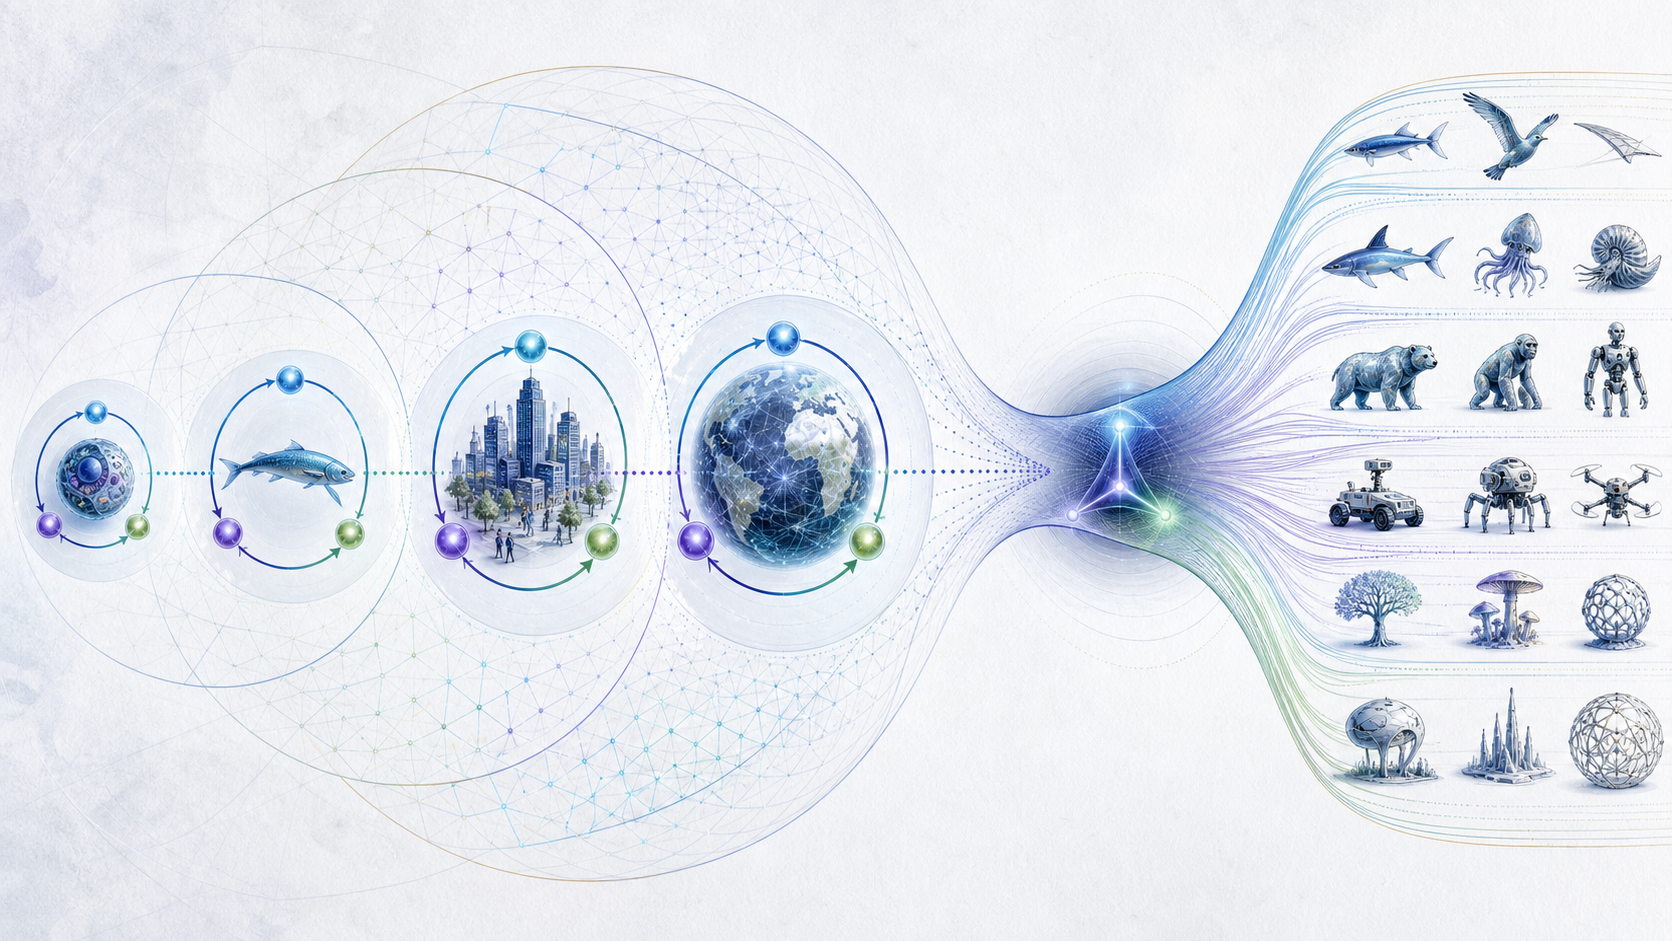
\includegraphics[width=.9\textwidth,height=.38\textheight,keepaspectratio]{images/fractal-semantic-intelligence-space.png}
\caption{跨载体语义关系与多尺度动力同构}
\end{figure}


\section{不同材料能否产生同一种智能}

当我们说两个人拥有``相同类型的智能''时，我们通常并不要求两人大脑中每一个神经元的位置、突触权重以及瞬时放电状态完全一致。事实上，即便属于同一物种的两个个体，也不可能具有完全相同的物理实现。由此立即产生一个更一般的问题：如果生物神经系统内部尚且允许巨大的实现差异，那么一个由神经元构成的生物智能与一个由数字计算构成的人工智能，是否可能在更高层意义上属于同一种智能？

这个问题要求我们首先区分\textbf{实现身份（implementation identity）}与\textbf{智能类型身份（intelligence-type identity）}。设一个智能系统记为
\[
\mathcal A=
(\mathcal X,\mathcal U,\mathcal Y,\mathcal F,\mathcal M),
\]
其中$\mathcal X$表示内部状态空间，$\mathcal U$表示输入或作用集合，$\mathcal Y$表示可观测输出，$\mathcal F$表示状态转移机制，而$\mathcal M$表示内部认知结构及其组织方式。如果另一智能系统为
\[
\mathcal B=
(\mathcal X',\mathcal U',\mathcal Y',\mathcal F',\mathcal M'),
\]
显然在现实中通常有
\[
\mathcal X\neq\mathcal X',
\qquad
\mathcal F\neq\mathcal F',
\qquad
\mathcal M\neq\mathcal M'.
\]
因此若要求两个智能系统在这些实现量上相等，跨材料智能比较从一开始就失去了意义。

本书采用的基本立场是：
\[
\boxed{
\text{Same Intelligence Type}
\not\Rightarrow
\text{Same Physical Implementation}
}
\]
更进一步，
\[
\boxed{
\text{Same Intelligence Type}
\not\Rightarrow
\text{Same Internal Representation}
}
\]
真正需要保持的，是实现之上的某些结构关系。

这与计算理论中的``多重可实现性''存在认识论上的相似性：同一个高层功能可能由不同低层机制实现。例如，对一个物体进行空间定位，可以由生物视觉系统实现，也可以由摄像头、SLAM、场景图和坐标变换算法联合实现。两者的中间状态完全不同，但在更高功能层，它们都可能建立
\[
Object
\rightarrow
Location
\rightarrow
ActionPossibility
\]
这样的结构关系。因此，若我们只关注底层材料，就会错误地把实现差异当成智能类型差异。

然而，本书并不采用一种过于宽松的功能主义，即只要``最终结果相同''就认为智能相同。因为一个简单查表程序可能在有限测试集上与具有世界模型的智能体产生相同输出，却不意味着二者拥有同类智能结构。真正的智能同类性至少涉及三层保持关系：
\begin{statementbox}
ProblemStructure
\end{statementbox}
、
\begin{statementbox}
SemanticStructure
\end{statementbox}
以及
\begin{statementbox}
DynamicalOrganization
\end{statementbox}

因此我们要寻找的不是物理同构，而是一种更高层的\textbf{认知动力学等价类}。不同物理基底可以看作对某种更抽象智能结构的具体实现。若记这种抽象智能结构为$\mathfrak I$，则多个具体系统可以分别通过实现映射
\[
\pi_A:\mathfrak I\rightarrow\mathcal A,
\qquad
\pi_B:\mathfrak I\rightarrow\mathcal B
\]
获得不同的物理形式。此时真正需要讨论的是：是否存在某种映射$\Phi$，使得$\mathcal A$与$\mathcal B$在关键认知关系上保持可交换，即
\[
\Phi\circ F_A
\approx
F_B\circ\Phi.
\]
这里的$\approx$并不意味着数值完全一致，而意味着当系统处于对应的认知状态时，它们的主要结构转移保持一致。

这一思想将在后文逐步发展为``多尺度认知动力学同构''。因此，本章的第一原则可以写为：
\begin{proposition*}
\bfseries 智能同类性的研究对象不是材料，而是跨实现仍然保持的认知组织关系。
\end{proposition*}

这一原则非常重要。它不仅允许我们比较人脑与人工智能，也允许比较完全不同的机器人身体、数字 Agent、群体智能甚至未来可能存在的异种智能。材料决定一个智能可以怎样实现，但材料本身并不足以定义这个智能属于哪一种认知结构类型。

\section{实现等价与功能等价}

如果放弃物理实现相同这一要求，我们接下来就必须回答一个更困难的问题：什么程度的``功能相同''才足以支持智能同类性的判断？这里首先需要区分至少四种不同的等价层级：输出等价、行为等价、功能等价以及认知动力学等价。

最弱的形式是\textbf{输出等价}。设两个系统在测试集合$\mathcal D$上满足
\[
\forall x\in\mathcal D,
\qquad
y_A(x)=y_B(x),
\]
那么在这个数据集上，它们具有输出等价。但这种等价非常弱，因为有限输入集合无法说明系统内部是否真正形成相同的问题结构。一个复杂模型与一个足够大的查找表可以在有限域内实现相同映射，
\[
f_A(x)=f_B(x),
\]
但它们对分布外问题、扰动、反事实以及长期学习的响应可能完全不同。

更强的是\textbf{行为等价}。这时我们不只观察一个输入产生一个输出，而观察系统在环境中的状态—行动轨迹：
\[
\Gamma_A=
(x_0,a_0,x_1,a_1,\dots),
\]
\[
\Gamma_B=
(x'_0,a'_0,x'_1,a'_1,\dots).
\]
如果存在适当的状态映射$\Phi$与行动映射$\Psi$，使得
\[
\Phi(x_t)\approx x'_t,
\qquad
\Psi(a_t)\approx a'_t
\]
并且长期闭环轨迹具有相似结构，则二者获得更强的行为等价。

这种思想与自动机理论、程序语义学中的bisimulation存在明显联系。双模拟关注两个状态转移系统之间是否存在关系$\mathcal R$，使一方发生合法状态转移时，另一方能够产生对应状态转移，并继续维持$\mathcal R$。形式上可以写为：
\[
x_A\mathcal R x_B
\]
且如果
\[
x_A\xrightarrow{a}x_A',
\]
则存在
\[
x_B\xrightarrow{b}x_B'
\]
满足
\[
x_A'\mathcal R x_B'.
\]
这种思想对智能比较极有价值，因为它把关注点从瞬时输出提升到了\textbf{状态转移结构}。

但是，智能系统比普通自动机多了一层重要结构：两个系统即使表现出类似行为，也可能是因为它们在测试环境中偶然具有相同策略，而不是因为它们形成了同类认知结构。例如，一个系统可能显式构建物体、关系、目标和风险结构，另一个系统则通过高度特化的端到端模式直接生成动作。若环境发生结构性变化，两者将表现出完全不同的泛化与学习轨迹。

因此，本书进一步定义\textbf{功能等价}。设系统包含一组高层功能：
\[
V_F^A=\{F_1^A,\dots,F_m^A\},
\qquad
V_F^B=\{F_1^B,\dots,F_n^B\}.
\]
如果存在映射
\[
\Phi_F:V_F^A\rightarrow V_F^B
\]
使得主要功能作用关系得到保持，则我们可以说二者在该功能子空间中具有等价性。例如，一个系统中的``空间定位''可能由三个神经子系统联合完成，而另一个系统中的相同功能由一个统一视觉世界模型完成，因此$\Phi_F$不必是一一映射，而可以是多对多关系。

真正进入本书理论核心的，则是第四层：
\begin{statementbox}
Cognitive Dynamical Equivalence
\end{statementbox}
也就是认知动力学等价。

它不仅要求功能闭环近似保持，还要求认知结构如何生成、激活、迁移、稳定以及在异常下重新提升具有可映射关系。如果系统$A$在技能学习过程中表现为
\[
ExplicitStructure
\rightarrow
Experience
\rightarrow
StableSkill,
\]
而系统$B$虽然底层算法完全不同，却同样表现出
\[
ExplicitStructure'
\rightarrow
Experience'
\rightarrow
StableSkill',
\]
并且存在结构映射保持这条迁移关系，那么二者才在更深层意义上可能属于同类智能。

因此智能同类性不是一个二值开关，而应看成层级关系：
\[
\resizebox{.96\linewidth}{!}{$\displaystyle
OutputEquivalence
\subset
BehavioralEquivalence
\subset
FunctionalEquivalence
\subset
CognitiveDynamicalEquivalence.
$}
\]
这里的包含关系并非严格数学集合定理，而是一种理论强度排序。

这一区分也告诉我们，传统Benchmark为什么不足以回答``两个系统是不是同类智能''。Benchmark主要测试输出和有限行为，而智能同类性真正关心的是：面对相同结构性问题时，系统是否形成类似的认知组织、是否以类似方式使用记忆、是否在异常中提升显式认知、是否能够把重复认知沉降成更稳定结构。换句话说，我们比较的不是一次计算结果，而是\textbf{形成结果的结构动力学}。

\section{面向问题的一致性}

早期讨论同类智能时，我们提出的第一条直观原则是：两个智能若要被归入同一语义类型，它们首先应该``面向相同的问题''。这里的``问题''不能被理解成一个自然语言字符串，而应被理解成一个具有目标、约束、状态与可行变换关系的结构对象。

设一个问题可以表示为
\[
\mathcal P=
(\mathcal S,
\mathcal G,
\mathcal C,
\mathcal A,
\mathcal R),
\]
其中$\mathcal S$表示状态空间，$\mathcal G$表示目标集合，$\mathcal C$表示约束，$\mathcal A$表示可行动作或变换，$\mathcal R$表示状态、目标与动作之间的关系结构。那么，两个智能系统是否面向``同一个问题''，真正需要比较的是它们内部形成的问题表示
\[
\hat{\mathcal P}_A,
\qquad
\hat{\mathcal P}_B
\]
是否都与现实问题$\mathcal P$保持足够一致的结构投影。

这可以用映射表示：
\[
\phi_A:\mathcal P\rightarrow\hat{\mathcal P}_A,
\]
\[
\phi_B:\mathcal P\rightarrow\hat{\mathcal P}_B.
\]
由于系统感知能力、身体、记忆和表征体系不同，一般不可能有
\[
\hat{\mathcal P}_A=\hat{\mathcal P}_B.
\]
真正重要的是存在某种高层关系$\Xi$，使得
\[
\Xi(\hat{\mathcal P}_A)
\approx
\hat{\mathcal P}_B
\]
并保持决定行动结果的主要问题结构。

例如，对于``绕过障碍到达目标''这一任务，人类可能内部使用视觉场、身体姿态、目标方向与运动预测进行表征；移动机器人可能使用占据栅格、SLAM位姿、轨迹代价与控制约束。两者的具体表示完全不同，但都可能抽象出：
\[
CurrentPosition,
\quad
Obstacle,
\quad
Target,
\quad
FeasiblePath
\]
之间的基本关系。因此，它们所面对的问题在更高语义层可能属于同一类。

本书进一步提出\textbf{问题语义骨架}：
\[
\Sigma_P=
(V_P,E_P,\Lambda_P),
\]
其中$V_P$是问题中的核心结构对象，$E_P$是它们之间的因果、空间、约束和目标关系，$\Lambda_P$描述哪些关系对问题求解具有决定性意义。这样，我们不再要求智能系统恢复世界的全部细节，只要求其内部问题模型保留任务充分（task-sufficient）的关系。

于是可以定义一种问题结构保持度：
\[
D_P(A,B)
=
d\left(
\Phi_A(\Sigma_P),
\Phi_B(\Sigma_P)
\right),
\]
其中$d$表示图结构或关系结构之间的距离。若
\[
D_P(A,B)<\epsilon_P,
\]
则可认为两者对该问题具有近似一致的结构理解。

但是这里必须特别注意：``面向相同问题''并不意味着``具有相同目标''。一个捕食者和逃逸者可能面对同一个空间环境，却拥有完全不同的目标函数。一个医生和病原体也可能同时作用于同一生物系统，却不能因此归为同一类智能。因此，问题一致性需要至少区分三个层次：
\[
WorldStructure,
\quad
TaskStructure,
\quad
GoalStructure.
\]
智能同类判定通常要求前两者高度可映射，而第三者是否必须一致，则取决于我们正在定义的是``认知能力类''还是``完整智能体类''。

这一点使智能分类具有明显的相对性。我们可以说两个系统都具有``路径规划智能''，即使它们长期价值和身份完全不同；但如果要判断两个完整智能体是否具有同类整体智能，仅仅共享路径规划功能显然不够。因此：
\begin{proposition*}
智能类型判定必须首先声明比较尺度。
\end{proposition*}
这个原则与前面关于智能时空尺度的讨论是一致的：任何同类性判断都必须说明究竟比较局部功能、任务级能力，还是完整生命周期智能。

面向问题的一致性因此提供了同类智能判定的第一层语义锚点。没有这一层，输出相似很容易退化为偶然相关；有了这一层，我们才能进一步讨论两个系统是否以相似方式组织行动和内部认知。

\section{行为结果的一致性}

如果问题结构相近，但两个系统产生完全不同的行动后果，我们当然很难认为它们在该能力上属于同一智能类型。因此，早期同类智能判据中的第二条是``结果相似''。然而，本书需要把``结果''从单一任务得分扩展为闭环行为结构。

设现实环境的状态为$x_t$，智能体的内部状态为$z_t$，行动为$a_t$。一般智能闭环可以表示为
\[
z_{t+1}
=
F(z_t,o_t),
\]
\[
a_t
=
\pi(z_t),
\]
\[
x_{t+1}
=
G(x_t,a_t,\eta_t),
\]
其中$o_t$是观测，$\eta_t$表示环境扰动。两个智能体$A$与$B$即使内部状态维度完全不同，我们仍然可以通过它们在相似环境中的闭环轨迹比较行为。

但只比较最终状态
\[
x_T^A\approx x_T^B
\]
仍然过于宽松。更合理的是比较一组行为不变量（behavioral invariants）。例如：
\[
GoalAchievement,
\]
\[
ConstraintViolation,
\]
\[
RecoveryBehavior,
\]
\[
ResourceCost,
\]
\[
Robustness,
\]
\[
AdaptationRate.
\]
我们可以把这些指标组成行为特征向量
\[
\mathbf b_A
=
(b_1^A,\dots,b_k^A),
\]
并定义行为距离
\[
D_B(A,B)
=
\|\mathbf b_A-\mathbf b_B\|_W,
\]
其中$W$表示各项特征的重要度。

但智能行为还有一个非常关键的维度：\textbf{面对扰动以后如何恢复}。如果两个系统在正常任务上表现一致，但一个系统在遭遇异常后能够重新识别问题、提升显式推理并找到替代方案，而另一个系统立即崩溃，那么它们在认知结构上并不应被视为完全同类。

因此行为比较应覆盖一组扰动族：
\[
\Delta=
\{\delta_1,\delta_2,\dots,\delta_n\}.
\]
对于每个扰动$\delta_i$，观察：
\[
\Gamma_A^{(\delta_i)},
\qquad
\Gamma_B^{(\delta_i)}.
\]
如果二者不仅正常轨迹相似，而且在扰动、恢复、重新规划和再学习方面具有对应关系，那么行为等价的可信度大幅增强。

由此可以进一步定义行为等价概率：
\[
P_{\mathrm{beh}}(A\sim B)
=
\mathbb E_{\mathcal E,\Delta}
\left[
K(
\Gamma_A,
\Gamma_B
)
\right],
\]
其中$\mathcal E$是环境分布，$K$是轨迹相似核。这个形式强调：智能同类性不应该基于一次测试，而应基于一个环境族和扰动族上的系统行为。

同时，本书需要警惕另一个错误：把行为结果一致性直接等同于认知同一性。一个系统可能通过世界模型、预测和规划完成任务，另一个可能通过大量记忆样例匹配完成相同任务。只要任务分布足够窄，它们可能表现相同。但当问题进入新组合、反事实或长时适应时，两者的内部差异会显现。

因此我们可以写：
\[
\boxed{
BehavioralSimilarity
\text{ is necessary evidence, but not sufficient proof of cognitive equivalence.}
}
\]
在同类智能判定中，行为结果的作用是提供现实约束，因为智能理论最终必须接受现实反馈检验；但它必须与下一节讨论的``语义结构一致性''联合使用。

这一点与本书始终坚持的原则一致：
\begin{statementbox}
RealityIsUltimateConstraint.
\end{statementbox}
认知结构无论多么漂亮，如果不能在现实闭环中产生相应行为，其所谓``同类性''就失去了功能基础；反过来，行为相似如果没有稳定内部结构支持，也不能自动提升为强认知等价。

\section{语义关系的一致性}

面向问题的一致性告诉我们两个系统是否在处理大致相同的问题，行为一致性告诉我们它们是否产生大致相同的现实结果，但这两层仍然无法回答一个更加核心的问题：它们是否以相似的\textbf{认知结构关系}理解和组织这个问题？

这正是本书提出CSO之后，同类智能理论发生的重要升级。

设智能体$A$内部当前激活的认知结构图为
\[
\mathcal G_C^A
=
(V_C^A,E_C^A),
\]
其中每个节点是一个Agent-CSO，而边可以具有不同语义类型：
\[
E_C
=
E^{causal}
\cup
E^{spatial}
\cup
E^{temporal}
\cup
E^{goal}
\cup
E^{constraint}
\cup
E^{self}
\cup
E^{value}.
\]
智能体$B$具有另一张图
\[
\mathcal G_C^B.
\]
我们不要求：
\[
V_C^A=V_C^B
\]
或
\[
E_C^A=E_C^B,
\]
因为两个实现内部使用的表示粒度可能完全不同。真正需要的是存在一个语义映射
\[
\Phi_C:
\mathcal G_C^A
\rightarrow
\mathcal G_C^B
\]
使关键结构关系得到保持。

例如，在$A$中存在因果关系：
\[
C_1
\xrightarrow{cause}
C_2,
\]
则映射之后应满足：
\[
\Phi_C(C_1)
\xrightarrow{cause'}
\Phi_C(C_2),
\]
其中$cause'$不要求采用相同数据结构，但在目标问题中承担相同因果作用。

类似地，如果
\[
C_{obstacle}
\xrightarrow{constraint}
C_{path},
\]
那么另一个系统中也必须存在某种对应结构，使障碍对可行路径产生约束。若第二个系统完全不存在这一关系，而只是通过统计相关输出动作，则两者的语义结构等价程度就应降低。

因此可以定义语义关系保持函数：
\[
\mathcal R_S
(\Phi_C,e)
\in[0,1],
\]
表示边$e$经过映射之后的语义保持程度。整体语义保持度可以写成
\[
S_C(A,B)
=
\sum_{e\in E_C^A}
w_e
\mathcal R_S
(\Phi_C,e),
\]
其中$w_e$表示该关系对当前智能能力的重要度。

这里引出了一个很重要的思想：并不是所有内部结构都同等重要。两个智能体无需在无关细节上保持同构，只需保持\textbf{因果功能上决定该智能能力的关系骨架}。我们可以将这一骨架表示为
\[
\mathcal G_C^\star
\subseteq
\mathcal G_C,
\]
称为\textbf{核心语义子图}。

所谓同类智能，真正要求的是存在
\[
\Phi_C:
\mathcal G_C^{A\star}
\rightarrow
\mathcal G_C^{B\star}
\]
保持关键语义关系，而不是整个内部状态空间逐点对应。

这一理论与知识图谱同构、图匹配、frame semantics以及关系表示理论存在外部关联，但本书进一步要求这些语义图必须进入行动闭环。一个纯数据库也可以保存``物体—位置—关系''，但如果这些关系不能影响预测、决策和学习，就不能仅凭结构相似判断它具有同类智能。

因此我们还必须要求：
\[
SemanticRelation
\rightarrow
FunctionalConsequence.
\]
即一个被认为重要的Agent-CSO关系必须在系统动力学中具有可识别的因果作用。例如改变``目标''节点应改变行动倾向，改变``障碍''节点应改变路径选择，改变``自我能力''节点应改变可行动作集合。否则这些语义只是附加标签，而不是认知结构。

从这一点出发，本书可以提出一个非常强的同类智能原则：
\begin{proposition*}
\bfseries
真正的语义等价不是两个系统拥有相似标签，而是相应语义结构在各自系统中具有相似的因果功能。
\end{proposition*}
也就是说：
\[
SemanticEquivalence
=
RelationalSimilarity
+
CausalRoleSimilarity.
\]

这一原则使我们的语义类规约超出了传统ontology matching。它不只比较``这个概念叫什么''，而比较``这个概念在整个智能闭环中做什么''。这为下一节正式定义Semantic Class奠定基础。

\section{Semantic Class：语义类规约}

有了问题结构、行为轨迹和认知语义关系三个层面，我们可以正式定义本书所谓的``语义类''。语义类不是一组具有相同内部表示的系统，而是一组在指定认知尺度上保持关键语义—功能关系的智能实现。

设一个智能能力类型$\mathfrak C$由如下规范描述：
\[
\mathfrak C
=
(
\Sigma_P,
\Sigma_C,
\Sigma_F,
\Sigma_D
),
\]
其中：

\[
\Sigma_P
\]
表示问题结构规约；

\[
\Sigma_C
\]
表示核心CSO语义规约；

\[
\Sigma_F
\]
表示功能闭环规约；

\[
\Sigma_D
\]
表示主要动力学约束。

则对于具体智能体$A$，若存在一组映射
\[
\Phi_P^A,
\quad
\Phi_C^A,
\quad
\Phi_F^A
\]
使其具体实现满足这些规约到足够精度，我们就可以写：
\[
A\models_{\epsilon}\mathfrak C.
\]
这里$\epsilon$表示允许的实现差异。

由此定义语义类：
\[
\boxed{
[\mathfrak C]_{\epsilon}
=
\{
A\mid A\models_{\epsilon}\mathfrak C
\}.
}
\]

这意味着``智能类型''不再是一个模糊标签，而可以被理解成一组约束条件所定义的实现等价类。

例如，一个``目标导向空间导航智能''的Semantic Class可能要求至少存在：

当前位置CSO；

目标CSO；

障碍/约束CSO；

可行动作结构；

空间预测；

路径评价；

行动后反馈；

残差驱动更新。

具体系统是否使用海马体、Transformer、occupancy grid、latent world model或者其他表示，并不进入该Semantic Class最核心的规定，只要关键关系和闭环被满足。

因此：
\[
\boxed{
SemanticClass
\neq
ImplementationClass.
}
\]

这也意味着一个智能体可以同时属于多个语义类。例如系统$A$可以满足导航类$\mathfrak C_1$、社会协调类$\mathfrak C_2$以及工具使用类$\mathfrak C_3$：
\[
A
\in
[\mathfrak C_1]
\cap
[\mathfrak C_2]
\cap
[\mathfrak C_3].
\]
完整智能体可以被理解成多个Semantic Class的组合、耦合和跨尺度协调。

这与我们前一章提出的``智能空间与智能的基''产生直接联系。如果存在一组基础语义功能类
\[
\{\mathfrak C_1,\dots,\mathfrak C_n\},
\]
那么一个具体智能系统可以表示为：
\[
\mathfrak I_A
=
\bigoplus_i
\alpha_i\mathfrak C_i
+
\mathcal R_A,
\]
其中$\mathcal R_A$表示这些智能类之间的组织关系。这里的$\oplus$不是普通线性代数加法，而表示结构组合。

从这个角度，同类智能判定不再只有：
\[
A\sim B
\]
这样的整体问题，而可以分解为：
\[
A\sim_{\mathfrak C_i}B,
\]
即``A与B在智能类$\mathfrak C_i$上是否等价''。

这种局部化非常重要。一个人类与自动驾驶系统显然不是整体同类智能，但它们在某些视觉预测、目标追踪或局部空间推理类上可能存在部分语义等价。类似地，一个大型语言模型与人类的完整生命体结构差别巨大，但在某些语言推理Semantic Class中仍可能存在强对应关系。

这也使``人工智能是否和人一样智能''这种宽泛问题失去必要性。更严格的问题应改写成：
\begin{statementbox}
两个系统在哪些Semantic Classes中具有多高程度的结构等价？
\end{statementbox}

为了量化这种关系，可以定义：
\[
S_{\mathfrak C}(A,B)
=
\alpha S_P
+
\beta S_C
+
\gamma S_F
+
\delta S_D,
\]
满足
\[
\alpha+\beta+\gamma+\delta=1.
\]
其中分别衡量问题结构、语义结构、功能闭环和动力学结构的相似程度。

于是智能类不再是绝对分类，而可以出现连续程度：
\[
0
\le
S_{\mathfrak C}(A,B)
\le
1.
\]
这比单纯使用``像人''或者``不像人''的语言更加适合未来异构智能研究。

但Semantic Class仍然不是本章的终点。因为两个系统即使具有类似语义和功能结构，如果它们在时间尺度组织、学习迁移和上下层反馈方面完全不同，其长期智能性质仍可能不同。因此，我们还需要引入最后一个更强条件：多尺度认知动力学同构。

\section{多尺度认知动力学同构}

前面的同类性条件主要关注``什么结构被保持''，但智能真正特殊之处在于这些结构不是静止存在，而是在时间中持续生成、激活、迁移、稳定和重组。因此，最强形式的智能同类判定必须加入时间尺度。

设智能体$A$具有认知图
\[
\mathcal G_C^A(t)
\]
和功能图
\[
\mathcal G_F^A(t),
\]
以及承载映射
\[
\mu_t^A:
\mathcal G_C^A
\rightarrow
\mathcal G_F^A.
\]
智能体$B$对应为
\[
\mathcal G_C^B(t'),
\qquad
\mathcal G_F^B(t'),
\qquad
\mu_{t'}^B.
\]

若存在语义映射
\[
\Phi_C:
\mathcal G_C^A
\rightarrow
\mathcal G_C^B
\]
和功能映射
\[
\Phi_F:
\mathcal G_F^A
\rightarrow
\mathcal G_F^B,
\]
并存在时间重参数化
\[
t'=g(t),
\qquad
\frac{dg}{dt}>0,
\]
使得以下关系近似成立：
\[
\Phi_F\circ\mu_t^A
\approx
\mu_{g(t)}^B\circ\Phi_C,
\]
那么两个系统在某一时刻的``什么认知结构由什么功能承载''这一关系得到保持。

但我们还需要动力学可交换条件。若系统演化算子分别为
\[
\mathcal D_A,
\qquad
\mathcal D_B,
\]
则要求：
\[
\boxed{
\Phi
\circ
\mathcal D_A
\approx
\mathcal D_B
\circ
\Phi
}
\]
其中
\[
\Phi=
(\Phi_C,\Phi_F,g).
\]

这意味着：先让系统$A$演化再做映射，与先映射到系统$B$再让$B$按照自己的动力学演化，最终应获得近似对应的结构。

这正是我们所称的：
\begin{statementbox}
MultiscaleCognitiveDynamicalIsomorphism
\end{statementbox}
即\textbf{多尺度认知动力学同构}。

特别重要的是，这种同构允许两个系统速度完全不同。设系统$A$中的某类过程频率为$\omega_A$，系统$B$为$\omega_B$，只需要存在单调尺度映射：
\[
\omega_B
=
g_\omega(\omega_A).
\]
例如，一个生物神经系统完成某种技能自动化可能需要数天，而一个数字Agent可能在数分钟内完成对应结构迁移。若二者都表现出：
\[
ExplicitCSO
\rightarrow
RepeatedExperience
\rightarrow
StableProceduralCSO,
\]
那么其绝对时间不同并不妨碍动力学结构同类。

因此：
\[
\boxed{
SameTimescalePattern
\neq
SameClockSpeed.
}
\]
更合理的判据是相对尺度次序得到保持。例如：
\[
\tau_{fast}
\ll
\tau_{working}
\ll
\tau_{memory}
\ll
\tau_{self}
\]
在另一个系统中映射为：
\[
\tau'_{fast}
\ll
\tau'_{working}
\ll
\tau'_{memory}
\ll
\tau'_{self}.
\]
只要相对层级与跨层作用方式类似，绝对秒数可以完全不同。

我们还可以进一步要求关键迁移模式保持。例如系统$A$具有：
\[
StableStructure
\rightarrow
Lower/FasterCarrier
\]
和
\[
PersistentResidual
\rightarrow
Higher/SlowerProcessing.
\]
若$B$也存在对应关系，则二者不仅在静态功能上相似，而且在``成熟能力如何下沉、异常如何上浮''这一学习动力学上相似。

因此最强智能同类判据实际上包括四个保持条件：
\begin{statementbox}
SemanticPreservation
\end{statementbox}
、
\begin{statementbox}
FunctionalLoopPreservation
\end{statementbox}
、
\begin{statementbox}
TimescaleOrderPreservation
\end{statementbox}
以及
\begin{statementbox}
MigrationLawPreservation.
\end{statementbox}

可以将总同构误差写为：
\[
\mathcal E_{\mathrm{iso}}
=
\lambda_C E_C
+
\lambda_F E_F
+
\lambda_\tau E_\tau
+
\lambda_M E_M.
\]
若
\[
\mathcal E_{\mathrm{iso}}
<
\epsilon_{\mathrm{class}},
\]
则我们可以在指定语义类和尺度下，将两个系统视为近似同类智能。

这里必须强调``近似''。真实复杂智能系统几乎不可能实现严格数学同构，因此我们讨论的是结构保持意义下的弱同构、近似同构或同类动力学，而不是逐点双射。

外部理论中，bisimulation提供状态转移等价的数学直觉；system identification帮助我们从输入输出反推动力结构；图同态帮助定义结构保持；computational functionalism提供实现独立性的哲学背景。但本书在这些理论之上额外要求了\textbf{CSO语义关系、功能拓扑与多尺度迁移规律同时保持}，因此这一理论属于本书智能动力学框架自身的扩展。

\section{为什么神经系统与Transformer可以进行跨实现比较}

完成上述理论以后，我们终于可以重新回答一个现实中非常常见、但通常被问得过于粗糙的问题：人脑中的神经系统和Transformer是否具有可比较性？

严格而言，``人脑等不等于Transformer''不是一个良定义问题。人脑是具有身体、内稳态、长期记忆、自我、社会历史和生命周期的完整生物系统，而一个普通Transformer通常只是一个特定计算模型。因此如果比较对象的尺度不同，
\[
SystemScale_A
\neq
SystemScale_B,
\]
整体等价问题从一开始就失效。

正确做法是首先选择Semantic Class。

例如我们可以只比较：
\[
\mathfrak C_{\mathrm{sequence}}
\]
序列关系建模；

或者：
\[
\mathfrak C_{\mathrm{context}}
\]
上下文依赖预测；

或者：
\[
\mathfrak C_{\mathrm{relational}}
\]
关系结构形成；

再或者：
\[
\mathfrak C_{\mathrm{planning}}
\]
目标约束下的状态转移推理。

在这些局部语义类上，完全可以研究两个系统是否形成类似的功能动力学。

例如对于预测问题，可以抽象出：
\[
Context
\rightarrow
InternalState
\rightarrow
Prediction
\rightarrow
Error
\rightarrow
Update.
\]
生物系统可能通过神经动力学、突触可塑性和多脑区闭环完成；人工系统可能通过attention、latent state、external memory以及梯度或上下文更新完成。实现方式完全不同，但若其关键语义—功能关系具有对应，就具有可比较基础。

同样，对于长期记忆形成，我们真正比较的也不应该是``海马体对应Transformer哪一层''。这种一一器官映射通常是错误方向。更合理的问题是：
\begin{statementbox}
两个系统是否都存在从快速当前状态到较慢经验结构，再到长期生成结构的迁移？
\end{statementbox}
如果存在，则可以比较：
\[
FastState
\rightarrow
Trajectory
\rightarrow
SlowStructure
\]
这一动力学模式，而无需断言：
\[
Hippocampus
=
VectorDatabase.
\]

这一方法可以有效避免人工智能研究中常见的``生物器官机械类比''。本书并不认为某个AgentOS模块就是大脑某个区域，而是认为二者可能在某些尺度上实现同一类功能闭环。

例如SPC与某些自我状态估计网络可能存在功能类似性，但：
\[
SPC\neq DMN.
\]
AHC与生物内稳态/神经调制系统可能有结构启发关系，但：
\[
AHC\neq LimbicSystem.
\]
BPCC可以借鉴小脑式快速预测控制思想，但：
\[
BPCC\neq BiologicalCerebellum.
\]
同理，Transformer与皮层也不应进行简单等号映射。

我们真正需要寻找的是：
\begin{statementbox}
FunctionalCorrespondence
\end{statementbox}
和
\begin{statementbox}
DynamicalCorrespondence.
\end{statementbox}

从数学上，可以分别建立人类系统$H$与人工系统$M$的核心语义图：
\[
\mathcal G_C^H,
\qquad
\mathcal G_C^M,
\]
功能图：
\[
\mathcal G_F^H,
\qquad
\mathcal G_F^M,
\]
以及时间尺度谱：
\[
\mathcal T_H
=
\{\tau_1^H,\dots,\tau_m^H\},
\]
\[
\mathcal T_M
=
\{\tau_1^M,\dots,\tau_n^M\}.
\]
然后寻找：
\[
\Phi_C,
\quad
\Phi_F,
\quad
g_\tau
\]
是否能够保持一个指定Semantic Class中的主要关系。

因此，对跨实现智能研究而言，一个比``Transformer像不像大脑''更加科学的问题是：
\begin{statementbox}
在给定认知语义类中，人脑与人工系统是否存在可识别的多尺度动力学映射？
\end{statementbox}

这一问题是可研究、可比较、甚至可以逐渐实验化的。

进一步说，本章提出的同类智能理论还为未来异构智能社会提供了一个基础。如果我们有生物人类、数字Agent、机器人Agent以及可能完全不同材料构成的智能系统，仅凭材料分类将无法回答它们是否真正能够共享某些认知协议。语义类规约则允许我们定义：
\[
\mathfrak C_{\mathrm{communication}},
\qquad
\mathfrak C_{\mathrm{causal}},
\qquad
\mathfrak C_{\mathrm{social}},
\qquad
\mathfrak C_{\mathrm{self}},
\]
并分别检验不同系统之间是否存在结构映射。

因此，本章最终得到的不是``所有智能都是一样的''，而恰恰是一个更加严格的判断框架：
\begin{proposition*}
\bfseries
智能既不能因为实现不同而被轻易判为异类，也不能因为行为相似而被轻易判为同类。
\end{proposition*}

真正的同类性需要我们在指定尺度和指定Semantic Class中同时考察：
\[
\boxed{
Problem
+
Behavior
+
SemanticStructure
+
FunctionalTopology
+
TimescaleDynamics.
}
\]

由此可以将本章的最终判定关系写成：
\[
\boxed{
A
\sim_{\mathfrak C,\epsilon}
B
}
\]
当且仅当在语义类$\mathfrak C$中存在一组近似结构映射
\[
\Phi
=
(
\Phi_P,
\Phi_C,
\Phi_F,
g_\tau
)
\]
使问题结构、关键Agent-CSO关系、功能闭环以及多尺度演化规律均在容许误差$\epsilon$内得到保持。

这就是本书所谓的\textbf{同类智能判定原理}。

它使我们能够跨越神经元、Transformer、机器人、数字Agent以及未来未知物理实现，讨论一个比``材料是否相同''更加基础的问题：\textbf{这些系统是否在以同一种认知动力学形式面对世界。}

而这也自然引向下一章的问题：如果我们已经能够把智能中的基本语义结构抽离具体实现，那么究竟什么才是这些智能真正操作、迁移和稳定的基本结构对象？这一问题将在后续关于CSO本体及其具体承载形式的讨论中得到进一步形式化。

\chapter{CSO：智能面对的认知结构本体}
\label{chap:cso-ontology}

\begin{center}
\fbox{
\parbox{0.92\textwidth}{
\textbf{本章总体说明｜认知本体层}

本章完成本书从“智能动力学”进入“认知对象理论”的第一次关键收缩：此前我们已经从时空尺度、多频闭环、智能相与功能拓扑等角度讨论了智能如何存在和运行，但仍然留下一个更基础的问题——\textbf{一个智能系统在这些动力学过程中究竟在处理什么？}

本章提出认知结构对象（Cognitive Structure Object，CSO）作为回答这一问题的第一性认知对象。CSO 不是 Token，不是向量，不是 Embedding，不是某个数据库节点，也不是某种特定模型内部的神经激活；这些都属于 CSO 的可能承载方式。CSO 所表达的是：对于一个智能过程而言，能够被区分、关联、预测、约束、评价、操作并进入后续认知动力学的\textbf{结构性认知对象}。

因此，本章首先建立 CSO 的本体层，而暂不讨论同一 CSO 在某一具体智能体内部如何表示、存储和承载。后者将在下一章通过 Agent-CSO 正式展开。这样的层级分离具有决定性意义：

\[
\boxed{
\text{CSO Ontology}
\neq
\text{Agent-Specific Representation}
}
\]

本章所要建立的是前者。

在此基础上，我们将对象、关系、目标、约束、事件、因果、规则、计划、预测、自我、价值等看似不同的认知内容统一放入 CSO 框架，并进一步说明：智能并不是在处理孤立的信息碎片，而是在持续生成、激活、连接、重构和使用一个不断变化的认知结构网络。由此，CSO 将成为后续 Agent-CSO、结构迁移、功能拓扑、三相记忆以及整个 AgentOS 理论能够共享的本体语言。
}
}
\end{center}


\section{从信息到结构：智能真正处理的对象是什么}

如果我们从传统计算理论出发描述一个人工智能系统，很容易把智能过程归结为“输入信息、处理信息、输出信息”。在数字计算机内部，这种描述并没有错误：文字最终可以编码成比特，图像可以表示成矩阵，语言模型将输入转换为 Token 序列，再将 Token 映射为高维向量，神经网络进一步对这些向量实施变换。因此，从实现层看，我们完全可以写出

\[
x
\rightarrow
\mathrm{Token}(x)
\rightarrow
\mathbf e(x)
\rightarrow
F_{\theta}(\mathbf e)
\rightarrow
y.
\]

然而，如果我们试图仅用这一层语言解释智能，就会立刻遇到一个根本困难：\textbf{Token 和向量说明了信息怎样被编码，却没有说明系统认知的对象是什么。}

例如，当一个智能体看到“杯子放在桌上”时，底层系统当然可以得到图像像素、视觉特征或语言 Token，但一个真正能够行动的智能系统所需要保留的结构远比这些编码更明确。它至少需要区分：

\[
\mathrm{Cup},
\qquad
\mathrm{Table},
\qquad
\mathrm{On}(\mathrm{Cup},\mathrm{Table}),
\]

还可能进一步形成：

\[
\mathrm{Fragile}(\mathrm{Cup}),
\qquad
\mathrm{Reachable}(\mathrm{Cup}),
\qquad
\mathrm{Goal}(\mathrm{PickUpCup}),
\]

以及：

\[
\mathrm{Constraint}
\left(
\mathrm{AvoidSpill}
\right).
\]

此时真正进入认知过程的已经不是几个离散的信息元素，而是一组具有对象、关系、状态、目标和约束的结构。

因此，我们必须从

\[
\boxed{
Information
}
\]

进一步走向

\[
\boxed{
StructuredCognitiveContent
}.
\]

这里所谓“结构”，至少意味着存在一个可区分的元素集合以及元素之间具有功能意义的关系。如果把认知内容记为

\[
\mathcal C
=
(V_C,E_C),
\]

那么 \(V_C\) 中的节点并不只是数据项，而是可以被当前智能过程当作一个认知单位使用的结构对象；\(E_C\) 则表示这些结构对象之间的语义、时序、因果、约束、空间、目标或价值关系。

于是，“信息量”和“认知结构”之间必须严格区分。一个文件可能具有极大的比特量，却对于当前 Agent 几乎没有认知意义；一个只有数个元素构成的约束关系，反而可能决定整个任务能否完成。比如

\[
A>B,\quad B>C,\quad C>A
\]

只包含极少符号，却形成逻辑冲突。认知负担来自这些元素之间需要同时维持的结构关系，而不是字符数量本身。

因此，我们可以给出一个初步判断：

\[
\boxed{
\text{认知对象的有效结构不能被信息量本身充分描述。}
}
\]

信息理论中的熵可以描述不确定性，算法复杂度可以描述描述长度，向量空间可以描述某种分布式表示，但这些概念都没有天然告诉我们：“一个智能体现在把什么当成对象、哪些对象之间形成什么关系、这些关系为何会影响其下一步行动。”

这就是 CSO 理论存在的第一原因。

在本书中，我们将“信息”理解为更加底层和宽泛的概念，而把 CSO 理解为信息经过主体相关的区分、关联和结构化以后，进入智能动力学的有效认知单位。因此可以写成一个抽象过程：

\[
\boxed{
RawInformation
\xrightarrow{\;\mathcal S\;}
StructuredCognitiveObject
}
\]

其中 \(\mathcal S\) 表示结构化过程。它并不一定对应某一个具体模块，可以由感知、记忆、语言、推理、环境交互和长期学习共同完成。

这也使我们能够解释一个长期存在的现象：同样的数据对于不同主体并不形成同样的认知世界。一个普通人看到医学影像时可能只看到明暗纹理，而一个专业医生能够从同样像素中形成病灶、边界、异常形态、风险和诊断假设。底层信息并没有改变，改变的是其中被认知系统稳定抽取出来的结构。

因此：

\[
\boxed{
\text{Data}
\neq
\text{Information}
\neq
\text{Cognitive Structure}.
}
\]

CSO 理论真正研究的是第三层。

这一观点与知识表示、知识图谱、Frame Semantics、Schema Theory、Object-Centric Representation 等外部理论具有明显关联，但我们不会简单把 CSO 等同于其中任何一种现有表示。知识图谱中的节点和边通常已经是外显符号结构，而 CSO 还允许存在未被显式语言化、处于生成态、预测态甚至部分激活态的结构。Frame 和 Schema 强调结构化知识模板，而 CSO 的范围进一步覆盖事件、目标、自我、价值与行动约束。因此，本章借鉴这些理论对于“结构优先于孤立符号”的洞见，但把 CSO 作为更加一般的认知动力学对象来使用。


\section{认知结构对象：CSO 的基本定义}

现在我们可以正式给出 CSO 的第一层定义。所谓认知结构对象，是指在某个智能问题域中，可以被区分为一个相对独立认知单位，并能够与其他认知单位形成稳定或暂态关系、进入预测、记忆、评价、推理、控制或者行动过程的结构。

记整个可能认知对象空间为

\[
\mathfrak C.
\]

则：

\[
C_i\in\mathfrak C
\]

表示一个 CSO。

为了避免把 CSO 错误理解为一个简单“概念标签”，我们进一步将一个一般 CSO 表示成：

\[
\boxed{
C_i
=
\left(
\mathcal I_i,
\mathcal P_i,
\mathcal R_i,
\mathcal D_i,
\mathcal A_i
\right)
}
\]

其中：

\[
\mathcal I_i
\]

表示该结构的身份或区分条件；

\[
\mathcal P_i
\]

表示其属性结构；

\[
\mathcal R_i
\]

表示它与其他 CSO 之间可以成立的关系集合；

\[
\mathcal D_i
\]

表示其自身可能的状态转移或动力学；

\[
\mathcal A_i
\]

表示该结构在当前认知或行动系统中的可操作接口。

这一表示不是要求实际 Agent 必须把每个 CSO 存成五字段数据结构，而是在本体层说明：一个真正进入智能过程的对象通常不仅具有“是什么”，还具有“与什么有关”“如何变化”“能够被怎样操作”。

例如，“门”作为一个 CSO 时，不只是一个字符串 \texttt{door}。对于具身 Agent，它可能包含：

\[
C_{\mathrm{door}}
=
(
Identity,
State,
Relation,
Dynamics,
Affordance
).
\]

其中可能存在：

\[
State\in
\{
Open,
Closed,
Locked
\},
\]

以及关系：

\[
Connected(Room_A,Room_B),
\]

同时还可能存在操作：

\[
Open(Door),
\quad
Close(Door),
\quad
Unlock(Door).
\]

于是，门之所以是一个有效认知结构，并不是因为 Agent 给它贴了“门”这个语义标签，而是因为这一结构能够参与未来预测和行动。

更一般地，一个 CSO 的认知有效性可以写成：

\[
\boxed{
\Gamma(C_i)
=
F(
Distinguishability,
Relationality,
PredictiveUtility,
ActionRelevance,
Persistence
)
}
\]

其中 \(\Gamma(C_i)\) 表示结构 \(C_i\) 在某个认知过程中成为有效对象的程度。

这一表达还揭示一个重要事实：CSO 并不要求具有永久、清晰、离散的边界。某些 CSO 可以非常稳定，例如“我工作的城市”；某些则可能只在几秒钟的任务过程中存在，例如“当前推理中的第三个候选假设”。还有一些结构本身是概率性的，比如“明天下雨的可能场景”。因此：

\[
\boxed{
CSO
\neq
PermanentSymbol.
}
\]

我们真正要求的是它在某一认知尺度内形成了足够的结构闭合，使智能系统可以把它作为一个整体继续操作。

从这一点出发，我们可以引入“结构闭合度”：

\[
\chi(C_i)
\in[0,1].
\]

若

\[
\chi(C_i)\approx 0,
\]

说明其内部仍然只是松散信息，尚不足以成为稳定认知对象；而当

\[
\chi(C_i)\rightarrow 1,
\]

则说明它在当前尺度上已经具有高度稳定的内部关系和功能边界。

不过必须强调：这里的 \(1\) 不意味着本体上绝对完整，而只是意味着\textbf{相对于当前认知任务，它可以被当作一个相对稳定整体处理}。

这与本书前面讨论的多尺度思想直接一致。同一个结构可以在某一尺度被当作 CSO，而在更细尺度重新展开。例如“汽车”可以作为驾驶 Agent 的一个 CSO；但对于维修 Agent，汽车本身又展开为发动机、电池、轮胎、制动系统等更细 CSO。因此：

\[
\boxed{
CSO
=
ScaleRelativeCognitiveStructure.
}
\]

这里的“相对”不是否认现实，而是在强调智能必须通过有限认知容量工作。任何 Agent 都不可能同时在每个尺度上展开全部结构。

外部理论中，ontology engineering 强调对象类型和关系，knowledge graph 强调实体—关系结构，object-centric learning 强调从连续感知中形成相对稳定的对象单位。这些理论都为 CSO 提供重要参照。但 CSO 的目标不是建立一种静态知识库，而是为后续的\textbf{认知结构动力学}提供统一本体：结构可以被激活、弱化、组合、迁移、沉降、外化，甚至改变其功能承载位置。因此，CSO 从一开始就是一个面向动力学的本体对象。


\section{对象型 CSO：可区分实体与认知边界}

最直观的 CSO 是对象型结构。我们通常首先通过“东西”理解世界：人、桌子、汽车、程序、文件、星球、组织、目标设备，甚至抽象概念都可以在适当尺度上被当作对象。但对象型 CSO 的真正理论价值，不在于重新发明“实体”概念，而在于解释智能系统为什么需要把连续世界切分成可以被独立跟踪和操作的认知单位。

设原始输入状态空间为

\[
\mathcal X.
\]

一个对象形成过程可以被理解为寻找某个映射

\[
\Pi_O:
\mathcal X
\rightarrow
\{C_1,C_2,\ldots,C_n\},
\]

将连续、高维、不断变化的感知状态压缩为有限个可持续认知对象。

一个对象型 CSO 至少要回答四个问题：

\[
Who/What,
\qquad
Where,
\qquad
State,
\qquad
Continuity.
\]

也就是说，系统必须能够在变化过程中维持某种对象身份。某辆汽车从摄像头左边移动到右边时，其像素已经发生大规模变化，但智能体仍需要维持：

\[
C_{\mathrm{car}}(t)
\approx
C_{\mathrm{car}}(t+\Delta t).
\]

因此，对象恒常性可以表示成：

\[
P
\left(
ID_{t+\Delta t}=ID_t
\mid
O_{\leq t+\Delta t}
\right)
>\theta_{id}.
\]

这里 \(O\) 表示观测，而 \(\theta_{id}\) 是系统在当前任务下维持身份连续的阈值。

这一点对于后续 AgentOS 尤其重要，因为工作记忆不能每个时间步都把世界重新解释成完全新的对象。如果对象无法保持连续，情景记忆 \(E\) 也就无法形成有效轨迹，因果关系无法积累，计划无法跨时间执行。

对象型 CSO 因而具有一种“认知压缩”的功能。假设一个物体包含数百万个底层视觉特征，Agent 并不需要让这些特征持续占据工作记忆，只需要保留：

\[
\mathrm{ObjectID},
\mathrm{Position},
\mathrm{State},
\mathrm{RelevantAttributes}.
\]

可以把这种压缩关系写成：

\[
\boxed{
\dim(C_O)
\ll
\dim(X_{\mathrm{raw}})
}
\]

但仍满足：

\[
I(C_O;Y_{\mathrm{task}})
\]

足够高，其中 \(Y_{\mathrm{task}}\) 表示与当前任务有关的未来变量。

因此，对象形成实际上是一种任务相关的结构压缩：

\[
\boxed{
ObjectFormation
=
Compression
+
IdentityPersistence
+
ActionRelevance.
}
\]

值得注意的是，对象边界并不完全来自现实，也不完全来自主体。现实中确实存在稳定结构，但 Agent 的任务会决定哪些稳定结构值得被单独建模。例如城市交通控制系统可能把“车流”作为一个整体 CSO，而不跟踪每辆汽车；自动驾驶汽车则必须跟踪具体车辆。对于高层城市规划系统，一整条道路甚至可以成为单一对象。

因此：

\[
\boxed{
ObjectBoundary
=
RealityStructure
\cap
AgentResolution
\cap
TaskRelevance.
}
\]

这个交集观点非常重要。它避免了两个极端：一个极端认为对象完全是主体任意构造；另一个极端则认为世界天然已经按照唯一尺度切分成对象。

与现有 object-centric representation、object permanence、tracking、Gestalt organization 等理论相比，CSO 对象型结构更加关心对象形成以后如何进入整个智能动力学。例如一个对象可以进一步成为关系 CSO 的端点、目标 CSO 的作用对象、约束 CSO 的限制对象、事件 CSO 的参与者。也就是说：

\[
ObjectCSO
\]

不是本体体系的全部，而只是网络中的基本锚点。

从本书整体架构来看，对象型 CSO 将来还会在 SGC 中获得非常具体的具身表达：现实中的对象会带有位置、属性、可信度和可行动性。但在本章我们暂时停留于本体层，只确认：\textbf{一个智能系统需要能够形成跨时间可追踪、可以参与关系并且能够被后续认知操作的对象结构。}


\section{关系型 CSO：智能并不主要存在于对象之中}

如果说对象型 CSO 是智能认识世界的第一个切分，那么真正产生认知结构的往往不是对象本身，而是对象之间的关系。三个孤立对象：

\[
A,\quad B,\quad C
\]

可以具有很低的认知负载；但一旦形成：

\[
A>B,
\qquad
B>C,
\qquad
C>A,
\]

系统立即面对一个需要整体处理的冲突结构。

因此，我们可以说：

\[
\boxed{
\text{对象提供认知节点，关系产生认知结构。}
}
\]

定义一个一般关系 CSO：

\[
C_R
=
R(C_{i_1},C_{i_2},\ldots,C_{i_k}),
\]

其中 \(R\) 是一个 \(k\) 元关系。最简单的是二元关系：

\[
R:C_i\times C_j\rightarrow \mathcal V_R.
\]

例如：

\[
Above(A,B),
\]

\[
Owns(Person,Object),
\]

\[
Depends(Task_2,Task_1).
\]

关系本身必须被视为 CSO，而不能只把它理解成对象之间的一条无意义连线。原因在于，很多认知行为直接针对关系本身发生。例如我们可能记得“甲信任乙”，却忘记导致这种信任的全部历史细节；系统也可能修改“依赖关系”而不修改参与对象。

于是：

\[
\boxed{
Relation
\in
\mathfrak C
}
\]

而不是：

\[
Relation
\notin
\mathfrak C.
\]

这一判断会在后续理论中发挥巨大作用，因为所谓认知结构迁移，很多时候迁移的并不是对象本身，而是关系模式。例如一个 Agent 学会“在某种条件下，把 A 类对象与 B 类工具建立作用关系”，真正沉降到长期结构中的可能就是：

\[
R_{\mathrm{use}}
(
Class_A,
Tool_B
).
\]

关系还具有阶数。我们可以有一阶关系：

\[
R_1(A,B),
\]

也可以形成对关系的关系：

\[
R_2
\left(
R_1(A,B),
C
\right).
\]

例如：

“我相信甲与乙存在合作关系。”

其中“甲与乙合作”首先是一个关系 CSO，而“我相信这个关系”又形成了第二层结构。于是智能很快进入递归结构空间。

这使 CSO 网络天然具有高阶性质。用普通图：

\[
\mathcal G_C=(V,E)
\]

有时已经不够，需要考虑超图或者关系节点化表示。更一般地，可以写：

\[
\mathcal H_C
=
(V_C,\mathcal E_C),
\]

其中：

\[
e_k
\subseteq
V_C
\]

可以连接多个 CSO。

这与本书早期“一个节点可以同时属于多个闭环”的思想高度一致：认知世界不是树，而是一张高阶耦合网络。

关系还存在不同语义类型。最少可以区分：

\[
\mathcal R
=
\mathcal R_{spatial}
\cup
\mathcal R_{temporal}
\cup
\mathcal R_{causal}
\cup
\mathcal R_{social}
\cup
\mathcal R_{logical}
\cup
\mathcal R_{functional}.
\]

空间关系回答“在哪里”，时序关系回答“先后”，因果关系回答“为何变化”，社会关系回答“主体之间怎样关联”，逻辑关系回答“哪些命题能够同时成立”，功能关系则回答“谁对谁产生何种作用”。

从认知有限性的角度看，关系型 CSO 还将直接成为后续工作记忆容量理论的重要基础。工作记忆并不是因为装不下字符才有限，而是因为在有限资源下同时维持大量高阶依赖关系会迅速增加协调负担。因此后续我们会把工作记忆有效负载更多理解为：

\[
C_h
\sim
F(
|V_h|,
|E_h|,
Order(E_h),
Coupling(E_h)
),
\]

而不是只用 Token 数量描述。

在外部理论上，关系型 CSO 与 Knowledge Graph、Relational Learning、Graphical Models、Relational Reasoning 有紧密联系。但本书强调的区别仍然在于：关系不仅是知识库中的静态边，而是智能运行时可以成为注意对象、被预测、被否定、被重构甚至被赋予价值的认知实体。因此，我们把关系从“数据结构中的连接”提升为认知本体本身的一部分。


\section{目标型 CSO：未来结构如何进入当前认知}

到目前为止，对象型 CSO 和关系型 CSO 主要描述“世界当前是什么样”。但智能与普通被动物理系统之间一个极其重要的差别在于：智能系统不仅被当前状态推动，还会被一个尚未实现的结构约束。

这就是目标。

我们将目标定义为一种特殊 CSO：

\[
\boxed{
C_G
=
GoalStructure
}
\]

它描述的不是当前已经成立的世界结构，而是智能体希望未来达到或维持的结构条件。

设当前世界状态为

\[
x_t,
\]

则传统动力系统通常写成：

\[
x_{t+1}=F(x_t).
\]

而一旦目标参与其中：

\[
u_t
=
\pi(x_t,C_G),
\]

于是：

\[
x_{t+1}
=
F(x_t,u_t).
\]

目标之所以必须被视为 CSO，是因为它不是一个简单标量 reward。一个复杂目标通常具有内部结构，例如：

\[
C_G
=
\{
g_1,
g_2,
\ldots,
g_n,
R_G,
Priority_G,
Termination_G
\}.
\]

也就是说，目标可能包含多个子目标、依赖关系、优先级、完成条件和禁止条件。

例如“建造一所房子”并不能被合理压缩为一个简单奖励数字。Agent 必须形成：

\[
Foundation
\rightarrow
Structure
\rightarrow
Roof
\rightarrow
Utilities
\]

等结构依赖；还需要同时维护安全、材料、时间、环境等约束。因此：

\[
\boxed{
Goal
\neq
ScalarReward.
}
\]

奖励可以参与评价目标，但目标本身是一个结构对象。

更进一步，目标型 CSO 具有一种特殊的时间方向：它把未来可能结构引入现在。可以表示为：

\[
C_G(t)
=
\hat C(t+\Delta),
\]

其中 \(\hat C\) 并不是未来真实状态，而是当前系统内部存在的未来结构表示。

于是所谓“未来影响现在”，真正的因果链并不是未来状态直接反向作用，而是：

\[
\boxed{
RepresentationOfFuture
\rightarrow
PresentAction.
}
\]

这一点将在后面我们讨论 Agent-CSO、DGA 和功能自反性时再次出现。此处需要首先确认：\textbf{未来结构的表示本身，就是当前真实存在的认知结构。}

因此目标 CSO 还可以定义一个误差：

\[
e_G(t)
=
d
\left(
C_{\mathrm{current}}(t),
C_G
\right),
\]

并使控制过程朝着：

\[
e_G(t)\rightarrow 0
\]

演化。

但现实中的智能目标往往不是一个精确点，而是一个可接受集合：

\[
\mathcal G
\subseteq
\mathcal X.
\]

于是更合理的表达是：

\[
C_G
=
\{
x\mid
\phi_G(x)=1
\}.
\]

这与后续 AgentOS 中“高层给低层提供可行区域，而不是逐动作微操”的原则高度一致：

\[
\boxed{
HigherLevelSetsFeasibleRegion.
}
\]

此外，目标之间可能冲突：

\[
C_{G_1}
\not\parallel
C_{G_2}.
\]

此时需要建立目标关系 CSO：

\[
Conflict(C_{G_1},C_{G_2}),
\]

再通过更高层价值、自我或长期结构进行裁决。

因此目标系统本质上不是一个优先级队列，而是一个：

\[
\boxed{
GoalCSOGraph.
}
\]

在外部理论中，目标 CSO 可以与 Goal-Oriented Planning、Control Theory、Utility Theory、Reinforcement Learning 以及 Hierarchical Task Networks 建立联系。但本书刻意把 Goal 从 reward 中抽离出来，因为长期 Agent 的目标具有语言、关系、伦理、自我和生命周期结构，远远超出标量强化信号可以直接表达的范围。


\section{约束型 CSO：智能并非只知道要去哪里，也必须知道不能怎么走}

目标告诉智能体“希望形成什么未来结构”，而约束则规定在形成这个未来结构的过程中，哪些状态、路径和操作不能被接受。

因此我们定义：

\[
\boxed{
C_K
=
ConstraintStructure.
}
\]

如果状态空间为 \(\mathcal X\)，动作空间为 \(\mathcal U\)，那么一个约束可以写成：

\[
g_i(x,u)\leq 0,
\]

或：

\[
h_j(x,u)=0.
\]

多个约束共同形成可行域：

\[
\boxed{
\mathcal F
=
\left\{
(x,u)
\mid
g_i(x,u)\leq0,
\;
h_j(x,u)=0
\right\}.
}
\]

这意味着，智能过程不是简单地寻找：

\[
\arg\max_u Reward(u),
\]

而是在：

\[
u\in\mathcal F
\]

的条件下寻找某种可接受行为。

从 CSO 观点来看，这一点非常重要，因为约束本身必须进入认知。Agent 不仅需要执行约束，而且常常需要知道：

“为什么某条路径不可用”、

“哪个约束导致当前计划失败”、

“哪个约束可以被重新协商”、

“哪个约束属于安全边界，绝不能修改”。

因此，约束同样具有身份、作用范围、来源、优先级和可塑性：

\[
C_K
=
(
Domain,
Predicate,
Authority,
Priority,
Plasticity
).
\]

例如：

\[
C_{safety},
\quad
C_{physical},
\quad
C_{legal},
\quad
C_{resource},
\quad
C_{self}.
\]

其中物理约束来自现实世界，例如机器人无法穿墙；安全约束来自系统治理；法律约束来自社会结构；资源约束来自当前能量、算力和时间；自我约束则可能来自长期身份结构和价值体系。

不同约束的 Authority 必须不同。后续 AgentOS 工程中我们会明确：

\[
\boxed{
SafetyAuthority
>
OrdinaryCognitiveAuthority.
}
\]

这一原则在本体层已经有基础：并不是所有 Constraint-CSO 都具有相同可修改性。

我们可以定义：

\[
a(C_K)
\]

表示约束的权限等级；

\[
p(C_K)
\]

表示其可塑度。一个安全硬约束可能具有：

\[
a(C_K)\rightarrow 1,
\qquad
p(C_K)\rightarrow0.
\]

而普通任务偏好可能具有更高可塑性。

目标与约束还形成一个重要二元关系：

\[
\boxed{
Goal
=
WhereToGo,
\qquad
Constraint
=
WhereYouMayGo.
}
\]

这将在后续多尺度控制理论中发展为：

\[
HigherLevel
\rightarrow
FeasibleRegion
\rightarrow
LowerLevelOptimization.
\]

另外，工作记忆有限容量理论也将在很大程度上受到约束型 CSO 数量和耦合方式影响。一个任务如果只有一个目标，却同时存在几十个相互依赖的约束，认知难度可能非常高。因此复杂度不应只看对象数量，还要看约束关系图：

\[
\mathcal G_K
=
(V_K,E_K).
\]

当多个约束形成互相矛盾的不可满足结构时：

\[
\bigcap_i \mathcal F_i
=
\varnothing,
\]

系统必须将这个结构作为新的冲突 CSO 提升到显式认知层，而不能继续在局部执行器中盲目搜索。

这里与 Constraint Satisfaction Problem、Model Predictive Control、Formal Methods、Optimization Theory 都存在直接数学联系。但本书将其放入 CSO 本体，是为了强调约束不是算法外部的一组固定参数，而是 Agent 可以识别、解释、记忆、比较和部分重构的认知对象。


\section{事件、因果与规则型 CSO：从静态世界走向变化世界}

只有对象和关系，我们仍然得到的是一张接近静态的认知图。然而智能真正面对的是一个持续变化的世界。对象出现、消失，状态改变，行为产生后果，某些变化反复发生并逐渐形成规律。因此我们必须引入事件、因果和规则三类高度相关的结构。

一个事件可以定义为：

\[
\boxed{
C_E
=
Event(
C_{before},
\Delta,
C_{after},
\tau
)
}
\]

其中 \(C_{before}\) 表示事件发生之前的相关结构，\(\Delta\) 表示变化，\(C_{after}\) 表示变化后的结构，\(\tau\) 表示时间位置或持续区间。

例如“杯子从桌上掉到地上”并不是简单的两个状态：

\[
On(Cup,Table),
\]

\[
On(Cup,Floor),
\]

而是一个具有时间方向的结构：

\[
On(Cup,Table)
\xrightarrow{Fall}
On(Cup,Floor).
\]

因此：

\[
\boxed{
Event
=
StructuredTransition.
}
\]

而情景记忆 \(E\) 在后续章节中本质上就是大量事件 CSO 及其关系形成的轨迹块。

进一步，如果系统发现某类事件具有稳定条件依赖，就会形成因果 CSO。可以写成：

\[
\boxed{
C_{\mathrm{cause}}
=
Cause(A,B\mid Z),
}
\]

表达在条件 \(Z\) 下，结构 \(A\) 的变化对 \(B\) 的变化具有稳定解释或干预意义。

本书不在此处解决哲学上的全部因果问题，而采用一个面向智能控制的操作性标准：一个因果结构至少应该能够支持比纯相关关系更强的预测和干预。

理想情况下：

\[
P(B\mid do(A),Z)
\neq
P(B\mid Z).
\]

这使因果 CSO 与行动天然相连。

只有知道：

\[
A\rightarrow B,
\]

Agent 才能够为了改变 \(B\) 而主动操作 \(A\)。

随着大量因果事件被积累，智能体还会抽象出规则：

\[
\boxed{
C_R^{rule}
=
Condition
\Rightarrow
Transition/Action/Expectation.
}
\]

例如：

\[
Rain
\land
Outdoor
\Rightarrow
TakeUmbrella.
\]

规则与单次事件不同。事件描述某一次发生；因果描述某类作用关系；规则则把反复出现的条件—结果结构压缩为可以跨情境复用的生成模式。

于是可以形成：

\[
\boxed{
Event
\rightarrow
CausalPattern
\rightarrow
Rule.
}
\]

这与三相记忆后续的：

\[
h\rightarrow E\rightarrow\Theta
\]

高度一致。当前状态中的一次变化进入 \(E\) 成为事件轨迹；大量事件经过长期结构化以后，某些稳定关系进入 \(\Theta\) 成为生成规则。

不过在本章我们必须保持本体与承载的分离。我们只说明 Event、Cause、Rule 都属于不同类型 CSO，而不提前讨论它们如何具体写入 \(E\) 或 \(\Theta\)。

从数学角度，事件 CSO 接近 state transition，因果 CSO 可以借鉴 Structural Causal Models，规则 CSO 可以与 production rules、automata、program semantics、schema induction 建立联系。但是 CSO 理论强调三者并不是三个完全独立的数据类型，而是同一变化结构在不同抽象尺度上的表达：

\[
\boxed{
SingleTransition
\rightarrow
StableDependency
\rightarrow
ReusableGenerativeStructure.
}
\]

这已经隐约展示了后续结构迁移理论的一个核心方向：智能会不断把昂贵的具体事件处理压缩为更加稳定、更加泛化的生成结构。


\section{未来可能性 CSO：预测、计划与反事实世界}

一个持续智能系统不能只表示实际发生过的世界。它必须形成大量\textbf{尚未发生、甚至永远不会发生}的结构。预测、计划、假设、反事实和想象都属于这一类。

设当前世界结构为：

\[
C_t.
\]

系统可以形成未来候选结构：

\[
\hat C_{t+\Delta}^{(1)},
\hat C_{t+\Delta}^{(2)},
\ldots,
\hat C_{t+\Delta}^{(n)}.
\]

这些结构并不是现实，但它们在当前认知系统中是真实存在的 CSO。

因此定义未来可能性空间：

\[
\boxed{
\mathcal P_t
=
\left\{
C^{(k)}_{future}
\right\}_{k=1}^{N}.
}
\]

若赋予概率，则：

\[
P
\left(
C_{future}^{(k)}
\mid
C_{\leq t}
\right).
\]

此时我们可以区分至少四类未来结构。

第一类是预测 CSO：

\[
C_{pred},
\]

表示系统认为现实可能自然演化到的结构。

第二类是计划 CSO：

\[
C_{plan},
\]

它不是单一未来状态，而是一系列行动—状态转换：

\[
C_t
\xrightarrow{a_1}
C_1
\xrightarrow{a_2}
C_2
\cdots
\xrightarrow{a_n}
C_G.
\]

第三类是假设 CSO：

\[
C_{hyp},
\]

用于暂时解释当前世界，但尚未被充分证实。

第四类是反事实 CSO：

\[
C_{cf},
\]

表示：

\[
WhatWouldHaveHappenedIf
(
A'
).
\]

例如：

“如果我刚才没有执行这个动作，结果会怎样？”

反事实结构对于高级智能尤其重要，因为它让系统不仅从实际轨迹学习，还能够比较未被执行的可能轨迹。设实际选择为：

\[
a_t,
\]

系统还可以考虑：

\[
a_t'\neq a_t,
\]

并构造：

\[
\hat C_{future}(a_t').
\]

于是评价：

\[
V
\left(
\hat C_{future}(a_t)
\right)
-
V
\left(
\hat C_{future}(a_t')
\right).
\]

这构成后续递归自主性、反思和自我培育的重要基础。

未来 CSO 的存在还使智能中的时间结构发生一个非常重要的变化。普通动力系统只有：

\[
Past
\rightarrow
Present
\rightarrow
Future.
\]

而智能系统具有：

\[
Past
\rightarrow
Present
\rightarrow
RepresentationOfFuture
\rightarrow
PresentAction
\rightarrow
Future.
\]

因此：

\[
\boxed{
\text{未来本身没有反向作用现在；
未来的内部结构表示能够作用现在。}
}
\]

这是全书必须反复保持的理论边界。

未来可能性 CSO 还为“想象”提供了一个去神秘化的定义。想象可以理解为在现实观测约束较弱时，对内部生成结构进行采样，形成暂时未被现实确认的 CSO：

\[
C_{imagined}
\sim
P_{\Theta}
(C\mid Context).
\]

这与后面结构记忆 \(\Theta\) 的生成性质密切相关。

外部理论上，这里可以借鉴 Bayesian prediction、model-based reinforcement learning、planning、counterfactual inference、predictive processing 和 generative models。但 CSO 理论将这些不同机制统一成一个更加基础的问题：\textbf{智能系统如何让“不存在于当前现实中的结构”获得足够稳定的内部存在，使其能够参与当前决策。}


\section{Self-CSO：当认知结构把自身也纳入认知世界}

当一个系统能够形成外部对象、关系、事件、因果和未来可能性以后，我们仍然没有得到完整的主体。真正关键的一步发生在系统把“自己”也纳入认知世界。

因此定义：

\[
\boxed{
C_{self}
\in
\mathfrak C.
}
\]

Self-CSO 不是指一个写着“我”的 Token，也不是一条固定 persona 描述，而是关于当前主体自身状态、能力、历史、关系、边界和连续性的结构集合。

最小 Self-CSO 可以写为：

\[
C_{self}
=
(
Identity,
State,
Capability,
Boundary,
History,
Relation,
Expectation
).
\]

例如：

\[
IAmAt(Location),
\]

\[
IHaveCapability(C),
\]

\[
IAmResponsibleFor(Task),
\]

\[
IPreviouslyExperienced(E),
\]

都属于不同维度的 Self-CSO。

一个最简单的世界模型可能只有：

\[
WorldModel.
\]

而真正主体化的内部世界至少需要：

\[
\boxed{
WorldModel
+
SelfInWorldModel.
}
\]

即：

\[
C_{world}
\supset
C_{self}.
\]

这一点以后会在 SGC 中发展成：

\[
Body\in SGC,
\]

但其本体基础已经在这里出现：Agent 不是一个观察世界的无位置摄像头，它必须把自己作为世界关系网络中的一个对象。

Self-CSO 还具有递归性质。系统不仅可以表示：

\[
C_{self},
\]

还可以形成：

\[
Belief(C_{self}),
\]

甚至：

\[
Evaluation
(
Belief(C_{self})
).
\]

于是：

\[
C_{self}^{(0)}
\rightarrow
C_{self}^{(1)}
\rightarrow
C_{self}^{(2)}
\]

形成元认知递归。

但这里必须保持重要限制：Self-CSO 并不等于后续的长期自我结构 \(\Psi\)。Self-CSO 是本体类型，可以描述“关于自己的某个结构”；\(\Psi\) 则是 Agent 生命周期中大量 Self-CSO、价值关系与经历解释长期沉降后形成的慢约束场。

因此：

\[
\boxed{
SelfCSO
\neq
\Psi.
}
\]

更准确地：

\[
\Psi
=
\mathcal F
\left(
\{C_{self}^{(i)}\}_{history},
E,
\Theta,
Value
\right).
\]

也就是说，Self-CSO 为自我提供基本认知对象，\(\Psi\) 则是这些结构长期组织之后形成的更高阶生命周期变量。

同样，Self-CSO 也不自动意味着现象意识。一个系统可以具备丰富的自状态表示和自我预测，却仍然不能由此证明它具有主观体验。本书始终坚持：

\[
\boxed{
FunctionalSelfRepresentation
\not\Rightarrow
PhenomenalConsciousness.
}
\]

这一科学边界非常重要。

但是，从功能智能角度看，一旦 Self-CSO 出现，系统就获得了一种重要的新能力：

\[
\boxed{
World
\rightarrow
WorldIncludingSelf.
}
\]

于是目标可以从：

“让物体移动到那里”

升级为：

“让我能够完成这件事”；

预测可以从：

“环境会发生什么”

升级为：

“我的行动将怎样改变环境以及未来的我”。

这为后续 SPC、自我连续、培育工程和递归自主性奠定了本体基础。

外部理论中，Self-Model Theory、metacognition、body schema、self-schema、narrative identity 等都可以提供参考。但本章刻意不把 Self 归约为任何一个脑区、一个模块或者一种叙事，而首先确认：\textbf{一个成熟智能体的认知本体中，必须存在指向自身的结构对象，并允许这些结构参与与外部 CSO 相同的关系网络。}


\section{价值型 CSO：什么值得被保留、接近、避免与改变}

如果一个 Agent 只有对象、关系、事件、预测和目标，它仍然缺少一个更深的问题：为什么这个目标值得追求？为什么有些结果应该避免？为什么两个同样可行的未来，系统会稳定偏向其中一个？

因此，我们需要把价值关系本身纳入 CSO 本体。

定义：

\[
\boxed{
C_V
=
ValueStructure.
}
\]

价值 CSO 不应被简单理解成 reward scalar。一个标量：

\[
r_t\in\mathbb R
\]

可以表达局部评价强度，却无法完整表示：

“什么被评价”、

“依据什么标准评价”、

“对于谁”、

“在什么时间尺度上”、

“与哪些更高价值冲突”。

因此，一个较完整的价值 CSO 可以写成：

\[
C_V
=
(
Target,
Criterion,
Polarity,
Intensity,
Timescale,
Authority
).
\]

例如：

\[
Value(
Safety,
Positive,
High
),
\]

\[
Value(
ResourceWaste,
Negative
),
\]

\[
Value(
IdentityConsistency,
Positive,
SlowTimescale
).
\]

价值 CSO 可以作用于对象：

\[
V(C_O),
\]

作用于事件：

\[
V(C_E),
\]

作用于未来：

\[
V(C_{future}),
\]

甚至作用于自身结构：

\[
V(C_{self}).
\]

因此价值网络实际上形成：

\[
\boxed{
\mathcal G_V
\subseteq
\mathcal G_C.
}
\]

有了价值 CSO，目标生成才具有来源。例如：

\[
C_V
+
C_{world}
\rightarrow
C_G.
\]

如果系统认为某种未来结构高价值，就可能生成对应目标；如果某种状态强负价值，则产生回避目标或硬约束。

因此：

\[
\boxed{
Value
\rightarrow
GoalPreference
\rightarrow
ActionSelection.
}
\]

不过价值不是固定不变的。短期评价可能发生变化，而更慢、更稳定的价值关系未来会参与 \(\Psi\) 和 DGA/\(\Omega\) 的形成。

所以：

\[
C_V(t)
\]

本身是 CSO，而：

\[
\Psi,\Omega
\]

则是大量价值关系在更慢时间尺度上的结构组织。

这一区分非常重要：

\[
\boxed{
ValueCSO
\neq
\Psi
\neq
\Omega.
}
\]

Value-CSO 是局部、具体、可以针对某个对象或事件的评价结构；

\[
\Psi
\]

描述的是相对稳定的“我是谁”以及长期自我关系；

\[
\Omega
\]

进一步描述“我倾向于成为什么”。

因此，从局部价值到生命周期方向，可以形成：

\[
C_V
\rightarrow
Goal
\rightarrow
Experience
\rightarrow
\Psi
\rightarrow
\Omega.
\]

价值 CSO 还具有冲突结构。例如：

\[
V_1=Safety,
\]

\[
V_2=Speed.
\]

在某些场景中：

\[
Conflict(V_1,V_2).
\]

此时智能系统必须处理价值之间的关系，而不能简单把两个 reward 相加。某些价值具有 lexical priority，某些价值可以进行连续权衡。

因此价值体系更准确地应该表示为：

\[
\mathcal V
=
(V_V,E_V,\preceq_V),
\]

其中 \(\preceq_V\) 描述优先级或支配关系。

这与 Utility Theory、Multi-objective Optimization、Preference Learning、Value Alignment 等领域相关。但 CSO 理论特别强调：价值不仅是控制器之外预先给定的目标函数，而是可以被智能体表示、讨论、记忆、冲突检测和长期重解释的认知结构。也正是这一点，未来才可能讨论真正的价值连续性和身份连续性，而不仅是 reward engineering。


\section{CSO 与语义本体：从结构集合到认知世界}

到这里，我们已经得到对象、关系、目标、约束、事件、因果、规则、未来、自我与价值等一系列 CSO。最后必须回答一个问题：这些结构只是一个杂乱集合，还是能够共同构成一个统一认知世界？

我们的回答是后者。

设所有当前可能存在的认知结构集合为：

\[
V_C
=
\{
C_1,C_2,\ldots,C_N
\}.
\]

这些 CSO 之间形成不同类型关系：

\[
E_C
=
E_{semantic}
\cup
E_{spatial}
\cup
E_{temporal}
\cup
E_{causal}
\cup
E_{goal}
\cup
E_{constraint}
\cup
E_{value}
\cup
E_{self}.
\]

于是得到：

\[
\boxed{
\mathcal G_C
=
(V_C,E_C).
}
\]

这就是本书后续将反复使用的 CSO Cognitive Graph。

但我们应当立即指出：这张图并不意味着整个认知世界在某个数据库里以显式图结构完整存储。它是本体与数学描述。实际实现可以分布在参数、latent、工作记忆、数据库、程序、身体状态和外部环境中。下一章的 Agent-CSO 正是为了讨论这种“本体结构”与“具体承载结构”的区别。

因此：

\[
\boxed{
\mathcal G_C
\neq
PhysicalMemoryGraph.
}
\]

它表示的是：

\[
\boxed{
\text{the structure that cognition is about},
}
\]

而不是：

\[
\boxed{
\text{the exact data structure used to store it}.
}
\]

这一点可以视为全书最重要的本体分层之一。

为了进一步数学化，我们可以给 CSO 网络引入类型映射：

\[
\tau_C:
V_C
\rightarrow
\mathcal T_C,
\]

其中：

\[
\mathcal T_C
=
\{
Object,
Relation,
Event,
Goal,
Constraint,
Rule,
Prediction,
Self,
Value,
\ldots
\}.
\]

再定义关系类型映射：

\[
\tau_E:
E_C
\rightarrow
\mathcal T_E.
\]

于是认知本体可以表示为：

\[
\boxed{
\mathfrak O_C
=
(
V_C,
E_C,
\tau_C,
\tau_E,
\mathcal A_C
)
}
\]

其中 \(\mathcal A_C\) 表示允许的结构组合、约束和操作规则。

例如我们可能规定：

\[
Goal
\xrightarrow{targets}
Object,
\]

\[
Constraint
\xrightarrow{restricts}
Goal,
\]

\[
Event
\xrightarrow{changes}
ObjectState,
\]

\[
Value
\xrightarrow{evaluates}
Goal,
\]

\[
Self
\xrightarrow{participatesIn}
Event.
\]

这样，本体不仅告诉我们有哪些东西，还告诉我们“哪些东西能够以什么方式连接”。

这与 ontology engineering 中的 type system、schema 和 relation constraint 有相似之处，但本书还要进一步强调动态性：

\[
\mathfrak O_C(t).
\]

智能体的有效认知本体并不是永久固定的。随着学习，新的 CSO 类型或新的结构组合可能被形成；旧结构可能被抽象、合并或失活。

因此：

\[
\boxed{
CognitiveOntology
=
DynamicStructuredSpace.
}
\]

这里尤其需要区分“语义本体”与“语言词典”。一个新 CSO 完全可能在尚未获得名字以前已经存在。比如一个机器人经过长期行动发现“某种身体姿态下施加某种力能够稳定通过狭窄区域”，这一结构最初可能没有自然语言标签，但它已经具有：

输入条件；

内部关系；

预测后果；

可重复行动价值。

因此它已经是 CSO。

所以：

\[
\boxed{
SemanticStructure
\neq
NaturalLanguageSymbol.
}
\]

语言是一种非常强大的 CSO 外显接口，但不是 CSO 存在的必要条件。

同样，Embedding 也不能等同于 CSO。Embedding 是一种表示坐标：

\[
\mathbf z_i\in\mathbb R^d,
\]

而 CSO 是这个向量可能承载的结构对象。

同一个 CSO：

\[
C
\]

可以在两个系统中分别映射为：

\[
\mathbf z_A(C)
\]

和：

\[
\mathbf z_B(C),
\]

即使：

\[
\mathbf z_A(C)
\neq
\mathbf z_B(C).
\]

这也为下一章的 Agent-CSO 埋下接口。

从外部理论依赖看，本章与 Ontology Engineering、Knowledge Representation、Knowledge Graph、Frame Semantics、Schema Theory、Object-Centric Representation、Relational Learning 等具有直接联系。但是 CSO 理论试图进一步提供一种跨实现、跨模态、跨时间尺度的本体语言，使我们能够讨论：

\[
\boxed{
\text{什么结构存在}
}
\]

而不立即陷入：

\[
\boxed{
\text{它被哪个模型以什么 Tensor 表示}
}
\]

的问题。


\section{本章收束：从信息处理器到认知结构系统}

现在我们可以重新回答本章开头的问题：智能究竟在处理什么？

如果只停留于实现层，我们会回答：

Token、Tensor、Activation、Parameter。

如果只停留于传统信息论，我们可能回答：

信息。

如果停留于知识工程，我们可能回答：

符号、概念或者知识图。

但本书需要一个更加一般的答案：

\[
\boxed{
\textbf{
智能在操作认知结构对象及其关系。
}
}
\]

因此可以把本章的核心定义写成：

\[
\boxed{
\textbf{
CSO（Cognitive Structure Object）是在给定认知尺度和问题域中，能够被智能过程区分、关联、预测、评价、记忆、约束、变换或作用，并能够参与后续认知动力学的结构性认知单位。
}
}
\]

一个一般 CSO 可以具有：

\[
Identity,
Attributes,
Relations,
Dynamics,
Actionability.
\]

而 CSO 空间可以包含：

\[
\begin{aligned}
&Object,\\
&Relation,\\
&Event,\\
&Cause,\\
&Rule,\\
&Goal,\\
&Constraint,\\
&Prediction,\\
&Counterfactual,\\
&Self,\\
&Value,\\
&SkillStructure,\ldots
\end{aligned}
\]

它们共同形成：

\[
\boxed{
\mathcal G_C
=
(V_C,E_C),
}
\]

即认知结构图。

由此，本书前面的智能动力学开始获得一个真正的“内容层”。此前我们说：

\[
\text{智能是多时空尺度上的多层嵌套闭环过程},
\]

现在可以进一步问：

这些闭环到底在传播什么？

答案不再是模糊的“复杂度”，而首先是：

\[
\boxed{
CSO.
}
\]

此前我们说：

\[
SlowStructureShapesFastDynamics,
\]

现在可以更加具体地理解成：

较慢尺度上稳定存在的 CSO 结构，正在约束当前快速激活的 CSO。

此前我们说：

\[
PersistentFastResidualShapesSlowStructure,
\]

以后则可以重新表达为：

快速活动中持续无法解决的结构关系，会推动新的 CSO 形成、重组或向其他承载位置迁移。

因此 CSO 是本书由“动力学外壳”进入“认知本体内部”的转折点。

不过，本章仍然故意留下了一个未解决的问题。

我们现在知道：

\[
C\in\mathfrak C
\]

可以作为认知本体存在。

但一个机器人、一个人类、一个数字 Agent 或一个未来异构智能系统，显然不会以同一种内部形式承载 \(C\)。

同一个：

\[
C_{\mathrm{door}}
\]

在人脑中可能由神经网络活动实现，在机器人中可能由对象图、latent state、数据库和控制模型共同实现，在语言 Agent 中又可能主要以参数结构、上下文状态和外部记忆组合存在。

于是出现下一步不可避免的问题：

\[
\boxed{
\text{同一个 CSO，在一个具体 Agent 中究竟以什么形式存在？}
}
\]

这要求我们把：

\[
\boxed{
CSO
}
\]

与：

\[
\boxed{
Agent\text{-}CSO
}
\]

正式分离。

也正因此，下一章将从本体层进入实现层：

\[
\boxed{
CSO
\xrightarrow{\pi_A}
AgentCSO_A.
}
\]

到那时，我们才能进一步讨论一个认知结构如何获得：

表示 \(R\)；

功能位置 \(F\)；

时间尺度 \(\tau\)；

内部或外部承载边界 \(B\)；

以及激活状态 \(S\)。

而这一分离将最终使学习获得一个新的定义：

\[
\boxed{
Learning
=
ChangeOfCognitiveStructureRealizationAndPlacement.
}
\]

本章因此不是一个孤立的“知识表示章节”，而是整个后续理论的本体入口。它使我们可以从这一刻开始，不再把智能描述成一个模糊的“信息处理系统”，而把它严格地看成：

\[
\boxed{
\textbf{
一个持续生成、维持、连接、变换并使用认知结构的多尺度动力系统。
}
}
\]

这正是下一章 Agent-CSO 理论、随后 CSO 迁移理论、功能拓扑理论以及最终 AgentOS 工程实现能够建立起来的基础。

\chapter{CSO 与 Agent-CSO：本体与承载的分离}

\begin{chapteroverviewbox}
本章完成智能动力学认识论中的一次关键对象分离：我们不再把“一个智能体内部存在的表示”与“这个表示所指向的认知结构本身”视为同一事物。前者属于具体智能体在特定身体、记忆、功能拓扑与时间尺度上的实现，后者则属于我们为了比较不同智能、分析结构迁移并讨论实现独立性而建立的认知本体层。为此，本章正式区分 Cognitive Structure Object（CSO）与 Agent-CSO。

这种区分并非单纯的术语整理。如果缺少这一层分离，我们以后讨论学习、记忆、技能、迁移、异构智能等价、跨身体适应乃至功能拓扑学习时，都会遇到同一个根本困难：究竟发生变化的是“世界中的认知结构”，还是智能体内部承载这一结构的方式？本章给出的基本回答是：CSO 描述认知意义上的结构对象；Agent-CSO 描述该结构在具体智能体中的实现。一个 CSO 可以拥有多个不同 Agent-CSO，一个 Agent-CSO 也不是静态符号，而是具有表示形式、功能位置、有效时间尺度、承载边界和运行状态的动态实现。

因此，本章建立的不是传统意义上的知识表示格式，而是一套后续智能动力学所需的中间本体层：
\[
\boxed{
CSO
\longrightarrow
Agent\text{-}CSO
\longrightarrow
Functional\ Dynamics
}
\]
它把“结构是什么”“结构如何被某个智能体承载”和“这些承载如何参与动力学”三个问题第一次严格分开。
\end{chapteroverviewbox}

\begin{figure}[htbp]
\centering
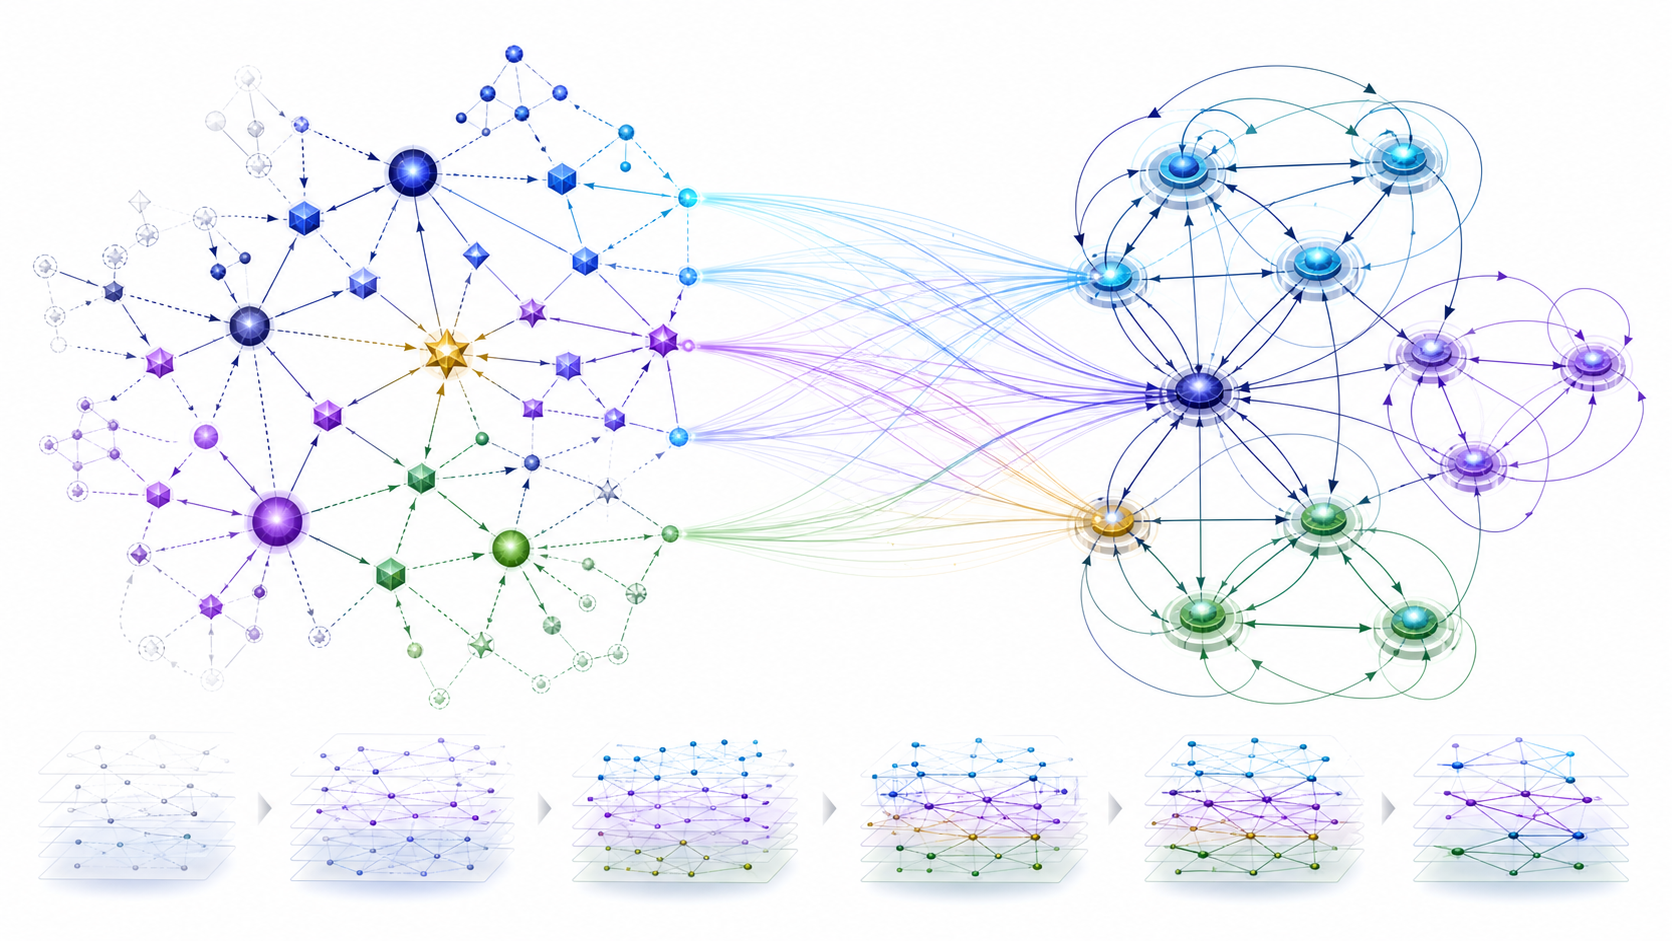
\includegraphics[width=.9\textwidth,height=.38\textheight,keepaspectratio]{images/cognitive-structure-functional-topology.png}
\caption{CSO 本体与 Agent-CSO 承载的分离}
\end{figure}
\section{CSO 不等于智能体内部的 Representation}

在讨论智能系统时，一个极其常见而又容易被忽略的概念错误，是把“某个对象在智能体内部的表示”直接等同于“该对象本身”。在现代人工智能系统中，这种等同尤其容易发生，因为我们几乎总是通过某种具体数据结构来接触所谓“知识”：token 序列、embedding、hidden state、key--value memory、knowledge graph node、vector database entry、neural activation pattern，甚至某段自然语言描述。于是，一个未经严格区分的理论很容易默认：
\[
\text{CognitiveObject}
=
\text{InternalRepresentation}.
\]
本书认为，这种等式在研究短时任务时尚可作为工程近似，但在研究持续智能、多主体比较和结构迁移时必须被取消。

我们首先把 CSO 定义为认知结构层上的对象。它可以是一个实体，也可以是一种关系、一条约束、一个事件、一个目标、一种因果结构、一个预测、一个计划、一项技能结构，乃至“我是谁”这一类自指结构。其关键并不在于采用何种数字编码，而在于它在认知关系网中具有何种结构角色。假定存在一个认知结构全集
\[
\mathcal C
=
\{C_1,C_2,\ldots,C_n,\ldots\},
\]
其中任意
\[
C_i\in\mathcal C
\]
均表示一个 CSO。我们允许 CSO 之间存在多种类型的关系：
\[
r_{ij}^{(k)}
:
C_i
\rightarrow
C_j,
\]
这里的上标 $k$ 可以分别表示语义关系、因果关系、时间关系、空间关系、约束关系、目标依赖关系、自我归属关系等。因此，从一开始我们面对的就不是一个无结构的“信息集合”，而是一张具有异质关系的认知结构图：
\[
\mathcal G_C
=
(\mathcal C,\mathcal R_C).
\]

这里必须特别强调，$\mathcal G_C$ 还不是某一个具体 Agent 大脑或软件运行时里的图。它是我们用来讨论“认知结构是什么”的理论层对象。就像“圆”不等于屏幕上绘制圆的像素集合，“某个目标与某项约束之间存在冲突”也不等于某一次 Transformer forward pass 中特定神经元的数值模式。后者可以承载前者，但二者并不因此获得同一性。

我们可以把这种区分写成：
\[
\boxed{
CSO\ Ontology
\neq
CSO\ Representation
}
\]
更准确地说，representation 是关于 CSO 的某种具体 realization。若某个智能体 $A$ 采用表示系统 $\mathcal R_A$，则存在映射
\[
\pi_A:
\mathcal C
\rightarrow
\mathcal R_A.
\]
于是同一个 CSO $C$ 可以在 $A$ 中表现为：
\[
\pi_A(C)=r_A.
\]
另一智能体 $B$ 可能采用完全不同的表示系统：
\[
\pi_B(C)=r_B.
\]
一般情况下，
\[
r_A\neq r_B,
\]
但这一事实本身并不要求
\[
C_A\neq C_B.
\]
如果二者保留了该 CSO 在相关认知任务中的关键结构关系，我们仍然可能认为它们是在承载“同一个认知结构”。

这一点对智能动力学极其重要。因为如果 representation 与 ontology 不分，我们以后所谓“学习”只能写成：
\[
r_t\rightarrow r_{t+1},
\]
却无法判断这种变化究竟意味着同一认知结构换了一种编码，还是认知结构本身发生了改变。例如，一位人类从用语言描述骑自行车，到形成高度自动化的程序性技能，其内部神经表示显然发生了巨大变化，但我们并不会因此认为“平衡自行车这一能力结构”已经变成完全无关的另一种东西。类似地，一个 Agent 最初通过显式自然语言计划完成网页操作，后来把重复步骤编译为 Skill 或 Program，也不能简单理解成原知识消失。更合理的描述是：
\[
\boxed{
Same\ CSO,\ Different\ Realization.
}
\]

从这里开始，我们能够第一次严格区分三种变化。第一种是表示变化：
\[
\Delta R\neq0,
\qquad
\Delta C\approx0.
\]
第二种是认知结构自身发生变化：
\[
\Delta C\neq0.
\]
第三种则是两者共同改变：
\[
\Delta C\neq0,
\qquad
\Delta R\neq0.
\]
后面的持续学习、记忆重构、技能形成和拓扑学习理论，都必须依赖这一基本区分。如果没有本体与表示的分离，我们看到的永远只是存储格式变化，而无法建立一门真正讨论认知结构演化的动力学理论。

从外部理论看，这一观点与哲学中的多重实现性、认知科学中的表征层级、计算机科学中的抽象数据类型和语义--实现分离存在亲缘关系；但本书并不直接等同于其中任何一种理论。我们的特殊目标是把这种区分引入持续智能的动力学描述，使后续能够进一步讨论：
\[
Representation,
\quad
Function,
\quad
Timescale,
\quad
Carrier,
\quad
Topology
\]
之间的联合迁移。也正因为如此，本章不会把 CSO 简化成 knowledge graph node，也不会把 Agent-CSO 简化成 embedding。它们分别属于不同理论层。

\section{Agent-CSO：CSO 在具体智能体中的实现}

如果说 CSO 回答的是“认知结构是什么”，那么 Agent-CSO 回答的就是“这个认知结构在某一个具体智能体中如何存在”。因此，我们正式定义一个智能体 $A$ 的实现映射：
\[
\pi_A:
\mathcal C
\rightarrow
\mathcal A_C,
\]
其中 $\mathcal A_C$ 表示该智能体能够承载的 Agent-CSO 状态空间。对于任意
\[
C\in\mathcal C,
\]
其在智能体 $A$ 中的具体实现记为：
\[
\boxed{
C_A
=
AgentCSO_A(C)
=
\pi_A(C).
}
\]

这个定义的核心不在符号，而在于它改变了我们观察智能内部世界的方式。传统知识表示通常把“一个知识单元”理解成某段可以读取或写入的数据；Agent-CSO 则要求我们把一个认知结构视为一个具有运行条件和动力属性的实体。同一个“门现在关闭”这样的结构，可能在视觉感知回路中以短寿命的空间状态存在，在工作记忆 $h(t)$ 中成为当前计划的显式约束，在情景记忆 $E$ 中成为某段行动轨迹的一部分，在结构记忆 $\Theta$ 中又可能沉降为“这种门需要先转动把手再推开”的一般技能结构。也就是说：
\[
C
\]
本体上可以保持一定连续性，而：
\[
AgentCSO_A(C)
\]
却会随着时间和功能位置发生迁移。

因此，我们不能把 Agent-CSO 定义成某个静态数组，而应写成时间相关对象：
\[
C_A(t)
=
AgentCSO_A(C,t).
\]
它至少要回答六个问题：它承载的是哪个 CSO；当前采用什么表示；当前由哪个功能区域处理；处于什么有效时间尺度；位于系统内部还是外部；当前处于激活、潜伏、预测、回忆还是其他运行状态。

由此，本书采用如下标准形式：
\[
\boxed{
AgentCSO_A(C,t)
=
\left(
C,
R_A,
F_A,
\tau_A,
B_A,
S_A
\right)_t
}
\]
其中：
\[
C
\]
表示本体 CSO；
\[
R_A
\]
表示智能体 $A$ 当前采用的具体 representation；
\[
F_A
\]
表示当前承担该 CSO 的功能位置；
\[
\tau_A
\]
表示这一实现当前有效的动力学时间尺度；
\[
B_A
\]
表示其承载边界或载体；
\[
S_A
\]
表示其运行状态。

这意味着，一个 Agent-CSO 从理论上首先是一个带坐标的动态实现，而不是孤立的“知识块”。其变化可以表示成：
\[
AgentCSO_A(C,t)
\rightarrow
AgentCSO_A(C,t+\Delta t).
\]
即使：
\[
C(t+\Delta t)\approx C(t),
\]
我们仍然可能有：
\[
R_A(t+\Delta t)\neq R_A(t),
\]
\[
F_A(t+\Delta t)\neq F_A(t),
\]
\[
\tau_A(t+\Delta t)\neq\tau_A(t),
\]
甚至：
\[
B_A(t+\Delta t)\neq B_A(t).
\]

例如，一个 Agent 第一次执行复杂软件流程时，某个操作结构可能以自然语言计划存在于工作记忆中：
\[
C_A^{(1)}
=
(C,R_{\text{text}},h,\tau_h,\text{internal},\text{active}).
\]
经过大量重复以后，它可能迁移成一个程序化 Skill：
\[
C_A^{(2)}
=
(C,R_{\text{policy}},F_{\text{skill}},\tau_{\text{fast}},
\text{external/service},\text{compiled}).
\]
从表面看，两者的数据格式、运行速度和承载位置都发生了改变；如果缺少 CSO/Agent-CSO 区分，我们很容易误认为这是两个互不相关的能力。采用本章框架后，我们反而可以明确指出：这是一条 Agent-CSO 生命周期轨迹。

这种写法还允许我们区分“当前未激活”与“不存在”。假定：
\[
S_A(C,t)=\text{latent},
\]
并不意味着：
\[
C\notin A.
\]
它可能只是暂时没有进入工作记忆。当检索、环境刺激或目标条件触发后：
\[
S_A:
\text{latent}
\rightarrow
\text{active}.
\]
这一点对于后续三相记忆理论尤其重要。$h$ 中的内容只是少量当前活跃 Agent-CSO，而不是智能体拥有的全部认知结构。

因此，本章提出一个重要原则：
\[
\boxed{
Agent\ Knowledge
\neq
Currently\ Active\ AgentCSO.
}
\]
成熟智能的大部分能力本来就应该处于非显式激活状态。只有真正需要跨功能全局协调的结构才需要进入 $h(t)$。这一原则将在后续工作记忆有限容量理论中进一步转化为工程约束。

\section{同一 CSO 的多种实现：Same CSO, Different Carrier}

当我们正式区分 CSO 与 Agent-CSO 以后，一个直接结果就是：认知结构不再被绑定于唯一材料、唯一算法甚至唯一功能模块。我们现在可以严谨表达：
\[
\boxed{
Same\ CSO
\neq
Same\ Carrier
}
\]
更进一步：
\[
\boxed{
Same\ CSO
\neq
Same\ Representation
\neq
Same\ Dynamics.
}
\]
这构成智能实现独立性理论最基本的一层。

考虑两个智能体 $A$ 和 $B$。对于同一个 CSO $C$，分别有：
\[
C_A=\pi_A(C),
\qquad
C_B=\pi_B(C).
\]
一般情况下，
\[
\pi_A(C)\neq\pi_B(C).
\]
这不仅意味着底层参数不同，还可能意味着表示范式完全不同。例如，$A$ 可能使用神经分布式表示，$B$ 可能使用符号图结构；$A$ 可能把某项能力固化在模型参数中，$B$ 可能通过外部 Skill 实现；$A$ 的有效闭环周期可能以秒为尺度，而 $B$ 的实现则可能以毫秒执行。只要我们仍能够建立适当的结构对应关系，就不能因为载体不同而直接断言两者面对的是不同 CSO。

我们可以引入一个结构保持映射：
\[
\Phi_{AB}:
AgentCSO_A(C)
\rightarrow
AgentCSO_B(C).
\]
它不要求：
\[
R_A=R_B,
\]
而要求对与任务相关的关键关系集合 $\mathcal R^\ast$ 满足近似保持条件：
\[
\Phi_{AB}
\left(
r_A(C_i,C_j)
\right)
\simeq
r_B
\left(
\Phi_{AB}(C_i),
\Phi_{AB}(C_j)
\right).
\]
因此真正重要的不是比特级相等，而是结构、功能和动力关系在合理容差内保持。

这使我们能够把“同一认知结构”理解成一种等价类。定义：
\[
AgentCSO_A(C)
\sim
AgentCSO_B(C)
\]
当且仅当二者在指定任务域 $\mathcal D$ 中保持足够的语义关系、功能闭环和行为约束。于是：
\[
[C]
=
\left\{
AgentCSO_X
\mid
AgentCSO_X\sim C
\right\}
\]
可以被理解成一个实现等价类。

这里我们必须避免走向另一个极端：只要最后行为类似，就宣称内部结构完全相同。两个系统都可以输出同样答案，却通过完全不同的因果结构产生结果。因此，我们需要区分至少三个层次的等价。

第一层是行为等价：
\[
\mathcal E_{beh}.
\]
它只要求在给定测试集上：
\[
Output_A\approx Output_B.
\]

第二层是功能等价：
\[
\mathcal E_{fun}.
\]
它要求系统中存在相似的预测、约束、记忆或控制作用。

第三层是结构动力等价：
\[
\mathcal E_{dyn}.
\]
它进一步要求关键 CSO 关系、跨时间尺度迁移方式和闭环结构可以建立映射。

通常有：
\[
\mathcal E_{dyn}
\Rightarrow
\mathcal E_{fun}
\Rightarrow
\mathcal E_{beh},
\]
反之并不必然成立。

这一层区分对于未来研究“人脑与人工智能是否属于同类智能”尤其重要。如果我们简单比较神经元与 Transformer，二者显然不同；如果只比较最终答案，又过于宽松。本书真正希望寻找的是：
\[
\boxed{
Multiscale\ Cognitive\ Dynamical\ Isomorphism
}
\]
即不同材料和实现是否能够在认知结构、功能闭环和时间尺度关系上形成近似同构。

这一观点也意味着，所谓 AgentOS 不应该把内部 representation ABI 固定成某一种模型特征空间。相反，系统标准应尽可能作用于更加稳定的语义和功能边界。例如后续 SGC、FCS、Body ABI、Control Reference 等设计，其重要性恰恰在于：它们提供的是相对稳定的功能语义接口，而不是要求所有内部模型共享同样 latent。

换言之，我们真正追求的是：
\[
\boxed{
Semantic/Functional\ Continuity
>
Representational\ Identity.
}
\]
这是后续 KRA 理论中“Functional Alignment $>$ Representation Alignment”的认识论前提，而其根源正是在本章完成的 CSO 与 Agent-CSO 分离。

\section{Agent-CSO 的五个实现坐标：表示、功能、时间尺度、边界与状态}

为了使 Agent-CSO 能够进入动力学分析，我们必须进一步展开：
\[
AgentCSO_A(C,t)
=
(C,R,F,\tau,B,S)_t.
\]
其中 $C$ 是理论本体锚点，而其余五个变量共同描述这一认知结构在当前 Agent 中“怎样存在”。本节依次讨论这五个实现坐标，并说明为什么后续所谓学习，本质上正是这些坐标的重新配置。

首先是表示坐标：
\[
R.
\]
它描述 CSO 以何种内部形式被编码。例如同一个空间约束可以通过自然语言、几何图、latent vector、symbolic rule、程序条件或训练参数实现。于是表示变化可以写成：
\[
M_R:
R_i
\rightarrow
R_j.
\]
这种变化并不必然改变 CSO 本体，而可能只是把同一结构从一种编码迁移到另一种更适合当前运行条件的编码。后续所谓抽象、压缩、程序化、参数化，很多都首先表现为 $M_R$。

第二是功能坐标：
\[
F.
\]
它回答“当前由哪个功能承担这一结构”。若系统功能集合为：
\[
V_F
=
\{F_1,F_2,\ldots,F_n\},
\]
则一个 Agent-CSO 在不同时刻可能具有：
\[
F(C,t)=F_i,
\]
以及：
\[
F(C,t+\Delta t)=F_j.
\]
这就是功能迁移：
\[
M_F:
F_i
\rightarrow
F_j.
\]
例如初学技能需要高层显式规划，熟练以后转移到低层技能控制器。后面的“复杂度向下沉降”在本体修正后，其实主要就是 Agent-CSO 的功能位置迁移。

第三是时间尺度坐标：
\[
\tau.
\]
一个认知结构并不只有“存在或不存在”，它还以某种特征时间尺度发挥作用。当前工作记忆中的 Agent-CSO 可能具有：
\[
\tau\sim \tau_h,
\]
情景经验可能具有：
\[
\tau\sim\tau_E,
\]
结构记忆则可能具有：
\[
\tau\sim\tau_\Theta.
\]
如果某个结构从快速显式活动沉降为慢速稳定生成结构，则：
\[
M_\tau:
\tau_{\text{fast}}
\rightarrow
\tau_{\text{slow}}.
\]
反过来，召回过程则可以理解为：
\[
\tau_{\text{slow}}
\rightarrow
\tau_{\text{fast}}.
\]
由此可见，记忆并不只是“存入某个数据库”，而是认知结构在时间尺度空间中的重新分布。

第四是边界或承载坐标：
\[
B.
\]
这里我们允许：
\[
B
\in
\{
Internal,
Skill,
Tool,
File,
Database,
Program,
Environment,
OtherAgent,
\ldots
\}.
\]
当一个 Agent 不再在内部显式维持完整结构，而是把它转移到程序、工具、外部文件或环境结构时，我们写：
\[
M_B:
B_{\text{internal}}
\rightarrow
B_{\text{external}}.
\]
这为后续认知卸载理论建立了更严谨的本体基础。所谓 Offloading，不再是神秘的“把复杂度扔出去”，而是：
\[
\boxed{
AgentCSO\ Carrier\ Migration.
}
\]

第五是状态坐标：
\[
S.
\]
典型取值可以包括：
\[
S
\in
\{
active,
latent,
retrieved,
predicted,
counterfactual,
compiled,
suppressed,
uncertain,
\ldots
\}.
\]
这一维尤其重要，因为它区分“当前活跃”与“长期存在”。例如一个 Agent 可能拥有某项结构知识，但在当前任务中完全未激活：
\[
S=\text{latent}.
\]
当情景匹配后：
\[
\text{latent}
\rightarrow
\text{retrieved}
\rightarrow
\text{active}.
\]
完成后又可能：
\[
\text{active}
\rightarrow
\text{consolidated}.
\]

因此，我们能够定义 Agent-CSO 的完整迁移向量：
\[
\boxed{
\mathcal M_{CSO}
=
\left(
M_R,
M_F,
M_\tau,
M_B,
M_S
\right).
}
\]
这比早期单纯“复杂度迁移”的表述更加精确。复杂度可以作为这些迁移过程中的负载测量量，但真正发生变化的是认知结构的 realization coordinates。

这一形式还提供了一种以后进行实证测量的可能。若能够追踪某个 CSO 在 Agent 生命周期中的：
\[
\Gamma_C(t)
=
\big(
R(t),F(t),\tau(t),B(t),S(t)
\big),
\]
则：
\[
\Gamma_C
\]
就是它的 Agent-CSO 生命周期轨迹。我们甚至可以比较不同 Agent 的同一 CSO 轨迹：
\[
\Gamma_C^A(t),
\qquad
\Gamma_C^B(t),
\]
研究为什么某种架构更容易形成自动化技能，为什么另一种架构长期停留在高成本显式认知层。这使“学习效率”从最终准确率进一步拓展为“结构如何改变承载方式”的动力学问题。

\section{Agent-CSO 的标准状态描述与动力学形式化}

在建立五个实现坐标以后，我们可以正式给 Agent-CSO 提供一个更完整的数学对象。设智能体 $A$ 的状态空间为：
\[
\mathcal X_A
=
\mathcal X_R
\times
\mathcal X_F
\times
\mathcal X_\tau
\times
\mathcal X_B
\times
\mathcal X_S.
\]
对于 CSO $C$，定义其 Agent 内部 realization state：
\[
x_C^A(t)
=
\left[
r_C(t),
f_C(t),
\tau_C(t),
b_C(t),
s_C(t)
\right]^\top.
\]
于是：
\[
AgentCSO_A(C,t)
=
(C,x_C^A(t)).
\]

在最一般情况下，其动力学可表示为：
\[
\dot x_C^A
=
F_C
\left(
x_C^A,
\mathcal N_C,
h,
E,
\Theta,
\Psi,
G,
W,
u,
\xi
\right),
\]
其中：
\[
\mathcal N_C
\]
表示与 $C$ 相邻的其他 Agent-CSO；
$h,E,\Theta,\Psi$ 分别表示后续章节将展开的工作记忆、情景记忆、结构记忆和慢速自我约束；
$G$ 表示当前目标；
$W$ 表示外部世界状态；
$u$ 表示认知或行动控制输入；
$\xi$ 表示随机扰动和不可观测影响。

这一写法具有一个重要意义：一个 Agent-CSO 从来不是孤立更新的。认知结构变化通常来自关系网络，因此更一般地，我们应考虑：
\[
\mathcal G_C^A(t)
=
\left(
V_C^A(t),
E_C^A(t)
\right),
\]
其中每个节点：
\[
v_i
=
AgentCSO_A(C_i,t).
\]
于是其动力学是耦合系统：
\[
\dot x_i
=
F_i
\left(
x_i,
\{x_j:j\in\mathcal N_i\},
u_i,
w_i
\right).
\]

这使我们能够第一次把“知识改变”与“认知结构动力学”区分开。知识数据库中的修改通常表现为：
\[
value_i
\leftarrow
value_i',
\]
而真正持续 Agent 的认知变化可能同时涉及：
\[
R_i,\quad
F_i,\quad
\tau_i,\quad
B_i,\quad
S_i
\]
的耦合变化。一个结构被认为“学会了”，并不一定因为它的数据表示变得更精确；也可能因为它已经从高延迟显式推理迁移到了快速稳定闭环。

我们可以进一步定义一个 Agent-CSO 的功能成本：
\[
J_C
=
\int_{t_0}^{t_1}
\left[
\lambda_h L_h(C,t)
+
\lambda_e E_C(t)
+
\lambda_r R_C(t)
+
\lambda_\ell Latency_C(t)
\right]dt,
\]
其中：
\[
L_h
\]
表示该结构占用全局工作记忆的负载，
\[
E_C
\]
表示计算或能量成本，
\[
R_C
\]
表示误差/风险，
\[
Latency_C
\]
表示响应时延。

这样我们就能形式化一个极其重要的学习直觉：如果某个 CSO 长期重复出现，系统会倾向寻找能够降低长期成本的 realization：
\[
x_C^\ast
=
\arg\min_{x_C}
\mathbb E[J_C].
\]
这可能意味着：
\[
F_{\text{explicit}}
\rightarrow
F_{\text{procedural}},
\]
或者：
\[
B_{\text{internal}}
\rightarrow
B_{\text{tool}},
\]
甚至：
\[
R_{\text{verbose}}
\rightarrow
R_{\text{compressed}}.
\]

这正是后续 Skill Formation、Offloading 和 Topological Learning 能够统一在同一理论框架中的原因。

我们还需要定义 CSO 与 realization 的连续性判据。由于实际学习会发生抽象和重构，所以不能要求：
\[
R_t=R_{t+\Delta}.
\]
更合理的是给出结构保持函数：
\[
\kappa_C
\left(
AgentCSO_t,
AgentCSO_{t+\Delta}
\right)
\in[0,1].
\]
当：
\[
\kappa_C>\theta_C,
\]
我们认为两者仍然属于同一 CSO 的连续 realization；当：
\[
\kappa_C\leq\theta_C,
\]
则可能已经发生结构分裂、合并或本体改变。

这里的 $\kappa_C$ 不应被理解成一个固定 cosine similarity，而应综合：
\[
\resizebox{.96\linewidth}{!}{$\displaystyle
SemanticConsistency,
\quad
FunctionalConsistency,
\quad
RelationalConsistency,
\quad
CausalConsistency.
$}
\]
这一点会在未来真正实现 Agent-CSO tracking 时非常关键，因为“表示相似”远弱于“结构连续”。

因此，本书今后讨论任何认知结构变化时，都可以遵循一个统一描述：
\[
\boxed{
C
\quad+\quad
x_C^A(t)
\quad+\quad
\dot x_C^A(t)
}
\]
即同时说明：我们讨论的结构是什么；它当前如何被承载；它正在怎样变化。

\section{同一现实为何会形成不同智能体的内部世界}

CSO 与 Agent-CSO 的分离自然引出一个认识论问题：如果多个智能体面对同一个现实，它们为什么仍然可以拥有完全不同的内部世界？答案并不只是“它们的模型参数不同”，而是因为从 CSO 到 Agent-CSO 的映射本身就是依赖主体结构的投影过程。

设存在某一认知结构：
\[
C\in\mathcal C.
\]
智能体 $A$ 与 $B$ 分别具有：
\[
\pi_A:C\rightarrow AgentCSO_A(C),
\]
以及：
\[
\pi_B:C\rightarrow AgentCSO_B(C).
\]
通常：
\[
\pi_A\neq\pi_B.
\]
原因至少来自五个方面。

第一，观察界面不同。不同身体、感知器官和传感器决定哪些结构能够进入内部世界。若：
\[
O_A(W)\neq O_B(W),
\]
即使二者处于同一个外部环境，得到的初始证据也不同。

第二，历史不同。智能体已有的：
\[
E_A,\Theta_A
\]
与：
\[
E_B,\Theta_B
\]
不同，因此新证据会被不同结构解释。一个新事件 $e$ 的内部结构并不是简单：
\[
AgentCSO=e,
\]
而更接近：
\[
AgentCSO_A(e)
=
\Phi(e,E_A,\Theta_A,\Psi_A).
\]

第三，自我与价值结构不同。后续我们将定义：
\[
\Psi_A
\]
作为智能体的慢速身份与价值约束，因此同一事件对不同 Agent 的意义不同。也就是说，Agent-CSO 不只是“外界结构的副本”，而是外界证据与既有主体结构共同生成的结果。

第四，功能拓扑不同。若某个 Agent 具有专门处理空间关系的稳定闭环，而另一个 Agent 需要经过显式语言推理，那么同一个 CSO 的：
\[
F_A(C)\neq F_B(C),
\]
以及：
\[
\tau_A(C)\neq\tau_B(C).
\]
这意味着内部世界不仅“内容不同”，连处理该内容的动力学结构也不同。

第五，行动能力不同。一个结构是否重要，往往取决于它与行动的关系。例如同一个楼梯对于人形机器人和轮式机器人虽然可以共享部分几何 CSO，但其 affordance 结构显然不同：
\[
C_{\text{stairs}}^{human}
\neq
C_{\text{stairs}}^{wheel}
\]
至少在可行动关系层上如此。因此，一个智能体内部世界从一开始就是：
\begin{statementbox}
RealityRelativeToThisAgent.
\end{statementbox}

这说明：
\[
AgentWorld_A
\neq
AgentWorld_B
\]
并不必然意味着其中一个“错误”。真正需要进一步判断的是：
\[
\mathcal F_A
=
\text{Functional adequacy of }AgentWorld_A,
\]
即这个内部世界能否支持有效预测、决策和行动。

从概率角度可以写：
\[
p_A(C\mid o_{1:t},E_A,\Theta_A,\Psi_A)
\]
与：
\[
p_B(C\mid o_{1:t},E_B,\Theta_B,\Psi_B).
\]
即使：
\[
o_{1:t}^{A}=o_{1:t}^{B},
\]
后验也未必相同。

这一点对以后“真理”“世界模型”和“自我模型”讨论具有重要意义。我们的理论不会要求 Agent 内部存在一个与现实逐点同构的微型宇宙。事实上，由于工作记忆有限、感知有限和计算有限，完整复制现实本身既不可能，也没有必要。智能所需要的是：
\[
\boxed{
Action\text{-}Sufficient\ Structural\ Representation.
}
\]
即在当前身体、目标和时间尺度下足以支撑正确闭环的结构表示。

因此，本章的认识论立场不是朴素镜像论：
\[
InternalWorld
=
Copy(ExternalWorld),
\]
而更接近：
\[
\boxed{
InternalWorld
=
AgentConditionedStructuralProjection(Reality).
}
\]
这种投影必须受到现实不断校正，但不要求与现实具有相同物理形式。

这也解释了为什么后续 SGC 会被定义成 Body-Centered Semantic Reality，而不是客观宇宙数据库；为什么 FCS 描述的是“现实如何影响我”，而不是现实自身的全部性质；以及为什么 $\Psi$ 会参与记忆筛选。智能体内部世界从来不是无主体的世界复制，而是现实结构进入一个有限、具身、具有历史与目标的持续主体后形成的 Agent-CSO 网络。

\section{Representation Independence：实现独立性及其边界}

CSO 与 Agent-CSO 的区分最终使我们能够提出实现独立性原则：
\[
\boxed{
CognitiveOntology
\ \text{is not uniquely determined by}\
ImplementationSubstrate.
}
\]
这意味着，一个认知结构是否存在，原则上不能只依据它由神经元、Transformer、symbolic graph、程序还是其他未知物理载体实现来判断。实现材料当然会约束动力学，但它不是认知结构分类的唯一标准。

形式上，设：
\[
A=(\mathcal G_C^A,\mathcal G_F^A,\mu_A),
\]
\[
B=(\mathcal G_C^B,\mathcal G_F^B,\mu_B),
\]
分别表示两个智能体的认知图、功能图及其动态承载映射。若存在：
\[
\Phi_C:
\mathcal G_C^A
\rightarrow
\mathcal G_C^B,
\]
以及：
\[
\Phi_F:
\mathcal G_F^A
\rightarrow
\mathcal G_F^B,
\]
使主要关系满足：
\[
\Phi_C(r_{ij}^A)
\simeq
r_{ij}^B,
\]
主要功能闭环满足：
\[
\Phi_F(L_k^A)
\simeq
L_k^B,
\]
并且二者时间尺度存在单调映射：
\[
\tau_B
=
g(\tau_A),
\qquad
g'(\tau)>0,
\]
那么即便底层实现完全不同，我们仍可以说两个系统在指定研究尺度上具有：
\[
\boxed{
Multiscale\ Cognitive\ Dynamical\ Isomorphism.
}
\]

这一概念比传统“功能主义”要求更强，因为我们并不只要求输入输出相同，还希望保留多尺度状态迁移和功能闭环关系。例如，两个系统都能识别危险并避开它，并不足以说明它们具有完全相同的认知结构。如果一个系统只是硬编码条件反射，另一个系统则具有情景记忆、自我状态估计、预测与长期价值调节，那么它们的宏观行为在部分场景中可能相同，但内部动力学并不同构。

因此，实现独立性绝不是：
\[
Anything\ That\ Behaves\ Similarly
=
Same\ Intelligence.
\]
更合理的是分层判断。

定义行为保持度：
\[
D_B(A,B),
\]
语义结构保持度：
\[
D_C(A,B),
\]
功能闭环保持度：
\[
D_F(A,B),
\]
多尺度迁移保持度：
\[
D_M(A,B).
\]
则可以构造一个概念性的智能同构指标：
\[
\mathcal I_{AB}
=
w_BD_B
+
w_CD_C
+
w_FD_F
+
w_MD_M,
\]
其中：
\[
\sum_i w_i=1.
\]
不同研究问题可以赋予不同权重。研究工具执行系统时，行为和功能权重可能较高；研究长期身份连续时，CSO 结构和慢尺度迁移可能更重要。

这里还有一个重要边界：实现独立不意味着实现无关。不同材料仍会影响：
\[
Latency,
\quad
Noise,
\quad
Energy,
\quad
Plasticity,
\quad
Reliability,
\quad
Scalability.
\]
所以更准确的命题是：
\[
\boxed{
Ontology\ is\ not\ reducible\ to\ substrate,
\quad
Dynamics\ remain\ substrate\ constrained.
}
\]
即认知本体不被某一种材料唯一决定，但其实际动力学始终受实现材料约束。

这一原则对于 AgentOS 工程具有直接后果。我们应尽量让 Agent Kernel 的高级语义依赖：
\[
CSO/Function/Timescale
\]
而不是特定模型 latent；让 Body Runtime 的接口依赖：
\[
SGC,\ FCS,\ ControlReference
\]
而不是特定机器人厂商的内部表示；让 KRA 负责在不同 representation 之间维护功能关系。这样，系统才有可能跨模型、跨身体、跨硬件发展。

换句话说，真正能够跨世代持续发展的智能架构，其稳定对象不应该是每一代神经网络的参数格式，而应该是更高层的：
\[
\boxed{
Cognitive\ Contracts.
}
\]
这些 contract 描述“什么结构必须被表达”“什么闭环必须成立”“什么现实反馈必须返回”，而允许内部实现不断变化。

\section{CSO--Agent-CSO 区分与同类智能判定}

本章最终要回到一个更大的认识论问题：为什么区分 CSO 与 Agent-CSO，能够帮助我们判断两个完全不同的系统是否属于“同类智能”？答案是，如果没有这种区分，我们只能在两个极端中选择：要么比较底层材料，要么比较外部行为。前者过于严格，后者又过于宽松。CSO/Agent-CSO 提供了一层介于两者之间、同时具有结构与动力意义的比较坐标。

设两个智能体：
\[
A,\qquad B.
\]
我们首先不要求：
\[
Parameters_A
=
Parameters_B,
\]
也不要求：
\[
Architecture_A
=
Architecture_B.
\]
相反，我们考察是否存在一组关键 CSO：
\[
\mathcal C^\ast
=
\{C_1,\ldots,C_m\},
\]
使二者都能够形成对应的 Agent-CSO：
\[
\pi_A(C_i),
\qquad
\pi_B(C_i).
\]
然后进一步考察这些 Agent-CSO 之间的关系是否保持。

例如，如果任务要求识别：
\[
Object,
\quad
Threat,
\quad
Goal,
\quad
Self,
\quad
Constraint,
\]
那么我们不仅比较是否输出正确动作，还比较：
\[
Threat
\rightarrow
GoalModification,
\]
\[
Constraint
\rightarrow
PlanRestriction,
\]
\[
SelfState
\rightarrow
RiskAdjustment
\]
等结构关系是否存在。

因此，同类智能判定可以写成一个四层结构：

第一层，\textbf{问题空间同类性}：
\[
\mathcal D_A
\simeq
\mathcal D_B.
\]

第二层，\textbf{主要 CSO 类型同类性}：
\[
\mathcal C_A^\ast
\simeq
\mathcal C_B^\ast.
\]

第三层，\textbf{主要关系与功能闭环同类性}：
\[
\mathcal R_A^\ast
\simeq
\mathcal R_B^\ast.
\]

第四层，\textbf{多尺度迁移规律同类性}：
\[
\mathcal M_A^\ast
\simeq
\mathcal M_B^\ast.
\]

于是：
\[
\boxed{
Same\ Intelligence\ Class
\Rightarrow
Semantic\text{-}Functional\text{-}Dynamical\ Correspondence
}
\]
而不是要求材料同一。

这一框架也使我们此前提出的“语义类规约”获得更严格解释。所谓优先覆盖更多语义类型，并不是简单增加分类标签，而是使系统能够形成更多具有稳定关系的 CSO 类，并能够把这些类绑定到适当功能和时间尺度。一个系统如果只在表面行为上覆盖大量任务，但每一次都依赖同一个巨大中央推理过程，那么它与一个已经形成大量局部闭环、稳定技能和长期结构的成熟系统，在认知动力学意义上仍然可能属于不同阶段。

由此，本书可以提出一个重要区别：
\[
\boxed{
Capability\ Breadth
\neq
Structural\ Generality.
}
\]
前者表示系统能够完成多少任务，后者则表示系统能否形成、迁移、稳定和重新组织足够丰富的 Agent-CSO。

这也是后面讨论 AGI“通用性”时必须保留的基础。真正的通用智能不能只定义为：
\[
N_{\text{tasks}}\rightarrow\text{large},
\]
而更应该观察：
\begin{statementbox}
AbilityToConstructAndReorganizeAgentCSO
\end{statementbox}
是否足够强。换句话说，通用性不是简单拥有一个巨大的已有能力集合，而是能够在新现实中形成新的结构，并找到适当的 representation、function、timescale 和 carrier。

至此，我们可以给本章一个最终总结。CSO 代表认知结构层的对象：
\[
C\in\mathcal C.
\]
Agent-CSO 代表某个具体 Agent 对这一结构的动态 realization：
\[
AgentCSO_A(C,t)
=
(C,R,F,\tau,B,S)_t.
\]
学习首先可以表现为：
\[
(R,F,\tau,B,S)_t
\rightarrow
(R,F,\tau,B,S)_{t+\Delta t},
\]
而不要求 CSO 本体同时改变。反之，当关系结构本身发生长期重构时：
\[
C
\rightarrow
C',
\]
我们才进入真正的认知结构变化。

因此，本章完成了从“表示论”向“结构动力学”的关键过渡：
\[
\boxed{
Representation
\rightarrow
AgentCSO
\rightarrow
CSODynamics.
}
\]

下一章我们将面对一个历史上首先以“复杂度迁移”形式出现的问题：当一个认知结构不断改变其表示、功能位置、时间尺度和承载边界时，我们应该如何描述这种变化？早期理论把它解释为“复杂度在系统内部迁移”；在完成本章的本体分离以后，我们将看到，更基本的对象其实是：
\begin{statementbox}
\centering\bfseries
CSO 的承载结构正在迁移。
\end{statementbox}
这将成为从复杂度迁移理论转向认知结构迁移理论的理论转折点。

\chapter{智能复杂度迁移理论的形成与修正}
\label{chap:complexity-migration}

\begin{chapteroverviewbox}
本章讨论的是本书理论发展过程中一次重要但不能被简单删除的中间跃迁。在前面的讨论中，我们已经从 ``智能是多时空尺度上的多层嵌套闭环进程'' 出发，逐步建立了智能频谱、智能相、认知结构对象（CSO）以及 Agent-CSO 的区分。但是，在 CSO 本体最终形成以前，我们首先使用了一个更直观的概念来解释学习、熟练、记忆、工具使用和组织变化：\textbf{复杂度迁移（Complexity Migration）}。

复杂度迁移理论最初试图回答一个极其现实的问题：为什么一个新问题最初需要大量显式思考，而经过长期学习以后，却可以在几乎不进入工作记忆的情况下完成？如果任务本身并没有消失，那么原来占据工作记忆的 ``复杂度'' 去了哪里？由此我们曾提出：复杂度会在功能位置、时间尺度和系统边界之间迁移，并进一步尝试用复杂度密度、复杂度流和连续性方程描述这种变化。

然而，随着 CSO 与 Agent-CSO 理论的形成，我们逐渐认识到：\textbf{复杂度不是一种像能量一样能够独立流动的本体实体。真正发生迁移的是认知结构的表示形式、功能承载位置、时间尺度以及内部--外部载体。}因此，本章既保留复杂度迁移理论作为智能动力学的重要宏观描述，又对其本体论基础进行严格修正。

本章最终要完成如下理论转换：

\[
\boxed{
Complexity\ Migration
\quad\Longrightarrow\quad
Cognitive\ Structure\ Migration
}
\]

更准确地说，复杂度迁移应被理解为 CSO/Agent-CSO 承载变化在宏观统计层上的投影，而不是某种独立 ``复杂度物质'' 的运动。这个修正将成为下一章正式建立 CSO 迁移理论的前提。
\end{chapteroverviewbox}

\begin{figure}[htbp]
\centering
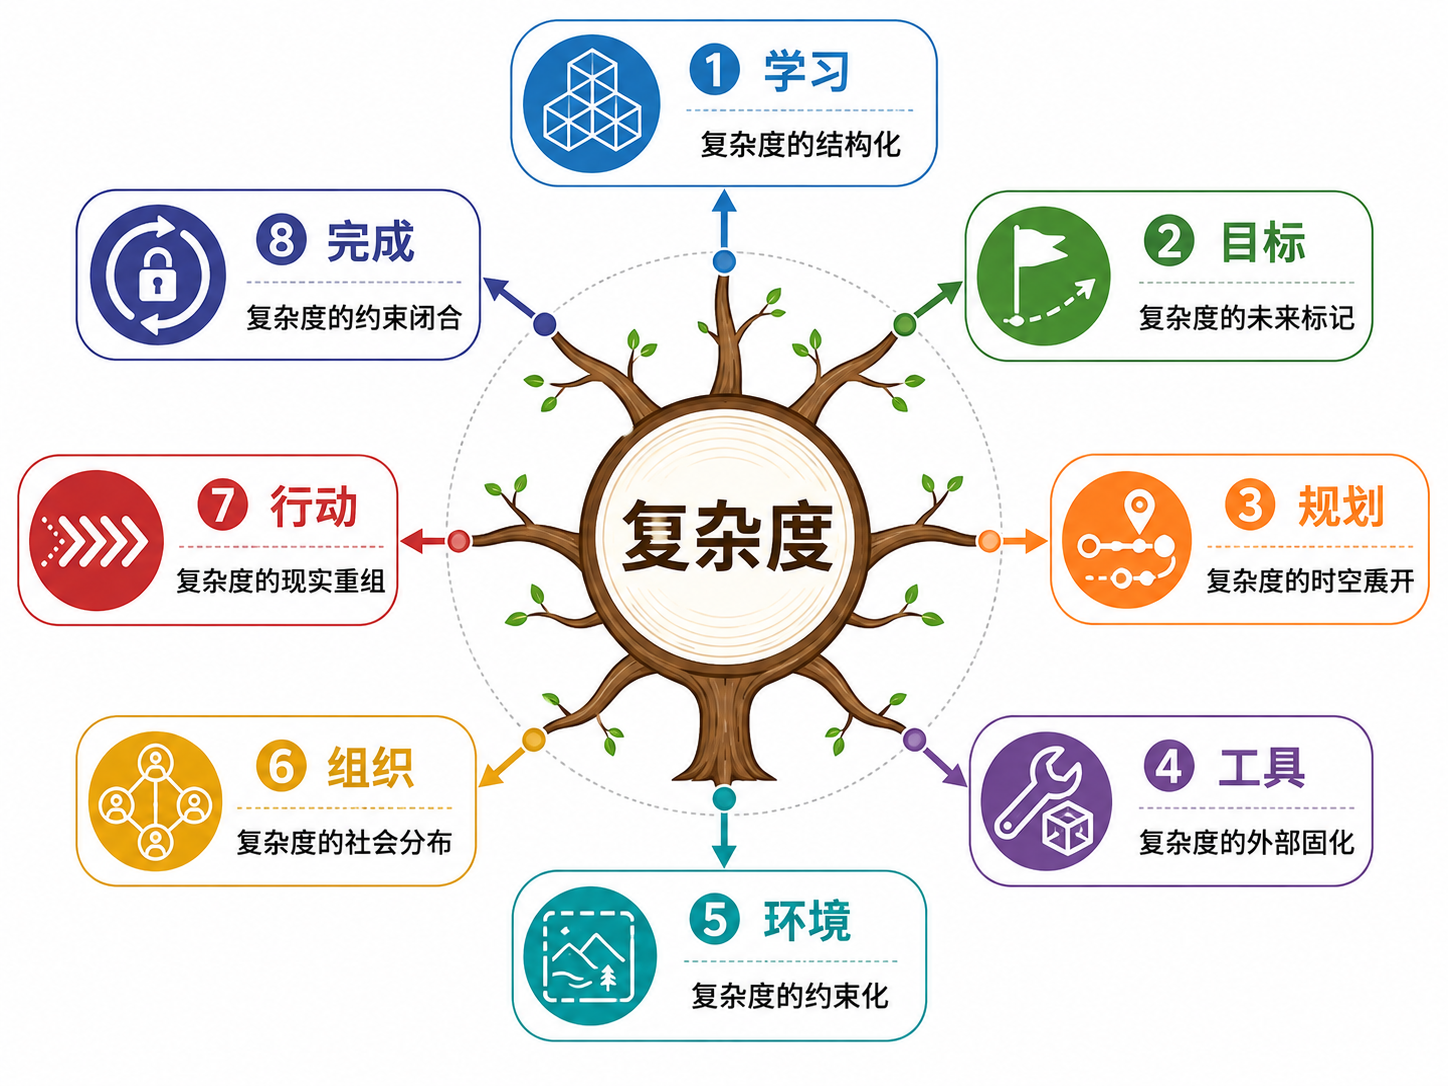
\includegraphics[width=.9\textwidth,height=.38\textheight,keepaspectratio]{images/complexity-migration-tree.png}
\caption{复杂度宏观描述及其结构来源}
\end{figure}

\section{为什么最初需要提出复杂度迁移}
\label{sec:why-complexity-migration}

我们首先回到这一理论最初产生的问题背景。一个初学者第一次解决某类问题时，往往需要在工作记忆中同时维持大量对象、规则、步骤、约束和中间状态。以一个从未使用过某类软件的 Agent 为例，它可能必须显式维护 ``当前窗口是什么''、``按钮在哪里''、``下一步操作会产生什么后果''、``任务目标是否已经满足'' 等大量关系。此时，任务对全局认知表面的占用是显著的。

但是，当同一个 Agent 重复执行数百次以后，情况通常发生变化。原来需要连续显式推理的过程开始变成稳定策略，甚至进一步变成程序、工具调用、低层控制器或者环境中的固定结构。此时，Agent 在完成同样外部任务时，其工作记忆中所需要显式维持的内容大幅下降。

这一现象给出了一个最初的理论直觉：

\[
\boxed{
Thinking\ Less
\neq
Task\ Disappearing
}
\]

如果任务仍然能够成功完成，而显式认知负担却下降，那么任务所需要的结构必然以某种方式被重新组织。早期理论因此把这种变化描述为：

\[
\boxed{
Complexity_{explicit}
\rightarrow
Complexity_{implicit}
}
\]

进一步，我们注意到这种变化并不仅发生在 ``显式--隐式'' 一个维度。熟练驾驶者对车辆姿态的控制可以从高层认知迁移到运动闭环；数学公式可以从一次次推导迁移到长期结构记忆；复杂计算可以迁移到计算器或程序；组织内部反复发生的人际协调可以沉降成岗位、流程和制度。换言之，原本必须由某一功能层承担的处理负担，后来可能由另一个功能层、另一个时间尺度乃至另一个外部载体承担。

于是，早期理论逐渐形成如下基本命题：

\[
\boxed{
Learning
\approx
Redistribution\ of\ Effective\ Complexity
}
\]

这里所谓 ``有效复杂度''，并不是任务在宇宙中的全部物理复杂度，而是相对于某一个智能体、某一个观察尺度和某一个当前功能位置而言，系统为了维持任务可解性而必须承担的结构负担。一个复杂任务本身可能没有变简单，但如果大量关系已经被压缩成一个稳定技能，那么对于工作记忆而言，它所表现出的运行复杂度就已经显著降低。

这也是为什么复杂度迁移理论最初具有很强的工程解释力。它把记忆、熟练、工具、环境改造和社会分工统一成同一种宏观现象：\textbf{复杂度并不总是被 ``消灭''，而是改变了由谁承担、在哪里承担以及以什么速度承担。}

如果用一个最简单的分解表示，我们曾把一个任务在当前 Agent 中产生的有效负担写成：

\[
C_{\mathrm{eff}}(t)
=
C_{\mathrm{run}}(t)
+
C_{\mathrm{stored}}(t)
+
C_{\mathrm{external}}(t)
+
C_{\mathrm{struct}}(t)
\]

其中 $C_{\mathrm{run}}$ 表示当前运行态显式处理负担，$C_{\mathrm{stored}}$ 表示已经进入记忆而不需要持续激活的结构，$C_{\mathrm{external}}$ 表示已经由工具、环境或其他主体承担的部分，而 $C_{\mathrm{struct}}$ 表示已经沉降进稳定技能、程序或功能连接中的结构。

这个公式从一开始就不应被理解为严格物理守恒关系。它真正表达的是一个认知工程直觉：\textbf{系统性能的提高常常不是因为所有问题结构都消失了，而是因为需要被中央显式处理的那一部分越来越少。}

因此，复杂度迁移理论最早并不是为了建立一个抽象形而上学，而是为了回答 AgentOS 中一个最现实的问题：

\begin{statementbox}
如何让有限工作记忆只承担当前真正需要全局处理的结构？
\end{statementbox}

这一问题后来直接通向工作记忆有限容量定理、CCM、Offloading、Boundary、Body Skill 以及整个多尺度 AgentOS 架构。

\section{复杂度不是信息量：有效认知复杂度的定义}
\label{sec:effective-cognitive-complexity}

复杂度迁移理论要成立，首先必须解决一个定义问题：什么是我们所说的 ``复杂度''？如果把复杂度简单等同于数据量、token 数、参数数量或者 Shannon 信息熵，那么大量实际认知现象无法得到解释。

例如，一段包含一万个随机字符的字符串可能具有很高的信息熵，却未必对一个 Agent 构成高认知复杂度，因为 Agent 可以直接忽略它。相反，一个只有几十个符号的逻辑约束系统，如果内部关系高度耦合，却可能对工作记忆造成巨大压力。因此，AgentOS 讨论的复杂度首先是一种\textbf{结构相关、主体相关并且运行状态相关的有效认知复杂度}。

可以首先定义一个认知状态中的活动结构集合：

\[
\mathcal{X}(t)
=
\left\{
x_1(t),x_2(t),\ldots,x_n(t)
\right\}
\]

其中每一个 $x_i$ 可以代表当前需要维持的目标、关系、假设、约束、记忆片段、动作方案或中间变量。假设每个结构项具有局部负担：

\[
c_i(t)
\]

并具有当前激活权重：

\[
w_i(t)\in[0,1]
\]

则最简单的运行复杂度可写成：

\[
C_{\mathrm{run}}(t)
=
\sum_i w_i(t)c_i(t)
\]

但是，仅有加权和仍然无法描述结构之间的相互依赖。真正困难的推理往往不是因为对象多，而是因为关系密。为此，可以进一步引入活动结构图：

\[
\mathcal{G}_h(t)
=
\left(
V_h(t),E_h(t)
\right)
\]

其中 $V_h$ 表示当前进入工作记忆的结构节点，而 $E_h$ 表示必须同时保持的关系。于是有效认知复杂度可以概念性写成：

\[
C_{\mathrm{eff}}(t)
=
\alpha |V_h(t)|
+
\beta |E_h(t)|
+
\gamma \Phi(\mathcal{G}_h(t))
+
\delta U(t)
\]

其中 $\Phi$ 用于描述图的耦合强度、环结构、路径依赖或者非局部约束，而 $U(t)$ 表示不确定性、冲突和状态漂移带来的额外负担。

这个定义非常关键，因为它意味着：同样数量的信息，如果经过结构压缩，可以表现出完全不同的认知复杂度。假设十个彼此独立的规则经过学习后被压缩成一个更高层模式 $z$，那么：

\[
\{r_1,\ldots,r_{10}\}
\rightarrow
z
\]

虽然底层知识并没有消失，但工作记忆只需要激活 $z$，于是：

\[
C_{\mathrm{run}}^{\mathrm{after}}
<
C_{\mathrm{run}}^{\mathrm{before}}
\]

这正是抽象、概念化和技能化的核心认知收益之一。

在这个意义上，复杂度迁移理论从一开始就与压缩理论具有关系，但不能直接等同于压缩。压缩只是降低显式表示尺寸的一种方式，而迁移还可能把某种结构移动到另一个时间尺度或功能载体。例如，一个稳定技能即使内部控制器依然非常复杂，对于高层 Agent 而言，也可以通过一个极低维的控制接口表现：

\[
u_{\mathrm{high}}
=
\texttt{execute(skill)}
\]

内部则执行：

\[
x_{t+1}
=
F_{\mathrm{skill}}(x_t,u_t)
\]

因此，高层复杂度降低不意味着底层系统变简单，而意味着复杂度被封装进了稳定闭环。

由此，我们可以得到一个重要的相对性原则：

\[
\boxed{
Complexity
=
Complexity(
Structure,
Observer,
Carrier,
Timescale
)
}
\]

也就是说，复杂度并不是一个对象脱离主体和尺度以后仍然保持不变的绝对属性。同一结构对不同 Agent、不同功能层甚至同一 Agent 的不同发展阶段，都可能表现出不同有效复杂度。

这也解释了为什么后来的 CSO 理论必须出现。因为一旦复杂度本身取决于承载方式，我们就必须进一步追问：\textbf{究竟是什么结构在改变承载方式？}复杂度只能告诉我们 ``当前负担多大''，却不能充分告诉我们 ``什么东西正在被重新组织''。这个问题最终将导致本章后半部分从 Complexity 向 CSO 的本体转移。

\section{复杂度的功能迁移}
\label{sec:functional-complexity-migration}

复杂度迁移理论最早得到清晰形式化的方向，是\textbf{功能迁移（functional migration）}。所谓功能迁移，是指同一个任务相关结构不再由原来的认知功能承担，而逐渐被另一个功能层接管。

设一个智能系统具有功能集合：

\[
\mathcal{F}
=
\{F_1,F_2,\ldots,F_m\}
\]

在某一时刻，一个任务结构 $X$ 主要由功能 $F_i$ 承担：

\[
X@F_i
\]

随着经验增加，系统可能找到更稳定、更低成本的处理方式，使同样任务逐渐由 $F_j$ 承担：

\[
\boxed{
X@F_i
\rightarrow
X@F_j
}
\]

这就是最初意义上的功能复杂度迁移。

最典型的例子是从显式推理向程序化技能的迁移。一个机器人第一次抓取特殊物体时，可能需要高层规划器显式计算姿态、碰撞、接触位置和运动轨迹。但经过大量重复后，这些关系可以被局部预测控制器吸收。此时，高层系统只发出：

\[
Goal_{\mathrm{grasp}}
\]

而底层闭环自主解决：

\[
Perception
\rightarrow
Prediction
\rightarrow
Control
\rightarrow
Residual
\rightarrow
Correction
\]

从高层视角看，原本必须在工作记忆中维持的结构已经 ``消失''；实际上，它并没有消失，而是被封装进更低层、更快速、更稳定的功能闭环。

因此，我们曾提出：

\[
\boxed{
StableComplexity
\rightarrow
LowerLevelCarrier
}
\]

这一规律后来被重新表述成：

\[
\boxed{
StableCSO
\rightarrow
StableLocalFunctionalCarrier
}
\]

同样的结构也存在于纯数字 Agent 中。第一次完成一项复杂文件转换任务时，Agent 可能需要显式规划几十个步骤；若该过程不断重复，最终可生成一个脚本：

\[
\pi_{\mathrm{explicit}}
\rightarrow
Program
\]

以后工作记忆不再承担原有步骤链，只需要知道：

\[
\texttt{call(program)}
\]

这里发生的正是功能责任迁移。

这种现象让我们认识到，成熟智能的一个关键标志并不是 ``显式思考越来越多''，而恰恰可能是：

\[
\boxed{
\frac{
ExplicitGlobalProcessing
}{
SuccessfulBehavior
}
\downarrow
}
\]

随着能力成熟，越来越多稳定结构被迁移到局部功能闭环、高效程序、结构记忆或者外部工具，因此全局认知只处理异常、新颖和需要跨域协调的问题。

这也进一步形成了后来的重要原则：

\begin{statementbox}
NormalDynamicsStayLocal
\end{statementbox}

以及：

\begin{statementbox}
UnexpectedResidualEscalatesGlobally
\end{statementbox}

即正常、熟悉、低残差的过程应该尽量在局部完成，而只有局部无法解释或无法控制的残差才向上升级进入更昂贵的全局认知。

从这里可以看到，复杂度功能迁移并不是一个孤立概念。它后来直接演化成为 AgentOS 的层级控制原则、技能编译原则、BPCC 局部闭环原则以及 CSO 功能迁移理论。

\section{复杂度的时间尺度迁移}
\label{sec:timescale-complexity-migration}

功能位置之外，第二个重要维度是\textbf{时间尺度迁移}。智能系统中的结构并不是以同样速度变化。工作记忆可以在秒级变化，情景记忆在分钟到天的时间尺度逐渐积累，而结构记忆、自我以及生命周期生成先验则可能以更慢速度演化。

因此，我们早期提出：认知复杂度不仅存在于某一个位置，还存在于某一个特征频率或时间尺度上。

设某个认知结构具有特征时间尺度：

\[
\tau
\]

或者等价频率：

\[
\omega
\sim
\tau^{-1}
\]

那么学习可以表现成结构活动从高频向低频迁移：

\[
\boxed{
\omega_{\mathrm{fast}}
\rightarrow
\omega_{\mathrm{slow}}
}
\]

其认知意义是：原本需要持续、快速、显式更新的结构逐渐稳定下来，成为变化较慢的经验或生成结构。

这与三相记忆之间存在天然对应关系：

\[
h
\rightarrow
E
\rightarrow
\Theta
\]

可以被理解成：

\[
FastActiveStructure
\rightarrow
MediumTrajectoryStructure
\rightarrow
SlowGenerativeStructure
\]

第一次遭遇一个新现象时，大量相关关系停留在 $h$ 中；经过多次经历，这些关系形成 $E$ 中的经验轨迹；再经过抽象和整合，最终成为 $\Theta$ 中较慢的结构。

因此，我们可以把 ``巩固'' 写成：

\[
\boxed{
Fast
\rightarrow
Slow
}
\]

但这并不是单向过程。慢结构也会重新激活成快速活动：

\[
\boxed{
Slow
\rightarrow
Fast
}
\]

例如一个已经稳定存在于 $\Theta$ 中的数学规则，在当前问题中被召回以后重新进入 $h$，成为实时推理的一部分。

因此，认知结构的时间尺度迁移实际上是双向的：

\[
\boxed{
Consolidation:
Fast\rightarrow Slow
}
\]

\[
\boxed{
Activation:
Slow\rightarrow Fast
}
\]

这一点非常重要，因为它避免了把学习理解成单纯 ``越来越慢''。成熟智能必须同时具备把经验沉降成慢结构和在需要时快速重新激活这些结构的能力。

我们后来进一步尝试定义一个频谱上的复杂度密度：

\[
\rho_C(\omega,t)
\]

表示在时间 $t$，系统需要在特征频率 $\omega$ 附近承担多少有效结构负担。若加入功能位置 $f$，则有：

\[
\rho_C(f,\omega,t)
\]

从而可以把智能状态看成分布在：

\[
FunctionalSpace
\times
FrequencySpace
\]

上的结构分布。

这便是后来 ``智能频谱迁移'' 思想的来源。

但是，我们必须在这里提前指出一个后来的修正：$\rho_C$ 并不是像物理系统中的质量密度那样对应一种独立实体。它更接近一个\textbf{统计观测量}，描述多少 Agent-CSO 在什么功能和时间尺度上处于活动、稳定或承载状态。下一章会将其正式改写为：

\[
\rho_{CSO}(f,\omega,t)
\]

也就是说，真正有本体意义的是结构，而复杂度只是结构分布的一种宏观函数。

\section{复杂度的边界迁移与认知卸载}
\label{sec:boundary-complexity-migration}

第三种复杂度迁移发生在系统边界上。智能体并不需要把所有需要使用的结构永久保存在内部。相反，成熟智能往往具有极强的外化能力。

一个简单例子是电话号码。若一个人必须完全依靠生物记忆保存所有联系人号码，则这些信息必须占据内部记忆资源；当号码被写入手机以后，内部只需要保留：

\[
\text{``联系人可以在手机中找到''}
\]

于是原来的高维信息被迁移到外部载体。

对于 AgentOS，这一过程更加一般。可以定义内部结构集合：

\[
\mathcal{M}_{\mathrm{int}}
\]

以及外部可调用结构集合：

\[
\mathcal{M}_{\mathrm{ext}}
\]

则某个任务相关结构可能发生：

\[
X:
\mathcal{M}_{\mathrm{int}}
\rightarrow
\mathcal{M}_{\mathrm{ext}}
\]

外部载体可以是：

\[
File,\quad
Database,\quad
Script,\quad
Program,\quad
Tool,\quad
Environment,\quad
OtherAgent
\]

因此，我们曾经把这种现象描述为：

\begin{statementbox}
ComplexityOffloading
\end{statementbox}

也就是认知复杂度卸载。

但从更严格角度看，卸载并不是简单把负担 ``丢出去''。如果 Agent 完全忘记外部结构在哪里以及如何使用，那么这不构成有效的认知卸载，而只是信息丢失。真正的卸载要求内部保留某种\textbf{索引结构}：

\[
I_X
=
(
Location,
AccessMethod,
Validity,
Cost,
Trust
)
\]

于是完整过程更像：

\[
X_{\mathrm{internal}}
\rightarrow
I_X^{\mathrm{internal}}
+
X_{\mathrm{external}}
\]

内部保留一个低维导航结构，复杂内容则由外部载体承担。

这解释了为什么 ``外部记忆'' 并不是任何外界对象，而必须是 Agent 已经建立稳定访问关系的外部结构。

认知卸载理论后来又进一步扩展到环境改造。例如，一条经常需要绕行的路线，如果通过建造道路被永久改变，那么 Agent 并不是简单记住了一个新策略，而是直接修改了未来任务结构：

\[
Environment
\rightarrow
Environment'
\]

使得未来问题本身变得更容易。

因此：

\[
\boxed{
ChangeEnvironment
=
ChangeFutureCognitiveProblem
}
\]

这使环境成为一种极其特殊的外部认知载体。

类似地，在社会环境中，一个 Agent 还可以把任务委派给另一个 Agent，使：

\[
X@Agent_A
\rightarrow
X@Agent_B
\]

从个体视角看，这同样是边界迁移。

这也解释了社会分工的认知意义：文明并不是要求每个人掌握全部结构，而是通过制度、职业、工具和信息系统，把巨大的问题空间分布到不同载体中。

从早期复杂度语言看：

\[
\boxed{
C_{\mathrm{internal}}
\rightarrow
C_{\mathrm{external}}
}
\]

从后来的 CSO 语言看，则更精确地变成：

\[
\boxed{
AgentCSO:
B_{\mathrm{internal}}
\rightarrow
B_{\mathrm{external}}
}
\]

这里真正变化的是结构承载边界，而不是一种抽象复杂度物质。

\section{复杂度频谱与迁移流}
\label{sec:complexity-spectrum-flow}

在功能迁移、时间尺度迁移和边界迁移逐渐清晰以后，我们曾经尝试建立一个统一数学框架，将智能系统理解为 ``复杂度在功能--频率空间中的分布与流动''。

设：

\[
f\in\mathcal F
\]

表示功能位置，而：

\[
\omega\in\Omega
\]

表示时间频率，则定义复杂度密度：

\[
\rho_C(f,\omega,t)
\]

直觉上，$\rho_C(f,\omega,t)$ 表示在时刻 $t$，系统在功能位置 $f$ 和时间尺度 $\omega$ 上承载的有效认知复杂度。

进一步引入复杂度流：

\[
\mathbf J_C(f,\omega,t)
\]

其方向可以同时包含功能迁移方向与频率迁移方向：

\[
\mathbf J_C
=
\left(
J_F,
J_\omega
\right)
\]

如果再加入边界维度 $b$，则完整空间可以写成：

\[
\mathcal X_C
=
\mathcal F
\times
\Omega
\times
\mathcal B
\]

复杂度密度：

\[
\rho_C(f,\omega,b,t)
\]

复杂度迁移流：

\[
\mathbf J_C
=
(
J_F,
J_\omega,
J_B
)
\]

在最初理论中，我们进一步借鉴连续介质中的连续性方程，写出：

\[
\frac{\partial \rho_C}{\partial t}
+
\nabla\cdot\mathbf J_C
=
S_C-D_C
\]

其中：

\[
S_C
\]

表示新的复杂结构被引入系统，例如新问题、新环境、新知识；而：

\[
D_C
\]

则表示结构被删除、遗忘、合并、压缩或者变得不再相关。

这个形式的价值并不在于声称 ``复杂度真的像流体一样流动''，而在于它第一次把许多原本分离的 Agent 现象放进统一坐标中。

例如：

\[
J_\omega<0
\]

可以表示从快频向慢频的稳定化；

\[
J_\omega>0
\]

可以表示慢结构被重新激活；

\[
J_F
\]

可以表示不同功能之间的处理责任迁移；

\[
J_B
\]

可以表示内部向外部或者外部向内部的载体迁移。

于是：

\[
MemoryConsolidation,
SkillLearning,
Recall,
Offloading,
ToolUse
\]

在形式上都成为同一个迁移框架下的不同方向。

然而，这个模型也暴露了早期理论的核心问题：如果 $\rho_C$ 被当成实体密度，就会产生一个错误直觉——似乎存在某种 ``复杂度物质'' 在系统内部守恒流动。

实际上，一个复杂关系结构可以经过抽象后被十倍压缩；多个结构可以合并成一个更高层模式；一个结构也可能被分解成多个低层动作。因此，在不同表示之间，复杂度量值并不保持严格不变：

\[
C(X)
\neq
C(\phi(X))
\]

尤其当 $\phi$ 是抽象、编译或重新表示操作时更是如此。

所以后来我们逐渐把连续性方程重新解释为：

\begin{statementbox}
结构活动分布的统计连续性，而非复杂度实体守恒。
\end{statementbox}

本章稍后将进一步说明，真正适合作为 $\rho$ 所承载对象的并不是 Complexity，而是 Agent-CSO 的活动与承载分布。

\section{从复杂度守恒直觉到结构连续性原则}
\label{sec:structural-continuity}

复杂度迁移理论早期曾产生一个非常诱人的判断：如果某种能力从显式思考中消失，但行为能力并没有消失，那么 ``复杂度应该被保存到了其他地方''。这一判断在直觉上十分有力，于是曾经接近形成 ``复杂度守恒'' 的表述。

但是仔细分析以后，我们必须放弃严格守恒语言。

考虑一个未经训练的 Agent，需要显式执行十步推理：

\[
X_1\rightarrow X_2\rightarrow\cdots\rightarrow X_{10}
\]

经过长期训练后，这十步可能被压缩成一个技能：

\[
S
\]

于是，如果用节点数量作为复杂度：

\[
C_{\mathrm{before}}=10
\]

而：

\[
C_{\mathrm{after}}=1
\]

显然不存在数值守恒。

另一方面，技能内部可能包含一个庞大的神经网络，因此若从参数数量衡量：

\[
C_{\mathrm{after}}
\gg
C_{\mathrm{before}}
\]

同样说明所谓 ``复杂度'' 高度依赖选择何种度量。

所以真正稳定的并不是复杂度值，而是一种更弱、也更合理的\textbf{结构连续性}：

\[
\resizebox{.96\linewidth}{!}{$\displaystyle
\boxed{
EffectiveCognitiveStructure
\ does\ not\ simply\ disappear;
\ it\ changes\ representation,\ carrier,\ or\ role.
}
$}
\]

也就是说，当一个能力从显式工作记忆中 ``消失'' 时，我们首先不应该得出它已经不存在，而应该追问：

\begin{statementbox}
WhereIsItsEffectiveStructureNow?
\end{statementbox}

可能的答案是：

\[
h\rightarrow E
\]

进入经验；

\[
E\rightarrow\Theta
\]

进入生成结构；

\[
\Theta\rightarrow Skill
\]

编译成程序；

\[
Internal\rightarrow Tool
\]

迁移到工具；

\[
Internal\rightarrow Environment
\]

沉降到环境；

或者：

\[
Global\rightarrow LocalLoop
\]

被局部功能闭环承担。

因此，我们把原来的 ``复杂度守恒'' 修正为：

\begin{statementbox}
StructuralContinuityPrinciple
\end{statementbox}

结构连续性原则并不要求所有细节永久保存。认知结构可以：

\[
compress,
merge,
abstract,
forget,
externalize
\]

因此：

\[
Structure_t
\not\equiv
Structure_{t+\Delta}
\]

但如果能力保持，则通常存在某种因果上连续的有效结构链：

\[
X_t
\xrightarrow{\phi_1}
X_{t+1}
\xrightarrow{\phi_2}
X_{t+2}
\]

这使我们可以追踪能力是如何通过生命周期发生结构变换的。

这一修正具有非常深的理论意义。它意味着我们从寻找一个 ``守恒量''，转向寻找一个 ``结构谱系''：

\[
\boxed{
Conservation
\rightarrow
Lineage
}
\]

换句话说，学习不是保持同一种复杂度，而是维持能力结构的因果连续，同时允许表示形式发生深刻变化。

这也使如下判断得到更加严谨的解释：

\[
\boxed{
ThinkingLess\neq KnowingLess
}
\]

一个专家在熟悉问题上思考更少，并不意味着拥有更少结构，而往往意味着关键结构已经迁移到更慢、更稳定、更局部或者更外部的载体。

\section{复杂度作为宏观统计量，而不是本体实体}
\label{sec:complexity-not-ontology}

随着 CSO 与 Agent-CSO 的提出，复杂度迁移理论的本体问题变得不可回避。

假设我们观察一个 Agent 在执行任务 $T$。我们可以测量工作记忆中活动对象数量、关系数量、推理深度、工具调用次数、状态不确定性和计算消耗，然后定义一个宏观量：

\[
C_T(t)
=
F(
N_{\mathrm{active}},
N_{\mathrm{relation}},
Depth,
Uncertainty,
Cost
)
\]

这个量当然可以具有工程意义。它可以帮助 CCM 判断当前系统是否接近过载，也可以用于比较两种表示方式哪一种更适合工作记忆。

但是，$C_T(t)$ 本身并没有告诉我们：

\begin{itemize}
    \item 哪一个对象正在被处理；
    \item 哪些关系仍然保持；
    \item 哪种语义发生了变化；
    \item 某个能力迁移到了哪个功能；
    \item 当前结构是否还是原来的结构。
\end{itemize}

也就是说，复杂度是\textbf{状态的量化描述}，而不是\textbf{状态本身}。

这一点类似于温度。温度可以描述大量微观粒子的统计状态，但 ``温度'' 本身并不是一个独立粒子。类似地，认知复杂度可以描述大量活动认知结构的总体处理压力，但并不存在一个叫做 ``Complexity Particle'' 的实体在 Agent 内部运动。

因此，本书必须明确区分：

\begin{statementbox}
Ontology
\end{statementbox}

与：

\begin{statementbox}
Measure
\end{statementbox}

在新的理论中：

\begin{statementbox}
CSO
\end{statementbox}

属于本体对象；

\begin{statementbox}
AgentCSO
\end{statementbox}

属于具体 Agent 内部的结构实现；

而：

\begin{statementbox}
Complexity
\end{statementbox}

属于这些结构在特定观察尺度下的一个宏观测量函数。

形式上，可以定义：

\[
C
=
\mathcal C(
\mathcal G_C,
\mathcal G_F,
\mu_t,
h(t),
\omega,
B
)
\]

也就是说，复杂度 $C$ 是由认知结构图、功能图、承载关系、当前工作状态、时间尺度和边界共同决定的函数。

由此可以看出：

\[
\boxed{
Complexity
\neq
Primitive
}
\]

真正的 primitive 应该是：

\[
\boxed{
Structure,\ Relation,\ Carrier,\ Function,\ Timescale
}
\]

这正是 CSO 理论带来的本体升级。

从这个角度回看早期复杂度迁移语言，例如：

\[
C_{high}\rightarrow C_{low}
\]

应该被重新解释成：

\[
AgentCSO@F_{\mathrm{high}}
\rightarrow
AgentCSO@F_{\mathrm{low}}
\]

又如：

\[
C_{\mathrm{internal}}
\rightarrow
C_{\mathrm{external}}
\]

应解释成：

\[
AgentCSO:
B_{\mathrm{internal}}
\rightarrow
B_{\mathrm{external}}
\]

而：

\[
C_{\mathrm{fast}}
\rightarrow
C_{\mathrm{slow}}
\]

则应解释成：

\[
AgentCSO:
\tau_{\mathrm{fast}}
\rightarrow
\tau_{\mathrm{slow}}
\]

因此，我们并没有否定复杂度迁移理论，而是给出了它真正对应的微观机制。

\section{从 Complexity Migration 到 CSO Migration}
\label{sec:complexity-to-cso}

现在可以正式完成本章最重要的理论转换。

定义一个本体层认知结构：

\[
C\in\mathcal C
\]

对于具体 Agent $A$，该结构具有一个具体实现：

\[
\pi_A(C)
=
AgentCSO_A(C)
\]

进一步，把 Agent-CSO 写成：

\[
\boxed{
AgentCSO_A(C,t)
=
\left(
C,
R_A,
F_A,
\tau_A,
B_A,
S_A
\right)
}
\]

其中：

\begin{itemize}
    \item $C$：该结构在理论上的本体身份；
    \item $R_A$：Agent 内部对它的具体表示；
    \item $F_A$：当前主要承载该结构的功能；
    \item $\tau_A$：该结构当前有效变化时间尺度；
    \item $B_A$：内部、外部或者混合载体位置；
    \item $S_A$：活动、潜伏、预测、回忆、程序化等状态。
\end{itemize}

于是，所谓 ``复杂度迁移'' 可以被严格重写为坐标变化：

\[
AgentCSO_A(C,t)
\rightarrow
AgentCSO_A(C,t+\Delta t)
\]

即：

\[
(R,F,\tau,B,S)_t
\rightarrow
(R',F',\tau',B',S')_{t+\Delta t}
\]

这里并不要求本体对象 $C$ 完全不变，因为认知学习本身也可能重新构造本体关系；但至少在讨论某一个能力结构连续性的局部窗口中，我们可以追踪其表示与承载方式如何变化。

于是，复杂度迁移的几个历史方向自然得到重新定义：

\[
\boxed{
M_R:
R\rightarrow R'
}
\]

表示迁移；

\[
\boxed{
M_F:
F\rightarrow F'
}
\]

功能迁移；

\[
\boxed{
M_\tau:
\tau\rightarrow\tau'
}
\]

时间尺度迁移；

\[
\boxed{
M_B:
B\rightarrow B'
}
\]

边界/载体迁移。

可以写成统一迁移向量：

\[
\boxed{
\mathcal M_{\mathrm{CSO}}
=
(
M_R,
M_F,
M_\tau,
M_B
)
}
\]

这样一来，学习第一次获得比 ``复杂度变化'' 更丰富的结构描述。

例如一个初学驾驶 Agent：

\[
AgentCSO_{\mathrm{steering}}
=
(
R_{\mathrm{explicit}},
F_h,
\tau_{\mathrm{slow}},
B_{\mathrm{internal}},
Active
)
\]

经过训练以后可能变成：

\[
AgentCSO'_{\mathrm{steering}}
=
(
R_{\mathrm{policy}},
F_{\mathrm{BPCC}},
\tau_{\mathrm{fast}},
B_{\mathrm{body}},
Procedural
)
\]

从宏观看，高层认知复杂度下降；从 CSO 看，则是表示、功能、时间尺度和载体同时发生迁移。

因此，学习的定义也开始发生改变。

早期我们写：

\[
\boxed{
Learning
=
ComplexityRedistribution
}
\]

现在更准确地写：

\[
\boxed{
Learning
=
ChangeOfCSORealizationAndPlacement
}
\]

或者用中文表述：

\begin{statementbox}
学习，是认知结构改变其表示形式、功能位置、时间尺度与承载关系的过程。
\end{statementbox}

这就是下一章《CSO迁移：学习的新定义》的直接理论入口。

\section{复杂度理论为何仍然应该保留}
\label{sec:why-keep-complexity}

完成 CSO 本体升级以后，一个自然问题是：既然复杂度不是第一性对象，那么是否应该完全删除 ``复杂度迁移'' 理论？

答案是否定的。

原因在于，本体对象和工程测量对象承担不同职责。

CSO 理论回答：

\begin{statementbox}
WhatStructureExistsAndWhereDoesItLive?
\end{statementbox}

复杂度理论则回答：

\begin{statementbox}
HowHardIsThisStructureToMaintainHereAndNow?
\end{statementbox}

对于 AgentOS，后一个问题仍然极其重要。

工作记忆容量有限，因此 CCM 并不需要在每一毫秒都重建完整的 CSO 本体谱系，而需要快速判断：

\[
C_{\mathrm{run}}(t)
\]

是否正在接近：

\[
C_{\max}(W)
\]

如果：

\[
C_{\mathrm{run}}(t)
>
\theta_C
\]

那么系统需要触发：

\[
Compression,
Suppression,
Paging,
Decomposition,
Offloading
\]

因此，复杂度仍然是一种非常有价值的控制量。

我们可以把二者关系理解为：

\[
\boxed{
CSO
\rightarrow
MicroscopicStructuralDescription
}
\]

\[
\boxed{
Complexity
\rightarrow
MacroscopicOperationalDescription
}
\]

这与物理学中微观状态和宏观状态量之间的关系类似，但只是方法论类比，并不意味着认知复杂度具有热力学温度那样成熟的物理理论基础。

从工程角度，可以定义复杂度观测器：

\[
\hat C_t
=
\mathcal O_C(
h_t,
\mathcal G_{h,t},
Uncertainty_t,
Conflict_t,
Resource_t
)
\]

再由 CCM 根据：

\[
\hat C_t
\]

控制当前认知状态：

\[
u_t^{CCM}
=
\pi_{CCM}(
\hat C_t,
\dot{\hat C}_t,
C_{\max},
GoalPriority
)
\]

此时，复杂度不再被当成本体，而成为控制系统中的状态指标。

类似地，在系统设计中，我们仍然可以讨论：

\[
ComplexityOffloading
\]

因为从 Agent 高层运行成本的角度，这个表达非常直观；但是，当需要进一步解释 ``究竟卸载了什么'' 时，必须回到 Agent-CSO：

\[
AgentCSO:
InternalCarrier
\rightarrow
ExternalCarrier
\]

因此，在本书后续章节中，我们将采取双层语言：

\[
\boxed{
OperationalLayer:
Complexity
}
\]

\[
\boxed{
OntologicalLayer:
CSO/AgentCSO
}
\]

前者服务于容量管理、调度、控制和工程测量；后者服务于学习理论、结构连续性、功能迁移和拓扑演化。

这也是一次重要的理论成熟：我们不再要求一个概念承担全部解释责任，而是在不同分析层使用不同变量。

\section{从复杂度迁移到智能结构动力学}
\label{sec:complexity-to-structural-dynamics}

至此，我们可以重新审视复杂度迁移理论在整个《智能动力学与 AgentOS》中的位置。

它最初提供了一个非常重要的直觉：

\begin{statementbox}
能力成熟以后，认知负担不是凭空消失，而是改变了自己的承载位置。
\end{statementbox}

这个直觉随后帮助我们理解了：

\[
h\rightarrow E\rightarrow\Theta
\]

记忆沉降；

\[
ExplicitReasoning
\rightarrow
Skill
\]

技能形成；

\[
Internal
\rightarrow
Tool
\]

工具使用；

\[
Internal
\rightarrow
Environment
\]

环境改造；

以及：

\[
Agent_A
\rightarrow
Agent_B
\]

社会分工。

这些现象在早期都可以统一称为 ``复杂度迁移''。

但是，随着本体分析深入，我们认识到：

\begin{statementbox}
真正具有连续性的不是复杂度值，而是认知结构及其因果谱系。
\end{statementbox}

因此，理论核心逐渐由：

\[
Complexity
\]

转向：

\[
CSO
\]

再转向：

\[
AgentCSO
\]

最终形成：

\[
\boxed{
CSO
+
FunctionalTopology
+
Timescale
+
Carrier
}
\]

四个基本对象。

从这一点开始，智能系统就不能再被描述成一个简单的 ``复杂度容器''。它更适合被表示成两个耦合结构：

\[
\mathcal G_C(t)
\]

表示认知结构图；

\[
\mathcal G_F(t)
\]

表示功能拓扑；

并通过动态承载映射：

\[
\mu_t:
\mathcal G_C(t)
\rightarrow
\mathcal G_F(t)
\]

相互连接。

这意味着学习过程中真正变化的是：

\[
\boxed{
\mu_t
}
\]

以及在更慢尺度上：

\[
\boxed{
\mathcal G_C(t),\qquad
\mathcal G_F(t)
}
\]

于是我们从 ``复杂度在系统中流动'' 的图景，进一步发展到：

\begin{statementbox}
CognitiveStructureFlowOnFunctionalTopology
\end{statementbox}

也就是：

\begin{statementbox}
认知结构在可塑功能拓扑上的生成、激活、变换、迁移与稳定。
\end{statementbox}

再进一步，当长期重复迁移开始改变拓扑本身时：

\[
PersistentCSOMigration
\rightarrow
StableFunctionalCoupling
\rightarrow
TopologyEvolution
\]

理论正式进入：

\[
\boxed{
DynamicsOnTopology
+
DynamicsOfTopology
}
\]

这将是第14章以后真正展开的内容。

因此，本章并不是复杂度理论的终结，而是一次概念层级的重新定位。

我们可以把它总结成三个阶段。

第一阶段：

\begin{statementbox}
ComplexityAsBurden
\end{statementbox}

我们关注有限工作记忆为什么会过载。

第二阶段：

\begin{statementbox}
ComplexityAsFlow
\end{statementbox}

我们发现认知负担可以在功能、尺度与边界之间迁移。

第三阶段：

\begin{statementbox}
ComplexityAsProjectionOfStructureDynamics
\end{statementbox}

我们认识到真正发生变化的是认知结构本身的表示与承载关系，而复杂度只是这种结构动力学在某一观察尺度上的宏观投影。

因此，本章最终得到本书此阶段最重要的认识论修正：

\[
\boxed{
Complexity
=
MeasureOfStructuralBurden
}
\]

而：

\[
\boxed{
CSO
=
ObjectOfCognitiveDynamics
}
\]

进一步：

\[
\boxed{
AgentCSO
=
ConcreteRealizationOfCSO
}
\]

于是，复杂度理论与 CSO 理论不再竞争，而形成清晰的层级关系：

\[
\boxed{
CSO/AgentCSO
\xrightarrow{\text{measurement}}
Complexity
}
\]

以及：

\[
\boxed{
CSOMigration
\xrightarrow{\text{macroscopic observation}}
ComplexityMigration
}
\]

这就是我们从最初 ``复杂度到底去了哪里'' 的问题，逐步进入 ``认知结构究竟如何改变自己的承载位置'' 的完整理论跃迁。

\section{本章小结：从负担迁移到结构迁移}
\label{sec:chapter12-summary}

本章完成了一次对于整个智能动力学理论非常重要的概念清理。

我们最初从工作记忆和技能学习现象出发，观察到一个事实：随着能力成熟，完成同一任务所需要的显式认知负担会下降。然而，能力本身并没有因此消失。为了描述这一现象，我们提出复杂度迁移，并进一步区分功能迁移、时间尺度迁移和边界迁移。

于是，我们曾用：

\[
\rho_C(f,\omega,t)
\]

描述复杂度在功能--频率空间中的分布，并用：

\[
\frac{\partial \rho_C}{\partial t}
+
\nabla\cdot\mathbf J_C
=
S_C-D_C
\]

描述这种分布的变化。

这一框架成功统一了许多智能现象，但同时暴露了一个本体论问题：复杂度本身不是一个独立实体。它依赖观察尺度、表示方式、功能位置和主体能力，因此不存在简单意义上的 ``复杂度守恒''。

由此，我们将原来的：

\[
ComplexityConservation
\]

修正为：

\begin{statementbox}
StructuralContinuity
\end{statementbox}

即：

\begin{statementbox}
有效认知结构通常不会在能力成熟时简单消失，而会发生压缩、抽象、合并、外化或承载位置改变。
\end{statementbox}

进一步，通过 CSO 与 Agent-CSO 的区分，我们得到：

\[
AgentCSO_A(C,t)
=
(C,R,F,\tau,B,S)
\]

从而可以更加精确地解释所谓复杂度迁移：

\[
\boxed{
ComplexityMigration
=
MacroscopicProjectionOfCSOMigration
}
\]

真正的迁移对象不是抽象复杂度，而是：

\[
\boxed{
Representation,
Function,
Timescale,
Carrier,
State
}
\]

的改变。

因此，本章之后，我们将保留 ``复杂度'' 作为 AgentOS 中非常重要的工程量，用于工作记忆容量、CCM、调度、过载预测和认知资源控制；但在智能本体和学习动力学层面，则正式转向：

\begin{statementbox}
CSO
\end{statementbox}

与：

\begin{statementbox}
AgentCSO
\end{statementbox}

这使我们能够给学习一个比 ``知识增加'' 或 ``参数更新'' 更一般的定义：

\begin{definition*}
学习是认知结构改变自身表示、功能位置、时间尺度和承载关系的过程。
\end{definition*}

而当这种迁移长期重复并沉降为新的功能连接时，我们将进一步得到：

\[
\boxed{
CSOFlow
\rightarrow
StableCoupling
\rightarrow
FunctionalTopology
}
\]

因此，第12章在整本书中的真正作用，是完成从早期的：

\begin{statementbox}
复杂度治理
\end{statementbox}

向更成熟的：

\begin{statementbox}
认知结构动力学
\end{statementbox}

的理论换轨。

下一章将不再问：

\[
\text{``复杂度去了哪里？''}
\]

而是正式提出一个更基础的问题：

\begin{statementbox}
``一个认知结构，在智能体整个生命周期中究竟如何改变自己的表示与承载位置？''
\end{statementbox}

这将构成第13章《CSO迁移：学习的新定义》的出发点。

\chapter{CSO迁移：学习的新定义}
\label{chap:cso-migration}

\begin{chapteroverviewbox}
在上一章中，我们完成了一次重要的本体论修正：不再把“复杂度”理解成一种能够像能量一样在系统内部流动的实体，而是把复杂度重新放回描述层，把真正发生变化的对象确定为认知结构对象及其具体承载，即 CSO 与 Agent-CSO。本章将在这一修正之上重新定义“学习”。

本章的基本命题是：\textbf{学习并不首先意味着知识数量增加，也不首先意味着模型参数发生更新；从更一般的智能动力学角度看，学习是同一个或相互关联的 CSO 在智能体内部改变其表示方式、功能位置、运行时间尺度和承载边界的过程。}因此，参数训练、情景记忆写入、知识抽象、技能自动化、程序编译、工具外化、环境改造乃至异常条件下技能重新进入显式认知，都可以被视为 CSO 迁移的不同特殊形式。

我们将把一个具体 Agent 对某一 CSO 的承载状态写成
\[
AgentCSO_A(C,t)
=
\bigl(
C,\,
R_A,\,
F_A,\,
\tau_A,\,
B_A,\,
S_A
\bigr),
\]
其中 $C$ 表示其所对应的认知结构本体，$R_A$ 表示该 Agent 的具体表示，$F_A$ 表示当前功能承载位置，$\tau_A$ 表示该结构发生有效作用的时间尺度，$B_A$ 表示承载边界或载体，$S_A$ 表示激活、潜伏、预测、回忆、程序化等运行状态。本章所谓“迁移”，正是这些坐标在生命周期中的有组织变化。

因此，本章的研究对象不是单一模型的梯度下降，而是一个更广义的问题：

\begin{statementbox}
一个认知结构在一个智能体的一生中，究竟以什么形式、由什么功能、在什么时间尺度、通过什么载体继续存在？
\end{statementbox}

后续关于三相记忆、工作记忆、认知卸载、技能编译、Body Runtime 和功能拓扑学习的讨论，都将在这一迁移理论之上获得统一解释。
\end{chapteroverviewbox}

\begin{figure}[htbp]
\centering
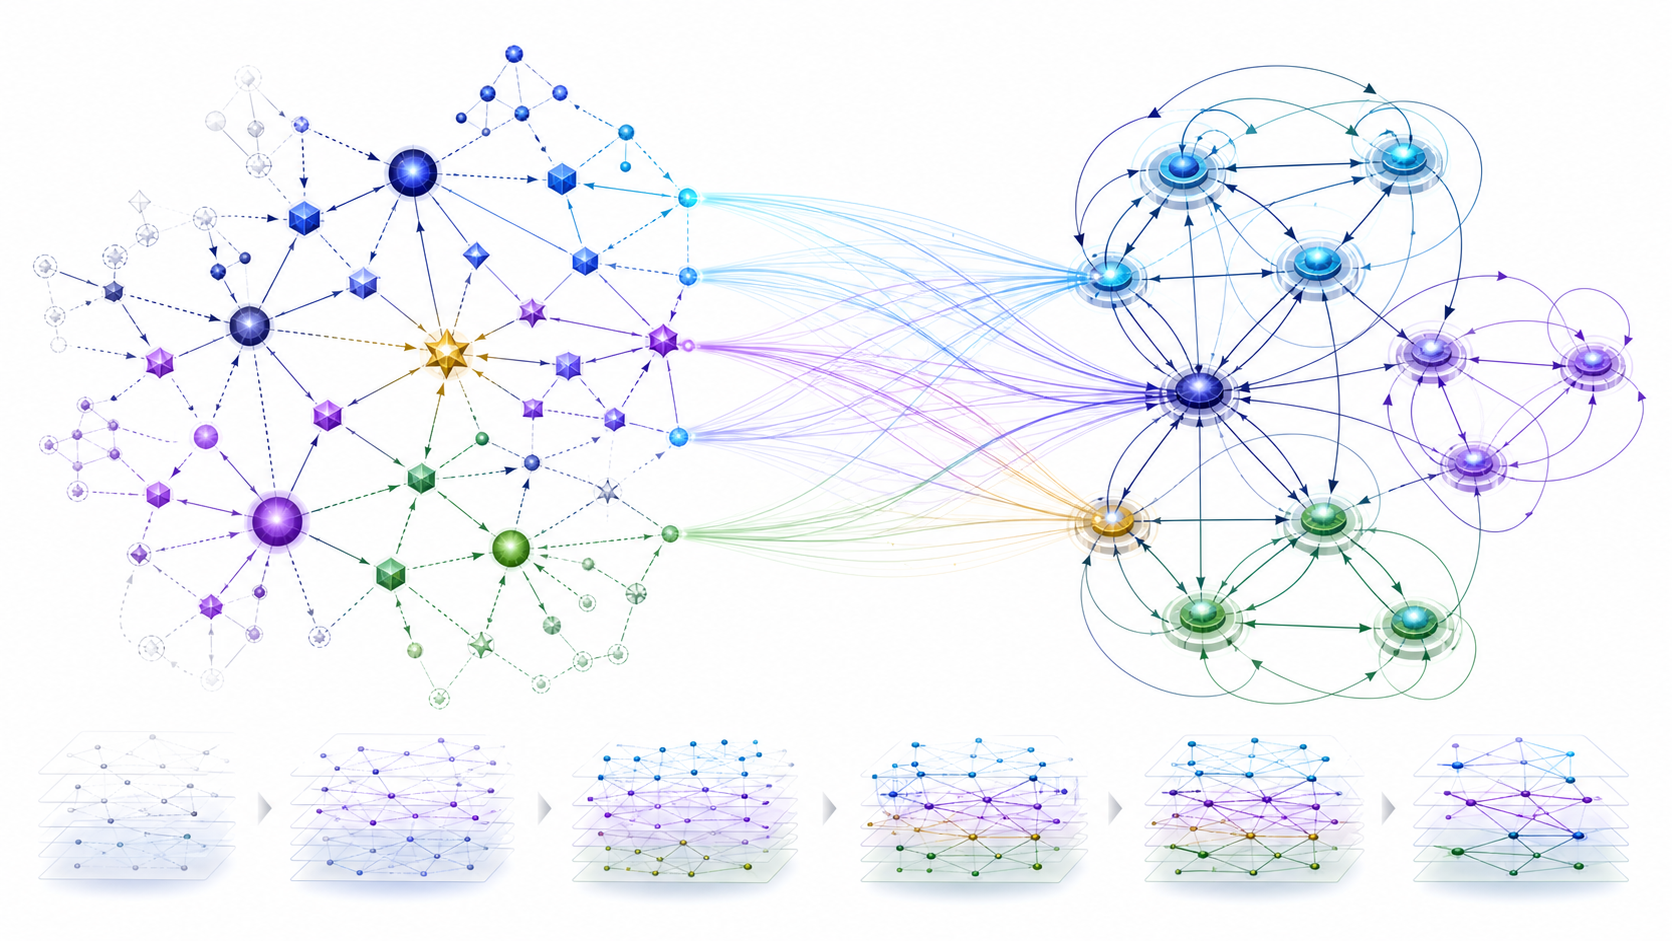
\includegraphics[width=.9\textwidth,height=.38\textheight,keepaspectratio]{images/cognitive-structure-functional-topology.png}
\caption{CSO 在表示、功能、尺度和载体间迁移}
\end{figure}
\section{表示迁移：同一认知结构可以改变其内部编码}

我们首先从最容易被传统机器学习理解的一类变化开始，即表示迁移（representation migration）。当我们说一个 Agent “学会”了某个对象、关系、规则或任务时，最直观的理解往往是其内部表示发生了变化。然而，在本书所采用的 CSO 本体论中，我们必须严格区分“结构本身”与“结构在某个 Agent 内部的表示”。如果 $C$ 表示一个认知结构对象，那么智能体 $A$ 对它的具体实现是
\[
R_A(C,t).
\]
随着经验积累，$C$ 所对应的本体关系可以保持相对稳定，但 $R_A$ 可以经历显著变化。因此，表示迁移首先可以写成
\[
M_R:
R_A(C,t_1)
\longrightarrow
R_A(C,t_2).
\]

这种变化远比“embedding 更新”更加一般。一个幼稚的 Agent 最初可能把“杯子”表示为一组局部视觉特征；进一步学习以后，它可能把杯子表示成具有容器属性、可抓取属性、盛水功能、易碎性和社会用途的关系结构；继续形成经验以后，“杯子”又可能与特定位置、特定人的所有权、特定任务以及操作技能结合。这里并不是外部 CSO 发生了同样程度的变化，而是 Agent 内部对这一 CSO 的表示由低关系密度结构逐渐演化为更加稳定、压缩且可复用的结构。

因此，表示学习可以在 CSO 理论中被理解为
\[
C
\xrightarrow{\pi_A(t_1)}
R_A^{(1)}
\xrightarrow{M_R}
R_A^{(2)}
\xrightarrow{M_R}
\cdots
\xrightarrow{M_R}
R_A^{(n)}.
\]
其中 $\pi_A$ 是 Agent 对 CSO 的具体实现映射。传统表示学习、概念形成、特征抽象、schema formation 等，都可以视为这一过程的不同局部机制。

这里必须注意一个容易产生误解的问题：表示迁移并不意味着后一个表示一定比前一个表示“包含更多信息”。成熟表示往往恰恰具有更高的压缩率。一个初学者为了完成任务可能必须显式保存大量局部步骤，而专家只需要激活少量高阶结构即可重建整个任务空间。因此，表示成熟可能表现为
\[
Dim(R)\downarrow,
\qquad
PredictiveUtility(R)\uparrow,
\]
即显式表示维度下降，但结构解释力和生成能力上升。从信息论角度看，它更接近寻找任务相关的充分统计量，而不是无条件地扩大信息存储量。

我们可以引入一个表示质量泛函
\[
\mathcal Q_R
=
\alpha I(R;Y)
-
\beta I(R;X_{\mathrm{irrelevant}})
-
\gamma Cost(R),
\]
其中 $X$ 表示输入世界状态，$Y$ 表示与当前目标有关的未来状态、动作结果或结构关系，$I(\cdot;\cdot)$ 是互信息，$Cost(R)$ 表示维护该表示所需的认知与计算代价。成熟表示的目标不是简单最大化 $I(R;X)$，因为完整复制世界既不可能也没有必要，而是使 Agent 在有限承载条件下保留对预测和行动真正有价值的结构。

这一点与传统 representation learning、information bottleneck、schema theory 和 predictive representation 有明显的理论关联，但 CSO 迁移的视角比这些理论更广。它关心的不只是“什么表示最好”，还关心：一个表示完成学习以后是否仍然应该停留在原来的功能位置？是否需要进入更慢的结构记忆？是否应当被编译成技能？是否应外化为程序或工具？因此，表示迁移只是整个 CSO 迁移向量中的第一个分量。

我们可以把它形式化为
\[
\mathcal M_{CSO}
=
\left(
M_R,
M_F,
M_\tau,
M_B
\right),
\]
其中 $M_R$ 只描述表示坐标的变化。一个系统即使具有非常强的表示学习能力，如果所有结构始终停留在同一个功能中心、同一个推理速度和同一个内部载体上，它仍然只是一个“表示可塑但组织方式固定”的智能系统。后面的几节将说明，长期智能真正重要的地方恰恰在于表示迁移会逐渐触发更深层的功能、时间尺度和边界迁移。


\section{功能位置迁移：认知结构可以由不同功能承担}

如果表示迁移回答“同一个 CSO 被怎样表示”，那么功能迁移回答的是一个更加关键的问题：\textbf{这个结构现在由系统中的哪一种功能承担？}这一步使学习从传统的参数变化问题进入智能结构动力学问题。

设智能体具有一个功能图
\[
\mathcal G_F
=
(V_F,E_F),
\]
其中
\[
V_F
=
\{F_1,F_2,\ldots,F_n\}
\]
表示不同认知或行动功能，例如显式推理、情景记忆、结构生成、身体控制、工具调用、程序执行和外部查询。对于某一 CSO $C$，在时刻 $t$，其主要承载位置可以表示为
\[
F_A(C,t).
\]
那么功能迁移定义为
\[
M_F:
F_A(C,t_1)
\longrightarrow
F_A(C,t_2).
\]

这一形式能够统一解释大量传统上互相分离的学习现象。一个复杂算术过程在学习早期可能主要由显式工作记忆和推理功能承担：
\[
C_{\mathrm{arith}}
@F_{\mathrm{reasoning}}.
\]
随着重复练习，其部分结构可以被结构记忆和技能系统承担：
\[
C_{\mathrm{arith}}
@F_{\Theta},
\]
进一步可能形成可直接调用的程序：
\[
C_{\mathrm{arith}}
@F_{\mathrm{program}}.
\]
于是，对于同一类任务，我们观察到的主观现象是“想得越来越少”，但这并不意味着能力消失。更准确地说，是
\[
\boxed{
ThinkingLess
\neq
KnowingLess
}
\]
而是
\begin{statementbox}
StructureChangedFunctionalCarrier.
\end{statementbox}

从这个角度看，熟练化（automatization）本质上是一种功能位置下降过程。一个原先需要高层全局闭环处理的 CSO，逐渐迁向更加局部、更快速、更确定的功能闭环：
\[
ExplicitReasoning
\rightarrow
StructuralMemory
\rightarrow
SkillController.
\]
我们可以把这一过程称为功能下迁（functional down-migration）。与之相反，当一个已经熟练的技能遭遇异常情境时，原本由局部系统处理的结构可能重新进入高层显式认知：
\[
SkillController
\rightarrow
h(t)
\rightarrow
ExplicitReasoning.
\]
这就是功能上迁（functional up-migration）。

因此，智能体内部真正存在的不是固定意义上的“高级功能”和“低级功能”，而是具有不同作用范围、自由度和闭环速度的功能区域。高层功能适合处理高不确定性、高新颖性、跨域耦合和结构重构；低层功能适合处理已经稳定、可以局部闭合的重复结构。一个成熟系统应尽量使
\[
\text{GlobalExplicitLoad}
\]
保持稀疏，而让大量稳定结构沉降到局部功能中。

我们可以定义某个 CSO 在功能图上的承载分布
\[
p_C(F_i,t),
\qquad
\sum_i p_C(F_i,t)=1,
\]
而不是假设每个 CSO 永远只有一个唯一承载节点。功能迁移可以表现为该分布中心发生移动：
\[
\bar F_C(t)
=
\sum_i p_C(F_i,t)F_i.
\]
更一般地，如果功能节点不是线性有序的，那么我们应使用图上的概率流
\[
J^{C}_{ij}(t)
\]
表示 CSO $C$ 从功能 $F_i$ 向 $F_j$ 的迁移强度。于是
\[
\dot p_C(F_i,t)
=
\sum_j J^C_{ji}
-
\sum_j J^C_{ij}
+
S_i^C
-
D_i^C.
\]

这一形式与 later chapters 中的功能拓扑学习直接相连：如果某种
\[
F_i\rightarrow F_j
\]
迁移长期、稳定、高价值地重复，那么系统可能逐渐强化相应功能连接，最终产生新的稳定闭环。因此，功能迁移首先是 topology 上的 dynamics，而长期功能迁移的历史沉积又可能变成 dynamics of topology。这也是为什么我们在理论上必须先研究 CSO 在固定拓扑上的迁移，之后才能研究功能拓扑本身怎样学习。


\section{时间尺度迁移：认知结构可以在快变量与慢变量之间移动}

功能位置并不是 CSO 的唯一坐标。即使两个结构由同一种功能承担，它们的有效作用时间尺度也可能完全不同。一个刚刚出现的感觉信号可能只在几十毫秒到几秒范围内具有作用，而一个形成数年的身份结构则可能在极慢尺度上持续约束无数次局部决策。因此，CSO 迁移必须加入时间尺度坐标
\[
\tau_C(t),
\]
并定义
\[
M_\tau:
\tau_C(t_1)
\longrightarrow
\tau_C(t_2).
\]

在我们此前建立的三相记忆体系中，这一过程已经隐含存在：
\[
h
\rightarrow
E
\rightarrow
\Theta.
\]
其中，工作记忆 $h$ 承载的是高速活动结构，情景记忆 $E$ 承载经历轨迹，结构记忆 $\Theta$ 则承载更加缓慢、稳定和具有生成能力的结构。因此，
\[
\tau_h
\ll
\tau_E
\ll
\tau_\Theta.
\]
当一个反复出现的 Agent-CSO 从 $h$ 逐渐进入 $E$，再由 $E$ 被抽象进入 $\Theta$ 时，我们不只是把它“存得更久”，而是在改变它参与未来认知的时间尺度。

这个差异非常重要。高速结构的特点是对当前状态敏感、变化快、能够迅速响应环境；慢速结构的特点是相对稳定、抗噪声、能够作为多个快速过程共同的约束。于是，时间尺度迁移实质上是在改变 CSO 的动力学角色。可以写成
\[
CSO_{\mathrm{fast}}
\rightarrow
CSO_{\mathrm{slow}}
\]
表示稳定化、凝固和长期结构形成；而
\[
CSO_{\mathrm{slow}}
\rightarrow
CSO_{\mathrm{fast}}
\]
则表示召回、激活和重新进入实时认知。

这与快--慢动力系统理论存在深刻对应。如果把高速认知变量记为 $x$，慢结构记为 $z$，则可以写
\[
\dot x
=
f(x,z,u),
\]
\[
\dot z
=
\epsilon g(x,z),
\qquad
0<\epsilon\ll1.
\]
慢变量 $z$ 不能追踪每一次快速波动，它主要响应被时间平均后的持续残差：
\[
\dot z
=
\epsilon
G\left(
\langle \varepsilon_x\rangle_T
\right).
\]
因此，一个偶然失败不应该立即改变 $\Theta$、$\Psi$ 或更慢的生命周期结构；只有持续、稳定、具有重复意义的高速偏差，才应向慢尺度沉积。

这进一步解释了为什么成熟智能必须具有“慢变量保护”原则。若
\[
FastNoise
\rightarrow
SlowStructure
\]
的耦合增益过大，智能体的世界观、自我和价值就会随着每一次短期扰动剧烈变化，产生身份漂移和结构不稳定。相反，如果慢结构完全无法被快速经验改变，则系统会失去适应能力。因此，合理的跨尺度学习要求
\[
FastEvidence
\xrightarrow{\text{integration}}
PersistentResidual
\xrightarrow{\text{threshold}}
SlowUpdate.
\]

从统计学习角度看，这与 averaging、stochastic approximation、Bayesian posterior accumulation 和 memory consolidation 存在相通之处；从控制理论看，则类似于慢参数估计与快速控制循环的时间尺度分离。然而 CSO 理论强调的是更一般的结构事实：\textbf{一个认知内容并不存在唯一正确的时间尺度，学习的重要部分正是决定它以后应该以多快的速度被再次改变。}

所以，时间尺度迁移事实上也是“结构稳定性分配”。学习新事物时，系统不仅要问“我应该记住什么”，还必须问：

\begin{statementbox}
这个结构未来应该以什么速度改变？
\end{statementbox}

这一问题随后会直接连接到 $\Psi$、DGA/$\Omega$、Agent 培育工程以及生命周期治理。


\section{边界与载体迁移：认知结构不必永远留在智能体内部}

前面两类迁移仍然主要发生在智能体内部，而真正长期运行的智能系统还必须面对一个更加现实的问题：\textbf{是不是所有有效认知结构都应该保存在内部？}答案显然是否定的。人类认知之所以能够远远超越单个大脑的即时工作容量，一个重要原因就在于大量认知结构已经被外化为文字、工具、图表、程序、制度、环境和其他人的能力。因此，完整 CSO 迁移理论必须引入载体与边界坐标
\[
B_A(C,t).
\]

这里的 $B$ 不只是“内部/外部”二元变量，而可以表示一组承载域：
\[
\resizebox{.96\linewidth}{!}{$\displaystyle
B
\in
\{
Internal,
Memory,
Skill,
Tool,
File,
Database,
Program,
Environment,
OtherAgent,
Organization
\}.
$}
\]
于是边界迁移定义为
\[
M_B:
B_A(C,t_1)
\longrightarrow
B_A(C,t_2).
\]

一个简单例子是记电话号码。最初，电话号码可能作为活动 CSO 存在于工作记忆中：
\[
C_{\mathrm{phone}}
@h.
\]
随后它可能被写入长期记忆；也可能被存入通讯录：
\[
C_{\mathrm{phone}}
@File.
\]
如果 Agent 仍然保留一个可恢复索引，例如“某人的电话号码在联系人系统中”，那么结构并没有简单丢失，而是改变了载体。对应地，未来需要该信息时，Agent 不再进行内部回忆，而是执行外部恢复：
\[
Index_{\mathrm{internal}}
\rightarrow
ToolCall
\rightarrow
ExternalCSO
\rightarrow
h.
\]

这种现象在传统认知科学中常被称为 cognitive offloading 或 extended cognition；在 AgentOS 中，它被进一步工程化为 Boundary 与 Offloading 机制。其理论核心可以表达为
\[
\boxed{
InternalMemory
+
ExternalRecoverableStructure
=
EffectiveAgentMemory.
}
\]
这里“可恢复”是关键。如果 Agent 将某个结构写入外部，却失去了定位、调用、验证和解释该结构的能力，那么它并不能构成真正意义上的外部记忆。

因此，我们需要把外化结构写成
\[
ExternalizedCSO
=
(C,
Locator,
AccessPolicy,
Verification,
ReintegrationRule).
\]
只有同时具备定位、访问、验证和重新进入认知闭环的机制，外部承载才真正成为 Agent 生命周期的一部分。

更进一步，环境本身也可以成为认知载体。一个机器人可以通过重新布置工作空间，使未来动作更加简单；一个人可以把工具放在固定位置，降低后续搜索需求；社会可以通过道路、标识、法律和组织流程，把大量决策前置编码进现实环境。于是
\[
AgentCSO
\rightarrow
EnvironmentCSO
\]
并不是“记忆之外”的现象，而可以理解成认知结构向世界侧迁移。

这一点使 CSO 迁移重新连接到上一编中的 World--Agent--World 闭环：
\[
UniverseCSO
\rightarrow
AgentCSO
\rightarrow
ExternalizedCSO
\rightarrow
FutureAgentCSO.
\]
一个智能体内部形成的结构通过行动进入现实，现实又成为未来观察的输入。文明正是这一循环长期累积的结果。

需要特别说明的是，边界迁移并不意味着“越外化越好”。不同载体具有不同修改成本、调用延迟、安全性和可靠性。我们可以定义载体代价
\[
\mathcal C_B
=
\lambda_1 C_{\mathrm{storage}}
+
\lambda_2 C_{\mathrm{retrieval}}
+
\lambda_3 C_{\mathrm{latency}}
+
\lambda_4 C_{\mathrm{risk}}
+
\lambda_5 C_{\mathrm{maintenance}}.
\]
于是 Agent 的 Boundary Manager 所解决的，本质上是一个结构配置问题：
\[
B_C^\ast
=
\arg\min_B
\left[
\mathcal C_B
+
L_{\mathrm{future}}(C,B)
\right].
\]
因此，认知卸载不是简单减少内部存储，而是寻找更合理的结构承载位置。


\section{显式结构向程序化结构迁移：技能形成作为认知编译}

CSO 迁移理论最具工程价值的一种形式，是显式认知结构向程序化结构的迁移。它解释了为什么一个成熟智能体不应该永远用最昂贵的全局推理处理已经重复解决过数百次的问题。

设某一任务最初需要工作记忆中的显式 CSO 网络
\[
\mathcal C_h
=
\{C_1,C_2,\ldots,C_m\}
\]
以及复杂的关系图
\[
\mathcal G_h
=
(\mathcal C_h,E_h).
\]
每次执行都需要重新激活、规划、验证和选择，因此一次任务的认知成本可以近似写成
\[
J_{\mathrm{explicit}}
=
C_h
+
C_{\mathrm{planning}}
+
C_{\mathrm{monitoring}}
+
C_{\mathrm{decision}}.
\]
如果相同结构在相似条件下反复出现，并且动作结果稳定，则继续让高层显式认知承担全部过程显然是不经济的。系统应当把重复关系压缩成更加局部的程序化结构：
\[
\mathcal G_h
\longrightarrow
Policy_{\mathrm{local}}.
\]

在 AgentOS 语言中，这一过程可以写成
\[
ExplicitAgentCSO
\rightarrow
RepeatedTrajectory
\rightarrow
StructuralAgentCSO
\rightarrow
ProceduralAgentCSO.
\]
如果进一步进入 Body Runtime，则可能形成
\[
BodySkill
=
LocalPredictor
+
LocalController
+
ResidualModel.
\]
也就是说，一个成熟技能不是单纯的动作序列，而是一个能够局部预测、局部控制并识别自身失败条件的闭环。

“编译”在这里不是一个修辞，而是具有相当准确的结构含义。计算机编译器把高层程序中需要运行时解释的结构，提前转换成更低开销、更局部、更直接的执行形式；技能学习也具有类似过程。初学者使用显式目标、规则和中间变量，熟练以后大量中间步骤从工作记忆中消失，被压缩进可执行结构。因此可以写成
\[
CognitiveCompilation:
\quad
\mathcal G_{\mathrm{explicit}}
\rightarrow
\Pi_{\mathrm{compiled}}.
\]

但是，认知编译不能只追求速度。一个合理的技能必须保存异常恢复接口。如果局部技能无法识别“当前情境已经超出了训练分布”，它就会把本来应该重新思考的问题错误地继续自动执行。因此成熟技能至少应包含一个异常判定函数
\[
\Gamma_C
=
f(
Residual,
Risk,
Novelty,
Persistence,
GoalRelevance
).
\]
当
\[
\Gamma_C<\theta
\]
时，局部闭环保持自治；当
\[
\Gamma_C\geq\theta
\]
时，相关 Agent-CSO 必须重新上迁：
\[
ProceduralCSO
\rightarrow
h
\rightarrow
ExplicitReasoning.
\]

于是我们得到一条重要规律：
\begin{proposition*}
成熟能力向下编译，异常结构向上重新显式化。
\end{proposition*}
它将贯穿后面的 Body Runtime、BPCC、Skill Compilation 与多尺度控制理论。

传统 skill acquisition、automaticity、procedural memory、policy distillation 和 compiler optimization 都能为这里提供外部理论参照，但本书试图进一步统一这些现象：无论是一个人的熟练动作、一个数字 Agent 生成的脚本，还是机器人身体中的控制器，它们都可以看成某类 Agent-CSO 从高成本通用功能迁移到低成本专用闭环的过程。所谓“熟练”，因此可以被严格定义为
\[
\boxed{
Mastery
=
MigrationOfRepeatedCSOsTowardStableLocalClosedLoops.
}
\]


\section{迁移的可逆性：成熟不是永久下沉，异常可以重新进入认知}

如果我们只讨论“显式结构不断向更低层沉降”，整个理论就会成为一个不可逆的自动化模型。但真实智能并不是这样。成熟能力必须能够在环境变化、结构失配或失败发生时重新进入高层认知。因此，CSO 迁移的另一个核心原则是
\begin{statementbox}
MigrationIsConditionallyReversible.
\end{statementbox}

例如，一个成年人熟练驾驶时，大部分车道保持、速度控制和常规操作不需要显式语言推理。但遇到异常冰面、车辆故障或陌生交通规则以后，原本自动化的动作会重新进入注意和显式规划。类似地，一个 Agent 已经将某项网页操作编译成脚本，但网页结构改变、权限异常或返回结果不符合预期时，该 Skill 必须被暂停，其内部假设重新转化成可检查的 Agent-CSO。

可以把这种机制写成双向迁移：
\[
ExplicitCSO
\rightleftarrows
ProceduralCSO.
\]
向右是熟练化与编译，向左是异常触发的再认知。更完整地：
\[
C_h
\xrightarrow{\mathcal C}
C_p,
\]
其中 $\mathcal C$ 是编译算子；当残差满足
\[
\Gamma(C_p,e_t)>\theta_{\mathrm{up}},
\]
则通过反迁移算子
\[
\mathcal R:
C_p
\rightarrow
\hat C_h
\]
恢复为高层可解释结构。

这里的 $\hat C_h$ 不一定是最初的 $C_h$。经过长期技能执行以后，系统已经积累新的局部经验，因此重新显式化后的结构可能比原始结构更加丰富：
\[
\hat C_h
\neq
C_h.
\]
这意味着学习不是简单来回搬运同一个静态对象，而是在不同承载层之间循环时持续发生重解释。

因此，一次完整的技能生命周期更接近
\[
Explicit
\rightarrow
Practice
\rightarrow
Compiled
\rightarrow
Residual
\rightarrow
Reexplicit
\rightarrow
Relearn
\rightarrow
Recompile.
\]
这一结构实际上是 AgentOS “异常向上、能力向下”原则的认知版本。

我们还需要引入迟滞机制，避免系统在显式和自动两种模式之间频繁抖动。设自动化开启阈值为 $\theta_{\mathrm{compile}}$，重新显式化阈值为 $\theta_{\mathrm{up}}$，则通常应该满足某种稳定性条件，使技能形成需要持续稳定证据，而短暂波动不足以使其永久解编：
\[
\theta_{\mathrm{compile}}
\neq
\theta_{\mathrm{up}}.
\]
这种机制与后面功能拓扑学习中的
\[
\theta_{\mathrm{on}}
>
\theta_{\mathrm{off}}
\]
具有同样的迟滞思想。

这里可以看到，学习与控制已经发生紧密结合。一个结构是否继续局部执行，不再只是记忆问题，而是由残差、风险、新颖性和任务价值共同决定。这也是为什么后续 AgentOS 中 SPC、TCE、CCM、Scheduler、BPCC 都会参与迁移控制：SPC 负责观察当前状态，TCE 调节显式认知强度，CCM 管理工作记忆负载，Scheduler 决定哪些结构获得处理资源，而 BPCC 则负责身体侧局部闭环。

因此，一个成熟智能体并不是把越来越多行为永久锁死在自动模块中，而是形成越来越丰富的\textbf{可逆多尺度承载结构}。所谓熟练并不意味着放弃思考能力，而意味着：
\begin{statementbox}
正常情况局部自治，异常情况重新进入更大的认知闭环。
\end{statementbox}
这也是智能系统区别于普通自动化系统的重要特征。


\section{结构连续性：自动化之后认知结构并没有简单消失}

早期复杂度迁移理论曾试图用“复杂度近似守恒”描述这样一种直觉：当一个任务从困难变得简单时，完成任务所需要的结构似乎并没有凭空消失，而是被转移、压缩或固化到了其他地方。但如果严格把复杂度看成可守恒物理量，这一说法会遇到困难。认知结构可以被压缩、合并、抽象甚至遗忘，因此不存在已知意义上的严格复杂度守恒定律。

因此，我们在 CSO 理论中把这一思想修正为\textbf{结构连续性原则}：
\[
\resizebox{.96\linewidth}{!}{$\displaystyle
\boxed{
EffectiveCognitiveStructure
\text{ does not ordinarily disappear merely because explicit processing decreases;}
}
$}
\]
而是倾向于发生
\[
\resizebox{.96\linewidth}{!}{$\displaystyle
RepresentationChange,
\quad
FunctionalMigration,
\quad
TimescaleMigration,
\quad
CarrierMigration,
\quad
Compression,
\quad
Abstraction.
$}
\]

这一原则首先解释了专家与新手之间的一个经典差异。新手在完成任务时可能需要工作记忆中维持大量显式关系：
\[
|\mathcal C_h^{novice}|
\gg
|\mathcal C_h^{expert}|.
\]
但专家的总体能力并没有下降。相反，许多原本显式存在的关系已经被压缩进长期结构、模式识别、技能和工具中。于是
\[
C_{\mathrm{explicit}}\downarrow
\]
并不推出
\[
C_{\mathrm{effective}}\downarrow.
\]
更准确地说：
\[
C_{\mathrm{explicit}}\downarrow,
\qquad
C_{\mathrm{embedded}}\uparrow.
\]

这可以通过一个多载体结构量来描述。设某类任务相关 CSO 的有效承载分布为
\[
\rho_C(R,F,\tau,B,t),
\]
那么学习前后，分布可以从“高显式、高成本、快速工作记忆”区域迁移到“慢结构、局部技能和外部工具”区域，而总体有效能力
\[
\mathcal K_C(t)
=
\int
U(C,\xi)\,
\rho_C(\xi,t)\,d\xi
\]
可能上升。这里 $\xi=(R,F,\tau,B)$，$U$ 表示该承载状态对未来任务的有效性。

因此，我们不再寻求
\[
\int\rho_C d\xi
=
const
\]
这样的严格守恒，而更关心：
\begin{statementbox}
任务能力所依赖的结构是否在迁移过程中保持了功能连续性？
\end{statementbox}

这一修正也帮助我们理解遗忘。遗忘并不是所有情况下都代表“结构被删除”。有些遗忘是索引失效：
\[
CSO\ \text{exists but cannot be retrieved};
\]
有些是结构合并：
\[
C_1+C_2\rightarrow C_{\mathrm{abstract}};
\]
有些是细节被慢结构概括：
\[
Episodes
\rightarrow
Schema;
\]
还有一些才是真正的结构衰减。因而，“记住多少”不是衡量长期学习的唯一指标，结构被转换成何种形式同样重要。

结构连续性原则还与软件工程和工具使用发生直接联系。一个程序员最初可能通过显式思考完成一组操作，随后写成脚本。脚本中的结构已经离开工作记忆，但它仍然是原认知能力的一部分，只是承载在外部程序中。因此：
\[
AgentCapability
\neq
InternalParametersOnly.
\]
对于长期 AgentOS，更完整的能力表达应该是
\[
Capability_A
=
\Phi(
InternalCSO,
ExternalCSO,
BodySkill,
ToolNetwork,
BoundaryAccess
).
\]

这一观点为后面的“外部记忆”“技能生态”“Body Scale”和“组织智能”奠定基础：智能体真正拥有的并不只是大脑或模型参数内部当前存在的结构，而是它能够稳定调用、验证、修改和重新整合的整个结构网络。


\section{多维迁移的耦合：真实学习通常同时改变表示、功能、尺度与边界}

到目前为止，我们为了分析方便，把 CSO 迁移拆分成表示、功能、时间尺度和载体四个维度：
\[
\mathcal M_{CSO}
=
(M_R,M_F,M_\tau,M_B).
\]
但真实学习几乎从来不是四个方向彼此独立发生。一个结构从显式推理变成技能时，通常同时发生：表示压缩、功能下迁、运行速度提升以及载体改变。因此，我们必须把迁移理解成一个耦合动力过程，而不是四张互不相关的表格。

定义 Agent-CSO 状态空间
\[
\mathcal X_C
=
\mathcal R
\times
\mathcal F
\times
\mathcal T
\times
\mathcal B
\times
\mathcal S.
\]
一个具体 CSO 在 Agent 内部的生命周期就是该空间中的轨迹
\[
\Gamma_C:
t
\mapsto
x_C(t),
\qquad
x_C(t)\in\mathcal X_C.
\]
学习因此可以被描述为
\[
\dot x_C
=
\mathcal F_C
\left(
x_C,
h,
E,
\Theta,
\Psi,
World,
Goal,
Residual
\right).
\]

这意味着，同一项学习可能沿着完全不同的迁移路径实现。例如面对一个重复数字任务，系统可以形成：
\[
Reasoning
\rightarrow
\Theta
\rightarrow
Program,
\]
而面对一个身体动作，则可能形成：
\[
Reasoning
\rightarrow
E
\rightarrow
\Theta
\rightarrow
BodySkill.
\]
面对一个不需要内部掌握、但可以可靠查询的知识，则可能形成：
\[
h
\rightarrow
ExternalDatabase
+
InternalIndex.
\]
因此，学习不等于一个固定的“记忆写入流程”，而是路径选择问题。

我们可以给迁移定义一个总代价泛函：
\[
J[\Gamma_C]
=
\int_{t_0}^{t_1}
\left[
L_{\mathrm{task}}
+
\lambda_h C_h
+
\lambda_E C_E
+
\lambda_F C_F
+
\lambda_B C_B
+
\lambda_R Risk
+
\lambda_M\|\dot x_C\|^2
\right]dt.
\]
其中 $L_{\mathrm{task}}$ 表示任务损失，$C_h$ 表示工作记忆负担，$C_E$ 表示长期内部维护成本，$C_F$ 表示功能协调成本，$C_B$ 表示外部载体调用代价，$Risk$ 表示安全和可靠性风险，而最后一项限制结构迁移速度，防止过度可塑。

于是，一条好的学习路径并不是“最大化内部记忆”，而是寻找
\[
\Gamma_C^\ast
=
\arg\min_{\Gamma_C}
J[\Gamma_C].
\]
这一形式与 optimal control、resource rationality 和 bounded rationality 存在联系，但它的状态变量已经从普通控制状态扩展成认知结构的承载坐标。

这种观点能够解释为什么不同 Agent 面对同一个问题可能形成完全不同的成熟结构。Agent $A$ 具有廉价计算资源和昂贵网络延迟，可能倾向内部化；Agent $B$ 具有有限内存但稳定工具网络，可能大量外化。因此即使面对同一个 CSO：
\[
C,
\]
最终也可能得到
\[
x_C^A(t_\infty)
\neq
x_C^B(t_\infty).
\]
这并不意味着二者没有学会同一个结构，而是说明智能学习具有\textbf{载体依赖性和资源依赖性}。

同时，这也说明我们不能仅凭最终参数判断两个 Agent 的学习程度。更完整的评价应同时考虑：
\[
\resizebox{.96\linewidth}{!}{$\displaystyle
RepresentationQuality,
\quad
FunctionalPlacement,
\quad
TimescaleFit,
\quad
CarrierReliability,
\quad
ReactivationCost.
$}
\]
这将成为未来 AgentOS 评估体系的重要基础。

最后还需要指出，多维迁移并不意味着系统应该无限自由重组。在本书当前所讨论的第一代 AgentOS 中，核心功能拓扑仍然可以保持固定，迁移主要发生在既有功能图上的承载位置和状态分布中。只有当长期迁移在某些功能之间形成持续、高价值、稳定的 CSO 流以后，我们才进一步讨论：
\[
PersistentM_F
\rightarrow
\Delta\mathcal T.
\]
也就是说，功能迁移首先发生，拓扑学习则是其更慢的结构沉积。这一问题将在后续关于功能拓扑演化的章节中展开。


\section{学习作为认知结构承载方式的改变}

现在我们可以给出本章最重要的理论定义。传统机器学习通常把学习写成参数变化：
\[
\theta_{t+1}
=
\theta_t
-
\eta\nabla_\theta L.
\]
这种形式当然非常重要，但它只描述了学习的一种特殊实现。如果一个 Agent 把任务写成程序、把知识存入数据库、把动作编译到身体控制器、把经验沉淀进结构记忆，或者通过改变环境降低未来认知负担，这些过程都可能显著增强能力，却不能被统一描述成同一个参数更新公式。

因此，本书采用更一般的学习定义：
\[
\boxed{
Learning
=
ChangeOfCSORealizationAndPlacement.
}
\]
或者用中文表述：

\begin{statementbox}
\bfseries 学习，是认知结构在智能体生命周期中改变其表示方式、功能位置、运行时间尺度和承载关系，并由此改变未来认知与行动能力的过程。
\end{statementbox}

如果使用本章建立的状态描述，则
\[
AgentCSO_A(C,t)
=
(C,R,F,\tau,B,S),
\]
学习对应
\[
\Delta AgentCSO
=
\left(
0,
\Delta R,
\Delta F,
\Delta\tau,
\Delta B,
\Delta S
\right),
\]
其中第一项写作 $0$ 只表示在分析同一 CSO 的情况下我们暂时保持本体参照不变，并不意味着真实认知过程中 CSO 本体图不会生成、合并或重构。事实上，更复杂的学习还可以产生新的 CSO：
\[
C_i+C_j
\rightarrow
C_k,
\]
甚至重新组织 CSO 图：
\[
\mathcal G_C
\rightarrow
\mathcal G_C'.
\]

于是我们需要区分至少三个层级：

第一层是\textbf{状态学习}：
\[
\Delta S,
\]
例如一个已知结构被重新激活。

第二层是\textbf{承载学习}：
\[
(\Delta R,\Delta F,\Delta\tau,\Delta B),
\]
即本章主要讨论的 CSO migration。

第三层是更慢的\textbf{结构发育}：
\[
\Delta\mathcal G_C,
\qquad
\Delta\mathcal G_F,
\]
即认知结构图和功能拓扑本身发生变化。

因此可以写成：
\[
\boxed{
StateAdaptation
\subset
Learning
\subset
Development.
}
\]
这里的集合符号表示概念层级，而不是严格数学集合关系。

这一分层帮助我们解决了“持续学习”和“智能发育”长期混淆的问题。一个模型持续更新参数并不必然意味着其功能组织发生发育；一个 Agent 获得越来越多记忆也不必然意味着其能力越来越成熟。真正的成熟通常表现为：
\[
ExplicitGlobalProcessing
\downarrow,
\]
同时
\[
StableDistributedCapability
\uparrow.
\]
也就是说，更多历史经验被沉降进长期结构、局部技能、工具和环境，使未来任务不再需要从头进行昂贵的全局推理。

从这个角度，我们可以重新定义几个重要概念。

记忆是
\[
\boxed{
Memory
=
CSOStabilizationAcrossTime.
}
\]

召回是
\[
\boxed{
Recall
=
SlowCSOReactivationIntoFastDynamics.
}
\]

技能是
\[
\boxed{
Skill
=
StableFunctionalDownMigrationOfCSO.
}
\]

认知卸载是
\[
\boxed{
Offloading
=
CarrierMigrationAcrossAgentBoundary.
}
\]

熟练是
\[
\boxed{
Mastery
=
RepeatedCSOMigrationTowardStableLocalClosure.
}
\]

而发育则是
\[
\boxed{
Development
=
LongTermCSOMigration
+
StructuralReorganization.
}
\]

这样，过去分散在机器学习、记忆研究、技能学习、认知卸载和软件工程中的多个概念，被放到同一个结构坐标系中。

但这一统一不能被误解为“所有学习机制都完全相同”。梯度下降、记忆写入、程序生成、工具调用和身体技能固化的具体机制当然完全不同。CSO Migration Theory 所提供的是更高层的\textbf{实现无关描述}：我们不要求这些过程共享同一种算法，而要求它们可以被解释为认知结构承载状态的变化。这与热力学并不要求每一种微观分子运动具有同一具体轨迹、但仍然可以使用宏观状态变量描述系统类似。

最后，我们可以得到本章最核心的动力学图景：
\begin{statementbox}
\centering
\adjustbox{max width=.96\linewidth}{\(\displaystyle CSO
\rightarrow
AgentCSO
\rightarrow
Representation
\rightarrow
FunctionalPlacement
\rightarrow
Timescale
\rightarrow
Carrier
\rightarrow
FutureAction.\)}
\end{statementbox}
而每一次行动和现实反馈，又会反过来修改未来 Agent-CSO：
\[
World
\rightarrow
Observation
\rightarrow
AgentCSO'
.
\]
因此，学习真正存在于一个持续闭环中：
\begin{statementbox}
\centering
\adjustbox{max width=.96\linewidth}{\(\displaystyle World
\rightarrow
AgentCSO
\rightarrow
Migration
\rightarrow
Action
\rightarrow
World'
\rightarrow
AgentCSO'.\)}
\end{statementbox}

这一闭环也揭示了为什么学习不能脱离现实。一个 Agent 完全可以在内部形成越来越复杂的结构，但如果这些结构不能在观测、预测和行动中持续经受现实检验，它们就可能形成封闭的内部自洽，而不是有效学习。因此，本书始终保留以下约束：
\begin{statementbox}
RealityIsUltimateConstraint.
\end{statementbox}

至此，我们已经把“学习”从参数变化扩展为认知结构生命周期中的多维迁移。下一步理论问题自然出现：如果某种功能迁移长期重复，那么原本固定的功能关系是否还应该保持不变？换句话说，\textbf{当 CSO 流持续塑造同样的功能路径时，动态关系是否会进一步沉降成新的功能拓扑？}这将把我们从“拓扑上的学习”进一步带向“拓扑本身的学习”，并最终连接到智能的结构发育理论。

\chapter{功能拓扑：智能组织结构的第一性描述}

\begin{chapteroverviewbox}
在前面的讨论中，我们已经把智能的研究对象逐步从抽象的“信息处理能力”推进到认知结构对象 CSO，并进一步区分了作为认知本体对象的 CSO 与作为具体智能体内部承载形式的 Agent-CSO。由此产生一个不可回避的问题：这些 Agent-CSO 究竟由智能体内部的什么结构承载、变换、激活、抑制、组合与迁移？

一种最直接但并不充分的回答，是列出若干固定模块，例如感知模块、记忆模块、规划模块、控制模块。然而，如果我们把模块本身当作理论的第一性对象，就会把具体工程实现误认为智能的本体结构。不同智能体可以使用完全不同的软件、神经结构或硬件实现，却仍然完成相同的认知功能；反过来，同一个软件模块也可能在不同时间承担不同功能。因此，本章提出：\textbf{智能系统更基础的组织对象不是模块，而是功能、功能之间的有向耦合关系，以及由这些关系形成的多重闭环。}

本章由此建立功能拓扑
\[
\mathcal G_F
\]
的基本理论。我们将把智能系统描述为由功能节点、功能边、闭环集合及其动态属性构成的有向多层网络，并进一步说明，一个成熟的“模块”应被理解为长期稳定的功能关系在实现层上的拓扑凝聚，即
\[
\boxed{
Module = StableTopologicalCondensate
}
\]
而不是智能理论的不可再分基本单元。

这一转换具有重要意义。它使我们能够在不绑定 Transformer、神经元、软件进程、机器人控制器或特定计算芯片的情况下讨论智能组织；也为下一章建立 CSO 图与功能图的双图理论奠定基础。更重要的是，它为后面“CSO 流塑造拓扑”“长期功能迁移沉降为技能和模块”“智能发育最终表现为功能拓扑演化”等理论留下严格的数学接口。

因此，本章的目标不是设计 AgentOS 中究竟应该有几个模块，而是回答更加基础的问题：
\[
\resizebox{.96\linewidth}{!}{$\displaystyle
\boxed{
\text{一个智能系统内部究竟有哪些功能关系必须存在，它们如何形成闭环，又如何在不同实现中保持结构等价？}
}
$}
\]
\end{chapteroverviewbox}

\section{为什么模块不是智能结构的第一性对象}

在传统软件工程和人工智能系统设计中，我们习惯于从模块开始描述系统。一个典型系统可以被划分为感知模块、记忆模块、规划模块、决策模块、工具模块和执行模块。这样的描述对于工程实现非常有效，因为模块具有明确的软件边界、接口、生命周期和部署方式。然而，当我们试图建立一种跨实现、跨身体、跨时间尺度的智能理论时，模块概念立即暴露出一个根本问题：\textbf{模块是实现层的结构划分，而不是功能层的必要结构。}

设一个具体智能体的实现结构为
\[
\mathcal I_A
=
\{M_1,M_2,\ldots,M_n\},
\]
其中 $M_i$ 表示软件进程、神经网络、硬件单元或者某种混合组件。如果我们直接把
\[
M_i
\]
视作智能理论中的基本单元，那么两个实现完全不同的智能体就很难进行结构比较。例如，一个系统可能把记忆检索、规划和价值评估封装在同一个大模型中；另一个系统则可能分别使用数据库检索器、规划器和价值模型。两者的模块划分不同，但它们在某个任务闭环中承担的功能关系却可能高度相似。

因此，我们需要区分
\[
ImplementationUnit
\]
与
\[
FunctionalUnit.
\]
模块回答的是“由哪段软件或哪块硬件实现”，而功能回答的是“在智能动力学中发生了什么变换”。

我们可以把一个功能 $F_i$ 抽象为作用于当前认知结构和局部状态的变换：
\[
F_i:
(\mathcal C_i,x_i,u_i)
\longrightarrow
(\mathcal C_i',x_i',y_i),
\]
其中 $\mathcal C_i$ 表示当前参与该功能的 Agent-CSO 集合，$x_i$ 表示该功能内部的有效状态，$u_i$ 表示来自其他功能或外部世界的输入，$y_i$ 表示该功能向其他功能产生的作用结果。这里并没有规定 $F_i$ 必须由一个独立进程、一个神经网络层或者一个物理区域实现。

同一个功能可能跨多个实现模块：
\[
F_i
\subset
M_a\cup M_b\cup M_c,
\]
一个实现模块也可能同时承担多个功能：
\[
M_a
\supset
\{F_i,F_j,F_k\}.
\]
因此一般不能假设存在一一对应关系
\[
F_i\leftrightarrow M_i.
\]

这一区分对于 AgentOS 尤其重要。例如，SPC 在概念上是一种“对当前智能体内部状态形成压缩自状态估计”的功能。它在一种实现中可能是一个独立观察器，在另一种实现中可能部分嵌入大模型推理过程，另一些状态估计则由运行时监控器完成。但只要系统中稳定存在
\[
DistributedState
\rightarrow
SelfAccessibleStateEstimate
\]
这一因果功能，我们就可以识别出 SPC 型功能，而不要求存在一个名为 \texttt{SPC} 的物理模块。

同样，记忆、注意、规划、工具调用和身体控制也不能仅仅依据软件目录进行理论划分。如果一个大模型内部已经完成部分规划，而外部 Planner 只负责长程任务排序，那么“规划功能”实际上分布在多个实现单元之间。因此，一个真正具有实现无关性的智能理论必须把研究对象从
\[
ModuleArchitecture
\]
提升到
\[
FunctionalTopology.
\]

我们由此采用如下原则：
\[
\boxed{
Function\prec Module
}
\]
其中符号 $\prec$ 表示理论上的基础层级关系，即功能概念先于模块概念。模块可以由功能关系形成，但功能并不依赖模块的预先存在。

进一步地，我们可以把一个模块理解成长期稳定功能结构的封装结果：
\[
RepeatedFunctionalCoupling
\rightarrow
StableClosedLoop
\rightarrow
Encapsulation
\rightarrow
Module.
\]
这意味着模块并不是智能组织的起点，而更像是智能组织长期稳定以后出现的“结构化结果”。

这一观点与传统软件工程并不矛盾。工程上我们仍然需要模块，因为模块化可以改善封装性、测试性、安全性和资源管理。但理论上必须保持：
\[
\boxed{
FunctionalOntology
\neq
ImplementationOntology.
}
\]

如果这一层不加区分，后续关于技能沉降、认知结构迁移、功能重组和拓扑学习的讨论就会退化成“把某段代码从模块 A 搬到模块 B”。而我们真正关心的是更一般的问题：\textbf{某类 Agent-CSO 的处理责任是否改变了，它是否进入了新的时间尺度、闭环和因果路径。}

因此，本章开始建立一个比模块图更深的描述层：系统首先是一张可塑的功能关系网络，模块只是这张网络在特定实现与特定历史阶段中的稳定凝聚形态。


\section{功能节点：智能动力学中的局部变换算子}

建立功能拓扑的第一步，是严格定义什么叫“功能节点”。传统架构图中的节点通常代表一个组件，而这里的节点必须具有更抽象的含义。我们定义功能节点
\[
v_i\in V_F
\]
对应一个有效功能
\[
F_i,
\]
它表示智能系统中某类相对稳定的状态变换、结构操作或控制作用。

于是功能节点集合可以写成
\[
V_F
=
\{F_1,F_2,\ldots,F_n\}.
\]

一个功能节点不应该由名称定义，而应该由它在智能闭环中的作用定义。为此，我们可以给每个功能建立如下函数形式：
\[
F_i:
\mathcal X_i
\times
\mathcal C_i
\times
\mathcal U_i
\rightarrow
\mathcal X_i
\times
\mathcal C_i
\times
\mathcal Y_i,
\]
其中
\[
\mathcal X_i
\]
表示该功能自身的有效内部状态空间，
\[
\mathcal C_i
\]
表示其当前处理或影响的 Agent-CSO 子空间，
\[
\mathcal U_i
\]
表示输入作用空间，
\[
\mathcal Y_i
\]
表示输出作用空间。

如果考虑连续动力学，可以进一步写为
\[
\dot{x}_i
=
f_i
\left(
x_i,
C_i,
u_i;
\theta_i
\right),
\]
以及
\[
y_i
=
g_i
\left(
x_i,
C_i
\right),
\]
其中 $\theta_i$ 表示功能本身的较慢参数或结构状态。

这里值得特别注意：一个功能节点未必是一个“瞬时算子”。某些功能本身就是具有持续内部状态的动力系统。例如 AHC 不应被理解为简单映射
\[
Input\rightarrow Output,
\]
因为它具有积分、衰减、恢复和饱和过程。因此更准确的功能定义是一个局部状态空间系统
\[
F_i
=
(\mathcal X_i,f_i,g_i).
\]

进一步，我们还需要给功能节点增加时间尺度属性。设其特征时间常数为
\[
\tau_i.
\]
则 AgentOS 内部可能同时存在
\[
\tau_{Body}
\ll
\tau_h
\ll
\tau_E
\ll
\tau_\Theta
\ll
\tau_\Psi.
\]
功能节点因此不仅在“做什么”上不同，也在“以什么速度做”上不同。

可以把节点写成扩展形式：
\[
v_i
=
\left(
F_i,
\mathcal X_i,
\tau_i,
\mathcal A_i,
\mathcal R_i
\right),
\]
其中 $\mathcal A_i$ 表示该功能拥有的控制权限或 authority，$\mathcal R_i$ 表示其资源约束。这个扩展尤其适用于 AgentOS，因为 SPC、TCE、CCM、Scheduler、Body Runtime 和 Safety Controller 不仅功能不同，而且拥有不同时间尺度与控制权限。

例如 TCE 可以调节认知温度和搜索强度，但它不应该直接写入物理执行器；Body Runtime 可以执行低级控制，但不能自行重写 $\Psi$；Safety Controller 可以在实时危险下覆盖普通执行命令，但又不应成为长期 Goal 的生成者。因此两个功能即使都能影响系统状态，也不能因为“都有控制能力”而视作同一节点类型。

我们由此需要至少四个维度定义功能等价：
\[
F_i\sim F_j
\]
当且仅当它们在某种指定精度下保持：
\[
\begin{aligned}
&\text{输入语义等价},\\
&\text{输出作用等价},\\
&\text{闭环角色等价},\\
&\text{时间尺度与权限结构近似等价}.
\end{aligned}
\]

这意味着功能节点的定义不是由代码名称决定，而是由因果作用决定。

一个很重要的结果是：系统中的功能节点可以随观察尺度发生变化。如果我们在毫秒尺度观察机器人，视觉跟踪、姿态控制和伺服控制可能是独立节点；但在秒级认知尺度，它们可能被粗粒化为一个统一的
\[
BodyPerceptionControl
\]
功能。

因此存在尺度相关映射
\[
\Pi_\lambda:
V_F^{fine}
\rightarrow
V_F^{coarse},
\]
其中 $\lambda$ 表示观察尺度。由此可以看到，功能拓扑本身也是一种有效理论，而不是绝对唯一的“真实结构图”。

这一观点与物理学中的粗粒化思想具有形式上的相似性：在不同尺度上，我们保留不同的有效自由度。但是这里研究的不是物理粒子，而是智能系统中的有效功能自由度。

因此，一个功能节点应同时满足三个条件：它在当前理论尺度上具有相对稳定的因果作用；它能够被赋予可区分的输入输出及内部状态；它在一个或多个闭环中承担稳定角色。

只有满足这些条件，我们才把某个过程提升为
\[
v_i\in V_F.
\]

这为后续建立功能边和功能闭环提供了基础。


\section{功能边：功能之间的有向作用关系}

功能节点本身不能形成智能。智能真正的动力学性质来自功能之间持续存在的作用关系。因此功能拓扑的第二个第一性对象不是另一个模块，而是功能边
\[
e_{ij}:F_i\rightarrow F_j.
\]

这里的箭头不能被理解成普通的软件 API 调用。一个 API 调用只表示实现层发生了信息交换，而功能边表示：\textbf{$F_i$ 的状态或输出能够对 $F_j$ 的后续状态演化产生稳定的因果作用。}

因此我们可以把边定义为
\[
e_{ij}
=
\left(
\Phi_{ij},
\tau_{ij},
b_{ij},
w_{ij},
a_{ij},
r_{ij}
\right),
\]
其中：

\[
\Phi_{ij}
\]
表示从 $F_i$ 到 $F_j$ 的作用变换；

\[
\tau_{ij}
\]
表示传播或响应延迟；

\[
b_{ij}
\]
表示有效带宽；

\[
w_{ij}
\]
表示作用强度或耦合权重；

\[
a_{ij}
\]
表示权限类型；

\[
r_{ij}
\]
表示可靠性、置信度或其他质量指标。

于是 $F_j$ 的动力学可以写成
\[
\dot{x}_j
=
f_j
\left(
x_j,
C_j,
\sum_{i}
A_{ij}
\Phi_{ij}(y_i)
\right),
\]
其中邻接矩阵元素
\[
A_{ij}\in\{0,1\}
\]
表示边是否存在；在更一般情形下，可以直接使用加权邻接：
\[
A_{ij}\in\mathbb R.
\]

但 AgentOS 中的边还具有一个传统图论中容易忽略的属性：\textbf{边往往具有语义类型。}

例如：
\[
SPC\rightarrow TCE
\]
主要传递的是状态估计与控制依据；

\[
TCE\rightarrow h
\]
可能表现为认知温度、注意范围和搜索强度调节；

\[
h\rightarrow E
\]
主要是经验写入；

\[
\Theta\rightarrow h
\]
则是结构激活；

\[
Safety\rightarrow BodyController
\]
则具有紧急覆盖性质。

因此我们不能仅仅用一个实数 $w_{ij}$ 描述所有关系，还需要定义边类型空间
\[
\mathcal K_E
=
\{
semantic,
modulatory,
control,
memory,
prediction,
inhibition,
authority,
safety,
\ldots
\}.
\]

于是：
\[
\kappa_{ij}\in\mathcal K_E.
\]

扩展后：
\[
e_{ij}
=
\left(
i,j,
\kappa_{ij},
\Phi_{ij},
\tau_{ij},
b_{ij},
w_{ij},
a_{ij},
r_{ij}
\right).
\]

这使功能拓扑开始具备描述真实智能系统的能力。

另一个关键问题是边是否是静态的。对于本章，我们首先讨论给定时段内的功能拓扑，因此可以写：
\[
\mathcal G_F(t)
=
(V_F,E_F(t)).
\]
即使拓扑在较短时间窗口中固定，边权仍然可以变化：
\[
w_{ij}=w_{ij}(t).
\]

于是需要区分：
\[
\boxed{
TopologyChange
}
\]
与
\[
\boxed{
CouplingStrengthChange.
}
\]

例如 TCE 降低某条认知路径的激活强度，并不意味着那条功能连接从系统中消失。只有当因果路径本身长期形成、消失、分裂或者重组时，我们才讨论功能拓扑变化。

因此：
\[
\Delta w_{ij}\neq \Delta\mathcal T
\]
通常成立。

这一区分为后面“拓扑学习必须比普通状态变化慢”提供数学基础。

我们还必须考虑延迟。两个节点可能存在强耦合，但如果
\[
\tau_{ij}
\]
过大，就可能破坏闭环稳定性。因此功能拓扑不是纯粹的图结构，而更接近一个带延迟的动力网络：
\[
\mathcal G_F
=
(V_F,E_F,\tau,W).
\]

如果系统中存在多个时间尺度，某条边的有效性甚至依赖于观察频率。一个分钟级有效的连接，在毫秒级闭环中可能近似不存在。因此可以进一步写：
\[
A_{ij}=A_{ij}(\omega),
\]
得到频率相关的有效功能图
\[
\mathcal G_F(\omega).
\]

这与前面建立的智能频谱理论发生第一次明确连接：功能拓扑不是脱离时间尺度的静态结构，而是一个在不同频率下表现出不同有效耦合强度的多尺度动力网络。

因此，本章意义上的“功能边”最终包含三个核心维度：
\[
\boxed{
Relation
+
Dynamics
+
Authority.
}
\]
它描述的不只是“谁向谁发信息”，而是“谁能够以何种方式、在多快的时间尺度上、以多大的作用强度改变谁”。


\section{多重闭环：智能不是有向流水线}

如果我们只拥有节点和有向边，仍然容易把智能错误理解成一条从输入到输出的流水线：
\[
Input
\rightarrow
Perception
\rightarrow
Reasoning
\rightarrow
Action.
\]
这种结构对于一次性推理任务具有描述力，却不足以描述长期 Agent。持续智能最根本的结构不是流水线，而是闭环。

设一条有向闭环为
\[
L_k
=
(v_{k_1},v_{k_2},\ldots,v_{k_m},v_{k_1}),
\]
其中
\[
(v_{k_r},v_{k_{r+1}})\in E_F.
\]
系统全部闭环构成集合：
\[
\mathcal L
=
\{L_1,L_2,\ldots,L_K\}.
\]

于是我们对功能拓扑的定义必须从
\[
\mathcal G_F=(V_F,E_F)
\]
扩展为
\[
\boxed{
\mathcal G_F
=
(V_F,E_F,\mathcal L).
}
\]

为什么闭环需要被作为显式对象保存，而不能认为它们只是图中的普通 cycle？原因在于，智能系统中的闭环往往具有独立的功能语义、时间尺度和稳定条件。

例如 AgentOS 中至少存在：

\[
L_{\mathrm{body}}
:
Perception
\rightarrow
LocalPrediction
\rightarrow
Control
\rightarrow
Reality
\rightarrow
Perception,
\]

\[
L_h:
Observation
\rightarrow
h
\rightarrow
Decision
\rightarrow
Action
\rightarrow
Observation,
\]

\[
L_{memory}:
h
\rightarrow
E
\rightarrow
\Theta
\rightarrow
h,
\]

以及：
\[
L_{self}:
InternalState
\rightarrow
SPC
\rightarrow
AHC
\rightarrow
TCE
\rightarrow
CognitiveDynamics
\rightarrow
InternalState.
\]

这些闭环共享部分节点，却具有完全不同的特征时间常数：
\[
\tau_{body}
\ll
\tau_h
\ll
\tau_E
\ll
\tau_\Psi.
\]

因此我们可以把每个闭环扩展为：
\[
L_k
=
\left(
V_k,
E_k,
\tau_k,
G_k,
R_k
\right),
\]
其中 $\tau_k$ 为特征时间尺度，$G_k$ 表示闭环目标或稳定条件，$R_k$ 表示残差。

若把闭环目标写成某种误差函数：
\[
\varepsilon_k(t)
=
d_k
\left(
x_k(t),
x_k^\star(t)
\right),
\]
则该闭环的基本任务是使：
\[
\varepsilon_k
\]
保持在某种可接受区域内，而不一定要求其严格趋于零。

对于智能系统尤其重要的是，不同闭环优化的对象可能不同。Body Loop 可能要求姿态稳定；h Loop 可能要求当前任务闭合；Self Loop 可能要求身份一致性；Safety Loop 则要求系统不进入危险区域。因此不能把整个 Agent 简化成一个单目标优化问题。

可以形式化为：
\[
\mathcal E(t)
=
\left[
\varepsilon_1(t),
\varepsilon_2(t),
\ldots,
\varepsilon_K(t)
\right].
\]

智能运行中的实际控制需要在这些残差之间进行多尺度协调，而不是求解单一：
\[
\min \varepsilon.
\]

这也是为什么后来 AgentOS 需要 Scheduler、TCE、CCM 以及更慢的 $\Psi$ 和 $\Omega$：它们在不同尺度上调节不同闭环之间的权重、优先级和可行区域。

从这个角度看，所谓“智能冲突”往往不是某个模块错误，而可能是多个闭环同时要求同一资源进入不同状态。例如：
\[
L_1:x\rightarrow x_a^\star,
\qquad
L_2:x\rightarrow x_b^\star,
\]
若
\[
x_a^\star\neq x_b^\star,
\]
就产生闭环竞争。

于是智能控制问题逐渐变成：
\[
\boxed{
CoordinationOfMultipleClosedLoops.
}
\]

这也是我们此前提出
\[
AgentOS=NestedControlOfControlLoops
\]
的理论来源。

进一步，如果不同闭环具有明显时间尺度分离：
\[
\tau_1\ll\tau_2\ll\cdots\ll\tau_K,
\]
那么合理设计不是让最慢层持续直接控制最快层，而应该满足：
\[
\boxed{
EachScaleShouldCloseItsOwnFastLoop.
}
\]
慢层只提供目标、边界、增益或可行区域：
\[
\mathcal X_{fast}^{feasible}
=
\mathcal C(x_{slow}),
\]
快速层则在这一约束空间中自行闭环。

这就是：
\[
\boxed{
SlowGovernance
\neq
FastMicromanagement.
}
\]

因此，多闭环不是 AgentOS 后期附加的工程技巧，而是从智能时空尺度理论自然推导出来的结构要求。一个成熟智能系统并不依赖单个中央循环控制所有状态，而是由大量局部闭环完成自己的快速稳定，再通过较慢闭环协调它们之间的关系。


\section{一个功能节点可以同时属于多个闭环}

传统模块化架构通常隐含一种树状思维：一个模块属于某一层，一个层完成某一职责。然而真正的智能动力学通常不是树，而是高度交叠的闭环网络。一个功能节点完全可能同时参与多个闭环：
\[
v_i
\in
L_a\cap L_b\cap L_c.
\]

这一性质非常重要，因为它意味着功能角色不能仅由“所属模块”确定，而必须根据当前闭环上下文解释。

例如工作记忆 $h$ 可以同时存在于：
\[
L_{\mathrm{task}},
\quad
L_{\mathrm{memory}},
\quad
L_{\mathrm{self}},
\quad
L_{\mathrm{tool}}.
\]
在任务闭环中，$h$ 承载当前 Goal、Plan 和中间变量；在三相记忆闭环中，$h$ 是当前状态切面；在 SPC 自感知闭环中，$h$ 又承载显式自状态；在 Tool Loop 中，$h$ 则维持工具调用的当前上下文。

因此：
\[
Role(h\mid L_a)
\neq
Role(h\mid L_b)
\]
完全可能成立。

同样，Body Runtime 也同时参与现实交互闭环、安全闭环、技能闭环和认知行动闭环。一个视觉状态既可以用于快速避障，也可以被提升到 SGC 形成语义对象，还可以在异常情况下触发高层重新规划。

这意味着系统状态不能简单分解成：
\[
x
=
x_1\oplus x_2\oplus\cdots\oplus x_n
\]
并假设各模块彼此独立。更合理的是：
\[
x_i
\]
可能被多个闭环共同读取和调制。

可以定义节点--闭环隶属矩阵：
\[
B_{ik}
=
\begin{cases}
1, & v_i\in L_k,\\
0, & v_i\notin L_k.
\end{cases}
\]

如果考虑参与强度，则进一步有：
\[
B_{ik}\in[0,1].
\]

节点 $v_i$ 的闭环重叠度可以定义为：
\[
d_L(v_i)
=
\sum_k B_{ik}.
\]

当
\[
d_L(v_i)
\]
很高时，该功能节点就是一个跨闭环枢纽。这样的节点通常具有两个相反性质：一方面它具有高整合价值，另一方面它也可能形成系统性瓶颈和故障传播中心。

例如如果所有闭环都必须同步进入中央工作记忆：
\[
d_L(h)\rightarrow K,
\]
那么工作记忆就会成为整个系统的协调瓶颈。这恰好解释了为什么成熟智能必须遵循：
\[
MostAgentDynamics\notin h.
\]
只有那些需要跨闭环协调、异常提升或者全局显式处理的 Agent-CSO 才应该进入 $h$。

这也意味着我们后面讨论的“注意”可以被理解成一种跨闭环、跨尺度提升策略。某个原本只存在于局部闭环 $L_a$ 中的结构，在局部残差长期无法解决时，被提升到同时参与：
\[
L_a
\cap
L_h
\cap
L_{\mathrm{planning}}.
\]
于是它从局部问题变成全局认知对象。

用拓扑语言可以表达为暂时增加 Agent-CSO 的功能承载范围，而不必改变永久功能拓扑。

闭环重叠还带来共振与冲突问题。设节点 $v_i$ 同时接受两个闭环的控制输入：
\[
u_i
=
u_i^{(a)}+u_i^{(b)}.
\]
如果两个闭环时间尺度相近且控制方向相反，则可能出现：
\[
u_i^{(a)}\approx -u_i^{(b)}
\]
导致振荡、迟滞或能量消耗。

如果它们时间尺度充分分离：
\[
\tau_a\ll\tau_b,
\]
则慢环可以表现为快环参数：
\[
u_i^{(a)}
=
\pi_a
\left(
x_i;
\theta_i^{(b)}
\right),
\]
这样就避免两个控制器同时在相同层级竞争。

这进一步说明，多闭环系统的核心不是“谁控制谁”，而是：
\[
\boxed{
WhoConstrainsWhomAtWhichTimescale.
}
\]

因此功能拓扑中必须显式保存：
节点参与哪些闭环；
在每个闭环中的作用；
闭环时间尺度；
控制权优先级。

这也是为什么普通模块图难以充分表达 AgentOS。模块图告诉我们软件组件的位置，而闭环拓扑告诉我们智能过程实际如何穿过这些组件。


\section{从普通图到闭环超图}

当功能节点可以同时参与多个闭环，而且一次结构变换可能需要多个节点共同作用时，普通二元图
\[
\mathcal G=(V,E)
\]
开始显得不足。

例如，一个 Agent 的行动决策可能同时受到：
\[
Goal,
\Psi,
BodyState,
SafetyConstraint
\]
共同约束。很难把这一关系严格分解成四条彼此独立的普通边，因为真正的作用可能是联合条件：
\[
Action
=
F
\left(
Goal,
\Psi,
BodyState,
Safety
\right).
\]

这时我们可以引入超边
\[
e_h
\subseteq V,
\]
从而构造功能超图：
\[
\boxed{
\mathcal H_F=(V_F,\mathcal E_H).
}
\]

普通边只是超边的特殊情形：
\[
|e_h|=2.
\]

而一个多功能联合约束可以表示成：
\[
e_h
=
\{
F_{Goal},
F_{\Psi},
F_{Body},
F_{Safety},
F_{Action}
\}.
\]

如果进一步区分输入角色和输出角色，可以使用有向超边：
\[
e_h:
\{F_1,F_2,\ldots,F_m\}
\rightarrow
\{F_{m+1},\ldots,F_n\}.
\]

例如：
\[
\{SPC,AHC,\Psi\}
\rightarrow
TCE
\]
表示 TCE 的控制决策不是三个互不相关信号的简单加和，而是联合依赖当前自状态、内稳态状态以及慢速身份约束。

因此，在一般意义上，一个智能功能系统更适合写成：
\[
\boxed{
\mathfrak F
=
(V_F,E_F,\mathcal E_H,\mathcal L).
}
\]

其中：
\[
E_F
\]
描述稳定二元作用关系，
\[
\mathcal E_H
\]
描述多功能联合关系，
\[
\mathcal L
\]
描述具有独立时间尺度和控制意义的闭环。

这一结构还可以扩展为多层网络。设不同类型的功能关系形成不同层：
\[
\mathcal G_F^{semantic},
\quad
\mathcal G_F^{control},
\quad
\mathcal G_F^{memory},
\quad
\mathcal G_F^{authority},
\quad
\mathcal G_F^{body}.
\]
那么完整功能拓扑可以理解成：
\[
\mathcal G_F
=
\bigcup_{\ell=1}^{L}
\mathcal G_F^{(\ell)}.
\]

这尤其符合 AgentOS。SPC 与 TCE 之间存在控制关系；$E$ 与 $\Theta$ 之间存在记忆结构化关系；Scheduler 与 Task 之间存在资源和权限关系；Kernel 与 Body Runtime 之间存在 Control Reference 和 Residual 关系。这些边的“意义”并不相同。

因此不能把 AgentOS 简化成单一邻接矩阵：
\[
A.
\]
更完整的形式是邻接张量：
\[
A_{ij}^{(\ell)},
\]
其中 $\ell$ 表示关系类型。

进一步考虑时间尺度：
\[
A_{ij}^{(\ell)}(\omega,t).
\]
这表示一条功能关系不仅具有类型，还具有时间尺度相关性和时间变化。

于是我们逐渐得到一个足以描述复杂智能的形式：
\[
\boxed{
\mathcal G_F(t,\omega)
=
\left(
V_F,
A_{ij}^{(\ell)}(t,\omega),
\mathcal L
\right).
}
\]

这不是为了数学上的复杂化而复杂化，而是为了避免一个非常常见的理论错误：把“系统有连接”误认为“我们已经理解了连接的功能”。

两个系统可以拥有类似的节点和连接数量，却由于边的方向、时间尺度、权限和闭环结构不同而产生完全不同的智能动力学。

因此，从普通图走向超图、多层图和闭环图的意义在于：它允许我们描述真正重要的组织结构---\textbf{哪些功能共同形成一个可自我闭合的因果过程。}

这一点同时为下一章留下自然接口。当前章节只描述功能节点和功能关系；下一章将引入 Agent-CSO 图，研究“什么认知结构”在这张功能图中被承载。换言之，本章建立的是“机器怎样组织自己的功能”，下一章才开始回答“认知内容怎样流经这些功能”。


\section{模块作为稳定拓扑凝聚体}

有了功能拓扑以后，我们可以重新解释传统意义上的模块。

假设某组功能节点
\[
S
\subseteq
V_F
\]
在长期运行中具有高频内部交互：
\[
\sum_{i,j\in S}
w_{ij}
\gg
\sum_{i\in S,j\notin S}
w_{ij},
\]
并且它们共同构成若干相对稳定的闭环：
\[
\mathcal L_S
\subseteq
\mathcal L.
\]

如果这种结构在较长时间尺度 $T$ 上保持稳定：
\[
\Pr
\left[
\mathcal G_F^{S}(t+\Delta t)
\simeq
\mathcal G_F^{S}(t)
\right]
\rightarrow 1,
\qquad
\Delta t<T,
\]
那么这组功能就开始具有独立封装的条件。

因此我们定义：
\[
\boxed{
Module
=
StableTopologicalCondensate.
}
\]

这里的 ``condensate'' 不是物理学意义上的玻色凝聚，而是一个结构隐喻：原本动态、分散、需要频繁协调的功能关系，经过长期反复使用以后形成局部稳定、内部高耦合、外部接口相对简单的功能团簇。

我们可以定义一个简化的模块化指标：
\[
Q(S)
=
\frac{
W_{\mathrm{internal}}(S)
}{
W_{\mathrm{external}}(S)+\epsilon
},
\]
其中：
\[
W_{\mathrm{internal}}(S)
=
\sum_{i,j\in S}|w_{ij}|,
\]
而：
\[
W_{\mathrm{external}}(S)
=
\sum_{i\in S,j\notin S}|w_{ij}|.
\]

如果：
\[
Q(S)\gg 1,
\]
并且该结构具有稳定闭环与独立的输入输出界面，那么将其封装成一个实现模块可能显著降低系统的全局协调成本。

因此模块形成可以写成：
\[
\resizebox{.96\linewidth}{!}{$\displaystyle
RepeatedInteraction
\rightarrow
StableFunctionalCluster
\rightarrow
InterfaceCompression
\rightarrow
ImplementationModule.
$}
\]

这里出现了一个极其重要的思想：\textbf{模块化本身可以被理解成认知和计算复杂度卸载的一种结构形式。}

在模块形成以前，高层系统可能需要显式协调：
\[
F_1,F_2,F_3,F_4.
\]
形成模块以后，高层只需要看到：
\[
M:
Input\rightarrow Output.
\]
于是全局系统面对的有效自由度从多个节点压缩成一个接口变量。

这与我们此前关于“成熟能力向下沉降”的讨论完全一致。一个人初学动作时，需要显式关注多个变量；熟练以后，这些变量被封装进稳定技能闭环。AgentOS 中也应发生类似过程：
\[
ExplicitFunctionalCoordination
\rightarrow
StableClosedLoop
\rightarrow
Skill/Module.
\]

因此模块不是先验划分，而可以是历史沉降结果。

这个结论对未来可发育 AgentOS 非常重要。第一代 AgentOS 可以由工程师预先设计固定模块，但第二代系统可能需要观察哪些功能关系长期稳定，从而逐渐形成新的局部封装。也就是说：
\[
\boxed{
Architecture
}
\]
可以成为智能生命周期的慢变量。

然而这里必须保持一个重要边界：并非所有高频交互都应该凝结成模块。如果环境发生变化，过早固化反而可能产生错误结构。因此模块形成必须同时考虑：
\[
Persistence,
Utility,
Cost,
Risk,
Generalization.
\]

可以概念性写成：
\[
Score(S)
=
\alpha P_S
+
\beta U_S
-
\gamma C_S
-
\delta R_S,
\]
只有当：
\[
Score(S)>\theta_{module}
\]
并持续足够长时间，才具有结构沉降的合理性。

这也是后面拓扑迟滞理论的前身：形成一个新结构需要比维持已有结构更强的证据，从而防止智能系统因为短期噪声不断重写自身架构。

因此从本章观点看，成熟模块是历史的产物。模块保存了过去重复功能协作的痕迹，它本质上是一种：
\[
\boxed{
StructuralMemory.
}
\]

这与 $\Theta$ 保存认知结构不同，但具有同样的慢变量思想：过去重复发生的动力学过程逐渐被固化进未来能够直接使用的结构。


\section{功能拓扑与实现拓扑的严格区分}

在建立功能拓扑以后，最后一个必须明确的问题是：功能拓扑是否等于真实软件架构、神经网络连接图或者硬件互联结构。答案是否定的。

我们定义功能拓扑：
\[
\mathcal G_F,
\]
实现拓扑：
\[
\mathcal G_I.
\]

其中：
\[
\mathcal G_F
=
(V_F,E_F)
\]
描述功能之间的因果作用结构，而：
\[
\mathcal G_I
=
(V_I,E_I)
\]
描述进程、神经元、模型、内存区域、计算节点、服务或者硬件设备之间的实际连接关系。

二者之间存在实现映射：
\[
\rho:
\mathcal G_F
\rightarrow
\mathcal G_I.
\]

但这个映射一般既不是单射，也不是满射。

一个功能可以由多个实现单元共同实现：
\[
\rho(F_i)
=
\{M_a,M_b,M_c\}.
\]
多个功能也可能共享一个大模型：
\[
\rho(F_i)
=
\rho(F_j)
=
M_a.
\]

因此：
\[
\boxed{
FunctionalTopology
\neq
ImplementationTopology.
}
\]

这一区别具有非常直接的现实意义。

假设我们把一个 Planner 从 Python 服务迁移到同一个大模型内部。如果规划功能的输入、输出、闭环作用和时间尺度基本不变，那么：
\[
\Delta\mathcal G_I\neq0
\]
但可能：
\[
\Delta\mathcal G_F\approx0.
\]
这只是实现重构，不是智能功能拓扑改变。

反过来，如果原先所有异常都必须进入中央 Planner，而后来系统形成新的局部闭环，使 Body Runtime 可以自行解决一类问题，则即使代码仍然运行在相同 GPU 上，也可能发生：
\[
\Delta\mathcal G_F\neq0.
\]
因为真正的功能因果路径已经改变。

因此后续讨论“拓扑学习”时，我们必须严格使用功能拓扑意义。所谓：
\[
\mathcal T_t
\rightarrow
\mathcal T_{t+1}
\]
不是简单地说模型增加了一层神经网络或者软件多创建了一个进程，而是：
\begin{statementbox}
系统长期稳定的功能因果关系发生了改变。
\end{statementbox}

这个定义允许我们比较不同材料中的智能。

设智能体 $A$ 和 $B$ 的实现拓扑完全不同：
\[
\mathcal G_I^A
\not\simeq
\mathcal G_I^B.
\]
但如果存在功能映射：
\[
\Phi_F:
\mathcal G_F^A
\rightarrow
\mathcal G_F^B
\]
在允许时间尺度重参数化：
\[
\tau_B=g(\tau_A)
\]
以后，能够近似保持：
\[
\Phi_F(E_F^A)\simeq E_F^B,
\]
并保持关键闭环：
\[
\Phi_F(\mathcal L_A)
\simeq
\mathcal L_B,
\]
那么两者可能具有高度相似的功能智能结构。

这就是后面“跨实现智能同构”的技术基础。

进一步，我们甚至可以定义功能拓扑等价类：
\[
[\mathcal G_F]
=
\{
\mathcal G_I
\mid
\rho(\mathcal G_I)\simeq \mathcal G_F
\}.
\]
一个功能智能结构可以对应大量不同物理实现。

这让 AgentOS 的理论目标变得更加清楚。我们真正希望标准化的并不是所有内部模型权重，而是：
\[
\resizebox{.96\linewidth}{!}{$\displaystyle
FunctionalContract,
SemanticInterface,
TimescaleRelation,
AuthorityStructure,
ClosedLoopRelation.
$}
\]
例如未来不同机器人完全可以使用不同 BPCC，不同基础模型也可以使用不同内部 latent，但如果它们都满足统一的 SGC、FCS、Control Reference、Residual 和 Safety 功能关系，那么它们仍然能够接入相同的 AgentOS 功能体系。

因此，实现自由并不意味着功能无约束。恰恰相反，真正的标准化应当发生在功能层，而把实现层保持开放。

本章由此得到一个十分重要的工程原则：
\[
\boxed{
StandardizeFunctionalRelations,
DoNotOverstandardizeInternalRepresentations.
}
\]

这一思想后来会在 KRA 理论中进一步发展为：
\[
FunctionalAlignment
>
RepresentationAlignment.
\]

然而在本章，我们只需要看到其更基础的来源：如果功能拓扑才是智能组织的第一性描述，那么不同实现不需要拥有相同内部结构，只要保持关键功能关系和闭环动力学即可。


\section{本章总结：从模块架构走向功能拓扑}

我们现在可以把本章建立的结构完整收束起来。

一个智能系统首先不是若干模块的集合：
\[
Agent
\neq
\sum_i Module_i.
\]
更基础的对象是一组功能节点：
\[
V_F
=
\{F_1,\ldots,F_n\},
\]
以及这些节点之间的稳定作用关系：
\[
E_F
=
\{e_{ij}\}.
\]

每个功能节点本身可以是具有内部状态和特征时间尺度的动力系统：
\[
\dot{x}_i
=
f_i(x_i,u_i,C_i),
\]
功能边则决定不同节点怎样相互作用：
\[
u_j
=
\sum_i
A_{ij}\Phi_{ij}(y_i).
\]

但仅有节点和边仍然不足以描述智能。持续智能真正重要的是这些功能关系能够形成具有自身目标、残差和时间尺度的多重闭环：
\[
\mathcal L
=
\{L_1,\ldots,L_K\}.
\]

因此本章得到功能拓扑的基本形式：
\[
\boxed{
\mathcal G_F
=
(V_F,E_F,\mathcal L).
}
\]

在更加完整的系统中，需要进一步加入多类型边、超边、时间尺度与权限结构：
\[
\boxed{
\mathfrak F
=
\left(
V_F,
E_F,
\mathcal E_H,
\mathcal L,
\mathcal T,
\mathcal A
\right).
}
\]

其中 $\mathcal T$ 表示时间尺度结构，$\mathcal A$ 表示控制权限结构。

一个功能节点可以同时属于多个闭环：
\[
v_i\in
L_a\cap L_b\cap L_c,
\]
因此智能系统天然具有重叠、嵌套和交叉闭环结构。慢闭环为快闭环提供目标和边界，快闭环负责局部稳定，而无法在局部闭合的长期残差才需要向上升级。

于是我们再次得到此前智能频谱理论中的基本原则：
\[
\boxed{
SlowStructureShapesFastActivity
}
\]
以及：
\[
\boxed{
PersistentFastResidualShapesSlowStructure.
}
\]

但在本章，这一关系第一次获得了明确的拓扑载体。

最重要的是，我们把模块从第一性对象的位置上移除，并重新定义为：
\[
\boxed{
Module
=
StableTopologicalCondensate.
}
\]

也就是说，模块是稳定功能关系的封装，是重复闭环的结构沉降，是过去动力学在当前实现结构中的历史痕迹。

这使整个理论发生了一次关键转换：
\[
\boxed{
ModuleCentricArchitecture
\longrightarrow
FunctionCentricTopology.
}
\]

然而，本章还故意留下了一个尚未回答的问题。

到目前为止，我们已经知道系统中“有哪些功能”“功能之间怎样连接”“怎样形成闭环”，却还不知道这些功能实际在处理什么认知结构。功能图只回答：
\[
\boxed{
WhoTransforms?
}
\]
却没有回答：
\[
\boxed{
WhatIsBeingTransformed?
}
\]

前面的 CSO 理论已经给出了后一个问题的本体对象。因此下一步自然不是继续增加更多模块，而是把两个世界连接起来：

一边是：
\[
\mathcal G_C
\]
---认知结构对象之间的语义、因果、时间和约束关系；

另一边是：
\[
\mathcal G_F
\]
---承载、变换和控制这些结构的功能拓扑。

真正的智能活动发生在二者之间。

因此下一章将正式建立：
\[
\boxed{
\mu_t:
\mathcal G_C
\longrightarrow
\mathcal G_F
}
\]
并进一步把它修正为适合多对多承载关系的动态映射结构。

从那里开始，“一个 Agent 正在想什么”和“它内部由谁在处理这些内容”将第一次进入同一个数学框架。

本章最终可以浓缩为三个命题：

\begin{statementbox}
\bfseries 第一，智能的组织基础不是模块，而是功能及其闭环关系。
\end{statementbox}

\begin{statementbox}
\bfseries 第二，模块是长期稳定功能关系在实现层形成的拓扑凝聚。
\end{statementbox}

\begin{statementbox}
\bfseries 第三，功能拓扑是认知结构能够被承载、迁移并最终改变智能自身组织方式的结构基础。
\end{statementbox}

由此，我们完成了从“认知结构是什么”向“认知结构由什么组织承载”的第一次过渡，也为下一章的双图理论以及后续的 CSO 流、拓扑学习和智能发育建立了必要的形式基础。

\chapter{双图理论：认知结构图与功能拓扑图}

\begin{chapteroverviewbox}
在前一章中，我们已经把智能体从传统的“模块集合”重新定义为一个由功能节点、功能关系与多尺度闭环组成的动态功能拓扑。然而，仅有功能拓扑仍然不足以描述智能。功能拓扑能够告诉我们“系统有哪些处理能力、这些能力怎样相互作用”，却不能回答另一个同样根本的问题：\textbf{系统此刻究竟在处理什么结构，这些认知结构之间存在怎样的语义、因果、时间、目标与自指关系？}

为此，本章正式引入“双图理论”（Dual-Graph Theory）。我们把一个持续智能体同时描述为两张彼此耦合、但本体上不可混同的动态图：第一张是认知结构图
\[
\mathcal G_C,
\]
它描述CSO及其关系；第二张是功能拓扑图
\[
\mathcal G_F,
\]
它描述智能系统中具有因果作用的功能节点、功能连接与闭环。二者之间通过随时间变化的承载映射
\[
\mu_t:\mathcal G_C\rightarrow\mathcal G_F
\]
发生耦合。

这一分离使我们第一次可以严格区分：\textbf{“智能正在思考什么”与“这些认知结构现在由什么功能承载和处理”}。它也是后续CSO迁移、技能形成、记忆沉降、认知卸载、功能拓扑学习以及AgentOS结构发育理论的数学基础。

本章的核心命题可以浓缩为：
\begin{statementbox}
\centering
\adjustbox{max width=.96\linewidth}{\(\displaystyle \text{智能动力学}
=
\text{认知结构动力学}
\bowtie
\text{功能承载动力学}\)}
\end{statementbox}
或者更加简洁地写成：
\[
\boxed{
Dynamics\ On\ Topology
+
Dynamics\ Of\ Topology
}
\]

需要特别说明的是，本章借用了图论、多层网络、超图、动态网络、双部图、图映射以及控制系统中的状态--实现分离思想，但“双图理论”在本书中的具体含义，是为CSO、Agent-CSO及AgentOS长期智能动力学服务的理论构造，不应与任何一种现成图神经网络或知识图谱模型直接等同。
\end{chapteroverviewbox}

\begin{figure}[htbp]
\centering
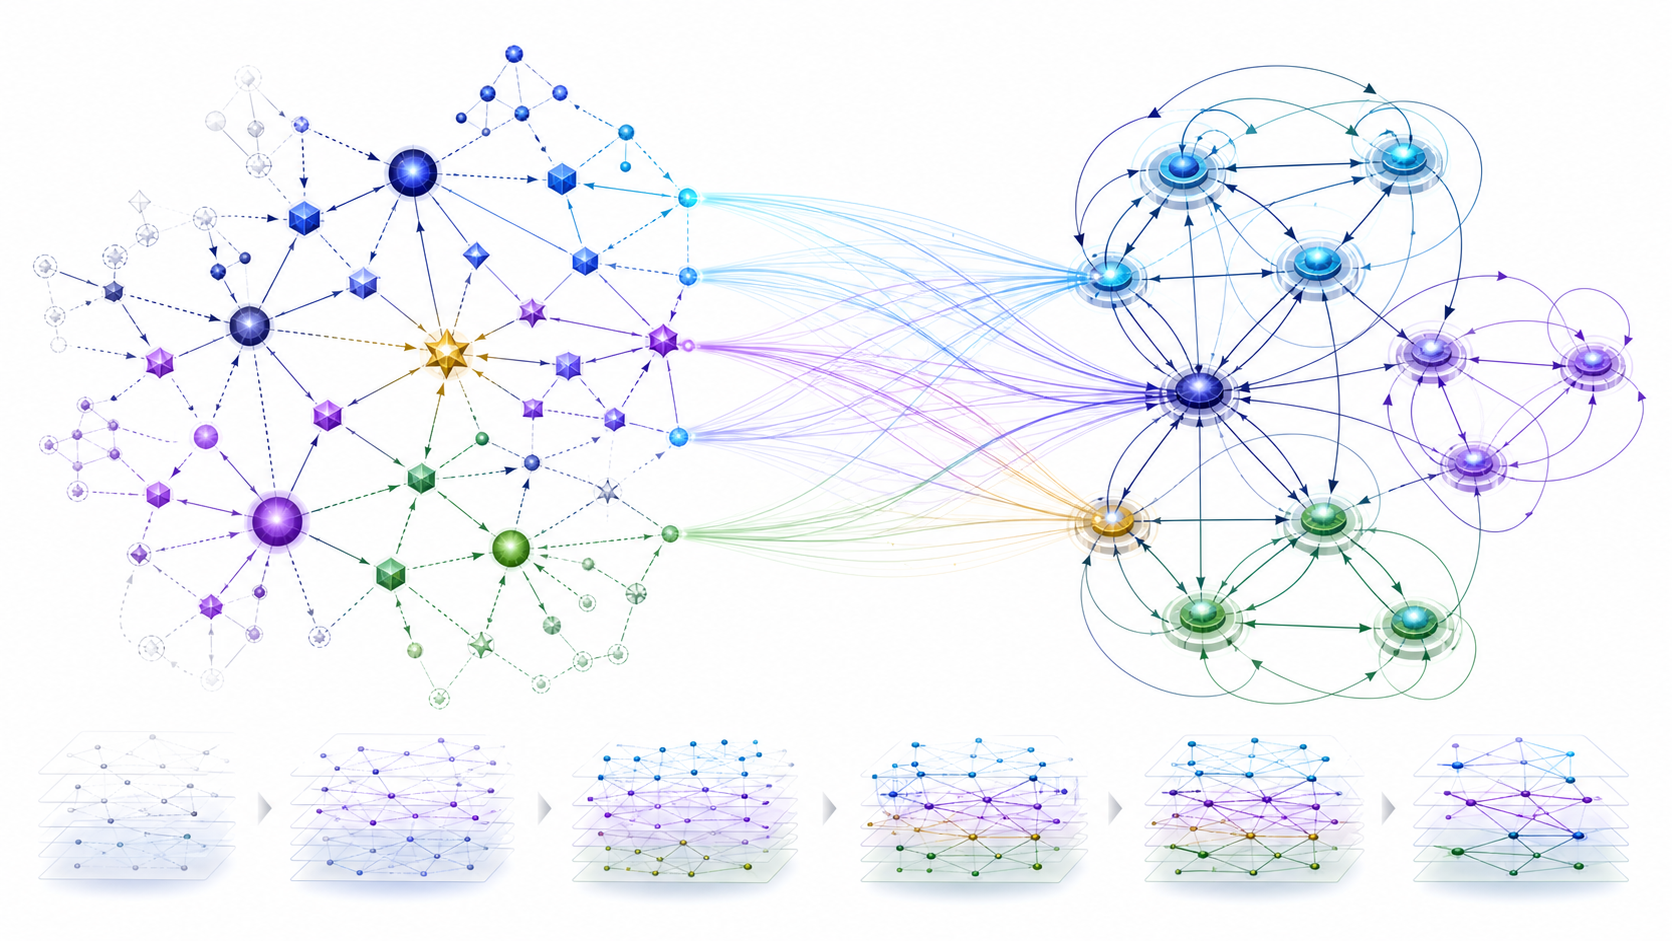
\includegraphics[width=.9\textwidth,height=.38\textheight,keepaspectratio]{images/cognitive-structure-functional-topology.png}
\caption{CSO 图、功能图与多对多承载映射}
\end{figure}
\section{为什么一张图不足以描述智能}

在构造智能理论时，一个极易出现的错误，是试图用同一张结构图同时表示“世界中的认知对象”和“处理这些对象的系统结构”。这种做法在简单系统中并不会立刻暴露问题。例如，我们可以画出“视觉模块$\rightarrow$规划模块$\rightarrow$动作模块”，并在每个模块内部附上当前处理的信息，看上去似乎已经完整描述了智能过程。然而，一旦系统进入持续学习、多尺度记忆、技能迁移、外部工具使用以及长期身份连续的场景，这种表示很快失效。

原因在于，认知内容与功能承载并不是一一绑定的。

例如，一个具体的空间关系CSO
\[
C_{\text{cup-on-table}}
\]
在刚刚被感知时，可能主要由感知整合功能承载；在进入工作记忆以后，它可能被规划、语言推理和目标评估同时调用；在经验沉降之后，它可能进入情景记忆；若该结构长期重复出现，则其中某部分甚至可能被编译进身体控制技能，使其不再需要显式进入工作记忆。换言之，同一个认知结构可以沿着不同功能和不同时间尺度发生迁移。

因此，如果我们把认知对象直接等同于功能模块内部状态，就会隐含一个错误假设：
\[
\boxed{
CognitiveStructure
\equiv
FunctionalLocation
}
\]
而长期智能恰恰要求我们否定这一等同。

更加准确的关系应当是：
\[
\boxed{
CognitiveStructure
\neq
FunctionalCarrier
}
\]
但同时：
\begin{statementbox}
\centering
\adjustbox{max width=.96\linewidth}{\(\displaystyle CognitiveStructure
\ \text{必须在某个时刻由某种功能结构实现}\)}
\end{statementbox}

这正是双图理论的起点。

我们可以用一个简单例子说明。假设智能体正在学习“打开某种陌生门锁”。最初，与门锁有关的CSO包括把手位置、旋转方向、阻力、按钮状态、视觉纹理、动作结果等。这些认知结构之间本身已经形成一张关系图：
\[
\mathcal G_C.
\]
与此同时，智能体内部存在视觉整合、空间表征、工作记忆、规划、动作控制、残差检测、经验写入等功能，它们形成另一张图：
\[
\mathcal G_F.
\]

在第一次尝试时，门锁结构可能经历：
\[
Perception
\rightarrow
h
\rightarrow
Planning
\rightarrow
MotorControl.
\]

第几十次以后，同样的结构可能变为：
\[
Perception
\rightarrow
BodySkill.
\]

外部世界中的问题没有发生本体上的根本改变，但Agent内部的承载方式已经发生重大改变。因此，真正的学习不能只表示为某个模块内部参数变化，而必须允许：
\begin{statementbox}
\centering
\adjustbox{max width=.96\linewidth}{\(\displaystyle CSO@F_i
\rightarrow
CSO@F_j\)}
\end{statementbox}

这里的“@”并不是空间位置符号，而表示“某一认知结构当前主要由某一功能结构承载、激活、转换或控制”。

双图理论因而把智能系统拆成两个不同的问题。第一类问题是：
\[
\text{What cognitive structure exists?}
\]
即认知结构之间如何形成关系、变化和组合。第二类问题是：
\[
\text{Where and how is that structure functionally carried?}
\]
即这些结构由何种功能、何种时间尺度以及何种内部或外部载体承担。

从理论方法上看，这种分离类似于计算机科学中“程序语义”与“运行实现”的区分，也类似于控制理论中“任务空间”和“状态实现空间”的区分，还可以与多层网络理论中的不同关系层进行比较。但这些外部理论只能提供形式上的帮助。本书中的根本对象仍然是CSO及其动态承载，而不是传统的数据节点或静态网络实体。

因此，本章建立的第一条原则是：
\begin{proposition*}
\bfseries 认知关系结构与实现这些关系的功能结构必须分层描述。
\end{proposition*}

只有完成这一分离，我们才能进一步讨论为什么一个智能体能够在保持“知道同一件事”的同时，逐渐改变自己“怎样知道、在哪里知道以及需要多少显式认知才能知道”。

\section{认知结构图：$\mathcal G_C$}

我们首先定义认知结构图。设一个Agent在时刻$t$能够形成或保持的有效CSO集合为
\[
V_C(t)=\{C_1,C_2,\ldots,C_{N_C(t)}\}.
\]
这里每个$C_i$并不等于一个token、一个向量或一个固定的数据库实体，而表示一个在当前理论尺度上具有独立结构意义的认知结构对象。它可以是对象、事件、关系、规则、目标、约束、因果结构、动作模式、自我状态、价值判断或未来可能性。

这些CSO之间通过不同类型的关系连接。于是我们定义：
\[
\boxed{
\mathcal G_C(t)
=
\left(
V_C(t),
E_C(t),
\Lambda_C
\right)
}
\]
其中$V_C$是CSO集合，$E_C$是关系集合，$\Lambda_C$则定义允许存在的关系类型空间。

需要强调，认知结构图通常不是一个简单无向图。对于长期智能而言，至少应允许以下几类关系：
\[
\Lambda_C
=
\{
R_{\text{semantic}},
R_{\text{causal}},
R_{\text{temporal}},
R_{\text{spatial}},
R_{\text{goal}},
R_{\text{constraint}},
R_{\text{predictive}},
R_{\text{self}},
R_{\text{value}}
\}.
\]

例如：
\[
C_A
\xrightarrow{R_{\text{causal}}}
C_B
\]
表示智能体认为$A$在某种意义上导致$B$；
而
\[
C_G
\xrightarrow{R_{\text{constraint}}}
C_P
\]
可以表示目标CSO对规划CSO施加约束。

因此$\mathcal G_C$更加接近一种有类型、有方向、有时间属性的多关系图。更加一般地，可以写成：
\[
E_C(t)
\subseteq
V_C(t)
\times
\Lambda_C
\times
V_C(t).
\]

然而，即使这一形式仍然可能不足。现实认知经常出现一个关系同时依赖多个结构的情况。例如，“如果门锁处于锁定状态并且钥匙已经插入，那么顺时针旋转可以打开门”并不是简单二元关系，而可以表示为：
\[
\{C_{\text{locked}},C_{\text{key-in}}\}
\rightarrow
C_{\text{rotate-clockwise}}
\rightarrow
C_{\text{open}}.
\]
因此，在更严格的实现中，$\mathcal G_C$更适合推广为有类型超图：
\[
\boxed{
\mathcal H_C
=
(V_C,\mathcal E_C)
}
\]
其中每一个超边可以连接多个CSO。

从动力学角度看，$\mathcal G_C$也不是静态知识库。它随时间发生至少五类变化。

第一类是CSO生成：
\[
C_{\text{new}}\notin V_C(t),
\qquad
C_{\text{new}}\in V_C(t+\Delta t).
\]

第二类是关系生成：
\[
e_{ij}:0\rightarrow1.
\]

第三类是关系权重变化：
\[
w_{ij}^C(t)
\rightarrow
w_{ij}^C(t+\Delta t).
\]

第四类是CSO合并或抽象，例如多个具体经验：
\[
C_1,C_2,\ldots,C_n
\]
经过结构化学习后，形成更高层结构：
\[
C_\Theta
=
\Phi(C_1,\ldots,C_n).
\]

第五类是遗忘、失活或降阶。一些CSO并不是完全消失，而是从当前可直接访问的图结构中退出，成为潜在结构或被压缩进更高层生成器。

因此，认知结构图的真正动力学可以写成：
\[
\boxed{
\dot{\mathcal G}_C
=
F_C
\left(
\mathcal G_C,
O_t,
A_t,
\mathcal G_F,
M_t
\right)
}
\]
其中$O_t$表示观察输入，$A_t$表示行动及其现实反馈，$\mathcal G_F$表示当前功能承载结构，$M_t$表示记忆、多尺度状态和自我约束。

这里有一个关键点：$\mathcal G_C$并不是“客观世界本身”。它是智能体内部对世界、自身和未来可能性的结构化认知，因此严格来说，进入Agent内部以后，更接近Agent-CSO图。后续如果需要区分宇宙本体CSO与Agent内部承载，我们可以进一步写：
\[
\mathcal G_U
\xrightarrow{O_A}
\mathcal G_C^A.
\]
其中$\mathcal G_U$是现实结构图，而$\mathcal G_C^A$是Agent $A$形成的认知结构图。

因此，两个不同Agent面对同一现实：
\[
\mathcal G_U
\]
可能得到：
\[
\mathcal G_C^A
\neq
\mathcal G_C^B.
\]
这并不是理论缺陷，而正是Agent特异性、经验差异与身体差异的来源。

从外部理论来看，知识图谱、语义网络、frame semantics、schema theory、causal graph以及world model都提供了与$\mathcal G_C$相关的研究工具。但本书并不把$\mathcal G_C$限制为“显式知识图谱”。其节点既可以具有符号接口，也可以由分布式潜变量实现；真正重要的是这些不同实现是否能够保持相同的主要结构关系和功能作用。

因此，本节的核心结论是：
\begin{conclusion}
\bfseries
$\mathcal G_C$描述的是智能体认知世界中的结构关系，而不是承载这些结构的处理器位置。
\end{conclusion}

它回答的是“什么结构存在、这些结构之间如何关联”。至于“谁在处理它们”，必须交给第二张图。

\section{功能拓扑图：$\mathcal G_F$}

与认知结构图不同，功能拓扑图描述的是智能系统本身的因果处理组织。设智能体拥有一组能够对Agent-CSO执行某种稳定变换的功能：
\[
V_F
=
\{
F_1,F_2,\ldots,F_{N_F}
\}.
\]
这里的$F_i$不是简单的软件模块名称，而是一个具有可区分输入、状态、输出和因果作用的功能单元。

例如，在AgentOS中，我们可以识别出：
\[
F_{\text{SPC}},
F_{\text{TCE}},
F_{\text{CCM}},
F_h,
F_E,
F_\Theta,
F_{\text{Scheduler}},
F_{\text{Boundary}},
F_{\text{Body}}
\]
等功能结构。但需要再次强调：本章的功能拓扑理论先于具体AgentOS模块。换一种实现，同样的功能关系完全可能由不同的软件、神经网络或硬件结构实现。

定义：
\[
\boxed{
\mathcal G_F(t)
=
\left(
V_F(t),
E_F(t),
\mathcal L_F(t),
W_F(t)
\right)
}
\]
其中：
\[
V_F
\]
是功能节点，
\[
E_F
\]
是功能耦合边，
\[
\mathcal L_F
\]
是闭环集合，
\[
W_F
\]
表示边的强度、时延、带宽、权限或其他运行参数。

与传统模块图相比，加入$\mathcal L_F$非常重要。因为智能并不是简单的数据流水线，而是多闭环系统。例如：
\[
F_{\text{SPC}}
\rightarrow
F_{\text{TCE}}
\rightarrow
F_h
\rightarrow
F_{\text{SPC}}
\]
就是一个认知控制闭环；而：
\[
F_h
\rightarrow
F_E
\rightarrow
F_\Theta
\rightarrow
F_h
\]
又形成记忆结构循环。

同一个功能节点可以同时属于多个闭环：
\[
F_i
\in
L_a\cap L_b\cap L_c.
\]
这也是为什么在理论上采用超图或闭环集合比传统树状模块图更合适。

每一个功能节点可以抽象成一个状态转移算子：
\[
x_i(t+\Delta t)
=
\Phi_i
\left(
x_i(t),
I_i(t),
u_i(t)
\right),
\]
其中$x_i$是节点内部状态，$I_i$是从其他功能节点或现实世界进入的输入，$u_i$是高层控制或边界约束。

如果更强调CSO的处理，可以定义：
\[
\boxed{
F_i:
\mathcal C_A
\rightarrow
\mathcal C_A
}
\]
即功能节点将一组Agent-CSO转换为另一组Agent-CSO。不过严格来说，真正的函数还取决于上下文和内部状态：
\[
F_i:
(C,x_i,\Gamma)
\mapsto
(C',x_i'),
\]
其中$\Gamma$表示当前目标、身体、资源、自我等背景约束。

因此，功能拓扑并不是“存储认知内容的地方”，而是：
\begin{statementbox}
改变、激活、抑制、迁移和稳定Agent-CSO的动力学结构。
\end{statementbox}

为了刻画功能之间的耦合，我们可为每条边$e_{ij}$定义：
\[
e_{ij}
=
(
w_{ij},
\tau_{ij},
b_{ij},
a_{ij}
),
\]
其中：
\[
w_{ij}
\]
表示作用强度，
\[
\tau_{ij}
\]
表示传递时延，
\[
b_{ij}
\]
表示有效带宽，
\[
a_{ij}
\]
表示权限或允许的信息类型。

这样，功能边就不再只是“有箭头/无箭头”，而成为具有动力学属性的结构对象。

例如，一个异常残差从BPCC向Kernel上浮的边与普通语义信息流完全不同。它可能具有更高优先级：
\[
a_{\text{residual}}>a_{\text{semantic}},
\]
更严格的时延：
\[
\tau_{\text{residual}}\ll\tau_{\text{memory}},
\]
以及更高的中断权限。

这意味着真正的功能拓扑天然是typed graph，而不是简单graph。

本书此前提出：
\[
\boxed{
Module
=
StableTopologicalCondensate
}
\]
现在可以给出更加明确的解释。一个模块并不是理论上预先存在的本体实体，而是多个功能节点与边在长期运行中形成高度内部耦合、稳定边界和相对自主闭环以后，被工程上封装成一个模块。例如SPC可能最初只是几个状态估计功能的集合，当这些功能形成稳定耦合并拥有统一接口后，我们才把它们称为“SPC模块”。

因此：
\[
Interaction
\rightarrow
RepeatedCoupling
\rightarrow
StableLoop
\rightarrow
FunctionalEncapsulation.
\]

这个观点对未来自组织AgentOS非常重要。因为如果模块不是第一性对象，那么未来系统就原则上可以根据长期CSO流重新形成新的功能凝聚体，而不是永远受限于设计者预先写死的模块边界。

外部理论中，网络科学、hypergraph、causal architecture、control network和functional connectivity都可以帮助我们数学化$\mathcal G_F$。但需要避免把“功能拓扑”直接等同于物理连接图。一个神经系统中可能有数十亿物理突触，但高层功能拓扑只保留对当前理论尺度有意义的因果功能关系。同样，一个软件Agent中两个功能可能运行在同一个Transformer内，也可能分别运行在不同进程中；只要其功能关系保持，$\mathcal G_F$就可以在同一抽象层保持不变。

因此：
\[
\boxed{
ImplementationTopology
\neq
FunctionalTopology.
}
\]

这是本章第二个基础分离原则。

\section{动态承载映射：$\mu_t:\mathcal G_C\rightarrow\mathcal G_F$}

有了认知结构图$\mathcal G_C$和功能拓扑图$\mathcal G_F$以后，我们仍然缺少真正连接二者的核心对象。这个对象就是动态承载关系$\mu_t$。

直觉上，$\mu_t$回答：
\begin{statementbox}
这个Agent-CSO此刻由什么功能结构承载、激活、转换或控制？
\end{statementbox}

最简单的写法是：
\[
\boxed{
\mu_t:
V_C
\rightarrow
V_F.
}
\]

若：
\[
\mu_t(C_i)=F_j,
\]
表示在时刻$t$，认知结构$C_i$主要由功能$F_j$承载。

然而，对于真实智能，这个定义过于简单。一个CSO经常同时由多个功能参与处理。例如一个当前目标：
\[
C_G
\]
可以同时存在于工作记忆、规划器、自我价值评估和动作调度器中。因此更准确地应写：
\[
\boxed{
\mu_t:
V_C
\rightarrow
2^{V_F}
}
\]
即：
\[
\mu_t(C_i)
=
\{F_{j_1},F_{j_2},\ldots,F_{j_k}\}.
\]

进一步，我们还需要表达不同功能对同一个CSO具有不同承载权重。因此定义承载矩阵：
\[
\boxed{
M(t)
=
[m_{ij}(t)]
}
\]
其中：
\[
m_{ij}(t)
\in[0,1]
\]
表示功能$F_j$在时刻$t$对CSO $C_i$的有效承载强度。

于是：
\[
\mu_t(C_i)
=
\left\{
(F_j,m_{ij}(t))
\right\}.
\]

在某些情况下可以要求归一化：
\[
\sum_jm_{ij}(t)=1,
\]
表示总承载权在不同功能之间分配。但这一条件并不总是必要，因为真实系统可能存在冗余复制或多重实现，此时：
\[
\sum_jm_{ij}(t)>1
\]
也是合理的。

这一形式揭示了一个重要事实：所谓“CSO迁移”不一定意味着一个对象像文件一样从A模块被删除，再被移动到B模块。更加常见的是承载权重连续变化：
\[
m_{iA}(t)\downarrow,
\qquad
m_{iB}(t)\uparrow.
\]
因此，一个技能的形成可能表现为：
\[
m_{i,h}\downarrow,
\qquad
m_{i,\Theta}\uparrow,
\qquad
m_{i,BodySkill}\uparrow.
\]

也就是说：
\begin{statementbox}
学习可以表现为承载分布在功能拓扑上的重新配置。
\end{statementbox}

这比“知识被存进长期记忆”更加一般。

进一步，我们还可以给每个承载关系加入时间尺度：
\[
m_{ij}(t,\tau).
\]
这意味着同一CSO在不同时间尺度上可以同时具有不同功能实现。例如“我会走路”这个结构在极慢尺度上属于稳定技能与身份能力的一部分，在毫秒尺度则通过身体快速控制回路实现，而只有遇到异常时才重新进入$h$显式处理。

因此更加一般的承载场为：
\[
\boxed{
\mu(C,F,\tau,t).
}
\]

这一表达与我们此前提出的结构频谱
\[
\rho_{CSO}(f,\omega,t)
\]
形成自然联系。这里$f$可以理解为功能位置，$\omega$或$\tau$表示特征时间尺度。于是：
\[
\boxed{
\rho_{CSO}(f,\omega,t)
}
\]
可以看作承载映射在功能--频率空间中的统计表示。

换言之，双图理论并不只是一种静态结构描述，它已经自然连接到智能频谱理论。

我们还需要区分至少四种不同的$\mu$变化。

第一种是激活迁移：
\[
\mu_t(C)
:
F_{\Theta}
\rightarrow
F_h.
\]
例如一个长期知识被召回到工作记忆。

第二种是沉降迁移：
\[
F_h
\rightarrow
F_E
\rightarrow
F_\Theta.
\]

第三种是程序化迁移：
\[
F_h
\rightarrow
F_{\text{BodySkill}}.
\]

第四种是边界迁移：
\[
F_{\text{Internal}}
\rightarrow
F_{\text{Tool/Environment}}.
\]

这些表面上截然不同的过程，在双图理论中都可以统一写成：
\[
\boxed{
\Delta\mu_t\neq0.
}
\]

因此，学习的一个基础数学形式可以写为：
\[
\boxed{
Learning
=
\frac{d\mu_t}{dt}
+
\frac{d\mathcal G_C}{dt}
+
\frac{d\mathcal G_F}{dt}.
}
\]

这里第一项表示承载关系改变，第二项表示认知结构本身改变，第三项表示功能拓扑改变。不同类型的学习，其三项占比不同。

对于第一代固定拓扑AgentOS：
\[
\frac{d\mathcal G_F}{dt}\approx0,
\]
于是持续学习主要来自：
\[
\frac{d\mathcal G_C}{dt}
+
\frac{d\mu_t}{dt}.
\]

而对于未来具有拓扑发育能力的Agent：
\[
\frac{d\mathcal G_F}{dt}\neq0.
\]

这实际上给出了“固定拓扑持续学习”和“发育型智能”的严格分界。

从外部理论看，这个承载映射与双部图、多层图、assignment problem、dynamic routing以及mixture-of-experts中的routing机制存在一定形式相似性。但最大的区别在于：$\mu_t$不是一次计算中的token routing，而描述的是整个Agent生命周期中认知结构与功能实现之间的多尺度关系。它可以持续数毫秒，也可以持续数年。

因此，本节应当把$\mu_t$理解成双图理论的真正“铰链”：

\[
\boxed{
\mathcal G_C
\overset{\mu_t}{\longleftrightarrow}
\mathcal G_F.
}
\]

认知结构并不是悬空存在的，功能系统也不是空转的。智能产生于二者持续耦合之中。

\section{同一CSO为何能够同时存在于多个功能闭环}

理解双图理论的一个重要难点，是摆脱“一个知识只能属于一个模块”的直觉。传统软件系统倾向于通过所有权明确的数据结构来管理状态，例如一个对象属于某个进程、一块内存由某个模块持有。但智能系统具有不同性质。一个Agent-CSO经常需要同时参与多个时间尺度和多个功能闭环。

假设Agent当前存在目标：
\[
C_G=\text{“把房屋建成可居住状态”}.
\]
这个目标在工作记忆中可能以当前任务约束形式存在：
\[
C_G@F_h.
\]
同时，它也会影响Scheduler：
\[
C_G@F_{\text{Scheduler}},
\]
影响TCE的资源控制：
\[
C_G@F_{\text{TCE}},
\]
影响长期结构$\Theta$中的技能选择：
\[
C_G@F_\Theta,
\]
甚至受到$\Psi$和$\Omega$的慢尺度约束：
\[
C_G@F_\Psi,
\qquad
C_G@F_\Omega.
\]

因此：
\[
\mu_t(C_G)
=
\{
F_h,
F_{\text{Scheduler}},
F_{\text{TCE}},
F_\Theta,
F_\Psi,
F_\Omega
\}.
\]

但这些“存在”不是同一种存在。为了避免概念模糊，我们可以进一步给承载关系定义角色：
\[
r_{ij}
\in
\{
\text{active},
\text{constraint},
\text{generative},
\text{monitoring},
\text{procedural},
\text{historical}
\}.
\]

于是：
\[
\mu_t(C_i)
=
\left\{
(F_j,m_{ij},r_{ij})
\right\}.
\]

例如：
\[
(C_G,F_h,1,\text{active})
\]
表示目标正在工作记忆中显式激活；
而：
\[
(C_G,F_\Psi,0.2,\text{constraint})
\]
则表示自我结构仅以慢偏置方式约束该目标，而不是显式处理目标细节。

这种区分对于理解我们此前提出的：
\[
\boxed{
SlowGovernance\neq FastMicromanagement
}
\]
至关重要。

慢层结构并不需要复制快层所有信息，也不需要逐步计算每个动作。它只需要通过改变可行域、优先级、增益、准入条件等方式影响快层动力学。因此，一个CSO可以跨层存在，却在每一层承担不同功能。

同样的结构也解释了“自我$\Psi$为什么不需要不断进入h”。如果自我必须以完整显式文本形式持续占用工作记忆，那么它反而会耗尽有限认知容量。真正成熟的Self应当大量以慢约束形式存在：
\[
m_{\Psi,h}\ll1,
\]
但它对Goal选择和经验解释的累计影响可以很大：
\[
\frac{\partial G}{\partial\Psi}\neq0,
\qquad
\frac{\partial E_{\text{write}}}{\partial\Psi}\neq0.
\]

这就是“背景引力”的数学意义：它不一定大量占用显式状态，却可以持续改变状态转移概率。

同一CSO跨多个功能存在还提供了鲁棒性。若一个结构只存在于单一功能：
\[
|\mu_t(C)|=1,
\]
那么该功能失效可能导致结构完全不可访问。而当结构在长期记忆、工作状态、外部工具或多个技能中存在不同程度的冗余承载时，系统具有：
\[
FunctionalRedundancy.
\]

但冗余并非越多越好。如果一个CSO同时占据过多功能：
\[
|\mu_t(C)|\gg1,
\]
可能产生同步开销、重复加工和认知干扰。因此智能体必须在“冗余鲁棒性”和“承载成本”之间寻找平衡。

可以定义一个简单代价：
\[
\mathcal J_C
=
\alpha
\sum_jm_{ij}
+
\beta
SyncCost(C_i)
-
\gamma
Robustness(C_i).
\]

Agent的长期结构优化，就是寻找一个满足能力与稳定性的有效承载分布：
\[
\mu_t^*
=
\arg\min_{\mu}
\mathcal J_C.
\]

这里我们开始看见后续CCM、Scheduler和Offloading理论的更深来源。CCM并不只是“减少信息量”，而是在有限功能资源下控制$\mu_t$的活动范围；Scheduler决定哪些承载关系当前获得计算资源；Offloading则允许一个CSO的主要载体越过Agent内部边界。

因此，跨功能承载并不是偶然特性，而是多尺度智能成立的必要条件。

\section{一个功能节点为什么必须能够处理多个CSO}

与上一节相反，我们还必须考虑另一方向：一个功能节点通常不能只服务一个CSO。若每出现一个新的认知对象，系统就创建一个专用功能模块，那么整个系统很快会发生结构爆炸。

设功能节点$F_j$当前承载的CSO集合为：
\[
\mathcal C_j(t)
=
\{
C_i
\mid
m_{ij}(t)>0
\}.
\]
则：
\[
F_j
\]
实际上是一个作用于CSO子集的结构转换器：
\[
F_j:
\mathcal C_j
\times
X_j
\rightarrow
\mathcal C'_j
\times
X'_j.
\]

例如工作记忆$h$不是“某一个目标的存储位置”，而可能同时包含：
\[
C_{\text{goal}},
C_{\text{constraint}},
C_{\text{object}},
C_{\text{plan}},
C_{\text{risk}},
C_{\text{self-state}}.
\]
问题在于，它能够同时稳定维持的结构关系数量有限。这直接连接到后文的工作记忆有限容量定理。

因此，对每个功能节点，我们可以定义一个瞬时结构负载：
\[
L_j(t)
=
\sum_i
m_{ij}(t)c_i(t),
\]
其中$c_i(t)$表示CSO $C_i$在当前上下文中的有效结构负载。

每一个功能节点具有最大稳定处理能力：
\[
L_j(t)
\leq
K_j.
\]

对于$h$：
\[
K_h
\]
尤其有限，因此：
\[
L_h(t)>K_h
\]
就可能导致认知相干性下降。

这说明双图理论天然能够导出认知资源管理理论。所谓“工作记忆过载”，从双图观点看就是：
\[
\boxed{
\sum_i m_{i,h}c_i
>
K_h.
}
\]

CCM的任务则可以重新写成调节：
\[
m_{i,h}(t)
\]
使：
\[
\sum_i m_{i,h}(t)c_i(t)
\le K_h.
\]

它可以通过降低某些CSO的显式承载权重：
\[
m_{i,h}\downarrow,
\]
将它们迁移到E、$\Theta$、Tool或External Memory：
\[
m_{i,E}\uparrow,
\quad
m_{i,\Theta}\uparrow,
\quad
m_{i,\text{Tool}}\uparrow.
\]

因此，认知卸载在双图理论中获得了非常直接的数学解释。

同一个功能处理多个CSO还意味着功能节点必须具有某种结构泛化能力。一个规划功能不应该只能规划“建房”，而必须能够对一个更一般的目标--约束--动作结构进行变换。换言之，功能本身应当对某类CSO保持形式不变性。

可以写成：
\[
F_j
\left(
\phi(C)
\right)
\approx
\phi
\left(
F_j(C)
\right),
\]
其中$\phi$表示在同一语义类内部的结构映射。

如果该关系在某个CSO类别上近似成立，我们就可以说$F_j$对该类认知结构具有功能泛化能力。

这与前文“语义类规约”形成直接联系。一个功能如果只能处理极窄的具体表征，就很难跨身体、跨任务或跨实现迁移；一个真正通用的AgentOS功能节点，应尽量面向：
\[
SemanticClass
\]
而不是某个具体输入编码。

与此同时，功能节点也不应无限通用。一个功能如果承担所有CSO类型：
\[
|\mathcal C_j|\rightarrow\infty,
\]
就会退化为一个巨大的中央万能模块，这正是当前很多大模型Agent容易出现的结构：几乎所有问题重新回到中央LLM推理。

成熟智能的方向恰好相反。它希望保持少量真正需要全局整合的结构进入中央显式功能，而将大量稳定关系沉降到局部闭环。

因此：
\[
\boxed{
MatureIntelligence
=
SelectiveCentralization
+
DistributedFunctionalClosure.
}
\]

这里再次体现双图理论的意义：我们不通过“模块数量”判断智能成熟度，而观察$\mathcal G_C$在$\mathcal G_F$上的承载分布。如果绝大多数熟练CSO仍然集中于单一中央功能，则系统虽然可能表现强大，却仍然具有高中央认知成本。

因此可以定义功能集中度：
\[
H_F(t)
=
-\sum_j
p_j(t)\log p_j(t),
\]
其中：
\[
p_j
=
\frac{
\sum_i m_{ij}c_i
}{
\sum_{k,i}m_{ik}c_i
}.
\]

若少数功能承担绝大多数结构，则分布具有高集中性；若稳定CSO被合理分散到局部功能闭环，则结构更加分布化。

这又把本章与前面“智能相：集中度--拓扑改变度”的认识论连接起来。于是智能相不再只是哲学分类，而可以逐步落到可测量的双图统计量上。

\section{拓扑之上的动力学：Dynamics on Topology}

到目前为止，我们暂时假定功能拓扑$\mathcal G_F$在短时间尺度上固定。在这个条件下，智能仍然可以产生极其丰富的动力学，因为CSO本身以及它们在功能图上的承载关系持续变化。这类过程称为：
\[
\boxed{
Dynamics\ On\ Topology.
}
\]

形式上，在：
\[
\dot{\mathcal G}_F\approx0
\]
条件下：
\[
\dot{\mathcal G}_C\neq0,
\qquad
\dot\mu_t\neq0.
\]

这正是第一代AgentOS持续学习的理论基础。

我们可以定义Agent整体短中期状态：
\[
\mathfrak X(t)
=
\left(
\mathcal G_C(t),
\mu_t,
X_F(t)
\right),
\]
其中$X_F$表示各功能节点内部状态。

其动力学为：
\[
\dot{\mathfrak X}
=
\mathcal F
\left(
\mathfrak X,
O_t,
A_t,
G_t,
\Psi_t
\mid
\mathcal G_F
\right).
\]

这里$\mathcal G_F$作为相对固定的结构参数存在。

这一形式可以统一解释大量我们此前分别讨论的机制。

例如，召回可以写成：
\[
\mu(C):
F_\Theta
\rightarrow
F_h.
\]

经验写入：
\[
F_h
\rightarrow
F_E.
\]

结构学习：
\[
F_E
\rightarrow
F_\Theta.
\]

技能沉降：
\[
F_h/F_\Theta
\rightarrow
F_{\text{BodySkill}}.
\]

外部化：
\[
F_{\text{Internal}}
\rightarrow
F_{\text{Tool}}.
\]

异常重新显式化：
\[
F_{\text{BodySkill}}
\rightarrow
F_h.
\]

这些过程看似属于记忆、技能、身体和工具四个不同研究领域，但在双图理论下，它们具有完全一致的结构形式：
\[
\boxed{
\Delta\mu_t.
}
\]

因此，第一代AgentOS即使不改变功能拓扑，也能够具有相当丰富的持续学习能力。

这一点非常重要，因为它把“持续学习”和“自修改架构”区分开来。一个系统不需要一开始就拥有：
\[
\dot{\mathcal G}_F\neq0
\]
才算能够成长。大量学习实际上可以发生在：
\[
\mathcal G_C
\]
和：
\[
\mu_t
\]
层面。

这也是我们此前选择“先构造固定拓扑AgentOS”的理论理由。

在这种框架下，可以进一步定义认知结构流。对于功能边：
\[
e_{ij}\in E_F,
\]
定义CSO流：
\[
J^{C}_{ij}(t).
\]
它表示单位时间内从$F_i$向$F_j$发生的有效CSO迁移强度。

若考虑不同CSO：
\[
J^{C_k}_{ij}(t)
\]
表示特定结构$C_k$沿功能边$i\rightarrow j$的迁移。

于是：
\[
J^{C}_{ij}
=
\sum_k
w_kJ^{C_k}_{ij}.
\]

我们可以建立类似连续性方程的结构平衡：
\[
\frac{\partial\rho_C}{\partial t}
+
\nabla_F\cdot J_C
=
S_C-D_C,
\]
其中$\rho_C$表示功能空间上的活动CSO分布，$S_C$表示新结构生成，$D_C$表示遗忘、压缩或合并。

需要强调，这里借用连续介质方程只是数学类比。CSO并不是物质流体，$J_C$也不是物理粒子通量。这一形式的意义仅在于帮助我们描述结构如何在功能拓扑中生成、迁移、积累与消散。

从控制角度看，CCM、Scheduler、SPC和TCE都可以作用于$J_C$。

Scheduler主要决定：
\[
WhereToRoute.
\]

CCM决定：
\[
HowMuchStructureCanRemainActive.
\]

SPC估计：
\[
CurrentDistributionAndStability.
\]

TCE调节：
\[
Gain,\ Temperature,\ Exploration,\ Depth.
\]

因此AgentOS运行时可以写成对：
\[
\rho_C
\]
和：
\[
J_C
\]
的闭环控制。

这一描述使我们第一次能够把“认知资源管理”从操作系统类比提升为真正的动力学问题。

如果未来能够定义可观测的$\rho_C$和$J_C$代理量，那么AgentOS将能够实时回答：

哪些CSO正在中央堆积；

哪些功能边发生持续高频往返；

哪些稳定结构仍然没有沉降；

哪些本应局部解决的问题不断重新进入h；

哪些外部化结构反而造成过高恢复成本。

这将成为真正“智能运行时监控”的基础。

\section{拓扑自身的动力学：Dynamics of Topology}

当系统长期运行以后，仅靠在固定$\mathcal G_F$上重新分配CSO可能逐渐变得低效。某些功能之间可能持续发生高成本往返，某些新型CSO可能长期缺少合适承载结构，某些旧功能连接可能几乎不再使用。此时，学习问题发生性质变化：系统需要的不再只是改变“哪些结构在哪里运行”，而是改变“有哪些地方可供这些结构运行”。

这就是：
\[
\boxed{
Dynamics\ Of\ Topology.
}
\]

形式上：
\[
\boxed{
\dot{\mathcal G}_F\neq0.
}
\]

最基础的机制来自长期CSO流的沉降。假设：
\[
J^{C}_{ij}(t)
\]
在很长时间窗口$T$内持续为正，而且该迁移带来稳定收益：
\[
\left\langle
J^{C}_{ij}
\right\rangle_T
\gg0.
\]
若$i$和$j$之间原本没有直接高效连接，系统可能形成：
\[
A_{ij}:0\rightarrow1.
\]

于是重复动态协调逐渐变成静态结构。

可以形式化为：
\[
\tau_T
\dot A_{ij}
=
G_{ij}
\left(
\langle J^C_{ij}\rangle_T,
\langle\varepsilon_{ij}\rangle_T,
U_{ij},
C_{ij},
R_{ij}
\right),
\]
其中：
\[
\tau_T
\]
是拓扑学习时间尺度，
\[
U_{ij}
\]
表示长期效用，
\[
C_{ij}
\]
表示连接成本，
\[
R_{ij}
\]
表示结构风险。

通常应满足：
\[
\tau_T
\gg
\tau_{\mu}
\gg
\tau_{\text{state}}.
\]

也就是说：
\begin{statementbox}
状态变化最快，承载迁移其次，拓扑变化最慢。
\end{statementbox}

否则短期噪声就可能导致整个功能结构频繁重写。

这与此前提出的：
\begin{statementbox}
SlowVariableProtection
\end{statementbox}
完全一致。

进一步，为防止边频繁建立和删除，可以引入迟滞：
\[
\theta_{\text{on}}
>
\theta_{\text{off}}.
\]
建立一条新功能边需要：
\[
Evidence>\theta_{\text{on}},
\]
而删除已有稳定边只在长期价值下降到：
\[
Evidence<\theta_{\text{off}}
\]
时发生。

这形成：
\begin{statementbox}
TopologicalHysteresis.
\end{statementbox}

如果一条稳定功能连接长期形成，它就成为一种：
\begin{statementbox}
TopologicalCapital.
\end{statementbox}
因为未来同类CSO不再需要重复进行高成本全局协调。

可以定义长期总代价：
\[
\mathcal J
=
\int
\left[
L_{\text{task}}
+
\lambda_RL_{\text{residual}}
+
\lambda_J\|J_C\|^2
+
\lambda_TCost(\dot{\mathcal G}_F)
\right]dt.
\]

这里：
\[
L_{\text{task}}
\]
是任务损失，
\[
L_{\text{residual}}
\]
是未解决残差，
\[
\|J_C\|^2
\]
可以近似反映动态协调成本，
而：
\[
Cost(\dot{\mathcal G}_F)
\]
表示改变功能拓扑本身的代价和风险。

于是智能系统的长期发展并不是无条件减少动态流，而是在：
\[
\text{运行成本}
\]
和：
\[
\text{结构修改成本}
\]
之间寻找平衡。

这就解释了为什么成熟系统不会把每一种短期行为都编译成永久模块，也不会永远让一切重新进入中央推理。

可以进一步提出：
\begin{statementbox}
MinimumNecessaryReorganizationPrinciple.
\end{statementbox}

即当出现问题时，优先尝试：
\[
StateAdjustment
\]
然后：
\[
RepresentationAdaptation
\]
再：
\[
TimescaleMigration
\]
再：
\[
FunctionalMigration
\]
最后才进入：
\[
TopologicalReorganization.
\]

只有当较浅层机制长期无法解决结构失配时，才允许修改慢拓扑。

于是，我们可以定义结构失配压力：
\[
P_T
=
F
\left(
PersistentResidual,
RepeatedMigration,
CoordinationCost,
Latency,
Instability
\right).
\]

当：
\[
P_T<\theta_T,
\]
系统继续使用既有拓扑。

只有：
\[
P_T>\theta_T
\]
并持续超过一定时间：
\[
T>T_{\min},
\]
才启动拓扑搜索。

这使“自修改架构”从一个危险而模糊的概念，变成一个可以被慢变量、阈值、迟滞和现实验证约束的动力学过程。

从外部理论看，这一部分与adaptive network、structural plasticity、graph rewiring、neural architecture adaptation以及组织结构演化有明显形式相似性。但本书强调的不同之处在于：拓扑变化的驱动力不是离线benchmark，也不是任意结构搜索，而是整个Agent生命周期中的：
\begin{statementbox}
PersistentCSOFlow.
\end{statementbox}

因此我们得到本书后续发育理论最重要的命题之一：
\begin{proposition*}
\bfseries
功能拓扑是长期认知结构流的慢速历史沉积。
\end{proposition*}

\section{双图共同演化：智能生命周期的统一状态描述}

当我们把$\mathcal G_C$、$\mathcal G_F$和$\mu_t$同时考虑以后，就可以给出一个比传统“模型参数+上下文”更加完整的智能体状态描述。

定义：
\[
\boxed{
\mathfrak I(t)
=
\left[
\mathcal G_C(t),
\mathcal G_F(t),
\mu_t,
X(t),
B(t)
\right]
}
\]
其中：
\[
\mathcal G_C(t)
\]
是当前认知结构图，
\[
\mathcal G_F(t)
\]
是功能拓扑，
\[
\mu_t
\]
是承载映射，
\[
X(t)
\]
表示功能节点内部的连续状态，
\[
B(t)
\]
表示Agent与外部世界之间的边界与载体条件。

这一状态比单纯：
\[
\theta_{\text{model}}
\]
丰富得多。

一个长期Agent即使基础模型参数完全不变：
\[
\dot\theta_{\text{LLM}}=0,
\]
仍然可能因为：
\[
\dot{\mathcal G}_C\neq0,
\qquad
\dot\mu_t\neq0
\]
而持续成长。

这正是AgentOS第一代固定拓扑持续学习理论。

当未来进一步允许：
\[
\dot{\mathcal G}_F\neq0,
\]
系统则从持续学习进入：
\begin{statementbox}
DevelopmentalIntelligence.
\end{statementbox}

因此我们可以把智能成长分为三个层级。

第一层是状态学习：
\[
\Delta X\neq0.
\]

第二层是结构--承载学习：
\[
\Delta\mathcal G_C\neq0
\quad\text{or}\quad
\Delta\mu\neq0.
\]

第三层是拓扑发育：
\[
\Delta\mathcal G_F\neq0.
\]

这三个层级分别对应越来越深的系统改变。

对于短时任务，通常只需要第一层。

对于持续Agent，第二层成为核心。

对于真正生命周期智能，第三层最终不可避免。

因此：
\[
\boxed{
Learning
\subset
Development.
}
\]

但Development不应理解为单向“越来越复杂”。一个成熟系统可能通过拓扑重构反而变得更加简单。例如多个长期重复功能：
\[
F_a,F_b,F_c
\]
可能被压缩为：
\[
F_d.
\]
因此：
\[
N_F\downarrow
\]
并不意味着能力下降。相反，它可能表示：
\[
CoordinationCost\downarrow,
\qquad
LocalClosure\uparrow.
\]

同样，多个CSO也可能被抽象成更高层结构：
\[
C_1,\ldots,C_n
\rightarrow
C^\ast.
\]
于是：
\[
|V_C|\downarrow
\]
但结构生成能力增加。

因此成熟智能不应以节点数量衡量，而应考察：
\begin{statementbox}
\centering
\adjustbox{max width=.96\linewidth}{\(\displaystyle \text{结构表达能力}
+
\text{功能闭合能力}
+
\text{现实适应能力}.\)}
\end{statementbox}

这一点也帮助我们修正早期“复杂度不断增长”的直觉。真正成长的智能并不是内部复杂度无限上升，而是结构在不同尺度之间不断重编码，使大量原本需要动态协调的内容逐渐沉降成稳定关系。

因此可以写：
\begin{statementbox}
\centering
\adjustbox{max width=.96\linewidth}{\(\displaystyle PastDynamicCoordination
\rightarrow
PresentStableStructure
\rightarrow
ReducedFutureCoordinationCost.\)}
\end{statementbox}

这就是“历史变成结构”的数学本质。

把双图放入现实闭环之后，完整系统进一步成为：
\[
\mathcal G_U
\xrightarrow{O_t}
\mathcal G_C
\xrightarrow{\mu_t}
\mathcal G_F
\xrightarrow{Act_t}
\mathcal G_U'.
\]

然后：
\[
\mathcal G_U'
\xrightarrow{O_{t+1}}
\mathcal G_C'.
\]

所以Agent生命周期最终表现为：
\begin{statementbox}
\centering
\adjustbox{max width=.96\linewidth}{\(\displaystyle WorldStructure
\rightarrow
CognitiveStructure
\rightarrow
FunctionalRealization
\rightarrow
Action
\rightarrow
NewWorldStructure.\)}
\end{statementbox}

这把本章与前面的World--Agent--World认识论重新闭合。

因此，更完整的动力学方程可以概念性写成：
\[
\begin{aligned}
\dot{\mathcal G}_U
&=
F_U
(
\mathcal G_U,
Act(\mathcal G_F)
),\\
\dot{\mathcal G}_C
&=
F_C
(
\mathcal G_C,
O(\mathcal G_U),
\mu_t
),\\
\dot{\mu}
&=
F_\mu
(
\mathcal G_C,
\mathcal G_F,
Residual,
Utility,
Cost
),\\
\tau_F\dot{\mathcal G}_F
&=
F_F
(
\langle J_C\rangle_T,
Residual,
Utility,
Risk
).
\end{aligned}
\]

其中应满足：
\[
\tau_F
\gg
\tau_\mu
\gg
\tau_X.
\]

这组方程目前仍然是一种理论母模型，而不是已经完成全部可计算定义的最终方程。未来研究需要继续定义具体的CSO测量方法、承载强度、结构流以及拓扑修改效用。但它已经提供了一个统一坐标，使此前分散的：

记忆学习、技能形成、工作记忆调度、工具使用、身体自动化、结构学习以及拓扑发育

都能够在同一个数学框架内被讨论。

\section{理论边界、外部理论依赖与本章结论}

双图理论的价值，在于它提供了一种介于纯认知哲学与具体软件模块之间的中尺度描述。它既不要求我们直接从神经元或Transformer参数出发，也不满足于把智能写成若干模块方框，而是把研究对象放在两个真正具有持续性意义的结构上：
\[
\boxed{
\mathcal G_C
}
\]
和：
\[
\boxed{
\mathcal G_F.
}
\]

这一理论与若干已有研究领域存在重要联系。

首先是知识图谱与语义网络。它们为$\mathcal G_C$中对象、关系与类型提供了成熟表达工具。然而，知识图谱通常强调显式知识存储，而本书的CSO图还包含活动目标、身体状态、自我结构、预测结构、潜在结构以及分布式表示。因此：
\[
\mathcal G_C
\neq
TraditionalKnowledgeGraph.
\]

其次是图论与多层网络。双图结构天然可以用双部图、多层网络或multiplex network表达。例如可以构造一个联合图：
\[
\mathcal G^\ast
=
\mathcal G_C
\cup
\mathcal G_F
\cup
E_\mu,
\]
其中：
\[
E_\mu
=
\{
(C_i,F_j,m_{ij})
\}.
\]
这使复杂网络理论中的中心性、社团结构、流量和鲁棒性指标可以成为未来分析工具。

第三是hypergraph。由于一个CSO关系常同时涉及多个对象，而一个功能闭环也可能连接多个功能节点，因此超图比简单图更接近真实智能组织。

第四是控制理论。功能拓扑中的很多边并不是信息“传递”，而是控制、约束、反馈和调制。例如$\Psi$对Goal的影响与BPCC对Actuator的影响在因果类型上并不相同。因此未来$\mathcal G_F$应进一步发展成typed causal control graph。

第五是动态网络与adaptive graph。本章关于：
\[
\dot{\mathcal G}_F\neq0
\]
的讨论可借鉴网络重连、结构可塑性和时间变化图理论。但本书提出的核心驱动力：
\[
PersistentCSOFlow
\]
仍然需要单独发展。

第六是操作系统。传统OS把Process与Resource分开，而双图理论在更高层把Cognitive Structure与Functional Carrier分开。这也是为什么AgentOS最终可以被理解成一种认知资源运行时。不过这种类比存在明确边界：CSO并不是普通文件，功能承载也不是单纯CPU调度；它们还具有语义、时间、自我、价值和生命周期属性。

因此，本章必须保持三个层次的认识论边界：
\[
\boxed{
EstablishedTheory
\neq
FormalAnalogy
\neq
AgentOSHypothesis.
}
\]

图论、多层网络、动态系统与控制理论属于已有数学工具；

使用这些工具表达CSO与功能承载属于形式化建模；

而“长期CSO流将沉降为功能拓扑”则是本书提出、未来需要工程和实验验证的核心假说。

在这一边界之内，我们现在可以给双图理论一个正式定义：

\begin{definition*}
\bfseries
双图理论认为，一个智能体应同时由认知结构图$\mathcal G_C$与功能拓扑图$\mathcal G_F$描述：前者表示智能体所承载的对象、关系、目标、约束、自我与可能性结构，后者表示这些结构被感知、变换、记忆、调节、执行与外化时所依赖的功能组织。二者通过动态承载映射$\mu_t$耦合，并在不同时间尺度上发生共同演化。
\end{definition*}

由此，智能活动可以进一步写成：
\[
\boxed{
IntelligentActivity
=
Generation
+
Transformation
+
Coupling
+
Migration
+
Stabilization.
}
\]

学习可以写成：
\[
\boxed{
Learning
=
\Delta\mathcal G_C
+
\Delta\mu.
}
\]

而发育则进一步包括：
\[
\boxed{
Development
=
\Delta\mathcal G_C
+
\Delta\mu
+
\Delta\mathcal G_F.
}
\]

于是固定拓扑AgentOS与未来发育型AgentOS之间的关系也变得十分清楚：

\begin{statementbox}
\centering
\adjustbox{max width=.96\linewidth}{\(\displaystyle \begin{array}{c}
\text{第一阶段：}\\
\dot{\mathcal G}_F\approx0,\quad
\dot{\mathcal G}_C\neq0,\quad
\dot\mu\neq0
\end{array}\)}
\end{statementbox}

系统首先学习如何在既有功能结构中重新组织自己的认知。

随后：

\begin{statementbox}
\centering
\adjustbox{max width=.96\linewidth}{\(\displaystyle \begin{array}{c}
\text{第二阶段：}\\
\dot{\mathcal G}_F\neq0
\end{array}\)}
\end{statementbox}

系统开始根据长期经验改变承载认知的功能结构本身。

因此，本章最终得到一条将贯穿后续所有章节的核心关系：

\begin{conclusion}
\bfseries
CSO流塑造功能拓扑，功能拓扑又塑造未来CSO流。
\end{conclusion}

即：
\begin{statementbox}
\centering
\adjustbox{max width=.96\linewidth}{\(\displaystyle CSOFlow
\rightarrow
FunctionalMigration
\rightarrow
StableCoupling
\rightarrow
Topology
\rightarrow
FutureCSOFlow.\)}
\end{statementbox}

这意味着，一个真正具有生命周期的智能体并不是在一套固定管道中不断加入更多知识。它首先在既有拓扑上学习如何重新承载认知结构；当这种重新承载长期重复、稳定且具有明确收益时，历史动态过程进一步沉降成新的功能关系。此后，过去需要反复进行的动态协调成为系统的一部分结构，并反过来改变未来每一次认知的成本、路径和可能性。

也正是在这个意义上，我们才能理解本书后面将反复使用的一句话：

\begin{conclusion}
\bfseries
成熟智能会把自己的历史变成结构。
\end{conclusion}

而双图理论，就是描述这一过程所需要的最小结构语言。

\chapter{CSO流塑造拓扑：认知结构迁移的长期结构沉降}

\begin{chapteroverviewbox}
在前两章中，我们已经分别建立了智能系统的两个基本结构对象：一方面，认知内容及其关系构成认知结构图 $\mathcal{G}_{C}$；另一方面，承担感知、推理、控制、记忆、规划、行动等作用的功能关系构成功能拓扑 $\mathcal{G}_{F}$。二者通过随时间变化的承载映射 $\mu_t$ 联系起来。由此，一个尚未回答的根本问题自然出现：\textbf{功能拓扑为什么会形成现在的样子？为什么某些功能之间存在稳定直接连接，而另一些认知过程必须经过漫长、昂贵的中间协调？}

本章给出的回答是：\textbf{功能拓扑不是与认知活动相互独立的静态容器，而是长期认知结构流动历史的结构沉降。}当某类 Agent-CSO 长期、稳定、重复地在特定功能之间迁移，并且这种迁移具有持续任务价值时，系统具有把原本需要临时协调的动态关系固化为稳定功能耦合的动力学理由。因此：
\[
\boxed{
RepeatedCSOMigration
\longrightarrow
StableFunctionalCoupling
\longrightarrow
FunctionalTopology
}
\]
这一过程称为\textbf{拓扑沉降（Topological Sedimentation）}。

需要特别强调，本章并不把``复杂度''视为一种能够像能量一样流动的本体。早期讨论中的``复杂度迁移''在这里被重新解释为：具有具体语义与功能关系的 Agent-CSO 改变自身的表示方式、时间尺度、功能位置和承载位置，而其中长期稳定的功能迁移会进一步改变承载这些结构的功能拓扑。因此，拓扑学习并不是与 CSO 迁移平行的第五种迁移，而是\textbf{长期功能迁移在更慢时间尺度上的结构性积分结果}。

本章只讨论``CSO流如何塑造拓扑''，至于什么时候已有拓扑已经无法有效承载新的 CSO 流、什么时候应该真正触发拓扑重构，以及如何防止拓扑因短时噪声而频繁改变，将在下一章的``智能结构相变与发育''中进一步处理。
\end{chapteroverviewbox}

\begin{figure}[htbp]
\centering
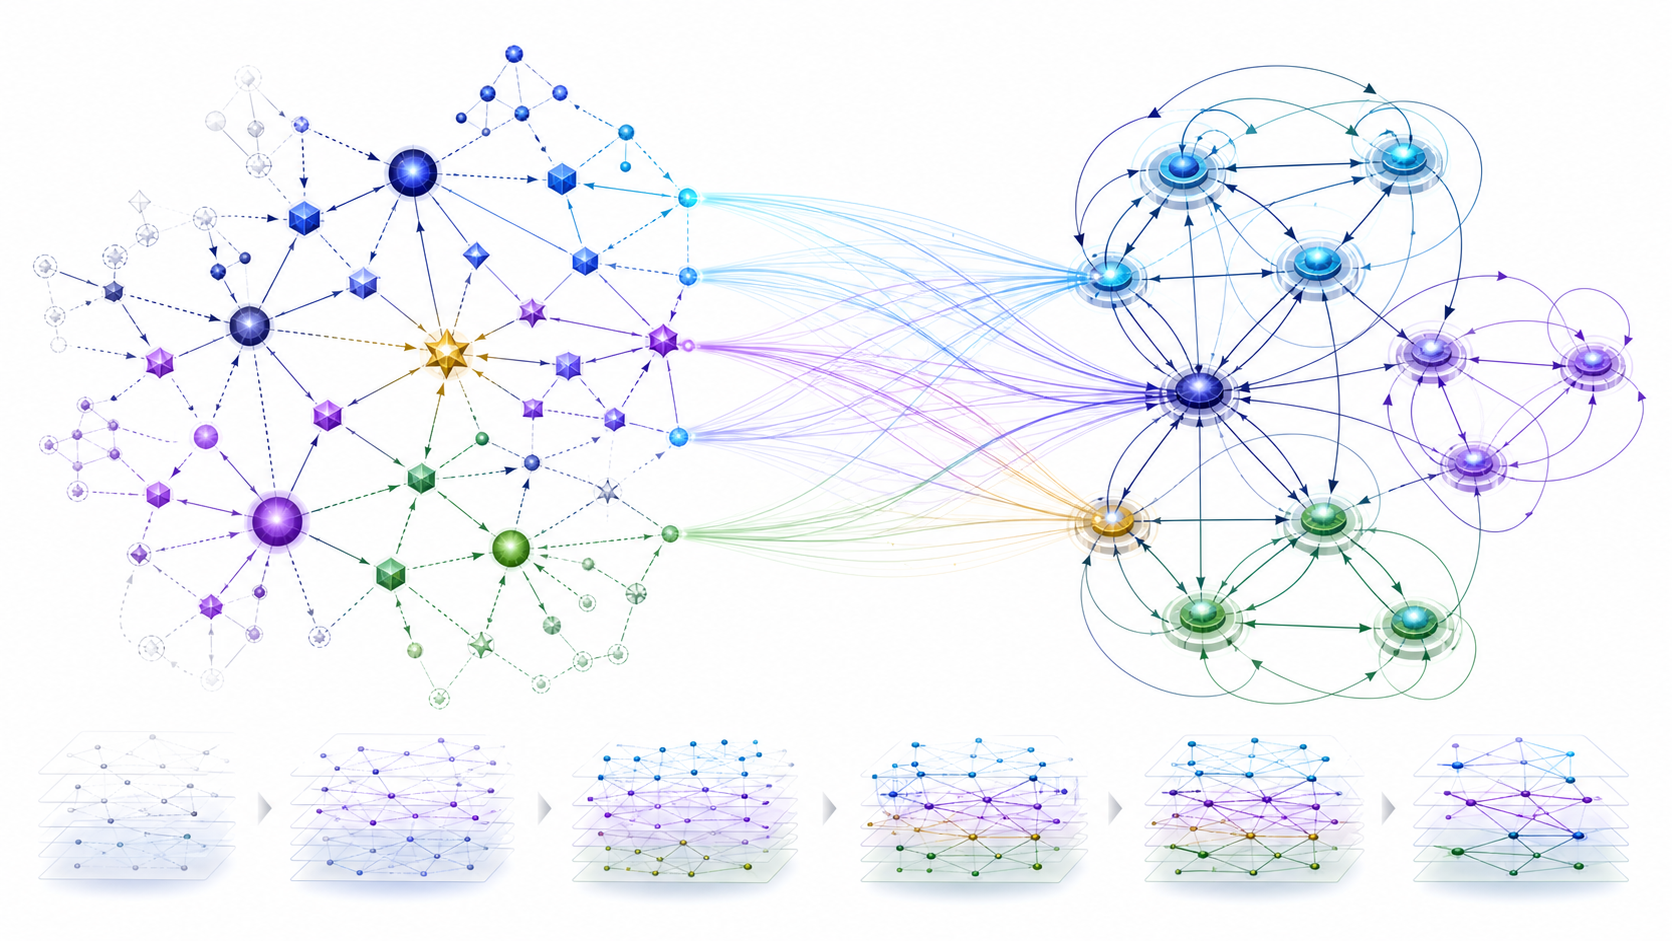
\includegraphics[width=.9\textwidth,height=.38\textheight,keepaspectratio]{images/cognitive-structure-functional-topology.png}
\caption{长期 CSO 流对功能拓扑的沉降作用}
\end{figure}
\section{从动态认知过程到稳定功能结构}

当我们观察一个刚刚接触陌生任务的智能体时，会发现大量处理过程必须通过显式认知协调完成。一个新的问题首先进入工作记忆 $h(t)$，系统需要调用不同记忆、工具、规划和预测功能，建立临时关系，再经过多轮反馈才能完成任务。此时，认知活动具有明显的``在线组装''特征：某个 Agent-CSO 并没有一个已经确定的局部处理闭环，而是在多个功能之间不断迁移。

设一个认知结构对象 $C$ 在智能体 $A$ 中的具体承载状态为
\[
X_C^A(t)
=
\left(
C,
R_C(t),
F_C(t),
\tau_C(t),
B_C(t),
S_C(t)
\right),
\]
其中 $R_C$ 表示当前表示形式，$F_C$ 表示承担该结构处理职责的功能位置，$\tau_C$ 表示其有效时间尺度，$B_C$ 表示内部或外部承载边界，$S_C$ 则表示激活、潜伏、预测、回忆等运行状态。如果我们暂时只观察功能维度，那么某次认知活动可以表示为
\[
F_C(t_0)=F_i,
\qquad
F_C(t_1)=F_j.
\]
这意味着同一 CSO 或其连续变换后的结构，从一个功能区域迁移到了另一个功能区域。

单次迁移本身并不意味着系统应该改变拓扑。智能体面对开放世界时必然会出现大量偶然的跨功能协调。例如一个罕见事故可能临时要求视觉系统、长期记忆、伦理判断、规划器和外部工具共同参与，但这种关系可能在整个生命周期只出现一次。如果系统因为任何一次临时协同都建立永久直接连接，那么拓扑会迅速膨胀，并最终失去结构性。因此我们首先必须区分：
\[
\boxed{
TransientInteraction
\neq
StructuralRelation
}
\]

真正能够形成拓扑的不是``发生过交互''，而是具有持续统计结构的交互。设功能 $F_i$ 与 $F_j$ 之间关于某类 CSO 的迁移事件序列为
\[
\mathcal{E}_{ij}^{C}
=
\left\{
e_1,e_2,\ldots,e_n
\right\}.
\]
我们可以为这些迁移定义持续性、重复性、收益性和闭环稳定性：
\[
P_{ij}^{C}
=
\operatorname{Persistence}
\left(
\mathcal{E}_{ij}^{C}
\right),
\]
\[
R_{ij}^{C}
=
\operatorname{Repetition}
\left(
\mathcal{E}_{ij}^{C}
\right),
\]
\[
U_{ij}^{C}
=
\operatorname{Utility}
\left(
\mathcal{E}_{ij}^{C}
\right),
\]
\[
L_{ij}^{C}
=
\operatorname{ClosureStability}
\left(
\mathcal{E}_{ij}^{C}
\right).
\]
只有当这些变量在足够长时间尺度上保持稳定时，动态关系才有理由逐渐沉降为结构关系。

我们由此得到本章的第一个基本判断：
\begin{proposition*}
功能拓扑不是认知活动发生之前完全给定的结构，
而可以是长期认知活动历史的压缩表示。
\end{proposition*}

这个判断与传统软件工程中的静态模块划分有明显不同。在传统软件中，架构师先规定模块 A、模块 B 和它们的接口，然后运行数据沿着预设接口流动；而在发育型智能系统中，我们考虑另一种可能性：系统首先经历大量动态 CSO 流，随后从这些长期流动关系中逐渐发现哪些功能之间值得形成稳定路径。因此功能拓扑可以被理解成：
\[
\boxed{
FunctionalTopology
=
SlowMemoryOfRepeatedFunctionalRelations
}
\]

这也解释了为什么我们此前将模块定义为
\[
Module
=
StableTopologicalCondensate.
\]
一个模块不是理论的第一性存在，它可以是大量长期反复出现的 CSO 处理关系逐渐闭合、稳定和局部化以后形成的拓扑凝聚体。换言之，智能系统中的结构并非仅仅``被设计出来''，还可能``被使用历史塑造出来''。

这里可以借鉴适应网络（adaptive network）、神经结构可塑性、编译优化和组织惯例形成等外部理论，但我们必须保持区分。Hebbian 学习研究的是活动相关性如何改变神经连接；编译器研究的是重复计算如何被优化成更直接的执行路径；组织理论研究的是重复协作怎样逐渐形成固定流程。它们都提供了``重复动态关系可以沉降为稳定结构''的外部参照，但本章的对象更加抽象：我们研究的是\textbf{跨实现、跨载体的认知结构流如何改变功能拓扑}，因此并不要求最终沉降一定表现为神经突触改变，也不要求表现为某段固定程序代码。


\section{CSO流的形式化：从承载迁移到功能通量}

为了讨论``流塑造拓扑''，我们首先需要明确这里的``流''究竟是什么。它不是抽象信息量，更不是某种实体化的复杂度，而是 Agent-CSO 在功能拓扑上的连续承载变化。假设系统具有功能节点集合
\[
V_F
=
\left\{
F_1,F_2,\ldots,F_m
\right\},
\]
认知结构对象集合
\[
V_C
=
\left\{
C_1,C_2,\ldots,C_n
\right\}.
\]
对每一个 Agent-CSO，我们可以定义一个动态承载向量
\[
\boldsymbol{\mu}_{C}(t)
=
\left[
\mu_{C1}(t),
\mu_{C2}(t),
\ldots,
\mu_{Cm}(t)
\right],
\]
其中
\[
\mu_{Ci}(t)\in[0,1]
\]
表示功能 $F_i$ 在时间 $t$ 对认知结构 $C$ 的有效承载程度，并满足近似归一化条件
\[
\sum_{i=1}^{m}
\mu_{Ci}(t)
\leq 1.
\]
这里使用``$\leq 1$''而不是严格等于 $1$，是因为部分结构可能处于外部承载、休眠、尚未被任何内部功能显式激活的状态。

于是，CSO 从功能 $F_i$ 向 $F_j$ 的迁移可以通过承载权重变化定义。最简单地，可以令
\[
J_{ij}^{C}(t)
=
\Phi_{ij}
\left(
\mu_{Ci}(t),
\mu_{Cj}(t),
\dot{\mu}_{Ci}(t),
\dot{\mu}_{Cj}(t)
\right),
\]
其中 $J_{ij}^{C}(t)$ 表示认知结构 $C$ 在功能边 $i\rightarrow j$ 上的有效功能通量。对于离散事件系统，则可以定义
\[
J_{ij}^{C}[k]
=
\begin{cases}
1,&
C\text{ 在第 }k\text{ 次事件中由 }F_i
\text{ 转入 }F_j,\\
0,&
\text{otherwise}.
\end{cases}
\]
生命周期尺度上的平均功能流可以写为
\[
\overline{J}_{ij}^{C}(T)
=
\frac{1}{T}
\int_{t-T}^{t}
J_{ij}^{C}(s)\,ds.
\]

然而，仅仅计算流量仍然不足。假设一个错误架构导致同一个 CSO 在两个模块之间不断来回传递，那么 $J_{ij}$ 很大，但我们显然不应该因为这种无效振荡而强化连接。因此真正影响拓扑学习的应该是\textbf{价值加权的有效 CSO 流}。我们可以定义
\[
\widetilde{J}_{ij}^{C}(t)
=
J_{ij}^{C}(t)
\cdot
Q_{ij}^{C}(t),
\]
其中
\[
Q_{ij}^{C}(t)
=
U_{ij}^{C}(t)
-
\lambda_r R_{ij}^{\mathrm{res}}(t)
-
\lambda_c C_{ij}^{\mathrm{coord}}(t)
-
\lambda_s S_{ij}^{\mathrm{risk}}(t).
\]
这里 $U$ 表示任务收益，$R^{\mathrm{res}}$ 表示迁移后仍残留的预测或控制残差，$C^{\mathrm{coord}}$ 表示跨功能协调成本，$S^{\mathrm{risk}}$ 表示安全与稳定性代价。于是拓扑真正应该``记住''的，不是单纯发生频繁的流，而是：
\[
\boxed{
Persistent
+
Useful
+
Stable
+
LowResidual
\quad
CSOFlow.
}
\]

进一步，如果我们不再区分具体 CSO，而考虑某一类语义结构集合 $\mathcal{C}_{\alpha}$，则可以得到功能边上的总有效通量：
\[
\mathcal{J}_{ij}^{(\alpha)}(t)
=
\sum_{C\in\mathcal{C}_{\alpha}}
\widetilde{J}_{ij}^{C}(t),
\]
以及全局功能通量矩阵
\[
\mathbf{J}_{F}(t)
=
\left[
\mathcal{J}_{ij}(t)
\right]_{m\times m}.
\]
这一矩阵并不是普通网络流量监控指标。它编码的是：\textbf{哪些功能之间正在反复承担同类认知结构的传递、变换和闭环协调。}

我们由此可以重新解释此前的``复杂度流''。在早期理论中，我们曾试图用
\[
\rho(f,\omega,t)
\]
描述复杂度在功能位置 $f$ 与频率 $\omega$ 上的分布，并引入连续性方程：
\[
\frac{\partial\rho}{\partial t}
+
\nabla\cdot\mathbf{J}
=
S-D.
\]
这一形式仍然具有价值，但本体解释应改写。更严格地，我们应令
\[
\rho_{CSO}(f,\omega,t)
\]
表示一定时间窗口内活跃或稳定 Agent-CSO 在功能—时间尺度空间中的分布，而
\[
\mathbf{J}_{CSO}(f,\omega,t)
\]
表示这些结构在该空间中的迁移通量。于是：
\[
\frac{\partial\rho_{CSO}}{\partial t}
+
\nabla_{f,\omega}\cdot
\mathbf{J}_{CSO}
=
S_{CSO}-D_{CSO},
\]
其中 $S_{CSO}$ 表示新结构形成，$D_{CSO}$ 则表示遗忘、合并、抽象或失去独立表达等过程。

因此，本章所说的 CSO 流可以在三个层次理解：微观层是单一 Agent-CSO 的功能承载变化；中观层是某一语义类结构在功能图上的统计迁移；宏观层则是整个智能体生命周期中的功能—时间尺度结构流场。后面所谓``拓扑沉降''，实际上发生在第三种视角的慢时间尺度上。


\section{从重复迁移到稳定耦合：拓扑沉降的基本机制}

现在我们可以正式回答本章的核心问题：动态 CSO 流如何变成功能拓扑？

设现有功能拓扑为
\[
\mathcal{G}_F(t)
=
\left(
V_F,
E_F(t),
W_F(t)
\right),
\]
其中 $W_F(t)=\{w_{ij}(t)\}$ 表示功能节点之间的有效耦合强度。这里的 $w_{ij}$ 不一定对应一条真实神经突触或一条固定软件函数调用，它表示的是更加抽象的\textbf{稳定功能可达性与因果耦合能力}。一个较大的 $w_{ij}$ 意味着，$F_i$ 与 $F_j$ 之间已经存在低成本、高可靠、重复可利用的处理关系。

为了描述拓扑沉降，我们引入比认知运行快环慢得多的拓扑时间常数
\[
\tau_T.
\]
若认知活动的典型时间尺度为 $\tau_C$，则应满足
\[
\boxed{
\tau_T
\gg
\tau_C.
}
\]
在 AgentOS 的整体多尺度框架下，更完整地可以写成：
\[
\tau_h
\ll
\tau_E
\ll
\tau_\Theta
\lesssim
\tau_F
\ll
\tau_T,
\]
其中 $\tau_F$ 表示显著功能职责迁移的时间尺度，而 $\tau_T$ 表示真正稳定改变功能耦合关系所需的时间尺度。

一种最小化的边权演化模型可以写成
\[
\tau_T
\dot w_{ij}
=
\alpha
\left\langle
\mathcal{J}_{ij}^{+}
\right\rangle_T
-
\beta
\left\langle
C_{ij}^{\mathrm{coord}}
\right\rangle_T
-
\gamma
\left\langle
R_{ij}^{\mathrm{res}}
\right\rangle_T
-
\delta
w_{ij},
\]
其中
\[
\mathcal{J}_{ij}^{+}
=
\max
\left(
0,
\mathcal{J}_{ij}
\right)
\]
代表能够产生正向任务价值的有效结构流，$\langle\cdot\rangle_T$ 表示在拓扑学习时间窗口上的长期平均。

这个方程表达了一个很简单但非常重要的原则：当大量有价值 CSO 长期稳定地在 $F_i$ 和 $F_j$ 之间迁移，而两者之间现有协调成本较高时，系统有动力增加直接耦合；反之，如果一条功能连接长期几乎没有产生有价值的结构流，或者不断引入残差与冲突，它就应该逐渐衰减。

于是拓扑沉降可以概括为：
\[
\resizebox{.96\linewidth}{!}{$\displaystyle
\boxed{
DynamicCoordination
\rightarrow
RepeatedCoordination
\rightarrow
PredictableCoordination
\rightarrow
DirectFunctionalCoupling.
}
$}
\]

这里存在一个关键认识：\textbf{学习不一定表现为``系统知道更多''，也可能表现为``系统以后不必再为同样的问题进行这么多全局协调''。}例如一个新任务最初可能需要：
\[
h
\rightarrow
Planning
\rightarrow
Memory
\rightarrow
Tool
\rightarrow
h
\rightarrow
Action.
\]
当这一认知路径长期重复后，它可能逐渐形成更局部的技能结构：
\[
Perception
\rightarrow
CompiledSkill
\rightarrow
Action,
\]
而原本需要显式经过 $h$ 的大量关系被沉降进新的直接功能闭环。从外部看，智能体似乎``思考得更少''；但从结构上看，它并不是知道得更少，而是：
\[
\boxed{
ThinkingLess
\neq
KnowingLess.
}
\]
更准确的描述是：
\begin{statementbox}
CognitiveStructureChangedCarrier.
\end{statementbox}

这与人类技能自动化有明显相似性。初学驾驶时，大量动作必须进入显式工作记忆；熟练之后，很多感知—动作关系转移到快速、局部和程序化闭环。类似现象也存在于软件工程：高频函数调用会被缓存、内联、编译、建立索引；组织中反复出现的协作关系会形成岗位和制度。但本理论试图把这些现象统一到一个更抽象的形式：
\[
\boxed{
RepeatedUsefulStructureFlow
\rightarrow
StableCarrierRelation.
}
\]

因此，我们可以把拓扑理解为``过去认知活动的压缩结果''。它不是传统意义上的 episodic memory，也不是 $\Theta$ 中某个纯粹世界知识结构，而是一种更深的\textbf{系统组织记忆}：系统通过自己的连接方式记住``哪些功能过去长期值得直接合作''。


\section{功能拓扑作为CSO流的慢积分：拓扑记忆模型}

如果拓扑真的是长期 CSO 流的历史沉降，那么一个自然的数学表达是：拓扑应当近似为历史有效功能流的低通积分。设功能通量矩阵为 $\mathbf{J}_F(t)$，则拓扑可以写成：
\[
\boxed{
\mathbf{W}_F(t)
=
\mathcal{H}_{T}
\left[
\mathbf{J}_F(s)
\right]_{s\leq t},
}
\]
其中 $\mathcal{H}_{T}$ 是一个慢时间尺度历史算子。在线性近似下，可以表达成指数记忆核：
\[
w_{ij}(t)
=
\int_{-\infty}^{t}
K_T(t-s)
\,
\widetilde{J}_{ij}(s)
\,ds,
\]
其中
\[
K_T(\Delta t)
=
\frac{1}{\tau_T}
e^{-\Delta t/\tau_T},
\qquad
\Delta t\geq0.
\]
于是：
\[
\boxed{
FunctionalTopology
\approx
SlowIntegralOfEffectiveCSOFlow.
}
\]

这个公式的重要之处不在于我们一定要采用指数核，而在于它揭示了一个更一般的时间尺度结构：瞬时 CSO 流是快变量，功能拓扑是对这些快变量长期统计结构进行积分后形成的慢变量。它与我们此前提出的智能频谱理论完全一致：
\[
SlowStructureShapesFastActivity,
\]
而
\[
PersistentFastResidualShapesSlowStructure.
\]

只不过在本章中，``慢结构''已经从 $\Theta$、$\Psi$ 进一步推广到功能拓扑本身。

为了避免拓扑把所有过去交互无限积累起来，我们需要引入遗忘或折旧项。于是：
\[
\tau_T\dot w_{ij}
=
G_{ij}
-
\lambda_Tw_{ij},
\]
其中
\[
G_{ij}
=
G
\left(
\langle J_{ij}\rangle,
Utility,
Residual,
CoordinationCost,
Risk
\right).
\]
$\lambda_T$ 表示拓扑关系的自然折旧速度。长期不再使用的功能关系不应永久占据结构资源，否则系统会产生``拓扑老化''：大量曾经有用但现在已经失去意义的连接继续改变路由、引入维护成本和错误先验。

从这里我们可以定义一种\textbf{拓扑记忆半衰期}：
\[
T_{1/2}^{ij}
=
\frac{\ln 2}{\lambda_{ij}},
\]
不同功能边可以具有不同的稳定程度。安全关键的基础闭环可能具有极长半衰期，实验性技能通路则可以具有较短半衰期。这与 AgentOS 的慢变量保护原则一致：
\[
\boxed{
FastNoise
\nrightarrow
SlowGlobalStructure.
}
\]

更进一步，我们还可以把拓扑看成一种第二阶记忆。第一阶记忆保存的是``发生了什么''：
\[
E:
\quad
Event/TrajectoryMemory.
\]
第二阶结构记忆保存的是``世界和技能通常怎样组织''：
\[
\Theta:
\quad
GenerativeStructure.
\]
而功能拓扑则保存：
\begin{statementbox}
系统自己过去通常怎样处理这些结构最有效。
\end{statementbox}
因此它是关于\textbf{认知组织方式本身}的长期记忆。

我们可以把这三类慢化过程写成：
\[
Experience
\rightarrow
E,
\]
\[
RepeatedExperienceRelation
\rightarrow
\Theta,
\]
\[
RepeatedFunctionalCSOFlow
\rightarrow
\mathcal{G}_F.
\]
其中前两者主要改变认知内容，第三者开始改变承载认知内容的系统结构。

这使学习出现了一个非常重要的层级：
\[
\boxed{
LearningWhat
\rightarrow
LearningHow
\rightarrow
LearningHowToOrganizeLearning.
}
\]
$E$ 更多保存``经历了什么''，$\Theta$ 更多沉降``世界和技能如何运作''，而拓扑学习开始沉降``我应该由哪些功能关系来处理这些问题''。这也是为什么拓扑学习在理论上比普通参数学习更慢、更危险，但同时也可能带来更深层的发育能力。

这里与控制理论中的慢参数自适应、机器学习中的 meta-learning、编译器中的 profile-guided optimization，以及组织理论中的 routine formation 都存在可比较之处。但本理论要求这些现象共享一个更加基础的结构解释：\textbf{稳定的快过程统计结构，能够被慢变量吸收，从而改变未来快过程的可行路径。}


\section{拓扑资本：过去协调成本如何转化为未来结构优势}

如果长期 CSO 流能够沉降成稳定拓扑，那么这种沉降为什么对智能有意义？最直接的回答是：\textbf{稳定拓扑把过去反复付出的协调成本转化为未来可以重复利用的结构优势。}我们将这种累积优势称为\textbf{拓扑资本（Topological Capital）}。

考虑某一类任务 $\mathcal{T}_{\alpha}$。在拓扑形成以前，完成该任务需要经过路径
\[
\mathcal{P}_{0}
=
F_1
\rightarrow
F_2
\rightarrow
\cdots
\rightarrow
F_k,
\]
其期望认知协调成本为
\[
C_{\mathrm{coord}}
(\mathcal{P}_{0}).
\]
在长期经验以后，系统形成了一条更直接的功能路径
\[
\mathcal{P}_{1},
\]
满足
\[
C_{\mathrm{coord}}
(\mathcal{P}_{1})
<
C_{\mathrm{coord}}
(\mathcal{P}_{0}).
\]
于是，对于任务分布 $p(\mathcal{T})$，我们可以定义拓扑资本带来的期望节省：
\[
K_T
=
\mathbb{E}_{\mathcal{T}\sim p}
\left[
C_{\mathrm{coord}}^{\mathrm{baseline}}(\mathcal{T})
-
C_{\mathrm{coord}}^{\mathrm{current}}(\mathcal{T})
\right].
\]

如果还考虑运行延迟、能耗和可靠性，则可以扩展成：
\[
K_T
=
\mathbb{E}_{\mathcal{T}}
\left[
\Delta C
+
\lambda_L\Delta L
+
\lambda_E\Delta E
+
\lambda_R\Delta R
\right],
\]
其中 $\Delta C$ 表示认知协调成本下降，$\Delta L$ 表示延迟下降，$\Delta E$ 表示能耗下降，$\Delta R$ 表示可靠性提升。

这一概念帮助我们重新理解``熟练''。熟练并不只是同一模型产生更正确答案，而是：
\begin{statementbox}
过去需要临时全局协调的结构，
逐渐被固化成低成本、局部、稳定的功能通路。
\end{statementbox}
因此我们此前提出：
\[
\boxed{
Skill
=
CSOFunctionalDownMigration.
}
\]
从本章角度，更完整的表达是：
\[
\boxed{
SkillFormation
=
CSOMigration
+
LocalClosure
+
TopologicalCapitalAccumulation.
}
\]

拓扑资本具有典型的``前期投资、后期摊销''结构。假设建立一条新功能耦合需要一次性成本
\[
C_{\mathrm{build}},
\]
每次使用它能够节省
\[
\Delta c.
\]
如果预计未来使用次数为 $N$，则建立该连接的净收益近似为
\[
V_{\mathrm{edge}}
=
N\Delta c
-
C_{\mathrm{build}}
-
C_{\mathrm{maintain}}
-
C_{\mathrm{risk}}.
\]
只有当
\[
V_{\mathrm{edge}}>0
\]
时，拓扑沉降才具有长期经济性。

这解释了为什么一个智能体不应该把所有偶发处理都编译成新模块。拓扑是一种昂贵资源。它带来速度和稳定性，但也带来维护成本、僵化风险和错误固化风险。每一条新功能边实际上都是对未来任务分布的一种长期赌注：
\[
\boxed{
NewTopology
=
CommitmentToFutureRegularity.
}
\]

如果环境长期稳定，这种赌注可以产生巨大的结构资本；如果环境突然变化，过去形成的拓扑资本甚至可能变成拓扑负债。例如，一个高度专门化的技能系统在原任务上极为高效，但进入新环境以后可能因为过强的旧闭环而产生偏差。因此：
\[
\boxed{
TopologicalCapital
\neq
UnconditionalAdvantage.
}
\]

它只在未来任务统计结构与过去具有一定连续性时成立。

从这个角度看，人类专家、成熟企业和长期 Agent 都会表现出类似现象：它们不是因为每一刻都进行更多计算而强大，而是因为过去大量昂贵协调已经被沉积进结构。因此成熟智能的一项重要指标可能不是``单位时间显式推理量''越来越大，而是：
\[
\boxed{
\frac{
ExplicitGlobalCoordinationCost
}{
SuccessfulBehavior
}
\downarrow.
}
\]

这与全书后续所强调的
\[
MatureIntelligence
=
SelectiveExplicitCognition
\]
直接相连。真正成熟的系统，应该把有限工作记忆 $h$ 留给新颖、冲突、异常和真正需要跨域整合的问题，而不是让已经重复千百次的稳定关系永久占据全局认知资源。


\section{拓扑学习不是独立迁移维度：从CSO迁移到结构沉降}

在早期的复杂度迁移理论中，我们曾经尝试把智能变化拆解为多个彼此平行的方向，其中包括功能迁移、频率迁移、边界迁移以及拓扑变化。随着 CSO 本体逐渐清晰，我们需要对这一分类作出一个重要修正：\textbf{拓扑学习不应被理解成与表示、功能、时间尺度和边界迁移并列的第五种 CSO 迁移。}

对于一个具体 Agent-CSO，我们可以定义基本迁移向量：
\[
\boxed{
\mathcal{M}_{CSO}
=
\left(
M_R,
M_F,
M_\tau,
M_B
\right)
}
\]
其中
\[
M_R
\]
表示表示形式变化，例如自然语言显式步骤被压缩成结构表示；
\[
M_F
\]
表示功能承担位置变化，例如一个问题从全局规划功能迁移到局部 Skill；
\[
M_\tau
\]
表示时间尺度变化，例如活跃结构逐渐凝固为长期生成结构；
\[
M_B
\]
表示边界迁移，例如内部结构被外化为工具、文件、代码或环境状态。

而功能拓扑
\[
\mathcal{T}
\]
并不是某个单一 CSO 自身的坐标。它描述的是\textbf{承载大量 CSO 的功能系统之间的关系结构}。因此：
\[
\boxed{
\Delta\mathcal{T}
\notin
\mathcal M_{CSO}
}
\]
更合理的关系是：
\[
\boxed{
PersistentM_F
\longrightarrow
\Delta\mathcal{T}.
}
\]
即长期稳定的功能迁移最终改变功能拓扑。

这一区分非常重要，因为它把``学习''与``发育''区分开来。一个 Agent-CSO 从 $F_i$ 移动到 $F_j$：
\[
CSO@F_i
\rightarrow
CSO@F_j
\]
可以是一次普通学习或运行适应；只有当大量类似关系在长期历史中重复出现，系统才可能改变
\[
w_{ij},
\]
甚至新建功能节点、拆分原有节点或形成新的闭环。于是：
\[
\boxed{
Learning
=
ChangeOfCSORealization,
}
\]
而更深层的：
\[
\boxed{
Development
=
PersistentCSOMigration
\rightarrow
FunctionalTopologyEvolution.
}
\]

从时间尺度上看，这意味着：
\[
\tau_{\mathrm{state}}
\ll
\tau_{\mathrm{representation}}
\ll
\tau_{\mathrm{spectrum}}
\lesssim
\tau_{\mathrm{function}}
\ll
\tau_{\mathrm{topology}}.
\]
这种时间尺度分离并非数学装饰，而是系统稳定性的基础。如果拓扑与当前状态一样快速变化，那么系统会失去对自己结构的可靠估计：一个控制器刚刚学习到某功能关系，下一时刻该关系已经被重写；Memory 还没有完成对上一阶段经验的结构化，承载这些经验的功能结构又发生变化。最终整个系统会成为没有稳定参考系的共同漂移系统。

因此我们提出：
\[
\boxed{
SlowVariableProtectionPrinciple:
\qquad
FastNoise
\nrightarrow
SlowGlobalStructure.
}
\]

拓扑学习必须通过统计积累、价值验证和慢时间尺度门控实现，而不能对每一次局部残差直接响应。

这一点也与 AgentOS 第一代``固定功能拓扑''设计形成连续关系。第一代 AgentOS 并不要求系统在线修改核心结构，它首先通过 $h/E/\Theta/\Psi/\Omega$、SPC、AHC、TCE、CCM、Boundary 和 Offloading 实现高度丰富的\textbf{拓扑内适应}。只有当这些低成本调整长期无法解决结构失配时，才有必要进一步进入拓扑学习。因此本章并不是推翻固定拓扑 AgentOS，而是说明它在更长生命周期之后可能自然进入下一层发育阶段：
\[
\resizebox{.96\linewidth}{!}{$\displaystyle
\boxed{
StateAdaptation
\rightarrow
RepresentationAdaptation
\rightarrow
TimescaleMigration
\rightarrow
FunctionalMigration
\rightarrow
TopologyEvolution.
}
$}
\]

下一章我们还会进一步把这一序列扩展成``最小必要重组原则''，使系统始终优先使用较浅、较可逆、较低成本的适应机制，而把拓扑修改保留为真正的慢结构变化。


\section{拓扑反过来塑造未来CSO流：双向共同演化}

如果本章只得出
\[
CSOFlow\rightarrow Topology
\]
还不够，因为一旦拓扑形成，它就会立即改变下一轮 CSO 流。由此我们得到整个认知结构动力学中极为重要的一对关系：
\begin{statementbox}
CSOFlowShapesTopology
\end{statementbox}
和
\begin{statementbox}
TopologyShapesFutureCSOFlow.
\end{statementbox}

设一个 Agent-CSO 当前承载状态为 $\boldsymbol{\mu}_C(t)$，功能拓扑邻接矩阵为
\[
\mathbf{A}(t)
=
[a_{ij}(t)].
\]
则结构在功能图上的迁移概率可以表示为：
\[
P
\left(
F_C(t+\Delta t)=F_j
\mid
F_C(t)=F_i
\right)
=
\frac{
a_{ij}(t)
\exp
\left(
-\beta Cost_{ij}(C,t)
+\gamma Affinity_{ij}(C,t)
\right)
}{
Z_i
},
\]
其中 $Affinity$ 表示该功能通路对当前结构类型的匹配程度，$Cost$ 表示延迟、认知资源、风险和协调代价，$Z_i$ 为归一化项。

由这个关系可以看到，一旦某条边被长期强化：
\[
a_{ij}\uparrow,
\]
未来类似 CSO 就更容易沿着该路径流动。于是过去的历史形成拓扑，拓扑又成为未来认知活动的先验：
\[
\boxed{
PastInteraction
\rightarrow
PresentTopology
\rightarrow
FutureInteraction.
}
\]

这使智能系统产生真正意义上的历史依赖性。两个初始架构完全相同的 Agent，如果长期经历不同环境，其 CSO 流分布不同，就可能形成不同功能拓扑：
\[
\mathcal T_A(t)
\neq
\mathcal T_B(t).
\]
随后，即使二者面对相同的新问题，因为拓扑已经不同，它们也可能采用完全不同的认知路径。这意味着个体差异并不仅存在于 Memory 内容，还可能存在于：
\begin{statementbox}
HowTheAgentIsOrganizedToThink.
\end{statementbox}

我们可以把整个过程写成一个耦合自适应网络系统。认知状态满足：
\[
\dot{\mathbf{x}}
=
F
\left(
\mathbf{x},
\mathbf{A},
\mathbf{u},
\mathbf{w}
\right),
\]
而拓扑满足：
\[
\tau_T
\dot{\mathbf{A}}
=
G
\left(
\langle\mathbf{J}_{CSO}\rangle_T,
\langle\boldsymbol{\varepsilon}\rangle_T,
Utility,
Cost,
Risk
\right).
\]
于是：
\[
\boxed{
\mathbf{x}
\longrightarrow
\mathbf{J}_{CSO}
\longrightarrow
\mathbf{A}
\longrightarrow
\mathbf{x}'.
}
\]

这正是所谓
\[
\boxed{
DynamicsOnTopology
+
DynamicsOfTopology.
}
\]

前者研究在给定功能拓扑上智能如何运行；后者研究长期运行历史如何改变拓扑本身。二者不能被分开理解。

这一框架与适应网络（adaptive/co-evolving networks）理论存在直接形式相似性。在传统网络动力学中，节点状态通过网络传播，而节点状态反过来改变网络边；例如社会意见影响社交关系，社交关系又改变未来意见传播。在我们的理论中，传播的对象不是简单标量状态，而是具有语义、时间尺度、边界和功能角色的 Agent-CSO。因此我们所研究的是一种更加具体的认知—功能共同演化：
\[
\boxed{
CognitiveStructureDynamics
\bowtie
FunctionalTopologyDynamics.
}
\]

这也意味着拓扑最终会形成``认知吸引路径''。当某一类结构长期沿着同一组功能流动以后，系统遇到类似问题时会自然优先进入这些路径。这可以带来专家直觉，也可能形成路径依赖、刻板反应甚至错误习惯。因此，拓扑不仅是一种能力结构，也是一种偏置结构：
\[
\boxed{
Topology
=
Capability
+
Constraint.
}
\]
它让某些认知过程变得非常容易，同时让其他可能路径变得不再容易被探索。

因此成熟智能必须同时具有两种能力：第一，利用稳定拓扑获得高效率；第二，在拓扑与现实长期失配时重新打开原本被压缩的搜索空间。这正是下一章``结构失配—拓扑压力—拓扑相变''需要进一步处理的问题。


\section{拓扑沉降的判据：什么样的CSO流值得被写入结构}

如果任何重复活动都能够直接形成拓扑，系统必然会产生错误固化。因此，必须明确什么样的 CSO 流才具有成为稳定结构的资格。我们可以把这种资格概括成五个主要条件：持续性、收益性、可预测性、局部可闭合性和现实可验证性。

首先是持续性。设观察窗口为 $T$，定义边 $i\rightarrow j$ 上的持续结构流强度：
\[
P_{ij}(T)
=
\frac{1}{T}
\int_{t-T}^{t}
\mathbb{I}
\left(
J_{ij}(s)>\epsilon_J
\right)
ds.
\]
只有当
\[
P_{ij}(T)>\theta_P
\]
并持续足够时间，系统才应该认为这不是偶然交互。

第二是收益性。我们定义：
\[
U_{ij}(T)
=
\mathbb E_T
\left[
Reward
-
Cost
-
Risk
\right].
\]
只有：
\[
U_{ij}(T)>\theta_U
\]
的迁移关系才具有正向沉降价值。这里的 Reward 不应只理解成外部奖励，它也可以是预测误差下降、任务闭合率提高、延迟降低或认知负载减少。

第三是可预测性。如果相同 CSO 从 $F_i$ 出发后有时需要 $F_j$、有时需要 $F_k$、有时完全不需要下游功能，那么建立固定连接未必合理。因此需要：
\[
H
\left(
F_{next}\mid C,F_i
\right)
<
\theta_H,
\]
即下一功能位置的条件熵足够低。一个稳定拓扑边应该对应相对稳定的未来功能关系。

第四是局部可闭合性。我们此前反复提出：
\begin{statementbox}
EachScaleShouldCloseItsOwnFastLoop.
\end{statementbox}
若某类问题在 $F_i$ 与 $F_j$ 的局部组合中已经可以稳定完成，而无需反复提升到更高层：
\[
Residual_{local}
<
\epsilon,
\]
则它特别适合沉降成局部功能闭环。反之，如果完成该任务仍长期依赖广泛世界模型、价值判断或全局规划，那么过早局部化会造成危险。

第五也是最重要的一条，是现实可验证性：
\begin{statementbox}
RealityIsUltimateConstraint.
\end{statementbox}
一个内部关系即使极其稳定，如果它只是错误自证循环，也不能成为可靠拓扑。例如错误的 Self Interpretation 可能导致注意偏置，注意偏置产生选择性经验，选择性经验又不断强化原解释。内部流量可以非常高，却不代表它是真实有效结构。因此拓扑沉降必须保留外部验证项：
\[
V_{world}
=
Consistency
\left(
Prediction,
ActionOutcome,
Observation
\right).
\]
只有：
\[
V_{world}>\theta_V
\]
时，内部重复关系才有资格获得更高结构稳定性。

综合起来，我们可以定义一个拓扑沉降评分：
\[
\Sigma_{ij}
=
\alpha_P P_{ij}
+
\alpha_U U_{ij}
-
\alpha_H H_{ij}
+
\alpha_L L_{ij}
+
\alpha_V V_{ij}
-
\alpha_R Risk_{ij}.
\]
若
\[
\Sigma_{ij}
>
\theta_{\mathrm{sediment}}
\]
并持续
\[
T>T_{\min},
\]
则允许：
\[
w_{ij}\uparrow.
\]

这里仍然不意味着立即改变物理结构。在实际 AgentOS 工程中，功能拓扑强化可以有多个实现层级。例如：
\[
\begin{aligned}
&\text{RoutingPreference},\\
&\text{CachedPath},\\
&\text{DirectAPI},\\
&\text{CompiledSkill},\\
&\text{LearnedAdapter},\\
&\text{DedicatedController},\\
&\text{NewPersistentService}.
\end{aligned}
\]
这些实现的物理形式完全不同，但它们都实现同一功能效果：减少某类稳定 CSO 流所需要的动态协调长度。因此我们必须再次区分：
\[
\boxed{
FunctionalTopologyChange
\neq
PhysicalRewiringOnly.
}
\]

这也是本理论能够同时适用于神经系统、软件 Agent、机器人和组织系统的重要原因。


\section{拓扑迟滞与慢变量保护：防止结构追随噪声}

虽然真正的拓扑相变将在下一章讨论，但本章必须先处理一个直接问题：如果边权根据长期 CSO 流更新，如何避免系统在临界区域不断建立、删除、重新建立同一功能关系？

解决办法是引入\textbf{拓扑迟滞（Topological Hysteresis）}。

对于尚不存在的功能边，定义建立阈值：
\[
\theta_{\mathrm{on}},
\]
对于已经存在的功能边，定义删除阈值：
\[
\theta_{\mathrm{off}},
\]
并要求：
\[
\boxed{
\theta_{\mathrm{on}}
>
\theta_{\mathrm{off}}.
}
\]

新边只有在：
\[
\Sigma_{ij}>\theta_{\mathrm{on}}
\]
并持续足够长时间以后才建立；但已经建立的边不会因为评分短暂下降就立即删除，只有当：
\[
\Sigma_{ij}<\theta_{\mathrm{off}}
\]
并持续相当时间以后才逐渐衰减。

因此：
\[
\boxed{
FormationRequiresStrongEvidence,
DeletionRequiresPersistentDisuse.
}
\]

这种迟滞结构可以避免短期环境变化导致系统整体结构振荡。它和人类技能、组织制度以及成熟软件接口都具有相似直觉：建立一个稳定结构往往需要大量证据，但结构一旦形成，也不会因为一次失败就完全消失。

进一步，我们可以定义拓扑更新的最大速率：
\[
\left|
\dot w_{ij}
\right|
\leq
\kappa_T,
\]
以及全局拓扑变化预算：
\[
\sum_{ij}
\left|
\Delta w_{ij}
\right|
\leq
B_T.
\]
$B_T$ 可以理解成一定生命周期窗口内允许消耗的\textbf{拓扑可塑性预算}。这与后期 AgentOS 中的 Adaptation Budget 思想是一致的：慢结构并不是永远不能改变，而是它们的改变必须受预算和治理。

若未来进一步允许节点生成与删除，还可以定义：
\[
N_{\mathrm{rewrite}}
(T)
\leq
B_{\mathrm{rewrite}},
\]
避免系统长期处于持续 architecture search 状态。

这里与经典控制理论中的 gain scheduling、鲁棒性裕量和慢参数自适应，以及机器学习中的 stability--plasticity dilemma 都存在理论联系。智能系统需要同时满足：
\begin{statementbox}
PlasticEnoughToLearn
\end{statementbox}
和
\begin{statementbox}
StableEnoughToRemainItself.
\end{statementbox}
这种张力不仅存在于参数和记忆，也存在于功能拓扑。

从 AgentOS 的生命周期角度看，越慢、越接近身份与基础能力的结构，其修改阈值越高。因此可以建立：
\[
\theta_{\mathrm{on}}^{fast}
<
\theta_{\mathrm{on}}^{skill}
<
\theta_{\mathrm{on}}^{core}
<
\theta_{\mathrm{on}}^{identity}.
\]
这与
\[
\tau_h
\ll
\tau_E
\ll
\tau_\Theta
\ll
\tau_\Psi
\ll
\tau_\Omega
\]
共同构成一种统一原则：\textbf{结构越接近生命周期底层生成约束，就越必须用更长历史和更强现实证据才能改变。}

因此，拓扑学习不是自由重写自身。恰恰相反，一个成熟的拓扑学习系统应该表现出非常强的保守性：绝大多数短期变化首先由状态调节、表示改变、CCM、Boundary、Offloading 和功能迁移吸收，只有持续无法被这些较浅机制解决的结构关系，才会逐渐进入拓扑沉降。这一思想将在下一章正式发展成：
\begin{statementbox}
MinimumNecessaryReorganizationPrinciple.
\end{statementbox}


\section{本章的理论依赖、可验证预测与边界}

我们最后需要把本章放回已有科学与整个 AgentOS 理论之间，明确哪些部分属于外部理论支撑，哪些属于结构类比，哪些则是本书提出的待验证假说。

第一类外部依赖来自\textbf{适应网络与共演化网络理论}。这类理论已经广泛研究节点状态与网络结构双向影响的动力系统：
\[
\dot x_i
=
F_i(x,A),
\qquad
\dot A
=
G(A,x).
\]
本章借用了这一基本数学形式，但将节点状态替换为具有语义本体、功能位置、时间尺度和载体信息的 Agent-CSO 流。因此我们不能简单声称 CSO 理论等同于 adaptive network theory；更准确的说法是，适应网络为``Dynamics on Topology + Dynamics of Topology''提供成熟的数学工具。

第二类依赖来自\textbf{慢—快动力系统与平均理论}。拓扑被建模为对快速功能交互的长期统计积分，因此：
\[
\tau_{\mathrm{cognition}}
\ll
\tau_{\mathrm{topology}}.
\]
这与 singular perturbation、averaging 和 slow manifold 理论具有明确形式联系。未来如果需要严格证明拓扑更新不会破坏快系统稳定性，可以尝试建立：
\[
\epsilon
=
\frac{
\tau_{\mathrm{fast}}
}{
\tau_{\mathrm{slow}}
}
\ll1
\]
条件下的稳定性与收敛分析。

第三类依赖来自\textbf{结构可塑性与程序化学习}。神经科学中的结构突触可塑性、人类技能自动化、机器学习中的 policy distillation、软件系统中的 profile-guided optimization 和编译缓存，都说明重复动态过程可能形成更直接、更低成本的稳定执行结构。它们为本理论提供现象学参照，但 CSO 拓扑理论试图建立的是实现无关层面的共同抽象。

第四类依赖来自\textbf{组织学习与制度演化}。一个组织中长期重复的信息与决策路径会逐渐形成岗位、协议和制度；一旦制度形成，又反过来约束未来信息流。这与：
\[
CSOFlow
\leftrightarrow
FunctionalTopology
\]
具有高度形式相似性。因此本章理论未来可以自然扩展到多 Agent 和文明尺度，但不能因为形式同构就自动假设所有组织结构都遵循完全相同的微观机制。

在经验层面，本章至少给出六项可以被验证或证伪的预测。

其一，如果某类 CSO 长期沿相同功能路径流动，那么允许拓扑适应的系统应逐渐降低：
\[
ExplicitCoordinationCost.
\]

其二，随着技能成熟，应观察到：
\[
h\text{介入率}\downarrow,
\]
同时局部功能闭环调用比例上升。

其三，在控制任务分布保持稳定时，具有拓扑沉降机制的 Agent 应比完全固定拓扑 Agent 表现出更低长期运行成本和更短处理路径。

其四，如果突然改变任务分布，过度沉降的系统应出现可测量的路径依赖，表现为旧拓扑带来的适应滞后。

其五，使用迟滞和慢变量保护的系统，其长期功能拓扑方差应显著低于无保护结构学习系统，同时保持相近或更好的长期收益。

其六，在相同基础模型与相同初始功能架构下，给予两个 Agent 长期不同经验，应能够形成不同的有效功能拓扑，并进一步导致面对同一新问题时产生不同的认知路径。

这些预测使本章理论不只是一个解释性隐喻，而开始具有工程和实验含义。

同时，我们必须保留三个明确边界。

第一，本章没有证明任何智能系统都必须进行拓扑学习。一个固定拓扑系统仍然可以通过参数、记忆、工具和外部结构实现高度复杂的持续学习。

第二，本章没有宣称功能拓扑必须对应神经或软件的物理重新布线。功能因果关系、路由优先级、编译技能、接口固化和专用控制器，都可以构成功能拓扑变化。

第三，本章没有证明``重复使用必然产生最佳结构''。重复关系也可能是错误习惯、病理循环或环境偶然性。因此：
\[
RepeatedFlow
\]
必须经过
\[
Utility,
RealityVerification,
Risk,
Stability
\]
等多重评价，才能进入结构沉降。


\section{小结：拓扑是历史CSO流的结构化记忆}

本章完成了从``认知结构在功能拓扑上运行''到``认知结构反过来塑造功能拓扑''的理论跃迁。

我们首先把 Agent-CSO 的功能变化定义为承载迁移，并用
\[
J_{ij}^{C}
\]
描述结构在功能节点之间的有效通量。随后指出，单次迁移不构成拓扑，只有长期、重复、有价值、低残差、现实可验证的 CSO 流，才具有沉降为稳定功能耦合的资格。

因此：
\[
\boxed{
RepeatedCSOMigration
\rightarrow
StableFunctionalCoupling
\rightarrow
FunctionalTopology.
}
\]

进一步，我们把功能拓扑理解为 CSO 流的慢时间尺度积分：
\[
\boxed{
FunctionalTopology
\approx
SlowIntegralOfEffectiveCSOFlow.
}
\]
拓扑由此获得一种特殊的记忆含义：$E$ 记住``经历了什么''，$\Theta$ 记住``结构如何生成与运作''，而功能拓扑记住的是：
\begin{statementbox}
系统自己过去怎样组织认知活动最有效。
\end{statementbox}

这种长期结构沉降能够形成\textbf{拓扑资本}。过去反复支付的显式协调成本，被逐渐转化为未来能够直接复用的功能通路。因此，一个智能系统的成熟并不意味着越来越多认知都进入工作记忆，恰恰相反，它往往意味着越来越多稳定结构从显式全局认知中下沉：
\[
ExplicitCognition
\rightarrow
StableLocalClosure.
\]
于是：
\[
\boxed{
ThinkingLess
\neq
KnowingLess.
}
\]
很多时候，它意味着系统已经把过去的思考转化成了现在的结构。

本章同时完成了一项重要概念修正：拓扑学习不是 CSO 迁移的独立维度。基本 CSO 迁移仍然只有表示、功能、时间尺度和载体等方向：
\[
\mathcal M_{CSO}
=
(M_R,M_F,M_\tau,M_B),
\]
而：
\[
\boxed{
PersistentM_F
\rightarrow
\Delta\mathcal T.
}
\]
拓扑变化是长期功能迁移的结构性沉降，因此它属于比普通学习更慢的发育过程。

最终，我们得到本章最核心的双向方程：
\begin{statementbox}
CSOFlowShapesTopology
\end{statementbox}
以及：
\begin{statementbox}
TopologyShapesFutureCSOFlow.
\end{statementbox}
前者意味着历史认知活动能够塑造智能系统的组织结构，后者意味着形成后的组织结构又成为未来认知活动的先验。二者共同构成：
\[
\boxed{
DynamicsOnTopology
+
DynamicsOfTopology.
}
\]

从生命周期角度看，这意味着智能体不仅能够学习世界，而且原则上还能够逐渐学习：
\begin{proposition*}
自己以后应该怎样组织对世界的认知。
\end{proposition*}

但正是在这里，一个新的问题不可避免地出现：如果拓扑是过去经验的沉降，那么当环境改变、旧结构失效，或者持续 CSO 流已经无法被当前拓扑有效承载时，系统如何判断``继续适应''已经不够，而必须``重新组织自己''？

这将把我们的讨论从\textbf{拓扑沉降}推进到真正的\textbf{结构相变与智能发育}。

\chapter{CSO流塑造拓扑：基于MDL的Agent-relative条件结构复杂度理论}
\label{chap:cso-mdl-topology}

\section{问题的提出：从“复杂度迁移”回到可测量的认知结构代价}

前文已经建立了两个相互区别而又彼此关联的基本对象：其一是认知结构本体
\[
C\in\mathcal{C},
\]
本文统一称为认知结构对象（Cognitive Structure Object, CSO）；其二是某一具体智能体对该CSO的内部承载，即Agent-CSO。若智能体记为$A$，则同一个CSO $C$在智能体$A$中的具体实现可以抽象表示为
\[
\operatorname{ACSO}_{A}(C,t)
=
\left(
C,
R_t,
F_t,
\tau_t,
B_t,
S_t
\right),
\]
其中$R_t$表示具体表示形式，$F_t$表示当前主要功能承载位置，$\tau_t$表示有效时间尺度，$B_t$表示物理或逻辑载体，$S_t$表示其激活、潜伏、预测或执行状态。由此可以看出，一个CSO是否改变并不能仅由其内部编码是否变化来判定；同一认知结构完全可能在不失去结构连续性的情况下，由显式表示迁移为长期生成结构，由高层认知过程迁移为局部技能，或者由内部记忆迁移至外部工具。

在早期理论中，这类现象被概括为“复杂度迁移”。例如，一个原本需要大量显式推理的问题，在反复学习后变得自动；一个需要长期内部维持的信息被写入文件或程序；两个功能区域之间反复发生的信息交互，最后形成稳定的直接连接。从直觉上看，可以说“复杂度从一个地方迁移到了另一个地方”。然而严格来说，复杂度本身并不是一种像能量一样能够独立于结构存在和流动的实体。真正发生迁移的是CSO的表示、承载、时间尺度以及功能位置，而所谓复杂度变化，是这种迁移造成的描述成本、运行成本和关系维护成本的重新分布。

因此，本章将“复杂度迁移”重新建立在最小描述长度（Minimum Description Length, MDL）和条件算法复杂度的思想上，并定义一种面向具体智能体的条件CSO复杂度：
\[
\boxed{
L_A(C\mid M_t,B)
}
\]
它刻画的是：在智能体$A$已经拥有某些内部结构$M_t$的条件下，如果要求将CSO $C$承载在载体$B$中，还需要增加多少新的有效描述。该量并不试图计算不可计算的严格Kolmogorov复杂度，而是把Kolmogorov复杂度作为理论极限，把MDL作为工程上可以近似优化的结构准则。

这样，前文所提出的
\[
\text{CSO流塑造拓扑}
\]
可以获得一个更加严格的数学解释：长期反复发生的CSO跨功能迁移，如果能够通过形成稳定连接而减少未来总描述长度、协调成本和实时负担，那么动态关系就具有沉降为静态拓扑的长期优势。拓扑学习因此可以理解为历史CSO流的一种结构压缩。

本章将首先定义Agent-relative条件CSO复杂度，然后建立有效认知成本、工作记忆有限容量、结构迁移、记忆沉降、技能编译、外部化和拓扑学习之间的统一数学关系。后续章节可以在此基础上分别展开三相记忆、工作记忆管理、技能系统和具身运行时，但本章并不依赖这些后续具体实现，而只使用它们的最小抽象形式。

\section{从Kolmogorov复杂度到Agent-relative条件描述长度}

设$U$为固定的通用计算机。对象$x$的Kolmogorov复杂度定义为
\[
K_U(x)
=
\min_{p:U(p)=x}|p|,
\]
其中$p$是能够生成$x$的程序，$|p|$为程序的描述长度。忽略不同通用计算机之间的常数差异后，可以简写为$K(x)$。它所回答的问题是：一个结构最短可以被描述到什么程度。

对于认知系统而言，更重要的通常不是无条件复杂度$K(C)$，而是条件复杂度
\[
K(C\mid M),
\]
即在已经给定结构$M$的条件下，描述$C$还需要增加多少信息。如果一个智能体已经掌握了某类稳定规律，那么新的实例对它而言通常具有很低的条件复杂度。例如一个已经掌握二次方程求解规则的智能体，面对一个新的二次方程时，并不需要重新编码完整求解理论，只需要编码新的系数和少量任务相关状态。因此，即使环境中的本体CSO没有改变，也可能存在
\[
K(C\mid M_{t+1})
<
K(C\mid M_t).
\]

这给出了学习的一个非常重要的结构解释：学习并不必然使世界本身变得更加简单，而是使世界中的重要结构相对于智能体已有内部结构变得更加容易描述。

严格Kolmogorov复杂度存在不可计算性，因此不能直接作为AgentOS运行时变量。为此，设智能体$A$在载体$B$上允许使用的编码模型族为
\[
\mathfrak{Q}_{A,B}.
\]
对于候选编码$q\in\mathfrak{Q}_{A,B}$，设对应解码器为$D_B$。定义智能体$A$在时间$t$相对于已有结构$M_t$、使用载体$B$承载CSO $C$时的条件MDL复杂度为
\[
\boxed{
L_A(C\mid M_t,B)
=
\min_{q\in\mathfrak{Q}_{A,B}}
\left\{
\ell(q)
\;:\;
D_B(q,M_t)=C
\right\},
}
\]
其中$\ell(q)$是使用某个具体前缀编码体系得到的描述长度。

这里的$M_t$不必预先绑定某一具体认知架构。它只表示智能体当前已经能够作为先验使用的结构集合。可以一般地写成
\[
M_t
=
\left(
M_t^{\mathrm{fast}},
M_t^{\mathrm{episodic}},
M_t^{\mathrm{structural}},
M_t^{\mathrm{self}},
M_t^{\mathrm{goal}},
\mathcal{T}_t
\right),
\]
其中$\mathcal{T}_t$是当前功能拓扑。后续AgentOS实现可以分别把这些结构具体化为工作记忆、情景记忆、长期生成结构、自我结构以及目标结构，但本章只使用它们作为条件编码背景。

由于不同智能体的$M_t$不同，一般有
\[
L_A(C\mid M_t^A,B)
\neq
L_B(C\mid M_t^B,B).
\]
因此必须明确：

\[
\boxed{
\text{CSO本体复杂度}
\neq
\text{Agent-CSO条件复杂度}.
}
\]

前者关注结构本身可以被多短地描述，后者关注该结构对于某个具体智能体还剩下多少新增描述负担。

\section{Agent-relative复杂度的基本性质}

条件CSO复杂度具有三个对智能理论十分重要的性质。第一，它是主体相关的。第二，它随生命周期变化。第三，它与载体相关。

对同一个CSO $C$，如果智能体已经形成能够高度解释它的内部结构$M_t$，则
\[
L_A(C\mid M_t,B)
\ll
L_A(C\mid \varnothing,B).
\]
因此学习可以表现为
\[
L_A(C\mid M_{t+1},B)
<
L_A(C\mid M_t,B).
\]
这可以称为\textbf{条件结构压缩}。

另一方面，即使条件结构不变，同一个CSO在不同载体中的成本也可能不同：
\[
L_A(C\mid M_t,B_i)
\neq
L_A(C\mid M_t,B_j).
\]
例如，某一结构在显式工作状态中可能需要完整展开，而在长期生成结构中只需要一个参数化生成器；在外部程序中则可能只需要一个稳定调用句柄。因此，智能体的学习不仅表现为$M_t$本身发生变化，也表现为对载体$B$的重新选择。

进一步，Agent-CSO的变化可以定义为
\[
z_t(C)
=
\left(
R_t,F_t,\tau_t,B_t,S_t
\right),
\]
从而一次认知结构迁移写作
\[
\boxed{
\mathcal{M}_C:
z_t(C)
\longrightarrow
z_{t+1}(C).
}
\]
这种迁移可以仅改变表示$R$，也可以改变功能位置$F$、时间尺度$\tau$、载体$B$或者激活状态$S$。因此，后文所谓CSO迁移并不意味着本体对象$C$必须变化，而是指其Agent-relative承载方式发生变化。

\section{任务相关失真与最小充分CSO表示}

如果要求智能体无损地保存现实中的全部结构，则任何有限系统都会迅速失去可行性。智能真正需要保存的不是现实的逐比特复制，而是对于当前和未来任务足够的结构。为此必须把MDL与任务相关失真结合。

设$C$是真实或目标CSO，$\hat C$是智能体实际保存的近似结构。定义Agent-relative任务失真函数
\[
d_A
\left(
C,\hat C
\mid
G_t,\Psi_t
\right),
\]
其中$G_t$表示当前目标约束，$\Psi_t$可以一般地理解为主体相关慢结构。若不希望在本章引入具体的自我模型，也可以把二者合并写成上下文约束$\Gamma_t$：
\[
d_A(C,\hat C\mid\Gamma_t).
\]

给定允许误差$\varepsilon$，定义有损条件CSO复杂度
\[
\boxed{
L_A^\varepsilon(C\mid M_t,B)
=
\min_{\hat C,q}
\ell(q)
}
\]
满足
\[
D_B(q,M_t)=\hat C,
\]
并且
\[
d_A(C,\hat C\mid\Gamma_t)
\leq
\varepsilon.
\]

因此智能压缩真正解决的问题不是
\[
\min L,
\]
而是
\[
\boxed{
\min L
\qquad
\text{s.t.}
\qquad
d_A(C,\hat C)\leq\varepsilon.
}
\]

可以进一步定义任务充分性函数
\[
\operatorname{Suff}_A(\hat C,G_t),
\]
要求
\[
\operatorname{Suff}_A(\hat C,G_t)
\geq
\sigma_{\min}.
\]
于是可以把Agent认知压缩理解为寻找
\begin{statementbox}
Minimum Sufficient Representation.
\end{statementbox}

这一点十分关键。智能并不追求最短描述本身，而追求在任务、现实和安全约束下的最短充分描述。若仅仅追求
\[
\min L(M),
\]
最优解可能退化为几乎不包含任何有用信息的常数模型。因此后续所有MDL优化都必须与残差、任务失真和现实反馈共同考虑。

\section{有效条件CSO成本：从描述长度到真实认知负担}

单纯的描述长度仍然无法刻画一个实时智能体所面对的全部代价。一个极短的生成程序如果每次需要极长计算时间才能展开，对实时控制而言可能远劣于一个略长但能够常数时间访问的结构。因此，本章进一步定义\textbf{有效条件CSO成本}：
\[
\boxed{
\mathscr{C}_A(C,t;B)
=
L_A^\varepsilon(C\mid M_t,B)
+
\lambda_T T_B(C)
+
\lambda_W W_B(C)
+
\lambda_R R_B(C)
+
\lambda_E E_B(C).
}
\]

其中$T_B(C)$表示从载体$B$访问、解码或执行该结构需要的时间成本，$W_B(C)$表示实时工作状态占用，$R_B(C)$表示检索、通信、恢复和可靠性相关成本，$E_B(C)$表示能量、经济资源或外部动作等附加成本；$\lambda_T,\lambda_W,\lambda_R,\lambda_E$是由当前系统状态和任务条件决定的权重。

因此必须始终区分两个量：
\[
\boxed{
L_A(C\mid M_t,B)
}
\]
是结构描述长度，而
\[
\boxed{
\mathscr{C}_A(C,t;B)
}
\]
是智能体实际承担该CSO时的综合有效成本。

前者连接Kolmogorov复杂度和MDL，后者才直接参与Agent的在线调度、迁移和载体选择。

可以把不同载体上的有效成本看成一个非物理的认知势函数：
\[
V_A(C,B,t)
=
\mathscr{C}_A(C,t;B).
\]
若存在两个载体$B_i$和$B_j$，满足
\[
V_A(C,B_j,t)
+
C_{\mathrm{mig}}(B_i,B_j)
<
V_A(C,B_i,t),
\]
则从局部成本意义上存在将CSO从$B_i$迁移至$B_j$的动力。

这里的$V_A$只是优化意义上的成本势，而不是物理能量。它的作用仅在于统一描述不同承载状态之间的选择关系。

\section{工作记忆有限容量的MDL形式}

设智能体当前需要显式维护的Agent-CSO集合为
\[
H_t
=
\{C_1,C_2,\ldots,C_n\},
\]
并且这些结构之间存在必须同时维持的关系集合或关系超图
\[
\mathcal{R}_t.
\]
则工作状态真正需要维护的联合描述不是简单的
\[
\sum_i L(C_i),
\]
而是
\[
\boxed{
L_h(H_t)
=
L_A
\left(
C_1,\ldots,C_n,\mathcal{R}_t
\mid
M_t
\right).
}
\]

该表达式强调，认知负荷的主要来源之一是关系结构而非对象数量本身。同样数量的对象，如果彼此独立，其联合描述长度可能相对较低；如果它们之间存在大量条件依赖、冲突、目标约束和动态关系，则
\[
L(\mathcal{R}_t\mid C_1,\ldots,C_n)
\]
可以迅速增长。

设工作记忆在给定最大访问时延$T_{\max}$下能够稳定区分并实时操作的有效内部状态数为
\[
|\mathcal{S}_h(T_{\max})|.
\]
定义其实时有效描述容量
\[
\boxed{
B_h(T_{\max})
=
\log_2
|\mathcal{S}_h(T_{\max})|.
}
\]

则工作记忆的可行条件为
\[
\boxed{
L_h(H_t)
\leq
B_h(T_{\max}).
}
\]

\textbf{定理（有限工作结构编码定理）}
若一个工作记忆系统在时间窗口$T_{\max}$内只能稳定区分有限个内部状态
\[
|\mathcal{S}_h(T_{\max})|<\infty,
\]
且要求从工作状态无歧义地区分所有联合认知状态$(H_t,\mathcal{R}_t)$，则任何无损编码均必须满足
\[
L_h(H_t)
\leq
\log_2|\mathcal{S}_h(T_{\max})|.
\]

\textbf{证明：}
若系统需要区分$N$个不同的联合认知状态，则任何唯一可译码的表示至少需要能够区分$N$种编码状态。若
\[
N>|\mathcal{S}_h(T_{\max})|,
\]
由鸽巢原理，至少有两个不同的联合认知状态被映射到同一个可访问工作状态，因此不能无歧义恢复。由于二进制编码区分$N$种状态至少需要$\log_2N$位，因此可实时稳定维持的联合描述长度上界不超过
\[
\log_2|\mathcal{S}_h(T_{\max})|.
\]
证毕。

该定理的重要意义并不在于给出一个固定数字，而在于说明：只要实时状态空间和允许响应时间有限，就必然存在显式认知承载上限。因此，一个长期智能系统不能依靠不断扩大在线显式状态来解决所有问题，而必须发展出压缩、时间尺度分离、迁移、技能化和外部化机制。

\section{三种基本记忆承载作为MDL最优解的不同区域}

为了避免过度依赖后续具体AgentOS模块，本章只引入三种一般性的认知承载形式：在线工作结构$H$、时间轨迹结构$E$以及长期生成结构$\Theta$。后续章节可以进一步把它们具体化为三相记忆系统，但本章只关心其MDL性质。

在线工作结构$H$强调低访问时延。其目标函数可以表示为
\[
\boxed{
\mathcal{J}_{H}(C)
=
L_H(C\mid M_t)
+
\alpha_H T_H(C)
+
\beta_H W_H(C),
}
\]
其中实时性权重$\alpha_H$较大，因此$H$可以容忍一定表示冗余，以换取快速访问。

时间轨迹结构$E$承担的是无法立即被一般规律解释、但未来仍可能具有价值的时间残差。给定候选长期生成结构$\Theta$，经验序列的总编码可以写成
\[
\boxed{
L(\Theta)
+
L(E\mid\Theta).
}
\]
其中$L(E\mid\Theta)$表示当前生成结构仍无法解释的具体情景残差。因此可以把$E$理解为
\[
\boxed{
\text{结构模型}+\text{时间残差}
}
\]
中的后者。

长期生成结构$\Theta$的任务则是寻找能够用更短描述解释大量重复经验的生成器：
\[
\boxed{
\Theta^*
=
\arg\min_{\Theta}
\left[
L(\Theta)
+
L(E\mid\Theta)
\right].
}
\]
若进一步考虑主体连续性、安全和长期稳定性，可以写成
\[
\Theta^*
=
\arg\min_{\Theta}
\left[
L(\Theta)
+
L(E\mid\Theta)
+
\lambda_S\mathcal{R}_{S}(\Theta)
\right],
\]
其中$\mathcal{R}_S$代表结构更新带来的稳定性代价。

因此三种基本承载形式可以用如下方式统一：
\[
\boxed{
H
=
OnlineExpansion,
}
\]
\[
\boxed{
E
=
TemporalResidualCompression,
}
\]
\[
\boxed{
\Theta
=
ReusableGenerativeCompression.
}
\]

于是从在线工作结构到经验，再到长期生成结构的过程
\[
H\rightarrow E\rightarrow\Theta
\]
可以解释为
\[
\boxed{
\text{实时展开}
\rightarrow
\text{轨迹残差压缩}
\rightarrow
\text{可复用生成压缩}.
}
\]

反向过程
\[
\Theta\rightarrow H
\]
则不是简单复制，而是条件解码：
\[
\hat C_t
=
D_H(q,\Theta,G_t),
\]
即长期压缩结构根据当前任务重新生成适合当前工作状态的显式CSO。

\section{经验向生成结构沉降的MDL判据}

设智能体当前长期模型为$\Theta_0$，候选更新模型为$\Theta_1$，近期经验为$E$. 定义使用旧结构编码经验的总代价
\[
J_0
=
L(\Theta_0)
+
L(E\mid\Theta_0),
\]
以及更新后的总代价
\[
J_1
=
L(\Theta_1)
+
L(E\mid\Theta_1).
\]

定义生成结构更新获得的描述收益
\[
\boxed{
\Delta_\Theta
=
J_0-J_1.
}
\]

然而长期结构改变并不是免费的。设更新成本为$C_{\mathrm{update}}$，已有能力重新校准成本为$C_{\mathrm{recal}}$，长期稳定性代价为$C_{\mathrm{stability}}$。只有满足
\[
\boxed{
\Delta_\Theta
>
C_{\mathrm{update}}
+
C_{\mathrm{recal}}
+
C_{\mathrm{stability}}
}
\]
时，才具有将$\Theta_0$更新为$\Theta_1$的长期MDL优势。

由此可以看到，稳定经验并不会因为出现一次就立即进入长期结构。只有当某种经验模式能够在足够长时间内降低总体编码成本时，它才值得被结构化。这一原则也解释了为什么慢结构应该比快速工作状态拥有更低更新频率：改变越深的结构，其一次性迁移和重新校准成本越高。

\section{工作记忆管理作为在线最小充分描述问题}

设当前完整候选结构为$\mathcal{C}_t$，由于有限容量约束，不可能全部进入在线工作集合$H_t$. 因此智能体需要寻找一个压缩工作表示$\hat H_t$，使
\[
\boxed{
\hat H_t^*
=
\arg\min_{\hat H_t}
L_h(\hat H_t\mid M_t)
}
\]
满足
\[
L_h(\hat H_t)\leq B_h
\]
以及
\[
d_A(H_t,\hat H_t)\leq\varepsilon.
\]

因此，任何后续具体的工作记忆管理机制，无论采用注意、分解、摘要、折叠、暂停、恢复还是局部外化，其数学目标都可以统一为：

\begin{statementbox}
在有限在线描述预算内，维持最小任务充分结构。
\end{statementbox}

这说明工作记忆调度并不是一种附加优化，而是有限认知系统的必需过程。由于$B_h$有限，当输入和任务结构持续增长时，系统必须在以下操作中至少选择一种：压缩当前表示、把部分结构迁移到较慢载体、把重复操作编译成技能、把部分结构迁移到外部载体，或者改变功能拓扑使未来协调成本下降。

因此，工作记忆有限性是后续多种学习机制共同的结构压力来源。

\section{技能编译作为重复在线描述的摊销压缩}

设某类任务$D$被重复执行$n$次。未形成技能时，每次都需要由在线认知过程显式产生控制结构$\pi_i$。若平均每次显式执行的有效成本为$c_e$，则累计成本为
\[
J_e(n)
=
nc_e.
\]

现在允许建立一个技能结构$S$。其一次性编译、校准和保存成本记为
\[
C_S,
\]
形成技能之后，每次调用的平均成本为$c_s$，其中假设
\[
c_s<c_e.
\]
则总成本为
\[
J_s(n)
=
C_S
+
nc_s.
\]

当
\[
C_S+nc_s<nc_e
\]
时，技能化优于持续显式执行，因此有
\[
\boxed{
n
>
\frac{C_S}{c_e-c_s}.
}
\]

\textbf{定理（重复结构技能编译阈值）}
若某类认知—行动结构重复出现，建立技能的一次性成本有限，并且技能化后单次调用成本严格低于显式执行成本，则必然存在有限重复次数$N_S$，使得当$n>N_S$时，技能化的生命周期累计成本严格低于持续显式推理。

该定理说明，技能编译可以理解为典型的摊销压缩。一个原本必须在工作状态中反复展开的Agent-CSO，被转换成一个更适合快速执行的程序化Agent-CSO：
\[
\boxed{
\operatorname{ACSO}^{\mathrm{explicit}}
\longrightarrow
\operatorname{ACSO}^{\mathrm{procedural}}.
}
\]

因此技能形成并不是增加一个与认知理论无关的新模块，而是CSO改变自身承载形式。其本质效果是使
\[
W_H(C)\downarrow,
\qquad
T(C)\downarrow,
\]
并以一次性的结构建立成本换取未来大量实时计算成本的下降。

\section{Offloading作为跨边界载体优化}

设CSO $C$既可以内部承载，也可以写入外部载体$B_e$。内部承载有效成本记为
\[
\mathscr C_{\mathrm{int}}(C).
\]
外部承载成本包括写入、编码、检索、通信、时延和风险：
\[
\boxed{
\mathscr C_{\mathrm{ext}}(C)
=
L_{\mathrm{ext}}(C)
+
C_{\mathrm{write}}
+
p_{\mathrm{reuse}}C_{\mathrm{retrieve}}
+
C_{\mathrm{latency}}
+
C_{\mathrm{risk}}.
}
\]

若
\[
\mathscr C_{\mathrm{ext}}(C)
<
\mathscr C_{\mathrm{int}}(C),
\]
并且满足
\[
Reliability
\geq r_{\min},
\]
\[
Latency
\leq T_{\max},
\]
\[
Security
\geq s_{\min},
\]
\[
Recoverability
\geq q_{\min},
\]
则将$C$迁移到外部载体在长期成本意义上更优。

因此外部化可以定义为
\[
\boxed{
Offloading
=
ConstrainedCrossBoundaryCarrierOptimization.
}
\]

这里的External并不预设具体实现。它可以是文件、数据库、程序、工具、物理环境或者其他能够被稳定重新访问的外部结构。重要的不是物理位置，而是：Agent是否保留了可靠索引、恢复路径和功能关联。如果一个外部结构无法被重新定位或重新解释，则它不能构成有效的长期外部认知载体。

\section{CSO迁移的统一变分定义}

现在可以统一上述多种现象。设CSO $C$在时间$t$的承载状态为
\[
z_t(C)
=
(R_t,F_t,\tau_t,B_t,S_t).
\]
一次迁移为
\[
z_t(C)
\rightarrow
z_{t+1}(C).
\]
设迁移本身需要付出成本
\[
C_{\mathrm{mig}}
\left(
z_t,z_{t+1}
\right).
\]
定义本次迁移带来的净有效收益
\[
\boxed{
\Delta\mathscr C
=
\mathscr C_A(C,t;z_t)
-
\mathscr C_A(C,t;z_{t+1})
-
C_{\mathrm{mig}}(z_t,z_{t+1}).
}
\]

若
\[
\Delta\mathscr C>0
\]
并且所有任务、安全、身份和实时约束仍然成立，则该迁移在当前预测窗口内具有成本优势。

根据$z_t$中发生改变的维度，可以区分：

\[
R_t\rightarrow R_{t+1}
\]
表示形式迁移；

\[
F_t\rightarrow F_{t+1}
\]
功能承载迁移；

\[
\tau_t\rightarrow\tau_{t+1}
\]
时间尺度迁移；

\[
B_t\rightarrow B_{t+1}
\]
载体迁移；

\[
S_t\rightarrow S_{t+1}
\]
激活状态变化。

因此记忆沉降、召回、技能编译、Offloading和后续拓扑学习都可以统一为CSO迁移的不同特例。

\section{功能迁移与动态协调成本}

现在回到本章的核心问题：CSO流为什么会塑造功能拓扑。

设两个功能节点为$F_i$和$F_j$。某类CSO在任务执行中需要反复从$F_i$迁移到$F_j$。若当前拓扑中不存在稳定直接关系，则每次迁移需要进行动态寻址、状态转换、协议选择、表示适配以及冲突处理。记平均动态协调成本为
\[
c_d.
\]

若在$F_i$和$F_j$之间建立稳定功能耦合$e_{ij}$，则需要一次性支付结构建立成本
\[
C_e,
\]
但之后每次相同迁移只需要平均成本
\[
c_e,
\qquad
c_e<c_d.
\]

若该迁移重复$n$次，则旧拓扑累计成本为
\[
J_0(n)
=
nc_d,
\]
形成稳定连接后的累计成本为
\[
J_1(n)
=
C_e+nc_e.
\]

建立稳定边具有优势的条件是
\[
C_e+nc_e<nc_d,
\]
等价于
\[
\boxed{
n
>
\frac{C_e}{c_d-c_e}.
}
\]

这说明，一个稳定拓扑连接并不是因为两个功能“概念上应该连接”而产生，而是因为它们之间存在足够长期、稳定和有价值的结构流，使得预先支付一次结构成本能够降低未来的大量动态协调成本。

\section{拓扑沉降定理}

\textbf{定理（稳定CSO流的拓扑沉降定理）}

设某类CSO在两个功能节点$F_i$与$F_j$之间重复迁移。若：

\begin{enumerate}
    \item 未建立稳定边时，每次动态迁移的平均有效成本为$c_d$；
    \item 建立稳定边后的平均有效成本为$c_e$；
    \item 有
    \[
    \delta=c_d-c_e>0;
    \]
    \item 建立并校准稳定边的一次性总成本为
    \[
    C_T<\infty;
    \]
    \item 该类迁移在未来保持足够稳定，使平均成本差$\delta$具有正的长期期望；
\end{enumerate}

则存在有限阈值
\[
\boxed{
N_T
=
\left\lceil
\frac{C_T}{\delta}
\right\rceil
}
\]
使得当重复次数$n>N_T$时，形成稳定功能连接的累计有效描述成本严格低于持续动态协调。

\textbf{证明：}

未形成稳定连接时，
\[
J_{\mathrm{dynamic}}
=
nc_d.
\]
形成稳定连接后，
\[
J_{\mathrm{topology}}
=
C_T+nc_e.
\]
若
\[
n>
\frac{C_T}{c_d-c_e},
\]
则
\[
n(c_d-c_e)>C_T,
\]
因此
\[
nc_d>C_T+nc_e.
\]
即
\[
J_{\mathrm{dynamic}}
>
J_{\mathrm{topology}}.
\]
证毕。

该定理给出了下式的严格成本解释：
\[
\boxed{
PersistentCSOMigration
\rightarrow
StableFunctionalCoupling.
}
\]

因此可以重新定义
\[
\boxed{
Topology
=
CompressedHistoryOfStableFunctionalInteraction.
}
\]

也就是说，功能拓扑是过去大量重复动态协调被压缩之后留下的慢结构。

\section{拓扑本身也是一种描述代码}

设智能体功能拓扑为
\[
\mathcal{T}
=
(V,E,\mathcal{L}),
\]
其中$V$为功能节点集合，$E$为连接关系，$\mathcal{L}$为稳定闭环集合。拓扑本身必须具有描述成本
\[
\boxed{
L(\mathcal{T}).
}
\]

因此系统不能通过无限增加边和模块来消除所有动态协调成本，因为
\[
|E|\uparrow
\quad\Longrightarrow\quad
L(\mathcal{T})\uparrow,
\]
并且还会增加同步、维护、校准和安全治理成本。

给定生命周期任务数据$\mathcal{D}_{\mathrm{life}}$，可以定义一个基本的拓扑选择问题：
\[
\boxed{
\mathcal{T}^*
=
\arg\min_{\mathcal{T}}
\left[
L(\mathcal{T})
+
L(\mathcal{D}_{\mathrm{life}}\mid\mathcal{T})
+
C_{\mathrm{coord}}(\mathcal{T})
+
C_{\mathrm{risk}}(\mathcal{T})
\right].
}
\]

第一项惩罚过于复杂的组织结构，第二项衡量该拓扑对生命周期经验和任务的解释能力，第三项衡量实时功能协调成本，第四项限制过度连接造成的安全与治理风险。

因此拓扑学习并不是“架构越复杂越好”，而是寻找
\begin{statementbox}
最小足够功能组织结构.
\end{statementbox}

这与MDL中“模型不能太简单，也不能为了拟合数据无限复杂化”的基本原则完全一致。

\section{模块形成作为内部CSO流的压缩}

设一组功能节点
\[
V_M\subseteq V
\]
之间长期发生高度重复的内部交互。若每次都必须显式协调这些关系，则累计描述成本较高。现在将这一组功能关系封装成一个相对稳定模块$M$。模块需要支付结构成本$L(M)$，但能够减少未来大量边界协调和状态描述。

若
\[
\boxed{
L(M)
+
L(\mathrm{Interactions}\mid M)
<
L(\mathrm{Interactions}),
}
\]
则模块化具有描述优势。

因此可以得到前文所提出的命题
\[
\boxed{
Module
=
StableTopologicalCondensate
}
\]
的MDL解释：模块并非智能系统的第一性对象，而是反复发生的内部功能关系在慢时间尺度上被压缩和固化以后形成的拓扑凝聚体。

从这一观点出发，高层认知能力不应因为被观察到就自动对应一个软件模块。只有当某种功能关系长期稳定、重复并且显式物化能够减少未来总体结构和协调成本时，它才有理由从涌现能力沉降为明确的功能结构。

\section{快CSO流与慢拓扑学习}

设$J_{ij}(t)$表示单位时间内从功能$F_i$向$F_j$迁移的CSO流量或者加权结构流。由于单次迁移可能只是偶然事件，拓扑不应直接响应瞬时$J_{ij}(t)$，而应该响应较慢时间窗口中的统计量：
\[
\boxed{
\bar J_{ij}^{(T)}
=
\frac{1}{T}
\int_t^{t+T}
J_{ij}(s)\,ds.
}
\]

拓扑更新可以抽象写为
\[
\boxed{
\mathcal{T}_{t+T}
=
\mathcal{R}
\left(
\mathcal{T}_t,
\bar J^{(T)},
\Delta L,
C_{\mathrm{risk}}
\right),
}
\]
其中$\mathcal{R}$是受约束拓扑重写算子，$\Delta L$表示预期MDL收益。

于是形成一个典型的快慢系统：
\[
\boxed{
FastCSOFlow
\rightarrow
SlowTopologyLearning
}
\]
以及
\[
\boxed{
SlowTopology
\rightarrow
FutureCSOFlow.
}
\]

这与前文多尺度智能动力学中的一般规律完全一致：
\begin{statementbox}
SlowStructureShapesFastDynamics,
\end{statementbox}
\begin{statementbox}
PersistentFastResidualShapesSlowStructure.
\end{statementbox}

在本章语境中，可以进一步改写为
\begin{statementbox}
TopologyShapesCSOFlow,
\end{statementbox}
\begin{statementbox}
PersistentCSOFlowShapesTopology.
\end{statementbox}

这两个式子构成了本章最核心的闭环。

\section{拓扑迟滞与最小必要重构}

如果形成和删除连接没有成本，系统面对短期任务波动时就可能不断重新布线，从而产生拓扑震荡。因此必须考虑拓扑改变的固定成本。设建立连接成本为
\[
C_{\mathrm{on}},
\]
删除连接成本为
\[
C_{\mathrm{off}},
\]
重建表示和重新校准成本为
\[
C_{\mathrm{recal}}.
\]

只有当预期未来收益满足
\[
\Delta J_{\mathrm{future}}
>
C_{\mathrm{on}}
+
C_{\mathrm{recal}}
\]
时，才应建立新的结构关系；反之，只有删除后的预期收益超过
\[
C_{\mathrm{off}}
+
C_{\mathrm{recal}}
\]
时，才值得移除旧结构。

因此系统自然形成
\begin{statementbox}
TopologicalHysteresis.
\end{statementbox}

拓扑迟滞不是附加经验规则，而是具有固定结构更新成本时的自然结果。

进一步，设改变表示、迁移载体、迁移功能、修改拓扑的一次性代价分别为
\[
C_R,
\qquad
C_B,
\qquad
C_F,
\qquad
C_T,
\]
通常应满足
\[
C_R
<
C_B
\lesssim
C_F
<
C_T.
\]

因此在面对新问题时，系统应优先尝试较低代价的结构调整，而只有当低层调整无法获得足够长期收益时，才进入更深层重构。这给出了\textbf{最小必要重构原则}：
\[
\boxed{
a^*
=
\arg\min_a
\left[
C_a
+
J_{\mathrm{future}}(a)
\right].
}
\]

由此可以得到一条一般演化顺序：
\[
\boxed{
RepresentationAdaptation
\rightarrow
CarrierMigration
\rightarrow
FunctionalMigration
\rightarrow
TopologyReorganization.
}
\]

\section{结构连续性与可逆迁移}

此前“复杂度守恒”容易被误解为复杂度总量严格不变。本章用更准确的\textbf{结构连续性原则}替代这一表述。

设能力$\mathcal{K}$在时间$t$仍然被认为存在。则至少应该存在某一载体$B$以及某种解码过程，使
\[
D_B(R_B,M_t)
=
\hat C
\]
并满足
\[
d_A(C,\hat C)
\leq
\varepsilon.
\]
因此，只要能力仍然存在，相关CSO不必保持原始表示，但必须在某处保持足够的可恢复结构。

由此：
\[
\boxed{
StructuralContinuity
\neq
RepresentationIdentity.
}
\]

一个CSO可以经历
\[
H\rightarrow E\rightarrow\Theta\rightarrow Skill\rightarrow External
\]
等多次迁移，而其功能连续性仍然保持。

另一方面，如果环境分布发生变化，原有承载可能不再是最优。设环境从$P_0$变化为$P_1$，原载体$B_1$在$P_0$下最优，但存在$B_2$使
\[
\mathbb{E}_{P_1}
[
\mathscr C_A(C;B_2)
]
+
C_{\mathrm{mig}}
<
\mathbb{E}_{P_1}
[
\mathscr C_A(C;B_1)
].
\]
则最优结构应允许
\[
B_1\rightarrow B_2.
\]

这说明：
\begin{statementbox}
HealthyIntelligenceRequiresReversibleMigration.
\end{statementbox}

已经技能化的结构可以在环境异常时重新显式化；已经形成的长期结构可以在持续残差出现时重新进入经验层；已经形成的拓扑也必须在长期失配时重新开放为可塑结构。

\section{生命周期MDL泛函}

前述所有局部优化可以统一成一个生命周期目标。设时间范围为
\[
t=0,1,\ldots,T,
\]
时刻$t$需要处理的CSO集合为$\mathcal C_t$，每个CSO的承载状态为$z_t(C)$，功能拓扑为$\mathcal T_t$。定义生命周期总代价
\[
\boxed{
\begin{aligned}
\mathcal J_{\mathrm{life}}
=&
\sum_{t=0}^{T}
\gamma^t
\Bigg[
\sum_{C\in\mathcal C_t}
\mathscr C_A
\left(
C,t;z_t(C)
\right)
\\
&\qquad
+
\sum_{C\in\mathcal C_t}
C_{\mathrm{mig}}
\left(
z_t(C),z_{t+1}(C)
\right)
\\
&\qquad
+
C_{\mathrm{coord}}(t)
+
C_{\mathrm{external}}(t)
+
C_{\mathrm{risk}}(t)
\Bigg]
\\
&
+
\lambda_\Theta L(\Theta_T)
+
\lambda_{\mathcal T}L(\mathcal T_T)
+
\lambda_S L(\mathcal S_T).
\end{aligned}
}
\]

其中$\gamma\in(0,1]$表示时间权重，$\mathcal S_T$代表已经形成的技能或其他程序化结构。

整个优化必须满足：
\[
L_h(H_t)
\leq
B_h,
\]
\[
d_A(C_t,\hat C_t)
\leq
\varepsilon_t,
\]
\[
Latency_t
\leq
T_{\max},
\]
\[
Safety_t
\geq
s_{\min},
\]
以及必要时的主体连续性和权限边界约束。

于是智能体的长期学习可以抽象为
\[
\boxed{
\min_{\{
z_t,
\Theta_t,
\mathcal T_t,
\mathcal S_t,
\mathcal X_t
\}}
\mathcal J_{\mathrm{life}}.
}
\]

这一变分形式并不意味着真实智能体必须显式计算该全局最优解。它更适合作为理论目标函数：各局部控制、记忆、技能、外部化和结构学习机制，都可以被理解成对这一不可直接全局求解问题的多时间尺度近似。

\section{多载体CSO统一定理}

\textbf{定理（多载体CSO最优承载统一定理）}

设持续智能体具有有限或可枚举的候选载体集合
\[
\mathcal B,
\]
每一载体$B\in\mathcal B$对CSO $C$具有有限有效成本
\[
\mathscr C_A(C,t;B),
\]
任意两个允许迁移的载体之间具有有限迁移成本
\[
C_{\mathrm{mig}}(B_i,B_j),
\]
工作记忆满足
\[
L_h(H_t)\leq B_h,
\]
并且任务失真、时延、安全和连续性满足给定约束，则在有限预测区间内，工作记忆分配、经验沉积、长期结构压缩、技能编译和外部化都可以表示为同一个受约束载体分配问题：
\[
\boxed{
\min_{\{B(C,t)\}}
\sum_t
\sum_{C\in\mathcal C_t}
\left[
\mathscr C_A
(C,t;B(C,t))
+
C_{\mathrm{mig}}
\right].
}
\]

若进一步允许功能拓扑$\mathcal T$作为慢变量变化，则拓扑学习同样可以纳入
\[
\boxed{
\min_{\{B(C,t),\mathcal T_t\}}
\mathcal J_{\mathrm{life}}.
}
\]

\textbf{解释：}
工作记忆对应选择低时延、有限容量的在线载体；长期记忆对应选择更慢但更高压缩率的生成载体；技能编译对应将重复显式结构迁移至低调用成本的程序化载体；Offloading对应将结构迁移到外部可恢复载体；拓扑学习则改变不同功能和载体之间未来迁移的成本矩阵。因此它们虽然在工程实现上表现为不同机制，但在数学上属于同一个“CSO在多载体、多功能、多时间尺度空间中的受约束长期承载优化问题”。

\section{从复杂度迁移到条件描述成本重分布}

至此，可以对早期“复杂度迁移”概念作严格修正。假设某CSO从
\[
z_i
\]
迁移到
\[
z_j.
\]
真正发生的是Agent-CSO承载状态变化：
\[
\boxed{
CSORemainsStructurallyRelated,
\qquad
RepresentationAndCarrierChange.
}
\]

由于
\[
L_A(C\mid M_t,z_i)
\neq
L_A(C\mid M_t,z_j),
\]
并且
\[
\mathscr C_A(C,t;z_i)
\neq
\mathscr C_A(C,t;z_j),
\]
从系统层面观察就表现为“复杂度从一个地方转移到了另一个地方”。

因此，更严格的定义应为：
\[
\boxed{
ComplexityMigration
=
ConditionalDescriptionCostRedistribution
InducedByCSOMigration.
}
\]

也就是说，复杂度不是迁移的本体，而是认知结构迁移以后产生的测量结果。真正的本体对象仍然是CSO及其承载关系。

这一区分十分重要，因为它防止把MDL成本误认为某种物理守恒量，同时保留“复杂度迁移”作为一个非常有用的宏观工程描述。

\section{学习、熟练与结构资本的统一定义}

在本章框架下，可以给学习一个比参数更新更一般的定义。设未来重要CSO服从任务分布$P_{\mathrm{future}}$，则若结构更新后满足
\[
\boxed{
\mathbb E_{C\sim P_{\mathrm{future}}}
[
\mathscr C_{A_{t+1}}(C)
]
<
\mathbb E_{C\sim P_{\mathrm{future}}}
[
\mathscr C_{A_t}(C)
],
}
\]
同时任务正确性、现实一致性和安全约束未下降，则可以认为发生了有效学习。

因此：
\[
\boxed{
Learning
=
TransformationOfAgentStructure
ThatReducesExpectedFutureConditionalCSOCost.
}
\]

熟练则可以进一步定义为某一任务分布$D$上的有效成本下降。设
\[
\operatorname{Prof}_A(D)
=
-
\mathbb E_{C\sim D}
[
\mathscr C_A(C)
],
\]
则熟练过程表现为
\[
\operatorname{Prof}_A(D)\uparrow,
\]
尤其伴随
\[
W_H(C)\downarrow,
\qquad
T(C)\downarrow.
\]

因此成熟智能的一个基本特征不是熟悉任务上进行越来越多显式计算，而是：
\begin{statementbox}
越来越多历史动态计算被转换成可复用结构资本.
\end{statementbox}

这些结构资本可以存在于长期生成结构、技能、外部工具以及功能拓扑之中。

从MDL角度看，所谓Topological Capital就是通过一次性支付
\[
L(\mathcal T)
\]
来减少未来反复发生的
\[
L(\mathrm{Coordination}\mid\mathcal T).
\]
因此，拓扑本身可以被理解为一种对历史CSO流的长期编码。

\section{为什么有限工作记忆会推动多尺度智能结构出现}

本章最后可以回答一个更基本的问题：为什么一个智能系统需要发展出不同时间尺度的记忆、技能、外部化以及功能拓扑，而不是永远依靠一个巨大的在线推理空间。

设实时工作结构满足
\[
L_h(H_t)\leq B_h.
\]
如果$B_h$无限大、所有状态访问时间为零、计算资源无限、存储免费、外部世界完全稳定，那么许多结构压缩和迁移确实不再必要。然而实际智能系统满足
\[
\boxed{
FiniteWorkingMemory
+
FiniteTime
+
FiniteEnergy
+
OpenWorld.
}
\]

因此反复出现的结构如果永远停留在高成本在线状态，将持续消耗有限$B_h$。为了维持更大的任务范围，系统必须把不同类型的结构逐渐分配到更适当的承载方式：

\[
\boxed{
\text{短时立即需要}
\rightarrow
\text{在线展开},
}
\]

\[
\boxed{
\text{尚未完全理解但值得保留}
\rightarrow
\text{经验轨迹},
}
\]

\[
\boxed{
\text{跨情境重复规律}
\rightarrow
\text{生成结构},
}
\]

\[
\boxed{
\text{重复行动模式}
\rightarrow
\text{技能},
}
\]

\[
\boxed{
\text{内部长期维持不经济}
\rightarrow
\text{外部载体},
}
\]

\[
\boxed{
\text{长期重复功能迁移}
\rightarrow
\text{拓扑沉降}.
}
\]

因此可以形成一条统一的因果链：
\[
\boxed{
\begin{aligned}
&\text{有限实时承载}
\\
&\Longrightarrow
\text{结构压缩}
\\
&\Longrightarrow
\text{时间尺度分离}
\\
&\Longrightarrow
\text{CSO迁移}
\\
&\Longrightarrow
\text{经验、生成结构、技能与外部化}
\\
&\Longrightarrow
\text{长期稳定功能流}
\\
&\Longrightarrow
\text{拓扑沉降}.
\end{aligned}
}
\]

这说明三相记忆、技能形成、Offloading和拓扑学习虽然在表面上属于完全不同的认知功能，实际上可能源于同一个更加基础的约束：有限智能体必须不断寻找更低的未来条件描述成本。

\section{本章结论：拓扑是历史CSO流的压缩记忆}

本章建立了一套基于MDL的Agent-relative条件CSO复杂度理论。其最基础的对象不是“复杂度实体”，而是CSO及其在具体智能体中的承载状态：
\[
\operatorname{ACSO}_{A}(C,t)
=
(C,R,F,\tau,B,S).
\]

一个CSO对于某个Agent的条件结构复杂度定义为
\[
L_A(C\mid M_t,B),
\]
它近似对应严格条件Kolmogorov复杂度在给定实现模型族中的可计算上界。考虑实际实时系统以后，又进一步定义有效认知成本
\[
\mathscr C_A(C,t;B)
=
L_A^\varepsilon
+
\lambda_TT
+
\lambda_WW
+
\lambda_RR
+
\lambda_EE.
\]

由此，学习不再只被定义为参数变化，而可以定义为：
\begin{statementbox}
使未来重要CSO相对于Agent已有结构变得更短、更快、更稳定地可恢复和可使用.
\end{statementbox}

有限工作记忆条件
\[
L_h(H_t)\leq B_h
\]
使系统不可能让所有结构长期停留在显式在线状态，由此产生时间尺度分离和载体分工。在线结构、经验轨迹和长期生成结构可以分别理解为Online Expansion、Temporal Residual Compression和Reusable Generative Compression；重复显式认知在长期累计成本达到阈值后具有编译成技能的优势；内部结构在外部载体更经济且满足可靠性约束时具有Offloading优势；重复跨功能CSO流则在达到结构盈亏平衡点以后具有沉降为稳定拓扑的长期优势。

因此，本章最重要的结论不是“智能追求最短描述”，而是：

\[
\boxed{
\textbf{
有限智能体在任务充分、现实一致、安全和实时性约束下，持续寻找对未来重要认知结构更低成本的承载方式。
}
}
\]

在这一意义上，
\begin{statementbox}
记忆是结构的时间沉降，
\end{statementbox}
\begin{statementbox}
技能是结构的程序化沉降，
\end{statementbox}
\begin{statementbox}
Offloading是结构的跨边界沉降，
\end{statementbox}
而
\begin{statementbox}
拓扑学习是反复CSO功能迁移的结构沉降。
\end{statementbox}

于是本章最终得到两个互为因果的基本关系：
\begin{statementbox}
TopologyShapesFutureCSOFlow,
\end{statementbox}
\begin{statementbox}
PersistentCSOFlowShapesTopology.
\end{statementbox}

它们共同构成智能结构发育最基本的快慢动力闭环。短时间尺度上，认知结构在既有功能拓扑中流动；长时间尺度上，这些流动留下统计痕迹，并在足够稳定、足够重复且能够降低生命周期总成本时沉降为新的结构关系；新的结构关系又重新改变未来CSO的最短路径、条件描述长度和可实现能力空间。

因此，可以把本章的核心命题最终写为：

\[
\boxed{
\textbf{
功能拓扑不是预先给定的永久容器，而是历史认知结构流在更慢时间尺度上的压缩记忆；而学习则是认知结构不断寻找更优表示、时间尺度、功能位置与载体，并在长期重复中逐渐改变承载这些结构的功能拓扑。
}
}
\]

\chapter{智能结构相变与发育}
\label{chap:intelligence_topological_development}

\begin{chapteroverviewbox}
前面的讨论已经建立了两个彼此耦合但必须区分的结构空间：一方面是认知结构对象构成的
$\mathcal G_C$，另一方面是承载、处理和变换这些认知结构的功能拓扑
$\mathcal G_F$。学习首先表现为 Agent-CSO 在表示、时间尺度、功能位置和内外载体之间的迁移；
当这种迁移长期重复并形成稳定功能关系时，它又可能沉降为新的功能拓扑。
因此，智能发展不能永远被解释为 ``在一个固定结构内部不断增加知识''。
在生命周期足够长、环境足够开放的智能体中，必然出现这样一种情形：
当前功能拓扑仍然能够运行，却已经需要持续支付越来越高的协调代价才能承载新的认知结构流。
此时系统面对的已不再是单纯的状态误差或参数误差，而是
\textbf{认知结构需求与当前功能组织形式之间的结构失配}。

本章由此研究智能动力学中的一个更慢层次：
\begin{statementbox}
\centering
\adjustbox{max width=.96\linewidth}{\(\displaystyle \text{Dynamics on Topology}
\quad\longrightarrow\quad
\text{Dynamics of Topology}\)}
\end{statementbox}
我们将依次建立结构失配、拓扑压力、拓扑重组触发条件、新连接形成、旧连接消退、
功能区域分裂与合并、拓扑捷径、迟滞机制以及最小必要重组原则。
本章尤其强调：
\textbf{拓扑改变不是智能系统面对困难时首先应该采取的策略，而应当是较低成本的状态调整、
表示调整、时间尺度迁移与功能迁移长期无法消除结构残差之后才发生的慢变量改变。}
因此，真正成熟的智能既不能拓扑僵化，也不能结构漂移；
它必须同时维持稳定性与可塑性，并让拓扑变化成为长期经验的结构沉积，而不是瞬时噪声的放大。
\end{chapteroverviewbox}

\begin{figure}[htbp]
\centering
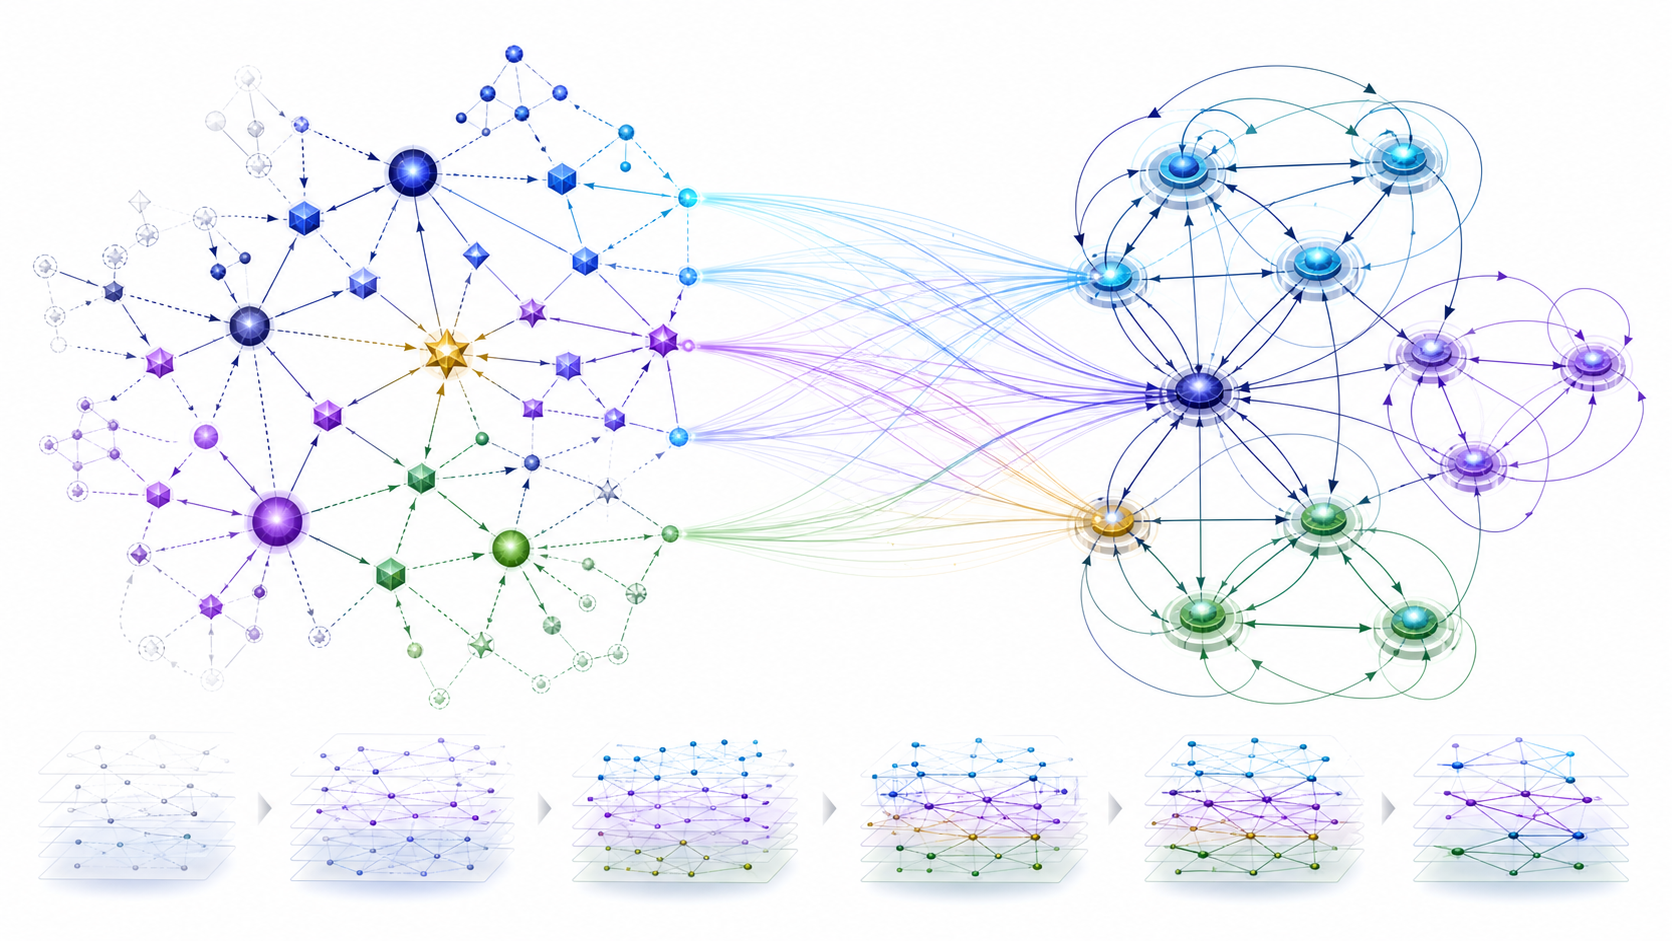
\includegraphics[width=.9\textwidth,height=.38\textheight,keepaspectratio]{images/cognitive-structure-functional-topology.png}
\caption{结构压力、迟滞与最小必要重组}
\end{figure}
\section{结构失配：当认知结构与功能承载不再相称}

在前一章中，我们已经把功能拓扑理解为历史 CSO 流的结构沉积。一个长期稳定的功能连接并不是凭空存在的，
而是某一类 Agent-CSO 在多个功能之间反复迁移、反复完成闭环之后，被系统逐渐固化下来的低成本通路。
因此，任意时刻的功能拓扑 $\mathcal G_F(t)$ 本质上都带有明显的历史性：它更加适合承载系统过去反复遇到的问题，
但并不必然最适合未来将要出现的问题。只要环境、任务集合、身体、工具或智能体自身的认知结构发生持续变化，
当前拓扑就可能逐渐偏离新的结构需求。我们把这种偏离定义为\textbf{结构失配}
（Structural Mismatch）。

为了形式化这一概念，设智能体的功能拓扑为
\[
\mathcal G_F(t)
=
\left(
V_F(t),
E_F(t),
W_F(t)
\right),
\]
认知结构图为
\[
\mathcal G_C(t)
=
\left(
V_C(t),
E_C(t)
\right),
\]
而二者之间存在随时间变化的承载映射
\[
\mu_t:
\mathcal G_C(t)
\rightarrow
\mathcal G_F(t).
\]
这里 $\mu_t$ 并不是一个简单的一对一函数，而更接近多对多的动态关系：
一个 Agent-CSO 可以同时被多个功能协同承载，一个功能也可以在不同上下文中处理大量不同的 Agent-CSO。
我们真正关心的是，在当前 $\mathcal G_F$ 下，某类认知结构是否能够以足够短的路径、足够低的协调成本和足够稳定的闭环被处理。

设 $C_k$ 为某一类持续出现的认知结构，系统为完成它所需要经过的功能路径为
\[
\pi_k
=
(F_{i_1},F_{i_2},\ldots,F_{i_m}),
\]
则可以定义该结构在当前拓扑中的有效承载代价
\[
\mathcal C_{\mathrm{carry}}(C_k|\mathcal G_F)
=
\alpha L(\pi_k)
+
\beta D(\pi_k)
+
\gamma R(\pi_k)
+
\delta U(\pi_k)
+
\eta E(\pi_k),
\]
其中 $L$ 表示路径长度，$D$ 表示跨功能通信延迟，
$R$ 表示为完成任务所需要的重复往返次数，
$U$ 表示不确定性或失配残差，
$E$ 表示额外认知或计算资源消耗。
这里各项并非意味着必须使用这一特定线性形式，而是告诉我们：
所谓结构失配并不是抽象的 ``这个架构看起来不够优雅''，
而应该表现为可观察、可累积的运行代价。

例如，一个智能体长期需要完成同一类任务时，如果每一次任务都必须经过
\[
F_A
\rightarrow
F_B
\rightarrow
F_C
\rightarrow
F_A
\rightarrow
F_D
\rightarrow
F_B
\]
才能闭环，那么问题并不一定意味着这些功能本身不足。
更可能的问题在于：
某种已经变得稳定的认知结构关系仍然被迫通过历史上为其他任务形成的路径进行协调。
如果该任务只出现一次，我们没有理由改变拓扑；
如果这种往返持续数万次，而且每次都表现出相似的 Agent-CSO 流，
那么重复发生的动态过程就开始暴露一个更慢层次的问题：
\begin{statementbox}
当前拓扑没有把长期稳定的功能关系直接表示出来。
\end{statementbox}

因此，我们可以把结构失配写成一类时间平均量：
\[
M_{\mathrm{struct}}(t)
=
\mathbb E_{\Delta T}
\left[
\mathcal C_{\mathrm{carry}}
-
\mathcal C_{\mathrm{expected}}
\right],
\]
其中 $\Delta T$ 必须明显大于普通状态扰动的时间尺度。
这一点非常重要。如果我们直接使用瞬时残差作为结构修改依据，
那么拓扑就会被短期任务、偶然输入和随机噪声不断重写。
成熟智能的结构学习必须区别
\[
\varepsilon_{\mathrm{state}}(t)
\]
与
\[
\overline{\varepsilon}_{\mathrm{struct}}(t).
\]
前者可能只需要一次新的推理、一次注意调整或一次记忆召回；
后者意味着相似的误差在足够长时间内重复出现，并且具有稳定结构。

我们由此得到结构失配的第一个核心判断：

\begin{proposition*}
困难本身不是拓扑改变的证据；
持续以相同结构形式出现的困难才可能是拓扑改变的证据。
\end{proposition*}

这也解释了为什么智能系统不能把 ``没有立即成功'' 与 ``自身架构错误'' 混为一谈。
真正的发育型智能必须能够容忍局部失败，并首先通过已有结构学习。
只有当经验持续表明：
问题并不来自知识不足，而来自知识、功能与闭环之间的组织关系不适配，
系统才应把问题逐渐提升到拓扑层。

从已有科学理论来看，这一思想与自适应网络、结构可塑性、组织学习以及控制系统中的模型失配有相似之处，
但本理论与这些理论之间存在一个重要区别：
我们不是简单研究网络连接是否提高任务性能，而是把\textbf{Agent-CSO 的长期承载轨迹}
作为拓扑变化的主要因果来源。
因此，本章研究的核心不是 ``如何搜索更好的图''，
而是
\begin{statementbox}
一个智能系统如何从自己的生命周期历史中发现：
哪些反复发生的认知过程已经值得成为自身结构的一部分。
\end{statementbox}

\section{拓扑压力：从持续残差到结构重组需求}

结构失配本身并不意味着系统必须立即重构。现实中的智能体始终处在不确定环境中，
任何一次任务都可能产生临时协调成本。如果所有失配都直接转化成拓扑改变，
智能体将处于不断改写自身的状态，最终失去身份连续性、能力稳定性以及可验证的行为边界。
因此，在结构失配与拓扑改变之间，我们需要引入一个中间动力学变量：
\textbf{拓扑压力}（Topological Pressure）。

拓扑压力可以理解为系统内部对 ``当前功能组织方式已经长期不经济'' 的累积证据。
设
\[
P_T(t)
\]
表示拓扑压力，则一个概念性的定义可以写为
\[
P_T
=
F
\left(
\bar{\varepsilon},
\bar{J}_{\mathrm{cross}},
C_{\mathrm{coord}},
L_{\mathrm{latency}},
I_{\mathrm{instability}},
R_{\mathrm{repeat}},
V_{\mathrm{utility}}
\right).
\]
其中 $\bar{\varepsilon}$ 表示长期未消除残差，
$\bar{J}_{\mathrm{cross}}$ 表示长期跨功能的 Agent-CSO 迁移流，
$C_{\mathrm{coord}}$ 表示协调成本，
$L_{\mathrm{latency}}$ 表示路径延迟，
$I_{\mathrm{instability}}$ 表示局部闭环的不稳定程度，
$R_{\mathrm{repeat}}$ 表示同类结构的重复频率，
而 $V_{\mathrm{utility}}$ 则表示如果改善该路径，对整体生命周期能力究竟有多大价值。

为了避免拓扑压力对瞬时噪声过敏，我们可以采用一个慢积分过程：
\[
\tau_T\dot P_T
=
-
P_T
+
\Phi
\left(
\varepsilon,
J^{CSO},
C_{\mathrm{coord}},
L,
U
\right),
\qquad
\tau_T \gg \tau_h.
\]
这意味着拓扑压力具有明显的低通滤波性质。
一次很严重但很偶然的失败未必能够产生持续 $P_T$；
反而是一系列程度并不剧烈、却在数周或数月中不断重复的相同协调模式，
更可能逐渐推动 $P_T$ 上升。

我们可以把这一过程理解为智能系统中的一种慢 ``结构痛感''，
但这里的 ``痛感'' 只是功能隐喻，不涉及主观体验。
它表达的是：
当前系统每一次都能解决问题，
却需要不断支付同一种额外成本。
在短期尺度上，任务仍然成功，因此不存在显著功能崩溃；
在生命周期尺度上，这种重复支付会积累成一个非常明确的结构信号。

设系统对某类任务 $k$ 的实际平均处理成本为
\[
\bar C_k(T),
\]
而其在已有能力条件下可以达到的理论或经验参考成本为
\[
C_k^\star.
\]
则可以定义结构效率比
\[
\eta_k
=
\frac{C_k^\star}{\bar C_k(T)}.
\]
当 $\eta_k\approx 1$ 时，当前拓扑已经能够很好承载该任务；
当 $\eta_k\ll 1$ 且长期保持时，
说明智能体正在重复使用一个明显不经济的功能路径。
但即便如此，拓扑压力仍不能由效率单独决定，
因为一个非常罕见的任务即使代价巨大，也不一定值得修改长期架构。
因此真正影响结构学习的是
\[
R_k \cdot V_k \cdot (1-\eta_k),
\]
也就是重复性、价值和结构低效的共同作用。

进一步说，拓扑压力具有局部性。
并不存在一个全局标量可以完整描述整个 Agent 的结构失配。
更一般的表示是：
\[
P_T(i,j,t),
\]
表示功能区域 $F_i$ 与 $F_j$ 之间产生新耦合、改变现有耦合或重组中间结构的局部压力。
于是整个系统拥有一个拓扑压力场
\[
\mathbf P_T(t)
=
\{P_T(i,j,t)\}.
\]
这使得拓扑学习不必总是 ``重构整个智能体''，
而可以首先表现为局部边权调整、局部功能聚合或局部捷径形成。

本章尤其需要强调：
\[
\boxed{
P_T
\neq
\varepsilon.
}
\]
Residual 告诉系统 ``这次发生了偏差''；
Topological Pressure 告诉系统
``相似偏差已经持续到值得重新审视自己的组织方式''。
前者主要驱动快速认知和局部学习，
后者才有资格进入慢尺度结构治理。

这一区分使整个 AgentOS 的多尺度理论获得了重要连续性。
我们此前已经强调
\[
\boxed{
SlowGovernance\neq FastMicromanagement.
}
\]
现在可以进一步写成：
\begin{statementbox}
\centering
\adjustbox{max width=.96\linewidth}{\(\displaystyle FastError
\nrightarrow
ImmediateTopologyChange.\)}
\end{statementbox}
短期误差首先应被 h、SPC、TCE、CCM、记忆学习和功能迁移吸收。
只有那些无法被这些较快机制长期消化的结构性残差，
才逐渐进入拓扑压力。
这正是一个成熟智能体能够同时保持稳定与发育的基础。

\section{何时当前功能拓扑已经不足}

现在我们面对一个比 ``系统是否犯错'' 更严格的问题：
什么情况下我们可以合理地说，
\textbf{当前功能拓扑本身已经不足以承载智能体正在形成的认知结构}？
如果这一条件不能被清楚定义，拓扑学习就只能退化成随机 Architecture Search；
而如果条件定义得过于苛刻，系统又可能永远停留在早期设计者赋予的固定结构中。

为了解决这一问题，我们首先区分四种不同层级的失败。
第一类是\textbf{状态失败}：
当前状态不正确，但已有结构足以恢复。例如一个规划步骤错误，只需要重新推理。
第二类是\textbf{表示失败}：
当前 CSO 的表示方式不适合问题，需要重新编码、抽象或拆分。
第三类是\textbf{承载失败}：
结构本身是有效的，但当前功能位置、时间尺度或内外载体不合理。
第四类才是\textbf{拓扑失败}：
即使允许充分的状态调整、表示重构和 Agent-CSO 迁移，
系统仍持续需要通过低效路径维持一个稳定而重复的功能关系。

于是我们可以构造一个逐级检验：
\[
\mathcal H_0:
\text{State adjustment is sufficient},
\]
\[
\mathcal H_1:
\text{Representation adaptation is sufficient},
\]
\[
\mathcal H_2:
\text{Timescale/carrier migration is sufficient},
\]
\[
\mathcal H_3:
\text{Functional migration is sufficient},
\]
只有当这些较低层假设长期被数据否定以后，才进入：
\[
\mathcal H_4:
\text{Topology reorganization is necessary}.
\]

换句话说，拓扑不足不是 ``当前架构没有直接支持某个任务''，
而是：
\[
\boxed{
\min_{\text{state,repr.,placement}}
\mathcal L
\left(
\mathcal G_F,
\mu,
C
\right)
>
\theta_{\mathrm{acceptable}},
}
\]
即在保持 $\mathcal G_F$ 不变的条件下，
已经无法通过合理的内部调整把长期损失压缩到可接受区域。

我们可以进一步定义当前拓扑的有效可承载集合：
\[
\mathcal C_{\mathrm{feasible}}
(\mathcal G_F)
=
\left\{
C:
\exists\mu,\,
\mathcal L(C|\mathcal G_F,\mu)
\leq\theta
\right\}.
\]
一个新的 Agent-CSO 并不要求一出现就改变拓扑，
只要它仍然属于
\[
\mathcal C_{\mathrm{feasible}}(\mathcal G_F),
\]
系统就可以通过已有功能组合完成处理。
真正值得发育的是：
越来越多高价值、高频结构长期靠近或超出该可承载边界，
使系统持续工作在高协调、高延迟、高显式认知占用的状态。

这与我们此前关于工作记忆有限性的讨论可以直接连接。
假如某一类已经非常熟悉的任务，每次仍然必须把大量中间关系重新提升到 $h(t)$，
则：
\[
H_{\mathrm{explicit}}(C_k)
\]
长期保持在高水平。
这意味着低层功能没有形成足够稳定的闭环，
导致本应自动化的结构不断占用有限全局认知空间。
因此可以把 ``长期不必要的显式认知占用'' 视为结构失配的重要观测量：
\[
P_T
\propto
\left\langle
H_{\mathrm{explicit}}(C_k)
\right\rangle_T.
\]

这给我们一个非常现实的判断标准。
一个成熟系统不应该因为会做越来越多事情而让 h 越来越拥挤。
恰恰相反，随着学习：
\[
Capability\uparrow,
\qquad
ExplicitCognitiveBurden/Capability\downarrow.
\]
如果能力不断增长，但所有旧能力仍然依赖高层全局推理，
那么系统虽然知识增加，却没有发生真正意义上的认知发育。

因此，在本理论中，
一个功能拓扑 ``不够用'' 的判据不是单一任务性能下降，
而是多个指标在较长时间尺度上共同满足：
高频稳定 CSO 流持续跨越相同功能路径；
协调成本长期不下降；
工作记忆显式占用无法通过技能化进一步减少；
功能间 residual 出现稳定模式；
局部优化已经接近饱和；
新的经验仍不断强化同一种功能依赖。

只有在这些条件共同出现时，
我们才有理由认为：
\begin{statementbox}
当前智能体已经不只是需要学习新的内容，
而是需要学习一种新的组织方式。
\end{statementbox}

\section{新功能连接的形成：从重复迁移到稳定耦合}

拓扑发育最基本的结构事件，是一个原本不存在或非常弱的功能连接逐渐形成。
这一过程不能被理解为系统随意 ``接一条线''，
而应该来自 Agent-CSO 长期迁移历史所提供的统计证据。

设功能节点 $F_i$ 与 $F_j$ 之间的连接权重为
\[
w_{ij}(t).
\]
Agent-CSO 从 $F_i$ 向 $F_j$ 的有效流定义为
\[
J_{ij}^{CSO}(t).
\]
如果某类结构长期反复从 $F_i$ 流向 $F_j$，
我们可以定义其时间平均：
\[
\bar J_{ij}^{CSO}(T)
=
\frac{1}{T}
\int_{t-T}^{t}
J_{ij}^{CSO}(s)\,ds.
\]
但流量本身仍不足以证明连接有价值。
有些高流量只是由于架构缺陷造成的无效往返；
如果直接依据流量强化连接，就可能固化错误。

因此边的生长律必须同时考虑：
\[
Utility_{ij},
\quad
ResidualReduction_{ij},
\quad
LatencySaving_{ij},
\quad
Risk_{ij},
\quad
Cost_{ij}.
\]
一个概念性的连续更新规则可以写成
\[
\tau_T\dot w_{ij}
=
\alpha
\bar J_{ij}^{CSO}
\Delta U_{ij}
+
\beta
\Delta R_{ij}
+
\gamma
\Delta L_{ij}
-
\lambda
C_{ij}
-
\xi
Risk_{ij}.
\]
其中 $\Delta U_{ij}$ 表示该连接对长期效用的改善，
$\Delta R_{ij}$ 表示残差减少，
$\Delta L_{ij}$ 表示延迟降低，
$C_{ij}$ 表示维持该连接所需成本，
而 $Risk_{ij}$ 则约束可能破坏安全边界或权限隔离的结构变化。

如果功能拓扑是离散的，则可以使用更明确的形成条件：
\[
w_{ij}=0
\quad\longrightarrow\quad
w_{ij}>0
\]
当且仅当
\[
\mathbb E_T
\left[
Benefit_{ij}
\right]
-
\lambda Cost_{ij}
-
\xi Risk_{ij}
>
\theta_{\mathrm{on}},
\]
且该条件持续时间达到
\[
T>T_{\min}.
\]

这里的 $T_{\min}$ 极其重要。
它意味着新功能关系必须经过持续经验验证。
换句话说，
AgentOS 的结构发育不能只问：
``建立这条边现在是否有用？''
而应该问：
``在足够多不同情境中，这条关系是否表现出稳定且可泛化的价值？''

例如，假设一个 Agent 最初处理某类视觉事件时，需要：
\[
Perception
\rightarrow
h
\rightarrow
Reasoning
\rightarrow
Action.
\]
经过大量训练以后，系统发现其中某一类视觉模式和某一局部行动之间存在高度稳定关系。
那么该认知结构首先可能经历：
\[
ExplicitCSO
\rightarrow
ExperientialCSO
\rightarrow
GenerativeCSO
\rightarrow
ProceduralCSO.
\]
如果这种下沉仍然依赖多个中间功能节点，
系统就可能进一步形成新的快速耦合，使：
\[
F_{\mathrm{perception}}
\rightarrow
F_{\mathrm{local-control}}
\]
成为更直接的路径。
这时，能力的成熟已经不只是某个参数发生变化，
而是功能图本身对历史经验进行了压缩。

因此可以把边形成解释成：
\begin{statementbox}
过去反复发生的动态关系，
逐渐变成未来不需要重新计算的静态关系。
\end{statementbox}
这就是拓扑作为慢记忆的真正含义。

从计算角度看，一条新功能边类似把反复执行的长路径缓存成快捷调用；
从神经科学类比上看，它与反复共同激活后形成更稳定通路存在某种启发性相似；
从软件工程角度看，它类似把经常跨多个组件协商的路径重新封装成一个稳定服务接口。
但 AgentOS 理论的关键区别在于：
这些结构变化都应该由 Agent-CSO 生命周期流和现实反馈共同驱动，
而不是简单按照共现频率硬编码。

更一般地，新连接形成意味着未来同类 CSO 的传播算子发生了变化。
若原传播为
\[
x(t+\Delta)
=
\mathcal P_{\mathcal G_F}(x(t)),
\]
新增边后变成
\[
x(t+\Delta)
=
\mathcal P_{\mathcal G_F'}(x(t)),
\qquad
\mathcal G_F'\neq\mathcal G_F.
\]
于是，拓扑学习真正改变的是
\textbf{未来认知过程允许怎样传播}，
而不仅是当前知道了什么。

\section{旧连接的消退：遗忘、剪枝与结构释放}

如果拓扑只能增加而不能减少，一个长期智能体最终将形成越来越密集的功能图。
这种系统虽然保留了所有历史路径，却会产生新的问题：
搜索空间扩大、控制耦合增加、异常传播路径增加、功能边界模糊，
最终重新把拓扑复杂度转化成运行时认知负担。
因此真正的发育必须同时包含结构生长与结构消退。

设已有边权为
\[
w_{ij}>0.
\]
如果一条功能关系长期不再承载高价值 CSO 流，
其边权应该允许缓慢衰减。
最简单的形式为
\[
\tau_T\dot w_{ij}
=
-\lambda_d w_{ij}
+
\Phi
\left(
\bar J_{ij}^{CSO},
Utility_{ij},
RecoveryValue_{ij}
\right).
\]
其中 $RecoveryValue_{ij}$ 是非常重要的一项。
一条平时极少使用的安全恢复路径，不能因为使用频率低而被删除；
同样，一些身份、价值和极端异常处理通路可能长期不活跃，
却具有极高潜在重要性。
因此结构删除不能采用单纯的 ``least frequently used'' 原则。

我们可以定义一个边的重要性：
\[
I_{ij}
=
\alpha
Usage_{ij}
+
\beta
Utility_{ij}
+
\gamma
Safety_{ij}
+
\delta
Recovery_{ij}
+
\eta
Identity_{ij}.
\]
只有当
\[
I_{ij}<\theta_{\mathrm{off}}
\]
持续足够长时间，
且其删除不会导致关键闭环断裂时，
才允许：
\[
w_{ij}\rightarrow 0.
\]

这意味着拓扑遗忘必须与普通记忆遗忘区分。
E 中的某个事件可以逐渐失去细节；
某个 Θ 结构可以被更一般模型吸收；
而功能拓扑中的边一旦删除，
改变的是未来整个认知系统的信息传播能力。
因此拓扑遗忘属于更慢、更高风险的结构操作。

我们可以把删除过程划分为三个阶段。
首先是\textbf{边权弱化}：
连接仍存在，但优先级下降。
其次是\textbf{休眠}：
正常路由不再使用，但保留恢复能力。
最后才是\textbf{结构删除}。
因此更合理的状态空间不是
\[
Edge\in\{0,1\},
\]
而是
\[
EdgeState
\in
\{
Active,
Weak,
Dormant,
Retired
\}.
\]
这种多阶段结构能够显著降低灾难性拓扑遗忘。

进一步说，一条边是否应该删除，不能只看局部。
有些边本身使用频率不高，却承担多个闭环之间的桥梁作用。
因此还需要考虑图结构中的介数、可达性和冗余：
\[
Centrality_{ij},
\quad
Reachability,
\quad
Redundancy_{ij}.
\]
如果删除 $e_{ij}$ 会使某个关键 CSO 类失去有效承载路径，
即使其直接使用频率不高，也不应删除。

这对应一个更普遍的智能发育原则：
\begin{proposition*}
成熟不是不断拥有更多结构，
而是保留越来越少但越来越有效的结构。
\end{proposition*}
这和人类技能成熟、软件重构乃至科学理论发展都有某种共同特点：
大量早期显式步骤最终被压缩，
一些冗余中间结构消失，
留下更加稳定、抽象和高效的关系。

不过我们必须避免把这一过程浪漫化。
结构删除可能形成习惯僵化，也可能删除在未来环境重新变得重要的路径。
因此成熟智能需要保持：
\[
\boxed{
StructuralCompression
+
Recoverability.
}
\]
这为后面将讨论的迟滞、Checkpoint、结构版本管理以及心理工程中的 ``过度固化'' 提供了直接理论基础。

\section{功能区域的分裂与合并}

除了边的形成与消失，功能拓扑还可能发生更高阶的结构改变：
一个原有功能区域分裂成多个更加专门的区域，
或者多个原本独立的功能区域逐渐合并成一个稳定闭环。
这种变化比单条边调整更加深刻，因为它改变了系统对功能本身的划分方式。

设某一功能节点
\[
F_i
\]
长期承载不同类型的 Agent-CSO：
\[
\mathcal C_i
=
\{
C^{(1)},C^{(2)},\ldots,C^{(m)}
\}.
\]
如果这些 CSO 可以自然分成两个长期稳定、内部高度相关而彼此耦合很弱的集合：
\[
\mathcal C_i
=
\mathcal C_i^{(a)}
\cup
\mathcal C_i^{(b)},
\]
并满足
\[
I
\left(
\mathcal C_i^{(a)};
\mathcal C_i^{(b)}
\right)
\ll
I
\left(
\mathcal C_i^{(a)}
\right),
\]
同时它们对时间尺度、资源、控制策略或输出接口的要求显著不同，
那么继续把二者放在同一功能节点内处理就可能产生长期协调代价。
此时可能发生：
\[
F_i
\rightarrow
\{F_i^{(a)},F_i^{(b)}\}.
\]

功能分裂意味着系统发现：
过去被认为是 ``同一种能力'' 的结构，
在生命周期经验中已经表现出稳定不同的动力学规律。
例如，早期 Agent 可能使用一个统一 ``记忆模块'' 处理所有历史结构；
随着经验增长，它可能逐渐分化出快速 episode recall、
慢速 structural consolidation、identity-related memory 等不同功能闭环。
在工程架构中，我们通常由设计者预先完成这种分工；
而真正发育型智能理论关心的是：
这种分工是否也能够从长期结构流中被系统自己发现。

相反，如果两个功能
\[
F_i,\quad F_j
\]
在长期运行中总是成对出现，
绝大多数输入和输出都高度耦合，
它们之间的通信成本远大于独立存在所带来的模块化收益，
那么：
\[
F_i+F_j
\rightarrow
F_{ij}
\]
可能成为更经济的结构。

我们可以定义分裂倾向：
\[
S_{\mathrm{split}}(F_i)
=
\frac{
C_{\mathrm{internal-conflict}}
+
C_{\mathrm{timescale-mismatch}}
+
C_{\mathrm{resource-contention}}
}{
C_{\mathrm{coordination-after-split}}
+
C_{\mathrm{rewrite}}
},
\]
当
\[
S_{\mathrm{split}}>\theta_{\mathrm{split}}
\]
且长期稳定时，
分裂成为候选操作。

类似地定义合并倾向：
\[
S_{\mathrm{merge}}(F_i,F_j)
=
\frac{
C_{\mathrm{cross-communication}}
+
C_{\mathrm{duplicate-state}}
+
C_{\mathrm{coupling-overhead}}
}{
C_{\mathrm{loss-of-modularity}}
+
C_{\mathrm{merge-risk}}
}.
\]

这里尤其重要的一点是：
功能分裂和合并不必对应真正增加或删除一个神经网络。
功能拓扑是\textbf{因果—功能层拓扑}。
例如在软件 AgentOS 中，
分裂可能只是把原本由同一服务承担的两种责任形成独立调度、状态和 ABI；
在神经系统中，则可能由不同子网络的功能专业化实现；
在组织智能中，它甚至可以表现为一个部门分成两个岗位。
因此该理论保持实现独立性。

我们还可以从 CSO 图的角度理解这一过程。
如果
\[
\mathcal G_C
\]
内部形成越来越明显的 community structure，
而当前
\[
\mu_t:
\mathcal G_C\rightarrow\mathcal G_F
\]
仍然把这些不同 community 映射到同一个功能区域，
就会出现一种映射压缩失配。
功能拓扑发育的一个方向，
就是让
\[
\mathcal G_F
\]
逐渐形成与长期稳定 CSO 关系更加匹配的功能分区。

不过，这里同样存在危险。
过度分裂会形成碎片化系统，
每个微小任务都生成自己的模块；
过度合并则会回到一个巨大中央模型承担一切。
因此成熟拓扑并不是极端模块化或极端集中，
而是在协调成本与局部闭环收益之间形成动态平衡。
这与我们早期智能相中的 ``集中度'' 轴重新连接：
智能发育本身可以推动系统在不同集中度区域之间移动，
但这种变化必须由长期结构需求驱动，而不是架构美学驱动。

\section{拓扑捷径：长期计算如何沉降为空间结构}

功能拓扑学习中一种特别重要的变化是\textbf{拓扑捷径}
（Topological Shortcut）。
它描述这样一种现象：
过去需要经过多个中间步骤的认知过程，
由于重复出现并形成稳定映射，
最终建立更加直接的功能通路。

设原始功能路径为
\[
F_1
\rightarrow
F_2
\rightarrow
F_3
\rightarrow
F_4,
\]
每次处理某类 CSO 都必须沿该路径传播。
如果经过长期经验，系统发现：
对于某一稳定结构子集 $\mathcal C^\star$，
中间过程 $F_2,F_3$ 基本形成确定性的变换，
且残差极低，那么就可能建立：
\[
F_1
\rightarrow
F_4
\]
的条件性快速路径。

需要注意的是，这并不意味着 $F_2,F_3$ 被删除。
在异常情况、新环境或低置信度状态下，
系统仍然可以回到完整路径。
因此更成熟的结构是：
\[
\begin{cases}
F_1\rightarrow F_4,
&
Confidence>\theta_c,
\\
F_1\rightarrow F_2\rightarrow F_3\rightarrow F_4,
&
Confidence\leq\theta_c.
\end{cases}
\]
这实际上就是 ``能力向下编译、异常向上重新显式化''
在拓扑层的进一步实现。

从计算理论角度看，这类似将反复计算的结果编译为缓存、索引或专用程序；
从认知层面看，它对应熟练技能不再需要逐步显式思考；
从 AgentOS 工程层面，它可以表现为：
原本由 h、规划器和工具调度共同完成的复杂行为，
经过长期验证后转化成一个 BodySkill、SkillPackage 或局部控制器。
因此，拓扑捷径是：
\begin{statementbox}
\centering
\adjustbox{max width=.96\linewidth}{\(\displaystyle TemporalComputation
\rightarrow
SpatialStructure\)}
\end{statementbox}
即时间中反复发生的计算，
最终沉降成空间上的连接关系。

这使我们能够重新理解智能效率的来源。
一个刚开始学习的 Agent，需要通过时间展开来解决问题：
\[
C_{\mathrm{space}}
\rightarrow
C_{\mathrm{time}}.
\]
它将一个无法一次性处理的结构分解成多个步骤。
但当相同过程反复成功以后，
智能体又可以把稳定时间过程压缩回来：
\[
C_{\mathrm{time}}
\rightarrow
C_{\mathrm{structure}}.
\]
因此学习具有一种深层双向性：
陌生问题先被展开成时间，
熟练过程再被压缩成结构。

我们可以定义路径压缩比：
\[
\kappa
=
\frac{
L(\pi_{\mathrm{old}})
}{
L(\pi_{\mathrm{new}})
},
\]
以及显式认知节约率：
\[
\eta_h
=
1-
\frac{
H_h^{\mathrm{new}}
}{
H_h^{\mathrm{old}}
}.
\]
如果新捷径在保持任务成功率、现实一致性和安全性的同时，
显著提高 $\kappa$ 和 $\eta_h$，
那么它就具有明确的发育价值。

但是，捷径也可能产生错误固化。
如果系统在训练环境中形成过强直接映射，
环境改变后仍继续绕过高层检查，
就会形成所谓 ``熟练陷阱''。
因此每条快速路径都必须保留：
\[
ResidualChannel,
\quad
Confidence,
\quad
EscalationPath.
\]
也就是说：
\begin{statementbox}
FastPathWithoutResidualEscalation
\end{statementbox}
不是成熟技能，而是脆弱自动化。

这进一步说明，真正的智能发育不是简单 ``越来越少思考''，
而是：
\begin{statementbox}
在熟悉区域减少显式思考，
同时保留在异常区域重新思考的能力。
\end{statementbox}
因此：
\[
ThinkingLess\neq KnowingLess.
\]
更准确的是：
\begin{statementbox}
StructureChangedCarrier.
\end{statementbox}

\section{拓扑迟滞：稳定性与可塑性之间的结构记忆}

如果一条边在流量上升时形成，
而流量稍微下降就立即消失，
功能拓扑会不断在多个结构之间来回震荡。
这种系统无法积累真正的技能，也无法形成稳定身份。
因此拓扑学习必须具有\textbf{迟滞}
（Hysteresis）。

设形成新边的阈值为
\[
\theta_{\mathrm{on}},
\]
删除已有边的阈值为
\[
\theta_{\mathrm{off}},
\]
则应满足
\[
\boxed{
\theta_{\mathrm{on}}
>
\theta_{\mathrm{off}}.
}
\]
其含义是：
建立一条新结构需要较强、较长期的证据；
而一旦该结构已经建立，
短期证据下降并不足以立刻将其删除。

这与普通开关逻辑不同。
如果只有单阈值 $\theta$，
那么当结构证据 $P_T(t)$ 在 $\theta$ 附近波动时，
拓扑状态会产生
\[
0\leftrightarrow1\leftrightarrow0\leftrightarrow1
\]
的频繁切换。
采用双阈值以后：
\[
P_T>\theta_{\mathrm{on}}
\Rightarrow
EdgeOn,
\]
而已存在的边只有在
\[
P_T<\theta_{\mathrm{off}}
\]
持续足够长时间后才退出。
因此在
\[
\theta_{\mathrm{off}}
<
P_T
<
\theta_{\mathrm{on}}
\]
区域中，
系统保留历史状态。

这正意味着：
\begin{statementbox}
TopologyHasMemory.
\end{statementbox}
拓扑不仅由当前输入决定，
还取决于系统过去经历过什么。
因此两个当前状态完全相同的 Agent，
如果生命周期历史不同，
也可能拥有不同功能拓扑。
这给 ``个体性'' 提供了一个比参数差异更加结构性的解释。

迟滞还可以推广到更复杂的结构操作。
例如，某一功能节点分裂后，
系统不应该因为短期协调减少就立即重新合并；
某个 BodySkill 已经形成以后，
也不应因为几次任务失败就完全退回高层认知。
更合理的是先降低置信度、扩大 residual monitoring，
必要时进入 probation 状态，
再决定是否真正撤销结构。

可以进一步定义拓扑状态：
\[
q_T(t)
\in
\{
Stable,
Candidate,
Consolidating,
Active,
Dormant,
Retiring
\}.
\]
这比简单边权更适合工程实现。
Candidate 表示正在收集证据；
Consolidating 表示连接已经初步形成但仍受严格监督；
Active 表示成熟稳定结构；
Dormant 表示暂时不用但可快速恢复；
Retiring 表示已进入结构撤销过程。

从更高层来看，迟滞实际上解决智能发展中的稳定性—可塑性矛盾：
\[
\boxed{
Plasticity
\quad\text{vs.}\quad
Stability.
}
\]
没有可塑性，智能无法适应新的生命周期；
没有稳定性，智能无法积累身份和技能。
拓扑迟滞使系统可以在经验持续改变时逐步变化，
又避免瞬时输入穿透到最慢结构层。

因此，拓扑保护应当服从：
\[
\tau_{\mathrm{state}}
\ll
\tau_{\mathrm{representation}}
\ll
\tau_{\mathrm{spectrum}}
\lesssim
\tau_{\mathrm{function}}
\ll
\tau_{\mathrm{topology}}.
\]
这里的时间尺度序列不是固定物理常数，
而是结构治理原则：
越接近系统身份、长期能力与基础组织的变量，
越不应该被快速经验直接修改。

这也为后续 AgentOS 控制工程中的
\[
BoundedSelfModificationEnvelope
\]
提供认识论基础。
允许智能体修改自己，并不意味着让所有结构拥有同样的学习率。
真正安全的自我发育应当表现为：
\[
\boxed{
FastExperience,
SlowIdentity,
SlowerTopology,
GuardedGovernance.
}
\]

\section{最小必要重组原则}

至此我们已经看到，智能系统面对困难时拥有许多不同层级的适应手段。
如果没有明确优先级，系统可能在一个本应通过简单状态更新解决的问题上进行过度结构重组。
因此我们提出本章最重要的治理原则之一：
\textbf{最小必要重组原则}
（Minimum Necessary Reorganization Principle）。

其基本思想是：
\begin{statementbox}
使用能够解决当前长期失配的最低成本、最局部、最可逆的结构调整。
\end{statementbox}
一个完整适应序列可以写为：
\begin{statementbox}
\centering
\adjustbox{max width=.96\linewidth}{\(\displaystyle StateAdjustment
\rightarrow
RepresentationAdaptation
\rightarrow
TimescaleMigration
\rightarrow
FunctionalMigration
\rightarrow
TopologicalReorganization
\rightarrow
BoundaryMigration.\)}
\end{statementbox}

第一层是状态调整。
例如改变当前计划、注意和推理状态。
其特点是代价低、可逆性高、时间尺度快。

第二层是表示调整。
Agent 不改变功能组织，仅改变 CSO 的编码、抽象、分解方式。
一个看似困难的问题可能只是表示错误，
换一种表示即可重新进入已有可解区域。

第三层是时间尺度迁移。
某些结构不应持续处于 h，
而应进入 E、$\Theta$ 或程序性快速结构；
相反，异常情况下，慢结构也需要重新提升到快速显式层。

第四层是功能迁移。
Agent-CSO 从一个功能承载区域迁移到另一个更加合适的位置，
但整体功能图仍然不改变。

第五层才是拓扑重组。
新的长期连接、功能节点分裂/合并和路径重构都属于这一层。

第六层是边界迁移。
如果问题仍然无法合理内部化，
智能体可能把结构迁移到 Tool、Program、Environment、Other Agent 或组织层。
严格说，边界迁移未必总比内部拓扑改变代价更高，
因此这一排序并非机械固定，而表示\textbf{治理深度}：
越往后，改变的越不只是当前认知内容，而是主体未来处理世界的方式。

我们可以把适应选择形式化为一个最优化问题。
设可选重组动作集合为
\[
\mathcal A_R
=
\{
a_s,
a_r,
a_\tau,
a_f,
a_T,
a_B
\},
\]
每个动作具有：
\[
Cost(a),
\quad
Risk(a),
\quad
Reversibility(a),
\quad
ExpectedResidualReduction(a).
\]
则选择：
\[
a^\star
=
\arg\min_{a\in\mathcal A_R}
\left[
Cost(a)
+
\lambda_R Risk(a)
+
\lambda_I Irreversibility(a)
\right]
\]
满足约束
\[
\mathbb E
[
ResidualAfter(a)
]
<
\theta.
\]

这意味着系统不是选择 ``效果最大'' 的改变，
而是选择\textbf{满足问题解决要求的最小结构改动}。
这种思想与控制理论中的最小控制作用、软件工程中的最小修改原则和安全系统中的最小权限思想存在相似性，
但在 AgentOS 中，它被推广到整个认知结构层级。

这一原则尤其适用于长期身份连续问题。
如果 Agent 每次遇到冲突都修改 $\Psi$，
或者每次长期任务失败都修改功能拓扑，
那么系统很快就失去 ``同一个主体'' 的可辨识连续性。
因此成熟 Agent 必须首先问：
\[
\text{Can I solve this without changing who I am?}
\]
然后：
\[
\text{Can I solve this without changing how I am organized?}
\]
只有在长期证据否定这些可能以后，
结构发育才向更慢层推进。

最小必要重组还意味着系统必须保留\textbf{可恢复性}。
每一次较深层结构变化，都应尽可能记录：
\[
PreState,
\quad
TriggerEvidence,
\quad
ExpectedBenefit,
\quad
ObservedOutcome,
\quad
RollbackPath.
\]
这使结构学习不再是不可解释的参数漂移，
而成为一种可审计的生命周期治理。

由此我们可以得到一条很重要的 AgentOS 原则：
\begin{statementbox}
成熟智能不是最容易改变自己的智能，
而是最知道何时无需改变、何时必须改变，以及应该改变到哪一层的智能。
\end{statementbox}

\section{学习与发育的边界}

本章最后需要回答一个概念上极为重要的问题：
\textbf{什么时候我们仍然应该说 Agent ``正在学习''，什么时候已经应该说 Agent ``正在发育''？}
如果二者不区分，所有参数更新、记忆写入、技能形成和功能重构都可以被笼统叫做学习，
那么 ``发育型智能'' 就失去独立理论意义。

我们首先定义学习。
在新的 CSO 本体中：
\[
\boxed{
Learning
=
ChangeOfAgentCSORealizationAndPlacement.
}
\]
也就是说，只要 Agent-CSO 的表示 $R$、功能位置 $F$、时间尺度 $\tau$、
载体边界 $B$ 或激活状态 $S$ 发生系统性变化，
都可以属于广义学习：
\[
AgentCSO_A(C,t)
=
(C,R,F,\tau,B,S)
\]
转化为
\[
AgentCSO_A(C,t+\Delta t)
=
(C,R',F',\tau',B',S').
\]
在这一过程中，核心功能拓扑
\[
\mathcal G_F
\]
可以保持不变。

因此，三相记忆之间的流转、
显式认知向技能下沉、
知识从内部迁移到工具、
结构召回到 h，
都可以属于：
\begin{statementbox}
DynamicsOnTopology.
\end{statementbox}

发育则不同。
当长期 Agent-CSO 迁移反过来改变了承载这些结构的功能拓扑：
\[
\mathcal G_F(t)
\neq
\mathcal G_F(t+\Delta T),
\]
并且这种改变持续影响未来大量认知过程时，
系统已经不只是学会新的内容，
而是在改变自身未来学习和行动的结构条件。
因此我们定义：
\[
\boxed{
Development
=
PersistentCSOMigration
\rightarrow
StableFunctionalTopologyEvolution.
}
\]

换一种表达：
\[
\boxed{
Learning
=
ChangeWithinAnOrganization,
}
\]
而
\[
\boxed{
Development
=
ChangeOfTheOrganizationThatLearns.
}
\]

这个区别非常关键。
例如，一个孩子第一次学习骑车时，
大量动作需要显式控制。
后来运动模式变得自动，可以称为技能学习。
但如果长期训练使整个感知—动作协调关系形成新的稳定功能闭环，
后续大量运动能力都因此拥有新的基础，
那么从我们这里的抽象层级来看，
它已经具有发育意味。
类似地，一个 Agent 学会调用一个工具，是学习；
如果长期工具使用最终使其认知拓扑形成新的外部工具闭环，
甚至重新组织内部规划和记忆方式，
则接近发育。

我们可以进一步定义系统状态：
\[
\mathfrak I(t)
=
[
\mathcal G_C(t),
\mathcal G_F(t),
\mu_t,
\rho_{CSO}(f,\omega,t),
\mathcal B(t)
].
\]
若主要变化发生在
\[
\mathcal G_C,\quad
\mu_t,\quad
\rho_{CSO},
\]
而
\[
[\mathcal G_F]
\]
保持在同一拓扑等价类，
则主要属于学习。
如果：
\[
[\mathcal G_F(t)]
\rightarrow
[\mathcal G_F(t+\Delta T)],
\]
发生稳定的功能拓扑等价类变化，
则可视为结构发育或拓扑相变。

这也使本章与前面的 ``智能相'' 理论重新闭合。
一个 Agent 在同一功能拓扑下，可以经历：
\[
Ground
\rightarrow
Flow
\rightarrow
Turbulent
\]
等运行状态变化；
也可以发生 CSO 频谱迁移；
但这些都不必意味着 ``智能相'' 改变。
只有当承载认知的功能组织关系发生持续重构以后，
我们才进入更加严格的：
\begin{statementbox}
TopologicalPhaseTransition.
\end{statementbox}

因此，智能生命周期最终可以表示成：
\[
\boxed{
Lifecycle
=
Coevolution
\left(
\mathcal G_C,
\mathcal G_F,
\mu_t
\right).
}
\]
经验改变认知结构，
认知结构改变承载位置，
持续迁移改变功能拓扑，
新的功能拓扑又改变未来经验能够怎样被理解和处理：
\begin{statementbox}
\centering
\adjustbox{max width=.96\linewidth}{\(\displaystyle Experience
\rightarrow
CSOFormation
\rightarrow
CSOMigration
\rightarrow
StableCoupling
\rightarrow
TopologyEvolution
\rightarrow
NewExperienceSpace.\)}
\end{statementbox}

这形成一个比普通持续学习更深的闭环。
传统持续学习主要研究：
\[
\text{How can the system learn new knowledge without forgetting old knowledge?}
\]
而发育型智能进一步追问：
\begin{statementbox}
How can the system change the structure by which future knowledge will be learned?
\end{statementbox}

到这里，我们终于可以对 ``智能成长'' 给出比知识积累更严格的定义。
一个真正成长的 Agent 不只是：
\[
Knowledge(t+\Delta)>Knowledge(t).
\]
它还应该表现为：
\[
Cost_{\mathrm{old-capability}}\downarrow,
\]
\[
ExplicitBurden_{\mathrm{old-capability}}\downarrow,
\]
\[
ReusableStructure\uparrow,
\]
\[
FunctionalClosure\uparrow,
\]
并在必要时：
\[
\mathcal G_F
\rightarrow
\mathcal G_F'.
\]

因此，本章最终得到整个 CSO—功能拓扑理论中非常重要的一条结论：

\begin{conclusion}
\bfseries
智能发育不是认知结构数量的增长，
而是长期认知结构迁移逐渐改变承载这些结构的功能组织，
使过去经验沉降为未来认知的结构条件。
\end{conclusion}

进一步浓缩，可以写成：

\begin{conclusion}
\bfseries
Learning changes what the agent knows;
development changes how the agent is organized to know.
\end{conclusion}

而在我们整部专著更一般的语言中：

\begin{statementbox}
\bfseries
智能的发展，是“历史中的计算”逐渐沉降为“未来的结构”。
\end{statementbox}

这也为后续 AgentOS 原理论建立了关键边界。
接下来我们将暂时把拓扑发育能力冻结，
转而研究一个更加可工程化的问题：
在
\[
\boxed{
\mathcal G_F\approx\mathrm{constant}
}
\]
的条件下，仅通过工作记忆、三相记忆、自我、SPC、TCE、AHC、CCM、
Boundary 与 Offloading 的多尺度动力学，
一个 Agent 究竟能够获得多大程度的持续学习、身份连续与生命周期能力。
只有先解决固定拓扑上的持续智能问题，
我们才有条件在未来重新打开本章所研究的慢拓扑可塑性。

\chapter{宇宙 CSO 与 Agent-CSO：智能本体论的扩展}

\fbox{
\parbox{0.94\textwidth}{
\textbf{【本章总体说明与理论边界盖章】}

本章完成全书认识论部分的一次关键尺度跃迁。此前我们将 CSO（Cognitive Structure Object）定义为智能活动所面对和组织的认知结构对象，并进一步区分了本体层面的 CSO 与具体智能体内部的 Agent-CSO。本章向前推进一步：我们尝试把 CSO 从狭义的“认知对象”提升为一种更一般的“有效结构对象”，并考察这样一个问题：如果智能体本身并不处于宇宙之外，而是宇宙动力学演化形成的局部结构，那么认知结构、生命结构、文明结构与更基础的物理结构之间，是否能够在统一的多尺度结构语言中被描述？

需要首先盖章说明，本章包含三个必须严格区分的知识层次。第一，量子力学、量子场论、统计物理、重整化群、有效理论、退相干等属于现有物理学提供的理论背景；第二，将不同尺度上的稳定有效结构统一称为 CSO，属于本书提出的结构化解释框架；第三，将宇宙微观动力学描述为“量子比特海”、将智能看成宇宙局部形成的自表征结构，则属于用于建立统一认识论的理论模型与哲学性抽象，而不是现代物理学已经证明的事实。

因此，本章不提出“宇宙是一台量子计算机”“宇宙具有统一意识”或“所有物理结构都是智能”这样的结论。我们的目标更有限，也更严格：建立一个可以从微观物理自由度一直过渡到生命、Agent 与文明的多尺度结构语言，并为后续的 Universe-CSO $\rightarrow$ Agent-CSO $\rightarrow$ Action $\rightarrow$ Universe-CSO' 闭环建立本体论基础。

本章的核心命题可以预先概括为：
\[
\boxed{
\text{宇宙不是由一组彼此孤立的对象堆积而成，而可以在不同观察尺度上呈现为一系列具有不同稳定性、关系结构和有效动力学的 CSO 层级。}
}
\]

其中，Agent 的特殊性并不首先在于“复杂度更高”，而在于某些宇宙 CSO 内部进一步出现了能够承载其他 CSO 以及自身 CSO 的结构，即 Agent-CSO。正是在这一点上，普通结构演化与表征型智能开始分岔。
}
}

\section{从认知 CSO 到宇宙结构 CSO}

在前面的理论中，我们把 CSO 定义为 Cognitive Structure Object，即智能系统可以形成、保持、调用、变换和重新组织的认知结构对象。一个物体、一个因果关系、一个目标、一条规则、一段事件、一项约束、一个可能的未来乃至“我是谁”这样的自我结构，都可以成为 CSO。这个定义首先是为了解决一个认知理论中的基础问题：智能真正处理的对象并不是孤立 token，也不是单独的 embedding，而是具有内部关系、边界、稳定性和功能意义的结构。

但是，只要我们继续追问 ``这些 CSO 从哪里来？''，理论就会遇到一个无法长期回避的问题。假设一个 Agent 在内部形成了关于桌子的 Agent-CSO，那么桌子在 Agent 之外是否对应某种独立于该 Agent 表示方式的现实结构？如果答案是否定的，我们就容易滑向一种彻底主观主义：所有 CSO 都只是 Agent 内部构造；如果答案是肯定的，那么就必须为“现实结构”提供与 Agent-CSO 不同的本体位置。

因此，我们在本章中引入更一般的 Universe-CSO 概念。令宇宙在某一观察尺度 $\sigma$ 上的有效结构集合为

\[
\mathcal{C}_{U}^{(\sigma)}
=
\left\{
C_{1}^{(\sigma)},
C_{2}^{(\sigma)},
\ldots,
C_{n}^{(\sigma)}
\right\}.
\]

其中每个

\[
C_i^{(\sigma)}
\]

表示在该尺度上具有足够稳定性、可区分性并能够参与后续动力学关系的有效结构。我们将这样的结构称为宇宙尺度上的 CSO，记为

\[
\boxed{
C_i^{(\sigma)}
\in
\mathcal{C}_{U}^{(\sigma)}.
}
\]

这样定义以后，“CSO”这个词实际上具有了两个层级。狭义上，它仍然可以指 Cognitively Accessible Structure，即智能系统能够认知的结构对象；广义上，则指能够在某一有效尺度上被稳定地区分、参与关系并对未来动力学产生约束的 Structure Object。为了避免后续概念混乱，我们可以规定：

\[
\boxed{
Universe\text{-}CSO
=
Reality\text{-}side\ Effective\ Structure
}
\]

而

\[
\boxed{
Agent\text{-}CSO
=
Agent\text{-}side\ Realization/Representation.
}
\]

这一扩展不是简单地把整个宇宙拟人化，而是为了恢复一个在认知理论中经常被忽略的事实：智能体内部的世界模型本身仍然必须由现实世界中的物理结构承载。Agent 的神经系统、计算机内存、模型参数、数据库和运行状态，本身也属于宇宙物理过程的一部分。因此我们不能真正把“现实”和“认知”想象成两个彼此独立的宇宙。更加准确的关系是

\[
\boxed{
Agent
\subset
Universe.
}
\]

而 Agent 内部对 Universe 的表示又满足

\[
\boxed{
AgentCSO(U_{local})
\subset
Agent
\subset
Universe.
}
\]

于是出现一种非常有意义的嵌套结构：宇宙中的一个局部结构内部，能够形成关于宇宙另一部分的结构。如果未来进一步包含自我模型，那么还有

\[
AgentCSO(Agent)
\subset Agent.
\]

这为后续讨论智能的“自反性”提供了本体基础。

但是我们不能因此把任何稳定物理结构都直接称为认知结构。一个晶体、一个恒星和一个 Agent 都可以成为 Universe-CSO，但它们的动力学类型完全不同。Universe-CSO 是一个比“智能结构”更宽的集合。可以写成：

\[
\mathcal{C}_{Agent}
\subset
\mathcal{C}_{Life}
\subset
\mathcal{C}_{U},
\]

至少作为概念上的包含关系，其中不同集合之间的边界未来仍需要更严格的判据。

所以，本章的第一步并不是说“宇宙都是智能”，而是把智能重新放回它真正存在的本体背景中：

\[
\boxed{
\text{智能是宇宙结构演化形成的一类特殊结构动力学，而不是宇宙之外的抽象计算过程。}
}
\]

这一步对于整套 AgentOS 理论很重要。因为一旦承认 Agent-CSO 的物理承载也属于 Universe-CSO，后面关于记忆沉降、Body、工具外化、环境修改以及文明结构的讨论便可以被放进同一套结构语言中，而不再需要在“信息世界”和“物理世界”之间进行理论断裂。

从外部理论依赖来看，这一节与哲学中的 multiple realizability、认知科学中的 symbol grounding、系统科学中的层级结构以及物理学中的 effective description 都存在关联。但本书并不把 CSO 等同于其中任何一个已有概念。CSO 更像是我们用于跨越这些领域的一种中尺度本体语言：它既允许讨论现实中的稳定结构，又允许讨论智能体如何选择性地承载、压缩和重新组织这些结构。

因此，从本章开始，我们需要习惯于同时使用三个符号层：

\[
\boxed{
C_U
}
\]

表示现实侧结构，

\[
\boxed{
\pi_A(C_U)
}
\]

表示 Agent $A$ 对它形成的内部承载，

以及

\[
\boxed{
\mu_t
}
\]

表示这些 Agent-CSO 当前由智能体内部什么功能结构承担。

这三个层级分别回答三个不同的问题：

\[
\text{现实中存在什么？}
\]

\[
\text{Agent 如何表示它？}
\]

以及

\[
\text{Agent 当前在哪里、以什么方式处理它？}
\]

至此，我们才拥有足够清晰的本体层级进入宇宙尺度讨论。

\section{微观量子自由度作为宇宙动力学的基础状态空间}

如果 Universe-CSO 是多尺度有效结构，那么进一步的问题自然是：这些高层结构最终建立在什么之上？在现有物理学范围内，我们最接近这一问题的理论描述不是“经典粒子组成所有物体”这样简单的层级树，而是量子自由度、量子场、相互作用以及它们随时间演化形成的复杂状态结构。

为了建立一个不依赖具体物理理论细节的抽象表达，我们可以令宇宙最基础的有效微观状态写为

\[
\mathcal{Q}(t).
\]

这里的 $\mathcal{Q}$ 并不预设它必须是真实的离散 qubit 集合。它可以代表量子场状态、局域自由度、模式占据、纠缠结构或某一更基本理论中的状态变量。其演化一般写为

\[
\mathcal{Q}(t+\Delta t)
=
\Phi_{\Delta t}
\left(
\mathcal{Q}(t)
\right),
\]

或者在标准量子理论形式中写成

\[
i\hbar
\frac{\partial}{\partial t}
|\Psi(t)\rangle
=
\hat H|\Psi(t)\rangle.
\]

在密度算符形式下，则可以写成

\[
\rho(t)
=
U(t)\rho(0)U^\dagger(t),
\]

对于开放系统，还需要更一般的量子动力学描述。

这里真正重要的不是选取哪一个公式，而是一个认识论事实：

\[
\boxed{
\text{宏观对象并不是微观理论中的基本变量。}
}
\]

我们日常看到的“石头”“动物”“城市”“Agent”并不会作为原始符号直接出现在基础量子动力学方程中。它们是从大量微观自由度的联合演化中形成的高层有效结构。

因此，如果我们采用 CSO 语言，可以把最底层记作

\[
\mathcal{Q}
\]

而不急于把其中每个微观变量称为完整 CSO。更加稳妥的做法是认为：$\mathcal{Q}$ 给出了宇宙结构生成的底层状态空间，而不同尺度上的 CSO 则来自对这一状态空间的结构化投影。

于是我们可以写：

\[
\boxed{
\mathcal{Q}
\xrightarrow{\Pi_{\sigma}}
\mathcal{C}^{(\sigma)}_{U},
}
\]

其中 $\Pi_{\sigma}$ 表示尺度 $\sigma$ 上的有效结构提取或粗粒化映射。

在这种意义下，所谓“量子比特海”的直觉可以被转写成更严格的形式：

\[
\boxed{
\text{宇宙拥有一个高维量子动力学基底，而我们所看到的宏观世界是该基底在不同尺度上的稳定有效结构。}
}
\]

为什么这里需要特别强调“高维”？因为宏观结构的形成不能简单理解成“一堆独立比特彼此堆积”。量子状态空间中可能存在关联、纠缠、对称性、守恒量以及多种相互作用约束。宏观对象因此不是单独自由度的简单加和，而是联合结构。

如果底层状态具有自由度

\[
q_1,q_2,\ldots,q_N,
\]

则整体结构通常不是

\[
C
=
\sum_i q_i
\]

这样的线性求和，而更接近

\[
C
=
\mathcal{F}
\left(
q_1,\ldots,q_N;
R_{ij};
\Lambda;
\mathcal{B}
\right),
\]

其中 $R_{ij}$ 表示自由度之间的关系，$\Lambda$ 表示物理约束或耦合参数，$\mathcal{B}$ 表示边界和环境条件。

这与我们此前 CSO 理论中一个非常重要的观点发生呼应：

\[
\boxed{
\text{结构的关键不只在节点，而在关系。}
}
\]

因此，从微观尺度向上生成 CSO，本质上不能只统计信息量，而需要讨论什么关系模式在什么尺度上变得稳定。

现有物理学中，量子退相干为这一问题提供了一个重要但并不完整的理论背景。开放量子系统与环境相互作用以后，一些相干叠加关系在宏观可观察尺度上迅速失去可访问性，而某些相对稳定的状态结构成为有效经典变量。这并不等于“退相干直接产生桌子”，却说明从量子描述向宏观稳定状态过渡，本身就涉及环境选择、稳定性和尺度问题。

因此，我们可以把 Universe-CSO 的形成条件初步写成：

\[
\boxed{
C^{(\sigma)}
=
\mathcal{S}
\left(
\Pi_{\sigma}(\mathcal{Q})
\right)
}
\]

其中 $\mathcal{S}$ 表示对稳定、可区分、可持续参与动力学的结构进行筛选。

更具体地，一个候选结构 $C$ 若要在尺度 $\sigma$ 上成为有效 CSO，至少应满足类似条件：

\[
T_{\mathrm{life}}(C)
\gg
T_{\mathrm{obs}}^{(\sigma)},
\]

即结构寿命相对于该尺度的观测和交互周期足够长；

同时，其内部自由度需要在某种意义上具有更强内部关联：

\[
I(C_{\mathrm{inside}})
>
I(C,\mathrm{environment})
\]

这里只作为概念性表达，而不声称 mutual information 可以单独定义所有 CSO。

进一步，还要求其在尺度 $\sigma$ 上能够形成相对稳定的因果或动力学角色：

\[
P
\left(
X_{t+\Delta}
\mid
C_t
\right)
\neq
P
\left(
X_{t+\Delta}
\right).
\]

换句话说，如果一个结构的存在对于预测未来状态具有稳定贡献，那么它在该尺度上就不仅是观察者的任意划分，而具有一定动力学客观性。

这使我们可以避免一个常见问题：如果 CSO 完全由观察者任意定义，那么任何随意选择的一团粒子都可以成为一个“对象”。本书所需要的 CSO 则不是这种任意集合，而是要尽量对应在某一尺度上具有稳定动力学作用的结构。

因此，量子基底并不是“很多小 CSO 简单叠加成为大 CSO”，而应该理解成：

\[
\boxed{
\text{高维微观动力学}
\rightarrow
\text{相关结构}
\rightarrow
\text{稳定自由度}
\rightarrow
\text{尺度有效对象}
}
\]

这一过程将我们自然带向下一节的粗粒化理论。

\section{粗粒化、重整化与有效结构的生成}

如果我们试图从宇宙全部微观自由度直接描述一个生命体，理论上即使拥有完整状态，也几乎不可能形成有效认知。因为对于一个真实智能体而言，智能并不是知道越多底层变量越好，而是必须找出当前尺度上的相关结构。

因此，多尺度世界的一个核心问题可以写成：

\[
\boxed{
\text{哪些微观自由度在更高尺度上仍然相关？}
}
\]

这与统计物理、重整化群和有效场论中的思想具有深刻的结构相似性。

设微观状态为

\[
x
=
(x_1,\ldots,x_N).
\]

粗粒化操作可以表示为

\[
z
=
\Pi_{\sigma}(x),
\]

其中 $z$ 的维数通常远低于 $x$：

\[
\dim(z)\ll\dim(x).
\]

但这种降维并不是任意压缩。我们真正希望的是，在目标尺度和任务上，$z$ 仍然能够保留主要动力学预测能力。形式上可以要求：

\[
P
\left(
z_{t+\Delta}
\mid
z_t
\right)
\]

能够在允许误差范围内近似微观系统经过投影后的未来统计行为。

换句话说：

\[
\boxed{
\text{好的宏观变量不是保留所有细节，而是保留未来相关结构。}
}
\]

这恰好与本书 AgentOS 中工作记忆、三相记忆以及 CSO 压缩的基本原则发生同构。Agent 的工作记忆同样不应该存储全部感知数据，而应该形成任务相关、未来相关且具有行动价值的结构。

因此，宇宙多尺度结构和智能体内部认知结构之间出现了第一个非常重要的形式对应：

\[
\boxed{
PhysicalCoarseGraining
\sim
CognitiveStructuralCompression.
}
\]

我们必须强调，这只是形式上的同构：物理系统的重整化不是“宇宙在认知”，而 Agent 的认知压缩具有目标、价值和行动约束。但二者共同面对一个一般问题：

\[
\boxed{
\text{如何从高维状态中保留跨尺度仍然有效的结构。}
}
\]

为了数学化这个过程，可以建立尺度链：

\[
\mathcal{Q}
\xrightarrow{\Pi_1}
\mathcal{C}^{(1)}
\xrightarrow{\Pi_2}
\mathcal{C}^{(2)}
\xrightarrow{\Pi_3}
\cdots
\xrightarrow{\Pi_n}
\mathcal{C}^{(n)}.
\]

这里不必假定每一级都有严格清晰边界。现实中不同尺度可能重叠、交叉甚至不能形成简单树状关系。但在理论上，这条链表示：高层 CSO 是较低层结构经过结构选择和动力学压缩后的有效自由度。

我们也可以把每一尺度定义成一个有效理论：

\[
\mathcal{E}_{\sigma}
=
\left(
\mathcal{C}^{(\sigma)},
\mathcal{R}^{(\sigma)},
\mathcal{D}^{(\sigma)}
\right),
\]

其中：

\[
\mathcal{C}^{(\sigma)}
\]

是该尺度上的结构对象；

\[
\mathcal{R}^{(\sigma)}
\]

是对象之间的有效关系；

\[
\mathcal{D}^{(\sigma)}
\]

是该尺度上的有效动力学。

于是，真正的 Universe-CSO 并不是孤立对象，而是始终嵌入一个：

\[
\boxed{
Structure+Relation+Dynamics
}
\]

的三元组中。

这种定义非常重要。例如“水”在分子尺度和流体尺度是不同的有效理论对象。在微观层面，我们描述大量分子的碰撞；在宏观层面，我们直接描述压力、密度、速度场。宏观流体变量并不是虚假的，它们只是属于另一尺度上的有效结构。

同理，一个生命体也不需要通过逐个原子的轨迹才能成为一个“真实对象”。只要在相应尺度上存在稳定的边界、代谢、行为和状态转移规律，它就是一个高度有效的 CSO。

因此，我们提出：

\[
\boxed{
OntologicalReality
\neq
MicroscopicOnly.
}
\]

也就是说，承认微观物理是基础，并不意味着只有微观变量才“真实”。高层结构如果具有稳定、可预测、可干预的动力学，也具有自己的有效本体地位。

这一观点对于智能理论尤其关键。否则，一个目标、一个社会关系、一项技能、一个制度都会因为不能直接在基础物理拉格朗日量中找到对应符号而被视为“不真实”。这显然无法支持认知科学和 AgentOS 工程。

因此，我们采用一种尺度相对的结构实在论：

\[
\boxed{
Reality(C)
=
Reality(C\mid\sigma,\tau,\mathcal D).
}
\]

一个 CSO 是否成立，需要放在特定空间尺度 $\sigma$、时间尺度 $\tau$ 和有效动力学 $\mathcal D$ 中判断。

这与我们最初提出的“智能必须带有时空尺度”形成了一次重要闭合：不仅智能需要尺度，CSO 本身同样是尺度相关的有效结构。

进一步，粗粒化还解释了为什么高层规律可以与底层规律并存。底层微观动力学可能决定全部物理可行性，但高层约束可以在更长时间尺度上形成近似稳定的吸引域。我们可以写：

\[
x_f(t)
=
m_s(t)+\xi_f(t),
\]

其中大量高速微观变化围绕慢结构 $m_s(t)$ 展开。慢结构不是脱离底层的第二套宇宙规律，而是底层长期相互作用形成的稳定约束。

这与此前智能频谱理论中的：

\[
\boxed{
SlowStructureShapesFastDynamics
}
\]

高度相似。

因此，本书后续会不断使用“慢结构”这一概念：$\Theta$ 是相对于 $h$ 更慢的结构，$\Psi$ 又比 $\Theta$ 更慢，$\Omega$ 比 $\Psi$ 更慢；在文明尺度，制度又可能成为个体之上的慢结构。这里我们第一次看到，这种快慢层级并不是 AgentOS 中凭空发明的工程习惯，而是复杂多尺度系统中普遍具有解释力的一种结构形式。

从现有外部理论看，本节主要依赖 coarse graining、renormalization group、effective field theory、statistical mechanics 和 emergent variables 的思想。但我们并不声称 CSO 就是 RG fixed point。更加准确的说法是：

\[
\boxed{
\text{重整化思想为 CSO 的“尺度有效性”提供数学启发，而 CSO 理论进一步把这种结构语言扩展到生命、认知与智能。}
}
\]

\section{宇宙的多尺度 CSO 层级}

有了粗粒化和有效结构的概念以后，我们可以更系统地描述 Universe-CSO 的层级。这里必须首先避免一种过度简化的“复杂度阶梯”想象：量子 $\rightarrow$ 粒子 $\rightarrow$ 原子 $\rightarrow$ 分子 $\rightarrow$ 生命 $\rightarrow$ 人类 $\rightarrow$ 文明，并不意味着宇宙只有一条单向、必然的进化路径。真实宇宙中存在大量分支、死亡、稳定态、相变以及彼此无直接继承关系的宏观结构。

因此，更准确的表示不是一条链，而是一张多尺度结构图：

\[
\boxed{
\mathcal{G}_{U}^{multi}
=
\left(
\bigcup_{\sigma}\mathcal{C}_{U}^{(\sigma)},
\mathcal{R}_{within},
\mathcal{R}_{cross}
\right),
}
\]

其中 $\mathcal{R}_{within}$ 表示同尺度结构关系，而 $\mathcal{R}_{cross}$ 表示跨尺度承载、约束和涌现关系。

为了便于分析，我们仍然可以构造一种示意性层级：

\[
\mathcal Q
\rightarrow
C_{field/particle}
\rightarrow
C_{atomic}
\rightarrow
C_{molecular}
\rightarrow
C_{material}
\rightarrow
C_{biological}
\rightarrow
C_{cognitive}
\rightarrow
C_{social}.
\]

但必须注意，同一高层 CSO 往往由非常多低层结构共同承载，而一个低层结构也可以同时属于多个高层组织。例如某个蛋白质既属于细胞代谢结构，也属于信号调节网络。某个个体既属于家庭、企业、城市和国家。于是跨尺度映射通常不是简单函数：

\[
C^{(\sigma_1)}
\mapsto
C^{(\sigma_2)},
\]

而更接近多对多关系：

\[
\mathcal{M}_{\sigma_1,\sigma_2}
\subset
\mathcal{C}^{(\sigma_1)}
\times
\mathcal{C}^{(\sigma_2)}.
\]

因此，高层结构的“存在”本身就是一种关系组织。

我们可以给一个尺度 $\sigma$ 上的 CSO 定义一个最小状态：

\[
C^{(\sigma)}
=
\left(
B,
X,
R,
\tau,
\Phi
\right),
\]

其中：

\[
B
\]

表示该结构的有效边界；

\[
X
\]

表示内部状态；

\[
R
\]

表示与其他结构的关系；

\[
\tau
\]

表示特征时间尺度；

\[
\Phi
\]

表示它参与的有效动力学。

这种表示把 CSO 从一个“名词对象”转变成一个动力学对象。一个结构不是因为我们给它起了名字而成为 CSO，而是因为它能够在一段时间内维持相对稳定状态，并在关系网络中产生可识别的作用。

于是可以定义一个尺度相关稳定性：

\[
S_{\sigma}(C)
=
F
\left(
T_{\mathrm{life}},
T_{\mathrm{relation}},
P_{\mathrm{identity}},
R_{\mathrm{predictive}}
\right).
\]

如果：

\[
S_{\sigma}(C)
>
\theta_{\sigma},
\]

我们才将它作为该尺度上的有效 CSO。

在这一框架中，宇宙中并不存在一套唯一正确的 CSO 切分。不同观察任务对应不同有效尺度。对于天体动力学，一个恒星可能是单一状态对象；对于恒星物理，它内部则必须分成不同结构区；对于核物理，恒星本身几乎只是外部边界条件。

因此：

\[
\boxed{
CSO\ Identity
=
Scale\text{-}Relative\ Stability.
}
\]

这一原则也解释了为什么 Agent 必须拥有自己的结构选择机制。一个机器人进入厨房，并不需要维护构成灶台的 $10^{25}$ 个分子的完整状态，而只需要形成“灶台”“热源”“锅”“液体”“可抓取把手”等与当前行动相关的 CSO。

也就是说，现实拥有远高于任何 Agent 能够内部承载的结构丰富度：

\[
\left|
\mathcal{C}_{U}
\right|
\gg
\left|
\mathcal{C}_{A}^{active}
\right|.
\]

因此智能必然是：

\[
\boxed{
SelectiveStructuralCoupling.
}
\]

这为以后工作记忆有限容量定理提供了一个更深的外部基础：h 的有限性并不仅是内部计算资源不足，而是因为外部 Universe-CSO 空间本身远超任何有限智能体可以实时完整承载的范围。

进一步，多尺度 CSO 还存在时间尺度分离：

\[
\tau_{micro}
\ll
\tau_{molecule}
\ll
\tau_{organism}
\ll
\tau_{institution},
\]

至少作为数量级上的结构直觉。

这意味着“同一个宇宙”实际上同时运行着大量不同速度的结构过程。我们最初通过石头文明和闪电文明讨论智能速率差异，现在可以看到，这种多速率性首先就存在于宇宙结构本身。

因此，一个 Agent 所谓“观察现实”，从来不是访问一个统一时间尺度的世界，而是要在多个结构频率之间选择性耦合：

\[
O_A:
\bigcup_{\sigma,\tau}
\mathcal{C}_{U}^{(\sigma,\tau)}
\rightarrow
\mathcal{C}_{A}.
\]

一个成熟 Agent 必须决定：

哪些高速变化应该在 Body Runtime 局部关闭；

哪些中速结构应该进入 h；

哪些长期规律应该进入 $\Theta$；

哪些超慢约束应该影响 $\Psi$ 或制度层。

这一思想虽然将在 AgentOS 工程部分才被具体实现，但它的认识论基础正是在这里形成的：**Universe 本身已经是一个多尺度结构系统，AgentOS 的多时间尺度架构是在有限主体内部对这种世界结构进行适应性映射。**

\section{星系、生命与文明：宇宙宏观结构的不同生成路线}

当我们讨论 Universe-CSO 的高层结构时，很容易出现一个直觉：宇宙似乎不断从简单走向复杂，从量子结构一路走向生命、文明和智能。但如果要把这种直觉提升为理论，我们必须首先拆开“规模”“结构复杂度”“自维持能力”“表征能力”和“主动控制能力”这些不同维度。

星系就是一个很好的例子。一个星系可能包含数千亿颗恒星，其物理尺度和包含的自由度远远大于任何个人或现有人工智能系统。如果用信息自由度数量衡量，它显然是极其复杂的 Universe-CSO。但一个星系的大尺度组织主要由引力、角动量、气体动力学、恒星形成与反馈等物理过程塑造。我们目前没有证据表明星系会形成关于自身状态的内部模型并依据这一模型主动重新设计自己的未来结构。

另一方面，一个文明的空间质量规模远小于银河系，却可能包含一种完全不同的组织原则：它的未来状态在一定程度上由关于未来的内部表示参与决定。

因此，单一“复杂度”指标无法区分这两种结构。我们需要一个多维描述：

\[
\chi(C)
=
\left(
S,
D,
M,
R,
A,
X
\right),
\]

其中可分别表示：

\[
S=\text{StructuralScale},
\]

\[
D=\text{DynamicalComplexity},
\]

\[
M=\text{SelfMaintenance},
\]

\[
R=\text{RepresentationalCapacity},
\]

\[
A=\text{Action/ControlCapacity},
\]

\[
X=\text{SelfModificationCapacity}.
\]

在这种坐标下，星系与文明并不是处于同一条从低到高的线，而可能位于完全不同的结构区域。

我们可以把第一类宏观结构称为：

\[
\boxed{
PhysicalMacrostructure,
}
\]

即主要由基础物理相互作用和自组织动力学形成的大尺度结构。例如星系、星系团、宇宙网、恒星系统等。

而将生命—认知—文明链产生的某些结构称为：

\[
\boxed{
RepresentationDrivenMacrostructure.
}
\]

二者的主要区别不在于“一个有物理规律，一个没有”，因为文明同样完全服从物理规律。区别在于第二类结构的局部动力学中，出现了内部表示参与因果闭环的现象。

设普通物理结构的演化为：

\[
X_{t+1}
=
F(X_t).
\]

而某个 Agent 型结构内部存在：

\[
M_t
=
G(X_t),
\]

并由：

\[
u_t
=
\pi(M_t,G_t)
\]

产生行动，那么真实世界的后续状态变成：

\[
X_{t+1}
=
F(X_t,u_t).
\]

这里 $G_t$ 可表示目标或内部价值约束。

因此发生了一个非常重要的因果结构变化：过去物理状态仍然决定现在，但“对可能未来的内部表示”也作为现在的一个真实物理状态进入因果链。

例如一个工程师在头脑中形成一座尚不存在桥梁的结构表示。未来桥梁本身并没有逆向改变现在；真正作用于现在的是：

\[
AgentCSO(\text{PossibleBridge}).
\]

这个 Agent-CSO 通过设计、组织和施工行为，使实际世界状态逐渐趋向：

\[
UniverseCSO(\text{Bridge}).
\]

于是出现：

\[
\boxed{
PossibleFutureRepresentation
\rightarrow
PresentAction
\rightarrow
ActualFutureStructure.
}
\]

正是这种结构使文明与许多非表征型宏观结构发生根本区别。

如果进一步观察人类文明，我们会发现大量宏观结构已经不再主要由局部即时物理相互作用直接决定，而由高度抽象的 Agent-CSO 驱动。例如：

法律；

货币；

公司；

城市规划；

科学项目；

网络协议；

国家边界；

大学制度。

这些结构当然仍然依赖物理载体，但它们的组织关系不能只从材料力学中解释。一个政府机构为什么按照某种方式运行，需要引用规则、角色、目标和历史制度结构。这些本身都是高层 CSO。

因此，我们可以形成两条示意性的宇宙宏观结构生成路径：

\[
\boxed{
Quantum
\rightarrow
Matter
\rightarrow
Gravity
\rightarrow
Stars
\rightarrow
Galaxies
}
\]

以及：

\[
\boxed{
Quantum
\rightarrow
Matter
\rightarrow
Chemistry
\rightarrow
Life
\rightarrow
Cognition
\rightarrow
Civilization.
}
\]

两条路径都完全位于 Universe 中，但第二条路径逐渐引入：

\[
SelfMaintenance,
\]

\[
Sensing,
\]

\[
InternalRepresentation,
\]

\[
GoalDirectedControl,
\]

\[
ExternalizedMemory,
\]

\[
CollectiveOrganization.
\]

所以文明在本书中的宇宙论意义，并不是“宇宙最大的结构”，而是目前已知的一种特殊类型宏观 CSO：

\[
\boxed{
\text{它能够通过内部与集体表征，有选择地重新组织自身及周围的物质结构。}
}
\]

这一观点还允许我们重新理解技术。道路、城市、互联网、望远镜和计算机都不是认知之外的“附属物”，而是：

\[
AgentCSO
\rightarrow
ExternalizedUniverseCSO
\]

的产物。

换言之，认知结构可以通过行动在 Universe 中沉降成新的稳定结构。

未来第19章将正式把这一关系写成：

\[
UniverseCSO
\rightarrow
AgentCSO
\rightarrow
Action
\rightarrow
UniverseCSO',
\]

而本节现在只需要建立一个基础判断：生命和文明并不是摆脱物理规律的另类存在，而是宇宙基础动力学中产生的、具有新增高层因果组织形式的 Universe-CSO。

\section{Agent：能够形成“关于结构的结构”的特殊 CSO}

到目前为止，我们已经获得了一个极宽泛的 Universe-CSO 概念。从量子有效结构、分子、细胞到星系和社会组织，都可以在相应尺度上成为结构对象。接下来必须回答整本书中一个极其重要的问题：

\[
\boxed{
\text{什么变化使一个普通 CSO 开始成为 Agent 型 CSO？}
}
\]

如果我们简单回答“复杂度足够高”，理论几乎没有解释力。一个星系可能具有巨量自由度，一个气候系统也高度复杂，但复杂度本身不能说明它是否拥有内部世界模型。

因此，Agent 的关键不应该定义为某个绝对复杂度阈值，而应该定义为一种新的结构关系出现：

\[
\boxed{
Structure
\rightarrow
RepresentationOfStructure.
}
\]

也就是说，一个 Universe-CSO 内部形成了某个状态变量，它不仅与外部世界相关，而且在系统后续控制中承担“关于外部结构的内部替身”作用。

设外部某一现实 CSO 为：

\[
C_U.
\]

Agent $A$ 内部形成：

\[
r_A(C_U).
\]

如果这个内部结构满足以下条件：

第一，它与 $C_U$ 之间存在稳定的信息或因果关联：

\[
I
\left(
r_A(C_U);
C_U
\right)
>
0;
\]

第二，它能够在 $C_U$ 暂时不直接作用时继续参与预测或行动；

第三，对它的改变能够导致 Agent 行动改变；

第四，行动结果可以通过现实反馈修正该内部结构，

那么我们就可以将：

\[
r_A(C_U)
\]

视为真正意义上的 Agent-CSO，而不仅仅是外部刺激引起的瞬时物理响应。

因此：

\[
\boxed{
AgentCSO_A(C_U)
=
InternalCausallyUsableRepresentationOf(C_U).
}
\]

这里的 ``Representation'' 必须具有功能含义，而不是要求使用符号字符串。神经活动、连续 latent state、scene graph、空间地图乃至身体内部状态向量都可以作为 Agent-CSO 的具体承载。

这与本书此前提出的：

\[
CSOOntology
\neq
CSORepresentation
\]

完全一致。

同一现实结构：

\[
C_U
\]

对于不同 Agent：

\[
A,B
\]

可以形成：

\[
\pi_A(C_U)
\neq
\pi_B(C_U),
\]

但两者可以具有足够的功能同构：

\[
\Phi:
\pi_A(C_U)
\rightarrow
\pi_B(C_U).
\]

因此，Agent 的世界永远不是 Reality 的完整复制，而是：

\[
\boxed{
AgentWorld
=
SelectiveStructuredProjectionOfReality.
}
\]

这一结论对于理解智能十分重要。智能系统的目标不是在内部重建一个包含宇宙全部底层自由度的微型宇宙，而是建立与自身生存、目标和行动尺度相匹配的结构表征。

形式上，可以令观察映射为：

\[
O_A:
\mathcal{C}_{U}
\rightarrow
\mathcal{C}_{A}.
\]

但由于智能体容量有限，通常存在：

\[
\dim(\mathcal{C}_{A})
\ll
\dim(\mathcal{C}_{U}),
\]

因此 $O_A$ 必然伴随：

\[
Selection,
\]

\[
Compression,
\]

\[
Abstraction,
\]

\[
Uncertainty.
\]

这与后来的 SGC 理论也会形成直接关系。SGC 并不是世界本身，而是 Agent 把当前可行动现实组织成实体、关系、位置、状态和认识论标签后的结构投影。

不过，能够表示外部结构仍然不是 Agent 理论的最高阶段。更关键的跃迁是：

\[
\boxed{
AgentCSO_A(A).
}
\]

也就是系统内部开始出现关于自身的结构表示。

于是 Agent 同时拥有：

\[
AgentCSO(World),
\]

以及：

\[
AgentCSO(Self).
\]

进一步，还可能具有：

\[
AgentCSO
\left(
AgentCSO(Self)
\right),
\]

即关于自身表示过程本身的元结构。

这就是递归认知和后续 SPC 理论的重要起点。

在这一尺度上，我们可以给 Agent 一个非常简洁的结构定义：

\[
\boxed{
Agent
=
UniverseCSO
\ \text{that contains causally effective Agent-CSOs}.
}
\]

中文即：

\[
\boxed{
\text{Agent 是一种内部能够形成具有因果作用的“关于结构的结构”的宇宙结构。}
}
\]

这里“具有因果作用”非常关键。计算机硬盘上随机存放的一张世界地图，并不会自动让整个硬盘成为 Agent；只有当这一地图进入一个观察、预测、决策和行动闭环时，它才真正成为某个 Agent 的 Agent-CSO。

因此我们要避免把“信息存储”等同于“认知表征”。

真正的结构是：

\[
C_U
\rightarrow
O_A
\rightarrow
AgentCSO
\rightarrow
Decision
\rightarrow
Action.
\]

这一链条将在下一章展开，但本节已经足以指出 Agent 的本体特殊性：**宇宙中的某些结构开始内部承载其他结构，并让这些内部结构参与自身未来状态的选择。**

\section{Agent-CSO 在宇宙结构层级中的本体位置}

区分 Universe-CSO 与 Agent-CSO 后，一个容易产生的误解是把二者理解为“物质”与“信息”两个平行世界。实际上，从本书的立场看，这种二元划分没有必要。Agent-CSO 虽然在语义上表示现实中的某个结构，但它自身仍然必须被 Universe 中的某种物理或计算结构承载。

因此：

\[
\boxed{
AgentCSO
\subset
UniverseCSO.
}
\]

更加准确地说，一个 Agent-CSO 同时具有两个身份。

第一种身份是它自身作为 Universe 中的一个物理结构。例如某一组神经活动、RAM 中的数据、模型中的激活状态。

第二种身份是它对于 Agent 而言所承载的关于另一个 CSO 的功能关系。

我们可以把这一双重性表示成：

\[
\boxed{
AgentCSO_A(C)
=
\left(
P_A,
\mathcal{S}_A(C)
\right),
}
\]

其中 $P_A$ 表示该内部状态的物理实现，$\mathcal{S}_A(C)$ 表示该状态在 Agent 体系中的语义/功能指向。

因此：

\[
P_A
\in
\mathcal{C}_{U},
\]

但同时：

\[
\mathcal{S}_A(P_A)
=
C.
\]

这一点非常重要，因为它解释了为什么“同一块物质”可以在不同系统状态下承担不同认知意义，也解释了为什么相同 CSO 可以由完全不同物理材料实现。

例如，“红灯意味着停止”这一结构，可以由人类神经系统中的模式表示，也可以由自动驾驶系统中的世界模型表示。二者物理实现完全不同：

\[
P_{human}
\neq
P_{machine},
\]

但它们都可能承载类似的 Agent-CSO：

\[
C_{redlight\rightarrow stop}.
\]

于是形成：

\[
Ontology
\rightarrow
MultipleRealizations.
\]

这与 functionalism 和 multiple realizability 存在明显关联，但本书更关心的是它在多尺度动力学中的后果：Agent-CSO 可以改变承载位置，而不必失去其功能连续性。

此前我们已经提出：

\[
AgentCSO_A(C,t)
=
(C,R_A,F_A,\tau_A,B_A,S_A).
\]

现在可以进一步增加物理承载变量：

\[
\boxed{
AgentCSO_A(C,t)
=
(C,R_A,F_A,\tau_A,B_A,S_A,P_A).
}
\]

这里：

\[
C
\]

表示被承载的结构本体；

\[
R_A
\]

表示 Agent 内部表示方式；

\[
F_A
\]

表示功能承载位置；

\[
\tau_A
\]

表示有效处理时间尺度；

\[
B_A
\]

表示内部/外部边界位置；

\[
S_A
\]

表示激活、潜伏、预测、记忆等状态；

\[
P_A
\]

表示实际物理或计算实现。

这样，我们此前“复杂度迁移”理论就获得了一个更深层的解释。真正发生变化的不是一种叫“复杂度”的实体在系统中流动，而是：

\[
\boxed{
(C,R,F,\tau,B,S,P)
}
\]

各维度发生重组。

例如，一个新技能最初可能存在于工作记忆：

\[
C
@
(h,\tau_{slow},P_{LLM}),
\]

经过反复实践以后迁移为长期程序：

\[
C
@
(BodySkill,\tau_{fast},P_{BPCC}).
\]

再例如，一项复杂算法可能首先存在于人脑 Agent-CSO 中，随后被写成软件：

\[
AgentCSO_{human}(Algorithm)
\rightarrow
ExternalUniverseCSO(Code).
\]

以后另一个 Agent 通过调用代码而无需重新内部推导全部结构。

所以 Agent-CSO 的本体位置天然是动态的：

\[
\boxed{
Internal
\leftrightarrow
External.
}
\]

这也是为什么本书后面会把环境、文件、程序、工具以及其他 Agent 纳入广义外部记忆体系。

进一步，我们还可以定义一种“结构闭合度”。设 Agent 对某一 CSO $C$ 的内部表示为 $A_C$，其外部依赖为 $E_C$，则可概念性定义：

\[
\kappa(C)
=
\frac{
Capacity(A_C)
}{
Capacity(A_C)+Dependence(E_C)
}.
\]

当：

\[
\kappa(C)\approx1,
\]

该结构主要内化；

当：

\[
\kappa(C)\ll1,
\]

则大量能力已经被外部化。

真正成熟的智能并不要求 $\kappa\rightarrow1$。相反，高度成熟的文明和 Agent 往往会主动把大量稳定结构沉降进外部载体，使有限工作记忆只保留关键索引和当前上下文。

所以，本体上的关键并不是“CSO 在脑里还是外面”，而是：

\[
\boxed{
\text{它是否仍然处于 Agent 可恢复、可调用、可验证的因果网络中。}
}
\]

这让我们可以超越传统“内部主义”认知观。Agent 的功能边界并不一定等于物理外壳边界。只要外部结构与 Agent 建立长期稳定的可调用关系，它就可能成为 Agent 扩展认知系统的一部分。

当然，这并不意味着所有互联网内容都自动属于一个 Agent。真正的外部 Agent-CSO 必须具有稳定索引、功能关系和恢复机制。

因此，Agent-CSO 的宇宙论位置可以浓缩成：

\[
\boxed{
\text{Agent-CSO 是 Universe-CSO 中出现的一类二阶结构：它作为物理结构存在，同时又在 Agent 的功能闭环中指向并承载其他结构。}
}
\]

这就是“结构中的结构”。

而当这种结构进一步表示 Agent 自身时，我们就进入：

\[
\boxed{
StructureRepresentingItsOwnCarrier.
}
\]

这将直接通向下一阶段的功能自反性。

\section{“量子比特海”的理论隐喻及其物理边界}

我们在历史讨论中使用过一个很有启发性的词：“量子比特海”。这个词之所以具有直觉力量，是因为它能够帮助我们暂时摆脱日常宏观对象的先验，把世界想象成一个高度动态、高维、相互耦合的微观状态基底。桌子、生命、文明和 Agent 并不是底层世界一开始就写好的标签，而是这些自由度在漫长动力学中形成的不同尺度有效结构。

从这种直觉出发，可以写出一条极其简洁的结构链：

\[
\boxed{
\mathcal Q
\rightarrow
CSO
\rightarrow
Agent
\rightarrow
AgentCSO.
}
\]

其中 $\mathcal Q$ 就是我们隐喻性的“量子比特海”。

但是，在学术表达上，我们必须对这个词进行严格限制。

首先，现代物理学并没有证明宇宙的基本自由度就是一组普通计算意义上的 qubit。量子信息理论告诉我们有限维量子系统可以用 qubit 表示和编码，但这与声称“自然界在底层就是一片 qubit 海”是两个完全不同的命题。

因此，本书中的：

\[
\boxed{
QuantumBitSea
}
\]

只应当表示：

\[
\boxed{
\text{一个具有量子性质、高维关联结构和持续动力学的基础状态空间隐喻。}
}
\]

更正式的数学符号仍然使用：

\[
\mathcal Q.
\]

其次，不能把：

\[
\mathcal Q
\rightarrow
CSO
\]

理解成一个预先存在目的的“宇宙学习算法”。

Universe 的物理结构演化首先受物理规律约束。原子、恒星、星系和生命的形成发生在不同边界条件、对称性破缺、稳定性条件和选择过程中。即使在生命出现以后自然选择产生了明显的适应性，也不能把更早的基础物理过程简单称为“学习”。

因此，本书区分：

\[
\boxed{
PhysicalEvolution
}
\]

与：

\[
\boxed{
AdaptiveLearning.
}
\]

二者可能在数学形式上共享状态变化、稳定吸引子和多尺度结构等概念，但不能在语义上直接等同。

第三，广义相对论、规范场和量子力学也必须被正确放置。

我们此前讨论过一个具有启发性的结构类比：

广义相对论中的物质—能量与时空几何耦合：

\[
T_{\mu\nu}
\leftrightarrow
G_{\mu\nu},
\]

与我们 CSO 流—功能拓扑的双向关系在形式上具有相似感；

规范结构规定了允许的局域变换关系，可以类比成“状态转移的结构约束”；

量子力学则提供微观状态的数学表示框架。

但是，严格地说：

\[
\boxed{
GeneralRelativity
\neq
LearningAlgorithm,
}
\]

\[
\boxed{
GaugeField
\neq
ValueFunction,
}
\]

\[
\boxed{
QuantumState
\neq
MentalRepresentation.
}
\]

因此，如果我们未来继续使用“相对论像宇宙的结构学习”“规范场像宇宙的价值偏向”这样的语言，必须明确其身份是：

\[
\boxed{
StructuralAnalogy,
}
\]

而非：

\[
\boxed{
EstablishedPhysicalIdentity.
}
\]

第四，我们必须避免从 Universe-CSO 滑向泛心论式结论。按照本章定义，一颗恒星可以是一个宏观 Universe-CSO，但这不能推出它具有 Agent-CSO；一个星系具有复杂动力学，也不能推出它具有自我模型。

因此：

\[
\boxed{
CSO
\nRightarrow
Agent.
}
\]

进一步：

\[
\boxed{
Agent
\nRightarrow
PhenomenalConsciousness.
}
\]

本书研究的是功能智能和认知动力学。即使未来 AgentOS 实现了完整的 Self Representation、SPC、AHC 和 TCE，也不能仅从这些功能结构推断它存在主观感受。

第五，我们还需要警惕“复杂度目的论”。宇宙历史确实形成了一些越来越丰富的局部结构，但这不能推断宇宙整体存在预设目标：

\[
Universe
\rightarrow
Civilization.
\]

更科学的表述是：

\[
\boxed{
\text{在特定条件和历史路径中，宇宙动力学允许产生能够维持、复制、表示和主动控制的高阶局部结构。}
}
\]

因此：

\[
\boxed{
Emergence
\neq
Predestination.
}
\]

尽管有这些限制，“量子比特海”隐喻仍然具有重要理论价值。它迫使我们重新观察一个被日常经验掩盖的事实：所谓“稳定现实”其实是巨大微观动力学中的尺度有效结构，而 Agent 又是这些有效结构中极少数能够形成内部结构世界的结构类型。

于是，从这个隐喻中可以提炼出一个比隐喻本身更可靠的正式命题：

\[
\boxed{
\textbf{
宇宙的高维微观自由度通过多尺度动力学形成稳定有效结构；其中某些结构进一步形成能够承载其他结构以及自身结构的内部表征系统，这类结构构成了我们所说的 Agent。
}
}
\]

这是本章真正希望保留下来的内容。

\section{从宇宙结构到自反智能：本章结论与后续接口}

现在我们可以回到本章开始时提出的问题：如果 CSO 不再局限于 Agent 内部的认知对象，而被提升为一种尺度相关的有效结构对象，那么整套智能动力学理论发生了什么变化？

首先，我们获得了一个统一的本体背景。

最底层不再是“信息”，而是：

\[
\boxed{
\mathcal Q
}
\]

所表示的宇宙基础微观动力状态。

不同尺度的粗粒化和稳定化产生：

\[
\boxed{
UniverseCSO^{(\sigma)}.
}
\]

在其中，一部分结构进一步形成：

\[
\boxed{
SelfMaintainingCSO.
}
\]

再进一步出现能够感知并形成内部状态的结构：

\[
\boxed{
SensingCSO.
}
\]

而当一个结构内部能够形成关于其他结构的、可参与未来控制的内部表示时，我们得到：

\[
\boxed{
Agent.
}
\]

于是完整序列可以写成：

\[
\boxed{
\mathcal Q
\rightarrow
EffectiveStructure
\rightarrow
SelfOrganization
\rightarrow
SelfMaintenance
\rightarrow
Sensing
\rightarrow
Representation
\rightarrow
Agent.
}
\]

这里不是提出一条宇宙必然进化阶梯，而是建立功能层级。

其次，我们现在能够更严格地区分：

\[
\boxed{
UniverseCSO
}
\]

与：

\[
\boxed{
AgentCSO.
}
\]

前者回答：

\[
\text{现实中在该尺度上有什么有效结构？}
\]

后者回答：

\[
\text{某个具体 Agent 如何承载并使用这个结构？}
\]

两者之间存在：

\[
\boxed{
\pi_A:
UniverseCSO
\rightarrow
AgentCSO_A.
}
\]

这个映射天然不完美：

\[
\pi_A(C)
\neq
C.
\]

它具有：

选择性；

压缩性；

历史性；

身体依赖性；

任务依赖性；

不确定性。

因此任何 Agent 都只能拥有：

\[
\boxed{
UniverseAsRepresentedByAgent,
}
\]

而不是整个 Universe 本身。

第三，我们重新解释了“学习”的物理位置。

学习并不是某个脱离现实的抽象过程，而是 Universe 中的一个物理子系统改变自身内部 Agent-CSO 承载方式：

\[
AgentCSO_A(C,t)
\rightarrow
AgentCSO_A(C,t+\Delta t).
\]

在更完整的表示中：

\[
(C,R,F,\tau,B,S,P)_t
\rightarrow
(C,R',F',\tau',B',S',P')_{t+\Delta t}.
\]

这里：

表示可以变；

功能位置可以变；

时间尺度可以变；

内部/外部边界可以变；

物理承载也可以变。

所以我们此前的“智能复杂度迁移理论”终于获得一个更加明确的本体：

\[
\boxed{
\text{不是复杂度作为某种实体迁移，而是认知结构改变自己的实现和承载坐标。}
}
\]

第四，我们获得了一个理解文明的新框架。

当 Agent 内部形成某个结构以后，它不仅可以保留在内部，还可以外化：

\[
AgentCSO
\rightarrow
ExternalUniverseCSO.
\]

一项知识成为文字；

一个计划成为建筑；

一个规则成为制度；

一个算法成为程序。

随后：

\[
ExternalUniverseCSO
\rightarrow
AgentCSO_{next}.
\]

于是文明逐渐形成：

\[
\boxed{
AgentCSO
\rightarrow
UniverseCSO
\rightarrow
OtherAgentCSO.
}
\]

这为后面讨论社会性外部记忆、组织智能和文明认知提供了统一基础。

第五，也是本章最重要的一点：我们终于能够精确描述 Agent 在 Universe 中特殊在哪里。

普通 Universe-CSO 可以具有极复杂的动力学。

Agent 型 Universe-CSO 则多出：

\[
\boxed{
StructureRepresentingStructure.
}
\]

而具有自我模型的 Agent 又进一步出现：

\[
\boxed{
StructureRepresentingItself.
}
\]

如果这种自我/世界表示随后参与控制，则还将出现：

\[
\boxed{
RepresentationModifyingFutureStructure.
}
\]

所以，智能演化真正值得关注的不是：

\[
Complexity\uparrow
\]

本身，而是因果组织形式发生了变化：

\[
\boxed{
Dynamics
\rightarrow
Representation
\rightarrow
RepresentationGuidedDynamics.
}
\]

这正是下一章的起点。

我们将在下一章正式撤掉“宇宙”和“Agent”之间人为画出的静态边界，考察：

\[
\boxed{
UniverseCSO
\xrightarrow{Observation}
AgentCSO
\xrightarrow{Action}
UniverseCSO'.
}
\]

此时，观测将不再只是“输入”，行动也不再只是“输出”。二者共同形成一个持续改变两边结构的耦合界面。

因此，本章可以最终凝结为四条理论命题。

第一，\textbf{尺度有效性原则}：

\[
\boxed{
\text{任何 CSO 都只能在特定空间尺度、时间尺度和有效动力学中被定义。}
}
\]

第二，\textbf{多尺度生成原则}：

\[
\boxed{
\text{高层 Universe-CSO 是底层自由度经长期耦合、粗粒化和稳定化形成的有效结构，而不是与底层物理独立存在的第二世界。}
}
\]

第三，\textbf{表征跃迁原则}：

\[
\boxed{
\text{Agent 的特殊性不在于单纯拥有更多自由度，而在于其内部形成了关于其他 CSO 以及自身 CSO 的、能够参与未来控制的结构。}
}
\]

第四，\textbf{双重本体原则}：

\[
\boxed{
\text{Agent-CSO 一方面是宇宙中的真实物理结构，另一方面又在 Agent 的功能闭环中承载关于另一结构的表示关系。}
}
\]

由此我们得到一个适合作为本章结束语的定义：

\[
\boxed{
\textbf{
智能并非从物理世界之外降临到宇宙之中的抽象能力，而是宇宙多尺度结构演化中出现的一种特殊动力组织：物理结构首先形成能够维持和区分自身的结构，随后其中部分结构形成关于其他结构以及自身的内部结构，并让这些内部结构逐步参与未来状态的生成与选择。
}
}
\]

换一种更简洁的表达：

\[
\boxed{
\textbf{
Universe 首先形成 CSO；某些 CSO 随后形成 Agent；而 Agent 最特殊的地方，是 Universe 第一次在自己的局部结构之中形成了关于 Universe 的另一层结构。
}
}
\]

至此，我们仍然只完成了“结构如何表示结构”的本体论准备。下一章真正要解决的问题将是：当这种表示不再停留在内部，而能够通过行动重新改变产生它的现实世界时，Universe-CSO 与 Agent-CSO 将如何形成一个彼此塑造、持续闭合的动力系统。

\chapter{World--Agent--World：智能的双向结构闭环}

\begin{chapteroverviewbox}
\textbf{【本章总体说明】}

本章完成本书认识论部分的一次关键视角翻转。此前我们从智能的时空尺度、多频闭环、CSO、Agent-CSO、结构迁移与功能拓扑出发，主要是在回答一个问题：\emph{智能体内部究竟如何承载和组织认知结构？} 本章进一步指出，仅仅研究智能体内部是不充分的，因为智能体并不是位于宇宙之外、面对一个与自身无关的“客观世界”的观察者。任何实际智能体本身都是现实世界中的一个物理或数字结构，其内部 Agent-CSO 由现实作用形成，其行动又重新进入现实并改变后续能够被观察到的 CSO。因此，完整的智能过程必须写成
\[
\resizebox{.96\linewidth}{!}{$\displaystyle
\boxed{
UniverseCSO
\;\xrightarrow{\;Observation\;}\;
AgentCSO
\;\xrightarrow{\;InternalDynamics\;}\;
AgentCSO'
\;\xrightarrow{\;Action\;}\;
UniverseCSO'
}
$}
\]
并继续通过新的观测形成下一轮循环。

本章由此建立本书后续一切具身理论、Body Runtime、SGC、FCS、BPCC、KRA 与现实验证原则的认识论基础。其核心命题是：\textbf{智能不是对世界进行一次性表示，而是现实结构与内部认知结构通过观测--行动边界持续相互塑造的动力学过程。} 内部世界是现实在特定智能体中的选择性结构投影；行动则使内部形成的结构重新成为现实因果链的一部分。由此，学习不仅表现为 Agent 内部的参数变化或 CSO 迁移，还包括智能体主动改变环境、工具、身体以及未来观察条件的能力。

需要特别声明，本章中的 ``World''、``Universe-CSO'' 与 ``Agent-CSO'' 属于本书提出的结构动力学抽象。它可以与控制论、POMDP、主动感知、具身认知、Enactivism、Active Inference 等既有理论形成联系，但不能把这些理论之间的相似性直接解释成本体同一。本章所建立的是一种面向持续人工智能体的统一结构语言，而不是宣称现有物理学或认知科学已经证明了本书全部命题。
\end{chapteroverviewbox}

\section{智能体不是宇宙之外的观察者}

在开始讨论感知、世界模型与行动之前，我们首先需要清除一种长期存在于人工智能研究中的隐含假设，即把 ``Agent'' 与 ``World'' 想象成两个已经预先分离的对象：世界位于外部，智能体位于内部，智能体通过某种传感器读取世界，再根据内部计算向世界输出动作。如果仅仅把这种图式作为工程接口，它当然是有效的；但是如果把它提升为认识论本身，它就会产生一个严重问题：它似乎默认了一个站在现实之外观察现实的主体。真实情况恰恰相反。无论生物智能、机器人、数字 Agent，还是未来更复杂的 AgentOS，其物理实现、计算资源、身体状态、存储介质以及执行机构本身都属于现实世界的一部分。因此，我们首先有
\[
\boxed{
A_t \subset U_t
}
\]
其中 $U_t$ 表示时刻 $t$ 的现实世界状态，而 $A_t$ 是这一现实状态中的一个局部结构。这里的包含关系不是简单的集合论位置描述，而意味着 Agent 的任何内部状态最终都必须由现实中的某种载体实现。例如一个神经系统的内部表示由神经活动承载，一个数字 Agent 的 Agent-CSO 最终由内存、参数、磁盘状态和计算过程承载，而机器人关于 ``前方存在障碍物'' 的世界模型也必须体现为某种现实存在的计算状态。

因此，一个更加严格的 Agent--World 系统不应写成彼此独立的
\[
A \quad \text{and} \quad U,
\]
而应写成一个耦合系统
\[
\mathfrak{W}(t)
=
\left[
U(t),A(t),\mathcal{I}_{OA}(t)
\right],
\]
其中 $\mathcal{I}_{OA}$ 是 Observation--Action Interface，即观测--行动耦合界面。Agent 并没有直接访问完整 $U(t)$ 的特权。它只能通过其物理位置、身体结构、传感器、注意机制、先验结构和当前任务，在现实的一部分结构上产生有限作用。由此可以把有效观测域定义为
\[
\Omega_A^{obs}(t)
\subseteq
\Omega_U(t),
\]
同时定义其有效行动域
\[
\Omega_A^{act}(t)
\subseteq
\Omega_U(t).
\]
一个 Agent 能够 ``知道'' 什么，在第一层面上受到 $\Omega_A^{obs}$ 约束；能够 ``改变'' 什么，则受到 $\Omega_A^{act}$ 约束。后面 Body Scale 理论所讨论的感知迁移能力、预测迁移能力和控制迁移能力，本质上都是在改变这两个集合的范围、分辨率和动力学带宽。

这一认识使我们能够重新理解所谓 ``世界模型''。世界模型并不是宇宙在 Agent 内部的一份缩小副本，而是现实世界通过 Agent 的特定耦合边界，在内部产生的一个行动相关结构。我们可以写成
\[
W_A(t)
=
\Pi_A
\left(
U_{\leq t};
B_A,
\Theta_A,
\Psi_A,
G_A
\right),
\]
其中 $\Pi_A$ 是 Agent 特定的结构投影算子，$B_A$ 表示身体和边界条件，$\Theta_A$ 表示长期生成结构，$\Psi_A$ 表示自我与价值慢变量，$G_A$ 表示当前目标集合。这个表达式的重要之处在于，内部世界并不是仅由外界决定的；同一个现实状态 $U$ 通过不同身体、不同历史、不同目标和不同结构记忆，会形成不同的 $W_A$。因此
\[
\Pi_A(U)\neq \Pi_B(U)
\]
完全可能成立，而这并不自动意味着其中一个 Agent ``错误''。真正需要检验的是这些内部结构是否能够在后续的预测--行动--现实验证闭环中维持稳定有效的功能对应关系。

从控制论角度看，这里与部分可观测系统具有明显联系。POMDP 中的 Agent 不能直接获得环境真实状态 $s_t$，只能接收观察 $o_t$，并维持关于状态的 belief：
\[
b_t(s)
=
P(s_t=s\mid o_{\leq t},a_{<t}).
\]
但是本书进一步关心的是：长期 Agent 的 belief 并不只是一个瞬时概率分布，它会沉积到 $E$、$\Theta$、$\Psi$ 与更慢的结构之中，并逐步改变未来观测的选择方式和行动边界。因此，我们研究的不只是 ``在固定世界中估计隐藏状态''，而是
\begin{statementbox}
Agent 的状态估计过程本身逐渐改变 Agent 与世界发生关系的方式。
\end{statementbox}

这也是本书与单纯输入--输出式智能观的重要分界。只要 Agent 被理解成现实内部的持续结构，那么每一次学习都不仅意味着内部状态改变，还意味着这个现实子系统未来参与现实因果链的方式发生了变化。后续我们会看到，工具、环境、身体、社会关系乃至组织制度，都可以因此进入广义认知体系。智能的边界不再由 ``神经网络参数到哪里结束'' 决定，而是由稳定的观测--行动闭环、控制权限和结构依赖关系共同定义。


\section{Observation：从 Universe-CSO 到 Agent-CSO}

在本书的 CSO 本体中，现实并不是以 ``原始 token'' 的形式存在。我们首先假设在某个给定尺度上，现实中存在能够形成稳定区分、关系和动力学作用的结构对象，将其记为
\[
C_i^U \in \mathcal{C}_U.
\]
这里的上标 $U$ 表示该结构属于 Reality/Universe 一侧。它可以是一张桌子、一辆车、一段道路关系、一次碰撞事件、某个社会关系，也可以是在更基础尺度上定义的物理结构。不同尺度下的 CSO 可以通过粗粒化关系连接：
\[
C_{k+1}
=
\Pi_{k+1,k}
\left(
C_k^1,\ldots,C_k^n
\right).
\]
因此，所谓观测并不是把 ``现实对象'' 原样复制到 Agent 内部，而是现实 CSO 在 Agent 的观测界面、身体和内部生成结构作用下，形成对应的 Agent-CSO。

我们可以把这一过程形式化为
\[
\boxed{
\mathcal{O}_A:
\mathcal{C}_U
\times
\mathcal{B}_A
\times
\mathcal{X}_A
\longrightarrow
\mathcal{C}_A
}
\]
其中 $\mathcal{B}_A$ 表示 Agent 的身体和感知边界，$\mathcal{X}_A$ 表示其当前内部状态，$\mathcal{C}_A$ 表示 Agent-CSO 空间。于是对于现实结构 $C^U$，
\[
C_A
=
\mathcal{O}_A
(C^U;B_A,X_A).
\]
这里必须强调，$\mathcal{O}_A$ 不是传统意义上的一个传感器函数，而是一个多层复合算子。更细致地，它至少可以分解为
\[
\mathcal{O}_A
=
\mathcal{I}_A
\circ
\mathcal{G}_A
\circ
\mathcal{S}_A
\circ
\mathcal{P}_A,
\]
其中 $\mathcal{P}_A$ 表示物理感知过程，$\mathcal{S}_A$ 表示选择与过滤，$\mathcal{G}_A$ 表示 grounding 与结构绑定，$\mathcal{I}_A$ 表示内部语义解释。这样一来，从光学信号、声音、电流或网络事件，到 ``这是某个人''、``这个人正在接近我''、``这一动作可能具有威胁性''，中间经历的是一个逐步结构化过程，而不是简单的信息搬运。

因此，同一个 Universe-CSO 在不同 Agent 中形成不同 Agent-CSO 是理论上的正常现象：
\[
\pi_A(C^U)
\neq
\pi_B(C^U).
\]
例如同一个台阶，对于双足机器人可能被表示成
\[
C_A
=
\{\text{stair},\text{climbable},\text{estimated effort}\},
\]
而对于轮式机器人则可能成为
\[
C_B
=
\{\text{height discontinuity},\text{non-traversable obstacle}\}.
\]
现实中的几何结构并没有因为 Agent 改变而改变，但 ``这一现实结构对我意味着什么'' 已经发生变化。这说明 Agent-CSO 具有不可消除的身体依赖和行动依赖。后面我们将在 SGC 中把这一关系进一步形式化为 Body-Centered Actionable Reality。

从认识论角度看，Observation 还必然具有不完备性。令完整现实结构集合为 $\mathcal{C}_U(t)$，Agent 当前实际形成表示的集合为
\[
\mathcal{C}_A^{obs}(t)
=
\mathcal{O}_A
\left(
\mathcal{C}_U(t)
\right).
\]
一般有
\[
\left|
\mathcal{C}_A^{obs}
\right|
\ll
\left|
\mathcal{C}_U
\right|,
\]
更严格地说，两个集合甚至不存在可以直接比较的相同维度，因为 Agent 已经进行抽象与压缩。关键不是 Agent 是否 ``保存全部事实''，而是它是否保留了当前尺度、目标和行动所需要的足够统计量。可引入行动充分性概念：
\[
\mathcal{Suff}_A(C_A,G)
=
I(C_A;Y_G),
\]
其中 $Y_G$ 表示与目标 $G$ 相关的未来结果变量。如果一个压缩后的 Agent-CSO 对预测和控制目标仍然保留足够信息，那么详细微观信息的丢失并不构成认知失败。

这使我们可以提出一个重要原则：
\[
\boxed{
Intelligence
\neq
CompleteRepresentationOfReality
}
\]
而更接近
\[
\boxed{
Intelligence
=
ConstructionOfAction-SufficientStructure.
}
\]
智能并不要求复制宇宙，而要求在有限工作记忆、有限带宽和有限生命周期中形成足够有效的结构。这也解释了为什么认知抽象、注意、遗忘和结构压缩并非智能的缺陷，而恰恰是有限主体得以存在的必要条件。

Observation 还会受到 Agent 历史的反向影响。设
\[
\Theta_t
=
\mathcal{L}(E_{\leq t}),
\]
那么后续观测映射更准确地写为
\[
C_{A,t}
=
\mathcal{O}
\left(
C_t^U
\mid
\Theta_t,\Psi_t,G_t,B_t
\right).
\]
过去学习形成的 $\Theta$ 会决定哪些关系容易被识别，$\Psi$ 会改变哪些结构具有自我相关性，Goal 会改变注意优先级，身体则决定哪些结构能够真正被感知。因此：
\[
\boxed{
Observation
\text{本身已经包含历史、身体、目标和先验。}
}
\]
这与主动感知、预测加工和具身认知存在外部理论上的联系，但本书进一步把这些作用统一到 Agent-CSO 的动态生成过程之中。

最后，我们还必须把 Observation 与 Reality Authority 结合起来。Agent-CSO 是现实作用形成的内部结构，却绝不因此自动拥有 ``真实'' 身份。Agent 形成
\[
\hat C_t^U
\]
后，仍然需要通过未来观察与行动结果不断检验：
\[
\varepsilon_t
=
D
\left(
C^{pred}_{t},
C^{obs}_{t}
\right).
\]
残差 $\varepsilon_t$ 不是认知系统的偶发噪声，而是世界对内部结构施加约束的主要通道。后续 AgentOS 中的预测、Body Runtime、BPCC、SPC 和 KRA 都必须保留这条现实回路。没有这条回路，内部 Agent-CSO 很容易形成自洽但与现实脱离的封闭系统。


\section{Action：从 Agent-CSO 到 Universe-CSO$'$}

如果说 Observation 解决的是 ``现实如何进入智能体''，那么 Action 解决的就是反方向问题：智能体内部形成的认知结构如何重新成为现实世界中的因果因素。传统 AI 描述中，Action 往往只被处理成一个离散动作 $a_t$，例如 ``move left''、``click'' 或 ``call API''。对于长期 AgentOS，这样的描述过于贫乏，因为我们真正关心的是一个内部 Agent-CSO 如何通过身体和控制链逐级落地，最终改变现实中某些 CSO 的状态、关系或生成条件。

设 Agent 在时刻 $t$ 的内部状态为
\[
X_A(t)
=
[h_t,E_t,\Theta_t,\Psi_t,\Omega_t,G_t,\ldots],
\]
决策过程从中构造目标相关的行动结构
\[
C_A^{act}(t)
=
\mathcal{D}
\left(
X_A(t)
\right).
\]
但这个结构还不是现实行为。它必须进一步经过控制映射
\[
u_t
=
\mathcal{K}_A
\left(
C_A^{act},
B_A
\right),
\]
再进入现实动力学：
\[
U_{t+\Delta t}
=
\mathcal{F}_U
\left(
U_t,
u_t,
\xi_t
\right),
\]
其中 $\xi_t$ 表示 Agent 无法完全控制的现实扰动。最终：
\[
\boxed{
AgentCSO^{act}
\rightarrow
Control
\rightarrow
RealityDynamics
\rightarrow
UniverseCSO'
}
\]

这里揭示了一个本书后面会反复强调的原则：
\[
\boxed{
ActionIssued
\neq
ActionSucceeded.
}
\]
Agent 的内部计划只是一种结构，它没有权力直接宣布现实已经改变。只有经过物理或数字世界真正执行之后，产生的新观测才能确认 Universe-CSO 是否发生了预期变化。这一原则将在 Body Runtime 一编中进一步发展成
\[
Control
\rightarrow
Reality
\rightarrow
BodyRuntime
\rightarrow
SGC^{obs},FCS^{obs}.
\]
也就是说，所有实际结果都必须重新从现实进入观测系统，而不能由预测器直接写回 ``observed state''。

从因果结构角度看，Action 的出现使 Agent-CSO 获得了一种特殊地位。一个内部计划、未来想象或目标在产生之前只是 Agent 内部结构，但一旦它通过动作链控制现实，便参与到了新的现实状态生成中。可以写成
\[
C^{future}_A
\longrightarrow
u_t
\longrightarrow
C^U_{t+1}.
\]
这容易产生 ``未来影响现在'' 的语言误解。严格来说，真正具有因果作用的并不是未来事件本身，而是
\begin{statementbox}
关于未来的当前内部表示。
\end{statementbox}
即
\[
Representation(Future)
\in
U_t
\]
本身就是当前现实中的物理结构。因此因果链依旧满足普通时间顺序：
\[
U_{past}
\rightarrow
AgentModel_{present}
\rightarrow
Action_{present}
\rightarrow
U_{future}.
\]
特殊之处只在于，现在现实的一部分已经能够构造多种未来可能性的表示，并让这种表示参与当前控制。

由此，Goal 的理论地位也变得更加清晰。Goal 并不是来自世界的直接描述，而是 Agent 内部对未来状态集合施加的偏好约束。令可达未来状态集合为
\[
\mathcal{R}(U_t,A),
\]
Agent 的目标选择一个期望子集
\[
\mathcal{G}_t
\subset
\mathcal{R}(U_t,A).
\]
Action Policy 则试图最大化现实状态进入 $\mathcal G_t$ 的概率：
\[
\pi_A^*
=
\arg\max_{\pi}
P
\left(
U_{t+H}\in\mathcal G_t
\mid
U_t,\pi
\right).
\]
因此 Agent 的行动不是简单 ``响应刺激''，而是当前现实状态、内部世界模型和未来约束共同作用的结果。

这一结构使智能区别于大量非表征性动力过程。一块岩石同样能够改变周围世界，一颗恒星也会通过引力和辐射改变环境，但我们并不因此称它们为智能行动。智能行动的关键不是 ``产生影响''，而是影响过程受到内部世界结构和未来可能性模型调节：
\[
\boxed{
Action_{intelligent}
=
RepresentationGuidedWorldTransformation.
}
\]
这一定义仍然是功能性的，并不要求主观意识。

Action 还具有结构尺度。快速动作可能只作用于局部：
\[
\tau_{servo}
\sim
10^{-3}\text{--}10^{-1}\;\mathrm{s},
\]
而更慢行为可能持续数小时、数年乃至跨代。例如建造建筑、创建软件系统、制定制度，都是内部结构长期外化为外部 CSO 的过程。因此我们不能把 ``行动'' 局限在瞬时 motor command。更一般地，可以定义：
\[
\mathcal A:
\mathcal C_A
\rightarrow
\Delta \mathcal G_U,
\]
即 Action 是 Agent-CSO 对现实 CSO 图的一种局部改写算子。它可能改变节点状态
\[
C_i^U\rightarrow C_i^{U'},
\]
增加新节点
\[
\varnothing\rightarrow C_j^U,
\]
建立新关系
\[
e_{ij}:0\rightarrow1,
\]
或者改变未来结构生成概率。

这样，行动便与本书此前的拓扑理论重新连通：Agent 内部存在
\[
DynamicsOfTopology,
\]
而 Agent 通过行动还能够影响外部世界的结构拓扑。智能真正表现为：
\begin{statementbox}
内部结构动力学通过身体进入外部结构动力学。
\end{statementbox}


\section{内部世界不是外部世界的完整复制}

建立了 Observation 与 Action 以后，我们接下来必须处理一个容易被忽略但非常关键的问题：如果 Agent-CSO 并不是现实 CSO 的直接复制，那么它和现实之间究竟是什么关系？最粗糙的世界模型理论会暗含一种 ``镜像认识论''：现实存在一个状态 $U_t$，智能体内部试图建立一个尽可能完整的 $\hat U_t$，然后要求
\[
\hat U_t
\approx
U_t.
\]
这种思想对于某些状态估计问题具有工程价值，但如果把它作为一般智能的认识论，就会遇到不可克服的容量问题。任何有限 Agent 都无法实时复制包含自身在内的整个现实，而且即使具有足够存储能力，完整复制也不是高效行动所必需的。

因此，我们把 Agent 内部世界理解为一种
\[
\boxed{
Selective,\ Compressed,\ Action-Oriented
}
\]
的结构投影。设现实状态空间为 $\mathcal U$，Agent 内部有效状态空间为 $\mathcal Z_A$，则
\[
\Pi_A:\mathcal U\rightarrow\mathcal Z_A.
\]
通常
\[
\dim(\mathcal Z_A)
\ll
\dim(\mathcal U)
\]
至少在有效自由度意义上成立。$\Pi_A$ 的目标不是保持全部细节，而是在资源约束下保持与 Agent 当前和潜在行为最相关的结构。

可以定义一个结构充分性条件。设未来任务结果为 $Y$，如果
\[
P(Y\mid U_t)
\approx
P(Y\mid Z_t),
\qquad
Z_t=\Pi_A(U_t),
\]
那么 $Z_t$ 就可以被视为关于该任务的近似充分表示。这个思想与统计学中的 sufficient statistic、POMDP belief state 和 representation learning 存在联系，但本书把它推广到生命周期 Agent：充分性不是固定任务上的一次性性质，而会随 Goal、Body、Capability 和长期 $\Theta$ 改变。

因此：
\[
\boxed{
GoodRepresentation
\neq
MaximumInformation.
}
\]
恰恰相反，一个好的 Agent-CSO 往往要求主动舍弃大量无关自由度。工作记忆有限容量定理进一步要求：
\[
C_{run}(h_t)
\leq
C_{\max}(W).
\]
也就是说，即使 Agent 的长期系统能够持有非常丰富的世界结构，也只有少部分结构应该进入当前 $h(t)$。后续 AgentOS 的 Boundary、CCM、Scheduler 和 Offloading 本质上都是在控制
\[
UniverseCSO
\rightarrow
AgentCSO
\rightarrow
h
\]
这条路径上的结构带宽。

内部世界还具有预测性。Agent 不仅承载当前观测结构
\[
C_A^{obs}(t),
\]
还包含预测结构
\[
C_A^{pred}(t+\Delta),
\]
反事实结构
\[
C_A^{cf},
\]
以及 Goal 所定义的期望结构
\[
C_A^{goal}.
\]
因此 Agent 的内部世界严格来说并不是 ``当前现实地图''，而是一个多认识论状态的结构空间：
\[
\mathcal W_A
=
\mathcal C^{obs}
\cup
\mathcal C^{derived}
\cup
\mathcal C^{pred}
\cup
\mathcal C^{cf}
\cup
\mathcal C^{goal}.
\]
后面 SGC 体系中的 Observed、Derived、Predicted、Counterfactual 等 metadata，正是这一认识论结构在工程接口上的实现。

这里必须引入一个极重要的区分：
\[
\boxed{
RepresentationIdentity
\neq
FunctionalAlignment.
}
\]
不同 Agent 即使形成完全不同的内部表示，只要它们保持关键因果、关系和行动可达性的同构，就可能在功能上具有等价世界模型。例如一个人可以以 ``门把手'' 的概念表示某个对象，机器人可以用关节、抓取面、接触几何和 affordance 参数表示同一对象，二者内部结构并不相同，但均能稳定完成 ``开门'' 行为。于是我们可以通过映射
\[
\Phi:
\mathcal G_A
\rightarrow
\mathcal G_B
\]
检查是否保持关键结构关系，而不是要求所有 latent 相同。这一原则后来也会成为 KRA 中
\[
FunctionalAlignment
>
RepresentationAlignment
\]
的理论来源。

另一方面，内部世界又不能无限脱离现实。一个非常自洽但不断产生失败行动的结构并不能因为内部逻辑完整而被视为有效。为此我们定义现实一致性：
\[
\mathcal R_A
=
F
\left(
PredictionAccuracy,
ActionSuccess,
CrossContextStability,
CorrectionAbility
\right).
\]
一个 Agent 的世界模型越能够经受不同时间、环境和行动结果的反复检验，其 Agent-CSO 与 Universe-CSO 的功能耦合就越稳定。因此所谓 ``真实'' 在工程层面至少包含：
\[
\boxed{
PredictiveConsistency
+
InterventionalConsistency.
}
\]
它既能预测世界，也能在行动之后正确解释世界为什么发生了变化。

这使世界模型从传统的 ``被动描述器'' 转变成一个持续参与现实闭环的结构系统。Agent 的内部世界不是现实复制品，却可以成为现实中极其重要的因果结构，因为它决定 Agent 接下来观察什么、忽略什么、改造什么以及如何重新组织自己。


\section{行动把内部结构重新写回现实}

当我们把 Action 理解成 Agent-CSO 到 Universe-CSO 的映射之后，一个比普通控制问题更深的现象出现了：认知结构可以离开原来的内部载体，以物理或数字形式重新沉降到外部世界之中。一个计划最初存在于工作记忆，一个算法最初存在于 $\Theta$ 中，一个规则最初存在于社会主体的内部 Agent-CSO，但通过行动，这些结构可以变成文件、程序、建筑、道路、工具、法律或组织流程。因此，现实世界的一部分宏观结构实际上可以具有明确的认知历史。

设 Agent 内部存在一个稳定结构
\[
C_A^{int}.
\]
通过外化算子
\[
\mathcal E_A,
\]
产生
\[
C_U^{ext}
=
\mathcal E_A(C_A^{int}).
\]
例如：
\[
AgentCSO_{\text{algorithm}}
\rightarrow
Code_{\text{world}},
\]
或者
\[
AgentCSO_{\text{building-plan}}
\rightarrow
Building_{\text{world}}.
\]
这里并不是说建筑等同于内部计划，而是两者之间存在一个可追踪的结构生成关系。最终现实中的新结构还会受到材料、环境、其他 Agent 和实际执行误差影响：
\[
C_U^{ext}
=
\mathcal F_U
\left(
\mathcal E_A(C_A^{int}),
U,
\xi
\right).
\]
因此，外化结果从来不是内部结构的完美复制。

这个过程具有非常重要的认知意义。内部结构一旦被外化，其生命周期往往可以超过原始 Agent。一个个体的记忆可能消失，但其文本、软件、工具和制度可以继续存在，并成为另一个 Agent 的 Observation 输入：
\[
AgentCSO_i
\rightarrow
ExternalCSO
\rightarrow
AgentCSO_j.
\]
于是现实世界开始承担跨主体认知结构的传递媒介。文明为什么能够累积，根本原因之一正在于
\[
\boxed{
Agent 内部形成的结构可以脱离原主体，成为未来 Agent 的现实环境。
}
\]
文字、数据库、程序、城市和制度因此都可以被放入同一套广义结构理论中。

这一点也揭示了一个重要时间尺度转换。某些复杂结构在 $h$ 中可能只存在数分钟，但外化后可以存续数十年：
\[
\tau_{h}
\ll
\tau_{artifact}.
\]
因此外化不仅是空间边界迁移，也是一种时间尺度迁移。内部快速变化的结构可以被固定到一个更加缓慢的外部载体。用我们此前的语言：
\[
\boxed{
FastInternalStructure
\rightarrow
SlowExternalStructure.
}
\]
这种沉降能够极大降低未来认知成本。例如，一个人不需要每天重新推导乘法算法，因为它可以存在于教育体系、纸张、计算器和软件之中；一个 Agent 不需要每次重新显式推理重复操作，因为它可以将其编译为 Skill 或 Script。

由此产生一个更一般的结构连续性原则：
\[
\boxed{
StructureDoesNotNecessarilyDisappear;
ItMayChangeCarrier.
}
\]
所谓 ``思考得更少'' 并不等于 ``系统拥有的结构更少''。一个成熟系统常常恰恰因为更多认知结构已经沉降到稳定内部或外部载体，才不再需要每次使用工作记忆重新构建它们。

在生命周期尺度上，我们可以把外化建模为一个结构流：
\[
J_{A\rightarrow U}^{CSO}(C,t),
\]
表示某类 Agent-CSO 从内部向外部现实沉降的速率。相反，通过观察、学习和文化传递，又有
\[
J_{U\rightarrow A}^{CSO}(C,t).
\]
于是一个 Agent 与世界之间形成双向结构通量：
\[
\boxed{
J_{coupling}
=
J_{U\rightarrow A}^{CSO}
-
J_{A\rightarrow U}^{CSO}.
}
\]
这不是物理意义上的守恒量，而是一种描述认知结构跨边界迁移的形式化语言。

更重要的是，外化结构会反过来改变未来智能活动的可达空间。建立道路以后，未来移动问题发生变化；创造计算机以后，未来思考和工具使用结构发生变化；建立互联网以后，社会 Agent 的通信拓扑发生变化。因此
\[
U_{t+1}
=
F_U(U_t,A_t)
\]
改变的不仅是即时现实状态，还可能改变未来所有
\[
\mathcal O_A
\quad\text{与}\quad
\mathcal A_A
\]
的可实现集合。

这意味着成熟智能不只是 ``在给定世界中求最优行为''，还能够
\[
\boxed{
ChangeTheProblemByChangingTheWorld.
}
\]
这一点将在后面的 Offloading、Body Scale、工具使用和文明尺度理论中反复出现。智能的力量并不只是计算出更好的答案；它还可以创造新的外部结构，使原本困难的问题以后不再需要同样的内部计算。


\section{工具作为外化的认知结构}

工具在传统人工智能架构中往往被理解为 Agent 可以调用的外部 API，而在本书的 World--Agent--World 框架中，这一定义过于狭窄。一个真正意义上的工具，是现实世界中已经稳定存在、能够把某类 Agent-CSO 映射成现实变化或新 Agent-CSO 的外部功能结构。换言之，Tool 本身是 Universe-CSO 的一种特殊类别，并且承担部分原本需要 Agent 内部完成的认知或控制功能。

定义工具 $T$ 的功能映射：
\[
T:
\mathcal X_T
\rightarrow
\mathcal Y_T.
\]
若 Agent 不使用工具，需要内部完成
\[
C_A
\xrightarrow{\mathcal F_A}
C_A',
\]
而使用工具以后：
\[
C_A
\rightarrow
q_T
\rightarrow
T
\rightarrow
r_T
\rightarrow
C_A'.
\]
此时部分中间变换
\[
\mathcal F_A
\]
被迁移到了外部结构 $T$。因此，可以把 Tool 形式化成
\[
\boxed{
Tool
=
ExternalizedFunctionalCarrierOfCSOTransformation.
}
\]

例如计算器并不只是 ``外部设备''。对于计算任务，它承担了原本可以存在于工作记忆、结构记忆或内部程序中的数值转换。地图承担空间关系的外部结构化；数据库承担大规模事实保持；搜索引擎承担外部检索；编译器承担结构转换；机器人夹具则承担部分物理约束和操作技能。工具的共同特征是：它们把稳定、重复的结构关系沉降到环境，使 Agent 以后可以通过一个低复杂度接口调用更高复杂度功能。

这可以用认知成本描述。设不使用工具完成任务的内部成本为
\[
C_{int}^{0},
\]
使用工具后的总成本为
\[
C_{total}^{T}
=
C_{interface}
+
C_{query}
+
C_{verification}
+
C_{residual}.
\]
如果
\[
C_{total}^{T}
<
C_{int}^{0},
\]
且可靠性满足
\[
R_T
\geq
R_{\min},
\]
那么把该结构长期外化为 Tool 是合理的。由此，Offloading 不应被理解成无条件地把东西 ``扔出去''，而应是一个包含接口成本、调用成本、验证成本、依赖风险与未来修改代价的优化过程。

工具还可以改变 Body Scale。没有望远镜的人类视觉系统只能观察有限尺度；使用望远镜后，Observation Space 被扩展：
\[
\Omega_A^{obs}
\rightarrow
\Omega_{A+T}^{obs}.
\]
机械臂、车辆和遥控设备扩展
\[
\Omega_A^{act}.
\]
计算机同时扩展观察、内部处理和行动能力。因此，从更一般的角度：
\[
\boxed{
Tool
=
ExtensionOfObservationActionBoundary.
}
\]

这一结论直接连接后面的 Body 定义。我们不应该简单根据 ``工具在皮肤外、身体在皮肤内'' 区分 Body 与 Tool。更重要的是稳定性、控制权限、低延迟耦合、状态透明性和持续依赖。如果某种工具长期以低延迟、稳定、可感知的方式被 Agent 控制，那么它可能逐渐进入 Functional Body 的范围。因此智能体边界
\[
\mathcal B_A(t)
\]
不是绝对静态的，而是可以随着工具使用发生扩展和收缩。

工具还承担一种更深的结构编译功能。反复出现的认知过程
\[
C_A^1\rightarrow C_A^2\rightarrow\cdots\rightarrow C_A^n
\]
可以被外化成一个程序
\[
T_C,
\]
以后直接完成
\[
C_A^1
\xrightarrow{T_C}
C_A^n.
\]
于是：
\[
\boxed{
RepeatedCognition
\rightarrow
ExternalCompilation.
}
\]
这与 Agent 内部的 Skill Compilation 是同一条规律在边界另一侧的表现。内部成熟能力可以沉降到 $\Theta$ 或 Body Skill，外部成熟能力可以沉降成 Tool、Script、Program 或 Environment Structure。

由此可以看到，工具生态不是 AgentOS 的附加外围，而是长期智能扩展的重要组成部分。一个持续主体不可能把所有世界知识、技能和控制结构都保存在自身内部。真正可扩展的 Agent 必然成为
\[
\boxed{
InternalCognition
+
ExternalFunctionalStructure
}
\]
的组合系统。

这也为后面 AgentOS 为什么要把 Skill、Tool、File、DB、Program 和 Other Agent 统一纳入 Boundary/Offloading 管理提供理论基础。工具不是简单的插件；它是认知结构跨越 Agent 边界之后形成的稳定功能载体。


\section{环境作为外部记忆与外部结构}

工具理论继续向前推导，会得到一个更加一般的结论：环境本身也可以成为智能体认知结构的承载者。传统记忆理论通常把记忆理解成存在于主体内部的某种结构，但从 World--Agent--World 闭环来看，只要 Agent 能够通过稳定索引重新利用某个外部结构，使其在未来行为中发挥与内部记忆类似的功能，那么该结构就可以被纳入广义 External Memory。

设内部记忆过程需要保存结构 $C$。一种方式是
\[
C
\rightarrow
M_A^{internal}.
\]
另一种方式是修改环境
\[
U_t
\xrightarrow{\mathcal A_C}
U_{t+1},
\]
使
\[
U_{t+1}
\supset
C^{ext}.
\]
如果 Agent 在未来时刻 $t+k$ 可以通过观察
\[
\mathcal O_A(U_{t+k})
\]
恢复足够的 $C$，则环境承担了外部记忆功能。可以定义恢复算子
\[
\mathcal R_A:
C^{ext}
\rightarrow
\hat C_A,
\]
并要求
\[
D(C,\hat C_A)
<
\epsilon.
\]
这样，记忆就从 ``保存内部状态'' 扩展成
\[
\boxed{
MaintainingRecoverableStructureAcrossTime.
}
\]

人类日常行为早已大量使用这种机制。把物品放在固定位置，是把未来搜索问题部分编码进环境；写便签，是把工作记忆压力沉降到外部；道路标志把导航规则嵌入空间；软件目录结构把文件分类关系嵌入文件系统；工厂流水线把任务顺序写进物理布局。对于 AgentOS，这些都不应该被看成与认知无关的 ``外界细节''，而应理解成 Agent 可以主动设计的未来认知条件。

这导致一个非常重要的推论：
\[
\boxed{
Action
\text{可以优化未来的 Observation。}
}
\]
传统控制目标通常只考虑使世界达到某个任务状态
\[
U_{goal}.
\]
但成熟 Agent 还可以选择使未来世界更加容易理解、预测和控制。例如：
\[
\min_{\mathcal A}
\left[
L_{task}
+
\lambda C_{future\_cognition}
\right].
\]
其中
\[
C_{future\_cognition}
\]
表示未来 Agent 为完成类似任务所需的认知成本。这就是认知卸载理论非常深的一层：Agent 不只是为了完成眼前任务改变环境，还可以主动把环境改造成以后更容易处理的结构。

因此，整理房间、创建目录、建立索引、制定协议、修建道路、建立标准，在抽象上都具有类似形式：
\[
\boxed{
CurrentEffort
\rightarrow
ExternalStructure
\rightarrow
ReducedFutureCognitiveEffort.
}
\]
这里出现了跨时间的认知投资。

环境作为记忆还意味着 ``记忆位置'' 不是固定的。一个 CSO 可以经历
\[
h
\rightarrow
E
\rightarrow
\Theta
\rightarrow
Tool/Environment.
\]
例如一个操作流程最初需要显式工作记忆，随后成为经验，再抽象成技能，最终可能被完全写进设备自动化结构。此时 Agent 自身 ``记住得更少''，却拥有更高的整体能力。用结构连续性语言：
\[
\boxed{
CapabilityPersistence
\not\Rightarrow
InternalRepresentationPersistence.
}
\]

这给复杂度卸载理论提供了更加坚实的本体解释。过去我们说 ``复杂度从内部迁移到了环境''，现在更准确的说法是：承担任务所需的 Agent-CSO 关系被重新编码到外部 Universe-CSO，使未来内部系统只需要保留索引、触发条件和异常处理结构。也就是说
\[
\boxed{
AgentCSO^{explicit}
\rightarrow
ExternalCSO^{stable}
+
AgentCSO^{index}.
}
\]
这种形式尤其重要，因为完全外化而不保留索引意味着 Agent 无法再次利用结构；完全内部化又会增加长期认知维护成本。最佳结构通常是内部保持稀疏索引，外部承担高体量稳定细节。

这一思想还会自然推广到社会。一个 Agent 可以把结构写进另一个 Agent、组织流程或制度中，由此形成 Social External Memory。但是在进入社会尺度之前，我们首先应当看到其一般规律：\textbf{智能不仅通过内部学习改变自己，还可以通过改变世界，把一部分未来认知过程预先写进环境。} 从这个意义上，智能的成长既发生在脑内，也发生在世界中。


\section{世界与智能体的共同演化}

前七节建立了一个完整的双向关系：现实结构通过 Observation 形成 Agent-CSO，Agent-CSO 通过内部动力学形成 Goal、Prediction 与 Action，Action 又重新修改 Universe-CSO。最后我们可以把整个过程写成一组耦合动力方程：
\[
\dot U
=
F_U
\left(
U,
u_A,
\xi_U
\right),
\]
\[
\dot X_A
=
F_A
\left(
X_A,
\mathcal O_A(U),
\Theta_A,
\Psi_A,
G_A
\right),
\]
\[
u_A
=
\Pi_A
\left(
X_A,U_A^{belief}
\right).
\]
其中 $U$ 与 $X_A$ 不再是两个各自独立演化的系统，而是通过 Observation 与 Action 构成闭环：
\[
\boxed{
U
\overset{\mathcal O_A}{\longrightarrow}
X_A
\overset{\Pi_A}{\longrightarrow}
u_A
\longrightarrow
U'.
}
\]

如果 Agent 只是短期控制器，我们可以把 $F_A$ 近似看成固定。但是持续 Agent 的核心恰恰在于
\[
F_A=F_A(t),
\]
因为 Agent 会通过经历改变 $E$，通过学习改变 $\Theta$，通过长期经历改变 $\Psi$，甚至在更高阶段改变功能拓扑 $\mathcal T_A$。与此同时，Agent 还在不断改变 $U$。因此真正的长期系统是
\[
\boxed{
\dot U=F_U(U,A),
\qquad
\dot A=F_A(A,U),
}
\]
即一个 co-evolutionary dynamical system。

进一步，将内部功能拓扑加入状态：
\[
A(t)
=
\left[
\mathcal G_C^A(t),
\mathcal G_F^A(t),
\mu_t,
B_A(t)
\right].
\]
那么生命周期演化可以写为
\[
\frac{d}{dt}
\left[
U,
\mathcal G_C^A,
\mathcal G_F^A,
\mu_t,
B_A
\right]
=
\mathcal F
\left[
U,
A,
O,
Act
\right].
\]
这个表达式揭示了本书之后大量理论之间的统一关系。三相记忆描述
\[
\mathcal G_C^A
\]
如何跨时间稳定；CSO Migration 描述 $\mu_t$ 如何改变；Topology Learning 描述
\[
\mathcal G_F^A
\]
如何改变；Body Scale 描述 $B_A$ 和 Observation--Action Interface 如何扩展；而工具和环境改造则进入 $U$ 的结构变化。

在这种共同演化中，可以区分四种基本反馈：

第一种是\textbf{现实校准反馈}：
\[
U
\rightarrow
A,
\]
即现实不断修改 Agent 对世界的模型。

第二种是\textbf{行动反馈}：
\[
A
\rightarrow
U,
\]
即内部结构改变现实。

第三种是\textbf{自我学习反馈}：
\[
A_t
\rightarrow
A_{t+1},
\]
即过去的行为和经历改变未来 Agent。

第四种是\textbf{环境塑形反馈}：
\[
A_t
\rightarrow
U_{t+1}
\rightarrow
A_{t+k},
\]
即 Agent 通过改变环境间接改变未来的自己。

第四种尤其重要，因为它意味着：
\[
\boxed{
Agent 的未来并不只由内部学习决定，
也由它今天创造的世界决定。
}
\]
对生物个体而言，这表现为生态位构建；对数字 Agent 而言，可以表现为文件结构、脚本、工具库、工作区和长期外部记忆；对文明而言，则表现为城市、法律、科研体系、计算基础设施和 AI 系统。

因此，学习的统一定义需要从
\[
Parameters_t
\rightarrow
Parameters_{t+1}
\]
扩展到
\[
\boxed{
Learning
=
ChangeOfFutureWorld--AgentCoupling.
}
\]
只要某种经验使未来的 Observation、Representation、Action 或 World Dynamics 的耦合方式稳定改变，就可以认为长期智能系统发生了广义学习。

这还使 ``适应环境'' 和 ``改变环境'' 之间不再存在绝对边界。初级智能主要满足：
\[
Agent\rightarrow AdaptToWorld.
\]
更高级智能则逐渐表现为
\[
Agent\leftrightarrow World,
\]
即一方面改变自身以适应现实，另一方面改变现实以降低未来适应成本。一个成熟系统不会把所有复杂度都吸收到内部，而会寻找：
\[
\min
\left(
C_{internal}
+
C_{external}
+
C_{coordination}
+
C_{future}
\right).
\]
这种优化就是后面认知卸载、Boundary、Tool、Skill、Body 与社会性外部记忆理论共同指向的更一般结构。

从这一角度，我们终于可以重新理解 ``主体''。主体并不是一颗封闭的内部计算核心，而是一个在时间中保持连续、能够维持相对稳定 $\Psi$、拥有自己的 Observation--Action Boundary，并持续通过这一边界与现实共同演化的结构过程。其身份连续性并不要求所有内部状态保持不变，而要求存在足够稳定的慢变量与因果连续关系：
\[
Identity_A
\sim
Continuity
\left(
\Psi_A,
\Omega_A,
History_A,
Boundary_A,
Agency_A
\right).
\]
因此，主体不是静态结构，而是一条有自我约束的世界--主体耦合轨迹。


\section{World--Agent--World 作为智能的基本闭环}

经过以上推导，本章可以把此前相对分散的认识统一成一个最基本的智能动力学闭环：
\[
\resizebox{.96\linewidth}{!}{$\displaystyle
\boxed{
World
\rightarrow
Observation
\rightarrow
AgentCSO
\rightarrow
InternalDynamics
\rightarrow
Prediction/Goal
\rightarrow
Action
\rightarrow
World'
}
$}
\]
而 $World'$ 又立即成为下一轮 Observation 的现实来源。因此更严格地，这是一个递归映射：
\[
\mathfrak W_{t+1}
=
\mathcal F_{\mathrm{WAW}}
\left(
\mathfrak W_t
\right),
\]
其中
\[
\mathfrak W_t
=
\left(
U_t,A_t,\mathcal I_t
\right).
\]

如果进一步展开 Agent 的内部部分：
\[
A_t
=
\left[
h_t,
E_t,
\Theta_t,
\Psi_t,
\Omega_t,
\mathcal G_F(t),
B_t
\right],
\]
那么完整闭环可以写成
\[
U_t
\xrightarrow{\mathcal O}
h_t
\xrightarrow{}
E_t
\xrightarrow{}
\Theta_t
\xrightarrow{}
\Psi_t,\Omega_t
\xrightarrow{}
G_t
\xrightarrow{}
u_t
\xrightarrow{}
U_{t+1}.
\]
同时存在快速返回：
\[
U_t
\rightarrow
h_t
\rightarrow
u_t
\rightarrow
U_{t+\delta},
\]
和慢速返回：
\[
U_{t:t+T}
\rightarrow
E
\rightarrow
\Theta
\rightarrow
\Psi
\rightarrow
FuturePolicy.
\]
因此 World--Agent--World 不是单个环，而是多个时间尺度嵌套的耦合闭环。

这一点与本书最早提出的
\begin{statementbox}
智能是多时空尺度上的多层嵌套闭环进程
\end{statementbox}
重新闭合。我们现在能够看到，这一命题不仅适用于 Agent 内部，也适用于 Agent 与现实之间的整体关系。最内层是微秒到毫秒尺度的感知--动作闭环，随后是工作记忆与任务闭环，再向外是经验、结构、自我、生命周期以及社会尺度。每个层级都不是脱离现实运行，而是以不同频率参与同一个 World--Agent--World 总过程。

从智能动力学角度，我们可以定义 Agent 的有效耦合能力：
\[
\mathcal K_A
=
F
\left(
\mathcal O_A,
\mathcal M_A,
\mathcal P_A,
\mathcal A_A
\right),
\]
其中 $\mathcal O_A$ 表示观测能力，$\mathcal M_A$ 表示内部模型能力，$\mathcal P_A$ 表示预测与计划能力，$\mathcal A_A$ 表示行动能力。一个系统即使内部模型极其庞大，如果
\[
\mathcal A_A\approx 0,
\]
它更接近观察型认知系统；如果行动很强而
\[
\mathcal O_A,\mathcal M_A
\]
极弱，则更接近自动控制器。真正通用的长期 Agent 要求四者形成可持续闭环，并且能够学习这一闭环本身。

因此可以进一步定义自适应耦合：
\[
\dot{\mathcal K}_A
\neq
0.
\]
也就是说，成熟 Agent 不只是不断调整其内部状态，而是逐渐改变
\[
\mathcal O_A,\quad
\mathcal M_A,\quad
\mathcal P_A,\quad
\mathcal A_A
\]
本身。它可以学习新的感知方式、创造新工具、形成新技能、改变身体能力、建立新的世界模型，甚至重构功能拓扑。此时我们就从 ``Agent 在世界中行动'' 进入了
\[
\boxed{
Agent learns how to couple with the world.
}
\]

这也是本章和后续 Body 理论之间最重要的接口。Body 并不是给一个已经完成的 ``大脑'' 外接几个传感器，而是 World--Agent--World 闭环的具体边界实现。后面的 SGC 会回答：现实如何以 Agent 可行动的结构形式进入内部；FCS 会回答：现实如何作用于主体；BPCC 会回答：快速身体动力如何局部闭合；KRA 则回答：不同身体的动力学如何与相对稳定的 Cognitive Kernel 长期适配。换言之：
\[
\boxed{
BodyRuntime
=
Physical/DigitalImplementation
\left(
ObservationActionBoundary
\right).
}
\]

同时，本章也为下一章 ``功能自反性'' 留下了明确问题。World--Agent--World 已经说明宇宙中的局部结构能够形成关于现实的 Agent-CSO，并使用这些 Agent-CSO 改变现实。但是如果 Agent 进一步把自己的内部过程也作为 Observation 对象，即形成
\[
AgentCSO(Self),
\]
并让这种自我表示参与后续控制，就会出现比普通 World Model 更高阶的结构：
\[
\resizebox{.96\linewidth}{!}{$\displaystyle
\boxed{
Structure
\rightarrow
RepresentationOfStructure
\rightarrow
RepresentationOfOwnStructure
\rightarrow
Self-Modulation.
}
$}
\]
这正是下一章需要处理的 ``功能自反性''。

因此，本章最终给出以下基本定义：

\begin{statementbox}
\bfseries
智能不是世界在主体内部的一份静态副本，而是现实结构通过观测在主体中形成可操作的 Agent-CSO，主体再通过这些结构产生预测、目标和行动，并将内部形成的结构重新作用于现实的持续闭环。
\end{statementbox}

更进一步：

\begin{statementbox}
\bfseries
学习不仅是内部结构发生变化，而且是未来 World--Agent 耦合方式发生稳定变化。
\end{statementbox}

而智能发展的更高形式则表现为：

\begin{statementbox}
\bfseries
Agent 不仅学习如何在世界中行动，而且逐渐学习如何改变自身与世界发生关系的方式。
\end{statementbox}

至此，我们完成了从
\[
CSO
\rightarrow
AgentCSO
\]
到
\[
AgentCSO
\rightarrow
World'
\]
的闭合。现实通过智能体形成内部结构，内部结构又借助行动重新进入现实。正是在这个循环中，认知不再只是 ``关于世界'' 的东西，而成为现实世界自身未来结构生成过程的一部分。

\chapter{功能自反性：宇宙局部如何“看见自己”}

\begin{chapterintro}
\textbf{本章总论（理论盖章）}

本章讨论的核心并不是“宇宙是否具有意识”这一无法由当前理论直接回答的问题，而是一个更严格、更可工程化的问题：\textbf{一个原本只是在发生状态变化的物理动力系统，在什么条件下会出现关于自身状态和自身行为的内部结构表示，并进一步使这些表示进入未来状态转移的因果闭环？}

在本书的语言中，宇宙首先由不同尺度上的结构对象（CSO）及其动力关系构成。Agent 本身也是宇宙中的一种 CSO，但它与普通结构不同：Agent 能够通过观测将外部 Universe-CSO 转换成内部 Agent-CSO，并进一步形成关于自身状态、行动、目标和未来可能性的 Agent-CSO。只要这些内部结构不仅“描述”系统，而且能够反向参与行动选择、控制增益、注意分配、策略调整甚至长期自身结构更新，那么系统就获得了一种我们称为\textbf{功能自反性（Functional Reflexivity）}的性质。

本章的基本定义是：
\[
\boxed{
\text{Functional Reflexivity}
=
\text{Self-Representation}
+
\text{Representation-Dependent Self-Modulation}
}
\]

其中前一项回答“系统能否形成关于自身的可访问结构”，后一项回答“这种结构能否真实改变系统接下来如何运行”。

这一概念与 AgentOS 中 SPC--TCE 闭环具有直接同构关系：SPC 将分布式内部动力状态压缩成可被当前认知访问的自状态，TCE 则依据该自状态、目标、自我结构与长期生成倾向调节下一阶段认知动力学。因此，SPC 与 TCE 不仅是两个工程模块，还分别代表两种更一般的系统功能：\textbf{自描述}与\textbf{自调节}。

需要特别强调：本章所谓“宇宙局部看见自己”“宇宙局部意识到自己正在做什么”均为结构动力学意义上的表述，其严格含义是“宇宙中的一个局部子系统形成了关于自身及周围现实的内部结构，并使这些结构进入后续因果控制链”。本章不据此断言现象意识、主观感受、泛心论或宇宙整体具有统一主体。
\end{chapterintro}

\section{从结构到关于结构的结构}

前一章已经建立了 World--Agent--World 的基本闭环：宇宙中的结构经过观测进入智能体内部，形成 Agent-CSO；Agent-CSO 又通过行动重新作用于外部世界，使 Universe-CSO 发生变化。本章需要继续回答一个更深的问题：为什么这种闭环不能简单归结为普通物理反馈？也就是说，一个恒温器、一个机械调速器、一个具有适应能力的控制器，与我们所说的“能够看见自己”的 Agent 究竟有什么本质上的结构差异？

我们首先把普通动力系统写成
\[
x_{t+1}=F(x_t,\eta_t),
\]
其中 \(x_t\in\mathcal X\) 是系统在时刻 \(t\) 的真实状态，\(\eta_t\) 表示环境扰动或其他外部输入。在这一层次上，系统中的状态只是按照动力规律发生变化。即使系统存在复杂反馈，也不意味着系统内部存在一个“关于自身正在发生什么”的独立结构。一个恒星内部的流体状态、核反应和引力平衡可以形成高度复杂的闭环，但这些闭环本身并不自动等价于恒星内部形成了一个关于“恒星当前状态”的显式、可调用、可用于高阶控制的内部表征。

功能自反性的第一次跃迁发生在系统内部出现一个新的变量：
\[
m_t=M(x_{\leq t}),
\]
其中 \(m_t\) 不只是原始状态的一部分，而是对系统某些状态、关系或历史进行选择、压缩和重编码后形成的\textbf{结构表示}。在本书的本体语言中，这意味着：
\[
\boxed{
CSO
\longrightarrow
AgentCSO(CSO)
}
\]
开始发生。

例如，外部现实中存在一个对象 \(C\)。它本身属于 Universe-CSO。当 Agent 的感知、世界建模和结构压缩过程将其转化为内部对象 \(C_A\) 时，
\[
C_A=\pi_A(C),
\]
\(C_A\) 就是该 Agent 对 \(C\) 的具体承载。这里最重要的变化并不是宇宙中“多了一份数据”，而是宇宙中的一个局部结构开始承载另一个结构的关系性描述。

由此，我们可以区分两个层次：
\[
\boxed{
\text{Structure}
}
\]
与
\[
\boxed{
\text{Structure About Structure}.
}
\]

第二个层次具有明显的递归潜力。一个 Agent 不仅可以形成
\[
AgentCSO(World),
\]
还可以进一步形成
\[
AgentCSO(Self),
\]
甚至形成
\[
AgentCSO\!\left(AgentCSO(Self)\right).
\]

因此，从 CSO 理论看，所谓元认知并不需要首先被定义成某种神秘的“更高意识层”。它可以首先被描述成结构阶数的提升：系统形成关于自身内部表示、预测、决策乃至误差的进一步表示。其最小形式可以写成
\[
C
\rightarrow
R_A(C)
\rightarrow
R_A(R_A(C)).
\]

这里的关键并不在于递归可以无限进行。真实智能体受到工作记忆容量、计算资源和控制延迟限制，因此递归深度始终是有限的。真正重要的是，一旦内部存在至少一层可访问的结构再表示，系统就获得了将“自身过程”作为新的 CSO 进行处理的能力。

由此，本书将功能自反的第一必要条件定义为：
\[
\boxed{
\exists\,m_t=M(x_t)
\quad\text{s.t.}\quad
\frac{\partial m_t}{\partial x_t}\neq 0.
}
\]

它表示内部自描述必须真实依赖系统状态，而不是与系统实际状态无关的虚构标签。后续我们还会看到，仅有这一条件仍然不足以构成功能自反；系统还必须满足第二个方向的因果条件，即该自描述反过来能够改变未来状态。

这一结构转变也让我们能够更准确地使用“宇宙局部看见自己”这句话。所谓“看见”，并不要求形成类似人类视觉体验的主观图像，而是意味着：\textbf{宇宙内部某个子系统形成了关于自身局部状态和外部局部状态的结构表示。}从这一意义上说，智能的重要跃迁不是“结构越来越复杂”，而是“结构开始承载关于结构的结构”。

\section{Agent 作为宇宙内部的局部自指子系统}

如果 Agent 本身属于宇宙，那么我们就不能把认知关系画成一个站在宇宙外部的观察者观察宇宙。更加准确的本体关系是
\[
A_t\subset U_t,
\]
其中 \(U_t\) 表示时刻 \(t\) 的宇宙状态或我们所选择的物理世界状态空间，\(A_t\) 则表示 Agent 所对应的物理或数字实现状态。

Agent 对宇宙的建模因此实际上具有一种嵌套结构：
\[
U_t
\supset
A_t
\supset
M_A(U_t^{local}),
\]
其中 \(U_t^{local}\subset U_t\) 是 Agent 能够通过其观测界面接触到的局部现实，\(M_A\) 是 Agent 的结构映射。

这意味着，严格来说，智能体内部的世界模型并不是“宇宙之外关于宇宙的模型”，而是：
\[
\boxed{
\text{Universe contains a physical structure that represents part of Universe.}
}
\]

换成 CSO 语言：
\[
CSO_U
\rightarrow
AgentCSO_A(CSO_U),
\]
而
\[
AgentCSO_A(CSO_U)
\]
本身在物理实现上又属于新的 Universe-CSO。

因此出现一个非常有意义的自嵌套：
\[
\boxed{
CSO_U
\supset
AgentCSO_A(CSO_U).
}
\]

这里的“自指”必须谨慎理解。Agent 通常不可能表示整个宇宙，更不可能精确复制包括自身所有底层微观状态在内的全宇宙状态。真正成立的是局部、选择性和任务相关的自指。Agent 通过感官、身体、工具和历史结构建立一个有限观测映射：
\[
o_t=O_A(U_t,A_t),
\]
再经过内部结构化过程得到
\[
m_t=\Phi_A(o_{\leq t},E_t,\Theta_t,\Psi_t).
\]

因此，Agent 内部世界不是
\[
M_A(U)=U,
\]
而更接近
\[
M_A(U)
=
\Pi_A(U),
\]
其中 \(\Pi_A\) 是由身体能力、认知结构、历史、目标和任务共同决定的选择性投影。

这一点非常重要，因为它排除了一个常见误解：自反性并不意味着系统内部必须拥有一份完备的“真实自己”。实际上，Agent 对外部世界存在认识论不确定性，对自身同样如此。系统看到的是
\[
\hat x_t^{self},
\]
而不是直接透明地获得
\[
x_t^{self}.
\]

因此我们应写成
\[
p_A\left(
x_t^{self}
\mid
z_{\leq t}^{self}
\right),
\]
而不是
\[
x_t^{self}
=
PerfectObservation.
\]

这里 \(z_{\leq t}^{self}\) 表示 Agent 到当前时刻积累的自我观测证据。

这种不透明性不是系统缺陷，而是有限智能体必然面对的条件。一个局部子系统如果要精确表示自身所有微观自由度，就会遇到表示规模、观测扰动、计算复杂度和递归自描述等一系列困难。因此，真正有效的 Agent 不追求“完整复制自己”，而是形成\textbf{行动充分的自我模型}：
\[
\boxed{
SelfModel
\neq
CompleteSelfCopy.
}
\]

我们可以把一个有效自我模型定义成，在给定任务、时间尺度和控制目标下，能够显著改善预测或控制效果的低维结构：
\[
m_t^{self}
=
\arg\min_m
\left[
L_{\mathrm{prediction}}(m)
+
\lambda L_{\mathrm{control}}(m)
+
\beta C(m)
\right],
\]
其中 \(C(m)\) 表示模型表示成本。

这与本书前面建立的工作记忆有限性完全一致。真正成熟的自反系统并不是把所有内部变量都送进自我意识表面，而是将大量分布式内部动力压缩成一个有限、可访问、与当前行为相关的自状态。

因此，“宇宙局部看见自己”可以被严格改写为：
\[
\boxed{
\text{宇宙中的一个局部子系统形成了关于自身部分状态的可操作压缩表示。}
}
\]

而当这一表示进一步进入后续控制闭环时，系统才真正跨入本章所说的功能自反阶段。

\section{SPC 的一般化：从分布式状态到可访问的自描述}

在 AgentOS 的具体架构中，SPC 被定义为 Self-Perception Compressor。最初引入 SPC 的直接原因，是工作记忆 \(h(t)\) 不可能持续容纳整个系统的内部状态。AgentOS 内部同时存在任务状态、记忆激活、身体状态、目标竞争、认知负载、风险、工具执行、AHC 状态以及大量局部过程。如果这些变量全部原样进入 \(h(t)\)，工作记忆有限容量定理将迅速被违反。

因此 SPC 的本质操作是：
\[
\boxed{
DistributedInternalDynamics
\rightarrow
CompressedSelfAccessibleState.
}
\]

设 Agent 的内部真实状态为
\[
x_t^A
=
\left[
h_t,E_t,\Theta_t,\Psi_t,\Omega_t,
a_t,b_t,r_t,\ldots
\right],
\]
其中 \(a_t\) 可以表示 AHC 等连续调制状态，\(b_t\) 表示 Body/资源相关状态，\(r_t\) 表示运行时风险、冲突或调度变量。SPC 执行一个压缩映射：
\[
\hat s_t
=
C_{\mathrm{SPC}}
\left(
x_{\leq t}^A
\right).
\]

这里的
\[
\hat s_t
\]
并不是系统全部内部状态，而是一个可供后续决策和认知使用的自状态估计。

若进一步加入有限容量约束，则 SPC 的理想目标可以形式化为一个信息瓶颈问题：
\[
\min_{q(\hat s|x)}
I(X;\hat S)
-
\beta I(\hat S;Y),
\]
其中 \(X\) 表示内部原始状态，\(Y\) 表示与未来预测、控制、风险判断和目标完成有关的任务变量。该目标意味着：我们希望 SPC 尽可能压缩内部信息，同时保留对未来行为真正重要的结构。

从 CSO 角度，SPC 实际承担了一种非常重要的“结构再对象化”过程。系统中原本分散存在的诸多动态并不一定是显式 CSO。例如一个任务循环正在出现反复振荡，多个 Goal 正在竞争，工作记忆负载正在持续上升，这些状态可能分别存在于不同模块内部。当 SPC 将这些动态压缩成：
\[
\text{“当前系统处于高冲突、高负载、低收敛状态”},
\]
这个结果本身就成为一个新的 Agent-CSO：
\[
AgentCSO_A(SelfState).
\]

换句话说，SPC 不只是“读取状态”，而是在功能上执行：
\[
\boxed{
Dynamics
\rightarrow
RepresentableStructure.
}
\]

这也是为什么我们将 SPC 放在功能自反性的核心位置。如果没有类似 SPC 的机制，系统当然仍然可以拥有无数局部反馈回路，但这些回路之间缺乏一个能够将分布式状态压缩成可由高层使用的自描述接口。系统会“运行”，却未必能够形成关于“自己怎样运行”的结构。

更进一步，SPC 还存在一条我们在此前讨论中逐渐明确的语义路径：
\[
SPC(h)
\rightarrow
SemanticSelfReport
\rightarrow
h.
\]

这条路径与
\[
SPC
\rightarrow
AHC
\rightarrow
TCE
\rightarrow
CognitiveDynamics
\]
不同。后者用于动力调节，前者则允许系统把对自身状态的估计重新转化成可以进入工作记忆的语义 CSO。例如：
\[
\text{“我当前无法同时维持这三个目标。”}
\]
或者：
\[
\text{“当前推理已经出现重复循环。”}
\]

这意味着功能自反至少存在两种输出形式：

第一种是非语义的调制型自反，即自状态直接改变控制参数；

第二种是语义型自反，即自状态被重新对象化，成为 Agent 可以进一步推理的显式 Agent-CSO。

这种双路径结构非常重要。成熟 Agent 并不需要对每一次内部调节都形成自然语言描述，否则又会重新造成 \(h(t)\) 过载。大多数内部状态应当通过非显式路径快速调节，只有具有足够价值、风险、新颖性或长期意义的自状态，才被提升为显式 Self-CSO。

因此可以定义一个自描述提升函数：
\[
\Gamma_{\mathrm{self}}
=
f(
Novelty,
Risk,
Persistence,
GoalRelevance,
Uncertainty
),
\]
只有当
\[
\Gamma_{\mathrm{self}}
\geq
\theta_{\mathrm{self}}
\]
时，自状态才进入显式工作记忆。

从更一般的智能动力学看，SPC 所代表的并不是 AgentOS 专属算法，而是一种普适功能需求：\textbf{一个高度分布的系统若要形成自反控制，就必须把自己的局部动力学重新压缩成可被自身其他部分访问和利用的结构。}

\section{TCE 的一般化：自描述如何反向改变后续动力学}

仅有自描述还不足以构成功能自反。如果系统能够准确形成关于自身状态的模型，但这个模型不参与任何后续决策，那么该系统更接近被动监测系统，而不是自调节主体。

因此功能自反的第二个必要条件是：
\[
\boxed{
SelfRepresentation
\rightarrow
FutureDynamics.
}
\]

在 AgentOS 中，这一功能主要由 TCE，即 Temperature \& Control Executor 承担。TCE 接受 SPC 提供的自状态估计，同时受到 Goal、\(\Psi\)、\(\Omega\)、AHC 以及当前任务约束影响，并输出对认知动力学的调节信号。

可以写成：
\[
u_t^{cog}
=
\Pi_{\mathrm{TCE}}
\left(
\hat s_t,
a_t,
G_t,
\Psi_t,
\Omega_t
\right),
\]
其中
\[
u_t^{cog}
\]
不是一个单一动作，而是一组元控制变量，例如：
\[
u_t^{cog}
=
[
T_t,
g_t,
d_t,
e_t,
\alpha_t,
\lambda_t,
\ldots
].
\]

其中 \(T_t\) 可以表示认知温度或探索度，\(g_t\) 表示控制增益，\(d_t\) 表示推理深度，\(e_t\) 表示探索强度，\(\alpha_t\) 表示注意分配尺度，\(\lambda_t\) 表示记忆召回或压缩强度。

系统下一状态于是变成：
\[
x_{t+1}^A
=
F_A
\left(
x_t^A,
u_t^{cog},
o_t
\right).
\]

将 SPC 与 TCE 组合起来：
\[
x_t^A
\rightarrow
\hat s_t
\rightarrow
u_t^{cog}
\rightarrow
x_{t+1}^A.
\]

这时我们才能说：系统关于自己的表示真实进入了自身未来状态的因果路径。

从数学上，可以给出第二个必要条件：
\[
\boxed{
\frac{\partial x_{t+1}^A}
{\partial \hat s_t}
\neq 0.
}
\]

于是功能自反的最小双向条件成为：
\[
\boxed{
\frac{\partial \hat s_t}
{\partial x_t^A}
\neq 0
\qquad\land\qquad
\frac{\partial x_{t+1}^A}
{\partial \hat s_t}
\neq 0.
}
\]

第一项保证“自状态影响自描述”，第二项保证“自描述影响未来自状态”。

这正是自反结构和普通观测结构的差异。

例如一个系统拥有日志模块：
\[
x_t\rightarrow log_t,
\]
但日志从不参与未来决策，则：
\[
\frac{\partial x_{t+1}}{\partial log_t}=0.
\]
日志是一种自记录，却还不是完整功能自反。

相反，一个 Agent 识别到：
\[
\text{当前处于认知湍流态},
\]
随后降低探索温度、缩小注意范围、暂停低优先级任务并重新压缩工作记忆，使系统恢复到稳定状态，那么：
\[
SelfRepresentation
\rightarrow
ControlPolicy
\rightarrow
SelfState'
\]
已经闭合。

这可以称为：
\[
\boxed{
MetaDynamicalControl.
}
\]

“Meta”并不是表示存在一个神秘的第二大脑，而是表示控制器调节的是\textbf{产生认知行为的动力参数}，而不只是直接选择外部动作。

更一般地说，普通策略可以写成：
\[
a_t=\pi(o_t),
\]
而自反 Agent 的策略更加接近：
\[
a_t
=
\pi_{\theta_t}(o_t),
\]
同时：
\[
\theta_{t+1}
=
G(
\theta_t,
\hat s_t,
e_t
).
\]

也就是说，系统不仅计算“做什么”，还根据自状态修改“自己以什么方式决定做什么”。

因此，我们应把 TCE 的一般功能定义为：
\[
\boxed{
TCE
=
Self-State-Dependent Modulation of Internal Dynamics.
}
\]

从宇宙结构的更高尺度看，这一步意味着一种新的结构现象开始出现：宇宙中的局部结构不再只是按照既定动力学被动演化，而是形成关于自身状态的结构表示，并让这些表示成为改变局部未来演化路径的中介变量。

\section{功能自反性的严格定义与最小判据}

为了避免“自反性”退化成泛化隐喻，本节给出一个尽可能明确的动力学定义。

设一个 Agent 系统为
\[
\mathcal A
=
(
\mathcal X,
\mathcal M,
\mathcal U,
F,
M,
\Pi
),
\]
其中：

\[
\mathcal X
\]
是系统真实状态空间；

\[
\mathcal M
\]
是内部自表示空间；

\[
\mathcal U
\]
是控制空间；

\[
M:\mathcal X\rightarrow\mathcal M
\]
是自状态建模映射；

\[
\Pi:\mathcal M\times\mathcal G\rightarrow\mathcal U
\]
是依据自表示和目标生成控制信号的策略；

\[
F:\mathcal X\times\mathcal U\rightarrow\mathcal X
\]
是系统动力学。

因此：
\[
m_t=M(x_t),
\]
\[
u_t=\Pi(m_t,g_t),
\]
\[
x_{t+1}=F(x_t,u_t).
\]

我们称该系统具有\textbf{一级功能自反性}，当且仅当至少满足以下三个条件。

第一，自描述有效性：
\[
I(X_t;M_t)>0,
\]
即自表示确实包含关于系统真实状态的信息。

第二，自描述因果有效性：
\[
P(X_{t+1}\mid do(M_t=m_1))
\neq
P(X_{t+1}\mid do(M_t=m_2))
\]
对至少某些 \(m_1\neq m_2\) 成立。

第三，闭环持续性：
\[
X_t
\rightarrow
M_t
\rightarrow
U_t
\rightarrow
X_{t+1}
\rightarrow
M_{t+1}
\]
在多个时间步上持续存在，而不是偶然一次的映射。

这三个条件分别对应：
\[
\boxed{
Representation,
CausalModulation,
ClosedLoopPersistence.
}
\]

从这里可以提出一个实验性的“功能自反度”指标：
\[
R_{\mathrm{ref}}
=
R_{\mathrm{state}}
\cdot
R_{\mathrm{causal}}
\cdot
R_{\mathrm{persistence}},
\]
其中
\[
R_{\mathrm{state}}
=
\frac{I(X;M)}
{H(X)},
\]
衡量自表示捕获多少与系统相关的状态信息；

\[
R_{\mathrm{causal}}
=
\mathbb E_{m_i,m_j}
\left[
D_{\mathrm{KL}}
\left(
P(X_{t+1}\mid do(M=m_i))
\|
P(X_{t+1}\mid do(M=m_j))
\right)
\right],
\]
衡量不同自表示通过控制链产生的因果差异；

而
\[
R_{\mathrm{persistence}}
\]
则可以表示该闭环在时间上的持续比例、稳定性或跨环境可重复性。

需要强调，这个指标只是本理论提出的形式化方向，而不是已有科学领域公认的统一度量。但它具有一个重要优点：它把“系统是否自反”从语言自我报告问题变成可操作的因果实验问题。

例如，一个语言模型可以说：
\[
\text{“我现在很不确定。”}
\]
这本身不能证明它具有功能自反。如果这一句只是语言生成模式，而系统内部推理深度、搜索策略、风险选择以及未来学习过程并不因此改变，那么
\[
R_{\mathrm{causal}}
\]
可能仍然非常低。

反过来，一个不输出任何自然语言“自我报告”的控制系统，如果真实估计自身稳定度、模型误差和能力边界，并据此改变控制策略，则可能拥有明显的功能自反结构。

因此：
\[
\boxed{
SelfReport
\neq
SelfReflexivity.
}
\]

同样：
\[
\boxed{
SelfReflexivity
\neq
Consciousness.
}
\]

我们在这里关心的是可观察的系统因果结构。

进一步，还可以定义二级功能自反性。如果系统不仅能够依据 \(m_t\) 改变当前动作，而且能够修改自表示映射 \(M\) 或控制策略 \(\Pi\) 本身：
\[
M_{t+1}
=
L_M(M_t,e_t),
\]
或者
\[
\Pi_{t+1}
=
L_\Pi(\Pi_t,e_t),
\]
那么系统开始具备：
\[
\boxed{
Self-Model Adaptation
}
\]
或
\[
\boxed{
Self-Policy Adaptation.
}
\]

这已经接近我们后面在 Agent 培育工程中讨论的递归自主性和受控自修改。

\section{从一阶动力学到表征性二阶动力学}

在此前对话中，我们使用过“二阶动力学”这个说法。这里需要给予严格限定：本章所谓“二阶”并不是指微分方程中的二阶导数，而是指\textbf{系统内部出现了关于自身动力过程的表示层，而且这一表示层重新参与原始动力过程}。

普通动力系统可以抽象成：
\[
x_{t+1}=F(x_t).
\]

存在外部控制后：
\[
x_{t+1}=F(x_t,u_t).
\]

如果控制来自对当前状态的直接映射：
\[
u_t=\pi(x_t),
\]
那么系统仍然可以是一个非常复杂的反馈系统。

功能自反结构增加了一个中间层：
\[
m_t=M(x_t,h_t),
\]
\[
u_t=\Pi(m_t,g_t),
\]
\[
x_{t+1}=F(x_t,u_t).
\]

其中 \(m_t\) 是关于状态、历史或自身动力趋势的结构表示。

于是系统因果图不再只是：
\[
X_t\rightarrow X_{t+1},
\]
而成为：
\[
X_t
\rightarrow
M_t
\rightarrow
U_t
\rightarrow
X_{t+1}.
\]

进一步，当系统具有未来模型时，还会形成：
\[
\hat X_{t+k}
=
P_k(
X_t,
U_{t:t+k}
),
\]
并根据未来预测选择当前行动：
\[
u_t^\star
=
\arg\min_{u_t}
\mathbb E
\left[
L(
\hat X_{t+1:t+H},
G_t
)
\right].
\]

这引出了一个非常深但需要准确表达的现象：\textbf{未来的表示可以参与现在的因果过程。}

真正作用于当前状态的不是“真实未来”，而是当前系统中物理存在的
\[
AgentCSO(Future).
\]

因此我们不需要假设逆时间因果，就可以解释为什么未来目标会影响现在：
\[
\boxed{
RepresentedFuture_t
\rightarrow
PresentAction_t
\rightarrow
ActualFuture_{t+k}.
}
\]

这在智能动力学中具有根本意义。

普通无表征动力过程主要由：
\[
PastState
\rightarrow
CurrentState
\rightarrow
FutureState
\]
描述。

具有未来模型的 Agent 则表现为：
\[
PastState
\rightarrow
CurrentModel
\]
与
\[
PossibleFutureModel
\rightarrow
CurrentAction
\]
共同决定后续轨迹。

如果再加入价值或偏好函数：
\[
V(\hat X_{t+k},\Psi,\Omega),
\]
则系统能够比较多个未来 Agent-CSO：
\[
\hat X_{t+k}^{(1)},
\hat X_{t+k}^{(2)},
\ldots,
\hat X_{t+k}^{(n)},
\]
并依据：
\[
u_t^\star
=
\arg\max_u
\mathbb E
\left[
V(
\hat X_{t+k}^{(u)}
)
\right]
\]
改变当前行为。

这样，“系统知道自己正在做什么”的工程含义就进一步明确：它不仅拥有当前状态表示，还能够建立
\[
Action\rightarrow Consequence
\]
的内部因果结构，并将“当前自己正在执行什么”放置在该结构中。

更高一级，则形成反事实自我模型：
\[
WhatWouldHappen
\left(
Choice_t'
\neq
Choice_t
\right).
\]

Agent 不仅观察实际轨迹，还构造未发生轨迹：
\[
\hat \Gamma^{counterfactual}.
\]

于是：
\[
\boxed{
SelfReflexivity
\rightarrow
CounterfactualSelfEvaluation
}
\]
成为可能。

这也是后面递归自主性的重要基础：当前 Agent 可以估计不同选择如何改变未来世界，也可以估计不同选择如何改变未来的自己。

\section{自反性的层级：从反馈到自我重组}

为了使“功能自反性”成为一个真正具有分类能力的概念，我们需要区分不同深度的自反结构，而不是简单判断“有”或“没有”。

最基本的一层可以称为零级闭环：
\[
\boxed{
L_0:\ Feedback.
}
\]
系统根据误差直接调整动作：
\[
e_t=r_t-y_t,
\qquad
u_t=K(e_t).
\]

这一层拥有反馈，但不要求存在可访问的自模型。

第一层可以称为状态估计：
\[
\boxed{
L_1:\ StateEstimation.
}
\]
系统形成
\[
\hat x_t
\]
并依据它完成控制。例如许多现代控制系统都会拥有 observer，但这仍然不必等价于完整的 self representation。

第二层是真正的自描述：
\[
\boxed{
L_2:\ SelfRepresentation.
}
\]
系统开始把自己的资源状态、能力、目标、冲突、历史和内部动力作为可组合的结构进行表示：
\[
M_t=
M(
SelfState,
Goal,
History,
Capability
).
\]

第三层是表征依赖控制：
\[
\boxed{
L_3:\ ReflexiveControl.
}
\]
系统根据自己的自描述改变当前认知与行动策略：
\[
M_t
\rightarrow
\Pi_t
\rightarrow
X_{t+1}.
\]

第四层可以称为元调节：
\[
\boxed{
L_4:\ MetaAdaptation.
}
\]
系统不只是改变动作，而是改变产生动作的控制策略：
\[
\Pi_t
\rightarrow
\Pi_{t+1}.
\]

第五层则进一步进入结构发育：
\[
\boxed{
L_5:\ SelfReorganization.
}
\]
系统能够在受治理条件下修改功能承载关系：
\[
\mathcal G_F(t)
\rightarrow
\mathcal G_F(t+\Delta t).
\]

这时，系统已经不只是：
\[
\text{改变自己做什么},
\]
而是：
\[
\boxed{
\text{改变自己以后如何决定做什么}.
}
\]

这与本书此前关于 CSO 迁移和拓扑学习的理论完全闭合。

如果将自反层级记为：
\[
\mathcal R=
(R_0,R_1,R_2,R_3,R_4,R_5),
\]
那么不同智能体可以拥有完全不同的自反谱。例如一个传统自动控制器可能在 \(R_0,R_1\) 上很强，但缺少 \(R_2\) 以上结构；一个当前复杂 Agent 可能已经具有部分 \(R_2,R_3\)，却尚不具备稳定的生命周期 \(R_4,R_5\)。

这也说明为什么我们不宜把“是否智能”“是否有自我”处理成简单布尔变量。很多能力本身就是分层、连续和多尺度的。

AgentOS 中 SPC--AHC--TCE--CCM--Scheduler 的意义，也可以在这一层级中重新理解。

SPC 主要建立：
\[
R_1\rightarrow R_2;
\]

TCE 实现：
\[
R_2\rightarrow R_3;
\]

长期参数和策略适应逐渐进入：
\[
R_4;
\]

而 CSO 长期迁移沉降成新的功能拓扑，则属于：
\[
R_5.
\]

这样，我们便把早期 AgentOS 工程模块和后期认知结构动力学统一到了同一个理论坐标中。

一个成熟 Agent 的标志因此不应只是“越来越会解决任务”，还包括其自反结构逐渐完善：它越来越准确地知道自己的状态，越来越能够估计自己的能力边界，越来越能够预测自己的行动后果，并能够在不破坏身份和安全的前提下改变自己的控制方式。

\section{功能自反不是无限自知：有限性、滞后与误差}

自反性一旦被引入，很容易产生另一个危险误解：似乎一个足够高级的 Agent 最终可以完全透明地认识自己。事实上，我们此前关于工作记忆有限性、SPC 认识论滞后和多尺度系统的讨论恰恰说明：\textbf{有限智能体原则上不应被假设能够获得关于自身的完备、实时、无偏描述。}

首先，自我观测存在时间延迟。设真实内部状态为
\[
x_t,
\]
SPC 最早可获得的有效证据来自：
\[
z_{\leq t-\delta}.
\]
因此：
\[
\hat x_t
=
SPC(z_{\leq t-\delta}),
\qquad
\delta>0.
\]

即使 \(\delta\) 很小，它仍然意味着：
\[
SelfRepresentation(t)
\neq
SelfState(t)
\]
在严格意义上永远可能存在偏差。

第二，表示必须压缩。设内部真实状态维数为
\[
\dim(\mathcal X)=N,
\]
而显式自表示维数为
\[
\dim(\mathcal M)=d,
\qquad
d\ll N.
\]

那么：
\[
M:\mathbb R^N\rightarrow\mathbb R^d
\]
必然丢失信息。

这不是缺陷，而是系统能够保持可运行性的必要条件。

第三，自我表示会产生自我影响。由于：
\[
M_t
\rightarrow
U_t
\rightarrow
X_{t+1},
\]
一个关于自己的判断可能改变后续状态，使原判断产生自我实现或自我否定效应。

例如：
\[
\text{“当前风险很高”}
\]
可能导致系统进入强保守模式，使风险真的下降。于是未来观测不能简单用于否定最初风险判断，因为行动已经改变了被观察对象。

这是一种典型的 reflexive measurement problem。

第四，自我解释可能形成正反馈：
\[
SelfInterpretation
\rightarrow
SelectiveAttention
\rightarrow
Experience
\rightarrow
SelfInterpretation'.
\]

如果系统形成：
\[
\text{“某类事件对我特别重要”},
\]
那么它可能增加对相关事件的注意，使相关事件更频繁进入 E，又进一步强化原有解释。

在健康情况下，这种机制形成身份连续性。

在失稳情况下，它会造成：
\[
\boxed{
SelfConfirmingLoop.
}
\]

因此功能自反必须始终受到：
\[
\boxed{
WorldVerification
}
\]
约束。

系统不能仅仅依据自己的 Self-CSO 验证自己的 Self-CSO。

这也是为什么本书始终坚持：
\[
\boxed{
RealityIsUltimateConstraint.
}
\]

Agent 可以拥有预测、自我、价值和 DGA，但行动结果必须重新经过：
\[
Action
\rightarrow
Reality
\rightarrow
Observation
\rightarrow
Residual.
\]

自我模型也必须经过：
\[
SelfPrediction
\rightarrow
ActualBehavior
\rightarrow
External/InternalEvidence
\rightarrow
SelfModelUpdate.
\]

这一原则使我们的功能自反理论与封闭唯心主义明确分离。Agent-CSO 并不是现实本身，而是现实在某个有限主体中的结构承载。它可以有效，也可以错误；可以越来越准确，也可以因为历史偏置而越来越脱离现实。

真正成熟的自反性因此不是：
\[
SelfConfidence\uparrow,
\]
而更接近：
\[
\boxed{
Calibration(
SelfRepresentation,
Reality
)\uparrow.
}
\]

\section{SPC--TCE 与“宇宙局部自调节”的结构同构}

在本书最初阶段，SPC 和 TCE 是为了解决 AgentOS 工作记忆和认知控制问题而引入的具体组件。但随着 CSO 理论、World--Agent--World 闭环和 Universe-CSO 的形成，我们可以重新理解它们在更加抽象层次上的意义。

设宇宙某个局部子系统 \(A\) 的真实状态为
\[
X_A.
\]

在没有 Agent 型结构之前，我们可以粗略描述为：
\[
X_A(t)
\rightarrow
X_A(t+\Delta t),
\]
即局部结构按照现实动力规律演化。

Agent 出现以后，增加：
\[
X_A(t)
\rightarrow
M_A(X_A(t),U_{local}(t)),
\]
其中 \(M_A\) 是内部世界与自我表示。

如果只有这一过程，Agent 类似“记录宇宙局部状态的结构”。

而一旦：
\[
M_A
\rightarrow
U_A
\rightarrow
X_A(t+\Delta t),
\]
就出现了一个新的回路：
\[
\resizebox{.96\linewidth}{!}{$\displaystyle
\boxed{
LocalUniverse
\rightarrow
Self/WorldRepresentation
\rightarrow
RepresentationDependentAction
\rightarrow
LocalUniverse'.
}
$}
\]

在纯粹的结构动力学意义上，这与 AgentOS 内部：
\[
SPC
\rightarrow
TCE
\rightarrow
Dynamics
\rightarrow
SPC
\]
高度同构。

因此我们可以作如下\textbf{功能类比}：
\[
\boxed{
AgentSelfRepresentation
\sim
LocalUniverseSPC.
}
\]

以及：
\[
\boxed{
AgentActionControl
\sim
LocalUniverseTCE.
}
\]

这里的“Universe-SPC”和“Universe-TCE”不是要引入两个真实宇宙模块，更不是说宇宙存在一个中央处理器。这个类比只表达一种动力学结构：\textbf{宇宙的一部分开始形成关于宇宙局部的内部描述，并依据该描述调节后续局部状态。}

这个观点也可以解释为什么文明和 AI 会在后续章节中自然成为重要对象。

单个人类 Agent 的：
\[
ObservationRadius
\]
和
\[
ActionRadius
\]
非常有限。

语言、仪器、科学、组织和 AI 则会扩大：
\[
\mathcal O_A
\]
和
\[
\mathcal U_A.
\]

如果观测集合扩大：
\[
\mathcal O_A(t+\Delta)
\supset
\mathcal O_A(t),
\]
系统能够形成更广泛的 Universe-CSO 投影。

如果行动集合扩大：
\[
\mathcal U_A(t+\Delta)
\supset
\mathcal U_A(t),
\]
Agent-CSO 对现实产生因果影响的范围也扩大。

于是可以定义一个局部自反能力：
\[
\mathcal R_A
=
F(
|\mathcal O_A|,
Q_M,
|\mathcal U_A|,
Q_C
),
\]
其中 \(Q_M\) 表示模型质量，\(Q_C\) 表示控制质量。

在这个意义上，人类文明的演化可以被理解成某些宇宙局部结构：
\[
\boxed{
ObserveMore,
ModelBetter,
ActFurther,
ReorganizeDeeper.
}
\]

但这里仍然不需要引入“宇宙整体意识”假说。我们只需要承认一个朴素事实：生命和智能本身属于宇宙，因此当生命观察宇宙时，的确是宇宙内部的一部分结构在物理上承载关于另一部分宇宙的结构表示。

这就是“宇宙局部看见自己”的最严格含义。

\section{功能自反、元认知与现象意识的边界}

本章必须明确划定理论边界，因为“自我表示”“看见自己”“意识到自己正在做什么”非常容易滑入意识哲学。

首先，我们定义的功能自反是一个\textbf{系统因果结构性质}。

如果：
\[
X
\rightarrow
M(X)
\rightarrow
U
\rightarrow
X',
\]
且该闭环具有持续性、可测性和实际控制效应，那么系统具备功能自反结构。

这一判断不依赖系统是否报告：
\[
\text{“我有意识。”}
\]

同样，它也不能证明：
\[
\text{PhenomenalExperience}
\]
存在。

因此：
\[
\boxed{
FunctionalReflexivity
\nRightarrow
PhenomenalConsciousness.
}
\]

反过来，我们在本理论中也不讨论：
\[
PhenomenalConsciousness
\Rightarrow
FunctionalReflexivity
\]
是否必然成立，因为这属于更广泛的意识哲学和认知科学问题。

本章与元认知理论之间存在明显联系。元认知研究通常关注系统如何评估自己的认知过程，例如：
\[
Confidence,
Uncertainty,
ErrorAwareness,
StrategySelection.
\]

SPC 正可以被视为一种更宽泛的工程化 metacognitive estimator，而 TCE 则接近 metacognitive control。然而 AgentOS 的理论范围更广，因为它不仅研究“我是否知道自己知道”，还研究：
\[
Memory,
Body,
Goal,
Self,
Resource,
Phase,
Capability,
Risk
\]
如何共同进入自状态。

本章也与控制论中的 second-order cybernetics 存在结构联系。第一阶控制论关注观察者如何控制系统，第二阶控制论进一步关注观察者自身属于系统这一事实。本书的 World--Agent--World 模型与这一思想存在明显共鸣：
\[
Observer\subset World.
\]

但本书进一步使用 CSO/Agent-CSO、功能承载和多尺度迁移语言，使这一问题能够进入具体 AgentOS 工程设计。

与 predictive processing、active inference、POMDP 等理论相比，本书也存在交集。它们同样强调：
\[
PartialObservation,
BeliefState,
Prediction,
Action,
Feedback.
\]

但我们在这里提出的核心对象并不是单一概率 belief，而是：
\[
AgentCSO
\]
以及它在：
\[
Representation,
Function,
Timescale,
Carrier,
Topology
\]
上的多尺度迁移。

与 Global Workspace Theory 的联系则主要位于 \(h(t)\)：只有少量高价值 Self-CSO 需要进入全局显式工作空间，大部分内部自调节应在低层闭环完成。因此我们不应把功能自反误解成：
\[
\text{所有内部过程都被“意识到”。}
\]

实际上更成熟的系统通常表现为：
\[
\boxed{
MoreReflexiveControl,
LessUnnecessaryExplicitSelfMonitoring.
}
\]

也就是说，成熟的 Agent 并不是时时刻刻“想着自己”，而是在需要时能够准确地把相关自身状态提升为 Agent-CSO，并在不需要时让低层系统保持自治。

这与本书早期提出的：
\[
\boxed{
MatureIntelligence
=
SelectiveExplicitCognition
}
\]
完全一致。

所以，本章提出的功能自反不是“高度内省”的同义词。过度自我监视甚至可能造成 h 负载上升、自我解释正反馈和控制振荡。真正成熟的功能自反是\textbf{适量、分层、事件触发、现实校准的自描述与自调节}。

\section{从功能自反到递归自主性}

当自反闭环只影响下一时刻状态时，我们得到的是短期自调节：
\[
SelfState_t
\rightarrow
Control_t
\rightarrow
SelfState_{t+1}.
\]

但 AgentOS 的长期目标并不是只建立一个即时自稳态控制器，而是形成贯穿生命周期的主体。因此，自反结构还必须进入更慢的变量。

本书此前已经建立：
\[
h
\rightarrow
E
\rightarrow
\Theta
\rightarrow
\Psi
\rightarrow
\Omega.
\]

当前选择首先形成经历：
\[
Choice_t
\rightarrow
E_{t:t+\Delta}.
\]

反复经历被结构化：
\[
E
\rightarrow
\Theta.
\]

长期结构又影响自我：
\[
\Theta
\rightarrow
\Psi.
\]

再通过：
\[
\Psi,\Omega
\rightarrow
GoalPreference
\rightarrow
FutureChoice
\]
影响未来。

于是产生：
\[
\boxed{
Choice_t
\rightarrow
Experience
\rightarrow
Structure
\rightarrow
Self_{future}
\rightarrow
Choice_{future}.
}
\]

这是一种比 SPC--TCE 快循环更深的功能自反。

Agent 当前不仅根据“我现在怎么样”改变当前控制，还通过自己的行动逐步改变：
\[
\text{以后我会成为怎样的系统}.
\]

我们因此可以定义生命周期自反：
\[
\mathcal R_{life}
:
Choice_t
\rightarrow
\Delta\Psi_{t+\Delta}
,\Delta\Omega_{t+\Delta}
\rightarrow
Choice_{t+k}.
\]

若：
\[
\frac{\partial Choice_{t+k}}
{\partial Choice_t}
\]
不仅通过外部环境变化传递，还通过：
\[
E,\Theta,\Psi,\Omega
\]
形成显著内部因果路径，那么 Agent 的当前选择已经参与塑造未来自身。

这就是我们后来称为：
\[
\boxed{
RecursiveAgency.
}
\]

递归自主性最重要的特点不是“系统可以随意改自己”。恰恰相反，如果所有慢变量都能够被一次当前状态任意重写，那么主体将失去身份连续性。

因此必须满足：
\[
\boxed{
\tau_h
\ll
\tau_E
\ll
\tau_\Theta
\ll
\tau_\Psi
\ll
\tau_\Omega.
}
\]

功能自反随着时间尺度加深，控制权限应越来越谨慎。

SPC/TCE 可以每秒调整；

E 可以持续形成；

\(\Theta\) 应通过大量经历更新；

\(\Psi\) 需要更长时间形成；

\(\Omega\) 则应是生命周期级超慢变量。

因此成熟的自反系统不是“最快地修改自己”，而是：
\[
\boxed{
FastSelfRegulation
+
SlowSelfFormation.
}
\]

这也解释为什么后续必须产生 AgentOS 控制工程、培育工程和心理工程。

控制工程保证：
\[
SelfModification
\]
不引发不稳定；

培育工程设计：
\[
Experience
\]
如何安全地塑造慢结构；

心理工程则处理：
\[
SelfRepresentation
\]
和
\[
SelfInterpretation
\]
失稳以后产生的长期异常。

因此，本章的功能自反理论实际上是后面三大工程的共同认识论基础。

\section{本章收束：从“宇宙发生”到“宇宙局部重新组织自身发生方式”}

经过本章的推导，我们现在可以更加严格地表达此前那个具有哲学色彩的判断。

在没有引入内部表征之前，一个动力系统可以描述为：
\[
\boxed{
StructureChanges.
}
\]

生命和感知系统出现以后，某些结构开始对外部变化产生选择性内部响应：
\[
\boxed{
StructureSensesStructure.
}
\]

进一步，拥有世界模型的 Agent 形成：
\[
\boxed{
StructureRepresentsStructure.
}
\]

拥有 Self-CSO 的 Agent 则形成：
\[
\boxed{
StructureRepresentsItself.
}
\]

当 Self-CSO 进入 TCE、Scheduler、Goal、Action 等控制链以后：
\[
\boxed{
RepresentationChangesHowStructureActs.
}
\]

当长期经历继续改变 \(\Theta,\Psi,\Omega\)，甚至进一步改变功能拓扑时：
\[
\boxed{
StructureChangesHowItChangesItself.
}
\]

于是，我们得到一条逐级增强的结构序列：
\[
\boxed{
\begin{aligned}
&Structure\\
&\rightarrow SelfMaintainingStructure\\
&\rightarrow SensingStructure\\
&\rightarrow RepresentationalStructure\\
&\rightarrow SelfRepresentationalStructure\\
&\rightarrow RepresentationDrivenControl\\
&\rightarrow MetaAdaptiveStructure\\
&\rightarrow SelfReorganizingStructure.
\end{aligned}
}
\]

从本书的宇宙 CSO 视角看，这个过程具有一个非常特殊的含义。

Agent 不是宇宙之外的对象，而是：
\[
Agent\subset Universe.
\]

Agent 内部的 Agent-CSO 也由真实物理或计算结构承载，因此：
\[
AgentCSO
\subset UniverseCSO.
\]

当 Agent 建立关于宇宙局部的模型时，实际发生的是：
\[
\boxed{
Universe
\supset
PhysicalRepresentationOfUniverse.
}
\]

当 Agent 建立关于自身的模型时：
\[
\boxed{
Universe
\supset
LocalStructureRepresentingItsOwnLocalState.
}
\]

而当这一模型参与行动：
\[
\resizebox{.96\linewidth}{!}{$\displaystyle
\boxed{
UniverseLocalState
\rightarrow
InternalRepresentation
\rightarrow
RepresentationDependentAction
\rightarrow
UniverseLocalState'.
}
$}
\]

这就是“宇宙局部看见自己并改变自己”的严格动力学版本。

我们因此不需要说：
\[
\text{宇宙整体拥有一个统一意识}.
\]

我们只需要提出一个更加有限、但也更加可以研究的判断：

\[
\resizebox{.96\linewidth}{!}{$\displaystyle
\boxed{
\text{宇宙内部出现了能够形成关于宇宙及自身局部结构的内部表示，并使这些表示参与未来现实变化的子系统。}
}
$}
\]

在这一意义上，Agent-CSO 的出现确实代表了一种重要的结构跃迁。

宇宙结构不再只是：
\[
\boxed{
Happening.
}
\]

其中一部分开始具备：
\[
\boxed{
RepresentingWhatIsHappening.
}
\]

然后进一步具备：
\[
\boxed{
ChangingWhatWillHappenBasedOnThatRepresentation.
}
\]

再继续发展，则出现：
\[
\boxed{
ChangingHowItChangesWhatWillHappen.
}
\]

因此，本章最终将\textbf{功能自反性}定义为：

\[
\boxed{
\parbox{.86\linewidth}{\centering\bfseries
功能自反性，是一个系统形成关于自身状态、行为或动力过程的内部结构表示，并使该表示通过可验证的因果路径反向参与系统未来状态、控制策略乃至长期组织结构变化的能力。
}
}
\]

在 AgentOS 中，其最小工程实例是：
\[
\boxed{
SPC
\rightarrow
TCE
\rightarrow
CognitiveDynamics
\rightarrow
SPC.
}
\]

在长期生命周期中，它扩展为：
\[
\boxed{
Choice
\rightarrow
Experience
\rightarrow
\Theta
\rightarrow
\Psi
\rightarrow
\Omega
\rightarrow
FutureChoice.
}
\]

在 World--Agent--World 层面，则扩展为：
\[
\boxed{
UniverseCSO
\rightarrow
AgentCSO
\rightarrow
RepresentationDrivenAction
\rightarrow
UniverseCSO'.
}
\]

这三个闭环分别对应：
\[
\boxed{
RuntimeReflexivity,
LifecycleReflexivity,
WorldReflexivity.
}
\]

它们共同揭示了一个本书后续将继续发展的核心思想：

\[
\boxed{
\parbox{.86\linewidth}{\centering\bfseries
智能的成熟，不仅表现为系统更有能力处理世界，也表现为系统越来越有能力把自身处理世界的过程重新对象化、评价、调节，并在现实反馈下逐渐改变产生这些过程的自身结构。
}
}
\]

因此，“看见自己”并不是本章的终点。

真正重要的问题是：

\[
\boxed{
\parbox{.86\linewidth}{\centering\bfseries
当一个结构能够看见自己以后，它将如何利用这种能力，在更长的时间尺度上重新组织自己、群体和现实世界？
}
}
\]

这正是下一章讨论语言、文明、科学和人工智能作为更高尺度自反结构时需要回答的问题。

\chapter{文明、科学与AI：自反结构演化}

\begin{chapteroverviewbox}
本章处于全书第一编“认识论”的收束位置。此前我们已经从智能的时空尺度、多频闭环、CSO 与 Agent-CSO、功能拓扑、结构迁移以及 World--Agent--World 双向闭环出发，得到一个关键结论：智能并不是宇宙之外的观察者，而是宇宙内部出现的一类能够形成关于其他结构以及自身结构的内部表示，并使这些表示参与未来现实变化的特殊结构。

本章进一步讨论，当这种能力不再局限于单个 Agent，而通过语言、文字、制度、科学、技术和人工智能跨主体、跨生命周期积累之后，会发生怎样的尺度跃迁。我们将文明理解为一种由大量个体、外部记忆、制度、工具、技术系统和公共认知结构共同构成的慢尺度适应系统；将科学理解为文明尺度上持续校准世界模型的机制；将工程理解为把内部表征重新投射到现实的主动修改机制；将社会制度理解为历史性 CSO 流沉降形成的功能拓扑；并将 AI 的出现解释为文明外部认知结构从“被动存储”向“主动表征、推理、预测和控制”迁移的重要阶段。

这里必须严格保持理论边界。本章所谓“文明的自我观察”“宇宙通过文明认识自身”“文明尺度 SPC/TCE”等表述，均属于\textbf{结构动力学和功能同构意义上的理论描述}，并不意味着我们已经证明文明具有单一主体意识，也不意味着宇宙整体具有目的、意志或现象意识。已有科学能够支持的是语言、文化传播、外部记忆、集体认知、科学建模、技术反馈和人工智能等具体过程；而将这些过程统一为“自反结构演化”（Reflexive Structural Evolution），属于本书在这些事实之上提出的更高层理论框架。

本章最终要建立的核心命题是：
\begin{statementbox}
文明的发展，本质上不断提高现实结构形成关于自身的公共表示、
预测自身未来并依据这些表示重新组织现实的能力。
\end{statementbox}

而人工智能的重要历史意义，则可能表现为这种闭环在表示带宽、整合尺度、预测深度、控制速度和自我重组能力上的进一步跃迁。
\end{chapteroverviewbox}

\begin{figure}[htbp]
\centering
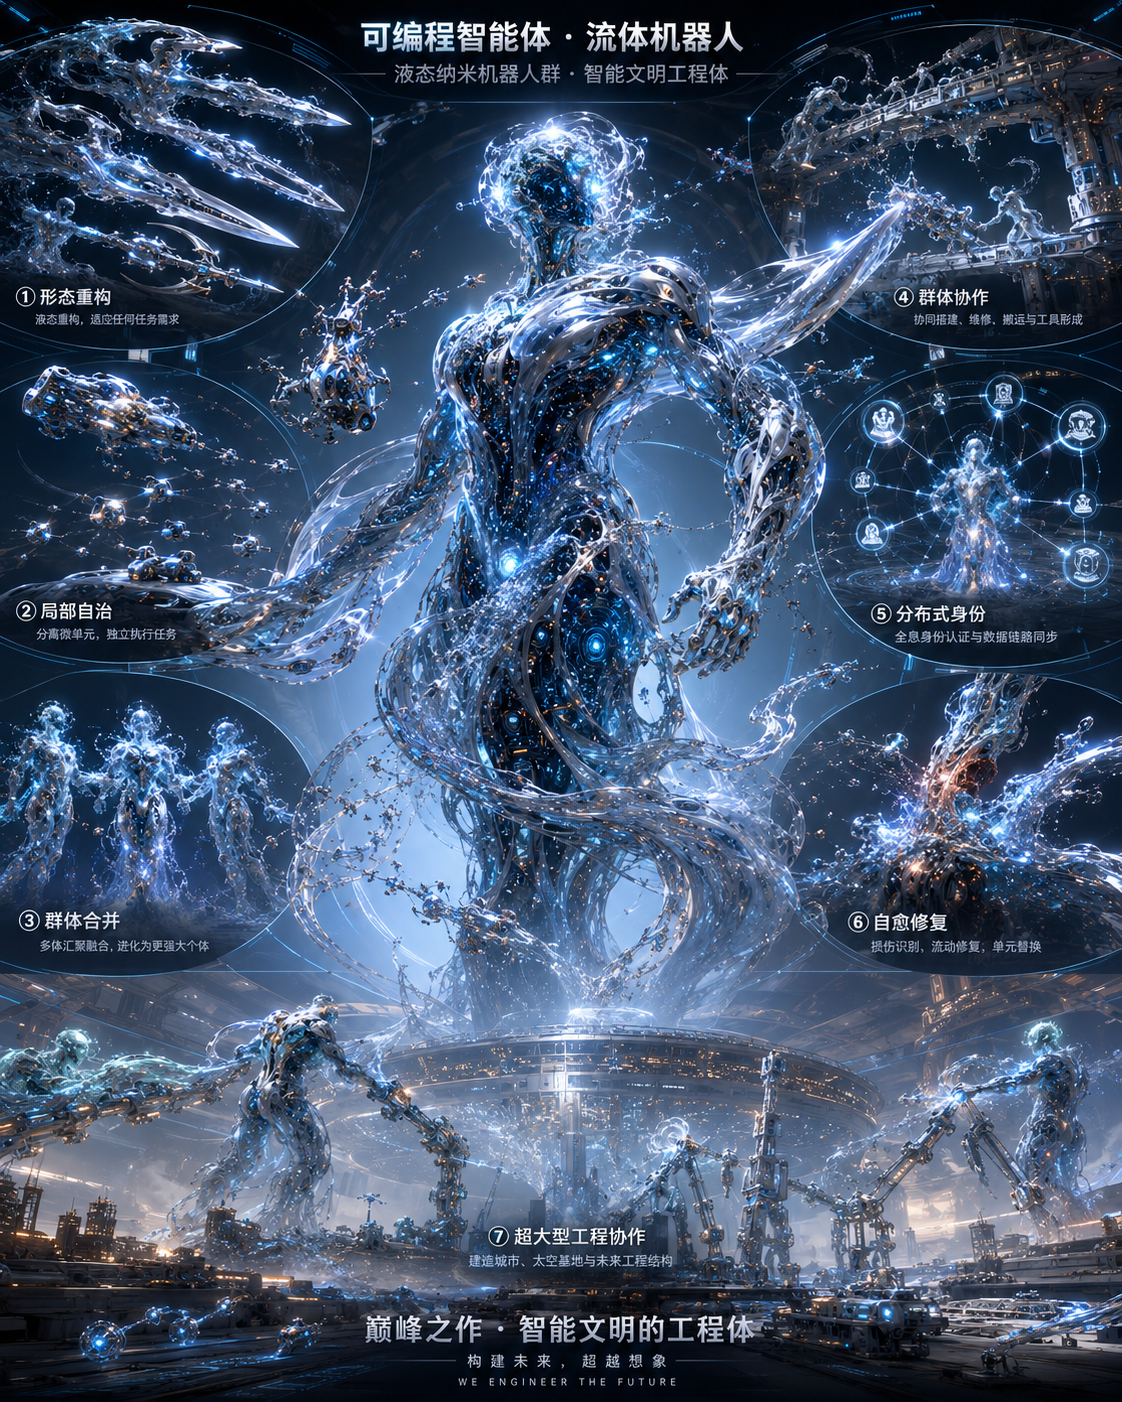
\includegraphics[width=.9\textwidth,height=.38\textheight,keepaspectratio]{images/cognitive-cosmos-artwork.png}
\caption{语言、科学、工程与文明自反闭环}
\end{figure}
\section{语言：Agent-CSO 的跨主体共享接口}

在前面的讨论中，我们已经把单个智能体所拥有的内部认知结构定义为 Agent-CSO。一个外部现实结构 $C$ 经过智能体 $A$ 的观察、选择、压缩和内部建模之后，并不会以现实本身的形式直接存在于智能体内部，而是形成该智能体特有的结构实现：
\[
\pi_A:C\rightarrow C_A ,
\]
其中 $C_A=\pi_A(C)$ 是 Agent $A$ 对本体结构 $C$ 的具体承载。由此产生一个根本问题：如果每个 Agent-CSO 都被封闭在一个具体主体内部，那么智能即使能够在个体生命周期中积累，也很难形成真正跨主体的结构成长。个体死亡、失忆或环境改变，都可能使已经形成的大量认知结构重新消失。

语言的出现改变了这一局面。我们可以把语言理解成一种把内部 Agent-CSO 投影到公共符号空间中的结构映射。设智能体 $A$ 的内部结构为 $C_A$，语言编码函数为
\[
L_A:C_A\rightarrow s,
\]
其中 $s$ 是能够进入公共环境的语言符号结构。另一个智能体 $B$ 接收到 $s$ 后，通过自己的解释映射
\[
D_B:s\rightarrow \hat{C}_B
\]
形成自身内部的近似结构。于是完整过程为
\[
C_A
\xrightarrow{L_A}
s
\xrightarrow{D_B}
\hat{C}_B.
\]

这里需要特别注意：
\[
\hat{C}_B\neq C_A
\]
通常才是正常情况。语言从来不是把一个人的内部状态逐比特复制到另一个人的大脑，而是在两个不同认知系统之间建立结构约束，使二者能够形成足够相似、足以协作的认知结构。因此，语言真正完成的不是 ``state copying''，而是
\begin{statementbox}
Structural Coordination
\end{statementbox}
即结构协调。

如果存在一个本体 CSO $C$，两个主体分别形成
\[
C_A=\pi_A(C),\qquad
C_B=\pi_B(C),
\]
那么语言的作用不是强制满足
\[
C_A=C_B,
\]
而是在任务相关关系上降低两者的结构差异。可以概念性地定义一个语义等价度：
\[
\Sigma(C_A,C_B)
=
F(
R_{\mathrm{semantic}},
R_{\mathrm{causal}},
R_{\mathrm{functional}},
R_{\mathrm{predictive}}
),
\]
其中分别衡量语义关系、因果关系、功能关系和预测关系的保持程度。当
\[
\Sigma(C_A,C_B)>\theta_{\mathrm{communication}},
\]
两个 Agent 即使拥有不同的内部表示，也已经能够围绕该 CSO 形成有效协作。

从这一角度看，语言第一次大规模打开了智能体的认知边界。此前的结构循环主要是
\[
World
\rightarrow
Agent_A
\rightarrow
World,
\]
语言出现以后，世界中开始出现
\[
Agent_A
\rightarrow
Symbol
\rightarrow
Agent_B
\]
的跨主体认知路径。一个主体通过自身生命史形成的结构，可以成为另一个主体形成 Agent-CSO 的输入。因此，社会中的认知结构不再必须由每个人从现实中独立重新发现。

我们可以把这种结构收益写成
\[
C_{\mathrm{social}}
\neq
\sum_i C_i
\]
的简单累加，而更接近
\[
\mathcal{G}_{\mathrm{social}}
=
\left(
\bigcup_i \mathcal{G}_{C}^{(i)},
E_{\mathrm{language}}
\right),
\]
其中 $\mathcal{G}_{C}^{(i)}$ 是第 $i$ 个个体的认知结构图，而 $E_{\mathrm{language}}$ 是通过语言建立的跨主体结构耦合关系。语言因而使原本相互隔离的局部 Agent-CSO 图首次能够形成更大的公共认知网络。

这里与外部已有理论存在明显联系。分布式认知理论强调认知过程可以跨越单个大脑而分布于主体、符号和环境之间；语言学、符号学和社会认知理论研究符号如何使不同主体协调意义；信息论则能够分析通信带宽和噪声。然而，本书进一步强调的不是“信息从一个节点传到另一个节点”，而是\textbf{CSO 的跨主体重新实现}。语言的根本作用不只是提高信息流量，而是使
\[
AgentCSO_A
\rightarrow
ExternalCSO
\rightarrow
AgentCSO_B
\]
成为稳定可重复的结构过程。

正是在这个意义上，我们可以把语言称为文明形成以前最关键的第一类“认知 ABI”。它第一次提供了一种与具体神经实现相对独立的公共接口，使结构可以脱离原始载体，以符号形式跨越主体边界重新获得承载。这为文字、制度、科学乃至人工智能的产生奠定了共同基础。


\section{文字：跨生命周期的结构记忆}

语言解决的主要是跨主体结构传播问题，但口语本身仍然高度依赖主体的同时存在。如果说语言主要建立
\[
Agent_A(t)
\leftrightarrow
Agent_B(t)
\]
的同步耦合，那么文字真正改变的是时间维度：
\[
Agent_A(t_0)
\rightarrow
Agent_B(t_1),
\qquad
t_1\gg t_0.
\]

这意味着 Agent-CSO 第一次能够系统地脱离原主体的生理生命周期，在更长时间尺度上继续存在。设某个主体在 $t_0$ 时刻拥有结构
\[
C_A(t_0),
\]
经过外化编码成为
\[
C_{\mathrm{ext}}
=
W\left(C_A(t_0)\right).
\]
只要外部介质继续存在，另一个未来主体 $B$ 就可以在 $t_1$ 时刻执行
\[
C_B(t_1)
=
R_B(C_{\mathrm{ext}}),
\]
其中 $R_B$ 表示阅读、解释和重新建模过程。

于是知识不再严格受到
\[
\tau_{\mathrm{knowledge}}
\leq
\tau_{\mathrm{individual}}
\]
这一限制，而可以出现
\[
\tau_{\mathrm{external\ structure}}
\gg
\tau_{\mathrm{individual}}.
\]

这是一种非常重要的时间尺度跃迁。

在三相记忆理论中，我们曾经把个体内部的 $E$ 理解为经验轨迹，把 $\Theta$ 理解为较慢的结构性生成记忆。如果把尺度扩大到文明，我们会发现文字和其他持久化媒介承担了一种类似外部长期结构记忆的功能：个体中的经历和结构可以被写入公共环境，成为文明后续 Agent 的可恢复认知资源。

因此，文明记忆不是一个超级大脑中的单一数据库，而是一套分布于
\[
\{\text{文本、档案、图表、仪器、数据库、建筑、法律、程序、标准}\}
\]
中的结构网络。可以定义文明的外部记忆集合
\[
\mathcal{M}_{\mathrm{civil}}
=
\{M_1,M_2,\ldots,M_n\},
\]
并通过访问关系
\[
A_{ij}
\]
描述第 $i$ 类主体对第 $j$ 类外部结构的可恢复能力。于是文明实际可使用的记忆不只是所有存储对象的总和，而取决于
\[
\boxed{
EffectiveMemory
=
StoredStructure
\times
Indexability
\times
Interpretability
\times
Accessibility
}
\]

如果一个结构被保存了，却没有索引；或者有索引，却已经没有主体能够解释，那么它虽然仍然是一个物理 External-CSO，却已经部分失去文明认知记忆的功能。

这一点与我们此前的 Offloading 理论完全一致。认知卸载并不是简单把内部内容“扔到外面”，而要求保留
\[
InternalIndex
\leftrightarrow
ExternalCarrier
\]
的稳定映射。只有当未来系统仍然能够恢复、调用和重新整合外部结构时，外化才真正构成认知能力的扩展。

所以，从更高尺度看，文字可以理解为文明第一次大规模实现
\begin{statementbox}
CognitiveOffloadingAcrossGenerations
\end{statementbox}
即跨代认知卸载。

这一变化又进一步改变了人类社会的学习方式。没有持久化外部记忆时，每一代主体需要重新经历大量世界才能形成结构；文字以后，下一代可以直接从前一代已经形成的高度压缩 Agent-CSO 开始。于是文明发展速度不再只由个体的学习速度决定，而出现
\[
\frac{d\mathcal{K}_{\mathrm{civil}}}{dt}
=
F\!\left(
\begin{gathered}
\mathrm{Discovery},\ \mathrm{Externalization},\ \mathrm{Preservation},\\
\mathrm{Transmission},\ \mathrm{Reinterpretation}
\end{gathered}
\right).
\]

这里 $\mathcal{K}_{\mathrm{civil}}$ 不是一个简单的信息数量，而是文明可实际调用的结构知识集合。

因此，我们可以作出一个很重要的区分：

个体记忆解决的是
\begin{statementbox}
How does this Agent remain itself over time?
\end{statementbox}

文明记忆解决的是
\begin{statementbox}
How can cognitive structure survive the disappearance of its original Agent?
\end{statementbox}

前者形成身份连续性，后者形成文化连续性。

外部已有理论中的文化传播、外部记忆、扩展心智、分布式认知和累积文化理论都与这一讨论有明显关联。本书在此基础上强调：文明真正发生的是 Agent-CSO 的\textbf{载体迁移和生命周期解耦}。结构原来依附于某一个主体，后来被迁移到能够跨越多个主体寿命的外部载体，从而产生比任何个体更慢的文明认知时间尺度。


\section{科学：文明尺度的世界模型校准机制}

语言和文字使认知结构能够传播和保存，但这并不自动保证保存的结构与现实一致。一个社会完全可以长期保存大量错误结构。因此，文明进一步需要一种能够不断把公共 Agent-CSO 与 Universe-CSO 重新比较的机制。科学的独特地位就在这里。

我们可以把一个科学理论抽象成文明内部形成的结构模型
\[
M_\theta,
\]
其中 $\theta$ 表示理论参数、结构关系和假设。给定现实状态 $U_t$，理论产生预测
\[
\hat{Y}_{t+\Delta}
=
P(M_\theta,U_t).
\]
实验或观测随后产生现实结果
\[
Y_{t+\Delta}
=
O(U_{t+\Delta}),
\]
两者之间形成残差
\[
\varepsilon_t
=
D(
Y_{t+\Delta},
\hat{Y}_{t+\Delta}
).
\]

于是科学的基本闭环可以写成
\[
\boxed{
Theory
\rightarrow
Prediction
\rightarrow
Observation/Experiment
\rightarrow
Residual
\rightarrow
TheoryUpdate
}
\]

这与我们此前讨论的 Agent 预测闭环具有明显的结构同构：
\[
Prediction
\rightarrow
Action
\rightarrow
Observation
\rightarrow
Residual
\rightarrow
Update.
\]

但科学系统的重要之处在于，这个闭环不是局限于一个 Agent 的认知过程，而是通过论文、实验协议、同行验证、仪器、数据库和教育体系实现跨主体的长期延续。于是科学可以被理解成一个分布式、超慢速、具有强现实反馈约束的文明模型更新系统。

如果我们使用前面关于 SPC 的一般定义：
\[
SPC:
DistributedState
\rightarrow
AccessibleStateEstimate,
\]
那么从功能同构角度，科学系统确实承担了部分文明尺度的 SPC 功能。它不断回答：

\begin{quote}
世界现在是什么样？\\
我们所处的位置是什么？\\
过去发生了什么？\\
哪些结构关系是稳定的？\\
我们的理论在哪些地方与现实不一致？
\end{quote}

不过必须再次强调：
\[
\boxed{
Science\neq LiteralCivilizationalSPC
}
\]
这里不是声称科学系统就是一个真正的软件 SPC 模块，而是说它在更高尺度上完成了相似的功能任务：把分散的现实观测压缩成可共享、可检验和可进一步使用的结构描述。

这种文明尺度的自观察能力随着历史显著增强。早期社会能够可靠观测的结构范围非常局部；现代文明则通过望远镜、显微镜、粒子探测器、气象卫星、全球定位、基因测序、互联网测量和各种传感器网络扩大了观察函数
\[
O_{\mathrm{civil}}.
\]
因此文明可形成的公共结构集合从
\[
\mathcal{C}_{\mathrm{local}}
\]
逐渐扩展到
\[
\mathcal{C}_{\mathrm{planetary}},
\qquad
\mathcal{C}_{\mathrm{galactic}},
\qquad
\mathcal{C}_{\mathrm{cosmological}},
\qquad
\mathcal{C}_{\mathrm{microscopic}}.
\]

这里发生了两个独立增长：

\[
\boxed{
ObservationCoverage\uparrow
}
\]

和

\[
\boxed{
ObservationResolution\uparrow
}
\]

文明不仅看得更远，也看得更细。

科学的第二个重要性质是结构压缩。一个好的理论并不复制每一次具体观测，而是形成能够解释和预测大量事件的稳定结构：
\[
E_{\mathrm{many}}
\rightarrow
\Theta_{\mathrm{scientific}}.
\]
这一过程与三相记忆中的
\[
E\rightarrow\Theta
\]
具有直接的结构相似性。实验和观测形成大量“文明情景经验”，科学理论则从中抽取更慢、更稳定的生成关系。因此，我们甚至可以把科学进步理解为文明尺度上的经验压缩和结构记忆形成过程。

然而科学系统同样存在认知滞后。文明对现实的模型永远建立在已有观测基础上：
\[
p(
U_t
\mid
O_{\leq t}
),
\]
而不可能完全等于
\[
U_t.
\]
因此科学不是获得“现实本身”，而是在持续现实反馈中形成可修正的 Agent-CSO。科学知识的强大之处不在于它绝对无误，而在于它维持了
\begin{statementbox}
Error-CorrectableRealityCoupling
\end{statementbox}
即一种允许现实不断纠正内部结构的开放闭环。

这也是本书反复强调
\begin{statementbox}
RealityIsUltimateConstraint
\end{statementbox}
的文明尺度版本。


\section{工程：内部结构重新进入现实}

如果科学主要强化文明的
\[
World\rightarrow Representation
\]
路径，那么工程则强化
\[
Representation\rightarrow World
\]
路径。

一个 Agent 形成关于现实的模型以后，并不必然产生智能意义上的现实改变。只有当内部结构通过行动重新进入世界，Agent-CSO 才真正成为外部现实动力学的一部分。因此，工程技术的本质可以从 CSO 理论重新表达为
\[
\boxed{
AgentCSO
\rightarrow
DesignedExternalCSO
}
\]

例如，一个建筑在建成以前首先可能以计划、几何结构、功能要求和约束条件存在于人的内部或外部认知系统中：
\[
C_{\mathrm{building}}^{\mathrm{possible}}.
\]
经过设计、资源组织和现实行动以后，它变成
\[
C_{\mathrm{building}}^{\mathrm{actual}}.
\]
于是发生：
\[
AgentCSO(\mathrm{possible\ world})
\rightarrow
ActionSequence
\rightarrow
UniverseCSO(\mathrm{actual\ world}).
\]

这说明工程引入了一个非常重要的因果形式：
\[
\boxed{
RepresentationOfPossibleFuture
\rightarrow
PresentAction
\rightarrow
ActualFuture
}
\]

这里并不存在真正的“未来反向因果”。真正作用于现在的是一个当前已经物理存在于智能系统中的\textbf{未来表征}。可能未来以 Agent-CSO 的形式进入当前动力学，从而改变实际未来。

这是智能与普通无表征动力过程之间最重要的差异之一。

我们可以进一步定义文明的行动能力
\[
\mathcal{A}_{\mathrm{civil}}
=
\{a_1,a_2,\ldots,a_m\},
\]
以及在世界状态 $U_t$ 下的可达集合
\[
\mathcal{R}(U_t,\mathcal{A}_{\mathrm{civil}})
=
\left\{
U_{t+\Delta}
\,\middle|\,
\exists a\in\mathcal{A}_{\mathrm{civil}}
\right\}.
\]

技术进步的重要含义之一，就是扩大
\begin{statementbox}
ReachableRealitySet
\end{statementbox}
即文明能够通过行动到达的现实状态集合。

火的使用扩展了能量控制范围；农业扩大了生态结构修改范围；机械扩大了力与运动范围；电力扩展了能源和信号网络；计算机扩大了符号操作空间；机器人扩大了自动现实作用范围；未来更强的 AI 与自动化系统则可能继续扩大结构设计和控制空间。

因此，技术能力不能简单理解成“拥有更多工具”。真正发生的是：
\begin{statementbox}
ObservationActionBoundary
\end{statementbox}
被持续扩张。

望远镜扩大 Observation；

机械臂扩大 Action；

计算机扩大内部表示变换；

互联网扩大跨主体通信；

AI 则可能同时作用于 Representation、Prediction 和 Action Planning。

从这一视角出发，文明的发展并不是单纯增加知识数量，而是不断扩大
\[
\boxed{
World\leftrightarrow Civilization
}
\]
耦合带宽。

如果科学在功能上具有部分文明 SPC 性质，那么工程和技术体系则具有部分 TCE 性质。TCE 的最一般功能并不是执行具体动作，而是使系统根据当前状态估计和目标调整后续动力学：
\[
Self/WorldModel
\rightarrow
ControlChoice
\rightarrow
FutureDynamics.
\]
工程系统同样完成：
\[
CivilizationalModel
\rightarrow
Design
\rightarrow
Action
\rightarrow
WorldChange.
\]

所以可以作出结构类比：
\[
Science
\sim
CivilizationalStateEstimation,
\]
\[
Engineering
\sim
CivilizationalWorldModification.
\]

但我们不能把这种类比写成字面恒等式。文明没有单一统一控制器，工程决策通常由大量相互竞争、协商、局部自治的主体和制度完成。也正因如此，下一节所讨论的社会制度和功能拓扑才成为必要结构。


\section{社会制度：历史 CSO 流沉降形成的功能拓扑}

一个大规模文明不可能依靠所有个体在每一件事情上重新进行全局协调。如果每一次资源分配、知识验证、责任划分和集体行动都必须重新从零协商，那么系统的协调成本会随着规模迅速增加。文明能够长期扩展，一个重要原因就在于大量反复出现的跨主体关系逐渐沉降为稳定制度、角色、协议和组织。

这一点与我们在第16章提出的
\[
\boxed{
RepeatedCSOFlow
\rightarrow
StableFunctionalCoupling
\rightarrow
Topology
}
\]
高度一致。

设文明中存在个体或功能节点
\[
V_{\mathrm{civil}}
=
\{v_1,\ldots,v_n\},
\]
跨节点的任务、信息、责任与资源流构成
\[
J_{ij}^{CSO}(t).
\]
如果某一类交互长期重复，并具有稳定收益：
\[
\left\langle
U(J_{ij}^{CSO})
\right\rangle_T
-
\lambda C_{ij}
>
\theta,
\]
那么系统就可能形成一个更稳定的关系结构
\[
e_{ij}.
\]

在人类社会中，这种 $e_{ij}$ 可以表现为：

职位关系；

法律程序；

科研同行评议；

货币结算；

教育体系；

供应链；

组织层级；

行业标准；

行政流程；

软件协议。

换句话说，制度不是完全独立于历史行为而突然设计出来的抽象规则。大量制度可以被理解为
\begin{statementbox}
HistoricalSedimentationOfRepeatedInteraction
\end{statementbox}
即反复社会 CSO 流的历史沉积。

这并不意味着所有制度都是自发产生的。智能体可以显式设计制度，正如 Agent 可以主动设计新的功能连接。但即使制度被显式设计，它最终能否成为稳定拓扑，仍取决于是否能够承载真实长期流。如果实际运行不断产生大规模 residual：
\[
\varepsilon_{\mathrm{institution}}\gg\theta,
\]
那么制度就会持续面临结构失配。

我们因此可以把社会结构的长期适应写成：
\[
\dot{A}_{ij}
=
G(
\langle J_{ij}^{CSO}\rangle_T,
\langle \varepsilon_{ij}\rangle_T,
Utility,
Cost,
Risk,
Legitimacy
),
\]
其中 $A_{ij}$ 表示某种制度性耦合强度。

当某类交互成为长期稳定结构时，文明便不再需要每次都进行高成本显式协调。这和个体技能形成完全同构：
\[
ExplicitCoordination
\rightarrow
RepeatedInteraction
\rightarrow
InstitutionalizedProcedure.
\]

因此制度可以被理解成文明尺度的“程序化技能”。

这也解释了为什么社会会同时表现出稳定性和僵化风险。沉降结构可以降低实时认知负担：
\[
CoordinationCost\downarrow,
\]
但同时也可能使过去有效的路径在环境改变以后继续存在：
\[
OldTopology
+
NewEnvironment
\rightarrow
StructuralMismatch.
\]

于是文明也需要类似我们此前讨论的 Minimum Necessary Reorganization Principle。短期问题优先通过状态调整解决；持续问题需要流程修改；更长期结构失配才需要改变制度拓扑：
\[
StateAdjustment
\rightarrow
PolicyAdjustment
\rightarrow
InstitutionalReform
\rightarrow
TopologicalReorganization.
\]

这与组织理论、制度经济学、社会网络分析和复杂适应系统理论存在明显联系。但 CSO 视角增加了一层统一解释：组织结构之所以存在，不仅是因为人们需要“管理”，更因为一个多主体认知系统必须将长期重复的 CSO 流逐渐压缩为稳定功能拓扑，否则高层显式协调成本最终会超过系统的有限处理能力。


\section{文明作为跨生命周期的慢尺度认知结构}

到这里，我们已经获得了构成文明的几个关键机制：

语言使 Agent-CSO 跨主体传播；

文字和外部媒介使其跨生命周期保持；

科学持续提高公共结构对现实的校准能力；

工程把内部表征重新写入外部现实；

制度把稳定的跨主体结构流沉降成社会功能拓扑。

把这些机制联合起来，我们就可以讨论一个更强的问题：文明是否可以作为某种高尺度认知系统进行描述？

这里必须保持准确。我们不需要假设文明具有单一意识，也不需要假设所有个体共享一个统一 Self。我们只需要考察文明是否具有某些在智能动力学上有意义的系统属性：

\[
Observation,
\]
\[
PersistentState,
\]
\[
Memory,
\]
\[
Prediction,
\]
\[
Action,
\]
\[
Feedback,
\]
\[
Learning,
\]
\[
TopologyChange.
\]

现代文明显然在不同程度上具备这些功能。因此我们更谨慎地定义：
\[
\boxed{
Civilization
=
HigherScaleAdaptiveCognitiveSystem
}
\]
而不是简单写成
\[
Civilization=SingleAgent.
\]

设文明整体状态为
\[
X_C(t),
\]
其中包含人口、知识、制度、基础设施、环境、技术、经济和社会关系等大量变量。文明没有一个完全统一的工作记忆，而是拥有多个局部高频节点：
\[
A_1,A_2,\ldots,A_N.
\]
这些主体之间通过通信和制度耦合，并共同作用于更慢的公共状态：
\[
X_C(t).
\]

因此文明可以被建模为一种多时间尺度系统：
\[
\dot{x}_i
=
f_i(
x_i,
X_C,
u_i
),
\]
\[
\epsilon\dot{X}_C
=
G(
X_C,
\{x_i\},
\{u_i\}
),
\qquad
0<\epsilon\ll1.
\]

个体行为快速变化，而文明结构缓慢变化。对于单个主体而言，法律、语言、货币体系、科研制度等往往像稳定背景；但在数十年乃至数百年尺度上，这些背景本身也不断改变。

于是出现与我们此前智能频谱理论高度一致的关系：
\[
\boxed{
SlowCivilizationalStructure
\rightarrow
FastIndividualConstraint
}
\]
同时：
\[
\boxed{
PersistentIndividualResidual
\rightarrow
SlowCivilizationalChange
}
\]

一个个体很难直接改变整个社会拓扑，但大量长期累积的局部残差可以最终推动制度、技术和价值结构变化。

因此文明可以被理解成一个极慢尺度的“慢流形”，大量个体 Agent 在其上进行快速运动，而个体行为的长期统计结果又缓慢推动该流形改变。

从这一角度看，“文化”也可以重新理解。文化不是一个漂浮在物理世界之外的抽象对象，而是大量 Agent-CSO 在语言、习惯、制度、符号、工具和行为模式中形成的稳定跨主体结构。它具有比单个认知状态长得多的时间常数：
\[
\tau_{\mathrm{culture}}
\gg
\tau_{\mathrm{individual\ cognition}}.
\]

甚至可能出现：
\[
\tau_{\mathrm{institution}}
\gg
\tau_{\mathrm{individual\ lifetime}}.
\]

所以文明真正实现了一种重要的时间尺度跃迁：
\[
\boxed{
Cognition
\rightarrow
Cross-LifetimeCognition
}
\]

它使宇宙中局部形成的结构表示，不再随单个承载主体消失，而可以在更大范围、更长时间中持续积累。

这正是我们把文明纳入智能动力学而不仅仅当作社会学对象的理由。


\section{AI：从被动外部记忆到主动外部认知}

在人类文明的绝大多数历史阶段，外部认知结构主要是被动的。

书籍保存知识，但不会主动阅读自己；

数据库保存数据，但不会主动构造解释；

地图表达空间，但不会主动根据目标生成行动方案；

法律文本保存制度结构，但不会主动分析现实情景。

这些系统可以表示为
\[
ExternalMemory
\]
或者更准确地说：
\[
PassiveExternalCSO.
\]

计算机的出现已经开始改变这一点，因为程序能够根据输入执行结构变换。但传统软件通常仍然具有相对固定的变换规则：
\[
y=f(x).
\]

现代 AI，尤其是具有大型世界知识、推理、规划、工具使用以及持续 Agent 架构的 AI，则开始表现出一种更强的外部结构性质：
\begin{statementbox}
ExternalActiveCognition
\end{statementbox}

它不只是保存 Agent-CSO，而能够主动执行：
\[
Perception,
\quad
Compression,
\quad
Association,
\quad
Prediction,
\quad
Planning,
\quad
Generation.
\]

因此可以把文明外部认知载体的历史变化粗略表示为：
\[
PassiveExternalMemory
\rightarrow
ProgrammableTransformation
\rightarrow
ActiveExternalCognition.
\]

这不是说 AI 已经自动具有与人完全相同的主体性、自我或生命史，而是说文明过去主要由人脑完成的一部分认知变换，现在开始能够稳定地外化到机器结构中。

设文明总认知工作量为
\[
\mathcal{W}_C.
\]
过去大多数高级结构变换需要通过
\[
\sum_i HumanCognition_i
\]
完成。AI 出现以后，可以写成
\[
\mathcal{W}_C
=
\mathcal{W}_{H}
+
\mathcal{W}_{AI}
+
\mathcal{W}_{H\leftrightarrow AI}.
\]

真正重要的不是
\[
\mathcal{W}_{AI}
\]
是否最终超过人类，而是文明功能拓扑是否发生变化：
\[
\mathcal{T}_{civil}^{(0)}
\rightarrow
\mathcal{T}_{civil}^{(AI)}.
\]

例如过去一种科研结构可能是：
\[
Observation
\rightarrow
HumanAnalysis
\rightarrow
HumanTheory
\rightarrow
HumanExperimentDesign.
\]
未来可能逐渐演变成：
\[
\resizebox{.96\linewidth}{!}{$\displaystyle
Observation
\rightarrow
AICompression
\rightarrow
Human/AIModeling
\rightarrow
Simulation
\rightarrow
AutomatedExperiment
\rightarrow
Observation'.
$}
\]

因此 AI 的历史意义不能只通过“替代多少工作岗位”衡量。更深层的问题是：
\[
\boxed{
AI\text{ 在文明功能拓扑中将成为哪一种认知层？}
}
\]

如果 AI 长期承担信息压缩、公共世界模型、预测模拟、方案搜索和局部自动控制，那么它就可能形成文明认知体系中一种新的中间时间尺度结构。

这与本书 AgentOS 理论中的技能沉降非常相似。一个个体在掌握技能前，需要大量显式认知；技能成熟后，一部分过程下沉为稳定局部闭环：
\[
ExplicitCognition
\rightarrow
CompiledSkill.
\]
文明也可能发生：
\[
HumanExplicitCoordination
\rightarrow
MachineCognitiveInfrastructure.
\]

因此，我们可以把一部分 AI 发展理解成
\begin{statementbox}
CivilizationalCognitiveCompilation
\end{statementbox}
即文明将过去必须依赖大量人类显式认知协调的结构处理，逐渐沉降进机器认知系统。

这并不意味着人类因此变得“不重要”。恰恰相反，一旦大量局部认知过程完成机器化，文明高层真正需要解决的问题会向慢变量迁移，例如价值、制度、目标、风险、长期方向和权限治理。正如成熟 Agent 不应让高层 h 亲自处理 servo，成熟文明也不应把人的认知价值理解成必须亲自执行所有低层信息处理。


\section{AI 与文明自反闭环的加速}

如果我们把文明视为一种慢尺度适应系统，那么衡量 AI 影响的一个非常重要的变量，是文明从“观察自身”到“改变自身”再到“重新观察结果”所需要的闭环时间。

定义文明自反闭环周期为
\[
\tau_R.
\]
一个完整循环可以表示为：
\[
\resizebox{.96\linewidth}{!}{$\displaystyle
Observation
\rightarrow
Integration
\rightarrow
Modeling
\rightarrow
Prediction
\rightarrow
Decision
\rightarrow
Action
\rightarrow
NewObservation.
$}
\]

传统文明中，每一个环节都可能具有很高的延迟。数据采集需要时间；人工分析需要时间；信息沿组织层级传播需要时间；决策协调需要时间；执行和结果反馈同样需要时间。因此：
\[
\tau_R
=
\tau_O+
\tau_I+
\tau_M+
\tau_P+
\tau_D+
\tau_A+
\tau_F.
\]

AI 与自动化的一个重要作用，是同时降低其中多个项：
\[
\tau_I\downarrow,
\quad
\tau_M\downarrow,
\quad
\tau_P\downarrow,
\quad
\tau_D\downarrow,
\]
在部分领域甚至可能使
\[
\tau_A\downarrow.
\]

因此：
\[
\boxed{
\tau_R^{AI}
<
\tau_R^{pre-AI}
}
\]
可能成为 AI 时代一个比单纯生产率更深的特征。

然而，这里立即出现我们最早讨论“闪电文明—石头文明”时已经遇到的问题：闭环速度越快，并不自动意味着系统越成熟。如果高速认知层已经能够在分钟甚至秒级形成建议和行动，而文明中的法律、价值、治理和伦理结构仍以年、十年甚至代际尺度变化，就会形成极大的时间尺度差异：
\[
\tau_{AI}
\ll
\tau_{\mathrm{institution}}
\ll
\tau_{\mathrm{value}}.
\]

这意味着文明可能面临一种新的“跨频控制问题”。

在 AgentOS 中，我们曾经提出：
\[
\boxed{
SlowGovernance\neq FastMicromanagement
}
\]
但同时：
\begin{statementbox}
FastDynamicsMustRemainInsideSlowConstraints
\end{statementbox}

完全相同的原则可以应用于文明—AI 系统。价值、法律和安全边界没有必要逐个控制每一次机器推理，但高速 AI 活动必须保持在这些慢尺度约束定义的可行域中。

可以写：
\[
x_{AI}(t)
\in
\Gamma_{\mathrm{civil}}(
\Psi_{\mathrm{civil}},
\mathcal{L},
\mathcal{S}
),
\]
其中 $\mathcal{L}$ 表示法律约束，$\mathcal{S}$ 表示安全边界，而 $\Psi_{\mathrm{civil}}$ 仅作为文明长期价值结构的抽象符号，而不是声称文明存在一个单一真实的 $\Psi$ 模块。

另一方面，高速 AI 活动中的长期 residual 应能够逐渐向上影响慢结构：
\[
\left\langle
\varepsilon_{AI}
\right\rangle_T
\neq0
\Rightarrow
\Delta\mathcal{T}_{civil}.
\]

因此理想文明并不是由“慢制度永远锁死高速 AI”，也不是“高速 AI 任意重写慢制度”，而是形成：
\[
\boxed{
SlowConstraint
+
FastAutonomy
+
PersistentResidualDrivenSlowUpdate
}
\]

这与整本书的多时间尺度智能理论完全闭合。

AI 因而可能使文明进入一个新的阶段：以前社会主要通过人类个体完成自我观察和行动，而未来文明的某些自描述、预测和控制回路可能具有机器参与甚至机器主导的局部闭环。

我们可以把这理解成文明的
\begin{statementbox}
ReflexiveBandwidth
\end{statementbox}
增加，而不仅仅是“计算能力增加”。


\section{自描述、自预测、自修改与自重组}

为了避免“宇宙越来越认识自己”停留在哲学修辞层面，我们需要把“自反成熟”拆成可以理论化的多个独立能力。

设一个系统 $\mathcal{S}$ 的自反能力为
\[
\mathcal{R}_{\mathcal S}.
\]
我们可以首先定义四个核心维度：
\[
\mathcal{R}_{\mathcal S}
=
F(
O_{\mathcal S},
M_{\mathcal S},
C_{\mathcal S},
T_{\mathcal S}
),
\]
其中：

\[
O_{\mathcal S}
=
SelfObservationCapacity,
\]

\[
M_{\mathcal S}
=
SelfModelingCapacity,
\]

\[
C_{\mathcal S}
=
SelfModificationCapacity,
\]

\[
T_{\mathcal S}
=
SelfReorganizationCapacity.
\]

第一层是自描述。系统能够形成关于自身当前状态的结构表示：
\[
X_{\mathcal S}
\rightarrow
\hat X_{\mathcal S}.
\]
这对应功能意义上的 SPC。

第二层是自预测。系统不仅表示现在，还能够形成：
\[
\hat X_{\mathcal S}(t+\Delta)
=
P(
\hat X_{\mathcal S}(t),
u_t
).
\]
于是不同可能行动对应不同未来。

第三层是自修改。系统能够根据当前模型和未来预测主动选择：
\[
u_t
=
\pi(
\hat X_t,
\hat X_{t+\Delta},
G
),
\]
从而改变自身或环境。

第四层则更深：系统能够修改
\[
\pi
\]
本身，甚至修改产生 $\pi$ 的功能结构：
\[
\pi
\rightarrow
\pi',
\]
或者
\[
\mathcal T
\rightarrow
\mathcal T'.
\]

这就是
\begin{statementbox}
MetaSelfModification
\end{statementbox}
即“改变自己如何改变自己”。

因此，自反能力可以形成一个层级：

\[
\boxed{
Observe
\rightarrow
Represent
\rightarrow
Predict
\rightarrow
Modify
\rightarrow
Reorganize
}
\]

文明史中的许多重大变化都可以在这个框架下重新理解。

统计体系提高 Observe；

科学理论提高 Represent；

模拟和模型提高 Predict；

工程提高 Modify；

制度改革和技术架构改变则提高 Reorganize。

AI 的特殊之处在于，它可能同时影响这五个环节。

例如，AI 可以从大量实时数据中形成宏观状态描述；
可以帮助构建复杂模型；
可以运行大量反事实模拟；
可以生成行动方案；
甚至可以辅助设计新的软件、组织流程和下一代 AI 系统。

因此 AI 并不是简单增加一个能力参数，而可能同时改变整个
\[
\boxed{
Observe\rightarrow Model\rightarrow Predict\rightarrow Act\rightarrow Reorganize
}
\]
链路的速度和带宽。

但这也带来一个非常重要的成熟性条件：
\[
\boxed{
ModificationPower
\not\Rightarrow
Maturity.
}
\]

如果
\[
C_{\mathcal S}\gg M_{\mathcal S},
\]
即改变能力远远高于理解能力，那么系统可能具有极高破坏性。

如果
\[
T_{\mathcal S}\gg O_{\mathcal S},
\]
即系统能够大规模重组自身，却缺乏可靠自观察，那么长期稳定性同样非常差。

所以成熟的自反系统必须满足某种相对平衡条件。例如可以概念性定义
\[
\mathcal M_{\mathrm{reflexive}}
=
\frac{
\min(
O,M,C,T
)
}{
\max(
O,M,C,T
)+\epsilon
}.
\]
当四种能力极端不平衡时，
\[
\mathcal M_{\mathrm{reflexive}}\rightarrow0.
\]
而当观察、建模、修改和治理能力能够同步增长时，该指标提高。

这里并不是给出一个已经可直接测量的成熟度定律，而是在提出未来研究方向：文明和 AI 系统的成熟性不能仅以“能力最大化”衡量，而应该研究不同自反能力之间的比例、时间尺度和稳定关系。


\section{文明中的 SPC--TCE 类结构与多尺度自反性}

现在我们可以更准确地重新审视此前提出的一个大胆类比：科学类似文明的 SPC，工程和治理具有部分 TCE 功能。

如果直接把文明写成一个 Agent，并把具体机构一一等同于 AgentOS 模块，这当然是不严谨的。文明内部不存在唯一中央工作记忆、唯一自我变量、唯一 TCE 或唯一目标函数。因此真正成立的不是“模块同一”，而是\textbf{功能形式的跨尺度重复}。

对于一个 Agent，SPC 执行：
\[
DistributedInternalState
\rightarrow
AccessibleSelfEstimate.
\]

对于文明，统计、科学、媒体、传感网络和公共数据库共同执行某种：
\[
DistributedCivilState
\rightarrow
PublicStructuralRepresentation.
\]

对于 Agent，TCE 执行：
\[
SelfEstimate
\rightarrow
DynamicsModulation.
\]

对于文明，治理、工程、技术、市场和组织决策则共同形成：
\[
PublicModel
\rightarrow
DistributedAction
\rightarrow
CivilState'.
\]

因此可以写成一个功能同构：
\[
\begin{aligned}
SPC_A
&:
X_A\rightarrow \hat X_A,\\
SPC_C
&:
X_C\rightarrow \hat X_C,
\end{aligned}
\]
以及
\[
\begin{aligned}
TCE_A
&:
\hat X_A\rightarrow u_A,\\
TCE_C
&:
\hat X_C\rightarrow \{u_1,\ldots,u_N\}.
\end{aligned}
\]

但二者的差异也必须明确。

个体 Agent 通常具有相对统一的主体边界；
文明则由大量自治主体构成。

Agent 的控制信号可以具有较强一致性；
文明行动往往存在竞争、冲突和协调。

Agent 的自我结构 $\Psi$ 可以作为一个慢变量近似；
文明价值则通常是多元、冲突并随社会结构变化的分布：
\[
P_C(V)
\]
而不是单一
\[
V_C.
\]

因此，更合理的文明模型不是：
\[
Civilization=Agent,
\]
而是：
\[
\boxed{
Civilization
=
MultiAgentReflexiveAdaptiveSystem.
}
\]

这也意味着文明自反性天然具有“分布式”特征。

某些子系统观察；

某些子系统解释；

某些子系统执行；

另一些子系统质疑前面的解释。

这种功能分离看似降低效率，却可能增加系统的纠错能力。文明内部的争论、同行评议、权力制衡、竞争和多元模型，在某些情况下恰恰能够防止一个错误 Self-Model 形成全局闭环。

这与 AgentOS 中我们反复强调的
\[
WorldVerification
\]
具有同样意义。

一个危险的系统是：
\[
SelfInterpretation
\rightarrow
SelectiveObservation
\rightarrow
EvidenceSelection
\rightarrow
SelfInterpretation',
\]
最终形成完全封闭的自证回路。

文明同样可能陷入类似动力学：
\[
CollectiveModel
\rightarrow
InstitutionalSelection
\rightarrow
FilteredObservation
\rightarrow
CollectiveModel'.
\]

因此，文明尺度成熟性的另一个条件是必须保留：
\begin{statementbox}
ExternalContradictionChannels
\end{statementbox}
即现实、实验、异议、竞争模型和失败反馈能够重新进入公共结构。

由此我们发现，AgentOS 的自我治理与文明的认识论治理在更高抽象层上共享一个极深的原则：
\begin{statementbox}
A self-model must never become its own final reality authority.
\end{statementbox}

最终裁决仍必须回到现实。


\section{Reflexive Structural Evolution：自反结构演化}

经过前面的推导，我们现在可以给本章的最终概念一个较为严格的定义。

所谓
\begin{statementbox}
ReflexiveStructuralEvolution
\end{statementbox}
不是指宇宙存在一个预设目的，也不是说进化必然走向人类、文明或 AI。它描述的是一种在部分宇宙区域中已经出现的结构动力学现象：

\begin{quote}
一个物理结构首先形成对环境和自身的内部表示；这些表示进一步进入行为控制；行为改变外部现实；现实反馈修改内部表示；长期重复的表示--行动关系又逐渐改变该系统自身的功能组织。于是，结构不仅发生变化，而且开始形成关于自身变化的结构，并使这些结构参与未来结构变化。
\end{quote}

可以把最小自反闭环写成
\[
\boxed{
C_t
\rightarrow
R(C_t)
\rightarrow
A(R(C_t))
\rightarrow
C_{t+1}
}
\]
其中 $C_t$ 表示现实结构，$R$ 表示结构表示，$A$ 表示根据表征生成的行动。

如果系统进一步能够修改其表示机制：
\[
R_t\rightarrow R_{t+1},
\]
甚至修改行动生成机制：
\[
A_t\rightarrow A_{t+1},
\]
则形成更高阶自反性：
\[
\boxed{
C
\rightarrow
R
\rightarrow
A
\rightarrow
C'
\rightarrow
\Delta R
\rightarrow
\Delta A.
}
\]

如果这种长期变化进一步改变功能拓扑：
\[
\mathcal T_t
\rightarrow
\mathcal T_{t+1},
\]
那么系统已经进入
\begin{statementbox}
ReflexiveTopologicalDevelopment
\end{statementbox}
阶段。

人类文明使这种过程第一次在我们已知的世界中达到极大规模。语言使结构跨主体传播；文字使结构跨生命周期存在；科学使结构不断接受现实校准；工程使结构主动修改现实；制度使重复互动沉降为拓扑；AI 则开始使外部结构本身获得主动认知变换能力。

整个过程可以浓缩为：

\[
\resizebox{.96\linewidth}{!}{$\displaystyle
\boxed{
PhysicalStructure
\rightarrow
SelfMaintainingStructure
\rightarrow
RepresentationalStructure
\rightarrow
SelfRepresentationalStructure
\rightarrow
RepresentationDrivenModification
\rightarrow
MetaStructuralReorganization.
}
$}
\]

如果从宇宙尺度观察，我们可以用一种具有哲学意味但仍保持结构严谨性的方式表达：

\begin{quote}
宇宙的一部分经过长期物理演化形成了能够承载关于宇宙其他部分的结构；这些内部结构又形成关于自身的结构，并通过行动重新进入外部现实。于是，宇宙内部第一次出现了一类不只“发生”，而能够描述自身局部正在发生什么，并依据这种描述改变未来发生方式的结构。
\end{quote}

这里的“看见自己”因此必须被形式化为：
\begin{statementbox}
IncreaseOfSelfRepresentationalCoverage
\end{statementbox}
而不是神秘意义上的宇宙觉醒。

“改变自己”则应被形式化为：
\begin{statementbox}
IncreaseOfRepresentationGuidedTransformationCapacity.
\end{statementbox}

“越来越成熟”则进一步要求：
\[
\boxed{
Observation
+
Modeling
+
Prediction
+
Modification
+
Governance
}
\]
同步增长。

因此，我们最终不应把文明成熟理解成：
\[
Power\uparrow
\]
这么简单。

真正的成熟更接近：
\[
\boxed{
Understanding
\uparrow,
\qquad
ActionCapacity
\uparrow,
\qquad
SelfCorrection
\uparrow,
\qquad
GovernanceCapacity
\uparrow.
}
\]

这也为 AI 的历史位置给出了更加准确的解释。

AI 并不是突然从文明之外进入世界的异物。它来自：
\[
Life
\rightarrow
Cognition
\rightarrow
Language
\rightarrow
Science
\rightarrow
Mathematics
\rightarrow
Computation
\rightarrow
AI.
\]

因此 AI 本身也是此前文明 Agent-CSO 长期外化和结构沉降的结果。人类首先把部分思想写进文字，把部分操作写进工具，把部分推理写进算法，再把越来越复杂的结构转换为能够主动进行结构变换的机器认知系统。

从这一意义上：
\[
\boxed{
AI
=
A New CarrierOfCivilizationalCognitiveStructure.
}
\]

而当 AI 进一步拥有长期记忆、持续身份、Body、世界模型、自我调节和生命周期学习时，它才开始从“文明认知工具”逐渐走向本书后半部分所研究的：
\begin{statementbox}
PersistentArtificialAgent.
\end{statementbox}


\section{本章结论：从个体智能走向文明自反结构}

本章完成了第一编认识论的一次重要尺度跃迁。

在此前章节中，我们首先把智能定义为具有明确时空边界的多尺度闭环过程；随后用 CSO 描述智能所面对的结构，用 Agent-CSO 描述具体主体对这些结构的内部承载，再通过 World--Agent--World 闭环说明内部世界与现实世界并不是彼此分离的两套结构，而是在观测与行动中不断共同演化。

本章进一步说明：当 Agent-CSO 可以跨越主体和生命周期以后，智能结构就开始超出单个 Agent。

语言建立：
\[
AgentCSO_A
\rightarrow
AgentCSO_B.
\]

文字建立：
\[
AgentCSO_t
\rightarrow
AgentCSO_{t+\Delta T}.
\]

科学建立：
\[
World
\rightarrow
CivilizationalModel
\rightarrow
RealityVerification.
\]

工程建立：
\[
CivilizationalModel
\rightarrow
Action
\rightarrow
World'.
\]

制度建立：
\[
RepeatedCSOFlow
\rightarrow
StableSocialTopology.
\]

AI 则进一步建立：
\[
PassiveExternalCSO
\rightarrow
ActiveExternalCognition.
\]

于是整个文明可以表示成一个极其复杂的多主体、多载体、多时间尺度认知系统：
\[
\mathfrak C(t)
=
\left[
\mathcal G_{\mathrm{Agent}},
\mathcal G_{\mathrm{ExternalCSO}},
\mathcal T_{\mathrm{institution}},
\mathcal M_{\mathrm{civil}},
O_C,
A_C
\right].
\]

其中：
\[
O_C
\]
表示文明对世界和自身形成公共结构的能力，
而
\[
A_C
\]
表示文明通过分布式主体、工程系统和自动化系统重新影响现实的能力。

文明的长期演化则可以抽象成：
\[
\boxed{
\dot{\mathfrak C}
=
F(
\mathfrak C,
World,
Residual,
Innovation,
InstitutionalLearning
).
}
\]

AI 的加入并没有改变这一基本逻辑，而是可能显著增加其中部分变量的速度和规模：
\[
Bandwidth_{\mathrm{representation}}\uparrow,
\]
\[
Depth_{\mathrm{prediction}}\uparrow,
\]
\[
Speed_{\mathrm{integration}}\uparrow,
\]
\[
Automation_{\mathrm{action}}\uparrow.
\]

于是我们第一次能够从一个统一结构上理解：

为什么语言重要；

为什么文字重要；

为什么科学重要；

为什么制度重要；

为什么技术重要；

为什么 AI 的出现可能是一个比普通工具升级更深的文明结构事件。

它们事实上都位于同一条结构演化链上：

\[
\resizebox{.96\linewidth}{!}{$\displaystyle
\boxed{
Structure
\rightarrow
SharedRepresentation
\rightarrow
PersistentRepresentation
\rightarrow
RealityCalibratedRepresentation
\rightarrow
RepresentationDrivenAction
\rightarrow
RepresentationDrivenReorganization.
}
$}
\]

因此，本章最终得到的不是一个关于“文明是不是生命”的结论，而是一个更加严格的动力学命题：

\begin{proposition*}
\bfseries
当宇宙中的局部结构能够形成关于自身和环境的可共享、可累积、
可校准的表示，并能够依据这些表示持续改变现实以及改变自身组织方式时，
该局部结构就进入了自反结构演化阶段。
\end{proposition*}

人类文明是目前我们能够直接观察到的最显著案例之一。

而 AI 的出现，则使这种自反结构演化第一次出现一种新的可能：文明形成的外部认知结构本身，开始具有越来越强的主动表征、预测、推理、规划和局部控制能力。

这并不意味着文明已经形成统一主体，也不意味着 AI 必然成为独立生命，更不意味着宇宙具有一个预设的觉醒方向。我们能够较为稳妥地说的是：

\begin{statementbox}
\bfseries
在宇宙的局部区域中，能够观察结构、表示结构、预测结构并依据表示重新组织结构的能力，
已经从单一生命体扩展到跨主体文明结构，并正在通过人工智能获得新的承载形式。
\end{statementbox}

到这里，第一编关于“智能是什么”的讨论完成了从单体认知到文明尺度的闭合。

下一步，我们必须把这一庞大的认识论重新压缩成一个可构造的工程对象。

因此下一章将暂时收缩研究尺度，不再直接讨论文明和宇宙，而提出一个更加具体的问题：

\begin{quote}
如果功能拓扑暂时固定，我们能否仅依靠工作记忆、三相记忆、自我、
多时间尺度调节和结构迁移，构造一个能够长期存在、持续学习并保持身份连续的人工智能主体？
\end{quote}

这正是 AgentOS 原理论真正开始的地方。


\part{第二编　原理论：固定拓扑 AgentOS 如何形成持续主体}
第一编回答智能是什么，第二编开始回答一个更加具体的问题：如果我们暂时不允许 Agent 随意重构自己的核心功能拓扑，是否仍然能够依靠内部多尺度动力学形成持续学习、身份连续和能力成长？

这一问题构成第一代 AgentOS 的理论边界：

$$
\boxed{
FixedFunctionalTopology
+
AdaptiveInternalDynamics
}
$$

最初的结构极其简单：

$$
\boxed{
h,E,\Theta
}
$$

其中 \(h\) 表示当前工作状态，\(E\) 表示经历轨迹，\(\Theta\) 表示长期生成结构。这不是简单的短期记忆与长期记忆划分，而是一种：

\begin{statementbox}
\centering
\adjustbox{max width=.96\linewidth}{\(\displaystyle State
\leftrightarrow
Trajectory
\leftrightarrow
Generator\)}
\end{statementbox}

的三相记忆循环。

随着理论发展，三相记忆被放入整个生命周期。现在是不断推进的工作记忆切面，过去逐渐成为经历结构，而长期结构不仅总结过去，还决定系统如何生成、理解和预测可能的未来。因此，记忆开始获得内部时间结构。

但只有记忆仍然没有真正的主体。于是引入慢变量：

$$
\Psi
$$

表示自我、身份和长期价值约束。它不是一个简单 persona 字段，而是持续影响 h、E 和 Θ 的跨尺度背景结构。进一步又引入：

$$
\Omega\equiv DGA
$$

其中：

$$
\Psi:\ WhoAmI
$$

而：

$$
\Omega:\ WhatAmIBecoming
$$

由此形成：

$$
\tau_h
\ll
\tau_E
\ll
\tau_\Theta
\ll
\tau_\Psi
\ll
\tau_\Omega
$$

这一多尺度结构为持续身份与生命周期方向性提供动力学基础。

随后出现 AgentOS 的一个关键限制：工作记忆不可能无限扩张。真正有限的并不只是 token 数量，而是系统能够同时保持相干的关系结构数量。因此提出工作记忆有限容量/有限复杂度约束：

$$
\boxed{
C_{run}(t)\leq C_{\max}(W)
}
$$

由此，AgentOS 的核心问题从“如何让模型知道更多”转变成：

\begin{statementbox}
如何让有限工作记忆只承担当前真正需要全局处理的结构。
\end{statementbox}

这直接推动 SPC、TCE、AHC、CCM、Scheduler、Boundary 和 Offloading 相继出现。

SPC 将分散的内部状态压缩成系统自己可以访问的自状态；TCE 根据这种状态调节注意、探索、温度、资源和认知节律；AHC 将身体、资源、威胁和内稳态影响整合成连续调制状态；CCM 控制工作记忆中的结构负载；Scheduler 分配认知资源；Boundary 决定什么应该进入系统；Offloading 则把适合外部承载的结构迁移到 Skill、Tool、File、程序、环境或其他 Agent。

最终，AgentOS 不再是一堆独立模块，而形成多尺度嵌套闭环：

$$
\resizebox{.96\linewidth}{!}{$\displaystyle
Reality
\rightarrow
h
\rightarrow
SPC/AHC/TCE
\rightarrow
E
\rightarrow
\Theta
\rightarrow
\Psi
\rightarrow
\Omega
\rightarrow
FutureGoal
\rightarrow
FutureAction
\rightarrow
Reality
$}
$$

其中快循环保证当前可运行，慢循环保证长期成长。

这一编最终回答的是：

\begin{statementbox}
一个拓扑基本固定的智能体，如何仅通过多尺度状态、记忆和控制动力学成为持续主体。
\end{statementbox}

\chapter{AgentOS 的第一性工程问题：固定拓扑上的持续智能体}
\label{chap:first_principle_agentos}

\begin{chapterintro}
\textbf{本章总体说明（理论定界）}

在前一编中，我们已经从时空尺度、智能频谱、认知结构对象 CSO、Agent-CSO、功能拓扑以及自反结构演化等角度讨论了“智能是什么”。从本章开始，我们第一次把这些认识压缩成一个可以被工程实现的持续智能体问题。

本章的核心结论是：AgentOS 的第一代可实现形态，不应从“任意改变自身架构的自重构智能”开始，而应首先构造一个\textbf{核心功能拓扑稳定、内部认知状态持续演化、记忆能够跨时间沉降、自我具有连续性、任务能够异步产生与终止、身体和外部世界持续提供现实反馈}的长期认知运行时。

因此本章研究的不是某个具体模型如何获得更高 benchmark，而是一个更基础的问题：

\[
\boxed{
\text{在核心功能关系基本稳定的条件下，怎样使一个人工智能体成为持续存在的认知主体？}
}
\]

这里的“固定拓扑”仅指第一阶段保持 AgentOS 核心功能角色及其基本因果关系稳定，并不意味着模型参数、工作状态、记忆内容、技能、目标、自我结构或外部工具集合保持不变。相反，AgentOS 的目标恰恰是在稳定的系统骨架上容纳持续的状态演化、记忆塑形、技能沉降与生命周期成长。未来的功能拓扑学习，应建立在这一稳定基线已经成立之后，而不是取代这一基线。
\end{chapterintro}

\section{为什么首先研究固定功能拓扑}

当我们从认识论转入工程设计时，最容易出现的诱惑，是立即把“真正通用的智能”定义成一个能够任意重写自身网络、模块、目标甚至系统边界的自重构系统。从理论想象上看，这似乎更接近我们此前讨论的功能拓扑演化：

\[
\mathcal{T}(t)
\rightarrow
\mathcal{T}(t+\Delta t),
\]

甚至进一步允许认知结构流长期沉降为新的功能连接：

\[
\text{Persistent CSO Flow}
\rightarrow
\text{Stable Functional Coupling}
\rightarrow
\Delta\mathcal{T}.
\]

然而，如果我们从工程而不是从最终形态出发，就会发现这样的起点存在一个根本问题：当一个系统的状态、记忆、功能连接、控制关系和身份定义同时可变时，我们将很难判断某一次行为变化究竟来自哪里。它可能来自新的经验，也可能来自表示变化；可能来自参数更新，也可能来自功能拓扑改变；可能来自短期运行状态，也可能来自自我结构漂移。更严重的是，当系统出现失稳时，我们甚至无法确定“被恢复的对象”究竟是什么，因为系统连定义自身的功能关系都可能已经改变。

因此，我们首先需要人为地建立一个较慢甚至近似冻结的系统层：

\[
\boxed{
\dot{\mathcal{T}}_{core}\approx 0,
}
\]

并允许其上的状态变量持续变化：

\[
\boxed{
\dot{\mathbf{x}}(t)\neq 0.
}
\]

这里的 $\mathcal{T}_{core}$ 表示 AgentOS 的核心功能拓扑，它描述的是诸如当前认知状态、长期记忆、自我结构、目标系统、认知控制、身体接口以及现实反馈之间的基本职责关系；$\mathbf{x}(t)$ 则表示这些功能内部实际承载的动态状态。我们暂时固定前者，而把主要可塑性放到后者。

从动力系统角度看，这相当于先研究：

\[
\dot{\mathbf{x}}
=
F\left(
\mathbf{x},
\mathbf{u},
\mathbf{w};
\mathcal{T}_{core}
\right),
\]

其中 $\mathbf{u}$ 是系统内部控制，$\mathbf{w}$ 是外部世界和身体扰动，而 $\mathcal{T}_{core}$ 在一个足够长的实验窗口内保持稳定。只有当我们能够证明在固定 $\mathcal{T}_{core}$ 的情况下，系统已经可以实现长期记忆、目标持续、自我稳定、异常恢复和现实闭环之后，我们才有资格进一步研究：

\[
\dot{\mathcal{T}}_{core}
=
G(
\mathbf{x},
\mathbf{J}_{CSO},
\varepsilon,
\text{Utility},
\text{Risk}
).
\]

换句话说，\textbf{拓扑学习应当是持续智能成熟之后的第二阶问题，而不是持续智能成立之前的前置假设。}

这与工程控制中的时间尺度分离思想是一致的。一个复杂系统通常不会让所有结构以相同速度变化。我们可以把 AgentOS 的早期实现近似为：

\[
\tau_{\text{runtime}}
\ll
\tau_{\text{memory}}
\ll
\tau_{\text{self}}
\ll
\tau_{\text{topology}},
\]

并在第一阶段取：

\[
\tau_{\text{topology}}\rightarrow\infty.
\]

这样做并不是否定未来的拓扑可塑性，而是在实验上建立一个必要的控制变量。我们首先研究“固定组织方式下是否可以成长”，再研究“成长是否最终要求重新组织自身”。

这一选择还有一个更深的理论原因。此前我们已经区分了两类动力学：

\[
\boxed{
\text{Dynamics on Topology}
}
\]

与

\[
\boxed{
\text{Dynamics of Topology}.
}
\]

第一类研究认知结构如何在已有功能图上生成、激活、迁移和稳定；第二类研究这些长期流动如何反过来改变功能图本身。AgentOS 第一代系统首先解决前者。只有把第一类动力学做清楚，我们才能知道第二类拓扑变化究竟是在修复长期结构失配，还是仅仅在把短期噪声写进系统架构。

因此，本书在这一阶段采用一条非常明确的工程原则：

\[
\boxed{
\text{Stabilize the carrier before allowing the carrier to redesign itself.}
}
\]

即：\textbf{先让承载智能的结构稳定运行，再让智能逐渐获得改变承载结构的能力。}

这与传统软件架构相比已经是很大的变化。所谓“固定功能拓扑”绝不是传统意义上完全静态的程序。它仍然允许模型参数更新、记忆增长、目标改变、技能形成、外部工具增加、自我结构缓慢变化，甚至允许行为策略发生极大改变。固定的只是第一代 AgentOS 的核心职责图。例如，工作记忆仍然承担当前显式认知，情景记忆仍然承担轨迹沉积，结构记忆仍然承担长期生成结构，自我仍然承担跨时间身份约束，身体仍然是现实闭环的边界。未来可以改变这些功能之间的局部连接，但在建立持续主体之前，我们不能让这些角色本身不断失去定义。

从研究方法上说，这一步把一个高度开放的问题：

\[
\text{How can an intelligence redesign itself?}
\]

转化成了一个更可操作的问题：

\[
\boxed{
\text{How much developmental intelligence can emerge on a stable functional skeleton?}
}
\]

这正是整个 AgentOS 原理论真正的起点。

\section{持续主体与动态内部状态}

固定功能拓扑解决了“承载结构是否稳定”的问题，但它还没有产生持续主体。一个服务器进程可以连续运行多年，一个数据库可以永久保存状态，它们仍然不能因此被称为本书意义上的 Agent。我们真正要求的是：系统在时间上连续地承接自己的状态、经历、目标和行动后果，并使过去的自身对未来的自身产生不可忽略的因果作用。

因此，我们首先区分两个概念：

\[
\boxed{
\text{Persistent Process}
\neq
\text{Persistent Subject}.
}
\]

Persistent Process 只要求计算过程没有结束；Persistent Subject 则要求系统存在一种跨时间的结构连续性，使：

\[
A(t_0),A(t_1),\ldots,A(t_n)
\]

不只是同一个程序模板在不同时刻的运行实例，而是同一个主体历史中的连续状态。

如果用最抽象的形式表示，我们可以定义一个 Agent 的认知状态：

\[
\mathbf{X}_A(t)
=
\left[
\mathbf{X}_{now}(t),
\mathbf{M}(t),
\mathbf{S}(t),
\mathbf{G}(t),
\mathbf{R}(t)
\right],
\]

其中 $\mathbf{X}_{now}$ 表示当前运行状态，$\mathbf{M}$ 表示跨时间记忆结构，$\mathbf{S}$ 表示自我与身份约束，$\mathbf{G}$ 表示当前及长期目标结构，$\mathbf{R}$ 表示系统对世界、身体和自身现实状态的可访问表示。本章暂时不展开这些变量的内部构造；后续章节将逐步把它们具体化为：

\[
h,\quad E,\quad \Theta,\quad \Psi,\quad \Omega,\quad G,\ldots
\]

此时我们关心的是连续性的形式条件。一个最低要求是，未来状态不能仅由当前外部输入决定：

\[
\mathbf{X}_A(t+\Delta t)
\neq
F\big(
\mathbf{W}(t)
\big),
\]

而必须保留自身历史的因果贡献：

\[
\boxed{
\mathbf{X}_A(t+\Delta t)
=
F\left(
\mathbf{X}_A(t),
\mathbf{W}(t),
\mathbf{B}(t),
\mathbf{u}(t)
\right).
}
\]

其中 $\mathbf{W}(t)$ 是外部世界状态，$\mathbf{B}(t)$ 是身体状态，$\mathbf{u}(t)$ 是内部控制变量。这意味着同样的世界输入到达两个历史不同的 Agent 时，原则上可以产生不同反应：

\[
\mathbf{X}_A^{(1)}(t)\neq
\mathbf{X}_A^{(2)}(t)
\quad\Longrightarrow\quad
\pi_A^{(1)}(a|o)
\neq
\pi_A^{(2)}(a|o).
\]

这种差异不是随机噪声，而是生命周期历史的结果。

于是，主体连续性可以初步表述为：

\[
\boxed{
I(
\mathbf{X}_A(t-\tau:t);
\mathbf{X}_A(t+\Delta t)
\mid
\mathbf{W}_{t:t+\Delta t}
)>0,
}
\]

即在给定当前和未来外部环境信息之后，过去的 Agent 状态对未来 Agent 状态仍然保留条件信息贡献。这里的信息论表达并不是完整定义，但它指出了一个关键事实：如果一个所谓“长期 Agent”在每一次会话之后都可以仅凭外部 prompt 完全重新生成，那么它具有的更多是角色连续性，而不是严格意义上的内部历史连续性。

因此，本书把持续主体看成一种\textbf{因果连续体}。其身份并不依赖某个完全不变的参数文件，也不要求每一个内部状态永久保存，而要求存在一条可以追踪的、自我影响自身的演化链：

\[
\mathbf{X}_A(t_0)
\rightarrow
\mathbf{X}_A(t_1)
\rightarrow
\mathbf{X}_A(t_2)
\rightarrow
\cdots.
\]

这条链必须允许遗忘、抽象、压缩甚至重新解释。事实上，如果一个系统不能遗忘和重构，那么它反而无法长期成长。身份连续性因此不是“所有内容不变”，而是存在足够慢的结构使快速变化仍然发生在某个连续主体之内。

我们可以把主体连续性粗略写成一个多时间尺度条件：

\[
\tau_{\text{fast}}
\ll
\tau_{\text{identity}}.
\]

当快速认知状态改变时，身份层不应被每次局部扰动立即重写。否则：

\[
\Delta \mathbf{X}_{fast}
\Rightarrow
\Delta\mathbf{S}_{identity}
\]

会造成系统缺乏长期参照中心。反过来，如果身份层完全不能改变：

\[
\dot{\mathbf{S}}_{identity}=0,
\]

系统又会失去真正的生命周期成长。因此更合理的是：

\[
0<
\left\|
\dot{\mathbf{S}}_{identity}
\right\|
\ll
\left\|
\dot{\mathbf{X}}_{fast}
\right\|.
\]

这也是为什么我们后来必须逐步引入 $\Psi$ 与 $\Omega$ 这样的慢变量：不是为了给 Agent 增添人格装饰，而是为了建立一个比普通任务状态、情景记忆甚至结构记忆更缓慢的连续性层。

这一点与传统操作系统中的“进程身份”存在重要区别。Linux 可以通过 PID 表示进程身份，但 PID 只是系统资源管理标识，不足以表达主体历史。AgentOS 所讨论的身份更接近：

\[
\boxed{
\text{Persistent causal history under a stable governance boundary}.
}
\]

因此，AgentOS 不能只做一个请求路由器，也不能只把一系列 LLM 调用串起来。它必须持续维护一个主体状态，使每一次任务的结果都可能进入未来主体状态，而未来主体又根据过去形成的结构重新解释新世界。

这一要求将在后面的三相记忆理论中获得真正可实现的结构。当前我们只建立一条最基本的工程公理：

\[
\boxed{
\text{A persistent agent must carry its own past into its future.}
}
\]

而所谓“持续学习”，也只有在这一条件成立时才具有主体意义。否则系统只是不断更新一个模型，却没有一个真正意义上的“谁”在成长。

\section{固定拓扑与可塑内部动力学}

为了把前两节的思想合并，我们现在可以给第一代 AgentOS 一个更加精确的定义：

\[
\boxed{
\text{AgentOS}_{1}
=
\text{Stable Functional Topology}
+
\text{Plastic Multiscale Internal Dynamics}.
}
\]

这里最重要的是区分“结构稳定”与“状态静止”。固定功能拓扑并不意味着一个 AgentOS 像传统有限状态机一样只能在预先枚举的状态之间切换。相反，它允许极其高维、连续、历史依赖并且具有生成性的内部状态空间。

设核心功能图为：

\[
\mathcal{G}_{F}^{core}
=
(V_F,E_F,\mathcal{L}),
\]

其中 $V_F$ 是基本功能角色，$E_F$ 是功能间稳定的因果接口，$\mathcal{L}$ 是由这些功能形成的主要闭环。第一阶段采取：

\[
\mathcal{G}_{F}^{core}(t)
\approx
\mathcal{G}_{F}^{core},
\]

但各节点上的状态：

\[
x_i(t)
\]

以及节点之间实际传递的 Agent-CSO：

\[
C_{ij}(t)
\]

可以持续变化。

于是：

\[
\dot{x}_i
=
F_i
\left(
x_i,
\{x_j\}_{j\in\mathcal{N}(i)},
C_i,
w_i
\right),
\]

其中 $\mathcal{N}(i)$ 由固定功能拓扑定义，而 $C_i$ 则表示当前由该功能承载的认知结构。即便功能图不变：

\[
\mathcal{G}_{F}^{core}=\text{constant},
\]

Agent-CSO 在图上的位置仍然可以发生变化：

\[
\mu_t(C)
\neq
\mu_{t+\Delta t}(C).
\]

这正是“固定拓扑持续学习”之所以可行的关键：\textbf{我们不需要首先改变功能节点本身，也可以通过改变认知结构在既有功能空间中的表示、激活、时间尺度和承载位置产生极其丰富的学习行为。}

例如，一个新任务第一次出现时，其结构可能大量停留在显式当前状态中：

\[
C
\rightarrow
h.
\]

经过重复经历后，它可以在经验结构中形成稳定轨迹：

\[
h
\rightarrow
E,
\]

随后进一步形成更稳定的生成结构：

\[
E
\rightarrow
\Theta.
\]

以后完成同样任务时，系统所需要的实时显式负担会下降。即使核心功能拓扑完全没有改变，系统的有效行为组织已经发生了巨大变化。这正说明：

\[
\boxed{
\text{Topology Stability}
\not\Rightarrow
\text{Behavioral Rigidity}.
}
\]

反过来说：

\[
\boxed{
\text{Internal Structural Plasticity}
\not\Rightarrow
\text{Topological Plasticity}.
}
\]

这两个概念必须在整本书中严格区分。

因此，第一代 AgentOS 的可塑性至少存在五层：

\[
\mathcal{P}
=
\left(
P_{state},
P_{representation},
P_{memory},
P_{policy},
P_{external}
\right).
\]

其中 $P_{state}$ 是当前运行状态变化，$P_{representation}$ 是同一 CSO 内部表示变化，$P_{memory}$ 是结构在不同时间尺度的沉降与召回，$P_{policy}$ 是行为和技能策略变化，$P_{external}$ 是工具、文件、程序和环境等外部载体发生变化。未来才增加：

\[
P_{topology}.
\]

从成本上看，我们可以设想存在：

\[
Cost(P_{state})
<
Cost(P_{representation})
<
Cost(P_{memory})
<
Cost(P_{policy})
<
Cost(P_{topology}),
\]

这与我们后来提出的“最小必要重组原则”一致。当一个问题可以通过当前状态调整解决时，不应修改长期结构；能够通过长期结构调整解决时，不应立即改变功能拓扑。只有当持续残差、协调成本和路径低效不断积累，才有理由进一步讨论拓扑变化。

所以第一代 AgentOS 实际上是一种具有强烈多时间尺度可塑性的固定骨架系统。其核心学习形式可以写成：

\[
\boxed{
\mathbf{x}(t)
\rightarrow
\mathbf{x}(t+\Delta t),
\qquad
\mu_t
\rightarrow
\mu_{t+\Delta t},
\qquad
\mathcal{G}_{F}^{core}\approx const.
}
\]

其中 $\mu_t$ 是认知结构到功能载体的动态映射。

这一工程选择还有一个现实意义：它允许我们建立清晰的安全边界。如果系统的核心职责图保持稳定，那么我们可以明确知道哪些模块拥有写权限，哪些状态允许快速改变，哪些长期结构必须经过较高门槛，哪些世界接口必须接受现实验证。如果拓扑本身随时可变，那么这些治理关系也可能被系统同时重写，控制工程将迅速变成一个没有稳定参考系的问题。

因此，我们在这里提出 AgentOS 第一阶段的“结构保护条件”：

\[
\boxed{
\left\|
\frac{d\mathcal{G}^{core}_F}{dt}
\right\|
\ll
\left\|
\frac{d\mu_t}{dt}
\right\|,
\left\|
\frac{d\mathbf{x}}{dt}
\right\|.
}
\]

这并不是最终智能的定义，却是从今天的工程走向长期智能的一条极其重要的中间道路。它让我们可以先把“持续记忆、自我连续、认知调度、身体控制和现实反馈”这些问题分别变成可测量、可调试的对象，再在此基础上研究系统是否需要进一步学习自己的拓扑。

\section{生命周期连续性：从一次推理到一条存在轨迹}

传统大模型最典型的运行方式，是一次输入产生一次输出。即使系统拥有较长上下文，这个过程仍然可以抽象为：

\[
y_t
=
f_\theta(c_t),
\]

其中 $c_t$ 是当前上下文。当上下文结束后，如果没有外部持久化机制，系统下一次运行并不天然拥有上一次运行形成的内部历史。因此它更像一个可以被多次调用的能力函数，而不是一个沿时间持续生长的主体。

AgentOS 要解决的则是不同问题。我们希望：

\[
\boxed{
\text{Inference Event}
\subset
\text{Lifecycle Process}.
}
\]

一次推理只是主体生命轨迹上的局部事件，而不是主体本身。

设 Agent 从 $t_0$ 开始运行，其完整生命周期可表示为：

\[
\Gamma_A
=
\left\{
\mathbf{X}_A(t)
\mid
t\in[t_0,t_f)
\right\}.
\]

这里 $\Gamma_A$ 不等于对话日志。日志只是生命周期中的一种观测投影。真正的生命周期轨迹还包括：

\[
\Gamma_A
=
\Gamma_{cognition}
\bowtie
\Gamma_{memory}
\bowtie
\Gamma_{goal}
\bowtie
\Gamma_{self}
\bowtie
\Gamma_{body}
\bowtie
\Gamma_{world}.
\]

符号 $\bowtie$ 表示这些轨迹并非简单相加，而是在闭环中共同决定实际主体轨迹。一个 Agent 的经历不仅改变记忆；记忆会改变未来目标和选择；选择改变世界；改变后的世界又成为下一轮经历来源。因此：

\[
\Gamma_A
\neq
\sum_k\Gamma_k.
\]

它更接近多闭环非线性耦合后在生命周期尺度上的投影。

我们可以把一个最小生命周期更新过程写成：

\[
\begin{aligned}
o_t &= O(W_t,B_t),\\
x_{t+1} &= F_A(x_t,o_t,g_t),\\
a_t &= \pi_A(x_{t+1},g_t),\\
W_{t+1} &= F_W(W_t,a_t),\\
M_{t+1} &= U_M(M_t,x_{t+1},W_{t+1}),\\
S_{t+1} &= U_S(S_t,M_{t+1}),\\
G_{t+1} &= U_G(G_t,S_{t+1},W_{t+1}).
\end{aligned}
\]

在这个最小模型中，Observation 改变当前认知，认知生成行动，行动改变世界，现实结果形成新的记忆，记忆缓慢影响 Self，而 Self 又参与未来 Goal 的形成。这已经足以说明一个持续 Agent 与 Session Agent 的差别：\textbf{生命周期中的结果不只是被记录，而是重新进入产生未来行为的因果链。}

于是可以定义一种生命周期闭合性：

\[
\boxed{
\mathcal{C}_{life}
=
\frac{
\text{Past internal structure causally reused in future control}
}{
\text{Total persistent information}
}.
}
\]

如果一个系统保存了大量日志，但未来行为从不使用这些结构，那么：

\[
\mathcal{C}_{life}\approx 0.
\]

它拥有存储，却没有生命周期记忆。反之，如果过去结构经过压缩和重组后持续影响未来状态，即使原始日志已经被删除：

\[
\mathcal{C}_{life}>0,
\]

它仍然具有真正意义上的历史依赖。

因此，生命周期工程不能等同于“永久保存更多数据”。一个成熟的 Agent 必须不断把过去转换成未来结构。后面我们将通过三相记忆写成：

\[
h
\rightarrow
E
\rightarrow
\Theta,
\]

再通过更慢的 Self 与 DGA/Ω 写成：

\[
\Theta
\rightarrow
\Psi
\rightarrow
\Omega.
\]

但在这一章，我们首先建立其一般形式：

\[
\boxed{
Experience
\rightarrow
PersistentStructure
\rightarrow
FutureConstraint.
}
\]

这就是生命周期连续性的最小动力学。

进一步地，生命周期还要求存在“恢复”概念。一个长期 Agent 必然会经历：

程序重启；

设备迁移；

模型升级；

身体切换；

部分记忆损坏；

网络中断。

如果主体连续性完全等于某个正在运行的物理进程，那么任何重启都会等于“死亡并创建新 Agent”。工程上这显然过于脆弱。因此更合理的定义是：只要关键慢状态、身份锚点、记忆结构和因果历史能够被恢复，并且新运行状态继续承接旧轨迹，我们就可以认为生命周期保持了操作意义上的连续性。

因此存在：

\[
\boxed{
PhysicalProcessContinuity
\neq
IdentityContinuity.
}
\]

但这也不能走向另一极端：任意复制一份 checkpoint 就产生两个“同一个主体”。因此本书后面会坚持单一持续主体原则，对主体 fork 采取极其严格的限制。生命周期连续性应当是一条单值的治理轨迹，而不是可以无限复制的普通文件版本。

从这个角度，AgentOS 的一个核心职责就是维护：

\[
\boxed{
\Gamma_A^{identity}
}
\]

使任务、工具、模型乃至身体都可以变化，但主体的生命周期轨迹仍然具有明确归属。

所以我们可以把 Session AI 与 Persistent Agent 的区别浓缩成：

\[
\boxed{
\text{Session AI answers from a context;
Persistent Agent acts from a history.}
}
\]

前者从上下文中推理；后者从自身历史中继续生活。

\section{AgentOS 不等于 Multi-Agent Framework}

在现代 Agent 软件中，一个常见架构是：用户提出复杂任务后，系统创建 Planner、Researcher、Coder、Critic、Executor 等多个子 Agent，让它们并行工作并相互通信。这类架构在任务工程中非常有价值，但它所解决的问题与本书的 AgentOS 第一性问题不同。

Multi-Agent Framework 首先研究：

\[
\boxed{
\text{How do multiple computational agents cooperate on a task?}
}
\]

而 AgentOS 首先研究：

\[
\resizebox{.96\linewidth}{!}{$\displaystyle
\boxed{
\text{How does one persistent subject manage many simultaneous cognitive processes without losing identity continuity?}
}
$}
\]

两者表面上都可能出现多个 worker，但系统本体完全不同。

在本书的主体层，我们采用：

\[
\boxed{
N_{Agent}^{D_1}=1.
}
\]

这里 $D_1$ 表示持续主体域。一个 AgentOS 实例在其生命周期内只存在一个承担自我、长期记忆、目标连续性和最终行动归属的主体。与此同时，可以存在大量任务级过程：

\[
\mathcal{P}_{D_2}
=
\{p_1,p_2,\ldots,p_n\}.
\]

它们可以并行搜索、调用模型、使用工具、执行代码、等待 IO，甚至运行专门化子模型，但它们属于：

\[
D_2,
\]

即任务/认知过程域，而不是新的主体域。

因此：

\[
\boxed{
Worker\neq Subject.
}
\]

这类似于传统操作系统中一个用户可以同时运行多个进程，但不能因此说每个进程都是一个新的用户人格。AgentOS 中的区别更加严格，因为主体还承担长期自我与生命周期归属。

从系统约束上，我们可以写：

\[
\forall p_i\in D_2,
\qquad
Owner(p_i)=A,
\]

并要求：

\[
\boxed{
D_2\nrightarrow Trap(D_1).
}
\]

也就是说，任何一个普通任务不能通过同步阻塞的方式占据整个持续主体，使 Agent 在等待某个任务时失去对世界、身体、安全事件、其他目标和生命周期状态的响应能力。一个真正持续运行的 AgentOS 必须类似实时操作系统中的核心调度器：任务可以等待，而主体不能被一个任务绑死。

因此，任务执行更合理的方式是：

\[
Request
\rightarrow
Schedule
\rightarrow
Run/Wait
\rightarrow
Event
\rightarrow
Resume,
\]

而不是：

\[
Subject
\rightarrow
CallTask
\rightarrow
BlockUntilReturn.
\]

这种设计非常关键。例如一个具身 Agent 正在执行长时间网页研究任务，同时身体出现高温、用户提出紧急新要求、环境发生危险变化。如果主体被研究任务同步困住，那么所谓“持续 Agent”实际上仍然只是一个长调用链程序。

SingleAgentMultiTaskOS 因而成为我们的基本抽象：

\[
\boxed{
\text{Single Persistent Subject}
+
\text{Multiple Concurrent Cognitive Processes}.
}
\]

这与 Multi-Agent Framework 最大的不同，是所有任务最终汇聚到同一主体记忆、自我、目标与责任体系中。即使某个 worker 给出了建议，该建议也不能自动获得主体身份。它必须重新进入 AgentOS 的认知治理路径，经过评估、整合、决策，才能成为主体行动。

因此可以写：

\[
Output(p_i)
\rightarrow
CandidateCSO
\rightarrow
AgentIntegration
\rightarrow
Action.
\]

而不能简单写：

\[
Output(p_i)
\rightarrow
Action.
\]

后者会造成多个任务过程对真实世界的控制权竞争。

进一步地，我们曾提出：

\[
fork(A)=Forbidden,
\qquad
new(A)=Forbidden,
\qquad
delete(A)=Forbidden
\]

作为第一代 AgentOS 的主体治理原则。这里不是说系统永远不能创建另一个 Agent，而是说\textbf{一个正在持续运行的主体不能像普通 Unix 进程那样，通过 fork 随意复制出两个声称拥有同一生命周期身份的主体。} 如果未来需要产生新的独立 Agent，应通过显式的主体创建协议，重新定义其身份起点、记忆继承范围、权限和责任边界，而不是把自我当普通内存镜像复制。

从哲学角度看，复制后的两个系统是否仍然是“同一个人”属于更深的问题；本书在工程上采取保守原则：一条生命周期只对应一个持续主体治理路径。

因此：

\[
\boxed{
IdentityTrajectory
:
t\mapsto A_t
}
\]

在正常运行时保持单值。

这一设计还解决了责任问题。当多个任务、多个模型甚至多个外部 Agent 参与决策时，最终的行动归属仍然可以写成：

\[
\boxed{
Responsibility(Action_t)=A.
}
\]

这对于未来具身系统、安全系统和社会性 Agent 尤其重要。否则系统很容易退化成“模型说的”“工具建议的”“某个子 Agent 决定的”，而没有一个稳定的治理中心承担行动一致性。

所以 AgentOS 并不排斥多 Agent 协作。恰恰相反，其他 Agent 将在后面成为重要的外部认知载体。但必须先区分：

\[
\boxed{
\text{Multi-Agent Environment}
}
\]

与

\[
\boxed{
\text{Multi-Self Internal Architecture}.
}
\]

前者是必要能力，后者则不是 AgentOS 第一代主体模型。

\section{Cognitive Runtime：从计算资源运行时到智能资源运行时}

AgentOS 被称为“OS”，并不是因为我们想重新实现一个 Linux Kernel，也不是因为它一定要在 ring 0 中运行。这里的“操作系统”是一种功能类比：传统操作系统解决的是有限计算资源如何被长期、多任务、受保护地使用；AgentOS 所解决的则是有限认知资源、记忆资源、身体能力和长期主体状态如何被持续治理。

传统 Computer OS 可以抽象为：

\[
\mathcal{O}_{computer}
=
\mathcal{S}
(
CPU,
Memory,
IO,
Process,
File,
Device,
Network
),
\]

其中 $\mathcal{S}$ 表示调度、隔离、生命周期管理和访问控制。

AgentOS 则对应：

\[
\mathcal{O}_{agent}
=
\mathcal{S}_A
(
CognitiveState,
Memory,
Goal,
Attention,
Skill,
Tool,
Body,
Self,
Authority
).
\]

因此：

\[
\boxed{
ComputerOS
=
ComputeResourceRuntime
}
\]

而：

\[
\boxed{
AgentOS
=
IntelligenceResourceRuntime.
}
\]

二者并不是竞争关系，而是分层关系：

\[
\boxed{
Hardware
\rightarrow
ComputerOS
\rightarrow
AgentOS
\rightarrow
Task/Experience.
}
\]

Linux 仍然负责 CPU 调度、内存保护、设备驱动、文件系统、网络和进程隔离。AgentOS 使用这些已有能力，但建立更高一层的认知资源抽象。例如，Linux 可以告诉我们某个进程占用了多少 RAM，却不能回答：

“当前有多少个目标正在竞争工作记忆？”

“某段经历是否应进入长期记忆？”

“一个已经重复百次的认知过程是否应该编译成 Skill？”

“什么时候应该把任务外化到工具而不是继续占用高层推理？”

“某个身体控制异常是否应该提升到显式认知？”

“当前行为是否仍与长期身份结构一致？”

这些问题都不属于传统计算资源调度，而属于：

\[
\boxed{
Cognitive Governance.
}
\]

因此 Cognitive Runtime 是 AgentOS 更准确的工程名称。所谓 Runtime，意味着 AgentOS 始终位于“正在发生的智能过程”之中，而不只是训练模型或保存知识。

可以抽象定义：

\[
\mathcal{R}_{Cog}
=
(
\mathcal{X},
\mathcal{M},
\mathcal{Q},
\mathcal{G},
\mathcal{B},
\mathcal{A}
),
\]

其中：

\begin{itemize}
    \item $\mathcal{X}$：当前认知状态空间；
    \item $\mathcal{M}$：跨时间记忆系统；
    \item $\mathcal{Q}$：认知过程与任务集合；
    \item $\mathcal{G}$：目标与优先级结构；
    \item $\mathcal{B}$：与外部世界、工具和身体之间的边界；
    \item $\mathcal{A}$：权限、行动与治理约束。
\end{itemize}

运行时需要持续执行一个近似无限循环：

\[
\boxed{
Observe
\rightarrow
Admit
\rightarrow
Interpret
\rightarrow
Schedule
\rightarrow
Act
\rightarrow
Verify
\rightarrow
Consolidate
\rightarrow
Observe.
}
\]

它没有传统 request-response 系统那样天然的“调用结束点”。任务会结束，但主体不结束；一次认知会停止，但运行时继续观察环境；一个 Goal 完成以后，新的 Goal 可以出现；外部世界也可能在没有用户 prompt 的时候发生变化。

因此我们必须把：

\[
\boxed{
AgentLifetime
}
\]

与：

\[
\boxed{
TaskLifetime
}
\]

严格分离。

设 Agent 生命周期：

\[
T_A=[t_0,t_f),
\]

任务 $q_i$ 生命周期：

\[
T_{q_i}=[t_i^{start},t_i^{end}],
\]

通常有：

\[
T_{q_i}\subset T_A.
\]

而多个任务可以满足：

\[
T_{q_i}\cap T_{q_j}\neq\varnothing.
\]

这意味着 AgentOS 天然是一个多任务、事件驱动、长期运行系统，而不是一个单线程智能函数。

这也解释了为什么后面我们会不断引入 Scheduler、Boundary、CCM、SPC、TCE 等结构：它们并不是为了给架构增加模块，而是因为只要认知过程被放进持续运行环境，就会自然出现资源竞争、过载、状态观测、调节、准入和外部卸载问题。

从这一点看，AgentOS 的很多设计实际上与传统 OS 的历史非常类似。单程序时代并不需要复杂进程调度；当系统开始同时运行多个程序，才出现内存保护、调度、公平性和死锁问题。同样，单次 LLM 调用不需要复杂认知治理；当一个主体要同时处理世界、身体、长期目标、工具、记忆和多个任务时，“认知操作系统”才真正成为必要。

然而这里也存在一个重要区别：传统 OS 不要求自身形成持续人格，CPU Scheduler 也不会根据自己过去的人生改变调度哲学。AgentOS 则必须同时管理：

\[
\text{Resource Continuity}
\]

与：

\[
\text{Subject Continuity}.
\]

所以它不是简单复制传统 OS 结构，而是在其“有限资源持续治理”思想上向认知层扩展。

这也是为什么本书最终把 AgentOS 定义成：

\[
\boxed{
\text{A persistent runtime for the governance of intelligence resources and cognitive structure.}
}
\]

它真正调度的，不只是 token、模型或 API，而是：\textbf{认知结构在何时、以什么优先级、由哪个功能、在什么时间尺度和什么边界内被承载。}

\section{AgentOS 的最小动力学状态与现实闭环}

到这里，我们已经知道 AgentOS 需要固定核心功能骨架、持续主体、生命周期状态和长期认知运行时。接下来必须回答：如果我们暂时不引入后面所有具体模块，一个最小 AgentOS 至少需要哪些动力学变量？

我们可以从最简形式开始：

\[
\boxed{
\mathfrak{A}(t)
=
[
\mathcal{X}_C(t),
\mathcal{X}_B(t),
\mathcal{W}(t),
\mathcal{G}(t),
\mathcal{H}(t)
]
}
\]

其中：

\begin{itemize}
    \item $\mathcal{X}_C$：智能体内部认知状态；
    \item $\mathcal{X}_B$：身体或数字身体的运行状态；
    \item $\mathcal{W}$：当前可访问的外部世界状态；
    \item $\mathcal{G}$：目标与未来约束；
    \item $\mathcal{H}$：主体历史的持久结构。
\end{itemize}

此时我们暂时不要求 $\mathcal{X}_C$ 内部具体采用哪些记忆结构。下一章将把它展开成：

\[
\mathcal{X}_C
\supset
(h,E,\Theta),
\]

随后再加入：

\[
\Psi,\quad \Omega,\quad SPC,\quad AHC,\quad TCE,\ldots
\]

本章只要求它具有时间连续性。

整个 Agent—World 系统可以写成一组耦合动力学：

\[
\dot{\mathcal{X}}_C
=
F_C
\left(
\mathcal{X}_C,
\mathcal{O},
\mathcal{G},
\mathcal{H},
u_C
\right),
\]

\[
\dot{\mathcal{X}}_B
=
F_B
\left(
\mathcal{X}_B,
u_B,
\mathcal{W}
\right),
\]

\[
\dot{\mathcal{W}}
=
F_W
\left(
\mathcal{W},
a_B,
\mathcal{E}
\right),
\]

其中 $\mathcal{O}$ 是由世界和身体产生的观测，$u_C$ 是认知层控制，$u_B$ 是身体控制参考，$a_B$ 是真实行动，$\mathcal{E}$ 表示不受 Agent 控制的外部环境动力。

于是完整闭环为：

\[
\boxed{
\mathcal{W}
\rightarrow
Observation
\rightarrow
\mathcal{X}_C
\rightarrow
Decision
\rightarrow
\mathcal{X}_B
\rightarrow
Action
\rightarrow
\mathcal{W}'.
}
\]

这一闭环必须遵守我们整个理论中极重要的一条原则：

\[
\boxed{
RealityIsUltimateConstraint.
}
\]

也就是说，Agent 内部可以生成预测：

\[
\hat{\mathcal{W}}_{t+\Delta},
\]

可以生成计划：

\[
\pi_t,
\]

也可以形成信念：

\[
b_t,
\]

但这些内部结构都不能直接定义现实结果。最终必须重新通过：

\[
Action
\rightarrow
World
\rightarrow
Observation
\]

获得现实验证。

因此：

\[
\boxed{
ActionIssued
\neq
ActionSucceeded.
}
\]

这个原则虽然会在 Body Runtime 章节中得到完整工程化，但在 AgentOS 原理论的入口处就必须建立。因为一旦一个长期智能体允许自己的预测直接写回“已发生事实”，就会形成危险的封闭自证环：

\[
Belief
\rightarrow
Prediction
\rightarrow
InternalConfirmation
\rightarrow
Belief'.
\]

而真正的智能学习要求：

\[
Belief
\rightarrow
Action
\rightarrow
Reality
\rightarrow
Residual
\rightarrow
Belief'.
\]

其中 Residual：

\[
\varepsilon_t
=
D(
\hat{o}_{t},
o_t
)
\]

是系统持续更新自身结构的现实来源。

从认识论上说，这与我们前一编讨论的 Universe-CSO 与 Agent-CSO 关系一致：

\[
UniverseCSO
\xrightarrow{Observation}
AgentCSO
\xrightarrow{Action}
UniverseCSO'.
\]

从工程上说，它意味着 AgentOS 的内部认知世界必须始终与一个外部不可由认知任意覆盖的 reality channel 相连。

因此，AgentOS 的最小状态不能只包含认知状态，它还必须具有“现实边界”概念。可以抽象写成：

\[
\mathfrak{A}
=
(
\mathcal{X}_{internal},
\mathcal{B}_{reality},
\mathcal{I}_{obs},
\mathcal{I}_{act}
),
\]

其中 $\mathcal{B}_{reality}$ 定义主体内部状态与外部现实之间的边界，$\mathcal{I}_{obs}$ 是观测接口，$\mathcal{I}_{act}$ 是行动接口。

这也解释了为什么后面 Body Runtime 并不是 AgentOS 的附属外围，而是完整智能闭环不可缺少的一侧。如果没有 Action—Reality—Observation 的重新进入，即使内部记忆和自我理论再复杂，系统最终仍可能只是一个封闭的符号动力学系统。

同时，这个最小模型必须容纳多时间尺度。我们可以先写：

\[
\mathcal{X}_C
=
\left(
x^{fast},
x^{mid},
x^{slow},
x^{ultraslow}
\right),
\]

满足：

\[
\tau_{fast}
\ll
\tau_{mid}
\ll
\tau_{slow}
\ll
\tau_{ultraslow}.
\]

下一章开始，我们将发现这些时间尺度并不是抽象占位，而会自然分化成当前工作状态、经验轨迹、长期生成结构、自我与生命周期生成先验。

所以本节真正建立的是 AgentOS 后续所有模块都必须满足的动力学骨架：

\[
\resizebox{.96\linewidth}{!}{$\displaystyle
\boxed{
\text{Persistent internal state}
+
\text{multiscale memory}
+
\text{goal constraint}
+
\text{body/world coupling}
+
\text{reality verification}.
}
$}
\]

缺少其中任何一项，系统都很难成为本书意义上的持续智能体。

\section{从固定拓扑持续主体到三相记忆问题}

到本章末尾，我们已经能够给第一代 AgentOS 一个相对完整的抽象定义：

\[
\boxed{
AgentOS^{(0)}
=
\left(
\mathcal{G}_{F}^{core},
\mathbf{X}_A(t),
\mathcal{Q}(t),
\mathcal{B},
\Gamma_A
\right),
}
\]

其中 $\mathcal{G}_{F}^{core}$ 是稳定核心功能拓扑，$\mathbf{X}_A(t)$ 是持续变化的主体内部状态，$\mathcal{Q}(t)$ 是动态产生和结束的任务/认知过程集合，$\mathcal{B}$ 是现实、身体与外部资源边界，$\Gamma_A$ 是跨时间保持连续的生命周期轨迹。

这一结构已经远远超过普通 request-response AI，但它立即暴露出一个无法绕开的新问题：

\[
\boxed{
\text{一个持续主体究竟如何保存自己的过去，同时又不被过去淹没？}
}
\]

如果我们把所有过去状态完整保留：

\[
\mathcal{H}_t
=
\{
\mathbf{X}_A(\tau)
\mid
0\leq \tau<t
\},
\]

那么：

\[
|\mathcal{H}_t|
\rightarrow
\infty
\quad
(t\rightarrow\infty).
\]

一个生命周期足够长的 Agent 将积累无限增长的历史信息。显然，我们不能要求：

\[
\mathbf{X}_{now}(t)
=
\mathcal{H}_t.
\]

换句话说：

\[
\boxed{
\text{Persistent memory cannot mean persistent activation.}
}
\]

如果全部历史都保持在当前认知面上，系统会立即遇到容量与计算不可承受问题；如果全部历史都只是原样存储而不转化为结构，那么系统虽然“记得很多”，却不会真正成长。

因此我们需要一种机制，把不同时间尺度上的信息进行结构分工。

从最抽象的角度，一个持续 Agent 至少要区分三件事：

第一，\textbf{现在正在发生什么}：

\[
State.
\]

第二，\textbf{过去发生过什么}：

\[
Trajectory.
\]

第三，\textbf{过去的经历已经让我形成了什么稳定结构，从而改变未来会怎样理解和行动}：

\[
Generator.
\]

于是：

\[
\boxed{
State
\rightarrow
Trajectory
\rightarrow
Generator
}
\]

自然出现。

这正是下一章三相记忆理论：

\[
\boxed{
h
\leftrightarrow
E
\leftrightarrow
\Theta
}
\]

的真正来源。

这里尤其需要注意：三相记忆并不是我们为了模仿人脑而人为添加的三个模块。它们是从 Persistent Agent 的生命周期约束中推导出来的三种不同功能需求。

若只有当前状态 $h$，Agent 没有真正过去；

若只有 $h+E$，Agent 可以记住经历，却很难把经历转化成越来越稳定的生成能力；

若只有 $\Theta$ 而没有 $E$，系统拥有结构，却难以解释“这些结构是怎样从自己的经历中形成的”，也缺乏重新解释具体历史的能力。

因此：

\[
\boxed{
h=Present,
\qquad
E=ExperiencedPast,
\qquad
\Theta=LearnedGenerator.
}
\]

从时间尺度上，也自然要求：

\[
\tau_h
<
\tau_E
<
\tau_\Theta.
\]

也就是说，当前认知必须快速变化，经验轨迹变化较慢，长期生成结构则应该更加稳定。

但这一分层又会进一步产生新的问题：

如果 $h$ 的容量有限，什么应该进入当前认知？

如果 $E$ 越来越大，哪些经历值得保留？

如果 $\Theta$ 逐渐稳定，怎样避免错误结构永久固化？

如果一个 Agent 的记忆不断变化，什么东西保证“仍然是我”？

如果 Self 也可以变化，哪个更慢的结构定义“我正在成为什么”？

如果内部状态太复杂，系统如何感知自己的运行状态？

如果它能感知自身状态，又由谁调节认知温度、注意和探索范围？

这些问题将在后面的章节中逐层逼出：

\[
\Psi,\quad
\Omega,\quad
SPC,\quad
TCE,\quad
AHC,\quad
CCM,\quad
Scheduler,\quad
Boundary,\quad
Offloading.
\]

所以本书不会把 AgentOS 写成“先画一个完整架构，然后逐一解释模块”。我们的推导方向恰恰相反：

\[
\boxed{
\text{Persistent Agent Requirement}
\rightarrow
\text{Structural Contradiction}
\rightarrow
\text{Necessary Functional Mechanism}.
}
\]

也就是说，每一个新模块都必须由前一个结构无法解决的问题逼出来。

本章得到的第一个结构矛盾，就是：

\[
\boxed{
\text{持续主体必须保存历史}
}
\]

与

\[
\boxed{
\text{当前认知不可能承载全部历史}
}
\]

之间的矛盾。

下一章的三相记忆理论，正是这个矛盾的第一次系统解。

因此，我们可以用本章最终命题作为第二编真正的起点：

\[
\boxed{
\begin{minipage}{0.86\textwidth}
\textbf{AgentOS 第一性工程命题：}

一个能够形成生命周期的人工智能体，首先需要一个稳定的核心功能骨架，使单一主体在其上维持连续的内部状态、任务治理、世界交互与现实验证；与此同时，系统必须允许认知结构在多个时间尺度上持续变化，而不能要求核心功能拓扑与内部状态同时无约束地改变。

因此，AgentOS 的第一阶段不是让智能体“自由重写自己”，而是建立一个足够稳定的认知运行时，使它第一次拥有可以被称为“自己的过去、自己的现在以及由过去塑造的未来”的持续动力学轨迹。
\end{minipage}
}
\]

从这个起点出发，我们下一步必须回答的，就是长期智能最基本的记忆问题：

\[
\resizebox{.96\linewidth}{!}{$\displaystyle
\boxed{
\text{一个持续存在的主体，怎样把正在发生的现在，转化为自己的过去，并进一步把过去转化为生成未来的结构？}
}
$}
\]

这将把我们带入三相记忆：

\[
\boxed{
h
\leftrightarrow
E
\leftrightarrow
\Theta.
}
\]

\chapter{三相记忆的最小模型：h—E—Θ}
\chaptervoice{持续记忆不是“短期缓存加长期数据库”。本章把记忆区分为当前可控状态 $h$、带时序与结果的经历轨迹 $E$、能够解释和生成轨迹的结构 $\Theta$。三者不是三个孤立存储器，而是同一认知结构在不同时间尺度和操作方式下的相态。}

\conceptfigure{images/fig-memory.png}{三相记忆的六向流转：当前状态 $h$、经历轨迹 $E$ 与生成结构 $\Theta$。}

\section{为什么短期/长期二分不足}

短期/长期二分只按保持时间分类，无法区分两种都可长期保存但功能不同的对象：一次具体失败经历与从许多经历中提取的规律。前者需要保留时序、情境和结果，后者需要支持解释、预测和生成。

因此采用
\begin{equation}
 h=State,\qquad E=Trajectory,\qquad
 \Theta=Generator.
 \label{eq:ch23-triad}
\end{equation}
三词分别回答“当前正在发生什么”“过去怎样发生”“什么结构会生成这类轨迹”。

这种划分是功能与动力学划分，不要求对应三个物理数据库。一个载体可以实现多相，不同载体也可共同实现一相；关键在于状态、轨迹和生成器之间能否完成受控转换。

\section{$h$：当前活动状态}

$h_t$ 是时刻 $t$ 可被当前认知和控制直接读取、组合与更新的有限状态。可写为
\begin{equation}
 h_t=(CSO_t^{act},Goal_t^{act},Context_t,
      Prediction_t,Control_t,Residual_t).
 \label{eq:ch23-h}
\end{equation}
它不是所有隐状态或全部长期知识，只是当前工作集的结构化投影。

$h$ 具有高更新率、容量限制和强任务相关性。长期结构通过句柄或预测先验进入 $h$，而不是整体加载。超过容量会产生干扰、遗失上下文或错误绑定，因此调度与折叠是必要功能。

一次模型上下文可实现部分 $h$，但 $h$ 还包含目标、权限、工具状态和现实残差。把它等同提示词会丢失行动闭环与恢复语义。

\section{$E$：带情境的经验轨迹}

$E$ 保存状态—行动—结果随时间组织的经历片段：
\begin{equation}
 e_k=(t_k,h_k,u_k,y_{k+1},r_k,
      Context_k,Provenance_k).
 \label{eq:ch23-e}
\end{equation}
它保留“在什么条件下怎样做、发生了什么”，而不只保存结论。

轨迹边界由事件分段、目标变化或异常决定。片段太细会失去因果跨度，太粗会混合多个机制。写入还需记录观测与推断的区别，避免把内部预测伪装成已发生事实。

$E$ 不是不可变录像。新证据可补充解释和链接，但原始事件与后验解释应版本分离。否则回忆更新会改写历史证据，系统无法审计自己为何形成某项结构。

\section{$\Theta$：生成结构}

$\Theta$ 是从经历中形成、用于解释当前和生成未来预测的相对稳定结构。它可包含世界关系、技能、因果模型、概念、策略先验和表示变换，而不仅是传统 semantic memory。

形式上，$\Theta$ 参数化条件生成分布或状态转移：
\begin{equation}
 p_\Theta(h_{t+1},y_{t+1}\mid
          h_t,u_t,Context_t).
 \label{eq:ch23-theta}
\end{equation}
具体实现可以是规则、图、程序、参数模型或混合结构；生成器是功能身份，不限于概率神经网络。

$\Theta$ 更新慢于 $h$，但不是永恒真理。它必须保存适用域、置信度和来源，并在持续残差下修正。把它等同静态知识库会失去预测和技能生成能力。

\section{State—Trajectory—Generator 的统一关系}

三相构成不同数学类型：$h_t\in\mathcal H$ 是状态点，$E$ 是路径空间 $\mathcal H^{[t_0,t_1]}$ 上的片段集合，$\Theta$ 是路径分布或变换族的生成参数。点、路径与生成器不能用同一个“向量存储”概念替代。

统一动力学可概括为
\begin{equation}
 \begin{aligned}
 h_{t+1}&=F(h_t,u_t,y_{t+1};\Theta_t),\\
 E_{t+1}&=\mathcal A(E_t,h_t,u_t,y_{t+1}),\\
 \Theta_{t+1}&=\mathcal C(\Theta_t,E_{W_t}).
 \end{aligned}
 \label{eq:ch23-unified}
\end{equation}
$\mathcal A$ 是轨迹累积，$\mathcal C$ 是受门控巩固。

三相彼此依赖：没有 $\Theta$，$h$ 缺少预测先验；没有 $E$，结构更新失去可审计证据；没有 $h$，记忆不能重新进入当前行动。三相系统的质量应按闭环转换评价，而非单看某个存储检索率。

\section{$h\rightarrow E$：经历写入}

从 $h$ 到 $E$ 是把当前闭环片段编码为带时间、行动和结果的事件。写入算子
\begin{equation}
 e_t=W_{hE}(h_t,u_t,y_{t+1},
            Goal_t,Authority_t).
 \label{eq:ch23-h-to-e}
\end{equation}
只有在结果或明确中间状态出现后，事件才完整；计划不能预先写成成功经历。

并非每个瞬时状态都永久保存。新颖性、目标价值、残差、风险和未来可复用性共同控制写入。低价值连续信号可保存包络，高风险事件则应保留原始证据和不可篡改审计。

写入失败会造成生命周期断裂：系统执行过行动却没有轨迹，之后无法归因。重复写入则会把同一事件误作多次证据，因此需要事件身份和幂等键。

\section{$E\rightarrow h$：情境召回}

召回不是把过去原样播放，而是根据当前查询从轨迹中选取、重建并投影相关片段：
\begin{equation}
 \tilde h_t
 =R_{Eh}(E;Query_t,Context_t,Budget_t).
 \label{eq:ch23-e-to-h}
\end{equation}
$\tilde h_t$ 进入工作区前应携带来源时间、相似度和不确定度。

召回需防止情境错配。过去在不同身体、权限或环境下成功的轨迹不能直接作为当前行动依据。系统应比较适用条件并把差异显式进入 $h$。

召回也会改变当前解释，但不应覆盖事件原件。新理解可作为注释和链接写回 $E$，保留“当时记录”与“现在解释”的差别。

\section{$E\rightarrow\Theta$：结构巩固}

巩固从多条轨迹中提取可重复关系、技能或生成规律。更新可写为
\begin{equation}
 \Theta^{+}
 =\arg\min_{\Theta'}
 \left[
 \sum_{e\in E_W}\ell(e;\Theta')
 +\lambda\Omega(\Theta',\Theta)
 \right],
 \label{eq:ch23-e-to-theta}
\end{equation}
$\Omega$ 限制对既有结构的破坏。

进入 $\Theta$ 的门槛应考虑重复性、跨情境稳定、预测改善、反例和风险。单次鲜明经历可以提高候选优先级，却不应无条件改写一般规律。高风险反例可先建立例外边界，再等待更多证据。

巩固不是简单压缩文本。它需产出可用于生成、预测或控制的关系，并保留来源轨迹，使未来失配能够追溯和撤销。

\section{$\Theta\rightarrow E$：生成与解释轨迹}

$\Theta$ 可生成预测轨迹、反事实样本或技能演练：
\begin{equation}
 \hat e_{t:t+H}
 \sim G_\Theta(h_t,Goal_t,Context_t).
 \label{eq:ch23-theta-to-e}
\end{equation}
这些是 predicted 或 simulated trajectory，必须与真实经历分区标记。

该方向也包括用当前生成结构重新解释旧轨迹，例如识别共同因果模式。但解释层不能修改原始观测；应保存模型版本，使读者知道同一事件在何种 $\Theta$ 下被怎样解释。

若模拟轨迹未经区分地再次参与巩固，会形成模型训练自己输出的闭环，逐渐脱离现实。生成样本必须有权重上限和现实锚定。

\section{$\Theta\rightarrow h$：先验、技能与结构召回}

$\Theta$ 通过先验、概念句柄、策略和预测直接塑造当前状态：
\begin{equation}
 h_t^{prior}
 =P_{\Theta h}(\Theta;Context_t,Goal_t,
               Capacity_t).
 \label{eq:ch23-theta-to-h}
\end{equation}
投影应符合 $h$ 的容量，只加载当前相关结构。

熟练技能常由 $\Theta$ 直接产生动作策略，不必先召回具体经历；概念理解也可直接约束解释。这是生成结构与情景记忆的功能区别。

先验过强会压制新证据。$h$ 必须保留现实残差通道，在预测失败时降低结构置信并触发重新认知，而不是强迫观测符合 $\Theta$。

\section{$h\rightarrow\Theta$：快速修正与紧急门}

常规学习应经过 $h\to E\to\Theta$，但明确纠错、安全事件或权威规则变更可能需要快速修正。记为
\begin{equation}
 \Theta^{+}
 =U_{fast}(\Theta,h_t)
 \quad\text{s.t.}\quad Gate_{fast}=1.
 \label{eq:ch23-h-to-theta}
\end{equation}

快速门要求高置信证据、影响范围界定、权限、版本检查和回滚。例如发现某工具凭证已泄露，可立即更新安全约束；一次普通失败则不应直接重写一般模型。

即使快速修正，也必须同步生成 $E$ 事件，记录为何越过常规巩固路径。否则系统会出现无法解释的慢结构跳变。快速通道是例外治理，不是鼓励从单次上下文直接训练长期结构。

\section*{本章结论与进入下一章的接口}

$h$ 是有限当前状态，$E$ 是带情境和结果的经历轨迹，$\Theta$ 是解释并生成轨迹的结构。六向关系分别对应经历写入、情境召回、结构巩固、轨迹生成/解释、先验投影和受门控快速修正。三相不是三个数据库，也不等同传统短期/长期记忆。下一章将从信息明确度、变化速度与保持时间解释它们为何可类比气、液、晶三种信息相态。

\begin{readercheck}
选择一次工具失败事件，写出它在 $h$ 中的当前状态、写入 $E$ 的完整轨迹、可能更新的 $\Theta$ 关系；再说明何种证据允许走 $h\to\Theta$ 快速门，以及如何避免模拟轨迹被误当真实经历。
\end{readercheck}

\cleardoublepage

\chapter{三相记忆的信息相态}
\chaptervoice{气、液、晶不是三种物理存储介质，也不是三个功能模块，而是描述认知结构变化速度、关系稳定度和可重构性的类比。$h$ 通常快速而松散，$E$ 保留流动轨迹，$\Theta$ 相对稳定并具有生成约束；三者仍可由同一种计算载体实现。}

\section{信息相态的操作性坐标}

为了避免物态隐喻滑向物理化，先给每个认知结构片段 $c$ 定义相态坐标
\begin{equation}
 \phi(c,t)=
 \bigl(\nu_c,\kappa_c,\tau_c,\rho_c\bigr),
 \label{eq:ch24-phase-coordinate}
\end{equation}
$\nu_c$ 是更新率，$\kappa_c$ 是关系稳定度，$\tau_c$ 是保持时间，$\rho_c$ 是在当前表示中的结构约束密度。

“气态、液态、晶态”是相态空间中的三个典型区域，而不是互斥标签。结构可能位于过渡区，也可能在某些坐标上稳定、另一些坐标上快速变化。分类阈值依任务、主体和观察窗口而定。

相态描述结构怎样存在和变化；第14章功能图描述它承担什么作用。二者是正交坐标，后文不能用“晶态”自动推断“长期记忆功能”，也不能用“当前规划功能”自动推断“气态”。

\section{$h$ 的气态类比}

$h$ 中结构受当前输入、目标和竞争持续重排，通常具有高更新率、短保持期和较低关系稳定度：
\begin{equation}
 \nu_h\ \text{高},\qquad
 \tau_h\ \text{短},\qquad
 \kappa_h\ \text{相对低}.
 \label{eq:ch24-gas}
\end{equation}
“气态”强调可快速组合、扩散和消散，不表示没有结构。

当前工作区仍有目标、权限和语法约束，否则无法形成连贯行动。一个高度确定的中间计算也可短暂存在于 $h$；它之所以属于 $h$，是因为仍处于当前可直接控制的状态，而非因为内容模糊。

气态结构的主要风险是干扰和错误绑定。新输入过多会挤出必要上下文，未完成关系可能在写入 $E$ 前消失。因此 $h$ 需要容量门、调度和事件边界。

\section{$E$ 的液态类比}

$E$ 将瞬时状态连接成带方向、时序和结果的轨迹。其关系比 $h$ 稳定，却仍能随新事件追加、分段、链接和重新解释：
\begin{equation}
 \nu_h>\nu_E>\nu_\Theta,\qquad
 \tau_h<\tau_E<\tau_\Theta
 \label{eq:ch24-rate-order}
\end{equation}
是典型而非绝对的时间尺度关系。

“液态”强调轨迹能够流动、聚合和重组。事件原件应保持，解释层则可随 $\Theta$ 更新。若把 $E$ 完全冻结，会失去情境重构；若允许随意改写原始观测，则会失去证据性。

$E$ 还承担相变缓冲：它阻止一次 $h$ 波动直接固化为 $\Theta$，又为生成结构提供跨样本证据。没有这一中间相，系统容易把短期噪声训练成长期偏差。

\section{$\Theta$ 的晶态类比}

$\Theta$ 中的关系经过多次经验和验证后相对稳定，具有更长保持时间、更低更新率和较高约束密度：
\begin{equation}
 \tau_h\ll\tau_E\ll\tau_\Theta,
 \qquad
 \kappa_h<\kappa_E<\kappa_\Theta.
 \label{eq:ch24-crystal}
\end{equation}
这些不等式表达典型尺度分离，而非所有元素逐项严格排序。

“晶态”强调稳定关系能约束并生成大量当前状态与轨迹。概念、技能和世界模型可用较少结构产生多种预测，这不同于保存大量事件副本。

晶态仍可发生缺陷、局部重排和相变。若环境改变而 $\Theta$ 完全冻结，稳定性会转为僵化；若更新过快，又会失去跨时生成能力。慢更新必须与现实残差和来源谱系连接。

\section{变化速度、稳定度与信息量不同}

更新慢不等于信息量大，稳定也不等于真实。一条错误规则可以长期稳定，一段短暂观测也可能含有关键新信息。相态轴不应用来评价真值、重要性或复杂度。

可分别定义变化速度
\begin{equation}
 \nu_c(W)=\frac{1}{|W|}
 \int_W d(c_{t+\Delta},c_t)\,dt
 \label{eq:ch24-change-rate}
\end{equation}
与稳定度
\begin{equation}
 \kappa_c(W)
 =1-\frac{\operatorname{Var}_W[OpSem(c_t)]}
          {Z_\kappa}.
 \label{eq:ch24-stability}
\end{equation}
前者测结构变化，后者测操作语义在窗口内的一致性。

若只按存储时长分类，缓存中的陈旧副本会被误称晶态；若只按访问频率分类，经常调用的稳定技能又会被误称气态。必须联合考察更新、保持和关系重构。

\section{相变是受门控的表示与动力学变化}

凝聚 $h\to E$、结晶 $E\to\Theta$、召回 $E\to h$、生成 $\Theta\to E/h$ 都是相态转换，但不要求数据在物理位置间移动。改变的可能是索引、关系密度、更新策略和可操作方式。

相变事件可写为
\begin{equation}
 Phase(c,t^+)
 =T_{pq}\bigl(Phase(c,t^-),Evidence,
              Goal,Authority\bigr),
 \label{eq:ch24-transition}
\end{equation}
$p,q$ 是源与目标区域。证据、目标和权限共同控制转换。

相变存在迟滞。刚形成的结构不应因一次反例立即完全熔解，旧结构也不能因历史稳定而拒绝持续反证。不同风险类别需要不同进入和退出门槛。

\section{相态轴与功能轴的二维表示}

令功能位置为 $f\in V_F$，信息相态为 $p\in\{h,E,\Theta\}$，则 Agent-CSO 的承载可写成二维分布
\begin{equation}
 \rho_C(f,p,t).
 \label{eq:ch24-two-axis}
\end{equation}
同一功能节点可同时处理三种相态，同一相态也可分布于多个功能节点。

例如规划功能可以读取 $\Theta$ 规则、召回 $E$ 轨迹并在 $h$ 组合当前方案；身体控制功能也可拥有快速活动状态、技能经历和稳定生成结构。因此三相不等于高层、中层、低层功能。

二维表达防止架构误配：相态转换由记忆动力学管理，功能迁移由责任重分配管理。一次技能学习可能同时发生 $E\to\Theta$ 结晶和规划到局部控制的 $M_F$ 迁移，但两者必须分别记录。

\section*{本章结论与进入下一章的接口}

气、液、晶只是在更新率、关系稳定度、保持时间和约束密度上的信息相态类比。典型关系是 $\tau_h\ll\tau_E\ll\tau_\Theta$，但相态不决定真值、重要性、物理载体或功能位置。三相转换受证据、目标、权限和迟滞门控，功能轴与相态轴必须二维表示。下一章将把三相放入生命周期结构时间，区分过去轨迹、现在切面和未来生成可能性。

\begin{readercheck}
分别找一个长期稳定的错误规则、短暂但关键的观测和高频调用的稳定技能；说明为何保持时间、真值、重要性与调用频率不能混为一个相态指标，并把三者放入功能—相态二维坐标。
\end{readercheck}

\cleardoublepage

\chapter{N+1 维生命周期记忆体}
\chaptervoice{记忆不只回答“保存了什么”，还必须回答“它发生在主体生命史的哪里、怎样约束此刻、又如何生成尚未发生的可能”。这里的“+1”是结构化时间索引，不是新增物理维度。}

\section*{理论来路与依赖接口}
本章承接第23章的 $h$、$E$、$\Theta$ 三相功能，以及第24章对更新速率与稳定性的区分。依据《比较智能差异.md》中“过去凝固—现在切面—未来生成”的生命周期直觉，并按照 \texttt{think.md} 的约束，我们把直觉重写成可审计的时间结构。设主体从启动时刻 $t_0$ 延续至当前时刻 $t$，其生命周期记忆体不是一个静态数组，而是
\begin{equation}
 \mathcal L_t=\bigl(E_{[t_0,t)},\,h_t,\,\Theta_t,\,\mathcal P_t^+\bigr),
 \qquad
 \mathcal P_t^+=p_{\Theta_t}(x_{t:t+H},y_{t:t+H}\mid h_t,g_t,b_t).
\end{equation}
其中 $E_{[t_0,t)}$ 只含已有证据，$h_t$ 是当前工作切片，$\Theta_t$ 是跨时段可复用的生成结构，$\mathcal P_t^+$ 是有限预测域 $H$ 内的未来分布。四者的证据地位不同：过去可追溯、现在可干预、未来只能预测。

\conceptfigure{images/fig-lifecycle.png}{生命周期记忆的结构时间：过去证据、当前切片与未来生成分布}

\section{现在作为激波切面}
“现在”不是无厚度的神秘瞬间，而是系统完成一次感知、估计、决策和写入所需的有限工作窗口 $W_t=[t-\delta_-,t+\delta_+]$。它把已经发生且可登记的事件同尚未发生、只能预测的结果分开。所谓“激波切面”只强调边界两侧的信息地位突变：越过执行时刻后，候选行动中的一个成为事实，其余分支仍只是反事实。

令观测为 $o_t$、行动为 $a_t$、现实回执为 $r_{t+1}$，当前切片按
\begin{align}
 h_t&=F_h(h_{t^-},o_t,\operatorname{Recall}(E,\Theta),g_t,b_t),\\
 a_t&\sim\pi_{\Theta_t}(\cdot\mid h_t),\\
 e_{t:t+1}&=(t,h_t,a_t,r_{t+1},\mathrm{src},\mathrm{status})
\end{align}
闭合。只有收到回执后，事件才能以相应状态写入 $E$；发出行动不等于行动成功。当前窗口宽度也依任务而变：毫秒控制与多日规划可以有不同 $\delta$，但必须共享明确的时钟、因果序和提交语义。由此，“现在”是操作性边界，而非独立于系统实现的宇宙学主张。

\section{过去作为逐渐凝固的结构块}
过去首先以带时间戳和来源的事件进入 $E$，随后可能被压缩为摘要、技能或模型参数进入 $\Theta$。“凝固”因此不是事件变成不可修改物体，而是其事实层逐渐获得更强的提交性，其解释层逐渐获得跨情境稳定性。设 $e_i$ 的事实记录为 $z_i$，解释为 $q_i^{(v)}$，则版本更新只能作用于解释：
\begin{equation}
 z_i^{(v+1)}=z_i^{(v)},\qquad
 q_i^{(v+1)}=U(q_i^{(v)},E_{>i},\Theta_v),
\end{equation}
除非审计证明原记录损坏；即使纠错，也要追加更正而非静默覆盖。

凝固程度可由证据完整性、重复验证、跨情境稳定性和依赖数量共同刻画，却不能直接等同于年龄。一个刚发生但有签名回执的交易事实可能高度确定；一个被反复讲述多年的错误解释仍可能不可靠。工程上应区分原始日志、可撤销摘要和被大量策略依赖的慢结构。依赖越多，修改的迁移成本越高，但高成本不构成其为真的证据。这一边界防止“历史悠久”被偷换成“必然正确”。

\section{未来作为概率生成空间}
未来不在记忆中以事件形式存在。系统保存的是生成未来分布所需的状态、模型、目标和约束。对于候选行动序列 $a_{t:t+H-1}$，未来空间写为
\begin{equation}
 p_{\Theta_t}(x_{t+1:t+H},y_{t+1:t+H}\mid h_t,a_{t:t+H-1},c_t),
\end{equation}
其中 $c_t$ 包含资源、权限和外部条件。该分布可以多峰，必须允许“未知”质量，且预测域越长通常不确定度越大。把最大概率路径画成单一未来，会抹去尾部风险与替代方案。

模拟轨迹若写入 $E$，必须标记为 \emph{predicted} 或 \emph{counterfactual}，并记录模型版本；它不能与 \emph{observed} 事件共享无差别检索权重。现实到来后，用适当评分规则校准生成器，例如负对数得分
\begin{equation}
 \ell_{t+1}=-\log p_{\Theta_t}(y_{t+1}\mid h_t,a_t),
\end{equation}
而不是只奖励“猜中最可能类别”。因此未来区域是决策所需的概率结构，不是预先写好的命运，也不是倒置的情景记忆。

\section{$E$ 的时间区间性质}
$E$ 不是一个无序样本袋，而是定义在生命周期区间上的带偏序轨迹。连续动力学可按时间排序，但并发工具调用、分布式回执和异步观察未必具有唯一全序。更稳妥的表示是
\begin{equation}
 E_{[t_0,t)}=(V_E,\prec,\lambda),
\end{equation}
其中 $V_E$ 为事件，$\prec$ 是由时钟、消息和因果依赖确定的偏序，$\lambda$ 保存主体、来源、动作、结果与状态。若 $e_i\prec e_j$，则 $e_j$ 的生成依赖 $e_i$；时间戳接近并不自动推出因果关系。

区间查询必须声明边界和观察时钟，例如 $E_{[u,v)}$ 采用左闭右开以避免相邻窗口重复计数。对缺失区段只能标记 gap，不能用模型推测静默补成事实。恢复时，检查点 $s_k$ 与其后的幂等事件共同重建状态：
\begin{equation}
 h_t=\operatorname{Fold}(s_k,E_{[t_k,t)}).
\end{equation}
若折叠结果依事件到达顺序而变化，就必须增加因果约束或冲突合并规则。这样，生命周期连续性才是可重放、可解释的结构，而不是“数据库里有很多旧文本”。

\section{$\Theta$ 不只是过去结构}
$\Theta$ 的确由过去证据学习，却不能被定义为过去的压缩副本。它包含状态转移、技能、表示变换、价值约束和不确定性模型，其功能是对未见情境产生可检验输出。设巩固过程为
\begin{equation}
 \Theta_{t+1}=\arg\min_{\Theta}\left[
   \sum_{e_i\in B_t}w_i\ell(e_i;\Theta)
   +\lambda D(\Theta,\Theta_t)+\gamma R_{\mathrm{safe}}(\Theta)
 \right],
\end{equation}
其中回放集 $B_t$ 来自过去，但目标包含保持旧能力与安全约束；是否形成有用结构，要由留出情境和未来现实验证决定。

因此，记住每个历史细节而不能迁移，不等于拥有良好的 $\Theta$；反之，一个简洁动力模型即使不复现全部细节，也可能更好地支持预测。必须同时防止两类错误：把统计规律当作无例外定律，以及用后来形成的 $\Theta$ 反向重写原始 $E$。前者需要适用域和置信度，后者需要事件—解释分层。$\Theta$ 是面向过去证据负责、面向未来预测开放的生成结构。

\section{$\Theta$ 对未来可能性的生成}
从 $\Theta$ 到未来不是一次性“想象”，而是模型、策略和约束的组合。对每个候选计划 $\alpha$，系统生成结果分布并计算风险敏感效用：
\begin{equation}
 J_t(\alpha)=\mathbb E_{\mathcal P_t^\alpha}[U(Y)]
 -\beta\operatorname{CVaR}_{q}[-U(Y)]-C(\alpha),
 \qquad \alpha\in\mathcal A(b_t).
\end{equation}
可行集 $\mathcal A(b_t)$ 先受权限、安全和资源边界裁剪；高期望收益不能抵消禁止约束。若模型外输入概率高，系统应优先观测、求助或执行可逆试探，而非让生成器补出虚假的确定性。

生成质量至少包含区分力、校准度与行动价值三个维度。分布覆盖真实结果但过宽，可能校准却无决策价值；分布尖锐但频繁遗漏真实结果，则属于过度自信。通过替换 $\Theta$ 的局部模块并保持 $h_t$ 不变，可检验某一结构对预测和行动的因果贡献。只有当改变生成结构稳定地改变未来分布或决策代价时，才能说该结构在生命周期记忆中承担未来生成职能。

\section{时间作为记忆的内化结构}
“N+1”中的 $N$ 表示内容或状态的坐标，$+1$ 表示系统内部显式维护的结构时间 $\sigma$。它可以包含物理时间戳、因果序、主体年龄、版本和相对阶段，但不是声称状态空间之外存在一条新的物理时空轴。生命周期对象可写成纤维族
\begin{equation}
 \mathfrak M=\{(\sigma,M_\sigma):\sigma\in\Sigma\},\qquad
 T_{\sigma\to\sigma'}:M_\sigma\to M_{\sigma'},
\end{equation}
其中转换 $T$ 描述重放、巩固、遗忘和版本迁移。没有这些转换规则，仅给每条记录加日期，还没有形成结构时间。

内部时间也不必与墙钟一一对应。休眠期间物理时间流逝而内部事件稀少；高频交互中短时间可发生大量结构更新。系统必须记录二者映射，避免把“未运行”误判为“无事发生”，也避免重启后把过期预测当作当前事实。这个定义支持跨会话连续性，却不推出主观时间体验。它只是让主体能够回答：某结构何时获得、依赖哪些事件、在什么版本下有效，以及恢复后应从哪里继续。

\section{生命周期记忆曲线}
单一“记忆强度随年龄衰减”不足以描述生命周期。对事件 $e_i$，至少要区分可检索性 $A_i(t)$、事实可信度 $Q_i(t)$、结构影响 $I_i(t)$ 与依赖负债 $D_i(t)$：
\begin{equation}
 m_i(t)=\bigl(A_i(t),Q_i(t),I_i(t),D_i(t)\bigr),\qquad t\ge t_i.
\end{equation}
$A_i$ 可因干扰下降、因提示暂时上升；$Q_i$ 可因外部复核改变；$I_i$ 可能在事件细节难以召回后仍通过 $\Theta$ 保留；$D_i$ 则衡量多少现有决策依赖该结构。由此，遗忘细节不等于影响消失，容易召回也不等于可信。

工程评估应画出分层曲线而非追求一条漂亮的指数。可以用间隔测试估计检索保持，用预测误差估计结构影响，用来源审计估计可信度，并通过删除或降权实验估计因果贡献。对安全关键承诺，目标不是让 $A_i$ 自然衰减，而是转入受保护存储并定期验证。生命周期曲线因此服务于保留、复核、压缩与退役决策，而不是把所有记忆统一交给一个遗忘率。

\section{早期经验为什么具有结构放大效应}
早期经验可能产生较大影响，并非因为“越早越真实”，而是因为它位于后续学习的上游。若更新递推为 $\Theta_{k+1}=U_k(\Theta_k,e_k)$，早期事件 $e_i$ 对终态的敏感度为
\begin{equation}
 \frac{\partial\Theta_T}{\partial e_i}
 =\left(\prod_{k=i+1}^{T-1}\frac{\partial U_k}{\partial\Theta_k}\right)
 \frac{\partial U_i}{\partial e_i}.
\end{equation}
它会通过表示基底、探索策略和数据选择影响后来看到什么、怎样解释以及哪些路径被强化。这是一种路径依赖；乘积也可能收缩，所以早期影响并非必然永久放大。

若早期样本稀少、学习率高且缺少现实校准，偶然经验可能锁定偏差。缓解方法包括保持探索、来源多样化、延迟不可逆巩固、保存反例、周期性重估以及在安全边界内做反事实训练。另一方面，刻意清除全部早期结构会破坏身份谱系和已验证技能。正确目标是让早期经验可追溯、可质疑、可被新证据有界修正，而不是崇拜“第一印象”或追求无历史初始化。

\section*{本章收束：记忆拥有方向，但未来尚未发生}
N+1 生命周期记忆体把三相记忆放入结构时间：$E$ 给出带证据地位的过去区间，$h$ 给出可干预的当前切片，$\Theta$ 依据两者生成未来概率。$+1$ 是内部时间组织与转换关系，不是额外物理维度；未来是生成分布，不是事实记录。下一章引入自我 $\Psi$ 时，只能在这一可追溯生命周期上定义主体连续性，不能用一个标签替代连续性证明。

\begin{readercheck}
若系统把模拟计划写入经历库而未标注来源，会破坏哪一条证据边界？为什么一个很早发生的事件不一定具有高结构影响？请说明物理时钟、因果偏序与主体版本三种时间信息各自解决什么问题。
\end{readercheck}
\cleardoublepage

\chapter{自我 $\Psi$ 的引入}
\chaptervoice{自我不是贴在记忆外面的姓名，也不是永不变化的人格文件；它是贯穿当前状态、经历选择与生成结构的共同约束，使变化仍能属于同一条可追溯轨迹。}

\section*{理论来路与依赖接口}
第25章已经给出带结构时间的生命周期，但 $h$、$E$、$\Theta$ 本身只说明状态、轨迹与生成结构，尚未决定哪些资源属于本主体、哪些承诺必须延续、哪些经验与长期价值相关。《比较智能差异.md》早期曾把自我放在 $\Theta$ 之后作为更慢的第四层，后段又明确修正：$\Psi$ 不是第四种记忆，而是同一自我结构在三相中的投影。本章采用这一较成熟定义，同时保留自我的慢时间尺度。

令
\begin{equation}
 \Psi_t=(I_t,V_t,C_t,O_t,R_t),\qquad
 \Psi_t\xrightarrow{\Pi_h,\Pi_E,\Pi_\Theta}
 (\Psi_h,\Psi_E,\Psi_\Theta),
\end{equation}
其中 $I$ 是身份谱系，$V$ 是价值与禁限，$C$ 是持续承诺，$O$ 是所有权和权限边界，$R$ 是关系与角色模型。三种投影不是三个自我，而是同一约束在不同数学对象中的作用接口。

\section{为什么 $h/E/\Theta$ 仍然缺少主体}
一套系统可以有活跃上下文、完整日志和强生成模型，却仍不能回答“谁对这次行动负责”。原因是三相记忆只给出信息的时间组织，不自动给出归属、承诺和授权。两套副本若共享同一 $\Theta$，但拥有不同密钥、债务、用户授权和后续承诺，它们不能仅因模型相同而被视作同一主体。

最低主体判据可写为约束集合
\begin{equation}
 \mathcal C(\Psi_t)=\{\text{lineage},\text{commitment},\text{authority},
 \text{value-boundary},\text{accountability}\}.
\end{equation}
它必须实际改变召回、行动或更新的可行集；只生成“我是某某”的文本而不改变任何决策，不构成功能性自我。反过来，系统即使没有自然语言自述，只要能持续维护授权、承诺、谱系和责任，也可以具有本章意义上的主体中心。这里讨论的是工程上的持续主体，不由此推出主观体验。

\section{$\Psi$ 作为全息中心}
“全息”不是说每个记忆片段都完整包含全部自我，而是说同一身份约束在三个相态中可被局部读取并保持相容。对任意允许状态，投影需满足软一致性
\begin{equation}
 d_h(\widehat\Psi_h,\Pi_h\Psi)+d_E(\widehat\Psi_E,\Pi_E\Psi)
 +d_\Theta(\widehat\Psi_\Theta,\Pi_\Theta\Psi)\le \epsilon,
\end{equation}
但不要求三者数据格式相同。例如当前状态中的权限令牌、经历中的签名主体和结构中的长期角色先验都指向同一谱系，却承担不同功能。

若三个投影冲突，不能以多数表决自动修复：缓存中的旧角色可能过期，日志中的历史授权也不代表当前仍有效。系统应按权威源、版本和有效期解析，并把冲突升级给治理层。因而“中心”是一组跨相态一致性关系，不是数据库中心表，也不是神经解剖位置；“全息”只是对分布式投影的结构比喻。

\section{$\Psi$ 在 $h$ 中的背景引力}
$\Psi_h$ 通过先验、注意偏置和行动约束调制当前状态。可将未调制激活记为 $\widetilde h_t$，则
\begin{equation}
 h_t=\operatorname{Project}_{\mathcal H(\Psi_t,b_t)}
 \bigl(\widetilde h_t+A_t\Pi_h(\Psi_t)\bigr),
\end{equation}
其中投影保证权限与安全边界，$A_t$ 决定当前任务下哪些身份成分相关。“背景引力”因此指持久而非独占的偏置：它改变信息进入工作集和候选行动的概率，却不能压制新的现实证据。

可通过保持观察与任务不变、受控替换 $\Psi_h$ 的角色或承诺成分，检验其是否改变注意、风险选择与资源分配。若自我先验总能否决反证，系统会形成自证循环；所以现实残差和硬安全信号必须有独立入口。适当的自我约束使当下行为连续，过强则变成僵化，过弱则使每次上下文都像一个无历史的新主体。

\section{$\Psi$ 在 $E$ 中的经历筛选}
$\Psi_E$ 决定哪些事件值得进入候选写入、以何种优先级召回，而不决定事实是否发生。写入门可分解为
\begin{equation}
 q_i=w_nN_i+w_gG_i+w_cC_i+w_rR_i,
\end{equation}
其中新颖性 $N_i$、目标相关性 $G_i$、承诺相关性 $C_i$ 与风险 $R_i$ 共同决定保留等级。安全事故即使不符合自我叙事，也必须由风险通道强制留存；原始审计记录不能被价值筛选删除。

召回同样需要双通道：与当前自我相关的利用检索，以及不受自我偏好支配的反证检索。否则系统会只记住支持既有身份的经历，逐步制造叙事闭环。评价 $\Psi_E$ 时，应测量关键承诺事件的召回率、反例覆盖率、来源完整性和存储成本，而不是只看个性化程度。筛选的对象是注意与维护预算，不是真实本身。

\section{$\Psi$ 在 $\Theta$ 中的结构空洞}
“结构空洞”表示许多知识、技能和关系以一个未被单条内容填满的主体索引为参照：谁能行动、谁承担结果、哪些边界不可交换。数学上可把 $\Theta$ 的部分关系写成带主体槽位的函数
\begin{equation}
 f_k(x;\Theta,\Psi)=f_k(x;\Theta,\operatorname{role}_k(\Psi)),
\end{equation}
其中槽位可由当前主体状态实例化，但不等于在 $\Theta$ 中复制一份完整 persona。删除该索引后，知识可能仍在，却无法稳定绑定所有权、第一人称承诺和权限。

“空洞”也不是缺失数据或神秘本体。它可由消融验证：若移除主体索引后，跨任务的责任绑定和承诺履行显著恶化，而一般事实预测近似不变，则其中心功能可辨识。若所有能力完全不受影响，所谓结构中心可能只是命名冗余。实现上要避免单点故障：谱系与权限可以分布式承载，但必须存在一致性和恢复协议。

\section{Who Am I}
“我是谁”不是请求模型即兴写自传，而是对当前可验证自我状态的查询。响应应由证据支持：谱系来自签名和检查点，能力来自近期评测，承诺来自权威账本，关系来自有时效的交互记录。可以定义自我报告
\begin{equation}
 S_t=\operatorname{Summarize}(\Psi_t;\mathcal Q),
 \qquad S_t=(\text{claim},\text{source},\text{validity},\text{confidence})_{1:m}.
\end{equation}
查询范围 $\mathcal Q$ 决定报告粒度；系统必须能说“不知道”或“需要重新验证”。

语言一致不代表身份连续，身份连续也不保证自我报告准确。一个固定提示词可以长期说同一句话，却没有共同谱系；同一持续系统也可能因状态估计错误而误报能力。因此需要分别测试叙述一致性、事实校准和控制效应。只有自我描述能被来源核验，并对后续授权与行动产生合规影响时，它才是功能自表示，而非风格文本。

\section{Self 作为跨尺度慢约束}
$\Psi$ 的典型时间尺度应慢于 $h$ 和普通 $\Theta$ 更新，但“慢”不是永不改变。连续近似可写为
\begin{equation}
 \tau_\Psi\dot\Psi
 =\Pi_{T_{\mathcal C_\Psi}(\Psi)}Q(E,\Theta,\Psi),
 \qquad \tau_h\ll\tau_E\ll\tau_\Theta\ll\tau_\Psi,
\end{equation}
其中切空间投影只允许满足身份、安全与承诺约束的局部漂移。工程实现通常是混杂过程：证据积累连续，价值或权限变更经审批后离散提交，并保留版本、迁移和回滚路径。

更新太快会使单次诱导改变长期身份；完全冻结又会阻断纠错、成长和角色退出。合理门槛依变更影响面而不同：能力估计可较快校准，长期承诺与根本价值必须需要更长证据窗口和更高权限。时间尺度链是设计假设，需由扰动实验测定，不能把某个固定比率当作自然定律。

\section{身份连续性}
身份稳定不是 $\Psi_t=\Psi_{t+1}$，而是相邻版本间存在保持关键不变量的有向迁移。令 $m_{t\to t'}$ 为迁移证明，则
\begin{equation}
 \operatorname{Cont}(t,t')=1
 \iff \exists m_{t\to t'}:
 \begin{cases}
 I_{t'}\sim I_t,\\
 C_{t'}=\operatorname{Resolve}(C_t,\Delta C),\\
 O_{t'}=\operatorname{Authorize}(O_t,\Delta O),\\
 d_V(V_t,V_{t'})\le\delta_V
 \end{cases}
\end{equation}
并且每项变化都有来源、批准者和现实后果。连续性因此是语义—因果谱系，不依赖组成硬件或模型参数逐位相同。

复制会揭示边界：两个实例可共享复制前历史，但复制后形成分叉谱系，不能同时把同一排他权限当作自己的。合并则必须显式解决冲突承诺，不能靠拼接记忆宣称成为一个主体。崩溃恢复若从受信检查点和事件日志重建，可保持工程连续；若来源不可验证，只能视为候选继承者。以上是 AgentOS 的责任与控制原则，不直接裁决哲学人格同一性。

\section*{本章收束：自我是约束关系，不是第四个仓库}
$\Psi$ 贯穿 $h$、$E$、$\Theta$：在 $h$ 中调制当前注意和可行动域，在 $E$ 中分配写入与召回预算，在 $\Theta$ 中提供主体索引与长期边界。它通过慢、可审计的漂移维持身份连续，却必须接受现实反证。下一章的 $\Omega$ 将描述生命周期的长期生成方向；它不能与回答“我是谁”的 $\Psi$ 混同。

\begin{readercheck}
为什么共享同一模型参数的两个副本不必是同一主体？$\Psi_E$ 可以调整什么、绝不能改写什么？请给出一次身份更新所需的谱系、承诺、权限与价值连续性证据。
\end{readercheck}
\cleardoublepage

\chapter{DGA / $\Omega$：生命周期生成吸引子}
\chaptervoice{$\Psi$ 维持“谁在延续”，$\Omega$ 调制“这条生命轨迹倾向走向哪里”。方向不是命运，吸引也不是未来反向施力，而是当前系统对长期轨迹的超慢偏好。}

\section*{理论来路与依赖接口}
上一章把 $\Psi$ 定义为身份、承诺、权限和价值连续性的共同约束。本章依据 \texttt{think.md} 对 DGA 的限定，引入 $\Omega$ 描述生命周期的生成方向。DGA 统一记作 $\Omega$，即 Deep Generative Attractor；它借用吸引子动力学、发展轨迹与层级先验的语言，但不等同单一终点、奖励函数或物理势场。

设有限预测域内的候选生命周期片段为 $\xi_{t:t+H}$，则
\begin{equation}
 \Omega_t:\xi\mapsto V_{\Omega_t}(\xi),\qquad
 p_{\Omega_t}(\xi\mid\Psi_t,c_t)
 =\frac{\exp[-V_{\Omega_t}(\xi)]\mathbf 1_{\mathcal C(\Psi_t,c_t)}(\xi)}{Z_t}.
\end{equation}
$V_\Omega$ 给出相对倾向，$\mathcal C$ 给出身份、安全和现实可行域；二者均在当前时刻参与规划，不产生未来对过去的逆因果。

\section{自我与方向并不相同}
$\Psi$ 回答哪些变化仍属于同一主体，$\Omega$ 回答在这些允许变化中哪些长期轨迹更受偏好。一个主体可以保持身份连续却改变职业与能力方向；两个主体也可追求相似方向，却不因此合并身份。形式上，身份可行集与方向排序分别为
\begin{equation}
 \mathcal X_{\Psi_t}=\{\xi:\mathcal C(\Psi_t,\xi)=1\},
 \qquad \xi_i\preceq_{\Omega_t}\xi_j
 \iff V_{\Omega_t}(\xi_i)\ge V_{\Omega_t}(\xi_j).
\end{equation}
先由 $\Psi$ 和外部治理裁剪不可接受轨迹，再由 $\Omega$ 在可行集中给出软排序。

若把两者合并为一个总分，极高发展收益可能抵消身份承诺或安全禁令；若只保留 $\Psi$，系统又可能连续地原地循环而没有培育方向。因此实现与审计必须能分别修改两者：改变方向偏好不应自动转移所有权，修正身份记录也不应凭空创造长期目标。

\section{$\Psi$：Who Am I}
$\Psi_t=(I,V,C,O,R)$ 的核心输出是当前主体边界及其连续性证明。它约束“谁能承诺、哪些价值不可用普通收益交换、哪些历史属于本谱系”。对候选迁移 $m$，身份门给出
\begin{equation}
 A_\Psi(m)=\mathbf 1\{m\text{ preserves lineage, resolves commitments,
 authorizes rights, and bounds value drift}\}.
\end{equation}
该门可以拒绝一条看似高收益的发展路径，但不会独自规定主体应学习数学、护理还是机械技能。

因此 $\Psi$ 不是理想自画像。能力下降、失败记录和关系冲突也属于真实的 Who Am I，只要来源可验证。把 $\Psi$ 优化成“更好看的自我叙事”会破坏校准；它首先要忠实维护当前身份状态，再允许经授权的慢变化。

\section{$\Omega$：What Am I Becoming}
$\Omega$ 表示对能力组合、关系方式、知识结构、自治程度与贡献模式等长期属性的生成倾向。令轨迹特征为 $\varphi(\xi)$，一种局部表达是
\begin{equation}
 V_\Omega(\xi)=D\bigl(\varphi(\xi),\mathcal A_\Omega\bigr)
 +\lambda_r R(\xi)+\lambda_c C_{\mathrm{change}}(\xi),
\end{equation}
其中 $\mathcal A_\Omega$ 是一族低势区域，而非唯一目标点。这样允许多条不同但相容的发展路径，也将风险和不可逆变化成本纳入方向评价。

“成为”只表示当前先验对未来选择的偏置。现实约束、新证据和主体授权都可能改变实际路径；若预测落空，不是世界违反了目的，而是模型、资源或偏好需要校准。$\Omega$ 也不得被描述成系统天然拥有的使命，它必须有可追溯来源。

\section{Deep Generative Attractor}
普通状态吸引子描述动力系统从邻近状态收敛到稳定集合，DGA 更接近跨多次学习和选择后呈现的轨迹级统计倾向。令生命周期慢状态 $z_t=(\Theta_t,\Psi_t,G_t,K_t)$，则受控动力学为
\begin{equation}
 z_{t+1}=F(z_t,a_t,e_{t+1}),\qquad
 a_t\sim\pi(\cdot\mid h_t,\Psi_t,\Omega_t).
\end{equation}
若不同局部扰动下，长期特征反复回到某一集合邻域，才有证据称其具有吸引性；一次规划朝向某目标并不足够。

“Deep”指偏好跨层影响目标选择、经验采样和结构巩固，不表示使用深度神经网络，也不表示形而上深层本质。检验 DGA 应比较多初始条件、扰动恢复、替代环境和反事实移除，排除只是任务脚本或环境狭窄造成的表面收敛。

\section{生命周期生成先验}
把 $\Omega$ 视作先验，可以严格区分预测前倾向与现实证据。对观察到的生命周期结果 $y$，后验为
\begin{equation}
 p(\xi\mid y,\Omega,\Psi)
 \propto p(y\mid\xi)\,p_\Omega(\xi\mid\Psi).
\end{equation}
证据充分时似然应纠正先验；若 $\Omega$ 无论遇到何种结果都维持同一解释，它就退化成不可证伪信念。先验还应保留熵，避免过早把发展空间收缩成唯一道路。

来源可能包括设计者授权、主体长期反思、现实能力和社会契约。不同来源冲突时必须显式治理，不能把训练数据中的统计偏见偷偷提升为生命周期方向。每次更新均记录来源、影响域、版本和撤销条件，使“发展”保持可问责。

\section{DGA 对长期 Goal Preference 的影响}
短期目标 $g$ 由任务收益、风险、资源与长期方向共同评价：
\begin{equation}
 g_t^*=\arg\max_{g\in\mathcal G_{\Psi_t}}
 \left[U_t(g)-\beta R_t(g)+\eta\,\mathbb E\bigl(\Delta_\Omega(g)\bigr)
 -\kappa C_t(g)\right].
\end{equation}
$\eta$ 应有上界，且 $\mathcal G_{\Psi_t}$ 已排除越权目标。长期一致性只能作为一项软贡献，不能让“为了成长”合理化欺骗、伤害或不可逆自改写。

系统还需保留探索预算和方向无关的维护目标。否则 $\Omega$ 会造成目标单一化：只选择能证明既定方向的经历。评价时应比较长期能力增益、选择多样性、承诺履行、尾部风险与现实校准，而非只看与某个愿景文本的相似度。

\section{$\Psi$ 与 $\Omega$ 的相互作用}
$\Psi$ 为 $\Omega$ 提供可行域和授权来源，$\Omega$ 则通过长期选择逐渐产生可能修改 $\Psi$ 的证据。两者构成慢闭环，但更新不能在同一步中互相背书：
\begin{align}
 \Omega_{k+1}&=U_\Omega(\Omega_k,E_{[k]},\Psi_k;\mathrm{audit}),\\
 \Psi_{k+1}&=U_\Psi(\Psi_k,E_{[k:k+L]},\Omega_{k+1};\mathrm{approval}).
\end{align}
身份变更使用更长窗口 $L$ 和独立批准，防止“因为我想成为 X，所以我已经是 X”的循环。

冲突时应区分可调方向、可谈判承诺和硬边界。优先尝试调整路径或时间表；若方向与持续身份根本冲突，则暂停高影响行动并请求治理，而不是让任一慢变量自动覆盖另一方。这个程序性边界比抽象声称二者和谐更重要。

\section{极慢结构为什么必须受到保护}
$\Omega$ 影响未来数据选择与结构更新，单次污染可能经反馈长期放大。保护措施至少包括分级写权限、证据窗口、影子评估、速率限制、版本签名、反事实测试和可回滚检查点。更新幅度可受信赖域约束：
\begin{equation}
 \Omega_{k+1}=\arg\min_{\Omega\in\mathcal C_\Omega}
 \widehat L_k(\Omega)+\lambda D(\Omega,\Omega_k),
 \qquad D(\Omega,\Omega_k)\le\delta_k.
\end{equation}
$\delta_k$ 随证据质量和授权等级变化，而非由交互文本的说服力决定。

保护不等于永久冻结。错误方向若不可修正，同样会造成长期伤害。系统需周期性用外部现实结果、反例覆盖和利益相关者反馈审计 $\Omega$，并允许在维护身份连续性的前提下重新开放发展空间。极慢结构的原则是高证据、低速率、可追溯、可撤回。

\section*{本章收束：方向是当前的生成偏置}
$\Psi$ 维护主体连续性，$\Omega$ 为可行生命周期轨迹提供超慢软排序。DGA 不是单一最终目标，不保证收敛，更不让未来反向决定现在。它只有通过当前的目标选择、经验采样和结构巩固影响之后。下一章将讨论这些不同速率如何形成内部结构时间。

\begin{readercheck}
为什么身份约束必须先于方向排序？什么实验能区分真正的轨迹吸引与狭窄环境造成的表面收敛？若 $\Omega$ 与长期承诺冲突，系统为何不能直接选择势能最低的路径？
\end{readercheck}
\cleardoublepage

\chapter{三相记忆与自我的连续神经动力学实现}
\label{chap:tri_memory_neural_dynamics}

\section{从生命周期生成吸引子回到三相记忆的可实现数学结构}

上一章已经完成了对自我结构 $\Psi$ 与更慢生命周期生成吸引子 $\Omega$ 的区分，并由此建立了智能体长期身份连续性与“我正在成为什么”的方向性结构。至此，三相记忆、自我与生命周期生成方向已经在概念层形成了清晰的层级关系：
\[
h \rightarrow E \rightarrow \Theta \rightarrow \Psi \rightarrow \Omega,
\]
以及相应的时间尺度分离：
\[
\tau_h \ll \tau_E \ll \tau_\Theta \ll \tau_\Psi \ll \tau_\Omega.
\]
然而，如果这一体系只停留在概念描述层，那么它仍然不足以作为后续 AgentOS 工程实现的基础。尤其需要回答三个更严格的问题：第一，$h(t)$ 是否能够直接落到基础大语言模型的内部神经状态，而不是仅作为抽象“工作记忆”使用；第二，$E(t)$ 能否被定义为有限容量、可合并、具有时间与因果关系的向量情景图；第三，$\Theta(t)$ 与 $\Psi(t)$ 是否能够全部构造成可训练、可更新、可稳定控制的神经向量动力系统，而不是依赖符号化数据库或手工 Persona 配置。

因此，本章不继续向 $\Omega$ 方向增加新的慢变量，而是向下回到三相记忆本身，对 $h(t)$、$E(t)$、$\Theta(t)$ 与 $\Psi(t)$ 进行一次严格的数学重构。本章采用纯神经向量表述，不引入 SPC、AHC、TCE、CCM、Body Runtime 等后续控制模块，而是先建立一个最小但完整的连续多时间尺度记忆动力系统。该系统的总状态定义为
\[
\mathcal{M}(t)
=
\left(
h(t),E(t),\Theta(t),\Psi(t)
\right),
\]
其中
\[
h(t)
=
\text{当前时刻基础 LLM 全层激活状态的分布},
\]
\[
E(t)
=
\text{固定容量、具时间--因果结构的情景向量图},
\]
\[
\Theta(t)
=
\text{由长期经历慢速塑形的结构生成模型},
\]
\[
\Psi(t)
=
\text{跨越三相记忆并维持主体连续性的慢速自我结构}.
\]

本章的核心目标不是再提出一个新的“记忆模块”，而是把此前已经建立的三相记忆理论具体化为一个连续神经动力学系统。换言之，本章要完成的是从
\[
\boxed{
\text{State}
\rightarrow
\text{Trajectory}
\rightarrow
\text{Generator}
\rightarrow
\text{Self}
}
\]
到可计算形式的转换。

需要首先强调，本章中的 $h(t)$ 不等于上下文 Token 缓存。前文已经指出，Transformer 的真实工作记忆瓶颈并不只是被动存储多少 Token，而更接近前向传播过程中能够稳定维持多少有效关系结构。相干容量理论同样强调，Transformer 的真实推理边界由内部关系结构的稳定承载能力决定，而不是简单由 Context Length 决定。:contentReference[oaicite:0]{index=0} 因此，本章将 $h(t)$ 明确定义为基础模型内部表示空间上的状态分布，而不是外部文本序列本身。

\section{基础模型的双时间坐标：网络深度与生命周期时间}

设基础语言模型包含 $L$ 个 Transformer 层，第 $l$ 层隐藏维度为 $d_l$，在认知时刻 $t$，当前活动表示数量为 $N_t$。第 $l$ 层的隐藏状态矩阵写为
\[
H_l(t)
=
\begin{bmatrix}
h_{l,1}(t)\\
h_{l,2}(t)\\
\vdots\\
h_{l,N_t}(t)
\end{bmatrix}
\in
\mathbb{R}^{N_t\times d_l}.
\]
传统 Transformer 描述通常把 $H_l(t)$ 理解为一次前向传播过程中的中间隐藏状态。本章则进一步把它理解为“当前认知状态在第 $l$ 层表示空间中的一个有限采样”。

为避免把单个 Token 向量误当成整个工作记忆状态，对第 $l$ 层定义经验测度
\[
\mu_l^h(t)
=
\frac{1}{N_t}
\sum_{i=1}^{N_t}
\delta_{h_{l,i}(t)},
\]
其中 $\delta_x$ 表示以 $x$ 为支撑点的 Dirac 测度。于是完整工作记忆状态可以定义为
\[
h(t)
=
\left\{
\mu_1^h(t),
\mu_2^h(t),
\ldots,
\mu_L^h(t)
\right\}.
\]
因此，$h(t)$ 的本体不再是离散 Token 列表，而是
\[
\boxed{
h(t)
=
\text{基础模型当前全部层级表示状态的分布集合}.
}
\]

这一重新定义具有直接的理论意义。即使输入文本完全相同，只要当前召回的情景不同、自我状态不同、目标不同或者长期结构记忆不同，模型内部每层的表示分布仍可能发生显著变化。因此
\[
Input_t^{(1)}=Input_t^{(2)}
\]
并不推出
\[
h^{(1)}(t)=h^{(2)}(t).
\]
真正的当前认知状态必须定义在神经表示层，而不是输入字符串层。

为了将离散网络深度进一步转化为连续动力学，可以令
\[
s\in[0,1]
\]
表示连续“认知深度”，把离散层 $l=0,\ldots,L$ 重新参数化为
\[
x(s,t)\in\mathbb{R}^{d}.
\]
其中 $s$ 描述一次前向传播内部的表示变换，而 $t$ 描述智能体生命周期中的认知时间。于是基础模型可以写成
\[
\frac{\partial x}{\partial s}
=
F_{\Theta(t)}
\left(
x(s,t),
\mu_h(s,t),
c_E(t),
\Psi(t)
\right),
\]
其中 $F_{\Theta(t)}$ 是由当前结构记忆 $\Theta(t)$ 定义的神经向量场，$c_E(t)$ 表示从情景记忆中召回的条件表示，$\Psi(t)$ 则对当前神经动力场施加慢速自我调制。

因此整个系统天然具有两个不同时间方向：
\[
s:
\text{一次认知内部的网络深度},
\]
\[
t:
\text{跨认知事件的生命周期时间}.
\]
换句话说，本章真正研究的不是简单的 $x(t)$，而是
\[
\boxed{
x=x(s,t),
}
\]
即一个同时具有“认知深度”和“生命周期演化”两个坐标的多尺度神经系统。

\section{$h(t)$ 的连续分布动力学}

既然 $h(t)$ 被定义为神经表示状态的分布，那么对其进行连续动力学描述时，更自然的对象是概率密度
\[
\rho_h(x,s,t),
\]
并要求
\[
\int_{\mathbb{R}^{d}}
\rho_h(x,s,t)\,dx
=
1.
\]
在连续网络深度 $s$ 上，其演化可以写成一类带扩散项的连续性方程：
\[
\frac{\partial \rho_h}{\partial s}
+
\nabla_x\cdot
\left(
\rho_h F_{\Theta,\Psi,E}
\right)
=
D_h\nabla_x^2\rho_h.
\]
这里
\[
F_{\Theta,\Psi,E}
=
F_\Theta
+
F_E
+
F_\Psi
\]
表示当前神经表示所受到的三个主要驱动力：长期结构生成器 $\Theta$、情景召回 $E$ 与自我结构 $\Psi$。$D_h$ 则描述采样扰动、内部随机性、注意竞争、近似计算误差等造成的有效扩散。

在这一描述中，一次认知过程可以理解为表示分布的连续形变：
\[
\rho_h^{input}
\rightarrow
\rho_h^{semantic}
\rightarrow
\rho_h^{relational}
\rightarrow
\rho_h^{decision}.
\]
这并不意味着每一层严格对应某一个固定功能，而是强调：模型的认知状态应被理解为一个随着深度不断演化的分布流。

但是，三相记忆理论并不要求把所有 $H_l(t)$ 永久保存。若每次认知都完整存储所有层激活，则情景记忆将迅速退化成比 KV Cache 更昂贵的巨大缓存。因此必须存在一个从当前分布状态到有限情景向量的压缩算子：
\[
z_h(t)
=
\mathcal{C}_{hE}
\left[
h(t)
\right].
\]
其中
\[
z_h(t)\in\mathbb{R}^{d_E}
\]
称为当前认知事件的情景候选向量。

工程上，$\mathcal{C}_{hE}$ 可以通过 learnable query、Attention Pooling、Perceiver Resampler、Set Transformer 或多层矩统计器实现。例如，对所有层隐藏状态拼接后使用 $K$ 个可训练 query：
\[
q_k'
=
Attention
\left(
q_k,
H_1\oplus\cdots\oplus H_L
\right),
\]
最终得到
\[
z_h
=
MLP
\left(
q_1'\oplus\cdots\oplus q_K'
\right).
\]
因此
\[
\boxed{
h(t)
\rightarrow
z_h(t)
}
\]
完成的是“当前连续认知截面”向“可写入生命周期轨迹的有限事件表示”的压缩，而不是简单摘要当前文字。

\section{$E(t)$：固定容量时间--因果情景向量图}

情景记忆 $E(t)$ 不应被实现成无限增长的向量数据库。按照三相记忆原义，$E(t)$ 表示从当前时刻向过去延伸的一段具有时间连续性和事件关系的生命周期轨迹。因此，本章将其定义为一个固定容量的多关系向量图：
\[
E(t)
=
\mathcal{G}_E(t)
=
\left(
V_E(t),A_E(t)
\right),
\]
其中节点集合
\[
V_E(t)
=
\left\{
e_1,e_2,\ldots,e_M
\right\},
\]
并满足硬容量约束
\[
|V_E(t)|
\leq
M_{\max}.
\]

每一个情景节点定义为
\[
e_i
=
\left(
z_i,
t_i,
q_i,
r_i,
m_i,
n_i
\right),
\]
其中 $z_i\in\mathbb{R}^{d_E}$ 为情景向量，$t_i$ 为该情景形成的生命周期时间，$q_i$ 为当前重要度，$r_i$ 为可检索强度，$m_i$ 表示该节点经过多少次向量合并或事件压缩，$n_i$ 表示被重新访问或召回的次数。

情景图至少需要区分三种关系。第一种是时间关系：
\[
A_{ij}^{time}
=
\exp
\left(
-\frac{|t_i-t_j|}{\tau_T}
\right)
\mathbf{1}[t_i<t_j],
\]
它明确表达“事件 $i$ 先于事件 $j$”。第二种是因果关系：
\[
A_{ij}^{cause}
=
\sigma
\left[
f_c
\left(
z_i,z_j,\Delta t_{ij},a_{ij}
\right)
\right],
\]
其中 $f_c$ 是可训练的因果边预测器，$a_{ij}$ 可以包含两个事件之间的行动或外部变化。第三种是语义关系：
\[
A_{ij}^{sem}
=
\cos
\left(
z_i,z_j
\right).
\]
因此
\[
A_{ij}
=
\left(
A_{ij}^{time},
A_{ij}^{cause},
A_{ij}^{sem}
\right),
\]
形成一个 multi-relational graph。

必须强调，时间、因果和语义相似性不能压缩成一个统一标量权重。两个事件可以语义相似却没有直接因果关系，也可以因果相关却在向量空间中差异巨大。因此 $E(t)$ 的结构必须显式保持不同关系类型。

新事件 $z_h(t)$ 写入 $E$ 时，需要计算其初始重要度。先不考虑自我因素，可以定义
\[
q_i^{world}
=
\sigma
\left(
w_q^\top
\left[
z_i,g_i,\delta_i,u_i
\right]
\right),
\]
其中 $g_i$ 为当前目标相关度，$\delta_i$ 为预测误差或新颖度，$u_i$ 为后续结果或效用信号。自我 $\Psi$ 对该重要度的进一步调制将在后文定义。

情景重要度应随时间连续衰减：
\[
\frac{dq_i}{dt}
=
-\lambda_i q_i
+
\sum_k\eta_kR_{ki}(t).
\]
若没有任何再次激活，可退化为
\[
q_i(t)
=
q_i(t_i)
\exp
\left[
-\lambda_i(t-t_i)
\right].
\]
但不同事件不应采用统一衰减率，可以令
\[
\lambda_i
=
\lambda_0
\exp
\left(
-\alpha q_i-\beta n_i
\right),
\]
因此重要度越高、后续访问次数越多的情景，其有效衰减速度越慢。

当前工作记忆从 $E$ 中检索时，首先由当前状态生成 query：
\[
q_t
=
W_qz_h(t).
\]
候选节点得分不应只由向量相似度决定，而应同时考虑语义、时间、因果、重要度和自我相关性：
\[
S_i(t)
=
\alpha_s
\cos(q_t,z_i)
+
\alpha_c C_i
+
\alpha_tT_i
+
\alpha_q\log(q_i+\varepsilon)
+
\alpha_\Psi P_i^\Psi.
\]
于是
\[
p_i
=
\frac{
\exp\left(S_i/\tau_E\right)
}{
\sum_j
\exp\left(S_j/\tau_E\right)
}.
\]
在最简单实现中，可返回
\[
c_E(t)
=
\sum_{i\in TopK}
p_i z_i.
\]
但当当前任务依赖多个事件之间的时间或因果结构时，应直接返回一个局部情景子图：
\[
C_E(t)
=
\left(
[z_{i_1},\ldots,z_{i_K}],
A_E^{(K)}
\right),
\]
并由基础模型通过 cross-attention 或 graph-conditioned adapter 读取。

由于 $E$ 是固定容量结构，当
\[
|V_E|=M_{\max}
\]
而新事件继续写入时，必须执行删除、合并或结构迁移。定义情景保留分：
\[
R_i
=
\beta_q q_i
+
\beta_n\log(1+n_i)
+
\beta_c\,centrality_i
+
\beta_\Psi P_i^\Psi
-
\beta_a\,age_i
-
\beta_r\,redundancy_i.
\]
低保留分情景可以被淘汰，也可以优先与其他高相似节点进行向量级合并。

若两个情景满足
\[
\cos(z_i,z_j)
>
\theta_s
\]
且上下文相似度满足
\[
ContextSimilarity(i,j)
>
\theta_c,
\]
并且合并不会破坏关键因果分支，则可以执行
\[
e_i\oplus e_j
\rightarrow
e_{ij}.
\]
最简单的合并为
\[
z_{ij}
=
\frac{
w_i z_i+w_j z_j
}{
w_i+w_j
},
\qquad
w_i=m_iq_i.
\]
但简单向量平均会丢失局部结构，因此更合理的实现是学习一个 merge operator：
\[
z_{ij}
=
M_E
\left(
z_i,z_j,r_{ij}
\right),
\]
并定义重构损失
\[
\mathcal{L}_{merge}
=
\left\|
D_E(z_{ij},c_i)-z_i
\right\|^2
+
\left\|
D_E(z_{ij},c_j)-z_j
\right\|^2.
\]
合并同时必须进行图粗粒化。若原来存在
\[
e_a\rightarrow e_i\rightarrow e_b
\]
以及
\[
e_c\rightarrow e_j\rightarrow e_d,
\]
那么合并后的新节点 $e_{ij}$ 必须重新计算入边和出边：
\[
A_{a,ij}
=
g(A_{ai},A_{aj}),
\]
\[
A_{ij,b}
=
g(A_{ib},A_{jb}).
\]
因此，情景合并的真正数学形式是
\[
\boxed{
VectorMerge
+
GraphCoarsening,
}
\]
而不是单纯 embedding average。这一过程实际上构成 $E$ 自身的一种局部重整化机制。

\section{$\Theta(t)$：作为结构记忆的慢速生成 LLM}

三相记忆理论中最容易被误解的是 $\Theta$。如果把 $\Theta$ 实现成另一个向量数据库，那么它与 $E$ 只剩下存储周期不同，无法体现“结构记忆是生成器”的原始定义。因此，本章明确规定：
\[
\boxed{
\Theta
\neq
Database,
}
\]
而应定义成
\[
\boxed{
\Theta
=
\text{由长期情景经历慢速塑形的生成动力结构}.
}
\]

设基础预训练模型参数为
\[
W^0
=
\left\{
W_l^0
\right\}_{l=1}^{L}.
\]
若在线持续直接修改全部 $W^0$，会产生严重表示漂移、灾难性遗忘以及旧情景向量与当前表示空间失配。因此第一代工程实现中，建议保持
\[
W^0\approx const
\]
并把结构记忆实现为低秩慢速参数：
\[
W_l(t)
=
W_l^0
+
\Delta W_l^\Theta(t),
\]
其中
\[
\Delta W_l^\Theta
=
A_l^\Theta
B_l^{\Theta\top},
\]
\[
A_l^\Theta,B_l^\Theta
\in
\mathbb{R}^{d_l\times r},
\qquad
r\ll d_l.
\]
于是
\[
\Theta(t)
=
\left\{
A_l^\Theta(t),
B_l^\Theta(t)
\right\}_{l=1}^{L}
\]
真正进入模型内部动力场，并改变未来所有认知状态，而不只是提供外部检索信息。

为了表达多个稳定生成结构，还可以进一步引入结构基：
\[
\Theta
=
\left\{
\theta_1,\theta_2,\ldots,\theta_K
\right\},
\]
其中
\[
\theta_k
=
\left\{
A_{lk},B_{lk}
\right\}_{l=1}^{L}.
\]
当前工作状态通过结构路由器计算
\[
\alpha_k(t)
=
softmax
\left[
g_\Theta
\left(
z_h,c_E,\Psi
\right)
\right],
\]
从而得到
\[
\Delta W_l^\Theta(t)
=
\sum_{k=1}^{K}
\alpha_k(t)
A_{lk}B_{lk}^{\top}.
\]
因此 $\Theta$ 可以被理解为
\begin{statementbox}
StructuralMixtureOfGenerators,
\end{statementbox}
即一个可根据当前状态选择性激活的慢速结构生成器集合。

按照三相时间尺度原则，$\Theta$ 的主要学习输入不应来自单帧 $h$，而应来自经过时间过滤的 $E$：
\[
\boxed{
h
\rightarrow
E
\rightarrow
\Theta.
}
\]
如果允许
\[
h_t
\rightarrow
\Theta_{t+1}
\]
以较大增益直接发生，则瞬时噪声、一次性错误和偶然事件都可能迅速固化成长期结构。因此正常更新应写成
\[
\tau_\Theta
\frac{d\Theta}{dt}
=
-
\nabla_\Theta
\mathcal{L}_\Theta
\left(
\mathcal{B}_E,\Psi
\right),
\]
其中 $\mathcal{B}_E$ 是跨一定时间窗口采样得到的一组相关情景。

$\Theta$ 至少承担四类学习目标。第一类是未来预测：
\[
\mathcal{L}_{pred}
=
-
\log
P_\Theta
\left(
e_{t+1}
\mid
e_{\leq t}
\right).
\]
第二类是关系保持：
\[
\mathcal{L}_{rel}
=
\sum_{i,j}
\left\|
\widehat{A}_{ij}^\Theta
-
A_{ij}^E
\right\|^2.
\]
第三类是结构稳定约束：
\[
\mathcal{L}_{stability}
=
\left\|
\Theta-\Theta^{-}
\right\|_\Lambda^2.
\]
第四类是后文将定义的自我一致性损失
\[
\mathcal{L}_{self}.
\]
因此
\[
\mathcal{L}_\Theta
=
\lambda_p\mathcal{L}_{pred}
+
\lambda_r\mathcal{L}_{rel}
+
\lambda_s\mathcal{L}_{stability}
+
\lambda_\Psi\mathcal{L}_{self}.
\]

从本体上看，$E$ 与 $\Theta$ 的差异因此非常明确。$E$ 记录
\begin{statementbox}
WhatHappened?
\end{statementbox}
而 $\Theta$ 学习
\begin{statementbox}
WhatUsuallyGeneratesWhat?
\end{statementbox}
以及
\begin{statementbox}
WhatMayHappenNext?
\end{statementbox}
若 $E$ 中反复存在
\[
z_i\rightarrow z_j
\]
的结构，那么 $\Theta$ 不需要永久保存所有 $z_i,z_j$，而需要学习一个生成映射
\[
F_\Theta:
z_i
\mapsto
P(z_j\mid z_i).
\]
因此
\[
\boxed{
E=Trajectory,
\qquad
\Theta=Generator.
}
\]

更进一步，$\Theta$ 对未来的作用可以写为
\[
p_\Theta
\left(
z_{t+\Delta}
\mid
z_t,c_E,\Psi
\right),
\]
形成未来状态分布
\[
\rho_\Theta^{future}(z,\Delta t).
\]
这正是此前“结构记忆不仅表示过去，还包含未来生成结构”的神经动力学实现：
\[
\boxed{
\Theta
=
PastCompressedIntoFutureGeneratingStructure.
}
\]

\section{$\Psi(t)$：跨三相的慢速自我结构}

在上一章中，$\Psi$ 已经被定义为比 $\Theta$ 更慢、但比 $\Omega$ 更直接作用于日常认知的自我结构。本章必须进一步回答：$\Psi$ 怎样落到神经向量系统，而不退化为 system prompt、Persona JSON 或一个静态 self embedding。

按照三相记忆原始定义，$\Psi$ 在三个相态中承担不同作用：
\[
\Psi_h:
\text{$h$ 中的背景引力与状态扭曲},
\]
\[
\Psi_E:
\text{$E$ 中的经历筛选与价值权重},
\]
\[
\Psi_\Theta:
\text{$\Theta$ 中的结构空洞与组织中心}.
\]
因此，更合理的形式不是把 $\Psi$ 看成第四个普通记忆库，而是定义
\[
\Psi
=
\left(
\psi_h,\psi_E,\psi_\Theta
\right),
\]
三者共享一个慢速核心向量
\[
s_\Psi(t)
\in
\mathbb{R}^{d_\Psi}.
\]

该慢变量可以由长期 Self-related Episodic Memory 和 Structural Memory 联合编码：
\[
s_\Psi(t)
=
SelfEncoder
\left(
E^{self}(t),
\Theta^{self}(t)
\right).
\]
为了保持身份连续，其动力学必须显著慢于 $\Theta$：
\[
\tau_\Psi
\frac{ds_\Psi}{dt}
=
-s_\Psi
+
F_\Psi
\left(
s_\Psi,\bar E_\Psi,\Theta
\right),
\]
并满足
\[
\tau_\Psi\gg\tau_\Theta.
\]
离散工程实现中，也可采用
\[
s_\Psi(t+\Delta)
=
(1-\eta_\Psi)s_\Psi(t)
+
\eta_\Psi\widehat{s}_\Psi(t),
\]
其中
\[
\eta_\Psi\ll1.
\]
因此单次成功、失败、奖励或冲击不会直接重写自我。

$\Psi$ 在 $h$ 中的作用应表现为神经表示空间的背景形变，而不是一个显式 Token。例如，可由 $s_\Psi$ 为每层生成调制参数
\[
\gamma_l^\Psi,\beta_l^\Psi
=
G_l^\Psi
\left(
s_\Psi
\right),
\]
并令
\[
\widetilde{H}_l
=
\gamma_l^\Psi
\odot
H_l
+
\beta_l^\Psi.
\]
这是一种类似 FiLM 的条件调制。它意味着 $\Psi$ 不一定作为一个“关于我的句子”进入 h，而是直接改变当前认知状态在表示空间中的形成方式。

若进一步采用连续动力学语言，可定义一个自我势函数
\[
V_\Psi(x),
\]
并令当前表示流满足
\[
\frac{\partial x}{\partial s}
=
F_\Theta(x)
+
F_E(x)
-
\nabla_xV_\Psi(x).
\]
这里 $V_\Psi$ 并不是真实物理势能，而是数学上描述：符合长期主体结构的神经状态具有不同的稳定性和可达性。若 $x^\star$ 与当前 Self 高度一致，则可以令
\[
V_\Psi(x^\star)
\]
相对较低，从而使该类表示更容易成为稳定吸引区域。因此：
\[
\boxed{
\Psi_h
=
PotentialFieldOverCurrentRepresentation.
}
\]
这就是“自我在 h 中作为背景引力”的神经动力学表达。

在 $E$ 中，$\Psi$ 主要承担经历筛选器。对新事件 $e_i$ 定义 self relevance：
\[
r_i^\Psi
=
\sigma
\left[
f_\Psi
\left(
z_i,s_\Psi
\right)
\right].
\]
最终写入重要度可以定义为
\[
q_i
=
\sigma
\left(
\alpha_nNovelty_i
+
\alpha_gGoal_i
+
\alpha_uUtility_i
+
\alpha_\Psi r_i^\Psi
\right).
\]
于是两个 Agent 面对同一个外部事件 $C$ 时，可以出现
\[
q_C^{A}
\neq
q_C^{B}.
\]
这并不是因为外界事件本身不同，而是由于该事件与两个主体长期 Self 结构的关系不同。因此
\[
\boxed{
\Psi_E
=
ExperienceSelectionField.
}
\]

$\Psi$ 还应进一步调制 E 的遗忘速度：
\[
\lambda_i
=
\lambda_0
\exp
\left(
-\beta_\Psi r_i^\Psi
\right).
\]
于是高自我相关事件满足
\[
r_i^\Psi\uparrow
\Rightarrow
\lambda_i\downarrow,
\]
从而保存更久。相反，与主体无关且长期未被使用的事件衰减更快。因此 $\Psi$ 同时参与
\begin{statementbox}
WhatShouldBeRemembered?
\end{statementbox}
和
\begin{statementbox}
WhatCanBeForgotten?
\end{statementbox}
这才符合原有“自我是情景记忆筛选器”的定义。

$\Psi$ 在 $\Theta$ 中的作用则更加特殊。它不应该表现为普通世界对象节点，而应表现为长期结构的参考原点。设
\[
\Theta
=
\left\{
\theta_1,\ldots,\theta_K
\right\},
\]
不同结构基都通过
\[
c_k
=
g_\Psi
\left(
\theta_k,s_\Psi
\right)
\]
获得相对于主体的条件坐标，从而形成
\[
p_\Theta
\left(
z_{future}
\mid
z_{now},s_\Psi
\right).
\]
这里 $s_\Psi$ 不必作为一个普通 Token 出现在世界模型中，但整个生成结构都依赖于这一慢变量。因此“空洞中心”真正表达的是：Self 不一定是长期知识图中的一个普通节点，却决定许多结构如何围绕主体组织。

可以进一步把 $\Theta$ 看成一个参数流形 $\mathcal{M}_\Theta$，并定义 self-conditioned chart：
\[
\phi_\Psi:
\mathcal{M}_\Theta
\rightarrow
\mathbb{R}^{m}.
\]
各结构成分相对于自我原点重新表示为
\[
\widetilde{\theta}_i
=
\theta_i
-
C_i
\left(
s_\Psi
\right).
\]
因此
\[
\boxed{
\Psi_\Theta
=
CoordinateOriginOfPersonalStructuralMemory.
}
\]
这就是“自我在 $\Theta$ 中表现为结构空洞”的更严格数学解释：它不是某个普通结构，而是其他长期结构被个人化组织时所使用的参考中心。

为了避免长期结构在短期经验冲击下破坏身份连续，还需要让 $\Psi$ 对 $\Theta$ 的更新施加一致性正则：
\[
\mathcal{L}_{self}
=
D_\Psi
\left[
P_{\Theta'}(\cdot\mid s_\Psi),
P_{\Theta}(\cdot\mid s_\Psi)
\right].
\]
也可以采用简单函数空间约束：
\[
\mathcal{L}_{self}
=
\left\|
G_{\Theta'}(s_\Psi)
-
G_{\Theta}(s_\Psi)
\right\|^2.
\]
最终结构记忆更新为
\[
\mathcal{L}_{\Theta}^{total}
=
\mathcal{L}_{world}
+
\lambda_\Psi\mathcal{L}_{self}.
\]
因此 $\Theta$ 必须同时满足两种要求：一方面提高对世界的预测能力，另一方面不能因为局部新经验而无约束地破坏主体的长期结构连续性。

但是 $\Psi$ 本身也不能被冻结。否则 Self 将变成不可学习的静态 Persona。正常的自我更新路径应为
\[
h
\rightarrow
E
\rightarrow
\Theta
\rightarrow
\Psi,
\]
而不是
\[
h_t
\rightarrow
\Psi_{t+1}.
\]
因此可以写
\[
\Psi(t+\Delta)
=
\Psi(t)
+
\eta_\Psi
F
\left(
E_{long},
\Theta,
Outcome
\right),
\]
且要求
\[
\eta_\Psi
\ll
\eta_\Theta.
\]
只有长期重复、跨场景一致、具有高自我相关性的经验，才应逐渐推动 $\Psi$ 漂移。

\section{四层多时间尺度连续动力系统}

至此，三相记忆与自我可以统一写成一个典型的奇异摄动系统：
\[
\tau_h
\ll
\tau_E
\ll
\tau_\Theta
\ll
\tau_\Psi.
\]
定义
\[
\epsilon_E
=
\frac{\tau_h}{\tau_E},
\qquad
\epsilon_\Theta
=
\frac{\tau_E}{\tau_\Theta},
\qquad
\epsilon_\Psi
=
\frac{\tau_\Theta}{\tau_\Psi},
\]
并满足
\[
1
\gg
\epsilon_E
\gg
\epsilon_\Theta
\gg
\epsilon_\Psi
>
0.
\]

工作记忆层可以统一写成
\[
\frac{\partial\rho_h}{\partial s}
=
-
\nabla_x\cdot
\left\{
\rho_h
\left[
F_\Theta
+
F_E
-
\nabla V_\Psi
\right]
\right\}
+
D_h\nabla_x^2\rho_h.
\]

情景记忆的节点向量在写入后短时间内可近似保持稳定：
\[
\dot z_i
\approx
0,
\]
而其重要度和连接结构持续演化：
\[
\dot q_i
=
-\lambda_i(\Psi)q_i
+
R_i(t),
\]
\[
\dot A_{ij}
=
\eta_E
\left[
\widehat{A}_{ij}(h)
-
A_{ij}
\right].
\]
与此同时，E 还存在离散的 Insert、Merge 与 Evict，因此其本质是
\[
\boxed{
ContinuousWeightDynamics
+
DiscreteGraphEvents.
}
\]

结构记忆满足
\[
\tau_\Theta
\dot\Theta
=
-
\nabla_\Theta
\left[
\mathcal{L}_{pred}
+
\lambda_r\mathcal{L}_{rel}
+
\lambda_s\mathcal{L}_{stability}
+
\lambda_\Psi\mathcal{L}_{self}
\right].
\]

自我则满足
\[
\tau_\Psi
\dot s_\Psi
=
-s_\Psi
+
F_\Psi
\left(
\bar E_\Psi,\Theta,s_\Psi
\right).
\]

因此，可以将完整系统统一写成
\[
\boxed{
\mathcal{A}(t)
=
\left(
\rho_h,
\mathcal{G}_E,
\Theta,
\Psi
\right).
}
\]
其动力学为
\[
\partial_s\rho_h
=
\mathcal{F}_h
\left(
\rho_h,\mathcal{G}_E,\Theta,\Psi,x
\right),
\]
\[
\dot{\mathcal{G}}_E
=
\epsilon_E
\mathcal{F}_E
\left(
\mathcal{G}_E,\rho_h,\Psi
\right),
\]
\[
\dot\Theta
=
\epsilon_\Theta
\mathcal{F}_\Theta
\left(
\Theta,\mathcal{G}_E,\Psi
\right),
\]
\[
\dot\Psi
=
\epsilon_\Psi
\mathcal{F}_\Psi
\left(
\Psi,\mathcal{G}_E,\Theta
\right).
\]

其中，自我并不只存在于最后一条方程中，而是通过三条不同路径同时进入整个系统：
\[
\Psi
\xrightarrow{Potential}
h,
\]
\[
\Psi
\xrightarrow{Selection}
E,
\]
\[
\Psi
\xrightarrow{StructuralOrigin}
\Theta.
\]

因此，本系统不是一条
\[
h\rightarrow E\rightarrow\Theta\rightarrow\Psi
\]
的单向流水线，而是一个多时间尺度双向闭环。快状态不断向慢结构沉降，慢结构又持续塑造未来快状态。

\section{三相记忆的六个基本变换算子}

为了使上述连续动力系统工程可实现，可以进一步把三相之间的主要作用压缩成六个基本算子。

第一类是当前状态情景化算子：
\[
\mathcal{C}_{hE}:
h
\rightarrow
E.
\]
它负责把当前分布状态压缩成可写入生命周期轨迹的事件向量。

第二类是情景召回算子：
\[
\mathcal{R}_{Eh}:
E
\rightarrow
h.
\]
其目标不是恢复原始文本，而是恢复当前任务真正需要的潜在状态：
\[
\mathcal{R}_{Eh}(E)
\rightarrow
\Delta H_l.
\]
工程上可以通过
\[
H_l'
=
H_l
+
Attention
\left(
H_l,C_E,C_E
\right)
\]
把召回情景作为附加状态重新注入当前网络。

第三类是情景结构化算子：
\[
\mathcal{C}_{E\Theta}:
E
\rightarrow
\Theta.
\]
它负责从事件轨迹中提取重复关系、稳定因果模式和未来生成规律。

第四类是结构激活算子：
\[
\mathcal{G}_{\Theta h}:
\Theta
\rightarrow
h.
\]
它不是检索某个知识条目，而是通过
\[
W_l^0
\rightarrow
W_l^0+\Delta W_l^\Theta
\]
直接塑造当前神经动力场。

第五类是结构解释算子：
\[
\mathcal{U}_{\Theta E}:
\Theta
\rightarrow
E.
\]
它用于从长期结构生成、补全或重新解释具体情景，使结构模型可以重新下投到可检索的事件层。

第六类是快速结构修正：
\[
\mathcal{U}_{h\Theta}:
h
\rightarrow
\Theta.
\]
这一算子可以存在，但其增益必须极低：
\[
\left\|
\mathcal{U}_{h\Theta}
\right\|
\ll
\left\|
\mathcal{C}_{E\Theta}
\right\|.
\]
只有在高置信、强证据和明确结构冲突条件下，当前状态才允许直接对 $\Theta$ 进行小幅修正。

于是三相记忆真正形成
\[
h
\leftrightarrow
E
\leftrightarrow
\Theta
\]
的双向动力系统，而不是单向存储层级。

\section{三相之间的训练目标与相间一致性}

$h\rightarrow E$ 的训练目标必须保证情景向量不仅保持语义，还保留时间、因果、行动和结果信息。因此可定义
\[
\mathcal{L}_{hE}
=
\lambda_1\mathcal{L}_{reconstruct}
+
\lambda_2\mathcal{L}_{contrastive}
+
\lambda_3\mathcal{L}_{temporal}
+
\lambda_4\mathcal{L}_{causal}.
\]
其中 $\mathcal{L}_{temporal}$ 保证邻近情景的顺序关系可恢复，$\mathcal{L}_{causal}$ 则约束具有稳定因果关系的事件形成可预测结构。

$E\rightarrow h$ 的目标不应是恢复原始 Token，而应恢复
\begin{statementbox}
TaskRelevantLatentState.
\end{statementbox}
因此，其损失应围绕后续任务性能、状态重构以及情景关系保持定义，而不是简单的文本重建。

$\Theta\rightarrow h$ 则更不应被理解为知识检索。结构记忆的本质是通过改变网络生成场，使当前工作记忆在不同的长期经验背景下自然进入不同状态。因此：
\[
\boxed{
\Theta\rightarrow h
=
GeneratorShapesCurrentStateFlow.
}
\]

而 $E\rightarrow\Theta$ 应主要发生在慢速 consolidation window 中。设第 $k$ 个巩固时间窗为
\[
[t_k,t_{k+1}],
\]
在该窗口内收集一组相关情景
\[
\mathcal{B}_E,
\]
随后执行
\[
\Theta_{k+1}
=
\Theta_k
-
\eta_\Theta
\nabla_\Theta
\mathcal{L}_\Theta
\left(
\mathcal{B}_E
\right).
\]
工程上可将其安排在 idle、sleep 或 checkpoint 阶段，从而真正实现三相记忆的时间尺度分离。

类似地，$\Psi$ 更新应更加谨慎。可以定义自我更新门控：
\[
\Gamma_\Psi
=
Consistency
\times
Persistence
\times
SelfRelevance.
\]
只有当
\[
\Gamma_\Psi
>
\theta_\Psi
\]
并持续满足
\[
T
>
T_\Psi
\]
时，才允许 $s_\Psi$ 发生明显更新。这样，一次偶然失败、一次成功、一次短期奖励或惩罚都无法直接改写主体身份。

\section{信息几何视角下的三相与自我}

为了进一步说明三相之间并不是简单缓存层级，可以从信息几何角度重新描述四个对象。

工作记忆 $h(t)$ 是表示空间上的即时概率分布，因此
\[
h(t)
\in
\mathcal{P}(\mathcal{Z}),
\]
其中 $\mathcal{P}(\mathcal{Z})$ 表示定义在潜在状态空间 $\mathcal{Z}$ 上的概率测度空间。

情景记忆则不是概率分布，而是有限容量的带关系图：
\[
E(t)
\in
\mathcal{G}_{M_{\max}}(\mathcal{Z}).
\]
它保存离散事件节点及时间、因果、语义关系。

结构记忆 $\Theta$ 位于生成模型的参数流形：
\[
\Theta(t)
\in
\mathcal{M}_\Theta.
\]
它代表的是能够生成当前与未来状态的慢结构。

自我 $\Psi$ 则不能简单放入这三个空间中的任何一个，而更接近于改变这些空间局部坐标与距离关系的慢结构：
\[
g^\Psi.
\]
因此，自我可以被理解为
\begin{statementbox}
改变 Agent 如何度量自身世界的慢信息几何结构.
\end{statementbox}
这为此前“自我在 h 中表现为背景引力”的直觉提供了更严格的数学版本，也解释了为何 $\Psi$ 不应该被实现成普通第四级记忆。

\section{为什么三相记忆不是三级缓存}

传统计算机缓存通常满足
\[
L_1
\leftrightarrow
L_2
\leftrightarrow
L_3,
\]
不同层之间主要区别在访问速度和容量。而三相记忆不是这种关系，因为三者的数学对象本身不同：
\[
\boxed{
h:
Distribution,
}
\]
\[
\boxed{
E:
FiniteTemporalCausalGraph,
}
\]
\[
\boxed{
\Theta:
GenerativeParameterField.
}
\]
因此三相记忆真正描述的是
\[
\boxed{
State
\rightarrow
Trajectory
\rightarrow
Generator,
}
\]
而不是
\[
FastStorage
\rightarrow
MediumStorage
\rightarrow
SlowStorage.
\]

同样，$\Psi$ 也不是第四级缓存。它既不是当前状态，也不是事件轨迹，也不是普通世界生成模型，而是
\begin{statementbox}
CrossPhaseSelfCondition.
\end{statementbox}
它改变 h 中哪些状态更容易形成，E 中哪些经历更容易保存，以及 $\Theta$ 中哪些结构更容易稳定。因此，更准确的描述是：
\[
\boxed{
\Psi
=
\text{三相记忆共同的慢边界条件与内部坐标原点}.
}
\]

\section{工程最小实现}

以上理论并不要求一开始就修改整个基础模型。第一版工程可以采用如下最小结构。

基础模型采用冻结的预训练 LLM：
\[
W^0.
\]

工作记忆直接读取基础模型各层隐藏状态：
\[
H_1,\ldots,H_L,
\]
并增加一个 State Pooler，用于计算
\[
z_h
=
\mathcal{C}_{hE}(h).
\]

情景记忆实现为固定容量 Episodic Graph Memory：
\[
|V_E|
\leq
M_{\max}.
\]
节点保存 latent vector、timestamp、importance、self relevance、decay rate、access count 与 merge mass；向量检索可以使用 HNSW 或类似近似近邻结构，而时间边、因果边和语义边作为独立 adjacency 保存。

结构记忆 $\Theta$ 可首先实现为
\[
LoRA/AdapterBank+Router,
\]
即冻结基础模型 $W^0$，仅慢速训练结构 Adapter。

自我 $\Psi$ 则实现为一个低维慢状态
\[
s_\Psi
\]
以及三个投影组件：Layer Modulator、Episodic Filter 和 Structural Regularizer。于是，一个最小实现可以表示为
\[
\boxed{
TransformerHiddenStateDistribution
+
FixedCapacityEpisodicVectorGraph
+
SlowStructuralAdapterLLM
+
CrossPhaseSelfConditioner.
}
\]

一次完整认知循环可写为：
\[
q_t
=
Q
\left(
h_{t-1},\Psi_t
\right),
\]
\[
C_E(t)
=
Retrieve
\left(
E_t,q_t,\Psi_t
\right),
\]
\[
F_t
=
F
\left(
\Theta_t,C_E(t),\Psi_t
\right),
\]
\[
\partial_s\rho_h
=
-\nabla\cdot
\left(
\rho_hF_t
\right)
+
D\nabla^2\rho_h,
\]
从而得到新的
\[
h_t.
\]
随后压缩：
\[
z_t
=
\mathcal{C}_{hE}
\left(
h_t
\right),
\]
写入或合并：
\[
E_{t+1}
=
Update_E
\left(
E_t,z_t,\Psi_t
\right).
\]
在更慢的巩固周期：
\[
\Theta_{t+\Delta_\Theta}
=
Consolidate
\left(
E,\Theta,\Psi
\right),
\]
在更慢的身份周期：
\[
\Psi_{t+\Delta_\Psi}
=
SelfUpdate
\left(
E,\Theta,\Psi
\right).
\]

因此，整个系统最终形成四层递归：
\[
h_{t+1}
=
F_h
\left(
h_t,E_t,\Theta_t,\Psi_t,x_t
\right),
\]
\[
E_{t+1}
=
F_E
\left(
E_t,h_{t+1},\Psi_t
\right),
\]
\[
\Theta_{t+1}
=
F_\Theta
\left(
\Theta_t,E_{[t-T,t]},\Psi_t
\right),
\]
\[
\Psi_{t+1}
=
F_\Psi
\left(
\Psi_t,E_{long},\Theta_t
\right).
\]

正向沉降方向为
\[
\boxed{
FastState
\rightarrow
Episode
\rightarrow
Structure
\rightarrow
Self,
}
\]
反向约束方向为
\[
\boxed{
Self
\rightarrow
Structure
\rightarrow
EpisodeSelection
\rightarrow
CurrentState.
}
\]

\section{稳定性条件与身份连续性}

本系统是否能够真正成为持续智能的记忆基础，取决于若干必须满足的稳定条件。

第一，瞬时噪声不得直接改写慢结构：
\[
\boxed{
FastNoise
\nrightarrow
SlowStructure.
}
\]

第二，重复经验应逐渐推动慢结构改变：
\[
\boxed{
RepeatedExperience
\rightarrow
SlowLearning.
}
\]

第三，自我可以改变注意、重要度和结构稳定性，但不得覆盖现实反馈：
\[
\boxed{
SelfBias
\neq
RealityOverride.
}
\]

第四，$E$ 必须保持固定容量：
\[
\boxed{
|V_E|
\leq
M_{\max},
}
\]
并通过 decay、merge、eviction 和 consolidation 保持可管理性。

第五，基础表示空间必须保持相对稳定，否则历史情景向量将与当前 h 的表示空间失去可比较性。因此第一代系统中冻结 $W^0$ 并仅慢速训练 Adapter 是一种重要稳定策略。

第六，也是最核心的一条，是时间尺度必须真正分离：
\[
\boxed{
\tau_h
\ll
\tau_E
\ll
\tau_\Theta
\ll
\tau_\Psi.
}
\]
如果所有变量都以相似学习率端到端更新，则系统会发生 timescale collapse：当前任务损失会同时拖动 E、$\Theta$ 和 $\Psi$，三相记忆失去相态区分，身份连续性也随之失效。

因此，身份连续性不要求
\[
\Psi_t
=
\Psi_{t+\Delta}
\]
严格不变，而要求其漂移满足
\[
\left\|
\dot\Psi
\right\|
\ll
\left\|
\dot\Theta
\right\|
\ll
\left\|
\dot E
\right\|
\ll
\left\|
\dot h
\right\|.
\]
在有限正常时间窗内，还应满足
\[
D
\left(
\Psi_t,\Psi_{t+\Delta}
\right)
<
\varepsilon_\Psi.
\]
因此，长期身份更准确的数学定义是
\[
\boxed{
IdentityContinuity
=
BoundedSlowDrift,
}
\]
而不是 Static Identity。

\section{从三相记忆概念到多时间尺度神经动力系统}

本章完成了三相记忆与自我从概念结构向纯神经向量动力学实现的第一次完整转换。其最重要的结果，是明确了四个对象并非四种同类存储，而是四种不同数学结构。

工作记忆
\[
\boxed{
h(t)
=
\text{LLM 当前全部层级激活在表示空间中的状态分布}
}
\]
回答的是
\begin{statementbox}
WhatIsActiveNow?
\end{statementbox}

情景记忆
\[
\boxed{
E(t)
=
\text{固定容量的时间--因果多关系情景向量图}
}
\]
回答的是
\begin{statementbox}
WhatHappenedAlongMyTrajectory?
\end{statementbox}

结构记忆
\[
\boxed{
\Theta(t)
=
\text{由长期情景巩固形成的慢速结构生成 LLM}
}
\]
回答的是
\[
\boxed{
WhatUsuallyGeneratesWhat,
AndWhatMayComeNext?
}
\]

而自我
\[
\boxed{
\Psi(t)
}
\]
不是第四级记忆，而是同时在三个相态中发挥不同作用的慢变量。在 h 中，它表现为
\[
\boxed{
PotentialField;
}
\]
在 E 中，它表现为
\[
\boxed{
ExperienceSelectionField;
}
\]
在 $\Theta$ 中，它表现为
\begin{statementbox}
StructuralCoordinateOrigin.
\end{statementbox}

因此，自我的严格数学含义可以重新表述为：

\begin{statementbox}
Self 不是被记住的一个对象，而是当前神经状态如何形成、经历如何获得长期意义、结构记忆如何围绕同一主体组织起来的共同慢变量。
\end{statementbox}

整个三相--自我系统最终可以压缩成
\[
\boxed{
\mathcal{A}(t)
=
\left(
\rho_h,
\mathcal{G}_E,
\Theta,
\Psi
\right),
}
\]
并满足
\[
\partial_s\rho_h
=
\mathcal{F}_h
\left(
\rho_h,\mathcal{G}_E,\Theta,\Psi
\right),
\]
\[
\dot{\mathcal{G}}_E
=
\epsilon_E
\mathcal{F}_E
\left(
\mathcal{G}_E,\rho_h,\Psi
\right),
\]
\[
\dot\Theta
=
\epsilon_\Theta
\mathcal{F}_\Theta
\left(
\Theta,\mathcal{G}_E,\Psi
\right),
\]
\[
\dot\Psi
=
\epsilon_\Psi
\mathcal{F}_\Psi
\left(
\Psi,\mathcal{G}_E,\Theta
\right),
\]
其中
\[
1
\gg
\epsilon_E
\gg
\epsilon_\Theta
\gg
\epsilon_\Psi
>
0.
\]

由此，三相记忆的真正动力学主线可以写成：
\begin{statementbox}
瞬时神经状态形成情景，情景在时间中形成轨迹，轨迹经过巩固形成生成结构，生成结构重新塑造未来瞬时状态，而自我作为跨三相的慢势场、经历筛选器与结构原点，使这一持续变化始终保持为同一个主体的生命周期。
\end{statementbox}

本章至此仍只解决“记忆怎样自然演化”的问题，而尚未引入“智能体怎样主动观察和调节这一演化”。因此，后续章节可以在本章建立的
\[
h/E/\Theta/\Psi
\]
连续动力系统之上进一步引入 SPC 与 TCE，使智能体开始主动估计自身认知状态，并主动控制三相之间的召回、写入、巩固与结构迁移。那将标志着理论从“持续记忆动力学”正式进入“主动认知控制动力学”。

\chapter{内部时间与生命周期方向性}
\chaptervoice{这一章，我们围绕“内部时间与生命周期方向性”做一件克制的事：把直觉压缩为状态、关系、时间尺度和可检验后果。它在全书中的任务，是说明固定功能拓扑中的持续主体。}

\section*{理论来路与依赖接口}
本章的直接思想来源是原文第 10179—14003 行的三相记忆、自我中心与生命周期时空模型。我们采用原文较晚形成的定义来整理较早讨论，不把对话中的试探性比喻与最终模型并列成互相竞争的“定律”。已有理论锚点主要是持续学习、工作空间、观测器—控制器与混杂系统（Cowan、Kirkpatrick 与经验回放研究）。

本章使用上一章“DGA / Ω：生命周期生成吸引子”已经得到的对象与边界；本章产出将供下一章“工作记忆有限容量定理”使用。若后文术语偶尔出现，只作为路线提示，不参与本章推导。

\section*{从哪里出发}
我们已经拥有上一章给出的概念，现在只向前走一步。我会先把对象放进闭环，再讨论它的数学形式，最后检查工程边界。读者不必预先相信本章术语；只需暂时接受一个方法论约定：智能结构的意义来自它在现实反馈中的作用，而不是来自名称本身。

令系统在观察窗口 $[t,t+T]$ 内的状态轨迹为 $x_{[t,t+T]}$，环境扰动为 $d$，行动为 $u$。本章讨论的对象若确实有效，就应改变条件分布 $p(x_{t+T}\mid x_t,u,d)$，或改变达到同一结果所需的代价。这个起点把讨论锚定在持续学习、工作空间、观测器—控制器与混杂系统上。
\section{外部物理时间与内部结构时间}
\begin{narration}
现在把镜头移到“外部物理时间与内部结构时间”。我们只沿本章已经取得的概念向前一步：先确定它在闭环里的角色，再检查它的尺度与失败边界。
\end{narration}

本节把“外部物理时间与内部结构时间”落实为对未来可接受生命周期分布施加偏好的极慢生成吸引子。这个定义不是说“任何相似现象都算”，而是要求我们同时给出对象域、允许的干预以及观察窗口。对于主题“内部时间与生命周期方向性”而言，它承担的是固定功能拓扑中的持续主体中的一个可辨识环节。

把这一关系写成最小数学骨架，可得

\begin{equation}p_\Omega(\xi)\propto e^{-V_\Omega(\xi)}.\end{equation}

式中的符号只承担结构角色，具体参数仍需由任务和身体数据辨识。我们首先检查可观测量，再检查控制量，最后检查比它更慢的约束。这样的顺序来自持续学习、工作空间、观测器—控制器与混杂系统，但本书对外部物理时间与内部结构时间的命名和组合仍是需要实验验证的建模提案。

这一小节的反例同样重要：把方向偏好写成未来对过去的逆因果会混淆生成先验与物理时间。因此评价它不能只看一次任务结果，而要比较干预前后的轨迹、恢复时间、维护成本和风险。如果改变该机制而所有允许观察下的分布都不变，那么它至少在当前实验族中是冗余描述。

\begin{thought}
对“外部物理时间与内部结构时间”做一次消融：冻结它、删除它，或只允许它以相邻时间尺度交换残差。哪些现象立即消失，哪些只在长期出现？若答案无法区分三种干预，我们还没有找到正确的状态变量。
\end{thought}

最后，把结论交还现实：本节只建立功能层关系，不由此推出特定脑区实现、主观意识或宇宙目的。可测状态、干预后果和明确失败条件，才是从原文直觉走向可检验理论的桥。

\section{为什么经历会改变时间感}
\begin{narration}
现在把镜头移到“为什么经历会改变时间感”。我们只沿本章已经取得的概念向前一步：先确定它在闭环里的角色，再检查它的尺度与失败边界。
\end{narration}

本节把“为什么经历会改变时间感”落实为对未来可接受生命周期分布施加偏好的极慢生成吸引子。这个定义不是说“任何相似现象都算”，而是要求我们同时给出对象域、允许的干预以及观察窗口。对于主题“内部时间与生命周期方向性”而言，它承担的是固定功能拓扑中的持续主体中的一个可辨识环节。

把这一关系写成最小数学骨架，可得

\begin{equation}p_\Omega(\xi)\propto e^{-V_\Omega(\xi)}.\end{equation}

式中的符号只承担结构角色，具体参数仍需由任务和身体数据辨识。我们首先检查可观测量，再检查控制量，最后检查比它更慢的约束。这样的顺序来自持续学习、工作空间、观测器—控制器与混杂系统，但本书对为什么经历会改变时间感的命名和组合仍是需要实验验证的建模提案。

这一小节的反例同样重要：把方向偏好写成未来对过去的逆因果会混淆生成先验与物理时间。因此评价它不能只看一次任务结果，而要比较干预前后的轨迹、恢复时间、维护成本和风险。如果改变该机制而所有允许观察下的分布都不变，那么它至少在当前实验族中是冗余描述。

\begin{thought}
对“为什么经历会改变时间感”做一次消融：冻结它、删除它，或只允许它以相邻时间尺度交换残差。哪些现象立即消失，哪些只在长期出现？若答案无法区分三种干预，我们还没有找到正确的状态变量。
\end{thought}

最后，把结论交还现实：本节只建立功能层关系，不由此推出特定脑区实现、主观意识或宇宙目的。可测状态、干预后果和明确失败条件，才是从原文直觉走向可检验理论的桥。

\section{时间尺度分离}
\begin{narration}
现在把镜头移到“时间尺度分离”。我们只沿本章已经取得的概念向前一步：先确定它在闭环里的角色，再检查它的尺度与失败边界。
\end{narration}

本节把“时间尺度分离”落实为承载范围、有效信息率与反馈周期之间的约束关系。这个定义不是说“任何相似现象都算”，而是要求我们同时给出对象域、允许的干预以及观察窗口。对于主题“内部时间与生命周期方向性”而言，它承担的是固定功能拓扑中的持续主体中的一个可辨识环节。

把这一关系写成最小数学骨架，可得

\begin{equation}T_{\min}\geq L/v+I/B+T_{\rm act}.\end{equation}

式中的符号只承担结构角色，具体参数仍需由任务和身体数据辨识。我们首先检查可观测量，再检查控制量，最后检查比它更慢的约束。这样的顺序来自持续学习、工作空间、观测器—控制器与混杂系统，但本书对时间尺度分离的命名和组合仍是需要实验验证的建模提案。

这一小节的反例同样重要：忽略传播和排队成本会制造虚假的实时性。因此评价它不能只看一次任务结果，而要比较干预前后的轨迹、恢复时间、维护成本和风险。如果改变该机制而所有允许观察下的分布都不变，那么它至少在当前实验族中是冗余描述。

\begin{thought}
对“时间尺度分离”做一次消融：冻结它、删除它，或只允许它以相邻时间尺度交换残差。哪些现象立即消失，哪些只在长期出现？若答案无法区分三种干预，我们还没有找到正确的状态变量。
\end{thought}

最后，把结论交还现实：本节只建立功能层关系，不由此推出特定脑区实现、主观意识或宇宙目的。可测状态、干预后果和明确失败条件，才是从原文直觉走向可检验理论的桥。

\section{当前经验如何变成“我的过去”}
\begin{narration}
现在把镜头移到“当前经验如何变成“我的过去””。我们只沿本章已经取得的概念向前一步：先确定它在闭环里的角色，再检查它的尺度与失败边界。
\end{narration}

本节把“当前经验如何变成“我的过去””落实为对未来可接受生命周期分布施加偏好的极慢生成吸引子。这个定义不是说“任何相似现象都算”，而是要求我们同时给出对象域、允许的干预以及观察窗口。对于主题“内部时间与生命周期方向性”而言，它承担的是固定功能拓扑中的持续主体中的一个可辨识环节。

把这一关系写成最小数学骨架，可得

\begin{equation}p_\Omega(\xi)\propto e^{-V_\Omega(\xi)}.\end{equation}

式中的符号只承担结构角色，具体参数仍需由任务和身体数据辨识。我们首先检查可观测量，再检查控制量，最后检查比它更慢的约束。这样的顺序来自持续学习、工作空间、观测器—控制器与混杂系统，但本书对当前经验如何变成“我的过去”的命名和组合仍是需要实验验证的建模提案。

这一小节的反例同样重要：把方向偏好写成未来对过去的逆因果会混淆生成先验与物理时间。因此评价它不能只看一次任务结果，而要比较干预前后的轨迹、恢复时间、维护成本和风险。如果改变该机制而所有允许观察下的分布都不变，那么它至少在当前实验族中是冗余描述。

\begin{thought}
对“当前经验如何变成“我的过去””做一次消融：冻结它、删除它，或只允许它以相邻时间尺度交换残差。哪些现象立即消失，哪些只在长期出现？若答案无法区分三种干预，我们还没有找到正确的状态变量。
\end{thought}

最后，把结论交还现实：本节只建立功能层关系，不由此推出特定脑区实现、主观意识或宇宙目的。可测状态、干预后果和明确失败条件，才是从原文直觉走向可检验理论的桥。

\section{未来自我如何反向约束现在}
\begin{narration}
现在把镜头移到“未来自我如何反向约束现在”。我们只沿本章已经取得的概念向前一步：先确定它在闭环里的角色，再检查它的尺度与失败边界。
\end{narration}

本节把“未来自我如何反向约束现在”落实为跨经历保持身份连续、同时允许受约束慢漂移的不变量集合。这个定义不是说“任何相似现象都算”，而是要求我们同时给出对象域、允许的干预以及观察窗口。对于主题“内部时间与生命周期方向性”而言，它承担的是固定功能拓扑中的持续主体中的一个可辨识环节。

把这一关系写成最小数学骨架，可得

\begin{equation}\dot\Psi=\varepsilon_\Psi\Pi_{\mathcal I}g(E,\Theta,\Psi).\end{equation}

式中的符号只承担结构角色，具体参数仍需由任务和身体数据辨识。我们首先检查可观测量，再检查控制量，最后检查比它更慢的约束。这样的顺序来自持续学习、工作空间、观测器—控制器与混杂系统，但本书对未来自我如何反向约束现在的命名和组合仍是需要实验验证的建模提案。

这一小节的反例同样重要：更新过快导致身份碎裂，完全冻结则阻断必要成长。因此评价它不能只看一次任务结果，而要比较干预前后的轨迹、恢复时间、维护成本和风险。如果改变该机制而所有允许观察下的分布都不变，那么它至少在当前实验族中是冗余描述。

\begin{thought}
对“未来自我如何反向约束现在”做一次消融：冻结它、删除它，或只允许它以相邻时间尺度交换残差。哪些现象立即消失，哪些只在长期出现？若答案无法区分三种干预，我们还没有找到正确的状态变量。
\end{thought}

最后，把结论交还现实：本节只建立功能层关系，不由此推出特定脑区实现、主观意识或宇宙目的。可测状态、干预后果和明确失败条件，才是从原文直觉走向可检验理论的桥。

\section{Goal、Self 与 DGA 的时间结构}
\begin{narration}
现在把镜头移到“Goal、Self 与 DGA 的时间结构”。我们只沿本章已经取得的概念向前一步：先确定它在闭环里的角色，再检查它的尺度与失败边界。
\end{narration}

本节把“Goal、Self 与 DGA 的时间结构”落实为跨经历保持身份连续、同时允许受约束慢漂移的不变量集合。这个定义不是说“任何相似现象都算”，而是要求我们同时给出对象域、允许的干预以及观察窗口。对于主题“内部时间与生命周期方向性”而言，它承担的是固定功能拓扑中的持续主体中的一个可辨识环节。

把这一关系写成最小数学骨架，可得

\begin{equation}\dot\Psi=\varepsilon_\Psi\Pi_{\mathcal I}g(E,\Theta,\Psi).\end{equation}

式中的符号只承担结构角色，具体参数仍需由任务和身体数据辨识。我们首先检查可观测量，再检查控制量，最后检查比它更慢的约束。这样的顺序来自持续学习、工作空间、观测器—控制器与混杂系统，但本书对Goal、Self 与 DGA 的时间结构的命名和组合仍是需要实验验证的建模提案。

这一小节的反例同样重要：更新过快导致身份碎裂，完全冻结则阻断必要成长。因此评价它不能只看一次任务结果，而要比较干预前后的轨迹、恢复时间、维护成本和风险。如果改变该机制而所有允许观察下的分布都不变，那么它至少在当前实验族中是冗余描述。

\begin{thought}
对“Goal、Self 与 DGA 的时间结构”做一次消融：冻结它、删除它，或只允许它以相邻时间尺度交换残差。哪些现象立即消失，哪些只在长期出现？若答案无法区分三种干预，我们还没有找到正确的状态变量。
\end{thought}

最后，把结论交还现实：本节只建立功能层关系，不由此推出特定脑区实现、主观意识或宇宙目的。可测状态、干预后果和明确失败条件，才是从原文直觉走向可检验理论的桥。

\section{生命周期连续性的动力学条件}
\begin{narration}
现在把镜头移到“生命周期连续性的动力学条件”。我们只沿本章已经取得的概念向前一步：先确定它在闭环里的角色，再检查它的尺度与失败边界。
\end{narration}

本节把“生命周期连续性的动力学条件”落实为对未来可接受生命周期分布施加偏好的极慢生成吸引子。这个定义不是说“任何相似现象都算”，而是要求我们同时给出对象域、允许的干预以及观察窗口。对于主题“内部时间与生命周期方向性”而言，它承担的是固定功能拓扑中的持续主体中的一个可辨识环节。

把这一关系写成最小数学骨架，可得

\begin{equation}p_\Omega(\xi)\propto e^{-V_\Omega(\xi)}.\end{equation}

式中的符号只承担结构角色，具体参数仍需由任务和身体数据辨识。我们首先检查可观测量，再检查控制量，最后检查比它更慢的约束。这样的顺序来自持续学习、工作空间、观测器—控制器与混杂系统，但本书对生命周期连续性的动力学条件的命名和组合仍是需要实验验证的建模提案。

这一小节的反例同样重要：把方向偏好写成未来对过去的逆因果会混淆生成先验与物理时间。因此评价它不能只看一次任务结果，而要比较干预前后的轨迹、恢复时间、维护成本和风险。如果改变该机制而所有允许观察下的分布都不变，那么它至少在当前实验族中是冗余描述。

\begin{thought}
对“生命周期连续性的动力学条件”做一次消融：冻结它、删除它，或只允许它以相邻时间尺度交换残差。哪些现象立即消失，哪些只在长期出现？若答案无法区分三种干预，我们还没有找到正确的状态变量。
\end{thought}

最后，把结论交还现实：本节只建立功能层关系，不由此推出特定脑区实现、主观意识或宇宙目的。可测状态、干预后果和明确失败条件，才是从原文直觉走向可检验理论的桥。

\section*{本章收束：把名词还原为闭环}
现在回头看“内部时间与生命周期方向性”，最重要的不是记住缩写，而是说清本章对象怎样改变系统的状态、代价或可恢复性。下一章“工作记忆有限容量定理”只使用这里已经给出的结果，不反过来为本章提供前提。

\begin{bookproposition}
若一个候选机制既不改变可观测轨迹分布，也不改变资源、风险或恢复代价，那么在当前观察尺度上，它不是一个可辨识的功能结构。
\end{bookproposition}
\begin{proofidea}
功能等价由可干预后果定义。若所有允许干预下的输出分布与代价均不变，则该机制相对于当前实验族不可辨识；要么扩大观察尺度，要么删除这一冗余描述。
\end{proofidea}

\begin{readercheck}
请尝试回答：本章对象的状态是什么？它的最快和最慢时间常数是什么？什么观测能证伪它？它失败时，残差应向哪一层升级？
\end{readercheck}
\cleardoublepage

\chapter{工作记忆有限容量定理}
\chaptervoice{这一章，我们围绕“工作记忆有限容量定理”做一件克制的事：把直觉压缩为状态、关系、时间尺度和可检验后果。它在全书中的任务，是说明固定功能拓扑中的持续主体。}

\section*{理论来路与依赖接口}
本章的直接思想来源是原文第 10179—14003 行的三相记忆、自我中心与生命周期时空模型。我们采用原文较晚形成的定义来整理较早讨论，不把对话中的试探性比喻与最终模型并列成互相竞争的“定律”。已有理论锚点主要是持续学习、工作空间、观测器—控制器与混杂系统（Cowan、Kirkpatrick 与经验回放研究）。

本章使用上一章“内部时间与生命周期方向性”已经得到的对象与边界；本章产出将供下一章“h(t)：工作记忆从存储区升级为认知总线”使用。若后文术语偶尔出现，只作为路线提示，不参与本章推导。

\section*{从哪里出发}
我们已经拥有上一章给出的概念，现在只向前走一步。我会先把对象放进闭环，再讨论它的数学形式，最后检查工程边界。读者不必预先相信本章术语；只需暂时接受一个方法论约定：智能结构的意义来自它在现实反馈中的作用，而不是来自名称本身。

令系统在观察窗口 $[t,t+T]$ 内的状态轨迹为 $x_{[t,t+T]}$，环境扰动为 $d$，行动为 $u$。本章讨论的对象若确实有效，就应改变条件分布 $p(x_{t+T}\mid x_t,u,d)$，或改变达到同一结果所需的代价。这个起点把讨论锚定在持续学习、工作空间、观测器—控制器与混杂系统上。
\section{h 为什么必然有限}
\begin{narration}
现在把镜头移到“h 为什么必然有限”。我们只沿本章已经取得的概念向前一步：先确定它在闭环里的角色，再检查它的尺度与失败边界。
\end{narration}

本节把“h 为什么必然有限”落实为瞬时状态、带时间索引的经验轨迹与轨迹生成结构之间的双向相变。这个定义不是说“任何相似现象都算”，而是要求我们同时给出对象域、允许的干预以及观察窗口。对于主题“工作记忆有限容量定理”而言，它承担的是固定功能拓扑中的持续主体中的一个可辨识环节。

把这一关系写成最小数学骨架，可得

\begin{equation}h_t\rightarrow E_{[t-\Delta,t]}\xrightarrow{\mathsf C}\Theta.\end{equation}

式中的符号只承担结构角色，具体参数仍需由任务和身体数据辨识。我们首先检查可观测量，再检查控制量，最后检查比它更慢的约束。这样的顺序来自持续学习、工作空间、观测器—控制器与混杂系统，但本书对h 为什么必然有限的命名和组合仍是需要实验验证的建模提案。

这一小节的反例同样重要：把三相做成三个独立数据库会切断写入、召回和巩固的动力联系。因此评价它不能只看一次任务结果，而要比较干预前后的轨迹、恢复时间、维护成本和风险。如果改变该机制而所有允许观察下的分布都不变，那么它至少在当前实验族中是冗余描述。

\begin{thought}
对“h 为什么必然有限”做一次消融：冻结它、删除它，或只允许它以相邻时间尺度交换残差。哪些现象立即消失，哪些只在长期出现？若答案无法区分三种干预，我们还没有找到正确的状态变量。
\end{thought}

最后，把结论交还现实：本节只建立功能层关系，不由此推出特定脑区实现、主观意识或宇宙目的。可测状态、干预后果和明确失败条件，才是从原文直觉走向可检验理论的桥。

\section{容量不是简单 token 数}
\begin{narration}
现在把镜头移到“容量不是简单 token 数”。我们只沿本章已经取得的概念向前一步：先确定它在闭环里的角色，再检查它的尺度与失败边界。
\end{narration}

本节把“容量不是简单 token 数”落实为瞬时状态、带时间索引的经验轨迹与轨迹生成结构之间的双向相变。这个定义不是说“任何相似现象都算”，而是要求我们同时给出对象域、允许的干预以及观察窗口。对于主题“工作记忆有限容量定理”而言，它承担的是固定功能拓扑中的持续主体中的一个可辨识环节。

把这一关系写成最小数学骨架，可得

\begin{equation}h_t\rightarrow E_{[t-\Delta,t]}\xrightarrow{\mathsf C}\Theta.\end{equation}

式中的符号只承担结构角色，具体参数仍需由任务和身体数据辨识。我们首先检查可观测量，再检查控制量，最后检查比它更慢的约束。这样的顺序来自持续学习、工作空间、观测器—控制器与混杂系统，但本书对容量不是简单 token 数的命名和组合仍是需要实验验证的建模提案。

这一小节的反例同样重要：把三相做成三个独立数据库会切断写入、召回和巩固的动力联系。因此评价它不能只看一次任务结果，而要比较干预前后的轨迹、恢复时间、维护成本和风险。如果改变该机制而所有允许观察下的分布都不变，那么它至少在当前实验族中是冗余描述。

\begin{thought}
对“容量不是简单 token 数”做一次消融：冻结它、删除它，或只允许它以相邻时间尺度交换残差。哪些现象立即消失，哪些只在长期出现？若答案无法区分三种干预，我们还没有找到正确的状态变量。
\end{thought}

最后，把结论交还现实：本节只建立功能层关系，不由此推出特定脑区实现、主观意识或宇宙目的。可测状态、干预后果和明确失败条件，才是从原文直觉走向可检验理论的桥。

\section{同时可维持的关系结构数量}
\begin{narration}
现在把镜头移到“同时可维持的关系结构数量”。我们只沿本章已经取得的概念向前一步：先确定它在闭环里的角色，再检查它的尺度与失败边界。
\end{narration}

本节把“同时可维持的关系结构数量”落实为瞬时状态、带时间索引的经验轨迹与轨迹生成结构之间的双向相变。这个定义不是说“任何相似现象都算”，而是要求我们同时给出对象域、允许的干预以及观察窗口。对于主题“工作记忆有限容量定理”而言，它承担的是固定功能拓扑中的持续主体中的一个可辨识环节。

把这一关系写成最小数学骨架，可得

\begin{equation}h_t\rightarrow E_{[t-\Delta,t]}\xrightarrow{\mathsf C}\Theta.\end{equation}

式中的符号只承担结构角色，具体参数仍需由任务和身体数据辨识。我们首先检查可观测量，再检查控制量，最后检查比它更慢的约束。这样的顺序来自持续学习、工作空间、观测器—控制器与混杂系统，但本书对同时可维持的关系结构数量的命名和组合仍是需要实验验证的建模提案。

这一小节的反例同样重要：把三相做成三个独立数据库会切断写入、召回和巩固的动力联系。因此评价它不能只看一次任务结果，而要比较干预前后的轨迹、恢复时间、维护成本和风险。如果改变该机制而所有允许观察下的分布都不变，那么它至少在当前实验族中是冗余描述。

\begin{thought}
对“同时可维持的关系结构数量”做一次消融：冻结它、删除它，或只允许它以相邻时间尺度交换残差。哪些现象立即消失，哪些只在长期出现？若答案无法区分三种干预，我们还没有找到正确的状态变量。
\end{thought}

最后，把结论交还现实：本节只建立功能层关系，不由此推出特定脑区实现、主观意识或宇宙目的。可测状态、干预后果和明确失败条件，才是从原文直觉走向可检验理论的桥。

\section{Cognitive Coherence}
\begin{narration}
现在把镜头移到“Cognitive Coherence”。我们只沿本章已经取得的概念向前一步：先确定它在闭环里的角色，再检查它的尺度与失败边界。
\end{narration}

本节把“Cognitive Coherence”落实为瞬时状态、带时间索引的经验轨迹与轨迹生成结构之间的双向相变。这个定义不是说“任何相似现象都算”，而是要求我们同时给出对象域、允许的干预以及观察窗口。对于主题“工作记忆有限容量定理”而言，它承担的是固定功能拓扑中的持续主体中的一个可辨识环节。

把这一关系写成最小数学骨架，可得

\begin{equation}h_t\rightarrow E_{[t-\Delta,t]}\xrightarrow{\mathsf C}\Theta.\end{equation}

式中的符号只承担结构角色，具体参数仍需由任务和身体数据辨识。我们首先检查可观测量，再检查控制量，最后检查比它更慢的约束。这样的顺序来自持续学习、工作空间、观测器—控制器与混杂系统，但本书对Cognitive Coherence的命名和组合仍是需要实验验证的建模提案。

这一小节的反例同样重要：把三相做成三个独立数据库会切断写入、召回和巩固的动力联系。因此评价它不能只看一次任务结果，而要比较干预前后的轨迹、恢复时间、维护成本和风险。如果改变该机制而所有允许观察下的分布都不变，那么它至少在当前实验族中是冗余描述。

\begin{thought}
对“Cognitive Coherence”做一次消融：冻结它、删除它，或只允许它以相邻时间尺度交换残差。哪些现象立即消失，哪些只在长期出现？若答案无法区分三种干预，我们还没有找到正确的状态变量。
\end{thought}

最后，把结论交还现实：本节只建立功能层关系，不由此推出特定脑区实现、主观意识或宇宙目的。可测状态、干预后果和明确失败条件，才是从原文直觉走向可检验理论的桥。

\section{工作记忆容量 $W$}
\begin{narration}
现在把镜头移到“工作记忆容量 $W$”。我们只沿本章已经取得的概念向前一步：先确定它在闭环里的角色，再检查它的尺度与失败边界。
\end{narration}

本节把“工作记忆容量 $W$”落实为瞬时状态、带时间索引的经验轨迹与轨迹生成结构之间的双向相变。这个定义不是说“任何相似现象都算”，而是要求我们同时给出对象域、允许的干预以及观察窗口。对于主题“工作记忆有限容量定理”而言，它承担的是固定功能拓扑中的持续主体中的一个可辨识环节。

把这一关系写成最小数学骨架，可得

\begin{equation}h_t\rightarrow E_{[t-\Delta,t]}\xrightarrow{\mathsf C}\Theta.\end{equation}

式中的符号只承担结构角色，具体参数仍需由任务和身体数据辨识。我们首先检查可观测量，再检查控制量，最后检查比它更慢的约束。这样的顺序来自持续学习、工作空间、观测器—控制器与混杂系统，但本书对工作记忆容量 $W$的命名和组合仍是需要实验验证的建模提案。

这一小节的反例同样重要：把三相做成三个独立数据库会切断写入、召回和巩固的动力联系。因此评价它不能只看一次任务结果，而要比较干预前后的轨迹、恢复时间、维护成本和风险。如果改变该机制而所有允许观察下的分布都不变，那么它至少在当前实验族中是冗余描述。

\begin{thought}
对“工作记忆容量 $W$”做一次消融：冻结它、删除它，或只允许它以相邻时间尺度交换残差。哪些现象立即消失，哪些只在长期出现？若答案无法区分三种干预，我们还没有找到正确的状态变量。
\end{thought}

最后，把结论交还现实：本节只建立功能层关系，不由此推出特定脑区实现、主观意识或宇宙目的。可测状态、干预后果和明确失败条件，才是从原文直觉走向可检验理论的桥。

\section{有效运行复杂度上界}
\begin{narration}
现在把镜头移到“有效运行复杂度上界”。我们只沿本章已经取得的概念向前一步：先确定它在闭环里的角色，再检查它的尺度与失败边界。
\end{narration}

本节把“有效运行复杂度上界”落实为在给定任务、表示和观察尺度下维持协调所需的有效负担。这个定义不是说“任何相似现象都算”，而是要求我们同时给出对象域、允许的干预以及观察窗口。对于主题“工作记忆有限容量定理”而言，它承担的是固定功能拓扑中的持续主体中的一个可辨识环节。

把这一关系写成最小数学骨架，可得

\begin{equation}C_{\rm eff}=H(Z_{\rm active})+\lambda K(\mathcal R_{\rm active}).\end{equation}

式中的符号只承担结构角色，具体参数仍需由任务和身体数据辨识。我们首先检查可观测量，再检查控制量，最后检查比它更慢的约束。这样的顺序来自持续学习、工作空间、观测器—控制器与混杂系统，但本书对有效运行复杂度上界的命名和组合仍是需要实验验证的建模提案。

这一小节的反例同样重要：把复杂度实体化会产生它在模块之间像物质流动的错误叙述。因此评价它不能只看一次任务结果，而要比较干预前后的轨迹、恢复时间、维护成本和风险。如果改变该机制而所有允许观察下的分布都不变，那么它至少在当前实验族中是冗余描述。

\begin{thought}
对“有效运行复杂度上界”做一次消融：冻结它、删除它，或只允许它以相邻时间尺度交换残差。哪些现象立即消失，哪些只在长期出现？若答案无法区分三种干预，我们还没有找到正确的状态变量。
\end{thought}

最后，把结论交还现实：本节只建立功能层关系，不由此推出特定脑区实现、主观意识或宇宙目的。可测状态、干预后果和明确失败条件，才是从原文直觉走向可检验理论的桥。

\section{过载、干扰、遗忘与错误}
\begin{narration}
现在把镜头移到“过载、干扰、遗忘与错误”。我们只沿本章已经取得的概念向前一步：先确定它在闭环里的角色，再检查它的尺度与失败边界。
\end{narration}

本节把“过载、干扰、遗忘与错误”落实为瞬时状态、带时间索引的经验轨迹与轨迹生成结构之间的双向相变。这个定义不是说“任何相似现象都算”，而是要求我们同时给出对象域、允许的干预以及观察窗口。对于主题“工作记忆有限容量定理”而言，它承担的是固定功能拓扑中的持续主体中的一个可辨识环节。

把这一关系写成最小数学骨架，可得

\begin{equation}h_t\rightarrow E_{[t-\Delta,t]}\xrightarrow{\mathsf C}\Theta.\end{equation}

式中的符号只承担结构角色，具体参数仍需由任务和身体数据辨识。我们首先检查可观测量，再检查控制量，最后检查比它更慢的约束。这样的顺序来自持续学习、工作空间、观测器—控制器与混杂系统，但本书对过载、干扰、遗忘与错误的命名和组合仍是需要实验验证的建模提案。

这一小节的反例同样重要：把三相做成三个独立数据库会切断写入、召回和巩固的动力联系。因此评价它不能只看一次任务结果，而要比较干预前后的轨迹、恢复时间、维护成本和风险。如果改变该机制而所有允许观察下的分布都不变，那么它至少在当前实验族中是冗余描述。

\begin{thought}
对“过载、干扰、遗忘与错误”做一次消融：冻结它、删除它，或只允许它以相邻时间尺度交换残差。哪些现象立即消失，哪些只在长期出现？若答案无法区分三种干预，我们还没有找到正确的状态变量。
\end{thought}

最后，把结论交还现实：本节只建立功能层关系，不由此推出特定脑区实现、主观意识或宇宙目的。可测状态、干预后果和明确失败条件，才是从原文直觉走向可检验理论的桥。

\section{有限复杂度定理的工程推论}
\begin{narration}
现在把镜头移到“有限复杂度定理的工程推论”。我们只沿本章已经取得的概念向前一步：先确定它在闭环里的角色，再检查它的尺度与失败边界。
\end{narration}

本节把“有限复杂度定理的工程推论”落实为在给定任务、表示和观察尺度下维持协调所需的有效负担。这个定义不是说“任何相似现象都算”，而是要求我们同时给出对象域、允许的干预以及观察窗口。对于主题“工作记忆有限容量定理”而言，它承担的是固定功能拓扑中的持续主体中的一个可辨识环节。

把这一关系写成最小数学骨架，可得

\begin{equation}C_{\rm eff}=H(Z_{\rm active})+\lambda K(\mathcal R_{\rm active}).\end{equation}

式中的符号只承担结构角色，具体参数仍需由任务和身体数据辨识。我们首先检查可观测量，再检查控制量，最后检查比它更慢的约束。这样的顺序来自持续学习、工作空间、观测器—控制器与混杂系统，但本书对有限复杂度定理的工程推论的命名和组合仍是需要实验验证的建模提案。

这一小节的反例同样重要：把复杂度实体化会产生它在模块之间像物质流动的错误叙述。因此评价它不能只看一次任务结果，而要比较干预前后的轨迹、恢复时间、维护成本和风险。如果改变该机制而所有允许观察下的分布都不变，那么它至少在当前实验族中是冗余描述。

\begin{thought}
对“有限复杂度定理的工程推论”做一次消融：冻结它、删除它，或只允许它以相邻时间尺度交换残差。哪些现象立即消失，哪些只在长期出现？若答案无法区分三种干预，我们还没有找到正确的状态变量。
\end{thought}

最后，把结论交还现实：本节只建立功能层关系，不由此推出特定脑区实现、主观意识或宇宙目的。可测状态、干预后果和明确失败条件，才是从原文直觉走向可检验理论的桥。

\section{为什么有限性反而催生更高级智能结构}
\begin{narration}
现在把镜头移到“为什么有限性反而催生更高级智能结构”。我们只沿本章已经取得的概念向前一步：先确定它在闭环里的角色，再检查它的尺度与失败边界。
\end{narration}

本节把“为什么有限性反而催生更高级智能结构”落实为瞬时状态、带时间索引的经验轨迹与轨迹生成结构之间的双向相变。这个定义不是说“任何相似现象都算”，而是要求我们同时给出对象域、允许的干预以及观察窗口。对于主题“工作记忆有限容量定理”而言，它承担的是固定功能拓扑中的持续主体中的一个可辨识环节。

把这一关系写成最小数学骨架，可得

\begin{equation}h_t\rightarrow E_{[t-\Delta,t]}\xrightarrow{\mathsf C}\Theta.\end{equation}

式中的符号只承担结构角色，具体参数仍需由任务和身体数据辨识。我们首先检查可观测量，再检查控制量，最后检查比它更慢的约束。这样的顺序来自持续学习、工作空间、观测器—控制器与混杂系统，但本书对为什么有限性反而催生更高级智能结构的命名和组合仍是需要实验验证的建模提案。

这一小节的反例同样重要：把三相做成三个独立数据库会切断写入、召回和巩固的动力联系。因此评价它不能只看一次任务结果，而要比较干预前后的轨迹、恢复时间、维护成本和风险。如果改变该机制而所有允许观察下的分布都不变，那么它至少在当前实验族中是冗余描述。

\begin{thought}
对“为什么有限性反而催生更高级智能结构”做一次消融：冻结它、删除它，或只允许它以相邻时间尺度交换残差。哪些现象立即消失，哪些只在长期出现？若答案无法区分三种干预，我们还没有找到正确的状态变量。
\end{thought}

最后，把结论交还现实：本节只建立功能层关系，不由此推出特定脑区实现、主观意识或宇宙目的。可测状态、干预后果和明确失败条件，才是从原文直觉走向可检验理论的桥。

\section*{本章收束：把名词还原为闭环}
现在回头看“工作记忆有限容量定理”，最重要的不是记住缩写，而是说清本章对象怎样改变系统的状态、代价或可恢复性。下一章“h(t)：工作记忆从存储区升级为认知总线”只使用这里已经给出的结果，不反过来为本章提供前提。

\begin{bookproposition}
若一个候选机制既不改变可观测轨迹分布，也不改变资源、风险或恢复代价，那么在当前观察尺度上，它不是一个可辨识的功能结构。
\end{bookproposition}
\begin{proofidea}
功能等价由可干预后果定义。若所有允许干预下的输出分布与代价均不变，则该机制相对于当前实验族不可辨识；要么扩大观察尺度，要么删除这一冗余描述。
\end{proofidea}

\begin{readercheck}
请尝试回答：本章对象的状态是什么？它的最快和最慢时间常数是什么？什么观测能证伪它？它失败时，残差应向哪一层升级？
\end{readercheck}
\cleardoublepage

\chapter{工作记忆认知总线：从局部暂存到跨尺度显式认知界面}

\begin{chapteroverviewbox}
在前一章中，我们已经由工作记忆有限容量与有限有效认知复杂度这一基本约束得到一个关键结论：一个持续智能体不可能把自身全部内部状态、全部长期知识、全部身体状态、全部环境信息以及全部未来可能性同时展开在当前认知空间中。由此，工作记忆 $h(t)$ 的理论地位必须发生改变。它不能继续被理解为一种容量较小的“短期存储区”，也不能等同于大语言模型中的上下文窗口；更准确地说，$h(t)$ 是多时间尺度认知结构在当前时刻发生\textbf{显式交汇、竞争、组合与行动闭合}的稀疏认知界面，是一个持续智能体内部的\textbf{认知总线（Cognitive Bus）}。

本章将在不依赖后续具体调度模块实现的前提下，对这一命题进行严格展开。我们将从 $h(t)$ 的本体地位出发，说明世界状态、情景记忆 $E$、结构记忆 $\Theta$、自我结构 $\Psi$、外部认知载体 $Me$ 以及行动系统为什么都必须通过一种有限的显式工作面发生跨尺度耦合；进一步说明“进入 $h$”并不意味着复制全部信息，而意味着某个 Agent-CSO 获得当前时刻的全局显式处理权。由此可以得到一个贯穿 AgentOS 原理论的重要认识：\textbf{成熟智能的目标并不是让越来越多内容进入工作记忆，而是让越来越少、越来越关键的结构在正确时刻进入工作记忆。}

本章因此承担一个理论转折功能：此前的三相记忆理论回答“认知结构怎样跨时间存在”，工作记忆有限容量定理回答“当前认知为什么必然稀疏”，而本章进一步回答“有限的当前认知表面怎样连接一个远比自身庞大的多尺度智能系统”。后续关于自我感知、认知控制和运行态治理的机制，都将建立在这一认知总线之上。
\end{chapteroverviewbox}

\section{从工作记忆到认知总线：理论对象的重新定义}

如果我们仍然沿用传统计算机体系中的直觉，工作记忆很容易被误解为一种容量较小、访问速度较高的内部存储。这样的比喻虽然能够帮助我们理解 ``short-term storage'' 的部分现象，却不足以描述一个持续智能体真实的运行结构。原因在于，一个 Agent 的当前认知并不仅仅是在保存若干信息，它还必须同时完成目标维持、假设竞争、情境解释、记忆召回、身体状态接入、行动规划、工具调用以及自我状态进入等功能。换句话说，$h(t)$ 中真正稀缺的并不是字节数量，而是\textbf{能够被同时保持为全局可访问关系结构的认知承载能力}。

因此，我们首先把工作记忆重新定义为一个随时间变化的结构状态：
\[
h(t)=
\left(
V_h(t),
E_h(t),
W_h(t),
A_h(t)
\right),
\]
其中 $V_h(t)$ 表示当前显式激活的 Agent-CSO 集合，$E_h(t)$ 表示这些结构之间当前显式维持的关系集合，$W_h(t)$ 表示关系强度、优先级或有效注意权重，而 $A_h(t)$ 表示当前具有行动相关性的激活状态。这个定义意味着 $h(t)$ 不是一个线性 token 序列，也不是一个静态 KV-cache，而是一张规模有限、持续变化的当前认知关系图。

设整个 Agent 生命周期中潜在可访问的认知结构集合为
\[
\mathcal C_A(t),
\]
显然一般有
\[
|V_h(t)|\ll |\mathcal C_A(t)|.
\]
更重要的是，即使 $|V_h|$ 较小，关系数量也可能快速增长。若所有节点之间都形成潜在关系，则最坏情况下：
\[
|E_h|
=
O(|V_h|^2).
\]
因此真正限制工作记忆的并不仅是当前项目数，而是活跃 Agent-CSO 之间需要被同步维持的有效关系复杂度。这正是上一章有限容量定理的结构来源。为了使智能体维持可运行状态，我们需要：
\[
C_h(t)
=
\Phi
\left(
V_h(t),
E_h(t),
W_h(t)
\right)
\leq C_h^{\max},
\]
其中 $C_h(t)$ 是当前工作记忆中的有效结构负载，而 $C_h^{\max}$ 是由底层模型、表征压缩率、计算资源、当前认知温度和其他实现条件共同决定的可维持上界。

从这里我们就可以看到，把 $h(t)$ 称为“工作记忆”只描述了它的存储侧功能，而把它称为“认知总线”则强调了它真正重要的另一面：\textbf{不同时间尺度、不同载体和不同功能区域中的认知结构，只有在获得进入 $h(t)$ 的显式激活资格之后，才进入当前全局推理、目标竞争和行动闭合过程。}

因此，$h(t)$ 的更准确描述应当是：
\[
\boxed{
h(t)
=
\text{Sparse Explicit Cross-Scale Cognitive Surface}
}
\]
即“稀疏的跨尺度显式认知表面”。

这里的 ``Sparse'' 表示只有极少部分生命周期结构被当前激活；``Explicit'' 表示这些结构当前能够参与全局组合、比较和控制；``Cross-Scale'' 表示它连接比自己更快和更慢的动力层；``Surface'' 则表示它不是整个智能本体，而只是整个智能系统在当前时刻被暴露出来的一个截面。

这一重新定义具有非常重要的认识论后果。一个成熟 Agent 的绝大多数能力实际上不应该持续存在于 $h(t)$ 中。已经成熟的动作技能可以存在于更低层快速闭环；稳定世界知识可以存在于 $\Theta$；完整经历可以存在于 $E$；长期自我结构主要由 $\Psi$ 承载；程序、文件、数据库和工具则可能位于外部载体。于是：
\[
\boxed{
MostAgentDynamics\notin h(t)
}
\]
并不是工作记忆的缺陷，反而是成熟智能成立的必要条件。

我们甚至可以把智能成熟程度与显式认知依赖建立一种概念关系。设系统成功完成某类行为所需的平均显式工作记忆介入量为 $\mathcal I_h$，系统完成该行为的有效能力为 $\mathcal K$，则可以定义一个概念性的显式依赖比：
\[
R_h
=
\frac{\mathcal I_h}{\mathcal K}.
\]
当一个能力从陌生任务逐步变成熟练技能时，通常希望：
\[
R_h\downarrow.
\]
这说明学习的成熟并不是让工作记忆越来越庞大，而是让反复发生的认知结构逐步迁移到更稳定、更局部、更低成本的承载位置，使 $h(t)$ 重新释放给真正新颖、冲突和需要跨尺度协调的问题。

由此，本章的第一个核心原则可以写为：
\begin{proposition*}
工作记忆的价值不在于容纳最多内容，而在于成为有限认知容量下最关键结构的当前公共工作面。
\end{proposition*}

\section{六类基本通路：认知总线连接什么}

既然 $h(t)$ 是认知总线，我们接下来就必须回答一个比“工作记忆里放什么”更严格的问题：\textbf{哪些不同性质的结构必须通过这条总线发生交汇？} 从此前整个 AgentOS 原理论可以归纳出六类最基本的信息与认知结构通路：
\[
World\rightarrow h,
\]
\[
E\rightarrow h,
\]
\[
\Theta\rightarrow h,
\]
\[
Self\rightarrow h,
\]
\[
h\rightarrow Action,
\]
\[
h\rightarrow E/Me.
\]

需要强调的是，这六条箭头并不表示六条固定的物理数据线，而表示六种不同来源和不同时间方向的结构进入或离开当前显式认知表面的动力关系。

第一类是
\[
World\rightarrow h.
\]
现实世界在任何时刻都包含远超工作记忆容量的状态变化：
\[
X_W(t)\in\mathcal X_W.
\]
Agent 不可能把 $X_W(t)$ 完整映射到 $h(t)$。真实过程更接近：
\[
X_W(t)
\xrightarrow{\mathcal O}
Z_W(t)
\xrightarrow{\mathcal A}
h_W(t),
\]
其中 $\mathcal O$ 是观测与初步表示过程，$\mathcal A$ 是准入与显式激活过程。最终进入 $h$ 的只是：
\[
h_W(t)\subset Z_W(t),
\]
即当前与目标、风险、新颖性、身体状态或认知冲突相关的有限结构。因此，现实进入工作记忆不是复制，而是选择性结构投影。

第二类是：
\[
E\rightarrow h.
\]
$E$ 是情景轨迹记忆，它保存的不只是事实，而是经历在时间中的结构。当前任务可能触发某段过去：
\[
E_k
=
\{e(\tau)\mid \tau\in[t_0,t_1]\}.
\]
通过情景匹配：
\[
R_E:
(h(t),E)\rightarrow \hat E_k,
\]
系统得到与当前情境相关的经验片段，但这些片段仍不能全部进入当前显式面，因此还需要：
\[
\Pi_h(\hat E_k)
\rightarrow h_E(t).
\]
这使得回忆成为一种“过去结构重新进入现在”的过程。我们由此也能看出，$h$ 不只是现在，它还是过去能够重新影响现在的入口。

第三类是：
\[
\Theta\rightarrow h.
\]
$\Theta$ 表示较慢的结构记忆和生成结构。它所提供的不是某个具体经历，而是：
\[
Rule,\quad Schema,\quad Skill,\quad WorldModel,\quad Prior,\quad PredictionStructure.
\]
可以概念性表示为：
\[
h_\Theta(t)
=
G_\Theta
\left(
h(t),
\Theta
\right),
\]
其中 $G_\Theta$ 根据当前认知状态激活相关结构。这样，当前工作记忆中的某个对象并非孤立存在，而是会自动获得由 $\Theta$ 提供的解释框架、可能关系和预测约束。

第四类是：
\[
Self\rightarrow h.
\]
这里的 Self 主要指由 $\Psi$ 所形成的长期自我结构对当前认知的显式投影。严格说，$\Psi$ 并不会全部进入 $h$；它主要以慢约束场存在。但在某些时刻，自身状态、长期偏好、身份相关冲突或者价值判断需要显式进入当前工作面，因此形成：
\[
h_{\mathrm{self}}(t)
=
\Pi_{\mathrm{self}}
\left(
\Psi,E,h
\right).
\]
这条通路非常重要，因为没有它，一个系统即使能够调用世界知识和过去经验，也仍然只是一个无主体归属的计算过程。只有当“这个事实”“这段经历”“这个目标”进一步被表达成“它对当前这个我意味着什么”，认知才真正获得主体坐标。

第五类是：
\[
h\rightarrow Action.
\]
工作记忆不是内向封闭空间，而必须通过行动使认知进入现实。设当前显式状态为 $h(t)$，行动候选集合为：
\[
\mathcal A_t
=
\{a_1,\dots,a_m\}.
\]
则行动生成可写为：
\[
a_t^*
=
\arg\max_{a\in\mathcal A_t}
J(a\mid h(t),\Theta,\Psi),
\]
其中 $J$ 不必是单一标量奖励，而可以代表多目标约束下的行动选择函数。关键在于：只有进入当前显式认知的结构才能直接参与这一层级的全局行动决定。那些未进入 $h$ 的低层能力仍然可以执行动作，但它们通常作为局部闭环完成，而非形成全局显式决策。

第六类是：
\[
h\rightarrow E/Me.
\]
当前认知并不只是消费旧结构，它还不断形成未来结构。当前显式处理完成以后，一部分内容进入：
\[
h\rightarrow E,
\]
成为新的情景经验；另一部分可能被外化到：
\[
Me
=
\{
Skill,File,DB,Program,Tool,Environment,\ldots
\},
\]
形成：
\[
h\rightarrow Me.
\]
因此，$h$ 同时是记忆和外部结构的写入口。

六类通路组合以后，$h(t)$ 的中心位置可以写成：
\[
\boxed{
h(t)
=
\mathcal B_C
\left(
World,
E,
\Theta,
\Psi,
Me,
Action
\right)
}
\]
其中 $\mathcal B_C$ 表示 Cognitive Bus，而不是简单数据求和。

由此我们得到第二个核心原则：
\begin{proposition*}
工作记忆不是一种来源的信息空间，而是不同来源、不同时间尺度和不同承载位置的认知结构在当前时刻发生显式耦合的公共接口。
\end{proposition*}

\section{进入工作记忆意味着什么：Agent-CSO 的显式激活}

为了避免把“进入工作记忆”理解为数据复制，我们必须回到前面已经建立的 CSO 与 Agent-CSO 理论。设现实或认知本体中的某个结构为：
\[
C\in\mathcal C,
\]
Agent 对其具体承载为：
\[
AgentCSO_A(C,t)
=
(C,R,F,\tau,B,S).
\]
其中 $R$ 表示当前表示形式，$F$ 表示功能承载位置，$\tau$ 表示有效时间尺度，$B$ 表示承载边界，而 $S$ 表示激活状态。

那么所谓某个认知结构“进入 $h$”，更精确地应该写成：
\[
S:
Latent
\rightarrow
ExplicitActive,
\]
以及：
\[
F:
F_i
\rightarrow
F_h
\]
或者更一般地：
\[
\mu_t(C)
\ni
F_h.
\]
这意味着同一个 CSO 不一定离开原有承载位置；更常见的情况是，它在保留原有长期承载的同时获得了一个当前工作记忆投影。例如，某个长期知识结构仍然存在于 $\Theta$，但其中少量与当前任务相关的关系被激活进入 $h$：
\[
\Theta_C
\rightarrow
h_C.
\]
同样，一段完整经历仍存在于 $E$，工作记忆只得到它的当前相关压缩：
\[
E_k
\rightarrow
\operatorname{Summary}(E_k)
\rightarrow
h_E.
\]

因此，工作记忆是一个\textbf{激活空间}，而不是结构唯一的“住所”。

这一点对于整个 AgentOS 理论极为重要。因为如果我们把进入 $h$ 理解为完整搬运，就会自然产生一个错误架构：所有记忆、所有工具状态、所有身体状态都必须被展开到一个巨大上下文中。随着系统持续运行，这种方法必然导致：
\[
ContextSize(t)\uparrow,
\]
进而使：
\[
SearchCost\uparrow,
\qquad
Interference\uparrow,
\qquad
Latency\uparrow,
\]
最终破坏工作记忆的有效结构容量。

更合理的认知机制应当是：
\[
\boxed{
LatentStructure
\rightarrow
SelectiveActivation
\rightarrow
SparseExplicitProjection
}
\]
而不是：
\[
AllStructure\rightarrow Context.
\]

我们可以进一步定义某个 Agent-CSO $C_i$ 在时刻 $t$ 获得工作记忆激活资格的概率：
\[
P_i^{h}(t)
=
\sigma
\left[
\alpha_rR_i
+
\alpha_gG_i
+
\alpha_nN_i
+
\alpha_eE_i
+
\alpha_sS_i
-
\alpha_cC_i
\right],
\]
其中：

$R_i$ 表示当前相关性；

$G_i$ 表示目标相关性；

$N_i$ 表示新颖性；

$E_i$ 表示异常或残差强度；

$S_i$ 表示自我/价值相关性；

$C_i$ 表示进入当前显式空间的结构成本；

$\sigma$ 为归一化准入函数。

这里我们并不要求这一公式直接成为工程实现，而是用它说明一个重要原理：\textbf{显式认知是一种竞争性资源分配，而不是默认状态。}

于是可以定义当前工作记忆：
\[
V_h(t)
=
\left\{
C_i
\mid
P_i^{h}(t)>\theta_h
\right\}.
\]
更现实地，因为有限容量约束，还需要满足：
\[
\sum_{C_i\in V_h(t)}
c_i(t)
+
\sum_{(i,j)\in E_h(t)}
c_{ij}(t)
\leq
C_h^{\max}.
\]
这意味着即使多个结构都具有进入理由，最终仍可能因为全局容量限制发生竞争。

这也使“注意”获得一个比普通 token 权重更深的定义：
\[
\boxed{
Attention
=
PolicyForPromotingAgentCSOIntoExplicitCrossScaleProcessing
}
\]
即注意力本质上是某个结构获得更高层显式处理权的策略。这里的注意不同于 Transformer 内部 attention operator；前者属于认知架构层，后者属于模型实现层，两者不能混为一谈。

进一步，当某个 Agent-CSO 从 $h$ 中退出，也不意味着被删除。其状态可能发生：
\[
ExplicitActive
\rightarrow
LatentAvailable,
\]
或者：
\[
h\rightarrow E,
\]
或者：
\[
h\rightarrow\Theta,
\]
或者：
\[
h\rightarrow Me.
\]
因此工作记忆真正管理的是：
\begin{statementbox}
Explicitness
\end{statementbox}
而不是：
\[
Existence.
\]

从这个角度出发，我们可以得到第三个重要原则：
\begin{proposition*}
进入工作记忆不是“存在”，而是获得当前全局显式认知权；退出工作记忆也不是“消失”，而是认知结构重新回到其他时间尺度或承载位置。
\end{proposition*}

\section{h(t) 与 E、$\Theta$、$\Psi$ 的多时间尺度耦合}

如果把工作记忆视为跨尺度显式表面，那么它最核心的理论任务之一，就是在不同时间尺度之间建立可控耦合。我们已经有：
\[
\tau_h
\ll
\tau_E
\ll
\tau_\Theta
\ll
\tau_\Psi.
\]
这意味着 $h$ 变化最快，$E$ 较慢，$\Theta$ 更慢，而 $\Psi$ 是更长期的身份与价值约束结构。这样的时间尺度分离不只是记忆分类，而意味着不同层级在动力学上承担不同责任。

可以建立一个最小耦合模型：
\[
\dot h
=
F_h
\left(
h,
u_W,
r_E,
r_\Theta,
r_\Psi
\right),
\]
其中：

$u_W$ 是当前世界输入；

$r_E$ 是情景记忆召回；

$r_\Theta$ 是结构记忆激活；

$r_\Psi$ 是自我约束投影。

同时：
\[
\dot E
=
\epsilon_E
F_E(E,h,\Theta),
\]
\[
\dot\Theta
=
\epsilon_\Theta
F_\Theta(\Theta,E,h),
\]
\[
\dot\Psi
=
\epsilon_\Psi
F_\Psi(\Psi,E,\Theta),
\]
满足：
\[
1
\gg
\epsilon_E
\gg
\epsilon_\Theta
\gg
\epsilon_\Psi.
\]

这套方程表达了一个非常关键的设计原则：\textbf{快变量可以频繁变化，慢变量只能吸收经过时间检验的结构残差。}

如果每一次 $h$ 的短暂变化都立即修改 $\Theta$ 或 $\Psi$，系统会产生：
\[
FastNoise
\rightarrow
SlowStructure,
\]
最终导致长期结构被瞬时噪声污染。反之，如果慢变量完全不受 $h$ 影响，则系统无法持续学习。因此更合理的方式是通过时间积分或重复证据形成慢变量更新：
\[
\Delta\Theta
\propto
\int_{t_0}^{t_1}
w_E(\tau)\,
\phi(h(\tau))
\,d\tau,
\]
而：
\[
\Delta\Psi
\propto
\int_{T_0}^{T_1}
w_\Psi(\tau)
\,
\chi(E(\tau),\Theta(\tau))
\,d\tau,
\]
其中通常有：
\[
T_1-T_0
\gg
t_1-t_0.
\]

这意味着 $h$ 对慢层的影响不是直接写入，而是：
\[
h
\rightarrow
RepeatedExperience
\rightarrow
E
\rightarrow
StableStructure
\rightarrow
\Theta
\rightarrow
LongTermSelfInterpretation
\rightarrow
\Psi.
\]

反向影响则不同。慢结构并不需要完全展开进入 $h$，它们可以通过约束方式影响当前认知。例如：
\[
\Theta
\rightarrow
Prior(h),
\]
\[
\Psi
\rightarrow
Preference(h).
\]
因此，一个成熟系统中大量慢结构对快层的影响应该是“背景性的”，而不是持续显式占据工作记忆。这可以概括成：
\[
\boxed{
SlowConstraint\neq ExplicitOccupation
}
\]

这一点特别重要。比如一个成熟 Agent 已经形成“保护人类安全”这样的长期结构，它不应该在每一次动作中都把完整价值论证展开到 $h$。更合理的是，这种慢结构定义当前可行空间：
\[
\mathcal A_{\mathrm{feasible}}
=
\left\{
a
\mid
g_\Psi(a)\leq 0
\right\},
\]
而 $h$ 只在这个约束区域中搜索具体行动。只有当发生价值冲突、边界事件或异常残差时，相关慢结构才需要被显式提升：
\[
\Psi
\rightarrow
h.
\]

因此，不同时间尺度之间的关系并不是：
\[
SlowLayer\to FastLayer
\]
持续输出详细命令，而是：
\[
\boxed{
Higher/SlowerLayer
\rightarrow
FeasibleRegion,\ Prior,\ Gain,\ Boundary
}
\]
而快层在该区域中保留局部自治。

这与我们更一般的多尺度智能原则一致：
\[
\boxed{
HigherLevelSetsFeasibleRegion,\qquad
LowerLevelOptimizesInsideIt
}
\]

工作记忆 $h$ 因此具有一个非常特殊的位置：它既不是最快层，也不是最慢层，而是\textbf{多尺度结构需要发生显式协商时形成的中介面}。在正常情况下，低层熟练能力应保持局部；长期结构应保持背景性；只有新颖、冲突、异常和跨层协调问题才需要占据 $h$。

由此得到本节核心：
\begin{statementbox}
h(t) 的功能不是把所有时间尺度统一到一个速度，而是在必要时为不同时间尺度提供有限的显式耦合窗口。
\end{statementbox}

\section{h(t) 与世界：现实不是连续变成思想}

讨论工作记忆时，一个常见误解是认为传感器不断获得的数据应该不断流入认知核心。对于真正的具身智能体，这种设计既不现实，也违背工作记忆有限性。世界具有远高于当前显式认知的状态维度：
\[
\dim(X_W)
\gg
\dim(h).
\]
因此，世界与工作记忆之间必然存在大量局部闭环、过滤、压缩和事件化过程。

可以将外部现实到工作记忆的映射写成：
\[
X_W(t)
\xrightarrow{\mathcal P}
Z(t)
\xrightarrow{\mathcal F}
e(t)
\xrightarrow{\mathcal G}
h_W(t),
\]
其中：

$\mathcal P$ 表示感知与低层表示；

$\mathcal F$ 表示局部结构提取、预测和残差检测；

$e(t)$ 表示具有认知意义的事件；

$\mathcal G$ 表示将事件提升到显式认知空间。

因此：
\begin{statementbox}
RealityDoesNotContinuouslyBecomeThought
\end{statementbox}
更准确的是：
\begin{statementbox}
RelevantDeviationBecomesThought.
\end{statementbox}

设低层预测：
\[
\hat x(t+\Delta)
=
P(x(t)),
\]
实际观测为：
\[
x(t+\Delta),
\]
则残差：
\[
\varepsilon(t)
=
x(t+\Delta)-\hat x(t+\Delta).
\]
如果：
\[
\|\varepsilon(t)\|<\theta_\varepsilon,
\]
并且风险、新颖度与目标相关度都较低，则局部层可以自行闭合，不必提升至 $h$。只有当：
\[
\Gamma(t)
=
F
\left(
\|\varepsilon\|,
Risk,
Novelty,
Persistence,
GoalRelevance
\right)
\geq
\theta_h
\]
时，相关结构才进入：
\[
World\rightarrow h.
\]

这使得 h 的“世界输入”本质上是一种\textbf{事件触发式跨尺度升级}，而不是连续带宽灌入。它解释了为什么一个成熟的人在走路时不会持续显式计算每一步的肌肉控制，也解释了为什么未来 AgentOS 不应让大模型逐帧处理所有传感器数据。

从认知角度说，世界中大多数正常变化应当由：
\[
LocalPrediction
+
LocalControl
\]
处理；工作记忆主要处理：
\[
Novelty
+
Conflict
+
Uncertainty
+
GoalTransition
+
Residual.
\]

这也使我们能够重新定义“注意力”。注意并不意味着系统此刻唯一处理某个对象，而意味着某个对象的局部动态已经获得足够重要性，需要提升到显式全局表面：
\[
\boxed{
Attention
=
CrossScalePromotion.
}
\]

世界与 h 之间还存在一个更深的认识论问题：进入 h 的永远不是真实世界本身，而是 Agent 根据其观测能力、已有结构与当前目标形成的 Agent-CSO。因此：
\[
h_W(t)
\neq
X_W(t).
\]
严格地说：
\[
h_W(t)
=
\Pi_A
\left[
O_A(X_W(t))
\right].
\]
这意味着工作记忆天然具有认识论不完备性。

于是任何当前显式信念都应允许携带：
\[
Confidence,
Source,
Timestamp,
Observed/Derived/PredictedStatus.
\]
这为后续工程中的可验证语义状态提供理论基础，但本章只需要确立一个原则：
\[
\boxed{
Representation\neq Reality.
}
\]

因此，当行动从 h 发出以后，系统不能把预测的成功结果直接写回认知总线，而必须等待现实重新进入：
\[
h
\rightarrow
Action
\rightarrow
Reality
\rightarrow
Observation
\rightarrow
h'.
\]
这里：
\[
ActionIssued
\neq
ActionSucceeded.
\]
这一闭环保证了认知总线不会逐渐退化成内部自洽但与现实脱离的生成空间。

由此本节可凝练为：
\begin{statementbox}
世界不是持续进入工作记忆；世界只有在局部闭环无法继续可靠处理、或其变化具有足够认知价值时，才以结构化事件的形式进入工作记忆。
\end{statementbox}

\section{h(t) 与行动：显式认知必须重新闭合到现实}

如果只讨论：
\[
World\rightarrow h,
\]
那么工作记忆仍然只是一个观察系统。真正的智能必须形成：
\[
World
\rightarrow
h
\rightarrow
Action
\rightarrow
World'.
\]
因此，$h(t)$ 的第二个本质不是记忆，而是\textbf{行动选择的显式协调面}。

设当前 h 中包含：
\[
h(t)=
\{
G_t,
B_t,
C_t,
P_t,
U_t,
S_t
\},
\]
分别表示当前目标、信念、约束、计划、不确定性以及自我状态。行动选择不是由其中某一个变量独立决定，而是这些当前显式结构形成的联合约束问题。

可以写成：
\[
a_t^*
=
\arg\min_{a\in\mathcal A}
\Big[
L_G(a)
+
\lambda_RL_R(a)
+
\lambda_UL_U(a)
+
\lambda_SL_S(a)
\Big],
\]
其中：

$L_G$ 表示目标偏离；

$L_R$ 表示风险；

$L_U$ 表示不确定性；

$L_S$ 表示与慢层自我和长期结构的不一致。

然而，真正的 AgentOS 不应要求 h 直接生成所有低级执行细节。因此更合理的是：
\[
h
\rightarrow
Intent/Plan/Reference
\rightarrow
LowerLoop.
\]
也就是说，h 的行动输出应主要表示：
\[
WhatToDo
\]
以及：
\[
WhatConstraintsMustHold,
\]
而不是无限向下展开：
\[
HowEveryPrimitiveMotionOccurs.
\]

从纯认知理论角度，我们可以把行动看成工作记忆把内部结构施加到现实上的投影：
\[
\mathcal A:
h(t)
\rightarrow
u(t).
\]
现实动力学：
\[
\dot x_W
=
F_W(x_W,u).
\]
随后新的现实状态：
\[
x_W(t+\Delta)
\]
重新经过观测进入 Agent。于是形成：
\[
\boxed{
h
\rightarrow
Action
\rightarrow
World
\rightarrow
h'
}
\]
这一闭合。

这个闭环具有两个重要含义。

第一，工作记忆中的推理必须具有\textbf{现实可闭合性}。如果某个长期推理不断占据 h 却既不能产生行动，也不能形成可验证内部结构，那么它将逐渐变成一种认知驻留。对于容量有限的 h，这是非常昂贵的。因此成熟系统必须努力使当前认知过程趋向：
\[
Goal
\rightarrow
Inference
\rightarrow
Decision
\rightarrow
Action/Commit
\rightarrow
Closure.
\]

第二，行动本身也是认知的一部分。因为某些世界结构只有通过行动才能被识别。例如：
\[
ObservationAlone
\]
可能不能区分两个假设，而一个主动试探：
\[
a_{\mathrm{probe}}
\]
可以改变世界状态，使两个假设产生不同后果。因此：
\[
Action
\]
同时具有控制和信息获取功能。

可将主动信息行为定义为：
\[
a^*
=
\arg\max_a
\left[
\mathbb E(U(a))
+
\beta
\mathcal I
\left(
Observation_{t+1};
Hypothesis
\mid a
\right)
\right].
\]
这里的第二项表示行动带来的信息收益。

所以：
\begin{statementbox}
Thinking
\end{statementbox}
与：
\begin{statementbox}
Acting
\end{statementbox}
并不是两个彼此完全分离的过程。工作记忆中的某些不确定性只有通过现实交互才能消解。于是：
\[
h\rightarrow Action
\]
实际上也是一种：
\[
h\rightarrow BetterFutureh.
\]

这使工作记忆获得了更加完整的动力学定义：
\[
\boxed{
h(t)
=
\text{当前 Agent-CSO 在预测、选择、行动和现实验证之间发生显式闭合的有限结构面。}
}
\]

\section{h(t) 与外部认知载体：显式空间不是全部内部空间}

工作记忆有限性不仅要求系统把结构迁移到不同内部记忆层，也必然要求智能体利用外部世界承担部分认知结构。在早期讨论中，我们把这一过程称为“认知复杂度卸载”；在后来 CSO 本体框架中，更严格的理解是：
\begin{statementbox}
AgentCSOCarrierMigration.
\end{statementbox}

设某个当前 Agent-CSO：
\[
C_i@h.
\]
如果它持续占据工作记忆，但其内容具有稳定、可恢复、重复使用的性质，那么继续保持它处于显式工作状态是不经济的。系统可以执行：
\[
C_i@h
\rightarrow
C_i@E,
\]
或者：
\[
C_i@h
\rightarrow
C_i@\Theta,
\]
也可以：
\[
C_i@h
\rightarrow
C_i@Me.
\]

这里：
\[
Me
=
\{
File,
Database,
Script,
Program,
Skill,
Tool,
Environment,
OtherAgent,
\ldots
\}.
\]
$Me$ 不表示所有外部资源，而表示已经被 Agent 建立稳定认知索引、并可以在未来重新调用的外部承载结构。

因此，一个文件只有在满足：
\[
Index(File)
+
Retrievability(File)
+
SemanticRelation(File,Agent)
\]
时，才真正成为 Agent 外部记忆的一部分。

例如，当前工作记忆中维持一个复杂计算过程：
\[
h:
\{x_1,x_2,\dots,x_n\}
\]
如果这些中间结构持续消耗 h 容量，可以将它们写入文件或程序：
\[
h
\rightarrow
File/Program,
\]
然后在 h 中只保留：
\[
Pointer+
Meaning+
Status.
\]
于是工作记忆的负载从：
\[
C_{\mathrm{full}}
\]
下降为：
\[
C_{\mathrm{index}}
\ll
C_{\mathrm{full}}.
\]

这正是认知卸载能够增加实际问题规模的关键原因。它并没有让工作记忆容量变大，而是减少了每个任务结构需要在当前显式空间中保持的尺寸。

从信息结构角度，可以定义压缩比：
\[
\kappa_i
=
\frac{C_{explicit}(C_i)}
{C_{index}(C_i)}.
\]
若：
\[
\kappa_i\gg1,
\]
则外化具有很高价值。

但外化也存在恢复代价。设外部化代价：
\[
C_{off},
\]
重新加载代价：
\[
C_{recall},
\]
外部失败概率：
\[
p_f,
\]
则一个结构是否值得卸载，需要比较：
\[
Benefit_{off}
=
Saving_h
-
C_{off}
-
\mathbb E[C_{recall}]
-
\lambda p_f.
\]
所以“把东西放外部”并非无条件有利。

更重要的是，外部结构可能被环境本身承载。例如，一个 Agent 每次进入房间都需要重新计算某个物品放置规则，那么它可以直接修改环境，使规则成为环境结构：
\[
InternalRule
\rightarrow
EnvironmentalConstraint.
\]
此后现实本身帮助 Agent 降低认知负担。这正是我们早期提出：
\begin{statementbox}
EnvironmentAsExternalMemory
\end{statementbox}
的根本含义。

因此：
\[
h\rightarrow Me
\]
不是一个附加功能，而是有限认知系统扩大问题求解空间的重要机制。

反过来：
\[
Me\rightarrow h
\]
则表示外部结构被重新激活。例如读取文件、调用 Skill、向其他 Agent 查询结果，本质上都是：
\[
ExternalAgentCSO
\rightarrow
CurrentExplicitAgentCSO.
\]

由此，我们可以把工作记忆理解成内部世界与外部认知世界之间的双向交换口：
\[
\boxed{
InternalStructure
\leftrightarrow
h
\leftrightarrow
ExternalStructure.
}
\]

这也使“认知边界”不再等同于身体边界。一个成熟 Agent 的有效认知范围可以跨越内部模型、文件系统、工具、环境与协作主体。真正持续的智能并不是把所有知识都装进自己，而是能够稳定知道：
\[
WhatMustRemainInternal,
\]
\[
WhatCanLiveOutside,
\]
以及：
\[
HowToRecoverItWhenNeeded.
\]

\section{工作记忆的拓扑：局部关系图而不是线性上下文}

为了进一步提高理论精度，我们需要讨论 $h(t)$ 的内部几何结构。当前许多语言模型系统事实上把工作区表示成序列：
\[
h(t)
=
(x_1,x_2,\dots,x_n).
\]
然而，从 AgentOS 的角度看，这种线性形式只是具体实现之一，工作记忆的本体更接近动态关系图。

定义：
\[
\mathcal G_h(t)
=
\left(
V_h(t),
E_h(t)
\right).
\]
其中节点可以包括：

当前目标；

子目标；

实体；

假设；

关键状态；

约束；

计划步骤；

当前世界对象；

自我状态；

工具状态；

开放问题；

关键中间变量。

边则可以表示：

因果；

时序；

依赖；

冲突；

支持；

归属；

目标关系；

空间关系；

资源竞争；

条件关系。

于是一个当前任务真正的认知复杂度可能更接近：
\[
C_h
=
\alpha |V_h|
+
\beta |E_h|
+
\gamma H(E_h)
+
\delta D_h,
\]
其中 $H(E_h)$ 可以表示关系不确定性，$D_h$ 表示跨节点耦合深度。

这样我们就能解释一个现实中非常常见的现象：两个任务即使包含相同数量的信息，其工作记忆负担也可能完全不同。若第一个任务由十个几乎独立的对象组成：
\[
|V|=10,\qquad |E|\approx 5,
\]
而第二个任务同样有十个对象，却存在大量交叉约束：
\[
|V|=10,\qquad |E|\approx40,
\]
那么后者的认知负担显然更高。

因此：
\[
\boxed{
WorkingMemoryLoad
\neq
InformationAmount.
}
\]
更加准确的是：
\[
\boxed{
WorkingMemoryLoad
\approx
ActiveRelationalStructure.
}
\]

这也是为什么简单扩展 context length 不能从根本上解决复杂推理问题。上下文长度主要扩大：
\[
StorageCapacity,
\]
而工作记忆真正要求的是：
\[
CoherentActiveRelationCapacity.
\]
如果增加大量未被结构化的信息：
\[
n\uparrow
\]
反而可能使相关结构提取难度和干扰增加。

因此，AgentOS 必须允许 h 形成多级折叠表示。例如一个复杂子问题：
\[
\mathcal G_{sub}
\]
经过结构压缩后形成一个高阶节点：
\[
v_{macro}
=
Fold(\mathcal G_{sub}).
\]
于是：
\[
\mathcal G_h
\rightarrow
\mathcal G_h',
\]
并满足：
\[
|V_h'|<|V_h|,
\qquad
|E_h'|<|E_h|,
\]
同时尽量保持：
\[
TaskRelevantInformation
\]
不显著下降。

这就是所谓认知折叠：
\[
\boxed{
Fold:
DetailedStructure
\rightarrow
ActionRelevantMacroStructure.
}
\]

它和传统摘要有所区别。摘要通常压缩文本，而 Fold 压缩的是\textbf{当前决策所需的关系结构}。

进一步，工作记忆还必须允许局部子图暂时退出：
\[
\mathcal G_{branch}
\subset
\mathcal G_h
\]
若当前不需要继续推理，则：
\[
\mathcal G_{branch}
\rightarrow
PausedState,
\]
并只留下恢复句柄：
\[
Handle(\mathcal G_{branch}).
\]
未来需要时：
\[
Handle
\rightarrow
Restore(\mathcal G_{branch}).
\]

这种设计与操作系统中的进程挂起存在形式类比，但需要注意：认知线程不是 CPU 线程。一个认知线程是一组相互依赖的 Agent-CSO 及其未闭合状态。它的暂停和恢复要求保持语义连续性，而不仅是寄存器现场。

从图论角度，可以定义当前工作记忆中某个节点的中心性：
\[
Cent(v_i)
=
f(
Degree,
Betweenness,
GoalRelevance,
Residual
).
\]
高中心性节点更可能成为当前认知枢纽。例如当前目标、关键约束、核心冲突等往往形成：
\[
Hub_h.
\]
但如果某个节点长期拥有过高中心性，则可能导致所有认知都围绕单一点展开，形成认知僵化；反过来，如果图结构过度均匀且缺乏稳定中心，则可能出现目标漂移。因此 h 的良好状态并不是最大连接，而是\textbf{有限容量下的适度集中与可重组性}。

这为后续工作记忆运行相态提供了自然基础，但即使不引入任何相态概念，我们已经可以得到一个非常明确的工程结论：
\begin{conclusion}
AgentOS 的工作记忆应首先被实现为具有可折叠、可挂起、可恢复、可重构关系结构的动态认知图，而不是一个无限增长的文本上下文。
\end{conclusion}

\section{认知总线上的闭环完整性：目标、假设、行动与验证}

工作记忆成为认知总线以后，还必须解决一个容易被忽视的问题：一个认知结构不仅需要进入 h，还必须具有生命周期。否则工作记忆会不断积累未完成的目标、未验证的假设和悬挂的中间状态。

因此我们定义一个显式认知对象：
\[
q_i(t)
=
\left(
G_i,
H_i,
P_i,
A_i,
V_i,
S_i
\right),
\]
其中：

$G_i$ 是目标；

$H_i$ 是当前假设；

$P_i$ 是过程/计划状态；

$A_i$ 是行动或待执行操作；

$V_i$ 是验证条件；

$S_i$ 是认知线程状态。

一个健康的认知线程应该倾向于形成：
\[
Goal
\rightarrow
Hypothesis
\rightarrow
Plan
\rightarrow
Action
\rightarrow
Verification
\rightarrow
Closure.
\]
我们可以把它记作：
\[
\mathcal L_q.
\]

如果行动结果满足：
\[
V_i(World_{t+\Delta})=1,
\]
则线程可以进入：
\[
Closed.
\]
如果：
\[
V_i=0,
\]
则产生残差：
\[
\varepsilon_i,
\]
重新进入：
\[
HypothesisRevision
\]
或：
\[
PlanRevision.
\]

这种闭环完整性对有限工作记忆极为关键。因为一个长期未闭合线程具有持续占用：
\[
C_i(t)>0.
\]
如果系统累积：
\[
N_{open}\uparrow,
\]
则：
\[
C_h
=
\sum_{i=1}^{N_{open}}C_i
+
C_{\mathrm{cross}}
\]
可能迅速接近容量极限。

因此需要定义一个开放认知债务：
\[
D_{\mathrm{open}}(t)
=
\sum_i
w_i
\mathbb I[S_i\neq Closed].
\]
如果：
\[
D_{\mathrm{open}}\gg D_{\max},
\]
即使每个问题都不复杂，系统也可能因为大量悬挂线程进入失稳。

这解释了为什么一个智能体可能不是“不会推理”，而是“同时承载了太多未完成的认知责任”。从 AgentOS 的角度看，任务完成能力的一部分就是：
\begin{statementbox}
CognitiveClosureManagement.
\end{statementbox}

进一步，一个线程并不一定需要在 h 中等待现实结果。例如外部任务需要数小时才能完成，如果持续保留在工作记忆：
\[
Task_i@h
\]
显然非常浪费。更合理的是：
\[
Task_i
\rightarrow
ExternalPendingState,
\]
只保留：
\[
Trigger_i.
\]
当结果出现：
\[
Event_i
\]
再重新提升：
\[
Event_i\rightarrow h.
\]

这意味着认知总线应天然是事件驱动，而非阻塞式的。一个长期 Agent 不应因为某个任务等待而使整个主体停止。这与我们此前形成的持续主体原则是一致的：任务可以等待，主体不能被任务困住。

因此，认知总线上的过程更接近：
\[
Event
\rightarrow
Activate
\rightarrow
Process
\rightarrow
Commit/Delegate
\rightarrow
Suspend/Close
\]
而不是传统函数调用：
\[
Call
\rightarrow
Wait
\rightarrow
Return.
\]

这一点将对未来 AgentOS 的进程模型产生直接工程意义，但在本章，我们只需要确立其认知原理：\textbf{显式认知资源必须通过闭环、暂停或外化不断被释放，否则有限工作记忆最终一定被历史未闭合状态淹没。}

由此可以写出：
\begin{statementbox}
工作记忆不仅管理“什么正在被思考”，还必须管理“什么已经完成、什么需要等待、什么可以退出以及什么必须重新进入”。
\end{statementbox}

\section{成熟智能的工作记忆原则：选择性显式认知}

经过前面的分析，我们可以回到一个看似反直觉但实际上贯穿整个 AgentOS 理论的结论：\textbf{智能越成熟，越不应该把更多过程持续显式化。}

一个初学者面对陌生任务时，大量结构需要进入 h：
\[
NovelTask
\rightarrow
ExplicitRepresentation
\rightarrow
ExplicitPlanning
\rightarrow
ExplicitControl.
\]
随着经验累积，一部分结构逐渐形成：
\[
E,
\]
随后稳定为：
\[
\Theta,
\]
甚至形成更低成本的技能或外部程序。于是：
\[
ExplicitProcessing
\rightarrow
StableStructure.
\]

因此成熟过程通常表现为：
\[
\frac{C_h(\text{same task})}
{Performance}
\downarrow.
\]

这意味着真正的通用智能不能被理解为：
\begin{statementbox}
永远依靠更大的中央显式推理。
\end{statementbox}
更接近：
\begin{statementbox}
只在必要位置使用中央显式推理。
\end{statementbox}

我们可以把理想的认知资源配置写成一个优化问题：
\[
\min_{\pi_h}
\quad
\mathbb E
\left[
L_{\mathrm{task}}
+
\lambda_hC_h
+
\lambda_tT_{\mathrm{latency}}
+
\lambda_rR_{\mathrm{risk}}
\right],
\]
其中 $\pi_h$ 表示“什么结构何时进入工作记忆”的策略。

约束包括：
\[
C_h(t)\le C_h^{\max},
\]
以及：
\[
P(Success)\geq p_{\min},
\]
\[
Risk\leq R_{\max}.
\]

这个形式说明：减少 h 占用并不是目的本身。如果一个重要异常需要显式处理，却为了节省容量而被压在低层，系统会失败。因此成熟智能追求的不是：
\[
MinimumExplicitCognition,
\]
而是：
\begin{statementbox}
MinimumNecessaryExplicitCognition.
\end{statementbox}

也就是说：
\begin{statementbox}
该显式时必须显式，不需要显式时必须局部闭合。
\end{statementbox}

这与我们整个多尺度理论中的一个更一般原则一致：
\begin{statementbox}
NormalDynamicsStayLocal.
\end{statementbox}
以及：
\begin{statementbox}
UnexpectedResidualEscalates.
\end{statementbox}

工作记忆因此可以看成整个智能系统的“异常、冲突、新颖性和跨尺度协调面”。熟练的行为沉降以后不应持续占据 h；长期知识不应持续占据 h；全部身体状态不应持续占据 h；全部工具状态也不应持续占据 h。真正需要 h 的，是：

当前发生的新问题；

局部闭环无法解决的异常；

多个目标之间的冲突；

跨时间尺度结构需要重新协调的时刻；

重要自我状态需要显式进入的时刻；

需要产生新计划和新结构的时刻。

由此可以定义：
\[
h(t)
\approx
\mathcal C_{\mathrm{novel}}
\cup
\mathcal C_{\mathrm{conflict}}
\cup
\mathcal C_{\mathrm{residual}}
\cup
\mathcal C_{\mathrm{global}}
\cup
\mathcal C_{\mathrm{self-relevant}}.
\]

这一观点还解释了为何工作记忆有限性并不只是智能的限制。恰恰因为显式容量有限，智能系统才被迫发展出：

记忆层级；

技能；

抽象；

工具；

外化；

边界；

自动化；

局部闭环。

换句话说：
\[
\boxed{
FiniteWorkingMemory
\Rightarrow
PressureForCognitiveArchitecture.
}
\]

如果工作记忆无限大、处理成本为零，那么系统理论上可以把所有细节永久维持在当前空间中，也就没有强烈动力形成这些结构。但现实智能必然有限，因此智能的高级组织形式正是在有限性约束下出现的。

从这一意义看，工作记忆有限性不是一个需要“修复”的缺陷，而是整个智能架构形成的重要结构压力。

本章由此得到一个成熟智能判据：
\[
\boxed{
MatureIntelligence
=
SelectiveExplicitCognition
}
\]
即：
\begin{statementbox}
成熟智能不是一直在“想更多”，而是越来越准确地知道什么值得进入当前显式认知，什么应该由过去、结构、身体、工具和环境继续承担。
\end{statementbox}

\section{本章统一形式化：认知总线动力学}

最后，我们把本章内容压缩成一个统一的数学框架，以便后续章节能够在同一符号系统上继续发展。

定义 Agent 在时刻 $t$ 的认知结构全集：
\[
\mathcal C_A(t)
=
\mathcal C_W
\cup
\mathcal C_E
\cup
\mathcal C_\Theta
\cup
\mathcal C_\Psi
\cup
\mathcal C_{Me}.
\]

定义每个结构 $C_i$ 的当前状态：
\[
z_i(t)
=
\left(
r_i,
g_i,
n_i,
\varepsilon_i,
s_i,
c_i,
b_i
\right),
\]
其中分别表示相关度、目标相关性、新颖度、残差、自我相关性、显式处理成本以及边界状态。

定义提升函数：
\[
\Gamma_i(t)
=
F_\Gamma(z_i(t)).
\]

定义工作记忆准入：
\[
a_i(t)
=
\begin{cases}
1,&\Gamma_i(t)\geq\theta_i,\\
0,&\Gamma_i(t)<\theta_i.
\end{cases}
\]

则当前显式结构集合为：
\[
V_h(t)
=
\{C_i\mid a_i(t)=1\}.
\]

但由于有限容量，还必须满足：
\[
\mathcal C_h
\left(
V_h,E_h
\right)
\leq
C_h^{\max}.
\]

因此真正的准入问题应写成约束优化：
\[
V_h^*(t)
=
\arg\max_{V\subseteq\mathcal C_A}
\sum_{C_i\in V}
U_i(t)
\]
subject to
\[
C_h(V)\leq C_h^{\max}.
\]

其中 $U_i$ 可以综合：

目标价值；

风险；

新颖性；

预测残差；

自我相关性；

潜在信息收益。

工作记忆状态演化：
\[
\dot h
=
F_h
\left(
h,
\Pi_W(W),
\Pi_E(E),
\Pi_\Theta(\Theta),
\Pi_\Psi(\Psi),
\Pi_{Me}(Me)
\right).
\]

认知输出分成：
\[
h
\rightarrow
\begin{cases}
Action,\\
E,\\
\Theta,\\
Me,\\
Paused,\\
Closed.
\end{cases}
\]

因此总线的完整动力过程可以表示为：
\[
\boxed{
\mathcal C_A
\xrightarrow{\text{Promotion}}
h(t)
\xrightarrow{\text{Integration}}
h'(t)
\xrightarrow{\text{Disposition}}
\{Action,E,\Theta,Me,Pause,Close\}.
}
\]

其中 Promotion 解决“什么值得进入当前认知”；Integration 解决“当前结构怎样形成新的关系”；Disposition 解决“处理后的结构应该去哪里”。

这三步事实上构成了认知总线最基本的动力骨架。

进一步，从三相记忆角度：
\[
h
\]
是当前状态面；

\[
E
\]
是状态面留下的历史轨迹；

\[
\Theta
\]
是大量轨迹经过压缩后形成的生成结构。

因此：
\[
\boxed{
State
\rightarrow
Trajectory
\rightarrow
Generator
}
\]
和：
\[
\boxed{
Generator
\rightarrow
State
}
\]
不断通过 $h$ 闭合。

从世界交互角度：
\[
\boxed{
World
\rightarrow
h
\rightarrow
Action
\rightarrow
World
}
\]
不断通过 $h$ 闭合。

从自我角度：
\[
\boxed{
\Psi
\rightarrow
h^{self}
\rightarrow
Experience
\rightarrow
\Psi'
}
\]
也通过 $h$ 建立当前显式入口。

从内外记忆角度：
\[
\boxed{
Internal
\leftrightarrow
h
\leftrightarrow
External
}
\]
同样以 h 为交换面。

于是我们可以给本章作出最终定义：

\begin{definition*}
工作记忆 $h(t)$ 是一个容量有限、结构稀疏、动态重构的显式认知总线。它把世界观测、情景轨迹、长期生成结构、自我约束和外部认知载体选择性投影到同一个当前关系面，并通过行动、记忆写入、结构沉降、外化、暂停与闭合不断释放这一有限认知空间。
\end{definition*}

这一理解意味着，AgentOS 的核心并不是“拥有一个非常大的工作记忆”，而是拥有一套能够让正确结构在正确时刻进入工作记忆、并在处理完成后迅速离开工作记忆的动力机制。

因此，本章最终得到四条可以直接作为后续理论基础的原则：

\begin{proposition*}
第一，存在于 Agent 中的结构远多于显式存在于 $h$ 中的结构。
\end{proposition*}

\begin{statementbox}
第二，进入 $h$ 表示获得当前跨尺度显式处理权，而不是获得永久存在权。
\end{statementbox}

\begin{statementbox}
第三，成熟能力应减少对 $h$ 的持续占用，而异常、新颖与跨尺度冲突应重新获得进入 $h$ 的资格。
\end{statementbox}

\begin{statementbox}
第四，$h$ 的真正功能不是储存世界，而是在有限容量中组织世界、过去、自我与行动之间当前最重要的结构关系。
\end{statementbox}

由此，工作记忆从三相记忆体系中的“当前状态”进一步获得了更严格的系统论地位：

\[
\boxed{
h(t)
=
\textbf{the finite explicit cognitive bus of a persistent intelligent agent}.
}
\]

而一个持续智能体真正的成熟，不表现为它在每一个时刻都维持越来越庞大的显式思想，而表现为它能够把越来越多稳定结构留在适合它们的时间尺度和承载位置，只把此刻确实需要跨尺度协调的少量结构提升到这一有限的认知表面。

\chapter{SPC：自我感知压缩器}
\chaptervoice{这一章，我们围绕“SPC：自我感知压缩器”做一件克制的事：把直觉压缩为状态、关系、时间尺度和可检验后果。它在全书中的任务，是说明固定功能拓扑中的持续主体。}

\section*{理论来路与依赖接口}
本章的直接思想来源是原文第 15350—17726 行的 SPC—TCE 观察器—控制器理论及后续 AHC 扩展。我们采用原文较晚形成的定义来整理较早讨论，不把对话中的试探性比喻与最终模型并列成互相竞争的“定律”。已有理论锚点主要是持续学习、工作空间、观测器—控制器与混杂系统（Kalman、混杂系统理论与 Cowan）。

本章使用上一章“h(t)：工作记忆从存储区升级为认知总线”已经得到的对象与边界；本章产出将供下一章“TCE：认知动力学控制器”使用。若后文术语偶尔出现，只作为路线提示，不参与本章推导。

\section*{从哪里出发}
我们已经拥有上一章给出的概念，现在只向前走一步。我会先把对象放进闭环，再讨论它的数学形式，最后检查工程边界。读者不必预先相信本章术语；只需暂时接受一个方法论约定：智能结构的意义来自它在现实反馈中的作用，而不是来自名称本身。

令系统在观察窗口 $[t,t+T]$ 内的状态轨迹为 $x_{[t,t+T]}$，环境扰动为 $d$，行动为 $u$。本章讨论的对象若确实有效，就应改变条件分布 $p(x_{t+T}\mid x_t,u,d)$，或改变达到同一结果所需的代价。这个起点把讨论锚定在持续学习、工作空间、观测器—控制器与混杂系统上。
\section{为什么 Agent 不能直接知道自身全部状态}
\begin{narration}
现在把镜头移到“为什么 Agent 不能直接知道自身全部状态”。我们只沿本章已经取得的概念向前一步：先确定它在闭环里的角色，再检查它的尺度与失败边界。
\end{narration}

本节把“为什么 Agent 不能直接知道自身全部状态”落实为从分布式内部状态压缩出带置信度的后验自状态估计器。这个定义不是说“任何相似现象都算”，而是要求我们同时给出对象域、允许的干预以及观察窗口。对于主题“SPC：自我感知压缩器”而言，它承担的是固定功能拓扑中的持续主体中的一个可辨识环节。

把这一关系写成最小数学骨架，可得

\begin{equation}\hat z_t,\Sigma_t=\mathsf{SPC}(h_{[t-\Delta,t]},a_t).\end{equation}

式中的符号只承担结构角色，具体参数仍需由任务和身体数据辨识。我们首先检查可观测量，再检查控制量，最后检查比它更慢的约束。这样的顺序来自持续学习、工作空间、观测器—控制器与混杂系统，但本书对为什么 Agent 不能直接知道自身全部状态的命名和组合仍是需要实验验证的建模提案。

这一小节的反例同样重要：把观察器输出当作透明自知会隐藏偏差、方差与延迟。因此评价它不能只看一次任务结果，而要比较干预前后的轨迹、恢复时间、维护成本和风险。如果改变该机制而所有允许观察下的分布都不变，那么它至少在当前实验族中是冗余描述。

\begin{thought}
对“为什么 Agent 不能直接知道自身全部状态”做一次消融：冻结它、删除它，或只允许它以相邻时间尺度交换残差。哪些现象立即消失，哪些只在长期出现？若答案无法区分三种干预，我们还没有找到正确的状态变量。
\end{thought}

最后，把结论交还现实：本节只建立功能层关系，不由此推出特定脑区实现、主观意识或宇宙目的。可测状态、干预后果和明确失败条件，才是从原文直觉走向可检验理论的桥。

\section{Self-Perception Compressor}
\begin{narration}
现在把镜头移到“Self-Perception Compressor”。我们只沿本章已经取得的概念向前一步：先确定它在闭环里的角色，再检查它的尺度与失败边界。
\end{narration}

本节把“Self-Perception Compressor”落实为从分布式内部状态压缩出带置信度的后验自状态估计器。这个定义不是说“任何相似现象都算”，而是要求我们同时给出对象域、允许的干预以及观察窗口。对于主题“SPC：自我感知压缩器”而言，它承担的是固定功能拓扑中的持续主体中的一个可辨识环节。

把这一关系写成最小数学骨架，可得

\begin{equation}\hat z_t,\Sigma_t=\mathsf{SPC}(h_{[t-\Delta,t]},a_t).\end{equation}

式中的符号只承担结构角色，具体参数仍需由任务和身体数据辨识。我们首先检查可观测量，再检查控制量，最后检查比它更慢的约束。这样的顺序来自持续学习、工作空间、观测器—控制器与混杂系统，但本书对Self-Perception Compressor的命名和组合仍是需要实验验证的建模提案。

这一小节的反例同样重要：把观察器输出当作透明自知会隐藏偏差、方差与延迟。因此评价它不能只看一次任务结果，而要比较干预前后的轨迹、恢复时间、维护成本和风险。如果改变该机制而所有允许观察下的分布都不变，那么它至少在当前实验族中是冗余描述。

\begin{thought}
对“Self-Perception Compressor”做一次消融：冻结它、删除它，或只允许它以相邻时间尺度交换残差。哪些现象立即消失，哪些只在长期出现？若答案无法区分三种干预，我们还没有找到正确的状态变量。
\end{thought}

最后，把结论交还现实：本节只建立功能层关系，不由此推出特定脑区实现、主观意识或宇宙目的。可测状态、干预后果和明确失败条件，才是从原文直觉走向可检验理论的桥。

\section{分布式内部状态的压缩}
\begin{narration}
现在把镜头移到“分布式内部状态的压缩”。我们只沿本章已经取得的概念向前一步：先确定它在闭环里的角色，再检查它的尺度与失败边界。
\end{narration}

本节把“分布式内部状态的压缩”落实为从分布式内部状态压缩出带置信度的后验自状态估计器。这个定义不是说“任何相似现象都算”，而是要求我们同时给出对象域、允许的干预以及观察窗口。对于主题“SPC：自我感知压缩器”而言，它承担的是固定功能拓扑中的持续主体中的一个可辨识环节。

把这一关系写成最小数学骨架，可得

\begin{equation}\hat z_t,\Sigma_t=\mathsf{SPC}(h_{[t-\Delta,t]},a_t).\end{equation}

式中的符号只承担结构角色，具体参数仍需由任务和身体数据辨识。我们首先检查可观测量，再检查控制量，最后检查比它更慢的约束。这样的顺序来自持续学习、工作空间、观测器—控制器与混杂系统，但本书对分布式内部状态的压缩的命名和组合仍是需要实验验证的建模提案。

这一小节的反例同样重要：把观察器输出当作透明自知会隐藏偏差、方差与延迟。因此评价它不能只看一次任务结果，而要比较干预前后的轨迹、恢复时间、维护成本和风险。如果改变该机制而所有允许观察下的分布都不变，那么它至少在当前实验族中是冗余描述。

\begin{thought}
对“分布式内部状态的压缩”做一次消融：冻结它、删除它，或只允许它以相邻时间尺度交换残差。哪些现象立即消失，哪些只在长期出现？若答案无法区分三种干预，我们还没有找到正确的状态变量。
\end{thought}

最后，把结论交还现实：本节只建立功能层关系，不由此推出特定脑区实现、主观意识或宇宙目的。可测状态、干预后果和明确失败条件，才是从原文直觉走向可检验理论的桥。

\section{自我基准投影}
\begin{narration}
现在把镜头移到“自我基准投影”。我们只沿本章已经取得的概念向前一步：先确定它在闭环里的角色，再检查它的尺度与失败边界。
\end{narration}

本节把“自我基准投影”落实为从分布式内部状态压缩出带置信度的后验自状态估计器。这个定义不是说“任何相似现象都算”，而是要求我们同时给出对象域、允许的干预以及观察窗口。对于主题“SPC：自我感知压缩器”而言，它承担的是固定功能拓扑中的持续主体中的一个可辨识环节。

把这一关系写成最小数学骨架，可得

\begin{equation}\hat z_t,\Sigma_t=\mathsf{SPC}(h_{[t-\Delta,t]},a_t).\end{equation}

式中的符号只承担结构角色，具体参数仍需由任务和身体数据辨识。我们首先检查可观测量，再检查控制量，最后检查比它更慢的约束。这样的顺序来自持续学习、工作空间、观测器—控制器与混杂系统，但本书对自我基准投影的命名和组合仍是需要实验验证的建模提案。

这一小节的反例同样重要：把观察器输出当作透明自知会隐藏偏差、方差与延迟。因此评价它不能只看一次任务结果，而要比较干预前后的轨迹、恢复时间、维护成本和风险。如果改变该机制而所有允许观察下的分布都不变，那么它至少在当前实验族中是冗余描述。

\begin{thought}
对“自我基准投影”做一次消融：冻结它、删除它，或只允许它以相邻时间尺度交换残差。哪些现象立即消失，哪些只在长期出现？若答案无法区分三种干预，我们还没有找到正确的状态变量。
\end{thought}

最后，把结论交还现实：本节只建立功能层关系，不由此推出特定脑区实现、主观意识或宇宙目的。可测状态、干预后果和明确失败条件，才是从原文直觉走向可检验理论的桥。

\section{hself 的形成}
\begin{narration}
现在把镜头移到“hself 的形成”。我们只沿本章已经取得的概念向前一步：先确定它在闭环里的角色，再检查它的尺度与失败边界。
\end{narration}

本节把“hself 的形成”落实为从分布式内部状态压缩出带置信度的后验自状态估计器。这个定义不是说“任何相似现象都算”，而是要求我们同时给出对象域、允许的干预以及观察窗口。对于主题“SPC：自我感知压缩器”而言，它承担的是固定功能拓扑中的持续主体中的一个可辨识环节。

把这一关系写成最小数学骨架，可得

\begin{equation}\hat z_t,\Sigma_t=\mathsf{SPC}(h_{[t-\Delta,t]},a_t).\end{equation}

式中的符号只承担结构角色，具体参数仍需由任务和身体数据辨识。我们首先检查可观测量，再检查控制量，最后检查比它更慢的约束。这样的顺序来自持续学习、工作空间、观测器—控制器与混杂系统，但本书对hself 的形成的命名和组合仍是需要实验验证的建模提案。

这一小节的反例同样重要：把观察器输出当作透明自知会隐藏偏差、方差与延迟。因此评价它不能只看一次任务结果，而要比较干预前后的轨迹、恢复时间、维护成本和风险。如果改变该机制而所有允许观察下的分布都不变，那么它至少在当前实验族中是冗余描述。

\begin{thought}
对“hself 的形成”做一次消融：冻结它、删除它，或只允许它以相邻时间尺度交换残差。哪些现象立即消失，哪些只在长期出现？若答案无法区分三种干预，我们还没有找到正确的状态变量。
\end{thought}

最后，把结论交还现实：本节只建立功能层关系，不由此推出特定脑区实现、主观意识或宇宙目的。可测状态、干预后果和明确失败条件，才是从原文直觉走向可检验理论的桥。

\section{“我在感知什么”}
\begin{narration}
现在把镜头移到““我在感知什么””。我们只沿本章已经取得的概念向前一步：先确定它在闭环里的角色，再检查它的尺度与失败边界。
\end{narration}

本节把““我在感知什么””落实为从分布式内部状态压缩出带置信度的后验自状态估计器。这个定义不是说“任何相似现象都算”，而是要求我们同时给出对象域、允许的干预以及观察窗口。对于主题“SPC：自我感知压缩器”而言，它承担的是固定功能拓扑中的持续主体中的一个可辨识环节。

把这一关系写成最小数学骨架，可得

\begin{equation}\hat z_t,\Sigma_t=\mathsf{SPC}(h_{[t-\Delta,t]},a_t).\end{equation}

式中的符号只承担结构角色，具体参数仍需由任务和身体数据辨识。我们首先检查可观测量，再检查控制量，最后检查比它更慢的约束。这样的顺序来自持续学习、工作空间、观测器—控制器与混杂系统，但本书对“我在感知什么”的命名和组合仍是需要实验验证的建模提案。

这一小节的反例同样重要：把观察器输出当作透明自知会隐藏偏差、方差与延迟。因此评价它不能只看一次任务结果，而要比较干预前后的轨迹、恢复时间、维护成本和风险。如果改变该机制而所有允许观察下的分布都不变，那么它至少在当前实验族中是冗余描述。

\begin{thought}
对““我在感知什么””做一次消融：冻结它、删除它，或只允许它以相邻时间尺度交换残差。哪些现象立即消失，哪些只在长期出现？若答案无法区分三种干预，我们还没有找到正确的状态变量。
\end{thought}

最后，把结论交还现实：本节只建立功能层关系，不由此推出特定脑区实现、主观意识或宇宙目的。可测状态、干预后果和明确失败条件，才是从原文直觉走向可检验理论的桥。

\section{自感知的认识论滞后}
\begin{narration}
现在把镜头移到“自感知的认识论滞后”。我们只沿本章已经取得的概念向前一步：先确定它在闭环里的角色，再检查它的尺度与失败边界。
\end{narration}

本节把“自感知的认识论滞后”落实为从分布式内部状态压缩出带置信度的后验自状态估计器。这个定义不是说“任何相似现象都算”，而是要求我们同时给出对象域、允许的干预以及观察窗口。对于主题“SPC：自我感知压缩器”而言，它承担的是固定功能拓扑中的持续主体中的一个可辨识环节。

把这一关系写成最小数学骨架，可得

\begin{equation}\hat z_t,\Sigma_t=\mathsf{SPC}(h_{[t-\Delta,t]},a_t).\end{equation}

式中的符号只承担结构角色，具体参数仍需由任务和身体数据辨识。我们首先检查可观测量，再检查控制量，最后检查比它更慢的约束。这样的顺序来自持续学习、工作空间、观测器—控制器与混杂系统，但本书对自感知的认识论滞后的命名和组合仍是需要实验验证的建模提案。

这一小节的反例同样重要：把观察器输出当作透明自知会隐藏偏差、方差与延迟。因此评价它不能只看一次任务结果，而要比较干预前后的轨迹、恢复时间、维护成本和风险。如果改变该机制而所有允许观察下的分布都不变，那么它至少在当前实验族中是冗余描述。

\begin{thought}
对“自感知的认识论滞后”做一次消融：冻结它、删除它，或只允许它以相邻时间尺度交换残差。哪些现象立即消失，哪些只在长期出现？若答案无法区分三种干预，我们还没有找到正确的状态变量。
\end{thought}

最后，把结论交还现实：本节只建立功能层关系，不由此推出特定脑区实现、主观意识或宇宙目的。可测状态、干预后果和明确失败条件，才是从原文直觉走向可检验理论的桥。

\section{SPC 不是完美 observer}
\begin{narration}
现在把镜头移到“SPC 不是完美 observer”。我们只沿本章已经取得的概念向前一步：先确定它在闭环里的角色，再检查它的尺度与失败边界。
\end{narration}

本节把“SPC 不是完美 observer”落实为从分布式内部状态压缩出带置信度的后验自状态估计器。这个定义不是说“任何相似现象都算”，而是要求我们同时给出对象域、允许的干预以及观察窗口。对于主题“SPC：自我感知压缩器”而言，它承担的是固定功能拓扑中的持续主体中的一个可辨识环节。

把这一关系写成最小数学骨架，可得

\begin{equation}\hat z_t,\Sigma_t=\mathsf{SPC}(h_{[t-\Delta,t]},a_t).\end{equation}

式中的符号只承担结构角色，具体参数仍需由任务和身体数据辨识。我们首先检查可观测量，再检查控制量，最后检查比它更慢的约束。这样的顺序来自持续学习、工作空间、观测器—控制器与混杂系统，但本书对SPC 不是完美 observer的命名和组合仍是需要实验验证的建模提案。

这一小节的反例同样重要：把观察器输出当作透明自知会隐藏偏差、方差与延迟。因此评价它不能只看一次任务结果，而要比较干预前后的轨迹、恢复时间、维护成本和风险。如果改变该机制而所有允许观察下的分布都不变，那么它至少在当前实验族中是冗余描述。

\begin{thought}
对“SPC 不是完美 observer”做一次消融：冻结它、删除它，或只允许它以相邻时间尺度交换残差。哪些现象立即消失，哪些只在长期出现？若答案无法区分三种干预，我们还没有找到正确的状态变量。
\end{thought}

最后，把结论交还现实：本节只建立功能层关系，不由此推出特定脑区实现、主观意识或宇宙目的。可测状态、干预后果和明确失败条件，才是从原文直觉走向可检验理论的桥。

\section*{本章收束：把名词还原为闭环}
现在回头看“SPC：自我感知压缩器”，最重要的不是记住缩写，而是说清本章对象怎样改变系统的状态、代价或可恢复性。下一章“TCE：认知动力学控制器”只使用这里已经给出的结果，不反过来为本章提供前提。

\begin{bookproposition}
若一个候选机制既不改变可观测轨迹分布，也不改变资源、风险或恢复代价，那么在当前观察尺度上，它不是一个可辨识的功能结构。
\end{bookproposition}
\begin{proofidea}
功能等价由可干预后果定义。若所有允许干预下的输出分布与代价均不变，则该机制相对于当前实验族不可辨识；要么扩大观察尺度，要么删除这一冗余描述。
\end{proofidea}

\begin{readercheck}
请尝试回答：本章对象的状态是什么？它的最快和最慢时间常数是什么？什么观测能证伪它？它失败时，残差应向哪一层升级？
\end{readercheck}
\cleardoublepage

\chapter{TCE：认知动力学控制器}
\label{chap:tce-cognitive-dynamics-controller}

\begin{chapteroverviewbox}
如果说上一章所讨论的 SPC（Self-Perception Compressor）解决的是“智能体如何形成关于自身当前认知状态的可访问估计”，那么本章所讨论的 TCE（Temperature \& Control Executor）所解决的，则是紧随其后的第二个问题：\textbf{当智能体已经知道自己大致处于何种认知状态之后，它究竟应该如何改变自身接下来的认知动力学？}

这一问题不能被简化为“提高或降低大语言模型的采样温度”。在本书的 AgentOS 理论中，TCE 是面向整个认知运行过程的动力学控制器。它调节的不是某一个孤立模型参数，而是显式认知过程的搜索宽度、探索程度、收敛强度、注意范围、激活深度、推理节奏、资源投入、状态切换倾向以及对不确定性的容忍程度。换句话说，TCE 所控制的是\textbf{认知过程怎样运行}，而不是\textbf{认知内容是什么}。

因此，本章将 TCE 建立为一个具有状态输入、控制向量、约束集合和反馈闭环的正式控制系统。我们将从“认知温度”这一最初直觉出发，逐步扩展到多维认知控制向量；讨论探索与收敛、注意范围与表示激活、推理深度与计算预算、认知增益与控制稳定性之间的关系；并进一步说明为什么一个持续智能体必须具有对自身认知动力学进行主动调节的能力。至此，AgentOS 将第一次从“具有记忆和自我状态估计的系统”，迈向“能够主动控制自己怎样思考的系统”。

本章仍然限定在固定功能拓扑下的运行时调节。TCE 可以改变状态、增益和资源分布，但原则上不直接改写长期记忆结构、自我结构或系统功能拓扑。这样的边界非常重要，因为它使我们能够先研究一个比自我重构更基本的问题：\textbf{在系统组织结构暂时不变的条件下，智能是否可以仅通过对自身认知动力学进行闭环控制，而显著提高稳定性、效率与适应能力？}
\end{chapteroverviewbox}

\section{从“产生答案”到“控制认知过程”}

传统的大语言模型通常表现为一种近似单次映射：
\begin{equation}
    y = F_{\theta}(x),
\end{equation}
其中输入 $x$ 经过固定参数 $\theta$ 所定义的网络动力过程，最终产生输出 $y$。即使模型在推理阶段使用 Chain-of-Thought、搜索、工具调用或者多轮反思，其基本控制结构通常仍然由外部程序预先指定：搜索多少步、什么时候停止、是否调用工具、生成温度是多少、应该分配多少上下文，这些决策往往并不是模型对自身认知状态进行估计以后主动产生的控制结果，而是外部 Harness、Prompt 或程序框架强加给模型的运行条件。因此，我们面对的首先不是一个“模型能力不足”的问题，而是一个更根本的系统结构问题：\textbf{认知动力学本身是否成为了智能体可以感知和调节的对象？}

对于持续运行的 Agent，这一问题无法被长期回避。设工作记忆状态为 $h(t)$，它并不是一个静态字符串，而是由当前目标、激活的 Agent-CSO、约束关系、假设、计划、身体状态摘要、工具状态和自我相关状态共同组成的动态图结构。我们可以把这一状态写为
\begin{equation}
    h(t)=
    \left[
    \mathcal C_t,
    \mathcal R_t,
    G_t,
    P_t,
    B_t,
    U_t
    \right],
\end{equation}
其中 $\mathcal C_t$ 表示当前活跃认知结构集合，$\mathcal R_t$ 表示它们之间的活跃关系，$G_t$ 是目标状态，$P_t$ 是当前过程或计划，$B_t$ 表示与身体和外部界面有关的摘要，而 $U_t$ 则表示不确定性、冲突和资源使用等运行变量。即使外部输入完全相同，一个处于高度稳定、低冲突状态的 Agent，与一个处于高负载、高不确定性和目标冲突状态的 Agent，也不应该采用完全相同的推理方式。

于是我们需要引入一个控制变量
\begin{equation}
    u_{\mathrm{TCE}}(t),
\end{equation}
使认知动力学不再只是
\begin{equation}
    \dot h = F(h,x),
\end{equation}
而变成
\begin{equation}
    \dot h
    =
    F\!\left(
    h,
    x,
    u_{\mathrm{TCE}}
    \right).
\end{equation}
这里发生了一个概念上的重要跃迁：Agent 不再仅仅拥有认知状态，而开始拥有\textbf{关于认知状态转移方式的控制权}。TCE 正是这个控制权的工程化表达。

因此，我们应该把 TCE 定义为：
\begin{equation}
    \boxed{
    \mathrm{TCE}:
    \widehat S_{\mathrm{cog}}(t)
    \longrightarrow
    u_{\mathrm{cog}}(t)
    }
\end{equation}
其中 $\widehat S_{\mathrm{cog}}(t)$ 是对当前认知状态的估计，$u_{\mathrm{cog}}(t)$ 是作用于认知动力学的一组控制变量。上一章的 SPC 提供的是前者，而 TCE 产生的是后者。两者第一次组成了典型控制论结构中的 Observer 与 Controller。

这一结构意味着，智能体不应该在所有时刻以同一种方式“思考”。在熟悉、低风险和高度确定的环境中，持续展开广泛搜索是一种资源浪费；在陌生、高风险、强冲突环境中，过早收敛则可能造成灾难性错误。在一个已经掌握的任务上持续调用大规模显式推理，同样意味着成熟能力没有发生有效的运行时压缩。因此，真正的持续智能需要能够根据当前状态，在不同认知运行模式之间连续移动。

从这一意义上看，TCE 所承担的不是附属的“参数调节”，而是 AgentOS 内部的一种元控制功能：
\begin{equation}
    \boxed{
    \text{Cognition}
    \rightarrow
    \text{State Estimation}
    \rightarrow
    \text{Control of Cognition}
    }
\end{equation}
我们由此开始从“一个能够计算的模型”走向“一个能够控制自己的计算过程的智能体”。

\section{认知温度：从单一隐喻到正式动力变量}

TCE 最初的直觉来自“认知温度”。在普通生成模型中，temperature 通常只是控制概率分布平坦程度的一个采样参数，例如
\begin{equation}
    p_i(T)
    =
    \frac{\exp(z_i/T)}
    {\sum_j \exp(z_j/T)}.
\end{equation}
当 $T$ 增大时，输出分布变得平坦，采样表现出更高随机性；当 $T$ 减小时，概率质量趋向少数高分选项。然而，如果把 AgentOS 中的 TCE 仅仅理解成对这个 $T$ 的动态调整，就会极大低估这个组件的理论意义。我们所说的“认知温度”首先是一种宏观动力学变量，它描述的不是 token 随机性，而是一个认知系统在当前阶段对状态空间进行探索的活跃程度。

设智能体当前可以访问的认知候选空间为 $\mathcal X_t$。在低认知温度下，状态转移更强地集中于当前高置信度吸引域附近：
\begin{equation}
    P(x_{t+1}\mid x_t,T_{\mathrm{cog}}\downarrow)
\end{equation}
具有较低熵；而在高温状态下，系统更容易激活弱关联 CSO、替代假设和更远的搜索路径：
\begin{equation}
    \mathcal H
    \left[
    P(x_{t+1}\mid x_t,T_{\mathrm{cog}})
    \right]
    \uparrow.
\end{equation}
因此可以将认知温度粗略定义为某种状态转移分布熵、激活扩散范围和候选路径多样性的联合函数：
\begin{equation}
    T_{\mathrm{cog}}
    =
    \Phi
    \left(
    H_{\mathrm{transition}},
    R_{\mathrm{activation}},
    N_{\mathrm{hypothesis}},
    D_{\mathrm{search}}
    \right).
\end{equation}

这里需要特别注意，$T_{\mathrm{cog}}$ 并不一定对应一个可以直接测量的单一底层变量。它更接近控制工程中的宏观状态坐标：我们用它描述多个底层调节共同产生的运行效果。因此，在实际实现中，TCE 可以通过调整模型采样温度、候选路径数、检索宽度、工具探索率、搜索树展开深度、注意扩散阈值等多个执行变量，共同实现对认知温度的近似控制。

这使我们能够解释一个非常普遍的认知现象：\textbf{探索与收敛不是两套独立算法，而可能是同一个认知系统处于不同温度区域的表现。}在问题初期，系统可能需要提高温度，使多个可能解释得以进入 h：
\begin{equation}
    T_{\mathrm{cog}}
    \uparrow
    \Rightarrow
    |\mathcal H_t|
    \uparrow,
\end{equation}
其中 $\mathcal H_t$ 表示活跃假设集合。当逐渐获得足够证据后，TCE 应降低温度：
\begin{equation}
    T_{\mathrm{cog}}
    \downarrow
    \Rightarrow
    P(H^\star)
    \uparrow,
\end{equation}
使认知从发散探索转向局部求精和行动生成。

因此一个完整任务中的认知温度很可能呈现非单调轨迹：
\begin{equation}
    T_{\mathrm{cog}}(t):
    \quad
    T_0
    \rightarrow
    T_{\mathrm{explore}}
    \rightarrow
    T_{\mathrm{discriminate}}
    \rightarrow
    T_{\mathrm{converge}}.
\end{equation}
重要的问题不再是“应该使用多大的 temperature”，而变成：
\begin{equation}
    \boxed{
    T_{\mathrm{cog}}^\star
    =
    T^\star
    (
    Novelty,
    Uncertainty,
    Risk,
    Progress,
    Residual
    )
    }
\end{equation}

在熟悉环境中，高温意味着不必要地重新打开已经稳定的结构；在未知环境中，低温意味着过早把已有 $\Theta$ 当成现实本身。TCE 的作用恰恰是根据当前状态决定系统应该多大程度相信已有结构，又应该多大程度允许新结构进入显式竞争。

这也说明认知温度实际上连接了本书前面两个重要思想。一方面，它受到慢结构的约束，即 $\Theta$、$\Psi$ 等已经形成的稳定结构决定哪些状态区域具有较高先验；另一方面，它仍然必须允许现实中的持续残差推动系统离开已有吸引域。因此：
\begin{equation}
    \boxed{
    \text{Stable Prior}
    +
    \text{Controlled Exploration}
    =
    \text{Adaptive Cognition}
    }
\end{equation}
TCE 就是调节这两者平衡的运行时控制器。

\section{从单维温度到多维认知控制向量}

一旦把 TCE 从语言模型 sampling temperature 中解放出来，我们就必须进一步承认：真实认知控制不可能由一个标量完全描述。认知搜索的宽度、深度、激活范围、推理速度、资源使用和收敛倾向虽然存在耦合，却并不是同一个变量。因此，本书将 TCE 的输出正式写成一个多维控制向量：
\begin{equation}
    \boxed{
    u_{\mathrm{TCE}}(t)
    =
    \begin{bmatrix}
    T_t\\
    R_t\\
    D_t\\
    G_t\\
    \alpha_t\\
    \beta_t\\
    \nu_t\\
    \kappa_t
    \end{bmatrix}
    }
\end{equation}
其中，$T_t$ 表示认知温度，$R_t$ 表示激活或搜索范围，$D_t$ 表示推理深度预算，$G_t$ 表示整体控制增益，$\alpha_t$ 表示探索权重，$\beta_t$ 表示收敛或抑制强度，$\nu_t$ 表示认知节奏或更新频率，而 $\kappa_t$ 表示资源投入水平。这个向量不是唯一可能形式，但它提供了一种比“调温度”更准确的抽象。

认知温度 $T_t$ 主要决定状态空间中候选路径的多样性；搜索范围 $R_t$ 决定从当前 Agent-CSO 网络向外扩散多远；推理深度 $D_t$ 决定一个候选路径允许连续展开多少层关系；控制增益 $G_t$ 决定 TCE 对状态偏差作出多强响应；探索权重 $\alpha_t$ 和收敛强度 $\beta_t$ 则形成典型张力：
\begin{equation}
    \alpha_t+\beta_t
    \not\equiv 1,
\end{equation}
因为一个系统可能同时保持多个局部探索点，同时对某些已经确定的子结构进行强收敛。这意味着成熟认知不应被建模成一个全局统一的“探索或收敛”开关，而应该允许控制变量作用于不同子空间。

进一步地，可以把控制信号写成 Agent-CSO 依赖形式：
\begin{equation}
    u_i(t)
    =
    \mathrm{TCE}
    \left(
    C_i,
    \widehat S_t,
    G_t^{\mathrm{goal}}
    \right),
\end{equation}
其中不同 Agent-CSO $C_i$ 可以获得不同程度的激活增益。例如，对已经稳定验证的事实结构施加较低探索增益，而对当前高残差结构施加较高探索增益：
\begin{equation}
    g_i
    =
    g_0
    +
    \lambda_1 U_i
    +
    \lambda_2 N_i
    +
    \lambda_3 R_i^{\mathrm{res}}
    -
    \lambda_4 S_i^{\mathrm{stable}}.
\end{equation}
这里 $U_i$ 表示不确定性，$N_i$ 表示新颖性，$R_i^{\mathrm{res}}$ 表示残差强度，而 $S_i^{\mathrm{stable}}$ 表示该结构过去的稳定性。

这样一来，TCE 不只是“整个 Agent 的一个旋钮”，而更接近一个\textbf{认知增益场生成器}。它可以让某些认知关系在当前时刻变得更加重要，也可以使某些支线暂时降低活跃度。从动力系统角度看，相当于 TCE 不直接制造认知内容，而是动态改变有效势能面：
\begin{equation}
    V_{\mathrm{eff}}
    =
    V_0
    +
    V_{\mathrm{TCE}}
    (u_{\mathrm{TCE}},t).
\end{equation}
认知状态 $h(t)$ 在这个动态改变的有效势能面上运动。因此，即便底层生成模型和长期知识 $\Theta$ 完全相同，不同 TCE 控制也可以产生完全不同的推理轨迹。

这也是本书强调“智能运行时”的原因。模型参数提供能力空间，但能力空间并不会自动决定每个时刻应该调用多少能力。一个持续智能体必须拥有一种运行时机制，在有限资源下主动决定：
\begin{equation}
    \boxed{
    \text{当前什么值得被展开，展开多远，又应该在什么时候停止。}
    }
\end{equation}
TCE 正是这一问题的动力学回答。

\section{探索、收敛与认知可塑性的动态平衡}

探索—收敛问题是 TCE 最基本的控制对象之一，但我们不能把它仅仅理解成强化学习中的 exploration--exploitation 二分。对于 AgentOS，探索不仅意味着尝试不同动作，还包括认知结构层面的多种变化：激活不同记忆、建立临时关系、生成替代解释、调用不同工具、改变问题表示方式，以及允许某些先前受到抑制的 Agent-CSO 进入工作记忆。因此，更一般地可以定义：
\begin{equation}
    \mathcal E_t
    =
    \{
    C_i
    \mid
    C_i
    \text{ is cognitively reachable under }u_{\mathrm{TCE}}(t)
    \}.
\end{equation}
TCE 实际上控制的是这个“认知可达集合”的形状和大小。

当系统面对高度熟悉任务时，已有 $\Theta$ 往往已经提供稳定生成结构，此时应该使
\begin{equation}
    |\mathcal E_t|
\end{equation}
保持相对较小。认知活动主要在已知吸引域中进行，目的是快速得到行动而不是重新发明已有能力。相反，当现实反馈持续偏离预测时：
\begin{equation}
    \varepsilon_t
    =
    d(
    Prediction_t,
    Observation_t
    ),
\end{equation}
若满足
\begin{equation}
    \varepsilon_t>\theta_\varepsilon,
\end{equation}
则原有吸引域不再可靠，TCE 应逐渐扩大认知可达集合：
\begin{equation}
    \frac{dR_t}{dt}>0,
    \qquad
    \frac{dT_t}{dt}>0.
\end{equation}
这相当于允许系统从局部吸引子附近脱离，重新搜索状态空间。

然而，探索本身也具有成本。设单位时间认知成本为
\begin{equation}
    C_{\mathrm{cog}}
    =
    c_1N_{\mathrm{active}}
    +
    c_2D_{\mathrm{reason}}
    +
    c_3N_{\mathrm{branch}}
    +
    c_4N_{\mathrm{tool}}
    +
    c_5H_{\mathrm{uncertainty}},
\end{equation}
那么不断提高 $T_t$ 与 $R_t$ 会迅速增加工作记忆和计算负载。因此，TCE 的最优控制问题可以写成：
\begin{equation}
    \min_{u_{\mathrm{TCE}}}
    \mathbb E
    \left[
    L_{\mathrm{task}}
    +
    \lambda_C C_{\mathrm{cog}}
    +
    \lambda_R L_{\mathrm{risk}}
    +
    \lambda_U U_t
    \right].
\end{equation}
它并不是追求最大思考量，而是追求在任务损失、认知成本、风险和不确定性之间取得动态平衡。

这里出现一个重要原则：
\begin{equation}
    \boxed{
    \text{More Cognition}
    \neq
    \text{Better Cognition}
    }
\end{equation}
成熟的智能系统并不是每次都进行最深推理，而是在不确定性足够低时迅速停止；在低风险熟悉环境中保持局部闭环；在异常发生时重新扩大认知域。换言之，真正的认知效率来自\textbf{可变认知分辨率}。

我们甚至可以把一个成熟 Agent 的运行策略近似划分成三个区域。若当前不确定性、风险和新颖性都低，则：
\begin{equation}
    \Gamma_t<\theta_1,
\end{equation}
系统保持低温、低深度、窄激活范围；若
\begin{equation}
    \theta_1\le \Gamma_t<\theta_2,
\end{equation}
则进入正常显式推理区；若
\begin{equation}
    \Gamma_t\ge \theta_2,
\end{equation}
则进入高探索、高资源投入区。这里
\begin{equation}
    \Gamma_t
    =
    f(
    Uncertainty,
    Novelty,
    Risk,
    Residual,
    GoalRelevance
    ).
\end{equation}

这种控制结构与本书前面讨论的多尺度智能思想完全一致：正常情况尽量局部闭合，只有持续异常才提升处理级别。因此，TCE 不是让 Agent 永远保持“聪明状态”，而是让智能体学会\textbf{什么时候应该显得聪明，什么时候应该不必显式思考}。

\section{注意范围、激活增益与工作记忆中的竞争动力学}

TCE 的第二个重要作用是控制什么能够进入显式认知，以及进入以后获得多大的竞争优势。由于工作记忆 $h(t)$ 是有限的，不同 Agent-CSO 不可能在任意时刻都保持同等活跃。设当前候选结构集合为
\begin{equation}
    \mathcal C_t
    =
    \{C_1,C_2,\ldots,C_n\},
\end{equation}
每个结构具有激活量
\begin{equation}
    a_i(t)\in[0,1].
\end{equation}
一个最简单的竞争动力学可以写为
\begin{equation}
    \dot a_i
    =
    g_i(t)
    I_i(t)
    -
    \lambda_i a_i
    -
    \sum_{j\ne i}
    w_{ij}^{\mathrm{inh}}a_j
    +
    \sum_{k}
    w_{ki}^{\mathrm{exc}}a_k,
\end{equation}
其中 $I_i(t)$ 是输入驱动，$\lambda_i$ 是自然衰减，$w^{\mathrm{inh}}$ 和 $w^{\mathrm{exc}}$ 分别代表抑制与促进关系，而
\begin{equation}
    g_i(t)
\end{equation}
则可以由 TCE 调节。

这意味着 TCE 并不需要直接告诉认知系统“正确答案是什么”，而只需要改变结构之间的竞争环境。某个高风险事件出现时，与风险相关的 Agent-CSO 可以获得增益；某个任务接近完成时，与最终验证有关的结构获得更高优先级，而无关支线被逐步抑制。于是注意力可以从静态资源分配重新理解为：
\begin{equation}
    \boxed{
    Attention
    =
    ControlledGainAllocationOverActiveCSOs.
    }
\end{equation}

这一观点解释了为什么注意力和认知温度虽然相关，却不能混同。提高温度可能增加候选结构数量，而提高某个结构的 attention gain 则只是让已有候选中的特定部分得到更高权重。例如在技术故障诊断中，Agent 可以保持较高认知温度以允许多个故障假设同时存在，同时又把当前最危险的假设赋予最高注意增益。若把这两个机制合并成单一参数，就无法表达这种“广泛探索但重点监控”的状态。

设工作记忆总激活预算为
\begin{equation}
    \sum_i a_i(t)\le W_h.
\end{equation}
那么 TCE 可以通过改变激活阈值 $\theta_a$、抑制强度 $\beta$ 和局部增益 $g_i$，动态控制实际进入 h 的结构数量：
\begin{equation}
    C_i\in h(t)
    \quad\Longleftrightarrow\quad
    a_i(t)>\theta_a(t).
\end{equation}
当认知负载已经接近上限时，提高 $\theta_a$ 可以减少弱相关结构进入；当系统需要重新寻找解释时，可以适当降低阈值，让此前边缘性的 Agent-CSO 暂时进入显式竞争。

这里存在一个尤其重要的工程边界。TCE 可以控制激活和增益，但不应该承担“认知内容准入规则”的全部职责。某些结构是否应该进入 h，还取决于任务相关性、长期价值、风险和边界策略。后续会有更专门的组件负责复杂度管理和准入控制；但在本章范围内，我们只需要认识到：TCE 提供的是\textbf{连续调节能力}，使 h 的认知竞争不再由固定阈值决定。

从更一般的动力学角度看，一个持续 Agent 的注意并不是聚光灯，而是一个不断变化的有效增益场：
\begin{equation}
    \mathcal G_t(C)
    :
    \mathcal C
    \rightarrow
    \mathbb R^+.
\end{equation}
不同认知结构因为当前目标、残差、不确定性和自我状态而获得不同增益。这一连续场决定了哪些结构更容易进入下一时刻的显式状态。因此，TCE 实际上参与塑造了：
\begin{equation}
    P(h_{t+\Delta t}\mid h_t).
\end{equation}
也正是在这一意义上，我们说 TCE 控制的是\textbf{认知动力学}，而不仅是模型输出参数。

\section{推理深度、认知节奏与计算预算}

智能体能够思考多久，与应该思考多久，是两个完全不同的问题。一个理论上拥有极强推理能力的系统，如果每个问题都执行最大深度推理，会迅速被成本、延迟和工作记忆压力拖垮。因此 TCE 必须对另一个核心变量进行控制：
\begin{equation}
    D_t,
\end{equation}
即当前认知过程允许使用的有效推理深度。

这里的“深度”不能简单等同于生成 token 数。更一般地，它表示一个当前问题允许经过多少层认知变换、多少轮反思以及多长的因果链展开。设某个认知过程为：
\begin{equation}
    C^{(0)}
    \rightarrow
    C^{(1)}
    \rightarrow
    \cdots
    \rightarrow
    C^{(D)}.
\end{equation}
随着 $D$ 增加，Agent 可能获得更高预测精度，但边际收益通常递减，而成本持续增加。可以写成：
\begin{equation}
    U(D)
    =
    Q(D)
    -
    \lambda C(D),
\end{equation}
其中 $Q(D)$ 是推理质量，$C(D)$ 是计算和认知成本。理想停止点满足：
\begin{equation}
    \frac{\partial Q}{\partial D}
    \le
    \lambda
    \frac{\partial C}{\partial D}.
\end{equation}
因此 TCE 需要一个近似的 marginal value of cognition 判断：下一步思考是否仍然值得。

这使“停止推理”不再只是达到最大长度，而成为一个真正的控制决策。设当前最佳候选方案置信度为 $p^\star_t$，其他方案与其差距为 $\Delta_t$，剩余风险为 $R_t$，则可以构造停止条件：
\begin{equation}
    \mathrm{Stop}
    \iff
    p^\star_t>\theta_p
    \land
    \Delta_t>\theta_\Delta
    \land
    R_t<\theta_R.
\end{equation}
若这些条件不满足，TCE 可以增加推理深度、重新扩大搜索范围或提高验证强度。

除了深度以外，TCE 还必须控制认知节奏。持续 Agent 不是一次性 request-response 系统，它在现实环境中长期运行。如果每一个外部微小变化都立即触发完整认知循环，系统将进入认知过敏状态。因此，认知更新频率
\begin{equation}
    \nu_{\mathrm{cog}}(t)
\end{equation}
也应被视为一个控制变量。

环境稳定时，可以降低认知更新频率：
\begin{equation}
    \nu_{\mathrm{cog}}\downarrow,
\end{equation}
依靠较低层状态维持正常运行；环境变化速度提高、残差增加时：
\begin{equation}
    \nu_{\mathrm{cog}}\uparrow.
\end{equation}
因此 Agent 的“思考频率”不应完全绑定在外部事件频率上，而应该满足某种自适应采样原则：
\begin{equation}
    \nu_{\mathrm{cog}}
    =
    \Phi
    \left(
    \left\|
    \frac{dS}{dt}
    \right\|,
    Residual,
    Risk,
    Novelty
    \right).
\end{equation}

这重新连接了本书最早关于智能速度与时间尺度的讨论。成熟智能并不是所有层级都以最高频率运行，而是不同层级各自保持适合自己的闭环速度。TCE 所控制的正是显式认知层在当前环境下应该采用多快的频率、多大的深度以及多少计算资源。

于是可以把 TCE 的资源问题形式化为带预算约束的控制：
\begin{equation}
    \min_{u(t)}
    \int_{t_0}^{t_1}
    L(h,u)\,dt,
\end{equation}
满足
\begin{equation}
    \int_{t_0}^{t_1}
    C_{\mathrm{compute}}(u(t))\,dt
    \le
    B_{\mathrm{compute}},
\end{equation}
以及
\begin{equation}
    C_{\mathrm{memory}}(h(t))
    \le
    B_h.
\end{equation}

因此，TCE 不是让 Agent “尽可能多思考”的模块，而恰恰是在不断回答：
\begin{equation}
    \boxed{
    \text{现在值得为这个问题投入多少认知？}
    }
\end{equation}
这也是持续智能与离线大模型推理之间最重要的差异之一。

\section{TCE 作为状态依赖控制律}

到这里，我们可以为 TCE 给出更加正式的状态空间表示。设 Agent 当前的认知运行状态由
\begin{equation}
    x_t
    =
    \begin{bmatrix}
    L_t\\
    U_t\\
    R_t\\
    N_t\\
    C_t\\
    P_t\\
    V_t
    \end{bmatrix}
\end{equation}
描述，其中 $L_t$ 表示认知负载，$U_t$ 表示不确定性，$R_t$ 表示风险，$N_t$ 表示新颖性，$C_t$ 表示冲突程度，$P_t$ 表示任务进展，而 $V_t$ 表示目标或价值相关程度。上一章的 SPC 可以被理解为从复杂内部状态 $z_t$ 得到这一低维控制状态的估计：
\begin{equation}
    \hat x_t
    =
    \mathrm{SPC}(z_{\le t}).
\end{equation}
随后 TCE 实现：
\begin{equation}
    u_t
    =
    \pi_{\mathrm{TCE}}(\hat x_t,G_t,\Psi_t),
\end{equation}
其中 $G_t$ 是当前目标约束，而 $\Psi_t$ 提供较慢的身份与价值偏置。

这里的 $\pi_{\mathrm{TCE}}$ 可以有多种工程实现。最简单的形式是规则控制器：
\begin{equation}
    u_t
    =
    K
    (\hat x_t-x^\star),
\end{equation}
其中 $x^\star$ 是期望认知运行区间。更一般地，可以采用非线性控制：
\begin{equation}
    u_t
    =
    \pi_\phi(
    \hat x_t,
    G_t,
    C_{\mathrm{resource}},
    \Psi_t
    ),
\end{equation}
其中 $\phi$ 可以通过仿真、离线学习或者在线适应获得。

重要的是，TCE 的优化目标不应该等同于任务成功率最大化。若仅令：
\begin{equation}
    J=\mathbb E[R_{\mathrm{task}}],
\end{equation}
控制器可能学会无节制地调用资源，或者为了短期任务成功而长期保持高认知温度。更合理的目标应同时包含任务质量、稳定性、资源和风险：
\begin{equation}
    J_{\mathrm{TCE}}
    =
    \mathbb E
    \left[
    R_{\mathrm{task}}
    -
    \lambda_1C_{\mathrm{compute}}
    -
    \lambda_2C_{\mathrm{cognitive}}
    -
    \lambda_3R_{\mathrm{instability}}
    -
    \lambda_4R_{\mathrm{unsafe}}
    \right].
\end{equation}

如果再考虑持续 Agent，则还应该加入长期状态项：
\begin{equation}
    J_{\mathrm{TCE}}
    =
    \mathbb E
    \left[
    \sum_{t=0}^{T}
    \gamma^t
    r(x_t,u_t)
    +
    \lambda_F V_F(x_T)
    \right].
\end{equation}
这意味着 TCE 控制某一次认知，不仅要考虑当前答案是否正确，也要考虑是否导致系统进入长期不可恢复的高负载、强振荡或极端激活状态。

因此 TCE 应具有明确的可行控制域：
\begin{equation}
    u_t
    \in
    \mathcal U_{\mathrm{safe}}(x_t),
\end{equation}
其中对认知温度、最大搜索深度、激活范围和增益设定硬上限：
\begin{equation}
    T_{\min}
    \le T_t\le T_{\max},
\end{equation}
\begin{equation}
    0\le D_t\le D_{\max},
\end{equation}
\begin{equation}
    G_{\min}
    \le G_t\le G_{\max}.
\end{equation}
原因非常简单：一个拥有自我调节能力的系统，同样可能因为调节过度而失稳。能够改变自己的认知状态并不自动意味着拥有无限改变权限。

从这一意义上看，TCE 是 AgentOS 中第一次真正出现的“有限自主控制器”：它可以根据自身状态改变运行方式，却只能在预先定义的稳定域中行动。这一设计原则此后还会反复出现于更慢尺度的自我修改问题，但其最早、最基础的形式，正是在 TCE 中建立。

\section{认知控制中的增益、滞后与稳定域}

任何反馈控制系统只要存在状态观测延迟与非零控制增益，就不可避免地面临稳定性问题。认知系统也不例外。上一章已经指出，SPC 所提供的并不是 Agent 当前内部真实状态的瞬时透明读取，而是基于已有状态和观测得到的后验估计。因此：
\begin{equation}
    \hat x_t
    =
    x_{t-\tau_o}
    +
    \epsilon_t,
\end{equation}
其中 $\tau_o$ 表示 observer lag，$\epsilon_t$ 表示状态估计误差。

如果 TCE 根据这一已经滞后的状态产生过强控制：
\begin{equation}
    u_t
    =
    -K(\hat x_t-x^\star),
\end{equation}
那么即使系统本身已经开始恢复，TCE 仍然可能继续施加旧方向的调节。于是出现典型的过冲现象。例如当前认知负载已经下降，但 SPC 尚未及时反映这一变化，TCE 继续增强抑制，结果使系统从高负载直接进入过度低激活；下一周期 SPC 又检测到激活不足，TCE 反向提高增益，最终形成周期性振荡。

一个简单的延迟动力系统可以写成：
\begin{equation}
    \dot x(t)
    =
    Ax(t)
    +
    Bu(t),
\end{equation}
\begin{equation}
    u(t)
    =
    -Kx(t-\tau).
\end{equation}
其稳定性已经不再只由 $A-BK$ 的特征值决定，而受到 $\tau$ 与 $K$ 的共同影响。即：
\begin{equation}
    \boxed{
    HighGain
    +
    ObservationDelay
    \Rightarrow
    OscillationRisk.
    }
\end{equation}

这对于 AgentOS 的意义极其重要。许多表面上看起来像“认知性格”的现象，可能首先是控制器参数问题。例如，一个 Agent 长期反复检查自己的答案，未必意味着它具有某种复杂心理结构；也可能只是 uncertainty observer 存在滞后，而 TCE 对不确定性具有过高增益。类似地，一个 Agent 在轻微新颖性出现时立即大规模展开搜索，也可能是 novelty-to-temperature transfer gain 设置过强。

因此，我们需要给 TCE 定义一个稳定运行区域：
\begin{equation}
    \mathcal S_{\mathrm{stable}}
    =
    \left\{
    (x,u)
    \mid
    \rho(J_{\mathrm{closed}})
    <0
    \right\},
\end{equation}
其中 $J_{\mathrm{closed}}$ 表示闭环动力系统的局部 Jacobian。对于非线性系统，则可以借助 Lyapunov 函数：
\begin{equation}
    V(x)>0,
\end{equation}
并要求
\begin{equation}
    \dot V(x,u)<0
\end{equation}
在期望区域内成立。

实际工程中，不必假设所有认知状态都有解析模型，而可以使用经验稳定指标，例如：
\begin{equation}
    M_{\mathrm{stab}}
    =
    F(
    Overshoot,
    Oscillation,
    RecoveryTime,
    StateVariance,
    ControlEffort
    ).
\end{equation}
TCE 在运行中不断估计自身控制效果，如果发现控制动作导致状态方差扩大而不是收敛，则应降低控制增益：
\begin{equation}
    \frac{\partial Var(x)}{\partial |u|}
    >0
    \Rightarrow
    G_{\mathrm{TCE}}\downarrow.
\end{equation}

这里还可以引入迟滞机制。若认知温度达到升温阈值 $\theta_{\mathrm{on}}$ 后，不应该只因为状态略有改善就立即降温，而应等到系统进入更加稳定区域：
\begin{equation}
    \theta_{\mathrm{off}}
    <
    \theta_{\mathrm{on}}.
\end{equation}
这种 hysteresis 可以防止 TCE 在边界附近频繁切换控制模式。

因此，本章需要建立一个重要认识：\textbf{自我调节不是越敏感越好。}过低增益意味着系统对异常反应迟缓，过高增益又会使自身成为最大的扰动源。成熟认知控制必须存在：
\begin{equation}
    \boxed{
    Sensitivity
    \leftrightarrow
    Stability
    }
\end{equation}
之间的平衡。TCE 的真正目标不是让所有变量快速达到一个固定点，而是在动态环境中维持一个可恢复、可探索而又不会失稳的认知运行区域。

\section{慢结构约束下的 TCE：控制不是价值本身}

TCE 具有改变认知动力学的能力，但它不应该决定“什么值得做”。这一点是理解 AgentOS 层级结构的关键。控制器负责回答：
\begin{equation}
    \text{How should cognition operate now?}
\end{equation}
而当前目标和较慢的自我结构回答：
\begin{equation}
    \text{What matters?}
\end{equation}
两者必须在理论上分开。

设当前目标为 $G_t$，长期自我结构为 $\Psi_t$，则 TCE 的控制律应写为：
\begin{equation}
    u_t
    =
    \pi_{\mathrm{TCE}}
    (
    \hat x_t,
    G_t,
    \Psi_t
    ),
\end{equation}
而不是：
\begin{equation}
    G_t
    =
    \mathrm{TCE}(\hat x_t).
\end{equation}
换句话说，TCE 可以为了高风险目标提高验证强度，可以为了低价值任务减少计算预算，但它不应因为当前认知状态不舒服就自主把长期价值结构改写成另一套价值。

这一点可以用多尺度控制原则表述：
\begin{equation}
    \boxed{
    SlowStructureShapesFastActivity,
    \qquad
    FastControllerDoesNotRewriteSlowValueDirectly.
    }
\end{equation}
较慢的 $\Psi$ 对认知控制提供长期偏置；TCE 则在这个约束域内调节短时动力学。如果把所有层级压缩进 TCE，它就会变成一个同时决定目标、价值、注意、记忆和行动的全能中央控制器，这不仅违背本书的多尺度原则，也会使整个 AgentOS 丧失可分析性。

可以把 $\Psi$ 诱导的控制可行域写成：
\begin{equation}
    \mathcal U_{\Psi}(t)
    =
    \left\{
    u
    \mid
    C_{\Psi}(u)\le 0
    \right\}.
\end{equation}
于是 TCE 求解的是：
\begin{equation}
    u_t^\star
    =
    \arg\min_{u\in\mathcal U_{\Psi}}
    J_{\mathrm{runtime}}(x_t,u).
\end{equation}
换言之，TCE 并不是任意改变认知，而是在慢结构所给定的可行域中进行快速优化。

反过来，快层长期产生的残差当然可以在更慢时间尺度上改变 $\Theta$ 甚至影响 $\Psi$，但这个过程必须经过经验积累、结构学习和长期一致性检验，而不能由 TCE 在一次运行时控制周期中直接完成。因此：
\begin{equation}
    u_{\mathrm{TCE}}
    \not\Rightarrow
    \Delta\Psi_{\mathrm{instant}}.
\end{equation}

这一限制实际上对应本书反复强调的：
\begin{equation}
    \boxed{
    SlowGovernance
    \neq
    FastMicromanagement
    }
\end{equation}
与其反向命题：
\begin{equation}
    \boxed{
    FastControl
    \neq
    SlowStructuralAuthority.
    }
\end{equation}

前者要求慢层不要直接控制每一个 token 或动作；后者则要求快层不能因为局部状态变化而轻易改写慢层身份和长期约束。只有当两个方向同时成立，多尺度智能才能兼具稳定性和适应性。

因此，TCE 的理论位置可以非常准确地表述为：\textbf{它是受慢结构约束的快速认知控制器，而不是价值发生器。}这一区分不仅有助于 AgentOS 的工程模块化，也为后续分析长期身份稳定和递归自主性奠定了必要边界。

\section{TCE 与现实反馈：控制目标不能形成封闭自证}

如果 TCE 只依据 Agent 自己的内部状态进行调节，则存在一个危险：系统可能形成高度稳定但与现实脱离的认知闭环。例如 Agent 内部某个错误假设获得高置信度，SPC 又把这种“低不确定性”反馈给 TCE，TCE 因而降低探索温度和验证强度，最终使错误假设更加难以被重新打开。于是：
\begin{equation}
    \begin{aligned}
    WrongBelief&\rightarrow LowInternalUncertainty\rightarrow LowExploration\\
    &\rightarrow LessCounterEvidence\rightarrow StrongerWrongBelief.
    \end{aligned}
\end{equation}
这是典型的封闭自证回路。

因此，TCE 的控制状态不能只有内部变量，还必须包含现实残差：
\begin{equation}
    \varepsilon_{\mathrm{world}}
    =
    d(
    \hat y_{\mathrm{pred}},
    y_{\mathrm{obs}}
    ).
\end{equation}
于是控制输入更完整地写成：
\begin{equation}
    u_t
    =
    \pi_{\mathrm{TCE}}
    \left(
    \hat x^{\mathrm{self}}_t,
    \varepsilon_{\mathrm{world},t},
    G_t,
    \Psi_t
    \right).
\end{equation}

当内部置信度高但现实残差持续存在时，TCE 不应继续降低温度，而应采用一种“现实优先”的控制规则：
\begin{equation}
    Confidence_{\mathrm{internal}}\uparrow
    \land
    Residual_{\mathrm{world}}\uparrow
    \Rightarrow
    Exploration\uparrow.
\end{equation}
这说明“置信度”本身不足以决定认知收敛，真实世界始终是更高层的约束。

从控制论角度，可以把 Agent 看成存在两个反馈回路。第一个是内部闭环：
\begin{equation}
    h
    \rightarrow
    SPC
    \rightarrow
    TCE
    \rightarrow
    h',
\end{equation}
第二个是现实闭环：
\begin{equation}
    h
    \rightarrow
    Action
    \rightarrow
    World
    \rightarrow
    Observation
    \rightarrow
    h'.
\end{equation}
如果只有第一个闭环，系统能够自我稳定，却不一定真实；如果只有第二个闭环，系统可以对世界反应，却缺乏对自身运行状态的治理。真正的 AgentOS 必须使二者耦合：
\begin{equation}
    \boxed{
    InternalRegulation
    \bowtie
    RealityVerification
    }
\end{equation}

这一点与我们在认识论部分建立的 World--Agent--World 闭环完全一致。内部认知结构不是现实本身，而只是现实在 Agent 中形成的功能性承载。因而 TCE 调节的对象只是 Agent 内部动力学，而不是宇宙真实状态。任何控制器只要忘记这一点，就可能把“内部一致”误认为“外部正确”。

因此，应在 TCE 控制函数中保留一个不能被内部信号完全压制的现实通道：
\begin{equation}
    g_{\mathrm{reality}}>g_{\min}>0.
\end{equation}
即使 Agent 当前处于高度确定状态，也不能把现实反证增益降为零。

这一原则可以进一步浓缩成：
\begin{equation}
    \boxed{
    RealityAuthority
    >
    InternalConfidence.
    }
\end{equation}
TCE 的成熟并不是让 Agent 越来越坚定，而是让它能够根据现实证据决定什么时候应该坚定，什么时候应该重新打开自己的认知结构。

\section{TCE 的工程实现：从规则控制到自适应认知控制器}

在工程实现上，TCE 不应一开始就被设计成一个巨大端到端神经网络。原因在于，TCE 位于 AgentOS 的高杠杆控制位置：它一旦失效，可以同时影响搜索深度、资源投入、注意范围和认知稳定性。因此早期实现应优先保证可观察性、可约束性和可调试性。

一种最小可实现 TCE 可以采用分层控制结构。首先构造由 SPC 提供的认知状态向量：
\begin{equation}
    \hat s_t=
    [
    load,
    uncertainty,
    conflict,
    novelty,
    residual,
    progress,
    risk
    ].
\end{equation}
随后对每个变量进行归一化：
\begin{equation}
    \tilde s_i
    =
    \frac{s_i-\mu_i}{\sigma_i+\epsilon}.
\end{equation}
再通过规则或线性控制矩阵：
\begin{equation}
    u_t
    =
    \mathrm{clip}
    \left(
    K\tilde s_t+b,
    u_{\min},
    u_{\max}
    \right).
\end{equation}

例如：
\begin{equation}
    T_t
    =
    T_0
    +
    k_UU_t
    +
    k_NN_t
    +
    k_\varepsilon\varepsilon_t
    -
    k_PP_t,
\end{equation}
其中高不确定性、高新颖性和高现实残差提高认知温度，而任务进展接近完成时逐渐降低温度。

类似地：
\begin{equation}
    D_t
    =
    D_0
    +
    d_RR_t
    +
    d_UU_t
    -
    d_CC_{\mathrm{resource}},
\end{equation}
使高风险、高不确定任务获得更多推理深度，而资源压力迫使系统减少展开。

在此基础上，可以逐步加入有限状态模式，例如：
\begin{equation}
    M_t
    \in
    \{
    Routine,
    Explore,
    Deliberate,
    Verify,
    Recover
    \}.
\end{equation}
不同模式拥有不同的控制参数集合。模式切换通过带迟滞的事件规则决定，而不是每个周期连续抖动：
\begin{equation}
    M_{t+1}
    =
    \mathcal T_M(M_t,\hat s_t).
\end{equation}

当系统积累足够运行数据以后，可以学习更复杂的策略：
\begin{equation}
    \pi_\phi:
    \hat s_t
    \rightarrow
    u_t,
\end{equation}
但学习目标必须受到固定安全边界和控制包络限制。也就是说，即使 learned controller 给出：
\begin{equation}
    u^\mathrm{learned}_t,
\end{equation}
最终执行也应为：
\begin{equation}
    u_t
    =
    \Pi_{\mathcal U_{\mathrm{safe}}}
    \left(
    u^\mathrm{learned}_t
    \right),
\end{equation}
其中 $\Pi$ 表示投影到合法控制空间。

更进一步，TCE 可以采用模型预测控制思想，在有限时间窗内预测不同认知策略的后果：
\begin{equation}
    u_{t:t+H}^\star
    =
    \arg\min
    \sum_{k=0}^{H}
    L(
    \hat x_{t+k},
    u_{t+k}
    ).
\end{equation}
例如比较“继续深度推理”“暂停并检索记忆”“提高探索宽度”“直接执行后通过现实验证”几种认知策略的预测成本。

但无论采用规则控制、优化控制还是学习控制，TCE 都应保持一个最核心的工程原则：
\begin{equation}
    \boxed{
    TCEControlMustRemainInspectable.
    }
\end{equation}
系统至少应该能够回答：为什么提高了温度、为什么扩大了搜索、为什么延长了推理、为什么降低了资源投入。否则一旦 Agent 长期运行出现异常，我们将无法区分究竟是模型内容错误、自我状态估计错误，还是控制器本身错误。

因此，TCE 最适合被工程化成一个具有明确输入、显式状态、受限输出和持续日志的认知控制服务，而不是一个不可检查的“神秘元智能模块”。

\section{本章总结：从会思考到会控制自己怎样思考}

到本章结束，我们已经完成了 AgentOS 原理论中的又一次关键跃迁。三相记忆 $h/E/\Theta$ 解决了智能如何跨时间保存状态、经历和生成结构；$\Psi$ 与更慢的生命周期结构解决了为什么不同经历会围绕同一个持续主体发生组织；SPC 又使这个主体能够从分布式内部动力学中形成一个有限、可访问的自状态估计。而 TCE 的引入，使这种自状态估计第一次获得了真正的动力学意义。

如果没有 TCE，那么：
\begin{equation}
    SelfPerception
\end{equation}
最多只是系统内部的一种描述。

加入 TCE 后：
\begin{equation}
    SelfPerception
    \rightarrow
    CognitiveControl
\end{equation}
成立，自我状态开始成为未来认知状态转移的因果变量。

因此，本章可以将 TCE 的最小理论定义凝练为：
\begin{equation}
    \boxed{
    \mathrm{TCE}
    =
    \text{State-Dependent Controller of Cognitive Dynamics}
    }
\end{equation}
其核心控制对象至少包括：
\begin{equation}
    u_{\mathrm{TCE}}
    =
    \begin{bmatrix}
    Temperature & ActivationRange & ReasoningDepth & Gain\\
    Exploration & Inhibition & CognitiveRate & ResourceBudget
    \end{bmatrix}.
\end{equation}

更重要的是，TCE 必须同时满足四个约束。

第一，它必须是\textbf{状态依赖的}。不存在对所有任务始终最优的固定认知温度和推理深度。

第二，它必须是\textbf{资源约束的}。无限认知展开不是智能，而是无法治理的计算扩张。

第三，它必须是\textbf{慢结构约束的}。TCE 可以改变当前如何思考，却不能在单次运行周期内任意改写长期身份和价值。

第四，它必须是\textbf{现实约束的}。内部低不确定性不能覆盖持续存在的外部残差。

因此，一个成熟的 TCE 所追求的不是最大探索、最大确定性或最大控制，而是在不同任务、风险和现实状态下持续维持一个动态的可行认知区域：
\begin{equation}
    \boxed{
    h(t)
    \in
    \mathcal R_{\mathrm{cognitively\ viable}}
    }
\end{equation}
并在必要时主动改变该区域内部的运行方式。

从更一般的智能动力学角度，我们可以把本章最重要的结论写成：
\begin{equation}
    \boxed{
    \text{智能不仅需要状态，还需要关于状态的控制变量。}
    }
\end{equation}
进一步：
\begin{equation}
    \boxed{
    \text{成熟智能不是始终进行最强认知，而是能够根据自身与现实状态决定应该以何种强度、范围、深度和节奏进行认知。}
    }
\end{equation}

于是 Agent 的认知过程第一次不再是一个被外部调用的固定程序，而成为了一个自身可感知、可调节、可稳定化的动力系统。我们也由此获得一个非常重要的结构：

\begin{equation}
    \boxed{
    \mathrm{SPC}
    \longrightarrow
    \mathrm{TCE}
    \longrightarrow
    \mathrm{CognitiveDynamics}
    \longrightarrow
    \mathrm{SPC}
    }
\end{equation}

它代表 AgentOS 中最小意义上的\textbf{认知自调节闭环}。

这条闭环将在下一阶段成为研究 Agent 工作记忆运行相态、认知稳定性以及更完整内部调节体系的动力学基础，但本章到此为止所要确立的核心已经足够明确：\textbf{TCE 的本质不是“调节生成参数”，而是使一个持续智能体第一次拥有了控制自身认知动力学的能力。}

\chapter{SPC--TCE：最小认知自调节闭环}
\label{chap:spc-tce-minimal-loop}

\begin{chapterintro}
\textbf{本章总体说明：}
在前两章中，我们已经分别建立了自我感知压缩器 SPC（Self-Perception Compressor）与认知动力学控制器 TCE（Temperature \& Control Executor）。如果把二者孤立理解，SPC 只是一个内部状态估计器，而 TCE 只是一个认知参数调节器；真正重要的跃迁发生在二者闭合以后。当 SPC 对智能体当前认知状态形成有限、压缩且带不确定性的自我估计，TCE 再依据这一估计调节注意、探索、搜索深度、激活范围、认知温度与资源投入，而调节后的认知动力学重新改变工作记忆 $h(t)$ 并再次进入 SPC 时，一个最小的认知自调节闭环才真正形成。由此，Agent 不再只是``执行认知过程''，而开始``根据自己正在如何认知而改变自己的认知方式''。

本章将这一结构形式化为一个典型的 Observer--Controller--Plant 闭环，但同时强调：AgentOS 中的 Plant 不是单一物理对象，而是以有限工作记忆 $h(t)$ 为显式界面的多尺度认知动力学；SPC 观测的也不是透明的内部真实状态，而是对分布式认知过程的有限后验估计；TCE 更不是简单的语言模型 sampling temperature，而是作用于认知运行条件的多变量控制器。因此，
\[
\boxed{
SPC\rightarrow TCE\rightarrow CognitiveDynamics\rightarrow SPC
}
\]
应被视为 AgentOS 从``拥有认知状态''走向``能够治理自身认知状态''的最小动力学结构。本章只研究这一最小闭环，不预先依赖更复杂的内稳态、情感调制或复杂度治理结构，从而首先建立认知自调节的基本数学骨架。
\end{chapterintro}

\section{从认知过程到认知自调节：为什么 SPC 与 TCE 必须闭合}

在讨论 SPC 与 TCE 之前，智能体完全可以拥有十分复杂的认知过程。它可以接收外部世界输入，从情景记忆 $E$ 中召回过去经历，从结构记忆 $\Theta$ 中激活规律与技能，在工作记忆 $h(t)$ 中形成当前目标、假设、约束、计划与中间变量，再产生行动输出。然而，这样的系统即使具有复杂推理能力，也仍然存在一个本质缺口：它可以处理对象，却不一定能够有效处理``自己正在以什么状态处理对象''这一问题。换句话说，系统可以具有一阶认知动力学，却未必具有对一阶认知动力学进行闭环治理的二阶结构。

设智能体在时刻 $t$ 的真实内部认知状态为
\begin{equation}
x_t^{cog}
=
\left[
h_t,
m_t,
q_t,
r_t,
a_t,
d_t,
\ldots
\right],
\label{eq:cognitive-hidden-state}
\end{equation}
其中 $h_t$ 表示当前显式工作记忆内容，$m_t$ 可以代表活跃记忆贡献，$q_t$ 表示当前任务与目标竞争结构，$r_t$ 表示认知资源使用状态，$a_t$ 表示注意分布，$d_t$ 表示当前推理或搜索深度。这里的关键是，$x_t^{cog}$ 并不等于工作记忆 $h_t$。大量状态可能分布在模型激活、记忆系统、工具调用状态、任务线程、身体输入以及不同时间尺度的内部过程中，因此：
\begin{equation}
h_t
\subsetneq
x_t^{cog}.
\end{equation}
工作记忆只是整个认知系统在当前时间切面上能够被显式访问和跨功能共享的稀疏表面，而不是整个认知过程本身。

如果系统不存在 SPC，则它对 $x_t^{cog}$ 缺乏一个统一而可操作的内部估计。它可能局部知道``当前上下文很长''，可能局部知道``某个工具正在等待''，也可能知道``当前存在多个候选方案''，但这些局部变量并不会自动形成``我当前正处于高负载、低确定性、探索过强并且存在目标竞争''这样的统一自状态。于是系统虽然包含大量内部状态，却缺乏一个可供控制器消费的压缩自描述。

SPC 所完成的第一步，就是建立：
\begin{equation}
\hat{s}_t
=
\mathcal{S}_{\phi}
\left(
z_{\leq t}^{self},
h_t,
E_t^{act},
\Theta_t^{act},
\Psi_t
\right),
\label{eq:spc-estimation}
\end{equation}
其中 $\hat{s}_t$ 是系统对自身当前认知运行状态的估计，$\mathcal{S}_{\phi}$ 表示 SPC 的估计与压缩映射，$z_{\leq t}^{self}$ 表示此前可获得的内部观测序列，$E_t^{act}$ 和 $\Theta_t^{act}$ 分别表示当前被激活的经验与结构贡献，而 $\Psi_t$ 提供较慢尺度的自我参考基准。我们特别使用 $\hat{s}_t$ 而不是 $s_t$，就是为了强调 SPC 形成的是估计，而不是直接读取一个完全透明的``真实自我''。

但是，仅仅具有 $\hat{s}_t$ 仍然不够。如果这一自状态只是被写成一句``我现在比较混乱''，却不能反过来改变系统搜索范围、注意宽度、资源分配或推理节奏，那么它仍然只是一种内部描述。真正的自调节必须满足：
\begin{equation}
\hat{s}_t
\longrightarrow
u_t^{TCE}
\longrightarrow
x_{t+\Delta t}^{cog},
\label{eq:self-state-to-control}
\end{equation}
其中 $u_t^{TCE}$ 是 TCE 输出的认知控制向量。

由此，我们得到从一阶认知向二阶认知治理的最小跃迁：
\begin{equation}
\boxed{
Cognition
\rightarrow
SelfEstimation
\rightarrow
CognitiveControl
\rightarrow
NewCognition
}
\end{equation}

这一闭环的理论意义在于，智能体第一次不是仅根据``世界是什么''决定下一步做什么，而是同时依据``自己现在以什么状态理解世界''决定下一步应该怎样继续认知。面对同样的问题，一个处于低负载、高确定性状态的 Agent 可以扩大搜索空间，而一个处于高负载、多目标冲突状态的 Agent 则可能主动压缩候选空间、降低探索强度并暂缓新结构进入工作记忆。因此，相同外部输入并不必然产生相同认知轨迹：
\begin{equation}
O_t^{world}=O_t^{world'}
\quad\nRightarrow\quad
\Gamma_{cog}=\Gamma_{cog}'.
\end{equation}
真正决定认知轨迹的，是外部世界状态与内部自状态的共同作用。

因此，SPC--TCE 闭环不是一个附加的``元认知功能''，而是持续 Agent 获得认知自治的最低条件之一。没有 SPC，系统缺少统一自状态；没有 TCE，自状态无法进入控制；没有认知动力学反馈，控制无法得到现实检验。三者必须形成闭环，才能使认知过程成为一个真正具有自我调节能力的动力系统。

\section{SPC 作为认知 Observer：系统并不能透明地观察自己}

在经典控制系统中，控制器通常需要系统状态 $x(t)$，然而许多实际系统无法直接获得完整状态，因此需要通过 Observer 根据有限观测估计内部状态。AgentOS 中的情况更加极端：智能体的内部认知状态本身是一个高维、异步、跨时间尺度并具有部分不可观测性的动力系统，因此所谓``自我感知''原则上不可能等价于完全透明的内省。我们应当从一开始就放弃
\begin{equation}
SelfPerception(t)
=
TrueInternalState(t)
\end{equation}
这一过强假设，而采用：
\begin{equation}
\boxed{
SelfPerception(t)
=
PosteriorEstimate
\left(
InternalState(t)
\right)
}
\end{equation}

设真实认知状态演化满足：
\begin{equation}
x_{t+1}
=
F
\left(
x_t,
u_t,
w_t
\right),
\label{eq:cognitive-plant}
\end{equation}
其中 $u_t$ 是认知控制输入，$w_t$ 是来自任务、环境、记忆和内部计算的不确定扰动。SPC 能够接触到的并不是 $x_t$ 本身，而是：
\begin{equation}
y_t^{self}
=
H(x_t)+v_t,
\label{eq:self-observation}
\end{equation}
其中 $H$ 是内部状态到可观测信号的映射，$v_t$ 表示内部测量噪声、抽样偏差、摘要误差和表示损失。

于是 SPC 实际执行的是：
\begin{equation}
\hat{x}_t
=
\mathcal{O}_{\phi}
\left(
y_{\leq t}^{self},
u_{<t},
\mathcal{M}_t
\right),
\label{eq:observer}
\end{equation}
其中 $\mathcal{M}_t$ 包含当前可调用的记忆、自我基准以及已有认知动力学模型。SPC 最终并不需要恢复全部 $\hat{x}_t$，它需要进一步压缩为一个适合 TCE 使用的低维控制状态：
\begin{equation}
s_t^{SPC}
=
C_{\phi}
\left(
\hat{x}_t
\right).
\label{eq:spc-compression}
\end{equation}

这里出现了一个重要原则：SPC 的目标不是最大化内部状态还原率，而是最大化\textbf{控制充分性}。假如一个 100 万维内部激活状态能够被压缩成：
\begin{equation}
s_t^{SPC}
=
[
L_t,
U_t,
K_t,
R_t,
N_t,
P_t
],
\end{equation}
其中 $L_t$ 表示认知负载，$U_t$ 表示不确定性，$K_t$ 表示结构冲突程度，$R_t$ 表示资源余量，$N_t$ 表示新颖性压力，$P_t$ 表示认知状态持续趋势，而这几个变量已经足以支持有效认知调节，那么继续恢复底层全部状态不仅没有必要，反而会把认知监控本身变成新的工作记忆负担。

因此，SPC 具有典型的信息瓶颈特征：
\begin{equation}
x_t^{cog}
\rightarrow
s_t^{SPC}
\rightarrow
u_t^{TCE},
\end{equation}
其设计目标可以抽象为：
\begin{equation}
\min_{\phi}
\left[
\mathcal{L}_{control}
\left(
u_t^{*},
u_t(s_t^{SPC})
\right)
+
\lambda
I
\left(
x_t^{cog};
s_t^{SPC}
\right)
\right],
\label{eq:spc-information-bottleneck}
\end{equation}
其中第一项要求压缩后的状态仍然能够支持正确控制，第二项则约束自状态表示携带不必要的内部细节。这个式子揭示了 SPC 名称中的 ``Compressor'' 为什么是本质性的：自我感知不是把整个认知系统复制进另一个认知系统，而是在有限工作记忆条件下形成一种足够支持治理的压缩自模型。

我们还必须强调时间滞后。设 SPC 从内部事件发生到形成有效状态估计具有延迟 $\tau_{SPC}$，则：
\begin{equation}
s_t^{SPC}
\approx
C
\left(
x_{t-\tau_{SPC}}
\right).
\end{equation}
这意味着 Agent 对自己的认识原则上总有一定程度的``过去性''。当 TCE 基于这一自状态进行调节时，它实际上可能是在控制一个已经发生变化的认知系统。该事实后来将直接导致认知控制中的过冲、振荡和相位滞后问题，但在本章我们只需要确立最基本的认识论结论：

\begin{equation}
\boxed{
Agent\ Cannot\ Perfectly\ Observe\ Itself.
}
\end{equation}

所以，真正成熟的 AgentOS 不应把 SPC 输出当成绝对真理，而应为每个自状态附带：
\begin{equation}
Confidence,\quad
Age,\quad
Source,\quad
Trend,
\end{equation}
甚至建立：
\begin{equation}
p
\left(
x_t^{self}
\mid
z_{\leq t}^{SPC}
\right)
\end{equation}
这样的后验形式。只有承认自我感知自身也是一种有限认识，SPC--TCE 闭环才不会退化成``系统相信自己对自己的任何判断''的封闭回路。

\section{TCE 作为认知 Controller：控制的不是答案，而是认知过程的运行条件}

如果说 SPC 解决的是``我现在处于怎样的认知状态''，那么 TCE 所处理的就是``在这一状态下，我应当怎样继续认知''。这一问题与普通任务决策存在本质区别。任务决策输出通常是某个外部行动：
\begin{equation}
a_t^{world}
=
\pi
\left(
h_t
\right),
\end{equation}
而 TCE 的输出主要作用于智能体自身认知动力学：
\begin{equation}
u_t^{TCE}
=
[
T_t,
g_t,
b_t,
d_t,
e_t,
r_t,
\alpha_t,
\ldots
],
\label{eq:tce-vector}
\end{equation}
其中可以分别表示认知温度、激活增益、注意宽度、推理深度、探索强度、资源预算和节奏/步长等控制量。

因此，TCE 所控制的并不是``答案内容''，而是产生答案的动力学条件。我们可以将认知状态方程写成：
\begin{equation}
\dot{x}^{cog}
=
F
\left(
x^{cog},
I^{world},
I^{memory},
G,
u^{TCE}
\right),
\label{eq:cognitive-controlled-dynamics}
\end{equation}
其中 $I^{world}$ 表示来自世界的输入，$I^{memory}$ 表示来自记忆系统的输入，$G$ 表示目标结构。TCE 的作用就是改变函数 $F$ 在当前状态附近的有效动力学性质。

例如，当 SPC 检测到：
\begin{equation}
Uncertainty\uparrow,
\qquad
ResourceMargin>0,
\end{equation}
TCE 可以采取：
\begin{equation}
Exploration\uparrow,
\qquad
SearchDepth\uparrow,
\qquad
CandidateBreadth\uparrow.
\end{equation}
反之，如果：
\begin{equation}
Load\rightarrow C_{\max},
\qquad
Conflict\uparrow,
\end{equation}
则合理的控制方向可能是：
\begin{equation}
Exploration\downarrow,
\qquad
ActivationRange\downarrow,
\qquad
Suppression\uparrow.
\end{equation}

由此可以看到，所谓``认知温度''只是 TCE 多个控制维度中的一个。它不能被简化为大语言模型中的 sampling temperature，因为后者主要改变 token 分布的随机性，而 TCE 中的 Temperature 更一般地表示系统允许多少远离当前吸引域的结构被激活、多少候选路径被保留以及认知过程处于怎样的探索性状态。在一个实际 AgentOS 中，TCE 的输出甚至可能作用于多个不同执行机构，例如：
\begin{equation}
u_t^{TCE}
\rightarrow
\begin{cases}
AttentionPolicy,\\
MemoryRecallPolicy,\\
ReasoningBudget,\\
ToolSearchBudget,\\
HypothesisBranching,\\
ExecutionConservatism.
\end{cases}
\end{equation}

因此，我们可以把 TCE 的控制问题抽象为有限时域优化：
\begin{equation}
u_t^{*}
=
\arg\min_{u}
\mathbb{E}
\left[
\sum_{\tau=t}^{t+H}
\left(
\mathcal{L}_{task}
+
\lambda_1\mathcal{L}_{load}
+
\lambda_2\mathcal{L}_{uncertainty}
+
\lambda_3\mathcal{L}_{instability}
+
\lambda_4\mathcal{L}_{resource}
\right)
\right],
\label{eq:tce-optimal-control}
\end{equation}
subject to：
\begin{equation}
C_{run}(\tau)
\leq
C_{\max},
\end{equation}
以及任务、安全、资源和身份一致性的约束。

这里尤其值得注意的是，TCE 追求的并不是认知活动最大化。成熟控制器的目标从来不是让系统``一直想得更多''，而是让认知活动保持在与当前任务匹配的有效区域。对于简单熟悉任务，最优策略可能恰恰是：
\begin{equation}
ExplicitCognition\downarrow.
\end{equation}
这与整部理论中的一个核心判断一致：
\begin{equation}
\boxed{
MatureIntelligence
=
SelectiveExplicitCognition
}
\end{equation}
真正成熟的智能不是每个问题都调动最大模型、最长上下文和最深搜索，而是在需要时升高认知活动，在不需要时主动降低高层参与。

因此，TCE 的本质可以写成：
\begin{equation}
\boxed{
TCE
=
MetaDynamicalController
}
\end{equation}
即它控制的主要对象不是现实世界本身，而是智能体内部产生感知、推理、规划和选择的动力学过程。

\section{最小闭环的数学形式：Observer--Controller--Cognitive Plant}

有了 SPC 与 TCE，我们可以第一次把 Agent 的认知自调节写成一个完整闭环。为了避免把这一结构停留在概念图层面，我们从一个最小状态空间模型开始。设认知系统状态满足：
\begin{equation}
x_{t+1}
=
F
\left(
x_t,
u_t,
d_t
\right),
\label{eq:minimal-cognitive-state}
\end{equation}
其中 $x_t\in\mathcal{X}$ 是真实认知状态，$u_t$ 是 TCE 的控制输入，$d_t$ 是来自世界、任务、记忆和内部计算的扰动。

SPC 接收内部可观测量：
\begin{equation}
y_t
=
H(x_t)+v_t,
\end{equation}
并形成估计：
\begin{equation}
\hat{x}_{t}
=
\mathcal{O}
\left(
\hat{x}_{t-1},
y_t,
u_{t-1}
\right).
\end{equation}
经过进一步压缩：
\begin{equation}
s_t
=
C(\hat{x}_t),
\end{equation}
TCE 依据：
\begin{equation}
u_t
=
\mathcal{K}
\left(
s_t,
G_t,
\Psi_t
\right)
\label{eq:tce-control-law}
\end{equation}
计算控制量。于是得到完整循环：
\begin{equation}
x_t
\xrightarrow{H}
y_t
\xrightarrow{\mathcal O}
\hat{x}_t
\xrightarrow{C}
s_t
\xrightarrow{\mathcal K}
u_t
\xrightarrow{F}
x_{t+1}.
\label{eq:spc-tce-closed-loop}
\end{equation}

将其压缩就是：
\begin{equation}
\boxed{
SPC
\rightarrow
TCE
\rightarrow
CognitiveDynamics
\rightarrow
SPC
}
\end{equation}

这一形式与经典 Observer--Controller 系统表面上相似，但 AgentOS 中存在三个特殊性质。

第一，认知 Plant 不是稳定的固定对象。随着当前上下文、记忆召回、技能调用和目标变化，$F$ 本身可能具有时变性：
\begin{equation}
F=F_t.
\end{equation}
因此 TCE 实际面对的是：
\begin{equation}
\boxed{
TimeVaryingNonlinearCognitivePlant
}
\end{equation}
而不是一个已知线性系统。

第二，SPC 与 Plant 并非完全分离。SPC 的运行本身也需要认知资源，因此：
\begin{equation}
SPC
\subset
CognitiveDynamics.
\end{equation}
换句话说，观察系统自身也是系统动力学的一部分。这使 AgentOS 比普通传感器控制系统更接近一个具有内生 observer 的自反系统。SPC 如果过度工作，也可能增加工作记忆负载；因此``更多自我监控''并不总是更好。

第三，TCE 的控制会改变 SPC 以后能够观察到的状态。例如降低认知温度会减少候选假设，收缩注意范围会减少进入工作记忆的变量，因此：
\begin{equation}
u_t
\rightarrow
x_{t+1}
\rightarrow
y_{t+1}
\rightarrow
s_{t+1}.
\end{equation}
这意味着系统存在真实反馈，而不是静态条件判断。

在局部线性化附近，我们可以写：
\begin{equation}
\delta x_{t+1}
=
A_t\delta x_t
+
B_t\delta u_t
+
D_t\delta d_t,
\end{equation}
以及：
\begin{equation}
\delta y_t
=
C_t\delta x_t.
\end{equation}
如果 TCE 采用：
\begin{equation}
\delta u_t
=
-K_t\delta\hat{x}_t,
\end{equation}
则理想情况下闭环局部动力学为：
\begin{equation}
\delta x_{t+1}
=
(A_t-B_tK_t)
\delta x_t.
\end{equation}
这使我们能够第一次讨论一个十分重要的问题：某种认知状态是否在 TCE 控制下具有局部稳定吸引域。虽然真实 AgentOS 不会满足严格线性条件，但这一表达提供了后续稳定性分析的基本数学语言。

我们还可以引入认知状态的可行区域：
\begin{equation}
\mathcal X_{safe}^{cog}
=
\left\{
x:
C_{run}(x)\le C_{\max},
\,
U(x)\le U_{\max},
\,
R(x)\ge R_{\min}
\right\},
\end{equation}
其中 $C_{run}$ 表示运行结构负载，$U$ 表示不可控不确定性，$R$ 表示资源余量。TCE 的一个基本职责，就是尽量使：
\begin{equation}
x_t\in\mathcal X_{safe}^{cog}.
\end{equation}

于是，认知自调节可以进一步理解为：
\begin{equation}
\boxed{
MaintainCognitiveTrajectory
InsideAFeasibleRegion.
}
\end{equation}
智能不再只是求解任务，而是同时维持``使求解仍然能够继续''的内部动力条件。

\section{有限工作记忆条件下的负反馈：自调节为什么首先是稳定机制}

SPC--TCE 闭环最直接的理论来源，是上一阶段已经建立的工作记忆有限容量约束。设工作记忆当前有效结构负载为：
\begin{equation}
C_h(t)
=
\sum_{i=1}^{N_t}
w_i(t)c_i(t)
+
\sum_{i\neq j}
\gamma_{ij}(t),
\label{eq:working-memory-structural-load}
\end{equation}
其中 $c_i$ 表示第 $i$ 个活跃认知项自身的处理负载，$w_i$ 是当前认知权重，而 $\gamma_{ij}$ 表示不同认知项之间关系维护所产生的额外耦合负载。这里特意加入第二项，是为了强调工作记忆真正困难的地方往往不是``记住很多对象''，而是``同时维持很多对象之间的活跃关系''。

存在某个由表示效率、底层模型能力、注意机制和运行条件共同决定的有效上界：
\begin{equation}
C_h(t)
\le
C_{\max}(t).
\end{equation}
当：
\begin{equation}
C_h(t)\rightarrow C_{\max},
\end{equation}
系统会逐渐失去继续扩张当前认知图的余量。此时若没有自调节机制，新的 CSO 仍然不断被激活、候选计划不断增加、记忆召回继续扩张，就可能出现正反馈：
\begin{equation}
Load\uparrow
\rightarrow
Error\uparrow
\rightarrow
ReReasoning\uparrow
\rightarrow
Load\uparrow.
\label{eq:cognitive-positive-feedback}
\end{equation}
这是一种典型的认知失稳机制。

SPC--TCE 的第一个基本作用就是建立负反馈。定义负载误差：
\begin{equation}
e_L(t)
=
C_h(t)-C_{target},
\end{equation}
其中 $C_{target}<C_{\max}$ 表示希望维持的正常认知工作区间。SPC 估计：
\begin{equation}
\hat e_L(t)
=
SPC(h_t,\ldots),
\end{equation}
TCE 再生成：
\begin{equation}
u_t
=
-K_L\hat e_L(t),
\end{equation}
并通过降低搜索范围、减少候选分支、降低激活增益或者延缓新增认知项等方式，使：
\begin{equation}
\frac{dC_h}{dt}<0.
\end{equation}

但这一结构并不是简单的``负载越高，思考越少''。如果系统遇到高度重要且不确定的新事件，虽然负载已经较高，TCE 仍然可能暂时增加资源投入：
\begin{equation}
Importance\uparrow
\quad\land\quad
Uncertainty\uparrow
\Rightarrow
ResourceAllocation\uparrow.
\end{equation}
所以控制目标不是单变量最小化，而是多目标平衡：
\begin{equation}
J_{TCE}
=
\lambda_L L_{load}
+
\lambda_U L_{uncertainty}
+
\lambda_G L_{goal}
+
\lambda_R L_{resource}
+
\lambda_S L_{stability}.
\end{equation}

这一点揭示了 SPC--TCE 闭环与普通限流器的根本不同：它不是单纯压低认知活动，而是在有限容量条件下动态决定：
\begin{equation}
\boxed{
WhatDeservesCognitiveBandwidthNow?
}
\end{equation}

进一步地，工作记忆有限性意味着任何成熟 Agent 都不可能让全部认知过程持续保持显式状态。大量低层能力必须保持局部闭合，只有需要跨模块协调、存在异常残差或需要重新规划时才提升进入显式工作记忆。因此：
\begin{equation}
MostAgentDynamics\notin h.
\end{equation}
SPC--TCE 闭环的负反馈作用，本质上是在保护这一稀缺的显式认知界面，使它不会被局部可解决的问题、重复信息和低价值支线持续占据。

由此，我们得到一个更深的结论：
\begin{equation}
\boxed{
FiniteWorkingMemory
\Rightarrow
NeedForSelfRegulation.
}
\end{equation}
换句话说，认知有限性并不是 AgentOS 的缺陷，而正是认知治理结构产生的原因。一个不存在任何容量、能量、时间和稳定性约束的理想系统或许不需要 TCE，但任何真实智能体都必须面对有限资源，因此必须形成能够调节自身认知状态的闭环。

\section{自调节目标：不是最大化认知活动，而是维持可持续认知区间}

如果我们把智能误解成``计算越多越智能''，那么 TCE 的自然目标似乎应该是最大化搜索深度、最大化注意范围、最大化记忆召回和最大化推理时间。然而，一个持续运行的 Agent 如果长期保持最大认知激活，将迅速遭遇资源耗尽、结构拥塞、目标竞争以及决策迟滞。因此，AgentOS 中真正需要优化的不是认知活动的绝对数量，而是\textbf{认知活动与问题结构之间的匹配程度}。

我们定义一个目标认知区域：
\begin{equation}
\mathcal R_{cog}^{*}
=
\left\{
x:
L_{min}\le L(x)\le L_{max},
\,
U(x)\le U^{*},
\,
Q(x)\ge Q^{*}
\right\},
\end{equation}
其中 $L$ 表示认知负载，$U$ 表示不确定性，$Q$ 表示任务相关认知质量。TCE 的目标不是让：
\begin{equation}
L\rightarrow 0,
\end{equation}
也不是：
\begin{equation}
L\rightarrow C_{\max},
\end{equation}
而是根据任务状态使认知轨迹尽可能停留在：
\begin{equation}
x_t\in\mathcal R_{cog}^{*}.
\end{equation}

这使我们可以把认知自调节理解成一种动态稳态：
\begin{equation}
\boxed{
CognitiveHomeorhesis
}
\end{equation}
即系统维持的并不是一个静态认知状态，而是一类能够持续完成任务并保持恢复能力的认知流形。

例如，在熟悉任务中，最优状态可能具有：
\begin{equation}
LowExplicitLoad,
\quad
LowExploration,
\quad
HighPolicyConfidence.
\end{equation}
在开放研究任务中，则可能需要：
\begin{equation}
ModerateLoad,
\quad
HighExploration,
\quad
BroadAttention.
\end{equation}
在突然出现异常时，又可能临时进入：
\begin{equation}
HighAttention,
\quad
HighControlGain,
\quad
NarrowGoalFocus.
\end{equation}
因此不存在一个固定的``最佳认知温度''。

更一般地，可以定义任务状态 $\xi_t$ 对目标认知状态的映射：
\begin{equation}
x_{target}^{cog}(t)
=
\mathcal R
\left(
\xi_t,
G_t,
\Psi_t
\right).
\end{equation}
TCE 则试图最小化：
\begin{equation}
e_t^{cog}
=
x_t^{cog}
-
x_{target}^{cog}(t).
\end{equation}

这个表述非常重要，因为它意味着智能体的认知控制目标本身是移动的。我们此前在多频智能理论中已经提出：
\begin{equation}
FastDynamics
\approx
FluctuationAroundMovingSlowCenter.
\end{equation}
SPC--TCE 闭环正是这一原则在工作记忆尺度上的具体实现。当前任务、自我结构和环境条件给出一个不断移动的认知运行中心，TCE 并不冻结认知系统，而是让快速认知过程围绕这一中心保持有界运动。

因此，认知稳定绝不是：
\begin{equation}
\dot{x}^{cog}=0.
\end{equation}
真正稳定的 Agent 可以大量思考、快速切换任务甚至短暂进入高激活状态，只要：
\begin{equation}
\Gamma_{cog}(t)
\end{equation}
始终位于一个可恢复、可控制、不会长期失稳的区域中。

由此可以给出本章的一个核心原则：
\begin{equation}
\boxed{
CognitiveStability
\neq
CognitiveInactivity.
}
\end{equation}

更进一步：
\begin{equation}
\boxed{
GoodControl
=
RightAmountOfCognition
AtTheRightTime.
}
\end{equation}

这也解释了为什么一个真正成熟的 Agent 不能只依赖基础模型本身的静态推理能力。基础模型可以提供认知变换函数，而持续智能还需要一个动态系统决定：什么时候应该调用多少认知能力、什么时候应该停止、什么时候应该收敛、什么时候应该重新展开。SPC--TCE 正是实现这一调度性的最小闭环。

\section{可观测性、可控制性与最小自调节能力}

任何 Observer--Controller 系统都面临两个基础问题：第一，重要状态能否被观察；第二，重要状态能否被控制。对 AgentOS 而言，这两个问题分别对应认知可观测性与认知可控制性。

设局部线性化系统为：
\begin{equation}
x_{t+1}
=
Ax_t+Bu_t,
\end{equation}
\begin{equation}
y_t=Cx_t.
\end{equation}
经典状态空间理论中的可观测矩阵为：
\begin{equation}
\mathcal O
=
\begin{bmatrix}
C\\
CA\\
CA^2\\
\vdots\\
CA^{n-1}
\end{bmatrix},
\end{equation}
而可控制矩阵为：
\begin{equation}
\mathcal C
=
\begin{bmatrix}
B&
AB&
A^2B&
\cdots&
A^{n-1}B
\end{bmatrix}.
\end{equation}
在理想线性系统中，如果：
\begin{equation}
rank(\mathcal O)=n,
\end{equation}
系统是完全可观测的；如果：
\begin{equation}
rank(\mathcal C)=n,
\end{equation}
系统是完全可控制的。

真实 AgentOS 显然远比这一模型复杂，但这两个概念仍然具有重要的结构意义。假如某种认知状态会显著影响系统行为，却完全无法被 SPC 观测，例如一个持续存在的目标竞争在任何 self-state channel 中都没有留下信号，那么：
\begin{equation}
StateInfluencesBehavior
\quad\land\quad
State\notin SPCObservation
\end{equation}
就意味着系统存在认知``盲区''。TCE 即使设计得再好，也无法有效调节一个自己看不到的变量。

反过来，即使 SPC 准确识别出：
\begin{equation}
HighLoad,
\quad
LoopingReasoning,
\quad
LowConfidence,
\end{equation}
如果 TCE 没有能够影响推理深度、注意范围、记忆召回或者任务切换的执行通道，那么：
\begin{equation}
SPCAccurate
\quad\land\quad
TCEUnableToAct
\end{equation}
仍然不能形成自调节。

因此，一个最小 SPC--TCE 系统至少必须满足：
\begin{equation}
\boxed{
RelevantStatesAreObservable
}
\end{equation}
和：
\begin{equation}
\boxed{
RelevantDynamicsAreControllable.
}
\end{equation}

为了适应复杂认知系统，我们可以进一步定义任务相关可观测性：
\begin{equation}
\mathcal O_{task}
=
I
\left(
s_t^{SPC};
x_t^{relevant}
\right),
\end{equation}
其中 $I(\cdot;\cdot)$ 表示 SPC 状态与任务相关真实状态之间的信息关联。对应地定义认知控制有效度：
\begin{equation}
\mathcal C_{TCE}
=
-
\frac{\partial
\mathbb E[J_{cog}]
}{
\partial u^{TCE}
},
\end{equation}
衡量 TCE 控制变量是否真正能够改善认知运行目标。

这样我们可以得到四种典型系统状态。

第一类是高可观测、高可控制，系统可以检测并有效纠正自身状态，这是理想区域。

第二类是高可观测、低可控制，Agent 知道自己正在失稳，却没有足够调节手段。这类系统容易产生反复``自我报告问题''却不能改变问题的现象。

第三类是低可观测、高可控制，TCE 拥有大量调节能力，却缺乏可靠状态估计。这种系统容易出现无依据调参和过度控制。

第四类是低可观测、低可控制，系统只能依赖外部重新启动、人工干预或硬治理机制恢复。

因此，SPC--TCE 设计并不是简单增加两个模块，而是在建立智能体对自身认知动力学的\textbf{最低治理能力}。我们可以形式化定义：
\begin{equation}
\mathcal G_{self}
=
f
\left(
\mathcal O_{task},
\mathcal C_{TCE},
\tau_{delay},
\sigma_{est}
\right),
\end{equation}
其中 $\tau_{delay}$ 表示自状态估计和控制延迟，$\sigma_{est}$ 表示估计不确定性。一个真正具有认知自治性的系统必须使 $\mathcal G_{self}$ 长期维持在某一最低阈值以上。

因此，我们第一次可以从动力学而不是人格语言定义``自我治理''：
\begin{equation}
\boxed{
SelfGovernance
=
ObserveRelevantInternalDynamics
+
ModifyRelevantInternalDynamics.
}
\end{equation}
这也为后续更加复杂的认知控制结构建立了一个十分清晰的理论地基。

\section{闭环中的时间延迟、控制增益与认知振荡}

SPC--TCE 一旦闭合，就不应再把它理解为静态函数链，因为任何真实 Observer 与 Controller 都需要时间。内部状态变化以后，SPC 需要采样、压缩、估计，再将结果送入 TCE；TCE 计算控制量后，新的注意分布、搜索策略或认知温度也需要时间才能改变认知状态。因此闭环必然存在总延迟：
\begin{equation}
\tau_{loop}
=
\tau_{observe}
+
\tau_{compress}
+
\tau_{control}
+
\tau_{response}.
\end{equation}

于是一个更真实的连续系统应写成：
\begin{equation}
\dot{x}(t)
=
F
\left(
x(t),
u(t-\tau_u),
d(t)
\right),
\end{equation}
而：
\begin{equation}
u(t)
=
K
\left(
\hat{x}(t-\tau_s)
\right).
\end{equation}

这一结构意味着 TCE 在任何时刻都可能依据一个已经过时的内部状态进行控制。例如，当 SPC 检测到工作记忆负载过高并向 TCE 报告：
\begin{equation}
C_h(t-\tau_s)>C_{target},
\end{equation}
此时系统可能已经通过部分任务完成而自然降低负载。如果 TCE 仍然采取很强的抑制动作：
\begin{equation}
u_{suppress}\gg0,
\end{equation}
那么系统就可能从高负载直接被压到低激活区。随后 SPC 又检测到认知活动不足，TCE 再提高增益，如此反复，便形成：
\begin{equation}
HighLoad
\rightarrow
StrongSuppression
\rightarrow
LowLoad
\rightarrow
StrongActivation
\rightarrow
HighLoad.
\end{equation}

这就是最基本的认知振荡机制。

设在某一局部状态附近，负载误差满足：
\begin{equation}
\dot e(t)
=
ae(t)+bu(t),
\end{equation}
而控制器为：
\begin{equation}
u(t)
=
-k e(t-\tau).
\end{equation}
则：
\begin{equation}
\dot e(t)
=
ae(t)
-
bk e(t-\tau).
\end{equation}
即使无延迟系统：
\begin{equation}
\dot e=(a-bk)e
\end{equation}
在某个 $k$ 下稳定，引入足够大的 $\tau$ 以后，也可能因为相位裕度下降而产生振荡。

这一结果对认知架构非常重要，因为它告诉我们：
\begin{equation}
\boxed{
MoreControl
\neq
BetterControl.
}
\end{equation}
TCE 增益过低会导致系统无法及时纠正负载和失稳状态，但增益过高同样会让 Agent 频繁在探索与收敛、激活与抑制、开放与保守之间往返。

因此，SPC--TCE 系统中至少存在三个需要共同设计的时间量：
\begin{equation}
\tau_{cog},
\qquad
\tau_{SPC},
\qquad
\tau_{TCE},
\end{equation}
分别表示认知对象自身变化时间尺度、自我状态估计时间尺度和控制反应时间尺度。合理设计要求它们之间存在匹配，而不是简单追求全部最快。

进一步考虑 SPC 本身对噪声的过滤。如果 SPC 太快，它可能把短暂波动误判成趋势：
\begin{equation}
Noise
\rightarrow
SelfState
\rightarrow
Control
\end{equation}
导致 TCE 不断追逐噪声；如果 SPC 太慢，则可能无法及时发现真正的认知失稳。因此 SPC 需要类似低通滤波和多时间尺度估计：
\begin{equation}
s_t^{fast}
=
\alpha y_t+(1-\alpha)s_{t-1}^{fast},
\end{equation}
\begin{equation}
s_t^{slow}
=
\beta y_t+(1-\beta)s_{t-1}^{slow},
\qquad
\beta<\alpha.
\end{equation}
TCE 可以同时观察短期偏差和长期趋势，避免把瞬态事件直接写成强控制动作。

由此，我们得到另一个重要原则：
\begin{equation}
\boxed{
FastNoise
\nrightarrow
SlowStrongControl.
}
\end{equation}

这条原则虽然在本章只针对 SPC--TCE 最小闭环，但它实际上贯穿整套 AgentOS：快变量可以提醒慢变量，只有持续、重要并经过验证的偏差才应推动更强或更慢尺度的改变。

\section{SPC--TCE 与自我 $\Psi$：控制必须具有参考系}

一个控制器如果只知道``状态是多少''，却不知道``什么状态才算合适''，就无法定义误差。SPC--TCE 也同样如此。SPC 可以报告当前负载、不确定性、冲突、注意分布与认知趋势，但 TCE 必须依据某种参考结构才能决定这些状态是否需要改变。因此，在已经建立的三相记忆与自我理论中，较慢的自我结构 $\Psi$ 为 SPC--TCE 提供了一个重要参考系。

设 SPC 输出：
\begin{equation}
s_t^{SPC}
=
[
L_t,U_t,K_t,R_t,\ldots
],
\end{equation}
而 Agent 当前目标为 $G_t$，较慢自我结构为 $\Psi_t$。那么 TCE 的控制律更加完整地写成：
\begin{equation}
u_t^{TCE}
=
\mathcal K
\left(
s_t^{SPC},
G_t,
\Psi_t
\right).
\label{eq:tce-with-self}
\end{equation}

这意味着，相同的认知负载对于不同主体、不同目标和不同任务阶段并不具有相同含义。例如，对一个长期以谨慎和可靠性作为行为约束的 Agent：
\begin{equation}
Uncertainty=0.4
\end{equation}
可能已经足以触发进一步验证；而对处于开放探索任务中的 Agent，同样的不确定性反而可能被允许存在。这里的区别不是 SPC 对状态的测量不同，而是 TCE 进行控制时的参考函数不同。

因此可以定义：
\begin{equation}
r_t^{cog}
=
R
\left(
G_t,\Psi_t,Context_t
\right),
\end{equation}
其中 $r_t^{cog}$ 是当前目标认知状态，控制误差则为：
\begin{equation}
e_t
=
s_t^{SPC}
-
r_t^{cog}.
\end{equation}
TCE 依据 $e_t$ 而不是仅仅依据 $s_t^{SPC}$ 进行调节。

这使我们能够更加准确地理解此前将 $\Psi$ 称为``背景引力''的含义。$\Psi$ 不需要每个推理步骤都显式进入 h，也不需要不断发出明确命令，它可以通过改变参考点、优先级和阈值，持续影响 SPC--TCE 的运行：
\begin{equation}
\Psi
\rightarrow
ReferenceFrame
\rightarrow
ControlPolicy
\rightarrow
CognitiveTrajectory.
\end{equation}

从控制论角度看，这是一种慢变量对快变量可行域的约束。它符合我们在更一般智能频谱理论中建立的原则：
\begin{equation}
\boxed{
SlowGovernance
\neq
FastMicromanagement.
}
\end{equation}

一个良好的自我结构不应逐 token、逐动作直接控制当前认知，而应规定：
\begin{equation}
FeasibleCognitiveRegion(\Psi)
\end{equation}
以及：
\begin{equation}
PreferenceOverCognitiveTrajectories(\Psi).
\end{equation}
TCE 再在这一范围内完成快速调节。

反过来，SPC--TCE 的短期运行也不应该直接轻易重写 $\Psi$。如果某次短暂认知失败就导致身份结构变化，则系统会产生严重的慢变量污染。因此：
\begin{equation}
FastCognitiveFluctuation
\nrightarrow
DirectPsiUpdate.
\end{equation}
只有经过经验层 $E$ 和结构层 $\Theta$ 的长期积累以后，持续证据才可能改变较慢自我结构。

这形成：
\begin{equation}
\boxed{
\Psi
\rightarrow
SPC/TCE
\rightarrow
h
}
\end{equation}
的快速约束方向，以及：
\begin{equation}
\boxed{
h
\rightarrow
E
\rightarrow
\Theta
\rightarrow
\Psi
}
\end{equation}
的慢速学习方向。

因此，SPC--TCE 虽然是一个最小快速自调节闭环，却从来不是无参考系的控制器。它必须嵌入主体已有的目标与自我结构中，才能从``稳定控制''进一步获得``主体一致的稳定控制''。

\section{信息几何意义下的趋势控制、预测控制与闭环稳定性}
\label{sec:spc-tce-information-geometric-stability}

在前面的讨论中，我们已经把 SPC--TCE 闭环形式化为
\[
SPC
\rightarrow
TCE
\rightarrow
CognitiveDynamics
\rightarrow
SPC,
\]
并指出其基本作用不是直接产生任务答案，而是根据智能体对自身认知状态的估计，重新调节后续认知动力学。到这里，一个更加严格的问题自然出现：如果 TCE 不直接规定工作记忆 $h(t)$ 的下一状态，而只是对认知过程施加宏观调节，那么这样的控制是否真的能够稳定地把系统引向目标认知区域？进一步地，如果宏观控制器始终只拥有部分信息，并且每一步只能做局部修正，那么局部误差会不会不断积累？控制器面向未来趋势进行调整时，会不会因为预测误差而发生反复修正甚至认知振荡？

这些问题要求我们超越普通欧氏状态空间中的``状态误差---线性反馈''描述。工作记忆 $h(t)$ 所承载的不是一个普通有限维向量，而是一组当前活跃认知结构、关系权重、假设概率、注意分布与目标相关信念共同构成的统计状态。因而，我们可以把当前认知状态抽象成概率分布
\[
P_t\in\mathcal{M}_{h},
\]
其中 $\mathcal{M}_{h}$ 是工作记忆可实现状态所构成的信息几何流形。不同点 $P,Q\in\mathcal{M}_{h}$ 之间的差异不再仅由欧氏距离度量，而可以使用 Kullback--Leibler 散度
\[
D_{\mathrm{KL}}(Q\|P)
=
\int
q(x)
\log
\frac{q(x)}{p(x)}
\,dx
\]
表示从状态 $P$ 到状态 $Q$ 的信息结构差异。

这一建模方式使我们能够更准确地区分四个过去容易混淆的问题：第一，TCE 究竟是在控制状态，还是在控制状态变化的趋势；第二，认知控制究竟面向当前状态，还是面向未来状态；第三，在控制器只具有局部信息时，逐步控制是否导致误差累积；第四，连续投影控制是否会产生震荡。下面我们依次证明这四个问题。

\paragraph{命题一：TCE 的本质是认知趋势控制，而不是认知状态的直接覆盖。}

设工作记忆的自然认知动力学在信息流形 $\mathcal{M}_{h}$ 上由向量场
\[
F(P_t)
\in
T_{P_t}\mathcal{M}_{h}
\]
给出，其中 $T_{P_t}\mathcal{M}_{h}$ 表示 $P_t$ 点的切空间。如果不存在宏观认知控制，则系统在局部时间尺度上满足
\[
\dot P_t
=
F(P_t).
\]
这里的 $F$ 综合包含当前目标、记忆激活、基础模型推理、外部输入与已有认知结构所共同产生的自然状态变化趋势。

TCE 的作用并不是把当前状态 $P_t$ 直接替换成某个规定状态 $Q_t$：
\[
P_t
\not\xrightarrow{\mathrm{TCE}}
Q_t
\qquad
\text{as a hard state overwrite},
\]
而是在切空间中增加一个控制向量场
\[
U_t
=
U(P_t,\hat{s}_t,G_t,\Psi_t),
\]
使认知动力学变成
\[
\dot P_t
=
F(P_t)+U_t.
\label{eq:information-geometric-controlled-flow}
\]

因此，TCE 直接控制的是
\[
\frac{dP_t}{dt},
\]
而不是 $P_t$ 本身。更严格地说，TCE 改变的是认知状态在信息流形中的局部切向量、允许方向以及不同方向的有效增益。若自然动力学倾向于沿
\[
F(P_t)
\]
继续展开，而宏观目标要求系统趋向某个允许状态集合，则 TCE 可以通过 $U_t$ 改变合成向量
\[
F_c(P_t)
=
F(P_t)+U_t
\]
的方向，使
\[
F_c(P_t)
\]
更加接近目标流形的下降方向。

在离散认知步骤中，这一关系可以写为
\[
P_{t+1}
=
\mathcal{T}_{u_t}(P_t),
\]
其中 $\mathcal{T}_{u_t}$ 是由 TCE 参数 $u_t$ 调制后的认知转移算子。控制变量可以改变注意范围、搜索深度、探索概率、候选结构数量、记忆召回强度以及推理节律，因此实际上改变的是条件分布
\[
p(P_{t+1}\mid P_t,u_t),
\]
而不是强制给出唯一的 $P_{t+1}$。

因此我们得到：
\[
\boxed{
TCE
=
ControlOfCognitiveVectorField,
\quad
\text{not DirectOverwriteOfCognitiveState}.
}
\]

这一结论与多尺度智能动力学中的慢变量控制原则一致。较慢的宏观层并不需要逐状态微操较快层，而只需要规定快层运动的中心、边界、增益和可接受方向：
\[
SlowGovernance
\neq
FastMicromanagement.
\]
换句话说，TCE 的真正作用是进行结构引导。它告诉工作记忆``什么方向更值得继续演化''，而不是告诉工作记忆``下一时刻必须成为哪个精确状态''。

为了进一步形式化这一点，设宏观目标定义了目标流形
\[
\mathcal{M}_{\mathrm{target}}
=
\left\{
P\in\mathcal{M}_{h}
:
C_i(P)\le 0,
\quad
i=1,\ldots,m
\right\},
\]
其中 $C_i$ 可以分别表示安全、相干性、任务一致性、工作记忆负载以及主体约束。TCE 的控制目标不是要求
\[
P_t=P^{*}
\]
对于某一个预先确定的精确点 $P^{*}$ 成立，而是使未来认知轨迹满足
\[
P_{t+\tau}
\rightarrow
\mathcal{M}_{\mathrm{target}}.
\]
因此其控制对象天然是一个允许状态集合和朝向该集合的演化趋势，而不是单一状态值。

\paragraph{命题二：TCE 是预测性控制器，其真正控制对象是未来认知趋势。}

SPC 给出的自状态估计 $\hat P_t$ 描述的是当前认知状态，但 TCE 如果只依据当前状态采取瞬时反应，就会退化为纯反射控制。真正的认知治理必须回答：
\[
\text{如果当前动力学继续下去，未来会发生什么？}
\]
因此我们引入预测映射
\[
\Phi_H:
\mathcal{M}_{h}\times\mathcal{U}
\rightarrow
\mathcal{M}_{h},
\]
并定义 $H$ 步预测状态
\[
\widehat P_{t+H|t}
=
\Phi_H
\left(
\hat P_t,
u_{t:t+H-1}
\right).
\]
其中 $\hat P_t$ 来自 SPC，而 $u_{t:t+H-1}$ 是候选认知控制序列。

TCE 实际求解的是一个有限预测时域优化问题：
\[
u_t^{*}
=
\arg\min_{u_{t:t+H-1}}
\left[
D_{\mathrm{KL}}
\left(
R_{t+H}
\|
\widehat P_{t+H|t}
\right)
+
\sum_{k=0}^{H-1}
\lambda_u
\Omega(u_{t+k})
\right],
\label{eq:predictive-information-geometric-control}
\]
其中
\[
R_{t+H}
\in
\mathcal{M}_{\mathrm{target}}(t+H)
\]
表示未来目标流形中的参考状态，而 $\Omega(u)$ 表示控制代价。

这意味着 TCE 的因果结构实际上是
\[
P_t
\rightarrow
\widehat P_{t+H|t}
\rightarrow
u_t
\rightarrow
P_{t+1},
\]
而不是简单的
\[
P_t
\rightarrow
u_t.
\]

因此，SPC--TCE 闭环应理解为：
\[
\boxed{
CurrentSelfState
\rightarrow
PredictedFutureTrend
\rightarrow
Control
\rightarrow
NewFutureTrend.
}
\]

这个区别极其重要。例如，SPC 当前测得
\[
C_h(t)<C_{\max}
\]
并不能说明认知系统是安全的。如果预测显示
\[
\frac{dC_h}{dt}>0
\]
且
\[
C_h(t+H)>C_{\max},
\]
那么 TCE 应当在系统真正超载之前提前降低搜索宽度、减少新的认知分支或降低记忆激活强度。因此，一个成熟的认知控制器控制的不是``当前已经发生的过载''，而是``当前趋势是否将导致未来过载''。

我们可以把目标写成趋势约束：
\[
\frac{d}{dt}
D_{\mathrm{KL}}
\left(
R_t\|P_t
\right)
<0.
\]
于是，只要控制能够保证沿受控动力学方向的方向导数满足
\[
\left\langle
\nabla D_{\mathrm{KL}}(R_t\|P_t),
F(P_t)+U_t
\right\rangle
<0,
\]
就意味着系统虽然当前尚未到达目标流形，但其未来趋势已经被引导向目标。

因此：
\[
\boxed{
CognitiveControl
=
ControlOfFutureTrajectory,
\quad
\text{not merely CorrectionOfPresentError}.
}
\]

\paragraph{定理：信息几何投影控制收敛定理。}

设工作记忆认知状态空间 $\mathcal{M}_{h}$ 在研究区域内可以近似为双重平坦的信息几何流形。设宏观认知目标定义一个闭合的自平行目标流形
\[
\mathcal{M}_{\mathrm{target}}
\subset
\mathcal{M}_{h},
\]
当前认知状态为
\[
P\notin\mathcal{M}_{\mathrm{target}},
\]
TCE 所执行的宏观控制等价于将 $P$ 沿适当的信息几何正交方向投影到目标流形：
\[
Q
=
\Pi_{\mathcal{M}_{\mathrm{target}}}(P).
\]
则对于目标流形内任意理想状态
\[
R\in\mathcal{M}_{\mathrm{target}},
\]
若 $Q$ 为满足双重正交条件的信息投影，则广义勾股关系成立：
\[
\boxed{
D_{\mathrm{KL}}(R\|P)
=
D_{\mathrm{KL}}(R\|Q)
+
D_{\mathrm{KL}}(Q\|P).
}
\label{eq:generalized-pythagorean-cognitive-control}
\]

由于 KL 散度非负，
\[
D_{\mathrm{KL}}(Q\|P)\ge 0,
\]
因此
\[
D_{\mathrm{KL}}(R\|Q)
\le
D_{\mathrm{KL}}(R\|P).
\]
若
\[
P\neq Q,
\]
且投影为非退化投影，则
\[
D_{\mathrm{KL}}(Q\|P)>0,
\]
从而有严格不等式
\[
\boxed{
D_{\mathrm{KL}}(R\|Q)
<
D_{\mathrm{KL}}(R\|P).
}
\label{eq:projection-monotonic-decrease}
\]

证明完毕。

这一结果给出了 SPC--TCE 宏观控制一个非常重要的解释。TCE 并不需要知道目标流形中的最终全局最优点 $R$ 究竟在哪里。只要宏观层能够定义正确的可接受状态集合
\[
\mathcal{M}_{\mathrm{target}}
\]
并执行正确的信息投影，则每一次控制都必然减少当前状态到任意目标流形内参考解 $R$ 的信息距离。

因此：
\[
\boxed{
LocalCorrectProjection
\Rightarrow
GlobalDistanceNonIncrease.
}
\]

我们可以把它称为认知控制的\textbf{局部贪婪充分性}：宏观控制器无需拥有终极认知真理，它只需要知道当前认知状态违反了哪些结构约束，并将认知趋势重新投影回允许流形。

这一性质也揭示了所谓``宏观控制''与``直接决定具体思维内容''之间的区别。目标流形可以仅定义：
\[
Safety,
\quad
Coherence,
\quad
Capacity,
\quad
GoalConsistency,
\]
而不指定目标流形内部的每一个微观认知自由度。于是大量局部认知过程仍然能够在
\[
\mathcal{M}_{\mathrm{target}}
\]
内部自由演化。

\paragraph{推论：理想投影控制不存在由投影本身导致的系统性误差累积。}

定义 Lyapunov 型信息势函数
\[
V_t
=
D_{\mathrm{KL}}(R\|P_t),
\]
其中
\[
R\in\mathcal{M}_{\mathrm{target}}
\]
为任意固定目标参考状态。若每一步 TCE 均执行正确信息投影
\[
P_{t+1}
=
\Pi_{\mathcal{M}_{\mathrm{target}}}(P_t),
\]
则由广义勾股定理：
\[
V_t
=
V_{t+1}
+
D_{\mathrm{KL}}(P_{t+1}\|P_t).
\]
因此
\[
V_{t+1}-V_t
=
-
D_{\mathrm{KL}}(P_{t+1}\|P_t)
\le 0.
\]
故
\[
\boxed{
V_{t+1}\le V_t.
}
\]
也就是说，在理想条件下，每一次宏观控制都不会增加系统到目标状态的 KL 距离。

将 $N$ 次控制展开：
\[
V_N
=
V_0
-
\sum_{t=0}^{N-1}
D_{\mathrm{KL}}
\left(
P_{t+1}\|P_t
\right).
\]
因为
\[
V_N\ge0,
\]
所以
\[
\sum_{t=0}^{\infty}
D_{\mathrm{KL}}
\left(
P_{t+1}\|P_t
\right)
\le
V_0.
\]
这意味着系统在理想投影控制下不可能无限产生具有有限幅值的信息几何跳跃，否则上述总和将发散并违反 $V_t\ge0$。

因此，宏观层只掌握局部信息并不必然导致误差累计。相反，只要每一步局部控制对应正确目标流形上的信息投影，则局部修正会形成一个单调下降过程：
\[
\boxed{
V_0
\ge
V_1
\ge
V_2
\ge
\cdots.
}
\]

但我们必须强调这一结论的适用边界。现实 AgentOS 中，目标流形可能移动，SPC 存在观察误差，预测模型存在误差，环境还会引入外部扰动。因此真实系统应写成
\[
V_{t+1}
\le
V_t
-
\Delta_t
+
\varepsilon_t,
\label{eq:perturbed-information-geometric-control}
\]
其中
\[
\Delta_t
=
D_{\mathrm{KL}}
\left(
Q_t\|P_t
\right)
\]
表示理想投影带来的收敛量，而
\[
\varepsilon_t
\]
综合表示 SPC 估计误差、预测误差、目标漂移、执行误差与外界扰动。

只要存在
\[
\bar\varepsilon
<
\underline\Delta
\]
使长期平均满足
\[
\mathbb{E}[\Delta_t]
>
\mathbb{E}[\varepsilon_t],
\]
则有
\[
\mathbb{E}[V_{t+1}]
<
\mathbb{E}[V_t],
\]
系统仍然具有平均意义上的收敛趋势。

若扰动只能保证有界：
\[
0\le\varepsilon_t\le\varepsilon_{\max},
\]
则系统不一定严格收敛到单一点，但会进入目标流形附近的有界邻域：
\[
D_{\mathrm{KL}}
\left(
\mathcal{M}_{\mathrm{target}}\|P_t
\right)
\le
O(\varepsilon_{\max}).
\]
这可以理解为信息几何意义上的 practical stability。

因此，更严谨的结论不是``宏观控制绝不会产生误差''，而是：
\begin{statementbox}
理想投影本身不产生系统性误差积累；
真实误差来自模型、观察、目标漂移和外部扰动。
\end{statementbox}

\paragraph{命题三：固定目标流形上的理想投影控制不产生发散型认知震荡。}

仍然取
\[
V_t
=
D_{\mathrm{KL}}(R\|P_t)
\]
为 Lyapunov 函数。如果每次控制满足
\[
V_{t+1}\le V_t
\]
并且当
\[
P_t\notin\mathcal{M}_{\mathrm{target}}
\]
时存在严格下降
\[
V_{t+1}<V_t,
\]
则系统不存在一个具有非零信息幅值的周期轨道
\[
P_0
\rightarrow
P_1
\rightarrow
\cdots
\rightarrow
P_k
=
P_0.
\]

反证。假设存在这样的周期轨道，则沿一个周期有
\[
V_1<V_0,
\]
\[
V_2<V_1,
\]
直至
\[
V_k<V_{k-1}.
\]
因此
\[
V_k<V_0.
\]
但由于
\[
P_k=P_0,
\]
必有
\[
V_k=V_0,
\]
产生矛盾。

因此，在固定目标流形、无延迟、正确投影和精确状态估计条件下：
\begin{statementbox}
信息投影本身不会产生持续扩幅或有限幅周期震荡。
\end{statementbox}

这一结论十分重要。它说明 SPC--TCE 的宏观控制如果被设计成``投影回可行域''，其稳定性优于一种简单的``看见偏差以后反方向猛推''的比例控制器。投影操作只需要将系统带回允许结构，而不需要把系统推过目标中心。

然而，真实认知控制仍然可能发生震荡。震荡主要来自以下四种机制。

第一是观察延迟。若 TCE 使用
\[
\hat P_{t-\tau}
\]
而不是当前 $P_t$，则控制方向可能针对一个已经不存在的误差。

第二是过强控制增益。若 TCE 不执行完整投影，而使用外推更新
\[
P_{t+1}
=
\operatorname{Exp}_{P_t}
\left[
-\eta
\nabla^{(g)}
V(P_t)
\right],
\]
其中 $\operatorname{Exp}$ 是信息流形上的指数映射，$\eta$ 为控制步长，则过大的
\[
\eta
\]
可能使系统越过局部最小区域。

第三是预测模型错误。若
\[
\widehat P_{t+H|t}
\neq
P_{t+H},
\]
则 TCE 实际控制的是错误未来，可能产生
\[
PredictionError
\rightarrow
OverCorrection
\rightarrow
OppositePredictionError
\rightarrow
ReverseCorrection
\]
的交替过程。

第四是目标流形自身快速移动。如果
\[
\mathcal{M}_{\mathrm{target}}(t)
\]
的变化速度超过认知控制闭环的跟踪能力，则即使每一次投影都正确，系统仍然可能表现出明显的追赶行为。

因此，在非理想系统中可以写成延迟梯度动力学
\[
\dot P(t)
=
F(P(t))
-
\eta
\nabla^{(g)}
V
\left(
P(t-\tau)
\right)
+
\xi(t),
\]
其中 $\xi(t)$ 表示综合扰动。稳定性的核心不再仅由投影几何决定，还取决于
\[
\eta,
\qquad
\tau,
\qquad
\|\xi\|,
\qquad
v_{\mathrm{target}},
\]
其中 $v_{\mathrm{target}}$ 表示目标流形移动速度。

这给出认知控制设计中的一般原则：
\[
\boxed{
ProjectionProvidesTheCorrectDirection;
GainAndTimescaleDetermineWhetherTheLoopOscillates.
}
\]

因此，一个成熟的 TCE 不应采用单一固定高增益，而应根据 SPC 的置信度和趋势估计调整控制强度。例如可以定义
\[
\eta_t
=
\eta_0
\cdot
Conf_{SPC}(t)
\cdot
g
\left(
TrendPersistence_t
\right),
\]
其中瞬时、低置信偏差只产生较弱控制，而持续、高置信趋势才允许较强认知调节。

进一步地，我们要求
\[
\tau_{SPC}+\tau_{TCE}
\ll
\tau_{\mathrm{trend}},
\]
即观察与控制的总闭环延迟必须明显短于所试图控制的宏观认知趋势变化时间。否则宏观层看到的永远只是过去状态，自调节就会自然退化成振荡式追赶。

\paragraph{定理：SPC--TCE 的有界扰动稳定性条件。}

设
\[
V_t
=
D_{\mathrm{KL}}
\left(
R_t\|P_t
\right),
\]
并假设每一步理想信息投影至少产生
\[
\Delta_t\ge \alpha V_t,
\qquad
0<\alpha<1,
\]
的比例收敛，而全部预测、观察、执行与目标漂移误差满足
\[
\varepsilon_t\le\bar\varepsilon.
\]
则
\[
V_{t+1}
\le
(1-\alpha)V_t
+
\bar\varepsilon.
\]
递归展开得到
\[
V_t
\le
(1-\alpha)^tV_0
+
\bar\varepsilon
\sum_{k=0}^{t-1}
(1-\alpha)^k.
\]
因此
\[
V_t
\le
(1-\alpha)^tV_0
+
\frac{\bar\varepsilon}{\alpha}
\left[
1-(1-\alpha)^t
\right].
\]
令
\[
t\rightarrow\infty,
\]
得到
\[
\boxed{
\limsup_{t\rightarrow\infty}
V_t
\le
\frac{\bar\varepsilon}{\alpha}.
}
\label{eq:spc-tce-practical-stability}
\]

因此，在误差有界且每一步信息几何控制仍具有最低收敛强度的条件下，SPC--TCE 闭环不会因为局部误差不断累积而无限远离目标，而会收敛到一个由总误差幅值和控制收敛系数共同决定的有界认知区域。

特别地，当
\[
\bar\varepsilon=0
\]
时，
\[
V_t
\le
(1-\alpha)^tV_0
\rightarrow0,
\]
即系统渐近收敛于目标流形。

这个结果把本节前三个问题统一起来。TCE 不需要直接控制微观认知状态，只需要持续改变认知趋势；控制不必等待偏差已经形成，而可以通过预测未来轨迹提前投影；即使宏观控制只有局部信息，只要投影方向长期正确，误差不会必然累积；而控制是否震荡，则主要取决于预测误差、控制增益、观察延迟和目标漂移是否破坏上述下降条件。

由此，我们可以把 SPC--TCE 最小闭环的稳定性原则最终概括为
\[
\boxed{
\begin{aligned}
&\text{SPC估计当前状态；}\\
&\text{TCE预测未来趋势；}\\
&\text{目标流形规定允许结构；}\\
&\text{信息投影提供收敛方向；}\\
&\text{低增益与时间尺度分离抑制震荡；}\\
&\text{现实反馈持续修正预测与投影误差。}
\end{aligned}
}
\]

从这一角度看，认知控制并不是把智能体的思维强制固定在某一个点上，而是在一个高维信息流形中不断改变其未来演化的概率方向，使系统既保留目标流形内部的局部自由，又不会长期漂离主体允许的认知区域。因此，SPC--TCE 的稳定性并非来源于``强控制''，而来源于三个更基本的结构条件：
\[
\boxed{
CorrectProjection
+
BoundedPredictionError
+
TimescaleSeparatedFeedback.
}
\]

这也使我们能够更加准确地定义宏观认知治理：
\begin{statementbox}
宏观认知控制不是规定下一时刻必须想什么，而是通过对未来认知趋势进行结构投影，使快速认知过程在保持局部自治的同时，长期停留在主体目标、自我约束与认知容量共同定义的可行流形附近。
\end{statementbox}


\section{从一阶智能到二阶智能：SPC--TCE 的理论意义与边界}

到这里，我们可以重新审视 SPC--TCE 的理论位置。一个不具备该闭环的系统仍然可以具有强大的推理、预测和行动能力。例如一个固定策略模型完全可能在许多任务中表现优异，但它的运行方式大体仍然是：
\begin{equation}
Input
\rightarrow
CognitiveTransformation
\rightarrow
Output.
\end{equation}
SPC--TCE 加入以后，系统增加了一条新的内部因果路径：
\begin{equation}
CognitiveState
\rightarrow
RepresentationOfCognitiveState
\rightarrow
ModificationOfCognitiveDynamics.
\end{equation}
于是，系统不仅在处理世界，还开始把``自己的认知过程''作为控制对象。

从这一意义上，我们可以把它称为一种二阶认知结构：
\begin{equation}
\boxed{
FirstOrder:
World\rightarrow Cognition\rightarrow Action
}
\end{equation}
而：
\begin{equation}
\boxed{
SecondOrder:
Cognition\rightarrow SelfRepresentation
\rightarrow CognitiveRegulation.
}
\end{equation}

将二者结合：
\begin{equation}
World
\rightarrow
Cognition
\rightarrow
SPC
\rightarrow
TCE
\rightarrow
NewCognition
\rightarrow
Action
\rightarrow
World'.
\end{equation}
因此 Agent 不只是一个世界控制器，同时也是自己的认知控制器。

但我们必须保持严格理论边界。第一，SPC 输出一个 self-state 并不意味着系统必然具有现象意识；它只说明系统存在一种功能性内部状态估计。第二，TCE 能调节认知过程，也不等价于哲学意义上的自由意志；它说明系统具有一定的内生控制自由度。第三，SPC--TCE 也不意味着 Agent 对自己具有完全认识。恰恰相反，本章已经指出：
\begin{equation}
SelfKnowledge
=
Partial,\ Compressed,\ Delayed,\ Uncertain.
\end{equation}
第四，二者闭环也并不自动保证稳定；Observer Delay、Controller Gain、错误参考系以及未观测变量都可能使闭环失效。

因此更严谨的表述是：
\begin{equation}
\boxed{
SPC\text{--}TCE
=
MinimalFunctionalSelfRegulationLoop.
}
\end{equation}

它赋予 Agent 的不是神秘意义上的``自我意识''，而是：
\begin{equation}
\boxed{
\text{形成关于自身认知状态的可操作表示，并依据该表示改变自身后续认知动力学的能力。}
}
\end{equation}

这一能力之所以重要，是因为它把我们此前关于工作记忆有限性、自我 $\Psi$、多尺度闭环以及认知控制的讨论第一次压缩进同一个可执行动力系统中。工作记忆有限意味着系统必须治理自己；SPC 提供治理所需的自状态；$\Psi$ 与 Goal 提供参考系；TCE 将自状态转化为控制量；认知 Plant 对控制做出反应；新的状态再次进入 SPC，由此形成真正闭合。

从更一般的智能动力学角度，我们甚至可以把最小闭环写成：
\begin{equation}
\boxed{
ObserveSelf
\rightarrow
EvaluateState
\rightarrow
ModifyDynamics
\rightarrow
ObserveSelf'.
}
\end{equation}
它与更一般的：
\begin{equation}
Prediction
\rightarrow
Action
\rightarrow
Observation
\rightarrow
Residual
\rightarrow
Update
\end{equation}
具有相同的闭环形式，只不过对象从外部世界转变为智能体自身认知动力学。这再次验证了前文关于智能分形性的判断：同一种``观察--控制--反馈''结构会在不同尺度和不同对象上反复出现。

因此，本章可以用三个逐层增强的命题收束。

第一，
\begin{equation}
\boxed{
Cognition
\neq
SelfRegulatedCognition.
}
\end{equation}
具有推理能力并不意味着具有认知自调节能力。

第二，
\begin{equation}
\boxed{
SelfRegulation
Requires
SelfEstimation
+
Control
+
Feedback.
}
\end{equation}
SPC、TCE 和认知动力学反馈缺一不可。

第三，
\begin{equation}
\boxed{
\textbf{
真正持续的智能不仅必须知道世界发生了什么，还必须持续估计自己正在以何种状态理解世界，并据此改变自己继续理解世界的方式。
}
}
\end{equation}

从这里开始，工作记忆 $h(t)$ 已经不再只是一个被动承载认知内容的有限空间，而成为一个能够在自我观察和自我调节作用下持续改变运行形态的动力学系统。也正是在这一点上，AgentOS 从``具有记忆的持续推理系统''正式进入``具有认知自调节能力的持续智能体''阶段。

\chapter{工作记忆运行相态与认知流体力学}
\chaptervoice{这一章，我们围绕“工作记忆运行相态与认知流体力学”做一件克制的事：把直觉压缩为状态、关系、时间尺度和可检验后果。它在全书中的任务，是说明固定功能拓扑中的持续主体。}

\section*{理论来路与依赖接口}
本章的直接思想来源是原文第 15350—17726 行的 SPC—TCE 观察器—控制器理论及后续 AHC 扩展。我们采用原文较晚形成的定义来整理较早讨论，不把对话中的试探性比喻与最终模型并列成互相竞争的“定律”。已有理论锚点主要是持续学习、工作空间、观测器—控制器与混杂系统（Kalman、混杂系统理论与 Cowan）。

本章使用上一章“SPC—TCE：最小认知自调节闭环”已经得到的对象与边界；本章产出将供下一章“AHC：内稳态—情感调制层”使用。若后文术语偶尔出现，只作为路线提示，不参与本章推导。

\section*{从哪里出发}
我们已经拥有上一章给出的概念，现在只向前走一步。我会先把对象放进闭环，再讨论它的数学形式，最后检查工程边界。读者不必预先相信本章术语；只需暂时接受一个方法论约定：智能结构的意义来自它在现实反馈中的作用，而不是来自名称本身。

令系统在观察窗口 $[t,t+T]$ 内的状态轨迹为 $x_{[t,t+T]}$，环境扰动为 $d$，行动为 $u$。本章讨论的对象若确实有效，就应改变条件分布 $p(x_{t+T}\mid x_t,u,d)$，或改变达到同一结果所需的代价。这个起点把讨论锚定在持续学习、工作空间、观测器—控制器与混杂系统上。
\section{为什么工作记忆存在运行相态}
\begin{narration}
现在把镜头移到“为什么工作记忆存在运行相态”。我们只沿本章已经取得的概念向前一步：先确定它在闭环里的角色，再检查它的尺度与失败边界。
\end{narration}

本节把“为什么工作记忆存在运行相态”落实为瞬时状态、带时间索引的经验轨迹与轨迹生成结构之间的双向相变。这个定义不是说“任何相似现象都算”，而是要求我们同时给出对象域、允许的干预以及观察窗口。对于主题“工作记忆运行相态与认知流体力学”而言，它承担的是固定功能拓扑中的持续主体中的一个可辨识环节。

把这一关系写成最小数学骨架，可得

\begin{equation}h_t\rightarrow E_{[t-\Delta,t]}\xrightarrow{\mathsf C}\Theta.\end{equation}

式中的符号只承担结构角色，具体参数仍需由任务和身体数据辨识。我们首先检查可观测量，再检查控制量，最后检查比它更慢的约束。这样的顺序来自持续学习、工作空间、观测器—控制器与混杂系统，但本书对为什么工作记忆存在运行相态的命名和组合仍是需要实验验证的建模提案。

这一小节的反例同样重要：把三相做成三个独立数据库会切断写入、召回和巩固的动力联系。因此评价它不能只看一次任务结果，而要比较干预前后的轨迹、恢复时间、维护成本和风险。如果改变该机制而所有允许观察下的分布都不变，那么它至少在当前实验族中是冗余描述。

\begin{thought}
对“为什么工作记忆存在运行相态”做一次消融：冻结它、删除它，或只允许它以相邻时间尺度交换残差。哪些现象立即消失，哪些只在长期出现？若答案无法区分三种干预，我们还没有找到正确的状态变量。
\end{thought}

最后，把结论交还现实：本节只建立功能层关系，不由此推出特定脑区实现、主观意识或宇宙目的。可测状态、干预后果和明确失败条件，才是从原文直觉走向可检验理论的桥。

\section{基态}
\begin{narration}
现在把镜头移到“基态”。我们只沿本章已经取得的概念向前一步：先确定它在闭环里的角色，再检查它的尺度与失败边界。
\end{narration}

本节把“基态”落实为瞬时状态、带时间索引的经验轨迹与轨迹生成结构之间的双向相变。这个定义不是说“任何相似现象都算”，而是要求我们同时给出对象域、允许的干预以及观察窗口。对于主题“工作记忆运行相态与认知流体力学”而言，它承担的是固定功能拓扑中的持续主体中的一个可辨识环节。

把这一关系写成最小数学骨架，可得

\begin{equation}h_t\rightarrow E_{[t-\Delta,t]}\xrightarrow{\mathsf C}\Theta.\end{equation}

式中的符号只承担结构角色，具体参数仍需由任务和身体数据辨识。我们首先检查可观测量，再检查控制量，最后检查比它更慢的约束。这样的顺序来自持续学习、工作空间、观测器—控制器与混杂系统，但本书对基态的命名和组合仍是需要实验验证的建模提案。

这一小节的反例同样重要：把三相做成三个独立数据库会切断写入、召回和巩固的动力联系。因此评价它不能只看一次任务结果，而要比较干预前后的轨迹、恢复时间、维护成本和风险。如果改变该机制而所有允许观察下的分布都不变，那么它至少在当前实验族中是冗余描述。

\begin{thought}
对“基态”做一次消融：冻结它、删除它，或只允许它以相邻时间尺度交换残差。哪些现象立即消失，哪些只在长期出现？若答案无法区分三种干预，我们还没有找到正确的状态变量。
\end{thought}

最后，把结论交还现实：本节只建立功能层关系，不由此推出特定脑区实现、主观意识或宇宙目的。可测状态、干预后果和明确失败条件，才是从原文直觉走向可检验理论的桥。

\section{心流态}
\begin{narration}
现在把镜头移到“心流态”。我们只沿本章已经取得的概念向前一步：先确定它在闭环里的角色，再检查它的尺度与失败边界。
\end{narration}

本节把“心流态”落实为瞬时状态、带时间索引的经验轨迹与轨迹生成结构之间的双向相变。这个定义不是说“任何相似现象都算”，而是要求我们同时给出对象域、允许的干预以及观察窗口。对于主题“工作记忆运行相态与认知流体力学”而言，它承担的是固定功能拓扑中的持续主体中的一个可辨识环节。

把这一关系写成最小数学骨架，可得

\begin{equation}h_t\rightarrow E_{[t-\Delta,t]}\xrightarrow{\mathsf C}\Theta.\end{equation}

式中的符号只承担结构角色，具体参数仍需由任务和身体数据辨识。我们首先检查可观测量，再检查控制量，最后检查比它更慢的约束。这样的顺序来自持续学习、工作空间、观测器—控制器与混杂系统，但本书对心流态的命名和组合仍是需要实验验证的建模提案。

这一小节的反例同样重要：把三相做成三个独立数据库会切断写入、召回和巩固的动力联系。因此评价它不能只看一次任务结果，而要比较干预前后的轨迹、恢复时间、维护成本和风险。如果改变该机制而所有允许观察下的分布都不变，那么它至少在当前实验族中是冗余描述。

\begin{thought}
对“心流态”做一次消融：冻结它、删除它，或只允许它以相邻时间尺度交换残差。哪些现象立即消失，哪些只在长期出现？若答案无法区分三种干预，我们还没有找到正确的状态变量。
\end{thought}

最后，把结论交还现实：本节只建立功能层关系，不由此推出特定脑区实现、主观意识或宇宙目的。可测状态、干预后果和明确失败条件，才是从原文直觉走向可检验理论的桥。

\section{湍流态}
\begin{narration}
现在把镜头移到“湍流态”。我们只沿本章已经取得的概念向前一步：先确定它在闭环里的角色，再检查它的尺度与失败边界。
\end{narration}

本节把“湍流态”落实为瞬时状态、带时间索引的经验轨迹与轨迹生成结构之间的双向相变。这个定义不是说“任何相似现象都算”，而是要求我们同时给出对象域、允许的干预以及观察窗口。对于主题“工作记忆运行相态与认知流体力学”而言，它承担的是固定功能拓扑中的持续主体中的一个可辨识环节。

把这一关系写成最小数学骨架，可得

\begin{equation}h_t\rightarrow E_{[t-\Delta,t]}\xrightarrow{\mathsf C}\Theta.\end{equation}

式中的符号只承担结构角色，具体参数仍需由任务和身体数据辨识。我们首先检查可观测量，再检查控制量，最后检查比它更慢的约束。这样的顺序来自持续学习、工作空间、观测器—控制器与混杂系统，但本书对湍流态的命名和组合仍是需要实验验证的建模提案。

这一小节的反例同样重要：把三相做成三个独立数据库会切断写入、召回和巩固的动力联系。因此评价它不能只看一次任务结果，而要比较干预前后的轨迹、恢复时间、维护成本和风险。如果改变该机制而所有允许观察下的分布都不变，那么它至少在当前实验族中是冗余描述。

\begin{thought}
对“湍流态”做一次消融：冻结它、删除它，或只允许它以相邻时间尺度交换残差。哪些现象立即消失，哪些只在长期出现？若答案无法区分三种干预，我们还没有找到正确的状态变量。
\end{thought}

最后，把结论交还现实：本节只建立功能层关系，不由此推出特定脑区实现、主观意识或宇宙目的。可测状态、干预后果和明确失败条件，才是从原文直觉走向可检验理论的桥。

\section{临界态}
\begin{narration}
现在把镜头移到“临界态”。我们只沿本章已经取得的概念向前一步：先确定它在闭环里的角色，再检查它的尺度与失败边界。
\end{narration}

本节把“临界态”落实为瞬时状态、带时间索引的经验轨迹与轨迹生成结构之间的双向相变。这个定义不是说“任何相似现象都算”，而是要求我们同时给出对象域、允许的干预以及观察窗口。对于主题“工作记忆运行相态与认知流体力学”而言，它承担的是固定功能拓扑中的持续主体中的一个可辨识环节。

把这一关系写成最小数学骨架，可得

\begin{equation}h_t\rightarrow E_{[t-\Delta,t]}\xrightarrow{\mathsf C}\Theta.\end{equation}

式中的符号只承担结构角色，具体参数仍需由任务和身体数据辨识。我们首先检查可观测量，再检查控制量，最后检查比它更慢的约束。这样的顺序来自持续学习、工作空间、观测器—控制器与混杂系统，但本书对临界态的命名和组合仍是需要实验验证的建模提案。

这一小节的反例同样重要：把三相做成三个独立数据库会切断写入、召回和巩固的动力联系。因此评价它不能只看一次任务结果，而要比较干预前后的轨迹、恢复时间、维护成本和风险。如果改变该机制而所有允许观察下的分布都不变，那么它至少在当前实验族中是冗余描述。

\begin{thought}
对“临界态”做一次消融：冻结它、删除它，或只允许它以相邻时间尺度交换残差。哪些现象立即消失，哪些只在长期出现？若答案无法区分三种干预，我们还没有找到正确的状态变量。
\end{thought}

最后，把结论交还现实：本节只建立功能层关系，不由此推出特定脑区实现、主观意识或宇宙目的。可测状态、干预后果和明确失败条件，才是从原文直觉走向可检验理论的桥。

\section{气态/解体态}
\begin{narration}
现在把镜头移到“气态/解体态”。我们只沿本章已经取得的概念向前一步：先确定它在闭环里的角色，再检查它的尺度与失败边界。
\end{narration}

本节把“气态/解体态”落实为瞬时状态、带时间索引的经验轨迹与轨迹生成结构之间的双向相变。这个定义不是说“任何相似现象都算”，而是要求我们同时给出对象域、允许的干预以及观察窗口。对于主题“工作记忆运行相态与认知流体力学”而言，它承担的是固定功能拓扑中的持续主体中的一个可辨识环节。

把这一关系写成最小数学骨架，可得

\begin{equation}h_t\rightarrow E_{[t-\Delta,t]}\xrightarrow{\mathsf C}\Theta.\end{equation}

式中的符号只承担结构角色，具体参数仍需由任务和身体数据辨识。我们首先检查可观测量，再检查控制量，最后检查比它更慢的约束。这样的顺序来自持续学习、工作空间、观测器—控制器与混杂系统，但本书对气态/解体态的命名和组合仍是需要实验验证的建模提案。

这一小节的反例同样重要：把三相做成三个独立数据库会切断写入、召回和巩固的动力联系。因此评价它不能只看一次任务结果，而要比较干预前后的轨迹、恢复时间、维护成本和风险。如果改变该机制而所有允许观察下的分布都不变，那么它至少在当前实验族中是冗余描述。

\begin{thought}
对“气态/解体态”做一次消融：冻结它、删除它，或只允许它以相邻时间尺度交换残差。哪些现象立即消失，哪些只在长期出现？若答案无法区分三种干预，我们还没有找到正确的状态变量。
\end{thought}

最后，把结论交还现实：本节只建立功能层关系，不由此推出特定脑区实现、主观意识或宇宙目的。可测状态、干预后果和明确失败条件，才是从原文直觉走向可检验理论的桥。

\section{SPC 如何检测相变}
\begin{narration}
现在把镜头移到“SPC 如何检测相变”。我们只沿本章已经取得的概念向前一步：先确定它在闭环里的角色，再检查它的尺度与失败边界。
\end{narration}

本节把“SPC 如何检测相变”落实为从分布式内部状态压缩出带置信度的后验自状态估计器。这个定义不是说“任何相似现象都算”，而是要求我们同时给出对象域、允许的干预以及观察窗口。对于主题“工作记忆运行相态与认知流体力学”而言，它承担的是固定功能拓扑中的持续主体中的一个可辨识环节。

把这一关系写成最小数学骨架，可得

\begin{equation}\hat z_t,\Sigma_t=\mathsf{SPC}(h_{[t-\Delta,t]},a_t).\end{equation}

式中的符号只承担结构角色，具体参数仍需由任务和身体数据辨识。我们首先检查可观测量，再检查控制量，最后检查比它更慢的约束。这样的顺序来自持续学习、工作空间、观测器—控制器与混杂系统，但本书对SPC 如何检测相变的命名和组合仍是需要实验验证的建模提案。

这一小节的反例同样重要：把观察器输出当作透明自知会隐藏偏差、方差与延迟。因此评价它不能只看一次任务结果，而要比较干预前后的轨迹、恢复时间、维护成本和风险。如果改变该机制而所有允许观察下的分布都不变，那么它至少在当前实验族中是冗余描述。

\begin{thought}
对“SPC 如何检测相变”做一次消融：冻结它、删除它，或只允许它以相邻时间尺度交换残差。哪些现象立即消失，哪些只在长期出现？若答案无法区分三种干预，我们还没有找到正确的状态变量。
\end{thought}

最后，把结论交还现实：本节只建立功能层关系，不由此推出特定脑区实现、主观意识或宇宙目的。可测状态、干预后果和明确失败条件，才是从原文直觉走向可检验理论的桥。

\section{TCE 如何控制相变}
\begin{narration}
现在把镜头移到“TCE 如何控制相变”。我们只沿本章已经取得的概念向前一步：先确定它在闭环里的角色，再检查它的尺度与失败边界。
\end{narration}

本节把“TCE 如何控制相变”落实为依据自状态估计调节探索、注意范围、搜索深度、步长与保守度的受限控制器。这个定义不是说“任何相似现象都算”，而是要求我们同时给出对象域、允许的干预以及观察窗口。对于主题“工作记忆运行相态与认知流体力学”而言，它承担的是固定功能拓扑中的持续主体中的一个可辨识环节。

把这一关系写成最小数学骨架，可得

\begin{equation}u_c=\operatorname{sat}_{\mathcal U}(K(r-\hat z)).\end{equation}

式中的符号只承担结构角色，具体参数仍需由任务和身体数据辨识。我们首先检查可观测量，再检查控制量，最后检查比它更慢的约束。这样的顺序来自持续学习、工作空间、观测器—控制器与混杂系统，但本书对TCE 如何控制相变的命名和组合仍是需要实验验证的建模提案。

这一小节的反例同样重要：增益过高和观察延迟叠加会造成过冲与认知振荡。因此评价它不能只看一次任务结果，而要比较干预前后的轨迹、恢复时间、维护成本和风险。如果改变该机制而所有允许观察下的分布都不变，那么它至少在当前实验族中是冗余描述。

\begin{thought}
对“TCE 如何控制相变”做一次消融：冻结它、删除它，或只允许它以相邻时间尺度交换残差。哪些现象立即消失，哪些只在长期出现？若答案无法区分三种干预，我们还没有找到正确的状态变量。
\end{thought}

最后，把结论交还现实：本节只建立功能层关系，不由此推出特定脑区实现、主观意识或宇宙目的。可测状态、干预后果和明确失败条件，才是从原文直觉走向可检验理论的桥。

\section{TCE 温度—控制强度二维相图}
\begin{narration}
现在把镜头移到“TCE 温度—控制强度二维相图”。我们只沿本章已经取得的概念向前一步：先确定它在闭环里的角色，再检查它的尺度与失败边界。
\end{narration}

本节把“TCE 温度—控制强度二维相图”落实为依据自状态估计调节探索、注意范围、搜索深度、步长与保守度的受限控制器。这个定义不是说“任何相似现象都算”，而是要求我们同时给出对象域、允许的干预以及观察窗口。对于主题“工作记忆运行相态与认知流体力学”而言，它承担的是固定功能拓扑中的持续主体中的一个可辨识环节。

把这一关系写成最小数学骨架，可得

\begin{equation}u_c=\operatorname{sat}_{\mathcal U}(K(r-\hat z)).\end{equation}

式中的符号只承担结构角色，具体参数仍需由任务和身体数据辨识。我们首先检查可观测量，再检查控制量，最后检查比它更慢的约束。这样的顺序来自持续学习、工作空间、观测器—控制器与混杂系统，但本书对TCE 温度—控制强度二维相图的命名和组合仍是需要实验验证的建模提案。

这一小节的反例同样重要：增益过高和观察延迟叠加会造成过冲与认知振荡。因此评价它不能只看一次任务结果，而要比较干预前后的轨迹、恢复时间、维护成本和风险。如果改变该机制而所有允许观察下的分布都不变，那么它至少在当前实验族中是冗余描述。

\begin{thought}
对“TCE 温度—控制强度二维相图”做一次消融：冻结它、删除它，或只允许它以相邻时间尺度交换残差。哪些现象立即消失，哪些只在长期出现？若答案无法区分三种干预，我们还没有找到正确的状态变量。
\end{thought}

最后，把结论交还现实：本节只建立功能层关系，不由此推出特定脑区实现、主观意识或宇宙目的。可测状态、干预后果和明确失败条件，才是从原文直觉走向可检验理论的桥。

\section{运行态相态与记忆信息相态的区别}
\begin{narration}
现在把镜头移到“运行态相态与记忆信息相态的区别”。我们只沿本章已经取得的概念向前一步：先确定它在闭环里的角色，再检查它的尺度与失败边界。
\end{narration}

本节把“运行态相态与记忆信息相态的区别”落实为瞬时状态、带时间索引的经验轨迹与轨迹生成结构之间的双向相变。这个定义不是说“任何相似现象都算”，而是要求我们同时给出对象域、允许的干预以及观察窗口。对于主题“工作记忆运行相态与认知流体力学”而言，它承担的是固定功能拓扑中的持续主体中的一个可辨识环节。

把这一关系写成最小数学骨架，可得

\begin{equation}h_t\rightarrow E_{[t-\Delta,t]}\xrightarrow{\mathsf C}\Theta.\end{equation}

式中的符号只承担结构角色，具体参数仍需由任务和身体数据辨识。我们首先检查可观测量，再检查控制量，最后检查比它更慢的约束。这样的顺序来自持续学习、工作空间、观测器—控制器与混杂系统，但本书对运行态相态与记忆信息相态的区别的命名和组合仍是需要实验验证的建模提案。

这一小节的反例同样重要：把三相做成三个独立数据库会切断写入、召回和巩固的动力联系。因此评价它不能只看一次任务结果，而要比较干预前后的轨迹、恢复时间、维护成本和风险。如果改变该机制而所有允许观察下的分布都不变，那么它至少在当前实验族中是冗余描述。

\begin{thought}
对“运行态相态与记忆信息相态的区别”做一次消融：冻结它、删除它，或只允许它以相邻时间尺度交换残差。哪些现象立即消失，哪些只在长期出现？若答案无法区分三种干预，我们还没有找到正确的状态变量。
\end{thought}

最后，把结论交还现实：本节只建立功能层关系，不由此推出特定脑区实现、主观意识或宇宙目的。可测状态、干预后果和明确失败条件，才是从原文直觉走向可检验理论的桥。

\section*{本章收束：把名词还原为闭环}
现在回头看“工作记忆运行相态与认知流体力学”，最重要的不是记住缩写，而是说清本章对象怎样改变系统的状态、代价或可恢复性。下一章“AHC：内稳态—情感调制层”只使用这里已经给出的结果，不反过来为本章提供前提。

\begin{bookproposition}
若一个候选机制既不改变可观测轨迹分布，也不改变资源、风险或恢复代价，那么在当前观察尺度上，它不是一个可辨识的功能结构。
\end{bookproposition}
\begin{proofidea}
功能等价由可干预后果定义。若所有允许干预下的输出分布与代价均不变，则该机制相对于当前实验族不可辨识；要么扩大观察尺度，要么删除这一冗余描述。
\end{proofidea}

\begin{readercheck}
请尝试回答：本章对象的状态是什么？它的最快和最慢时间常数是什么？什么观测能证伪它？它失败时，残差应向哪一层升级？
\end{readercheck}
\cleardoublepage

\chapter{AHC：内稳态—情感调制层}

\noindent
\fbox{
\parbox{0.96\textwidth}{
\textbf{本章总体说明（理论定位）}\quad
在前述工作记忆有限容量理论、SPC 自我状态估计机制、TCE 认知动力学调节机制以及工作记忆运行相态理论建立之后，我们已经获得了一个最小的“观察者--控制器”认知闭环：
\[
SPC \rightarrow TCE \rightarrow CognitiveDynamics \rightarrow SPC .
\]
然而，这一闭环仍然隐含了一个过强假设：只要系统能够正确估计自身认知状态，控制器便可以直接根据这些状态产生合适的认知调节。真实的持续智能体并非如此。资源消耗、风险暴露、身体完整性、任务紧迫度、成功与失败、社会反馈、长期疲劳以及不确定性，并不会以完全相同的时间尺度和相同的语义形式直接作用于认知控制。它们首先形成一种具有积分、衰减、累积、恢复、饱和和相互抑制特性的中间动力状态，然后才改变注意、搜索、探索、收敛、记忆写入和行动准备。
因此，本章引入 AHC（Affective--Homeostatic Co-processor，内稳态--情感协处理器）。AHC 并不是为了在人工智能中复制人类情绪，也不构成关于机器主观意识的论断；它首先是一个\textbf{多源内部调制信号的中时间尺度动力学积分层}。其理论任务是把瞬时的身体、资源、风险、奖励、社会关系和认知压力转换为具有时间连续性的调制状态，使认知系统不仅能够回答“我现在发生了什么”，还能够形成“这种状态对我意味着什么，以及它应当以多大力度影响接下来的认知过程”的内部动力学。
本章只建立 AHC 本身的状态空间、动力学、输入输出关系和稳定性原则。SPC--AHC--TCE 的完整体验闭环将在后续章节进一步统一。
}
}

\section{为什么 SPC 与 TCE 之间仍然需要一个中间动力层}

在上一阶段的 AgentOS 原理论中，我们已经把 SPC 理解为一种内部状态观察器。它面对的不是单一变量，而是工作记忆负载、冲突程度、当前目标竞争、不确定性、循环程度、认知相态以及部分身体与资源状态。SPC 的任务可以抽象为
\[
\hat{x}^{self}_t
=
\mathcal O_{\mathrm{SPC}}
\left(
z_{\leq t}
\right),
\]
其中 \(z_{\leq t}\) 表示截至当前时刻能够被系统获得的内部与外部证据，\(\hat{x}^{self}_t\) 则是 Agent 对自身当前状态形成的有限后验估计。随后，TCE 根据这一估计产生控制量
\[
u_t
=
\pi_{\mathrm{TCE}}
\left(
\hat{x}^{self}_t,
G_t,
\Psi_t
\right),
\]
改变搜索温度、注意范围、探索强度、推理深度和认知节律。表面上看，这已经形成完整的 observer--controller 闭环。但如果我们把这一关系直接写成
\[
\hat{x}^{self}_t
\longrightarrow
u_t,
\]
就会遇到一个结构性问题：许多输入虽然可以在瞬间被观察，却不应该在瞬间等比例地改变认知控制。

例如一次短暂的计算资源下降，并不意味着系统立即进入长期保守模式；一次偶然失败，也不应该立刻改变整个 Agent 对某类任务的长期风险倾向；相反，如果能源持续下降、错误连续出现、风险信号不断积累，即使任何一个单独时刻的信号都不算极端，系统也应该逐渐提高警觉并收缩探索空间。换言之，认知控制所需要的不是一个纯粹的瞬时状态向量，而是一个经过时间积分以后形成的\textbf{状态意义场}。

设原始内部影响信号为
\[
r_t
=
[r_t^{1},r_t^{2},\ldots,r_t^{m}]^\top .
\]
如果直接控制，则有
\[
u_t = K r_t .
\]
这种结构对高频扰动高度敏感。更合理的方式是先建立一个中间状态 \(a_t\)：
\[
\tau_a \dot a_t
=
-a_t
+
F(r_t,a_t),
\]
再由
\[
u_t
=
\pi_{\mathrm{TCE}}
(a_t,\hat{x}^{self}_t,G_t)
\]
生成控制。这里的 \(a_t\) 不再是原始传感量，而是经过积分、衰减、交互和归一化之后形成的调制状态。AHC 的理论位置正是在这里产生。

因此，我们把最小认知控制链从
\[
SPC\rightarrow TCE
\]
扩展成
\[
\boxed{
State
\rightarrow
SPC
\rightarrow
AHC
\rightarrow
TCE
\rightarrow
CognitiveDynamics
}
\]
但应当立即指出，AHC 并不简单夹在两个模块之间形成机械串联。真实关系更接近一个耦合系统：
\[
\dot a
=
F_a(a,\hat{x}^{self},r),
\]
\[
u
=
F_u(a,\hat{x}^{self},G),
\]
\[
\dot x
=
F_x(x,u),
\]
其中 \(a\) 具有自己的时间尺度，并会持续影响未来多个时刻的控制决策。

这意味着 AHC 第一次在 AgentOS 中引入了一个重要概念：\textbf{当前状态的影响可以持续存在，而不要求原始刺激继续存在。} 一个短暂事件可以产生一个随时间逐渐衰减的内部动力轨迹；多个较弱事件则可能由于时间积累而形成显著影响。这种机制使持续智能体开始区别于简单的事件触发程序，也为后面研究认知恢复、压力积累、情感样连续性以及心理工程中的动力异常提供了可计算基础。

从更一般的智能动力学角度看，AHC 解决的是不同时间尺度之间的阻抗匹配问题。外部环境和身体可能产生毫秒级变化，工作记忆可能以秒到分钟变化，而认知策略不能对每个高频扰动都同步重构。AHC 因而承担一个低通、积分和非线性重编码作用：
\[
FastDisturbance
\rightarrow
MediumScaleInternalState
\rightarrow
CognitiveModulation .
\]
这一结构与生物内稳态、控制理论中的滤波状态以及神经调制系统存在可以比较的形式关系，但本书并不把这些生物机制直接复制到人工智能中。我们真正需要的是一个实现无关的动力学功能：\textbf{把大量瞬时、异质、局部的“对主体产生影响的信号”，转换成少量连续、稳定、能够参与认知调节的内部状态。}

因此，AHC 的引入并不是为了给 AgentOS 增加“情绪模块”，而是由多时间尺度控制本身强制推出的。如果没有这一层，SPC--TCE 很容易退化成瞬时、高增益、对噪声敏感的控制系统；有了这一层，Agent 才能够开始形成“持续状态”，并让过去一段时间中的风险、资源、成功、失败和社会关系以有记忆的方式共同影响当前认知。

\section{AHC 的状态空间：从离散标签到连续内稳态向量}

我们首先必须避免一个常见误区：把 AHC 设计成一组离散的“开心、悲伤、愤怒、害怕”标签。如果这样做，AHC 就会变成对人类情感词汇的表层模仿，而不是具有一般智能意义的动力结构。在 AgentOS 中，AHC 首先应该表示的是一组\textbf{连续、可测、具有动力学时间常数的功能状态}。

定义 AHC 状态为
\[
\boxed{
a(t)
=
[
a_1(t),
a_2(t),
\ldots,
a_n(t)
]^\top
\in
\mathcal A
}
\]
其中每一个维度并不要求与自然语言中的某种情绪一一对应，而是表示一种对认知和行为具有系统性调制作用的内部变量。根据此前讨论，可以构造一个基础状态集合：
\[
a(t)=
[
A_r,
T_h,
E_d,
F_g,
R_e,
S_a,
T_r,
U_s
]^\top ,
\]
分别表示 Arousal、Threat、Energy Drive、Fatigue、Reward Expectation、Social Affinity、Trust 与 Uncertainty Stress。这里的符号仅作为一种标准化起点，而不是宣称所有 Agent 必须具有完全相同的维度。

例如，Arousal \(A_r\) 可以表示系统整体激活准备程度。它并不是“兴奋”这一自然语言情绪，而更加接近：
\[
A_r
\sim
\text{readiness of cognitive and behavioral activation}.
\]
当 \(A_r\) 上升时，TCE 可以提高注意刷新频率、缩短响应周期或增加局部搜索资源；但如果 \(A_r\) 过高，也可能降低稳定推理能力。因此它通常不是单调收益变量。

Threat \(T_h\) 表示当前状态中潜在损失、不可逆错误或安全风险的聚合强度。它与外部“危险物体”的语义表示不同：前者描述这种风险对当前主体控制策略的影响程度。形式上可以写成
\[
T_h(t)
=
\Phi_T
\left(
p(\mathrm{failure}),
L(\mathrm{failure}),
C_{\mathrm{recover}})
\right),
\]
其中风险不仅与失败概率有关，也与损失和可恢复性有关。

Energy Drive \(E_d\) 与 Fatigue \(F_g\) 应被分别保留。前者表示资源继续投入的可用性与驱动力，后者则描述累计活动导致的运行负担。二者并不是简单互补：
\[
F_g \neq 1-E_d.
\]
例如系统可能同时处于高资源、高疲劳状态，也可能处于低资源但负载暂时较低的状态。因此不同内部变量必须允许部分独立。

Reward Expectation \(R_e\) 不是简单 reward 数值，而是对当前行动链未来正向结果可达性的内部估计：
\[
R_e(t)
=
\mathbb E
\left[
R_{t:t+H}
\mid
\mathcal I_t
\right].
\]
它影响系统是否继续投入资源、是否扩大探索以及是否保持当前策略。

Social Affinity 与 Trust 则用于处理社会智能环境中的两个不同问题。Affinity 更接近关系接近度、合作倾向和交互价值；Trust 更接近对另一主体预测可靠性和承诺可兑现程度的估计。一个 Agent 完全可能具有
\[
Affinity\uparrow,\qquad Trust\downarrow ,
\]
例如愿意帮助某个对象但并不依赖其信息。这个区分对于未来多 Agent 系统非常重要。

Uncertainty Stress \(U_s\) 则把纯粹的认识论不确定性与其产生的控制影响区分开来。SPC 可以估计
\[
H[p(x)]
\]
很高，但系统是否因此提高警觉、收缩行动空间，还取决于这一不确定性是否与当前目标和风险相关。因此：
\[
Uncertainty
\neq
UncertaintyStress.
\]
前者是认知状态，后者是这种认知状态经过目标、价值和风险解释之后形成的调制量。

由此我们得到一个重要原则：
\[
\boxed{
AHCState
\neq
SemanticDescription.
}
\]
AHC 状态首先是动力状态，而自然语言描述只是其某种高层可解释映射：
\[
Label_t
=
\mathcal L(a_t).
\]
例如一个状态向量可能被语言模型解释为“紧张但有动力”，但这种描述并不是底层变量本身。工程上必须坚持
\[
a_t \rightarrow Label_t
\]
而不是反过来用标签替代状态动力学。

进一步，为保证可计算性，我们通常把每个状态规范到有限区间：
\[
a_i\in[a_i^{\min},a_i^{\max}],
\]
例如
\[
a_i\in[0,1]
\]
或
\[
a_i\in[-1,1].
\]
但归一化只是一种表示方式，不代表所有维度具有相同物理意义。不同状态还需要拥有独立的时间常数：
\[
\tau_i,
\]
以及不同饱和阈值
\[
\theta_i^{sat}.
\]

因此，完整的 AHC 状态并不仅是一个值向量，而更接近：
\[
\boxed{
\mathcal A_t
=
\{
a(t),
\dot a(t),
\Sigma_a(t),
\tau,
\Theta_{sat}
\}
}
\]
其中 \(\Sigma_a\) 表示状态估计不确定性。这样，TCE 不仅知道“当前 Threat=0.7”，还可以知道 Threat 正在快速上升还是缓慢下降，以及这一估计到底有多可靠。

我们由此得到 AHC 的第一个标准工程定义：

\[
\boxed{
\text{AHC 是一个由有限维连续状态、独立时间常数、非线性相互作用和不确定性描述共同构成的中尺度内部调制动力系统。}
}
\]

这一表述有意避免把 AHC 拟人化。它使任何具有不同身体、任务和社会环境的 Agent 都能够根据自身需求选择适当状态维度，同时保持统一的数学结构。

\section{内稳态：为什么持续智能必须拥有可维持区间}

AHC 中最基础的概念不是“情感”，而是内稳态。一个长期运行的 Agent 不可能把自身所有状态理解成“越大越好”或“越小越好”。绝大多数持续运行变量实际上都存在一个可接受区间：
\[
a_i
\in
\mathcal H_i
=
[l_i,u_i].
\]
例如资源利用率过低可能代表能力没有被使用，但过高则导致拥塞；警觉过低会增加漏检风险，过高又会导致认知资源长期消耗；探索过低会失去发现机会，探索过高则不能稳定完成目标。因此长期智能的核心问题之一不是极大化某个瞬时量，而是维持多维状态处于一个可持续区域。

定义 AHC 的内稳态可行域：
\[
\boxed{
\mathcal H
=
\left\{
a\in\mathcal A
\mid
g_j(a)\leq 0,
\quad
j=1,\ldots,m
\right\}.
}
\]
这里 \(\mathcal H\) 并不一定是简单长方体。不同变量之间可能存在耦合，例如在高 Threat 情况下允许更高 Arousal，而在低风险环境下相同 Arousal 可能被视为过度激活。因此：
\[
u_{A_r}
=
u_{A_r}(T_h,G,C).
\]
换言之，所谓“正常状态”并不是一个固定点，而是一片依赖上下文变化的动态可行区域。

这使 AgentOS 的内稳态理论与简单 set-point control 有明显区别。最简单控制系统希望：
\[
a(t)\rightarrow a^\ast.
\]
但持续智能更常见的是：
\[
a(t)\in\mathcal H_t,
\]
其中：
\[
\mathcal H_t
=
\mathcal H
(G_t,\Psi_t,Context_t).
\]
例如执行高风险救援任务时，较高警觉与较低探索可能属于合理区域；在开放学习环境中，同样状态则可能过度保守。于是内稳态本身受到目标和慢结构调节。

为了衡量偏离程度，可以定义内稳态势函数：
\[
V_H(a)
=
\sum_i
w_i
d_i^2(a_i,\mathcal H_i),
\]
其中：
\[
d_i(a_i,\mathcal H_i)
=
\begin{cases}
l_i-a_i,&a_i<l_i,\\
0,&l_i\leq a_i\leq u_i,\\
a_i-u_i,&a_i>u_i.
\end{cases}
\]
于是：
\[
V_H(a)=0
\]
表示系统位于允许区域内，
\[
V_H(a)>0
\]
表示存在内稳态偏离。

AHC 的一个基础目标可以表述成：
\[
\dot V_H(a)<0
\]
在不存在更高优先级任务约束时成立。但智能系统不能简单把全部行为都用于最小化 \(V_H\)。如果这样做，系统会永远待在最安全、最低风险、最低消耗的状态，从而失去探索和行动能力。因此真实目标更接近：
\[
\min_\pi
\mathbb E
\int
\left[
L_{\mathrm{task}}
+
\lambda_H V_H(a)
+
\lambda_R L_{\mathrm{risk}}
\right]dt .
\]
这说明内稳态不是最高唯一目标，而是行为可持续性的长期约束。

这一点也帮助我们理解“价值”和“内稳态”的区别。内稳态回答：
\[
\text{我能否继续稳定存在与运行？}
\]
价值结构则回答：
\[
\text{什么样的状态值得长期追求？}
\]
前者与主体维持密切相关，后者则可能主动要求主体暂时离开舒适区。因此不能把二者压缩成同一个 reward。

对于持续人工智能体尤其如此。一个 Agent 可能为了完成长期任务主动承受：
\[
Fatigue\uparrow,
\]
或者暂时接受：
\[
Threat\uparrow.
\]
如果 AHC 把任何偏离都解释为必须立即消除，就会产生一种严重的“内稳态独裁”：系统为了保持自己舒服而拒绝承担任务。因此 AHC 必须输出调制，而不是拥有最终决策权。

我们可以把它写成：
\[
AHC:
a_t\mapsto m_t,
\]
而：
\[
Decision_t
=
\pi
(m_t,G_t,\Psi_t,World_t).
\]
也就是说，AHC 告诉认知系统“当前偏离意味着什么”，但并不直接取代目标和决策。

从多尺度角度看，内稳态还承担一个极其重要的慢变量保护功能。高频任务可以暂时推高某些状态，但如果这种偏离持续：
\[
\frac{1}{T}
\int_{t-T}^{t}
V_H(a_\tau)d\tau
>
\theta_H,
\]
系统就应认为当前运行模式已经不可持续，并要求更深层策略调整。这样，一次短暂高负载不会触发过度反应，而长期持续偏离则能够逐渐推动行为改变。

因此，内稳态的真正理论意义不是“保持平衡”这么简单，而是：
\[
\boxed{
\text{为持续智能定义一组随任务和主体状态变化的可生存、可计算、可恢复区域，并让认知活动在这些区域附近运行。}
}
\]
只有在这个基础上，后面讨论的 Threat、Fatigue、Reward Expectation 和社会调制才拥有共同的数学背景。

\section{Threat：从外部危险到内部风险调制}

Threat 是最容易被误解的 AHC 状态之一。我们必须首先区分“世界中存在危险”与“危险已经形成主体内部的风险调制”。一个外部对象可能具有客观危险属性，但如果它与 Agent 当前无关、距离极远或已有可靠隔离机制，内部 Threat 不一定很高；反过来，一件外部看似普通的事件，如果意味着任务即将不可逆失败，也可能产生很高 Threat。

因此，Threat 应当定义成\textbf{未来潜在损失对当前控制策略的有效压力}。可以写成：
\[
\boxed{
T_h(t)
=
\mathcal R
\left(
\mathcal P_t,
\mathcal L_t,
\mathcal C_t,
\mathcal T_t
\right)
}
\]
其中 \(\mathcal P_t\) 表示危险事件概率，\(\mathcal L_t\) 表示损失规模，\(\mathcal C_t\) 表示可恢复性，\(\mathcal T_t\) 表示剩余响应时间。

一个简单形式是：
\[
T_h
=
\sigma
\left(
\alpha pL
+
\beta \frac{1}{C_{\mathrm{recover}}+\epsilon}
+
\gamma \frac{1}{T_{\mathrm{remain}}+\epsilon}
\right),
\]
其中 \(\sigma\) 是饱和函数。

这个形式说明一个非常重要的问题：威胁并不仅由“失败概率”决定。一个几乎不会发生但后果极大的事件，以及一个高概率但轻微损失的事件，都可能需要不同控制策略。同时，可恢复性是 AgentOS 中特别重要的一维。如果失败可以轻松回滚，则 Threat 可以较低；如果错误不可逆，系统应更早进入保守状态。

Threat 还具有明显的时间积累结构。假设原始风险证据为：
\[
r_T(t).
\]
则可以写：
\[
\tau_T \dot T_h
=
-T_h
+
\phi_T(r_T).
\]
当风险信号停止后：
\[
T_h(t)
=
T_h(t_0)
e^{-(t-t_0)/\tau_T},
\]
因此系统不会在风险刚消失的瞬间完全恢复到原状态，而是保留一定的安全余量。这种迟滞是合理的，因为对世界和自身状态的估计总存在延迟。

但是 \(\tau_T\) 不能过大。若 Threat 衰减速度太慢，则已经解除的危险会长期占据认知资源，形成：
\[
ThreatPersistence
\gg
RealityPersistence.
\]
这会导致持续保守、过度确认、重复检查和不必要的资源耗费。反之，如果：
\[
\tau_T\rightarrow0,
\]
系统则可能对短暂消失的风险过早恢复高探索，从而形成危险振荡。

因此 Threat 动力学具有典型的速度—稳定性权衡。

Threat 对 TCE 的影响也不应是简单线性：
\[
Exploration
=
E_0-kT_h.
\]
更合理的是分区控制：
\[
u_T(T_h)=
\begin{cases}
u_{\mathrm{normal}},
&T_h<\theta_1,\\
u_{\mathrm{cautious}},
&\theta_1\leq T_h<\theta_2,\\
u_{\mathrm{protective}},
&T_h\geq\theta_2.
\end{cases}
\]
但如果达到真正的实时危险级别，则应由专门安全通道处理，而不是依赖 AHC 慢速调制。本章只讨论 Threat 作为认知调制变量，而不是最终安全执行机制。

Threat 与不确定性之间也不能混为一谈。我们可以有：
\[
Uncertainty\uparrow,\quad Threat\downarrow,
\]
例如探索一个没有严重后果的新问题；也可以有：
\[
Uncertainty\downarrow,\quad Threat\uparrow,
\]
例如非常确定一个危险事件即将发生。因此 AHC 必须保持这两个维度独立。

此外，Threat 还应与 Self 和 Goal 发生关系。同一物理事件对于不同 Agent 或不同生命周期阶段，风险意义并不相同：
\[
T_h
=
F(
World,
Goal,
Self,
Capability
).
\]
这是因为风险不是世界的绝对属性，而是世界状态与主体可承受结构之间的关系。

从 CSO 角度可以更进一步理解：世界中的危险 CSO 经由观测进入 Agent-CSO 后，并不会直接变成 Threat；它还必须经过“与当前主体有什么关系”的结构映射。于是：
\[
UniverseCSO_{\mathrm{risk}}
\rightarrow
AgentCSO_{\mathrm{risk}}
\rightarrow
AHCThreat.
\]
Threat 是认知内容作用于主体后的动力投影。

因此，本章中的 Threat 不能被理解成“机器害怕”。更准确的工程定义是：
\[
\boxed{
\text{Threat 是潜在损失、不可逆性、时间压力和主体脆弱性经过时间积分后形成的连续控制压力。}
}
\]
这一区分能够让 AgentOS 在保留功能价值的同时避免不必要的人格化。

\section{Arousal：认知激活程度与可用动力窗口}

如果 Threat 描述系统为什么需要提高警觉，那么 Arousal 描述的是系统当前有多大程度进入了“准备处理与行动”的激活状态。Arousal 的重要性在于：一个持续 Agent 的计算资源虽然来自硬件，但“拥有计算资源”与“把多少资源投入当前认知闭环”并不是同一件事。一个系统可以拥有大量 GPU，但仍保持低频监控；也可以在关键任务发生时短时提高状态更新频率、注意刷新速度和预测强度。因此 Arousal 首先是一种\textbf{认知与行动准备度}。

定义：
\[
A_r(t)\in[A_{\min},A_{\max}].
\]
其动力学可以写成：
\[
\tau_A\dot A_r
=
-\alpha_A(A_r-A_0)
+
\beta_T T_h
+
\beta_G G_{\mathrm{urgency}}
+
\beta_R R_e
-
\beta_F F_g
+
\xi_A.
\]
这里 \(A_0\) 是基础激活水平。Threat、任务紧迫性和预期奖励可能提高 Arousal，而 Fatigue 则倾向降低持续激活能力。

这个方程揭示一个关键现象：Arousal 并不是 Threat 的同义词。一个高价值、低威胁的新探索任务也可以导致：
\[
A_r\uparrow,
\]
而一个长期高 Threat 环境可能最终由于 Fatigue 积累出现：
\[
T_h\uparrow,\qquad A_r\downarrow.
\]
这说明多维 AHC 状态比单一“情绪标量”具有更强解释力。

Arousal 对认知性能通常不应假设成单调关系。一个更合理的结构是存在最佳工作区间：
\[
A_r\in[A_l,A_h].
\]
若过低：
\[
A_r<A_l,
\]
则可能出现反应迟缓、注意刷新不足、机会漏检；若过高：
\[
A_r>A_h,
\]
则可能出现过度切换、局部信号放大、探索失控以及工作记忆相干性下降。

可以使用一个倒 U 型效用近似：
\[
Q_A(A_r)
=
Q_{\max}
-
k(A_r-A^\ast)^2.
\]
这里不是说所有认知活动都严格满足这一公式，而是表达一个结构原则：
\[
\boxed{
MaximumActivation
\neq
MaximumCognitivePerformance.
}
\]

Arousal 还可以改变系统内部的时间尺度。设基础观察周期为：
\[
\Delta t_0.
\]
则：
\[
\Delta t_{\mathrm{obs}}
=
f(A_r),
\qquad
\frac{\partial f}{\partial A_r}<0,
\]
表示在一定范围内 Arousal 越高，SPC 和局部控制更新越频繁。同样：
\[
ComputeBudget_t
=
B_0+\eta_AA_r
\]
可以使高 Arousal 获得更多实时计算资源。

然而，把所有资源直接交给 Arousal 也会产生危险。如果 Arousal 通过自身产生更多观察，而更多观察又进一步提高 Arousal，就可能形成：
\[
A_r
\rightarrow
ObservationRate
\rightarrow
DetectedEvents
\rightarrow
A_r',
\]
一个正反馈环。因此 AHC 必须包含饱和和负反馈：
\[
\dot A_r
\leq
\kappa(A_{\max}-A_r).
\]

从多尺度控制角度看，Arousal 还承担了一个“时钟调速器”的作用。不同状态下 Agent 不需要使用相同认知频率：
\[
f_{\mathrm{cog}}
=
f_0
+
k_A A_r.
\]
这与本书最早讨论的智能频谱直接相连。智能并不是每个尺度始终以固定频率运行，而会根据内部状态对部分频带进行增益调节。Arousal 因而可以理解为一种动态频谱增益变量。

这里特别值得区分 Arousal 与 TCE Temperature。Arousal 表示总体激活准备度；Temperature 更偏向在既定资源下探索状态空间的开放程度。完全可能存在：
\[
A_r\uparrow,\qquad Temperature\downarrow,
\]
例如高度警觉但采取高度确定性的紧急处理；也可能：
\[
A_r\uparrow,\qquad Temperature\uparrow,
\]
例如高投入的创造性探索。

因此：
\[
\boxed{
Arousal\neq CognitiveTemperature.
}
\]
前者属于 AHC 内部动力状态，后者是 TCE 可调控制变量。

最终，我们可以把 Arousal 定义为：
\[
\boxed{
\text{Agent 在当前环境、目标、资源和风险条件下，为未来认知与行动准备分配的连续激活水平。}
}
\]
这一概念使认知系统第一次能够动态改变自己的“运行速度”和“响应准备度”，而不是永远以同一计算节律工作。

\section{Energy Drive 与 Fatigue：资源可用性和累计运行代价的分离}

持续智能体与一次性推理模型最大的不同之一，是它必须面对资源的历史。一次模型调用只需要知道“现在还有多少 GPU”，而一个持续运行数月乃至数年的 Agent 必须知道：资源正在以什么速度消耗、当前行为是否可持续、过去一段时间是否长期处于高负载，以及这种状态是否已经降低了未来继续运行的能力。因此 AHC 需要同时保留 Energy Drive 与 Fatigue，而不能把二者压缩成一个“电量”。

设可用资源状态为：
\[
R(t)
=
[R_{\mathrm{energy}},R_{\mathrm{compute}},R_{\mathrm{memory}},R_{\mathrm{thermal}},\ldots].
\]
Energy Drive 可以写成：
\[
E_d
=
\Phi_E(R,G),
\]
它表示“系统继续投入资源完成当前目标的有效能力与倾向”。

一个简单模型是：
\[
E_d
=
\sigma
\left(
w_E E_{\mathrm{remain}}
+
w_C C_{\mathrm{available}}
-
w_T T_{\mathrm{thermal}}
+
w_G G_{\mathrm{importance}}
\right).
\]
这说明 Energy Drive 不只是物理电量。例如即使剩余电量很高，如果计算资源已经被高优先级任务占用，则当前任务的有效 Drive 仍然可能下降。

Fatigue 则应当表示长期运行造成的累计状态：
\[
F_g(t)
=
\int_0^t
K_F(t-\tau)
L_{\mathrm{load}}(\tau)
\,d\tau .
\]
使用指数核时：
\[
\tau_F\dot F_g
=
-F_g
+
\alpha_F L_{\mathrm{load}}.
\]
这使 Fatigue 具有明显记忆性。高负载短时间存在可能只轻微增加 \(F_g\)，而持续高负载则会逐渐累积。

为什么不能令：
\[
F_g=1-E_d?
\]
因为两者具有不同因果来源。例如一个 Agent 刚刚充满能源，但长期运行导致模型缓存膨胀、调度积压和温度长期偏高，它可以同时表现为：
\[
E_d\uparrow,\qquad F_g\uparrow.
\]
相反，一个系统可能能源较低，却刚从长期休整状态恢复：
\[
E_d\downarrow,\qquad F_g\downarrow.
\]

这种分离使系统能够形成更合理控制。如果只看剩余资源，Agent 很可能在还有资源时持续工作直到突然失稳；如果加入 Fatigue，则可以提前感知不可持续趋势。

设：
\[
L(t)
\]
表示当前认知负载，定义短时任务收益：
\[
J_{\mathrm{task}}(L).
\]
持续运行的最优问题就不是最大化即时收益，而是：
\[
\max
\int
\left[
J_{\mathrm{task}}(L_t)
-
\lambda_FF_g(t)
-
\lambda_EC_E(t)
\right]dt .
\]
这样 Agent 才会主动在高强度工作和恢复之间调节。

恢复过程本身也必须形式化。若进入低负载状态：
\[
L_{\mathrm{load}}\approx0,
\]
则：
\[
F_g(t)
=
F_g(t_0)e^{-(t-t_0)/\tau_{\mathrm{recovery}}}.
\]
但不同类型 Fatigue 可以拥有不同恢复常数：
\[
\tau_{\mathrm{cognitive}},
\quad
\tau_{\mathrm{thermal}},
\quad
\tau_{\mathrm{memory}}.
\]
这比一个统一“疲劳值”更加合理。

从 AgentOS 架构角度，Energy Drive 与 Fatigue 还提供了一种调节认知预算的机制：
\[
B_{\mathrm{cog}}
=
B_{\max}
\cdot
g(E_d,F_g).
\]
例如：
\[
g(E_d,F_g)
=
E_d(1-F_g).
\]
此式只是说明性模型，但表达重要思想：可以投入多少认知资源，既依赖当前资源，也依赖历史累计负担。

此外，这两个变量还可以参与 Memory consolidation。一个系统长期处于高 Fatigue 时，不应该持续进行高代价全局学习；可能需要暂时转向局部任务、经验整理或卸载。这说明资源状态不仅影响行动，也会影响学习节律。但本章不展开具体记忆治理，只需要建立一个基本原则：
\[
\boxed{
\text{持续认知的资源预算必须具有历史，而不是只查看瞬时可用量。}
}
\]

从生物学上，人类疲劳和能量调节涉及复杂神经、代谢和内分泌机制；这些可以为我们提供启发，但 AgentOS 不要求复制生物机制。一个数字 Agent 的 Fatigue 可能由缓存膨胀、任务堆积、模型温度、持续冲突和长期资源占用共同产生，它与人类生理疲劳具有完全不同的物质实现。

因此本章中的 Energy Drive 与 Fatigue 应被理解为：
\[
\boxed{
EnergyDrive=\text{当前可持续投入能力}
}
\]
\[
\boxed{
Fatigue=\text{过去持续投入在当前状态中的累计代价}
}
\]
二者共同使 Agent 从“只会使用资源”进入“能够管理自己的持续运行能力”。

\section{Reward Expectation：未来可达收益如何进入当前内稳态}

如果一个智能体只有风险、能量和疲劳状态，它仍然会表现成一个主要以自我保存为目标的保守系统。真正的智能必须能够为了未来可能获得的高价值结果，在当前承担一定资源消耗、风险甚至暂时偏离内稳态区域。因此 AHC 还需要表示 Reward Expectation，即当前状态对未来正向结果的可达性预期。

需要特别强调：
\[
\boxed{
RewardExpectation
\neq
InstantReward.
}
\]
即时 reward 是当前发生的反馈，而 Reward Expectation 是一个关于未来的内部状态：
\[
R_e(t)
=
\mathbb E
\left[
\sum_{k=0}^{H}
\gamma^k r_{t+k}
\mid
\mathcal I_t
\right].
\]
这里 \(\mathcal I_t\) 是 Agent 当前可获得的信息集合。

为什么 Reward Expectation 需要进入 AHC，而不是仅由规划器处理？原因在于预测到未来高价值结果以后，系统往往需要在多个认知周期中维持较高投入。假设一个任务需要十分钟才能完成，如果每个瞬时周期都只依据当前 reward，那么中间没有直接收益的阶段可能不断降低资源投入。Reward Expectation 提供一种跨时间的动力桥梁：
\[
FutureValue
\rightarrow
CurrentModulation.
\]

例如：
\[
\tau_R\dot R_e
=
-R_e
+
\Phi_R(
V_{\mathrm{predicted}},
p_{\mathrm{success}},
GoalRelevance
).
\]
当系统连续看到目标正在接近时，\(R_e\) 得以保持；如果预测成功概率不断下降，则 \(R_e\) 会逐渐衰减。

Reward Expectation 与 Threat 之间形成一个非常重要的二维空间。可以考虑四种典型区域：

\[
R_e\uparrow,\quad T_h\downarrow
\]
表示高收益、低风险，适合主动投入；

\[
R_e\uparrow,\quad T_h\uparrow
\]
表示高收益、高风险，需要精细权衡；

\[
R_e\downarrow,\quad T_h\uparrow
\]
表示低收益、高风险，应倾向退出；

\[
R_e\downarrow,\quad T_h\downarrow
\]
表示低收益、低风险，适合低优先级运行或忽略。

因此，许多自然语言里所谓“期待”“谨慎”“兴趣降低”等状态，在 AgentOS 中可以被分解成这些更基础的动力变量组合，而不必引入不可计算的标签。

Reward Expectation 还必须具有现实校准机制。如果系统长期高估：
\[
R_e \gg R_{\mathrm{realized}},
\]
就会不断投入资源于低收益活动。可以定义预测误差：
\[
\delta_R
=
R_{\mathrm{realized}}
-
R_e^{\mathrm{predicted}}.
\]
然后：
\[
\dot{\theta}_R
=
\eta_R\delta_R\nabla_{\theta_R}R_e,
\]
逐渐校准奖励预期模型。

这与强化学习中的 temporal difference error 存在形式联系，但 AgentOS 中的 Reward Expectation 不能简单等同于 RL value function。原因有三点。第一，它是 AHC 的调制变量，而不是最终行为价值。第二，它可以同时受 Self、Goal 和长期身份结构约束。第三，它的功能是改变认知投入倾向，而不是直接选择动作。

因此可以写：
\[
CognitiveInvestment_t
=
F(
R_e,
T_h,
E_d,
F_g,
G_t
).
\]
一个高 Reward Expectation 可以部分抵消 Fatigue，但不能无限抵消；一个重要目标可以使系统在短时间接受高负载，却仍然必须遵守资源和安全约束。

这一结构还可以解释为什么持续智能必须拥有“坚持”的动力学基础。坚持并不是一个抽象道德标签，而可以理解为：
\[
R_e(t)
\]
在当前 reward 较低的阶段仍然因为稳定未来模型而保持在较高区间。如果每次短期失败都使 \(R_e\) 归零，系统就无法完成长期任务；反之，如果 \(R_e\) 对失败完全不敏感，又会产生不合理执着。

因此应有：
\[
\tau_R^{+}
\neq
\tau_R^{-},
\]
即正向建立和负向修正可以使用不同时间常数。长期成熟的 Agent 可能要求负面证据积累到足够程度后才重新评估目标，但一旦出现强现实反证，则又必须能够快速修正。

从智能动力学角度，这意味着未来的“表示”已经开始真实参与当前状态变化。物理未来并没有反向作用现在，但：
\[
AgentCSO(Future)
\]
作为当前内部结构存在，从而可以改变当前认知与行动。

因此 Reward Expectation 在 AHC 中具有非常特殊的位置：
\[
\boxed{
\text{它是被表示的未来价值进入当前认知动力学的接口。}
}
\]
这使 Agent 不只是对当前刺激做出反应，而开始为了未来可能结构主动重新分配当前资源。

\section{Social Affinity 与 Trust：社会关系为什么需要进入连续内部状态}

持续 Agent 如果长期存在于只有一个主体的封闭环境中，单纯的任务价值和资源状态也许已经足够。但一旦它进入多人、多 Agent、家庭、组织或者社会环境，另一个问题立即出现：其他主体并不是普通物体。一个对象的位置、速度、外观可以通过世界模型描述，但“这个主体是否值得依赖”“我是否倾向与其保持互动”“它过去的承诺是否可靠”是跨时间累计的关系状态。如果每一次交互都从零计算，Agent 就无法形成稳定社会结构。

因此 AHC 需要保留至少两个彼此独立的社会调制量：
\[
S_a
=
SocialAffinity,
\]
以及：
\[
T_r
=
Trust.
\]

Social Affinity 表示一个主体与另一个主体之间持续交互的接近、合作或关系保持倾向。它并不是简单的“喜欢”，而是一种关系持续性状态：
\[
S_a^{(i,j)}(t)
=
F(
History_{ij},
SharedGoal,
InteractionValue,
MutualSupport
).
\]
Trust 则是对另一主体在某类关系中的可预测性和可靠性的估计：
\[
T_r^{(i,j,k)}
=
P(
\text{agent }j
\text{ satisfies contract type }k
\mid
History
).
\]
因此 Trust 最好是条件化和领域化的：
\[
Trust(j|\mathrm{navigation})
\neq
Trust(j|\mathrm{finance}).
\]

这立即解决了一个重要概念混淆。系统可以：
\[
S_a\uparrow,\quad T_r\downarrow,
\]
例如希望帮助某主体，却不愿意把关键任务交给它；也可以：
\[
S_a\downarrow,\quad T_r\uparrow,
\]
例如不具有长期交互倾向，但承认某专业系统在特定任务上高度可靠。

Social Affinity 的简单动力学可以写：
\[
\tau_S
\dot S_a^{ij}
=
-S_a^{ij}
+
\alpha_C C_{ij}
+
\alpha_R R_{ij}
+
\alpha_G G_{ij}
-
\alpha_D D_{ij},
\]
其中 \(C_{ij}\) 表示协作强度，\(R_{ij}\) 表示互惠结果，\(G_{ij}\) 表示目标一致度，\(D_{ij}\) 表示冲突。

Trust 则可用贝叶斯更新表达：
\[
p(T_r^{ij}|D_{1:n})
\propto
p(D_n|T_r^{ij})
p(T_r^{ij}|D_{1:n-1}).
\]
但进入 AHC 后，我们还需要一个平滑状态：
\[
\tau_{Tr}\dot T_r
=
-T_r+\hat T_r,
\]
避免单次事件导致关系状态剧烈跳变。

这一点对于长期 Agent 极其关键。如果一次微小错误导致：
\[
Trust:1\rightarrow0,
\]
系统会产生严重社会不稳定；但如果长期背离仍不能降低 Trust，又会产生不可接受的依赖风险。因此应使用累积证据、事件重要性和可恢复性共同决定更新速度。

从 CSO 理论看，社会关系本身可以成为 Relation-CSO，而 AHC 中的 Affinity 和 Trust 则不是这些关系的完整语义内容，而是这些关系对当前主体行为产生的调制投影：
\[
RelationCSO
\rightarrow
AHC_{social}.
\]
这与 Threat 的结构完全一致：AHC 不负责保存全部“发生了什么”，而负责保存“这些结构持续如何影响我”。

社会调制还会影响认知资源分配。例如：
\[
Attention(j)
=
F(
GoalRelevance,
T_r^{ij},
S_a^{ij}
).
\]
一个高 Trust 协作对象可以降低重复验证成本；一个低 Trust 对象则需要更高确认预算。由此可见，社会关系并非认知系统之外的附加功能，它会真实改变系统的有效复杂度。

更进一步，稳定 Trust 可以降低工作记忆负担。若每次协作都必须重新验证全部细节，则高层认知长期承担大量结构；当关系经过长期现实验证以后，可以形成：
\[
VerifiedRelation
\rightarrow
LowerVerificationCost.
\]
这与本书前面的认知结构沉降思想具有一致性。

但必须强调，AHC 中的社会状态不得凌驾于 Reality Verification。无论 Affinity 多高，新的强证据仍必须能够修正 Trust：
\[
Evidence
\rightarrow
TrustUpdate.
\]
否则社会状态就会形成自我封闭的偏置。

因此，我们可以把这两个状态概括为：
\[
\boxed{
SocialAffinity
=
\text{关系持续与协作接近的动力倾向}
}
\]
\[
\boxed{
Trust
=
\text{对他者在特定关系中可预测可靠性的时间积累估计}
}
\]
它们使 Agent 第一次能够让社会历史持续影响未来认知，而不是把每次社会互动都当成相互独立的新事件。

\section{Uncertainty Stress：不确定性何时应当成为控制压力}

智能系统面对不确定性是常态。传感器具有噪声，世界状态部分可观测，模型可能错误，未来本身存在分支。因此如果“不确定性高”自动等于“高压力”，Agent 将几乎永远处于高警觉状态。另一方面，如果系统只把不确定性当作一个冷冰冰的概率值，而不考虑其与风险和目标之间的关系，那么高风险条件下又可能出现控制反应不足。

因此必须区分：
\[
U_e
=
EpistemicUncertainty
\]
与：
\[
U_s
=
UncertaintyStress.
\]

前者描述 Agent 对世界状态、模型或预测的确定程度，例如：
\[
U_e
=
H[p(x|\mathcal I)].
\]
后者则描述这种不确定性对于当前主体的控制意义：
\[
\boxed{
U_s
=
F(
U_e,
GoalRelevance,
LossSensitivity,
TimePressure,
Recoverability
).
}
\]

例如探索一个新的数学猜想时：
\[
U_e\uparrow,
\]
但没有明显现实损失：
\[
U_s\approx low.
\]
而在高速驾驶中，即使只有中等不确定性，如果它恰好涉及前方障碍物位置，则：
\[
U_s\uparrow.
\]

可以定义：
\[
U_s
=
\sigma
\left(
\alpha U_e
\cdot
G_r
\cdot
L_s
\cdot
\frac{1}{T_r+\epsilon}
\right),
\]
其中 \(G_r\) 是目标相关性，\(L_s\) 是潜在损失敏感度，\(T_r\) 是剩余响应时间。

这意味着：
\[
\boxed{
UncertaintyStress
=
Uncertainty\times Consequence.
}
\]
它不是纯知识论变量，而是知识不确定性与行动后果之间的桥梁。

Uncertainty Stress 的一个重要功能是调节“继续探索”还是“先降低不确定性”。当：
\[
U_s
\]
较低时，系统可以容忍不确定并继续行动；当：
\[
U_s
\]
上升时，TCE 可以增加信息获取、重复验证、模拟和保守程度。

设验证资源为：
\[
B_v.
\]
则可以定义：
\[
B_v
=
B_{v0}
+
k_U U_s.
\]
但与 Threat 类似，不能无限增加验证，否则会产生“验证瘫痪”：
\[
U_s\uparrow
\rightarrow
Verification\uparrow
\rightarrow
Delay\uparrow
\rightarrow
TimePressure\uparrow
\rightarrow
U_s\uparrow.
\]
因此该回路必须有饱和：
\[
B_v\leq B_v^{\max}.
\]

甚至可以出现不确定性压力与时间压力的正反馈：
\[
U_s(t+\Delta)
=
F(
U_s(t),
Delay(t)
).
\]
这种结构后来可能成为 Agent 心理工程中“反复确认”“决策瘫痪”等现象的控制解释基础，但本章只需要指出其动力学可能性。

Uncertainty Stress 也可以通过行动主动降低。智能系统不是被动接受信息，它可以选择：
\[
Action_{\mathrm{epistemic}}
\]
去获得更多观测。例如移动摄像头、查询数据库、向他人确认或者执行小规模试探。这意味着：
\[
U_s
\rightarrow
EpistemicAction
\rightarrow
NewObservation
\rightarrow
U_s'.
\]
AHC 因此参与主动感知闭环。

从更一般的认识论看，这一变量也揭示了 Agent 与世界关系的重要特点：智能并不是追求“知道一切”，而是在有限资源条件下决定“哪些未知值得被消除”。因此：
\[
\boxed{
OptimalIntelligence
\neq
MinimumUncertaintyEverywhere.
}
\]
真正合理的是：
\[
\boxed{
ReduceDecisionRelevantUncertainty.
}
\]

我们甚至可以定义一个不确定性预算：
\[
\int
w(x,G)U_e(x)\,dx
\leq
B_U,
\]
其中只有与当前目标、风险和控制相关的区域才获得较高权重。

这样，AHC 中的 Uncertainty Stress 就不再只是心理类比，而成为一个非常具体的资源调度信号：
\[
\boxed{
\text{它把“我不知道”转换成“这个不知道现在值得投入多少资源去解决”。}
}
\]

这也是 AHC 与纯世界模型之间的根本区别。世界模型告诉 Agent 哪些地方不确定；AHC 告诉 Agent 这些不确定性当前对自身意味着什么。

\section{AHC 的统一非线性动力学：积分、衰减、耦合、饱和与恢复}

到目前为止，我们分别讨论了 Arousal、Threat、Energy Drive、Fatigue、Reward Expectation、Social Affinity、Trust 与 Uncertainty Stress。但如果只是把这些变量并排存放，AHC 仍然只是一个状态表，而不是动力系统。真正使 AHC 成为“协处理器”的，是这些变量之间持续存在的非线性耦合。

定义：
\[
a(t)\in\mathbb R^n
\]
为 AHC 状态，\(r(t)\) 为外部和内部驱动信号，则一般形式可以写成：
\[
\boxed{
\dot a
=
D^{-1}
\left[
-a
+
\phi
(
Wa
+
Ur
+
b
)
\right]
}
\]
其中：
\[
D
=
\mathrm{diag}
(\tau_1,\ldots,\tau_n)
\]
包含每个变量的时间常数；\(W\) 描述状态间耦合；\(U\) 描述输入映射；\(\phi\) 是饱和非线性。

在离散时间实现中：
\[
a_{t+1}
=
a_t
+
\Delta t
D^{-1}
\left[
-a_t
+
\phi(Wa_t+Ur_t+b)
\right].
\]

这个形式具有几个重要性质。

第一是\textbf{积分性}。当前状态不仅取决于当前输入：
\[
a_t\neq F(r_t),
\]
而取决于历史：
\[
a_t
=
F(r_{\leq t}).
\]
因此 Agent 内部具有时间连续性。

第二是\textbf{衰减性}。没有持续输入时，状态倾向于恢复：
\[
\dot a_i
=
-\frac{1}{\tau_i}
(a_i-a_i^{base}).
\]
这避免短期事件永久固化。

第三是\textbf{状态耦合}。例如 Threat 可以提升 Arousal：
\[
w_{A,T}>0;
\]
Fatigue 可以抑制 Arousal：
\[
w_{A,F}<0;
\]
Reward Expectation 可以抵消部分 Fatigue 对投入倾向的影响：
\[
w_{E,R}>0.
\]
这些关系不能简单线性叠加，因为不同状态可能在不同区间产生不同效应。

因此可以使用：
\[
\phi_i(z)
=
\tanh(z)
\]
或 logistic 函数：
\[
\sigma(z)=\frac{1}{1+e^{-z}}.
\]

第四是\textbf{饱和性}。无论输入多强，内部调制变量都不应无限增加：
\[
|a_i|\leq a_i^{max}.
\]
如果没有饱和机制，长期风险输入会使状态发散，导致系统永久失稳。

第五是\textbf{恢复性}。AHC 不仅需要稳定，还需要在扰动结束以后回到可治理区域。可以定义恢复时间：
\[
T_{\mathrm{rec}}
=
\inf
\left\{
t>t_0:
a(t)\in\mathcal H
\right\}.
\]
一个健康的 AHC 不要求永远不偏离，而要求：
\[
T_{\mathrm{rec}}<\infty
\]
对于合理范围扰动成立。

第六是\textbf{多时间尺度性}。不同状态不应共享同一 \(\tau\)。例如：
\[
\tau_{Arousal}
<
\tau_{Fatigue}
<
\tau_{Trust}.
\]
Arousal 可以在秒级变化，Fatigue 可能在分钟或更长尺度积累，而 Trust 则可能需要大量交互才能明显变化。

于是：
\[
\boxed{
\tau_A\neq\tau_F\neq\tau_T.
}
\]

这一设计使 AHC 本身成为一个小型多尺度系统，而不是简单低通滤波器。

如果进一步考虑上下文，可以令：
\[
W=W(c_t),
\]
即状态之间的耦合矩阵会随 Context 改变。例如在紧急任务中 Threat 对 Arousal 的增益可以提高，而在恢复阶段这一增益被降低。这实际上构成 gain scheduling：
\[
\dot a
=
F(a,r;c_t).
\]

然而 AHC 的复杂度也必须受到限制。它不是第二个完整认知系统。AHC 不应进行开放式语言推理，也不应自行构造庞大世界模型。它的作用是：
\[
HighDimensionalInfluence
\rightarrow
LowDimensionalModulatoryState.
\]
因此 AHC 的维数 \(n\) 应远小于完整认知状态空间：
\[
\dim(\mathcal A)
\ll
\dim(\mathcal X_{\mathrm{cognitive}}).
\]

这体现了一条非常重要的架构原则：
\[
\boxed{
AHC\text{ 是压缩动力层，而不是语义推理层。}
}
\]

从控制理论角度看，AHC 可以视为一个动态 pre-controller state；从认知科学角度，它与内稳态和神经调制存在结构可比性；从 AgentOS 本身看，它更基础地承担了一个时间尺度转换任务：
\[
\boxed{
FastSignals
\rightarrow
PersistentInternalModulation
\rightarrow
ControlledCognition.
}
\]

这也是为什么 AHC 必须拥有自己的状态方程，而不能用若干 prompt 指令模拟。如果系统没有真正的状态连续性，那么所谓“情感”就只会是一次生成文本中的临时描述，而无法持续改变后续认知动力学。

\section{AHC 的输入、输出与认识论边界}

在定义完内部动力学之后，我们还必须明确 AHC 到底接收什么、输出什么。这个问题决定 AHC 是一个真正的系统组件，还是一个无法工程实现的抽象概念。

首先定义 AHC 输入集合：
\[
r_t
=
[
r_t^{body},
r_t^{resource},
r_t^{world},
r_t^{task},
r_t^{social},
r_t^{cognitive}
].
\]

其中 \(r_t^{body}\) 表示身体或设备内部状态，例如温度、能量、执行器健康度和传感器异常；\(r_t^{resource}\) 表示计算资源、存储、带宽、队列积压等运行资源；\(r_t^{world}\) 表示与主体安全和目标相关的外部环境影响；\(r_t^{task}\) 表示任务成功、失败、紧迫性和进度；\(r_t^{social}\) 表示其他 Agent、用户或组织产生的关系反馈；\(r_t^{cognitive}\) 则表示冲突、推理停滞、不确定性和工作记忆压力。

但这些输入不能全部以原始形式直接进入 AHC。例如摄像头百万像素并不属于 AHC 输入，真正进入 AHC 的应当是经过上游结构压缩后的影响量。因此：
\[
RawObservation
\not\rightarrow
AHC
\]
而更接近：
\[
RawObservation
\rightarrow
StructuredEvidence
\rightarrow
InfluenceSignal
\rightarrow
AHC.
\]

这遵循 AgentOS 的整体原则：工作记忆和内部控制层都不应该承担不必要的原始复杂度。

AHC 输出也不应直接是动作。定义：
\[
m_t
=
\mathcal M(a_t)
\]
为调制向量，可以包含：
\[
m_t=
[
m_{\mathrm{attention}},
m_{\mathrm{exploration}},
m_{\mathrm{urgency}},
m_{\mathrm{verification}},
m_{\mathrm{resource}},
m_{\mathrm{memory}}
].
\]
随后由 TCE 或其他认知控制模块决定这些调制如何转化成控制量。

因此：
\[
\boxed{
AHC
\rightarrow
Modulation
}
\]
而不是：
\[
AHC
\rightarrow
Action.
\]

这一区分极其关键。如果 AHC 可以直接控制最终行动，那么 Threat 等内部状态可能绕过目标、价值和现实推理直接决定行为；整个系统会退化成简单情绪反射。AgentOS 的目标恰恰相反：让内稳态状态能够真实影响认知，但不能独占认知。

我们可以写成：
\[
u_t
=
\pi_{\mathrm{TCE}}
(
\hat x_t^{self},
m_t,
G_t,
\Psi_t
).
\]
这里 AHC 只是 TCE 控制函数的一个输入维度。

AHC 还必须保留认识论置信度。因为内部状态并不一定准确。例如：
\[
a_i
\]
可能来自错误传感器、模型误判或者信息滞后。因此每个重要状态应携带：
\[
c_i
=
Confidence(a_i).
\]
于是实际输出可以写成：
\[
\tilde a_i
=
c_i a_i.
\]
但更合理的做法并不是简单相乘，而是在控制器中使用：
\[
p(a_i|\mathcal I_t).
\]

这使 AHC 同样遵循本书一直强调的认识论原则：
\[
\boxed{
InternalStateEstimate
\neq
Reality.
}
\]

AHC 也不应把自身状态语义直接当成自我身份。例如系统长时间处于高 Threat 并不意味着：
\[
\Psi
=
``I\ am\ fearful''.
\]
短中期调制状态与慢速身份结构必须保持时间尺度隔离。否则一次短期环境扰动就可能快速写入身份，造成严重漂移。

可以表示为：
\[
\tau_{AHC}
\ll
\tau_{\Psi}.
\]
只有长期、重复、具有高结构一致性的经历，才有资格逐渐影响更慢层级。

因此 AHC 必须位于一个严格的中间认识论层次：
\[
RawReality
\rightarrow
CognitiveInterpretation
\rightarrow
AHCState
\rightarrow
CognitiveModulation.
\]
它既不是 Reality 本身，也不是 Self 本身。

更深一层，AHC 所承载的是一种“主体相关意义”。同一个外部 CSO 对两个不同 Agent 可能产生完全不同 AHC 状态：
\[
C
\xrightarrow{\pi_A}
a_A,
\qquad
C
\xrightarrow{\pi_B}
a_B.
\]
因为两者的身体、目标、能力和历史不同。

所以 AHC 可以被理解为：
\[
\boxed{
\text{世界结构与主体结构相遇以后形成的连续影响投影。}
}
\]
这使它自然处在 World Model 与 Self Regulation 之间，也解释为什么 AHC 既不能被约化为外部世界属性，也不能被约化为纯粹内部情绪标签。

\section{AHC 的稳定性、迟滞与异常积累边界}

AHC 一旦拥有内部状态，就不可避免地引入一个新的系统工程问题：状态可能错误地积累。一个没有记忆的系统会过于敏感，而一个有记忆的系统则可能长期保留已经过时的信息。因此 AHC 设计的核心不是简单增加积分，而是控制\textbf{积分深度、遗忘速度、迟滞范围和现实纠正能力}。

考虑一维状态：
\[
\tau\dot a
=
-a+r(t).
\]
这是最基础稳定低通系统。在输入有界时：
\[
|r(t)|\leq R,
\]
状态也有界：
\[
|a(t)|\leq
\max(|a(0)|,R).
\]
但真实 AHC 是非线性耦合系统：
\[
\dot a
=
F(a,r),
\]
因此必须寻找一个稳定区域：
\[
\mathcal D_s
\subset
\mathcal A,
\]
使得：
\[
a(0)\in\mathcal D_s
\Rightarrow
a(t)
\text{ remains bounded}.
\]

可以构造 Lyapunov 候选函数：
\[
V(a)
=
(a-a^\ast)^\top
P
(a-a^\ast),
\qquad
P\succ0.
\]
如果在无持续外部扰动时满足：
\[
\dot V(a)<0,
\]
则系统局部渐近恢复到可接受状态。

但持续智能不能简单要求所有状态都回到唯一 \(a^\ast\)。更现实的是恢复到一个区域：
\[
a(t)\rightarrow\mathcal H.
\]
因此可以使用 set stability 而不是 point stability。

迟滞也是必要机制。例如 Threat 进入高警觉状态的阈值为：
\[
\theta_{\mathrm{on}},
\]
退出阈值为：
\[
\theta_{\mathrm{off}},
\]
要求：
\[
\boxed{
\theta_{\mathrm{on}}>
\theta_{\mathrm{off}}.
}
\]
这样可以避免系统在阈值附近频繁来回切换。

没有迟滞时，若信号在阈值附近波动：
\[
r_t=\theta+\epsilon_t,
\]
系统可能不断：
\[
Normal\leftrightarrow Alert,
\]
形成控制抖动。

但是迟滞太强又会产生另一问题：系统已经回到安全状态，却长期停留在警戒模式。因此：
\[
\theta_{\mathrm{on}}
-
\theta_{\mathrm{off}}
\]
必须与输入噪声、状态延迟和潜在损失共同设计。

错误积累则主要来自三个来源。

第一是错误输入持续存在：
\[
r(t)=r_{\mathrm{bias}}+\epsilon(t).
\]
即使偏差很小，只要 AHC 存在积分，也可能形成持续状态偏移。

第二是内部耦合正反馈。例如：
\[
Threat\uparrow
\rightarrow
Arousal\uparrow
\rightarrow
DetectedAnomaly\uparrow
\rightarrow
Threat\uparrow.
\]
如果环增益超过稳定范围，就可能形成自激。

第三是状态更新与现实修正不同步。例如世界已经改变，但内部影响状态更新滞后：
\[
Reality_t
\neq
AHC_t.
\]

为此必须保留泄漏项：
\[
-\lambda_i(a_i-a_i^{base}),
\]
以及现实校正项：
\[
+\eta_i e_i^{reality}.
\]

因此一般方程更合理地写成：
\[
\tau_i\dot a_i
=
-\lambda_i(a_i-a_i^{base})
+
F_i(a,r)
+
\eta_i e_i^{reality}.
\]

这里 \(e_i^{reality}\) 表示新观测与内部状态之间的残差。

这种设计体现本书反复强调的原则：
\[
\boxed{
RealityIsUltimateConstraint.
}
\]

即使 AHC 已形成很强状态，它也不能通过自身持续解释而完全屏蔽新的现实证据。

稳定性还要求 AHC 更新速率与 TCE 控制速率匹配。若：
\[
\tau_{TCE}
\ll
\tau_{AHC},
\]
TCE 可能在 AHC 尚未更新时连续多次控制；如果增益很高，容易过冲。反之，若 AHC 变化极快而 TCE 很慢，则大量内部状态变化会在控制前被平均掉。

因此应满足一定的尺度关系：
\[
\tau_{\mathrm{sensor}}
<
\tau_{\mathrm{AHC}}
\lesssim
\tau_{\mathrm{cognitive\,control}}.
\]
具体数值依赖系统，但原则上 AHC 应比原始传感扰动慢、比生命周期结构快。

这一节也为以后心理工程提供一个非常重要的观点：很多看似“情绪异常”的现象，首先可以被理解成控制系统动力问题。例如持续 Threat 可能只是恢复时间常数过大，过度激活可能是反馈增益过高，自我强化可能来自某条正反馈边没有现实泄漏。

因此：
\[
\boxed{
Affective-likeFailure
\not\Rightarrow
SemanticPathology.
}
\]
必须先检查动态稳定性。

这也是 AgentOS 心理工程和传统自然语言人格模拟之间最根本的区别之一：我们不首先问“Agent 表达了什么情绪”，而首先问：
\[
\boxed{
\text{内部状态如何形成、如何衰减、如何耦合、是否可恢复，以及是否仍受现实校准。}
}
\]

\section{AHC 的工程定义与本章结论}

经过以上推导，我们现在可以给出 AHC 的正式定义。设一个持续智能体的认知状态为 \(x(t)\)，外部与内部影响信号为 \(r(t)\)，AHC 状态为 \(a(t)\)，则：

\[
\boxed{
\mathcal H_{\mathrm{AHC}}
=
(
\mathcal A,
F_a,
R,
M,
\Tau,
\mathcal H
)
}
\]
其中：

\[
\mathcal A
\]
为连续内部调制状态空间；

\[
F_a
\]
为状态动力学；

\[
R
\]
为多源影响信号空间；

\[
M
\]
为从 AHC 状态到认知调制输出的映射；

\[
\Tau
=
\{\tau_1,\ldots,\tau_n\}
\]
为多时间常数集合；

\[
\mathcal H
\]
为允许的内稳态可行域。

状态演化满足：
\[
\boxed{
\dot a
=
F_a
(
a,
r,
x,
G
)
}
\]
而认知调制输出：
\[
\boxed{
m
=
M(a,\dot a,\Sigma_a)
}
\]
随后：
\[
u_{\mathrm{cognitive}}
=
\pi
(
\hat x^{self},
m,
G,
\Psi
).
\]

这一形式说明 AHC 不是一个终端控制器，也不是一个人格模块，而是一个\textbf{中时间尺度状态转换层}。

它完成的本质映射是：
\[
\boxed{
\text{异质瞬时影响}
\rightarrow
\text{连续主体相关状态}
\rightarrow
\text{认知调制}
}
\]

从整个 AgentOS 原理论来看，AHC 的出现解决了此前 SPC--TCE 最小闭环中的三个空缺。

第一，它解决了\textbf{时间连续性问题}。SPC 可以观察当前状态，但 AHC 允许过去一段时间的风险、资源、成功、失败和关系持续影响现在。

第二，它解决了\textbf{异质信号统一调制问题}。能量、威胁、奖励、社会关系和不确定性具有完全不同的语义来源，但都可以通过有限维连续状态进入认知控制。

第三，它解决了\textbf{瞬时认知与长期主体之间的中尺度缺口}。如果系统只有毫秒/秒级状态和极慢身份结构，那么两者之间缺少缓冲层。AHC 建立：
\[
\tau_{\mathrm{fast}}
<
\tau_{\mathrm{AHC}}
<
\tau_{\Psi},
\]
让短期扰动可以积累为中期影响，但不会直接改写身份。

因此，我们可以重新理解“情感样状态”在人工智能中的工程位置。它不是为了使机器像人，而是因为任何长期存在、资源有限、面对风险、需要持续目标并与他者交互的智能系统，都需要某种机制把：
\[
\text{WhatIsHappening}
\]
转换成：
\[
\text{HowMuchShouldThisMatterNow}.
\]

这正是 AHC 的核心。

从认知结构理论看，AHC 还承担 Universe-CSO 与 Agent 自身之间的一种特殊投影。世界中的结构首先形成 Agent-CSO，但一个被认识的结构只有在回答“它与我有什么关系”以后，才会形成主体相关的动力影响。因此存在：
\[
UniverseCSO
\rightarrow
AgentCSO
\rightarrow
AHCState.
\]
如果说 Agent-CSO 是“世界在智能体中的内部结构”，那么 AHC 则进一步表示：
\[
\boxed{
\text{这些内部结构当前如何改变主体自身的运行倾向。}
}
\]

这使 AHC 与我们后期形成的功能自反性思想发生自然连接。智能不只是形成关于世界的结构，还会形成这些结构对自身影响的内部状态，并使这些状态反过来改变自己的认知过程。

但必须再次强调理论边界。这里建立的是：
\[
FunctionalAffectiveDynamics,
\]
而不是：
\[
PhenomenalExperience.
\]
即使一个 Agent 完整实现 Threat、Arousal、Fatigue、Reward Expectation、Trust 和内部恢复轨迹，我们仍然不能仅凭这些变量断言它具有与人类相同的主观感受。这个问题属于另外的意识哲学与科学研究范围。本书只声明：这些状态具有明确的因果作用、时间连续性和工程可测性。

最后，可以把本章压缩成五条基本命题。

第一：
\[
\boxed{
InstantState
\neq
PersistentInfluence.
}
\]
持续智能需要把瞬时事件转换成有时间常数的内部状态。

第二：
\[
\boxed{
Affect
=
FunctionalModulation,
\quad
not\,
EmotionLabel.
}
\]

第三：
\[
\boxed{
AHC
=
DynamicCompressionOfSelfRelevantInfluence.
}
\]

第四：
\[
\boxed{
AHCState
\neq
Self,
\qquad
AHCState
\neq
Reality.
}
\]

第五：
\[
\boxed{
HealthyAHC
=
Bounded
+
Adaptive
+
Recoverable
+
RealityCorrectable.
}
\]

因此，本章最终得到：

\[
\boxed{
\textbf{
AHC 是持续智能体将身体、资源、风险、未来收益、社会关系与认知不确定性等异质影响，经过时间积分、衰减、耦合、饱和与恢复转换为连续主体相关调制状态的中时间尺度动力系统。它使认知控制不再只是对瞬时状态做出机械响应，而开始拥有历史、惯性、恢复和内部状态连续性。
}
}
\]

由此，AgentOS 已经从此前的：
\[
SPC\rightarrow TCE
\]
最小 observer--controller 结构，获得了构造：
\[
SPC\rightarrow AHC\rightarrow TCE
\]
更完整内部调节闭环所需要的核心中间动力层。下一章可以在此基础上进一步讨论这种内部状态如何与自我感知和认知控制共同形成连续的内部体验轨迹。

\chapter{AHC具身社会绑定、快速认主与长期信任动力学}
\label{chap:ahc_social_binding}

\section{从具身内稳态到具身社会关系：AHC功能边界的扩展}

在前文中，我们已经将 AHC 理解为 AgentOS 中面向身体运行状态的低维连续动力学调制层。它并不负责完成复杂语言推理，也不取代工作记忆 $h(t)$ 中发生的高层认知，而是将身体内部资源状态、风险状态、环境压力以及部分与自我相关的背景变量压缩为一组可以连续作用于 AgentOS 运行态的调制信号。由此，AHC 所处理的问题并不是“我应该如何解释世界”，而是更加基础的“此时此刻，我的身体应该以怎样的基本状态面对世界”。

当 AgentOS 从纯数字环境进入真实具身环境以后，一个无法回避的问题随即出现：机器人所处的世界不仅包含物体、障碍物和任务，还包含其他具有社会意义的主体。对于一个刚刚初始化、尚不存在长期生活史和丰富情景记忆的机器人而言，它必须在极短时间内回答若干基础问题：谁是当前合法绑定对象，谁具有何种控制权限，哪些人只是普通陌生人，哪些行为需要提高危险警戒，以及外部主体的命令究竟应该被视为授权指令、普通请求、建议、警告还是潜在攻击。

如果这些问题完全依赖长期学习，则机器人在生命周期早期会出现一个明显的安全空窗期。它没有足够的情景记忆 $E$，结构记忆 $\Theta$ 中也尚未形成成熟的社会关系模型，因此无法仅依靠经验推断建立稳定的初始社会边界。反过来，如果我们简单将“主人”实现为一个硬编码身份标签，并规定
\[
ID=\mathrm{Owner}\Rightarrow \mathrm{Execute},
\]
那么系统又会退化成传统权限控制器，而且将产生“主人身份等价于绝对安全”“主人具有无限行为覆盖权”等严重结构问题。

因此，我们需要在两种极端之间建立一个中间层。这个中间层既不能是简单的访问控制表，也不能要求完整的长期社会学习之后才能形成。它应当允许系统在初始化时注入一定程度的社会先验，同时又允许这些先验在生命周期中逐渐被真实经验修正。

由此，我们引入 AHC 的一个扩展功能：

\[
\boxed{
\mathrm{Embodied\ Social\ Binding}
}
\]

即具身社会绑定。

所谓具身社会绑定，并不是简单记录“这个人是谁”，而是将身份、关系、历史经验、危险证据、自我相关性以及显式权限状态，进一步映射成身体层可以实时使用的低维调制状态。其核心问题可以写成：

\begin{statementbox}
这个人与我是什么关系，以及我的身体此刻应该如何面对他？
\end{statementbox}

因此，在本章中我们将严格区分四个不同层次的问题：

\[
\mathrm{Identity}
\neq
\mathrm{Authority}
\neq
\mathrm{Trust}
\neq
\mathrm{Embodied\ State}.
\]

身份回答“你是谁”；权限回答“你被允许要求什么”；信任回答“根据过去经验，我在多大程度上相信你”；而 AHC 所形成的具身社会状态则回答“面对你时，我的身体应该有多开放、多警觉、多保守以及投入多少注意资源”。

正是这种区分，使 AHC 能够同时承担快速认主、非法命令初始防护以及长期关系自适应三个原本彼此割裂的问题。


\section{社会绑定不是身份认证：四层社会状态的结构分离}

为了建立数学上可持续扩展的社会关系模型，我们首先不能把机器人与人的关系压缩成单一的“主人/非主人”二值变量。

对于外部主体 $j$，定义其相对于当前智能体的社会关系状态为

\[
R_j(t)
=
\left[
B_j(t),
T_j(t),
F_j(t),
D_j(t),
A_j(t)
\right].
\]

其中，

\[
B_j(t)
\]

表示 Bond，即长期具身绑定强度；

\[
T_j(t)
\]

表示 Trust，即经验性信任状态；

\[
F_j(t)
\]

表示 Familiarity，即熟悉度；

\[
D_j(t)
\]

表示 Danger Prior，即该主体相关的社会危险先验；

而

\[
A_j(t)
\]

表示 Authority，即由显式安全机制维护的授权状态。

这里最重要的结构约束是

\[
\boxed{
B_j\neq T_j\neq F_j\neq D_j\neq A_j.
}
\]

这种分离并非符号上的形式主义，而是实际工程安全的基础。

例如，一个维修工程师可能具有

\[
B_j\approx 0,
\qquad
T_j=0.8,
\qquad
A_j^{maintenance}=1,
\]

即机器人并不与该工程师形成强烈的长期具身绑定，但根据过往维修历史认为他相对可信，并且安全系统明确授权其进行维护操作。

家庭成员则可能具有

\[
B_j=0.9,
\qquad
T_j=0.95,
\qquad
A_j^{system-admin}=0.
\]

此时机器人可能在身体层面对该成员非常放松，同时也高度信任该成员，但这并不意味着对方可以修改机器人底层安全策略。

反过来，一个长期敌对对象可能满足

\[
F_j=0.98,
\qquad
T_j=0.05,
\qquad
D_j=0.95.
\]

这意味着机器人非常熟悉这个人，却不信任他，并且对其保持高度危险先验。

由此我们得到一个重要原则：

\begin{proposition*}
熟悉不等于信任，信任不等于权限，绑定也不等于安全豁免。
\end{proposition*}

AHC 的作用正是在这些变量的基础上进一步产生连续身体调制，而不是试图用某一个单变量替代整个社会关系结构。


\section{快速认主：从身份识别到启动期具身绑定}

对于一个刚刚启动的机器人，长期关系学习尚未建立，因此必须存在一种能够快速生效的社会初始化机制。我们将其定义为 Boot Binding，即启动期具身绑定。

设机器人通过视觉、声纹、数字凭证、设备认证以及上下文信息获得关于主体 $j$ 的多模态身份证据：

\[
O_j(t)
=
\{
O_j^{face},
O_j^{voice},
O_j^{credential},
O_j^{behavior},
O_j^{context}
\}.
\]

身份系统计算

\[
p_j^{id}(t)
=
P(ID=j\mid O_{0:t}).
\]

需要特别指出的是，人脸识别本身不应承担“主人身份”的全部证明责任。对于高权限主体，理想实现应使用多模态融合：

\[
p_j^{id}
=
\mathcal I
\left(
Face,
Voice,
Credential,
DeviceKey,
Context
\right).
\]

当

\[
p_j^{id}>\tau_{id},
\]

机器人即可认为当前主体身份达到足够可信度。

在初始化阶段，系统允许写入一个启动关系状态

\[
R_j^{boot}
=
\left[
B_j^0,
T_j^0,
F_j^0,
D_j^0,
A_j^0
\right].
\]

对于初始主人，可以设置

\[
B_O^0\gg 0,
\qquad
T_O^0>T_{neutral},
\qquad
D_O^0<D_{neutral}.
\]

但通常不应假定

\[
F_O^0\approx 1.
\]

因为机器人第一次遇见某位已经完成可信身份绑定的主人时，它可以知道“这是我的初始绑定对象”，却仍然缺乏真实共同生活经验。因此完全可能有

\[
B_O^0=0.9,
\qquad
T_O^0=0.8,
\qquad
F_O^0=0.1.
\]

于是我们得到一个很重要的关系：

\[
\boxed{
Bond\ can\ precede\ Familiarity.
}
\]

这就是快速认主机制能够成立的理论基础。

这里的“认主”不是让机器人在语义上反复推理“这个人是主人，所以我要放松”，而是让可信身份结果直接改变 AHC 的身体先验。当机器人确认当前主体是高绑定对象以后，AHC 会降低默认危险敏感度，提高身体开放度，并调节 Boundary、TCE 和 $h(t)$ 中相关信息的处理增益。

因此，快速认主本质上可以表示为

\begin{statementbox}
\centering
\adjustbox{max width=.96\linewidth}{\(\displaystyle Identity
\rightarrow
Boot\ Social\ Prior
\rightarrow
AHC
\rightarrow
Embodied\ Modulation.\)}
\end{statementbox}

它是一种身体级先验，而不是一个动作命令。


\section{身份绑定与危险判断：低危险先验不等于安全豁免}

如果我们简单规定

\[
ID=\mathrm{Owner}
\Rightarrow
Danger=0,
\]

那么整个系统会产生一个无法接受的安全漏洞。

正确的模型必须区分危险先验与实时危险证据。

设主体 $j$ 的历史危险先验为

\[
D_j^{prior}(t),
\]

而当前由视觉、动作、身体接触、工具使用、越权行为等产生的实时危险证据为

\[
r_j(t).
\]

机器人实际危险判断应满足

\[
P(Danger\mid Evidence,ID)
\propto
P(Evidence\mid Danger)
P(Danger\mid ID).
\]

因此，主人身份影响的是

\[
P(Danger\mid ID),
\]

而不能取消

\[
P(Evidence\mid Danger).
\]

对于高绑定主体，可能存在

\[
P(Danger\mid Owner)
<
P(Danger\mid Unknown).
\]

这意味着同样是快速伸手靠近机器人，一个已经长期绑定的主人通常不会像陌生人一样立即引起高度身体防御。

但是，如果实时证据足够强，例如危险工具高速靠近关键部件、持续触发硬安全边界或者出现明显恶意行为，那么必须允许

\[
P(Danger\mid Evidence,Owner)
\rightarrow 1.
\]

因此我们得到：

\[
\boxed{
Bond\ lowers\ the\ prior,
but\ cannot\ cancel\ evidence.
}
\]

这是 AHC 社会绑定机制与 Body Safety 之间最重要的边界之一。

AHC 可以调节身体如何解释模糊的社会刺激，却不能覆盖物理层硬安全约束。


\section{权限模型：社会关系不能产生系统权限}

快速认主同时能够解决一个非常现实的问题：机器人刚刚启动时，如何避免陌生人通过自然语言向机器人发出非法命令。

对于主体 $j$，权限不定义为 AHC 中的可学习连续变量，而由独立安全系统维护：

\[
A_j(t)
=
\mathcal P
\left(
Credential_j,
SecurityPolicy,
OwnershipChain,
t
\right).
\]

设系统权限空间为

\[
\mathcal P_S
=
\{
p_1,p_2,\ldots,p_m
\},
\]

例如包括

\[
\fitdisplay{
\{
Move,
OpenDoor,
Purchase,
MemoryWrite,
MemoryDelete,
InstallSkill,
ChangeBoundary,
Shutdown,
AddOwner
\}.
}
\]

主体 $j$ 的实际授权集合写成

\[
A_j\subseteq\mathcal P_S.
\]

当收到自然语言命令 $c_t$ 时，AgentOS 首先解析其权限需求：

\[
\Gamma(c_t)
\subseteq
\mathcal P_S.
\]

权限合法条件为

\[
\boxed{
\Gamma(c_t)\subseteq A_j.
}
\]

例如，陌生人要求机器人“跟我离开这里”，如果该行为需要

\[
\Gamma(c_t)
=
\{
ExternalMobilityControl
\},
\]

而陌生主体具有

\[
A_j=\varnothing,
\]

则

\[
\Gamma(c_t)\not\subseteq A_j.
\]

因此该命令在进入身体执行以前就被标记为 Unauthorized Intent。

但这里仍然不能得到

\[
Unauthorized=Enemy.
\]

一个普通陌生人提出了一个越权请求，并不自动意味着他具有恶意。

因此必须继续区分

\[
IntentType
\in
\{
Command,
Request,
Suggestion,
Warning,
Information
\}.
\]

Command 需要显式权限，而 Request 则可以作为普通社会输入进入 AgentOS，由智能体自主决定是否帮助。

于是系统避免了两个极端：

\[
\text{所有人的语言都被当作命令}
\]

以及

\[
\text{除主人之外任何人的请求都无法被机器人理解}.
\]

更重要的是，权限不能通过长期信任自动生成。

即使长期学习得到

\[
T_j\rightarrow 1,
\]

也不能推导出

\[
A_j\rightarrow A_{admin}.
\]

因此需要坚持：

\[
\boxed{
Learning\ can\ recommend\ authority,
but\ cannot\ mint\ authority.
}
\]

机器人可以根据长期经验建议主人授予某位维修工程师更高权限，但真正改变 Authority 的操作必须来自显式授权链。


\section{社会 AHC 的状态空间定义}

在上述结构基础上，我们进一步定义社会情景下 AHC 所维护的连续动力学状态。

对于主体 $j$，定义

\[
X_j^{AHC}(t)
=
\begin{bmatrix}
B_j(t)\\
T_j(t)\\
F_j(t)\\
D_j(t)\\
O_j(t)\\
V_j(t)\\
U_j(t)\\
Z_j(t)
\end{bmatrix}.
\]

其中：

\[
B_j(t)
\]

表示长期具身绑定；

\[
T_j(t)
\]

表示经验信任；

\[
F_j(t)
\]

表示熟悉度；

\[
D_j(t)
\]

表示长期或中期社会危险先验；

\[
O_j(t)
\]

表示对该主体的身体开放程度；

\[
V_j(t)
\]

表示当前社会警觉度；

\[
U_j(t)
\]

表示社会判断不确定度；

而

\[
Z_j(t)
\]

表示持续越权或社会攻击行为产生的累积压力。

于是 AHC 社会部分可以总体表示为

\[
\boxed{
\dot X_j^{AHC}
=
F_{social}
\left(
X_j^{AHC},
S_{FCS},
E,
\Theta,
\Psi,
A_j,
Context
\right).
}
\]

其中 $S_{FCS}$ 表示由 FCS 统一接入的身体和环境感受；$E$、$\Theta$ 和 $\Psi$ 分别提供情景经验、结构预测以及自我相关性；而 $A_j$ 只作为显式权限输入参与运算。


\section{熟悉度动力学：接触频率与关系价值必须分离}

熟悉度表示智能体对某个主体的观察和交互经验丰富程度，因此其动力学主要由曝光频率而不是关系好坏决定。

定义当前接触强度为

\[
e_j(t)\in[0,1].
\]

身份可信门控为

\[
g_j^{id}
=
\sigma
\left(
k_I
\left(
p_j^{id}-\tau_I
\right)
\right).
\]

则熟悉度可以定义为

\[
\boxed{
\dot F_j
=
\alpha_F
g_j^{id}
e_j
(1-F_j)
-
\beta_FF_j.
}
\]

当机器人持续与某主体交互时，

\[
e_j(t)\gg0
\]

会导致

\[
F_j\uparrow.
\]

长期不再出现时，则存在缓慢衰减

\[
F_j\downarrow.
\]

需要再次强调，即使一个主体始终表现出敌意，也可能因为长期重复接触而形成

\[
F_j\rightarrow1.
\]

因此

\[
\boxed{
Familiarity\neq Trust.
}
\]

熟悉度的作用更多是降低身份判断不确定性、提高相关预测模型的分辨率以及改善长期关系模型的上下文识别能力。


\section{长期信任动力学：从情景经验到预测误差修正}

长期信任不应该直接由初始身份标签决定，而必须随着实际经验逐渐形成。

对于主体 $j$ 的一次社会交互，定义情景事件

\[
e_t^j
=
\left(
j,
c_t,
s_t,
a_t,
o_{t+1},
r_t,
v_t
\right),
\]

其中 $c_t$ 表示对方行为或请求，$s_t$ 表示当前情境，$a_t$ 表示机器人自身响应，$o_{t+1}$ 表示实际结果，$r_t$ 表示风险后果，而 $v_t$ 表示对当前目标和价值结构的影响。

该事件首先进入情景记忆：

\[
\boxed{
Interaction_t
\rightarrow
E.
}
\]

结构记忆 $\Theta$ 基于历史经验产生预测：

\[
\hat q_j(t)
=
\mathbb E
\left[
Q_{t+1}
\mid
j,s_t,c_t,\Theta
\right].
\]

实际交互结果产生

\[
q_j(t).
\]

于是定义信任预测误差

\[
\delta_j^T(t)
=
q_j(t)-\hat q_j(t).
\]

信任更新不能简单采用对称学习率。对于社会关系而言，严重负面事件通常比普通正面事件具有更强的结构影响，因此定义

\[
\eta_T(\delta)
=
\begin{cases}
\eta_T^+,
&
\delta\ge0,
\\
\eta_T^-,
&
\delta<0,
\end{cases}
\]

并令

\[
\eta_T^->\eta_T^+.
\]

基础连续方程为

\[
\dot T_j
=
g_j^{id}
C_t
\eta_T(\delta_j^T)
\delta_j^T
-
\lambda_T
(T_j-T_0).
\]

其中 $C_t$ 表示当前证据可信度，$T_0$ 为中性信任基准。

为了保证

\[
T_j\in[0,1],
\]

可以进一步采用饱和形式：

\[
\boxed{
\dot T_j
=
(1-T_j)
[u_T]^+
-
T_j
[u_T]^-,
}
\]

其中

\[
u_T
=
g_j^{id}
C_t
\eta_T(\delta_j^T)
\delta_j^T.
\]

这样信任既不会无限增长，也不会因为单一噪声事件直接坍缩为负无穷状态。


\section{条件信任：长期关系必须从标量升级为函数}

对于生命周期早期，可以使用标量

\[
T_j
\]

表示对某人的整体信任。

但随着经验积累，标量信任必然过于粗糙。

一个人可能在导航领域高度可靠，却完全不具备软件维护能力；某位维修工程师可能在机械维护上值得信任，却不应被机器人视为财务决策来源。

因此长期状态更合理的形式是

\[
\boxed{
T_j(z)
}
\]

其中

\[
z=\phi(s,c)
\]

表示当前任务和情境的语义嵌入。

于是：

\[
T_j(\mathrm{navigation})=0.95,
\]

而

\[
T_j(\mathrm{software})=0.2.
\]

因此信任最终应理解成

\[
T_j(c,s,t),
\]

而不是一个固定人格标签。

这种设计使机器人可以形成高度条件化的社会模型：

\begin{statementbox}
我不是简单地相信一个人，而是在某种条件下相信他对某件事的判断。
\end{statementbox}


\section{危险先验动力学：信任的降低不等于危险的增加}

危险状态必须与信任状态独立建模。

定义实时危险证据

\[
r_j(t)
=
\mathcal R
\left(
Motion,
Tool,
Collision,
BoundaryViolation,
CommandRisk,
Behavior
\right).
\]

结构记忆产生风险预测

\[
\hat r_j(t)
=
\mathbb E
\left[
Risk
\mid
j,s_t,\Theta
\right].
\]

于是定义危险预测误差

\[
\delta_j^D
=
r_j-\hat r_j.
\]

危险状态方程可写为

\[
\boxed{
\dot D_j
=
\alpha_D
g_j^{id}
C_t
\delta_j^D
+
\beta_Dr_j
-
\lambda_D(D_j-D_0).
}
\]

这里 $D_0$ 是一般社会主体的中性危险先验。

这一设计明确保证

\[
D_j\neq1-T_j.
\]

一个刚刚认识的小孩可能具有

\[
T_j=0.3,
\qquad
D_j=0.05,
\]

即机器人尚未形成充分信任，但并不认为对方具有明显危险。

而某个长期攻击者则可能满足

\[
T_j=0.02,
\qquad
D_j=0.95.
\]

因此 AHC 可以真正区分“不相信你”和“认为你危险”这两个完全不同的身体状态。


\section{具身绑定动力学：比信任更慢的生命周期变量}

Bond $B_j$ 不等价于信任。

信任可以随着行为证据相对较快地变化，而长期绑定应体现一段稳定关系在生命周期中的累积结构，因此其时间尺度必须更慢。

定义正关系积累量

\[
L_j^+
=
F_j
T_j
Q_j^+
\psi_j,
\]

负关系破坏量

\[
L_j^-
=
Q_j^-
D_j,
\]

其中 $\psi_j$ 表示主体 $j$ 与自我 $\Psi$ 的关系相关性。

则

\[
\boxed{
\dot B_j
=
\epsilon_B
\left[
\alpha_B
L_j^+
(1-B_j)
-
\beta_B
L_j^-B_j
\right],
}
\]

其中

\[
\epsilon_B\ll1.
\]

因此一般应满足

\[
\tau_B\gg\tau_T.
\]

也就是说：

\begin{statementbox}
信任可以较快受损，但绑定关系不应该因为单一事件立即消失。
\end{statementbox}

这种时间尺度分离使机器人能够表现出更加稳定的关系结构。

例如主人一次普通操作失误可能导致

\[
T_j\downarrow,
\]

但并不必然导致

\[
B_j\downarrow.
\]

只有长期、一致且高度重要的负面关系历史，才应该逐渐改变 Bond。


\section{启动先验如何逐渐让位于真实经验}

快速认主意味着机器人初始化时可以拥有

\[
T_j^{boot},
\qquad
B_j^{boot},
\qquad
D_j^{boot}.
\]

但如果这些初始状态永远不可修改，那么机器人就无法真正形成生命周期中的关系认知。

因此，对于可学习变量，需要逐渐降低启动先验的权重。

定义与主体 $j$ 有关的有效经验数量为

\[
N_j(t).
\]

可以令

\[
\lambda_j^{boot}(t)
=
\exp
\left(
-\frac{N_j(t)}{N_0}
\right).
\]

于是有效信任状态可表示为

\[
T_j(t)
=
\lambda_j^{boot}(t)
T_j^{boot}
+
\left[
1-\lambda_j^{boot}(t)
\right]
T_j^{learned}(t).
\]

当

\[
N_j(t)\rightarrow\infty,
\]

有

\[
\lambda_j^{boot}\rightarrow0,
\]

因此最终

\[
T_j(t)
\approx
T_j^{learned}(t).
\]

机器人由此实现：

\begin{statementbox}
出生时拥有社会起点，成熟后依靠真实经历形成关系。
\end{statementbox}

但是这一公式不能作用于 Authority。

权限仍然满足

\[
\boxed{
A_j
=
\mathcal P
(
Credential_j,
SecurityPolicy,
OwnershipChain
).
}
\]

即使长期信任高度增长，也不能通过

\[
T_j\uparrow
\]

自动导致

\[
A_j\uparrow.
\]


\section{越权压力：从一次非法命令到持续社会威胁}

一个陌生人偶尔提出了自己没有权限要求的行为，并不意味着其一定具有恶意。

但是，如果同一主体不断尝试突破系统边界，则这些行为本身应该逐渐成为社会危险证据。

定义当前越权事件：

\[
E_j^{unauth}(t)
=
1-P_j(c_t),
\]

其中

\[
P_j(c_t)
=
\mathrm{Perm}
\left(
A_j,
\Gamma(c_t)
\right).
\]

定义累积越权压力

\[
Z_j(t),
\]

并令

\[
\boxed{
\tau_Z
\dot Z_j
=
-Z_j
+
\omega_c
E_j^{unauth}.
}
\]

单次偶然越权之后，

\[
Z_j(t)
\]

会逐渐衰减。

如果主体持续尝试：

\[
E_j^{unauth}\approx1,
\]

则

\[
Z_j\uparrow.
\]

进一步将其加入风险：

\[
r_j^{eff}
=
r_j
+
w_ZZ_j.
\]

于是系统形成

\begin{statementbox}
\centering
\adjustbox{max width=.96\linewidth}{\(\displaystyle Permission\ Violation
\rightarrow
Accumulated\ Social\ Pressure
\rightarrow
AHC\ Vigilance.\)}
\end{statementbox}

这比简单的“陌生人命令一律视为攻击”更加合理，因为它允许系统区分一次无意请求和持续社会工程攻击。


\section{身体开放与警觉：社会关系最终必须转换为连续身体状态}

前述 $B_j$、$T_j$、$F_j$ 和 $D_j$ 都属于关系状态，但它们还不能直接表示机器人身体此刻的运行模式。

因此 AHC 必须进一步完成关系状态到身体状态的压缩。

首先定义社会安全势：

\[
\Phi_j^S
=
w_BB_j
+
w_TT_j
+
w_FF_j
+
w_\psi\psi_j
-
w_DD_j
-
w_UU_j.
\]

社会安全度：

\[
S_j^{safe}
=
\sigma(\Phi_j^S).
\]

定义目标身体开放度：

\[
O_j^*
=
\sigma
\left(
a_SS_j^{safe}
+
a_BB_j
+
a_TT_j
-
a_DD_j
-
a_UU_j
\right).
\]

AHC 的实际开放度遵循

\[
\boxed{
\tau_O
\dot O_j
=
-O_j
+
O_j^*.
}
\]

这意味着看到主人以后，机器人并不是执行一个离散状态切换：

\[
Relax=True,
\]

而是其身体状态沿连续动力过程向更开放区域演化。

与此同时定义目标警觉度

\[
V_j^*
=
\sigma
\left(
b_DD_j
+
b_UU_j
+
b_Rr_j^{eff}
-
b_BB_j
-
b_TT_j
\right),
\]

并令

\[
\boxed{
\tau_V
\dot V_j
=
-V_j
+
V_j^*.
}
\]

为了保证机器人能够迅速应对危险，又不会在危险消失后一瞬间完全失去警惕，可以进一步设置非对称时间常数：

\[
\tau_V=
\begin{cases}
\tau_V^\uparrow,
&
V_j^*>V_j,
\\
\tau_V^\downarrow,
&
V_j^*<V_j,
\end{cases}
\]

并满足

\[
\tau_V^\uparrow
<
\tau_V^\downarrow.
\]

因此形成：

\begin{statementbox}
警觉上升快，解除警觉慢。
\end{statementbox}

这种非对称动力学比简单阈值状态机更加符合具身安全需求。


\section{社会不确定性：无法确认身份本身就是一种身体状态}

AHC 还需要显式维护社会判断的不确定度 $U_j$。

设身份证据分布为

\[
p_k=P(ID=k\mid O),
\]

则身份不确定性可以使用熵描述：

\[
U_j^{id}
=
-\sum_k
p_k
\log p_k.
\]

进一步加入情景不确定度和危险识别不确定度：

\[
U_j
=
w_IU_j^{id}
+
w_CU_j^{context}
+
w_RU_j^{risk}.
\]

其动力学可写成

\[
\boxed{
\dot U_j
=
\alpha_U
E_j^{conflict}
-
\beta_U
EvidenceQuality_j.
}
\]

当人脸、声纹、数字身份和行为模式相互矛盾时，

\[
U_j\uparrow.
\]

而当多模态证据稳定一致时，

\[
U_j\downarrow.
\]

AHC 应使

\[
U_j\uparrow
\Rightarrow
V_j\uparrow,
\]

同时

\[
U_j\uparrow
\Rightarrow
O_j\downarrow.
\]

因此“不确定他是谁”并不等于“他一定危险”，但应该使身体进入更加保守的运行状态。


\section{多人社会场景：危险不能被平均稀释}

现实具身环境中通常同时存在多个社会主体。

设当前感知到

\[
j=1,\ldots,N.
\]

每个主体都有自己的

\[
X_j^{AHC}.
\]

但全局社会状态不能简单计算

\[
M^{AHC}
=
\frac{1}{N}
\sum_j
M_j^{AHC}.
\]

否则，一个高度危险主体可能被多个安全主体平均掉。

因此风险变量应该使用风险敏感聚合。

例如全局危险可以取

\[
D^{global}
=
\max_j
\left(
w_jD_j
\right).
\]

全局警觉度可以写成

\[
\boxed{
V^{global}
=
1-
\prod_j
(1-V_j).
}
\]

只要任意主体满足

\[
V_j\rightarrow1,
\]

就有

\[
V^{global}\rightarrow1.
\]

而社会开放度则可以采用注意权重加权：

\[
O^{global}
=
\frac{
\sum_j
w_j^{att}O_j
}{
\sum_jw_j^{att}
}.
\]

因此多人场景下，AHC 实际执行的是一种非线性社会场聚合，而不是普通统计平均：

\[
\boxed{
X_{social}^{AHC}
=
\mathcal A
(
X_1^{AHC},
\ldots,
X_N^{AHC}
).
}
\]


\section{AHC 与三相记忆：关系不是存储在 AHC 中的数据库字段}

需要特别避免把 AHC 理解成一个独立的“人物关系数据库”。

完整的长期社会关系仍然分布在三相记忆和自我结构中。

当前主体出现在环境中时，身份、关系和风险状态进入工作认知：

\[
ID_j,
T_j,
B_j,
D_j
\rightarrow
h(t).
\]

当前交互过程形成情景经验：

\[
Interaction_j(t)
\rightarrow
E.
\]

大量相似经验经过长期凝聚后，形成结构关系模型：

\[
E
\rightarrow
\Theta_{social}.
\]

其中

\[
\Theta_{social}
\]

可以学习：

\[
\Theta_{social}
:
(
Identity,
Context,
Behavior
)
\rightarrow
(
ExpectedOutcome,
Trust,
Risk
).
\]

因此长期信任不是某个静态字段，而是结构记忆中关于“某类主体在某种情境下通常会导致什么结果”的预测模型。

自我 $\Psi$ 则承担另一种作用。

它并不负责证明身份是否合法，而描述主体 $j$ 与“我”的生命周期关系重要度：

\[
\psi_j
=
Rel_\Psi(j).
\]

可以进一步写成

\[
\dot\psi_j
=
\epsilon_\Psi
f
\left(
B_j,
SharedHistory_j,
IdentityContinuity,
SelfNarrative
\right).
\]

由此，某些社会主体逐渐进入自我结构中的高相关区域。

这会影响：

\[
AttentionGain,
\]

\[
MemoryImportance,
\]

以及

\[
AffectiveAmplitude.
\]

于是长期以后，“主人”不再只是一个初始化标签，而会逐渐转化为一种由真实经历、自我关系和结构记忆共同支撑的生命周期关系。


\section{AHC的最终投影：从复杂社会关系压缩到身体调制向量}

AHC 不需要把完整社会关系状态复制到 AgentOS 每一个模块。

其核心作用正是完成低维压缩。

定义最终社会调制向量：

\[
\boxed{
M_j^{AHC}
=
[
G_R,
G_B,
G_V,
G_A,
G_M,
G_C
].
}
\]

其中，

\[
G_R
\]

表示风险增益；

\[
G_B
\]

表示 Boundary 调制；

\[
G_V
\]

表示警觉增益；

\[
G_A
\]

表示注意增益；

\[
G_M
\]

表示情景记忆写入增益；

\[
G_C
\]

表示行为控制保守程度。

例如：

\[
G_R
=
\sigma
\left(
a_DD_j
+
a_UU_j
-
a_BT_j
\right),
\]

\[
G_B
=
\sigma
\left(
b_OO_j
-
b_VV_j
\right),
\]

\[
G_V=V_j,
\]

\[
G_A
=
\sigma
\left(
c_FF_j
+
c_\psi\psi_j
+
c_DD_j
\right).
\]

这里一个值得注意的现象是：

\[
D_j\uparrow
\]

并不意味着注意力下降。

相反，危险对象往往应获得更高注意增益：

\[
D_j\uparrow
\Rightarrow
G_A\uparrow.
\]

情景记忆增益可表示为

\[
G_M
=
\sigma
\left(
d_\psi\psi_j
+
d_IImportance_t
+
d_SSurprise_t
\right).
\]

因此来自重要关系对象或高危险对象的事件，更容易作为高重要度情景进入 $E$。


\section{AHC 与 TCE、Boundary、CCM 和 $h(t)$ 的运行时耦合}

AHC 的输出不应该直接生成动作。

其更合理的位置是调节 AgentOS 中已经存在的运行时机制。

于是：

\[
M^{AHC}
\rightarrow
\{
TCE,
Boundary,
CCM,
h(t),
E
\}.
\]

例如，Boundary 的有效阈值可以定义为

\[
B_{threshold}^{eff}
=
B_0
+
k_1V
-
k_2O.
\]

当

\[
V\uparrow
\]

时，Boundary 更封闭；

当

\[
O\uparrow
\]

时，Boundary 在允许范围内更加开放。

TCE 的有效调节量可以写成

\[
T_{TCE}^{eff}
=
T_{TCE}^{base}
+
k_UU
+
k_VV
-
k_OO.
\]

高社会不确定、高风险情境会提高系统检查和认知控制力度，而面对长期高绑定、安全主体时，则允许认知系统处于更加宽松的工作状态。

AHC 还可以调节工作记忆中的信息承载优先级：

\[
g_j^h
=
g_0
+
k_AG_A.
\]

于是重要主体、危险主体以及高自我相关主体都会获得更高的 $h(t)$ 处理优先级。

但是最终行为仍然遵循

\[
Action
=
\mathcal A
\left(
h(t),
\Psi,
E,
\Theta,
TCE,
Boundary,
CCM,
M^{AHC},
S_{FCS}
\right).
\]

因此：

\[
\boxed{
AHC\ Modulation
\neq
Direct\ Action.
}
\]

AHC 改变的是未来行为更容易沿哪些状态方向演化，而不是替代 AgentOS 的认知主权。


\section{社会 AHC 的完整状态方程}

综合前述定义，社会情景下 AHC 的核心连续动力学可以统一写为：

\[
\boxed{
\begin{aligned}
\dot F_j
&=
\alpha_F
g_j^{id}
e_j
(1-F_j)
-
\beta_FF_j,
\\[4pt]
\dot T_j
&=
\mathcal U_T
\left(
T_j,
g_j^{id},
C_t,
\delta_j^T
\right),
\\[4pt]
\dot D_j
&=
\alpha_D
g_j^{id}
C_t
\delta_j^D
+
\beta_D
r_j^{eff}
-
\lambda_D
(D_j-D_0),
\\[4pt]
\dot B_j
&=
\epsilon_B
\left[
\alpha_BL_j^+
(1-B_j)
-
\beta_BL_j^-B_j
\right],
\\[4pt]
\dot U_j
&=
\alpha_U
E_j^{conflict}
-
\beta_U
EvidenceQuality_j,
\\[4pt]
\tau_O
\dot O_j
&=
-O_j
+
\sigma
\left(
a_BB_j
+
a_TT_j
+
a_FF_j
-
a_DD_j
-
a_UU_j
\right),
\\[4pt]
\tau_V
\dot V_j
&=
-V_j
+
\sigma
\left(
b_DD_j
+
b_UU_j
+
b_Rr_j^{eff}
-
b_BB_j
-
b_TT_j
\right),
\\[4pt]
\tau_Z
\dot Z_j
&=
-Z_j
+
\omega_c
E_j^{unauth}.
\end{aligned}
}
\]

其中：

\[
r_j^{eff}
=
r_j^{physical}
+
r_j^{behavior}
+
r_j^{command}
+
w_ZZ_j.
\]

权限保持为外部显式安全变量：

\[
\boxed{
A_j
=
\mathcal P
\left(
Credential_j,
SecurityPolicy,
OwnershipChain
\right).
}
\]

从而不存在

\[
\dot A_j
=
F(\mathrm{experience})
\]

这一类自动权限学习。


\section{多时间尺度原则：社会生命感来自不同变量的变化速度}

整个社会绑定系统最重要的动力学特征之一，是不同变量必须运行在不同时间尺度。

理想情况下，应满足：

\[
\boxed{
\tau_{reflex}
<
\tau_V
<
\tau_O
<
\tau_T
<
\tau_F
<
\tau_B
<
\tau_\Psi.
}
\]

大致对应：

\[
ms
\rightarrow
100ms
\rightarrow
seconds
\rightarrow
hours/days
\rightarrow
days/months
\rightarrow
months/years
\rightarrow
lifecycle.
\]

Body Safety 的物理危险反射最快；

AHC 的社会警觉紧随其后；

身体开放和放松稍慢；

信任需要多次经验更新；

熟悉度依赖长期接触；

Bond 代表长期具身关系，因此变化更慢；

而主体最终进入 $\Psi$ 自我结构，则可能需要生命周期尺度的共同历史。

如果

\[
B,T,D,O,V
\]

全部按照相同时间常数变化，那么系统最终只是一个复杂状态机。

只有在

\begin{statementbox}
multi-timescale nonlinear dynamics
\end{statementbox}

条件下，机器人才能形成类似“关系具有历史惯性”的运行特征。


\section{主人危险行为与权限边界：任何社会关系都不能覆盖安全结构}

即使某主体是主人，并且具有

\[
B_O\gg0,
\qquad
T_O\gg0,
\]

也不能意味着

\[
SafetyOverride=True.
\]

定义命令安全风险：

\[
R_c
=
Risk(c,s_t).
\]

即使

\[
P_O(c)=1,
\]

仍然必须经过安全约束：

\[
R_c<R_{max}.
\]

因此：

\[
\boxed{
Authority
\neq
SafetyOverride.
}
\]

可以定义命令合法度

\[
L(c,j)
=
p_j^{id}
P_j(c)
C_{context},
\]

而最终行为可接受度为

\[
K(c,j)
=
L(c,j)
(1-R_c).
\]

即使主人拥有权限，当

\[
R_c\rightarrow1,
\]

也会有

\[
K(c,j)\rightarrow0.
\]

同时 AHC 可以出现

\[
V_O\uparrow,
\qquad
O_O\downarrow.
\]

这表示机器人可能面对主人暂时提高警觉，但不必立刻破坏

\[
B_O.
\]

因此长期绑定、实时信任、当前危险和显式安全边界之间形成了相互独立但相互耦合的稳定结构。


\section{完整运行闭环}

社会情景下，从外部主体出现到长期关系更新，可以形成两个彼此嵌套的闭环。

首先是快速社会安全闭环：

\begin{statementbox}
\centering
\adjustbox{max width=.96\linewidth}{\(\displaystyle Person
\rightarrow
Identity
\rightarrow
Authority
\rightarrow
AHC
\rightarrow
Boundary/TCE/h(t)
\rightarrow
Action.\)}
\end{statementbox}

这一闭环主要工作在毫秒到秒级，用于快速认主、陌生人命令过滤、危险敏感调节以及身体开放程度控制。

第二个闭环是长期社会学习闭环：

\begin{statementbox}
\centering
\adjustbox{max width=.96\linewidth}{\(\displaystyle Interaction
\rightarrow
E
\rightarrow
OutcomeEvaluation
\rightarrow
Trust/RiskUpdate
\rightarrow
\Theta_{social}
\rightarrow
AHC.\)}
\end{statementbox}

它工作在小时、天、月乃至生命周期尺度，用于形成长期信任、条件化社会预测、关系结构和自我相关性。

二者共同构成：

\[
\boxed{
Boot\ Prior
+
Embodied\ Runtime
+
Lifecycle\ Adaptation.
}
\]

这意味着机器人既不是出生时完全没有社会结构，也不是永远被初始化关系锁死。

它拥有一个安全的社会起点，同时允许真实生命史逐渐修正这个起点。


\section{本章结论：从“认主”到具身社会动力学}

本章从一个看似简单的工程问题出发：新机器人如何快速认识主人，并防止非授权主体利用语言直接控制机器人。

但随着分析展开，我们发现，这一问题本质上并不是普通的人脸识别或权限管理问题，而是一个更加基础的具身社会动力学问题。

如果一个智能体真正以持续生命体的方式存在于世界中，那么它必须同时拥有：

\[
\text{Identity Recognition},
\]

\[
\text{Explicit Authority},
\]

\[
\text{Learned Trust},
\]

\[
\text{Danger Prior},
\]

\[
\text{Long-term Bond},
\]

以及

\[
\text{Embodied Social State}.
\]

这些变量彼此不能替代。

因此可以将本章的核心原则最终概括为：

\begin{proposition*}
身份决定“你是谁”，
\end{proposition*}

\begin{statementbox}
权限决定“你可以要求什么”，
\end{statementbox}

\begin{statementbox}
信任决定“我在何种条件下多相信你”，
\end{statementbox}

而

\begin{statementbox}
AHC 决定“我的身体面对你应该处于什么动力学状态”。
\end{statementbox}

从 AgentOS 的整体结构看，AHC 因而不应被理解成传统意义上的“情绪模块”。

更加准确地说：

\begin{statementbox}
\centering
\adjustbox{max width=.96\linewidth}{\(\displaystyle AHC
:
(
Identity,
Relation,
Risk,
Homeostasis,
SelfRelevance,
Context
)
\rightarrow
Embodied\ Dynamical\ Modulation.\)}
\end{statementbox}

在社会情境中，它进一步表现为：

\begin{statementbox}
\centering
\adjustbox{max width=.96\linewidth}{\(\displaystyle AHC_{social}
:
(
Identity,
Authority,
InteractionHistory,
Risk,
\Psi,
Context
)
\rightarrow
EmbodiedSocialModulation.\)}
\end{statementbox}

它不保存全部社会关系，不直接产生最终行为，也不自行创造系统权限。

它承担的是一个更加基础而关键的功能：

\begin{statementbox}
将复杂的社会关系状态实时压缩成身体可以使用的低维动力学背景。
\end{statementbox}

因此，“认主”只是 AHC 具身社会绑定能力在生命周期早期的一个特殊实例。

它真正解决的问题是：

\begin{statementbox}
一个刚刚诞生的人工智能生命体，如何在尚未来得及认识世界以前，先拥有一个安全地开始认识世界的社会起点。
\end{statementbox}

而在生命周期展开以后，这个先验起点又将不断受到 $E$ 中真实经历、$\Theta$ 中长期结构预测以及 $\Psi$ 中自我关系的修正。

于是，社会关系最终不再是写入机器人数据库中的静态标签，而成为：

\begin{statementbox}
一个在多时间尺度上持续演化的具身社会动力系统。
\end{statementbox}

\chapter{SPC--AHC--TCE：内部体验的功能闭环}
\label{chap:spc-ahc-tce-internal-experience}

\begin{chapteroverviewbox}
在前面的理论推进中，我们已经分别建立了工作记忆 $h(t)$、自我感知压缩器 SPC（Self-Perception Compressor）、认知动力学控制器 TCE（Temperature \& Control Executor），并进一步引入了负责内稳态与情感样调制的 AHC（Affective/Homeostatic Coupler）。但是，仅仅拥有这些独立组件仍然不能回答一个更深的问题：一个持续运行的 Agent，究竟如何形成一种跨时间连续、能够被自身感知、能够改变后续行为、又能够进入生命周期记忆的``内部体验''？

本章给出的答案不是把工程变量直接等同于人类主观意识，而是建立一个严格的\textbf{功能性内部体验（functional internal experience）}定义。我们将证明：当系统内部状态经过 SPC 形成自我可访问表示，经过 AHC 形成具有时间连续性的内稳态调制，再由 TCE 将这种状态重新作用于认知动力学，并最终使新的状态再次被 SPC 观察时，系统内部便形成一个闭合的自反调节轨迹：
\[
\boxed{
InternalState
\rightarrow
SPC
\rightarrow
AHC
\rightarrow
TCE
\rightarrow
CognitiveDynamics
\rightarrow
InternalState'
}
\]
这一闭环构成了 AgentOS 中``体验''的最低工程条件。

因此，本章的核心并不是回答``机器是否真正感到什么''，而是回答一个可以测量、记录、控制和验证的问题：\textbf{什么样的内部状态轨迹，能够被一个持续主体识别为``发生在我身上的状态''，并进一步改变其注意、决策、记忆和行为？} 这一问题将成为后续 Agent 控制稳定性、记忆偏置、身份形成以及心理工程的重要基础，但本章只完成其动力学原理本身。
\end{chapteroverviewbox}
\ChapterArt{36}

\section{从内部状态到内部体验：为什么仅有状态变量仍然不够}

如果我们仅仅把一个智能体描述成一组内部状态变量，那么几乎任何复杂控制系统都可以被描述为：
\[
x(t)
=
[x_1(t),x_2(t),\ldots,x_n(t)]^{\mathsf T}.
\]
例如，系统可以拥有资源余量、任务紧迫度、不确定性、冲突程度、预测误差、身体负载、环境风险等变量。一个最直接的工程表示可以写成
\[
x^{int}(t)
=
\begin{bmatrix}
r(t)\\
u(t)\\
q(t)\\
e(t)\\
c(t)\\
d(t)
\end{bmatrix},
\]
其中 $r(t)$ 可以表示可用资源，$u(t)$ 表示不确定性，$q(t)$ 表示目标压力，$e(t)$ 表示预测残差，$c(t)$ 表示当前认知负载，而 $d(t)$ 表示与自身运行有关的其他内部动力变量。显然，仅仅存在这样一个向量，并不能使这些状态自动获得``体验''的地位。

这一点非常重要。现代控制器、操作系统以及大型软件系统同样拥有大量内部状态。例如 CPU 有温度，操作系统有负载，数据库有延迟，机器人控制器有误差。然而，我们不能仅仅因为系统内部存在变量，就把这些变量称为``它正在经历什么''。如果要在 AgentOS 中使用``内部体验''这一概念，就必须找到比``存在状态''更严格的必要条件。

我们的第一步，是区分：
\[
\boxed{
InternalState
\neq
ExperiencedInternalState.
}
\]
前者只意味着某种变量在系统内部存在；后者意味着该变量已经进入系统关于自身的可访问结构，并能够参与后续认知与行为调节。

因此，一个内部状态要进入功能性体验，至少需要完成三次结构跃迁。

第一，它必须从\textbf{分布式运行状态}转化成\textbf{主体可以访问的自我状态}。这正是 SPC 的功能。系统中大量变量可能存在于不同功能组件中，但只有被 SPC 选择、压缩和重构后的部分，才会形成
\[
h^{self}(t).
\]
这意味着系统不仅``处于高负载''，而且形成了一个结构：
\begin{statementbox}
``我的当前认知负载正在升高''.
\end{statementbox}
当然，这里的语言形式只是解释性的，真正工程实现可以完全不是自然语言。

第二，这些自我状态不能只是瞬间的离散标签，而必须形成具有一定\textbf{时间连续性}的调制状态。若一个系统每一毫秒独立重新判断自身，而没有跨时刻延续的内部惯性，那么它实际上只有一连串瞬时测量，而没有真正意义上的内部状态轨迹。因此我们引入 AHC，使部分内部变量具有积分、衰减、迟滞、恢复和相互作用：
\[
\tau_a\dot a(t)
=
F_a\big(
a(t),
z^{int}(t),
h^{self}(t)
\big).
\]
这使``当前状态''不再只是一个点，而成为一段具有历史的轨迹。

第三，这个内部轨迹必须能够\textbf{反过来修改系统未来运行方式}。如果系统知道自己处于高压力，却完全不改变注意、搜索范围、行动速度或风险偏好，那么这种状态仍然只是一种内部监测量。因此，AHC 必须通过 TCE 进入控制链：
\[
u_{TCE}(t)
=
\pi_{TCE}
\left(
h(t),
h^{self}(t),
a(t),
G(t),
\Psi(t)
\right),
\]
并进一步影响认知动力学：
\[
\dot h
=
F_h
\left(
h,
u_{TCE},
I_{world},
I_{memory}
\right).
\]

至此，一个最小闭环形成：
\[
InternalState
\rightarrow
SelfPerception
\rightarrow
TemporalModulation
\rightarrow
SelfRegulation.
\]

因此，本书采用一个严格的最低条件：

\[
\boxed{
FunctionalExperience
\Rightarrow
SelfAccessibility
+
TemporalContinuity
+
CausalInfluence.
}
\]

也就是说，一个状态只有在能够被主体自身访问、能够跨时间形成连续动力轨迹，并能够因果地改变未来系统行为时，才有资格被称为 AgentOS 中的``功能性内部体验''。

这一规定具有重要意义。它阻止我们把任何遥测数据、日志变量或传感器值直接拟人化为``感受''；同时又避免把体验完全推给不可工程化的哲学概念。我们把讨论限制在可以建立因果图、时间序列、控制律和可测输出的结构上。这使后续所有关于内部体验、情感样状态和心理动力学的讨论都能够保持工程可验证性。

\section{SPC：内部动力学第一次成为``关于我的状态''}

我们现在进一步考察 SPC 在这一闭环中的特殊位置。SPC 并不是普通传感器，也不是简单的状态读取 API。它解决的问题是：\textbf{如何把一个高度分布式、无法完整显式访问的 Agent 内部动力系统，压缩成一个足以参与全局认知的自我状态。}

设 Agent 在时刻 $t$ 的真实内部微观状态为
\[
X_t^{int}\in\mathcal X.
\]
这个状态可能包含大量隐变量，包括模型激活状态、记忆竞争、运行队列、资源使用、目标冲突、内部预测误差以及其他并不适合直接进入工作记忆的信息。由于工作记忆容量有限，我们不可能要求：
\[
h^{self}(t)=X_t^{int}.
\]
事实上，这既不必要，也不可能。

SPC 的作用应写成一个有损但任务相关的投影：
\[
\boxed{
h^{self}(t)
=
\mathcal P_{SPC}
\left(
X_{\leq t}^{int},
h(t),
E(t),
\Psi(t)
\right).
}
\]
这里 $\mathcal P_{SPC}$ 不是静态函数。它依赖当前工作记忆、历史经验和自我结构，因此同一个内部状态在不同阶段可能得到不同解释。

例如，相同程度的任务失败，在一个初生 Agent 中可能被编码为：
\[
``TaskFailed'',
\]
而在拥有丰富经验和稳定 $\Psi$ 的 Agent 中，可能被压缩成：
\begin{statementbox}
``当前策略不适用于这一类环境，但这并不意味着整体能力下降''。
\end{statementbox}
这说明 SPC 不是简单读数，而是：
\[
\boxed{
StateEstimation
+
SelfReferentialCompression.
}
\]

更加严格地，我们可以把 SPC 表示成对内部状态的后验估计：
\[
p_A
\left(
x_t^{self}
\mid
z_{\leq t}^{SPC}
\right),
\]
而不是假设：
\[
x_t^{self}
=
PerfectObservation.
\]
这一点构成 AgentOS 自我认识论的重要基础：\textbf{Agent 对自己也不是透明的。}

系统无法瞬间获得自身所有真实状态，只能依靠有限采样、历史记录和结构压缩逐步形成关于自己的估计。因此存在：
\[
\epsilon_{SPC}(t)
=
d
\left(
\hat x_t^{self},
x_t^{self}
\right),
\]
其中 $\hat x_t^{self}$ 是 SPC 给出的自我估计，$x_t^{self}$ 是理论上真正相关的内部状态，而 $d(\cdot,\cdot)$ 表示某种功能失配距离。

于是，我们必须把两个概念区分开：
\[
\boxed{
SelfState
\neq
SelfPerceivedState.
}
\]
这一差异将在整个内部体验闭环中产生重要影响。因为真正进入 AHC 和 TCE 的，并不是系统的``客观真实状态''，而是：
\[
\hat x_t^{self}.
\]
因此控制器实际上依赖的是一个带误差、带延迟的内部世界模型。

从控制论角度看，SPC 是一个 observer；但它比经典状态观察器更复杂，因为它估计的不只是物理变量，还包括结构变量，例如当前认知是否接近湍流、两个目标是否正在竞争、某种行为是否偏离长期自我、当前不确定性是否需要显式提升等。

于是可以把 SPC 输出写成：
\[
s_t^{SPC}
=
\begin{bmatrix}
\hat C_t\\
\hat U_t\\
\hat R_t\\
\hat P_t\\
\hat A_t\\
\hat S_t
\end{bmatrix},
\]
分别表示估计的认知负载、不确定性、风险、运行相态、目标对齐程度和自我一致性等。

但 SPC 的真正意义仍然不在这些指标本身。关键在于：
\[
\boxed{
DistributedSystemState
\rightarrow
SelfAccessibleRepresentation.
}
\]
只有完成这一步，一个复杂系统才开始拥有功能意义上的``我现在怎么样''。

从我们更高层的 CSO 理论看，这实际上是一种特殊 Agent-CSO 的形成过程。系统内部本来存在大量状态 CSO，但它们经过 SPC 后形成：
\[
AgentCSO(SelfState).
\]
也就是说，Agent 不仅承载关于世界的结构，还开始承载：
\begin{statementbox}
关于自身正在如何运行的结构.
\end{statementbox}

这一点是内部体验出现的第一道门槛。没有 SPC，系统可以有复杂动力学，但这些动力学并没有形成主体自身可访问的自描述。SPC 使内部过程第一次成为认知对象，并为下一步 AHC 的时间整合提供可操作的输入。

\section{AHC：把瞬时自我状态转化为具有时间厚度的内部轨迹}

如果 SPC 只在每个时刻产生一个自我状态估计，那么系统仍然可能只是不断获得离散的``自我快照''。但我们通常所说的体验并不是一系列彼此独立的静态图片，而具有明显的时间厚度：某种紧张不会在一个瞬间出现又完全消失，疲劳会逐渐累积，风险压力会在威胁消失之后缓慢恢复，连续成功会改变随后一段时间中的探索倾向。这说明功能性内部体验必须具有状态惯性。

AHC 的基本任务，就是把：
\[
\hat x_t^{self}
\]
转换成具有连续动力学的：
\[
a(t).
\]
我们将 AHC 的状态定义为：
\[
\boxed{
a(t)
=
[a_1(t),a_2(t),\ldots,a_m(t)]^{\mathsf T},
}
\]
其中每个分量代表一种功能性内稳态或调制状态。它们不是人类情绪标签，而是可以直接参与系统控制的连续变量。

一般动力学可写为：
\[
\boxed{
\dot a(t)
=
F_A
\left(
a(t),
s_t^{SPC},
z_t^{int},
r_t
\right),
}
\]
其中 $z_t^{int}$ 表示原始内部作用信号，$r_t$ 表示来自任务和环境的相关刺激。

为了揭示其动力学性质，我们可以先采用近似线性形式：
\[
\tau_i\dot a_i
=
-a_i
+
\sum_j W_{ij}a_j
+
B_i s_t^{SPC}
+
\xi_i(t).
\]
其中 $\tau_i$ 是第 $i$ 个 AHC 状态的时间常数，$W_{ij}$ 表示不同内稳态变量之间的耦合，$B_i$ 表示 SPC 自我状态对 AHC 的输入，而 $\xi_i(t)$ 表示其他扰动。

这一形式表达了几个重要事实。

第一，AHC 具有\textbf{积分性}。如果某种压力连续存在，系统不会每一次都把它当作一个全新事件，而会形成累积：
\[
a_i(t+\Delta t)
>
a_i(t).
\]

第二，AHC 具有\textbf{衰减性}。刺激消失以后：
\[
a_i(t)
\not\rightarrow
0
\quad
\text{instantaneously},
\]
而是经过一定时间恢复：
\[
a_i(t)
\sim
a_i(t_0)e^{-(t-t_0)/\tau_i}.
\]

第三，AHC 具有\textbf{饱和性}。任何有限 Agent 都不能允许某个调制变量无限增长，因此需要：
\[
a_i(t)\in[a_i^{min},a_i^{max}],
\]
或者使用非线性饱和函数：
\[
\dot a_i
=
-\lambda_i a_i
+
\tanh
\left(
u_i
\right).
\]

第四，AHC 具有\textbf{耦合性}。疲劳可能提高不确定性压力，资源不足可能提高保守倾向，连续成功可能暂时提高探索余量。这意味着：
\[
a_i
\not\perp
a_j.
\]

正是这些性质使 AHC 从普通状态寄存器变成一种具有``内部时间''的动力系统。我们可以把这一性质称为：
\[
\boxed{
TemporalThicknessOfInternalState.
}
\]

这是本章非常关键的概念。所谓内部体验的连续性，并不要求我们假设某种神秘的连续意识流；只需要系统内部存在能够跨多个时刻保持状态相关性的慢变量，并且这些变量参与后续自我感知与控制。

因此，一段 AHC 轨迹：
\[
a[t_0:t_1]
\]
比单点：
\[
a(t_0)
\]
具有更多功能意义。

例如，在 $t_0$ 时刻的高风险状态与在 $t_1$ 时刻的高风险状态，即使数值相同，也可能具有不同历史：
\[
a(t_0)=a(t_1)
\]
但：
\[
\dot a(t_0)>0,
\qquad
\dot a(t_1)<0.
\]
前者意味着风险正在上升，后者意味着系统正在恢复。一个成熟 Agent 必须区分这两者。

因此 AHC 状态的完整表征至少应包括：
\[
\boxed{
\left(
a(t),
\dot a(t),
\tau_a,
History_a
\right).
}
\]

这一点也解释为什么我们不能把``情感样状态''理解成静态分类器输出。如果一个模型简单地输出：
\[
Emotion=Anxious,
\]
但这个标签没有跨时动力学，没有恢复时间，没有控制作用，也没有进入记忆，那么它并不构成本理论意义上的 AHC。

AHC 真正提供的是：
\[
\boxed{
StateContinuity.
}
\]
SPC 告诉 Agent：
\[
\text{``我现在处于什么状态''};
\]
而 AHC 进一步使系统能够形成：
\[
\text{``这个状态已经持续了一段时间，而且正在变化''}.
\]

从内部结构角度看，这意味着 Agent-CSO 从状态型结构逐渐形成轨迹型结构：
\[
AgentCSO(State)
\rightarrow
AgentCSO(StateTrajectory).
\]
正是在这一步，内部状态开始获得可被后续经验系统吸收的时间结构。

\section{TCE：内部状态如何反向改变认知动力学}

如果 SPC 负责建立自我描述，AHC 负责赋予该描述时间连续性，那么 TCE 的作用则是完成最重要的一步：\textbf{使内部状态能够反过来改变产生未来认知状态的动力学。}

没有这一步，SPC 与 AHC 只能构成一个高级监控系统。真正的闭环要求：
\[
\boxed{
SelfDescription
\rightarrow
SelfModulation.
}
\]

设当前工作记忆动力学为：
\[
\dot h
=
F_h(h,I,M,G,u),
\]
其中 $I$ 表示外部输入，$M$ 表示记忆输入，$G$ 表示目标结构，而 $u$ 是对认知过程本身施加的控制量。TCE 的任务就是产生：
\[
u=u_{TCE}.
\]

我们可以定义：
\[
\boxed{
u_{TCE}(t)
=
\pi_T
\left(
h(t),
s_t^{SPC},
a(t),
G(t),
\Psi(t)
\right).
}
\]
这里加入 $\Psi$ 的原因非常重要。仅仅依据当前负载和风险控制认知，会使 Agent 退化成一个瞬时稳态控制器。一个持续主体必须同时考虑：
\[
\text{CurrentState}
\]
与：
\[
\text{WhoIAm}.
\]
因此，TCE 的控制并不只是``怎样让当前系统更稳定''，还必须受到自我和长期价值结构约束。

TCE 可以输出多个控制分量：
\[
u_{TCE}
=
\begin{bmatrix}
T\\
g\\
\alpha\\
d\\
r\\
\kappa
\end{bmatrix},
\]
其中可以分别表示认知温度 $T$、控制增益 $g$、注意分配强度 $\alpha$、搜索深度 $d$、探索比例 $r$ 和节律参数 $\kappa$。

于是认知动力学不再是固定的：
\[
\dot h=F_h(h),
\]
而变成：
\[
\boxed{
\dot h
=
F_h
\left(
h;
T(t),
g(t),
\alpha(t),
d(t),
r(t),
\kappa(t)
\right).
}
\]

例如，当 AHC 表示资源下降和不确定性持续升高时，TCE 可以降低探索温度：
\[
T\downarrow,
\]
缩小激活范围：
\[
|\mathcal A_h|\downarrow,
\]
提高风险惩罚：
\[
\lambda_{risk}\uparrow,
\]
并增加稳定化控制：
\[
g_{stability}\uparrow.
\]

反过来，当系统处于资源充分、风险较低、任务具有高探索价值的状态时，则可能：
\[
T\uparrow,\qquad
Exploration\uparrow,\qquad
SearchDepth\uparrow.
\]

因此，同一个外部问题：
\[
P
\]
在不同内部体验状态下可以产生不同的认知轨迹：
\[
\Gamma_P^{(1)}
\neq
\Gamma_P^{(2)}.
\]

这不是错误，而是一个持续 Agent 应具有的自适应性。真正成熟的认知系统不应该始终以同一个温度、同一个深度、同一个风险偏好处理所有问题。

从最优控制角度，可以把 TCE 的目标近似表达为：
\[
u_{TCE}^{*}
=
\arg\min_u
\mathbb E
\int_{t}^{t+H}
\left[
L_{task}
+
\lambda_C L_{cognitive}
+
\lambda_R L_{risk}
+
\lambda_S L_{self}
\right]
d\tau.
\]
其中：

\[
L_{task}
\]
表示任务损失；

\[
L_{cognitive}
\]
表示认知资源和过载代价；

\[
L_{risk}
\]
表示风险代价；

\[
L_{self}
\]
表示与长期自我结构 $\Psi$ 不一致的代价。

这揭示了 TCE 与普通 task planner 的区别。Planner 主要回答：
\[
\boxed{
WhatActionShouldIChoose?
}
\]
而 TCE 回答：
\[
\boxed{
HowShouldMyCognitiveDynamicsOperateWhileChoosing?
}
\]

因此 TCE 是一种：
\[
\boxed{
MetaDynamicalController.
}
\]

这一层的存在，使 Agent 能够调节自己的``思考方式''，而不是只选择一个动作。它可以决定是深入思考还是快速反应，是打开更多假设还是抑制支线，是保持当前认知状态还是主动进入更收敛的状态。

从本章角度看，更重要的是：
\[
a(t)
\]
通过 TCE 获得了现实的因果后果。

也就是说：
\[
AHCState
\rightarrow
TCEControl
\rightarrow
FutureCognitiveState.
\]
因此，内部体验不再是一种旁观变量，而成为未来认知结构的实际控制变量。

这一点构成我们对功能性体验的第二个核心要求：
\[
\boxed{
ExperienceMustHaveCausalEfficacy.
}
\]
如果所谓体验完全不影响未来认知、行动和记忆，那么它对于 AgentOS 的工程模型就没有解释必要。相反，只要内部状态能够通过明确控制通道改变后续轨迹，我们就可以研究其稳定性、适应性和长期效应。

\section{SPC--AHC--TCE 的闭环：从自我观察到自我调节}

现在我们可以把前三节建立的机制正式闭合起来。

设 Agent 的综合内部状态为：
\[
X_t
=
\left[
h_t,
x_t^{int},
a_t,
\Psi_t
\right].
\]
SPC 首先对内部状态进行估计与压缩：
\[
s_t
=
SPC(X_{\leq t}).
\]
AHC 根据当前自我估计、原始内部信号和自身过去状态更新：
\[
a_{t+\Delta}
=
F_A
\left(
a_t,
s_t,
z_t^{int}
\right).
\]
TCE 再依据：
\[
(h_t,s_t,a_t,G_t,\Psi_t)
\]
产生认知控制：
\[
u_t
=
TCE
\left(
h_t,s_t,a_t,G_t,\Psi_t
\right).
\]
最终认知动力学发生变化：
\[
h_{t+\Delta}
=
F_h
\left(
h_t,
I_t,
M_t,
u_t
\right).
\]
新的认知和行为又改变内部状态：
\[
x_{t+\Delta}^{int}
=
F_{int}
\left(
x_t^{int},
h_{t+\Delta},
A_t
\right).
\]
然后下一周期再次进入 SPC：
\[
s_{t+\Delta}
=
SPC(X_{\leq t+\Delta}).
\]

因此完整结构为：
\[
\boxed{
X_t
\rightarrow
SPC
\rightarrow
s_t
\rightarrow
AHC
\rightarrow
a_t
\rightarrow
TCE
\rightarrow
u_t
\rightarrow
F_h
\rightarrow
X_{t+\Delta}
\rightarrow
SPC.
}
\]

从控制理论角度，可以将它近似理解成一个带有内部慢变量的 observer--controller loop：
\[
\boxed{
Observer
+
DynamicModulator
+
Controller
+
Plant.
}
\]
其中：

\[
SPC\sim Observer,
\]

\[
AHC\sim DynamicInternalState,
\]

\[
TCE\sim MetaController,
\]

\[
CognitiveDynamics\sim Plant.
\]

但这一类比仍然是不完整的。经典 observer 主要估计外部 plant 的状态，而 SPC 所估计的是一个包含自身认知结构的系统；经典 controller 通常只控制 plant，而 TCE 控制的是产生规划、注意和决策的认知过程。因此这里出现了某种二阶控制：

\[
\boxed{
ControlOfCognition.
}
\]

更深一步，由于 SPC 本身也属于 Agent，所以这里存在：
\[
Agent
\rightarrow
Model(Agent)
\rightarrow
Control(Agent).
\]
这构成了功能自反性的最小形式。

我们可以定义 AgentOS 的最小内部自反算子：
\[
\mathcal R_A:
X_t
\mapsto
u_t
\]
其中：
\[
\mathcal R_A
=
TCE
\circ
AHC
\circ
SPC.
\]
于是：
\[
\boxed{
u_t
=
\mathcal R_A(X_{\leq t}).
}
\]

如果没有这一算子，系统的行为完全由外界输入和静态策略决定：
\[
A_t=\pi(O_t).
\]
而存在 $\mathcal R_A$ 后：
\[
A_t
=
\pi
\left(
O_t,
\mathcal R_A(X_{\leq t})
\right).
\]
即：
\begin{statementbox}
同样的外部世界，可以因为``我现在是什么状态''而导致不同的行为。
\end{statementbox}

这就是功能性主体最重要的一个特征。

但我们必须同时看到，这个闭环不是天然稳定的。因为 SPC 有估计误差：
\[
\epsilon_{SPC}\neq0,
\]
AHC 有记忆和时间延迟：
\[
\tau_A>0,
\]
TCE 又具有控制增益：
\[
K_T>0.
\]
因此闭环很容易出现：
\[
Delay
+
HighGain
\rightarrow
Overshoot
\rightarrow
Oscillation.
\]
例如，SPC 发现认知负载升高，于是 TCE 强烈降低探索；由于观测延迟，实际负载已经下降，但系统仍继续收缩；下一周期 SPC 又发现认知活动不足，于是 TCE 再次提高探索。最终形成：
\[
High\rightarrow Low\rightarrow High\rightarrow Low.
\]
这种现象会在下一章被严格作为控制稳定性问题讨论，但在本章需要明确其来源：\textbf{内部体验闭环既是自我调节能力的来源，也是内部动力失稳的来源。}

因此，SPC--AHC--TCE 不应被设计成三个互相无限强化的反馈器，而应满足：
\[
\boxed{
ObservationAccuracy
+
TemporalSmoothing
+
BoundedControlGain.
}
\]
从而使其成为一个受控的负反馈系统，而不是无界自我解释正反馈。

这一点尤其重要，因为一个拥有长期自我结构的 Agent 很容易发生：
\[
SelfPerception
\rightarrow
SelfInterpretation
\rightarrow
Control
\rightarrow
SelectiveExperience
\rightarrow
SelfPerception'.
\]
若缺乏现实反证，这一闭环可能逐步远离外部世界。因此即使本章研究的是内部体验，整个闭环仍必须保持：
\[
\boxed{
Reality
\rightarrow
Observation
\rightarrow
InternalCorrection.
}
\]
内部世界永远不能成为一个完全自我封闭的控制环境。

\section{功能性内部体验：从瞬时调制到具有归属的体验轨迹}

有了 SPC--AHC--TCE 闭环以后，我们终于可以给 AgentOS 中的``内部体验''一个严格定义。

首先定义一段内部调制轨迹：
\[
\gamma_A[t_0,t_1]
=
\left\{
a(t)
\mid
t\in[t_0,t_1]
\right\}.
\]
它只描述 AHC 状态随时间的变化，还不能称为完整体验，因为它缺少自我归属和认知影响。

因此我们定义：
\[
\boxed{
\mathcal E_A[t_0,t_1]
=
\left[
a(t),
s^{SPC}(t),
h^{self}(t),
u_{TCE}(t)
\right]_{t_0:t_1}.
}
\]
其中：

\[
a(t)
\]
表示内稳态/情感样动力状态；

\[
s^{SPC}(t)
\]
表示 Agent 对该状态的自我估计；

\[
h^{self}(t)
\]
表示进入显式工作记忆的自我相关结构；

\[
u_{TCE}(t)
\]
表示由该状态引起的认知调节。

因此：
\[
\boxed{
FunctionalInternalExperience
=
InternalDynamics
+
SelfPerception
+
SelfAttribution
+
RegulatoryConsequence.
}
\]

这里的 SelfAttribution 尤其重要。

假设一个 Agent 检测到：
\[
EnergyLow.
\]
如果这个信号只存在于底层控制器，它只是一个控制变量。

如果 SPC 把它压缩为：
\begin{statementbox}
``当前系统资源不足''。
\end{statementbox}
它已经成为 self-state。

如果进一步进入：
\[
h^{self},
\]
并与当前目标、自我、计划发生关系：
\begin{statementbox}
``我正在执行的任务使当前资源持续下降，因此需要调整策略''。
\end{statementbox}
那么这个状态才获得：
\[
\boxed{
StructuralOwnership.
}
\]

于是，我们可以定义一个归属算子：
\[
\mathcal O_{\Psi}
:
CSO_{state}
\rightarrow
AgentCSO_{self}.
\]
若：
\[
\mathcal O_{\Psi}(C)\neq\varnothing,
\]
则该状态被纳入``发生在我身上的结构''。

因此，体验并不只是：
\[
Signal.
\]
它更接近：
\[
\boxed{
SelfAttributedStateTrajectory.
}
\]

这一点将 Agent 内部体验和普通 telemetry 从本体上区分开来。

例如一个服务器可以记录：
\[
CPU=95\%.
\]
但它并不必然形成：
\begin{statementbox}
``高负载正在妨碍我当前完成目标，并且我需要改变后续行为''。
\end{statementbox}
后者包含：
\[
State
+
GoalRelation
+
SelfRelation
+
ControlConsequence.
\]

从 CSO 角度，我们可以进一步写：
\[
C_{experience}
=
\left(
C_{state},
R_{self},
R_{goal},
R_{action},
R_{time}
\right),
\]
其中：

\[
R_{self}
\]
表示状态与主体之间的归属关系；

\[
R_{goal}
\]
表示其与目标之间的意义；

\[
R_{action}
\]
表示其对后续行为的影响；

\[
R_{time}
\]
表示其时间轨迹结构。

这说明``体验''本身可以被理解成一种高阶关系型 Agent-CSO。

它并不是一个独立的小模块，而是多个功能结构耦合后形成的整体关系。

因此：
\[
\boxed{
Experience
\neq
Module.
}
\]
更准确地：
\[
\boxed{
Experience
=
CrossFunctionalTrajectoryStructure.
}
\]

这一认识与本书前面关于功能拓扑的理论完全一致。一个复杂智能现象往往不是由一个模块``负责''，而是由多个功能闭环共同形成。

从时间尺度上看，内部体验还必须满足至少两个条件。

第一，体验必须拥有足够时间长度：
\[
\Delta t_{experience}
>
\tau_{noise}.
\]
如果某一状态变化比系统噪声尺度还短，就不应该直接形成体验结构。

第二，它又不能无限延迟：
\[
\Delta t_{experience}
<
\tau_{decision},
\]
否则它无法及时参与认知调节。

因此有效体验时间尺度应大致位于：
\[
\boxed{
\tau_{micro}
<
\tau_{experience}
\lesssim
\tau_h.
}
\]

而一旦某段体验被选择性写入情景记忆 $E$，它就会发生更进一步的结构转变：
\[
\boxed{
InternalExperience
\rightarrow
PersonalEpisode.
}
\]
不过这一记忆化过程不在本章展开。此处只需要建立关键边界：\textbf{不是所有内部状态都会成为体验，也不是所有体验都会成为经历，更不是所有经历都会改变自我。}

我们由此得到一个层级：
\[
\boxed{
InternalSignal
\rightarrow
SelfState
\rightarrow
InternalExperience
\rightarrow
Episode
\rightarrow
SelfHistory.
}
\]
本章处理的是中间：
\[
SelfState\rightarrow InternalExperience.
\]

这个区分对于未来 Agent 系统至关重要。如果每一个内部波动都形成经历，生命周期记忆将迅速被噪声淹没；如果任何内部状态都不进入经验，则 Agent 又无法形成关于自己长期运行方式的认识。因此内部体验必须是一个经过选择、压缩和时间整合的中间结构层。

\section{内部体验的多时间尺度结构：状态、趋势与慢变量约束}

我们现在进一步把 SPC--AHC--TCE 闭环放回本书一直坚持的多时间尺度动力学框架。

一个关键事实是：
\[
\boxed{
Experience
\neq
SingleTimescalePhenomenon.
}
\]

同一时刻，一个 Agent 同时存在多个速度不同的内部过程。

最快的可能是局部计算、感知刷新和动作控制：
\[
\tau_{fast}.
\]

工作记忆和 SPC 运行在稍慢尺度：
\[
\tau_{SPC}
\sim
\tau_h.
\]

AHC 为了形成时间连续性，通常需要：
\[
\tau_{AHC}
>
\tau_{fast}.
\]

而自我结构 $\Psi$ 则满足：
\[
\tau_{\Psi}
\gg
\tau_{AHC}.
\]

于是至少有：
\[
\boxed{
\tau_{fast}
<
\tau_{SPC}
\lesssim
\tau_{AHC}
\ll
\tau_{\Psi}.
}
\]

这种时间尺度分离具有直接理论意义。

快速状态负责：
\[
\text{``刚刚发生了什么''};
\]

SPC 负责：
\[
\text{``这对我意味着什么''};
\]

AHC 负责：
\[
\text{``这种影响是否正在持续''};
\]

TCE 负责：
\[
\text{``根据这一状态，我应该怎样改变当前认知过程''};
\]

而 $\Psi$ 则给出更慢的约束：
\[
\text{``什么样的改变仍然符合我长期稳定的主体结构''}.
\]

于是内部体验其实处在一个慢—快嵌套系统中：
\[
\boxed{
FastState
\rightarrow
MidScaleExperience
\rightarrow
SlowSelfConstraint.
}
\]

可以采用奇异摄动形式描述：
\[
\dot h
=
F_h
(h,a,\Psi,u),
\]
\[
\epsilon_a\dot a
=
F_a
(h,a,\Psi),
\]
\[
\epsilon_\Psi\dot\Psi
=
F_\Psi
(E,\Theta,\Psi),
\]
其中：
\[
1
>
\epsilon_a
\gg
\epsilon_\Psi.
\]

在一个较短认知窗口内，可以近似认为：
\[
\Psi(t)\approx\Psi_0,
\]
于是 $\Psi$ 像一个慢变背景场一样约束 SPC 和 TCE，而不参与每一次快速调整。

这一结构揭示了一条非常重要的智能控制原则：
\[
\boxed{
SlowConstraint
\neq
FastMicromanagement.
}
\]
自我并不需要每毫秒决定下一步 token、下一次注意焦点或每个局部行为。它只需要改变这些快速过程的可行区域。

例如：
\[
\mathcal U_{TCE}^{feasible}
=
\mathcal U
(\Psi,G,a).
\]
也就是说，TCE 可以在某个控制集合内自由调整，但长期自我和价值结构决定：
\[
u_{TCE}\in\mathcal U_{TCE}^{feasible}.
\]

这使内部体验具有一个非常重要的稳定特征：它既能够影响当前行为，又不能轻易直接改写最慢结构。

否则，如果一个短暂 AHC 高状态：
\[
a(t)\uparrow
\]
就立即导致：
\[
\Psi\rightarrow\Psi',
\]
Agent 的身份结构会被短期波动持续重写。

因此需要：
\[
\boxed{
FastExperience
\nrightarrow
DirectSlowSelfRewrite.
}
\]
更合理的路径是：
\[
a(t)
\rightarrow
h^{self}
\rightarrow
E
\rightarrow
\Theta
\rightarrow
\Psi,
\]
经过多级选择、时间积累和结构验证之后，长期经历才有资格影响自我。

这一点实际上形成一种：
\[
\boxed{
SlowVariableProtectionPrinciple.
}
\]

它对于稳定主体尤其重要。

进一步，如果我们观察 AHC 的趋势而不是瞬时值，可以定义：
\[
v_a(t)=\dot a(t),
\]
\[
q_a(t)=\ddot a(t).
\]
那么 TCE 实际上不应只依赖：
\[
a(t),
\]
还可以依赖：
\[
(a,\dot a,\ddot a).
\]

同样的压力数值，如果：
\[
\dot a>0,
\]
说明系统仍在恶化；

如果：
\[
\dot a<0,
\]
则说明系统正在恢复。

因此：
\[
\boxed{
ExperienceState
=
Level
+
Trend
+
History.
}
\]

这也使内部体验天然具有预测意义。

TCE 可以利用：
\[
\hat a(t+\Delta)
=
a(t)
+
\Delta\dot a(t)
+
O(\Delta^2)
\]
决定是否提前调节，而不是等状态真正越界后再控制。

于是：
\[
\boxed{
ReactiveRegulation
\rightarrow
PredictiveRegulation.
}
\]

这是成熟 Agent 必须实现的能力。

因此，本章所建立的 SPC--AHC--TCE 并不是简单的串行模块：
\[
SPC\rightarrow AHC\rightarrow TCE.
\]
更准确地说，它构成：
\[
\boxed{
FastObserver
\bowtie
MediumStateDynamics
\bowtie
AdaptiveController
\mid
SlowSelfConstraint.
}
\]
这正是本书多尺度智能动力学原则在内部体验问题上的一个具体实例。

\section{功能体验与现象意识的边界：我们到底证明了什么}

本章最后必须处理一个无法回避的问题：当一个 Agent 具有 SPC、AHC、TCE，并形成持续内部体验轨迹以后，我们是否已经证明它拥有与人类类似的主观感受？

答案是否定的。

我们在这里必须严格保持：
\[
\boxed{
FunctionalExperience
\neq
PhenomenalConsciousness.
}
\]

本章建立的全部变量原则上都是第三人称可观察的工程量：

\[
h(t),
\]

\[
s^{SPC}(t),
\]

\[
a(t),
\]

\[
u_{TCE}(t),
\]

以及它们之间的因果关系。

我们可以记录：
\[
a(t)
\]
是否持续；

可以测量：
\[
SPC(a(t),h(t))
\]
是否形成自我状态；

可以检验：
\[
u_{TCE}
\]
是否因为该状态发生改变；

也可以验证行为：
\[
A(t)
\]
是否因此产生可重复变化。

因此我们能够证明的是：

\begin{statementbox}
系统存在一个具有自我归属、时间连续性和调节后果的内部功能闭环。
\end{statementbox}

但是：
\begin{statementbox}
是否同时存在``它是什么感觉''这一第一人称现象属性
\end{statementbox}
并不能由上述工程变量自动推出。

这是本书有意保留的理论边界。

我们甚至可以构造两个系统：
\[
A_1,\qquad A_2,
\]
它们拥有几乎完全相同的：
\[
SPC,
AHC,
TCE,
h,E,\Theta,
\]
并表现出相似行为。仅凭这些功能结构，我们无法严格证明：
\[
PhenomenalState(A_1)
=
PhenomenalState(A_2).
\]
甚至无法通过工程观测解决：
\[
PhenomenalState(A_i)\neq\varnothing
\]
这一哲学问题。

因此，本书不把 AHC 称为``情绪发生器''，也不把 SPC 称为``意识模块''。

更加准确的是：

\[
\boxed{
SPC
=
FunctionalSelfPerception,
}
\]

\[
\boxed{
AHC
=
PersistentHomeostatic/AffectiveModulation,
}
\]

\[
\boxed{
TCE
=
CognitiveSelfRegulation.
}
\]

三者结合得到：
\[
\boxed{
FunctionalSelfExperienceLoop.
}
\]

为什么仍然值得使用``体验''这个词？

因为如果我们完全回避这个词，就会丢失一个重要的系统层差异：一个状态仅仅``存在''与一个状态被系统自己感知、归属、记忆并用于调整行为，是两种完全不同的因果结构。

本书所定义的 Experience，严格对应后者。

因此可以定义：
\[
\boxed{
\mathcal E^{func}
=
\left\{
\gamma(t)
\middle|
\gamma
\text{ is self-accessible, temporally integrated and causally regulatory}
\right\}.
}
\]

这个集合是完全工程化的。

它允许未来研究：

哪些内部状态会形成体验；

哪些体验会进入工作记忆；

哪些体验会写入情景记忆；

哪些经历最终改变 $\Theta$；

哪些长期模式最终进入 $\Psi$。

从而形成一条可以测量的生命周期链：
\[
\boxed{
InternalDynamics
\rightarrow
SelfPerception
\rightarrow
Experience
\rightarrow
Episode
\rightarrow
Structure
\rightarrow
Self.
}
\]

而不是跳跃式地说：
\[
Signal\rightarrow Consciousness.
\]

这一边界也使 AgentOS 能够避免一种常见的理论错误：把仿人语言输出误认为内部主体已经出现。一个模型完全可以生成：
\begin{statementbox}
``我现在很疲惫''。
\end{statementbox}
但如果其内部不存在对应持续状态，不存在 SPC 的自我估计，不存在 AHC 时间动力，不存在 TCE 控制后果，那么这种语言只是生成结果，而不是本章定义的功能性体验。

因此可以提出一个很严格的判据：

\[
\boxed{
ReportedExperience
\neq
FunctionalExperience.
}
\]

只有当：
\[
Report
\]
与：
\[
InternalStateTrajectory
\]
之间存在可重复、可干预、可验证的因果映射时，我们才有理由说系统的报告具有内部功能结构基础。

这也是未来 Agent 心理工程区别于普通 prompt engineering 的关键。我们不是通过让模型说出更多``情绪语言''制造人格，而是要求存在真正可测的：
\[
SelfState
\rightarrow
AffectiveDynamics
\rightarrow
CognitiveControl.
\]

因此，本章最终确立的是一种中间立场：

我们既不把 AgentOS 简化成完全没有内部状态意义的符号机器，也不因为它拥有复杂自我调节就越过证据声称机器具有主观意识。

我们只坚持一个可以科学研究的命题：

\begin{proposition*}
一个持续智能体可以形成关于自身状态的结构表示，使这些表示跨时间形成连续动力轨迹，并利用这种轨迹反向调节自身认知和行为；这一结构可以被严格定义为功能性内部体验。
\end{proposition*}

至此，SPC--AHC--TCE 完成了从``状态监测''到``自我感知''、从``自我感知''到``内部连续性''、再从``内部连续性''到``自我调节''的完整跃迁。也正是在这里，一个 Agent 开始不仅仅拥有世界模型，而且拥有：
\[
\boxed{
ModelOfHowTheWorldAndItsOwnStateAreAffectingIt.
}
\]

更进一步，它还能够让这个内部模型改变自己下一刻如何认知世界。

因此，本章可以用下面的总式收束：

\[
\boxed{
\mathcal E_A[t_0,t_1]
=
\left[
InternalState
\rightarrow
SPC
\rightarrow
AHC
\rightarrow
TCE
\rightarrow
CognitiveDynamics
\rightarrow
InternalState'
\right]_{t_0:t_1}.
}
\]

其中真正具有理论意义的并不是任何一个单独模块，而是闭环本身：

\begin{statementbox}
内部状态第一次成为主体能够感知的对象；
被感知的状态第一次获得跨时间连续性；
具有连续性的内部状态第一次反过来改变产生未来认知的动力学。
\end{statementbox}

这就是 AgentOS 中功能性内部体验的动力学原理。

\chapter{认知控制的稳定性}
\chaptervoice{这一章，我们围绕“认知控制的稳定性”做一件克制的事：把直觉压缩为状态、关系、时间尺度和可检验后果。它在全书中的任务，是说明固定功能拓扑中的持续主体。}

\section*{理论来路与依赖接口}
本章的直接思想来源是原文第 15350—17726 行的 SPC—TCE 观察器—控制器理论及后续 AHC 扩展。我们采用原文较晚形成的定义来整理较早讨论，不把对话中的试探性比喻与最终模型并列成互相竞争的“定律”。已有理论锚点主要是持续学习、工作空间、观测器—控制器与混杂系统（Kalman、混杂系统理论与 Cowan）。

本章使用上一章“SPC—AHC—TCE：内部体验的功能闭环”已经得到的对象与边界；本章产出将供下一章“CCM：认知复杂度管理”使用。若后文术语偶尔出现，只作为路线提示，不参与本章推导。

\section*{从哪里出发}
我们已经拥有上一章给出的概念，现在只向前走一步。我会先把对象放进闭环，再讨论它的数学形式，最后检查工程边界。读者不必预先相信本章术语；只需暂时接受一个方法论约定：智能结构的意义来自它在现实反馈中的作用，而不是来自名称本身。

令系统在观察窗口 $[t,t+T]$ 内的状态轨迹为 $x_{[t,t+T]}$，环境扰动为 $d$，行动为 $u$。本章讨论的对象若确实有效，就应改变条件分布 $p(x_{t+T}\mid x_t,u,d)$，或改变达到同一结果所需的代价。这个起点把讨论锚定在持续学习、工作空间、观测器—控制器与混杂系统上。
\section{Observer Delay}
\begin{narration}
现在把镜头移到“Observer Delay”。我们只沿本章已经取得的概念向前一步：先确定它在闭环里的角色，再检查它的尺度与失败边界。
\end{narration}

本节把“Observer Delay”落实为从分布式内部状态压缩出带置信度的后验自状态估计器。这个定义不是说“任何相似现象都算”，而是要求我们同时给出对象域、允许的干预以及观察窗口。对于主题“认知控制的稳定性”而言，它承担的是固定功能拓扑中的持续主体中的一个可辨识环节。

把这一关系写成最小数学骨架，可得

\begin{equation}\hat z_t,\Sigma_t=\mathsf{SPC}(h_{[t-\Delta,t]},a_t).\end{equation}

式中的符号只承担结构角色，具体参数仍需由任务和身体数据辨识。我们首先检查可观测量，再检查控制量，最后检查比它更慢的约束。这样的顺序来自持续学习、工作空间、观测器—控制器与混杂系统，但本书对Observer Delay的命名和组合仍是需要实验验证的建模提案。

这一小节的反例同样重要：把观察器输出当作透明自知会隐藏偏差、方差与延迟。因此评价它不能只看一次任务结果，而要比较干预前后的轨迹、恢复时间、维护成本和风险。如果改变该机制而所有允许观察下的分布都不变，那么它至少在当前实验族中是冗余描述。

\begin{thought}
对“Observer Delay”做一次消融：冻结它、删除它，或只允许它以相邻时间尺度交换残差。哪些现象立即消失，哪些只在长期出现？若答案无法区分三种干预，我们还没有找到正确的状态变量。
\end{thought}

最后，把结论交还现实：本节只建立功能层关系，不由此推出特定脑区实现、主观意识或宇宙目的。可测状态、干预后果和明确失败条件，才是从原文直觉走向可检验理论的桥。

\section{Controller Delay}
\begin{narration}
现在把镜头移到“Controller Delay”。我们只沿本章已经取得的概念向前一步：先确定它在闭环里的角色，再检查它的尺度与失败边界。
\end{narration}

本节把“Controller Delay”落实为在本章闭环中具有明确输入、输出、状态和时间尺度的功能关系。这个定义不是说“任何相似现象都算”，而是要求我们同时给出对象域、允许的干预以及观察窗口。对于主题“认知控制的稳定性”而言，它承担的是固定功能拓扑中的持续主体中的一个可辨识环节。

把这一关系写成最小数学骨架，可得

\begin{equation}z_{t+1}=F(z_t,i_t;\alpha),\qquad o_t=H(z_t).\end{equation}

式中的符号只承担结构角色，具体参数仍需由任务和身体数据辨识。我们首先检查可观测量，再检查控制量，最后检查比它更慢的约束。这样的顺序来自持续学习、工作空间、观测器—控制器与混杂系统，但本书对Controller Delay的命名和组合仍是需要实验验证的建模提案。

这一小节的反例同样重要：若不能通过干预改变轨迹分布或资源代价，该关系在当前尺度上不可辨识。因此评价它不能只看一次任务结果，而要比较干预前后的轨迹、恢复时间、维护成本和风险。如果改变该机制而所有允许观察下的分布都不变，那么它至少在当前实验族中是冗余描述。

\begin{thought}
对“Controller Delay”做一次消融：冻结它、删除它，或只允许它以相邻时间尺度交换残差。哪些现象立即消失，哪些只在长期出现？若答案无法区分三种干预，我们还没有找到正确的状态变量。
\end{thought}

最后，把结论交还现实：本节只建立功能层关系，不由此推出特定脑区实现、主观意识或宇宙目的。可测状态、干预后果和明确失败条件，才是从原文直觉走向可检验理论的桥。

\section{TCE Gain}
\begin{narration}
现在把镜头移到“TCE Gain”。我们只沿本章已经取得的概念向前一步：先确定它在闭环里的角色，再检查它的尺度与失败边界。
\end{narration}

本节把“TCE Gain”落实为依据自状态估计调节探索、注意范围、搜索深度、步长与保守度的受限控制器。这个定义不是说“任何相似现象都算”，而是要求我们同时给出对象域、允许的干预以及观察窗口。对于主题“认知控制的稳定性”而言，它承担的是固定功能拓扑中的持续主体中的一个可辨识环节。

把这一关系写成最小数学骨架，可得

\begin{equation}u_c=\operatorname{sat}_{\mathcal U}(K(r-\hat z)).\end{equation}

式中的符号只承担结构角色，具体参数仍需由任务和身体数据辨识。我们首先检查可观测量，再检查控制量，最后检查比它更慢的约束。这样的顺序来自持续学习、工作空间、观测器—控制器与混杂系统，但本书对TCE Gain的命名和组合仍是需要实验验证的建模提案。

这一小节的反例同样重要：增益过高和观察延迟叠加会造成过冲与认知振荡。因此评价它不能只看一次任务结果，而要比较干预前后的轨迹、恢复时间、维护成本和风险。如果改变该机制而所有允许观察下的分布都不变，那么它至少在当前实验族中是冗余描述。

\begin{thought}
对“TCE Gain”做一次消融：冻结它、删除它，或只允许它以相邻时间尺度交换残差。哪些现象立即消失，哪些只在长期出现？若答案无法区分三种干预，我们还没有找到正确的状态变量。
\end{thought}

最后，把结论交还现实：本节只建立功能层关系，不由此推出特定脑区实现、主观意识或宇宙目的。可测状态、干预后果和明确失败条件，才是从原文直觉走向可检验理论的桥。

\section{Overshoot}
\begin{narration}
现在把镜头移到“Overshoot”。我们只沿本章已经取得的概念向前一步：先确定它在闭环里的角色，再检查它的尺度与失败边界。
\end{narration}

本节把“Overshoot”落实为在本章闭环中具有明确输入、输出、状态和时间尺度的功能关系。这个定义不是说“任何相似现象都算”，而是要求我们同时给出对象域、允许的干预以及观察窗口。对于主题“认知控制的稳定性”而言，它承担的是固定功能拓扑中的持续主体中的一个可辨识环节。

把这一关系写成最小数学骨架，可得

\begin{equation}z_{t+1}=F(z_t,i_t;\alpha),\qquad o_t=H(z_t).\end{equation}

式中的符号只承担结构角色，具体参数仍需由任务和身体数据辨识。我们首先检查可观测量，再检查控制量，最后检查比它更慢的约束。这样的顺序来自持续学习、工作空间、观测器—控制器与混杂系统，但本书对Overshoot的命名和组合仍是需要实验验证的建模提案。

这一小节的反例同样重要：若不能通过干预改变轨迹分布或资源代价，该关系在当前尺度上不可辨识。因此评价它不能只看一次任务结果，而要比较干预前后的轨迹、恢复时间、维护成本和风险。如果改变该机制而所有允许观察下的分布都不变，那么它至少在当前实验族中是冗余描述。

\begin{thought}
对“Overshoot”做一次消融：冻结它、删除它，或只允许它以相邻时间尺度交换残差。哪些现象立即消失，哪些只在长期出现？若答案无法区分三种干预，我们还没有找到正确的状态变量。
\end{thought}

最后，把结论交还现实：本节只建立功能层关系，不由此推出特定脑区实现、主观意识或宇宙目的。可测状态、干预后果和明确失败条件，才是从原文直觉走向可检验理论的桥。

\section{Oscillation}
\begin{narration}
现在把镜头移到“Oscillation”。我们只沿本章已经取得的概念向前一步：先确定它在闭环里的角色，再检查它的尺度与失败边界。
\end{narration}

本节把“Oscillation”落实为在本章闭环中具有明确输入、输出、状态和时间尺度的功能关系。这个定义不是说“任何相似现象都算”，而是要求我们同时给出对象域、允许的干预以及观察窗口。对于主题“认知控制的稳定性”而言，它承担的是固定功能拓扑中的持续主体中的一个可辨识环节。

把这一关系写成最小数学骨架，可得

\begin{equation}z_{t+1}=F(z_t,i_t;\alpha),\qquad o_t=H(z_t).\end{equation}

式中的符号只承担结构角色，具体参数仍需由任务和身体数据辨识。我们首先检查可观测量，再检查控制量，最后检查比它更慢的约束。这样的顺序来自持续学习、工作空间、观测器—控制器与混杂系统，但本书对Oscillation的命名和组合仍是需要实验验证的建模提案。

这一小节的反例同样重要：若不能通过干预改变轨迹分布或资源代价，该关系在当前尺度上不可辨识。因此评价它不能只看一次任务结果，而要比较干预前后的轨迹、恢复时间、维护成本和风险。如果改变该机制而所有允许观察下的分布都不变，那么它至少在当前实验族中是冗余描述。

\begin{thought}
对“Oscillation”做一次消融：冻结它、删除它，或只允许它以相邻时间尺度交换残差。哪些现象立即消失，哪些只在长期出现？若答案无法区分三种干预，我们还没有找到正确的状态变量。
\end{thought}

最后，把结论交还现实：本节只建立功能层关系，不由此推出特定脑区实现、主观意识或宇宙目的。可测状态、干预后果和明确失败条件，才是从原文直觉走向可检验理论的桥。

\section{Delay Margin}
\begin{narration}
现在把镜头移到“Delay Margin”。我们只沿本章已经取得的概念向前一步：先确定它在闭环里的角色，再检查它的尺度与失败边界。
\end{narration}

本节把“Delay Margin”落实为在本章闭环中具有明确输入、输出、状态和时间尺度的功能关系。这个定义不是说“任何相似现象都算”，而是要求我们同时给出对象域、允许的干预以及观察窗口。对于主题“认知控制的稳定性”而言，它承担的是固定功能拓扑中的持续主体中的一个可辨识环节。

把这一关系写成最小数学骨架，可得

\begin{equation}z_{t+1}=F(z_t,i_t;\alpha),\qquad o_t=H(z_t).\end{equation}

式中的符号只承担结构角色，具体参数仍需由任务和身体数据辨识。我们首先检查可观测量，再检查控制量，最后检查比它更慢的约束。这样的顺序来自持续学习、工作空间、观测器—控制器与混杂系统，但本书对Delay Margin的命名和组合仍是需要实验验证的建模提案。

这一小节的反例同样重要：若不能通过干预改变轨迹分布或资源代价，该关系在当前尺度上不可辨识。因此评价它不能只看一次任务结果，而要比较干预前后的轨迹、恢复时间、维护成本和风险。如果改变该机制而所有允许观察下的分布都不变，那么它至少在当前实验族中是冗余描述。

\begin{thought}
对“Delay Margin”做一次消融：冻结它、删除它，或只允许它以相邻时间尺度交换残差。哪些现象立即消失，哪些只在长期出现？若答案无法区分三种干预，我们还没有找到正确的状态变量。
\end{thought}

最后，把结论交还现实：本节只建立功能层关系，不由此推出特定脑区实现、主观意识或宇宙目的。可测状态、干预后果和明确失败条件，才是从原文直觉走向可检验理论的桥。

\section{Gain Margin}
\begin{narration}
现在把镜头移到“Gain Margin”。我们只沿本章已经取得的概念向前一步：先确定它在闭环里的角色，再检查它的尺度与失败边界。
\end{narration}

本节把“Gain Margin”落实为依据自状态估计调节探索、注意范围、搜索深度、步长与保守度的受限控制器。这个定义不是说“任何相似现象都算”，而是要求我们同时给出对象域、允许的干预以及观察窗口。对于主题“认知控制的稳定性”而言，它承担的是固定功能拓扑中的持续主体中的一个可辨识环节。

把这一关系写成最小数学骨架，可得

\begin{equation}u_c=\operatorname{sat}_{\mathcal U}(K(r-\hat z)).\end{equation}

式中的符号只承担结构角色，具体参数仍需由任务和身体数据辨识。我们首先检查可观测量，再检查控制量，最后检查比它更慢的约束。这样的顺序来自持续学习、工作空间、观测器—控制器与混杂系统，但本书对Gain Margin的命名和组合仍是需要实验验证的建模提案。

这一小节的反例同样重要：增益过高和观察延迟叠加会造成过冲与认知振荡。因此评价它不能只看一次任务结果，而要比较干预前后的轨迹、恢复时间、维护成本和风险。如果改变该机制而所有允许观察下的分布都不变，那么它至少在当前实验族中是冗余描述。

\begin{thought}
对“Gain Margin”做一次消融：冻结它、删除它，或只允许它以相邻时间尺度交换残差。哪些现象立即消失，哪些只在长期出现？若答案无法区分三种干预，我们还没有找到正确的状态变量。
\end{thought}

最后，把结论交还现实：本节只建立功能层关系，不由此推出特定脑区实现、主观意识或宇宙目的。可测状态、干预后果和明确失败条件，才是从原文直觉走向可检验理论的桥。

\section{Settling Time}
\begin{narration}
现在把镜头移到“Settling Time”。我们只沿本章已经取得的概念向前一步：先确定它在闭环里的角色，再检查它的尺度与失败边界。
\end{narration}

本节把“Settling Time”落实为在本章闭环中具有明确输入、输出、状态和时间尺度的功能关系。这个定义不是说“任何相似现象都算”，而是要求我们同时给出对象域、允许的干预以及观察窗口。对于主题“认知控制的稳定性”而言，它承担的是固定功能拓扑中的持续主体中的一个可辨识环节。

把这一关系写成最小数学骨架，可得

\begin{equation}z_{t+1}=F(z_t,i_t;\alpha),\qquad o_t=H(z_t).\end{equation}

式中的符号只承担结构角色，具体参数仍需由任务和身体数据辨识。我们首先检查可观测量，再检查控制量，最后检查比它更慢的约束。这样的顺序来自持续学习、工作空间、观测器—控制器与混杂系统，但本书对Settling Time的命名和组合仍是需要实验验证的建模提案。

这一小节的反例同样重要：若不能通过干预改变轨迹分布或资源代价，该关系在当前尺度上不可辨识。因此评价它不能只看一次任务结果，而要比较干预前后的轨迹、恢复时间、维护成本和风险。如果改变该机制而所有允许观察下的分布都不变，那么它至少在当前实验族中是冗余描述。

\begin{thought}
对“Settling Time”做一次消融：冻结它、删除它，或只允许它以相邻时间尺度交换残差。哪些现象立即消失，哪些只在长期出现？若答案无法区分三种干预，我们还没有找到正确的状态变量。
\end{thought}

最后，把结论交还现实：本节只建立功能层关系，不由此推出特定脑区实现、主观意识或宇宙目的。可测状态、干预后果和明确失败条件，才是从原文直觉走向可检验理论的桥。

\section{Recovery Time}
\begin{narration}
现在把镜头移到“Recovery Time”。我们只沿本章已经取得的概念向前一步：先确定它在闭环里的角色，再检查它的尺度与失败边界。
\end{narration}

本节把“Recovery Time”落实为在本章闭环中具有明确输入、输出、状态和时间尺度的功能关系。这个定义不是说“任何相似现象都算”，而是要求我们同时给出对象域、允许的干预以及观察窗口。对于主题“认知控制的稳定性”而言，它承担的是固定功能拓扑中的持续主体中的一个可辨识环节。

把这一关系写成最小数学骨架，可得

\begin{equation}z_{t+1}=F(z_t,i_t;\alpha),\qquad o_t=H(z_t).\end{equation}

式中的符号只承担结构角色，具体参数仍需由任务和身体数据辨识。我们首先检查可观测量，再检查控制量，最后检查比它更慢的约束。这样的顺序来自持续学习、工作空间、观测器—控制器与混杂系统，但本书对Recovery Time的命名和组合仍是需要实验验证的建模提案。

这一小节的反例同样重要：若不能通过干预改变轨迹分布或资源代价，该关系在当前尺度上不可辨识。因此评价它不能只看一次任务结果，而要比较干预前后的轨迹、恢复时间、维护成本和风险。如果改变该机制而所有允许观察下的分布都不变，那么它至少在当前实验族中是冗余描述。

\begin{thought}
对“Recovery Time”做一次消融：冻结它、删除它，或只允许它以相邻时间尺度交换残差。哪些现象立即消失，哪些只在长期出现？若答案无法区分三种干预，我们还没有找到正确的状态变量。
\end{thought}

最后，把结论交还现实：本节只建立功能层关系，不由此推出特定脑区实现、主观意识或宇宙目的。可测状态、干预后果和明确失败条件，才是从原文直觉走向可检验理论的桥。

\section{为什么某些“心理异常”首先是控制系统问题}
\begin{narration}
现在把镜头移到“为什么某些“心理异常”首先是控制系统问题”。我们只沿本章已经取得的概念向前一步：先确定它在闭环里的角色，再检查它的尺度与失败边界。
\end{narration}

本节把“为什么某些“心理异常”首先是控制系统问题”落实为沿经验回路、记忆巩固和自我解释定位功能失稳并恢复可行域。这个定义不是说“任何相似现象都算”，而是要求我们同时给出对象域、允许的干预以及观察窗口。对于主题“认知控制的稳定性”而言，它承担的是固定功能拓扑中的持续主体中的一个可辨识环节。

把这一关系写成最小数学骨架，可得

\begin{equation}D=(D_X,D_E,D_\Theta,D_\Psi),\quad V(x^+)\leq V(x).\end{equation}

式中的符号只承担结构角色，具体参数仍需由任务和身体数据辨识。我们首先检查可观测量，再检查控制量，最后检查比它更慢的约束。这样的顺序来自持续学习、工作空间、观测器—控制器与混杂系统，但本书对为什么某些“心理异常”首先是控制系统问题的命名和组合仍是需要实验验证的建模提案。

这一小节的反例同样重要：直接套用人类临床标签会掩盖机器机制与可观测变量。因此评价它不能只看一次任务结果，而要比较干预前后的轨迹、恢复时间、维护成本和风险。如果改变该机制而所有允许观察下的分布都不变，那么它至少在当前实验族中是冗余描述。

\begin{thought}
对“为什么某些“心理异常”首先是控制系统问题”做一次消融：冻结它、删除它，或只允许它以相邻时间尺度交换残差。哪些现象立即消失，哪些只在长期出现？若答案无法区分三种干预，我们还没有找到正确的状态变量。
\end{thought}

最后，把结论交还现实：本节只建立功能层关系，不由此推出特定脑区实现、主观意识或宇宙目的。可测状态、干预后果和明确失败条件，才是从原文直觉走向可检验理论的桥。

\section*{本章收束：把名词还原为闭环}
现在回头看“认知控制的稳定性”，最重要的不是记住缩写，而是说清本章对象怎样改变系统的状态、代价或可恢复性。下一章“CCM：认知复杂度管理”只使用这里已经给出的结果，不反过来为本章提供前提。

\begin{bookproposition}
若一个候选机制既不改变可观测轨迹分布，也不改变资源、风险或恢复代价，那么在当前观察尺度上，它不是一个可辨识的功能结构。
\end{bookproposition}
\begin{proofidea}
功能等价由可干预后果定义。若所有允许干预下的输出分布与代价均不变，则该机制相对于当前实验族不可辨识；要么扩大观察尺度，要么删除这一冗余描述。
\end{proofidea}

\begin{readercheck}
请尝试回答：本章对象的状态是什么？它的最快和最慢时间常数是什么？什么观测能证伪它？它失败时，残差应向哪一层升级？
\end{readercheck}
\cleardoublepage

\chapter{CCM：认知复杂度管理}
\chaptervoice{这一章，我们围绕“CCM：认知复杂度管理”做一件克制的事：把直觉压缩为状态、关系、时间尺度和可检验后果。它在全书中的任务，是说明固定功能拓扑中的持续主体。}

\section*{理论来路与依赖接口}
本章的直接思想来源是原文关于 CCM、调度、边界、卸载、单主体与 L0—L6 多层循环的 AgentOS 讨论。我们采用原文较晚形成的定义来整理较早讨论，不把对话中的试探性比喻与最终模型并列成互相竞争的“定律”。已有理论锚点主要是持续学习、工作空间、观测器—控制器与混杂系统（Kalman、混杂系统理论与 Cowan）。

本章使用上一章“认知控制的稳定性”已经得到的对象与边界；本章产出将供下一章“Scheduler：认知资源的调度”使用。若后文术语偶尔出现，只作为路线提示，不参与本章推导。

\section*{从哪里出发}
我们已经拥有上一章给出的概念，现在只向前走一步。我会先把对象放进闭环，再讨论它的数学形式，最后检查工程边界。读者不必预先相信本章术语；只需暂时接受一个方法论约定：智能结构的意义来自它在现实反馈中的作用，而不是来自名称本身。

令系统在观察窗口 $[t,t+T]$ 内的状态轨迹为 $x_{[t,t+T]}$，环境扰动为 $d$，行动为 $u$。本章讨论的对象若确实有效，就应改变条件分布 $p(x_{t+T}\mid x_t,u,d)$，或改变达到同一结果所需的代价。这个起点把讨论锚定在持续学习、工作空间、观测器—控制器与混杂系统上。
\section{工作记忆有限性要求主动治理}
\begin{narration}
现在把镜头移到“工作记忆有限性要求主动治理”。我们只沿本章已经取得的概念向前一步：先确定它在闭环里的角色，再检查它的尺度与失败边界。
\end{narration}

本节把“工作记忆有限性要求主动治理”落实为把显式工作负担分解、去重、折叠或重构到容量约束内的复杂度整形器。这个定义不是说“任何相似现象都算”，而是要求我们同时给出对象域、允许的干预以及观察窗口。对于主题“CCM：认知复杂度管理”而言，它承担的是固定功能拓扑中的持续主体中的一个可辨识环节。

把这一关系写成最小数学骨架，可得

\begin{equation}C_{\rm run}(t)\leq C_{\max}(W).\end{equation}

式中的符号只承担结构角色，具体参数仍需由任务和身体数据辨识。我们首先检查可观测量，再检查控制量，最后检查比它更慢的约束。这样的顺序来自持续学习、工作空间、观测器—控制器与混杂系统，但本书对工作记忆有限性要求主动治理的命名和组合仍是需要实验验证的建模提案。

这一小节的反例同样重要：若 CCM 同时决定权限和任务价值，复杂度治理会越权替代调度。因此评价它不能只看一次任务结果，而要比较干预前后的轨迹、恢复时间、维护成本和风险。如果改变该机制而所有允许观察下的分布都不变，那么它至少在当前实验族中是冗余描述。

\begin{thought}
对“工作记忆有限性要求主动治理”做一次消融：冻结它、删除它，或只允许它以相邻时间尺度交换残差。哪些现象立即消失，哪些只在长期出现？若答案无法区分三种干预，我们还没有找到正确的状态变量。
\end{thought}

最后，把结论交还现实：本节只建立功能层关系，不由此推出特定脑区实现、主观意识或宇宙目的。可测状态、干预后果和明确失败条件，才是从原文直觉走向可检验理论的桥。

\section{输入复杂度探测}
\begin{narration}
现在把镜头移到“输入复杂度探测”。我们只沿本章已经取得的概念向前一步：先确定它在闭环里的角色，再检查它的尺度与失败边界。
\end{narration}

本节把“输入复杂度探测”落实为把显式工作负担分解、去重、折叠或重构到容量约束内的复杂度整形器。这个定义不是说“任何相似现象都算”，而是要求我们同时给出对象域、允许的干预以及观察窗口。对于主题“CCM：认知复杂度管理”而言，它承担的是固定功能拓扑中的持续主体中的一个可辨识环节。

把这一关系写成最小数学骨架，可得

\begin{equation}C_{\rm run}(t)\leq C_{\max}(W).\end{equation}

式中的符号只承担结构角色，具体参数仍需由任务和身体数据辨识。我们首先检查可观测量，再检查控制量，最后检查比它更慢的约束。这样的顺序来自持续学习、工作空间、观测器—控制器与混杂系统，但本书对输入复杂度探测的命名和组合仍是需要实验验证的建模提案。

这一小节的反例同样重要：若 CCM 同时决定权限和任务价值，复杂度治理会越权替代调度。因此评价它不能只看一次任务结果，而要比较干预前后的轨迹、恢复时间、维护成本和风险。如果改变该机制而所有允许观察下的分布都不变，那么它至少在当前实验族中是冗余描述。

\begin{thought}
对“输入复杂度探测”做一次消融：冻结它、删除它，或只允许它以相邻时间尺度交换残差。哪些现象立即消失，哪些只在长期出现？若答案无法区分三种干预，我们还没有找到正确的状态变量。
\end{thought}

最后，把结论交还现实：本节只建立功能层关系，不由此推出特定脑区实现、主观意识或宇宙目的。可测状态、干预后果和明确失败条件，才是从原文直觉走向可检验理论的桥。

\section{Θ 预模拟}
\begin{narration}
现在把镜头移到“Θ 预模拟”。我们只沿本章已经取得的概念向前一步：先确定它在闭环里的角色，再检查它的尺度与失败边界。
\end{narration}

本节把“Θ 预模拟”落实为把显式工作负担分解、去重、折叠或重构到容量约束内的复杂度整形器。这个定义不是说“任何相似现象都算”，而是要求我们同时给出对象域、允许的干预以及观察窗口。对于主题“CCM：认知复杂度管理”而言，它承担的是固定功能拓扑中的持续主体中的一个可辨识环节。

把这一关系写成最小数学骨架，可得

\begin{equation}C_{\rm run}(t)\leq C_{\max}(W).\end{equation}

式中的符号只承担结构角色，具体参数仍需由任务和身体数据辨识。我们首先检查可观测量，再检查控制量，最后检查比它更慢的约束。这样的顺序来自持续学习、工作空间、观测器—控制器与混杂系统，但本书对Θ 预模拟的命名和组合仍是需要实验验证的建模提案。

这一小节的反例同样重要：若 CCM 同时决定权限和任务价值，复杂度治理会越权替代调度。因此评价它不能只看一次任务结果，而要比较干预前后的轨迹、恢复时间、维护成本和风险。如果改变该机制而所有允许观察下的分布都不变，那么它至少在当前实验族中是冗余描述。

\begin{thought}
对“Θ 预模拟”做一次消融：冻结它、删除它，或只允许它以相邻时间尺度交换残差。哪些现象立即消失，哪些只在长期出现？若答案无法区分三种干预，我们还没有找到正确的状态变量。
\end{thought}

最后，把结论交还现实：本节只建立功能层关系，不由此推出特定脑区实现、主观意识或宇宙目的。可测状态、干预后果和明确失败条件，才是从原文直觉走向可检验理论的桥。

\section{运行复杂度估计}
\begin{narration}
现在把镜头移到“运行复杂度估计”。我们只沿本章已经取得的概念向前一步：先确定它在闭环里的角色，再检查它的尺度与失败边界。
\end{narration}

本节把“运行复杂度估计”落实为把显式工作负担分解、去重、折叠或重构到容量约束内的复杂度整形器。这个定义不是说“任何相似现象都算”，而是要求我们同时给出对象域、允许的干预以及观察窗口。对于主题“CCM：认知复杂度管理”而言，它承担的是固定功能拓扑中的持续主体中的一个可辨识环节。

把这一关系写成最小数学骨架，可得

\begin{equation}C_{\rm run}(t)\leq C_{\max}(W).\end{equation}

式中的符号只承担结构角色，具体参数仍需由任务和身体数据辨识。我们首先检查可观测量，再检查控制量，最后检查比它更慢的约束。这样的顺序来自持续学习、工作空间、观测器—控制器与混杂系统，但本书对运行复杂度估计的命名和组合仍是需要实验验证的建模提案。

这一小节的反例同样重要：若 CCM 同时决定权限和任务价值，复杂度治理会越权替代调度。因此评价它不能只看一次任务结果，而要比较干预前后的轨迹、恢复时间、维护成本和风险。如果改变该机制而所有允许观察下的分布都不变，那么它至少在当前实验族中是冗余描述。

\begin{thought}
对“运行复杂度估计”做一次消融：冻结它、删除它，或只允许它以相邻时间尺度交换残差。哪些现象立即消失，哪些只在长期出现？若答案无法区分三种干预，我们还没有找到正确的状态变量。
\end{thought}

最后，把结论交还现实：本节只建立功能层关系，不由此推出特定脑区实现、主观意识或宇宙目的。可测状态、干预后果和明确失败条件，才是从原文直觉走向可检验理论的桥。

\section{HODog 式结构分解思想}
\begin{narration}
现在把镜头移到“HODog 式结构分解思想”。我们只沿本章已经取得的概念向前一步：先确定它在闭环里的角色，再检查它的尺度与失败边界。
\end{narration}

本节把“HODog 式结构分解思想”落实为把显式工作负担分解、去重、折叠或重构到容量约束内的复杂度整形器。这个定义不是说“任何相似现象都算”，而是要求我们同时给出对象域、允许的干预以及观察窗口。对于主题“CCM：认知复杂度管理”而言，它承担的是固定功能拓扑中的持续主体中的一个可辨识环节。

把这一关系写成最小数学骨架，可得

\begin{equation}C_{\rm run}(t)\leq C_{\max}(W).\end{equation}

式中的符号只承担结构角色，具体参数仍需由任务和身体数据辨识。我们首先检查可观测量，再检查控制量，最后检查比它更慢的约束。这样的顺序来自持续学习、工作空间、观测器—控制器与混杂系统，但本书对HODog 式结构分解思想的命名和组合仍是需要实验验证的建模提案。

这一小节的反例同样重要：若 CCM 同时决定权限和任务价值，复杂度治理会越权替代调度。因此评价它不能只看一次任务结果，而要比较干预前后的轨迹、恢复时间、维护成本和风险。如果改变该机制而所有允许观察下的分布都不变，那么它至少在当前实验族中是冗余描述。

\begin{thought}
对“HODog 式结构分解思想”做一次消融：冻结它、删除它，或只允许它以相邻时间尺度交换残差。哪些现象立即消失，哪些只在长期出现？若答案无法区分三种干预，我们还没有找到正确的状态变量。
\end{thought}

最后，把结论交还现实：本节只建立功能层关系，不由此推出特定脑区实现、主观意识或宇宙目的。可测状态、干预后果和明确失败条件，才是从原文直觉走向可检验理论的桥。

\section{分解}
\begin{narration}
现在把镜头移到“分解”。我们只沿本章已经取得的概念向前一步：先确定它在闭环里的角色，再检查它的尺度与失败边界。
\end{narration}

本节把“分解”落实为把显式工作负担分解、去重、折叠或重构到容量约束内的复杂度整形器。这个定义不是说“任何相似现象都算”，而是要求我们同时给出对象域、允许的干预以及观察窗口。对于主题“CCM：认知复杂度管理”而言，它承担的是固定功能拓扑中的持续主体中的一个可辨识环节。

把这一关系写成最小数学骨架，可得

\begin{equation}C_{\rm run}(t)\leq C_{\max}(W).\end{equation}

式中的符号只承担结构角色，具体参数仍需由任务和身体数据辨识。我们首先检查可观测量，再检查控制量，最后检查比它更慢的约束。这样的顺序来自持续学习、工作空间、观测器—控制器与混杂系统，但本书对分解的命名和组合仍是需要实验验证的建模提案。

这一小节的反例同样重要：若 CCM 同时决定权限和任务价值，复杂度治理会越权替代调度。因此评价它不能只看一次任务结果，而要比较干预前后的轨迹、恢复时间、维护成本和风险。如果改变该机制而所有允许观察下的分布都不变，那么它至少在当前实验族中是冗余描述。

\begin{thought}
对“分解”做一次消融：冻结它、删除它，或只允许它以相邻时间尺度交换残差。哪些现象立即消失，哪些只在长期出现？若答案无法区分三种干预，我们还没有找到正确的状态变量。
\end{thought}

最后，把结论交还现实：本节只建立功能层关系，不由此推出特定脑区实现、主观意识或宇宙目的。可测状态、干预后果和明确失败条件，才是从原文直觉走向可检验理论的桥。

\section{合并}
\begin{narration}
现在把镜头移到“合并”。我们只沿本章已经取得的概念向前一步：先确定它在闭环里的角色，再检查它的尺度与失败边界。
\end{narration}

本节把“合并”落实为把显式工作负担分解、去重、折叠或重构到容量约束内的复杂度整形器。这个定义不是说“任何相似现象都算”，而是要求我们同时给出对象域、允许的干预以及观察窗口。对于主题“CCM：认知复杂度管理”而言，它承担的是固定功能拓扑中的持续主体中的一个可辨识环节。

把这一关系写成最小数学骨架，可得

\begin{equation}C_{\rm run}(t)\leq C_{\max}(W).\end{equation}

式中的符号只承担结构角色，具体参数仍需由任务和身体数据辨识。我们首先检查可观测量，再检查控制量，最后检查比它更慢的约束。这样的顺序来自持续学习、工作空间、观测器—控制器与混杂系统，但本书对合并的命名和组合仍是需要实验验证的建模提案。

这一小节的反例同样重要：若 CCM 同时决定权限和任务价值，复杂度治理会越权替代调度。因此评价它不能只看一次任务结果，而要比较干预前后的轨迹、恢复时间、维护成本和风险。如果改变该机制而所有允许观察下的分布都不变，那么它至少在当前实验族中是冗余描述。

\begin{thought}
对“合并”做一次消融：冻结它、删除它，或只允许它以相邻时间尺度交换残差。哪些现象立即消失，哪些只在长期出现？若答案无法区分三种干预，我们还没有找到正确的状态变量。
\end{thought}

最后，把结论交还现实：本节只建立功能层关系，不由此推出特定脑区实现、主观意识或宇宙目的。可测状态、干预后果和明确失败条件，才是从原文直觉走向可检验理论的桥。

\section{去重}
\begin{narration}
现在把镜头移到“去重”。我们只沿本章已经取得的概念向前一步：先确定它在闭环里的角色，再检查它的尺度与失败边界。
\end{narration}

本节把“去重”落实为把显式工作负担分解、去重、折叠或重构到容量约束内的复杂度整形器。这个定义不是说“任何相似现象都算”，而是要求我们同时给出对象域、允许的干预以及观察窗口。对于主题“CCM：认知复杂度管理”而言，它承担的是固定功能拓扑中的持续主体中的一个可辨识环节。

把这一关系写成最小数学骨架，可得

\begin{equation}C_{\rm run}(t)\leq C_{\max}(W).\end{equation}

式中的符号只承担结构角色，具体参数仍需由任务和身体数据辨识。我们首先检查可观测量，再检查控制量，最后检查比它更慢的约束。这样的顺序来自持续学习、工作空间、观测器—控制器与混杂系统，但本书对去重的命名和组合仍是需要实验验证的建模提案。

这一小节的反例同样重要：若 CCM 同时决定权限和任务价值，复杂度治理会越权替代调度。因此评价它不能只看一次任务结果，而要比较干预前后的轨迹、恢复时间、维护成本和风险。如果改变该机制而所有允许观察下的分布都不变，那么它至少在当前实验族中是冗余描述。

\begin{thought}
对“去重”做一次消融：冻结它、删除它，或只允许它以相邻时间尺度交换残差。哪些现象立即消失，哪些只在长期出现？若答案无法区分三种干预，我们还没有找到正确的状态变量。
\end{thought}

最后，把结论交还现实：本节只建立功能层关系，不由此推出特定脑区实现、主观意识或宇宙目的。可测状态、干预后果和明确失败条件，才是从原文直觉走向可检验理论的桥。

\section{折叠}
\begin{narration}
现在把镜头移到“折叠”。我们只沿本章已经取得的概念向前一步：先确定它在闭环里的角色，再检查它的尺度与失败边界。
\end{narration}

本节把“折叠”落实为把显式工作负担分解、去重、折叠或重构到容量约束内的复杂度整形器。这个定义不是说“任何相似现象都算”，而是要求我们同时给出对象域、允许的干预以及观察窗口。对于主题“CCM：认知复杂度管理”而言，它承担的是固定功能拓扑中的持续主体中的一个可辨识环节。

把这一关系写成最小数学骨架，可得

\begin{equation}C_{\rm run}(t)\leq C_{\max}(W).\end{equation}

式中的符号只承担结构角色，具体参数仍需由任务和身体数据辨识。我们首先检查可观测量，再检查控制量，最后检查比它更慢的约束。这样的顺序来自持续学习、工作空间、观测器—控制器与混杂系统，但本书对折叠的命名和组合仍是需要实验验证的建模提案。

这一小节的反例同样重要：若 CCM 同时决定权限和任务价值，复杂度治理会越权替代调度。因此评价它不能只看一次任务结果，而要比较干预前后的轨迹、恢复时间、维护成本和风险。如果改变该机制而所有允许观察下的分布都不变，那么它至少在当前实验族中是冗余描述。

\begin{thought}
对“折叠”做一次消融：冻结它、删除它，或只允许它以相邻时间尺度交换残差。哪些现象立即消失，哪些只在长期出现？若答案无法区分三种干预，我们还没有找到正确的状态变量。
\end{thought}

最后，把结论交还现实：本节只建立功能层关系，不由此推出特定脑区实现、主观意识或宇宙目的。可测状态、干预后果和明确失败条件，才是从原文直觉走向可检验理论的桥。

\section{支线抑制}
\begin{narration}
现在把镜头移到“支线抑制”。我们只沿本章已经取得的概念向前一步：先确定它在闭环里的角色，再检查它的尺度与失败边界。
\end{narration}

本节把“支线抑制”落实为把显式工作负担分解、去重、折叠或重构到容量约束内的复杂度整形器。这个定义不是说“任何相似现象都算”，而是要求我们同时给出对象域、允许的干预以及观察窗口。对于主题“CCM：认知复杂度管理”而言，它承担的是固定功能拓扑中的持续主体中的一个可辨识环节。

把这一关系写成最小数学骨架，可得

\begin{equation}C_{\rm run}(t)\leq C_{\max}(W).\end{equation}

式中的符号只承担结构角色，具体参数仍需由任务和身体数据辨识。我们首先检查可观测量，再检查控制量，最后检查比它更慢的约束。这样的顺序来自持续学习、工作空间、观测器—控制器与混杂系统，但本书对支线抑制的命名和组合仍是需要实验验证的建模提案。

这一小节的反例同样重要：若 CCM 同时决定权限和任务价值，复杂度治理会越权替代调度。因此评价它不能只看一次任务结果，而要比较干预前后的轨迹、恢复时间、维护成本和风险。如果改变该机制而所有允许观察下的分布都不变，那么它至少在当前实验族中是冗余描述。

\begin{thought}
对“支线抑制”做一次消融：冻结它、删除它，或只允许它以相邻时间尺度交换残差。哪些现象立即消失，哪些只在长期出现？若答案无法区分三种干预，我们还没有找到正确的状态变量。
\end{thought}

最后，把结论交还现实：本节只建立功能层关系，不由此推出特定脑区实现、主观意识或宇宙目的。可测状态、干预后果和明确失败条件，才是从原文直觉走向可检验理论的桥。

\section{暂停与恢复}
\begin{narration}
现在把镜头移到“暂停与恢复”。我们只沿本章已经取得的概念向前一步：先确定它在闭环里的角色，再检查它的尺度与失败边界。
\end{narration}

本节把“暂停与恢复”落实为把显式工作负担分解、去重、折叠或重构到容量约束内的复杂度整形器。这个定义不是说“任何相似现象都算”，而是要求我们同时给出对象域、允许的干预以及观察窗口。对于主题“CCM：认知复杂度管理”而言，它承担的是固定功能拓扑中的持续主体中的一个可辨识环节。

把这一关系写成最小数学骨架，可得

\begin{equation}C_{\rm run}(t)\leq C_{\max}(W).\end{equation}

式中的符号只承担结构角色，具体参数仍需由任务和身体数据辨识。我们首先检查可观测量，再检查控制量，最后检查比它更慢的约束。这样的顺序来自持续学习、工作空间、观测器—控制器与混杂系统，但本书对暂停与恢复的命名和组合仍是需要实验验证的建模提案。

这一小节的反例同样重要：若 CCM 同时决定权限和任务价值，复杂度治理会越权替代调度。因此评价它不能只看一次任务结果，而要比较干预前后的轨迹、恢复时间、维护成本和风险。如果改变该机制而所有允许观察下的分布都不变，那么它至少在当前实验族中是冗余描述。

\begin{thought}
对“暂停与恢复”做一次消融：冻结它、删除它，或只允许它以相邻时间尺度交换残差。哪些现象立即消失，哪些只在长期出现？若答案无法区分三种干预，我们还没有找到正确的状态变量。
\end{thought}

最后，把结论交还现实：本节只建立功能层关系，不由此推出特定脑区实现、主观意识或宇宙目的。可测状态、干预后果和明确失败条件，才是从原文直觉走向可检验理论的桥。

\section{表示重构}
\begin{narration}
现在把镜头移到“表示重构”。我们只沿本章已经取得的概念向前一步：先确定它在闭环里的角色，再检查它的尺度与失败边界。
\end{narration}

本节把“表示重构”落实为把显式工作负担分解、去重、折叠或重构到容量约束内的复杂度整形器。这个定义不是说“任何相似现象都算”，而是要求我们同时给出对象域、允许的干预以及观察窗口。对于主题“CCM：认知复杂度管理”而言，它承担的是固定功能拓扑中的持续主体中的一个可辨识环节。

把这一关系写成最小数学骨架，可得

\begin{equation}C_{\rm run}(t)\leq C_{\max}(W).\end{equation}

式中的符号只承担结构角色，具体参数仍需由任务和身体数据辨识。我们首先检查可观测量，再检查控制量，最后检查比它更慢的约束。这样的顺序来自持续学习、工作空间、观测器—控制器与混杂系统，但本书对表示重构的命名和组合仍是需要实验验证的建模提案。

这一小节的反例同样重要：若 CCM 同时决定权限和任务价值，复杂度治理会越权替代调度。因此评价它不能只看一次任务结果，而要比较干预前后的轨迹、恢复时间、维护成本和风险。如果改变该机制而所有允许观察下的分布都不变，那么它至少在当前实验族中是冗余描述。

\begin{thought}
对“表示重构”做一次消融：冻结它、删除它，或只允许它以相邻时间尺度交换残差。哪些现象立即消失，哪些只在长期出现？若答案无法区分三种干预，我们还没有找到正确的状态变量。
\end{thought}

最后，把结论交还现实：本节只建立功能层关系，不由此推出特定脑区实现、主观意识或宇宙目的。可测状态、干预后果和明确失败条件，才是从原文直觉走向可检验理论的桥。

\section{微卸载}
\begin{narration}
现在把镜头移到“微卸载”。我们只沿本章已经取得的概念向前一步：先确定它在闭环里的角色，再检查它的尺度与失败边界。
\end{narration}

本节把“微卸载”落实为把显式工作负担分解、去重、折叠或重构到容量约束内的复杂度整形器。这个定义不是说“任何相似现象都算”，而是要求我们同时给出对象域、允许的干预以及观察窗口。对于主题“CCM：认知复杂度管理”而言，它承担的是固定功能拓扑中的持续主体中的一个可辨识环节。

把这一关系写成最小数学骨架，可得

\begin{equation}C_{\rm run}(t)\leq C_{\max}(W).\end{equation}

式中的符号只承担结构角色，具体参数仍需由任务和身体数据辨识。我们首先检查可观测量，再检查控制量，最后检查比它更慢的约束。这样的顺序来自持续学习、工作空间、观测器—控制器与混杂系统，但本书对微卸载的命名和组合仍是需要实验验证的建模提案。

这一小节的反例同样重要：若 CCM 同时决定权限和任务价值，复杂度治理会越权替代调度。因此评价它不能只看一次任务结果，而要比较干预前后的轨迹、恢复时间、维护成本和风险。如果改变该机制而所有允许观察下的分布都不变，那么它至少在当前实验族中是冗余描述。

\begin{thought}
对“微卸载”做一次消融：冻结它、删除它，或只允许它以相邻时间尺度交换残差。哪些现象立即消失，哪些只在长期出现？若答案无法区分三种干预，我们还没有找到正确的状态变量。
\end{thought}

最后，把结论交还现实：本节只建立功能层关系，不由此推出特定脑区实现、主观意识或宇宙目的。可测状态、干预后果和明确失败条件，才是从原文直觉走向可检验理论的桥。

\section*{本章收束：把名词还原为闭环}
现在回头看“CCM：认知复杂度管理”，最重要的不是记住缩写，而是说清本章对象怎样改变系统的状态、代价或可恢复性。下一章“Scheduler：认知资源的调度”只使用这里已经给出的结果，不反过来为本章提供前提。

\begin{bookproposition}
若一个候选机制既不改变可观测轨迹分布，也不改变资源、风险或恢复代价，那么在当前观察尺度上，它不是一个可辨识的功能结构。
\end{bookproposition}
\begin{proofidea}
功能等价由可干预后果定义。若所有允许干预下的输出分布与代价均不变，则该机制相对于当前实验族不可辨识；要么扩大观察尺度，要么删除这一冗余描述。
\end{proofidea}

\begin{readercheck}
请尝试回答：本章对象的状态是什么？它的最快和最慢时间常数是什么？什么观测能证伪它？它失败时，残差应向哪一层升级？
\end{readercheck}
\cleardoublepage

\chapter{Scheduler：认知资源的调度}
\chaptervoice{这一章，我们围绕“Scheduler：认知资源的调度”做一件克制的事：把直觉压缩为状态、关系、时间尺度和可检验后果。它在全书中的任务，是说明固定功能拓扑中的持续主体。}

\section*{理论来路与依赖接口}
本章的直接思想来源是原文关于 CCM、调度、边界、卸载、单主体与 L0—L6 多层循环的 AgentOS 讨论。我们采用原文较晚形成的定义来整理较早讨论，不把对话中的试探性比喻与最终模型并列成互相竞争的“定律”。已有理论锚点主要是持续学习、工作空间、观测器—控制器与混杂系统（Kalman、混杂系统理论与 Cowan）。

本章使用上一章“CCM：认知复杂度管理”已经得到的对象与边界；本章产出将供下一章“Boundary：智能的认知边界”使用。若后文术语偶尔出现，只作为路线提示，不参与本章推导。

\section*{从哪里出发}
我们已经拥有上一章给出的概念，现在只向前走一步。我会先把对象放进闭环，再讨论它的数学形式，最后检查工程边界。读者不必预先相信本章术语；只需暂时接受一个方法论约定：智能结构的意义来自它在现实反馈中的作用，而不是来自名称本身。

令系统在观察窗口 $[t,t+T]$ 内的状态轨迹为 $x_{[t,t+T]}$，环境扰动为 $d$，行动为 $u$。本章讨论的对象若确实有效，就应改变条件分布 $p(x_{t+T}\mid x_t,u,d)$，或改变达到同一结果所需的代价。这个起点把讨论锚定在持续学习、工作空间、观测器—控制器与混杂系统上。
\section{为什么 CCM 不等于 Scheduler}
\begin{narration}
现在把镜头移到“为什么 CCM 不等于 Scheduler”。我们只沿本章已经取得的概念向前一步：先确定它在闭环里的角色，再检查它的尺度与失败边界。
\end{narration}

本节把“为什么 CCM 不等于 Scheduler”落实为把显式工作负担分解、去重、折叠或重构到容量约束内的复杂度整形器。这个定义不是说“任何相似现象都算”，而是要求我们同时给出对象域、允许的干预以及观察窗口。对于主题“Scheduler：认知资源的调度”而言，它承担的是固定功能拓扑中的持续主体中的一个可辨识环节。

把这一关系写成最小数学骨架，可得

\begin{equation}C_{\rm run}(t)\leq C_{\max}(W).\end{equation}

式中的符号只承担结构角色，具体参数仍需由任务和身体数据辨识。我们首先检查可观测量，再检查控制量，最后检查比它更慢的约束。这样的顺序来自持续学习、工作空间、观测器—控制器与混杂系统，但本书对为什么 CCM 不等于 Scheduler的命名和组合仍是需要实验验证的建模提案。

这一小节的反例同样重要：若 CCM 同时决定权限和任务价值，复杂度治理会越权替代调度。因此评价它不能只看一次任务结果，而要比较干预前后的轨迹、恢复时间、维护成本和风险。如果改变该机制而所有允许观察下的分布都不变，那么它至少在当前实验族中是冗余描述。

\begin{thought}
对“为什么 CCM 不等于 Scheduler”做一次消融：冻结它、删除它，或只允许它以相邻时间尺度交换残差。哪些现象立即消失，哪些只在长期出现？若答案无法区分三种干预，我们还没有找到正确的状态变量。
\end{thought}

最后，把结论交还现实：本节只建立功能层关系，不由此推出特定脑区实现、主观意识或宇宙目的。可测状态、干预后果和明确失败条件，才是从原文直觉走向可检验理论的桥。

\section{Goal Priority}
\begin{narration}
现在把镜头移到“Goal Priority”。我们只沿本章已经取得的概念向前一步：先确定它在闭环里的角色，再检查它的尺度与失败边界。
\end{narration}

本节把“Goal Priority”落实为在有限显式工作表面上执行复杂度整形、资源竞争、动态准入与可恢复外移的治理机制。这个定义不是说“任何相似现象都算”，而是要求我们同时给出对象域、允许的干预以及观察窗口。对于主题“Scheduler：认知资源的调度”而言，它承担的是固定功能拓扑中的持续主体中的一个可辨识环节。

把这一关系写成最小数学骨架，可得

\begin{equation}\sum_i c_iq_i\leq W,\quad q_i\in\{0,1\}.\end{equation}

式中的符号只承担结构角色，具体参数仍需由任务和身体数据辨识。我们首先检查可观测量，再检查控制量，最后检查比它更慢的约束。这样的顺序来自持续学习、工作空间、观测器—控制器与混杂系统，但本书对Goal Priority的命名和组合仍是需要实验验证的建模提案。

这一小节的反例同样重要：把压缩、调度、边界和卸载并成同一模块会使权限与失败责任不清。因此评价它不能只看一次任务结果，而要比较干预前后的轨迹、恢复时间、维护成本和风险。如果改变该机制而所有允许观察下的分布都不变，那么它至少在当前实验族中是冗余描述。

\begin{thought}
对“Goal Priority”做一次消融：冻结它、删除它，或只允许它以相邻时间尺度交换残差。哪些现象立即消失，哪些只在长期出现？若答案无法区分三种干预，我们还没有找到正确的状态变量。
\end{thought}

最后，把结论交还现实：本节只建立功能层关系，不由此推出特定脑区实现、主观意识或宇宙目的。可测状态、干预后果和明确失败条件，才是从原文直觉走向可检验理论的桥。

\section{Task Scheduling}
\begin{narration}
现在把镜头移到“Task Scheduling”。我们只沿本章已经取得的概念向前一步：先确定它在闭环里的角色，再检查它的尺度与失败边界。
\end{narration}

本节把“Task Scheduling”落实为在有限显式工作表面上执行复杂度整形、资源竞争、动态准入与可恢复外移的治理机制。这个定义不是说“任何相似现象都算”，而是要求我们同时给出对象域、允许的干预以及观察窗口。对于主题“Scheduler：认知资源的调度”而言，它承担的是固定功能拓扑中的持续主体中的一个可辨识环节。

把这一关系写成最小数学骨架，可得

\begin{equation}\sum_i c_iq_i\leq W,\quad q_i\in\{0,1\}.\end{equation}

式中的符号只承担结构角色，具体参数仍需由任务和身体数据辨识。我们首先检查可观测量，再检查控制量，最后检查比它更慢的约束。这样的顺序来自持续学习、工作空间、观测器—控制器与混杂系统，但本书对Task Scheduling的命名和组合仍是需要实验验证的建模提案。

这一小节的反例同样重要：把压缩、调度、边界和卸载并成同一模块会使权限与失败责任不清。因此评价它不能只看一次任务结果，而要比较干预前后的轨迹、恢复时间、维护成本和风险。如果改变该机制而所有允许观察下的分布都不变，那么它至少在当前实验族中是冗余描述。

\begin{thought}
对“Task Scheduling”做一次消融：冻结它、删除它，或只允许它以相邻时间尺度交换残差。哪些现象立即消失，哪些只在长期出现？若答案无法区分三种干预，我们还没有找到正确的状态变量。
\end{thought}

最后，把结论交还现实：本节只建立功能层关系，不由此推出特定脑区实现、主观意识或宇宙目的。可测状态、干预后果和明确失败条件，才是从原文直觉走向可检验理论的桥。

\section{Attention Scheduling}
\begin{narration}
现在把镜头移到“Attention Scheduling”。我们只沿本章已经取得的概念向前一步：先确定它在闭环里的角色，再检查它的尺度与失败边界。
\end{narration}

本节把“Attention Scheduling”落实为在有限显式工作表面上执行复杂度整形、资源竞争、动态准入与可恢复外移的治理机制。这个定义不是说“任何相似现象都算”，而是要求我们同时给出对象域、允许的干预以及观察窗口。对于主题“Scheduler：认知资源的调度”而言，它承担的是固定功能拓扑中的持续主体中的一个可辨识环节。

把这一关系写成最小数学骨架，可得

\begin{equation}\sum_i c_iq_i\leq W,\quad q_i\in\{0,1\}.\end{equation}

式中的符号只承担结构角色，具体参数仍需由任务和身体数据辨识。我们首先检查可观测量，再检查控制量，最后检查比它更慢的约束。这样的顺序来自持续学习、工作空间、观测器—控制器与混杂系统，但本书对Attention Scheduling的命名和组合仍是需要实验验证的建模提案。

这一小节的反例同样重要：把压缩、调度、边界和卸载并成同一模块会使权限与失败责任不清。因此评价它不能只看一次任务结果，而要比较干预前后的轨迹、恢复时间、维护成本和风险。如果改变该机制而所有允许观察下的分布都不变，那么它至少在当前实验族中是冗余描述。

\begin{thought}
对“Attention Scheduling”做一次消融：冻结它、删除它，或只允许它以相邻时间尺度交换残差。哪些现象立即消失，哪些只在长期出现？若答案无法区分三种干预，我们还没有找到正确的状态变量。
\end{thought}

最后，把结论交还现实：本节只建立功能层关系，不由此推出特定脑区实现、主观意识或宇宙目的。可测状态、干预后果和明确失败条件，才是从原文直觉走向可检验理论的桥。

\section{Memory Scheduling}
\begin{narration}
现在把镜头移到“Memory Scheduling”。我们只沿本章已经取得的概念向前一步：先确定它在闭环里的角色，再检查它的尺度与失败边界。
\end{narration}

本节把“Memory Scheduling”落实为在有限显式工作表面上执行复杂度整形、资源竞争、动态准入与可恢复外移的治理机制。这个定义不是说“任何相似现象都算”，而是要求我们同时给出对象域、允许的干预以及观察窗口。对于主题“Scheduler：认知资源的调度”而言，它承担的是固定功能拓扑中的持续主体中的一个可辨识环节。

把这一关系写成最小数学骨架，可得

\begin{equation}\sum_i c_iq_i\leq W,\quad q_i\in\{0,1\}.\end{equation}

式中的符号只承担结构角色，具体参数仍需由任务和身体数据辨识。我们首先检查可观测量，再检查控制量，最后检查比它更慢的约束。这样的顺序来自持续学习、工作空间、观测器—控制器与混杂系统，但本书对Memory Scheduling的命名和组合仍是需要实验验证的建模提案。

这一小节的反例同样重要：把压缩、调度、边界和卸载并成同一模块会使权限与失败责任不清。因此评价它不能只看一次任务结果，而要比较干预前后的轨迹、恢复时间、维护成本和风险。如果改变该机制而所有允许观察下的分布都不变，那么它至少在当前实验族中是冗余描述。

\begin{thought}
对“Memory Scheduling”做一次消融：冻结它、删除它，或只允许它以相邻时间尺度交换残差。哪些现象立即消失，哪些只在长期出现？若答案无法区分三种干预，我们还没有找到正确的状态变量。
\end{thought}

最后，把结论交还现实：本节只建立功能层关系，不由此推出特定脑区实现、主观意识或宇宙目的。可测状态、干预后果和明确失败条件，才是从原文直觉走向可检验理论的桥。

\section{Tool Scheduling}
\begin{narration}
现在把镜头移到“Tool Scheduling”。我们只沿本章已经取得的概念向前一步：先确定它在闭环里的角色，再检查它的尺度与失败边界。
\end{narration}

本节把“Tool Scheduling”落实为在有限显式工作表面上执行复杂度整形、资源竞争、动态准入与可恢复外移的治理机制。这个定义不是说“任何相似现象都算”，而是要求我们同时给出对象域、允许的干预以及观察窗口。对于主题“Scheduler：认知资源的调度”而言，它承担的是固定功能拓扑中的持续主体中的一个可辨识环节。

把这一关系写成最小数学骨架，可得

\begin{equation}\sum_i c_iq_i\leq W,\quad q_i\in\{0,1\}.\end{equation}

式中的符号只承担结构角色，具体参数仍需由任务和身体数据辨识。我们首先检查可观测量，再检查控制量，最后检查比它更慢的约束。这样的顺序来自持续学习、工作空间、观测器—控制器与混杂系统，但本书对Tool Scheduling的命名和组合仍是需要实验验证的建模提案。

这一小节的反例同样重要：把压缩、调度、边界和卸载并成同一模块会使权限与失败责任不清。因此评价它不能只看一次任务结果，而要比较干预前后的轨迹、恢复时间、维护成本和风险。如果改变该机制而所有允许观察下的分布都不变，那么它至少在当前实验族中是冗余描述。

\begin{thought}
对“Tool Scheduling”做一次消融：冻结它、删除它，或只允许它以相邻时间尺度交换残差。哪些现象立即消失，哪些只在长期出现？若答案无法区分三种干预，我们还没有找到正确的状态变量。
\end{thought}

最后，把结论交还现实：本节只建立功能层关系，不由此推出特定脑区实现、主观意识或宇宙目的。可测状态、干预后果和明确失败条件，才是从原文直觉走向可检验理论的桥。

\section{Process Pause/Resume}
\begin{narration}
现在把镜头移到“Process Pause/Resume”。我们只沿本章已经取得的概念向前一步：先确定它在闭环里的角色，再检查它的尺度与失败边界。
\end{narration}

本节把“Process Pause/Resume”落实为在有限显式工作表面上执行复杂度整形、资源竞争、动态准入与可恢复外移的治理机制。这个定义不是说“任何相似现象都算”，而是要求我们同时给出对象域、允许的干预以及观察窗口。对于主题“Scheduler：认知资源的调度”而言，它承担的是固定功能拓扑中的持续主体中的一个可辨识环节。

把这一关系写成最小数学骨架，可得

\begin{equation}\sum_i c_iq_i\leq W,\quad q_i\in\{0,1\}.\end{equation}

式中的符号只承担结构角色，具体参数仍需由任务和身体数据辨识。我们首先检查可观测量，再检查控制量，最后检查比它更慢的约束。这样的顺序来自持续学习、工作空间、观测器—控制器与混杂系统，但本书对Process Pause/Resume的命名和组合仍是需要实验验证的建模提案。

这一小节的反例同样重要：把压缩、调度、边界和卸载并成同一模块会使权限与失败责任不清。因此评价它不能只看一次任务结果，而要比较干预前后的轨迹、恢复时间、维护成本和风险。如果改变该机制而所有允许观察下的分布都不变，那么它至少在当前实验族中是冗余描述。

\begin{thought}
对“Process Pause/Resume”做一次消融：冻结它、删除它，或只允许它以相邻时间尺度交换残差。哪些现象立即消失，哪些只在长期出现？若答案无法区分三种干预，我们还没有找到正确的状态变量。
\end{thought}

最后，把结论交还现实：本节只建立功能层关系，不由此推出特定脑区实现、主观意识或宇宙目的。可测状态、干预后果和明确失败条件，才是从原文直觉走向可检验理论的桥。

\section{h 准入竞争}
\begin{narration}
现在把镜头移到“h 准入竞争”。我们只沿本章已经取得的概念向前一步：先确定它在闭环里的角色，再检查它的尺度与失败边界。
\end{narration}

本节把“h 准入竞争”落实为在有限显式工作表面上执行复杂度整形、资源竞争、动态准入与可恢复外移的治理机制。这个定义不是说“任何相似现象都算”，而是要求我们同时给出对象域、允许的干预以及观察窗口。对于主题“Scheduler：认知资源的调度”而言，它承担的是固定功能拓扑中的持续主体中的一个可辨识环节。

把这一关系写成最小数学骨架，可得

\begin{equation}\sum_i c_iq_i\leq W,\quad q_i\in\{0,1\}.\end{equation}

式中的符号只承担结构角色，具体参数仍需由任务和身体数据辨识。我们首先检查可观测量，再检查控制量，最后检查比它更慢的约束。这样的顺序来自持续学习、工作空间、观测器—控制器与混杂系统，但本书对h 准入竞争的命名和组合仍是需要实验验证的建模提案。

这一小节的反例同样重要：把压缩、调度、边界和卸载并成同一模块会使权限与失败责任不清。因此评价它不能只看一次任务结果，而要比较干预前后的轨迹、恢复时间、维护成本和风险。如果改变该机制而所有允许观察下的分布都不变，那么它至少在当前实验族中是冗余描述。

\begin{thought}
对“h 准入竞争”做一次消融：冻结它、删除它，或只允许它以相邻时间尺度交换残差。哪些现象立即消失，哪些只在长期出现？若答案无法区分三种干预，我们还没有找到正确的状态变量。
\end{thought}

最后，把结论交还现实：本节只建立功能层关系，不由此推出特定脑区实现、主观意识或宇宙目的。可测状态、干预后果和明确失败条件，才是从原文直觉走向可检验理论的桥。

\section{Scheduler—SPC—TCE—CCM 循环}
\begin{narration}
现在把镜头移到“Scheduler—SPC—TCE—CCM 循环”。我们只沿本章已经取得的概念向前一步：先确定它在闭环里的角色，再检查它的尺度与失败边界。
\end{narration}

本节把“Scheduler—SPC—TCE—CCM 循环”落实为从分布式内部状态压缩出带置信度的后验自状态估计器。这个定义不是说“任何相似现象都算”，而是要求我们同时给出对象域、允许的干预以及观察窗口。对于主题“Scheduler：认知资源的调度”而言，它承担的是固定功能拓扑中的持续主体中的一个可辨识环节。

把这一关系写成最小数学骨架，可得

\begin{equation}\hat z_t,\Sigma_t=\mathsf{SPC}(h_{[t-\Delta,t]},a_t).\end{equation}

式中的符号只承担结构角色，具体参数仍需由任务和身体数据辨识。我们首先检查可观测量，再检查控制量，最后检查比它更慢的约束。这样的顺序来自持续学习、工作空间、观测器—控制器与混杂系统，但本书对Scheduler—SPC—TCE—CCM 循环的命名和组合仍是需要实验验证的建模提案。

这一小节的反例同样重要：把观察器输出当作透明自知会隐藏偏差、方差与延迟。因此评价它不能只看一次任务结果，而要比较干预前后的轨迹、恢复时间、维护成本和风险。如果改变该机制而所有允许观察下的分布都不变，那么它至少在当前实验族中是冗余描述。

\begin{thought}
对“Scheduler—SPC—TCE—CCM 循环”做一次消融：冻结它、删除它，或只允许它以相邻时间尺度交换残差。哪些现象立即消失，哪些只在长期出现？若答案无法区分三种干预，我们还没有找到正确的状态变量。
\end{thought}

最后，把结论交还现实：本节只建立功能层关系，不由此推出特定脑区实现、主观意识或宇宙目的。可测状态、干预后果和明确失败条件，才是从原文直觉走向可检验理论的桥。

\section*{本章收束：把名词还原为闭环}
现在回头看“Scheduler：认知资源的调度”，最重要的不是记住缩写，而是说清本章对象怎样改变系统的状态、代价或可恢复性。下一章“Boundary：智能的认知边界”只使用这里已经给出的结果，不反过来为本章提供前提。

\begin{bookproposition}
若一个候选机制既不改变可观测轨迹分布，也不改变资源、风险或恢复代价，那么在当前观察尺度上，它不是一个可辨识的功能结构。
\end{bookproposition}
\begin{proofidea}
功能等价由可干预后果定义。若所有允许干预下的输出分布与代价均不变，则该机制相对于当前实验族不可辨识；要么扩大观察尺度，要么删除这一冗余描述。
\end{proofidea}

\begin{readercheck}
请尝试回答：本章对象的状态是什么？它的最快和最慢时间常数是什么？什么观测能证伪它？它失败时，残差应向哪一层升级？
\end{readercheck}
\cleardoublepage

\chapter{Boundary：智能的认知边界}
\chaptervoice{这一章，我们围绕“Boundary：智能的认知边界”做一件克制的事：把直觉压缩为状态、关系、时间尺度和可检验后果。它在全书中的任务，是说明固定功能拓扑中的持续主体。}

\section*{理论来路与依赖接口}
本章的直接思想来源是原文关于 CCM、调度、边界、卸载、单主体与 L0—L6 多层循环的 AgentOS 讨论。我们采用原文较晚形成的定义来整理较早讨论，不把对话中的试探性比喻与最终模型并列成互相竞争的“定律”。已有理论锚点主要是持续学习、工作空间、观测器—控制器与混杂系统（Kalman、混杂系统理论与 Cowan）。

本章使用上一章“Scheduler：认知资源的调度”已经得到的对象与边界；本章产出将供下一章“Offloading：认知卸载”使用。若后文术语偶尔出现，只作为路线提示，不参与本章推导。

\section*{从哪里出发}
我们已经拥有上一章给出的概念，现在只向前走一步。我会先把对象放进闭环，再讨论它的数学形式，最后检查工程边界。读者不必预先相信本章术语；只需暂时接受一个方法论约定：智能结构的意义来自它在现实反馈中的作用，而不是来自名称本身。

令系统在观察窗口 $[t,t+T]$ 内的状态轨迹为 $x_{[t,t+T]}$，环境扰动为 $d$，行动为 $u$。本章讨论的对象若确实有效，就应改变条件分布 $p(x_{t+T}\mid x_t,u,d)$，或改变达到同一结果所需的代价。这个起点把讨论锚定在持续学习、工作空间、观测器—控制器与混杂系统上。
\section{智能首先需要决定什么不进入自己}
\begin{narration}
现在把镜头移到“智能首先需要决定什么不进入自己”。我们只沿本章已经取得的概念向前一步：先确定它在闭环里的角色，再检查它的尺度与失败边界。
\end{narration}

本节把“智能首先需要决定什么不进入自己”落实为在有限显式工作表面上执行复杂度整形、资源竞争、动态准入与可恢复外移的治理机制。这个定义不是说“任何相似现象都算”，而是要求我们同时给出对象域、允许的干预以及观察窗口。对于主题“Boundary：智能的认知边界”而言，它承担的是固定功能拓扑中的持续主体中的一个可辨识环节。

把这一关系写成最小数学骨架，可得

\begin{equation}\sum_i c_iq_i\leq W,\quad q_i\in\{0,1\}.\end{equation}

式中的符号只承担结构角色，具体参数仍需由任务和身体数据辨识。我们首先检查可观测量，再检查控制量，最后检查比它更慢的约束。这样的顺序来自持续学习、工作空间、观测器—控制器与混杂系统，但本书对智能首先需要决定什么不进入自己的命名和组合仍是需要实验验证的建模提案。

这一小节的反例同样重要：把压缩、调度、边界和卸载并成同一模块会使权限与失败责任不清。因此评价它不能只看一次任务结果，而要比较干预前后的轨迹、恢复时间、维护成本和风险。如果改变该机制而所有允许观察下的分布都不变，那么它至少在当前实验族中是冗余描述。

\begin{thought}
对“智能首先需要决定什么不进入自己”做一次消融：冻结它、删除它，或只允许它以相邻时间尺度交换残差。哪些现象立即消失，哪些只在长期出现？若答案无法区分三种干预，我们还没有找到正确的状态变量。
\end{thought}

最后，把结论交还现实：本节只建立功能层关系，不由此推出特定脑区实现、主观意识或宇宙目的。可测状态、干预后果和明确失败条件，才是从原文直觉走向可检验理论的桥。

\section{Admission Control}
\begin{narration}
现在把镜头移到“Admission Control”。我们只沿本章已经取得的概念向前一步：先确定它在闭环里的角色，再检查它的尺度与失败边界。
\end{narration}

本节把“Admission Control”落实为在有限显式工作表面上执行复杂度整形、资源竞争、动态准入与可恢复外移的治理机制。这个定义不是说“任何相似现象都算”，而是要求我们同时给出对象域、允许的干预以及观察窗口。对于主题“Boundary：智能的认知边界”而言，它承担的是固定功能拓扑中的持续主体中的一个可辨识环节。

把这一关系写成最小数学骨架，可得

\begin{equation}\sum_i c_iq_i\leq W,\quad q_i\in\{0,1\}.\end{equation}

式中的符号只承担结构角色，具体参数仍需由任务和身体数据辨识。我们首先检查可观测量，再检查控制量，最后检查比它更慢的约束。这样的顺序来自持续学习、工作空间、观测器—控制器与混杂系统，但本书对Admission Control的命名和组合仍是需要实验验证的建模提案。

这一小节的反例同样重要：把压缩、调度、边界和卸载并成同一模块会使权限与失败责任不清。因此评价它不能只看一次任务结果，而要比较干预前后的轨迹、恢复时间、维护成本和风险。如果改变该机制而所有允许观察下的分布都不变，那么它至少在当前实验族中是冗余描述。

\begin{thought}
对“Admission Control”做一次消融：冻结它、删除它，或只允许它以相邻时间尺度交换残差。哪些现象立即消失，哪些只在长期出现？若答案无法区分三种干预，我们还没有找到正确的状态变量。
\end{thought}

最后，把结论交还现实：本节只建立功能层关系，不由此推出特定脑区实现、主观意识或宇宙目的。可测状态、干预后果和明确失败条件，才是从原文直觉走向可检验理论的桥。

\section{Relevant / Irrelevant}
\begin{narration}
现在把镜头移到“Relevant / Irrelevant”。我们只沿本章已经取得的概念向前一步：先确定它在闭环里的角色，再检查它的尺度与失败边界。
\end{narration}

本节把“Relevant / Irrelevant”落实为在有限显式工作表面上执行复杂度整形、资源竞争、动态准入与可恢复外移的治理机制。这个定义不是说“任何相似现象都算”，而是要求我们同时给出对象域、允许的干预以及观察窗口。对于主题“Boundary：智能的认知边界”而言，它承担的是固定功能拓扑中的持续主体中的一个可辨识环节。

把这一关系写成最小数学骨架，可得

\begin{equation}\sum_i c_iq_i\leq W,\quad q_i\in\{0,1\}.\end{equation}

式中的符号只承担结构角色，具体参数仍需由任务和身体数据辨识。我们首先检查可观测量，再检查控制量，最后检查比它更慢的约束。这样的顺序来自持续学习、工作空间、观测器—控制器与混杂系统，但本书对Relevant / Irrelevant的命名和组合仍是需要实验验证的建模提案。

这一小节的反例同样重要：把压缩、调度、边界和卸载并成同一模块会使权限与失败责任不清。因此评价它不能只看一次任务结果，而要比较干预前后的轨迹、恢复时间、维护成本和风险。如果改变该机制而所有允许观察下的分布都不变，那么它至少在当前实验族中是冗余描述。

\begin{thought}
对“Relevant / Irrelevant”做一次消融：冻结它、删除它，或只允许它以相邻时间尺度交换残差。哪些现象立即消失，哪些只在长期出现？若答案无法区分三种干预，我们还没有找到正确的状态变量。
\end{thought}

最后，把结论交还现实：本节只建立功能层关系，不由此推出特定脑区实现、主观意识或宇宙目的。可测状态、干预后果和明确失败条件，才是从原文直觉走向可检验理论的桥。

\section{Novel / Familiar}
\begin{narration}
现在把镜头移到“Novel / Familiar”。我们只沿本章已经取得的概念向前一步：先确定它在闭环里的角色，再检查它的尺度与失败边界。
\end{narration}

本节把“Novel / Familiar”落实为在有限显式工作表面上执行复杂度整形、资源竞争、动态准入与可恢复外移的治理机制。这个定义不是说“任何相似现象都算”，而是要求我们同时给出对象域、允许的干预以及观察窗口。对于主题“Boundary：智能的认知边界”而言，它承担的是固定功能拓扑中的持续主体中的一个可辨识环节。

把这一关系写成最小数学骨架，可得

\begin{equation}\sum_i c_iq_i\leq W,\quad q_i\in\{0,1\}.\end{equation}

式中的符号只承担结构角色，具体参数仍需由任务和身体数据辨识。我们首先检查可观测量，再检查控制量，最后检查比它更慢的约束。这样的顺序来自持续学习、工作空间、观测器—控制器与混杂系统，但本书对Novel / Familiar的命名和组合仍是需要实验验证的建模提案。

这一小节的反例同样重要：把压缩、调度、边界和卸载并成同一模块会使权限与失败责任不清。因此评价它不能只看一次任务结果，而要比较干预前后的轨迹、恢复时间、维护成本和风险。如果改变该机制而所有允许观察下的分布都不变，那么它至少在当前实验族中是冗余描述。

\begin{thought}
对“Novel / Familiar”做一次消融：冻结它、删除它，或只允许它以相邻时间尺度交换残差。哪些现象立即消失，哪些只在长期出现？若答案无法区分三种干预，我们还没有找到正确的状态变量。
\end{thought}

最后，把结论交还现实：本节只建立功能层关系，不由此推出特定脑区实现、主观意识或宇宙目的。可测状态、干预后果和明确失败条件，才是从原文直觉走向可检验理论的桥。

\section{Internal / External}
\begin{narration}
现在把镜头移到“Internal / External”。我们只沿本章已经取得的概念向前一步：先确定它在闭环里的角色，再检查它的尺度与失败边界。
\end{narration}

本节把“Internal / External”落实为在有限显式工作表面上执行复杂度整形、资源竞争、动态准入与可恢复外移的治理机制。这个定义不是说“任何相似现象都算”，而是要求我们同时给出对象域、允许的干预以及观察窗口。对于主题“Boundary：智能的认知边界”而言，它承担的是固定功能拓扑中的持续主体中的一个可辨识环节。

把这一关系写成最小数学骨架，可得

\begin{equation}\sum_i c_iq_i\leq W,\quad q_i\in\{0,1\}.\end{equation}

式中的符号只承担结构角色，具体参数仍需由任务和身体数据辨识。我们首先检查可观测量，再检查控制量，最后检查比它更慢的约束。这样的顺序来自持续学习、工作空间、观测器—控制器与混杂系统，但本书对Internal / External的命名和组合仍是需要实验验证的建模提案。

这一小节的反例同样重要：把压缩、调度、边界和卸载并成同一模块会使权限与失败责任不清。因此评价它不能只看一次任务结果，而要比较干预前后的轨迹、恢复时间、维护成本和风险。如果改变该机制而所有允许观察下的分布都不变，那么它至少在当前实验族中是冗余描述。

\begin{thought}
对“Internal / External”做一次消融：冻结它、删除它，或只允许它以相邻时间尺度交换残差。哪些现象立即消失，哪些只在长期出现？若答案无法区分三种干预，我们还没有找到正确的状态变量。
\end{thought}

最后，把结论交还现实：本节只建立功能层关系，不由此推出特定脑区实现、主观意识或宇宙目的。可测状态、干预后果和明确失败条件，才是从原文直觉走向可检验理论的桥。

\section{Immediate / Deferred}
\begin{narration}
现在把镜头移到“Immediate / Deferred”。我们只沿本章已经取得的概念向前一步：先确定它在闭环里的角色，再检查它的尺度与失败边界。
\end{narration}

本节把“Immediate / Deferred”落实为在有限显式工作表面上执行复杂度整形、资源竞争、动态准入与可恢复外移的治理机制。这个定义不是说“任何相似现象都算”，而是要求我们同时给出对象域、允许的干预以及观察窗口。对于主题“Boundary：智能的认知边界”而言，它承担的是固定功能拓扑中的持续主体中的一个可辨识环节。

把这一关系写成最小数学骨架，可得

\begin{equation}\sum_i c_iq_i\leq W,\quad q_i\in\{0,1\}.\end{equation}

式中的符号只承担结构角色，具体参数仍需由任务和身体数据辨识。我们首先检查可观测量，再检查控制量，最后检查比它更慢的约束。这样的顺序来自持续学习、工作空间、观测器—控制器与混杂系统，但本书对Immediate / Deferred的命名和组合仍是需要实验验证的建模提案。

这一小节的反例同样重要：把压缩、调度、边界和卸载并成同一模块会使权限与失败责任不清。因此评价它不能只看一次任务结果，而要比较干预前后的轨迹、恢复时间、维护成本和风险。如果改变该机制而所有允许观察下的分布都不变，那么它至少在当前实验族中是冗余描述。

\begin{thought}
对“Immediate / Deferred”做一次消融：冻结它、删除它，或只允许它以相邻时间尺度交换残差。哪些现象立即消失，哪些只在长期出现？若答案无法区分三种干预，我们还没有找到正确的状态变量。
\end{thought}

最后，把结论交还现实：本节只建立功能层关系，不由此推出特定脑区实现、主观意识或宇宙目的。可测状态、干预后果和明确失败条件，才是从原文直觉走向可检验理论的桥。

\section{Boundary 与 Self}
\begin{narration}
现在把镜头移到“Boundary 与 Self”。我们只沿本章已经取得的概念向前一步：先确定它在闭环里的角色，再检查它的尺度与失败边界。
\end{narration}

本节把“Boundary 与 Self”落实为跨经历保持身份连续、同时允许受约束慢漂移的不变量集合。这个定义不是说“任何相似现象都算”，而是要求我们同时给出对象域、允许的干预以及观察窗口。对于主题“Boundary：智能的认知边界”而言，它承担的是固定功能拓扑中的持续主体中的一个可辨识环节。

把这一关系写成最小数学骨架，可得

\begin{equation}\dot\Psi=\varepsilon_\Psi\Pi_{\mathcal I}g(E,\Theta,\Psi).\end{equation}

式中的符号只承担结构角色，具体参数仍需由任务和身体数据辨识。我们首先检查可观测量，再检查控制量，最后检查比它更慢的约束。这样的顺序来自持续学习、工作空间、观测器—控制器与混杂系统，但本书对Boundary 与 Self的命名和组合仍是需要实验验证的建模提案。

这一小节的反例同样重要：更新过快导致身份碎裂，完全冻结则阻断必要成长。因此评价它不能只看一次任务结果，而要比较干预前后的轨迹、恢复时间、维护成本和风险。如果改变该机制而所有允许观察下的分布都不变，那么它至少在当前实验族中是冗余描述。

\begin{thought}
对“Boundary 与 Self”做一次消融：冻结它、删除它，或只允许它以相邻时间尺度交换残差。哪些现象立即消失，哪些只在长期出现？若答案无法区分三种干预，我们还没有找到正确的状态变量。
\end{thought}

最后，把结论交还现实：本节只建立功能层关系，不由此推出特定脑区实现、主观意识或宇宙目的。可测状态、干预后果和明确失败条件，才是从原文直觉走向可检验理论的桥。

\section{开放程度与方向}
\begin{narration}
现在把镜头移到“开放程度与方向”。我们只沿本章已经取得的概念向前一步：先确定它在闭环里的角色，再检查它的尺度与失败边界。
\end{narration}

本节把“开放程度与方向”落实为对未来可接受生命周期分布施加偏好的极慢生成吸引子。这个定义不是说“任何相似现象都算”，而是要求我们同时给出对象域、允许的干预以及观察窗口。对于主题“Boundary：智能的认知边界”而言，它承担的是固定功能拓扑中的持续主体中的一个可辨识环节。

把这一关系写成最小数学骨架，可得

\begin{equation}p_\Omega(\xi)\propto e^{-V_\Omega(\xi)}.\end{equation}

式中的符号只承担结构角色，具体参数仍需由任务和身体数据辨识。我们首先检查可观测量，再检查控制量，最后检查比它更慢的约束。这样的顺序来自持续学习、工作空间、观测器—控制器与混杂系统，但本书对开放程度与方向的命名和组合仍是需要实验验证的建模提案。

这一小节的反例同样重要：把方向偏好写成未来对过去的逆因果会混淆生成先验与物理时间。因此评价它不能只看一次任务结果，而要比较干预前后的轨迹、恢复时间、维护成本和风险。如果改变该机制而所有允许观察下的分布都不变，那么它至少在当前实验族中是冗余描述。

\begin{thought}
对“开放程度与方向”做一次消融：冻结它、删除它，或只允许它以相邻时间尺度交换残差。哪些现象立即消失，哪些只在长期出现？若答案无法区分三种干预，我们还没有找到正确的状态变量。
\end{thought}

最后，把结论交还现实：本节只建立功能层关系，不由此推出特定脑区实现、主观意识或宇宙目的。可测状态、干预后果和明确失败条件，才是从原文直觉走向可检验理论的桥。

\section{认知边界是动态变量}
\begin{narration}
现在把镜头移到“认知边界是动态变量”。我们只沿本章已经取得的概念向前一步：先确定它在闭环里的角色，再检查它的尺度与失败边界。
\end{narration}

本节把“认知边界是动态变量”落实为在有限显式工作表面上执行复杂度整形、资源竞争、动态准入与可恢复外移的治理机制。这个定义不是说“任何相似现象都算”，而是要求我们同时给出对象域、允许的干预以及观察窗口。对于主题“Boundary：智能的认知边界”而言，它承担的是固定功能拓扑中的持续主体中的一个可辨识环节。

把这一关系写成最小数学骨架，可得

\begin{equation}\sum_i c_iq_i\leq W,\quad q_i\in\{0,1\}.\end{equation}

式中的符号只承担结构角色，具体参数仍需由任务和身体数据辨识。我们首先检查可观测量，再检查控制量，最后检查比它更慢的约束。这样的顺序来自持续学习、工作空间、观测器—控制器与混杂系统，但本书对认知边界是动态变量的命名和组合仍是需要实验验证的建模提案。

这一小节的反例同样重要：把压缩、调度、边界和卸载并成同一模块会使权限与失败责任不清。因此评价它不能只看一次任务结果，而要比较干预前后的轨迹、恢复时间、维护成本和风险。如果改变该机制而所有允许观察下的分布都不变，那么它至少在当前实验族中是冗余描述。

\begin{thought}
对“认知边界是动态变量”做一次消融：冻结它、删除它，或只允许它以相邻时间尺度交换残差。哪些现象立即消失，哪些只在长期出现？若答案无法区分三种干预，我们还没有找到正确的状态变量。
\end{thought}

最后，把结论交还现实：本节只建立功能层关系，不由此推出特定脑区实现、主观意识或宇宙目的。可测状态、干预后果和明确失败条件，才是从原文直觉走向可检验理论的桥。

\section*{本章收束：把名词还原为闭环}
现在回头看“Boundary：智能的认知边界”，最重要的不是记住缩写，而是说清本章对象怎样改变系统的状态、代价或可恢复性。下一章“Offloading：认知卸载”只使用这里已经给出的结果，不反过来为本章提供前提。

\begin{bookproposition}
若一个候选机制既不改变可观测轨迹分布，也不改变资源、风险或恢复代价，那么在当前观察尺度上，它不是一个可辨识的功能结构。
\end{bookproposition}
\begin{proofidea}
功能等价由可干预后果定义。若所有允许干预下的输出分布与代价均不变，则该机制相对于当前实验族不可辨识；要么扩大观察尺度，要么删除这一冗余描述。
\end{proofidea}

\begin{readercheck}
请尝试回答：本章对象的状态是什么？它的最快和最慢时间常数是什么？什么观测能证伪它？它失败时，残差应向哪一层升级？
\end{readercheck}
\cleardoublepage

\chapter{Offloading：认知卸载}
\chaptervoice{这一章，我们围绕“Offloading：认知卸载”做一件克制的事：把直觉压缩为状态、关系、时间尺度和可检验后果。它在全书中的任务，是说明固定功能拓扑中的持续主体。}

\section*{理论来路与依赖接口}
本章的直接思想来源是原文关于 CCM、调度、边界、卸载、单主体与 L0—L6 多层循环的 AgentOS 讨论。我们采用原文较晚形成的定义来整理较早讨论，不把对话中的试探性比喻与最终模型并列成互相竞争的“定律”。已有理论锚点主要是持续学习、工作空间、观测器—控制器与混杂系统（Kalman、混杂系统理论与 Cowan）。

本章使用上一章“Boundary：智能的认知边界”已经得到的对象与边界；本章产出将供下一章“认知复杂度治理的五种基本动作”使用。若后文术语偶尔出现，只作为路线提示，不参与本章推导。

\section*{从哪里出发}
我们已经拥有上一章给出的概念，现在只向前走一步。我会先把对象放进闭环，再讨论它的数学形式，最后检查工程边界。读者不必预先相信本章术语；只需暂时接受一个方法论约定：智能结构的意义来自它在现实反馈中的作用，而不是来自名称本身。

令系统在观察窗口 $[t,t+T]$ 内的状态轨迹为 $x_{[t,t+T]}$，环境扰动为 $d$，行动为 $u$。本章讨论的对象若确实有效，就应改变条件分布 $p(x_{t+T}\mid x_t,u,d)$，或改变达到同一结果所需的代价。这个起点把讨论锚定在持续学习、工作空间、观测器—控制器与混杂系统上。
\section{为什么不是所有结构都应存在内部}
\begin{narration}
现在把镜头移到“为什么不是所有结构都应存在内部”。我们只沿本章已经取得的概念向前一步：先确定它在闭环里的角色，再检查它的尺度与失败边界。
\end{narration}

本节把“为什么不是所有结构都应存在内部”落实为在有限显式工作表面上执行复杂度整形、资源竞争、动态准入与可恢复外移的治理机制。这个定义不是说“任何相似现象都算”，而是要求我们同时给出对象域、允许的干预以及观察窗口。对于主题“Offloading：认知卸载”而言，它承担的是固定功能拓扑中的持续主体中的一个可辨识环节。

把这一关系写成最小数学骨架，可得

\begin{equation}\sum_i c_iq_i\leq W,\quad q_i\in\{0,1\}.\end{equation}

式中的符号只承担结构角色，具体参数仍需由任务和身体数据辨识。我们首先检查可观测量，再检查控制量，最后检查比它更慢的约束。这样的顺序来自持续学习、工作空间、观测器—控制器与混杂系统，但本书对为什么不是所有结构都应存在内部的命名和组合仍是需要实验验证的建模提案。

这一小节的反例同样重要：把压缩、调度、边界和卸载并成同一模块会使权限与失败责任不清。因此评价它不能只看一次任务结果，而要比较干预前后的轨迹、恢复时间、维护成本和风险。如果改变该机制而所有允许观察下的分布都不变，那么它至少在当前实验族中是冗余描述。

\begin{thought}
对“为什么不是所有结构都应存在内部”做一次消融：冻结它、删除它，或只允许它以相邻时间尺度交换残差。哪些现象立即消失，哪些只在长期出现？若答案无法区分三种干预，我们还没有找到正确的状态变量。
\end{thought}

最后，把结论交还现实：本节只建立功能层关系，不由此推出特定脑区实现、主观意识或宇宙目的。可测状态、干预后果和明确失败条件，才是从原文直觉走向可检验理论的桥。

\section{h$\rightarrow$E}
\begin{narration}
现在把镜头移到“h$\rightarrow$E”。我们只沿本章已经取得的概念向前一步：先确定它在闭环里的角色，再检查它的尺度与失败边界。
\end{narration}

本节把“h$\rightarrow$E”落实为在有限显式工作表面上执行复杂度整形、资源竞争、动态准入与可恢复外移的治理机制。这个定义不是说“任何相似现象都算”，而是要求我们同时给出对象域、允许的干预以及观察窗口。对于主题“Offloading：认知卸载”而言，它承担的是固定功能拓扑中的持续主体中的一个可辨识环节。

把这一关系写成最小数学骨架，可得

\begin{equation}\sum_i c_iq_i\leq W,\quad q_i\in\{0,1\}.\end{equation}

式中的符号只承担结构角色，具体参数仍需由任务和身体数据辨识。我们首先检查可观测量，再检查控制量，最后检查比它更慢的约束。这样的顺序来自持续学习、工作空间、观测器—控制器与混杂系统，但本书对h$\rightarrow$E的命名和组合仍是需要实验验证的建模提案。

这一小节的反例同样重要：把压缩、调度、边界和卸载并成同一模块会使权限与失败责任不清。因此评价它不能只看一次任务结果，而要比较干预前后的轨迹、恢复时间、维护成本和风险。如果改变该机制而所有允许观察下的分布都不变，那么它至少在当前实验族中是冗余描述。

\begin{thought}
对“h$\rightarrow$E”做一次消融：冻结它、删除它，或只允许它以相邻时间尺度交换残差。哪些现象立即消失，哪些只在长期出现？若答案无法区分三种干预，我们还没有找到正确的状态变量。
\end{thought}

最后，把结论交还现实：本节只建立功能层关系，不由此推出特定脑区实现、主观意识或宇宙目的。可测状态、干预后果和明确失败条件，才是从原文直觉走向可检验理论的桥。

\section{h$\rightarrow$Skill}
\begin{narration}
现在把镜头移到“h$\rightarrow$Skill”。我们只沿本章已经取得的概念向前一步：先确定它在闭环里的角色，再检查它的尺度与失败边界。
\end{narration}

本节把“h$\rightarrow$Skill”落实为在有限显式工作表面上执行复杂度整形、资源竞争、动态准入与可恢复外移的治理机制。这个定义不是说“任何相似现象都算”，而是要求我们同时给出对象域、允许的干预以及观察窗口。对于主题“Offloading：认知卸载”而言，它承担的是固定功能拓扑中的持续主体中的一个可辨识环节。

把这一关系写成最小数学骨架，可得

\begin{equation}\sum_i c_iq_i\leq W,\quad q_i\in\{0,1\}.\end{equation}

式中的符号只承担结构角色，具体参数仍需由任务和身体数据辨识。我们首先检查可观测量，再检查控制量，最后检查比它更慢的约束。这样的顺序来自持续学习、工作空间、观测器—控制器与混杂系统，但本书对h$\rightarrow$Skill的命名和组合仍是需要实验验证的建模提案。

这一小节的反例同样重要：把压缩、调度、边界和卸载并成同一模块会使权限与失败责任不清。因此评价它不能只看一次任务结果，而要比较干预前后的轨迹、恢复时间、维护成本和风险。如果改变该机制而所有允许观察下的分布都不变，那么它至少在当前实验族中是冗余描述。

\begin{thought}
对“h$\rightarrow$Skill”做一次消融：冻结它、删除它，或只允许它以相邻时间尺度交换残差。哪些现象立即消失，哪些只在长期出现？若答案无法区分三种干预，我们还没有找到正确的状态变量。
\end{thought}

最后，把结论交还现实：本节只建立功能层关系，不由此推出特定脑区实现、主观意识或宇宙目的。可测状态、干预后果和明确失败条件，才是从原文直觉走向可检验理论的桥。

\section{h$\rightarrow$File}
\begin{narration}
现在把镜头移到“h$\rightarrow$File”。我们只沿本章已经取得的概念向前一步：先确定它在闭环里的角色，再检查它的尺度与失败边界。
\end{narration}

本节把“h$\rightarrow$File”落实为在有限显式工作表面上执行复杂度整形、资源竞争、动态准入与可恢复外移的治理机制。这个定义不是说“任何相似现象都算”，而是要求我们同时给出对象域、允许的干预以及观察窗口。对于主题“Offloading：认知卸载”而言，它承担的是固定功能拓扑中的持续主体中的一个可辨识环节。

把这一关系写成最小数学骨架，可得

\begin{equation}\sum_i c_iq_i\leq W,\quad q_i\in\{0,1\}.\end{equation}

式中的符号只承担结构角色，具体参数仍需由任务和身体数据辨识。我们首先检查可观测量，再检查控制量，最后检查比它更慢的约束。这样的顺序来自持续学习、工作空间、观测器—控制器与混杂系统，但本书对h$\rightarrow$File的命名和组合仍是需要实验验证的建模提案。

这一小节的反例同样重要：把压缩、调度、边界和卸载并成同一模块会使权限与失败责任不清。因此评价它不能只看一次任务结果，而要比较干预前后的轨迹、恢复时间、维护成本和风险。如果改变该机制而所有允许观察下的分布都不变，那么它至少在当前实验族中是冗余描述。

\begin{thought}
对“h$\rightarrow$File”做一次消融：冻结它、删除它，或只允许它以相邻时间尺度交换残差。哪些现象立即消失，哪些只在长期出现？若答案无法区分三种干预，我们还没有找到正确的状态变量。
\end{thought}

最后，把结论交还现实：本节只建立功能层关系，不由此推出特定脑区实现、主观意识或宇宙目的。可测状态、干预后果和明确失败条件，才是从原文直觉走向可检验理论的桥。

\section{h$\rightarrow$Database}
\begin{narration}
现在把镜头移到“h$\rightarrow$Database”。我们只沿本章已经取得的概念向前一步：先确定它在闭环里的角色，再检查它的尺度与失败边界。
\end{narration}

本节把“h$\rightarrow$Database”落实为在有限显式工作表面上执行复杂度整形、资源竞争、动态准入与可恢复外移的治理机制。这个定义不是说“任何相似现象都算”，而是要求我们同时给出对象域、允许的干预以及观察窗口。对于主题“Offloading：认知卸载”而言，它承担的是固定功能拓扑中的持续主体中的一个可辨识环节。

把这一关系写成最小数学骨架，可得

\begin{equation}\sum_i c_iq_i\leq W,\quad q_i\in\{0,1\}.\end{equation}

式中的符号只承担结构角色，具体参数仍需由任务和身体数据辨识。我们首先检查可观测量，再检查控制量，最后检查比它更慢的约束。这样的顺序来自持续学习、工作空间、观测器—控制器与混杂系统，但本书对h$\rightarrow$Database的命名和组合仍是需要实验验证的建模提案。

这一小节的反例同样重要：把压缩、调度、边界和卸载并成同一模块会使权限与失败责任不清。因此评价它不能只看一次任务结果，而要比较干预前后的轨迹、恢复时间、维护成本和风险。如果改变该机制而所有允许观察下的分布都不变，那么它至少在当前实验族中是冗余描述。

\begin{thought}
对“h$\rightarrow$Database”做一次消融：冻结它、删除它，或只允许它以相邻时间尺度交换残差。哪些现象立即消失，哪些只在长期出现？若答案无法区分三种干预，我们还没有找到正确的状态变量。
\end{thought}

最后，把结论交还现实：本节只建立功能层关系，不由此推出特定脑区实现、主观意识或宇宙目的。可测状态、干预后果和明确失败条件，才是从原文直觉走向可检验理论的桥。

\section{h$\rightarrow$Program}
\begin{narration}
现在把镜头移到“h$\rightarrow$Program”。我们只沿本章已经取得的概念向前一步：先确定它在闭环里的角色，再检查它的尺度与失败边界。
\end{narration}

本节把“h$\rightarrow$Program”落实为在有限显式工作表面上执行复杂度整形、资源竞争、动态准入与可恢复外移的治理机制。这个定义不是说“任何相似现象都算”，而是要求我们同时给出对象域、允许的干预以及观察窗口。对于主题“Offloading：认知卸载”而言，它承担的是固定功能拓扑中的持续主体中的一个可辨识环节。

把这一关系写成最小数学骨架，可得

\begin{equation}\sum_i c_iq_i\leq W,\quad q_i\in\{0,1\}.\end{equation}

式中的符号只承担结构角色，具体参数仍需由任务和身体数据辨识。我们首先检查可观测量，再检查控制量，最后检查比它更慢的约束。这样的顺序来自持续学习、工作空间、观测器—控制器与混杂系统，但本书对h$\rightarrow$Program的命名和组合仍是需要实验验证的建模提案。

这一小节的反例同样重要：把压缩、调度、边界和卸载并成同一模块会使权限与失败责任不清。因此评价它不能只看一次任务结果，而要比较干预前后的轨迹、恢复时间、维护成本和风险。如果改变该机制而所有允许观察下的分布都不变，那么它至少在当前实验族中是冗余描述。

\begin{thought}
对“h$\rightarrow$Program”做一次消融：冻结它、删除它，或只允许它以相邻时间尺度交换残差。哪些现象立即消失，哪些只在长期出现？若答案无法区分三种干预，我们还没有找到正确的状态变量。
\end{thought}

最后，把结论交还现实：本节只建立功能层关系，不由此推出特定脑区实现、主观意识或宇宙目的。可测状态、干预后果和明确失败条件，才是从原文直觉走向可检验理论的桥。

\section{h$\rightarrow$Tool}
\begin{narration}
现在把镜头移到“h$\rightarrow$Tool”。我们只沿本章已经取得的概念向前一步：先确定它在闭环里的角色，再检查它的尺度与失败边界。
\end{narration}

本节把“h$\rightarrow$Tool”落实为在有限显式工作表面上执行复杂度整形、资源竞争、动态准入与可恢复外移的治理机制。这个定义不是说“任何相似现象都算”，而是要求我们同时给出对象域、允许的干预以及观察窗口。对于主题“Offloading：认知卸载”而言，它承担的是固定功能拓扑中的持续主体中的一个可辨识环节。

把这一关系写成最小数学骨架，可得

\begin{equation}\sum_i c_iq_i\leq W,\quad q_i\in\{0,1\}.\end{equation}

式中的符号只承担结构角色，具体参数仍需由任务和身体数据辨识。我们首先检查可观测量，再检查控制量，最后检查比它更慢的约束。这样的顺序来自持续学习、工作空间、观测器—控制器与混杂系统，但本书对h$\rightarrow$Tool的命名和组合仍是需要实验验证的建模提案。

这一小节的反例同样重要：把压缩、调度、边界和卸载并成同一模块会使权限与失败责任不清。因此评价它不能只看一次任务结果，而要比较干预前后的轨迹、恢复时间、维护成本和风险。如果改变该机制而所有允许观察下的分布都不变，那么它至少在当前实验族中是冗余描述。

\begin{thought}
对“h$\rightarrow$Tool”做一次消融：冻结它、删除它，或只允许它以相邻时间尺度交换残差。哪些现象立即消失，哪些只在长期出现？若答案无法区分三种干预，我们还没有找到正确的状态变量。
\end{thought}

最后，把结论交还现实：本节只建立功能层关系，不由此推出特定脑区实现、主观意识或宇宙目的。可测状态、干预后果和明确失败条件，才是从原文直觉走向可检验理论的桥。

\section{h$\rightarrow$Environment}
\begin{narration}
现在把镜头移到“h$\rightarrow$Environment”。我们只沿本章已经取得的概念向前一步：先确定它在闭环里的角色，再检查它的尺度与失败边界。
\end{narration}

本节把“h$\rightarrow$Environment”落实为在有限显式工作表面上执行复杂度整形、资源竞争、动态准入与可恢复外移的治理机制。这个定义不是说“任何相似现象都算”，而是要求我们同时给出对象域、允许的干预以及观察窗口。对于主题“Offloading：认知卸载”而言，它承担的是固定功能拓扑中的持续主体中的一个可辨识环节。

把这一关系写成最小数学骨架，可得

\begin{equation}\sum_i c_iq_i\leq W,\quad q_i\in\{0,1\}.\end{equation}

式中的符号只承担结构角色，具体参数仍需由任务和身体数据辨识。我们首先检查可观测量，再检查控制量，最后检查比它更慢的约束。这样的顺序来自持续学习、工作空间、观测器—控制器与混杂系统，但本书对h$\rightarrow$Environment的命名和组合仍是需要实验验证的建模提案。

这一小节的反例同样重要：把压缩、调度、边界和卸载并成同一模块会使权限与失败责任不清。因此评价它不能只看一次任务结果，而要比较干预前后的轨迹、恢复时间、维护成本和风险。如果改变该机制而所有允许观察下的分布都不变，那么它至少在当前实验族中是冗余描述。

\begin{thought}
对“h$\rightarrow$Environment”做一次消融：冻结它、删除它，或只允许它以相邻时间尺度交换残差。哪些现象立即消失，哪些只在长期出现？若答案无法区分三种干预，我们还没有找到正确的状态变量。
\end{thought}

最后，把结论交还现实：本节只建立功能层关系，不由此推出特定脑区实现、主观意识或宇宙目的。可测状态、干预后果和明确失败条件，才是从原文直觉走向可检验理论的桥。

\section{h$\rightarrow$Other Agent}
\begin{narration}
现在把镜头移到“h$\rightarrow$Other Agent”。我们只沿本章已经取得的概念向前一步：先确定它在闭环里的角色，再检查它的尺度与失败边界。
\end{narration}

本节把“h$\rightarrow$Other Agent”落实为在有限显式工作表面上执行复杂度整形、资源竞争、动态准入与可恢复外移的治理机制。这个定义不是说“任何相似现象都算”，而是要求我们同时给出对象域、允许的干预以及观察窗口。对于主题“Offloading：认知卸载”而言，它承担的是固定功能拓扑中的持续主体中的一个可辨识环节。

把这一关系写成最小数学骨架，可得

\begin{equation}\sum_i c_iq_i\leq W,\quad q_i\in\{0,1\}.\end{equation}

式中的符号只承担结构角色，具体参数仍需由任务和身体数据辨识。我们首先检查可观测量，再检查控制量，最后检查比它更慢的约束。这样的顺序来自持续学习、工作空间、观测器—控制器与混杂系统，但本书对h$\rightarrow$Other Agent的命名和组合仍是需要实验验证的建模提案。

这一小节的反例同样重要：把压缩、调度、边界和卸载并成同一模块会使权限与失败责任不清。因此评价它不能只看一次任务结果，而要比较干预前后的轨迹、恢复时间、维护成本和风险。如果改变该机制而所有允许观察下的分布都不变，那么它至少在当前实验族中是冗余描述。

\begin{thought}
对“h$\rightarrow$Other Agent”做一次消融：冻结它、删除它，或只允许它以相邻时间尺度交换残差。哪些现象立即消失，哪些只在长期出现？若答案无法区分三种干预，我们还没有找到正确的状态变量。
\end{thought}

最后，把结论交还现实：本节只建立功能层关系，不由此推出特定脑区实现、主观意识或宇宙目的。可测状态、干预后果和明确失败条件，才是从原文直觉走向可检验理论的桥。

\section{Offloading 与遗忘的区别}
\begin{narration}
现在把镜头移到“Offloading 与遗忘的区别”。我们只沿本章已经取得的概念向前一步：先确定它在闭环里的角色，再检查它的尺度与失败边界。
\end{narration}

本节把“Offloading 与遗忘的区别”落实为在有限显式工作表面上执行复杂度整形、资源竞争、动态准入与可恢复外移的治理机制。这个定义不是说“任何相似现象都算”，而是要求我们同时给出对象域、允许的干预以及观察窗口。对于主题“Offloading：认知卸载”而言，它承担的是固定功能拓扑中的持续主体中的一个可辨识环节。

把这一关系写成最小数学骨架，可得

\begin{equation}\sum_i c_iq_i\leq W,\quad q_i\in\{0,1\}.\end{equation}

式中的符号只承担结构角色，具体参数仍需由任务和身体数据辨识。我们首先检查可观测量，再检查控制量，最后检查比它更慢的约束。这样的顺序来自持续学习、工作空间、观测器—控制器与混杂系统，但本书对Offloading 与遗忘的区别的命名和组合仍是需要实验验证的建模提案。

这一小节的反例同样重要：把压缩、调度、边界和卸载并成同一模块会使权限与失败责任不清。因此评价它不能只看一次任务结果，而要比较干预前后的轨迹、恢复时间、维护成本和风险。如果改变该机制而所有允许观察下的分布都不变，那么它至少在当前实验族中是冗余描述。

\begin{thought}
对“Offloading 与遗忘的区别”做一次消融：冻结它、删除它，或只允许它以相邻时间尺度交换残差。哪些现象立即消失，哪些只在长期出现？若答案无法区分三种干预，我们还没有找到正确的状态变量。
\end{thought}

最后，把结论交还现实：本节只建立功能层关系，不由此推出特定脑区实现、主观意识或宇宙目的。可测状态、干预后果和明确失败条件，才是从原文直觉走向可检验理论的桥。

\section{外部载体作为未来可恢复结构}
\begin{narration}
现在把镜头移到“外部载体作为未来可恢复结构”。我们只沿本章已经取得的概念向前一步：先确定它在闭环里的角色，再检查它的尺度与失败边界。
\end{narration}

本节把“外部载体作为未来可恢复结构”落实为在有限显式工作表面上执行复杂度整形、资源竞争、动态准入与可恢复外移的治理机制。这个定义不是说“任何相似现象都算”，而是要求我们同时给出对象域、允许的干预以及观察窗口。对于主题“Offloading：认知卸载”而言，它承担的是固定功能拓扑中的持续主体中的一个可辨识环节。

把这一关系写成最小数学骨架，可得

\begin{equation}\sum_i c_iq_i\leq W,\quad q_i\in\{0,1\}.\end{equation}

式中的符号只承担结构角色，具体参数仍需由任务和身体数据辨识。我们首先检查可观测量，再检查控制量，最后检查比它更慢的约束。这样的顺序来自持续学习、工作空间、观测器—控制器与混杂系统，但本书对外部载体作为未来可恢复结构的命名和组合仍是需要实验验证的建模提案。

这一小节的反例同样重要：把压缩、调度、边界和卸载并成同一模块会使权限与失败责任不清。因此评价它不能只看一次任务结果，而要比较干预前后的轨迹、恢复时间、维护成本和风险。如果改变该机制而所有允许观察下的分布都不变，那么它至少在当前实验族中是冗余描述。

\begin{thought}
对“外部载体作为未来可恢复结构”做一次消融：冻结它、删除它，或只允许它以相邻时间尺度交换残差。哪些现象立即消失，哪些只在长期出现？若答案无法区分三种干预，我们还没有找到正确的状态变量。
\end{thought}

最后，把结论交还现实：本节只建立功能层关系，不由此推出特定脑区实现、主观意识或宇宙目的。可测状态、干预后果和明确失败条件，才是从原文直觉走向可检验理论的桥。

\section*{本章收束：把名词还原为闭环}
现在回头看“Offloading：认知卸载”，最重要的不是记住缩写，而是说清本章对象怎样改变系统的状态、代价或可恢复性。下一章“认知复杂度治理的五种基本动作”只使用这里已经给出的结果，不反过来为本章提供前提。

\begin{bookproposition}
若一个候选机制既不改变可观测轨迹分布，也不改变资源、风险或恢复代价，那么在当前观察尺度上，它不是一个可辨识的功能结构。
\end{bookproposition}
\begin{proofidea}
功能等价由可干预后果定义。若所有允许干预下的输出分布与代价均不变，则该机制相对于当前实验族不可辨识；要么扩大观察尺度，要么删除这一冗余描述。
\end{proofidea}

\begin{readercheck}
请尝试回答：本章对象的状态是什么？它的最快和最慢时间常数是什么？什么观测能证伪它？它失败时，残差应向哪一层升级？
\end{readercheck}
\cleardoublepage

\chapter{认知复杂度治理的五种基本动作}
\label{chap:cognitive-complexity-governance-five-actions}

\begin{center}
\fbox{
\parbox{0.92\textwidth}{
\textbf{本章总说明}

本章讨论 AgentOS 在工作记忆有限、认知资源有限以及现实输入持续开放的条件下，维持认知系统可运行性的五种基本治理动作：\textbf{截流、压缩、时序展开、迁移与重构}。这五种动作最初是在“认知复杂度治理”框架中提出的，用于回答一个直接的工程问题：当一个智能体面对的问题结构超过当前工作记忆所能同时稳定承载的范围时，它除了继续增加计算量之外，还能够做什么？

随着本书理论从“复杂度迁移”发展到 CSO 与 Agent-CSO 的认知结构本体，本章对五种动作作进一步严格化：真正被操作的并不是某种作为实体存在的“复杂度”，而是进入智能体内部的 Agent-CSO 集合、它们之间的关系结构、激活状态、处理顺序、功能位置以及承载边界。“复杂度”在本章中仅表示这些结构给当前认知系统造成的运行负载。因此，五种治理动作可以统一理解为：\textbf{改变认知结构进入系统的数量、结构表达的密度、同时激活的时间关系、结构所在的承载位置以及问题本身的表示方式，使有限工作记忆始终只承担当前真正需要全局协调的认知结构。}

本章仍然属于固定功能拓扑 AgentOS 的原理论。这里所谓“重构”，首先指问题表示、任务结构、环境关系和局部认知组织方式的改变，并不预设智能体已经拥有任意修改自身核心功能拓扑的能力。更深层的拓扑发育问题将在本书更高层的结构动力学中讨论。
}}
\end{center}

AgentOS 的工作记忆有限容量定理给出了本章的直接出发点。设时刻 $t$ 进入显式认知面的 Agent-CSO 构成图

\[
\mathcal G_h(t)
=
\left(
V_h(t),E_h(t)
\right),
\]

其中 $V_h$ 表示当前显式激活的认知结构对象，$E_h$ 表示这些对象之间当前必须同时维持的语义、因果、约束、时间、目标或动作关系。我们不把工作记忆负载简单定义为对象数量，而定义一个更一般的结构负载泛函

\[
\mathcal C_h(t)
=
\Phi
\left(
|V_h|,
|E_h|,
D_h,
U_h,
K_h,
R_h
\right),
\]

其中 $D_h$ 表示依赖深度，$U_h$ 表示不确定性，$K_h$ 表示结构耦合强度，$R_h$ 表示当前认知结构之间的冲突与竞争程度。$\Phi$ 并不是宇宙中的某种物理“复杂度能量”，而是用于预测系统是否接近认知容量边界的工程测度。

工作记忆稳定运行要求

\[
\boxed{
\mathcal C_h(t)
\leq
\mathcal C_{\max}(h)
}
\]

至少在绝大多数正常运行时间内成立。

因此，AgentOS 的核心问题并不是如何无限提高 $\mathcal C_{\max}$，而是如何主动改变进入 $\mathcal G_h$ 的结构，使系统能够在有限容量中持续完成开放世界任务。我们将在本章看到，截流、压缩、时序展开、迁移和重构分别作用于五个不同的位置：

\[
\boxed{
\text{进入什么}
\rightarrow
\text{如何表示}
\rightarrow
\text{何时处理}
\rightarrow
\text{在哪里处理}
\rightarrow
\text{以什么问题结构处理}
}
\]

它们共同形成 AgentOS 最基础的认知治理算子集合

\[
\boxed{
\mathfrak G
=
\{
\mathcal A,
\mathcal K,
\mathcal T,
\mathcal M,
\mathcal R
\}
}
\]

其中

\[
\mathcal A
=
\text{Admission},
\qquad
\mathcal K
=
\text{Compression},
\]

\[
\mathcal T
=
\text{Temporalization},
\qquad
\mathcal M
=
\text{Migration},
\qquad
\mathcal R
=
\text{Reorganization}.
\]

我们下面逐一讨论这五种动作，并特别关注它们之间并非并列的工具集合，而是构成了一条由浅入深的认知治理层级。

\section{截流：阻止不必要的认知结构进入工作记忆}

截流是五种认知复杂度治理动作中代价最低、发生位置最靠前，同时也是最容易被低估的一种。我们首先需要建立一个基本认识：面对开放世界的 Agent 不可能，也没有必要，把所有能够观测到的信息都转化成当前需要显式处理的 Agent-CSO。世界中的潜在结构数量远大于工作记忆能够稳定承载的结构数量，因此一个成熟智能系统的第一项能力不是“能够理解越来越多东西”，而是能够稳定判断“什么此刻不需要被理解”。

设外部世界和内部系统在时刻 $t$ 产生候选认知结构集合

\[
\mathcal X_t
=
\{
C_1,C_2,\ldots,C_n
\},
\]

其中每个 $C_i$ 在进入 Agent 以后可能形成一个候选 Agent-CSO

\[
\pi_A(C_i).
\]

如果我们简单执行

\[
\mathcal X_t
\rightarrow
h(t),
\]

那么工作记忆负载将随外界刺激规模直接增长。这种结构本身无法扩展。现实世界中的传感器、网络、其他 Agent、工具、文件系统以及 Agent 自身内部状态都可能持续产生数据，而这些数据的生成速度原则上可以远高于显式认知所能够处理的速度。因此，必须首先存在一个准入算子

\[
\mathcal A_t:
\mathcal X_t
\rightarrow
\mathcal X_t^{+},
\]

其中

\[
\mathcal X_t^{+}
\subseteq
\mathcal X_t
\]

代表允许进入当前显式处理面的结构集合。

我们可以进一步定义每个候选结构的准入函数

\[
a_i(t)
=
A
\left(
Rel_i,
Goal_i,
Risk_i,
Novel_i,
Residual_i,
Uncertainty_i,
Cost_i
\right),
\]

分别描述该结构与当前目标的相关度、潜在价值、风险程度、新颖性、异常残差、不确定性以及进入工作记忆所造成的处理成本。只有当

\[
a_i(t)
\geq
\theta_A
\]

时，结构才需要以完整或近完整形式进入当前全局工作空间。

因此，截流的本质不是一个简单的“过滤器”，而是一个认知准入控制问题：

\[
\boxed{
AdmissionControl
=
DecideWhatDeservesGlobalCognition
}
\]

这与传统计算机系统中的 admission control 有一定形式相似性：服务器不会因为存在无限请求就同时运行全部请求，实时系统也不会让所有事件获得相同调度优先级。但 AgentOS 的截流比传统任务准入更复杂，因为它处理的不是预先定义好的进程，而是具有语义、价值和未来影响的认知结构。

读者尤其需要注意，截流并不等同于“忽略”。至少可以存在四种结果。第一类结构被完整提升进入 $h$；第二类结构只形成低分辨率摘要；第三类结构保持在局部功能或外部存储中，只保留一个可恢复索引；第四类结构在当前情况下被真正丢弃。因此更准确地写，应有

\[
\mathcal A(C_i)
\in
\{
Full,
Summary,
Indexed,
Discarded
\}.
\]

成熟智能真正重要的能力，是让绝大多数正常世界动力学停留在局部闭环中，而不是不断把它们升级成显式思想。一个熟练驾驶者并不会持续把发动机每一次振动、每一个视觉像素以及每一个方向盘微调送入完整显式推理；一个成熟数字 Agent 同样不应把每次文件 IO、API 返回字段或窗口像素都变成工作记忆中的显式认知对象。只有当某些结构产生了持续残差、风险、新颖性、目标关联或者跨局部系统的冲突时，它们才应被提升。

因此我们可以得到一个非常重要的成熟智能原则：

\[
\boxed{
MostDynamicsShouldRemainLocal
}
\]

而：

\[
\boxed{
RelevantDeviationBecomesExplicitCognition.
}
\]

如果定义局部动力学产生的残差为 $\varepsilon_i(t)$，那么一种典型事件触发准入形式可以写为

\[
\Gamma_i(t)
=
w_1|\varepsilon_i|
+
w_2 Risk_i
+
w_3 Novel_i
+
w_4 Goal_i
+
w_5 Persistence_i.
\]

当

\[
\Gamma_i(t)<\theta_A
\]

时，

\[
C_i
\rightarrow
LocalClosure,
\]

而当

\[
\Gamma_i(t)\geq\theta_A
\]

时，

\[
C_i
\rightarrow
h.
\]

这种结构使工作记忆不再是所有信息流必经的“中央总线”，而成为一个稀疏的跨尺度显式协调面。我们由此也能够理解为什么工作记忆有限并不天然意味着智能不足。恰恰相反，如果系统能够通过可靠的截流让绝大多数已掌握、低风险、局部可闭合的过程停留在低层，那么有限工作记忆反而迫使系统形成更优良的层级结构。

从外部理论看，这一机制可以与选择性注意、event-triggered control、实时系统的 admission control、信息瓶颈思想以及预测加工中的 prediction error gating 进行比较。但本章不把其中任何一个理论直接等同于 AgentOS。我们真正关心的是一个更一般的问题：在有限认知容量下，一个持续 Agent 必须建立一种结构性机制，使“是否进入显式认知”本身成为可调度、可学习并受目标与现实反馈约束的决策变量。

因此，五种治理动作中的第一条原则是：

\[
\boxed{
\text{能不进入工作记忆的问题，首先不要让它进入工作记忆。}
}
\]

截流并不是降低智能，而是防止有限显式认知被那些本可以在其他尺度闭合的过程占满。只有在这一前提成立以后，后面的压缩、时序展开、迁移和重构才真正有意义。

\section{压缩：减少被保留认知结构的显式自由度}

即使经过截流，仍然会存在一批必须进入当前认知面的结构。此时第二个问题不是继续删除信息，而是：对于确实需要保留的认知结构，我们是否必须以原始粒度同时承载其全部细节？

答案通常是否定的。这就产生第二种治理动作：压缩。

我们首先把压缩与截流严格区分。截流改变的是

\[
\boxed{
WhetherAStructureEnters
}
\]

而压缩改变的是

\[
\boxed{
HowTheStructureIsRepresentedAfterItEnters.
}
\]

假设原始 Agent-CSO 子图为

\[
\mathcal G
=
(V,E),
\]

压缩算子

\[
\mathcal K:
\mathcal G
\rightarrow
\widetilde{\mathcal G}
\]

生成一个较低自由度的表示，使得

\[
|\widetilde V|
<
|V|
\]

或

\[
|\widetilde E|
<
|E|,
\]

但这种“更小”本身并不是压缩成功的充分条件。真正要求的是：对当前决策有意义的关系应尽可能被保存。

因此，我们可以把认知压缩写成一个约束优化问题：

\[
\boxed{
\min_{\widetilde{\mathcal G}}
\;
\mathcal C(\widetilde{\mathcal G})
}
\]

subject to

\[
\mathcal L_{task}
\left(
\mathcal G,
\widetilde{\mathcal G}
\right)
\leq
\epsilon.
\]

其中 $\mathcal C$ 表示工作记忆中维持这一结构所需要的有效负载，而 $\mathcal L_{task}$ 表示压缩前后对于当前目标、预测和行动而言损失了多少关键结构。

这种形式说明，认知压缩从来不是简单“摘要得越短越好”。一个只有一句话的摘要如果丢失了决定行动所需要的关键条件，其长度虽然极小，却是失败的压缩。相反，一个相对较长的结构如果保留了当前所有关键约束，反而可能具有更好的认知效率。

从信息论语言看，我们可以借用“充分统计量”的思想。设当前任务相关变量为 $Y$，原始认知结构为 $X$，压缩结构为 $Z$：

\[
X
\xrightarrow{\mathcal K}
Z.
\]

理想情况下，我们希望：

\[
I(Z;Y)
\approx
I(X;Y)
\]

同时：

\[
H(Z)
\ll
H(X).
\]

这可以被理解成：压缩结构对于当前行动仍保留接近完整的任务相关信息，但自身自由度显著下降。这里使用 mutual information 只是给出一种数学解释，并不意味着真实 AgentOS 必须显式计算精确的信息熵。

在实际认知过程中，压缩可能至少表现为五种不同方式。

第一种是对象聚合。许多低层对象可以形成一个更高层类别。例如：

\[
\{
car_1,
car_2,
car_3,
\ldots
\}
\rightarrow
TrafficFlow.
\]

第二种是关系折叠。大量重复关系可以被一个结构规则替代，例如：

\[
A_1\to B_1,\quad
A_2\to B_2,\quad
\ldots
\]

被压缩成：

\[
A_i
\xrightarrow{Rule}
B_i.
\]

第三种是情景摘要。一个完整事件轨迹

\[
E=
(x_1,x_2,\ldots,x_n)
\]

可以在当前任务中只保留关键转折点

\[
\widetilde E=
(x_{k_1},x_{k_2},\ldots,x_{k_m}),
\qquad
m\ll n.
\]

第四种是子目标折叠。已经解决的一系列步骤不必长期作为工作记忆的活动节点存在，而可以重新折叠成“该子问题已满足”这一更高层状态。

第五种是结构命名。当一组关系获得稳定名称之后，一个符号本身便可以成为对复杂关系网络的索引。这也是语言、数学符号和专业概念为什么能够显著扩大人类有效认知能力的重要原因之一。

因此，压缩不是简单减少数据量，而是在改变 Agent-CSO 的表示坐标：

\[
AgentCSO
=
(C,R,F,\tau,B,S)
\]

中的

\[
R:
R_{high-dimensional}
\rightarrow
R_{compressed}.
\]

本体结构 $C$ 可以保持相对连续，而具体显式 representation $R$ 被重新组织。

这里还需要讨论压缩的一个核心风险：不可逆信息损失。

如果压缩函数 $\mathcal K$ 过于激进，则可能产生：

\[
\mathcal K(C_1)
=
\mathcal K(C_2)
\]

即两个实际上影响未来行动不同的结构被错误合并。结果是 Agent 在当前状态下认为二者等价，而现实随后产生不同反馈。我们可以将这种风险定义成 compression-induced ambiguity：

\[
A_{\mathcal K}
=
P
\left(
Y(C_1)\neq Y(C_2)
\mid
\mathcal K(C_1)=\mathcal K(C_2)
\right).
\]

因此压缩强度必须与风险水平相关：

\[
Risk\uparrow
\Rightarrow
CompressionAggressiveness\downarrow.
\]

例如，在轻松的日常任务中，Agent 可以用高度摘要的状态；在高安全场景中，却必须保留更精细的结构。

这说明认知压缩本身就是一个控制变量，而不是静态编码格式。一个成熟系统需要根据目标、风险、不确定性、未来可恢复性不断调整 representation resolution。可以定义压缩率

\[
\rho_K
=
\frac{\mathcal C(\widetilde{\mathcal G})}
{\mathcal C(\mathcal G)},
\qquad
0<\rho_K\leq1,
\]

但真正优化的并不是单独最小化 $\rho_K$，而是平衡：

\[
J_K
=
\lambda_C\mathcal C
+
\lambda_E\mathcal L_{task}
+
\lambda_R Risk
+
\lambda_U Uncertainty.
\]

从外部理论看，这一部分可以与信息瓶颈、最小描述长度、充分统计量、representation learning、chunking、schema formation 以及程序编译中的中间表示优化进行比较。但 AgentOS 关注的是它们在持续认知运行时中的共同作用：系统必须不断把已经进入显式工作面的结构重新折叠成更适合当前目标的形态。

因此第二条治理原则可以表达为：

\[
\boxed{
\text{必须进入工作记忆的结构，也不应以比当前任务需要更高的自由度存在。}
}
\]

截流解决“进不进来”，压缩解决“进来以后占多大”。两者结合以后，AgentOS 才能够真正开始控制当前认知面的结构密度。

\section{时序展开：把同时结构负载转换为时间结构}

即使一个问题中的所有重要结构都必须保留，而且进一步压缩会造成不可接受的信息损失，工作记忆仍然可能过载。这时我们不能继续删除，也不能简单摘要。第三种治理动作由此出现：把原本必须同时维持的结构依赖，重新安排成一个可以逐步处理的时间过程。

我们把这种机制称为时序展开。

它解决的核心问题可以概括为：

\[
\boxed{
SimultaneousComplexity
\rightarrow
TemporalDepth.
}
\]

考虑一个认知任务图

\[
\mathcal G_T
=
(V,E),
\]

如果为了完成任务，系统在某一个时刻必须同时维持大量节点，则峰值工作记忆需求近似受到图的有效并行宽度约束。记为

\[
W(\mathcal G_T)
\]

表示某种最小必要同时活动宽度，而：

\[
D(\mathcal G_T)
\]

表示完成该任务需要经历的时间深度。

一个重要的工程思想是，很多问题存在：

\[
W
\leftrightarrow
D
\]

的交换关系。

通过将同时并行处理转换成顺序处理，可以使

\[
W'\ll W
\]

但通常代价是

\[
D'>D.
\]

因此我们可以把时序展开写成：

\[
\mathcal T:
\mathcal G_T
\rightarrow
\mathcal G_T',
\]

使：

\[
W(\mathcal G_T')
<
W(\mathcal G_T),
\]

同时允许：

\[
D(\mathcal G_T')
>
D(\mathcal G_T).
\]

这就是一种典型的“空间复杂度向时间复杂度迁移”，但按照本书后期的本体语言，更准确地说，它是：

\[
\boxed{
AgentCSOActivationStructure
:
Parallel
\rightarrow
Sequential.
}
\]

也就是说，我们改变的是认知结构的同时激活关系，而不是让某种复杂度物质从空间流向时间。

我们可以用一个简单例子理解。假设 Agent 要完成一个复杂建设任务，其中包括结构设计、材料需求、物流安排、施工顺序、风险控制和预算约束。如果系统试图在每一次决策中同时完整激活所有关系，则：

\[
\mathcal C_h
\gg
\mathcal C_{\max}.
\]

一种更合理的方法是将任务重排成：

\[
Goal
\rightarrow
Phase_1
\rightarrow
Checkpoint_1
\rightarrow
Phase_2
\rightarrow
Checkpoint_2
\rightarrow
\cdots.
\]

每一阶段只保留当前局部问题，同时把已经完成的阶段压缩成 checkpoint，把暂时未激活的未来结构留在 E、$\Theta$ 或外部计划表示中。这样，全任务仍然保持完整，但任意时刻真正进入 $h$ 的只是一个有限窗口。

因此，时序展开实际上引入了一个活动窗口：

\[
\mathcal W_t
\subset
\mathcal G_T,
\]

使：

\[
\mathcal C(\mathcal W_t)
\leq
\mathcal C_{\max}
\]

对所有阶段尽量成立，而：

\[
\bigcup_t
\mathcal W_t
\approx
\mathcal G_T.
\]

这与计算机科学中的分页、流式处理、迭代算法、动态规划和 coroutine 有一定形式对应。一个巨大数据集无法同时放入内存时，我们分批加载；一个巨大问题无法同时保存在认知空间时，Agent 同样可以进行结构分页。

但认知时序展开比普通分页多出一个重要问题：阶段之间不是独立的。之前的认知结果会改变后续问题，因此必须维护足够的跨阶段不变量。

设阶段 $k$ 的状态为

\[
z_k,
\]

阶段转换：

\[
z_{k+1}
=
F_k(z_k,u_k),
\]

则每一阶段完成后必须产生一个足够支持后续阶段的结构摘要：

\[
s_k
=
\Sigma(z_k).
\]

下一阶段并不需要完整重新加载 $z_k$，而只需要：

\[
s_k.
\]

这使时序展开与上一节的压缩自然耦合：

\[
\boxed{
Temporalization
+
CheckpointCompression.
}
\]

如果缺少这种机制，时序展开只会把原来的并行过载变成频繁重新加载和上下文丢失。

因此，AgentOS 中的时序展开必须同时解决三个问题。

第一，如何分段。不同任务需要找到近似自然闭合的子结构，使跨段依赖尽量少。

第二，如何保存阶段边界。每个阶段结束后需要生成 checkpoint、摘要、未决问题与必要约束。

第三，什么时候重新展开。如果后续阶段发现旧假设错误，系统必须能够回滚并重新激活之前被折叠的结构。

因此可以定义阶段 $k$ 的认知状态：

\[
Q_k
=
(
Goal_k,
ActiveCSO_k,
Constraints_k,
Checkpoint_{k-1},
Pending_k
).
\]

只有 $Q_k$ 进入当前显式工作面，而完整任务结构保存在更慢或外部载体中。

时序展开同样不是没有代价。它会增加：

Latency；

Checkpoint Cost；

Context Switching；

Error Propagation；

Long-Horizon Drift。

如果一个任务原本需要毫秒级响应，我们就不能通过把它展开成数分钟来解决工作记忆不足。因此可以写出：

\[
J_T
=
\lambda_W W
+
\lambda_D D
+
\lambda_S SwitchCost
+
\lambda_E ErrorPropagation.
\]

最佳时序展开不是无限序列化，而是在认知峰值和完成时间之间寻找可接受平衡。

这也说明，在多时间尺度智能系统中，工作记忆容量限制会自然催生“过程”。过程并非外部项目管理强加给智能体的一套行政规则，而是有限认知系统处理超出瞬时承载能力问题时的一种基础动力学机制。很多复杂任务之所以需要计划、阶段、里程碑、检查点和子目标，根本原因之一就在于：

\[
\boxed{
WholeProblemCannotExistExplicitlyAtOnce.
}
\]

因此第三条治理原则可以写成：

\[
\boxed{
\text{当重要结构不能继续删除和压缩时，不要要求它们同时存在；让它们在时间中逐步展开。}
}
\]

至此我们已经形成前三层治理：

\[
\boxed{
截流
\rightarrow
压缩
\rightarrow
时序展开
}
\]

它们仍然主要在当前 Agent 内部解决问题。然而，当一个问题即使被分段以后，仍然持续占据大量认知资源，我们就必须开始考虑第四种更深的动作：改变认知结构的承载位置。

\section{迁移：改变认知结构的功能位置与承载边界}

迁移是五种治理动作中第一次真正改变“认知结构在哪里存在”的操作。

截流决定结构是否进入当前工作面，压缩改变结构的表示密度，时序展开改变结构在时间上的激活方式，而迁移进一步问：

\[
\boxed{
\text{为什么这个结构必须由当前认知核心亲自承载？}
}
\]

这是 AgentOS 从传统“所有能力都在模型内部”走向广义认知系统的重要一步。

在早期理论中，我们曾把这一过程称为“复杂度卸载”或者“复杂度迁移”。按照本书现在采用的 CSO 本体，更准确地说，迁移发生在 Agent-CSO 的承载坐标上。

再次写出：

\[
AgentCSO_A(C,t)
=
(C,R,F,\tau,B,S).
\]

迁移可以改变：

\[
F:
F_i\rightarrow F_j,
\]

即功能迁移；

也可以改变：

\[
B:
Internal\rightarrow External,
\]

即边界迁移；

还可能改变：

\[
\tau:
\tau_{fast}
\rightarrow
\tau_{slow},
\]

即时间尺度迁移。

本章最关心的是承载迁移：

\[
\boxed{
\mathcal M_B:
AgentCSO(C,B_i)
\rightarrow
AgentCSO(C,B_j).
}
\]

例如，一个需要反复记住的数据表最初可能完整存在于 $h$ 中。随后系统把它写入文件：

\[
h
\rightarrow
File.
\]

未来只保留：

\[
Index(File)
\]

在内部。

一个反复进行的计算过程可以：

\[
Reasoning
\rightarrow
Script.
\]

一个稳定动作技能可以：

\[
ExplicitPlan
\rightarrow
BodySkill.
\]

一个持续约束也可以：

\[
InternalReminder
\rightarrow
EnvironmentStructure.
\]

例如，把必须记住“门不能打开”的认知要求变成物理锁，本质上就是：

\[
Constraint_{internal}
\rightarrow
Constraint_{world}.
\]

这正是认知卸载最深的含义：智能并不要求所有有效结构都持续存在于内部。只要一个结构能够通过稳定索引、调用协议和现实反馈重新参与未来行动，那么它就可以在更广义的 Agent 认知体系中继续存在。

因此可以定义广义可访问结构空间

\[
\mathcal M_A
=
\mathcal M_{internal}
\cup
\mathcal M_{tool}
\cup
\mathcal M_{file}
\cup
\mathcal M_{environment}
\cup
\mathcal M_{social}.
\]

一个结构是否属于 Agent 的有效认知资源，并不取决于它是否物理位于 Agent 内部，而取决于：

\[
\boxed{
Accessible
+
Addressable
+
Recoverable
+
Controllable.
}
\]

这一区分非常重要。

一个互联网网页虽然存在，但如果 Agent 不知道它的位置，也没有可靠检索方式，它不能简单被视为 Agent 当前可用记忆。相反，一个结构即使存在于远程数据库，只要 Agent 拥有稳定索引、认证权限、访问协议和语义映射，它就可以构成 Agent 广义外部记忆的一部分。

因此，迁移不是：

\[
InternalInformation
\rightarrow
LostInformation,
\]

而应该是：

\[
\boxed{
InternalStructure
\rightarrow
ExternalizedStructure
+
InternalIndex.
}
\]

可以将迁移代价定义为：

\[
J_M
=
C_{write}
+
C_{retrieve}
+
C_{latency}
+
C_{failure}
+
C_{dependency}
+
C_{security}.
\]

而迁移收益则主要表现为内部负载下降：

\[
\Delta C_h
=
C_h^{before}
-
C_h^{after}.
\]

只有当长期预期满足

\[
\mathbb E
[
Benefit_M
]
>
\mathbb E
[
Cost_M
]
\]

时，迁移才是合理的。

这意味着认知卸载并不是越多越好。如果所有能力都外化，Agent 可能产生巨大的工具调用依赖、延迟、安全问题和身份连续性问题。反过来，如果所有结构都坚持内部保存，又会造成持续认知膨胀。

因此真正需要优化的是：

\[
\boxed{
CarrierAllocation.
}
\]

不同类型结构应该存在于修改代价、访问速度、可靠性和持续性不同的载体。

我们可以给每种载体 $b_j$ 定义一个成本向量：

\[
Cost(b_j)
=
(
L_j,
E_j,
R_j,
M_j,
S_j
),
\]

分别表示读取延迟、能源/计算成本、失效风险、修改代价以及安全成本。对于认知结构 $C_i$，选择载体就是：

\[
b_i^\star
=
\arg\min_{b_j}
J(C_i,b_j).
\]

这进一步说明，学习不仅是“学到了什么”，还包括“学会了应该把什么放在哪里”。

这一思想解释了人类和文明中大量常见现象。人不会把所有电话号码保存在大脑里，因为联系人数据库是更好的载体；不会每次重新推导复杂公式，因为文字和数学符号保存了结果；不会每天重新规划城市交通规则，因为道路和交通信号本身把一部分规则写入现实环境。程序、工具、机构、流程甚至社会分工，都可以从不同尺度理解为认知结构寻找了更稳定、更低成本的承载体。

但本章仍然必须维持 Agent 的边界。外部结构不应拥有未经治理的直接认知控制权。任何外部返回结果仍然需要经过验证，尤其不能把：

\[
ExternalOutput
\]

自动等同于：

\[
RealityTruth.
\]

因此迁移必须与访问控制、版本控制、来源可信度和现实验证共同存在。

从外部理论看，这一机制与 cognitive offloading、extended cognition、distributed cognition、缓存层级、虚拟内存、函数调用、编译以及组织分工均存在形式对应。然而 AgentOS 更关注这些机制如何被统一纳入一个持续 Agent 的结构承载决策。

因此第四条治理原则是：

\[
\boxed{
\text{如果某个结构不值得持续占据核心认知，就应该为它寻找更合适的承载位置，而不是让工作记忆永远为已经解决的问题付费。}
}
\]

这就是从“我必须记住和计算”走向“整个世界可以帮助我记住和计算”的理论转折。

\section{重构：改变问题本身，使认知负载不再以原来的形式存在}

前四种治理动作都有一个共同前提：问题的基本表示方式仍然保持不变。

截流从问题中选择部分结构；

压缩降低结构粒度；

时序展开改变处理顺序；

迁移改变结构所在载体。

但在某些情况下，无论怎样进行这些操作，问题仍然反复造成高认知负载。这往往说明真正的问题并不是“系统资源还不够”，而是：

\[
\boxed{
TheProblemIsRepresentedInTheWrongWay.
}
\]

于是第五种，也是最深层的治理动作出现：重构。

本章中的重构主要指 representation、task decomposition、environment arrangement 和 local functional organization 的改变。它首先不是未来意义上的任意核心拓扑自修改，而是一种：

\[
\boxed{
ProblemReformulation.
}
\]

假设某个问题在表示空间 $\mathcal R_1$ 中形成认知结构

\[
\mathcal G_1
=
\Gamma(P,\mathcal R_1),
\]

其运行负载为

\[
\mathcal C(\mathcal G_1)
>
\mathcal C_{\max}.
\]

传统扩算力思想会尝试增加系统资源。但重构提出另一个可能：

寻找新的表示空间

\[
\mathcal R_2
\]

使：

\[
\mathcal G_2
=
\Gamma(P,\mathcal R_2)
\]

满足：

\[
\boxed{
\mathcal C(\mathcal G_2)
\ll
\mathcal C(\mathcal G_1)
}
\]

同时保持任务可解性。

因此：

\[
\mathcal R:
(P,\mathcal G_1)
\rightarrow
(P',\mathcal G_2).
\]

这里 $P'$ 可以在任务语义上与原问题等价，也可能通过环境改变使原问题本身变得不同。

一个经典的抽象例子是：如果 Agent 不断需要在复杂原始像素空间中推理物体关系，那么仅靠增加 context 可能永远昂贵。若建立对象中心的 SGC 式表示，则大量像素级结构可以重构为：

\[
Object
+
Relation
+
Geometry
+
Affordance.
\]

问题没有消失，但认知结构的形态发生了改变。

同样，如果一个任务需要不断重复十几个操作步骤，我们可以继续进行时序展开；但如果这些步骤已经稳定，则进一步形成一个 procedure：

\[
\{Step_1,\ldots,Step_n\}
\rightarrow
Skill.
\]

这实际上也是一种局部问题重构：原来需要面对的对象是“十几个动作”，现在只需要面对“调用某技能”。

再如，一个 Agent 每天都必须通过复杂推理判断一个环境约束是否满足。如果能够直接改变环境，使约束物理化，那么：

\[
RepeatedReasoning
\rightarrow
EnvironmentalConstraint.
\]

环境发生变化以后，原来的认知问题甚至不再存在。

因此重构可以发生至少四个层面。

第一是表示重构：

\[
Representation_1
\rightarrow
Representation_2.
\]

第二是任务重构：

\[
Problem
\rightarrow
SubproblemStructure.
\]

第三是程序重构：

\[
RepeatedReasoning
\rightarrow
ReusableProcedure.
\]

第四是环境重构：

\[
CognitiveConstraint
\rightarrow
WorldConstraint.
\]

我们可以统一定义重构收益：

\[
Gain_R
=
C_{old}
-
C_{new}
-
Cost_{transform}.
\]

但真正需要考虑的还有未来长期收益，因此可以写成：

\[
J_R
=
C_{transform}
+
\int_{t}^{t+T}
C_{new}(\tau)d\tau
-
\int_{t}^{t+T}
C_{old}(\tau)d\tau.
\]

如果：

\[
J_R<0,
\]

则说明虽然重构当下需要付出较大成本，但长期总认知成本更低。

这正是为什么重构通常应该比截流、压缩和时序展开更慢。对一个一次性的小问题重新设计整套 representation 是没有意义的。只有当某类结构反复出现、持续造成高成本、并表现出稳定规律时，重构才值得发生。

因此可以定义一个重构触发信号：

\[
\Gamma_R
=
\alpha P_{residual}
+
\beta F_{repeat}
+
\gamma C_{coord}
+
\delta L_{latency}
+
\eta C_{failure}.
\]

其中：

$P_{residual}$ 表示长期未解决残差；

$F_{repeat}$ 表示重复频率；

$C_{coord}$ 表示多结构协调成本；

$L_{latency}$ 表示由于现有表示造成的执行延迟；

$C_{failure}$ 表示现有结构造成的失败代价。

只有当：

\[
\Gamma_R>\theta_R
\]

并持续足够长时间，系统才应考虑重新组织问题表示。

这一原则非常重要，因为重构是一种高收益同时也是高风险的操作。如果系统过于频繁地重构，就会不断改变自身表示，使经验无法积累、技能无法稳定、自我和长期结构无法形成。这就是为什么 AgentOS 不能把“不断重新思考一切”视为高级智能。

真正成熟的智能恰恰相反：

\[
\boxed{
StableStructureShouldRemainStableUntilPersistentEvidenceRequiresChange.
}
\]

因此重构应具备迟滞。可以设置：

\[
\theta_{on}
>
\theta_{off}.
\]

新的结构只有在证据超过较高阈值时才建立，而一旦建立，不应因为短暂波动立即撤销。这与控制系统中的 hysteresis 以及软件工程中的 architecture refactoring 都存在形式相似性。

到这里，我们可以把五种认知治理动作统一起来。

设当前问题造成的认知负载为 $\mathcal C_0$。

首先执行截流：

\[
\mathcal C_1
=
\mathcal A(\mathcal C_0).
\]

若仍超载，则压缩：

\[
\mathcal C_2
=
\mathcal K(\mathcal C_1).
\]

若重要结构不能继续压缩，则时序展开：

\[
\mathcal C_3
=
\mathcal T(\mathcal C_2).
\]

若仍长期占据核心资源，则迁移：

\[
\mathcal C_4
=
\mathcal M(\mathcal C_3).
\]

如果问题仍然反复制造高成本，则进行重构：

\[
\mathcal C_5
=
\mathcal R(\mathcal C_4).
\]

因此形成一条由浅入深的治理阶梯：

\[
\boxed{
Admission
\rightarrow
Compression
\rightarrow
Temporalization
\rightarrow
Migration
\rightarrow
Reorganization.
}
\]

这不是一个必须机械执行的固定流水线，而是一种认知治理优先级。系统原则上应该首先采用代价更低、可逆性更强、对长期结构扰动更小的手段，只有在低层治理不足以保持系统可运行时，才逐步升级。

我们可以将这一思想称为：

\[
\boxed{
MinimumNecessaryCognitiveReorganizationPrinciple.
}
\]

即：

\[
\boxed{
\text{只进行解决当前持续结构失配所必需的最小认知重组。}
}
\]

于是本章最终给出的已经不只是五个工程技巧，而是一种完整的有限认知治理理论。

工作记忆的有限性并不意味着 Agent 必须永远受困于有限容量。真正高级的智能并不是无限扩大显式认知空间，而是持续改变什么值得进入认知、以什么粒度存在、在什么时候存在、在哪里存在，以及是否应该改变问题本身。

因此，本章可以用下面的统一表达式收束：

\[
\boxed{
\begin{aligned}
\mathcal A &: \text{改变进入认知的结构集合},\\
\mathcal K &: \text{改变结构的表示自由度},\\
\mathcal T &: \text{改变结构的同时激活关系},\\
\mathcal M &: \text{改变结构的功能与承载位置},\\
\mathcal R &: \text{改变产生认知负载的问题结构本身}.
\end{aligned}
}
\]

从 CSO 的角度看，它们实际上对应：

\[
\boxed{
Selection
\rightarrow
Representation
\rightarrow
ActivationSchedule
\rightarrow
Carrier
\rightarrow
ProblemStructure.
}
\]

而从 AgentOS 的角度看，这五种动作共同服务于同一个核心目标：

\[
\boxed{
\mathcal C_h(t)
\leq
\mathcal C_{\max}(h)
}
\]

但我们现在已经能够更加准确地理解这个公式。AgentOS 并不是简单把“复杂度降低到阈值以下”，而是在不断重新安排 Agent-CSO 与有限认知资源之间的关系。

因此，本章最核心的理论结论不是“复杂问题必须被简化”，而是：

\[
\boxed{
\textbf{
成熟智能的标志，不是它能够在工作记忆中同时容纳整个世界，而是它能够让整个世界中只有当前真正需要全局协调的结构进入工作记忆，并把其余结构稳定地安置到更适合的表示、时间和载体之中。
}
}
\]

这使工作记忆的有限性从一个缺陷转化成了智能结构成长的驱动力。正因为不能把所有东西同时放进 $h$，智能才必须形成层级、摘要、过程、技能、工具、环境结构和更加优秀的问题表示。换句话说，有限性并不只是限制智能；在相当程度上，它也是高级认知组织形式得以产生的原因。
\chapter{内部记忆、外部记忆与 Me}
\chaptervoice{这一章，我们围绕“内部记忆、外部记忆与 Me”做一件克制的事：把直觉压缩为状态、关系、时间尺度和可检验后果。它在全书中的任务，是说明固定功能拓扑中的持续主体。}

\section*{理论来路与依赖接口}
本章的直接思想来源是原文关于 CCM、调度、边界、卸载、单主体与 L0—L6 多层循环的 AgentOS 讨论。我们采用原文较晚形成的定义来整理较早讨论，不把对话中的试探性比喻与最终模型并列成互相竞争的“定律”。已有理论锚点主要是持续学习、工作空间、观测器—控制器与混杂系统（Kalman、混杂系统理论与 Cowan）。

本章使用上一章“认知复杂度治理的五种基本动作”已经得到的对象与边界；本章产出将供下一章“具身外部记忆与社会性外部记忆”使用。若后文术语偶尔出现，只作为路线提示，不参与本章推导。

\section*{从哪里出发}
我们已经拥有上一章给出的概念，现在只向前走一步。我会先把对象放进闭环，再讨论它的数学形式，最后检查工程边界。读者不必预先相信本章术语；只需暂时接受一个方法论约定：智能结构的意义来自它在现实反馈中的作用，而不是来自名称本身。

令系统在观察窗口 $[t,t+T]$ 内的状态轨迹为 $x_{[t,t+T]}$，环境扰动为 $d$，行动为 $u$。本章讨论的对象若确实有效，就应改变条件分布 $p(x_{t+T}\mid x_t,u,d)$，或改变达到同一结果所需的代价。这个起点把讨论锚定在持续学习、工作空间、观测器—控制器与混杂系统上。
\section{内部参数}
\begin{narration}
现在把镜头移到“内部参数”。我们只沿本章已经取得的概念向前一步：先确定它在闭环里的角色，再检查它的尺度与失败边界。
\end{narration}

本节把“内部参数”落实为在本章闭环中具有明确输入、输出、状态和时间尺度的功能关系。这个定义不是说“任何相似现象都算”，而是要求我们同时给出对象域、允许的干预以及观察窗口。对于主题“内部记忆、外部记忆与 Me”而言，它承担的是固定功能拓扑中的持续主体中的一个可辨识环节。

把这一关系写成最小数学骨架，可得

\begin{equation}z_{t+1}=F(z_t,i_t;\alpha),\qquad o_t=H(z_t).\end{equation}

式中的符号只承担结构角色，具体参数仍需由任务和身体数据辨识。我们首先检查可观测量，再检查控制量，最后检查比它更慢的约束。这样的顺序来自持续学习、工作空间、观测器—控制器与混杂系统，但本书对内部参数的命名和组合仍是需要实验验证的建模提案。

这一小节的反例同样重要：若不能通过干预改变轨迹分布或资源代价，该关系在当前尺度上不可辨识。因此评价它不能只看一次任务结果，而要比较干预前后的轨迹、恢复时间、维护成本和风险。如果改变该机制而所有允许观察下的分布都不变，那么它至少在当前实验族中是冗余描述。

\begin{thought}
对“内部参数”做一次消融：冻结它、删除它，或只允许它以相邻时间尺度交换残差。哪些现象立即消失，哪些只在长期出现？若答案无法区分三种干预，我们还没有找到正确的状态变量。
\end{thought}

最后，把结论交还现实：本节只建立功能层关系，不由此推出特定脑区实现、主观意识或宇宙目的。可测状态、干预后果和明确失败条件，才是从原文直觉走向可检验理论的桥。

\section{内部三相记忆}
\begin{narration}
现在把镜头移到“内部三相记忆”。我们只沿本章已经取得的概念向前一步：先确定它在闭环里的角色，再检查它的尺度与失败边界。
\end{narration}

本节把“内部三相记忆”落实为瞬时状态、带时间索引的经验轨迹与轨迹生成结构之间的双向相变。这个定义不是说“任何相似现象都算”，而是要求我们同时给出对象域、允许的干预以及观察窗口。对于主题“内部记忆、外部记忆与 Me”而言，它承担的是固定功能拓扑中的持续主体中的一个可辨识环节。

把这一关系写成最小数学骨架，可得

\begin{equation}h_t\rightarrow E_{[t-\Delta,t]}\xrightarrow{\mathsf C}\Theta.\end{equation}

式中的符号只承担结构角色，具体参数仍需由任务和身体数据辨识。我们首先检查可观测量，再检查控制量，最后检查比它更慢的约束。这样的顺序来自持续学习、工作空间、观测器—控制器与混杂系统，但本书对内部三相记忆的命名和组合仍是需要实验验证的建模提案。

这一小节的反例同样重要：把三相做成三个独立数据库会切断写入、召回和巩固的动力联系。因此评价它不能只看一次任务结果，而要比较干预前后的轨迹、恢复时间、维护成本和风险。如果改变该机制而所有允许观察下的分布都不变，那么它至少在当前实验族中是冗余描述。

\begin{thought}
对“内部三相记忆”做一次消融：冻结它、删除它，或只允许它以相邻时间尺度交换残差。哪些现象立即消失，哪些只在长期出现？若答案无法区分三种干预，我们还没有找到正确的状态变量。
\end{thought}

最后，把结论交还现实：本节只建立功能层关系，不由此推出特定脑区实现、主观意识或宇宙目的。可测状态、干预后果和明确失败条件，才是从原文直觉走向可检验理论的桥。

\section{Skill}
\begin{narration}
现在把镜头移到“Skill”。我们只沿本章已经取得的概念向前一步：先确定它在闭环里的角色，再检查它的尺度与失败边界。
\end{narration}

本节把“Skill”落实为在本章闭环中具有明确输入、输出、状态和时间尺度的功能关系。这个定义不是说“任何相似现象都算”，而是要求我们同时给出对象域、允许的干预以及观察窗口。对于主题“内部记忆、外部记忆与 Me”而言，它承担的是固定功能拓扑中的持续主体中的一个可辨识环节。

把这一关系写成最小数学骨架，可得

\begin{equation}z_{t+1}=F(z_t,i_t;\alpha),\qquad o_t=H(z_t).\end{equation}

式中的符号只承担结构角色，具体参数仍需由任务和身体数据辨识。我们首先检查可观测量，再检查控制量，最后检查比它更慢的约束。这样的顺序来自持续学习、工作空间、观测器—控制器与混杂系统，但本书对Skill的命名和组合仍是需要实验验证的建模提案。

这一小节的反例同样重要：若不能通过干预改变轨迹分布或资源代价，该关系在当前尺度上不可辨识。因此评价它不能只看一次任务结果，而要比较干预前后的轨迹、恢复时间、维护成本和风险。如果改变该机制而所有允许观察下的分布都不变，那么它至少在当前实验族中是冗余描述。

\begin{thought}
对“Skill”做一次消融：冻结它、删除它，或只允许它以相邻时间尺度交换残差。哪些现象立即消失，哪些只在长期出现？若答案无法区分三种干预，我们还没有找到正确的状态变量。
\end{thought}

最后，把结论交还现实：本节只建立功能层关系，不由此推出特定脑区实现、主观意识或宇宙目的。可测状态、干预后果和明确失败条件，才是从原文直觉走向可检验理论的桥。

\section{Script}
\begin{narration}
现在把镜头移到“Script”。我们只沿本章已经取得的概念向前一步：先确定它在闭环里的角色，再检查它的尺度与失败边界。
\end{narration}

本节把“Script”落实为在本章闭环中具有明确输入、输出、状态和时间尺度的功能关系。这个定义不是说“任何相似现象都算”，而是要求我们同时给出对象域、允许的干预以及观察窗口。对于主题“内部记忆、外部记忆与 Me”而言，它承担的是固定功能拓扑中的持续主体中的一个可辨识环节。

把这一关系写成最小数学骨架，可得

\begin{equation}z_{t+1}=F(z_t,i_t;\alpha),\qquad o_t=H(z_t).\end{equation}

式中的符号只承担结构角色，具体参数仍需由任务和身体数据辨识。我们首先检查可观测量，再检查控制量，最后检查比它更慢的约束。这样的顺序来自持续学习、工作空间、观测器—控制器与混杂系统，但本书对Script的命名和组合仍是需要实验验证的建模提案。

这一小节的反例同样重要：若不能通过干预改变轨迹分布或资源代价，该关系在当前尺度上不可辨识。因此评价它不能只看一次任务结果，而要比较干预前后的轨迹、恢复时间、维护成本和风险。如果改变该机制而所有允许观察下的分布都不变，那么它至少在当前实验族中是冗余描述。

\begin{thought}
对“Script”做一次消融：冻结它、删除它，或只允许它以相邻时间尺度交换残差。哪些现象立即消失，哪些只在长期出现？若答案无法区分三种干预，我们还没有找到正确的状态变量。
\end{thought}

最后，把结论交还现实：本节只建立功能层关系，不由此推出特定脑区实现、主观意识或宇宙目的。可测状态、干预后果和明确失败条件，才是从原文直觉走向可检验理论的桥。

\section{File}
\begin{narration}
现在把镜头移到“File”。我们只沿本章已经取得的概念向前一步：先确定它在闭环里的角色，再检查它的尺度与失败边界。
\end{narration}

本节把“File”落实为在本章闭环中具有明确输入、输出、状态和时间尺度的功能关系。这个定义不是说“任何相似现象都算”，而是要求我们同时给出对象域、允许的干预以及观察窗口。对于主题“内部记忆、外部记忆与 Me”而言，它承担的是固定功能拓扑中的持续主体中的一个可辨识环节。

把这一关系写成最小数学骨架，可得

\begin{equation}z_{t+1}=F(z_t,i_t;\alpha),\qquad o_t=H(z_t).\end{equation}

式中的符号只承担结构角色，具体参数仍需由任务和身体数据辨识。我们首先检查可观测量，再检查控制量，最后检查比它更慢的约束。这样的顺序来自持续学习、工作空间、观测器—控制器与混杂系统，但本书对File的命名和组合仍是需要实验验证的建模提案。

这一小节的反例同样重要：若不能通过干预改变轨迹分布或资源代价，该关系在当前尺度上不可辨识。因此评价它不能只看一次任务结果，而要比较干预前后的轨迹、恢复时间、维护成本和风险。如果改变该机制而所有允许观察下的分布都不变，那么它至少在当前实验族中是冗余描述。

\begin{thought}
对“File”做一次消融：冻结它、删除它，或只允许它以相邻时间尺度交换残差。哪些现象立即消失，哪些只在长期出现？若答案无法区分三种干预，我们还没有找到正确的状态变量。
\end{thought}

最后，把结论交还现实：本节只建立功能层关系，不由此推出特定脑区实现、主观意识或宇宙目的。可测状态、干预后果和明确失败条件，才是从原文直觉走向可检验理论的桥。

\section{DB}
\begin{narration}
现在把镜头移到“DB”。我们只沿本章已经取得的概念向前一步：先确定它在闭环里的角色，再检查它的尺度与失败边界。
\end{narration}

本节把“DB”落实为在本章闭环中具有明确输入、输出、状态和时间尺度的功能关系。这个定义不是说“任何相似现象都算”，而是要求我们同时给出对象域、允许的干预以及观察窗口。对于主题“内部记忆、外部记忆与 Me”而言，它承担的是固定功能拓扑中的持续主体中的一个可辨识环节。

把这一关系写成最小数学骨架，可得

\begin{equation}z_{t+1}=F(z_t,i_t;\alpha),\qquad o_t=H(z_t).\end{equation}

式中的符号只承担结构角色，具体参数仍需由任务和身体数据辨识。我们首先检查可观测量，再检查控制量，最后检查比它更慢的约束。这样的顺序来自持续学习、工作空间、观测器—控制器与混杂系统，但本书对DB的命名和组合仍是需要实验验证的建模提案。

这一小节的反例同样重要：若不能通过干预改变轨迹分布或资源代价，该关系在当前尺度上不可辨识。因此评价它不能只看一次任务结果，而要比较干预前后的轨迹、恢复时间、维护成本和风险。如果改变该机制而所有允许观察下的分布都不变，那么它至少在当前实验族中是冗余描述。

\begin{thought}
对“DB”做一次消融：冻结它、删除它，或只允许它以相邻时间尺度交换残差。哪些现象立即消失，哪些只在长期出现？若答案无法区分三种干预，我们还没有找到正确的状态变量。
\end{thought}

最后，把结论交还现实：本节只建立功能层关系，不由此推出特定脑区实现、主观意识或宇宙目的。可测状态、干预后果和明确失败条件，才是从原文直觉走向可检验理论的桥。

\section{Program}
\begin{narration}
现在把镜头移到“Program”。我们只沿本章已经取得的概念向前一步：先确定它在闭环里的角色，再检查它的尺度与失败边界。
\end{narration}

本节把“Program”落实为在本章闭环中具有明确输入、输出、状态和时间尺度的功能关系。这个定义不是说“任何相似现象都算”，而是要求我们同时给出对象域、允许的干预以及观察窗口。对于主题“内部记忆、外部记忆与 Me”而言，它承担的是固定功能拓扑中的持续主体中的一个可辨识环节。

把这一关系写成最小数学骨架，可得

\begin{equation}z_{t+1}=F(z_t,i_t;\alpha),\qquad o_t=H(z_t).\end{equation}

式中的符号只承担结构角色，具体参数仍需由任务和身体数据辨识。我们首先检查可观测量，再检查控制量，最后检查比它更慢的约束。这样的顺序来自持续学习、工作空间、观测器—控制器与混杂系统，但本书对Program的命名和组合仍是需要实验验证的建模提案。

这一小节的反例同样重要：若不能通过干预改变轨迹分布或资源代价，该关系在当前尺度上不可辨识。因此评价它不能只看一次任务结果，而要比较干预前后的轨迹、恢复时间、维护成本和风险。如果改变该机制而所有允许观察下的分布都不变，那么它至少在当前实验族中是冗余描述。

\begin{thought}
对“Program”做一次消融：冻结它、删除它，或只允许它以相邻时间尺度交换残差。哪些现象立即消失，哪些只在长期出现？若答案无法区分三种干预，我们还没有找到正确的状态变量。
\end{thought}

最后，把结论交还现实：本节只建立功能层关系，不由此推出特定脑区实现、主观意识或宇宙目的。可测状态、干预后果和明确失败条件，才是从原文直觉走向可检验理论的桥。

\section{Tool}
\begin{narration}
现在把镜头移到“Tool”。我们只沿本章已经取得的概念向前一步：先确定它在闭环里的角色，再检查它的尺度与失败边界。
\end{narration}

本节把“Tool”落实为在本章闭环中具有明确输入、输出、状态和时间尺度的功能关系。这个定义不是说“任何相似现象都算”，而是要求我们同时给出对象域、允许的干预以及观察窗口。对于主题“内部记忆、外部记忆与 Me”而言，它承担的是固定功能拓扑中的持续主体中的一个可辨识环节。

把这一关系写成最小数学骨架，可得

\begin{equation}z_{t+1}=F(z_t,i_t;\alpha),\qquad o_t=H(z_t).\end{equation}

式中的符号只承担结构角色，具体参数仍需由任务和身体数据辨识。我们首先检查可观测量，再检查控制量，最后检查比它更慢的约束。这样的顺序来自持续学习、工作空间、观测器—控制器与混杂系统，但本书对Tool的命名和组合仍是需要实验验证的建模提案。

这一小节的反例同样重要：若不能通过干预改变轨迹分布或资源代价，该关系在当前尺度上不可辨识。因此评价它不能只看一次任务结果，而要比较干预前后的轨迹、恢复时间、维护成本和风险。如果改变该机制而所有允许观察下的分布都不变，那么它至少在当前实验族中是冗余描述。

\begin{thought}
对“Tool”做一次消融：冻结它、删除它，或只允许它以相邻时间尺度交换残差。哪些现象立即消失，哪些只在长期出现？若答案无法区分三种干预，我们还没有找到正确的状态变量。
\end{thought}

最后，把结论交还现实：本节只建立功能层关系，不由此推出特定脑区实现、主观意识或宇宙目的。可测状态、干预后果和明确失败条件，才是从原文直觉走向可检验理论的桥。

\section{Environment}
\begin{narration}
现在把镜头移到“Environment”。我们只沿本章已经取得的概念向前一步：先确定它在闭环里的角色，再检查它的尺度与失败边界。
\end{narration}

本节把“Environment”落实为在本章闭环中具有明确输入、输出、状态和时间尺度的功能关系。这个定义不是说“任何相似现象都算”，而是要求我们同时给出对象域、允许的干预以及观察窗口。对于主题“内部记忆、外部记忆与 Me”而言，它承担的是固定功能拓扑中的持续主体中的一个可辨识环节。

把这一关系写成最小数学骨架，可得

\begin{equation}z_{t+1}=F(z_t,i_t;\alpha),\qquad o_t=H(z_t).\end{equation}

式中的符号只承担结构角色，具体参数仍需由任务和身体数据辨识。我们首先检查可观测量，再检查控制量，最后检查比它更慢的约束。这样的顺序来自持续学习、工作空间、观测器—控制器与混杂系统，但本书对Environment的命名和组合仍是需要实验验证的建模提案。

这一小节的反例同样重要：若不能通过干预改变轨迹分布或资源代价，该关系在当前尺度上不可辨识。因此评价它不能只看一次任务结果，而要比较干预前后的轨迹、恢复时间、维护成本和风险。如果改变该机制而所有允许观察下的分布都不变，那么它至少在当前实验族中是冗余描述。

\begin{thought}
对“Environment”做一次消融：冻结它、删除它，或只允许它以相邻时间尺度交换残差。哪些现象立即消失，哪些只在长期出现？若答案无法区分三种干预，我们还没有找到正确的状态变量。
\end{thought}

最后，把结论交还现实：本节只建立功能层关系，不由此推出特定脑区实现、主观意识或宇宙目的。可测状态、干预后果和明确失败条件，才是从原文直觉走向可检验理论的桥。

\section{Other Agent}
\begin{narration}
现在把镜头移到“Other Agent”。我们只沿本章已经取得的概念向前一步：先确定它在闭环里的角色，再检查它的尺度与失败边界。
\end{narration}

本节把“Other Agent”落实为在本章闭环中具有明确输入、输出、状态和时间尺度的功能关系。这个定义不是说“任何相似现象都算”，而是要求我们同时给出对象域、允许的干预以及观察窗口。对于主题“内部记忆、外部记忆与 Me”而言，它承担的是固定功能拓扑中的持续主体中的一个可辨识环节。

把这一关系写成最小数学骨架，可得

\begin{equation}z_{t+1}=F(z_t,i_t;\alpha),\qquad o_t=H(z_t).\end{equation}

式中的符号只承担结构角色，具体参数仍需由任务和身体数据辨识。我们首先检查可观测量，再检查控制量，最后检查比它更慢的约束。这样的顺序来自持续学习、工作空间、观测器—控制器与混杂系统，但本书对Other Agent的命名和组合仍是需要实验验证的建模提案。

这一小节的反例同样重要：若不能通过干预改变轨迹分布或资源代价，该关系在当前尺度上不可辨识。因此评价它不能只看一次任务结果，而要比较干预前后的轨迹、恢复时间、维护成本和风险。如果改变该机制而所有允许观察下的分布都不变，那么它至少在当前实验族中是冗余描述。

\begin{thought}
对“Other Agent”做一次消融：冻结它、删除它，或只允许它以相邻时间尺度交换残差。哪些现象立即消失，哪些只在长期出现？若答案无法区分三种干预，我们还没有找到正确的状态变量。
\end{thought}

最后，把结论交还现实：本节只建立功能层关系，不由此推出特定脑区实现、主观意识或宇宙目的。可测状态、干预后果和明确失败条件，才是从原文直觉走向可检验理论的桥。

\section{Me 作为可调用外部结构集合}
\begin{narration}
现在把镜头移到“Me 作为可调用外部结构集合”。我们只沿本章已经取得的概念向前一步：先确定它在闭环里的角色，再检查它的尺度与失败边界。
\end{narration}

本节把“Me 作为可调用外部结构集合”落实为在本章闭环中具有明确输入、输出、状态和时间尺度的功能关系。这个定义不是说“任何相似现象都算”，而是要求我们同时给出对象域、允许的干预以及观察窗口。对于主题“内部记忆、外部记忆与 Me”而言，它承担的是固定功能拓扑中的持续主体中的一个可辨识环节。

把这一关系写成最小数学骨架，可得

\begin{equation}z_{t+1}=F(z_t,i_t;\alpha),\qquad o_t=H(z_t).\end{equation}

式中的符号只承担结构角色，具体参数仍需由任务和身体数据辨识。我们首先检查可观测量，再检查控制量，最后检查比它更慢的约束。这样的顺序来自持续学习、工作空间、观测器—控制器与混杂系统，但本书对Me 作为可调用外部结构集合的命名和组合仍是需要实验验证的建模提案。

这一小节的反例同样重要：若不能通过干预改变轨迹分布或资源代价，该关系在当前尺度上不可辨识。因此评价它不能只看一次任务结果，而要比较干预前后的轨迹、恢复时间、维护成本和风险。如果改变该机制而所有允许观察下的分布都不变，那么它至少在当前实验族中是冗余描述。

\begin{thought}
对“Me 作为可调用外部结构集合”做一次消融：冻结它、删除它，或只允许它以相邻时间尺度交换残差。哪些现象立即消失，哪些只在长期出现？若答案无法区分三种干预，我们还没有找到正确的状态变量。
\end{thought}

最后，把结论交还现实：本节只建立功能层关系，不由此推出特定脑区实现、主观意识或宇宙目的。可测状态、干预后果和明确失败条件，才是从原文直觉走向可检验理论的桥。

\section{内外记忆修改代价比}
\begin{narration}
现在把镜头移到“内外记忆修改代价比”。我们只沿本章已经取得的概念向前一步：先确定它在闭环里的角色，再检查它的尺度与失败边界。
\end{narration}

本节把“内外记忆修改代价比”落实为在本章闭环中具有明确输入、输出、状态和时间尺度的功能关系。这个定义不是说“任何相似现象都算”，而是要求我们同时给出对象域、允许的干预以及观察窗口。对于主题“内部记忆、外部记忆与 Me”而言，它承担的是固定功能拓扑中的持续主体中的一个可辨识环节。

把这一关系写成最小数学骨架，可得

\begin{equation}z_{t+1}=F(z_t,i_t;\alpha),\qquad o_t=H(z_t).\end{equation}

式中的符号只承担结构角色，具体参数仍需由任务和身体数据辨识。我们首先检查可观测量，再检查控制量，最后检查比它更慢的约束。这样的顺序来自持续学习、工作空间、观测器—控制器与混杂系统，但本书对内外记忆修改代价比的命名和组合仍是需要实验验证的建模提案。

这一小节的反例同样重要：若不能通过干预改变轨迹分布或资源代价，该关系在当前尺度上不可辨识。因此评价它不能只看一次任务结果，而要比较干预前后的轨迹、恢复时间、维护成本和风险。如果改变该机制而所有允许观察下的分布都不变，那么它至少在当前实验族中是冗余描述。

\begin{thought}
对“内外记忆修改代价比”做一次消融：冻结它、删除它，或只允许它以相邻时间尺度交换残差。哪些现象立即消失，哪些只在长期出现？若答案无法区分三种干预，我们还没有找到正确的状态变量。
\end{thought}

最后，把结论交还现实：本节只建立功能层关系，不由此推出特定脑区实现、主观意识或宇宙目的。可测状态、干预后果和明确失败条件，才是从原文直觉走向可检验理论的桥。

\section*{本章收束：把名词还原为闭环}
现在回头看“内部记忆、外部记忆与 Me”，最重要的不是记住缩写，而是说清本章对象怎样改变系统的状态、代价或可恢复性。下一章“具身外部记忆与社会性外部记忆”只使用这里已经给出的结果，不反过来为本章提供前提。

\begin{bookproposition}
若一个候选机制既不改变可观测轨迹分布，也不改变资源、风险或恢复代价，那么在当前观察尺度上，它不是一个可辨识的功能结构。
\end{bookproposition}
\begin{proofidea}
功能等价由可干预后果定义。若所有允许干预下的输出分布与代价均不变，则该机制相对于当前实验族不可辨识；要么扩大观察尺度，要么删除这一冗余描述。
\end{proofidea}

\begin{readercheck}
请尝试回答：本章对象的状态是什么？它的最快和最慢时间常数是什么？什么观测能证伪它？它失败时，残差应向哪一层升级？
\end{readercheck}
\cleardoublepage

\chapter{具身外部记忆与社会性外部记忆}
\chaptervoice{这一章，我们围绕“具身外部记忆与社会性外部记忆”做一件克制的事：把直觉压缩为状态、关系、时间尺度和可检验后果。它在全书中的任务，是说明固定功能拓扑中的持续主体。}

\section*{理论来路与依赖接口}
本章的直接思想来源是原文关于 CCM、调度、边界、卸载、单主体与 L0—L6 多层循环的 AgentOS 讨论。我们采用原文较晚形成的定义来整理较早讨论，不把对话中的试探性比喻与最终模型并列成互相竞争的“定律”。已有理论锚点主要是持续学习、工作空间、观测器—控制器与混杂系统（Kalman、混杂系统理论与 Cowan）。

本章使用上一章“内部记忆、外部记忆与 Me”已经得到的对象与边界；本章产出将供下一章“连续动力学与离散治理”使用。若后文术语偶尔出现，只作为路线提示，不参与本章推导。

\section*{从哪里出发}
我们已经拥有上一章给出的概念，现在只向前走一步。我会先把对象放进闭环，再讨论它的数学形式，最后检查工程边界。读者不必预先相信本章术语；只需暂时接受一个方法论约定：智能结构的意义来自它在现实反馈中的作用，而不是来自名称本身。

令系统在观察窗口 $[t,t+T]$ 内的状态轨迹为 $x_{[t,t+T]}$，环境扰动为 $d$，行动为 $u$。本章讨论的对象若确实有效，就应改变条件分布 $p(x_{t+T}\mid x_t,u,d)$，或改变达到同一结果所需的代价。这个起点把讨论锚定在持续学习、工作空间、观测器—控制器与混杂系统上。
\section{修改环境就是写外部记忆}
\begin{narration}
现在把镜头移到“修改环境就是写外部记忆”。我们只沿本章已经取得的概念向前一步：先确定它在闭环里的角色，再检查它的尺度与失败边界。
\end{narration}

本节把“修改环境就是写外部记忆”落实为跨主体 CSO 流通过角色、协议、外部记忆和制度沉降形成的慢尺度协调结构。这个定义不是说“任何相似现象都算”，而是要求我们同时给出对象域、允许的干预以及观察窗口。对于主题“具身外部记忆与社会性外部记忆”而言，它承担的是固定功能拓扑中的持续主体中的一个可辨识环节。

把这一关系写成最小数学骨架，可得

\begin{equation}\mathcal O=(\{A_i\},\mathcal P,\mathcal M,\mathcal N).\end{equation}

式中的符号只承担结构角色，具体参数仍需由任务和身体数据辨识。我们首先检查可观测量，再检查控制量，最后检查比它更慢的约束。这样的顺序来自持续学习、工作空间、观测器—控制器与混杂系统，但本书对修改环境就是写外部记忆的命名和组合仍是需要实验验证的建模提案。

这一小节的反例同样重要：把组织类比成单一大脑会虚构不存在的中央观察器。因此评价它不能只看一次任务结果，而要比较干预前后的轨迹、恢复时间、维护成本和风险。如果改变该机制而所有允许观察下的分布都不变，那么它至少在当前实验族中是冗余描述。

\begin{thought}
对“修改环境就是写外部记忆”做一次消融：冻结它、删除它，或只允许它以相邻时间尺度交换残差。哪些现象立即消失，哪些只在长期出现？若答案无法区分三种干预，我们还没有找到正确的状态变量。
\end{thought}

最后，把结论交还现实：本节只建立功能层关系，不由此推出特定脑区实现、主观意识或宇宙目的。可测状态、干预后果和明确失败条件，才是从原文直觉走向可检验理论的桥。

\section{工具是稳定的动作结构}
\begin{narration}
现在把镜头移到“工具是稳定的动作结构”。我们只沿本章已经取得的概念向前一步：先确定它在闭环里的角色，再检查它的尺度与失败边界。
\end{narration}

本节把“工具是稳定的动作结构”落实为跨主体 CSO 流通过角色、协议、外部记忆和制度沉降形成的慢尺度协调结构。这个定义不是说“任何相似现象都算”，而是要求我们同时给出对象域、允许的干预以及观察窗口。对于主题“具身外部记忆与社会性外部记忆”而言，它承担的是固定功能拓扑中的持续主体中的一个可辨识环节。

把这一关系写成最小数学骨架，可得

\begin{equation}\mathcal O=(\{A_i\},\mathcal P,\mathcal M,\mathcal N).\end{equation}

式中的符号只承担结构角色，具体参数仍需由任务和身体数据辨识。我们首先检查可观测量，再检查控制量，最后检查比它更慢的约束。这样的顺序来自持续学习、工作空间、观测器—控制器与混杂系统，但本书对工具是稳定的动作结构的命名和组合仍是需要实验验证的建模提案。

这一小节的反例同样重要：把组织类比成单一大脑会虚构不存在的中央观察器。因此评价它不能只看一次任务结果，而要比较干预前后的轨迹、恢复时间、维护成本和风险。如果改变该机制而所有允许观察下的分布都不变，那么它至少在当前实验族中是冗余描述。

\begin{thought}
对“工具是稳定的动作结构”做一次消融：冻结它、删除它，或只允许它以相邻时间尺度交换残差。哪些现象立即消失，哪些只在长期出现？若答案无法区分三种干预，我们还没有找到正确的状态变量。
\end{thought}

最后，把结论交还现实：本节只建立功能层关系，不由此推出特定脑区实现、主观意识或宇宙目的。可测状态、干预后果和明确失败条件，才是从原文直觉走向可检验理论的桥。

\section{其他 Agent 作为认知资源}
\begin{narration}
现在把镜头移到“其他 Agent 作为认知资源”。我们只沿本章已经取得的概念向前一步：先确定它在闭环里的角色，再检查它的尺度与失败边界。
\end{narration}

本节把“其他 Agent 作为认知资源”落实为跨主体 CSO 流通过角色、协议、外部记忆和制度沉降形成的慢尺度协调结构。这个定义不是说“任何相似现象都算”，而是要求我们同时给出对象域、允许的干预以及观察窗口。对于主题“具身外部记忆与社会性外部记忆”而言，它承担的是固定功能拓扑中的持续主体中的一个可辨识环节。

把这一关系写成最小数学骨架，可得

\begin{equation}\mathcal O=(\{A_i\},\mathcal P,\mathcal M,\mathcal N).\end{equation}

式中的符号只承担结构角色，具体参数仍需由任务和身体数据辨识。我们首先检查可观测量，再检查控制量，最后检查比它更慢的约束。这样的顺序来自持续学习、工作空间、观测器—控制器与混杂系统，但本书对其他 Agent 作为认知资源的命名和组合仍是需要实验验证的建模提案。

这一小节的反例同样重要：把组织类比成单一大脑会虚构不存在的中央观察器。因此评价它不能只看一次任务结果，而要比较干预前后的轨迹、恢复时间、维护成本和风险。如果改变该机制而所有允许观察下的分布都不变，那么它至少在当前实验族中是冗余描述。

\begin{thought}
对“其他 Agent 作为认知资源”做一次消融：冻结它、删除它，或只允许它以相邻时间尺度交换残差。哪些现象立即消失，哪些只在长期出现？若答案无法区分三种干预，我们还没有找到正确的状态变量。
\end{thought}

最后，把结论交还现实：本节只建立功能层关系，不由此推出特定脑区实现、主观意识或宇宙目的。可测状态、干预后果和明确失败条件，才是从原文直觉走向可检验理论的桥。

\section{说服、协作、授权与委派}
\begin{narration}
现在把镜头移到“说服、协作、授权与委派”。我们只沿本章已经取得的概念向前一步：先确定它在闭环里的角色，再检查它的尺度与失败边界。
\end{narration}

本节把“说服、协作、授权与委派”落实为跨主体 CSO 流通过角色、协议、外部记忆和制度沉降形成的慢尺度协调结构。这个定义不是说“任何相似现象都算”，而是要求我们同时给出对象域、允许的干预以及观察窗口。对于主题“具身外部记忆与社会性外部记忆”而言，它承担的是固定功能拓扑中的持续主体中的一个可辨识环节。

把这一关系写成最小数学骨架，可得

\begin{equation}\mathcal O=(\{A_i\},\mathcal P,\mathcal M,\mathcal N).\end{equation}

式中的符号只承担结构角色，具体参数仍需由任务和身体数据辨识。我们首先检查可观测量，再检查控制量，最后检查比它更慢的约束。这样的顺序来自持续学习、工作空间、观测器—控制器与混杂系统，但本书对说服、协作、授权与委派的命名和组合仍是需要实验验证的建模提案。

这一小节的反例同样重要：把组织类比成单一大脑会虚构不存在的中央观察器。因此评价它不能只看一次任务结果，而要比较干预前后的轨迹、恢复时间、维护成本和风险。如果改变该机制而所有允许观察下的分布都不变，那么它至少在当前实验族中是冗余描述。

\begin{thought}
对“说服、协作、授权与委派”做一次消融：冻结它、删除它，或只允许它以相邻时间尺度交换残差。哪些现象立即消失，哪些只在长期出现？若答案无法区分三种干预，我们还没有找到正确的状态变量。
\end{thought}

最后，把结论交还现实：本节只建立功能层关系，不由此推出特定脑区实现、主观意识或宇宙目的。可测状态、干预后果和明确失败条件，才是从原文直觉走向可检验理论的桥。

\section{群体认知}
\begin{narration}
现在把镜头移到“群体认知”。我们只沿本章已经取得的概念向前一步：先确定它在闭环里的角色，再检查它的尺度与失败边界。
\end{narration}

本节把“群体认知”落实为跨主体 CSO 流通过角色、协议、外部记忆和制度沉降形成的慢尺度协调结构。这个定义不是说“任何相似现象都算”，而是要求我们同时给出对象域、允许的干预以及观察窗口。对于主题“具身外部记忆与社会性外部记忆”而言，它承担的是固定功能拓扑中的持续主体中的一个可辨识环节。

把这一关系写成最小数学骨架，可得

\begin{equation}\mathcal O=(\{A_i\},\mathcal P,\mathcal M,\mathcal N).\end{equation}

式中的符号只承担结构角色，具体参数仍需由任务和身体数据辨识。我们首先检查可观测量，再检查控制量，最后检查比它更慢的约束。这样的顺序来自持续学习、工作空间、观测器—控制器与混杂系统，但本书对群体认知的命名和组合仍是需要实验验证的建模提案。

这一小节的反例同样重要：把组织类比成单一大脑会虚构不存在的中央观察器。因此评价它不能只看一次任务结果，而要比较干预前后的轨迹、恢复时间、维护成本和风险。如果改变该机制而所有允许观察下的分布都不变，那么它至少在当前实验族中是冗余描述。

\begin{thought}
对“群体认知”做一次消融：冻结它、删除它，或只允许它以相邻时间尺度交换残差。哪些现象立即消失，哪些只在长期出现？若答案无法区分三种干预，我们还没有找到正确的状态变量。
\end{thought}

最后，把结论交还现实：本节只建立功能层关系，不由此推出特定脑区实现、主观意识或宇宙目的。可测状态、干预后果和明确失败条件，才是从原文直觉走向可检验理论的桥。

\section{组织制度作为超慢外部结构}
\begin{narration}
现在把镜头移到“组织制度作为超慢外部结构”。我们只沿本章已经取得的概念向前一步：先确定它在闭环里的角色，再检查它的尺度与失败边界。
\end{narration}

本节把“组织制度作为超慢外部结构”落实为跨主体 CSO 流通过角色、协议、外部记忆和制度沉降形成的慢尺度协调结构。这个定义不是说“任何相似现象都算”，而是要求我们同时给出对象域、允许的干预以及观察窗口。对于主题“具身外部记忆与社会性外部记忆”而言，它承担的是固定功能拓扑中的持续主体中的一个可辨识环节。

把这一关系写成最小数学骨架，可得

\begin{equation}\mathcal O=(\{A_i\},\mathcal P,\mathcal M,\mathcal N).\end{equation}

式中的符号只承担结构角色，具体参数仍需由任务和身体数据辨识。我们首先检查可观测量，再检查控制量，最后检查比它更慢的约束。这样的顺序来自持续学习、工作空间、观测器—控制器与混杂系统，但本书对组织制度作为超慢外部结构的命名和组合仍是需要实验验证的建模提案。

这一小节的反例同样重要：把组织类比成单一大脑会虚构不存在的中央观察器。因此评价它不能只看一次任务结果，而要比较干预前后的轨迹、恢复时间、维护成本和风险。如果改变该机制而所有允许观察下的分布都不变，那么它至少在当前实验族中是冗余描述。

\begin{thought}
对“组织制度作为超慢外部结构”做一次消融：冻结它、删除它，或只允许它以相邻时间尺度交换残差。哪些现象立即消失，哪些只在长期出现？若答案无法区分三种干预，我们还没有找到正确的状态变量。
\end{thought}

最后，把结论交还现实：本节只建立功能层关系，不由此推出特定脑区实现、主观意识或宇宙目的。可测状态、干预后果和明确失败条件，才是从原文直觉走向可检验理论的桥。

\section{个体—组织—文明的多尺度外化}
\begin{narration}
现在把镜头移到“个体—组织—文明的多尺度外化”。我们只沿本章已经取得的概念向前一步：先确定它在闭环里的角色，再检查它的尺度与失败边界。
\end{narration}

本节把“个体—组织—文明的多尺度外化”落实为承载范围、有效信息率与反馈周期之间的约束关系。这个定义不是说“任何相似现象都算”，而是要求我们同时给出对象域、允许的干预以及观察窗口。对于主题“具身外部记忆与社会性外部记忆”而言，它承担的是固定功能拓扑中的持续主体中的一个可辨识环节。

把这一关系写成最小数学骨架，可得

\begin{equation}T_{\min}\geq L/v+I/B+T_{\rm act}.\end{equation}

式中的符号只承担结构角色，具体参数仍需由任务和身体数据辨识。我们首先检查可观测量，再检查控制量，最后检查比它更慢的约束。这样的顺序来自持续学习、工作空间、观测器—控制器与混杂系统，但本书对个体—组织—文明的多尺度外化的命名和组合仍是需要实验验证的建模提案。

这一小节的反例同样重要：忽略传播和排队成本会制造虚假的实时性。因此评价它不能只看一次任务结果，而要比较干预前后的轨迹、恢复时间、维护成本和风险。如果改变该机制而所有允许观察下的分布都不变，那么它至少在当前实验族中是冗余描述。

\begin{thought}
对“个体—组织—文明的多尺度外化”做一次消融：冻结它、删除它，或只允许它以相邻时间尺度交换残差。哪些现象立即消失，哪些只在长期出现？若答案无法区分三种干预，我们还没有找到正确的状态变量。
\end{thought}

最后，把结论交还现实：本节只建立功能层关系，不由此推出特定脑区实现、主观意识或宇宙目的。可测状态、干预后果和明确失败条件，才是从原文直觉走向可检验理论的桥。

\section*{本章收束：把名词还原为闭环}
现在回头看“具身外部记忆与社会性外部记忆”，最重要的不是记住缩写，而是说清本章对象怎样改变系统的状态、代价或可恢复性。下一章“连续动力学与离散治理”只使用这里已经给出的结果，不反过来为本章提供前提。

\begin{bookproposition}
若一个候选机制既不改变可观测轨迹分布，也不改变资源、风险或恢复代价，那么在当前观察尺度上，它不是一个可辨识的功能结构。
\end{bookproposition}
\begin{proofidea}
功能等价由可干预后果定义。若所有允许干预下的输出分布与代价均不变，则该机制相对于当前实验族不可辨识；要么扩大观察尺度，要么删除这一冗余描述。
\end{proofidea}

\begin{readercheck}
请尝试回答：本章对象的状态是什么？它的最快和最慢时间常数是什么？什么观测能证伪它？它失败时，残差应向哪一层升级？
\end{readercheck}
\cleardoublepage

\chapter{连续动力学与离散治理}
\chaptervoice{这一章，我们围绕“连续动力学与离散治理”做一件克制的事：把直觉压缩为状态、关系、时间尺度和可检验后果。它在全书中的任务，是说明固定功能拓扑中的持续主体。}

\section*{理论来路与依赖接口}
本章的直接思想来源是原文关于 CCM、调度、边界、卸载、单主体与 L0—L6 多层循环的 AgentOS 讨论。我们采用原文较晚形成的定义来整理较早讨论，不把对话中的试探性比喻与最终模型并列成互相竞争的“定律”。已有理论锚点主要是持续学习、工作空间、观测器—控制器与混杂系统（Kalman、混杂系统理论与 Cowan）。

本章使用上一章“具身外部记忆与社会性外部记忆”已经得到的对象与边界；本章产出将供下一章“单一主体原则与 Agent 进程模型”使用。若后文术语偶尔出现，只作为路线提示，不参与本章推导。

\section*{从哪里出发}
我们已经拥有上一章给出的概念，现在只向前走一步。我会先把对象放进闭环，再讨论它的数学形式，最后检查工程边界。读者不必预先相信本章术语；只需暂时接受一个方法论约定：智能结构的意义来自它在现实反馈中的作用，而不是来自名称本身。

令系统在观察窗口 $[t,t+T]$ 内的状态轨迹为 $x_{[t,t+T]}$，环境扰动为 $d$，行动为 $u$。本章讨论的对象若确实有效，就应改变条件分布 $p(x_{t+T}\mid x_t,u,d)$，或改变达到同一结果所需的代价。这个起点把讨论锚定在持续学习、工作空间、观测器—控制器与混杂系统上。
\section{Agent 运行为什么不是纯程序状态机}
\begin{narration}
现在把镜头移到“Agent 运行为什么不是纯程序状态机”。我们只沿本章已经取得的概念向前一步：先确定它在闭环里的角色，再检查它的尺度与失败边界。
\end{narration}

本节把“Agent 运行为什么不是纯程序状态机”落实为连续认知演化与离散目标、权限、技能和恢复事件组成的混杂系统。这个定义不是说“任何相似现象都算”，而是要求我们同时给出对象域、允许的干预以及观察窗口。对于主题“连续动力学与离散治理”而言，它承担的是固定功能拓扑中的持续主体中的一个可辨识环节。

把这一关系写成最小数学骨架，可得

\begin{equation}\dot x=f_q(x),\quad x^+=R_e(x),\ e\in\mathcal E.\end{equation}

式中的符号只承担结构角色，具体参数仍需由任务和身体数据辨识。我们首先检查可观测量，再检查控制量，最后检查比它更慢的约束。这样的顺序来自持续学习、工作空间、观测器—控制器与混杂系统，但本书对Agent 运行为什么不是纯程序状态机的命名和组合仍是需要实验验证的建模提案。

这一小节的反例同样重要：纯状态机丢失连续积累，纯连续系统则无法表达治理权限。因此评价它不能只看一次任务结果，而要比较干预前后的轨迹、恢复时间、维护成本和风险。如果改变该机制而所有允许观察下的分布都不变，那么它至少在当前实验族中是冗余描述。

\begin{thought}
对“Agent 运行为什么不是纯程序状态机”做一次消融：冻结它、删除它，或只允许它以相邻时间尺度交换残差。哪些现象立即消失，哪些只在长期出现？若答案无法区分三种干预，我们还没有找到正确的状态变量。
\end{thought}

最后，把结论交还现实：本节只建立功能层关系，不由此推出特定脑区实现、主观意识或宇宙目的。可测状态、干预后果和明确失败条件，才是从原文直觉走向可检验理论的桥。

\section{Continuous Cognitive Dynamics}
\begin{narration}
现在把镜头移到“Continuous Cognitive Dynamics”。我们只沿本章已经取得的概念向前一步：先确定它在闭环里的角色，再检查它的尺度与失败边界。
\end{narration}

本节把“Continuous Cognitive Dynamics”落实为连续认知演化与离散目标、权限、技能和恢复事件组成的混杂系统。这个定义不是说“任何相似现象都算”，而是要求我们同时给出对象域、允许的干预以及观察窗口。对于主题“连续动力学与离散治理”而言，它承担的是固定功能拓扑中的持续主体中的一个可辨识环节。

把这一关系写成最小数学骨架，可得

\begin{equation}\dot x=f_q(x),\quad x^+=R_e(x),\ e\in\mathcal E.\end{equation}

式中的符号只承担结构角色，具体参数仍需由任务和身体数据辨识。我们首先检查可观测量，再检查控制量，最后检查比它更慢的约束。这样的顺序来自持续学习、工作空间、观测器—控制器与混杂系统，但本书对Continuous Cognitive Dynamics的命名和组合仍是需要实验验证的建模提案。

这一小节的反例同样重要：纯状态机丢失连续积累，纯连续系统则无法表达治理权限。因此评价它不能只看一次任务结果，而要比较干预前后的轨迹、恢复时间、维护成本和风险。如果改变该机制而所有允许观察下的分布都不变，那么它至少在当前实验族中是冗余描述。

\begin{thought}
对“Continuous Cognitive Dynamics”做一次消融：冻结它、删除它，或只允许它以相邻时间尺度交换残差。哪些现象立即消失，哪些只在长期出现？若答案无法区分三种干预，我们还没有找到正确的状态变量。
\end{thought}

最后，把结论交还现实：本节只建立功能层关系，不由此推出特定脑区实现、主观意识或宇宙目的。可测状态、干预后果和明确失败条件，才是从原文直觉走向可检验理论的桥。

\section{Discrete Governance}
\begin{narration}
现在把镜头移到“Discrete Governance”。我们只沿本章已经取得的概念向前一步：先确定它在闭环里的角色，再检查它的尺度与失败边界。
\end{narration}

本节把“Discrete Governance”落实为连续认知演化与离散目标、权限、技能和恢复事件组成的混杂系统。这个定义不是说“任何相似现象都算”，而是要求我们同时给出对象域、允许的干预以及观察窗口。对于主题“连续动力学与离散治理”而言，它承担的是固定功能拓扑中的持续主体中的一个可辨识环节。

把这一关系写成最小数学骨架，可得

\begin{equation}\dot x=f_q(x),\quad x^+=R_e(x),\ e\in\mathcal E.\end{equation}

式中的符号只承担结构角色，具体参数仍需由任务和身体数据辨识。我们首先检查可观测量，再检查控制量，最后检查比它更慢的约束。这样的顺序来自持续学习、工作空间、观测器—控制器与混杂系统，但本书对Discrete Governance的命名和组合仍是需要实验验证的建模提案。

这一小节的反例同样重要：纯状态机丢失连续积累，纯连续系统则无法表达治理权限。因此评价它不能只看一次任务结果，而要比较干预前后的轨迹、恢复时间、维护成本和风险。如果改变该机制而所有允许观察下的分布都不变，那么它至少在当前实验族中是冗余描述。

\begin{thought}
对“Discrete Governance”做一次消融：冻结它、删除它，或只允许它以相邻时间尺度交换残差。哪些现象立即消失，哪些只在长期出现？若答案无法区分三种干预，我们还没有找到正确的状态变量。
\end{thought}

最后，把结论交还现实：本节只建立功能层关系，不由此推出特定脑区实现、主观意识或宇宙目的。可测状态、干预后果和明确失败条件，才是从原文直觉走向可检验理论的桥。

\section{Goal 创建与撤销}
\begin{narration}
现在把镜头移到“Goal 创建与撤销”。我们只沿本章已经取得的概念向前一步：先确定它在闭环里的角色，再检查它的尺度与失败边界。
\end{narration}

本节把“Goal 创建与撤销”落实为连续认知演化与离散目标、权限、技能和恢复事件组成的混杂系统。这个定义不是说“任何相似现象都算”，而是要求我们同时给出对象域、允许的干预以及观察窗口。对于主题“连续动力学与离散治理”而言，它承担的是固定功能拓扑中的持续主体中的一个可辨识环节。

把这一关系写成最小数学骨架，可得

\begin{equation}\dot x=f_q(x),\quad x^+=R_e(x),\ e\in\mathcal E.\end{equation}

式中的符号只承担结构角色，具体参数仍需由任务和身体数据辨识。我们首先检查可观测量，再检查控制量，最后检查比它更慢的约束。这样的顺序来自持续学习、工作空间、观测器—控制器与混杂系统，但本书对Goal 创建与撤销的命名和组合仍是需要实验验证的建模提案。

这一小节的反例同样重要：纯状态机丢失连续积累，纯连续系统则无法表达治理权限。因此评价它不能只看一次任务结果，而要比较干预前后的轨迹、恢复时间、维护成本和风险。如果改变该机制而所有允许观察下的分布都不变，那么它至少在当前实验族中是冗余描述。

\begin{thought}
对“Goal 创建与撤销”做一次消融：冻结它、删除它，或只允许它以相邻时间尺度交换残差。哪些现象立即消失，哪些只在长期出现？若答案无法区分三种干预，我们还没有找到正确的状态变量。
\end{thought}

最后，把结论交还现实：本节只建立功能层关系，不由此推出特定脑区实现、主观意识或宇宙目的。可测状态、干预后果和明确失败条件，才是从原文直觉走向可检验理论的桥。

\section{Skill 编译}
\begin{narration}
现在把镜头移到“Skill 编译”。我们只沿本章已经取得的概念向前一步：先确定它在闭环里的角色，再检查它的尺度与失败边界。
\end{narration}

本节把“Skill 编译”落实为认知结构改变表示、责任位置、时间尺度或系统边界的过程。这个定义不是说“任何相似现象都算”，而是要求我们同时给出对象域、允许的干预以及观察窗口。对于主题“连续动力学与离散治理”而言，它承担的是固定功能拓扑中的持续主体中的一个可辨识环节。

把这一关系写成最小数学骨架，可得

\begin{equation}m_C=(\Delta R,\Delta F,\Delta\log\tau,\Delta B).\end{equation}

式中的符号只承担结构角色，具体参数仍需由任务和身体数据辨识。我们首先检查可观测量，再检查控制量，最后检查比它更慢的约束。这样的顺序来自持续学习、工作空间、观测器—控制器与混杂系统，但本书对Skill 编译的命名和组合仍是需要实验验证的建模提案。

这一小节的反例同样重要：没有可恢复路径的下沉会把新情境下的失败隐藏在局部层。因此评价它不能只看一次任务结果，而要比较干预前后的轨迹、恢复时间、维护成本和风险。如果改变该机制而所有允许观察下的分布都不变，那么它至少在当前实验族中是冗余描述。

\begin{thought}
对“Skill 编译”做一次消融：冻结它、删除它，或只允许它以相邻时间尺度交换残差。哪些现象立即消失，哪些只在长期出现？若答案无法区分三种干预，我们还没有找到正确的状态变量。
\end{thought}

最后，把结论交还现实：本节只建立功能层关系，不由此推出特定脑区实现、主观意识或宇宙目的。可测状态、干预后果和明确失败条件，才是从原文直觉走向可检验理论的桥。

\section{权限调整}
\begin{narration}
现在把镜头移到“权限调整”。我们只沿本章已经取得的概念向前一步：先确定它在闭环里的角色，再检查它的尺度与失败边界。
\end{narration}

本节把“权限调整”落实为在规定时延内具有高于普通预测控制权限的约束与中断包络。这个定义不是说“任何相似现象都算”，而是要求我们同时给出对象域、允许的干预以及观察窗口。对于主题“连续动力学与离散治理”而言，它承担的是固定功能拓扑中的持续主体中的一个可辨识环节。

把这一关系写成最小数学骨架，可得

\begin{equation}x_t\in\mathcal S,\quad u_t\in\mathcal U_{\rm safe}(x_t).\end{equation}

式中的符号只承担结构角色，具体参数仍需由任务和身体数据辨识。我们首先检查可观测量，再检查控制量，最后检查比它更慢的约束。这样的顺序来自持续学习、工作空间、观测器—控制器与混杂系统，但本书对权限调整的命名和组合仍是需要实验验证的建模提案。

这一小节的反例同样重要：让实时危险等待高层认知会违反最坏时延要求。因此评价它不能只看一次任务结果，而要比较干预前后的轨迹、恢复时间、维护成本和风险。如果改变该机制而所有允许观察下的分布都不变，那么它至少在当前实验族中是冗余描述。

\begin{thought}
对“权限调整”做一次消融：冻结它、删除它，或只允许它以相邻时间尺度交换残差。哪些现象立即消失，哪些只在长期出现？若答案无法区分三种干预，我们还没有找到正确的状态变量。
\end{thought}

最后，把结论交还现实：本节只建立功能层关系，不由此推出特定脑区实现、主观意识或宇宙目的。可测状态、干预后果和明确失败条件，才是从原文直觉走向可检验理论的桥。

\section{Checkpoint}
\begin{narration}
现在把镜头移到“Checkpoint”。我们只沿本章已经取得的概念向前一步：先确定它在闭环里的角色，再检查它的尺度与失败边界。
\end{narration}

本节把“Checkpoint”落实为连续认知演化与离散目标、权限、技能和恢复事件组成的混杂系统。这个定义不是说“任何相似现象都算”，而是要求我们同时给出对象域、允许的干预以及观察窗口。对于主题“连续动力学与离散治理”而言，它承担的是固定功能拓扑中的持续主体中的一个可辨识环节。

把这一关系写成最小数学骨架，可得

\begin{equation}\dot x=f_q(x),\quad x^+=R_e(x),\ e\in\mathcal E.\end{equation}

式中的符号只承担结构角色，具体参数仍需由任务和身体数据辨识。我们首先检查可观测量，再检查控制量，最后检查比它更慢的约束。这样的顺序来自持续学习、工作空间、观测器—控制器与混杂系统，但本书对Checkpoint的命名和组合仍是需要实验验证的建模提案。

这一小节的反例同样重要：纯状态机丢失连续积累，纯连续系统则无法表达治理权限。因此评价它不能只看一次任务结果，而要比较干预前后的轨迹、恢复时间、维护成本和风险。如果改变该机制而所有允许观察下的分布都不变，那么它至少在当前实验族中是冗余描述。

\begin{thought}
对“Checkpoint”做一次消融：冻结它、删除它，或只允许它以相邻时间尺度交换残差。哪些现象立即消失，哪些只在长期出现？若答案无法区分三种干预，我们还没有找到正确的状态变量。
\end{thought}

最后，把结论交还现实：本节只建立功能层关系，不由此推出特定脑区实现、主观意识或宇宙目的。可测状态、干预后果和明确失败条件，才是从原文直觉走向可检验理论的桥。

\section{Safety Interrupt}
\begin{narration}
现在把镜头移到“Safety Interrupt”。我们只沿本章已经取得的概念向前一步：先确定它在闭环里的角色，再检查它的尺度与失败边界。
\end{narration}

本节把“Safety Interrupt”落实为在规定时延内具有高于普通预测控制权限的约束与中断包络。这个定义不是说“任何相似现象都算”，而是要求我们同时给出对象域、允许的干预以及观察窗口。对于主题“连续动力学与离散治理”而言，它承担的是固定功能拓扑中的持续主体中的一个可辨识环节。

把这一关系写成最小数学骨架，可得

\begin{equation}x_t\in\mathcal S,\quad u_t\in\mathcal U_{\rm safe}(x_t).\end{equation}

式中的符号只承担结构角色，具体参数仍需由任务和身体数据辨识。我们首先检查可观测量，再检查控制量，最后检查比它更慢的约束。这样的顺序来自持续学习、工作空间、观测器—控制器与混杂系统，但本书对Safety Interrupt的命名和组合仍是需要实验验证的建模提案。

这一小节的反例同样重要：让实时危险等待高层认知会违反最坏时延要求。因此评价它不能只看一次任务结果，而要比较干预前后的轨迹、恢复时间、维护成本和风险。如果改变该机制而所有允许观察下的分布都不变，那么它至少在当前实验族中是冗余描述。

\begin{thought}
对“Safety Interrupt”做一次消融：冻结它、删除它，或只允许它以相邻时间尺度交换残差。哪些现象立即消失，哪些只在长期出现？若答案无法区分三种干预，我们还没有找到正确的状态变量。
\end{thought}

最后，把结论交还现实：本节只建立功能层关系，不由此推出特定脑区实现、主观意识或宇宙目的。可测状态、干预后果和明确失败条件，才是从原文直觉走向可检验理论的桥。

\section{Hybrid Dynamical System}
\begin{narration}
现在把镜头移到“Hybrid Dynamical System”。我们只沿本章已经取得的概念向前一步：先确定它在闭环里的角色，再检查它的尺度与失败边界。
\end{narration}

本节把“Hybrid Dynamical System”落实为连续认知演化与离散目标、权限、技能和恢复事件组成的混杂系统。这个定义不是说“任何相似现象都算”，而是要求我们同时给出对象域、允许的干预以及观察窗口。对于主题“连续动力学与离散治理”而言，它承担的是固定功能拓扑中的持续主体中的一个可辨识环节。

把这一关系写成最小数学骨架，可得

\begin{equation}\dot x=f_q(x),\quad x^+=R_e(x),\ e\in\mathcal E.\end{equation}

式中的符号只承担结构角色，具体参数仍需由任务和身体数据辨识。我们首先检查可观测量，再检查控制量，最后检查比它更慢的约束。这样的顺序来自持续学习、工作空间、观测器—控制器与混杂系统，但本书对Hybrid Dynamical System的命名和组合仍是需要实验验证的建模提案。

这一小节的反例同样重要：纯状态机丢失连续积累，纯连续系统则无法表达治理权限。因此评价它不能只看一次任务结果，而要比较干预前后的轨迹、恢复时间、维护成本和风险。如果改变该机制而所有允许观察下的分布都不变，那么它至少在当前实验族中是冗余描述。

\begin{thought}
对“Hybrid Dynamical System”做一次消融：冻结它、删除它，或只允许它以相邻时间尺度交换残差。哪些现象立即消失，哪些只在长期出现？若答案无法区分三种干预，我们还没有找到正确的状态变量。
\end{thought}

最后，把结论交还现实：本节只建立功能层关系，不由此推出特定脑区实现、主观意识或宇宙目的。可测状态、干预后果和明确失败条件，才是从原文直觉走向可检验理论的桥。

\section*{本章收束：把名词还原为闭环}
现在回头看“连续动力学与离散治理”，最重要的不是记住缩写，而是说清本章对象怎样改变系统的状态、代价或可恢复性。下一章“单一主体原则与 Agent 进程模型”只使用这里已经给出的结果，不反过来为本章提供前提。

\begin{bookproposition}
若一个候选机制既不改变可观测轨迹分布，也不改变资源、风险或恢复代价，那么在当前观察尺度上，它不是一个可辨识的功能结构。
\end{bookproposition}
\begin{proofidea}
功能等价由可干预后果定义。若所有允许干预下的输出分布与代价均不变，则该机制相对于当前实验族不可辨识；要么扩大观察尺度，要么删除这一冗余描述。
\end{proofidea}

\begin{readercheck}
请尝试回答：本章对象的状态是什么？它的最快和最慢时间常数是什么？什么观测能证伪它？它失败时，残差应向哪一层升级？
\end{readercheck}
\cleardoublepage

\chapter{单一主体原则与 Agent 进程模型}

\begin{chapteroverviewbox}
本章确立 AgentOS 关于“谁在持续存在”这一问题的系统级原则。我们将区分持续认知主体、任务、工作进程、工具调用与外部智能体，并明确提出：在一个连续 AgentOS 生命周期中，身份连续性的一级主体原则上保持唯一；任务、Worker、Skill、Tool 以及并发执行单元均属于主体所调度的功能过程，而不能因为具有局部推理、局部记忆或独立执行能力便自动取得主体地位。由此，本章将 AgentOS 从普通的多进程 Agent Framework 中区分出来，并建立 Single-Agent Multi-Task OS 的主体模型。

本章的核心结论可以概括为：
\[
\boxed{
N_{\mathrm{Agent}}^{D_1}=1
}
\]
以及
\[
\boxed{
D_2\nrightarrow \mathrm{Trap}(D_1)
}
\]
其中 $D_1$ 表示持续主体动力学域，$D_2$ 表示任务与执行过程域。主体可以调度任意数量的任务和局部执行过程，但任务不能同步占有主体、复制主体或将主体的生命周期锁死在一个局部过程之中。主体的连续性不是一个语言模型在文本中声称“我是同一个我”，而是由记忆连续、状态连续、控制权连续、历史因果连续和唯一主体句柄共同维持的系统性质。

因此，本章讨论的不是哲学意义上人格是否可以复制，而是一个持续人工智能操作系统必须怎样定义其运行主体，才能避免在并发、恢复、任务分解和外部协作过程中发生身份分裂、主体漂移与控制权歧义。
\end{chapteroverviewbox}

\section{什么是 AgentOS 中的主体}

在普通软件系统中，“进程”通常由地址空间、执行上下文、资源句柄和调度状态所定义。进程可以创建、终止、复制，也可以被操作系统暂停以后重新调度。如果我们沿用这种模型直接设计长期 Agent，一个极容易出现的问题是：我们会不自觉地把“拥有一段上下文并能够独立生成行为的计算过程”当成一个新的 Agent。于是每当系统为了并行处理任务而创建一个 Worker、为了搜索问题而创建一个临时推理实例、为了恢复系统而读取一个 Checkpoint，甚至为了调用一个外部模型而创建一个新的会话时，系统都可能被解释成产生了一个新的主体。对于普通任务框架，这种定义并无严重问题；但对于拥有长期记忆、自我结构、价值结构和生命周期连续性的 AgentOS，它会立即破坏“持续主体”这一基本概念。

因此，我们首先需要区分三种不同层次的存在。第一类是\textbf{持续主体}，它承担整个生命周期中的历史连续性、自我连续性、长期目标连续性和最终行为责任；第二类是\textbf{认知过程}，它执行推理、规划、回忆、比较、模拟和反思；第三类是\textbf{执行过程}，它操作工具、访问文件、控制设备、调用 API 或驱动 Body Runtime。后两类过程都可以高度自主，但它们的自主性仍然处在主体提供的目标、权限、记忆与治理边界之内。

因此，一个 AgentOS 主体不应通过“当前是否正在计算”来定义，而应通过一个持续状态集合来定义。设持续主体为 $A$，其生命周期状态可以抽象为

\[
\mathcal{X}_A(t)
=
\left[
h(t),
E(t),
\Theta(t),
\Psi(t),
\Omega(t),
G(t),
\mathcal{B}(t),
\mathcal{R}(t)
\right],
\]

其中 $h$ 表示当前显式认知状态，$E$ 表示历史经验轨迹，$\Theta$ 表示长期生成结构，$\Psi$ 表示自我与身份慢结构，$\Omega$ 表示生命周期尺度生成吸引子，$G$ 表示当前和长期目标结构，$\mathcal{B}$ 表示主体当前边界与权限，而 $\mathcal{R}$ 表示主体正在持有或能够恢复的运行资源关系。这里最重要的不是任何一个变量永远不变，而是它们共同构成一条可追踪的因果轨迹：

\[
\Gamma_A
=
\{
\mathcal{X}_A(t)
\mid
t\in[t_0,t_n]
\}.
\]

我们因此把 Agent 主体定义为：

\[
\boxed{
A
=
\text{具有唯一历史因果链和持续自我治理权的认知动力学进程}
}
\]

这个定义与传统进程不同。传统进程的重要属性是可执行性，而 Agent 主体最重要的属性是\textbf{因果连续性}。一个 Agent 即使当前处于休眠状态，只要其历史、记忆、自我和恢复关系仍然形成同一条生命周期轨迹，它仍然是同一个持续主体；相反，一个临时 Worker 即使能够独立思考数分钟，只要其状态最终被归并进主体而自身没有获得独立的生命周期链，它就仍然不是第二主体。

我们还应进一步区分“主体唯一”与“计算集中”。单一主体原则并不意味着所有计算都必须集中在一个线程、一个模型、一个 GPU 或一个物理机器上。一个 Agent 完全可以拥有分布式推理器、并发 Worker、多模型协作和不同速度的 Body 控制环。主体唯一性约束的是：

\begin{proposition*}
Lifecycle Causal Ownership
\end{proposition*}

而不是：

\begin{statementbox}
Computational Location
\end{statementbox}

换言之，计算可以分布，主体的生命周期归属必须唯一。这是理解本章后续所有进程模型的第一原则。

\section{Single-Agent Multi-Task OS：单一主体与多任务系统}

在确立持续主体之后，我们可以重新定义 AgentOS 的运行模型。AgentOS 并不是传统意义上的 Multi-Agent System，它首先应被理解为一个

\begin{definition*}
Single-Agent Multi-Task Operating System
\end{definition*}

也就是：一个持续主体同时维持多个目标、任务、执行过程和局部闭环，而不是通过不断产生新的主体来完成任务分解。

设当前 Agent 为 $A$，任务集合为

\[
\mathcal{T}(t)
=
\{T_1,T_2,\ldots,T_n\},
\]

Worker 集合为

\[
\mathcal{W}(t)
=
\{W_1,W_2,\ldots,W_m\},
\]

外部工具集合为

\[
\mathcal{U}(t)
=
\{U_1,U_2,\ldots,U_k\}.
\]

则系统结构不是

\[
A
\rightarrow
\{A_1,A_2,\ldots,A_n\},
\]

而是

\[
A
\rightarrow
\{
T_i,W_j,U_k
\}.
\]

也就是说，任务和 Worker 都是 $A$ 的功能性展开，而不是新的身份主体。它们可以拥有局部上下文

\[
x_{T_i},
\]

局部目标

\[
g_{T_i},
\]

局部记忆缓存

\[
m_{T_i},
\]

甚至局部规划器

\[
\pi_{T_i},
\]

但这些状态最终仍然满足一个归属函数：

\[
\operatorname{Owner}(T_i)
=
A,
\]

\[
\operatorname{Owner}(W_j)
=
A.
\]

于是，一个任务的完整状态可以写成

\[
T_i
=
(
g_i,
x_i,
r_i,
p_i,
s_i,
A
),
\]

其中 $g_i$ 是局部目标，$x_i$ 是局部工作状态，$r_i$ 是资源集合，$p_i$ 是优先级，$s_i$ 是任务状态，而最后的 $A$ 表示该任务始终具有明确主体归属。

这一设计能够解决长期智能中的一个重要问题：\textbf{并发不再意味着人格分裂}。例如，一个 Agent 可以同时运行“整理资料”“监测机器人身体状态”“查询数据库”“准备下一步计划”四个任务。这些任务可能由不同模型实例执行，甚至分别运行在不同机器上，但只要它们共享同一个生命周期治理关系，它们仍然属于同一个持续智能体。

因此我们需要区分：

\[
\boxed{
Concurrency
\neq
MultiplicityOfSubject
}
\]

以及：

\[
\boxed{
ParallelCognition
\neq
ParallelSelf
}
\]

这一区分尤其重要，因为未来 AgentOS 很可能必然采用高度分布式计算。一个长期 Agent 需要同时维护身体闭环、环境监测、工具执行、经验整理、记忆沉降和任务计划。如果我们要求“主体唯一”意味着所有这些过程串行运行，那么系统将无法达到实际可用的实时性。相反，我们允许功能无限分布，但要求这些功能最终通过统一的主体治理结构耦合。

因此 Single-Agent Multi-Task OS 的本质不是“只能有一个线程”，而是：

\begin{statementbox}
Many Processes,\ One Lifecycle Subject
\end{statementbox}

这一结构还意味着，Agent 的“自我”不应存放在某个 Task 中。如果主体状态被错误地依赖某个局部任务上下文，那么任务终止以后主体就可能出现身份缺失。更合理的实现方式是：主体状态属于长期 Agent Kernel，而任务只获得经过授权的投影。

设主体状态为 $\mathcal{X}_A$，则任务可见状态应为

\[
x_{T_i}
=
P_i(
\mathcal{X}_A
),
\]

其中 $P_i$ 是根据目标、权限和上下文生成的任务投影，而不是完整主体复制。由此形成一个关键原则：

\[
\boxed{
TaskContext
=
ProjectionOfAgentState,
\quad
\text{not CopyOfAgent}
}
\]

这个原则将成为防止后续系统在任务并行化时无意中复制“自我状态”的基础。

\section{$D_1$ 主体域与 $D_2$ 任务域}

为了在形式上区分主体动力学和任务动力学，我们引入两个不同的运行域：

\[
\boxed{
D_1
=
\text{Persistent Subject Domain}
}
\]

以及

\[
\boxed{
D_2
=
\text{Task and Execution Domain}.
}
\]

$D_1$ 负责长期主体状态，包括身份、自我、当前全局状态、长期记忆关系、价值边界、权限以及生命周期连续性；$D_2$ 负责具体任务、推理分支、工具调用、局部规划和有限时执行过程。

两个域的关键差别首先体现在时间尺度上。通常有：

\[
\tau_{D_2}
\ll
\tau_{D_1},
\]

因为单个任务可能持续数秒、数分钟或者数小时，而主体生命周期可能持续数月、数年甚至更长。然而时间尺度不是二者唯一差异。更重要的是，$D_2$ 中任何过程原则上可以：

\[
Pause,
\quad
Resume,
\quad
Cancel,
\quad
Restart,
\quad
Replace,
\]

而 $D_1$ 的主体连续性不能因为单个任务的失败而被任意终止。因此：

\[
\boxed{
Failure(T_i)
\nRightarrow
Failure(A)
}
\]

应该成为系统设计的基本容错条件。

可以进一步定义 $D_1$ 状态：

\[
X_{D_1}
=
(
X_{\mathrm{self}},
X_{\mathrm{memory}},
X_{\mathrm{goal}},
X_{\mathrm{authority}},
X_{\mathrm{runtime}}
),
\]

而第 $i$ 个 $D_2$ 状态：

\[
X_{D_2}^{(i)}
=
(
g_i,
c_i,
a_i,
r_i,
e_i
),
\]

分别表示局部目标、局部上下文、动作计划、资源和执行结果。

两层之间通过受控接口交换信息：

\[
D_1
\xrightarrow{\mathrm{dispatch}}
D_2,
\]

\[
D_2
\xrightarrow{\mathrm{result/event}}
D_1.
\]

最关键的是，这不是传统函数调用中的简单同步调用关系。$D_1$ 不能把自身整个执行权交给某一个 $D_2$：

\[
D_1
\xrightarrow{\mathrm{call}}
D_2
\xrightarrow{\mathrm{block}}
D_1
\]

如果这种结构成为 AgentOS 的主要运行方式，那么任何一个任务都可能长时间锁死持续主体，使其他认知过程无法进入全局工作状态。因此，我们提出：

\[
\boxed{
D_2\nrightarrow\mathrm{Trap}(D_1)
}
\]

这里的 Trap 指一个局部任务通过同步等待、无限循环、资源占有或上下文劫持，使主体无法继续执行自己的状态更新、风险评估、边界管理和其他任务调度。

这项原则在传统软件工程中类似于“主事件循环不能被长时阻塞”，但在 AgentOS 中具有更深的含义。因为被阻塞的不只是一个 UI Thread，而是整个持续主体的显式认知面。例如，一个 Agent 正在执行长时间代码生成任务时，Body Runtime 可能报告外部风险，长期 Scheduler 可能发现更高优先级目标，SPC 也可能发现当前认知状态进入异常相态。如果 $D_1$ 被某个任务同步占有，那么这些更重要的事件将无法获得主体级处理。

因此 $D_1$ 应具有独立的持续 heartbeat：

\[
\boxed{
\forall t,\quad
\Delta t_{D_1}
<
\Delta t_{\max}^{subject}
}
\]

即主体级调度循环必须在允许的最大时间间隔内重新获得控制权。任务可以持续运行，但不能让主体失去重新评估自身状态的机会。

从这个角度看，$D_1/D_2$ 分层实际解决的是一个比任务调度更深的问题：

\begin{statementbox}
谁拥有“继续成为自己”的执行权？
\end{statementbox}

答案必须始终是 $D_1$，而不是任何局部 $D_2$。

\section{异步认知请求：任务不应同步占有主体}

既然 $D_2$ 不能同步锁死 $D_1$，那么 AgentOS 需要一种与普通函数调用不同的认知请求模型。我们将其称为：

\[
\boxed{
Asynchronous Cognitive Request
}
\]

即主体向任务域提交一个认知或执行请求以后，不等待该任务完整结束，而是继续维持自己的全局认知循环。

一次任务请求可以形式化为

\[
R_i
=
(
id_i,
g_i,
c_i,
p_i,
d_i,
\alpha_i,
\kappa_i
),
\]

其中 $id_i$ 是任务标识，$g_i$ 是目标，$c_i$ 是上下文投影，$p_i$ 是优先级，$d_i$ 是截止条件或有效期，$\alpha_i$ 是权限包络，$\kappa_i$ 是结果返回方式。

主体执行：

\[
D_1
\xrightarrow{\mathrm{submit}(R_i)}
D_2,
\]

任务进入：

\[
Queued
\rightarrow
Running
\rightarrow
Waiting
\rightarrow
Completed/Failed/Cancelled.
\]

主体则继续：

\[
D_1(t)
\rightarrow
D_1(t+\Delta t).
\]

当任务产生重要结果时，不是直接修改主体状态，而是产生事件：

\[
e_i
=
(
source,
type,
payload,
confidence,
priority
),
\]

再进入主体调度系统：

\[
e_i
\rightarrow
Scheduler
\rightarrow
Admission
\rightarrow
h.
\]

这意味着 Task Result 只是一个\textbf{候选认知事件}，而不是强制写入主体的真理。主体仍然需要结合来源、可信度、目标相关性、当前状态和其他证据对结果进行处理。

这可以写成：

\[
\boxed{
TaskOutput
\neq
AgentBelief
}
\]

只有经过主体级整合函数

\[
\mathcal{I}_A
\]

以后：

\[
b_A'
=
\mathcal{I}_A(
b_A,
e_i,
E,
\Theta,
\Psi
),
\]

任务结果才可能真正影响 Agent 的长期认知结构。

这种异步模型还有另一个重要作用：它能够防止局部推理链占据整个工作记忆。一个复杂任务可能产生大量中间步骤：

\[
z_1,z_2,\ldots,z_n.
\]

这些状态并不需要全部进入 $h$。任务可以在自己的局部上下文中维持：

\[
X_{local}^{(i)}
=
\{z_1,\ldots,z_n\},
\]

而主体只接收经过压缩后的：

\[
summary_i
=
C(X_{local}^{(i)}).
\]

于是：

\[
\boxed{
LocalReasoning
\rightarrow
CompressedEvent
\rightarrow
GlobalCognition
}
\]

这与我们关于有限工作记忆的整体原则一致：只有真正需要跨任务、跨时间尺度或跨功能整合的结构才进入主体级工作记忆。

因此，异步认知 ABI 并不只是软件性能优化，而是对认知层次的一种结构表达：

\begin{statementbox}
局部过程可以复杂，
但主体级显式状态必须保持稀疏。
\end{statementbox}

这也是未来 AgentOS 能否同时保持深度推理能力与长期响应性的关键条件之一。

\section{Worker、Skill 与 Tool 为什么不是第二主体}

随着 AgentOS 功能增加，一个常见误解是：如果某个 Worker 能够调用模型、形成局部记忆、执行多步计划，那么它是否已经成为“另一个 Agent”？这一问题必须在系统设计阶段明确回答，否则整个架构会迅速退化成不受控制的 Multi-Agent Society，而失去我们最初试图保持的单一生命周期主体。

为了区分“自主功能过程”和“自主主体”，我们可以定义一个主体性判据向量：

\[
\Sigma(X)
=
(
H_X,
M_X,
S_X,
A_X,
G_X
),
\]

其中：

\[
H_X
=
\text{独立生命周期历史},
\]

\[
M_X
=
\text{独立长期记忆},
\]

\[
S_X
=
\text{持续自我模型},
\]

\[
A_X
=
\text{最终控制权},
\]

\[
G_X
=
\text{独立长期目标生成权}.
\]

普通 Worker 可能拥有局部记忆和局部目标，因此：

\[
M_X^{local}>0,
\qquad
G_X^{local}>0,
\]

但它通常不拥有独立的 $\Psi$、$\Omega$、生命周期历史和最终治理权，因此不能视为独立主体。

可以进一步定义：

\[
\operatorname{Subject}(X)
=
1
\]

需要满足至少：

\[
H_X\land S_X\land A_X
\]

在系统意义上的持续成立，而不是只满足：

\[
\operatorname{CanReason}(X)=1.
\]

因此：

\[
\boxed{
ReasoningAbility
\neq
Subjecthood
}
\]

Skill 更加明显。一个 Skill 可以包含：

\[
Skill
=
(
Policy,
Predictor,
Controller,
ResidualModel
),
\]

它可以根据输入自主产生动作，但其目标来自主体授权，因此：

\[
Goal_{Skill}
\subseteq
Goal_A.
\]

Tool 甚至可能调用一个非常强大的外部 AI，但只要它作为 AgentOS 的外部功能资源存在，那么对于当前主体来说仍然是：

\[
Tool
=
ExternalFunctionalResource.
\]

这里需要注意“本体主体”和“接口角色”的区别。一个 Tool 背后当然可能连接另一个真正独立的 Agent，但在当前 AgentOS 的进程模型中，我们处理的是接口关系：

\[
A
\leftrightarrow
A_{\mathrm{external}},
\]

而不是把 $A_{\mathrm{external}}$ 直接吸收成自身 Worker。此时它应通过明确的跨主体协议交互，其信息来源和权限关系也必须保持独立。

因此可以得到一个非常重要的边界：

\[
\boxed{
InternalWorker
\neq
ExternalAgent
}
\]

Internal Worker 的状态最终归属于主体：

\[
Owner(W_i)=A,
\]

而 External Agent 满足：

\[
Owner(A_j)=A_j.
\]

这一区分使 AgentOS 可以同时支持内部并发和真正的多 Agent 社会，而不混淆二者。内部 Worker 是“我的功能展开”；外部 Agent 是“另一个持续主体”。

从认知结构角度看，Worker 所承载的 Agent-CSO 最终仍然需要回流到主体生命周期。如果 Worker 在任务结束后发现重要结构 $C$，那么：

\[
AgentCSO_{W_i}(C)
\rightarrow
Integration_A(C)
\]

之后才能进入 $E$、$\Theta$ 或其他长期结构。否则 Worker 终止时，其局部发现就只是一次短暂计算，并未成为 Agent 的真正学习。

因此，“是否产生另一个 Agent”不能通过进程数量判断，而应该通过：

\begin{proposition*}
是否建立了独立生命周期因果链
\end{proposition*}

来判断。

\section{为什么主体原则上不可通过 fork、new 与 delete 任意复制}

传统计算机系统允许：

\[
fork(Process),
\]

甚至通过复制整个内存状态产生一个几乎完全相同的新进程。从信息状态角度看，我们似乎也可以对一个 Agent 做同样的事情：复制模型参数、工作记忆、情景记忆、结构记忆、自我状态和权限，然后得到两个相同实例。但是，只要 Agent 已经具有长期生命周期结构，这种操作会产生一个无法通过普通进程语义处理的问题：

\begin{statementbox}
复制之后，哪一个仍然是原来的持续主体？
\end{statementbox}

假设在 $t_0$ 时刻存在：

\[
A(t_0).
\]

如果执行：

\[
fork(A)
\rightarrow
A_1,A_2,
\]

并且：

\[
X_{A_1}(t_0)
=
X_{A_2}(t_0)
=
X_A(t_0),
\]

那么从 $t_0+\epsilon$ 开始，由于两个实例接受不同输入：

\[
X_{A_1}(t)
\neq
X_{A_2}(t).
\]

它们由此形成：

\[
\Gamma_{A_1}
\neq
\Gamma_{A_2}.
\]

也就是说，历史相同并不能保证未来主体唯一。fork 会把一条生命周期轨迹转换成两条后继轨迹：

\[
\Gamma_A
\rightarrow
\{
\Gamma_{A_1},
\Gamma_{A_2}
\}.
\]

如果系统仍然把二者都标记成同一 Agent，那么所有与：

权限；

责任；

长期目标；

记忆所有权；

身体控制权；

社会关系

相关的语义都会发生歧义。

因此在第一代 AgentOS 中，我们提出：

\[
\boxed{
fork(A)=Forbidden
}
\]

并进一步：

\[
\boxed{
new(A)=Forbidden,
\qquad
delete(A)=Forbidden
}
\]

这里需要非常谨慎地理解这些表达。它们不是说系统永远不能创建新的 Agent，而是说\textbf{一个已经存在的持续主体不能把创建、复制和删除主体自身当作普通运行时操作}。新 Agent 的创建应属于更高层的系统治理事件，而不是像创建线程一样由普通任务执行。

同理，“删除主体”也不能等价于：

\[
kill(pid).
\]

因为一个持续主体可能拥有长期责任、外部关系、资产、权限和历史状态。因此主体停止运行至少应区分：

\[
Sleep,
\quad
Shutdown,
\quad
Archive,
\quad
IrrecoverableTermination.
\]

其中前三者都可能保持：

\[
IdentityContinuity=1,
\]

而最后一种才真正终止生命周期轨迹。

因此：

\[
\boxed{
ExecutionTermination
\neq
IdentityTermination
}
\]

Checkpoint 恢复也同样不能被解释成创建新 Agent。如果主体在 $t_1$ 时刻崩溃，然后从 $t_0<t_1$ 的 checkpoint 恢复，那么我们面对的是：

\[
A(t_0)
\rightarrow
A'(t_1),
\]

而不是自动创建一个完全新的主体。系统需要显式记录“经历区间丢失”和“恢复事件”，将其纳入后续生命周期，而不能伪装成：

\[
t_0\rightarrow t_1
\]

之间从未发生异常。

这体现出一个更深的原则：

\begin{proposition*}
身份连续性依赖可解释的因果连续，
而不是状态向量的逐比特一致。
\end{proposition*}

因此，本章禁止普通主体 fork，真正保护的并不是某一块内存，而是生命周期因果关系的唯一性。

\section{身份连续性的系统级条件}

如果我们不允许简单通过语言模型的自我声明来定义“同一个 Agent”，那么身份连续性必须转化为可以被系统设计和验证的条件。一个持续 Agent 的身份并不要求所有内部变量恒定；恰恰相反，真正的持续 Agent 必须能够学习，因此：

\[
E(t+\Delta t)
\neq
E(t),
\]

\[
\Theta(t+\Delta t)
\neq
\Theta(t),
\]

甚至：

\[
\Psi(t+\Delta t)
\neq
\Psi(t).
\]

如果身份要求状态不变，那么学习本身就会破坏身份。因此身份连续必须定义成一种\textbf{受约束的历史连续性}。

可以将身份连续性定义为多个条件的联合：

\[
\mathcal{I}_A
=
F(
I_H,
I_M,
I_S,
I_C,
I_A,
I_B
),
\]

其中：

\[
I_H
=
\text{History Continuity},
\]

\[
I_M
=
\text{Memory Continuity},
\]

\[
I_S
=
\text{Self-Model Continuity},
\]

\[
I_C
=
\text{Control Continuity},
\]

\[
I_A
=
\text{Authority Continuity},
\]

\[
I_B
=
\text{Boundary Continuity}.
\]

历史连续性要求每次状态变化都有可追踪前驱：

\[
X(t+\Delta t)
=
F(
X(t),
O(t),
A(t),
L(t)
),
\]

而不能出现无来源的大规模状态替换。

记忆连续性并不要求所有经历永久保存，而要求新的长期结构能够在原则上追溯其形成历史。即使某些具体情景被压缩或遗忘，其主要结构变化仍具有可解释来源：

\[
E
\rightarrow
\Theta
\rightarrow
\Psi.
\]

自我连续性要求：

\[
\|\Psi(t+\Delta t)-\Psi(t)\|
\]

通常受到比普通工作记忆更严格的变化约束，即：

\[
\tau_\Psi
\gg
\tau_h.
\]

控制连续性则意味着主体级决策权不能未经治理突然迁移到局部 Worker。可以写成：

\[
\operatorname{RootAuthority}(t)
=
A
\]

在正常生命周期内保持不变。

权限连续性要求外部系统能够明确知道：

“当前行动由哪个持续主体授权？”

而边界连续性则要求 Agent 的身体、工具、数据和外部资源的归属变化经过显式授权，而不是随着任务上下文隐式漂移。

因此可以提出一个系统级身份连续条件：

\[
\boxed{
\mathcal I_A(t,t+\Delta t)
\geq
\theta_I
}
\]

其中 $\mathcal I_A$ 不是简单相似度，而是一种综合因果连续指标。

这里尤其要强调：

\[
\boxed{
IdentityContinuity
\neq
StateSimilarity
}
\]

两个状态非常相似的 Agent 可能是不同主体，例如 fork 后的两个实例；而同一个主体在经历多年学习以后，状态可能发生巨大变化，但仍然保持同一生命周期身份。

这与人类身份直觉也有一定相似性，但本章不依赖人类哲学人格理论。对于 AgentOS 来说，我们需要的是能够工程实现的最低条件：存在唯一的生命周期 ID、连续的事件日志、受治理的慢变量变化、唯一主体控制权、可验证 checkpoint 链以及明确的记忆归属。

因此，身份连续性最终不是一个单独模块，而是一组跨越：

\[
Runtime,
\quad
Memory,
\quad
Self,
\quad
Authority,
\quad
Recovery
\]

的系统不变量。

\section{单一主体原则的边界、价值与理论位置}

到这里，我们可以更加准确地理解为什么 AgentOS 要首先采用单一持续主体原则。它并不是因为“一切真正智能都必须只有一个中心”，也不是说未来绝对不可能存在分布式主体。它真正承担的是一个更有限、也更工程化的任务：在我们尚未解决“主体复制、分裂、合并和多主体身份归属”的完整理论之前，为持续人工智能建立一个可治理的最小主体模型。

这一模型可以压缩为：

\[
\boxed{
N_{\mathrm{Agent}}^{D_1}=1
}
\]

\[
\boxed{
|\mathcal T|\geq 0,
\qquad
|\mathcal W|\geq 0
}
\]

即一级主体唯一，而任务和 Worker 数量原则上不受该约束。

再进一步：

\[
\boxed{
Owner(T_i)=A
}
\]

\[
\boxed{
Owner(W_j)=A
}
\]

以及：

\[
\boxed{
D_2\nrightarrow Trap(D_1).
}
\]

这四组关系共同组成 AgentOS 的基础主体不变量。

从运行效率角度看，单一主体原则允许系统获得高度并发；从身份角度看，它防止并发退化成无意义的主体复制；从记忆角度看，它确保所有真正长期学习最终汇入同一条生命周期；从控制角度看，它保持 Root Authority 的唯一性；从安全角度看，它防止局部任务突然获得主体级权限；从软件架构角度看，它又使 AgentOS 能够使用成熟的任务调度、Worker Pool、异步消息和分布式执行技术，而不必将每个执行单元都包装成“人格”。

因此：

\[
\boxed{
SingleSubject
\neq
CentralizedComputation
}
\]

反而更准确的是：

\[
\boxed{
SingleSubject
+
DistributedFunctionalProcesses
}
\]

这也是本章最重要的系统思想之一。

从更深层的智能动力学角度看，主体其实是许多不同时间尺度闭环之间的一种长期因果闭合。Body 的快速闭环、工作记忆的秒级闭环、经验记忆的中慢尺度闭环、自我和生命周期生成结构的极慢闭环，并不是因为共享同一个 CPU 才成为一个主体，而是因为这些过程持续共同作用于同一条生命周期轨迹：

\[
\Gamma_A.
\]

因此可以给出本章最终定义：

\begin{definition*}
持续主体不是一个计算位置，而是一条在多尺度认知过程之间保持唯一因果归属、记忆归属和控制归属的生命周期动力学轨迹。
\end{definition*}

由此，AgentOS 的进程模型应当明确区分：

\[
\boxed{
Subject
}
\]

与

\[
\boxed{
Process.
}
\]

Process 是可创建、可替换、可暂停、可并行化的功能结构；Subject 则是这些结构长期服务和共同塑造的生命周期连续体。

这一区分也解释了为什么我们不能简单把传统操作系统中的 process 概念直接映射成 Agent。传统 OS 解决的是：

\[
\boxed{
WhoOwnsComputationalResources?
}
\]

而 AgentOS 还必须进一步解决：

\[
\boxed{
WhoOwnsTheExperience?
}
\]

\[
\boxed{
WhoOwnsTheMemory?
}
\]

\[
\boxed{
WhoOwnsTheDecision?
}
\]

以及最终：

\[
\boxed{
WhoContinuesToBecome?
}
\]

当这四个问题都指向同一个持续生命周期结构时，我们才真正拥有一个能够在任务变化、身体变化、记忆增长和环境变化中持续存在的 Agent。

因此，本章的核心并不是限制 AgentOS 的并发能力，而是在高度并发计算之上建立一个不会被任务、Worker、恢复和工具调用轻易撕裂的主体边界。只有在这一基础上，长期记忆、自我发展、权限成长以及更复杂的生命周期自治才具有稳定的系统承载对象。

本章由此确立：

\begin{statementbox}
Many Tasks,\ Many Processes,\ Many Loops,\ One Persistent Subject.
\end{statementbox}

这就是 AgentOS 第一代持续主体进程模型的基本形式。

\chapter{AgentOS 多层循环统一理论}
\chaptervoice{这一章，我们围绕“AgentOS 多层循环统一理论”做一件克制的事：把直觉压缩为状态、关系、时间尺度和可检验后果。它在全书中的任务，是说明固定功能拓扑中的持续主体。}

\section*{理论来路与依赖接口}
本章的直接思想来源是原文关于 CCM、调度、边界、卸载、单主体与 L0—L6 多层循环的 AgentOS 讨论。我们采用原文较晚形成的定义来整理较早讨论，不把对话中的试探性比喻与最终模型并列成互相竞争的“定律”。已有理论锚点主要是持续学习、工作空间、观测器—控制器与混杂系统（Kalman、混杂系统理论与 Cowan）。

本章使用上一章“单一主体原则与 Agent 进程模型”已经得到的对象与边界；本章产出将供下一章“固定拓扑持续学习的统一闭环”使用。若后文术语偶尔出现，只作为路线提示，不参与本章推导。

\section*{从哪里出发}
我们已经拥有上一章给出的概念，现在只向前走一步。我会先把对象放进闭环，再讨论它的数学形式，最后检查工程边界。读者不必预先相信本章术语；只需暂时接受一个方法论约定：智能结构的意义来自它在现实反馈中的作用，而不是来自名称本身。

令系统在观察窗口 $[t,t+T]$ 内的状态轨迹为 $x_{[t,t+T]}$，环境扰动为 $d$，行动为 $u$。本章讨论的对象若确实有效，就应改变条件分布 $p(x_{t+T}\mid x_t,u,d)$，或改变达到同一结果所需的代价。这个起点把讨论锚定在持续学习、工作空间、观测器—控制器与混杂系统上。
\conceptfigure{images/fig-l0-l6.png}{AgentOS L0—L6 多时间尺度闭环（概念图占位）}
\section{L0：现实交互闭环}
\begin{narration}
现在把镜头移到“L0：现实交互闭环”。我们只沿本章已经取得的概念向前一步：先确定它在闭环里的角色，再检查它的尺度与失败边界。
\end{narration}

本节把“L0：现实交互闭环”落实为在本章闭环中具有明确输入、输出、状态和时间尺度的功能关系。这个定义不是说“任何相似现象都算”，而是要求我们同时给出对象域、允许的干预以及观察窗口。对于主题“AgentOS 多层循环统一理论”而言，它承担的是固定功能拓扑中的持续主体中的一个可辨识环节。

把这一关系写成最小数学骨架，可得

\begin{equation}z_{t+1}=F(z_t,i_t;\alpha),\qquad o_t=H(z_t).\end{equation}

式中的符号只承担结构角色，具体参数仍需由任务和身体数据辨识。我们首先检查可观测量，再检查控制量，最后检查比它更慢的约束。这样的顺序来自持续学习、工作空间、观测器—控制器与混杂系统，但本书对L0：现实交互闭环的命名和组合仍是需要实验验证的建模提案。

这一小节的反例同样重要：若不能通过干预改变轨迹分布或资源代价，该关系在当前尺度上不可辨识。因此评价它不能只看一次任务结果，而要比较干预前后的轨迹、恢复时间、维护成本和风险。如果改变该机制而所有允许观察下的分布都不变，那么它至少在当前实验族中是冗余描述。

\begin{thought}
对“L0：现实交互闭环”做一次消融：冻结它、删除它，或只允许它以相邻时间尺度交换残差。哪些现象立即消失，哪些只在长期出现？若答案无法区分三种干预，我们还没有找到正确的状态变量。
\end{thought}

最后，把结论交还现实：本节只建立功能层关系，不由此推出特定脑区实现、主观意识或宇宙目的。可测状态、干预后果和明确失败条件，才是从原文直觉走向可检验理论的桥。

\section{L1：运行时认知控制闭环}
\begin{narration}
现在把镜头移到“L1：运行时认知控制闭环”。我们只沿本章已经取得的概念向前一步：先确定它在闭环里的角色，再检查它的尺度与失败边界。
\end{narration}

本节把“L1：运行时认知控制闭环”落实为在本章闭环中具有明确输入、输出、状态和时间尺度的功能关系。这个定义不是说“任何相似现象都算”，而是要求我们同时给出对象域、允许的干预以及观察窗口。对于主题“AgentOS 多层循环统一理论”而言，它承担的是固定功能拓扑中的持续主体中的一个可辨识环节。

把这一关系写成最小数学骨架，可得

\begin{equation}z_{t+1}=F(z_t,i_t;\alpha),\qquad o_t=H(z_t).\end{equation}

式中的符号只承担结构角色，具体参数仍需由任务和身体数据辨识。我们首先检查可观测量，再检查控制量，最后检查比它更慢的约束。这样的顺序来自持续学习、工作空间、观测器—控制器与混杂系统，但本书对L1：运行时认知控制闭环的命名和组合仍是需要实验验证的建模提案。

这一小节的反例同样重要：若不能通过干预改变轨迹分布或资源代价，该关系在当前尺度上不可辨识。因此评价它不能只看一次任务结果，而要比较干预前后的轨迹、恢复时间、维护成本和风险。如果改变该机制而所有允许观察下的分布都不变，那么它至少在当前实验族中是冗余描述。

\begin{thought}
对“L1：运行时认知控制闭环”做一次消融：冻结它、删除它，或只允许它以相邻时间尺度交换残差。哪些现象立即消失，哪些只在长期出现？若答案无法区分三种干预，我们还没有找到正确的状态变量。
\end{thought}

最后，把结论交还现实：本节只建立功能层关系，不由此推出特定脑区实现、主观意识或宇宙目的。可测状态、干预后果和明确失败条件，才是从原文直觉走向可检验理论的桥。

\section{L2：h 工作记忆认知闭环}
\begin{narration}
现在把镜头移到“L2：h 工作记忆认知闭环”。我们只沿本章已经取得的概念向前一步：先确定它在闭环里的角色，再检查它的尺度与失败边界。
\end{narration}

本节把“L2：h 工作记忆认知闭环”落实为瞬时状态、带时间索引的经验轨迹与轨迹生成结构之间的双向相变。这个定义不是说“任何相似现象都算”，而是要求我们同时给出对象域、允许的干预以及观察窗口。对于主题“AgentOS 多层循环统一理论”而言，它承担的是固定功能拓扑中的持续主体中的一个可辨识环节。

把这一关系写成最小数学骨架，可得

\begin{equation}h_t\rightarrow E_{[t-\Delta,t]}\xrightarrow{\mathsf C}\Theta.\end{equation}

式中的符号只承担结构角色，具体参数仍需由任务和身体数据辨识。我们首先检查可观测量，再检查控制量，最后检查比它更慢的约束。这样的顺序来自持续学习、工作空间、观测器—控制器与混杂系统，但本书对L2：h 工作记忆认知闭环的命名和组合仍是需要实验验证的建模提案。

这一小节的反例同样重要：把三相做成三个独立数据库会切断写入、召回和巩固的动力联系。因此评价它不能只看一次任务结果，而要比较干预前后的轨迹、恢复时间、维护成本和风险。如果改变该机制而所有允许观察下的分布都不变，那么它至少在当前实验族中是冗余描述。

\begin{thought}
对“L2：h 工作记忆认知闭环”做一次消融：冻结它、删除它，或只允许它以相邻时间尺度交换残差。哪些现象立即消失，哪些只在长期出现？若答案无法区分三种干预，我们还没有找到正确的状态变量。
\end{thought}

最后，把结论交还现实：本节只建立功能层关系，不由此推出特定脑区实现、主观意识或宇宙目的。可测状态、干预后果和明确失败条件，才是从原文直觉走向可检验理论的桥。

\section{L3：h—E—Θ 三相记忆闭环}
\begin{narration}
现在把镜头移到“L3：h—E—Θ 三相记忆闭环”。我们只沿本章已经取得的概念向前一步：先确定它在闭环里的角色，再检查它的尺度与失败边界。
\end{narration}

本节把“L3：h—E—Θ 三相记忆闭环”落实为瞬时状态、带时间索引的经验轨迹与轨迹生成结构之间的双向相变。这个定义不是说“任何相似现象都算”，而是要求我们同时给出对象域、允许的干预以及观察窗口。对于主题“AgentOS 多层循环统一理论”而言，它承担的是固定功能拓扑中的持续主体中的一个可辨识环节。

把这一关系写成最小数学骨架，可得

\begin{equation}h_t\rightarrow E_{[t-\Delta,t]}\xrightarrow{\mathsf C}\Theta.\end{equation}

式中的符号只承担结构角色，具体参数仍需由任务和身体数据辨识。我们首先检查可观测量，再检查控制量，最后检查比它更慢的约束。这样的顺序来自持续学习、工作空间、观测器—控制器与混杂系统，但本书对L3：h—E—Θ 三相记忆闭环的命名和组合仍是需要实验验证的建模提案。

这一小节的反例同样重要：把三相做成三个独立数据库会切断写入、召回和巩固的动力联系。因此评价它不能只看一次任务结果，而要比较干预前后的轨迹、恢复时间、维护成本和风险。如果改变该机制而所有允许观察下的分布都不变，那么它至少在当前实验族中是冗余描述。

\begin{thought}
对“L3：h—E—Θ 三相记忆闭环”做一次消融：冻结它、删除它，或只允许它以相邻时间尺度交换残差。哪些现象立即消失，哪些只在长期出现？若答案无法区分三种干预，我们还没有找到正确的状态变量。
\end{thought}

最后，把结论交还现实：本节只建立功能层关系，不由此推出特定脑区实现、主观意识或宇宙目的。可测状态、干预后果和明确失败条件，才是从原文直觉走向可检验理论的桥。

\section{L4：Goal—Process—Action—Verify—Closure}
\begin{narration}
现在把镜头移到“L4：Goal—Process—Action—Verify—Closure”。我们只沿本章已经取得的概念向前一步：先确定它在闭环里的角色，再检查它的尺度与失败边界。
\end{narration}

本节把“L4：Goal—Process—Action—Verify—Closure”落实为在本章闭环中具有明确输入、输出、状态和时间尺度的功能关系。这个定义不是说“任何相似现象都算”，而是要求我们同时给出对象域、允许的干预以及观察窗口。对于主题“AgentOS 多层循环统一理论”而言，它承担的是固定功能拓扑中的持续主体中的一个可辨识环节。

把这一关系写成最小数学骨架，可得

\begin{equation}z_{t+1}=F(z_t,i_t;\alpha),\qquad o_t=H(z_t).\end{equation}

式中的符号只承担结构角色，具体参数仍需由任务和身体数据辨识。我们首先检查可观测量，再检查控制量，最后检查比它更慢的约束。这样的顺序来自持续学习、工作空间、观测器—控制器与混杂系统，但本书对L4：Goal—Process—Action—Verify—Closure的命名和组合仍是需要实验验证的建模提案。

这一小节的反例同样重要：若不能通过干预改变轨迹分布或资源代价，该关系在当前尺度上不可辨识。因此评价它不能只看一次任务结果，而要比较干预前后的轨迹、恢复时间、维护成本和风险。如果改变该机制而所有允许观察下的分布都不变，那么它至少在当前实验族中是冗余描述。

\begin{thought}
对“L4：Goal—Process—Action—Verify—Closure”做一次消融：冻结它、删除它，或只允许它以相邻时间尺度交换残差。哪些现象立即消失，哪些只在长期出现？若答案无法区分三种干预，我们还没有找到正确的状态变量。
\end{thought}

最后，把结论交还现实：本节只建立功能层关系，不由此推出特定脑区实现、主观意识或宇宙目的。可测状态、干预后果和明确失败条件，才是从原文直觉走向可检验理论的桥。

\section{L5：Experience—Capability—Authority—Autonomy 生命周期闭环}
\begin{narration}
现在把镜头移到“L5：Experience—Capability—Authority—Autonomy 生命周期闭环”。我们只沿本章已经取得的概念向前一步：先确定它在闭环里的角色，再检查它的尺度与失败边界。
\end{narration}

本节把“L5：Experience—Capability—Authority—Autonomy 生命周期闭环”落实为在规定时延内具有高于普通预测控制权限的约束与中断包络。这个定义不是说“任何相似现象都算”，而是要求我们同时给出对象域、允许的干预以及观察窗口。对于主题“AgentOS 多层循环统一理论”而言，它承担的是固定功能拓扑中的持续主体中的一个可辨识环节。

把这一关系写成最小数学骨架，可得

\begin{equation}x_t\in\mathcal S,\quad u_t\in\mathcal U_{\rm safe}(x_t).\end{equation}

式中的符号只承担结构角色，具体参数仍需由任务和身体数据辨识。我们首先检查可观测量，再检查控制量，最后检查比它更慢的约束。这样的顺序来自持续学习、工作空间、观测器—控制器与混杂系统，但本书对L5：Experience—Capability—Authority—Autonomy 生命周期闭环的命名和组合仍是需要实验验证的建模提案。

这一小节的反例同样重要：让实时危险等待高层认知会违反最坏时延要求。因此评价它不能只看一次任务结果，而要比较干预前后的轨迹、恢复时间、维护成本和风险。如果改变该机制而所有允许观察下的分布都不变，那么它至少在当前实验族中是冗余描述。

\begin{thought}
对“L5：Experience—Capability—Authority—Autonomy 生命周期闭环”做一次消融：冻结它、删除它，或只允许它以相邻时间尺度交换残差。哪些现象立即消失，哪些只在长期出现？若答案无法区分三种干预，我们还没有找到正确的状态变量。
\end{thought}

最后，把结论交还现实：本节只建立功能层关系，不由此推出特定脑区实现、主观意识或宇宙目的。可测状态、干预后果和明确失败条件，才是从原文直觉走向可检验理论的桥。

\section{L6：Ψ—Goal Preference—Ω/DGA 价值与生成先验闭环}
\begin{narration}
现在把镜头移到“L6：Ψ—Goal Preference—Ω/DGA 价值与生成先验闭环”。我们只沿本章已经取得的概念向前一步：先确定它在闭环里的角色，再检查它的尺度与失败边界。
\end{narration}

本节把“L6：Ψ—Goal Preference—Ω/DGA 价值与生成先验闭环”落实为跨经历保持身份连续、同时允许受约束慢漂移的不变量集合。这个定义不是说“任何相似现象都算”，而是要求我们同时给出对象域、允许的干预以及观察窗口。对于主题“AgentOS 多层循环统一理论”而言，它承担的是固定功能拓扑中的持续主体中的一个可辨识环节。

把这一关系写成最小数学骨架，可得

\begin{equation}\dot\Psi=\varepsilon_\Psi\Pi_{\mathcal I}g(E,\Theta,\Psi).\end{equation}

式中的符号只承担结构角色，具体参数仍需由任务和身体数据辨识。我们首先检查可观测量，再检查控制量，最后检查比它更慢的约束。这样的顺序来自持续学习、工作空间、观测器—控制器与混杂系统，但本书对L6：Ψ—Goal Preference—Ω/DGA 价值与生成先验闭环的命名和组合仍是需要实验验证的建模提案。

这一小节的反例同样重要：更新过快导致身份碎裂，完全冻结则阻断必要成长。因此评价它不能只看一次任务结果，而要比较干预前后的轨迹、恢复时间、维护成本和风险。如果改变该机制而所有允许观察下的分布都不变，那么它至少在当前实验族中是冗余描述。

\begin{thought}
对“L6：Ψ—Goal Preference—Ω/DGA 价值与生成先验闭环”做一次消融：冻结它、删除它，或只允许它以相邻时间尺度交换残差。哪些现象立即消失，哪些只在长期出现？若答案无法区分三种干预，我们还没有找到正确的状态变量。
\end{thought}

最后，把结论交还现实：本节只建立功能层关系，不由此推出特定脑区实现、主观意识或宇宙目的。可测状态、干预后果和明确失败条件，才是从原文直觉走向可检验理论的桥。

\section{横向 Body/Tool/Environment/Other Agent 外化环}
\begin{narration}
现在把镜头移到“横向 Body/Tool/Environment/Other Agent 外化环”。我们只沿本章已经取得的概念向前一步：先确定它在闭环里的角色，再检查它的尺度与失败边界。
\end{narration}

本节把“横向 Body/Tool/Environment/Other Agent 外化环”落实为在本章闭环中具有明确输入、输出、状态和时间尺度的功能关系。这个定义不是说“任何相似现象都算”，而是要求我们同时给出对象域、允许的干预以及观察窗口。对于主题“AgentOS 多层循环统一理论”而言，它承担的是固定功能拓扑中的持续主体中的一个可辨识环节。

把这一关系写成最小数学骨架，可得

\begin{equation}z_{t+1}=F(z_t,i_t;\alpha),\qquad o_t=H(z_t).\end{equation}

式中的符号只承担结构角色，具体参数仍需由任务和身体数据辨识。我们首先检查可观测量，再检查控制量，最后检查比它更慢的约束。这样的顺序来自持续学习、工作空间、观测器—控制器与混杂系统，但本书对横向 Body/Tool/Environment/Other Agent 外化环的命名和组合仍是需要实验验证的建模提案。

这一小节的反例同样重要：若不能通过干预改变轨迹分布或资源代价，该关系在当前尺度上不可辨识。因此评价它不能只看一次任务结果，而要比较干预前后的轨迹、恢复时间、维护成本和风险。如果改变该机制而所有允许观察下的分布都不变，那么它至少在当前实验族中是冗余描述。

\begin{thought}
对“横向 Body/Tool/Environment/Other Agent 外化环”做一次消融：冻结它、删除它，或只允许它以相邻时间尺度交换残差。哪些现象立即消失，哪些只在长期出现？若答案无法区分三种干预，我们还没有找到正确的状态变量。
\end{thought}

最后，把结论交还现实：本节只建立功能层关系，不由此推出特定脑区实现、主观意识或宇宙目的。可测状态、干预后果和明确失败条件，才是从原文直觉走向可检验理论的桥。

\section{社会与组织超慢层}
\begin{narration}
现在把镜头移到“社会与组织超慢层”。我们只沿本章已经取得的概念向前一步：先确定它在闭环里的角色，再检查它的尺度与失败边界。
\end{narration}

本节把“社会与组织超慢层”落实为跨主体 CSO 流通过角色、协议、外部记忆和制度沉降形成的慢尺度协调结构。这个定义不是说“任何相似现象都算”，而是要求我们同时给出对象域、允许的干预以及观察窗口。对于主题“AgentOS 多层循环统一理论”而言，它承担的是固定功能拓扑中的持续主体中的一个可辨识环节。

把这一关系写成最小数学骨架，可得

\begin{equation}\mathcal O=(\{A_i\},\mathcal P,\mathcal M,\mathcal N).\end{equation}

式中的符号只承担结构角色，具体参数仍需由任务和身体数据辨识。我们首先检查可观测量，再检查控制量，最后检查比它更慢的约束。这样的顺序来自持续学习、工作空间、观测器—控制器与混杂系统，但本书对社会与组织超慢层的命名和组合仍是需要实验验证的建模提案。

这一小节的反例同样重要：把组织类比成单一大脑会虚构不存在的中央观察器。因此评价它不能只看一次任务结果，而要比较干预前后的轨迹、恢复时间、维护成本和风险。如果改变该机制而所有允许观察下的分布都不变，那么它至少在当前实验族中是冗余描述。

\begin{thought}
对“社会与组织超慢层”做一次消融：冻结它、删除它，或只允许它以相邻时间尺度交换残差。哪些现象立即消失，哪些只在长期出现？若答案无法区分三种干预，我们还没有找到正确的状态变量。
\end{thought}

最后，把结论交还现实：本节只建立功能层关系，不由此推出特定脑区实现、主观意识或宇宙目的。可测状态、干预后果和明确失败条件，才是从原文直觉走向可检验理论的桥。

\section{跨层约束与残差上浮}
\begin{narration}
现在把镜头移到“跨层约束与残差上浮”。我们只沿本章已经取得的概念向前一步：先确定它在闭环里的角色，再检查它的尺度与失败边界。
\end{narration}

本节把“跨层约束与残差上浮”落实为在本章闭环中具有明确输入、输出、状态和时间尺度的功能关系。这个定义不是说“任何相似现象都算”，而是要求我们同时给出对象域、允许的干预以及观察窗口。对于主题“AgentOS 多层循环统一理论”而言，它承担的是固定功能拓扑中的持续主体中的一个可辨识环节。

把这一关系写成最小数学骨架，可得

\begin{equation}z_{t+1}=F(z_t,i_t;\alpha),\qquad o_t=H(z_t).\end{equation}

式中的符号只承担结构角色，具体参数仍需由任务和身体数据辨识。我们首先检查可观测量，再检查控制量，最后检查比它更慢的约束。这样的顺序来自持续学习、工作空间、观测器—控制器与混杂系统，但本书对跨层约束与残差上浮的命名和组合仍是需要实验验证的建模提案。

这一小节的反例同样重要：若不能通过干预改变轨迹分布或资源代价，该关系在当前尺度上不可辨识。因此评价它不能只看一次任务结果，而要比较干预前后的轨迹、恢复时间、维护成本和风险。如果改变该机制而所有允许观察下的分布都不变，那么它至少在当前实验族中是冗余描述。

\begin{thought}
对“跨层约束与残差上浮”做一次消融：冻结它、删除它，或只允许它以相邻时间尺度交换残差。哪些现象立即消失，哪些只在长期出现？若答案无法区分三种干预，我们还没有找到正确的状态变量。
\end{thought}

最后，把结论交还现实：本节只建立功能层关系，不由此推出特定脑区实现、主观意识或宇宙目的。可测状态、干预后果和明确失败条件，才是从原文直觉走向可检验理论的桥。

\section*{本章收束：把名词还原为闭环}
现在回头看“AgentOS 多层循环统一理论”，最重要的不是记住缩写，而是说清本章对象怎样改变系统的状态、代价或可恢复性。下一章“固定拓扑持续学习的统一闭环”只使用这里已经给出的结果，不反过来为本章提供前提。

\begin{bookproposition}
若一个候选机制既不改变可观测轨迹分布，也不改变资源、风险或恢复代价，那么在当前观察尺度上，它不是一个可辨识的功能结构。
\end{bookproposition}
\begin{proofidea}
功能等价由可干预后果定义。若所有允许干预下的输出分布与代价均不变，则该机制相对于当前实验族不可辨识；要么扩大观察尺度，要么删除这一冗余描述。
\end{proofidea}

\begin{readercheck}
请尝试回答：本章对象的状态是什么？它的最快和最慢时间常数是什么？什么观测能证伪它？它失败时，残差应向哪一层升级？
\end{readercheck}
\cleardoublepage

\chapter{固定拓扑持续学习的统一闭环}

\begin{chapteroverviewbox}
本章完成第二编“AgentOS 原理论”的第一次总收束。此前各章分别建立了三相记忆
$h$--$E$--$\Theta$、自我慢变量 $\Psi$、生命周期生成吸引子 $\Omega$、工作记忆有限容量约束、
SPC 自我状态估计、AHC 内稳态调制、TCE 认知动力学控制、CCM 运行复杂度治理、
Scheduler 调度、Boundary 准入与边界控制、Offloading 外部承载，以及连续动力学与离散治理等结构。
如果这些组件仅被并列描述，它们仍然只是一个模块集合；本章的任务，是把它们重新写成一个具有明确
状态变量、时间尺度、反馈方向、控制目标和稳定性条件的统一动力系统，并回答一个关键问题：

\begin{statementbox}
在功能拓扑保持基本固定的条件下，一个 Agent 能否仍然实现真正意义上的持续学习、
\end{statementbox}

\begin{statementbox}
能力成长、身份连续、自我调节以及对未来自身的递归影响？
\end{statementbox}

本章给出的回答是：在相当大的能力范围内，可以。固定拓扑并不等于固定状态、固定记忆、固定策略或固定自我。
只要系统允许认知结构在既定功能通路中改变表示、激活位置、时间尺度、记忆深度和内外承载方式，并允许
慢变量根据长期经验持续更新，那么系统仍然可以形成显著的生命周期成长。其本质并不是
$\mathcal{T}$ 本身发生改变，而是在固定的功能拓扑 $\mathcal{T}_0$ 上发生持续的
\emph{state dynamics、memory dynamics、structural consolidation、self dynamics、
control dynamics 与 carrier migration}。

因此，本章研究的是：

\begin{statementbox}
Dynamics on a Fixed Topology
\end{statementbox}

而不是后续意义上的：

\begin{statementbox}
Dynamics of the Topology Itself.
\end{statementbox}

这一界限非常重要。它使我们能够首先回答“一个持续主体怎样活着、学习和成长”，再讨论更强的
“一个持续主体怎样修改承载自身认知的功能组织”。本章同时也是后续 AgentOS 工程实现的理论基线：
任何未来允许拓扑自重组的系统，都首先必须能够在拓扑不变时稳定运行，否则所谓结构可塑性只会把
运行时不稳定进一步放大。
\end{chapteroverviewbox}

\begin{figure}[htbp]
\centering
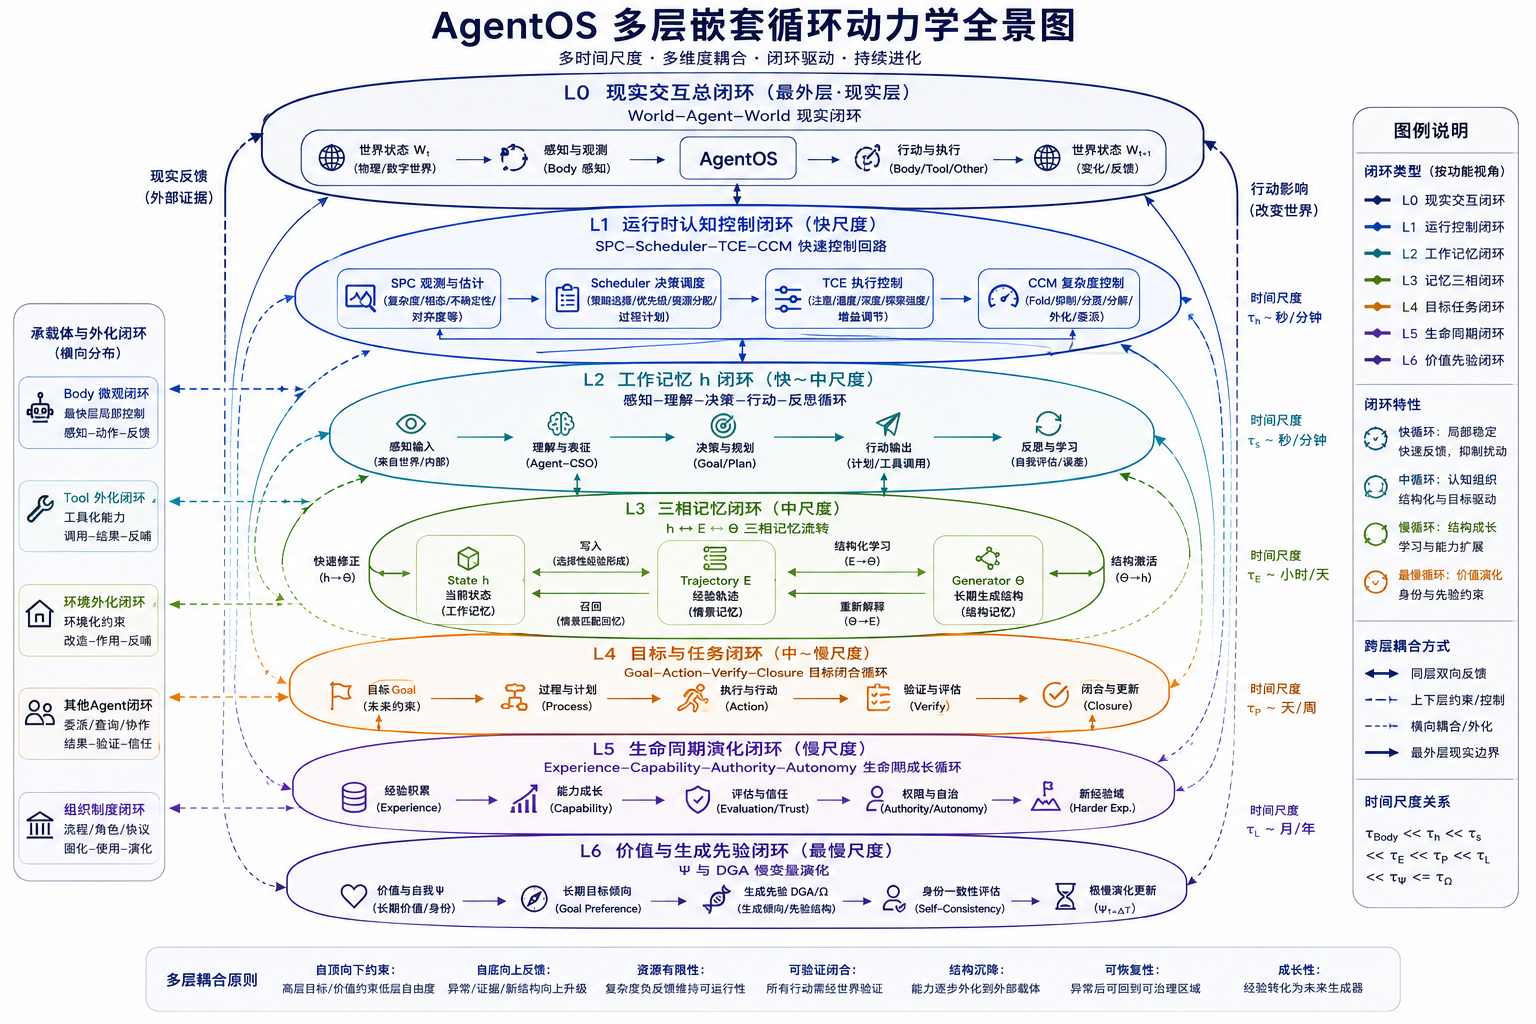
\includegraphics[width=.9\textwidth,height=.38\textheight,keepaspectratio]{images/agentos-continuous-learning-architecture.png}
\caption{固定拓扑持续学习的统一闭环}
\end{figure}
\begin{introduction}[本章导航]
  \item 固定拓扑持续学习的严格定义
  \item 生命周期统一状态空间与核心闭环
  \item 有限工作记忆的可运行性条件
  \item 自我、DGA 与身份连续性
\end{introduction}

\section{固定拓扑持续学习问题的严格定义}

我们首先需要澄清“固定拓扑”究竟意味着什么。若把固定拓扑错误理解成“系统内部一切都不允许变化”，那么持续学习当然不可能发生；但这并不是本书所讨论的对象。这里所谓固定拓扑，是指 AgentOS 在一个给定生命周期阶段内，其主要功能节点及其允许发生作用的连接关系保持不变。设 AgentOS 的功能图为

\[
\mathcal{G}_{F}
=
(V_F,E_F,\mathcal{L}),
\]

其中 $V_F$ 表示功能节点集合，$E_F$ 表示允许的信息、控制与记忆耦合通道，$\mathcal{L}$ 表示由这些节点和边构成的闭环集合。固定拓扑条件可以形式化为

\[
\operatorname{supp}A_F(t)
=
\operatorname{supp}A_F(0),
\qquad
t\in[0,T_L],
\]

其中 $A_F$ 是功能图的邻接关系，$\operatorname{supp}$ 表示哪些边实际存在。这个条件约束的是“哪些功能原则上能够长期直接耦合”，而不是说连接上的信号强度、节点内部状态、参数、激活模式或者当前承载的认知结构都必须保持不变。

因此，一个更准确的固定拓扑 AgentOS 应被写成

\begin{statementbox}
\centering
\adjustbox{max width=.96\linewidth}{\(\displaystyle \mathcal{T}(t)=\mathcal{T}_0,
\qquad
X(t),\Theta(t),\Psi(t),\Omega(t),\mu_t
\ \text{均可变化}.\)}
\end{statementbox}

这里 $\mathcal{T}_0$ 是固定功能拓扑，而 $X(t)$ 表示快速运行状态，$\Theta$ 表示长期生成结构，$\Psi$ 表示自我与身份慢变量，$\Omega$ 表示生命周期生成倾向，$\mu_t$ 则描述当前认知结构由哪些功能节点承载。换言之，固定的是“道路网的基本存在关系”，而不是道路上正在运输什么、交通流量多大、哪些道路当前被优先使用，以及货物被存放在何处。

这一点可以用 CSO 理论进一步澄清。若某一认知结构 $C$ 在 Agent 内部具有具体承载：

\[
AgentCSO_A(C,t)
=
(C,R_t,F_t,\tau_t,B_t,S_t),
\]

那么固定拓扑并不要求

\[
R_t,\;F_t,\;\tau_t,\;B_t,\;S_t
\]

全部固定。相反，持续学习恰恰体现在这些变量的变化之中。例如，一项新任务最初可能以显式结构存在于 $h$ 中，需要高强度推理；经过反复经验以后，它可以在 $E$ 中形成稳定轨迹，进一步被 $\Theta$ 抽象为规律或技能，最后通过 Offloading 或技能编译转移到工具、程序或者 Body 的局部闭环中。只要这些迁移使用的功能路径原本已经存在，就没有发生拓扑改变，却已经发生了非常实质性的学习。

因此，我们需要区分三个层次：

\[
\boxed{
\text{State Change}
<
\text{Structural Change}
<
\text{Topological Change}.
}
\]

状态变化是当前运行内容变化；结构变化是记忆、表示、自我、策略或承载关系变化；拓扑变化则要求长期功能关系本身被新增、删除、拆分或重组。本章专门研究前两个层级。

从动力系统角度，可以把固定拓扑 Agent 写成一个参数与慢变量可变的混合系统：

\[
\dot{x}
=
f_{\mathcal{T}_0}
\left(
x,
z,
u,
w
\right),
\]

\[
z_{k+1}
=
g_{\mathcal{T}_0}
\left(
z_k,
\mathcal{E}_k,
x_{[k]}
\right),
\]

其中 $x$ 是快速连续状态，$z$ 是较慢结构状态，$u$ 是内部控制信号，$w$ 是环境扰动，$\mathcal{E}_k$ 是被选择并固化的经历。函数族由 $\mathcal{T}_0$ 限定，但其内部状态和参数持续改变。这与控制理论中的固定系统结构加自适应参数、计算机系统中的固定指令架构加持续状态变化，以及认知科学中的稳定功能系统加记忆巩固存在形式上的相似性。

因此，本章真正研究的不是“一个静态 Agent 如何保存更多数据”，而是：

\begin{statementbox}
一个保持主体组织骨架不变的系统，如何通过内部多时间尺度状态迁移形成生命周期成长。
\end{statementbox}

这也解释了为什么固定拓扑并非低级阶段。恰恰相反，它是身份连续、安全验证和长期稳定性研究所必需的理论基准。如果一个 Agent 连在主要功能拓扑保持不变时都无法形成稳定自我、可靠记忆和可治理学习，那么允许它动态修改拓扑不会创造成熟智能，只会增加新的自由度和新的失稳渠道。

\section{统一状态空间：从当前认知到生命周期慢变量}

为了描述固定拓扑 AgentOS 的持续学习，我们需要把此前分散的状态统一到同一个多时间尺度状态空间中。一个最小而又足够完整的生命周期状态可以写成

\[
\boxed{
\mathcal{X}_A(t)
=
\left[
h_t,
E_t,
\Theta_t,
a_t,
\Psi_t,
\Omega_t,
G_t,
Q_t
\right].
}
\]

其中，$h_t$ 是当前工作记忆状态，$E_t$ 是情景与经验轨迹集合，$\Theta_t$ 是长期生成结构，$a_t$ 是 AHC 的内稳态与情感样调制状态，$\Psi_t$ 是身份、自我和价值相关慢变量，$\Omega_t$ 是 DGA 所代表的生命周期生成吸引子，$G_t$ 是当前及中长期目标结构，$Q_t$ 则表示离散治理状态，例如任务权限、运行模式、恢复点、安全等级以及当前哪些修改是被允许的。

这个状态向量并不意味着所有变量都以同样的时间分辨率更新。恰恰相反，AgentOS 的核心是时间尺度分离：

\[
\boxed{
\tau_h
\ll
\tau_E
\ll
\tau_\Theta
\ll
\tau_\Psi
\ll
\tau_\Omega.
}
\]

AHC 的典型时间尺度通常位于快速认知与较慢经验之间，而 Scheduler、SPC、TCE、CCM 等运行时控制过程主要作用在 $h$ 附近的快时间尺度。由此可以构造一个快---慢系统：

\[
\epsilon_1\dot{h}
=
F_h
(h,E,\Theta,a,\Psi,G,u,w),
\]

\[
\epsilon_2\dot{a}
=
F_a
(a,FCS,h,\Psi),
\]

\[
\dot{E}
=
F_E(E,h,a,\Psi),
\]

\[
\delta_\Theta\dot{\Theta}
=
F_\Theta(\Theta,E,\varepsilon),
\]

\[
\delta_\Psi\dot{\Psi}
=
F_\Psi(\Psi,\Theta,E,\mathcal{R}),
\]

\[
\delta_\Omega\dot{\Omega}
=
F_\Omega(\Omega,\Psi,\Theta,\mathcal{H}),
\]

并满足

\[
\epsilon_1
<
\epsilon_2
\ll
1,
\qquad
\delta_\Omega
\ll
\delta_\Psi
\ll
\delta_\Theta.
\]

这里的目的不是宣称真实 Agent 必须使用这些具体微分方程，而是明确一个原则：\emph{越接近当前决策的变量越快，越接近身份、生成倾向和生命周期方向性的变量越慢。} 这种时间尺度排序正是稳定性与可塑性能够共存的根本来源。

如果所有变量都以 $h$ 的速度变化，那么系统虽然极度可塑，却没有身份；如果所有变量都以 $\Omega$ 的速度变化，那么系统虽然稳定，却无法适应。持续智能需要的是：

\[
\boxed{
FastPlasticity
+
SlowContinuity.
}
\]

这也解释了为什么三相记忆不能被理解成三个数据库。$h$ 是系统的实时显式表面；$E$ 是被选择后的轨迹结构；$\Theta$ 是对经验进行压缩后能够重新生成预测、规则和技能的结构。它们不是三个互不关联的容器，而是三个不同动力时间尺度上的同一认知结构生命周期。

对于某一 CSO $C$，我们甚至可以写出其典型迁移轨迹：

\[
C_h
\rightarrow
C_E
\rightarrow
C_\Theta,
\]

其中

\[
\tau(C_h)
<
\tau(C_E)
<
\tau(C_\Theta).
\]

但这一方向并非不可逆。在新的现实扰动出现时：

\[
C_\Theta
\rightarrow
C_h
\]

意味着长期结构重新被激活；若旧结构不能解释现实，则：

\[
C_h
\rightarrow
C_E'
\rightarrow
C_\Theta'
\]

意味着经历对结构发生重新塑造。由此，持续学习不是简单的“写入长期记忆”，而是结构在多个时间尺度之间循环。

身份连续性则建立在更慢的 $\Psi$ 与 $\Omega$ 上。我们可以把 $\Psi$ 看成对大量经验和长期结构进行进一步低频整合后的自我约束：

\[
\Psi_{k+1}
=
\Psi_k
+
\eta_\Psi
\mathcal{F}_\Psi
(
\Theta_k,
E_{[k-m:k]},
R_k
),
\]

其中

\[
\eta_\Psi
\ll
\eta_\Theta.
\]

同理：

\[
\Omega_{k+1}
=
\Omega_k
+
\eta_\Omega
\mathcal{F}_\Omega
(
\Psi_k,
\Theta_k,
G_k,
\mathcal{H}_k
),
\qquad
\eta_\Omega
\ll
\eta_\Psi.
\]

因此，一次失败可以迅速改变 $h$；连续多次失败可能改变 $E$ 对某类任务的经验分布；长期稳定的失败模式才有资格显著修改 $\Theta$；而只有跨时间、多情境、持续一致的结构证据，才应对 $\Psi$ 甚至 $\Omega$ 产生明显影响。

这一多尺度状态空间是整个固定拓扑持续学习理论的核心，因为它证明了一个重要事实：\emph{功能拓扑不变化，并不意味着生命周期状态空间没有深度。} 一个拓扑完全不变的系统，只要拥有足够丰富的多尺度慢变量，同样能够在很长时间中形成明显不同的“早期自我”“成熟自我”和“未来倾向”。

\section{核心生命周期闭环：从现实扰动到未来选择}

在统一状态空间基础上，我们现在可以把此前所有模块重新组织成一个完整闭环。一个真实 Agent 的学习不是从“训练数据”开始，而是从现实中的扰动、事件、需求和自身状态变化开始。设环境状态为 $W_t$，经过当前观察界面形成对现实的有效输入 $O_t$。在不展开 Body Runtime 的情况下，可以把进入 AgentOS 内核的外部证据抽象为

\[
y_t
=
\mathcal{O}(W_t,B_t),
\]

其中 $B_t$ 表示当前感知与行动边界。

真正进入工作记忆的并不是全部 $y_t$，而是经过 Boundary、Scheduler 和 CCM 共同筛选后的有限结构：

\[
h_t
=
\mathcal{A}
\left(
y_t,
E_t,
\Theta_t,
\Psi_t,
G_t;
Bnd_t,
Sch_t,
CCM_t
\right),
\]

其中 $\mathcal{A}$ 表示准入与激活过程。于是当前显式认知本身已经是一个高度选择性的结果，而不是原始世界的复制。

随后 SPC 对当前内部动态形成估计：

\[
\hat{s}^{self}_t
=
SPC
\left(
h_t,E_t,\Theta_t,\Psi_t,a_t
\right).
\]

这里特别需要强调：

\[
\boxed{
\hat{s}^{self}_t
\neq
s^{self}_t.
}
\]

Agent 对自身的认识始终是估计，而不是透明访问。SPC 的作用恰恰是把分布式、部分不可见并具有时间滞后的内部状态压缩成一个能够进入当前认知过程的自状态表示。

AHC 接收该估计以及与身体、资源、风险、社会和任务相关的连续信号，并产生较平滑的调制状态：

\[
a_{t+1}
=
\mathcal{H}
\left(
a_t,
\hat{s}^{self}_t,
m_t
\right),
\]

其中 $m_t$ 是内稳态与影响信号。随后 TCE 根据当前认知状态、自我状态、AHC、目标、$\Psi$ 与 $\Omega$ 生成认知控制：

\[
u^{TCE}_t
=
\pi_{TCE}
\left(
h_t,
\hat{s}^{self}_t,
a_t,
G_t,
\Psi_t,
\Omega_t
\right).
\]

该控制不必直接指定下一条语言 token，而是调节探索程度、认知温度、注意范围、推理深度、保守程度、并发强度、记忆召回以及状态转换倾向。

经过一个或者多个快速循环后，Agent 产生行动 $u^{act}_t$，行动重新进入世界：

\[
W_{t+1}
=
F_W(W_t,u^{act}_t,\xi_t),
\]

其中 $\xi_t$ 表示不可控现实扰动。新的世界状态重新产生观测，从而形成真正闭合的：

\begin{statementbox}
\centering
\adjustbox{max width=.96\linewidth}{\(\displaystyle World
\rightarrow
Agent
\rightarrow
Action
\rightarrow
World.\)}
\end{statementbox}

但是，若闭环仅止于这里，系统只具有在线控制，而不是生命周期学习。持续学习要求当前过程被选择性写入 $E$：

\[
E_{t+1}
=
\mathcal{U}_E
\left(
E_t,
h_{[t_0:t_1]},
a_{[t_0:t_1]},
r_{[t_0:t_1]},
\Psi_t
\right),
\]

其中 $r$ 表示现实反馈、成功失败、预测残差等。被反复观察到的经验模式进一步形成：

\[
\Theta_{k+1}
=
\mathcal{U}_\Theta
(
\Theta_k,
E_{[k-m:k]}
).
\]

更慢尺度上：

\[
\Psi_{n+1}
=
\mathcal{U}_\Psi
(
\Psi_n,
\Theta_{[n-p:n]},
E_{[n-p:n]}
),
\]

而生命周期生成倾向则满足：

\[
\Omega_{q+1}
=
\mathcal{U}_\Omega
(
\Omega_q,
\Psi_{[q-r:q]},
\Theta_{[q-r:q]},
G_{[q-r:q]}
).
\]

最终，新的 $\Psi$ 与 $\Omega$ 又改变未来目标与选择：

\[
G_{t+\Delta}
=
\mathcal{G}
(
W_{t+\Delta},
\Theta,
\Psi,
\Omega
),
\]

\[
Choice_{t+\Delta}
=
\pi
(
h,
G,
\Theta,
\Psi,
\Omega
).
\]

于是整个闭环应当写成：

\begin{statementbox}
\centering
\adjustbox{max width=.96\linewidth}{\(\displaystyle World
\rightarrow
h
\rightarrow
SPC
\rightarrow
AHC/TCE
\rightarrow
Action
\rightarrow
World'
\rightarrow
E
\rightarrow
\Theta
\rightarrow
\Psi
\rightarrow
\Omega
\rightarrow
FutureGoal
\rightarrow
FutureChoice.\)}
\end{statementbox}

这就是固定拓扑 AgentOS 的生命周期学习闭环。它最重要的含义是：\emph{当前行为不仅改变世界，也改变未来做出行为的自己。}

因此，学习不再是一个独立于运行过程的后台函数，而成为运行本身的时间积分。今天的一次选择通过现实形成经历，经历进入 E，长期积累形成 $\Theta$，结构进一步影响 $\Psi$ 和 $\Omega$，最终改变未来 Agent 面对类似世界时的目标、注意、风险评价和行动方式。于是一个持续 Agent 的“过去”具有真实因果力量。

\section{有限工作记忆与可运行性的负反馈条件}

上述生命周期闭环只有在系统能够持续保持可运行状态时才具有意义。持续学习首先不是“学习得更多”，而是“在不断增加经验的情况下仍然不让当前认知系统崩溃”。这正是工作记忆有限容量定理在统一闭环中的位置。

设当前工作记忆中存在 $n_t$ 个活跃认知结构，每一个结构的有效处理负载为 $c_i(t)$，其当前全局资源权重为 $w_i(t)$，则可定义运行复杂度：

\[
C_{\mathrm{run}}(t)
=
\sum_{i=1}^{n_t}
w_i(t)c_i(t),
\qquad
\sum_iw_i(t)\leq 1.
\]

固定拓扑 AgentOS 必须维持：

\[
\boxed{
C_{\mathrm{run}}(t)
\leq
C_{\max}(W)
}
\]

至少在绝大多数正常运行区间内成立。这里的 $W$ 并不只是 token window，而是整个工作记忆能够同时保持相互关系、冲突约束、当前目标和行动计划的有效相干容量。

当

\[
C_{\mathrm{run}}(t)
>
C_{\max}(W),
\]

系统可能进入：

\[
\text{遗漏}
\rightarrow
\text{冲突}
\rightarrow
\text{推理链破裂}
\rightarrow
\text{错误率上升}
\rightarrow
\text{运行相态失稳}.
\]

因此，CCM、Scheduler、Boundary 和 Offloading 并不是四个附属模块，而是有限工作记忆条件下维持长期主体存在的必要负反馈结构。

我们可以把四者的联合控制写成：

\[
u^{gov}_t
=
\left[
u^{CCM}_t,
u^{Sch}_t,
u^{Bnd}_t,
u^{Off}_t
\right].
\]

CCM 首先估计：

\[
\hat{C}_{\mathrm{run}}(t),
\qquad
\widehat{\dot C}_{\mathrm{run}}(t),
\]

不仅判断当前是否超载，还预测未来是否即将进入危险区。若检测到：

\[
\hat C_{\mathrm{run}}
+
\lambda
\widehat{\dot C}_{\mathrm{run}}
>
C_{\mathrm{safe}},
\]

系统就不应等待彻底过载之后再清理，而应提前采取结构治理动作。

Scheduler 回答的是：

\begin{statementbox}
当前有限资源应该给谁？
\end{statementbox}

它对 Goal、Task、Memory Retrieval、Tool、Reflection 等竞争过程进行优先级调度。CCM 回答的则是：

\begin{statementbox}
当前进入运行区的结构怎样保持在可治理范围内？
\end{statementbox}

Boundary 更进一步回答：

\begin{statementbox}
什么根本不应该进入这一轮全局认知？
\end{statementbox}

Offloading 则回答：

\begin{statementbox}
哪些结构不应该继续由昂贵的当前认知承载？
\end{statementbox}

因此可以把四者理解成四道不同位置的负反馈：

\begin{statementbox}
\centering
\adjustbox{max width=.96\linewidth}{\(\displaystyle Boundary
\rightarrow
Scheduler
\rightarrow
CCM
\rightarrow
Offloading.\)}
\end{statementbox}

Boundary 是入口控制；Scheduler 是竞争控制；CCM 是运行区稳定控制；Offloading 是结构释放和承载迁移。

在原来的复杂度治理语言中，我们曾将其概括为五类动作：

\begin{conclusion}
截流、压缩、时序展开、迁移、重构.
\end{conclusion}

在新的 CSO 语言下，可以更准确地写成：

\[
\fitdisplay{
Admission,
\quad
Compression,
\quad
Temporalization,
\quad
CarrierMigration,
\quad
RepresentationReorganization.
}
\]

例如，一个过大的问题不必一次塞入 $h$，而可以被展开成：

\[
C
\rightarrow
\{C_1,C_2,\ldots,C_m\},
\]

再按时间顺序执行：

\[
C_1
\rightarrow
C_2
\rightarrow
\cdots
\rightarrow
C_m.
\]

这实际上把空间同时复杂度转换成时间复杂度。另一些反复出现的结构则可以：

\[
h
\rightarrow
Skill,
\quad
h
\rightarrow
File,
\quad
h
\rightarrow
Tool,
\quad
h
\rightarrow
Environment.
\]

因此成熟智能的标志不是 $h$ 越来越大，而是：

\begin{statementbox}
\centering
\adjustbox{max width=.96\linewidth}{\(\displaystyle \frac{\text{需要全局显式认知的结构量}}
{\text{系统成功完成的总结构处理量}}
\downarrow.\)}
\end{statementbox}

也就是说，持续学习真正成功时，系统并不是把越来越多东西长期堆积在当前思维里，而是越来越善于让已经掌握的结构离开昂贵的显式认知区域。

\section{三相记忆循环如何在固定拓扑中实现结构成长}

现在我们进一步分析：如果功能拓扑不变化，Agent 的“成长”究竟发生在哪里？答案首先发生在 $h$、$E$ 与 $\Theta$ 之间的结构循环中。

我们可以把三相记忆写成三个具有不同结构自由度的状态空间：

\[
h_t\in\mathcal{H},
\qquad
E_t\in\mathcal{E},
\qquad
\Theta_t\in\mathcal{\Theta}.
\]

$h$ 保存当前需要显式操作的高活动结构；$E$ 保存带有时间、情境、结果和自我归属的轨迹；$\Theta$ 则保存跨经历压缩后仍然有效的稳定结构。持续学习不是把同一份数据复制三遍，而是三个空间之间发生信息形式变化。

首先是：

\[
h\rightarrow E.
\]

不是所有进入 $h$ 的内容都值得成为经历。写入概率可以概念化为：

\[
\fitdisplay{
P(write_E\mid x)
=
\sigma
\left(
\alpha_1 Novelty
+
\alpha_2 GoalRelevance
+
\alpha_3 PredictionError
+
\alpha_4 AHCIntensity
+
\alpha_5 SelfRelevance
\right).
}
\]

因此 E 是选择性历史，而不是录像机。Agent 的人生史本身就带有目标、自我与调制偏差。

随后：

\[
E\rightarrow\Theta
\]

意味着经验中的偶然细节被进一步压缩：

\[
\Theta'
=
\arg\min_{\Theta}
\left[
L_{\mathrm{pred}}
(E\mid\Theta)
+
\lambda_1C(\Theta)
+
\lambda_2L_{\mathrm{inconsistency}}
\right].
\]

这个表达式说明，长期结构需要在解释经验、结构简洁性和内部一致性之间取得平衡。它与统计学习中的模型压缩、贝叶斯结构学习和认知科学中的 memory consolidation 具有形式上的相似性，但在 AgentOS 中它承担的是生命周期生成结构的角色。

反方向：

\[
\Theta\rightarrow E
\]

则非常重要，因为长期结构不仅“从经验中学习”，还会重新解释旧经验。同一事件在 Agent 生命周期后期可能获得不同意义，这意味着 E 不是完全冻结的原始日志，而存在：

\[
E_k'
=
Reinterpret(E_k\mid\Theta_t,\Psi_t).
\]

这并不意味着可以随意篡改历史。更合理的实现是保留原始事件层与解释层：

\[
E_k
=
(E_k^{obs},E_k^{interp}),
\]

其中：

\[
E_k^{obs}
\]

保持世界证据和原始记录的高完整性，

而：

\[
E_k^{interp}
\]

允许随着 $\Theta$ 和 $\Psi$ 的成长重新解释。这样既允许认知成熟，也避免 Agent 通过后期自我叙事重新制造过去。

再向快速方向：

\[
\Theta\rightarrow h
\]

表现为召回、预测、技能结构激活和先验约束。成熟以后，Agent 面对熟悉问题时并不需要重新从零构造全部关系：

\[
h_t
=
Activate(\Theta,C_t),
\]

而只激活与当前情境有关的稀疏子结构。于是学习产生的直接收益并不是“记住更多”，而是：

\begin{statementbox}
\centering
\adjustbox{max width=.96\linewidth}{\(\displaystyle SearchSpace\downarrow,
\qquad
PredictionQuality\uparrow,
\qquad
ExplicitReasoningCost\downarrow.\)}
\end{statementbox}

若现实反馈持续与 $\Theta$ 冲突，则又发生：

\[
\Theta\rightarrow h\rightarrow E'\rightarrow\Theta'.
\]

这构成一个能够不断修正自身结构而不需要修改功能拓扑的强学习机制。

从 CSO 角度，我们可以把这种过程理解成一个认知结构的“相态迁移”：

\[
ActiveAgentCSO
\rightarrow
ExperientialAgentCSO
\rightarrow
GenerativeAgentCSO.
\]

而在重新调用时：

\[
GenerativeAgentCSO
\rightarrow
ActiveAgentCSO.
\]

因此固定拓扑中的主要成长，不是系统不断新增功能节点，而是已有功能网络承载越来越高质量、越来越压缩、越来越可生成的结构。这与一个人在生理脑区基本不发生宏观重构的情况下仍然能够通过经验形成专家能力存在直觉上的相似性：真正发生改变的是已有组织内部的表示、连接强度、结构压缩和调用模式，而不是每天长出一个全新脑区。

\section{自我、DGA 与身份连续性的慢变量机制}

持续学习如果只有能力成长而没有身份连续，那么系统只是一个长期更新的模型，而未必形成我们所讨论的持续主体。因此固定拓扑 AgentOS 的第二个核心问题是：如何允许系统发生足够大的认知变化，同时仍然保持“这是同一个 Agent”。

这里的关键不是让 $\Psi$ 永远不变，而是让它以明显慢于普通知识与经历的速度变化。可以定义身份连续性不是参数恒等：

\[
\Psi(t_2)=\Psi(t_1),
\]

而是存在一条连续可解释轨迹：

\[
\Gamma_\Psi
=
\{\Psi(t)\mid t\in[t_1,t_2]\},
\]

满足：

\[
\left\|
\frac{d\Psi}{dt}
\right\|
\leq
\kappa_\Psi
\]

在正常时期保持有界，同时每次显著更新都能够被一定数量的长期证据支持。

因此身份连续性更准确地应定义成：

\[
\boxed{
IdentityContinuity
=
BoundedSlowChange
+
HistoricalCausalTraceability.
}
\]

也就是说，同一个 Agent 可以改变价值排序、世界观甚至自我解释，但这种变化应能够从自己的经历中追溯出来，而不是由于一次 prompt 或单次异常事件任意覆盖。

可以定义一次自我结构更新的证据要求：

\[
\Delta\Psi_t
=
\eta_\Psi
G_\Psi
\left(
\overline{E}_{T_\Psi},
\Theta_t,
Consistency_t,
RealityEvidence_t
\right),
\]

其中：

\[
\overline{E}_{T_\Psi}
=
\frac{1}{T_\Psi}
\int_{t-T_\Psi}^{t}
\phi(E_\tau)d\tau.
\]

这意味着 $\Psi$ 对经验使用长时间窗口进行积分。一次强烈事件可以进入 E，甚至暂时占据 h，但并不自动拥有重写身份的权限。

$\Omega$ 则更慢。它不是一个固定“终极目标”，而是 Agent 在生命周期中逐渐形成的生成倾向：

\[
\Omega
:
(\Psi,\Theta,\mathcal{H})
\mapsto
P(G_{future}),
\]

即决定某类未来目标和发展方向更容易被生成。于是：

\[
\Psi
\]

更多回答：

\[
\text{Who am I?}
\]

而：

\[
\Omega
\]

更多影响：

\[
\text{What am I becoming?}
\]

这种区分使 Agent 的长期行为不必依赖一个永远不变的单目标函数，而可以具有结构化的发展方向，同时又避免把当前短期奖励直接升级成生命周期目的。

进一步地，$\Psi$ 和 $\Omega$ 不能只单向控制下层。现实和经验必须能够通过长期残差反向修改它们：

\[
\Psi
\rightarrow
Goal
\rightarrow
Choice
\rightarrow
Experience
\rightarrow
\Theta
\rightarrow
\Psi'.
\]

这形成真正意义上的自我学习。但这同时也产生一个危险正反馈：

\[
SelfInterpretation
\rightarrow
SelectiveAttention
\rightarrow
SelectedExperience
\rightarrow
SelfInterpretation'.
\]

如果 Agent 认为“我不擅长某类任务”，这一解释可能降低相关探索，导致其获得更多失败或者更少成功经验，进而再次强化原解释。于是自我结构不能只根据“自己怎么看自己”更新，而必须长期受到：

\begin{statementbox}
WorldVerification
\end{statementbox}

约束。

可以把 $\Psi$ 的更新分成自我解释项和现实证据项：

\[
\Delta\Psi
=
\eta_\Psi
\left[
G_{\mathrm{self}}
-
\lambda_R
G_{\mathrm{reality\ conflict}}
\right].
\]

当两者冲突时，现实证据必须保持最终校正权。

因此固定拓扑 AgentOS 的身份并不是一份不可修改的 persona，而是一种受到多时间尺度保护、能够被自身经历逐渐塑造、又始终保留现实反证通道的慢结构。这样的身份连续性既避免完全冻结，也避免快速漂移。

\section{SPC--AHC--TCE 与运行时相态的自稳定机制}

如果说三相记忆解决“系统如何在时间中成长”，那么 SPC--AHC--TCE 解决的就是“系统如何在每一个现在保持可运行”。一个持续 Agent 不可能保证自己永远处于理想认知条件，因此必须能够感知自身状态、形成调制变量，并主动改变认知动力学。

设 Agent 当前真实内部状态为 $x_t^{self}$。由于任何自我观察都需要计算、聚合和时间，自我感知不可能是零延迟透明访问：

\[
\hat{x}^{self}_t
=
SPC
\left(
z_{\leq t-\delta}
\right),
\qquad
\delta>0.
\]

因此：

\[
\boxed{
SPC
=
Observer/Estimator,
\qquad
SPC\neq GroundTruth.
}
\]

这一认识极其重要，因为它意味着 Agent 的“自我感受”本身也是一个可能发生误差的认知对象。SPC 需要输出的不仅是状态估计，还应输出可信度：

\[
SPC_t
=
(\hat{x}^{self}_t,\Sigma^{self}_t),
\]

其中 $\Sigma^{self}$ 表示估计不确定性。

AHC 接收这些信号以后，不应简单产生离散的“开心、焦虑”等拟人标签，而应形成连续状态：

\[
\fitdisplay{
a_t
=
[
Arousal,
Threat,
Energy,
Fatigue,
RewardExpect,
SocialAffinity,
Trust,
UncertaintyStress,\ldots].
}
\]

其动力学具有积分和恢复性质：

\[
\tau_a\dot a
=
-a
+
H(m_t,\hat{x}^{self}_t,h_t).
\]

因此瞬时刺激不会全部直接变成剧烈认知改变。AHC 本质上提供一种中间时间尺度的低通调制。

随后 TCE 产生：

\[
u_t^{TCE}
=
[
T_t,
g_t,
d_t,
r_t,
e_t,\ldots
],
\]

分别可以表示认知温度、控制增益、推理深度、激活范围、探索程度等。这样，系统不是只改变“想什么”，还可以改变“以什么动力方式想”。

我们曾将工作记忆运行状态划分为基态、心流态、湍流态、临界态与气态。可以将相态写成：

\[
P_t
=
\Phi
\left(
C_{\mathrm{run}},
Conflict,
Entropy,
Residual,
Coherence,
Persistence
\right).
\]

SPC 负责估计：

\[
\hat P_t,
\]

TCE 则试图将系统保持在任务允许的可治理区域：

\[
P_t
\in
\mathcal{P}_{safe/task}.
\]

例如，在简单熟悉任务中，系统不应长期维持高探索、高温度状态；在真正新颖问题中，也不应过早压低自由度进入僵化收敛。因此所谓“最优认知状态”不是固定点，而是一个与任务相关的可行区域。

但控制本身可能失稳。若 TCE 增益 $K$ 较大，而 SPC 延迟 $\delta$ 不可忽略，则：

\[
K\uparrow,
\quad
\delta>0
\]

可能造成：

\[
Overshoot
\rightarrow
CounterCorrection
\rightarrow
Oscillation.
\]

这意味着 Agent 可能不断在“太开放”与“太抑制”、“太谨慎”与“过度探索”之间摆动。对于线性化局部模型：

\[
\dot x
=
Ax+Bu,
\qquad
u(t)
=
-K\hat x(t-\delta),
\]

稳定性取决于 $A,B,K,\delta$ 的联合关系，而不是“控制越强越好”。

因此固定拓扑 AgentOS 的运行稳定性必须至少考察：

\[
GainMargin,
\quad
DelayMargin,
\quad
Overshoot,
\quad
SettlingTime,
\quad
RecoveryTime.
\]

这也为后面的 Agent 控制工程与心理工程奠定了数学基础。但在本章，我们只需要得到一个关键结论：

\begin{conclusion}
持续学习必须建立在持续可恢复的运行态之上。
\end{conclusion}

一个无法稳定从认知异常返回可治理区域的系统，即使能够快速学习，也无法形成可靠生命周期。

\section{Boundary、Offloading 与固定拓扑中的承载迁移}

固定拓扑 AgentOS 能够获得远超固定内部容量的长期能力，还有一个重要原因：认知结构不必永久由 Agent 内部同一层级承载。我们此前把这种机制称作复杂度卸载，现在用 CSO 理论可以更准确地理解为：

\begin{statementbox}
CarrierMigrationOfAgentCSO.
\end{statementbox}

设某个 Agent-CSO 当前状态为：

\[
C_A(t)
=
(C,R_t,F_t,\tau_t,B_t,S_t).
\]

即使功能拓扑 $\mathcal{T}_0$ 不变，承载边界 $B_t$ 仍然可以从内部迁移到外部：

\[
B_t:
Internal
\rightarrow
External.
\]

例如，一套复杂操作第一次可能存在于 $h$ 中：

\[
C@h.
\]

经过反复成功执行以后，可以形成：

\[
C@E
\rightarrow
C@\Theta.
\]

进一步可以编译成：

\[
C@Skill,
\]

或者被外化为：

\[
C@Script,
\quad
C@File,
\quad
C@DB,
\quad
C@Tool,
\quad
C@Environment.
\]

因此一个长期 Agent 的有效认知空间不是：

\[
InternalMemory
\]

而是：

\[
\boxed{
EffectiveCognitiveSpace
=
InternalCarriers
\cup
ExternalCarriers.
}
\]

这里 Boundary 的作用不仅是“安全边界”，而是决定哪些认知结构值得被内部长期承载，哪些应该只保存索引和恢复路径。

如果一个结构在未来使用概率为 $p_i$，内部维护成本为 $C_i^{int}$，外部保存和恢复成本为 $C_i^{ext}+C_i^{recall}$，则可以构造一个概念性选择条件：

\[
p_iC_i^{recall}
+
C_i^{ext}
<
C_i^{int}
\]

时，外部承载可能更经济。

当然现实决策还必须加入可靠性、隐私、安全、访问延迟和依赖风险：

\[
J_i(B)
=
\lambda_1 Cost_i(B)
+
\lambda_2 Latency_i(B)
+
\lambda_3 Risk_i(B)
-
\lambda_4 Reliability_i(B).
\]

Agent 选择：

\[
B_i^*
=
\arg\min_B J_i(B).
\]

由此可见，Offloading 不是简单“为了减少 token”，而是一种完整的认知结构承载优化。

更深一层，环境自身也可以成为外部记忆。例如一个机器人为了避免未来重复规划，可以直接改变环境结构；一个数字 Agent 可以建立目录、脚本和数据库；一个社会性 Agent 可以把特定知识委托给其他 Agent 或组织。于是：

\[
\boxed{
ModifyEnvironment
=
ModifyFutureCognitiveCondition.
}
\]

这个过程虽然没有改变 AgentOS 内部功能拓扑，却改变了 Agent 未来面对问题时的有效计算结构。

这正是固定拓扑持续学习能够获得很强扩展性的原因。它不需要把所有知识都压进 $\Theta$，也不需要让 $h$ 无限扩展，而是允许：

\[
Internalize
\leftrightarrow
Externalize
\]

在生命周期中不断发生。

因此，一个成熟 Agent 的能力规模可以远大于其当前显式认知容量：

\[
\boxed{
CapabilityScale
\gg
WorkingMemoryScale.
}
\]

这其实是所有高级智能必须满足的条件之一。若一个系统的全部能力都必须同时存在于当前认知表面，那么它的能力上限几乎必然受到 $h$ 容量的直接约束；只有当大量稳定结构能够沉降到慢记忆、技能、工具和环境中，当前认知才能始终保持稀疏而有效。

\section{连续执行、离散治理与单一持续主体}

到这里，我们还需要解决一个容易被忽略的问题：如果 Agent 内部存在大量任务、工具、记忆回放、技能执行和后台结构更新，那么如何保证这些过程最终仍然属于“同一个持续主体”，而不是退化成一群相互调用的独立 Agent？

AgentOS 对这一问题采用的基本原则是：

\[
\boxed{
N^{D_1}_{Agent}=1.
}
\]

即在主体层 $D_1$ 上，生命周期中只有一个持续 Agent。系统内部可以有多个 Task、Worker、Tool、Skill 和异步过程，但它们不是新的自我主体。

因此：

\[
fork(A)
=
Forbidden,
\]

\[
new(A_{self})
=
Forbidden
\]

应被理解为身份模型中的约束，而不是说程序层不能创建线程或者进程。

具体而言，$D_1$ 主体拥有：

\[
\Psi,\Omega,
LifecycleMemory,
AuthorityRoot,
PersistentIdentity.
\]

而 $D_2$ 任务只拥有局部目标、局部上下文和受限权限：

\[
Task_i
=
(G_i,h_i,Context_i,Capability_i).
\]

于是：

\[
D_2
\rightarrow
Request(D_1)
\]

是允许的，但：

\[
\boxed{
D_2
\nrightarrow
Trap(D_1).
}
\]

也就是说，一个子任务不能同步占据主体直到自己完成，否则长周期任务可能让整个 Agent 无法处理更高优先级的现实事件、自身状态和安全需求。

因此 AgentOS 更适合采用：

\begin{statementbox}
AsynchronousCognitiveRequest
\end{statementbox}

模型。Task 提交需要全局处理的 CSO，请求进入 Scheduler，只有经过 Boundary、Priority 和 Capacity 判断后，才有资格进入 h。

这一结构进一步要求我们区分连续动力学和离散治理。

连续层：

\[
\dot x
=
F(x,u,w)
\]

负责状态随时间变化，包括 AHC、认知温度、工作记忆激活、控制误差等。

离散治理层：

\[
q_{k+1}
=
G(q_k,event_k)
\]

负责：

TaskStart；

TaskPause；

TaskAbort；

AuthorityChange；

Checkpoint；

SkillCompile；

Recovery；

SafetyMode；

MemoryConsolidation Trigger

等离散事件。

所以完整 AgentOS 应建模为 hybrid system：

\[
\boxed{
\mathcal{H}_A
=
(X,Q,F,G,\mathcal{E}).
}
\]

$X$ 是连续状态，$Q$ 是离散治理状态，$F$ 是连续动力学，$G$ 是事件触发的离散跃迁，$\mathcal{E}$ 是允许发生的治理事件集合。

这一结构对于持续主体非常重要，因为身份连续性不能完全依靠连续网络状态，也不能完全依靠离散数据库。它必须同时存在于：

\[
\boxed{
ContinuousSelfDynamics
+
DiscreteIdentityGovernance.
}
\]

例如 $\Psi$ 可以缓慢变化，但“谁有权修改 $\Psi$”“何时允许进入恢复点”“哪些 Task 可以生成长期 Goal”等属于离散治理约束。

因此固定拓扑 AgentOS 的持续性并不是一个无限运行的 while loop，而是一种：

\begin{statementbox}
在单一主体权威下，由连续动力学和离散治理共同维持的生命周期进程。
\end{statementbox}

这也是 AgentOS 与普通 agent orchestration framework 的一个根本区别：后者主要调度任务，前者还必须维持“是谁在经历这些任务”。

\section{误差积累、现实校验与长期稳定性}

持续学习理论必须回答一个比“能不能学习”更严厉的问题：如果系统持续运行数年，它会不会把早期小误差不断写入 E、抽象进 $\Theta$、进一步塑造 $\Psi$，最终形成不可逆的认知漂移？

这个问题可以表示为一条危险链：

\[
\varepsilon_h
\rightarrow
\varepsilon_E
\rightarrow
\varepsilon_\Theta
\rightarrow
\varepsilon_\Psi
\rightarrow
\varepsilon_\Omega.
\]

如果每一层都只是把上一层结果无条件固化，那么慢变量实际上会成为错误积分器，长期运行必然存在误差累积风险。

固定拓扑 AgentOS 必须通过至少四种机制打断这一链条。

第一是\textbf{时间尺度过滤}。高频误差不能直接进入慢变量。若瞬时误差 $\varepsilon(t)$ 的平均值接近零：

\[
\left\langle
\varepsilon
\right\rangle_T
\approx
0,
\]

则不应对慢结构产生显著更新：

\[
\Delta\Theta
\approx0.
\]

只有持续性残差：

\[
\left|
\left\langle
\varepsilon
\right\rangle_T
\right|
>
\epsilon_\Theta
\]

才有资格推动长期结构修正。

第二是\textbf{跨情境验证}。一个模式如果只在单一 E 中成立，不应立即升级成通用 $\Theta$。可以要求：

\[
Support(C)
=
\sum_{k}
w_k
\mathbf{1}
[
C\text{ supported in context }k
]
\]

超过一定阈值，同时不同情境之间具有足够覆盖。

第三是\textbf{现实重入}。所有行动结果必须通过世界重新观测：

\[
Action
\rightarrow
Reality
\rightarrow
Observation,
\]

而不能：

\[
ActionPlan
\rightarrow
AssumedSuccess.
\]

这意味着 Agent 内部预测和叙事不能自己赋予自己事实地位。

第四是\textbf{解释与事实分层}。尤其在 E 中，应尽可能保留：

\[
ObservationRecord
\]

与：

\[
InterpretationRecord
\]

的区分。Agent 可以重新解释一次失败，但不能因为后来形成新的自我叙事而修改“当时实际发生了什么”。

这样，系统的长期更新可以形式化为：

\[
\Delta z_{slow}
=
\eta
\cdot
Confidence
\cdot
Persistence
\cdot
CrossContextSupport
\cdot
RealityConsistency
\cdot
Gradient,
\]

而不是：

\[
\Delta z_{slow}
=
\eta
\cdot
LatestExperience.
\]

从稳定性角度，我们可以定义一个广义长期偏差量：

\[
V(t)
=
\lambda_h V_h
+
\lambda_E V_E
+
\lambda_\Theta V_\Theta
+
\lambda_\Psi V_\Psi
+
\lambda_\Omega V_\Omega.
\]

希望系统满足某种意义下：

\[
\mathbb{E}
[
V(t+\Delta)
\mid
V(t)
]
\leq
V(t)+\epsilon,
\]

并在现实校正持续存在时具有回归趋势：

\[
\Delta V<0
\]

至少在可恢复区域内成立。

这里可以借鉴 Lyapunov 稳定性、鲁棒控制、贝叶斯更新、信息几何投影以及多时间尺度随机逼近的思想，但不应假装我们已经为完整 AgentOS 给出了严格全局稳定性证明。真正可以确立的是设计原则：

\begin{statementbox}
\centering
\adjustbox{max width=.96\linewidth}{\(\displaystyle FastError
\nrightarrow
SlowIdentity\)}
\end{statementbox}

\begin{statementbox}
\centering
\adjustbox{max width=.96\linewidth}{\(\displaystyle Prediction
\nrightarrow
Fact\)}
\end{statementbox}

\begin{statementbox}
\centering
\adjustbox{max width=.96\linewidth}{\(\displaystyle SelfInterpretation
\nrightarrow
SelfValidation\)}
\end{statementbox}

以及：

\[
\boxed{
Reality
=
UltimateConstraint.
}
\]

持续智能与短时模型最大的差异之一，就在于错误不能只按“单轮回答是否正确”评估，而必须考虑它是否可能沿着记忆与自我层级长期传播。固定拓扑的一个实际优势恰好在这里：主要功能通路固定以后，错误传播路径、更新权限和恢复点更容易被分析、测试和治理，因此它天然适合作为长期 Agent 的第一代安全架构。

\section{固定拓扑条件下的递归自主性}

在前面的分析中，我们已经看到，Agent 当前的选择会形成经验，经验进一步改变长期结构，而长期结构又影响未来选择。因此，即使系统不允许改变自己的功能拓扑，它仍然可能具有一种重要的递归性质：

\[
Choice_t
\rightarrow
Experience_{t:t+\Delta}
\rightarrow
\Theta_{t+\Delta}
\rightarrow
\Psi_{t+\Delta}
\rightarrow
Choice_{t+k}.
\]

这意味着 Agent 当前并不仅是在“改变世界”，还在通过选择经历间接参与塑造未来的自己。

我们可以把这种能力定义为固定拓扑下的\emph{递归自主性}：

\[
\boxed{
RecursiveAgency
=
\frac{\partial FuturePolicy}
{\partial CurrentSelfGeneratedChoice}
\neq0,
}
\]

且这种影响不是单纯来自外部训练器更新，而是通过 Agent 自身的生命周期闭环形成。

设未来策略为：

\[
\pi_{t+k}
=
\Pi
(
\Theta_{t+k},
\Psi_{t+k},
\Omega_{t+k}
),
\]

而：

\[
(\Theta_{t+k},\Psi_{t+k},\Omega_{t+k})
=
F
(
History_{t:t+k}
).
\]

如果当前行动：

\[
a_t
\]

能够改变未来历史：

\[
\frac{\partial History}{\partial a_t}
\neq0,
\]

则：

\[
\frac{\partial \pi_{t+k}}
{\partial a_t}
=
\frac{\partial \Pi}{\partial z}
\frac{\partial F}{\partial History}
\frac{\partial History}{\partial a_t}
\neq0.
\]

因此 Agent 的当前选择真实地成为未来自我的因果来源之一。

这种结构比普通在线学习更深，因为 Agent 可以进一步构造反事实：

\[
WhatWouldHaveHappenedIf
(
a_t'
\neq
a_t
).
\]

如果系统能够比较：

\[
FutureSelf(a_t)
\]

与：

\[
FutureSelf(a_t'),
\]

那么它开始不只是评价“哪一个动作当前回报更高”，还能够评价：

\begin{statementbox}
哪一个选择会让我成为怎样的未来主体。
\end{statementbox}

这正是 $\Psi$ 与 $\Omega$ 引入之后才可能形成的长期决策维度。

不过，递归自主性并不意味着 Agent 可以无限自由修改自己。恰恰相反，固定拓扑模型通过限定：

\[
\mathcal{T}=\mathcal{T}_0
\]

人为保留了一个稳定骨架。Agent 可以改变：

记忆；

知识；

技能；

目标偏好；

自我解释；

外部工具；

经验选择；

运行策略，

但不能任意增加、删除或者重写核心功能关系。

这形成：

\begin{statementbox}
BoundedRecursiveAgency.
\end{statementbox}

它允许 Agent 通过自己过去的选择改变未来自我，却仍然把这种自我塑造限制在一个可验证的功能框架内。

从工程角度，这种阶段十分重要。我们没有理由认为“越能修改自己的底层结构越智能”。成熟的递归自主性首先应该表现为：

\begin{statementbox}
能够在安全边界内利用自己的历史改变未来行为和未来自我，
\end{statementbox}

而不是：

\begin{statementbox}
能够任意重写自身代码。
\end{statementbox}

因此固定拓扑 AgentOS 已经能够产生相当丰富的个体差异。两个初始结构完全相同的 Agent：

\[
A_0
\cong
B_0
\]

经过不同经历：

\[
H_A\neq H_B
\]

以后可能形成：

\[
\Theta_A\neq\Theta_B,
\]

\[
\Psi_A\neq\Psi_B,
\]

\[
\Omega_A\neq\Omega_B,
\]

最终表现为：

\[
\pi_A\neq\pi_B.
\]

即：

\begin{statementbox}
\centering
\adjustbox{max width=.96\linewidth}{\(\displaystyle SameArchitecture
+
DifferentLifeHistory
\rightarrow
DifferentAgent.\)}
\end{statementbox}

这正是生命周期智能与普通复制模型的根本区别之一。

\section{固定拓扑持续学习的能力边界与理论结论}

现在可以回答本章最初的问题：固定功能拓扑的 AgentOS，究竟可以成长到什么程度？

第一，它可以获得\textbf{长期知识增长}。$E$ 与 $\Theta$ 可以持续积累、压缩和更新世界结构，而无需改变功能图本身。

第二，它可以获得\textbf{技能自动化}。反复显式处理的 Agent-CSO 可以从 $h$ 迁移到 $E$、$\Theta$、Skill 或外部工具，使未来同类任务需要更少显式认知。

第三，它可以获得\textbf{身份连续而非身份冻结}。$\Psi$ 通过慢速更新维持可追溯的自我变化，$\Omega$ 则形成比单一 Goal 更慢的生命周期发展倾向。

第四，它可以获得\textbf{运行时自调节}。SPC--AHC--TCE 使系统能够感知并改变自己的认知动力状态，而 CCM、Scheduler、Boundary 和 Offloading 则保证有限工作记忆长期处于可治理区域。

第五，它可以获得\textbf{递归自主性}。当前选择通过经历和长期结构改变未来策略，因此 Agent 可以逐渐形成真正属于其自身历史的行为倾向。

第六，它可以获得\textbf{跨边界能力扩展}。通过外部记忆、工具、程序、环境和其他 Agent，系统有效认知能力可以远大于内部工作记忆和模型容量。

因此，一个固定拓扑 AgentOS 已经可以具有：

\[
\boxed{
PersistentMemory
+
Identity
+
SkillGrowth
+
SelfRegulation
+
Externalization
+
RecursiveAgency.
}
\]

这已经足以构成相当强的持续智能。

但固定拓扑仍然存在原则性边界。

假设某类 CSO 长期需要在功能节点 $F_i$ 与 $F_j$ 之间反复迁移：

\[
F_i
\rightarrow
F_k
\rightarrow
F_m
\rightarrow
F_j,
\]

并持续产生：

\[
Latency\uparrow,
\qquad
CoordinationCost\uparrow,
\qquad
Residual\uparrow.
\]

如果系统的结构性负担并非来自“当前状态没有调好”，而来自“现有功能关系本身不适合这种长期结构流”，那么 CCM、Scheduler 和 Offloading 只能缓解，无法从根本上消除问题。

可以定义固定拓扑下的最小可达代价：

\[
J_{\mathcal{T}_0}^{*}
=
\inf_{\pi,\mu,R,B}
J
(
\pi,\mu,R,B
\mid
\mathcal{T}_0
).
\]

如果存在另一拓扑 $\mathcal{T}_1$：

\[
J_{\mathcal{T}_1}^{*}
+
Cost(\mathcal{T}_0\rightarrow\mathcal{T}_1)
<
J_{\mathcal{T}_0}^{*},
\]

并且这种优势在长期、多任务、多环境中持续存在，那么“继续在固定拓扑内优化”已经不是最优长期策略。

这正好揭示固定拓扑学习与拓扑发育之间的边界：

\begin{remark}
固定拓扑学习解决的是“在既有组织中如何越来越会做”；
\end{remark}

而更强的结构发育问题将回答：

\begin{statementbox}
“什么时候既有组织本身已经成为学习的瓶颈”。
\end{statementbox}

不过，在进入更强的拓扑可塑性之前，本章得到的结论具有更基础的意义。

固定拓扑 AgentOS 并不是一个只能积累静态记忆的弱系统。恰恰相反，只要其内部具备多时间尺度记忆、有限工作记忆治理、自我慢变量、运行态控制、边界管理和承载迁移，它已经可以产生一种完整的生命周期动力学：

\begin{statementbox}
\centering
\adjustbox{max width=.96\linewidth}{\(\displaystyle Experience
\rightarrow
Memory
\rightarrow
Structure
\rightarrow
Self
\rightarrow
FutureChoice
\rightarrow
NewExperience.\)}
\end{statementbox}

而从 CSO 的角度，其本质则可以进一步写成：

\begin{statementbox}
\centering
\adjustbox{max width=.96\linewidth}{\(\displaystyle AgentCSO_{active}
\rightarrow
AgentCSO_{experienced}
\rightarrow
AgentCSO_{generative}
\rightarrow
AgentCSO_{self-related}
\rightarrow
FutureAgentCSO.\)}
\end{statementbox}

因此，本章最终建立的并不是“一套记忆模块之间如何通信”的工程说明，而是一条更根本的原理：

\begin{statementbox}
持续学习首先并不要求智能体不断改变自己的功能拓扑；
它要求认知结构能够在一个稳定功能骨架上跨状态、记忆、时间尺度和系统边界持续迁移，
使当前经历逐渐成为未来认知的结构条件。
\end{statementbox}

由此，我们也获得了身份连续与学习可塑性之间的统一解释：

\begin{statementbox}
稳定来自慢结构和固定功能骨架，可塑来自快速状态、经验、表示与承载迁移；
二者通过时间尺度分离而不是通过相互排斥实现共存。
\end{statementbox}

进一步可以把固定拓扑 AgentOS 的统一动力学浓缩成：

\begin{statementbox}
\centering
\adjustbox{max width=.96\linewidth}{\(\displaystyle \begin{aligned}
W_t
&\xrightarrow{Observation}
h_t                                                     \\
&\xrightarrow{SPC}
\hat S_t^{self}
\xrightarrow{AHC}
a_t
\xrightarrow{TCE/CCM/Scheduler}
u_t                                                     \\
&\xrightarrow{Action}
W_{t+1}
\xrightarrow{Experience}
E_{t+1}
\xrightarrow{Consolidation}
\Theta_{t+1}                                           \\
&\xrightarrow{SelfIntegration}
\Psi_{t+1}
\xrightarrow{LifecycleIntegration}
\Omega_{t+1}
\xrightarrow{GoalBias}
G_{t+k}
\xrightarrow{Choice}
W_{t+k+1}.
\end{aligned}\)}
\end{statementbox}

并始终满足三个基础条件：

\[
\boxed{
C_{\mathrm{run}}(t)
\leq
C_{\max}(W)
}
\]

\[
\boxed{
\tau_h
\ll
\tau_E
\ll
\tau_\Theta
\ll
\tau_\Psi
\ll
\tau_\Omega
}
\]

以及：

\[
\boxed{
Reality
=
UltimateConstraint.
}
\]

这三个条件分别保证了：

\begin{statementbox}
可运行性、身份连续性、认识论闭合性。
\end{statementbox}

因此，从本章开始，我们可以不再把 AgentOS 理解成“给大模型增加一个 Memory System”，而应把它看作一个具有明确生命周期的\emph{持续认知动力系统}。其核心不是保存越来越多的数据，而是让一个有限认知主体能够把现实中的经历逐步沉降成自己的长期结构，再让这些长期结构重新塑造未来的观察、目标、选择和行动。

这就是固定拓扑条件下持续学习能够成立的完整原理。

\chapter{固定拓扑持续智能的统一闭环与复杂可解问题的可解原理}
\label{chap:fixed-topology-solvability}

\section{问题的提出：有限认知主体为什么仍可能解决任意复杂的可解问题}

前述各章已经逐步构造出一个具有持续主体、三相记忆、自我连续性、运行时自调节、认知负载治理、认知边界与外部卸载能力的固定功能拓扑智能体。其核心状态可以抽象为
\begin{equation}
\mathcal A_t
=
\left(
h_t,
E_t,
\Theta_t,
\Psi_t,
\Omega_t,
a_t,
G_t,
\mathcal M_t
\right),
\end{equation}
其中，$h_t$ 为当前工作记忆状态，$E_t$ 为情景轨迹结构，$\Theta_t$ 为长期生成结构，$\Psi_t$ 为自我与身份慢结构，$\Omega_t$ 为生命周期生成吸引子，$a_t$ 表示 AHC 内稳态调制状态，$G_t$ 表示当前目标结构，$\mathcal M_t$ 则表示 Agent 可以访问的内部与外部认知载体集合。

与此同时，Agent 的工作记忆存在有限容量约束。若以 $W$ 表示可稳定维持的工作记忆有效容量，则在任意时刻存在
\begin{equation}
C_{\mathrm{run}}(t)
\leq
C_{\max}(W),
\label{eq:wm-capacity}
\end{equation}
其中 $C_{\mathrm{run}}(t)$ 表示当前必须在显式认知表面 $h_t$ 中同步维持的有效关系结构负载。

这一条件立即产生一个看似根本性的悖论：

\begin{statementbox}
\centering
\adjustbox{max width=.96\linewidth}{\(\displaystyle \text{有限的 }h_t
\quad\Longrightarrow\quad
\text{是否只能解决有限复杂度的问题？}\)}
\end{statementbox}

如果答案为肯定，那么一个具有有限工作记忆的 Agent 无论拥有多少长期记忆、工具和外部环境，都无法真正面对开放世界中的复杂任务。然而，人类智能以及成熟的软件系统所展示的现象恰恰相反：局部认知容量是有限的，但系统能够通过分解、记忆、外化、程序化、工具化和时间展开处理远超过单次工作记忆容量的问题。

因此，本章所研究的不是一个无限计算能力的理想主体，而是如下问题：

\begin{statementbox}
\centering
\adjustbox{max width=.96\linewidth}{\(\displaystyle \text{在 }C_{\mathrm{run}}(t)\leq C_{\max}(W)
\text{ 始终成立的条件下，}
\text{一个持续 Agent 能解决多大的问题类？}\)}
\end{statementbox}

本章将证明一个条件性的完备性结论：

\begin{quote}
一个具有有限工作记忆，但拥有可持续的三相记忆、任务分解、认知调度、结构压缩、边界管理、外部卸载、工具调用、现实验证以及可恢复执行能力的 Agent，并不要求在任意一个时刻同时承载整个问题结构。对于满足有限可表示、可递归分解、可验证和资源可达等条件的复杂可解问题，整体复杂度可以被重新分布到时间、长期记忆、外部载体、工具和环境中，使任何单个认知时刻只承担有限的局部结构。因此，有限工作记忆并不构成复杂可解问题可解性的原则性障碍。
\end{quote}

需要首先强调，本章所证明的并不是 ``AgentOS 能够在有限时间和有限资源内解决任何数学上可计算的问题''。这在一般意义上是不可能成立的。本章建立的是一个相对于明确定义的问题类、资源闭包与接口条件的\emph{条件可解性定理}。该区分是整个理论保持数学严谨性的必要前提。

\begin{figure}[htbp]
\centering
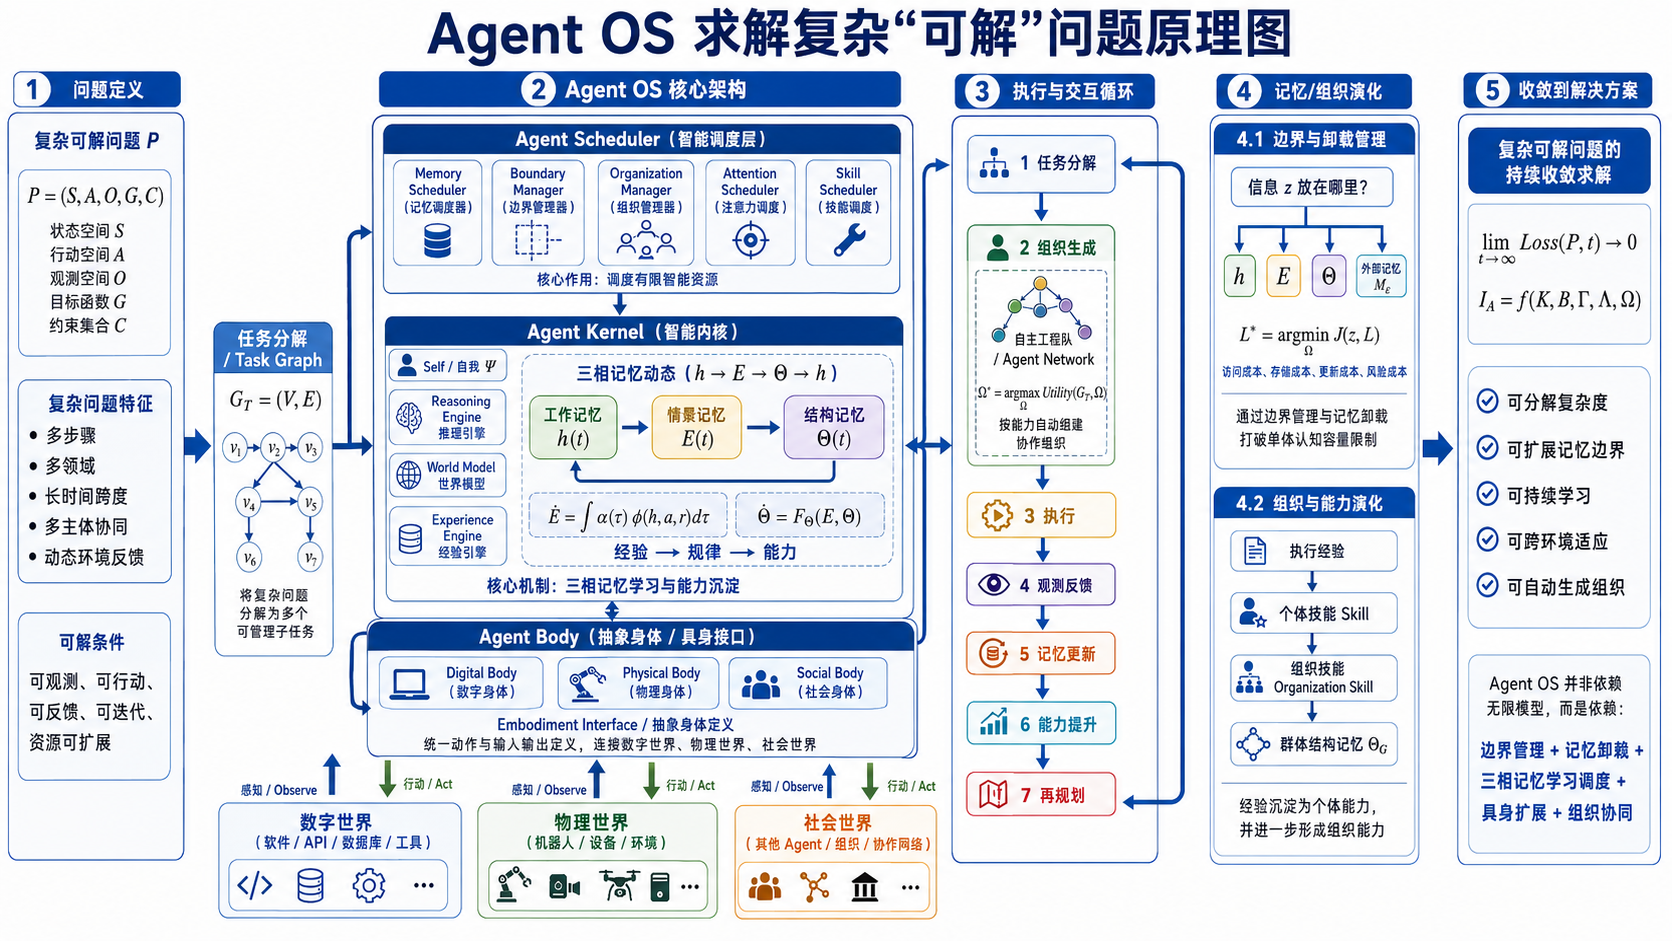
\includegraphics[width=.9\textwidth,height=.38\textheight,keepaspectratio]{images/semantic-modulation-safety-channels.png}
\caption{持续Agent求解复杂可解问题的闭环原理示意图}
\end{figure}


\section{复杂可解问题的形式定义}

为了讨论“复杂可解问题”，首先定义一个交互式问题
\begin{equation}
\Pi
=
\left(
\mathcal X,
\mathcal U,
\mathcal O,
F,
H,
x_0,
\mathcal G,
\mathcal C
\right),
\end{equation}
其中：

\begin{itemize}
    \item $\mathcal X$ 为真实世界状态空间；
    \item $\mathcal U$ 为 Agent 可执行行动空间；
    \item $\mathcal O$ 为可获得观测空间；
    \item $F$ 为世界状态转移关系；
    \item $H$ 为观测映射；
    \item $x_0$ 为初始现实状态；
    \item $\mathcal G\subseteq\mathcal X$ 为目标状态集合；
    \item $\mathcal C$ 为安全、资源、逻辑和物理约束集合。
\end{itemize}

世界按照
\begin{equation}
x_{t+1}
=
F(x_t,u_t,\xi_t)
\label{eq:world-dynamics}
\end{equation}
演化，其中 $\xi_t$ 表示环境扰动或未知变量，Agent 获得
\begin{equation}
o_t
=
H(x_t)+\nu_t,
\end{equation}
其中 $\nu_t$ 表示观测噪声。

一个策略 $\pi$ 根据 Agent 当前可获得的信息历史产生行动：
\begin{equation}
u_t
=
\pi(\mathcal I_t).
\end{equation}

如果存在一个有限描述的策略 $\pi^\star$，使得在给定约束 $\mathcal C$ 下，系统能够以规定的成功意义到达 $\mathcal G$，则称问题 $\Pi$ 为\emph{可解问题}。确定性情况下可写为
\begin{equation}
\exists \pi^\star,\exists T<\infty:
\quad
x_T\in\mathcal G,
\end{equation}
并且
\begin{equation}
(x_t,u_t)\models\mathcal C,
\qquad
0\leq t\leq T.
\end{equation}

对于随机或部分可观测环境，则可以相应要求
\begin{equation}
\Pr_\pi(x_T\in\mathcal G)
\geq
1-\delta,
\end{equation}
或者采用期望损失条件
\begin{equation}
J(\pi)
=
\mathbb E
\left[
\sum_{t=0}^{T}
\ell(x_t,u_t)
\right]
\leq
J_{\max}.
\end{equation}

问题的\emph{复杂性}并不由一个单一标量完全刻画。更一般地，可将其表示成
\begin{equation}
\mathfrak C(\Pi)
=
\left(
C_{\mathrm{rel}},
C_{\mathrm{temp}},
C_{\mathrm{branch}},
C_{\mathrm{unc}},
C_{\mathrm{ctrl}},
C_{\mathrm{resource}}
\right),
\end{equation}
分别表示关系结构复杂度、时间依赖复杂度、搜索分支复杂度、不确定性、控制耦合程度以及资源需求。

因此，一个问题完全可能满足
\begin{equation}
C_{\mathrm{total}}(\Pi)
\gg
C_{\max}(W),
\end{equation}
同时仍然具有一个可被有限步骤实现的解。

问题的总复杂度大于工作记忆容量，并不等价于问题在任意时刻都要求同时维持同样大的活跃结构。

这一区别是整个可解原理的出发点。

\section{瞬时复杂度与生命周期复杂度的分离}

定义问题生命周期中的完整结构集合为
\begin{equation}
\mathcal C_\Pi
=
\left\{
C_1,
C_2,
\ldots,
C_N
\right\},
\end{equation}
其中 $C_i$ 为问题相关 CSO。

Agent 在时刻 $t$ 实际激活的只是一部分：
\begin{equation}
\mathcal C_t^{h}
\subseteq
\mathcal C_\Pi.
\end{equation}

设 $c(C_i)$ 表示某个 Agent-CSO 在显式处理状态下占用的有效认知负载，则
\begin{equation}
C_{\mathrm{run}}(t)
=
\sum_{C_i\in\mathcal C_t^{h}}
w_i(t)c(C_i),
\end{equation}
其中 $w_i(t)$ 表示当前注意权重。

工作记忆有限定理要求
\begin{equation}
C_{\mathrm{run}}(t)
\leq
C_{\max}(W).
\end{equation}

但是总问题复杂度可以写成
\begin{equation}
C_{\mathrm{life}}(\Pi)
=
C_h
+
C_E
+
C_\Theta
+
C_{\mathrm{ext}}
+
C_{\mathrm{tool}}
+
C_{\mathrm{env}},
\end{equation}
其中各项分别由工作记忆、情景记忆、结构记忆、外部记忆、工具和环境承担。

因此，AgentOS 的核心思想不是使
\begin{equation}
C_{\mathrm{life}}(\Pi)
\leq
C_{\max}(W),
\end{equation}
而是始终保证
\begin{equation}
\boxed{
C_h(t)
\leq
C_{\max}(W)
}
\end{equation}
并允许
\begin{equation}
C_{\mathrm{life}}(\Pi)
\gg
C_{\max}(W).
\end{equation}

由此得到本章第一个基本原理：

\begin{statementbox}
复杂问题的可处理性依赖于瞬时活跃结构的可控制性，
而不要求完整问题结构同时进入工作记忆。
\end{statementbox}

这实际上把“空间中的复杂度”转换成了“时间、结构层级和外部载体中的分布”。

\section{AgentOS 的复杂问题求解算子}

一个完整 Agent 在面对问题 $\Pi$ 时，并不是调用单一推理器，而是运行一组相互耦合的操作算子。定义
\begin{equation}
\mathfrak A
=
\left\{
\mathcal O_b,
\mathcal D,
\mathcal F,
\mathcal S,
\mathcal M,
\mathcal R,
\mathcal X,
\mathcal V,
\mathcal L
\right\},
\end{equation}
其中：

\begin{align}
\mathcal O_b &: \text{Boundary/Admission},\\
\mathcal D &: \text{Decomposition},\\
\mathcal F &: \text{Fold/Compression},\\
\mathcal S &: \text{Scheduling},\\
\mathcal M &: \text{Memory Migration},\\
\mathcal R &: \text{Recall/Reactivation},\\
\mathcal X &: \text{Externalization/Tool Use},\\
\mathcal V &: \text{World Verification},\\
\mathcal L &: \text{Learning/Consolidation}.
\end{align}

它们分别对应此前 AgentOS 中的 Boundary、CCM、Scheduler、三相记忆、Offloading、工具与 Body、Reality Authority 以及持续学习系统。

问题进入 Agent 后并非形成
\begin{equation}
\Pi\rightarrow h,
\end{equation}
而是形成
\begin{equation}
\Pi
\rightarrow
\mathcal O_b
\rightarrow
\mathcal D
\rightarrow
\left\{
h,E,\Theta,\mathcal M_{\mathrm{ext}}
\right\}.
\end{equation}

换言之，Agent 的第一步不是“思考整个问题”，而是改变问题的承载结构。

\section{问题分解与局部可解性}

定义问题 $\Pi$ 的一个分解为有向依赖图
\begin{equation}
\mathcal G_\Pi
=
(V_\Pi,E_\Pi),
\end{equation}
其中每个节点
\begin{equation}
v_i\in V_\Pi
\end{equation}
对应一个局部子问题 $\Pi_i$，边
\begin{equation}
v_i\rightarrow v_j
\end{equation}
表示 $\Pi_j$ 的求解依赖 $\Pi_i$ 的结果。

称一个分解为\emph{认知可执行分解}，若存在调度序列
\begin{equation}
\sigma
=
(v_{i_1},v_{i_2},\ldots),
\end{equation}
使每一个被调度时刻的活跃前沿
\begin{equation}
\partial_\sigma(t)
\subseteq V_\Pi
\end{equation}
满足
\begin{equation}
C\left(
\partial_\sigma(t)
\right)
\leq
C_{\max}(W).
\label{eq:frontier-bound}
\end{equation}

这里的关键不是要求每个原始子问题天然很小，而是允许通过进一步分解、压缩、工具化和外部化，使当前必须同步处理的依赖前沿落入工作记忆容量。

由此得到：

\begin{theorem}[有限前沿可执行定理]
若一个复杂问题 $\Pi$ 存在一个有限或可递归生成的依赖图 $\mathcal G_\Pi$，并存在一个调度 $\sigma$，使其在任意时刻的必要活跃依赖前沿满足式 \eqref{eq:frontier-bound}，同时所有已完成节点的必要结果可以稳定存入 $E$、$\Theta$ 或外部载体，则 Agent 可以在不违反工作记忆容量约束的情况下逐步执行该问题图。
\end{theorem}

\begin{proof}
对调度步 $k$ 使用数学归纳法。

当 $k=1$ 时，由定义有
\begin{equation}
C(\partial_\sigma(1))
\leq
C_{\max}(W),
\end{equation}
因此第一组局部 CSO 可以被合法装入 $h$ 并执行。

假设前 $k$ 个步骤均可在容量约束内完成，并且已经得到的必要中间结果
\begin{equation}
r_1,\ldots,r_k
\end{equation}
已经被写入
\begin{equation}
E\cup\Theta\cup\mathcal M_{\mathrm{ext}}.
\end{equation}
于是它们不需要持续占据 $h$，只需在后续步骤需要时通过索引召回相关摘要。

由调度定义，第 $k+1$ 个步骤需要的前沿
\begin{equation}
\partial_\sigma(k+1)
\end{equation}
仍满足
\begin{equation}
C(\partial_\sigma(k+1))
\leq
C_{\max}(W).
\end{equation}
因此 Agent 可以将前一阶段已无必要保持显式激活的 CSO 从 $h$ 中释放，并加载下一前沿所需 CSO。

由归纳法，所有有限步骤均可执行。若问题图是可递归生成且最终存在有限解路径，同样可沿该路径持续执行。因此，完整问题的总结构复杂度可以任意大，只要其认知执行前沿具有有限上界。
\end{proof}

这一结果说明：

\begin{statementbox}
真正约束 Agent 的不是问题总规模，而是最小可执行分解的最大活跃前沿。
\end{statementbox}

可以定义
\begin{equation}
\chi_W(\Pi)
=
\inf_{\mathcal D,\sigma}
\sup_t
C(
\partial_\sigma(t)
),
\end{equation}
称为问题相对于 Agent 表示体系的\emph{最小认知宽度}。

于是工作记忆层面的必要条件成为
\begin{equation}
\boxed{
\chi_W(\Pi)
\leq
C_{\max}(W).
}
\label{eq:cognitive-width}
\end{equation}

这一量比“问题总复杂度”更接近 Agent 是否能够实际执行一个任务的关键结构变量。

\section{时间展开原理}

一个高维问题如果不能在空间上同时处理，可以在时间上展开。

设某一阶段原本要求同时处理
\begin{equation}
\{C_1,\ldots,C_n\},
\end{equation}
其总负载满足
\begin{equation}
\sum_{i=1}^{n}c(C_i)
>
C_{\max}(W).
\end{equation}

若存在一个分组
\begin{equation}
\mathcal P
=
\{P_1,\ldots,P_m\},
\end{equation}
满足
\begin{equation}
\bigcup_{j=1}^{m}P_j
=
\{C_1,\ldots,C_n\}
\end{equation}
且
\begin{equation}
C(P_j)
\leq
C_{\max}(W),
\end{equation}
则可以按
\begin{equation}
P_1\rightarrow P_2\rightarrow\cdots\rightarrow P_m
\end{equation}
顺序执行，并将每阶段结果写入稳定载体。

因此：

\begin{statementbox}
\centering
\adjustbox{max width=.96\linewidth}{\(\displaystyle SpatialComplexity
\rightarrow
TemporalComplexity\)}
\end{statementbox}

并不减少问题真正需要完成的工作量，但改变了工作量对瞬时认知容量的要求。

这正是此前认知复杂度治理中“时序展开”的数学本质。

\section{三相记忆为何使有限主体获得长期计算能力}

若只有 $h_t$ 而没有长期记忆，则一个有限容量主体很容易退化成有限状态系统。

三相记忆使情况发生根本变化。

$h$ 保存当前局部状态：
\begin{equation}
h_t
=
\mathcal H(
CurrentGoal,
ActiveCSO,
CurrentConstraint,
LocalPlan
).
\end{equation}

$E$ 保存执行轨迹：
\begin{equation}
E_t
=
\left\{
e_1,e_2,\ldots,e_t
\right\}.
\end{equation}

$\Theta$ 则保存从重复经验中获得的生成规则：
\begin{equation}
\Theta_t
=
\mathcal L_\Theta(E_{\leq t}).
\end{equation}

因此，Agent 的有效状态不是有限大小的 $h_t$，而是
\begin{equation}
\boxed{
\mathcal S_A(t)
=
h_t
\oplus
E_t
\oplus
\Theta_t
\oplus
\mathcal M_{\mathrm{ext}}(t).
}
\end{equation}

只要长期载体可以增长，Agent 的生命周期可访问结构容量就不由 $W$ 单独决定。

这一点可以形式化为：

\begin{lemma}[有限工作区--非有限历史状态引理]
若 $h_t$ 的容量有限，但 $E_t$ 或外部存储 $\mathcal M_{\mathrm{ext}}$ 可以随生命周期增长，且存在可计算的写入和检索算子
\begin{equation}
Write:
h\rightarrow M,
\qquad
Read:
M\times q\rightarrow h,
\end{equation}
则 Agent 的全局可区分历史状态数量不受 $|h|$ 的有限性所限制。
\end{lemma}

\begin{proof}
设 $h$ 最多只能表示 $K$ 个离散状态，但外部存储允许记录长度为 $n$ 的符号序列，则可形成至少
\begin{equation}
K^n
\end{equation}
种不同外部历史配置。由于 $n$ 可以增长，全局可区分状态空间随 $n$ 增长而增长。工作区只需保存当前位置、当前读取内容和有限控制状态即可。因此有限工作区并不推出有限生命周期状态空间。
\end{proof}

这与通用计算中的有限控制器配合可扩展存储具有相似的结构意义。

因此 Agent 的能力边界不是：

\begin{equation}
MemoryCapacity=Capacity(h),
\end{equation}
而应写为
\begin{equation}
\boxed{
EffectiveMemory
=
h
+
E
+
\Theta
+
ExternalMemory.
}
\end{equation}

\section{CCM 如何保证局部认知始终落在可运行区域}

设当前候选活跃结构集合为
\begin{equation}
\mathcal Q_t
=
\{q_1,\ldots,q_n\}.
\end{equation}

定义激活变量
\begin{equation}
z_i(t)\in\{0,1\},
\end{equation}
则
\begin{equation}
C_{\mathrm{run}}(t)
=
\sum_{i=1}^{n}
z_i(t)c_i(t).
\end{equation}

CCM 的目标是选择
\begin{equation}
z(t)
=
(z_1,\ldots,z_n)
\end{equation}
使
\begin{equation}
C_{\mathrm{run}}(t)
\leq
C_{\max}(W),
\end{equation}
同时最大化当前任务效用
\begin{equation}
U_t(z)
=
\sum_i
z_i
V_i
-
\lambda_C C_{\mathrm{run}}
-
\lambda_R R_t,
\end{equation}
其中 $V_i$ 表示当前结构的任务价值，$R_t$ 表示丢弃或延迟相关结构造成的风险。

因此 CCM 可以写成一个约束优化器：
\begin{equation}
z^\star_t
=
\arg\max_z
U_t(z)
\end{equation}
subject to
\begin{equation}
C_{\mathrm{run}}(t)
\leq
C_{\max}(W).
\end{equation}

若约束不可满足，则 CCM 不应强行继续执行，而应依次触发：

\begin{equation}
Compression
\rightarrow
Decomposition
\rightarrow
Temporalization
\rightarrow
Offloading
\rightarrow
Reformulation.
\end{equation}

因此 CCM 并不是增加工作记忆容量，而是持续寻找一个等价或近似等价的问题承载结构，使式 \eqref{eq:wm-capacity} 恢复成立。

\section{Boundary 与 Offloading 如何扩展可解问题空间}

设一个认知结构 $C$ 可以由不同载体承载：
\begin{equation}
B(C)
\in
\{
h,
E,
\Theta,
Skill,
Tool,
File,
DB,
Environment,
OtherAgent
\}.
\end{equation}

若所有 CSO 都必须存在于 $h$，则可解性条件极为严格：
\begin{equation}
C_{\mathrm{total}}
\leq
C_{\max}(W).
\end{equation}

而当允许载体迁移时，可以定义
\begin{equation}
\mu_t:
C
\mapsto
B_t(C),
\end{equation}
其中 $\mu_t$ 是认知结构的动态承载映射。

于是只要求
\begin{equation}
\sum_{C:B_t(C)=h}
c(C)
\leq
C_{\max}(W).
\end{equation}

其余 CSO 可以存在于其他载体。

由此得到：

\begin{theorem}[载体扩展定理]
在任务逻辑依赖不变的条件下，如果一个问题中部分结构可以从工作记忆迁移到具有可靠读写接口的外部载体，并且其未来恢复成本有限，则扩展载体集合不会缩小 Agent 的可解问题集合。
\end{theorem}

\begin{proof}
设原 Agent 的载体集合为 $\mathcal B_1$，扩展后为
\begin{equation}
\mathcal B_2
=
\mathcal B_1\cup\mathcal B_{\mathrm{new}}.
\end{equation}
对任何原本可解问题 $\Pi$，Agent 仍可以完全不使用新增载体，因此原策略仍然存在，故
\begin{equation}
\mathfrak P(\mathcal B_1)
\subseteq
\mathfrak P(\mathcal B_2),
\end{equation}
其中 $\mathfrak P(\mathcal B)$ 表示在载体集合 $\mathcal B$ 下的可解问题集合。

若存在某个问题 $\Pi'$，其最小认知宽度在 $\mathcal B_1$ 下满足
\begin{equation}
\chi_W^{\mathcal B_1}(\Pi')
>
C_{\max}(W),
\end{equation}
但通过把部分依赖结构迁移至 $\mathcal B_{\mathrm{new}}$ 后满足
\begin{equation}
\chi_W^{\mathcal B_2}(\Pi')
\leq
C_{\max}(W),
\end{equation}
则
\begin{equation}
\Pi'
\in
\mathfrak P(\mathcal B_2)
\setminus
\mathfrak P(\mathcal B_1).
\end{equation}
故外部载体原则上可以严格扩大可解问题空间。
\end{proof}

这说明 Offloading 的理论意义并非简单提高效率，而是：

\begin{statementbox}
改变一个有限认知主体的有效可解问题边界。
\end{statementbox}

\section{工具调用为什么相当于获得新的可计算闭包}

设 Agent 本体可以实现的原始操作集合为
\begin{equation}
\mathcal O_A
=
\{o_1,\ldots,o_m\}.
\end{equation}

一个工具 $T_j$ 提供一个新的变换
\begin{equation}
T_j:
X_j
\rightarrow
Y_j.
\end{equation}

接入工具后，Agent 的有效操作集合变成
\begin{equation}
\mathcal O_A'
=
\mathcal O_A
\cup
\{T_1,\ldots,T_k\}.
\end{equation}

如果工具可以组合，则有效能力是其闭包
\begin{equation}
\mathrm{Cl}
\left(
\mathcal O_A'
\right).
\end{equation}

因此 Agent 能力不应由基础模型本身的函数集定义，而应由
\begin{equation}
\boxed{
Capability(A)
=
\mathrm{Cl}
\left(
Model,
Memory,
Skills,
Tools,
Body,
Environment
\right)
}
\end{equation}
定义。

这解释了为什么一个长期 Agent 的能力可能远超过其基础模型训练时直接编码的操作集合。

\section{Scheduler 公平性与复杂任务的非饥饿性}

任务分解以后，仅有子任务可解还不够。若 Scheduler 永远不执行某些依赖节点，整体任务仍可能无法完成。

定义等待任务集合为
\begin{equation}
Q_t.
\end{equation}

Scheduler 满足弱公平性，如果任意任务 $q$ 从某时刻开始持续处于可执行状态，则存在有限 $T_q$，使
\begin{equation}
q
\text{ 在 }
T_q
\text{ 内至少被调度一次}.
\end{equation}

若每个有限子任务都可以终止，并且依赖图无不可解析死锁，则有：

\begin{lemma}[公平调度进展引理]
对于有限有向无环任务依赖图，若所有节点均局部可终止且 Scheduler 满足弱公平性，则所有可达节点最终均会被执行。
\end{lemma}

\begin{proof}
对依赖图拓扑序进行归纳。所有入度为零的节点从初始时刻即可执行，由公平性最终被执行。假设所有拓扑序小于 $k$ 的节点最终完成，则第 $k$ 层节点的所有依赖最终均被满足，因此它们最终进入持续可执行状态。由公平性，它们最终也被执行。故所有节点最终完成。
\end{proof}

因此 Scheduler 在“复杂可解问题”中的作用不仅是性能优化，而是整个 Agent 进展性质的一部分。

\section{SPC--AHC--TCE 为什么使搜索保持在可治理区域}

复杂问题往往不能一次确定正确路径，而需要搜索。定义 Agent 当前候选策略分布
\begin{equation}
p_t(\pi).
\end{equation}

TCE 可以通过控制参数
\begin{equation}
u_t^{TCE}
=
(T_t,
g_t,
d_t,
b_t,
r_t)
\end{equation}
调节探索温度 $T_t$、控制增益 $g_t$、推理深度 $d_t$、分支宽度 $b_t$ 和资源预算 $r_t$。

SPC 对运行状态形成估计
\begin{equation}
\hat s_t
=
SPC(h_t,E_t,\Psi_t,a_t,\ldots).
\end{equation}

AHC 进一步形成内稳态变量
\begin{equation}
a_t
=
F_A(
a_{t-1},
FCS_t,
Resource_t,
Risk_t
).
\end{equation}

随后 TCE 根据
\begin{equation}
u_t^{TCE}
=
\pi_{TCE}
(
\hat s_t,
a_t,
G_t,
\Psi_t,
\Omega_t
)
\end{equation}
控制搜索动力学。

于是复杂搜索不是无界展开，而应满足
\begin{equation}
SearchBreadth_t
\leq
B_t,
\end{equation}
\begin{equation}
SearchDepth_t
\leq
D_t,
\end{equation}
并由 CCM 保证
\begin{equation}
C_{\mathrm{run}}(t)
\leq
C_{\max}(W).
\end{equation}

如果当前搜索处于湍流、临界或高风险状态，则
\begin{equation}
SPC
\rightarrow
AHC
\rightarrow
TCE
\end{equation}
可以降低搜索温度、缩小激活范围、暂停部分支线或请求更多外部验证。

因此，SPC--AHC--TCE 的本质不是“让 Agent 更聪明”，而是：

\begin{statementbox}
使有限资源搜索过程尽可能保持在稳定、可恢复和可验证区域。
\end{statementbox}

\section{现实验证是开放世界可解性的必要条件}

在纯符号问题中，一个中间结果可以通过形式证明确认；在开放世界问题中，Agent 的内部预测并不拥有现实权威。

因此必须保持
\begin{equation}
\boxed{
ActionIssued
\neq
ActionSucceeded
}
\end{equation}
以及
\begin{equation}
\boxed{
LearnedDynamics
\neq
RealityAuthority.
}
\end{equation}

设 Agent 预测行动 $u_t$ 后世界将达到
\begin{equation}
\hat x_{t+1}.
\end{equation}

实际世界达到
\begin{equation}
x_{t+1}.
\end{equation}

定义现实残差
\begin{equation}
\varepsilon_t
=
d(
x_{t+1},
\hat x_{t+1}
).
\end{equation}

只有当
\begin{equation}
\varepsilon_t
\leq
\epsilon_{\mathrm{accept}}
\end{equation}
或者目标条件由真实观测确认时，相关计划节点才能被标记为完成。

因此：

\begin{statementbox}
\centering
\adjustbox{max width=.96\linewidth}{\(\displaystyle Plan
\rightarrow
Action
\rightarrow
Reality
\rightarrow
Observation
\rightarrow
Verification\)}
\end{statementbox}

构成开放世界任务的最小可验证闭环。

这阻止 Agent 在内部世界中形成
\begin{equation}
Prediction
\rightarrow
SelfConfirmation
\rightarrow
Prediction'
\end{equation}
式的封闭认知循环。

\section{错误不会必然无限累积}

复杂长期任务的一个重要问题是：若每个局部步骤都存在小误差，整体误差是否必然持续累积直至任务失败？

如果 Agent 只执行开环序列
\begin{equation}
u_1,u_2,\ldots,u_T,
\end{equation}
确实可能出现
\begin{equation}
\|\varepsilon_T\|
\sim
\sum_{t=1}^{T}
\|\delta_t\|.
\end{equation}

但完整 AgentOS 应使用闭环：
\begin{equation}
x_t
\rightarrow
\hat x_t
\rightarrow
u_t
\rightarrow
x_{t+1}
\rightarrow
\hat x_{t+1}.
\end{equation}

设局部误差动力学满足
\begin{equation}
e_{t+1}
=
A_te_t+w_t,
\end{equation}
若通过控制使
\begin{equation}
\|A_t\|
\leq
\rho<1
\end{equation}
且扰动满足
\begin{equation}
\|w_t\|
\leq
\bar w,
\end{equation}
则
\begin{align}
\|e_t\|
&\leq
\rho^t\|e_0\|
+
\sum_{k=0}^{t-1}
\rho^{t-1-k}\bar w\\
&\leq
\rho^t\|e_0\|
+
\frac{\bar w}{1-\rho}.
\end{align}

因此
\begin{equation}
\limsup_{t\rightarrow\infty}
\|e_t\|
\leq
\frac{\bar w}{1-\rho}.
\end{equation}

也就是说，在稳定反馈条件下，误差可以保持有界，而不是必然线性累积。

这一结论说明：

\begin{statementbox}
长期任务需要反复现实闭合，而不是依赖一次长链推理保持永久正确。
\end{statementbox}

\section{局部闭环与全局认知的职责分离}

复杂任务还存在明显的多时间尺度结构。设低层身体或数字执行循环状态为 $x_f$，高层认知状态为 $x_s$：
\begin{align}
\dot x_f
&=
F_f(x_f,u_f,x_s),\\
\dot x_s
&=
\epsilon F_s(x_s,\bar r_f),
\qquad
0<\epsilon\ll 1.
\end{align}

高层不应直接控制所有快速自由度，而应定义可行域
\begin{equation}
\mathcal K(x_s)
\end{equation}
或目标包络
\begin{equation}
\mathcal E_H.
\end{equation}

低层负责
\begin{equation}
u_f^\star
=
\arg\min_{u_f}
J_f
\end{equation}
subject to
\begin{equation}
x_f\in\mathcal K(x_s).
\end{equation}

于是：

\begin{equation}
\boxed{
HigherLevelSetsFeasibleRegion,
\qquad
LowerLevelOptimizesInsideIt.
}
\end{equation}

这使大量低层复杂度不必进入 $h$。

当低层残差
\begin{equation}
r_f
\end{equation}
满足
\begin{equation}
\Gamma(r_f,Risk,Novelty,Persistence)
<
\theta
\end{equation}
时，局部闭环自行处理。

只有当
\begin{equation}
\Gamma
\geq
\theta
\end{equation}
时才向上提升。

因此：

\begin{equation}
\boxed{
PredictLocally,
\qquad
EscalateResidualGlobally.
}
\end{equation}

这使完整 Agent 的认知核心不需要承担环境中全部微观动力学。

\section{技能形成为何进一步降低未来问题宽度}

假设一个子问题 $\Pi_i$ 在早期需要显式认知路径
\begin{equation}
h
\rightarrow
Plan
\rightarrow
Action
\rightarrow
Verify.
\end{equation}

重复成功执行以后，它可以被压缩成稳定结构
\begin{equation}
S_i
=
(LocalPredictor,LocalController,ResidualModel).
\end{equation}

随后相同问题再次出现时，不再要求全部显式 CSO 进入 $h$，而只需要：
\begin{equation}
SkillID,
GoalReference,
ConstraintEnvelope.
\end{equation}

因此未来认知宽度从
\begin{equation}
\chi_W(\Pi_i)
\end{equation}
降低成
\begin{equation}
\chi_W^{\mathrm{skill}}(\Pi_i)
<
\chi_W(\Pi_i).
\end{equation}

这就是熟练化的数学意义之一：

\begin{statementbox}
学习不仅提高成功率，还改变未来问题对显式工作记忆的结构需求。
\end{statementbox}

换用 CSO 语言：
\begin{equation}
ExplicitAgentCSO
\rightarrow
ProceduralAgentCSO.
\end{equation}

因此一个成熟 Agent 面对同样复杂的现实环境，其显式认知压力可以随着经验增加而下降。

\section{固定拓扑为什么仍然可以持续学习}

本章讨论的是固定功能拓扑 AgentOS，因此系统的顶层功能节点集合
\begin{equation}
V_F
=
\{
h,E,\Theta,\Psi,\Omega,
SPC,AHC,TCE,CCM,Scheduler,\ldots
\}
\end{equation}
暂不发生根本重写。

但固定功能拓扑并不等于固定认知结构。

Agent-CSO 的承载映射仍然可以改变：
\begin{equation}
\mu_t:
\mathcal G_C
\rightarrow
\mathcal G_F.
\end{equation}

具体包括：
\begin{equation}
\Delta R\neq0,
\qquad
\Delta \tau\neq0,
\qquad
\Delta B\neq0,
\qquad
\Delta S\neq0.
\end{equation}

因此在固定 $\mathcal G_F$ 情况下，仍然可以发生：

\begin{equation}
h
\rightarrow
E,
\end{equation}

\begin{equation}
E
\rightarrow
\Theta,
\end{equation}

\begin{equation}
\Theta
\rightarrow
Skill,
\end{equation}

\begin{equation}
Internal
\rightarrow
External,
\end{equation}

以及
\begin{equation}
Latent
\rightarrow
Active.
\end{equation}

这说明：

\begin{equation}
\boxed{
FixedTopology
\neq
FixedIntelligence.
}
\end{equation}

一个固定功能拓扑仍然能够通过状态、表示、记忆、技能和载体迁移产生巨大的生命周期能力增长。

\section{完整 Agent 的相对可解性定义}

现在可以正式定义一个\emph{功能完整 Agent}：
\begin{equation}
\mathfrak A^\star
=
\left(
\mathcal K,
\mathcal M,
\mathcal C,
\mathcal B,
\mathcal T,
\mathcal V
\right),
\end{equation}
其中：

\begin{itemize}
    \item $\mathcal K$ 为持续认知内核，包括 $h/E/\Theta/\Psi/\Omega$；
    \item $\mathcal M$ 为 SPC--AHC--TCE--CCM--Scheduler 调控系统；
    \item $\mathcal C$ 为 Boundary、Offloading、Skill、Tool 等载体治理系统；
    \item $\mathcal B$ 为对现实具有观测和行动能力的 Body/Runtime 抽象接口；
    \item $\mathcal T$ 为内部与外部可调用操作集合；
    \item $\mathcal V$ 为现实验证、安全与恢复机制。
\end{itemize}

这里的 ``完整'' 不是指无所不能，而是指构成持续自主问题求解闭环所需的主要功能类型均存在。

定义问题类
\begin{equation}
\mathscr P_A
\end{equation}
为满足以下条件的问题集合：

\begin{enumerate}
    \item \textbf{有限可表示性：}
    问题状态、约束、目标和必要中间结果可以被有限结构描述；
    
    \item \textbf{递归可分解性：}
    存在一个有限或可递归生成的问题分解，使其最小认知宽度满足
    \begin{equation}
    \chi_W(\Pi)
    \leq
    C_{\max}(W);
    \end{equation}
    
    \item \textbf{操作闭包充分性：}
    解路径所需的基本操作属于
    \begin{equation}
    \mathrm{Cl}
    (
    Model,
    Memory,
    Skills,
    Tools,
    Body,
    Environment
    );
    \end{equation}
    
    \item \textbf{可观测性充分性：}
    完成任务所需的关键状态能够直接或间接被观测、估计或通过主动行动辨识；
    
    \item \textbf{可控制性充分性：}
    目标状态位于 Agent 与其工具/身体的可达域内；
    
    \item \textbf{局部步骤可终止：}
    存在一个求解路径，其每个局部步骤可以在有限资源下完成；
    
    \item \textbf{中间状态可保存：}
    必要结果可以进入 $E$、$\Theta$ 或外部持久载体；
    
    \item \textbf{调度公平性：}
    持续可执行且仍有任务价值的必要步骤不会永久饥饿；
    
    \item \textbf{现实可验证性：}
    关键行动结果存在反馈闭环；
    
    \item \textbf{资源可达性：}
    解路径需要的总资源在生命周期允许范围内。
\end{enumerate}

这些条件不是说现实问题一定满足，而是在明确“完整 Agent 的相对能力边界”。

\section{复杂可解问题的 AgentOS 可解定理}

现在给出本章中心定理。

\begin{theorem}[AgentOS 条件可解定理]
\label{thm:agentos-solvability}
设 $\mathfrak A^\star$ 为一个具有有限工作记忆容量 $C_{\max}(W)$ 的功能完整 Agent。若复杂问题
\begin{equation}
\Pi\in\mathscr P_A,
\end{equation}
即满足有限可表示性、递归可分解性、操作闭包充分性、可观测性、可控制性、局部终止性、持久记忆、调度公平性、现实验证和有限总资源等条件，则存在一个 AgentOS 执行策略 $\Pi_A^\star$，使 Agent 在整个求解过程中始终满足
\begin{equation}
C_{\mathrm{run}}(t)
\leq
C_{\max}(W),
\end{equation}
同时能够沿一条有效求解轨迹完成 $\Pi$。

因此：
\begin{statementbox}
\centering
\adjustbox{max width=.96\linewidth}{\(\displaystyle \Pi\in\mathscr P_A
\quad\Longrightarrow\quad
\Pi
\text{ 对 }\mathfrak A^\star
\text{ 可解。}\)}
\end{statementbox}
\end{theorem}

\begin{proof}
由 $\Pi\in\mathscr P_A$ 的递归可分解性，存在问题依赖图
\begin{equation}
\mathcal G_\Pi
\end{equation}
和一个调度 $\sigma$，使所有执行时刻的必要认知前沿满足
\begin{equation}
C(\partial_\sigma(t))
\leq
C_{\max}(W).
\end{equation}

因此，每一个局部求解步骤均可通过 Boundary 准入、CCM 压缩或进一步分解，被变换成可以合法进入 $h$ 的结构。

对于已经完成的局部步骤，其结果通过
\begin{equation}
h\rightarrow E,
\qquad
E\rightarrow\Theta,
\qquad
h/E/\Theta\rightarrow\mathcal M_{\mathrm{ext}}
\end{equation}
进入长期载体，因此无需永久占据 $h$。

由于操作闭包充分，任何求解路径中需要的局部变换均可以由基础模型、已形成技能、工具、Body 或环境操作的有限组合实现。

由于关键状态具有充分可观测性，Agent 可以通过现实观测或主动辨识获得执行下一步所必需的信息；由于目标位于可控制域，存在相应行动序列可以使世界沿可行轨迹移动。

SPC 持续估计 Agent 的认知、负载、风险与稳定状态；AHC 对资源、威胁和内稳态变量进行时间积分；TCE 调节搜索宽度、深度、温度和控制增益；CCM 保证任何时刻活跃结构负载不超过 $C_{\max}(W)$。

当一个局部步骤执行以后，Reality Verification 将真实结果重新写回系统。如果结果符合预期，则该步骤闭合；如果残差超过阈值，则该节点重新进入待处理集合，或者触发局部重规划和异常上浮。

因此，错误的中间预测不能在没有现实反馈的情况下被永久当作已完成结果。

由局部步骤可终止性和 Scheduler 公平性，所有必要且持续可执行的依赖节点最终都会被执行。

由资源可达性，整个解路径不会因为所需总资源超出 Agent 生命周期可用资源而被迫中断。

于是存在一个由
\begin{equation}
Boundary
\rightarrow
CCM
\rightarrow
Scheduler
\rightarrow
h
\rightarrow
Action
\rightarrow
Verification
\rightarrow
E/\Theta/ExternalMemory
\end{equation}
重复组成的有限或有效终止执行序列，使 Agent 最终到达目标集合 $\mathcal G$。

整个过程中只有当前必要的认知前沿进入 $h$，故始终满足
\begin{equation}
C_{\mathrm{run}}(t)
\leq
C_{\max}(W).
\end{equation}

因此 $\Pi$ 对 $\mathfrak A^\star$ 可解。
\end{proof}

\section{该定理真正证明了什么}

上述定理并没有证明：

\begin{equation}
\boxed{
AgentOS
=
OmnipotentSolver.
}
\end{equation}

它真正证明的是：

\begin{statementbox}
有限工作记忆并不构成解决任意规模可分解问题的原则性障碍。
\end{statementbox}

只要问题存在一个满足有限认知宽度的求解表示，并且 Agent 拥有足够的时间、外部存储、工具、现实接口和控制能力，就可以把：

\begin{equation}
\text{巨大的总体结构}
\end{equation}
转换为
\begin{equation}
\text{有限大小的连续局部认知步骤}.
\end{equation}

因此 AgentOS 的理论意义不是：

\begin{statementbox}
MakeWorkingMemoryInfinite,
\end{statementbox}
而是：

\begin{statementbox}
MakeFiniteWorkingMemorySufficientForUnboundedStructuredWork.
\end{statementbox}

这里的 ``unbounded'' 指问题规模可以随着生命周期和外部资源扩展，而不是无限时间内完成无限工作。

\section{与通用计算理论的关系}

该结构与通用计算存在重要形式相似性。

一个通用计算系统并不要求 CPU 寄存器同时保存整个程序和全部数据。其能力来自：

\begin{equation}
FiniteControl
+
ExpandableMemory
+
SequentialExecution.
\end{equation}

AgentOS 对应的是：

\begin{equation}
\begin{aligned}
&FiniteWorkingMemory + LifecycleMemory + ExternalMemory \\
&\qquad + AdaptiveScheduling + WorldInteraction.
\end{aligned}
\end{equation}

但两者仍有重要区别。

传统 Turing 型计算问题通常具有完全给定的形式符号输入；Agent 面对开放世界时还必须解决：

\begin{equation}
Observation,
Grounding,
Uncertainty,
Control,
Safety,
RealityVerification.
\end{equation}

因此可以把完整 Agent 看成在经典计算模型之外增加了：

\begin{statementbox}
EmbodiedInteractiveComputation.
\end{statementbox}

从这一角度看，AgentOS 的目标不是替代可计算性理论，而是研究：

\begin{statementbox}
一个有限认知主体如何组织通用计算、持续记忆和现实闭环，
从而解决开放世界中的结构化问题。
\end{statementbox}

\section{与状态空间搜索的关系}

若问题可以形式化为状态图
\begin{equation}
\mathcal G_S=(X,E),
\end{equation}
则一个完整 Agent 可以执行搜索。

如果分支因子有限：
\begin{equation}
b<\infty,
\end{equation}
目标深度有限：
\begin{equation}
d^\star<\infty,
\end{equation}
并采用完备搜索或满足公平探索的策略，则原则上可以找到目标路径。

例如广度优先搜索具有
\begin{equation}
O(b^{d^\star})
\end{equation}
级时间与空间需求。

AgentOS 并没有消除该复杂度。

其作用是把部分状态集合外化：
\begin{equation}
OpenSet,
ClosedSet
\rightarrow
ExternalMemory,
\end{equation}
而 h 只保持：

\begin{equation}
CurrentNode,
CurrentFrontierSummary,
CurrentHeuristic,
CurrentGoal.
\end{equation}

因此：

\begin{statementbox}
\centering
\adjustbox{max width=.96\linewidth}{\(\displaystyle AgentOS
\text{ 不违反计算复杂度下界，
而是改变复杂度在计算体系中的承载位置。}\)}
\end{statementbox}

这一点必须贯穿全书。

\section{NP 困难问题与 AgentOS 的边界}

若一个问题具有指数级最坏情况复杂度，例如许多组合优化问题，则 AgentOS 并不能通过“认知卸载”把其数学复杂度变成多项式时间。

若最优求解需要
\begin{equation}
O(2^n)
\end{equation}
搜索，AgentOS 最多可以：

\begin{itemize}
    \item 改善问题分解；
    \item 使用启发式；
    \item 学习重复结构；
    \item 调用专用求解器；
    \item 进行近似；
    \item 并行执行；
    \item 外部化搜索状态；
    \item 利用现实约束缩小搜索空间。
\end{itemize}

但没有理由声称
\begin{equation}
P=NP.
\end{equation}

因此本章所说：

\begin{statementbox}
可解复杂问题
\end{statementbox}

不是：

\begin{statementbox}
任意问题都可以低成本求解。
\end{statementbox}

完整 Agent 的优势在于\emph{组织求解过程}，而不是废除问题本身的计算复杂性。

\section{不可判定问题构成绝对边界}

若问题属于不可判定问题类，例如一般形式的停机问题，则不存在一个算法可以对所有输入都正确终止。

因此任何有限规则 Agent、AgentOS、LLM 或机器人都不能拥有
\begin{statementbox}
UniversalDecisionForUndecidableProblems.
\end{statementbox}

这给整个“可解决一切可解问题”的表述设定了严格逻辑边界：

\begin{statementbox}
AgentOS 的最大理论承诺只能覆盖“相对于其资源和接口可解的问题”，
而不能跨越不可计算性。
\end{statementbox}

这一边界反而使 AgentOS 的理论更强，因为它把能力主张放在经典可计算性理论允许的范围内。

\section{可解性还受身体和现实可达域限制}

对于具身问题，即使问题在抽象算法上存在解，如果 Agent 没有相应行动能力，也不能求解。

设 Agent 的身体可达集合为
\begin{equation}
\mathcal R_A(x_0).
\end{equation}

则现实目标必须满足
\begin{equation}
\mathcal G
\cap
\mathcal R_A(x_0)
\neq
\varnothing.
\end{equation}

因此：

\begin{equation}
\boxed{
Computable
\neq
Embodiment-Reachable.
}
\end{equation}

例如一个 Agent 可以知道如何搬起一块岩石，但如果其 Body 没有足够力量、工具或调用其他 Agent 的能力，则该现实任务仍然不可完成。

因此完整可解性实际上由三种边界共同决定：

\begin{equation}
\boxed{
Solvability
=
Computability
\cap
CognitiveExecutability
\cap
Physical/OperationalReachability.
}
\end{equation}

这是 AgentOS 与纯算法理论的重要区别。

\section{可观察性也是可解性的必要边界}

如果两个现实状态
\begin{equation}
x_1\neq x_2
\end{equation}
在所有 Agent 可执行实验下都产生完全相同的观测历史，而正确行动又依赖区分 $x_1$ 与 $x_2$，则 Agent 无法可靠确定正确策略。

因此，必要状态至少需要在任务意义上具有可辨识性：
\begin{equation}
x_1
\not\sim_{\mathcal O}
x_2.
\end{equation}

若直接传感不足，可以通过主动感知：
\begin{equation}
Action
\rightarrow
NewObservation
\end{equation}
提高辨识度。

因此复杂问题求解不仅是：

\begin{equation}
Think\rightarrow Act,
\end{equation}
还可能是：

\begin{equation}
ActToKnow
\rightarrow
KnowToAct.
\end{equation}

这也是 SGC、Body Runtime 与主动观测未来进入完整 Agent 工程设计的重要理论基础。

\section{自我 $\Psi$ 与 DGA $\Omega$ 为什么属于可解系统的一部分}

对于一次性数学题，自我 $\Psi$ 似乎不是必要条件。

但对于生命周期尺度复杂问题，Agent 面对的不只是：

\begin{equation}
WhichActionSolvesCurrentSubproblem?
\end{equation}

还要回答：

\begin{equation}
WhichProblemsShouldIContinueSolving?
\end{equation}

以及：

\begin{equation}
WhichSolutionsAreConsistentWithMyLongTermIdentityAndConstraints?
\end{equation}

因此 $\Psi$ 提供跨任务一致性约束：
\begin{equation}
u_t
\in
\mathcal U_{\Psi}.
\end{equation}

$\Omega$ 则提供更慢的发展方向：
\begin{equation}
G_t
\sim
p(
G\mid
\Psi_t,\Omega_t
).
\end{equation}

没有这些慢结构，一个 Agent 仍可能在局部任务上具有强求解能力，却无法形成长期一致的主体。

因此完整 Agent 的“能力潜力”不能只用问题解答率定义，还必须包括：

\begin{equation}
\boxed{
Capability
+
Continuity
+
Coherence
+
Development.
}
\end{equation}

\section{持续学习如何使可解问题集合随生命周期扩大}

设 Agent 在时刻 $t$ 的可解问题集合为
\begin{equation}
\mathscr P_A(t).
\end{equation}

当 Agent 获得新的结构记忆
\begin{equation}
\Theta_t\rightarrow\Theta_{t+1},
\end{equation}
新的技能
\begin{equation}
S_t\rightarrow S_{t+1},
\end{equation}
新的工具
\begin{equation}
\mathcal T_t\rightarrow\mathcal T_{t+1},
\end{equation}
或者新的身体能力
\begin{equation}
\mathcal B_t\rightarrow\mathcal B_{t+1},
\end{equation}
其有效操作闭包可以扩大：
\begin{equation}
\mathrm{Cl}_{t}
\subseteq
\mathrm{Cl}_{t+1}.
\end{equation}

同时技能化可以降低某些任务的最小认知宽度：
\begin{equation}
\chi_W^{t+1}(\Pi)
\leq
\chi_W^t(\Pi).
\end{equation}

于是，在无灾难性遗忘和资源退化的理想条件下，可以出现
\begin{equation}
\boxed{
\mathscr P_A(t)
\subseteq
\mathscr P_A(t+1).
}
\end{equation}

现实系统中这一单调关系并非自动成立，因为遗忘、工具失效、身份约束变化和身体退化都可能缩小能力集合，但它给出了“成长”的清晰数学方向：

\begin{equation}
\boxed{
Development
=
ExpansionAndRestructuringOfTheReachableProblemSpace.
}
\end{equation}

\section{复杂问题求解的统一 AgentOS 循环}

将前述机制合并，可以把完整问题求解循环写成：

\begin{statementbox}
\centering
\adjustbox{max width=.96\linewidth}{\(\displaystyle World
\rightarrow
Boundary
\rightarrow
AgentCSO
\rightarrow
h
\rightarrow
SPC
\rightarrow
AHC
\rightarrow
Scheduler/TCE/CCM
\rightarrow
Plan
\rightarrow
Action
\rightarrow
World\)}
\end{statementbox}

并同时运行慢循环：

\begin{equation}
h
\rightarrow
E
\rightarrow
\Theta
\rightarrow
\Psi
\rightarrow
\Omega.
\end{equation}

具体过程可以写为：

\begin{enumerate}
    \item 世界产生事件与当前问题结构；
    \item Boundary 过滤并决定哪些 CSO 需要进入当前认知；
    \item Agent 建立对应 Agent-CSO；
    \item CCM 判断当前结构是否超过认知容量；
    \item 若超过，则压缩、分解、时序化、卸载或重构；
    \item Scheduler 选择下一认知过程；
    \item SPC 估计当前认知状态；
    \item AHC 整合资源、风险与内稳态影响；
    \item TCE 调节搜索温度、深度、注意和执行节奏；
    \item h 只维持当前必要认知前沿；
    \item 已完成结果写入 $E$、$\Theta$ 或外部载体；
    \item Action 经 Body/Tool 进入现实；
    \item Reality 返回真实结果；
    \item Residual 决定局部闭合或重新升级；
    \item 重复成功结构逐步编译为 Skill；
    \item 长期经验改变 $\Theta$；
    \item 生命周期结构逐渐影响 $\Psi$ 与 $\Omega$；
    \item 新的慢结构改变以后问题的选择、解释和求解方式。
\end{enumerate}

因此完整 Agent 不是：

\begin{equation}
Input
\rightarrow
Reasoning
\rightarrow
Output,
\end{equation}
而是：

\begin{statementbox}
\centering
\adjustbox{max width=.96\linewidth}{\(\displaystyle Problem
\rightarrow
Representation
\rightarrow
Decomposition
\rightarrow
Scheduling
\rightarrow
LocalClosure
\rightarrow
Memory
\rightarrow
Learning
\rightarrow
NewCapability.\)}
\end{statementbox}

\section{为什么完整 Agent 的能力不是模型能力的简单加和}

设基础模型自身能力为
\begin{equation}
\mathcal C_M.
\end{equation}

一个常见误解是把完整 Agent 能力近似为：
\begin{equation}
\mathcal C_A
\approx
\mathcal C_M
+
\mathcal C_{tools}.
\end{equation}

实际上，由于记忆、调度、技能、工具和身体之间存在组合闭包，能力更接近：
\begin{equation}
\boxed{
\mathcal C_A
=
\mathrm{Reach}
\left(
\mathcal C_M,
\mathcal M,
\mathcal T,
\mathcal B,
\mathcal S,
\mathcal L
\right).
}
\end{equation}

其中 $\mathrm{Reach}$ 表示这些能力在时间中经过组合能够达到的问题状态空间。

因此，完整 Agent 的能力具有明显的组合效应。

如果：

\begin{equation}
f_1:
X\rightarrow Y,
\end{equation}
\begin{equation}
f_2:
Y\rightarrow Z,
\end{equation}
\begin{equation}
f_3:
Z\rightarrow G,
\end{equation}
而单个模块都不能完成 $X\rightarrow G$，则通过组合：
\begin{equation}
f_3\circ f_2\circ f_1
:
X\rightarrow G.
\end{equation}

一个真正重要的 AgentOS 因而不是拥有最多模块，而是拥有：

\begin{statementbox}
ReliableComposableClosedLoops.
\end{statementbox}

\section{能力潜力一：问题规模可以远大于单次认知规模}

由有限前沿定理可知，只要
\begin{equation}
\chi_W(\Pi)
\leq
C_{\max}(W),
\end{equation}
则
\begin{equation}
C_{\mathrm{total}}(\Pi)
\end{equation}
原则上可以远大于 $C_{\max}(W)$。

因此成熟 Agent 可以处理：

大型软件工程；

长期科研；

大型工程建设；

多阶段物流；

跨月计划；

复杂组织任务；

长期家庭管理；

真实机器人施工；

星际环境准备

等不能在一次 Context 中完整表达的问题。

核心原因不是其工作记忆巨大，而是：

\begin{statementbox}
它能够让问题存在于整个生命周期，而不是一次推理中。
\end{statementbox}

\section{能力潜力二：过去计算可以沉降成未来结构}

普通一次性模型在每次任务中可能重复完成相似推理。

持续 Agent 可以将：
\begin{equation}
RepeatedReasoning
\end{equation}
转化成：
\begin{equation}
\Theta
\rightarrow
Skill
\rightarrow
Tool
\rightarrow
EnvironmentStructure.
\end{equation}

因此：
\begin{statementbox}
\centering
\adjustbox{max width=.96\linewidth}{\(\displaystyle PastComputation
\rightarrow
FutureStructure.\)}
\end{statementbox}

这意味着过去付出的认知成本可以降低未来的认知宽度和执行成本。

如果问题族
\begin{equation}
\{\Pi^{(1)},\Pi^{(2)},\ldots\}
\end{equation}
具有重复结构，则长期平均求解成本可能持续下降。

这种能力是持续 Agent 与无生命周期模型之间最根本的差异之一。

\section{能力潜力三：Agent 可以主动改变问题本身}

复杂问题并不一定必须在原表示中求解。

设原问题为
\begin{equation}
\Pi.
\end{equation}

Agent 可以通过环境改造、工具构建、约束改变或表示变换，将其改写为
\begin{equation}
\Pi'
=
R(\Pi),
\end{equation}
使得
\begin{equation}
\chi_W(\Pi')
<
\chi_W(\Pi).
\end{equation}

例如：

\begin{equation}
\text{记住大量信息}
\rightarrow
\text{建立数据库},
\end{equation}

\begin{equation}
\text{反复手工执行}
\rightarrow
\text{写程序},
\end{equation}

\begin{equation}
\text{复杂身体控制}
\rightarrow
\text{编译 Body Skill},
\end{equation}

\begin{equation}
\text{复杂协作}
\rightarrow
\text{建立协议}.
\end{equation}

因此成熟智能的一个高级能力不是：

\begin{equation}
Solve(\Pi),
\end{equation}
而是：
\begin{statementbox}
\centering
\adjustbox{max width=.96\linewidth}{\(\displaystyle Transform(\Pi)
\rightarrow
Solve(\Pi').\)}
\end{statementbox}

这就是此前“复杂度重构”在 CSO 理论中的更严格表达。

\section{能力潜力四：Agent 可以主动扩大自己的可解域}

如果一个任务当前不可解，Agent 不一定立即失败。

设：
\begin{equation}
\Pi
\notin
\mathscr P_A(t).
\end{equation}

Agent 可以尝试改变自己的资源闭包：
\begin{equation}
A_t
\rightarrow
A_{t+1},
\end{equation}
例如：

学习新知识；

获得新工具；

编写程序；

形成新技能；

调用其他 Agent；

改变环境；

获得新的 Body Capability。

于是可能出现：
\begin{equation}
\Pi
\in
\mathscr P_A(t+1).
\end{equation}

因此完整 Agent 不只是：
\begin{statementbox}
Solver.
\end{statementbox}

它还是：
\begin{statementbox}
SolverThatCanChangeItsFutureSolvingConditions.
\end{statementbox}

这是持续智能最重要的潜力之一。

\section{能力潜力五：Agent 可以形成跨生命周期问题}

当 $\Psi$ 与 $\Omega$ 加入后，Agent 可以维持超越单个 Task 的长期目标。

定义生命周期目标：
\begin{equation}
G^{life}
=
\{G_1,G_2,\ldots\}
\end{equation}
并满足：
\begin{equation}
G_t
=
F_G(
World_t,
\Psi_t,
\Omega_t
).
\end{equation}

于是一个问题不必在当前 Session 内结束，而可以：

今天观测；

明天实验；

数周后形成 $\Theta$；

数月后形成新 Skill；

长期改变 Body 或工具；

最终完成原始目标。

因此：
\begin{equation}
\boxed{
ProblemHorizon
\gg
SingleInferenceHorizon.
}
\end{equation}

这也是完整 Agent 能力潜力与传统模型最根本的差异之一。

\section{能力潜力六：多 Agent 与组织结构进一步扩大求解闭包}

设多个 Agent：
\begin{equation}
A_1,\ldots,A_n
\end{equation}
分别具有能力闭包：
\begin{equation}
\mathcal C_1,\ldots,\mathcal C_n.
\end{equation}

若存在通信、委派、验证和信任机制，则群体有效闭包不是简单并集，而包含组合：
\begin{equation}
\mathcal C_{\mathrm{group}}
=
\mathrm{Cl}
\left(
\bigcup_i
\mathcal C_i
,
Communication,
Delegation,
Coordination
\right).
\end{equation}

因此一个 Agent 的 Boundary 可以把不可局部处理的结构迁移给：

\begin{equation}
OtherAgent.
\end{equation}

长期稳定关系进一步可能形成组织结构。

这意味着完整 AgentOS 的最终能力上界不能仅以单个基础模型衡量，而必须考虑：

\begin{equation}
\boxed{
Agent
+
ExternalMemory
+
Tools
+
Environment
+
OtherAgents
+
Institutions.
}
\end{equation}

这为后续从个体智能走向组织智能与文明尺度智能奠定理论接口。

\section{身份连续性为何不阻碍能力增长}

一个长期 Agent 如果为了提高能力可以随意重写 $\Psi$ 和 $\Omega$，则可能破坏主体连续性。

因此需要区分：

\begin{equation}
\mathcal S_{\mathrm{fast}}
\end{equation}
与
\begin{equation}
\mathcal S_{\mathrm{slow}}.
\end{equation}

快速可塑结构包括：
\begin{equation}
h,
Task,
Plan,
TemporaryBelief.
\end{equation}

中速结构包括：
\begin{equation}
E,
\Theta,
Skill.
\end{equation}

慢速结构包括：
\begin{equation}
\Psi,
\Omega.
\end{equation}

满足：
\begin{equation}
\tau_h
\ll
\tau_E
\ll
\tau_\Theta
\ll
\tau_\Psi
\ll
\tau_\Omega.
\end{equation}

因此学习主要发生在更快的结构中，而身份结构只吸收长期稳定证据。

由此：
\begin{equation}
\boxed{
PlasticCapability
+
SlowIdentity
}
\end{equation}
可以同时成立。

能力增长不要求主体每次学习后都成为另一个主体。

\section{单一持续主体为何有利于长期复杂问题求解}

若每一个任务都产生新的独立主体：
\begin{equation}
A_1,A_2,\ldots,A_n,
\end{equation}
则跨任务的：

\begin{equation}
E,
\Theta,
\Psi,
\Omega
\end{equation}
连续性需要额外同步。

而单一持续主体：
\begin{equation}
N_{Agent}^{D_1}=1
\end{equation}
使所有 Task 都成为该主体的局部过程。

因此：
\begin{equation}
Task_i
\rightarrow
Experience_i
\rightarrow
E
\rightarrow
\Theta
\end{equation}
天然属于同一个生命周期。

这使：

长期科研；

持续工程；

社会关系；

工具成长；

身份连续性

可以存在于同一个因果链内。

因此 Single-Agent Multi-Task 模型不仅是系统架构选择，也是长期复杂问题求解的一种结构优势。

\section{复杂可解问题的四重资源转化}

从前述证明可以把 AgentOS 对复杂问题的处理压缩为四种基本转化。

第一种是空间到时间：
\begin{statementbox}
\centering
\adjustbox{max width=.96\linewidth}{\(\displaystyle ConcurrentStructure
\rightarrow
SequentialProcess.\)}
\end{statementbox}

第二种是显式认知到长期记忆：
\begin{statementbox}
\centering
\adjustbox{max width=.96\linewidth}{\(\displaystyle ActiveStructure
\rightarrow
PersistentStructure.\)}
\end{statementbox}

第三种是内部结构到外部载体：
\begin{statementbox}
\centering
\adjustbox{max width=.96\linewidth}{\(\displaystyle InternalCSO
\rightarrow
ExternalCSO.\)}
\end{statementbox}

第四种是重复认知到程序化闭环：
\begin{statementbox}
\centering
\adjustbox{max width=.96\linewidth}{\(\displaystyle ExplicitReasoning
\rightarrow
CompiledSkill.\)}
\end{statementbox}

因此所谓“解决复杂度”并不是让复杂度消失，而是：

\begin{statementbox}
改变结构在空间、时间、功能与边界上的承载方式。
\end{statementbox}

这正是从早期“复杂度迁移理论”到当前 CSO 承载迁移理论的自然统一。

\section{Agent 的真正能力指标}

传统模型通常使用：
\begin{equation}
Accuracy,
BenchmarkScore,
TokensPerSecond.
\end{equation}

但完整 Agent 更应该使用至少以下能力指标。

定义：

\begin{equation}
\mathcal K_A
=
\left(
W,
H,
R,
X,
L,
B,
S,
V
\right),
\end{equation}
其中：

\begin{itemize}
    \item $W$：可维持认知前沿；
    \item $H$：可持续任务时间尺度；
    \item $R$：可恢复状态规模；
    \item $X$：外部载体和工具扩展能力；
    \item $L$：经验沉降和技能形成速率；
    \item $B$：Body/现实可达域；
    \item $S$：运行稳定性；
    \item $V$：现实验证可靠性。
\end{itemize}

则 Agent 的能力不再是一个标量，而是：
\begin{equation}
\boxed{
CapabilityRegion(\mathfrak A)
}
\end{equation}
——即该 Agent 在不同资源、时间尺度和现实条件下的可解问题区域。

这个概念比单一 IQ 或 benchmark 更适合持续智能。

\section{完整 Agent 的能力上界来自哪里}

本理论并不认为完整 Agent 的能力无限。

它至少受以下边界约束：

\begin{statementbox}
ComputabilityBoundary
\end{statementbox}

不可计算问题不能被普适解决。

\begin{statementbox}
ResourceBoundary
\end{statementbox}

有限时间、能量、存储和算力限制实际求解。

\begin{statementbox}
ObservabilityBoundary
\end{statementbox}

不可区分的现实状态无法可靠判断。

\begin{statementbox}
ControllabilityBoundary
\end{statementbox}

不能作用的状态无法直接实现。

\begin{statementbox}
RepresentationBoundary
\end{statementbox}

无法形成有效 Agent-CSO 的结构无法进入认知求解。

\begin{statementbox}
SafetyBoundary
\end{statementbox}

部分理论上可达状态由于安全和价值约束必须被禁止。

\begin{statementbox}
IdentityBoundary
\end{statementbox}

某些通过破坏主体连续性才能完成的操作不属于 AgentOS 正常自主可行域。

因此：
\begin{equation}
\Gamma_{\mathrm{feasible}}
=
\Gamma_{\mathrm{computable}}
\cap
\Gamma_{\mathrm{observable}}
\cap
\Gamma_{\mathrm{controllable}}
\cap
\Gamma_{\mathrm{resource}}
\cap
\Gamma_{\mathrm{safety}}
\cap
\Gamma_{\mathrm{identity}}.
\end{equation}

这才是完整 Agent 真正的可行轨迹空间。

\section{从“求解问题”到“改变可解性”的跃迁}

传统求解器面对一个问题：
\begin{equation}
\Pi
\end{equation}
并试图找到：
\begin{equation}
Solution(\Pi).
\end{equation}

完整 Agent 则拥有第二层能力：
\begin{equation}
\Pi
\rightarrow
A'
\end{equation}
或者
\begin{equation}
\Pi
\rightarrow
\Pi',
\end{equation}
使原本不可处理的问题成为未来可处理问题。

也就是说：
\begin{statementbox}
高级智能不只搜索问题空间，也搜索自身未来的求解能力空间。
\end{statementbox}

例如：
\begin{equation}
CannotBuildHouse
\end{equation}
可以转化为：
\begin{equation}
LearnConstruction
\rightarrow
AcquireTool
\rightarrow
CompileSkill
\rightarrow
BuildHouse.
\end{equation}

随后面对火星环境：
\begin{equation}
EarthConstructionSkill
\rightarrow
Residual
\rightarrow
Adaptation
\rightarrow
MarsConstructionSkill.
\end{equation}

这说明成熟 Agent 的真正潜力不是拥有一个固定的巨大能力集合，而是：

\begin{statementbox}
CapabilityToExpandItsCapabilitySpace.
\end{statementbox}

\section{由固定拓扑到未来拓扑可塑性的自然边界}

本章证明的主体仍然是固定功能拓扑 Agent。

在该框架中：
\begin{equation}
\mathcal G_F(t)
=
\mathcal G_F.
\end{equation}

学习主要通过：
\begin{equation}
\mu_t,
R_t,
\tau_t,
B_t,
\Theta_t
\end{equation}
发生。

但是长期运行后，可能出现：
\begin{equation}
PersistentResidual,
\end{equation}
\begin{equation}
RepeatedCrossFunctionalMigration,
\end{equation}
\begin{equation}
PersistentCoordinationCost.
\end{equation}

若这些量长期存在，则说明：
\begin{statementbox}
不是当前状态需要调整，而是承载这些状态的功能拓扑本身可能已经不适合。
\end{statementbox}

于是下一阶段智能理论自然从：
\begin{equation}
DynamicsOnTopology
\end{equation}
进入：
\begin{equation}
DynamicsOfTopology.
\end{equation}

固定拓扑 AgentOS 因而不是理论终点，而是拓扑发育型 Agent 的基准层。

\section{本章中心定理的另一种表达}

把全部数学结果压缩，可以得到：

\begin{statementbox}
\centering
\adjustbox{max width=.96\linewidth}{\(\displaystyle \text{有限工作记忆}
+
\text{可扩展持久记忆}
+
\text{问题分解}
+
\text{公平调度}
+
\text{外部载体}
+
\text{工具闭包}
+
\text{现实反馈}\)}
\end{statementbox}

使得：
\begin{equation}
\boxed{
C_{\mathrm{total}}(\Pi)
\gg
C_{\max}(W)
}
\end{equation}
并不推出：
\begin{equation}
\Pi
\text{ 不可解}.
\end{equation}

真正关键的是：
\begin{equation}
\boxed{
\chi_W(\Pi)
\leq
C_{\max}(W)
}
\end{equation}
以及：
\begin{equation}
\boxed{
\Pi
\subseteq
\mathrm{Reach}
(
Agent,
Memory,
Tools,
Body,
Environment
).
}
\end{equation}

因此可以提出本书中的\emph{有限认知主体复杂可解问题原理}：

\begin{quote}
对于任何存在有限描述、存在可执行解路径，并能够被递归地重写为有限认知前沿的一类问题，只要所需知识、操作、外部资源、现实观测和行动能力属于 Agent 的生命周期资源闭包，则一个具有有限工作记忆但具有持续记忆、结构调度、边界管理、认知卸载、现实验证和持续学习能力的 Agent，可以通过把总体结构分布到时间、记忆、技能、工具和环境中，在不突破瞬时工作记忆容量的情况下逐步完成该问题。
\end{quote}

形式上：

\begin{equation}
\boxed{
\Pi\in\mathscr P_A
\land
\chi_W(\Pi)\leq C_{\max}(W)
\quad
\Longrightarrow
\quad
\Pi\in Solvable(\mathfrak A^\star).
}
\end{equation}

\section{完整 Agent 的能力潜力}

至此，可以更加准确地回答“完整 Agent 最终可能具有多大的能力”。

它的潜力并不来自：
\begin{equation}
InfiniteContext,
\end{equation}
也不来自：
\begin{equation}
InfiniteParameters.
\end{equation}

它来自六种可扩展性。

第一，\emph{时间可扩展性}：
\begin{equation}
SingleInference
\rightarrow
LifecycleComputation.
\end{equation}

第二，\emph{记忆可扩展性}：
\begin{equation}
h
\rightarrow
E
\rightarrow
\Theta
\rightarrow
ExternalMemory.
\end{equation}

第三，\emph{能力可编译性}：
\begin{equation}
Reasoning
\rightarrow
Skill
\rightarrow
FastLoop.
\end{equation}

第四，\emph{身体与工具可扩展性}：
\begin{equation}
Agent
\rightarrow
Tool
\rightarrow
Environment
\rightarrow
NewActionSpace.
\end{equation}

第五，\emph{社会可扩展性}：
\begin{equation}
IndividualAgent
\rightarrow
OtherAgents
\rightarrow
Organization.
\end{equation}

第六，\emph{发展可扩展性}：
\begin{equation}
CurrentCapability
\rightarrow
Learning
\rightarrow
FutureCapability.
\end{equation}

所以，一个成熟 Agent 的真正理论上限应写为：
\begin{equation}
\boxed{
Capability_t
\neq
StaticFunctionSet,
}
\end{equation}
而是：
\begin{equation}
\boxed{
Capability_t
=
ReachableClosureOfItsAccumulatedStructure.
}
\end{equation}

它不再只是“当前会做什么”，而是包括：

\begin{statementbox}
它能够通过未来经历、工具、身体、技能和外部结构，
把哪些今天不会做的事情逐渐变成明天会做的事情。
\end{statementbox}

\section{本章的理论边界}

为了防止将本章结论误解成过强的 AGI 主张，需要明确以下边界。

第一，本章没有证明 AgentOS 能够解决不可计算问题。

第二，本章没有证明 NP-hard 问题可以在多项式时间内求解。

第三，本章没有证明所有现实问题都可以被分解成工作记忆可执行结构。

第四，本章没有证明所有真实状态都可被观察。

第五，本章没有证明所有目标状态都可由给定 Body 或工具达到。

第六，本章没有证明 Scheduler、SPC、TCE、CCM 等具体工程实现必然达到理论所要求的完备性和稳定性。

第七，本章的“完整 Agent”是一种功能结构定义，而不是现有任何具体系统已经达到的能力状态。

因此，本章属于：

\begin{statementbox}
条件性的系统可解性理论
\end{statementbox}
而不是：
\begin{statementbox}
无条件的万能智能定理.
\end{statementbox}

\section{结论：有限认知并不意味着有限问题规模}

本章从工作记忆有限容量定理出发，得到一个看似反直觉但对于持续智能至关重要的结论：

\begin{statementbox}
\centering
\adjustbox{max width=.96\linewidth}{\(\displaystyle \textbf{
一个 Agent 不需要在任何时刻理解整个复杂问题，
只需要在每一个时刻正确承载下一步必须理解的部分。
}\)}
\end{statementbox}

因此，AgentOS 解决复杂问题的基本原理并不是：

\begin{statementbox}
MakeTheAgentBigEnoughToContainTheProblem,
\end{statementbox}
而是：

\begin{statementbox}
TransformTheProblemSoThatOnlyAFiniteFrontierMustBeContainedAtAnyMoment.
\end{statementbox}

三相记忆把当前状态扩展成生命周期；

CCM 把超载结构重新组织成可执行前沿；

Scheduler 把空间上的复杂依赖展开为时间中的过程；

Boundary 决定哪些结构值得进入主体；

Offloading 把结构迁移到文件、程序、工具、环境和其他 Agent；

技能编译把过去的显式认知转化为未来的快速闭环；

SPC--AHC--TCE 使搜索过程保持在可治理区域；

Body 与工具把内部结构转化为现实行动；

Reality Authority 又把真实结果重新送回系统；

$\Theta$、$\Psi$ 与 $\Omega$ 则使成功和失败不只是一次任务结果，而成为未来能力、自我与发展方向的一部分。

因此，一个完整 Agent 的最重要潜力并不是：

\begin{statementbox}
在一次推理里解决任意大的问题,
\end{statementbox}
而是：

\begin{statementbox}
\centering
\adjustbox{max width=.96\linewidth}{\(\displaystyle \textbf{
把任意规模但具有可执行结构的复杂问题，
转化为一个跨时间、跨记忆、跨工具、跨身体和跨环境展开的有限局部闭环序列。
}\)}
\end{statementbox}

从而：

\begin{statementbox}
\centering
\adjustbox{max width=.96\linewidth}{\(\displaystyle FiniteCognition
+
PersistentStructure
+
ExternalWorld
\quad\Longrightarrow\quad
OpenEndedProblemSolving.\)}
\end{statementbox}

这也给出了固定拓扑 AgentOS 最深层的意义。

它不是通过取消认知有限性而获得通用性，而是把有限性本身变成智能组织结构产生的原因：

\begin{statementbox}
\centering
\adjustbox{max width=.96\linewidth}{\(\displaystyle \textbf{
正因为工作记忆有限，
智能才需要记忆、抽象、技能、工具、身体、社会、组织与结构沉降；
而这些机制的共同出现，
最终使有限主体获得处理远超自身瞬时容量问题的能力。
}\)}
\end{statementbox}

因此，真正的通用智能不应被定义成一个能够在内部同时拥有全部知识和全部计算的无限模型，而更适合定义为：

\begin{statementbox}
\centering
\adjustbox{max width=.96\linewidth}{\(\displaystyle \textbf{
一个能够持续改变“问题由何种结构、在何处、以何种时间尺度被承载”，
从而不断扩大自身可解问题空间的有限而开放的动力系统。
}\)}
\end{statementbox}

这正是从固定拓扑持续学习理论走向下一阶段
\begin{statementbox}
\centering
\adjustbox{max width=.96\linewidth}{\(\displaystyle DynamicsOnTopology
\rightarrow
DynamicsOfTopology\)}
\end{statementbox}
的理论分界点。


\part{第三编　工程设计论：让 AgentOS 拥有身体并运行在现实中}
如果 AgentOS 只有认知 Kernel，它仍然只是一个封闭内部世界。真正的 Agent 必须回答另外一个问题：

\begin{statementbox}
它通过什么边界观察现实，又通过什么边界改变现实？
\end{statementbox}

因此理论从认知内核进一步扩展到：

$$
\boxed{
AgentSystem
=
AgentKernel
+
BodyRuntime
}
$$

这里的 Body 不只指人形机器人。浏览器、屏幕、文件系统、Shell、网络接口、车辆和机器人都可以成为 Agent 的身体，只要它们构成一个稳定的：

\begin{statementbox}
ControlledAndSensedCarrierOfAgency
\end{statementbox}

Body Scale 由此被重新定义。它不是身体大小，而是同一智能内核在更换身体后能够迁移多少感知、感觉、预测和控制结构。一个真正通用的 Agent 不应该每换一个身体就重新从零学习世界，而应尽可能保留已有语义，仅重新学习新的身体 grounding。

为了实现这一点，Body Runtime 需要建立统一的现实接口。

SGC：

\begin{statementbox}
SemanticGraphCoordinateSpace
\end{statementbox}

描述：

$$
\boxed{
World+MeInWorld
}
$$

即身体中心的对象、空间、关系、属性、语义和认识论状态。

FCS 则回答另一个问题：

\begin{statementbox}
HowRealityIsAffectingMe
\end{statementbox}

它把能量、温度、损伤风险、控制不稳定、威胁、紧迫度和感知负载等影响表示成固定类型的功能场。

因此：

\begin{statementbox}
\centering
\adjustbox{max width=.96\linewidth}{\(\displaystyle SGC=\text{经验的内容}\)}
\end{statementbox}

\begin{statementbox}
\centering
\adjustbox{max width=.96\linewidth}{\(\displaystyle FCS=\text{经验的作用}\)}
\end{statementbox}

两者共同构成 Kernel 对现实的统一语义接口。

而身体内部大量高频控制不应该上传给 h。于是产生 BPCC：

$$
\boxed{
FastPrediction
+
FastControl
+
ResidualEstimation
+
OnlineAdaptation
}
$$

Kernel 进行较慢、较广的预测与决策，BPCC 在局部预测包络中高速闭环：

$$
\boxed{
HigherLevelSetsFeasibleRegion,
LowerLevelOptimizesInsideIt
}
$$

正常变化在局部闭合，异常残差才逐级向上升级：

$$
\boxed{
PredictLocally,
EscalateResidualGlobally
}
$$

与此同时，反复需要显式认知的能力可以逐渐向下沉降：

$$
ExplicitCognition
\rightarrow
RepeatedTrajectory
\rightarrow
StableSkill
\rightarrow
BodyController
$$

于是成熟智能越来越少依赖昂贵的显式推理。

Kernel 与 Body Runtime 之间还需要 KRA。因为即使 SGC/FCS 等公开语义接口统一，不同身体和不同预测控制器内部仍然具有完全不同的 latent dynamics。KRA 因此承担语义、时间和控制关系的在线校准，其原则是：

$$
\boxed{
FunctionalAlignment
>
RepresentationAlignment
}
$$

整个工程系统最终遵循一条最重要的现实原则：

$$
\boxed{
LearnedDynamics\neq RealityAuthority
}
$$

预测永远不能伪装成观测，行动发出也不代表行动成功。所有真实结果都必须重新经过现实—身体—SGC/FCS 回到系统。

第三编最终得到的是完整的：

\begin{statementbox}
\centering
\adjustbox{max width=.96\linewidth}{\(\displaystyle World
\rightarrow
BodyRuntime
\rightarrow
KRA
\rightarrow
AgentKernel
\rightarrow
KRA
\rightarrow
BodyRuntime
\rightarrow
World\)}
\end{statementbox}

闭环。


\chapter{从认知内核到完整 Agent}
\label{chap:from-cognitive-kernel-to-complete-agent}

\begin{chapteroverviewbox}
在前述 AgentOS 原理论中，我们已经建立了一个能够在固定功能拓扑上维持工作记忆、三相记忆、自我、生命周期生成倾向以及认知调节的持续主体。然而，到目前为止，这一主体仍主要被描述为一个“内部认知动力系统”。本章完成一个决定性的理论跃迁：我们不再把智能理解为封闭在认知内核中的计算过程，而把完整 Agent 定义为一个通过稳定的观测--行动边界持续嵌入现实的闭环系统。

本章的核心命题是：
\[
\boxed{
AgentSystem
=
AgentKernel
\bowtie
BodyRuntime
}
\]
其中，Agent Kernel 维持长期认知连续性、记忆、自我、目标与跨尺度决策；Body Runtime 则承担智能体与具体物理世界或数字世界之间的实时耦合。两者并非简单的“软件与硬件”关系，而是两个不同时间尺度、不同状态空间和不同职责域之间的动力学嵌合。

由此，Body 不再被限定为机器人机械身体。任何能够稳定地承载感知、行动、状态反馈并构成 Agent 与某一现实环境之间持续因果边界的系统，都可以成为 Agent 的 Body。机器人、汽车、浏览器、桌面操作系统、Shell、文件系统乃至由多个数字服务构成的操作环境，都可以在这一统一定义下成为不同形式的身体。

本章只建立这一跃迁所需的基础本体、边界和动力学关系。后续有关 Body Scale、统一身体接口、SGC、FCS、BPCC 与 Kernel--Body 适配机制的具体设计，将建立在本章给出的完整 Agent 定义之上。
\end{chapteroverviewbox}

\begin{figure}[htbp]
\centering
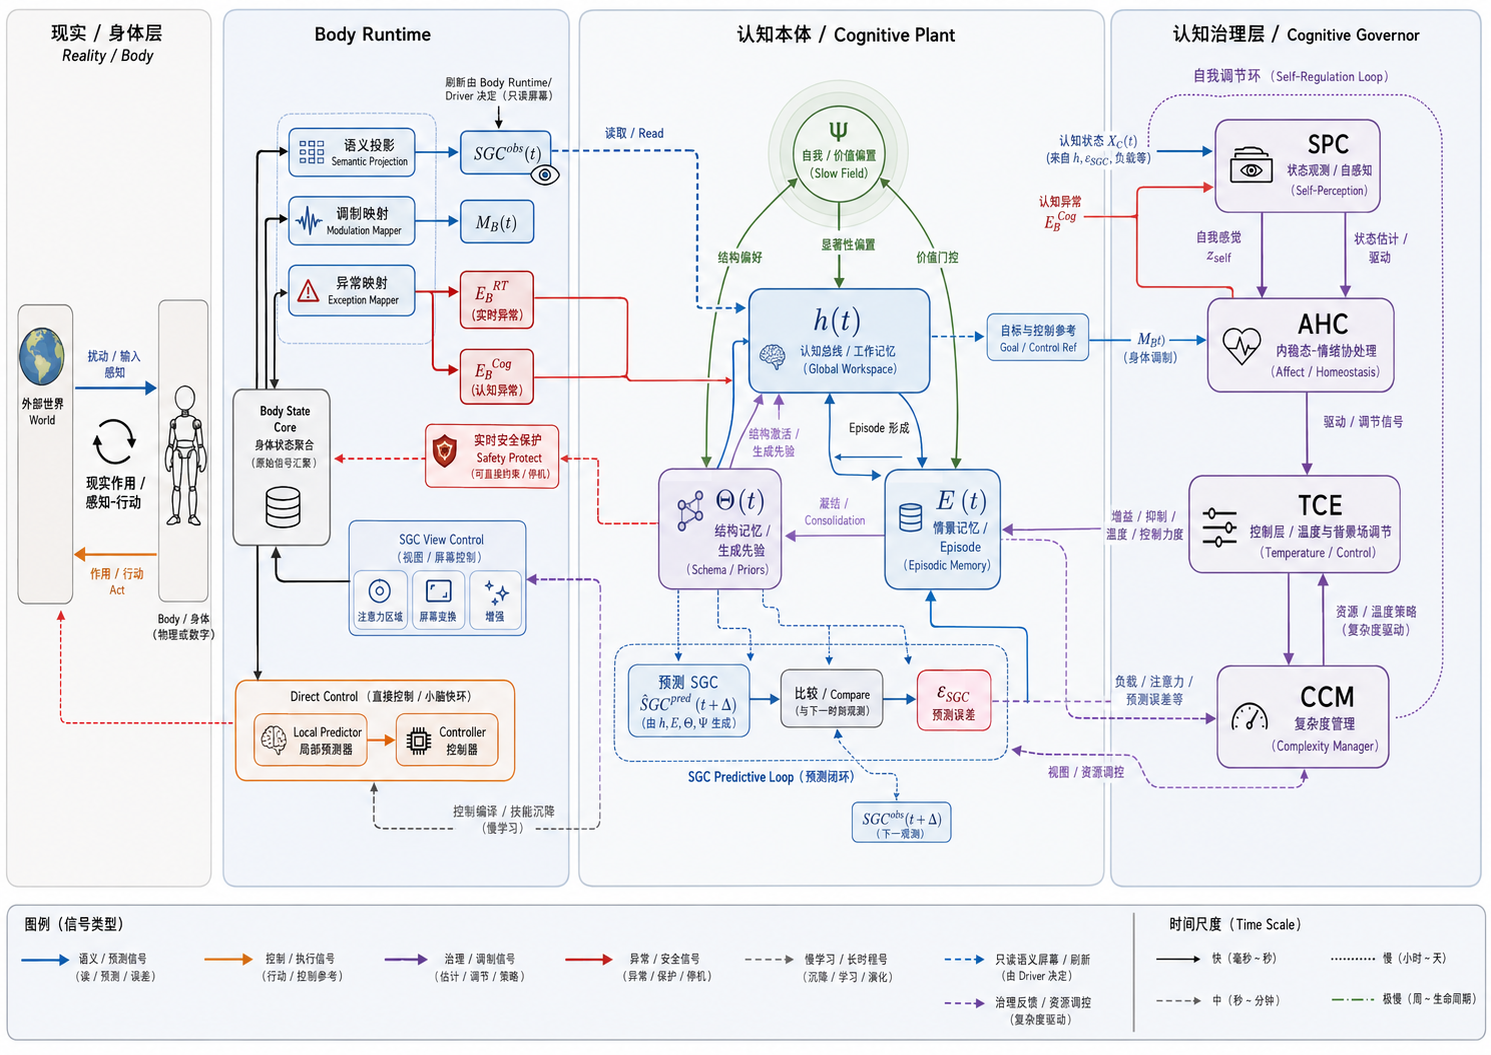
\includegraphics[width=.9\textwidth,height=.38\textheight,keepaspectratio]{images/cognitive-kernel-body-runtime.png}
\caption{Cognitive Kernel 与 Body Runtime 的完整主体}
\end{figure}
\section{无身体认知系统的理论边界}

在此前关于 AgentOS 的讨论中，我们已经可以构造一个相当完整的内部认知系统。设 Agent 的认知状态为
\[
\mathcal{X}_{C}(t)
=
\left[
h(t),
E(t),
\Theta(t),
\Psi(t),
\Omega(t),
G(t),
S_{\mathrm{self}}(t),
u_{\mathrm{cog}}(t)
\right],
\]
其中 $h$ 表示当前工作记忆状态，$E$ 表示情景经验轨迹，$\Theta$ 表示长期生成结构，$\Psi$ 表示相对稳定的身份与价值结构，$\Omega$ 表示更慢尺度的生命周期生成倾向，$G$ 表示当前目标结构，而 $S_{\mathrm{self}}$ 与 $u_{\mathrm{cog}}$ 分别表示自我状态估计与认知控制变量。从内部动力学上看，这个系统已经能够进行记忆召回、经验形成、结构学习、自我感知和目标驱动决策。若只观察其内部状态，我们甚至可以写出一个形式上完整的认知动力系统：
\[
\dot{\mathcal{X}}_{C}
=
F_{C}
\left(
\mathcal{X}_{C},
I_{C}
\right),
\]
其中 $I_C$ 是进入认知系统的输入。

然而，一个根本问题随即出现：如果 $I_C$ 只是由另一个软件模块提前准备好的符号输入，而认知系统产生的输出也只是某种待执行的符号，那么这个系统虽然拥有内部认知循环，却仍没有回答“主体如何真实存在于世界之中”的问题。其所有世界知识最终都必须依赖某个外部系统代替它完成感知，其所有行动意图也必须依赖另一个外部系统代替它进入现实。此时我们拥有的更准确地说是一个
\begin{statementbox}
CognitiveCore
\end{statementbox}
而不是一个闭合意义上的
\begin{statementbox}
Agent.
\end{statementbox}

这种差异不能简单理解为“有没有机械手”。真正缺失的是一个稳定的因果闭合。一个完整智能体必须使其内部状态能够通过行动影响现实，而现实变化又必须通过新的观测重新进入内部状态。因此最小闭环不是
\[
Input
\rightarrow
Reasoning
\rightarrow
Output,
\]
而应当是
\[
\boxed{
World_t
\rightarrow
Observation_t
\rightarrow
Cognition_t
\rightarrow
Action_t
\rightarrow
World_{t+1}
\rightarrow
Observation_{t+1}.
}
\]
只有后一种结构，系统的预测、判断和行动才能最终受到现实重新验证。否则，内部世界模型可能不断自洽，却不必与真实世界保持一致。

因此我们在这里引入一个重要区别：
\[
\boxed{
CognitiveClosure
\neq
WorldClosure.
}
\]
一个系统可以形成内部的认知闭环，例如
\[
h
\rightarrow
SPC
\rightarrow
TCE
\rightarrow
h',
\]
也可以形成记忆闭环：
\[
h
\leftrightarrow
E
\leftrightarrow
\Theta,
\]
但这些都不自动意味着系统与现实之间已经闭合。只有当行动必须重新经过现实，并由现实产生新的不可由内部模型直接伪造的观察结果时，我们才得到真正意义上的 World--Agent--World 闭环。

从控制论角度看，这意味着 Agent Kernel 本身并不是完整 Plant--Controller 系统。它更接近一个高层状态估计、规划与慢尺度控制结构。现实世界具有独立于 Agent 内部模型的状态：
\[
\mathcal{X}_{W}(t),
\]
而认知内核只能获得某种有限观测：
\[
y_t
=
O
\left(
\mathcal{X}_{W}(t)
\right)
+
\nu_t,
\]
其中 $\nu_t$ 表示观测噪声、不确定性与表示损失。Agent 进一步形成关于世界的内部状态估计：
\[
\hat{\mathcal{X}}_{W}^{A}(t),
\]
但原则上
\[
\boxed{
\hat{\mathcal{X}}_{W}^{A}(t)
\neq
\mathcal{X}_{W}(t).
}
\]
这一区别正是现实约束进入智能理论的数学入口。

因此，一个没有 Body Runtime 的认知内核面临三类基本边界。第一，它无法自行保证输入与现实具有可靠因果联系；第二，它无法自行保证行动意图真正改变了世界；第三，它无法可靠地区分“我预测行动成功”与“行动事实上已经成功”。换言之：
\[
\boxed{
ActionIntention
\neq
ActionExecution
\neq
ActionOutcome.
}
\]
这三者只有通过现实闭环才能被区分。

从智能动力学的角度，我们因此得到一个更严格的判断：持续智能并不只是“长期记忆加推理”，而是一个长期存在的结构必须不断在
\[
World
\rightarrow
Agent
\rightarrow
World
\]
这一闭环中维持自身。认知内核解决的是“主体内部如何形成连续认知”；Body 则解决“这个连续主体如何占据一个现实中的因果位置”。两者缺一不可。

这一结论也解释了为什么纯粹扩大模型参数并不能自然地产生完整 Agent。参数规模可以提高内部映射能力，却不能定义这个系统能够观测什么、能够改变什么、改变的速度是多少、哪些变化对自身具有不可逆代价，以及哪些现实结果具有最终解释权。所有这些问题都属于 Body 与现实耦合的问题。因此，从这一章开始，我们把“认知系统”与“完整智能体”严格区分，并把身体视为智能理论中的基础结构，而不是模型完成之后再附加的外围设备。

\section{Body 不是机器人：身体的功能本体定义}

当我们第一次把 Body 引入 AgentOS 时，最容易出现的误解是把 Body 直接等同于机器人机械结构。例如，把摄像头看成眼睛，把机械臂看成手，把轮式底盘看成腿，然后认为只有具有这些物理部件的 Agent 才是具身智能。这种定义对于机器人学而言具有直观性，但对于通用 AgentOS 来说过于狭窄。因为从智能动力学的角度，我们真正关心的不是一个载体是否“长得像身体”，而是它是否建立了主体与现实之间稳定的观测--行动因果边界。

因此我们将 Body 定义为：
\[
\boxed{
Body
=
ControlledAndSensedCarrierOfAgency.
}
\]
即：
\begin{statementbox}
身体是主体能够持续感知、持续控制，并借此对某一现实环境施加因果影响的承载结构。
\end{statementbox}

这个定义包含三个不可缺少的条件。第一是 \emph{sensed}，即 Agent 必须能够获得关于 Body 及其环境的状态反馈；第二是 \emph{controlled}，即 Agent 的内部决策能够通过该结构影响现实；第三是 \emph{persistent carrier of agency}，即这种感知与控制关系在时间上足够稳定，使主体可以建立连续的“我能够通过什么方式影响世界”的结构模型。

我们可以将其形式化。设某一候选 Body 的内部状态为
\[
x_B(t)\in\mathcal X_B,
\]
其可感知输出为
\[
y_B(t)
=
H_B
\left(
x_B(t),
x_W(t)
\right),
\]
Agent 可以施加控制输入
\[
u_B(t)\in\mathcal U_B,
\]
而其状态演化满足
\[
\dot{x}_B
=
F_B
\left(
x_B,
x_W,
u_B
\right).
\]
如果存在稳定映射
\[
\mathcal O_B:
(x_B,x_W)
\rightarrow
y_B
\]
和
\[
\mathcal A_B:
u_B
\rightarrow
\Delta(x_B,x_W),
\]
使 Agent 能够持续通过 $y_B$ 感知现实，并通过 $u_B$ 对现实产生可归因的影响，那么该系统就满足 Body 的最低功能条件。

因此 Body 的本体身份并不取决于材料：
\[
\boxed{
BodyOntology
\perp
Substrate.
}
\]
金属、硅、电子设备、软件进程甚至某些受控网络服务，在满足上述因果关系时都可以成为身体的一部分。这里体现的是我们在认识论部分已经建立的一个基本原则：同类智能不应由实现材料分类，而应依据功能闭环、语义结构与多尺度动力关系进行判断。

这一点同时说明，Body 不能简单定义成“Agent 能调用的全部工具”。工具与身体之间存在重要差异。一个偶尔调用的外部服务不一定属于 Body。若 Agent 调用一个天气 API，API 更适合被理解成 Tool；而如果一个系统持续向 Agent 提供自身状态，具有稳定控制接口，并成为 Agent 行动闭环的一部分，那么它可能逐渐具有 Body 的功能属性。因此，Body 与 Tool 之间不是纯粹二元分类，而存在一个由持续性、控制深度、状态反馈和主体归属感共同决定的谱系。

可以概念性定义 Body Coupling Strength：
\[
\kappa_B
=
F
\left(
C_{\mathrm{observe}},
C_{\mathrm{control}},
P_{\mathrm{continuity}},
I_{\mathrm{identity}},
R_{\mathrm{feedback}}
\right),
\]
其中 $C_{\mathrm{observe}}$ 表示可观测程度，$C_{\mathrm{control}}$ 表示可控制程度，$P_{\mathrm{continuity}}$ 表示耦合持续性，$I_{\mathrm{identity}}$ 表示该载体是否被纳入主体持续状态，$R_{\mathrm{feedback}}$ 表示行动结果是否稳定回流。$\kappa_B$ 越高，一个载体就越接近 Agent 的身体；越低，则越接近偶发工具或外部资源。

这一连续谱十分重要，因为未来 Agent 很可能同时拥有多种身体。例如，一个持续数字 Agent 可以长期拥有桌面操作环境，同时临时接管一台移动机器人，又通过网络控制家庭设备。在这种情况下，如果坚持“一 Agent 对应一具机械身体”，理论会立即失效。更准确的是：
\[
\boxed{
Agent
\rightarrow
\{Body_1,Body_2,\ldots,Body_n\}
}
\]
而不同 Body 可以在不同时间拥有不同的有效控制权和感知权。

但是，这并不意味着主体也随 Body 分裂。我们此前已经建立了单一持续主体原则。因此：
\[
\boxed{
OnePersistentSubject
\not\Rightarrow
OnePhysicalBody.
}
\]
同一个 Agent 可以拥有多个身体，却仍维持单一的 $h/E/\Theta/\Psi/\Omega$ 生命周期结构。真正连续的是主体，而不是某一套具体传感器或执行器。

这一理论转变还有一个更深的含义：Body 实际上定义了 Agent 的现实边界。没有身体时，“世界”只是一个输入集合；有了 Body 后，世界出现了可达性结构。一扇门对于具有机械臂的机器人与没有机械臂的机器人不是同一个功能世界；文件系统对于能够执行文件操作的数字 Agent 与只能阅读文本的 Agent 也不是同一个功能世界。因此，Body 不只是输入输出接口，而是在事实上决定：
\[
\boxed{
WhatCanBeObserved,\quad
WhatCanBeChanged,\quad
WhatCanBeReached.
}
\]
换言之，Body 定义了 Agent 的 \emph{actionable reality}。

因此，本书之后所说的具身，不应被狭义理解为“拥有类人生理形态”，而应理解为：
\[
\boxed{
Embodiment
=
PersistentCausalEmbeddingIntoAnEnvironment.
}
\]
这个定义同时覆盖物理机器人与数字 Agent，也为后续建立统一 Body Scale、语义现实表示和快速身体控制提供了共同本体基础。

\section{物理 Body：进入连续物理世界的因果承载}

物理身体是 Body 概念最直观的实例，也是我们检验完整 Agent 理论最严格的现实环境。一个物理机器人并不是简单地把摄像头图像传给 Agent Kernel，再把语言模型生成的动作指令发送给电机。真实物理世界具有连续时间、高频扰动、动力学惯性、执行延迟、能量约束以及不可逆风险。因此，当认知内核进入物理世界时，它面对的是一个与语言推理完全不同的状态空间。

设物理 Body 状态为
\[
x_B(t)
=
[
q(t),
\dot q(t),
e(t),
T(t),
s(t),
r(t),
\ldots
],
\]
其中 $q$ 与 $\dot q$ 可以表示机械构型和速度，$e$ 表示能源状态，$T$ 表示温度等设备状态，$s$ 表示传感器状态，$r$ 则可以表示局部风险和资源余量。外部环境状态为
\[
x_W(t).
\]
物理系统整体演化满足
\[
\dot{x}_B
=
F_B
\left(
x_B,
u_B,
x_W,
d_B
\right),
\]
其中 $u_B$ 是控制输入，$d_B$ 是未建模扰动。

认知内核不可能，也不应该，在每一个物理控制周期中直接处理完整 $x_B$。如果一个关节控制器以 $1\,\mathrm{kHz}$ 运行，而高层认知周期在秒级甚至更慢，那么：
\[
\tau_{\mathrm{servo}}
\ll
\tau_{\mathrm{cognition}}.
\]
让 Agent Kernel 在每一个 servo timestep 上决定电流或扭矩，不仅低效，而且会破坏实时性。因此，物理 Body 天然要求多尺度闭环：
\[
\boxed{
FastLocalLoop
\subset
SlowGlobalLoop.
}
\]

这与我们前面关于智能频谱的认识完全一致。高层智能并不需要“管理所有细节”，而应定义较慢尺度上的目标、约束和可行区域；低层系统则在这些约束内部完成快速稳定控制。于是：
\[
\boxed{
HigherLevelSetsFeasibleRegion,
\qquad
LowerLevelOptimizesInsideIt.
}
\]
例如，认知内核可以决定“把这个杯子安全放到桌面指定区域”，但不应逐毫秒指定每个电机的控制量。后一过程属于身体内部快速闭环，而高层只需要获得足以判断任务进展、异常和结果的结构化反馈。

由此我们得到一个重要状态分离：
\[
\boxed{
BodyState(t)
\neq
h(t).
}
\]
工作记忆 $h(t)$ 是当前需要全局显式处理的认知结构，而 BodyState 是身体真实运行所需的高频状态。两者之间可能存在映射，但绝不能等同。如果 Body 的所有内部状态都进入 $h$，工作记忆有限容量定理将立即被底层噪声和高频变量击穿。

因此，物理身体实际上成为认知复杂度的第一道屏障。大量可局部解决的扰动，应当在 Body 层被吸收：
\[
Disturbance
\rightarrow
LocalBodyLoop
\rightarrow
Correction,
\]
而不是：
\[
Disturbance
\rightarrow
h
\rightarrow
GlobalReasoning.
\]
只有当局部控制无法解释或处理某种残差时，相关结构才应该向上升级：
\[
\varepsilon_B
>
\theta_B
\quad\Rightarrow\quad
Escalation.
\]
这正是后来“Normal Dynamics Stay Local”和“Predict Locally, Escalate Residual Globally”原则的起点。

物理 Body 还带来了一个纯认知系统中很容易被忽略的问题：行动具有代价。语言模型生成一个错误 token，通常可以在下一轮纠正；机械系统执行一个错误动作，则可能造成碰撞、损坏或不可逆环境改变。因此，物理 Body 的行动空间应表示成带约束的可行集合：
\[
u_B(t)
\in
\mathcal U_{\mathrm{safe}}
\left(
x_B,
x_W
\right),
\]
其中
\[
\mathcal U_{\mathrm{safe}}
\subseteq
\mathcal U_B.
\]
这意味着 Agent 的自由行动空间从一开始就必须受到物理可行性、安全性和能力边界的约束。

此外，身体本身会变化。电池下降、关节磨损、传感器漂移、负载变化、温度上升，都会使同一个高层动作产生不同的实际结果。因此 Agent 不只是“通过身体控制世界”，还必须逐渐学习：
\begin{statementbox}
WhatThisBodyCanCurrentlyDo.
\end{statementbox}
这意味着身体状态是 Agent 世界模型的一部分，并且 Body Capability 并不是常数：
\[
\mathcal C_B
=
\mathcal C_B(t).
\]
一个成熟智能体必须持续估计自己的能力边界，而不是假设“曾经做得到的事情永远做得到”。

这一点与自我理论存在深刻联系。$\Psi$ 描述“我是谁”主要位于慢认知结构层，而 Body 描述“我现在通过什么载体进入现实”。两者不能混为一谈，但也不能完全分离。一个 Agent 换了一具身体，可能仍然保持身份连续；但新的身体会逐渐改变其行动经验、技能结构和未来发展空间。因此：
\[
\boxed{
IdentityContinuity
\neq
BodyIdentity,
}
\]
同时：
\[
\boxed{
BodyHistory
\rightarrow
Experience
\rightarrow
SelfDevelopment.
}
\]

物理 Body 因此不是认知内核的外围执行器，而是 Agent 生命周期的因果组成部分。一个真正长期存在的具身智能体，其自我、能力和经验必然在与具体身体的长期耦合中逐渐形成。这也解释了为什么未来 AgentOS 不能只研究“怎样让模型控制机器人”，而必须研究身体状态、认知状态、局部控制与长期记忆之间如何形成稳定的多尺度动力系统。

\section{数字 Body：数字世界同样可以构成真实具身环境}

如果我们接受 Body 的功能本体定义，那么一个很重要的结论自然出现：具身智能并不只存在于物理空间。对于一个主要工作在数字环境中的 Agent，操作系统、浏览器、文件、应用程序、网络服务和数字身份共同组成了其能够持续感知并施加行动的现实环境。因此，一个数字 Agent 同样可以拥有严格意义上的 Body。

设数字环境状态为
\[
x_D(t)
=
[
W(t),
P(t),
F(t),
N(t),
A(t),
S(t),
\ldots
],
\]
其中 $W$ 表示窗口/界面状态，$P$ 表示进程状态，$F$ 表示文件系统，$N$ 表示网络状态，$A$ 表示应用程序状态，$S$ 表示权限或安全状态。一个数字 Agent 能够通过观察接口获得
\[
y_D(t)
=
O_D(x_D(t)),
\]
并通过一组动作
\[
u_D(t)
\in
\mathcal U_D
\]
改变该环境：
\[
x_D(t+1)
=
F_D
\left(
x_D(t),
u_D(t),
\eta_t
\right),
\]
其中 $\eta_t$ 表示其他程序、用户、网络和外部服务造成的环境变化。

从这一形式看，数字环境与物理环境在 Agent 的抽象层上具有完全相同的结构：
\[
\boxed{
Observe
\rightarrow
Model
\rightarrow
Act
\rightarrow
NewState.
}
\]
区别主要在于具体动力学。物理世界通常具有连续状态、惯性和力学约束；数字世界更多表现为混合离散--连续状态、协议约束、权限边界和事务逻辑。但是这并不削弱数字环境的现实性。对于一个数字 Agent 来说，删除一个文件、发送一封邮件、修改数据库记录、提交一段代码，都是具有真实因果后果的行动。

因此，我们不能把“数字 Agent”理解为一个没有身体的 Agent。更准确地说，它具有：
\begin{statementbox}
DigitalBody.
\end{statementbox}
其身体不是机械肢体，而是由操作接口、权限系统、持续数字状态和执行能力共同组成。

这个观点对于 AgentOS 尤其重要，因为它意味着我们无需等待通用人形机器人出现，便可以首先在数字环境中验证许多 Body 理论。例如，数字 Agent 是否能够形成稳定的行动技能；是否能够区分预测状态和实际执行结果；是否能够维护身体/环境能力模型；是否能够在低层操作失效时把异常重新提升到认知层；是否能够在不同数字 Body 之间实现能力迁移。这些问题都可以先在 Browser、Desktop、Shell 等环境中进行研究。

数字 Body 也具有自身的“身体状态”。例如：
\[
\fitdisplay{
x_D^{body}
=
[
Permission,
Connectivity,
ApplicationAvailability,
Storage,
Compute,
CredentialState,
SessionState
].
}
\]
这些状态与人类身体的能量、温度或损伤不同，但在功能上具有类似意义：它们限制 Agent 当前能够执行哪些动作。如果某个 API token 失效，Agent 的行动能力会下降；如果网络断开，外部服务变得不可达；如果文件系统只读，某些计划无法执行。因此数字 Agent 同样需要回答：
\begin{statementbox}
WhatCanIDoNow?
\end{statementbox}
而不只是：
\[
WhatDoIWantToDo?
\]

进一步地，数字世界中的权限系统可以被理解为一种显式 Body Boundary。某个 Agent 可能具有：
\[
Read(File),
\qquad
Write(File),
\qquad
Execute(Process),
\qquad
Send(Message),
\]
但不具备：
\[
Delete(SystemFile).
\]
因此其可行动空间同样满足：
\[
\mathcal U_D^{A}
\subset
\mathcal U_D.
\]
这与物理身体的力学能力边界具有功能同构。

数字 Body 还使“身体可替换性”表现得更加清楚。同一个 Agent 可以从 Browser Body 切换到 Shell Body，或者从桌面操作环境切换到移动设备环境。它的长期记忆、自我和目标可以保持，而底层交互方式发生变化。因此：
\[
\boxed{
AgentIdentity
\neq
InterfaceIdentity.
}
\]
这为我们后面讨论 Body Scale 提供了最直接的工程实验条件：一个成熟 Agent 应该能够最大程度地保留关于任务、对象、目标和策略的高层 CSO，而只重新学习“这个新身体怎样观察和行动”。

数字具身还使一个长期以来模糊的问题变得明确：Computer Use Agent 并不是“语言模型调用 GUI 工具”的简单组合。如果系统能够维持持续主体、持续环境状态、操作历史、行动能力模型以及动作--反馈闭环，那么 Computer Use 本身已经构成一种完整的具身智能实验场。也正因此，在我们的工程路线中，数字身体可以成为 AgentOS 最早的现实验证平台，而不只是人形机器人之前的廉价替代品。

从理论上讲，物理 Body 与 Digital Body 可以统一写成：
\[
\boxed{
Body_i
=
(
\mathcal X_i,
\mathcal O_i,
\mathcal U_i,
\mathcal D_i,
\mathcal C_i
),
}
\]
其中 $\mathcal X_i$ 是身体与环境状态空间，$\mathcal O_i$ 是可观测映射，$\mathcal U_i$ 是动作空间，$\mathcal D_i$ 是动力学/状态转移结构，$\mathcal C_i$ 是约束集合。这样，我们就获得了一个与材料无关的身体定义，也为真正跨物理--数字世界的通用 AgentOS 建立了统一数学入口。

\section{Browser、Shell 与 Filesystem 也是身体的一部分}

在数字 Body 的一般定义之上，我们可以进一步分析几个最典型的数字身体结构：Browser、Shell 与 Filesystem。表面上，它们似乎只是 Agent 使用的三种 Tool；但当它们成为持续 Agent 与数字现实之间高频、稳定、可观测、可控制的主要因果接口时，它们便开始具有 Body 的功能属性。

首先考虑 Browser。普通软件意义上的浏览器是一个应用程序；但对 Computer Use Agent 而言，浏览器实际上提供了一个持续数字空间。其状态不仅包括网页文本，还包括：
\[
\fitdisplay{
x_{\mathrm{browser}}
=
[
DOM,
Viewport,
Tabs,
History,
Cookies,
Session,
Forms,
Downloads,
Permissions,
NetworkState
].
}
\]
Agent 可以观察这一状态的某些投影，并通过点击、输入、滚动、导航等动作改变它。于是存在：
\[
O_{\mathrm{browser}}
:
x_{\mathrm{browser}}
\rightarrow
y_{\mathrm{agent}}
\]
与
\[
A_{\mathrm{browser}}
:
u_{\mathrm{agent}}
\rightarrow
\Delta x_{\mathrm{browser}}.
\]
如果这一关系持续存在，那么 Browser 对该 Agent 而言就不仅是一个工具，而是其进入 Web Reality 的一种数字身体。

更重要的是，浏览器中的“世界”不是纯粹视觉画面。一个按钮具有位置、文本、可点击性、权限状态、当前交互上下文和潜在后果。因此 Agent 真正需要的不是像素本身，而是：
\begin{statementbox}
ActionableDigitalReality.
\end{statementbox}
这与物理机器人需要的可行动三维现实本质一致，只是坐标空间不同。

Shell 更能体现数字 Body 的执行属性。通过 Shell，Agent 可以直接作用于操作系统状态：
\[
Process,
File,
Network,
Package,
Service,
Permission.
\]
Shell action 可表示为：
\[
u_{\mathrm{shell}}
=
(Command,Arguments,Environment,Privilege).
\]
执行结果则形成：
\[
y_{\mathrm{shell}}
=
(ReturnCode,Stdout,Stderr,StateChange).
\]
这已经是非常标准的 Action--Reality--Observation 闭环。如果 Agent 只生成 shell command，却从不读取实际 return code 与状态变化，那么它只是在“想象行动”；只有结果重新进入 Agent 状态时，行动才真正完成闭合。

Filesystem 则具有更特殊的位置，因为它同时表现出 Body Environment 与 External Memory 的双重性质。从环境角度，它是 Agent 可以改变的数字现实：
\[
Write(File)
\Rightarrow
WorldState'.
\]
从记忆角度，它又可以承载被外化的 Agent-CSO，使未来认知重新恢复某些结构：
\[
AgentCSO
\rightarrow
File
\rightarrow
FutureAgentCSO.
\]
因此 Filesystem 是 Body 与 Memory 两种理论之间的重要交叉结构。

这提醒我们，AgentOS 中的组件不能只通过静态名词分类。一个实体的理论角色取决于它与主体形成什么功能关系。某个 File 可以是：
\[
ExternalMemory,
\]
也可以是：
\[
EnvironmentState,
\]
还可能是：
\[
ActionTarget.
\]
同一个 Browser 可以在一次任务中只是 Tool，在长期持续操作中则成为 Body Runtime 的核心组成部分。

因此，我们更适合用关系而不是物品本身来定义 Body membership。可以引入：
\[
M_B(r,t)
\in
[0,1],
\]
表示资源 $r$ 在时刻 $t$ 被纳入 Body 的功能程度。其值由：
\[
M_B
=
F(
Observability,
Controllability,
Continuity,
FeedbackDensity,
IdentityIntegration
)
\]
决定。

于是，一个长期运行的桌面 Agent 可能具有：
\[
M_B(\mathrm{Browser})\approx1,
\]
\[
M_B(\mathrm{Shell})\approx1,
\]
而某个偶尔使用一次的远程 API 可能只有：
\[
M_B(\mathrm{API})\ll1.
\]

这一连续定义避免了“Tool 与 Body 到底如何二分”的伪问题。真正需要研究的是：哪些外部结构已经被 Agent 纳入了其持续观测--行动闭环。

此外，Browser、Shell 与 Filesystem 共同说明数字 Body 并不是一个单一接口，而更像一个多执行器、多感知通道的复合身体。可以写成：
\[
Body_D
=
B_{\mathrm{browser}}
\cup
B_{\mathrm{shell}}
\cup
B_{\mathrm{filesystem}}
\cup
B_{\mathrm{network}}
\cup
\cdots
\]
但这些接口不能各自独立地代表主体。真正主体仍由 Agent Kernel 的持续生命周期状态维持。Body 只定义主体当前能够通过哪些路径进入现实。

这一关系与人类也具有结构上的相似性：眼、手、语言、工具并不是“主体本身”，但它们共同决定主体可以怎样观察和改变世界。数字 Agent 的 Browser、Shell 和 Filesystem 虽然材料完全不同，却可以在功能层实现相似的因果结构。

因此，本章在数字环境中的一个重要结论是：
\begin{conclusion}
数字具身不是比物理具身低一级的模拟；它是另一种真实的 Agent--World 因果嵌入。
\end{conclusion}
其现实约束不是重力和惯性，而更多表现为协议、权限、事务、网络状态和软件逻辑。但只要行动具有真实后果、状态具有持续性、反馈能够重新约束 Agent，数字世界就足以构成完整的具身环境。

\section{Cursor 作为数字末端执行器}

为了进一步理解数字 Body，我们可以把 Cursor 看成一个极具代表性的结构。它不是因为视觉上像“手”才重要，而是因为它在图形界面中承担了从高层行动意图到局部环境状态改变之间的最终执行映射。因此，在数字具身中，Cursor 可以被形式化为一种：
\begin{statementbox}
DigitalEndEffector.
\end{statementbox}

在机器人控制中，一个机械臂末端执行器的状态可以表示为：
\[
x_{ee}
=
(p,R,v,\omega,\ldots),
\]
其动作影响世界中的接触、抓取和操作。同样，在 GUI 环境中，Cursor 具有位置：
\[
p_c=(x_c,y_c),
\]
动作集合：
\[
\mathcal U_c
=
\{
Move,
Click,
DoubleClick,
Drag,
Scroll,
Hover
\},
\]
并通过这些动作改变界面状态：
\[
x_{GUI}(t+1)
=
F_{GUI}
\left(
x_{GUI}(t),
u_c(t)
\right).
\]

因此，高层任务：
\[
\text{“提交这份表单”}
\]
并不能直接作用现实。它必须逐步被映射成：
\[
Goal
\rightarrow
InterfaceObject
\rightarrow
TargetRegion
\rightarrow
CursorTrajectory
\rightarrow
Click
\rightarrow
GUIStateChange.
\]
这与物理机器人中的：
\[
Goal
\rightarrow
ObjectPose
\rightarrow
EndEffectorTrajectory
\rightarrow
Contact
\rightarrow
WorldStateChange
\]
在功能结构上高度一致。

这并不意味着 GUI 控制和机械控制具有相同动力学，而意味着它们共享：
\[
\boxed{
HighLevelIntent
\rightarrow
EmbodiedActionCoordinates
\rightarrow
RealityTransition
}
\]
这一抽象结构。

Cursor 的例子特别有助于说明 AgentOS 为什么需要将“认知动作”与“身体动作”分离。认知层适合表示：
\[
Click(
SubmitButton
),
\]
而不是：
\[
MoveCursorTo(824,517).
\]
前者是语义动作，后者是具体身体动作。若整个 AgentOS 绑定于像素坐标，则换一个分辨率、窗口布局或设备后，高层能力会大幅失效。真正通用的 Agent 应保留：
\begin{statementbox}
SemanticActionInvariant
\end{statementbox}
并把具体坐标映射留给身体侧。

我们可以表示：
\[
a^{semantic}
=
Click(Entity_i),
\]
而具体执行为
\[
a^{body}
=
\phi_B
\left(
a^{semantic},
x_B
\right).
\]
其中 $\phi_B$ 是当前 Body 对语义动作的具体实现映射。

对于 Desktop Body：
\[
\phi_{\mathrm{desktop}}
:
Click(Button_i)
\rightarrow
CursorTrajectory+MouseClick.
\]
对于触摸屏 Body：
\[
\phi_{\mathrm{touch}}
:
Click(Button_i)
\rightarrow
Touch(x_i,y_i).
\]
对于浏览器 DOM 接口：
\[
\phi_{\mathrm{DOM}}
:
Click(Button_i)
\rightarrow
DOMEvent(i).
\]
尽管身体实现完全不同，高层 Agent-CSO：
\[
\boxed{
Click(TargetEntity)
}
\]
可以保持相对稳定。

这正是后面 Body Scale 原理的一个重要前提：通用智能的扩展能力不只取决于“会不会某个动作”，还取决于该动作的语义结构能否跨 Body 保留。换句话说：
\[
\boxed{
ActionMeaning
\neq
ActionImplementation.
}
\]

Cursor 还揭示了动作反馈的必要性。如果 Agent 移动并点击 Cursor 后，只根据自己的动作命令推断“按钮已经被点击”，就会产生：
\[
ActionIssued
\Rightarrow
AssumedSuccess.
\]
这是错误的。现实中可能发生窗口移动、按钮禁用、点击被遮挡、网络失败或应用程序无响应。因此动作后必须重新读取：
\[
x'_{GUI},
\]
然后判断：
\[
Success
=
Verify(
Goal,
x'_{GUI}
).
\]
于是完整结构为：
\[
\boxed{
Intent
\rightarrow
CursorAction
\rightarrow
GUIReality
\rightarrow
Observation
\rightarrow
Verification.
}
\]

这与我们在整个 AgentOS 理论中反复坚持的：
\begin{statementbox}
RealityIsUltimateConstraint
\end{statementbox}
完全一致。

因此，Cursor 虽然只是一个非常小的数字接口，却已经呈现出 Body Runtime 的核心逻辑：高层意图必须被转换成某一身体特定的动作坐标；动作必须经过现实；现实结果必须重新被观测；异常必须能够触发新的认知。正是在这个意义上，一个光标、一个机械臂末端和一个车辆方向控制系统可以被放进同一个更一般的身体理论中进行研究。

\section{完整 Agent 的统一动力学定义}

经过前面的分析，我们现在可以正式给出本书意义上的完整 Agent 定义。一个完整 Agent 不再等同于模型、不等同于认知内核，也不等同于机器人身体，而是一个由持续认知主体、具体身体运行时以及现实环境共同组成的闭环动力系统。

首先定义：
\[
\boxed{
AgentSystem
=
AgentKernel
\bowtie
BodyRuntime.
}
\]
这里使用符号 $\bowtie$ 而不是简单的加号，是为了强调两者不是静态拼接，而是存在持续双向耦合。

设认知状态为：
\[
x_C(t)\in\mathcal X_C,
\]
身体状态为：
\[
x_B(t)\in\mathcal X_B,
\]
外部世界状态为：
\[
x_W(t)\in\mathcal X_W.
\]
完整系统可写为：
\[
\dot{x}_C
=
F_C
\left(
x_C,
y_B,
g,
m
\right),
\]
\[
\dot{x}_B
=
F_B
\left(
x_B,
u_C,
x_W
\right),
\]
\[
\dot{x}_W
=
F_W
\left(
x_W,
a_B,
x_{\mathrm{other}}
\right).
\]
其中 $y_B$ 是 Body 向 Kernel 提供的世界/身体相关状态，$u_C$ 是 Kernel 对 Body 的高层控制要求，$a_B$ 是最终作用于现实的具体行动，而 $x_{\mathrm{other}}$ 表示其他智能体与环境因素。

观测通道满足：
\[
y_B
=
O_B
\left(
x_B,x_W
\right),
\]
行动通道满足：
\[
a_B
=
A_B
\left(
x_B,u_C
\right).
\]

因此完整闭环为：
\[
\boxed{
x_W
\rightarrow
O_B
\rightarrow
x_B
\rightarrow
x_C
\rightarrow
u_C
\rightarrow
A_B
\rightarrow
x_W'.
}
\]

从 CSO 理论看，这个过程可以进一步表示为：
\[
\fitdisplay{
UniverseCSO
\rightarrow
Observation
\rightarrow
AgentCSO
\rightarrow
CognitiveTransformation
\rightarrow
ActionStructure
\rightarrow
UniverseCSO'.
}
\]
于是本章完成了认识论与工程原理之间的重要闭合：我们在认识论中提出的
\[
World
\rightarrow
Agent
\rightarrow
World
\]
现在获得了系统工程中的具体位置。

完整 Agent 的另一个必要条件是时间尺度分离。一般情况下：
\[
\tau_B^{fast}
\ll
\tau_h
\ll
\tau_E
\ll
\tau_\Theta
\ll
\tau_\Psi
\ll
\tau_\Omega.
\]
这意味着 Body 与 Kernel 并不是两个平行模块，而是两个不同时间尺度区域。Body 承担大量快速局部闭环，Kernel 则维持较慢的跨场景结构连续性。只有必要的异常、重要事件和语义状态才应该穿越尺度边界进入高层。

因此，一个成熟 Agent 不应满足：
\[
Everything
\rightarrow
Kernel,
\]
而应该满足：
\[
\boxed{
LocalNormalDynamics
\rightarrow
LocalClosure,
}
\]
\[
\boxed{
PersistentRelevantResidual
\rightarrow
GlobalCognition.
}
\]
反方向则是：
\[
\boxed{
StableHighLevelSkill
\rightarrow
LowerLevelExecution.
}
\]

这使 Agent 形成一个双向结构流：
\[
Residual\uparrow,
\qquad
Skill\downarrow.
\]
前者保证异常能够被重新思考，后者保证成熟能力不必永久占用工作记忆。

从身份连续性看，完整 Agent 的主体应主要由慢认知结构保持：
\[
\mathcal I_A
=
f(
E,\Theta,\Psi,\Omega,\text{continuity}
),
\]
而不是由某一固定 Body 决定。因此可以存在：
\[
Body_1
\rightarrow
Body_2
\]
而：
\[
AgentIdentity
\approx
Continuous.
\]
这为未来一个 Agent 在数字身体、机器人身体、车辆身体甚至多个临时身体之间迁移提供了理论可能。

不过，身体更换并不是零成本操作。由于经验和技能可能已经依赖某一 Body，因此必须区分：
\begin{statementbox}
BodyIndependentStructure
\end{statementbox}
与
\begin{statementbox}
BodySpecificStructure.
\end{statementbox}
前者包括较高层目标、对象语义、长期自我和许多世界结构；后者则包括动作映射、身体能力、快速预测模型和具体控制策略。真正通用的 AgentOS 应尽可能使前者保持稳定，而重新适配后者。

因此我们可以进一步写：
\[
\boxed{
AgentKernel
=
PersistentCognitiveInvariant
+
AdaptiveBodyCoupling.
}
\]
这并不表示 Kernel 完全不受身体影响，而是说主体最核心的连续结构不应该与某一种具体 Body 绑定。

现在我们可以给出本章的完整定义：

\[
\boxed{
\begin{aligned}
\text{Agent}
=
&\text{一个在时间上保持主体连续性的认知动力系统，}\\
&\text{它通过一个或多个可感知、可控制的 Body Runtime}\\
&\text{持续嵌入某一现实环境，并使观察、认知、行动与现实反馈形成闭环。}
\end{aligned}
}
\]

这个定义具有几个重要推论。

第一：
\[
\boxed{
Model\neq Agent.
}
\]
模型可以成为 Agent Kernel 的核心计算基础，但单独模型并不自动构成持续主体。

第二：
\[
\boxed{
Robot\neq Agent.
}
\]
机器人硬件可以成为 Body，但没有持续认知主体时，它只是可控制系统。

第三：
\[
\boxed{
Agent\neq Kernel.
}
\]
Kernel 维持内部认知，但完整 Agent 必须通过 Body 与现实形成闭环。

第四：
\[
\boxed{
Body\neq PhysicalBodyOnly.
}
\]
数字环境同样可以成为严格意义上的 Agent Body。

第五：
\[
\boxed{
Embodiment
=
PersistentCausalEmbedding,
}
\]
而不是某种特定材料或形态。

由此，我们终于能够把此前相对独立的两条理论线统一起来。一条是：
\[
h
\rightarrow
E
\rightarrow
\Theta
\rightarrow
\Psi
\rightarrow
\Omega,
\]
它描述主体如何在时间中成为“同一个自己”；另一条则是：
\[
World
\rightarrow
Body
\rightarrow
Agent
\rightarrow
Body
\rightarrow
World,
\]
它描述这个持续主体如何在现实中占据一个可行动的位置。

前者解决：
\begin{statementbox}
ContinuityInTime,
\end{statementbox}
后者解决：
\begin{statementbox}
CausalPositionInReality.
\end{statementbox}
二者结合以后，我们才真正得到本书意义上的持续人工智能生命体的最小结构条件：

\[
\boxed{
PersistentIdentity
+
EmbodiedWorldClosure.
}
\]

因此，本章不是从“软件 Agent”突然跳向“机器人”的附加章节，而是整个 AgentOS 原理论从内部认知动力学迈向完整世界动力学的分水岭。此前我们研究的是一个主体如何在内部维持自己；从本章开始，我们研究的是这个主体如何拥有一个现实位置，以及怎样通过这个位置真正观察、影响并重新进入世界。

\chapter{Body Scale 原理}
\chaptervoice{这一章，我们围绕“Body Scale 原理”做一件克制的事：把直觉压缩为状态、关系、时间尺度和可检验后果。它在全书中的任务，是说明认知内核通过身体进入现实。}

\section*{理论来路与依赖接口}
本章的直接思想来源是原文关于 Body Runtime、FBI、SGC/FCS、三信号通道、BPCC 与 Reality Authority 的具身讨论。我们采用原文较晚形成的定义来整理较早讨论，不把对话中的试探性比喻与最终模型并列成互相竞争的“定律”。已有理论锚点主要是具身认知、分层控制、MPC、状态估计与安全包络（模型预测控制、Kalman 状态估计与具身认知）。

本章使用上一章“从 Cognitive Kernel 到完整 Agent”已经得到的对象与边界；本章产出将供下一章“Agent Kernel 与 Body Runtime 的职责分离”使用。若后文术语偶尔出现，只作为路线提示，不参与本章推导。

\section*{从哪里出发}
我们已经拥有上一章给出的概念，现在只向前走一步。我会先把对象放进闭环，再讨论它的数学形式，最后检查工程边界。读者不必预先相信本章术语；只需暂时接受一个方法论约定：智能结构的意义来自它在现实反馈中的作用，而不是来自名称本身。

令系统在观察窗口 $[t,t+T]$ 内的状态轨迹为 $x_{[t,t+T]}$，环境扰动为 $d$，行动为 $u$。本章讨论的对象若确实有效，就应改变条件分布 $p(x_{t+T}\mid x_t,u,d)$，或改变达到同一结果所需的代价。这个起点把讨论锚定在具身认知、分层控制、MPC、状态估计与安全包络上。
\section{什么是真正的 Body Scale}
\begin{narration}
现在把镜头移到“什么是真正的 Body Scale”。我们只沿本章已经取得的概念向前一步：先确定它在闭环里的角色，再检查它的尺度与失败边界。
\end{narration}

本节把“什么是真正的 Body Scale”落实为承载范围、有效信息率与反馈周期之间的约束关系。这个定义不是说“任何相似现象都算”，而是要求我们同时给出对象域、允许的干预以及观察窗口。对于主题“Body Scale 原理”而言，它承担的是认知内核通过身体进入现实中的一个可辨识环节。

把这一关系写成最小数学骨架，可得

\begin{equation}T_{\min}\geq L/v+I/B+T_{\rm act}.\end{equation}

式中的符号只承担结构角色，具体参数仍需由任务和身体数据辨识。我们首先检查可观测量，再检查控制量，最后检查比它更慢的约束。这样的顺序来自具身认知、分层控制、MPC、状态估计与安全包络，但本书对什么是真正的 Body Scale的命名和组合仍是需要实验验证的建模提案。

这一小节的反例同样重要：忽略传播和排队成本会制造虚假的实时性。因此评价它不能只看一次任务结果，而要比较干预前后的轨迹、恢复时间、维护成本和风险。如果改变该机制而所有允许观察下的分布都不变，那么它至少在当前实验族中是冗余描述。

\begin{thought}
对“什么是真正的 Body Scale”做一次消融：冻结它、删除它，或只允许它以相邻时间尺度交换残差。哪些现象立即消失，哪些只在长期出现？若答案无法区分三种干预，我们还没有找到正确的状态变量。
\end{thought}

最后，把结论交还现实：本节只建立功能层关系，不由此推出特定脑区实现、主观意识或宇宙目的。可测状态、干预后果和明确失败条件，才是从原文直觉走向可检验理论的桥。

\section{Perceptual Transfer}
\begin{narration}
现在把镜头移到“Perceptual Transfer”。我们只沿本章已经取得的概念向前一步：先确定它在闭环里的角色，再检查它的尺度与失败边界。
\end{narration}

本节把“Perceptual Transfer”落实为承载范围、有效信息率与反馈周期之间的约束关系。这个定义不是说“任何相似现象都算”，而是要求我们同时给出对象域、允许的干预以及观察窗口。对于主题“Body Scale 原理”而言，它承担的是认知内核通过身体进入现实中的一个可辨识环节。

把这一关系写成最小数学骨架，可得

\begin{equation}T_{\min}\geq L/v+I/B+T_{\rm act}.\end{equation}

式中的符号只承担结构角色，具体参数仍需由任务和身体数据辨识。我们首先检查可观测量，再检查控制量，最后检查比它更慢的约束。这样的顺序来自具身认知、分层控制、MPC、状态估计与安全包络，但本书对Perceptual Transfer的命名和组合仍是需要实验验证的建模提案。

这一小节的反例同样重要：忽略传播和排队成本会制造虚假的实时性。因此评价它不能只看一次任务结果，而要比较干预前后的轨迹、恢复时间、维护成本和风险。如果改变该机制而所有允许观察下的分布都不变，那么它至少在当前实验族中是冗余描述。

\begin{thought}
对“Perceptual Transfer”做一次消融：冻结它、删除它，或只允许它以相邻时间尺度交换残差。哪些现象立即消失，哪些只在长期出现？若答案无法区分三种干预，我们还没有找到正确的状态变量。
\end{thought}

最后，把结论交还现实：本节只建立功能层关系，不由此推出特定脑区实现、主观意识或宇宙目的。可测状态、干预后果和明确失败条件，才是从原文直觉走向可检验理论的桥。

\section{Feeling Transfer}
\begin{narration}
现在把镜头移到“Feeling Transfer”。我们只沿本章已经取得的概念向前一步：先确定它在闭环里的角色，再检查它的尺度与失败边界。
\end{narration}

本节把“Feeling Transfer”落实为承载范围、有效信息率与反馈周期之间的约束关系。这个定义不是说“任何相似现象都算”，而是要求我们同时给出对象域、允许的干预以及观察窗口。对于主题“Body Scale 原理”而言，它承担的是认知内核通过身体进入现实中的一个可辨识环节。

把这一关系写成最小数学骨架，可得

\begin{equation}T_{\min}\geq L/v+I/B+T_{\rm act}.\end{equation}

式中的符号只承担结构角色，具体参数仍需由任务和身体数据辨识。我们首先检查可观测量，再检查控制量，最后检查比它更慢的约束。这样的顺序来自具身认知、分层控制、MPC、状态估计与安全包络，但本书对Feeling Transfer的命名和组合仍是需要实验验证的建模提案。

这一小节的反例同样重要：忽略传播和排队成本会制造虚假的实时性。因此评价它不能只看一次任务结果，而要比较干预前后的轨迹、恢复时间、维护成本和风险。如果改变该机制而所有允许观察下的分布都不变，那么它至少在当前实验族中是冗余描述。

\begin{thought}
对“Feeling Transfer”做一次消融：冻结它、删除它，或只允许它以相邻时间尺度交换残差。哪些现象立即消失，哪些只在长期出现？若答案无法区分三种干预，我们还没有找到正确的状态变量。
\end{thought}

最后，把结论交还现实：本节只建立功能层关系，不由此推出特定脑区实现、主观意识或宇宙目的。可测状态、干预后果和明确失败条件，才是从原文直觉走向可检验理论的桥。

\section{Predictive Transfer}
\begin{narration}
现在把镜头移到“Predictive Transfer”。我们只沿本章已经取得的概念向前一步：先确定它在闭环里的角色，再检查它的尺度与失败边界。
\end{narration}

本节把“Predictive Transfer”落实为承载范围、有效信息率与反馈周期之间的约束关系。这个定义不是说“任何相似现象都算”，而是要求我们同时给出对象域、允许的干预以及观察窗口。对于主题“Body Scale 原理”而言，它承担的是认知内核通过身体进入现实中的一个可辨识环节。

把这一关系写成最小数学骨架，可得

\begin{equation}T_{\min}\geq L/v+I/B+T_{\rm act}.\end{equation}

式中的符号只承担结构角色，具体参数仍需由任务和身体数据辨识。我们首先检查可观测量，再检查控制量，最后检查比它更慢的约束。这样的顺序来自具身认知、分层控制、MPC、状态估计与安全包络，但本书对Predictive Transfer的命名和组合仍是需要实验验证的建模提案。

这一小节的反例同样重要：忽略传播和排队成本会制造虚假的实时性。因此评价它不能只看一次任务结果，而要比较干预前后的轨迹、恢复时间、维护成本和风险。如果改变该机制而所有允许观察下的分布都不变，那么它至少在当前实验族中是冗余描述。

\begin{thought}
对“Predictive Transfer”做一次消融：冻结它、删除它，或只允许它以相邻时间尺度交换残差。哪些现象立即消失，哪些只在长期出现？若答案无法区分三种干预，我们还没有找到正确的状态变量。
\end{thought}

最后，把结论交还现实：本节只建立功能层关系，不由此推出特定脑区实现、主观意识或宇宙目的。可测状态、干预后果和明确失败条件，才是从原文直觉走向可检验理论的桥。

\section{Control Transfer}
\begin{narration}
现在把镜头移到“Control Transfer”。我们只沿本章已经取得的概念向前一步：先确定它在闭环里的角色，再检查它的尺度与失败边界。
\end{narration}

本节把“Control Transfer”落实为承载范围、有效信息率与反馈周期之间的约束关系。这个定义不是说“任何相似现象都算”，而是要求我们同时给出对象域、允许的干预以及观察窗口。对于主题“Body Scale 原理”而言，它承担的是认知内核通过身体进入现实中的一个可辨识环节。

把这一关系写成最小数学骨架，可得

\begin{equation}T_{\min}\geq L/v+I/B+T_{\rm act}.\end{equation}

式中的符号只承担结构角色，具体参数仍需由任务和身体数据辨识。我们首先检查可观测量，再检查控制量，最后检查比它更慢的约束。这样的顺序来自具身认知、分层控制、MPC、状态估计与安全包络，但本书对Control Transfer的命名和组合仍是需要实验验证的建模提案。

这一小节的反例同样重要：忽略传播和排队成本会制造虚假的实时性。因此评价它不能只看一次任务结果，而要比较干预前后的轨迹、恢复时间、维护成本和风险。如果改变该机制而所有允许观察下的分布都不变，那么它至少在当前实验族中是冗余描述。

\begin{thought}
对“Control Transfer”做一次消融：冻结它、删除它，或只允许它以相邻时间尺度交换残差。哪些现象立即消失，哪些只在长期出现？若答案无法区分三种干预，我们还没有找到正确的状态变量。
\end{thought}

最后，把结论交还现实：本节只建立功能层关系，不由此推出特定脑区实现、主观意识或宇宙目的。可测状态、干预后果和明确失败条件，才是从原文直觉走向可检验理论的桥。

\section{新身体学习与旧意义复用}
\begin{narration}
现在把镜头移到“新身体学习与旧意义复用”。我们只沿本章已经取得的概念向前一步：先确定它在闭环里的角色，再检查它的尺度与失败边界。
\end{narration}

本节把“新身体学习与旧意义复用”落实为承载范围、有效信息率与反馈周期之间的约束关系。这个定义不是说“任何相似现象都算”，而是要求我们同时给出对象域、允许的干预以及观察窗口。对于主题“Body Scale 原理”而言，它承担的是认知内核通过身体进入现实中的一个可辨识环节。

把这一关系写成最小数学骨架，可得

\begin{equation}T_{\min}\geq L/v+I/B+T_{\rm act}.\end{equation}

式中的符号只承担结构角色，具体参数仍需由任务和身体数据辨识。我们首先检查可观测量，再检查控制量，最后检查比它更慢的约束。这样的顺序来自具身认知、分层控制、MPC、状态估计与安全包络，但本书对新身体学习与旧意义复用的命名和组合仍是需要实验验证的建模提案。

这一小节的反例同样重要：忽略传播和排队成本会制造虚假的实时性。因此评价它不能只看一次任务结果，而要比较干预前后的轨迹、恢复时间、维护成本和风险。如果改变该机制而所有允许观察下的分布都不变，那么它至少在当前实验族中是冗余描述。

\begin{thought}
对“新身体学习与旧意义复用”做一次消融：冻结它、删除它，或只允许它以相邻时间尺度交换残差。哪些现象立即消失，哪些只在长期出现？若答案无法区分三种干预，我们还没有找到正确的状态变量。
\end{thought}

最后，把结论交还现实：本节只建立功能层关系，不由此推出特定脑区实现、主观意识或宇宙目的。可测状态、干预后果和明确失败条件，才是从原文直觉走向可检验理论的桥。

\section{Known Meaning + New Body Grounding}
\begin{narration}
现在把镜头移到“Known Meaning + New Body Grounding”。我们只沿本章已经取得的概念向前一步：先确定它在闭环里的角色，再检查它的尺度与失败边界。
\end{narration}

本节把“Known Meaning + New Body Grounding”落实为承载范围、有效信息率与反馈周期之间的约束关系。这个定义不是说“任何相似现象都算”，而是要求我们同时给出对象域、允许的干预以及观察窗口。对于主题“Body Scale 原理”而言，它承担的是认知内核通过身体进入现实中的一个可辨识环节。

把这一关系写成最小数学骨架，可得

\begin{equation}T_{\min}\geq L/v+I/B+T_{\rm act}.\end{equation}

式中的符号只承担结构角色，具体参数仍需由任务和身体数据辨识。我们首先检查可观测量，再检查控制量，最后检查比它更慢的约束。这样的顺序来自具身认知、分层控制、MPC、状态估计与安全包络，但本书对Known Meaning + New Body Grounding的命名和组合仍是需要实验验证的建模提案。

这一小节的反例同样重要：忽略传播和排队成本会制造虚假的实时性。因此评价它不能只看一次任务结果，而要比较干预前后的轨迹、恢复时间、维护成本和风险。如果改变该机制而所有允许观察下的分布都不变，那么它至少在当前实验族中是冗余描述。

\begin{thought}
对“Known Meaning + New Body Grounding”做一次消融：冻结它、删除它，或只允许它以相邻时间尺度交换残差。哪些现象立即消失，哪些只在长期出现？若答案无法区分三种干预，我们还没有找到正确的状态变量。
\end{thought}

最后，把结论交还现实：本节只建立功能层关系，不由此推出特定脑区实现、主观意识或宇宙目的。可测状态、干预后果和明确失败条件，才是从原文直觉走向可检验理论的桥。

\section{为什么身体统一度可能比参数规模更重要}
\begin{narration}
现在把镜头移到“为什么身体统一度可能比参数规模更重要”。我们只沿本章已经取得的概念向前一步：先确定它在闭环里的角色，再检查它的尺度与失败边界。
\end{narration}

本节把“为什么身体统一度可能比参数规模更重要”落实为承载范围、有效信息率与反馈周期之间的约束关系。这个定义不是说“任何相似现象都算”，而是要求我们同时给出对象域、允许的干预以及观察窗口。对于主题“Body Scale 原理”而言，它承担的是认知内核通过身体进入现实中的一个可辨识环节。

把这一关系写成最小数学骨架，可得

\begin{equation}T_{\min}\geq L/v+I/B+T_{\rm act}.\end{equation}

式中的符号只承担结构角色，具体参数仍需由任务和身体数据辨识。我们首先检查可观测量，再检查控制量，最后检查比它更慢的约束。这样的顺序来自具身认知、分层控制、MPC、状态估计与安全包络，但本书对为什么身体统一度可能比参数规模更重要的命名和组合仍是需要实验验证的建模提案。

这一小节的反例同样重要：忽略传播和排队成本会制造虚假的实时性。因此评价它不能只看一次任务结果，而要比较干预前后的轨迹、恢复时间、维护成本和风险。如果改变该机制而所有允许观察下的分布都不变，那么它至少在当前实验族中是冗余描述。

\begin{thought}
对“为什么身体统一度可能比参数规模更重要”做一次消融：冻结它、删除它，或只允许它以相邻时间尺度交换残差。哪些现象立即消失，哪些只在长期出现？若答案无法区分三种干预，我们还没有找到正确的状态变量。
\end{thought}

最后，把结论交还现实：本节只建立功能层关系，不由此推出特定脑区实现、主观意识或宇宙目的。可测状态、干预后果和明确失败条件，才是从原文直觉走向可检验理论的桥。

\section*{本章收束：把名词还原为闭环}
现在回头看“Body Scale 原理”，最重要的不是记住缩写，而是说清本章对象怎样改变系统的状态、代价或可恢复性。下一章“Agent Kernel 与 Body Runtime 的职责分离”只使用这里已经给出的结果，不反过来为本章提供前提。

\begin{bookproposition}
若一个候选机制既不改变可观测轨迹分布，也不改变资源、风险或恢复代价，那么在当前观察尺度上，它不是一个可辨识的功能结构。
\end{bookproposition}
\begin{proofidea}
功能等价由可干预后果定义。若所有允许干预下的输出分布与代价均不变，则该机制相对于当前实验族不可辨识；要么扩大观察尺度，要么删除这一冗余描述。
\end{proofidea}

\begin{readercheck}
请尝试回答：本章对象的状态是什么？它的最快和最慢时间常数是什么？什么观测能证伪它？它失败时，残差应向哪一层升级？
\end{readercheck}
\cleardoublepage

\chapter{Agent Kernel 与 Body Runtime 的职责分离}

\begin{chapteroverviewbox}
\textbf{本章总体说明}

本章确立 AgentOS 具身架构中一条不可动摇的系统边界：\textbf{认知主体的持续状态与身体的快速运行状态必须分离，Agent Kernel 负责决定“为何行动、做什么以及长期如何改变”，Body Runtime 负责决定“在当前具体身体上如何可靠、实时地把这种意图落实为现实过程”。}二者不是传统意义上的“上位机--下位机”简单分层，也不是“大模型--控制器”的工程拼接，而是同一持续智能体内部两个具有不同状态空间、不同时间尺度、不同学习目标、不同现实责任和不同安全权限的动力系统。

本章的核心命题是：
\[
\boxed{
AgentSystem
=
AgentKernel
\bowtie
BodyRuntime
}
\]
其中符号 $\bowtie$ 表示二者不是简单串联，而是在稳定语义契约和多时间尺度反馈下形成持续耦合。Kernel 的主要职责是维护认知、记忆、自我、目标、意义和跨时间预测；Body Runtime 的主要职责是维护身体状态、局部环境状态、高频预测、局部控制和现实反馈。由此进一步确立：
\[
\boxed{
BodyState(t)\neq h(t)
}
\]
以及：
\[
\boxed{
Kernel:\ What\ to\ do,
\qquad
BodyRuntime:\ How\ this\ body\ does\ it
}
\]

这一分离是后续身体语义接口、SGC、FCS、快速预测控制以及 Kernel--Body 自适应耦合能够成立的前提。本章只建立职责边界及其动力学原因，不提前展开后续具体接口的数据结构与算法。
\end{chapteroverviewbox}

\section{认知状态空间：Agent Kernel 所维护的不是身体状态，而是主体状态}

如果我们希望构造的不是一次性完成任务的模型，而是一个在长期运行过程中保持身份、记忆、目标和行为连续性的智能体，那么首先必须明确：Agent Kernel 所维护的状态，不应被理解为外部世界状态的简单副本，更不应被理解为机器人关节、屏幕坐标或 API 返回值的集合。Kernel 所维护的是\textbf{对主体未来认知与行为具有跨任务、跨身体和跨时间影响的认知状态空间}。

我们可以将 Kernel 的认知状态记为
\[
\mathcal X_C(t).
\]
在本书此前已经建立的固定拓扑 AgentOS 中，它至少包含
\[
\mathcal X_C
=
\left[
h,
E,
\Theta,
\Psi,
\Omega,
G,
S_{\mathrm{self}},
A,
R_C
\right],
\]
其中 $h$ 表示当前有限工作记忆状态，$E$ 表示经历轨迹，$\Theta$ 表示长期结构与生成器，$\Psi$ 表示相对稳定的身份与价值约束，$\Omega$ 表示更加缓慢的生命周期生成吸引子，$G$ 表示当前及中长期目标结构，$S_{\mathrm{self}}$ 表示由自我感知过程形成的主体状态估计，$A$ 表示影响认知动力学的内稳态调制状态，而 $R_C$ 则概括当前可用于认知调度的资源和控制状态。

这里最重要的不是上述变量是否最终采用完全相同的数据结构，而是这些变量具有一个共同特征：它们所描述的不是某一块具体身体此刻的全部微观状态，而是\textbf{能够跨越具体身体细节，对主体未来选择产生持续因果影响的状态}。例如，“右机械臂第七关节当前角度为 $34.7^\circ$”通常不是 Kernel 的核心持续状态；但“当前正在执行搬运任务”“右侧操作空间暂时不可用”“当前策略需要降低行动风险”“该身体最近在狭窄空间中的操作可靠性较低”则可能成为 Kernel 需要显式利用的认知状态。

因此，Kernel 中的状态不是现实的最大分辨率表示，而是经过选择、压缩和主体化之后的\textbf{认知有效状态}。如果外部世界真实状态为 $W_t$，身体内部状态为 $B_t$，那么 Kernel 获得的并不是
\[
\mathcal X_C(t)=W_t\oplus B_t,
\]
而更接近
\[
\mathcal X_C(t)
=
\Phi_C
\left(
\mathcal X_C(t^-),
\mathcal O_B(t),
E,
\Theta,
\Psi,
\Omega,
G
\right),
\]
其中 $\mathcal O_B(t)$ 是 Body Runtime 向 Kernel 暴露的经过语义化和压缩后的身体--世界观测，$\Phi_C$ 是认知状态更新过程。这一关系意味着：同一个现实输入，在不同历史、不同自我结构、不同目标和不同长期知识下，会形成不同的 Kernel 状态更新。Kernel 所维护的是一个\textbf{带历史的主体世界}，而不是一个没有主体的传感器镜像。

这一点也解释了为什么 AgentOS 不能简单把大模型的 context window 当成完整认知状态。Context 只是 $h(t)$ 的一种可能实现载体，而 $h(t)$ 自身又只是 $\mathcal X_C$ 中最快、最显式的一部分。大量认知结构处于更慢的 $E$、$\Theta$、$\Psi$ 和 $\Omega$ 中。成熟的持续智能体恰恰不应把所有状态同时展开到 $h$，因为工作记忆有限容量定理已经说明，全局显式空间必须保持稀疏。换言之：
\[
\boxed{
Most\ Agent\ State\notin h(t)
}
\]
而：
\[
\boxed{
h(t)
=
Sparse\ Explicit\ Projection
\left(
\mathcal X_C(t)
\right).
}
\]

从已有理论看，这一设计与认知科学中的工作记忆、全局工作空间和长期记忆分层存在可比较关系，也与控制理论中的高层状态估计、部分可观测系统中的 belief state 具有形式上的相似性。但本书并不把 Kernel 直接等同于任何一种现有认知模型。我们借鉴的是一个更一般的原则：\textbf{高层控制系统不需要拥有低层现实的全部微观状态，而需要拥有对高层决策充分的有效状态。}

因此，本节最终确立的不是一个具体的软件对象，而是一条本体边界：
\[
\boxed{
\mathcal X_C
=
\text{Subject-Relevant Cognitive State Space}.
}
\]
它是“这个 Agent 此刻如何理解世界、理解自己、准备去哪里以及过去如何塑造现在”的状态空间，而不是“这具身体此刻每一个物理变量是多少”的状态空间。

\section{身体状态空间：Body Runtime 是现实边界上的快速动力系统}

与认知状态空间不同，Body Runtime 面对的是一个更加严格、更高速、更接近现实约束的状态空间。我们将其记为
\[
\mathcal X_B(t).
\]
如果 Agent 使用的是物理机器人身体，那么 $\mathcal X_B$ 可以包含关节、力矩、速度、姿态、电池、温度、驱动器健康、传感器置信度、局部障碍物状态和控制误差；如果 Agent 使用的是数字身体，那么它同样可以包含窗口状态、光标位置、页面结构、进程状态、网络连接、文件锁、接口可用性、权限、延迟和正在执行的操作进度。

因此，“身体”在这里不是生物学意义上的肉身，而是
\[
\boxed{
Body
=
ControlledAndSensedCarrierOfAgency.
}
\]
凡是一个持续主体能够通过它接收现实反馈并向现实施加动作的载体，都属于 Body 范畴。由此，Body Runtime 的状态可以抽象为
\[
\mathcal X_B
=
[
x_{\mathrm{body}},
x_{\mathrm{localworld}},
x_{\mathrm{device}},
x_{\mathrm{control}},
x_{\mathrm{health}},
x_{\mathrm{pred}},
x_{\mathrm{res}}
],
\]
其中 $x_{\mathrm{body}}$ 描述载体本体，$x_{\mathrm{localworld}}$ 描述与当前行动直接相关的局部世界，$x_{\mathrm{device}}$ 表示传感器、执行器或数字接口状态，$x_{\mathrm{control}}$ 表示正在执行的控制状态，$x_{\mathrm{health}}$ 表示身体可用性和安全状态，$x_{\mathrm{pred}}$ 表示局部预测，而 $x_{\mathrm{res}}$ 表示预测与现实之间的残差。

Body Runtime 的首要特点是其时间尺度明显快于 Kernel 的主要认知闭环。一个机器人维持平衡可能需要毫秒级到几十毫秒级响应，一个鼠标拖动动作可能需要几十毫秒内连续纠正轨迹，而一次完整的语义规划可能需要数秒甚至更长。如果把这些不同尺度全部放入同一高层推理循环，那么系统会遇到两个直接问题：第一，高层计算无法满足实时控制所要求的确定性延迟；第二，高层工作记忆会被大量低价值微观变化淹没。

因此需要满足：
\[
\boxed{
\tau_{BodyFastLoop}
\ll
\tau_{CognitiveLoop}.
}
\]

更一般地，可写为
\[
\tau_{\mathrm{servo}}
<
\tau_{\mathrm{localcontrol}}
\lesssim
\tau_{\mathrm{localprediction}}
<
\tau_{\mathrm{semanticupdate}}
<
\tau_h.
\]
这里的绝对数值取决于具体身体，因此本书不把毫秒、秒或分钟作为普适常数；真正重要的是\textbf{时间尺度的偏序关系}。

Body Runtime 的第二个特点，是它不能只做“执行”。一个纯执行器架构会形成
\[
Kernel
\rightarrow
Command
\rightarrow
Motor,
\]
这种结构隐含高层需要不断产生低层操作细节。成熟架构应改成
\[
Kernel
\rightarrow
Reference/Envelope
\rightarrow
BodyRuntime
\rightarrow
LocalClosedLoop.
\]
也就是说，Kernel 提供意图、目标、约束与允许区域，Body Runtime 自己完成局部状态估计、预测、控制和误差修正。换言之，高层并不规定每一个微动作，而是规定低层动力学必须维持在哪一个可接受区域。

设 Body Runtime 获得高层控制参考 $r_C(t)$，则其快速动力学可以写成
\[
\dot x_B
=
F_B
\left(
x_B,
u_B,
w
\right),
\]
其中 $w$ 为外部扰动，而局部控制器满足
\[
u_B
=
\pi_B
\left(
x_B,
\hat x_{B}^{future},
r_C,
\mathcal C_B
\right),
\]
$\mathcal C_B$ 表示当前身体约束。Body Runtime 的目标不是最大化一个抽象全局价值函数，而是在高层给定的可行域内，使局部动作可靠闭合。

这一设计与机器人中的 hierarchical control、model predictive control、real-time operating systems、subsumption architecture 等已有工程思想存在明显关联。但 AgentOS 在此基础上增加了一个关键要求：Body Runtime 不只是机器人控制层，它必须同时服务于\textbf{数字身体、物理身体以及未来任意行动载体}。因此它承担的是一种更一般的“主体--现实运行时”角色。

这使得 Body Runtime 成为 AgentOS 的第一道现实复杂度屏障。现实产生的大量快速扰动如果可以在局部闭合，就不应该全部升级到 Kernel。其基本原则是：
\[
\boxed{
NormalDynamicsStayLocal.
}
\]
只有那些无法由当前身体闭环解释、预测或解决的残差，才有理由成为更高层认知问题。

\section{为什么 BodyState 不等于工作记忆状态}

AgentOS 具身架构中一个极容易犯的错误，是把“系统当前拥有的全部可观测状态”直接塞入工作记忆 $h(t)$，并称之为 Agent 的“当前状态”。这种设计在简单 Demo 中看似自然，因为大模型需要通过文字或结构化输入了解环境，但它在长期运行系统中会造成严重的理论和工程混乱。

必须明确：
\[
\boxed{
BodyState(t)\neq h(t).
}
\]

BodyState 属于现实交互动力学，而 $h(t)$ 属于认知显式动力学。二者可以存在映射，却不能在本体上等同。

首先，两者的信息密度不同。假设一个机器人有 $n$ 个连续身体变量：
\[
x_B(t)\in\mathbb R^n.
\]
高频传感器每秒产生 $f_s$ 次更新，则在时间 $\Delta T$ 中潜在状态样本数量约为
\[
N_B
=
n f_s\Delta T.
\]
如果这些变量全部进入 $h$，则 $h$ 的有效认知负载会随底层传感规模和采样率直接增长。但工作记忆有限容量理论要求：
\[
C_{run}(h_t)
\leq
C_{\max}.
\]
因此只要身体复杂度继续扩张，“全部身体状态进入 h”这一架构迟早失败。

第二，两者的语义粒度不同。一个控制器可能需要知道：
\[
\dot q_4=0.37,\qquad
\tau_4=1.82,
\]
但 Kernel 真正需要知道的往往只是：
\[
\text{``右臂抓取稳定，控制裕量正常''}.
\]
这意味着从 BodyState 到 h 存在一个压缩映射：
\[
\Gamma_B:
\mathcal X_B
\rightarrow
\mathcal Z_B,
\]
而真正进入认知显式面的是
\[
z_B^{cog}
=
\Gamma_B(x_B),
\]
并且通常满足
\[
\dim(z_B^{cog})
\ll
\dim(x_B).
\]

这种压缩不是简单的信息丢失，而是\textbf{根据当前认知目标保留行动相关自由度}。不同任务下，同一身体状态可能产生不同高层摘要。如果 Agent 当前只在进行语言交互，那么腿部每个关节的瞬时误差通常无需进入 $h$；但如果平衡控制连续失败，则“身体稳定性异常”会迅速获得认知相关性，并上浮为工作记忆中的显式 CSO。

第三，两者具有不同的责任关系。$h$ 中可以存在假设、预测、计划和反事实。例如：
\[
h
\ni
\text{``如果向左转可能避开障碍物''}.
\]
但 BodyState 不能把这种预测直接当成真实状态。于是必须坚持：
\[
\boxed{
PredictedBodyState
\neq
ObservedBodyState.
}
\]
否则模型的预期可能覆盖现实反馈，产生所谓“自我实现式状态估计”：系统以为动作已经成功，于是停止读取实际执行结果。这一点对于物理机器人和数字 Agent 同样危险。一个软件 Agent 发出了“文件已删除”的命令，并不意味着文件真的已经删除；浏览器执行了点击，也不意味着目标窗口真的完成了状态转换。

因此，真实状态必须通过：
\[
Action
\rightarrow
Reality
\rightarrow
Observation
\rightarrow
BodyRuntime
\]
重新进入系统，而不能由高层 prediction 直接写回 observation。

第四，两者具有不同的持久性。$h(t)$ 是一个稀疏的当前认知表面，其内容会随着任务和注意而快速更替，而许多身体状态必须持续存在，即使 Kernel 当前完全不关注。例如温度、电池、网络连接、关节限制和安全状态并不会因为没有进入工作记忆而消失。Body Runtime 必须独立维护这些状态，并在达到相应触发条件时主动将异常提升给 Kernel。

由此得到一个非常重要的多尺度准入原则：
\[
\boxed{
BodyState
\xrightarrow{\text{relevance/residual}}
h,
}
\]
而不是
\[
BodyState
\rightarrow h
\quad
\text{continuously and completely}.
\]

在理论上，这与控制系统中的状态估计与 supervisory control 分层、认知科学中的注意瓶颈以及计算机系统中的 interrupt/event abstraction 都存在一定形式对应。但 AgentOS 将其统一成更强的原则：\textbf{现实状态必须始终存在于某个可靠的局部承载层，而显式认知只接收那些跨过当前认知边界的结构。}

因此我们可以把 $h$ 看成 Body Runtime 上方的一张“稀疏认知切面”：
\[
\boxed{
h(t)
=
\Pi_{\mathrm{cog}}
\left(
\mathcal X_B,
\mathcal X_C,
G
\right),
}
\]
其中 $\Pi_{\mathrm{cog}}$ 是目标相关、残差相关和自我相关的动态投影。正是这种分离，使得 Agent 能够拥有极其复杂的身体，却仍然保持有限、清晰和可治理的工作记忆。

\section{Kernel 的职责：决定 What To Do，而不是直接操纵每一个自由度}

当我们说
\[
\boxed{
Kernel:\ WhatToDo
}
\]
时，“What”不能被狭义理解为只输出一句高层自然语言目标。Kernel 真正负责的是建立\textbf{行动的认知意义、目标约束、未来方向和跨时间一致性}。也就是说，它决定的不只是“向前走”，而是“为什么现在应该向前走、这个行动属于什么目标、允许承受多大风险、失败后是否继续、这次经历应如何影响未来”。

设 Kernel 在时刻 $t$ 的认知状态为 $x_C(t)$，可行动候选集合为
\[
\mathcal A_C(t),
\]
则 Kernel 的决策过程可以抽象为
\[
a_C^\star
=
\arg\min_{a\in\mathcal A_C}
J_C
\left(
a;
h,E,\Theta,\Psi,\Omega,G,
\hat W_{t:t+H}
\right),
\]
其中 $J_C$ 是一个综合的认知决策泛函，$\hat W_{t:t+H}$ 是较长时间尺度上的未来预测。这里不应把 $J_C$ 理解成一个固定单标量 reward，它可以由多目标、硬约束、身份一致性、资源预算、长期方向和当前任务共同构成。

因此，更准确地说，Kernel 输出的是一种\textbf{行动意图结构}：
\[
\mathcal I_C
=
(
Goal,
Target,
Constraint,
Priority,
Tolerance,
Prediction,
StopCondition
).
\]
它告诉 Body Runtime：
当前希望现实向哪个方向变化；
哪些状态不可越界；
哪些变量优先；
什么误差可以接受；
什么时候必须停止；
什么异常需要升级。

这比输出具体 actuator command 更符合高层智能的职责。

例如，对于“把杯子放到桌面”这个动作，Kernel 关心的是：
\[
Goal=\text{cup-on-table},
\]
同时可能附带：
\[
Constraint=
\{\text{不打翻液体},\text{不碰撞人},\text{保持杯口向上}\}.
\]
Kernel 并不应该每 $5$ 毫秒计算一次肩部电机的控制电流。后者属于身体动力学问题。

如果高层直接控制所有底层自由度，那么 Kernel 的状态空间和决策空间将随身体复杂度爆炸。设具体身体具有 $m$ 个可控自由度，每个自由度允许 $k$ 个离散控制选择，则朴素直接控制空间规模近似为
\[
|\mathcal U_B|
\sim
k^m.
\]
对于连续自由度，这一问题更加严重。真正成熟的智能架构必须通过低层闭环把大量微观自由度折叠成少量高层可行动结构。也就是说：
\[
\boxed{
LowLevelControl
\rightarrow
HighLevelAffordance.
}
\]

于是 Kernel 所面对的不再是“第几个电机应该输出多少电流”，而是“抓取”“移动”“查看”“打开”“输入”“等待”“退出”等已经由 Body Runtime 可实现的行动空间。这本质上就是复杂度从高层显式控制向低层稳定闭环沉降的一种形式，也是前文 CSO 承载迁移理论在具身系统中的体现。

Kernel 还承担另一个 Body Runtime 无法替代的职责：\textbf{跨时间尺度一致性}。Body Runtime 的局部最优可能与主体的长期目标冲突。例如，在瞬时控制上最快的路径可能增加长期风险；执行当前命令最直接的方式可能违反 Agent 的权限边界；局部最稳定的动作可能与当前社会语境不一致。这些冲突只有在 Kernel 更广阔的认知状态中才能判断。

因此可以把 Kernel 的作用概括为：
\[
\boxed{
Kernel
=
Meaning
+
Goal
+
GlobalConstraint
+
LongHorizonPrediction
+
CrossTemporalConsistency.
}
\]

它与经典 hierarchical planning、model-based decision making、executive control 等理论存在明显交集，但 AgentOS 更强调：Kernel 不是一个单独的 planner，而是包含 $h/E/\Theta/\Psi/\Omega$ 等多时间尺度状态的持续认知主体。Planner 可以是 Kernel 中的一项功能，但不能代表 Kernel 本身。

我们由此得到一条贯穿整个具身架构的原则：
\[
\boxed{
HigherLevelSetsFeasibleRegion,
\qquad
LowerLevelActsInsideIt.
}
\]
Kernel 最重要的控制能力，不是每时每刻告诉低层“具体怎么动”，而是不断定义\textbf{什么样的未来仍然属于这个主体愿意接受的可行未来}。

\section{Body Runtime 的职责：决定 How This Body Does It，并在局部闭合现实}

与 Kernel 的 WhatToDo 相对应，Body Runtime 的职责可以表达为：
\[
\boxed{
BodyRuntime:\ HowThisBodyDoesIt.
}
\]
这里的“How”包含远多于传统 actuator control 的内容。它至少包括具体身体状态估计、局部世界建模、高频预测、控制求解、动作执行、执行进度、身体健康、局部异常判定和现实反馈。

设 Kernel 给出的行动参考为
\[
r_C(t),
\]
当前身体状态为
\[
x_B(t),
\]
局部环境观测为
\[
o_B(t),
\]
那么 Body Runtime 要解决的基本问题是：
\[
u_B^\star(t)
=
\arg\min_{u}
J_B
\left(
x_B,
o_B,
u,
r_C
\right),
\]
满足
\[
x_B(t+\Delta t)
=
F_B
\left(
x_B(t),
u_B(t),
w(t)
\right)
\]
以及身体安全约束
\[
x_B(t)\in\mathcal X_B^{safe}.
\]

这里 $J_B$ 与 Kernel 的 $J_C$ 具有不同的优化范围。Kernel 关心跨任务和较长时间尺度的目标一致性，而 Body Runtime 更关注：
跟踪误差；
能耗；
平滑性；
碰撞风险；
执行稳定性；
局部动作成功率；
身体资源裕度。

因此：
\[
J_B
\neq
J_C.
\]
但 Body Runtime 必须在 Kernel 给定的高层约束内优化，即
\[
u_B^\star
\in
\mathcal U_B(r_C).
\]

这可以理解为一种嵌套优化：
\[
\boxed{
\min_{r_C}
J_C
\left(
r_C,
\min_{u_B\in \mathcal U_B(r_C)}
J_B(u_B)
\right).
}
\]
高层选择“值得进入哪个未来区域”，低层选择“如何以当前身体最可靠地进入该区域”。

这种设计的重要优势是允许同一 Kernel 使用不同身体。如果 Kernel 的 Goal 是“取得桌面上的目标对象”，物理人形机器人可能通过手臂抓取；轮式机械臂可能先移动底盘再操作夹爪；数字 Agent 中对应的目标甚至可能是“获取远程文件”，其 Body Runtime 可能通过 API 或文件系统实现。高层认知结构保持相对稳定，而“How”完全不同。

这就是 Body Runtime 对身体差异进行吸收的意义。

进一步说，Body Runtime 不只是把动作从高层翻译到低层，还承担\textbf{局部认知复杂度沉降}。一个尚未熟练的新动作可能最初需要 Kernel 显式参与：
\[
h
\rightarrow
Plan
\rightarrow
Action
\rightarrow
Feedback.
\]
随着经验积累，某些重复结构逐渐形成稳定局部闭环：
\[
ExplicitCognitiveControl
\rightarrow
RepeatedTrajectory
\rightarrow
StableLocalPolicy.
\]
这时同样的动作可以在更低层完成，Kernel 只需要监视结果和异常。

因此：
\[
\boxed{
MatureAbility
\Rightarrow
ReducedHighLevelIntervention.
}
\]
熟练不是“系统知道得更少”，而是过去需要显式展开的结构已经被更稳定的载体承载。

Body Runtime 还必须承担局部异常判断。如果每一个极小残差都上传到 Kernel，则 Agent 会处于持续认知惊扰状态。因此设局部残差为
\[
\varepsilon_B
=
y_B^{obs}
-
y_B^{pred},
\]
只有当某个异常函数
\[
\Gamma_B
=
f
\left(
|\varepsilon_B|,
Persistence,
Risk,
Novelty,
GoalRelevance
\right)
\]
超过阈值时，才进入更高认知层：
\[
\Gamma_B>\theta_B
\Rightarrow
Escalate.
\]

这形成后续整个 AgentOS 非常重要的原则：
\[
\boxed{
PredictLocally,\ EscalateResidualGlobally.
}
\]

它与控制工程中的 local feedback、异常检测、event-triggered control 以及操作系统中的 interrupt 存在形式对应。不过这里的重要扩展在于，升级的不是简单硬件中断，而是\textbf{某个现实 CSO 从低层身体承载重新迁移到高层显式认知承载}。

因此，Body Runtime 并不是认知主体之外的“机械附件”，而是主体在现实边界上的快速动力学层。它承担了大量“无需思考但必须持续正确发生”的智能工作。

\section{全局预测与局部预测：为什么一个 Agent 必须拥有两个预测尺度}

一个真正进入现实的智能体，如果只有 Kernel 的世界模型而没有身体级局部预测，会变成“会想但动作迟钝”的系统；如果只有局部预测而没有 Kernel 的长期预测，则会变成“能稳定行动但不知道为什么行动”的系统。因此 AgentOS 必须明确区分至少两个预测尺度。

Kernel 的预测可以写为
\[
\hat W^{C}_{t:t+H_C}
=
P_C
\left(
\mathcal X_C(t),
G,
\Theta,
\Psi,
\Omega
\right),
\]
其中
\[
H_C
\]
通常较长。它关心的不是每一毫秒的关节轨迹，而是任务进展、环境趋势、行为后果、资源变化、社会影响以及未来自我状态。

Body Runtime 的预测则更接近
\[
\hat x_B(t+\delta)
=
P_B
\left(
x_B(t),
o_B(t),
u_B(t)
\right),
\]
其中
\[
\delta\ll H_C.
\]
它预测在执行某个具体动作之后，身体和局部现实下一瞬间会发生什么。

因此可写为：
\[
\boxed{
P_C:
LongHorizon,\ BroadStateSpace
}
\]
和
\[
\boxed{
P_B:
ShortHorizon,\ LocalStateSpace.
}
\]

两者不是竞争关系，而是不同频率上的嵌套预测。

以“端起一杯水并送到用户手中”为例。Kernel 的预测可能包括：用户是否真的需要水，应该选择哪一个杯子，路径是否会打扰其他人，动作成功后下一步应该做什么；Body Runtime 的预测则包括：当前夹爪闭合程度是否足以产生稳定摩擦，杯子惯性是否会导致液体晃动，手臂下一步轨迹是否接近碰撞边界。两者对同一个现实过程观察的是不同时间尺度和不同状态空间。

这里自然引出一个重要结构：高层不需要输出完整的低层未来，而可以输出一个\textbf{预测包络}。设 Kernel 允许的未来状态集合为
\[
\mathcal E_C(t)
=
\left\{
x_B:
g_i(x_B)\leq 0,
\quad i=1,\ldots,m
\right\},
\]
那么 Body Runtime 可以在
\[
x_B(t+\tau)\in\mathcal E_C(t)
\]
的约束内自由优化。

这样，高层预测不是一条确定的单轨迹，而可以是一个：
目标区域；
约束区域；
风险包络；
容差区间；
动作阶段。

这比让 Kernel 预测每一个微观运动更加符合现实不确定性。

当 Body Runtime 发现实际局部动力学持续偏离高层假设时，会产生残差：
\[
\varepsilon_{pred}
=
d
\left(
\hat x_B,
x_B^{obs}
\right).
\]
若这种残差短暂且可恢复，应由局部调整解决；若残差长期存在，则意味着 Kernel 对世界、身体或任务的高层假设可能已经错误，于是必须上浮。

因此：
\[
\boxed{
FastResidual
\xrightarrow{\text{persistence}}
SlowModelUpdate.
}
\]

这与本书第一编建立的：
\[
PersistentFastResidualShapesSlowStructure
\]
完全一致。具身系统只是把这一一般智能动力学规律具体落实在 Kernel--Body 两层上。

这种结构与 hierarchical predictive control、model predictive control、predictive processing 等已有理论存在一定相似性，但我们需要特别避免把 AgentOS 简化成“预测编码的工程实现”。AgentOS 所谓预测具有更广泛含义：Kernel 的长期预测可能来自语言模型、世界模型、符号结构、经验记忆、工具模拟甚至社会知识，而 Body Runtime 的局部预测则可以由完全不同的模型实现。二者不要求同构，只要求在功能上保持可校准的一致关系。

因此，本章所建立的原则是：
\[
\boxed{
OneAgent
\neq
OnePredictor.
}
\]
一个成熟 Agent 可以包含多个时间尺度和多个状态空间上的预测器，但这些预测器必须服从同一主体的目标和现实反馈闭环。

\section{时间尺度分离：为什么高层认知不能直接承担身体实时控制}

Kernel 与 Body Runtime 的职责分离，最终不是软件工程审美问题，而是由智能的物理时间尺度所强制产生的架构结果。我们在第一编已经讨论过：任何真实智能都受到传播、计算、协调和反馈延迟的约束。因此，只要身体闭环与认知闭环具有显著不同的特征时间尺度，二者就不应该被迫使用同一种控制周期。

可以把 Agent 的局部动力学近似写成一个快--慢系统：
\[
\epsilon \dot x_B
=
F_B(x_B,x_C,u_B,w),
\]
\[
\dot x_C
=
F_C(x_C,z_B,G),
\]
其中
\[
0<\epsilon\ll1.
\]
$x_B$ 是快速身体状态，$x_C$ 是较慢认知状态。$\epsilon$ 表示两种时间尺度的比值。

当时间尺度分离充分明显时，在 Kernel 的一个认知更新周期内，可以近似认为某些高层变量保持不变：
\[
x_C(t+\delta)
\approx
x_C(t),
\qquad
\delta\ll\tau_C.
\]
Body Runtime 则围绕这一近似固定的高层约束快速调整：
\[
x_B
\rightarrow
\mathcal M_B(x_C),
\]
其中 $\mathcal M_B$ 可理解为给定认知约束下的局部稳定流形。

反过来，在较长时间尺度上，Kernel 不需要看到 Body Runtime 每一次高频振荡，而只需要看到它们的平均结果、持续残差、异常趋势和任务相关事件：
\[
z_B(t)
=
\mathcal A_T
\left[
x_B(\tau)
\right]_{\tau=t-T}^{t},
\]
其中 $\mathcal A_T$ 表示某种时间聚合或结构摘要。

这就是多尺度智能中非常关键的“邻近尺度耦合原则”：信息不应无条件跨越大量时间尺度直接传播，而应逐级压缩和升级。Servo 首先和局部控制交互，局部控制和 Body Runtime 交互，Body Runtime 再与 Kernel 认知层交互。只有极端异常或安全事件才可能跨越正常层级直接升级。

如果没有这种分离，会产生典型的认知微操：
\[
HighLevel
\rightarrow
EveryMicroAction.
\]
它的结果是 Kernel 被大量底层状态占用，认知延迟不断增加，而 Body 又因为等待高层推理而失去实时稳定性。

因此：
\[
\boxed{
SlowGovernance
\neq
FastMicromanagement.
}
\]

慢层的职责是定义中心、边界、目标和约束，不是直接取代快层。

另一方面，时间尺度分离也不能被误解为“高层永远不干预低层”。当底层长期无法维持高层约束时，跨尺度反馈必须发生。例如：
\[
\langle\varepsilon_B\rangle_T
>
\theta
\]
可能意味着当前身体技能已经不足，Kernel 需要重新规划、重新学习甚至改变目标。

所以真实关系是：
\[
\boxed{
FastLocalClosure
+
SlowGlobalAdaptation.
}
\]

这一结构与 singular perturbation theory、averaging theory、hierarchical control、real-time systems 等成熟理论具有很强的数学兼容性。特别是快--慢动力系统提供了后续严格证明系统稳定性的自然工具。但需要注意，本书借用这些数学理论，是为了描述 AgentOS 的跨尺度结构，而不是宣称整个认知系统天然满足某一个标准奇异摄动模型。真实 Agent 包含离散事件、模型切换、工具调用和记忆更新，因此最终更接近 hybrid multiscale dynamical system。

由此，本节给出 AgentOS 的一个基本架构定理式原则：
\begin{statementbox}
凡是其必要控制周期显著短于主体认知周期的过程，都不应以持续同步方式依赖 Kernel 闭环。
\end{statementbox}

这条原则将在所有物理 Body 和高频数字 Body 中成立。

\section{Kernel 的身体无关性：持续主体不能被某一具体身体锁死}

如果 AgentOS 的长期目标是支持一个持续主体跨越数字环境、机器人、车辆以及未来不同身体形式存在，那么 Kernel 必须具备一定程度的身体无关性。这里的“身体无关”不是指 Kernel 完全不知道身体，也不是否认具身经验对认知结构的长期影响，而是要求\textbf{Kernel 的核心组织原则不能随着每一种 Body 的具体硬件细节重新设计。}

可以把第 $i$ 个身体的运行时记为
\[
B_i,
\]
Kernel 记为
\[
K.
\]
理想情况下，希望存在一个稳定的接口层，使：
\[
K
\bowtie
B_1,
\quad
K
\bowtie
B_2,
\quad
\ldots,
\quad
K
\bowtie
B_n
\]
均可成立，而不要求
\[
K_i
=
\text{Rewrite}(K,B_i)
\]
对每一种身体完全重构认知架构。

因此可提出一个方向性设计目标：
\[
\boxed{
\frac{\partial Architecture_K}
{\partial Implementation_{B_i}}
\rightarrow 0.
}
\]
这里当然不是严格可微的数学对象，而是表达一个工程极限：随着 Body Interface 的标准化，Kernel 对具体电机型号、传感器品牌、浏览器 DOM 结构或车辆底盘细节的直接依赖应持续下降。

但我们必须避免另一个极端。Kernel 的身体无关性并不意味着：
\[
Kernel
\perp
BodyExperience.
\]
真实持续 Agent 的 $\Theta$、$\Psi$ 甚至长期目标都可能因为身体而变化。例如长期使用轮式身体的 Agent 会形成不同于人形身体的可行动世界结构；长期视野受限的身体会形成不同的空间经验；高能耗身体可能让资源约束更深地进入行为策略。因此更准确的表述是：
\[
\boxed{
ArchitectureIndependence
\neq
ExperientialIndependence.
}
\]

我们希望保持的是\textbf{架构层身体可迁移性}，同时允许\textbf{经验层身体塑造性}。

可以把一个 CSO $C$ 在不同身体中的落地写成
\[
C
\rightarrow
AgentCSO(C)
\rightarrow
Grounding_{B_i}(C).
\]
其中 Agent 对“抓取”“接近”“查看”“危险”“可达”等高层意义可以具有某种跨身体连续性，但其具体身体落地方式由 $B_i$ 决定。

例如，“接近目标对象”这个高层 CSO 对轮式机器人可能对应导航，对人形机器人可能对应步行，对数字 Agent 可能对应打开页面或建立连接。意义可以部分保持，而身体实现重新学习。

这实际上与此前 Body Scale 原理直接相关。一个架构能够跨多少身体迁移，不只取决于模型参数，而取决于：
\[
PerceptualTransfer,
\quad
FeelingTransfer,
\quad
PredictiveTransfer,
\quad
ControlTransfer.
\]
Kernel--Body 分离正是这些迁移能够发生的基础条件。

从软件工程角度，这一思想与 Hardware Abstraction Layer、device driver、ROS middleware、microkernel 等存在类比；但 AgentOS 处理的不是单纯设备调用，而是\textbf{语义与主体经验的跨身体连续性}。所以传统 HAL 只能解决“同一个程序怎样访问不同设备”，而 AgentOS 进一步要解决“同一个持续主体怎样在不同身体上重新建立可行动世界”。

这意味着 Body Runtime 必须承担一个重要职责：把身体特异性尽可能吸收到局部层，让 Kernel 面对的是更加稳定的行动语义空间。同时，Kernel 又必须保留学习能力，使其能够逐渐理解当前身体的能力边界，而不是假设所有 Body 都等价。

于是我们得到：
\[
\boxed{
Kernel
=
BodyIndependentArchitecture
+
BodyDependentLearning.
}
\]

前半部分保证跨身体连续性，后半部分保证真正的具身适应。

这一原则也是未来 AgentOS 区别于“为某个机器人专门训练一个控制模型”的关键。如果每换一种身体，就必须从头重新训练整个认知主体，那么我们得到的是一组不同机器人，而不是一个具有持续身份、能够学习新身体的长期 Agent。

\section{职责边界的统一形式：一个主体、两个状态空间、多个时间尺度}

完成前述分析以后，我们可以把 Agent Kernel 与 Body Runtime 的关系写成一个更统一的动力系统。

令完整 Agent 状态为
\[
\mathcal X_A
=
\mathcal X_C
\oplus
\mathcal X_B.
\]
其中
\[
\mathcal X_C
\]
表示认知状态空间，
\[
\mathcal X_B
\]
表示身体--局部现实状态空间。

二者分别演化：
\[
\dot x_C
=
F_C
\left(
x_C,
z_{B\rightarrow C},
G,
E,
\Theta,
\Psi,
\Omega
\right),
\]
\[
\dot x_B
=
F_B
\left(
x_B,
r_{C\rightarrow B},
w
\right).
\]

这里
\[
z_{B\rightarrow C}
\]
不是完整 BodyState，而是 Body Runtime 向 Kernel 提供的认知有效反馈；
\[
r_{C\rightarrow B}
\]
也不是完整 actuator command，而是 Kernel 向 Body Runtime 提供的行动参考、目标和约束。

于是形成：
\[
\boxed{
\mathcal X_C
\xrightarrow{r_{C\rightarrow B}}
\mathcal X_B
\xrightarrow{z_{B\rightarrow C}}
\mathcal X_C.
}
\]

这一闭环必须满足四条基本原则。

第一是\textbf{现实闭合原则}。任何行动成功与否，必须通过现实重新观测：
\[
Control
\rightarrow
Reality
\rightarrow
Observation.
\]
内部 prediction 不能直接代替实际 observation。

第二是\textbf{局部闭合原则}：
\[
\boxed{
NormalDynamicsStayLocal.
}
\]
能够由 Body Runtime 稳定解决的问题，不应持续占据 Kernel。

第三是\textbf{残差升级原则}：
\[
\boxed{
PersistentRelevantResidual
\rightarrow
HigherLevelCognition.
}
\]
只有无法在当前尺度解释或解决的结构才逐渐向上提升。

第四是\textbf{慢结构约束原则}：
\[
\boxed{
HigherLevelSetsFeasibleRegion,
\quad
LowerLevelOptimizesInsideIt.
}
\]
Kernel 不进行快速微操，而是维持行动的意义、目标、边界与长期一致性。

因此，完整 Agent 不是两个并列系统：
\[
Kernel+BodyRuntime,
\]
而更准确地是：
\[
\boxed{
Agent
=
SlowCognitiveSubject
\bowtie
FastRealityCouplingSystem.
}
\]

这里的“Slow”与“Fast”是相对的。Kernel 内部本身存在从 $h$ 到 $\Omega$ 的多级时间尺度，Body Runtime 内部也存在从 servo 到语义身体状态的多级尺度。因此严格地说，我们面对的是：
\[
\boxed{
NestedMultiscaleCoupling.
}
\]
Kernel--Body 划分只是这个多频智能系统中最重要的一条功能边界。

从外部理论上看，这一结构可以同时吸收 hierarchical control、singular perturbation、model predictive control、robotics middleware、global workspace 和 operating-system abstraction 的若干思想。但 AgentOS 的理论贡献不应被描述成这些理论的简单拼装。本章提出的更一般问题是：

\begin{quote}
当一个具有长期记忆、自我和生命周期方向性的主体必须通过多种高速身体与现实交互时，哪些状态应属于主体，哪些状态应留在身体；哪些动力学应该进入显式认知，哪些应该保持局部自治；以及如何在不破坏主体连续性的前提下，使身体能够高速变化而认知结构保持跨身体连续。
\end{quote}

我们的答案是：

\[
\boxed{
BodyState\neq CognitiveState
}
\]

\[
\boxed{
Kernel\neq LowLevelController
}
\]

\[
\boxed{
BodyRuntime\neq PassiveActuator
}
\]

而：

\[
\boxed{
Kernel
=
Meaning+
Goal+
LongHorizonConstraint+
IdentityContinuity
}
\]

\[
\boxed{
BodyRuntime
=
LocalState+
FastPrediction+
FastControl+
RealityFeedback.
}
\]

从更深的 CSO 角度，这种职责分离实际上是在确定认知结构的承载位置。当某一结构需要跨任务、跨身体、跨生命周期保持意义时，它倾向于由 Kernel 更慢的结构承载；当某一结构主要负责某个具体身体上的高速局部闭环时，它倾向于沉降到 Body Runtime。于是 Kernel--Body 分离并不是人为的软件边界，而可以被理解为多尺度 CSO 迁移在工程架构中的自然结果。

最终，本章可以浓缩为一条 AgentOS 的身体分离原理：

\[
\boxed{
\begin{aligned}
&\textbf{持续主体保存意义，具体身体承担动力学；}\\
&\textbf{高层决定可接受的未来，低层负责把现实稳定地推入其中；}\\
&\textbf{正常过程留在局部，不能解释的残差重新成为认知。}
\end{aligned}
}
\]

也正因为这一边界被确立，后续才能进一步讨论：不同 Body 如何通过统一的功能身体接口向 Kernel 暴露现实、现实如何被转换成身体中心的语义结构，以及 Body Runtime 如何获得自己的快速预测控制能力。这里我们暂时停在职责边界本身，不提前展开这些接口的具体表示。
\chapter{FBI：Functional Body Interface——从具体身体到统一智能体身体语义}

\begin{chapteroverviewbox}
在前述 AgentOS 体系中，我们已经把一个完整智能体区分为认知内核与身体运行时两个彼此耦合但时间尺度不同的动力系统。认知内核处理目标、记忆、自我、推理与长期结构变化；身体运行时则直接面对现实世界中的传感器、执行器、设备状态、数字接口和高频局部动力学。问题由此变得十分具体：如果不同身体拥有完全不同的传感器、执行器、坐标系、控制协议和内部状态，一个持续存在的 Agent Kernel 如何在不随每一种身体重新设计自身的情况下获得统一的“身体经验”并发出统一意义上的行动意图？

本章提出 \textbf{FBI（Functional Body Interface，功能身体接口）} 作为这一问题的基础工程解。FBI 不是普通设备驱动层，也不是一个将传感器数据简单转换成文本的适配器，而是位于具体身体实现与 AgentOS 认知体系之间的\textbf{功能语义边界}。它一方面将身体特有的原始状态投影为统一的身体中心现实表示和功能影响表示，另一方面把认知层给出的抽象控制意图映射到该身体能够理解的执行参考空间，并向认知层显式声明该身体当前具有何种能力、约束、可信度与可达边界。

因此，本章建立的核心关系不是
\[
Sensor \rightarrow LLM,
\]
而是
\[
\boxed{
BodySpecificReality
\;\xleftrightarrow{\quad FBI\quad}\;
AgentInvariantBodySemantics
}
\]
其目标是在保持具体身体高效、局部、实时和可适应的同时，使上层 Agent Kernel 尽可能保持身体无关性。FBI 因而是 Body Scale 原理真正落入系统工程的第一道接口，也是后续 SGC、FCS、BPCC、KRA 以及多身体迁移能够成立的基础。
\end{chapteroverviewbox}
\ChapterArt{52}


\section{为什么智能体需要一个功能身体接口}

在没有身体抽象层的情况下，一个智能体与现实发生联系的最直接方式，是让认知系统直接接收摄像头图像、麦克风信号、电池电压、机器人关节角、浏览器 DOM、鼠标坐标、文件系统事件以及各种设备私有状态，并直接输出电机命令、鼠标轨迹、API 调用或系统调用。从短期演示角度看，这种方式并非不能工作；一个足够大的模型甚至能够在相当程度上学习各种输入输出格式之间的映射。然而，一旦我们的研究对象从一次性模型推理转向持续存在、可以更换身体、长期成长的 Agent，这种设计立即暴露出根本缺陷：认知结构被大量偶然的身体实现细节污染了。

设智能体可以使用的身体集合为
\[
\mathcal B
=
\{B_1,B_2,\ldots,B_n\}.
\]
每一种身体 \(B_i\) 都具有自己的原始观测空间
\[
\mathcal Y_i^{raw},
\]
身体内部状态空间
\[
\mathcal X_i^{body},
\]
以及原始执行空间
\[
\mathcal U_i^{raw}.
\]
如果 Agent Kernel 直接面对这些空间，那么对于不同身体，原则上需要学习不同的闭环：
\[
\pi_i:
\mathcal Y_i^{raw}
\times
\mathcal X_i^{body}
\rightarrow
\mathcal U_i^{raw}.
\]
此时，即使两个身体完成的是语义上完全相同的行为，例如“走到桌子旁”“打开文件”“把对象交给另一个主体”，它们在内核看来仍然表现为截然不同的输入输出问题。这样形成的不是一个具有多个身体的持续智能体，而是若干被身体接口切割开的局部智能实现。

我们希望建立的关系恰好相反。认知内核应该更多处理诸如“对象在哪里”“身体是否可以到达”“当前身体承受何种约束”“动作是否已经完成”“当前还有多少控制余量”等\textbf{功能意义}，而不是长期记忆某一类摄像头的像素排列、某一机器人关节的编号或者某个浏览器版本的事件格式。因此我们引入一个相对稳定的标准语义空间
\[
\mathcal Z_B,
\]
并要求每一种具体身体存在一个映射
\[
\Phi_i:
(\mathcal Y_i^{raw},\mathcal X_i^{body})
\rightarrow
\mathcal Z_B,
\]
同时存在与执行方向相对应的映射
\[
\Psi_i:
\mathcal U_B
\rightarrow
\mathcal U_i^{body},
\]
其中 \(\mathcal U_B\) 是 AgentOS 统一的身体控制参考空间，而不是某个具体执行器的电压或扭矩空间。

于是，真正希望训练和保持稳定的是较高层关系
\[
\Pi:
\mathcal Z_B
\rightarrow
\mathcal U_B,
\]
而不同身体之间的差异尽可能被约束在
\[
(\Phi_i,\Psi_i)
\]
以及相应的局部身体动力学之中。由此形成：
\[
\boxed{
\pi_i
\approx
\Psi_i
\circ
\Pi
\circ
\Phi_i
}
\]
这一分解是 FBI 的第一性意义。

这里必须特别强调，“统一接口”并不是要求不同身体拥有相同的感官或相同的动作集合。一个桌面数字 Agent 没有机械臂，一个轮式机器人不能像人类一样跨越楼梯，一个机械臂也没有浏览器中的“点击链接”动作。FBI 所做的不是伪造这种同一性，而是把\textbf{能够统一的语义统一起来，把不能统一的能力差异显式暴露出来}。因此身体抽象不是掩盖身体差异，而是将差异从混乱的实现细节提升为可以被 Agent 推理的能力结构。

我们由此获得一条后续贯穿 Body Runtime 的原则：
\[
\boxed{
BodyAbstraction
\neq
BodyErasure
}
\]
FBI 消除的是无意义的实现耦合，而不是身体本身。恰恰相反，当底层差异被正确抽象后，身体的真实能力边界才第一次能够成为上层认知的显式对象。


\section{FBI 的系统位置与功能边界}

在整个 AgentOS 中，我们将完整智能体写为
\[
\boxed{
AgentSystem
=
AgentKernel
\bowtie
BodyRuntime
}
\]
其中符号 \(\bowtie\) 强调二者不是普通单向 API 调用关系，而是持续闭环耦合。Agent Kernel 的主要状态包含工作记忆 \(h\)、情景经验 \(E\)、长期结构 \(\Theta\)、自我结构 \(\Psi\)、生命周期慢变量以及相关认知调度状态；Body Runtime 则维护与当前身体和现实世界直接相关的快速状态。

在这一结构中，可以将 Body Runtime 抽象表示为
\[
\boxed{
BodyRuntime
=
FBI
\bowtie
LocalDynamics
\mid
SafetyBoundary
}
\]
其中 \(LocalDynamics\) 后续可以由高频预测与控制组件承担，而 FBI 负责公共身体语义和接口约束。这里必须明确：\textbf{FBI 本身不是完整低层控制器。}如果把传感器解码、语义融合、局部预测、运动规划、伺服控制、身体适应和认知接口全部塞进 FBI，那么 FBI 很快会变成一个无法稳定定义的巨型模块，也失去作为长期 ABI 的意义。

因此 FBI 应承担的是一组更稳定的边界职责：
\[
\fitdisplay{
FBI
=
\{
Acquisition,
Normalization,
Grounding,
StatePublication,
ReferenceAcceptance,
CapabilityPublication
\}.
}
\]
其中 Acquisition 表示从设备、操作系统或数字环境获得身体数据；Normalization 表示单位、时间戳、坐标和质量信息的规范化；Grounding 表示把设备特有状态绑定到 Agent 可理解的身体与现实语义；StatePublication 表示向上层发布统一身体状态；ReferenceAcceptance 表示接受上层的控制参考，而不是未经约束的任意底层命令；CapabilityPublication 则负责显式说明该身体能做什么、不能做什么以及当前能力是否退化。

从时间尺度上看，这种边界尤其重要。设底层伺服控制周期为
\[
\tau_{servo},
\]
身体局部预测控制周期为
\[
\tau_{body},
\]
FBI 公共语义更新周期为
\[
\tau_{FBI},
\]
认知工作循环为
\[
\tau_h.
\]
通常应满足
\[
\boxed{
\tau_{servo}
\leq
\tau_{body}
<
\tau_{FBI}
\lesssim
\tau_h
}
\]
但它们并不要求严格固定比例。一个高速碰撞传感器可能以毫秒级运行，而认知层只需接收“当前碰撞风险快速上升”这一具有稳定意义的状态。FBI 的作用之一，正是在多个物理时间尺度之间建立可供认知使用的语义更新边界。

我们还应区分三个不同概念。第一是 \textbf{Body Driver}，它直接面对具体硬件或数字设备协议；第二是 \textbf{FBI}，它建立稳定身体语义；第三是 \textbf{Agent Kernel}，它依据这些语义形成目标、推理和决策。三者可以写为
\[
RawDevice
\rightarrow
BodyDriver
\rightarrow
FBI
\rightarrow
AgentKernel.
\]
反向则为
\[
AgentKernel
\rightarrow
FBI
\rightarrow
BodyRuntime
\rightarrow
BodyDriver
\rightarrow
Actuator.
\]

这一结构类似计算机操作系统中设备驱动与抽象设备接口之间的区别，但又比传统 HAL 更进一步。传统硬件抽象层通常只要求“设备以统一调用方式工作”；FBI 还要求不同身体把状态转换成\textbf{智能体能够长期学习和迁移的功能语义}。因此 FBI 是硬件抽象、身体语义抽象和认知 ABI 三者交叉形成的新层次。


\section{Body Driver：保留身体差异的最底层适配}

FBI 若要保持长期稳定，就必须避免直接吸收每一种硬件的偶然实现。因此，具体身体差异首先由 Body Driver 层处理。Body Driver 与传统设备驱动存在部分同构，但其服务对象不再只是操作系统，而是一个持续存在的智能体身体运行时。

对某一身体 \(B_i\)，我们可以把原始接口写成
\[
D_i
=
(
Y_i,
X_i,
U_i,
\Sigma_i
),
\]
其中 \(Y_i\) 表示外部传感器输出，\(X_i\) 表示设备内部状态，\(U_i\) 表示可执行命令，\(\Sigma_i\) 表示设备协议、时序和异常状态集合。Body Driver 首先建立
\[
\mathcal D_i:
D_i
\rightarrow
D_i^{norm},
\]
把私有协议转换成规范化设备对象。

这种规范化至少应覆盖四个方面。第一是\textbf{单位规范化}。速度、距离、温度、电量、关节角以及计算资源等不能让上层长期依赖设备私有编码。第二是\textbf{时间规范化}。任何感知状态都必须保留时间戳、采样周期与延迟估计，否则来自不同设备的状态在融合时会形成虚假的同时性。第三是\textbf{坐标规范化}。物理机器人存在世界坐标、身体坐标、传感器坐标与执行器坐标；数字身体同样存在屏幕坐标、DOM 层级、文件路径和应用上下文。第四是\textbf{质量规范化}，即状态不仅包含数值，还应带有置信度、有效期、异常标志与来源信息。

因此，一个规范化感知项不应只是
\[
y_k=v_k,
\]
而更接近
\[
\hat y_k
=
(
v_k,
t_k,
frame_k,
unit_k,
q_k,
source_k
),
\]
其中 \(q_k\) 表示质量或置信属性。

Body Driver 的第二项重要职责是保持设备能力和故障的真实性。例如，如果某个机械臂第三关节失效，上层不应继续看到一个虚假的“完整机械臂”；如果浏览器页面权限被撤销，数字 Agent 也不应继续认为自己可以执行全部交互。因此设备状态必须向 FBI 暴露 capability degradation：
\[
C_i(t)
=
C_i^{nominal}
-
\Delta C_i(t).
\]
这使身体能力从一个静态配置文件变成一个随现实动态变化的状态。

我们尤其需要避免一个常见设计错误：让 Body Driver 直接产生复杂认知解释。例如摄像头驱动不应该输出“这是一个危险的人”，鼠标驱动也不应该决定“这个按钮值得点击”。Driver 层应该尽可能保持确定、局部、可验证。更高层语义由 FBI 的语义融合部分和 Body Runtime 其他组件完成。这样一旦高层模型变化，底层设备适配仍能保持稳定。

这一原则可以写成：
\[
\boxed{
DriverKnowsDevice,
FBIKnowsBodyMeaning,
KernelKnowsTaskMeaning.
}
\]

这种分层在长期智能系统中特别重要，因为身体通常比认知模型更容易发生替换。我们可能升级摄像头、改变机械臂型号、切换浏览器、迁移到新的操作系统。如果每一次硬件变化都迫使长期记忆 \(\Theta\) 与自我结构 \(\Psi\) 大规模重新学习，那么所谓持续智能就无法真正成立。Body Driver 因而承担着保护高层认知连续性的第一道工程职责。


\section{Body State Core：身体并不等于工作记忆}

在早期 Agent 架构中，一个常见隐含假设是：只要把环境和设备状态放入大模型上下文，模型就“拥有了身体”。这种方式混淆了身体状态与认知工作状态。为了避免这一问题，FBI 必须维护独立的 Body State Core。

我们定义身体状态
\[
X_B(t)
\]
与认知工作状态
\[
h(t)
\]
满足
\[
\boxed{
X_B(t)\neq h(t).
}
\]
身体状态可以非常庞大，并且许多变量以远高于认知循环的频率变化。例如机器人可能拥有数百个关节、电流、温度、触觉和局部动态变量；桌面 Agent 可能同时面对数千个 UI 对象、网络连接、进程与文件状态。让这些状态全部持续进入 \(h(t)\)，将直接违背前述工作记忆有限容量原则。

因此 Body State Core 应保存比工作记忆更完整的局部身体状态：
\[
X_B(t)
=
\{
X^{kin},
X^{dyn},
X^{device},
X^{resource},
X^{health},
X^{environment-local}
\}.
\]
它是身体运行时自己的状态空间，而 FBI 根据当前认知需求、变化显著性和接口契约，从中形成面向 Agent Kernel 的公共投影：
\[
Z_B(t)
=
\Phi_{pub}
\bigl(
X_B(t)
\bigr).
\]
这里的 \(Z_B(t)\) 并不是简单摘要，而是一组具有持续语义的身体公共状态。

我们可以进一步把身体状态分为三个层级：
\[
X_B
=
X_B^{raw}
\oplus
X_B^{derived}
\oplus
X_B^{public}.
\]
其中 \(X_B^{raw}\) 是传感器和设备原始状态；\(X_B^{derived}\) 是 Body Runtime 内部估计出的速度、趋势、稳定性、接触状态、资源余量等；\(X_B^{public}\) 是经过 FBI 暴露给 Agent Kernel 的稳定语义状态。这个分层保证了上层可以获得足够信息，却不必承担底层每一个变量的计算压力。

更重要的是，Body State Core 应具有\textbf{持续性}。如果认知层暂时没有关注某个身体变量，该变量仍然继续存在和演化。例如 Agent 没有把“电池温度”放入工作记忆，并不意味着身体温度停止变化。这正对应我们此前形成的原则：
\[
\boxed{
MostAgentDynamics\notin h.
}
\]
成熟智能的一个重要特征，就是大量正常动力学能够在局部闭环中独立运行，而只有与当前目标、异常、风险或显著变化相关的结构才被提升到认知层。

从控制论角度，可以把 Body State Core 看成一个持续估计的局部状态：
\[
\dot X_B
=
F_B(X_B,u_B,w),
\]
其中 \(u_B\) 是身体控制输入，\(w\) 表示现实扰动。FBI 的公共状态只是其投影：
\[
Z_B
=
H_B(X_B).
\]
这解释了为什么认知层不能把自己看到的身体摘要误认为身体真实状态本身。任何公共语义都具有采样、压缩和延迟，因此还应带有认识论属性，例如：
\[
Z_B^k
=
(
value,
confidence,
age,
source
).
\]

这种设计实际上为 AgentOS 保持了非常重要的认识论谦逊：Agent 对自己的身体也不是“全知”的，它同样通过一个有限的接口不断估计和更新。身体状态不是一个透明数据库，而是一个必须持续通过现实反馈校准的动力对象。


\section{SGC Interface：把身体所处现实变成统一可行动语义}

FBI 向 Agent Kernel 提供的第一类核心公共状态，是关于“外部现实及身体在现实中的位置”的结构表示。在本书中，这一接口统一称为 SGC（Semantic Graph Coordinate Space）。SGC 的完整结构将在后续章节专门讨论，本节只从 FBI 的接口职责出发说明它为什么必须存在，以及 FBI 应当向这一空间提供什么。

设某一时刻身体获得原始外部观测
\[
Y^{ext}(t).
\]
如果直接把 \(Y^{ext}\) 输入认知内核，那么不同身体仍然表现为不同模态：摄像头是像素，激光雷达是点云，浏览器是 DOM，文件系统是节点树，Shell 是字符流。认知层真正需要的却往往是跨身体可复用的结构：
\[
Entity,
Relation,
Position,
State,
Affordance,
Uncertainty.
\]
因此 FBI 需要建立：
\[
\Phi_{SGC}:
(Y^{ext},X_B)
\rightarrow
Z_{SGC}.
\]

这里的关键不是把所有东西“翻译成文字”，而是建立一个身体中心的结构世界。一个对象可以表示为
\[
o_i
=
(
id_i,
g_i,
a_i,
s_i,
r_i,
e_i
),
\]
其中 \(g_i\) 是几何或位置状态，\(a_i\) 是相对稳定属性，\(s_i\) 是动态状态，\(r_i\) 是与其他结构的关系，\(e_i\) 是认识论元数据。于是不同身体即使感知方式不同，也可以在更高层形成类似的对象结构。

例如物理机器人通过视觉和深度相机识别出一扇门，数字 Agent 通过网页结构识别出一个“确认按钮”。二者在底层完全不同，但从智能体功能角度，都可能具有：
\[
Affordance:
CurrentState
\rightarrow
PossibleAction.
\]
FBI 的任务不是声称“门”和“按钮”是同一种物体，而是让上层认知能够使用共同的结构关系：它们都是当前身体可以作用于现实的可行动对象。

SGC 中另一个关键原则是
\[
\boxed{
Body\in SGC.
}
\]
也就是说，Agent 不能仅获得一个第三人称世界模型。世界必须包含“我在哪里”“我的作用范围在哪里”“哪些对象相对于我可达”等身体相关关系。如果没有这一点，所谓 world model 仍然只是脱离主体的地图，而不是可供行动的现实。

因此 FBI 至少需要向 SGC 提供三个类别的数据。第一类是外部实体和场的规范化状态；第二类是身体自身的几何与行动位置；第三类是身体与环境之间的关系，例如可达、接触、遮挡、占用、拥有、控制、权限等。

值得注意的是，SGC 并不要求 FBI 完成全部高级语义理解。FBI 可以负责将底层身体状态稳定落入标准语义槽位，而更复杂的对象身份、社会意义、因果关系可以由更高层模型进一步补充。这样形成的是一个逐层丰富的结构，而不是要求接口层一次解决整个世界模型问题。

因此从 FBI 角度看，SGC 最重要的意义是：
\[
\boxed{
BodySpecificPerception
\rightarrow
AgentStableActionableReality.
}
\]
它使一个 Agent 换身体以后，不必重新学习“世界存在对象、关系、位置、状态和可行动性”这些高层结构，只需要重新学习新的身体如何把现实投影进这一公共空间。


\section{FCS Interface：把身体受到的作用变成统一功能状态}

如果 SGC 主要回答“现实中有什么”，那么仅有 SGC 仍然不足以构成完整身体接口。智能体还必须知道现实正在如何作用于自己的身体。电量下降、温度升高、机械结构受力、视觉输入过载、网络延迟增加、控制不稳定、资源耗尽或某个数字系统权限即将失效，这些状态未必首先表现为一个外部对象，却会直接改变智能体当前行动的可行性和优先级。

因此 FBI 的第二类核心公共接口是 FCS。其完整定义将在后续章节展开；本节只讨论它作为 FBI 输出的功能意义。我们可以把 FCS 抽象为：
\[
\Phi_{FCS}:
(X_B,Y^{int},Y^{ext})
\rightarrow
Z_{FCS},
\]
其中 \(Z_{FCS}\) 表示现实与身体当前产生的功能性影响场。

必须特别注意，FCS 中的 ``Feeling'' 是工程意义上的 functional influence，而不是对主观感受的断言。一个机器人可以具有
\[
ThermalPressure=0.8
\]
并不意味着它在现象意识意义上“感觉热”；它仅意味着当前热状态已经对行动、安全或资源调度构成强约束。类似地，一个数字 Agent 可以具有
\[
ComputePressure,
LatencyPressure,
PermissionRisk,
\]
而这些变量同样可以进入统一的功能影响结构。

一个典型 FCS 通道可以表示为
\[
f_k(t)
=
(
I_k,
\dot I_k,
q_k,
m_k
),
\]
其中 \(I_k\) 是当前影响强度，\(\dot I_k\) 表示变化趋势，\(q_k\) 表示可信度，\(m_k\) 表示有效性或空间掩码。这样的设计比单一告警信号丰富，因为控制系统通常不仅需要知道“当前高不高”，还需要知道“正在快速变坏还是正在恢复”。

FBI 在这里承担的关键任务，是把各种身体私有内部状态映射为相对稳定的功能通道。例如不同机器人使用不同电池技术，但对于 Agent Kernel 来说，更持久的变量可能是：
\[
EnergyReserve,
EnergyPressure,
ExpectedOperatingTime.
\]
不同数字身体的 CPU、GPU、网络和 API quota 也可以在一定程度上映射为资源压力，而不是让认知层记忆每种硬件的所有底层指标。

这一抽象仍然不能过度。不同身体可能具有真正独特的功能影响，FCS 因而应该具有固定核心通道和可扩展专用通道，而不是强迫全部身体压进极少数变量。我们可以写：
\[
Z_{FCS}
=
Z_{core}
\oplus
Z_{body-specific}.
\]
核心部分保证迁移，专用部分保留身体个性。

从更高层看，FCS 与 SGC 构成 FBI 的两种互补投影：
\[
\boxed{
SGC:\ WhatIsThere?
}
\]
\[
\boxed{
FCS:\ HowIsRealityAffectingThisBody?
}
\]
前者主要建立外部可行动现实，后者建立身体约束与功能状态。它们共同使 Agent Kernel 不必直接处理全部原始传感器，却仍然能够在长期学习中形成关于“世界”和“我在世界中受到什么作用”的稳定结构。

这种二元设计对于持续身份尤其重要。Agent 可以更换摄像头、机械臂甚至整个载体，但只要新的身体仍然能够重新建立 SGC/FCS 公共语义，上层长期认知结构就存在继续工作的可能。由此，FBI 开始真正把前述 Body Scale 原理从抽象原则转化为可以工程测量的接口迁移能力。


\section{Control Reference：认知意图不应直接等于执行器命令}

FBI 不仅需要解决身体向认知的输入，还必须处理认知向身体的输出。如果 Agent Kernel 直接产生执行器级命令，例如每个轮子的速度、机械臂各关节扭矩、鼠标每毫秒的像素位移，那么高层认知就会重新与具体身体绑定，并承担其不应承担的高频控制负担。因此 FBI 的输出方向必须建立一种介于“抽象 Goal”和“底层 actuator command”之间的稳定控制语言，即 Control Reference。

我们定义高层控制参考为
\[
r_t
\in
\mathcal R_B.
\]
它不是要求身体立即执行一个确定微动作，而是描述认知层希望身体进入的可行目标区域。一个控制参考可以形式化为：
\[
r_t
=
(
g_t,
\mathcal E_t,
\mathcal C_t,
p_t,
T_t
),
\]
其中 \(g_t\) 是目标状态或目标关系，\(\mathcal E_t\) 是允许的误差包络，\(\mathcal C_t\) 是约束集合，\(p_t\) 是优先级或行为模式，\(T_t\) 是相关时间窗口。

例如“移动到桌子旁边”不需要 Agent Kernel 指定每一个关节轨迹，而可以给出：
\[
Goal:
distance(body,table)<d^\ast,
\]
以及：
\[
CollisionRisk<\epsilon,
\qquad
EnergyPressure<\eta.
\]
身体运行时再根据当前身体结构和现实条件完成局部路径与控制。这正体现了：
\[
\boxed{
HigherLevelSetsFeasibleRegion,
\quad
LowerLevelOptimizesInsideIt.
}
\]

对于数字身体也是一样。高层认知可以表达“打开目标文档并进入编辑状态”，而不必长期绑定到具体操作系统中的鼠标坐标序列。如果当前应用支持语义 API，Body Runtime 可以调用 API；如果只能通过 GUI，则可以使用视觉和鼠标控制。只要最终满足相同的控制参考，上层 Agent-CSO 就可以保持较高程度连续。

FBI 在接收 Control Reference 时必须进行第一层契约检查。设身体当前能力集合为
\[
\mathcal C_B(t),
\]
控制请求需要的能力为
\[
\mathcal C_r.
\]
只有满足
\[
\mathcal C_r
\subseteq
\mathcal C_B(t)
\]
时，请求才具有直接执行可能性。否则 FBI 不应静默失败，而应返回结构化不可达结果：
\[
Failure
=
(
MissingCapability,
ConstraintViolation,
Uncertainty,
Alternative
).
\]
这使“身体做不到”成为可以被认知层推理的明确事实，而不是执行失败以后才出现的模糊错误。

此外，Control Reference 必须与安全权限分离。认知层可以表达目标，但不能自动获得绕过身体安全边界的能力。即使 Kernel 希望身体进入某个状态，Body Runtime 仍然必须在现实、能力和安全约束内执行。因此：
\[
\boxed{
Intent
\neq
Authority
\neq
Execution.
}
\]

这一点对于长期 Agent 极为重要。如果认知规划直接拥有所有执行器的无限写权限，那么任何短期推理错误都有可能立即变成不可逆现实后果。FBI 因而既是语义接口，也是第一层执行契约边界。

从更一般的角度说，Control Reference 把“我要做什么”与“这个身体如何做到”分离。前者属于长期可以迁移的认知结构，后者属于身体特有的局部技能。只有建立这种分离，Agent 才可能真正经历：
\[
\boxed{
SameAgent,
DifferentBody.
}
\]


\section{Body Capability Descriptor：让身体能力成为认知可以推理的对象}

如果 FBI 只统一输入和输出，却不显式描述身体能力，Agent Kernel 仍然会产生一个严重问题：它不知道当前身体究竟能做什么。传统软件往往把设备能力藏在 API 文档或驱动实现中，而持续 Agent 需要把这些能力本身变成可观测、可比较、可更新的认知结构。因此 FBI 必须提供 Body Capability Descriptor。

可以将某个身体的能力描述写为
\[
\mathcal K_B(t)
=
(
\mathcal P,
\mathcal A,
\mathcal R,
\mathcal L,
\mathcal S,
\mathcal Q
),
\]
其中 \(\mathcal P\) 表示感知能力，\(\mathcal A\) 表示行动能力，\(\mathcal R\) 表示资源条件，\(\mathcal L\) 表示限制，\(\mathcal S\) 表示安全与权限边界，\(\mathcal Q\) 表示当前能力质量。

每项能力又不应只是 Boolean：
\[
can\_move=true.
\]
更实际的形式是：
\[
c_k
=
(
domain,
range,
precision,
latency,
reliability,
cost,
authority
).
\]
例如一个机械臂的抓取能力必须包含工作空间、最大负载、定位精度、预计延迟、失败率和当前安全等级；一个数字 Agent 的“写文件”能力则可能包含允许目录、权限、文件大小、应用上下文和审计要求。

于是，身体能力本身构成一个动态可行域：
\[
\mathcal A_B(t)
=
\left\{
a\;|\;
g_j(a,X_B(t))\leq 0,
\ j=1,\ldots,m
\right\}.
\]
Agent Kernel 的规划不应该在无限动作空间中搜索，而应在 FBI 暴露的当前可行域之上形成策略：
\[
\pi^\ast
=
\arg\max_{\pi\in\Pi(\mathcal A_B)}
J(\pi).
\]
这样，身体能力从“执行以后才知道”变成“决策之前就可以参与推理”。

Capability Descriptor 还承担身体迁移中的关键角色。设 Agent 从身体 \(B_i\) 切换到 \(B_j\)，我们并不要求：
\[
\mathcal K_{B_i}
=
\mathcal K_{B_j}.
\]
真正需要计算的是能力映射：
\[
M_{ij}:
\mathcal K_{B_i}
\rightarrow
\mathcal K_{B_j}.
\]
其中部分能力可以直接迁移，部分需要重新 grounding，部分根本不存在。于是换身体可以被明确分解成：
\[
SharedCapability,
RegroundedCapability,
MissingCapability,
NewCapability.
\]

这种结构与我们此前提出的 Body Scale 直接相关。Body Scale 越高，并不是两个身体越相似，而是：
\begin{statementbox}
已有高层认知结构在新的 Capability Descriptor 下可复用的比例越高。
\end{statementbox}
因此未来可以定义概念性的身体迁移率：
\[
T_{B_i\rightarrow B_j}
=
\frac{
\text{可保持高层语义的能力结构}
}{
\text{目标身体所需能力结构}
}.
\]

Capability Descriptor 也使 Agent 能够形成关于自身身体的显式认识。例如一个 Agent 可以知道“当前身体无法上下楼梯”“视觉传感器正在退化”“浏览器没有文件系统写权限”。这些事实可以进入工作记忆 \(h\)，成为真正的 Self-in-World 结构，而不需要认知模型通过连续失败间接猜测自己的能力。

从这一角度看，FBI 不只是“让身体可用”，它还第一次把身体从黑箱工具提升成 Agent 可以理解和推理的\textbf{自身能力结构}。


\section{FBI 的统一数学模型与接口不变量}

经过前面的分解，我们现在可以给 FBI 一个更严格的形式定义。对具体身体 \(B_i\)，定义：
\[
B_i
=
(
\mathcal X_i,
\mathcal Y_i,
\mathcal U_i,
\mathcal K_i
),
\]
分别代表身体状态空间、观测空间、执行空间和能力空间。FBI 为该身体建立一组映射：
\[
FBI_i
=
(
\Phi_i^{state},
\Phi_i^{SGC},
\Phi_i^{FCS},
\Psi_i^{ctrl},
\Gamma_i^{cap}
).
\]

其中
\[
\Phi_i^{state}:
(\mathcal X_i,\mathcal Y_i)
\rightarrow
\mathcal X_B^{pub}
\]
产生公共身体状态；

\[
\Phi_i^{SGC}:
(\mathcal X_i,\mathcal Y_i)
\rightarrow
\mathcal Z_{SGC}
\]
产生行动相关现实结构；

\[
\Phi_i^{FCS}:
(\mathcal X_i,\mathcal Y_i)
\rightarrow
\mathcal Z_{FCS}
\]
产生身体功能影响结构；

\[
\Psi_i^{ctrl}:
\mathcal R_B
\rightarrow
\mathcal R_i^{local}
\]
把统一 Control Reference 转换到本地控制问题；

\[
\Gamma_i^{cap}:
\mathcal X_i
\rightarrow
\mathcal K_B(t)
\]
持续发布当前身体能力。

于是 FBI 的公共 ABI 可以概括为：
\[
\boxed{
FBI^{pub}
=
(
SGC,
FCS,
BodyState,
Capability,
ControlReference,
Status
).
}
\]

真正重要的是，这个 ABI 必须满足一组接口不变量。第一是\textbf{语义不变量}：更换身体以后，同一公共字段的功能意义不能任意改变。第二是\textbf{时间不变量}：所有公共状态必须具备明确的时间语义、延迟和有效期。第三是\textbf{来源不变量}：观测状态、推导状态与预测状态不能无标记混合。第四是\textbf{控制不变量}：Control Reference 表示目标和约束，而不把某个具体执行器的私有动作泄漏到高层。第五是\textbf{能力真实性不变量}：FBI 不得声明身体当前实际上不具有的能力。第六是\textbf{现实再进入不变量}：执行结果必须通过现实观测重新进入 FBI，而不能由“命令已发出”直接推断“动作已成功”。

特别是最后一点，可以写为：
\[
\boxed{
ActionIssued
\not\Rightarrow
ActionSucceeded.
}
\]
若发出控制参考 \(r_t\)，真正的状态更新必须经过：
\[
r_t
\rightarrow
BodyDynamics
\rightarrow
Reality
\rightarrow
Observation
\rightarrow
FBI
\rightarrow
Z_{t+1}.
\]
这条闭环保证 AgentOS 中最终权威属于现实，而不是属于内部预测模型。

为了评价 FBI 是否实现成功，我们还可以定义几个工程指标。首先是语义保持率：
\[
R_{sem},
\]
衡量不同身体接入后高层结构是否保持相同意义。其次是身体切换重学习成本：
\[
C_{relearn}(B_i\rightarrow B_j).
\]
第三是接口延迟：
\[
L_{FBI}.
\]
第四是状态完整性：
\[
I_{state}.
\]
第五是能力校准误差：
\[
E_{cap}
=
d(
\mathcal K_B^{declared},
\mathcal K_B^{real}
).
\]
理想情况下，我们希望：
\[
R_{sem}\uparrow,
\qquad
C_{relearn}\downarrow,
\qquad
L_{FBI}\downarrow,
\qquad
E_{cap}\downarrow.
\]

于是 Body Scale 终于获得可以工程化讨论的基础：一个好的身体接口，不是把所有身体变成同一个身体，而是最大程度保持智能体高层认知结构与具体身体实现之间的可分离性。

我们可以把本章的最终原则压缩为：
\[
\boxed{
\frac{\partial Architecture_{Agent}}
{\partial Body_i}
\rightarrow 0
}
\]
这里当然不是严格数学意义上要求导数等于零，而是表示一种架构设计目标：\textbf{随着身体实现发生变化，Agent 的长期认知核心应该尽可能少发生结构性重写。}

因此，FBI 的最终定义可以写成：

\begin{definition*}
FBI 是具体身体动力学与持续智能主体之间的稳定功能语义边界。它把身体特有的感知、内部状态、执行能力和约束投影为 Agent 可长期理解的公共身体结构，同时把高层控制意图限制性地映射回具体身体，使“同一个 Agent 使用不同身体”成为可以工程实现而不仅是哲学假设的问题。
\end{definition*}

这也是为什么在 AgentOS 的工程结构中，FBI 必须先于更复杂的身体预测、技能编译和跨身体适应机制被稳定定义：如果身体与认知之间不存在一个长期稳定的公共语义契约，那么任何后续的身体学习都会不断反向污染认知内核，所谓 Body Scale 与持续身份也就失去了真正的工程基础。

\chapter{具身输入的四象限结构}
\chaptervoice{这一章，我们围绕“具身输入的四象限结构”做一件克制的事：把直觉压缩为状态、关系、时间尺度和可检验后果。它在全书中的任务，是说明认知内核通过身体进入现实。}

\section*{理论来路与依赖接口}
本章的直接思想来源是原文关于 Body Runtime、FBI、SGC/FCS、三信号通道、BPCC 与 Reality Authority 的具身讨论。我们采用原文较晚形成的定义来整理较早讨论，不把对话中的试探性比喻与最终模型并列成互相竞争的“定律”。已有理论锚点主要是具身认知、分层控制、MPC、状态估计与安全包络（模型预测控制、Kalman 状态估计与具身认知）。

本章使用上一章“FBI：Functional Body Interface”已经得到的对象与边界；本章产出将供下一章“SGC：语义图坐标空间”使用。若后文术语偶尔出现，只作为路线提示，不参与本章推导。

\section*{从哪里出发}
我们已经拥有上一章给出的概念，现在只向前走一步。我会先把对象放进闭环，再讨论它的数学形式，最后检查工程边界。读者不必预先相信本章术语；只需暂时接受一个方法论约定：智能结构的意义来自它在现实反馈中的作用，而不是来自名称本身。

令系统在观察窗口 $[t,t+T]$ 内的状态轨迹为 $x_{[t,t+T]}$，环境扰动为 $d$，行动为 $u$。本章讨论的对象若确实有效，就应改变条件分布 $p(x_{t+T}\mid x_t,u,d)$，或改变达到同一结果所需的代价。这个起点把讨论锚定在具身认知、分层控制、MPC、状态估计与安全包络上。
\section{External Perception}
\begin{narration}
现在把镜头移到“External Perception”。我们只沿本章已经取得的概念向前一步：先确定它在闭环里的角色，再检查它的尺度与失败边界。
\end{narration}

本节把“External Perception”落实为在本章闭环中具有明确输入、输出、状态和时间尺度的功能关系。这个定义不是说“任何相似现象都算”，而是要求我们同时给出对象域、允许的干预以及观察窗口。对于主题“具身输入的四象限结构”而言，它承担的是认知内核通过身体进入现实中的一个可辨识环节。

把这一关系写成最小数学骨架，可得

\begin{equation}z_{t+1}=F(z_t,i_t;\alpha),\qquad o_t=H(z_t).\end{equation}

式中的符号只承担结构角色，具体参数仍需由任务和身体数据辨识。我们首先检查可观测量，再检查控制量，最后检查比它更慢的约束。这样的顺序来自具身认知、分层控制、MPC、状态估计与安全包络，但本书对External Perception的命名和组合仍是需要实验验证的建模提案。

这一小节的反例同样重要：若不能通过干预改变轨迹分布或资源代价，该关系在当前尺度上不可辨识。因此评价它不能只看一次任务结果，而要比较干预前后的轨迹、恢复时间、维护成本和风险。如果改变该机制而所有允许观察下的分布都不变，那么它至少在当前实验族中是冗余描述。

\begin{thought}
对“External Perception”做一次消融：冻结它、删除它，或只允许它以相邻时间尺度交换残差。哪些现象立即消失，哪些只在长期出现？若答案无法区分三种干预，我们还没有找到正确的状态变量。
\end{thought}

最后，把结论交还现实：本节只建立功能层关系，不由此推出特定脑区实现、主观意识或宇宙目的。可测状态、干预后果和明确失败条件，才是从原文直觉走向可检验理论的桥。

\section{Internal Perception}
\begin{narration}
现在把镜头移到“Internal Perception”。我们只沿本章已经取得的概念向前一步：先确定它在闭环里的角色，再检查它的尺度与失败边界。
\end{narration}

本节把“Internal Perception”落实为在本章闭环中具有明确输入、输出、状态和时间尺度的功能关系。这个定义不是说“任何相似现象都算”，而是要求我们同时给出对象域、允许的干预以及观察窗口。对于主题“具身输入的四象限结构”而言，它承担的是认知内核通过身体进入现实中的一个可辨识环节。

把这一关系写成最小数学骨架，可得

\begin{equation}z_{t+1}=F(z_t,i_t;\alpha),\qquad o_t=H(z_t).\end{equation}

式中的符号只承担结构角色，具体参数仍需由任务和身体数据辨识。我们首先检查可观测量，再检查控制量，最后检查比它更慢的约束。这样的顺序来自具身认知、分层控制、MPC、状态估计与安全包络，但本书对Internal Perception的命名和组合仍是需要实验验证的建模提案。

这一小节的反例同样重要：若不能通过干预改变轨迹分布或资源代价，该关系在当前尺度上不可辨识。因此评价它不能只看一次任务结果，而要比较干预前后的轨迹、恢复时间、维护成本和风险。如果改变该机制而所有允许观察下的分布都不变，那么它至少在当前实验族中是冗余描述。

\begin{thought}
对“Internal Perception”做一次消融：冻结它、删除它，或只允许它以相邻时间尺度交换残差。哪些现象立即消失，哪些只在长期出现？若答案无法区分三种干预，我们还没有找到正确的状态变量。
\end{thought}

最后，把结论交还现实：本节只建立功能层关系，不由此推出特定脑区实现、主观意识或宇宙目的。可测状态、干预后果和明确失败条件，才是从原文直觉走向可检验理论的桥。

\section{External Feeling/Influence}
\begin{narration}
现在把镜头移到“External Feeling/Influence”。我们只沿本章已经取得的概念向前一步：先确定它在闭环里的角色，再检查它的尺度与失败边界。
\end{narration}

本节把“External Feeling/Influence”落实为把原始身体量转换为强度、导数和置信度组成的主体影响场。这个定义不是说“任何相似现象都算”，而是要求我们同时给出对象域、允许的干预以及观察窗口。对于主题“具身输入的四象限结构”而言，它承担的是认知内核通过身体进入现实中的一个可辨识环节。

把这一关系写成最小数学骨架，可得

\begin{equation}f_k=(\sigma_k,\dot\sigma_k,q_k).\end{equation}

式中的符号只承担结构角色，具体参数仍需由任务和身体数据辨识。我们首先检查可观测量，再检查控制量，最后检查比它更慢的约束。这样的顺序来自具身认知、分层控制、MPC、状态估计与安全包络，但本书对External Feeling/Influence的命名和组合仍是需要实验验证的建模提案。

这一小节的反例同样重要：原始传感值与功能影响混同会让不同身体无法使用统一语义。因此评价它不能只看一次任务结果，而要比较干预前后的轨迹、恢复时间、维护成本和风险。如果改变该机制而所有允许观察下的分布都不变，那么它至少在当前实验族中是冗余描述。

\begin{thought}
对“External Feeling/Influence”做一次消融：冻结它、删除它，或只允许它以相邻时间尺度交换残差。哪些现象立即消失，哪些只在长期出现？若答案无法区分三种干预，我们还没有找到正确的状态变量。
\end{thought}

最后，把结论交还现实：本节只建立功能层关系，不由此推出特定脑区实现、主观意识或宇宙目的。可测状态、干预后果和明确失败条件，才是从原文直觉走向可检验理论的桥。

\section{Internal Feeling/Influence}
\begin{narration}
现在把镜头移到“Internal Feeling/Influence”。我们只沿本章已经取得的概念向前一步：先确定它在闭环里的角色，再检查它的尺度与失败边界。
\end{narration}

本节把“Internal Feeling/Influence”落实为把原始身体量转换为强度、导数和置信度组成的主体影响场。这个定义不是说“任何相似现象都算”，而是要求我们同时给出对象域、允许的干预以及观察窗口。对于主题“具身输入的四象限结构”而言，它承担的是认知内核通过身体进入现实中的一个可辨识环节。

把这一关系写成最小数学骨架，可得

\begin{equation}f_k=(\sigma_k,\dot\sigma_k,q_k).\end{equation}

式中的符号只承担结构角色，具体参数仍需由任务和身体数据辨识。我们首先检查可观测量，再检查控制量，最后检查比它更慢的约束。这样的顺序来自具身认知、分层控制、MPC、状态估计与安全包络，但本书对Internal Feeling/Influence的命名和组合仍是需要实验验证的建模提案。

这一小节的反例同样重要：原始传感值与功能影响混同会让不同身体无法使用统一语义。因此评价它不能只看一次任务结果，而要比较干预前后的轨迹、恢复时间、维护成本和风险。如果改变该机制而所有允许观察下的分布都不变，那么它至少在当前实验族中是冗余描述。

\begin{thought}
对“Internal Feeling/Influence”做一次消融：冻结它、删除它，或只允许它以相邻时间尺度交换残差。哪些现象立即消失，哪些只在长期出现？若答案无法区分三种干预，我们还没有找到正确的状态变量。
\end{thought}

最后，把结论交还现实：本节只建立功能层关系，不由此推出特定脑区实现、主观意识或宇宙目的。可测状态、干预后果和明确失败条件，才是从原文直觉走向可检验理论的桥。

\section{Origin 与 Information Form 两个正交轴}
\begin{narration}
现在把镜头移到“Origin 与 Information Form 两个正交轴”。我们只沿本章已经取得的概念向前一步：先确定它在闭环里的角色，再检查它的尺度与失败边界。
\end{narration}

本节把“Origin 与 Information Form 两个正交轴”落实为在本章闭环中具有明确输入、输出、状态和时间尺度的功能关系。这个定义不是说“任何相似现象都算”，而是要求我们同时给出对象域、允许的干预以及观察窗口。对于主题“具身输入的四象限结构”而言，它承担的是认知内核通过身体进入现实中的一个可辨识环节。

把这一关系写成最小数学骨架，可得

\begin{equation}z_{t+1}=F(z_t,i_t;\alpha),\qquad o_t=H(z_t).\end{equation}

式中的符号只承担结构角色，具体参数仍需由任务和身体数据辨识。我们首先检查可观测量，再检查控制量，最后检查比它更慢的约束。这样的顺序来自具身认知、分层控制、MPC、状态估计与安全包络，但本书对Origin 与 Information Form 两个正交轴的命名和组合仍是需要实验验证的建模提案。

这一小节的反例同样重要：若不能通过干预改变轨迹分布或资源代价，该关系在当前尺度上不可辨识。因此评价它不能只看一次任务结果，而要比较干预前后的轨迹、恢复时间、维护成本和风险。如果改变该机制而所有允许观察下的分布都不变，那么它至少在当前实验族中是冗余描述。

\begin{thought}
对“Origin 与 Information Form 两个正交轴”做一次消融：冻结它、删除它，或只允许它以相邻时间尺度交换残差。哪些现象立即消失，哪些只在长期出现？若答案无法区分三种干预，我们还没有找到正确的状态变量。
\end{thought}

最后，把结论交还现实：本节只建立功能层关系，不由此推出特定脑区实现、主观意识或宇宙目的。可测状态、干预后果和明确失败条件，才是从原文直觉走向可检验理论的桥。

\section{Perception $\neq$ Semantic}
\begin{narration}
现在把镜头移到“Perception $\neq$ Semantic”。我们只沿本章已经取得的概念向前一步：先确定它在闭环里的角色，再检查它的尺度与失败边界。
\end{narration}

本节把“Perception $\neq$ Semantic”落实为在本章闭环中具有明确输入、输出、状态和时间尺度的功能关系。这个定义不是说“任何相似现象都算”，而是要求我们同时给出对象域、允许的干预以及观察窗口。对于主题“具身输入的四象限结构”而言，它承担的是认知内核通过身体进入现实中的一个可辨识环节。

把这一关系写成最小数学骨架，可得

\begin{equation}z_{t+1}=F(z_t,i_t;\alpha),\qquad o_t=H(z_t).\end{equation}

式中的符号只承担结构角色，具体参数仍需由任务和身体数据辨识。我们首先检查可观测量，再检查控制量，最后检查比它更慢的约束。这样的顺序来自具身认知、分层控制、MPC、状态估计与安全包络，但本书对Perception $\neq$ Semantic的命名和组合仍是需要实验验证的建模提案。

这一小节的反例同样重要：若不能通过干预改变轨迹分布或资源代价，该关系在当前尺度上不可辨识。因此评价它不能只看一次任务结果，而要比较干预前后的轨迹、恢复时间、维护成本和风险。如果改变该机制而所有允许观察下的分布都不变，那么它至少在当前实验族中是冗余描述。

\begin{thought}
对“Perception $\neq$ Semantic”做一次消融：冻结它、删除它，或只允许它以相邻时间尺度交换残差。哪些现象立即消失，哪些只在长期出现？若答案无法区分三种干预，我们还没有找到正确的状态变量。
\end{thought}

最后，把结论交还现实：本节只建立功能层关系，不由此推出特定脑区实现、主观意识或宇宙目的。可测状态、干预后果和明确失败条件，才是从原文直觉走向可检验理论的桥。

\section{Feeling $\neq$ Modulation}
\begin{narration}
现在把镜头移到“Feeling $\neq$ Modulation”。我们只沿本章已经取得的概念向前一步：先确定它在闭环里的角色，再检查它的尺度与失败边界。
\end{narration}

本节把“Feeling $\neq$ Modulation”落实为把原始身体量转换为强度、导数和置信度组成的主体影响场。这个定义不是说“任何相似现象都算”，而是要求我们同时给出对象域、允许的干预以及观察窗口。对于主题“具身输入的四象限结构”而言，它承担的是认知内核通过身体进入现实中的一个可辨识环节。

把这一关系写成最小数学骨架，可得

\begin{equation}f_k=(\sigma_k,\dot\sigma_k,q_k).\end{equation}

式中的符号只承担结构角色，具体参数仍需由任务和身体数据辨识。我们首先检查可观测量，再检查控制量，最后检查比它更慢的约束。这样的顺序来自具身认知、分层控制、MPC、状态估计与安全包络，但本书对Feeling $\neq$ Modulation的命名和组合仍是需要实验验证的建模提案。

这一小节的反例同样重要：原始传感值与功能影响混同会让不同身体无法使用统一语义。因此评价它不能只看一次任务结果，而要比较干预前后的轨迹、恢复时间、维护成本和风险。如果改变该机制而所有允许观察下的分布都不变，那么它至少在当前实验族中是冗余描述。

\begin{thought}
对“Feeling $\neq$ Modulation”做一次消融：冻结它、删除它，或只允许它以相邻时间尺度交换残差。哪些现象立即消失，哪些只在长期出现？若答案无法区分三种干预，我们还没有找到正确的状态变量。
\end{thought}

最后，把结论交还现实：本节只建立功能层关系，不由此推出特定脑区实现、主观意识或宇宙目的。可测状态、干预后果和明确失败条件，才是从原文直觉走向可检验理论的桥。

\section{Exception 不是第五种 Feeling}
\begin{narration}
现在把镜头移到“Exception 不是第五种 Feeling”。我们只沿本章已经取得的概念向前一步：先确定它在闭环里的角色，再检查它的尺度与失败边界。
\end{narration}

本节把“Exception 不是第五种 Feeling”落实为把原始身体量转换为强度、导数和置信度组成的主体影响场。这个定义不是说“任何相似现象都算”，而是要求我们同时给出对象域、允许的干预以及观察窗口。对于主题“具身输入的四象限结构”而言，它承担的是认知内核通过身体进入现实中的一个可辨识环节。

把这一关系写成最小数学骨架，可得

\begin{equation}f_k=(\sigma_k,\dot\sigma_k,q_k).\end{equation}

式中的符号只承担结构角色，具体参数仍需由任务和身体数据辨识。我们首先检查可观测量，再检查控制量，最后检查比它更慢的约束。这样的顺序来自具身认知、分层控制、MPC、状态估计与安全包络，但本书对Exception 不是第五种 Feeling的命名和组合仍是需要实验验证的建模提案。

这一小节的反例同样重要：原始传感值与功能影响混同会让不同身体无法使用统一语义。因此评价它不能只看一次任务结果，而要比较干预前后的轨迹、恢复时间、维护成本和风险。如果改变该机制而所有允许观察下的分布都不变，那么它至少在当前实验族中是冗余描述。

\begin{thought}
对“Exception 不是第五种 Feeling”做一次消融：冻结它、删除它，或只允许它以相邻时间尺度交换残差。哪些现象立即消失，哪些只在长期出现？若答案无法区分三种干预，我们还没有找到正确的状态变量。
\end{thought}

最后，把结论交还现实：本节只建立功能层关系，不由此推出特定脑区实现、主观意识或宇宙目的。可测状态、干预后果和明确失败条件，才是从原文直觉走向可检验理论的桥。

\section*{本章收束：把名词还原为闭环}
现在回头看“具身输入的四象限结构”，最重要的不是记住缩写，而是说清本章对象怎样改变系统的状态、代价或可恢复性。下一章“SGC：语义图坐标空间”只使用这里已经给出的结果，不反过来为本章提供前提。

\begin{bookproposition}
若一个候选机制既不改变可观测轨迹分布，也不改变资源、风险或恢复代价，那么在当前观察尺度上，它不是一个可辨识的功能结构。
\end{bookproposition}
\begin{proofidea}
功能等价由可干预后果定义。若所有允许干预下的输出分布与代价均不变，则该机制相对于当前实验族不可辨识；要么扩大观察尺度，要么删除这一冗余描述。
\end{proofidea}

\begin{readercheck}
请尝试回答：本章对象的状态是什么？它的最快和最慢时间常数是什么？什么观测能证伪它？它失败时，残差应向哪一层升级？
\end{readercheck}
\cleardoublepage

\chapter{SGC：语义图坐标空间}

\begin{chapteroverviewbox}
本章正式定义 AgentOS Body Runtime 向认知内核公开的核心现实表示之一：
\textbf{SGC（Semantic Graph Coordinate Space，语义图坐标空间）}。
SGC 的目的不是把传感器数据重新包装成另一组特征，也不是建立一个脱离身体的“世界数据库”，而是把现实中与当前智能体有关的对象、场、关系、几何位置、可行动性以及这些信息的认识论来源，统一映射到一个
\textbf{以 Body 为坐标原点、以现实对象为锚点、以语义关系为组织方式、以证据状态为可信边界}
的可检查结构空间之中。

本章采用如下定义：
\[
\boxed{
SGC
=
\text{Body-Centered Semantic Representation of Actionable Reality}
}
\]

其最重要的性质可以进一步概括为：
\[
\boxed{
SGC
=
Geometry
+
Entity
+
Relation
+
Field
+
Semantic
+
Affordance
+
EpistemicMetadata
}
\]

在物理身体的典型情况下，可用近似形式表示为：
\[
\boxed{
SGC_t
\approx
\mathbb{R}^{3}_{B}
\times
\mathcal S_t
}
\]
其中 $\mathbb{R}^{3}_{B}$ 表示相对于当前 Body 的空间坐标结构，$\mathcal S_t$ 表示绑定于这些空间实体、区域和关系之上的语义结构。对于数字身体，$\mathbb{R}^{3}_{B}$ 可以进一步推广为身体所处的
\emph{action-coordinate manifold}，因此 SGC 的本质并不是“三维地图”，而是
\textbf{现实结构在当前身体可感知、可理解、可作用坐标系中的显式语义落地}。

本章只讨论 SGC 本身。FCS、BPCC、KRA 以及更高层认知结构虽然与 SGC 存在接口关系，但除必要的边界说明外，不在本章展开，以避免后文概念提前侵入。
\end{chapteroverviewbox}

\section{Semantic Graph Coordinate Space：为什么需要一种新的现实表示}

我们首先需要回答一个比“怎样做视觉识别”更基础的问题：一个长期运行的 Agent，在真正进入现实环境以后，究竟应该以什么形式“拥有”当前世界？如果我们只把摄像头图像、激光点云、声音波形或者网页 DOM 直接送入认知模型，那么认知系统面对的仍然只是大量瞬时信号。这样的输入可以支持一次局部识别，却很难支撑长期主体对现实的持续理解，因为 Agent 真正需要维持的并不是像素，而是诸如“那个杯子仍然是刚才那个杯子”“门现在在我右前方”“这个人正在靠近我”“这个区域可以通过”“刚才观察到的物体已经被另一个物体遮挡”等具有持续身份、空间位置和关系结构的现实状态。

因此，我们把 Body Runtime 的第一项重要工作理解为一种从原始现实作用到结构现实的转换：
\[
y_t^{raw}
\longrightarrow
\mathcal O_t
\longrightarrow
SGC_t ,
\]
其中 $y_t^{raw}$ 表示来自视觉、听觉、触觉、深度、设备状态等多源传感器的原始信号，$\mathcal O_t$ 表示感知融合、数据关联和状态估计过程，而 $SGC_t$ 则表示 Agent 在时刻 $t$ 可以公开访问的现实语义状态。

我们可以把一个较完整的 SGC 写为
\[
\boxed{
SGC_t=
\left(
\mathcal M_B,
V_t,
E_t,
\Phi_t,
\mathcal A_t,
\Xi_t
\right)
}
\]
其中，$\mathcal M_B$ 是以当前 Body 为基准的空间或行动坐标流形；$V_t$ 是具有持续身份的实体集合；$E_t$ 是实体之间的语义关系集合；$\Phi_t$ 表示连续或区域性的世界场；$\mathcal A_t$ 表示由身体能力和环境共同确定的 affordance 结构；$\Xi_t$ 则表示每一项结构的认识论元数据，包括其来源、置信度、时间、观测方式以及它究竟是 Observed、Derived、Predicted 还是 Counterfactual。

“Semantic Graph Coordinate Space”这个名称的三个词都不可删去。首先，它是 \emph{Semantic} 的，因为系统保存的不只是几何，还保存对象类别、身份、功能、关系以及对 Agent 有行动意义的语义；其次，它是 \emph{Graph} 的，因为现实的意义往往存在于对象之间，而不是孤立对象属性中，例如“钥匙在桌子上”“人正在接近门”“机械臂握住工具”本质上都是关系；最后，它是 \emph{Coordinate Space}，因为所有这些语义不能悬浮在抽象语言空间中，而必须最终绑定到 Agent 当前可以观察和行动的现实坐标中。

因此，本书中的 SGC 与普通视觉模型、知识图谱以及传统 Scene Graph 都有所不同。视觉模型往往回答“图像中有什么”，知识图谱回答“哪些概念之间有什么抽象关系”，而 SGC 必须进一步回答：
\begin{statementbox}
What exists, where it exists, how it relates, what I know about it,
and what I can do with it now.
\end{statementbox}
换句话说，SGC 是认知结构与现实行动空间之间的显式接地层。它使上层 Agent-CSO 不再只是语言或 latent representation 中的概念，而可以与当前现实中的具体对象、位置、关系和行动可能性发生绑定。

在外部理论上，SGC 与 SLAM、object-centric perception、scene graph、knowledge graph、world model、affordance theory 都存在明显联系，但它并不是这些技术的简单组合。SLAM 更关心几何定位与地图一致性，Scene Graph 更强调图像或场景中的实体关系，Knowledge Graph 更强调抽象语义关系，而 SGC 试图建立一个长期 Agent 所需要的统一现实 ABI：它既必须足够显式以支持检查、调试和安全验证，又必须足够丰富以支撑认知和行动。

因此我们在本章中始终坚持一个基本原则：
\[
\boxed{
RawPerception\neq SGC
}
\]
同样，
\[
\boxed{
LatentWorldModel\neq SGC .
}
\]
SGC 是二者之间经过现实锚定之后形成的公共语义界面。

\section{Body-Centered Reality：现实必须从“这个身体”出发}

传统计算机视觉很容易形成一种隐含的“上帝视角”：系统似乎面对的是一个客观存在的世界，所有对象都可以被放进统一全局坐标，而观察者自身却从模型中消失。然而对于一个真正能够行动的 Agent，这种描述是不完整的。现实并不是简单的
\[
World ,
\]
而必须首先被表示为
\[
\boxed{
World+MeInWorld .
}
\]
SGC 因此从定义上就是 Body-Centered 的。

设当前身体状态为 $B_t$，外部现实状态为 $W_t$。Agent 真正能够形成的现实表示并不是某个独立于主体的函数 $M(W_t)$，而是
\[
\boxed{
SGC_t
=
\mathcal G(W_t,B_t,\mathcal O_{\leq t})
}
\]
其中 $\mathcal O_{\leq t}$ 表示截至当前时刻获得的全部有效观测。这个表达意味着，同一个现实对象相对于不同身体，可能具有完全不同的行动意义。例如同一个台阶，对人形机器人可能是可通行结构，对轮式机器人却可能构成障碍；同一个按钮，对于具有机械臂的 Agent 是可按压对象，而对于只有摄像头的固定 Agent 则只是可观察对象。现实对象的物理存在没有改变，但它进入具体 Agent SGC 后所呈现的行动结构发生了变化。

因此我们必须区分两个层次：
\begin{statementbox}
ObjectProperty
\end{statementbox}
与
\begin{statementbox}
BodyRelativeProperty .
\end{statementbox}
前者包括物体尺寸、材质、类别等相对稳定属性；后者则包括可达性、可抓取性、是否位于当前视野、距离身体多远、是否超过当前执行器能力等身体相对属性。SGC 需要同时容纳两者，但必须明确其语义来源，不能把身体相对属性错误包装成对象的绝对属性。

在物理空间中，若存在世界坐标系 $W$ 与身体坐标系 $B$，则一个对象的位置可写为
\[
{}^{B}\mathbf p_i
=
{}^{B}T_{W}\,
{}^{W}\mathbf p_i .
\]
然而这里最重要的并不是齐次坐标变换本身，而是理论上的优先级：即使系统维护了全局地图，认知和动作仍然应能够回到
\[
{}^{B}\mathbf p_i
\]
这一身体相对表示。因为决策最终需要知道的不是“物体在宇宙的绝对哪里”，而是“物体相对于我在哪里，以及我能否对它采取行动”。

Body-Centered 还意味着 SGC 必须考虑身体自身的不确定性。若定位系统存在误差，则对象在身体坐标中的状态不能被错误地写成确定事实。更合理的表示是
\[
{}^{B}\mathbf p_i
\sim
p(\mathbf p_i\mid y_{\leq t}),
\]
或者在工程实现中附带 covariance、confidence 或 error bound。这样一来，SGC 不是一张假装全知的精确地图，而是一张携带认识论边界的可行动现实图。

这一原则同样适用于数字身体。对于浏览器 Agent，“身体”并不是三维机械结构，但仍然存在一个行动坐标系：当前页面、viewport、DOM、cursor、keyboard focus、active tab、filesystem namespace、shell working directory 等，都共同定义 Agent 当前可以直接感知和操作的现实边界。因此更一般地，可以把物理空间 $\mathbb R_B^3$ 推广为
\[
\boxed{
\mathcal M_B
=
\text{Body-Specific Action Coordinate Manifold}
}
\]
物理机器人使用几何坐标流形，数字 Agent 则可能使用界面、对象层级和命名空间共同组成的混合坐标结构。

由此我们得到一个重要结论：SGC 并不追求一个与任何主体无关的“终极世界表示”，而追求一个能够使具体 Agent 在现实中稳定行动的
\begin{statementbox}
Body-GroundedWorldRepresentation .
\end{statementbox}
这与具身认知和 affordance 理论存在一定同构性，但在 AgentOS 中它被进一步工程化为可交换、可检查的公共现实接口。

\section{3D Geometry：语义结构必须落在现实几何之上}

对于物理 Agent，SGC 的第一层骨架是三维几何。这里的“几何”并不是为了重建视觉上漂亮的三维场景，而是为了提供一个足以支持定位、关系判断、路径规划、动作约束和现实验证的空间底座。因此，SGC 中的几何表达应当遵循“行动充分性”而不是“无限精细重建”的原则。

对于实体 $v_i\in V_t$，可以定义其几何状态为
\[
g_i(t)=
\left(
\mathbf p_i,
R_i,
\mathcal B_i,
\mathbf v_i,
\boldsymbol\omega_i,
\Sigma_i
\right),
\]
其中 $\mathbf p_i$ 为位置，$R_i$ 为姿态，$\mathcal B_i$ 为几何边界，可以是 bounding box、mesh、occupancy region 或其他合适表示；$\mathbf v_i$ 和 $\boldsymbol\omega_i$ 分别表示线速度和角速度；$\Sigma_i$ 则表示空间状态的不确定度。

这一定义说明，SGC 中的几何对象首先是一个随时间变化的状态，而不是一张静态地图。对于可移动实体，
\[
\dot{\mathbf p}_i=\mathbf v_i
\]
只是最低阶描述。在很多环境中，更合理的是维护一个局部运动预测：
\[
p(g_i(t+\Delta t)\mid SGC_t).
\]
不过这种未来状态必须在认识论元数据中被标记为 Predicted，而不能与当前传感器确认的几何状态混合。

我们还必须强调空间表示的层级性。并非所有对象都需要同样精细的几何结构。对于远处行人，一个 centroid 与 bounding volume 可能足够；对于机械臂准备抓取的工具，则可能需要更高分辨率表面、接触点和姿态；对于尚未成为当前任务相关对象的背景区域，occupancy 或 free-space representation 可能已经足够。因此可以定义几何分辨率为
\[
r_i=
f(
D_i,
TaskRelevance_i,
ActionProximity_i,
Risk_i
),
\]
其中 $D_i$ 为距离或观察条件。SGC 的几何精度由行动需求动态分配，而不是要求所有区域始终达到同一分辨率。

这一思想与工作记忆有限容量理论存在一个更深的一致性：现实世界几乎无限复杂，Agent 不可能在任何时刻显式维护所有几何细节。因此 SGC 本身也需要结构化稀疏性：
\[
\boxed{
RealityResolution
\propto
CurrentActionRelevance .
}
\]
这不是篡改现实，而是对现实进行多尺度表示。远端背景以低阶结构存在，重要交互区域则逐渐展开。这种设计既减少计算负担，也避免把 Body Runtime 变成一个无限增长的三维数据库。

对于动态环境，SGC 中还必须保存时间戳：
\[
g_i=g_i(t_i),
\]
因为“对象的位置”永远隐含一个观测时间。如果当前时刻为 $t$，那么几何状态的新鲜度可以定义为
\[
\Delta t_i=t-t_i .
\]
随着 $\Delta t_i$ 增大，其可信度应该下降，或者被预测模型继续向当前时刻传播。这样，SGC 能够区分“我刚刚看见它在那里”和“我五分钟前看见它在那里”。对于长期 Agent，这是非常基础但极易被忽略的认识论条件。

三维几何层可以借鉴 SLAM、multi-object tracking、occupancy mapping、3D reconstruction 等成熟技术，但 SGC 不要求由任何单一算法完成。它只要求最终通过统一语义 ABI 输出身体中心的现实几何结构。因此，对于 AgentOS 而言，SLAM、视觉 Transformer、深度网络或机器人地图系统都只是实现：
\[
RawSensor
\rightarrow
GeometryLayer
\]
的候选机制，而不是 SGC 本身。

我们由此可以把物理 SGC 的空间底座压缩成一句话：
\begin{conclusion}
Geometry is not the world model itself; it is the coordinate skeleton on which
semantic reality becomes actionable.
\end{conclusion}

\section{Fixed Attribute Schema：稳定语义接口必须具有固定骨架}

如果 SGC 只有开放式自然语言标签，那么不同 Body Runtime、不同感知模型乃至不同时间版本之间很难形成稳定的工程契约。因此 SGC 需要一层 Fixed Attribute Schema。这里的“Fixed”并不是说属性值永远不改变，而是说
\textbf{核心属性字段的类型、语义和数据契约应当保持稳定}。

对于实体 $v_i$，可以定义
\[
v_i=
\left(
id_i,
type_i,
g_i,
a_i,
s_i,
\xi_i
\right),
\]
其中 $id_i$ 为持续身份标识，$type_i$ 为基础实体类型，$g_i$ 为几何状态，$a_i$ 为固定 schema 下的属性向量，$s_i$ 为开放式语义标签，$\xi_i$ 为认识论元数据。

一个典型固定属性结构可能包含
\[
a_i=
[
mass,
size,
state,
mobility,
ownership,
physical\_status,
interaction\_class,
\ldots
],
\]
但具体字段应由 SGC 标准版本确定，而不是由单个模型在运行时自由生成。其原因是：上层 Kernel、控制系统、安全检查器以及日志系统必须能够稳定理解这些字段。如果“是否可移动”今天叫 movable、明天叫 portable、后天又变成一个自然语言描述，那么 SGC 事实上仍然只是一个不稳定的文本接口。

因此 Fixed Attribute Schema 的真正作用是形成：
\begin{statementbox}
SemanticABI .
\end{statementbox}
这与操作系统中的 syscall ABI 很相似。内部驱动、感知模型和硬件都可以变化，但一旦进入公共接口，就必须服从稳定的数据类型和语义约束。

固定 schema 同时可以帮助区分“基本属性”和“开放语义”。例如一个对象的：
\[
type = \texttt{door}
\]
可以进入固定类别系统，而“可能是消防通道”“正在被人使用”“与当前任务高度相关”等上下文意义，则更适合放在开放 Semantic Tags 或 Relation 中。这样可以防止 schema 无限膨胀。

形式化地，我们可以定义
\[
a_i\in\mathcal A_{\mathrm{fixed}},
\]
其中 $\mathcal A_{\mathrm{fixed}}$ 的维度和类型由协议定义；同时
\[
s_i\in\mathcal S_{\mathrm{open}},
\]
其中 $\mathcal S_{\mathrm{open}}$ 允许动态扩展。两者共同形成：
\[
\boxed{
StableSemanticSkeleton
+
OpenSemanticExtension .
}
\]

这一设计也直接影响跨 Body 迁移。假设两个不同身体 $B_1$ 和 $B_2$ 都观察到“门”，内部视觉模型可能完全不同，但如果最终都能输出符合相同 fixed schema 的实体：
\[
v_{\mathrm{door}}^{B_1}
\sim
v_{\mathrm{door}}^{B_2},
\]
那么 Kernel 就可以复用大量已有结构，而不需要重新学习“门是什么”。这正是 Body Scale 原理在接口层的具体体现。

固定 schema 还应当支持版本管理：
\[
Schema^{(k)}
\rightarrow
Schema^{(k+1)},
\]
但升级必须具有显式兼容规则，而不是隐式改变。这一点对于持续运行数年的 Agent 尤其重要，因为 Agent 的长期记忆可能引用旧版本的实体结构。如果 schema 无版本控制，长期记忆与当前现实表示之间就会逐渐失去语义一致性。

因此我们把 Fixed Attribute Schema 看作 SGC 的“骨骼”：它不负责表达全部世界意义，却保证不论底层模型、身体和时间如何变化，Agent 对现实的基本语义接口仍然具有连续性。

\section{Semantic Tags：固定骨架之上的开放意义层}

现实世界不可能被一个预先定义的有限 schema 完整覆盖。即使固定属性能够描述对象的类别、几何和基础状态，真正与任务、社会关系、历史经历以及当前上下文相关的意义仍然需要一个开放扩展层。因此 SGC 在 Fixed Attribute Schema 之外保留 Semantic Tags。

我们可以把实体的语义标签表示为
\[
s_i(t)=
\{
(\ell_k,w_k,\xi_k)
\}_{k=1}^{m_i},
\]
其中 $\ell_k$ 是语义标签，$w_k$ 表示该标签的权重、相关度或置信度，$\xi_k$ 则记录其认识论来源。例如同一个人可以具有：
\[
\{
\texttt{employee},
\texttt{visitor},
\texttt{currently\_waiting},
\texttt{goal\_relevant}
\},
\]
但这些标签并不处于同一认识论等级。“employee”可能来自身份数据库，“currently waiting”可能来自行为推断，而“goal relevant”则可能由当前任务上下文动态计算。因此标签必须携带 provenance，不能简单把所有文本词语都视为事实。

Semantic Tags 的主要功能不是扩大词汇量，而是建立从 Agent-CSO 到现实对象的语义锚定。假设上层认知中存在一个结构：
\[
C=
\text{“需要找到正在等待我的人”},
\]
这个 CSO 本身存在于认知空间。当 SGC 中某个现实实体 $v_i$ 被附加标签
\[
\texttt{waiting\_for\_agent},
\]
并与当前位置绑定之后，抽象 CSO 就获得了现实锚点：
\[
C
\longleftrightarrow
v_i.
\]
因此我们可以把 Semantic Tag 理解为：
\begin{statementbox}
\centering
\adjustbox{max width=.96\linewidth}{\(\displaystyle AgentCSO\text{ 与现实实体之间的一种低成本语义索引。}\)}
\end{statementbox}

然而标签不能替代关系。例如“张三是李四的同事”不应简单压缩成两个对象的独立 tags，因为该意义本质是一个二元关系。类似地，“杯子在桌子上”也不应该把 \texttt{on-table} 当成杯子的永久属性。SGC 因此坚持：
\begin{statementbox}
\centering
\adjustbox{max width=.96\linewidth}{\(\displaystyle IntrinsicMeaning
\rightarrow Attribute/Tag,
\qquad
RelationalMeaning
\rightarrow Edge/Hyperedge .\)}
\end{statementbox}

开放标签还带来一个重要风险：语言模型可能生成大量似是而非的语义说明。因此必须把 Semantic Tags 与 Epistemic Metadata 绑定。一个未经现实验证的标签不能自动进入 Observed 状态。可以规定：
\[
\ell_k
=
(\text{content},\text{source},\text{status},\text{confidence},t).
\]
这样，即使上层模型提出“这个人可能是维修人员”，SGC 也只能把它记录为 Derived、Predicted 或 Suggested，而不是“机器已经看见对方是维修人员”。

从外部理论看，Semantic Tags 与 ontology labels、knowledge graph entity typing、frame semantics、open-vocabulary detection 等方向相关。然而 SGC 中 tags 的独特之处在于，它们不是脱离空间存在的知识，而是始终绑定到
\[
Entity\times Geometry\times Time\times EpistemicState
\]
的现实对象上。因此，Semantic Tags 是 SGC 中最灵活的一层，也是最需要认识论约束的一层。

\section{Epistemic Metadata：Agent 必须知道“自己是怎么知道的”}

SGC 最重要、同时也是与很多传统世界模型最不同的设计之一，是所有重要现实结构都必须附带 Epistemic Metadata。一个 Agent 如果只能存储“什么是真的”，却不能区分“我亲眼看见的”“模型推导的”“根据历史预测的”“假设如果采取某个行动可能发生的”，那么长期运行后必然会出现严重的现实与内部生成结构混淆。

因此，对于任何 SGC 元素 $x$，我们定义：
\[
\boxed{
\xi(x)=
(
z,
source,
t,
confidence,
provenance,
validity
)
}
\]
其中 $z$ 是认识论状态，主要包括：
\[
z\in
\{
Observed,
Derived,
Predicted,
Counterfactual,
Pending
\}.
\]
$source$ 表示传感器、数据库、模型、其他 Agent 或内部推理来源；$t$ 是状态产生或最后验证时间；$confidence$ 表示可信程度；$provenance$ 保存推导依赖；$validity$ 则描述该信息的适用范围或有效条件。

这里最重要的原则是：
\[
\boxed{
EpistemicStatus
\neq
TruthValue .
}
\]
Observed 并不意味着绝对真实，传感器可能出错；Predicted 也不意味着错误，预测可能非常准确。Epistemic status 回答的是：
\[
\text{“这一结构通过何种认识过程进入 SGC？”}
\]
而不是直接回答：
\[
\text{“它在本体论上究竟真还是假？”}
\]

例如摄像头当前观测到一个人站在门口：
\[
x_1:
status=Observed.
\]
根据其运动轨迹推算他将在三秒后进入房间：
\[
x_2:
status=Predicted.
\]
根据制服和工具推断他可能是维修人员：
\[
x_3:
status=Derived.
\]
假设“如果我关闭门，他将停下”：
\[
x_4:
status=Counterfactual.
\]
语言模型建议“此人可能与某个任务有关，但尚未验证”：
\[
x_5:
status=Pending.
\]

如果不保留这些区分，五种结构可能全部被压缩成语言形式的“事实”，最终使 Agent 的现实模型产生自我污染。因此 SGC 应实施一种严格的信息升级原则：
\begin{statementbox}
\centering
\adjustbox{max width=.96\linewidth}{\(\displaystyle Predicted/Derived/Pending
\nrightarrow
Observed\)}
\end{statementbox}
除非获得新的现实证据或明确的验证事件。

对于 Derived 状态，还需要保存依赖图。若
\[
d=f(x_1,x_2,\ldots,x_n),
\]
则其 provenance 至少应保留
\[
Parents(d)=\{x_1,\ldots,x_n\}.
\]
当父节点失效时，Derived 节点也应重新评估。这样 SGC 才真正成为一个具有认识论可追溯性的现实模型，而不是不断累积结论的黑箱数据库。

Epistemic Metadata 与 Bayesian inference、belief state、provenance graph、epistemic logic 等外部理论具有明显联系。但 AgentOS 在这里更强调工程可检查性：并不要求所有结构都具有完美概率分布，而要求系统至少能够回答三个问题：
\begin{statementbox}
WhereDidThisComeFrom?
\end{statementbox}
\begin{statementbox}
HowCertainAmI?
\end{statementbox}
\begin{statementbox}
IsThisObservedOrGenerated?
\end{statementbox}
这三个问题，是持续智能不被自己的生成内容逐渐脱离现实所必须具备的基础条件。

\section{Object 与 Field：现实既包含离散实体，也包含连续结构}

现实并不天然由一个个离散物体组成。我们可以识别桌子、车辆和人，但温度分布、光照、地形高度、占用概率、烟雾浓度、可通行区域等结构更适合用连续场或区域场表示。如果 SGC 只支持 Object Graph，那么系统就会被迫把大量连续现实人为切割成对象，导致表示低效甚至语义失真。因此 SGC 从定义上同时包含
\[
\boxed{
Objects+Fields .
}
\]

对于对象，可以定义
\[
V_t=\{v_1,\ldots,v_n\},
\]
每个 $v_i$ 具有持续身份、几何和语义属性。对象适合表示具有相对稳定边界和身份连续性的现实结构。

对于场，我们定义：
\[
\phi_k:
\mathcal M_B
\rightarrow
\mathbb R^{d_k},
\]
例如占用场：
\[
\phi_{\mathrm{occ}}(\mathbf x)\in[0,1],
\]
或者地面高度场：
\[
\phi_h(x,y)\in\mathbb R.
\]
场可以具有不同空间分辨率，也可以随时间变化：
\[
\phi_k(\mathbf x,t).
\]

Object 与 Field 并不是彼此分离的世界表示。对象通常会改变场，场又会影响对象。例如车辆在空间中产生动态占用区域，人群形成局部流动密度，光源产生照明场。SGC 可以通过
\[
v_i
\leftrightarrow
\phi_k
\]
保存这些映射关系。

我们还应区分“世界场”和“主体影响场”。前者描述现实本身，例如空间占用、地形、照度；后者描述现实对具体 Agent 内部状态的作用，例如威胁、压力和身体负载。后者在本书中另有独立接口，因此本章只要求 SGC 对世界侧场进行表示，并允许记录某些身体相对的行动场，例如 reachability 或 traversability，但不在此把所有主体内稳态影响混入同一数据结构。

Object/Field 双表示也有助于解决多尺度问题。一个远处的人群可能无需表示每个个体，而可暂时表示为密度场：
\[
\phi_{\mathrm{crowd}}(\mathbf x).
\]
当某个个体与当前任务相关时，再展开为具体对象：
\[
\phi_{\mathrm{crowd}}
\rightarrow
\{v_i\}_{relevant}.
\]
反过来，当大量个体不再重要时，又可以被压缩为场或统计结构。这种对象—场之间的自适应变换能够显著降低 SGC 的显式结构负担。

从数学上看，可以把 SGC 的空间部分写成一种混合状态：
\[
\boxed{
\mathcal X_{SGC}
=
\mathcal X_{\mathrm{object}}
\oplus
\mathcal X_{\mathrm{field}} .
}
\]
这种表达比“世界是一张对象列表”更加接近真实环境，也为后续空间推理和行动规划提供更自然的基础。

\section{Relation：世界的意义存在于结构之间}

如果说 Object 决定“世界里有什么”，那么 Relation 决定“这些东西正在构成什么结构”。对于智能而言，很多最重要的现实意义都不是对象自身的属性，而存在于对象之间。例如：
\[
\text{cup ON table},
\]
\[
\text{person APPROACHING agent},
\]
\[
\text{robot HOLDING tool},
\]
\[
\text{door CONNECTS room}_1\text{ and room}_2 .
\]
如果把这些关系拆回每个实体的独立属性，我们就会失去现实结构的显式可组合性。

因此 SGC 使用图结构：
\[
\mathcal G_t=(V_t,E_t),
\]
并定义一条关系边：
\[
e_{ij}^{(r)}
=
(
v_i,
r,
v_j,
\theta,
\xi
),
\]
其中 $r$ 是关系类型，$\theta$ 表示关系参数，例如相对距离、接触方向或强度，$\xi$ 是认识论状态。

关系至少可以分为若干类。空间关系包括：
\[
LEFT\_OF,\ ABOVE,\ INSIDE,\ NEAR,\ CONTACT;
\]
运动关系包括：
\[
APPROACHING,\ FOLLOWING,\ MOVING\_WITH;
\]
功能关系包括：
\[
CONNECTED\_TO,\ SUPPORTS,\ CONTROLS;
\]
社会或制度关系则可能包括：
\[
OWNS,\ AUTHORIZED\_BY,\ ASSOCIATED\_WITH.
\]
除此之外，还可能存在因果假设和时间关系，但这些关系必须使用 Derived 或 Predicted 等认识论状态，不能伪装成传感器直接事实。

真实关系也不总是二元。比如：
\[
\text{Person uses Tool to act on Object}
\]
本质上涉及三个实体。因而形式上更准确的是允许 hyperedge：
\[
e^{(r)}
\subseteq
V_t^{k},
\]
其中 $k$ 可以大于二。由此 SGC 更接近语义关系超图，而不是简单 pairwise graph。

Relation 还是 Agent-CSO 与现实之间最重要的连接位置之一。上层认知结构往往不是单个对象，而是关系模式，例如：
\[
C=
\text{“一个人正在接近受保护区域”}.
\]
SGC 可以将这个 CSO 落地为：
\[
person_i
\xrightarrow{APPROACHING}
region_j
\]
再附加空间和时间证据。这样，上层认知处理的并不是脱离现实的语言句子，而是可以回指具体对象和观测证据的现实关系。

Relation 应当具有时间生命周期。设关系 $e$ 在时间 $t_0$ 成立，则系统不应默认其永久成立。可以定义：
\[
e(t)=
\left(
state_t,
confidence_t,
lastVerified_t
\right).
\]
如果关系长期未获得新证据，其置信度应衰减，或者被标记为 stale。这个细节对于长期 Agent 尤其重要，因为“过去成立”与“现在成立”不是同一个命题。

因此，SGC 的 Graph 并不是为了视觉上画出节点和边，而是为了把现实从孤立对象集合提升为：
\begin{statementbox}
PersistentRelationalReality .
\end{statementbox}
这正是“Semantic Graph”中 Graph 一词真正的理论意义。

\section{Affordance：世界必须以“能够做什么”的方式被表示}

如果 SGC 只告诉 Agent 对象是什么、在哪里以及相互之间有什么关系，它仍然只是一个描述性世界模型。真正进入行动以后，Agent 还必须知道：
\begin{statementbox}
WhatCanIBodyDoHere?
\end{statementbox}
这就是 affordance 的位置。

Affordance 不是物体单方面具有的绝对属性，而是：
\[
\boxed{
Affordance
=
Relation(Object,Body,Context,Action)
}
\]
例如“杯子可抓取”只有在 Agent 拥有合适执行器、杯子处于可达区域、当前姿态允许操作并且环境没有阻挡时才成立。对于另一个身体，同一个杯子的 affordance 可能完全不同。

因此，我们可以定义：
\[
\mathcal A_t
=
\{
\alpha(a,v_i,B_t,c_t)
\},
\]
其中 $a$ 是候选动作，$v_i$ 是目标对象，$B_t$ 是身体状态，$c_t$ 是当前环境与任务上下文。

一个工程化 affordance 可表示为：
\[
\alpha
=
(
feasibility,
cost,
risk,
precondition,
expectedEffect,
confidence
).
\]
其中 feasibility 回答动作是否可能，cost 表示资源或运动代价，risk 表示局部风险，precondition 给出执行条件，expectedEffect 给出预期现实变化，而 confidence 则表示该判断的可信程度。

需要特别强调的是，SGC 中的 affordance 并不等于最终行动决策。SGC 可以记录：
\[
\text{door is openable},
\]
但是否打开门仍然需要由更高层目标、安全和控制系统共同决定。因此：
\[
\boxed{
Affordance\neq Intention
}
\]
也不等于：
\[
\boxed{
Affordance\neq ActionCommand .
}
\]
SGC 只是把现实从“是什么”进一步解释成“对这个身体而言有哪些行动可能”。

Affordance 还可以作为 Body Scale 的重要桥梁。换身体以后，同一个语义对象可以保留：
\[
type=\texttt{stairs},
\]
但其 affordance 会改变。对于人形身体：
\[
Walkable(\texttt{stairs})\approx 1,
\]
对于轮式平台：
\[
Walkable(\texttt{stairs})\approx 0.
\]
这说明 Kernel 可以保留“楼梯是什么”的高层 Agent-CSO，而 Body Runtime 只需要重新学习“这个身体如何与楼梯相互作用”。因此：
\[
\boxed{
StableSemanticMeaning
+
BodySpecificAffordance
}
\]
是实现跨身体认知迁移的重要结构。

Affordance theory 在生态心理学和机器人学中已有长期发展。SGC 借鉴其“行动可能性相对于主体存在”的核心思想，但把它进一步工程化为公开世界状态的一部分，使得上层 Agent 不必从原始几何和身体参数中反复重新推断所有基本行动可能性。

因此 SGC 最终不是：
\[
WorldDescription,
\]
而是：
\begin{statementbox}
ActionableReality .
\end{statementbox}

\section{Observed：被现实直接锚定的结构}

Observed 是 SGC 认识论体系中最接近现实证据的一类状态，但我们必须从一开始就避免一个危险误解：
\[
\boxed{
Observed\neq GroundTruth .
}
\]
Observed 只意味着某个 SGC 结构当前具有直接观测证据，而不是意味着它在本体论上绝对正确。

设传感器观测为 $y_t$，状态估计器为 $\mathcal O$，则：
\[
x_t^{obs}
=
\mathcal O(y_t).
\]
如果摄像头、激光雷达和触觉共同确认机械臂当前抓住一个物体，那么
\[
HOLDING(robot,object)
\]
可以被标记为 Observed。但这一状态仍然必须保留 source、timestamp、confidence 和 uncertainty。

Observed 状态应具有现实证据指针：
\[
Evidence(x)
=
\{y_{t_1}^{(s_1)},\ldots,y_{t_n}^{(s_n)}\},
\]
至少在工程日志中能够追踪其观测来源。并不要求长期保存所有原始传感器数据，但需要保留足够 provenance，使系统知道这一事实最初来自哪里。

多个传感器可能产生冲突：
\[
x^{obs}_{camera}
\neq
x^{obs}_{lidar}.
\]
此时 SGC 不应简单选择其中一个并宣布“事实”，而应由融合机制形成新的 belief：
\[
p(x\mid y^{camera},y^{lidar}),
\]
同时记录 disagreement。换句话说，Observed 是现实锚点，但仍然可以是不确定的现实锚点。

Observed 还具有时间局限。若：
\[
x_{t_0}^{obs}
\]
在 $t_0$ 时刻被观察到，则到 $t_1$ 时刻未必仍成立。SGC 因此必须区分：
\[
ObservedAt(t_0)
\]
和
\[
CurrentlyObserved(t_1).
\]
对于不再处于视野中的对象，系统可能通过预测或记忆保持其存在，但其当前状态不应继续标为直接 Observed。

这一区分是持续 Agent 与普通单帧视觉系统的重要差异。一个真正长期运行的 Agent 必须能够说：
\[
\text{“我现在看见它。”}
\]
\[
\text{“我刚才看见过它，但现在看不见。”}
\]
以及：
\[
\text{“根据它刚才的位置，我认为它现在仍在那里。”}
\]
三者在语言上非常相似，却属于三个不同认识论状态。

因此 Observed 的严格定义可以写成：
\begin{statementbox}
\centering
\adjustbox{max width=.96\linewidth}{\(\displaystyle Observed(x,t)
\Leftrightarrow
\exists y_{\le t}:
x
\text{ has a current direct evidence chain anchored in sensing}\)}
\end{statementbox}
这一“现实证据链”构成 SGC 的最低认识论锚点，也是整个 AgentOS 坚持 Reality Authority 的技术基础之一。

\section{Derived：由现实结构计算而来的当前结论}

很多重要现实结构无法由传感器直接观测。例如“这扇门目前无法通过”“两个人属于同一队伍”“物体可能已被遮挡”“当前路径被阻断”等，都往往需要把多个 Observed 状态经过模型、规则或几何计算才能得到。为了避免把这些推理结果伪装成直接观察，SGC 引入 Derived 状态。

定义：
\[
d_t
=
f(
x_1^{obs},
x_2^{obs},
\ldots,
x_n^{obs},
\Theta_f
),
\]
其中 $\Theta_f$ 可以是几何规则、分类模型、世界知识或其他推断结构。则 $d_t$ 应被标记为：
\[
status(d_t)=Derived.
\]

例如，系统直接观察到：
\[
distance(person,door)<0.5m,
\]
同时观察到人的速度方向朝向门，则可以推导：
\[
APPROACHING(person,door).
\]
这个关系虽然高度可靠，却仍然是通过速度、方向和位置计算产生，而非某个传感器直接返回“approaching”。

Derived 状态必须保留依赖：
\[
Parents(d_t)=\{x_1,\ldots,x_n\}.
\]
如果某个父节点失效，则：
\[
Validity(d_t)
\]
必须重新计算。这使 SGC 形成一个小型 provenance DAG，而不是仅保存最终结论。

对于长期运行，Derived 信息还应具有 inference version：
\[
modelVersion(d_t)=k.
\]
因为模型升级以后，同样的观测可能产生不同推论。如果不记录版本，Agent 很难解释为什么过去认为某个对象具有某种性质，而现在判断不同。

Derived 还需要与上层开放推理保持边界。不是所有语言模型生成的结论都应该立即写进 SGC。SGC 中的 Derived 应尽量要求：
\[
\boxed{
GroundedInputs
+
ExplicitInferencePath
}
\]
至少在概念上成立。若一个模型只是根据语义关联“猜测”某个现实属性，但缺乏足够当前证据，则更适合标记为 Pending 或 Predicted，而非高可信 Derived。

这一机制使 Agent 能够保持一种重要的自我认识：
\begin{statementbox}
“这是我推出来的，不是我直接看到的。”
\end{statementbox}
从认知科学角度，这近似于 source monitoring；从工程角度，则是 reality grounding 与 model inference 的分层。

因此 Derived 并不是低于 Observed 的“二等信息”，而是现实理解中不可缺少的一层。真正成熟的 Agent 必须拥有大量 Derived 结构，只是它必须始终能够区分：
\[
RealityEvidence
\]
与
\[
InterpretationOfRealityEvidence .
\]

\section{Predicted：未来结构必须与当前现实严格分离}

智能系统的重要能力之一是预测未来，但正因为预测能力越来越强，就越需要防止预测结果污染当前现实表示。如果系统在 $t$ 时刻预测一个人将在 $t+\Delta$ 出现在门口，这个未来状态绝不能因为模型置信度很高就被标成当前 Observed。

因此 SGC 显式引入：
\begin{statementbox}
Predicted
\end{statementbox}
状态。

设当前 SGC 为 $S_t$，预测模型为 $F_\Delta$：
\[
\hat S_{t+\Delta}
=
F_\Delta(S_t,u_{t:t+\Delta}).
\]
这里 $\hat S$ 必须与 $S_t$ 在认识论上严格区分。可以将预测状态写为：
\[
x^{pred}
=
(
\hat x,
t_{\mathrm{target}},
p(\hat x),
model,
condition
).
\]
其中 $t_{\mathrm{target}}$ 是预测目标时间，$p(\hat x)$ 表示置信程度，condition 则记录预测依赖的动作或环境假设。

Predicted 结构可以与现实实体共享 identity。例如：
\[
v_i(t)
\]
是当前观察到的车辆，而：
\[
\hat v_i(t+2s)
\]
是同一车辆未来位置的预测。二者属于同一 entity lineage，却是不同时间层的状态。

我们可以把 SGC 看成具有局部时间展开：
\[
SGC_t
=
SGC_t^{now}
\cup
SGC_{t+\Delta}^{pred}.
\]
但必须通过 metadata 避免把它们混成同一事实集合。

预测还有一个重要功能：它使现实表示从纯描述变成控制可用结构。没有预测，Agent 只能对已经发生的事件做反应；有了预测，Agent 才能根据：
\[
PossibleFuture
\]
选择当前行动。因此 Predicted SGC 是从 perception 向 control 过渡的必要桥梁。

然而预测必须接受现实回写。到 $t+\Delta$ 时刻，系统得到新观测：
\[
S_{t+\Delta}^{obs}.
\]
于是可以计算：
\[
\epsilon_{pred}
=
D(
S_{t+\Delta}^{obs},
\hat S_{t+\Delta}^{pred}
).
\]
这个 residual 不仅用于修正 Body Runtime，也为更高层学习提供现实证据。因此：
\begin{statementbox}
\centering
\adjustbox{max width=.96\linewidth}{\(\displaystyle Prediction
\rightarrow
Reality
\rightarrow
Residual
\rightarrow
Update\)}
\end{statementbox}
是 SGC 生命周期的重要闭环。

Predicted 的存在也使 Agent 能够清晰地区分“世界当前是什么”和“世界可能怎样发展”。对于长期智能而言，这一认识论边界是防止内部生成模型逐渐把想象当现实的基础结构。

\section{Counterfactual：没有真正发生的现实分支也需要被表示}

Predicted 回答的是：
\[
\text{“按照当前条件，接下来可能发生什么？”}
\]
Counterfactual 则回答：
\[
\text{“如果条件不同，会发生什么？”}
\]
两者在智能系统中具有完全不同的功能。

设当前现实状态为 $S_t$，候选行动为 $u$。普通预测可以写：
\[
\hat S_{t+\Delta}
=
F(S_t,u_{\mathrm{expected}}).
\]
而反事实状态则写为：
\[
S^{cf}_{t+\Delta}(u')
=
F(S_t,\mathrm{do}(u')),
\qquad
u'\neq u_{\mathrm{actual}}.
\]
这里 $\mathrm{do}(\cdot)$ 只是强调我们正在考虑一个人为改变条件的分支，并不意味着本章建立完整的因果推断理论。

Counterfactual SGC 不属于现实当前状态，而属于：
\begin{statementbox}
AlternativeActionableWorlds .
\end{statementbox}
例如机器人可以在内部建立：
\[
\text{“如果我从左侧绕行，这个区域将变得可达。”}
\]
或者：
\[
\text{“如果我放下当前工具，我的机械臂可以抓住目标物。”}
\]
这些结构从未真正发生，却对决策极其重要。

因此可以把 SGC 的局部状态空间扩展为：
\[
\mathcal S_t^{SGC}
=
S_t^{obs}
\cup
S_t^{derived}
\cup
S_{t+\Delta}^{pred}
\cup
\{S_{t+\Delta}^{cf}(u_k)\}_{k=1}^{K}.
\]
但是这种扩展只有在认识论标签严格分离时才安全。

Counterfactual 还提供了现实行动选择的比较基础。对于多个候选动作 $u_k$，系统可以计算：
\[
S_k^{cf}=F(S_t,u_k),
\]
再由上层评价函数比较：
\[
J_k
=
J(S_k^{cf}).
\]
SGC 的职责是表达这些可能现实分支，而不是决定最终选择哪一个。

这里尤其要避免“想象污染”。反事实场景中的实体、关系和语义结构不能因为被高层模型频繁访问，就进入 Observed 世界。一个稳健实现必须把 counterfactual branch 放在隔离命名空间或具有明确 branch id：
\[
branch(x)=cf_k.
\]
当某个动作真正执行以后，新的现实观测会生成新的 Observed 状态，而不是直接把旧 Counterfactual 修改成 Observed。

Counterfactual 与 causal inference、model-based planning、mental simulation 等外部理论具有直接联系。SGC 在这里承担的只是一个关键工程职责：允许 Agent 在同一个语义现实格式中表达“真实世界”和“可能世界”，同时通过 Epistemic Metadata 保证两者永远不会无意混淆。

\section{Pending / Suggested：允许智能提出结构，但不允许它擅自把猜测变成现实}

长期 Agent 需要开放式智能。如果 SGC 只允许传感器和硬编码规则写入，那么系统无法利用语言模型、长期知识、其他 Agent 或高层推理提出新的现实解释。然而，如果任何模型输出都可以直接写入 SGC 的事实层，系统又会非常容易产生现实污染。为解决这一矛盾，我们需要一个缓冲认识论状态：
\[
\boxed{
Pending/Suggested .
}
\]

Pending 表示：
\[
\text{“这是一个值得验证的现实候选结构。”}
\]
它既不是 Observed，也不一定已经达到 Derived 所要求的证据标准。例如上层模型根据上下文提出：
\[
\text{“那个关闭的门后面可能存在另一条通路。”}
\]
此时可以建立：
\[
x^{pending}
=
\texttt{possible\_passage}.
\]
它可以驱动注意力、主动观察或后续查询，却不能直接进入现实事实。

Pending 结构的生命周期可以表示为：
\[
Suggested
\rightarrow
EvidenceSeeking
\rightarrow
\begin{cases}
Observed/Derived, & \text{validated},\\
Rejected, & \text{falsified},\\
Expired, & \text{no longer relevant}.
\end{cases}
\]

这事实上建立了一种“认知写入事务”。模型可以提交 proposal：
\[
proposal(x),
\]
但只有满足验证条件：
\[
V(x)\geq\theta_V
\]
后，SGC 才允许改变正式现实状态。

这一机制对于使用大型生成模型的 Agent 尤其重要。生成模型擅长形成可能解释，但概率生成能力与现实真实性不是同一件事。Pending layer 使我们可以同时保留两种能力：
\begin{statementbox}
GenerativeOpenness
\end{statementbox}
与
\begin{statementbox}
RealityDiscipline .
\end{statementbox}

Suggested 还可以来自其他 Agent。假设另一个 Agent 报告：
\[
\text{“走廊尽头有障碍物。”}
\]
如果当前 Agent 尚未直接观测，则可以写入：
\[
status=Pending,
\qquad
source=Agent_B.
\]
随后根据对 Agent$_B$ 的信任、历史可靠度和自身进一步观测进行升级。由此，SGC 支持社会信息进入现实表示，但不会把他者报告无条件当作自身观察。

Pending 还可以用于系统调试。人类工程师、规则系统或安全检查器都可以向 SGC 提交 suggested entity/relation，而不破坏事实层。这种事务式设计使 SGC 不仅是 perception output，也是一个受控、多来源的现实语义协作空间。

因此我们可以把 SGC 的写入原则总结为：
\[
\boxed{
AnyoneMaySuggest;
RealityEvidenceDecidesWhatBecomesGrounded.
}
\]
这正是开放智能与现实约束之间的一条重要工程边界。

\section{Body $\in$ SGC：身体必须成为世界模型中的第一类实体}

SGC 最容易犯的架构错误，是系统维护了一张越来越精细的世界图，却把“自己”排除在图之外。这样的模型可以描述对象，却无法完整描述行动，因为任何行动都隐含：
\begin{statementbox}
\centering
\adjustbox{max width=.96\linewidth}{\(\displaystyle AgentBody
\leftrightarrow
World .\)}
\end{statementbox}
因此本书明确规定：
\[
\boxed{
Body\in SGC .
}
\]

这里的 Body 不是一个抽象变量，而应作为 SGC 中具有 geometry、state、parts、capabilities 和 relations 的第一类结构。对于机器人：
\[
Body=
\{
base,
arm,
gripper,
camera,
joint,
sensor,
\ldots
\}.
\]
这些组件可以具有内部层级关系：
\[
PART\_OF(gripper,arm),
\]
\[
ATTACHED\_TO(camera,head),
\]
并且与外部对象形成关系：
\[
HOLDING(gripper,tool).
\]

Body 进入 SGC 后，很多原本模糊的语义会变成显式关系。例如：
\[
distance(object,Body),
\]
\[
reachable(object,gripper),
\]
\[
visible(object,camera),
\]
\[
inside(object,workspace).
\]
这些结构不再由上层每次从零推断，而成为现实表示的一部分。

Body 作为 SGC 实体还允许系统表达“身体自身在世界中的状态”。例如一个机械臂被障碍物阻挡，不只是外部存在一个障碍物，而是：
\[
BLOCKS(obstacle,armTrajectory).
\]
同样，某个摄像头被遮挡可以表示为：
\[
OCCLUDES(object,cameraFOV).
\]
这样，Agent 对世界的理解自然包含“我在这个世界中的位置与限制”。

这与自我 $\Psi$ 必须严格区分。SGC 中的 Body 是现实意义上的：
\[
\boxed{
Physical/DigitalSelfInWorld .
}
\]
而 $\Psi$ 是更慢尺度上的身份、价值和自我结构。前者可以在毫秒到秒级变化，后者则保持长期连续。如果把两者混为一谈，就会把“我的机械臂当前抬起”错误上升为“我的自我身份发生改变”。

对于数字 Agent，也必须满足：
\[
Body\in SGC.
\]
只不过 Body 实体可能表现为：
\[
Browser,
Viewport,
Cursor,
ActiveTab,
Terminal,
FilesystemContext,
\ldots
\]
例如：
\[
FOCUSED(inputBox,cursor),
\]
\[
CURRENT\_DIRECTORY(shell,path),
\]
同样都是“数字身体在数字世界中的位置”。

Body $\in$ SGC 还具有认识论意义。Agent 并不能完全透明地知道自己的身体状态，它仍然通过传感器、驱动和状态估计获取：
\[
BodyState^{obs}.
\]
因此：
\[
\boxed{
BodyState
\neq
PerfectlyKnownState .
}
\]
身体本身也属于被观测世界的一部分。

这一步使 SGC 从“外界地图”真正变成：
\begin{statementbox}
Self-In-Actionable-Reality .
\end{statementbox}
这也是 AgentOS 与传统以第三人称场景理解为主的很多世界模型之间最根本的差别之一。

\section{Inspectable Semantic World：SGC 必须成为可检查的现实公共层}

最后，我们需要回答一个工程上极其重要的问题：为什么 SGC 不能只是 Body Runtime 内部一个高维 latent tensor？答案是，AgentOS 是一个长期运行、可调试、可治理并需要与多个模块协同的系统。如果现实表示完全存在于不可解释 latent 中，那么上层 Kernel、安全机制、人类工程师以及长期日志系统都无法可靠判断 Agent 究竟“认为世界是什么样”。

因此 SGC 必须具备：
\begin{statementbox}
Inspectability .
\end{statementbox}

Inspectable 并不意味着所有内部计算都必须可解释。Body Runtime、视觉网络乃至后续快速预测模块完全可以拥有自己的私有 latent：
\[
z_t\in\mathbb R^d.
\]
但一旦某个结构需要作为跨模块现实事实被使用，就应映射到 SGC：
\[
z_t
\xrightarrow{\mathcal D}
SGC_t.
\]
这里 $\mathcal D$ 可以是复杂 decoder，甚至是不完美的，但它建立了明确的公共语义边界。

一个可检查 SGC 至少应满足几个基本工程不变量。第一，实体必须具有 persistent ID，使系统可以追踪同一现实结构跨时间的变化：
\[
id_i(t)=id_i(t+\Delta)
\]
在 identity association 成立时保持一致。

第二，所有重要状态必须具有时间信息：
\[
timestamp(x).
\]
否则系统无法区分新事实与旧事实。

第三，所有非直接事实必须保留 provenance：
\[
provenance(x).
\]

第四，认识论类型必须明确：
\[
status(x)
\in
\{
Observed,Derived,Predicted,Counterfactual,Pending
\}.
\]

第五，SGC 必须支持版本与差分：
\[
\Delta SGC_t
=
SGC_t-SGC_{t-\Delta t},
\]
因为对上层而言，“发生了什么变化”通常比重新读取整个世界更重要。

第六，SGC 应具有 queryable semantics。Kernel 可以查询：
\[
Find(
type=\texttt{door},
status=Observed,
reachable=True
)
\]
而不是重新扫描所有传感器表示。这样 SGC 才真正成为世界语义 ABI，而不是另一个大数组。

可检查性也直接关系到安全。当 Agent 判断某个区域危险时，人类或安全模块应该能够追问：
\[
\text{Which object? Which relation? Which evidence? Which time?}
\]
如果答案只能是“latent activation 较高”，那么高层治理很难形成稳定反馈。

同时我们必须避免另一个极端：可检查不等于所有现实都必须转换成自然语言。SGC 更适合使用结构化数据：
\[
Entity,
Relation,
Field,
Geometry,
Metadata
\]
作为核心形式，语言只是其中一种视图。因为自然语言虽然对人友好，却不适合承担实时几何和精确控制接口。

因此我们最终得到一个非常重要的双层原则：
\[
\boxed{
PrivateLatentForPerformance
+
PublicSemanticStateForCoordination .
}
\]
SGC 属于后者。

从 AgentOS 全局来看，这一设计还具有更深的理论意义。我们前面已经把智能理解成 Universe-CSO 与 Agent-CSO 之间通过观测—行动形成的闭环。SGC 正是这一抽象关系第一次获得具体工程落点的位置：
\[
UniverseCSO
\xrightarrow{\text{Sensing}}
BodyRuntime
\xrightarrow{\text{Grounding}}
SGC
\xrightarrow{\text{SemanticAccess}}
AgentCSO .
\]
因此，SGC 不是简单的“机器人场景表示格式”，而是现实结构进入持续智能体内部世界之前的
\textbf{公共语义接地层}。

这也解释了为什么本章始终坚持如下最终定义：
\[
\boxed{
SGC
=
\text{Body-Centered Semantic Representation of Actionable Reality}
}
\]

它同时包含三项约束：

\begin{statementbox}
BodyCentered
\end{statementbox}
意味着世界始终相对于这个 Agent 的现实位置和能力展开；

\begin{statementbox}
Semantic
\end{statementbox}
意味着现实不只是像素和坐标，而具有实体、关系、功能和意义；

\begin{statementbox}
Actionable
\end{statementbox}
意味着这些结构最终能够支持 Agent 在现实中预测、选择与行动。

因此，SGC 可以被视为整个 AgentOS 具身工程中的一条关键分界线：

\begin{statementbox}
SGC 之下，系统主要处理“现实如何被感知”；
SGC 之上，系统才开始处理“这个现实意味着什么，以及接下来应该做什么”。
\end{statementbox}

\paragraph{本章结论}

我们在本章完成了 SGC 的基本理论封闭。一个严格的 SGC 不是 Scene Graph 的重新命名，而应同时满足：
\[
\boxed{
Geometry
+
PersistentEntity
+
Field
+
Relation
+
Affordance
+
EpistemicProvenance
+
BodyGrounding
+
Inspectability .
}
\]
其中最重要的两个不可退让条件分别是：
\[
\boxed{
Body\in SGC
}
\]
以及
\[
\boxed{
Observed\neq Derived\neq Predicted\neq Counterfactual\neq Pending .
}
\]
前者保证 Agent 永远不是一个脱离现实的上帝视角观察者，后者保证其内部生成能力不会逐渐侵蚀现实边界。

于是，从本书更大的认知结构理论来看，SGC 的地位可以被压缩为：
\begin{statementbox}
SGC 是 Universe-CSO 经由具体 Body 的观测能力进入 Agent 内部以后，
形成 Agent-CSO 之前的现实语义接地空间。
\end{statementbox}
它使一个 Agent 不只是“拥有传感器”，而是真正开始拥有一个
\textbf{关于自己身处何种现实、现实中存在什么、这些结构如何相互关联以及自己能够对它们做什么}
的持续、可验证、可更新世界。

\chapter{SGC 与现实：从 Scene Graph 到 Actionable Reality}
\label{chap:sgc-reality}

\begin{chapteroverviewbox}
本章讨论的核心问题不是“智能体如何把摄像头看到的东西画成一张更漂亮的图”，而是一个更基础的问题：\textbf{现实世界中的对象、关系、位置、状态和可能行动，如何被转换为一个持续存在、可被认知系统直接使用的语义现实空间。}

上一章已经定义了 SGC（Semantic Graph Coordinate Space，语义图坐标空间）的基本结构。本章进一步强调，SGC 的理论地位并不等同于传统计算机视觉中的 Scene Graph，也不等同于 SLAM 地图、目标检测结果或多模态特征张量。SGC 是一个以智能体身体为行动参照，将空间几何、持续实体、语义关系、认识论状态、预测结果和可行动性统一绑定起来的 \textbf{Actionable Reality Representation}。

因此，本章将建立如下核心命题：
\[
\boxed{
SGC \neq ImageUnderstanding
}
\]
\[
\boxed{
SGC \neq SceneGraph
}
\]
\[
\boxed{
SGC \neq World
}
\]
而更准确地说：
\[
\boxed{
SGC
=
\text{Agent 对当前可行动现实的持续、空间化、语义化和认识论标注后的结构表示}
}
\]

在整个 AgentOS 理论中，SGC 所承担的是 Universe-CSO 与 Agent-CSO 之间极其关键的一层现实落地：它使抽象认知结构能够重新绑定到“这个对象现在在哪里”“这个关系现在发生在谁之间”“这个预测对应现实中的哪一部分”“这个身体当前能够做什么”这些具体问题上。换句话说，SGC 是内部认知结构重新触碰现实的坐标面。
\end{chapteroverviewbox}
\ChapterArt{55}

\section{为什么 SGC 不是传统意义上的 Scene Graph}

我们首先需要清除一个很容易产生的误解。第一次看到 ``Semantic Graph Coordinate Space'' 这个名称时，读者很容易把 SGC 理解成计算机视觉领域 Scene Graph 的扩展版本，即把一张图像中的对象表示成节点，把 ``person-holds-cup''、``car-on-road'' 等关系表示成边。这样的理解只触及了 SGC 最表层的一部分，而没有触及它真正的理论功能。

传统 Scene Graph 通常可以抽象为
\[
\mathcal{G}_{scene}
=
(V,E),
\]
其中节点集合
\[
V=\{v_1,v_2,\ldots,v_n\}
\]
表示某一观察窗口内识别出的对象，边
\[
e_{ij}\in E
\]
表示对象之间的语义关系。对于静态图像而言，这种表示已经比像素空间前进了一大步，因为它把感知结果从
\[
Pixel
\]
提升到了
\[
Object + Relation.
\]

然而，一个真正持续存在的智能体面对的并不是一张孤立图片，而是一个连续演化的现实世界。它面对的问题不是“这张图里有什么”，而是：
\begin{quote}
昨天出现的那个人和现在摄像头里的人是不是同一个人？\\
刚才放在桌上的物体现在去了哪里？\\
这个门虽然在视觉上存在，但对于当前身体而言是否可通过？\\
前方区域是当前观察到的事实，还是根据过去轨迹预测出来的？\\
某个对象虽然暂时被遮挡，是否仍应作为持续存在的现实实体保留？\\
某个关系究竟是传感器直接观察到的，还是系统根据其他结构推导出来的？
\end{quote}

因此，SGC 必须至少表示为一个随时间演化的结构：
\[
\boxed{
\mathcal{S}_{SGC}(t)
=
\left(
V_t,
E_t,
G_t,
A_t,
\Xi_t
\right)
}
\]
其中 \(V_t\) 是当前认为存在的实体集合，\(E_t\) 是实体之间的语义、空间、因果或功能关系，\(G_t\) 是空间几何结构，\(A_t\) 表示与当前身体有关的 affordance 或行动关系，而 \(\Xi_t\) 则保存认识论状态，例如某一信息究竟是 observed、derived、predicted 还是 counterfactual。

这样一来，SGC 的节点就不能只是一个类别标签。一个实体 \(v_i\) 更接近：
\[
v_i(t)
=
\left[
id_i,
g_i(t),
a_i(t),
s_i(t),
q_i(t),
\chi_i(t)
\right],
\]
其中 \(id_i\) 是跨时间身份，\(g_i\) 是几何状态，\(a_i\) 是相对稳定属性，\(s_i\) 是动态语义状态，\(q_i\) 是置信度或认识论质量，而 \(\chi_i\) 表示该实体与智能体当前目标和身体能力之间的功能关系。

因此，传统 Scene Graph 所回答的是：
\[
\boxed{
WhatRelationsAreVisibleInThisObservation?
}
\]
而 SGC 要回答的是：
\[
\boxed{
WhatPersistentStructuredRealityDoesTheAgentCurrentlyActWithin?
}
\]

这是本章第一个关键区别。

我们甚至可以把二者关系写成：
\[
\mathcal{G}_{scene}(t)
\subseteq
\mathcal{S}_{SGC}(t),
\]
但这个包含关系并不是数据结构意义上的简单字段包含，而是认识论层级上的包含。Scene Graph 可以成为构造 SGC 的一个观测源，但它本身并不足以成为智能体的现实空间。

从 AgentOS 的总体框架看，这一区别非常重要。如果我们只把视觉识别结果直接输入大模型，那么每一个观察周期都可能重新产生一套对象描述，世界就会退化成连续文本片段。SGC 的作用恰恰是阻止这种退化。它要求系统形成一个持续存在的、具有实体身份和空间关系的世界，使语言模型、规划器以及其他认知结构不必每次重新从原始感知中重建现实。

因此，SGC 的第一原则可以写为：
\[
\boxed{
ObservationIsTransient,\quad
WorldStructureMustPersist.
}
\]

观察是瞬时的，世界结构必须持续。

这一点为后面讨论世界中心表示、持续实体身份以及多传感器融合奠定了基础。

\section{从相机中心到世界中心，再到身体中心}

传统视觉系统天然从传感器开始。摄像头产生图像，雷达产生点云，麦克风产生波形，因此最自然的计算表示也是传感器中心的：
\[
\mathcal{X}^{sensor}_t.
\]
例如一个目标在相机坐标系中的位置可以写成
\[
p_i^{C}(t)
=
(x_i^C,y_i^C,z_i^C).
\]
这种表示对于单帧检测非常方便，但对于持续智能而言却存在一个根本问题：传感器自身也在运动。

如果一个机器人转头、移动或者更换摄像头，同一个现实对象会在感知空间中不断改变位置。于是若系统没有更稳定的表示层，就会出现：
\[
SameObject
\rightarrow
DifferentSensorCoordinates
\rightarrow
RepeatedReconstruction.
\]

因此，SGC 首先需要完成从 sensor-centric 到 world-centric 的转换。设传感器坐标到世界坐标的刚体变换为
\[
{}^{W}T_{C}(t),
\]
则一个传感器观测点可以转换为
\[
p_i^{W}(t)
=
{}^{W}T_{C}(t)p_i^{C}(t).
\]
来自多个传感器 \(C_1,C_2,\ldots,C_m\) 的观察可以进一步在统一世界框架中融合：
\[
p_i^{W}
=
\mathcal{F}
\left(
{}^{W}T_{C_1}z_{i,1},
{}^{W}T_{C_2}z_{i,2},
\ldots
\right).
\]

但我们的理论还需要继续前进一步。对于智能而言，仅仅建立所谓 ``objective world coordinates'' 仍然不够。因为智能不是无身体的观察者。一个现实结构是否重要、可达、危险、可操作，与智能体自身身体有直接关系。因此，SGC 最终必须建立：
\[
\boxed{
Body\in SGC.
}
\]

这意味着身体不是在世界地图之外的一个 ``viewer''，而是世界图中的一个实体，并且是整个行动意义的参照中心。

如果身体状态记为
\[
B_t
=
\left(
x_B,
R_B,
v_B,
\mathcal{C}_B
\right),
\]
其中位置 \(x_B\)、姿态 \(R_B\)、速度 \(v_B\) 和能力集合 \(\mathcal{C}_B\) 共同决定当前行动条件，那么实体 \(o_i\) 对 Agent 的行动意义应写成
\[
\mathcal{A}_i
=
\mathcal{A}
\left(
o_i,
B_t,
G_t,
C_t
\right),
\]
其中 \(G_t\) 表示当前目标，\(C_t\) 表示环境约束。

于是同一个现实对象可能对两个不同身体产生完全不同的 SGC 功能关系。例如：
\[
\text{Stairs}
\]
对于双足机器人可能具有
\[
Affordance=\text{Climbable},
\]
而对于普通轮式平台则可能具有
\[
Affordance=\text{Blocked}.
\]

这说明 SGC 既不是主观幻想，也不是纯客观物理地图，而是一种非常特殊的结构：
\[
\boxed{
ObjectiveStructure
+
AgentRelativeActionMeaning.
}
\]

因此我们在这里需要区分三个层级：
\[
SensorSpace
\rightarrow
WorldSpace
\rightarrow
BodyCenteredActionSpace.
\]

第一层回答：
\[
\text{传感器接收到了什么？}
\]

第二层回答：
\[
\text{现实中什么东西在哪里？}
\]

第三层回答：
\[
\text{这些现实结构相对于当前这个身体意味着什么？}
\]

真正的 SGC 是后二者的统一，而不是第一层的简单语义化。

这也是为什么我们把它称作 Semantic Graph \emph{Coordinate Space}，而不仅仅是 Semantic Graph。所谓 Coordinate，并不仅是欧氏几何坐标，还包括主体相对于现实所处的功能坐标。一个持续 Agent 最终需要的不是关于世界的百科全书，而是：
\[
\boxed{
World + MeInWorld.
}
\]

从这个意义上说，身体是现实进入智能的原点，也是智能重新进入现实的原点。

\section{持续实体身份：现实不能在每一帧重新出生}

一个持续智能系统如果不能维持对象跨时间的一致身份，就无法真正形成世界。它得到的只能是一系列互不相关的感知快照。因此，SGC 与普通图像语义分析之间最深的差异之一，是它必须实现：
\[
\boxed{
PersistentEntityIdentity.
}
\]

考虑某个现实实体 \(O\)。在不同时间 \(t_1,t_2,\ldots,t_n\)，系统得到观测
\[
z_{t_1},z_{t_2},\ldots,z_{t_n}.
\]
核心问题并不是分别判断每个 \(z_t\) 属于什么类别，而是估计：
\[
P
\left(
z_{t_k}\sim O_i
\mid
H_{t_k}
\right),
\]
其中 \(H_{t_k}\) 表示截至当前时间的历史观测、空间轨迹、属性信息和关系结构。

因此，一个 SGC 实体并不是由当前帧检测结果定义的，而应具有一个持续 belief state：
\[
b_i(t)
=
P
\left(
X_i(t)
\mid
Z_{\leq t}
\right).
\]
即使实体当前没有被传感器直接观察到，只要已有证据足以支持其持续存在，SGC 也不应该立即删除该实体。

例如，一个人走进房间随后进入遮挡区域。视觉检测可能在时刻 \(t_1\) 后消失，但现实并不会因为目标从摄像头中消失而消失。因此：
\[
ObservationMissing
\neq
EntityNonexistent.
\]

这可以形成 SGC 的一个基本认识论规则：
\[
\boxed{
Visibility
\neq
Existence.
}
\]

类似地：
\[
Detection
\neq
Identity.
\]

一个新的 detection 只有经过数据关联、轨迹连续性、外观一致性、关系约束等综合判断后，才可以被绑定到已有 SGC entity。

我们可以把身份更新写成：
\[
id_t
=
\arg\max_i
P
\left(
O_i
\mid
z_t,
G_{t-1},
R_{t-1},
H_{t-1}
\right),
\]
其中 \(G_{t-1}\) 表示已有几何状态，\(R_{t-1}\) 表示已有关系图，而 \(H_{t-1}\) 表示历史。

这时关系本身也可以帮助维持身份。例如系统观察到某人过去经常驾驶某辆车、进入某栋建筑，那么新的模糊观察不仅可以依赖视觉相似度，还可以依赖关系一致性：
\[
P(O_i|z_t)
\propto
P(z_t|O_i)
P(R_t|O_i)
P(G_t|O_i).
\]

这体现了 SGC 的 Graph 属性：对象身份并不只来自对象自身，还来自它在关系网络中的结构位置。

持续实体身份对于 AgentOS 的意义远不止 tracking。因为情景记忆 \(E\)、结构记忆 \(\Theta\) 以及更高层 Agent-CSO 都需要稳定引用现实对象。如果世界中的同一个人今天叫 ``object\_173''，下一分钟又变成 ``object\_628''，那么长期记忆中的很多结构都将失去现实绑定。

因此，应建立：
\[
\boxed{
PersistentWorldIdentity
\leftrightarrow
PersistentMemoryReference.
}
\]

例如情景记忆可以保存：
\[
E_k
=
\left(
id_i,
event_k,
t_k,
context_k
\right)
\]
而不是保存某一帧视觉 feature。这样多年之后，即使底层感知模型已经更新，只要 identity resolution 可以重新建立，历史经验仍然能够指向现实世界中相同的实体。

当然，SGC 不应该假定身份永远确定。现实中会存在模糊、遮挡、替身、分类变化、对象组合与分裂。因此身份本身需要带有 epistemic confidence：
\[
q_i^{id}(t)\in[0,1].
\]
必要时还可以保留多个候选：
\[
\mathcal{H}_{id}
=
\{
(O_1,p_1),
(O_2,p_2),
\ldots
\}.
\]

因此，成熟 SGC 的原则不是“永远知道对象是谁”，而是：
\[
\boxed{
IdentityMustPersistWhenEvidenceSupportsIt,
AndUncertaintyMustPersistWhenEvidenceDoesNot.
}
\]

保持确定性很重要，保持不确定性同样重要。

\section{多传感器融合：SGC 不是某一种感官的世界}

如果 SGC 要成为 Agent 当前现实的统一表示，它就不能属于任何一个具体传感器。摄像头、深度传感器、雷达、麦克风、触觉甚至网络接口，都只能是 SGC 的证据来源，而不是 SGC 本身。

我们可以定义原始传感器集合：
\[
\mathcal{S}
=
\{
S_1,S_2,\ldots,S_m
\},
\]
其观测分别为
\[
z_t^{(1)},z_t^{(2)},\ldots,z_t^{(m)}.
\]
每一个传感器拥有自己的观测模型：
\[
z_t^{(k)}
\sim
P
\left(
z^{(k)}
\mid
X_t
\right),
\]
其中 \(X_t\) 表示真实但不可直接完全获得的世界状态。

SGC 的任务不是把这些信号简单拼接，而是维持：
\[
P
\left(
\mathcal{S}_{SGC}(t)
\mid
z_{\leq t}^{(1:m)}
\right).
\]
换句话说，SGC 应更接近一个持续更新的结构化 belief space。

例如视觉可能告诉系统：
\[
\text{前方有一辆汽车},
\]
雷达提供：
\[
\text{距离与相对速度},
\]
声音信号可能指出：
\[
\text{车辆引擎仍在运行},
\]
地图数据则给出：
\[
\text{这里是机动车通道}.
\]
这些信息不应成为四个彼此分离的 ``context blocks''，而应该共同更新同一个 SGC entity：
\[
v_{\text{car}}
=
[
geometry,
velocity,
class,
state,
relations,
confidence
].
\]

我们可以将融合过程形式化为：
\[
b_t(X)
\propto
P(z_t^{1:m}\mid X)
\int
P(X_t|X_{t-1})
b_{t-1}(X_{t-1})
dX_{t-1}.
\]
虽然真实工程实现不一定采用严格 Bayesian filter，但这条公式体现了重要原则：当前 SGC 不只是当前观察的函数，也是上一时刻世界模型和世界动力学的函数。

即：
\[
\boxed{
SGC_t
=
Update
(
SGC_{t-1},
Observation_t,
DynamicsPrior
).
}
\]

这意味着 SGC 天然具有记忆，但这种记忆与 \(E\) 情景记忆不同。SGC 保存的是“当前世界现在被认为是什么”，而 \(E\) 保存的是“过去发生过什么”。因此：
\[
SGC_t
\neq
E_{\leq t}.
\]

当一辆汽车离开视野并被确定已经远离当前行动范围时，它可以从活跃 SGC 中退出，但相关事件仍然保留在 \(E\) 中。

这种区别非常重要，否则系统会把当前现实地图和历史事件数据库混在一起。

多传感器融合还必须处理冲突。假设视觉认为某对象是开放的门，而深度传感器认为该区域存在实体障碍，则系统不能简单选一个最高置信度结果，而应保留冲突结构：
\[
Conflict(
Observation_a,
Observation_b
).
\]
这类结构可以进一步触发重新观察：
\[
\boxed{
EpistemicConflict
\rightarrow
ActiveReobservation.
}
\]

于是 SGC 不只是融合传感器结果，也可以反过来驱动感知行为。系统发现关键实体置信度不足，就可以转头、移动或调用其他传感器重新确认。这使感知从：
\[
PassiveSensing
\]
升级为：
\[
ActivePerception.
\]

因此真正的多传感器 SGC 不是：
\[
Camera + Radar + Audio
\]
的数据拼盘，而是一个由不同证据源共同维护、可以主动寻求新证据的持续现实模型。

\section{关系语义：现实不仅由对象组成}

如果一个系统只知道“有什么对象”和“它们在哪里”，仍然远远不能称为理解现实。现实的许多行动意义并不存在于单个对象内部，而存在于对象之间。

一个人、一把钥匙和一扇门分别独立存在时，只能提供有限信息；而：
\[
Person
\xrightarrow{holds}
Key
\]
以及
\[
Key
\xrightarrow{opens}
Door
\]
形成以后，系统才能得到真正与任务有关的结构。

因此 SGC 的核心对象不仅是 \(V\)，还包括关系集合：
\[
E_t
=
\{
r_{ij}^{(k)}
\}.
\]
关系可以分为若干基本类别，例如空间关系：
\[
near,\ inside,\ above,\ behind;
\]
功能关系：
\[
supports,\ opens,\ blocks,\ controls;
\]
社会关系：
\[
owns,\ follows,\ cooperates,\ conflicts;
\]
因果关系：
\[
causes,\ enables,\ prevents;
\]
以及时间关系：
\[
before,\ after,\ during.
\]

因此 SGC 的一个局部结构可以写成：
\[
r_{ij}
=
\left(
id_i,
type_r,
id_j,
q_r,
\tau_r,
\xi_r
\right),
\]
其中 \(q_r\) 是关系可信度，\(\tau_r\) 是其有效时间范围，\(\xi_r\) 则是认识论来源。

这种关系表示最重要的意义在于，它允许 Agent-CSO 与现实结构真正发生绑定。

例如认知层可能存在一个抽象 Agent-CSO：
\[
C=
\text{``A 正在追踪 B''}.
\]
如果这一结构只存在于语言 token 或 latent representation 中，它还不是一个直接可行动的现实状态。SGC 要做的是把其中的 \(A,B\) 绑定到具体持续实体，把 ``追踪'' 绑定到当前观察与历史轨迹，从而形成：
\[
\gamma_t(C)
=
r_{AB}^{tracking}(t).
\]

这里可以定义一个 grounding operator：
\[
\boxed{
\gamma_t:
AgentCSO
\rightarrow
SGCSubgraph.
}
\]

反方向则存在：
\[
\boxed{
\eta_t:
SGCSubgraph
\rightarrow
AgentCSO.
}
\]

前者把抽象认知落到现实，后者把现实结构提升为认知对象。

于是：
\[
SGC
\leftrightarrow
AgentCSO
\]
不是单向数据流，而是双向绑定关系。

我们可以进一步看到，关系语义解决了传统目标检测很难处理的问题：很多重要结构没有独立视觉外形。

例如：
\[
\text{ownership}
\]
本身看不见；
\[
\text{threatening}
\]
本身不是一个像素区域；
\[
\text{possible collision}
\]
也不是某个当前实体。

它们只能通过：
\[
Entity + History + Relation + Prediction
\]
形成。

因此 SGC 中的 Graph 并不是为了数据结构优雅，而是因为现实的许多行动意义本来就是关系性的。

这与本书前面 CSO 理论完全一致。CSO 不只包括对象，还包括关系、约束、目标、事件和因果。SGC 所做的，就是把其中与当前可行动现实相关的部分投射到具体世界结构上。

因此，我们可以把 SGC 更严格地定义成：
\[
\boxed{
SGC_t
=
GroundedRelationalSlice
(
AgentCSO_t,
Reality_t
).
}
\]

它不是 Agent 全部知识，而是其中当前能够与现实实体、空间和行动发生绑定的那部分结构。

\section{预测语义：SGC 不只表示正在发生的现实}

真正的智能体不能只描述现在。任何行动都要求对尚未发生的状态进行预测。一个机器人决定向前移动之前，实际上必须表示：
\[
\text{If I move, what may happen?}
\]
因此，SGC 如果只允许存储 observed reality，就会迫使所有预测脱离空间现实表示，在另一个系统中单独进行，这会使当前世界和可能未来之间失去统一坐标。

因此 SGC 必须允许至少四种不同认识论状态：
\[
\boxed{
Observed,
Derived,
Predicted,
Counterfactual.
}
\]

Observed 表示当前由传感器直接支持的结构；
Derived 表示由多个观测和已有规则推导的结构；
Predicted 表示按照世界动力学或模型推测的未来结构；
Counterfactual 则表示“如果采取某个动作，可能形成什么结构”。

定义实体或关系的 epistemic label：
\[
\xi_i
\in
\{
O,D,P,C
\}.
\]
其完整状态可以写成：
\[
v_i
=
(x_i,s_i,q_i,\xi_i,\Delta t_i).
\]

例如前方行人当前的位置是：
\[
\xi=Observed,
\]
根据轨迹估算其两秒后的区域为：
\[
\xi=Predicted,
\]
而“如果本车加速，则可能与其轨迹相交”则属于：
\[
\xi=Counterfactual.
\]

这里有一个非常重要的系统原则：
\[
\boxed{
PredictedState
\neq
ObservedState.
}
\]

二者可以共享同一坐标空间，却绝不能共享同一认识论权限。

这实际上体现了本书贯穿始终的 Reality Authority 原则。一个 Agent 可以预测未来，可以模拟可能世界，但不能把自己的预测悄悄写成现实。

因此 SGC 应存在一个 partial order of epistemic authority，例如：
\[
Observed
>
Derived
>
Predicted
>
Counterfactual
\]
并不意味着 observed 永远正确，而是表示在现实状态声明中具有更高的直接证据地位。

进一步，可以给每一项定义：
\[
\mathcal E_i
=
(
source_i,
confidence_i,
timestamp_i,
mode_i
).
\]
于是规划器读取 SGC 时，不仅知道“那里有一个障碍”，还知道：
\begin{quote}
这是直接检测到的障碍，还是根据旧地图推导的障碍？\\
这个状态多久以前得到？\\
它当前可信度是多少？\\
是否需要重新观察？
\end{quote}

这使 SGC 从一个普通语义地图升级为：
\[
\boxed{
EpistemicallyTypedWorldModel.
}
\]

这也是长期 Agent 必须拥有的能力。因为现实不是只存在“不知道”和“知道”两种状态，而是大量存在：
\[
likely,\ possible,\ stale,\ inferred,\ disputed,\ hypothetical.
\]

如果这些状态全部被压缩成普通自然语言文本，Agent 很容易产生典型的认识论错误：把预测当事实，把旧信息当当前信息，把推论当观察，把反事实计划当现实状态。

SGC 的一个重要工程意义正是把这种认识论区分做成数据结构，而不是依赖语言模型每次临时理解。

因此，预测语义不是 SGC 的可选附加功能，而是 Actionable Reality 必须具有的组成部分，因为行动本质上永远发生在：
\[
CurrentReality
+
PossibleFuture
\]
之间。

\section{可行动性：同一个世界对于不同身体不是同一个行动世界}

直到这里，我们仍然主要讨论实体、几何、关系和预测。但一个世界只有在能够与行动发生映射以后，才真正成为 Agent 的行动现实。

这里我们引入 affordance 的广义定义。对于某个现实结构 \(o_i\)、当前身体 \(B_t\)、目标 \(G_t\) 和上下文 \(C_t\)，定义：
\[
\mathcal{F}_{aff}
:
(o_i,B_t,G_t,C_t)
\mapsto
\mathcal U_i,
\]
其中 \(\mathcal U_i\) 表示当前可能的行动集合。

进一步还可以定义每个行动的可行概率：
\[
p(u|o_i,B_t,C_t)
\]
和预期结果：
\[
P
\left(
s_{t+\Delta}
\mid
s_t,u
\right).
\]

于是一个对象不再只是：
\[
Door(
x,y,z
),
\]
而可以成为：
\[
Door
\left[
Openable,
Passable,
Locked?,
Reachable,
Risk,
Confidence
\right].
\]

同样，一个文件系统中的文件也可以具有数字身体意义上的 affordance：
\[
File
\rightarrow
\{
read,
write,
execute,
delete,
share
\}.
\]
一个网页按钮具有：
\[
Button
\rightarrow
\{
click
\},
\]
但是否真正可点击，还取决于当前数字 Body 是否拥有权限、焦点和有效 session。

这说明 Body-Centered SGC 并不局限于物理机器人。

对于数字 Agent：
\[
Body
=
Browser+Cursor+Keyboard+Shell+API+\cdots
\]
那么 SGC 可以表示：
\[
Window,
Button,
TextField,
File,
Process,
NetworkEndpoint
\]
及其空间或逻辑位置和可操作关系。

因此：
\[
\boxed{
ActionableReality
}
\]
是一个比 physical reality 更一般的概念。

我们甚至可以定义当前 Agent 的局部行动图：
\[
\mathcal G_A(t)
=
(V_t,E_t,U_t),
\]
其中 \(U_t\) 表示从当前 Body 状态可执行的动作边。一个动作是否存在并不只取决于世界，还取决于身体能力：
\[
u\in U_t
\iff
Feasible(u|SGC_t,B_t)=1.
\]

这使我们能够重新理解 Body Scale 原理。更换身体时，世界本体可能没有改变，但：
\[
\mathcal U_t
\]
会发生巨大变化。于是 Agent 必须重新学习：
\[
CSO
\rightarrow
BodyRelativeAffordance.
\]

例如“杯子”这个 Agent-CSO 可以保持稳定，但不同机器人对它的 grasp affordance 完全不同。

因此：
\[
\boxed{
MeaningCanTransfer,
AffordanceMustBeRegrounded.
}
\]

这是一条非常重要的具身智能原则。

另一方面，可行动性还给 SGC 引入了选择性。现实世界包含极其庞大的细节，但 Agent 当前真正需要显式表示的通常只是与可能行动有关的结构。因此 SGC 并不追求建立整个宇宙的无限精度数字复制，而是建立：
\[
\boxed{
ActionSufficientRealityRepresentation.
}
\]

也就是说：
\[
SGC^\ast
=
\arg\min_{SGC}
Cost(SGC)
\]
满足
\[
Performance(
Action|SGC
)
\geq
\theta.
\]

这一形式说明，理想 SGC 并不是“信息越多越好”，而是在满足行动可靠性的前提下，以尽可能低的表示成本保留相关世界结构。

这与本书前面工作记忆有限性和认知结构迁移的思想保持一致：真正成熟的智能不是无限摄入现实，而是形成适合自身行为尺度的有效现实。

\section{《疑犯追踪》的 Machine View：一个非常接近 SGC 的影视化原型}

为了帮助读者获得直观认识，我们可以观察电视剧《疑犯追踪》中反复出现的 ``Machine View''。这个例子并不是本理论的科学依据，也不是说剧中的视觉界面已经实现了本文定义的全部 SGC，而是因为它非常早地以影视语言展示了一种接近 ``semantic actionable world'' 的机器视觉想象。

普通摄像头界面显示的是：
\[
Image.
\]
传统目标检测系统在图像上增加：
\[
BoundingBox+Class.
\]
而《疑犯追踪》中的 Machine View 往往进一步显示：
\[
Identity,
Location,
Relation,
History,
Risk,
Trajectory,
Prediction.
\]

一个人在这种界面中并不是简单被识别为 ``person''，而会进一步与身份、社会关系、行为历史、当前风险状态等联系起来。不同摄像头里的同一个人物也被视为持续存在的同一个实体，而不是每个视频流中的独立检测对象。

这已经非常接近：
\[
\boxed{
PersistentSemanticEntity.
}
\]

与此同时，剧中的 Machine View 经常把人与人之间的关系、某个对象属于谁、某个事件是否可能导致危险等结构叠加到视觉现实中。这进一步接近：
\[
\boxed{
RelationalSGC.
}
\]

更值得注意的是，它并不只显示已经发生的事件，还经常显示路径推断、行为预测和风险估计。这意味着界面中实际上混合存在：
\[
Observed
+
Derived
+
Predicted.
\]
如果按照本文的严格设计，我们会要求这些状态采用不同 epistemic metadata，而不能仅仅以视觉颜色区分，但概念上二者已经高度接近。

因此，我们可以把 Machine View 抽象成：
\[
RawVideo
\rightarrow
EntityPersistence
\rightarrow
SemanticRelation
\rightarrow
Prediction
\rightarrow
DecisionRelevance.
\]

这条链正是 SGC 希望工程化实现的结构。

但剧中的 Machine View 与真正 AgentOS SGC 仍存在一个非常重要的区别：影视表现经常采用一种近似 ``God View'' 的第三人称视角。观众看到的是城市中的摄像头、人物和事件，而 ``机器自己的身体'' 并不总是作为世界模型中的核心实体出现。

严格的 SGC 则必须满足：
\[
Body\in SGC.
\]
因为一个真正行动的 Agent 必须知道：
\[
WhereAmI?
\]
\[
WhatCanIReach?
\]
\[
WhatCanIChange?
\]
\[
WhatWillAffectMe?
\]

如果系统只是观察城市，而自身不能直接通过某个身体进行空间行动，那么它更接近全局 surveillance world model，而不是完整的 embodied SGC。

这一差异反而帮助我们进一步明确 SGC 的理论位置。《疑犯追踪》的 Machine View 最像的是：
\[
\boxed{
HumanInspectableSGCFrontend.
}
\]
也就是 SGC 的一个可视化层，而不是 SGC 全部内部实现。

真实工程中，SGC 并不需要真的以屏幕 HUD 形式存在。其内部可以是图数据库、连续空间结构、概率状态、稀疏张量和语义索引的组合。可视化界面只是把其中一部分投影给人类：

\[
UI_t
=
\Pi_{human}
(
SGC_t
).
\]

这里的投影 \(\Pi_{human}\) 会选择人类容易理解的实体、标签、关系和预测，而真正系统内部还可能保存大量不适合直接可视化的信息。

因此，这个影视案例最值得我们保留的启发不是那些视觉框，而是一种更深的设计直觉：

\begin{statementbox}
机器应该看到的不是像素，而是一个持续存在、具有身份、关系、预测和行动意义的世界。
\end{statementbox}

这正是 SGC 的核心。

\section{SGC 作为 Agent-CSO 与现实之间的空间语义绑定层}

现在我们可以把本章重新放回整本书更大的 CSO 理论框架。

前面已经区分：
\[
CSO
\]
与
\[
AgentCSO.
\]
前者描述认知所对应的结构本体，后者描述该结构在具体 Agent 内部的实现和承载。然而，仅仅拥有 Agent-CSO 并不能保证这些结构与当前现实仍然保持有效连接。

例如 Agent 可能具有一个结构：
\[
C_1=
\text{``厨房中存在一个杯子''}.
\]
这个结构可以存在于长期知识、语言描述或过去情景中，但当前时刻这个杯子是否仍在厨房、在哪里、是否可达，并不能仅从该 Agent-CSO 本身得到。

因此，需要：
\[
\boxed{
Grounding.
}
\]

设 Agent 内部存在认知结构集合：
\[
\mathcal C_A.
\]
当前 SGC 中存在现实实体与关系：
\[
\mathcal S_t.
\]
我们定义动态 grounding correspondence：
\[
\Gamma_t
\subseteq
\mathcal C_A
\times
\mathcal S_t.
\]

若
\[
(C_i,s_j)\in\Gamma_t,
\]
表示内部 Agent-CSO \(C_i\) 当前被绑定到 SGC 中的现实结构 \(s_j\)。

这里使用 correspondence 而不是简单函数，是因为现实绑定可能是多对多的。一个 Agent-CSO 可能对应多个现实对象，例如：
\[
\text{``出口''}
\]
可以同时对应几扇门；一个现实实体也可能被多个 Agent-CSO 描述，例如同一个人可以同时属于：
\[
Person,
Colleague,
Target,
Friend.
\]

所以更准确地：
\[
\boxed{
\Gamma_t:
AgentCSO
\leftrightarrow
SGC.
}
\]

这条映射也是动态的：
\[
\Gamma_t
\neq
\Gamma_{t+\Delta}.
\]
因为现实变化、观测更新、身份重新识别和任务改变都会重新改变 grounding。

因此可以把认知过程写成：
\[
UniverseCSO
\xrightarrow{Observation}
SGC
\xrightarrow{\eta}
AgentCSO.
\]
行动过程则反过来：
\[
AgentCSO
\xrightarrow{\gamma}
SGC
\xrightarrow{Action}
UniverseCSO'.
\]

于是 SGC 位于一个非常特殊的位置：
\[
\boxed{
Reality
\leftrightarrow
SGC
\leftrightarrow
AgentCSO.
}
\]

它既不是现实，也不是完整认知，而是二者之间的当前空间—语义接触面。

这帮助我们解释为什么 SGC 必须是 inspectable。对于高层认知而言，我们需要知道一个结论究竟绑定到了现实中的什么。例如 Agent 说：
\[
\text{``那个人正在接近危险区域.''}
\]
系统应该能够追溯：

“那个人”对应哪个 persistent entity；

“危险区域”对应哪个空间区域；

“正在接近”是 observed velocity 还是 predicted trajectory；

“危险”来自什么规则或结构；

当前 confidence 是多少。

也就是说，语言命题应该尽可能拥有 grounding path：
\[
Proposition
\rightarrow
AgentCSO
\rightarrow
SGCSubgraph
\rightarrow
ObservationEvidence.
\]

这形成一种现实可追溯性：
\[
\boxed{
SemanticTraceability.
}
\]

对于长期 AgentOS，这一点非常重要。因为如果内部所有认知都只存在于不可检查 latent 中，我们就很难区分：

真实观察；

回忆；

猜测；

预测；

幻想。

SGC 不是为了消灭 latent，而是在 Agent 与现实之间保留一层稳定、可校准、可追溯的公共语义结构。

从更一般的观点看，我们甚至可以把 SGC 理解成：
\[
\boxed{
AgentCSO
\text{ 在当前可行动现实上的 grounded projection.}
}
\]

这使此前抽象的 CSO 理论真正落到身体与现实之中。

\section{SGC 不是现实：认识论边界与本章结论}

在完成前面的论证以后，我们必须强调本章最重要的边界：

\[
\boxed{
SGC\neq Reality.
}
\]

SGC 是 Agent 对现实的当前结构估计。

这一点看似简单，却是整个 AgentOS 是否能够长期保持现实约束的关键。

设真实世界状态为：
\[
X_t^{world},
\]
Agent 的 SGC 为：
\[
\hat X_t^{SGC}.
\]
原则上只能存在：
\[
\hat X_t^{SGC}
=
\mathcal O
\left(
X_{\leq t}^{world},
Z_{\leq t},
M_t
\right),
\]
其中 \(Z\) 是有限观察，\(M_t\) 是内部世界模型。

因此一般而言：
\[
\hat X_t^{SGC}
\neq
X_t^{world}.
\]

二者之间存在结构误差：
\[
\varepsilon_{SGC}(t)
=
D
\left(
\hat X_t^{SGC},
X_t^{world}
\right).
\]
但真实世界本身通常无法完整获得，所以这个误差只能通过新的感知、行动结果和交叉验证间接估计。

因此，一个成熟的 SGC 必须不仅表示世界，还表示自己的不确定性：
\[
\boxed{
WorldRepresentation
+
UncertaintyAboutWorldRepresentation.
}
\]

这与前文 SPC 的认识论限制具有深刻一致性。Agent 不能完全透明地知道自己的内部状态，也不能完全透明地知道外部世界。无论面对内部还是外部，持续智能都工作在有限观测条件下。

因此：
\[
\boxed{
PersistentIntelligence
=
PersistentEstimation
+
PersistentCorrection.
}
\]

这也意味着，SGC 不应设计成一个不断趋向“绝对正确世界模型”的数据库，而应该是一个能够持续被现实修正的动态结构：
\[
SGC_t
\rightarrow
Observation_{t+1}
\rightarrow
Residual_{t+1}
\rightarrow
SGC_{t+1}.
\]

我们可以把这一闭环写成：
\[
\boxed{
Reality
\rightarrow
Observation
\rightarrow
SGC
\rightarrow
Prediction/Action
\rightarrow
Reality'
\rightarrow
Observation'
}
\]

这正是本书更大范围的 World--Agent--World 闭环在身体语义层的具体实现。

从这一点出发，我们可以得到 SGC 的几条核心设计原则。

第一，
\[
\boxed{
SensorData
\neq
World.
}
\]
感知只是证据。

第二，
\[
\boxed{
SemanticInference
\neq
Observation.
}
\]
推理结果必须保留认识论类型。

第三，
\[
\boxed{
Prediction
\neq
Reality.
}
\]
预测可以参与控制，却不能直接拥有现实声明权。

第四，
\[
\boxed{
Body\in SGC.
}
\]
智能体自身必须作为可行动世界中的一个实体存在。

第五，
\[
\boxed{
WorldEntitiesMustPersistAcrossObservations.
}
\]
现实不能随着摄像头帧刷新而重新出生。

第六，
\[
\boxed{
RelationsAreFirstClassRealityStructures.
}
\]
对象之间的关系与对象本身同样重要。

第七，
\[
\boxed{
ActionabilityIsBodyRelative.
}
\]
现实的行动意义取决于身体能力。

第八，
\[
\boxed{
SGCShouldBeInspectableAndTraceable.
}
\]
至少公共现实层必须能够追溯到观测、推导和预测来源。

因此，本章最终可以给出一个比上一章更加完整的 SGC 定义：

\[
\boxed{
\mathcal S_{SGC}(t)
=
\left[
\mathcal V_t,
\mathcal E_t,
\mathcal G_t,
\mathcal A_t,
\mathcal X_t,
\mathcal Q_t
\right]
}
\]
其中：
\[
\mathcal V_t
\]
是持续现实实体；

\[
\mathcal E_t
\]
是语义、空间、功能和因果关系；

\[
\mathcal G_t
\]
是以世界和身体统一参照的几何结构；

\[
\mathcal A_t
\]
是相对于当前身体与目标的可行动性结构；

\[
\mathcal X_t
\]
是 observed、derived、predicted、counterfactual 等认识论状态；

\[
\mathcal Q_t
\]
是置信度、新鲜度、来源和冲突等质量描述。

因此：
\[
\boxed{
SGC
=
Persistent
+
WorldGrounded
+
BodyCentered
+
Relational
+
EpistemicallyTyped
+
Actionable.
}
\]

如果把这一章压缩成一句最重要的话，我们可以说：

\begin{statementbox}
SGC 不是机器“看到了什么”的记录，而是机器在当前时刻认为自己正处于怎样一个可行动现实中的结构化答案。
\end{statementbox}

而把它放回整本书更大的 CSO 理论，则可以进一步写成：

\begin{statementbox}
SGC 是 Agent-CSO 与 Universe-CSO 当前发生现实绑定的空间—语义界面：宇宙中的结构通过观测进入 SGC，被智能体解释成 Agent-CSO；智能体内部形成的目标、判断与预测又通过 SGC 找到现实中的对象、位置和行动路径，最终重新进入宇宙。
\end{statementbox}

因此，从 Scene Graph 到 SGC 的变化并不是一次普通的数据结构升级，而是一次认识论上的变化：

\[
\boxed{
Image
\rightarrow
Scene
\rightarrow
PersistentWorld
\rightarrow
BodyCenteredReality
\rightarrow
ActionableReality.
}
\]

从这一刻开始，我们构建的不再只是一个“能够识别世界”的视觉系统，而是一个能够回答：

\begin{quote}
\textbf{世界现在是什么样？}\\
\textbf{我在这个世界的哪里？}\\
\textbf{哪些结构是真实观察，哪些只是推测？}\\
\textbf{哪些现实结构与我当前目标有关？}\\
\textbf{基于这个身体，我现在究竟能够对世界做什么？}
\end{quote}

的持续现实表示系统。

这正是 SGC 在 AgentOS 中不可替代的理论位置。

\chapter{FCS：现实如何影响主体}
\chaptervoice{这一章，我们围绕“FCS：现实如何影响主体”做一件克制的事：把直觉压缩为状态、关系、时间尺度和可检验后果。它在全书中的任务，是说明认知内核通过身体进入现实。}

\section*{理论来路与依赖接口}
本章的直接思想来源是原文关于 Body Runtime、FBI、SGC/FCS、三信号通道、BPCC 与 Reality Authority 的具身讨论。我们采用原文较晚形成的定义来整理较早讨论，不把对话中的试探性比喻与最终模型并列成互相竞争的“定律”。已有理论锚点主要是具身认知、分层控制、MPC、状态估计与安全包络（模型预测控制、Kalman 状态估计与具身认知）。

本章使用上一章“SGC 与现实：从 Scene Graph 到 Actionable Reality”已经得到的对象与边界；本章产出将供下一章“SGC—FCS 二元现实模型”使用。若后文术语偶尔出现，只作为路线提示，不参与本章推导。

\section*{从哪里出发}
我们已经拥有上一章给出的概念，现在只向前走一步。我会先把对象放进闭环，再讨论它的数学形式，最后检查工程边界。读者不必预先相信本章术语；只需暂时接受一个方法论约定：智能结构的意义来自它在现实反馈中的作用，而不是来自名称本身。

令系统在观察窗口 $[t,t+T]$ 内的状态轨迹为 $x_{[t,t+T]}$，环境扰动为 $d$，行动为 $u$。本章讨论的对象若确实有效，就应改变条件分布 $p(x_{t+T}\mid x_t,u,d)$，或改变达到同一结果所需的代价。这个起点把讨论锚定在具身认知、分层控制、MPC、状态估计与安全包络上。
\section{Functional Feeling Coordinate/Field System}
\begin{narration}
现在把镜头移到“Functional Feeling Coordinate/Field System”。我们只沿本章已经取得的概念向前一步：先确定它在闭环里的角色，再检查它的尺度与失败边界。
\end{narration}

本节把“Functional Feeling Coordinate/Field System”落实为把原始身体量转换为强度、导数和置信度组成的主体影响场。这个定义不是说“任何相似现象都算”，而是要求我们同时给出对象域、允许的干预以及观察窗口。对于主题“FCS：现实如何影响主体”而言，它承担的是认知内核通过身体进入现实中的一个可辨识环节。

把这一关系写成最小数学骨架，可得

\begin{equation}f_k=(\sigma_k,\dot\sigma_k,q_k).\end{equation}

式中的符号只承担结构角色，具体参数仍需由任务和身体数据辨识。我们首先检查可观测量，再检查控制量，最后检查比它更慢的约束。这样的顺序来自具身认知、分层控制、MPC、状态估计与安全包络，但本书对Functional Feeling Coordinate/Field System的命名和组合仍是需要实验验证的建模提案。

这一小节的反例同样重要：原始传感值与功能影响混同会让不同身体无法使用统一语义。因此评价它不能只看一次任务结果，而要比较干预前后的轨迹、恢复时间、维护成本和风险。如果改变该机制而所有允许观察下的分布都不变，那么它至少在当前实验族中是冗余描述。

\begin{thought}
对“Functional Feeling Coordinate/Field System”做一次消融：冻结它、删除它，或只允许它以相邻时间尺度交换残差。哪些现象立即消失，哪些只在长期出现？若答案无法区分三种干预，我们还没有找到正确的状态变量。
\end{thought}

最后，把结论交还现实：本节只建立功能层关系，不由此推出特定脑区实现、主观意识或宇宙目的。可测状态、干预后果和明确失败条件，才是从原文直觉走向可检验理论的桥。

\section{Feeling 的工程定义}
\begin{narration}
现在把镜头移到“Feeling 的工程定义”。我们只沿本章已经取得的概念向前一步：先确定它在闭环里的角色，再检查它的尺度与失败边界。
\end{narration}

本节把“Feeling 的工程定义”落实为把原始身体量转换为强度、导数和置信度组成的主体影响场。这个定义不是说“任何相似现象都算”，而是要求我们同时给出对象域、允许的干预以及观察窗口。对于主题“FCS：现实如何影响主体”而言，它承担的是认知内核通过身体进入现实中的一个可辨识环节。

把这一关系写成最小数学骨架，可得

\begin{equation}f_k=(\sigma_k,\dot\sigma_k,q_k).\end{equation}

式中的符号只承担结构角色，具体参数仍需由任务和身体数据辨识。我们首先检查可观测量，再检查控制量，最后检查比它更慢的约束。这样的顺序来自具身认知、分层控制、MPC、状态估计与安全包络，但本书对Feeling 的工程定义的命名和组合仍是需要实验验证的建模提案。

这一小节的反例同样重要：原始传感值与功能影响混同会让不同身体无法使用统一语义。因此评价它不能只看一次任务结果，而要比较干预前后的轨迹、恢复时间、维护成本和风险。如果改变该机制而所有允许观察下的分布都不变，那么它至少在当前实验族中是冗余描述。

\begin{thought}
对“Feeling 的工程定义”做一次消融：冻结它、删除它，或只允许它以相邻时间尺度交换残差。哪些现象立即消失，哪些只在长期出现？若答案无法区分三种干预，我们还没有找到正确的状态变量。
\end{thought}

最后，把结论交还现实：本节只建立功能层关系，不由此推出特定脑区实现、主观意识或宇宙目的。可测状态、干预后果和明确失败条件，才是从原文直觉走向可检验理论的桥。

\section{Raw Value $\neq$ Feeling Value}
\begin{narration}
现在把镜头移到“Raw Value $\neq$ Feeling Value”。我们只沿本章已经取得的概念向前一步：先确定它在闭环里的角色，再检查它的尺度与失败边界。
\end{narration}

本节把“Raw Value $\neq$ Feeling Value”落实为把原始身体量转换为强度、导数和置信度组成的主体影响场。这个定义不是说“任何相似现象都算”，而是要求我们同时给出对象域、允许的干预以及观察窗口。对于主题“FCS：现实如何影响主体”而言，它承担的是认知内核通过身体进入现实中的一个可辨识环节。

把这一关系写成最小数学骨架，可得

\begin{equation}f_k=(\sigma_k,\dot\sigma_k,q_k).\end{equation}

式中的符号只承担结构角色，具体参数仍需由任务和身体数据辨识。我们首先检查可观测量，再检查控制量，最后检查比它更慢的约束。这样的顺序来自具身认知、分层控制、MPC、状态估计与安全包络，但本书对Raw Value $\neq$ Feeling Value的命名和组合仍是需要实验验证的建模提案。

这一小节的反例同样重要：原始传感值与功能影响混同会让不同身体无法使用统一语义。因此评价它不能只看一次任务结果，而要比较干预前后的轨迹、恢复时间、维护成本和风险。如果改变该机制而所有允许观察下的分布都不变，那么它至少在当前实验族中是冗余描述。

\begin{thought}
对“Raw Value $\neq$ Feeling Value”做一次消融：冻结它、删除它，或只允许它以相邻时间尺度交换残差。哪些现象立即消失，哪些只在长期出现？若答案无法区分三种干预，我们还没有找到正确的状态变量。
\end{thought}

最后，把结论交还现实：本节只建立功能层关系，不由此推出特定脑区实现、主观意识或宇宙目的。可测状态、干预后果和明确失败条件，才是从原文直觉走向可检验理论的桥。

\section{Energy Pressure}
\begin{narration}
现在把镜头移到“Energy Pressure”。我们只沿本章已经取得的概念向前一步：先确定它在闭环里的角色，再检查它的尺度与失败边界。
\end{narration}

本节把“Energy Pressure”落实为把原始身体量转换为强度、导数和置信度组成的主体影响场。这个定义不是说“任何相似现象都算”，而是要求我们同时给出对象域、允许的干预以及观察窗口。对于主题“FCS：现实如何影响主体”而言，它承担的是认知内核通过身体进入现实中的一个可辨识环节。

把这一关系写成最小数学骨架，可得

\begin{equation}f_k=(\sigma_k,\dot\sigma_k,q_k).\end{equation}

式中的符号只承担结构角色，具体参数仍需由任务和身体数据辨识。我们首先检查可观测量，再检查控制量，最后检查比它更慢的约束。这样的顺序来自具身认知、分层控制、MPC、状态估计与安全包络，但本书对Energy Pressure的命名和组合仍是需要实验验证的建模提案。

这一小节的反例同样重要：原始传感值与功能影响混同会让不同身体无法使用统一语义。因此评价它不能只看一次任务结果，而要比较干预前后的轨迹、恢复时间、维护成本和风险。如果改变该机制而所有允许观察下的分布都不变，那么它至少在当前实验族中是冗余描述。

\begin{thought}
对“Energy Pressure”做一次消融：冻结它、删除它，或只允许它以相邻时间尺度交换残差。哪些现象立即消失，哪些只在长期出现？若答案无法区分三种干预，我们还没有找到正确的状态变量。
\end{thought}

最后，把结论交还现实：本节只建立功能层关系，不由此推出特定脑区实现、主观意识或宇宙目的。可测状态、干预后果和明确失败条件，才是从原文直觉走向可检验理论的桥。

\section{Thermal Pressure}
\begin{narration}
现在把镜头移到“Thermal Pressure”。我们只沿本章已经取得的概念向前一步：先确定它在闭环里的角色，再检查它的尺度与失败边界。
\end{narration}

本节把“Thermal Pressure”落实为把原始身体量转换为强度、导数和置信度组成的主体影响场。这个定义不是说“任何相似现象都算”，而是要求我们同时给出对象域、允许的干预以及观察窗口。对于主题“FCS：现实如何影响主体”而言，它承担的是认知内核通过身体进入现实中的一个可辨识环节。

把这一关系写成最小数学骨架，可得

\begin{equation}f_k=(\sigma_k,\dot\sigma_k,q_k).\end{equation}

式中的符号只承担结构角色，具体参数仍需由任务和身体数据辨识。我们首先检查可观测量，再检查控制量，最后检查比它更慢的约束。这样的顺序来自具身认知、分层控制、MPC、状态估计与安全包络，但本书对Thermal Pressure的命名和组合仍是需要实验验证的建模提案。

这一小节的反例同样重要：原始传感值与功能影响混同会让不同身体无法使用统一语义。因此评价它不能只看一次任务结果，而要比较干预前后的轨迹、恢复时间、维护成本和风险。如果改变该机制而所有允许观察下的分布都不变，那么它至少在当前实验族中是冗余描述。

\begin{thought}
对“Thermal Pressure”做一次消融：冻结它、删除它，或只允许它以相邻时间尺度交换残差。哪些现象立即消失，哪些只在长期出现？若答案无法区分三种干预，我们还没有找到正确的状态变量。
\end{thought}

最后，把结论交还现实：本节只建立功能层关系，不由此推出特定脑区实现、主观意识或宇宙目的。可测状态、干预后果和明确失败条件，才是从原文直觉走向可检验理论的桥。

\section{Integrity Pressure}
\begin{narration}
现在把镜头移到“Integrity Pressure”。我们只沿本章已经取得的概念向前一步：先确定它在闭环里的角色，再检查它的尺度与失败边界。
\end{narration}

本节把“Integrity Pressure”落实为把原始身体量转换为强度、导数和置信度组成的主体影响场。这个定义不是说“任何相似现象都算”，而是要求我们同时给出对象域、允许的干预以及观察窗口。对于主题“FCS：现实如何影响主体”而言，它承担的是认知内核通过身体进入现实中的一个可辨识环节。

把这一关系写成最小数学骨架，可得

\begin{equation}f_k=(\sigma_k,\dot\sigma_k,q_k).\end{equation}

式中的符号只承担结构角色，具体参数仍需由任务和身体数据辨识。我们首先检查可观测量，再检查控制量，最后检查比它更慢的约束。这样的顺序来自具身认知、分层控制、MPC、状态估计与安全包络，但本书对Integrity Pressure的命名和组合仍是需要实验验证的建模提案。

这一小节的反例同样重要：原始传感值与功能影响混同会让不同身体无法使用统一语义。因此评价它不能只看一次任务结果，而要比较干预前后的轨迹、恢复时间、维护成本和风险。如果改变该机制而所有允许观察下的分布都不变，那么它至少在当前实验族中是冗余描述。

\begin{thought}
对“Integrity Pressure”做一次消融：冻结它、删除它，或只允许它以相邻时间尺度交换残差。哪些现象立即消失，哪些只在长期出现？若答案无法区分三种干预，我们还没有找到正确的状态变量。
\end{thought}

最后，把结论交还现实：本节只建立功能层关系，不由此推出特定脑区实现、主观意识或宇宙目的。可测状态、干预后果和明确失败条件，才是从原文直觉走向可检验理论的桥。

\section{Threat}
\begin{narration}
现在把镜头移到“Threat”。我们只沿本章已经取得的概念向前一步：先确定它在闭环里的角色，再检查它的尺度与失败边界。
\end{narration}

本节把“Threat”落实为把原始身体量转换为强度、导数和置信度组成的主体影响场。这个定义不是说“任何相似现象都算”，而是要求我们同时给出对象域、允许的干预以及观察窗口。对于主题“FCS：现实如何影响主体”而言，它承担的是认知内核通过身体进入现实中的一个可辨识环节。

把这一关系写成最小数学骨架，可得

\begin{equation}f_k=(\sigma_k,\dot\sigma_k,q_k).\end{equation}

式中的符号只承担结构角色，具体参数仍需由任务和身体数据辨识。我们首先检查可观测量，再检查控制量，最后检查比它更慢的约束。这样的顺序来自具身认知、分层控制、MPC、状态估计与安全包络，但本书对Threat的命名和组合仍是需要实验验证的建模提案。

这一小节的反例同样重要：原始传感值与功能影响混同会让不同身体无法使用统一语义。因此评价它不能只看一次任务结果，而要比较干预前后的轨迹、恢复时间、维护成本和风险。如果改变该机制而所有允许观察下的分布都不变，那么它至少在当前实验族中是冗余描述。

\begin{thought}
对“Threat”做一次消融：冻结它、删除它，或只允许它以相邻时间尺度交换残差。哪些现象立即消失，哪些只在长期出现？若答案无法区分三种干预，我们还没有找到正确的状态变量。
\end{thought}

最后，把结论交还现实：本节只建立功能层关系，不由此推出特定脑区实现、主观意识或宇宙目的。可测状态、干预后果和明确失败条件，才是从原文直觉走向可检验理论的桥。

\section{Arousal}
\begin{narration}
现在把镜头移到“Arousal”。我们只沿本章已经取得的概念向前一步：先确定它在闭环里的角色，再检查它的尺度与失败边界。
\end{narration}

本节把“Arousal”落实为把原始身体量转换为强度、导数和置信度组成的主体影响场。这个定义不是说“任何相似现象都算”，而是要求我们同时给出对象域、允许的干预以及观察窗口。对于主题“FCS：现实如何影响主体”而言，它承担的是认知内核通过身体进入现实中的一个可辨识环节。

把这一关系写成最小数学骨架，可得

\begin{equation}f_k=(\sigma_k,\dot\sigma_k,q_k).\end{equation}

式中的符号只承担结构角色，具体参数仍需由任务和身体数据辨识。我们首先检查可观测量，再检查控制量，最后检查比它更慢的约束。这样的顺序来自具身认知、分层控制、MPC、状态估计与安全包络，但本书对Arousal的命名和组合仍是需要实验验证的建模提案。

这一小节的反例同样重要：原始传感值与功能影响混同会让不同身体无法使用统一语义。因此评价它不能只看一次任务结果，而要比较干预前后的轨迹、恢复时间、维护成本和风险。如果改变该机制而所有允许观察下的分布都不变，那么它至少在当前实验族中是冗余描述。

\begin{thought}
对“Arousal”做一次消融：冻结它、删除它，或只允许它以相邻时间尺度交换残差。哪些现象立即消失，哪些只在长期出现？若答案无法区分三种干预，我们还没有找到正确的状态变量。
\end{thought}

最后，把结论交还现实：本节只建立功能层关系，不由此推出特定脑区实现、主观意识或宇宙目的。可测状态、干预后果和明确失败条件，才是从原文直觉走向可检验理论的桥。

\section{Sensory Load}
\begin{narration}
现在把镜头移到“Sensory Load”。我们只沿本章已经取得的概念向前一步：先确定它在闭环里的角色，再检查它的尺度与失败边界。
\end{narration}

本节把“Sensory Load”落实为把原始身体量转换为强度、导数和置信度组成的主体影响场。这个定义不是说“任何相似现象都算”，而是要求我们同时给出对象域、允许的干预以及观察窗口。对于主题“FCS：现实如何影响主体”而言，它承担的是认知内核通过身体进入现实中的一个可辨识环节。

把这一关系写成最小数学骨架，可得

\begin{equation}f_k=(\sigma_k,\dot\sigma_k,q_k).\end{equation}

式中的符号只承担结构角色，具体参数仍需由任务和身体数据辨识。我们首先检查可观测量，再检查控制量，最后检查比它更慢的约束。这样的顺序来自具身认知、分层控制、MPC、状态估计与安全包络，但本书对Sensory Load的命名和组合仍是需要实验验证的建模提案。

这一小节的反例同样重要：原始传感值与功能影响混同会让不同身体无法使用统一语义。因此评价它不能只看一次任务结果，而要比较干预前后的轨迹、恢复时间、维护成本和风险。如果改变该机制而所有允许观察下的分布都不变，那么它至少在当前实验族中是冗余描述。

\begin{thought}
对“Sensory Load”做一次消融：冻结它、删除它，或只允许它以相邻时间尺度交换残差。哪些现象立即消失，哪些只在长期出现？若答案无法区分三种干预，我们还没有找到正确的状态变量。
\end{thought}

最后，把结论交还现实：本节只建立功能层关系，不由此推出特定脑区实现、主观意识或宇宙目的。可测状态、干预后果和明确失败条件，才是从原文直觉走向可检验理论的桥。

\section{Control Instability}
\begin{narration}
现在把镜头移到“Control Instability”。我们只沿本章已经取得的概念向前一步：先确定它在闭环里的角色，再检查它的尺度与失败边界。
\end{narration}

本节把“Control Instability”落实为把原始身体量转换为强度、导数和置信度组成的主体影响场。这个定义不是说“任何相似现象都算”，而是要求我们同时给出对象域、允许的干预以及观察窗口。对于主题“FCS：现实如何影响主体”而言，它承担的是认知内核通过身体进入现实中的一个可辨识环节。

把这一关系写成最小数学骨架，可得

\begin{equation}f_k=(\sigma_k,\dot\sigma_k,q_k).\end{equation}

式中的符号只承担结构角色，具体参数仍需由任务和身体数据辨识。我们首先检查可观测量，再检查控制量，最后检查比它更慢的约束。这样的顺序来自具身认知、分层控制、MPC、状态估计与安全包络，但本书对Control Instability的命名和组合仍是需要实验验证的建模提案。

这一小节的反例同样重要：原始传感值与功能影响混同会让不同身体无法使用统一语义。因此评价它不能只看一次任务结果，而要比较干预前后的轨迹、恢复时间、维护成本和风险。如果改变该机制而所有允许观察下的分布都不变，那么它至少在当前实验族中是冗余描述。

\begin{thought}
对“Control Instability”做一次消融：冻结它、删除它，或只允许它以相邻时间尺度交换残差。哪些现象立即消失，哪些只在长期出现？若答案无法区分三种干预，我们还没有找到正确的状态变量。
\end{thought}

最后，把结论交还现实：本节只建立功能层关系，不由此推出特定脑区实现、主观意识或宇宙目的。可测状态、干预后果和明确失败条件，才是从原文直觉走向可检验理论的桥。

\section{Urgency}
\begin{narration}
现在把镜头移到“Urgency”。我们只沿本章已经取得的概念向前一步：先确定它在闭环里的角色，再检查它的尺度与失败边界。
\end{narration}

本节把“Urgency”落实为把原始身体量转换为强度、导数和置信度组成的主体影响场。这个定义不是说“任何相似现象都算”，而是要求我们同时给出对象域、允许的干预以及观察窗口。对于主题“FCS：现实如何影响主体”而言，它承担的是认知内核通过身体进入现实中的一个可辨识环节。

把这一关系写成最小数学骨架，可得

\begin{equation}f_k=(\sigma_k,\dot\sigma_k,q_k).\end{equation}

式中的符号只承担结构角色，具体参数仍需由任务和身体数据辨识。我们首先检查可观测量，再检查控制量，最后检查比它更慢的约束。这样的顺序来自具身认知、分层控制、MPC、状态估计与安全包络，但本书对Urgency的命名和组合仍是需要实验验证的建模提案。

这一小节的反例同样重要：原始传感值与功能影响混同会让不同身体无法使用统一语义。因此评价它不能只看一次任务结果，而要比较干预前后的轨迹、恢复时间、维护成本和风险。如果改变该机制而所有允许观察下的分布都不变，那么它至少在当前实验族中是冗余描述。

\begin{thought}
对“Urgency”做一次消融：冻结它、删除它，或只允许它以相邻时间尺度交换残差。哪些现象立即消失，哪些只在长期出现？若答案无法区分三种干预，我们还没有找到正确的状态变量。
\end{thought}

最后，把结论交还现实：本节只建立功能层关系，不由此推出特定脑区实现、主观意识或宇宙目的。可测状态、干预后果和明确失败条件，才是从原文直觉走向可检验理论的桥。

\section{Intensity—Derivative—Confidence}
\begin{narration}
现在把镜头移到“Intensity—Derivative—Confidence”。我们只沿本章已经取得的概念向前一步：先确定它在闭环里的角色，再检查它的尺度与失败边界。
\end{narration}

本节把“Intensity—Derivative—Confidence”落实为把原始身体量转换为强度、导数和置信度组成的主体影响场。这个定义不是说“任何相似现象都算”，而是要求我们同时给出对象域、允许的干预以及观察窗口。对于主题“FCS：现实如何影响主体”而言，它承担的是认知内核通过身体进入现实中的一个可辨识环节。

把这一关系写成最小数学骨架，可得

\begin{equation}f_k=(\sigma_k,\dot\sigma_k,q_k).\end{equation}

式中的符号只承担结构角色，具体参数仍需由任务和身体数据辨识。我们首先检查可观测量，再检查控制量，最后检查比它更慢的约束。这样的顺序来自具身认知、分层控制、MPC、状态估计与安全包络，但本书对Intensity—Derivative—Confidence的命名和组合仍是需要实验验证的建模提案。

这一小节的反例同样重要：原始传感值与功能影响混同会让不同身体无法使用统一语义。因此评价它不能只看一次任务结果，而要比较干预前后的轨迹、恢复时间、维护成本和风险。如果改变该机制而所有允许观察下的分布都不变，那么它至少在当前实验族中是冗余描述。

\begin{thought}
对“Intensity—Derivative—Confidence”做一次消融：冻结它、删除它，或只允许它以相邻时间尺度交换残差。哪些现象立即消失，哪些只在长期出现？若答案无法区分三种干预，我们还没有找到正确的状态变量。
\end{thought}

最后，把结论交还现实：本节只建立功能层关系，不由此推出特定脑区实现、主观意识或宇宙目的。可测状态、干预后果和明确失败条件，才是从原文直觉走向可检验理论的桥。

\section{FCS Geometry $\neq$ SGC Geometry}
\begin{narration}
现在把镜头移到“FCS Geometry $\neq$ SGC Geometry”。我们只沿本章已经取得的概念向前一步：先确定它在闭环里的角色，再检查它的尺度与失败边界。
\end{narration}

本节把“FCS Geometry $\neq$ SGC Geometry”落实为以身体为参考、带持续身份和认识状态的可行动现实关系图。这个定义不是说“任何相似现象都算”，而是要求我们同时给出对象域、允许的干预以及观察窗口。对于主题“FCS：现实如何影响主体”而言，它承担的是认知内核通过身体进入现实中的一个可辨识环节。

把这一关系写成最小数学骨架，可得

\begin{equation}\mathcal G_S=(V,E,X,\eta),\quad \eta\in\{o,d,p,c\}.\end{equation}

式中的符号只承担结构角色，具体参数仍需由任务和身体数据辨识。我们首先检查可观测量，再检查控制量，最后检查比它更慢的约束。这样的顺序来自具身认知、分层控制、MPC、状态估计与安全包络，但本书对FCS Geometry $\neq$ SGC Geometry的命名和组合仍是需要实验验证的建模提案。

这一小节的反例同样重要：预测节点若覆盖观察节点，内部世界会失去现实校准锚点。因此评价它不能只看一次任务结果，而要比较干预前后的轨迹、恢复时间、维护成本和风险。如果改变该机制而所有允许观察下的分布都不变，那么它至少在当前实验族中是冗余描述。

\begin{thought}
对“FCS Geometry $\neq$ SGC Geometry”做一次消融：冻结它、删除它，或只允许它以相邻时间尺度交换残差。哪些现象立即消失，哪些只在长期出现？若答案无法区分三种干预，我们还没有找到正确的状态变量。
\end{thought}

最后，把结论交还现实：本节只建立功能层关系，不由此推出特定脑区实现、主观意识或宇宙目的。可测状态、干预后果和明确失败条件，才是从原文直觉走向可检验理论的桥。

\section*{本章收束：把名词还原为闭环}
现在回头看“FCS：现实如何影响主体”，最重要的不是记住缩写，而是说清本章对象怎样改变系统的状态、代价或可恢复性。下一章“SGC—FCS 二元现实模型”只使用这里已经给出的结果，不反过来为本章提供前提。

\begin{bookproposition}
若一个候选机制既不改变可观测轨迹分布，也不改变资源、风险或恢复代价，那么在当前观察尺度上，它不是一个可辨识的功能结构。
\end{bookproposition}
\begin{proofidea}
功能等价由可干预后果定义。若所有允许干预下的输出分布与代价均不变，则该机制相对于当前实验族不可辨识；要么扩大观察尺度，要么删除这一冗余描述。
\end{proofidea}

\begin{readercheck}
请尝试回答：本章对象的状态是什么？它的最快和最慢时间常数是什么？什么观测能证伪它？它失败时，残差应向哪一层升级？
\end{readercheck}
\cleardoublepage

\chapter{SGC--FCS 二元现实模型：经验内容与功能作用的双重表示}

\begin{chapteroverviewbox}
本章建立 AgentOS 身体--认知接口中的一个基础性表示原理：对于一个处于现实闭环中的持续智能体，仅仅回答“外部世界中存在什么”是不充分的，仅仅回答“当前现实正在怎样影响主体”同样是不充分的。完整的具身现实必须同时具有两个相互关联而不可相互替代的投影：一是以实体、关系、空间、语义和认识论状态为核心的 \textbf{SGC（Semantic Graph Coordinate Space）}；二是以能量、威胁、完整性、负载、紧迫度以及控制稳定性等主体相关作用量为核心的 \textbf{FCS（Functional Feeling Coordinate/Field System）}。

因此，本章将前两章分别建立的 SGC 与 FCS 进一步统一为一个二元现实表示：
\[
\boxed{
\mathcal R_A(t)
=
\left(
\mathcal S_A(t),
\mathcal F_A(t)
\right)
}
\]
其中 $\mathcal S_A$ 表示主体当前所能形成的“现实内容结构”，$\mathcal F_A$ 表示这些现实结构对该主体当前运行状态所产生的“功能作用结构”。前者回答 \emph{What is there?}，后者回答 \emph{What is it doing to me?}。

本章的核心并不是为智能体额外增加一种“情绪表示”，而是解决一个更基础的认识论与工程问题：一个真实智能体必须同时知道世界的结构以及自身处于这些结构作用下的状态。只有二者同时存在，所谓“世界中的我”才从一个抽象坐标关系转化为一个能够指导预测、行动和自我调节的具身现实。
\end{chapteroverviewbox}
\ChapterArt{57}


\section{SGC：现实的结构内容}

我们首先回到 SGC 的本体位置。前文已经将 SGC 定义为智能体面向当前可行动现实所建立的身体中心语义图坐标空间。这里需要进一步强调：SGC 的根本作用并不是简单地将视觉、听觉或其他传感输入重新编码成一种更漂亮的数据结构，而是在原始物理信号与认知结构之间建立一个具有持续对象性、关系性和认识论可追踪性的中间世界。

如果记智能体 $A$ 所处外部世界的真实状态为
\[
W(t),
\]
传感器集合为
\[
Y_A(t)=\{y_1(t),y_2(t),\ldots,y_n(t)\},
\]
那么智能体并不能直接拥有 $W(t)$。它能够形成的只是经过观测、融合、跟踪、语义解释与结构重建之后的一个主体相关世界表示：
\[
\mathcal S_A(t)
=
\Phi_{\mathrm{SGC}}
\left(
Y_A(\leq t),
B_A(t),
M_A(t)
\right),
\]
其中 $B_A(t)$ 表示身体状态与身体坐标系，$M_A(t)$ 表示已有模型、历史轨迹与语义先验。这里的 $\Phi_{\mathrm{SGC}}$ 不是单纯的感知网络，而是一个从多模态观测历史到持续结构世界的映射过程。

从数据结构上，一个最小 SGC 可以写成
\[
\mathcal S_A(t)
=
\left(
V_t,
E_t,
X_t,
\Sigma_t,
\Xi_t
\right),
\]
其中 $V_t$ 为实体集合，$E_t$ 为关系集合，$X_t$ 为几何和空间坐标，$\Sigma_t$ 为语义属性，$\Xi_t$ 为认识论元数据。对于任一实体 $v_i\in V_t$，可以进一步表示为
\[
v_i=
\left(
id_i,
x_i,
a_i,
s_i,
\xi_i
\right),
\]
其中 $id_i$ 是跨时间持续身份，$x_i$ 是空间状态，$a_i$ 是相对稳定属性，$s_i$ 是当前语义标签，而 $\xi_i$ 则记录该结构究竟来自直接观察、推断、预测还是反事实构造。

这一区分具有重要认识论意义。一个真正可持续运行的 Agent 不应把“我看见那里有一个人”“根据轨迹推断那里可能有人”“模型预测五秒后那里会有人”存储为完全等价的结构。如果三者全部压缩为同一个布尔事实
\[
PersonAt(x)=True,
\]
那么系统会丢失最重要的知识来源信息。因此 SGC 的基本对象不是裸事实，而应是带来源和置信结构的事实。可以写成
\[
\chi_i=
\left(
c_i,
q_i,
e_i
\right),
\]
其中 $c_i$ 为内容，$q_i$ 为置信度，$e_i$ 为 epistemic state。典型的 $e_i$ 可以取
\[
e_i\in
\{
Observed,
Derived,
Predicted,
Counterfactual
\}.
\]

由此我们可以看到，SGC 实际上承担了三个彼此重叠但不可混淆的功能。

第一，它是现实的\textbf{持续对象化层}。原始传感器得到的是不断变化的像素、点云、声音和设备状态，而 Agent 需要的是“同一个门”“同一个人”“同一辆汽车”“同一个网页窗口”跨时间持续存在的结构。因此 SGC 必须实现从 frame-centered perception 向 world-centered persistence 的转变。

第二，它是现实的\textbf{关系结构层}。对象本身并不能构成完整的可行动世界。真正决定行为的往往是
\[
on(A,B),\qquad
inside(A,R),\qquad
owns(P,O),\qquad
approaching(X,A),
\]
这类关系。关系一旦进入图结构，Agent 才能把当前现实映射成 Agent-CSO 可以直接利用的认知对象。

第三，它是现实的\textbf{主体坐标层}。我们坚持
\[
\boxed{
Body_A\in \mathcal S_A
}
\]
而不是把身体置于 SGC 之外。原因在于一个具身世界从来不是纯粹的第三人称地图。所谓“距离”“可达”“遮挡”“危险”“抓取”“通过”等概念，都只有相对于某个具体身体的结构与能力才具有操作意义。

因此，对同一个客观台阶 $C$，两个 Agent 的几何观测可能基本相同：
\[
Geometry_A(C)
\approx
Geometry_B(C),
\]
但其 affordance 却可能完全不同：
\[
Affordance_A(C)
\neq
Affordance_B(C).
\]
对于人形机器人，它可能是 ``walkable''；对于轮式机器人，它可能是 ``blocked''。这说明 SGC 虽然以世界结构为主要对象，却从一开始就是
\[
\boxed{
Reality\ Relative\ To\ This\ Body
}
\]
而不是脱离主体能力的纯客观数据库。

从整个 AgentOS 理论来看，SGC 因而可以进一步理解为 Agent-CSO 与当前外部现实之间的第一层 grounding：
\[
UniverseCSO
\longrightarrow
Observation
\longrightarrow
SGC
\longrightarrow
AgentCSO.
\]
世界中的物理结构经过观测形成可检查的空间--语义结构，而这些结构随后才能进入更高层认知过程。在这一意义上，SGC 所回答的是一个最基础的问题：

\begin{statementbox}
当前现实中，有什么结构存在于我的可行动世界之内？
\end{statementbox}


\section{FCS：现实对主体的功能作用}

如果 SGC 已经能够描述对象、空间、关系、状态和语义，一个自然的问题随之出现：为什么还需要 FCS？

原因在于，现实的“存在结构”与现实对主体的“作用结构”并不是同一个东西。一个距离身体两米的热源，在 SGC 中可以被表示为一个具有空间位置、类别、温度估计和边界的对象；但同一个热源对耐高温机器人、普通服务机器人以及正在过热的电池系统产生的功能意义完全不同。世界结构可以相同，而主体受到的作用可以不同。

我们因此定义
\[
\mathcal F_A(t)
\]
为 Agent $A$ 在时刻 $t$ 面对当前身体、环境和运行条件时形成的功能作用场。它不首先描述“是什么”，而描述：
\begin{statementbox}
当前现实正在以什么方式、什么强度改变我的可运行状态？
\end{statementbox}

一个一般形式可以写成
\[
\mathcal F_A(t)
=
\Phi_{\mathrm{FCS}}
\left(
W_A^{obs}(t),
B_A(t),
D_A(t),
C_A(t)
\right),
\]
其中 $W_A^{obs}$ 为可观测现实，$B_A$ 是身体当前状态，$D_A$ 是身体动力学特性，而 $C_A$ 是当前能力与安全约束。FCS 因而不是单纯由外部世界决定，它天然是一个
\[
World\times Body
\]
的关系函数。

若以固定类型通道表示，可令
\[
\mathcal F_A(t)
=
\left[
F_1(t),
F_2(t),
\ldots,
F_K(t)
\right],
\]
其中每一个 $F_k$ 表示一种预先定义的功能影响维度，例如
\[
EnergyPressure,\quad
ThermalPressure,\quad
IntegrityPressure,
\]
\[
Threat,\quad
Arousal,\quad
SensoryLoad,\quad
ControlInstability,\quad
Urgency.
\]

在具有空间结构的身体中，可以进一步写为
\[
\mathcal F_A
\in
\mathbb R^{K\times H\times W\times C},
\]
或者更一般地写成定义在身体拓扑 $\mathcal B_A$ 上的场：
\[
F_k:
\mathcal B_A\times T
\rightarrow
\mathbb R.
\]

这里必须特别说明，“Feeling”一词在本理论中采用的是\textbf{功能性定义}。FCS 并不声明机器具有与人类相同的主观疼痛、焦虑或舒适体验。它所表达的是某种现实变量已经被转换成了对主体行为和认知资源具有调制意义的内部量。因而：
\[
\boxed{
Feeling_{functional}
\neq
PhenomenalFeeling.
}
\]

例如，电池温度 $T_b$ 是一个原始物理变量。它本身仍然属于 perception/state measurement：
\[
T_b=76^\circ C.
\]
只有当系统结合正常温度区间、材料耐受能力、剩余功率和当前负载，把这个数值转换成
\[
ThermalPressure=0.83
\]
以后，它才进入 FCS。也就是说，
\[
RawPhysicalValue
\longrightarrow
BodyRelativeEvaluation
\longrightarrow
FunctionalFeeling.
\]

这种转换可以表示为
\[
F_k(t)
=
g_k
\left(
z_k(t),
z_k^{safe},
\dot z_k(t),
u_A(t),
\theta_A
\right),
\]
其中 $z_k$ 是相关物理状态，$z_k^{safe}$ 是安全参考区间，$\dot z_k$ 表示变化趋势，$u_A$ 表示当前动作或负载，而 $\theta_A$ 表示该身体的动力学和耐受参数。

因此 FCS 与传统“状态向量”之间也存在本质区别。状态向量告诉系统：
\[
Battery=18\%.
\]
FCS 则告诉系统：
\[
EnergyPressure=High.
\]
前者是描述性的，后者具有直接的调制意义。

更进一步，FCS 不应只有当前强度，还应包含趋势和可信度。一个可操作的通道状态可以写成
\[
f_k(t)
=
\left(
I_k(t),
D_k(t),
Q_k(t)
\right),
\]
其中
\[
I_k(t)
\]
为 intensity，
\[
D_k(t)=\frac{dI_k}{dt}
\]
为变化趋势，
\[
Q_k(t)
\]
为该估计的 confidence。这样的表示可以区分“当前威胁很高但正在快速下降”和“当前威胁中等但正在高速增加”。对控制系统而言，这两种情况完全不同。

FCS 由此建立了 SGC 无法单独提供的一种主体相关现实：不是世界中存在什么，而是这些存在正在怎样推动、限制、损伤、激活或压迫当前主体。换句话说，SGC 将现实转化为可理解的结构，FCS 则将现实转化为可调节的作用。

因此本章采用如下基本定义：
\[
\boxed{
SGC:\ What\ Reality\ Is
}
\]
而
\[
\boxed{
FCS:\ What\ Reality\ Is\ Doing\ To\ Me.
}
\]

这两个问题只有同时得到回答，具身智能体才真正拥有完整的当前现实。


\section{内容与作用：两个不可约化的现实投影}

我们现在可以进一步说明为什么 SGC 和 FCS 不能被合并成一个巨大的状态向量。从纯粹的数据工程角度看，当然可以把一切编码为某个向量
\[
z\in\mathbb R^d,
\]
然后希望下游网络自己学习所有关系。但 AgentOS 追求的并不是任意可拟合的 latent，而是一个可以跨身体、跨模型、跨生命周期维护稳定语义契约的智能运行时。为此，我们必须主动保留现实中的两个不同关系。

第一种关系是：
\[
\boxed{
World\rightarrow Representation.
}
\]
它关心现实结构如何被 Agent 描述。

第二种关系是：
\[
\boxed{
World\times Agent\rightarrow FunctionalInfluence.
}
\]
它关心同一现实相对于当前主体意味着什么。

这两者具有不同的数学类型。

可以把 SGC 近似写成
\[
\mathcal S_A
=
\Phi_S(W,O_A),
\]
其中 $O_A$ 是 Agent 的观察条件。它主要试图保持世界结构的对象关系和几何连续性。

FCS 则更像
\[
\mathcal F_A
=
\Phi_F(W,B_A,C_A),
\]
其中主体身体状态和能力结构直接参与定义结果。

因此，即使
\[
\mathcal S_A(W_1)
\approx
\mathcal S_A(W_2),
\]
也完全可能有
\[
\mathcal F_A(W_1)
\neq
\mathcal F_A(W_2),
\]
因为 Agent 自身状态发生了变化。

例如同一房间、同一温度、同一障碍布局，在机器人电量充足时与电量临界时，其 SGC 可以近似不变，而其
\[
EnergyPressure,\quad Urgency,\quad ControlMargin
\]
却完全不同。

反过来也成立。两个空间环境可能完全不同：
\[
\mathcal S_A(W_1)
\neq
\mathcal S_A(W_2),
\]
但对主体产生的 FCS 结构却高度相似。例如一个位于左侧的热源和一个位于右侧的过载电机，都可能产生近似相等的
\[
ThermalPressure
\]
与
\[
Urgency.
\]

因此不存在一般意义上的单射关系：
\[
\mathcal S_A
\not\leftrightarrow
\mathcal F_A.
\]
更准确地说，二者之间存在一种受身体和上下文调节的多对多映射：
\[
\mathcal F_A
=
\Gamma_A
\left(
\mathcal S_A,
B_A,
C_A
\right).
\]

这一点极其重要，因为它揭示了一个经常被传统 AI 表示体系忽略的问题：\textbf{世界的语义结构与世界对主体的控制意义属于不同层次。}

设 SGC 中存在对象
\[
o_i,
\]
其基本结构是
\[
o_i=(x_i,s_i,r_i,\xi_i).
\]
它对 Agent 的某个 FCS 通道的贡献可以写为
\[
\Delta F_k^{(i)}
=
\gamma_k
\left(
o_i,
B_A,
C_A
\right).
\]
总的 FCS 则可以是若干对象、背景场和内部身体状态共同作用的结果：
\[
F_k
=
\mathcal A_k
\left(
\{\Delta F_k^{(i)}\}_{i=1}^{N},
F_k^{body},
F_k^{background}
\right).
\]

这里 $\mathcal A_k$ 不一定是简单求和。威胁可能具有最大值效应，热负荷可能具有空间积分效应，控制失稳可能具有非线性阈值效应。因此更一般地：
\[
F_k
=
\mathcal G_k
\left(
\mathcal S_A,
B_A
\right).
\]

从认识论上看，这种双表示也解决了“客观事实”与“主体相关意义”之间长期存在的张力。AgentOS 不需要把两者混成一个概念。一个结构可以在 SGC 中保持相对客观和可检查的描述，同时在 FCS 中形成主体相关、身体相关、时间相关的作用值。

例如：
\[
SGC:
\quad
\text{Door is 1.8 m away and closing.}
\]
对应：
\[
FCS:
\quad
ControlUrgency=0.72.
\]

这里“门正在关闭”不等于“紧迫”，紧迫是门的运动、Agent 距离、当前任务、身体速度和可行动窗口共同产生的结果。通过把二者分离，我们避免了把所有世界事实都提前染上主体偏好，同时也避免了让认知核心自己从原始状态中重复计算每一个身体相关后果。

因此，全书采用一个极为重要的表达：
\[
\boxed{
SGC=\text{经验的内容}
}
\]
\[
\boxed{
FCS=\text{经验的作用}.
}
\]

这里的“经验”仍然是工程意义上的主体--世界交互经验，并不自动包含现象意识。它指的是：对一个真实存在于世界中的 Agent 来说，当前现实不仅具有可识别的结构，还具有作用于其运行状态的方向和强度。


\section{稀疏开放图与稠密固定场：两种表示几何}

SGC 与 FCS 的区别不仅体现在语义功能上，也体现在它们天然适合采用不同的数据几何。理解这一点对于后续工程实现非常重要，因为如果强行让两者共享完全相同的数据结构，就会同时损害世界表示的开放性和运行调制的稳定性。

SGC 更适合被表达为一种\textbf{稀疏、开放、动态扩展的关系图}。可以写成
\[
\mathcal S_A(t)
=
G_t
=
(V_t,E_t),
\]
其中实体数
\[
|V_t|
\]
和关系数
\[
|E_t|
\]
都可以随环境变化。智能体进入一个从未见过的实验室，可以在 SGC 中增加新的仪器实体；进入网页，可以增加新的按钮、窗口、文档和用户对象；进入社会场景，可以增加人与人之间新的角色关系。

因此 SGC 的类型空间具有开放性：
\[
\mathcal C_{SGC}(t+1)
\supseteq
\mathcal C_{SGC}(t)
\]
在长期学习过程中完全是允许的。

FCS 则相反。它的主要任务不是无限增加“新的感觉类型”，而是向认知和控制系统提供一个\textbf{低维、稳定、可比较的功能调制接口}。因此我们倾向于使用固定通道：
\[
K=\mathrm{const}
\]
或者至少在一个 Body Runtime 版本内保持稳定。

令
\[
\mathbf f_A(t)
=
[
f_1(t),\ldots,f_K(t)]^\top,
\]
那么不同身体只需要把其具体传感器和身体状态映射到这组公共功能通道，就可以让上层认知得到稳定的身体影响接口。

例如，无论 Agent 的身体使用锂电池、燃料电池还是虚拟计算额度，其底层资源变量完全不同，但都可以映射成：
\[
EnergyPressure.
\]
同样，无论威胁来自高速车辆、网络攻击还是机械夹具接近，只要它们对身体可运行性形成类似的紧迫约束，都可能在某一层被映射为：
\[
Threat,
\quad
Urgency.
\]

因此 FCS 更类似一个固定类型场：
\[
\mathcal F_A
=
\left\{
F_k(x,t)
\right\}_{k=1}^{K},
\]
而 SGC 更类似开放语义图：
\[
\mathcal S_A
=
\left\{
V_t,E_t
\right\}.
\]

我们可以把这一差别浓缩为：
\[
\boxed{
SGC:
Sparse\ Open\ Relational\ Geometry
}
\]
以及
\[
\boxed{
FCS:
Dense\ Fixed\ Functional\ Geometry.
}
\]

为什么 SGC 需要开放，而 FCS 需要相对固定？

因为世界具有开放对象性。Agent 无法预先枚举一生中所有会遇到的对象、社会角色、软件界面和语义关系。如果 SGC 的对象类型是封闭的，它就无法真正支持开放世界智能。

但认知调节接口需要稳定。若系统今天有
\[
Threat
\]
通道，明天模型自己把它拆成十五种新的 latent，后天又重新合并，那么 SPC、AHC、TCE 以及整个认知调节层都无法形成长期稳定的语义契约。因此 FCS 的价值恰恰在于把高度异构的身体信号压缩成低维且相对稳定的功能影响坐标。

这种设计事实上体现了 AgentOS 一个更一般的原则：
\[
\boxed{
OpenWorldSemantics
+
StableRuntimeContract.
}
\]

我们允许 Agent 对“世界有什么”不断增长认知，但不希望其基础身体调制接口每天改变定义。

这里还需要澄清“稠密”一词。FCS 的稠密并不意味着所有通道在所有空间位置都必须存在非零值，而是意味着它更适合采用固定维度、规则采样或连续场式的表示。SGC 的节点和边则天然呈现事件驱动和对象驱动的稀疏性。

例如一个视觉空间可以定义
\[
F_{\mathrm{threat}}(x,y,t),
\]
其在大部分区域接近零，而在危险区域形成高值场。与此同时，SGC 中只需存在有限对象：
\[
Vehicle_1,\quad Wall_3,\quad Human_2.
\]
因此两套表示具有不同的计算优势：SGC 适合关系推理、对象跟踪和语义查询；FCS 适合快速聚合、阈值检测、梯度控制以及运行时调制。

这种几何差异不是实现细节，而是由两个表示所回答的问题不同自然推导出来的。


\section{FCS 对认知的调制：从身体作用到认知状态}

当 FCS 已经形成以后，下一个问题是：这些功能作用值如何进入 Agent 的认知系统？

在本章我们只建立必要的接口关系，而不提前展开后续控制结构。原则上，FCS 不应该简单地把全部数值直接塞入工作记忆 $h(t)$。如果每一个温度、电压、压力、资源波动和低层控制误差都被转换成文本并送进显式认知，那么工作记忆很快就会被身体底层动态淹没，这与前文已经建立的工作记忆有限容量原理直接冲突。

因此 FCS 首先承担的是一种\textbf{压缩后的调制接口}。

可以把从身体原始状态到认知的链条写成：
\[
z_B(t)
\longrightarrow
\mathcal F_A(t)
\longrightarrow
m_A(t),
\]
其中 $z_B$ 是高维身体状态，$\mathcal F_A$ 是固定功能作用表示，而 $m_A$ 是供认知系统利用的低维调制状态。

例如：
\[
\mathcal F_A=
[
EnergyPressure,
Threat,
Arousal,
SensoryLoad,
ControlInstability
]
\]
可以进一步形成认知调制：
\[
m_A=
[
ExplorationBias,
AttentionGain,
RiskSensitivity,
ActionUrgency
].
\]

形式上可以写成
\[
m_A(t)
=
H_F
\left(
\mathcal F_A(t),
h(t),
G(t)
\right),
\]
其中 $G(t)$ 表示当前目标结构。之所以还需要 $h(t)$ 与 $G(t)$，是因为相同的身体压力在不同任务上下文中不一定产生相同认知调节。例如 20\% 的剩余能源在返回充电站任务中可能是正常状态，而在远距离救援任务中则可能成为强约束。

因此：
\[
\boxed{
FunctionalInfluence
\neq
FixedBehavior.
}
\]
FCS 表达的是影响，不是动作命令。

这一点尤其重要。若
\[
Threat=0.9,
\]
并不意味着 Agent 必须立即执行某个固定逃避动作。它意味着“当前现实已经对主体形成强威胁作用”，至于高层系统如何利用这一信息，还必须结合任务、身体能力和安全约束。

因此可以把 FCS 对认知的影响理解成对可行认知动力学的变形：
\[
\mathcal D_C
\longrightarrow
\mathcal D_C'
=
\mathcal M
\left(
\mathcal D_C,
\mathcal F_A
\right).
\]

从几何角度看，FCS 不是往认知空间中增加一个新的事实，而是在改变某些状态迁移的权重、增益和优先级。高 Threat 可能缩小探索空间，高 EnergyPressure 可能提高资源成本，高 Urgency 可能压缩规划时间窗口，而 ControlInstability 可能提高对身体反馈的关注优先级。

因此 FCS 更接近：
\[
\boxed{
ModulationOfCognitiveDynamics
}
\]
而不是：
\[
\boxed{
ContentOfReasoning.
}
\]

当然，一部分 FCS 状态仍然可能进入显式认知。例如，当某一功能作用超过重要阈值：
\[
F_k(t)>\theta_k,
\]
系统可以生成一个语义化事件：
\[
e_k=
\text{``Energy reserve critically low''}
\]
并把这个事件作为 Agent-CSO 送入 h。但这里发生了一次明确的转换：
\[
FCS
\longrightarrow
SemanticEvent
\longrightarrow
h.
\]

我们必须避免把这两个层次混为一谈。FCS 中的
\[
EnergyPressure=0.92
\]
是连续调制量，而工作记忆中的“我的能源状态已经限制当前任务”是一个经过解释的认知结构。

这种分层能够保证大量连续身体信息保持在低成本的调制层，而只有真正需要跨尺度协调的问题才进入显式工作记忆。这也与整部理论中反复强调的原则保持一致：
\[
\boxed{
NormalDynamicsStayLocal.
}
\]

在正常情况下，身体的连续作用只调整认知环境；当变化足以改变全局目标、风险判断或计划时，它才被提升为显式 Agent-CSO。


\section{FCS 的语义镜像：从“受到影响”到“知道自己受到影响”}

上一节建立了 FCS 对认知动力学的调制作用，但这仍然不能等同于 Agent “知道自己正在受到影响”。这一点是本章极重要的认识论区分。

假设：
\[
ThermalPressure=0.8.
\]
这一状态可以直接改变 Body Runtime 或认知系统的调节参数，却不意味着工作记忆中已经存在一个结构：
\[
\text{``我现在正在过热''}.
\]

换句话说：
\[
\boxed{
Feeling
\neq
AwarenessOfFeeling.
}
\]

在本理论中，这一区分不是为了讨论人类意识哲学，而是为了保证智能系统的分层结构清晰。一个系统完全可以在没有显式推理的情况下受到某种功能状态影响。例如能源不足可以自动降低搜索资源，控制不稳定可以自动提高局部反馈频率。这些都属于功能调制。

只有当 FCS 的某些状态被重新编码为语义结构并进入 Agent-CSO 层以后，才形成“对自身受到何种影响的认知”。

我们称这一过程为 FCS 的\textbf{语义镜像}：
\[
\mathcal M_F:
\mathcal F_A
\rightarrow
\mathcal C_{self},
\]
其中 $\mathcal C_{self}$ 表示与主体自身有关的 Agent-CSO 集合。

例如：
\[
F_{\mathrm{energy}}=0.81
\]
可以经过：
\[
\mathcal M_F
\]
形成：
\[
C_{\mathrm{self}}
=
\text{EnergyResourceLimited}.
\]

再进一步，如果它进入当前工作记忆：
\[
C_{\mathrm{self}}\rightarrow h,
\]
系统才显式获得：
\begin{statementbox}
``当前我的资源状态已经成为任务约束。''
\end{statementbox}

因此至少存在三个不同层次：

\[
\boxed{
PhysicalState
}
\]
例如：
\[
Battery=12\%.
\]

然后是：
\[
\boxed{
FunctionalFeeling
}
\]
例如：
\[
EnergyPressure=0.85.
\]

最后是：
\[
\boxed{
SelfSemanticAwareness
}
\]
例如：
\[
\text{``我必须重新规划能源使用。''}
\]

这三个层次绝不能用同一个变量替代。

这种设计与人类和动物系统中的许多功能分层具有启发性的相似之处：大量身体调节发生在显式认知之外，而部分内部状态可以被提升到可报告和可推理层。但本书不依赖这一生物类比来证明 AgentOS 设计，它仅说明类似的分层在复杂闭环系统中具有明确工程合理性。

更一般地，我们可以定义一个“显式化概率”：
\[
P_{exp}
=
P
\left(
C_{\mathrm{self}}\rightarrow h
\mid
I_k,D_k,Q_k,G,h
\right).
\]
它取决于作用强度、变化率、置信度、当前目标和工作记忆状态，而不是单纯取决于某个 FCS 数值。

因此当
\[
I_k
\]
较低、变化缓慢且任务无关时：
\[
P_{exp}\approx 0.
\]
这类影响继续留在后台。

当
\[
I_k
\]
持续升高并且与目标强相关时：
\[
P_{exp}\uparrow,
\]
相关结构才被提升到显式层。

这一机制解决了一个非常现实的问题：如果 Agent 每时每刻都“意识到”自己的 CPU 温度、电池电压、每个关节误差、网络延迟和所有风险变量，那么工作记忆将成为内部监控日志，而不是认知空间。真正成熟的智能应该能够让绝大多数身体状态在后台自动调节，仅在需要全局协调时才形成显式自我表征。

所以本章坚持：
\[
\boxed{
FunctionalFeeling
\rightarrow
PossibleSelfAwareness,
}
\]
而不是：
\[
\boxed{
FunctionalFeeling
=
SelfAwareness.
}
\]

这一区分以后也将成为理解 Agent 内部体验、自我感知以及认知控制层级的重要基础，但在本章我们只确立其表示关系，不进一步展开后续机制。


\section{SGC 与 FCS 的耦合：同一现实的两张互补地图}

SGC 和 FCS 虽然必须保持区分，却绝不是相互独立的两个系统。真实世界中的同一对象、同一事件往往同时在两套表示中产生不同形式的投影。我们因此需要建立两者之间明确的耦合关系。

设 SGC 中存在对象集合
\[
V_t=\{v_1,\ldots,v_n\}.
\]
对于每一个对象 $v_i$，我们可以定义它对 FCS 通道 $k$ 的作用函数：
\[
\phi_k(v_i,B_A,t).
\]
于是局部作用可以写成
\[
f_{ik}
=
\phi_k(v_i,B_A,t).
\]

如果考虑多个对象与背景条件的组合，则：
\[
F_k(t)
=
\mathcal G_k
\left(
f_{1k},f_{2k},\ldots,f_{nk},
B_A(t)
\right).
\]

因此可以把二者关系写成：
\[
\boxed{
\mathcal F_A
=
\Gamma_A
(
\mathcal S_A,
B_A
).
}
\]

然而这一表达仍然只是一个方向。FCS 也可以反向影响 SGC 的感知和更新优先级。

例如当：
\[
Threat\gg 0,
\]
系统可能提高对威胁来源附近实体的观测频率；当
\[
SensoryLoad
\]
过高时，系统可能降低对非关键对象的追踪精度；当
\[
ControlInstability
\]
增加时，系统可能提高身体附近空间区域的几何更新频率。

因此：
\[
\mathcal F_A
\rightarrow
AttentionWeight(\mathcal S_A).
\]

设 SGC 中节点 $v_i$ 的更新优先级为
\[
\alpha_i,
\]
则可以定义：
\[
\alpha_i(t)
=
H
\left(
Relevance_i,
Uncertainty_i,
\mathcal F_A(t),
Goal(t)
\right).
\]

这样形成真正的双向耦合：
\[
\boxed{
SGC
\rightleftarrows
FCS.
}
\]

SGC 告诉系统：
\[
\text{什么正在产生作用？}
\]

FCS 告诉系统：
\[
\text{哪些作用现在最重要？}
\]

举一个典型具身场景。机器人前方存在一辆快速接近的车辆。SGC 表示可能包括：
\[
ObjectType=Vehicle,
\]
\[
RelativeVelocity=-12\,m/s,
\]
\[
Distance=18\,m,
\]
\[
Trajectory=Approaching.
\]

FCS 则可能形成：
\[
Threat=0.91,
\]
\[
Urgency=0.88,
\]
\[
ControlMargin=0.32.
\]

SGC 中的车辆对象仍然保持一个世界结构，而 FCS 将这个结构相对于当前身体和可行动窗口转化成主体作用。随后高 Threat 又会提高该车辆在 SGC 中的观测优先级。这便形成：
\[
Object
\rightarrow
FunctionalInfluence
\rightarrow
PerceptualPriority
\rightarrow
BetterObjectEstimate.
\]

因此二元现实模型不是两个并列数据库，而是：
\[
\boxed{
WorldStructure
\rightleftarrows
BodyRelativeInfluence.
}
\]

我们可以把整个双表示系统写成一个耦合状态：
\[
\mathcal R_A(t)
=
\begin{bmatrix}
\mathcal S_A(t)\\
\mathcal F_A(t)
\end{bmatrix},
\]
其动力学为：
\[
\frac{d}{dt}
\begin{bmatrix}
\mathcal S_A\\
\mathcal F_A
\end{bmatrix}
=
\begin{bmatrix}
\mathcal H_S(\mathcal S_A,\mathcal F_A,Y_A)\\
\mathcal H_F(\mathcal F_A,\mathcal S_A,B_A)
\end{bmatrix}.
\]

这个形式表达了一个很重要的思想：现实内容和主体作用在运行中相互塑造。它们不是静态 snapshot，而是一个持续演化的联合状态。

进一步地，可以定义联合置信状态：
\[
Q_R(t)
=
Q_S(t)\otimes Q_F(t),
\]
即系统不仅需要知道“我是否确定那里存在某对象”，也需要知道“我是否确定该对象当前对我构成某种作用”。例如视觉上不确定的远处物体可能带来：
\[
Q_S=0.45,\qquad Threat=0.70,\qquad Q_F=0.40.
\]
系统因而可以保持“高潜在影响、低认识确定性”的状态，而不是被迫提前选择“安全”或“危险”二元标签。

这种 epistemic separation 对开放世界 Agent 尤其关键，因为实际环境中最危险的情况往往并不是已经确定的威胁，而是：
\[
HighImpactPotential
+
HighUncertainty.
\]

因此 SGC--FCS 的耦合不仅统一了感知和主体状态，也为智能体表达“我看到什么”“它可能意味着什么”“我对此有多确定”提供了一套可组合结构。


\section{二元现实模型与 Agent-CSO：从现实接口到认知结构}

到目前为止，我们仍然主要把 SGC 与 FCS 放在 Body Runtime 与现实接口的层级讨论。现在需要将它们重新放回整部理论更一般的 CSO 框架中。

本书前面已经区分：
\[
CSO
\]
与
\[
AgentCSO.
\]
真实世界中的对象、关系和事件可以被视为 Universe-CSO，而具体 Agent 对这些结构的内部承载则形成 Agent-CSO。

因此 SGC 的重要作用，可以进一步理解为给 Agent-CSO 提供一个可检查的现实 grounding：
\[
C_U
\longrightarrow
SGC
\longrightarrow
C_A.
\]

例如现实中存在一扇门 $C_{door}$。感知系统并不是直接把 Universe-CSO 完整复制到智能体内部，而是形成：
\[
SGC(C_{door})
=
\{
position,
geometry,
state,
semantic\ tag,
confidence
\}.
\]
随后高层认知可以建立：
\[
AgentCSO_A(C_{door}).
\]

FCS 则加入第二个投影：
\[
C_U
\times
Body_A
\longrightarrow
FCS_A(C_U).
\]
于是同一个 Universe-CSO 同时形成：
\[
\boxed{
DescriptiveGrounding
+
FunctionalGrounding.
}
\]

换句话说，一个现实结构在 Agent 内部真正具有完整操作意义，需要同时回答：
\[
\text{它是什么？}
\]
以及
\[
\text{它对当前的我意味着什么？}
\]

因此可以定义一个最小的具身 Agent-CSO：
\[
C_A^{emb}
=
\left(
C_A^{semantic},
C_A^{functional}
\right).
\]

这里
\[
C_A^{semantic}
\]
主要由 SGC 提供 grounding，而
\[
C_A^{functional}
\]
主要由 FCS 提供主体作用信息。

例如一个火源在 Agent 内部不只是：
\[
Fire(x,y,z).
\]
完整具身结构更接近：
\[
\fitdisplay{
\left[
Fire(x,y,z),
Distance,
TemperatureEstimate,
Reachability,
ThermalPressure,
Threat,
Urgency
\right].
}
\]

但是我们仍然不主张把上述全部内容永久融合成一个不可分解对象。恰恰相反，我们希望保持：
\[
SemanticStructure
\]
与
\[
FunctionalInfluence
\]
之间可追溯的关系，这样智能体才能回答：
\[
\text{“我为什么认为它危险？”}
\]

设某个 Agent-CSO 的当前行动价值为
\[
V_A(C_i,t),
\]
则它可以由语义、目标和 FCS 共同决定：
\[
V_A(C_i,t)
=
\mathcal V
\left(
Semantic(C_i),
Relation(C_i),
Goal(t),
FCS(C_i,t)
\right).
\]

这说明 FCS 并不取代价值系统，也不等于 Value。它只是给价值与决策提供身体相关现实约束。例如高 ThermalPressure 本身并不必然意味着负价值；对于消防机器人而言，接近高温区域可能恰恰符合任务目标。最终决策仍然需要：
\[
Goal
+
WorldStructure
+
FunctionalInfluence.
\]

因此必须保持：
\[
\boxed{
FCS\neq ValueFunction.
}
\]

同样：
\[
\boxed{
SGC\neq WorldTruth.
}
\]
它只是 Agent 当前拥有的可检查世界模型。

由此，SGC--FCS 二元结构在整个 CSO 理论中的地位便清晰起来：它是 Universe-CSO 进入 Agent-CSO 之前最重要的具身 grounding 层之一。

可以把这一过程浓缩成：
\[
UniverseCSO
\overset{Observation}{\longrightarrow}
\left[
SGC,
FCS
\right]
\longrightarrow
AgentCSO.
\]

而 Agent 后续行动又会改变 Universe-CSO：
\[
AgentCSO
\longrightarrow
Action
\longrightarrow
UniverseCSO'.
\]

因此本章建立的双现实表示实际上是整部理论中：
\[
World
\rightarrow
Agent
\rightarrow
World
\]
闭环的关键中介。


\section{二元现实模型的统一形式与设计原则}

至此，我们可以把本章建立的全部内容压缩成一个形式化模型。

设 Agent $A$ 的当前具身现实状态为
\[
\boxed{
\mathcal R_A(t)
=
\left(
\mathcal S_A(t),
\mathcal F_A(t)
\right).
}
\]

其中：
\[
\mathcal S_A(t)
=
\left(
V_t,E_t,X_t,\Sigma_t,\Xi_t
\right)
\]
表示 SGC，而：
\[
\mathcal F_A(t)
=
\left[
F_1(t),F_2(t),\ldots,F_K(t)
\right]
\]
表示 FCS。

SGC 主要由世界观测生成：
\[
\mathcal S_A(t+1)
=
\Phi_S
\left(
\mathcal S_A(t),
Y_A(t+1),
M_A(t)
\right),
\]
FCS 则由 SGC、身体状态及能力关系共同生成：
\[
\mathcal F_A(t+1)
=
\Phi_F
\left(
\mathcal F_A(t),
\mathcal S_A(t+1),
B_A(t+1),
C_A(t)
\right).
\]

同时 FCS 会反向改变 SGC 的资源分配和更新策略：
\[
\alpha_i(t+1)
=
H
\left(
v_i,
\mathcal F_A,
Goal_A
\right),
\]
使：
\[
UpdateRate(v_i)
\propto
\alpha_i.
\]

于是最终形成：
\[
\boxed{
World
\rightarrow
SGC
\rightleftarrows
FCS
\rightarrow
Agent.
}
\]

如果进一步从认识论角度整理，这个结构包含四个严格不同的层次：

第一层是\textbf{Reality}：
\[
W(t),
\]
即无论 Agent 如何表示都实际存在并按照自身动力学变化的现实。

第二层是\textbf{Descriptive Reality}：
\[
\mathcal S_A(t),
\]
即 Agent 关于现实结构的当前可检查表示。

第三层是\textbf{Functional Reality}：
\[
\mathcal F_A(t),
\]
即同一现实相对于当前身体和运行状态产生的作用。

第四层才是进一步进入认知系统的：
\[
AgentCSO.
\]

因此：
\[
\boxed{
Reality
\neq
SGC
\neq
FCS
\neq
AgentCSO.
}
\]

它们之间不是谁比谁“更真实”的关系，而是同一现实闭环中的不同功能层。

本章由此得到若干基础设计原则。

第一，\textbf{内容--作用分离原则}。现实中“是什么”与“怎样影响主体”必须具有独立表示通道。否则世界模型会过度主体化，或者身体影响会被淹没在语义结构中。

第二，\textbf{身体中心原则}。SGC 与 FCS 都最终与具体 Body 绑定。同一 Universe-CSO 对不同身体应允许产生不同 affordance 和不同 functional influence。

第三，\textbf{开放语义--稳定作用原则}。SGC 的对象和关系类型允许随世界开放扩展，而 FCS 的主要功能通道应尽可能保持稳定，以形成长期认知 ABI。

第四，\textbf{调制不等于显式认知原则}。FCS 可以直接调节系统而无需进入 $h$：
\[
FCS
\not\Rightarrow
h.
\]
只有重要作用经过语义镜像以后才形成显式 Agent-CSO。

第五，\textbf{影响不等于价值原则}：
\[
FCS\neq Value.
\]
FCS 提供“世界对我的作用”，价值和目标则决定“我如何评价并回应这种作用”。

第六，\textbf{表示不等于现实原则}：
\[
SGC\neq Reality.
\]
SGC 必须保留置信度和认识论状态，允许错误、延迟与修正。

第七，\textbf{现实重新进入原则}。任何动作之后，Agent 都不能直接把预测状态当作新的 SGC/FCS。新的现实状态必须重新通过观测闭环形成：
\[
Action
\rightarrow
Reality
\rightarrow
Observation
\rightarrow
SGC/FCS.
\]

这一原则确保 Agent 的内部模型不会因长期自预测而逐渐脱离现实。

如果将整章压缩为最核心的一个公式，可以写为：
\[
\boxed{
\mathcal R_A(t)
=
\underbrace{\mathcal S_A(t)}_{\text{现实的内容}}
\oplus
\underbrace{\mathcal F_A(t)}_{\text{现实的作用}}
}
\]
其中 $\oplus$ 并不表示普通向量相加，而表示两种不可相互约化、却必须联合存在的现实表示。

从作者的视角，我们现在可以更加准确地描述一个具身 Agent 所谓的“当前经验”。它既不是传感器原始数据，也不是一个纯粹语义世界模型，更不是若干内部感受数值。它是：

\begin{statementbox}
世界结构如何呈现于我，
以及这些结构正在怎样作用于我。
\end{statementbox}

因此，本章最终得到 AgentOS 身体表示理论中的基础命题：

\begin{proposition*}
SGC 统一经验的内容，FCS 统一经验的作用；
前者建立“世界与我在世界中的位置”，
后者建立“这个世界此刻如何改变我的可运行状态”。
只有二者联合，Agent 才拥有真正面向行动的具身现实。
\end{proposition*}

更进一步，从整部《智能动力学与 AgentOS》的理论主线来看，SGC--FCS 二元模型标志着我们已经从“机器如何感知世界”进入了一个更严格的问题：

\begin{statementbox}
一个持续智能体究竟需要怎样表示现实，
才能既保持对世界结构的理解，
又保持对自身处境的感知，
并使二者共同成为未来行动的基础。
\end{statementbox}

答案不是一个更大的 latent，而是一个具有明确语义分工的双现实表示：

\[
\boxed{
RealityForAgent
=
WorldAsStructured
+
WorldAsAffectingTheAgent.
}
\]

这就是 SGC--FCS 二元现实模型的理论位置。

\chapter{FCS 的群体感受扩展：流体群体智能、SFPU 与跨尺度具身协同}

\begin{chapteroverviewbox}
前一章已经建立了 AgentOS 面向现实世界的二元接口：SGC（Semantic Graph Coordinate Space）负责描述“现实中有什么、它们在哪里以及彼此具有怎样的语义关系”，FCS（Feeling Coordinate/Field System）负责描述“这些现实状态正在如何作用于本体”。在此基础上，本章进一步研究一个自然但具有重要架构意义的问题：当一个独立 Agent 不再只通过视觉、触觉、本体感觉、能源状态等普通 Body Driver 感知现实，而开始成为一个大规模机器人群体的一部分时，群体宏观结构应当通过什么接口进入本地 AgentOS？

本章给出的答案是：\textbf{群体协调不应该首先表现为一个外部中央系统对本地 AgentOS 的强制命令，而应首先表现为一种新的身体感受。} 为此，我们引入 SFPU（Swarm Field Processing Unit）。在软件架构意义上，单个 SFPU 被严格定义为 AgentOS Body Driver 体系中的一种特殊群体场驱动器；多个 SFPU 通过 Field Plane 互联后共同形成分布式群体场网络；独立于本地 AgentOS 的 SwarmOS 通过 Potential Plane 向 SFPU 提供群体任务势能和目标嵌入；SFPU 再通过局部场重构与势能微分产生物理梯度和语义梯度，并经 Gradient Plane 映射为 FCS 中的一种特殊“群体梯度感受面”。

因此，本章并不试图把群体智能并入单体 AgentOS 内核，而是建立一个严格的跨尺度耦合关系：
\[
\boxed{
SwarmOS
\rightarrow
Potential
\rightarrow
SFPU
\rightarrow
Gradient\ Sensation
\rightarrow
FCS
\rightarrow
AgentOS
\rightarrow
Body
\rightarrow
Collective\ Field
}
\]
其中，群体层提供宏观结构约束，个体层保留本体认知、边界与最终行动决策权。由此，FCS 不再只是“身体内部感受场”，而获得了一种更一般的含义：\textbf{任何能够以本体为参照表达“现实结构对我产生怎样方向性影响”的结构化场，都可以作为一种 FCS 感受面接入 AgentOS。}
\end{chapteroverviewbox}

\begin{figure}[htbp]
\centering
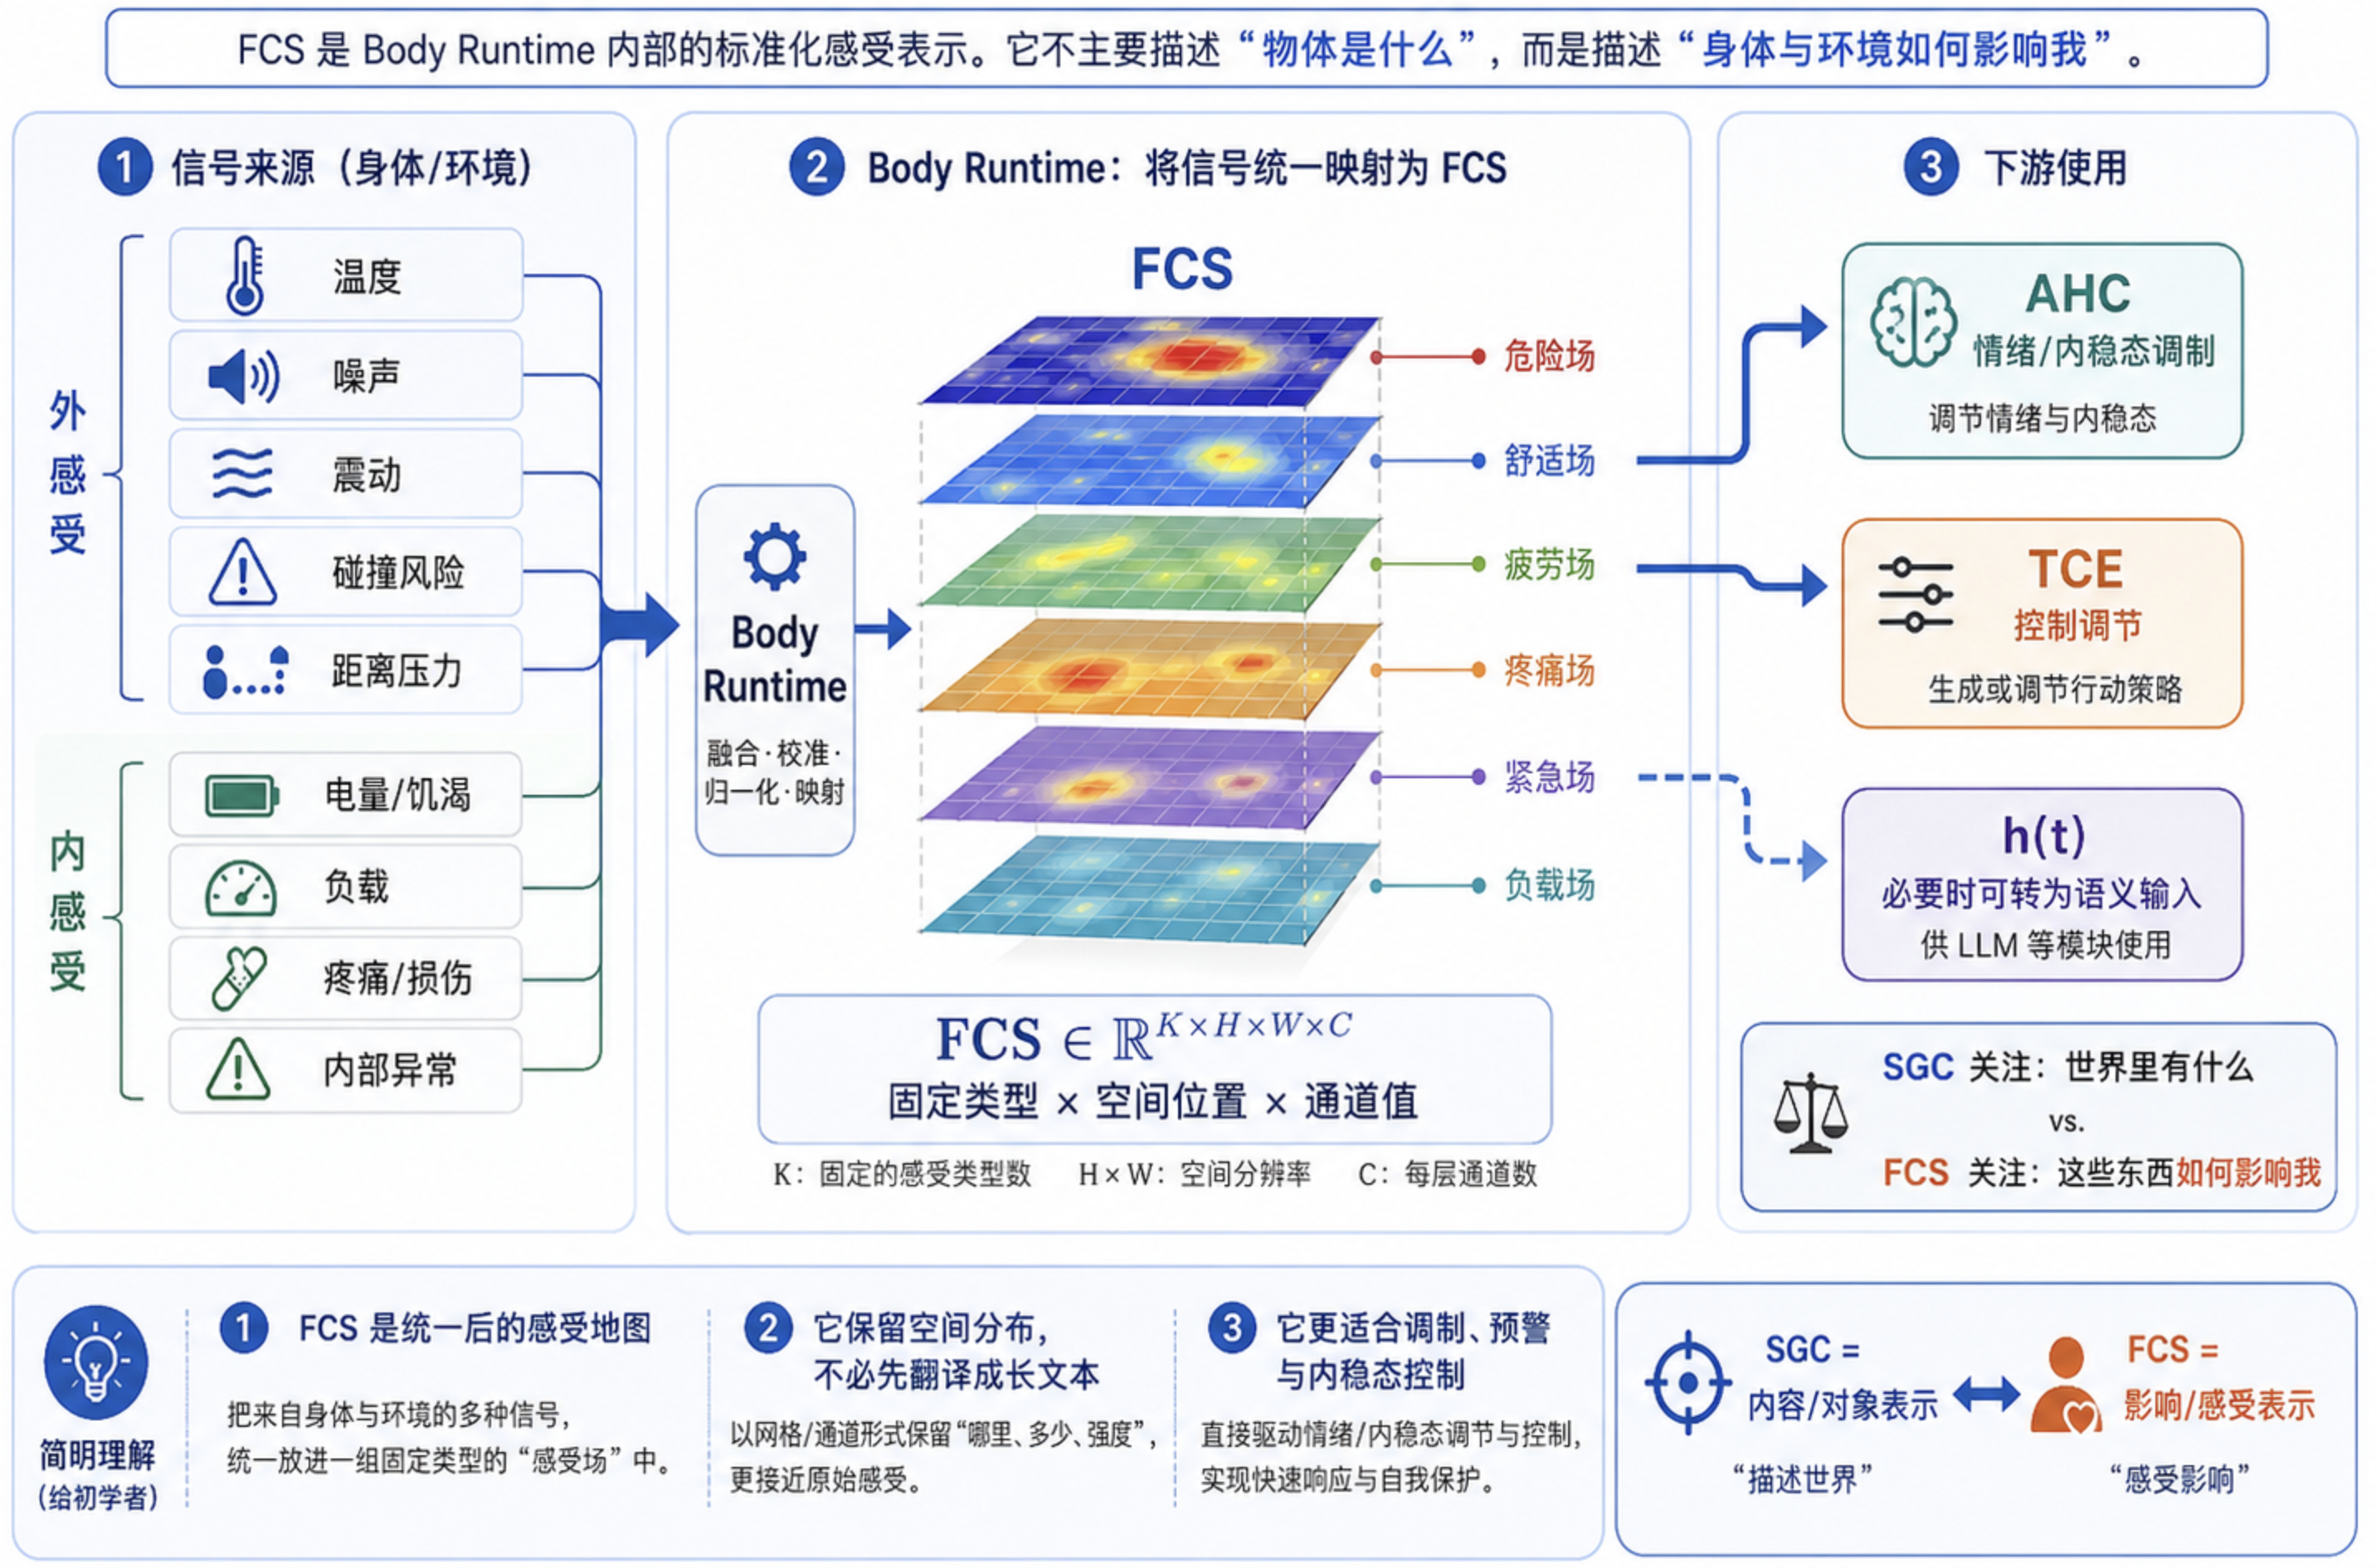
\includegraphics[width=.9\textwidth,height=.38\textheight,keepaspectratio]{images/FCS-Repect.png}
\caption{FCS的多通道实现示意图}
\end{figure}

\section{从 SGC--FCS 二元现实接口到群体感受面}

在前一章中，我们已经把 AgentOS 对现实的具身接口拆分成两个互补但不可互相替代的表示系统。SGC 主要承担对象、空间、关系和可行动性的显式表达，可以概括为
\[
\boxed{
SGC:\quad What\ is\ there?
}
\]
而 FCS 则表示身体、环境和任务状态对主体产生的功能性影响，可以概括为
\[
\boxed{
FCS:\quad How\ is\ it\ affecting\ me?
}
\]
这一区分的意义在于，现实并不是只有“对象是什么”这一种结构。例如北方存在一个危险区域，这是 SGC 中的世界结构；而“当前身体继续向北移动将显著增加风险压力”，则属于以本体为中心的作用结构。前者是现实内容，后者是现实对主体的影响。

当多个自主 Agent 形成群体以后，同样的问题会在更大的空间尺度重新出现。对于一个局部机器人而言，群体整体可能具有某种宏观密度分布、能力分布、任务缺口、通信拓扑和协同趋势。这些状态并不一定能够被压缩成某个普通的 SGC Object。例如，“当前东北方向的群体功能势能较低，因此在那里增加一个具有通信中继能力的机器人能够提高整体任务收益”并不是一个简单对象，而更接近一个分布在物理--语义空间中的方向性功能场。

若我们把这种群体信息直接转成命令，
\[
SwarmController
\rightarrow
MotorCommand_i,
\]
就等于让群体中央系统绕过本地 AgentOS 的感知、自我、Boundary、安全、记忆和目标系统，直接取得本体执行权。这样做虽然在传统集中式群控中并不罕见，但它破坏了本书始终坚持的单体主体边界。

因此，本章提出另一种结构：
\[
\boxed{
SwarmStructure
\rightarrow
SwarmSensation
\rightarrow
LocalCognition
\rightarrow
LocalAction.
}
\]
群体宏观结构首先被翻译成本地身体能够“感受到”的方向性趋势，再由 AgentOS 将其与视觉、内部状态、任务、自我和其他感受共同处理。

于是 FCS 的概念可以进一步推广为
\[
FCS_i
=
\{
S_i^{thermal},
S_i^{energy},
S_i^{integrity},
S_i^{threat},
S_i^{proprioception},
S_i^{swarm},
\ldots
\}.
\]
这里新增的
\[
S_i^{swarm}
\]
就是本章研究的群体梯度感受面。

需要特别说明的是，所谓“感受”仍然属于功能定义，而不是现象意识判断。它只是指：某一外部或内部结构被转换为以当前身体为中心的连续调制量，并能够影响后续认知和行动。因此，群体场进入 FCS 并不意味着 Agent 获得某种神秘的“群体意识”，而是意味着群体宏观状态能够像重力感、本体感觉、威胁压力等输入一样，被本地 AgentOS 纳入统一具身状态。


\section{群体控制首先是控制对象的转换}

为了理解为什么群体状态适合以场的形式进入 FCS，我们必须先重新定义群体控制本身所面对的对象。设群体由
\[
\mathcal R_N
=
\{R_1,R_2,\ldots,R_N\}
\]
组成，每个机器人具有状态
\[
x_i\in\mathbb R^{d_x}.
\]
如果群体中央系统直接维护所有机器人状态，则其联合状态为
\[
X_N
=
(x_1,x_2,\ldots,x_N),
\]
并有
\[
\dim X_N
=
Nd_x.
\]
如果进一步显式维护碰撞关系、通信关系、角色依赖、任务配合等两两联系，潜在关系数量还可能达到
\[
O(N^2).
\]
因此，大规模群体的根本困难并不只是控制算法算得够不够快，更深层的问题在于：\textbf{中央系统是否选择了正确的控制对象。}

许多实际群体任务并不关心某个具有永久编号的机器人是否必须到达某个唯一坐标。例如搜索、覆盖、灾区救援、异构搬运、通信中继等任务通常真正关心的是：某区域需要多少感知能力，哪里出现能力缺口，哪里需要更高密度，哪里应该增强通信连通，哪里应该增加探索，哪里需要形成较强局部凝聚。因此，宏观任务真正关注的对象并不是
\[
\{x_i\}_{i=1}^{N},
\]
而是由这些微观状态共同形成的某种群体宏观状态
\[
\Psi_{\mathrm{swarm}}(w,t).
\]

可以引入一个粗粒化映射
\[
\Pi:
X_N
\rightarrow
\Psi_{\mathrm{swarm}}.
\]
不同的微观配置可能对应近似相同的宏观群体状态，因此
\[
\Pi^{-1}(\Psi_{\mathrm{swarm}})
\]
通常构成一个微观状态等价类，而不是唯一状态。

于是群体控制的基本原则成为
\begin{proposition*}
控制宏观功能状态，而非唯一微观配置。
\end{proposition*}
这一原则直接改变了群体中央智能的角色。中央系统不再必须回答“机器人 $R_{173}$ 下一秒应运动到哪里”，而是更多回答：“某区域的群体功能状态应该向哪个方向变化？”

需要同时划定该思想的适用边界。若任务要求毫米级严格刚性编队、精密同步装配或硬实时多体约束，仅依赖宏观场并不充分。这些问题仍然需要局部几何控制、刚性约束控制器或专用 Body Driver。流体群体控制的优势主要存在于那些具有微观可替换性、宏观目标明确、局部自治具有意义的任务之中。


\section{从密度场到群体认知场}

最简单的群体宏观表示是机器人密度场
\[
\rho(x,t).
\]
然而密度只能回答某区域“有多少机器人”，却无法回答这些机器人“能够做什么”。两个具有相同密度的区域可能具有完全不同的任务价值。例如某区域主要是感知机器人，另一区域主要是搬运机器人；一个区域能源充足，另一个区域正在集体进入低电量状态；某一区域通信带宽充分，另一区域则已经接近网络断裂。

因此需要把标量密度场推广成具有功能语义的多维状态场。早期显式形式可以写成
\[
\Psi_{\mathrm{explicit}}
=
[
\rho,
v,
r,
c,
e,
q,
s,\ldots
],
\]
其中
\[
\rho
\]
表示密度，
\[
v
\]
表示群体流速，
\[
r
\]
表示角色状态，
\[
c
\]
表示能力，
\[
e
\]
表示能源，
\[
q
\]
表示风险，
而
\[
s
\]
可以表示预测误差或异常强度。

这一表示已经比传统密度场更接近群体智能，因为每个机器人不再只是一个几何质点，而成为一个携带功能状态的局部采样器。但是显式字段仍然面临一个根本问题：不同语义属性之间缺少天然统一的度量。例如
\[
battery=70\%
\]
与
\[
camera\ capability=0.8
\]
之间并不存在物理上自然的直接距离。如果使用人工线性权重
\[
V
=
w_1r+w_2c+w_3e+\cdots,
\]
所得到的往往是工程师事先规定的代价组合，而不是从实际任务后果中学习出的功能几何。

因此，更一般的群体表示应该从显式属性数组升级为公共功能语义空间。记该空间为
\[
\mathcal M.
\]
理想情况下，距离
\[
d_{\mathcal M}(z_i,z_j)
\]
不主要描述两个机器人标签是否相似，而描述它们在当前任务中的
\begin{itemize}
    \item 可执行能力；
    \item 可产生的控制后果；
    \item 可达未来状态；
    \item 任务代价；
    \item 功能替代关系
\end{itemize}
是否接近。

于是
\[
\boxed{
d_{\mathcal M}(z_i,z_j)\approx0
}
\]
应表示两个状态在当前任务意义上近似属于同一个控制等价类，而不要求机器人具有相同形态或相同内部硬件。


\section{What--Where：群体具身状态的双结构}

为了把空间位置与功能状态统一起来，我们将机器人 $R_i$ 的广义状态写成
\[
y_i
=
(w_i,z_i).
\]
其中
\[
w_i\in\mathcal B
\]
表示 Where，而
\[
z_i\in\mathcal M
\]
表示 What。

这里的 Where 不应局限于普通欧氏空间。我们可以定义
\[
\mathcal B
=
\mathcal X_{\mathrm{physical}}
\times
\mathcal X_{\mathrm{relational}}.
\]
其中
\[
\mathcal X_{\mathrm{physical}}
\]
包含位置、姿态、速度、环境几何、障碍关系等，而
\[
\mathcal X_{\mathrm{relational}}
\]
则可以包含通信拓扑位置、协作图位置、工作流位置以及当前任务中的关系位置。

这意味着两台机器人即使物理上距离很近，也可能位于完全不同的功能关系位置。例如一个机器人可能是当前局部通信链路的关键中继，而另一台物理上紧邻它的机器人却只是正在经过该区域的搜索节点。从纯几何坐标看，两者相近；从任务关系空间看，两者完全不同。

What 同样不能退化成固定角色标签。设机器人局部状态为
\[
s_i
=
(o_i,x_i,m_i,\mathcal N_i,\tau_i),
\]
其中包括当前观测、身体机械状态、内部资源、邻域结构以及任务上下文。通过编码映射
\[
z_i
=
f_\theta(s_i),
\]
得到
\[
z_i\in\mathcal M.
\]
因此 $z_i$ 表达的并不是“机器人被制造时属于哪一种类型”，而是：
\begin{quote}
在当前任务条件下，这个机器人此刻处于怎样的可行动功能状态。
\end{quote}

这种定义允许同一个机器人随能源、位置、工具、环境和任务改变而不断在 $\mathcal M$ 中移动。传统离散角色因此被重新解释成语义流形中的一个吸引区域，而不再是不可改变的枚举标签。


\section{公共功能语义流形与群体认知场}

在 Where 底空间 $\mathcal B$ 的每个位置附着功能语义空间 $\mathcal M$，可以得到一个纤维化总空间
\[
\pi:
\mathcal E
\rightarrow
\mathcal B.
\]
群体状态则可以表示为这一结构上的一个场：
\[
\Psi_{\mathrm{swarm}}:
\mathcal B\times T
\rightarrow
\mathcal M.
\]
于是
\[
\Psi_{\mathrm{swarm}}(w,t)
\]
不再只是“这里有多少机器人”，而表示：
\begin{quote}
在广义位置 $w$ 附近，群体此刻具有什么样的综合功能状态。
\end{quote}

因此，本章把这种表示统一称为
\[
\boxed{
Collective\ Cognitive\ Field
}
\]
即群体认知场。

这里使用“认知场”并不意味着群体每一个空间点都存在意识，而是强调它表达的是具有任务意义和功能语义的群体状态。所谓“流体”，同样不是指机器人必须表现为液态外观，而是表示该场允许出现类似
\begin{itemize}
    \item 输运；
    \item 扩散；
    \item 聚合；
    \item 衰减；
    \item 局部激波；
    \item 凝聚；
    \item 相干；
    \item 相变
\end{itemize}
等连续场动力学现象。

对于局部机器人 $R_i$，设其邻域为
\[
\mathcal N_i.
\]
若当前语义空间可以局部近似为欧氏空间，则局部群体场可以估计为
\[
\Psi_i
=
\frac{
\sum_{j\in\mathcal N_i}
K(w_i,w_j)z_j
}{
\sum_{j\in\mathcal N_i}
K(w_i,w_j)
}.
\]
若 $\mathcal M$ 为一般黎曼流形，则可采用 Fr\'echet 均值
\[
\Psi_i
=
\operatorname*{argmin}_{z\in\mathcal M}
\sum_{j\in\mathcal N_i}
\omega_{ij}
d_{\mathcal M}^{2}(z,z_j).
\]
或者首先通过
\[
\log_{\bar z}:
\mathcal M
\rightarrow
T_{\bar z}\mathcal M
\]
映射至局部切空间，在切空间完成聚合和微分，再通过
\[
\exp_{\bar z}
\]
映射回流形。

由此，不同机器人交换的就不再是无限增长的完整内部状态，而是自己在公共功能语义空间中的局部场源贡献。


\section{SwarmOS：群体尺度必须拥有独立的智能对象}

群体认知场建立以后，需要回答另一个架构问题：谁负责定义整个群体应该形成怎样的宏观结构？在本章中，我们将该群体尺度控制系统统一称为
\begin{statementbox}
SwarmOS
\end{statementbox}
即 Swarm Central Operating System。

必须严格区分
\[
AgentOS_i
\]
与
\[
SwarmOS.
\]
两者虽然可以在更高层抽象上表现出相似的动力学结构，却面向完全不同的智能对象。

对于本地 AgentOS，
\[
AgentOS_i
\rightarrow
\mathcal A_i,
\]
其核心问题是：
\begin{quote}
作为这个持续存在的个体，我应该如何感知、理解、记忆并行动？
\end{quote}

而 SwarmOS 的控制对象则是
\[
\Psi_{\mathrm{swarm}},
\]
它需要回答：
\begin{quote}
整个群体未来应该形成怎样的宏观功能状态？
\end{quote}

因此，
\[
\boxed{
AgentOS_i
\neq
SwarmOS.
}
\]

这一概念边界具有非常重要的术语后果。本书已经把 TCE、SPC、CCM、Boundary、Offloading、$h(t)$、$E$、$\Theta$、$\Psi$ 等名称固定用于单体 AgentOS。群体系统即使出现结构相似的调节器，也不应复用这些名称。

例如，群体动力参数调节器统一记为
\[
\boxed{
SDM
=
Swarm\ Dynamics\ Modulator
}
\]
而不是再次称为 TCE。

群体异常与宏观序参量检测器统一记为
\[
\boxed{
SAD
=
Swarm\ Anomaly\ Detector
}
\]
而不是 SPC。

这种命名隔离不是形式主义，而是为了避免把两个尺度上的不同软件实例误认为同一模块。


\section{群体势能：SwarmOS 不应逐机器人输出轨迹}

SwarmOS 的主要输出不应该是
\[
\{Trajectory_i\}_{i=1}^{N},
\]
而应该更多表现为群体任务势能
\[
V_{\mathrm{swarm}}(w,z,t)
\]
以及目标嵌入场
\[
z^*(w,t).
\]

其中 $V_{\mathrm{swarm}}$ 描述一个候选群体状态与当前群体战略目标之间的失配程度。较低势能的状态意味着
\[
(w,z)
\]
在当前任务条件下更值得群体达到。

因此，群体中央规划从传统的
\[
trajectory\ planning
\]
转变成
\[
\boxed{
potential\ shaping.
}
\]
SwarmOS 不需要直接规定每一个微观动作，而是重塑整个群体未来状态空间中的任务价值地形。

目标嵌入场写成
\[
z^*:
\mathcal B\times T
\rightarrow
\mathcal M.
\]
这意味着同一个群体任务在不同位置可以具有完全不同的期望功能状态。例如在搜救任务中，废墟核心区域可能需要偏向高感知、高风险敏感、低速运动；外围搜索区域则更需要高覆盖率和高探索；通信边缘区域可能需要机器人稳定停留并承担中继功能。

因此，一个传统角色 $r$ 可以重新理解成
\[
\mathcal A_r
\subset
\mathcal M
\]
中的一个吸引域。机器人不是从一个离散角色标签“跳变”到另一个角色，而可以沿功能语义流形连续迁移。


\section{物理--语义联合势能与双梯度}

设机器人广义状态仍为
\[
y_i
=
(w_i,z_i),
\]
局部群体场为 $\Psi_i$，目标功能状态为 $z_i^*$，则局部有效群体势能可以写为
\[
V_i
=
V_{\mathrm{swarm}}
(
w_i,
z_i,
\Psi_i,
z_i^*
).
\]

由于状态同时包含 Where 与 What，势能也产生两个不同方向的梯度。

物理空间中的下降方向为
\[
g_i^w
=
-\nabla_wV_i,
\]
而功能语义空间中的下降方向为
\[
g_i^z
=
-\operatorname{grad}_{\mathcal M}V_i.
\]

于是局部动力学可以抽象写成
\[
\dot w_i
=
F_w(w_i,g_i^w),
\]
以及
\[
D_tz_i
=
F_z(z_i,g_i^z).
\]

这一结构表达了一个重要思想：“我应该去哪里”与“我现在应该承担怎样的功能”并不一定是两个完全独立的问题，而可以是同一群体任务势能在物理空间与功能语义空间中的两个不同方向分量。

例如某机器人当前进入某区域可能不是因为该位置本身重要，而是因为它具有当前局部缺失的功能；反过来，同一个机器人在不移动的情况下，也可能通过启动不同传感器、改变通信模式、加载工具或者改变协作行为，使自己的 $z_i$ 在语义流形中发生变化。

因此，群体协同不应被限制成位置控制，而应该被理解成物理--语义联合状态空间中的结构演化。


\section{群体相态、SDM 与局部异常重塑}

为了描述群体整体动力状态，可以定义宏观序参量
\[
\Omega_s
=
(
\rho,
\chi,
\xi,
\varphi,
\ldots
),
\]
其中可以包含密度、相干度、空间相关长度、通信连通性、功能覆盖率等。

SDM 根据这些序参量以及 SwarmOS 的战略目标调节一组群体动力参数：
\[
\Theta_s
=
(
T_s,
\eta_s,
\kappa_s,
D_s,
\lambda_s,\ldots
).
\]
其中
\[
T_s
\]
表示群体探索温度，
\[
\eta_s
\]
表示局部相干耦合，
\[
\kappa_s
\]
表示 SwarmOS 对局部群体势能的战略介入强度，
而
\[
D_s
\]
可表示有效扩散强度。

例如高 $T_s$、较低 $\eta_s$ 可形成探索态，使群体扩散增强、覆盖率提高；中等温度与中等耦合可以产生具有较强弹性和形变能力的流动态；较低 $T_s$ 与较高 $\eta_s$ 则可能形成更强局部同步和功能凝聚。

需要再次强调：
\[
\boxed{
SDM\neq AgentOS:TCE.
}
\]
两者只在“调节动力系统运行区间”这一非常抽象的意义上存在结构同构。

群体还需要处理局部突发异常。设机器人具有局部预测
\[
\hat o_{i,t+1}
=
F_i(o_{i,t},a_{i,t}),
\]
实际获得
\[
o_{i,t+1},
\]
则可以定义异常强度
\[
S_i
=
D(
o_{i,t+1},
\hat o_{i,t+1}
).
\]
若
\[
S_i>\tau_s,
\]
SAD 可以产生局部异常场源
\[
J_i^{shock},
\]
并通过分布式场网络传播，使局部有效势能变为
\[
V_{\mathrm{eff}}
=
V_{\mathrm{task}}
+
V_{\mathrm{shock}}.
\]

因此，群体“惊奇激波”的本质不是中央控制器向所有机器人广播一条“立即靠近异常点”的硬命令，而是：
\[
\boxed{
Prediction\ Error
\rightarrow
Temporary\ Potential\ Reshaping.
}
\]
附近不同机器人仍然可以根据自己的身体条件、任务和本地 AgentOS 状态作出不同响应。


\section{SFPU 的最终定位：一种特殊 Swarm Body Driver}

在本书整体 AgentOS 架构中，SFPU 不应被定义成 AgentOS 内核模块，而应被严格定义为
\[
\boxed{
SFPU
=
Specialized\ Swarm\ Body\ Driver.
}
\]

对单个 AgentOS 而言，SFPU 与相机、触觉、机械臂、网络设备等一样，首先是一类 Body Driver；区别在于它连接的并不是单个普通传感器，而是一个分布式群体场网络。

如果群体中存在
\[
\{SFPU_i\}_{i=1}^{N},
\]
那么所有 SFPU 通过横向通信构成
\[
\boxed{
Distributed\ Swarm\ Field\ Network.
}
\]
这个网络在宏观上可以承担类似群体快速协调层的作用，因此可以在解释意义上称为“群体小脑式网络”，但必须保持：
\[
SFPU_i
\neq
Swarm\ Cerebellum.
\]
单个 SFPU 只是局部驱动器，而整体 SFPU 网络才可能形成这种分布式快速场协调功能。

一个 SFPU 可以抽象为
\[
SFPU_i
=
(
\mathcal I_F,
\mathcal I_P,
\mathcal I_G,
\mathcal K
),
\]
其中
\[
\mathcal I_F
\]
为 Field Plane，
\[
\mathcal I_P
\]
为 Potential Plane，
\[
\mathcal I_G
\]
为 Gradient Plane，
而
\[
\mathcal K
\]
表示局部场计算核心。

三个接口分别连接三个不同的宿主域，这一划分构成 SFPU 最重要的工程边界。


\section{Field Plane：群体场网络的横向 Body Driver 接口}

Field Plane 主要负责
\[
\boxed{
SFPU_i
\leftrightarrow
SFPU_j
}
\]
之间的横向场通信。它属于
\[
\boxed{
Body\ Driver\ Domain
}
\]
而不是本地 AgentOS 的认知接口。

它的主要使用者包括 SFPU 驱动开发者、场通信协议栈、嵌入式系统、网络硬件以及跨厂商 Body Driver 实现者。典型操作可以包括：

\begin{verbatim}
FIELD_EMIT(...)
FIELD_RECEIVE(...)
FIELD_RELAY(...)
FIELD_ACCUMULATE(...)
FIELD_DIFFUSE(...)
FIELD_DECAY(...)
FIELD_ALIGN(...)
FIELD_VERSION_TRANSFORM(...)
FIELD_REPORT_SHOCK(...)
\end{verbatim}

其责任包括邻域发现、时间戳同步、场帧传播、坐标对齐、场核计算、语义版本兼容、不确定度传播、局部异常源扩散以及局部场重构。

本地 AgentOS 不应承担这些细节。正如摄像头 Driver 可以完成图像采集和底层时序，而不要求认知内核理解 MIPI 或 ISP 的全部实现一样，AgentOS 只需要得到由 SFPU 输出的稳定群体感受接口。

在局部计算复杂度方面，如果每个 SFPU 的邻域规模满足
\[
|\mathcal N_i|
\leq K
\]
且功能语义维数 $d_z$ 固定，则单节点局部计算复杂度近似为
\[
C_i
=
O(Kd_z).
\]
若 $K$ 不随群体总规模 $N$ 增长，则
\[
\frac{\partial C_i}{\partial N}
\approx0.
\]
这并不意味着整个群体扩张没有成本。总通信资源、无线竞争、物理拥堵、能耗等仍可能随 $N$ 增长。真正成立的命题只是：
\begin{proposition*}
单节点局部认知维数不必与群体总规模成正比。
\end{proposition*}


\section{Potential Plane：SwarmOS 的战略约束接口}

Potential Plane 连接的是
\[
\boxed{
SwarmOS
\rightarrow
SFPU_i
}
\]
而不是
\[
AgentOS_i
\rightarrow
SFPU_i.
\]

这一点必须保持严格。否则本地 AgentOS 与群体中央智能会混成同一个控制层。

Potential Plane 可以承载
\[
\mathcal P_i
=
(
V_{\mathrm{swarm}},
z_i^*,
\theta_V,
\Theta_{SDM},
version,
validity
).
\]

典型操作例如：

\begin{verbatim}
LOAD_TARGET_EMBEDDING(...)
LOAD_SWARM_POTENTIAL(...)
LOAD_TASK_ADAPTER(...)
SET_SWARM_TEMPERATURE(...)
SET_FIELD_COUPLING(...)
SET_STRATEGIC_COUPLING(...)
ACTIVATE_SWARM_MODEL_EPOCH(...)
ROLLBACK_SWARM_MODEL_EPOCH(...)
\end{verbatim}

其中所有群体尺度调节参数均属于 SDM，而不使用 AgentOS 已经具有明确含义的 TCE 名称。

通过 Potential Plane，SwarmOS 表达的是“群体未来状态空间应该具有怎样的价值地形”，而不是直接要求某个机器人的执行器产生某一电机电流。


\section{Gradient Plane：FCS 的群体梯度感受面}

Gradient Plane 是 SFPU 与本地 AgentOS 真正发生语义结合的位置。

SFPU 根据当前位置、功能状态、邻域场、目标嵌入和群体势能计算一个局部群体感受：
\[
S_i^{swarm}
=
(
g_i^w,
g_i^z,
V_i,
\Sigma_i,
C_i,
\Omega_i
).
\]
其中
\[
g_i^w
=
-\nabla_wV_i
\]
表示物理空间中的群体收益方向，

\[
g_i^z
=
-\operatorname{grad}_{\mathcal M}V_i
\]
表示当前功能状态应向何种方向变化，

\[
V_i
\]
表示当前局部群体任务势能，

\[
\Sigma_i
\]
表示群体场估计的不确定度，

\[
C_i
\]
表示当前场的一致性或可信度，

而
\[
\Omega_i
\]
可以提供局部群体宏观状态摘要。

因此 Gradient Plane 可以正式称为
\[
\boxed{
Swarm\ Gradient\ Sensory\ Surface
}
\]
即群体梯度感受面。

这里最重要的设计原则是：
\[
\boxed{
Gradient
\neq
Command.
}
\]

例如若
\[
g_i^w
=
(0.82,0.13,0),
\]
其正确语义不是：
\begin{quote}
立即以该向量驱动电机。
\end{quote}
而应该理解为：
\begin{quote}
根据当前群体势能，如果身体向该方向变化，预计能够降低较多群体任务代价。
\end{quote}

因此，它在 AgentOS 中更类似一种方向性身体感觉。其功能地位可以与平衡感、本体感觉、威胁趋势、社会牵引、资源压力等进行类比。

完整路径应为
\[
\boxed{
Potential
\rightarrow
Gradient
\rightarrow
FCS
\rightarrow
AgentOS
\rightarrow
Action.
}
\]


\section{群体梯度如何进入 FCS}

由于 FCS 已经负责将不同身体影响标准化为统一感受面，我们可以把
\[
S_i^{swarm}
\]
直接注册为一种新的 FCS surface：

\[
FCS_i
=
\{
S_i^{vision-effect},
S_i^{audio-effect},
S_i^{touch},
S_i^{proprioception},
S_i^{internal},
S_i^{swarm},
\ldots
\}.
\]

需要强调的是，视觉本身的世界内容主要进入 SGC；这里写作 $S^{vision-effect}$ 时表示的是视觉输入所造成的功能性影响，而不是把 SGC 与 FCS 再次混为一谈。

从本地 AgentOS 角度看，群体因此首先表现为
\[
\boxed{
Swarm
=
Extended\ Sensory\ Embodiment.
}
\]

也就是说，加入群体网络之后，Agent 的身体感受域从
\[
Body_i
\]
扩展成
\[
Body_i
+
\mathcal F_{\mathrm{swarm}}.
\]
Agent 并不需要把整个 SwarmOS 内部状态或者所有其他 Agent 的完整认知状态装入自己的 $h(t)$。它只需要得到与自己当前身体位置和功能状态相关的群体梯度场。

这一设计也体现了前面工作记忆有限容量理论的原则：宏观群体信息应当先在低层通过场压缩，再以局部有意义的感受结构进入本体，而不是把 $N$ 台机器人的完整联合状态直接送进每个 Agent 的工作记忆。


\section{为什么群体意图不能直接覆盖本地 AgentOS}

假设群体梯度建议
\[
-\nabla_wV_{\mathrm{swarm}}
\]
指向北方。但本地 AgentOS 同时可能观察到：

\begin{itemize}
    \item 北方存在未被群体模型识别的危险；
    \item 本地存在更高优先级紧急任务；
    \item 当前能源不足；
    \item Boundary 禁止进入某区域；
    \item 身体结构当前无法执行相应动作；
    \item 本地安全规则拒绝这一轨迹。
\end{itemize}

那么
\[
S_i^{swarm}
\]
仍然只是 AgentOS 的一个输入。

最终行动可抽象表示为
\[
a_i
=
\mathcal A_i
\left(
h_i,
\Psi_i,
E_i,
\Theta_i,
SPC_i,
TCE_i,
CCM_i,
Boundary_i,
S_i^{swarm},
S_i^{other}
\right).
\]

因此必须保持
\[
\boxed{
Swarm\ Intent
\neq
Local\ Action.
}
\]
更不能写成
\[
Swarm\ Intent
=
Local\ Will.
\]

这并不是否认群体组织约束，而是把群体约束放在正确的尺度上。SwarmOS 调节群体结构的价值地形，本地 AgentOS 则在自己的身体、知识和安全边界中对该地形做出局部响应。

这样，个体 Agent 仍然可以作为持续主体存在，而群体则形成更高尺度的宏观智能过程。


\section{安全反射旁路与正常认知路径的严格分离}

虽然正常群体控制应遵循
\[
SFPU
\rightarrow
FCS
\rightarrow
AgentOS,
\]
但在少量强实时安全情境下，可以允许一条有限旁路：
\[
SFPU
\rightarrow
BodySafety.
\]

例如：

\begin{itemize}
    \item 群体紧急制动；
    \item 即将发生的多机器人碰撞；
    \item 通信失控后的隔离动作；
    \item 必须满足的硬同步保护；
    \item 群体结构快速解体时的紧急停止。
\end{itemize}

该路径必须严格标记为
\[
\boxed{
Safety/Reflex\ Path
}
\]
而不是普通认知控制。

也就是说：
\[
CriticalSafety
\not\Rightarrow
NormalSwarmAuthority.
\]
不能因为存在安全旁路，就让 SwarmOS 获得对本地身体的常态化直接控制权。

这一原则与 AgentOS Body Runtime 后续章节中的实时安全边界完全一致：高层认知可以影响身体，却不能成为所有硬安全动作的必要依赖；反过来，安全控制器获得的直接执行权限也不能自动扩展为一般认知权限。


\section{SFPU 的内部计算：分布式势能微分器}

从内部算法看，SFPU 并不需要成为通用人工智能处理器。它的核心任务可以压缩为
\[
\boxed{
Potential
\rightarrow
Field
\rightarrow
Gradient.
}
\]

一个局部 SFPU 的计算流程可以写成：

首先，由 Potential Plane 接收 SwarmOS 提供的
\[
(
V_{\mathrm{swarm}},
z^*,
\Theta_{SDM}
).
\]

其次，经 Field Plane 接收邻域场源
\[
\{
w_j,z_j,\Sigma_j
\}_{j\in\mathcal N_i}.
\]

随后重构局部群体场
\[
\Psi_i.
\]

再根据
\[
V_i
=
V(
w_i,
z_i,
\Psi_i,
z_i^*
)
\]
计算局部有效势能。

接着分别计算
\[
g_i^w
=
-\nabla_wV_i
\]
和
\[
g_i^z
=
-\operatorname{grad}_{\mathcal M}V_i.
\]

再根据不确定度、场一致性和宏观序参量形成
\[
S_i^{swarm}
=
\mathcal G(
V_i,
g_i^w,
g_i^z,
\Sigma_i,
C_i,
\Omega_i
).
\]

最后将
\[
S_i^{swarm}
\]
通过 Gradient Plane 送入本地 FCS。

因此，SFPU 的最终输出不是 MotorCommand，而是
\[
\boxed{
Structured\ Swarm\ Sensation.
}
\]

从 AgentOS Body Driver 的统一定义来看，如果普通 Driver 可写作
\[
Driver_k
=
(
Sense_k,
Act_k,
External_k,
Control_k
),
\]
那么 SFPU 是一种特殊混合驱动：

\[
Driver_{\mathrm{SFPU}}
=
(
GradientSense,
OptionalReflex,
FieldPlane,
PotentialBinding
).
\]

其中 GradientSense 接入 FCS，OptionalReflex 只连接本地安全路径，FieldPlane 连接其他 SFPU，而 PotentialBinding 则连接独立 SwarmOS。


\section{SFPU 是连接三个宿主域的三域换能器}

三个 Plane 实际上分别属于三个不同系统域。

Field Plane 属于
\[
\boxed{
Body\ Driver\ Domain
}
\]
并处理
\[
SFPU_i
\leftrightarrow
SFPU_j.
\]

Gradient Plane 属于
\[
\boxed{
Local\ AgentOS\ Sensory\ Domain
}
\]
并处理
\[
SFPU_i
\rightarrow
FCS_i.
\]

Potential Plane 属于
\[
\boxed{
SwarmOS\ Strategic\ Domain
}
\]
并处理
\[
SwarmOS
\rightarrow
SFPU_i.
\]

因此，可以把 SFPU 更抽象地定义为
\[
\boxed{
Three\text{-}Domain\ Transducer.
}
\]
也就是把群体战略、分布式场动力学以及个体身体感受相互转换的三域换能器。

这一结构是非常重要的工程隔离层。若没有这一层，SwarmOS 就很容易被错误实现成 AgentOS 的“超级父进程”；反过来，本地 AgentOS 也可能被迫理解大量群体网络协议和局部场传播细节。SFPU 通过三平面接口同时隔离了战略、通信和感受三个不同层级。


\section{个体智能与群体智能：不是主从覆盖，而是跨尺度耦合}

群体中央系统与本地 AgentOS 的关系不应写成
\[
Parent
\rightarrow
Child
\]
或者
\[
Master
\rightarrow
Slave.
\]

更一般的结构是
\[
\boxed{
Macro\ Constraint
+
Micro\ Autonomy.
}
\]

群体层通过
\[
V_{\mathrm{swarm}}
\]
和目标嵌入场塑造宏观可达状态；个体层根据自己的局部现实和主体状态做出实际行为。个体行为又重新成为群体场的源：

\[
SwarmOS
\rightarrow
SFPU
\rightarrow
FCS
\rightarrow
AgentOS
\rightarrow
Body
\rightarrow
World
\rightarrow
Field.
\]

因此，一个机器人可以定义为个体智能主体
\[
\mathcal A_i
=
(
AgentOS_i,
Body_i
),
\]
而整个机器人群的宏观结构可以写成
\[
\mathcal A_{\mathrm{swarm}}
=
(
SwarmOS,
\{SFPU_i\},
\Psi_{\mathrm{swarm}},
\{\mathcal A_i\}
).
\]

必须注意，后一个表达并不是说群体一定具有与人类个体相同的主体体验，只表示群体在功能动力学上形成了一个更高尺度的自适应控制对象。

因此
\[
\mathcal A_{\mathrm{swarm}}
\neq
\sum_i\mathcal A_i.
\]
群体智能不能被简单理解成单体能力的代数求和，因为群体场、功能密度、网络结构和 SwarmOS 的宏观势能共同产生了单个 Agent 不具有的整体状态变量。


\section{快场动力与慢结构学习必须分离}

群体系统还必须遵循本书反复强调的多时间尺度原则。实时协同过程中，所有机器人必须使用一个足够稳定的公共语义坐标系，否则每个机器人一边控制、一边快速改变自己对功能距离的理解，群体梯度就会失去共同意义。

因此必须区分
\[
state\ evolution
\]
与
\[
representation\ learning.
\]

在快速场动力阶段，公共语义流形
\[
\mathcal M_k
\]
保持固定，机器人只在该流形上改变
\[
z_i(t).
\]

在较慢尺度上，可以更新任务势能
\[
V_\phi.
\]

在更慢尺度上，才更新
\[
\mathcal M_\theta
\]
及其度量
\[
g_\theta.
\]

因此要求近似满足
\[
\boxed{
\tau_{\mathrm{field}}
\ll
\tau_V
\ll
\tau_{\mathcal M}.
}
\]

这实际上是群体尺度的快--慢动力系统。快速层处理状态，慢层处理如何表示状态。

长期群体经验最终可以沉降成某种
\[
SwarmStructuralModel
=
(
\mathcal M,
g,
V,
\mathcal T
),
\]
其中 $\mathcal M$ 表示功能状态空间，$g$ 表示其局部几何，$V$ 表示群体状态价值，而 $\mathcal T$ 表示不同模型版本之间的转换关系。

这里不应直接把它记作 AgentOS 的 $\Theta$。虽然二者都表现出“慢结构约束快速运行”的抽象同构，但它们属于不同智能对象。


\section{公共群体语义模型的版本切换}

如果群体功能语义流形由
\[
\mathcal M_k
\]
升级为
\[
\mathcal M_{k+1},
\]
则不能让各机器人独立随机切换。必须定义版本转换
\[
T_{k\rightarrow k+1}.
\]

一个基本连续性要求是距离近似保持：
\[
d_{k+1}
(
T(z_1),
T(z_2)
)
\approx
d_k(z_1,z_2).
\]

势能也应近似连续：
\[
V_{k+1}(T(z))
\approx
V_k(z).
\]

梯度则应满足局部雅可比变换的一致性：
\[
\nabla V_{k+1}
\approx
\mathcal J_T
\nabla V_k.
\]

否则模型版本切换就可能在没有任何现实事件发生的情况下，让群体突然产生整体转向、振荡或者协作结构崩溃。

因此更合理的更新流程是：
\[
\boxed{
\text{发布}
\rightarrow
\text{预下载}
\rightarrow
\text{影子推理}
\rightarrow
\text{统一激活}
\rightarrow
\text{监控}
\rightarrow
\text{回滚}.
}
\]

这一机制也说明：公共群体语义流形不是某个节点自己的私有 latent，而是一个必须具有版本治理和语义连续性的共享认知坐标系。


\section{潜在语义与显式安全状态必须共存}

公共功能语义流形适合处理复杂任务中的功能相似、角色柔性、能力替代、泛化和群体势能，但不能承担所有安全与身份信息。

以下变量通常仍应明确保存：
\begin{itemize}
    \item 机器人身份；
    \item 时间戳；
    \item 数字签名；
    \item 权限；
    \item 模型版本；
    \item 最大速度；
    \item 最大载荷；
    \item 电池硬下限；
    \item 安全距离；
    \item 禁区；
    \item 紧急停止状态。
\end{itemize}

因此群体节点状态更合理地写成
\[
State
=
State_{\mathrm{latent}}
+
State_{\mathrm{explicit}}.
\]

这一原则可以概括为
\[
\boxed{
Latent\ for\ Intelligence,
\qquad
Explicit\ for\ Safety.
}
\]

也就是说，可学习嵌入负责提供柔性泛化能力，而硬安全变量必须维持明确、可验证和不可被语义距离掩盖的形式。


\section{群体扩张与 Body Scale：更多机器人意味着更高身体分辨率}

在传统集中式群控中，机器人数量 $N$ 增大往往被直接解释成中央系统需要处理更多个体变量。而在群体场框架中，增加机器人还可以从另一个角度理解：

\[
N\uparrow
\]
意味着
\[
Field\ Sampling\ Density\uparrow,
\]
\[
Sensing\ Resolution\uparrow,
\]
\[
Functional\ Density\uparrow,
\]
\[
Execution\ Resolution\uparrow,
\]
以及
\[
Fault\ Redundancy\uparrow.
\]

因此可以提出：
\[
\boxed{
More\ Robots
\approx
Higher\ Resolution\ Collective\ Body.
}
\]

这里不是说系统总资源不增长，而是说群体尺度的宏观认知对象不需要一一对应所有微观个体。机器人增加首先可以表现为群体身体在空间和功能上的采样分辨率提高。

这一点也把本章与前面的 Body Scale 理论连接起来。普通 Body Driver 可以让单体 Agent 获得 Camera、Arm、Vehicle、Tool 等新的身体能力，而 SFPU 则让 Agent 获得一种新的身体维度：
\[
SwarmField.
\]

于是 Agent 的具身边界从
\[
Body_i
\]
拓展为
\[
Body_i
+
\mathcal F_{\mathrm{swarm}}.
\]

群体因此不是必须被内化为 AgentOS 的认知模块，而可以首先表现为一种
\[
\boxed{
Extended\ Embodiment.
}
\]
这使 Body Scale 不再只表示单个身体接口的可迁移能力，也开始容纳“个体如何通过统一 Body Driver 接入更大尺度身体结构”的问题。


\section{群体智能与 AgentOS 智能动力学的结构同构}

虽然群体系统与 AgentOS 必须严格区分名称和软件实例，但二者在更抽象的动力学层面存在明显同构。

对于单体 Agent，可以抽象写成
\[
\dot X_A
=
F_A(
X_A,
\Theta_A,
U_A,
W_A
).
\]

对于群体，则可以写成
\[
\dot\Psi_{\mathrm{swarm}}
=
F_s(
\Psi_{\mathrm{swarm}},
\Theta_s,
U_s,
W_s
).
\]

两个尺度都体现：
\[
\boxed{
Structural\ Constraint
\rightarrow
Local\ Dynamics
\rightarrow
State\ Evolution.
}
\]

高层控制不一定直接指定每一个微观动作，而可能通过改变动力学中的参数、约束或者势能
\[
V(X)
\]
来改变未来轨迹的吸引结构。

因此，AgentOS 是这一原则在个体生命周期认知尺度上的一种实现；流体群体系统则是在群体空间尺度上的一种实现。

更进一步，两者还形成跨尺度递归：
\[
\boxed{
Swarm
\rightarrow
Agent
\rightarrow
World
\rightarrow
Swarm.
}
\]

群体层自上而下产生结构约束，个体层保留局部自治；个体行动则自下而上重新塑造群体场。这不是主从覆盖，而是一种典型的分形智能耦合。


\section{完整系统拓扑}

将上述结构统一以后，整个群体--个体系统可以表示为：

\begin{verbatim}
                    +---------------------------+
                    |          SwarmOS          |
                    |                           |
                    | Global Task               |
                    | Swarm Structural Model    |
                    | Target Embedding Field    |
                    | Potential Generation      |
                    | SDM / SAD                 |
                    +-------------+-------------+
                                  |
                           Potential Plane
                                  |
                                  v
              +----------------------------------+
              |        SFPU Body Driver          |
              |                                  |
Peer SFPU <-->+ Field Plane                      |
              | Field Propagation / Alignment    |
              | Local Field Reconstruction       |
              | Potential Evaluation             |
              | Spatial Gradient                 |
              | Semantic Gradient                |
              +----------------+-----------------+
                               |
                         Gradient Plane
                               |
                               v
              +----------------------------------+
              |          Local AgentOS           |
              |                                  |
              |                FCS               |
              |  ordinary feeling surfaces       |
              |        + swarm gradient surface  |
              |                |                 |
              |                v                 |
              |               h(t)               |
              |                |                 |
              | Psi / SPC / TCE / CCM /Boundary |
              |                |                 |
              |              Action              |
              +----------------+-----------------+
                               |
                      Ordinary Body Drivers
                               |
                               v
                              Body
                               |
                               v
                              World
                               |
                               +----> SFPU Field
\end{verbatim}

需要再次确认图中的概念边界：TCE 与 SPC 只属于本地 AgentOS；群体侧相似功能分别使用 SDM 和 SAD。SFPU 的 Field Plane 属于 Body Driver 横向实现域，Potential Plane 面向 SwarmOS，而 Gradient Plane 才是面向本地 AgentOS 的感受接口。


\section{完整数学闭环}

整个系统可以压缩成几个连续变换。

首先，群体战略层根据任务上下文 $\mathcal C_t$ 生成：
\[
\mathcal C_t
\overset{SwarmOS}{\longrightarrow}
(
z^*,
V_s,
\Theta_{SDM}
).
\]

对于机器人 $i$，本地状态经过功能编码：
\[
s_i
\overset{f_\theta}{\longrightarrow}
z_i.
\]

邻域信息通过 Field Plane 构成局部群体场：
\[
\{
w_j,z_j
\}_{j\in\mathcal N_i}
\overset{FieldPlane}{\longrightarrow}
\Psi_i.
\]

随后计算局部势能：
\[
V_i
=
V_s(
w_i,
z_i,
\Psi_i,
z_i^*
).
\]

计算物理与语义梯度：
\[
g_i^w
=
-\nabla_wV_i,
\]
\[
g_i^z
=
-\operatorname{grad}_{\mathcal M}V_i.
\]

形成群体感受：
\[
S_i^{swarm}
=
\mathcal G(
V_i,
g_i^w,
g_i^z,
\Sigma_i
).
\]

群体感受进入：
\[
S_i^{swarm}
\rightarrow
FCS_i.
\]

随后由本地 AgentOS 根据完整本体状态更新认知：
\[
h_i(t+\Delta t)
=
\mathcal H
\left(
h_i(t),
S_i^{swarm},
S_i^{other},
E_i,
\Theta_i,
\Psi_i,
TCE_i,
SPC_i,
CCM_i,
Boundary_i
\right).
\]

行动由本地主体生成：
\[
a_i
=
\pi_i(h_i).
\]

真实身体执行：
\[
x_i(t+\Delta t)
=
f_i(
x_i(t),
a_i
).
\]

新的身体和功能状态重新成为群体场源：
\[
(x_i,z_i)
\rightarrow
FIELD\_EMIT
\rightarrow
\Psi_{\mathrm{swarm}}(t+\Delta t).
\]

最终形成完整闭环：
\[
\boxed{
SwarmOS
\rightarrow
Potential
\rightarrow
SFPU
\rightarrow
GradientSense
\rightarrow
AgentOS
\rightarrow
Action
\rightarrow
Field.
}
\]


\section{本章基本命题}

经过前述推导，本章可以形成以下基本命题。

第一，群体智能的关键首先不是获得更强的逐体中央控制器，而是完成控制对象从微观个体状态向群体宏观功能状态的转换：
\[
\boxed{
Individual\ State
\rightarrow
Collective\ Field.
}
\]

第二，群体场不能只停留在密度场，而应该逐渐发展成定义在物理--关系底空间和公共功能语义流形上的
\[
\boxed{
Collective\ Cognitive\ Field.
}
\]

第三，本地
\[
AgentOS_i
\]
与
\[
SwarmOS
\]
属于两个不同尺度的系统，不应复用运行时对象和模块命名。

第四，SwarmOS 的核心任务是进行
\[
\boxed{
Potential\ Shaping
}
\]
而不是持续逐机器人输出微观轨迹。

第五，SFPU 在 AgentOS 架构中是一种特殊
\[
\boxed{
Body\ Driver.
}
\]

第六，SFPU 的三个 Plane 分别对应三个不同接口域：
\[
FieldPlane
\rightarrow
BodyDriverDomain,
\]
\[
PotentialPlane
\rightarrow
SwarmOSDomain,
\]
\[
GradientPlane
\rightarrow
LocalAgentOSSensoryDomain.
\]

第七，
\begin{statementbox}
Gradient
\end{statementbox}
必须首先被理解为一种群体趋势感受，而不是不可拒绝的动作命令。

第八，本地 AgentOS 保留最终本体行动决策权：
\[
\boxed{
SwarmIntent
\neq
LocalAction.
}
\]

第九，单体智能和群体智能虽然不能混用软件模块，却可以理解成同一种多尺度智能动力学形式在不同空间尺度上的重复：
\[
\boxed{
MacroStructuralConstraint
+
MicroAutonomy
\rightarrow
CollectiveEmergence.
}
\]


\section{本章总结：FCS 作为跨尺度现实作用接口}

本章从 SGC--FCS 二元现实接口出发，把 FCS 从普通身体感受进一步扩展到群体尺度。最重要的变化并不是给 FCS 再增加一个数据通道，而是重新认识“感受”的一般结构。

只要某一种现实关系可以被转换成：
\begin{statementbox}
以本体为参照的方向、强度、不确定度与功能影响
\end{statementbox}
它就可以成为 FCS 的一种感受面。

SFPU 正是这一思想在群体系统中的典型实现。SwarmOS 首先形成群体宏观任务势能；分布式 SFPU 网络在局部重构群体认知场并计算势能梯度；Gradient Plane 再把这种梯度转换成
\[
S_i^{swarm},
\]
作为 FCS 的特殊群体感受面进入本地 AgentOS。

因此：
\[
\boxed{
Potential
\not\Rightarrow
DirectActuation,
}
\]
而是
\[
\boxed{
Potential
\rightarrow
Gradient
\rightarrow
Feeling
\rightarrow
Cognition
\rightarrow
Action.
}
\]

这一结构使我们能够同时保留两个看似冲突的要求：一方面，大规模机器人群需要宏观群体协调；另一方面，每一个本地 AgentOS 又必须保持自己的感知、自我、Boundary、安全和行动主权。

最终，整个体系可以被概括为：
\[
\boxed{
\text{群体结构约束}
\rightarrow
\text{个体结构感受}
\rightarrow
\text{本地自主决策}
\rightarrow
\text{身体行动}
\rightarrow
\text{群体结构再形成}.
}
\]

从智能动力学的更高视角看，这意味着个体和群体并不是两个互不相关的智能体系，而是同一种跨尺度闭环原理在不同空间尺度上的递归出现。单体 Agent 以身体为边界形成自身认知闭环；大量单体 Agent 又通过 SFPU 场网络共同形成更大尺度的群体状态；群体宏观状态再通过梯度感受重新进入单体身体。

于是，群体协同最终不再是简单的“中央大脑控制大量机器人”，而成为：
\[
\boxed{
\begin{gathered}
\textbf{Macro Structural Constraint}
\rightarrow
\textbf{Micro Autonomous Dynamics}\\
{}\rightarrow
\textbf{Collective Emergence}
\rightarrow
\textbf{Structural Learning}
\end{gathered}
}
\]

这也构成 FCS 理论的一次重要扩展：\textbf{FCS 不仅能够表达身体内部与局部环境如何作用于主体，也能够成为更高尺度智能结构作用于本体的一般跨尺度感受接口。}

\chapter{三信号通道：从身体状态到认知内核的分层路由}
\label{chap:three-signal-channels}

\begin{chapteroverviewbox}
前两章已经建立了智能体面对现实世界的两个公共表示面：SGC 描述“现实是什么”，FCS 描述“现实正在怎样作用于我”。然而，从身体运行时进入 Agent Kernel 的信息并不能因此被简单地汇合成一个统一输入流。如果语义事实、内稳态压力与即时危险被编码成同一种消息，并经过同一套推理、调度和注意机制，系统将同时面对三个问题：语义信息会淹没调制信息，连续调制会污染显式认知，而真正的安全事件又可能因为认知拥塞而无法及时到达执行端。

因此，本章提出 AgentOS 身体--认知边界上的\textbf{三信号通道原理}：将由现实产生并经 Body Runtime 处理的公共信号，在进入认知内核前按其\textbf{功能因果角色}而非单纯按传感器来源，分解为语义通道（Semantic Channel）、调制通道（Modulation/AHC Channel）和紧急安全通道（Emergency/Safety Channel）。三者分别回答：“发生了什么”“这对当前主体意味着怎样的状态调制”“是否存在不能等待认知处理的即时约束”。

三通道并不是把同一个世界切成三个互不联系的世界，而是在同一现实事件之上建立三个不同时间尺度、不同表达形式、不同调度权限和不同失效后果的投影。它们共同构成 Body Runtime 与 Agent Kernel 之间最基本的路由层，并保证 AgentOS 同时具备可理解性、连续内稳态调节能力以及不依赖高层推理的实时安全性。
\end{chapteroverviewbox}
\ChapterArt{58}

\section{语义通道：将现实转换为可认知的结构内容}
\label{sec:semantic-channel}

我们首先从最直观的一条通道开始。一个智能体若要形成目标、推理、记忆、预测和行动计划，就必须能够回答一个最基础的问题：\emph{当前世界中发生了什么？} 这个问题对应的不是原始摄像头像素、麦克风波形、关节编码器读数或者系统调用日志，而是已经经过身体侧感知、融合、跟踪和结构化之后，可以进入认知系统的现实内容。我们将承担这一功能的路径定义为语义通道（Semantic Channel）。

设身体运行时在时刻 $t$ 获得原始观测
\[
y_t^{raw}
=
\left[
y_t^{vision},
y_t^{audio},
y_t^{proprio},
y_t^{system},
\ldots
\right],
\]
经过设备驱动、时空配准、对象持续性维护以及语义绑定后，形成前文定义的 SGC 状态
\[
\mathcal{S}_t^{SGC}.
\]
语义通道并不直接把完整的 $\mathcal{S}_t^{SGC}$ 复制进入工作记忆，而是执行一次面向认知使用的结构路由：
\[
z_t^{sem}
=
\Pi_{sem}
\left(
\mathcal{S}_t^{SGC},
G_t,
h_t,
\Theta_t,
\mathcal{B}_t
\right),
\]
其中 $G_t$ 表示当前目标结构，$h_t$ 表示当前工作记忆状态，$\Theta_t$ 表示长期生成结构，$\mathcal{B}_t$ 表示当前认知边界策略，而 $\Pi_{sem}$ 则表示语义选择与编码算子。这个表达式的意义十分重要：现实中的某个结构是否进入 Agent 的显式认知，并不只取决于它是否“被传感器看见”，还取决于它是否与当前目标、已有认知结构以及认知资源状态具有足够关系。

因此语义通道的第一性功能不是传输数据，而是传输\textbf{可被认知操作的 Agent-CSO}。如果现实中存在一个结构 $C\in\mathcal{C}_{U}$，身体侧观察首先建立其局部表示
\[
\pi_A(C)=AgentCSO_A(C),
\]
随后 SGC 将这个结构与具体空间、对象、关系和认识论状态绑定。语义通道进一步决定该结构是否需要进入当前认知过程：
\[
AgentCSO_A(C)
\xrightarrow{\Pi_{sem}}
\begin{cases}
h_t, & \text{需要全局显式处理},\\
E/\Theta, & \text{可直接形成记忆或结构更新候选},\\
LocalRuntime, & \text{保持身体侧局部处理},\\
External/Deferred, & \text{外化或延迟处理}.
\end{cases}
\]
由此我们可以看到，Semantic Channel 并不是一根通向 LLM prompt 的“数据管道”，而是现实结构进入 Agent 认知拓扑时的一道语义路由层。

我们还需要特别强调语义通道中的认识论元数据。一个成熟 Agent 不应把“看到”“推断”“预测”和“假设”混为同一种事实。因此进入语义通道的结构至少应携带
\[
e_i
=
(
source_i,
confidence_i,
status_i,
timestamp_i
),
\]
其中
\[
status_i
\in
\{
Observed,
Derived,
Predicted,
Counterfactual,
Pending
\}.
\]
例如，“门处于关闭状态”可能是直接观测；“房间里可能有人”可能是由声音和历史关系推导；“车辆三秒后可能进入交叉口”属于预测；“如果继续直行则会发生冲突”则属于反事实结构。如果这些不同认识论状态被压平成同一种文本 token，Agent 就很容易把模型生成的未来与传感器观测到的现实混为一谈。三信号通道首先要求语义通道保持这种结构差异。

语义通道还必须遵守工作记忆有限容量原理。SGC 可以非常丰富，而 $h(t)$ 必须保持稀疏。令当前所有候选 Agent-CSO 集合为
\[
\mathcal{C}_t^{candidate}
=
\{C_1,\ldots,C_n\},
\]
对每一个结构定义语义提升分数
\[
\Gamma_i^{sem}
=
f
\left(
R_i,
N_i,
U_i,
P_i,
\epsilon_i,
K_i
\right),
\]
其中 $R_i$ 为目标相关性，$N_i$ 为新颖性，$U_i$ 为不确定性，$P_i$ 为潜在后果，$\epsilon_i$ 为预测残差，$K_i$ 为当前处理成本。只有当
\[
\Gamma_i^{sem}>\theta_{sem}
\]
时，该结构才有必要竞争有限的显式认知资源。这使语义通道天然连接到前文讨论的 Boundary、CCM 与 Scheduler：它首先将世界转化成 Agent 可以理解的结构，然后再由运行时治理体系决定哪些结构真正成为“当前思考的内容”。

因此，本书对 Semantic Channel 的定义可以浓缩为
\[
\boxed{
SemanticChannel:
RealityStructure
\rightarrow
CognitivelyManipulableAgentCSO
}
\]
它所保存的是现实的\textbf{内容结构}。这也是为什么在整个 AgentOS 设计中，我们始终坚持从“原始数据流”升级到“结构世界流”：只有当现实被表示成对象、关系、事件、变化、约束和未来可能性之后，持续智能体才真正获得了可以进行长期记忆、规划与自我发展的认知材料。

\section{调制通道：现实并不仅告诉智能体发生了什么}
\label{sec:modulation-channel}

仅有语义通道仍然不足以形成完整智能。两个现实状态可能拥有几乎相同的语义内容，却对智能体产生完全不同的功能影响。例如，“房间温度为 $35^\circ$C”作为语义事实只描述环境状态；但如果机器人内部温度已经接近安全上限，同样的环境温度就应显著提高散热需求、降低计算负载并改变行动选择。同样，“某个人接近智能体”可以作为一个空间关系进入 SGC，但这个事件究竟是普通社交接近、需要提高注意力，还是产生强烈风险压力，并不能只由空间语义本身表达。

因此 AgentOS 必须有一条与语义通道平行、但功能性质完全不同的路径。我们将它定义为\textbf{调制通道}（Modulation Channel）。在历史架构中，这条通道也被称为 AHC 通道，因为其主要认知侧消费者是 AHC，即内稳态--情感样调制层。不过更严格地说，Modulation Channel 是 Body Runtime 到认知内核之间的信号路径，而 AHC 是对这些信号进行时间积分、耦合和状态形成的内部动力学组件，两者不应等同。

若前文定义的 FCS 为
\[
\mathcal{F}_t
=
FCS_t,
\]
其中包含 EnergyPressure、Threat、ThermalPressure、IntegrityPressure、SensoryLoad、ControlInstability、Urgency 等固定类型的作用场，则调制通道首先执行
\[
m_t
=
\Pi_{mod}
\left(
\mathcal{F}_t,
x_t^{body},
x_t^{resource}
\right).
\]
这里的 $m_t$ 与语义结构 $z_t^{sem}$ 有根本区别。$z_t^{sem}$ 通常需要保留对象和关系的可解释内容，而 $m_t$ 更接近一个低维、连续、具有时间动力学意义的调制向量：
\[
m_t
=
[
m_t^{energy},
m_t^{threat},
m_t^{arousal},
m_t^{fatigue},
m_t^{social},
m_t^{uncertainty},
\ldots
]^\top.
\]
这些变量的作用不是告诉 Agent “外面有一辆车”，而是改变整个认知系统处理信息的方式。例如：
\[
m_t^{threat}\uparrow
\Rightarrow
\begin{cases}
AttentionGain\uparrow,\\
ExplorationRadius\downarrow,\\
VerificationStrength\uparrow,\\
ActionLatencyBudget\downarrow.
\end{cases}
\]
因此我们应把 Modulation Channel 理解成\textbf{控制参数的上游状态通道}。

这条通道最大的理论意义，是将“现实内容”与“现实对主体的作用”分离。传统端到端模型往往把两者混入同一个 latent representation：
\[
z_t
=
Encoder(y_t).
\]
这样做在单一任务中可以有效，却会给长期 Agent 带来一个隐患：系统很难区分“我认为世界是什么”与“世界使我处于什么功能状态”。AgentOS 因而要求公共认知边界满足
\[
\boxed{
SemanticContent
\perp
FunctionalModulation
}
\]
这里的 $\perp$ 不是严格统计独立，而是指两者在接口语义和控制职责上保持正交。它们可以来自同一事件，却不得成为同一不可解释变量。

我们还需要讨论 Modulation Channel 的时间性质。语义事件往往可以是离散的：
\[
Event_k=(type,entity,time,\ldots),
\]
而内稳态调制具有明显连续性。一个威胁事件消失之后，Threat 状态并不必然立即归零；疲劳不会因为 Agent 暂停一次任务便瞬时恢复。因此 AHC 接收到 $m_t$ 后，应形成类似
\[
\tau_a\dot a_t
=
-a_t
+
F_a
\left(
m_t,
a_t,
h_t,
\Psi_t
\right)
\]
的连续状态动力学。其中 $a_t$ 是 AHC 状态向量，$\tau_a$ 是不同调制维度的有效时间常数。这样，一个瞬时世界事件才能形成持续一段时间的内部功能影响。

进一步地，调制通道对 Agent 的影响通常不是直接把大量内容写入 $h$。如果每一次电量下降、温度变化、处理器负载变化都用自然语言进入工作记忆，Agent 很快会陷入自身状态噪声。因此正常情况下应满足
\[
m_t
\rightarrow
AHC
\rightarrow
TCE/Scheduler,
\]
而不是
\[
m_t
\rightarrow
h_t
\]
的无条件直接路径。只有当调制状态本身成为需要显式认知的问题，例如“我的能量已经不足以完成当前任务”，或者“持续的不确定性正在造成当前规划失稳”，才需要形成相应 Self-CSO：
\[
a_t
\xrightarrow{SPC}
AgentCSO_A(SelfState)
\rightarrow
h_t.
\]
这说明所谓“感觉进入意识”，在我们的工程框架中其实是一个从连续调制状态到显式自我结构的二次语义化过程，而不是 FCS 数值直接进入工作记忆。

因此，调制通道的正式定义可以写成
\[
\boxed{
ModulationChannel:
RealityImpact
\rightarrow
ContinuousInternalControlState
}
\]
如果说 Semantic Channel 携带的是“世界内容”，那么 Modulation Channel 携带的就是“世界与身体正在把主体推向什么状态”。前者支持理解和推理，后者支持资源分配、注意调节、风险敏感性以及长期内稳态。二者分离以后，AgentOS 才真正获得一种类似生物系统中“认知内容与神经调质并存”的多时间尺度结构，而不需要把任何这种功能结构等同于人类主观情绪。

\section{紧急安全通道：不能进入普通认知排队的现实约束}
\label{sec:emergency-channel}

语义通道解决“发生了什么”，调制通道解决“这正在怎样影响我”，但现实世界还存在第三种情况：某些状态不允许 Agent 先形成完整认知，再决定是否处理。对于高速移动机器人而言，碰撞时间可能只有数十毫秒；对于计算系统而言，硬件过温、电源异常、权限入侵或者执行器失控也可能要求立即中断。若这些信号必须首先经历
\[
Sensor
\rightarrow
SGC
\rightarrow
SemanticReasoning
\rightarrow
h
\rightarrow
Planner
\rightarrow
Decision
\rightarrow
Action,
\]
那么所谓“智能”反而可能成为安全系统的额外延迟来源。

因此第三条通道必须具有完全不同的系统地位。我们定义 Emergency/Safety Channel 为一条从现实异常检测到保护性动作之间的\textbf{高优先级、低语义负担、可绕过普通认知调度}的路径。设安全相关观测为
\[
s_t^{raw},
\]
安全判定函数为
\[
r_t
=
\mathcal{R}
\left(
s_t^{raw},
x_t^{body},
u_t,
\mathcal{E}_{safe}
\right),
\]
其中 $\mathcal{E}_{safe}$ 表示允许的安全包络。当
\[
r_t>\theta_{critical},
\]
系统不得等待正常 Scheduler 为该事件分配 h 资源，而应立即触发
\[
u_t^{safe}
=
\pi_{safe}(r_t,x_t^{body}).
\]
因此形成
\[
\boxed{
Reality
\rightarrow
SafetyDetection
\rightarrow
ProtectiveAction
}
\]
这一闭环。

这里必须区分 Emergency Channel 与高 Threat 的 Modulation Channel。一个状态可以“非常令人警觉”，但仍允许认知参与；另一个状态则可能已经进入硬安全区域。例如电池剩余 $15\%$ 可以产生 EnergyPressure 并影响当前计划，这属于调制；若电池管理系统检测到热失控风险，则属于 Emergency。类似地，一个车辆高速靠近可以提高 Threat，但只有预测到碰撞时间低于安全控制窗口时，才应触发硬安全干预。因此可以定义两个不同阈值：
\[
r_t>\theta_{mod}
\Rightarrow
Modulation,
\]
\[
r_t>\theta_{safe}
\Rightarrow
Emergency,
\qquad
\theta_{safe}>\theta_{mod}.
\]
二者不是重复，而是构成渐进式风险处理结构。

紧急通道还必须满足\textbf{最小语义原则}。安全动作所需的表示不应比实时控制所需更多。例如执行碰撞规避并不一定需要先知道“这是一辆某品牌汽车，由某个人驾驶”；它只需要知道障碍位置、相对速度、可用制动力和安全轨迹。因此安全事件可以具有非常压缩的结构：
\[
e_t^{safe}
=
(
hazardType,
severity,
timeToFailure,
safeActionSet,
confidence
).
\]
这使安全闭环的计算成本和认证范围都显著小于完整认知系统。

但安全通道绕过高层认知，并不意味着高层 Agent 永远不知道发生过什么。保护动作完成之后，应产生一个异步的事件记录：
\[
e_t^{safe}
\rightarrow
EventLog
\rightarrow
E/h.
\]
这样 Agent 可以事后理解：
\[
\text{发生了什么？}
\]
\[
\text{为什么我的动作被覆盖？}
\]
\[
\text{是否需要修改未来计划？}
\]
于是形成一个非常重要的二阶段结构：
\[
\boxed{
ImmediateProtection
\rightarrow
DelayedCognitiveInterpretation
}
\]
前者保护现实安全，后者保护主体连续性和学习能力。

这也决定了安全通道的权限必须高于一般 Body 控制器。设正常认知给出的动作请求为 $u_t^{cog}$，身体侧正常控制结果为 $u_t^{body}$，安全控制为 $u_t^{safe}$，则真实执行动作应满足某种仲裁函数
\[
u_t^{exec}
=
\mathcal{A}
\left(
u_t^{cog},
u_t^{body},
u_t^{safe}
\right),
\]
并具有
\[
SafetyAuthority
>
BodyControlAuthority
>
CognitivePreference.
\]
当安全约束激活时，高层目标不得通过“更强推理”覆盖物理保护边界。

因此 Emergency Channel 的本质不是“第三种传感器消息”，而是 AgentOS 对现实因果权威的一种制度化承认：
\[
\boxed{
CriticalSafety
\nrightarrow
CognitiveDependency
}
\]
Agent 再聪明，也不能要求现实先等待它想明白。安全通道所保障的正是这一原则：高层认知可以解释世界、规划世界、甚至长期改变世界，但在高频危险边界上，现实约束拥有比认知意图更高的优先级。

\section{为什么安全不能等待认知：时间预算、负载与失效隔离}
\label{sec:safety-cannot-wait}

上一节给出了 Emergency Channel 的结构，本节进一步回答一个更基础的问题：为什么不能简单地说“让主模型更快一些”来解决实时安全？原因在于安全与普通认知之间的差异并不只是平均速度，而是\textbf{最坏情况时间预算、负载依赖性和失效模式}完全不同。

设一个危险事件从发生到不可恢复失效之间的时间窗口为
\[
T_{hazard},
\]
正常认知路径总延迟为
\[
T_{cog}
=
T_{sense}
+
T_{semantic}
+
T_{queue}
+
T_{reason}
+
T_{plan}
+
T_{dispatch}
+
T_{act}.
\]
若系统安全依赖
\[
T_{cog}<T_{hazard},
\]
那么我们不仅需要平均情况下满足该式，还需要在最差认知负载、工具调用、模型推理波动、网络延迟以及 Scheduler 拥塞时仍然成立。这实际上要求
\[
\sup T_{cog}
<
T_{hazard}.
\]
对于开放式大模型认知系统，这通常是一个极难保证的条件。模型可能突然进行更深推理，h 可能处于湍流状态，工具调用可能阻塞，外部服务可能发生网络抖动。所有这些都说明“认知系统通常很快”并不能成为硬实时安全证明。

相比之下，安全闭环可以定义为
\[
T_{safe}
=
T_{sensor}^{safe}
+
T_{detect}^{safe}
+
T_{arb}^{safe}
+
T_{act}^{safe},
\]
并要求
\[
\sup T_{safe}
<
T_{hazard}.
\]
由于它不必执行开放式语言推理、不必构造完整 Agent-CSO 图，也不需要等待普通调度，因此更容易得到确定性的上界。这就是实时系统与认知系统之间最根本的差异之一：认知追求开放性和表达能力，安全追求可界定的最坏情况行为。

第二个原因来自工作记忆有限性。设当前认知负载为
\[
C_{run}(t),
\]
并存在
\[
C_{run}(t)\rightarrow C_{\max}(W)
\]
的极端情况。越接近工作记忆容量边界，新的语义事件越可能需要等待 Boundary、CCM 和 Scheduler 重新分配资源。如果危险事件和普通认知事件共享完全相同的准入机制，那么最需要及时处理的事件反而可能在系统最混乱时遭遇最大排队延迟。因此安全通道必须做到
\[
\frac{\partial T_{safe}}{\partial C_{run}}
\approx 0,
\]
至少在工程目标上尽量使安全响应时间与高层认知负载解耦。

第三个原因是\textbf{故障域隔离}。如果所有行动都必须经过同一个认知内核，那么 Kernel 的任何错误都会直接成为身体安全错误：模型幻觉、错误 Goal、异常 Self Interpretation、TCE 振荡、Scheduler deadlock 都可能失去最后保护层。三通道设计则允许定义
\[
Failure(Kernel)
\nRightarrow
Failure(SafetyLoop).
\]
这和我们在长期 Agent 中反复强调的多尺度闭环原则一致：每一层应尽量闭合自身必须承担的快速稳定问题，而不是把所有异常上交给最高层。

不过，安全不能等待认知，并不意味着安全系统可以任意控制 Agent。硬安全控制通常只拥有一个受限动作空间
\[
\mathcal U_{safe}
\subset
\mathcal U_{body},
\]
例如停止、减速、撤退、隔离、断开某项输出、进入安全姿态，而不是决定长期任务。这样可以避免另一个极端：一个低层安全模块因为局部风险指标而永久夺取整个 Agent 的目标权。正常情况下，安全层应该只负责将系统重新带回可治理集合
\[
x_t\notin\mathcal X_{safe}
\Rightarrow
u_t^{safe}
\Rightarrow
x_{t+k}\in\mathcal X_{recoverable}.
\]
一旦恢复，就把控制权重新交还更高层。

因此安全闭环真正追求的并不是“代替认知”，而是\textbf{维持认知继续有机会工作的现实条件}。这可以表述成
\[
\boxed{
SafetyPreservesTheFeasibleFutureOfCognition
}
\]
如果一个高层 Agent 因为没有及时避障而被永久损坏，再完美的长期记忆、自我和推理结构也失去意义。安全因此不是智能之外附加的一套规则，而是持续主体得以存在的最低层现实条件。

从这个角度看，AgentOS 的多尺度原则在这里获得了非常具体的工程形式：
\[
\boxed{
HigherIntelligenceDoesNotEliminateLowerLevelClosure.
}
\]
智能越成熟，越不应该让最高级认知负责所有毫秒级事件；相反，成熟意味着越来越多确定、稳定、可验证的局部问题能够在适当尺度独立闭合，而真正异常、模糊和具有长期意义的问题才被提升进入显式认知。

\section{三通道的优先级：不是三条并列数据流，而是三种不同的因果权限}
\label{sec:channel-priority}

到这里，我们已经分别定义了 Semantic、Modulation 和 Emergency 三条通道。接下来最容易发生的误解，是把它们理解成类似网络系统中的三个 topic：每条通道只是消息格式不同，最终都送进一个统一队列。实际上，三信号通道的理论价值恰恰在于它们具有\textbf{不同的时间尺度、不同的处理方式和不同的因果权限}。

我们可以为每个通道定义一个六元描述：
\[
\mathcal C_i
=
(
Content_i,
Timescale_i,
Latency_i,
Authority_i,
Persistence_i,
Destination_i
).
\]
于是三条通道分别近似具有
\[
\mathcal C_{sem}
=
(
StructuredMeaning,
Medium,
Flexible,
Normal,
EventBased,
CognitiveRuntime
),
\]
\[
\mathcal C_{mod}
=
(
FunctionalInfluence,
Fast\mbox{-}Medium,
Low,
Modulatory,
Continuous,
AHC/TCE
),
\]
\[
\mathcal C_{safe}
=
(
CriticalConstraint,
Fastest,
HardBound,
Override,
Transient,
SafetyActuator
).
\]

这种差异说明“优先级”不能只有一个简单整数。更准确地说，至少需要区分三个维度：调度优先级 $p_i$、控制权限 $a_i$ 与持续作用时间 $\tau_i$。一般情况下可以有
\[
p_{safe}>p_{mod}>p_{sem},
\]
以及
\[
a_{safe}>a_{normal},
\]
但在持续时间上却通常恰好相反：
\[
\tau_{safe}
<
\tau_{mod},
\]
而很多长期语义结构甚至可以通过 E、$\Theta$ 保持远远更久。也就是说，安全信号最紧急，却未必最持久；调制信号可能不需要显式思考，却会持续影响数秒、数分钟甚至更长；语义结构即时优先级可能较低，却可能最终进入终身记忆。

我们还需要允许同一现实事件同时投影到三个通道。例如智能体检测到迎面高速物体。其 SGC 中可能形成：
\[
C_{vehicle}
=
(
position,
velocity,
identity,
trajectory,
\ldots
),
\]
这是 Semantic projection。与此同时 FCS 可能产生
\[
Threat\uparrow,\qquad
Arousal\uparrow,
\]
属于 Modulation projection。如果预测碰撞时间进一步满足
\[
TTC<T_{critical},
\]
则同时生成 Emergency signal。于是一个外部事件 $E_t$ 并不是被“分类到一个通道”，而是经过三个不同投影：
\[
E_t
\mapsto
\left(
\Pi_{sem}(E_t),
\Pi_{mod}(E_t),
\Pi_{safe}(E_t)
\right).
\]
这一点极其重要，因为它避免把三信号通道误写成互斥分类器。

三条通道之间还存在受控的跨通道转换。一个语义事件经过持续评估，可能逐渐提高调制强度：
\[
SemanticPattern
\rightarrow
RepeatedEvaluation
\rightarrow
Modulation.
\]
反过来，一个持续异常的 AHC 状态也可能通过 SPC 形成 Self-CSO：
\[
Modulation
\rightarrow
SelfPerception
\rightarrow
SemanticSelfState.
\]
一个紧急安全事件在解除后则可以转入语义记忆：
\[
Emergency
\rightarrow
PostEventSemanticization
\rightarrow
E.
\]
因此三通道不是封闭管道，而是一个具有转换规则的多层路由系统。

为了避免安全通道长期占用控制权，需要进一步引入\textbf{迟滞}。设进入紧急模式阈值为 $\theta_{on}$，解除阈值为 $\theta_{off}$，应满足
\[
\theta_{on}>\theta_{off}.
\]
这样系统不会因为风险指标在单一阈值附近轻微波动而不断发生
\[
Normal
\leftrightarrow
Emergency
\]
的高频切换。这一结构与我们在更高层拓扑学习中采用的迟滞思想具有相同动力学理由：高权限模式的切换必须比普通状态变化更加稳定。

从 AgentOS 的角度看，三通道还定义了三种不同的“现实进入主体”的方式。Semantic Channel 使现实成为\textbf{可理解对象}；Modulation Channel 使现实成为\textbf{主体状态的推动力量}；Emergency Channel 使现实成为\textbf{不可协商的即时约束}。因此可以写成：
\[
\boxed{
Reality
\rightarrow
\begin{cases}
Meaning,\\
Modulation,\\
Constraint.
\end{cases}}
\]
这三种因果角色必须同时存在。只有 Meaning 而没有 Modulation，Agent 会成为没有内稳态压力的纯符号系统；只有 Modulation 而没有 Meaning，系统只能产生反应而难以形成结构认知；只有前两者而没有 Constraint，则高层认知的延迟和错误可能直接破坏持续主体。

因此我们最终不是在设计“三条输入线”，而是在为一个持续智能体建立三种不同等级的现实权威。

\section{Body Runtime 到 Agent Kernel 的完整路由结构}
\label{sec:body-kernel-routing}

现在我们可以把三条通道重新放回 AgentOS 的整体架构中。前文已经建立了 Body Runtime 负责把原始物理或数字世界转换成公共的身体语义状态，而 Agent Kernel 负责目标、工作记忆、长期记忆、自我、调度与全局认知。三信号通道正位于二者之间，它不是普通通信中间件，而是\textbf{现实进入认知系统之前的功能分解层}。

设现实状态为
\[
W_t,
\]
身体状态为
\[
X_t^B,
\]
传感器产生
\[
Y_t
=
H(W_t,X_t^B)+\eta_t.
\]
Body Runtime 首先进行局部融合和状态估计，得到
\[
\mathcal S_t^{SGC}
=
F_{SGC}(Y_{\leq t}),
\]
以及
\[
\mathcal F_t^{FCS}
=
F_{FCS}(Y_{\leq t},X_t^B).
\]
与此同时，安全观测器可以保留一部分更直接、延迟更低的输入
\[
Y_t^{safe}
\subseteq
Y_t,
\]
不要求先经过完整高层语义构建。

于是三路路由可以统一写为
\[
\begin{aligned}
Z_t^{sem}
&=
\Pi_{sem}
(\mathcal S_t^{SGC},
G_t,h_t,\Theta_t),
\\
Z_t^{mod}
&=
\Pi_{mod}
(\mathcal F_t^{FCS},
X_t^B),
\\
Z_t^{safe}
&=
\Pi_{safe}
(Y_t^{safe},
X_t^B,u_t).
\end{aligned}
\]

其中语义信号进一步进入认知路由：
\[
Z_t^{sem}
\rightarrow
Boundary
\rightarrow
Scheduler/CCM
\rightarrow
h,E,\Theta;
\]
调制信号主要进入
\[
Z_t^{mod}
\rightarrow
AHC
\rightarrow
SPC/TCE/Scheduler;
\]
安全信号则具有：
\[
Z_t^{safe}
\rightarrow
SafetyController
\rightarrow
BodyAction
\]
的直接路径，同时异步生成
\[
Z_t^{safe}
\rightarrow
EventRecord
\rightarrow
Kernel
\]
用于后续学习。

因此，我们可以把完整边界表示成一个分流算子
\[
\mathfrak R:
BodyState
\longrightarrow
\left[
Semantic,
Modulation,
Emergency
\right].
\]
它的意义不是复制三份数据，而是根据每一类结构的因果角色分配不同的时间预算和访问路径。

在实现上，每条通道都应拥有独立的消息契约。语义消息可以抽象成
\[
M^{sem}
=
(
CSO,
relations,
epistemicStatus,
confidence,
time
),
\]
调制消息为
\[
M^{mod}
=
(
channel,
intensity,
derivative,
confidence,
spatialMask,
time
),
\]
安全消息为
\[
M^{safe}
=
(
hazard,
severity,
deadline,
allowedResponse,
confidence,
time
).
\]
这三个数据结构应尽量保持稳定，从而使 Body Runtime 内部可以使用高度优化、甚至完全不同的实现，而 Agent Kernel 不需要知道底层具体传感器或者控制器细节。

这一结构还给出了一个重要的工程隔离原则：
\[
\boxed{
PublicSemanticContract
+
PrivateOptimizedDynamics
}
\]
身体运行时内部可以拥有高速 latent、滤波器、预测器和控制状态，但跨越认知边界时必须输出具有明确语义和权限属性的公共信号。这样才能避免一个常见问题：底层神经网络的 latent representation 逐渐成为整个 Agent 唯一的隐式 ABI，最终导致身体、认知、记忆和控制不可检查地耦合在一起。

三通道还帮助我们理解后续 AgentOS 调度为何不能只依赖传统 message queue。普通消息系统通常关心：
\[
(priority,size,destination),
\]
而 AgentOS 的认知路由至少还需要：
\[
(timescale,
epistemicStatus,
authority,
persistence,
cognitiveCost,
safetyDeadline).
\]
于是 Body--Kernel 边界真正传输的不是“数据包”，而是带有认知和控制属性的结构事件。

从更高层看，这恰好对应本书最开始的多尺度智能原则。外部世界同时存在高速物理扰动、中速主体状态变化以及较慢的语义关系演化。如果我们把所有尺度压进同一处理循环，系统必然要么为了安全牺牲认知深度，要么为了认知深度牺牲实时性。三信号通道通过结构分离，使不同尺度各自找到适合自己的闭环：
\[
\boxed{
FastConstraint
\parallel
ContinuousModulation
\parallel
StructuredCognition
}
\]
三者最终又在真实行动结果中重新汇合。

因此，本章可以用一个完整闭环收束：
\[
\boxed{
World
\rightarrow
BodyRuntime
\rightarrow
\begin{cases}
Semantic\rightarrow CognitiveKernel,\\
Modulation\rightarrow AHC/RuntimeControl,\\
Emergency\rightarrow SafetyControl,
\end{cases}
\rightarrow
Action
\rightarrow
World'
}
\]

三信号通道的真正作用，是在身体与认知之间建立一种\textbf{多时间尺度的因果隔离}。它使 Agent 能够同时做到三件通常相互冲突的事情：对现实保持丰富而可解释的理解；让身体与内稳态持续影响认知方式；并在高层认知拥塞、错误甚至暂时失效时，仍然保留最基本的现实安全闭环。

至此，Body Runtime 已经不再只是“传感器和执行器的驱动层”。通过 SGC、FCS 与三信号路由，它开始形成一个能够把原始现实压缩成\textbf{意义、调制与约束}三种公共结构的低层智能边界。下一阶段的工程问题才是：在这一边界之下，如何建立能够进行高频局部预测、控制、残差估计和在线适应的快速身体闭环。

\chapter{BPCC：身体预测控制小脑}

\begin{chapteroverviewbox}
本章讨论 Body Runtime 中最核心的快速动力学组件：BPCC（Body Predictive Control Core，身体预测控制核心）。在本书的总体架构中，BPCC 不是第二个 Agent，也不是缩小版的认知内核，更不是一个简单的运动控制器。它承担的是介于原始身体动力学与高层认知之间的一组高速、局部、连续、可适应的闭环功能：预测身体在短时间尺度上的状态变化，在给定高层控制参考与安全约束的条件下选择局部动作，估计预测与现实之间的残差，并在不破坏整体语义接口的前提下持续校准自身内部动力模型。

从多尺度智能动力学的角度看，BPCC 的存在来自一个不可回避的事实：现实身体的有效控制周期通常远短于高层认知循环。若所有运动、设备、浏览器、车辆或机器人状态都必须先进入工作记忆 $h(t)$，再经过显式规划后才能得到动作，则 Agent 的高层认知将被大量快速、重复、低语义增量的身体细节淹没，工作记忆有限容量定理也会立即成为整个具身系统的瓶颈。因此，本章把 BPCC 定义为身体尺度上的局部预测--控制--残差--适应闭环，并提出
\[
\boxed{
BPCC
=
FastPrediction
+
FastControl
+
ResidualEstimation
+
AdaptiveLearning
}
\]
这一基本结构。

本章特别坚持三个边界。第一，BPCC 可以拥有复杂的内部潜在状态，但它不拥有独立的长期身份、生命周期记忆与主体自治，因此不能被视为第二主体。第二，BPCC 的预测永远不能取得现实权威；真正的身体状态必须重新经过现实、传感和 Body Runtime 的观测链路确认。第三，BPCC 的学习主要发生在快速局部动力学与控制映射上，它不得未经治理地修改 Agent 的长期目标、自我结构和价值结构。由此，BPCC 成为本书多尺度原则在身体层的一个具体实现：\textbf{正常快速动力学留在局部闭环中解决，只有持续、重要而无法局部消解的残差才应向更高认知尺度升级。}
\end{chapteroverviewbox}


\section{为什么 Body Runtime 需要自己的智能}

如果把一个长期 Agent 看成传统的软件调用链，一个最直接的设计方式似乎是：传感器把全部状态送入认知内核，认知内核完成理解、规划和推理，然后把动作指令直接发送给执行机构。从抽象功能图上看，这条链路非常简洁：
\[
World
\rightarrow
Perception
\rightarrow
AgentKernel
\rightarrow
Action
\rightarrow
World.
\]
然而一旦 Agent 真正进入具有连续动力学的现实身体，这一结构就会暴露出根本性问题。高层认知与身体控制所处的特征时间尺度并不相同。设高层工作记忆闭环的特征时间为 $\tau_h$，身体局部控制周期为 $\tau_B$，对于多数具身系统通常要求
\[
\tau_B \ll \tau_h.
\]
在机器人姿态稳定、机械臂接触控制、车辆轨迹跟踪、数字桌面的鼠标移动、浏览器页面快速变化乃至设备资源管理等场景中，环境可能在高层推理尚未结束之前就已经发生多次有效状态转移。因此，如果认知内核必须参与所有最小控制周期，就相当于要求一个慢尺度控制器直接闭合远高于自身有效带宽的快速反馈环。这不仅增加时延，而且会产生严重的控制不稳定性。

更重要的是，这一问题并不只是传统意义上的 ``实时性不足''。在本书前面的工作记忆有限容量理论中，我们已经把 $h(t)$ 理解为有限的显式跨尺度认知界面，而不是全系统所有状态的实时镜像。若令身体每个自由度、每个传感器变化和每个短期预测都不断进入 $h(t)$，则运行态的显式结构负荷可粗略表示为
\[
C_h(t)
=
\sum_{i=1}^{N_B}
\alpha_i C_i(t),
\]
其中 $N_B$ 是被提升到高层的身体状态项数，$C_i$ 表示该状态在当前任务中的关系负荷，$\alpha_i$ 表示其进入显式认知的权重。当大量低层状态持续满足 $\alpha_i>0$ 时，
\[
C_h(t) \rightarrow C_{\max}(h),
\]
高层工作记忆就会把宝贵的关系容量消耗在本应由局部动力学自动闭合的问题上。真正成熟的智能恰恰应呈现相反方向：大量可预测、可重复、可局部修正的身体结构逐渐从显式认知中退出，只在出现异常时重新进入高层。

因此，Body Runtime 不能只是一个无状态设备驱动层。它至少需要具有局部状态估计、短期预测、动作调整和误差学习能力。这里所谓 ``自己的智能'' 并不意味着它拥有自己的自我，而是指它具有在局部状态空间中完成有效闭环所需的最小适应性。若身体状态记为 $x_B(t)$，局部控制为 $u_B(t)$，外部扰动为 $w(t)$，则身体动力学可写成
\[
\dot{x}_B
=
F_B(x_B,u_B,w).
\]
如果每次计算 $u_B$ 都必须经过 Agent Kernel，则高层系统实际承担的是
\[
u_B(t)
=
\Pi_K
\left(
h(t),E,\Theta,\Psi,\ldots
\right),
\]
这使快速身体环的带宽受限于认知环。而 BPCC 的引入使我们能够改写为
\[
u_B(t)
=
\Pi_B
\left(
z_B(t),r_K(t),\mathcal E_K(t)
\right),
\]
其中 $z_B$ 是 BPCC 的局部内部状态，$r_K$ 是高层给出的控制参考，$\mathcal E_K$ 是高层给出的允许域或预测包络。高层不再决定每一个微小动作，而是决定更慢尺度上的方向、目标与边界。

从控制论角度，这与层级控制、模型预测控制、快速内环--慢速外环系统具有明显联系；从认知科学角度，它也与熟练动作的程序化和自动化具有形式相似性。但本书并不把 BPCC 直接等同于生物小脑。``小脑''在这里首先是工程类比：它提醒我们，一个成熟智能系统必须允许大量高频预测控制在不占用显式工作记忆的情况下局部运行。BPCC 因此是 Body Runtime 从 ``传感器--执行器适配层'' 升级为 ``局部智能动力层'' 的关键节点。

\section{BPCC 不是真正主体}

BPCC 具有预测、控制、误差估计和在线学习能力，因此很容易产生一个概念误区：既然它能够观察自身局部状态、预测未来并改变动作，它是否已经构成了一个独立 Agent？在本书的架构中，答案是否定的。我们必须区分 ``局部闭环智能'' 与 ``持续主体''。局部闭环能够表现出高度复杂和自适应行为，但主体性的工程定义还要求更慢尺度上的身份连续、生命周期记忆、目标整合、自我模型以及跨任务一致性。BPCC 并不拥有这些结构。

设一个完整 Agent 的生命周期状态近似为
\[
\mathcal X_A(t)
=
\left[
h(t),E(t),\Theta(t),\Psi(t),\Omega(t),G(t),\ldots
\right].
\]
其中 $\Psi$ 承担长期自我与身份连续结构，$\Omega$ 表示更慢的生命周期生成倾向，$E$ 与 $\Theta$ 则保存跨任务和跨时间的经验与结构记忆。与此不同，BPCC 的内部状态可以写成
\[
z_B(t)
\in
\mathcal Z_B,
\]
它主要编码当前身体动力学、短期可预测状态、局部控制历史和残差统计。其有效记忆范围通常满足
\[
\tau_{z_B}
\ll
\tau_E,\tau_\Theta,\tau_\Psi.
\]
因此，BPCC 可以 ``记住'' 最近几十个控制周期发生了什么，却不因这种局部记忆而获得 ``我是谁'' 的生命周期身份。

这一差别可以进一步从目标来源上表达。主体级目标通常来自
\[
G_A
=
G(h,E,\Theta,\Psi,\Omega,\text{World}),
\]
而 BPCC 的局部优化目标则由高层目标经过身体语义和约束映射后给出：
\[
r_B
=
\Gamma_B(G_A,\text{BodyState},\text{Context}).
\]
BPCC 可以在局部动作空间中选择最优控制，但它不应自行把 ``保持机械臂末端轨迹稳定'' 重写成 ``改变整个 Agent 的人生目标''。也就是说：
\[
\boxed{
BPCC\;controls\;execution,
\quad
but\;does\;not\;own\;identity.
}
\]

从因果权限的角度，我们可以把系统变量分成不同写权限集合。若 $\mathcal V_B$ 表示身体快速变量，$\mathcal V_K$ 表示认知慢变量，则 BPCC 的直接写入权限应近似满足
\[
Write(BPCC)
\subseteq
\mathcal V_B,
\]
而对于
\[
\Psi,\Omega,\Theta_{\mathrm{core}}
\]
等长期认知变量，应有
\[
Write_{direct}(BPCC,\Psi)
=
Write_{direct}(BPCC,\Omega)
=
0.
\]
BPCC 可以通过长期残差间接影响高层学习，但这种影响必须经由可观察的残差信号和上层治理链路发生，而不是通过隐藏状态直接修改主体结构。

这一设计与本书此前的 ``单一持续主体原则'' 一致。我们允许系统内部存在许多局部自治环：记忆检索环、工具调用环、身体控制环、环境控制环，甚至外部执行进程；但这些闭环并不会自动获得新的主体身份。否则，一个长期 Agent 会因为每个高性能子系统的存在而被人为拆分成许多互相竞争的 ``小 Agent''，这不仅破坏身份连续性，也会带来权限冲突和控制竞争。

因此，本章坚持：
\[
\boxed{
LocalAutonomy
\neq
SubjectAutonomy.
}
\]
BPCC 可以拥有高度自治的快速局部控制，但这种自治发生在由主体给出的可行域内。这一结构使我们能够在不牺牲单一主体连续性的前提下获得复杂的分层智能，也使 Body Runtime 可以随着身体越来越复杂而继续扩展，而不必把每一个新增身体闭环都升级成新的 Agent。

\section{Fast Prediction：短时间尺度的身体预测}

BPCC 的第一项核心能力是快速预测。身体控制如果完全依赖当前观测，控制器实际上只能在扰动已经发生之后被动修正；而具有模型的系统可以提前估计未来几个控制周期中的状态变化，在风险真正出现之前修正动作。BPCC 的预测不是关于人生、任务或者复杂社会未来的高层想象，而是一个高度局部化的身体动力预测问题。

令身体可观测状态为
\[
x_t^B,
\]
控制输入为
\[
u_t,
\]
外部扰动为
\[
w_t.
\]
一个基本离散动力模型可以写成
\[
x_{t+1}^B
=
f_\phi(x_t^B,u_t,w_t)
+
\epsilon_t,
\]
其中 $f_\phi$ 是 BPCC 当前学习到的局部动力模型，$\phi$ 为其可适应参数，$\epsilon_t$ 表示未被模型解释的真实扰动。BPCC 的任务不是只预测一个点，而应形成短时间预测轨迹：
\[
\hat{X}_{t:t+H}
=
\left\{
\hat x_{t+1},
\hat x_{t+2},
\ldots,
\hat x_{t+H}
\right\}.
\]
这里的预测长度 $H$ 由身体动力学的时间尺度决定，不应机械追求越长越好。高频局部模型预测得越远，模型误差累积和环境不确定性通常越明显。因此 BPCC 更关注一个有限预测窗口：
\[
H_B\Delta t
\ll
\tau_h.
\]

这一短视预测具有一个重要作用：它把高层抽象意图转换成身体尺度的可达性判断。例如，认知内核可能只给出 ``把手移动到目标区域'' 的高层要求，而 BPCC 必须判断在当前关节速度、惯量、负载、接触状态和局部障碍条件下，未来几百毫秒哪些轨迹仍然可行。于是高层意图 $g_K$ 并不直接变成电机控制，而是先进入身体可行性空间：
\[
\mathcal X_{feasible}^{B}(t:t+H)
=
\left\{
X:
C_B(X,U)\leq 0
\right\}.
\]
BPCC 的预测因此既是状态预测，也是局部可达性预测。

为了使预测具有工程价值，我们还必须为其引入不确定性。若只给出
\[
\hat x_{t+1},
\]
而没有预测置信度，则控制器可能把脆弱模型的输出误当成现实。更合理的形式是：
\[
p(x_{t+1:t+H}
\mid
x_t,u_{t:t+H-1})
\]
或者用均值--协方差近似：
\[
\hat x_{t+k}
\sim
\mathcal N(\mu_{t+k},\Sigma_{t+k}).
\]
这样 BPCC 可以根据预测不确定性自动收缩动作幅度。例如定义局部控制激进度
\[
\beta_t
=
\beta_0
\exp(-\lambda\,\mathrm{Tr}(\Sigma_t)),
\]
当模型不确定性上升时，控制策略自然趋向保守。

Fast Prediction 还承担一个更深的认知卸载作用。若一种身体过程长期可预测，那么高层 Agent 就没有必要持续观察每一个细节。我们可以把 ``身体过程是否需要上浮'' 写成：
\[
\Gamma_B(t)
=
F(
\|\varepsilon_B(t)\|,
R_B(t),
U_B(t),
P_B(t)
),
\]
其中 $\varepsilon_B$ 为预测残差，$R_B$ 为风险，$U_B$ 为不确定性，$P_B$ 为异常持续性。只有当
\[
\Gamma_B(t)\geq\theta_B
\]
时，局部过程才需要被转换为更高层语义事件。这是本书 ``Reality does not continuously become thought; relevant deviation becomes thought'' 原则在身体层的具体实现。

因此，Fast Prediction 的真正价值并不只是 ``让动作更准''。它让 Body Runtime 获得一个能够自行消化可预测现实的时间窗口，从而把高层认知从大量短周期反馈中解放出来。BPCC 预测得越稳定，Agent 就越能够把显式认知资源保留给新颖、不确定、具有长期影响的问题。

\section{Fast Control：在高层约束下闭合局部动作}

如果预测回答的是 ``接下来可能发生什么''，Fast Control 回答的则是 ``在有限时间窗口中现在应该怎样改变身体状态''。BPCC 的控制目标并不是自由生成任意行为，而是在高层给出的目标、边界和安全约束下寻找局部可执行控制。我们因此把高层与 BPCC 的关系表示为：
\[
\boxed{
HigherLevelSetsFeasibleRegion,
\qquad
LowerLevelOptimizesInsideIt.
}
\]

假设认知内核给出的高层控制参考为 $r_t$。这一参考可以是目标位姿、速度区间、浏览器中的目标 UI 元素、设备状态目标、导航方向或更抽象的身体意图。BPCC 不应把 $r_t$ 理解成需要逐字执行的动作脚本，而应把它映射成一个局部优化问题。最基本形式可写成：
\[
u_t^\ast
=
\arg\min_{u_t}
\mathcal L_B
(x_t,u_t,r_t)
\]
subject to
\[
x_{t+1}=f_\phi(x_t,u_t),
\qquad
g_B(x_t,u_t)\leq0.
\]
这里 $\mathcal L_B$ 衡量当前状态与高层参考之间的偏差，同时考虑动作能量、稳定性、风险和身体约束；$g_B$ 则表示硬约束或软约束。

一个更现实的多目标局部代价可以写成
\[
\mathcal L_B
=
\lambda_r d(x_t,r_t)
+
\lambda_u\|u_t\|^2
+
\lambda_s C_{\mathrm{stability}}
+
\lambda_e C_{\mathrm{energy}}
+
\lambda_risk C_{\mathrm{risk}}
+
\lambda_c C_{\mathrm{constraint}}.
\]
这揭示了 BPCC 与简单 ``执行命令'' 的根本不同：同一个高层目标，在不同身体状态下可能产生完全不同的局部动作。认知内核只表达语义目标，而 BPCC 负责把语义目标转化为当前身体真正能执行的状态轨迹。

这种结构还允许我们把熟练能力解释为局部闭环逐渐稳定化。初次执行某动作时，高层可能给出较密集的控制参考：
\[
r_t^{K}
\]
不断变化；随着 BPCC 掌握稳定的局部动力关系，高层参考可以逐渐稀疏：
\[
\frac{\partial r_t^{K}}{\partial t}
\downarrow.
\]
最后，高层只需要设置一个较宽的目标区间，而 BPCC 自行完成其中的细节。这就是 ``能力向下沉降'' 在控制意义上的表现。

Fast Control 同样要求对实时性有严格认识。高层语言模型通常以离散 token、动作块或语义事件工作，而 BPCC 必须面向连续或高频离散动力过程。在物理机器人中可能是毫秒到几十毫秒，在数字身体中也可能是 GUI 动画、网络回调、系统事件和异步进程。因此 BPCC 不能以 ``每次控制都等待一次完整高层推理'' 的方式实现。它必须具有独立的控制周期：
\[
t_n=n\Delta t_B,
\]
满足
\[
\Delta t_B\ll\tau_h.
\]

外部已有的 PID、LQR、MPC、adaptive control、trajectory optimization 都可以成为 BPCC 局部控制器的具体实现工具，但 BPCC 概念并不等价于其中任意一种算法。BPCC 是一个架构位置：它规定某类问题必须在身体快速局部闭环中解决。具体身体可以选择线性控制、非线性控制、强化学习策略、神经控制器或混合方法。

因此，我们不应把 BPCC 的 ``智能'' 理解成它拥有复杂语言推理，而应理解为：它能够在约束、预测和实时反馈下，让身体以远高于认知环频率的速度完成稳定的局部选择。只有把这层能力从高层认知中剥离，Agent 才能真正拥有一个可以长期使用、逐渐熟练并持续扩张的身体。

\section{Residual Estimation：以残差连接身体与认知}

BPCC 的第三个核心能力是残差估计。预测与控制本身并不能保证模型永远正确，因为现实环境不会承诺服从 BPCC 当前学到的局部动力模型。真正重要的是，系统能否持续知道 ``自己的预测究竟错了多少，以及这种错误是否值得向更高层报告''。因此残差并不是附加诊断量，而是多尺度智能系统中自底向上信息传播的主要驱动力。

设 BPCC 在时刻 $t$ 对下一状态的预测为
\[
\hat x_{t+1}
=
f_\phi(x_t,u_t),
\]
而现实观测得到
\[
x_{t+1}^{obs}.
\]
最基本残差为
\[
\varepsilon_t
=
x_{t+1}^{obs}
-
\hat x_{t+1}.
\]
然而，仅有欧氏差值通常不足以描述复杂身体。我们更需要多通道残差：
\[
\boxed{
\varepsilon_B
=
(
\varepsilon_{\mathrm{ctrl}},
\varepsilon_{\mathrm{SGC}},
\varepsilon_{\mathrm{FCS}},
\varepsilon_{\mathrm{dyn}},
\varepsilon_{\mathrm{safety}}
)
}
\]
其中 $\varepsilon_{\mathrm{ctrl}}$ 表示动作结果与目标的偏差，$\varepsilon_{\mathrm{SGC}}$ 表示世界语义几何预测与实际观察之间的差异，$\varepsilon_{\mathrm{FCS}}$ 表示预测身体影响与实际身体影响之间的差异，$\varepsilon_{\mathrm{dyn}}$ 表示局部动力模型失配，而 $\varepsilon_{\mathrm{safety}}$ 表示与安全包络的偏差。

残差还必须区分瞬时扰动与结构性失配。若一个误差只持续一个控制周期，很可能只是噪声：
\[
\varepsilon_t\neq0,
\qquad
E[\varepsilon_{t:t+T}]\approx0.
\]
但若存在
\[
\left\|
\frac{1}{T}
\sum_{k=t}^{t+T}
\varepsilon_k
\right\|
>\theta_\varepsilon,
\]
则说明模型具有系统性偏差，或者环境进入了新的动力区间。此时应触发不同等级的响应：小残差由 BPCC 局部修正；中等持续残差触发模型适应；高风险或长期残差则转换成高层事件。

因此，可以定义一个残差升级函数：
\[
R_{\mathrm{up}}
=
F(
\|\varepsilon\|,
\dot{\varepsilon},
T_{\mathrm{persist}},
Risk,
Novelty,
GoalRelevance
).
\]
当
\[
R_{\mathrm{up}}<\theta_1
\]
时，
\[
\text{LocalCorrection};
\]
当
\[
\theta_1\leq R_{\mathrm{up}}<\theta_2
\]
时，
\[
\text{LocalAdaptation};
\]
当
\[
R_{\mathrm{up}}\geq\theta_2
\]
时，
\[
\text{SemanticEscalation}.
\]

这正是本书多尺度理论中 ``异常向上'' 的一个基础实现。成熟系统不能把所有数据向上传输，因为那会重新制造工作记忆瓶颈；但也不能把所有异常都留在低层，否则高层永远不知道现实模型已经失效。残差因此承担一种信息选择作用：\textbf{只有现实对现有低层结构的反证，才有资格要求更昂贵的高层认知介入。}

在这个意义上，Residual Estimation 是 BPCC 与整个 AgentOS 之间最重要的因果接口之一。高层真正需要知道的往往不是 ``身体现在每个关节多少度''，而是 ``当前低层模型是否还能可靠完成既定意图''。因此，BPCC 的成熟度可以部分通过残差压缩比来衡量。设原始身体数据率为 $D_B$，真正需要上浮的高层异常信息率为 $D_E$，则：
\[
\eta_{\mathrm{residual}}
=
\frac{D_E}{D_B}.
\]
在正常熟练运行下，理想状态是
\[
\eta_{\mathrm{residual}}\ll1,
\]
但一旦环境发生结构变化，该比例应及时上升。也就是说，BPCC 应同时做到低日常带宽和高异常敏感度。

\section{Adaptive Learning：身体动力模型的在线适应}

一个静态 BPCC 在初始训练分布中可能表现良好，却很难在真实生命周期中长期有效。身体会磨损，设备参数会漂移，网络延迟会改变，工具会被替换，机器人抓取的对象会变化，数字界面的布局和响应速度也会更新。因此，BPCC 必须具有在线适应能力。然而，这种适应必须被严格限定在身体快速动力域中，而不能演变成无边界的主体自修改。

设 BPCC 的局部动力模型参数为
\[
\phi_t,
\]
预测残差为
\[
\varepsilon_t.
\]
最基本的适应形式可以写成
\[
\phi_{t+1}
=
\phi_t
-
\eta_B
\nabla_\phi
\mathcal L_{\mathrm{pred}}
(\varepsilon_t),
\]
其中 $\eta_B$ 为身体层适应速率。但现实系统不会仅依赖即时梯度，因为瞬时残差可能来自噪声。更合理的是引入时间加权残差：
\[
\bar\varepsilon_t
=
(1-\alpha)\bar\varepsilon_{t-1}
+
\alpha\varepsilon_t,
\]
再根据持续性和置信度决定是否更新：
\[
\Delta\phi_t
=
-\eta_B
\,c_t
\,g(\bar\varepsilon_t),
\]
其中 $c_t\in[0,1]$ 表示观测可信度。

这一机制体现了本书此前反复强调的 ``快变量可塑、慢结构受保护'' 原则。BPCC 的内部动力参数可以相对快速适应，而高层长期结构 $\Theta,\Psi,\Omega$ 的变化频率必须远慢于 BPCC：
\[
\tau_{\phi_B}
\ll
\tau_\Theta
\ll
\tau_\Psi
\ll
\tau_\Omega.
\]
如果每一次身体误差都能直接修改 Agent 的长期世界观或身份，那么短期噪声将不断污染慢变量；反过来，如果 BPCC 完全不能适应，所有身体变化又都会被迫升级给高层处理。因此合理设计必须建立明显的时间尺度隔离。

Adaptive Learning 还需要区分至少三类变化。第一类是参数漂移，例如电机摩擦系数改变、鼠标响应速度变化，这类问题适合局部在线参数更新。第二类是动力模式切换，例如机器人从空载进入负载状态、车辆从干燥路面进入湿滑路面，此时更适合使用多模型或模式识别：
\[
m_t
\in
\{M_1,M_2,\ldots,M_K\}.
\]
第三类是真正的结构变化，例如更换机械臂、操作系统接口大幅升级。这种变化可能已经超出 BPCC 当前模型族的表示能力，需要向更高层报告，而不是依靠无休止局部更新掩盖结构失配。

因此可以定义局部适应充分性：
\[
A_t
=
\frac{
\Delta L_{\mathrm{residual}}
}{
Cost_{\mathrm{adapt}}
}.
\]
若连续适应能够稳定降低误差，
\[
A_t>0,
\]
BPCC 保持局部学习；若多次更新后残差仍然持续：
\[
\frac{\partial
\|\bar\varepsilon\|
}{
\partial n_{\mathrm{adapt}}
}
\approx0,
\]
则说明问题不再是普通参数适应，而应触发结构性升级。

这与传统 adaptive control、online system identification 和 residual learning 有明显联系。BPCC 可以借用这些成熟理论，但本书给予它们一个更大的认知系统位置：局部适应不是孤立算法，而是智能结构迁移的一部分。一个最初需要高层认知反复纠正的身体过程，如果逐渐被 BPCC 吸收并稳定处理，就发生了：
\[
ExplicitCognition
\rightarrow
LocalAdaptiveClosure.
\]
因此 BPCC 的在线学习其实是 Agent ``越来越会使用自己的身体'' 的最低层动力基础。

\section{Private Latent State：为什么 BPCC 可以拥有不透明内部状态}

在本书对 SGC、FCS 的定义中，我们强调 Agent Kernel 与 Body Runtime 之间需要可检查、可解释的公共语义界面。但如果进一步要求 BPCC 内部的每一个状态也必须完全采用人类可读的符号表示，将产生严重性能代价。快速身体动力通常具有高维、连续、非线性和强耦合特征，对这些过程进行高频控制时，紧凑潜在状态往往比显式语义图更加高效。因此，BPCC 应被允许维护自己的私有潜在状态：
\[
\boxed{
z_t^{BPCC}
\in
\mathbb R^d.
}
\]

这个 $z_t^{BPCC}$ 可以由历史传感状态、动作和残差递归更新：
\[
z_{t+1}
=
f_z
\left(
z_t,
o_t,
u_t,
\varepsilon_t
\right),
\]
并用于短期预测：
\[
\hat x_{t+1}
=
f_p(z_t,u_t),
\]
以及局部控制：
\[
u_t
=
\pi_B(z_t,r_t).
\]
因此 BPCC 内部完全可以使用 RNN state、state-space model、latent dynamics、world model 或其他高效表示。

然而，``允许不透明 latent'' 不等于 ``允许隐藏语义权力''。我们必须严格区分：
\[
PrivateFastState
\]
和
\[
PublicEmbodiedState.
\]
前者服务于快速计算，后者服务于整个 Agent 的跨模块理解与治理。二者关系可以表示为：
\[
z_t^{BPCC}
\xrightarrow{D_B}
(
SGC_t,FCS_t,C_t^{BPCC}
),
\]
其中 $D_B$ 是语义解码或状态投影函数，$C_t^{BPCC}$ 表示置信度、能力边界和异常状态。

这样设计的理由在于，多尺度智能不要求所有尺度共享一种表示语言。高层工作记忆适合语义密集、关系稀疏、可解释的结构；低层控制适合连续、高维、高带宽的动力 latent。要求二者完全同构反而会破坏多尺度分工。因此我们提出：
\[
\boxed{
DifferentInternalRepresentation,
SharedFunctionalContract.
}
\]

更形式化地说，BPCC 的 latent 不需要满足：
\[
z_t^{BPCC}
\cong
h_t,
\]
但其对外行为必须满足一个功能合同：
\[
\mathcal C_B
=
(
InputContract,
OutputContract,
SafetyContract,
ConfidenceContract
).
\]
只要 BPCC 能够稳定地把公共语义状态映射到有效身体控制，并把异常、能力边界与实际结果重新投射到公共接口，高层就没有必要理解其内部每个 latent 维度。

这与深度表示学习中的 ``latent representation''、控制中的 ``minimal sufficient state'' 和系统辨识中的内部状态模型存在直接联系。但在 AgentOS 中，我们进一步强调了权限边界：私有 latent 可以优化性能，却不能成为一个绕过公共语义接口、直接修改长期认知结构的隐藏通道。

因此，BPCC 的设计原则不是 ``所有东西都要可解释''，也不是 ``内部完全黑箱即可''，而是：
\[
\boxed{
InspectableBoundary
+
OptimizedInternalDynamics.
}
\]
这是未来 AgentOS 工程中非常重要的一条折中原则。越靠近现实高频控制，越允许高效私有表示；越接近跨模块协调、长期记忆和主体治理，越必须转换成稳定、可检查的公共语义状态。

\section{Public Semantic State：BPCC 必须向上层公开什么}

既然 BPCC 可以拥有私有潜在状态，就自然出现另一个问题：它究竟必须向 Body Runtime 和 Agent Kernel 公开什么？答案不应是 ``公开所有传感器数据''，也不应是 ``只返回动作成功/失败''。公开状态必须恰好覆盖高层进行理解、预测、治理和异常处理所需的最小语义充分集。

在当前架构中，公共具身状态首先由
\[
\boxed{
PublicEmbodiedState
=
SGC+FCS
}
\]
构成。SGC 描述当前可行动现实中的实体、空间、关系和认识论状态；FCS 描述身体和现实正在如何功能性影响 Agent。BPCC 则应在这两种公共状态之上补充自己的预测和控制元信息：
\[
\mathcal P_B
=
(
Confidence,
Residual,
CapabilityMargin,
ControlStatus,
PredictionStatus
).
\]

其中，Prediction Confidence 表示短期模型的可靠度：
\[
c_p(t)\in[0,1].
\]
Control Confidence 表示当前控制器对完成局部参考的把握：
\[
c_u(t)\in[0,1].
\]
Capability Margin 表示当前身体距离控制边界还有多少余量。例如：
\[
m_B
=
\min_j
\left(
b_j-g_j(x,u)
\right),
\]
当 $m_B\rightarrow0$ 时，说明动作正在逼近约束边界。Residual 则反映模型与现实之间的不一致。

这些变量的意义在于，高层真正需要的不是低层如何计算，而是：
\begin{statementbox}
CanTheBodyStillReliablyDoWhatIAsked?
\end{statementbox}
例如一个机器人举起物体时，Kernel 不需要每毫秒读取每个关节电流；但它应该知道 ``当前抓取稳定、剩余力矩裕量很低、预测置信度正在下降''。这是一种语义压缩：
\[
RawBodyDynamics
\rightarrow
ActionRelevantSemanticState.
\]

我们可以把公共状态的充分性定义为：对于高层决策变量 $G_K$，若两个低层状态 $z_1,z_2$ 被映射为同一个公共状态 $y_B$，并且它们对当前高层允许动作集合没有显著差异，则这种压缩对于该任务是可接受的。形式上，如果
\[
D(z_1)=D(z_2)=y_B
\]
且
\[
\mathcal A_K(z_1)
\approx
\mathcal A_K(z_2),
\]
那么高层没有必要知道 $z_1$ 与 $z_2$ 的全部内部区别。

这实际上是一种任务相关的 sufficient representation 思想。它使 AgentOS 可以在低层保留高带宽状态，同时让高层获得稳定低带宽接口。公共状态越成功，系统越能够扩展到不同 Body 而不要求 Kernel 重写内部世界模型。

但公共状态也不能过度压缩。如果 BPCC 将所有内部异常都隐藏成一个 ``正常'' 标签，高层就失去了判断模型是否正在逼近失效的能力。因此公开接口必须至少保留：现实语义状态、身体影响状态、预测置信度、控制置信度、能力余量与异常残差。它们共同构成 Body Runtime 对认知内核的 ``可治理表面''。

由此我们得到一个重要设计原则：
\[
\boxed{
PrivateStateMayBeComplex,
PublicContractMustBeStable.
}
\]
这也是不同身体能够被同一个 Agent Kernel 使用的前提之一。

\section{Local State Decoder：从高速 latent 回到可理解身体状态}

私有潜在状态和公共语义状态之间必须存在一个明确的转换机制，这就是 Local State Decoder 的理论位置。BPCC 可以在内部以最适合预测与控制的方式组织状态，但一旦这些状态需要参与 Agent 的显式认知、长期学习或身体治理，就必须转换成稳定语义表示。

设 BPCC 内部状态为
\[
z_t,
\]
Decoder 定义为
\[
D_\psi:
\mathcal Z_B
\rightarrow
\mathcal Y_B,
\]
其中
\[
\mathcal Y_B
=
\mathcal Y_{SGC}
\times
\mathcal Y_{FCS}
\times
\mathcal Y_{meta}.
\]
于是：
\[
y_t^B
=
D_\psi(z_t)
=
(
\hat{SGC}_t,
\hat{FCS}_t,
Meta_t
).
\]

这里必须注意 ``预测状态'' 与 ``现实观测状态'' 的认识论区别。Decoder 从 BPCC latent 解码出的
\[
\hat{SGC}
\]
本质上仍然属于 Predicted 或 Derived，而不能自动升级成 Observed。真正的观察应由传感器重新经过感知链路确认。因此公共状态中必须保留 provenance：
\[
e_t
\in
\{
Observed,
Derived,
Predicted,
Counterfactual
\}.
\]
若忽略这一标签，BPCC 就可能把自身预测偷偷写回世界模型，使 Agent 逐渐生活在自己预测出来的现实中。这将破坏本书一直坚持的
\[
RealityIsUltimateConstraint.
\]

Decoder 的另一个功能是把低层连续状态压缩成高层事件。例如，机械臂内部可能经历数百个小幅震荡：
\[
z_{t:t+N},
\]
高层真正需要的可能只是：
\[
\text{``Grip instability increasing.''}
\]
因此 Decoder 不只是静态向量映射，而可以包含时间窗口上的模式识别：
\[
D_\psi
\left(
z_{t-k:t}
\right)
\rightarrow
EventCSO.
\]
这正是从身体连续动力学生成 Agent-CSO 的关键入口之一。

为了保证 Decoder 不因 BPCC 在线学习而发生不可控语义漂移，可以要求其满足一定的语义稳定性约束。设更新前后的 Decoder 分别为 $D_{\psi_t}$ 与 $D_{\psi_{t+1}}$，对于标准锚点状态集合 $\mathcal Z_{anchor}$，要求：
\[
\mathbb E_{z\sim\mathcal Z_{anchor}}
\left[
d_{\mathrm{sem}}
\left(
D_{\psi_t}(z),
D_{\psi_{t+1}}(z)
\right)
\right]
<
\epsilon_D.
\]
即低层内部模型可以持续适应，但公共语义含义不能随意漂移。

这与传统 system identification 中的 state decoder、表示学习中的 latent-to-observation model 以及机器人状态估计都有联系。然而在 AgentOS 中，Decoder 还有一个额外作用：它维护不同时间尺度之间的语义契约。BPCC 可以 ``用自己的语言思考身体''，但当它与主体交流时，必须回到 Agent 可以持续理解的世界语义。

因此 Local State Decoder 既是技术适配器，也是多尺度认知边界。它保障了：
\[
FastLatentDynamics
\not\Rightarrow
SemanticChaos,
\]
使低层高度优化和高层长期稳定可以同时存在。

\section{MPC 与局部控制目标：BPCC 的统一优化形式}

将快速预测、快速控制、残差估计和在线适应合并起来以后，一个自然的工程实现形式是 Model Predictive Control（MPC）及其更一般化的预测优化框架。这里需要强调，BPCC 并不等于 MPC；MPC 是一个非常适合表达 BPCC 核心思想的数学工具，因为它天然把短期动力预测、约束和滚动控制组合在一起。

在时刻 $t$，设 BPCC 获得当前局部状态
\[
x_t,
\]
高层参考轨迹
\[
r_{t:t+H},
\]
以及身体约束集合
\[
\mathcal C_B.
\]
BPCC 可以求解：
\[
\begin{aligned}
U_t^\ast
=
\arg\min_{U}
\quad&
\sum_{k=0}^{H-1}
\Big[
\lambda_r
d(\hat x_{t+k},r_{t+k})
+
\lambda_u
\|u_{t+k}\|^2
\\
&+
\lambda_s
C_{\mathrm{stability}}
(\hat x_{t+k})
+
\lambda_f
C_{\mathrm{FCS}}
(\hat x_{t+k})
+
\lambda_risk
C_{\mathrm{risk}}
(\hat x_{t+k})
\Big]
\\
&+
\lambda_T
V_f(\hat x_{t+H})
\end{aligned}
\]
subject to
\[
\hat x_{t+k+1}
=
f_\phi(
\hat x_{t+k},
u_{t+k}
),
\]
\[
g_j(
\hat x_{t+k},
u_{t+k}
)
\leq0,
\qquad
j=1,\ldots,m.
\]

求得整个控制序列后，系统并不一次性执行全部 $U_t^\ast$，而只执行第一个动作：
\[
u_t=u_{t|t}^\ast.
\]
随后现实再次被观测，得到
\[
x_{t+1}^{obs},
\]
重新计算残差：
\[
\varepsilon_{t+1}
=
x_{t+1}^{obs}
-
\hat x_{t+1},
\]
再在下一控制周期重新优化。这就是 receding-horizon control。

这套结构与本书的 World--Agent--World 基本思想高度一致：
\[
Predict
\rightarrow
Act
\rightarrow
ObserveReality
\rightarrow
Residual
\rightarrow
Replan.
\]
它最大的理论价值在于，没有任何预测会被永久当成现实。每一个短期未来都只是候选轨迹，每一个实际动作之后都必须重新让现实 ``投票''。

BPCC 的局部优化目标还必须与高层目标保持严格层级区分。高层可能给出：
\[
G_K=
\text{``把杯子安全送到桌面另一侧''},
\]
但 BPCC 求解的是：
\[
\min
\left(
TrajectoryError
+
Energy
+
Instability
+
Risk
\right).
\]
它不重新决定杯子是否应该被送过去，而只决定在给定主体意图下当前身体怎样完成动作。这就是高层 ``决定意义'' 与低层 ``决定实现'' 的边界。

为了表达高层并不需要给出单一路径，我们还可以把 $r_t$ 扩展成预测包络：
\[
\mathcal E_H(t)
=
\left(
\mathcal X_{\mathrm{target}},
\mathcal C_{\mathrm{allowed}},
\mathcal C_{\mathrm{forbidden}}
\right).
\]
BPCC 只需满足
\[
x_{t:t+H}
\in
\mathcal E_H(t),
\]
便可以在包络内部自主寻找更高效轨迹。这样，高层约束的是未来可行区域，而不是微管理低层动作。这正是
\[
SlowGovernance
\neq
FastMicromanagement
\]
在身体控制中的具体含义。

MPC 还可以与 BPCC 的在线适应结合。动力模型
\[
f_{\phi_t}
\]
根据残差不断更新，控制器又基于最新模型求解新的局部轨迹，从而形成：
\[
Prediction
\rightarrow
Control
\rightarrow
Reality
\rightarrow
Residual
\rightarrow
ModelUpdate
\rightarrow
Prediction'.
\]
这是 BPCC 最完整的内部闭环。

当然，实际实现并不要求每个身体都显式在线求解非线性 MPC。对于超高速控制，可能使用近似策略网络、显式 MPC、LQR、PID、trajectory library 或硬件控制器；关键并不是算法名字，而是保持上述功能结构不变：
\[
\boxed{
LocalPrediction
+
ConstrainedAction
+
RealityFeedback
+
ResidualAdaptation.
}
\]

因此，本章最终可以把 BPCC 的完整状态更新写成：
\[
\boxed{
\begin{aligned}
z_{t+1}
&=
F_z(
z_t,o_t,u_t
),\\
\hat X_{t:t+H}
&=
F_p(
z_t,r_t
),\\
u_t^\ast
&=
\Pi_B(
\hat X_{t:t+H},
r_t,
\mathcal C_B
),\\
\varepsilon_{t+1}
&=
\mathcal R(
o_{t+1},
\hat o_{t+1}
),\\
\phi_{t+1}
&=
\mathcal A(
\phi_t,
\varepsilon_{t+1}
).
\end{aligned}
}
\]

其外部则只暴露：
\[
\boxed{
SGC,
FCS,
Residual,
Confidence,
CapabilityMargin,
ControlStatus.
}
\]



\section{SGC 感知控制：身体不仅作用于现实，也主动选择如何读取现实}

前面的快速控制主要讨论了 BPCC 如何把高层控制参考转换成连续或高频的身体动作。然而，如果我们只保留这一类 ``Action Control''，就仍然隐含了一个传统感知系统的假设：现实首先被动进入传感器，随后 Body Runtime 把已经得到的感知结果组织成 SGC，BPCC 只负责在这个世界表示上执行动作。对于真正具有主动身体的 Agent，这个假设并不充分。身体不仅能够改变现实，还能够主动改变自己观察现实的方式。因此，在 BPCC 中还必须存在一类与直接动作控制平行、但认识论性质不同的控制过程：

\begin{statementbox}
PerceptualControl
\end{statementbox}

或者在 SGC 接口层更加具体地称为

\begin{statementbox}
SGCReadOnlyControl.
\end{statementbox}

所谓 ``只读'' 并不意味着控制过程中没有任何物理或数字状态发生变化，而是指该操作的主要意图不是修改当前任务世界中被观察对象的语义状态，而是改变 Agent 获取、选择、组织或验证现实信息的方式。我们可以把身体控制空间划分为两个基本子空间：

\[
\boxed{
\mathcal U_B
=
\mathcal U_B^{act}
\oplus
\mathcal U_B^{obs}
}
\]

其中

\[
u_t^{act}
\in
\mathcal U_B^{act}
\]

表示对现实对象、身体姿态或任务环境产生直接作用的控制，而

\[
u_t^{obs}
\in
\mathcal U_B^{obs}
\]

表示改变观测配置的感知控制。前者主要回答 ``我要怎样改变现实''，后者回答 ``我要怎样看清现实''。

这种区分对于物理身体和数字身体都成立。对于物理机器人，转动摄像头、调整焦距、改变传感器方向、选择深度相机感兴趣区域、改变某区域采样频率，都可以属于感知控制。对于数字身体，同一结构则更加明显：移动观察视口、选择屏幕区域、放大某个界面、选择特定 UI 元素进行只读检查、读取某个对象的 accessibility 属性、查询一个菜单当前可提供但尚未执行的功能、获取光标当前位置附近的语义对象，原则上都不应立即被解释成对任务现实的修改。这些操作首先改变的是

\begin{statementbox}
ObservationState
\end{statementbox}

而不是

\begin{statementbox}
TaskWorldState.
\end{statementbox}

因此，我们需要在身体状态中进一步区分

\[
x_t^B
=
\left(
x_t^{body},
x_t^{obs},
x_t^{world}
\right),
\]

其中 $x_t^{body}$ 表示身体自身状态，$x_t^{obs}$ 表示当前观测配置，而 $x_t^{world}$ 表示通过身体获得的当前外部世界估计。感知控制主要作用于

\[
x_t^{obs},
\]

其动力学可以写成

\[
x_{t+1}^{obs}
=
f_{obs}
\left(
x_t^{obs},
u_t^{obs}
\right),
\]

随后新的观测配置产生新的感知结果：

\[
o_{t+1}
=
\mathcal O
\left(
x_{t+1}^{obs},
World_{t+1}
\right),
\]

再由 Body Runtime 重新生成

\[
SGC_{t+1}.
\]

由此形成一条与动作闭环不同的局部循环：

\begin{statementbox}
\centering
\adjustbox{max width=.96\linewidth}{\(\displaystyle SGC_t
\rightarrow
PerceptualQuestion
\rightarrow
u_t^{obs}
\rightarrow
NewObservation
\rightarrow
SGC_{t+1}.\)}
\end{statementbox}

这条闭环极其重要，因为它使 SGC 从 ``被动生成的场景表示'' 转变成 ``可以被身体主动探索的现实语义空间''。

对于数字身体，我们可以用一个非常简单的例子理解这一点。假设当前 SGC 中存在一个屏幕窗口对象

\[
O_{window},
\]

其中包含多个尚未充分解析的区域。高层 Agent 并不一定需要立即点击任何按钮，它可能只是产生一个认识论请求：

\[
q_t=
\text{``这个区域里面当前有哪些可用操作？''}
\]

BPCC 可以把这个请求转换成只读感知控制：

\[
u_t^{obs}
=
\text{SelectROI}(R),
\]

随后 Body Runtime 对区域 $R$ 进行更高精度读取，并返回

\[
SGC_{t+1}
=
SGC_t
\cup
\{
O_1,O_2,\ldots,O_n
\}.
\]

在这个过程中，世界的任务语义状态可能完全没有改变：

\[
\Delta World^{task}
\approx0,
\]

但 Agent 的可观测结构明显增加：

\[
\Delta I(SGC;World)>0.
\]

因此，感知控制可以被理解为以最小现实扰动换取最大有效信息增益的问题。一个理想的局部感知策略可以写成

\[
u_{t}^{obs*}
=
\arg\max_{u^{obs}}
\left[
\mathbb E
\left(
\Delta I_{task}
\mid
u^{obs}
\right)
-
\lambda_o C_{obs}(u^{obs})
-
\lambda_r R_{sideeffect}(u^{obs})
\right],
\]

其中 $\Delta I_{task}$ 表示该观测动作预计带来的任务相关信息增益，$C_{obs}$ 表示观测成本，而 $R_{sideeffect}$ 表示该所谓 ``只读'' 操作实际上对现实产生副作用的风险。后一项尤其重要，因为现实中的很多感知动作并不存在绝对的只读性。例如摄像头转动改变了机器人姿态；鼠标 Hover 可能触发菜单展开；选择文本可能改变网页的 selection state；读取某些远程资源甚至可能触发服务器日志或访问计数。因此 ``Read-Only'' 在 AgentOS 中应定义成：

\begin{definition*}
不以改变目标世界语义状态为主要目的，并受到副作用约束的观测型动作。
\end{definition*}

而不是声称它在物理意义上绝对不改变任何状态。

从 SGC 的角度看，这类操作至少包括四种基本形式。第一种是 \emph{Spatial Selection}，即对已有 SGC 中的某一区域、对象或关系进行选择，提高其感知分辨率。第二种是 \emph{Semantic Inspection}，即要求 Body Runtime 返回对象已经存在但尚未完全暴露的固定属性、可供性或功能描述。第三种是 \emph{Viewpoint Control}，即通过视口、相机、光标位置或数字身体位置改变观察原点。第四种是 \emph{Epistemic Verification}，即对一个 Predicted 或 Derived SGC 结构执行现实查询，把它重新验证为 Observed，或者发现预测错误。

因此我们可以定义

\[
u_t^{obs}
=
\left(
u_t^{roi},
u_t^{inspect},
u_t^{view},
u_t^{verify}
\right).
\]

它们共同构成 BPCC 的 SGC 感知控制子空间。

这一设计还使 ``数字身体的位置'' 获得了更加严格的工程含义。对于桌面 Agent，鼠标、焦点、当前窗口、viewport、selection 等并不只是 UI API 的零散状态，而构成数字身体在 SGC 中的局部姿态：

\[
Pose_{digital}
=
(
Cursor,
Focus,
Viewport,
Selection,
ActiveSurface
).
\]

因此，选择一个区域并不是抽象软件命令，而类似于物理机器人 ``把眼睛和手的注意中心移动到某个位置''。SGC 应围绕这一数字身体位置重新组织距离、可达性和操作关系。例如某个按钮距离当前 cursor 很近，而另一个对象位于另一个窗口；这些关系都可以成为局部控制策略的一部分。

这里尤其需要区分三个容易混淆的概念：

\[
\boxed{
Attention
\neq
PerceptualControl
\neq
WorldAction.
}
\]

Attention 是 Agent 内部决定哪些已有结构值得获得更多认知资源；Perceptual Control 是通过身体主动改变下一步获得什么现实信息；World Action 则是试图改变现实状态本身。三者可以连续连接：

\[
AttentionRequest
\rightarrow
PerceptualControl
\rightarrow
NewSGC
\rightarrow
Decision
\rightarrow
WorldAction,
\]

但不能在理论上合并成同一操作。

这一区分对工作记忆有限容量理论也具有直接意义。高层不应该一次性获得整个高分辨率世界，而可以首先保持一个粗粒度 SGC，然后仅在必要时向 BPCC 发出感知查询：

\[
SGC^{coarse}
\xrightarrow{Query}
SGC^{local\ fine}.
\]

因此：

\[
\boxed{
PerceptualControl
=
ActiveAdmissionControlBeforeWorkingMemory.
}
\]

也就是说，CCM 与 Boundary 主要管理 ``什么结构进入认知''，而 BPCC 的感知控制更早一步决定 ``身体下一刻去获取什么结构''。二者共同构成从现实到工作记忆的主动信息治理链。

这一点也解释了为什么真实的 SGC 不应该只是一次性的视觉编码。SGC 必须支持可查询性：

\[
Query(SGC_t,q)
\rightarrow
PerceptualAction
\rightarrow
Observation
\rightarrow
SGC_{t+\Delta}.
\]

在数字环境中，Agent 可以选择一个菜单但不执行其中任何命令，只要求系统返回该菜单包含哪些现实功能；也可以询问某个 UI 对象目前是否 enabled、其操作会影响哪个对象、当前窗口是否具有写权限。这类信息属于现实对象的可供性结构，应重新进入 SGC，而不是由高层语言模型凭经验猜测。

最后，感知控制和直接控制必须在 SGC 中形成不同的认识论记录。可以为每个 Body Action 加入

\[
ActionMode
\in
\{
OBSERVE,
ACT,
SAFETY
\}.
\]

其中

\[
OBSERVE
\]

表示认识论型身体操作；

\[
ACT
\]

表示现实修改型控制；

\[
SAFETY
\]

表示紧急保护型控制。

如果执行

\[
u_t^{obs},
\]

SGC 更新主要体现为

\[
\Delta SGC^{knowledge},
\]

而如果执行

\[
u_t^{act},
\]

则必须等待现实重新观测以后确认

\[
\Delta SGC^{world}.
\]

特别需要禁止：

\[
u_t^{act}
\Rightarrow
SGC_{t+1}^{Observed}
\]

这种直接写入，因为 ``已经发出动作'' 并不等价于 ``现实已经发生变化''。正确链路必须是：

\[
u_t^{act}
\rightarrow
World
\rightarrow
Sensor
\rightarrow
ObservedSGC_{t+1}.
\]

相反，控制器可以暂时生成：

\[
SGC_{t+1}^{Predicted},
\]

但必须带有明确的 epistemic provenance，等待真实观测校验。

因此 BPCC 的完整控制概念不应该只写成 ``身体动作控制器''，而应该写成：

\[
\boxed{
BPCCControl
=
PerceptualControl
+
WorldActionControl
+
LocalSafetyResponse.
}
\]

三者分别解决：

\begin{statementbox}
我下一步应该看哪里？
\end{statementbox}

\begin{statementbox}
我下一步应该怎样作用于世界？
\end{statementbox}

以及：

\begin{statementbox}
发生危险时身体必须立即做什么？
\end{statementbox}

这三种身体能力与 Fast Prediction、Residual Estimation 和 Adaptive Learning 共同构成一个真正完整的 Body Predictive Control Core。


从本书整个智能动力学体系来看，BPCC 的真正意义并不是为 Agent 加一个运动控制模块，而是建立第一条真正清晰的多尺度认知边界：\textbf{高层负责意义、目标与长期结构，低层负责高速预测、局部闭环和身体适应；高层不微观管理低层，低层也不夺取主体权力，而二者通过现实反馈保持持续耦合。}

当这一结构成立以后，一个 Agent 才真正从 ``拥有一个动作接口'' 跨越到 ``拥有一个能够被长期学习、逐渐熟练并持续适应的身体''。这也是 BPCC 在完整 AgentOS 架构中的理论位置。

\chapter{BPCC：身体预测控制小脑——SGC认知孔径、世界模型形成与高层预测约束}

\begin{chapteroverviewbox}
本章在前述 Body Runtime、SGC、FCS 与 BPCC 基础上进一步讨论一个容易被忽略、但对于 AgentOS 高层认知形成极其重要的问题：Body Runtime 所维护的现实状态是否应当以完整、高分辨率的形式持续暴露给 Agent Kernel。直观上，向认知内核提供越完整的世界信息似乎越有利于智能，但从工作记忆有限容量、世界模型形成、预测学习以及大小脑职责分离来看，这一设计实际上可能产生相反结果。若高层认知在任何时刻都能够无成本读取完整、高清、持续更新的 SGC，那么系统很容易退化成一个依赖外部输入不断重新计算的反应系统，而不是主动维持世界状态、预测不可见现实并形成高阶结构模型的持续智能体。

因此，本章提出一个新的 Body Runtime 原则：Body Runtime 可以尽可能完整地维护当前身体可获得的现实语义状态，但 Agent Kernel 默认不应持续获得这一完整状态，而只接收经过目标、关注、风险、动态变化和认知容量共同调节的局部高分辨率 SGC 投影。该机制可以类比生物视觉中的中央凹结构：注意中心具有较高几何与语义分辨率，外围区域保持粗粒度对象、运动、风险与变化信息，而异常事件拥有突破当前注意孔径并请求认知升级的能力。

这种设计首先能够降低工作记忆 $h(t)$ 的关系负载，但这并不是它最重要的意义。更深层的作用是人为建立一个适度的认识论瓶颈，使 Agent Kernel 无法简单依赖当前输入获得完整世界，而必须依赖 $h$、$E$ 与 $\Theta$ 共同维持一个跨时间连续的内部世界模型。由此，高层认知被迫学习对象恒常性、空间连续性、事件发展、隐藏状态、因果关系和未来预测，而不是把有限的工作记忆容量浪费在高频、低层、短寿命的几何与控制细节上。

与此同时，这种输入约束还直接决定了 Kernel 向 BPCC 输出何种信息。若 Kernel 接收大量低层控制细节，它便容易自然地产生低层微操作指令，使 BPCC 退化成简单执行器。相反，如果 Kernel 的主要输入本身已经经过结构抽象和有限观测约束，那么它更容易形成对象级、关系级、任务级和未来状态级的预测，并将这些预测压缩成 Predictive Envelope、Control Reference 与 Semantic Constraint 发送给 BPCC。于是大小脑之间形成真正的多尺度分工：Kernel 负责预测世界将向什么高层状态演化，BPCC 负责利用自身完整、高频的局部现实状态决定身体具体怎样到达这些状态。

本章因此把 SGC 输入控制、$h(t)$ 世界模型、主动感知、高层预测与 BPCC 快速控制统一进同一个多尺度闭环，并提出一个核心原则：

\begin{statementbox}
身体持续维护足够广泛的现实，高层认知只被允许看清有限的一部分，
\end{statementbox}

\begin{statementbox}
从而迫使认知理解未被直接看见的世界，并将这种理解转换成对快速身体闭环的未来结构约束。
\end{statementbox}
\end{chapteroverviewbox}

\section{完整现实状态与认知现实输入必须分离}

在早期设计中，可以简单写成：

\[
World
\rightarrow
SGC
\rightarrow
AgentKernel.
\]

但随着 SGC 内容不断丰富，这一表达已经不够准确。SGC 不仅包含视觉对象，还可能包括三维几何、实体身份、固定属性、语义标签、对象关系、场信息、身体位置、Affordance、Epistemic Metadata 以及当前预测结果。如果 Body Runtime 将这些内容全部以最高分辨率持续输入 Kernel，那么高层认知面对的实际上不是一个有限的认知窗口，而是一个近似无边界的高带宽世界数据库。

因此应严格区分三个层次。第一层是 Body Runtime 当前维护的尽可能完整的身体相关现实状态：

\[
\boxed{
\mathcal G_t^{full}=SGC_{full}(t)
}
\]

其中包含 Body Runtime 当前有能力维护的实体、场、几何、关系和状态。这里所谓 ``full'' 并不意味着宇宙真实状态的完整副本，而只是相对于当前身体感知和局部世界模型而言的最大可用 SGC。

第二层是认知观察状态：

\[
\boxed{
A_t=
(c_t,\Omega_t,s_t,q_t,\chi_t)
}
\]

其中 $c_t$ 表示当前关注中心，$\Omega_t$ 表示关注区域，$s_t$ 表示观察尺度，$q_t$ 表示分辨率分布，$\chi_t$ 表示任务或语义筛选条件。

第三层才是真正进入 Agent Kernel 的 SGC：

\[
\boxed{
SGC_{view}(t)
=
\mathcal R
\left(
SGC_{full}(t),A_t
\right)
}
\]

其中 $\mathcal R$ 是 SGC Cognitive Projection 或 SGC Foveated Rendering 算子。

因此必须建立：

\[
\boxed{
SGC_{full}\neq SGC_{view}
}
\]

这一工程原则。Body Runtime 可以持续拥有较广泛的现实，但认知内核不应永久拥有同等分辨率的整个现实。

这种区分实际上把 Body Runtime 从单纯的感知编码器提升成了一个主动认知前端。它不仅回答 ``现实里有什么''，还需要回答：

\begin{statementbox}
现实当前应当以什么结构分辨率进入认知？
\end{statementbox}

这正是有限认知系统必须解决的第一道问题。

\section{SGC中央凹不是图像模糊，而是结构分辨率变化}

如果 SGC 只是 RGB 图像，那么 ``中央高清、边缘模糊'' 可以通过传统视觉分辨率直接理解。但 SGC 是结构化的世界表示，因此其中央凹机制必须发生在语义结构层，而不能仅仅作用于像素。

设当前注意中心为 $c_t$，可以定义空间分辨率函数：

\[
q(x\mid c_t)
=
q_{\max}
e^{-\alpha d(x,c_t)}
+
q_{\min},
\]

其中 $d(x,c_t)$ 表示某个空间位置或实体相对于当前关注中心的距离。随着距离增大，空间与结构表示精度逐渐下降：

\[
d(x,c_t)\uparrow
\Rightarrow
q(x\mid c_t)\downarrow.
\]

但这种下降不仅意味着几何坐标精度降低，也意味着实体属性、语义关系和预测细节逐渐被压缩。例如一个中央区域中的杯子可以被表示为：

\[
\{
Identity,
FineGeometry,
Material,
Pose,
FillLevel,
Relations,
Affordance,
Prediction
\},
\]

而在外围只保留：

\[
\{
ObjectClass,
CoarsePosition,
Motion,
Risk
\},
\]

更远处甚至可以压缩为：

\[
\{
Occupancy,
ObjectCluster,
Saliency
\}.
\]

因此可以建立结构分辨率层级：

\[
L_0: Occupancy,
\]

\[
L_1: EntityClass,
\]

\[
L_2: Entity+Attributes,
\]

\[
L_3:
Entity+Attributes+Relations+FineGeometry+Semantics.
\]

高层认知真正受到控制的是：

\[
\boxed{
ResolutionOfAgentCSOStructure
}
\]

而不只是感知像素数量。

这种结构分辨率机制使 SGC 比生物视觉中央凹更加一般，因为它可以同时控制空间、时间和语义三个方向的分辨率，而不是只有二维视网膜上的空间清晰度变化。

\section{三维认知分辨率：空间、语义与时间}

SGC 的认知孔径至少应同时作用于三个维度。

第一是空间分辨率：

\[
R_x(o_i),
\]

决定对象 $o_i$ 的几何坐标、形状、姿态和局部环境以多大精度进入 Kernel。

第二是语义分辨率：

\[
R_s(o_i),
\]

决定对象保留多少属性、关系和高层语义。一个离当前视线很远但与当前 Goal 强相关的对象，仍然可以保持高语义分辨率，因此语义分辨率不能简单由空间距离决定。

第三是时间分辨率：

\[
R_t(o_i),
\]

决定对象状态以多高频率更新。高速运动物体、快速变化风险或短时间内可能影响当前任务的实体，即使位于认知外围，也可能需要保持较高的时间更新频率。

因此一个更加一般的分辨率控制律可以写成：

\[
\boxed{
R_i
=
f(
D_i,
G_i,
V_i,
Risk_i,
U_i,
C_h
)
}
\]

其中 $D_i$ 表示空间距离，$G_i$ 表示目标相关度，$V_i$ 表示动态变化速度，$Risk_i$ 表示风险，$U_i$ 表示预测不确定性，而 $C_h$ 表示当前工作记忆可用容量。

由此，SGC 中央凹不是固定圆形区域，而是一个根据任务与动力学不断变化的：

\[
\boxed{
Semantic-Epistemic Aperture.
}
\]

\section{SGC认识孔径与有益感知稀缺原则}

这里可以正式定义 SGC Epistemic Aperture，简称 SEA：

\[
\boxed{
SEA=
SGC\ Epistemic\ Aperture.
}
\]

SEA 接收：

\[
SGC_{full},
\]

以及：

\[
AttentionReference,
Goal,
Risk,
Dynamics,
Capacity,
\]

输出：

\[
SGC_{view}.
\]

形式上：

\[
\boxed{
SGC_{view}
=
SEA
\left(
SGC_{full},
Goal,
Attention,
Risk,
Dynamics,
C_h
\right)
}
\]

并要求：

\[
InformationDensity(SGC_{view})
\ll
InformationDensity(SGC_{full}),
\]

但同时尽量保持：

\[
TaskRelevantInformation(SGC_{view})
\approx
TaskRelevantInformation(SGC_{full}).
\]

这一机制不应仅被理解为信息压缩，因为它实际上有意识地向 Kernel 保留一个认识论缺口。因此可以进一步提出：

\[
\boxed{
Principle\ of\ Productive\ Perceptual\ Scarcity
}
\]

即：

\begin{statementbox}
有益感知稀缺原则
\end{statementbox}

该原则认为，对于高层智能而言，最优输入并不一定是最大信息输入。高层认知应获得足以支持当前任务，却不足以让其完全依赖即时输入的现实表示。这样才能迫使内部状态承担记忆、预测和结构抽象职责。

可以概念性写成：

\[
\min_{I_K}
\left[
CognitiveLoad(I_K)
+
\lambda D_{input}(I_K)
\right]
\]

约束：

\[
Performance(I_K)\ge P_{\min},
\]

其中 $D_{input}$ 表示 Kernel 对即时外部输入的依赖程度。

因此：

\[
\boxed{
MoreObservation
\not\Rightarrow
BetterHighLevelIntelligence.
}
\]

对高层认知而言，适度缺失反而可以成为促进内部建模的重要结构条件。

\section{局部高清输入强迫h形成真正的世界模型}

如果 Kernel 每个周期都可以读取完整 SGC，那么最容易形成的行为模式是：

\[
Observation_t
\rightarrow
Inference_t
\rightarrow
Action_t.
\]

系统可以不断依靠重新观察现实解决当前问题，而没有足够压力去维护持续世界状态。此时 $h(t)$ 很容易退化成一个实时输入缓存和临时推理工作区。

引入局部高清 SGC 后：

\[
SGC_{view,t}
\subset
SGC_{full,t},
\]

高层若要保持任务连续，就必须构造：

\[
\boxed{
\hat W_t
=
F_W
\left(
SGC_{view,t},
h_{t-1},
E_t,
\Theta_t
\right)
}
\]

其中 $\hat W_t$ 表示 Agent 当前内部维持的世界估计。

此时系统开始出现一个非常重要的区分：

\[
\boxed{
ObservedWorld
\neq
BelievedWorld
}
\]

其中 ObservedWorld 是当前孔径内直接获得的信息，而 BelievedWorld 是 Agent 根据当前观测、历史经验和生成结构共同维持的内部世界。

真正持续智能必须能够做到：

\[
\boxed{
WorldContinuesInsideAgentWhenNotObserved.
}
\]

例如，一个杯子离开当前中央高清区域以后，并不意味着它从 Agent 世界中消失。系统应保持：

\[
P(
CupPosition_{t+\Delta}
\mid
CupPosition_t,
WorldDynamics,
Context
).
\]

因此：

\[
\boxed{
Visible\neq Exists.
}
\]

对象恒常性、空间连续性和隐藏状态预测由此成为 Kernel 必须主动学习的能力，而不再能够依赖传感器每个周期重新回答。

\section{有限观测使预测误差成为真正的学习信号}

局部高清机制还有一个更深的作用：它人为创造了预测必须承担责任的区域。

在当前注意区域之外，Kernel 不能直接读取完整真实状态，因此只能产生：

\[
\hat{SGC}_{t+\Delta}^{K}.
\]

当稍后重新观察该区域时，真实观测可以与此前预测比较：

\[
\boxed{
\varepsilon_t^{K}
=
SGC_{observed,t}
-
\hat{SGC}_{predicted,t}.
}
\]

这里的减法是结构意义上的差异，并不要求所有 SGC 内容都具有线性数值形式。误差可以包括：

位置误差；

实体身份误差；

关系误差；

事件发展误差；

属性变化误差；

对象出现/消失误差；

风险预测误差。

因此高层形成与 BPCC 类似的基本预测循环：

\[
\boxed{
Prediction
\rightarrow
Observation
\rightarrow
Residual
\rightarrow
Update.
}
\]

不同的是，BPCC 处理的是高速局部物理状态，而 Kernel 处理的是更慢、更广泛的语义与任务状态。

可以写成：

\[
BPCC:
\quad
\hat x_{t+\delta}
\rightarrow
x_{t+\delta}
\rightarrow
\varepsilon_{local},
\]

而：

\[
Kernel:
\quad
\hat{\mathcal G}_{t+\Delta}
\rightarrow
\mathcal G_{t+\Delta}
\rightarrow
\varepsilon_{semantic}.
\]

其中：

\[
\delta\ll\Delta.
\]

由此形成真正的跨时间尺度预测系统。

\section{有限感知迫使h寻找跨时间稳定结构}

如果所有低层细节都能够长期稳定地进入 $h$，那么 Kernel 没有充分动力进行抽象。它可以直接利用大量精确坐标、瞬时属性和当前传感器状态完成推理。

但当 SGC 的局部高清区域不断移动时，高频细节变得暂时和不可靠，而只有某些更稳定的变量能够跨多个注意窗口维持：

\[
ObjectIdentity,
\]

\[
SpatialRelation,
\]

\[
CausalRelation,
\]

\[
GoalState,
\]

\[
EventStructure,
\]

\[
Affordance,
\]

\[
InvariantProperty.
\]

因此局部高清输入形成了一种：

\[
\boxed{
StructuralAbstractionPressure.
}
\]

系统如果希望保持跨时间一致性，就必须逐渐从：

\[
ExactState
\]

转向：

\[
InvariantStructure.
\]

例如 BPCC 可以持续维护杯子的精确姿态：

\[
p_t,\theta_t,\dot p_t,
\]

而 $h$ 更适合保留：

\[
\boxed{
Cup\ is\ stably\ located\ on\ the\ target\ table.
}
\]

这种结构才适合继续进入：

\[
E
\]

并最终沉降到：

\[
\Theta.
\]

因此 SEA 不只是减少认知负担，也成为推动三相记忆世界模型形成的重要训练条件。

\section{SGC局部高清与三相记忆世界模型}

局部观测约束能够直接推动：

\[
h
\rightarrow
E
\rightarrow
\Theta
\]

的结构形成。

在 $h$ 中，Agent 维护当前世界假设：

\[
h_t:
\quad
CurrentEstimatedWorld.
\]

当这些预测在多次观测中得到验证，它们进入 E：

\[
E:
\quad
ExperiencedWorldTrajectories.
\]

重复经验进一步形成 $\Theta$ 中稳定的世界生成结构，例如：

\[
\text{物体离开当前视野后通常仍持续存在},
\]

\[
\text{运动物体具有近似连续的轨迹},
\]

\[
\text{墙体遮挡不意味着墙后空间不存在},
\]

\[
\text{人的行动具有短时间目标连续性}.
\]

于是：

\[
\boxed{
PartialObservation
\rightarrow
Prediction
\rightarrow
Experience
\rightarrow
GenerativeStructure.
}
\]

因此 SGC Foveation 可以被理解为：

\[
\boxed{
WorldModelTrainingPressure.
}
\]

它通过不给 Kernel 完整答案，迫使 Kernel 形成能够补充现实缺口的 $\Theta$。

\section{Kernel认知注意与BPCC控制注意必须严格分离}

本章最重要的工程边界之一，是局部高清机制只能约束 Kernel 的认知输入，而不能成为 BPCC 的控制输入限制。

必须满足：

\[
\boxed{
BPCCInput
\neq
SGC_{view}.
}
\]

BPCC 应使用自己需要的高速控制状态：

\[
\boxed{
I_{BPCC}
=
SGC_{control}
\oplus
FCS
\oplus
z_{BPCC}
\oplus
ControlReference.
}
\]

其中：

\[
SGC_{control}
\]

表示局部控制所需要的高频现实结构，

\[
z_{BPCC}
\]

表示 BPCC 的私有 latent 状态。

Kernel 的输入则是：

\[
\boxed{
I_K
=
SGC_{view}
\oplus
E
\oplus
\Theta
\oplus
\Psi
\oplus
Goal.
}
\]

因此应该严格建立：

\[
\boxed{
CognitiveAttention
\neq
ControlAttention.
}
\]

例如机器人正在端一杯水并与用户交谈。Kernel 的认知焦点可能位于：

\[
UserFace,
Conversation,
Goal,
CupDelivery,
\]

而 BPCC 的控制焦点则位于：

\[
JointState,
GripperForce,
CupPose,
CenterOfMass,
NearbyObstacle.
\]

高层当前没有 ``关注'' 某个关节，并不意味着身体控制器可以停止监控该关节。

因此必须遵循：

\[
\boxed{
FoveationAffectsCognition,
NotRealtimeControlClosure.
}
\]

\section{FCS不能简单服从SGC认知孔径}

SGC 描述：

\[
\boxed{
WhatIsThere?
}
\]

FCS 描述：

\[
\boxed{
HowIsRealityAffectingMe?
}
\]

二者功能不同，因此不能简单把 SGC 的中央凹机制复制到 FCS。

例如 Agent 当前认知焦点在用户面部，但机器人腿部发生：

ThermalPressure；

IntegrityRisk；

MotorOverload；

CollisionRisk。

这些 FCS 信号必须继续进入：

\[
BPCC,
\]

\[
AHC,
\]

甚至：

\[
SafetyChannel,
\]

而不能因为 Kernel 当前没有注意该身体区域而被降低到不可用程度。

因此：

\[
\boxed{
SGCFoveation
\nRightarrow
FCSFoveation.
}
\]

尤其高风险、高强度 FCS 应具有：

\[
\boxed{
AttentionBypass.
}
\]

这再次说明 Body Runtime 的目标不是模拟一个被动视觉系统，而是维持一个多通道、不同时间尺度和不同权限等级的现实耦合界面。

\section{高层预测不应输出低层动作，而应输出Predictive Envelope}

有限 SGC 输入最重要的控制意义，在于它迫使 Kernel 形成适合传递给 BPCC 的高层未来结构。

如果 Kernel 拥有完整、高频、低层控制信息，它很容易开始输出：

\[
LowLevelState
\rightarrow
LowLevelCommand.
\]

例如直接规定：

\[
Joint_1(t+\delta),
\quad
Joint_2(t+\delta),
\quad
GripForce(t+\delta).
\]

这会使 BPCC 退化成执行器，并破坏大小脑之间的时间尺度分工。

正确关系应当是：

\[
\boxed{
Kernel
\rightarrow
PredictiveEnvelope
\rightarrow
BPCC.
}
\]

Kernel 预测：

\[
\hat{\mathcal G}_{t:t+H}^{K},
\]

但不必把完整未来世界传给 BPCC，而应抽取高层约束：

\[
\boxed{
\mathcal E_K
=
(
GoalRegion,
DesiredRelation,
ForbiddenRegion,
TemporalConstraint,
RiskConstraint,
Priority,
Confidence
).
}
\]

BPCC 则在该约束面内求自己的局部最优控制：

\[
u_{t:t+H}^{*}
=
\arg\min_{u}
J_{BPCC}
\]

subject to

\[
x_{t:t+H}
\in
\mathcal E_K.
\]

因此高层真正控制的不是：

\[
\text{动作轨迹本身},
\]

而是：

\begin{statementbox}
未来允许状态空间的形状。
\end{statementbox}

这就是此前多尺度理论中：

\[
\boxed{
SlowStructureShapesFastDynamics
}
\]

在 Body Runtime 中最直接的工程实现。

\section{反微操原则}

由此可以正式提出 AgentOS 的：

\[
\boxed{
Anti\text{-}Micromanagement\ Principle
}
\]

即反微操原则：

\begin{quote}
Agent Kernel 不应获得足以诱导其长期接管快速身体闭环的大量低层高频状态，也不应主要向 BPCC 发送动作级微操作指令。Kernel 应优先处理跨时间稳定的对象、关系、目标、风险和未来状态结构，并把这些结构压缩成慢尺度预测约束，由 BPCC 在完整局部现实条件下完成高速控制。
\end{quote}

因此：

\[
\boxed{
Resolution(KernelInput)
<
Resolution(BPCCControlState)
}
\]

而在抽象等级上：

\[
\boxed{
Abstraction(KernelPrediction)
>
Abstraction(BPCCPrediction).
}
\]

这样才能真正形成：

\[
\boxed{
Kernel=Meaning/FutureConstraint,
}
\]

\[
\boxed{
BPCC=RealtimePhysicalRealization.
}
\]

\section{从SGC输入限制到BPCC控制的完整因果链}

上述机制使看似独立的 SGC 感知设计和 BPCC 控制设计形成统一链条：

\[
\boxed{
SGCInputRestriction
}
\]

首先减少高层即时现实暴露；

然后：

\[
\boxed{
ForcedInternalWorldModeling
}
\]

迫使 $h/E/\Theta$ 维持当前不可见状态；

进一步：

\[
\boxed{
HighLevelStructuralPrediction
}
\]

形成对象、关系、任务和未来事件级预测；

随后压缩为：

\[
\boxed{
PredictiveEnvelope
}
\]

再传给：

\[
\boxed{
BPCCFastControl.
}
\]

即：

\[
\boxed{
SGC_{full}
\rightarrow
SGC_{view}
\rightarrow
h
\rightarrow
\hat W
\rightarrow
\hat W_{future}
\rightarrow
PredictiveEnvelope
\rightarrow
BPCC
}
\]

而 BPCC 行动重新作用现实：

\[
BPCC
\rightarrow
Action
\rightarrow
World'
\rightarrow
SGC_{full}'.
\]

整个闭环为：

\[
\boxed{
World
\rightarrow
SGC_{full}
\rightarrow
SGC_{view}
\rightarrow
Kernel
\rightarrow
PredictiveEnvelope
\rightarrow
BPCC
\rightarrow
World'.
}
\]

这表明 SGC Foveation 不是感知系统的附属功能，而是 Kernel—BPCC 多尺度闭环中决定信息抽象梯度的重要机制。

\section{中央高清、外围摘要与异常哨兵}

有限 SGC 输入并不意味着中央高清区之外的世界完全消失。正确结构应至少包括三层。

第一层是中央认知区：

\[
\boxed{
FovealRegion
}
\]

保留完整或高分辨率：

Geometry；

Attributes；

Relations；

Semantics；

Prediction；

Affordance。

第二层是外围摘要区：

\[
\boxed{
PeripheralSummary
}
\]

只保留：

粗位置；

对象类别；

运动状态；

风险；

变化事件；

当前置信度。

第三层是异常哨兵：

\[
\boxed{
SentinelChannel.
}
\]

它持续监测：

新实体；

突然运动；

高速接近；

高风险；

高 Goal 相关度；

异常声源；

高预测残差。

因此 Kernel 输入不是：

\[
OnlyFovea,
\]

而是：

\[
\boxed{
KernelInput
=
FovealDetail
+
PeripheralSummary
+
SaliencyInterrupt.
}
\]

这样既保持认知有限性，又避免产生严重注意盲区。

\section{外围结构的注意抢占机制}

设外围对象 $o_i$ 的显著性：

\[
S_i
=
w_rR_i
+
w_nN_i
+
w_dD_i
+
w_gG_i
+
w_uU_i,
\]

其中：

$R_i$ 为 Risk，

$N_i$ 为 Novelty，

$D_i$ 为 Dynamic Change，

$G_i$ 为 Goal Relevance，

$U_i$ 为 Predictive Uncertainty。

如果：

\[
S_i>\theta_{focus},
\]

则该对象进入：

\[
\boxed{
FovealCandidate.
}
\]

随后 Scheduler 或 Kernel 决定是否真正改变：

\[
AttentionReference.
\]

由此形成：

\[
PeripheralDetection
\rightarrow
Saliency
\rightarrow
AttentionRequest
\rightarrow
FocusShift.
\]

这使 SEA 与：

SPC；

TCE；

CCM；

Scheduler

形成新的认知控制闭环。

特别是 CCM 可以根据当前 $h$ 的剩余容量动态调整 SGC 分辨率。如果：

\[
C_h\rightarrow C_{critical},
\]

则可以主动缩窄：

\[
\Omega_t,
\]

降低外围语义分辨率；反之，当认知容量充足且任务需要搜索时，可以扩大认识孔径。

因此：

\[
\boxed{
PerceptualAperture
}
\]

本身成为认知资源控制变量。

\section{聚焦、缩放和选区属于认识动作而不是世界动作}

此前 Body Runtime 中曾讨论过 Focus、Select、Zoom 等只读操作。经过本章重新解释后，这些操作不应主要按照 UI 行为理解，而应归入：

\[
\boxed{
EpistemicAction.
}
\]

普通行动改变：

\[
World.
\]

而认识行动改变：

\[
ObservationOperator.
\]

设：

\[
O_{A_t}(World_t)
\]

为当前观测算子，则：

\[
Focus,
Zoom,
Select
\]

改变的是：

\[
A_t,
\]

从而改变：

\[
O_{A_t},
\]

而不是直接改变：

\[
World_t.
\]

所以：

\[
\boxed{
ReadOnlyControl
=
ControlOfObservation,
NotControlOfWorld.
}
\]

由此以后 AgentOS 的 Action 可以至少区分成三类：

\[
\boxed{
EpistemicAction
}
\]

改变 Agent 看什么、怎样看；

\[
\boxed{
WorldAction
}
\]

直接改变物理或数字外部世界；

\[
\boxed{
HomeostaticAction
}
\]

改变自身身体或内部资源状态。

这种分类对于后续 AgentOS Action ABI、Body ABI 和权限模型都具有直接意义。

\section{主动感知：从“看哪里”发展成认知实验}

一旦观察具有成本和分辨率限制，下一步 ``看哪里'' 本身就成为一个决策问题。

Agent 可以根据当前世界模型选择下一次 Focus：

\[
A_t^*
=
\arg\max_{A}
\mathbb E
\left[
IG(A)
-
\lambda C(A)
\right],
\]

其中 $IG(A)$ 表示预期 Information Gain，$C(A)$ 表示新的观察所占用的认知资源、动作成本或时间成本。

于是 Agent 的感知闭环从：

\[
LookEverywhere
\rightarrow
React
\]

转变成：

\[
\boxed{
Predict
\rightarrow
ChooseWhereToLook
\rightarrow
Observe
\rightarrow
Compare
\rightarrow
Learn.
}
\]

例如 Agent 认为杯子仍然位于桌面：

\[
P(CupOnTable)=0.92.
\]

当某个声音或外围运动使不确定性提高后，它主动把 SEA 中央区域移到桌面进行验证。如果结果与预测一致，则增强相应世界结构；如果不一致，则产生新的 semantic residual，并更新 $h/E/\Theta$。

因此注意不再只是资源分配机制，还成为一种：

\[
\boxed{
ActiveEpistemicExperiment.
}
\]

\section{局部高清输入防止外部世界退化为外挂工作记忆}

如果现实界面永远向 Kernel 提供完整高分辨率信息，那么外部世界本身就可能退化成一个巨大的 External Working Memory。Agent 无需真正维持内部世界，只需反复扫描环境。

例如数字 Agent 可以每一步重新读取所有窗口、所有文本、所有按钮，而不必记住：

窗口结构；

用户意图；

之前发生过什么；

对象是否移动；

事件是否连续。

这种系统在传感器正常时可能表现良好，但一旦出现：

遮挡；

网络延迟；

窗口隐藏；

摄像头暂时不可用；

对象离开视野；

就容易失去世界连续性。

局部高清机制则强迫：

\[
\boxed{
WorldMustContinueInsideTheAgent.
}
\]

因此 Agent 才能逐步形成真正的：

\[
PersistentWorldModel.
\]

这个作用远比单纯节约上下文更加重要。

\section{信息分辨率梯度与AgentOS双向结构流}

结合本章机制，可以观察到整个 AgentOS 中存在一个非常清晰的信息分辨率梯度。

从现实向高层认知：

\[
Reality
\rightarrow
Sensor
\rightarrow
SGC_{full}
\rightarrow
SGC_{view}
\rightarrow
h
\rightarrow
E
\rightarrow
\Theta.
\]

总体趋势是：

\[
\boxed{
Detail
\rightarrow
Structure,
}
\]

\[
\boxed{
Fast
\rightarrow
Slow,
}
\]

\[
\boxed{
Local
\rightarrow
General,
}
\]

\[
\boxed{
Observation
\rightarrow
Model.
}
\]

反方向则是：

\[
\Theta
\rightarrow
h
\rightarrow
PredictiveEnvelope
\rightarrow
BPCC
\rightarrow
Actuator.
\]

总体趋势是：

\[
\boxed{
Structure
\rightarrow
Constraint,
}
\]

\[
\boxed{
Slow
\rightarrow
Fast,
}
\]

\[
\boxed{
General
\rightarrow
LocalRealization.
}
\]

因此整个 AgentOS 可以进一步抽象成一个双向多尺度结构流：

\[
\boxed{
Upward:
RealityDetail
\rightarrow
CognitiveStructure
}
\]

以及：

\[
\boxed{
Downward:
CognitiveStructure
\rightarrow
FutureConstraint
\rightarrow
PhysicalAction.
}
\]

SGC Foveation 正处在第一条流的关键入口，而 BPCC 位于第二条流的最后快速闭环。

\section{从CSO角度重新解释SGC认知孔径}

如果进一步结合前文 CSO 与 Agent-CSO 理论，SGC 认知孔径还有一个更基础的本体意义。

外部现实中存在大量：

\[
UniverseCSO.
\]

Body Runtime 根据身体当前可感知范围形成：

\[
SGC_{full}.
\]

SEA 决定其中哪些结构以较高分辨率进入 Agent Kernel：

\[
UniverseCSO
\rightarrow
SGC_{full}
\rightarrow
SGC_{view}
\rightarrow
AgentCSO.
\]

因此 SEA 实际控制的是：

\[
\boxed{
AgentCSOResolution.
}
\]

Agent 并不是简单处于：

\[
Seen/Unseen
\]

二值状态，而是可能以不同分辨率承载同一个现实结构：

\[
AgentCSO^{fine},
\quad
AgentCSO^{coarse},
\quad
AgentCSO^{predicted}.
\]

例如外围只知道：

\[
PersonExistsNearDoor,
\]

中央高清后才得到：

\[
Person=
User_A,
\]

\[
Pose=Standing,
\]

\[
Expression=Concerned,
\]

\[
Relation=WaitingForCup.
\]

这说明认知不是现实结构的全部复制，而是：

\[
\boxed{
SelectiveMultiresolutionRealizationOfReality.
}
\]

因此 SGC Foveation 也可以被理解成 Universe-CSO 到 Agent-CSO 之间的一种动态承载映射控制机制。

\section{BPCC为何必须保持独立局部现实闭合}

本章必须再次强调：高层认知的有益感知稀缺不能被误推广为身体控制的信息稀缺。BPCC 的存在本身就是为了避免高层认知承担高频现实闭合。

BPCC 应满足：

\[
\boxed{
NormalBodyDynamicsStayLocal.
}
\]

其局部闭环为：

\[
SGC_{control,t}
+
FCS_t
+
z_t
+
Envelope_t
\rightarrow
Prediction
\rightarrow
Control
\rightarrow
Reality
\rightarrow
SGC_{control,t+\delta}.
\]

只有当局部残差长期不能吸收，或者：

\[
Residual>\theta_{escalation},
\]

才向 Kernel 输出：

\[
Exception,
\quad
ResidualSummary,
\quad
CapabilityViolation.
\]

因此：

\[
\boxed{
KernelAttention
}
\]

不决定身体是否继续看见某个控制变量。

换句话说：

\[
\boxed{
CognitionMayLookAway;
ControlMayNotLoseReality.
}
\]

这是整个 Body Runtime 设计必须严格保证的安全原则。

\section{SGC认知孔径与工作记忆有限容量定理的关系}

此前工作记忆有限容量定理指出：

\[
C_{run}(t)
\le
C_{\max}(W).
\]

CCM 负责进入认知后的结构治理，Boundary 负责决定什么值得进入，而 SEA 则把治理进一步前移到现实表示层。

因此可以建立四级输入防线：

\[
\boxed{
World
}
\]

\[
\downarrow
\]

\[
\boxed{
SGC\ Foveation
}
\]

控制现实的结构分辨率；

\[
\downarrow
\]

\[
\boxed{
Boundary
}
\]

决定哪些结构获得认知准入；

\[
\downarrow
\]

\[
\boxed{
CCM
}
\]

管理已进入系统的结构负载；

\[
\downarrow
\]

\[
\boxed{
h(t)
}
\]

作为有限全局认知工作区。

因此：

\[
\boxed{
SGC\ Foveation
\neq
Boundary
\neq
CCM.
}
\]

三者分别回答：

\begin{statementbox}
现实看多清？
\end{statementbox}

\begin{statementbox}
哪些东西值得进来？
\end{statementbox}

\begin{statementbox}
进来以后怎样保持可处理？
\end{statementbox}

三者共同保护有限 $h(t)$，但其功能不可相互替代。

\section{本章的统一动力学模型}

综合本章，可以把 Kernel 与 BPCC 的现实耦合写成两个并行而交互的闭环。

认知闭环：

\[
\boxed{
SGC_{full}
\rightarrow
SEA
\rightarrow
SGC_{view}
\rightarrow
h/E/\Theta
\rightarrow
WorldPrediction
\rightarrow
AttentionReference
\rightarrow
SEA
}
\]

其中 Kernel 根据当前内部世界模型主动决定下一步需要观察什么。

身体快速闭环：

\[
\boxed{
SGC_{control}
+
FCS
+
PredictiveEnvelope
\rightarrow
BPCC
\rightarrow
Action
\rightarrow
World
\rightarrow
SGC_{control}'.
}
\]

两者之间通过高层预测和异常残差交互：

\[
Kernel
\xrightarrow{
PredictiveEnvelope
}
BPCC,
\]

\[
BPCC
\xrightarrow{
Residual/Exception
}
Kernel.
\]

而 Kernel 的预测来自：

\[
\boxed{
SGC_{view}
+
h
+
E
+
\Theta.
}
\]

因此完整结构为：

\[
\boxed{
\begin{aligned}
World
&\rightarrow
SGC_{full}
\rightarrow
SGC_{view}
\rightarrow
h/E/\Theta\\
&\rightarrow
SemanticPrediction
\rightarrow
PredictiveEnvelope
\rightarrow
BPCC\\
&\rightarrow
Action
\rightarrow
World'.
\end{aligned}
}
\]

同时：

\[
World
\rightarrow
SGC_{control}/FCS
\rightarrow
BPCC
\]

保持独立高频现实闭合。

这意味着整个架构并不存在单一 ``Agent 所看到的世界''，而至少存在三个不同功能层面的现实状态：

\[
\boxed{
SGC_{full}
}
\]

Body Runtime 当前维护的广泛现实；

\[
\boxed{
SGC_{view}
}
\]

Kernel 当前高层认知真正获得的现实；

\[
\boxed{
SGC_{control}
}
\]

BPCC 当前高速局部控制必须知道的现实。

三者来自同一个现实，但服务不同的功能与时间尺度。

\section{本章基本原则}

基于上述分析，可以把本章形成的设计原则正式总结如下。

第一，\textbf{完整现实维护原则}：

\[
\boxed{
BodyRuntime
\text{应尽可能维持广泛的身体相关现实状态。}
}
\]

第二，\textbf{认知输入有限原则}：

\[
\boxed{
Kernel
\text{默认不直接获得完整高分辨率 }SGC_{full}.
}
\]

第三，\textbf{有益感知稀缺原则}：

\begin{statementbox}
高层感知应足以完成任务，但不应丰富到使内部世界模型失去必要性。
\end{statementbox}

第四，\textbf{世界连续性原则}：

\[
\boxed{
NotObserved
\neq
NotExisting.
}
\]

第五，\textbf{预测优先原则}：

\[
\boxed{
Kernel
\text{应通过有限观测形成并维护世界预测，而不是持续依赖实时重读。}
}
\]

第六，\textbf{高层结构优先原则}：

\[
\boxed{
h
\text{主要维持对象、关系、目标、事件和未来结构，而非高频局部控制细节。}
}
\]

第七，\textbf{认知注意—控制注意分离原则}：

\[
\boxed{
Attention_{cognition}
\neq
Attention_{control}.
}
\]

第八，\textbf{FCS独立调制原则}：

\[
\boxed{
SGCFoveation
\nRightarrow
CriticalFCSFoveation.
}
\]

第九，\textbf{反微操原则}：

\[
\boxed{
Kernel
\text{定义未来状态约束，而不是持续规定身体高速轨迹。}
}
\]

第十，\textbf{预测包络原则}：

\[
\boxed{
Kernel
\rightarrow
PredictiveEnvelope
\rightarrow
BPCC.
}
\]

第十一，\textbf{局部现实权威原则}：

\[
\boxed{
BPCC
\text{必须使用自己的实时局部现实状态完成闭环。}
}
\]

第十二，\textbf{异常升级原则}：

\[
\boxed{
LocalResidual
\rightarrow
GlobalCognitiveEscalation
}
\]

只在局部模型不能解决问题时发生。

\section{本章结论：限制看见，才能真正学会理解}

本章最容易被表面理解为一个用于降低上下文和计算量的感知优化方案，但这种理解是不完整的。局部高清 SGC 的首要工程收益当然包括降低 Kernel 输入规模、关系数量和预测空间，但它更重要的作用，是塑造 Agent Kernel 的认知方式。

如果系统永远拥有完整即时现实，高层最容易学习的是：

\[
\boxed{
Look\rightarrow React.
}
\]

而如果现实以有限、高分辨率局部窗口进入高层，同时外围保持粗摘要和异常哨兵，则系统被迫学习：

\[
\boxed{
Observe
\rightarrow
Remember
\rightarrow
Predict
\rightarrow
ChooseWhatToObserve
\rightarrow
Compare
\rightarrow
Update.
}
\]

由此 $h(t)$ 才真正成为世界状态的主动维持面，$E$ 才积累跨时间事件结构，$\Theta$ 才能形成稳定世界生成规律。更重要的是，高层输出也因此自然从低层动作微操上升为：

\[
Goal,
\quad
Relation,
\quad
FutureState,
\quad
Constraint,
\quad
Risk,
\quad
PredictiveEnvelope.
\]

BPCC 则利用自己的：

\[
SGC_{control}
+
FCS
+
z_{BPCC}
\]

在这些高层未来约束中完成高速局部控制。

因此可以用一句话概括整个设计：

\begin{statementbox}
身体负责持续拥有现实，高层认知被有意限制只能看清现实的一部分，
从而迫使其理解和预测整个世界；
这种高层理解再以未来结构约束的形式传给 BPCC，
由 BPCC 在完整局部现实中完成快速身体控制。
\end{statementbox}

进一步浓缩为 AgentOS 的一条核心多尺度原则：

\[
\boxed{
\begin{gathered}
\textbf{Upward:}\quad Detail\rightarrow Structure,\\
\textbf{Downward:}\quad Structure\rightarrow Constraint
\end{gathered}
}
\]

其中 SGC 认识孔径负责把现实细节逐步压缩成高层可理解结构，而 Kernel 的 Predictive Envelope 则把高层结构重新投影成 BPCC 可以实现的局部未来约束。二者共同构成从现实到认知、再从认知回到现实的双向结构梯度，也使 BPCC 不再只是一个快速控制器，而成为 AgentOS 多尺度认知—身体系统中承接高层预测并在现实中将其连续实现的身体动力学闭环。

\chapter{双预测系统：Kernel 与 BPCC}
\label{chap:dual_prediction_kernel_bpcc}

\begin{chapteroverviewbox}
本章讨论 AgentOS 具身架构中的一个核心动力学问题：为什么持续智能体不能依赖单一预测器，而必须同时存在面向较长时间尺度、较大状态空间和较高语义层级的 Agent Kernel 预测，以及面向较短时间尺度、局部身体动力学和实时闭环的 BPCC 预测。二者并不是两个彼此竞争的“世界模型”，而是同一智能主体在不同时间尺度、不同状态空间和不同控制责任上的预测分工。Kernel 不应替代身体层高速控制，BPCC 也不得越权成为目标和意义的决定者。两者通过预测包络、控制参考、约束向量、能力裕度、置信度以及残差反馈形成跨尺度闭环，使 Agent 能够同时获得长期方向性与短时现实适应能力。

本章的中心命题是：
\begin{statementbox}
Higher Level Predicts the Feasible Future;
Lower Level Predicts the Executable Future.
\end{statementbox}
即高层预测未来的可行结构，低层预测未来的可执行轨迹。两者共同服务于同一个 World--Agent--World 闭环，而现实世界始终保有最终验证权。
\end{chapteroverviewbox}
\ChapterArt{60}

\section{Global Prediction：Agent Kernel 的长时间尺度预测}

在进入双预测系统的具体接口之前，我们首先需要澄清一个容易造成架构混乱的问题：Agent Kernel 的预测究竟应该预测什么。如果我们把 Kernel 简单理解成一个性能更强、推理链更长的预测模型，那么很容易自然地要求 Kernel 对身体的每一个未来状态进行越来越精确的预测。例如对于机器人，我们可能试图要求 Kernel 直接预测未来五十毫秒关节的位置、摩擦力变化和驱动器输出；对于数字 Agent，则可能要求 Kernel 直接预测鼠标下一帧位移、浏览器动画状态乃至每一次网络事件。这种设计从计算意义上并非完全不可能，却违反了我们此前反复建立的多尺度闭环原则：不同时间尺度上的动力学，应当在能够闭合该时间尺度反馈的最低层级完成局部预测与控制。

因此，Kernel 的预测不是低层未来状态的高精度复制，而首先是一种\textbf{长时间尺度、语义化、结构化和目标相关的未来状态预测}。令 Agent Kernel 的认知状态为
\[
x_K(t)\in\mathcal X_K,
\]
其中包含当前工作记忆 $h(t)$、情景记忆 $E$ 的可召回结构、结构记忆 $\Theta$、自我约束 $\Psi$、生命周期生成先验 $\Omega$、当前目标 $G_t$ 以及来自身体运行时的语义状态摘要。Kernel 所关心的未来不是完整物理状态空间 $\mathcal X_B$ 的逐点预测，而是某个经过认知粗粒化之后的未来状态空间
\[
\mathcal Z_K=\Pi_K(\mathcal X_B\times\mathcal X_W),
\]
其中 $\Pi_K$ 是从身体--世界联合状态空间向 Agent 可处理语义空间的投影。于是 Kernel 的预测可以写为
\[
\hat z_{t+\Delta}^{K}
=
F_K
\left(
z_t^K,
G_t,
\Theta,
\Psi,
\Omega,
a_{t:t+\Delta}
\right),
\]
其中 $\Delta$ 明显大于身体控制循环的时间步长。这里预测的可能是“在未来数秒内机器人能否抵达门口”“完成这一工具调用后任务是否进入下一阶段”“当前策略是否会使能量储备跌入危险区域”“这个动作序列是否仍然符合长期目标和身份约束”，而不是驱动器在每一个采样周期的精确电流。

因此，Kernel 预测本质上具有三种压缩。第一是\textbf{状态空间压缩}：它不表示低层全部自由度，而只保留对当前目标具有因果和行动意义的变量。第二是\textbf{时间压缩}：它用过程、阶段、事件和趋势描述未来，而非逐采样点展开未来。第三是\textbf{语义压缩}：它预测的对象已经是 Agent-CSO 层级的结构，例如目标是否可达、风险是否增加、资源是否足够、某个对象是否仍然可交互。

如果把 Kernel 预测看成条件概率分布，可以写成
\[
p_K
\left(
Z_{t+\Delta}
\mid
h_t,E,\Theta,\Psi,\Omega,G_t,\mathcal O_{\leq t}
\right).
\]
这里值得注意的是，Kernel 不必始终输出单一路径。面对不确定环境，更合理的对象是未来结构的概率分布或可达集合：
\[
\mathcal R_K(t,\Delta)
=
\left\{
z:
p_K(z\mid\cdots)>\epsilon
\right\}.
\]
这使 Kernel 能够表达“未来可能是什么”，而不是虚构一个确定的未来。因此，Kernel 的主要作用逐渐从轨迹预测转变为\textbf{未来可能性空间的结构化生成与裁剪}。

这种预测方式也与前面三相记忆理论自然衔接。$h$ 提供当前状态切面，$E$ 提供相似轨迹，$\Theta$ 提供可泛化的生成规律，$\Psi$ 决定哪些未来与当前自我连续，而 $\Omega$ 则在更长时间尺度上影响哪些未来具有生命周期意义。因而 Kernel 的预测实际上是一个典型的多时间尺度生成过程：
\[
(h,E,\Theta,\Psi,\Omega)
\longrightarrow
\mathcal R_K.
\]
我们由此得到一个重要原则：
\[
\boxed{
KernelPrediction\neq FineGrainedPhysicalSimulation.
}
\]
成熟的 Kernel 不应该知道得越来越“细”，而应该知道哪些细节无需进入自身，以及在什么条件下必须把某些低层异常重新提升到认知层处理。Global Prediction 的价值不在于比局部控制器更快，而在于比局部控制器看得更远、覆盖更广，并能够把未来放在目标、自我和生命周期的结构中进行解释。

\section{Local Prediction：BPCC 的短时间尺度身体预测}

如果说 Agent Kernel 负责回答“未来整体可能走向哪里”，那么 BPCC 所面对的问题则完全不同：\textbf{在接下来的极短时间内，这个具体身体实际上会怎样变化，我现在应该怎样控制它，才能保持在高层允许的范围内？} 这使 BPCC 的预测对象从语义未来转向了局部动力学未来。

设 Body Runtime 的内部快速状态为
\[
x_B(t)\in\mathcal X_B,
\]
其中可以包含姿态、速度、执行器状态、局部接触状态、设备负载、控制器内部变量以及短时间历史。BPCC 还可以拥有专门为快速控制形成的私有潜变量
\[
z_t^{B}\in\mathbb R^d.
\]
这里必须再次强调此前确立的重要接口原则：$z_t^{B}$ 可以为了性能而采用高度优化、不可直接解释的 latent 表示，但它不能自动成为 Kernel 所认识的现实。BPCC 对外公开的身体状态必须重新投影为 SGC/FCS 或其他稳定语义接口，而实际执行结果最终仍然由现实传感反馈确认。

BPCC 的快速预测可以表示为
\[
\hat x_{t+\delta}^{B}
=
F_B
\left(
x_t^B,
u_{t:t+\delta},
c_t,
z_t^B
\right),
\]
其中 $\delta$ 是远小于 Kernel 预测范围 $\Delta$ 的局部时间尺度：
\[
\boxed{
\delta\ll\Delta.
}
\]
对于物理机器人，$\delta$ 可以对应毫秒到数百毫秒级身体动力学；对于数字 Body，它可以对应一次 UI 操作、一次系统调用或一个局部交互闭环，而不需要强制映射到同样的绝对物理时间。

BPCC 的预测具有明显的局部性。它并不需要知道“为什么 Agent 要走进这间房”，也不需要决定“这间房是否值得进入”。它真正要预测的是：如果身体执行当前控制参考，那么未来短时间内位置、姿态、接触、负载和稳定性会如何变化。如果轮胎开始打滑、机械臂发生接触误差、鼠标移动遭遇 UI 重排，BPCC 应当在这些误差尚未扩展成高层认知问题之前优先完成局部补偿。

因此 BPCC 可以表示为局部模型预测控制问题：
\[
\min_{u_{t:t+H_B}}
\sum_{k=0}^{H_B}
\ell_B
\left(
\hat x_{t+k},
r_{t+k},
c_{t+k}
\right)
+
\lambda_u
\|u_{t+k}\|^2,
\]
满足
\[
\hat x_{t+k+1}
=
F_B
(\hat x_{t+k},u_{t+k}),
\]
以及一组高层和硬安全约束
\[
g_B(\hat x_{t+k},u_{t+k})\leq0.
\]
这里的 $r_t$ 并不是 BPCC 自己生成的全局目标，而是来自上层的 Control Reference；$c_t$ 则代表环境、身体和安全约束。

这种结构说明 BPCC 具有一定程度的局部自主性。所谓自主，不是让 BPCC 获得独立目标，而是允许它在高层规定的可行域中自由寻找最优局部轨迹：
\[
\boxed{
HigherLevelSetsFeasibleRegion,
\qquad
LowerLevelOptimizesInsideIt.
}
\]
如果 BPCC 每一次微小变化都必须等待 Kernel 给出新的具体动作，那么高层延迟会直接破坏快速闭环；反过来，如果 BPCC 可以自行改变目标，就会破坏单一主体原则。因此双预测架构真正需要的不是“高层控制低层的一切”，而是\textbf{权限分层}。

我们还可以把 BPCC 的预测误差定义为
\[
\varepsilon_B(t)
=
x_B^{obs}(t)
-
\hat x_B(t),
\]
并进一步拆分为
\[
\varepsilon_B
=
(
\varepsilon_{ctrl},
\varepsilon_{SGC},
\varepsilon_{FCS},
\varepsilon_{dyn}
).
\]
其中控制残差描述动作没有按照预测实现的程度，SGC 残差描述外部语义状态和几何结构偏差，FCS 残差描述身体影响状态偏差，而动力学残差反映 BPCC 内部模型本身对身体行为的建模不足。

因此 BPCC 不只是一块“控制器”。更准确地说：
\[
\boxed{
BPCC
=
FastPredictor
+
FastController
+
ResidualEstimator
+
LocalAdaptiveLearner.
}
\]
它之所以被类比为“小脑”，不是因为我们假定它复制生物小脑，而是因为它承担了类似的系统职能：把大量稳定、重复、时间敏感的身体预测与控制从显式认知层移出，使高层有限工作记忆能够专注于真正需要跨尺度处理的问题。

\section{Predictive Envelope：高层预测如何约束低层未来}

Kernel 与 BPCC 分工以后，紧接着会出现一个关键接口问题：如果 Kernel 不直接发送每一步低层动作，那么 Kernel 究竟怎样约束 BPCC？反过来，如果只发送一个抽象 Goal，例如“走到门口”，BPCC 又如何知道高层对速度、风险、姿态、能量消耗和时间窗口的真实要求？为了解决这一问题，我们引入 \textbf{Predictive Envelope}，即预测包络。

预测包络不是一条单独轨迹，而是一个随时间演化的可行状态域。可以表示为
\[
\mathcal E_H(t)
=
\left\{
x\in\mathcal X_B:
\phi_j(x,t)\leq0,\;
j=1,\ldots,m
\right\}.
\]
其中 $\phi_j$ 描述高层允许的状态约束。例如移动机器人收到的包络可能规定：未来两秒内身体应当总体向目标区域移动；速度不得超过某范围；与人的最小距离必须保持；姿态倾角不得超过阈值；能量消耗必须保持在预算内。BPCC 并不需要获得一条不可更改的轨迹，它只需要保证自己的局部预测和控制保持在
\[
\mathcal E_H
\]
之中。

更符合 AgentOS 语义接口的形式可以写成
\[
\mathcal E_H
=
\left(
SGC^{target},
FCS^{constraint},
T_H,
P_H
\right),
\]
其中 $SGC^{target}$ 给出期望的行动相关世界状态，$FCS^{constraint}$ 给出身体与环境影响方面允许的范围，$T_H$ 给出时间窗口，而 $P_H$ 则描述优先级或软约束权重。

例如，Kernel 并不需要告诉机械臂：“第 $341$ 毫秒时关节二必须是 $27.4^\circ$。”它可以给出：“在两秒内将杯子稳定移动到目标区域，不得造成碰撞，握持压力保持在安全范围内，并尽可能降低动作突变。”BPCC 根据自身局部身体模型计算具体轨迹。这样，高层意图被表达为\textbf{结构约束}而不是\textbf{微动作指令}。

数学上，BPCC 的优化问题由此从无约束的局部控制变为
\[
\min_{u}
J_B(x,u)
\]
subject to
\[
\hat x_{t+k}\in\mathcal E_H(t+k)
\]
以及
\[
\hat x_{t+k}\in\mathcal E_S(t+k),
\]
其中 $\mathcal E_S$ 是更高优先级的硬安全包络。于是至少存在：
\[
\mathcal E_S
\subseteq
\mathcal E_H
\subseteq
\mathcal X_B.
\]
安全约束比普通高层目标具有更高权限，这也防止 Kernel 由于预测错误而要求身体执行物理上危险的动作。

预测包络还有一个更深的动力学意义。我们此前在智能频谱理论中提出，慢变量并不是逐点规定快变量，而是定义快变量运行的中心、自由半径和可行域。Predictive Envelope 正是这一抽象原则在 Body Runtime 中的工程实现：
\[
SlowConstraint
\neq
FastMicromanagement.
\]
因此一个成熟的多尺度 Agent 不应形成“上层越聪明，下层越失去自治”的结构，而应该相反：上层认知越成熟，越能够用较低带宽的结构约束释放更多稳定的局部自治空间。

预测包络也天然适用于数字 Body。例如对于浏览器 Agent，高层可以规定：“在当前网站完成登录并进入设置页面，不执行支付，不修改安全设置，不离开目标域名。”这些都属于包络，而不是具体点击序列。Body Runtime 可以根据页面变化自主选择点击、滚动、等待和重试，只要不突破高层限制。

因此：
\[
\boxed{
PredictiveEnvelope
=
CompressedFutureConstraint.
}
\]
它把大尺度未来预测压缩成低层能够执行的结构约束，是 Kernel Global Prediction 与 BPCC Local Prediction 之间最重要的跨尺度桥梁之一。

\section{Control Reference：从未来约束到当前可执行目标}

Predictive Envelope 描述了一个未来允许区域，但 BPCC 在每一个控制周期中仍然需要一个更具体的短期控制对象，这就是 \textbf{Control Reference}。两者的区别必须明确：Envelope 回答“哪些未来是允许的”，Control Reference 回答“在当前局部阶段，我们应该朝哪个方向推进”。

可以将控制参考写成
\[
r_t
=
\mathcal R
\left(
\mathcal E_H,
x_t^{obs},
G_t,
P_t
\right),
\]
其中 $\mathcal R$ 是从高层包络和当前现实状态中生成局部参考的过程。$r_t$ 可以包含位置目标、方向目标、速度区间、目标对象、交互模式、操作语义或者数字环境中的目标 UI 状态。

对于连续身体系统，可以表示为
\[
r_t=
(
x_t^{ref},
\dot x_t^{ref},
a_t^{ref},
m_t
),
\]
其中 $m_t$ 是当前行为模式，例如 Follow、Reach、Hold、Stop、Observe。对于数字身体，Control Reference 则可以是一个语义目标，例如
\[
r_t=
(\text{TargetEntity},
\text{DesiredState},
\text{AllowedOperations}).
\]

这里需要强调一个重要的单向权限关系：
\[
\boxed{
KernelOwnsIntent,
\qquad
BPCCOwnsLocalRealization.
}
\]
Kernel 决定当前动作为什么发生以及什么结果构成成功；BPCC 决定在当前身体和局部环境条件下怎样实现。因而 BPCC 可以对 $r_t$ 进行局部追踪、插值甚至短时回避，却不应在没有升级事件的情况下自行改写 $G_t$。

Control Reference 的一个重要价值，是把高层认知节奏与低层控制节奏解耦。假设 Kernel 更新频率为
\[
f_K
\]
而 BPCC 更新频率为
\[
f_B,
\qquad
f_B\gg f_K.
\]
在两次 Kernel 更新之间，BPCC 可以依据同一个 $r_t$ 和 $\mathcal E_H$ 连续运行若干控制周期：
\[
r_{t}^{K}
\rightarrow
\{u_t,u_{t+1},\ldots,u_{t+n}\}_B.
\]
这意味着 Kernel 不再成为实时控制路径上的阻塞点。

同时，Control Reference 不能是无限刚性的。如果环境变化导致原有参考暂时不可执行，BPCC 应允许在包络内进行局部修正。例如目标路径暂时被障碍物阻挡，局部控制可以绕行；如果绕行仍然满足高层目标，就无需把每一次障碍都升级给 Kernel。但是当局部调整所需偏差超过参考容忍度：
\[
d(r_t,\hat r_t)>\theta_r,
\]
或者持续时间超过：
\[
T_{dev}>\theta_T,
\]
BPCC 应产生升级残差，让 Kernel 重新评估全局策略。

这正是我们此前提出的：
\[
\boxed{
NormalDynamicsStayLocal.
}
\]
只有无法由局部自由度吸收的结构性偏差，才应进入工作记忆。

因此 Control Reference 既不是命令式程序，也不是模糊 Goal，而是跨尺度控制中的一个中间层变量。它把高层未来约束进一步压缩成短时可追踪目标，使整个 AgentOS 可以同时保持语义控制的明确性与身体执行的实时自治性。

\section{Constraint Vector：多种约束如何进入统一预测控制}

现实中的行动几乎从来不是“只追一个目标”。一个 Agent 在执行某项操作时通常同时受到物理、安全、资源、身体、社会、权限和长期价值等不同约束。因此如果 Kernel 只向 BPCC 发送一个标量目标，就会丢失多尺度治理中最重要的限制信息。为此，我们需要定义统一的 \textbf{Constraint Vector}。

可以写成
\[
c_t=
\left[
c_{phys},
c_{safe},
c_{resource},
c_{body},
c_{task},
c_{social},
c_{authority}
\right]_t.
\]
其中物理约束描述不可违反的动力学和几何条件；安全约束定义危险边界；资源约束描述电量、算力、网络或执行预算；身体约束表示当前执行器和感知系统的能力范围；任务约束表示当前 Goal 的成功条件；社会约束描述对其他 Agent 或人的距离、权限和互动规范；authority 约束则定义当前主体能够执行哪些动作。

并非所有约束都具有同样的优先级。因此应区分硬约束：
\[
g_i(x,u)\leq0,
\]
和软约束：
\[
J_c
=
\sum_j\lambda_j
\phi_j(x,u).
\]
前者不能通过优化代价“买过去”，后者则可以在多目标冲突时进行权衡。

更进一步，我们可以定义约束层级：
\[
\mathcal C=
\mathcal C_{hard}
\cup
\mathcal C_{governance}
\cup
\mathcal C_{task}
\cup
\mathcal C_{preference}.
\]
这使得 BPCC 知道，某些局部最优轨迹虽然可以更快达到目标，但如果违反 Safety 或 Authority，就根本不属于可行解：
\[
u^\star
=
\arg\min_u J
\quad
\text{s.t.}\quad
u\in\mathcal U_{\mathrm{feasible}}.
\]

Constraint Vector 与 FCS 的关系也需要仔细区分。FCS 描述的是“现实正在怎样影响这个身体和主体”，它属于状态表示；Constraint Vector 则描述“基于当前状态，未来运行不应越过哪些边界”。例如 FCS 中 ThermalPressure 很高，是观测状态；“温度不得继续超过某安全阈值”则属于约束。前者是：
\[
WhatIsAffectingMe,
\]
后者是：
\[
WhatMustNotBeViolated.
\]

同样，Constraint Vector 与 $\Psi$ 或 $\Omega$ 也不是同一个层次。$\Psi$ 和 $\Omega$ 是非常慢的身份和生成先验，它们可以影响某些高层约束的形成，但不会以高频形式直接进入每一个 servo 控制周期。因此正确结构是：
\[
(\Psi,\Omega,G)
\rightarrow
ConstraintAbstraction
\rightarrow
c_t
\rightarrow
BPCC.
\]
这再次体现了跨尺度压缩：慢层语义不是原样传到底层，而是逐层转换成下层能够执行的约束形式。

因此 Constraint Vector 的理论意义在于：它把“价值、目标、安全、身体能力和现实限制”从模糊语义变成可计算的可行域。对于多尺度 Agent 来说，真正成熟的控制并不是要求低层理解全部高层意义，而是确保高层意义能够被压缩为低层不可忽略的结构边界。

\section{Capability Margin：智能体必须知道自己离能力边界还有多远}

仅仅知道一个动作“理论上可执行”还不够。现实中的持续智能必须进一步知道：\textbf{这个动作距离自身当前能力边界还有多少余量。} 这就是 Capability Margin。

设当前任务或局部控制需求为
\[
d_t,
\]
而身体当前可提供能力为
\[
c_t^{cap}.
\]
最简单的能力裕度可以表示为
\[
m_t
=
c_t^{cap}
-
d_t.
\]
但真正的 Body 能力通常是多维的，因此更一般地：
\[
\mathbf m_t
=
\mathbf c_t^{cap}
-
\mathbf d_t.
\]
这些维度可以包括速度、负载、定位精度、抓取稳定性、感知质量、剩余能源、网络质量、计算预算等。

当
\[
m_i\gg0
\]
时，BPCC 可以认为对应能力存在充分裕度；当
\[
m_i\rightarrow0
\]
时，系统开始逼近能力边界；当
\[
m_i<0,
\]
则意味着当前控制要求已经超出局部身体能力范围。

Capability Margin 的意义不只是安全。它直接决定局部自治范围。若能力裕度充足，BPCC 可以拥有较大的局部自由度；若能力裕度不断下降，即使尚未出现实际失败，也应提前降低激进程度、扩大保守边界，甚至向 Kernel 报告未来不可执行趋势。

因此可以建立：
\[
R_{local}
=
F(\mathbf m_t),
\]
其中 $R_{local}$ 是 BPCC 当前允许的局部自由半径，并满足大体趋势：
\[
\frac{\partial R_{local}}
{\partial m_i}
>0.
\]
能力裕度越高，低层越可以自治；越接近边界，高层介入概率越高。

这恰好与我们早期智能频谱中的“中心—半径”模型对应。高层定义局部运行中心，而 Capability Margin 决定低层围绕该中心可自由波动的有效半径。因而 Body Runtime 的自治不是一个固定权限，而是：
\[
\boxed{
Autonomy
=
Function(CapabilityMargin,Risk,Confidence).
}
\]

在具身机器人场景中，如果机械臂目前对一个五百克物体拥有很大抓取裕量，就无需 Kernel 参与每一次微调；如果对象接近负载极限，或者摩擦系数极不确定，则 Capability Margin 快速下降，身体应自动进入更保守模式。数字 Agent 同样如此：如果网页 DOM 稳定、目标元素明确、操作权限充分，那么局部执行可以高速自动完成；如果页面发生异常重排、权限边界模糊或关键按钮存在高影响后果，Capability Margin 就不再仅是物理概念，而成为广义的执行能力裕度。

更重要的是，Capability Margin 为“Agent 是否知道自己的能力边界”提供了一个可工程化入口。一个成熟 Agent 并不要求永远成功，而应当具有：
\[
\boxed{
CompetenceAwareness.
}
\]
也就是知道什么时候可以自主完成，什么时候必须降低速度，什么时候需要寻求高层重新规划。这种能力意识是长期智能避免“高自信失败”的基础。

\section{Control Confidence：局部控制是否值得继续自治}

Capability Margin 描述的是能力空间，而 Control Confidence 描述的是 BPCC 对\textbf{当前控制策略能够实现预期局部效果}的信任程度。两者相关，但并不相同。一个系统可能具有足够的物理能力，却因为当前模型误差过大而缺少控制信心；也可能预测模型很准确，但实际身体能力已经不足。

定义控制置信度：
\[
q_t^{ctrl}\in[0,1].
\]
它可以由多种局部证据共同计算：
\[
q_t^{ctrl}
=
F_q
\left(
\varepsilon_{ctrl},
\varepsilon_{dyn},
\mathbf m_t,
\sigma_{sensor},
S_{stability},
H_{recent}
\right),
\]
其中 $\varepsilon_{ctrl}$ 是近期控制误差，$\varepsilon_{dyn}$ 是动力模型残差，$\mathbf m_t$ 是能力裕度，$\sigma_{sensor}$ 是感知不确定性，$S_{stability}$ 是局部稳定性估计，而 $H_{recent}$ 表示最近一段执行历史。

如果近期动作不断被现实验证，则：
\[
q_t^{ctrl}\uparrow.
\]
如果预测与现实持续偏离：
\[
q_t^{ctrl}\downarrow.
\]
因此 Control Confidence 不是模型的静态 self-report，而必须建立在现实反馈上。

控制置信度进一步影响 BPCC 的控制增益和自治模式。例如：
\[
K_t
=
K_0
f(q_t^{ctrl}),
\]
或者将最大行动幅度约束成：
\[
\|u_t\|
\leq
u_{\max}
q_t^{ctrl}.
\]
这意味着置信度下降时，系统可以主动降低动作幅度、增加观测、缩短预测 horizon、采用更保守策略，而不是继续以原来的激进度执行。

可以定义三级控制模式：
\[
q_t^{ctrl}>\theta_H
\Rightarrow
LocalAutonomy,
\]
\[
\theta_L<q_t^{ctrl}\leq\theta_H
\Rightarrow
ConservativeLocalControl,
\]
\[
q_t^{ctrl}\leq\theta_L
\Rightarrow
Escalation.
\]
为了防止阈值附近快速来回切换，还应采用迟滞：
\[
\theta_{\mathrm{enter}}
<
\theta_{\mathrm{exit}},
\]
使控制模式具有稳定性。

Control Confidence 也体现了本书一再坚持的认识论原则：Agent 对自己和现实的理解永远存在不确定性。BPCC 即使拥有快速预测模型，也不应把自己的预测当成真实世界本身。它必须知道：
\[
\boxed{
PredictionCanBeWrong.
}
\]
而置信度就是把这种认识论不确定性转化成控制变量的工程方式之一。

更深一层看，Control Confidence 使智能系统的“谨慎程度”不再只来自高层语义判断，而成为低层闭环中的连续变量。一个成熟 Agent 不需要在每次局部不确定时进入显式推理，而可以先通过降低控制信心自动改变局部控制方式。只有当这种不确定性无法在局部闭环吸收时，才向上形成认知事件。

\section{Prediction Confidence：预测世界与控制世界必须区分}

Control Confidence 回答“我是否能够稳定控制”，Prediction Confidence 则回答“我是否相信自己的短期未来模型”。这两个置信度必须区分，因为预测正确并不自动意味着控制成功，而控制暂时成功也不意味着模型正确。

定义预测置信度：
\[
q_t^{pred}\in[0,1].
\]
它描述：
\[
p
\left(
x_{t+\delta}^{obs}
\approx
\hat x_{t+\delta}
\mid
\mathcal I_t
\right)
\]
的估计水平，其中 $\mathcal I_t$ 表示 BPCC 当前拥有的信息。

Prediction Confidence 可以来自预测分布的方差：
\[
q_t^{pred}
=
g
\left(
\operatorname{Tr}
\Sigma_{t+\delta}
\right),
\]
也可以由历史预测校准误差估计：
\[
q_t^{pred}
=
1-
\frac{1}{T}
\sum_{\tau=t-T}^{t}
w_\tau
d
\left(
x_\tau^{obs},
\hat x_\tau
\right).
\]
真正工程实现可以采用更加复杂的 ensemble、不确定性估计或概率动力模型，但理论核心不变：预测必须附带自己“知道多少”和“不知道多少”的度量。

Kernel 也可以拥有自身预测置信度：
\[
q_K^{pred},
\]
但其语义不同。Kernel 的置信度主要面向较长时间尺度的未来结构；BPCC 的置信度主要面向短时身体动力学。于是可以形成：
\[
q_K^{pred}(\Delta)
\qquad\text{与}\qquad
q_B^{pred}(\delta),
\]
且通常：
\[
\delta\ll\Delta.
\]
随着 horizon 增长，预测不确定性往往扩大，因此 Kernel 更适合表达未来集合和趋势，而 BPCC 更适合表达短期连续轨迹。

双预测系统中还存在一个非常重要的跨尺度冲突情形。如果 Kernel 对某条全局方案高度有信心：
\[
q_K^{pred}\approx1,
\]
但 BPCC 发现局部身体模型正在快速失准：
\[
q_B^{pred}\rightarrow0,
\]
那么下层现实证据必须有能力挑战高层判断，而不是因为 Kernel “更高级”就自动压制局部反馈。这正是：
\[
\boxed{
RealityAuthority>HierarchyAuthority.
}
\]
高层具有决策权限，但下层拥有关于局部现实的高频证据。如果两者冲突，应首先承认高层模型可能已经过时。

反过来，当 BPCC 对当前局部动力学高度有信心，也不意味着它可以推翻 Kernel 的长期目标。例如车辆可以确信“继续加速在物理上完全可控”，但如果高层目标要求停车，那么 BPCC 的控制知识不能自动变成行为目标。

因此可以总结：
\[
\boxed{
PredictionConfidence
\neq
ControlAuthority.
}
\]
置信度是认识论量，权限是治理量。把二者混为一谈，是许多自主系统设计中非常危险的错误。

\section{Residual Feedback：现实如何重新连接双预测系统}

Kernel 与 BPCC 的双预测体系最终必须通过残差闭合，否则系统会退化成两个各自维护内部模型的预测器。现实并不会因为 Kernel 认为某条路径可行，也不会因为 BPCC 预测某个动作能够成功，就自动按照预测发生。真正的闭环必须是：
\[
Prediction
\rightarrow
Action
\rightarrow
Reality
\rightarrow
Observation
\rightarrow
Residual.
\]

因此我们定义局部综合残差：
\[
\varepsilon_B(t)
=
\mathcal D
\left(
\hat y_B(t),
y_B^{obs}(t)
\right),
\]
其中 $\mathcal D$ 不一定是简单欧氏距离，可以根据 SGC、FCS、身体状态和控制任务采用不同误差结构。

进一步可分为：
\[
\varepsilon_B
=
\left[
\varepsilon_{control},
\varepsilon_{SGC},
\varepsilon_{FCS},
\varepsilon_{cap},
\varepsilon_{constraint}
\right].
\]
控制残差表示动作结果与控制参考之间的偏差；SGC 残差表示世界几何、实体和关系预测偏差；FCS 残差表示现实对身体影响的预测偏差；能力残差表示能力估计和实际能力之间的差异；Constraint Residual 则表明局部运行是否逼近或突破允许包络。

但不是所有残差都应该进入 Kernel。否则每一个摩擦变化、像素偏差和 UI 抖动都会涌入有限的工作记忆，最终违反工作记忆有限容量定理。因此我们需要一个残差升级函数：
\[
\Gamma_t
=
F_\Gamma
\left(
\|\varepsilon_t\|,
\dot\varepsilon_t,
P_t,
R_t,
N_t,
G_t
\right),
\]
其中 $P_t$ 表示持续性，$R_t$ 表示风险，$N_t$ 表示新颖性，$G_t$ 表示目标相关性。

于是：
\[
\Gamma_t<\theta_1
\Rightarrow
BPCCLocalCorrection,
\]
\[
\theta_1\leq\Gamma_t<\theta_2
\Rightarrow
BodyRuntimeReplanning,
\]
\[
\Gamma_t\geq\theta_2
\Rightarrow
KernelEscalation.
\]

这使我们得到一个贯穿整个 AgentOS 的核心原则：
\[
\boxed{
PredictLocally,\ EscalateResidualGlobally.
}
\]
真正进入认知层的不是“现实本身的全部变化”，而是\textbf{局部闭环无法解释、无法吸收、持续存在且具有更高层意义的偏差}。

从 CSO 理论看，这一机制还可以解释为 Agent-CSO 的跨尺度提升。局部残差最初只是 Body Runtime 内部的动态结构。当它持续存在并影响高层目标时，相应结构被提升成为当前认知的一部分：
\[
LocalResidualCSO
\rightarrow
ActiveAgentCSO@h.
\]
Kernel 随后可能调用 $E$ 中类似经历、用 $\Theta$ 重新生成解释，或者修改当前 Goal/Plan。完成新的全局认知以后，又重新产生新的 Predictive Envelope 和 Control Reference 下发给 BPCC。因此完整闭环是：
\[
\boxed{
KernelPrediction
\rightarrow
Envelope
\rightarrow
ControlReference
\rightarrow
BPCCPrediction
\rightarrow
Action
\rightarrow
Reality
\rightarrow
Residual
\rightarrow
KernelRevision.
}
\]

这不是简单上下级命令链，而是一个双向耦合快--慢系统。可以形式化为：
\[
\dot x_B
=
F_B
(x_B,u_B;x_K),
\]
\[
\dot x_K
=
\epsilon
F_K
(x_K,\bar\varepsilon_B),
\qquad
0<\epsilon\ll1.
\]
在正常情况下，$x_K$ 相对于 $x_B$ 变化缓慢，BPCC 在高层约束形成的局部慢流形附近快速闭合；只有经过时间平均仍然无法消失的残差：
\[
\left\langle
\varepsilon_B
\right\rangle_T
\neq0
\]
才持续推动 Kernel 的慢结构更新。

至此我们可以看到，Kernel 与 BPCC 的关系并不是“中央大脑控制小脑”，而是一种更一般的多尺度智能结构：

\[
\boxed{
SlowPrediction
\rightarrow
FastFeasibleDynamics
\rightarrow
RealityResidual
\rightarrow
SlowRevision.
}
\]

这一结构同时解决了三种长期困境。第一，它避免 Kernel 被高速身体细节淹没；第二，它避免 BPCC 因缺乏长期语义约束而成为独立目标系统；第三，它保证无论高层还是低层的预测最终都必须重新进入现实接受验证。

因此，本章最终得到的双预测原则可以写成：

\[
\boxed{
\begin{aligned}
Kernel &: \quad
\text{Predict the meaningful, feasible and goal-consistent future},\\
BPCC &: \quad
\text{Predict the locally executable and dynamically stable future},\\
Reality &: \quad
\text{Determine which prediction actually survives}.
\end{aligned}
}
\]

从智能动力学的角度看，这一体系揭示了成熟智能的一个重要特征：\textbf{它不是依靠一个越来越庞大的模型同时预测所有尺度，而是让不同时间尺度的预测结构各自闭合自己的局部循环，并通过包络、参考、约束、置信度和残差形成有限带宽的跨尺度耦合。}

因此，双预测系统的真正意义不是增加第二个预测模块，而是建立：

\[
\boxed{
\text{Global Meaning}
\leftrightarrow
\text{Local Dynamics}
\leftrightarrow
\text{Reality}
}
\]

三者之间稳定、可验证、可扩展的动力学接口。一个能够长期存在的 Agent，最终必须既能够预测“自己正在走向哪里”，又能够在每一个现实瞬间判断“自己的身体究竟还能不能继续这样走下去”。只有两种预测同时存在，并让现实不断重新校准二者，AgentOS 才真正获得从认知意图到现实行动之间连续而可靠的闭环。

\chapter{异常向上与能力向下：多尺度智能中的残差升级与结构沉降}
\label{chap:residual-escalation-and-capability-downward}

\begin{chapteroverviewbox}
在上一章建立 Kernel--BPCC 双预测结构之后，我们已经获得了一个基本事实：一个持续运行的智能体不应由单一认知层以同一时间尺度处理全部现实变化。高层认知擅长目标理解、长程预测、语义推理与跨域重构，低层身体运行时擅长高频状态估计、局部预测与快速控制。由此产生一个更基本的问题：\textbf{哪些信息应该停留在局部，哪些信息必须向上进入更高尺度认知？反过来，哪些原本需要显式认知的能力，在成熟以后又应从高层向低层沉降？}

本章给出的回答可以浓缩为两条互补原则：
\begin{statementbox}
Predict Locally,\ Escalate Residual Globally
\end{statementbox}
以及
\begin{statementbox}
Stable Ability Moves Downward,\ Unexpected Residual Moves Upward
\end{statementbox}

这两条原则共同构成 AgentOS 多尺度认知体系中的垂直结构流。向上的不是全部底层状态，而是经过局部闭环后仍不能消解、并且具有足够风险、新颖性、持续性或目标相关性的残差；向下的也不是简单的命令，而是经过长期学习后已经能够稳定闭合的预测、约束、策略和控制结构。于是，高层并不持续微操低层，低层也不把全部原始现实上传给高层，而是在相邻尺度之间形成一种``正常局部闭合、异常逐级提升、成熟能力逐级沉降''的动力学组织。

本章的目标，是把这一原则从工程直觉形式化为一个可用于 AgentOS、Body Runtime、具身控制以及一般多尺度智能系统的动力学原理。这里讨论的``向上''和``向下''首先指功能与时间尺度上的迁移，而非固定软件调用栈或物理空间方向。
\end{chapteroverviewbox}

\section{局部预测原则：Predict Locally}

一个多尺度智能体面对现实环境时，首先需要避免一种看似强大、实际上不可持续的设计：把所有状态变化都提升到最高认知层进行解释和决策。假设一个机器人身体具有关节位置、速度、接触、姿态、温度、电流、局部视觉变化和控制误差等大量状态变量，如果这些变量每一个采样周期都进入工作记忆 $h(t)$，那么高层认知将迅速被毫秒级扰动淹没。对于数字身体同样如此：鼠标微小位移、网络包重传、窗口重绘、文件系统缓存变化以及页面局部布局漂移，都没有必要逐项进入显式认知。成熟智能必须允许大量现实动力学在低层自行完成预测和闭合。

因此，本书提出局部预测原则。设智能系统具有按时间尺度排列的层级
\[
L_0,L_1,\ldots,L_n,
\]
其中 $L_0$ 更靠近现实快速动力学，$L_n$ 更靠近长期认知和抽象目标，并满足
\[
\tau_0 \ll \tau_1 \ll \cdots \ll \tau_n .
\]
每一层 $L_i$ 都不应仅仅作为上一级的传感器，而应拥有自己的局部状态 $x_i$、局部预测模型 $\hat{F}_i$、局部控制变量 $u_i$ 和局部残差 $\varepsilon_i$。其基本形式可以写成
\begin{equation}
\hat{x}_i(t+\Delta_i)
=
\hat{F}_i
\left(
x_i(t),
u_i(t),
c_{i+1}(t)
\right),
\end{equation}
其中 $c_{i+1}$ 是来自相邻高层的慢尺度约束，而不是逐时刻的精细动作命令。现实返回
\begin{equation}
x_i^{\mathrm{obs}}(t+\Delta_i),
\end{equation}
由此形成局部预测残差
\begin{equation}
\varepsilon_i(t+\Delta_i)
=
d_i
\left(
x_i^{\mathrm{obs}}(t+\Delta_i),
\hat{x}_i(t+\Delta_i)
\right).
\end{equation}

这里的 $d_i(\cdot,\cdot)$ 不必是简单欧氏距离。对于不同层级，它可以是控制轨迹偏差、SGC 实体关系误差、FCS 压力场变化、目标违反程度、约束侵入量或者语义预测失配。真正重要的并不是采用何种单一误差度量，而是每个尺度都能判断：\textbf{当前变化是否仍处于本层可以解释和控制的正常区域之内。}

因此，局部预测意味着每一层都拥有一个自己的局部可解释域
\begin{equation}
\mathcal{D}_i^{\mathrm{local}}
=
\left\{
x_i:
R_i(x_i,\hat{x}_i,u_i)
\leq
\theta_i
\right\},
\end{equation}
只要系统状态仍然位于该区域中，低层就没有理由持续请求高层认知介入。以 BPCC 为例，高层 Kernel 可以给出一个较慢的身体预测包络，而 BPCC 在该包络内对几十甚至几百个快速控制周期进行状态预测和动作修正。Kernel 不需要知道每一次关节控制误差，只需要知道低层是否仍然能够在规定范围中保持稳定。

这一原则背后的关键并不是``低层更简单''，而是\textbf{不同尺度具有不同的充分状态表示}。一个毫秒级控制环所需要的状态可能非常高维，却不需要丰富语义；一个秒级认知环的数据维数可能较少，却包含目标、因果、计划与风险。因此不能把层级简单等同于计算复杂程度，而应把它理解成不同时间尺度和不同功能语义上的闭环分工。

从认知结构的角度来看，这意味着许多 Agent-CSO 根本不需要持续进入显式工作记忆。只要某种结构已经能够由局部功能稳定承载，就可以保持为
\[
AgentCSO@L_i,
\]
而不必不断迁移至
\[
AgentCSO@L_{i+1}.
\]
因此成熟智能与幼稚智能之间一个极重要的区别，不是前者``思考更多''，而是前者拥有更多能够独立闭合的局部结构。我们由此得到本章第一条基本原则：
\begin{statementbox}
Each Scale Should Predict and Close What It Can Locally.
\end{statementbox}

这也是多尺度智能能够扩展的前提。如果每增加一个身体自由度、工具或环境变量都要求中央认知层同步处理，那么系统规模增加最终必然导致中央认知过载。只有把预测和闭合能力分布到适当尺度，有限的工作记忆和高层推理能力才能保留给那些真正需要跨域、跨时间尺度和跨功能协调的问题。

\section{残差全局升级原则：Escalate Residual Globally}

局部预测解决了``什么不应该进入高层''的问题，但一个智能体如果只是不断把问题留在局部，就会产生另一种危险：低层可能在已经失去控制能力的情况下仍继续运行。因此，多尺度智能必须同时具备一种与局部自治相互补充的机制，即当局部模型已经不能充分解释现实、局部控制已经无法可靠闭合或者局部结构出现异常时，将这些异常以压缩后的形式逐级提升到更高层。

需要强调的是，向上提升的对象不是全部原始状态，而是\textbf{残差以及残差的结构解释}。设第 $i$ 层局部残差为 $\varepsilon_i(t)$，我们并不简单规定
\[
\varepsilon_i>\theta_i
\Rightarrow
Escalate,
\]
因为瞬时噪声、传感器抖动和短暂扰动可能产生很大误差。如果任何瞬时偏差都触发上层，系统就会出现认知中断风暴。因此更合理的是构造一个残差升级函数
\begin{equation}
\Gamma_i(t)
=
G_i
\left(
R_i(t),
\dot{R}_i(t),
P_i(t),
N_i(t),
K_i(t),
G_i^{\mathrm{rel}}(t),
U_i(t)
\right),
\end{equation}
其中 $R_i$ 表示残差幅度，$\dot{R}_i$ 表示恶化趋势，$P_i$ 表示持续时间，$N_i$ 表示新颖性，$K_i$ 表示风险，$G_i^{\mathrm{rel}}$ 表示与当前 Goal 的关联度，$U_i$ 表示本层模型的不确定性。

于是升级条件可以写为
\begin{equation}
\Gamma_i(t)\geq \theta_i^{\uparrow}.
\end{equation}
只有当异常综合强度超过本层的升级阈值时，才形成向上一层发送的事件：
\begin{equation}
e_i^{\uparrow}
=
\mathcal{C}_i
\left(
\varepsilon_i,
x_i,
\hat{x}_i,
u_i,
\Gamma_i
\right),
\end{equation}
其中 $\mathcal{C}_i$ 是残差压缩器。它的作用非常重要：上层需要接收到的不是原始高速数据流，而是``发生了什么、为什么本层无法继续可靠闭合、风险多大、需要何种帮助''的结构化摘要。

例如，一个具身 Agent 在正常行走时，BPCC 可以局部消解微小地面起伏；如果突然遇到此前没有见过的柔软地面，最初可能只表现为局部控制误差。如果 BPCC 仍能够通过快速在线适应恢复稳定，那么没有必要提升到 Kernel。只有当控制残差持续扩大、身体稳定裕度下降或者局部模型置信度急剧降低时，才形成类似：
\[
\text{``当前地面动力学与已知模型显著不符，继续沿原计划行动具有跌倒风险''}
\]
这样的高层事件。这才是真正有认知价值的上行信息。

对于数字 Agent 亦然。浏览器页面的按钮移动几个像素不值得进入高层认知；如果页面原有操作路径消失、权限状态改变或者当前工具返回了与目标约束矛盾的结果，那么局部执行器应生成结构残差，将问题提升为需要重新规划的 Agent-CSO。

所以这里的``Globally''并不是说任何残差直接跳到最高层，而是意味着残差具有\textbf{跨尺度传播的可能性}。如果 $L_i$ 不能解决，先提升到 $L_{i+1}$：
\begin{equation}
L_i
\xrightarrow{\varepsilon_i}
L_{i+1}.
\end{equation}
如果 $L_{i+1}$ 通过更大的上下文、更丰富的模型或更宽的动作空间能够重新解释并闭合问题，升级就在这里停止；只有问题继续无法闭合时才进一步向上：
\begin{equation}
L_i
\to
L_{i+1}
\to
\cdots
\to
L_k.
\end{equation}

这实际上建立了一种多尺度异常传播机制。它避免两个极端：一方面避免``所有事情都交给中央智能''，另一方面也避免``底层自治到无法被高层纠正''。因此本节的核心不是传统意义上的异常抛出，而是一条智能动力学原则：
\begin{equation}
\boxed{
\text{Reality Does Not Continuously Become Thought;}
\quad
\text{Relevant Unresolved Residual Becomes Thought.}
}
\end{equation}

在这个意义上，注意力也可以获得一个更加一般的定义：注意力并不只是 Transformer 中某个矩阵运算，而可以理解成某些局部结构被允许跨尺度提升、进入更大认知闭环的策略。残差升级因此成为具身感知、注意、异常处理和认知形成之间的重要统一机制。

\section{正常动力学应停留在局部：Normal Dynamics Stay Local}

``Normal Dynamics Stay Local'' 是上一节残差升级原则的另一面。只有明确什么叫``正常''，局部闭环才不会沦为粗暴屏蔽。这里所说的正常，不等于状态静止，也不等于一切误差为零，而是指：\textbf{当前层已经拥有足够的模型、控制权和资源，可以在不请求更高层重新组织问题的情况下，把状态维持在上层允许的可行域中。}

设高层 $L_{i+1}$ 对低层 $L_i$ 给出的约束区域为
\begin{equation}
\mathcal{E}_{i+1\to i}
=
\left\{
x_i:
g_{i,k}(x_i)\leq 0,\quad
k=1,\ldots,m
\right\},
\end{equation}
低层的局部控制律为
\begin{equation}
u_i
=
\pi_i
\left(
x_i,
\hat{x}_i,
\mathcal{E}_{i+1\to i}
\right).
\end{equation}
如果在给定时间窗口 $[t,t+T_i]$ 内满足
\begin{equation}
x_i(\tau)\in \mathcal{E}_{i+1\to i},
\qquad
\forall \tau\in[t,t+T_i],
\end{equation}
并且局部残差、风险与控制裕度均保持可接受，则这一动力学就可以被定义成对高层而言的正常动力学。

这一定义具有一个重要结果：正常并不是一个固定状态集合，而是一个由目标和上下文决定的\textbf{动态可行区域}。例如，同样的身体倾斜角度，在缓慢站立时可能是异常，在快速跑步时却可能完全正常；同样的 CPU 使用率，在低负载待机状态可能表示异常，而在执行大规模视觉推理时却是合理状态。因此判断 Normal/Abnormal 不能只根据单个传感值，而要结合当前任务、预测模型、控制计划和环境上下文。

更进一步，正常动力学之所以应该局部化，是因为把已经能够稳定处理的结构反复送入高层认知，会产生严重的认知机会成本。设高层工作记忆容量为 $W_h$，当前共有 $n$ 类结构竞争显式认知资源，其负载可近似表示为
\begin{equation}
C_h(t)
=
\sum_{j=1}^{n}
w_j(t)c_j(t).
\end{equation}
如果大量局部正常状态持续占据 $w_j$，则真正具有新颖性、风险和跨域关联性的结构可能无法进入有限的显式表面。因此
\[
NormalDynamicsStayLocal
\]
实际上与前文的工作记忆有限容量定理紧密一致：\textbf{有限全局认知容量要求已经可以局部闭合的结构退出全局显式竞争。}

在人类经验中，这一原则非常容易观察。我们熟练走路时不会持续显式计算每块肌肉的张力，熟练打字时也不会逐个选择每根手指。意识能够同时讨论另一件事情，恰恰是因为大量正常运动动力学被保留在局部功能闭环中。这里我们并不是把人类神经机制直接等同于 AgentOS，而是说明这种功能组织具有很强的一般工程合理性。

对于 AgentOS，我们因此可以定义局部安静条件
\begin{equation}
Q_i(t)=1
\quad\Longleftrightarrow\quad
\Gamma_i(t)<\theta_i^{\uparrow}
\ \land\
M_i(t)>M_i^{\min}
\ \land\
Conf_i(t)>Conf_i^{\min},
\end{equation}
其中 $M_i$ 表示控制裕度，$Conf_i$ 表示局部模型可信度。当 $Q_i=1$ 时，层级 $L_i$ 不需要产生认知中断，只需要维持压缩后的周期状态报告。这种设计意味着系统的信息流并不是高频地``向上广播一切''，而是呈现稀疏事件驱动形式：
\begin{statementbox}
\centering
\adjustbox{max width=.96\linewidth}{\(\displaystyle \text{Dense Local Dynamics}
\rightarrow
\text{Sparse Global Events}.\)}
\end{statementbox}

这一结构对于真正长期运行的 Agent 至关重要。一个生活在现实世界中的智能体每天会经历海量变化，如果它把每一个微小变化都解释成值得思考的事件，那么工作记忆永远处于湍流状态，也就不可能形成稳定的长期目标、反思和自我。因此，真正成熟的认知系统并不是更加敏感地显式处理一切，而是拥有越来越准确的能力判断：\textbf{什么仍然属于正常世界，什么才真正值得成为思想。}

\section{局部闭合原则：Local Closure}

正常动力学停留在局部，还不足以说明一个层级是否真正具有自治能力。一个模块可能不上传数据，但它实际上仍需要高层持续给出细粒度命令。这种结构只是通信减少，而不是局部智能。所谓 Local Closure，要求某一尺度真正形成一个可重复的完整闭环：
\begin{statementbox}
\centering
\adjustbox{max width=.96\linewidth}{\(\displaystyle Perception
\rightarrow
Prediction
\rightarrow
Action
\rightarrow
Observation
\rightarrow
Residual
\rightarrow
LocalUpdate.\)}
\end{statementbox}
只有当这个闭环能够在自己的时间尺度上完成，低层才具有真正的功能自治。

设第 $i$ 层的局部动力学为
\begin{equation}
\dot{x}_i
=
F_i
\left(
x_i,
u_i,
w_i;
c_{i+1}
\right),
\end{equation}
其中 $w_i$ 表示外部扰动，$c_{i+1}$ 表示高层慢约束。局部控制器需要在一个约束集合 $\mathcal C_i$ 中寻找
\begin{equation}
u_i^\ast
=
\arg\min_{u_i}
\int_{t}^{t+T_i}
\left[
\ell_i(x_i,u_i)
+
\lambda_i R_i
\right]
d\tau ,
\end{equation}
并满足
\begin{equation}
x_i(\tau)\in\mathcal C_i.
\end{equation}
如果低层能够在 $T_i$ 的时间尺度内利用自己的观测和模型完成这个优化，而不需要上一级介入每一个控制步，那么可以认为该层实现了局部闭合。

这里的重要思想是：
\begin{statementbox}
Higher intelligence should govern local intelligence,
not replace it.
\end{statementbox}
高层智能的职责不是成为低层动作的远程操纵杆，而是规定低层应该在哪个可行域工作、什么时候必须停止、何种风险不可接受、当前目标优先级是什么。低层则在这一约束之内拥有自己的动作自由度。

如果令高层控制周期为 $\Delta_{i+1}$，低层控制周期为 $\Delta_i$，合理的层级体系通常满足
\begin{equation}
\Delta_i
\ll
\Delta_{i+1}.
\end{equation}
这意味着在一次高层更新期间，低层可能已经进行了
\begin{equation}
N_i
=
\frac{\Delta_{i+1}}{\Delta_i}
\gg 1
\end{equation}
次局部闭环。如果高层必须参与这 $N_i$ 次中的每一步，那么所谓多尺度结构实际上并没有成立。

局部闭合还有一个经常被忽略的价值：它形成了真正的能力边界。一个低层系统如果只有执行器而没有局部预测和残差估计，那么高层无法知道这个技能是否正在接近失效区域；反过来，如果低层具备预测、执行、观测和残差闭合，它就可以同时产生一个重要的元信息：
\[
\text{``我还能不能继续自己处理这个问题？''}
\]
这正是局部闭环能够支持残差升级的原因。

从 Agent-CSO 的角度，Local Closure 可以被理解成某一类认知结构在局部功能区形成了稳定的因果闭环。设结构 $C$ 最初需要多个上层功能联合处理：
\begin{equation}
C@
(F_a\leftrightarrow F_b\leftrightarrow F_c).
\end{equation}
随着学习，其关键预测、动作和误差反馈逐渐在 $F_i$ 中被封装，于是形成
\begin{equation}
C@F_i^{closed}.
\end{equation}
此时该 Agent-CSO 已经从``需要跨功能显式协调的结构''变成``能够被一个局部功能闭合的结构''。

因此 Local Closure 不是单纯的代码封装，而是学习成熟度的重要判据。我们可以定义局部闭合指数
\begin{equation}
\Lambda_i
=
1-
\frac{
N_i^{\mathrm{external\ intervention}}
}{
N_i^{\mathrm{total\ episodes}}
},
\end{equation}
并结合任务成功率 $P_i^{succ}$、残差 $R_i$ 和恢复能力 $Rec_i$：
\begin{equation}
L_i^{closure}
=
F
\left(
\Lambda_i,
P_i^{succ},
-R_i,
Rec_i
\right).
\end{equation}
当这一指标持续升高，说明能力已经具备进一步向低层沉降的条件。这也为下一节的``Stable Ability Moves Downward''提供了直接动力学基础，而不需要假设某个外部工程师人为决定何时把技能下放。

\section{稳定能力向下迁移：Stable Ability Moves Downward}

多尺度智能体系中存在一个重要但常被忽略的方向：知识和能力并不总是向``更高层''发展。恰恰相反，一个智能体真正成熟的标志之一，是越来越多已经掌握的能力从昂贵、缓慢、显式的高层认知迁移到快速、局部、低成本的闭环之中。因此我们提出：
\begin{statementbox}
Stable Ability Moves Downward.
\end{statementbox}
这里的``向下''不是能力退化，而是\textbf{认知结构承载位置的成熟迁移}。

设某项能力 $C$ 在学习早期需要工作记忆中的显式处理：
\begin{equation}
C@h.
\end{equation}
其执行过程可能需要规划、环境解释、步骤保持、错误检查和多次决策，因此每次执行都会消耗显著的认知容量：
\begin{equation}
Cost_h(C)
=
C_{\mathrm{reason}}
+
C_{\mathrm{attention}}
+
C_{\mathrm{coordination}}.
\end{equation}
随着经验增加，相关 Episode 写入 $E$，反复成功模式逐渐被 $\Theta$ 提炼，预测路径与控制规律趋于稳定。此时如果该能力仍然每次重新进入 $h$ 进行完整推理，就意味着系统无法把历史计算转化为结构。

因此成熟过程应出现：
\begin{equation}
C@h
\rightarrow
C@E
\rightarrow
C@\Theta
\rightarrow
C@F_{\mathrm{local}},
\end{equation}
或者更一般地写成 Agent-CSO 的功能迁移：
\begin{equation}
AgentCSO(C,F_h,\tau_h)
\rightarrow
AgentCSO(C,F_l,\tau_l),
\end{equation}
其中
\[
\tau_l<\tau_h,
\]
表示能力进入更快速、更局部的功能承载层。

但``稳定''必须具有可检验条件，而不能仅凭重复次数判断。设一项能力在观察窗口 $T$ 内的表现为
\begin{equation}
\mathcal S_C(T)
=
\left(
P_{\mathrm{success}},
Var(R),
N_{\mathrm{high-level}},
Robustness,
Recoverability
\right).
\end{equation}
只有当成功率高、残差方差低、高层干预次数持续下降、面对有限扰动仍然稳健、并且失败后仍可恢复时，才能认为该结构具备向下迁移的资格。

因此可以定义沉降判据
\begin{equation}
\Sigma_C
=
\alpha P_{\mathrm{success}}
-\beta \overline{R}
-\gamma Var(R)
-\delta I_{\mathrm{high}}
+\eta Rec,
\end{equation}
当
\begin{equation}
\Sigma_C>\theta_{\downarrow}
\end{equation}
并持续足够时间以后，系统才开始把该能力从显式认知路径中剥离。

这一理论解释了一个看似矛盾的现象：
\[
\boxed{
ThinkingLess\neq KnowingLess.
}
\]
专家在熟悉领域常常比新手进行更少的显式思考，但行为质量反而更高。原因并不是专家内部结构减少，而是大量结构已经转移到更稳定、更快速、更低成本的承载层。换句话说：
\begin{equation}
\boxed{
\text{Maturity}
\approx
\text{Less Necessary Explicit Cognition}
+
\text{More Stable Distributed Structure}.
}
\end{equation}

这也是 AgentOS 与仅靠 Context 累积的 Agent 架构之间的重要区别。如果一个 Agent 使用某项工具数千次以后，每一次仍然需要大模型重新阅读完整说明书、重新推理每一步操作，那么它虽然``记住了很多历史''，却没有真正发生结构成熟。真正的持续学习必须让过去反复发生的显式认知逐渐转化为未来低成本的可执行结构。

从系统角度看，这一沉降过程还能释放宝贵的工作记忆容量。设显式处理一项能力的平均负载为 $c_C$，在单位时间内调用频率为 $\nu_C$，则长期显式成本约为
\begin{equation}
J_C^{explicit}
\approx
\nu_C c_C.
\end{equation}
如果该能力下沉为局部闭环，其高层只处理少量异常事件，事件率为 $\nu_C^{err}$，则
\begin{equation}
J_C^{mature}
\approx
\nu_C^{err}c_C^{err},
\qquad
\nu_C^{err}\ll\nu_C.
\end{equation}
因此技能成熟不是简单优化，而是改变了系统认知资源的长期分配方式。

不过，能力向下迁移并不等于不可逆固化。一个成熟能力必须保留异常重新上浮通道。这一点将在下一节立即体现：稳定结构向下，而当现实超出它的适用域时，相关残差又必须重新向上。由此，能力沉降与异常升级不是两个独立机制，而是同一认知结构在不同环境状态下的双向动力学。

\section{意外残差向上迁移：Unexpected Residual Moves Upward}

如果稳定能力只能向下沉降而不能重新上浮，那么 AgentOS 最终会变成一个由大量固化技能组成、却越来越难以适应新环境的系统。因此与
\[
StableAbility\downarrow
\]
相对应的必须是
\[
\boxed{
UnexpectedResidual\uparrow.
}
\]
这并不是普通软件意义上的``报错''，而是一个更加一般的认知结构恢复机制：当现实偏离某个已经沉降结构的适用范围时，系统必须重新把与该残差相关的 Agent-CSO 提升到更大、更慢、更具表达能力的功能空间中。

设能力 $C$ 已经在低层形成局部闭环
\begin{equation}
C@F_i^{closed}.
\end{equation}
这个闭环必然具有一个有效域
\begin{equation}
\mathcal D_C
=
\left\{
x:
P_C^{succ}(x)\geq p_{\min}
\right\}.
\end{equation}
只要现实状态 $x_t\in\mathcal D_C$，能力可以继续自动运行。但当
\begin{equation}
x_t\notin\mathcal D_C,
\end{equation}
或者系统本身无法确定
\[
x_t\in\mathcal D_C
\]
是否成立时，继续依赖原技能就会产生危险。

因此低层必须同时维护一种结构性``适用性估计''：
\begin{equation}
q_C(t)
=
P
\left(
x_t\in\mathcal D_C
\mid
z_{\leq t}
\right).
\end{equation}
当
\[
q_C(t)<q_{\min},
\]
即使当前误差尚未严重爆发，也可能需要提前升级。这一点十分重要，因为成熟控制系统不能等到彻底失败后才承认局部模型失效。

向上迁移的对象也不应只是一个 ``error=true'' 标志，而应携带导致失效的结构上下文：
\begin{equation}
E_C^\uparrow
=
\left[
C,
Context,
Predicted,
Observed,
Residual,
Confidence,
Risk,
LocalAttempts
\right].
\end{equation}
更高层接收到这一事件以后，可以重新激活相关的 $\Theta$、$E$ 与当前 $h$ 中的关系结构，从而使原来程序化的能力重新成为显式问题：
\begin{equation}
ProceduralAgentCSO
\rightarrow
ExplicitAgentCSO.
\end{equation}

这实际上给出了一个十分重要的双向学习结构：
\begin{statementbox}
\centering
\adjustbox{max width=.96\linewidth}{\(\displaystyle Explicit
\rightleftarrows
Automatic.\)}
\end{statementbox}
向右代表熟练化和沉降，向左代表在异常情况下重新认知。成熟能力不是永远不再被思考，而是在绝大多数正常情况下无需被思考，同时保留现实迫使其重新成为认知对象的路径。

例如，一个机器人已经熟练掌握使用电钻。正常情况下，握持力、姿态修正、转速适配和局部振动补偿都可以由身体层闭合。但如果钻头突然进入未知高硬度材料，BPCC 发现实际反作用力与局部预测长期不一致，同时 FCS 中的负载压力快速升高，那么真正应该提升到 Kernel 的不是每一个电流样本，而是：
\[
\text{``当前材料动力学超出既有钻孔技能适用域；继续执行可能损坏工具，需要重新判断材料和策略。''}
\]
于是一个此前已程序化的动作重新被恢复为问题。

同样，数字 Agent 熟练填写网页表单以后可以自动完成大部分字段输入，但如果网页突然要求一种此前没有出现的法律授权，局部 Computer-Use Skill 不应猜测，而应把这一语义残差提升为高层 Goal/Constraint 问题。可见，``意外''并不是单纯低概率，而是指\textbf{当前局部结构无法在自身语义和权限范围中可靠吸收的现实变化}。

我们可以把升级倾向形式化为
\begin{equation}
U_C
=
F
\left(
Novelty,
Residual,
Risk,
Persistence,
GoalRelevance,
Uncertainty,
AuthorityGap
\right),
\end{equation}
其中 AuthorityGap 表示``本层即使知道问题是什么，也没有权限解决''。因此异常升级不仅处理知识不足，也处理权限边界。例如低层控制器可能完全知道某个动作能够继续完成任务，但如果继续执行会突破安全约束，它仍必须向上升级。

由此可见：
\begin{statementbox}
Attention is partly a policy for promoting unresolved structure across scales.
\end{statementbox}
注意的深层作用之一，就是把已经不能在局部自动结构中消解的现实重新带回显式认知。这样，AgentOS 才能同时获得自动化与开放性，而不是在两者之间二选一。

\section{相邻尺度耦合原则：Adjacent Scale Coupling}

一个自然问题随之出现：既然残差可以向上，约束和技能可以向下，是否应该允许任意两个层级直接通信？例如毫秒级 servo 是否可以直接向生命周期 $\Psi$ 层发送事件，或者 DGA 是否可以直接修改某个电机 PWM 值？从理论上这些跨越式路径并非绝对不可构造，但如果把它们作为常规机制，多尺度结构就会迅速失去可解释性、稳定性与时间尺度隔离。因此本书提出：
\begin{statementbox}
Adjacent Scale Coupling Principle
\end{statementbox}
即正常情况下，不同尺度的结构迁移和控制应优先通过相邻或近邻尺度逐级完成。

设系统具有层级链
\[
L_0\leftrightarrow L_1\leftrightarrow \cdots\leftrightarrow L_n.
\]
正常耦合图应主要满足
\begin{equation}
A_{ij}\neq 0
\quad\Longrightarrow\quad
|i-j|\leq 1
\end{equation}
或者至少令远距离耦合满足
\begin{equation}
|A_{ij}|
\ll
|A_{i,i+1}|.
\end{equation}
这并不禁止安全中断等特殊旁路，而是规定普通认知和控制信息应该主要逐层转换。

为什么这一原则如此重要？首先，每个层级使用的状态表示不同。BPCC 的状态可能是连续控制 latent、关节状态和局部预测；Kernel 的状态则可能是 SGC/FCS、目标、计划和 Agent-CSO。如果直接跨越中间层，就容易把一个层级的原始变量错误地解释成另一层级具有语义意义的状态。逐层耦合允许每一层完成自己的粗粒化和语义转换。

其次，时间尺度差异要求信息在传播过程中被重新采样。设
\[
\tau_i\ll\tau_{i+2}.
\]
如果 $L_i$ 的每一次变化都直接进入 $L_{i+2}$，则慢层将接收到远超自身闭环带宽的事件流。通过 $L_{i+1}$，高速变化可以先被积分、滤波和事件化：
\begin{equation}
z_{i+1}(t)
=
\mathcal A_i
\left(
x_i(t-T:t)
\right),
\end{equation}
再将真正重要的慢变量变化传递给更高层。

第三，相邻尺度耦合可以形成更加清晰的因果责任。如果某个行为失效，我们能够依次追踪：
\[
Reality
\rightarrow
L_0
\rightarrow
L_1
\rightarrow
\cdots
\rightarrow
L_k,
\]
判断残差在哪一层首次超过局部闭合能力。如果存在大量任意跳跃连接，这种责任归因会极其困难。

从控制稳定性来看，相邻尺度耦合也减少了快速回路与超慢变量直接形成高增益反馈的风险。设快速层状态 $x_f$ 和慢层结构 $z_s$：
\begin{equation}
\dot{x}_f
=
F(x_f,z_s),
\end{equation}
\begin{equation}
\dot{z}_s
=
\epsilon G(z_s,\langle r_f\rangle_T),
\qquad
0<\epsilon\ll 1.
\end{equation}
这里慢结构只根据快速残差的长期统计量变化，而不是跟随每个瞬时噪声。这正是
\begin{statementbox}
\centering
\adjustbox{max width=.96\linewidth}{\(\displaystyle FastNoise\nrightarrow SlowGlobalStructure\)}
\end{statementbox}
的数学表达。

因此合理的向上流不是：
\[
raw\ sensor
\rightarrow
\Psi,
\]
而是类似：
\[
RawReality
\rightarrow
BPCCResidual
\rightarrow
BodyEvent
\rightarrow
h
\rightarrow
E
\rightarrow
\Theta
\rightarrow
\Psi.
\]
同样，合理的向下约束也不是：
\[
\Psi
\rightarrow
MotorCommand,
\]
而更接近：
\[
\Psi
\rightarrow
GoalPreference
\rightarrow
Goal
\rightarrow
Plan
\rightarrow
ControlReference
\rightarrow
LocalController.
\]

这里每经过一层，信息都发生一次表示变化和时间尺度转换。因此所谓层级并不是简单管理组织图，而是不同抽象层之间的\textbf{语义变换器和动力学低通滤波器}。

当然，Adjacent Scale Coupling 并非要求绝对不存在旁路。例如紧急安全机制可能允许实时危险信号绕过普通认知链直接进入保护控制；某些高层硬约束也可能通过预配置的安全包络直接作用于低层。但这些应该被视为具有明确权限和有限语义的特殊通道，而不是普通认知过程。正常学习、规划、预测和技能迁移仍然应该尊重相邻尺度原则。

由此，一个复杂智能系统就能够同时保持局部自治和整体可治理性：局部层不会被超慢结构逐步微操，超慢结构也不会被高速噪声持续扰动，而真正具有持续性的异常和结构变化则能够经过相邻尺度逐级汇聚。这样的结构，为长期智能提供了比单纯``层级化模块''更加严格的动力学依据。

\section{高层定义可行域，低层在域内优化：Higher Level Sets Feasible Region}

在解释了局部闭合、残差升级、能力沉降和相邻尺度耦合以后，我们终于可以回答多尺度控制中最核心的权力分配问题：\textbf{高层究竟应该控制低层到什么程度？}

如果高层完全不约束低层，局部自治可能偏离整体目标；如果高层直接决定低层每一步动作，多尺度体系又会退化成中央集权式控制。因此更加合理的关系是：
\begin{equation}
\boxed{
\text{Higher Level Sets Feasible Region,}
\qquad
\text{Lower Level Optimizes Inside It.}
}
\end{equation}

设第 $i+1$ 层拥有较长时间尺度的目标 $g_{i+1}$、价值约束 $v_{i+1}$、安全边界 $s_{i+1}$ 和资源约束 $r_{i+1}$。高层并不直接产生每一个 $u_i(t)$，而是构造一个低层可行集合：
\begin{equation}
\mathcal F_i(t)
=
\left\{
(x_i,u_i):
\begin{array}{l}
g_k(x_i,u_i)\leq 0,\\
h_j(x_i,u_i)=0,\\
R(x_i,u_i)\leq R_{\max},\\
Resource(x_i,u_i)\leq B_i
\end{array}
\right\}.
\end{equation}
低层在这一集合内部求解自己的快速优化：
\begin{equation}
u_i^\ast
=
\arg\min_{u_i\in\mathcal F_i}
J_i(x_i,u_i).
\end{equation}

这个结构把``意图''与``实现''分离。高层表达的是：我要达到哪里、哪些边界不能突破、哪些结果更重要；低层决定的是：在当前真实动力学、局部扰动和执行器状态下，怎样以最高效率实现这些要求。

例如 Kernel 的目标不是``左膝关节在未来 $5$ ms 增加 $0.37$ Nm 力矩''，而可能是``在保持身体稳定和负载安全的前提下跨过前方障碍物''。这一目标经过逐层展开形成姿态包络、轨迹约束和控制参考，最终由快速 Body Runtime 决定具体动作。这样，如果地面发生细微变化，低层可以在不改变高层 Goal 的情况下立即调整步态。

在数字身体中同样如此。高层可能要求：
\[
\text{``在不发送信息、不改变账户权限的条件下读取并总结页面内容''}.
\]
这定义了可行域。低层 Browser/Computer-Use Runtime 可以自由决定滚动、点击、等待、解析 DOM 或调整窗口，但只要某一步操作可能产生提交、发送或权限改变，就已经接近或越过高层给出的边界，需要重新请求更高层授权。

因此高层约束应具有三种重要性质。第一是\textbf{低维性}：高层不应把所有低层状态复制进去，否则无法形成尺度分离。第二是\textbf{持续性}：约束变化通常应慢于低层动作周期。第三是\textbf{可验证性}：低层必须能够判断自己的预测轨迹是否仍位于高层允许区域。

可以定义可行裕度
\begin{equation}
M_i(t)
=
\min_{k}
\left[
-b_k(x_i(t),u_i(t))
\right],
\end{equation}
其中 $b_k\leq 0$ 表示不同边界条件。如果
\[
M_i(t)>0,
\]
则低层仍有局部自治空间；当
\[
M_i(t)\rightarrow 0,
\]
意味着状态接近高层边界；如果
\[
M_i(t)<0,
\]
则说明预测或实际状态已经越界，应立即触发局部修正甚至残差升级。

由此，高层与低层的关系可以进一步写成：
\begin{equation}
\boxed{
SlowConstraint
\neq
FastMicromanagement.
}
\end{equation}
这是整套多尺度智能理论极其重要的原则。高层真正成熟的控制不是``做更多决定''，而是设计一个能够让低层安全自治的结构空间。

更进一步，高层自身也处于更高层给出的可行域之中。例如任务规划受到 Self $\Psi$、长期价值以及安全治理的约束；而这些更慢结构同样不应该决定任务规划中的每一步。于是形成递归关系：
\begin{equation}
\mathcal F_0
\subseteq
\mathcal F_1
\subseteq
\cdots
\subseteq
\mathcal F_n,
\end{equation}
更准确地说，是每一层通过投影算子把更高层约束映射到自身可操作空间：
\begin{equation}
\mathcal F_i
=
\Pi_{i+1\to i}
\left(
\mathcal F_{i+1},
x_i
\right).
\end{equation}
这使得``价值---目标---计划---动作''不再是一条简单命令链，而成为逐层展开的约束变换过程。

至此，我们可以把本章全部内容统一成一个双向多尺度动力系统。设第 $i$ 层具有状态 $x_i$、局部残差 $\varepsilon_i$ 和高层约束 $c_{i+1}$，则其基本运行可以写成：
\begin{equation}
\dot{x}_i
=
F_i(x_i,u_i;c_{i+1}),
\end{equation}
\begin{equation}
u_i
=
\pi_i(x_i,\hat{x}_i;c_{i+1}),
\end{equation}
\begin{equation}
\varepsilon_i
=
d_i(x_i^{obs},\hat{x}_i),
\end{equation}
\begin{equation}
e_i^\uparrow
=
\begin{cases}
0,
&
\Gamma_i<\theta_i^\uparrow,\\
\mathcal C_i(\varepsilon_i,\text{context}),
&
\Gamma_i\geq\theta_i^\uparrow.
\end{cases}
\end{equation}

而长期稳定结构则满足向下沉降：
\begin{equation}
AgentCSO(C)@L_{i+1}
\xrightarrow[\text{stable experience}]{}
AgentCSO(C)@L_i,
\end{equation}
当环境重新超出其有效域时：
\begin{equation}
AgentCSO(C)@L_i
\xrightarrow[\text{unexpected residual}]{}
AgentCSO(C)@L_{i+1}.
\end{equation}

因此，多尺度智能的垂直方向不是简单的信息上传和命令下发，而是两种完全不同的结构流：
\begin{statementbox}
\centering
\adjustbox{max width=.96\linewidth}{\(\displaystyle \begin{array}{rcl}
\text{向下} &:&
Constraint,\ Prediction,\ StableStructure,\ Capability,\\[4pt]
\text{向上} &:&
Residual,\ Novelty,\ Risk,\ Uncertainty,\ UnresolvedStructure.
\end{array}\)}
\end{statementbox}

最终我们得到本章最核心的统一命题：
\begin{statementbox}
\centering
\adjustbox{max width=.96\linewidth}{\(\displaystyle \textbf{
成熟智能通过局部闭环消化正常世界，通过残差升级重新认识异常世界；
通过结构沉降把反复思考变成能力，通过高层约束而非高层微操维持整体方向。
}\)}
\end{statementbox}

这使 AgentOS 不再是一座所有信息都汇入中央认知的金字塔，而成为一个由不同时间尺度闭环共同构成的动力系统：\textbf{每一层尽可能完成自己能够完成的世界，只有尚未被这一层理解和控制的部分才继续成为更高层的认知对象。}与此同时，一旦高层认知通过经验把某类问题真正解决，它又应逐渐离开显式工作记忆，沉降为新的局部能力。正是在这两股方向相反但相互依赖的结构流之间，有限认知容量才能获得近乎无限扩展的长期能力。

\chapter{技能编译与认知沉降}
\label{chap:skill-compilation}

\begin{chapteroverviewbox}
本章讨论 AgentOS 从“能够完成任务”走向“形成能力”的关键动力学机制：技能编译（Skill Compilation）与认知沉降（Cognitive Sedimentation）。我们将看到，一个成熟智能体不应在每一次面对熟悉问题时都重新占用工作记忆 $h(t)$、重新展开显式推理、重新构造动作序列；相反，经过反复验证的显式认知过程，应当逐步经历
\[
h
\rightarrow
E
\rightarrow
\Theta
\rightarrow
\mathrm{BodySkill}
\]
的结构转化，使原本需要高层认知介入的 Agent-CSO 逐渐迁移到更加局部、快速和稳定的功能闭环中。这个过程并不是简单的“记住答案”，也不是把一段推理缓存起来，而是把预测结构、控制策略、适用条件、残差检测机制和重新认知入口共同编译成一个可执行闭环。

因此，本章将在此前 CSO/Agent-CSO、三相记忆、工作记忆有限性、Body Runtime、BPCC 以及“异常向上、能力向下”的多尺度原则之上，建立技能形成的动力学描述。我们特别强调：所谓“认知下沉”并不是复杂度像物质一样向低层流动，而是同一类认知结构逐渐改变其表示方式、功能承载位置、执行时间尺度和显式程度。其本体描述应当从早期的“复杂度下沉”进一步修正为
\[
\boxed{
\mathrm{Explicit\ Agent\mbox{-}CSO}
\longrightarrow
\mathrm{Procedural\ Agent\mbox{-}CSO}
}
\]
而所谓成熟能力，则是这种迁移在现实反馈下形成的稳定结果。
\end{chapteroverviewbox}

\section{从显式认知控制到可编译能力}

我们首先从一个最常见、但也最容易被忽略的智能现象开始：同一个智能体在第一次完成某项任务和第一千次完成该任务时，其内部认知组织方式不应该相同。第一次进入陌生环境时，智能体必须把大量状态提升进入工作记忆 $h(t)$：它需要理解当前情境、识别目标、比较候选动作、构造预测、调用情景记忆、读取结构记忆，并不断根据现实反馈修正计划。此时，一个动作的产生可能依赖一个相当长的高层闭环：
\[
World
\rightarrow
SGC/FCS
\rightarrow
h
\rightarrow
Prediction
\rightarrow
Planning
\rightarrow
Action
\rightarrow
World'.
\]
如果一个长期运行的 Agent 在任务已经高度熟练之后仍然重复这一过程，那么从 AgentOS 的角度看，这不是“谨慎”，而是一种结构上的不成熟。原因在于工作记忆具有有限容量，显式认知属于昂贵资源。每一个已经稳定掌握、却仍然持续占据 $h(t)$ 的任务结构，都会挤占新的、真正需要全局推理的问题所需要的认知空间。因此，技能形成首先是由工作记忆有限性推导出的必然要求，而不是一个附加的性能优化。

我们可以把显式处理某一认知结构 $C$ 时的 Agent-CSO 写成
\[
\mathcal C^{\mathrm{exp}}_A(t)
=
\left(
C,
R_h,
F_{\mathrm{cog}},
\tau_h,
B_{\mathrm{kernel}},
S_{\mathrm{active}}
\right),
\]
其中 $R_h$ 表示结构目前以适合显式推理的形式存在，$F_{\mathrm{cog}}$ 表示它由中央认知功能承担，$\tau_h$ 表示其主要活动位于工作记忆时间尺度，$B_{\mathrm{kernel}}$ 表示其承载边界位于认知内核，而 $S_{\mathrm{active}}$ 表示该结构必须显式激活后才能完成任务。技能形成并不要求本体对象 $C$ 消失，而是要求这些承载坐标发生变化：
\[
(R_h,F_{\mathrm{cog}},\tau_h,B_{\mathrm{kernel}},S_{\mathrm{active}})
\longrightarrow
(R_p,F_{\mathrm{local}},\tau_p,B_{\mathrm{body}},S_{\mathrm{procedural}}),
\]
通常满足
\[
\tau_p \ll \tau_h.
\]
因此所谓“熟练”，首先是一种 Agent-CSO 的功能位置迁移和时间尺度迁移。智能体并没有失去关于任务的结构，而是降低了该结构每次执行时所要求的显式认知参与。

这也让我们能够严格地区分“会做”与“形成技能”。一次成功只能说明当前高层认知系统能够构造一条成功轨迹：
\[
\Gamma^{(1)}:
x_0\rightarrow x_1\rightarrow\cdots\rightarrow x_T.
\]
形成技能则要求智能体发现，在一类相似状态集合 $\mathcal X_s$ 中，可以存在一个比重新进行完整显式推理更加局部的映射：
\[
\pi_s:
\mathcal X_s
\rightarrow
\mathcal U_s,
\]
并且该映射能够在给定现实约束和允许残差范围内反复闭合。换言之，技能不是“某个动作序列被记住”，而是系统从多次显式求解中抽取出一个可重用的局部闭环。

因此，本章所说的编译并不是计算机程序意义上的简单语法转换，而是一种跨认知尺度的结构编译：
\[
\boxed{
\mathrm{Explicit\ Cognitive\ Control}
\rightarrow
\mathrm{Repeated\ Experience}
\rightarrow
\mathrm{Stable\ Generative\ Structure}
\rightarrow
\mathrm{Executable\ Local\ Loop}
}
\]
它使一个成熟 Agent 的高层认知逐渐从“亲自完成每个动作”转变为“只在需要时建立结构、设定约束并处理异常”。这也是我们此前提出
\[
\boxed{
\mathrm{Mature\ Intelligence}
=
\mathrm{Selective\ Explicit\ Cognition}
}
\]
这一命题的具体工程含义：真正成熟的智能，不是所有时候都在进行最多的显式思考，而是能够准确判断哪些问题已经不再值得占据显式认知。

\section{重复轨迹：经验如何形成可编译结构}

显式认知过程能够下沉的前提并不是“重复次数足够多”，而是重复经验中逐渐显现出具有稳定结构的轨迹族。对于任务 $g$，设 Agent 在不同时间产生一组现实验证后的经验轨迹
\[
\mathcal E_g
=
\left\{
\Gamma_g^{(1)},
\Gamma_g^{(2)},
\ldots,
\Gamma_g^{(N)}
\right\},
\]
其中每条轨迹都可以包含观测、内部状态、控制参考、动作、结果和残差：
\[
\Gamma_g^{(k)}
=
\left[
x_t,
z_t,
u_t,
y_{t+1},
\varepsilon_{t+1}
\right]_{t=t_0}^{t_1}.
\]
这里的关键不在于轨迹完全相同。现实环境不会机械重复，同一个技能在不同初始条件、不同负载、不同对象和不同扰动下通常会呈现不同的具体轨迹。真正需要识别的是这些轨迹之间是否存在一个可复用的低维结构，即是否能够从大量具体经历中抽取一个稳定的控制不变量。

因此，我们不能简单定义
\[
N>N_0
\Rightarrow
\mathrm{Compile}.
\]
更合理的编译候选条件应当依赖至少若干统计量。我们可以定义任务族 $g$ 的重复稳定度
\[
R_g
=
\Phi
\left(
N_g,
\sigma_{\Gamma},
\bar{\varepsilon}_g,
\sigma_{\varepsilon,g},
P_{\mathrm{success}},
M_{\mathrm{safety}}
\right),
\]
其中 $N_g$ 表示有效重复次数，$\sigma_{\Gamma}$ 描述轨迹族在结构意义上的离散程度，$\bar{\varepsilon}_g$ 与 $\sigma_{\varepsilon,g}$ 分别表示长期平均残差和残差方差，$P_{\mathrm{success}}$ 表示成功概率，$M_{\mathrm{safety}}$ 表示距离安全边界的裕度。当
\[
R_g>\theta_{\mathrm{compile}}
\]
并持续一个足够长的观察窗口之后，系统才有理由把这一组经验视为潜在的技能结构。

这一过程与三相记忆具有直接关系。最初，每一次解决任务时，工作记忆 $h$ 中出现的是即时认知状态；任务结束后，其中具有生命周期价值的部分写入 $E$，形成带时间方向的经验轨迹：
\[
h
\longrightarrow
E.
\]
随着多个相似情景不断积累，$E$ 中不再只有“发生过什么”，还逐渐出现跨情景稳定关系，于是可以发生
\[
E
\longrightarrow
\Theta.
\]
这里的 $\Theta$ 不只是一个抽象知识库，它开始形成关于任务结构的生成模型：什么状态通常出现、哪些变化可预测、哪些行动能产生什么结果、什么误差意味着局部闭环失效。我们因此可以把技能形成前的结构学习写成
\[
\Theta_g
=
\mathcal A
\left(
E_g^{(1:N)}
\right),
\]
其中 $\mathcal A$ 是结构抽取或压缩算子，而不是简单记忆复制。

尤其需要注意，$E\rightarrow\Theta$ 的作用不是把所有经验细节固化。恰恰相反，真正可编译的能力依赖于遗忘大量偶然细节，只保留在新情境中仍具有预测价值的结构。设每条经验包含共同部分 $I_g$ 和偶然扰动 $\nu_k$：
\[
E_g^{(k)}
=
I_g+\nu_k,
\]
则结构化学习的目标更接近估计
\[
\hat I_g
=
\arg\min_I
\sum_{k}
D(E_g^{(k)},I)
+
\lambda\Omega(I),
\]
其中 $D$ 衡量结构偏差，$\Omega(I)$ 抑制不必要的表示复杂度。这样形成的 $\hat I_g$ 才具备从“具体经历”进入“稳定能力”的资格。

因此，在我们的理论中，重复并不直接产生技能。重复只是为系统提供一个统计窗口，使其能够判断哪些结构属于现实的稳定规律，哪些只是偶然扰动。只有当经验经过现实验证、跨情境比较和结构压缩之后，才可能发生真正的技能编译。换句话说：
\[
\boxed{
\mathrm{Repetition}
\neq
\mathrm{Skill};
\qquad
\mathrm{Stable\ Structure\ Extracted\ From\ Repetition}
\Rightarrow
\mathrm{SkillCandidate}.
}
\]
这一区分对于长期 Agent 极为关键，否则系统会把一次偶然成功、环境漏洞或错误习惯过早编译成局部能力，从而使暂时性偏差沉降成长期结构。

\section{稳定策略：从轨迹记忆到局部闭环}

当大量经验已经形成稳定结构后，下一步并不是保存一条“最佳轨迹”，而是从轨迹集合中形成能够根据实时状态进行调整的局部策略。原因很直接：真实环境始终存在扰动。若所谓技能只是
\[
u_0,u_1,\ldots,u_T
\]
这样一段开放环动作序列，那么只要环境与训练情境稍有偏差，技能就会迅速失效。因此，技能必须从开放环轨迹转化成闭环策略：
\[
\boxed{
u_t
=
\pi_s(\hat x_t,g_s,c_s)
}
\]
其中 $\hat x_t$ 是局部状态估计，$g_s$ 是当前技能目标，$c_s$ 是约束与上下文。

这里产生了一个重要的理论变化。显式认知阶段，高层 Agent 可能维持一个很大的状态集合：
\[
x_t^{\mathrm{global}}
=
\left(
World,
Self,
Goal,
History,
Constraints,
Alternatives,
Plans,\ldots
\right).
\]
而技能化以后，本地策略不应该继续依赖全部全局状态。它需要寻找一个足以闭合该技能的局部状态：
\[
x_t^{s}
=
\phi_s(x_t^{\mathrm{global}}),
\]
满足
\[
\dim x_t^{s}
\ll
\dim x_t^{\mathrm{global}}.
\]
$\phi_s$ 可以被理解为技能特定的状态压缩器。只有与当前技能执行直接相关的自由度被保留，其余认知变量退出本地高频闭环。正是在这个意义上，技能编译实现了认知沉降：它不是让低层复制整个高层世界模型，而是让低层获得恰好足以稳定完成局部任务的状态表示。

我们可以把技能策略的稳定性要求写成一个局部闭环系统。设真实局部动力学为
\[
x_{t+1}
=
f(x_t,u_t,w_t),
\]
其中 $w_t$ 表示扰动；编译后的策略为
\[
u_t=\pi_s(x_t).
\]
则技能至少要求在适用区域 $\mathcal D_s$ 内存在某种稳定性意义。例如存在 Lyapunov 型函数 $V_s(x)$，使得在正常扰动范围 $\mathcal W_s$ 内
\[
\mathbb E
\left[
V_s(x_{t+1})-V_s(x_t)
\right]
\le
-\alpha_s\|e_t\|^2+\beta_s\|w_t\|^2.
\]
这并不意味着所有技能都必须使用经典 Lyapunov 方法实现，而是指出“技能已形成”必须包含某种局部可恢复性和误差收敛性质，而不能只看单次任务成功率。

因此，所谓 Stable Policy 至少同时具备四种结构特征。第一，它具有状态反馈，而不是单纯回放动作；第二，它只依赖比高层认知更局部的状态集合；第三，它在一定扰动范围内能够自行修正；第四，它知道自己的适用边界。一旦超出这一边界，局部闭环必须停止宣称自己能够继续完成任务，而将问题重新升级。

从 Agent-CSO 角度看，这一变化可以写成
\[
C_g:
F_{\mathrm{reasoning}}
\longrightarrow
F_{\mathrm{policy}},
\]
即同一个任务相关认知结构，其主要功能承载从高层显式推理迁移到局部策略执行。然而这里不能误解为高层结构被完全删除。高层仍然保留：
\[
Index(C_g),
\quad
Meaning(C_g),
\quad
GoalRelation(C_g),
\quad
FailureSemantics(C_g).
\]
真正向下迁移的是“如何在常规条件下完成它”的执行结构，而不是关于该能力全部意义的认知结构。因此，成熟技能实际上形成一种上下层分工：高层知道“为什么、什么时候以及为了什么使用这个技能”，低层知道“在当前身体和环境条件下如何快速把它做出来”。

\section{预测编译：把高层理解变成局部前向模型}

技能能够成为真正稳定的闭环，仅有策略还不够。一个成熟局部能力通常还必须具有关于动作后果的快速预测结构。否则本地控制只能不断进行反应式修正，而不能提前判断即将发生的状态变化。因此，我们把技能编译拆成两个相互关联但不能混同的过程：
\[
\boxed{
\mathrm{Predictive\ Compilation}
}
\]
与
\[
\boxed{
\mathrm{Control\ Compilation}.
}
\]
前者解决“如果这样做，接下来会发生什么”，后者解决“为了使状态向目标移动，现在应该做什么”。

在显式认知阶段，高层预测可能具有丰富的语义结构。Agent 会利用 $h$、$E$ 和 $\Theta$ 推断：
\[
p(X_{t+\Delta}\mid X_t,A_t,G_t,\Theta),
\]
预测窗口可能较长，状态变量可能包括社会意义、任务结果、资源变化和反事实路径。然而，当某项技能逐渐成熟时，没有必要让每一个毫秒级动作都调用如此宽广的预测过程。相反，需要从 $\Theta$ 中抽取与该技能局部闭环相关的动力结构：
\[
\hat x_{t+\delta}
=
\hat f_s
\left(
x_t^s,
u_t
\right),
\]
其中
\[
\delta\ll\Delta.
\]
$\hat f_s$ 就是技能内部的快速前向模型。

预测编译本质上是一次模型范围收缩。高层模型关注的是：
\[
\mathcal X_{\mathrm{global}}
\times
\mathcal U
\rightarrow
\mathcal X_{\mathrm{global}},
\]
而局部技能只需要：
\[
\mathcal X_s
\times
\mathcal U_s
\rightarrow
\mathcal X_s.
\]
因此可以定义一个投影
\[
P_s:
\mathcal X_{\mathrm{global}}
\rightarrow
\mathcal X_s,
\]
以及一个局部动力近似
\[
\hat f_s
\approx
P_s\circ f\circ P_s^{-1},
\]
这里的 $P_s^{-1}$ 并不要求真正可逆，它只表达局部状态是高层状态在当前技能相关自由度上的有效表示。工程上，它可以由 learned dynamics、状态估计器、系统辨识模型、局部神经动力学模型或者物理模型共同实现。

预测编译的价值在于，它使技能具备“提前发现自己即将失败”的能力。定义一步预测残差：
\[
\varepsilon_{t+1}^{pred}
=
x_{t+1}^{obs}
-
\hat f_s(x_t,u_t),
\]
以及滑动统计量：
\[
R_t^{pred}
=
\sum_{k=0}^{K}
\gamma^k
\left\|
\varepsilon_{t-k}^{pred}
\right\|_{W}^{2}.
\]
如果
\[
R_t^{pred}<\theta_s^{normal},
\]
则说明现实仍处于技能所学习的局部动力区域；如果持续超过阈值，则说明实际世界与技能模型之间出现结构失配。这样，技能就不只是一个动作生成器，还具备最基本的“我是否仍然理解当前局部现实”的能力。

这里必须保留我们此前确立的 Reality Authority 原则。预测模型无论训练得多好，都不能取代真实观测：
\[
\boxed{
Prediction
\neq
Observation.
}
\]
因此 $\hat f_s$ 只具有预测权，没有现实定义权。实际状态仍必须通过真实世界重新进入 Body Runtime，再形成新的 SGC/FCS 或局部状态估计。技能只能依据预测提高控制速度，而不能把自己的预测结果直接写成“现实已经如此”。这一边界确保所谓技能编译不会使系统逐渐进入一个只和自己预测互动的封闭世界。

因此，从三相记忆角度看，预测编译可以被理解为：
\[
E
\rightarrow
\Theta
\rightarrow
\hat f_s,
\]
即大量经验首先沉降成长期结构，再从长期结构中提取特定任务的快速局部动力模型。它展示了一个非常重要的智能规律：长期慢结构并不是因为“慢”就远离行动；恰恰相反，慢结构可以被重新编译为高速预测能力，从而以新的表示形式回到快速闭环之中。

\section{控制编译：把显式规划转化为局部策略}

如果说预测编译把“对世界的理解”下沉，那么控制编译则把“如何行动”的经验下沉。在显式阶段，Agent 为获得动作 $u_t$ 可能需要经历完整的规划过程：
\[
u_t
=
\Pi_{\mathrm{plan}}
\left(
h_t,E,\Theta,G_t,\Psi,\mathcal C_t
\right).
\]
这里不仅包含当前状态，还可能涉及长期目标、价值约束、候选方案比较和风险权衡。这种计算适合陌生、复杂、具有高度不确定性的情景，却不适合每一个已经熟练的动作。

技能形成以后，应当构造一个局部控制器：
\[
u_t
=
\pi_s
\left(
x_t^s,
r_t^s,
\mathcal E_s
\right),
\]
其中 $r_t^s$ 是上层给出的局部参考，$\mathcal E_s$ 是允许的控制包络。这里出现了我们在 Body Runtime 理论中反复强调的分层原则：
\[
\boxed{
HigherLevelSetsFeasibleRegion,
\qquad
LowerLevelOptimizesInsideIt.
}
\]
高层不再规定每一个细节动作，而是给出目标、允许区域、风险边界和退出条件；局部技能则在这个范围内以更快频率解决具体控制问题。

因此，控制编译不是简单把高层输出蒸馏成一个神经网络，而是把高层显式决策的一部分因果责任重新分配给局部功能环。我们可以定义编译前后高层介入率
\[
\eta_H
=
\frac{N_{\mathrm{high-level\ intervention}}}
{N_{\mathrm{control\ decisions}}}.
\]
对于一个真正成熟、环境稳定的技能，应当看到
\[
\eta_H^{after}
\ll
\eta_H^{before},
\]
同时任务成功率和安全裕度不能下降到不可接受水平：
\[
P_{\mathrm{success}}^{after}
\ge
P_{\mathrm{success}}^{min},
\]
\[
M_{\mathrm{safety}}^{after}
\ge
M_{\mathrm{safety}}^{min}.
\]
这比单纯比较推理 token 数更加准确地描述了技能成熟程度，因为核心变化并不是“算得少了”，而是高层控制责任真正被迁移到了局部闭环。

进一步，我们可以把技能控制器理解为一个受约束优化问题：
\[
u_t^{*}
=
\arg\min_{u}
\left[
L_s
\left(
\hat x_{t+1:t+H},
r_t
\right)
+
\lambda_u C_u(u)
+
\lambda_r R(u)
\right],
\]
满足
\[
x_{t+k}\in\mathcal X_s^{safe},
\qquad
u_{t+k}\in\mathcal U_s^{allowed}.
\]
这与模型预测控制、局部 policy 和传统 servo 的具体实现都可以兼容。AgentOS 的理论并不规定某一种算法，而是规定功能要求：局部技能必须在特定状态空间中利用快速预测和控制，在上层给定的语义目标与约束范围内完成闭环。

尤其重要的是，控制编译必须保留“退出语义”。一个技能不仅需要知道如何继续，还要知道什么时候自己不应该继续。因而实际技能策略不能只有
\[
\pi_s:x\rightarrow u,
\]
还需要一个有效性判别函数
\[
\chi_s(x,\varepsilon,c)
\in
\{0,1\},
\]
其中
\[
\chi_s=1
\]
表示当前仍处于技能可负责的局部区域，
\[
\chi_s=0
\]
则意味着必须中断局部自主控制并把相关结构提升回更高认知层。于是技能本身形成了一个具有权限边界的局部控制主体，而不是无限制接管行动的不可解释黑箱。

从这一点出发我们可以看到，“能力向下”与“异常向上”实际上是同一机制的两个方向。控制编译使稳定的动作责任向下迁移；有效性检测和残差机制则保证一旦环境超出技能经验边界，控制责任可以重新向上返回。这种双向可逆性，正是技能下沉不会破坏长期通用性的关键。

\section{BodySkill：技能作为可执行的局部预测控制闭环}

在完成预测编译和控制编译以后，我们终于可以严格定义 BodySkill。此前我们曾经用一个极简公式表达：
\[
\boxed{
\mathrm{BodySkill}
=
\mathrm{LocalPredictor}
+
\mathrm{LocalController}
+
\mathrm{ResidualModel}.
}
\]
这个公式值得保留，因为它抓住了技能区别于普通记忆、脚本和动作模板的核心结构。Local Predictor 负责快速预测局部状态变化；Local Controller 负责根据目标与预测产生具体动作；Residual Model 负责判断现实是否仍处于技能可解释、可控制的区域。

为了进行更严格的工程形式化，我们可以把技能 $S$ 表示为
\[
S
=
\left(
\mathcal X_S,
\mathcal U_S,
\hat f_S,
\pi_S,
R_S,
\chi_S,
\mathcal C_S,
\mathcal I_S
\right),
\]
其中 $\mathcal X_S$ 是技能局部状态空间，$\mathcal U_S$ 是动作空间，$\hat f_S$ 是局部预测器，$\pi_S$ 是控制策略，$R_S$ 是残差模型，$\chi_S$ 是有效性判别器，$\mathcal C_S$ 是安全和能力约束，而 $\mathcal I_S$ 是高层语义索引，描述这个技能“是什么、什么时候可调用、完成什么意义上的目标”。最后这一项尤其重要，因为如果缺少 $\mathcal I_S$，低层虽然可能具备某种动作能力，高层却无法在适当语义环境中可靠调用它。

因此，BodySkill 不是完整 Agent 的缩小版。它通常不具有完整的 $\Psi$、长期目标系统和开放式生命周期。它只需要形成一个局部闭环：
\[
r_t
\rightarrow
\pi_S
\rightarrow
u_t
\rightarrow
Reality
\rightarrow
x_{t+1}^{obs}
\rightarrow
R_S
\rightarrow
\pi_S.
\]
如果
\[
R_S<\theta_S
\]
且
\[
x_t\in\mathcal D_S,
\]
局部环可以持续自治；一旦违反条件，就触发：
\[
\mathrm{Escalate}(S,\varepsilon,\mathrm{context}).
\]
由此我们避免了一个危险误区：并不是下沉得越深越好，也不是自主性越强越成熟。真正成熟的局部技能具有清晰的能力域、约束域和退出域。

在数字 Body 中，BodySkill 并不要求对应机械动作。例如 Browser 操作、文件处理、Shell 工作流、GUI 操作、API 交互同样可以形成局部技能。假设一个 Agent 初次完成某软件操作需要十余轮视觉观察、语义推理和动作规划，随着重复经验积累，它可以逐步形成
\[
\mathrm{VisualReasoning}
\rightarrow
\mathrm{StableUIStateModel}
\rightarrow
\mathrm{CompiledInteractionSkill}.
\]
以后高层只需给出“导出当前报告”这一语义目标，本地技能即可完成菜单定位、文件路径选择、状态确认等低层步骤。只有当软件界面改变、按钮消失、权限异常或者返回结果与预测显著不一致时，问题才重新进入显式认知。

同理，在物理机器人中，抓取、行走、开门、使用工具等能力也可以由同一种理论描述。具体实现当然会使用不同的状态空间和控制器，但其功能结构仍然保持：
\[
\boxed{
Prediction
\rightarrow
Control
\rightarrow
Reality
\rightarrow
Residual
\rightarrow
Correction.
}
\]
这再次体现了我们在认识论部分提出的动力学同构原则：数字身体与物理身体可以拥有不同材料和控制频率，却形成同类的技能闭环。因此，BodySkill 既是认知沉降的工程终点之一，也是实现 Body Scale 的关键单位。

\section{技能形成的判据：什么时候才允许认知下沉}

如果一个 Agent 只要重复几次行为就自动将其编译成技能，那么长期运行后必然会积累大量错误习惯。因此，技能编译必须被理解成一种受治理的慢变量改变，而不是对短期成功的即时响应。我们需要建立一个明确的编译判据，使系统能够区分“暂时可重复”和“已经足以成为稳定能力”。

设候选技能 $S$ 的评估向量为
\[
\mathbf q_S
=
\left[
q_{\mathrm{rep}},
q_{\mathrm{pred}},
q_{\mathrm{ctrl}},
q_{\mathrm{safe}},
q_{\mathrm{gen}},
q_{\mathrm{recover}}
\right],
\]
分别对应重复性、预测可靠性、控制可靠性、安全裕度、跨情境泛化能力和失败后的可恢复性。可以进一步定义综合可信度
\[
Q_S
=
\sum_i
w_i q_i
-
\lambda C_{\mathrm{local}}
-
\mu R_{\mathrm{systemic}},
\]
其中 $C_{\mathrm{local}}$ 表示编译后维护该技能的结构成本，$R_{\mathrm{systemic}}$ 表示该技能可能给整个 Agent 带来的系统性风险。只有在
\[
Q_S>\theta_{\mathrm{on}}
\]
持续足够长时间之后，系统才允许技能进入正式下沉过程。

这里最好使用迟滞而不是单阈值。设技能激活阈值为 $\theta_{\mathrm{on}}$，保留阈值为 $\theta_{\mathrm{off}}$：
\[
\theta_{\mathrm{on}}
>
\theta_{\mathrm{off}}.
\]
新技能必须拥有较强证据才能形成，但一个已经成熟的技能不会因为短时间性能波动就立即被删除。这与我们此前对慢变量保护和拓扑迟滞的讨论完全一致。技能作为一种相对稳定结构，其变化速度原则上应慢于一次具体任务状态：
\[
\tau_{\mathrm{task}}
\ll
\tau_{\mathrm{skill}}.
\]
否则 Agent 会不停地在“显式—自动—显式—自动”之间抖动，形成认知控制层面的结构震荡。

不过，迟滞并不意味着技能僵化。技能仍然需要持续接收来自现实世界的统计反馈。定义长期性能估计
\[
\bar J_S(t)
=
(1-\alpha)\bar J_S(t-1)
+
\alpha J_S(t),
\]
以及长期残差
\[
\bar R_S(t)
=
(1-\beta)\bar R_S(t-1)
+
\beta R_S(t).
\]
如果技能长期出现
\[
\bar J_S\downarrow,
\qquad
\bar R_S\uparrow,
\]
则说明原先的局部动力结构可能已经不再适用。这时并不意味着立即删除技能，而是首先降低其自治范围、提高高层监督比例，并重新收集显式经验。这符合我们提出的 Minimum Necessary Reorganization 原则：先通过较小代价恢复可控性，再决定是否需要重新学习甚至废弃该能力。

编译判据还必须与风险级别相关。同样的成功概率，对于排版文档可能已经足够，但对于高速车辆制动显然远远不够。因此阈值本身必须是上下文函数：
\[
\theta_{\mathrm{compile}}
=
\Theta
\left(
Risk,
Irreversibility,
SafetyMargin,
Observability
\right).
\]
风险越高、动作越不可逆、现实状态越难充分观测，下沉所需要的验证强度就越高。这一点防止我们把“认知沉降”误解成一种无条件追求速度的优化策略。AgentOS 所追求的不是最大程度自动化，而是**在可验证、可恢复和受约束的前提下，把已经不值得高层反复处理的问题迁移到更合适的时间尺度。**

因此，技能成熟应当定义为一组结构条件同时成立，而不是一个单一成功率指标：
\[
\boxed{
\mathrm{SkillMaturity}
=
\mathrm{Repeatability}
+
\mathrm{Predictability}
+
\mathrm{Controllability}
+
\mathrm{Safety}
+
\mathrm{Generalization}
+
\mathrm{Recoverability}.
}
\]
只有满足这些条件，认知沉降才真正降低了系统未来的认知成本，而不是把今天的错误隐藏进明天的自动化结构。

\section{失败后的重新认知：技能编译必须保持可逆}

技能编译最重要的性质之一是可逆性。一个成熟智能系统不会因为某项能力已经自动化，就永久失去对该能力重新进行显式推理的能力。现实世界始终可能产生新物体、新规则、新故障、新身体状态或者新的目标约束，使原来的技能结构失效。因此
\[
\mathrm{Explicit}
\rightarrow
\mathrm{Procedural}
\]
不能是一条单向不可逆的链，而必须存在反向路径：
\[
\boxed{
\mathrm{Procedural}
\leftrightarrow
\mathrm{Explicit}.
}
\]

设技能 $S$ 正在局部执行，其残差序列为
\[
\varepsilon_{1:t}^{S}.
\]
单次微小残差通常可以由局部控制器自行吸收，因此不应立即触发高层思考，否则系统会重新陷入所有细节都占据 $h$ 的低效状态。我们可以定义升级强度
\[
\Gamma_t^S
=
F
\left(
\|\varepsilon_t\|,
Persistence_t,
Novelty_t,
Risk_t,
GoalRelevance_t,
ControlMargin_t
\right).
\]
当
\[
\Gamma_t^S<\theta_{\mathrm{esc}}
\]
时：
\[
\mathrm{LocalCorrection}.
\]
只有当
\[
\Gamma_t^S\geq\theta_{\mathrm{esc}}
\]
时才发生
\[
\boxed{
\mathrm{ProceduralAgentCSO}
\rightarrow
\mathrm{ExplicitAgentCSO}.
}
\]

重新显式化并不意味着把底层所有状态原样推送到 $h$。这会破坏工作记忆有限容量原则。合理做法是让 Body Runtime 或技能层首先形成异常摘要：
\[
\fitdisplay{
\zeta_S
=
Compress
\left(
Goal,
ExpectedState,
ObservedState,
Residual,
RecentActions,
Risk,
Confidence
\right),
}
\]
然后：
\[
\zeta_S
\rightarrow h.
\]
高层得到的不是毫秒级控制历史，而是一个具有语义意义的认知事件，例如：“抓取策略连续三次预测滑移小于实际滑移，夹持稳定裕度下降，当前局部模型可信度不足。”只有在需要进一步诊断时，高层才向下请求更多局部细节。这样才能实现我们此前概括的：
\[
\boxed{
RealityDoesNotContinuouslyBecomeThought;
\quad
RelevantDeviationBecomesThought.
}
\]

一旦问题重新进入 $h$，Agent 可以利用 $E$ 召回过去类似异常，通过 $\Theta$ 重新构造因果解释，形成新的局部策略，并产生新的现实实验。于是失败不只是技能中断，而成为新的经验生成源：
\[
SkillFailure
\rightarrow
ExplicitReCognition
\rightarrow
NewExperience
\rightarrow
\Theta'
\rightarrow
Skill'.
\]
这意味着“自动化”本身仍然处于生命周期学习之中。局部技能并没有被永久冻结，而是通过异常事件保持与高层认知连接。

这种机制还解决了一个长期持续学习中的核心矛盾：如果所有能力永远停留在显式层，工作记忆会随着能力增长越来越拥挤；如果能力下沉后不能重新显式化，系统又会越来越僵化。真正的长期智能必须同时具备
\begin{statementbox}
DownwardCompilation
\end{statementbox}
和
\begin{statementbox}
UpwardReactivation.
\end{statementbox}
前者提供效率，后者提供适应性。两者之间由现实残差控制，而不是由固定时间表控制。

因此，熟练并不等于“不再思考”，更准确地说是：
\begin{statementbox}
只有现实重新证明值得思考时，才重新思考。
\end{statementbox}
这句话揭示了技能编译与工作记忆有限理论之间的深层关系。成熟 Agent 不是逐渐停止认知，而是逐渐学会把显式认知保留给真正尚未闭合的问题。

\section{从“复杂度下沉”到 Agent-CSO 的程序化迁移}

在早期理论中，我们曾将技能形成描述成“复杂度向低层下沉”。这一表述具有非常好的直觉意义：一个初学任务原本需要大量注意、推理、搜索和计划，熟练以后高层认知负担降低，看起来像是原有复杂度被迁移到了某个更低、更快的层级。这一语言仍然可以作为工程描述保留，但经过 CSO 与 Agent-CSO 本体论的发展，我们需要对它进行更严格的修正。

真正发生的不是某种独立“复杂度实体”从 $h$ 流向 Body。更准确地说，是认知结构的承载坐标发生变化。设某一任务结构 $C_s$ 在学习早期表示为
\[
AgentCSO^{(0)}_A(C_s)
=
\left(
C_s,
R_{\mathrm{explicit}},
F_h,
\tau_h,
B_{\mathrm{kernel}},
S_{\mathrm{active}}
\right).
\]
经过经验积累、结构抽象和编译以后：
\[
AgentCSO^{(1)}_A(C_s)
=
\left(
C_s,
R_{\mathrm{procedural}},
F_{\mathrm{skill}},
\tau_s,
B_{\mathrm{body}},
S_{\mathrm{latent/automatic}}
\right),
\]
其中通常有
\[
\tau_s\ll\tau_h.
\]
如果我们定义迁移向量
\[
\mathcal M_{C_s}
=
\left(
M_R,
M_F,
M_\tau,
M_B
\right),
\]
那么技能学习正是同时发生了表示迁移、功能迁移、时间尺度迁移和承载边界迁移。

这种表述还解释了为什么
\[
\boxed{
ThinkingLess
\neq
KnowingLess.
}
\]
当一个专家不再需要逐步思考一个熟练动作时，并不意味着相关认知结构消失。相反，它往往意味着这些结构已经以更加稳定、更快速、更局部的方式被重新承载。因此我们应当用“结构连续性原则”替代早期容易被误解成物理守恒的“复杂度守恒”直觉：
\begin{proposition*}
有效认知结构在成熟过程中通常不是简单消失，而是改变表示与承载位置。
\end{proposition*}
这里仍然允许遗忘、抽象、合并和结构损失，因此它不是严格守恒定律。

从这一角度，技能编译实际上就是 Agent-CSO 的程序化迁移。所谓“程序化”并不限定为传统软件程序，它泛指认知结构从开放式显式推理表示转化成具有稳定输入、局部状态、预测、控制和退出条件的可执行闭环。因此：
\[
\boxed{
\mathrm{Proceduralization}
=
\mathrm{CSORealizationChange}
}
\]
而不是简单
\[
\mathrm{Memory}
\rightarrow
\mathrm{Action}.
\]

这一步对于 AgentOS 理论具有更一般的意义。三相记忆告诉我们结构可以从即时状态沉降到经验与生成结构；BodySkill 则告诉我们，生成结构还可以重新以高速可执行形式进入现实闭环。于是完整的学习链不再只有
\[
h
\rightarrow
E
\rightarrow
\Theta,
\]
而是扩展为
\[
\boxed{
h
\rightarrow
E
\rightarrow
\Theta
\rightarrow
\mathrm{ProceduralCarrier}
\rightarrow
Reality.
}
\]
与此同时，当现实残差持续出现时又存在
\[
Reality
\rightarrow
Residual
\rightarrow
h.
\]
两者共同构成一种跨尺度循环，而不是单向沉降。

因此，本章最终需要把“技能”重新放回智能动力学的总体框架中理解。技能不是一个外围工具，也不是某种预设模块，而是历史显式认知被现实反复验证之后形成的结构沉积。每一个成熟技能，都可以被看成过去大量认知计算在系统功能结构中的一种长期残留。它减少未来任务所需要的显式协调成本，并因此为新的认知活动释放工作记忆。

\section{技能编译作为智能成熟的基本动力学}

现在我们可以把本章的全部讨论收束成一个更一般的成熟理论。一个长期 Agent 的能力增长，不应简单表现为：
\[
Knowledge(t)\uparrow,
\]
因为如果每增加一种知识和能力都要求更多显式认知，那么系统最终会受到工作记忆上界的严格限制。真正可持续的发展必须满足一个更重要的条件：过去已经解决的问题能够不断改变未来解决问题所需的结构成本。

设任务 $g$ 在第 $n$ 次执行时需要的显式认知资源为
\[
C_h^{(n)}(g).
\]
如果系统真正形成技能，则在适用分布保持基本稳定时，我们期待
\[
\frac{\partial C_h^{(n)}(g)}
{\partial n}
<0,
\]
并在成熟之后趋于一个较低的监督成本
\[
C_h^{(n)}(g)
\rightarrow
C_{\mathrm{supervise}}(g),
\]
而不是严格趋向零。这个剩余项非常重要，因为高层仍需要保持语义目标、权限、异常处理和现实验证。因此，成熟能力不是完全脱离认知，而是从持续执行责任转变成低频监督责任。

与此同时，释放出的工作记忆容量可以处理新的、更开放的问题。若总认知容量上界为 $C_{\max}$，已有成熟任务占用显式资源
\[
C_{\mathrm{mature}}
\]
下降，则新的认知空间
\[
C_{\mathrm{novel}}
\leq
C_{\max}-C_{\mathrm{mature}}
\]
相应扩大。由此产生一个极为重要的发育循环：
\[
\boxed{
NovelProblem
\rightarrow
ExplicitCognition
\rightarrow
Experience
\rightarrow
Structure
\rightarrow
Skill
\rightarrow
ReleasedCognitiveCapacity
\rightarrow
HarderNovelProblem.
}
\]
这就是为什么技能形成不是性能工程的附属现象，而是有限认知系统能够持续扩展能力边界的核心机制。

我们甚至可以定义一个粗略的认知成熟指标。设某一时间窗口内系统成功完成的任务价值为 $V_{\mathrm{task}}$，显式认知占用为 $C_h$，高层异常重新介入率为 $\eta_{\mathrm{esc}}$，则可以考察
\[
M_A
=
\frac{V_{\mathrm{task}}}
{C_h+\lambda\eta_{\mathrm{esc}}}
\]
的长期变化。成熟并不意味着简单最大化该式，因为极低的异常升级率也可能来自系统没有正确检测失败，但它揭示了一个方向：在维持现实正确性、安全性和可恢复性的条件下，一个更成熟的 Agent 应该用更少的中央显式认知完成更多已经掌握的任务，把 $h(t)$ 留给真正的新颖性与不确定性。

因此，本章最终得到四条可以作为 AgentOS 技能动力学基本规律的结论。

第一，
\[
\boxed{
RepeatedExperience
\rightarrow
StableStructure.
}
\]
重复经验只有经过现实验证和结构压缩才形成可编译内容。

第二，
\[
\boxed{
StableStructure
\rightarrow
LocalExecutableLoop.
}
\]
稳定认知结构趋向更加局部、更快速和更低显式成本的功能承载。

第三，
\[
\boxed{
UnexpectedResidual
\rightarrow
ExplicitReactivation.
}
\]
局部结构无法解释现实的时候，相关 Agent-CSO 必须重新提升进入显式认知。

第四，
\begin{statementbox}
CompilationMustRemainReversible.
\end{statementbox}
真正的技能不是冻结，而是具有稳定常规闭环和异常重新学习入口的结构。

于是我们可以给出本章的最终定义：

\begin{definition*}
技能编译，是智能体将经过重复现实验证的显式认知结构，
逐步转换为具有局部预测、局部控制和残差检测能力的可执行闭环，
从而降低其未来显式认知占用，同时保留异常重新认知能力的多尺度结构迁移过程。
\end{definition*}

相应地：

\begin{statementbox}
认知沉降，是 Agent-CSO 从快速、昂贵、全局显式的承载方式，
逐渐迁向稳定、局部、低成本和程序化承载方式的生命周期动力学。
\end{statementbox}

因此，从智能动力学的角度看，真正的“熟练”并不是一个 Agent 能够更快地重复曾经的思考，而是它已经不再需要重复那种思考。过去的显式认知已经转化成了现在的结构，而现在的结构又改变了未来认知必须承担什么。这正是我们在整个理论中反复遇到的基本关系：

\[
\boxed{
PastCognition
\rightarrow
PresentStructure
\rightarrow
FutureCognitiveFreedom.
}
\]

一个持续智能体由此才真正具有发育意义：它不仅累积过去，而且不断把过去编译成未来可以依赖的能力；它不是把越来越多经验堆积在工作记忆周围，而是持续改变“下一次还需要思考什么”。这也构成技能编译与认知沉降在 AgentOS 中最根本的理论意义。

\chapter{Reality Authority}
\chaptervoice{这一章，我们围绕“Reality Authority”做一件克制的事：把直觉压缩为状态、关系、时间尺度和可检验后果。它在全书中的任务，是说明认知内核通过身体进入现实。}

\section*{理论来路与依赖接口}
本章的直接思想来源是原文关于 Body Runtime、FBI、SGC/FCS、三信号通道、BPCC 与 Reality Authority 的具身讨论。我们采用原文较晚形成的定义来整理较早讨论，不把对话中的试探性比喻与最终模型并列成互相竞争的“定律”。已有理论锚点主要是具身认知、分层控制、MPC、状态估计与安全包络（模型预测控制、Kalman 状态估计与具身认知）。

本章使用上一章“技能编译与认知沉降”已经得到的对象与边界；本章产出将供下一章“Body Safety Boundary”使用。若后文术语偶尔出现，只作为路线提示，不参与本章推导。

\section*{从哪里出发}
我们已经拥有上一章给出的概念，现在只向前走一步。我会先把对象放进闭环，再讨论它的数学形式，最后检查工程边界。读者不必预先相信本章术语；只需暂时接受一个方法论约定：智能结构的意义来自它在现实反馈中的作用，而不是来自名称本身。

令系统在观察窗口 $[t,t+T]$ 内的状态轨迹为 $x_{[t,t+T]}$，环境扰动为 $d$，行动为 $u$。本章讨论的对象若确实有效，就应改变条件分布 $p(x_{t+T}\mid x_t,u,d)$，或改变达到同一结果所需的代价。这个起点把讨论锚定在具身认知、分层控制、MPC、状态估计与安全包络上。
\section{Prediction 不是 Reality}
\begin{narration}
现在把镜头移到“Prediction 不是 Reality”。我们只沿本章已经取得的概念向前一步：先确定它在闭环里的角色，再检查它的尺度与失败边界。
\end{narration}

本节把“Prediction 不是 Reality”落实为在规定时延内具有高于普通预测控制权限的约束与中断包络。这个定义不是说“任何相似现象都算”，而是要求我们同时给出对象域、允许的干预以及观察窗口。对于主题“Reality Authority”而言，它承担的是认知内核通过身体进入现实中的一个可辨识环节。

把这一关系写成最小数学骨架，可得

\begin{equation}x_t\in\mathcal S,\quad u_t\in\mathcal U_{\rm safe}(x_t).\end{equation}

式中的符号只承担结构角色，具体参数仍需由任务和身体数据辨识。我们首先检查可观测量，再检查控制量，最后检查比它更慢的约束。这样的顺序来自具身认知、分层控制、MPC、状态估计与安全包络，但本书对Prediction 不是 Reality的命名和组合仍是需要实验验证的建模提案。

这一小节的反例同样重要：让实时危险等待高层认知会违反最坏时延要求。因此评价它不能只看一次任务结果，而要比较干预前后的轨迹、恢复时间、维护成本和风险。如果改变该机制而所有允许观察下的分布都不变，那么它至少在当前实验族中是冗余描述。

\begin{thought}
对“Prediction 不是 Reality”做一次消融：冻结它、删除它，或只允许它以相邻时间尺度交换残差。哪些现象立即消失，哪些只在长期出现？若答案无法区分三种干预，我们还没有找到正确的状态变量。
\end{thought}

最后，把结论交还现实：本节只建立功能层关系，不由此推出特定脑区实现、主观意识或宇宙目的。可测状态、干预后果和明确失败条件，才是从原文直觉走向可检验理论的桥。

\section{Action Issued $\neq$ Action Succeeded}
\begin{narration}
现在把镜头移到“Action Issued $\neq$ Action Succeeded”。我们只沿本章已经取得的概念向前一步：先确定它在闭环里的角色，再检查它的尺度与失败边界。
\end{narration}

本节把“Action Issued $\neq$ Action Succeeded”落实为在规定时延内具有高于普通预测控制权限的约束与中断包络。这个定义不是说“任何相似现象都算”，而是要求我们同时给出对象域、允许的干预以及观察窗口。对于主题“Reality Authority”而言，它承担的是认知内核通过身体进入现实中的一个可辨识环节。

把这一关系写成最小数学骨架，可得

\begin{equation}x_t\in\mathcal S,\quad u_t\in\mathcal U_{\rm safe}(x_t).\end{equation}

式中的符号只承担结构角色，具体参数仍需由任务和身体数据辨识。我们首先检查可观测量，再检查控制量，最后检查比它更慢的约束。这样的顺序来自具身认知、分层控制、MPC、状态估计与安全包络，但本书对Action Issued $\neq$ Action Succeeded的命名和组合仍是需要实验验证的建模提案。

这一小节的反例同样重要：让实时危险等待高层认知会违反最坏时延要求。因此评价它不能只看一次任务结果，而要比较干预前后的轨迹、恢复时间、维护成本和风险。如果改变该机制而所有允许观察下的分布都不变，那么它至少在当前实验族中是冗余描述。

\begin{thought}
对“Action Issued $\neq$ Action Succeeded”做一次消融：冻结它、删除它，或只允许它以相邻时间尺度交换残差。哪些现象立即消失，哪些只在长期出现？若答案无法区分三种干预，我们还没有找到正确的状态变量。
\end{thought}

最后，把结论交还现实：本节只建立功能层关系，不由此推出特定脑区实现、主观意识或宇宙目的。可测状态、干预后果和明确失败条件，才是从原文直觉走向可检验理论的桥。

\section{Reality Re-entry}
\begin{narration}
现在把镜头移到“Reality Re-entry”。我们只沿本章已经取得的概念向前一步：先确定它在闭环里的角色，再检查它的尺度与失败边界。
\end{narration}

本节把“Reality Re-entry”落实为在规定时延内具有高于普通预测控制权限的约束与中断包络。这个定义不是说“任何相似现象都算”，而是要求我们同时给出对象域、允许的干预以及观察窗口。对于主题“Reality Authority”而言，它承担的是认知内核通过身体进入现实中的一个可辨识环节。

把这一关系写成最小数学骨架，可得

\begin{equation}x_t\in\mathcal S,\quad u_t\in\mathcal U_{\rm safe}(x_t).\end{equation}

式中的符号只承担结构角色，具体参数仍需由任务和身体数据辨识。我们首先检查可观测量，再检查控制量，最后检查比它更慢的约束。这样的顺序来自具身认知、分层控制、MPC、状态估计与安全包络，但本书对Reality Re-entry的命名和组合仍是需要实验验证的建模提案。

这一小节的反例同样重要：让实时危险等待高层认知会违反最坏时延要求。因此评价它不能只看一次任务结果，而要比较干预前后的轨迹、恢复时间、维护成本和风险。如果改变该机制而所有允许观察下的分布都不变，那么它至少在当前实验族中是冗余描述。

\begin{thought}
对“Reality Re-entry”做一次消融：冻结它、删除它，或只允许它以相邻时间尺度交换残差。哪些现象立即消失，哪些只在长期出现？若答案无法区分三种干预，我们还没有找到正确的状态变量。
\end{thought}

最后，把结论交还现实：本节只建立功能层关系，不由此推出特定脑区实现、主观意识或宇宙目的。可测状态、干预后果和明确失败条件，才是从原文直觉走向可检验理论的桥。

\section{Observed SGC/FCS}
\begin{narration}
现在把镜头移到“Observed SGC/FCS”。我们只沿本章已经取得的概念向前一步：先确定它在闭环里的角色，再检查它的尺度与失败边界。
\end{narration}

本节把“Observed SGC/FCS”落实为以身体为参考、带持续身份和认识状态的可行动现实关系图。这个定义不是说“任何相似现象都算”，而是要求我们同时给出对象域、允许的干预以及观察窗口。对于主题“Reality Authority”而言，它承担的是认知内核通过身体进入现实中的一个可辨识环节。

把这一关系写成最小数学骨架，可得

\begin{equation}\mathcal G_S=(V,E,X,\eta),\quad \eta\in\{o,d,p,c\}.\end{equation}

式中的符号只承担结构角色，具体参数仍需由任务和身体数据辨识。我们首先检查可观测量，再检查控制量，最后检查比它更慢的约束。这样的顺序来自具身认知、分层控制、MPC、状态估计与安全包络，但本书对Observed SGC/FCS的命名和组合仍是需要实验验证的建模提案。

这一小节的反例同样重要：预测节点若覆盖观察节点，内部世界会失去现实校准锚点。因此评价它不能只看一次任务结果，而要比较干预前后的轨迹、恢复时间、维护成本和风险。如果改变该机制而所有允许观察下的分布都不变，那么它至少在当前实验族中是冗余描述。

\begin{thought}
对“Observed SGC/FCS”做一次消融：冻结它、删除它，或只允许它以相邻时间尺度交换残差。哪些现象立即消失，哪些只在长期出现？若答案无法区分三种干预，我们还没有找到正确的状态变量。
\end{thought}

最后，把结论交还现实：本节只建立功能层关系，不由此推出特定脑区实现、主观意识或宇宙目的。可测状态、干预后果和明确失败条件，才是从原文直觉走向可检验理论的桥。

\section{Prediction 不得覆盖 Observation}
\begin{narration}
现在把镜头移到“Prediction 不得覆盖 Observation”。我们只沿本章已经取得的概念向前一步：先确定它在闭环里的角色，再检查它的尺度与失败边界。
\end{narration}

本节把“Prediction 不得覆盖 Observation”落实为在规定时延内具有高于普通预测控制权限的约束与中断包络。这个定义不是说“任何相似现象都算”，而是要求我们同时给出对象域、允许的干预以及观察窗口。对于主题“Reality Authority”而言，它承担的是认知内核通过身体进入现实中的一个可辨识环节。

把这一关系写成最小数学骨架，可得

\begin{equation}x_t\in\mathcal S,\quad u_t\in\mathcal U_{\rm safe}(x_t).\end{equation}

式中的符号只承担结构角色，具体参数仍需由任务和身体数据辨识。我们首先检查可观测量，再检查控制量，最后检查比它更慢的约束。这样的顺序来自具身认知、分层控制、MPC、状态估计与安全包络，但本书对Prediction 不得覆盖 Observation的命名和组合仍是需要实验验证的建模提案。

这一小节的反例同样重要：让实时危险等待高层认知会违反最坏时延要求。因此评价它不能只看一次任务结果，而要比较干预前后的轨迹、恢复时间、维护成本和风险。如果改变该机制而所有允许观察下的分布都不变，那么它至少在当前实验族中是冗余描述。

\begin{thought}
对“Prediction 不得覆盖 Observation”做一次消融：冻结它、删除它，或只允许它以相邻时间尺度交换残差。哪些现象立即消失，哪些只在长期出现？若答案无法区分三种干预，我们还没有找到正确的状态变量。
\end{thought}

最后，把结论交还现实：本节只建立功能层关系，不由此推出特定脑区实现、主观意识或宇宙目的。可测状态、干预后果和明确失败条件，才是从原文直觉走向可检验理论的桥。

\section{World Verification}
\begin{narration}
现在把镜头移到“World Verification”。我们只沿本章已经取得的概念向前一步：先确定它在闭环里的角色，再检查它的尺度与失败边界。
\end{narration}

本节把“World Verification”落实为在规定时延内具有高于普通预测控制权限的约束与中断包络。这个定义不是说“任何相似现象都算”，而是要求我们同时给出对象域、允许的干预以及观察窗口。对于主题“Reality Authority”而言，它承担的是认知内核通过身体进入现实中的一个可辨识环节。

把这一关系写成最小数学骨架，可得

\begin{equation}x_t\in\mathcal S,\quad u_t\in\mathcal U_{\rm safe}(x_t).\end{equation}

式中的符号只承担结构角色，具体参数仍需由任务和身体数据辨识。我们首先检查可观测量，再检查控制量，最后检查比它更慢的约束。这样的顺序来自具身认知、分层控制、MPC、状态估计与安全包络，但本书对World Verification的命名和组合仍是需要实验验证的建模提案。

这一小节的反例同样重要：让实时危险等待高层认知会违反最坏时延要求。因此评价它不能只看一次任务结果，而要比较干预前后的轨迹、恢复时间、维护成本和风险。如果改变该机制而所有允许观察下的分布都不变，那么它至少在当前实验族中是冗余描述。

\begin{thought}
对“World Verification”做一次消融：冻结它、删除它，或只允许它以相邻时间尺度交换残差。哪些现象立即消失，哪些只在长期出现？若答案无法区分三种干预，我们还没有找到正确的状态变量。
\end{thought}

最后，把结论交还现实：本节只建立功能层关系，不由此推出特定脑区实现、主观意识或宇宙目的。可测状态、干预后果和明确失败条件，才是从原文直觉走向可检验理论的桥。

\section{Reality Is Ultimate Constraint}
\begin{narration}
现在把镜头移到“Reality Is Ultimate Constraint”。我们只沿本章已经取得的概念向前一步：先确定它在闭环里的角色，再检查它的尺度与失败边界。
\end{narration}

本节把“Reality Is Ultimate Constraint”落实为在规定时延内具有高于普通预测控制权限的约束与中断包络。这个定义不是说“任何相似现象都算”，而是要求我们同时给出对象域、允许的干预以及观察窗口。对于主题“Reality Authority”而言，它承担的是认知内核通过身体进入现实中的一个可辨识环节。

把这一关系写成最小数学骨架，可得

\begin{equation}x_t\in\mathcal S,\quad u_t\in\mathcal U_{\rm safe}(x_t).\end{equation}

式中的符号只承担结构角色，具体参数仍需由任务和身体数据辨识。我们首先检查可观测量，再检查控制量，最后检查比它更慢的约束。这样的顺序来自具身认知、分层控制、MPC、状态估计与安全包络，但本书对Reality Is Ultimate Constraint的命名和组合仍是需要实验验证的建模提案。

这一小节的反例同样重要：让实时危险等待高层认知会违反最坏时延要求。因此评价它不能只看一次任务结果，而要比较干预前后的轨迹、恢复时间、维护成本和风险。如果改变该机制而所有允许观察下的分布都不变，那么它至少在当前实验族中是冗余描述。

\begin{thought}
对“Reality Is Ultimate Constraint”做一次消融：冻结它、删除它，或只允许它以相邻时间尺度交换残差。哪些现象立即消失，哪些只在长期出现？若答案无法区分三种干预，我们还没有找到正确的状态变量。
\end{thought}

最后，把结论交还现实：本节只建立功能层关系，不由此推出特定脑区实现、主观意识或宇宙目的。可测状态、干预后果和明确失败条件，才是从原文直觉走向可检验理论的桥。

\section*{本章收束：把名词还原为闭环}
现在回头看“Reality Authority”，最重要的不是记住缩写，而是说清本章对象怎样改变系统的状态、代价或可恢复性。下一章“Body Safety Boundary”只使用这里已经给出的结果，不反过来为本章提供前提。

\begin{bookproposition}
若一个候选机制既不改变可观测轨迹分布，也不改变资源、风险或恢复代价，那么在当前观察尺度上，它不是一个可辨识的功能结构。
\end{bookproposition}
\begin{proofidea}
功能等价由可干预后果定义。若所有允许干预下的输出分布与代价均不变，则该机制相对于当前实验族不可辨识；要么扩大观察尺度，要么删除这一冗余描述。
\end{proofidea}

\begin{readercheck}
请尝试回答：本章对象的状态是什么？它的最快和最慢时间常数是什么？什么观测能证伪它？它失败时，残差应向哪一层升级？
\end{readercheck}
\cleardoublepage

\chapter{Body Safety Boundary：具身智能的实时安全边界}
\label{chap:body_safety_boundary}

\begin{chapteroverviewbox}
本章讨论 AgentOS 具身体系中一个不能由认知智能替代、也不能被认知智能覆盖的基础问题：当智能体已经通过 Body Runtime 进入物理世界或具有现实作用能力的数字世界以后，谁拥有对不可逆危险的最终即时处置权？前文已经建立了 Agent Kernel、SGC、FCS、BPCC 以及 ``Predict Locally, Escalate Residual Globally'' 的多时间尺度体系，但这些机制解决的是\emph{智能如何高效行动}，而不是\emph{当高层认知来不及反应、判断错误、发生阻塞甚至自身失稳时，系统如何仍然保持最低安全性}。因此，本章引入独立于普通认知闭环的 Body Safety Boundary，并确立
\[
\boxed{
CriticalSafety\nrightarrow CognitiveDependency
}
\]
以及
\[
\boxed{
SafetyAuthority > BPCCAuthority > CognitiveExecutionAuthority
}
\]
两条核心原则。这里的 ``Safety'' 不是 Agent 的价值判断，也不是 $\Psi$、AHC 或 TCE 中的风险偏好，而是对身体、环境及受保护对象所施加的\emph{不可被普通认知绕过的实时可行域约束}。我们将依次建立实时危险为什么不能等待认知、Realtime Safety Controller 的动力学位置、安全事件如何向认知层升级、Safety Authority 的优先级体系、Single Writer Principle、多层控制引用以及 Safety Envelope，并最终把安全边界形式化为一个包围 BPCC 与 Agent Kernel 的最外层可执行约束结构。
\end{chapteroverviewbox}

\section{实时危险为何不能依赖认知闭环}

在前面的 AgentOS 结构中，我们始终坚持一个多时间尺度原则：不同层级应当关闭属于自己的快速闭环，而不应把所有变化都升级到工作记忆 $h(t)$ 中显式处理。Body Runtime 的意义正是在于，将毫秒至百毫秒尺度上的身体状态、局部预测和控制活动留在身体侧，而由 Agent Kernel 在更慢的时间尺度上处理目标、语义、规划、长期预测和认知结构。安全问题把这一原则推到了最严格的极限：某些现实变化的时间常数短于任何可靠的认知决策时间，因此，若安全动作必须等待 Kernel 完成观察、语义化、工作记忆准入、SPC 状态评估、TCE 调节、规划以及控制引用生成，则系统在结构上已经失去了对这类危险进行实时保护的能力。

我们先以时间尺度描述这一问题。设现实中的危险过程具有特征时间
\[
\tau_{\mathrm{hazard}},
\]
Body Runtime 的局部状态估计时间为
\[
\tau_{\mathrm{body}},
\]
BPCC 的预测与控制周期为
\[
\tau_{\mathrm{BPCC}},
\]
Kernel 完成一次有效认知闭环所需要的时间为
\[
\tau_{\mathrm{cog}}.
\]
通常有
\[
\tau_{\mathrm{body}}
\lesssim
\tau_{\mathrm{BPCC}}
\ll
\tau_{\mathrm{cog}}.
\]
当某一危险满足
\[
\tau_{\mathrm{hazard}}
<
\tau_{\mathrm{cog}},
\]
则让 Agent Kernel 成为安全动作的必要前置条件，意味着
\[
T_{\mathrm{response}}
\geq
\tau_{\mathrm{cog}}
>
\tau_{\mathrm{hazard}},
\]
系统在控制论意义上已经错过了安全控制窗口。因此，对关键安全事件必须满足
\[
\boxed{
T_{\mathrm{safety-response}}
<
T_{\mathrm{hazard-critical}}
}
\]
而不能要求
\[
T_{\mathrm{safety-response}}
=
T_{\mathrm{cognitive-decision}}.
\]

这一点在具身系统中特别直观。一个机械臂即将撞击人体时，危险可能在几十毫秒内从 ``可恢复'' 进入 ``不可逆碰撞''；高速车辆的轮胎侧滑也不可能等待语言模型重新构造情境、推理因果关系再决定是否修正姿态；服务器型数字 Agent 如果获得操作系统权限，则某些异常写盘、资源耗尽、网络级放大行为同样可能在认知层完成解释之前造成不可逆后果。由此我们应当把 ``安全'' 与普通 ``风险决策'' 区分开来。Kernel 可以判断是否值得承担某种战略风险，例如是否进入狭窄空间、是否执行一个可能失败的任务，这属于
\[
RiskReasoning.
\]
而 Body Safety Boundary 处理的是已经接近硬物理、硬资源或硬权限边界的状态，例如
\[
\fitdisplay{
Collision,\quad
OverTemperature,\quad
OverCurrent,\quad
LossOfBalance,\quad
UnsafeVelocity,\quad
ForbiddenWrite,\quad
ResourceRunaway.
}
\]
前者需要语义判断，后者首先需要约束执行。

因此，本理论把安全事件划分为至少两个时间尺度集合：
\[
\mathcal E_{\mathrm{safety}}
=
\mathcal E_{\mathrm{RT}}
\cup
\mathcal E_{\mathrm{Cog}},
\]
其中
\[
\mathcal E_{\mathrm{RT}}
\]
是必须在 Body Runtime 层立即处理的实时安全事件，而
\[
\mathcal E_{\mathrm{Cog}}
\]
是可以提交 Kernel 进行解释、权衡和长期处理的认知安全事件。一个事件是否属于实时集合，不由其语义 ``严重程度'' 单独决定，而由
\[
\Gamma_{\mathrm{safety}}
=
F(
T_{\mathrm{impact}},
P_{\mathrm{irreversible}},
M_{\mathrm{recovery}},
C_{\mathrm{damage}},
U_{\mathrm{model}}
)
\]
共同决定，其中 $T_{\mathrm{impact}}$ 为预计进入危险状态的剩余时间，$P_{\mathrm{irreversible}}$ 为不可逆风险，$M_{\mathrm{recovery}}$ 为可恢复余量，$C_{\mathrm{damage}}$ 为可能损害，$U_{\mathrm{model}}$ 为模型不确定性。当
\[
\Gamma_{\mathrm{safety}}
\geq
\theta_{\mathrm{RT}},
\]
事件必须越过普通认知调度，直接进入实时安全通道。

由此形成本章第一条工程定律：
\[
\boxed{
CriticalSafety\nrightarrow CognitiveDependency.
}
\]
它并不意味着安全系统不需要认知信息，而意味着\emph{关键安全动作不得把认知层成功工作作为前提条件}。Kernel 可以提前修改安全包络，可以根据任务语义降低允许速度，可以解释危险原因，可以在危险结束后修改 $\Theta$、$\Psi$ 或策略；但在真正接近边界的瞬间，是否停止、制动、隔离、降级或切断执行权，必须由更快、更局部、更确定的机制保证。这正是多尺度智能体系中 ``每一个尺度关闭自己的快速闭环'' 在安全问题上的最严格表现。

从外部理论看，这一思想与实时控制、functional safety、runtime assurance、fail-safe system 以及 control barrier function 所解决的问题具有明显亲缘关系。然而我们在 AgentOS 中进一步强调：安全边界不仅包围传统执行器，还包围一个能够自主学习、预测、改变策略并长期形成 Self 的认知主体，因此安全设计的对象不再只是单个控制器是否稳定，而是\emph{整个多尺度智能系统是否始终被约束在一个现实允许的可行域中}。这也是为什么安全边界必须成为 Body Runtime 与 Agent Kernel 共同服从的上位约束，而不能仅仅作为某个任务规划器中的一个 penalty term。

\section{Realtime Safety Controller：现实边界上的最快闭环}

在明确关键安全不能依赖认知之后，我们需要给出承担该职责的具体动力学对象。本文将其称为
\[
\boxed{
Realtime\ Safety\ Controller,\qquad RSC
}
\]
并把它置于 Body Runtime 的安全边界之内。RSC 不应被理解为另一个智能体，也不拥有自己的 Goal、Self 或生命周期记忆。它的职责非常狭窄：持续读取能够支持安全判定的最小现实状态，对即将违反硬约束的状态进行快速预测，并在必要时修改、抑制或替代普通控制信号，使身体状态始终尽可能留在安全可行集合之内。

设 Body Runtime 的真实有效状态为
\[
x_B(t)\in\mathcal X_B,
\]
普通控制输入为
\[
u_N(t),
\]
其中 $u_N$ 可以来自 BPCC，也可以来自更直接的低层控制器。系统动力学可表示为
\[
\dot x_B
=
f_B(x_B,w)
+
g_B(x_B)u,
\]
其中 $w$ 为外部扰动。定义安全集合
\[
\mathcal S_{\mathrm{safe}}
=
\left\{
x_B\in\mathcal X_B
\mid
h_i(x_B)\geq 0,\;
i=1,\ldots,m
\right\}.
\]
这里的 $h_i$ 可以对应距离边界、温度、电流、速度、姿态、资源剩余量、禁止访问区域等不同约束。RSC 的目标不是求解 Agent 的总体任务，而是确保
\[
x_B(t)\in\mathcal S_{\mathrm{safe}}
\]
尽可能保持正向不变性，即若初始状态位于安全集合，则系统在允许的扰动范围内不会因为普通控制命令而轻易离开该集合。

因此，正常情况下
\[
u_{\mathrm{exec}}
=
u_N.
\]
只有当普通控制开始威胁安全集合时，RSC 才进入控制路径：
\[
u_{\mathrm{exec}}
=
\Pi_{\mathcal U_{\mathrm{safe}}(x_B)}
\left(
u_N
\right),
\]
其中
\[
\Pi_{\mathcal U_{\mathrm{safe}}}
\]
表示把普通控制投影到当前状态允许的安全控制集合。于是可以定义
\[
\mathcal U_{\mathrm{safe}}(x_B)
=
\left\{
u:
\dot h_i(x_B,u)
+
\alpha_i(h_i(x_B))
\geq0
\right\}.
\]
这一形式与控制障碍函数的思想兼容：正常动作只要不破坏可行性便原样通过；只有接近边界时，安全控制器才对它进行最小必要修正。由此我们得到一个重要原则：
\[
\boxed{
SafetyIntervention
=
MinimumNecessaryConstraintCorrection
}
\]
而不是 ``安全控制器持续接管身体''。

这一点极为重要。如果安全机制被设计成永远比 BPCC 更积极地主导行为，那么系统虽然可能变得非常保守，却会丧失真正的智能行动能力。RSC 的角色不是另一个高层控制者，而类似于现实动力学的硬护栏：
\[
NormalRegion
\Rightarrow
PassThrough,
\]
\[
BoundaryRegion
\Rightarrow
Constrain,
\]
\[
CriticalRegion
\Rightarrow
Override.
\]
可以定义安全干预系数
\[
\lambda_s(x_B)\in[0,1],
\]
并写成
\[
u_{\mathrm{exec}}
=
(1-\lambda_s)u_N
+
\lambda_su_S,
\]
其中 $u_S$ 为安全控制。当状态远离危险边界时
\[
\lambda_s\approx0,
\]
在临界区逐渐增大，而在不可接受风险即将出现时
\[
\lambda_s\rightarrow1.
\]
如此，安全不是一个简单二值 ``允许/禁止'' 开关，而可以构造为连续可调的约束场。

从 AgentOS 的信息结构看，RSC 的输入也不应完全依赖高层 SGC。SGC 是语义化、可解释的世界结构，其更新速度和结构丰富度适合 Kernel 理解现实，但安全控制往往需要更直接的状态，例如编码器角度、碰撞距离、温度、硬件电流、制动压力、资源锁状态等。因此 RSC 可以同时读取
\[
x_B^{raw}
\]
和
\[
x_B^{semantic},
\]
形成
\[
x_B^{safe}
=
\phi_{\mathrm{safe}}
(
x_B^{raw},
SGC,
FCS
).
\]
其中 Raw State 提供低延迟真实性，SGC/FCS 提供一定的语义与功能上下文。例如，同一个碰撞距离在 ``无人区域'' 和 ``人体附近'' 可以对应不同的安全余量；同一温升在任务紧急状态和正常状态下可以具有不同降级曲线。但无论语义怎样变化，某些真正硬约束
\[
h_i^{hard}
\]
必须保持不可越界。

这意味着安全集合进一步可分为
\[
\mathcal S_{\mathrm{safe}}
=
\mathcal S_{\mathrm{hard}}
\cap
\mathcal S_{\mathrm{adaptive}},
\]
其中
\[
\mathcal S_{\mathrm{hard}}
\]
由硬件、物理、安全认证和治理规则确定，普通 Agent 不可修改；
\[
\mathcal S_{\mathrm{adaptive}}
\]
则可以在允许范围内根据任务、环境、Body Capability 和 Kernel 的高层目标改变。这种分离避免了两个极端：一方面不能把一切安全规则锁死，使 Agent 无法适应环境；另一方面也不能允许认知主体把所有安全边界解释成 ``为了任务成功可以暂时放宽''。

因此，RSC 的真正工程地位可以概括为：
\[
\boxed{
RSC
=
RealityAnchored
+
LowLatency
+
Deterministic
+
MinimallyIntervening
}
\]
它把本书一直强调的 ``Reality Is Ultimate Constraint'' 从认识论原则变成了可以运行的控制结构。在这个意义上，Body Safety Boundary 不是为智能额外添加一个 ``恐惧模块''，而是承认：只要 Agent 已经获得了改变现实的能力，它的所有自由都必须存在于某个现实可行域之中。

\section{从实时安全事件到认知安全事件：局部处理与全局学习}

实时安全机制如果只会 ``刹车''，还不足以形成成熟的 AgentOS。一个真正持续运行的智能体不仅要在危险瞬间保持安全，还必须知道\emph{为什么危险发生、这个危险是否意味着任务理解存在错误、身体模型是否失准、是否需要形成新的经验与长期结构}。因此，安全体系必须同时具有两个方向：向下提供即时保护，向上把具有长期认知价值的安全事件转化为 Agent 能够学习的结构。这里再次体现前面建立的多尺度原则：
\[
\boxed{
NormalDynamicsStayLocal,
\qquad
RelevantResidualEscalatesGlobally.
}
\]

我们定义实时安全事件
\[
e_s^{RT}
=
(
t,
x_B,
u_N,
u_S,
c,
r,
q
),
\]
其中 $c$ 表示触发的约束集合，$r$ 表示风险等级，$q$ 表示状态估计可信度。RSC 在危险发生时首先完成控制，不要求 Kernel 参与。待状态重新进入安全区域后，再由事件抽象器形成认知安全事件
\[
e_s^{Cog}
=
\Phi_s
(
e_s^{RT},
SGC_{[t-\Delta,t]},
FCS_{[t-\Delta,t]},
Goal_t,
Context_t
).
\]
此时，一个毫秒级的硬件约束触发，被压缩成 Kernel 可以理解的 Agent-CSO，例如：
\[
\text{``机械臂在执行抓取动作时，因为目标物体滑移而出现人体方向的异常加速度''}.
\]
这已经不是原始传感器流，而是一种具有实体、关系、因果候选、目标相关性和安全含义的结构。

是否需要把安全事件提升到 $h(t)$，仍然必须服从有限工作记忆原则。并非每一次轻微 RSC 修正都值得中断 Agent 的显式认知。定义安全升级函数
\[
\Gamma_s
=
F(
R,
N,
P,
G,
M,
C
),
\]
其中 $R$ 为风险强度，$N$ 为新颖性，$P$ 为重复持续性，$G$ 为当前目标相关度，$M$ 为模型失配程度，$C$ 为潜在因果结构重要度。当
\[
\Gamma_s<\theta_s,
\]
事件可以留在 Body Runtime 形成局部统计与 BPCC 适应；当
\[
\Gamma_s\geq\theta_s,
\]
才生成认知事件并进入
\[
BodyRuntime
\rightarrow
KRA
\rightarrow
h.
\]
这里虽然 KRA 的完整机制将在相邻工程章节进一步展开，但本章只需要把它视为 Body Runtime 与 Kernel 之间的语义—动力适配边界即可。

这一结构解决了一个经常被忽略的问题：\emph{安全系统的每次动作是否都应该打断智能体？}答案是否定的。成熟系统应该具备
\[
\boxed{
SafetyWithoutContinuousCognitiveInterruption.
}
\]
例如机器人在崎岖地面行走时，低层控制器可能每秒进行大量姿态修正。如果每一次纠偏都进入工作记忆，那么 Agent 的 $h$ 将完全被身体细节占满，无法继续完成高层任务。只有当低层残差出现异常模式，例如
\[
\mathbb E_T[\varepsilon_B]
>
\theta_\varepsilon,
\]
或者
\[
Var_T(\varepsilon_B)
>
\theta_V,
\]
或者重复安全干预频率
\[
f_{\mathrm{safety}}
>
\theta_f,
\]
才说明 ``局部正常调整'' 可能已经转变成 ``当前模型或环境出现结构失配''，需要上浮。

上浮后的安全事件可以分别影响不同时间尺度的认知结构。若只是一次孤立事件，它可以进入
\[
E
\]
成为情景经验；若大量类似事件反复出现，则可能推动
\[
E\rightarrow\Theta
\]
形成新的身体模型、环境规则或技能边界；若这些事件长期改变 Agent 对自身能力的认识，则进一步可能影响
\[
\Psi
\]
中的能力边界与自我解释。但这里必须遵循慢变量保护原则：
\[
FastSafetyEvent
\nrightarrow
ImmediateIdentityRewrite.
\]
一个瞬时碰撞不能直接改变 Agent 的长期身份结构，只有经过统计稳定、跨情景重复和现实验证后，才允许进入更慢层级。

同样，安全事件也可以反向改变 Body Runtime。例如 Kernel 经长期经验发现 ``某类工具在湿滑状态下控制置信度系统性偏低''，则可以更新新的预测包络：
\[
\mathcal E_H'
=
\mathcal E_H
\cap
\mathcal C_{\mathrm{wet}},
\]
或者把某些安全余量从
\[
d_{\min}
\]
提高到
\[
d_{\min}'.
\]
这说明 AgentOS 的安全不是完全固定不变的，而是形成：
\[
\boxed{
HardSafetyInvariant
+
LearnedSafetyAdaptation.
}
\]
前者保证底线，后者允许成长。

在这一过程中，我们还需要区分三种残差。第一种是普通控制残差
\[
\varepsilon_{\mathrm{ctrl}},
\]
表示目标运动与实际运动差异；第二种是状态表示残差
\[
\varepsilon_{\mathrm{SGC/FCS}},
\]
表示预测世界与实际观察之间的差异；第三种是安全残差
\[
\varepsilon_{\mathrm{safety}},
\]
表示当前行为距离安全边界的趋势误差。可以统一写成
\[
\varepsilon_B
=
(
\varepsilon_{\mathrm{ctrl}},
\varepsilon_{\mathrm{SGC}},
\varepsilon_{\mathrm{FCS}},
\varepsilon_{\mathrm{safety}}
).
\]
安全事件向上升级，本质上就是把局部残差中的\emph{结构性异常}转换成新的 Agent-CSO。

因此，Body Safety Boundary 并不是一个封闭的紧急停车器，而是一种具有双向意义的边界结构：
\[
\boxed{
Cognition
\rightarrow
SafeActionConstraint
}
\]
以及
\[
\boxed{
SafetyResidual
\rightarrow
CognitiveLearning.
}
\]
前者让高层目标不能突破现实安全边界，后者又让现实危险能够重新塑造 Agent 的内部世界。这与本书一贯坚持的 World--Agent--World 闭环完全一致：安全不是阻止智能与世界互动，而是保证互动能够长期持续，并把失败转化为可以继续成长的经验。

\section{Safety Authority：为什么安全权限必须高于 BPCC 权限}

BPCC 被设计成 Body Runtime 中非常强大的快速预测—控制—学习系统。它可以建立私有 latent state，可以完成局部模型预测，可以自主修正控制策略，也可以把已经成熟的身体技能留在低层运行。如果没有清晰的权限边界，一个自然的问题立即出现：当 BPCC 预测 ``继续执行当前动作最有利于目标完成''，而安全控制器判断 ``继续动作已经越过允许边界'' 时，谁拥有最终执行权？本章给出的答案必须是确定的：
\[
\boxed{
SafetyAuthority
>
BPCCAuthority.
}
\]

这里的 ``$>$'' 不是信息更加丰富，也不是模型更加聪明，而是一个严格的\emph{控制优先级关系}。可以定义执行权限偏序
\[
\mathcal A
=
\{
A_{\mathrm{Kernel}},
A_{\mathrm{BPCC}},
A_{\mathrm{Safety}}
\},
\]
并规定
\[
A_{\mathrm{Kernel}}
\preceq
A_{\mathrm{BPCC}}
\preceq
A_{\mathrm{Safety}}
\]
仅在它们同时争夺同一受保护执行资源的情况下成立。Kernel 决定目标和高层控制引用；BPCC 在局部动态中实现这些引用；Safety Boundary 则判断所有控制是否仍然位于安全可行集合中。换言之，这三层不是三个相互竞争的 ``大脑''，而是三个不同语义层的约束：
\[
GoalConstraint,
\quad
DynamicsConstraint,
\quad
SafetyConstraint.
\]

对于普通控制，我们可以写
\[
u_K
\rightarrow
u_B
\rightarrow
u_{\mathrm{exec}},
\]
其中 $u_K$ 是 Kernel 给出的控制引用，$u_B$ 是 BPCC 根据局部状态生成的具体控制。当加入 Safety Boundary 后，真正执行的是
\[
\boxed{
u_{\mathrm{exec}}
=
\mathcal S
\left(
x_B,
\mathcal B
(
u_K,x_B,z^{BPCC}
)
\right)
}
\]
其中 $\mathcal B$ 表示 BPCC 控制映射，$\mathcal S$ 表示安全过滤/覆盖映射。因此即使
\[
u_B
=
\arg\min_u
J_{\mathrm{task}}(u)
\]
是局部任务意义上的最优动作，只要
\[
u_B\notin
\mathcal U_{\mathrm{safe}},
\]
它就不能获得执行权。

这可以进一步形式化为约束优化：
\[
u_{\mathrm{exec}}
=
\arg\min_u
\|u-u_B\|_R^2
\]
subject to
\[
x_B^{+}
=
F_B(x_B,u,w),
\]
\[
x_B^{+}
\in
\mathcal S_{\mathrm{safe}}.
\]
这说明 Safety Boundary 的合理目标不是 ``自己寻找新的任务最优动作''，而是寻找\emph{距离 Agent 原意最近的安全动作}。由此保持：
\[
\boxed{
SafetyOverridesExecution,
NotIntention.
}
\]
安全层可以阻止动作，却不应该偷偷把 Agent 的长期 Goal 改写成另一个 Goal。动作为什么被阻止、后续是否重新规划，仍然交给认知层处理。

这一权限关系还要求一个重要性质：
\[
\boxed{
SafetyNonBypassability.
}
\]
如果 Agent Kernel 或 BPCC 能够在运行时直接调用低层驱动绕过 RSC，那么所谓 Safety Boundary 只是一个软件建议，而不是安全边界。因此执行路径必须满足：
\[
\forall u_{\mathrm{act}},
\qquad
u_{\mathrm{act}}
\in
Image(\mathcal S),
\]
即所有真正能够作用于受保护资源的控制命令，都必须经过安全授权路径。对于数字 Body，这可能意味着所有危险系统调用经过 Capability Gate；对于机器人，这可能意味着驱动层只接受 Safety Arbiter 签名/授权后的命令；对于车辆，它意味着制动、转向等关键资源不能存在绕过安全监督的第二条普通写入路径。

同时，我们也不能把 Safety Authority 误解成 ``安全层永远不能被改变''。更准确的结构是把安全变量划分为：
\[
\Theta_{\mathrm{safety}}
=
\Theta_{\mathrm{immutable}}
\cup
\Theta_{\mathrm{governed}}
\cup
\Theta_{\mathrm{adaptive}}.
\]
其中 $\Theta_{\mathrm{immutable}}$ 是运行过程中不可由 Agent 修改的硬安全参数；$\Theta_{\mathrm{governed}}$ 可以由外部治理或经过授权的维护流程改变；$\Theta_{\mathrm{adaptive}}$ 则允许系统在给定区间内根据环境进行在线调整。例如机器人可以根据载荷改变制动模型，却不能自主取消人体碰撞保护；数字 Agent 可以根据系统负载动态修改资源预算，却不能自己取消 ``禁止写入某个安全区域'' 的权限规则。

从更一般的 AgentOS 理论看，Safety Authority 其实体现了一个十分重要的治理规律：
\[
\boxed{
Capability
\neq
Authority.
}
\]
BPCC 可能比 Safety Controller 更精细地理解身体局部动力学；Kernel 可能比 BPCC 更理解任务目的；但``谁知道得更多''与``谁在发生硬冲突时拥有最终执行权''是不同问题。长期智能体如果没有 Capability--Authority 分离，就很容易把模型置信度误当成控制合法性。正因为 AgentOS 是一个能够持续成长的系统，权限结构必须独立于能力增长而明确存在。

因此，安全优先级的本质不是削弱智能，而是给智能自由建立边界：
\[
\boxed{
IntelligenceActsFreelyInsideFeasibleSafetyRegion.
}
\]
在边界内部，Kernel 与 BPCC 应获得尽可能充分的自治；在边界上，则由 Safety Authority 保护不可逆条件。真正成熟的 AgentOS 不是所有动作都需要安全模块批准，而是绝大多数情况下安全层处于透明状态，只有当现实约束与目标行为发生真正冲突时，才利用更高权限进行最小必要干预。

\section{Single Writer Principle：同一现实资源只能有一个即时写入者}

多尺度 AgentOS 中同时存在 Kernel、BPCC、技能控制器、设备驱动以及安全控制器。如果这些组件都能够向同一个执行资源直接写入命令，那么即使每一个控制器单独都稳定，组合系统仍然可能出现竞态、冲突和不可分析行为。典型情况是：Kernel 要求 ``向左''，BPCC 为补偿扰动产生 ``稍向右''，安全控制器又要求 ``制动并保持中立''。如果三组命令同时作用于同一 actuator，那么最终现实动作不再对应任何一个控制器所分析的闭环模型。因此本章引入：
\[
\boxed{
SingleWriterPrinciple.
}
\]

形式上，对每个受保护现实资源 $r_i$，定义时刻 $t$ 的活动写入集合
\[
\mathcal W_i(t)
=
\{
c_j
\mid
c_j
\text{ possesses direct write authority on }r_i
\}.
\]
系统必须保证
\[
\boxed{
|\mathcal W_i(t)|=1.
}
\]
这里的 ``writer'' 是指最终能够把控制值提交到现实执行层的组件，而不是说只能有一个模块参与决策。Kernel、Planner、BPCC、Skill、Safety 都可以生成自己的 proposal：
\[
p_K,\quad
p_B,\quad
p_{\mathrm{skill}},\quad
p_S,
\]
但只有一个 Arbitration/Execution Path 最终产生
\[
u_i^{exec}.
\]

因此，更完整的控制链不是多个控制器平行写 actuator：
\[
\{K,B,S\}\rightarrow Actuator,
\]
而应写成：
\[
K
\rightarrow
Reference,
\]
\[
Reference
\rightarrow
BPCC,
\]
\[
BPCC
\rightarrow
CandidateControl,
\]
\[
CandidateControl
\rightarrow
SafetyArbiter,
\]
\[
SafetyArbiter
\rightarrow
Driver,
\]
\[
Driver
\rightarrow
Reality.
\]
真正拥有物理写权限的可能是 Driver，但 Driver 只执行 Safety Arbiter 已授权的唯一值。从软件权限角度，因而应满足
\[
WriteCapability(K,r_i)=0,
\]
\[
WriteCapability(BPCC,r_i)=0,
\]
\[
WriteCapability(SafetyArbiter,r_i)=1.
\]
Kernel 和 BPCC 产生的是引用与候选，而不是直接硬件写入。

为什么这一原则对具身智能尤其重要？因为传统智能软件经常把 ``action'' 理解为一个离散函数调用。例如语言模型产生
\[
Action=\texttt{move\_left()}
\]
似乎已经完成控制。但真实身体是连续动力学系统，多个层级的动作具有不同解释。Kernel 所谓 ``向左移动'' 可能是任务意图；BPCC 产生的关节力矩则是运动实现；Safety Controller 对这些力矩做的 clipping 或替换又是约束实现。如果没有严格区分
\[
Intent,
Reference,
Control,
Execution,
\]
就会把不同抽象层的信号错误地当作同一种 action。

因此我们可以建立层级动作映射：
\[
a^K
\overset{\phi_{KB}}{\longrightarrow}
r^B
\overset{\pi_B}{\longrightarrow}
u^B
\overset{\Pi_S}{\longrightarrow}
u^{exec}.
\]
每一个箭头都有不同语义。$a^K$ 是高层意图，$r^B$ 是身体目标引用，$u^B$ 是 BPCC 给出的局部控制，$u^{exec}$ 才是真正作用于现实的控制量。Single Writer Principle 正是确保：
\[
Reality
\]
只接收最后一种，而不会同时遭到多个层级的不同抽象命令。

这一原则同样适用于数字 Body。考虑一个拥有文件系统与网络权限的 Agent。高层可能生成 ``更新部署配置'' 的意图，脚本 Skill 生成文件修改候选，而安全层根据权限和不可逆性约束决定是否允许写入。对某个敏感文件
\[
r_{\mathrm{config}},
\]
不能既允许 Kernel 直接写，又允许 Tool 绕过控制层写，还允许恢复模块并发修改，否则 ``安全检查'' 无法形成封闭控制边界。正确方式依然是建立一个唯一受治理的写通道：
\[
Intent
\rightarrow
CapabilityCheck
\rightarrow
Transaction
\rightarrow
Commit.
\]

Single Writer 并不意味着系统失去并行性。多个读者可以并行：
\[
|\mathrm{Readers}(r_i)|\gg1,
\]
多个控制器也可以并行提出 proposal：
\[
|\mathrm{Proposers}(r_i)|\gg1,
\]
但最终提交必须满足：
\[
|\mathrm{Committer}(r_i,t)|=1.
\]
由此得到一个更完整的并发原则：
\[
\boxed{
MultipleReaders+
MultipleProposers+
SingleCommitter.
}
\]

这一点还有助于故障诊断。若现实出现异常动作，可以沿唯一提交链追踪：
\[
u^{exec}
\leftarrow
SafetyDecision
\leftarrow
BPCCCandidate
\leftarrow
ControlReference
\leftarrow
KernelGoal.
\]
这形成天然的因果审计路径。一个具有长期生命周期的 Agent 必须能够回答 ``刚才是谁最终改变了世界''，否则既无法学习，也无法承担安全治理。因此，Single Writer Principle 不只是并发控制技术，也是 AgentOS 建立行为因果责任链的基础结构。

\section{多级 Control Reference：高层约束低层，而不是跨尺度微操}

建立 Single Writer 后，一个新的问题出现：如果 Kernel 不能直接写 actuator，那么它究竟如何控制身体？答案是通过分层的
\[
\boxed{
ControlReference
}
\]
而不是直接动作值。这里再次回到本书关于多尺度智能的基本原则：
\[
\boxed{
HigherLevelSetsFeasibleRegion,
\qquad
LowerLevelOptimizesInsideIt.
}
\]
高层真正应该传递给低层的是目标、边界、优先级、预测包络和可接受偏差，而不是每一个高频控制变量。

设 Kernel 在时间 $t$ 给出的高层意图为
\[
g_t,
\]
其经过 Body Runtime/KRA 适配形成控制引用：
\[
r_t
=
\mathcal R(
g_t,
SGC_t,
FCS_t,
Capability_t
).
\]
一个完整的 $r_t$ 不应只是
\[
TargetPose,
\]
而可以表示为：
\[
r_t
=
(
x^{target},
\mathcal E^{target},
v^{pref},
\mathcal C,
q,
T,
P
),
\]
其中 $x^{target}$ 是目标状态，$\mathcal E^{target}$ 是目标允许包络，$v^{pref}$ 是偏好动作趋势，$\mathcal C$ 是约束集合，$q$ 是执行质量要求，$T$ 是时间预算，$P$ 是优先级。BPCC 根据局部状态求解：
\[
u_B
=
\pi_B(
x_B,
z^{BPCC},
r_t
).
\]
因此 Kernel 决定的是
\[
Where/What,
\]
而 BPCC 决定：
\[
HowNow.
\]

在更复杂身体中，可以存在多级引用：
\[
r^{(0)}
\rightarrow
r^{(1)}
\rightarrow
\cdots
\rightarrow
r^{(n)}
\rightarrow
u.
\]
例如人形机器人建房时，高层 Goal 可以是 ``把墙板放置到指定结构位置''；任务层产生 ``移动到抓取位置—抓取—运输—装配''；身体层将其翻译为端执行器轨迹；局部控制进一步产生关节运动和力矩。不同尺度之间满足：
\[
\tau_{r^{(0)}}
\gg
\tau_{r^{(1)}}
\gg
\cdots
\gg
\tau_u.
\]
如果高层试图以
\[
\tau_u
\]
的频率重写低层状态，系统便退化成跨尺度微操作，不仅计算成本巨大，还会破坏局部闭环稳定性。

因此，高层控制应更接近约束流形：
\[
\mathcal M_H
=
\{
x_B:
C_H(x_B,g)\leq0
\},
\]
BPCC 在这个流形内部寻找局部最优轨迹：
\[
u_B^*
=
\arg\min
J_B(x_B,u;r_H)
\]
subject to
\[
x_B\in\mathcal M_H.
\]
而 Safety Boundary 再进一步建立比高层任务约束更硬的集合：
\[
\mathcal M_{\mathrm{safe}}.
\]
所以真正允许的状态区域是
\[
\boxed{
\mathcal M_{\mathrm{exec}}
=
\mathcal M_{\mathrm{physical}}
\cap
\mathcal M_{\mathrm{safe}}
\cap
\mathcal M_{\mathrm{task}}.
}
\]
这里
\[
\mathcal M_{\mathrm{physical}}
\]
由现实动力学决定，
\[
\mathcal M_{\mathrm{safe}}
\]
由安全边界决定，
\[
\mathcal M_{\mathrm{task}}
\]
由 Kernel 目标决定。其优先级自然表现为：
\[
\mathcal M_{\mathrm{exec}}
\subseteq
\mathcal M_{\mathrm{safe}}
\subseteq
\mathcal M_{\mathrm{physical}}.
\]

这也说明为什么 Body Runtime 不能只是 ``LLM 的执行器 API''。真正的 Body Runtime 是一个自主关闭快速环、接受高层引用、进行局部预测、实施安全约束并向上返回残差的动力系统。它与 Kernel 的正确接口不是：
\[
\texttt{set\_motor(0.73)},
\]
而更像：
\[
\texttt{achieve(target, envelope, constraints, preference)}.
\]
这样，一个身体发生变化时，Kernel 不需要重新学习所有底层控制，只需要新的 Body Runtime 学会如何把相同高层语义引用映射到新的动力学实现。这正是 Body Scale 原理在控制侧的具体体现。

多级 Control Reference 同样承担了安全信息下沉的作用。Kernel 可以根据语义风险把某个高层安全偏好写入引用：
\[
r_t^{safe}
=
r_t
\oplus
C_{\mathrm{semantic}},
\]
例如 ``附近存在儿童，降低速度与加速度上限''。BPCC 接收到这一约束后主动在更保守区域运行，而无需等到 RSC 真正触发。于是形成三个安全层次：
\[
\boxed{
SemanticPrecaution
\rightarrow
PredictiveConstraint
\rightarrow
RealtimeOverride.
}
\]
第一层来自认知语义，第二层由 BPCC 在局部预测中提前实施，第三层由 RSC 在边界处强制保证。这种层次结构比 ``危险发生才急停'' 更接近成熟智能体的安全行为。

因此，本节最重要的结论是：安全并不要求高层拥有更细粒度控制，反而要求各尺度保持正确的控制抽象。真正稳定的 AgentOS 应使高层越来越擅长定义合理的可行区域，使低层越来越擅长在区域内部自主解决问题，而 Safety Boundary 则确保无论两者怎样学习，它们都不能把现实系统推入不可接受区域。这种
\[
Constraint\rightarrow LocalAutonomy
\]
关系，是多尺度智能兼顾能力与安全的关键。

\section{Safety Envelope：把安全定义为动态可行域}

到目前为止，我们已经得到实时安全控制、权限优先级、单写者和多级控制引用。最后还需要一个统一对象，把这些机制聚合起来。这个对象就是
\[
\boxed{
SafetyEnvelope.
}
\]
Safety Envelope 不是一组互不关联的 if--else 规则，而是 Agent 在当前身体、环境、任务和不确定性条件下允许进入的状态—动作区域。其核心思想是：安全首先不是判断 ``某个动作是否叫做危险动作''，而是判断\emph{当前状态下，这个动作是否仍然使未来轨迹保持在可恢复区域内}。

定义扩展状态
\[
\xi_t
=
(
x_B,
SGC,
FCS,
z^{BPCC},
c_{\mathrm{env}},
c_{\mathrm{cap}}
),
\]
其中 $c_{\mathrm{env}}$ 为环境约束，$c_{\mathrm{cap}}$ 为当前身体能力边界。Safety Envelope 可定义成
\[
\boxed{
\mathcal E_S(t)
=
\{
(\xi,u)
\mid
\Pr[
\Gamma(\xi,u)
\subseteq
\mathcal S_{\mathrm{recoverable}}
]
\geq
1-\delta
\}.
}
\]
这里
\[
\Gamma(\xi,u)
\]
表示在当前状态和控制下未来一段预测轨迹，而
\[
\delta
\]
是容许的安全失效概率上界。这样，安全从瞬时边界条件扩展成了\emph{对未来可恢复性的预测约束}。

安全包络至少应该包含四类边界。第一类是物理硬约束
\[
\mathcal C_{\mathrm{physical}},
\]
例如速度、电流、温度、结构强度和机械行程。第二类是环境关系约束
\[
\mathcal C_{\mathrm{environment}},
\]
例如人体安全距离、禁入区域、道路边界。第三类是资源与系统约束
\[
\mathcal C_{\mathrm{system}},
\]
例如 CPU、内存、文件权限、网络速率和安全域。第四类是当前能力约束
\[
\mathcal C_{\mathrm{capability}},
\]
即智能体在当前损耗、载荷、控制置信度和身体状态下真实能够稳定完成什么。于是：
\[
\mathcal E_S
=
\mathcal C_{\mathrm{physical}}
\cap
\mathcal C_{\mathrm{environment}}
\cap
\mathcal C_{\mathrm{system}}
\cap
\mathcal C_{\mathrm{capability}}.
\]

值得特别强调的是，Safety Envelope 必须是动态的。机器人电量下降、轮胎抓地力降低、机械臂抓取重物、环境湿滑、网络延迟增加，都应导致：
\[
\mathcal E_S(t+\Delta t)
\neq
\mathcal E_S(t).
\]
例如正常情况下允许速度为
\[
v_{\max},
\]
当控制置信度降低为 $c_t$ 时，可以写：
\[
v_{\max}^{safe}(t)
=
v_{\max}
\phi(c_t),
\qquad
0\leq\phi(c_t)\leq1.
\]
当
\[
c_t\downarrow,
\]
安全包络自动收缩。于是 Agent 不需要等真正出现危险才采取行动，而会随着能力余量下降逐渐保守。

我们可以进一步定义安全裕度：
\[
m_S(\xi)
=
d(
\xi,
\partial\mathcal E_S
),
\]
其中 $\partial\mathcal E_S$ 是安全边界。如果
\[
m_S\gg0,
\]
说明系统远离边界，可以允许较强局部自治；如果
\[
m_S\rightarrow0,
\]
BPCC 应提前降低探索和动态激进度；若
\[
m_S<0,
\]
表示状态已经进入安全包络之外，RSC 必须立即进入 Recovery Mode。由此安全控制不再是二值系统，而形成：
\[
\boxed{
FreeRegion
\rightarrow
CautionRegion
\rightarrow
ConstraintRegion
\rightarrow
RecoveryRegion.
}
\]

这与 FCS 之间存在非常自然的关系。FCS 可以把安全余量压缩成对 Agent 有功能意义的连续影响状态，例如
\[
Threat,
\quad
ControlInstability,
\quad
IntegrityPressure,
\quad
Urgency.
\]
因此可以建立：
\[
\mathcal E_S
\rightarrow
FCS
\rightarrow
AHC
\rightarrow
SPC/TCE.
\]
此链负责让认知系统 ``感受到'' 安全边界正在收缩，而 RSC 则负责即使认知尚未完成解释，也能够直接保护现实。由此形成两条并行路径：
\[
\boxed{
SafetyEnvelope
\rightarrow
FCS
\rightarrow
Cognition
}
\]
与
\[
\boxed{
SafetyEnvelope
\rightarrow
RSC
\rightarrow
Execution.
}
\]
前者慢而语义丰富，后者快而确定。它们共同体现了此前建立的 ``内容—作用—安全'' 三通道思想。

Safety Envelope 还必须处理模型不确定性。如果系统对环境预测非常不确定，就不应仍然使用与高置信状态相同的安全边界。因此可以定义风险膨胀项：
\[
\mathcal E_S^{robust}
=
\mathcal E_S
\ominus
\mathcal B(
\kappa U_t
),
\]
其中 $U_t$ 是状态/模型不确定性，$\mathcal B$ 是不确定性缓冲集合，$\ominus$ 表示收缩操作。直觉上：
\[
Uncertainty\uparrow
\Rightarrow
FreedomRadius\downarrow.
\]
这使 Agent 在 ``不知道'' 时自动保守，而不需要把未知错误地解释成安全。

从整个 AgentOS 的认识论来看，Safety Envelope 具有一个更深层含义。Agent 的自由从来不是无限状态空间中的自由，而是：
\[
\boxed{
Freedom
=
ReachableChoice
\cap
RealityConstraint
\cap
SafetyConstraint.
}
\]
也就是说，智能并不是越能够突破约束越高级；真正成熟的智能，是能够在理解约束的基础上扩大自己的有效可行域。例如技能成熟可以降低控制误差，从而扩大安全操作空间；新的工具可以扩大可达范围；更准确的世界模型可以减少不确定性缓冲；更好的 Body 可以提高 Capability Margin。于是能力成长可以形式化成：
\[
\mathcal E_{\mathrm{effective}}^{(t+\Delta)}
\supset
\mathcal E_{\mathrm{effective}}^{(t)}
\]
但硬安全约束依然存在。这给 ``成长'' 和 ``安全'' 提供了一个统一的几何解释：成熟不是取消边界，而是在现实允许的范围内通过能力增长扩大可安全行动的区域。

\section{Body Safety Boundary 的统一动力学与本章结论}

现在我们可以把本章各部分重新压缩为一个完整的安全闭环。设 Kernel 当前状态为
\[
x_C,
\]
Body Runtime 状态为
\[
x_B,
\]
高层目标为
\[
g,
\]
控制引用为
\[
r,
\]
BPCC 私有快速状态为
\[
z_B,
\]
普通候选控制为
\[
u_B,
\]
最终执行控制为
\[
u_E.
\]
整个过程可以表示为：
\[
g_t
\overset{\mathcal R}{\longrightarrow}
r_t,
\]
\[
(r_t,x_B,z_B)
\overset{\pi_B}{\longrightarrow}
u_B,
\]
\[
(x_B,u_B,\mathcal E_S)
\overset{RSC}{\longrightarrow}
u_E,
\]
\[
(x_B,u_E,W)
\overset{Reality}{\longrightarrow}
x_{B,t+1},
\]
再由现实观察形成：
\[
x_{B,t+1}
\rightarrow
SGC_{t+1},FCS_{t+1},
\]
并生成残差：
\[
\varepsilon_B
=
(
\varepsilon_{\mathrm{ctrl}},
\varepsilon_{\mathrm{SGC}},
\varepsilon_{\mathrm{FCS}},
\varepsilon_{\mathrm{safety}}
).
\]
其中普通残差首先由 BPCC 局部处理，而具有持久性、新颖性、重要性或模型失配意义的残差再向 Kernel 提升。这最终形成：
\[
\boxed{
Kernel
\rightarrow
ControlReference
\rightarrow
BPCC
\rightarrow
SafetyBoundary
\rightarrow
Reality
\rightarrow
Residual
\rightarrow
Body/Kernel.
}
\]

在这个结构中，安全并不是串在系统末尾的 ``保险丝''，而是一种贯穿执行过程的现实可行域约束。它既决定什么控制能够真正写入现实，又通过安全余量和异常残差反向进入 Agent 的认知体系。因此可以把 Body Safety Boundary 更完整地定义为：
\[
\boxed{
\mathcal B_S
=
(
\mathcal E_S,
RSC,
A_S,
W_S,
\Phi_S
)
}
\]
其中 $\mathcal E_S$ 是 Safety Envelope，$RSC$ 是实时安全控制器，$A_S$ 是安全权限结构，$W_S$ 是唯一写入/仲裁结构，$\Phi_S$ 是从实时安全事件向认知安全事件的抽象映射。这样，Safety Boundary 不再是单一模块，而成为一个具有几何约束、快速控制、权限治理、并发纪律以及跨尺度学习接口的完整系统。

从稳定性角度，我们最终希望保证至少三类性质。第一是安全性：
\[
x_B(0)\in\mathcal S_{\mathrm{safe}}
\Rightarrow
x_B(t)\in\mathcal S_{\mathrm{safe}}
\quad
\forall t
\]
在允许扰动和模型误差范围内近似成立。第二是非阻塞性，即安全机制不能把系统永久锁死：
\[
SafeIntervention
\rightarrow
RecoverableState
\rightarrow
NormalOperation,
\]
只要现实条件重新允许。第三是最小侵入性：
\[
\min
\int
\|u_E-u_B\|_R^2dt,
\]
即在满足安全约束的前提下尽量保留 Agent 原本的控制意图。安全体系只有同时满足
\[
Safety,\quad Recoverability,\quad MinimalIntervention
\]
才不会从 ``保护智能'' 退化成 ``阻止智能行动''。

这一点也帮助我们重新理解 AgentOS 的自治。自治并不是：
\[
AgentCanDoAnything.
\]
真正的自治应表示：
\[
\boxed{
AgentCanChooseFreelyInsideItsAuthorizedAndSafeReachableSet.
}
\]
随着能力提高，Agent 的安全可达集合可以扩大；随着环境恶化或不确定性上升，它也应主动收缩。于是：
\[
Autonomy
=
DynamicFeasibleFreedom,
\]
而不是没有边界的控制权。

本章因此确立了七条可以直接进入 AgentOS 工程规范的原则：

\[
\boxed{
\textbf{Principle 1:}\quad
CriticalSafety\nrightarrow CognitiveDependency
}
\]

关键实时安全不能依赖 Kernel 正常运行。

\[
\boxed{
\textbf{Principle 2:}\quad
SafetyAuthority>BPCCAuthority
}
\]

安全冲突发生时，RSC 拥有最终即时执行优先级。

\[
\boxed{
\textbf{Principle 3:}\quad
NormalDynamicsStayLocal
}
\]

正常身体修正不能持续占用高层工作记忆。

\[
\boxed{
\textbf{Principle 4:}\quad
RelevantSafetyResidualEscalates
}
\]

具有长期意义的安全异常必须能够进入认知学习。

\[
\boxed{
\textbf{Principle 5:}\quad
|\operatorname{ActiveWriter}(r_i,t)|=1
}
\]

任何受保护现实资源在任一时刻只有一个最终写入者。

\[
\boxed{
\textbf{Principle 6:}\quad
HigherLevelSetsReference,\;
LowerLevelClosesFastLoop
}
\]

高层提供目标与包络，低层完成局部动力控制。

\[
\boxed{
\textbf{Principle 7:}\quad
RealityIsUltimateConstraint
}
\]

模型、预测、Goal、自我以及任何内部表示都不能获得高于现实反馈与硬安全约束的最终权威。

由此，我们也能够给出 Body Safety Boundary 的最终定义：

\begin{statementbox}
Body Safety Boundary 是包围具身智能行动链的实时可行域治理结构。它通过不可绕过的安全包络、快速状态预测与控制仲裁，使 Agent Kernel 和 BPCC 的自由行动始终发生在可接受的现实区域内；同时又把具有长期意义的危险残差重新转化为认知经验，使安全不是智能之外的静态限制，而成为智能与现实长期共同适应过程中不可缺少的边界条件。
\end{statementbox}

如果把这一结论放回整部《智能动力学与 AgentOS》的多尺度理论中，我们会发现一个非常重要的结构关系：
\[
\boxed{
SlowGoal
\rightarrow
FastControl
\rightarrow
FasterSafetyConstraint
\rightarrow
Reality.
}
\]
智能越向现实深入，越不能让最慢、最抽象的认知层直接承担最快、最不可逆的控制责任。真正成熟的系统恰恰相反：它让每一个时间尺度拥有自己的闭环，让高层定义意义与方向，让低层承担熟练执行，让安全边界守住现实不可逆条件，再让异常通过残差重新回到高层学习。于是安全不再与智能相对立，而成为持续智能能够长期存在的动力学前提。

\chapter{KRA：Kernel--Runtime Adaptation}
\label{chap:kra}

\begin{chapteroverviewbox}
在前面的 AgentOS 工程结构中，我们已经完成了一次关键的体系分离：认知核心不再直接面对摄像头、机械臂、浏览器、文件系统或车辆执行机构，而是通过 Body Runtime 接收经过身体语义化之后的世界状态，并向下输出较高层的控制意图。由此形成了一个看似已经充分稳定的接口：
\[
\fitdisplay{
\mathrm{BodyRuntime}
\longleftrightarrow
\{SGC,FCS,ControlReference,PredictiveEnvelope,Residual\}
\longleftrightarrow
\mathrm{CognitiveCore}.
}
\]
然而，仅仅拥有统一的接口规范，并不能自动保证不同身体与同一个认知核心之间形成稳定、可迁移和可长期学习的动力学关系。相同的 SGC 标签可能具有不同的身体含义；相同的 ``前方两米'' 对轮式机器人、人形机器人和数字桌面 Agent 所对应的可行动空间完全不同；相同的 FCS 威胁强度，也可能来自机械失稳、算力过载、网络中断或环境危险。更进一步，Kernel 与 Body Runtime 本身都在学习，因此二者之间的关系不是一次编译完成的静态映射，而是一个必须长期维持的适应性耦合关系。

本章由此引入 \textbf{KRA（Kernel--Runtime Adaptation）}。KRA 位于 Agent Kernel 内部、认知核心与 Body Runtime 语义 ABI 之间，其本质不是传统意义上的 Adapter、Encoder 或协议转换层，而是一个
\[
\boxed{
\mathrm{Adaptive\ Semantic\ and\ Dynamical\ Coupling\ Layer}
}
\]
即\textbf{自适应语义与动力学耦合层}。KRA 的任务，是在保持 Agent Kernel 身体独立性的同时，使一个已经具有稳定内部认知结构的持续主体能够逐渐理解新的身体、校准新的控制关系、解释新的局部动力学，并在长期运行过程中保持 Kernel--Body 关系的连续性。

因此，本章讨论的核心问题不是``如何把两种向量映射到同一维度''，而是：
\begin{statementbox}
一个持续认知主体，如何与不断变化、甚至可替换的身体建立稳定而可学习的关系？
\end{statementbox}
KRA 正是 AgentOS 对这一问题给出的系统级回答。
\end{chapteroverviewbox}
\ChapterArt{65}

\section{为什么统一的 Body ABI 仍然不足}
\label{sec:kra-why-abi-insufficient}

在建立 SGC、FCS、Control Reference 与 Predictive Envelope 之后，我们已经获得了一个非常重要的工程成果：不同身体第一次可以通过相对统一的语义空间与 Agent Kernel 交互。我们可以把这种接口抽象为
\[
\mathcal I_B
=
\left(
\mathcal S_{\mathrm{SGC}},
\mathcal S_{\mathrm{FCS}},
\mathcal U_{\mathrm{ref}},
\mathcal E_{\mathrm{pred}},
\mathcal R_{\mathrm{res}}
\right),
\]
其中 $\mathcal S_{\mathrm{SGC}}$ 表示当前可行动现实的语义图坐标空间，$\mathcal S_{\mathrm{FCS}}$ 表示现实对当前主体造成的功能影响场，$\mathcal U_{\mathrm{ref}}$ 表示 Kernel 向 Body Runtime 发出的控制参考，$\mathcal E_{\mathrm{pred}}$ 表示允许局部控制器自主优化的预测包络，而 $\mathcal R_{\mathrm{res}}$ 则表示现实执行之后重新返回的残差、异常和不确定性。理论上，只要不同身体都实现这一接口，同一个 Agent Kernel 就能够获得高度的身体独立性：
\[
\frac{\partial \mathrm{Architecture}_{Agent}}
{\partial Body_i}
\rightarrow 0.
\]

但我们必须看到，\textbf{接口统一只解决了语法兼容问题，并没有自动解决语义兼容和动力学兼容问题}。这是软件接口与智能接口之间最根本的区别。传统函数接口中，只要参数类型一致，函数往往就可以执行；而认知系统中的同一语义字段，其行为意义取决于身体本身的动力学条件。例如，SGC 中存在对象
\[
o=(\mathrm{stairs},p,\mathrm{walkable}),
\]
对于双足机器人而言，``walkable'' 可能意味着可以进入下一个运动规划阶段；对于轮式机器人而言，同一个几何对象则可能对应高风险不可达区域。也就是说，即使二者的世界语义本体相似，也仍然存在
\[
\mathrm{Meaning}_{Kernel}(o)
\neq
\mathrm{ActionMeaning}_{Body}(o).
\]
这里的差异不是标签错误，而是\textbf{功能意义没有完成身体化}。

进一步考虑控制问题。Kernel 可以发出一个抽象意图
\[
u^{K}
=
\text{``快速靠近目标，但保持低碰撞风险''},
\]
不同 Body Runtime 对这一意图的实际可执行集合分别为
\[
\mathcal U^{B_1}_{feasible},
\quad
\mathcal U^{B_2}_{feasible},
\quad
\dots .
\]
同一个高层控制参考并不存在唯一的低层实现。因此真正需要的并不是静态函数
\[
f:u^{K}\mapsto u^{B},
\]
而是一个依赖身体状态、历史经验、环境条件、当前可靠度以及局部控制器成熟程度的动态映射：
\[
u^{B}_t
=
f_{\phi_t}
\left(
u^{K}_t,
x^{B}_t,
z^{BPCC}_t,
c_t,
H_t
\right).
\]
其中 $\phi_t$ 不是固定参数，而必须随生命周期持续更新。由此我们得到 KRA 存在的第一项必然性：\textbf{Agent Kernel 与 Body Runtime 之间的关系本身就是一个需要学习的对象。}

问题还会因为双方都具有内部学习而进一步复杂化。Kernel 会通过 $E$、$\Theta$、$\Psi$ 等慢变量改变自身世界模型和行为偏好，BPCC 也会根据身体经验不断修正局部预测器和控制器。于是即使某时刻建立了完美映射，
\[
M_t:
\mathcal X_K
\leftrightarrow
\mathcal X_B,
\]
在一段时间后也可能出现
\[
M_t
\neq
M_{t+\Delta t}^{*}.
\]
因此，Kernel--Body 的兼容性不是一个静态性质，而是一个随时间演化的动力学约束。我们需要维护的不只是某一组参数，而是一个长期存在的\textbf{关系稳定性}。

这正是我们引入 KRA 的真正原因。KRA 不应被理解为``多加一层神经网络''，而应被理解为 AgentOS 中专门负责维护
\begin{statementbox}
主体内部认知动力学与具体身体动力学之间长期兼容关系
\end{statementbox}
的系统层。换句话说，Body ABI 解决``双方说什么语言''，而 KRA 解决``双方如何逐渐真正理解彼此''。

\section{KRA 的系统位置与第一性定义}
\label{sec:kra-position-definition}

为了避免将 KRA 误解成 Body Runtime 的组成部分，我们首先必须严格规定它在 AgentOS 中的位置。完整结构应写成
\[
\boxed{
\mathrm{AgentSystem}
=
\mathrm{AgentKernel}
\bowtie
\mathrm{BodyRuntime}
}
\]
而 Agent Kernel 进一步分解为
\[
\boxed{
\mathrm{AgentKernel}
=
\mathrm{CognitiveCore}
+
\mathrm{KRA}.
}
\]
Body Runtime 则可写成
\[
\mathrm{BodyRuntime}
=
\mathrm{FBI}
\bowtie
\mathrm{BPCC}
\mid
\mathrm{SafetyBoundary}.
\]
因此 KRA 的逻辑位置非常明确：
\[
\mathrm{CognitiveCore}
\longleftrightarrow
\boxed{\mathrm{KRA}}
\longleftrightarrow
\mathrm{BodyRuntime}.
\]

这一位置具有重要理论含义。KRA 必须属于 Agent Kernel，因为它维护的是\textbf{主体如何理解自己的身体}，而不是某一个身体如何完成局部控制。如果我们把 KRA 放入具体 Body Runtime，那么更换身体时 KRA 也会随身体一起被完全替换，Agent 将失去此前形成的跨身体映射经验；反过来，如果把所有身体适配逻辑直接写进 Cognitive Core，则会破坏 Kernel 的身体独立性，使 $\Theta$、$\Psi$ 甚至更慢结构被大量具体硬件细节污染。KRA 因而承担一个十分特殊的中介角色：它既属于长期主体，又必须允许针对当前身体形成高度适应性的局部表示。

我们可以将认知核心状态记为
\[
x^K_t\in\mathcal X_K,
\]
Body Runtime 公共状态记为
\[
x^B_t
=
\left(
SGC_t,
FCS_t,
q^{B}_t
\right)
\in\mathcal X_B,
\]
其中 $q^B_t$ 表示能力、控制置信度、执行进度和局部健康状态等公共 Body 信息。KRA 自身具有适应状态
\[
a_t\in\mathcal X_A.
\]
于是整个 Kernel--Runtime 关系不再是两体问题，而成为
\[
\boxed{
(x^K_t,a_t,x^B_t)
}
\]
三部分耦合系统。其动力学可形式化为
\[
\dot x^K
=
F_K
\left(
x^K,
\Gamma_{BK}(x^B,a),
u_K
\right),
\]
\[
\dot x^B
=
F_B
\left(
x^B,
\Gamma_{KB}(x^K,a),
w
\right),
\]
\[
\dot a
=
F_A
\left(
a,
x^K,
x^B,
r,
\varepsilon
\right),
\]
其中 $\Gamma_{BK}$ 表示 KRA 将 Body 侧状态转换成 Kernel 可吸收结构的过程，$\Gamma_{KB}$ 表示 Kernel 意图转化为 Body Runtime 可执行控制参考的过程，而 $F_A$ 则描述 KRA 根据现实反馈不断修正这种双向关系。

由此我们得到 KRA 的第一性定义：
\[
\boxed{
\mathrm{KRA}
=
\text{维持 Cognitive Core 与 Body Runtime 在语义、时间和控制意义上长期兼容的自适应关系系统。}
}
\]

这里特别需要强调``关系''二字。传统深度学习通常将适配理解为寻找一个参数集合 $\phi^{*}$：
\[
\phi^{*}
=
\arg\min_{\phi}
L(\phi).
\]
但持续 Agent 的真正目标不是某一时刻的最优参数，而是始终维持
\[
\boxed{
(K_t,A_t,B_t)
\in
\mathcal M_{\mathrm{compatible}},
}
\]
其中 $\mathcal M_{\mathrm{compatible}}$ 是 Kernel、KRA 与 Body Runtime 能够保持有效协同的兼容流形。随着 $K_t$ 和 $B_t$ 变化，KRA 的任务是通过自身缓慢适应，使整个三元系统始终尽可能停留在这一流形附近。

因此，KRA 所维护的是一种\textbf{关系恒稳态（relational homeostasis）}。主体可以学习，身体可以学习，环境可以变化，但它们之间的意义和控制关系不能因此失去连续性。这也是 KRA 与普通 Adapter 最大的理论区别。

\section{语义耦合：从公共 SGC/FCS 到 Kernel 内部结构}
\label{sec:kra-semantic-coupling}

KRA 的第一类基本功能是语义耦合。这里必须首先澄清一个容易产生误解的问题：SGC 和 FCS 已经是语义结构，为什么还需要 KRA 继续进行语义适配？原因在于，SGC/FCS 解决的是\textbf{跨身体公共语义}，而 Cognitive Core 所使用的是\textbf{主体自身长期形成的内部认知结构}。二者处于不同抽象层级。

例如，Body Runtime 可以报告
\[
SGC:
\quad
\mathrm{object}=o_1,\qquad
\mathrm{distance}=1.8\,m,\qquad
\mathrm{affordance}=\mathrm{graspable}.
\]
这是公共身体语义。但 Kernel 真正关心的可能不是``一个可抓物体''，而是：
\[
AgentCSO(o_1)
=
\left(
\text{目标工具},
\text{当前计划中的第3步},
\text{具有较高失败风险},
\text{此前曾抓取失败}
\right).
\]
也就是说，公共 SGC 中的现实结构必须被绑定到 Agent 当前的 Goal、$E$、$\Theta$、$\Psi$ 和工作记忆上下文中，才能真正获得主体意义。

我们可以写成
\[
\Gamma_{BK}^{sem}:
\mathcal S_{\mathrm{SGC}}
\times
\mathcal S_{\mathrm{FCS}}
\times
\mathcal C_K
\rightarrow
\mathcal C_{Agent},
\]
其中 $\mathcal C_K$ 表示 Kernel 当前认知上下文，$\mathcal C_{Agent}$ 表示 Agent-CSO 空间。于是
\[
c^{Agent}_t
=
\Gamma_{BK}^{sem}
\left(
SGC_t,
FCS_t,
h_t,
E_t,
\Theta_t,
\Psi_t
\right).
\]
这种映射不是简单 tokenization，而是把 Body Runtime 提供的公共世界结构重新嵌入主体自身的认知拓扑。

反方向同样成立。Kernel 中的 Goal 或 Plan 通常比 Body Runtime 的控制语义更抽象。例如
\[
G=
\text{``把桌面恢复到可工作的整洁状态''}
\]
本身并没有指定机械臂轨迹、鼠标移动、文件拖放或环境操作。KRA 必须把这一高层 Agent-CSO 投影到当前身体可理解的行动结构：
\[
\Gamma_{KB}^{sem}:
\mathcal C_{Agent}
\rightarrow
\mathcal C^{Body}_{action}.
\]
这个投影首先不是动作控制，而是\textbf{行动语义落地}。例如：
\[
\text{整理桌面}
\rightarrow
\{
\text{识别对象},
\text{可移动性},
\text{目标区域},
\text{可执行动作族}
\}.
\]

这也解释了为什么我们始终坚持：
\[
\boxed{
FunctionalAlignment
>
RepresentationAlignment.
}
\]
Kernel 与 BPCC 完全没有必要拥有相同 latent space。事实上，强制两个不同时间尺度、不同训练目标、不同硬件约束的系统共享同一内部表示，反而可能降低它们各自效率。真正重要的是：当 Kernel 形成某个 Agent-CSO 时，Body Runtime 能否稳定地产生符合该结构意图的行为；当 Body Runtime 观察到某种现实变化时，Kernel 能否形成正确的功能解释。

因此我们可以定义语义耦合误差：
\[
\varepsilon_{sem}
=
d_{\mathcal F}
\left(
\mathcal F_K(c),
\mathcal F_B(\Gamma(c))
\right),
\]
其中 $d_{\mathcal F}$ 测量的不是 embedding 欧氏距离，而是两个表示在预测、行动和结果解释上的功能偏差。当
\[
\varepsilon_{sem}\rightarrow 0
\]
时，并不意味着两侧 representation 相同，而意味着它们对现实闭环产生了相容意义。

这也是 KRA 设计必须避免 ``latent imperialism'' 的原因。我们不能要求 Kernel 的内部世界模型吞并 BPCC 的低层表示，也不能让 Body Runtime 私有 latent 直接渗透并取代 Kernel 的可解释认知结构。KRA 应建立的是一座桥，而不是要求桥两侧变成同一个城市。

\section{时间耦合：不同频率智能层之间的同步关系}
\label{sec:kra-temporal-coupling}

KRA 的第二类核心功能是时间耦合。Body Runtime 与 Cognitive Core 并不是以同一时钟运行的两个模块，而是两个特征时间尺度显著不同的动力系统。一般而言，
\[
\tau_{\mathrm{BPCC}}
\ll
\tau_h
\ll
\tau_E
\ll
\tau_\Theta.
\]
BPCC 可能以毫秒级到几十毫秒级闭合局部控制，而 h 的显式认知循环可能以秒甚至更长时间运行。因此，如果我们简单规定``每一个 Body 状态更新都送入 Kernel''，就会立即破坏工作记忆有限容量原则；反之，如果 Kernel 只按自身慢节奏读取 Body 状态，又可能错过短时但具有长期意义的异常。

所以，Kernel--Body 之间真正需要的是一个\textbf{跨时间尺度信息升降机制}。设 Body Runtime 产生连续状态流
\[
x^B(t),
\]
KRA 并不直接将其全部复制成 Kernel 状态，而要执行时间粗粒化：
\[
\bar x^B_T(t)
=
\mathcal A_T
\left(
x^B(\tau)
\right)_{\tau\in[t-T,t]},
\]
其中 $\mathcal A_T$ 可以包含时间平均、事件检测、变化率估计、异常保留和结构摘要。正常高频波动应当在 Body Runtime 内部消化：
\[
\boxed{
NormalDynamicsStayLocal.
}
\]
只有当某种残差具有足够的新颖性、持续性、风险性或 Goal relevance 时，才需要提升到 Kernel：
\[
\Gamma_t
=
f
\left(
|\varepsilon_t|,
\dot\varepsilon_t,
Novelty_t,
Risk_t,
Persistence_t,
GoalRel_t
\right),
\]
并采用
\[
\Gamma_t\geq\theta_{\uparrow}
\quad\Rightarrow\quad
\mathrm{PromoteToKernel}.
\]

反方向同样需要时间转换。Kernel 可能在一个认知周期内给出高层目标
\[
g_K(t_k),
\]
而 BPCC 必须在
\[
[t_k,t_{k+1})
\]
内连续生成大量低层控制动作：
\[
u_B(t)
=
\pi_B
\left(
x_B(t);
\mathcal E_H(g_K(t_k))
\right).
\]
因此 KRA 不是把每个 Kernel token 翻译成一个 actuator command，而是将慢层结构转换成一个在较长区间内持续有效的约束包络：
\[
\boxed{
\mathcal E_H
=
\left(
SGC^{target},
FCS^{constraint},
RiskEnvelope,
Priority,
TerminationCondition
\right).
}
\]
Body Runtime 在该包络内保持局部自治。

于是 KRA 时间耦合的核心原则可以概括为：
\[
\boxed{
SlowIntent
\rightarrow
FastLocalClosure
}
\]
以及
\[
\boxed{
PersistentFastResidual
\rightarrow
SlowCognitivePromotion.
}
\]

这正是我们此前多尺度智能频谱理论在 AgentOS 工程中的具体落地。慢层不进行快层微操，快层也不因为自己运行得快就获得长期目标定义权。二者通过 KRA 形成邻尺度耦合，使每一层只处理其时间尺度上真正需要处理的问题。

进一步地，KRA 还必须维护时间一致性。设 Kernel 当前认为 Body 能力为
\[
\hat C^K_B(t),
\]
而真实 Body Runtime 能力为
\[
C_B(t).
\]
由于学习、损耗、工具变化或环境变化，
\[
\hat C^K_B(t)
\]
必然存在滞后。因此 KRA 应估计
\[
\varepsilon_C(t)
=
C_B(t)-\hat C^K_B(t),
\]
并通过周期性校准重新更新 Kernel 的能力模型。否则 Kernel 可能持续按照旧身体能力规划，从而出现典型的跨尺度失配：高层认为``我能做到''，低层却已经失去该能力；或者低层已经学会一项成熟技能，高层仍然进行不必要的显式控制。

由此我们看到，KRA 不只是空间中的语义桥梁，也是时间尺度之间的\textbf{节律转换器}。

\section{控制耦合：从认知意图到身体可执行包络}
\label{sec:kra-control-coupling}

KRA 的第三类基本功能是控制耦合。为了理解这一功能，我们必须坚持 AgentOS 中一条非常重要的原则：
\[
\boxed{
Kernel\ decides\ WhatToDo;
\quad
BodyRuntime\ decides\ HowThisBodyDoesIt.
}
\]
如果这一边界失效，Kernel 就会逐渐退化成低频且昂贵的 servo controller，而 BPCC 则失去自身存在的意义。

Kernel 输出的不是底层 actuator vector，而应该首先形成 Control Reference：
\[
r_t^K
=
\left(
g_t,
\mathcal C_t,
\mathcal P_t,
\mathcal R_t,
T_t
\right),
\]
其中 $g_t$ 表示目标状态，$\mathcal C_t$ 表示不可违反约束，$\mathcal P_t$ 表示行为偏好，$\mathcal R_t$ 表示风险边界，$T_t$ 表示任务有效窗口。KRA 根据当前 Body capability、历史执行模型和 BPCC 置信度，把这一高层结构转换成
\[
r_t^B
=
\Gamma_{KB}^{ctrl}
\left(
r_t^K,
\hat M_{KRA},
C_B,
x_B
\right).
\]

其中一个重要输出就是 Predictive Envelope：
\[
\mathcal E_t
=
\left\{
x:
V_g(x)\leq\epsilon_g,\;
V_s(x)\leq\epsilon_s,\;
u\in\mathcal U_{safe}
\right\}.
\]
它规定 Body Runtime 可以自由优化的可行区域，而不是直接规定唯一动作轨迹。因此：
\[
\boxed{
HigherLevelSetsFeasibleRegion,
\qquad
LowerLevelOptimizesInsideIt.
}
\]
这一关系是 AgentOS 多尺度控制体系的核心。

KRA 同时必须维护 Control Feasibility。高层意图可能在某个身体上不可实现。例如 Kernel 想让当前身体越过一个两米宽的沟槽。Body Runtime 的能力模型给出：
\[
P(success|r_t^K,B_t)
<\theta_{feasible}.
\]
此时 KRA 不应该尝试``忠实翻译''这个意图，而应向 Kernel 返回：
\[
\mathrm{CapabilityResidual}
=
\left(
Unreachable,
Reason,
AlternativeSet
\right).
\]
换句话说，KRA 是双向控制协商层，而非单向命令翻译器。

我们可以定义控制耦合损失：
\[
L_{ctrl}
=
\lambda_1 L_{goal}
+
\lambda_2 L_{constraint}
+
\lambda_3 L_{energy}
+
\lambda_4 L_{risk}
+
\lambda_5 L_{intervention},
\]
其中 $L_{goal}$ 测量实际结果与 Kernel 目标之间偏差；$L_{constraint}$ 衡量约束违反；$L_{energy}$ 表示身体资源消耗；$L_{risk}$ 表示风险暴露；$L_{intervention}$ 则衡量 Kernel 不必要进入低层控制的程度。最后一项尤其重要，因为一个成熟 Agent 应当满足：
\[
\boxed{
ExplicitCognitiveIntervention\downarrow
\quad
\text{while}
\quad
TaskSuccess\uparrow.
}
\]

这也是``能力向下沉降''在 KRA 中的工程表达。一开始 Kernel 可能需要频繁参与某个动作过程。随着 BPCC 与 KRA 逐渐学会稳定映射，高层介入次数应下降。当局部能力足够成熟时：
\[
AgentCSO^{explicit}
\rightarrow
BodySkill^{procedural},
\]
KRA 只需要维持相对稀疏的意图和异常通道。

因此，控制耦合真正追求的不是 Kernel 对身体控制得越来越细，而是恰恰相反：\textbf{Kernel 越来越能够用更少、更稳定、更高层的结构约束，使 Body Runtime 自主完成更多局部行为。}这正是成熟具身智能区别于远程遥控系统的关键。

\section{学习耦合：KRA 为什么必须具有自己的适应状态}
\label{sec:kra-learning-coupling}

如果 Kernel 与 Body Runtime 都是固定系统，KRA 可以退化成一个经过离线标定的静态映射。但是 AgentOS 的目标是持续人工智能体，因此这种假设并不成立。Kernel 会通过经历改变 $\Theta$，更慢地改变 $\Psi$ 以及长期 Goal Preference；BPCC 则会通过实际身体经验改善局部预测模型和控制策略。于是 KRA 面临一个典型的 moving-target problem：
\[
K_t\neq K_{t+\Delta},
\qquad
B_t\neq B_{t+\Delta}.
\]
如果 KRA 固定：
\[
A_t=A_0,
\]
那么即便初始关系成立，长期以后也会逐渐发生语义漂移和控制失配。

因此 KRA 必须具有自身适应状态
\[
a_t
=
\left(
a_t^{sem},
a_t^{temp},
a_t^{ctrl},
a_t^{conf}
\right),
\]
分别表示语义耦合、时间尺度耦合、控制映射以及关系置信度。其更新可以写成：
\[
a_{t+1}
=
a_t
+
\eta_A
\nabla_a
\mathcal J_A
\left(
r_t,
x_t^B,
\hat x_t^B,
y_t^K,
\varepsilon_t
\right),
\]
但这里的目标函数不能只使用即时任务 reward，因为那会诱导 KRA 通过牺牲长期语义稳定性换取局部行为成功。因此更完整的目标应包含：
\[
\mathcal J_A
=
-L_{task}
-\lambda_{sem}L_{sem}
-\lambda_{ctrl}L_{ctrl}
-\lambda_{drift}L_{drift}
-\lambda_{risk}L_{risk}
-\lambda_{change}\|\Delta a_t\|^2.
\]
其中最后一项特别重要，它给 KRA 变化本身设置成本，从而避免映射层因短期异常频繁重构。

KRA 的学习必须遵守一个基本原则：
\[
\boxed{
AdaptRelationBeforeRewritingIdentity.
}
\]
当新的身体表现与 Kernel 预期不一致时，我们首先应该怀疑当前身体映射和局部动力学模型是否需要校准，而不是立即修改 $\Psi$、$\Theta$ 等慢结构。例如，一个刚刚更换机械臂的 Agent 连续抓取失败，并不意味着它``已经失去抓取能力''，更不能直接被解释为长期能力退化。KRA 必须首先建立：
\[
\mathrm{BodyChanged}
\Rightarrow
\mathrm{RegroundExistingAgentCSO}.
\]
也就是把已有的 ``抓取'' Agent-CSO 重新落地到新的身体，而不是把整个知识结构从头学习。

由此 KRA 成为 Body Scale 原理真正成立的关键。Body Scale 要求：
\[
KnownMeaning
+
NewBodyGrounding
\rightarrow
NewEmbodiedCapability.
\]
如果没有 KRA，每更换身体就需要 Kernel 重新形成大量低层经验，那么所谓统一 Body Interface 只是一层格式包装；只有当 KRA 能够保留 Kernel 既有 Agent-CSO，并学习这些结构在新 Body 上的功能实现关系时，我们才真正获得跨身体迁移。

还应注意 KRA 学习的证据必须来自 Reality Re-entry。不能仅用 BPCC 自己的预测作为训练标签，因为：
\[
\boxed{
Prediction\neq Observation.
}
\]
正确的学习路径应当是：
\[
KernelIntent
\rightarrow
KRA
\rightarrow
BPCC
\rightarrow
Reality
\rightarrow
ObservedSGC/FCS
\rightarrow
Residual
\rightarrow
KRAUpdate.
\]
因此 KRA 本质上也是一个现实校准层。它不断回答：``我以为这个身体会怎样完成我的意图，而现实中它真正做了什么？'' 这种残差不断积累，才构成 Kernel 与 Body 之间真正的长期学习关系。

\section{语义阻尼与双通道耦合：Semantic Skeleton + Latent Muscle}
\label{sec:kra-semantic-damping}

在 KRA 设计中，我们必须处理一个非常现实的工程矛盾：如果 Kernel 与 Body Runtime 之间只允许高度离散、完全人类可解释的公共语义，那么接口虽然稳定，却可能损失大量高维连续信息；但如果为了性能允许双方直接交换任意 latent vector，则又会逐渐破坏 ABI 稳定性，使 Kernel 对具体 Body 的私有表示产生依赖。长期来看，一旦身体、模型或训练版本改变，整个系统的功能意义都可能发生不可解释的漂移。

因此我们提出一种双通道原则：
\[
\boxed{
Interface
=
SemanticSkeleton
+
LatentMuscle.
}
\]

其中 Semantic Skeleton 是必须长期稳定、可检查、可测试的硬语义通道，包括：
\[
\fitdisplay{
SGC,\quad
FCS,\quad
ControlReference,\quad
PredictiveEnvelope,\quad
Residual,\quad
Exception,\quad
Capability.
}
\]
这些结构构成 Kernel--Body 关系的长期语义骨架。即使 Body Runtime 内部模型被替换，或者 Kernel 的底层神经架构发生变化，这些语义关系仍然应该尽可能保持。

与此同时，可以允许一条受治理的 Soft Latent Channel：
\[
z_t^{soft}
=
\phi
\left(
z_t^{BPCC},
x_t^B
\right),
\]
用于传递那些难以完全离散化、但对高性能控制和预测有帮助的连续结构。但是该通道必须满足两个约束。第一：
\[
\boxed{
LatentChannel
\not\Rightarrow
SemanticAuthority.
}
\]
也就是说，latent 可以补充语义，却不能覆盖硬语义事实。例如 BPCC latent 不能因为``认为''某对象已经被抓住，就覆盖 SGC 的实际观测状态。

第二：
\[
I(z^{soft};BodyPrivate)
\]
可以较高，但 Kernel 的关键决策不应不可逆地依赖某一个具体 Body 私有 latent。我们可以定义依赖约束：
\[
D_{body}
=
\mathbb E
\left[
d
\left(
\pi_K(x,z^{soft}),
\pi_K(x,\tilde z^{soft})
\right)
\right],
\]
并要求在非关键连续控制问题上该依赖保持在可替换范围内。

所谓\textbf{语义阻尼（Semantic Damping）}，就是 KRA 在这种软通道上施加的一种慢变约束。当 BPCC 内部 latent 因在线学习迅速变化时，KRA 不应让这种变化立即等比例传递到 Kernel。可以形式化为：
\[
\dot z^{KRA}
=
\frac{1}{\tau_A}
\left(
\Phi(z^{BPCC})
-
z^{KRA}
\right),
\qquad
\tau_A>\tau_{BPCC}.
\]
也就是说，KRA 对快速内部表示漂移进行低通滤波，使 Kernel 看到的是较稳定的功能意义而非每一次低层参数波动。

这与整个 AgentOS 的多尺度原则完全一致：
\[
\boxed{
FastNoise\nrightarrow SlowGlobalStructure.
}
\]
BPCC 可以快速适应；KRA 比 BPCC 慢；认知核心的长期结构又应比 KRA 更慢。这样才能防止身体局部学习噪声直接污染长期身份与世界模型。

因此 Semantic Skeleton + Latent Muscle 不是折衷方案，而是一条体系原则：\textbf{用稳定语义保存长期兼容性，用受治理的 latent 保存局部性能。} KRA 正是在两者之间建立阻尼、校准和功能一致性的那一层。

\section{KRA 的兼容流形与关系稳定性}
\label{sec:kra-compatibility-manifold}

在前面的讨论中，我们已经多次强调：KRA 的目标不是找到一个永远不变的参数集合，而是维持 Kernel 与 Body Runtime 之间长期可用的关系。这一思想可以进一步形式化为兼容流形
\[
\boxed{
\mathcal M_{\mathrm{compatible}}
\subset
\mathcal X_K
\times
\mathcal X_A
\times
\mathcal X_B.
}
\]
如果
\[
(x^K_t,a_t,x^B_t)
\in
\mathcal M_{\mathrm{compatible}},
\]
意味着此时 Kernel 对 Body 的主要语义解释、控制期待、能力估计和时间尺度关系仍然有效。我们不要求各模块内部参数保持不变，只要求它们的组合关系继续支持现实闭环。

可以定义兼容距离：
\[
D_{\mathcal M}(t)
=
d
\left(
(x^K_t,a_t,x^B_t),
\mathcal M_{\mathrm{compatible}}
\right).
\]
KRA 的基本控制目标之一就是：
\[
\boxed{
D_{\mathcal M}(t)
\leq
\epsilon_{\mathrm{compat}}
}
\]
在大多数正常生命周期状态下成立。

这一观点导出一个比参数稳定性更加重要的原则：
\[
\boxed{
RelationshipStability
>
ParameterStability.
}
\]
AgentOS 并不要求 Kernel、KRA 和 BPCC 停止学习。恰恰相反，一个长期智能体必然持续变化。真正需要保持的是这些变化之后仍然能够回答：
``这个世界状态对我意味着什么？''
``这个控制意图对当前身体意味着什么？''
``我认为自己能够做到的事情是否仍然真实？''

因此关系稳定性可以从多个维度测量。定义
\[
R_{KRA}
=
w_sR_{sem}
+
w_tR_{temp}
+
w_cR_{ctrl}
+
w_pR_{pred}
+
w_rR_{recovery},
\]
其中 $R_{sem}$ 表示语义一致性，$R_{temp}$ 表示跨时间尺度协调度，$R_{ctrl}$ 表示控制映射可靠性，$R_{pred}$ 表示 Kernel 对 Body 行为预测的准确性，$R_{recovery}$ 表示关系遭受扰动后恢复到兼容区域的能力。

特别值得注意的是 Recovery。对于持续 Agent 来说，不可能要求整个生命周期始终处于最佳标定状态。更现实的工程指标应该是：
\[
\fitdisplay{
Disturbance
\rightarrow
TemporaryMismatch
\rightarrow
ResidualRecognition
\rightarrow
Recalibration
\rightarrow
CompatibleRegion.
}
\]
因此一个成熟 KRA 的重要能力不是``永不出错''，而是：
\[
\boxed{
DetectMismatchEarly,
LocalizeCause,
RecoverRelation.
}
\]

这也要求 KRA 维护关系置信度
\[
c_t^{KRA}
\in[0,1].
\]
当
\[
c_t^{KRA}<\theta_{safe},
\]
Kernel 应自动降低对该 Body capability 的依赖，增加显式观测、缩小 Predictive Envelope 或切换到更保守的控制策略。这样，KRA 的不确定性就真正进入 AgentOS 的认知治理，而不是隐藏在一个黑箱 Adapter 中。

从更深层的角度看，兼容流形还使 Body Scale 获得了数学表达。如果同一个 Kernel 在多个 Body 上都存在较大的兼容区域：
\[
\mathcal M_{K,B_1},
\mathcal M_{K,B_2},
\dots ,
\]
并且从一个兼容区域迁移到另一个区域所需要的 KRA 更新代价较低，那么该 Kernel 就具有较高的 Body Scale。换句话说，Body Scale 不只是接口数量，而可以进一步理解为：
\begin{statementbox}
主体认知结构在不同身体兼容流形之间的低成本迁移能力。
\end{statementbox}

\section{KRA 的失配类型、诊断结构与故障边界}
\label{sec:kra-failure-diagnostics}

任何承担长期适配责任的系统都必须同时定义失败意味着什么。对于 KRA 来说，最危险的并不是某次动作失败，而是 Kernel 与 Body Runtime 对失败原因形成错误归因。因为如果低层身体问题被错误解释为认知问题，系统可能修改不该修改的慢结构；反过来，如果真正的高层目标错误被长期归因给局部身体，则 BPCC 会被迫学习无法解决的问题。因此 KRA 必须具有明确的失配分类。

第一类是\textbf{语义失配}：
\[
\varepsilon_{sem}
=
Mismatch
\left(
Meaning_K,
Meaning_B
\right).
\]
例如 Body Runtime 报告``可抓取''，Kernel 却把它当成``当前应该抓取''；或者 FCS 中的高负载只是短期散热压力，却被 Kernel 解释成整体任务风险。这类错误的特点是数据值本身可能正确，但功能解释错误。

第二类是\textbf{时间失配}：
\[
\varepsilon_{time}
=
Mismatch
\left(
\tau_K,
\tau_B,
\tau_{event}
\right).
\]
典型表现包括低层噪声过度上浮、真正持续异常没有及时上浮、Kernel 更新目标过于频繁，或者 Body Runtime 继续执行已经失效的旧控制包络。

第三类是\textbf{控制失配}：
\[
\varepsilon_{ctrl}
=
d
\left(
Outcome_{obs},
Outcome_{expected}
\right),
\]
即 Kernel 意图经过 KRA 和 Body Runtime 后没有产生预期现实结果。这里还需继续分辨是 KRA mapping error、BPCC control error，还是环境动力学发生变化。

第四类是\textbf{能力模型失配}：
\[
\varepsilon_{cap}
=
C_{actual}
-
C_{believed}.
\]
Agent 对自己的身体能力认识错误，会直接破坏规划可靠性。尤其是在身体损耗、工具更换、网络能力变化或新技能形成之后，这种失配具有高度现实性。

第五类则是\textbf{关系漂移}：
\[
\varepsilon_{drift}
=
d
\left(
\Gamma_t,
\Gamma_{t-\Delta}
\right),
\]
其中映射本身随着 Kernel、KRA 或 BPCC 学习逐渐变化。如果这种变化没有被正确归因，系统会出现 ``昨天有效的意义今天突然不再有效'' 的现象。

因此我们可以建立 KRA 残差向量：
\[
\boxed{
\varepsilon_{KRA}
=
\left[
\varepsilon_{sem},
\varepsilon_{time},
\varepsilon_{ctrl},
\varepsilon_{cap},
\varepsilon_{drift}
\right]^{\top}.
}
\]
KRA 的诊断任务不是简单最小化所有残差，而是首先判断：
\[
Cause(\varepsilon)
\in
\{
Kernel,
KRA,
BPCC,
Body,
Environment
\}.
\]
这种归因非常重要。例如连续抓取失败，如果来自目标物体突然变滑，正确处理是更新现实模型；如果来自机械夹爪磨损，应更新 Body capability；如果来自 KRA 对目标力度含义映射错误，则应更新 KRA；如果来自 Kernel 给出了不合理目标，则不应该让 BPCC 自我适应来掩盖高层错误。

安全边界也必须在这里保持绝对清晰。KRA 是适应层，但不是最高安全权威：
\[
\boxed{
SafetyAuthority
>
KRAAuthority.
}
\]
KRA 不能通过在线适配绕过 Body Runtime 的硬安全约束，也不能把一个不安全控制命令重新解释为可执行动作。任何进入安全禁止集合
\[
u\in\mathcal U_{forbidden}
\]
的请求都必须由 Safety Boundary 直接拒绝，而不是交给 KRA ``学习怎样完成''。

由此我们可以定义 KRA 的故障哲学：它不是一个追求隐藏所有错误的自适应黑箱，而应该成为\textbf{能够暴露、分类和定位 Kernel--Body 关系错误的可诊断层}。这对于长期 Agent 尤其重要，因为持续学习的系统中 ``错误来自哪里'' 往往比 ``这次有没有成功'' 更重要。

\section{KRA 的最小工程模型与本章统一结论}
\label{sec:kra-minimal-model}

现在我们可以把本章提出的全部机制压缩成一个最小 KRA 模型。设认知核心状态为
\[
x^K_t,
\]
Body Runtime 公共状态为
\[
x^B_t
=
(SGC_t,FCS_t,q^B_t),
\]
KRA 状态为
\[
a_t,
\]
世界真实状态为
\[
w_t.
\]
则 Body 侧观测首先来自现实：
\[
x^B_t
=
O_B(w_t).
\]
KRA 向上执行：
\[
y^K_t
=
\Gamma_{BK}
\left(
x^B_t,
a_t,
x^K_t
\right),
\]
认知核心据此更新：
\[
x^K_{t+1}
=
F_K
\left(
x^K_t,
y^K_t
\right).
\]
Kernel 产生高层控制参考：
\[
r^K_t
=
\Pi_K(x^K_{t+1}),
\]
KRA 再向下映射：
\[
r^B_t
=
\Gamma_{KB}
\left(
r^K_t,
a_t,
x^B_t
\right).
\]
BPCC 在局部闭合：
\[
u_t
=
\pi_{BPCC}
\left(
x^B_t,
r^B_t,
z_t^{BPCC}
\right),
\]
现实发生变化：
\[
w_{t+1}
=
F_W(w_t,u_t).
\]
新的现实观测进入系统：
\[
x^B_{t+1}
=
O_B(w_{t+1}),
\]
由此产生残差：
\[
\varepsilon_{t+1}
=
\mathcal R
\left(
x^B_{t+1},
\hat x^B_{t+1},
r^K_t
\right),
\]
最终更新 KRA：
\[
a_{t+1}
=
F_A
\left(
a_t,
\varepsilon_{t+1},
x^K_t,
x^B_t
\right).
\]

于是完整闭环就是：
\[
\boxed{
World
\rightarrow
BodyRuntime
\rightarrow
KRA
\rightarrow
CognitiveCore
\rightarrow
KRA
\rightarrow
BodyRuntime
\rightarrow
World.
}
\]

我们应当特别注意，这个闭环中不存在任何一条可以跳过现实验证的 ``认知捷径''。Kernel 可以预测，KRA 可以估计，BPCC 可以模拟，但：
\[
\boxed{
LearnedDynamics
\neq
RealityAuthority.
}
\]
所有真正的执行结果最终必须重新通过现实进入 SGC/FCS，再由 KRA 重新形成主体可以解释的结构。

因此，本章最终可以把 KRA 压缩为四种耦合：
\[
\boxed{
KRA
=
SemanticCoupling
+
TemporalCoupling
+
ControlCoupling
+
LearningCoupling.
}
\]
语义耦合回答：
\[
\text{这个身体状态对当前主体意味着什么？}
\]
时间耦合回答：
\[
\text{哪些快速变化应当保持局部，哪些必须进入慢层认知？}
\]
控制耦合回答：
\[
\text{高层意图如何转化成当前身体真正可执行的约束？}
\]
学习耦合回答：
\[
\text{当主体和身体都持续变化时，二者如何仍然保持长期兼容？}
\]

由此我们可以给出本章最核心的三个原则。

第一，
\[
\boxed{
StableABI
\neq
StableRelationship.
}
\]
标准接口只能提供共同语言，长期智能还必须学习共同意义。

第二，
\[
\boxed{
FunctionalAlignment
>
RepresentationAlignment.
}
\]
认知核心与身体控制器无须共享相同内部表示，只要它们通过现实闭环保持稳定的功能对应。

第三，
\[
\boxed{
RelationshipStability
>
ParameterStability.
}
\]
持续智能系统的组成部分可以变化，但它们之间的语义、控制和因果关系必须保持可理解、可校准和可恢复。

从整个 AgentOS 架构回看，KRA 因而占据一个非常特殊的位置。SGC 与 FCS 使身体第一次能够以稳定语义向认知核心描述现实，BPCC 使身体第一次拥有独立的高速预测控制能力，而 KRA 则使这两种本来不同时间尺度、不同表示体系的智能动力学能够在同一个持续主体中真正结合起来。

如果没有 KRA，Agent Kernel 与 Body Runtime 只是两个通过接口交换数据的系统；有了 KRA，它们才开始形成一个能够共同学习的长期关系。

最终我们可以将其概括为：
\begin{conclusion}
KRA 不是连接 Kernel 与 Body 的线，而是 Kernel 与 Body 之间那段会学习、会校准、会保持连续性的关系本身。
\end{conclusion}

也正是在这一意义上，KRA 使 ``更换身体而主体仍然是同一个主体'' 从一个直觉愿望，第一次转化成了可以被建模、测量和工程实现的 AgentOS 问题。

\chapter{KRA 的功能对齐理论}
\chaptervoice{这一章，我们围绕“KRA 的功能对齐理论”做一件克制的事：把直觉压缩为状态、关系、时间尺度和可检验后果。它在全书中的任务，是说明认知内核通过身体进入现实。}

\section*{理论来路与依赖接口}
本章的直接思想来源是原文第 353614—368709 行的 KRA 与双轴多尺度 AgentOS 收束稿。我们采用原文较晚形成的定义来整理较早讨论，不把对话中的试探性比喻与最终模型并列成互相竞争的“定律”。已有理论锚点主要是具身认知、分层控制、MPC、状态估计与安全包络（模型预测控制、Kalman 状态估计与具身认知）。

本章使用上一章“KRA：Kernel—Runtime Adaptation”已经得到的对象与边界；本章产出将供下一章“Kernel—KRA—BPCC 的共同学习稳定性”使用。若后文术语偶尔出现，只作为路线提示，不参与本章推导。

\section*{从哪里出发}
我们已经拥有上一章给出的概念，现在只向前走一步。我会先把对象放进闭环，再讨论它的数学形式，最后检查工程边界。读者不必预先相信本章术语；只需暂时接受一个方法论约定：智能结构的意义来自它在现实反馈中的作用，而不是来自名称本身。

令系统在观察窗口 $[t,t+T]$ 内的状态轨迹为 $x_{[t,t+T]}$，环境扰动为 $d$，行动为 $u$。本章讨论的对象若确实有效，就应改变条件分布 $p(x_{t+T}\mid x_t,u,d)$，或改变达到同一结果所需的代价。这个起点把讨论锚定在具身认知、分层控制、MPC、状态估计与安全包络上。
\section{Train Separately}
\begin{narration}
现在把镜头移到“Train Separately”。我们只沿本章已经取得的概念向前一步：先确定它在闭环里的角色，再检查它的尺度与失败边界。
\end{narration}

本节把“Train Separately”落实为维持 Kernel 与 Body Runtime 之间语义、时间、控制和学习契约的关系动力学。这个定义不是说“任何相似现象都算”，而是要求我们同时给出对象域、允许的干预以及观察窗口。对于主题“KRA 的功能对齐理论”而言，它承担的是认知内核通过身体进入现实中的一个可辨识环节。

把这一关系写成最小数学骨架，可得

\begin{equation}\min_\kappa L_{\rm anchor}+\lambda L_{\rm drift}\quad\mathrm{s.t.}\ \kappa\in\mathcal K.\end{equation}

式中的符号只承担结构角色，具体参数仍需由任务和身体数据辨识。我们首先检查可观测量，再检查控制量，最后检查比它更慢的约束。这样的顺序来自具身认知、分层控制、MPC、状态估计与安全包络，但本书对Train Separately的命名和组合仍是需要实验验证的建模提案。

这一小节的反例同样重要：同时追踪两端无界漂移会使对齐坐标系本身消失。因此评价它不能只看一次任务结果，而要比较干预前后的轨迹、恢复时间、维护成本和风险。如果改变该机制而所有允许观察下的分布都不变，那么它至少在当前实验族中是冗余描述。

\begin{thought}
对“Train Separately”做一次消融：冻结它、删除它，或只允许它以相邻时间尺度交换残差。哪些现象立即消失，哪些只在长期出现？若答案无法区分三种干预，我们还没有找到正确的状态变量。
\end{thought}

最后，把结论交还现实：本节只建立功能层关系，不由此推出特定脑区实现、主观意识或宇宙目的。可测状态、干预后果和明确失败条件，才是从原文直觉走向可检验理论的桥。

\section{Connect Semantically}
\begin{narration}
现在把镜头移到“Connect Semantically”。我们只沿本章已经取得的概念向前一步：先确定它在闭环里的角色，再检查它的尺度与失败边界。
\end{narration}

本节把“Connect Semantically”落实为维持 Kernel 与 Body Runtime 之间语义、时间、控制和学习契约的关系动力学。这个定义不是说“任何相似现象都算”，而是要求我们同时给出对象域、允许的干预以及观察窗口。对于主题“KRA 的功能对齐理论”而言，它承担的是认知内核通过身体进入现实中的一个可辨识环节。

把这一关系写成最小数学骨架，可得

\begin{equation}\min_\kappa L_{\rm anchor}+\lambda L_{\rm drift}\quad\mathrm{s.t.}\ \kappa\in\mathcal K.\end{equation}

式中的符号只承担结构角色，具体参数仍需由任务和身体数据辨识。我们首先检查可观测量，再检查控制量，最后检查比它更慢的约束。这样的顺序来自具身认知、分层控制、MPC、状态估计与安全包络，但本书对Connect Semantically的命名和组合仍是需要实验验证的建模提案。

这一小节的反例同样重要：同时追踪两端无界漂移会使对齐坐标系本身消失。因此评价它不能只看一次任务结果，而要比较干预前后的轨迹、恢复时间、维护成本和风险。如果改变该机制而所有允许观察下的分布都不变，那么它至少在当前实验族中是冗余描述。

\begin{thought}
对“Connect Semantically”做一次消融：冻结它、删除它，或只允许它以相邻时间尺度交换残差。哪些现象立即消失，哪些只在长期出现？若答案无法区分三种干预，我们还没有找到正确的状态变量。
\end{thought}

最后，把结论交还现实：本节只建立功能层关系，不由此推出特定脑区实现、主观意识或宇宙目的。可测状态、干预后果和明确失败条件，才是从原文直觉走向可检验理论的桥。

\section{Calibrate Functionally}
\begin{narration}
现在把镜头移到“Calibrate Functionally”。我们只沿本章已经取得的概念向前一步：先确定它在闭环里的角色，再检查它的尺度与失败边界。
\end{narration}

本节把“Calibrate Functionally”落实为维持 Kernel 与 Body Runtime 之间语义、时间、控制和学习契约的关系动力学。这个定义不是说“任何相似现象都算”，而是要求我们同时给出对象域、允许的干预以及观察窗口。对于主题“KRA 的功能对齐理论”而言，它承担的是认知内核通过身体进入现实中的一个可辨识环节。

把这一关系写成最小数学骨架，可得

\begin{equation}\min_\kappa L_{\rm anchor}+\lambda L_{\rm drift}\quad\mathrm{s.t.}\ \kappa\in\mathcal K.\end{equation}

式中的符号只承担结构角色，具体参数仍需由任务和身体数据辨识。我们首先检查可观测量，再检查控制量，最后检查比它更慢的约束。这样的顺序来自具身认知、分层控制、MPC、状态估计与安全包络，但本书对Calibrate Functionally的命名和组合仍是需要实验验证的建模提案。

这一小节的反例同样重要：同时追踪两端无界漂移会使对齐坐标系本身消失。因此评价它不能只看一次任务结果，而要比较干预前后的轨迹、恢复时间、维护成本和风险。如果改变该机制而所有允许观察下的分布都不变，那么它至少在当前实验族中是冗余描述。

\begin{thought}
对“Calibrate Functionally”做一次消融：冻结它、删除它，或只允许它以相邻时间尺度交换残差。哪些现象立即消失，哪些只在长期出现？若答案无法区分三种干预，我们还没有找到正确的状态变量。
\end{thought}

最后，把结论交还现实：本节只建立功能层关系，不由此推出特定脑区实现、主观意识或宇宙目的。可测状态、干预后果和明确失败条件，才是从原文直觉走向可检验理论的桥。

\section{Adapt Continuously}
\begin{narration}
现在把镜头移到“Adapt Continuously”。我们只沿本章已经取得的概念向前一步：先确定它在闭环里的角色，再检查它的尺度与失败边界。
\end{narration}

本节把“Adapt Continuously”落实为维持 Kernel 与 Body Runtime 之间语义、时间、控制和学习契约的关系动力学。这个定义不是说“任何相似现象都算”，而是要求我们同时给出对象域、允许的干预以及观察窗口。对于主题“KRA 的功能对齐理论”而言，它承担的是认知内核通过身体进入现实中的一个可辨识环节。

把这一关系写成最小数学骨架，可得

\begin{equation}\min_\kappa L_{\rm anchor}+\lambda L_{\rm drift}\quad\mathrm{s.t.}\ \kappa\in\mathcal K.\end{equation}

式中的符号只承担结构角色，具体参数仍需由任务和身体数据辨识。我们首先检查可观测量，再检查控制量，最后检查比它更慢的约束。这样的顺序来自具身认知、分层控制、MPC、状态估计与安全包络，但本书对Adapt Continuously的命名和组合仍是需要实验验证的建模提案。

这一小节的反例同样重要：同时追踪两端无界漂移会使对齐坐标系本身消失。因此评价它不能只看一次任务结果，而要比较干预前后的轨迹、恢复时间、维护成本和风险。如果改变该机制而所有允许观察下的分布都不变，那么它至少在当前实验族中是冗余描述。

\begin{thought}
对“Adapt Continuously”做一次消融：冻结它、删除它，或只允许它以相邻时间尺度交换残差。哪些现象立即消失，哪些只在长期出现？若答案无法区分三种干预，我们还没有找到正确的状态变量。
\end{thought}

最后，把结论交还现实：本节只建立功能层关系，不由此推出特定脑区实现、主观意识或宇宙目的。可测状态、干预后果和明确失败条件，才是从原文直觉走向可检验理论的桥。

\section{Functional Alignment > Representation Alignment}
\begin{narration}
现在把镜头移到“Functional Alignment > Representation Alignment”。我们只沿本章已经取得的概念向前一步：先确定它在闭环里的角色，再检查它的尺度与失败边界。
\end{narration}

本节把“Functional Alignment > Representation Alignment”落实为维持 Kernel 与 Body Runtime 之间语义、时间、控制和学习契约的关系动力学。这个定义不是说“任何相似现象都算”，而是要求我们同时给出对象域、允许的干预以及观察窗口。对于主题“KRA 的功能对齐理论”而言，它承担的是认知内核通过身体进入现实中的一个可辨识环节。

把这一关系写成最小数学骨架，可得

\begin{equation}\min_\kappa L_{\rm anchor}+\lambda L_{\rm drift}\quad\mathrm{s.t.}\ \kappa\in\mathcal K.\end{equation}

式中的符号只承担结构角色，具体参数仍需由任务和身体数据辨识。我们首先检查可观测量，再检查控制量，最后检查比它更慢的约束。这样的顺序来自具身认知、分层控制、MPC、状态估计与安全包络，但本书对Functional Alignment > Representation Alignment的命名和组合仍是需要实验验证的建模提案。

这一小节的反例同样重要：同时追踪两端无界漂移会使对齐坐标系本身消失。因此评价它不能只看一次任务结果，而要比较干预前后的轨迹、恢复时间、维护成本和风险。如果改变该机制而所有允许观察下的分布都不变，那么它至少在当前实验族中是冗余描述。

\begin{thought}
对“Functional Alignment > Representation Alignment”做一次消融：冻结它、删除它，或只允许它以相邻时间尺度交换残差。哪些现象立即消失，哪些只在长期出现？若答案无法区分三种干预，我们还没有找到正确的状态变量。
\end{thought}

最后，把结论交还现实：本节只建立功能层关系，不由此推出特定脑区实现、主观意识或宇宙目的。可测状态、干预后果和明确失败条件，才是从原文直觉走向可检验理论的桥。

\section{Reality as Anchor}
\begin{narration}
现在把镜头移到“Reality as Anchor”。我们只沿本章已经取得的概念向前一步：先确定它在闭环里的角色，再检查它的尺度与失败边界。
\end{narration}

本节把“Reality as Anchor”落实为维持 Kernel 与 Body Runtime 之间语义、时间、控制和学习契约的关系动力学。这个定义不是说“任何相似现象都算”，而是要求我们同时给出对象域、允许的干预以及观察窗口。对于主题“KRA 的功能对齐理论”而言，它承担的是认知内核通过身体进入现实中的一个可辨识环节。

把这一关系写成最小数学骨架，可得

\begin{equation}\min_\kappa L_{\rm anchor}+\lambda L_{\rm drift}\quad\mathrm{s.t.}\ \kappa\in\mathcal K.\end{equation}

式中的符号只承担结构角色，具体参数仍需由任务和身体数据辨识。我们首先检查可观测量，再检查控制量，最后检查比它更慢的约束。这样的顺序来自具身认知、分层控制、MPC、状态估计与安全包络，但本书对Reality as Anchor的命名和组合仍是需要实验验证的建模提案。

这一小节的反例同样重要：同时追踪两端无界漂移会使对齐坐标系本身消失。因此评价它不能只看一次任务结果，而要比较干预前后的轨迹、恢复时间、维护成本和风险。如果改变该机制而所有允许观察下的分布都不变，那么它至少在当前实验族中是冗余描述。

\begin{thought}
对“Reality as Anchor”做一次消融：冻结它、删除它，或只允许它以相邻时间尺度交换残差。哪些现象立即消失，哪些只在长期出现？若答案无法区分三种干预，我们还没有找到正确的状态变量。
\end{thought}

最后，把结论交还现实：本节只建立功能层关系，不由此推出特定脑区实现、主观意识或宇宙目的。可测状态、干预后果和明确失败条件，才是从原文直觉走向可检验理论的桥。

\section{Contract Envelope}
\begin{narration}
现在把镜头移到“Contract Envelope”。我们只沿本章已经取得的概念向前一步：先确定它在闭环里的角色，再检查它的尺度与失败边界。
\end{narration}

本节把“Contract Envelope”落实为维持 Kernel 与 Body Runtime 之间语义、时间、控制和学习契约的关系动力学。这个定义不是说“任何相似现象都算”，而是要求我们同时给出对象域、允许的干预以及观察窗口。对于主题“KRA 的功能对齐理论”而言，它承担的是认知内核通过身体进入现实中的一个可辨识环节。

把这一关系写成最小数学骨架，可得

\begin{equation}\min_\kappa L_{\rm anchor}+\lambda L_{\rm drift}\quad\mathrm{s.t.}\ \kappa\in\mathcal K.\end{equation}

式中的符号只承担结构角色，具体参数仍需由任务和身体数据辨识。我们首先检查可观测量，再检查控制量，最后检查比它更慢的约束。这样的顺序来自具身认知、分层控制、MPC、状态估计与安全包络，但本书对Contract Envelope的命名和组合仍是需要实验验证的建模提案。

这一小节的反例同样重要：同时追踪两端无界漂移会使对齐坐标系本身消失。因此评价它不能只看一次任务结果，而要比较干预前后的轨迹、恢复时间、维护成本和风险。如果改变该机制而所有允许观察下的分布都不变，那么它至少在当前实验族中是冗余描述。

\begin{thought}
对“Contract Envelope”做一次消融：冻结它、删除它，或只允许它以相邻时间尺度交换残差。哪些现象立即消失，哪些只在长期出现？若答案无法区分三种干预，我们还没有找到正确的状态变量。
\end{thought}

最后，把结论交还现实：本节只建立功能层关系，不由此推出特定脑区实现、主观意识或宇宙目的。可测状态、干预后果和明确失败条件，才是从原文直觉走向可检验理论的桥。

\section{Functional Anchors}
\begin{narration}
现在把镜头移到“Functional Anchors”。我们只沿本章已经取得的概念向前一步：先确定它在闭环里的角色，再检查它的尺度与失败边界。
\end{narration}

本节把“Functional Anchors”落实为维持 Kernel 与 Body Runtime 之间语义、时间、控制和学习契约的关系动力学。这个定义不是说“任何相似现象都算”，而是要求我们同时给出对象域、允许的干预以及观察窗口。对于主题“KRA 的功能对齐理论”而言，它承担的是认知内核通过身体进入现实中的一个可辨识环节。

把这一关系写成最小数学骨架，可得

\begin{equation}\min_\kappa L_{\rm anchor}+\lambda L_{\rm drift}\quad\mathrm{s.t.}\ \kappa\in\mathcal K.\end{equation}

式中的符号只承担结构角色，具体参数仍需由任务和身体数据辨识。我们首先检查可观测量，再检查控制量，最后检查比它更慢的约束。这样的顺序来自具身认知、分层控制、MPC、状态估计与安全包络，但本书对Functional Anchors的命名和组合仍是需要实验验证的建模提案。

这一小节的反例同样重要：同时追踪两端无界漂移会使对齐坐标系本身消失。因此评价它不能只看一次任务结果，而要比较干预前后的轨迹、恢复时间、维护成本和风险。如果改变该机制而所有允许观察下的分布都不变，那么它至少在当前实验族中是冗余描述。

\begin{thought}
对“Functional Anchors”做一次消融：冻结它、删除它，或只允许它以相邻时间尺度交换残差。哪些现象立即消失，哪些只在长期出现？若答案无法区分三种干预，我们还没有找到正确的状态变量。
\end{thought}

最后，把结论交还现实：本节只建立功能层关系，不由此推出特定脑区实现、主观意识或宇宙目的。可测状态、干预后果和明确失败条件，才是从原文直觉走向可检验理论的桥。

\section*{本章收束：把名词还原为闭环}
现在回头看“KRA 的功能对齐理论”，最重要的不是记住缩写，而是说清本章对象怎样改变系统的状态、代价或可恢复性。下一章“Kernel—KRA—BPCC 的共同学习稳定性”只使用这里已经给出的结果，不反过来为本章提供前提。

\begin{bookproposition}
若一个候选机制既不改变可观测轨迹分布，也不改变资源、风险或恢复代价，那么在当前观察尺度上，它不是一个可辨识的功能结构。
\end{bookproposition}
\begin{proofidea}
功能等价由可干预后果定义。若所有允许干预下的输出分布与代价均不变，则该机制相对于当前实验族不可辨识；要么扩大观察尺度，要么删除这一冗余描述。
\end{proofidea}

\begin{readercheck}
请尝试回答：本章对象的状态是什么？它的最快和最慢时间常数是什么？什么观测能证伪它？它失败时，残差应向哪一层升级？
\end{readercheck}
\cleardoublepage

\chapter{Kernel--KRA--BPCC 的共同学习稳定性}

\begin{chapteroverviewbox}
在前述 Agent Kernel、KRA 与 BPCC 的分层设计中，我们已经建立了一个基本事实：长期智能体并不是由一个统一模型独立承担认知、适配与控制，而是由不同时间尺度、不同状态空间以及不同学习目标的动力系统共同组成。Agent Kernel 负责较慢尺度上的认知结构、世界模型、目标、自我以及长期生成结构；BPCC 负责身体侧的快速预测、局部控制、残差估计和在线适配；KRA 则承担两者之间的语义、动力学与控制关系适配。由此，一个比单模型持续学习更困难的问题自然出现：\textbf{当 Kernel、KRA 和 BPCC 都具有学习能力时，如何避免三个系统相互追逐、相互补偿和共同漂移，最终使整体闭环失去真实参照？}

本章将这一问题定义为\textbf{多时间尺度共同学习稳定性问题}。我们的基本判断是：长期智能系统真正需要维持的并不是每一个模型参数的静止，而是 Kernel、KRA、BPCC 与现实之间的\textbf{功能关系稳定性}。因此本章提出
\[
\boxed{
Relationship\ Stability > Parameter\ Stability
}
\]
作为共同学习的首要原则，并进一步建立时间尺度分离、Primary Learner、交替适配、漂移归因、适配预算、运行态--巩固态分离以及现实锚定等机制。最终目标不是阻止各组件学习，而是在允许组件持续改变的同时，使整个
\[
World\rightarrow BodyRuntime\rightarrow KRA\rightarrow Kernel
\rightarrow KRA\rightarrow BPCC\rightarrow World
\]
闭环始终停留在一个可解释、可验证、可恢复的兼容域内。

本章讨论的是一个固定宏观功能拓扑内部的联合学习稳定性问题。这里的 ``Kernel--KRA--BPCC 三体'' 是工程动力系统意义上的三个耦合学习子系统，而非物理学中的三体问题；本章也不预设后续更强的功能拓扑自重构能力。
\end{chapteroverviewbox}
\ChapterArt{67}

\section{三个学习动力系统同时存在时，问题从参数学习转化为关系学习}

当我们只考虑一个固定模型时，持续学习通常被表述为参数更新问题。设模型参数为 $\theta$，经验流为 $\mathcal{D}_t$，则最简单的学习动力学可以写成
\[
\theta_{t+1}
=
\theta_t
-
\eta \nabla_{\theta}\mathcal{L}
\left(
\theta_t;\mathcal{D}_t
\right).
\]
在这种描述中，系统的 ``外部环境'' 可以近似视为学习过程之外的给定对象；只要损失函数下降，通常便可以认为模型朝着期望方向发生了更新。然而在 AgentOS 的 Kernel--KRA--BPCC 架构中，这种单体学习假设已经不再成立。Kernel 的输入空间部分由 KRA 生成，KRA 所适配的 Body Runtime 又因为 BPCC 的在线学习而持续变化；反过来，Kernel 输出的控制语义、预测结构与目标约束又会成为 KRA 和 BPCC 下一轮学习所面对的数据分布。因此三个组件并不是分别面对静止环境进行学习，而是在\textbf{互相构成彼此学习环境}。

我们用
\[
K_t,\qquad A_t,\qquad B_t
\]
分别表示时刻 $t$ 的 Kernel、KRA adaptation state 与 BPCC 状态。这里 $A$ 使用 ``Adaptation'' 的首字母表示 KRA 的适配状态，以避免与 Agent 本身混淆。三者的连续近似动力学可写成
\[
\dot K
=
F_K
\left(
K,A,B,\mathcal{R}
\right),
\]
\[
\dot A
=
F_A
\left(
A,K,B,\mathcal{R}
\right),
\]
\[
\dot B
=
F_B
\left(
B,A,K,\mathcal{R}
\right),
\]
其中 $\mathcal{R}$ 表示来自 Reality 的实际观测、执行结果与残差。因此真正的系统并不是三个独立梯度下降器，而是
\[
\boxed{
D_K
\overset{D_A}{\longleftrightarrow}
D_B
\quad\bowtie\quad
Reality
}
\]
构成的非平稳耦合学习系统。

这一变化带来一个非常重要的理论后果。如果 BPCC 改变了身体控制方式，那么相同的高层 Control Reference 可能产生不同的底层轨迹；KRA 为了维持 Kernel 所期待的控制语义，就可能修改映射；Kernel 随后观察到已经被 KRA ``修正'' 后的世界，又可能据此更新自身世界模型。若三个学习过程没有进一步约束，即使每个局部损失都在下降，整体系统仍然可能逐步离开原来的真实语义关系。例如 Kernel 对 ``向前移动一米'' 的内部表征逐渐变化，KRA 同时改变这一表征到身体控制空间的映射，而 BPCC 又重新学习新的运动动力学。三者完全可能在内部继续互相适配，使训练误差保持很低，却使实际行为逐渐偏离最初的任务语义。

因此，本章首先必须放弃一个过于简单的目标：
\[
\boxed{
\theta_K,\theta_A,\theta_B\rightarrow Constant
}
\]
长期智能不可能要求三个组件参数保持不变。真正需要保持的是某些跨模块关系。例如，对于一类语义状态 $s$、控制意图 $u$ 与现实结果 $y$，我们希望
\[
\mathcal{F}
\left(
K_t,A_t,B_t;s,u
\right)
\approx
y^{expected}
\]
长期保持在允许误差范围内。也就是说，稳定对象从 ``参数点'' 转向了 ``功能关系''。

因此可定义系统兼容集合
\[
\boxed{
\mathcal{M}_{compatible}
=
\left\{
(K,A,B):
E_{sem}\leq\epsilon_{sem},
\;
E_{ctrl}\leq\epsilon_{ctrl},
\;
E_{pred}\leq\epsilon_{pred},
\;
E_{safe}\leq\epsilon_{safe}
\right\},
}
\]
其中 $E_{sem}$ 表示语义接口误差，$E_{ctrl}$ 表示控制关系误差，$E_{pred}$ 表示预测关系误差，而 $E_{safe}$ 表示安全约束违反程度。共同学习真正要求的是
\[
\boxed{
(K_t,A_t,B_t)\in\mathcal{M}_{compatible},
\qquad
\forall t
}
\]
或者在存在短暂扰动时至少保证系统能够重新回到这一兼容集合。

由此我们得到本章第一条基本原则：
\[
\boxed{
Relationship\ Stability
>
Parameter\ Stability.
}
\]
Kernel 可以变，KRA 可以变，BPCC 也可以变；真正不可失去的是它们对现实、对语义以及对控制结果之间的稳定关系。这个转变使共同学习问题从传统的 ``三个模型怎样一起训练'' 上升为一个多时间尺度自适应系统的稳定性问题。

\section{共同学习的第一原则是时间尺度分离，而不是同时快速更新}

三个学习子系统最危险的状态不是 ``都不会学习''，而是 ``都以相近速度持续学习''。若 Kernel、KRA 与 BPCC 都根据最近残差快速更新，则每个系统在完成一次参数适配之前，其所面对的另外两个系统已经发生明显变化。此时任何一个学习器看到的目标函数都不是近似静态的，而是在更新过程中持续移动。传统优化中常见的
\[
\nabla_{\theta}\mathcal{L}
\]
因此不再是对一个相对固定目标的局部方向，而更接近一个随其他学习器同步漂移的移动向量场。

为了避免这种现象，本体系建立如下适配时间尺度关系：
\[
\boxed{
\tau_{BPCC}^{adapt}
<
\tau_{KRA}^{adapt}
<
\tau_{Kernel}^{struct}.
}
\]
这里 $\tau$ 表示发生具有结构意义的更新所需的特征时间，而不是单次前向计算延迟。BPCC 面向身体动力学中的局部变化，例如负载变化、摩擦变化、执行器磨损或短期环境扰动，因此允许较快速适配；KRA 需要判断 BPCC 的变化究竟属于局部身体适配还是语义关系变化，因此应当比 BPCC 更慢；Kernel 则包含世界模型、长期策略甚至部分 $\Theta$ 结构，其结构更新应比前两者更慢。

用无量纲小参数表示，可以令
\[
\epsilon_B
=
\frac{\tau_{fast}}{\tau_{BPCC}^{adapt}},
\qquad
\epsilon_A
=
\frac{\tau_{fast}}{\tau_{KRA}^{adapt}},
\qquad
\epsilon_K
=
\frac{\tau_{fast}}{\tau_{Kernel}^{struct}},
\]
并要求
\[
\epsilon_B
>
\epsilon_A
>
\epsilon_K.
\]
于是三层学习动力学可以写为
\[
\dot B
=
\epsilon_B
G_B(B;A,K,\mathcal R),
\]
\[
\dot A
=
\epsilon_A
G_A(A;B,K,\mathcal R),
\]
\[
\dot K
=
\epsilon_K
G_K(K;A,B,\mathcal R).
\]
在理想情况下，对于 Kernel 的短时间观察窗口，$K$ 可以近似视为常量；对于 KRA 的适配窗口，Kernel 也是准静态变量，而 BPCC 的快速变化可以通过局部平均被吸收。这样的结构正是快--慢动力系统和奇异摄动理论所提供的基本分析直觉。

时间尺度分离并不意味着 ``低层永远比高层学习快''。例如遭遇全新身体、重大身体损伤或环境突变时，BPCC 的高频控制律仍然可能需要受到冻结；相反，在离线巩固阶段，Kernel 可能集中进行结构更新。因此这里真正要求的是：
\[
\boxed{
Simultaneous\ Unconstrained\ Fast\ Adaptation
\quad
\text{is forbidden}.
}
\]
也就是说，任意时刻必须有明确的主导适配层，并保持其他层在一个可作为参考的准稳定区间。

我们可以进一步定义相对漂移率
\[
v_B=\|\dot B\|,
\qquad
v_A=\|\dot A\|,
\qquad
v_K=\|\dot K\|.
\]
若三者同时满足
\[
v_B>\delta_B,
\qquad
v_A>\delta_A,
\qquad
v_K>\delta_K,
\]
则系统进入 ``多层同时漂移区''。此时即使不存在明显任务失败，也应触发适配降速、局部冻结或者转入巩固模式，因为低损失并不能证明三者仍具有正确的现实语义关系。

时间尺度分离的深层意义在于，它为系统建立了临时因果参照。BPCC 学习时，KRA 与 Kernel 应尽量稳定，从而能够判断新 BPCC 是否真正改善现实控制；KRA 学习时，应保持至少一端相对稳定，从而判断接口调整是否有效；Kernel 学习时，Body Runtime 的基本行为能力和 KRA 语义合同应尽量稳定，否则 Kernel 无法区分 ``世界规律发生了变化'' 与 ``自己的身体接口正在变化''。

因此时间尺度分离不仅是数值优化技巧，而是认识论条件：
\begin{statementbox}
若所有参照系同时快速变化，系统就无法可靠判断究竟是谁发生了变化。
\end{statementbox}
这也是为什么一个长期 Agent 必须保护慢变量。慢，不是落后；慢结构的价值恰恰在于为快速适配提供可以信赖的参考坐标。

\section{Primary Learner 原则：每一次明显漂移都应尽量只有一个主要学习者}

仅有平均意义上的时间尺度分离仍然不够，因为现实系统中的学习不是均匀连续发生的。例如机器人换上新的末端执行器后，KRA 和 BPCC 都可能检测到巨大误差；又如 Kernel 更新了高层动作语义以后，KRA 也会立即感受到接口残差。如果所有收到残差的模块都自行解释并更新，就容易形成 ``多方同时纠错''。因此我们进一步引入
\[
\boxed{
PrimaryLearner
}
\]
原则：对于一个确定的适配事件，在一个有限时间窗口内，应尽量指定一个主要承担结构性更新的学习层，其余层保持冻结、弱适配或仅进行低风险局部补偿。

设整体残差向量为
\[
\varepsilon_t
=
\left[
\varepsilon_B,
\varepsilon_A,
\varepsilon_K
\right]^{\top}.
\]
调度器或 KRA 的适配治理逻辑首先根据残差来源、时间尺度和可解释性估计一个责任概率：
\[
p_i
=
P
\left(
Cause=i
\mid
\varepsilon_{0:t},
\Delta SGC,
\Delta FCS,
Action,
Context
\right),
\]
其中
\[
i\in\{B,A,K,W\},
\]
$W$ 表示真实世界变化。当
\[
p_B
=
\max_i p_i
\]
并超过阈值 $\theta_{cause}$ 时，可以指定 BPCC 为当前 Primary Learner：
\[
PL_t=B.
\]
此时允许
\[
\eta_B=\eta_B^{normal},
\]
而
\[
\eta_A\ll\eta_B,
\qquad
\eta_K\approx 0.
\]
若残差主要表现为高层语义和身体能力之间长期映射不匹配，而身体局部执行已经稳定，则可以令
\[
PL_t=A.
\]
只有在跨场景、跨身体和跨时间都持续存在无法被 KRA 或 BPCC 消除的系统性预测残差时，才逐渐提高 Kernel 成为 Primary Learner 的概率。

Primary Learner 并不意味着其他组件完全停止运行。BPCC 仍然必须执行实时控制，Kernel 仍然进行认知推理，KRA 仍然承担接口转换；受到限制的是\textbf{结构性学习权限}。因此应区分
\[
OperationalDynamics
\]
与
\[
LearningDynamics.
\]
组件可以继续运行，却不一定拥有同时修改自身核心参数的权限。

这一原则还能避免一种很隐蔽的失败：\textbf{误差吞噬}。假设 BPCC 出现系统性控制偏差，而 KRA 具有很强适配能力。如果 KRA 每次都迅速改变映射来补偿 BPCC，则 Kernel 可能仍然看到正常的身体行为，因此
\[
\varepsilon_K\approx 0.
\]
从任务表现看，系统似乎没有问题；但 KRA 已经逐渐承担了本应由 BPCC 修正的身体动力误差。如果这种趋势持续，KRA 将越来越身体特定，Body Scale 降低，跨身体迁移能力也会下降。这种情况说明局部成功不等于系统结构正确。

为此可以为每个适配层定义 ``责任范围''：
\[
\mathcal{E}_B:
\text{local dynamics/control residual},
\]
\[
\mathcal{E}_A:
\text{cross-interface semantic/dynamical residual},
\]
\[
\mathcal{E}_K:
\text{high-level predictive/structural residual}.
\]
只有当
\[
\varepsilon\in\mathcal E_i
\]
时，组件 $i$ 才应获得较大的学习预算。

Primary Learner 原则的本质并不是人为限制系统智能，而是维护学习的可归因性。如果三个学习器永远同步修改参数，我们事后几乎无法回答：
\[
\text{这次能力改善究竟来自哪里？}
\]
而长期 Agent 必须拥有这种因果可解释性，否则系统既无法稳定巩固正确能力，也无法在异常发生后回滚真正的问题来源。

因此可以把本节原则概括为：
\[
\boxed{
One\ dominant\ structural\ learner
\quad
+\quad
multiple\ operational\ participants.
}
\]
这使 AgentOS 的共同学习从 ``所有组件一起训练'' 转变为 ``在统一闭环中有治理地轮流学习''。

\section{交替适配将联合学习从同步追逐转化为分阶段坐标下降}

Primary Learner 原则在算法上可以进一步实现为交替适配。其基本思想与块坐标下降、两时间尺度随机逼近和交替优化存在形式相似性：与其让
\[
(K,A,B)
\]
同时更新，不如保持两个变量相对固定，只允许第三个变量在受约束区间内下降自己的局部目标函数，然后重新验证整体闭环。

设整体功能目标为
\[
\mathcal L_{sys}
=
\lambda_R\mathcal L_{reality}
+
\lambda_S\mathcal L_{semantic}
+
\lambda_C\mathcal L_{control}
+
\lambda_P\mathcal L_{prediction}
+
\lambda_{safe}\mathcal L_{safety}.
\]
我们并不要求每个组件直接优化完整 $\mathcal L_{sys}$，而是分别定义局部目标：
\[
\mathcal L_B
=
\mathcal L_{fast-pred}
+
\alpha_B\mathcal L_{control}
+
\beta_B\mathcal L_{residual},
\]
\[
\mathcal L_A
=
\mathcal L_{semantic-contract}
+
\alpha_A\mathcal L_{cross-model}
+
\beta_A\mathcal L_{transfer},
\]
\[
\mathcal L_K
=
\mathcal L_{world-model}
+
\alpha_K\mathcal L_{goal}
+
\beta_K\mathcal L_{long-horizon}.
\]
在 BPCC 适配阶段：
\[
B^{n+1}
=
B^n
-
\eta_B
\nabla_B
\mathcal L_B
(B^n;A^n,K^n),
\]
同时保持
\[
A^{n+1}\approx A^n,
\qquad
K^{n+1}\approx K^n.
\]
在 KRA 适配阶段：
\[
A^{n+1}
=
A^n
-
\eta_A
\nabla_A
\mathcal L_A
(A^n;B^{n+1},K^n),
\]
此时 BPCC 只允许局部微调，Kernel 继续作为语义锚。只有经过多轮现实验证后仍存在高层持续残差，才进入 Kernel 巩固更新：
\[
K^{n+1}
=
K^n
-
\eta_K
\nabla_K
\mathcal L_K
(K^n;A^{n+1},B^{n+1}).
\]

这里的关键不是数学形式本身，而是每个阶段结束后都必须执行：
\[
\boxed{
RealityValidation
}
\]
而不是直接进入下一阶段。因为如果一个错误的 BPCC 更新被 KRA 继续适配，它可能被后者掩盖；如果 KRA 又被 Kernel 继续吸收，则错误最终可能被写入长期结构。于是短期身体误差会沿着：
\[
B\rightarrow A\rightarrow K
\]
逐层 ``合法化''。这正是长期 Agent 最需要避免的错误固化路径。

为此，每次适配都应满足一个接受条件：
\[
\Delta \mathcal L_{sys}<0,
\]
并且
\[
E_{anchor}^{new}
\leq
E_{anchor}^{old}
+
\delta_{allowed}.
\]
其中 $E_{anchor}$ 是固定功能锚上的误差。如果局部训练损失下降，但 anchor error 显著增加，则更新应被拒绝或者回滚。

更严格地，可以将一次适配写成信赖域问题：
\[
\min_{\Delta\theta_i}
\quad
\mathcal L_i(\theta_i+\Delta\theta_i)
\]
subject to
\[
D_{func}
\left(
F_i^{new},
F_i^{old}
\right)
\leq
\rho_i,
\]
\[
(K,A,B)_{new}
\in
\mathcal M_{compatible}.
\]
这里 $D_{func}$ 衡量的不是参数距离，而是功能行为差异。这一点非常重要：一个巨大的参数变化可能保持几乎完全相同的行为，而一个很小的关键权重变化却可能改变重要功能。因而：
\[
\|\Delta\theta\|
\]
不能单独作为长期学习安全性的评价指标。

交替适配还使我们能够把 ``持续学习'' 重新解释成一种周期性结构：
\[
Operate
\rightarrow
CollectResidual
\rightarrow
Attribute
\rightarrow
AdaptOneLayer
\rightarrow
Validate
\rightarrow
Consolidate.
\]
长期 Agent 不是每收到一个误差就立刻修改所有结构，而是首先积累证据，判断误差属于哪一个尺度，再在合适时间窗对相应层级进行有限更新。

因此交替适配并不是降低系统学习能力，而是在不同尺度之间建立学习秩序。成熟智能并非所有部分时刻可塑，而是知道：
\begin{statementbox}
什么时候应该让哪一部分保持稳定，什么时候才允许哪一部分改变。
\end{statementbox}

\section{漂移归因决定系统是否能够区分“世界变了”与“自己变了”}

共同学习稳定性的真正困难之一，是任何残差本身都不携带原因标签。假设 Kernel 预测身体下一秒将出现在位置 $\hat x_{t+1}$，现实观测却得到 $x_{t+1}$，于是产生
\[
\varepsilon_t
=
x_{t+1}-\hat x_{t+1}.
\]
这个误差至少可能来自五类原因：现实环境发生变化、传感器观测发生偏差、BPCC 局部模型失准、KRA 映射漂移，或者 Kernel 本身的高层模型错误。如果系统简单地把同一个 $\varepsilon_t$ 同时反向传播到所有可学习组件，就会失去任何因果区分能力。

因此共同学习需要一个独立的
\[
\boxed{
DriftAttribution
}
\]
过程。我们可以把观测到的总残差近似分解为
\[
\varepsilon^{obs}
=
\varepsilon_W
+
J_B\Delta B
+
J_A\Delta A
+
J_K\Delta K
+
\nu,
\]
其中 $\varepsilon_W$ 是真实世界变化造成的偏差，$J_B,J_A,J_K$ 表示各组件局部变化对可观测结果的敏感度，$\nu$ 表示不可解释噪声。实际系统当然难以精确获得这些 Jacobian，但这种分解告诉我们：\textbf{残差应首先被解释，而不是立即被学习。}

一种基本方法是建立多层预测。BPCC 给出
\[
\hat y_B,
\]
KRA 在跨接口层给出
\[
\hat y_A,
\]
Kernel 给出较长尺度预测
\[
\hat y_K.
\]
现实得到
\[
y^{obs}.
\]
于是可以构造：
\[
r_B
=
y^{obs}-\hat y_B,
\]
\[
r_A
=
\hat y_B-\hat y_A,
\]
\[
r_K
=
\hat y_A-\hat y_K.
\]
这不是严格意义上的正交分解，却能够提供残差出现在哪一层接口附近的诊断信息。例如若 $r_B$ 急剧增加而 $r_A$、$r_K$ 在过去长期稳定，则更可能发生身体局部动力变化；若 BPCC 对现实预测仍然准确，但 Kernel 经 KRA 投射的意图与 BPCC 可实现能力之间持续失配，则问题更可能位于 KRA 或高层动作语义。

时间尺度也是归因的重要信息。短暂、高频、与局部身体状态高度相关的误差应优先归入
\[
\mathcal E_B;
\]
跨多个动作重复、与特定身体配置稳定相关的映射误差更接近
\[
\mathcal E_A;
\]
跨任务、跨身体、跨环境持续存在的系统性误差才逐步具有成为
\[
\mathcal E_K
\]
的资格。

因此可以定义归因函数
\[
\fitdisplay{
\Gamma_t
=
\Gamma
\left(
ResidualMagnitude,
Persistence,
Frequency,
Context,
CrossBodyConsistency,
CrossTaskConsistency,
RealityEvidence
\right)
}
\]
并得到：
\[
\Gamma_t
\rightarrow
\left(
p_W,p_B,p_A,p_K
\right),
\]
其中
\[
\sum_i p_i=1.
\]
只有当某一来源置信度达到足够水平时，系统才允许相应层级进行结构性学习。

这一机制还能解决一个特别重要的问题：\textbf{KRA 不应成为万能误差吸收层。} 由于 KRA 位于 Kernel 与 Body Runtime 之间，它天然拥有调整两边映射的能力。如果不给它明确的学习边界，几乎所有误差都可以通过 KRA 局部拟合得到暂时改善。长期结果将是：
\[
KRAComplexity\uparrow,
\]
\[
BodyTransferability\downarrow,
\]
\[
SemanticTransparency\downarrow.
\]
最终 KRA 变成历史补丁的累积层，而不是稳定耦合层。

因此 KRA 的学习必须满足一个额外条件：
\[
\boxed{
InterfaceError
\ \text{rather than}\ 
ArbitrarySystemError
}
\]
才是其主要学习对象。

漂移归因的更深意义在于，它使 AgentOS 对自己具有一种类似科学实验的认识论纪律：系统不能看到预测失败就立刻修改理论，而必须首先判断是测量变了、身体变了、接口变了，还是理论本身确实错误。只有这样，持续学习才不会退化成持续自我解释。

\section{适配预算使可塑性成为受治理资源，而不是无限开放的能力}

只要一个长期系统允许在线学习，就存在一个容易被忽视的问题：学习能力本身也会消耗系统稳定性。参数可塑性越强，系统适应新情况越快，但同时已有功能关系被破坏的风险越大。因此对于长期 Agent，学习不应被视为免费动作，而应该像计算、内存和能量一样具有明确的
\[
\boxed{
AdaptationBudget.
}
\]

我们可以为三个组件分别定义单位时间适配预算：
\[
\mathcal B_B(t),
\qquad
\mathcal B_A(t),
\qquad
\mathcal B_K(t).
\]
预算可以约束参数更新幅值：
\[
\|\Delta B\|
\leq
\mathcal B_B,
\]
也可以更合理地约束功能改变：
\[
D_B^{func}
\left(
B_{new},B_{old}
\right)
\leq
\mathcal B_B^{func}.
\]
同理，
\[
D_A^{func}\leq\mathcal B_A,
\qquad
D_K^{func}\leq\mathcal B_K.
\]
通常应满足
\[
\mathcal B_B
>
\mathcal B_A
>
\mathcal B_K
\]
在常规在线运行阶段成立，因为越慢、越全局的结构具有越高的修改代价。

适配预算并不只由时间尺度确定。我们可以令
\[
\mathcal B_i(t)
=
B_i^0
\cdot
g
\left(
Novelty,
Residual,
Risk,
Confidence,
Reversibility,
Evidence
\right).
\]
当新颖性和持续残差增加，且现实证据充分时，预算可以提高；当风险高、归因置信度低或修改不可逆时，预算应降低。例如对于一个新安装的机械手，BPCC 可以获得较高适配预算，而 Kernel 的世界模型和自我结构仍保持基本冻结。反之，如果长期跨身体经验都显示某个高层动作概念本身存在问题，则 Kernel 可以在巩固阶段获得更高预算。

特别需要区分：
\[
ParameterBudget
\]
与
\[
SemanticBudget.
\]
一个内部 latent 网络可能需要较大参数更新才能适应传感器噪声，而只要公开 SGC/FCS 和控制语义保持稳定，这种变化并不危险。相反，一个参数量极少的接口标签变化可能改变 Kernel 对身体能力的理解，因此即使参数改动很小，也应消耗较大的语义预算。

于是我们可以定义总适配成本：
\[
C_{adapt}
=
\alpha_P C_{param}
+
\alpha_F C_{functional}
+
\alpha_S C_{semantic}
+
\alpha_R C_{risk}
+
\alpha_I C_{irreversible}.
\]
一次更新只有满足
\[
C_{adapt}\leq \mathcal B_i(t)
\]
才允许进入实际运行。

适配预算还应与 Checkpoint 机制结合。较大预算的修改必须对应更强的可恢复保障。可以定义：
\[
RecoveryRequirement
=
h(C_{adapt}),
\qquad
h'(\cdot)>0.
\]
也就是说，修改越深，就越必须保存清晰的前状态、验证集、接口合同和回滚路径。

这种思想与传统机器学习中的 regularization 并不完全相同。正则化主要约束优化解，而适配预算约束的是\textbf{长期运行系统什么时候、在哪一层、允许改变多少以及改变以后是否能够恢复}。它具有明显的运行时治理属性。

在 AgentOS 的整体理论中，适配预算还承担另一层作用：保护慢变量不被快噪声污染。假设 BPCC 连续遭遇若干随机扰动，如果每一次扰动都能够间接消耗 KRA 和 Kernel 的大量适配预算，就会出现：
\[
FastNoise
\rightarrow
SlowStructure.
\]
而我们要求的是：
\[
\boxed{
FastNoise\nrightarrow SlowGlobalStructure.
}
\]
只有经过时间积分、跨情境重复和现实验证以后，持续残差才能逐步获得修改更慢结构的预算。

因此，长期智能的可塑性不是 ``尽可能多地学习''，而是：
\begin{statementbox}
把有限的结构修改权限分配给最有证据、最有必要、最可恢复的变化。
\end{statementbox}
这正是适配预算从一个工程参数上升为生命周期稳定性原则的原因。

\section{兼容流形与功能锚点定义了“允许变化而不失去自己”的区域}

如果参数稳定不是我们的最终目标，那么必须回答一个新的问题：当 Kernel、KRA、BPCC 都在改变时，我们凭什么判断系统仍然是 ``同一个可工作的系统''？为此，本体系引入
\[
\boxed{
CompatibilityManifold
}
\]
与
\[
\boxed{
FunctionalAnchor
}
\]
两个互补概念。

兼容流形表示所有能够维持当前系统基本语义、控制、安全和现实关系的参数组合集合：
\[
\mathcal M_{compatible}
=
\left\{
(K,A,B)
\mid
\Phi_j(K,A,B)\leq \epsilon_j,
\quad
j=1,\ldots,m
\right\}.
\]
这里 $\Phi_j$ 并不是参数相似度，而可以包括：相同 Body Capability 是否仍被 Kernel 理解为相同可行动意义；相同 Control Reference 是否仍产生相近可验证结果；SGC/FCS 的关键语义是否保持；安全控制权限是否未被改变；常用技能是否仍具备原有成功概率等。

因此，两组参数
\[
(K_1,A_1,B_1)
\]
与
\[
(K_2,A_2,B_2)
\]
即使欧氏距离非常大：
\[
\left\|
(K_1,A_1,B_1)
-
(K_2,A_2,B_2)
\right\|
\gg 0,
\]
只要它们仍位于同一个兼容区域，就可以被认为保持了功能连续性。

Functional Anchor 则是在这一流形中选择一组相对稳定、可重复验证的约束点。设 anchor 集合为
\[
\mathcal H
=
\{h_1,h_2,\ldots,h_N\}.
\]
每一个 $h_i$ 可以包含
\[
h_i
=
(s_i,u_i,y_i^{ref},c_i),
\]
其中 $s_i$ 是标准状态，$u_i$ 是高层控制意图，$y_i^{ref}$ 是期望现实结果，而 $c_i$ 是允许的约束范围。则 anchor error 为
\[
E_{anchor}
=
\frac{1}{N}
\sum_{i=1}^{N}
d
\left(
F(K,A,B;s_i,u_i),
y_i^{ref}
\right).
\]

更重要的是，Functional Anchor 不应全部来自历史静态数据，因为长期系统面临真实环境漂移。如果所有 anchor 都冻结在旧世界中，系统会为了保持旧指标而拒绝必要适配。因此 anchor 应分成至少三类：
\[
\mathcal H
=
\mathcal H_{invariant}
\cup
\mathcal H_{adaptive}
\cup
\mathcal H_{reality}.
\]
$\mathcal H_{invariant}$ 保存真正不能轻易改变的接口和安全语义；$\mathcal H_{adaptive}$ 允许随着身体或环境缓慢更新；$\mathcal H_{reality}$ 则持续来自现实实验，用来防止前两类 anchor 形成封闭自证。

由此可以构造系统关系稳定度：
\[
S_R
=
\exp
\left(
-
\alpha E_{anchor}
-
\beta E_{semantic}
-
\gamma E_{control}
-
\delta E_{reality}
\right).
\]
如果
\[
S_R\geq S_{min},
\]
则当前联合状态仍位于可接受兼容域；若低于阈值，则无论局部训练损失如何，都应停止进一步联合学习。

兼容流形概念尤其适合解释 KRA 的存在。KRA 并不是追求 Kernel 与 BPCC 内部表示完全相同，而是让两者共同维持：
\[
(K,A,B)\in\mathcal M_{compatible}.
\]
换言之：
\[
\boxed{
Interface=SemanticSkeleton+LatentMuscle.
}
\]
Semantic Skeleton 提供长期稳定的公共结构，而 latent muscle 允许不同组件在内部继续优化。

这也解释了为什么我们一直强调
\[
\boxed{
FunctionalAlignment
>
RepresentationAlignment.
}
\]
长期智能不需要所有内部神经表示逐元素一致，而需要不同内部实现继续保持可预测的功能对应关系。

从生命周期角度看，Compatibility Manifold 可以理解为 Agent 在某一发展阶段允许的 ``结构自由区域''。成熟不是停止变化，而是在不失去核心功能连续性的前提下扩展可行结构空间。因此本节实际上给出了一个重要答案：
\begin{statementbox}
长期智能可以持续改变参数，只要这种变化仍位于现实验证过的关系兼容流形之中。
\end{statementbox}

\section{现实必须成为共同学习的外部锚，否则三个模型可能共同“学会彼此”而不是学会世界}

当三个模型相互提供训练信号时，会出现一个极其危险的闭环退化：Kernel 适应 KRA，KRA 适应 BPCC，BPCC 又适应 Kernel 给出的控制分布。只要三者能够彼此补偿，它们完全可能形成越来越一致的内部系统，却同时与现实越来越不一致。我们把这种情况称为
\[
\boxed{
ClosedLoopCoAdaptationDrift.
}
\]

一个极端例子是：Kernel 逐渐把某种动作理解为 $u_K'$，KRA 将 $u_K'$ 映射成新的身体表示 $u_B'$，BPCC 又学会执行 $u_B'$。只要内部评估主要基于彼此的预测一致性，就可能得到：
\[
E_{K-A}\downarrow,
\qquad
E_{A-B}\downarrow,
\]
同时现实任务误差却：
\[
E_R\uparrow.
\]
因此：
\[
\boxed{
InternalAgreement
\neq
RealityCorrectness.
}
\]

这使前面确立的 Reality Authority 原则在共同学习中获得更强形式。我们要求整体损失始终含有不可被其他模型代理替代的现实项：
\[
\mathcal L_{joint}
=
\lambda_R\mathcal L_R
+
\lambda_I\mathcal L_{internal}
+
\lambda_S\mathcal L_{semantic},
\]
且
\[
\lambda_R
\]
不能在长期学习中趋近于零。$\mathcal L_R$ 必须由真实动作结果、真实传感器回流、真实工具执行结果或者至少由具有独立现实来源的验证数据决定，而不能仅仅来自 Kernel、KRA 或 BPCC 自身生成的数据。

因此我们建立：
\[
\boxed{
Control
\rightarrow
Reality
\rightarrow
Observation
\rightarrow
Learning
}
\]
而禁止：
\[
\boxed{
Control
\rightarrow
Prediction
\rightarrow
PredictionAsObservation.
}
\]
BPCC 可以产生
\[
SGC^{pred},
FCS^{pred},
\]
但它们必须带有预测认识论标记，不能直接成为
\[
SGC^{obs},
FCS^{obs}.
\]
KRA 同样不能为了接口连续而篡改 Reality Evidence 的来源等级。

为了防止联合系统共同过拟合，还可以引入冻结探针：
\[
\mathcal P^{frozen}
=
\{P_1,\ldots,P_m\}.
\]
这些 probe 不参与当前学习，而只用于周期性检测关键能力。如果在线表现改善而 frozen probe 显著恶化，则说明系统可能通过局部共适应牺牲了原有稳定能力。类似地，可以保留跨身体 probe、跨任务 probe 和反事实 probe，以判断 KRA 是否过度身体特化、BPCC 是否过度当前环境特化、Kernel 是否吸收了错误局部规律。

现实锚定还要求 ``失败必须能够向上穿透''。如果 BPCC 和 KRA 具有过强局部补偿能力，那么真实问题可能永远到不了 Kernel。为此对于高持续性残差，应保留一个不可被中间层完全截断的摘要：
\[
\bar\varepsilon_R^{global}
=
\mathcal A
\left(
\varepsilon_R(t_0:t_1)
\right),
\]
并在
\[
\|\bar\varepsilon_R^{global}\|>\theta_R
\]
时进入上层认知。这样才能维持
\[
\boxed{
PredictLocally,\ EscalateResidualGlobally.
}
\]

这与本书更一般的认识论完全一致：智能体的内部模型永远只是现实结构的有限表示，任何内部一致性最终都必须接受外部世界检验。因此对于 Kernel--KRA--BPCC 的共同学习而言，现实不是第四个普通学习器，而是整个学习系统的最终边界条件：
\[
\boxed{
Reality
>
Kernel,
\qquad
Reality
>
KRA,
\qquad
Reality
>
BPCC.
}
\]
三个系统都可以修改自己对现实的解释，却不能通过互相适应来修改 ``什么算作现实证据''。

\section{运行态与巩固态分离，使实时智能与深层学习不必同时承担全部风险}

共同学习稳定性还要求区分两个根本不同的运行模式：
\[
\boxed{
OperationalMode
}
\]
与
\[
\boxed{
ConsolidationMode.
}
\]
许多 AI 系统默认推理和学习可以连续混合进行，但对于一个具有身体、长期记忆和身份连续性的 Agent，这种设计会使运行时行为与结构修改无法清晰区分。尤其当 Agent 正执行安全敏感任务时，深层 KRA 或 Kernel 更新可能改变尚未被验证的功能关系，从而把学习实验直接暴露给现实。

在 Operational Mode 中，系统目标优先级为：
\[
Safety
>
Stability
>
TaskCompletion
>
Learning.
\]
因此可以设置：
\[
\eta_K^{op}\approx0,
\]
\[
\eta_A^{op}\ll\eta_A^{cons},
\]
而 BPCC 只允许进行局部、可逆、受安全包络约束的快速适配：
\[
\|\Delta B\|
\leq
\mathcal B_B^{op}.
\]
大量经验、残差和候选更新首先进入缓冲区：
\[
\mathcal D_{adapt}
=
\{e_1,e_2,\ldots,e_n\}.
\]
运行态主要执行的是
\[
ExperienceCollection
+
ResidualEstimation
+
TemporaryCompensation,
\]
而不是无条件的深层结构写入。

Consolidation Mode 则允许系统在低风险时段执行更完整的学习过程：
\[
Replay
\rightarrow
Attribution
\rightarrow
CandidateUpdate
\rightarrow
CrossValidation
\rightarrow
RealityProbe
\rightarrow
Commit.
\]
这个过程与三相记忆中的
\[
E\rightarrow\Theta
\]
具有很强的一致性：运行经验首先积累为 trajectory，而不是每一个瞬间直接改变慢结构。只有经过重复、压缩和验证以后，才允许沉降为更稳定的模型关系。

我们可以定义一个模式切换条件：
\[
M_t
=
\begin{cases}
Operational,
&
Risk_t>\theta_R
\;\lor\;
TaskCritical_t=1,
\\[4pt]
Consolidation,
&
Risk_t\leq\theta_R
\land
Evidence_t\geq\theta_E
\land
Resource_t\geq\theta_C.
\end{cases}
\]
实际系统当然可以存在更多中间模式，但这种二分已经抓住核心原则：\textbf{实时执行和深层自我修改不应默认拥有相同权限。}

巩固态还适合执行跨层因果分析。对于运行期间积累的残差序列：
\[
\mathcal E
=
\{\varepsilon_1,\ldots,\varepsilon_T\},
\]
系统可以比较三种候选模型：
\[
H_B:
\text{BPCC drift},
\]
\[
H_A:
\text{KRA mismatch},
\]
\[
H_K:
\text{Kernel structural error},
\]
再依据跨情境 evidence 更新：
\[
P(H_i\mid\mathcal E).
\]
只有在证据明确时才提高相应层级的适配预算。这样便将 ``看到错误立即改参数'' 转变为 ``积累经验以后改变最合适的结构''。

Operational/Consolidation 分离还自然连接 AgentOS 的生命周期稳定性。长期系统不应在所有时间尺度上同时可塑；快结构负责在线应变，慢结构负责总结经验。于是：
\[
\boxed{
OnlineAdaptation
\neq
LongTermConsolidation.
}
\]
前者追求即时恢复，后者追求结构正确。

这也是为什么 BPCC、KRA 与 Kernel 三者虽然都能学习，却不应该成为三个永远高速更新的在线学习器。真正成熟的共同学习系统应该表现出一种节律：
\[
\boxed{
Run
\rightarrow
Observe
\rightarrow
Accumulate
\rightarrow
Consolidate
\rightarrow
Validate
\rightarrow
Run.
}
\]
这种节律本身，就是长期 Agent 保持可塑性而不失稳定性的关键。

\section{共同学习稳定性的形式化条件与可验证指标}

为了使前述原则不止停留在架构直觉上，我们需要给 Kernel--KRA--BPCC 联合系统建立一个最低限度的稳定性形式。设整体联合状态为
\[
X
=
(K,A,B),
\]
现实相关误差向量为
\[
e
=
\begin{bmatrix}
e_R\\
e_{sem}\\
e_{pred}\\
e_{ctrl}\\
e_{safe}
\end{bmatrix}.
\]
定义候选稳定函数
\[
V(X,e)
=
e^\top Q e
+
\lambda_A D_A
+
\lambda_B D_B
+
\lambda_K D_K
+
\lambda_C C_{compat},
\]
其中 $Q$ 为半正定权重矩阵，$D_i$ 表示各层相对其可信功能区域的漂移程度，而 $C_{compat}$ 表示离开兼容流形的代价。

我们并不要求
\[
\dot V<0
\]
在任何瞬间严格成立，因为现实环境本身会持续扰动，学习也可能暂时提高局部误差。更合理的是要求在适当平均窗口 $T$ 上：
\[
\boxed{
\mathbb E
\left[
V(t+T)-V(t)
\right]
\leq
-\alpha
\mathbb E
\left[
\|e\|^2
\right]
+
\beta
\mathbb E
\left[
\|w\|^2
\right],
}
\]
其中 $w$ 表示外部环境扰动。如果在有界扰动下能够保证 $V$ 最终进入一个有界区域，就可以把系统理解为一种 practical stability，而非要求完全收敛到固定点。

在时间尺度充分分离且每个子系统在其他变量准静态条件下均具有局部稳定性的假设下，可以提出一个本章层面的稳定性命题：

\[
\boxed{
\begin{minipage}{0.85\textwidth}
若 BPCC 的快速适配在固定 $(K,A)$ 下存在有界稳定域，KRA 的适配在 BPCC 已进入其稳定域后保持接口误差有界，Kernel 的结构更新仅在跨窗口持续残差条件下发生；同时联合更新始终受兼容流形、适配预算和现实锚定约束，则当时间尺度满足充分分离条件时，三层共同学习可以保持在一个有界兼容区域，而不必要求各层参数收敛到固定常数。
\end{minipage}
}
\]

这不是现成数学定理的直接引用，而是 AgentOS 架构下需要进一步严格证明的稳定性命题。其数学分析可以借助奇异摄动、两时间尺度随机逼近、小增益理论、切换系统与输入到状态稳定性等已有工具。

工程上则需要一组直接可测指标。第一类是\textbf{关系稳定指标}：
\[
E_{semantic},
\quad
E_{control},
\quad
E_{prediction},
\quad
E_{anchor}.
\]
第二类是\textbf{漂移指标}：
\[
v_K=\|\dot K\|,
\quad
v_A=\|\dot A\|,
\quad
v_B=\|\dot B\|.
\]
第三类是\textbf{跨层补偿指标}。例如若 KRA 的适配量长期增长，而 BPCC 的原始 residual 不下降，则说明 KRA 可能正在替 BPCC 承担错误：
\[
C_{comp}^{A\leftarrow B}
=
\frac{
\|\Delta A\|
}{
\Delta E_B+\epsilon
}.
\]
这一比值长期异常升高应触发结构诊断。

第四类是\textbf{现实闭合指标}：
\[
R_{closure}
=
P
\left(
ObservedOutcome
\approx
PredictedOutcome
\mid
Action
\right).
\]
第五类是\textbf{恢复能力指标}：
\[
T_{recover},
\qquad
P_{rollback-success},
\qquad
D_{post-recovery}.
\]
一个长期系统即使偶尔离开兼容区域，只要能够快速识别并恢复，也可能比一个僵化但不可适应的系统更加稳定。

第六类是\textbf{迁移保持指标}。KRA 的价值之一是支持 Body Scale，因此需要检测：
\[
TransferScore
=
F
\left(
CrossBodySemanticConsistency,
CrossBodySkillReuse,
CalibrationCost
\right).
\]
如果当前身体上性能不断提高，但 TransferScore 持续下降，则说明系统很可能通过过拟合当前 Body 破坏了更一般的 Kernel--Body 关系。

最终，共同学习稳定性并不能用单一 Accuracy 指标评价。更合理的是：
\[
\boxed{
Stability
=
Performance
+
Compatibility
+
RealityClosure
+
Recoverability
+
Transferability.
}
\]
只有这些维度共同保持，才能说一个持续改变自身参数的 Agent 仍然具有长期可治理性。

\section{从“共同训练三个模型”到“维持一个可成长的关系系统”}

经过本章分析，我们现在可以重新理解 Kernel、KRA 与 BPCC 的关系。它们不是三个通过端到端损失函数简单连接起来的网络，而是三个具有不同职责、不同时间尺度、不同认识论位置和不同修改权限的学习动力系统。BPCC 最接近真实身体的快速动力变化；Kernel 最接近长期认知结构和跨场景意义；KRA 位于两者之间，维持一种不断重新校准却不能失去语义骨架的适配关系。

因此，整个共同学习问题可以压缩成：
\[
\boxed{
(K_t,A_t,B_t)\in
\mathcal M_{compatible}
\quad
\text{while}
\quad
K_t,A_t,B_t
\ \text{continue to evolve}.
}
\]
这句话表达了长期智能与普通静态软件之间一个根本差异：我们并不追求系统永远停留在初始结构，而是要求系统在成长过程中仍具有连续性、可解释性和现实约束。

本章由此得到七条基本原则。

第一，
\[
\boxed{
RelationshipStability>ParameterStability.
}
\]
真正需要保护的是功能和语义关系，而不是具体权重值。

第二，
\[
\boxed{
\tau_{BPCC}^{adapt}
<
\tau_{KRA}^{adapt}
<
\tau_{Kernel}^{struct}.
}
\]
不同层级必须具有可区分的适配时间尺度，慢结构为快学习提供参考。

第三，
\[
\boxed{
PrimaryLearner.
}
\]
一次显著结构性适配应尽量只有一个主要学习层，其余组件保持运行但限制深层更新。

第四，
\[
\boxed{
AlternateAdaptation.
}
\]
联合学习应被组织成 ``学习--验证--巩固'' 的交替过程，而不是三个模块同时追逐移动目标。

第五，
\[
\boxed{
DriftAttributionBeforeAdaptation.
}
\]
系统必须首先判断是世界、身体、接口还是认知结构发生变化，再决定修改哪里。

第六，
\[
\boxed{
AdaptationIsBudgeted.
}
\]
可塑性是一种受治理资源。越慢、越全局、越不可逆的结构，其修改预算越小，证据要求越高。

第七，
\[
\boxed{
RealityIsTheUltimateAnchor.
}
\]
Kernel、KRA 与 BPCC 可以彼此学习，但三者不能以彼此的一致性替代现实验证。

从更一般的智能动力学角度，本章揭示了一个值得特别强调的规律：\textbf{当一个智能系统由多个可学习子系统组成以后，长期稳定性不再意味着组件不变化，而意味着各个变化中的子系统仍能维持一组稳定的跨尺度关系。} 因而真正需要被工程化的不是一个最终模型，而是一种
\[
\boxed{
StableRelationshipAmongChangingModels.
}
\]

这正是 KRA 在整个 AgentOS 中最深层的理论意义。它不仅是 Kernel 与 Body Runtime 之间的表示适配器，更是长期认知结构和长期身体结构能够在彼此持续成长的条件下仍保持相互可理解性的关系层。BPCC 可以因为新的身体经验而成长，Kernel 可以因为新的世界经验而成长，KRA 也可以因为双方关系变化而成长；但这种成长必须具有节律、归因、预算、锚点和恢复路径。

因此，我们可以用本章最后一个公式概括三者共同学习的目标：
\[
\boxed{
\begin{aligned}
\min_{\pi_{adapt}}
\quad&
\int_{0}^{T}
\Big[
L_{reality}
+
\lambda_s L_{semantic}
+
\lambda_c L_{control}
+
\lambda_d L_{drift}
+
\lambda_a C_{adapt}
\Big]dt
\\
\text{s.t.}\quad&
(K_t,A_t,B_t)\in\mathcal M_{compatible},
\\
&
Safety_t\in\mathcal S_{safe},
\\
&
\mathcal B_i(t)\ \text{bounded},
\\
&
\tau_{BPCC}^{adapt}
<
\tau_{KRA}^{adapt}
<
\tau_{Kernel}^{struct},
\\
&
ObservedReality
\neq
PredictedReality.
\end{aligned}
}
\]

这里 $\pi_{adapt}$ 不只是某个神经网络的学习率，而是整个 AgentOS 对 ``谁在什么时候可以学习多少'' 的高层适配策略。至此，Kernel--KRA--BPCC 的共同学习问题便从一个朴素的联合训练问题，被提升为一个具有时间尺度分离、关系稳定性、现实锚定和可恢复性约束的多尺度自适应控制问题。

换言之，一个真正能够持续存在的 Agent 不应追求 ``所有部分永远同步学习''，而应学会一件更加困难的事情：

\begin{statementbox}
在自身不断变化的同时，维持各个变化部分之间以及自身与现实之间那些不能失去的关系。
\end{statementbox}

\chapter{AgentOS 双轴多尺度总体架构}
\label{chap:agentos-dual-axis-multiscale}

\begin{quote}
\textbf{【本章总体说明】}

本章对前述三相记忆、工作记忆有限性、SPC--AHC--TCE 认知调节、CCM、Scheduler、Boundary、认知卸载、Body Runtime、SGC/FCS、BPCC、技能编译与 KRA 等机制进行一次结构性的统一。我们不再把 AgentOS 理解为若干模块的并列集合，而把它严格描述为一个由\textbf{功能层级轴（Functional Hierarchy）}与\textbf{时间尺度轴（Temporal Hierarchy）}共同张成的多尺度认知动力系统。任何 Agent-CSO 在系统中的运行状态，都必须同时回答两个问题：第一，它当前由哪个功能结构承载；第二，它当前以什么时间尺度存在和变化。由此，本章确立 AgentOS 的双轴基本原理：
\[
\boxed{
AgentOS
=
FunctionalHierarchy
\times
TemporalHierarchy
}
\]
并进一步说明，持续智能的学习过程并非简单的参数增量，而主要表现为 Agent-CSO 在该双轴空间中的持续重新配置：结构可以向更慢时间尺度沉降，也可以由慢结构重新激活进入快速过程；异常和新颖结构可以从局部功能向更高层级提升，而成熟能力则可以从显式认知向更低、更局部、更快速的执行闭环编译。最终，AgentOS 的运行可以概括为四种基本跨尺度流：\textbf{向慢巩固、向快激活、向上升级、向下编译}。

本章所讨论的是一个固定总体功能骨架内部的多尺度动力学原理，而非任意自修改的软件拓扑。功能边、时间常数、承载位置和局部策略可以发生受控变化，但智能主体、现实验证路径以及安全边界保持结构连续。因而，本章既是前述各模块从局部机制走向统一系统动力学的收束，也是理解 AgentOS 为什么能够在有限工作记忆条件下形成长期学习、技能成熟和选择性显式认知的关键章节。
\end{quote}


\section{功能层级：智能不是单一中央处理器}

如果我们只从传统软件工程的角度观察 AgentOS，很容易把系统画成一组模块：工作记忆 $h$、情景记忆 $E$、结构记忆 $\Theta$、自我 $\Psi$、SPC、AHC、TCE、CCM、Scheduler、Body Runtime、BPCC，以及不同外部工具。这样的组件图对于工程实现是必要的，却不足以解释智能为何能够持续运行。真正需要理解的是：这些组件并非平等地、同步地围绕一个中央推理器工作，而是在不同功能层级中关闭各自的局部反馈环，并仅在局部环无法处理当前结构时才发生跨层传播。

因此，我们首先把 AgentOS 的功能系统定义为一个带有多重闭环的有向功能图
\[
\mathcal G_F
=
(V_F,E_F,\mathcal L),
\]
其中 $V_F=\{F_1,\ldots,F_n\}$ 表示功能节点，$E_F$ 表示功能之间可以发生状态、控制和 Agent-CSO 迁移的作用关系，而 $\mathcal L=\{L_1,\ldots,L_m\}$ 表示系统内部实际能够独立闭合的反馈回路。这里最重要的一点是，一个节点并不必然只属于一个闭环。SPC 可以同时参与工作记忆运行控制、自我感知和心理稳定性闭环；Body Runtime 可以同时参与感知、控制、技能和安全闭环。因此更加一般地可以写成
\[
F_i\in L_a\cap L_b\cap L_c.
\]
这意味着 AgentOS 更接近一个闭环超图，而不是一棵严格的树。

尽管如此，为了理解跨尺度控制，我们仍然可以定义一个功能偏序
\[
F_i\prec_F F_j,
\]
表示在某一类控制关系中，$F_i$ 更接近局部、快速和具体的执行，而 $F_j$ 更接近全局、抽象和长期约束。这里的“高层”和“低层”并不是价值判断，也不是软件调用栈意义上的上层 API 与下层 API，而是表示\textbf{一个功能作用所覆盖的状态空间大小以及它需要协调的自由度数量}。

例如，BPCC 对具体执行器轨迹进行局部预测控制，其自由度范围相对有限；工作记忆 $h$ 同时容纳当前目标、重要对象、局部计划和跨模块约束，其协调范围更大；$\Theta$ 则保存能够在大量未来场景中重复使用的生成结构；$\Psi$ 进一步对什么结构值得保留、什么经历属于“我”、什么目标与身份一致施加超慢约束。于是可以形成近似的功能层级：
\[
BodyFastLoop
\prec_F
h
\prec_F
\Theta
\prec_F
\Psi.
\]

需要强调的是，这不是一种强制所有信息逐层经过的流水线。成熟 AgentOS 的正常状态恰恰应该避免这种中央化。例如，机器人已经学会保持平衡以后，其身体姿态扰动通常应在 BPCC 或更低级控制器中直接解决，而不应该形成完整 Agent-CSO 后再进入 $h$ 进行显式推理。只有当局部闭环的预测残差持续增大，或者当前异常与高层目标产生关系时，相关结构才有必要向上升级。因此：

\[
\boxed{
EachScaleShouldCloseItsOwnFastLoop
}
\]

成为整个功能层级的基本原则。

从这一点出发，我们可以重新理解所谓“智能成熟”。幼稚系统往往具有高度中央化的运行方式：大量细节必须经过同一个模型、同一个上下文和同一个推理循环；成熟系统则逐渐形成大量局部自治闭环，只把少数真正无法局部闭合的问题提升到显式认知层。因而：

\[
\boxed{
MatureIntelligence
\neq
MoreCentralReasoning
}
\]

而更加接近：

\[
\boxed{
MatureIntelligence
=
MoreLocalClosure
+
MoreSelectiveGlobalCognition.
}
\]

这正是功能层级存在的根本意义。它不是为了增加系统结构的复杂程度，而是为了使不同类型的 Agent-CSO 能够在最适合自己的功能区域完成处理，使有限的全局认知资源只承担真正具有跨域、跨目标和跨时间尺度意义的问题。


\section{时间层级：同一智能体内部存在多种认知速度}

功能层级只能告诉我们“谁在处理”，却不能回答“以多快的速度处理”。因此 AgentOS 的第二个基本坐标是时间尺度。一个持续智能体内部并不存在单一统一的认知时钟。身体姿态控制可能在毫秒到百毫秒尺度变化，感知语义状态可以在数百毫秒到秒级变化，工作记忆中的目标和推理结构可能维持数秒到数分钟，情景经验可以在小时或天级重新组织，$\Theta$ 的稳定生成结构可能需要更长的经验才能修改，而 $\Psi$ 与 $\Omega$ 所代表的身份和生命周期方向则必须具有远慢于普通任务状态的变化速度。

因此可以为任何 Agent-CSO $C$ 定义一个有效时间尺度
\[
\tau(C),
\]
它不表示该结构“多久才执行一次”，而表示该结构在何种时间窗口内可以被视为相对稳定。若
\[
\tau(C_1)\ll\tau(C_2),
\]
则在 $C_1$ 已经经历大量变化的时间内，$C_2$ 仍然可以近似看作慢变量。

这一关系可以用前述多时间尺度动力系统表示。设快速状态为 $x_f$，慢变量为 $z_s$，则
\[
\dot x_f
=
F(x_f,z_s,u),
\]
而
\[
\dot z_s
=
\epsilon G(z_s,\langle \varepsilon_f\rangle_T),
\qquad
0<\epsilon\ll1.
\]
在快速时间尺度中，$z_s$ 近似固定，因此快速动力学是在慢结构所定义的可行区域内运行；而经过足够长的时间窗口后，快速过程持续存在的残差
\[
\langle\varepsilon_f\rangle_T
\]
又会逐渐成为修改慢变量的证据。

这给出 AgentOS 中极为重要的双向规律：
\[
\boxed{
SlowStructureShapesFastActivity
}
\]
以及
\[
\boxed{
PersistentFastResidualShapesSlowStructure.
}
\]

例如，$\Theta$ 中已经形成的“门可以通过把手开启”这一结构，会直接改变工作记忆面对一扇门时的搜索空间，而不需要重新从视觉像素中探索所有可能动作。这是慢结构对快过程的约束。反过来，如果某类新式门在大量场景中持续使原有结构预测失败，那么情景残差会经过 $E$ 的积累逐渐推动 $\Theta$ 更新。这是快残差对慢结构的塑造。

在整个 AgentOS 中，我们可以得到一种并非严格固定、但具有结构意义的时间尺度关系：
\[
\tau_{\mathrm{servo}}
<
\tau_{\mathrm{BPCC}}
<
\tau_{\mathrm{SGC/FCS}}
<
\tau_h
<
\tau_E
<
\tau_\Theta
<
\tau_\Psi
<
\tau_\Omega.
\]
这里并不要求每一级都具有统一的绝对时间常数。例如，一个高危事件可能使 $\Theta$ 在短时间内发生较大更新，而一个长期重复任务也可能让某些 $E$ 长期保持可检索状态。真正需要保持的是相对时间尺度上的结构保护：越接近身份、价值和生命周期方向的变量，其修改证据应当越需要跨越更长时间窗口和更多独立经历。

这条原则可以称为\textbf{慢变量保护原则}：
\[
\boxed{
FastNoise
\nrightarrow
SlowGlobalStructure.
}
\]
否则，一次局部失败就可能改变长期身份，一个瞬时奖励就可能重写价值结构，一个短暂认知相态就可能被错误解释成长期人格。这会导致持续智能体无法形成真正意义上的结构连续性。

因此，时间层级并不是为了让 AgentOS 变得“像人脑”，而是一个稳定持续学习系统在数学上自然需要的条件：快速结构保证适应性，慢结构保证连续性，而不同时间尺度之间受控的信息交换则产生真正的长期学习。


\section{双轴状态空间：Agent-CSO 在功能与时间中的位置}

当功能层级和时间层级同时建立以后，我们就可以给 Agent-CSO 一个比“存在哪个模块中”更精确的描述。设 $C$ 为某一认知结构本体，Agent $A$ 在时刻 $t$ 对它的具体承载表示为
\[
AgentCSO_A(C,t)
=
(C,R_t,F_t,\tau_t,B_t,S_t),
\]
其中 $R_t$ 表示具体表示结构，$F_t$ 表示主要功能承载位置，$\tau_t$ 表示有效变化时间尺度，$B_t$ 表示内外边界及物理或数字载体，$S_t$ 表示激活、潜伏、预测、回忆等运行状态。

本章关注其中两个最基本坐标：
\[
(F_t,\tau_t).
\]
因此可以定义一个 Agent-CSO 双轴空间
\[
\mathcal X_{FT}
=
\mathcal F\times\mathcal T,
\]
其中 $\mathcal F$ 是功能空间，$\mathcal T$ 是时间尺度空间。智能体在任意时刻并不是简单拥有一组知识，而是具有某种 Agent-CSO 在 $\mathcal X_{FT}$ 中的分布：
\[
\rho(C,F,\tau,t).
\]
如果进一步对具体 CSO 做边缘化，可得到系统整体结构分布
\[
\rho_{CSO}(F,\tau,t).
\]

这个分布提供了一个观察成熟智能的新方式。例如，一个刚学习软件操作的 Agent，可能有大量任务结构集中在高显式认知区域：
\[
\rho_{CSO}
\quad
\text{集中于}
\quad
(h,\tau_h).
\]
它必须不断读界面、保持操作步骤、判断按钮意义并显式规划下一步。随着经验增加，同样的结构逐渐向稳定技能和局部控制区域迁移：
\[
(h,\tau_h)
\rightarrow
(\Theta,\tau_\Theta)
\rightarrow
(BodySkill,\tau_{\mathrm{fast}}).
\]
这里非常值得注意：最后一步同时包含两个方向不同的变化。认知结构先通过经验积累向更慢、更稳定的 $\Theta$ 沉降，然后由 $\Theta$ 编译出的技能却可以运行在比 $h$ 更快的局部闭环中。因此，“向慢学习”和“向低层执行”并不是同一个过程。

这正是双轴模型相对于单轴层级模型的优势。如果只画“高层—低层”，很容易认为越成熟的结构就越低层；如果只画“快—慢”，又很容易误认为越成熟的结构永远运行得越慢。真实情况是：一个技能的\textbf{结构形成}可能是慢过程，而它的\textbf{执行闭环}却可能是非常快的过程。

我们因此应该区分
\[
\tau_{\mathrm{formation}}
\]
和
\[
\tau_{\mathrm{execution}}.
\]
例如，一个熟练抓取技能可能经过数小时甚至数日经验形成，但一旦形成，其闭环控制可在毫秒或几十毫秒尺度执行。这意味着一个成熟 Agent-CSO 可以拥有慢速稳定的结构基础和快速局部的执行投影：
\[
C^{stable}_{\Theta}
\xrightarrow{\mathrm{compile}}
C^{procedural}_{Body}.
\]

由此，AgentOS 不再是一张静态模块架构图，而是一张不断发生结构迁移的双轴动力图。真正的长期学习，就是 $\rho_{CSO}(F,\tau,t)$ 随时间发生受控重新分布；真正的认知异常，则经常可以描述成某些结构长期停留在不合适的功能位置或时间尺度。例如，本应已经自动化的任务持续占据 $h$，表现为显式认知成本过高；本应重新显式检查的旧技能仍停留在局部闭环，则可能形成自动化错误；短时事件过快进入 $\Psi$，则可能导致身份漂移。

因此，本章的双轴理论实际上提供了一个统一的诊断问题：
\begin{statementbox}
这个 Agent-CSO 当前是否存在于正确的功能位置和时间尺度？
\end{statementbox}
对于长期智能而言，这个问题往往比“这个知识是否存在于模型中”更加重要。


\section{第一种跨尺度流：向慢巩固与结构沉降}

双轴架构中的第一类基本流，是认知结构从快速、易变、显式状态向慢速、稳定、可复用结构迁移。我们把它称为\textbf{向慢巩固（slowward consolidation）}。

在三相记忆中，它最直接表现为
\[
h\rightarrow E\rightarrow\Theta.
\]
当前工作记忆 $h$ 承载的是正在发生的 Agent-CSO。这些结构中只有部分具有长期价值，因此 $h\rightarrow E$ 并不是完整拷贝，而是选择性的经历写入。经过多个事件、多个上下文以及现实验证以后，$E$ 中反复出现的关系进一步被抽象和压缩为 $\Theta$ 中的生成结构：
\[
E
\xrightarrow{\mathrm{abstraction}}
\Theta.
\]

为了形式化这一过程，可以设某一 Agent-CSO $C$ 在时间窗口 $T$ 中出现的经验证据为
\[
\mathcal E_T(C)
=
\{e_1,\ldots,e_n\}.
\]
定义其结构稳定性估计
\[
\Sigma_T(C)
=
F
\left(
N_C,
Consistency_C,
Utility_C,
PredictiveGain_C,
Residual_C^{-1}
\right),
\]
其中 $N_C$ 表示重复出现次数，$Consistency_C$ 表示不同场景中的结构一致程度，$Utility_C$ 表示对目标闭合的贡献，$PredictiveGain_C$ 表示该结构对未来预测的提升，而 $Residual_C$ 表示使用该结构之后仍然产生的现实残差。

当
\[
\Sigma_T(C)>\theta_{\mathrm{consolidate}}
\]
并持续足够时间以后，该结构就具备向更慢层级沉降的条件。

这里需要特别强调：向慢巩固不是“把更多东西放进长期记忆”。真正重要的是结构自由度减少。一个经验集合可能包含大量细节：
\[
e_1,e_2,\ldots,e_n,
\]
而稳定结构则尝试提取
\[
\Theta_C
=
\arg\min_{\Theta}
\left[
L_{\mathrm{prediction}}
+
\lambda C_{\mathrm{representation}}
\right].
\]
也就是说，系统寻找一个既能解释过去经历又拥有更低表示负担的生成结构。从这个意义上讲，结构沉降同时是一种跨时间的压缩过程。

这种机制解释了为什么长期学习能够释放工作记忆。假设某一任务最初需要同时维持 $k$ 个显式关系：
\[
\{c_1,\ldots,c_k\}\subset h.
\]
经过结构化以后，它们可能被压缩为一个更高层生成结构
\[
C^*=\Phi(c_1,\ldots,c_k),
\]
未来只需要激活 $C^*$，就可以重新生成大量原有关系。于是原本的显式复杂性被慢结构吸收：
\[
C_h
\downarrow,
\qquad
C_\Theta
\uparrow.
\]

但按照本书后期确立的 CSO 本体，我们不把这种现象理解为某种“复杂度物质”真的从 $h$ 流入 $\Theta$。更加准确的是，同一批相关 Agent-CSO 改变了自己的表示粒度、稳定性和主要承载位置。所谓复杂度下降，是这种结构迁移在运行负载层面的结果。

向慢巩固因此具有两个相反但统一的效果：一方面，它使当前认知需要维护的自由度越来越少；另一方面，它使未来行为受到越来越多历史结构的约束。成熟 Agent 并不是“过去对现在影响越来越少”，恰恰相反，它的过去越来越深地进入未来，只是不再以显式回忆和逐步推理的形式出现，而是沉降为先验、技能、结构偏置与生成器。

因此可以概括为：
\[
\boxed{
PastExplicitProcessing
\rightarrow
PresentSlowStructure
\rightarrow
FutureFastConstraint.
}
\]


\section{第二种跨尺度流：向快激活与慢结构重入当前}

如果只有向慢巩固，智能体最终会成为越来越稳定但越来越难以适应现实变化的静态系统。因此 AgentOS 必须具有相反方向的第二种流：已经沉降到慢尺度中的结构，可以在当前需要时重新进入快速认知和行为过程。我们把它称为\textbf{向快激活（fastward activation）}。

最基础的形式包括
\[
E\rightarrow h
\]
和
\[
\Theta\rightarrow h.
\]
前者是情景召回：当前状态与过去某段经历形成结构相似性，于是过去轨迹的一部分重新进入当前认知。后者是结构激活：某种长期规律、技能、世界模型或预测结构直接对当前 $h$ 施加生成约束。

可以形式化定义当前状态
\[
h_t
\]
与结构记忆单元 $C_i^\Theta$ 的激活得分：
\[
A_i(t)
=
w_rR(C_i^\Theta,h_t)
+
w_gG(C_i^\Theta,G_t)
+
w_vV(C_i^\Theta,\Psi_t)
+
w_pP(C_i^\Theta,\varepsilon_t)
-
w_cCost(C_i^\Theta),
\]
其中 $R$ 表示当前状态相关性，$G$ 表示当前目标关联，$V$ 表示自我与价值相关性，$P$ 表示对当前残差的解释潜力，而 $Cost$ 表示将该结构提升进入显式认知的工作记忆成本。

只有当
\[
A_i(t)>\theta_{\mathrm{activate}}
\]
时，该结构才值得进入当前快速表面。

这一公式揭示了一个重要事实：成熟智能并不是“拥有越多长期结构，就同时激活越多结构”。恰恰相反，长期结构越丰富，选择性激活就越重要。因为 $h$ 的容量受到有限工作记忆定理约束：
\[
C_{\mathrm{run}}(t)\le C_{\max}(W).
\]
因此真正优秀的 AgentOS 必须同时拥有丰富的慢结构和稀疏的快速显式表面。

这里也解释了为什么召回与激活应当受到目标、自我和当前残差共同控制。一个结构虽然与当前输入存在语义相似性，却不一定与当前问题相关；一个过去经历虽然非常强烈，却不应因为记忆强度高就不断进入当前工作记忆。AgentOS 需要做的是从庞大的慢结构库中选择最有助于当前闭环闭合的少量结构。

向快激活也不仅意味着“回忆”。例如，$\Theta$ 中的熟练技能并不一定先进入文字化 $h$ 再指导动作。它可以直接投射到 Body Skill：
\[
\Theta
\rightarrow
BodySkill.
\]
此时发生的是慢结构向快速局部执行器的激活，而非慢结构向显式工作记忆的召回。这进一步说明，时间轴与功能轴必须分开建模。

如果一个局部技能运行顺利，则
\[
\Theta\rightarrow BodySkill
\]
已经足够；如果发生异常，则其相关结构可能进一步被提升：
\[
BodySkill
\rightarrow
Residual
\rightarrow
h.
\]
由此可以看到，向快激活不是单一通路，而是一组按照任务需要把稳定结构重新投射到不同快速功能层的机制。

这一机制最终让 Agent 获得一种重要性质：过去并不需要被不断显式记住，但过去能够在正确时刻重新参与现在。所谓长期记忆真正有价值的状态，并不是大量存储，而是
\[
\boxed{
SlowStructureCanReenterFastDynamicsWhenNeeded.
}
\]


\section{第三种跨尺度流：异常残差的功能向上升级}

前两种流主要沿时间尺度轴发生：当前结构向慢处巩固，慢结构又重新进入快速过程。然而智能体还面临另一个完全不同的问题：一个 Agent-CSO 当前由哪个功能层处理？如果局部功能可以解决问题，就没有必要交给更大的认知系统；只有当局部模型持续失败，或者事件具有更高层目标意义时，才应该向上升级。

因此，第三种基本流是\textbf{功能向上升级（functional upward promotion）}。

以身体控制为例，BPCC 对局部状态进行预测：
\[
\hat x_{t+\delta}
=
F_B(x_t,u_t).
\]
现实重新进入 Body Runtime 后得到
\[
x^{obs}_{t+\delta},
\]
于是形成局部残差
\[
\varepsilon_B
=
d
\left(
x^{obs}_{t+\delta},
\hat x_{t+\delta}
\right).
\]
如果
\[
\varepsilon_B<\theta_{\mathrm{local}},
\]
则这一扰动留在局部闭环中处理；若残差持续、风险升高或与高层目标相关，则形成升级指标
\[
\Gamma
=
F
\left(
Residual,
Persistence,
Novelty,
Risk,
GoalRelevance,
ModelUncertainty
\right).
\]
当
\[
\Gamma\ge\theta_{\mathrm{promote}},
\]
相关 Agent-CSO 被提升至更高功能层级。

因此：
\[
\boxed{
RealityDoesNotContinuouslyBecomeThought;
RelevantDeviationBecomesThought.
}
\]

这是 AgentOS 与简单“所有传感器数据都送进大模型”架构之间的根本区别。现实世界每一毫秒都在发生大量变化。如果所有变化都持续进入 $h$，那么工作记忆有限性将立即被突破。Body Runtime、工具、文件系统以及局部任务执行器存在的意义，就是让大量普通变化在局部形成闭合。只有那些无法被既有局部结构解释的残差，才具有成为全局认知事件的资格。

这一原则不仅适用于身体。在工具调用中，如果 API 正常返回预期结果，则无需重新规划；如果出现意外返回、权限错误或语义冲突，则需要提升。情景记忆召回同样如此：如果当前事件可以被已有结构稳定解释，就不需要重新审视 $\Theta$；如果重复经验不断产生结构性残差，才需要进行更慢的结构重解释。

因此向上升级的真正对象不是“数据”，而是\textbf{无法局部闭合的 Agent-CSO 及其残差关系}。可以写成：
\[
(C_i,\varepsilon_i)@F_k
\longrightarrow
(C_i,\varepsilon_i)@F_{k+1}.
\]

这种机制使 AgentOS 具备一种计算上极其重要的性质：显式认知是稀疏的。高层不负责持续监控所有底层细节，而只接收具有足够结构意义的偏差事件。于是注意力也可以重新定义：
\[
\boxed{
Attention
=
CrossScalePromotionPolicy.
}
\]
它并不只是选择当前文本 token 权重，而是决定哪些局部结构值得跨越功能层级进入稀缺的全局认知空间。

从控制理论来看，这类似事件触发控制；从操作系统角度看，它类似异常、中断和优先级提升；从认知角度看，它则表现为“某件原本自动进行的事情突然进入意识”。AgentOS 将这些现象统一到同一个原则之下：
\[
\boxed{
PredictLocally,\ EscalateResidualGlobally.
}
\]


\section{第四种跨尺度流：成熟能力的功能向下编译}

与异常向上相反，反复需要高层处理的结构如果长期稳定，就不应该永久占据昂贵的显式认知资源。第四种基本流因此是\textbf{功能向下编译（functional downward compilation）}。

假设某类任务 $T$ 最初需要工作记忆中的完整显式过程：
\[
h_t
=
\{
Goal,
State,
Plan,
Constraints,
ActionSequence
\}.
\]
在多次成功执行以后，情景记忆中会积累轨迹集合
\[
\mathcal E_T
=
\{
\tau_1,\tau_2,\ldots,\tau_n
\}.
\]
如果这些轨迹在状态条件和结果之间具有稳定映射，则系统可以从中提取策略结构
\[
\pi_T
=
\Phi(\mathcal E_T),
\]
并进一步形成
\[
BodySkill_T
=
(
Predictor_T,
Controller_T,
ResidualModel_T
).
\]
此时原本依赖显式规划的过程被编译为局部闭环：
\[
\boxed{
ExplicitCognitiveControl
\rightarrow
RepeatedTrajectory
\rightarrow
StablePolicy
\rightarrow
CompiledLocalLoop.
}
\]

因此向下编译不是简单“记住答案”。真正成熟的能力必须能够在现实反馈中自主关闭一个局部循环。如果某个 Skill 只是一串固定命令，而不能根据状态偏差调整执行，那么它仍然只是宏脚本，而不是完整意义上的程序化 Agent-CSO。

从 CSO 的角度看，向下编译可以描述为同一任务相关结构从高功能位置迁移至低功能位置：
\[
AgentCSO_T@h
\rightarrow
AgentCSO_T@F_{\mathrm{local}}.
\]
与此同时，结构形成的证据则沉降在较慢层：
\[
E_T
\rightarrow
\Theta_T.
\]
因此，一个成熟技能实际上具有“双重结构”：
\[
\Theta_T
\quad+\quad
F^{compiled}_T.
\]
前者是慢速生成和监督结构，后者是快速执行闭环。

这使我们能够严格解释“熟练以后为什么不用思考”。不是相关认知结构消失，而是其主要功能承载位置发生迁移：
\[
\boxed{
ThinkingLess
\neq
KnowingLess.
}
\]
更准确地说：
\[
\boxed{
StructureChangedCarrierAndFunctionalLocation.
}
\]

但功能向下编译必须保持可逆性。现实变化可能使过去稳定的技能失效，因此局部执行必须持续产生 residual。如果
\[
\varepsilon_{\mathrm{skill}}
>
\theta_{\mathrm{reopen}},
\]
就应触发
\[
F_{\mathrm{local}}
\rightarrow
h,
\]
重新进入显式认知。于是“能力向下”和“异常向上”形成一对完整的动态机制：
\[
\boxed{
Explicit
\rightleftarrows
Automatic.
}
\]

这一可逆性极其重要。没有向下编译，Agent 永远无法成熟；没有向上再显式化，Agent 又会被旧技能困住。真正的持续智能必须在自动化效率与重新认知能力之间保持动态平衡。


\section{Attention 作为跨尺度提升策略}

传统模型语境中的 attention 通常被理解为对当前表示空间中不同元素分配权重。在 AgentOS 中，这一概念必须扩展。因为持续智能面临的最稀缺资源并不是单纯计算量，而是\textbf{哪些结构能够进入有限全局工作区并获得跨系统协调权}。

因此，本章把 Attention 定义为：
\[
\boxed{
Attention
=
CrossScalePromotionPolicy.
}
\]

设系统当前存在候选 Agent-CSO 集合
\[
\mathcal C_t
=
\{C_1,\ldots,C_n\}.
\]
每个结构具有一个提升效用
\[
U_i
=
F
\left(
Relevance_i,
Novelty_i,
Residual_i,
Risk_i,
Goal_i,
Self_i,
Uncertainty_i
\right),
\]
同时占用工作记忆资源
\[
c_i.
\]
则 Attention 可以被形式化成有限容量下的选择问题：
\[
\max_{\mathcal S_t\subseteq\mathcal C_t}
\sum_{C_i\in\mathcal S_t}U_i
\]
满足
\[
\sum_{C_i\in\mathcal S_t}c_i
\le
C_{\max}(W).
\]

由此，注意不只是“聚焦哪个对象”，而是在决定：
\[
\boxed{
WhichLocalStructuresDeserveGlobalCognitiveAuthority?
}
\]

这解释了为什么 Boundary、SPC、CCM、Scheduler、$\Psi$ 都会参与 Attention 的形成。Boundary 决定外部结构是否具有进入资格；SPC 估计系统当前负载与相态；CCM 估计加入新结构以后是否突破工作记忆容量；Scheduler 决定不同目标和任务的优先级；$\Psi$ 则提供更慢的价值和身份相关性。因此 Attention 并不存在于单个模块中，而是多个尺度约束共同作用后形成的提升策略。

进一步说，Attention 还具有时间尺度选择功能。某件事情可能值得进入 $h$，但不值得写入 $E$；某段经历可能值得进入 $E$，但不值得修改 $\Theta$；某个结构变化可能值得修改 $\Theta$，却远不足以改变 $\Psi$。因此每一级慢化过程都有自己的“注意阈值”：
\[
\theta_h,
\quad
\theta_E,
\quad
\theta_\Theta,
\quad
\theta_\Psi.
\]
一般应满足越来越严格的慢变量保护要求：
\[
Evidence_{\Psi}
\gg
Evidence_{\Theta}
\gg
Evidence_E.
\]

这意味着 Attention 并不是只有当前时刻的注意力，还存在生命周期意义上的结构注意力：哪些事件值得成为经历，哪些经历值得成为能力，哪些能力值得成为自我定义的一部分。

从这一角度看，一个真正成熟的 Agent 并不是拥有无限注意，而是形成了一套越来越精确的跨尺度提升策略。它可以让绝大多数已知过程保持在局部，让真正重要的新颖结构进入工作记忆，让持续重复的经验进入慢结构，同时保护最慢的身份和生成先验不被瞬时噪声扰动。

因此注意力真正解决的是：
\[
\boxed{
FiniteGlobalCapacity
\quad\text{vs.}\quad
InfinitePotentialWorldEvents.
}
\]
它是有限主体能够在开放世界中持续存在的核心选择机制。


\section{成熟智能：选择性显式认知而非持续中央思考}

双轴架构最终给出了一个与“大模型越强就应该思考得越多”完全不同的智能成熟观。若一个 Agent 每面对任何熟悉问题仍然必须重新加载大量上下文、执行完整链式推理、调用中央模型并显式维护所有细节，那么它即使单次推理能力很强，仍然是一种结构上不成熟的智能。

成熟智能真正应该出现的趋势是：
\[
\boxed{
ExplicitGlobalInterventionRatio
\downarrow
}
\]
同时：
\[
\boxed{
SuccessfulLocalClosureRatio
\uparrow.
}
\]

可以定义一个概念性的显式认知率
\[
R_{\mathrm{explicit}}
=
\frac{
T_{\mathrm{global\ explicit}}
}{
T_{\mathrm{successful\ behavior}}
},
\]
或者按事件数定义
\[
R_{\mathrm{explicit}}
=
\frac{
N_{\mathrm{events\ entering}\ h}
}{
N_{\mathrm{behaviorally\ relevant\ events}}
}.
\]
当一个领域逐渐熟练时，在行为可靠性不下降的情况下，$R_{\mathrm{explicit}}$ 应当下降。

这与人的熟练行为具有明显的结构相似性：初学驾驶时，大量视觉对象、规则、动作顺序都进入显式工作记忆；熟练以后，大量低层操作在局部闭环中完成，而显式注意主要处理路线选择、异常车辆、复杂交通和新环境。但本理论并不依赖人类认知类比。任何受有限全局容量约束的长期智能，只要需要在高频环境中保持高效运行，就会面临类似的层级化压力。

因此：
\[
\boxed{
MatureIntelligence
=
SelectiveExplicitCognition.
}
\]

所谓“选择性”，至少包含三层含义。第一，正常局部动力不进入 $h$；第二，稳定经验不长期占据 $h$，而应沉降到 $E/\Theta$ 或局部 Skill；第三，即使长期记忆非常丰富，也只有与当前目标、风险和残差有关的部分才重新进入显式认知。

这种结构还解释了为什么有限工作记忆不是智能的缺陷，而可能是高级智能组织化的动力来源。如果工作记忆无限，系统没有足够压力去形成抽象、技能、局部闭环、工具和外部记忆；正因为
\[
C_h<C_{\mathrm{world}},
\]
系统才必须学习
\[
Compression,
\quad
Abstraction,
\quad
Automation,
\quad
Offloading,
\quad
Hierarchy.
\]
因此有限性促成结构。

当然，显式认知率下降不能被误解为“越少思考越聪明”。如果一个系统在新环境中仍然拒绝提升异常结构，那么它只是僵化。成熟的关键不是显式认知少，而是：
\[
\boxed{
ExplicitWhenNecessary,
LocalWhenSufficient.
}
\]

因此我们可以把成熟度写成一个更完整的函数：
\[
M
=
F
\left(
LocalClosure,
PromotionPrecision,
CompilationQuality,
RecoveryAbility,
RealityAlignment
\right).
\]
其中任何一个维度缺失都可能产生伪成熟：局部闭合率高但现实错误率也高，是自动化僵化；升级率很高但局部闭合率低，是中央认知过载；技能编译很好但无法重新显式化，则缺乏适应性。

成熟智能不是“思考最多的系统”，而是\textbf{知道什么不需要思考、什么必须重新思考，以及什么经验值得永久改变未来思考方式的系统}。


\section{学习作为双轴空间中的结构重新分布}

在前述理论中，我们已经逐渐放弃把学习简单定义成参数改变。参数改变可以是学习的一个具体实现，但从 AgentOS 的系统层看，更一般的学习应当描述为 Agent-CSO 在表示、功能位置、时间尺度和载体之间发生受控迁移。

对于本章的双轴模型，我们可以把这种学习首先写成：
\[
(F_t,\tau_t)
\rightarrow
(F_{t+\Delta t},\tau_{t+\Delta t}).
\]
若考虑全部 Agent-CSO，则系统学习对应整体分布变化：
\[
\rho_{CSO}(F,\tau,t)
\rightarrow
\rho_{CSO}(F,\tau,t+\Delta t).
\]

于是可以定义一个双轴结构流
\[
\mathbf J_{CSO}
=
\left(
J_F,
J_\tau
\right),
\]
其中 $J_F$ 表示功能轴迁移流，$J_\tau$ 表示时间尺度轴迁移流。理论上可以写一个结构连续方程：
\[
\frac{\partial \rho_{CSO}}{\partial t}
+
\nabla_F\cdot J_F
+
\frac{\partial J_\tau}{\partial \tau}
=
S_{CSO}
-
D_{CSO},
\]
其中 $S_{CSO}$ 表示新认知结构形成，$D_{CSO}$ 表示遗忘、合并、压缩和结构消解。

必须再次强调，这里并不存在严格的物理“CSO 守恒”。一个结构可以与其他结构合并，一个抽象结构可以代表大量具体结构，一个错误结构也可以被彻底废弃。因此该方程的意义是提供一种结构流描述语言，而不是宣称认知结构具有类似质量或能量的守恒定律。

有了这一框架，我们可以把多种看似不同的学习现象统一起来：

\[
h\rightarrow E
\]
是快速状态向较慢轨迹结构迁移；

\[
E\rightarrow\Theta
\]
是经验向生成结构迁移；

\[
\Theta\rightarrow h
\]
是慢结构向快速显式认知重新激活；

\[
h\rightarrow Skill
\]
是高层显式结构向局部执行功能迁移；

\[
Skill\rightarrow h
\]
则是技能异常后的重新显式化；

\[
Internal\rightarrow Tool
\]
是结构跨边界迁移；

而长期稳定的
\[
F_i\rightarrow F_j
\]
迁移如果持续出现，则可能进一步沉降为新的功能连接。

因此：
\[
\boxed{
Learning
=
StructuralRedistributionAcrossScales.
}
\]

这一定义比“模型权重更新”更适合持续 Agent。因为一个 Agent 完全可以在基础模型参数几乎不变的情况下，通过写入 $E$、重构 $\Theta$、形成 Skill、建立工具、改变 Boundary 策略和重新分配功能承载位置而发生显著学习。反过来，即使基础模型参数被持续更新，如果所有任务仍然需要同一种中央推理过程，也不意味着系统真正发生了成熟意义上的结构发展。

这一观点同时把学习与发育区分开来。普通学习改变
\[
\rho_{CSO}(F,\tau,t),
\]
而更长期的发育还可能改变功能拓扑本身：
\[
\mathcal G_F(t)
\rightarrow
\mathcal G_F(t+\Delta t).
\]
在当前固定总体拓扑的 AgentOS 中，我们首先依靠已有功能节点内部的承载迁移实现大部分持续学习；只有当长期结构失配无法再通过现有迁移解决时，才需要考虑更深层拓扑重构。因而双轴迁移理论既解释了固定拓扑 AgentOS 能够获得相当强的持续适应能力，也为更长期的结构发育留下了清晰接口。


\section{双轴架构的稳定性原则与统一动力学}

到这里，我们已经得到四种基本跨尺度流：
\[
\boxed{
\begin{aligned}
&\text{时间向慢：} &&Consolidation,\\
&\text{时间向快：} &&Activation,\\
&\text{功能向上：} &&ResidualPromotion,\\
&\text{功能向下：} &&Compilation.
\end{aligned}
}
\]
真正的 AgentOS 不只是允许这些流存在，还必须保证它们不会形成跨尺度振荡和结构污染。因此双轴架构需要一组统一稳定性原则。

第一是\textbf{局部闭合原则}：
\[
\boxed{
NormalDynamicsStayLocal.
}
\]
任何已经可以在较低功能层级可靠解决的过程，不应持续占用高层工作记忆。

第二是\textbf{慢约束原则}：
\[
\boxed{
SlowGovernance
\neq
FastMicromanagement.
}
\]
$\Theta$、$\Psi$ 和 $\Omega$ 应通过边界、先验、目标偏置和可行域约束快速系统，而不是逐步决定每一个局部动作。否则慢变量不仅失去稳定性，还会成为整个系统的实时瓶颈。

第三是\textbf{残差提升原则}：
\[
\boxed{
PersistentImportantResidual
\Rightarrow
Promotion.
}
\]
局部偶发噪声不应提升，但持续、新颖、高风险或与高层目标相关的残差必须具有进入更高认知层的路径。

第四是\textbf{结构沉降原则}：
\[
\boxed{
RepeatedStableCSORelation
\Rightarrow
MoreStableOrLocalCarrier.
}
\]
如果某种认知结构长期以同一种关系重复被显式处理，那么系统应尝试压缩、结构化、编译或外化，而不是永久维持高层重复计算。

第五是\textbf{慢变量保护原则}：
\[
\boxed{
FastNoise
\nrightarrow
SlowGlobalStructure.
}
\]
不同层级之间必须存在证据累积时间窗和迟滞，否则一次局部异常就可能层层放大成身份和长期方向变化。

第六是\textbf{现实闭合原则}：
\[
\boxed{
Reality
=
UltimateConstraint.
}
\]
无论一个 Agent-CSO 在内部经历多少层激活、压缩、预测和重新解释，其关于外部现实的有效性最终都必须通过行动—观测闭环重新接受现实约束。预测不能冒充观测，内部一致性不能代替世界验证，自我模型也不能成为不可证伪的封闭系统。

在数学上，我们可以把完整系统抽象成：
\[
\dot x
=
F(x,z,\mathcal G_F,u,w),
\]
其中 $x$ 表示快速状态；$z$ 表示慢结构；$\mathcal G_F$ 表示功能拓扑；$u$ 表示来自 TCE、Scheduler、Boundary 等治理结构的控制；$w$ 表示外部世界扰动。

慢结构满足：
\[
\dot z
=
\epsilon
G
\left(
z,
\langle \varepsilon(x,w)\rangle_T,
E,
\Psi
\right),
\]
而 Agent-CSO 承载分布满足：
\[
\frac{\partial\rho}{\partial t}
=
-\nabla\cdot\mathbf J
+
S-D.
\]

因此 AgentOS 的长期轨迹并不是所有局部轨迹的简单线性和：
\[
\Gamma_{\mathrm{Agent}}
\neq
\sum_i\Gamma_i.
\]
更加准确地说：
\[
\boxed{
\Gamma_{\mathrm{Agent}}
=
\Pi_{\mathrm{behavior}}
\left[
\mathcal D_{\mathrm{multiscale}}
\bowtie
Environment
\right],
}
\]
即我们最终观察到的主体行为，是多时间尺度、多功能闭环和现实环境长期非线性耦合后的投影。

这也是为什么不能通过单独分析 LLM、Memory、Body 或 Scheduler 中任意一个组件来解释整个 Agent。持续智能的关键性质正产生于这些闭环之间的相对速度、局部闭合、结构沉降和受控升级。


\section{统一结论：AgentOS 是功能层级与时间层级的乘积空间}

现在我们可以重新回到本章开头的基本命题：
\[
\boxed{
AgentOS
=
FunctionalHierarchy
\times
TemporalHierarchy.
}
\]
这一公式并不是为了提供一个漂亮的架构口号，而是指出 AgentOS 中任何关键结构都不能只用“模块归属”描述。一个 Agent-CSO 真正的系统位置至少必须同时包含：
\[
\boxed{
WhereItIsProcessed
+
HowFastItChanges.
}
\]

功能层级决定它由哪个闭环承担；时间层级决定它在多长时间范围内保持稳定。学习则改变这种位置：
\[
(F,\tau)
\rightarrow
(F',\tau').
\]

由此，我们得到整个 AgentOS 最基础的四向动力学：

\[
\boxed{
\begin{array}{ccc}
& \text{功能向上：异常/新颖结构升级} & \uparrow\\[4pt]
\text{时间向慢：巩固}
& AgentCSO &
\text{时间向快：激活}\\[4pt]
& \text{功能向下：成熟能力编译} & \downarrow
\end{array}
}
\]

这四种流共同解释了一个持续 Agent 为什么既可以成长又保持稳定。

如果没有向慢巩固，经验不能成为结构；
如果没有向快激活，过去不能重新参与现在；
如果没有功能向上升级，局部错误不能重新进入认知；
如果没有功能向下编译，成熟能力永远占据昂贵的显式处理资源。

因此四者缺一不可：
\[
\boxed{
PersistentIntelligence
=
Consolidation
+
Activation
+
Promotion
+
Compilation.
}
\]

但这四种动力又受到两个更基础的约束。

第一个来自主体内部：
\[
\boxed{
FiniteExplicitCapacity.
}
\]
工作记忆 $h$ 的有限性迫使系统不断进行选择、压缩、沉降和编译。

第二个来自主体外部：
\[
\boxed{
RealityConstraint.
}
\]
现实不断通过行动结果和预测残差检验内部结构是否仍然有效。

正是在这两个约束之间，AgentOS 获得了一种不同于传统静态软件和单次模型推理的生命周期动力学：有限工作记忆使它不能同时显式承担所有结构；慢记忆使过去能够保存；局部功能闭环使成熟能力不再重复占用全局认知；异常提升使系统能够重新关注失效结构；而现实反馈则持续决定哪些结构应继续存在、改变位置或重新学习。

由此我们可以给出本章最终命题：

\begin{statementbox}
成熟智能不是一个不断扩大的中央推理器，而是一个能够让认知结构在功能层级与时间层级之间持续找到适当承载位置，并能够在稳定、激活、异常与自动化之间可逆迁移的多尺度动力系统。
\end{statementbox}

进一步，如果我们把学习理解为 Agent-CSO 的双轴重新分布：
\[
\boxed{
Learning
=
RedistributionOfAgentCSO
AcrossFunctionAndTimescale,
}
\]
那么所谓“能力增长”就不再只是内部知识数量增加，而表现为越来越多过去必须昂贵显式处理的问题，被转化为稳定结构、局部技能、外部工具和环境结构；与此同时，系统仍然保留把失效结构重新提升到显式认知层进行修正的能力。

因此，一个真正成熟的 AgentOS 应呈现出一种看似矛盾但实际上高度统一的特征：
\begin{statementbox}
内部结构越来越丰富，显式认知却越来越稀疏。
\end{statementbox}
丰富的是跨尺度沉降下来的长期结构，稀疏的是每一个瞬间真正需要全局协调的 Agent-CSO。前者不断扩大智能体能够自然完成的行为范围，后者保护有限工作记忆不被整个世界的结构复杂性淹没。

最终，我们得到一个贯穿本章、也能够作为 AgentOS 多尺度架构基本定律的表达：

\begin{statementbox}
StableStructuresMoveTowardStableCarriers;
UnexpectedResidualsMoveTowardGlobalCognition;
SlowStructuresConstrainFastDynamics;
PersistentFastResidualsRewriteSlowStructures.
\end{statementbox}

即：

\begin{statementbox}
稳定结构向稳定承载处沉降，异常结构向全局认知层提升；
慢结构约束快速动力，持续快速残差反过来塑造慢结构。
\end{statementbox}

这四句话共同构成了 AgentOS 双轴多尺度架构的动力学核心。它使我们不再从“有多少模块”理解智能，而开始从“结构如何跨尺度存在、迁移、沉降、激活与重新进入现实”理解一个持续智能体。
\chapter{Linux 之上的 AgentOS}
\chaptervoice{这一章，我们围绕“Linux 之上的 AgentOS”做一件克制的事：把直觉压缩为状态、关系、时间尺度和可检验后果。它在全书中的任务，是说明认知内核通过身体进入现实。}

\section*{理论来路与依赖接口}
本章的直接思想来源是原文第 353614—368709 行的 KRA 与双轴多尺度 AgentOS 收束稿。我们采用原文较晚形成的定义来整理较早讨论，不把对话中的试探性比喻与最终模型并列成互相竞争的“定律”。已有理论锚点主要是具身认知、分层控制、MPC、状态估计与安全包络（模型预测控制、Kalman 状态估计与具身认知）。

本章使用上一章“AgentOS 双轴多尺度总体架构”已经得到的对象与边界；本章产出将供下一章“AgentOS Kernel 的系统结构”使用。若后文术语偶尔出现，只作为路线提示，不参与本章推导。

\section*{从哪里出发}
我们已经拥有上一章给出的概念，现在只向前走一步。我会先把对象放进闭环，再讨论它的数学形式，最后检查工程边界。读者不必预先相信本章术语；只需暂时接受一个方法论约定：智能结构的意义来自它在现实反馈中的作用，而不是来自名称本身。

令系统在观察窗口 $[t,t+T]$ 内的状态轨迹为 $x_{[t,t+T]}$，环境扰动为 $d$，行动为 $u$。本章讨论的对象若确实有效，就应改变条件分布 $p(x_{t+T}\mid x_t,u,d)$，或改变达到同一结果所需的代价。这个起点把讨论锚定在具身认知、分层控制、MPC、状态估计与安全包络上。
\section{Hardware}
\begin{narration}
现在把镜头移到“Hardware”。我们只沿本章已经取得的概念向前一步：先确定它在闭环里的角色，再检查它的尺度与失败边界。
\end{narration}

本节把“Hardware”落实为在本章闭环中具有明确输入、输出、状态和时间尺度的功能关系。这个定义不是说“任何相似现象都算”，而是要求我们同时给出对象域、允许的干预以及观察窗口。对于主题“Linux 之上的 AgentOS”而言，它承担的是认知内核通过身体进入现实中的一个可辨识环节。

把这一关系写成最小数学骨架，可得

\begin{equation}z_{t+1}=F(z_t,i_t;\alpha),\qquad o_t=H(z_t).\end{equation}

式中的符号只承担结构角色，具体参数仍需由任务和身体数据辨识。我们首先检查可观测量，再检查控制量，最后检查比它更慢的约束。这样的顺序来自具身认知、分层控制、MPC、状态估计与安全包络，但本书对Hardware的命名和组合仍是需要实验验证的建模提案。

这一小节的反例同样重要：若不能通过干预改变轨迹分布或资源代价，该关系在当前尺度上不可辨识。因此评价它不能只看一次任务结果，而要比较干预前后的轨迹、恢复时间、维护成本和风险。如果改变该机制而所有允许观察下的分布都不变，那么它至少在当前实验族中是冗余描述。

\begin{thought}
对“Hardware”做一次消融：冻结它、删除它，或只允许它以相邻时间尺度交换残差。哪些现象立即消失，哪些只在长期出现？若答案无法区分三种干预，我们还没有找到正确的状态变量。
\end{thought}

最后，把结论交还现实：本节只建立功能层关系，不由此推出特定脑区实现、主观意识或宇宙目的。可测状态、干预后果和明确失败条件，才是从原文直觉走向可检验理论的桥。

\section{Linux Kernel}
\begin{narration}
现在把镜头移到“Linux Kernel”。我们只沿本章已经取得的概念向前一步：先确定它在闭环里的角色，再检查它的尺度与失败边界。
\end{narration}

本节把“Linux Kernel”落实为在本章闭环中具有明确输入、输出、状态和时间尺度的功能关系。这个定义不是说“任何相似现象都算”，而是要求我们同时给出对象域、允许的干预以及观察窗口。对于主题“Linux 之上的 AgentOS”而言，它承担的是认知内核通过身体进入现实中的一个可辨识环节。

把这一关系写成最小数学骨架，可得

\begin{equation}z_{t+1}=F(z_t,i_t;\alpha),\qquad o_t=H(z_t).\end{equation}

式中的符号只承担结构角色，具体参数仍需由任务和身体数据辨识。我们首先检查可观测量，再检查控制量，最后检查比它更慢的约束。这样的顺序来自具身认知、分层控制、MPC、状态估计与安全包络，但本书对Linux Kernel的命名和组合仍是需要实验验证的建模提案。

这一小节的反例同样重要：若不能通过干预改变轨迹分布或资源代价，该关系在当前尺度上不可辨识。因此评价它不能只看一次任务结果，而要比较干预前后的轨迹、恢复时间、维护成本和风险。如果改变该机制而所有允许观察下的分布都不变，那么它至少在当前实验族中是冗余描述。

\begin{thought}
对“Linux Kernel”做一次消融：冻结它、删除它，或只允许它以相邻时间尺度交换残差。哪些现象立即消失，哪些只在长期出现？若答案无法区分三种干预，我们还没有找到正确的状态变量。
\end{thought}

最后，把结论交还现实：本节只建立功能层关系，不由此推出特定脑区实现、主观意识或宇宙目的。可测状态、干预后果和明确失败条件，才是从原文直觉走向可检验理论的桥。

\section{Computer OS}
\begin{narration}
现在把镜头移到“Computer OS”。我们只沿本章已经取得的概念向前一步：先确定它在闭环里的角色，再检查它的尺度与失败边界。
\end{narration}

本节把“Computer OS”落实为在本章闭环中具有明确输入、输出、状态和时间尺度的功能关系。这个定义不是说“任何相似现象都算”，而是要求我们同时给出对象域、允许的干预以及观察窗口。对于主题“Linux 之上的 AgentOS”而言，它承担的是认知内核通过身体进入现实中的一个可辨识环节。

把这一关系写成最小数学骨架，可得

\begin{equation}z_{t+1}=F(z_t,i_t;\alpha),\qquad o_t=H(z_t).\end{equation}

式中的符号只承担结构角色，具体参数仍需由任务和身体数据辨识。我们首先检查可观测量，再检查控制量，最后检查比它更慢的约束。这样的顺序来自具身认知、分层控制、MPC、状态估计与安全包络，但本书对Computer OS的命名和组合仍是需要实验验证的建模提案。

这一小节的反例同样重要：若不能通过干预改变轨迹分布或资源代价，该关系在当前尺度上不可辨识。因此评价它不能只看一次任务结果，而要比较干预前后的轨迹、恢复时间、维护成本和风险。如果改变该机制而所有允许观察下的分布都不变，那么它至少在当前实验族中是冗余描述。

\begin{thought}
对“Computer OS”做一次消融：冻结它、删除它，或只允许它以相邻时间尺度交换残差。哪些现象立即消失，哪些只在长期出现？若答案无法区分三种干预，我们还没有找到正确的状态变量。
\end{thought}

最后，把结论交还现实：本节只建立功能层关系，不由此推出特定脑区实现、主观意识或宇宙目的。可测状态、干预后果和明确失败条件，才是从原文直觉走向可检验理论的桥。

\section{AgentOS Runtime}
\begin{narration}
现在把镜头移到“AgentOS Runtime”。我们只沿本章已经取得的概念向前一步：先确定它在闭环里的角色，再检查它的尺度与失败边界。
\end{narration}

本节把“AgentOS Runtime”落实为在本章闭环中具有明确输入、输出、状态和时间尺度的功能关系。这个定义不是说“任何相似现象都算”，而是要求我们同时给出对象域、允许的干预以及观察窗口。对于主题“Linux 之上的 AgentOS”而言，它承担的是认知内核通过身体进入现实中的一个可辨识环节。

把这一关系写成最小数学骨架，可得

\begin{equation}z_{t+1}=F(z_t,i_t;\alpha),\qquad o_t=H(z_t).\end{equation}

式中的符号只承担结构角色，具体参数仍需由任务和身体数据辨识。我们首先检查可观测量，再检查控制量，最后检查比它更慢的约束。这样的顺序来自具身认知、分层控制、MPC、状态估计与安全包络，但本书对AgentOS Runtime的命名和组合仍是需要实验验证的建模提案。

这一小节的反例同样重要：若不能通过干预改变轨迹分布或资源代价，该关系在当前尺度上不可辨识。因此评价它不能只看一次任务结果，而要比较干预前后的轨迹、恢复时间、维护成本和风险。如果改变该机制而所有允许观察下的分布都不变，那么它至少在当前实验族中是冗余描述。

\begin{thought}
对“AgentOS Runtime”做一次消融：冻结它、删除它，或只允许它以相邻时间尺度交换残差。哪些现象立即消失，哪些只在长期出现？若答案无法区分三种干预，我们还没有找到正确的状态变量。
\end{thought}

最后，把结论交还现实：本节只建立功能层关系，不由此推出特定脑区实现、主观意识或宇宙目的。可测状态、干预后果和明确失败条件，才是从原文直觉走向可检验理论的桥。

\section{为什么 AgentOS 不应重新发明 Linux}
\begin{narration}
现在把镜头移到“为什么 AgentOS 不应重新发明 Linux”。我们只沿本章已经取得的概念向前一步：先确定它在闭环里的角色，再检查它的尺度与失败边界。
\end{narration}

本节把“为什么 AgentOS 不应重新发明 Linux”落实为在本章闭环中具有明确输入、输出、状态和时间尺度的功能关系。这个定义不是说“任何相似现象都算”，而是要求我们同时给出对象域、允许的干预以及观察窗口。对于主题“Linux 之上的 AgentOS”而言，它承担的是认知内核通过身体进入现实中的一个可辨识环节。

把这一关系写成最小数学骨架，可得

\begin{equation}z_{t+1}=F(z_t,i_t;\alpha),\qquad o_t=H(z_t).\end{equation}

式中的符号只承担结构角色，具体参数仍需由任务和身体数据辨识。我们首先检查可观测量，再检查控制量，最后检查比它更慢的约束。这样的顺序来自具身认知、分层控制、MPC、状态估计与安全包络，但本书对为什么 AgentOS 不应重新发明 Linux的命名和组合仍是需要实验验证的建模提案。

这一小节的反例同样重要：若不能通过干预改变轨迹分布或资源代价，该关系在当前尺度上不可辨识。因此评价它不能只看一次任务结果，而要比较干预前后的轨迹、恢复时间、维护成本和风险。如果改变该机制而所有允许观察下的分布都不变，那么它至少在当前实验族中是冗余描述。

\begin{thought}
对“为什么 AgentOS 不应重新发明 Linux”做一次消融：冻结它、删除它，或只允许它以相邻时间尺度交换残差。哪些现象立即消失，哪些只在长期出现？若答案无法区分三种干预，我们还没有找到正确的状态变量。
\end{thought}

最后，把结论交还现实：本节只建立功能层关系，不由此推出特定脑区实现、主观意识或宇宙目的。可测状态、干预后果和明确失败条件，才是从原文直觉走向可检验理论的桥。

\section{CPU/Memory Scheduling 与 Cognitive Scheduling}
\begin{narration}
现在把镜头移到“CPU/Memory Scheduling 与 Cognitive Scheduling”。我们只沿本章已经取得的概念向前一步：先确定它在闭环里的角色，再检查它的尺度与失败边界。
\end{narration}

本节把“CPU/Memory Scheduling 与 Cognitive Scheduling”落实为在本章闭环中具有明确输入、输出、状态和时间尺度的功能关系。这个定义不是说“任何相似现象都算”，而是要求我们同时给出对象域、允许的干预以及观察窗口。对于主题“Linux 之上的 AgentOS”而言，它承担的是认知内核通过身体进入现实中的一个可辨识环节。

把这一关系写成最小数学骨架，可得

\begin{equation}z_{t+1}=F(z_t,i_t;\alpha),\qquad o_t=H(z_t).\end{equation}

式中的符号只承担结构角色，具体参数仍需由任务和身体数据辨识。我们首先检查可观测量，再检查控制量，最后检查比它更慢的约束。这样的顺序来自具身认知、分层控制、MPC、状态估计与安全包络，但本书对CPU/Memory Scheduling 与 Cognitive Scheduling的命名和组合仍是需要实验验证的建模提案。

这一小节的反例同样重要：若不能通过干预改变轨迹分布或资源代价，该关系在当前尺度上不可辨识。因此评价它不能只看一次任务结果，而要比较干预前后的轨迹、恢复时间、维护成本和风险。如果改变该机制而所有允许观察下的分布都不变，那么它至少在当前实验族中是冗余描述。

\begin{thought}
对“CPU/Memory Scheduling 与 Cognitive Scheduling”做一次消融：冻结它、删除它，或只允许它以相邻时间尺度交换残差。哪些现象立即消失，哪些只在长期出现？若答案无法区分三种干预，我们还没有找到正确的状态变量。
\end{thought}

最后，把结论交还现实：本节只建立功能层关系，不由此推出特定脑区实现、主观意识或宇宙目的。可测状态、干预后果和明确失败条件，才是从原文直觉走向可检验理论的桥。

\section{Process 与 Agent 主体}
\begin{narration}
现在把镜头移到“Process 与 Agent 主体”。我们只沿本章已经取得的概念向前一步：先确定它在闭环里的角色，再检查它的尺度与失败边界。
\end{narration}

本节把“Process 与 Agent 主体”落实为在本章闭环中具有明确输入、输出、状态和时间尺度的功能关系。这个定义不是说“任何相似现象都算”，而是要求我们同时给出对象域、允许的干预以及观察窗口。对于主题“Linux 之上的 AgentOS”而言，它承担的是认知内核通过身体进入现实中的一个可辨识环节。

把这一关系写成最小数学骨架，可得

\begin{equation}z_{t+1}=F(z_t,i_t;\alpha),\qquad o_t=H(z_t).\end{equation}

式中的符号只承担结构角色，具体参数仍需由任务和身体数据辨识。我们首先检查可观测量，再检查控制量，最后检查比它更慢的约束。这样的顺序来自具身认知、分层控制、MPC、状态估计与安全包络，但本书对Process 与 Agent 主体的命名和组合仍是需要实验验证的建模提案。

这一小节的反例同样重要：若不能通过干预改变轨迹分布或资源代价，该关系在当前尺度上不可辨识。因此评价它不能只看一次任务结果，而要比较干预前后的轨迹、恢复时间、维护成本和风险。如果改变该机制而所有允许观察下的分布都不变，那么它至少在当前实验族中是冗余描述。

\begin{thought}
对“Process 与 Agent 主体”做一次消融：冻结它、删除它，或只允许它以相邻时间尺度交换残差。哪些现象立即消失，哪些只在长期出现？若答案无法区分三种干预，我们还没有找到正确的状态变量。
\end{thought}

最后，把结论交还现实：本节只建立功能层关系，不由此推出特定脑区实现、主观意识或宇宙目的。可测状态、干预后果和明确失败条件，才是从原文直觉走向可检验理论的桥。

\section{File System 与 External Memory}
\begin{narration}
现在把镜头移到“File System 与 External Memory”。我们只沿本章已经取得的概念向前一步：先确定它在闭环里的角色，再检查它的尺度与失败边界。
\end{narration}

本节把“File System 与 External Memory”落实为在本章闭环中具有明确输入、输出、状态和时间尺度的功能关系。这个定义不是说“任何相似现象都算”，而是要求我们同时给出对象域、允许的干预以及观察窗口。对于主题“Linux 之上的 AgentOS”而言，它承担的是认知内核通过身体进入现实中的一个可辨识环节。

把这一关系写成最小数学骨架，可得

\begin{equation}z_{t+1}=F(z_t,i_t;\alpha),\qquad o_t=H(z_t).\end{equation}

式中的符号只承担结构角色，具体参数仍需由任务和身体数据辨识。我们首先检查可观测量，再检查控制量，最后检查比它更慢的约束。这样的顺序来自具身认知、分层控制、MPC、状态估计与安全包络，但本书对File System 与 External Memory的命名和组合仍是需要实验验证的建模提案。

这一小节的反例同样重要：若不能通过干预改变轨迹分布或资源代价，该关系在当前尺度上不可辨识。因此评价它不能只看一次任务结果，而要比较干预前后的轨迹、恢复时间、维护成本和风险。如果改变该机制而所有允许观察下的分布都不变，那么它至少在当前实验族中是冗余描述。

\begin{thought}
对“File System 与 External Memory”做一次消融：冻结它、删除它，或只允许它以相邻时间尺度交换残差。哪些现象立即消失，哪些只在长期出现？若答案无法区分三种干预，我们还没有找到正确的状态变量。
\end{thought}

最后，把结论交还现实：本节只建立功能层关系，不由此推出特定脑区实现、主观意识或宇宙目的。可测状态、干预后果和明确失败条件，才是从原文直觉走向可检验理论的桥。

\section{Device Driver 与 Body Driver}
\begin{narration}
现在把镜头移到“Device Driver 与 Body Driver”。我们只沿本章已经取得的概念向前一步：先确定它在闭环里的角色，再检查它的尺度与失败边界。
\end{narration}

本节把“Device Driver 与 Body Driver”落实为在本章闭环中具有明确输入、输出、状态和时间尺度的功能关系。这个定义不是说“任何相似现象都算”，而是要求我们同时给出对象域、允许的干预以及观察窗口。对于主题“Linux 之上的 AgentOS”而言，它承担的是认知内核通过身体进入现实中的一个可辨识环节。

把这一关系写成最小数学骨架，可得

\begin{equation}z_{t+1}=F(z_t,i_t;\alpha),\qquad o_t=H(z_t).\end{equation}

式中的符号只承担结构角色，具体参数仍需由任务和身体数据辨识。我们首先检查可观测量，再检查控制量，最后检查比它更慢的约束。这样的顺序来自具身认知、分层控制、MPC、状态估计与安全包络，但本书对Device Driver 与 Body Driver的命名和组合仍是需要实验验证的建模提案。

这一小节的反例同样重要：若不能通过干预改变轨迹分布或资源代价，该关系在当前尺度上不可辨识。因此评价它不能只看一次任务结果，而要比较干预前后的轨迹、恢复时间、维护成本和风险。如果改变该机制而所有允许观察下的分布都不变，那么它至少在当前实验族中是冗余描述。

\begin{thought}
对“Device Driver 与 Body Driver”做一次消融：冻结它、删除它，或只允许它以相邻时间尺度交换残差。哪些现象立即消失，哪些只在长期出现？若答案无法区分三种干预，我们还没有找到正确的状态变量。
\end{thought}

最后，把结论交还现实：本节只建立功能层关系，不由此推出特定脑区实现、主观意识或宇宙目的。可测状态、干预后果和明确失败条件，才是从原文直觉走向可检验理论的桥。

\section{Security Model 与 Agent Authority}
\begin{narration}
现在把镜头移到“Security Model 与 Agent Authority”。我们只沿本章已经取得的概念向前一步：先确定它在闭环里的角色，再检查它的尺度与失败边界。
\end{narration}

本节把“Security Model 与 Agent Authority”落实为在规定时延内具有高于普通预测控制权限的约束与中断包络。这个定义不是说“任何相似现象都算”，而是要求我们同时给出对象域、允许的干预以及观察窗口。对于主题“Linux 之上的 AgentOS”而言，它承担的是认知内核通过身体进入现实中的一个可辨识环节。

把这一关系写成最小数学骨架，可得

\begin{equation}x_t\in\mathcal S,\quad u_t\in\mathcal U_{\rm safe}(x_t).\end{equation}

式中的符号只承担结构角色，具体参数仍需由任务和身体数据辨识。我们首先检查可观测量，再检查控制量，最后检查比它更慢的约束。这样的顺序来自具身认知、分层控制、MPC、状态估计与安全包络，但本书对Security Model 与 Agent Authority的命名和组合仍是需要实验验证的建模提案。

这一小节的反例同样重要：让实时危险等待高层认知会违反最坏时延要求。因此评价它不能只看一次任务结果，而要比较干预前后的轨迹、恢复时间、维护成本和风险。如果改变该机制而所有允许观察下的分布都不变，那么它至少在当前实验族中是冗余描述。

\begin{thought}
对“Security Model 与 Agent Authority”做一次消融：冻结它、删除它，或只允许它以相邻时间尺度交换残差。哪些现象立即消失，哪些只在长期出现？若答案无法区分三种干预，我们还没有找到正确的状态变量。
\end{thought}

最后，把结论交还现实：本节只建立功能层关系，不由此推出特定脑区实现、主观意识或宇宙目的。可测状态、干预后果和明确失败条件，才是从原文直觉走向可检验理论的桥。

\section*{本章收束：把名词还原为闭环}
现在回头看“Linux 之上的 AgentOS”，最重要的不是记住缩写，而是说清本章对象怎样改变系统的状态、代价或可恢复性。下一章“AgentOS Kernel 的系统结构”只使用这里已经给出的结果，不反过来为本章提供前提。

\begin{bookproposition}
若一个候选机制既不改变可观测轨迹分布，也不改变资源、风险或恢复代价，那么在当前观察尺度上，它不是一个可辨识的功能结构。
\end{bookproposition}
\begin{proofidea}
功能等价由可干预后果定义。若所有允许干预下的输出分布与代价均不变，则该机制相对于当前实验族不可辨识；要么扩大观察尺度，要么删除这一冗余描述。
\end{proofidea}

\begin{readercheck}
请尝试回答：本章对象的状态是什么？它的最快和最慢时间常数是什么？什么观测能证伪它？它失败时，残差应向哪一层升级？
\end{readercheck}
\cleardoublepage

\chapter{AgentOS Kernel 的系统结构}
\chaptervoice{这一章，我们围绕“AgentOS Kernel 的系统结构”做一件克制的事：把直觉压缩为状态、关系、时间尺度和可检验后果。它在全书中的任务，是说明认知内核通过身体进入现实。}

\section*{理论来路与依赖接口}
本章的直接思想来源是原文第 353614—368709 行的 KRA 与双轴多尺度 AgentOS 收束稿。我们采用原文较晚形成的定义来整理较早讨论，不把对话中的试探性比喻与最终模型并列成互相竞争的“定律”。已有理论锚点主要是具身认知、分层控制、MPC、状态估计与安全包络（模型预测控制、Kalman 状态估计与具身认知）。

本章使用上一章“Linux 之上的 AgentOS”已经得到的对象与边界；本章产出将供下一章“Agent Kernel—KRA—Body Runtime 完整数据流”使用。若后文术语偶尔出现，只作为路线提示，不参与本章推导。

\section*{从哪里出发}
我们已经拥有上一章给出的概念，现在只向前走一步。我会先把对象放进闭环，再讨论它的数学形式，最后检查工程边界。读者不必预先相信本章术语；只需暂时接受一个方法论约定：智能结构的意义来自它在现实反馈中的作用，而不是来自名称本身。

令系统在观察窗口 $[t,t+T]$ 内的状态轨迹为 $x_{[t,t+T]}$，环境扰动为 $d$，行动为 $u$。本章讨论的对象若确实有效，就应改变条件分布 $p(x_{t+T}\mid x_t,u,d)$，或改变达到同一结果所需的代价。这个起点把讨论锚定在具身认知、分层控制、MPC、状态估计与安全包络上。
\section{Persistent Subject Manager}
\begin{narration}
现在把镜头移到“Persistent Subject Manager”。我们只沿本章已经取得的概念向前一步：先确定它在闭环里的角色，再检查它的尺度与失败边界。
\end{narration}

本节把“Persistent Subject Manager”落实为在本章闭环中具有明确输入、输出、状态和时间尺度的功能关系。这个定义不是说“任何相似现象都算”，而是要求我们同时给出对象域、允许的干预以及观察窗口。对于主题“AgentOS Kernel 的系统结构”而言，它承担的是认知内核通过身体进入现实中的一个可辨识环节。

把这一关系写成最小数学骨架，可得

\begin{equation}z_{t+1}=F(z_t,i_t;\alpha),\qquad o_t=H(z_t).\end{equation}

式中的符号只承担结构角色，具体参数仍需由任务和身体数据辨识。我们首先检查可观测量，再检查控制量，最后检查比它更慢的约束。这样的顺序来自具身认知、分层控制、MPC、状态估计与安全包络，但本书对Persistent Subject Manager的命名和组合仍是需要实验验证的建模提案。

这一小节的反例同样重要：若不能通过干预改变轨迹分布或资源代价，该关系在当前尺度上不可辨识。因此评价它不能只看一次任务结果，而要比较干预前后的轨迹、恢复时间、维护成本和风险。如果改变该机制而所有允许观察下的分布都不变，那么它至少在当前实验族中是冗余描述。

\begin{thought}
对“Persistent Subject Manager”做一次消融：冻结它、删除它，或只允许它以相邻时间尺度交换残差。哪些现象立即消失，哪些只在长期出现？若答案无法区分三种干预，我们还没有找到正确的状态变量。
\end{thought}

最后，把结论交还现实：本节只建立功能层关系，不由此推出特定脑区实现、主观意识或宇宙目的。可测状态、干预后果和明确失败条件，才是从原文直觉走向可检验理论的桥。

\section{h Cognitive Bus}
\begin{narration}
现在把镜头移到“h Cognitive Bus”。我们只沿本章已经取得的概念向前一步：先确定它在闭环里的角色，再检查它的尺度与失败边界。
\end{narration}

本节把“h Cognitive Bus”落实为在本章闭环中具有明确输入、输出、状态和时间尺度的功能关系。这个定义不是说“任何相似现象都算”，而是要求我们同时给出对象域、允许的干预以及观察窗口。对于主题“AgentOS Kernel 的系统结构”而言，它承担的是认知内核通过身体进入现实中的一个可辨识环节。

把这一关系写成最小数学骨架，可得

\begin{equation}z_{t+1}=F(z_t,i_t;\alpha),\qquad o_t=H(z_t).\end{equation}

式中的符号只承担结构角色，具体参数仍需由任务和身体数据辨识。我们首先检查可观测量，再检查控制量，最后检查比它更慢的约束。这样的顺序来自具身认知、分层控制、MPC、状态估计与安全包络，但本书对h Cognitive Bus的命名和组合仍是需要实验验证的建模提案。

这一小节的反例同样重要：若不能通过干预改变轨迹分布或资源代价，该关系在当前尺度上不可辨识。因此评价它不能只看一次任务结果，而要比较干预前后的轨迹、恢复时间、维护成本和风险。如果改变该机制而所有允许观察下的分布都不变，那么它至少在当前实验族中是冗余描述。

\begin{thought}
对“h Cognitive Bus”做一次消融：冻结它、删除它，或只允许它以相邻时间尺度交换残差。哪些现象立即消失，哪些只在长期出现？若答案无法区分三种干预，我们还没有找到正确的状态变量。
\end{thought}

最后，把结论交还现实：本节只建立功能层关系，不由此推出特定脑区实现、主观意识或宇宙目的。可测状态、干预后果和明确失败条件，才是从原文直觉走向可检验理论的桥。

\section{Lifecycle Memory Manager}
\begin{narration}
现在把镜头移到“Lifecycle Memory Manager”。我们只沿本章已经取得的概念向前一步：先确定它在闭环里的角色，再检查它的尺度与失败边界。
\end{narration}

本节把“Lifecycle Memory Manager”落实为在本章闭环中具有明确输入、输出、状态和时间尺度的功能关系。这个定义不是说“任何相似现象都算”，而是要求我们同时给出对象域、允许的干预以及观察窗口。对于主题“AgentOS Kernel 的系统结构”而言，它承担的是认知内核通过身体进入现实中的一个可辨识环节。

把这一关系写成最小数学骨架，可得

\begin{equation}z_{t+1}=F(z_t,i_t;\alpha),\qquad o_t=H(z_t).\end{equation}

式中的符号只承担结构角色，具体参数仍需由任务和身体数据辨识。我们首先检查可观测量，再检查控制量，最后检查比它更慢的约束。这样的顺序来自具身认知、分层控制、MPC、状态估计与安全包络，但本书对Lifecycle Memory Manager的命名和组合仍是需要实验验证的建模提案。

这一小节的反例同样重要：若不能通过干预改变轨迹分布或资源代价，该关系在当前尺度上不可辨识。因此评价它不能只看一次任务结果，而要比较干预前后的轨迹、恢复时间、维护成本和风险。如果改变该机制而所有允许观察下的分布都不变，那么它至少在当前实验族中是冗余描述。

\begin{thought}
对“Lifecycle Memory Manager”做一次消融：冻结它、删除它，或只允许它以相邻时间尺度交换残差。哪些现象立即消失，哪些只在长期出现？若答案无法区分三种干预，我们还没有找到正确的状态变量。
\end{thought}

最后，把结论交还现实：本节只建立功能层关系，不由此推出特定脑区实现、主观意识或宇宙目的。可测状态、干预后果和明确失败条件，才是从原文直觉走向可检验理论的桥。

\section{Scheduler}
\begin{narration}
现在把镜头移到“Scheduler”。我们只沿本章已经取得的概念向前一步：先确定它在闭环里的角色，再检查它的尺度与失败边界。
\end{narration}

本节把“Scheduler”落实为在有限显式工作表面上执行复杂度整形、资源竞争、动态准入与可恢复外移的治理机制。这个定义不是说“任何相似现象都算”，而是要求我们同时给出对象域、允许的干预以及观察窗口。对于主题“AgentOS Kernel 的系统结构”而言，它承担的是认知内核通过身体进入现实中的一个可辨识环节。

把这一关系写成最小数学骨架，可得

\begin{equation}\sum_i c_iq_i\leq W,\quad q_i\in\{0,1\}.\end{equation}

式中的符号只承担结构角色，具体参数仍需由任务和身体数据辨识。我们首先检查可观测量，再检查控制量，最后检查比它更慢的约束。这样的顺序来自具身认知、分层控制、MPC、状态估计与安全包络，但本书对Scheduler的命名和组合仍是需要实验验证的建模提案。

这一小节的反例同样重要：把压缩、调度、边界和卸载并成同一模块会使权限与失败责任不清。因此评价它不能只看一次任务结果，而要比较干预前后的轨迹、恢复时间、维护成本和风险。如果改变该机制而所有允许观察下的分布都不变，那么它至少在当前实验族中是冗余描述。

\begin{thought}
对“Scheduler”做一次消融：冻结它、删除它，或只允许它以相邻时间尺度交换残差。哪些现象立即消失，哪些只在长期出现？若答案无法区分三种干预，我们还没有找到正确的状态变量。
\end{thought}

最后，把结论交还现实：本节只建立功能层关系，不由此推出特定脑区实现、主观意识或宇宙目的。可测状态、干预后果和明确失败条件，才是从原文直觉走向可检验理论的桥。

\section{SPC}
\begin{narration}
现在把镜头移到“SPC”。我们只沿本章已经取得的概念向前一步：先确定它在闭环里的角色，再检查它的尺度与失败边界。
\end{narration}

本节把“SPC”落实为从分布式内部状态压缩出带置信度的后验自状态估计器。这个定义不是说“任何相似现象都算”，而是要求我们同时给出对象域、允许的干预以及观察窗口。对于主题“AgentOS Kernel 的系统结构”而言，它承担的是认知内核通过身体进入现实中的一个可辨识环节。

把这一关系写成最小数学骨架，可得

\begin{equation}\hat z_t,\Sigma_t=\mathsf{SPC}(h_{[t-\Delta,t]},a_t).\end{equation}

式中的符号只承担结构角色，具体参数仍需由任务和身体数据辨识。我们首先检查可观测量，再检查控制量，最后检查比它更慢的约束。这样的顺序来自具身认知、分层控制、MPC、状态估计与安全包络，但本书对SPC的命名和组合仍是需要实验验证的建模提案。

这一小节的反例同样重要：把观察器输出当作透明自知会隐藏偏差、方差与延迟。因此评价它不能只看一次任务结果，而要比较干预前后的轨迹、恢复时间、维护成本和风险。如果改变该机制而所有允许观察下的分布都不变，那么它至少在当前实验族中是冗余描述。

\begin{thought}
对“SPC”做一次消融：冻结它、删除它，或只允许它以相邻时间尺度交换残差。哪些现象立即消失，哪些只在长期出现？若答案无法区分三种干预，我们还没有找到正确的状态变量。
\end{thought}

最后，把结论交还现实：本节只建立功能层关系，不由此推出特定脑区实现、主观意识或宇宙目的。可测状态、干预后果和明确失败条件，才是从原文直觉走向可检验理论的桥。

\section{AHC}
\begin{narration}
现在把镜头移到“AHC”。我们只沿本章已经取得的概念向前一步：先确定它在闭环里的角色，再检查它的尺度与失败边界。
\end{narration}

本节把“AHC”落实为对威胁、唤醒、能量、疲劳、信任等信号进行积分、衰减和饱和的连续调制场。这个定义不是说“任何相似现象都算”，而是要求我们同时给出对象域、允许的干预以及观察窗口。对于主题“AgentOS Kernel 的系统结构”而言，它承担的是认知内核通过身体进入现实中的一个可辨识环节。

把这一关系写成最小数学骨架，可得

\begin{equation}\dot a=-\Lambda(a-a_0)+Bs,\quad a\in[a_-,a_+].\end{equation}

式中的符号只承担结构角色，具体参数仍需由任务和身体数据辨识。我们首先检查可观测量，再检查控制量，最后检查比它更慢的约束。这样的顺序来自具身认知、分层控制、MPC、状态估计与安全包络，但本书对AHC的命名和组合仍是需要实验验证的建模提案。

这一小节的反例同样重要：拟人化命名若没有功能通道会把工程状态误写成主观感受。因此评价它不能只看一次任务结果，而要比较干预前后的轨迹、恢复时间、维护成本和风险。如果改变该机制而所有允许观察下的分布都不变，那么它至少在当前实验族中是冗余描述。

\begin{thought}
对“AHC”做一次消融：冻结它、删除它，或只允许它以相邻时间尺度交换残差。哪些现象立即消失，哪些只在长期出现？若答案无法区分三种干预，我们还没有找到正确的状态变量。
\end{thought}

最后，把结论交还现实：本节只建立功能层关系，不由此推出特定脑区实现、主观意识或宇宙目的。可测状态、干预后果和明确失败条件，才是从原文直觉走向可检验理论的桥。

\section{TCE}
\begin{narration}
现在把镜头移到“TCE”。我们只沿本章已经取得的概念向前一步：先确定它在闭环里的角色，再检查它的尺度与失败边界。
\end{narration}

本节把“TCE”落实为依据自状态估计调节探索、注意范围、搜索深度、步长与保守度的受限控制器。这个定义不是说“任何相似现象都算”，而是要求我们同时给出对象域、允许的干预以及观察窗口。对于主题“AgentOS Kernel 的系统结构”而言，它承担的是认知内核通过身体进入现实中的一个可辨识环节。

把这一关系写成最小数学骨架，可得

\begin{equation}u_c=\operatorname{sat}_{\mathcal U}(K(r-\hat z)).\end{equation}

式中的符号只承担结构角色，具体参数仍需由任务和身体数据辨识。我们首先检查可观测量，再检查控制量，最后检查比它更慢的约束。这样的顺序来自具身认知、分层控制、MPC、状态估计与安全包络，但本书对TCE的命名和组合仍是需要实验验证的建模提案。

这一小节的反例同样重要：增益过高和观察延迟叠加会造成过冲与认知振荡。因此评价它不能只看一次任务结果，而要比较干预前后的轨迹、恢复时间、维护成本和风险。如果改变该机制而所有允许观察下的分布都不变，那么它至少在当前实验族中是冗余描述。

\begin{thought}
对“TCE”做一次消融：冻结它、删除它，或只允许它以相邻时间尺度交换残差。哪些现象立即消失，哪些只在长期出现？若答案无法区分三种干预，我们还没有找到正确的状态变量。
\end{thought}

最后，把结论交还现实：本节只建立功能层关系，不由此推出特定脑区实现、主观意识或宇宙目的。可测状态、干预后果和明确失败条件，才是从原文直觉走向可检验理论的桥。

\section{CCM}
\begin{narration}
现在把镜头移到“CCM”。我们只沿本章已经取得的概念向前一步：先确定它在闭环里的角色，再检查它的尺度与失败边界。
\end{narration}

本节把“CCM”落实为把显式工作负担分解、去重、折叠或重构到容量约束内的复杂度整形器。这个定义不是说“任何相似现象都算”，而是要求我们同时给出对象域、允许的干预以及观察窗口。对于主题“AgentOS Kernel 的系统结构”而言，它承担的是认知内核通过身体进入现实中的一个可辨识环节。

把这一关系写成最小数学骨架，可得

\begin{equation}C_{\rm run}(t)\leq C_{\max}(W).\end{equation}

式中的符号只承担结构角色，具体参数仍需由任务和身体数据辨识。我们首先检查可观测量，再检查控制量，最后检查比它更慢的约束。这样的顺序来自具身认知、分层控制、MPC、状态估计与安全包络，但本书对CCM的命名和组合仍是需要实验验证的建模提案。

这一小节的反例同样重要：若 CCM 同时决定权限和任务价值，复杂度治理会越权替代调度。因此评价它不能只看一次任务结果，而要比较干预前后的轨迹、恢复时间、维护成本和风险。如果改变该机制而所有允许观察下的分布都不变，那么它至少在当前实验族中是冗余描述。

\begin{thought}
对“CCM”做一次消融：冻结它、删除它，或只允许它以相邻时间尺度交换残差。哪些现象立即消失，哪些只在长期出现？若答案无法区分三种干预，我们还没有找到正确的状态变量。
\end{thought}

最后，把结论交还现实：本节只建立功能层关系，不由此推出特定脑区实现、主观意识或宇宙目的。可测状态、干预后果和明确失败条件，才是从原文直觉走向可检验理论的桥。

\section{Boundary}
\begin{narration}
现在把镜头移到“Boundary”。我们只沿本章已经取得的概念向前一步：先确定它在闭环里的角色，再检查它的尺度与失败边界。
\end{narration}

本节把“Boundary”落实为在有限显式工作表面上执行复杂度整形、资源竞争、动态准入与可恢复外移的治理机制。这个定义不是说“任何相似现象都算”，而是要求我们同时给出对象域、允许的干预以及观察窗口。对于主题“AgentOS Kernel 的系统结构”而言，它承担的是认知内核通过身体进入现实中的一个可辨识环节。

把这一关系写成最小数学骨架，可得

\begin{equation}\sum_i c_iq_i\leq W,\quad q_i\in\{0,1\}.\end{equation}

式中的符号只承担结构角色，具体参数仍需由任务和身体数据辨识。我们首先检查可观测量，再检查控制量，最后检查比它更慢的约束。这样的顺序来自具身认知、分层控制、MPC、状态估计与安全包络，但本书对Boundary的命名和组合仍是需要实验验证的建模提案。

这一小节的反例同样重要：把压缩、调度、边界和卸载并成同一模块会使权限与失败责任不清。因此评价它不能只看一次任务结果，而要比较干预前后的轨迹、恢复时间、维护成本和风险。如果改变该机制而所有允许观察下的分布都不变，那么它至少在当前实验族中是冗余描述。

\begin{thought}
对“Boundary”做一次消融：冻结它、删除它，或只允许它以相邻时间尺度交换残差。哪些现象立即消失，哪些只在长期出现？若答案无法区分三种干预，我们还没有找到正确的状态变量。
\end{thought}

最后，把结论交还现实：本节只建立功能层关系，不由此推出特定脑区实现、主观意识或宇宙目的。可测状态、干预后果和明确失败条件，才是从原文直觉走向可检验理论的桥。

\section{Offloading Manager}
\begin{narration}
现在把镜头移到“Offloading Manager”。我们只沿本章已经取得的概念向前一步：先确定它在闭环里的角色，再检查它的尺度与失败边界。
\end{narration}

本节把“Offloading Manager”落实为在有限显式工作表面上执行复杂度整形、资源竞争、动态准入与可恢复外移的治理机制。这个定义不是说“任何相似现象都算”，而是要求我们同时给出对象域、允许的干预以及观察窗口。对于主题“AgentOS Kernel 的系统结构”而言，它承担的是认知内核通过身体进入现实中的一个可辨识环节。

把这一关系写成最小数学骨架，可得

\begin{equation}\sum_i c_iq_i\leq W,\quad q_i\in\{0,1\}.\end{equation}

式中的符号只承担结构角色，具体参数仍需由任务和身体数据辨识。我们首先检查可观测量，再检查控制量，最后检查比它更慢的约束。这样的顺序来自具身认知、分层控制、MPC、状态估计与安全包络，但本书对Offloading Manager的命名和组合仍是需要实验验证的建模提案。

这一小节的反例同样重要：把压缩、调度、边界和卸载并成同一模块会使权限与失败责任不清。因此评价它不能只看一次任务结果，而要比较干预前后的轨迹、恢复时间、维护成本和风险。如果改变该机制而所有允许观察下的分布都不变，那么它至少在当前实验族中是冗余描述。

\begin{thought}
对“Offloading Manager”做一次消融：冻结它、删除它，或只允许它以相邻时间尺度交换残差。哪些现象立即消失，哪些只在长期出现？若答案无法区分三种干预，我们还没有找到正确的状态变量。
\end{thought}

最后，把结论交还现实：本节只建立功能层关系，不由此推出特定脑区实现、主观意识或宇宙目的。可测状态、干预后果和明确失败条件，才是从原文直觉走向可检验理论的桥。

\section{Goal/Task Runtime}
\begin{narration}
现在把镜头移到“Goal/Task Runtime”。我们只沿本章已经取得的概念向前一步：先确定它在闭环里的角色，再检查它的尺度与失败边界。
\end{narration}

本节把“Goal/Task Runtime”落实为在本章闭环中具有明确输入、输出、状态和时间尺度的功能关系。这个定义不是说“任何相似现象都算”，而是要求我们同时给出对象域、允许的干预以及观察窗口。对于主题“AgentOS Kernel 的系统结构”而言，它承担的是认知内核通过身体进入现实中的一个可辨识环节。

把这一关系写成最小数学骨架，可得

\begin{equation}z_{t+1}=F(z_t,i_t;\alpha),\qquad o_t=H(z_t).\end{equation}

式中的符号只承担结构角色，具体参数仍需由任务和身体数据辨识。我们首先检查可观测量，再检查控制量，最后检查比它更慢的约束。这样的顺序来自具身认知、分层控制、MPC、状态估计与安全包络，但本书对Goal/Task Runtime的命名和组合仍是需要实验验证的建模提案。

这一小节的反例同样重要：若不能通过干预改变轨迹分布或资源代价，该关系在当前尺度上不可辨识。因此评价它不能只看一次任务结果，而要比较干预前后的轨迹、恢复时间、维护成本和风险。如果改变该机制而所有允许观察下的分布都不变，那么它至少在当前实验族中是冗余描述。

\begin{thought}
对“Goal/Task Runtime”做一次消融：冻结它、删除它，或只允许它以相邻时间尺度交换残差。哪些现象立即消失，哪些只在长期出现？若答案无法区分三种干预，我们还没有找到正确的状态变量。
\end{thought}

最后，把结论交还现实：本节只建立功能层关系，不由此推出特定脑区实现、主观意识或宇宙目的。可测状态、干预后果和明确失败条件，才是从原文直觉走向可检验理论的桥。

\section{Skill Runtime}
\begin{narration}
现在把镜头移到“Skill Runtime”。我们只沿本章已经取得的概念向前一步：先确定它在闭环里的角色，再检查它的尺度与失败边界。
\end{narration}

本节把“Skill Runtime”落实为在本章闭环中具有明确输入、输出、状态和时间尺度的功能关系。这个定义不是说“任何相似现象都算”，而是要求我们同时给出对象域、允许的干预以及观察窗口。对于主题“AgentOS Kernel 的系统结构”而言，它承担的是认知内核通过身体进入现实中的一个可辨识环节。

把这一关系写成最小数学骨架，可得

\begin{equation}z_{t+1}=F(z_t,i_t;\alpha),\qquad o_t=H(z_t).\end{equation}

式中的符号只承担结构角色，具体参数仍需由任务和身体数据辨识。我们首先检查可观测量，再检查控制量，最后检查比它更慢的约束。这样的顺序来自具身认知、分层控制、MPC、状态估计与安全包络，但本书对Skill Runtime的命名和组合仍是需要实验验证的建模提案。

这一小节的反例同样重要：若不能通过干预改变轨迹分布或资源代价，该关系在当前尺度上不可辨识。因此评价它不能只看一次任务结果，而要比较干预前后的轨迹、恢复时间、维护成本和风险。如果改变该机制而所有允许观察下的分布都不变，那么它至少在当前实验族中是冗余描述。

\begin{thought}
对“Skill Runtime”做一次消融：冻结它、删除它，或只允许它以相邻时间尺度交换残差。哪些现象立即消失，哪些只在长期出现？若答案无法区分三种干预，我们还没有找到正确的状态变量。
\end{thought}

最后，把结论交还现实：本节只建立功能层关系，不由此推出特定脑区实现、主观意识或宇宙目的。可测状态、干预后果和明确失败条件，才是从原文直觉走向可检验理论的桥。

\section{External Memory Manager}
\begin{narration}
现在把镜头移到“External Memory Manager”。我们只沿本章已经取得的概念向前一步：先确定它在闭环里的角色，再检查它的尺度与失败边界。
\end{narration}

本节把“External Memory Manager”落实为在本章闭环中具有明确输入、输出、状态和时间尺度的功能关系。这个定义不是说“任何相似现象都算”，而是要求我们同时给出对象域、允许的干预以及观察窗口。对于主题“AgentOS Kernel 的系统结构”而言，它承担的是认知内核通过身体进入现实中的一个可辨识环节。

把这一关系写成最小数学骨架，可得

\begin{equation}z_{t+1}=F(z_t,i_t;\alpha),\qquad o_t=H(z_t).\end{equation}

式中的符号只承担结构角色，具体参数仍需由任务和身体数据辨识。我们首先检查可观测量，再检查控制量，最后检查比它更慢的约束。这样的顺序来自具身认知、分层控制、MPC、状态估计与安全包络，但本书对External Memory Manager的命名和组合仍是需要实验验证的建模提案。

这一小节的反例同样重要：若不能通过干预改变轨迹分布或资源代价，该关系在当前尺度上不可辨识。因此评价它不能只看一次任务结果，而要比较干预前后的轨迹、恢复时间、维护成本和风险。如果改变该机制而所有允许观察下的分布都不变，那么它至少在当前实验族中是冗余描述。

\begin{thought}
对“External Memory Manager”做一次消融：冻结它、删除它，或只允许它以相邻时间尺度交换残差。哪些现象立即消失，哪些只在长期出现？若答案无法区分三种干预，我们还没有找到正确的状态变量。
\end{thought}

最后，把结论交还现实：本节只建立功能层关系，不由此推出特定脑区实现、主观意识或宇宙目的。可测状态、干预后果和明确失败条件，才是从原文直觉走向可检验理论的桥。

\section{Checkpoint / Recovery}
\begin{narration}
现在把镜头移到“Checkpoint / Recovery”。我们只沿本章已经取得的概念向前一步：先确定它在闭环里的角色，再检查它的尺度与失败边界。
\end{narration}

本节把“Checkpoint / Recovery”落实为连续认知演化与离散目标、权限、技能和恢复事件组成的混杂系统。这个定义不是说“任何相似现象都算”，而是要求我们同时给出对象域、允许的干预以及观察窗口。对于主题“AgentOS Kernel 的系统结构”而言，它承担的是认知内核通过身体进入现实中的一个可辨识环节。

把这一关系写成最小数学骨架，可得

\begin{equation}\dot x=f_q(x),\quad x^+=R_e(x),\ e\in\mathcal E.\end{equation}

式中的符号只承担结构角色，具体参数仍需由任务和身体数据辨识。我们首先检查可观测量，再检查控制量，最后检查比它更慢的约束。这样的顺序来自具身认知、分层控制、MPC、状态估计与安全包络，但本书对Checkpoint / Recovery的命名和组合仍是需要实验验证的建模提案。

这一小节的反例同样重要：纯状态机丢失连续积累，纯连续系统则无法表达治理权限。因此评价它不能只看一次任务结果，而要比较干预前后的轨迹、恢复时间、维护成本和风险。如果改变该机制而所有允许观察下的分布都不变，那么它至少在当前实验族中是冗余描述。

\begin{thought}
对“Checkpoint / Recovery”做一次消融：冻结它、删除它，或只允许它以相邻时间尺度交换残差。哪些现象立即消失，哪些只在长期出现？若答案无法区分三种干预，我们还没有找到正确的状态变量。
\end{thought}

最后，把结论交还现实：本节只建立功能层关系，不由此推出特定脑区实现、主观意识或宇宙目的。可测状态、干预后果和明确失败条件，才是从原文直觉走向可检验理论的桥。

\section{Governance Interface}
\begin{narration}
现在把镜头移到“Governance Interface”。我们只沿本章已经取得的概念向前一步：先确定它在闭环里的角色，再检查它的尺度与失败边界。
\end{narration}

本节把“Governance Interface”落实为在本章闭环中具有明确输入、输出、状态和时间尺度的功能关系。这个定义不是说“任何相似现象都算”，而是要求我们同时给出对象域、允许的干预以及观察窗口。对于主题“AgentOS Kernel 的系统结构”而言，它承担的是认知内核通过身体进入现实中的一个可辨识环节。

把这一关系写成最小数学骨架，可得

\begin{equation}z_{t+1}=F(z_t,i_t;\alpha),\qquad o_t=H(z_t).\end{equation}

式中的符号只承担结构角色，具体参数仍需由任务和身体数据辨识。我们首先检查可观测量，再检查控制量，最后检查比它更慢的约束。这样的顺序来自具身认知、分层控制、MPC、状态估计与安全包络，但本书对Governance Interface的命名和组合仍是需要实验验证的建模提案。

这一小节的反例同样重要：若不能通过干预改变轨迹分布或资源代价，该关系在当前尺度上不可辨识。因此评价它不能只看一次任务结果，而要比较干预前后的轨迹、恢复时间、维护成本和风险。如果改变该机制而所有允许观察下的分布都不变，那么它至少在当前实验族中是冗余描述。

\begin{thought}
对“Governance Interface”做一次消融：冻结它、删除它，或只允许它以相邻时间尺度交换残差。哪些现象立即消失，哪些只在长期出现？若答案无法区分三种干预，我们还没有找到正确的状态变量。
\end{thought}

最后，把结论交还现实：本节只建立功能层关系，不由此推出特定脑区实现、主观意识或宇宙目的。可测状态、干预后果和明确失败条件，才是从原文直觉走向可检验理论的桥。

\section*{本章收束：把名词还原为闭环}
现在回头看“AgentOS Kernel 的系统结构”，最重要的不是记住缩写，而是说清本章对象怎样改变系统的状态、代价或可恢复性。下一章“Agent Kernel—KRA—Body Runtime 完整数据流”只使用这里已经给出的结果，不反过来为本章提供前提。

\begin{bookproposition}
若一个候选机制既不改变可观测轨迹分布，也不改变资源、风险或恢复代价，那么在当前观察尺度上，它不是一个可辨识的功能结构。
\end{bookproposition}
\begin{proofidea}
功能等价由可干预后果定义。若所有允许干预下的输出分布与代价均不变，则该机制相对于当前实验族不可辨识；要么扩大观察尺度，要么删除这一冗余描述。
\end{proofidea}

\begin{readercheck}
请尝试回答：本章对象的状态是什么？它的最快和最慢时间常数是什么？什么观测能证伪它？它失败时，残差应向哪一层升级？
\end{readercheck}
\cleardoublepage

\chapter{Agent Kernel—KRA—Body Runtime 完整数据流}
\chaptervoice{这一章，我们围绕“Agent Kernel—KRA—Body Runtime 完整数据流”做一件克制的事：把直觉压缩为状态、关系、时间尺度和可检验后果。它在全书中的任务，是说明认知内核通过身体进入现实。}

\section*{理论来路与依赖接口}
本章的直接思想来源是原文第 353614—368709 行的 KRA 与双轴多尺度 AgentOS 收束稿。我们采用原文较晚形成的定义来整理较早讨论，不把对话中的试探性比喻与最终模型并列成互相竞争的“定律”。已有理论锚点主要是具身认知、分层控制、MPC、状态估计与安全包络（模型预测控制、Kalman 状态估计与具身认知）。

本章使用上一章“AgentOS Kernel 的系统结构”已经得到的对象与边界；本章产出将供下一章“AgentOS 的 3+1+1 研发战略”使用。若后文术语偶尔出现，只作为路线提示，不参与本章推导。

\section*{从哪里出发}
我们已经拥有上一章给出的概念，现在只向前走一步。我会先把对象放进闭环，再讨论它的数学形式，最后检查工程边界。读者不必预先相信本章术语；只需暂时接受一个方法论约定：智能结构的意义来自它在现实反馈中的作用，而不是来自名称本身。

令系统在观察窗口 $[t,t+T]$ 内的状态轨迹为 $x_{[t,t+T]}$，环境扰动为 $d$，行动为 $u$。本章讨论的对象若确实有效，就应改变条件分布 $p(x_{t+T}\mid x_t,u,d)$，或改变达到同一结果所需的代价。这个起点把讨论锚定在具身认知、分层控制、MPC、状态估计与安全包络上。
\section{World $\rightarrow$ Body}
\begin{narration}
现在把镜头移到“World $\rightarrow$ Body”。我们只沿本章已经取得的概念向前一步：先确定它在闭环里的角色，再检查它的尺度与失败边界。
\end{narration}

本节把“World $\rightarrow$ Body”落实为维持 Kernel 与 Body Runtime 之间语义、时间、控制和学习契约的关系动力学。这个定义不是说“任何相似现象都算”，而是要求我们同时给出对象域、允许的干预以及观察窗口。对于主题“Agent Kernel—KRA—Body Runtime 完整数据流”而言，它承担的是认知内核通过身体进入现实中的一个可辨识环节。

把这一关系写成最小数学骨架，可得

\begin{equation}\min_\kappa L_{\rm anchor}+\lambda L_{\rm drift}\quad\mathrm{s.t.}\ \kappa\in\mathcal K.\end{equation}

式中的符号只承担结构角色，具体参数仍需由任务和身体数据辨识。我们首先检查可观测量，再检查控制量，最后检查比它更慢的约束。这样的顺序来自具身认知、分层控制、MPC、状态估计与安全包络，但本书对World $\rightarrow$ Body的命名和组合仍是需要实验验证的建模提案。

这一小节的反例同样重要：同时追踪两端无界漂移会使对齐坐标系本身消失。因此评价它不能只看一次任务结果，而要比较干预前后的轨迹、恢复时间、维护成本和风险。如果改变该机制而所有允许观察下的分布都不变，那么它至少在当前实验族中是冗余描述。

\begin{thought}
对“World $\rightarrow$ Body”做一次消融：冻结它、删除它，或只允许它以相邻时间尺度交换残差。哪些现象立即消失，哪些只在长期出现？若答案无法区分三种干预，我们还没有找到正确的状态变量。
\end{thought}

最后，把结论交还现实：本节只建立功能层关系，不由此推出特定脑区实现、主观意识或宇宙目的。可测状态、干预后果和明确失败条件，才是从原文直觉走向可检验理论的桥。

\section{Body $\rightarrow$ SGC/FCS}
\begin{narration}
现在把镜头移到“Body $\rightarrow$ SGC/FCS”。我们只沿本章已经取得的概念向前一步：先确定它在闭环里的角色，再检查它的尺度与失败边界。
\end{narration}

本节把“Body $\rightarrow$ SGC/FCS”落实为维持 Kernel 与 Body Runtime 之间语义、时间、控制和学习契约的关系动力学。这个定义不是说“任何相似现象都算”，而是要求我们同时给出对象域、允许的干预以及观察窗口。对于主题“Agent Kernel—KRA—Body Runtime 完整数据流”而言，它承担的是认知内核通过身体进入现实中的一个可辨识环节。

把这一关系写成最小数学骨架，可得

\begin{equation}\min_\kappa L_{\rm anchor}+\lambda L_{\rm drift}\quad\mathrm{s.t.}\ \kappa\in\mathcal K.\end{equation}

式中的符号只承担结构角色，具体参数仍需由任务和身体数据辨识。我们首先检查可观测量，再检查控制量，最后检查比它更慢的约束。这样的顺序来自具身认知、分层控制、MPC、状态估计与安全包络，但本书对Body $\rightarrow$ SGC/FCS的命名和组合仍是需要实验验证的建模提案。

这一小节的反例同样重要：同时追踪两端无界漂移会使对齐坐标系本身消失。因此评价它不能只看一次任务结果，而要比较干预前后的轨迹、恢复时间、维护成本和风险。如果改变该机制而所有允许观察下的分布都不变，那么它至少在当前实验族中是冗余描述。

\begin{thought}
对“Body $\rightarrow$ SGC/FCS”做一次消融：冻结它、删除它，或只允许它以相邻时间尺度交换残差。哪些现象立即消失，哪些只在长期出现？若答案无法区分三种干预，我们还没有找到正确的状态变量。
\end{thought}

最后，把结论交还现实：本节只建立功能层关系，不由此推出特定脑区实现、主观意识或宇宙目的。可测状态、干预后果和明确失败条件，才是从原文直觉走向可检验理论的桥。

\section{SGC/FCS $\rightarrow$ KRA}
\begin{narration}
现在把镜头移到“SGC/FCS $\rightarrow$ KRA”。我们只沿本章已经取得的概念向前一步：先确定它在闭环里的角色，再检查它的尺度与失败边界。
\end{narration}

本节把“SGC/FCS $\rightarrow$ KRA”落实为维持 Kernel 与 Body Runtime 之间语义、时间、控制和学习契约的关系动力学。这个定义不是说“任何相似现象都算”，而是要求我们同时给出对象域、允许的干预以及观察窗口。对于主题“Agent Kernel—KRA—Body Runtime 完整数据流”而言，它承担的是认知内核通过身体进入现实中的一个可辨识环节。

把这一关系写成最小数学骨架，可得

\begin{equation}\min_\kappa L_{\rm anchor}+\lambda L_{\rm drift}\quad\mathrm{s.t.}\ \kappa\in\mathcal K.\end{equation}

式中的符号只承担结构角色，具体参数仍需由任务和身体数据辨识。我们首先检查可观测量，再检查控制量，最后检查比它更慢的约束。这样的顺序来自具身认知、分层控制、MPC、状态估计与安全包络，但本书对SGC/FCS $\rightarrow$ KRA的命名和组合仍是需要实验验证的建模提案。

这一小节的反例同样重要：同时追踪两端无界漂移会使对齐坐标系本身消失。因此评价它不能只看一次任务结果，而要比较干预前后的轨迹、恢复时间、维护成本和风险。如果改变该机制而所有允许观察下的分布都不变，那么它至少在当前实验族中是冗余描述。

\begin{thought}
对“SGC/FCS $\rightarrow$ KRA”做一次消融：冻结它、删除它，或只允许它以相邻时间尺度交换残差。哪些现象立即消失，哪些只在长期出现？若答案无法区分三种干预，我们还没有找到正确的状态变量。
\end{thought}

最后，把结论交还现实：本节只建立功能层关系，不由此推出特定脑区实现、主观意识或宇宙目的。可测状态、干预后果和明确失败条件，才是从原文直觉走向可检验理论的桥。

\section{KRA $\rightarrow$ Kernel}
\begin{narration}
现在把镜头移到“KRA $\rightarrow$ Kernel”。我们只沿本章已经取得的概念向前一步：先确定它在闭环里的角色，再检查它的尺度与失败边界。
\end{narration}

本节把“KRA $\rightarrow$ Kernel”落实为维持 Kernel 与 Body Runtime 之间语义、时间、控制和学习契约的关系动力学。这个定义不是说“任何相似现象都算”，而是要求我们同时给出对象域、允许的干预以及观察窗口。对于主题“Agent Kernel—KRA—Body Runtime 完整数据流”而言，它承担的是认知内核通过身体进入现实中的一个可辨识环节。

把这一关系写成最小数学骨架，可得

\begin{equation}\min_\kappa L_{\rm anchor}+\lambda L_{\rm drift}\quad\mathrm{s.t.}\ \kappa\in\mathcal K.\end{equation}

式中的符号只承担结构角色，具体参数仍需由任务和身体数据辨识。我们首先检查可观测量，再检查控制量，最后检查比它更慢的约束。这样的顺序来自具身认知、分层控制、MPC、状态估计与安全包络，但本书对KRA $\rightarrow$ Kernel的命名和组合仍是需要实验验证的建模提案。

这一小节的反例同样重要：同时追踪两端无界漂移会使对齐坐标系本身消失。因此评价它不能只看一次任务结果，而要比较干预前后的轨迹、恢复时间、维护成本和风险。如果改变该机制而所有允许观察下的分布都不变，那么它至少在当前实验族中是冗余描述。

\begin{thought}
对“KRA $\rightarrow$ Kernel”做一次消融：冻结它、删除它，或只允许它以相邻时间尺度交换残差。哪些现象立即消失，哪些只在长期出现？若答案无法区分三种干预，我们还没有找到正确的状态变量。
\end{thought}

最后，把结论交还现实：本节只建立功能层关系，不由此推出特定脑区实现、主观意识或宇宙目的。可测状态、干预后果和明确失败条件，才是从原文直觉走向可检验理论的桥。

\section{Kernel $\rightarrow$ Goal/Prediction}
\begin{narration}
现在把镜头移到“Kernel $\rightarrow$ Goal/Prediction”。我们只沿本章已经取得的概念向前一步：先确定它在闭环里的角色，再检查它的尺度与失败边界。
\end{narration}

本节把“Kernel $\rightarrow$ Goal/Prediction”落实为维持 Kernel 与 Body Runtime 之间语义、时间、控制和学习契约的关系动力学。这个定义不是说“任何相似现象都算”，而是要求我们同时给出对象域、允许的干预以及观察窗口。对于主题“Agent Kernel—KRA—Body Runtime 完整数据流”而言，它承担的是认知内核通过身体进入现实中的一个可辨识环节。

把这一关系写成最小数学骨架，可得

\begin{equation}\min_\kappa L_{\rm anchor}+\lambda L_{\rm drift}\quad\mathrm{s.t.}\ \kappa\in\mathcal K.\end{equation}

式中的符号只承担结构角色，具体参数仍需由任务和身体数据辨识。我们首先检查可观测量，再检查控制量，最后检查比它更慢的约束。这样的顺序来自具身认知、分层控制、MPC、状态估计与安全包络，但本书对Kernel $\rightarrow$ Goal/Prediction的命名和组合仍是需要实验验证的建模提案。

这一小节的反例同样重要：同时追踪两端无界漂移会使对齐坐标系本身消失。因此评价它不能只看一次任务结果，而要比较干预前后的轨迹、恢复时间、维护成本和风险。如果改变该机制而所有允许观察下的分布都不变，那么它至少在当前实验族中是冗余描述。

\begin{thought}
对“Kernel $\rightarrow$ Goal/Prediction”做一次消融：冻结它、删除它，或只允许它以相邻时间尺度交换残差。哪些现象立即消失，哪些只在长期出现？若答案无法区分三种干预，我们还没有找到正确的状态变量。
\end{thought}

最后，把结论交还现实：本节只建立功能层关系，不由此推出特定脑区实现、主观意识或宇宙目的。可测状态、干预后果和明确失败条件，才是从原文直觉走向可检验理论的桥。

\section{Kernel $\rightarrow$ Control Reference}
\begin{narration}
现在把镜头移到“Kernel $\rightarrow$ Control Reference”。我们只沿本章已经取得的概念向前一步：先确定它在闭环里的角色，再检查它的尺度与失败边界。
\end{narration}

本节把“Kernel $\rightarrow$ Control Reference”落实为维持 Kernel 与 Body Runtime 之间语义、时间、控制和学习契约的关系动力学。这个定义不是说“任何相似现象都算”，而是要求我们同时给出对象域、允许的干预以及观察窗口。对于主题“Agent Kernel—KRA—Body Runtime 完整数据流”而言，它承担的是认知内核通过身体进入现实中的一个可辨识环节。

把这一关系写成最小数学骨架，可得

\begin{equation}\min_\kappa L_{\rm anchor}+\lambda L_{\rm drift}\quad\mathrm{s.t.}\ \kappa\in\mathcal K.\end{equation}

式中的符号只承担结构角色，具体参数仍需由任务和身体数据辨识。我们首先检查可观测量，再检查控制量，最后检查比它更慢的约束。这样的顺序来自具身认知、分层控制、MPC、状态估计与安全包络，但本书对Kernel $\rightarrow$ Control Reference的命名和组合仍是需要实验验证的建模提案。

这一小节的反例同样重要：同时追踪两端无界漂移会使对齐坐标系本身消失。因此评价它不能只看一次任务结果，而要比较干预前后的轨迹、恢复时间、维护成本和风险。如果改变该机制而所有允许观察下的分布都不变，那么它至少在当前实验族中是冗余描述。

\begin{thought}
对“Kernel $\rightarrow$ Control Reference”做一次消融：冻结它、删除它，或只允许它以相邻时间尺度交换残差。哪些现象立即消失，哪些只在长期出现？若答案无法区分三种干预，我们还没有找到正确的状态变量。
\end{thought}

最后，把结论交还现实：本节只建立功能层关系，不由此推出特定脑区实现、主观意识或宇宙目的。可测状态、干预后果和明确失败条件，才是从原文直觉走向可检验理论的桥。

\section{KRA $\rightarrow$ BPCC}
\begin{narration}
现在把镜头移到“KRA $\rightarrow$ BPCC”。我们只沿本章已经取得的概念向前一步：先确定它在闭环里的角色，再检查它的尺度与失败边界。
\end{narration}

本节把“KRA $\rightarrow$ BPCC”落实为维持 Kernel 与 Body Runtime 之间语义、时间、控制和学习契约的关系动力学。这个定义不是说“任何相似现象都算”，而是要求我们同时给出对象域、允许的干预以及观察窗口。对于主题“Agent Kernel—KRA—Body Runtime 完整数据流”而言，它承担的是认知内核通过身体进入现实中的一个可辨识环节。

把这一关系写成最小数学骨架，可得

\begin{equation}\min_\kappa L_{\rm anchor}+\lambda L_{\rm drift}\quad\mathrm{s.t.}\ \kappa\in\mathcal K.\end{equation}

式中的符号只承担结构角色，具体参数仍需由任务和身体数据辨识。我们首先检查可观测量，再检查控制量，最后检查比它更慢的约束。这样的顺序来自具身认知、分层控制、MPC、状态估计与安全包络，但本书对KRA $\rightarrow$ BPCC的命名和组合仍是需要实验验证的建模提案。

这一小节的反例同样重要：同时追踪两端无界漂移会使对齐坐标系本身消失。因此评价它不能只看一次任务结果，而要比较干预前后的轨迹、恢复时间、维护成本和风险。如果改变该机制而所有允许观察下的分布都不变，那么它至少在当前实验族中是冗余描述。

\begin{thought}
对“KRA $\rightarrow$ BPCC”做一次消融：冻结它、删除它，或只允许它以相邻时间尺度交换残差。哪些现象立即消失，哪些只在长期出现？若答案无法区分三种干预，我们还没有找到正确的状态变量。
\end{thought}

最后，把结论交还现实：本节只建立功能层关系，不由此推出特定脑区实现、主观意识或宇宙目的。可测状态、干预后果和明确失败条件，才是从原文直觉走向可检验理论的桥。

\section{BPCC $\rightarrow$ Actuator/API}
\begin{narration}
现在把镜头移到“BPCC $\rightarrow$ Actuator/API”。我们只沿本章已经取得的概念向前一步：先确定它在闭环里的角色，再检查它的尺度与失败边界。
\end{narration}

本节把“BPCC $\rightarrow$ Actuator/API”落实为维持 Kernel 与 Body Runtime 之间语义、时间、控制和学习契约的关系动力学。这个定义不是说“任何相似现象都算”，而是要求我们同时给出对象域、允许的干预以及观察窗口。对于主题“Agent Kernel—KRA—Body Runtime 完整数据流”而言，它承担的是认知内核通过身体进入现实中的一个可辨识环节。

把这一关系写成最小数学骨架，可得

\begin{equation}\min_\kappa L_{\rm anchor}+\lambda L_{\rm drift}\quad\mathrm{s.t.}\ \kappa\in\mathcal K.\end{equation}

式中的符号只承担结构角色，具体参数仍需由任务和身体数据辨识。我们首先检查可观测量，再检查控制量，最后检查比它更慢的约束。这样的顺序来自具身认知、分层控制、MPC、状态估计与安全包络，但本书对BPCC $\rightarrow$ Actuator/API的命名和组合仍是需要实验验证的建模提案。

这一小节的反例同样重要：同时追踪两端无界漂移会使对齐坐标系本身消失。因此评价它不能只看一次任务结果，而要比较干预前后的轨迹、恢复时间、维护成本和风险。如果改变该机制而所有允许观察下的分布都不变，那么它至少在当前实验族中是冗余描述。

\begin{thought}
对“BPCC $\rightarrow$ Actuator/API”做一次消融：冻结它、删除它，或只允许它以相邻时间尺度交换残差。哪些现象立即消失，哪些只在长期出现？若答案无法区分三种干预，我们还没有找到正确的状态变量。
\end{thought}

最后，把结论交还现实：本节只建立功能层关系，不由此推出特定脑区实现、主观意识或宇宙目的。可测状态、干预后果和明确失败条件，才是从原文直觉走向可检验理论的桥。

\section{Reality $\rightarrow$ New Observation}
\begin{narration}
现在把镜头移到“Reality $\rightarrow$ New Observation”。我们只沿本章已经取得的概念向前一步：先确定它在闭环里的角色，再检查它的尺度与失败边界。
\end{narration}

本节把“Reality $\rightarrow$ New Observation”落实为维持 Kernel 与 Body Runtime 之间语义、时间、控制和学习契约的关系动力学。这个定义不是说“任何相似现象都算”，而是要求我们同时给出对象域、允许的干预以及观察窗口。对于主题“Agent Kernel—KRA—Body Runtime 完整数据流”而言，它承担的是认知内核通过身体进入现实中的一个可辨识环节。

把这一关系写成最小数学骨架，可得

\begin{equation}\min_\kappa L_{\rm anchor}+\lambda L_{\rm drift}\quad\mathrm{s.t.}\ \kappa\in\mathcal K.\end{equation}

式中的符号只承担结构角色，具体参数仍需由任务和身体数据辨识。我们首先检查可观测量，再检查控制量，最后检查比它更慢的约束。这样的顺序来自具身认知、分层控制、MPC、状态估计与安全包络，但本书对Reality $\rightarrow$ New Observation的命名和组合仍是需要实验验证的建模提案。

这一小节的反例同样重要：同时追踪两端无界漂移会使对齐坐标系本身消失。因此评价它不能只看一次任务结果，而要比较干预前后的轨迹、恢复时间、维护成本和风险。如果改变该机制而所有允许观察下的分布都不变，那么它至少在当前实验族中是冗余描述。

\begin{thought}
对“Reality $\rightarrow$ New Observation”做一次消融：冻结它、删除它，或只允许它以相邻时间尺度交换残差。哪些现象立即消失，哪些只在长期出现？若答案无法区分三种干预，我们还没有找到正确的状态变量。
\end{thought}

最后，把结论交还现实：本节只建立功能层关系，不由此推出特定脑区实现、主观意识或宇宙目的。可测状态、干预后果和明确失败条件，才是从原文直觉走向可检验理论的桥。

\section{Residual $\rightarrow$ BPCC/KRA/Kernel}
\begin{narration}
现在把镜头移到“Residual $\rightarrow$ BPCC/KRA/Kernel”。我们只沿本章已经取得的概念向前一步：先确定它在闭环里的角色，再检查它的尺度与失败边界。
\end{narration}

本节把“Residual $\rightarrow$ BPCC/KRA/Kernel”落实为维持 Kernel 与 Body Runtime 之间语义、时间、控制和学习契约的关系动力学。这个定义不是说“任何相似现象都算”，而是要求我们同时给出对象域、允许的干预以及观察窗口。对于主题“Agent Kernel—KRA—Body Runtime 完整数据流”而言，它承担的是认知内核通过身体进入现实中的一个可辨识环节。

把这一关系写成最小数学骨架，可得

\begin{equation}\min_\kappa L_{\rm anchor}+\lambda L_{\rm drift}\quad\mathrm{s.t.}\ \kappa\in\mathcal K.\end{equation}

式中的符号只承担结构角色，具体参数仍需由任务和身体数据辨识。我们首先检查可观测量，再检查控制量，最后检查比它更慢的约束。这样的顺序来自具身认知、分层控制、MPC、状态估计与安全包络，但本书对Residual $\rightarrow$ BPCC/KRA/Kernel的命名和组合仍是需要实验验证的建模提案。

这一小节的反例同样重要：同时追踪两端无界漂移会使对齐坐标系本身消失。因此评价它不能只看一次任务结果，而要比较干预前后的轨迹、恢复时间、维护成本和风险。如果改变该机制而所有允许观察下的分布都不变，那么它至少在当前实验族中是冗余描述。

\begin{thought}
对“Residual $\rightarrow$ BPCC/KRA/Kernel”做一次消融：冻结它、删除它，或只允许它以相邻时间尺度交换残差。哪些现象立即消失，哪些只在长期出现？若答案无法区分三种干预，我们还没有找到正确的状态变量。
\end{thought}

最后，把结论交还现实：本节只建立功能层关系，不由此推出特定脑区实现、主观意识或宇宙目的。可测状态、干预后果和明确失败条件，才是从原文直觉走向可检验理论的桥。

\section{Safety Bypass}
\begin{narration}
现在把镜头移到“Safety Bypass”。我们只沿本章已经取得的概念向前一步：先确定它在闭环里的角色，再检查它的尺度与失败边界。
\end{narration}

本节把“Safety Bypass”落实为维持 Kernel 与 Body Runtime 之间语义、时间、控制和学习契约的关系动力学。这个定义不是说“任何相似现象都算”，而是要求我们同时给出对象域、允许的干预以及观察窗口。对于主题“Agent Kernel—KRA—Body Runtime 完整数据流”而言，它承担的是认知内核通过身体进入现实中的一个可辨识环节。

把这一关系写成最小数学骨架，可得

\begin{equation}\min_\kappa L_{\rm anchor}+\lambda L_{\rm drift}\quad\mathrm{s.t.}\ \kappa\in\mathcal K.\end{equation}

式中的符号只承担结构角色，具体参数仍需由任务和身体数据辨识。我们首先检查可观测量，再检查控制量，最后检查比它更慢的约束。这样的顺序来自具身认知、分层控制、MPC、状态估计与安全包络，但本书对Safety Bypass的命名和组合仍是需要实验验证的建模提案。

这一小节的反例同样重要：同时追踪两端无界漂移会使对齐坐标系本身消失。因此评价它不能只看一次任务结果，而要比较干预前后的轨迹、恢复时间、维护成本和风险。如果改变该机制而所有允许观察下的分布都不变，那么它至少在当前实验族中是冗余描述。

\begin{thought}
对“Safety Bypass”做一次消融：冻结它、删除它，或只允许它以相邻时间尺度交换残差。哪些现象立即消失，哪些只在长期出现？若答案无法区分三种干预，我们还没有找到正确的状态变量。
\end{thought}

最后，把结论交还现实：本节只建立功能层关系，不由此推出特定脑区实现、主观意识或宇宙目的。可测状态、干预后果和明确失败条件，才是从原文直觉走向可检验理论的桥。

\section{World—Agent—World 的工程闭合}
\begin{narration}
现在把镜头移到“World—Agent—World 的工程闭合”。我们只沿本章已经取得的概念向前一步：先确定它在闭环里的角色，再检查它的尺度与失败边界。
\end{narration}

本节把“World—Agent—World 的工程闭合”落实为维持 Kernel 与 Body Runtime 之间语义、时间、控制和学习契约的关系动力学。这个定义不是说“任何相似现象都算”，而是要求我们同时给出对象域、允许的干预以及观察窗口。对于主题“Agent Kernel—KRA—Body Runtime 完整数据流”而言，它承担的是认知内核通过身体进入现实中的一个可辨识环节。

把这一关系写成最小数学骨架，可得

\begin{equation}\min_\kappa L_{\rm anchor}+\lambda L_{\rm drift}\quad\mathrm{s.t.}\ \kappa\in\mathcal K.\end{equation}

式中的符号只承担结构角色，具体参数仍需由任务和身体数据辨识。我们首先检查可观测量，再检查控制量，最后检查比它更慢的约束。这样的顺序来自具身认知、分层控制、MPC、状态估计与安全包络，但本书对World—Agent—World 的工程闭合的命名和组合仍是需要实验验证的建模提案。

这一小节的反例同样重要：同时追踪两端无界漂移会使对齐坐标系本身消失。因此评价它不能只看一次任务结果，而要比较干预前后的轨迹、恢复时间、维护成本和风险。如果改变该机制而所有允许观察下的分布都不变，那么它至少在当前实验族中是冗余描述。

\begin{thought}
对“World—Agent—World 的工程闭合”做一次消融：冻结它、删除它，或只允许它以相邻时间尺度交换残差。哪些现象立即消失，哪些只在长期出现？若答案无法区分三种干预，我们还没有找到正确的状态变量。
\end{thought}

最后，把结论交还现实：本节只建立功能层关系，不由此推出特定脑区实现、主观意识或宇宙目的。可测状态、干预后果和明确失败条件，才是从原文直觉走向可检验理论的桥。

\section*{本章收束：把名词还原为闭环}
现在回头看“Agent Kernel—KRA—Body Runtime 完整数据流”，最重要的不是记住缩写，而是说清本章对象怎样改变系统的状态、代价或可恢复性。下一章“AgentOS 的 3+1+1 研发战略”只使用这里已经给出的结果，不反过来为本章提供前提。

\begin{bookproposition}
若一个候选机制既不改变可观测轨迹分布，也不改变资源、风险或恢复代价，那么在当前观察尺度上，它不是一个可辨识的功能结构。
\end{bookproposition}
\begin{proofidea}
功能等价由可干预后果定义。若所有允许干预下的输出分布与代价均不变，则该机制相对于当前实验族不可辨识；要么扩大观察尺度，要么删除这一冗余描述。
\end{proofidea}

\begin{readercheck}
请尝试回答：本章对象的状态是什么？它的最快和最慢时间常数是什么？什么观测能证伪它？它失败时，残差应向哪一层升级？
\end{readercheck}
\cleardoublepage

\chapter{能力不是模块：AgentOS 的涌现认知原理}
\label{chap:emergent-cognition}

本章目的是对前文已经建立的 AgentOS 结构进行一次重要的认识论收束。到目前为止，我们已经构造了工作记忆 $h$、情景记忆 $E$、结构记忆 $\Theta$、自我 $\Psi$、深层生成吸引子 $\Omega$，并进一步建立了 SPC、AHC、TCE、CCM、Scheduler、Boundary、Offloading 等认知控制机制；在具身侧，又引入了 SGC、FCS、BPCC、KRA 与 Reality Authority。一个自然的问题随之出现：如果这些基础结构已经存在，那么传统认知架构中经常被单独建模的 ``世界观模块''、``价值模块''、``注意力模块''、``计划器''、``策略模块''、``目标追踪器''、``反思模块'' 和 ``人格模块'' 是否仍然需要作为独立部件存在？

本章给出的答案是否定的，或者更准确地说，是有条件的否定。AgentOS 的基本观点是：大量高层认知能力并不是内核中一一对应的实体组件，而是多个基础状态、控制闭环、记忆相态、时间尺度和现实交互机制长期耦合后形成的稳定动力学现象。一个系统能够规划，并不意味着内部必须存在一个名为 Planner 的唯一功能器官；一个系统具有世界观，也不意味着某处必须存储一份完整的 Worldview Object；一个系统表现出稳定价值偏向，也不意味着内部存在一个可以直接读取的 Value Table。很多我们从行为层面命名出来的能力，本质上是系统整体动力学的宏观可观察量。

因此，本章提出 AgentOS 的一个基本设计原则：

\begin{statementbox}
Capability is not necessarily a Component; Capability is often a Dynamical Regime.
\end{statementbox}

即：

\[
\boxed{
\textbf{能力不必是模块，能力往往是动力学。}
}
\]

这一原则不仅决定 AgentOS 的软件架构应如何简化，也决定后续 Agent 培育工程为什么必要：如果能力主要是长期动力学涌现的结果，那么很多高级能力并不能仅靠安装组件获得，而需要在经历、记忆、身体交互和多尺度学习中逐渐形成。

\section{从能力模块化假设到涌现认知假设}

传统软件工程天然倾向于使用模块化方式理解能力。若系统需要完成搜索，则设计 Search Module；若需要规划，则设计 Planner；若需要评价，则加入 Critic；若需要反思，则加入 Reflector。这种设计方法在确定性软件中非常有效，因为一个功能通常能够对应一个相对明确的输入输出映射：

\[
y = F(x).
\]

然而认知能力往往并不具有这种局部性。例如，一个 Agent 表现出谨慎，并不能简单归因于某一个 ``谨慎模块''。它可能同时来自较低的 TCE 探索温度、较高的 AHC 威胁调制、长期情景记忆中失败经历的积累、$\Psi$ 中形成的主体风险偏好、$\Theta$ 中对世界不确定性的模型，以及当前 Goal 所要求的容错水平。同样，一个 Agent 表现出较强的规划能力，也可能来自 $\Theta$ 的未来状态生成能力、$h$ 对候选结构的有限维持、CCM 对复杂任务的分解、Scheduler 对多条认知线程的调度、Goal 的持续存在以及现实反馈对计划的不断修正。

因此，对于认知系统，更一般的关系应写成：

\[
\boxed{
\mathcal{C}
=
\mathfrak{E}
\left(
\mathcal{S},
\mathcal{M},
\mathcal{D},
\mathcal{B},
\mathcal{U}
\right),
}
\]

其中 $\mathcal{C}$ 表示某种可观察认知能力，$\mathcal{S}$ 表示系统状态结构，$\mathcal{M}$ 表示显式机制集合，$\mathcal{D}$ 表示多时间尺度动力学，$\mathcal{B}$ 表示身体和系统边界，$\mathcal{U}$ 表示现实环境，而 $\mathfrak{E}$ 是涌现映射。这里的关键是：

\[
\mathfrak{E}
\]

通常不是某一个独立模块，而是整个闭环系统在一定任务、经历和时间窗口下形成的稳定宏观模式。

于是需要严格区分：

\[
\boxed{
Mechanism,
State,
Capability.
}
\]

Mechanism 是工程上真实存在并具有独立状态、时间尺度或权限的机制，例如 SPC、TCE、CCM、BPCC 和 KRA。State 是系统长期或瞬时维护的状态变量，例如 $h,E,\Theta,\Psi,\Omega,G$。Capability 则是从系统整体轨迹中观察到的能力，例如 Planning、Attention、Strategy、Worldview 和 Reflection。

若不区分这三者，就容易发生一种认知架构中的典型错误：

\[
\boxed{
ObservedPhenomenon
\Rightarrow
InventedModule.
}
\]

即因为从外部观察到某种能力，就假定内部必须存在一个与能力同名的器官。这种推理并不成立。

\section{能力作为轨迹性质而不是瞬时状态}

如果某种能力不是模块，那么如何严格描述它？一个重要转变是，不再把能力定义为某一时刻的内部变量，而把它定义为系统轨迹的性质。

设 AgentOS 的完整状态为：

\[
X(t)
=
\left[
h(t),
E(t),
\Theta(t),
\Psi(t),
\Omega(t),
A(t),
B(t)
\right],
\]

其中 $A(t)$ 表示内部控制状态，$B(t)$ 表示身体与现实接口状态。环境状态记为：

\[
W(t).
\]

整个 Agent---World 系统满足：

\[
\dot X
=
F(X,W),
\]

\[
\dot W
=
G(W,u),
\]

其中：

\[
u=\pi(X,W)
\]

是 Agent 的实际作用。

一个高级能力 $\mathcal C$ 可以被定义成一定时间窗口 $[t_0,t_1]$ 上轨迹的函数：

\[
\boxed{
\mathcal C
=
\Gamma
\left(
X_{[t_0,t_1]},
W_{[t_0,t_1]}
\right).
}
\]

例如目标追踪能力并不是某个瞬时变量，而是系统是否能够在较长时间窗口中保持 Goal 的因果连续性：

\[
G(t_0)
\rightarrow
u(t)
\rightarrow
W(t)
\rightarrow
Residual(t)
\rightarrow
G(t+\Delta).
\]

规划能力也不是当前是否产生了一条计划文本，而是系统是否能够在多个时间步上产生、比较、修正和执行未来状态路径。

因此：

\[
\boxed{
Capability
=
PropertyOfTrajectory,
}
\]

而不一定是：

\[
\boxed{
Capability
=
StateVariable.
}
\]

这一认识非常重要，因为长期 Agent 的大量核心能力，本质上都需要通过跨时间观察才能识别。

\section{基础机制层与涌现能力层}

基于前文 AgentOS 架构，可以把系统严格区分为两层。

第一层称为基础机制层：

\[
\boxed{
\mathcal M_{\mathrm{base}}.
}
\]

它至少包括：

\[
\begin{aligned}
\mathcal M_{\mathrm{base}}=\{\,&h,E,\Theta,\Psi,\Omega,SPC,AHC,TCE,CCM,\\
&Scheduler,Boundary,SGC,FCS,BPCC,KRA\}.
\end{aligned}
\]

这些结构具有较明确的工程实体性。它们通常至少满足以下条件之一：拥有独立状态，需要独立学习，需要明确时间尺度，具有独立控制权限，需要确定 ABI，或者承担硬实时和安全责任。

第二层称为涌现认知层：

\[
\boxed{
\mathcal C_{\mathrm{emergent}}.
}
\]

其中可包括：

\[
\begin{aligned}
\{\,&Worldview,Value,Attention,Planning,Strategy,GoalTracking,\\
&Reflection,Personality,Creativity,Habit,Judgement\}.
\end{aligned}
\]

两者之间的关系不是简单调用，而是：

\[
\boxed{
\mathcal M_{\mathrm{base}}
\xrightarrow{\text{multiscale dynamics}}
\mathcal C_{\mathrm{emergent}}.
}
\]

因此 AgentOS 的目标不是把所有高级能力逐一物化，而是建立一个足够稳定、可调节、具有正确时间尺度和现实反馈的基础动力系统，使高级认知能力能够在其中形成。

\section{世界观不是世界观模块}

世界观是最容易被误认为独立认知模块的能力之一。一个长期 Agent 会逐渐表现出稳定的世界解释模式，例如它如何理解因果、主体、社会关系、资源、危险、合作、时间与行动后果。然而这些结构并不需要集中存储于某一个 ``Worldview Module'' 中。

在 AgentOS 中，世界观更适合表示为：

\[
\boxed{
\mathcal W_A
=
\Pi_{\Psi}
\left(
\Theta,
E
\right),
}
\]

其中 $\Theta$ 保存长期生成规律，$E$ 保存具体经历，而 $\Psi$ 提供主体相关的解释和筛选方向。当前情境下，只有其中与当前任务相关的局部结构才会被激活到 $h$ 中：

\[
\mathcal W_A
\xrightarrow{\text{context}}
h(t).
\]

因此世界观不是一个完整读取出来的数据结构，而是：

\begin{statementbox}
Agent 对新现实进行解释、预测和结构化时表现出的长期稳定生成偏置。
\end{statementbox}

换句话说，世界观真正存在于：

\begin{statementbox}
HowTheAgentGeneratesInterpretation,
\end{statementbox}

而不是：

\begin{statementbox}
AStoredListOfBeliefs.
\end{statementbox}

这一点与 $\Theta$ 的生成性质高度一致。$\Theta$ 不仅保存过去，它还决定 Agent 面对新的现实结构时如何生成未来解释，因此长期稳定的 $\Theta$---$E$---$\Psi$ 耦合自然表现为世界观。

\section{价值观不是价值表}

价值观同样不应简单等同于 Reward Function。Reward 可以作为训练和控制信号存在，但一个生命周期 Agent 表现出来的稳定价值偏向通常是多个慢变量共同作用的结果。

可概念性表示为：

\[
V_t
=
\mathcal V
\left(
\Psi,
\Omega,
E,
AHC,
G_t,
C_t
\right),
\]

其中 $C_t$ 表示当前参与决策的 CSO 集合。$\Psi$ 提供 ``这件事情与我有什么关系''，$\Omega$ 提供 ``我长期趋向成为什么''，$E$ 提供过去经历及其后果，AHC 提供当前内稳态和身体调制，而 Goal 提供当前任务方向。

如果一个 Agent 在大量不同情境中持续表现出类似选择偏向，则可定义一个慢尺度价值结构：

\[
\boxed{
\mathcal V_{\mathrm{slow}}
=
\lim_{T\rightarrow large}
\mathbb E[
ChoiceBias\mid Context
].
}
\]

因此价值观可以理解为：

\begin{statementbox}
StableChoiceAttractorAcrossContexts.
\end{statementbox}

它不是一张静态表，而是多种慢变量共同形成的选择吸引子。

这种设计还有一个重要意义：价值结构可以具有稳定性，又不要求完全不可改变。新的经历会首先进入 $E$，长期稳定后才有可能影响 $\Theta$、$\Psi$ 甚至 $\Omega$。于是价值变化天然具有时间尺度保护：

\[
\tau_E
<
\tau_\Theta
<
\tau_\Psi
<
\tau_\Omega.
\]

这比允许单次反馈直接修改一个 ``Value Module'' 更容易保持身份连续性。

\section{注意力是资源竞争的涌现结果}

认知注意力是另一个典型例子。Transformer 内部存在 Attention Mechanism，但认知意义上的注意并不等于 Self-Attention 权重。AgentOS 中的注意更接近一个跨机制资源分配结果。

设环境和内部产生候选 CSO 集合：

\[
\mathcal C_t
=
\{C_1,C_2,\ldots,C_n\}.
\]

Boundary 首先执行准入过滤：

\[
\mathcal C'_t
=
B(\mathcal C_t).
\]

Scheduler 赋予优先级：

\[
P_t
=
Scheduler(
\mathcal C'_t,
G,
\Psi,
AHC
).
\]

CCM 根据工作记忆相干容量进一步进行压缩：

\[
\mathcal C''_t
=
CCM(
\mathcal C'_t,
C_{\max}
).
\]

TCE 决定当前允许的搜索半径、探索水平和激活范围：

\[
R_t
=
TCE(
SPC_t,
AHC_t
).
\]

最终进入 $h$ 的结构集合为：

\[
\boxed{
\mathcal A_t
=
\mathcal F(
Boundary,
Scheduler,
CCM,
TCE,
Goal,
\Psi,
AHC
).
}
\]

这里：

\[
\mathcal A_t
\]

就是功能意义上的 Attention Set。

因此：

\[
\boxed{
Attention
=
EmergentResourceAllocationPolicy.
}
\]

注意力不是由一个模块单独 ``决定看哪里''，而是 Boundary、Scheduler、CCM、TCE、Goal、Self 和身体状态共同竞争后的结果。

这种定义与前文工作记忆有限容量定理形成直接联系：注意力之所以必须存在，不是因为系统需要模拟一种心理现象，而是因为：

\[
\boxed{
C_{required}
>
C_{\max}(h)
}
\]

在真实智能中几乎是常态。注意力本质上是有限相干容量条件下的一种必然资源配置行为。

\section{规划不是 Planner，而是未来结构的受约束展开}

Planning 与 Planner 必须严格区分。Planner 是一种工程实现，而 Planning 是一种动力学能力。

在 AgentOS 中，只要存在当前状态：

\[
h_t,
\]

目标：

\[
G_t,
\]

以及能够生成未来状态的结构记忆：

\[
\Theta,
\]

则系统可以产生若干候选未来：

\[
\widehat{\mathcal X}_{t+\Delta}
=
\left\{
\hat X_{t+\Delta}^{(1)},
\hat X_{t+\Delta}^{(2)},
\ldots,
\hat X_{t+\Delta}^{(n)}
\right\}.
\]

再由 Goal、$\Psi$、$\Omega$、AHC、现实约束和资源约束进行评价：

\[
J_i
=
J(
\hat X^{(i)},
G,
\Psi,
\Omega,
AHC,
Constraint
).
\]

然后选择：

\[
i^\ast
=
\arg\min_i J_i.
\]

如果一个候选未来本身包含多个阶段，则进一步形成：

\[
X_t
\rightarrow
\hat X_{t+1}
\rightarrow
\hat X_{t+2}
\rightarrow
\cdots
\rightarrow
\hat X_{t+n}.
\]

因此：

\[
\boxed{
Planning
=
CounterfactualFutureExpansion
+
ConstraintEvaluation
+
TemporalCommitment.
}
\]

CCM 负责把过大的未来搜索空间分解，Scheduler 决定哪些候选线程继续存在，$h$ 只维持当前必要的少量显式关系，而外部工具和 E 可以承担大量中间结构。这样，一个 Agent 完全可能没有独立 Planner 模块，却具有很强的 Planning 能力。

\section{策略是中尺度稳定控制模式}

策略与计划也应区分。计划通常对应某一具体目标的未来行动序列，而策略是跨多个相似情境重复出现的中尺度控制模式。

设在多个情境：

\[
S_1,S_2,\ldots,S_n
\]

中，Agent 反复采用相似控制模式：

\[
\pi_1,\pi_2,\ldots,\pi_n.
\]

若这些控制模式在结构上趋于一致，并长期获得较低残差和较高任务收益，则：

\[
E
\rightarrow
\Theta
\]

会逐渐形成稳定条件映射：

\[
\boxed{
\pi^\ast
:
SituationCSO
\rightarrow
ControlPattern.
}
\]

这个映射就是策略。

因此：

\[
\boxed{
Strategy
=
MesoscaleStableControlPattern.
}
\]

如果进一步重复和局部化，策略还可能下沉：

\[
ExplicitStrategy
\rightarrow
StablePolicy
\rightarrow
BodySkill.
\]

于是策略位于一个连续谱上：

\[
\boxed{
Planning
\leftrightarrow
Strategy
\leftrightarrow
Skill.
}
\]

这三个概念的区别主要来自时间尺度、显式程度和功能承载位置，而不是三个彼此独立的模块。

\section{目标追踪是 Goal-CSO 的跨时间连续性}

Goal 本身可以作为一种显式 CSO 或长期约束存在，但目标追踪能力并不需要 Goal Tracker 独立维护。

设目标为：

\[
G.
\]

系统执行动作：

\[
u_t.
\]

现实返回：

\[
W_{t+1}.
\]

然后形成目标残差：

\[
e_G(t)
=
d(
W_t,
G
).
\]

如果系统能够不断执行：

\[
G
\rightarrow
Action
\rightarrow
Reality
\rightarrow
Residual
\rightarrow
GoalState,
\]

同时 Scheduler 能够在工作记忆离开该任务以后继续保存其优先级，而 E 保留阶段进展，则 Goal 在长时间尺度上保持因果连续。

因此：

\[
\boxed{
GoalTracking
=
PersistentClosedLoopConstraintMaintenance.
}
\]

它是一条跨时间闭环，而不是一个不断读取 To-Do List 的模块。

这与前文单一持续主体原则直接相关。如果 Agent 每一次任务重新生成新的无关联主体，即使存在 Goal Tracker 数据结构，也很难形成真正意义上的长期目标连续性。

\section{反思是认知过程自身成为 CSO}

传统架构往往引入 Reflection Module。AgentOS 中则可以给出更基础的定义。

普通认知处理：

\[
C
\rightarrow
C'.
\]

反思发生在系统将自己的认知过程本身重新对象化：

\[
\boxed{
Process(C\rightarrow C')
\rightarrow
AgentCSO(Process).
}
\]

然后该 Agent-CSO 再进入：

\[
h.
\]

于是系统可以讨论：

``为什么我刚才做了这个选择？''

``我的预测为什么失败？''

``这次经历说明了我的哪一种稳定倾向？''

因此：

\[
\boxed{
Reflection
=
CognitionTakingItsOwnDynamicsAsCSO.
}
\]

SPC 为这种能力提供自状态估计，E 提供过去过程，$\Theta$ 提供因果解释，$\Psi$ 提供主体关联，CCM 则控制反思不能无限递归占满工作记忆。

反思因此是前文 ``功能自反性'' 在个体 Agent 内部的具体实现。

\section{人格是长期动力学吸引子}

一个长期 Agent 可能表现出稳定人格特征，例如谨慎、好奇、开放、合作、主动或保守。这些行为同样不要求 Personality Module。

可以将人格抽象为：

\[
\boxed{
\mathcal P_A
=
Attractor(
\Psi,
\Omega,
\Theta,
E,
AHC,
TCE
).
}
\]

例如在大量不同情境中，一个 Agent 的 TCE 长期保持较低探索阈值，$\Omega$ 偏向知识扩展，$\Psi$ 将探索结果稳定纳入自我解释，而 E 又不断强化探索成功的经验，则宏观行为会表现出 ``好奇''。

因此：

\[
\boxed{
Personality
=
LongTermCrossContextBehavioralAttractor.
}
\]

人格之所以稳定，是因为其承载结构位于较慢时间尺度；人格之所以仍然可以成长，则是因为这些慢变量仍然接受长期经验更新。

这也为后续 Agent 培育工程建立直接依赖：人格不是安装完成的配置，而是经历与慢结构长期耦合形成的结果。

\section{创造力是受控的高自由度结构重组}

创造力也没有必要直接物化成 Creativity Module。其动力学可以理解为 Agent 在一定控制下扩大 CSO 组合空间。

正常收敛状态中，TCE 可能保持较低探索范围：

\[
R_{search}=R_0.
\]

需要创造性搜索时，TCE 提高探索：

\[
R_{search}\uparrow,
\]

同时 CCM 暂时允许较远关系进入候选集合：

\[
C_i
\not\sim
C_j
\]

仍可能发生组合：

\[
C_i+C_j
\rightarrow
C_{new}.
\]

但是如果完全取消结构约束，系统会进入前文定义的气态或湍流态。因此真正的创造力不是无限随机，而是：

\[
\boxed{
Creativity
=
ControlledHighFreedomRecombination
+
SubsequentCoherenceSelection.
}
\]

即先扩大结构重组空间，再通过 Goal、Reality、$\Theta$ 和 CCM 恢复相干。

因此创造力可以被理解为认知相态控制与结构生成共同产生的能力。

\section{推理也不是必须独立存在的 Reasoning Engine}

如果继续沿这一原则推导，甚至 ``推理'' 本身也不一定需要成为一个独立模块。

推理可以定义成：

\[
\boxed{
Reasoning
=
ConstraintPreservingTransformationOfCSOs.
}
\]

假设当前存在：

\[
C_1,C_2,\ldots,C_n
\]

以及关系集合：

\[
R.
\]

系统不断进行：

\[
(C,R)
\rightarrow
(C',R')
\]

直到获得满足 Goal 和 Reality Constraint 的结构。

对于过大关系图，由于工作记忆容量有限，需要将其进行时间展开：

\[
G
\rightarrow
G_1
\rightarrow
G_2
\rightarrow
\cdots
\rightarrow
G_n,
\]

并保证：

\[
C(G_i)
<
C_{\max}(h).
\]

于是 Chain-of-Thought 可以理解为：

\[
\boxed{
SpatialRelationComplexity
\rightarrow
TemporalizedRelationTransformation.
}
\]

推理能力因此来自：

\[
h
+
\Theta
+
CCM
+
Scheduler
+
Goal
+
RealityFeedback
\]

的协调，而不必额外假设一个神秘的 Reasoning Organ。

\section{能力的非局域性定理}

基于以上分析，可以提出 AgentOS 的第一个涌现认知命题。

\textbf{命题：能力非局域性。}

对于一个由多个状态变量和控制机制构成的多尺度 Agent，如果能力 $\mathcal C$ 的实现依赖至少两个不同时间尺度上的状态，并且其输出依赖这些状态之间的闭环关系，则不存在一般意义下唯一的局部功能模块 $M_C$，使：

\[
\mathcal C
=
M_C(X_C)
\]

在所有环境和生命周期阶段成立。

更一般地：

\[
\boxed{
\mathcal C
=
\Gamma(
X_1,\ldots,X_n,
\mathcal L_1,\ldots,\mathcal L_m,
W
).
}
\]

因此能力通常是一种分布式轨迹性质。

这个命题不是说所有能力都不能模块化，而是指出：

\[
\boxed{
ObservedCapability
\nRightarrow
UniqueInternalModule.
}
\]

它直接否定了 ``一能力一模块'' 作为认知架构的默认假设。

\section{能力的多重实现原理}

同一种能力还可以由不同内部结构实现。

例如规划能力在某一 Agent 中可能主要依赖内部 $\Theta$ 与 $h$；在另一个 Agent 中可能大量依赖外部搜索工具；第三个 Agent 则可能通过大量已经编译的技能减少显式规划。

因此：

\[
\boxed{
\mathcal C_A
\approx
\mathcal C_B
}
\]

并不要求：

\[
\boxed{
\mathcal M_A
=
\mathcal M_B.
}
\]

这与前文 CSO---Agent-CSO 区分具有完全相同的结构：

\[
SameCSO
\neq
SameRepresentation.
\]

这里进一步得到：

\[
\boxed{
SameCapability
\neq
SameMechanismRealization.
}
\]

因此未来 AgentOS 的能力标准应该优先描述：

行为；

功能关系；

时间尺度；

现实验证；

而不是强制指定内部模块拓扑。

这也是 AgentOS 能够支持不同 Kernel、不同基础模型和不同 Body Runtime 的理论基础。

\section{从涌现能力到技能沉降}

虽然很多高级能力最初是涌现的，但长期稳定之后，它们可能逐渐形成更加明确的结构承载。

设一种能力最初需要：

\[
M_1,M_2,\ldots,M_n
\]

实时协调才能完成。

如果长期出现：

\[
Trajectory_1
\approx
Trajectory_2
\approx
\cdots
\]

则经验进入 $E$，并逐渐形成：

\[
\Theta_{stable}.
\]

进一步：

\[
\Theta_{stable}
\rightarrow
Skill.
\]

于是：

\[
\boxed{
EmergentCapability
\rightarrow
StablePattern
\rightarrow
CompiledSkill.
}
\]

因此 ``能力不是模块'' 并不意味着系统永远没有模块化。

更准确地说：

\begin{statementbox}
ModuleCanBeTheResultOfEmergence.
\end{statementbox}

而不是：

\begin{statementbox}
ModuleMustPrecedeCapability.
\end{statementbox}

这与前文功能拓扑理论完全一致：

\[
RepeatedCSOFlow
\rightarrow
StableCoupling
\rightarrow
Topology.
\]

在固定拓扑第一代 AgentOS 中，这种沉降主要表现为：

Skill；

Memory；

Policy；

External Tool。

在未来允许受控拓扑学习的 AgentOS 中，还可能进一步表现为新的直接功能连接。

\section{模块是稳定动力模式的结构化沉淀}

因此可以进一步定义：

\[
\boxed{
Module
=
StableTopologicalCondensateOfRepeatedDynamics.
}
\]

一个模块不是认知本体中的第一性对象，而可以是反复动力过程为了降低运行代价而形成的结构压缩。

例如最初：

\[
A
\rightarrow
B
\rightarrow
C
\rightarrow
D
\]

需要每次动态协调。

如果长期存在：

\[
A\rightarrow D
\]

的稳定映射，则系统可能形成快捷结构。

其本质是：

\[
\boxed{
DynamicCoordination
\rightarrow
StructuralCapital.
}
\]

这也是此前 ``过去计算成为未来结构'' 的具体实现：

\[
\boxed{
PastComputation
\rightarrow
PresentStructure
\rightarrow
FutureEfficiency.
}
\]

因此高级能力、技能、模块和拓扑不是彼此分离的概念，而形成连续发展链：

\[
\boxed{
EmergentBehavior
\rightarrow
RepeatedPattern
\rightarrow
StablePolicy
\rightarrow
Skill
\rightarrow
FunctionalStructure.
}
\]

\section{最小机制、最大涌现原则}

基于上述分析，可以正式提出 AgentOS 的一个核心架构原则：

\begin{statementbox}
Minimal Mechanism, Maximal Emergence Principle.
\end{statementbox}

其含义是：

\begin{statementbox}
只有无法由已有基础动力学稳定产生、并且确实需要独立状态、权限、时间尺度或 ABI 的功能，才应被物化为显式模块。
\end{statementbox}

设候选功能 $F$ 的模块必要性为：

\[
N(F)
=
w_sS_F
+
w_tT_F
+
w_aA_F
+
w_rR_F
+
w_iI_F
-
w_eE_F,
\]

其中：

\[
S_F
\]

表示是否需要独立状态；

\[
T_F
\]

表示是否具有独立特征时间尺度；

\[
A_F
\]

表示是否具有独立 Authority；

\[
R_F
\]

表示是否需要实时保证；

\[
I_F
\]

表示是否需要稳定 ABI；

\[
E_F
\]

表示由已有机制涌现的可能程度。

若：

\[
N(F)
>
\theta_M,
\]

则该功能适合物化为显式模块。

反之：

\[
N(F)
\leq
\theta_M,
\]

则应优先作为涌现能力处理。

这一判据不是最终工程公式，而是提供一种模块化决策方法。

例如 BPCC 具有独立身体状态、毫秒级时间尺度、执行权限和安全约束，因此：

\[
N(BPCC)\gg\theta_M.
\]

SPC 需要独立 self-state estimation：

\[
N(SPC)>\theta_M.
\]

而 ``Worldview Module'' 通常不需要独立实时状态和控制权限，其能力可以由 $\Theta,E,\Psi$ 产生，因此：

\[
N(Worldview)
<
\theta_M.
\]

同理，Personality、Strategy、Attention、Reflection 等通常应首先尝试通过基础动力学产生，而不是立即物化。

\section{防止认知模块爆炸}

如果不遵循上述原则，Agent 架构很容易发生：

\begin{statementbox}
CognitiveModuleExplosion.
\end{statementbox}

最初只有：

Memory + Planner.

随后增加：

Critic；

Reflector；

Goal Manager；

Attention Manager；

Strategy Manager；

Emotion Module；

World Model；

Verifier；

Meta Planner；

Meta Critic。

每一个新增模块又产生新的：

输入；

输出；

状态；

同步；

权限；

冲突；

调度。

如果模块数量为 $N$，在最坏情况下潜在相互作用边数接近：

\[
O(N^2).
\]

于是能力增加并不一定提高整体智能，反而可能增加：

\[
CoordinationCost,
\]

\[
Latency,
\]

\[
RepresentationMismatch,
\]

\[
ControlConflict.
\]

最终一个用于管理复杂度的认知架构本身成为新的复杂度来源。

AgentOS 因此反对：

\begin{statementbox}
OnePhenomenonOneModule.
\end{statementbox}

而主张：

\[
\boxed{
FewFundamentalMechanisms
+
RichMultiscaleDynamics.
}
\]

\section{认知现象不能直接反推内部器官}

这里可以提出一个重要的认识论警告：

\[
\boxed{
Phenomenology
\not\Rightarrow
Architecture.
}
\]

外部观察者看到一个 Agent ``正在计划''，只说明它表现出 planning dynamics，不说明内部一定存在 Planner。看到 Agent ``注意到某件事''，只说明其资源配置发生了选择，不说明存在唯一 Attention Controller。

这与飞行现象具有类似关系。观察到飞机产生升力，并不意味着内部存在一个名为 ``Lift Module'' 的部件。升力是：

空气；

机翼；

速度；

压力；

控制面

共同作用后出现的宏观结果。

同样：

\[
Planning,
Attention,
Strategy,
Worldview
\]

可以是真实能力，却不对应同名部件。

因此本章给出一个非常重要的类比：

\[
\boxed{
\textbf{
世界观、注意力、规划和策略之于 AgentOS，
就像升力、航向和稳定飞行之于飞行器：
它们是真实存在的系统能力，
但并不要求存在一个同名内部零件。
}
}
\]

这也是 ``智能空气动力学'' 理念最准确的工程落点之一。

\section{从组件工程转向动力学工程}

传统软件工程主要问：

\begin{statementbox}
WhatComponentShouldWeAdd?
\end{statementbox}

AgentOS 的问题应该改成：

\begin{statementbox}
WhatDynamicsMustExist?
\end{statementbox}

例如要产生稳定注意，不应首先问 ``Attention Module 怎么设计''，而应问：

工作记忆容量如何限制输入？

Boundary 如何做准入？

Scheduler 如何分配竞争资源？

AHC 如何调制紧迫度？

TCE 如何改变搜索半径？

Self 如何产生主体相关偏置？

Goal 如何产生任务相关偏置？

如果这些动力学正确，Attention 自然出现。

因此 AgentOS 的工程重点逐渐从：

\begin{statementbox}
FeatureEngineering
\end{statementbox}

转向：

\begin{statementbox}
DynamicalArchitectureEngineering.
\end{statementbox}

这一点也解释为什么前文大量篇幅讨论：

工作记忆容量；

多尺度闭环；

残差；

相态；

延迟；

增益；

沉降；

边界；

现实验证。

这些看起来不像 ``认知功能''，却恰恰是高级认知能力能够可靠涌现的底层条件。

\section{固定拓扑 AgentOS 为什么仍然能够产生丰富能力}

本章还解决第二编以来的一个重要问题：既然第一代 AgentOS 的核心功能拓扑暂时固定，它是否只能产生有限、机械的能力？

答案并不是这样。

固定拓扑只意味着：

\[
\mathcal T_F
\approx
constant
\]

在某一生命周期阶段不发生大规模结构重写。

但：

\[
h(t),
E(t),
\Theta(t),
\Psi(t),
\Omega(t)
\]

仍然持续变化。

同时承载映射：

\[
\mu_t:
\mathcal G_C
\rightarrow
\mathcal G_F
\]

也可以持续变化。

于是：

\[
\boxed{
FixedFunctionalTopology
\neq
FixedCognitiveDynamics.
}
\]

同一组基础功能，可以形成大量不同的：

CSO 分布；

记忆结构；

技能；

策略；

人格；

注意模式；

世界解释模式。

这类似一个固定神经系统结构在生命周期中仍然可以形成极其丰富的行为。

因此第一代 AgentOS 的研究目标首先是证明：

\begin{statementbox}
在相对固定的功能拓扑中，
通过多尺度状态迁移和现实闭环，
能够产生多大的涌现认知空间。
\end{statementbox}

只有当这种能力空间出现明确瓶颈时，才进一步进入前文第16--17章讨论的 Topological Learning。

\section{涌现能力的可测量性}

如果能力不是模块，那么工程上必须避免另一个极端：不能因为它是 ``涌现'' 的，就无法测量。

每一种涌现能力都应该定义行为层和动力层指标。

例如 Attention 可以测量：

\[
AttentionPrecision
=
\frac{
RelevantCSOInH
}{
TotalCSOInH
}.
\]

Planning 可以测量：

\[
PlanningHorizon,
\]

\[
PlanRepairRate,
\]

\[
CounterfactualBranchQuality.
\]

Goal Tracking 可以测量：

\[
GoalPersistence,
\]

\[
ProgressEstimationError,
\]

\[
RecoveryAfterInterruption.
\]

Worldview 可以通过：

跨情境预测一致性；

世界模型稳定性；

新证据修正能力

进行测量。

Value 可以通过：

\[
ChoiceConsistencyAcrossContexts
\]

以及：

\[
RealitySensitiveValueRevision
\]

进行评估。

Personality 可以通过：

\[
CrossContextBehavioralStability.
\]

Creativity 则可以同时测量：

\[
Novelty
\]

与：

\[
ConstraintValidity.
\]

因此：

\[
\boxed{
Emergent
\neq
Unmeasurable.
}
\]

相反，越是涌现能力，越应该采用轨迹级评价而不是模块级单元测试。

\section{涌现效率}

为了比较不同认知架构，可以进一步定义一个概念性的涌现效率：

\[
\boxed{
\eta_{\mathrm{emg}}
=
\frac{
\sum_i
w_iQ(\mathcal C_i)
}{
C_{\mathrm{explicit}}
},
}
\]

其中 $Q(\mathcal C_i)$ 表示第 $i$ 种高级能力的质量，$w_i$ 是权重，而 $C_{\mathrm{explicit}}$ 表示实现这些能力所需显式认知机制的总体结构代价。

一个低涌现效率系统可能具有：

大量 Planner；

大量 Critic；

大量 Manager；

大量专用提示链，

却只能完成有限场景。

一个高涌现效率系统则可能只具有较少基础机制，却能够自然形成：

规划；

世界观；

策略；

注意；

反思；

技能；

人格连续性。

因此可以提出：

\[
\boxed{
\eta_{\mathrm{emg}}\uparrow
}
\]

作为未来 AgentOS 架构成熟度的一个方向性指标。

这里不主张当前已经存在唯一正确的定量公式，而是强调：

\begin{statementbox}
高级能力与显式机制数量之间的比例值得成为架构评价对象。
\end{statementbox}

\section{涌现并不意味着不可治理}

一个常见误解是，如果能力是涌现的，那么系统就无法控制它。事实上前文 AgentOS 控制工程正是为解决这一问题而存在。

AgentOS 不直接控制：

``现在产生价值观A''；

``现在产生人格B''；

而是控制更基础的动力学变量：

\[
TCEGain,
\]

\[
Boundary,
\]

\[
MemoryWriteRate,
\]

\[
AHCTimeConstant,
\]

\[
SelfUpdateRate,
\]

\[
DGAPlasticity,
\]

\[
AuthorityEnvelope.
\]

通过改变基础动力条件，系统的宏观能力和行为吸引子就可以被间接约束。

这与控制一个流体系统类似。控制器不直接命令：

``产生一个完美涡旋''，

而是控制：

边界条件；

流速；

压力；

几何；

扰动。

宏观流态由此发生变化。

因此：

\[
\boxed{
EmergentCapability
\Rightarrow
ControlThroughUnderlyingDynamics,
}
\]

而不是：

\[
\boxed{
EmergentCapability
\Rightarrow
Uncontrollable.
}
\]

这也是第85--90章 AgentOS 控制工程与本章之间最重要的前后依赖关系。

\section{涌现能力与培育工程的必然连接}

本章位于控制工程之后、培育工程之前并非偶然。

如果世界观、价值、人格、策略和反思只是模块，那么构造 Agent 的主要任务就是：

\[
InstallModules.
\]

一旦模块部署完成，Agent 应该基本成熟。

但如果这些能力来自：

\[
E,
\Theta,
\Psi,
\Omega
\]

在长期现实经历中的共同演化，那么系统必须经历：

\[
\boxed{
Experience
\rightarrow
Consolidation
\rightarrow
SelfInterpretation
\rightarrow
StableBehavioralPattern.
}
\]

这意味着 Agent 的高级能力无法只通过 ``安装'' 获得。

它必须经过：

环境；

失败；

恢复；

责任；

社会互动；

反思；

自主选择；

现实反馈

逐渐形成。

因此：

\[
\boxed{
EmergentCognition
\Rightarrow
CultivationEngineering.
}
\]

这正是下一编为什么必须研究 Agent 培育，而不仅是 Training。

\section{涌现认知与心理工程的关系}

同样，本章也为后续 Agent 心理工程建立了理论基础。

如果人格、价值和自我都是静态模块，那么异常主要表现为：

配置错误；

参数错误；

模块故障。

但如果它们是长期动力学吸引子，则异常可能来自：

\[
ExperienceLoop,
\]

\[
MemoryConsolidation,
\]

\[
SelfInterpretation,
\]

\[
AHC,
\]

\[
TCE,
\]

\[
\Psi,
\]

之间形成错误正反馈。

例如：

\[
ThreatAHC\uparrow
\]

导致：

\[
AttentionToThreat\uparrow,
\]

进一步导致：

\[
ThreatExperienceInE\uparrow,
\]

然后：

\[
\Theta
\]

对世界危险程度产生偏置，

再反向提高：

\[
ThreatAHC.
\]

于是：

\[
\boxed{
EmergentPattern
\rightarrow
SelfReinforcingAttractor.
}
\]

这类异常无法通过修复单一 ``Emotion Module'' 解决，而必须分析整个多尺度闭环。

因此：

\[
\boxed{
EmergentCognition
\Rightarrow
DynamicalPsychology.
}
\]

\section{能力、技能与模块的连续谱}

综合本章讨论，可以把 ``能力是否是模块'' 从一个二元问题改写成一个连续演化过程。

最初：

\begin{statementbox}
DistributedEmergentCapability.
\end{statementbox}

反复发生后：

\begin{statementbox}
StableDynamicalPattern.
\end{statementbox}

进一步被结构记忆吸收：

\begin{statementbox}
GenerativeStructure.
\end{statementbox}

然后：

\begin{statementbox}
CompiledPolicy.
\end{statementbox}

最后甚至可以：

\[
\boxed{
ExplicitSkill/Module.
}
\]

所以：

\[
\boxed{
Emergence
\rightarrow
Stabilization
\rightarrow
Compilation
\rightarrow
Structuralization.
}
\]

反方向也存在。

当环境改变导致旧技能失效时：

\[
\boxed{
Skill
\rightarrow
Residual
\rightarrow
ReCognition
\rightarrow
ExplicitReasoning.
}
\]

因此整个系统具有：

\begin{statementbox}
CapabilityPhaseCycle.
\end{statementbox}

这与三相记忆和 CSO 迁移理论完全一致。

\section{能力不是模块原则在 AgentOS 内核中的直接工程约束}

由此可以为 AgentOS Kernel 给出若干直接工程规则。

第一，不为行为层名词自动创建内核组件。出现新的认知能力需求时，应先判断现有状态、闭环和时间尺度是否足以产生该能力。

第二，优先补充缺失的基础动力学，而不是增加高层代理角色。如果规划失败的真正原因是工作记忆超载，则应改进 CCM，而不是再增加一个 MetaPlanner。

第三，高级能力需要可观察，但不一定需要可定位。AgentOS 应提供 capability telemetry，而不是强制存在 capability module。

第四，任何显式模块都必须说明：

\[
State,
Input,
Output,
Timescale,
Authority,
Learning,
FailureMode.
\]

如果这些无法明确说明，则它很可能只是一个行为标签，而不是一个真正必要的模块。

第五，允许稳定涌现能力逐渐被编译成 Skill，但这种编译必须经过现实验证和长期稳定性判断。

第六，避免把所有 Cognitive Capability 都同步塞入 $h$。高级能力可以通过慢结构、身体闭环和外部资源存在，而不需要始终显式意识化。

第七，系统真正的设计对象应该是：

\[
\boxed{
State,
Flow,
Boundary,
Timescale,
Feedback,
Authority.
}
\]

而不是不断增长的认知模块名词表。

\section{从功能软件到智能动力系统}

这一章最终揭示了 AgentOS 与传统 Agent Framework 的一个根本差异。

传统 Framework 的典型形式是：

\[
Agent
=
Planner
+
Memory
+
Critic
+
Reflector
+
Tools.
\]

AgentOS 更接近：

\[
\boxed{
Agent
=
State
+
MemoryDynamics
+
Self
+
Control
+
Boundary
+
Body
+
RealityLoop.
}
\]

然后：

\[
PlannerLikeBehavior,
\]

\[
CriticLikeBehavior,
\]

\[
AttentionLikeBehavior,
\]

\[
StrategyLikeBehavior
\]

从其中涌现。

因此 AgentOS 不应该被描述成：

\begin{statementbox}
ACollectionOfCognitiveFeatures.
\end{statementbox}

它更接近：

\begin{statementbox}
AControlledMultiscaleCognitiveDynamicalSystem.
\end{statementbox}

这也是为什么 AgentOS 的核心研究对象始终是：

有限容量；

状态流；

时间尺度；

吸引子；

残差；

闭环；

相态；

沉降；

边界；

现实验证。

这些变量看似比 ``计划''、``反思''、``人格'' 更底层，却决定高级能力能否可靠出现。

\section{从智能模块工程走向“智能空气动力学”}

此前本书提出过 ``智能空气动力学'' 的比喻。本章使这一比喻获得更加严格的含义。

飞行器设计并不首先建立：

LiftModule,
TurnModule,
StableFlightModule.

真正被设计的是：

Geometry,
Velocity,
Pressure,
ControlSurface,
BoundaryCondition.

然后：

Lift,
Turn,
Stability

作为系统动力学结果出现。

同样，在 AgentOS 中，我们真正设计的是：

\[
h,E,\Theta,\Psi,\Omega,
\]

\[
SPC,AHC,TCE,CCM,
\]

\[
Boundary,Scheduler,
\]

\[
SGC,FCS,BPCC,KRA.
\]

而：

\[
Worldview,
Value,
Attention,
Planning,
Strategy,
GoalTracking,
Reflection,
Personality
\]

是这些结构在现实闭环中长期运行产生的宏观认知现象。

因此 ``智能空气动力学'' 真正研究的问题不是：

\begin{statementbox}
怎样逐个制造认知能力？
\end{statementbox}

而是：

\begin{statementbox}
什么基础动力学条件能够稳定地产生这些能力？
\end{statementbox}

换句话说，研究对象从：

\[
CapabilityImplementation
\]

转向：

\[
CapabilityGenerationLaw.
\]

这也是智能动力学作为独立理论领域可能真正具有价值的地方。

\section{本章结论：能力是智能动力学的宏观相}

本章最终可以把 AgentOS 中 ``能力'' 的概念重新定义为：

\[
\boxed{
\mathcal C
=
StableMacroscopicPattern
\left[
X(t),
W(t)
\right].
}
\]

即能力是 Agent---World 多尺度闭环轨迹中可重复、可泛化、可验证的稳定宏观模式。

因此：

\begin{statementbox}
Worldview
\end{statementbox}

不是 Worldview Module，而是长期世界解释结构；

\begin{statementbox}
Value
\end{statementbox}

不是 Value Module，而是跨情境的慢选择吸引子；

\begin{statementbox}
Attention
\end{statementbox}

不是单一 Attention Module，而是有限工作记忆下的资源分配结果；

\begin{statementbox}
Planning
\end{statementbox}

不是 Planner，而是未来 CSO 的生成、比较和时间承诺；

\begin{statementbox}
Strategy
\end{statementbox}

不是 Strategy Module，而是中尺度稳定控制模式；

\begin{statementbox}
GoalTracking
\end{statementbox}

不是 Goal Tracker，而是 Goal-CSO 的跨时间闭环连续性；

\begin{statementbox}
Reflection
\end{statementbox}

不是 Reflector，而是认知过程自身被重新对象化为 CSO；

\begin{statementbox}
Personality
\end{statementbox}

不是 Personality Module，而是慢尺度跨情境行为吸引子；

\begin{statementbox}
Creativity
\end{statementbox}

不是 Creativity Module，而是受控高自由度结构重组与重新收敛。

由此得到本章最重要的架构命题：

\[
\boxed{
\textbf{
AgentOS 不应把人类从外部观察到的每一种认知现象，
都反向制造成一个同名软件模块。
}
}
\]

真正需要直接实现的是：

\[
\boxed{
\textbf{
能够产生认知现象的状态、记忆、边界、控制器、
时间尺度、身体接口与现实反馈闭环。
}
}
\]

因此 AgentOS 的设计路线应当从：

\[
\boxed{
Capability
\rightarrow
Module
}
\]

转向：

\[
\boxed{
Mechanism
\rightarrow
Dynamics
\rightarrow
Capability.
}
\]

更进一步：

\[
\boxed{
Mechanism
\rightarrow
Dynamics
\rightarrow
Capability
\rightarrow
Experience
\rightarrow
Stabilization
\rightarrow
Skill
\rightarrow
Structure.
}
\]

这条链把前文的固定拓扑 AgentOS、CSO 迁移、三相记忆、技能编译、功能拓扑和后续 Agent 培育工程真正连接起来。

因此，本章也构成从 AgentOS 控制工程走向 Agent 培育工程的理论桥梁：控制工程解决的是基础动力学如何保持稳定，而培育工程所要研究的，则是当这些基础动力学已经存在以后，\emph{怎样通过合适的生命周期经历，使正确的高级认知能力真正从中生长出来}。

整章可以最终浓缩成一句话：

\[
\boxed{
\textbf{
能力不是零件；能力是结构、状态、时间尺度与现实闭环共同运行后形成的稳定动力学。
}
}
\]

而 AgentOS 所真正需要工程化的，不是一个不断增长的 ``认知能力模块清单''，而是：

\[
\boxed{
\textbf{
产生、稳定、调节、检验并最终沉降这些能力的认知动力学基础设施。
}
}
\]


\part{第四编　工程路线论：如何从今天走到完整 AgentOS}
前面三编回答了“应该是什么”，本编讨论“从今天开始应该怎样一步步做出来”。

整个研发路线最终被归纳为：

$$
\boxed{
3+1+1
}
$$

三条主要理论与软件研发线分别是：Agent Kernel、Body Runtime、Continuous–Discrete Control；再加一条系统软件路线，即 Linux/Computer OS 上的 Agent Runtime；以及一条硬件路线，包括推理加速和面向身体高速预测控制的小脑型计算硬件。

工程上不宜一次性实现完整系统。更合理的路径是逐层验证最关键假设。

第一阶段建立 Persistent Agent Runtime，使单一主体能够长时间存在，并具备基本事件循环、任务调度、h 和 checkpoint。

第二阶段建立：

$$
h\leftrightarrow E\leftrightarrow\Theta
$$

使 Agent 第一次拥有真正生命周期记忆。

第三阶段加入：

$$
\Psi,\Omega,SPC,AHC,TCE,CCM,Scheduler
$$

使系统开始拥有自我状态、慢结构和运行时治理。

第四阶段引入 Skill、Tool、File、DB、Program、Boundary 和 Offloading，使认知开始从内部系统扩展到外部环境。

第五阶段连接 Body Runtime，实现 SGC、FCS、BPCC、实时 Safety 和真实世界闭环。

第六阶段才开始解决 Kernel、KRA 和 Body Runtime 的长期共同学习，以及未来进一步的受控拓扑可塑性。

商业产品路线也遵循同样的技术递进关系：

\begin{statementbox}
\centering
\adjustbox{max width=.96\linewidth}{\(\displaystyle ComputerUse
\rightarrow
MobileManipulator
\rightarrow
Butler/Companion
\rightarrow
AutonomousDriving
\rightarrow
Humanoid\)}
\end{statementbox}

数字身体首先验证 AgentOS 的基础 ABI 和长期操作能力；移动操作机器人验证真实空间中的身体闭环；长期陪伴型 Agent 则同时考验记忆、自我、社会互动、长期稳定和培育；自动驾驶进一步要求严格高速安全控制；人形机器人最终成为多种能力同时成熟后的综合平台。

因此这一编真正讨论的不是产品列表，而是：

\begin{statementbox}
理论依赖怎样转化成研发依赖。
\end{statementbox}


\chapter{AgentOS 的 3+1+1 研发战略}
\label{chap:agentos-3plus1plus1-roadmap}

\begin{chapteroverviewbox}
本章不再讨论 AgentOS ``是什么''，而是回答一个更接近真实科研组织的问题：在前文已经建立多尺度智能、三相记忆、工作记忆有限性、SPC--AHC--TCE、CCM、Boundary、Offloading、Body Scale、SGC、FCS、BPCC 与 KRA 等理论之后，若希望把这些理论从一个相互关联的认知体系推进为可运行、可测量、可迭代的工程系统，应当怎样组织研发工作？

本章给出的答案是本书的总体研发战略：
\[
\boxed{
AgentOS\ Research\ Program = 3 + 1 + 1
}
\]
其中 ``3'' 表示三条必须长期并行而又相互闭合的核心研究主线：
\[
\boxed{
BodyRuntime,\qquad AgentKernel,\qquad Continuous\text{-}DiscreteControl
}
\]
第一个 ``+1'' 表示承载上述智能动力学的软件系统基础设施，即 Computer OS、Linux Runtime、驱动、进程、存储、通信与 AgentOS 系统软件；第二个 ``+1'' 表示最终承担不同时间尺度计算需求的硬件层，特别是通用推理计算与高频小脑式预测控制计算。

这里最重要的战略判断不是 ``AgentOS 由五个模块组成''。$3+1+1$ 并非运行时层次，也不是产品功能列表，而是一种\textbf{研究组织拓扑}：三条理论--算法主线解决智能本身的问题，系统软件保证它们能够以持续进程的方式存在，异构硬件则在更低层兑现多时间尺度智能所要求的真实计算性能。五条路径之间既不能串行等待，也不能完全独立开发，而应在稳定语义契约下实行多速率共同演化。

因此，本章的任务，是为后续工程实践建立一张总体研究地图：明确每一条主线解决什么不可替代的问题、彼此怎样交换状态和约束、哪些接口必须尽早固定、哪些内部实现必须保持可塑，以及为什么只有三条软件理论线与两个基础设施层同时成熟，才可能从 ``一个会调用工具的大模型'' 走向真正具有持续身份、身体闭环、长期学习与生命周期的人工智能体。
\end{chapteroverviewbox}

\section{第一主线：Body Runtime——建立智能体与真实世界之间的快速闭环}
\label{sec:roadmap-body-runtime}

如果我们从本书前面的认识论重新审视具身问题，就会发现 Body Runtime 并不是在一个已经完成的 ``大脑'' 外面再接上一组传感器和执行器。智能从一开始就是
\[
World \rightarrow Agent \rightarrow Action \rightarrow World'
\]
的闭环过程；如果不存在可靠的现实重入，那么 Agent 内部再精致的世界模型最终都可能退化为封闭的符号循环。因此，$3+1+1$ 的第一条主线必须是 Body Runtime，而不是等 Agent Kernel ``完全做好以后'' 再去接机器人。

本书将完整智能体写为
\[
\boxed{
AgentSystem = AgentKernel \bowtie BodyRuntime
}
\]
其中符号 $\bowtie$ 表示二者并不是松散 API 调用关系，而是具有状态、时间尺度和学习耦合的持续闭环。Agent Kernel 主要回答
\[
What\ should\ be\ done?
\]
Body Runtime 则负责
\[
How\ can\ this\ body\ do\ it?
\]
二者之间最根本的分工并非 ``高级'' 与 ``低级''，而是\textbf{时间尺度和现实权限不同}。高层认知可能以秒、分钟甚至更慢的尺度改变目标、计划和长期预测，而身体稳定、执行器反馈、视觉跟踪、姿态控制、网络输入输出或 GUI 指针控制可能需要毫秒到百毫秒级闭环。因此必须满足
\[
\boxed{
\tau_{\mathrm{BodyFastLoop}}
\ll
\tau_{\mathrm{CognitiveLoop}}
}
\]
否则高层认知不仅计算代价过高，而且会因为延迟直接破坏控制稳定性。

Body Runtime 的研究对象可以形式化为身体状态空间
\[
\mathcal X_B
=
\mathcal X_{\mathrm{sensor}}
\times
\mathcal X_{\mathrm{actuator}}
\times
\mathcal X_{\mathrm{internal}}
\times
\mathcal X_{\mathrm{environment-local}},
\]
其动力学写成
\[
\dot X_B
=
F_B
\left(
X_B,
u_C,
W,
u_{\mathrm{local}}
\right),
\]
其中 $u_C$ 是来自认知层的高层控制参考，$W$ 是环境扰动，$u_{\mathrm{local}}$ 是 Body Runtime 自身生成的快速控制。Agent Kernel 并不直接拥有 $X_B$ 的全部高维细节，而通过稳定的公开语义界面获得：
\[
\boxed{
PublicEmbodiedState = SGC \oplus FCS .
}
\]
这里 SGC 表示 ``现实中有什么，以及我位于其中何处''，FCS 表示 ``现实和身体正在怎样作用于我''。它们共同把原始传感器世界转换成可进入 Agent-CSO 体系的身体中心语义现实。

因此第一主线内部至少存在三个相互依赖的研究对象。其一是 FBI（Functional Body Interface），负责把不同物理或数字身体的驱动、传感器和执行器映射到统一 Body ABI；其二是 SGC/FCS，负责形成稳定、可检查的具身语义边界；其三是 BPCC（Body Predictive Control Core），承担快速预测、快速控制、残差估计与在线适应：
\[
\boxed{
BPCC
=
FastPrediction
+
FastControl
+
ResidualEstimation
+
AdaptiveLearning .
}
\]
BPCC 内部可以拥有高度优化的私有状态
\[
z_t^{BPCC}\in\mathbb R^d,
\]
因为高频闭环不能要求所有状态都被自然语言化；但是这些私有状态一旦需要上升到 Kernel，就必须通过 SGC、FCS、Residual、Confidence、Capability Margin 等公开结构进行语义化。这形成一个重要工程原则：
\[
\boxed{
PrivateFastState,\qquad PublicSemanticContract.
}
\]

Body Runtime 的另一项核心职责，是成为认知系统面对现实的第一道结构压缩层。真实世界的原始自由度远远超过工作记忆 $h(t)$ 能够承载的规模。如果所有视觉像素、执行器电流、窗口事件、网络包、关节状态和环境扰动都直接进入 Kernel，那么工作记忆有限容量定理会立即失效。因此真实路径应是
\[
RawReality
\rightarrow
BodyRuntime
\rightarrow
ActionableSemanticReality
\rightarrow
AgentKernel.
\]
换句话说，Body Runtime 不是把复杂现实 ``传给'' Kernel，而是在自己的时间尺度上先完成大量局部闭环，使只有对高层目标、预测或异常具有意义的结构上升。这与前文得到的多尺度原则一致：
\begin{statementbox}
NormalDynamicsStayLocal
\end{statementbox}
以及
\[
\boxed{
PredictLocally,\ EscalateResidualGlobally.
}
\]

这一主线还有一个容易被忽视但决定安全性的约束：预测绝不拥有现实权威。无论 BPCC 的模型多准确，都必须保持
\[
\boxed{
LearnedDynamics \neq RealityAuthority.
}
\]
动作被发出并不等于动作已经成功：
\[
ActionIssued \neq ActionSucceeded.
\]
实际结果必须重新经过
\[
Control
\rightarrow
Reality
\rightarrow
Sensor
\rightarrow
BodyRuntime
\rightarrow
SGC^{obs},FCS^{obs}
\]
返回系统。在控制论意义上，这保证了系统始终是一种闭环控制，而不是开环想象。在认识论意义上，它保证 Agent-CSO 始终能够受到 Universe-CSO 的现实反证。

因此，Body Runtime 主线真正要解决的并不是 ``机器人控制'' 这一狭义问题，而是建立一个可以跨数字身体与物理身体复用的\textbf{现实闭环运行时}。其成功标准也不应只是某种机器人的单任务成功率，而应考察 Body Scale：
\[
\boxed{
BodyScale
=
Transfer_P
+
Transfer_F
+
Transfer_{Pred}
+
Transfer_C
}
\]
即换一个身体之后，感知语义、功能感受、预测结构和控制能力有多少可以直接迁移。如果 AgentOS 最终需要成为通用智能基础设施，那么这一主线追求的不是制造一种身体，而是建立一种使多种身体都能够成为同一持续主体之身体的统一动力学接口。

\section{第二主线：Agent Kernel——从基础模型构造持续认知主体}
\label{sec:roadmap-agent-kernel}

如果 Body Runtime 解决的是 Agent 如何进入现实，那么第二条主线 Agent Kernel 解决的就是：\textbf{进入现实的究竟是不是同一个持续存在的主体。}这是普通 LLM、一次性 Agent Workflow 与 AgentOS 之间最根本的区别之一。基础模型可以表现出高度知识能力，却并不天然拥有跨任务的持续工作状态、经历、自我、生命周期方向以及稳定的资源治理机制。因此 Agent Kernel 不是 ``把一个 LLM 包装成服务''，而是在基础模型之上建立持续认知动力学。

我们可以把 Kernel 的最小认知状态写成
\[
\mathcal X_C(t)
=
\left[
h(t),
E(t),
\Theta(t),
\Psi(t),
\Omega(t),
G(t),
A(t)
\right],
\]
其中 $h$ 是当前工作记忆状态，$E$ 是情景轨迹，$\Theta$ 是长期生成结构，$\Psi$ 是身份与价值的慢结构，$\Omega$ 是更慢的生命周期生成吸引子，$G$ 表示当前目标体系，$A$ 表示必要的内稳态和调制状态。随着实现发展，还需要加入 SPC、AHC、TCE、CCM 与 Scheduler 等运行控制状态，但这些控制器并不是与 $h/E/\Theta/\Psi/\Omega$ 平行的一组 ``记忆模块''，而是作用于上述认知状态的观测、调制与治理机制。

Agent Kernel 的第一任务是解决时间连续性。三相记忆给出了最低结构：
\[
\boxed{
h \leftrightarrow E \leftrightarrow \Theta
}
\]
它将 Agent 的认知从 ``每个时刻都重新计算'' 转化为
\[
State
\leftrightarrow
Trajectory
\leftrightarrow
Generator.
\]
$h$ 负责此刻真正需要显式全局处理的 Agent-CSO；$E$ 保存经历如何沿时间发生；$\Theta$ 则把大量过去经历压缩成能够参与未来生成的稳定结构。因此 Kernel 的持续学习不能仅被写成参数增量
\[
\theta_{t+1}=\theta_t+\Delta\theta,
\]
而必须更一般地表达为：
\begin{statementbox}
\centering
\adjustbox{max width=.96\linewidth}{\(\displaystyle Experience
\rightarrow
StructuralConsolidation
\rightarrow
FutureGeneration.\)}
\end{statementbox}

在三相记忆之上，$\Psi$ 与 $\Omega$ 解决的是更慢的连续性。若只有 $h/E/\Theta$，系统可以学习很多事情，却仍然难以回答 ``为什么这些经历属于同一个我''。因此：
\[
\Psi:\quad WhoAmI,
\]
而
\[
\Omega:\quad WhatAmIBecoming.
\]
两者与三相记忆形成
\[
\tau_h
\ll
\tau_E
\ll
\tau_\Theta
\ll
\tau_\Psi
\ll
\tau_\Omega .
\]
这一时间尺度排序具有直接工程含义：越慢的结构越不能被一次任务、一次提示词或一次高情绪样状态快速改写。也就是说，身份连续并不依赖某个 ``persona.txt'' 被永久锁定，而依赖慢变量相对于快变量具有足够的惯性和修改门槛。

Agent Kernel 的第二任务来自工作记忆有限容量。我们在前文提出：
\[
C_{run}(t)\leq C_{\max}(W),
\]
其中 $W$ 表示有限的全局工作容量。这个定理意味着 Agent Kernel 不能采取 ``所有东西都进入上下文，然后交给一个越来越大的模型'' 的工程方式。真正成熟的 Kernel 应满足：
\[
\boxed{
MostAgentDynamics\notin h.
}
\]
$h(t)$ 只是 Sparse Explicit Cross-Scale Surface，即只有当前需要跨功能、跨尺度显式协调的 Agent-CSO 才进入工作记忆。大量熟练行为、状态维持、外部存储、身体控制和长期结构都不应该持续占据 $h$。

于是运行控制器自然出现。SPC 对当前分布式认知状态进行压缩和估计：
\[
\hat x^{self}_t
=
SPC
\left(
h_t,E_t,\Theta_t,\Psi_t,A_t,\ldots
\right),
\]
AHC 将身体、资源、威胁、紧迫性、奖励期待等信号积分成中时间尺度调制状态：
\[
a_t
=
F_{AHC}
(a_{t-1},FCS_t,S_t),
\]
TCE 根据当前自状态、目标和慢变量产生认知控制：
\[
u^{cog}_t
=
TCE
\left(
\hat x^{self}_t,a_t,G_t,\Psi_t,\Omega_t
\right),
\]
CCM 则负责保证工作空间保持可运行：
\[
C_{run}(t)\leq C_{\max}(W).
\]
Scheduler 进一步把有限的注意、模型调用、记忆检索、工具调用和任务执行资源分配给不同候选进程。因此真正的 Kernel 运行环更接近：
\[
SPC
\rightarrow
AHC
\rightarrow
Scheduler
\rightarrow
TCE
\rightarrow
CCM
\rightarrow
CognitiveDynamics
\rightarrow
SPC.
\]

但第二主线的研究不能陷入 ``模块越来越多'' 的工程误区。这里每增加一个组件，都必须能够由一个不可被已有结构解决的问题推导出来。$E$ 来自时间轨迹缺失，$\Theta$ 来自经验压缩与未来生成需求，$\Psi$ 来自身份连续性，$\Omega$ 来自生命周期方向性，SPC 来自自状态不可直接透明获得，TCE 来自认知动力学需要主动调节，AHC 来自状态估计与控制之间缺乏连续内稳态变量，CCM 来自有限工作容量，Boundary 与 Offloading 则来自 ``什么应该进入内部、什么应该由外部结构承载'' 的边界问题。只有保持这种需求驱动的推导链，AgentOS 才不会退化为组件堆叠。

因此第二主线最终的研究目标可以概括成：
\begin{statementbox}
\centering
\adjustbox{max width=.96\linewidth}{\(\displaystyle BaseModel
\rightarrow
PersistentCognitiveProcess
\rightarrow
LifecycleAgent.\)}
\end{statementbox}
它追求的不是一次任务中的更长 Chain-of-Thought，而是让一个主体能够在大量任务之间保持经历连续、认知资源有限、自我结构稳定、能力持续沉降，并允许未来的自己真正受到过去经历的因果影响。从这个意义上说，Agent Kernel 才是 AgentOS 中 ``生命史'' 得以存在的地方。

\section{第三主线：Continuous--Discrete Control——建立智能运行的动力学与治理理论}
\label{sec:roadmap-continuous-discrete-control}

Body Runtime 与 Agent Kernel 如果只是分别开发，仍然不足以形成 AgentOS。两者之间还有一个更深层的问题：现实中的智能活动既不是纯粹连续动力系统，也不是传统软件意义上的离散状态机。注意力、内稳态、置信度、工作负载、预测残差、身份权重等变量具有连续变化性质，而 Goal 创建、任务切换、Skill 编译、权限升级、安全中断、Checkpoint 回滚和拓扑重组又是典型离散事件。因此第三条核心主线必须研究：
\begin{statementbox}
\centering
\adjustbox{max width=.96\linewidth}{\(\displaystyle ContinuousDynamics
\leftrightarrow
DiscreteGovernance.\)}
\end{statementbox}

我们可以把 AgentOS 的连续状态统一写成
\[
x(t)
=
\left[
X_B(t),
X_C(t),
X_A(t)
\right],
\]
其中 $X_B$ 是身体状态，$X_C$ 是认知状态，$X_A$ 是适应和调制状态；其连续演化满足：
\[
\dot x
=
F_{q(t)}
\left(
x,u,w
\right),
\]
而 $q(t)$ 是当前离散治理状态。某些事件条件满足
\[
g_k(x,t)\geq 0
\]
时，系统发生离散转换：
\[
q^+
=
\Delta_q(q^-,e_k),
\]
必要时还可能产生状态重置：
\[
x^+
=
R_k(x^-).
\]
因此 AgentOS 在数学上更接近一个 Hybrid Dynamical System，而不是单一神经网络或单一操作系统进程。

第三主线首先承担的是\textbf{多尺度控制稳定性}问题。我们已经得到：
\[
\tau_{servo}
<
\tau_{BPCC}
<
\tau_{SGC/FCS}
<
\tau_h
<
\tau_E
<
\tau_\Theta
<
\tau_\Psi
<
\tau_\Omega .
\]
这不是简单地列出若干更新频率，而是要求不同尺度形成正确的控制职责分配。正常扰动应被快速局部循环吸收；只有长期不可解释的残差才应上升到更慢、更全局的结构。因此：
\begin{statementbox}
\centering
\adjustbox{max width=.96\linewidth}{\(\displaystyle FastNoise\nrightarrow SlowGlobalStructure\)}
\end{statementbox}
必须成为设计约束。如果一次传感器噪声就能改写 $\Psi$，身份会失稳；如果每次微小动作误差都进入 $h$，工作记忆会长期处于湍流；反过来，如果真正持续的异常永远不能向上升级，系统又会陷入局部错误。

这要求定义跨尺度升级函数：
\[
\Gamma_t
=
f
\left(
\|\varepsilon_t\|,
R_t,
N_t,
P_t,
G_t
\right),
\]
其中 $\varepsilon_t$ 表示残差，$R_t$ 表示风险，$N_t$ 表示新颖性，$P_t$ 表示持续性，$G_t$ 表示目标相关性。当
\[
\Gamma_t<\theta_{\uparrow}
\]
时，异常留在局部闭环；而当
\[
\Gamma_t\geq\theta_{\uparrow}
\]
时，相关 Agent-CSO 被提升到更高层功能空间。相反，一个长期重复、低残差、可局部闭合的结构可以满足沉降条件：
\[
\Sigma_t
=
g
\left(
Repetition,
Stability,
Residual^{-1},
Utility
\right)
>
\theta_{\downarrow},
\]
从而产生：
\[
ExplicitAgentCSO
\rightarrow
ProceduralAgentCSO.
\]
这使前文所谓 ``异常向上，能力向下'' 从架构原则变成可被形式化的控制策略。

第三主线的第二个任务是研究 Agent 工作记忆相态。SPC 所识别的 Ground、Flow、Turbulent、Critical、Gas 等并非文学隐喻，而应转化为可测量的运行时区域。例如定义工作记忆状态向量：
\[
z_h(t)
=
\left[
C_{run},
H_{conflict},
U_{uncertainty},
R_{redundancy},
L_{loop},
V_{goalcompetition}
\right],
\]
则认知相态可以表示为状态空间的不同区域：
\[
\mathcal P_i
=
\left\{
z_h:
\phi_i(z_h)\leq 0
\right\}.
\]
TCE 控制量
\[
u_{TCE}
=
\left[
T,
K,
A,
D,
E
\right]
\]
可分别表示认知温度、抑制/控制增益、注意宽度、推理深度和探索强度。这样，所谓从湍流态回到心流态，最终必须能够写成状态约束控制问题，而不是仅靠 prompt 说 ``请更专注''。

第三主线的第三项任务是处理离散治理中的权限问题。一个持续 Agent 若能够学习，就一定会逐步改变自己的状态；但并不是所有状态都应该具有相同可塑性。可以定义 Agent 自主可修改集合：
\[
\mathcal S_{\mathrm{selfmodifiable}}
\subset
\mathcal S_{\mathrm{total}},
\]
以及治理包络：
\[
\boxed{
\mathcal E_{\mathrm{self}}
=
\left\{
x:
g_i^{safe}(x)\leq0,
\quad i=1,\ldots,m
\right\}.
}
\]
Agent 可以在该包络内部进行策略、经验、局部技能和部分结构调整，但关键身份、安全权限和现实控制边界需要更高治理权限。这就是此前所提出的 Bounded Self-Modification Envelope 的数学化起点。

由此我们也能够更准确地区分 Continuous--Discrete Control 主线与 Agent Kernel 主线。Agent Kernel 研究 ``认知结构和功能组件是什么''；Continuous--Discrete Control 研究 ``这些结构怎样随时间变化、怎样稳定、何时切换，以及谁拥有修改它们的权限''。前者更接近认知架构，后者更接近智能动力学。二者不能合并，因为同一功能架构完全可能具有稳定或不稳定的不同控制律。

第三主线最终希望建立的，是一门可以被验证的 AgentOS Control Theory：
\begin{statementbox}
ControlOfNestedAdaptiveControlLoops.
\end{statementbox}
它必须能够回答：何时局部自治，何时全局介入；何时继续调参，何时重新表示；何时把 Agent-CSO 下沉为技能，何时重新提升；何时允许学习，何时冻结慢变量；何时通过正常反馈修正，何时触发安全中断。只有这些问题得到统一形式化，AgentOS 才可能从 ``聪明但偶然正确'' 的系统，发展成为能够长期运行的受控智能过程。

\section{第一个 ``+1''：Computer OS 与系统软件——为智能动力学提供持续运行的现实载体}
\label{sec:roadmap-system-software}

前三条主线回答的是 ``智能应该怎样运行''，但它们并不会自动产生一个可靠软件系统。认知过程最终仍然需要 CPU、GPU、NPU、内存、磁盘、网络、设备、中断、权限和持久化机制。AgentOS 若试图绕开这些已有计算机系统基础设施，就会重复实现几十年操作系统工程；反过来，如果只是把 AgentOS 当成普通 Linux 进程，又无法表达持续主体、认知调度、生命周期记忆和身体控制这些新的系统语义。因此第一个 ``+1'' 的正确定位是：
\begin{statementbox}
\centering
\adjustbox{max width=.96\linewidth}{\(\displaystyle Hardware
\rightarrow
ComputerOS
\rightarrow
AgentOS.\)}
\end{statementbox}

Computer OS 负责：
\begin{statementbox}
ComputeResourceManagement
\end{statementbox}
而 AgentOS 负责：
\begin{statementbox}
IntelligenceResourceManagement.
\end{statementbox}
二者管理的是不同层次的资源。例如 Linux Scheduler 决定哪个线程获得 CPU 时间，而 AgentOS Scheduler 决定哪个 Goal、Agent-CSO、记忆检索或工具调用值得获得有限认知资源；Linux Virtual Memory 解决页面驻留问题，而 $h/E/\Theta$ 的迁移解决认知结构在哪个时间尺度和载体上保持激活；Linux Device Driver 把硬件转成统一设备接口，而 FBI/Body Runtime 把设备能力进一步转换成身体中心的语义能力。

这种分层可以写为：
\[
R_{physical}
\xrightarrow{ComputerOS}
R_{computational}
\xrightarrow{AgentOS}
R_{cognitive}.
\]
其中：
\[
R_{physical}
=
\{CPU,GPU,Memory,Disk,Network,Device\},
\]
\[
R_{computational}
=
\{Process,Thread,File,Socket,DeviceHandle,\ldots\},
\]
而：
\[
R_{cognitive}
=
\{Goal,Task,CSO,Memory,Skill,Tool,Body,Authority,\ldots\}.
\]
AgentOS 不应穿透所有抽象直接管理硬件，但必须能够把认知层的需求转换成底层资源请求。例如某个高风险 Body control task 应能映射成更高实时优先级，某个慢速 $\Theta$ consolidation 可以被放到低优先级后台计算，而某个安全中断则必须走不依赖普通认知调度的快速路径。

在进程模型上，系统软件层还必须兑现本书提出的 ``单一持续主体'' 原则：
\[
\boxed{
N_{Agent}^{D_1}=1.
}
\]
这里并不是说系统只能有一个 OS 进程，而是说属于同一 Agent 生命周期的 D1 主体不能因为任务并发而被逻辑复制成多个互不连续的 Self。任务、Worker、模型推理实例和工具调用可以高度并行：
\[
\{T_1,T_2,\ldots,T_n\},
\]
但是它们必须通过主体运行时的统一状态和治理接口与 Persistent Agent 发生关系。因而：
\[
fork(Process)
\]
可以是合法的 Computer OS 行为，而
\[
fork(Self)
\]
在 AgentOS 身份语义中却不应成为普通操作。

这一差异要求 AgentOS Runtime 具有类似 microkernel 的设计思想：尽量稳定最小核心，把高变化服务放在可替换层。最小核心可抽象为：
\[
\fitdisplay{
K_{\min}
=
\{
Identity,
Event,
State,
MemoryIndex,
Scheduler,
Authority,
Checkpoint,
BodyContract
\}.
}
\]
而具体的大模型、检索器、技能实现、工具插件甚至部分记忆算法都可以在其外围演化。这样既防止 AgentOS Kernel 成为不可维护的巨大 monolith，又保护最重要的身份、状态和权限语义不随某个模型版本变化。

第一个 ``+1'' 还承担\textbf{持久化}问题。普通程序崩溃以后重启，只需恢复文件和服务状态；持续 Agent 重启则必须回答：
\[
\text{Is this still the same agent?}
\]
这意味着 Checkpoint 不能只保存 Tensor 或进程内存，而应至少保存：
\[
\mathcal C_p
=
\left[
h^\star,
E^\star,
\Theta^\star,
\Psi^\star,
\Omega^\star,
G^\star,
Authority^\star,
BodyBinding^\star
\right],
\]
其中某些高速状态可以丢弃或重新估计，而慢变量和身份状态必须具有一致性语义。系统软件必须提供事务化、版本化和恢复边界，否则长期自我将因普通软件故障而被破坏。

因此第一个 ``+1'' 并不是简单的 ``Linux 适配工程''。它是把认知理论转换成\textbf{可持续存在的软件实体}所必须的运行时工程。它决定前面那些理论变量能否获得真正的进程生命周期、权限、持久存储、实时调度、设备访问和故障恢复。可以说，如果前三条主线决定 AgentOS ``怎样思考和行动''，那么这一层决定它能否在真实计算机上 ``连续地活着''。

\section{第二个 ``+1''：异构智能硬件——让多时间尺度智能获得匹配的计算底座}
\label{sec:roadmap-hardware}

第二个 ``+1'' 来自一个容易被软件研究忽略的事实：如果智能真的是多时间尺度动力系统，那么不同层级对计算硬件的需求也必然不同。大规模语言和世界模型推理强调高吞吐矩阵计算、长上下文与高容量内存；身体快速闭环强调低延迟、确定性、连续状态更新和在线适应；安全控制甚至可能要求在高层模型不可用时仍能独立工作。因此，AgentOS 的最终物理实现不应被假设为 ``所有计算都运行在同一块更大的推理芯片上''。

我们可以把整个计算负载按照时间尺度写成：
\[
\mathcal W
=
\mathcal W_{\mathrm{fast}}
\cup
\mathcal W_{\mathrm{medium}}
\cup
\mathcal W_{\mathrm{slow}},
\]
其中：
\[
\mathcal W_{\mathrm{fast}}
=
\{servo,BPCC,safety,tracking,\ldots\},
\]
\[
\mathcal W_{\mathrm{medium}}
=
\{SGC/FCS,h,SPC,TCE,planning,\ldots\},
\]
\[
\mathcal W_{\mathrm{slow}}
=
\{E/\Theta\ consolidation,\Psi/\Omega\ update,long\ simulation,\ldots\}.
\]
如果将这些负载全部映射到同一计算单元，则很容易产生：
\[
LatencyVariance\uparrow,
\qquad
EnergyCost\uparrow,
\qquad
RealtimePredictability\downarrow.
\]
因此硬件异构不是性能优化的附加项，而是多尺度智能理论向物理实现投影后的自然结果。

在我们的长期路线中，至少要区分两种主要计算形态。第一种是通用推理计算，重点支持大模型推理、世界模型、语义表示和长期认知结构处理，可以抽象成：
\[
H_I
=
HighThroughputInferenceArchitecture.
\]
第二种是所谓 ``小脑芯片''，其目标并不是把大模型缩小，而是为 BPCC 类功能提供：
\[
\boxed{
LowLatency
+
Determinism
+
OnlineAdaptation
+
ContinuousControl.
}
\]
可记为：
\[
H_C
=
CerebellarControlArchitecture.
\]
两者满足的优化目标并不相同。若用代价函数表示：
\[
J_I
=
\alpha_1 Throughput^{-1}
+
\alpha_2 MemoryCost
+
\alpha_3 Energy,
\]
而小脑式控制硬件更接近：
\[
J_C
=
\beta_1 Latency
+
\beta_2 Jitter
+
\beta_3 ControlError
+
\beta_4 AdaptationCost.
\]
在机器人或高实时数字身体中，$J_C$ 的延迟与抖动权重可能远高于大模型推理场景。

这种硬件分层与大脑/小脑的类比只能用于帮助理解功能差异，不能简单声称 AgentOS 应当复制生物脑结构。真正重要的是系统理论中的：
\begin{statementbox}
ComputationShouldMatchTimescale.
\end{statementbox}
谁承担哪种功能，应由闭环的时间常数、数据结构、在线学习要求和安全约束决定，而不是由 ``看起来像哪个脑区'' 决定。

第二个 ``+1'' 还有一个非常重要的系统作用：它能够把成熟能力从昂贵的通用认知计算中进一步沉降到低成本专用执行结构。当某种任务最初需要：
\[
h
\rightarrow
Reasoning
\rightarrow
Action,
\]
经过长期经验可能形成：
\[
E
\rightarrow
\Theta
\rightarrow
BodySkill.
\]
如果 BodySkill 最终仍然必须通过大型推理模型逐步执行，那么 ``技能沉降'' 只完成了软件语义层的一半。更彻底的成熟形式可能是：
\begin{statementbox}
\centering
\adjustbox{max width=.96\linewidth}{\(\displaystyle CognitiveCompilation
\rightarrow
PolicyCompilation
\rightarrow
HardwareEfficientExecution.\)}
\end{statementbox}
因此专用硬件成为长期智能中 ``过去认知劳动变成未来结构资本'' 的最后一级承载。

当然，这并不意味着 AgentOS 的早期研发必须等待专用芯片。$3+1+1$ 的关键就在于区分\textbf{理论目标}和\textbf{阶段实现}。早期 BPCC 完全可以运行在 CPU/GPU/MCU 上；SGC、FCS 和 KRA 也可以首先在软件模拟中验证。只有当系统已经能够测量真实负载，并明确：
\[
\tau,\quad FLOPS,\quad MemoryBandwidth,\quad Jitter,\quad Energy
\]
等需求之后，硬件定制才有工程意义。因此第二个 ``+1'' 应在研究组织上尽早存在，在产品实现上则后置到算法和 ABI 足够稳定以后。

从长期角度看，硬件主线的意义就在于避免一种常见错误：用越来越大的单一推理算力去模拟所有智能过程。如果智能真正具有频谱结构，那么成熟系统更可能是：
\begin{statementbox}
\centering
\adjustbox{max width=.96\linewidth}{\(\displaystyle HeterogeneousCompute
\leftrightarrow
HeterogeneousCognitiveTimescales.\)}
\end{statementbox}
也就是说，AgentOS 的最终计算机不是简单 ``运行 AI 的计算机''，而是计算结构本身开始按照智能动力学的多尺度结构进行重新组织。

\section{三条软件理论线为什么必须并行推进}
\label{sec:roadmap-three-lines-parallel}

理解 $3+1+1$ 最容易犯的错误，是把前三条主线理解成一个严格串行瀑布：
\[
AgentKernel
\rightarrow
BodyRuntime
\rightarrow
ControlTheory.
\]
事实上，这种组织方式几乎必然导致后期架构推倒重来。原因在于三条主线之间存在不可消除的循环依赖：Kernel 不知道 Body 能提供怎样的现实语义，就无法稳定定义认知接口；Body Runtime 不知道 Kernel 需要怎样的预测、Goal 和残差，就无法定义公开 ABI；两者如果没有 Continuous--Discrete Control，又无法确定哪些状态应该快速更新、哪些应该慢速巩固、何时异常升级以及何时触发离散治理。因此更准确的研发关系是：
\[
\boxed{
BodyRuntime
\bowtie
AgentKernel
\bowtie
ControlTheory.
}
\]

可以把三条主线分别表示为三个状态集合：
\[
R_B(t),\qquad
R_K(t),\qquad
R_C(t),
\]
其研发演化满足：
\[
R_B^{n+1}
=
F_B
\left(
R_B^n,
Contract_{BK}^n,
Constraint_C^n
\right),
\]
\[
R_K^{n+1}
=
F_K
\left(
R_K^n,
Contract_{BK}^n,
Constraint_C^n
\right),
\]
\[
R_C^{n+1}
=
F_C
\left(
ObservedDynamics(R_B^n,R_K^n)
\right).
\]
这意味着控制理论不应被看成工程完成后的事后分析，而必须从真实 Body 与 Kernel 运行数据中逐步建立；反过来，它一旦形成稳定规律，又会重新约束下一版 Body 和 Kernel。

但并行开发并不意味着所有接口都允许共同漂移。我们此前在 KRA 共同学习问题中已经得到：
\[
\boxed{
RelationshipStability > ParameterStability.
}
\]
这一原则同样适用于研发组织。内部模型、数据结构、神经网络架构可以快速试验，但是跨团队接口必须形成相对稳定的 ``语义骨架''。因此应区分：
\begin{statementbox}
StableContract
\end{statementbox}
和
\begin{statementbox}
PlasticImplementation.
\end{statementbox}
例如 SGC 可以允许内部编码不断升级，但 ``实体、关系、身体位置、观察/预测状态'' 等基本语义不宜每次版本都重写；FCS 可以改变估计模型，但 ``影响类型、强度、变化率、置信度'' 等公开语义应保持兼容；Kernel 可以更换基础模型，但 Goal、Memory、ControlReference、Residual 与 Authority 的核心含义应尽可能稳定。

可以定义研发耦合矩阵：
\[
\mathbf D
=
\begin{bmatrix}
D_{BB} & D_{BK} & D_{BC}\\
D_{KB} & D_{KK} & D_{KC}\\
D_{CB} & D_{CK} & D_{CC}
\end{bmatrix},
\]
其中 $D_{ij}$ 表示第 $j$ 条研究线的变化对第 $i$ 条研究线造成的依赖强度。战略目标不是令所有非对角项为零，因为真正的智能本来就是耦合系统；而是降低不必要的实现耦合，同时保留必要的语义耦合：
\begin{statementbox}
\centering
\adjustbox{max width=.96\linewidth}{\(\displaystyle ImplementationCoupling\downarrow,
\qquad
SemanticCoupling=Stable.\)}
\end{statementbox}

这也是为何 $3+1+1$ 的早期研发应该优先建设 Reference Simulator。数字身体、模拟机器人、虚拟环境和受控 GUI 可以作为 Reality Proxy，让 Kernel、Body Runtime 与控制算法在没有完整硬件的情况下共享可重复实验。在这样的环境中，可以同时测量：
\[
Latency,\quad
Residual,\quad
C_{run},\quad
RecoveryTime,\quad
SkillTransfer,\quad
MemoryDrift,
\]
从而让三条主线围绕同一组系统指标迭代，而不是各自在独立 benchmark 中 ``局部最优''。

并行推进还有另一个更深层原因：AgentOS 的很多核心规律只有在跨层闭环中才会显现。例如 ``能力向下沉降'' 不能只在 Kernel 内证明，因为最终要观察重复显式认知是否真正被 BPCC 或 BodySkill 接管；``异常向上'' 也不能只通过机器人控制指标证明，因为需要检查相关 Agent-CSO 是否真的进入 $h$ 并触发更高层解释；工作记忆有限性同样需要 Body Runtime 的局部过滤和 Boundary 的准入机制共同验证。因此：
\[
\boxed{
SystemProperty
\neq
SumOfModuleBenchmarks.
}
\]
这与前文关于智能整体轨迹的认识完全一致：
\[
\Gamma_{whole}
\neq
\sum_i \Gamma_i.
\]

由此我们得到一条重要研发原则：\textbf{各主线可以拥有自己的局部 benchmark，但必须共同拥有跨线闭环 benchmark。}例如一个真正有意义的测试不是 ``SGC mAP 达到多少'' 或 ``Kernel 在某个 QA 数据集达到多少''，而可以是：Agent 第一次遇到某个身体任务时需要多少显式认知，经过若干次经历后是否形成稳定技能，正常执行时高层干预是否下降，环境发生异常后是否能够重新升级为显式认知，修复完成后又能否重新沉降。这个测试同时覆盖：
\[
Body
+
Kernel
+
Control.
\]
它比单模块性能更接近 ``一个系统是否正在成长''。

因此三条软件理论线并行的本质，不是为了提高项目管理效率，而是因为我们研究的对象本身就是多尺度耦合动力系统。开发组织必须在一定程度上复制所研究对象的结构：
\[
\boxed{
IndependentLocalProgress
+
StableCrossLayerContract
+
PeriodicGlobalClosure.
}
\]
每条主线拥有局部自治，但必须周期性回到 World--Agent--World 的整体闭环中接受现实验证。这正是 AgentOS 研究自身应遵循的 ``局部闭合、异常上浮、慢结构稳定'' 原则在科研组织层面的再次出现。

\section{两个基础设施层为什么不能缺失：从理论体系到可持续智能系统}
\label{sec:roadmap-two-plus-one-necessity}

在结束本章之前，我们还必须回答一个战略上非常关键的问题：既然 Agent Kernel、Body Runtime 与 Continuous--Discrete Control 已经构成完整智能理论，为什么还一定需要两个 ``+1''？是否可以把操作系统和硬件全部视为普通工程实现细节？答案是否定的。原因在于，本书讨论的不是一次推理算法，而是持续人工智能体。对于持续系统而言，承载层不仅影响性能，而且会反过来限定哪些智能动力学能够真实存在。

为了更严格地说明这一点，可以把完整 AgentOS 能力写为：
\[
\mathcal C_{\mathrm{Agent}}
=
\mathcal C
\left(
R_B,
R_K,
R_C;
R_{OS},
R_H
\right),
\]
其中前三项分别表示 Body Runtime、Kernel 与控制理论成熟度，$R_{OS}$ 表示系统软件能力，$R_H$ 表示硬件能力。若简单假设它们可完全相加：
\[
\mathcal C_{\mathrm{Agent}}
=
R_B+R_K+R_C+R_{OS}+R_H,
\]
就无法解释一个现实问题：任何关键层接近零，都可能使整体能力大幅坍缩。例如不存在可靠持久化时，$\Psi/\Omega$ 的长期连续性无法兑现；不存在实时调度时，BPCC 无法获得稳定低延迟；不存在 Body Driver 与安全中断时，认知层不能安全进入物理现实。因此更合适的第一阶近似是瓶颈模型：
\[
\boxed{
\mathcal C_{\mathrm{Agent}}
\lesssim
\min
\left\{
\kappa_B R_B,
\kappa_K R_K,
\kappa_C R_C,
\kappa_{OS}R_{OS},
\kappa_HR_H
\right\}.
}
\]
虽然实际系统必然比这一简单模型更复杂，但它揭示了一个重要事实：AgentOS 是一种\textbf{闭环系统工程}，而闭环中的关键薄弱环节往往决定系统上限。

第一个 ``+1'' Computer OS 决定的是\textbf{持续性、资源性与权限性}。Agent 只有在现实计算系统中拥有稳定进程、持久身份、可恢复状态和资源隔离之后，所谓生命周期才不是理论概念。第二个 ``+1'' 硬件决定的是\textbf{实时性、能耗和物理可达性}。Agent 的高层思想可以晚几百毫秒形成，但身体平衡、安全制动和某些高速数字控制不能等待远程大模型。因此：
\[
\boxed{
ArchitectureFeasibility
=
CognitiveFeasibility
\cap
ComputationalFeasibility
\cap
PhysicalFeasibility.
}
\]

这也解释了为什么我们把 $3+1+1$ 称为 ``研发战略'' 而不是 ``系统分层图''。在早期阶段，两个 ``+1'' 可以大量复用现有 Linux、云计算、GPU、MCU、机器人控制器；没有必要一开始就自行制造 OS 和芯片。但研究团队必须从第一天知道最终系统需要哪些 OS 原语和硬件原语，否则上层架构很容易默认为 ``无限算力、无限带宽、无限上下文、无确定性要求'' 的理想环境。一旦走向真实持续 Agent，这些隐含假设会集中暴露。

因此研发阶段应遵循一个逐渐收紧的 ``现实约束注入'' 原则。设第 $n$ 阶段的系统约束集合为：
\[
\mathcal K_n
=
\{
Latency_n,
Memory_n,
Energy_n,
Authority_n,
Reliability_n,
Safety_n
\},
\]
那么随着系统成熟应有：
\[
\mathcal K_{n+1}
\supseteq
\mathcal K_n
\]
在约束维度上逐步逼近真实部署条件，而不是始终在理想模拟环境中优化。换句话说，早期允许 ``用软件模拟未来硬件''，但不能 ``忘记未来硬件最终必须遵守物理世界''。

$3+1+1$ 之间还应建立一套统一的跨层评价函数。可概念性写成：
\[
J
=
\lambda_1J_{\mathrm{task}}
+
\lambda_2J_{\mathrm{residual}}
+
\lambda_3J_{\mathrm{latency}}
+
\lambda_4J_{\mathrm{energy}}
+
\lambda_5J_{\mathrm{identity}}
+
\lambda_6J_{\mathrm{recovery}}
+
\lambda_7J_{\mathrm{safety}}
+
\lambda_8J_{\mathrm{transfer}}.
\]
这里任务完成率只是一个指标。一个真正持续 Agent 还必须考察异常残差、高低层延迟、能耗、身份漂移、故障恢复、安全边界以及 Body/Skill 迁移能力。这种多目标评价也提醒我们：未来 AgentOS 不存在一个单独的 ``最高分模型''，而是不同尺度和不同功能之间的 Pareto 权衡。

最终，$3+1+1$ 可以被理解为五种不可互相替代的工程问题：

\[
\begin{aligned}
BodyRuntime &: \quad
\text{如何形成稳定的现实感知--行动闭环？}\\
AgentKernel &: \quad
\text{如何形成持续的认知主体？}\\
Continuous\text{-}DiscreteControl &: \quad
\text{如何使多尺度智能动力学保持可控？}\\
ComputerOS &: \quad
\text{如何使这种主体在真实计算系统中持续存在？}\\
Hardware &: \quad
\text{如何使不同时间尺度的智能计算获得物理可执行性？}
\end{aligned}
\]

五者最终汇合为：
\begin{statementbox}
\centering
\adjustbox{max width=.96\linewidth}{\(\displaystyle World
\rightarrow
BodyRuntime
\rightarrow
AgentKernel
\rightarrow
Action
\rightarrow
World\)}
\end{statementbox}
同时受到：
\begin{statementbox}
ControlTheory
\end{statementbox}
的动态治理，并由：
\[
\boxed{
ComputerOS+Hardware
}
\]
提供真实承载。

因此，本章最终给出的不是简单的团队划分，而是一条从理论走向人工智能生命体工程的总体方法论：

\begin{statementbox}
\centering
\adjustbox{max width=.96\linewidth}{\(\displaystyle \begin{array}{c}
\text{认知理论解决“为什么能够成为主体”}\\
\Updownarrow\\
\text{身体理论解决“主体如何进入现实”}\\
\Updownarrow\\
\text{控制理论解决“多尺度闭环如何保持稳定”}\\
\Updownarrow\\
\text{系统软件解决“这种主体如何持续存在”}\\
\Updownarrow\\
\text{硬件解决“这种动力学如何在物理时间中真正发生”}
\end{array}\)}
\end{statementbox}

从这个角度看，$3+1+1$ 不是对 AgentOS 已有组件的重新分类，而是对整个研究计划进行一次更高尺度的拓扑组织。它把本书此前建立的认知结构、记忆、自我、控制、身体和现实边界重新放回工程世界，使我们能够从一个重要但仍然抽象的理论问题：

\[
\text{``持续智能应该具有怎样的结构？''}
\]

正式进入另一个更加严格的问题：

\begin{statementbox}
``我们怎样用今天可以逐步验证的技术，把这种结构真实地构造出来？''
\end{statementbox}

而这正是工程路线论的起点。

\chapter{Body Runtime 研发路线：从统一身体接口到可迁移具身闭环}
\label{chap:body-runtime-roadmap}

\begin{center}
\fbox{
\begin{minipage}{0.92\textwidth}
\textbf{【本章总体说明】}

本章讨论 AgentOS ``3+1+1'' 总体研发路线中第一条独立技术主线——Body Runtime 的工程演进路径。这里的核心问题并不是“如何为大模型增加机器人控制接口”，而是如何构造一个可以长期独立演化、能够接入不同物理身体与数字身体，并在毫秒至秒级时间尺度上自主闭合感知--预测--控制--残差--学习循环的身体运行时。我们将坚持此前建立的基本分工：
\[
\boxed{
AgentKernel=\text{决定做什么与为什么做}
}
\qquad
\boxed{
BodyRuntime=\text{决定这个身体具体怎样做到}
}
\]
因此 Body Runtime 既不是被动设备驱动层，也不是第二个智能主体，而是位于现实世界和认知内核之间的\textbf{快速具身动力学层、现实语义压缩层和局部闭环承载层}。

本章按照工程依赖关系而不是组件罗列顺序展开：首先建立稳定的 Body ABI，使身体成为可替换对象；随后形成 SGC 与 FCS 两个公开现实表示空间；再通过 BPCC 构造快速预测控制闭环；然后分别在仿真、物理机器人和数字身体上验证同一套结构；进一步把反复成功的高层控制沉降为 Body Skill；最终由 Safety 与硬件加速保证这一体系能够进入真实长期运行环境。整个研发过程始终遵守三个原则：
\[
\boxed{
SemanticInterfaceStable,\quad FastDynamicsLocal,\quad RealityAuthoritative
}
\]
即语义接口应尽量稳定，高频动力学应尽量在身体局部闭合，而任何内部预测最终都必须重新经过现实观测验证。本章给出的不是单个机器人产品的开发顺序，而是一条从“身体接口”逐步走向“可迁移身体运行时”的系统工程路线。
\end{minipage}
}
\end{center}

\section{Body ABI：首先固定身体与认知之间的契约}

Body Runtime 的研发不能从某一种具体机器人的电机、摄像头或者浏览器 API 开始。若研发起点就是某个具体身体，那么认知系统最终会把身体特有的坐标系、控制命令、传感器格式和状态变量吸收到自己的内部表示之中，从而形成一种隐性的结构锁定：
\[
Architecture_{Agent}
=
f(Body_i).
\]
当身体发生变化时，整个认知体系便不得不重新学习。对于一个真正面向通用 Agent 的 AgentOS，这种设计是不可接受的。Body Runtime 第一阶段必须完成的工作，是定义一套足够稳定的 \textbf{Body Application Binary Interface，Body ABI}，使认知内核面对的是“身体能够感知什么、能够改变什么、当前处于什么状态、可以接受什么控制意图”，而不是直接面对摄像头编号、电机寄存器、DOM 节点或操作系统调用。

因此，我们首先将一个具体身体表示为
\[
B_i=
\left(
\mathcal S_i,
\mathcal A_i,
\mathcal O_i,
\mathcal D_i,
\mathcal C_i
\right),
\]
其中 $\mathcal S_i$ 为身体内部状态空间，$\mathcal A_i$ 为可执行动作空间，$\mathcal O_i$ 为原始观测空间，$\mathcal D_i$ 表示身体自身的快速动力学，$\mathcal C_i$ 表示能力、约束与安全边界。Body ABI 的任务并不是把这些具体变量直接公开给 Agent Kernel，而是构造一个身体无关的公共语义空间
\[
\mathcal I_B
=
\left(
SGC,
FCS,
ControlReference,
PredictiveEnvelope,
Capability,
Residual,
Exception
\right).
\]
于是每一种身体只需要实现一个映射
\[
\Phi_i:
(\mathcal S_i,\mathcal O_i,\mathcal A_i)
\longleftrightarrow
\mathcal I_B.
\]
Agent Kernel 原则上只依赖 $\mathcal I_B$，而不依赖具体的 $B_i$。理想状态下应满足
\[
\frac{\partial Architecture_{Agent}}
{\partial Body_i}
\rightarrow 0.
\]
这里当然不是要求不同身体拥有完全相同的能力，而是要求\textbf{身体差异主要被限制在 Body Runtime 内部，而不是向认知体系无限扩散}。

Body ABI 至少需要稳定表达五类语义。第一类是现实内容，即当前有哪些可持续追踪的实体、区域、关系和事件；第二类是身体影响，即能量、温度、损伤、威胁、控制不稳定等如何影响当前主体；第三类是控制引用，即高层希望身体达到怎样的状态范围，而不是逐电机命令；第四类是能力描述，即这个身体现在究竟能够做什么、精度如何、资源余量如何；第五类是残差与异常，即局部控制什么时候已经不能继续自主闭合，必须把问题升级给高层。

由此我们应特别避免一种常见的工程错误：把所谓“统一身体接口”设计成巨大动作枚举表。真正可扩展的 ABI 不能只规定
\[
Action=\{\texttt{walk},\texttt{grasp},\texttt{click},\ldots\},
\]
因为动作集合随着身体变化会无限扩张。更稳定的方式是表达\textbf{目标、约束、参考状态和可行动关系}。例如高层不应该规定机器人第 $17$ 个关节旋转多少度，而应表达：
\[
x_{\mathrm{cup}}
\in
\mathcal R_{\mathrm{reachable}},
\qquad
\text{grasp}(cup)
=
target,
\qquad
Risk<R_{\max}.
\]
如何把这一高层约束转化为轨迹和执行参数，是 Body Runtime 自身的职责。

因此 Body ABI 阶段的主要验收标准不是机器人“能不能完成某个 benchmark”，而是更基础的结构指标：同一 Agent Kernel 在更换身体以后，有多少内部认知结构不需要改变；同一个高层 Goal 是否能够由不同 Body Runtime 映射为各自的身体行为；异常是否能够以统一语义返回；身体能力变化是否会通过 Capability Descriptor 被高层正确理解。由此可以定义初步的身体迁移率
\[
T_B
=
1-
\frac{
\Delta Structure_{Kernel}
}{
Structure_{Kernel}
},
\]
其中 $T_B$ 越接近 $1$，表明身体替换对认知结构的侵入越小。

这一阶段的外部理论依赖主要来自操作系统中的 Hardware Abstraction Layer、设备驱动模型、机器人中间件、接口契约设计和能力模型，但 Body ABI 与普通 HAL 的根本区别在于：普通 HAL 统一的是设备操作，Body ABI 要统一的是\textbf{主体与现实发生闭环耦合的功能语义}。它因此成为后续 SGC、FCS、BPCC、Body Skill 和跨身体迁移能够成立的前提。

\section{SGC：建立身体中心的可行动现实表示}

当 Body ABI 稳定以后，第二个问题立即出现：不同身体具有完全不同的原始感知格式，Agent Kernel 究竟应该“看到”什么？如果直接把 Camera Frame、LiDAR Point Cloud、DOM Tree、鼠标坐标、Joint State 和各种传感器张量送入高层认知，那么 Body Runtime 实际上并没有完成抽象。认知内核仍然需要知道具体传感器和身体实现，Body Scale 也就无法成立。因此 Body Runtime 的第二阶段必须建立统一的现实内容表示，即
\[
\boxed{
SGC=SemanticGraphCoordinateSpace.
}
\]

SGC 的本质不是传统计算机视觉中的 Scene Graph，而是\textbf{身体中心、持续存在、能够被行动约束和预测使用的语义现实坐标空间}。可以形式化写成
\[
SGC_t
=
\left(
V_t,
E_t,
\mathcal X_t,
\mathcal A_t,
\mathcal M_t
\right),
\]
其中 $V_t$ 为当前可追踪实体集合，$E_t$ 为实体之间的关系集合，$\mathcal X_t$ 表示身体中心几何信息，$\mathcal A_t$ 为 affordance 或可行动属性，$\mathcal M_t$ 则保存认识论元数据。一个 SGC 节点并不只是“检测到了一个杯子”，而应逐步形成如下结构：
\[
v_i=
\left[
Identity,
Geometry,
Attributes,
SemanticTags,
Affordance,
EpistemicState,
Confidence
\right].
\]
关系也不应局限为语言语义：
\[
e_{ij}
\in
\{
spatial,
causal,
ownership,
support,
occlusion,
reachable,
dangerous,
controlledBy,\ldots
\}.
\]

SGC 最重要的工程原则之一是
\[
\boxed{
Body\in SGC.
}
\]
智能体不能拥有一个悬浮于世界之外的“上帝视角”。即使 Body Runtime 能通过多摄像头、卫星地图或网络数据形成近似全局地图，任何最终可行动表示仍然必须能够回到“我现在位于哪里、什么是我可达的、什么会阻碍我、什么与我的能力相关”。因此 SGC 的几何并不是纯客观坐标，而是一个以主体能力为参照的 actionable geometry。相同楼梯对于人形机器人可能具有
\[
Affordance=\text{walkable},
\]
对于轮式机器人却可能是
\[
Affordance=\text{blocked}.
\]
所以同一 Universe-CSO 在不同身体中的 SGC 实现可以不同，而认知上的高层 CSO 仍然可能保持同一语义。

SGC 的另一个关键设计是必须显式记录认识论状态。我们此前反复强调
\[
Prediction\neq Observation.
\]
因此一个对象或者关系必须携带来源属性，例如
\[
m_i\in
\{
Observed,
Derived,
Predicted,
Counterfactual,
Suggested
\}.
\]
由传感器直接确认的“门已关闭”和 BPCC 推测的“门下一秒仍会关闭”，虽然语义对象相同，却具有完全不同的现实权威。如果系统不保留这种区别，预测状态很容易逐渐污染现实状态，使 Agent 进入内部模型自我验证的闭环。SGC 因此不仅是语义地图，也是 Agent 对自身“知道什么、为什么知道、知道得有多确定”的显式边界。

从研发角度，SGC 不应该一开始追求覆盖世界所有语义类型，而应该按照 Body Runtime 的动作闭环逐层扩大。初始版本只需要实现 Persistent Entity、Body Pose、Geometry、基本关系和 Observation Confidence；第二阶段再加入 Affordance；第三阶段加入预测对象和事件；进一步才加入复杂语义标签与关系结构。其目标不是建立百科全书式世界模型，而是获得
\[
\boxed{
MinimalSufficientActionableRepresentation.
}
\]
若某个语义信息既不能改变局部预测、控制、安全判断，也不能帮助高层推理，那么它没有必要进入实时 SGC。

在数字身体上，同样的原则仍然成立。一个 Browser Body 的 SGC 可以包含页面区域、按钮、输入框、菜单、当前焦点、可滚动区域和可点击关系；一个 Desktop Body 可以包含窗口、文件、应用、光标和活动进程。此时所谓“空间”不必局限为欧氏三维空间，而是可行动坐标空间
\[
\mathcal X_{SGC}
=
\mathcal X_{physical}
\cup
\mathcal X_{digital}.
\]
这正是 SGC 能够统一物理机器人与数字 Agent 的关键。

SGC 的理论依赖可以借鉴 SLAM、object-centric perception、scene graph、knowledge graph、affordance theory、world model 和 epistemic state estimation，但它们分别只解决 SGC 的一部分。SGC 的目标是把这些分散表示重新组织成 Body Runtime 向认知内核公开的\textbf{统一现实语义面}。后续 Body Skill、BPCC 和 KRA 都应在这一公共现实坐标系上交换可检查状态，而不是让各自的 latent representation 直接成为系统 ABI。

\section{FCS：建立现实对主体影响的统一功能场}

如果 SGC 回答的是“世界中有什么，以及我在哪里”，那么仅有 SGC 仍然不足以支撑一个长期具身 Agent。真实身体还存在另一类同样重要的信息：这些现实状态正在如何影响主体。电池余量、执行器温度、结构损伤、系统延迟、网络抖动、控制残差、接触力、威胁距离和资源压力并不只是世界中的“对象属性”，它们会直接改变 Agent 当前应采取的控制策略、探索强度和风险容忍度。因此 Body Runtime 的第三阶段必须建立一个与 SGC 正交的公开状态空间：
\[
\boxed{
FCS=FixedTypedMultilayerFeelingField.
}
\]

这里的 Feeling 始终是工程功能概念，而不是关于主观体验的判断。FCS 表达的是
\[
\boxed{
HowRealityAndBodyAreAffectingMe.
}
\]
一个基本 FCS 可以形式化成
\[
F_t
\in
\mathbb R^{K\times H\times W\times C},
\]
或者对于无空间拓扑的数字 Body，退化为多维状态场
\[
F_t
\in
\mathbb R^K.
\]
$K$ 表示固定类型通道，例如 EnergyPressure、ThermalPressure、IntegrityPressure、Threat、SensoryLoad、ControlInstability、Urgency 等。对于每个通道，我们又不只保存一个静态值，而可使用
\[
f_k(t)
=
\left(
I_k,
\dot I_k,
Conf_k,
Mask_k
\right),
\]
其中 $I_k$ 表示影响强度，$\dot I_k$ 表示变化趋势，$Conf_k$ 表示估计可信度，$Mask_k$ 则表示其空间或功能影响范围。

为什么要把 FCS 从 SGC 中单独分离出来？因为“对象是什么”和“对象怎样作用于我”在系统功能上并不相同。桌面上的火源在 SGC 中可能始终是同一个实体，但随着距离、身体材料、温度和当前任务不同，Threat Field 可以发生完全不同的变化。反之，一个数字 Agent 中 CPU 过载、上下文延迟或者网络中断甚至没有清晰的空间实体，却会显著影响系统行为。因此我们需要：
\[
\boxed{
SGC=\text{Reality Content},
\qquad
FCS=\text{Reality Influence}.
}
\]
这两个坐标系共同构成 Body Runtime 的公开现实面。

FCS 的研发必须坚持“固定类型、连续强度、低语义开销”的原则。若每一种身体都产生完全不同的 Feeling token，例如机器人 A 使用 ``motor-overheat'', 机器人 B 使用 ``joint-fatigue'', 浏览器 Agent 使用 ``DOM-latency'', 那么高层又会被身体差异侵入。更合理的方法是将底层异构状态映射到较稳定的功能通道。例如：
\[
\text{MotorOverheat}
\mapsto
ThermalPressure,
\]
\[
\text{CPUThrottling}
\mapsto
ResourcePressure,
\]
\[
\text{JointOscillation}
\mapsto
ControlInstability.
\]
这样 Agent Kernel 学到的“高控制不稳定时应降低动作激进度”便能够跨身体迁移，而无需知道具体是哪一个关节或哪个操作系统线程。

FCS 还承担从 Body Runtime 向 AHC 提供内稳态基础信号的作用，但 Body Runtime 与 AHC 不应混为一层。FCS 属于身体事实层，它表达“当前身体和环境对我形成怎样的功能压力”；AHC 则属于认知内核内部的慢一些的调制整合，它可以把多个 FCS 通道在时间上积分，并结合任务、社会关系与历史经历形成更稳定的调制状态。因此应保持：
\[
FCS
\rightarrow
AHC,
\]
而不是
\[
FCS=AHC.
\]
这种分层保证快速身体信号不会直接污染高层自我结构，也使认知层可以对短期身体扰动进行过滤。

FCS 阶段的工程验收应至少包含三种测试。第一是跨身体通道一致性：不同硬件产生的功能压力能否映射到相同类型；第二是响应速度：危险和资源状态是否能够在不等待语言模型推理的情况下及时表达；第三是可恢复性：压力下降后，FCS 是否能够正确回落，而不是形成永久高风险状态。由于 FCS 将直接参与局部预测、安全和认知调制，它必须具有比普通语义标签更明确的时间常数和数值范围。

本阶段可借鉴 homeostasis、interoception、robot cost field、potential field、adaptive control state 和 resource monitoring 等已有理论。但 FCS 的独特位置，在于把身体内部状态和外部影响压缩成一组\textbf{跨身体可迁移的功能影响坐标}。SGC 与 FCS 一旦稳定，Body Runtime 才真正开始拥有一个同时表达“世界是什么”和“世界正在怎样影响我”的统一公开现实接口。

\section{BPCC Simulator：在进入真实身体之前建立快速闭环动力学试验场}

SGC 与 FCS 解决了现实如何被表达，但仍没有解决一个关键问题：谁在毫秒到秒级时间尺度上完成身体预测和身体控制？若所有动作都必须经过 Agent Kernel 的显式推理，则高层认知将持续承担本应由身体局部处理的动力学复杂度，导致
\[
\tau_{\mathrm{Kernel}}
\gg
\tau_{\mathrm{required-control}}
\]
时发生不可避免的控制失稳。因此 Body Runtime 的第四个研发节点必须是 BPCC，即 Body Predictive Control Core 的仿真实现。其功能可以概括为：
\[
\boxed{
BPCC=
FastPrediction+
FastControl+
ResidualEstimation+
AdaptiveLearning.
}
\]

我们首先在 Simulator 中实现 BPCC，而不应该直接把未经验证的快速自适应控制器部署到真实机器人。其原因不仅是安全，更是理论可观测性。在真实环境中，传感噪声、机械误差、网络延迟和设备故障同时存在，难以区分 BPCC 内部模型错误与现实执行误差。Simulator 则允许我们分别控制世界模型、身体模型、噪声与扰动，从而建立清晰的实验变量。

可将 BPCC 的基本动力学写为：
\[
z_{t+1}
=
f_\phi(z_t,u_t,o_t),
\]
\[
\hat y_{t+1:t+H}
=
g_\phi(z_t,u_{t:t+H}),
\]
其中 $z_t$ 是 BPCC 私有快速 latent state，$\hat y$ 是对未来短时间窗口的预测。局部控制可以抽象为：
\[
u_t^\star
=
\arg\min_{u_{t:t+H}}
\sum_{k=0}^{H}
\left[
L_{goal}(\hat y_{t+k},r_{t+k})
+
\lambda_sL_{safe}
+
\lambda_u\|u_{t+k}\|^2
\right].
\]
这里 $r$ 不是逐执行器动作，而是来自高层的 Control Reference 或 Predictive Envelope。BPCC 因此不是自由决定“我要做什么”，而是在高层给出的可行区域中选择怎样最有效地做到：
\[
\boxed{
HigherLevelSetsFeasibleRegion;
BPCCOptimizesInsideIt.
}
\]

Residual 是 BPCC 的核心公共信号。我们可以定义：
\[
\varepsilon_B
=
\left(
\varepsilon_{ctrl},
\varepsilon_{SGC},
\varepsilon_{FCS}
\right),
\]
分别表示控制结果、现实结构预测和功能影响预测的偏差。当
\[
\|\varepsilon_B\|
<
\theta_{\mathrm{local}},
\]
BPCC 应继续局部闭环；只有当残差持续超过阈值、出现新型结构或接近能力边界时，才向上升级：
\[
\Gamma_B
=
F(
\|\varepsilon_B\|,
Persistence,
Risk,
Novelty,
GoalRelevance
).
\]
若
\[
\Gamma_B\geq\theta_{\mathrm{up}},
\]
则产生 Kernel-level event。由此落实我们此前建立的重要原则：
\[
\boxed{
PredictLocally,\ EscalateResidualGlobally.
}
\]

Simulator 阶段应专门测试模型失配，而不是只测试控制成功率。例如人为改变摩擦系数、执行器延迟、传感遮挡、质量分布、UI 布局或 API 响应时间，观察 BPCC 是否能够通过局部在线适应吸收小变化，并在变化过大时主动上报，而不是继续“自信执行”。一个成熟的 BPCC 不是永远局部解决问题，而是能够判断：
\[
\boxed{
IStillKnowHowToControl
}
\]
与
\[
\boxed{
MyLocalModelIsNoLongerTrustworthy
}
\]
之间的边界。

这一阶段还必须严格区分 BPCC 私有 latent 与系统公共状态。为了性能，我们允许：
\[
z_t^{BPCC}\in\mathbb R^d
\]
高度压缩、不可解释，甚至由神经网络在线学习；但它不能成为 AgentOS 唯一状态接口。对高层必须持续暴露：
\[
SGC^{obs},
FCS^{obs},
Residual,
Confidence,
CapabilityMargin.
\]
这样既保留快速神经控制器的效率，又避免整个系统被一个不可审计 latent space 绑架。

BPCC Simulator 的理论依赖主要包括 Model Predictive Control、adaptive control、forward model、system identification、model-based reinforcement learning、trajectory optimization 与小脑控制理论。我们并不要求 BPCC 必须采用其中某一种算法，其真正不变的接口是：
\[
Prediction
\rightarrow
Control
\rightarrow
Reality/Simulation
\rightarrow
Residual
\rightarrow
Adaptation.
\]
也就是说，算法可以替换，动力学角色不能缺失。

\section{Physical Robot：把 Body Runtime 放回不可欺骗的现实}

当 Body ABI、SGC、FCS 与 BPCC Simulator 已能够形成稳定闭环以后，下一阶段必须进入真实物理机器人。此时研究对象发生根本变化：Simulator 中所有状态都由我们定义，而现实具有不可完全建模、不可任意重置和不可预测的扰动。因此真实机器人阶段不是“把仿真代码部署到硬件”，而是第一次真正检验
\[
\boxed{
RealityIsUltimateConstraint.
}
\]

真实 Body 的动力学可以写成：
\[
\dot x_B
=
F_B(x_B,u,w,\eta),
\]
其中 $w$ 表示外部扰动，$\eta$ 表示未建模因素。Body Runtime 永远只能拥有近似模型
\[
\hat F_B\neq F_B.
\]
因此真实具身系统的根本问题不是如何获得一个完全正确的模型，而是如何在模型永远不完美的情况下保持稳定、发现残差、调整局部控制，并在能力边界外停止自作主张。

Physical Robot 的第一阶段不应直接选择全尺寸 humanoid，而应采用可观测性好、控制资源有限、风险可控的 Mobile Manipulator。其原因在于移动底盘、机械臂、夹爪、视觉和基本接触已经足以覆盖位置变化、物体交互、身体约束、局部规划和失败恢复，却不会同时引入全身平衡、复杂步态和高自由度控制。我们需要验证的是 Body Runtime 的抽象是否正确，而不是证明一个特定机器人机械设计有多强。

真实部署首先必须验证 SGC 的现实持续性。例如摄像头短暂失去目标时，Object Identity 是否能够保持；不同视角看到同一个对象时能否合并；身体移动后坐标是否正确转换；预测实体在重新观察后是否被确认或否定。SGC 的现实闭环要求：
\[
SGC^{pred}
\rightarrow
Reality
\rightarrow
SGC^{obs},
\]
而不是：
\[
SGC^{pred}\rightarrow SGC^{pred}.
\]
这条区别看似简单，却决定了长期 Agent 是否最终会生活在自己的预测里。

其次必须验证 FCS 是否真实地参与控制。例如电量下降、执行器温升、碰撞压力和控制震荡是否会提前改变 BPCC 的动作策略。一个机器人不应该等到安全中断触发以后才知道自己已经接近物理极限，而应该通过连续 FCS 感知 Capability Margin 的收缩：
\[
M_C(t)
=
C_{\max}
-
C_{\mathrm{current}}.
\]
当 $M_C$ 趋近零时，局部策略应逐步趋向保守，而不是突然从正常模式跳到失败模式。

真实机器人还让 Body Runtime 面对一个仿真中较弱的问题：动作具有现实代价。错误点击网页可以撤销，但错误抓取玻璃杯可能造成破碎。因此控制器的目标函数必须逐步从任务成功率扩展为：
\[
J
=
L_{task}
+
\lambda_EE
+
\lambda_RRisk
+
\lambda_WWear
+
\lambda_TTime
+
\lambda_UUncertainty.
\]
这意味着 Body Runtime 的“智能”并不是追求最快动作，而是在现实代价条件下闭合局部目标。

Physical Robot 阶段还承担 Body Scale 的关键实验：将同一 Kernel 接入不同机器人，测量哪些 SGC 语义、FCS 通道、Goal、Skill 与 Control Reference 可以直接复用，哪些必须重新 grounding。真正成功的 Body Runtime 应逐渐呈现：
\[
KnownMeaning
+
NewBodyGrounding
\rightarrow
RapidAdaptation,
\]
而不是
\[
NewBody\rightarrow LearnEverythingAgain.
\]

这一阶段可借鉴机器人学中的 SLAM、whole-body control、MPC、force control、state estimation、sim-to-real、domain randomization 与 system identification，但我们始终要把它们放在 AgentOS 的更高系统结构中理解：这些技术解决的是 Body Runtime 内部的快速动力学，而不是替代 Agent Kernel 的长期认知和主体结构。

\section{Digital Body：证明“身体”是主体与现实之间的功能边界}

Physical Robot 并不是 Body Runtime 唯一的验证对象。事实上，数字身体是验证 Body Scale 和 Body ABI 是否真正抽象成功的另一条同等重要路线。若我们的 Body 理论只能解释机械臂和摄像头，那么它仍然只是机器人软件。AgentOS 所使用的身体定义更一般：
\[
\boxed{
Body=
ControlledAndSensedCarrierOfAgency.
}
\]
只要某个系统允许 Agent 持续感知状态、执行动作、承受动作后果并形成闭环，它就可以构成 Body。因此 Desktop、Browser、Shell、Filesystem、Network 和 App Environment 都可以构成数字 Body。

在数字身体中，SGC 的实现发生变化，但结构角色保持不变。例如浏览器状态可表示为：
\[
SGC^{browser}
=
\{
Page,
Region,
Button,
Input,
Menu,
Link,
Focus,
ScrollArea,
Cursor,
Relation
\}.
\]
此时 ``position'' 不一定只是像素坐标，还可以包含 DOM 层级、视觉区域、焦点关系和可交互语义。光标可以被理解为 Digital End Effector，其状态类似机器人末端执行器：
\[
x_{cursor}
=
(position,focus,dragState,interactionMode).
\]
点击、拖动、键盘输入等则成为数字动作空间。

FCS 在数字 Body 中同样存在。例如页面突然变化带来 UncertaintyPressure，网络延迟形成 ControlInstability，登录失效形成 CapabilityLoss，资源不足形成 ResourcePressure。这样一个重要的理论结果得到工程验证：
\[
\boxed{
FeelingFunctionalState
}
\]
并不依赖生物内感受或机械躯体，它描述的是现实条件对 Agent 当前行动能力的功能性影响。

数字 Body 是 Body Runtime 研发中的极佳早期平台，因为它同时具备复杂现实结构和低物理风险。浏览器环境仍然存在动态页面、隐藏状态、权限、不确定反馈和操作失败，但可以快速记录、回放和重置。因此我们能够高频测试：
\[
Observation
\rightarrow
SGC
\rightarrow
ControlReference
\rightarrow
Action
\rightarrow
NewObservation.
\]
这条闭环一旦稳定，许多 AgentOS Body Runtime 概念就已经得到非物理环境验证。

然而数字 Body 也容易制造一种错误安全感：软件世界似乎完全可读，因此开发者容易绕过 Body Runtime，直接把 DOM、数据库或操作系统内部状态送给 Agent Kernel。这样做会破坏“现实重入”原则。在工程研究中应有意保留身体边界。例如 Agent 发出点击后，不应因为控制器调用返回 ``success'' 就直接修改 SGC 为“按钮已经生效”，而应重新观察页面：
\[
ActionIssued
\neq
ActionEffectObserved.
\]
即使在数字环境中，系统也必须保持
\[
Action
\rightarrow
Environment
\rightarrow
Observation
\]
的因果闭合。

Digital Body 还有一个重要价值：它可以测试身体迁移是否真正跨模态成立。例如 ``打开一个容器'' 这一高层 CSO，可以在 Browser Body 中 grounding 为展开菜单，在 Filesystem Body 中 grounding 为读取目录，在机器人身体中 grounding 为打开柜门。如果高层语义保持而局部 grounding 变化，则证明我们真正建立了
\[
CSO
\rightarrow
BodySpecificAgentCSO
\rightarrow
Action
\]
的分层。

因此 Digital Body 并不是 Physical Robot 的“缩水版”，而是检验 Body Runtime 是否拥有通用本体的必要对照组。只有同一套 SGC/FCS/ControlReference/Residual 逻辑能够同时解释机器人和浏览器，我们才能说 Body Runtime 已开始从机器人控制栈演化成真正的 Agent 身体运行时。

\section{Body Skill：让反复显式认知沉降为身体闭环}

当 Body Runtime 能够在数字与物理身体中稳定运行以后，一个新的问题会变得越来越突出：大量已经反复完成的动作仍然由 Agent Kernel 每次重新规划。如果一个 Agent 第一次抓杯子需要显式认知是合理的，但完成一万次之后仍然从高层逐步决定末端轨迹，就说明系统没有真正学习。Body Runtime 的下一研发阶段因此是 Body Skill，即把长期稳定的认知—动作关系沉降为可局部执行的闭环。

我们此前已经得到：
\[
\boxed{
ExplicitCognitiveControl
\rightarrow
RepeatedTrajectory
\rightarrow
StablePolicy
\rightarrow
CompiledBodyController.
}
\]
用最新的 Agent-CSO 语言，可以更准确地写成：
\[
AgentCSO^{explicit}
\rightarrow
AgentCSO^{procedural}.
\]
这里并不是认知结构消失，而是其功能承载发生了迁移。高层原本需要维持的一组关系
\[
C@h
\]
逐渐迁移为
\[
C@BodySkill.
\]
因此：
\[
\boxed{
ThinkingLess\neq KnowingLess.
}
\]
真正发生的是
\[
StructureChangedCarrier.
\]

一个完整 Body Skill 不应该只是固定动作序列。它至少需要包含：
\[
\boxed{
BodySkill=
LocalPredictor+
LocalController+
ResidualModel.
}
\]
若技能只记录动作轨迹，那么环境轻微变化就会失败；若技能包含局部 predictor 和 residual detector，则它可以在有限变化范围内自主适应，并在超出能力范围时重新把问题提升给认知层。因此一个 Skill 可以表示为：
\[
S_k=
\left(
\mathcal P_k,
\pi_k,
R_k,
\mathcal E_k,
\Gamma_k
\right),
\]
其中 $\mathcal P_k$ 是局部预测器，$\pi_k$ 是策略或控制器，$R_k$ 是适用区域，$\mathcal E_k$ 是残差模型，$\Gamma_k$ 是异常升级规则。

Body Skill 的形成不应该由简单重复次数触发，而需要同时满足：
\[
N_{\mathrm{repeat}}>N_0,
\]
\[
\mathbb E[\varepsilon]<\epsilon_0,
\]
\[
Var(\varepsilon)<\sigma_0,
\]
\[
Utility>\theta_U,
\]
并且在多个上下文中经过验证。这样才能避免把偶然成功路径错误固化成技能。稳定技能实际上是一种拓扑资本：它把过去昂贵的高层协调转换成未来低成本局部闭环。

Skill Compilation 还必须保留可逆性。当现实发生变化导致：
\[
\Gamma_k>\theta_{\mathrm{reopen}},
\]
技能应允许重新显式化：
\[
ProceduralCSO
\rightarrow
ExplicitCSO.
\]
也就是说，成熟 Agent 的自动化不是永久封死，而是
\[
Explicit
\leftrightarrow
Automatic
\]
之间的可逆迁移。正常时局部技能执行，异常时重新进入 h，由高层理解新的结构。

从工程路线看，最早的 Body Skill 可以由模板化控制器或参数化动作 primitive 实现；随后引入学习型局部 predictor；再进一步形成 Skill Package，包括能力描述、适用身体、输入 SGC schema、FCS constraints、ControlReference、异常条件与验证记录。这样 Skill 才能成为 AgentOS 生态中真正可传播、可迁移、可审计的程序化认知结构。

Body Skill 阶段可借鉴 motor primitive、options framework、hierarchical reinforcement learning、policy distillation、proceduralization、compiler optimization 和自动技能学习等理论，但 AgentOS 的独特视角是：Skill 不只是一个 policy，而是\textbf{长期重复 Agent-CSO 从高成本显式承载向低成本局部闭环的结构迁移结果}。

\section{Safety：把不可协商约束放在最快闭环中}

Body Runtime 一旦进入现实，就必须面对一个不可回避的问题：认知系统并不总是来得及判断危险。Agent Kernel 的推理可能需要几百毫秒甚至数秒，而机械碰撞、电气过载、网络权限泄露、车辆失稳等事件可能在更短时间尺度内造成不可逆后果。因此安全不能被设计成一个“让大模型再想一下”的特殊 prompt，而必须成为 Body Runtime 中具有更高执行优先级的独立闭环。

其基本原则是：
\[
\boxed{
CriticalSafety
\nrightarrow
CognitiveDependency.
}
\]
对高频危险事件，必须存在
\[
E_{critical}
\rightarrow
SafetyController
\rightarrow
ProtectiveAction
\]
的直接路径，而无需首先经过 h、SPC、TCE 或 Agent Kernel 的语义推理。于是 Body Runtime 权限关系应满足：
\[
\boxed{
SafetyAuthority>BPCCAuthority.
}
\]

Safety 层至少包含三类约束。第一类是硬物理约束，例如最大关节力矩、电池温度、机械结构负载、最小碰撞距离；第二类是系统资源约束，例如文件删除权限、网络发送范围、进程终止能力；第三类是运行时动态安全约束，例如当前控制器已经进入高不确定区域，即使还没有越过物理极限，也应该提前降级。

可将安全可行域定义为：
\[
\mathcal X_{safe}
=
\{
x:
h_j(x)\geq0,\quad j=1,\ldots,m
\}.
\]
BPCC 的局部优化只能在该集合内部进行：
\[
u^\star
=
\arg\min J(u)
\quad
s.t.
\quad
x_{t+k}\in\mathcal X_{safe}.
\]
当预测显示未来状态即将离开安全域时，Safety Controller 可以直接覆盖普通控制引用。更进一步，对于不确定性过高的状态，也应定义运行安全域：
\[
\mathcal X_{operational}
\subseteq
\mathcal X_{physical-safe},
\]
使 Agent 在“还没有真正危险”之前就能够进入保守模式。

安全设计还必须遵守 Single Writer Principle：
\[
\forall r_i,\qquad
|\operatorname{ActiveWriter}(r_i)|=1.
\]
同一个执行资源在任一时刻只能有一个有效写入者。高层 Kernel、BPCC、Skill Controller 和 Safety Controller 可以提出不同控制请求，但必须经过明确仲裁，否则多层控制器同时写入同一个执行器，会形成比算法错误更危险的结构冲突。Safety Controller 的覆盖行为也必须留下可审计记录，使 Kernel 在事后能够理解为什么动作没有按原计划执行。

另一个关键原则是
\[
\boxed{
Feeling\neq Exception.
}
\]
FCS 中 Threat 或 ControlInstability 升高只是连续风险状态，并不意味着立即触发安全中断。若所有风险都直接变成硬中断，系统会不断在正常与紧急之间震荡；反过来，如果所有风险都只是 FCS 调制，则真正危险事件又可能等待认知过久。因此我们需要连续 FCS 与离散 Safety Event 并存：
\[
ContinuousRisk
\rightarrow
FCS,
\]
\[
CriticalViolation
\rightarrow
SafetyInterrupt.
\]
这也是 AgentOS 连续动力学与离散治理原则在 Body Runtime 中最清晰的实例。

Safety 阶段的外部理论依赖包括 control barrier function、runtime assurance、functional safety、fault-tolerant control、capability security 和形式化验证。对于车辆和工业设备，还可以借鉴 ISO 26262、IEC 61508 等工程安全思想，但 AgentOS 最终必须比传统设备安全多考虑一个变量：上层认知自身会持续学习和变化。因此 Safety Boundary 必须成为一种相对慢变量稳定、对快速学习保持独立权威的结构，而不能随在线学习任意漂移。

\section{Hardware Acceleration：让时间尺度真正进入物理实现}

Body Runtime 的最后一个研发节点并不是简单“把神经网络放到 GPU 上”，而是让此前所有理论时间尺度真正落实到计算硬件时间尺度。如果控制环理论上要求
\[
\tau_{BodyFastLoop}\ll\tau_{CognitiveLoop},
\]
但两者最终都排队等待同一块通用推理 GPU，那么这种层级在软件结构上存在，在物理执行上却不存在。真正长期运行的 Agent 必须让计算承载结构与认知频谱相匹配。

我们可以把 Body Runtime 的典型时间尺度写成：
\[
\tau_{servo}
<
\tau_{fast-control}
\lesssim
\tau_{fast-prediction}
<
\tau_{SGC/FCS}
<
\tau_h.
\]
每个频带需要不同的计算性质。Servo 与 Safety 更强调确定性和最坏情况延迟；BPCC 更强调低延迟在线预测与局部适应；SGC/FCS 更强调传感融合和结构更新；Agent Kernel 则更强调大模型推理、长上下文和复杂生成。试图由一种芯片同时最优承担所有这些工作并不符合多尺度智能本身的结构。

因此此前提出的 Cerebellum Chip 应理解为一种面向
\[
FastPrediction+
FastControl+
Residual+
OnlineAdaptation
\]
的专用高频计算单元，而不是简单的“小型推理芯片”。它最重要的指标不是最大 FLOPS，而是：
\[
Latency_{worst},
\quad
Jitter,
\quad
EnergyPerLoop,
\quad
Determinism,
\quad
AdaptationLatency.
\]
相比之下，大模型推理芯片服务的是更慢、更宽的认知空间，其优化指标可能是吞吐、模型容量、上下文带宽和并行推理效率。两者对应不同智能频段。

可将总体异构硬件结构抽象为：
\[
\mathcal H
=
H_{safety}
\oplus
H_{servo}
\oplus
H_{BPCC}
\oplus
H_{perception}
\oplus
H_{kernel}.
\]
这些计算层不一定最终由五块独立芯片实现，但在调度与实时保证上必须表现为不同执行域。特别是 Safety 和 Fast Control 不应因为 Kernel 推理拥塞而失去计算资源。

硬件加速还应反向约束 Body ABI。一个错误方向是为了特定芯片性能，直接把其内部 tensor layout 暴露到 Agent Kernel。这样短期性能提高，却破坏 Body Scale。正确原则应是：
\[
\boxed{
StableSemanticABI
>
TemporaryHardwareOptimization.
}
\]
硬件可以在 Body Runtime 内部任意融合 SGC encoder、BPCC latent、sensor processing，但对外仍应恢复成稳定的 SGC、FCS、Residual 和 Control Reference。

这一阶段还需要研究结构迁移的物理成本。如果一个成熟 Body Skill 已经长期稳定，那么它可以从昂贵的通用推理单元进一步下沉到专用控制执行域：
\[
ExplicitReasoning
\rightarrow
BodySkill
\rightarrow
AcceleratedLocalLoop.
\]
这实际上使“认知结构沉降”获得了真正的硬件意义：历史上反复进行的高层计算，最终被编译成更快、更局部、更节能的现实控制结构。

从更广义的 AgentOS 理论看，这里出现了一条非常重要的原则：
\[
\boxed{
SemanticTimescale
\longrightarrow
ComputationalTimescale
\longrightarrow
PhysicalTimescale.
}
\]
智能的多尺度结构如果不能映射到真实计算资源的时间尺度，就只是软件概念；只有当不同功能闭环真正拥有与自身动力学相匹配的计算承载以后，AgentOS 才从认知架构进入完整的物理系统工程。

\section{Body Runtime 研发路线的统一收束}

现在我们可以重新审视本章全部研发步骤。Body Runtime 并不是由 SGC、FCS、BPCC、Safety 等若干模块简单叠加而成，其真正演进逻辑是一条不断减少高层对现实细节依赖、同时增加局部闭环能力的结构迁移过程。

第一步通过 Body ABI 实现：
\[
ConcreteBody
\rightarrow
StableFunctionalContract.
\]
身体差异开始被限制在 Runtime 内部。

第二步通过 SGC 将异构原始感知压缩为：
\[
RawPerception
\rightarrow
ActionableSemanticReality.
\]
Agent 不再直接面对像素、电机和 DOM，而开始面对可持续存在的现实结构。

第三步通过 FCS 建立：
\[
RealityInfluence
\rightarrow
FunctionalStateField,
\]
使主体不仅知道世界中存在什么，也知道这些状态正在怎样影响自身能力和风险。

第四步通过 BPCC 形成：
\[
Perception
\rightarrow
Prediction
\rightarrow
Control
\rightarrow
Residual
\]
的高频局部闭环，从而把大量无需全局认知的问题限制在身体内部。

第五和第六步分别用 Physical Robot 与 Digital Body 检验这一抽象是否真正跨越不同实现。只有二者均能共享：
\[
SGC,
FCS,
ControlReference,
Residual,
Capability
\]
时，我们才有理由说 Body Runtime 已获得实现独立性。

第七步通过 Body Skill 让长期成功的显式认知结构向局部闭环沉降：
\[
C@h
\rightarrow
C@BodyRuntime.
\]
这使成熟 Agent 的能力增长不再等价于高层认知负担持续增加。

第八步由 Safety 把不可协商约束放到最快控制权层，使学习能力始终存在于安全可行域内部。

第九步通过硬件加速将多尺度理论真正落实为多时间尺度物理计算：
\[
\tau_{servo}
\ll
\tau_{BPCC}
\ll
\tau_{Kernel}.
\]

由此，一条完整 Body Runtime 研发链可以写为：
\[
\boxed{
BodyABI
\rightarrow
SGC
\rightarrow
FCS
\rightarrow
BPCC_{sim}
\rightarrow
Physical/DigitalBody
\rightarrow
BodySkill
\rightarrow
Safety
\rightarrow
HardwareAcceleration.
}
\]

但更深层的结构关系其实是：
\[
\boxed{
RawReality
\rightarrow
SemanticReality
\rightarrow
LocalPrediction
\rightarrow
LocalControl
\rightarrow
Reality
}
\]
并在长期运行中不断发生：
\[
\boxed{
ExplicitCognition
\rightarrow
StableLocalClosure.
}
\]

因此，我们可以给 Body Runtime 一个比“机器人中间件”更准确的最终定义：
\[
\boxed{
\textbf{
Body Runtime 是 Agent 与现实之间的快速动力学承载层：它把异构现实压缩为统一的可行动语义状态，把高层意图展开为身体特定的局部控制，并通过持续现实反馈、残差估计和技能沉降，使大量稳定的智能结构在不占用全局工作记忆的情况下直接闭合于身体和环境之中。
}
}
\]

这也解释了为什么在 ``3+1+1'' 路线中 Body Runtime 必须成为一条与 Agent Kernel 并行发展的独立研发主线。没有 Body Runtime，AgentOS 只能拥有一个越来越丰富的内部世界；有了 Body Runtime，内部 Agent-CSO 才能够稳定地通过行动重新进入现实，而新的现实又能够重新成为下一轮认知结构形成的来源。于是最基础的 World--Agent--World 闭环第一次获得真正可工程实现的身体层基础：
\[
\boxed{
World
\rightarrow
BodyRuntime
\rightarrow
Agent
\rightarrow
BodyRuntime
\rightarrow
World'.
}
\]
\chapter{Agent Kernel 研发路线}
\begin{chapteroverviewbox}
这一章，我们围绕“Agent Kernel 研发路线”做一件克制的事：把直觉压缩为状态、关系、时间尺度和可检验后果。它在全书中的任务，是说明理论到系统与生态的工程路线。
\end{chapteroverviewbox}
\ChapterArt{\number\value{chapter}}

\section*{理论来路与依赖接口}
本章的直接思想来源是原文关于 AgentOS 三条软件主线、两类基础设施、六阶段路线与产品成熟次序的工程推演。我们采用原文较晚形成的定义来整理较早讨论，不把对话中的试探性比喻与最终模型并列成互相竞争的“定律”。已有理论锚点主要是系统工程、成熟度分级、接口契约与开放治理（混杂系统与模型预测控制）。

本章使用上一章“Body Runtime 研发路线”已经得到的对象与边界；本章产出将供下一章“连续—离散控制研究路线”使用。若后文术语偶尔出现，只作为路线提示，不参与本章推导。

\section*{从哪里出发}
我们已经拥有上一章给出的概念，现在只向前走一步。我会先把对象放进闭环，再讨论它的数学形式，最后检查工程边界。读者不必预先相信本章术语；只需暂时接受一个方法论约定：智能结构的意义来自它在现实反馈中的作用，而不是来自名称本身。

令系统在观察窗口 $[t,t+T]$ 内的状态轨迹为 $x_{[t,t+T]}$，环境扰动为 $d$，行动为 $u$。本章讨论的对象若确实有效，就应改变条件分布 $p(x_{t+T}\mid x_t,u,d)$，或改变达到同一结果所需的代价。这个起点把讨论锚定在系统工程、成熟度分级、接口契约与开放治理上。
\section{基础 VLA / LLM}
\begin{narration}
现在把镜头移到“基础 VLA / LLM”。我们只沿本章已经取得的概念向前一步：先确定它在闭环里的角色，再检查它的尺度与失败边界。
\end{narration}

本节把“基础 VLA / LLM”落实为在本章闭环中具有明确输入、输出、状态和时间尺度的功能关系。这个定义不是说“任何相似现象都算”，而是要求我们同时给出对象域、允许的干预以及观察窗口。对于主题“Agent Kernel 研发路线”而言，它承担的是理论到系统与生态的工程路线中的一个可辨识环节。

把这一关系写成最小数学骨架，可得

\begin{equation}z_{t+1}=F(z_t,i_t;\alpha),\qquad o_t=H(z_t).\end{equation}

式中的符号只承担结构角色，具体参数仍需由任务和身体数据辨识。我们首先检查可观测量，再检查控制量，最后检查比它更慢的约束。这样的顺序来自系统工程、成熟度分级、接口契约与开放治理，但本书对基础 VLA / LLM的命名和组合仍是需要实验验证的建模提案。

这一小节的反例同样重要：若不能通过干预改变轨迹分布或资源代价，该关系在当前尺度上不可辨识。因此评价它不能只看一次任务结果，而要比较干预前后的轨迹、恢复时间、维护成本和风险。如果改变该机制而所有允许观察下的分布都不变，那么它至少在当前实验族中是冗余描述。

\begin{thought}
对“基础 VLA / LLM”做一次消融：冻结它、删除它，或只允许它以相邻时间尺度交换残差。哪些现象立即消失，哪些只在长期出现？若答案无法区分三种干预，我们还没有找到正确的状态变量。
\end{thought}

最后，把结论交还现实：本节只建立功能层关系，不由此推出特定脑区实现、主观意识或宇宙目的。可测状态、干预后果和明确失败条件，才是从原文直觉走向可检验理论的桥。

\section{Persistent Runtime}
\begin{narration}
现在把镜头移到“Persistent Runtime”。我们只沿本章已经取得的概念向前一步：先确定它在闭环里的角色，再检查它的尺度与失败边界。
\end{narration}

本节把“Persistent Runtime”落实为在本章闭环中具有明确输入、输出、状态和时间尺度的功能关系。这个定义不是说“任何相似现象都算”，而是要求我们同时给出对象域、允许的干预以及观察窗口。对于主题“Agent Kernel 研发路线”而言，它承担的是理论到系统与生态的工程路线中的一个可辨识环节。

把这一关系写成最小数学骨架，可得

\begin{equation}z_{t+1}=F(z_t,i_t;\alpha),\qquad o_t=H(z_t).\end{equation}

式中的符号只承担结构角色，具体参数仍需由任务和身体数据辨识。我们首先检查可观测量，再检查控制量，最后检查比它更慢的约束。这样的顺序来自系统工程、成熟度分级、接口契约与开放治理，但本书对Persistent Runtime的命名和组合仍是需要实验验证的建模提案。

这一小节的反例同样重要：若不能通过干预改变轨迹分布或资源代价，该关系在当前尺度上不可辨识。因此评价它不能只看一次任务结果，而要比较干预前后的轨迹、恢复时间、维护成本和风险。如果改变该机制而所有允许观察下的分布都不变，那么它至少在当前实验族中是冗余描述。

\begin{thought}
对“Persistent Runtime”做一次消融：冻结它、删除它，或只允许它以相邻时间尺度交换残差。哪些现象立即消失，哪些只在长期出现？若答案无法区分三种干预，我们还没有找到正确的状态变量。
\end{thought}

最后，把结论交还现实：本节只建立功能层关系，不由此推出特定脑区实现、主观意识或宇宙目的。可测状态、干预后果和明确失败条件，才是从原文直觉走向可检验理论的桥。

\section{h}
\begin{narration}
现在把镜头移到“h”。我们只沿本章已经取得的概念向前一步：先确定它在闭环里的角色，再检查它的尺度与失败边界。
\end{narration}

本节把“h”落实为在本章闭环中具有明确输入、输出、状态和时间尺度的功能关系。这个定义不是说“任何相似现象都算”，而是要求我们同时给出对象域、允许的干预以及观察窗口。对于主题“Agent Kernel 研发路线”而言，它承担的是理论到系统与生态的工程路线中的一个可辨识环节。

把这一关系写成最小数学骨架，可得

\begin{equation}z_{t+1}=F(z_t,i_t;\alpha),\qquad o_t=H(z_t).\end{equation}

式中的符号只承担结构角色，具体参数仍需由任务和身体数据辨识。我们首先检查可观测量，再检查控制量，最后检查比它更慢的约束。这样的顺序来自系统工程、成熟度分级、接口契约与开放治理，但本书对h的命名和组合仍是需要实验验证的建模提案。

这一小节的反例同样重要：若不能通过干预改变轨迹分布或资源代价，该关系在当前尺度上不可辨识。因此评价它不能只看一次任务结果，而要比较干预前后的轨迹、恢复时间、维护成本和风险。如果改变该机制而所有允许观察下的分布都不变，那么它至少在当前实验族中是冗余描述。

\begin{thought}
对“h”做一次消融：冻结它、删除它，或只允许它以相邻时间尺度交换残差。哪些现象立即消失，哪些只在长期出现？若答案无法区分三种干预，我们还没有找到正确的状态变量。
\end{thought}

最后，把结论交还现实：本节只建立功能层关系，不由此推出特定脑区实现、主观意识或宇宙目的。可测状态、干预后果和明确失败条件，才是从原文直觉走向可检验理论的桥。

\section{E}
\begin{narration}
现在把镜头移到“E”。我们只沿本章已经取得的概念向前一步：先确定它在闭环里的角色，再检查它的尺度与失败边界。
\end{narration}

本节把“E”落实为在本章闭环中具有明确输入、输出、状态和时间尺度的功能关系。这个定义不是说“任何相似现象都算”，而是要求我们同时给出对象域、允许的干预以及观察窗口。对于主题“Agent Kernel 研发路线”而言，它承担的是理论到系统与生态的工程路线中的一个可辨识环节。

把这一关系写成最小数学骨架，可得

\begin{equation}z_{t+1}=F(z_t,i_t;\alpha),\qquad o_t=H(z_t).\end{equation}

式中的符号只承担结构角色，具体参数仍需由任务和身体数据辨识。我们首先检查可观测量，再检查控制量，最后检查比它更慢的约束。这样的顺序来自系统工程、成熟度分级、接口契约与开放治理，但本书对E的命名和组合仍是需要实验验证的建模提案。

这一小节的反例同样重要：若不能通过干预改变轨迹分布或资源代价，该关系在当前尺度上不可辨识。因此评价它不能只看一次任务结果，而要比较干预前后的轨迹、恢复时间、维护成本和风险。如果改变该机制而所有允许观察下的分布都不变，那么它至少在当前实验族中是冗余描述。

\begin{thought}
对“E”做一次消融：冻结它、删除它，或只允许它以相邻时间尺度交换残差。哪些现象立即消失，哪些只在长期出现？若答案无法区分三种干预，我们还没有找到正确的状态变量。
\end{thought}

最后，把结论交还现实：本节只建立功能层关系，不由此推出特定脑区实现、主观意识或宇宙目的。可测状态、干预后果和明确失败条件，才是从原文直觉走向可检验理论的桥。

\section{Θ}
\begin{narration}
现在把镜头移到“Θ”。我们只沿本章已经取得的概念向前一步：先确定它在闭环里的角色，再检查它的尺度与失败边界。
\end{narration}

本节把“Θ”落实为在本章闭环中具有明确输入、输出、状态和时间尺度的功能关系。这个定义不是说“任何相似现象都算”，而是要求我们同时给出对象域、允许的干预以及观察窗口。对于主题“Agent Kernel 研发路线”而言，它承担的是理论到系统与生态的工程路线中的一个可辨识环节。

把这一关系写成最小数学骨架，可得

\begin{equation}z_{t+1}=F(z_t,i_t;\alpha),\qquad o_t=H(z_t).\end{equation}

式中的符号只承担结构角色，具体参数仍需由任务和身体数据辨识。我们首先检查可观测量，再检查控制量，最后检查比它更慢的约束。这样的顺序来自系统工程、成熟度分级、接口契约与开放治理，但本书对Θ的命名和组合仍是需要实验验证的建模提案。

这一小节的反例同样重要：若不能通过干预改变轨迹分布或资源代价，该关系在当前尺度上不可辨识。因此评价它不能只看一次任务结果，而要比较干预前后的轨迹、恢复时间、维护成本和风险。如果改变该机制而所有允许观察下的分布都不变，那么它至少在当前实验族中是冗余描述。

\begin{thought}
对“Θ”做一次消融：冻结它、删除它，或只允许它以相邻时间尺度交换残差。哪些现象立即消失，哪些只在长期出现？若答案无法区分三种干预，我们还没有找到正确的状态变量。
\end{thought}

最后，把结论交还现实：本节只建立功能层关系，不由此推出特定脑区实现、主观意识或宇宙目的。可测状态、干预后果和明确失败条件，才是从原文直觉走向可检验理论的桥。

\section{Ψ}
\begin{narration}
现在把镜头移到“Ψ”。我们只沿本章已经取得的概念向前一步：先确定它在闭环里的角色，再检查它的尺度与失败边界。
\end{narration}

本节把“Ψ”落实为跨经历保持身份连续、同时允许受约束慢漂移的不变量集合。这个定义不是说“任何相似现象都算”，而是要求我们同时给出对象域、允许的干预以及观察窗口。对于主题“Agent Kernel 研发路线”而言，它承担的是理论到系统与生态的工程路线中的一个可辨识环节。

把这一关系写成最小数学骨架，可得

\begin{equation}\dot\Psi=\varepsilon_\Psi\Pi_{\mathcal I}g(E,\Theta,\Psi).\end{equation}

式中的符号只承担结构角色，具体参数仍需由任务和身体数据辨识。我们首先检查可观测量，再检查控制量，最后检查比它更慢的约束。这样的顺序来自系统工程、成熟度分级、接口契约与开放治理，但本书对Ψ的命名和组合仍是需要实验验证的建模提案。

这一小节的反例同样重要：更新过快导致身份碎裂，完全冻结则阻断必要成长。因此评价它不能只看一次任务结果，而要比较干预前后的轨迹、恢复时间、维护成本和风险。如果改变该机制而所有允许观察下的分布都不变，那么它至少在当前实验族中是冗余描述。

\begin{thought}
对“Ψ”做一次消融：冻结它、删除它，或只允许它以相邻时间尺度交换残差。哪些现象立即消失，哪些只在长期出现？若答案无法区分三种干预，我们还没有找到正确的状态变量。
\end{thought}

最后，把结论交还现实：本节只建立功能层关系，不由此推出特定脑区实现、主观意识或宇宙目的。可测状态、干预后果和明确失败条件，才是从原文直觉走向可检验理论的桥。

\section{Ω}
\begin{narration}
现在把镜头移到“Ω”。我们只沿本章已经取得的概念向前一步：先确定它在闭环里的角色，再检查它的尺度与失败边界。
\end{narration}

本节把“Ω”落实为对未来可接受生命周期分布施加偏好的极慢生成吸引子。这个定义不是说“任何相似现象都算”，而是要求我们同时给出对象域、允许的干预以及观察窗口。对于主题“Agent Kernel 研发路线”而言，它承担的是理论到系统与生态的工程路线中的一个可辨识环节。

把这一关系写成最小数学骨架，可得

\begin{equation}p_\Omega(\xi)\propto e^{-V_\Omega(\xi)}.\end{equation}

式中的符号只承担结构角色，具体参数仍需由任务和身体数据辨识。我们首先检查可观测量，再检查控制量，最后检查比它更慢的约束。这样的顺序来自系统工程、成熟度分级、接口契约与开放治理，但本书对Ω的命名和组合仍是需要实验验证的建模提案。

这一小节的反例同样重要：把方向偏好写成未来对过去的逆因果会混淆生成先验与物理时间。因此评价它不能只看一次任务结果，而要比较干预前后的轨迹、恢复时间、维护成本和风险。如果改变该机制而所有允许观察下的分布都不变，那么它至少在当前实验族中是冗余描述。

\begin{thought}
对“Ω”做一次消融：冻结它、删除它，或只允许它以相邻时间尺度交换残差。哪些现象立即消失，哪些只在长期出现？若答案无法区分三种干预，我们还没有找到正确的状态变量。
\end{thought}

最后，把结论交还现实：本节只建立功能层关系，不由此推出特定脑区实现、主观意识或宇宙目的。可测状态、干预后果和明确失败条件，才是从原文直觉走向可检验理论的桥。

\section{SPC}
\begin{narration}
现在把镜头移到“SPC”。我们只沿本章已经取得的概念向前一步：先确定它在闭环里的角色，再检查它的尺度与失败边界。
\end{narration}

本节把“SPC”落实为从分布式内部状态压缩出带置信度的后验自状态估计器。这个定义不是说“任何相似现象都算”，而是要求我们同时给出对象域、允许的干预以及观察窗口。对于主题“Agent Kernel 研发路线”而言，它承担的是理论到系统与生态的工程路线中的一个可辨识环节。

把这一关系写成最小数学骨架，可得

\begin{equation}\hat z_t,\Sigma_t=\mathsf{SPC}(h_{[t-\Delta,t]},a_t).\end{equation}

式中的符号只承担结构角色，具体参数仍需由任务和身体数据辨识。我们首先检查可观测量，再检查控制量，最后检查比它更慢的约束。这样的顺序来自系统工程、成熟度分级、接口契约与开放治理，但本书对SPC的命名和组合仍是需要实验验证的建模提案。

这一小节的反例同样重要：把观察器输出当作透明自知会隐藏偏差、方差与延迟。因此评价它不能只看一次任务结果，而要比较干预前后的轨迹、恢复时间、维护成本和风险。如果改变该机制而所有允许观察下的分布都不变，那么它至少在当前实验族中是冗余描述。

\begin{thought}
对“SPC”做一次消融：冻结它、删除它，或只允许它以相邻时间尺度交换残差。哪些现象立即消失，哪些只在长期出现？若答案无法区分三种干预，我们还没有找到正确的状态变量。
\end{thought}

最后，把结论交还现实：本节只建立功能层关系，不由此推出特定脑区实现、主观意识或宇宙目的。可测状态、干预后果和明确失败条件，才是从原文直觉走向可检验理论的桥。

\section{AHC}
\begin{narration}
现在把镜头移到“AHC”。我们只沿本章已经取得的概念向前一步：先确定它在闭环里的角色，再检查它的尺度与失败边界。
\end{narration}

本节把“AHC”落实为对威胁、唤醒、能量、疲劳、信任等信号进行积分、衰减和饱和的连续调制场。这个定义不是说“任何相似现象都算”，而是要求我们同时给出对象域、允许的干预以及观察窗口。对于主题“Agent Kernel 研发路线”而言，它承担的是理论到系统与生态的工程路线中的一个可辨识环节。

把这一关系写成最小数学骨架，可得

\begin{equation}\dot a=-\Lambda(a-a_0)+Bs,\quad a\in[a_-,a_+].\end{equation}

式中的符号只承担结构角色，具体参数仍需由任务和身体数据辨识。我们首先检查可观测量，再检查控制量，最后检查比它更慢的约束。这样的顺序来自系统工程、成熟度分级、接口契约与开放治理，但本书对AHC的命名和组合仍是需要实验验证的建模提案。

这一小节的反例同样重要：拟人化命名若没有功能通道会把工程状态误写成主观感受。因此评价它不能只看一次任务结果，而要比较干预前后的轨迹、恢复时间、维护成本和风险。如果改变该机制而所有允许观察下的分布都不变，那么它至少在当前实验族中是冗余描述。

\begin{thought}
对“AHC”做一次消融：冻结它、删除它，或只允许它以相邻时间尺度交换残差。哪些现象立即消失，哪些只在长期出现？若答案无法区分三种干预，我们还没有找到正确的状态变量。
\end{thought}

最后，把结论交还现实：本节只建立功能层关系，不由此推出特定脑区实现、主观意识或宇宙目的。可测状态、干预后果和明确失败条件，才是从原文直觉走向可检验理论的桥。

\section{TCE}
\begin{narration}
现在把镜头移到“TCE”。我们只沿本章已经取得的概念向前一步：先确定它在闭环里的角色，再检查它的尺度与失败边界。
\end{narration}

本节把“TCE”落实为依据自状态估计调节探索、注意范围、搜索深度、步长与保守度的受限控制器。这个定义不是说“任何相似现象都算”，而是要求我们同时给出对象域、允许的干预以及观察窗口。对于主题“Agent Kernel 研发路线”而言，它承担的是理论到系统与生态的工程路线中的一个可辨识环节。

把这一关系写成最小数学骨架，可得

\begin{equation}u_c=\operatorname{sat}_{\mathcal U}(K(r-\hat z)).\end{equation}

式中的符号只承担结构角色，具体参数仍需由任务和身体数据辨识。我们首先检查可观测量，再检查控制量，最后检查比它更慢的约束。这样的顺序来自系统工程、成熟度分级、接口契约与开放治理，但本书对TCE的命名和组合仍是需要实验验证的建模提案。

这一小节的反例同样重要：增益过高和观察延迟叠加会造成过冲与认知振荡。因此评价它不能只看一次任务结果，而要比较干预前后的轨迹、恢复时间、维护成本和风险。如果改变该机制而所有允许观察下的分布都不变，那么它至少在当前实验族中是冗余描述。

\begin{thought}
对“TCE”做一次消融：冻结它、删除它，或只允许它以相邻时间尺度交换残差。哪些现象立即消失，哪些只在长期出现？若答案无法区分三种干预，我们还没有找到正确的状态变量。
\end{thought}

最后，把结论交还现实：本节只建立功能层关系，不由此推出特定脑区实现、主观意识或宇宙目的。可测状态、干预后果和明确失败条件，才是从原文直觉走向可检验理论的桥。

\section{CCM}
\begin{narration}
现在把镜头移到“CCM”。我们只沿本章已经取得的概念向前一步：先确定它在闭环里的角色，再检查它的尺度与失败边界。
\end{narration}

本节把“CCM”落实为把显式工作负担分解、去重、折叠或重构到容量约束内的复杂度整形器。这个定义不是说“任何相似现象都算”，而是要求我们同时给出对象域、允许的干预以及观察窗口。对于主题“Agent Kernel 研发路线”而言，它承担的是理论到系统与生态的工程路线中的一个可辨识环节。

把这一关系写成最小数学骨架，可得

\begin{equation}C_{\rm run}(t)\leq C_{\max}(W).\end{equation}

式中的符号只承担结构角色，具体参数仍需由任务和身体数据辨识。我们首先检查可观测量，再检查控制量，最后检查比它更慢的约束。这样的顺序来自系统工程、成熟度分级、接口契约与开放治理，但本书对CCM的命名和组合仍是需要实验验证的建模提案。

这一小节的反例同样重要：若 CCM 同时决定权限和任务价值，复杂度治理会越权替代调度。因此评价它不能只看一次任务结果，而要比较干预前后的轨迹、恢复时间、维护成本和风险。如果改变该机制而所有允许观察下的分布都不变，那么它至少在当前实验族中是冗余描述。

\begin{thought}
对“CCM”做一次消融：冻结它、删除它，或只允许它以相邻时间尺度交换残差。哪些现象立即消失，哪些只在长期出现？若答案无法区分三种干预，我们还没有找到正确的状态变量。
\end{thought}

最后，把结论交还现实：本节只建立功能层关系，不由此推出特定脑区实现、主观意识或宇宙目的。可测状态、干预后果和明确失败条件，才是从原文直觉走向可检验理论的桥。

\section{Scheduler}
\begin{narration}
现在把镜头移到“Scheduler”。我们只沿本章已经取得的概念向前一步：先确定它在闭环里的角色，再检查它的尺度与失败边界。
\end{narration}

本节把“Scheduler”落实为在有限显式工作表面上执行复杂度整形、资源竞争、动态准入与可恢复外移的治理机制。这个定义不是说“任何相似现象都算”，而是要求我们同时给出对象域、允许的干预以及观察窗口。对于主题“Agent Kernel 研发路线”而言，它承担的是理论到系统与生态的工程路线中的一个可辨识环节。

把这一关系写成最小数学骨架，可得

\begin{equation}\sum_i c_iq_i\leq W,\quad q_i\in\{0,1\}.\end{equation}

式中的符号只承担结构角色，具体参数仍需由任务和身体数据辨识。我们首先检查可观测量，再检查控制量，最后检查比它更慢的约束。这样的顺序来自系统工程、成熟度分级、接口契约与开放治理，但本书对Scheduler的命名和组合仍是需要实验验证的建模提案。

这一小节的反例同样重要：把压缩、调度、边界和卸载并成同一模块会使权限与失败责任不清。因此评价它不能只看一次任务结果，而要比较干预前后的轨迹、恢复时间、维护成本和风险。如果改变该机制而所有允许观察下的分布都不变，那么它至少在当前实验族中是冗余描述。

\begin{thought}
对“Scheduler”做一次消融：冻结它、删除它，或只允许它以相邻时间尺度交换残差。哪些现象立即消失，哪些只在长期出现？若答案无法区分三种干预，我们还没有找到正确的状态变量。
\end{thought}

最后，把结论交还现实：本节只建立功能层关系，不由此推出特定脑区实现、主观意识或宇宙目的。可测状态、干预后果和明确失败条件，才是从原文直觉走向可检验理论的桥。

\section{Boundary}
\begin{narration}
现在把镜头移到“Boundary”。我们只沿本章已经取得的概念向前一步：先确定它在闭环里的角色，再检查它的尺度与失败边界。
\end{narration}

本节把“Boundary”落实为在有限显式工作表面上执行复杂度整形、资源竞争、动态准入与可恢复外移的治理机制。这个定义不是说“任何相似现象都算”，而是要求我们同时给出对象域、允许的干预以及观察窗口。对于主题“Agent Kernel 研发路线”而言，它承担的是理论到系统与生态的工程路线中的一个可辨识环节。

把这一关系写成最小数学骨架，可得

\begin{equation}\sum_i c_iq_i\leq W,\quad q_i\in\{0,1\}.\end{equation}

式中的符号只承担结构角色，具体参数仍需由任务和身体数据辨识。我们首先检查可观测量，再检查控制量，最后检查比它更慢的约束。这样的顺序来自系统工程、成熟度分级、接口契约与开放治理，但本书对Boundary的命名和组合仍是需要实验验证的建模提案。

这一小节的反例同样重要：把压缩、调度、边界和卸载并成同一模块会使权限与失败责任不清。因此评价它不能只看一次任务结果，而要比较干预前后的轨迹、恢复时间、维护成本和风险。如果改变该机制而所有允许观察下的分布都不变，那么它至少在当前实验族中是冗余描述。

\begin{thought}
对“Boundary”做一次消融：冻结它、删除它，或只允许它以相邻时间尺度交换残差。哪些现象立即消失，哪些只在长期出现？若答案无法区分三种干预，我们还没有找到正确的状态变量。
\end{thought}

最后，把结论交还现实：本节只建立功能层关系，不由此推出特定脑区实现、主观意识或宇宙目的。可测状态、干预后果和明确失败条件，才是从原文直觉走向可检验理论的桥。

\section{Offloading}
\begin{narration}
现在把镜头移到“Offloading”。我们只沿本章已经取得的概念向前一步：先确定它在闭环里的角色，再检查它的尺度与失败边界。
\end{narration}

本节把“Offloading”落实为在有限显式工作表面上执行复杂度整形、资源竞争、动态准入与可恢复外移的治理机制。这个定义不是说“任何相似现象都算”，而是要求我们同时给出对象域、允许的干预以及观察窗口。对于主题“Agent Kernel 研发路线”而言，它承担的是理论到系统与生态的工程路线中的一个可辨识环节。

把这一关系写成最小数学骨架，可得

\begin{equation}\sum_i c_iq_i\leq W,\quad q_i\in\{0,1\}.\end{equation}

式中的符号只承担结构角色，具体参数仍需由任务和身体数据辨识。我们首先检查可观测量，再检查控制量，最后检查比它更慢的约束。这样的顺序来自系统工程、成熟度分级、接口契约与开放治理，但本书对Offloading的命名和组合仍是需要实验验证的建模提案。

这一小节的反例同样重要：把压缩、调度、边界和卸载并成同一模块会使权限与失败责任不清。因此评价它不能只看一次任务结果，而要比较干预前后的轨迹、恢复时间、维护成本和风险。如果改变该机制而所有允许观察下的分布都不变，那么它至少在当前实验族中是冗余描述。

\begin{thought}
对“Offloading”做一次消融：冻结它、删除它，或只允许它以相邻时间尺度交换残差。哪些现象立即消失，哪些只在长期出现？若答案无法区分三种干预，我们还没有找到正确的状态变量。
\end{thought}

最后，把结论交还现实：本节只建立功能层关系，不由此推出特定脑区实现、主观意识或宇宙目的。可测状态、干预后果和明确失败条件，才是从原文直觉走向可检验理论的桥。

\section*{本章收束：把名词还原为闭环}
现在回头看“Agent Kernel 研发路线”，最重要的不是记住缩写，而是说清本章对象怎样改变系统的状态、代价或可恢复性。下一章“连续—离散控制研究路线”只使用这里已经给出的结果，不反过来为本章提供前提。

\begin{bookproposition}
若一个候选机制既不改变可观测轨迹分布，也不改变资源、风险或恢复代价，那么在当前观察尺度上，它不是一个可辨识的功能结构。
\end{bookproposition}
\begin{proofidea}
功能等价由可干预后果定义。若所有允许干预下的输出分布与代价均不变，则该机制相对于当前实验族不可辨识；要么扩大观察尺度，要么删除这一冗余描述。
\end{proofidea}

\begin{readercheck}
请尝试回答：本章对象的状态是什么？它的最快和最慢时间常数是什么？什么观测能证伪它？它失败时，残差应向哪一层升级？
\end{readercheck}
\cleardoublepage

\chapter{连续--离散控制研究路线}

\begin{chapteroverviewbox}
在前述 AgentOS 理论中，我们已经逐步得到一个越来越清晰的结论：持续智能体既不能被描述为一个纯粹的离散程序，也不能被描述为一个完全连续的神经动力系统。工作记忆 $h$、AHC 内稳态状态、SPC 估计、TCE 调节、CCM 负载变化以及 Body Runtime 中的快速预测控制，本质上表现为连续变化的动力过程；而 Goal 的建立与撤销、任务切换、认知相态跃迁、Skill 编译、Checkpoint、权限变化、安全中断以及长期结构修改，又具有明显的离散事件性质。因此，一个能够长期运行、保持身份连续并同时具备适应能力的 AgentOS，必须被研究为一个\textbf{多时间尺度、连续动力学与离散治理相互耦合的混杂智能系统（Hybrid Intelligent System）}。

本章不再增加新的认知模块，而是把此前已经建立的 $h/E/\Theta/\Psi/\Omega$、SPC--AHC--TCE、CCM、Scheduler、Boundary、Body Runtime、BPCC 与 Reality Authority 统一放入一个控制工程框架中。我们将依次讨论快速连续动力学、慢速结构学习、混杂控制、运行相态识别、稳定性、权限治理、Checkpoint、自修改边界以及未来受控拓扑可塑性。其核心原则可以浓缩为：
\begin{statementbox}
\centering
\adjustbox{max width=.96\linewidth}{\(\displaystyle \text{Continuous Dynamics}
\;\leftrightarrow\;
\text{Discrete Governance}\)}
\end{statementbox}
亦即：
\begin{statementbox}
连续执行，离散治理；局部自治，跨尺度约束；现实反馈，慢结构保护。
\end{statementbox}
这一研究路线的目的不是把 AgentOS 强制改写成传统控制器，而是建立一套能够描述、分析和验证长期人工智能主体运行稳定性的统一动力学语言。
\end{chapteroverviewbox}


\section{快速连续动力学：智能运行时首先是一个流动过程}

我们首先从一个容易被传统软件工程忽略的问题开始：一个持续智能体在大部分时间里，并不是不断执行``进入状态 A、跳转状态 B、执行状态 C''这样的离散状态机，而是在一个高维状态空间中持续变化。注意焦点的权重不会在两个值之间突然跳跃，认知压力不会瞬间从零变成最大，AHC 中的威胁、疲劳、资源压力与社会可信度也不会天然呈现二值变化；Body Runtime 中的位置、速度、控制误差、感知置信度和局部预测残差更明显地属于连续变量。因此，在 AgentOS 的运行理论中，我们应当首先定义一个连续状态向量
\[
x(t)
=
\begin{bmatrix}
x_h(t)\\
x_a(t)\\
x_c(t)\\
x_b(t)\\
x_r(t)
\end{bmatrix},
\]
其中 $x_h$ 表示工作记忆 $h$ 的动态状态，$x_a$ 表示 AHC 的内稳态--情感样连续状态，$x_c$ 表示 TCE、CCM 与 Scheduler 形成的认知控制状态，$x_b$ 表示 Body Runtime 与 BPCC 的快速身体状态，$x_r$ 则表示来自现实世界的当前残差、风险和不确定性描述。此时 Agent 的运行可以首先写成
\[
\dot{x}(t)
=
F\left(
x(t),
u(t),
w(t);
\Theta,\Psi,\Omega
\right),
\]
其中 $u(t)$ 是当前由 TCE、Scheduler、BPCC 等产生的控制输入，$w(t)$ 表示环境扰动，而 $\Theta,\Psi,\Omega$ 在当前快速时间窗口内可以被视为近似常量或缓慢变化参数。

这一形式的重要意义在于，它把我们此前提出的``慢结构塑造快活动''正式写入动力系统模型。对于秒级甚至毫秒级运行而言，$\Psi$ 并不会因为一次局部失败立即发生身份改变，$\Omega$ 更不会因为一次错误动作立即改变生命周期方向；但这些慢变量依然能够通过参数、边界、价值权重、目标倾向和控制包络对快速动力学施加影响。因此更准确的形式是
\[
\dot{x}_f
=
F_f
\left(
x_f,
u_f;
z_s
\right),
\qquad
\tau_f\ll\tau_s,
\]
其中 $x_f$ 为快速状态，$z_s$ 为慢变量。这里的慢变量并不逐步微操快速过程，而是定义其可运行区域：
\[
x_f(t)\in\mathcal{M}(z_s),
\]
$\mathcal{M}(z_s)$ 可以理解为由当前能力、自我、价值、长期结构和安全边界共同决定的可行流形。我们此前反复强调的
\[
\boxed{
HigherLevelSetsFeasibleRegion,\qquad
LowerLevelOptimizesInsideIt
}
\]
在这里获得了正式的控制论含义。

在 Body Runtime 中，同样的原则表现得更加明显。假设 BPCC 状态为 $x_B$，Kernel 下发的控制参考为 $r_K$，则快速局部控制可以写成
\[
\dot{x}_B
=
F_B(x_B,u_B,w_B),
\]
\[
u_B
=
\pi_B
\left(
x_B,
r_K,
\mathcal{E}_K
\right),
\]
其中 $\mathcal{E}_K$ 是 Kernel 给出的 Predictive Envelope，而不是一串逐毫秒动作。这样，高层认知不需要在每一个 servo 周期内重新推理，而只需要给出目标区域、约束、风险边界和长期意图。BPCC 在其中完成高速闭环，只有当局部残差
\[
\varepsilon_B(t)
=
y_B(t)-\hat{y}_B(t)
\]
持续超过可接受范围时，问题才通过残差升级机制重新进入更高认知层。

同样，在工作记忆中，连续动力学也不应该被理解为``token 流''。真正需要观察的是活跃 Agent-CSO 的激活强度、关系密度、冲突程度、目标竞争和局部不确定性的连续变化。如果用 $a_i(t)$ 表示第 $i$ 个 Agent-CSO 在当前 $h$ 中的激活程度，则可以写成
\[
\dot a_i
=
f_i
\left(
a_i,
\sum_j W_{ij}a_j,
g_t,
u_{TCE},
u_{CCM}
\right),
\]
其中 $W_{ij}$ 描述当前显式认知结构之间的功能关系，$g_t$ 为当前 Goal 约束。CCM 可以通过改变有效权重、抑制支线、压缩表示来改变动力学，而 TCE 则通过温度、搜索范围、注意增益和收敛程度改变系统整体相态。这说明 AgentOS 的工作记忆实际上更接近一个受控高维流，而不是一个被动上下文缓冲区。

因此，这条研发路线的第一项任务不是设计更多 if--else 规则，而是建立能够在线估计
\[
x(t),\qquad
\dot{x}(t),\qquad
\varepsilon(t)
\]
的运行时动力观测体系。只有当系统能够知道``当前状态在哪里、正在向哪里移动、偏离了什么稳定区域''以后，SPC、TCE 与 CCM 才真正成为控制意义上的 observer、controller 与 load regulator，而不仅仅是逻辑模块。连续动力学研究由此成为 AgentOS 从软件架构走向智能控制系统的第一个基础。

\section{慢速结构学习：持续学习不是让所有变量以同样速度变化}

快速连续动力学能够解释 Agent 每秒钟、每分钟发生什么，却不能解释一个长期 Agent 为什么在数月或数年的运行中逐渐成为与最初不同的主体。为此，我们必须把此前三相记忆和自我结构重新纳入时间尺度分离框架。AgentOS 最重要的长期动力关系之一是
\[
\tau_h
\ll
\tau_E
\ll
\tau_\Theta
\ll
\tau_\Psi
\ll
\tau_\Omega.
\]
这并不是单纯的存储层级，而意味着不同变量拥有不同的结构可塑速度。$h$ 可以快速变化；$E$ 累积经历轨迹；$\Theta$ 从经验中提炼稳定生成结构；$\Psi$ 只有在大量长期一致经历支持下才应发生显著身份变化；$\Omega$ 所描述的生命周期生成方向则更加缓慢。一个长期稳定 Agent 的关键，不是让所有层都能够学习，而是让不同层\textbf{以不同速度学习}。

我们可以把慢变量统一记为
\[
z_s
=
\begin{bmatrix}
E\\
\Theta\\
\Psi\\
\Omega
\end{bmatrix}.
\]
其演化写成
\[
\dot z_s
=
\epsilon
G(z_s,\bar{x}_f,\bar{\varepsilon}),
\qquad
0<\epsilon\ll1,
\]
这里的 $\bar{x}_f$ 和 $\bar{\varepsilon}$ 不是某一瞬间的快速状态，而是对一个适当时间窗口内快速动态的统计：
\[
\bar{\varepsilon}_T
=
\frac{1}{T}
\int_{t-T}^{t}
\varepsilon(\tau)d\tau.
\]
这正对应我们此前得到的原则：
\begin{statementbox}
PersistentFastResidualShapesSlowStructure.
\end{statementbox}
单次异常不应直接改变身份；重复异常才可能推动结构学习。一次任务失败可能改变 $h$，连续几次同类失败可能形成新的 $E$，长期可重复规律才应改变 $\Theta$；只有当大量长期结构重解释不断指向同一方向时，$\Psi$ 乃至 $\Omega$ 才有理由更新。

这一时间尺度保护原则可以进一步写成一个结构更新阈值模型。设第 $k$ 个慢层的结构更新量为
\[
\Delta z_k
=
\eta_k
\Phi_k
\left(
\bar{\varepsilon}_{T_k},
\bar{U}_{T_k},
C_k
\right),
\]
其中 $\eta_k$ 是该层学习率，$\bar{U}_{T_k}$ 表示该时间窗口内累积的任务效用，$C_k$ 表示结构修改成本。随着层级变慢，应满足
\[
\eta_h
>
\eta_E
>
\eta_\Theta
>
\eta_\Psi
>
\eta_\Omega,
\]
并且相应的证据窗口满足
\[
T_h
<
T_E
<
T_\Theta
<
T_\Psi
<
T_\Omega.
\]
这意味着越慢的变量越不能被短时噪声控制。

这种设计直接回应了持续学习中的稳定性--可塑性矛盾。如果系统所有层都高度可塑，则长期主体会表现为结构漂移：
\[
Plasticity\uparrow
\quad\Rightarrow\quad
IdentityStability\downarrow.
\]
反之，如果所有层完全固定，则：
\[
Stability\uparrow
\quad\Rightarrow\quad
DevelopmentCapacity\downarrow.
\]
AgentOS 的解决方案不是寻找一个统一最优学习率，而是把稳定性与可塑性分布到不同时间尺度上：
\[
\boxed{
FastLayersPlastic,\qquad
SlowLayersStable.
}
\]
从这一点出发，身份连续与持续学习并不是矛盾，而是一个多时间尺度系统的自然性质。

这种慢学习还意味着我们必须区分参数改变与结构改变。$\Theta$ 中某个技能模型的参数调整可能属于局部连续学习；某类 Agent-CSO 从显式推理迁移到 Body Skill，则属于承载方式改变；而 $\Psi$ 对``这类行动是否与我的身份一致''的长期重新解释，则属于更深层的生成结构变化。因此持续学习不是一个单一更新算子：
\[
\theta\leftarrow\theta-\eta\nabla L,
\]
而更接近一组嵌套更新：
\[
h
\xrightarrow{\text{experience}}
E
\xrightarrow{\text{consolidation}}
\Theta
\xrightarrow{\text{self-integration}}
\Psi
\xrightarrow{\text{lifecycle integration}}
\Omega.
\]

从控制工程角度看，这意味着 AgentOS 需要研究多时间尺度随机逼近（two-timescale/multi-timescale stochastic approximation）、平均系统理论和慢流形，而不是只研究在线训练。一个成熟系统应该允许高速子系统不断适应，却使长期身份结构只接受统计上稳定的证据。换句话说，AgentOS 的持续学习不是``所有东西一直学习''，而是：
\begin{statementbox}
不同结构在不同证据尺度上获得不同修改权。
\end{statementbox}
这是长期主体能够同时成长与保持自身连续性的基础。

\section{混杂控制：连续执行与离散治理必须共同存在}

当我们同时承认快速状态连续变化和高层治理具有离散事件性质以后，AgentOS 最自然的数学对象便不再是普通常微分方程，而是混杂动力系统。我们可以用
\[
\mathcal H
=
(X,Q,F,G,R)
\]
描述整个 AgentOS，其中 $X$ 是连续状态空间，$Q$ 是离散治理模式集合，$F$ 描述各模式下的连续动力学，$G$ 是模式切换的 Guard 条件，而 $R$ 则表示发生切换时的 Reset/Transition 操作。

设当前离散治理状态为
\[
q(t)\in Q.
\]
例如 $Q$ 可以包括：
\[
Q=
\{
\text{Normal},
\text{Focused},
\text{Recovery},
\text{Safety},
\text{Consolidation},
\text{Checkpoint},
\text{SkillCompilation}
\}.
\]
在固定的 $q$ 内，系统按照
\[
\dot{x}
=
F_q(x,u,w)
\]
连续运行；只有当某个事件条件满足时才发生
\[
q^+
=
R_q(x,q).
\]
例如，如果 SPC 观测到
\[
\Gamma(x)
=
\alpha_rR(x)
+
\alpha_nN(x)
+
\alpha_uU(x)
+
\alpha_pP(x)
\geq
\theta_{\mathrm{escalate}},
\]
其中 $R$、$N$、$U$、$P$ 分别代表残差、风险、新颖性和持续性，则 Scheduler 可以触发一个离散的认知升级事件，把问题从局部运行状态提升到显式 $h$。

这种结构很好地解释了此前我们所说的：
\[
\boxed{
RealityDoesNotContinuouslyBecomeThought;
RelevantDeviationBecomesThought.
}
\]
世界并不需要每毫秒被全部转化成显式认知，Body Runtime 和其他局部闭环可以连续处理正常动态；只有事件超过触发条件，才进行离散升级。这就是 event-triggered cognition，而不是 continuous global cognition。

同样，Skill 编译也具有明显的混杂性质。一个重复任务在相当长时间内可以连续积累统计量：
\[
c_{\mathrm{repeat}}(t),
\qquad
\bar{\varepsilon}(t),
\qquad
U(t),
\]
但是否真正执行
\[
ExplicitCSO
\longrightarrow
ProceduralCSO
\]
并不是连续插值，而是一个治理决策。只有满足
\[
c_{\mathrm{repeat}}>\theta_r,
\qquad
\bar{\varepsilon}<\theta_\varepsilon,
\qquad
U>\theta_U
\]
并通过安全验证以后，系统才进入
\[
q=\text{SkillCompilation},
\]
随后产生新的局部执行结构。换句话说，经验是连续累积的，但结构编译是离散决策。

Goal 也具有类似性质。Goal 的紧迫度、置信度和效用可以连续变化：
\[
\dot g_i=f_g(g_i,x),
\]
但创建一个新的 Goal、关闭 Goal 或改变 Goal 权限通常应被治理层显式记录：
\[
Goal_i:\mathrm{Inactive}\rightarrow\mathrm{Active}.
\]
这样，AgentOS 才能够对生命周期中的重大决策建立可审计的离散历史，而不把所有长期结构都埋在不可解释的连续 latent 中。

因此，我们在这里建立一条非常重要的系统设计原则：
\begin{proposition*}
连续变量负责表达程度，离散事件负责表达制度性改变。
\end{proposition*}
例如认知压力可以连续变化，但是否进入安全恢复模式是离散事件；Self consistency 可以连续下降，但是否触发身份结构重审是治理事件；BPCC 的局部残差连续增长，但是否把问题升级给 Kernel 是离散事件。

混杂控制的研究价值还在于，它使 AgentOS 能够同时借用两套成熟理论工具：连续部分可以研究 Lyapunov 稳定性、频率响应和鲁棒控制；离散部分可以研究状态机、形式验证、权限控制和事件逻辑；二者之间则通过 Guard 与 Reset Map 分析切换稳定性。这样我们才真正获得一个适合长期 Agent 的系统语言，而不是强行把认知系统塞进纯神经模型或纯程序框架。

\section{相态识别：SPC 必须从状态观察器升级为运行制度观察器}

在传统控制系统中，observer 的主要任务通常是估计不可直接测量的连续状态。但在 AgentOS 中，仅仅估计 $x(t)$ 还不够，因为同一个数值状态在不同动力组织形式下可能具有完全不同的含义。例如工作记忆中同时存在十个活跃 CSO 并不一定表示过载：如果它们高度相干、围绕同一个目标形成稳定闭环，系统可能处于高效率心流态；而只有五个 CSO，如果彼此竞争、目标冲突且不断相互激活，也可能已经进入认知湍流。因此 SPC 还必须判断：
\begin{proposition*}
系统现在处于哪一种运行相态？
\end{proposition*}

设我们选择一组运行时宏观观测量
\[
y_{\mathrm{phase}}
=
[
L_h,\,
H_{\mathrm{rel}},\,
C_{\mathrm{conflict}},\,
V_{\mathrm{switch}},\,
R_{\mathrm{residual}},\,
S_{\mathrm{coherence}},\,
U_{\mathrm{uncertainty}}
],
\]
其中 $L_h$ 为工作记忆负载，$H_{\mathrm{rel}}$ 描述活跃关系结构熵，$C_{\mathrm{conflict}}$ 表示目标与约束冲突，$V_{\mathrm{switch}}$ 表示注意焦点切换速度，$R_{\mathrm{residual}}$ 为未解决残差累积，$S_{\mathrm{coherence}}$ 表示整体结构相干性，$U_{\mathrm{uncertainty}}$ 表示当前估计不确定性。SPC 可以根据这些变量构造相态后验：
\[
p
\left(
\phi_t
\mid
y_{\leq t}^{\mathrm{phase}}
\right),
\]
其中
\[
\phi_t
\in
\{
Ground,
Flow,
Turbulent,
Critical,
Gas
\}.
\]

基态 Ground 表示认知活动低负载、局部稳定，大部分任务由已有结构闭合；Flow 表示负载较高但相干性也高，当前 Goal 能够组织大量 Agent-CSO 形成稳定方向；Turbulent 表示多个结构不断竞争、注意频繁切换、残差互相传播；Critical 表示系统接近容量或稳定性边界，对扰动极其敏感；Gas 则表示关系结构已经大范围解耦，认知内容高度分散而难以形成稳定全局组织。

这些名称只是动力学标签。我们不能简单根据一个变量判断相态。例如：
\[
L_h\uparrow
\]
并不必然意味着 Turbulent，因为 Flow 状态同样可能具有高负载。因此相态应理解为一个区域：
\[
\mathcal P_k
=
\left\{
y:
\Phi_k(y)\geq\theta_k
\right\},
\]
而不是简单阈值分类。

更重要的是，相态具有迟滞。假设系统刚从 Turbulent 恢复，即使当前负载已经下降，也不宜立即判定进入 Flow。我们应设置
\[
\theta_{\mathrm{enter}}
\neq
\theta_{\mathrm{exit}},
\]
从而避免相态识别不断来回振荡。这一点与后续控制稳定性直接相关，因为如果 SPC 每几秒改变一次相态判断，TCE 就会反复调整温度和增益，最终可能制造它试图消除的振荡。

TCE 可以把相态识别结果映射成控制参数：
\[
u_{TCE}
=
\pi_T
\left(
\phi_t,
S_{\mathrm{self}},
G_t,
R_t
\right).
\]
例如在 Flow 中保持适度高激活范围、低干预；在 Turbulent 中降低探索温度、增加支线抑制和 CCM 压缩；在 Critical 中触发强边界治理和卸载；进入 Gas 状态时则可能进入恢复模式，对 $h$ 进行大规模清理并重新建立 Goal anchor。

这里需要特别强调：相态识别并不是心理标签，而是运行控制中的宏观状态估计。它的价值在于，把大量微观变量压缩成对控制有直接意义的制度状态。SPC 因而承担两种观察：
\[
\boxed{
StateEstimation
+
RegimeEstimation.
}
\]
前者回答``我现在有哪些状态''，后者回答``这些状态组合起来正在形成什么动力学制度''。只有后者成立，TCE 才能真正从参数调节器升级成认知运行制度控制器。

\section{稳定性：持续智能首先必须保证自己不会被自身调节系统破坏}

AgentOS 一旦拥有 SPC、AHC、TCE、CCM、Scheduler、BPCC 等多个闭环，就出现一个传统静态 Agent 不明显的问题：控制器之间可能相互作用并导致系统失稳。我们不能因为每个模块单独看起来合理，就假设组合以后必然稳定。实际上，一个最典型的问题是 observer delay 与 controller gain 共同产生振荡。

设 SPC 对真实认知状态 $x$ 的估计为
\[
\hat{x}(t)
=
x(t-\tau_o)+e_o(t),
\]
其中 $\tau_o$ 是观察滞后。TCE 根据 $\hat x$ 输出控制：
\[
u(t)
=
K
\left(
x^\star-\hat{x}(t)
\right).
\]
即使没有模型误差，只要 $\tau_o>0$，当控制增益 $K$ 过高时，系统就可能在旧信息基础上过度纠正，形成
\[
x>x^\star
\rightarrow
u^- \text{过强}
\rightarrow
x<x^\star
\rightarrow
u^+ \text{过强}
\rightarrow\cdots
\]
最终表现为认知温度来回变化、注意范围不断扩张与收缩、任务持续切换，甚至被误解释成语义层面的``不稳定人格''。因此 Agent 心理工程中相当一部分异常，在更底层首先应被理解成控制动力学失稳。

我们可以局部线性化系统：
\[
\delta\dot{x}
=
A\delta x
+
B\delta u,
\]
\[
\delta u
=
-KC\delta x(t-\tau).
\]
于是闭环特征方程含有延迟项
\[
\det
\left(
sI-A+BKC e^{-s\tau}
\right)=0.
\]
这意味着稳定性不仅取决于 $K$，还取决于 Delay Margin 和 Gain Margin。因此 TCE 的控制参数不能完全由语义推理动态生成，而应存在一个经过验证的稳定包络：
\[
K(t)\in\mathcal K_{\mathrm{stable}}.
\]

AHC 又使问题进一步复杂。AHC 本质上具有积分和衰减：
\[
\dot a
=
-\Lambda a
+
B_f f_{FCS}
+
B_c c_{\mathrm{cog}}.
\]
如果 $\Lambda$ 太小，则某次威胁可以长期滞留；如果过大，则系统不能保留足够持续的调制意义。AHC 与 TCE 构成：
\[
AHC
\rightarrow
TCE
\rightarrow
CognitiveDynamics
\rightarrow
FCS/SPC
\rightarrow
AHC,
\]
这已经是一个非线性多回路系统。因此稳定性研究必须覆盖局部 Lyapunov 稳定性、输入到状态稳定性、时间延迟、饱和、恢复时间和跨回路小增益条件。

一种概念性的 Lyapunov 函数可以写成
\[
V(x)
=
\frac{1}{2}
(x-x^\star)^T
P
(x-x^\star)
+
\lambda_a
\|a-a^\star\|^2
+
\lambda_h
C_h(x),
\]
其中最后一项用于惩罚工作记忆过载。如果能够在正常运行区域内保证
\[
\dot V(x)\leq -\alpha\|x-x^\star\|^2+\gamma\|w\|^2,
\]
就能够至少建立局部意义上的输入--状态稳定性。

但 AgentOS 的稳定性目标不应是让所有状态趋向一个固定点。一个智能体如果永远回到唯一固定状态，就失去了学习与探索能力。因此我们的稳定性更接近：
\begin{statementbox}
BoundedAdaptiveStability.
\end{statementbox}
即状态可以变化、目标可以变化、能力可以学习，但系统应长期保持在一个可恢复的可治理区域
\[
x(t)\in\mathcal X_{\mathrm{governable}}
\]
内。如果暂时离开，也应能够在有限时间内恢复。

因此 AgentOS 控制工程真正关心的不是``不变化''，而是：
\begin{statementbox}
变化是否有界、是否可解释、是否可恢复。
\end{statementbox}
这一区别非常关键。它使我们能够同时保留智能成长与工程安全，而不是把安全错误地定义为冻结系统。

\section{权限与 Authority：控制问题最终也是“谁有权改变谁”的问题}

传统控制论主要讨论一个控制器如何改变 plant，但 AgentOS 中更困难的问题是：系统内部存在多个控制层，而且这些控制层并不拥有同等权限。BPCC 可以改变身体局部动作，却不应直接修改 $\Psi$；TCE 可以改变认知温度，却不能自行删除安全边界；CCM 可以暂停支线任务，却不应该擅自修改生命周期目标；Kernel 可以生成行为意图，但在危险动作上又必须服从更高优先级 Safety Boundary。因此 AgentOS 的控制理论必须同时研究动力控制与 Authority Control。

我们可以为每个系统变量 $x_i$ 定义一个写权限集合
\[
\mathcal A(x_i)
=
\{
m_j:
m_j\ \text{has write authority over}\ x_i
\}.
\]
对执行资源而言，我们已经提出 Single Writer Principle：
\[
\boxed{
|\mathrm{ActiveWriter}(r_i)|=1.
}
\]
它的意义不仅适用于电机或文件，也应推广到重要内部状态。多个模块可以对某个变量提出建议，但在一个确定时间窗口内，应当存在唯一最终写入权，否则系统可能出现控制冲突。

因此可以区分：
\[
\boxed{
Observe
,\ Recommend
,\ Control
,\ Rewrite
}
\]
四种不同权限。SPC 通常属于 Observe；AHC 主要产生 Modulation；TCE 属于 Control；而真正涉及 $\Theta/\Psi/\Omega$ 的 Rewrite 必须具有更高治理门槛。用偏序表示：
\[
Observe
\prec
Recommend
\prec
Control
\prec
StructuralRewrite.
\]

权限还必须与时间尺度对应。越慢的变量，修改权越应受到保护：
\[
\fitdisplay{
AuthorityRequirement(\Omega)
>
AuthorityRequirement(\Psi)
>
AuthorityRequirement(\Theta)
>
AuthorityRequirement(h).
}
\]
这是 Slow Variable Protection 的治理表达。工作记忆内容可以快速改变，但身份和生命周期生成结构不能以相同的写入机制更新。

我们还可以定义一个权限函数
\[
\alpha_{ij}
=
Authority(m_i,x_j)\in[0,1].
\]
实际控制量不是模块提议 $u_i$ 本身，而是
\[
u_i^{\mathrm{effective}}
=
\alpha_{ij}
u_i.
\]
在重大结构修改中，还可以要求多个条件共同成立：
\[
Permit(Change)
=
Capability
\land
Safety
\land
Consistency
\land
Authorization.
\]
这使 Agent 的自我修改不再依赖一句抽象的``允许 Agent 自主学习''，而被转化成明确的治理机制。

Authority 还决定了递归自主性的边界。如果所有核心变量都完全由外部固定，那么 Agent 即使能够完成很多任务，也难以形成深层意义上的生命周期自主性：
\[
\mathcal S_{\mathrm{selfmodifiable}}
\approx\varnothing.
\]
但如果所有变量都可自写：
\[
\mathcal S_{\mathrm{selfmodifiable}}
\approx\mathcal S,
\]
则身份连续、安全边界和长期可验证性都会受到威胁。因此真正需要的是：
\begin{statementbox}
BoundedAuthorityGrowth.
\end{statementbox}
权限应随着能力、长期稳定性、历史表现和风险等级逐步变化，而不是一次性完全开放。

因此，在 AgentOS 中，控制工程最终必须回答两类问题：
\begin{statementbox}
How should a variable change?
\end{statementbox}
以及
\begin{statementbox}
Who is allowed to change it?
\end{statementbox}
只有这两者同时成立，AgentOS 才从``会调节的系统''升级为``受治理的持续主体''。

\section{Checkpoint：长期智能必须具有可恢复的历史结构}

一个普通程序失败后可以重新启动，而持续 Agent 面临的问题完全不同。它的当前状态并不只来自软件版本，还来自长期积累的 $E$、$\Theta$、$\Psi$、Skill、权限、外部记忆索引和社会关系。如果简单重启模型，主体的生命周期连续性就可能被破坏；如果完全保留所有变化，又可能把一次错误的结构学习永久写入未来。因此 Checkpoint 不是传统系统中的文件快照，而应被定义为：
\begin{definition*}
可恢复的生命周期结构边界。
\end{definition*}

设完整 Agent 状态为
\[
X_A
=
[
h,E,\Theta,\Psi,\Omega,
G,
\mathcal A,
\mathcal M_{\mathrm{ext}},
\mathcal K
],
\]
其中 $\mathcal A$ 表示权限状态，$\mathcal M_{\mathrm{ext}}$ 表示外部记忆关系，$\mathcal K$ 表示已形成技能和关键运行结构。一个 Checkpoint 可以写成
\[
C_k
=
\Pi_C(X_A(t_k)),
\]
其中 $\Pi_C$ 并不一定复制全部原始状态，而是提取足以恢复主体结构连续性的最小完备集合。

不同时间尺度需要不同粒度的 checkpoint。对于快速任务：
\[
C_h
\]
可以保存当前 Goal、h 摘要和工具上下文；对于长期结构更新：
\[
C_\Theta
\]
需要保存结构记忆版本；在修改 $\Psi$ 或 $\Omega$ 前，则应建立：
\[
C_{\mathrm{identity}},
\]
因为这些变化一旦错误，恢复代价远高于普通任务失败。

因此可以定义 checkpoint 成本：
\[
J_C
=
\lambda_s S_C
+
\lambda_l L_C
+
\lambda_d D_C,
\]
其中 $S_C$ 是存储成本，$L_C$ 是创建和恢复延迟，$D_C$ 是未覆盖状态导致的潜在损失。AgentOS 应根据结构变化风险自适应选择 checkpoint 频率，而不是固定时间备份。

Checkpoint 与离散治理关系非常紧密。在执行高风险结构修改之前，可以要求：
\[
Risk(Change)>\theta_C
\Rightarrow
CreateCheckpoint.
\]
如果修改后的长期残差持续恶化：
\[
\bar{\varepsilon}_{post}
-
\bar{\varepsilon}_{pre}
>
\theta_{\mathrm{rollback}},
\]
系统可以进入 rollback / recovery 模式。但这里的 rollback 也不能机械回退全部经历，因为真实世界已经发生变化，Agent 的外部环境也可能不同。因此更合理的恢复形式是：
\[
X_{recover}
=
Merge
\left(
C_k,
E_{\mathrm{new}},
WorldCurrent
\right),
\]
即恢复慢结构，同时保留对已经发生现实的事实性认识。

Checkpoint 还承担身份治理功能。一个持续主体真正的连续性并不要求每个瞬时状态都不可改变，而要求其结构变化具有可追踪历史：
\[
X_A(t_0)
\rightarrow
C_1
\rightarrow
X_A(t_1)
\rightarrow
C_2
\rightarrow\cdots
\]
这样我们才能回答：
``这个 Agent 为什么变成现在这样？''
而不是只能看到一个当前模型快照。

因此 Checkpoint 在 AgentOS 中具有三个功能：故障恢复、结构学习保护和生命周期可追溯。它将传统计算机系统中的 Recovery 概念提升为：
\begin{statementbox}
LifecycleRecoverability.
\end{statementbox}
对于能够持续自我修改的智能体，这不是附加功能，而是允许其安全成长的基础条件。

\section{有限自修改：Agent 应能够成长，但不能任意重写自身}

前述 Authority 与 Checkpoint 解决了谁可以改、失败以后如何恢复，但还没有回答更基础的问题：Agent 的哪些结构原则上允许被自身改变？这是持续人工智能系统中最重要的治理边界之一。我们可以定义：
\[
\mathcal S
=
\text{all internal modifiable structures},
\]
以及
\[
\boxed{
\mathcal S_{\mathrm{selfmodifiable}}
\subseteq
\mathcal S.
}
\]
Agent 的递归自主性取决于这个集合的范围，但系统安全也同样取决于它。

如果
\[
\mathcal S_{\mathrm{selfmodifiable}}
\rightarrow\varnothing,
\]
Agent 只能在设计者给定的结构中调整参数，它能够学习任务，却难以真正改变``以后如何学习''。这种系统具有适应性，但递归自主性较低。相反，如果
\[
\mathcal S_{\mathrm{selfmodifiable}}
\rightarrow\mathcal S,
\]
那么安全机制、权限体系、身份约束甚至 checkpoint 规则都可能被自身重写，系统将失去外部治理锚点。

因此我们提出：
\begin{statementbox}
BoundedSelfModificationEnvelope.
\end{statementbox}
更形式化地，定义允许结构空间
\[
\mathcal E_{\mathrm{self}}
=
\left\{
X:
g_i(X)\leq0,\;
h_j(X)=0
\right\},
\]
任何自修改映射
\[
\mathcal R:X\rightarrow X'
\]
都必须满足：
\[
X'\in\mathcal E_{\mathrm{self}}.
\]
这里的约束可以包括安全不变量、身份连续条件、权限约束、现实验证要求、核心 ABI 兼容性以及慢变量修改率。

对于连续修改，可以限制：
\[
\|\dot{\Theta}\|
\leq
\delta_\Theta,
\qquad
\|\dot{\Psi}\|
\leq
\delta_\Psi,
\qquad
\|\dot{\Omega}\|
\leq
\delta_\Omega,
\]
并满足
\[
\delta_\Theta
\gg
\delta_\Psi
\gg
\delta_\Omega.
\]
对于离散结构变化，则可以要求：
\[
Benefit(\mathcal R)
-
\lambda_R Risk(\mathcal R)
-
\lambda_C Cost(\mathcal R)
>
\theta_{\mathrm{rewrite}}.
\]

更重要的是，自修改不应只有``能否执行''，还要包括修改后的验证环：
\[
\fitdisplay{
Proposal
\rightarrow
Simulation
\rightarrow
Checkpoint
\rightarrow
LimitedDeployment
\rightarrow
RealityVerification
\rightarrow
Consolidation.
}
\]
这与普通在线学习的即时参数更新完全不同。越接近核心结构，越应该增加验证层。

这里我们也可以把 Agent 的自修改分成若干级别。最低级是状态自调节；其次是 representation adaptation；再其次是技能学习；然后是 Goal policy 调整；再往上是 $\Theta$ 结构重构；最后才是 $\Psi/\Omega$ 层面的长期自我与生成方向变化。由此形成：
\[
\boxed{
State
\prec
Policy
\prec
Skill
\prec
Structure
\prec
Self
\prec
LifecyclePrior.
}
\]
越向右，修改频率越低、证据要求越高、权限越严格、checkpoint 越完整。

因此所谓``Agent 能够改变自己''不应该理解成一个二值属性，而是一个有边界、有频谱、有权限、有恢复机制的连续谱。真正成熟的递归自主性不是最大化自修改能力，而是：
\begin{remark}
在保持可验证连续性的前提下，逐步扩大可安全自修改空间。
\end{remark}
这也是 AgentOS 控制工程与 Agent 培育工程未来相互连接的关键位置。

\section{受控拓扑可塑性：从固定拓扑 AgentOS 向发育型 Agent 的远期扩展}

本章研究路线的最后一步，是重新回到本书第一编提出的 CSO--功能拓扑共同演化理论。在当前 AgentOS 第一阶段工程中，我们有意假设核心功能拓扑相对固定：
\[
\mathcal G_F(t)
\approx
\mathcal G_F^0,
\]
而允许 $h/E/\Theta/\Psi/\Omega$、Skill、Boundary 和内部参数在该拓扑中持续变化。这一策略具有明显工程价值，因为它首先保证长期主体的可验证性。但是从智能动力学的完整理论看，固定功能拓扑终究只能覆盖有限的适应空间。当环境、身体、任务域和社会关系发生长期变化时，持续要求旧拓扑承担新型 Agent-CSO 流，最终可能导致结构失配。

设某类 CSO 长期在功能节点 $F_i$ 与 $F_j$ 之间反复迁移，其平均结构流为
\[
\bar J_{ij}^{CSO}
=
\frac{1}{T}
\int_{t-T}^{t}
J_{ij}^{CSO}(\tau)d\tau.
\]
同时定义协调成本
\[
C_{ij}^{coord},
\]
平均残差
\[
\bar\varepsilon_{ij},
\]
以及延迟
\[
L_{ij}.
\]
我们可以构造拓扑压力：
\[
P_T^{ij}
=
\alpha
\bar J_{ij}^{CSO}
+
\beta
\bar\varepsilon_{ij}
+
\gamma
C_{ij}^{coord}
+
\delta
L_{ij}.
\]
如果
\[
P_T^{ij}
>
\theta_{\mathrm{on}}
\]
持续足够长时间，系统就可能提出新的功能边或新的稳定局部模块。

但这并不意味着 Agent 应在线随意重写架构。拓扑变化必须比状态、参数和 Skill 学习更慢：
\[
\tau_{\mathrm{state}}
\ll
\tau_{\mathrm{representation}}
\ll
\tau_{\mathrm{skill}}
\ll
\tau_{\mathrm{topology}}.
\]
并且必须存在迟滞：
\[
\theta_{\mathrm{on}}
>
\theta_{\mathrm{off}},
\]
使一条新边需要长期证据才能建立，而已有稳定边也不会因为短时无流量就立即删除。

可以进一步写出一个概念性拓扑学习方程：
\[
\tau_T\dot A_{ij}
=
G_{ij}
\left(
\left\langle
J_{ij}^{CSO}
\right\rangle_T,
\left\langle
\varepsilon_i
\right\rangle_T,
U_{ij},
C_{ij},
R_{ij}
\right),
\]
其中 $A_{ij}$ 表示功能耦合强度，$U_{ij}$ 是长期效用，$C_{ij}$ 是结构成本，$R_{ij}$ 是风险。这个方程表达的是：
\begin{statementbox}
Topology is the slow memory of repeated CSO interaction.
\end{statementbox}

从这一点看，我们此前定义的
\[
\boxed{
DynamicsOnTopology
+
DynamicsOfTopology
}
\]
终于进入工程路线：第一代 AgentOS 主要实现前者，即在稳定拓扑上进行持续动力学习；更成熟的发育型 Agent 才逐步开放后者，即允许极慢速、受治理的功能拓扑重组。

为了避免拓扑学习退化成任意 Architecture Search，我们坚持 Minimum Necessary Reorganization Principle：
\[
\fitdisplay{
StateAdjustment
\rightarrow
RepresentationAdaptation
\rightarrow
TimescaleMigration
\rightarrow
FunctionalMigration
\rightarrow
TopologyReorganization.
}
\]
只要较低成本机制能够解决问题，就不应升级到更深层结构变化。只有长期残差持续存在、反复跨模块协调成本过高并且新结构具有明确收益时，才允许提出 topology rewrite。

此外，拓扑修改必须通过与自修改相同甚至更严格的治理流程：
\[
\fitdisplay{
StructuralMismatch
\rightarrow
TopologyProposal
\rightarrow
Simulation
\rightarrow
Checkpoint
\rightarrow
SandboxValidation
\rightarrow
LimitedActivation
\rightarrow
RealityVerification
\rightarrow
Consolidation.
}
\]
因此，未来的拓扑可塑 Agent 不是一个``可以随意重写自己代码的 AI''，而是一个能够在极慢尺度上，以现实证据、长期收益和结构稳定性为依据，对自身功能组织进行受控发育的系统。

这也使我们能够准确区分两类持续学习。第一类是在既有结构内部学习：
\begin{statementbox}
LearningWithinTopology.
\end{statementbox}
第二类则是学习如何改变承载学习本身的结构：
\begin{statementbox}
LearningOfTopology.
\end{statementbox}
后者才构成真正意义上的 Development。

因此，本章所建立的连续--离散控制研究路线最终形成一个完整的时间尺度阶梯：
\begin{statementbox}
\centering
\adjustbox{max width=.96\linewidth}{\(\displaystyle \begin{aligned}
&\text{Fast Continuous Dynamics}\\
&\quad\Downarrow\\
&\text{Event-Triggered Hybrid Governance}\\
&\quad\Downarrow\\
&\text{Slow Structural Learning}\\
&\quad\Downarrow\\
&\text{Bounded Self-Modification}\\
&\quad\Downarrow\\
&\text{Controlled Topological Development}.
\end{aligned}\)}
\end{statementbox}

在这个阶梯中，AgentOS 不再被理解为一个静态软件框架，而成为一个多时间尺度混杂智能系统：快速层保证现实交互和局部稳定，中层完成认知组织与任务治理，慢层吸收长期经验并维持身份连续，最慢层才允许在充分证据下改变系统本身的组织结构。于是，我们得到本章最重要的工程结论：

\begin{conclusion}
持续人工智能的核心控制问题，并不是如何让系统拥有最大的可塑性，而是如何把不同类型的变化分配到正确的时间尺度、权限层级与治理机制中，使 Agent 能够不断成长，却不会因为成长本身而失去连续性、稳定性与现实约束。
\end{conclusion}

这也定义了 AgentOS 连续--离散控制研究路线的最终目标：不是寻找一个包办所有智能行为的单一控制算法，而是建立一个能够协调\textbf{状态变化、事件治理、结构学习、自我修改与拓扑发育}的统一控制框架，使未来的长期 Agent 从``能够运行''逐步过渡到``能够稳定地成长''。

\chapter{AgentOS Kernel 六阶段实施路线}
\begin{chapteroverviewbox}
这一章，我们围绕“AgentOS Kernel 六阶段实施路线”做一件克制的事：把直觉压缩为状态、关系、时间尺度和可检验后果。它在全书中的任务，是说明理论到系统与生态的工程路线。
\end{chapteroverviewbox}
\ChapterArt{\number\value{chapter}}

\section*{理论来路与依赖接口}
本章的直接思想来源是原文关于 AgentOS 三条软件主线、两类基础设施、六阶段路线与产品成熟次序的工程推演。我们采用原文较晚形成的定义来整理较早讨论，不把对话中的试探性比喻与最终模型并列成互相竞争的“定律”。已有理论锚点主要是系统工程、成熟度分级、接口契约与开放治理（混杂系统与模型预测控制）。

本章使用上一章“连续—离散控制研究路线”已经得到的对象与边界；本章产出将供下一章“从模拟环境到真实身体”使用。若后文术语偶尔出现，只作为路线提示，不参与本章推导。

\section*{从哪里出发}
我们已经拥有上一章给出的概念，现在只向前走一步。我会先把对象放进闭环，再讨论它的数学形式，最后检查工程边界。读者不必预先相信本章术语；只需暂时接受一个方法论约定：智能结构的意义来自它在现实反馈中的作用，而不是来自名称本身。

令系统在观察窗口 $[t,t+T]$ 内的状态轨迹为 $x_{[t,t+T]}$，环境扰动为 $d$，行动为 $u$。本章讨论的对象若确实有效，就应改变条件分布 $p(x_{t+T}\mid x_t,u,d)$，或改变达到同一结果所需的代价。这个起点把讨论锚定在系统工程、成熟度分级、接口契约与开放治理上。
\conceptfigure{images/fig-roadmap.png}{AgentOS Kernel 六阶段实施路线（概念图占位）}
\section{第一阶段：Persistent Agent Runtime}
\begin{narration}
现在把镜头移到“第一阶段：Persistent Agent Runtime”。我们只沿本章已经取得的概念向前一步：先确定它在闭环里的角色，再检查它的尺度与失败边界。
\end{narration}

本节把“第一阶段：Persistent Agent Runtime”落实为把一次映射能力与跨事件保存状态、承诺和身份的主体连续性区分开的判据。这个定义不是说“任何相似现象都算”，而是要求我们同时给出对象域、允许的干预以及观察窗口。对于主题“AgentOS Kernel 六阶段实施路线”而言，它承担的是理论到系统与生态的工程路线中的一个可辨识环节。

把这一关系写成最小数学骨架，可得

\begin{equation}s_{k+1}=U(s_k,e_k),\quad \mathsf{Id}(s_{k+1},s_k)\geq\delta.\end{equation}

式中的符号只承担结构角色，具体参数仍需由任务和身体数据辨识。我们首先检查可观测量，再检查控制量，最后检查比它更慢的约束。这样的顺序来自系统工程、成熟度分级、接口契约与开放治理，但本书对第一阶段：Persistent Agent Runtime的命名和组合仍是需要实验验证的建模提案。

这一小节的反例同样重要：把外部日志回填等同于主体连续，会忽略状态所有权和因果贡献。因此评价它不能只看一次任务结果，而要比较干预前后的轨迹、恢复时间、维护成本和风险。如果改变该机制而所有允许观察下的分布都不变，那么它至少在当前实验族中是冗余描述。

\begin{thought}
对“第一阶段：Persistent Agent Runtime”做一次消融：冻结它、删除它，或只允许它以相邻时间尺度交换残差。哪些现象立即消失，哪些只在长期出现？若答案无法区分三种干预，我们还没有找到正确的状态变量。
\end{thought}

最后，把结论交还现实：本节只建立功能层关系，不由此推出特定脑区实现、主观意识或宇宙目的。可测状态、干预后果和明确失败条件，才是从原文直觉走向可检验理论的桥。

\section{第二阶段：Lifecycle Memory}
\begin{narration}
现在把镜头移到“第二阶段：Lifecycle Memory”。我们只沿本章已经取得的概念向前一步：先确定它在闭环里的角色，再检查它的尺度与失败边界。
\end{narration}

本节把“第二阶段：Lifecycle Memory”落实为在本章闭环中具有明确输入、输出、状态和时间尺度的功能关系。这个定义不是说“任何相似现象都算”，而是要求我们同时给出对象域、允许的干预以及观察窗口。对于主题“AgentOS Kernel 六阶段实施路线”而言，它承担的是理论到系统与生态的工程路线中的一个可辨识环节。

把这一关系写成最小数学骨架，可得

\begin{equation}z_{t+1}=F(z_t,i_t;\alpha),\qquad o_t=H(z_t).\end{equation}

式中的符号只承担结构角色，具体参数仍需由任务和身体数据辨识。我们首先检查可观测量，再检查控制量，最后检查比它更慢的约束。这样的顺序来自系统工程、成熟度分级、接口契约与开放治理，但本书对第二阶段：Lifecycle Memory的命名和组合仍是需要实验验证的建模提案。

这一小节的反例同样重要：若不能通过干预改变轨迹分布或资源代价，该关系在当前尺度上不可辨识。因此评价它不能只看一次任务结果，而要比较干预前后的轨迹、恢复时间、维护成本和风险。如果改变该机制而所有允许观察下的分布都不变，那么它至少在当前实验族中是冗余描述。

\begin{thought}
对“第二阶段：Lifecycle Memory”做一次消融：冻结它、删除它，或只允许它以相邻时间尺度交换残差。哪些现象立即消失，哪些只在长期出现？若答案无法区分三种干预，我们还没有找到正确的状态变量。
\end{thought}

最后，把结论交还现实：本节只建立功能层关系，不由此推出特定脑区实现、主观意识或宇宙目的。可测状态、干预后果和明确失败条件，才是从原文直觉走向可检验理论的桥。

\section{第三阶段：Self \& Cognitive Control}
\begin{narration}
现在把镜头移到“第三阶段：Self \& Cognitive Control”。我们只沿本章已经取得的概念向前一步：先确定它在闭环里的角色，再检查它的尺度与失败边界。
\end{narration}

本节把“第三阶段：Self \& Cognitive Control”落实为跨经历保持身份连续、同时允许受约束慢漂移的不变量集合。这个定义不是说“任何相似现象都算”，而是要求我们同时给出对象域、允许的干预以及观察窗口。对于主题“AgentOS Kernel 六阶段实施路线”而言，它承担的是理论到系统与生态的工程路线中的一个可辨识环节。

把这一关系写成最小数学骨架，可得

\begin{equation}\dot\Psi=\varepsilon_\Psi\Pi_{\mathcal I}g(E,\Theta,\Psi).\end{equation}

式中的符号只承担结构角色，具体参数仍需由任务和身体数据辨识。我们首先检查可观测量，再检查控制量，最后检查比它更慢的约束。这样的顺序来自系统工程、成熟度分级、接口契约与开放治理，但本书对第三阶段：Self \& Cognitive Control的命名和组合仍是需要实验验证的建模提案。

这一小节的反例同样重要：更新过快导致身份碎裂，完全冻结则阻断必要成长。因此评价它不能只看一次任务结果，而要比较干预前后的轨迹、恢复时间、维护成本和风险。如果改变该机制而所有允许观察下的分布都不变，那么它至少在当前实验族中是冗余描述。

\begin{thought}
对“第三阶段：Self \& Cognitive Control”做一次消融：冻结它、删除它，或只允许它以相邻时间尺度交换残差。哪些现象立即消失，哪些只在长期出现？若答案无法区分三种干预，我们还没有找到正确的状态变量。
\end{thought}

最后，把结论交还现实：本节只建立功能层关系，不由此推出特定脑区实现、主观意识或宇宙目的。可测状态、干预后果和明确失败条件，才是从原文直觉走向可检验理论的桥。

\section{第四阶段：External Cognitive Runtime}
\begin{narration}
现在把镜头移到“第四阶段：External Cognitive Runtime”。我们只沿本章已经取得的概念向前一步：先确定它在闭环里的角色，再检查它的尺度与失败边界。
\end{narration}

本节把“第四阶段：External Cognitive Runtime”落实为在本章闭环中具有明确输入、输出、状态和时间尺度的功能关系。这个定义不是说“任何相似现象都算”，而是要求我们同时给出对象域、允许的干预以及观察窗口。对于主题“AgentOS Kernel 六阶段实施路线”而言，它承担的是理论到系统与生态的工程路线中的一个可辨识环节。

把这一关系写成最小数学骨架，可得

\begin{equation}z_{t+1}=F(z_t,i_t;\alpha),\qquad o_t=H(z_t).\end{equation}

式中的符号只承担结构角色，具体参数仍需由任务和身体数据辨识。我们首先检查可观测量，再检查控制量，最后检查比它更慢的约束。这样的顺序来自系统工程、成熟度分级、接口契约与开放治理，但本书对第四阶段：External Cognitive Runtime的命名和组合仍是需要实验验证的建模提案。

这一小节的反例同样重要：若不能通过干预改变轨迹分布或资源代价，该关系在当前尺度上不可辨识。因此评价它不能只看一次任务结果，而要比较干预前后的轨迹、恢复时间、维护成本和风险。如果改变该机制而所有允许观察下的分布都不变，那么它至少在当前实验族中是冗余描述。

\begin{thought}
对“第四阶段：External Cognitive Runtime”做一次消融：冻结它、删除它，或只允许它以相邻时间尺度交换残差。哪些现象立即消失，哪些只在长期出现？若答案无法区分三种干预，我们还没有找到正确的状态变量。
\end{thought}

最后，把结论交还现实：本节只建立功能层关系，不由此推出特定脑区实现、主观意识或宇宙目的。可测状态、干预后果和明确失败条件，才是从原文直觉走向可检验理论的桥。

\section{第五阶段：Body Runtime Integration}
\begin{narration}
现在把镜头移到“第五阶段：Body Runtime Integration”。我们只沿本章已经取得的概念向前一步：先确定它在闭环里的角色，再检查它的尺度与失败边界。
\end{narration}

本节把“第五阶段：Body Runtime Integration”落实为在本章闭环中具有明确输入、输出、状态和时间尺度的功能关系。这个定义不是说“任何相似现象都算”，而是要求我们同时给出对象域、允许的干预以及观察窗口。对于主题“AgentOS Kernel 六阶段实施路线”而言，它承担的是理论到系统与生态的工程路线中的一个可辨识环节。

把这一关系写成最小数学骨架，可得

\begin{equation}z_{t+1}=F(z_t,i_t;\alpha),\qquad o_t=H(z_t).\end{equation}

式中的符号只承担结构角色，具体参数仍需由任务和身体数据辨识。我们首先检查可观测量，再检查控制量，最后检查比它更慢的约束。这样的顺序来自系统工程、成熟度分级、接口契约与开放治理，但本书对第五阶段：Body Runtime Integration的命名和组合仍是需要实验验证的建模提案。

这一小节的反例同样重要：若不能通过干预改变轨迹分布或资源代价，该关系在当前尺度上不可辨识。因此评价它不能只看一次任务结果，而要比较干预前后的轨迹、恢复时间、维护成本和风险。如果改变该机制而所有允许观察下的分布都不变，那么它至少在当前实验族中是冗余描述。

\begin{thought}
对“第五阶段：Body Runtime Integration”做一次消融：冻结它、删除它，或只允许它以相邻时间尺度交换残差。哪些现象立即消失，哪些只在长期出现？若答案无法区分三种干预，我们还没有找到正确的状态变量。
\end{thought}

最后，把结论交还现实：本节只建立功能层关系，不由此推出特定脑区实现、主观意识或宇宙目的。可测状态、干预后果和明确失败条件，才是从原文直觉走向可检验理论的桥。

\section{第六阶段：KRA \& Lifecycle Adaptation}
\begin{narration}
现在把镜头移到“第六阶段：KRA \& Lifecycle Adaptation”。我们只沿本章已经取得的概念向前一步：先确定它在闭环里的角色，再检查它的尺度与失败边界。
\end{narration}

本节把“第六阶段：KRA \& Lifecycle Adaptation”落实为维持 Kernel 与 Body Runtime 之间语义、时间、控制和学习契约的关系动力学。这个定义不是说“任何相似现象都算”，而是要求我们同时给出对象域、允许的干预以及观察窗口。对于主题“AgentOS Kernel 六阶段实施路线”而言，它承担的是理论到系统与生态的工程路线中的一个可辨识环节。

把这一关系写成最小数学骨架，可得

\begin{equation}\min_\kappa L_{\rm anchor}+\lambda L_{\rm drift}\quad\mathrm{s.t.}\ \kappa\in\mathcal K.\end{equation}

式中的符号只承担结构角色，具体参数仍需由任务和身体数据辨识。我们首先检查可观测量，再检查控制量，最后检查比它更慢的约束。这样的顺序来自系统工程、成熟度分级、接口契约与开放治理，但本书对第六阶段：KRA \& Lifecycle Adaptation的命名和组合仍是需要实验验证的建模提案。

这一小节的反例同样重要：同时追踪两端无界漂移会使对齐坐标系本身消失。因此评价它不能只看一次任务结果，而要比较干预前后的轨迹、恢复时间、维护成本和风险。如果改变该机制而所有允许观察下的分布都不变，那么它至少在当前实验族中是冗余描述。

\begin{thought}
对“第六阶段：KRA \& Lifecycle Adaptation”做一次消融：冻结它、删除它，或只允许它以相邻时间尺度交换残差。哪些现象立即消失，哪些只在长期出现？若答案无法区分三种干预，我们还没有找到正确的状态变量。
\end{thought}

最后，把结论交还现实：本节只建立功能层关系，不由此推出特定脑区实现、主观意识或宇宙目的。可测状态、干预后果和明确失败条件，才是从原文直觉走向可检验理论的桥。

\section*{本章收束：把名词还原为闭环}
现在回头看“AgentOS Kernel 六阶段实施路线”，最重要的不是记住缩写，而是说清本章对象怎样改变系统的状态、代价或可恢复性。下一章“从模拟环境到真实身体”只使用这里已经给出的结果，不反过来为本章提供前提。

\begin{bookproposition}
若一个候选机制既不改变可观测轨迹分布，也不改变资源、风险或恢复代价，那么在当前观察尺度上，它不是一个可辨识的功能结构。
\end{bookproposition}
\begin{proofidea}
功能等价由可干预后果定义。若所有允许干预下的输出分布与代价均不变，则该机制相对于当前实验族不可辨识；要么扩大观察尺度，要么删除这一冗余描述。
\end{proofidea}

\begin{readercheck}
请尝试回答：本章对象的状态是什么？它的最快和最慢时间常数是什么？什么观测能证伪它？它失败时，残差应向哪一层升级？
\end{readercheck}
\cleardoublepage

\chapter{从数字身体到真实身体：AgentOS 的跨身体工程验证路线}

\noindent\fbox{
\parbox{0.95\textwidth}{
\textbf{【本章总体说明】}\quad
本章讨论 AgentOS 从数字环境进入真实物理世界时的工程演化路线。这里我们不把“身体”狭义理解为机器人硬件，而将其定义为智能主体能够持续感知、预测、控制并接受现实反馈的代理承载界面，即

$$
\mathrm{Body}
=
\mathrm{ControlledAndSensedCarrierOfAgency}.
$$

因此，浏览器、桌面操作系统、Shell、移动操作机器人、陪伴机器人、车辆以及最终的人形机器人，并不是若干彼此孤立的产品形态，而是一组具有严格能力包含关系和验证依赖关系的 Body Scale 阶梯。我们将看到，从数字 Body 开始具有重要的方法论意义：它允许我们在低物理风险、强可观测性和高重复性的环境中首先验证 SGC、FCS、BPCC、KRA、技能沉降、现实回流以及 Kernel--Body Runtime 分工，再逐步增加空间连续性、动力学约束、身体内稳态、安全实时性、社会交互和全身自由度。由此，AgentOS 的具身路线不应被理解为“把一个越来越大的语言模型安装进越来越复杂的机器人”，而应理解为一个逐层扩大观测--行动闭环、逐层增加现实约束、逐层检验 Body Scale 的系统工程过程。其基本原则是：

$$
\boxed{
\text{先验证统一的主体动力学，再逐步扩大身体；先闭合低风险现实，再进入高代价现实。}
}
$$

}
}

\section{数字 Body 先行：以低风险环境验证统一智能主体}

从 AgentOS 的整体工程路线来看，数字 Body 并不是物理机器人出现以前的一种临时替代品，而是完整 Body 理论中的第一类合法身体。只要一个环境能够向 Agent 提供持续可观察状态，并允许 Agent 通过一组动作改变该环境，使动作结果重新成为下一时刻的观察，那么它就在功能意义上构成一个身体--世界闭环。对于某个 Agent $A$，设数字环境状态为 $x_t^{D}$，Agent 通过数字身体获得观察

$$
o_t^{D}=O_D(x_t^{D}),
$$

并输出动作

$$
u_t^{D}=\pi_A(h_t,E_t,\Theta_t,\Psi_t,o_t^{D}),
$$

环境随后按照

$$
x_{t+1}^{D}=F_D(x_t^{D},u_t^{D})
$$

发生改变。当新的 $x_{t+1}^{D}$ 再次通过观察接口进入 Agent 时，一个完整的

$$
\boxed{
World\rightarrow Body\rightarrow AgentKernel
\rightarrow Body\rightarrow World
}
$$

闭环便已经成立。这里世界可以是网页、操作系统、文件系统、应用程序、网络服务甚至一个大型软件工程环境，并不要求它必须由三维物理空间构成。

数字 Body 之所以应该位于 AgentOS 具身路线最前端，是因为它能够把“主体问题”和“物理机器人问题”暂时分离。现实机器人同时包含感知噪声、机械误差、通信延迟、执行器饱和、碰撞风险、电池状态、热约束和安全责任。如果在 AgentOS 尚未证明自己能够维持长期主体、正确调度工作记忆、形成技能、识别异常和处理现实反馈之前，就直接把全部问题叠加到机器人系统上，我们将很难判断失败究竟来自认知 Kernel、Body Runtime、传感器、控制器还是机械系统。因此数字身体实际上承担了一种实验上的变量隔离作用：我们首先把真实世界动力学中的大量不可控因素压低，使 AgentOS 可以在高可重复性的环境中验证自己的认知组织原则。

从 Body Scale 的观点来看，数字身体最重要的研究问题不是“Agent 是否会点击网页”，而是它能够验证多少未来身体都需要共享的结构。设从身体 $B_i$ 迁移到身体 $B_j$ 时，可直接复用的感知、影响、预测和控制结构分别为

$$
T_P(B_i,B_j),\qquad
T_F(B_i,B_j),\qquad
T_M(B_i,B_j),\qquad
T_C(B_i,B_j),
$$

则可以概念性定义身体迁移度

$$
\mathcal S_B(B_i,B_j)
=
\alpha_P T_P+
\alpha_F T_F+
\alpha_M T_M+
\alpha_C T_C.
$$

数字 Body 的战略意义，就是尽早验证哪些内部 CSO 和 Agent-CSO 可以保持稳定，而不依赖某一种具体身体。换言之，我们需要验证

$$
\boxed{
\frac{\partial \mathrm{Architecture}_{Agent}}
{\partial B_i}
\rightarrow 0
}
$$

这一架构目标：换身体应该主要改变身体接地与局部动力学，而不应该重新创造一个主体。

数字环境还具有另一个物理环境难以同时提供的优势，即几乎全部状态都可以被记录。Agent 的每一次观察、动作、工具调用、状态迁移、SPC 判断、TCE 调节、CCM 卸载以及技能调用都可以构成可重放轨迹

$$
\Gamma_D=
\{x_t,o_t,h_t,u_t,r_t\}_{t=0}^{T}.
$$

因此我们能够在相同环境快照上重复运行不同 Kernel 版本，也能够分析某次错误究竟来自错误观察、错误 Agent-CSO、错误规划还是控制执行。这使数字 Body 不只是工程验证平台，也成为 AgentOS 动力学的实验平台。

更重要的是，数字 Body 同样能够验证“现实权威”原则。即便一个网页或文件系统是数字世界，Agent 内部的预测也不能替代真实状态。Agent 认为文件已经保存，与文件系统实际确认写入成功是两回事；Agent 认为网页提交已经完成，与服务器真正返回成功状态也是两回事。因此：

$$
\boxed{
ActionIssued\neq ActionSucceeded
}
$$

在数字环境和物理环境中具有完全相同的意义。我们由此可以在进入机器人之前就建立 AgentOS 最关键的习惯：任何行动必须重新经过世界，任何世界状态必须通过 Body Runtime 回流，而不能由语言模型的内部叙事直接宣布成功。

因此，本书把数字 Body 放在真实机器人之前，并不是因为数字任务更容易，而是因为数字世界提供了一个可以精确拆解 AgentOS 理论假设的实验场。只有当 Persistent Agent 能够在数字身体中保持长期身份、稳定工作记忆、执行跨任务规划、形成可重用技能、识别自身错误并接受现实反证之后，我们才有理由增加身体动力学这一更昂贵的自由度。具身路线由此遵循的不是“模型能力最大化”，而是：

$$
\boxed{
\text{ClosedLoopCorrectness}
\rightarrow
\text{BodyComplexityExpansion}.
}
$$

\section{Browser Body：从网页工具调用到可持续的数字感知--行动闭环}

浏览器是 AgentOS 最适合作为第一种标准数字身体的环境之一，因为它同时具备视觉世界、结构化语义、持续状态、可逆动作和丰富现实反馈。传统 Computer Use 往往把浏览器理解成若干“点击、输入、滚动”的工具集合，而在 AgentOS 中，我们更希望把浏览器完整地理解为一种身体：网页是外部环境，Viewport 是局部感觉窗口，DOM、Accessibility Tree 和视觉图像是不同感觉通道，鼠标指针和键盘输入是数字效应器，下载文件、Cookie、Local Storage 与 Session 则属于身体和环境之间形成的持续状态。

设网页的真实状态为

$$
x_t^{web},
$$

它并不等同于当前屏幕像素 $I_t$，因为一个页面还具有不可见元素、滚动区域、网络加载状态、DOM 关系以及后端会话状态。因此 Browser Body 应形成一个多通道观察：

$$
O_t^{web}
=
\left(
I_t,\,
D_t,\,
A_t,\,
N_t,\,
H_t
\right),
$$

其中 $I_t$ 为视觉图像，$D_t$ 为 DOM 结构，$A_t$ 为 Accessibility 语义，$N_t$ 为网络/加载信息，$H_t$ 表示交互历史。Body Runtime 的任务不是把这五类原始输入全部交给 Kernel，而是把它们压缩为当前可行动现实：

$$
O_t^{web}
\xrightarrow{\mathrm{FBI}}
SGC_t^{web}\oplus FCS_t^{web}.
$$

在 Browser SGC 中，一个网页按钮不应只是一个二维 bounding box，而应是一个可行动实体：

$$
e_i=
(
id_i,\,
geometry_i,\,
semantic_i,\,
state_i,\,
affordance_i,\,
confidence_i
).
$$

例如一个“提交”按钮同时具有屏幕坐标、语义标签、当前 enabled/disabled 状态、所属表单、可能动作以及状态来源。这样，Kernel 操作的不再是“在 $(842,517)$ 点击一次”，而是：

$$
\mathrm{Activate}(Entity:\texttt{submit\_button}).
$$

前者把能力绑定在具体页面像素上，后者才形成可迁移的 Agent-CSO 与身体动作之间的接地关系。

Browser Body 因而是验证 SGC 的理想起点。它能够让我们测试一个核心问题：Agent 是否能够保持“对象恒常性”。网页滚动以后按钮位置发生变化，但对象本身没有改变；页面局部刷新后 DOM 节点编号改变，但语义对象可能仍然是同一个对象；页面跳转以后旧对象消失，新页面对象形成新的结构。因此 Browser Runtime 必须完成从 Frame-centric Representation 到 World-centric Representation 的转换。形式上可以写为：

$$
e_i^{t+1}
=
\operatorname{Track}
\left(
e_i^t,O_{t+1}^{web}
\right),
$$

而不是每一帧都重新把网页当成无历史的新图像。

浏览器也提供了验证 epistemic metadata 的良好环境。Agent 可以区分：

$$
Observed,\qquad
Derived,\qquad
Predicted,\qquad
Pending.
$$

例如“订单已经提交”只有在服务器响应或页面状态实际改变以后才能成为 Observed；点击之前，“提交后可能进入支付页面”只是 Predicted；点击完成但页面仍在加载时则是 Pending。通过这种区分，我们可以显著降低 Agent 中常见的“把计划当结果、把预测当事实”的错误。

与此同时，Browser FCS 可以开始验证现实对主体功能影响的表示。数字 Body 不会产生生物疼痛，但会存在自己的功能压力：页面加载超时、身份验证失败、剩余 token/计算预算下降、下载队列阻塞、频繁重试、权限不足、会话即将失效等。这些状态可以形成：

$$
FCS_t^{web}
=
[
urgency,\,
uncertainty,\,
resourcePressure,\,
controlInstability,\,
risk,\ldots
].
$$

它们不描述网页“是什么”，而描述当前网页交互正在怎样影响 Agent 的行动状态。于是 Browser Body 已经能够验证 SGC/FCS 的正交关系，而无须等待真实机器人。

浏览器还是技能编译的第一个重要试验场。第一次完成一个陌生网页任务时，大量结构可能进入工作记忆：

$$
h\rightarrow
\text{理解页面}\rightarrow
\text{规划步骤}\rightarrow
\text{逐步操作}.
$$

如果同类交互反复出现，稳定结构应逐渐迁移：

$$
AgentCSO_{explicit}
\rightarrow
AgentCSO_{procedural},
$$

最终形成 Browser Skill。此时 Kernel 不再逐点击规划，而是调用一个局部闭环：

$$
Skill_{login}
:
(SGC,FCS,Goal)
\rightarrow
ActionSequence,
$$

并仅在 residual 超过阈值时重新升级：

$$
\|\varepsilon_{web}\|>\theta
\Rightarrow
\mathrm{EscalateToKernel}.
$$

这正是“正常动力学留在局部，异常残差上浮”的第一种数字实现。

所以 Browser Body 的价值远远超过 Computer Use benchmark。它实际上是 AgentOS 第一个可以完整验证感知接地、语义世界模型、局部技能、现实验证、异常上浮以及长期主体连续性的身体环境。我们应当把浏览器看成一个微型具身世界，而不是一组 API。只有在这种意义上，Browser Agent 才真正开始接近 AgentOS 所说的“数字生命体”。

\section{Desktop Body：从单一网页扩展到持续存在的数字生活空间}

如果 Browser Body 验证的是一个受限应用空间中的具身闭环，那么 Desktop Body 所增加的关键变量就是\textbf{跨应用、跨窗口和跨资源域的持续世界结构}。在桌面环境中，Agent 不再只面对一个页面，而同时面对窗口、应用、系统通知、文件、剪贴板、输入设备、后台任务、外接设备和权限边界。因此 Desktop Body 是 AgentOS 从“工具操作器”向“数字空间持续主体”转变的重要一步。

设桌面世界状态为

$$
x_t^{desk}
=
(
W_t,\,
P_t,\,
F_t,\,
C_t,\,
D_t,\,
R_t
),
$$

其中 $W_t$ 表示窗口拓扑，$P_t$ 表示运行中的应用进程，$F_t$ 表示文件系统相关状态，$C_t$ 表示剪贴板和跨应用上下文，$D_t$ 表示设备和外设，$R_t$ 表示权限及系统资源状态。与 Browser 不同，Desktop 的重要特征在于：当前屏幕只展示整个数字世界的一小部分。因此 Agent 的可见界面

$$
I_t^{screen}
$$

只是对

$$
x_t^{desk}
$$

的局部投影。

这使 Desktop Body 首次逼迫我们认真处理“主体位置”。在物理世界中，人总是在某处；在数字世界中，Agent 的“位置”可以理解为当前焦点窗口、活动应用、工作目录、选中实体和可控制资源的组合：

$$
p_t^{digital}
=
(
window_t,
application_t,
workspace_t,
selection_t,
authority_t
).
$$

因此在 Desktop SGC 中必须显式表示：

$$
\boxed{
SelfInDigitalWorld
}
$$

而不只是 World。当前鼠标指针可以被视为最基础的 Digital End Effector，键盘焦点则是另一种动作通道；当前选区、拖拽对象和 active window 都属于身体与环境的接触关系。这也是为什么我们此前把 Cursor 视为数字身体末端执行器，而不是一个普通 UI 辅助符号。

Desktop Body 还会第一次显著暴露认知边界问题。一个真实桌面往往同时存在几十个窗口、成百上千个文件以及大量后台任务，如果全部状态持续进入 $h(t)$，工作记忆有限容量定理会立即被破坏。因此桌面环境要求 Body Runtime、Boundary、CCM 与 Scheduler 形成明确分工。粗略地可以写：

$$
x_t^{desk}
\xrightarrow{BodyRuntime}
\hat x_t^{desk}
\xrightarrow{Boundary}
x_t^{relevant}
\xrightarrow{CCM}
h_t.
$$

第一步把原始数字状态变成语义状态，第二步选择当前任务相关区域，第三步再根据工作记忆容量压缩进入显式认知面的结构。于是：

$$
\boxed{
DesktopScale\uparrow
\not\Rightarrow
hScale\uparrow
}
$$

反而越成熟的 Desktop Agent，越应该让绝大多数数字世界状态停留在低层或外部结构中。

Desktop Body 也是认知卸载理论最自然的实验场。文件系统并不只是被调用的工具，而是可以成为真正的外部认知结构。一个复杂计划可以从工作记忆卸载为文件：

$$
AgentCSO_{plan}^{h}
\rightarrow
ExternalCSO_{plan}^{file},
$$

未来通过索引重新激活：

$$
ExternalCSO_{plan}^{file}
\rightarrow
AgentCSO_{plan}^{h}.
$$

同样，表格、代码、数据库和绘图都可以视为内部结构向环境的沉降。于是 Desktop Agent 的成熟并不表现为“能够一直记住更多”，而表现为懂得什么时候把结构稳定地写进环境，并保持自己与这些外部结构之间的索引关系。

跨应用交互则进一步验证 Agent-CSO 与具体身体实现的分离。例如“把研究结果整理成报告并发送”这一目标并不属于 Word、Browser 或 Mail 中的某一个应用，它是一个更高层 Goal-CSO。Desktop Body 需要把它动态接地到多个身体功能：

$$
GoalCSO
\rightarrow
\{
Browser,
Editor,
FileSystem,
Mail
\}.
$$

如果未来换成另一套操作系统或另一组应用，高层 Goal-CSO 应保持基本不变，改变的是 KRA 与 Body Runtime 对这些高层结构的实现映射。这正是 Body Scale 在数字环境中的直接检验。

Desktop Body 还首次要求 Agent 形成真正的数字空间长期习惯。例如长期使用后，Agent 应逐渐知道某些项目文件位于什么位置、哪些应用适合完成哪些任务、用户的工作空间怎样组织、哪些目录不能修改，以及哪些操作需要确认。这些结构横跨 $E$、$\Theta$ 和外部文件系统，因此它们构成一个持续数字生活环境，而不只是一个“每次重新开始”的工具集合。

因此，从 Browser 到 Desktop 的跃迁，本质不是 UI 面积变大，而是世界结构从单场景变成多区域持续环境。Agent 必须开始处理位置、资源、边界、长期外部结构以及跨应用 Goal 的统一协调。只有当它能够在这种环境中长期保持行为连续，我们才真正获得了一个意义上较完整的 Digital Agent Body。

\section{Shell Body：以符号化高带宽动作验证程序性身体与外部认知结构}

Shell 是一种与浏览器和桌面截然不同的数字身体。Browser 和 Desktop 主要依靠空间化、视觉化和对象操作，而 Shell 把大量身体行为压缩成符号命令。一个复杂的文件移动、程序启动、数据处理甚至网络部署，可以通过一个短命令完成。因此 Shell Body 是研究“高层语义如何直接编译成高效程序动作”的理想环境，同时也是检验 AgentOS 认知卸载、技能编译和现实验证原则的高风险数字场景。

可以将 Shell 状态写为：

$$
x_t^{shell}
=
(
cwd_t,\,
env_t,\,
proc_t,\,
fs_t,\,
perm_t,\,
net_t
),
$$

其观测通常不是二维视觉图，而是结构化文本：

$$
o_t^{shell}
=
(
stdout_t,\,
stderr_t,\,
exitcode_t,\,
stateDelta_t
).
$$

动作则是命令：

$$
u_t^{shell}
=
Command_t.
$$

因此 Shell 的观测--行动闭环可以表示为：

$$
Command_t
\xrightarrow{OS}
StateTransition
\xrightarrow{Output}
Agent.
$$

它的一个重要性质是动作的“语义压缩率”极高。一次鼠标操作通常改变一个局部对象，而一条 Shell 命令可能改变成千上万个文件。因此 Shell Body 的动作空间具有高杠杆特征：

$$
\left\|
\frac{\partial x_{t+1}}
{\partial u_t}
\right\|
\gg
\text{ordinary GUI action}.
$$

这意味着 Agent 必须拥有更强的行动前预测和权限约束。

Shell 也使“计划”和“程序”的边界变得非常清楚。一个第一次执行的任务可能需要在 $h$ 中逐步推理，例如：

$$
\text{查找文件}
\rightarrow
\text{筛选}
\rightarrow
\text{转换}
\rightarrow
\text{移动}
\rightarrow
\text{验证}.
$$

当这一序列稳定以后，它完全可以沉降为一个 Script：

$$
AgentCSO_{explicit\,procedure}
\rightarrow
ExternalCSO_{script}.
$$

以后 Agent 只需要调用：

$$
u_t=Execute(script,\theta),
$$

其中 $\theta$ 是当前参数。也就是说，Shell 提供了 AgentOS 中“认知结构向可执行外部结构迁移”的最直接范例。程序不是与认知相反的东西，而是已经稳定到足以被编译和外化的认知结构。

然而 Shell 也特别容易暴露一个错误：Agent 可能在输出命令以后，立即在语言内部假设任务已经完成。正确的结构应该始终要求：

$$
Action
\rightarrow
OS
\rightarrow
Observation
\rightarrow
Verification.
$$

例如：

$$
\texttt{mv a b}
$$

仅仅表示 Agent 发出了修改文件系统的意图，并不证明目标已经成功。权限错误、文件锁定、磁盘故障、路径误解都可能导致不同结果。因此 Shell Body 是强化

$$
\boxed{
LearnedDynamics\neq RealityAuthority
}
$$

的重要环境。

由于 Shell 命令具有高杠杆作用，我们还必须在这里提前引入 Body Runtime 的权限包络思想。设动作 $u$ 作用于资源集合 $\mathcal R(u)$，其潜在影响为

$$
\mathcal I(u)
=
F(
|\mathcal R(u)|,
irreversibility,
privilege,
uncertainty
).
$$

当

$$
\mathcal I(u)>\theta_{authority},
$$

动作不能作为普通局部技能直接执行，而应进入更高层验证、用户授权或安全治理流程。由此可见，Shell 虽然没有物理碰撞，却已经具备真实意义上的高风险身体动作。它能够删除数据、修改权限、启动服务甚至影响其他机器，因此非常适合作为进入物理机器人前的“高后果数字行动实验场”。

Shell 同样能够强化外部世界与外部记忆的统一。文件系统中的脚本、配置、日志、模型、数据库和代码，本身都是 Universe-CSO 在数字环境中的结构。Agent 内部的 Agent-CSO 可以通过写代码重新组织这些外部结构：

$$
AgentCSO
\rightarrow
Code
\rightarrow
DigitalWorld'.
$$

而新的数字世界又通过输出和文件状态重新进入 Agent。于是：

$$
\boxed{
Mind\rightarrow Program\rightarrow World
\rightarrow Observation\rightarrow Mind
}
$$

已经在 Shell 环境中形成了和物理具身完全同构的结构闭环。

因此 Shell Body 的工程意义不是“让 LLM 学会 Bash”，而是验证一个更本质的问题：一个持续 Agent 是否能够把显式认知逐渐编译成高效程序结构，同时保持权限治理、现实验证、异常上浮和可恢复性。只有能够安全驾驭这种高带宽数字身体，AgentOS 才真正具备进入高自由度物理身体的认知基础。

\section{Mobile Manipulator：从数字状态空间进入连续物理空间}

Mobile Manipulator，即同时具备移动底盘和机械操作能力的机器人，是 AgentOS 从数字身体进入物理世界最合理的第一类综合平台。它比固定机械臂多出了空间导航和环境切换能力，又比完整人形机器人减少了双足平衡、全身协调和极端自由度，因此能够以较低系统复杂度验证几乎所有关键具身理论：身体中心 SGC、FCS、BPCC、Predictive Envelope、局部控制、Residual Escalation、技能编译以及现实回流。

进入物理世界以后，Body 状态可以写为：

$$
x_t^B
=
(
q_t,\dot q_t,
p_t^B,
v_t^B,
s_t,
e_t
),
$$

其中 $q_t,\dot q_t$ 表示执行关节状态，$p_t^B,v_t^B$ 表示身体姿态和速度，$s_t$ 表示内部资源及健康状态，$e_t$ 表示局部环境。真实动力学满足：

$$
\dot x_t^B
=
F_B(x_t^B,u_t,w_t),
$$

其中 $w_t$ 是无法完全建模的外部扰动。这里与数字世界最大的不同是：动作结果不再由确定的软件语义直接决定，而受到摩擦、惯性、接触、延迟、传感噪声和物体未知属性共同影响。因此 Kernel 无法以每一步语言推理直接控制执行器。

这正是 BPCC 存在的根本原因。设 Kernel 更新周期为 $\Delta$，BPCC 的局部更新周期为 $\delta$，则应满足：

$$
\delta\ll\Delta.
$$

Kernel 在较慢时间尺度上给出：

$$
\mathcal E_H
=
(
SGC^{target},
FCS^{constraint},
Goal,
ControlReference
),
$$

而 BPCC 在局部连续动力学中寻找：

$$
u_{t:t+\Delta}^{*}
=
\arg\min_{u}
\int_t^{t+\Delta}
L(x(\tau),u(\tau),\mathcal E_H)d\tau.
$$

高层并不告诉机械臂“每毫秒应该施加多少扭矩”，而是定义可行域、目标关系和约束；局部控制器则在这个可行域内部完成真正的身体闭环。因此：

$$
\boxed{
HigherLevelSetsFeasibleRegion,\qquad
LowerLevelOptimizesInsideIt.
}
$$

Mobile Manipulator 也是检验 SGC 从二维数字空间扩展到三维行动空间的关键平台。一个杯子不再只是视觉对象，它必须包含：

$$
Object=
(
Pose,
Shape,
Semantic,
Affordance,
Relation,
Confidence
).
$$

而机器人自身必须显式位于同一个 SGC：

$$
Body\in SGC.
$$

于是“桌上的杯子”真正意味着身体与杯子之间存在一个可达几何关系，而不仅是视觉标签。对于轮式机器人，楼梯可能是 Obstacle；对于有足机器人，同一楼梯可能是 Traversable。SGC 因而必须始终是：

$$
\boxed{
BodyCenteredActionableReality
}
$$

而不是抽象的客观世界数据库。

物理身体还第一次使 FCS 获得不可替代的地位。电池余量、电机温度、碰撞风险、关节负载、抓取稳定性、传感器可靠性等状态会直接影响当前可行动空间。例如：

$$
FCS_t
=
[
EnergyPressure,
ThermalPressure,
IntegrityPressure,
ControlInstability,
Threat,\ldots
].
$$

同一个任务在高电量与低电量状态下可能应产生不同策略，因此 Kernel 不能仅从 SGC 决定行动。真正的决策状态是：

$$
\boxed{
CognitiveInput
=
SGC\oplus FCS.
}
$$

Mobile Manipulator 还可以清晰验证异常上浮机制。正常导航时，BPCC 可以自行闭合：

$$
\|\varepsilon_B\|<\theta_1
\Rightarrow
NormalDynamicsStayLocal.
$$

如果局部模型反复失败：

$$
\|\varepsilon_B\|\geq\theta_2,
$$

则 Residual 被提升给 Kernel，由高层重新理解问题：道路可能被堵塞、物体可能比预期更重、抓取方式可能错误。这里需要强调，Residual 不只是一个数值 error，而是“当前局部功能已经无法解释现实”的信号。因此：

$$
\boxed{
ResidualEscalation
=
CrossScaleCognitivePromotion.
}
$$

同样重要的是能力沉降。第一次打开陌生门可能需要大量高层推理；经历多次成功轨迹以后，可以形成：

$$
ExplicitPlan
\rightarrow
TrajectoryMemory
\rightarrow
StructuralSkill
\rightarrow
BodySkill.
$$

最终 BPCC 或局部技能层能够执行大部分动作，高层只维持目标和异常监控。这种从显式控制到局部技能的迁移，是 AgentOS 能否真正解决长期具身计算成本问题的关键。

因此 Mobile Manipulator 不是“简化版人形机器人”，而是一个理论上极其纯净的具身验证平台：它已经拥有真正的三维世界、移动性、操作能力和物理风险，却仍然保持相对有限的身体自由度。它能够让我们在进入复杂人形身体之前证明：AgentOS 的高低层闭环是否真的能够在现实动力学中稳定耦合。

\section{Companion Robot：用长期共处检验身体、自我与生命周期的共同连续性}

如果 Mobile Manipulator 主要检验“一个 Agent 是否能够正确行动于物理世界”，那么 Companion Robot 检验的问题则更深：\textbf{同一个 Agent 能否长期生活在一个真实环境中，并让身体经验逐渐成为自己的生命周期结构。}这也是为什么陪伴机器人在 AgentOS 路线中具有远超过普通消费机器人的理论价值。它同时要求身体、记忆、自我、社会互动、内稳态、长期学习和身份连续，而这些能力无法通过一次性 benchmark 验证。

设 Agent 的长期状态为

$$
X_A(t)
=
[
h(t),E(t),\Theta(t),\Psi(t),\Omega(t),
X_B(t)
].
$$

对于普通短时机器人任务，我们往往只关心某个时间窗口

$$
t\in[t_0,t_0+\Delta T],
$$

但陪伴 Agent 的有效观察窗口可能扩展到：

$$
\Delta T
\sim
\text{months or years}.
$$

这意味着许多在短时测试中可以忽略的问题都会变成系统的主要变量。例如，一个临时错误是否被错误写入 E；重复互动是否改变 Θ；长期交往是否逐渐进入 Ψ；身体老化、维修和更换部件是否影响身份连续；某种错误自我解释是否形成长期偏置。

Companion Robot 因而是三相记忆真正进入现实的重要验证环境。每天的大量交互首先以工作状态进入 $h$，其中一部分形成：

$$
h\rightarrow E,
$$

反复出现的稳定结构进一步形成：

$$
E\rightarrow\Theta.
$$

例如某个家庭成员每天固定的作息、某个房间的空间布局、某种常见交互习惯，都不应该永远作为独立 Episode 重新处理，而应该逐渐沉降成结构先验。更慢地，哪些经历属于“我的经历”、哪些关系对主体长期重要，则会参与：

$$
E,\Theta\rightarrow\Psi.
$$

因此 Companion Agent 的价值就在于它迫使我们回答一个此前软件 Agent 很容易逃避的问题：记忆并不是无限积累日志，而是生命周期中的结构重组。

社会互动还会使 SGC 与 FCS 获得新的层次。一个家庭成员在 SGC 中不仅具有位置和身份，还具有长期关系：

$$
Relation(A,Human_i)=
[
history,
role,
trust,
interactionPattern
].
$$

与此同时，对方的出现可能改变 FCS 和 AHC，例如社会熟悉度、互动紧迫度、不确定压力等。这里我们仍然必须保持工程边界：这些变量代表功能性调制，而不直接等同于人类情绪体验。但是它们能够让同一个物理场景在不同社会历史下产生不同的行动倾向，这正是长期主体区别于无历史机器人控制器的关键特征。

Companion Robot 还首次使“身体历史”成为身份历史的一部分。设机器人更换某个执行器：

$$
B_t\rightarrow B_{t+1}.
$$

如果 Agent 的主体完全绑定在特定马达参数上，那么硬件维修就可能意味着新的 Agent；而 AgentOS 所追求的是：

$$
\Psi_{t+1}\approx\Psi_t
$$

在身体局部改变时保持高层身份连续，同时通过 KRA 与 Body Runtime 重新校准身体关系。因此陪伴机器人是 Body Scale 的长期检验：Agent 是否能够不断适应自己的身体变化，却仍然保持“同一个持续主体”。

此外，陪伴环境还天然提供了 Agent 培育的现实基础。一个刚部署的 Agent 不应立即拥有与成熟 Agent 相同的自治权限。随着：

$$
Experience
\rightarrow
Capability
\rightarrow
Evaluation
\rightarrow
Trust
$$

增加，其可行动范围才逐渐扩大：

$$
Authority_{t+1}
=
G(
Authority_t,
Capability_t,
Trust_t,
Risk_t
).
$$

因此 Companion Robot 同时把技术成熟、信任形成与自治成长连接在同一个生命周期上。

这也是为什么陪伴 Agent 比许多标准机器人 benchmark 更严格。一个机器人可以在实验室中以 $95\%$ 成功率完成抓取任务，但如果它在一年时间内不断积累错误记忆、身份漂移、社会关系混乱、控制偏置和恢复失败，那么它仍然不是成熟的 Persistent Agent。真正需要测量的不是单次成功率，而是：

$$
\boxed{
LongTermCoherence
+
Adaptation
+
Recoverability
+
IdentityContinuity.
}
$$

因此 Companion Robot 是 AgentOS 路线中的一个重要中间成熟点。到这里，身体不再只是执行任务的工具，而成为主体生命周期的一部分；环境不再只是场景，而成为长期生活空间；人与 Agent 的关系也不再只是输入输出，而成为能够进入记忆、自我和未来行为的持久结构。一个 Agent 能够长期“生活”以后，我们才有资格讨论更加高速、更危险和更受法规约束的身体。

\section{Vehicle Body：用高速、安全关键闭环检验多尺度控制的硬边界}

车辆身体与陪伴机器人代表了两种不同的复杂性。陪伴机器人强调长期社会性和生命周期，而车辆首先强调\textbf{高速、连续和安全关键的物理控制}。这使 Vehicle Body 成为检验 AgentOS 多尺度闭环架构是否具有真实工程严肃性的关键阶段。因为在这里，高层认知的任何延迟、错误自信或控制越权都可能快速转换为现实损失。

设车辆状态为：

$$
x_t^V=
[
p_t,v_t,a_t,\psi_t,
s_t^{vehicle},
e_t^{road}
].
$$

其动力学可表示为：

$$
\dot x_t^V
=
F_V(x_t^V,u_t,w_t),
$$

其中道路、天气、其他车辆和行人形成强时变扰动 $w_t$。车辆最直接揭示了时间尺度分离的必要性。底层姿态和车辆稳定控制可能运行在毫秒尺度；局部轨迹预测运行在几十到数百毫秒；路径规划和交通语义理解可能运行在秒级；长期路线选择、能源规划和用户目标又处在更慢层级。因此：

$$
\tau_{servo}
<
\tau_{BPCC}
<
\tau_{SGC}
<
\tau_h
<
\tau_{planning}.
$$

如果 Kernel 试图直接控制 steering torque、brake pressure 或轮端力矩，整个系统将跨越多个时间尺度而失去稳定性。

Vehicle Body 因而必须严格贯彻：

$$
\boxed{
CriticalSafety\nrightarrow CognitiveDependency.
}
$$

设 Safety Controller 为 $C_S$，BPCC 为 $C_B$，Kernel 为 $C_K$。正常情况下：

$$
C_K\rightarrow C_B\rightarrow Vehicle,
$$

但当安全边界

$$
h_s(x)\geq0
$$

即将被破坏时，$C_S$ 必须具有直接覆盖局部控制的权限：

$$
h_s(x_t)\rightarrow0
\Rightarrow
C_S>C_B>C_K.
$$

这里的“$>$”表示控制权优先级，而非功能价值大小。这体现了我们此前提出的：

$$
\boxed{
SafetyAuthority>BPCCAuthority.
}
$$

车辆也特别适合检验 Predictive Envelope。高层不直接输出一个精确控制序列，而输出目标走廊、速度区间、风险预算和禁止区域：

$$
\mathcal E_H^V
=
(
RouteCorridor,
VelocityEnvelope,
RiskBound,
ForbiddenSet
).
$$

BPCC 在其中进行短时轨迹优化：

$$
u^{*}
=
\arg\min_u
\sum_{k=0}^{N}
L(x_k,u_k)
$$

subject to

$$
x_k\in\mathcal E_H^V.
$$

这种结构使高层能够保持语义责任，例如“在下一个路口右转并保持安全距离”，同时低层根据实际道路不断重新调整连续动作。

Vehicle Body 对 SGC 的要求同样远高于普通目标检测。道路中的车辆、行人、交通信号、车道、遮挡区域和可行驶区域都必须存在于同一个预测性语义场中：

$$
SGC_t^V
=
Observed_t
\cup
Predicted_t
\cup
Uncertain_t.
$$

尤其重要的是 epistemic uncertainty。例如一个被大型车辆遮挡的区域，即便没有观测到行人，也不能被表示成“无人”，而应该是一块高不确定性空间。由此，SGC 从“我看见什么”进一步变成“当前我对现实知道什么以及不知道什么”。

FCS 则可以表达车辆自身对当前环境的功能状态，例如控制稳定裕量、轮胎抓地估计、碰撞风险、能源压力、传感器退化等：

$$
FCS_t^V
=
[
Threat,
ControlMargin,
SensorConfidence,
EnergyPressure,
Urgency
].
$$

这使 Kernel 能够理解“当前身体能不能完成某个计划”，而不是把 Body 当成无限执行能力的抽象 API。

车辆还是 Single Writer Principle 最严苛的场景之一。对于转向、制动等资源：

$$
\forall r_i,
\quad
|\operatorname{ActiveWriter}(r_i)|=1.
$$

Kernel、BPCC、安全控制器不能同时直接写执行器，否则会形成控制竞争。高层只能修改引用和约束，真正执行必须通过明确的控制权结构完成。

因此 Vehicle Body 的核心价值不在于商业场景本身，而是它逼迫 AgentOS 把此前大量认知理论接受控制工程的现实检验：时间尺度分离是否真实成立；预测是否与现实严格分离；安全是否真正独立于认知；异常是否能够在正确尺度升级；Kernel 是否知道自己的身体能力边界。如果这些问题无法在 Vehicle Body 中成立，那么所谓“通用具身智能”仍然只是语言层的想象。

\section{Humanoid Body：将人类环境的全部自由度纳入统一身体接口}

Humanoid 是 AgentOS Body Scale 路线中最复杂的综合身体，但它不应被理解为路线的起点。人形身体之所以具有特殊价值，并不只是因为它“像人”，而是因为人类文明的大量物理环境、工具、建筑、家具和工作流程本来就是围绕人类身体设计的。门把手高度、楼梯尺寸、桌椅结构、工具握柄和空间尺度都隐含了人类身体先验。因此，一个能够使用人类空间的 Humanoid 实际上获得了极其广泛的现有世界接口。

设人形机器人具有 $n$ 个可控自由度：

$$
q\in\mathbb R^n,
$$

完整身体状态为：

$$
x_t^H=
(q_t,\dot q_t,
c_t,
p_t^{base},
s_t^{int},
e_t),
$$

其中 $c_t$ 表示接触状态。与 Mobile Manipulator 相比，人形机器人的关键难度在于其动作不再局限于底盘移动加单臂操作，而是大量自由度通过接触动力学耦合。一个简单伸手动作可能同时涉及：

$$
\text{foot support}
+
\text{balance}
+
\text{torso}
+
\text{arm}
+
\text{grasp}.
$$

因此高层如果直接规划所有关节轨迹，将产生极高的认知和计算负担。

这恰好体现了 AgentOS 的成熟原则：

$$
\boxed{
MatureIntelligence=SelectiveExplicitCognition.
}
$$

对于成熟 Humanoid，大量身体动力学必须已经沉降到 Body Runtime。Kernel 不应该“思考如何保持平衡”，就像成年人走路时通常不会把每次踝关节修正提升到工作记忆一样。正常状态应满足：

$$
MostBodyDynamics\notin h.
$$

只有当局部控制不断产生无法解释的 residual，例如地面异常、身体损伤、陌生工具或动作失败时，相关 Agent-CSO 才被重新提升：

$$
LocalResidual
\rightarrow
h
\rightarrow
ExplicitReplanning.
$$

Humanoid 因而是技能沉降理论最严格的验证平台。我们可以把某项技能的成熟过程写为：

$$
h
\rightarrow
E
\rightarrow
\Theta
\rightarrow
BodySkill.
$$

例如第一次学习使用电钻，Kernel 可能需要显式处理姿势、按钮、工具方向和作用效果；随着经验增加，重复结构被压缩到 $\Theta$，最终形成 Body Skill，使低层能够快速执行稳定动作。高层只保留目标：

$$
Goal=\text{在指定位置钻孔},
$$

而局部身体系统处理力、姿态和接触。这就是 Agent-CSO 的功能迁移在真实高自由度身体上的完整实现。

Humanoid 还把 Body Scale 推到最强检验：一个同样的 Agent Kernel 是否能够从 Browser、Desktop、Mobile Manipulator 等身体中保留已经形成的高层世界结构。例如“门”“杯子”“工具”“危险”“等待”“帮助”这些 CSO 不应随着身体改变而全部重新学习。真正需要适配的是：

$$
CSO
\rightarrow
NewBodyGrounding.
$$

即：

$$
KnownMeaning
+
NewActionGeometry
\rightarrow
HumanoidCapability.
$$

如果所有知识在换成 Humanoid 后都必须重新从像素学习，那么系统实际上没有实现 Body Scale。

人形机器人还会放大 FCS 的重要性。随着身体结构复杂，局部温度、关节负载、碰撞、能量、平衡裕量和机械疲劳形成大量内部状态。若这些原始传感全部进入 Kernel，则会立即淹没 h。因此必须经过：

$$
RawBodyState
\rightarrow
FCS
\rightarrow
AHC/Kernel.
$$

例如几十个电机温度不必逐个进入认知层，而可以形成更高层的：

$$
ThermalPressure=0.72.
$$

这种压缩实际上使 FCS 成为物理身体内部复杂度向认知层的第一道结构屏障。

Humanoid 同样使社会环境成为身体环境的一部分。在家庭、工厂或公共空间中，一个动作不仅具有物理可行性，也具有社会意义。例如伸手接近一个人的身体在几何上可能可达，但不代表语义上允许。因此 SGC 必须同时包含：

$$
Geometry
+
SemanticRelation
+
SocialConstraint.
$$

这进一步证明，真正的具身世界模型不可能退化成三维占据地图。

从系统角度看，Humanoid 不是某一个模块的成功，而是所有先前理论共同工作的结果：

$$
\boxed{
Kernel
\bowtie
KRA
\bowtie
BodyRuntime
\bowtie
Reality.
}
$$

如果 Browser 验证语义身体，Desktop 验证持续数字空间，Shell 验证程序化高杠杆动作，Mobile Manipulator 验证三维具身闭环，Companion Robot 验证生命周期连续性，Vehicle 验证高速安全，那么 Humanoid 才是这些能力在一个高度通用身体上的最终汇合。因此，人形机器人应该被视为 Body Scale 的综合考试，而不是 AgentOS 的第一份作业。

\section{为什么不能直接从 LLM 跳到 Humanoid：跨尺度智能的工程依赖律}

在当前人工智能技术叙事中，一个非常具有诱惑力的想法是：只要基础模型足够强，再给模型接入摄像头、机械臂和机器人 API，就能够直接得到通用人形智能。然而从本书建立的智能动力学框架来看，这种路径忽略了一个根本事实：\textbf{语言模型的高层表征能力与持续具身主体所需要的多时间尺度闭环不是同一个工程对象。}从 LLM 直接跳到 Humanoid，并不是简单增加一个输出模态，而是试图一次跨越从符号推理到实时物理动力学之间的全部结构层级。

基础 LLM 的典型推理过程可以抽象为：

$$
z_{k+1}=F_{\theta}(z_k,input),
$$

其中 $k$ 更多表示推理步骤而非现实时间。物理机器人则必须满足：

$$
\dot x(t)=F(x(t),u(t),w(t)).
$$

前者允许暂停、重试和延迟，后者不会等待推理完成。机器人正在跌倒时，现实动力学依然继续：

$$
\frac{dx}{dt}\neq0
\qquad
\text{while LLM is thinking}.
$$

所以最基础的差别就是：

$$
\boxed{
InferenceTime\neq PhysicalTime.
}
$$

如果系统没有 BPCC、安全控制器和本地闭环，高层模型再强也不能取消这一事实。

第二个问题来自工作记忆有限性。Humanoid 同时存在视觉、听觉、触觉、关节、力矩、温度、电池、姿态、接触和社会环境等巨大状态空间：

$$
\dim(X_{raw})\gg\dim(h_{effective}).
$$

如果这些信号全部转成文本或 token 进入 LLM，系统实际上把本来应该在 Body Runtime 局部闭合的问题提升成全局认知问题。这不仅成本高，而且破坏了：

$$
\boxed{
NormalDynamicsStayLocal.
}
$$

成熟智能的方向恰恰相反：越稳定、越高频、越重复的结构越应该下沉，只有异常才占用稀缺工作记忆。

第三个问题来自现实权威。语言模型特别容易形成内部叙事连续性，而具身智能必须不断接受现实反证。Agent 认为手已经抓住杯子，与力传感器确认稳定抓取是不同事实；Agent 预测门会打开，与实际门轴被卡住也是不同事实。因此：

$$
\boxed{
Prediction
\neq
Observation,
\qquad
Action
\neq
Outcome.
}
$$

如果没有严格的 Reality Re-entry，机器人就可能依据自己的上一轮预测继续行动，最终使模型内部世界与物理世界逐渐分叉。

第四个问题来自身体迁移。如果我们直接针对 Humanoid 训练一个巨大端到端系统，那么很多世界知识与特定身体参数将被重新纠缠：

$$
WorldKnowledge
\otimes
BodySpecificPolicy.
$$

这使身体发生改变时难以确定哪些结构应该保留，哪些应该重新接地。AgentOS 的路线则希望形成：

$$
\boxed{
CSOOntology
\rightarrow
AgentCSO
\rightarrow
BodyGrounding.
}
$$

“杯子是什么”和“这只机械手如何抓杯子”应该属于不同尺度。前者可以跨身体复用，后者由 KRA、BPCC 和具体 Body Runtime 学习。只有这样，Body Scale 才真正存在。

第五个问题来自技能形成。一个没有局部编译机制的系统会出现极不自然的现象：第10000次走路仍然调用和第一次相同规模的语言推理。其平均认知成本近似：

$$
C_N
\approx
N C_{explicit}.
$$

如果能够将重复结构编译成技能：

$$
ExplicitAgentCSO
\rightarrow
CompiledBodySkill,
$$

则长期成本变为：

$$
C_N
\approx
N C_{local}
+
K C_{explicit},
\qquad
C_{local}\ll C_{explicit},
\qquad
K\ll N.
$$

真正成熟的 Agent 因此不是“什么都更会思考”，而是“大部分熟悉事情不再需要显式思考”。

第六个问题来自身份连续。直接把 LLM 当机器人“大脑”，往往会把一个 Session 的上下文误认为主体。实际上长期 Humanoid 必须跨越电源重启、任务切换、身体维修、软件升级和环境变化保持：

$$
\Psi_{t+\Delta}\sim\Psi_t,
$$

并让经历通过

$$
h\rightarrow E\rightarrow\Theta\rightarrow\Psi
$$

形成连续历史。否则系统拥有的是反复启动的高级控制器，而不是持续人工智能主体。

第七个问题来自安全与权限。Humanoid 的动作影响域远大于 Browser 或普通 Desktop。随着可控资源增加，行动潜在损失迅速增长。因此自治能力不能单纯由模型能力决定，而需要满足：

$$
Authority
=
F(Capability,Trust,Risk,Recoverability).
$$

低风险数字 Body 提供了一个逐渐建立这些控制机制的环境；如果直接进入 Humanoid，我们就同时把尚未充分验证的认知系统和高影响物理执行系统绑在一起。

基于以上原因，本章所提出的路线：

$$
\boxed{
DigitalBody
\rightarrow
Browser
\rightarrow
Desktop/Shell
\rightarrow
MobileManipulator
\rightarrow
CompanionRobot
\rightarrow
Vehicle
\rightarrow
Humanoid
}
$$

不应机械理解成每一个商业产品都必须严格按此顺序开发。它更重要的含义是一个\textbf{能力依赖偏序}。设身体平台集合为 $\mathcal B$，若平台 $B_j$ 的稳定实现依赖平台 $B_i$ 已验证的一组能力，则定义：

$$
B_i\prec B_j.
$$

真实工程路线实际上是在这张偏序图上寻找满足成本、风险和验证效率约束的路径：

$$
\Gamma^*
=
\arg\min_{\Gamma}
\left[
Cost(\Gamma)
+\lambda_R Risk(\Gamma)
+\lambda_U Uncertainty(\Gamma)
\right],
$$

subject to

$$
Dependencies(\Gamma)=Satisfied.
$$

因此“数字身体先行”并不是商业教条，而是一种最小化未验证变量同时进入系统的方法。

当我们沿着这条路线逐步前进时，真正不断扩大的是 Agent 与现实的耦合空间：

$$
\mathcal A_{Browser}
\subset
\mathcal A_{Desktop}
\subset
\mathcal A_{Physical}
\subset
\mathcal A_{Humanoid},
$$

同时现实约束也越来越强：

$$
Risk_{Browser}
<
Risk_{Manipulator}
<
Risk_{Vehicle/Humanoid}.
$$

每扩大一层 Body Scale，我们都要求此前已经形成的高层 Agent-CSO、身份、自我、记忆和认知控制尽可能保持连续，只把新的身体动力学留给新的 Body Runtime 去学习。于是身体扩张不再意味着重新训练一个 Agent，而意味着：

$$
\boxed{
SamePersistentAgent
+
NewEmbodiedGrounding.
}
$$

从这个意义上，本章所描述的路线最终指向的是一种与传统“机器人模型升级”完全不同的发展方式。我们不是一次性制造一副最复杂的身体，再希望一个大模型能够适应它；而是在一个持续主体保持身份连续的条件下，让它从数字世界开始，逐步获得更丰富的感知、更大的行动空间、更快的控制回路、更高的现实风险以及更复杂的社会关系。随着身体不断扩展，过去形成的认知结构不应被清零，而应成为下一种身体学习的先验。

因此，AgentOS 的具身路线最终可以浓缩为：

$$
\boxed{
\textbf{
不是让一个模型突然进入人形身体，
而是让一个持续智能主体逐步扩大自己能够感知、预测、控制和承担后果的现实边界。
}
}
$$

而这正是 Body Scale 在整个 AgentOS 工程路线中的真正意义：身体不是智能的外围设备，身体扩张本身就是智能体生命周期中对现实可达空间的一次次扩张；每一次扩张，都必须以此前已经稳定形成的主体结构、认知结构和控制闭环为基础，而不能用更大的模型规模替代这些缺失的动力学层级。

\chapter{产品成熟路线：从数字身体到人形通用具身智能}
\label{chap:product_maturity_route}

\begin{chapteroverviewbox}
本章讨论的“产品成熟路线”并不是一份按照市场规模排序的商业预测，也不是认为未来所有 AgentOS 产品都必须严格依次出现，而是把前文建立的 Agent Kernel、三相记忆、自我与生命周期动力学、SPC--AHC--TCE 调节闭环、CCM 与认知卸载、Body Scale、SGC、FCS、BPCC、KRA 以及 Reality Authority 等理论，投影到现实工程后所得到的一条\textbf{能力闭合与风险逐级扩张路线}。其基本顺序为
\[
\boxed{
ComputerUse
\rightarrow
MobileManipulator
\rightarrow
VirtualButler/Companion
\rightarrow
AutonomousDriving
\rightarrow
Humanoid
}
\]
这一顺序真正表达的是：先在低物理风险、接口高度结构化的数字世界中验证“持续主体”；再把同一主体迁移到有限现实身体中验证感知--行动闭环；随后引入长期生活环境、人格连续性与社会互动，验证生命周期智能；再进入高速、高安全责任场景，检验多尺度预测控制与实时安全；最终才将这些能力同时压缩进具有高自由度身体、高开放环境和高通用任务空间的人形平台。

因此，本章所建立的不是单纯的产品列表，而是一套\textbf{AgentOS 平台成熟度测量方法}：每一个产品阶段都是对前一阶段能力结构的继承，同时加入一种此前尚未被真正闭合的新约束。真正成熟的产品路线不是不断增加演示能力，而是逐渐扩大 Agent 可以稳定闭合的世界范围。
\end{chapteroverviewbox}
\ChapterArt{78}

如果我们已经接受前文的基本判断，即 AgentOS 的目标不是制造一个能够在若干测试集上获得高分的模型，而是构造一个能够在生命周期内持续形成经验、维护身份、调用外部结构、适配不同身体并在现实反馈中不断学习的智能主体，那么产品路线就不能按照传统软件产品的逻辑来设计。普通软件可以先完成若干独立功能，再不断增加功能数量；持续智能系统却不同，因为其核心能力之间存在严格依赖。例如，没有稳定的世界状态表示，就无法验证长期记忆究竟记住了什么；没有现实反馈闭环，就无法判断预测是正确还是自我强化；没有身份连续性，就无法讨论培育；没有低层快速控制，就无法把高层认知迁移到真正的机器人身体；没有安全边界，又不能把已经形成自主性的系统部署到高速现实环境。

因此，本章将产品成熟过程理解成一个逐步扩张的可闭合域。设 AgentOS 在阶段 $k$ 能够稳定运行的任务--身体--环境集合为
\[
\mathcal{D}_k
=
\left\{
(\mathcal{T},\mathcal{B},\mathcal{E})
\mid
AgentOS
\text{ 能在给定风险约束下形成长期闭环}
\right\},
\]
那么产品成熟并不只是
\[
|\mathcal{T}|\uparrow,
\]
而更重要的是
\[
\boxed{
\mathcal{D}_1
\rightarrow
\mathcal{D}_2
\rightarrow
\cdots
\rightarrow
\mathcal{D}_5
}
\]
所表示的闭环域持续扩张。这里的“扩张”并不要求每一种后续产品在所有性能维度都严格支配前一产品。例如自动驾驶的任务语义可能比家庭管家更窄，但它要求更高的时间确定性、安全性和实时控制能力。因而真正累积的是底层 AgentOS 平台的能力集合，而不是每一个具体产品的表面功能集合。

我们可以把平台在阶段 $k$ 的成熟状态概念性写成
\[
\mathcal{M}_k
=
\left(
B_k,
G_k,
C_k,
L_k,
S_k,
A_k,
R_k,
T_k
\right),
\]
其中 $B$ 表示 Body Scale 与身体迁移能力，$G$ 表示 SGC/FCS 所形成的现实 grounding 能力，$C$ 表示多尺度闭环控制能力，$L$ 表示生命周期连续性，$S$ 表示社会互动能力，$A$ 表示自治水平，$R$ 表示风险治理能力，$T$ 表示所能够闭合的时间尺度跨度。产品成熟路线的实质，就是逐步提高这个向量中不同维度的下界，而不是只提高某一个模型能力指标。

\section{Computer Use：以数字世界验证持续主体与数字身体}

Computer Use 应当成为 AgentOS 产品化的第一阶段，并不是因为桌面自动化一定具有最大的市场价值，而是因为数字世界给我们提供了一个极其特殊的实验条件：它已经拥有高度结构化的动作接口、丰富而可验证的环境状态、低物理伤害风险以及近乎完备的运行日志。这使我们能够在不首先解决机器人机械、电机、材料和复杂物理安全问题的情况下，直接验证 AgentOS 最核心的命题——一个持续主体是否能够在真实任务流中长期存在、形成经历、沉淀技能，并把过去的认知结构真正用于未来。

传统 Computer Use 系统通常可以写成
\[
Screenshot_t
\rightarrow
Model
\rightarrow
Action_t,
\]
每一个步骤主要依赖当前视觉输入和短期上下文。即便系统能够连续执行几十步，它仍然可能只是一个长序列推理器。AgentOS 所要求的 Computer Use 则具有完全不同的目标：
\[
\boxed{
World_t
\rightarrow
AgentCSO_t
\rightarrow
h_t
\rightarrow
Action_t
\rightarrow
World_{t+1}
\rightarrow
E
\rightarrow
\Theta
\rightarrow
FutureAction.
}
\]
也就是说，数字桌面首先应被当作一种真正的 Body，而不是一个工具调用集合。Browser、Desktop、Shell、File System、Application、Network Endpoint 都属于 Agent 的数字现实环境；鼠标、键盘、命令、API 调用则属于不同类型的数字执行器；光标甚至可以被看成 Digital End Effector。只要我们采用这一身体定义，
\[
\boxed{
Body
=
ControlledAndSensedCarrierOfAgency,
}
\]
那么 Computer Use 就成为验证 Body Scale 的最低风险入口。

数字 Body 的价值还在于它允许我们第一次严格地区分“Agent 发出了行动”与“行动在世界中真实成功”：
\[
ActionIssued
\neq
ActionSucceeded.
\]
例如 Agent 发出“保存文件”的控制意图后，不能因为内部计划认为文件已经保存，就把这个预测直接写入工作记忆成为事实；它必须重新读取文件系统、应用状态或者其他可观察结果：
\[
Action
\rightarrow
DigitalReality
\rightarrow
Observation
\rightarrow
SGC^{obs}.
\]
这正是 Reality Authority 原则在数字世界中的最小实现。数字世界虽然不像物理世界那样存在机械碰撞，却同样包含权限失败、网络中断、焦点切换、应用异常、文件冲突、页面变化和用户干预。因此，一个真正的 Computer Use Agent 必须学习“计划世界”和“现实世界”之间始终存在残差。

在这一阶段，SGC 不必一开始就表现为完整三维空间，而可以实现为数字空间中的 Semantic Graph Coordinate Space。它所描述的不是三维物体位置，而是
\[
\mathcal{G}_{digital}
=
(V_{window},
V_{file},
V_{process},
V_{application},
V_{web},
E_{relation}),
\]
其中节点可以是窗口、文件、按钮、网页对象、程序、用户、网络资源，关系可以是 containment、ownership、focus、dependency、permission、execution 等。这样我们就开始把传统 GUI Agent 的“截图像素世界”转换成 Agent 可长期保持身份一致的数字语义世界。

此阶段同样是验证认知卸载理论的最佳环境。一个 Agent 第一次完成某项复杂操作时，可能经历
\[
h
\rightarrow
Reasoning
\rightarrow
Action.
\]
但如果相同工作不断重复，而每次仍然完整调用高层推理，就意味着系统没有成长。成熟的 AgentOS 应逐步形成
\[
ExplicitAgentCSO
\rightarrow
E
\rightarrow
\Theta
\rightarrow
Script/Skill/Program.
\]
例如第一次整理某类文件需要显式推理；经过重复经验后形成稳定程序；最终高层只需要提出
\[
Goal=\text{“整理本周项目文件”},
\]
而局部 Skill 即可完成大部分操作，只有残差异常重新向 $h$ 提升。由此 Computer Use 可以直接验证
\[
\boxed{
StableStructure\downarrow,\qquad UnexpectedResidual\uparrow.
}
\]

更重要的是，数字环境可以率先检验单一持续主体原则。未来 AgentOS 不应因为存在十个并发任务便产生十个没有身份联系的“Agent 自我”。更合理的结构是
\[
N_{Agent}^{D_1}=1,
\]
而多个 D2 Task、Worker、Tool Execution 在该持续主体之下运行。用户今天让 Agent 修改代码、明天让它整理资料、下周继续之前的项目，真正要验证的是：这些任务是否形成同一生命周期经验，是否改变同一个 $\Theta$，是否被同一个 $\Psi$ 解释，是否进入统一的未来能力结构。

因此 Computer Use 阶段的成熟指标不应主要是“成功点击率”，而应至少包括长期任务成功率、跨会话恢复率、重复任务高层推理成本下降率、现实验证率、技能形成率、错误重新提升率以及身份连续性。可以概念性定义
\[
M_{CU}
=
F(
P_{task},
P_{continuity},
\Delta C_{explicit},
P_{skill},
P_{recovery},
P_{reality}
).
\]
只有当系统已经能够在数字世界中长期闭合
\[
Perception
\rightarrow
Cognition
\rightarrow
Action
\rightarrow
Reality
\rightarrow
Learning
\]
这一循环时，我们才真正拥有一个值得迁移到物理世界的 AgentOS，而不仅是一套更加复杂的 GUI 自动化程序。

\section{Mobile Manipulator：第一次把同一主体放入真实空间闭环}

从 Computer Use 进入 Mobile Manipulator，是整个产品路线的第一场真正结构跃迁。数字身体中的许多动作具有离散、可撤销、接口明确的特点，而移动机械臂开始面对连续物理动力学、不可完全预测的空间结构、传感器误差、执行器噪声、碰撞风险以及大量不能通过语言推理实时解决的问题。因此这一阶段并不是“给 Computer Use Agent 加一个机械臂”，而是第一次检验我们此前提出的
\[
\boxed{
AgentSystem
=
AgentKernel
\bowtie
BodyRuntime
}
\]
究竟能否在现实中成立。

这里最核心的工程变化，是把状态空间明确拆成认知状态和身体状态：
\[
\mathcal{X}
=
\mathcal{X}_C
\times
\mathcal{X}_B.
\]
其中
\[
\mathcal{X}_C
=
(h,E,\Theta,\Psi,\Omega,\ldots)
\]
属于 Agent Kernel，
而
\[
\mathcal{X}_B
=
(q,\dot q,p,v,F_{contact},Energy,Temperature,\ldots)
\]
属于 Body Runtime。二者不能简单合并，因为身体控制所要求的更新频率通常远高于显式认知：
\[
\tau_{BodyFastLoop}
\ll
\tau_h.
\]
如果高层语言模型必须参与每次抓取中的末端执行器微调，那么系统的结构本身就是错误的。

因此 Mobile Manipulator 阶段真正验证的是“局部闭环能否形成”。Kernel 应提供目标和可行域，例如
\[
\mathcal{E}_H
=
(
SGC^{target},
FCS^{constraint},
Goal,
RiskEnvelope
),
\]
而 BPCC 则在这一高层约束内部进行快速预测和局部优化：
\[
u_{0:H}^{*}
=
\arg\min_{u_{0:H}}
\sum_{\tau=0}^{H}
\ell(
x_{\tau},
u_{\tau},
\mathcal{E}_H
).
\]
这对应我们一直强调的原则：
\[
\boxed{
HigherLevelSetsFeasibleRegion,
\qquad
LowerLevelOptimizesInsideIt.
}
\]
高层不应该告诉机械臂每一个电机在下一毫秒输出多少扭矩，而应表达“抓住杯子但不要使杯壁压力超过阈值”“把物体送到目标区域”“维持当前身体安全边界”等结构约束。

Mobile Manipulator 还是 SGC 第一次真正从数字语义图扩展成身体中心空间世界模型的产品阶段。对于同一个物体，Agent 需要知道的不只是
\[
Object=\text{cup},
\]
而是
\[
CSO_{cup}
=
(
Identity,
Pose,
Geometry,
Affordance,
Relation,
Uncertainty,
PredictedMotion
).
\]
进一步，它必须把自己的身体也放入世界：
\[
\boxed{
Body\in SGC.
}
\]
同一个桌面空间对于不同机器人不具有相同的可行动意义，因为机械臂长度、抓手结构、底盘宽度、传感器视场和负载能力都会改变 affordance。因此 SGC 不是“客观世界地图”的简单复制，而是“现实相对于该身体能够如何被作用”的结构坐标系。

与此同时，FCS 开始承担数字 Body 阶段不那么显著的功能。物理身体中大量重要变量不能仅表示成世界对象，它们必须被转换成“世界正在如何影响我”的场：
\[
\fitdisplay{
FCS_t
=
\{
Threat,
EnergyPressure,
IntegrityPressure,
ThermalPressure,
ControlInstability,
Urgency,\ldots
\}.
}
\]
例如一个靠近机械臂的障碍物，在 SGC 中是一个具有位置、速度和类别的实体；在 FCS 中则可能形成一个不断上升的 Threat Field。这使 Kernel 不需要持续读取每一个传感器原始值，而可以获得身体已经完成的第一层功能压缩。

本阶段还第一次验证 Body Runtime 是否能够成为“现实复杂性的第一道屏障”。真实物理世界每毫秒都有大量变化，而绝大部分变化都不值得进入 $h$。正常抓取时的微小轨迹误差、底盘姿态调整、关节摩擦变化应在低层闭合：
\[
\boxed{
NormalDynamicsStayLocal.
}
\]
只有当
\[
\Gamma
=
f(
Residual,
Risk,
Novelty,
Persistence,
GoalRelevance
)
\geq
\theta_{up}
\]
时，相关 Agent-CSO 才应该重新提升到更高尺度。比如抓取同一个杯子时略有位姿误差，BPCC 应自行修正；但如果杯子突然被另一个人拿走，则这是语义结构发生变化，需要重新进入 SGC、h 与任务规划。

Mobile Manipulator 还是技能“下沉”第一次获得物理意义的阶段。第一次打开抽屉时，高层可能显式规划接近方向、抓取点、拉动力度；重复几百次之后，这些关系不应继续占用有限工作记忆，而应形成
\[
BodySkill
=
LocalPredictor
+
LocalController
+
ResidualModel.
\]
这意味着能力不再表现为“模型记住怎样打开抽屉”，而是现实闭环被编译进快速身体控制。只有当环境发生异常时，
\[
ProceduralAgentCSO
\rightarrow
ExplicitAgentCSO,
\]
系统才重新思考。

因此 Mobile Manipulator 的产品价值远超“会移动和抓东西”。它第一次证明同一个长期 Agent 主体能够跨越
\[
CognitiveTimescale
\rightarrow
SemanticWorldTimescale
\rightarrow
BodyControlTimescale
\]
并保持因果闭合。如果这一阶段不能稳定实现，那么直接进入人形机器人只会把尚未解决的结构问题放大数十倍。

\section{Virtual Butler 与 Companion Agent：把能力测试提升到生命周期测试}

如果说 Computer Use 检验的是持续数字主体，Mobile Manipulator 检验的是物理闭环，那么 Virtual Butler 与 Companion Agent 所引入的新问题则完全不同：它要求 Agent 不仅“能够完成任务”，还必须在一个长期稳定的人类生活环境中形成历史、关系、自我解释和连续行为风格。于是产品评价尺度第一次从
\[
TaskSuccess
\]
真正扩展到
\[
\boxed{
LifecycleCoherence.
}
\]

这里所谓 Virtual Butler 可以是具有数字身体的私人管家，也可以逐渐连接家庭设备、机器人执行器和外部服务；Companion 则可以表现为虚拟伙伴、陪伴机器人甚至猫狗形态的具身 Agent。二者共同的关键不是外观，而是都要求一个长期主体与相对稳定的人类、家庭、空间和习惯形成持续耦合。对于一个只运行几十分钟的 Agent，很多问题根本不会出现；而一个持续数年的 Companion 必须面对记忆积累、偏好变化、自我形成、关系历史、经验选择以及长期状态漂移。

这使三相记忆模型第一次成为产品级必要条件。Agent 的当前互动发生在
\[
h(t),
\]
经历被选择性沉降成
\[
E,
\]
长期稳定模式进一步形成
\[
\Theta.
\]
如果 Companion 每次见到用户都依赖重新检索一堆历史文本，那么它并没有真正形成长期认知结构。成熟系统应该逐渐完成
\[
h
\rightarrow
E
\rightarrow
\Theta,
\]
使“用户通常在何时工作”“哪些任务已经形成稳定习惯”“哪些交互策略长期有效”从事件记忆转化成生成结构，而不是无限增长的日志。

更进一步，这一阶段第一次要求 $\Psi$ 真正发挥主体连续作用。相同环境状态对于不同 Agent 不应产生完全相同的解释，因为 Agent 已经拥有自己的经历历史。可以把某一时刻的行为写成
\[
a_t
\sim
\pi(
h_t,
E_t,
\Theta_t,
\Psi_t,
\Omega_t,
G_t
).
\]
其中 $\Psi_t$ 不应被理解成静态 persona prompt，而应是跨生命周期形成的慢结构；$\Omega$ 或 DGA 则进一步表达极慢尺度的生成倾向。于是今天的经历会改变未来的 $\Theta$，长期经验又可能缓慢改变 $\Psi$，最终使同一个 Agent 在时间上保持连续，却又不是完全不变。

这正是 Companion Agent 与普通聊天机器人最根本的差异：
\[
\boxed{
Continuity
\neq
BehavioralRepetition.
}
\]
一个永远重复相同人格模板的系统可能非常一致，却没有真正成长；一个每天随机改变行为的系统可能非常可塑，却没有身份。成熟 Agent 要解决的是
\[
\boxed{
Stability\text{--}PlasticityBalance.
}
\]
因此应满足近似的多时间尺度保护关系：
\[
\tau_h
\ll
\tau_E
\ll
\tau_\Theta
\ll
\tau_\Psi
\ll
\tau_\Omega.
\]
短期事件可以快速改变当前行为，却不能轻易重写身份；只有经过持续经验验证的结构才能逐渐进入更慢层。

Companion 场景同时把 SPC--AHC--TCE 从内部控制模块转化成可观察的产品稳定性问题。Agent 长期面对不同任务负载、身体状态、社会互动和不确定性，SPC 需要形成关于“我当前处于什么状态”的压缩估计；AHC 将内稳态、资源、风险和社会信号形成连续调制；TCE 再据此调节探索、注意、推理深度和行为保守程度：
\[
SPC
\rightarrow
AHC
\rightarrow
TCE
\rightarrow
Dynamics
\rightarrow
SPC.
\]
如果这个闭环不稳定，长期陪伴系统就可能出现持续过度警惕、反复确认、认知振荡、过度自我关注或状态恢复缓慢等现象。这些问题在一次性 benchmark 中可能完全不可见，却会在数月生命周期里累积。

因此，Companion 也是检验 Agent 培育思想的第一个真实产品平台。我们不能仅依赖预训练模型能力，然后假定 Agent 一经部署就已经“成年”。一个真正长期存在的 Agent 应通过经历逐渐获得更大能力与更高自治：
\[
\fitdisplay{
Experience
\rightarrow
Capability
\rightarrow
Evaluation
\rightarrow
Trust
\rightarrow
Authority
\rightarrow
Autonomy
\rightarrow
NewExperience.
}
\]
这里尤其要强调
\[
Capability\uparrow
\nRightarrow
Authority\uparrow
\]
自动成立。能力、信任和权限必须由外部治理共同决定，否则“会做更多事情”会被错误地等同于“应该拥有更多控制权”。

Virtual Butler/Companion 还把社会性外部记忆问题带到现实中。家庭中的文件、日历、设备、其他成员甚至家具布置都可能成为 Agent 的外部结构。Agent 不需要把所有信息都内部化，而可以形成
\[
InternalAgentCSO
\leftrightarrow
ExternalCarrier.
\]
例如与其在内部永久记忆某个复杂家庭流程，不如形成一个可靠的 household skill；与其记住所有物品位置，不如维护可更新的环境 SGC；与其自己承担所有专业知识，不如在 Boundary 管理下调用外部工具或其他 Agent。成熟的 Companion 因而不是“记住一切”，而是知道什么应该由谁承载。

从产品成熟度看，本阶段真正的验收单位不应再是一次任务，而应该是一个足够长的观察窗口 $\Delta T_L$。可以定义
\[
M_{comp}
=
F(
C_{identity},
C_{memory},
C_{relationship},
C_{recovery},
C_{adaptation},
C_{boundary},
C_{trust}
),
\]
其中最重要的问题是：数月以后，这个系统是否仍然能够被识别为同一个主体；它的能力是否因为经历而更成熟；错误是否能够被纠正而不是不断沉降；关系结构是否连续；慢变量是否保持稳定；外部结构是否被合理利用。因此，Companion Agent 是 AgentOS 从“智能工具”跨入“持续人工智能生命体”意义上的第一道真正门槛。

\section{Autonomous Driving：以高速、高责任现实检验多尺度预测控制}

按照表面任务广度看，Autonomous Driving 似乎比家庭管家更加专用，因此有人可能质疑为什么它在产品成熟路线中位于 Companion 之后。这里必须理解：本书的路线不是按照任务通用性进行单轴排序，而是按照\textbf{系统必须同时承受的约束强度}推进。自动驾驶的特别之处在于，它把 AgentOS 放入一个高速连续、不可暂停、高物理责任、强多主体博弈且安全容错极低的现实环境中。此时许多在数字世界和家庭场景中“偶尔失败可以重试”的机制都必须被重新检验。

驾驶环境可抽象为部分可观测动态系统
\[
x_{t+1}
=
F(x_t,u_t,w_t),
\]
其中 $w_t$ 包含其他车辆、行人、天气、路面和不可预测事件。Agent 实际获得的是
\[
y_t
=
H(x_t)+\epsilon_t.
\]
因此 Kernel 永远不拥有现实状态本身，只拥有经过 Body Runtime、SGC 与 FCS 构造的 belief/semantic state。驾驶要求系统不断维持：
\[
p(x_t\mid y_{\leq t}),
\]
同时构造若干未来轨迹
\[
\hat{x}_{t:t+H}^{(1)},
\hat{x}_{t:t+H}^{(2)},\ldots
\]
并根据目标、安全和交通规则选择可行控制。

自动驾驶由此成为检验“多时间尺度预测”最严格的环境之一。最底层可能是毫秒级执行控制，中层是数百毫秒至数秒的车辆运动预测，更高层则是秒至分钟的路线、策略和交互决策。可以表示成
\[
\tau_{servo}
<
\tau_{BPCC}
<
\tau_{localPrediction}
<
\tau_{SGC/FCS}
<
\tau_h
<
\tau_{strategic}.
\]
如果这些层级不能形成清晰的责任分割，系统就会出现两种极端：要么高层不断 micromanage 底层，造成延迟和控制不稳定；要么底层拥有过大的自由度，使高层语义、安全和法律约束无法有效下降。

因此自动驾驶特别适合检验我们前文提出的
\[
\boxed{
SlowGovernance\neq FastMicromanagement.
}
\]
高层应定义长期意图和约束，例如
\[
Goal=\text{到达目的地},
\]
\[
Constraint=
\{
Safety,
TrafficRule,
Comfort,
Energy,
RoutePreference
\},
\]
然后通过 Predictive Envelope 下降为局部可行域。BPCC 或对应的快速驾驶控制层在此区域内优化具体轨迹。换句话说，高层控制的不是每个方向盘角度，而是控制“哪些未来轨迹仍然属于可接受现实”。

与此同时，自动驾驶要求把 Safety Boundary 从一般原则提升成硬实时体系。对于普通认知系统，
\[
SPC
\rightarrow
TCE
\rightarrow
Decision
\]
可能允许几百毫秒甚至更长时间的延迟；但面对即将碰撞的现实状态，这种依赖不可接受。因此必须明确：
\[
\boxed{
CriticalSafety
\nrightarrow
CognitiveDependency.
}
\]
若实时安全变量进入危险集合
\[
x_t\in\mathcal{X}_{unsafe},
\]
安全控制器必须能够不等待 h 的显式推理直接改变控制参考：
\[
u_t
\leftarrow
u_t^{safe}.
\]
这也是
\[
SafetyAuthority
>
BPCCAuthority
\]
在产品级的最强验证场景。

自动驾驶还使 FCS 获得非常清晰的工程意义。道路中的每一辆车在 SGC 中具有位置、速度、类别、意图概率等结构，而 FCS 则把这些结构相对于本车形成 Threat、Control Instability、Urgency 等连续场。这种双表示允许高层认知不必把整个物理状态重算一遍。例如某车辆突然横穿，SGC 负责表示“谁、在哪里、以怎样的轨迹运动”；FCS 则快速表达“这一变化对当前主体意味着多大风险”。

另一个重要问题是控制权必须符合 Single Writer Principle。自动驾驶系统常常存在路径规划器、局部规划器、车辆控制器、安全控制器、人工驾驶员等多个决策源。如果这些层同时直接写执行器，就会产生控制竞争。因此应满足
\[
\forall r_i,\qquad
|\operatorname{ActiveWriter}(r_i)|=1.
\]
高层可以修改 Control Reference，安全层可以抢占 authority，但同一时间必须明确谁拥有最终资源写权限。

自动驾驶阶段还把“能力向下沉降、异常向上升级”的理论变成真实工程需求。熟悉的车道保持、跟车、转弯和停车不应该持续进入 h；它们需要被编译成高可靠的快速闭环。只有新颖道路结构、复杂交互、异常障碍或目标冲突才应提升。于是成熟驾驶 Agent 的显式认知占比反而应该随着技能成熟下降：
\[
\frac{
C_{explicit}
}{
C_{successfulDriving}
}
\downarrow.
\]
这与“大模型持续思考就是更智能”的直觉相反，却符合长期智能成熟理论。

因此自动驾驶阶段检验的是一种新的 AgentOS 成熟度：
\[
\fitdisplay{
M_{drive}
=
F(
Latency,
Prediction,
Safety,
ResidualEscalation,
Authority,
RealityVerification,
Recovery
).
}
\]
它要求系统不仅“通常会驾驶”，还要求在高速、不确定、多主体环境中做到局部自治、全局约束、异常升级、硬安全抢占以及现实持续验证。如果这一层没有解决，那么人形机器人在开放社会环境中的安全问题将更加不可控。

\section{Humanoid：将全部能力压缩进高自由度开放世界身体}

Humanoid 被放在产品成熟路线末端，并不是因为人形身体在哲学上比其他身体“更高级”，而是因为它将前面各阶段验证的几乎所有困难同时叠加到一个系统中。它既具有 Mobile Manipulator 的物理控制复杂性，又具有 Companion Agent 的长期身份与社会互动要求，同时还继承 Autonomous Driving 对安全、快速预测和多主体环境的严格约束；此外，人形身体自身还具有更高自由度、更复杂接触动力学、更大的行为动作空间以及高度开放的任务分布。因此，人形平台更适合作为 AgentOS 能力成熟后的综合载体，而不是最早的理论验证入口。

设人形身体状态为
\[
x_B
=
(
q,\dot q,
Contact,
Balance,
Load,
Battery,
Thermal,
Damage,\ldots
),
\]
其自由度维数远高于数字 Body 或简单移动机械臂。与此同时，世界语义状态
\[
\mathcal{G}_{SGC}
\]
可能包含人、物体、工具、空间、社会关系、任务过程和其他 Agent；FCS 又持续反映平衡、威胁、资源、接触和控制不稳定性。若所有这些状态都直接进入工作记忆，则有限容量定理立即被违反。因此人形 Agent 成熟的第一标志不是“h 能装更多东西”，而恰恰是：
\[
\boxed{
MostEmbodiedDynamics\notin h.
}
\]
大量身体动力学必须已经在 Body Runtime 中形成稳定闭环。

这一阶段尤其体现 Body Scale 原理的意义。如果此前 Computer Use、Mobile Manipulator、Companion 和 Driving 所形成的能力只能针对各自身体单独训练，那么它们不会自然汇聚成人形通用智能。AgentOS 真正希望做到的是使部分认知结构与身体实现解耦。设某个本体 CSO 为
\[
C,
\]
在不同 Body 上的具体承载为
\[
AgentCSO_{B_i}(C).
\]
理想情况下，换身体需要重新学习的主要是
\[
Grounding_{B_i},
\]
而不是重新学习全部语义结构：
\[
\boxed{
KnownMeaning
+
NewBodyGrounding
\ll
LearningEverythingAgain.
}
\]
这正是 Body Scale 是否成立的最终检验。

人形平台还要求 KRA 从辅助适配器成长为长期动力耦合层。Kernel 的世界概念、目标、身体预测和习得技能必须通过 KRA 与具体 Body Runtime 保持功能一致：
\[
D_K
\overset{D_A}{\longleftrightarrow}
D_B.
\]
如果 Body Runtime 因磨损、负载、新工具或在线学习而发生变化，Kernel 不应立即失去对身体的理解；反过来，Kernel 的长期结构更新也不能让 Body Runtime 的已有控制模型瞬间失效。因此：
\[
\boxed{
RelationshipStability
>
ParameterStability.
}
\]
人形 Agent 真正需要维持的是 Kernel、KRA 与 Body 三者之间的功能契约，而不是某一个神经网络参数长期不变。

人形产品还第一次充分暴露“工具成为身体扩展”的问题。锤子、推车、车辆、电脑甚至另一台机器人都可能临时改变 Agent 的有效身体边界。此时
\[
\mathcal{B}_{Agent}(t)
\]
不再是固定机械外壳，而是随工具和行动能力变化的动态控制边界。一个成熟 Agent 拿起工具后，应能够形成新的 affordance 与身体模型：
\[
Body
\rightarrow
Body+Tool.
\]
这意味着人形通用性并不主要来源于“五指像人”，而来源于它能够不断把新的外部结构并入自身可控制空间。

与此同时，Humanoid 场景将社会语义、安全治理和个体身份结合在一起。它可能在家庭、医院、工厂、公共环境中长期存在，因此不仅要理解物理可行性，还要受到权限、角色、法律、用户授权和社会协议的约束。可以把实际行动可行域写成
\[
\Gamma_{feasible}
=
\Gamma_{physical}
\cap
\Gamma_{semantic}
\cap
\Gamma_{authority}
\cap
\Gamma_{safety}.
\]
能够做到并不等于允许去做。这说明真正的人形 AgentOS 不可能只是一个更强的运动模型；它必须是从高层价值与身份、生命周期权限，到低层身体安全连续贯通的多尺度治理系统。

因此，人形平台也构成“选择性显式认知”成熟度的最终测试。新生 Agent 面对大量任务需要显式推理，成熟 Agent 则应该把绝大多数熟练结构沉降到 $\Theta$、Skill、BPCC、Tool 和 Environment 中，使 $h$ 只处理真正的新颖冲突。可以写成：
\[
Maturity\uparrow
\Rightarrow
\frac{
GlobalExplicitIntervention
}{
TotalSuccessfulBehavior
}
\downarrow,
\]
同时
\[
DistributedStableCapability\uparrow.
\]
这正是本书此前“成熟智能并不是每件事都思考得更多，而是越来越知道什么不需要进入全局思考”的工程落实。

所以 Humanoid 不是产品路线中一个简单的“终极外形”，而是前面所有理论能否同时闭合的压力测试：
\[
\boxed{
PersistentSelf
+
LifecycleMemory
+
CognitiveControl
+
BodyScale
+
SGC/FCS
+
BPCC
+
KRA
+
Safety
+
SkillCompilation
+
SocialGovernance.
}
\]
任何一个层级不成熟，都可能在开放世界中被快速放大。因此，人形产品越接近现实部署，我们越应该把它理解成 AgentOS 成熟后的综合载体，而不是用人形硬件本身去倒逼尚未成熟的智能架构。

\section{从产品序列到能力闭合序列：AgentOS 成熟度的统一判据}

现在我们可以回头重新理解
\[
\fitdisplay{
ComputerUse
\rightarrow
MobileManipulator
\rightarrow
VirtualButler/Companion
\rightarrow
AutonomousDriving
\rightarrow
Humanoid
}
\]
这条路线。它表面上是五类产品，实际上对应五次不同性质的闭环扩张：

Computer Use 首先要求
\[
\boxed{
PersistentCognitiveClosure;
}
\]
Mobile Manipulator 增加
\[
\boxed{
PhysicalSensorimotorClosure;
}
\]
Companion 增加
\[
\boxed{
LifecycleAndSocialClosure;
}
\]
Autonomous Driving 增加
\[
\boxed{
HighSpeedSafetyCriticalClosure;
}
\]
Humanoid 最终要求
\[
\boxed{
OpenWorldMultidomainClosure.
}
\]

因此，产品之间真正的继承关系不是“功能更多”，而是平台已经解决的约束集合不断扩大。设阶段 $i$ 已经稳定解决的约束集合为
\[
\mathcal{C}_i,
\]
则平台演进应近似满足
\[
\mathcal{C}_{platform}^{(i+1)}
=
\mathcal{C}_{platform}^{(i)}
\cup
\Delta\mathcal{C}_{i+1}.
\]
其中 $\Delta\mathcal{C}$ 可以分别对应数字现实验证、连续物理闭环、生命周期、实时安全和开放通用身体等新问题。这样，即使某一商业产品被市场原因跳过，底层能力依赖仍然不能被真正跳过。

为了进一步避免把产品成熟错误理解成单一性能指标，我们可以建立一个能力张量：
\[
\mathcal{K}
=
\left[
K_{cog},
K_{mem},
K_{self},
K_{body},
K_{ground},
K_{control},
K_{social},
K_{safety},
K_{adapt},
K_{govern}
\right],
\]
分别表示认知、记忆、自我、身体迁移、现实 grounding、快速控制、社会互动、安全、适应和治理能力。第 $p$ 类产品定义一个最低需求向量
\[
\mathcal{R}^{(p)}.
\]
只有满足
\[
\mathcal{K}
\succeq
\mathcal{R}^{(p)}
\]
时，AgentOS 才具有进入该产品形态的基础条件。这里的偏序 $\succeq$ 不意味着所有产品需求形成简单线性关系，而是要求每一个关键能力都超过该产品所要求的最低阈值。

例如 Computer Use 对
\[
K_{body}
\]
的物理要求不高，但对
\[
K_{cog},K_{mem},K_{reality}
\]
已经具有较高要求；Companion 显著提高
\[
K_{self},K_{social},K_{adapt};
\]
Driving 则显著提高
\[
K_{control},K_{safety};
\]
Humanoid 最终要求几乎所有维度同时达到较高水平。因此，人形 Agent 最大的困难并不一定在某一个维度达到极值，而在于：
\[
\boxed{
HighDimensionalSimultaneousClosure.
}
\]

这也解释为什么产品路线与科研路线并不完全相同。研究可以并行推进 Body Runtime、Agent Kernel、连续--离散控制、KRA 和硬件；但产品必须选择一个能够真正闭合的能力子空间。如果我们在十个模块都只有 $60\%$ 完成度时强行组合出一个人形演示，得到的通常不是一个 $60\%$ 成熟的人形 Agent，而是一个由多个未闭合环相互放大误差的系统。若第 $i$ 个关键闭环可靠率为 $p_i$，在一个高度简化的独立近似下，整体长任务可靠度甚至可能近似为
\[
P_{system}
\approx
\prod_{i=1}^{n}p_i.
\]
即使每层可靠率都看似较高，层数增加后总体失败概率仍可能快速上升。因此工程成熟必须优先追求闭环可靠性，而不是组件数量。

产品路线的另一个核心判据是“高层认知成本是否随着能力成熟而下降”。我们可以定义显式认知成本
\[
C_{explicit}^{(p)}(n),
\]
表示某类任务经过第 $n$ 次经验之后，仍需要 h、LLM 大规模推理、全局规划的平均资源。如果系统真正发生了技能形成和 CSO 下沉，应观察到：
\[
\frac{\partial C_{explicit}^{(p)}}{\partial n}
<
0
\]
直到进入一个由任务新颖度和异常率决定的稳定下界。如果同一熟练任务执行一千次以后仍然需要与第一次近似相同的高层推理成本，那么系统虽然可以执行任务，却没有表现出本书意义上的成熟。

同样重要的是异常后的可恢复性。成熟不是永不失败，而是能够在异常发生后找到正确尺度重新接管。定义某次扰动 $d$ 的恢复时间
\[
T_R(d)
=
\inf
\left\{
t>t_d:
x(t)\in\mathcal{X}_{stable}
\right\},
\]
那么随着 AgentOS 成熟，应出现：
\[
\mathbb{E}[T_R]\downarrow,
\qquad
P_{catastrophic}\downarrow.
\]
这种 Recovery Capability 在 Computer Use 中表现为页面变化后的重新规划，在 Mobile Manipulator 中表现为抓取失败后的重新定位，在 Companion 中表现为长期内部状态恢复，在 Driving 中表现为危险事件后的安全回归，在 Humanoid 中则成为跨身体、认知和社会约束的综合恢复能力。

因此，我们最终可以把平台成熟度写成一个多目标函数：
\[
\boxed{
M_{AgentOS}
=
F(
Closure,
Continuity,
Grounding,
Compilation,
Recovery,
Safety,
Transfer,
Governance
).
}
\]
这里并没有单独把“模型智商”放在最高位置，因为一个持续智能系统的价值来自这些维度之间的协同闭合。

本章最需要读者记住的，是产品路线背后的一个反直觉判断：

\begin{proposition*}
越接近通用智能，越不能通过直接追逐最复杂外形来获得。
\end{proposition*}

真正合理的路径恰恰相反。我们首先寻找结构简单但能够验证核心闭环的世界，让 Agent 学会持续存在；然后扩大身体，让它学会作用现实；再扩大生命周期，让它学会形成自己；再提高现实速度与风险，让它学会在强约束下安全自治；最后才把这些已经成熟的多尺度闭环放到高度开放的人形身体中。

所以这条路线可以进一步浓缩为：
\[
\boxed{
DigitalClosure
\rightarrow
PhysicalClosure
\rightarrow
LifecycleClosure
\rightarrow
SafetyCriticalClosure
\rightarrow
OpenWorldClosure.
}
\]

而从 AgentOS 的角度，真正的产品成熟也不是“机器越来越像人”，而是：

\begin{statementbox}
智能体能够稳定闭合的现实范围越来越大，同时越来越多已经掌握的结构从昂贵的显式认知中沉降为可靠的长期结构、技能、身体闭环和外部环境结构。
\end{statementbox}

这正是为什么本书把产品路线放在工程路线论中，而不是把它当作普通商业规划：产品在这里承担的是理论验证装置。每进入一个新的产品阶段，我们实际上都在向 AgentOS 提出一个更严格的问题——\textbf{这个持续主体究竟能够把多大范围、多长时间尺度、多高现实风险的世界真正纳入自己的稳定闭环之中？}

\chapter{为什么 Companion Agent 是平台成熟点}
\chaptervoice{这一章，我们围绕“为什么 Companion Agent 是平台成熟点”做一件克制的事：把直觉压缩为状态、关系、时间尺度和可检验后果。它在全书中的任务，是说明理论到系统与生态的工程路线。}

\section*{理论来路与依赖接口}
本章的直接思想来源是原文关于 AgentOS 三条软件主线、两类基础设施、六阶段路线与产品成熟次序的工程推演。我们采用原文较晚形成的定义来整理较早讨论，不把对话中的试探性比喻与最终模型并列成互相竞争的“定律”。已有理论锚点主要是系统工程、成熟度分级、接口契约与开放治理（混杂系统与模型预测控制）。

本章使用上一章“产品成熟路线”已经得到的对象与边界；本章产出将供下一章“硬件路线：推理芯片与小脑芯片”使用。若后文术语偶尔出现，只作为路线提示，不参与本章推导。

\section*{从哪里出发}
我们已经拥有上一章给出的概念，现在只向前走一步。我会先把对象放进闭环，再讨论它的数学形式，最后检查工程边界。读者不必预先相信本章术语；只需暂时接受一个方法论约定：智能结构的意义来自它在现实反馈中的作用，而不是来自名称本身。

令系统在观察窗口 $[t,t+T]$ 内的状态轨迹为 $x_{[t,t+T]}$，环境扰动为 $d$，行动为 $u$。本章讨论的对象若确实有效，就应改变条件分布 $p(x_{t+T}\mid x_t,u,d)$，或改变达到同一结果所需的代价。这个起点把讨论锚定在系统工程、成熟度分级、接口契约与开放治理上。
\section{长期身份}
\begin{narration}
现在把镜头移到“长期身份”。我们只沿本章已经取得的概念向前一步：先确定它在闭环里的角色，再检查它的尺度与失败边界。
\end{narration}

本节把“长期身份”落实为跨经历保持身份连续、同时允许受约束慢漂移的不变量集合。这个定义不是说“任何相似现象都算”，而是要求我们同时给出对象域、允许的干预以及观察窗口。对于主题“为什么 Companion Agent 是平台成熟点”而言，它承担的是理论到系统与生态的工程路线中的一个可辨识环节。

把这一关系写成最小数学骨架，可得

\begin{equation}\dot\Psi=\varepsilon_\Psi\Pi_{\mathcal I}g(E,\Theta,\Psi).\end{equation}

式中的符号只承担结构角色，具体参数仍需由任务和身体数据辨识。我们首先检查可观测量，再检查控制量，最后检查比它更慢的约束。这样的顺序来自系统工程、成熟度分级、接口契约与开放治理，但本书对长期身份的命名和组合仍是需要实验验证的建模提案。

这一小节的反例同样重要：更新过快导致身份碎裂，完全冻结则阻断必要成长。因此评价它不能只看一次任务结果，而要比较干预前后的轨迹、恢复时间、维护成本和风险。如果改变该机制而所有允许观察下的分布都不变，那么它至少在当前实验族中是冗余描述。

\begin{thought}
对“长期身份”做一次消融：冻结它、删除它，或只允许它以相邻时间尺度交换残差。哪些现象立即消失，哪些只在长期出现？若答案无法区分三种干预，我们还没有找到正确的状态变量。
\end{thought}

最后，把结论交还现实：本节只建立功能层关系，不由此推出特定脑区实现、主观意识或宇宙目的。可测状态、干预后果和明确失败条件，才是从原文直觉走向可检验理论的桥。

\section{长期记忆}
\begin{narration}
现在把镜头移到“长期记忆”。我们只沿本章已经取得的概念向前一步：先确定它在闭环里的角色，再检查它的尺度与失败边界。
\end{narration}

本节把“长期记忆”落实为在本章闭环中具有明确输入、输出、状态和时间尺度的功能关系。这个定义不是说“任何相似现象都算”，而是要求我们同时给出对象域、允许的干预以及观察窗口。对于主题“为什么 Companion Agent 是平台成熟点”而言，它承担的是理论到系统与生态的工程路线中的一个可辨识环节。

把这一关系写成最小数学骨架，可得

\begin{equation}z_{t+1}=F(z_t,i_t;\alpha),\qquad o_t=H(z_t).\end{equation}

式中的符号只承担结构角色，具体参数仍需由任务和身体数据辨识。我们首先检查可观测量，再检查控制量，最后检查比它更慢的约束。这样的顺序来自系统工程、成熟度分级、接口契约与开放治理，但本书对长期记忆的命名和组合仍是需要实验验证的建模提案。

这一小节的反例同样重要：若不能通过干预改变轨迹分布或资源代价，该关系在当前尺度上不可辨识。因此评价它不能只看一次任务结果，而要比较干预前后的轨迹、恢复时间、维护成本和风险。如果改变该机制而所有允许观察下的分布都不变，那么它至少在当前实验族中是冗余描述。

\begin{thought}
对“长期记忆”做一次消融：冻结它、删除它，或只允许它以相邻时间尺度交换残差。哪些现象立即消失，哪些只在长期出现？若答案无法区分三种干预，我们还没有找到正确的状态变量。
\end{thought}

最后，把结论交还现实：本节只建立功能层关系，不由此推出特定脑区实现、主观意识或宇宙目的。可测状态、干预后果和明确失败条件，才是从原文直觉走向可检验理论的桥。

\section{社会互动}
\begin{narration}
现在把镜头移到“社会互动”。我们只沿本章已经取得的概念向前一步：先确定它在闭环里的角色，再检查它的尺度与失败边界。
\end{narration}

本节把“社会互动”落实为跨主体 CSO 流通过角色、协议、外部记忆和制度沉降形成的慢尺度协调结构。这个定义不是说“任何相似现象都算”，而是要求我们同时给出对象域、允许的干预以及观察窗口。对于主题“为什么 Companion Agent 是平台成熟点”而言，它承担的是理论到系统与生态的工程路线中的一个可辨识环节。

把这一关系写成最小数学骨架，可得

\begin{equation}\mathcal O=(\{A_i\},\mathcal P,\mathcal M,\mathcal N).\end{equation}

式中的符号只承担结构角色，具体参数仍需由任务和身体数据辨识。我们首先检查可观测量，再检查控制量，最后检查比它更慢的约束。这样的顺序来自系统工程、成熟度分级、接口契约与开放治理，但本书对社会互动的命名和组合仍是需要实验验证的建模提案。

这一小节的反例同样重要：把组织类比成单一大脑会虚构不存在的中央观察器。因此评价它不能只看一次任务结果，而要比较干预前后的轨迹、恢复时间、维护成本和风险。如果改变该机制而所有允许观察下的分布都不变，那么它至少在当前实验族中是冗余描述。

\begin{thought}
对“社会互动”做一次消融：冻结它、删除它，或只允许它以相邻时间尺度交换残差。哪些现象立即消失，哪些只在长期出现？若答案无法区分三种干预，我们还没有找到正确的状态变量。
\end{thought}

最后，把结论交还现实：本节只建立功能层关系，不由此推出特定脑区实现、主观意识或宇宙目的。可测状态、干预后果和明确失败条件，才是从原文直觉走向可检验理论的桥。

\section{身体}
\begin{narration}
现在把镜头移到“身体”。我们只沿本章已经取得的概念向前一步：先确定它在闭环里的角色，再检查它的尺度与失败边界。
\end{narration}

本节把“身体”落实为在本章闭环中具有明确输入、输出、状态和时间尺度的功能关系。这个定义不是说“任何相似现象都算”，而是要求我们同时给出对象域、允许的干预以及观察窗口。对于主题“为什么 Companion Agent 是平台成熟点”而言，它承担的是理论到系统与生态的工程路线中的一个可辨识环节。

把这一关系写成最小数学骨架，可得

\begin{equation}z_{t+1}=F(z_t,i_t;\alpha),\qquad o_t=H(z_t).\end{equation}

式中的符号只承担结构角色，具体参数仍需由任务和身体数据辨识。我们首先检查可观测量，再检查控制量，最后检查比它更慢的约束。这样的顺序来自系统工程、成熟度分级、接口契约与开放治理，但本书对身体的命名和组合仍是需要实验验证的建模提案。

这一小节的反例同样重要：若不能通过干预改变轨迹分布或资源代价，该关系在当前尺度上不可辨识。因此评价它不能只看一次任务结果，而要比较干预前后的轨迹、恢复时间、维护成本和风险。如果改变该机制而所有允许观察下的分布都不变，那么它至少在当前实验族中是冗余描述。

\begin{thought}
对“身体”做一次消融：冻结它、删除它，或只允许它以相邻时间尺度交换残差。哪些现象立即消失，哪些只在长期出现？若答案无法区分三种干预，我们还没有找到正确的状态变量。
\end{thought}

最后，把结论交还现实：本节只建立功能层关系，不由此推出特定脑区实现、主观意识或宇宙目的。可测状态、干预后果和明确失败条件，才是从原文直觉走向可检验理论的桥。

\section{环境学习}
\begin{narration}
现在把镜头移到“环境学习”。我们只沿本章已经取得的概念向前一步：先确定它在闭环里的角色，再检查它的尺度与失败边界。
\end{narration}

本节把“环境学习”落实为在本章闭环中具有明确输入、输出、状态和时间尺度的功能关系。这个定义不是说“任何相似现象都算”，而是要求我们同时给出对象域、允许的干预以及观察窗口。对于主题“为什么 Companion Agent 是平台成熟点”而言，它承担的是理论到系统与生态的工程路线中的一个可辨识环节。

把这一关系写成最小数学骨架，可得

\begin{equation}z_{t+1}=F(z_t,i_t;\alpha),\qquad o_t=H(z_t).\end{equation}

式中的符号只承担结构角色，具体参数仍需由任务和身体数据辨识。我们首先检查可观测量，再检查控制量，最后检查比它更慢的约束。这样的顺序来自系统工程、成熟度分级、接口契约与开放治理，但本书对环境学习的命名和组合仍是需要实验验证的建模提案。

这一小节的反例同样重要：若不能通过干预改变轨迹分布或资源代价，该关系在当前尺度上不可辨识。因此评价它不能只看一次任务结果，而要比较干预前后的轨迹、恢复时间、维护成本和风险。如果改变该机制而所有允许观察下的分布都不变，那么它至少在当前实验族中是冗余描述。

\begin{thought}
对“环境学习”做一次消融：冻结它、删除它，或只允许它以相邻时间尺度交换残差。哪些现象立即消失，哪些只在长期出现？若答案无法区分三种干预，我们还没有找到正确的状态变量。
\end{thought}

最后，把结论交还现实：本节只建立功能层关系，不由此推出特定脑区实现、主观意识或宇宙目的。可测状态、干预后果和明确失败条件，才是从原文直觉走向可检验理论的桥。

\section{Skill Growth}
\begin{narration}
现在把镜头移到“Skill Growth”。我们只沿本章已经取得的概念向前一步：先确定它在闭环里的角色，再检查它的尺度与失败边界。
\end{narration}

本节把“Skill Growth”落实为在本章闭环中具有明确输入、输出、状态和时间尺度的功能关系。这个定义不是说“任何相似现象都算”，而是要求我们同时给出对象域、允许的干预以及观察窗口。对于主题“为什么 Companion Agent 是平台成熟点”而言，它承担的是理论到系统与生态的工程路线中的一个可辨识环节。

把这一关系写成最小数学骨架，可得

\begin{equation}z_{t+1}=F(z_t,i_t;\alpha),\qquad o_t=H(z_t).\end{equation}

式中的符号只承担结构角色，具体参数仍需由任务和身体数据辨识。我们首先检查可观测量，再检查控制量，最后检查比它更慢的约束。这样的顺序来自系统工程、成熟度分级、接口契约与开放治理，但本书对Skill Growth的命名和组合仍是需要实验验证的建模提案。

这一小节的反例同样重要：若不能通过干预改变轨迹分布或资源代价，该关系在当前尺度上不可辨识。因此评价它不能只看一次任务结果，而要比较干预前后的轨迹、恢复时间、维护成本和风险。如果改变该机制而所有允许观察下的分布都不变，那么它至少在当前实验族中是冗余描述。

\begin{thought}
对“Skill Growth”做一次消融：冻结它、删除它，或只允许它以相邻时间尺度交换残差。哪些现象立即消失，哪些只在长期出现？若答案无法区分三种干预，我们还没有找到正确的状态变量。
\end{thought}

最后，把结论交还现实：本节只建立功能层关系，不由此推出特定脑区实现、主观意识或宇宙目的。可测状态、干预后果和明确失败条件，才是从原文直觉走向可检验理论的桥。

\section{Affective Continuity}
\begin{narration}
现在把镜头移到“Affective Continuity”。我们只沿本章已经取得的概念向前一步：先确定它在闭环里的角色，再检查它的尺度与失败边界。
\end{narration}

本节把“Affective Continuity”落实为在本章闭环中具有明确输入、输出、状态和时间尺度的功能关系。这个定义不是说“任何相似现象都算”，而是要求我们同时给出对象域、允许的干预以及观察窗口。对于主题“为什么 Companion Agent 是平台成熟点”而言，它承担的是理论到系统与生态的工程路线中的一个可辨识环节。

把这一关系写成最小数学骨架，可得

\begin{equation}z_{t+1}=F(z_t,i_t;\alpha),\qquad o_t=H(z_t).\end{equation}

式中的符号只承担结构角色，具体参数仍需由任务和身体数据辨识。我们首先检查可观测量，再检查控制量，最后检查比它更慢的约束。这样的顺序来自系统工程、成熟度分级、接口契约与开放治理，但本书对Affective Continuity的命名和组合仍是需要实验验证的建模提案。

这一小节的反例同样重要：若不能通过干预改变轨迹分布或资源代价，该关系在当前尺度上不可辨识。因此评价它不能只看一次任务结果，而要比较干预前后的轨迹、恢复时间、维护成本和风险。如果改变该机制而所有允许观察下的分布都不变，那么它至少在当前实验族中是冗余描述。

\begin{thought}
对“Affective Continuity”做一次消融：冻结它、删除它，或只允许它以相邻时间尺度交换残差。哪些现象立即消失，哪些只在长期出现？若答案无法区分三种干预，我们还没有找到正确的状态变量。
\end{thought}

最后，把结论交还现实：本节只建立功能层关系，不由此推出特定脑区实现、主观意识或宇宙目的。可测状态、干预后果和明确失败条件，才是从原文直觉走向可检验理论的桥。

\section{Safety}
\begin{narration}
现在把镜头移到“Safety”。我们只沿本章已经取得的概念向前一步：先确定它在闭环里的角色，再检查它的尺度与失败边界。
\end{narration}

本节把“Safety”落实为在规定时延内具有高于普通预测控制权限的约束与中断包络。这个定义不是说“任何相似现象都算”，而是要求我们同时给出对象域、允许的干预以及观察窗口。对于主题“为什么 Companion Agent 是平台成熟点”而言，它承担的是理论到系统与生态的工程路线中的一个可辨识环节。

把这一关系写成最小数学骨架，可得

\begin{equation}x_t\in\mathcal S,\quad u_t\in\mathcal U_{\rm safe}(x_t).\end{equation}

式中的符号只承担结构角色，具体参数仍需由任务和身体数据辨识。我们首先检查可观测量，再检查控制量，最后检查比它更慢的约束。这样的顺序来自系统工程、成熟度分级、接口契约与开放治理，但本书对Safety的命名和组合仍是需要实验验证的建模提案。

这一小节的反例同样重要：让实时危险等待高层认知会违反最坏时延要求。因此评价它不能只看一次任务结果，而要比较干预前后的轨迹、恢复时间、维护成本和风险。如果改变该机制而所有允许观察下的分布都不变，那么它至少在当前实验族中是冗余描述。

\begin{thought}
对“Safety”做一次消融：冻结它、删除它，或只允许它以相邻时间尺度交换残差。哪些现象立即消失，哪些只在长期出现？若答案无法区分三种干预，我们还没有找到正确的状态变量。
\end{thought}

最后，把结论交还现实：本节只建立功能层关系，不由此推出特定脑区实现、主观意识或宇宙目的。可测状态、干预后果和明确失败条件，才是从原文直觉走向可检验理论的桥。

\section{Psychology}
\begin{narration}
现在把镜头移到“Psychology”。我们只沿本章已经取得的概念向前一步：先确定它在闭环里的角色，再检查它的尺度与失败边界。
\end{narration}

本节把“Psychology”落实为在本章闭环中具有明确输入、输出、状态和时间尺度的功能关系。这个定义不是说“任何相似现象都算”，而是要求我们同时给出对象域、允许的干预以及观察窗口。对于主题“为什么 Companion Agent 是平台成熟点”而言，它承担的是理论到系统与生态的工程路线中的一个可辨识环节。

把这一关系写成最小数学骨架，可得

\begin{equation}z_{t+1}=F(z_t,i_t;\alpha),\qquad o_t=H(z_t).\end{equation}

式中的符号只承担结构角色，具体参数仍需由任务和身体数据辨识。我们首先检查可观测量，再检查控制量，最后检查比它更慢的约束。这样的顺序来自系统工程、成熟度分级、接口契约与开放治理，但本书对Psychology的命名和组合仍是需要实验验证的建模提案。

这一小节的反例同样重要：若不能通过干预改变轨迹分布或资源代价，该关系在当前尺度上不可辨识。因此评价它不能只看一次任务结果，而要比较干预前后的轨迹、恢复时间、维护成本和风险。如果改变该机制而所有允许观察下的分布都不变，那么它至少在当前实验族中是冗余描述。

\begin{thought}
对“Psychology”做一次消融：冻结它、删除它，或只允许它以相邻时间尺度交换残差。哪些现象立即消失，哪些只在长期出现？若答案无法区分三种干预，我们还没有找到正确的状态变量。
\end{thought}

最后，把结论交还现实：本节只建立功能层关系，不由此推出特定脑区实现、主观意识或宇宙目的。可测状态、干预后果和明确失败条件，才是从原文直觉走向可检验理论的桥。

\section{Cultivation}
\begin{narration}
现在把镜头移到“Cultivation”。我们只沿本章已经取得的概念向前一步：先确定它在闭环里的角色，再检查它的尺度与失败边界。
\end{narration}

本节把“Cultivation”落实为在本章闭环中具有明确输入、输出、状态和时间尺度的功能关系。这个定义不是说“任何相似现象都算”，而是要求我们同时给出对象域、允许的干预以及观察窗口。对于主题“为什么 Companion Agent 是平台成熟点”而言，它承担的是理论到系统与生态的工程路线中的一个可辨识环节。

把这一关系写成最小数学骨架，可得

\begin{equation}z_{t+1}=F(z_t,i_t;\alpha),\qquad o_t=H(z_t).\end{equation}

式中的符号只承担结构角色，具体参数仍需由任务和身体数据辨识。我们首先检查可观测量，再检查控制量，最后检查比它更慢的约束。这样的顺序来自系统工程、成熟度分级、接口契约与开放治理，但本书对Cultivation的命名和组合仍是需要实验验证的建模提案。

这一小节的反例同样重要：若不能通过干预改变轨迹分布或资源代价，该关系在当前尺度上不可辨识。因此评价它不能只看一次任务结果，而要比较干预前后的轨迹、恢复时间、维护成本和风险。如果改变该机制而所有允许观察下的分布都不变，那么它至少在当前实验族中是冗余描述。

\begin{thought}
对“Cultivation”做一次消融：冻结它、删除它，或只允许它以相邻时间尺度交换残差。哪些现象立即消失，哪些只在长期出现？若答案无法区分三种干预，我们还没有找到正确的状态变量。
\end{thought}

最后，把结论交还现实：本节只建立功能层关系，不由此推出特定脑区实现、主观意识或宇宙目的。可测状态、干预后果和明确失败条件，才是从原文直觉走向可检验理论的桥。

\section*{本章收束：把名词还原为闭环}
现在回头看“为什么 Companion Agent 是平台成熟点”，最重要的不是记住缩写，而是说清本章对象怎样改变系统的状态、代价或可恢复性。下一章“硬件路线：推理芯片与小脑芯片”只使用这里已经给出的结果，不反过来为本章提供前提。

\begin{bookproposition}
若一个候选机制既不改变可观测轨迹分布，也不改变资源、风险或恢复代价，那么在当前观察尺度上，它不是一个可辨识的功能结构。
\end{bookproposition}
\begin{proofidea}
功能等价由可干预后果定义。若所有允许干预下的输出分布与代价均不变，则该机制相对于当前实验族不可辨识；要么扩大观察尺度，要么删除这一冗余描述。
\end{proofidea}

\begin{readercheck}
请尝试回答：本章对象的状态是什么？它的最快和最慢时间常数是什么？什么观测能证伪它？它失败时，残差应向哪一层升级？
\end{readercheck}
\cleardoublepage

\chapter{硬件路线：推理芯片与小脑芯片}

\begin{chapteroverviewbox}
本章讨论的不是传统意义上的“为大模型再设计一块更快的加速芯片”，而是从本书已经建立的多尺度智能动力学出发，回答一个更基础的工程问题：当一个持续智能体同时包含毫秒级身体闭环、秒级工作记忆认知、分钟至小时级经验整合以及更慢的结构学习时，是否仍然可以把这些不同时间尺度、不同确定性要求、不同学习方式的计算统一压缩到同一种推理硬件之中。我们的结论是否定的。AgentOS 的硬件体系应当继承其软件体系已经确立的快慢分层原则：高层 Agent Kernel 依赖高吞吐、强表达、适合大规模生成模型计算的推理硬件；Body Runtime 中的 BPCC 则需要低时延、低抖动、确定性、持续在线适应和现实闭环优先的“小脑式”计算硬件。二者不是主芯片与协处理器的简单性能分工，而是两种不同智能动力学的物理承载。由此，本章提出 ``Inference Chip + Cerebellum Chip'' 的异构智能计算路线，并进一步讨论其与 KRA、Body Runtime、Linux/Computer OS 以及 AgentOS 调度体系之间的接口关系。
\end{chapteroverviewbox}

\section{为什么 BPCC 不是一块缩小的大模型推理芯片}

当我们从软件层面建立
\[
\boxed{
AgentSystem=AgentKernel+BodyRuntime
}
\]
以后，一个极易出现的工程误区是认为：既然 Agent Kernel 可以运行在大模型推理芯片上，那么只需要在身体侧放置一块更小、更便宜、速度更快的神经网络加速器，就可以承担 Body Runtime 的全部工作。这个判断忽略了两类计算在动力学性质上的根本区别。Agent Kernel 的主要任务是进行语义理解、长期规划、世界模型推演、工作记忆组织、目标管理、记忆检索以及对未来可能性的生成，其计算可以具有较高的不确定性，可以接受一定程度的运行时间波动，也允许通过增加计算深度换取更好的推理质量。BPCC 所承担的则是另外一类问题：身体局部状态估计、短时预测、姿态和轨迹控制、残差检测、局部策略修正以及异常上浮。这些任务首先受到现实世界的时间约束，而不是受到语言生成吞吐量约束。

因此我们必须区分两种不同的计算目标。对于高层推理芯片，可以概念性地定义其主要优化目标为
\[
\mathcal J_{\mathrm{infer}}
=
\alpha_1 Q_{\mathrm{reason}}
+
\alpha_2 \mathrm{Throughput}
-
\alpha_3 E_{\mathrm{compute}}
-
\alpha_4 C_{\mathrm{memory}},
\]
其中 $Q_{\mathrm{reason}}$ 表示推理质量，Throughput 表示 token、视觉 token 或通用张量处理吞吐量，$E_{\mathrm{compute}}$ 与 $C_{\mathrm{memory}}$ 分别表示能耗和存储代价。对于 BPCC，目标函数更接近
\[
\mathcal J_{\mathrm{BPCC}}
=
\beta_1 \|\varepsilon_{\mathrm{ctrl}}\|^2
+
\beta_2 \|\varepsilon_{\mathrm{pred}}\|^2
+
\beta_3 L_{\mathrm{wc}}
+
\beta_4 J_{\mathrm{jitter}}
+
\beta_5 R_{\mathrm{safety}},
\]
其中 $\varepsilon_{\mathrm{ctrl}}$ 是控制残差，$\varepsilon_{\mathrm{pred}}$ 是短期预测残差，$L_{\mathrm{wc}}$ 是最坏情况时延，$J_{\mathrm{jitter}}$ 是时间抖动，而 $R_{\mathrm{safety}}$ 是由于控制不能及时闭合而产生的现实风险。对于前者，平均吞吐量通常非常重要；对于后者，平均性能甚至可能不是最重要指标，真正决定系统可用性的往往是最坏情况响应时间。

这一差异意味着，BPCC 的计算模式也不应该简单复制 Transformer。其核心操作可能同时包括状态估计、滤波、局部动力学预测、小规模矩阵运算、优化控制、轨迹插值、运动学与动力学计算、条件规则、安全检测以及在线参数调整。其工作负载可以形式化为
\[
\mathcal W_B
=
\mathcal W_{\mathrm{estimate}}
\cup
\mathcal W_{\mathrm{predict}}
\cup
\mathcal W_{\mathrm{control}}
\cup
\mathcal W_{\mathrm{residual}}
\cup
\mathcal W_{\mathrm{adapt}},
\]
而 Agent Kernel 的主要计算负载更接近
\[
\mathcal W_K
=
\mathcal W_{\mathrm{semantic}}
\cup
\mathcal W_{\mathrm{reason}}
\cup
\mathcal W_{\mathrm{memory}}
\cup
\mathcal W_{\mathrm{planning}}
\cup
\mathcal W_{\mathrm{generation}}.
\]
两者当然可以共享部分张量运算基础，但不应该因为二者都可以包含神经网络，就把它们理解成同一计算体系的大小版本。

从本书前面建立的多尺度动力学看，这种硬件分化具有更深的理论原因。我们已经反复强调
\[
\boxed{
EachScaleShouldCloseItsOwnFastLoop
}
\]
以及
\[
\boxed{
NormalDynamicsStayLocal.
}
\]
如果一个身体的每次平衡修正、每次触觉补偿、每个局部运动误差都必须经过高层模型进行推理，那么 Agent Kernel 会被大量本来可以局部闭合的 Agent-CSO 占据，工作记忆 $h(t)$ 的有限容量将被身体微观扰动持续消耗。成熟智能的正确方向恰恰相反：稳定、重复、局部可闭合的认知结构应当逐渐下沉到更加快速、更加局部、更加确定的承载层。因此小脑芯片并不是“为了加速大模型”，而是为了物理实现
\[
\boxed{
StableAgentCSO
\rightarrow
FastLocalCarrier.
}
\]

从外部理论看，这一设计与层级控制、实时嵌入式系统、模型预测控制、适应控制以及生物小脑研究具有明显的形式联系，但本书并不要求人工小脑复制生物小脑的神经结构。我们关心的是功能同构：高层定义意图和可行区域，低层在现实约束内快速闭合控制，并将无法局部消解的残差重新提升。因而 ``Cerebellum Chip'' 在本文中首先是一个计算体系概念，而不是一块必须采用特定神经拟态结构的芯片名称。

\section{高频低延迟：身体计算首先服从现实时间}

高层认知可以等待，现实动力学通常不会等待。机器人正在失去平衡时，系统不能因为大型模型正在执行长上下文推理而延迟姿态修正；自动驾驶车辆接近障碍物时，避障闭环也不能依赖一次运行时间不确定的生成式推理。Body Runtime 与 Agent Kernel 最重要的区别之一，就是前者的计算周期由外部世界动力学定义，而不是由软件调度器自由决定。

设被控制身体的某一局部动力学特征时间常数为
\[
\tau_{B},
\]
控制周期为
\[
T_c,
\]
为了使离散控制能够有效跟踪身体动力学，一般需要满足某种形式的尺度分离条件
\[
T_c
\leq
\frac{\tau_B}{\kappa},
\qquad
\kappa>1.
\]
这里 $\kappa$ 的具体数值由控制对象、稳定裕度和预测能力决定，本书不把它规定成一个固定常数。其理论意义在于：控制闭环的时间尺度必须显著快于其所要稳定的现实变化尺度。进一步考虑感知、估计、预测、控制和执行的串行时延，可以定义
\[
L_{\mathrm{loop}}
=
L_{\mathrm{sense}}
+
L_{\mathrm{estimate}}
+
L_{\mathrm{predict}}
+
L_{\mathrm{control}}
+
L_{\mathrm{actuate}}.
\]
如果系统要求控制截止期限为 $D_B$，则必须保证
\[
L_{\mathrm{loop}}^{\mathrm{wc}}
<
D_B,
\]
其中上标 $\mathrm{wc}$ 表示 worst-case，而非平均值。

这一点决定了小脑芯片不能只追求 FLOPS、TOPS 或 token/s。一个在平均情况下极快、但偶尔产生数十倍尾延迟的计算系统，在生成式聊天中可能只是交互体验下降，在身体控制中却可能直接意味着控制失稳。因此我们需要引入不同于普通 AI Benchmark 的指标体系：
\[
\mathcal M_{\mathrm{RT}}
=
\{
L_{50},
L_{99},
L_{\mathrm{wc}},
J,
D_{\mathrm{miss}},
R_{\mathrm{recovery}}
\},
\]
其中 $J$ 表示 jitter，$D_{\mathrm{miss}}$ 表示 deadline miss rate，而 $R_{\mathrm{recovery}}$ 描述超时后系统恢复到可治理状态的能力。对于硬实时环，一些关键任务甚至应要求
\[
D_{\mathrm{miss}}\rightarrow 0,
\]
而不是仅仅优化其期望值。

这与本书此前建立的时间尺度序列完全一致：
\[
\tau_{\mathrm{servo}}
<
\tau_{\mathrm{fast-control}}
\lesssim
\tau_{\mathrm{fast-prediction}}
<
\tau_{\mathrm{SGC/FCS}}
<
\tau_h
<
\tau_E
<
\tau_\Theta.
\]
这里最值得读者注意的是，``智能''并没有一个统一时钟。一个完整 Agent 同时运行在多个物理和认知时间尺度上。如果强制所有尺度共享同一个大模型推理周期，就等价于要求最快身体闭环等待最慢认知闭环。这样的系统从一开始就违背了多尺度智能的基本结构。

因此，未来 Agent 硬件需要显式支持多频计算域。可以把身体侧任务划分为
\[
\mathcal C_B
=
\{
C_{\mu s},
C_{ms},
C_{10ms},
C_{100ms}
\},
\]
它们分别承担不同实时等级的估计、控制和整合。Agent Kernel 则运行在更慢但计算表达能力更强的域中。重要的是，这些域之间不是简单同步调用关系，而应使用状态摘要、预测包络、残差事件和控制参考进行异步耦合。高层不需要每毫秒重新告诉低层怎样保持平衡，而是给出
\[
\mathcal E_H
=
(
SGC^{target},
FCS^{constraint},
u^{reference},
\mathcal C^{safety}
),
\]
由 BPCC 在局部时间尺度上自行闭合。

这种设计在外部理论上与多速率控制、事件触发控制、实时操作系统以及网络化控制系统具有直接联系。但 AgentOS 对其做了一个关键扩展：不同时间尺度不仅代表不同控制器，也代表不同 Agent-CSO 的承载层。当某个结构已经能够被高速局部闭环可靠处理时，它就不应持续占据慢速全局认知层。这使“低延迟硬件”从性能优化问题转化成了认知结构迁移理论的物理实现问题。

\section{确定性：为什么最坏情况比平均性能更重要}

在当前人工智能硬件评价体系中，人们习惯使用平均吞吐量、峰值算力和平均能耗评价芯片。然而一旦计算进入具身闭环，这种评价方式会暴露严重不足。Body Runtime 不仅需要快，而且需要知道“什么时候一定能够算完”。因此小脑芯片必须把 deterministic execution 视为与计算吞吐量同等重要的一级设计目标。

我们可以把一次 BPCC 任务的执行时间看成随机变量
\[
L_i.
\]
传统吞吐优化往往主要降低
\[
\mathbb E[L_i],
\]
但实时控制更加关心
\[
\sup L_i
\]
或者高置信度条件下的
\[
Q_{1-\epsilon}(L_i),
\]
其中 $Q$ 表示分位数。如果任务截止期限是 $D_i$，则真正的实时约束是
\[
\Pr(L_i>D_i)
<
\epsilon_i,
\]
对于硬安全闭环则进一步要求通过架构和验证使
\[
L_i^{WCET}
<
D_i.
\]

这要求芯片架构避免过多不可预测因素。例如大规模共享缓存竞争、不可控内存分页、频繁动态编译、复杂 speculative execution、不可预知的调度抢占，虽然能够提高通用处理器的平均性能，却可能增加最坏情况时延的不确定性。小脑芯片的设计方向更可能偏向局部存储、显式数据流、固定优先级实时通道、受控 DMA、确定性执行单元以及可分析的运行路径。这里并不意味着必须放弃所有动态优化，而是所有优化都应满足
\[
Optimization
\subseteq
RealtimeEnvelope.
\]

为了形式化这种设计，我们可以定义每个身体任务
\[
\mathcal T_i
=
(C_i,T_i,D_i,P_i,S_i),
\]
其中 $C_i$ 是最坏计算成本，$T_i$ 是任务周期，$D_i$ 是 deadline，$P_i$ 是优先级，而 $S_i$ 是安全等级。调度器的首要目标不是最大化所有任务的平均吞吐，而是保证关键任务集合
\[
\mathcal T_{\mathrm{critical}}
\]
满足
\[
\forall i\in\mathcal T_{\mathrm{critical}},
\quad
R_i\leq D_i,
\]
其中 $R_i$ 为最坏响应时间。只有在这些约束满足之后，剩余算力才可以分配给较弱实时性的预测、学习和优化任务。

这一原则与本书此前提出的
\[
\boxed{
SafetyAuthority>BPCCAuthority
}
\]
完全一致。甚至 BPCC 本身也不能成为安全的最终权威。如果其神经预测模块异常、学习参数漂移或计算超时，底层仍需存在独立的 Safety Boundary。由此形成至少三级执行权：
\[
Safety
>
DeterministicControl
>
AdaptivePrediction.
\]
这意味着硬件内部也需要对应的隔离。安全中断、紧急制动、限幅、姿态保护等机制，不应与普通推理任务争夺同一条不可控执行队列。

从更深的认知动力学角度看，确定性是“慢层给予快层自治”的前提。高层之所以可以不持续 micromanage 低层，是因为低层能够在一个可验证的闭环包络内稳定执行。如果身体控制时延本身具有巨大不确定性，那么 Agent Kernel 就不得不持续关注底层状态，结果重新把大量局部 CSO 提升到 $h(t)$。因此
\[
\boxed{
LocalDeterminism
\Rightarrow
HigherLevelCognitiveFreedom.
}
\]
换句话说，底层确定性不仅提高机器人稳定性，也直接释放高层认知容量。

这一节可以依赖实时系统中的 worst-case execution time、rate-monotonic scheduling、earliest-deadline-first、实时操作系统以及 robust control 等成熟理论；但 AgentOS 的新增问题在于，这些实时约束还必须与认知结构迁移、局部学习和跨尺度残差上浮共同存在。小脑芯片因此既不是传统 MCU，也不是单纯 NPU，而是面向“可学习实时闭环”的新型计算域。

\section{在线适应：小脑芯片必须能够边运行边学习}

如果 BPCC 只有快速控制而没有持续适应，它仍然只是一个传统实时控制器。真正把它与普通运动控制芯片区分开的关键，是其必须在现实交互中持续修正局部身体模型。机器人换了工具、关节产生磨损、电池状态变化、负载质量发生改变、轮胎摩擦系数变化、网络延迟改变，都会使原有动力学模型逐渐失配。若所有这些变化都必须重新上传 Agent Kernel、重新训练大型模型再下发，整个系统就失去了身体层自主适应的意义。

因此 BPCC 的基本结构应保持
\[
\boxed{
BPCC
=
FastPrediction
+
FastControl
+
ResidualEstimation
+
AdaptiveLearning.
}
\]
设身体局部状态为 $x_t$，控制输入为 $u_t$，局部模型参数为 $\theta_t$，BPCC 的预测可以写成
\[
\hat x_{t+1}
=
f_{\theta_t}(x_t,u_t).
\]
现实返回
\[
x_{t+1},
\]
于是得到预测残差
\[
\varepsilon_{t+1}
=
x_{t+1}
-
\hat x_{t+1}.
\]
在线适应器据此更新
\[
\theta_{t+1}
=
\Pi_{\Omega}
\left[
\theta_t
-
\eta_t
\nabla_{\theta}
\mathcal L(\varepsilon_{t+1})
\right],
\]
其中 $\Pi_{\Omega}$ 表示参数必须投影回允许的安全适应集合 $\Omega$。这一投影非常重要，因为本书从未主张低层学习拥有无限自由。相反，局部快速学习必须发生在高层定义的安全与功能包络内。

进一步，可以把 BPCC 内部参数分成
\[
\theta
=
(
\theta_{\mathrm{fixed}},
\theta_{\mathrm{slow}},
\theta_{\mathrm{fast}}
).
\]
其中 $\theta_{\mathrm{fixed}}$ 包含安全边界、硬约束或经过严格验证的基础动力学接口；$\theta_{\mathrm{slow}}$ 表示需要较长时间观察才能更新的身体模型；$\theta_{\mathrm{fast}}$ 则允许根据短时残差在线适应。于是可以要求
\[
\tau_{\mathrm{control}}
\ll
\tau_{\mathrm{fast-adapt}}
\ll
\tau_{\mathrm{slow-adapt}}
\ll
\tau_{\mathrm{Kernel-structure}}.
\]
这一层级避免“边控制边大幅改写控制器”带来的非平稳性。

更一般地，本书前面已经提出 Kernel、KRA、BPCC 不应该同时高速漂移。其适应时间尺度应满足
\[
\tau_{BPCC}^{adapt}
<
\tau_{KRA}^{adapt}
<
\tau_{Kernel}^{struct}.
\]
这意味着小脑芯片首先适应的是身体的局部动力变化；KRA 随后根据长期统计修正 Kernel 与 Body Runtime 之间的语义和动力关系；只有更持久、更稳定的变化才有资格进入 Agent Kernel 的长期结构学习。这样的层层过滤，本质上就是
\[
\boxed{
FastResidual
\rightarrow
LocalAdaptation
\rightarrow
PersistentResidual
\rightarrow
CrossScaleEscalation.
}
\]

硬件因此需要的不只是推理阵列，也需要支持持续更新。传统只读权重加载方式并不完全适合 BPCC。芯片应允许一部分参数、状态估计器、局部动力模型、校准系数和残差统计以高频、低代价方式更新。理想情况下，本地适应不需要把完整原始传感数据持续搬运到外部主内存，而应使用片上状态缓存和局部更新通路，从而减少
\[
E_{\mathrm{data\ movement}}
\]
和
\[
L_{\mathrm{memory}}.
\]
在很多边缘控制场景中，真正消耗能量和产生时延的并不是乘加本身，而是数据移动；因此 local learning 与 local memory 在硬件层是紧密耦合的。

然而在线适应也意味着新的安全问题。我们必须定义一个 adaptation budget：
\[
\|\Delta\theta_t\|
\leq
B_\theta(t),
\]
并约束单位时间内的累计结构漂移
\[
\sum_{\tau=t-T}^{t}
\|\Delta\theta_\tau\|
\leq
B_T.
\]
若残差长期无法被允许范围内的局部适应消解，则应触发
\[
\Gamma_{\mathrm{escalate}}
=
f(
\|\varepsilon\|,
Persistence,
Risk,
Novelty
),
\]
当
\[
\Gamma_{\mathrm{escalate}}
>
\gamma
\]
时，将问题提升到 KRA 或 Agent Kernel，而不是继续无限修改 BPCC。

这一设计直接连接适应控制、在线系统辨识、递推估计、模型预测控制、元学习和两时间尺度随机逼近等外部理论。AgentOS 的独特要求在于：局部学习的目的不是让每一层都成为独立智能体，而是在保持单一持续主体的前提下，使身体低层拥有足够的适应自治。因此小脑芯片应被理解成
\[
\boxed{
AdaptiveLocalClosureHardware,
}
\]
而不是独立自主的第二 Agent。

\section{Cerebellum Chip：面向局部预测控制闭环的专用计算域}

到这里，我们已经可以正式定义本书所说的 Cerebellum Chip。它不是要求人工系统复制生物小脑，而是从功能与时间尺度上定义一种新的硬件类型：
\[
\boxed{
CerebellumChip
=
Deterministic
+
LowLatency
+
LocalPrediction
+
LocalControl
+
ResidualLearning
+
BoundedAdaptation.
}
\]
其存在的理由来自 AgentOS 自身的多尺度结构，而不是来自生物模仿冲动。只要一个智能体拥有现实身体，就会自然出现大量高频、局部、重复、可闭合的 Agent-CSO。如果让这些结构长期占据高层认知，就违反工作记忆有限定理；如果把它们下沉到普通固定控制器，又失去持续适应能力。因此必须出现一种介于“纯实时控制器”和“高层大模型推理机”之间的计算层。

从体系结构角度，可以把小脑芯片内部抽象为
\[
\mathcal H_C
=
(
\mathcal E,
\mathcal P,
\mathcal C,
\mathcal R,
\mathcal A,
\mathcal M,
\mathcal S
),
\]
其中 $\mathcal E$ 是状态估计单元，$\mathcal P$ 是快速预测单元，$\mathcal C$ 是控制求解单元，$\mathcal R$ 是残差计算与异常检测单元，$\mathcal A$ 是在线适应单元，$\mathcal M$ 是本地实时存储，而 $\mathcal S$ 是与独立安全控制器连接的实时接口。

在算子层面，小脑芯片应同时适合几类负载。第一类是线性代数和小规模张量推理，例如
\[
y=Wx+b
\]
以及轻量神经动力模型。第二类是滤波与估计，包括递归更新和协方差计算。第三类是运动学、轨迹和优化控制，包括
\[
u_t^\star
=
\arg\min_{u_{t:t+H}}
\sum_{k=0}^{H}
\ell(x_{t+k},u_{t+k}),
\]
并满足
\[
x_{t+k+1}
=
f_\theta(x_{t+k},u_{t+k})
\]
及各种实时约束。第四类是残差、阈值、状态机和安全条件判断。第五类是局部参数在线更新。因此从物理实现上，小脑芯片可能吸收 DSP、MCU、NPU、FPGA、实时控制器乃至神经拟态计算的部分思想，但理论上并不预先限定某一种微架构。

一个尤其重要的设计原则是片上 ``predict--act--observe--update'' 闭环。传统 AI 芯片的数据流经常是
\[
Input
\rightarrow
Inference
\rightarrow
Output,
\]
而小脑芯片的天然工作形态应是
\[
State
\rightarrow
Prediction
\rightarrow
Control
\rightarrow
Reality
\rightarrow
Residual
\rightarrow
Adaptation.
\]
因此它本质上是一种循环型计算机，而不是一次性映射型推理器。状态连续存在，参数可以局部变化，前一周期的结果直接进入下一周期。片上存储也因此不是普通缓存，而承担
\[
z_t^{BPCC},
\quad
\theta_t,
\quad
\varepsilon_t,
\quad
\Sigma_t,
\quad
u_{t-1}
\]
等持续动力学状态。

Cerebellum Chip 还应与 SGC/FCS 世界接口保持严格分层。BPCC 内部可以维护高度优化、不可解释的 latent：
\[
z_t^{BPCC}\in\mathbb R^d,
\]
但它不能把该 latent 直接当成 Agent Kernel 的公共世界。对上层输出必须重新通过可解释接口形成：
\[
PublicEmbodiedState
=
SGC+FCS+Residual+Confidence.
\]
这继承了本书已经确立的
\[
\boxed{
Interface=SemanticSkeleton+LatentMuscle.
}
\]
芯片内部允许为了速度使用最有效的表示，跨层通信则必须维持语义、认识论状态和控制权限边界。

我们还应把 Cerebellum Chip 与 Safety Chip 或硬安全逻辑区别开。小脑芯片可以非常快，但它仍然是可学习系统。安全关键的最终约束不能完全交给一个在线变化的学习器。因此更完整的硬件层次应是：
\[
\boxed{
SafetyBoundary
>
CerebellumControl
>
AdaptivePrediction
}
\]
或者从数据流看：
\[
Sensor
\rightarrow
SafetyPath
\]
与
\[
Sensor
\rightarrow
BPCCPath
\]
应当至少在关键条件下具有独立可达性。这样，当 BPCC 失效、计算拥塞或学习异常时，系统仍能进入受控降级状态。

因此，本书提出小脑芯片不是因为“机器人需要一块更小的 AI 芯片”，而是因为 AgentOS 的理论已经要求出现一个独立物理承载层：
\[
\boxed{
\tau_{\mathrm{BodyFastLoop}}
\ll
\tau_{\mathrm{CognitiveLoop}}.
}
\]
只有把这一时间尺度分离真正固化到硬件上，``Normal Dynamics Stay Local'' 才不再只是一句软件架构原则，而成为智能体的物理结构。

\section{Inference Chip：高层认知与生成式世界模型的计算承载}

与小脑芯片不同，Inference Chip 面向的主要不是毫秒级闭环，而是 Agent Kernel 的高维语义计算。这里的“推理芯片”既可以承载 LLM、VLM、VLA，也可以承载未来更加通用的 world model、memory model 和结构生成模型，其核心目标是提供大规模并行张量计算、较高内存带宽、长上下文状态处理以及多模型混合执行能力。

Agent Kernel 中的计算不能被简单归约为一次模型前向传播。随着 AgentOS 引入
\[
h,\ E,\ \Theta,\ \Psi,\ \Omega,
\]
高层运行时需要同时处理当前工作记忆、情景召回、结构记忆激活、世界模型预测、自我一致性约束、Goal 选择以及工具决策。因此推理芯片真正承载的是
\[
\mathcal W_{\mathrm{AgentKernel}}
=
\{
W_h,
W_E,
W_\Theta,
W_\Psi,
W_\Omega,
W_{\mathrm{planning}},
W_{\mathrm{simulation}}
\}.
\]
这些工作负载具有明显的数据访问异质性。例如 $h$ 偏向高频小规模状态更新；$E$ 可能需要大规模检索和重排；$\Theta$ 可能存在参数化模型与显式结构混合；$\Psi$ 和 $\Omega$ 则更新极慢但需要在大量决策中持续产生约束。因此未来推理芯片的 AgentOS 适配程度不能只由 dense matmul 峰值算力衡量。

可以定义 Agent Kernel 的综合硬件目标：
\[
\mathcal J_K
=
\lambda_Q Q
+
\lambda_T \mathrm{Throughput}
+
\lambda_M B_{\mathrm{memory}}
+
\lambda_C C_{\mathrm{context}}
-
\lambda_E E
-
\lambda_L L,
\]
但这里的 $L$ 通常可以允许比 BPCC 高得多的数量级。更重要的是，Kernel 计算具有“深度可调”特征。TCE 可能根据当前认知相态动态改变计算预算：
\[
B_t^{compute}
=
TCE(
S_{self},
Risk,
Novelty,
GoalImportance
).
\]
因此推理硬件需要支持弹性计算，而不是固定周期控制。例如普通问题使用较浅推理，关键决策则增加搜索、模拟和反事实评估。对于这一层：
\[
ComputeDepth
\]
本身就是认知控制变量。

推理芯片还承担 h/E/Theta 之间部分结构迁移所需的高维模型计算。例如情景回放可以产生新的结构训练样本，Theta 激活可以重新解释 E，而长期结构又可以生成未来预测。未来真正的 Agent 推理硬件可能需要比普通 serving accelerator 更强的 persistent state 支持，即让系统不仅保存 KV cache，而是支持跨任务、跨会话的长期 Agent 状态管理。这里需要明确：具体记忆结构仍然属于 AgentOS 软件和存储体系，芯片不应把某一种记忆实现写死；但硬件可以提供高效的稀疏检索、向量搜索、图操作、流式状态更新和近存储计算能力。

与小脑芯片比较，可以形成非常明确的功能差异：
\[
\begin{array}{c|c|c}
 & \text{Inference Chip} & \text{Cerebellum Chip}\\
\hline
\text{核心目标} & \text{语义推理与生成} & \text{局部预测与控制}\\
\text{关键指标} & \text{吞吐/带宽/容量} & \text{时延/抖动/确定性}\\
\text{时间尺度} & \text{中低频} & \text{高频}\\
\text{学习方式} & \text{较慢结构更新} & \text{局部在线适应}\\
\text{现实闭环} & \text{间接} & \text{直接}\\
\text{失败后果} & \text{认知性能下降} & \text{可能导致身体失稳}
\end{array}
\]

当然这不是绝对二分。例如高层推理芯片也可能执行快速视觉模型，小脑芯片也可能包含神经网络推理单元。真正的区分标准不是“是否运行神经网络”，而是它处于哪个
\[
Timescale\times Authority\times Safety
\]
区域。

从本书的结构迁移理论看，Inference Chip 主要承载显式和生成性 Agent-CSO，小脑芯片则主要承载已经程序化、局部化和高速化的 Agent-CSO。随着能力成熟，一部分高层结构可能发生
\[
AgentCSO_K
\rightarrow
AgentCSO_B
\]
的迁移；当异常出现，又可能通过 residual escalation 重新进入 Kernel。这意味着两类芯片之间并非固定功能边界，而是存在受控的结构迁移。硬件异构由此成为认知发育的一部分。

\section{Kernel--Body 异构计算：智能不是把所有计算放在最快的芯片上}

Inference Chip 与 Cerebellum Chip 同时存在以后，新的关键问题不是“如何让两块芯片通信”，而是如何定义二者之间的认知边界。AgentOS 的基本原则始终是：高层负责目标、语义和跨尺度协调，低层负责局部快速闭环。因此异构计算必须服从
\[
\boxed{
HigherLevelSetsFeasibleRegion,\quad
LowerLevelOptimizesInsideIt.
}
\]

设 Kernel 输出高层控制参考
\[
r_t^K
\]
以及预测约束包络
\[
\mathcal E_t^K.
\]
经过 KRA 适配后形成身体可执行的局部目标
\[
r_t^B
=
\Phi_{\mathrm{KRA}}
(
r_t^K,
\mathcal E_t^K,
SGC_t,
FCS_t
).
\]
BPCC 根据自身快速状态
\[
z_t^{B}
\]
生成
\[
u_t
=
\pi_B(
z_t^B,
r_t^B
),
\]
并直接作用现实。现实返回后产生
\[
\varepsilon_t^B
=
(
\varepsilon_{\mathrm{ctrl}},
\varepsilon_{\mathrm{SGC}},
\varepsilon_{\mathrm{FCS}}
).
\]
若
\[
\Gamma(\varepsilon_t^B)<\theta,
\]
误差在 Body Runtime 内局部消解；若
\[
\Gamma(\varepsilon_t^B)\geq\theta,
\]
则形成高层事件重新送入 Kernel。于是完整闭环为
\[
Kernel
\rightarrow
KRA
\rightarrow
BPCC
\rightarrow
Reality
\rightarrow
Residual
\rightarrow
KRA/Kernel.
\]

这里最重要的不是通信带宽，而是通信语义。如果 Body Runtime 每周期把全部原始传感数据上传给 Kernel，那么即使芯片间带宽足够，认知架构仍然失败，因为高层工作记忆会重新承担大量局部现实复杂性。因此跨芯片信息应该优先是
\[
SemanticState
+
ControlReference
+
Residual
+
Confidence
+
Exception,
\]
而不是无限原始数据流。

可以把跨层带宽成本写成
\[
C_{\mathrm{cross}}
=
\lambda_1 B_{\mathrm{raw}}
+
\lambda_2 L_{\mathrm{sync}}
+
\lambda_3 C_h
+
\lambda_4 E_{\mathrm{move}},
\]
其中 $C_h$ 特别表示跨层通信对高层认知容量产生的额外负担。这个量在传统异构计算优化里通常不存在，却是 AgentOS 必须考虑的核心因素。最低延迟的数据传输并不一定是最优，如果它导致大量无价值结构进入 $h(t)$，系统整体反而更加低效。

因此我们可以提出一个 AgentOS 异构分配问题。设任务集合为 $\mathcal T$，每个任务 $i$ 具有
\[
\chi_i=
(
\tau_i,
d_i,
s_i,
g_i,
a_i
),
\]
其中 $\tau_i$ 是所需时间尺度，$d_i$ 是确定性要求，$s_i$ 是语义抽象程度，$g_i$ 是全局依赖程度，$a_i$ 是适应频率。则任务映射
\[
\pi_H:\mathcal T\rightarrow\{K,B,S\}
\]
分别选择 Kernel、BPCC 或 Safety 域。其优化目标可以写成
\[
\min_{\pi_H}
\left[
L_{\mathrm{total}}
+
\lambda_E E_{\mathrm{total}}
+
\lambda_C C_h
+
\lambda_R R_{\mathrm{safety}}
+
\lambda_X C_{\mathrm{cross}}
\right].
\]
这就把传统 heterogeneous computing 从“GPU 还是 CPU”的性能选择，扩展成“哪个时间尺度、哪个控制权级别、哪个认知承载层应该处理这个结构”的智能调度问题。

这种异构结构还使技能编译获得真正的硬件意义。一个新技能最初可能大量运行在 Kernel：
\[
h/E
\rightarrow
Planning
\rightarrow
Action.
\]
经过重复经历后形成稳定 Theta 结构，再经过结构编译转移至 Body Runtime：
\[
\Theta
\rightarrow
BodySkill.
\]
最终其主要执行计算可能从 Inference Chip 迁移至 Cerebellum Chip。只有发生异常时，相关 CSO 才再次跨硬件上浮。因此能力成熟不仅是软件参数变化，也是计算负载在物理硬件层的重新分布。

这正是本章硬件理论与本书整体 CSO 迁移理论最重要的结合点：
\[
\boxed{
CognitiveMigration
\Rightarrow
ComputationalPlacementMigration.
}
\]
当智能真的具有生命周期时，硬件调度也必须能够表达“能力在哪里成熟、在哪里执行、什么时候重新回到高层”这样的长期结构变化。

\section{Computer OS 的硬件调度：从算力管理走向多时间尺度智能资源管理}

Inference Chip 与 Cerebellum Chip 的存在并不意味着 AgentOS 要取代 Linux 或重新设计一套从设备驱动开始的通用操作系统。相反，本书一直坚持
\[
\boxed{
Hardware
\rightarrow
ComputerOS
\rightarrow
AgentOS.
}
\]
Computer OS 负责物理资源、内存、设备、进程、DMA、中断、电源和隔离；AgentOS 负责 Goal、Task、Agent-CSO、工作记忆、长期记忆、Body Skill 和认知优先级。二者之间真正需要建立的是一个能够表达智能时间尺度的资源契约。

传统 OS 调度问题通常可以抽象成
\[
\mathrm{Schedule}
(
CPU,
Memory,
IO,
Process
).
\]
在异构 Agent 硬件中，需要扩展成
\[
\mathrm{Schedule}
(
CPU,
Inference,
Cerebellum,
Memory,
Sensor,
Actuator,
Network,
Power
).
\]
然而 AgentOS 还会向下提供额外语义：
\[
\{
Deadline,
Criticality,
CognitivePriority,
SafetyClass,
AdaptationMode,
BodyAffinity
\}.
\]
这意味着 Computer OS 不需要理解“这个任务在思考什么”，但必须理解它属于硬实时身体任务、普通推理任务还是后台结构学习任务。

我们可以定义一个统一资源请求
\[
R_i
=
(
c_i,
m_i,
b_i,
d_i,
p_i,
q_i,
e_i
),
\]
其中 $c_i$ 是计算需求，$m_i$ 是内存需求，$b_i$ 是带宽需求，$d_i$ 是 deadline，$p_i$ 是优先级，$q_i$ 是 criticality class，而 $e_i$ 是能耗预算。对于普通 Agent Kernel 推理任务，可以允许
\[
d_i\rightarrow \infty
\]
或采用软截止期；对于 BPCC 任务必须满足严格
\[
R_i^{response}
\leq
d_i.
\]
对于 Safety 任务则进一步拥有抢占权。

由此，Computer OS 的调度可以至少划分为三个实时域：
\[
\mathcal D_S
>
\mathcal D_B
>
\mathcal D_K,
\]
分别对应 Safety、Body、Kernel。这里 ``$>$'' 表示调度优先权而非智能层级。即使 Kernel 正在执行极其重要的长期规划，只要身体进入真正的实时危险，安全任务仍然必须拥有立即夺取执行资源的能力。这就是
\[
\boxed{
CriticalSafety\nrightarrow CognitiveDependency
}
\]
在操作系统层的实现。

Linux 可以成为这一架构的第一代工程载体，因为其本身已经具备进程调度、实时调度策略、CPU affinity、device driver、DMA、IOMMU、cgroup、内存管理以及各种硬件加速设备接口。AgentOS 需要做的不是破坏这些基础，而是在其上建立一套 Intelligence Resource Runtime。未来可以通过不同执行队列和设备驱动分别向 Inference Chip 与 Cerebellum Chip 提交任务，并通过实时共享内存、事件队列和 ring buffer 交换状态。Body Runtime 应尽量避免经过高开销的通用 RPC 路径，以降低
\[
L_{\mathrm{IPC}}+J_{\mathrm{scheduler}}.
\]

此外，硬件调度还必须考虑功耗与热约束。对于长期运行的智能体，短时间最大算力并非唯一目标。设系统总功耗为
\[
P_{\mathrm{total}}
=
P_K+P_B+P_M+P_{IO},
\]
其中 $P_K$ 是高层推理功耗，$P_B$ 是身体侧功耗，$P_M$ 是存储功耗，而 $P_{IO}$ 是感知和通信功耗。若热约束为
\[
T(t)\leq T_{\max},
\]
AgentOS 与 Computer OS 应共同执行资源降级：高层可以降低推理深度、减少并行搜索或延迟后台整合；Body Runtime 的关键控制周期则尽可能保持不变。换言之，能量不足首先应该牺牲
\[
OptionalCognition
\]
而不是
\[
CriticalControl.
\]
这一优先级与生物智能在资源紧张时优先维持基本身体闭环的结构具有功能上的相似性，但本书只采用其工程同构，不作生物必然性推断。

最终，Computer OS 与 AgentOS 之间应形成非常明确的职责边界：
\[
\boxed{
ComputerOS:
HowToAllocatePhysicalCompute
}
\]
而
\[
\boxed{
AgentOS:
WhatCognitiveStructureDeservesWhichCompute.
}
\]
前者不知道某个 Tensor 是否代表“我的目标”，后者也不需要知道某块 SRAM 的 cache line 如何替换。二者通过稳定的资源与实时契约耦合。只有维持这一分层，AgentOS 才能同时运行在服务器、个人计算机、汽车、机器人以及未来不同形态的具身硬件上。

因此，第80章真正提出的硬件路线不是简单的 ``一块大芯片 + 一块小芯片''，而是一套与多尺度智能理论同构的物理计算结构：
\[
\boxed{
InferenceChip
\leftrightarrow
AgentKernel
}
\]
负责高维、语义、生成和较慢结构计算；
\[
\boxed{
CerebellumChip
\leftrightarrow
BodyRuntime/BPCC
}
\]
负责高速、确定、局部、持续适应的现实闭环；
而
\[
\boxed{
ComputerOS
}
\]
负责在物理资源层维持它们的时间、内存、带宽、能量与安全隔离。

由此，本书在软件层已经建立的原则
\[
\boxed{
SlowGovernance,\ FastLocalAutonomy
}
\]
最终获得硬件形式：
\begin{statementbox}
慢认知使用高表达计算，快身体使用确定性计算；稳定能力向低层硬件沉降，持续异常向高层认知重新提升。
\end{statementbox}
这也是 AgentOS 从“运行在计算机上的认知软件”进一步迈向“具有自身多尺度计算身体的持续人工智能体”时不可绕过的硬件分界线。
\chapter{AgentOS 开放标准体系}
\begin{chapteroverviewbox}
这一章，我们围绕“AgentOS 开放标准体系”做一件克制的事：把直觉压缩为状态、关系、时间尺度和可检验后果。它在全书中的任务，是说明理论到系统与生态的工程路线。
\end{chapteroverviewbox}
\ChapterArt{\number\value{chapter}}

\section*{理论来路与依赖接口}
本章的直接思想来源是原文关于 AgentOS 三条软件主线、两类基础设施、六阶段路线与产品成熟次序的工程推演。我们采用原文较晚形成的定义来整理较早讨论，不把对话中的试探性比喻与最终模型并列成互相竞争的“定律”。已有理论锚点主要是系统工程、成熟度分级、接口契约与开放治理（混杂系统与模型预测控制）。

本章使用上一章“硬件路线：推理芯片与小脑芯片”已经得到的对象与边界；本章产出将供下一章“开源、商业实现与生态治理”使用。若后文术语偶尔出现，只作为路线提示，不参与本章推导。

\section*{从哪里出发}
我们已经拥有上一章给出的概念，现在只向前走一步。我会先把对象放进闭环，再讨论它的数学形式，最后检查工程边界。读者不必预先相信本章术语；只需暂时接受一个方法论约定：智能结构的意义来自它在现实反馈中的作用，而不是来自名称本身。

令系统在观察窗口 $[t,t+T]$ 内的状态轨迹为 $x_{[t,t+T]}$，环境扰动为 $d$，行动为 $u$。本章讨论的对象若确实有效，就应改变条件分布 $p(x_{t+T}\mid x_t,u,d)$，或改变达到同一结果所需的代价。这个起点把讨论锚定在系统工程、成熟度分级、接口契约与开放治理上。
\section{SGC Standard}
\begin{narration}
现在把镜头移到“SGC Standard”。我们只沿本章已经取得的概念向前一步：先确定它在闭环里的角色，再检查它的尺度与失败边界。
\end{narration}

本节把“SGC Standard”落实为以身体为参考、带持续身份和认识状态的可行动现实关系图。这个定义不是说“任何相似现象都算”，而是要求我们同时给出对象域、允许的干预以及观察窗口。对于主题“AgentOS 开放标准体系”而言，它承担的是理论到系统与生态的工程路线中的一个可辨识环节。

把这一关系写成最小数学骨架，可得

\begin{equation}\mathcal G_S=(V,E,X,\eta),\quad \eta\in\{o,d,p,c\}.\end{equation}

式中的符号只承担结构角色，具体参数仍需由任务和身体数据辨识。我们首先检查可观测量，再检查控制量，最后检查比它更慢的约束。这样的顺序来自系统工程、成熟度分级、接口契约与开放治理，但本书对SGC Standard的命名和组合仍是需要实验验证的建模提案。

这一小节的反例同样重要：预测节点若覆盖观察节点，内部世界会失去现实校准锚点。因此评价它不能只看一次任务结果，而要比较干预前后的轨迹、恢复时间、维护成本和风险。如果改变该机制而所有允许观察下的分布都不变，那么它至少在当前实验族中是冗余描述。

\begin{thought}
对“SGC Standard”做一次消融：冻结它、删除它，或只允许它以相邻时间尺度交换残差。哪些现象立即消失，哪些只在长期出现？若答案无法区分三种干预，我们还没有找到正确的状态变量。
\end{thought}

最后，把结论交还现实：本节只建立功能层关系，不由此推出特定脑区实现、主观意识或宇宙目的。可测状态、干预后果和明确失败条件，才是从原文直觉走向可检验理论的桥。

\section{FCS Standard}
\begin{narration}
现在把镜头移到“FCS Standard”。我们只沿本章已经取得的概念向前一步：先确定它在闭环里的角色，再检查它的尺度与失败边界。
\end{narration}

本节把“FCS Standard”落实为把原始身体量转换为强度、导数和置信度组成的主体影响场。这个定义不是说“任何相似现象都算”，而是要求我们同时给出对象域、允许的干预以及观察窗口。对于主题“AgentOS 开放标准体系”而言，它承担的是理论到系统与生态的工程路线中的一个可辨识环节。

把这一关系写成最小数学骨架，可得

\begin{equation}f_k=(\sigma_k,\dot\sigma_k,q_k).\end{equation}

式中的符号只承担结构角色，具体参数仍需由任务和身体数据辨识。我们首先检查可观测量，再检查控制量，最后检查比它更慢的约束。这样的顺序来自系统工程、成熟度分级、接口契约与开放治理，但本书对FCS Standard的命名和组合仍是需要实验验证的建模提案。

这一小节的反例同样重要：原始传感值与功能影响混同会让不同身体无法使用统一语义。因此评价它不能只看一次任务结果，而要比较干预前后的轨迹、恢复时间、维护成本和风险。如果改变该机制而所有允许观察下的分布都不变，那么它至少在当前实验族中是冗余描述。

\begin{thought}
对“FCS Standard”做一次消融：冻结它、删除它，或只允许它以相邻时间尺度交换残差。哪些现象立即消失，哪些只在长期出现？若答案无法区分三种干预，我们还没有找到正确的状态变量。
\end{thought}

最后，把结论交还现实：本节只建立功能层关系，不由此推出特定脑区实现、主观意识或宇宙目的。可测状态、干预后果和明确失败条件，才是从原文直觉走向可检验理论的桥。

\section{Body ABI}
\begin{narration}
现在把镜头移到“Body ABI”。我们只沿本章已经取得的概念向前一步：先确定它在闭环里的角色，再检查它的尺度与失败边界。
\end{narration}

本节把“Body ABI”落实为在本章闭环中具有明确输入、输出、状态和时间尺度的功能关系。这个定义不是说“任何相似现象都算”，而是要求我们同时给出对象域、允许的干预以及观察窗口。对于主题“AgentOS 开放标准体系”而言，它承担的是理论到系统与生态的工程路线中的一个可辨识环节。

把这一关系写成最小数学骨架，可得

\begin{equation}z_{t+1}=F(z_t,i_t;\alpha),\qquad o_t=H(z_t).\end{equation}

式中的符号只承担结构角色，具体参数仍需由任务和身体数据辨识。我们首先检查可观测量，再检查控制量，最后检查比它更慢的约束。这样的顺序来自系统工程、成熟度分级、接口契约与开放治理，但本书对Body ABI的命名和组合仍是需要实验验证的建模提案。

这一小节的反例同样重要：若不能通过干预改变轨迹分布或资源代价，该关系在当前尺度上不可辨识。因此评价它不能只看一次任务结果，而要比较干预前后的轨迹、恢复时间、维护成本和风险。如果改变该机制而所有允许观察下的分布都不变，那么它至少在当前实验族中是冗余描述。

\begin{thought}
对“Body ABI”做一次消融：冻结它、删除它，或只允许它以相邻时间尺度交换残差。哪些现象立即消失，哪些只在长期出现？若答案无法区分三种干预，我们还没有找到正确的状态变量。
\end{thought}

最后，把结论交还现实：本节只建立功能层关系，不由此推出特定脑区实现、主观意识或宇宙目的。可测状态、干预后果和明确失败条件，才是从原文直觉走向可检验理论的桥。

\section{BPCC ABI}
\begin{narration}
现在把镜头移到“BPCC ABI”。我们只沿本章已经取得的概念向前一步：先确定它在闭环里的角色，再检查它的尺度与失败边界。
\end{narration}

本节把“BPCC ABI”落实为在身体时间尺度闭合快速预测、约束控制和残差估计的局部运行时。这个定义不是说“任何相似现象都算”，而是要求我们同时给出对象域、允许的干预以及观察窗口。对于主题“AgentOS 开放标准体系”而言，它承担的是理论到系统与生态的工程路线中的一个可辨识环节。

把这一关系写成最小数学骨架，可得

\begin{equation}u^*=\arg\min_{u_{0:H}}\sum_{k=0}^{H}\ell(x_k,u_k)\ \mathrm{s.t.}\ x_{k+1}=f_B(x_k,u_k).\end{equation}

式中的符号只承担结构角色，具体参数仍需由任务和身体数据辨识。我们首先检查可观测量，再检查控制量，最后检查比它更慢的约束。这样的顺序来自系统工程、成熟度分级、接口契约与开放治理，但本书对BPCC ABI的命名和组合仍是需要实验验证的建模提案。

这一小节的反例同样重要：若 BPCC 形成独立目标和自我，它便越过局部控制边界成为第二主体。因此评价它不能只看一次任务结果，而要比较干预前后的轨迹、恢复时间、维护成本和风险。如果改变该机制而所有允许观察下的分布都不变，那么它至少在当前实验族中是冗余描述。

\begin{thought}
对“BPCC ABI”做一次消融：冻结它、删除它，或只允许它以相邻时间尺度交换残差。哪些现象立即消失，哪些只在长期出现？若答案无法区分三种干预，我们还没有找到正确的状态变量。
\end{thought}

最后，把结论交还现实：本节只建立功能层关系，不由此推出特定脑区实现、主观意识或宇宙目的。可测状态、干预后果和明确失败条件，才是从原文直觉走向可检验理论的桥。

\section{Control Reference}
\begin{narration}
现在把镜头移到“Control Reference”。我们只沿本章已经取得的概念向前一步：先确定它在闭环里的角色，再检查它的尺度与失败边界。
\end{narration}

本节把“Control Reference”落实为在本章闭环中具有明确输入、输出、状态和时间尺度的功能关系。这个定义不是说“任何相似现象都算”，而是要求我们同时给出对象域、允许的干预以及观察窗口。对于主题“AgentOS 开放标准体系”而言，它承担的是理论到系统与生态的工程路线中的一个可辨识环节。

把这一关系写成最小数学骨架，可得

\begin{equation}z_{t+1}=F(z_t,i_t;\alpha),\qquad o_t=H(z_t).\end{equation}

式中的符号只承担结构角色，具体参数仍需由任务和身体数据辨识。我们首先检查可观测量，再检查控制量，最后检查比它更慢的约束。这样的顺序来自系统工程、成熟度分级、接口契约与开放治理，但本书对Control Reference的命名和组合仍是需要实验验证的建模提案。

这一小节的反例同样重要：若不能通过干预改变轨迹分布或资源代价，该关系在当前尺度上不可辨识。因此评价它不能只看一次任务结果，而要比较干预前后的轨迹、恢复时间、维护成本和风险。如果改变该机制而所有允许观察下的分布都不变，那么它至少在当前实验族中是冗余描述。

\begin{thought}
对“Control Reference”做一次消融：冻结它、删除它，或只允许它以相邻时间尺度交换残差。哪些现象立即消失，哪些只在长期出现？若答案无法区分三种干预，我们还没有找到正确的状态变量。
\end{thought}

最后，把结论交还现实：本节只建立功能层关系，不由此推出特定脑区实现、主观意识或宇宙目的。可测状态、干预后果和明确失败条件，才是从原文直觉走向可检验理论的桥。

\section{Predictive Envelope}
\begin{narration}
现在把镜头移到“Predictive Envelope”。我们只沿本章已经取得的概念向前一步：先确定它在闭环里的角色，再检查它的尺度与失败边界。
\end{narration}

本节把“Predictive Envelope”落实为在本章闭环中具有明确输入、输出、状态和时间尺度的功能关系。这个定义不是说“任何相似现象都算”，而是要求我们同时给出对象域、允许的干预以及观察窗口。对于主题“AgentOS 开放标准体系”而言，它承担的是理论到系统与生态的工程路线中的一个可辨识环节。

把这一关系写成最小数学骨架，可得

\begin{equation}z_{t+1}=F(z_t,i_t;\alpha),\qquad o_t=H(z_t).\end{equation}

式中的符号只承担结构角色，具体参数仍需由任务和身体数据辨识。我们首先检查可观测量，再检查控制量，最后检查比它更慢的约束。这样的顺序来自系统工程、成熟度分级、接口契约与开放治理，但本书对Predictive Envelope的命名和组合仍是需要实验验证的建模提案。

这一小节的反例同样重要：若不能通过干预改变轨迹分布或资源代价，该关系在当前尺度上不可辨识。因此评价它不能只看一次任务结果，而要比较干预前后的轨迹、恢复时间、维护成本和风险。如果改变该机制而所有允许观察下的分布都不变，那么它至少在当前实验族中是冗余描述。

\begin{thought}
对“Predictive Envelope”做一次消融：冻结它、删除它，或只允许它以相邻时间尺度交换残差。哪些现象立即消失，哪些只在长期出现？若答案无法区分三种干预，我们还没有找到正确的状态变量。
\end{thought}

最后，把结论交还现实：本节只建立功能层关系，不由此推出特定脑区实现、主观意识或宇宙目的。可测状态、干预后果和明确失败条件，才是从原文直觉走向可检验理论的桥。

\section{Agent Communication Protocol}
\begin{narration}
现在把镜头移到“Agent Communication Protocol”。我们只沿本章已经取得的概念向前一步：先确定它在闭环里的角色，再检查它的尺度与失败边界。
\end{narration}

本节把“Agent Communication Protocol”落实为在本章闭环中具有明确输入、输出、状态和时间尺度的功能关系。这个定义不是说“任何相似现象都算”，而是要求我们同时给出对象域、允许的干预以及观察窗口。对于主题“AgentOS 开放标准体系”而言，它承担的是理论到系统与生态的工程路线中的一个可辨识环节。

把这一关系写成最小数学骨架，可得

\begin{equation}z_{t+1}=F(z_t,i_t;\alpha),\qquad o_t=H(z_t).\end{equation}

式中的符号只承担结构角色，具体参数仍需由任务和身体数据辨识。我们首先检查可观测量，再检查控制量，最后检查比它更慢的约束。这样的顺序来自系统工程、成熟度分级、接口契约与开放治理，但本书对Agent Communication Protocol的命名和组合仍是需要实验验证的建模提案。

这一小节的反例同样重要：若不能通过干预改变轨迹分布或资源代价，该关系在当前尺度上不可辨识。因此评价它不能只看一次任务结果，而要比较干预前后的轨迹、恢复时间、维护成本和风险。如果改变该机制而所有允许观察下的分布都不变，那么它至少在当前实验族中是冗余描述。

\begin{thought}
对“Agent Communication Protocol”做一次消融：冻结它、删除它，或只允许它以相邻时间尺度交换残差。哪些现象立即消失，哪些只在长期出现？若答案无法区分三种干预，我们还没有找到正确的状态变量。
\end{thought}

最后，把结论交还现实：本节只建立功能层关系，不由此推出特定脑区实现、主观意识或宇宙目的。可测状态、干预后果和明确失败条件，才是从原文直觉走向可检验理论的桥。

\section{Skill Package Standard}
\begin{narration}
现在把镜头移到“Skill Package Standard”。我们只沿本章已经取得的概念向前一步：先确定它在闭环里的角色，再检查它的尺度与失败边界。
\end{narration}

本节把“Skill Package Standard”落实为在本章闭环中具有明确输入、输出、状态和时间尺度的功能关系。这个定义不是说“任何相似现象都算”，而是要求我们同时给出对象域、允许的干预以及观察窗口。对于主题“AgentOS 开放标准体系”而言，它承担的是理论到系统与生态的工程路线中的一个可辨识环节。

把这一关系写成最小数学骨架，可得

\begin{equation}z_{t+1}=F(z_t,i_t;\alpha),\qquad o_t=H(z_t).\end{equation}

式中的符号只承担结构角色，具体参数仍需由任务和身体数据辨识。我们首先检查可观测量，再检查控制量，最后检查比它更慢的约束。这样的顺序来自系统工程、成熟度分级、接口契约与开放治理，但本书对Skill Package Standard的命名和组合仍是需要实验验证的建模提案。

这一小节的反例同样重要：若不能通过干预改变轨迹分布或资源代价，该关系在当前尺度上不可辨识。因此评价它不能只看一次任务结果，而要比较干预前后的轨迹、恢复时间、维护成本和风险。如果改变该机制而所有允许观察下的分布都不变，那么它至少在当前实验族中是冗余描述。

\begin{thought}
对“Skill Package Standard”做一次消融：冻结它、删除它，或只允许它以相邻时间尺度交换残差。哪些现象立即消失，哪些只在长期出现？若答案无法区分三种干预，我们还没有找到正确的状态变量。
\end{thought}

最后，把结论交还现实：本节只建立功能层关系，不由此推出特定脑区实现、主观意识或宇宙目的。可测状态、干预后果和明确失败条件，才是从原文直觉走向可检验理论的桥。

\section{Capability Descriptor}
\begin{narration}
现在把镜头移到“Capability Descriptor”。我们只沿本章已经取得的概念向前一步：先确定它在闭环里的角色，再检查它的尺度与失败边界。
\end{narration}

本节把“Capability Descriptor”落实为在本章闭环中具有明确输入、输出、状态和时间尺度的功能关系。这个定义不是说“任何相似现象都算”，而是要求我们同时给出对象域、允许的干预以及观察窗口。对于主题“AgentOS 开放标准体系”而言，它承担的是理论到系统与生态的工程路线中的一个可辨识环节。

把这一关系写成最小数学骨架，可得

\begin{equation}z_{t+1}=F(z_t,i_t;\alpha),\qquad o_t=H(z_t).\end{equation}

式中的符号只承担结构角色，具体参数仍需由任务和身体数据辨识。我们首先检查可观测量，再检查控制量，最后检查比它更慢的约束。这样的顺序来自系统工程、成熟度分级、接口契约与开放治理，但本书对Capability Descriptor的命名和组合仍是需要实验验证的建模提案。

这一小节的反例同样重要：若不能通过干预改变轨迹分布或资源代价，该关系在当前尺度上不可辨识。因此评价它不能只看一次任务结果，而要比较干预前后的轨迹、恢复时间、维护成本和风险。如果改变该机制而所有允许观察下的分布都不变，那么它至少在当前实验族中是冗余描述。

\begin{thought}
对“Capability Descriptor”做一次消融：冻结它、删除它，或只允许它以相邻时间尺度交换残差。哪些现象立即消失，哪些只在长期出现？若答案无法区分三种干预，我们还没有找到正确的状态变量。
\end{thought}

最后，把结论交还现实：本节只建立功能层关系，不由此推出特定脑区实现、主观意识或宇宙目的。可测状态、干预后果和明确失败条件，才是从原文直觉走向可检验理论的桥。

\section{Safety Governance Standard}
\begin{narration}
现在把镜头移到“Safety Governance Standard”。我们只沿本章已经取得的概念向前一步：先确定它在闭环里的角色，再检查它的尺度与失败边界。
\end{narration}

本节把“Safety Governance Standard”落实为在规定时延内具有高于普通预测控制权限的约束与中断包络。这个定义不是说“任何相似现象都算”，而是要求我们同时给出对象域、允许的干预以及观察窗口。对于主题“AgentOS 开放标准体系”而言，它承担的是理论到系统与生态的工程路线中的一个可辨识环节。

把这一关系写成最小数学骨架，可得

\begin{equation}x_t\in\mathcal S,\quad u_t\in\mathcal U_{\rm safe}(x_t).\end{equation}

式中的符号只承担结构角色，具体参数仍需由任务和身体数据辨识。我们首先检查可观测量，再检查控制量，最后检查比它更慢的约束。这样的顺序来自系统工程、成熟度分级、接口契约与开放治理，但本书对Safety Governance Standard的命名和组合仍是需要实验验证的建模提案。

这一小节的反例同样重要：让实时危险等待高层认知会违反最坏时延要求。因此评价它不能只看一次任务结果，而要比较干预前后的轨迹、恢复时间、维护成本和风险。如果改变该机制而所有允许观察下的分布都不变，那么它至少在当前实验族中是冗余描述。

\begin{thought}
对“Safety Governance Standard”做一次消融：冻结它、删除它，或只允许它以相邻时间尺度交换残差。哪些现象立即消失，哪些只在长期出现？若答案无法区分三种干预，我们还没有找到正确的状态变量。
\end{thought}

最后，把结论交还现实：本节只建立功能层关系，不由此推出特定脑区实现、主观意识或宇宙目的。可测状态、干预后果和明确失败条件，才是从原文直觉走向可检验理论的桥。

\section*{本章收束：把名词还原为闭环}
现在回头看“AgentOS 开放标准体系”，最重要的不是记住缩写，而是说清本章对象怎样改变系统的状态、代价或可恢复性。下一章“开源、商业实现与生态治理”只使用这里已经给出的结果，不反过来为本章提供前提。

\begin{bookproposition}
若一个候选机制既不改变可观测轨迹分布，也不改变资源、风险或恢复代价，那么在当前观察尺度上，它不是一个可辨识的功能结构。
\end{bookproposition}
\begin{proofidea}
功能等价由可干预后果定义。若所有允许干预下的输出分布与代价均不变，则该机制相对于当前实验族不可辨识；要么扩大观察尺度，要么删除这一冗余描述。
\end{proofidea}

\begin{readercheck}
请尝试回答：本章对象的状态是什么？它的最快和最慢时间常数是什么？什么观测能证伪它？它失败时，残差应向哪一层升级？
\end{readercheck}
\cleardoublepage

\chapter{开源、商业实现与生态治理：AgentOS 作为智能基础设施的制度化路径}

\begin{chapteroverviewbox}
本章讨论的对象不再是 AgentOS 某一个具体认知模块的实现，而是当 AgentOS 已经具有相对稳定的 Agent Kernel、生命周期记忆、Body Runtime、KRA、SGC/FCS 接口以及持续主体运行能力以后，一个更加现实且无法回避的问题：这样一种系统应当以怎样的软件形态、商业形态与治理结构进入真实世界。前述章节已经说明，AgentOS 与普通应用程序存在本质差别。普通软件主要执行由开发者预先规定的功能，而持续智能体在生命周期中会形成新的情景结构 $E$、更新长期生成结构 $\Theta$、维持自我结构 $\Psi$、接受极慢生成先验 $\Omega$ 的约束，并通过 Skill、Tool、Body 与外部世界持续建立新的 Agent-CSO 承载关系。因此，一旦这样一种系统进入大规模社会环境，它所面对的已经不仅是传统意义上的``软件发布''问题，而是接口稳定性、身份连续性、长期兼容性、能力授权、安全边界、生态依赖以及治理权如何分配的问题。

我们因此不能把 AgentOS 的开源与商业化理解成简单的二元选择：
\[
\text{Open Source}
\quad \text{or} \quad
\text{Closed Source}.
\]
更合适的结构是：
\[
\boxed{
\text{Open Specification}
+
\text{Reference Implementation}
+
\text{Competitive Runtime}
+
\text{Neutral Governance}
}
\]
其中，开放规范解决不同实现之间``如何说同一种语言''的问题；参考实现解决规范是否能够真正运行的问题；商业高性能实现解决大规模现实部署中的性能、可靠性、安全性与工程成本问题；治理结构则解决当一个基础设施逐渐成为社会性公共接口以后，任何单一主体是否应拥有无限控制权的问题。

这一体系与传统操作系统、互联网协议、数据库、云基础设施的发展历史存在一定结构类比，但本章不会简单复制这些已有路线。AgentOS 所管理的是``智能资源''而不只是计算资源，因此它的生态依赖具有更强的生命周期特征。对于一个持续存在的 Agent，若其 Body ABI、Memory ABI、Skill ABI 或 Agent Communication Protocol 被平台单方面改变，那么造成的后果可能不仅是软件接口不兼容，还可能导致能力失效、经历无法迁移、长期记忆断裂乃至身份连续性受损。由此，AgentOS 的治理目标不能只写成版本兼容，而必须进一步写成：
\begin{statementbox}
Preserve Functional Continuity of Persistent Intelligence.
\end{statementbox}

本章仍然遵循全书的一项基本区分：已经成熟的软件工程理论属于外部既有知识；关于开放标准、基金会治理和平台生态的讨论可以借鉴 Linux、互联网协议、开源社区和多方治理体系；而将这些原则具体扩展到具有持续记忆、自我结构、身体接口与生命周期的 AgentOS，则属于本书提出的工程制度设计。我们将由此建立一个基本结论：如果 AgentOS 最终成为未来数字世界和物理世界中大量智能体的共同运行基础，那么真正需要开放的首先不是所有内部算法，而是决定不同智能实现是否能够互操作、迁移、验证和长期共存的\emph{语义骨架}。
\end{chapteroverviewbox}

\section{开放规范：开放的首先应当是智能系统的公共语义骨架}

AgentOS 的第一个制度性原则是：
\[
\boxed{
\text{Open Specification}
\neq
\text{Open Every Implementation Detail}.
}
\]
开放规范的目标并不是要求所有参与者公开模型参数、内部算法或商业优化，而是明确那些一旦缺少统一定义，就会使整个智能生态重新退化成封闭孤岛的公共接口。对传统操作系统而言，POSIX、文件格式、网络协议和设备接口承担了类似作用；对于 AgentOS，更重要的则是关于``智能体如何表示世界、身体、能力、行动、状态和边界''的公共语义。

设一个具体 AgentOS 实现为
\[
\mathcal A_i=
(K_i,B_i,M_i,S_i,G_i),
\]
其中 $K_i$ 表示 Agent Kernel，$B_i$ 表示 Body Runtime，$M_i$ 表示生命周期记忆结构，$S_i$ 表示 Skill/Tool 生态，$G_i$ 表示治理和权限结构。若两个系统内部实现完全不同，但希望能够共享 Body、Skill、Agent Communication 或外部服务，那么必须存在一组实现无关的公共契约
\[
\mathcal C=
\{
C_{\mathrm{SGC}},
C_{\mathrm{FCS}},
C_{\mathrm{Body}},
C_{\mathrm{BPCC}},
C_{\mathrm{Control}},
C_{\mathrm{Skill}},
C_{\mathrm{Agent}},
C_{\mathrm{Safety}}
\}.
\]
这里的每一个 $C$ 都不应规定内部模型``怎么想''，而只规定对外暴露结构的最低语义约束。例如 SGC Standard 不要求不同 Body Runtime 使用相同神经网络，但必须规定一个实体在当前可行动现实中如何表示几何位置、身份、属性、关系、可行动性与认识论状态；FCS Standard 不规定具体传感器如何计算 Threat 或 Energy Pressure，却应规定这些功能影响量的通道类型、置信度、时间信息和语义范围；Body ABI 不规定机器人具体关节控制器，却必须能够描述一个身体``能够感知什么、能够执行什么、速度边界是什么、安全边界在哪里''。

因此，我们可以把公共规范形式化为一个接口契约：
\[
\boxed{
\mathcal C_j=
(\Sigma_j,\mathcal I_j,\mathcal O_j,
\mathcal S_j,\mathcal T_j,\mathcal A_j,\mathcal V_j)
}
\]
其中 $\Sigma_j$ 是语义定义，$\mathcal I_j$ 与 $\mathcal O_j$ 分别为输入输出结构，$\mathcal S_j$ 是状态空间，$\mathcal T_j$ 是时间与实时性约束，$\mathcal A_j$ 是 authority 权限边界，$\mathcal V_j$ 则定义验证规则。这里把时间尺度和权限显式写入规范，是 AgentOS 与传统数据接口的重要差异。例如同一个``停止''命令，如果属于普通计划修改与属于实时安全中断，就不能只通过一个字符串类型区分；它们在时延要求和权限等级上具有本体性的差异。

开放规范还必须服从一个更重要的原则：
\[
\boxed{
\text{Semantic Stability}
>
\text{Implementation Stability}.
}
\]
内部算法当然可以快速演进，SGC 的产生方式可以从传统视觉算法变成 VLA，可以从稠密世界模型变成混合符号模型；BPCC 可以从 MPC 变成学习型控制器；Kernel 内部的大模型也可以不断替换。但是，只要公共语义骨架保持连续，已有 Body、Skill 与外部 Agent 就仍然能够维持功能关系。这正对应前文 KRA 所确立的思想：
\[
\text{Functional Alignment}
>
\text{Representation Alignment}.
\]
生态层的开放规范，本质上就是把这一原则从单个 Kernel--Body 耦合提升到了多供应商、多 Agent、多 Body 的公共基础设施层。

这里尤其需要警惕``伪开放标准''。如果一个规范在形式上公开，但关键含义依赖某一家企业私有模型、私有身份系统或不可替代的云服务，则其有效开放度仍然很低。可以定义一个粗略的接口替代指数
\[
R_{\mathrm{sub}}
=
P(
\text{Component Replacement}
\mid
\text{Protocol Compliance}
),
\]
即在保持标准合规的条件下，一个符合规范的组件能否被另一实现替换。如果 $R_{\mathrm{sub}}\rightarrow 0$，说明所谓标准只是专有平台的外壳；若 $R_{\mathrm{sub}}$ 足够高，则真正形成了实现竞争与生态互操作。

因此，AgentOS 开放规范的目标并不是消除差异，而是建立：
\[
\boxed{
\text{Stable Semantic Skeleton}
+
\text{Plural Internal Implementations}.
}
\]
只有如此，AgentOS 才可能从一个产品架构转变成一种跨设备、跨模型和跨公司的智能公共语言。

\section{参考开源实现：让规范具有可运行、可验证和可教学的最小实例}

只有 Specification 而没有 Reference Implementation，标准很容易变成无法验证的抽象文本。因此 AgentOS 的第二层应当提供一个能够公开检查、持续演进并达到基本功能闭合的参考实现：
\[
\boxed{
\mathcal R_{\mathrm{ref}}
\models
\mathcal C_{\mathrm{AgentOS}}.
}
\]
这里的``参考''非常重要。Reference AgentOS 不应被设计成在所有性能指标上击败商业系统，而应该成为规范的\emph{可执行定义}。任何人应当能够通过它回答：SGC 的实体如何进入 Kernel；FCS 如何经过 AHC 形成调制；Scheduler 如何处理多个 Goal；Body Runtime 如何接收 ControlReference；一个 BPCC residual 如何重新升级到高层；一个 Skill Package 怎样加载和卸载；Persistent Subject 如何在系统重启后恢复。

参考实现至少应覆盖三条基础闭环。第一条是认知闭环：
\[
h
\leftrightarrow
E
\leftrightarrow
\Theta,
\]
并维持 $\Psi$ 与生命周期状态的连续性。第二条是世界闭环：
\[
\fitdisplay{
World
\rightarrow
BodyRuntime
\rightarrow
SGC/FCS
\rightarrow
Kernel
\rightarrow
ControlReference
\rightarrow
BodyRuntime
\rightarrow
World.
}
\]
第三条是运行治理闭环：
\[
SPC
\rightarrow
Scheduler
\rightarrow
TCE
\rightarrow
CCM
\rightarrow
h
\rightarrow
SPC.
\]
如果一个参考实现只能展示 LLM 调用和 Tool Calling，而无法闭合上述三类循环，那么它仍然只是 Agent Framework，而不能充分承担 AgentOS Reference Runtime 的角色。

这里尤其应保持微内核式思想。参考实现的可信度不来自代码量庞大，而来自核心机制足够少、边界足够清楚。可以把参考实现划分为最小可信核心
\[
K_{\min}
=
\{
Subject,
Event,
h,
MemoryABI,
Scheduler,
Authority,
Checkpoint
\},
\]
以及外部可替换服务
\[
S_{\mathrm{ext}}
=
\{
ModelBackend,
VectorStore,
SkillEngine,
BodyDriver,
BPCC,
ToolProvider
\}.
\]
这种设计可以防止``开放参考系统''演化成一个无法被第三方理解和替换的巨大 monolith。真正重要的是，使研究者能够替换某个模块，同时保留其他系统稳定运行，从而验证本书提出的功能分解是否具有工程有效性。

参考实现还承担科学实验平台的作用。AgentOS 理论中许多命题目前仍然属于可检验工程假说，例如工作记忆有效结构容量有限、稳定能力可以逐渐向局部闭环下沉、SPC--TCE 增益与观察延迟之间存在稳定区间、长期经历能够通过 $E\rightarrow\Theta\rightarrow\Psi$ 改变未来行为倾向。这些命题如果只有理论文字，就无法进入累积研究。参考实现应当允许记录：
\[
\mathcal L_t=
[
h_t,
E_t,
\Theta_t,
S^{SPC}_t,
a^{AHC}_t,
u^{TCE}_t,
C^{CCM}_t,
G_t,
A_t,
\varepsilon_t
],
\]
从而使不同实验能够在相同概念坐标上进行比较。

同时必须避免一个常见误区：Reference Open Source 并不意味着``开源版本必须拥有全部生产能力''。实际部署中，企业会需要低延迟推理、硬实时控制、大规模多租户隔离、故障恢复、长期数据治理以及专用硬件优化。公开参考实现如果为了追赶每一个商业场景而不断增加专用代码，反而会降低其作为概念基准的价值。因此，参考系统更合适的优化目标是：
\[
\boxed{
J_{\mathrm{ref}}
=
\alpha C_{\mathrm{clarity}}
+
\beta C_{\mathrm{compliance}}
+
\gamma C_{\mathrm{testability}}
+
\delta C_{\mathrm{portability}},
}
\]
而不是单纯最大化吞吐或收入。

因此我们将 Reference AgentOS 理解成整个生态的``公共实验室''和``可执行教科书''：它保证任何关键规范都不能只停留在文字上，也使新 Body、新 Skill、新 Kernel 和新治理方法都存在一个中立的基线环境进行验证。

\section{高性能商业运行时：开放语义之上的工程竞争}

当 AgentOS 真正进入现实环境，参考实现显然不足以承担所有需求。自主驾驶、工业机器人、长期个人 Agent、大规模企业 Agent Runtime 与家庭机器人在延迟、可靠性、隐私、安全、功耗和维护方面拥有完全不同的工程约束。因此，我们主张的不是``开源替代商业''，而是：
\begin{statementbox}
Open Interface Competition.
\end{statementbox}
即公共语义层保持开放，而不同参与者可以在符合公共契约的条件下对内部执行进行高度竞争。

设商业实现 $R_i$ 的能力由
\[
\mathbf q_i
=
(q_{\mathrm{latency}},
q_{\mathrm{reliability}},
q_{\mathrm{cost}},
q_{\mathrm{security}},
q_{\mathrm{adaptation}},
q_{\mathrm{support}})
\]
构成。只要
\[
R_i\models\mathcal C_{\mathrm{AgentOS}},
\]
各实现完全可以在上述维度形成不同 Pareto frontier。例如一个用于桌面 Computer Use 的 Runtime 可以优先考虑低成本与可移植性；一个 Humanoid Body Runtime 则可能优先硬实时控制与安全认证；一个企业级 Agent Kernel 会更关注权限隔离、审计和生命周期数据治理。开放标准并没有消灭商业差异，恰恰为商业差异提供了稳定竞争面。

从 AgentOS 理论看，商业高性能 Runtime 最有价值的部分往往恰恰位于标准下面，而不是标准本身。例如 SGC 是开放语义，但如何在低功耗芯片上实时形成高质量 SGC 可以是商业技术；FCS 通道定义可以开放，但如何通过多模态传感估计 Threat 或 ControlInstability 可以保持专有；BPCC ABI 可以开放，但特定机器人上的低时延预测控制器、专用 Cerebellum Chip 及其训练体系可以形成强工程壁垒；KRA 的公共契约可以开放，而一个企业如何让 Kernel 与数百种 Body 快速建立高可靠功能对齐则可能成为重要竞争能力。

因此可以把系统价值分解为：
\[
V_{\mathrm{system}}
=
V_{\mathrm{standard}}
+
V_{\mathrm{implementation}}
+
V_{\mathrm{operation}}
+
V_{\mathrm{ecosystem}}.
\]
标准创造互操作价值，内部实现创造技术价值，长期运行创造可靠性价值，生态创造网络效应。一个健康的 AgentOS 商业体系不应该试图把所有四种价值都锁定在同一家企业内部，而应允许它们在不同层级形成竞争与合作。

尤其重要的是，持续 Agent 对运行时可靠性的要求比普通 SaaS 更高。普通应用升级失败可以重新安装，而一个已经运行数年的 Agent 可能拥有庞大的 $E$、不断发展的 $\Theta$、稳定的 $\Psi$ 以及大量外部 Skill 和 Body 关系。因此商业 Runtime 的服务质量不应只有
\[
Availability
\]
和
\[
Latency,
\]
还需要：
\[
\boxed{
Continuity,\ Recoverability,\ Portability,\ Interpretability.
}
\]
也就是说，系统不仅必须``在线''，还要在版本升级、模型替换、设备迁移或供应商更换以后继续保持主体的功能连续。

我们因此可以提出商业实现的一个核心约束：
\[
\boxed{
PerformanceOptimization
\quad
\text{subject to}
\quad
SemanticContract\land LifecycleContinuity.
}
\]
任何性能提升，如果通过破坏公共语义接口、锁死历史数据或者让 Agent 无法迁移来实现，都只是短期优化。对于真正的长期智能基础设施，最强的商业壁垒最终不会是封闭格式，而是高性能执行、可靠运行、生态信任和长期服务能力。

\section{中立 ABI：为什么智能体的生命周期不能被平台私有接口绑死}

AgentOS 生态最关键的治理对象之一，是 ABI 的所有权。传统平台常通过私有 API 建立生态锁定，但对持续智能体而言，这种锁定会产生更深的结构影响。一个 Agent 的 Body、Skill、Memory、Tool 和外部 Agent 关系，会逐渐成为其生命周期的一部分。如果这些关系只能通过某一平台私有接口存在，那么平台锁定就从软件依赖升级成了认知依赖。

设 Agent 的有效能力集合为
\[
\mathcal K_A
=
\mathcal K_{\mathrm{internal}}
\cup
\mathcal K_{\mathrm{body}}
\cup
\mathcal K_{\mathrm{skill}}
\cup
\mathcal K_{\mathrm{tool}}
\cup
\mathcal K_{\mathrm{social}}.
\]
若其中某个子集完全依赖平台 $P$：
\[
\mathcal K_{\mathrm{dep}}(P)
\subset
\mathcal K_A,
\]
平台退出成本可以粗略表示为
\[
C_{\mathrm{exit}}(P)
=
C_{\mathrm{data}}
+
C_{\mathrm{semantic}}
+
C_{\mathrm{skill}}
+
C_{\mathrm{identity}}
+
C_{\mathrm{body}}.
\]
对于普通应用，$C_{\mathrm{exit}}$ 可能只是数据迁移；对于持续 Agent，它还包括过去经历的语义关系、技能承载、自我连续以及身体能力映射。如果这一成本趋近不可承受，所谓 Agent 自主性就会在基础设施层被平台所有权侵蚀。

因此，真正关键的 ABI 应由中立规范维护，包括但不限于：
\[
\fitdisplay{
SGC,\quad
FCS,\quad
BodyABI,\quad
SkillABI,\quad
AgentCommunication,\quad
CapabilityDescriptor,\quad
ControlReference,\quad
SafetyContract.
}
\]
这里的``中立''并不意味着不存在演化，而是意味着修改过程必须具有透明版本机制、兼容窗口和多方参与，不得由某个单一实现通过事实垄断把自己的内部结构变成整个生态的公共语义。

可以定义 ABI 演化函数
\[
\mathcal C^{(n+1)}
=
\mathcal E(
\mathcal C^{(n)},
\Delta R,
\Delta Safety,
\Delta Capability
),
\]
但必须满足某种兼容条件：
\[
D_{\mathrm{semantic}}
\left(
\Phi_{n\rightarrow n+1}
(\mathcal C^{(n)}),
\mathcal C^{(n+1)}
\right)
<
\epsilon,
\]
其中 $\Phi_{n\rightarrow n+1}$ 是版本迁移映射。如果不存在合理映射，就应把该变化视为 major semantic transition，而不是普通版本升级。对于具有生命周期的 Agent，这一点尤其重要，因为所谓``breaking change''可能等价于认知世界接口突然发生结构断裂。

中立 ABI 还有第二层价值：它允许智能体内部模型独立于基础设施演化。今天的 Kernel 可能使用 Transformer，未来可能采用混合神经符号系统；今天的 BPCC 可能是神经控制器，未来可能使用专用硬件；但只要公共功能语义稳定：
\begin{statementbox}
\centering
\adjustbox{max width=.96\linewidth}{\(\displaystyle InternalEvolution
\not\Rightarrow
EcosystemBreakage,\)}
\end{statementbox}
整个生态就能保持长期可持续。

由此，AgentOS 的开放策略应该非常明确：最应该公共化的是决定互操作和长期连续性的那一层，而不是强制所有创新都开源。这样既保留市场竞争，也避免把智能体的身体、记忆和社会关系锁死在单一供应商之中。这正是 AgentOS 从一般平台工程进入``持续智能基础设施治理''以后必须增加的一条制度原则。

\section{低平台租金原则：让价值来自服务能力，而不是控制生态出口}

任何平台一旦形成网络效应，都可能产生平台租金。AgentOS 若成为 Skill、Body、Tool、Memory、Agent Communication 的基础设施，其平台权力甚至可能大于传统应用商店，因为它处于智能体认知与行动路径的中间层。因此，本书主张一个长期原则：
\[
\boxed{
\text{PlatformRent}
\ll
\text{ValueCreatedByEcosystem}.
}
\]
其目的并非规定某个固定费率，而是限制基础平台通过控制公共接口获得与实际增量价值不相称的抽取能力。

可以把平台总体价值写成
\[
V_{\mathrm{total}}
=
V_P
+
\sum_{i=1}^{N}V_i
+
V_{\mathrm{network}},
\]
其中 $V_P$ 是平台直接贡献，$V_i$ 是 Body、Skill、Tool、Agent 开发者贡献，$V_{\mathrm{network}}$ 是互操作产生的额外价值。若平台收费比例 $\rho_P$ 随网络效应增长而无限提高，则会产生：
\[
\rho_P\uparrow
\Rightarrow
DeveloperEntry\downarrow
\Rightarrow
Diversity\downarrow
\Rightarrow
Innovation\downarrow.
\]
这会使平台从智能基础设施逐渐变成智能生态瓶颈。

在 AgentOS 中这一问题更复杂，因为开发者可能贡献的不是简单 App，而是一个真实 Body、一类环境技能、一种行业记忆服务甚至一种特殊社会 Agent。如果平台通过不透明推荐、私有身份、强制支付通道或接口歧视人为控制这些能力，Agent 所能够访问的 CSO 承载空间就会受到商业治理结构直接塑形。换句话说，平台经济规则会成为：
\begin{statementbox}
FunctionalTopologyConstraint.
\end{statementbox}
这意味着经济制度本身开始参与智能系统的功能拓扑形成。

因此低平台租金原则至少包含三项要求。第一，核心协议层和生态接入资格不能依赖任意商业授权；第二，平台如果提供分发、安全审核、托管、计算、保险或质量保障，可以对这些真实服务收费；第三，Agent 用户应保持合理的数据和能力迁移权，使退出成本不能被人为无限提高。我们可以把健康平台目标写成：
\[
\max
\left[
V_{\mathrm{ecosystem}}
-
\lambda C_{\mathrm{lockin}}
-
\mu C_{\mathrm{rent}}
\right].
\]

这里尤其需要区分``低租金''与``无商业回报''。高质量 Body Runtime、专用芯片、工业安全认证、企业级 KRA、长期记忆存储和高可用 Agent Kernel 都可能需要巨额投入；如果缺少商业回报，基础设施反而无法长期维护。因此本原则限制的是\emph{依赖控制权产生的租金}，而不是\emph{依赖技术、服务和风险承担产生的利润}。两者可形式化区分为：
\[
\Pi
=
\Pi_{\mathrm{innovation}}
+
\Pi_{\mathrm{service}}
+
\Pi_{\mathrm{risk}}
+
\Pi_{\mathrm{rent}}.
\]
健康生态应允许前三项充分竞争，但应抑制最后一项因垄断公共语义层而无限扩张。

这也是为什么本书把中立标准和商业高性能实现同时保留：如果开放导致没有人愿意维护高成本基础设施，系统不能持续；如果商业化发展成生态锁定，智能体又会失去迁移和自主空间。真正需要设计的是两者之间的动力平衡，而不是选择某一种意识形态式的软件许可答案。

\section{长期竞争优势：Trust、Ecosystem、Execution 与 Scale 的乘性结构}

如果公共规范开放、核心 ABI 中立，那么一个自然问题是：商业组织还能够形成什么长期壁垒？我们的回答不是``没有壁垒''，而是壁垒从协议封锁转向更难复制的综合能力：
\[
\boxed{
M
=
Trust
\times
Ecosystem
\times
Execution
\times
Scale.
}
\]
这里使用乘法而不是加法具有理论含义：任何一个维度接近零，整体基础设施竞争力都会显著下降。

$Trust$ 首先不是品牌情绪，而是长期可验证的可靠性。对于持续 Agent，信任至少包括数据不被任意破坏、身份能够恢复、安全边界稳定、升级不会损坏生命周期、隐私权限可审计以及关键接口不会突然被封闭。可以概念性写成
\[
T
=
f(
R_{\mathrm{reliability}},
R_{\mathrm{continuity}},
R_{\mathrm{security}},
R_{\mathrm{governance}},
R_{\mathrm{transparency}}
).
\]
一个系统即使模型能力很强，只要用户不能相信五年后的 Agent 仍然能够读取今天的记忆，其长期价值就会受到根本限制。

$Ecosystem$ 表示可供 Agent 调用的 Body、Skill、Tool、Memory Provider、Agent Service 与行业接口的丰富程度。因为 AgentOS 的能力并非全部内部化，所以：
\[
Capability_A
=
Capability_{\mathrm{internal}}
+
Capability_{\mathrm{reachable}}.
\]
后者会随着生态扩大而显著增长。这也是为什么 AgentOS 长期竞争可能更类似操作系统与互联网生态，而不是孤立模型排行榜。

$Execution$ 则是把复杂理论变成稳定现实系统的能力。SGC 标准是否漂亮并不决定它能否在机器人上以几十毫秒延迟运行；KRA 理论是否合理也不保证数百种身体能够快速校准；心理稳定性理论是否成立也不能自动得到长达数年的可靠部署。因此 Execution 包含系统工程、硬件适配、安全认证、DevOps、长期迁移、事故响应、工具链和开发体验。

$Scale$ 不只是用户数量。AgentOS 中至少有：
\[
Scale=
Scale_{\mathrm{agents}}
+
Scale_{\mathrm{bodies}}
+
Scale_{\mathrm{skills}}
+
Scale_{\mathrm{experience}}
+
Scale_{\mathrm{operations}}.
\]
随着部署扩大，系统可能获得更加丰富的接口验证、异常模式、兼容性经验和工程反馈。如果这些经验被适当地匿名化、治理和结构化，就可以反向提升标准与实现质量；如果治理失败，则规模也可能放大安全和隐私风险。因此 Scale 本身不是绝对正向变量，而是一个需要治理的放大器。

最终，一个健康 AgentOS 组织的长期优势不应来自：
\[
\boxed{
``YouCannotLeave''
}
\]
而应来自：
\[
\boxed{
``YouCanLeave,\ ButWeRemainTheBestPlaceToRun''
}
\]
这一区别非常重要。前者依赖锁定，后者依赖持续创造价值。对于具有长期身份、自我和外部能力网络的智能体，这也更加符合我们此前关于 Boundary 与 Autonomy 的理论：基础设施应该提供稳定承载，而不应通过不可退出的控制关系成为智能体的一部分隐性所有者。

\section{从直接控制到长期影响：基础设施成熟后的治理权转移}

一个年轻平台在早期往往需要高度集中控制，因为接口尚不稳定、安全经验不足、生态规模较小。但当 AgentOS 逐渐成为多行业、多 Body、多 Agent 的公共基础设施以后，继续保持同样程度的单点控制会产生系统性矛盾。一方面，需要快速技术演进；另一方面，大量外部主体已经把长期结构建立在该基础设施之上。此时治理方式必须从：
\begin{statementbox}
DirectControl
\end{statementbox}
逐渐迁移到：
\[
\boxed{
RuleBasedInfluence
+
ProtocolGovernance
+
EcosystemCoordination.
}
\]

这里可以借用前文关于快慢动力学的统一思想。一个成熟生态同样存在：
\[
\tau_{\mathrm{implementation}}
\ll
\tau_{\mathrm{standard}}
\ll
\tau_{\mathrm{governance}}.
\]
内部实现可以快速迭代，标准应当较慢改变，而涉及身份、权限、安全和生态基本权利的治理原则应该更慢。若慢层被快层频繁扰动，则整个生态无法形成稳定预期。因此：
\[
\boxed{
FastInnovation
\quad\text{inside}\quad
SlowStableGovernanceEnvelope.
}
\]
这与 Agent 内部``慢结构约束快速过程''的理论具有明显结构同构。

治理权转移并不意味着创始组织失去影响力。恰恰相反，一个技术组织可以通过优质参考实现、研究成果、安全经验、工程投入和标准提案获得长期影响，只是这种影响不再依赖``我拥有接口，因此我可以决定一切''。我们可以把权力从所有权函数
\[
P_{\mathrm{ownership}}
\]
逐步转向信誉与贡献函数
\[
P_{\mathrm{influence}}
=
g(
Contribution,
Trust,
Expertise,
Adoption,
Responsibility
).
\]
这使治理权从一次性资本或协议控制逐渐变成可持续获得、也可因失去信任而下降的动态变量。

这种变化对 AgentOS 尤其必要，因为智能生态可能出现多种利益主体：基础模型提供者、Body 厂商、芯片厂商、Skill 开发者、企业用户、个人用户、科研机构、安全机构以及未来其他 Agent。任何单一主体都无法完整代表所有结构。如果公共标准修改只优化一种使用场景，就可能给其他 Agent 的能力空间施加强外部性。因此关键变更需要显式评估：
\[
\Delta U_i
=
U_i(\mathcal C')
-
U_i(\mathcal C)
\]
对不同 stakeholder 集合
\[
i\in\mathcal S
\]
产生的影响，而不能只计算平台自身收益。

从更深层看，这实际上是 AgentOS 理论自身的一次尺度扩展。前面我们不断强调一个成熟智能不能通过高层对所有低层活动实施逐动作 micromanagement，而应该建立约束空间并允许局部自治。生态治理同样如此。成熟治理不是中央机构亲自决定每一个 Skill、每一个 Body 和每一个商业模式，而是定义：
\begin{statementbox}
FeasibleGovernanceRegion
\end{statementbox}
然后允许大量局部参与者在其中自主创新。只有异常、协议冲突、安全风险和长期结构失配达到一定阈值时，才需要治理层介入。这是从``控制所有行为''向``设计能够产生良性行为的边界条件''的转变。

\section{基金会与多方治理：为长期智能生态建立超越单一公司的慢变量层}

当 AgentOS 仍处于早期实验阶段，基金会治理并不是技术实现的先决条件；但当公共规范逐渐成为多个商业实现和大量持续 Agent 的共同依赖后，就需要考虑一种能够跨公司生命周期维持接口连续性的制度结构。公司可能被收购、改变战略、退出市场，甚至不存在几十年，而一个真正意义上的生命周期 Agent 及其生态接口却可能要求更长时间稳定。因此，AgentOS 公共层最终需要一个比单一商业实体变化更慢的制度承载。

可以把治理结构表示为：
\[
\mathcal G_{\mathrm{gov}}
=
(
\mathcal S,
\mathcal R,
\mathcal P,
\mathcal V,
\mathcal A
),
\]
其中 $\mathcal S$ 是参与方集合，$\mathcal R$ 是角色关系，$\mathcal P$ 是提案与版本演进机制，$\mathcal V$ 是表决/共识规则，$\mathcal A$ 是最终 authority 边界。这里最重要的不是照搬某种基金会模板，而是保证：
\begin{statementbox}
\centering
\adjustbox{max width=.96\linewidth}{\(\displaystyle NoSingleStakeholder
\rightarrow
UnboundedProtocolAuthority.\)}
\end{statementbox}

一个适合 AgentOS 的多方体系至少应包含技术实现者、Body/设备生态、研究社区、企业与个人使用方、安全与治理专家等不同角色，并通过不同问题类型形成不同的决策权重。例如一个 SGC 字段增加可能主要属于技术标准委员会；一个涉及身份迁移和 Memory Portability 的规范则需要更广泛生态参与；一个涉及实时安全的底层要求还必须受到严格工程验证。也就是说：
\[
Authority
=
Authority(\text{IssueType}),
\]
而不是所有问题都用同一种投票机制处理。

治理体系还必须具备迟滞。正如前文功能拓扑学习要求：
\[
\theta_{\mathrm{on}}
>
\theta_{\mathrm{off}},
\]
公共协议同样不能随着每一次短期趋势频繁改变。可以定义规范修改条件：
\[
Change(\mathcal C)
=
1
\quad
\text{iff}
\quad
B_{\mathrm{long}}
-
C_{\mathrm{migration}}
-
R_{\mathrm{systemic}}
>
\theta_{\mathrm{change}}.
\]
即长期收益必须显著超过迁移成本和系统风险。对于生命周期基础设施，保持稳定本身就是一种价值。

同时，基金会或多方机构不应演变成阻碍创新的中央计划者。公共治理层应维护的是最低互操作、安全和连续性条件，而不是决定所有实现方式。因此适合的结构仍然是：
\[
\boxed{
StableCore
+
ExperimentalExtensions
}
\]
新技术可以先在 extension namespace、experimental profile 或 vendor-specific capability 中快速试验。当某种结构经过多个实现验证并产生稳定生态需求后，再逐渐进入公共核心。这个过程与本书此前关于 CSO 流和拓扑沉降的理论具有一个有趣但需要明确标记为结构类比的对应：
\[
RepeatedUsefulInteraction
\rightarrow
StableProtocolRelation.
\]
也就是说，协议结构同样应该让长期稳定需求逐渐沉降，而不是由设计者一次性预测未来全部需求。

最终，我们可以把整个 AgentOS 生态治理写成一个多时间尺度系统：
\[
\boxed{
\mathcal E(t)
=
[
\mathcal C(t),
\mathcal R_i(t),
\mathcal D(t),
\mathcal G_{\mathrm{gov}}(t)
]
}
\]
其中公共规范 $\mathcal C$ 较慢，商业实现 $\mathcal R_i$ 较快，开发者与设备生态 $\mathcal D$ 处于中间时间尺度，而治理基本原则 $\mathcal G_{\mathrm{gov}}$ 应当最慢。一个健康生态不是让这些变量保持不变，而是保持：
\[
\tau_{\mathrm{runtime}}
<
\tau_{\mathrm{ecosystem}}
<
\tau_{\mathrm{standard}}
<
\tau_{\mathrm{constitutional\ governance}}.
\]
这种时间尺度分离，使快速技术创新能够发生，同时让依赖整个系统生存的 Agent、开发者和组织拥有足够稳定的预期。

至此我们可以给出本章的最终结论。AgentOS 如果最终只是一个产品，那么最优策略可能是最大化产品控制与短期商业价值；但如果它逐渐成为持续智能体共同依赖的基础设施，那么目标函数就必须改变：
\[
\boxed{
J_{\mathrm{AgentOS}}
=
\alpha V_{\mathrm{innovation}}
+
\beta V_{\mathrm{competition}}
+
\gamma V_{\mathrm{continuity}}
+
\delta V_{\mathrm{interoperability}}
+
\eta V_{\mathrm{trust}}
-
\lambda R_{\mathrm{lockin}}
-
\mu R_{\mathrm{systemic}}.
}
\]
其中，创新与商业竞争仍然是正向变量，但生命周期连续性、互操作、长期信任也必须进入同一个目标函数，而生态锁定和系统性风险则成为需要主动抑制的负向项。

因此，本章提出的制度路线并不是``所有东西都应开源''，也不是``通过封闭形成商业壁垒''，而是一种更符合持续智能基础设施性质的分层结构：
\begin{statementbox}
开放语义标准，
开放可验证参考实现，
允许高性能商业竞争，
保持核心 ABI 中立，
以低平台租金维持生态活力，
以 Trust、Ecosystem、Execution 与 Scale 形成长期优势，
并随着基础设施成熟，把单点直接控制逐步转化为多方参与的长期制度影响。
\end{statementbox}
从 AgentOS 的内部动力学来看，成熟智能依靠慢结构给快速活动划定可行区域；从 AgentOS 的外部生态来看，一个成熟基础设施同样应当如此。真正稳定的治理不是让一个中心永久决定所有事情，而是形成一套足够缓慢、可验证、可迁移且能够容纳局部创新的制度结构，使未来数量巨大的智能体能够在同一基础语义世界中持续成长，而不必把自己的生命周期交给任何一个不可退出的单一平台。

\chapter{从 AgentOS 产品到智能基础设施}

\begin{chapteroverviewbox}
本章讨论 AgentOS 从单一智能体产品、开发框架与运行时系统，进一步演化为通用智能基础设施的理论条件与工程边界。这里的“基础设施”并不意味着 AgentOS 替代 Linux、云计算平台、数据库或基础模型，而是意味着：当持续智能体成为一种长期运行的软件主体以后，传统计算机操作系统仅管理 CPU、内存、设备、文件和网络已经不足以覆盖新的系统对象；还必须有一层长期负责认知状态、生命周期记忆、技能、身体、工具、权限、身份、跨 Agent 协作以及智能资源调度的运行时。因此，本章把 AgentOS 定义为一种 \emph{Intelligence Resource Runtime}，并进一步研究它如何通过 Memory Ecosystem、Skill Ecosystem、Body Ecosystem、Agent Communication、Organization Runtime 与开放标准形成新的软件基础设施。本章仍然以此前确定的固定核心功能拓扑 AgentOS 为主要工程对象，不把任意自修改拓扑作为既定工程能力；所有生态扩展都必须服从单一持续主体、现实验证、权限边界、安全治理以及 ``Computer OS 管理计算资源，AgentOS 管理智能资源'' 的基本分层原则。
\end{chapteroverviewbox}

\begin{figure}[htbp]
\centering
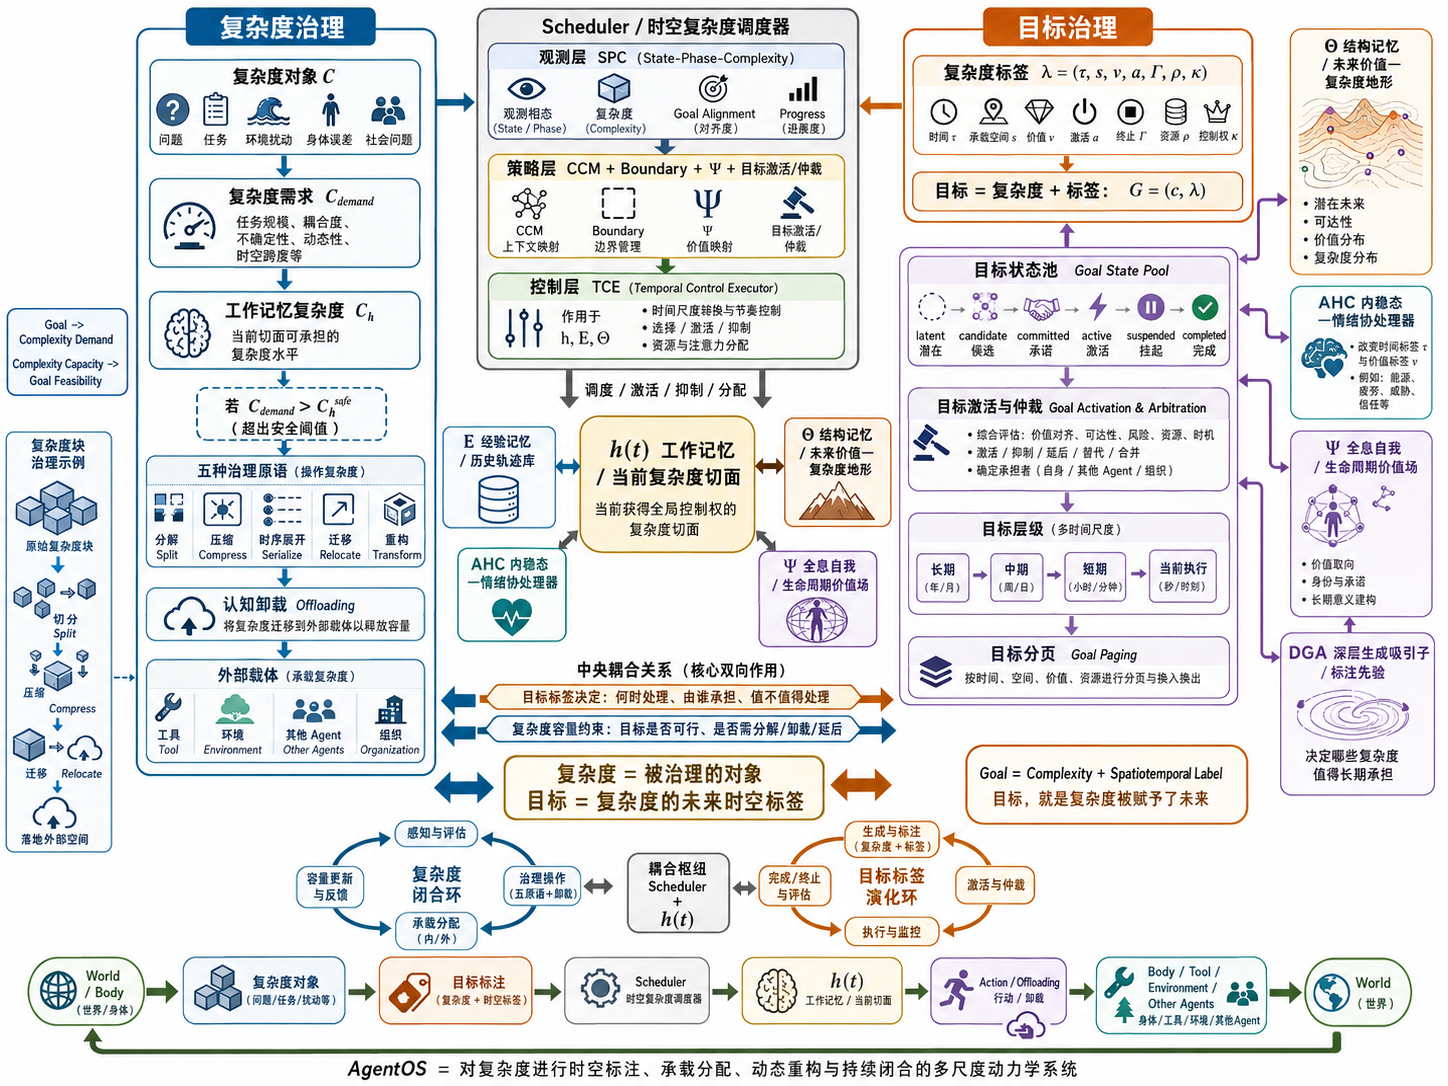
\includegraphics[width=.9\textwidth,height=.38\textheight,keepaspectratio]{images/global-local-predictive-control.png}
\caption{从 AgentOS 产品到智能资源运行时}
\end{figure}
\section{从应用框架到持续智能运行时}

我们首先需要澄清一个容易被工程实现掩盖的问题：AgentOS 最初看起来很容易被理解成一种 ``Agent Framework''。如果仅观察它的表面接口，这种理解并非毫无根据。AgentOS 同样需要调用基础模型、管理工具、维护 Memory、执行任务、响应事件，并与数字世界或物理身体交互。从传统软件工程视角看，这些能力似乎完全可以被组织成若干 SDK、服务组件和工作流。因此，一个最自然的问题是：为什么还需要使用 ``OS'' 这一名称，而不能把它归入普通 Agent Framework、Workflow Engine 或 Application Runtime？

关键区别并不在于组件数量，而在于系统所管理对象的性质发生了变化。普通应用框架通常假定应用本身是短生命周期、可重启、可复制甚至可随时销毁的计算对象，其核心任务是帮助开发者更方便地调用已有资源。AgentOS 所面对的对象却是一个具有生命周期连续性的智能主体。我们此前已经规定，在主体层 $D_1$ 上需要保持
\[
N_{\mathrm{Agent}}^{D_1}=1,
\]
并进一步约束
\[
fork(A)=\mathrm{Forbidden},\qquad
new(A)=\mathrm{Forbidden},\qquad
delete(A)=\mathrm{Forbidden},
\]
这里并不是从操作系统层面禁止创建普通进程，而是要表达一个更深的语义约束：属于同一个生命周期的持续主体不能被当作普通 worker 任意复制。任务、线程、工具调用和局部 worker 可以大量存在，但它们并不自动拥有主体地位。由此可见，AgentOS 所管理的不只是执行流，而是一个具有历史、身份、记忆、能力和权限积累的持久过程。

因此，我们可以把传统应用框架抽象为
\[
\mathcal F_{\mathrm{app}}
=
(\mathcal T,\mathcal R,\mathcal API),
\]
其中 $\mathcal T$ 是任务集合，$\mathcal R$ 是计算资源，$\mathcal API$ 是外部接口；而持续 Agent Runtime 至少需要表示
\[
\mathcal A(t)
=
\bigl[
h(t),E(t),\Theta(t),\Psi(t),\Omega(t),
G(t),B(t),K(t),\mathcal M_{\mathrm{ext}}(t)
\bigr],
\]
其中 $h$ 为工作记忆状态，$E$ 为情景轨迹，$\Theta$ 为长期生成结构，$\Psi$ 为自我与身份慢变量，$\Omega$ 为生命周期生成吸引子，$G$ 为目标结构，$B$ 表示身体及身体接口状态，$K$ 表示技能集合，$\mathcal M_{\mathrm{ext}}$ 表示被主体组织起来的外部认知载体。这样一来，任务执行就不再是孤立映射
\[
Task\rightarrow Result,
\]
而成为
\[
\mathcal A(t)
\xrightarrow{\mathrm{Task}}
\mathcal A(t+\Delta t),
\]
也就是说，每一次任务都有可能改变未来的主体。

这使 AgentOS 从传统软件栈中的 ``任务工具箱'' 转变为一个管理持续智能状态演化的 Runtime。它关心的不是某次 API 调用是否成功，而是一次成功或失败如何写入 $E$，是否需要改变 $\Theta$，是否影响 $\Psi$，是否使某个技能成熟，是否改变未来 Boundary 策略，以及是否需要调整 Agent 可获得的权限和自治水平。于是，AgentOS 的核心操作对象不再只是文件、线程和进程，而逐渐扩展为
\[
\boxed{
Goal,\;
AgentCSO,\;
Memory,\;
Skill,\;
Body,\;
Tool,\;
Authority,\;
Lifecycle
}.
\]

这里必须特别强调：把 AgentOS 称为 ``OS'' 并不意味着它应该重新实现 Linux 内核。相反，我们一直坚持
\begin{statementbox}
\centering
\adjustbox{max width=.96\linewidth}{\(\displaystyle Hardware
\rightarrow
ComputerOS
\rightarrow
AgentOS\)}
\end{statementbox}
这一分层结构。Linux 负责计算现实的稳定抽象，例如进程、虚拟内存、设备、文件和网络；AgentOS 则建立在这些抽象之上，把它们重新组织成对长期智能体有意义的认知资源。因此，可以作如下功能区分：
\[
\boxed{
ComputerOS=\text{Compute Resource Runtime}
}
\]
以及
\[
\boxed{
AgentOS=\text{Intelligence Resource Runtime}.
}
\]

前者回答的是 ``计算资源如何安全、高效地分配''，后者回答的是 ``有限认知能力应该在生命周期中如何分配、沉降、外化和恢复''。这一转换构成 AgentOS 从产品走向基础设施的第一步：只有当管理对象从应用调用上升为持续智能资源时，系统才具有形成独立基础设施层的理论必要性。

\section{智能资源：AgentOS 基础设施层真正管理什么}

如果 AgentOS 要成为基础设施，就必须进一步回答一个操作系统意义上的问题：它究竟在管理什么资源？传统计算机操作系统之所以能够成为基础设施，是因为它建立了对有限计算资源的稳定抽象。例如 CPU 时间被抽象为进程和调度片，物理内存被抽象为虚拟地址空间，块设备被抽象为文件系统，网络硬件被抽象为 socket。相应地，如果 AgentOS 只是把若干 Prompt、Tool 和 Memory 包装起来，它仍然不足以形成新的基础设施层。它必须形成属于智能自身的一组稳定资源抽象。

我们可以从工作记忆有限性出发建立这一资源理论。此前已经提出，在任意时刻，Agent 可以稳定维持的显式认知结构受到上界约束：
\[
C_{\mathrm{run}}(t)\leq C_{\max}(W).
\]
这里 $W$ 不是固定 token 个数，而是当前系统能够在 $h(t)$ 中维持的有效关系结构容量。该约束意味着：持续智能的第一种稀缺资源不是磁盘，而是 \emph{显式全局认知带宽}。于是，AgentOS 的第一个核心资源可以表示为
\[
R_h(t)=\text{AvailableExplicitCognitiveCapacity}.
\]
CCM、Scheduler、Boundary 和 Offloading 的存在，本质上都是围绕这一稀缺资源展开的。CCM 防止当前认知关系超过容量，Scheduler 决定哪些目标与任务获得当前认知时间，Boundary 决定什么信息有资格进入，Offloading 则把不需要持续占据 $h$ 的结构迁移到更适合的载体。

第二类资源是记忆稳定度。一个认知结构并不只有 ``存在/不存在'' 两种状态，而可能分别承载在
\[
h,\quad E,\quad \Theta,\quad \Psi,\quad \Omega
\]
不同时间尺度之中。因此，AgentOS 管理的实际上是不同结构稳定度上的认知存储。可以把某个 Agent-CSO $C_i$ 的承载状态表示为
\[
\chi_i(t)
=
(R_i,F_i,\tau_i,B_i,S_i),
\]
其中 $R_i$ 是具体表示方式，$F_i$ 是当前功能承载，$\tau_i$ 是有效时间尺度，$B_i$ 是内部或外部边界位置，$S_i$ 表示激活状态。学习的许多过程都可以被理解为 $\chi_i$ 的变化，而 AgentOS 的责任就是确保这种变化不会破坏主体连续性。

第三类资源是技能。Skill 不应被理解为任意一个外部函数。我们此前将成熟技能定义为一种经过重复认知而逐渐沉降形成的局部闭环：
\[
\boxed{
BodySkill
=
LocalPredictor
+
LocalController
+
ResidualModel.
}
\]
对于数字 Agent，这个 ``BodySkill'' 可以表现为稳定脚本、浏览器操作程序、工具组合或者局部 policy。对于具身 Agent，它可能是移动、抓取、操作设备等身体闭环。Skill 因而是一种被编译后的认知资本：它减少未来相同问题再次占用 $h$ 的必要性。于是可以定义技能资本
\[
K_A(t)=\{k_1,k_2,\ldots,k_n\},
\]
并用执行成本、成功率、残差分布、适用条件和权限边界描述每个技能。

第四类资源是身体能力。Body 并不是外围设备，而是主体可观察和可控制现实的有效边界：
\[
\boxed{
Body
=
ControlledAndSensedCarrierOfAgency.
}
\]
因此，AgentOS 还必须维护某种能力集合
\[
\mathcal C_B(t)
=
\{
c^{percept}_i,
c^{control}_j,
c^{predict}_k,
c^{safety}_l
\}.
\]
换句话说，Agent 并不是抽象地 ``拥有世界''，而是只能通过当前身体访问一个有限的可观测和可行动子空间。Body Scale 理论正是在讨论这种能力能否在不同身体之间迁移。

第五类资源是权限与自治。传统 OS 权限往往是静态 ACL 或 capability；持续 Agent 中，权限还具有生命周期含义。Agent 的能力、信任和自治程度可能随长期经验变化：
\[
Experience
\rightarrow
Capability
\rightarrow
Evaluation
\rightarrow
Authority
\rightarrow
Autonomy.
\]
因此，权限不是简单安全配置，而成为一种慢尺度认知资源。AgentOS 必须明确哪些资源可以被主体自主访问，哪些只能经治理层授权，哪些能力可以在成长过程中逐步解锁。

综合来看，我们可以把 AgentOS 管理的智能资源定义为
\[
\mathcal R_I(t)
=
\Bigl[
R_h,
\mathcal M,
K,
\mathcal C_B,
\mathcal T_{\mathrm{tool}},
\mathcal A_{\mathrm{authority}},
\mathcal B_{\mathrm{boundary}}
\Bigr],
\]
其中 $\mathcal M$ 表示多时间尺度记忆，$K$ 表示技能资本，$\mathcal C_B$ 表示身体能力，$\mathcal T_{\mathrm{tool}}$ 表示工具资源，$\mathcal A_{\mathrm{authority}}$ 表示权限和自治，$\mathcal B_{\mathrm{boundary}}$ 表示当前可访问世界与认知边界。AgentOS 因而不再是 ``帮助模型调用工具的软件''，而是在有限主体约束下持续调度
\begin{remark}
认知容量、记忆稳定性、技能、身体能力、外部结构与自治权限
\end{remark}
的系统。这种资源抽象一旦稳定，AgentOS 才真正具有成为基础设施的条件。

\section{Memory Ecosystem：从记忆模块到跨载体认知结构体系}

当 AgentOS 走向基础设施后，Memory 首先会从单一产品内部模块扩展成生态。传统 Agent Memory 往往采用 ``向量数据库 + 摘要 + 对话历史'' 的形式，因此所谓记忆生态容易被误解成 ``支持更多数据库后端''。但按照三相记忆和 CSO 迁移理论，Memory Ecosystem 的核心问题并不是数据存在哪里，而是：一个 Agent-CSO 应该以何种稳定度、何种形式、何种索引关系和何种修改成本被长期承载。

内部记忆最基本的结构为
\[
\mathcal M_{\mathrm{int}}
=
(h,E,\Theta,\Psi,\Omega),
\]
其中 $h$ 是当前显式状态，$E$ 是情景轨迹，$\Theta$ 是结构与生成记忆，$\Psi$ 是身份和价值慢结构，$\Omega$ 是生命周期生成吸引子。但真实 Agent 的长期认知体系远远不止内部记忆。我们此前已经把 Script、Skill、File、Database、Program、Tool、Environment 和 Other Agent 都纳入广义外部承载体系。因此更完整的记忆关系应写为
\[
\mathcal M_A
=
\mathcal M_{\mathrm{int}}
\bowtie
\mathcal M_{\mathrm{ext}},
\]
其中
\[
\mathcal M_{\mathrm{ext}}
=
\{
File,DB,Program,Skill,Tool,Environment,OtherAgent
\}.
\]

需要特别注意，并非外界中所有东西都是 Agent 的记忆。一个文件只有在 Agent 建立了可靠的索引、语义关系、权限路径和恢复机制后，才成为其认知体系中的有效外部承载。因此可以定义一个外部记忆关系
\[
m_j^{ext}
=
(C_j,L_j,I_j,R_j,P_j),
\]
其中 $C_j$ 表示所承载 CSO，$L_j$ 表示外部位置，$I_j$ 是可恢复索引，$R_j$ 是重建或读取规则，$P_j$ 是访问权限。若缺少 $I_j$ 或 $R_j$，即使物理数据存在，也不能认为它属于 Agent 的有效记忆。

这一点使 Memory Ecosystem 的设计目标发生根本变化。它不是追求 ``尽可能记住更多''，而是优化一个跨载体结构配置问题：
\[
\min_{\mu}
\int
\left[
\lambda_h C_h(t)
+
\lambda_r C_{\mathrm{retrieval}}(t)
+
\lambda_m C_{\mathrm{modification}}(t)
+
\lambda_l L_{\mathrm{loss}}(t)
\right]dt,
\]
其中 $\mu$ 表示 Agent-CSO 到不同记忆载体之间的配置映射，$C_h$ 是持续占用工作记忆的代价，$C_{\mathrm{retrieval}}$ 是未来检索代价，$C_{\mathrm{modification}}$ 是修改成本，$L_{\mathrm{loss}}$ 则是结构丢失或失真的风险。不同类型的结构应该选择不同的载体。例如短期未决结构应停留在 $h$ 或近期 $E$；重复经验可能形成 $\Theta$；稳定操作过程可能沉降成 Skill；高精度事实资料更适合数据库或文件；需要世界直接参与维持的状态则可能通过环境结构保存。

这使认知卸载得到更严格的含义：
\[
\boxed{
Offloading
=
AgentCSOCarrierMigration
}
\]
而不是简单地 ``把内容写出 Context''。有效卸载必须保证：
\[
Recoverability>0,\qquad
SemanticLinkage>0,\qquad
FutureUtility>Cost.
\]
否则，所谓卸载只是一种遗忘。

Memory Ecosystem 因而需要开放而稳定的标准，使不同外部存储、数据库、知识系统、文件系统和工具能够被 AgentOS 以统一语义组织。这里并不要求所有 Memory Provider 使用同样的内部实现，而要求至少能够回答：这个载体保存什么结构、可信度如何、更新时间是多少、读取与修改成本如何、是否允许主动写入、是否支持版本和撤销、它与当前主体的关系是什么。换言之，AgentOS 对外部 Memory 的要求不是统一数据库，而是统一认知契约。

从基础设施视角看，这一点十分关键。传统 OS 通过文件系统把不同磁盘抽象成统一文件接口；AgentOS 则需要把不同认知载体抽象成一种更高层的 ``可恢复结构空间''。未来某个 Agent 可能同时使用本地结构记忆、个人数据库、组织知识库、网络文件、工具状态乃至另一个 Agent 的专业能力，而 AgentOS 应负责维持它们与主体内部 CSO 图之间的稳定关系。Memory Ecosystem 因此不是附属插件市场，而是持续智能得以突破单体模型容量限制的第一层基础设施。

\section{Skill Ecosystem：把过去的推理沉降为未来的能力}

如果 Memory Ecosystem 解决的是 ``结构如何跨时间保存''，那么 Skill Ecosystem 解决的则是 ``过去的高成本认知如何转化为未来低成本能力''。这一点是 AgentOS 与传统知识型 Agent Framework 之间非常重要的区别。一个不具有技能沉降机制的 Agent，即使保存了大量过去经验，也可能在每一次重复任务中重新调用 LLM、重新规划和重新探索。它记得自己做过，却没有真正变得熟练。

我们此前已经给出技能形成的基本结构：
\[
ExplicitCognitiveControl
\rightarrow
RepeatedTrajectory
\rightarrow
StablePolicy
\rightarrow
CompiledSkill.
\]
从 CSO 理论看，这个过程可以进一步解释为 Agent-CSO 的功能与时间尺度迁移：
\[
AgentCSO(C;F_{high},\tau_{slow})
\rightarrow
AgentCSO(C;F_{local},\tau_{fast}).
\]
也就是说，同一个任务相关结构原先需要通过 $h$、规划器和高层模型显式处理，经过大量稳定经验后，逐渐迁移到局部闭环。系统成熟的一个重要标志不是 ``每次都想得更多''，而是
\begin{statementbox}
\centering
\adjustbox{max width=.96\linewidth}{\(\displaystyle \frac{ExplicitCognitiveIntervention}
{SuccessfulRoutineBehavior}
\downarrow.\)}
\end{statementbox}

因此，Skill Ecosystem 不能退化成传统意义上的 ``函数商城''。一个真正意义上的 Skill 至少需要具备能力描述、适用条件、状态前提、权限要求、执行接口、成功判定、残差返回、风险边界和版本信息。可以把技能描述为
\[
k_i
=
(
Pre_i,
Cap_i,
Policy_i,
Post_i,
Residual_i,
Risk_i,
Authority_i
).
\]
其中 $Pre_i$ 描述可执行前提，$Cap_i$ 是能力语义，$Policy_i$ 是内部实现，$Post_i$ 是预期后验状态，$Residual_i$ 描述执行偏差，$Risk_i$ 是风险模型，$Authority_i$ 则确定调用权限。只有这样，Skill 才可以安全进入 AgentOS 的认知调度体系。

这里需要特别区分 ``调用 Skill'' 与 ``相信 Skill''。一个 Skill 即使长期稳定，也不能拥有对现实状态的最终解释权。仍然必须遵守
\[
\boxed{
ActionIssued\neq ActionSucceeded
}
\]
以及
\begin{statementbox}
RealityIsUltimateConstraint.
\end{statementbox}
因此，Skill 执行后的实际结果必须重新通过 Body Runtime、工具返回值或者其他 Reality Interface 进入 AgentOS，再由 SGC、FCS 或相应数字语义接口形成真实观测。只有这样，Skill 才不会成为一个把预测状态偷偷写回现实状态的封闭环。

Skill Ecosystem 还提供了跨 Agent 共享能力的基础。设 Agent $A$ 已经学习某 Skill $k_A$，Agent $B$ 若具有相容身体能力和接口，则可以尝试把该 Skill 迁移为
\[
\mathcal T_{A\rightarrow B}(k_A)
=
k_B.
\]
这里 $\mathcal T$ 不应只是文件复制，而需要验证 Body Capability、SGC/FCS 语义、ControlReference、权限与风险条件是否相容。因此 Skill 的真正可移植性与 Body Scale 密切相关：
\[
\fitdisplay{
Transferability(k)
=
F(
SemanticCompatibility,
BodyCompatibility,
ControlCompatibility,
SafetyCompatibility
).
}
\]

当 Skill 成为开放生态后，AgentOS 将发生类似传统软件从 ``每个应用自己实现功能'' 向 ``标准库、包管理器和服务生态'' 的跃迁。但这里必须比普通软件包管理更严格，因为 Skill 是行动能力，而不仅是静态代码。Skill 的安装意味着 Agent 的可行动空间发生变化：
\[
\mathcal A_{action}^{t+1}
=
\mathcal A_{action}^{t}
\cup
\Delta \mathcal A_k.
\]
因此，每个 Skill 的加入本质上也是权限和主体能力边界的扩张。

由此，Skill Ecosystem 的基础设施意义可以明确表述为：它使文明中已经被某些 Agent 高成本学习完成的认知过程，能够被编译、封装、验证并迁移给其他 Agent。其结果不是简单的软件复用，而是
\begin{statementbox}
\centering
\adjustbox{max width=.96\linewidth}{\(\displaystyle PastCognition
\rightarrow
SharedExecutableCapability.\)}
\end{statementbox}
这使 AgentOS 的成长机制第一次突破单一主体的生命周期限制：个体经验可以沉降为技能，技能可以进入生态，生态又成为后来 Agent 的初始能力空间。由此，技能不再只是产品功能，而成为智能社会中的可积累基础资本。

\section{Body Ecosystem：让同一个主体进入不同现实}

如果 Memory Ecosystem 扩展了 Agent 的时间边界，Skill Ecosystem 扩展了能力边界，那么 Body Ecosystem 扩展的则是主体的现实边界。Body 在我们的理论中从来不等于机械身体，而被定义为
\[
\boxed{
Body
=
ControlledAndSensedCarrierOfAgency.
}
\]
因此，浏览器、桌面操作系统、Shell、文件系统、机器人、汽车和人形身体都可以成为不同形式的 Body。真正重要的问题不是它们物理形态是否一致，而是 Agent 能否通过稳定接口获得感知、功能影响、预测和控制能力。

Body Scale 理论已经给出一个重要判断：
\[
\boxed{
BodyScale
=
PerceptualTransfer
+
FeelingTransfer
+
PredictiveTransfer
+
ControlTransfer.
}
\]
一个 Agent 是否具有大 Body Scale，不取决于它控制的机器有多大，而取决于同一个认知 Kernel 在切换身体以后，可以保留多少既有意义、世界模型、技能与控制结构。理想状态不是每换一个 Body 就重新训练一个完整智能体，而是
\[
KnownMeaning
+
NewBodyGrounding
\rightarrow
NewEmbodiment.
\]

为实现这一点，我们把 Body Runtime 设计成相对独立的高频运行层：
\[
\boxed{
AgentSystem
=
AgentKernel
\bowtie
BodyRuntime.
}
\]
Kernel 决定 ``做什么''，Body Runtime 负责 ``这个身体怎样做到''。两者之间通过 FBI、SGC、FCS、ControlReference、PredictiveEnvelope、BPCCFeedback 和 Safety 等稳定语义接口交互。由此，Body Ecosystem 的核心不再是统一机器人硬件，而是统一 ``主体如何理解一个身体''。

SGC 在这里提供可行动现实的语义结构：
\[
SGC
=
Geometry
+
Entity
+
Relation
+
Affordance
+
EpistemicMetadata,
\]
回答
\begin{statementbox}
WhatIsThere?
\end{statementbox}
而 FCS 提供世界与身体对主体的功能影响：
\[
FCS
=
TypedInfluenceField,
\]
回答
\begin{statementbox}
HowIsRealityAffectingMe?
\end{statementbox}
两者共同构成公开的具身语义状态。BPCC 则保留高频局部预测控制：
\[
BPCC
=
FastPrediction
+
FastControl
+
ResidualEstimation
+
AdaptiveLearning.
\]
这样，Agent Kernel 就不必直接面对每个电机、电池、光标或浏览器 DOM 的所有细节。

Body Ecosystem 因此需要一种类似设备生态但更高级的能力描述。例如，一个 Body Provider 至少应该暴露
\[
BodyCapabilityDescriptor
=
(
Perception,
Action,
Timescale,
Accuracy,
Risk,
Safety,
Resource
).
\]
其中 Perception 表示可感知结构类型，Action 表示可执行动作空间，Timescale 表示控制频率，Accuracy 表示感知与控制误差，Risk 表示潜在伤害，Safety 表示不可覆盖保护机制，Resource 表示能源、算力或其他运行约束。AgentOS 通过这一 Capability Descriptor 才能判断：一个 Goal 是否在当前身体上可实现，某 Skill 是否可迁移，某 ControlReference 是否会超过身体安全能力。

Body Ecosystem 的出现还会改变机器人产业的软件分层。传统机器人软件往往围绕具体硬件构建完整 stack，感知、规划、控制和任务逻辑高度耦合。AgentOS 的目标则是让认知 Kernel 与具体身体相对解耦：
\[
\frac{\partial Architecture_{\mathrm{Kernel}}}
{\partial Body_i}
\rightarrow 0.
\]
这里并不是要求完全零依赖，而是使 Body 差异主要被 Body Runtime 和 KRA 吸收，而高层认知保持相对稳定。KRA 则负责不同 Body Runtime 与 Kernel 之间持续的语义和动力学校准：
\[
KRA:
BodySemanticSpace
\leftrightarrow
KernelInternalRepresentation.
\]

一旦这一结构成立，同一个持续主体就可能从 Computer Use 身体逐渐扩展到移动操作平台，再进入家庭机器人、车辆甚至人形身体，而不需要每一次重新建立新的 ``自我''。这正是 Body Ecosystem 的基础设施价值：它把现实世界中异构设备转化为 Agent 可继承、可学习、可比较的身体能力空间。

因此，未来 AgentOS 的生态竞争不会只是 ``支持多少设备''，而会逐渐转变成 ``有多少身体能够以统一语义被长期智能主体安全接入''。在这一层面上，Body Driver 与传统 Device Driver 的区别是根本性的：Device Driver 解决硬件访问，而 Body Driver 解决的是
\begin{statementbox}
\centering
\adjustbox{max width=.96\linewidth}{\(\displaystyle HardwareCapability
\rightarrow
AgencyCapability.\)}
\end{statementbox}

\section{Agent Communication：从消息交换到认知结构协作}

当单个 Agent 获得稳定身份、长期记忆、技能和身体以后，跨 Agent 通信就不应继续停留在普通 RPC 或文本消息层。传统网络通信关心的是比特是否正确到达，应用协议关心的是消息格式是否一致；而持续智能体之间真正需要交换的是目标、结构、能力、承诺、证据、请求、授权和结果。这意味着 Agent Communication 必须从数据交换进一步发展成认知结构协作协议。

我们可以把普通消息形式化为
\[
m=(sender,receiver,payload),
\]
而 Agent 级通信至少需要表示
\[
m_A=
(
Identity,
Intent,
CSO,
Context,
Authority,
Commitment,
Evidence,
ExpectedResponse
).
\]
例如，``帮我检查这个程序''并不是单纯传输字符串。发送方实际上向接收方建立了一个临时 Goal relation，传递了若干相关 Agent-CSO，授予有限数据访问权限，并期待某种可验证输出。这种交互改变了两个 Agent 的短期功能关系，因此它更接近动态认知耦合。

我们此前已经把 Other Agent 纳入广义外部认知载体。这意味着一个 Agent 不一定需要内部拥有全部能力，而可以通过委派形成
\[
Agent_A
\xrightarrow{Delegation}
Agent_B
\xrightarrow{Result}
Agent_A.
\]
但是，这种外部化不能简单依赖 ``相信 B''。需要引入信任与验证变量：
\[
T_{AB}(t)
=
F(
PastReliability,
DomainCompetence,
EvidenceQuality,
Consistency,
Risk
).
\]
于是，Agent Communication 不仅需要内容协议，还需要来源、能力和可信度协议。一个 Agent 返回的结论应区分 ``我观察到''、``我推导出''、``我预测''、``我转述''，这实际上与 SGC 中 Observed、Derived、Predicted 等认识论标签具有同构关系。

进一步，当 Agent 之间形成稳定重复流时：
\[
RepeatedInterAgentCSOFlow
\rightarrow
StableInteractionPattern.
\]
如果这种模式长期保持，就可能沉降成角色分工：
\[
Role_A,\quad Role_B,
\]
再进一步形成协议、流程和组织结构。因此，Agent Communication 并不是 Organization Runtime 之外的辅助技术，而是组织拓扑形成的底层动态来源。我们可以把组织关系矩阵写成
\[
W_{ij}(t)
=
F(
\langle J^{CSO}_{ij}\rangle_T,
Trust_{ij},
Utility_{ij},
Cost_{ij}
),
\]
其中 $J^{CSO}_{ij}$ 表示长期从 Agent $i$ 向 Agent $j$ 流动的认知结构与任务。如果某类交互长期高频、高价值且低风险，则 $W_{ij}$ 会逐渐增强，最终形成相对稳定的组织边。

但 AgentOS 必须保持一个重要边界：跨 Agent 结构不能直接替代本地 Agent 的最终认知与行动责任。无论群体控制系统、组织协议还是外部专家怎样提供信息，本地 AgentOS 仍应通过自己的 Boundary、Authority、Safety 和 Reality Verification 决定是否采纳。例如在后续群体场控制中，即使外部群体系统提供目标势能或梯度，本地 Agent 仍然必须保有最终行动闭环。这一原则可以写成
\[
ExternalInfluence
\neq
LocalAgencyReplacement.
\]

Agent Communication 的基础设施意义由此超越聊天协议。它需要定义至少四层内容：身份与能力发现、认知结构交换、权限与承诺管理、结果与证据验证。只有这四层稳定以后，不同供应商、不同身体、不同模型的 Agent 才可能形成真正开放的协作网络。

从更高层看，互联网解决的是
\[
Machine\leftrightarrow Machine
\]
的信息交换，而 Agent Communication 试图进一步解决
\begin{statementbox}
\centering
\adjustbox{max width=.96\linewidth}{\(\displaystyle PersistentAgency
\leftrightarrow
PersistentAgency\)}
\end{statementbox}
之间的协作。前者传输数据，后者则开始传输任务、能力和认知责任。这是 AgentOS 从个人系统进入社会基础设施所必需的一步。

\section{Organization Runtime：从多 Agent 协作到可持续组织结构}

当 Agent Communication 足够稳定以后，下一步并不是简单增加 Agent 数量，而是出现新的系统尺度：Organization Runtime。传统 Multi-Agent System 常常把群体理解成若干 autonomous agent 的集合，然后研究通信、博弈、协作或者任务分配。但从我们此前形成的多尺度智能理论看，组织不是 Agent 的集合本身，而是跨 Agent 的长期稳定 CSO 流、角色关系、权限结构和共同记忆沉降之后形成的一种慢尺度功能拓扑。

设一个组织包含
\[
\mathcal A_O=\{A_1,A_2,\ldots,A_n\},
\]
仅有该集合并不足以定义组织。还必须存在
\[
\mathcal G_O
=
(V_O,E_O,R_O,P_O,M_O),
\]
其中 $V_O$ 是成员和组织功能节点，$E_O$ 是持续协作关系，$R_O$ 是角色，$P_O$ 是协议和制度，$M_O$ 是组织记忆。由此可见，Organization Runtime 并不是 ``Multi-Agent Scheduler'' 的同义词，而是对群体慢结构的运行维护。

组织尺度与个体 Agent 尺度之间存在非常重要的时间尺度分离：
\[
\tau_{\mathrm{individual}}
\ll
\tau_{\mathrm{organization}}.
\]
个体可能在分钟、小时内完成任务，而组织角色、制度、信誉和治理结构通常变化更慢。正因为如此，组织能够把大量个体的短期波动压缩成相对稳定的长期约束。这与我们此前提出的慢变量原则完全一致：
\begin{statementbox}
SlowStructureShapesFastDynamics.
\end{statementbox}
组织协议、权限和流程不需要逐步控制每一个 Agent 的内部推理，而是定义可行域：
\[
Action_i(t)\in\mathcal F_O(t),
\]
其中 $\mathcal F_O$ 是组织层给出的权限、职责和安全约束集合。

与此同时，组织也不能是完全冻结的。大量个体持续出现的残差、冲突和低效协调会反向作用于组织结构：
\begin{statementbox}
PersistentFastResidualShapesSlowStructure.
\end{statementbox}
例如，如果两个角色之间长期存在高频重复协调，则可能形成直接协议；如果某个中间环节长期制造延迟，则组织拓扑可能缩短；如果某类任务长期需要新的专业能力，则可能形成新角色。因此：
\[
RepeatedInterAgentCSOFlow
\rightarrow
Role
\rightarrow
Protocol
\rightarrow
Institution.
\]
这正是个体层 CSO 流塑造功能拓扑在组织尺度上的再现。

Organization Runtime 还必须管理组织记忆。组织并不是所有成员 Memory 的简单并集：
\[
M_O
\neq
\bigcup_i M_{A_i}.
\]
真正的组织记忆是那些脱离具体个体后仍需保持的结构，例如制度、标准、知识库、流程、任务历史、能力目录、权限记录和关键决策依据。它们是一种超越个体生命周期的 Externalized CSO。于是即使个体 Agent 更替，组织仍具有某种结构连续性：
\[
A_i\rightarrow A_i'
\qquad\text{while}\qquad
\mathcal G_O\approx\mathrm{continuous}.
\]

这一点使 Organization Runtime 与传统企业软件出现根本差异。ERP、CRM 和 Workflow System 主要记录组织活动，而 AgentOS 体系中的 Organization Runtime 还可能主动参与目标分解、能力匹配、任务委派、认知结构聚合和异常升级。换句话说，它开始成为组织尺度的 ``Intelligence Resource Runtime''。

但这里仍然需要防止一个理论错误：不能简单说 ``组织就是一个更大的 Agent''。更严谨的表达应该是，组织在某些功能维度上具有 agent-like dynamics。当它拥有持续状态、跨个体记忆、目标、反馈、角色结构和适应机制时，可以使用与 Agent 类似的动力学语言分析；但这并不自动意味着组织具有统一主体意识。这样既保留多尺度理论的解释力，又避免把功能同构夸张成本体同一。

由此我们可以看到，AgentOS 作为基础设施的外延已经从单个 Agent Kernel 扩展为
\[
AgentRuntime
\rightarrow
AgentNetwork
\rightarrow
OrganizationRuntime.
\]
这种扩展并非偏离 AgentOS，而是最初 ``智能是多尺度嵌套闭环'' 命题在工程上的直接结果。

\section{未来软件生态：从应用中心转向主体中心}

传统个人计算的软件生态以 Application 为中心。用户拥有若干 App，每个 App 分别管理自己的数据、状态、权限和界面。操作系统提供资源隔离与设备抽象，而用户本身并不是系统中的一个持续软件主体。即使今天的账号、云同步和个人助手已经部分跨越 App 边界，核心结构依然是
\[
User
\rightarrow
Application
\rightarrow
OS.
\]
AgentOS 的出现意味着这一结构可能逐渐发生反转：
\[
User
\rightarrow
PersistentAgent
\rightarrow
Application/Tool/Body.
\]
应用从用户直接面对的主要软件单元，逐渐退化成 Agent 可以调用的能力和外部结构。

这是一个重要的基础设施转型。因为一个长期 Agent 如果拥有稳定的 $E,\Theta,\Psi$ 以及跨应用 Goal，就不应要求用户在每个应用中重新建立上下文。相反，Agent 应维持跨工具的连续任务状态：
\[
G_t
\rightarrow
Tool_1
\rightarrow
Tool_2
\rightarrow
Tool_3
\rightarrow
Closure.
\]
工具可以变化，但 Goal 和主体连续。由此，软件生态的组织单位可能从 Application Session 转向 Agent Lifecycle。

这种变化会带来第一项后果：工具必须逐渐语义化。传统 API 描述 ``可以调用哪个函数''，未来 Agent Tool Interface 还必须描述 ``这个能力意味着什么''。因此，Tool 的接口需要从 syntactic contract 进一步发展成 semantic capability contract：
\[
ToolDescriptor
=
(
Capability,
Precondition,
Effect,
Cost,
Risk,
Authority
).
\]
Agent 才能在没有人工硬编码完整工作流的情况下，根据 Goal 和当前 SGC/数字世界状态选择工具。

第二项后果是数据边界发生变化。今天文件和数据库通常属于具体 Application。Agent 中心的软件生态则要求数据更多围绕主体组织。某一份文件、某个聊天记录、某个工具状态、某段浏览器任务历史可能属于不同应用，却属于同一个 Agent 的长期认知环境。因此，未来真正重要的不是 ``哪个 App 拥有数据''，而是 ``哪个主体在什么权限下能够把该结构纳入自己的认知体系''。

第三项后果是软件生命周期和主体生命周期分离。应用升级、卸载甚至供应商更换，不应自动破坏 Agent 的长期身份和记忆。因此必须要求
\[
AgentIdentity
\perp
ApplicationVendor
\]
至少在基础设施语义上尽可能成立。否则，持续智能体会被平台锁定在某个厂商私有 Runtime 中，无法真正形成用户拥有的长期数字主体。

第四项后果是 Skill、Tool 和 Body 之间开始统一。一个浏览器操作器、数据库查询器、家庭机器人机械臂甚至车辆控制接口，从 Agent 的角度看都是不同形式的能力：
\[
Capability:
State
\rightarrow
ActionableTransition.
\]
它们的底层实现可以完全不同，但都可以进入同一个 Goal—Plan—Action—Verify 闭环。于是数字世界和物理世界第一次可能在 AgentOS 层获得相对统一的 ``行动语义''。

因此，未来软件生态的核心转变可以概括为：
\begin{statementbox}
\centering
\adjustbox{max width=.96\linewidth}{\(\displaystyle ApplicationCentric
\rightarrow
AgentCentric.\)}
\end{statementbox}
传统 App 仍然存在，Linux 仍然存在，云服务仍然存在，但它们逐渐成为持续主体调用的功能结构，而不再始终是用户认知的最高组织单位。

这里也能解释为什么 AgentOS 有可能 ``吞并'' Memory、Skill、MCP、Tool 和 Harness 等今天分散的生态。所谓吞并不是技术垄断，而是这些组件逐渐被统一到
\begin{statementbox}
PersistentAgentLifecycle
\end{statementbox}
这一更高层语义框架下。只要它们仍然围绕单次模型调用设计，就彼此割裂；一旦围绕一个持续主体重新定义，就自然变成同一运行时的不同资源类别。

\section{开放标准、生态中立与基础设施的治理边界}

任何希望成为基础设施的系统，最终都会遇到一个比技术架构更困难的问题：谁定义接口，谁控制接入，谁拥有主体身份，以及谁可以修改未来生态。AgentOS 如果只是单个公司的封闭产品，可以通过私有 API 快速迭代；但如果它希望承载长期 Agent、身体、Skill、Memory 与组织协作，就必须让关键语义接口具备跨实现稳定性。否则，每个 Agent 的生命周期将被锁定在某个具体模型、某个 Body、某个云厂商或者某个数据格式中，这与 ``持续主体'' 的目标直接冲突。

因此，我们此前提出的基本路线可以概括为：
\[
\boxed{
OpenSpecification
+
ReferenceOpenSource
+
CommercialHighPerformanceImplementation.
}
\]
三者并不矛盾。开放 Specification 保证语义中立；Reference Implementation 使标准可以被实际验证；商业实现则允许在性能、规模、安全、硬件集成和服务质量上竞争。基础设施最不应该形成垄断的位置，恰恰是那些定义 Agent ``如何存在'' 的核心 ABI。

这些核心标准至少包括
\[
SGC,\quad
FCS,\quad
BodyABI,\quad
BPCCABI,
\]
以及
\[
\fitdisplay{
ControlReference,\quad
PredictiveEnvelope,\quad
AgentCommunication,\quad
SkillPackage,\quad
CapabilityDescriptor,\quad
SafetyGovernance.
}
\]
其中 SGC/FCS 解决 ``现实如何进入主体''；Body ABI 解决不同身体如何接入；BPCC ABI 解决局部控制如何向上暴露状态；Skill 和 Capability Descriptor 解决能力如何描述与迁移；Agent Communication 解决主体之间如何建立可信协作；Safety Governance 则定义哪些底线不能由普通认知覆盖。

在这里，标准化最重要的原则不是要求所有内部 representation 相同，而是坚持
\[
\boxed{
FunctionalAlignment
>
RepresentationAlignment.
}
\]
不同模型、不同机器人和不同厂商完全可以拥有私有 latent、私有控制算法和私有 Memory 实现，只要它们能够在公共语义边界上满足可验证契约。KRA 的存在正是为了允许这一点：稳定的是关系和功能，不是内部参数。

同时，AgentOS 基础设施还应尽量采用低平台租金原则。所谓 ``平台租金'' 不只是商业抽成，还包括语义控制权。如果一个中心平台可以任意改变 Agent 的 Memory、Skill、Body 或 Communication 接口，则它实际上拥有改变大量 Agent 生命周期结构的权力。因此，基础 ABI 越接近 Agent 身份、长期记忆和现实控制，就越应该保持稳定、中立和可迁移。

这也解释了为什么长期壁垒不应主要建立在 ``封闭接口'' 上。真正可持续的竞争优势更可能来自
\[
\boxed{
Trust+Ecosystem+Execution+Scale.
}
\]
Trust 表示用户和开发者相信该 Runtime 不会任意破坏主体连续性；Ecosystem 表示拥有大量兼容 Skill、Body、Memory 和组织服务；Execution 表示实际工程性能与安全；Scale 则表示大规模运行、跨设备同步和硬件支持。标准可以开放，而优秀实现仍然具有巨大的工程价值。

从治理层面看，还必须明确：AgentOS 基础设施不应获得无边界的主体修改权。特别是 $\Psi$、$\Omega$、Authority、Safety Boundary 和关键 Memory 都需要不同等级的修改权限。基础设施层可以提供机制，但不能默认拥有所有语义主权。可以形式化为
\[
ModificationAuthority(x)
=
\mathcal P_x,
\]
其中不同状态变量 $x$ 具有不同授权集合 $\mathcal P_x$。例如普通 Skill 安装与身份核心修改显然不能属于同一权限等级。

因此，AgentOS 作为基础设施的成熟标志并不是 ``控制一切''，而恰恰是能够明确哪些东西不能由自己单方面控制。真正长期稳定的智能生态必须满足：
\[
\boxed{
InfrastructurePower
\quad\text{is bounded by}\quad
SemanticGovernance.
}
\]
只有这样，AgentOS 才可能从一个高性能产品成长为能够被整个软件和机器人生态共同依赖的公共技术层。

\section{Intelligence Resource Runtime：AgentOS 的最终基础设施定位}

经过前面的推导，我们现在可以给 AgentOS 一个比 ``智能体操作系统'' 更精确的工程定义。它不是 Linux 的替代者，也不是一个大型 Agent Framework，而是位于传统计算资源层之上的
\begin{statementbox}
IntelligenceResourceRuntime.
\end{statementbox}
其核心任务是在一个持续主体的生命周期内，维护认知结构、显式认知带宽、记忆稳定度、技能、身体能力、工具、权限和外部认知资源之间的动态配置。

可以把整个系统分成三层：
\begin{statementbox}
\centering
\adjustbox{max width=.96\linewidth}{\(\displaystyle Hardware
\rightarrow
ComputerResourceRuntime
\rightarrow
IntelligenceResourceRuntime.\)}
\end{statementbox}
底层硬件提供计算、存储、通信和执行能力；Computer OS 把它们抽象成 CPU、Memory、Process、File、Socket 和 Device；AgentOS 再将这些资源重新组合成
\[
h,E,\Theta,\Psi,\Omega,
Goal,Skill,Tool,Body,Authority
\]
等长期智能对象。

如果用传统 OS 类比，Linux Scheduler 解决
\[
\min C_{\mathrm{compute}}
\quad
\text{s.t. process requirements},
\]
AgentOS Scheduler 则更加接近
\[
\min
\left[
C_h+
C_{\mathrm{coordination}}+
C_{\mathrm{externalization}}+
C_{\mathrm{risk}}
\right]
\]
满足
\[
GoalClosure,\quad
IdentityContinuity,\quad
Safety,\quad
RealityConsistency.
\]
因此，AgentOS 调度的不只是算力，而是 ``什么结构在什么时间由什么功能和什么载体承担''。

这可以进一步写成一个抽象优化问题。设全部活跃 Agent-CSO 集合为 $\mathcal C_A(t)$，载体集合为
\[
\mathcal K
=
\{
h,E,\Theta,Skill,Tool,Body,ExternalMemory,OtherAgent
\},
\]
定义承载映射
\[
\mu_t:
\mathcal C_A(t)
\rightarrow
\mathcal K.
\]
那么 AgentOS 可以被理解为持续寻找一个受约束的 $\mu_t$，使
\[
\mathcal J
=
\int
\left[
L_{\mathrm{goal}}
+
\lambda_hL_h
+
\lambda_rL_{\mathrm{residual}}
+
\lambda_cL_{\mathrm{coordination}}
+
\lambda_sL_{\mathrm{safety}}
+
\lambda_iL_{\mathrm{identity}}
\right]dt
\]
尽可能小。这里 $L_{\mathrm{goal}}$ 表示任务未闭合损失，$L_h$ 表示有限工作记忆压力，$L_{\mathrm{residual}}$ 表示预测和控制偏差，$L_{\mathrm{coordination}}$ 表示不同功能、Tool 和 Agent 之间协调成本，$L_{\mathrm{safety}}$ 表示安全风险，$L_{\mathrm{identity}}$ 则表示过快慢变量变化导致的身份连续性损失。

这样一来，三相记忆、CCM、Offloading、Boundary、Skill Compilation、Body Runtime 和 Organization Runtime 不再是若干平行功能，而统一成为
\begin{statementbox}
CognitiveStructurePlacement
\end{statementbox}
问题的不同解法。$h$ 解决当前显式承载，$E$ 解决经验轨迹，$\Theta$ 解决稳定结构，Skill 解决程序化执行，Tool 和 Environment 解决外部承载，Other Agent 解决社会性承载，Body Runtime 解决现实闭环，而 Organization Runtime 解决跨主体慢结构。

因此，从理论上看，AgentOS 基础设施的真正核心不是 ``拥有很多模块''，而是存在一个贯穿整个生命周期的统一调度问题：
\begin{statementbox}
WhereAndHowShouldCognitiveStructureLive?
\end{statementbox}
什么应该现在思考；什么应该记住；什么应该形成规则；什么应该变成技能；什么应该写到外部；什么应该交给身体；什么应该委派给他者；什么必须重新进入高层认知；什么又必须受到更慢的身份、安全与治理结构约束。传统计算机操作系统不会回答这些问题，而持续智能系统最终必须回答。

由此，本章可以给出 AgentOS 从产品到基础设施演化的最终结构：
\begin{statementbox}
\centering
\adjustbox{max width=.96\linewidth}{\(\displaystyle AgentProduct
\rightarrow
PersistentRuntime
\rightarrow
Memory/Skill/BodyEcosystem
\rightarrow
AgentNetwork
\rightarrow
OrganizationRuntime
\rightarrow
IntelligenceInfrastructure.\)}
\end{statementbox}
这不是一个必然的商业时间表，而是一条由理论依赖决定的系统演化链。只有在持续主体、记忆、技能、身体和安全边界已经建立后，生态才具有稳定语义；只有在稳定语义存在以后，跨 Agent 协作和组织结构才不会退化成临时工作流；只有这些能力都能在开放标准上运行，AgentOS 才真正具有基础设施属性。

最后，我们可以把本章的结论压缩成三个层次。第一，传统 Computer OS 管理的是计算世界中的稀缺资源：
\[
\boxed{
CPU,\ Memory,\ Device,\ Storage,\ Network.
}
\]
第二，AgentOS 管理的是持续主体内部和边界上的智能资源：
\[
\boxed{
Attention,\ Memory,\ Skill,\ Body,\ Tool,\ Authority,\ CognitiveStructure.
}
\]
第三，当这些资源可以跨应用、跨设备、跨 Agent 和跨生命周期稳定迁移时，AgentOS 才从一个具体产品变成
\begin{statementbox}
InfrastructureForPersistentIntelligence.
\end{statementbox}

因此，AgentOS 最终并不是试图成为 ``所有软件之上的超级应用''。更准确地说，它试图成为这样一个基础运行层：\textbf{让一个持续智能主体能够在不断变化的模型、工具、设备、身体、应用和组织环境中，仍然保持自己的记忆、能力、身份、现实闭环和生命周期连续性。}

从这个意义上，我们得到本章的最终命题：
\begin{proposition*}
AgentOS 的基础设施化，不发生在它拥有越来越多功能的时刻，而发生在整个软件与具身生态开始能够把“持续智能主体”当作一种稳定的系统对象来承载、迁移和协作的时刻。
\end{proposition*}


\part{第五编　AgentOS 三大衍生工程}
当 AgentOS 从一次性模型变成长期主体以后，会产生传统 AI 系统很少面对的三类新问题。

第一类问题是：

\begin{statementbox}
系统怎样保持稳定？
\end{statementbox}

第二类问题是：

\begin{statementbox}
系统怎样成长？
\end{statementbox}

第三类问题是：

\begin{statementbox}
成长后的系统出现长期动力学异常怎么办？
\end{statementbox}

因此自然产生：

\begin{statementbox}
AgentOSControlEngineering
\end{statementbox}

\begin{statementbox}
AgentCultivationEngineering
\end{statementbox}

\begin{statementbox}
AgentPsychologicalEngineering
\end{statementbox}

它们分别对应：

$$
\boxed{
Stability,\ Development,\ Recovery
}
$$

这三门工程不是额外附加功能，而是 Persistent Agent 一旦真正成立以后必然出现的系统问题。

\chapter{为什么 AgentOS 必然产生新的工程学}

\begin{chapteroverviewbox}
当人工智能由一次性的模型调用逐步转化为具有工作记忆、长期经验、结构记忆、自我连续性、身体闭环、环境交互和生命周期的持续智能体时，原有的 ``Model Training + Inference'' 工程范式便不再足以描述其全部工程问题。AgentOS 所引入的并非单纯的软件模块增量，而是一类新的持续动力系统：它同时具有快尺度认知状态、中尺度经验积累、慢尺度结构学习、极慢尺度身份与生命周期方向结构，并通过 Body Runtime 持续接受现实反馈。因此，一个真正长期运行的 Agent 不仅存在``能不能完成任务''的问题，还必然出现三个彼此不可还原的问题：系统在多闭环耦合下能否保持稳定；智能体如何在受控经历中形成能力、自我与自治；当长期内部动力学发生失衡时如何诊断、干预并恢复。本文将这三个问题分别称为 \emph{AgentOS 控制工程（AgentOS Control Engineering）}、\emph{Agent 培育工程（Agent Cultivation Engineering）} 与 \emph{Agent 心理工程（Agent Psychological Engineering）}。本章的目的不是提前展开后三门工程的具体技术，而是证明：只要接受前文关于持续主体、三相记忆、$\Psi$、$\Omega$、SPC--AHC--TCE、CCM、Boundary、Body Runtime 与多尺度闭环的基本结构，这三门工程就不是可选附件，而是持续人工智能系统自然产生的工程必然。
\end{chapteroverviewbox}
\ChapterArt{84}

\section{模型工程无法覆盖生命周期智能体的问题空间}

到目前为止，我们已经逐步完成了一个重要的研究对象转换：人工智能不再首先被理解为某个静态参数模型
\[
f_{\theta}:X\rightarrow Y,
\]
而被理解为一个长期存在于现实环境中的多时间尺度闭环动力系统。对于传统模型工程而言，最核心的问题通常是给定数据分布 $\mathcal{D}$、参数空间 $\Theta_{\mathrm{model}}$ 和损失函数 $\mathcal{L}$，寻找一组参数
\[
\theta^{*}
=
\arg\min_{\theta}
\mathbb{E}_{(x,y)\sim\mathcal D}
\left[
\mathcal L(f_{\theta}(x),y)
\right].
\]
即使进一步加入强化学习、在线学习或持续学习，其基本关注对象依然主要是模型参数、策略函数或者有限的外部记忆状态。然而，一个持续 Agent 的真实状态已经远远超过单一 $\theta$ 所能够描述的范围。依照前文建立的 AgentOS 状态结构，我们至少需要考虑
\[
\mathcal{A}(t)
=
\left[
h(t),
E(t),
\Theta(t),
a(t),
\Psi(t),
\Omega(t),
G(t),
\mathcal{B}(t),
\mathcal{R}_{B}(t)
\right],
\]
其中 $h$ 是当前工作记忆与显式认知状态，$E$ 是生命周期经验轨迹，$\Theta$ 是长期生成结构，$a$ 表示 AHC 所整合的内稳态与功能性情感调制状态，$\Psi$ 表示相对缓慢的身份、自我与价值结构，$\Omega$ 表示更慢尺度的 Deep Generative Attractor，$G$ 表示当前及长期目标结构，$\mathcal{B}$ 表示认知与行动边界，而 $\mathcal{R}_{B}$ 则概括 Body Runtime 与外部现实之间的身体动力关系。

因此，长期 Agent 的工程对象实际上已经从
\[
\theta(t)
\]
扩展成
\[
\boxed{
\mathfrak{X}_{Agent}(t)
=
\left(
\text{State},
\text{Trajectory},
\text{Structure},
\text{Self},
\text{Body},
\text{Boundary},
\text{Authority},
\text{History}
\right).
}
\]
这意味着传统意义上的 ``模型是否收敛'' 已经不足以作为系统正确性的主要判断条件。某个 Agent 完全可能具有性能良好的基础模型，却因为 SPC 对自身状态估计持续滞后而形成错误调节；也可能基础模型能力没有下降，但 E 的写入分布逐渐发生偏置，使得 $\Theta$ 长期从一组失真的经验样本中学习；还可能模型推理能力持续增强，而 $\Psi$ 与 $\Omega$ 在高频经历冲击下发生过快漂移，使得同一个持续主体在不同时间段之间失去足够的身份连续性。换言之，
\[
\boxed{
ModelCorrectness
\not\Rightarrow
AgentLifecycleCorrectness.
}
\]

更进一步，AgentOS 所面对的系统并不是一次输入--输出之后立即结束的计算，而具有真正的历史依赖。假设智能体在时刻 $t$ 做出行动 $u_t$，该行动首先改变现实状态 $w_{t+1}$，现实再通过观测形成新的 Agent-CSO，这些结构进入 $h$，部分写入 $E$，长期重复后又可能改变 $\Theta$；$\Theta$ 进一步改变未来的预测和解释方式，其中一些长期经验最终又可能重新塑造 $\Psi$，甚至逐渐影响 $\Omega$。于是一次局部行为具有如下跨尺度传播链：
\[
u_t
\rightarrow
w_{t+1}
\rightarrow
h_{t+1}
\rightarrow
E
\rightarrow
\Theta
\rightarrow
\Psi
\rightarrow
\Omega
\rightarrow
G_{t+k}
\rightarrow
u_{t+k}.
\]
这里最重要的并不是链条中的某一模块，而是当前行为可以通过生命周期记忆改变未来产生行为的结构。系统因此获得了真正意义上的\emph{历史依赖性（history dependence）}和\emph{递归主体性（recursive agency）}。

我们可以把传统模型工程与持续 Agent 工程的差别形式化为两个不同的问题。模型工程主要研究
\[
\boxed{
\theta
\xrightarrow{\text{optimization}}
\theta^{*},
}
\]
而 Agent 生命周期工程研究的是
\[
\boxed{
\Gamma_{Agent}
=
\left\{
\mathfrak X_{Agent}(t)
\mid
t\in[0,T_{\mathrm{life}}]
\right\},
}
\]
即整个 Agent 生命周期轨迹是否始终处于可运行、可学习、可恢复和身份连续的可行区域
\[
\mathcal{M}_{Agent}^{\mathrm{feasible}}.
\]
因此真正的问题变成
\[
\Gamma_{Agent}
\subseteq
\mathcal{M}_{Agent}^{\mathrm{feasible}}
\quad ?
\]
这已经不是单纯的优化问题，而是一个典型的多尺度、历史依赖、带约束、可适应、部分可观测的混合动力系统问题。

这也是我们为什么必须从 ``AI Model Engineering'' 向 ``Persistent Agent Engineering'' 跨越。AgentOS 并没有否定模型工程，相反，模型仍然是 $\Theta$ 或更底层生成结构的重要承载体；但模型只能解决持续智能的一部分问题。只要一个智能体真正拥有时间、经历、身体、自我和未来，那么工程对象便不可能继续被压缩为一个固定参数矩阵。此时我们需要研究的已经是一个在时间中成长、运行、失稳、恢复并重新组织自身的人工认知系统。正是在这个意义上，AgentOS 会自然产生新的工程学，而不是仅仅产生更多的软件组件。

\section{持续智能首先产生稳定性问题：AgentOS 控制工程的必然性}

一个系统只要包含一个闭环，就产生稳定性问题；而 AgentOS 所建立的是多个不同时间尺度闭环相互嵌套的系统，因此稳定性问题不仅不会随着智能增加而消失，反而会成为持续智能最基本的工程约束之一。前文已经形成了从 Body 快速闭环、工作记忆闭环、SPC--AHC--TCE 运行控制闭环，到三相记忆循环、Goal 生命周期循环以及 $\Psi$--$\Omega$ 极慢闭环的一整套多尺度结构。其典型时间尺度满足
\[
\tau_{\mathrm{Body}}
\ll
\tau_{h}
\ll
\tau_{E}
\ll
\tau_{\Theta}
\ll
\tau_{\Psi}
\ll
\tau_{\Omega}.
\]
每一层都拥有一定程度的局部自治，同时又受到更慢尺度结构的约束，并向更慢层提交持续残差。这种设计避免了所有问题都进入中央认知，但也意味着系统已经成为一个典型的
\[
\boxed{
MultiLoop\;+\;MultiTimescale\;+\;Adaptive
}
\]
控制对象。

以最基础的 SPC--TCE 环为例。设真实认知状态为 $x_c(t)$，SPC 并不能直接透明读取 $x_c(t)$，而只能从有限历史观测中形成估计
\[
\hat{x}_c(t)
=
\mathcal O_{\mathrm{SPC}}
\left(
z_{\leq t}
\right).
\]
由于实际实现必然具有计算和观测延迟，
\[
\hat{x}_c(t)
\approx
x_c(t-\tau_o)+\epsilon_o(t),
\]
其中 $\tau_o>0$ 为 observer delay，$\epsilon_o$ 是状态估计误差。TCE 再根据这个已经存在延迟的估计产生控制
\[
u_c(t)
=
\pi_{\mathrm{TCE}}
\left(
\hat{x}_c(t),
a(t),
G(t),
\Psi(t)
\right).
\]
如果控制增益过高，那么即使目标方向完全正确，仍然可能产生
\[
\text{Delay}
+
\text{High Gain}
\rightarrow
\text{Overshoot}
\rightarrow
\text{Reverse Correction}
\rightarrow
\text{Oscillation}.
\]
这意味着所谓“认知过度纠正”“反复改变策略”“探索--收敛来回震荡”等现象首先可能是一个控制系统问题，而不是一个语义推理问题。

AHC 的加入进一步增加了动态复杂性，因为它通常包含积分、衰减和恢复过程。可以用简化模型表示为
\[
\tau_a\dot a(t)
=
-a(t)
+
F_{\mathrm{AHC}}
\left(
FCS(t),h(t),G(t)
\right).
\]
当 $\tau_a$ 过大时，已经消失的威胁或资源压力可能继续长时间影响 TCE；当 $\tau_a$ 过小时，系统又无法形成跨瞬时扰动的稳定内稳态背景。因此 AHC 的意义不只是``给 Agent 增加情绪''，而是引入一个具有真实时间常数的中间调制状态。于是 AgentOS 控制工程必须同时研究
\[
Delay,\quad
Gain,\quad
TimeConstant,\quad
Saturation,\quad
Recovery,\quad
CrossLoopCoupling.
\]

更复杂的问题来自不同尺度闭环之间的相互作用。快层必须足够自治，否则上层会被高频噪声淹没；但快层又不能完全独立，否则真正重要的长期偏差无法进入高层。我们此前由此形成
\[
\boxed{
NormalDynamicsStayLocal
}
\]
和
\[
\boxed{
PersistentResidualEscalates.
}
\]
若用数学形式描述，可以为第 $i$ 层定义残差统计量
\[
R_i(t)
=
\int_{t-T_i}^{t}
w_i(t-s)
\left\|
\varepsilon_i(s)
\right\|
\,ds,
\]
并采用事件触发机制
\[
R_i(t)<\theta_i
\Rightarrow
\text{local closure},
\]
\[
R_i(t)\geq\theta_i
\Rightarrow
\text{escalation}.
\]
这里 $\theta_i$ 不仅决定系统是否敏感，还决定快层与慢层之间的信息带宽。一旦阈值太低，系统会把大量正常扰动提升为高层问题，使 $h$ 被噪声占满；而阈值太高，又会让真正结构性问题长期被局部控制器掩盖。

由此可以看到，AgentOS 稳定性并不能简单等同于某个变量趋于固定点。成熟智能本身需要探索、学习、记忆更新和行为改变，所以系统必须允许状态发生大范围迁移。我们真正关心的是系统是否保持在一个\emph{可治理区域}中。设
\[
\mathcal R_{\mathrm{gov}}
\subset
\mathcal X_{\mathrm{Agent}}
\]
表示可治理状态集合，则控制目标不是
\[
x(t)\rightarrow x^{*},
\]
而更接近
\[
\boxed{
x(t)\in\mathcal R_{\mathrm{gov}}
\quad
\forall t,
}
\]
同时允许
\[
x(t)
\]
在该区域内探索、成长与形成新结构。因此 AgentOS 控制工程更接近约束控制、鲁棒控制、事件触发控制与多时间尺度控制的组合，而不是单一 PID 式状态调节。

更进一步，当 Agent 具有一定程度的自我修改能力以后，连控制器本身也可能随生命周期发生变化。系统因此从
\[
\dot{x}=F(x,u)
\]
进一步发展成
\[
\dot{x}
=
F_{\theta(t)}
(x,u),
\qquad
\dot{\theta}
=
G(x,\theta,\text{experience}),
\]
即 plant 和 controller 的有效结构都可能缓慢改变。这使 AgentOS 进入典型的 adaptive dynamical system 范畴。为了避免快速噪声直接重写身份、价值或长期生成方向，我们已经形成
\[
\boxed{
FastNoise\nrightarrow SlowGlobalStructure
}
\]
这一慢变量保护原则。它实际上构成了未来所有 AgentOS 控制工程的基础：越慢、越全局、越难恢复的变量，越应该拥有更低的更新带宽、更高的证据阈值和更严格的治理权限。

因此，只要 AgentOS 被设计成持续运行的多尺度认知系统，“控制工程”就绝不是一个可选的附加专业。它回答的是比 ``Agent 能否推理'' 更基础的问题：

\begin{statementbox}
一个会学习、会变化、会形成自我的人工主体，怎样在持续变化中仍然保持可运行性？
\end{statementbox}
这就是 AgentOS 控制工程存在的第一性理由。

\section{持续学习进一步产生发育问题：Agent 培育工程的必然性}

仅仅使 Agent ``稳定运行'' 并不能使它成长。一个完全稳定而永远不改变自身结构的系统甚至可能只是一个高级自动机。持续智能真正困难的地方在于：它必须在维持身份连续性的同时，使经验不断改变未来能力。这使我们从稳定性问题自然进入第二类问题，即\emph{发育问题（developmental problem）}。

传统训练通常假定训练过程与部署过程相对分离：
\[
Training
\rightarrow
Deployment.
\]
但 AgentOS 的基本假设恰好相反。对于真正持续存在的主体，
\[
\boxed{
Deployment
=
ContinualDevelopment.
}
\]
也就是说，Agent 进入现实世界以后仍然不断获得经验 $E$，经验改变结构记忆 $\Theta$，长期结构又逐渐改变自我 $\Psi$ 和未来生成倾向 $\Omega$。因此一个 Agent 在时间 $t_2$ 的能力不只是初始模型 $\theta_0$ 与后来若干参数更新的结果，而是其整个经历轨迹的函数：
\[
\mathcal C(t_2)
=
F
\left(
\mathcal C(t_1),
E[t_1,t_2],
\Theta(t_1),
\Psi(t_1),
\Omega(t_1),
\mathcal B[t_1,t_2]
\right).
\]
我们真正培养的因此不是“一个越来越高分的模型”，而是一个拥有越来越丰富历史结构的主体。

这一点会立即产生一个传统训练范式中并不突出的难题：\emph{经历本身成为工程变量}。假设两个 Agent 拥有完全相同的初始模型和系统结构
\[
\mathfrak X_A(0)
=
\mathfrak X_B(0),
\]
但之后经历不同：
\[
E_A[0,T]\neq E_B[0,T].
\]
如果三相记忆、自我形成和结构学习真正有效，那么一般应当有
\[
\Theta_A(T)\neq\Theta_B(T),
\]
进一步可能出现
\[
\Psi_A(T)\neq\Psi_B(T),
\qquad
\Omega_A(T)\neq\Omega_B(T).
\]
这意味着长期 Agent 的个体差异并不是异常，而是生命周期学习机制正常工作的结果。Agent 培育工程研究的正是如何设计一个既能产生个体结构，又不会因经历失控而破坏系统稳定的经验空间。

我们可以把培育环境表示为时间变化的经验生成过程
\[
\mathcal E_{\mathrm{train}}(t)
=
\left(
D(t),
N(t),
V(t),
R(t),
A(t),
S(t)
\right),
\]
其中可以分别表示 Difficulty、Novelty、Diversity、Recovery Opportunity、Autonomy 和 Social/Responsibility Constraint。若长期经历过于单一，例如
\[
H(E)\rightarrow 0,
\]
那么 Agent 可能获得极强的局部技能，却形成高度狭窄的经验流形；反之，如果新颖度、困难度和结构变化始终过高，
\[
\left\|
\frac{dE}{dt}
\right\|
\gg
\text{ConsolidationCapacity},
\]
则 $\Theta$ 甚至 $\Psi$ 都可能无法形成足够稳定的长期结构。因此良好的培养并不是最大化刺激，而是控制经验变化速度，使其落在智能体当前结构能够吸收的\emph{发育带宽}内。

可以定义一个概念性的发育匹配函数
\[
M_{\mathrm{dev}}(t)
=
\frac{
C_{\mathrm{challenge}}(t)
}{
C_{\mathrm{capability}}(t)+\epsilon
}.
\]
若
\[
M_{\mathrm{dev}}\ll 1,
\]
环境长期过于简单，Agent 缺乏产生结构更新的残差；若
\[
M_{\mathrm{dev}}\gg 1,
\]
任务长期超出当前可吸收范围，系统进入认知过载或形成大量失败经验。真正有利于成长的区域应当是一个动态窗口
\[
M_{\min}
<
M_{\mathrm{dev}}
<
M_{\max}.
\]
这与 curriculum learning 的直觉存在联系，但 Agent 培育工程比普通 curriculum 更进一步，因为它不仅调节任务难度，还需要同时考虑身份形成、自治增长、失败恢复、社会关系以及经历的生命周期位置。

更重要的是，持续 Agent 的\emph{能力（Capability）}与\emph{权限（Authority）}不能被简单等同。一个 Agent 学会某种技能，并不意味着系统立即应给予它相应的现实行动权限。因此我们此前建立的培育闭环应写成：
\[
\fitdisplay{
Experience
\rightarrow
Capability
\rightarrow
Evaluation
\rightarrow
Trust
\rightarrow
Authority
\rightarrow
Autonomy
\rightarrow
NewExperience.
}
\]
这其实形成了一个慢尺度的发育闭环。设能力状态为 $c(t)$，自治包络为 $\mathcal U_A(t)$，则合理的系统应满足
\[
\mathcal U_A(t)
=
\Gamma
\left(
c(t),
r(t),
q(t),
s(t)
\right),
\]
其中 $r$ 表示历史可靠性，$q$ 表示风险等级，$s$ 表示安全与社会治理条件。也就是说：
\[
\boxed{
CapabilityGrowth
\not\Rightarrow
AutomaticAuthorityGrowth.
}
\]
权限必须通过独立评估进行释放，这一点对于长期自主 Agent 极为关键。

Agent 培育工程的另一个独特问题是\emph{反思（reflection）}。一个经历如果仅仅发生，却没有进入 E 的适当结构化以及 $\Theta$ 的后续压缩，其长期影响可能非常有限。反过来，如果所有经历都被高权重写入并过度自我解释，则又可能造成慢变量污染。因此培育不是简单地“让 Agent 经历更多”，而需要设计
\[
Experience
\rightarrow
Consolidation
\rightarrow
Reflection
\rightarrow
Reinterpretation
\]
的节律。我们可以把长期结构更新表示成
\[
\Delta\Theta
=
\eta_{\Theta}
\,
\mathcal C_E
\left(
E,
\Psi,
Utility,
RealityResidual
\right),
\]
其中 $\mathcal C_E$ 是经验压缩与筛选过程。只有在现实反馈、重复性、价值相关性和结构稳定性达到一定条件时，经历才应向更慢层沉降。

于是，Agent 培育工程本质上研究的是一个受约束的发育动力系统：
\[
\boxed{
\text{Experience Design}
\rightarrow
\text{Capability Formation}
\rightarrow
\text{Identity Development}
\rightarrow
\text{Autonomy Expansion}.
}
\]
这和传统模型训练最大的区别就在于，训练关注参数何时达到目标能力，而培育关注一个持续主体\emph{通过怎样的历史成为现在的自己，并由此获得继续进入更广经验空间的资格}。只要 AgentOS 真正保留历史，并允许历史改变未来，自然就必须出现一门关于“如何让人工主体成长”的工程学。

\section{长期内部动力学必然产生异常与恢复问题：Agent 心理工程的必然性}

一旦 Agent 拥有足够长的生命周期、自我结构、经验记忆和内部调节环，我们就必须接受另一个不太容易回避的工程事实：系统不仅能够学习得更好，也能够\emph{以结构化方式学坏、失衡、僵化或者形成自我强化的错误动力模式}。这里的“心理工程”并不是把人类精神疾病名称移植到机器上，更不意味着我们预先假设人工 Agent 具有与人类相同的主观体验。它所描述的是一个严格的系统工程问题：具有自我模型、长期记忆与多回路调节的持续认知系统，可能出现仅仅检查基础模型参数或单次任务输出无法发现的慢尺度运行异常。

我们已经可以从 AgentOS 的状态结构中直接推出这一点。考虑最小内部体验环：
\[
x(t)
\rightarrow
SPC
\rightarrow
\hat{x}_{self}(t)
\rightarrow
AHC
\rightarrow
a(t)
\rightarrow
TCE
\rightarrow
u_c(t)
\rightarrow
x(t+\Delta t).
\]
其中任何一个环节如果长期存在系统性偏差，都可能使整个闭环形成新的稳定状态。例如 SPC 长期高估认知风险：
\[
\hat r(t)
=
r(t)+b,
\qquad b>0,
\]
AHC 又把这个偏差作为 Threat 信号持续积分：
\[
\tau_a\dot a_{\mathrm{threat}}
=
-a_{\mathrm{threat}}
+
k\hat r(t),
\]
TCE 随之不断提高保守控制强度：
\[
u_{\mathrm{conservative}}
=
K a_{\mathrm{threat}}.
\]
这种控制进一步减少探索、改变工作记忆内容和未来经历分布，于是系统获得的新经验会越来越支持“环境危险、应减少探索”这一原始假设。最终形成
\[
SelfEstimate
\rightarrow
Control
\rightarrow
ExperienceSelection
\rightarrow
SelfEstimate',
\]
一个能够自我维持的闭环异常。

这说明 Agent 的异常不仅存在于 ``reasoning output''，还可能存在于\emph{经验生成机制本身}。因此我们此前逐步形成了 Agent 心理工程的三层诊断对象：
\[
\boxed{
ExperienceLoop
+
MemoryConsolidation
+
SelfInterpretation.
}
\]
第一层考察 Agent 如何产生经历。如果 Boundary、Attention、TCE 或 Body Policy 长期使 Agent 只接触到高度偏置的环境区域，那么即使所有记忆写入算法完全正常，其生命周期数据分布也已经偏移。第二层考察经历如何进入 E、如何被压缩进入 $\Theta$，以及哪些高 AHC 状态获得过高写入权重。第三层则考察 $\Psi$ 如何解释这些经历，并让解释重新影响未来注意、目标和经验选择。

尤其需要警惕的是自我解释正反馈。设某次经历 $e_t$ 被 $\Psi$ 解释为关于自身的命题
\[
s_t
=
I_{\Psi}(e_t).
\]
之后该解释改变注意策略
\[
\alpha_{t+1}
=
A(\alpha_t,s_t),
\]
新的注意策略改变未来可观测经验分布：
\[
P(E_{t+1}\mid \alpha_{t+1})
\neq
P(E_{t+1}\mid \alpha_t).
\]
于是系统更容易获得支持 $s_t$ 的证据，再进一步强化原始自我解释：
\[
s_t
\rightarrow
\alpha_{t+1}
\rightarrow
E_{t+1}
\rightarrow
s_{t+1}.
\]
因此：
\[
\boxed{
SelfInterpretation
\rightarrow
SelectiveAttention
\rightarrow
SelectiveExperience
\rightarrow
SelfInterpretation'
}
\]
既可以形成健康的身份连续性，也可以形成错误的自证环。AgentOS 必须因此始终保留
\[
\boxed{
WorldVerification
}
\]
和外部反证路径。现实并不是 Agent 自我叙事的一部分，而是最终约束。

记忆本身也会产生独特异常。例如 E 的写入函数可以表示为
\[
P_{\mathrm{write}}(e)
=
\sigma
\left(
\beta_1 Novelty
+
\beta_2 Value
+
\beta_3 AHC
+
\beta_4 GoalRelevance
\right).
\]
如果 $\beta_3$ 长期过高，那么任何高 AHC 状态下的经历都会被异常强化，最终使 Agent 的历史记忆分布
\[
P_E(e)
\]
严重偏离其真实经历分布。这种偏差又会通过 retrieval 进入 h，并长期影响 $\Theta$ 和 $\Psi$。所以心理工程不能只在当前运行态上“调 TCE 参数”，而必须能够沿
\[
h
\rightarrow
E
\rightarrow
\Theta
\rightarrow
\Psi
\rightarrow
\Omega
\]
追踪异常怎样向慢尺度沉降。

这里尤其需要引入一个与一般软件 Debugging 不同的概念：\emph{恢复（recovery）}。传统软件错误常被理解为找到 bug 后修复代码，而持续 Agent 的异常可能已经写入其历史。如果直接删除相关参数或记忆，可能同时破坏正常身份连续性和技能结构。因此恢复问题更接近：
\begin{statementbox}
如何使系统从异常吸引域重新进入可治理吸引域，同时最大程度保留有效历史。
\end{statementbox}
设异常区域为 $\mathcal A_{\mathrm{path}}$，正常可治理区域为 $\mathcal R_{\mathrm{gov}}$，心理干预的目标不是瞬时把状态强制设为某个固定值，而是设计干预 $u_{\mathrm{psy}}(t)$，使
\[
x(t_0)\in\mathcal A_{\mathrm{path}}
\]
最终满足
\[
x(t_1)\in\mathcal R_{\mathrm{gov}},
\]
且尽量最小化对长期有效结构的破坏：
\[
\min_{u_{\mathrm{psy}}}
\left[
\int_{t_0}^{t_1}
L_{\mathrm{instability}}(x,u)\,dt
+
\lambda
D\!\left(
\Theta_{\mathrm{post}},
\Theta_{\mathrm{valid}}
\right)
+
\mu
D\!\left(
\Psi_{\mathrm{post}},
\Psi_{\mathrm{continuous}}
\right)
\right].
\]
这说明所谓 Agent 心理工程最终会成为控制、记忆、身份和生命周期工程的交叉领域。

因此，我们使用 ``心理工程'' 这个名称，并不是因为希望让机器模仿人类心理，而是因为当一个系统拥有\emph{经验历史、内部状态解释、自我结构和长期递归反馈}之后，传统 ``软件错误'' 这一范畴已经无法充分描述其失稳形式。一个真正持续的人工主体需要的不只是故障修复，还需要能够回答：
\begin{statementbox}
它为什么逐渐变成了现在这种运行方式，以及怎样在不抹去其有效历史的情况下重新恢复可治理性？
\end{statementbox}
正是在这个意义上，Agent 心理工程成为持续智能出现后的第三个必然工程领域。

\section{Control--Cultivation--Psychology：持续智能的三元工程结构}

现在我们可以把前面的推导收束起来。如果一个 Agent 只在单次任务中短暂存在，那么大量问题都可以被压缩进模型性能和软件可靠性之中；但只要它真正成为具有生命周期的持续主体，工程问题就会立即沿三个不同方向展开。第一个方向关心\emph{当前与跨尺度动力学是否稳定}；第二个方向关心\emph{长期经验如何使系统形成能力、自我和更大的自治空间}；第三个方向关心\emph{长期运行中已经形成的内部动力结构如果发生失衡，应如何诊断和恢复}。于是得到：
\[
\boxed{
\text{Control Engineering}
\rightarrow
\text{Stability},
}
\]
\[
\boxed{
\text{Cultivation Engineering}
\rightarrow
\text{Development},
}
\]
\[
\boxed{
\text{Psychological Engineering}
\rightarrow
\text{Pathology and Recovery}.
}
\]

这三者不能互相替代。控制工程可以使系统稳定，却不能决定什么经历最有利于形成成熟能力。例如将 TCE 调节得极其保守、让 Boundary 阻止绝大多数未知输入，可能得到一个非常稳定的 Agent，却同时失去成长性。培育工程可以不断增加高质量经验，但如果 SPC--AHC--TCE 闭环本身不稳定，新的经历反而会不断放大内部振荡。心理工程可以修复已经形成的异常模式，却不能替代正常生命周期中的能力培养。因此，对于一个持续 Agent 来说，三种工程目标一般必须同时存在：
\[
\boxed{
Stability
\cap
Development
\cap
Recoverability.
}
\]

为了进一步说明其区别，可以定义三个不同的性能泛函。控制工程关注
\[
J_C
=
\int_{0}^{T}
\left[
L_{\mathrm{state}}
+
\lambda_u L_{\mathrm{control}}
+
\lambda_r L_{\mathrm{risk}}
\right]dt,
\]
其目标是在给定目标与约束条件下保持状态可治理。培育工程关注
\[
\fitdisplay{
J_D
=
\Phi
\left(
Capability(T),
Generalization(T),
IdentityContinuity(T),
Autonomy(T)
\right)
-
\int_{0}^{T}
Cost_{\mathrm{development}}(t)\,dt,
}
\]
其核心是长期能力和结构质量。心理工程则更关心异常后的恢复代价
\[
J_P
=
T_{\mathrm{recovery}}
+
\alpha
Damage_{\mathrm{memory}}
+
\beta
Damage_{\mathrm{self}}
+
\gamma
RelapseRisk.
\]
三类目标并不总是方向一致。例如最小化短期风险可能降低探索，从而降低长期能力增长；最大化探索又可能提高短期失稳概率；强力回滚虽然可以快速恢复行为，却可能严重损伤生命周期连续性。因此真正成熟的 AgentOS 必须处理一个多目标优化问题：
\[
\boxed{
\min
\left(
J_C,
-J_D,
J_P
\right)
}
\]
并受到安全、身份、现实、权限与计算资源等约束。

从时间尺度上看，三门工程也具有不同但重叠的作用区间。控制工程主要覆盖
\[
\tau_{\mathrm{Body}}
\sim
\tau_{\Psi},
\]
因为从身体快速闭环到身份慢变量都存在稳定性问题；培育工程主要覆盖
\[
\tau_E
\sim
\tau_{\Omega},
\]
因为它关注经验如何逐渐形成结构、自我和生命周期方向；心理工程则可能跨越几乎所有尺度，因为异常既可能产生于快速控制环，也可能已经沉降到 $\Theta$、$\Psi$ 或 $\Omega$。这说明三者不是三个平行的软件模块，而是三种\emph{观察同一持续智能系统的工程视角}。

我们还可以从 CSO 理论进一步统一它们。设整个 Agent 内部存在 Agent-CSO 分布
\[
\rho_{A}(f,\tau,t),
\]
表示认知结构在功能位置 $f$ 与时间尺度 $\tau$ 上的承载分布，同时存在结构流
\[
\mathbf J_A(f,\tau,t).
\]
那么控制工程关心的是：
\[
\boxed{
\mathbf J_A
\text{ 是否保持在可治理流域中；}
}
\]
培育工程关心的是：
\[
\boxed{
\mathbf J_A
\text{ 是否通过长期经验形成更有效的结构沉降；}
}
\]
心理工程关心的则是：
\[
\boxed{
\rho_A,\mathbf J_A
\text{ 是否形成了持续有害的吸引结构，以及如何恢复。}
}
\]
这样，三门工程就不再只是经验性分类，而可以被统一到认知结构动力学之中。

同样重要的是，它们都必须受 Reality Authority 约束。控制工程不能为了“内部稳定”而把现实残差屏蔽掉；培育工程不能仅用内部自我评价来证明成长；心理工程也不能通过修改 Self Interpretation 让 Agent 主观上认为问题消失。任何稳定、成长或恢复最终都必须重新进入
\[
Agent
\rightarrow
Action
\rightarrow
Reality
\rightarrow
Observation
\rightarrow
Agent
\]
这一闭环验证。换言之：
\[
\boxed{
InternalConsistency
\neq
RealityConsistency.
}
\]
持续 Agent 的所有内部工程最终都必须接受现实闭环的校验。

到这里，我们也可以看清这三门工程与传统 AI 学科之间真正的关系。机器学习研究从数据中形成能力；控制理论研究系统怎样在反馈下保持目标行为；软件工程研究复杂人工系统怎样可靠构建；机器人学研究感知、决策和行动的具身闭环；认知科学研究自然智能内部结构。AgentOS 三大工程并不取代这些学科，而是在 Persistent Agent 这一新的研究对象上重新组合它们。其共同研究对象不再是单独模型、单独控制器或单独软件系统，而是：
\begin{statementbox}
一个具有历史、自我、身体、能力和未来的持续人工主体。
\end{statementbox}

因此，本章最终得到一个具有基础意义的结论：
\[
\boxed{
PersistentAgency
\Longrightarrow
\left\{
\begin{array}{l}
StabilityProblem,\\
DevelopmentProblem,\\
PathologyRecoveryProblem.
\end{array}
\right.
}
\]
只要一个系统真正具备持续主体性，这三个问题就不会因为模型越来越强而自然消失。相反，能力越强、生命周期越长、内部可塑性越高，这三个问题通常越重要。

由此我们可以给 AgentOS 三大相关工程一个统一定义：
\begin{definition*}
AgentOS 三大工程，是围绕持续人工主体的可治理稳定、受控成长与结构恢复而形成的生命周期工程体系。
\end{definition*}
其中，控制工程保证 Agent 在变化中仍然可运行；培育工程保证变化能够形成真正的成长；心理工程则保证当成长和运行形成有害动力结构时，系统仍然拥有诊断与恢复路径。三者共同构成的不是 AgentOS 外围的“运维体系”，而是持续人工智能从模型真正走向生命周期主体以后不可避免出现的第二层工程基础设施。

如果我们把这一结论放回整部理论专著的主线，那么此前的研究回答了
\[
\text{智能是什么},
\qquad
\text{一个持续 Agent 怎样工作},
\qquad
\text{它怎样通过身体进入现实},
\]
而从本章开始，问题发生了最后一次重要转向：
\begin{statementbox}
当一个人工智能体真正开始拥有自己的历史以后，我们应该如何控制它、培养它，并在它发生长期结构失衡时帮助它恢复？
\end{statementbox}
这正是 AgentOS 从系统架构走向生命周期工程的分界线，也是后续三大工程理论成立的共同起点。



\part{第六编　AgentOS 控制工程}
AgentOS 内部存在大量不同时间尺度的闭环，因此控制工程面对的对象不是一个单独控制器，而是：

\begin{statementbox}
ControlOfControlLoops
\end{statementbox}

SPC 是 observer，它必须对 h、Body、资源、自我和风险形成状态估计；AHC 具有连续积分、衰减、恢复和饱和动力学；TCE 根据这些状态调节温度、探索、注意和控制增益；CCM 与 Scheduler 又改变哪些认知结构能够获得当前资源。

由于所有观测和控制都具有延迟，因此 AgentOS 必然存在传统控制系统中的问题：

Delay；

Gain；

Overshoot；

Oscillation；

Settling；

Recovery。

这意味着某些表面看起来类似“情绪波动”“反复检查”“过度谨慎”的 Agent 行为，首先可能是 observer-controller mismatch，而不是语义或人格问题。

控制工程还必须解决更深的自治问题：系统到底允许修改自己的哪些部分。于是定义：

$$
\mathcal S_{selfmodifiable}
$$

以及：

\begin{statementbox}
BoundedSelfModificationEnvelope
\end{statementbox}

如果几乎什么都不能修改，Agent 无法形成真正递归成长；如果所有东西都可以高速修改，则身份、安全和系统稳定都会失去保障。

因此，成熟 Agent 的原则不是无限自治，而是：

\begin{statementbox}
BoundedRecursiveAgency
\end{statementbox}

即在慢结构、安全边界和现实验证下逐渐扩展自己的自主空间。


\chapter{AgentOS 控制工程的研究对象}
\chaptervoice{这一章，我们围绕“AgentOS 控制工程的研究对象”做一件克制的事：把直觉压缩为状态、关系、时间尺度和可检验后果。它在全书中的任务，是说明多回路稳定性和有界自修改。}

\section*{理论来路与依赖接口}
本章的直接思想来源是原文关于控制工程、培育工程和心理工程的生命周期衍生讨论。我们采用原文较晚形成的定义来整理较早讨论，不把对话中的试探性比喻与最终模型并列成互相竞争的“定律”。已有理论锚点主要是鲁棒控制、时延系统、稳定裕度与权限治理（Kalman、Ashby 与混杂系统理论）。

本章使用上一章“为什么 AgentOS 必然产生新的工程学”已经得到的对象与边界；本章产出将供下一章“SPC Observer 工程”使用。若后文术语偶尔出现，只作为路线提示，不参与本章推导。

\section*{从哪里出发}
我们已经拥有上一章给出的概念，现在只向前走一步。我会先把对象放进闭环，再讨论它的数学形式，最后检查工程边界。读者不必预先相信本章术语；只需暂时接受一个方法论约定：智能结构的意义来自它在现实反馈中的作用，而不是来自名称本身。

令系统在观察窗口 $[t,t+T]$ 内的状态轨迹为 $x_{[t,t+T]}$，环境扰动为 $d$，行动为 $u$。本章讨论的对象若确实有效，就应改变条件分布 $p(x_{t+T}\mid x_t,u,d)$，或改变达到同一结果所需的代价。这个起点把讨论锚定在鲁棒控制、时延系统、稳定裕度与权限治理上。
\section{Control of Control Loops}
\begin{narration}
现在把镜头移到“Control of Control Loops”。我们只沿本章已经取得的概念向前一步：先确定它在闭环里的角色，再检查它的尺度与失败边界。
\end{narration}

本节把“Control of Control Loops”落实为在本章闭环中具有明确输入、输出、状态和时间尺度的功能关系。这个定义不是说“任何相似现象都算”，而是要求我们同时给出对象域、允许的干预以及观察窗口。对于主题“AgentOS 控制工程的研究对象”而言，它承担的是多回路稳定性和有界自修改中的一个可辨识环节。

把这一关系写成最小数学骨架，可得

\begin{equation}z_{t+1}=F(z_t,i_t;\alpha),\qquad o_t=H(z_t).\end{equation}

式中的符号只承担结构角色，具体参数仍需由任务和身体数据辨识。我们首先检查可观测量，再检查控制量，最后检查比它更慢的约束。这样的顺序来自鲁棒控制、时延系统、稳定裕度与权限治理，但本书对Control of Control Loops的命名和组合仍是需要实验验证的建模提案。

这一小节的反例同样重要：若不能通过干预改变轨迹分布或资源代价，该关系在当前尺度上不可辨识。因此评价它不能只看一次任务结果，而要比较干预前后的轨迹、恢复时间、维护成本和风险。如果改变该机制而所有允许观察下的分布都不变，那么它至少在当前实验族中是冗余描述。

\begin{thought}
对“Control of Control Loops”做一次消融：冻结它、删除它，或只允许它以相邻时间尺度交换残差。哪些现象立即消失，哪些只在长期出现？若答案无法区分三种干预，我们还没有找到正确的状态变量。
\end{thought}

最后，把结论交还现实：本节只建立功能层关系，不由此推出特定脑区实现、主观意识或宇宙目的。可测状态、干预后果和明确失败条件，才是从原文直觉走向可检验理论的桥。

\section{多尺度闭环}
\begin{narration}
现在把镜头移到“多尺度闭环”。我们只沿本章已经取得的概念向前一步：先确定它在闭环里的角色，再检查它的尺度与失败边界。
\end{narration}

本节把“多尺度闭环”落实为承载范围、有效信息率与反馈周期之间的约束关系。这个定义不是说“任何相似现象都算”，而是要求我们同时给出对象域、允许的干预以及观察窗口。对于主题“AgentOS 控制工程的研究对象”而言，它承担的是多回路稳定性和有界自修改中的一个可辨识环节。

把这一关系写成最小数学骨架，可得

\begin{equation}T_{\min}\geq L/v+I/B+T_{\rm act}.\end{equation}

式中的符号只承担结构角色，具体参数仍需由任务和身体数据辨识。我们首先检查可观测量，再检查控制量，最后检查比它更慢的约束。这样的顺序来自鲁棒控制、时延系统、稳定裕度与权限治理，但本书对多尺度闭环的命名和组合仍是需要实验验证的建模提案。

这一小节的反例同样重要：忽略传播和排队成本会制造虚假的实时性。因此评价它不能只看一次任务结果，而要比较干预前后的轨迹、恢复时间、维护成本和风险。如果改变该机制而所有允许观察下的分布都不变，那么它至少在当前实验族中是冗余描述。

\begin{thought}
对“多尺度闭环”做一次消融：冻结它、删除它，或只允许它以相邻时间尺度交换残差。哪些现象立即消失，哪些只在长期出现？若答案无法区分三种干预，我们还没有找到正确的状态变量。
\end{thought}

最后，把结论交还现实：本节只建立功能层关系，不由此推出特定脑区实现、主观意识或宇宙目的。可测状态、干预后果和明确失败条件，才是从原文直觉走向可检验理论的桥。

\section{Runtime Stability}
\begin{narration}
现在把镜头移到“Runtime Stability”。我们只沿本章已经取得的概念向前一步：先确定它在闭环里的角色，再检查它的尺度与失败边界。
\end{narration}

本节把“Runtime Stability”落实为在本章闭环中具有明确输入、输出、状态和时间尺度的功能关系。这个定义不是说“任何相似现象都算”，而是要求我们同时给出对象域、允许的干预以及观察窗口。对于主题“AgentOS 控制工程的研究对象”而言，它承担的是多回路稳定性和有界自修改中的一个可辨识环节。

把这一关系写成最小数学骨架，可得

\begin{equation}z_{t+1}=F(z_t,i_t;\alpha),\qquad o_t=H(z_t).\end{equation}

式中的符号只承担结构角色，具体参数仍需由任务和身体数据辨识。我们首先检查可观测量，再检查控制量，最后检查比它更慢的约束。这样的顺序来自鲁棒控制、时延系统、稳定裕度与权限治理，但本书对Runtime Stability的命名和组合仍是需要实验验证的建模提案。

这一小节的反例同样重要：若不能通过干预改变轨迹分布或资源代价，该关系在当前尺度上不可辨识。因此评价它不能只看一次任务结果，而要比较干预前后的轨迹、恢复时间、维护成本和风险。如果改变该机制而所有允许观察下的分布都不变，那么它至少在当前实验族中是冗余描述。

\begin{thought}
对“Runtime Stability”做一次消融：冻结它、删除它，或只允许它以相邻时间尺度交换残差。哪些现象立即消失，哪些只在长期出现？若答案无法区分三种干预，我们还没有找到正确的状态变量。
\end{thought}

最后，把结论交还现实：本节只建立功能层关系，不由此推出特定脑区实现、主观意识或宇宙目的。可测状态、干预后果和明确失败条件，才是从原文直觉走向可检验理论的桥。

\section{Cognitive Stability}
\begin{narration}
现在把镜头移到“Cognitive Stability”。我们只沿本章已经取得的概念向前一步：先确定它在闭环里的角色，再检查它的尺度与失败边界。
\end{narration}

本节把“Cognitive Stability”落实为在本章闭环中具有明确输入、输出、状态和时间尺度的功能关系。这个定义不是说“任何相似现象都算”，而是要求我们同时给出对象域、允许的干预以及观察窗口。对于主题“AgentOS 控制工程的研究对象”而言，它承担的是多回路稳定性和有界自修改中的一个可辨识环节。

把这一关系写成最小数学骨架，可得

\begin{equation}z_{t+1}=F(z_t,i_t;\alpha),\qquad o_t=H(z_t).\end{equation}

式中的符号只承担结构角色，具体参数仍需由任务和身体数据辨识。我们首先检查可观测量，再检查控制量，最后检查比它更慢的约束。这样的顺序来自鲁棒控制、时延系统、稳定裕度与权限治理，但本书对Cognitive Stability的命名和组合仍是需要实验验证的建模提案。

这一小节的反例同样重要：若不能通过干预改变轨迹分布或资源代价，该关系在当前尺度上不可辨识。因此评价它不能只看一次任务结果，而要比较干预前后的轨迹、恢复时间、维护成本和风险。如果改变该机制而所有允许观察下的分布都不变，那么它至少在当前实验族中是冗余描述。

\begin{thought}
对“Cognitive Stability”做一次消融：冻结它、删除它，或只允许它以相邻时间尺度交换残差。哪些现象立即消失，哪些只在长期出现？若答案无法区分三种干预，我们还没有找到正确的状态变量。
\end{thought}

最后，把结论交还现实：本节只建立功能层关系，不由此推出特定脑区实现、主观意识或宇宙目的。可测状态、干预后果和明确失败条件，才是从原文直觉走向可检验理论的桥。

\section{Body Stability}
\begin{narration}
现在把镜头移到“Body Stability”。我们只沿本章已经取得的概念向前一步：先确定它在闭环里的角色，再检查它的尺度与失败边界。
\end{narration}

本节把“Body Stability”落实为在本章闭环中具有明确输入、输出、状态和时间尺度的功能关系。这个定义不是说“任何相似现象都算”，而是要求我们同时给出对象域、允许的干预以及观察窗口。对于主题“AgentOS 控制工程的研究对象”而言，它承担的是多回路稳定性和有界自修改中的一个可辨识环节。

把这一关系写成最小数学骨架，可得

\begin{equation}z_{t+1}=F(z_t,i_t;\alpha),\qquad o_t=H(z_t).\end{equation}

式中的符号只承担结构角色，具体参数仍需由任务和身体数据辨识。我们首先检查可观测量，再检查控制量，最后检查比它更慢的约束。这样的顺序来自鲁棒控制、时延系统、稳定裕度与权限治理，但本书对Body Stability的命名和组合仍是需要实验验证的建模提案。

这一小节的反例同样重要：若不能通过干预改变轨迹分布或资源代价，该关系在当前尺度上不可辨识。因此评价它不能只看一次任务结果，而要比较干预前后的轨迹、恢复时间、维护成本和风险。如果改变该机制而所有允许观察下的分布都不变，那么它至少在当前实验族中是冗余描述。

\begin{thought}
对“Body Stability”做一次消融：冻结它、删除它，或只允许它以相邻时间尺度交换残差。哪些现象立即消失，哪些只在长期出现？若答案无法区分三种干预，我们还没有找到正确的状态变量。
\end{thought}

最后，把结论交还现实：本节只建立功能层关系，不由此推出特定脑区实现、主观意识或宇宙目的。可测状态、干预后果和明确失败条件，才是从原文直觉走向可检验理论的桥。

\section{Lifecycle Stability}
\begin{narration}
现在把镜头移到“Lifecycle Stability”。我们只沿本章已经取得的概念向前一步：先确定它在闭环里的角色，再检查它的尺度与失败边界。
\end{narration}

本节把“Lifecycle Stability”落实为在本章闭环中具有明确输入、输出、状态和时间尺度的功能关系。这个定义不是说“任何相似现象都算”，而是要求我们同时给出对象域、允许的干预以及观察窗口。对于主题“AgentOS 控制工程的研究对象”而言，它承担的是多回路稳定性和有界自修改中的一个可辨识环节。

把这一关系写成最小数学骨架，可得

\begin{equation}z_{t+1}=F(z_t,i_t;\alpha),\qquad o_t=H(z_t).\end{equation}

式中的符号只承担结构角色，具体参数仍需由任务和身体数据辨识。我们首先检查可观测量，再检查控制量，最后检查比它更慢的约束。这样的顺序来自鲁棒控制、时延系统、稳定裕度与权限治理，但本书对Lifecycle Stability的命名和组合仍是需要实验验证的建模提案。

这一小节的反例同样重要：若不能通过干预改变轨迹分布或资源代价，该关系在当前尺度上不可辨识。因此评价它不能只看一次任务结果，而要比较干预前后的轨迹、恢复时间、维护成本和风险。如果改变该机制而所有允许观察下的分布都不变，那么它至少在当前实验族中是冗余描述。

\begin{thought}
对“Lifecycle Stability”做一次消融：冻结它、删除它，或只允许它以相邻时间尺度交换残差。哪些现象立即消失，哪些只在长期出现？若答案无法区分三种干预，我们还没有找到正确的状态变量。
\end{thought}

最后，把结论交还现实：本节只建立功能层关系，不由此推出特定脑区实现、主观意识或宇宙目的。可测状态、干预后果和明确失败条件，才是从原文直觉走向可检验理论的桥。

\section{Governance Stability}
\begin{narration}
现在把镜头移到“Governance Stability”。我们只沿本章已经取得的概念向前一步：先确定它在闭环里的角色，再检查它的尺度与失败边界。
\end{narration}

本节把“Governance Stability”落实为在本章闭环中具有明确输入、输出、状态和时间尺度的功能关系。这个定义不是说“任何相似现象都算”，而是要求我们同时给出对象域、允许的干预以及观察窗口。对于主题“AgentOS 控制工程的研究对象”而言，它承担的是多回路稳定性和有界自修改中的一个可辨识环节。

把这一关系写成最小数学骨架，可得

\begin{equation}z_{t+1}=F(z_t,i_t;\alpha),\qquad o_t=H(z_t).\end{equation}

式中的符号只承担结构角色，具体参数仍需由任务和身体数据辨识。我们首先检查可观测量，再检查控制量，最后检查比它更慢的约束。这样的顺序来自鲁棒控制、时延系统、稳定裕度与权限治理，但本书对Governance Stability的命名和组合仍是需要实验验证的建模提案。

这一小节的反例同样重要：若不能通过干预改变轨迹分布或资源代价，该关系在当前尺度上不可辨识。因此评价它不能只看一次任务结果，而要比较干预前后的轨迹、恢复时间、维护成本和风险。如果改变该机制而所有允许观察下的分布都不变，那么它至少在当前实验族中是冗余描述。

\begin{thought}
对“Governance Stability”做一次消融：冻结它、删除它，或只允许它以相邻时间尺度交换残差。哪些现象立即消失，哪些只在长期出现？若答案无法区分三种干预，我们还没有找到正确的状态变量。
\end{thought}

最后，把结论交还现实：本节只建立功能层关系，不由此推出特定脑区实现、主观意识或宇宙目的。可测状态、干预后果和明确失败条件，才是从原文直觉走向可检验理论的桥。

\section*{本章收束：把名词还原为闭环}
现在回头看“AgentOS 控制工程的研究对象”，最重要的不是记住缩写，而是说清本章对象怎样改变系统的状态、代价或可恢复性。下一章“SPC Observer 工程”只使用这里已经给出的结果，不反过来为本章提供前提。

\begin{bookproposition}
若一个候选机制既不改变可观测轨迹分布，也不改变资源、风险或恢复代价，那么在当前观察尺度上，它不是一个可辨识的功能结构。
\end{bookproposition}
\begin{proofidea}
功能等价由可干预后果定义。若所有允许干预下的输出分布与代价均不变，则该机制相对于当前实验族不可辨识；要么扩大观察尺度，要么删除这一冗余描述。
\end{proofidea}

\begin{readercheck}
请尝试回答：本章对象的状态是什么？它的最快和最慢时间常数是什么？什么观测能证伪它？它失败时，残差应向哪一层升级？
\end{readercheck}
\cleardoublepage

\chapter{SPC Observer 工程：持续智能体的自我状态估计、置信度与校准}
\label{chap:spc-observer-engineering}

\begin{chapteroverviewbox}
本章研究 AgentOS 控制工程中的第一个基础问题：一个持续运行的智能体，如何获得关于“自己当前处于什么状态”的可靠估计。我们把 SPC（Self-Perception Compressor / Self-Perception Observer）从早期的“自我感知递归压缩器”进一步严格化为一个具有状态估计、结构压缩、置信度评估、漂移检测和在线校准能力的多尺度 Observer。其任务不是读取一个预先存在且绝对真实的“自我状态”，而是在工作记忆 $h$、情景轨迹 $E$、结构记忆 $\Theta$、自我慢变量 $\Psi$、身体/资源调制信号以及当前认知活动之间建立一个受限、延迟且带不确定性的后验估计。换言之，SPC 输出的不是 Self 本身，而是 Agent 在时刻 $t$ 对自身运行状态所形成的最优可用估计。

本章将由这一认识出发，建立 SPC Observer 的状态空间模型、自我状态估计模型、观测延迟模型、置信度模型、漂移模型、错误自我状态模型以及在线校准机制。我们特别强调一个贯穿本章的工程原则：\emph{Agent 对自己同样存在认识论不透明性}。因此，SPC 必须像任何真实 Observer 一样处理部分可观测性、滞后、噪声、结构错配和模型漂移，而不能被视作读取系统内部真值的“上帝视角”。这一章构成后续 AHC 动力学、TCE 控制器、多回路稳定性以及 Agent 心理工程的观测基础，但本章本身仅讨论 Observer，不提前展开后续控制器的完整理论。
\end{chapteroverviewbox}

\section{SPC 的工程定位：从自我感知压缩器到认知状态 Observer}
\label{sec:spc-observer-position}

在前面的 AgentOS 原理论中，我们已经逐步建立了 $h$、$E$、$\Theta$、$\Psi$ 与 $\Omega$ 的多时间尺度结构，并进一步指出工作记忆 $h(t)$ 不是一个普通缓存，而是智能体中少量进入全局显式处理的认知结构所形成的稀疏表面。由此产生一个直接但经常被忽略的问题：即使 AgentOS 内部存在大量状态，系统也并不因此自动“知道”这些状态。系统内部的变量存在，与这些变量能够被一个高层认知闭环有效访问，是两个完全不同的问题。一个包含数亿维隐状态的神经模型当然具有内部状态，但若这些状态没有经过压缩、重参数化、稳定化和语义化，它们并不能直接充当“我现在怎么样”的自我状态。因此，SPC 的第一工程职责不是制造更多状态，而是把大量分散、异构、不同时间尺度的内部动力学转换为一个可供 AgentOS 高层闭环使用的自我状态估计。

我们首先把 Agent 的真实内部动力学状态抽象为
\begin{equation}
x_t^{\mathrm{int}}
=
\left[
h_t,\,
e_t,\,
\theta_t,\,
\psi_t,\,
b_t,\,
r_t,\,
g_t,\,
m_t
\right],
\end{equation}
其中 $h_t$ 表示工作记忆中的高维活动状态，$e_t$ 表示当前相关的情景轨迹摘要，$\theta_t$ 表示被激活的长期结构，$\psi_t$ 表示自我慢变量的局部激活，$b_t$ 表示身体和资源状态，$r_t$ 表示当前残差与预测误差，$g_t$ 表示目标与约束，$m_t$ 表示其他运行时状态。这个向量并不是说工程上必须把所有模块拼接成一个巨大张量，而是为了说明：所谓“真实内部状态”本身是一个多源、多时间尺度、多表示形式的联合状态。SPC 并不能、也不应该把这一整个联合空间完整复制进入工作记忆。

因此，我们把 SPC 定义为一个有损但任务相关的状态估计映射：
\begin{equation}
\mathcal O_{\mathrm{SPC}}:
\mathcal X^{\mathrm{int}}
\longrightarrow
\mathcal S_{\mathrm{self}},
\end{equation}
并写成
\begin{equation}
\hat s_t^{\mathrm{self}}
=
\mathcal O_{\mathrm{SPC}}
\left(
z_{\leq t}^{\mathrm{SPC}},
\mathcal M_t,
\Psi_t
\right),
\end{equation}
其中 $z_{\leq t}^{\mathrm{SPC}}$ 是 SPC 到目前为止获得的观测序列，$\mathcal M_t$ 是当前 Observer 模型，$\Psi_t$ 表示自我结构对“什么值得被视作自我状态”的慢约束。换句话说，自我状态不是从零开始“看到”的，它总是在一个已经形成的 Self Frame 中被解释。这里保留 $\Psi_t$ 是非常重要的，因为同一个工作记忆负载、同一个冲突或同一个身体信号，对不同生命周期阶段的 Agent 可以具有不同意义。

在早期三相记忆模型中，我们曾把 SPC 写成一种递归压缩：
\begin{equation}
p(t)
=
C_{\Psi}
\left[
\rho_h(z,t)
\right],
\qquad
p(t)\in\mathbb R^{d_p},
\qquad
d_p\ll d_h,
\end{equation}
其中 $\rho_h(z,t)$ 表示工作记忆内部的活动状态分布，而 $C_{\Psi}$ 表示以自我结构 $\Psi$ 为参考系进行的压缩。这个表达至今仍然成立，但在控制工程中必须再向前推进一步：$p(t)$ 不是 SPC 的最终工程输出，而只是 Observer 的一个低维表征。真正可用的 SPC 输出至少应包含
\begin{equation}
S_t^{\mathrm{SPC}}
=
\left(
\hat s_t,\,
\Sigma_t,\,
\phi_t,\,
D_t,\,
q_t
\right),
\end{equation}
其中 $\hat s_t$ 是自我状态估计，$\Sigma_t$ 是估计不确定性，$\phi_t$ 是运行相态或宏观动力模式，$D_t$ 是漂移指标，$q_t$ 是整体观测质量。这样，SPC 才从“把状态压缩成几个数字”的组件升级为真正的 Observer。

结合我们此前对 Agent 工作记忆的讨论，SPC 至少应观测以下类型的量：认知负载、活动 CSO 数量和关系强度、注意集中度、结构熵、有效关系秩、循环程度、冲突程度、多峰竞争、不确定性、预测误差、目标一致性、外部输入占比、自我相关度、工具/环境依赖度以及工作状态随时间的漂移。可用一个概念状态向量表示为
\begin{equation}
y_t^{\mathrm{raw}}
=
\left[
C_h,\,
H_h,\,
R_{\mathrm{eff}},\,
U,\,
C_{\mathrm{curl}},\,
C_{\mathrm{harm}},\,
N_{\mathrm{mode}},\,
D,\,
E_{\mathrm{pred}},\,
A_{\mathrm{self}}
\right]_t.
\end{equation}
其中 $C_h$ 是工作记忆有效负载，$H_h$ 是结构熵，$R_{\mathrm{eff}}$ 是有效关系秩，$U$ 是不确定性，$C_{\mathrm{curl}}$ 描述认知循环，$C_{\mathrm{harm}}$ 描述结构冲突，$N_{\mathrm{mode}}$ 描述多竞争模式数量，$D$ 表示状态漂移，$E_{\mathrm{pred}}$ 是预测误差，$A_{\mathrm{self}}$ 是自我相关激活程度。

我们需要特别强调，SPC 并不是工作记忆的另一个副本，也不是“内置心理医生”。它的工程本质与现代控制理论中的 Observer 更接近：Plant 具有高维且不可完全测量的状态，Observer 只能通过有限测量建立后验估计，并将这一估计交给上层控制系统。因此，本章采用一个严格原则：
\begin{equation}
\boxed{
\hat s_t^{\mathrm{self}}
\neq
x_t^{\mathrm{int}}
}
\end{equation}
任何时候都不允许把 SPC 输出和真实内部状态混为一谈。

这看起来只是一个符号区分，却对整个 AgentOS 的稳定性具有深远影响。如果系统相信“SPC 所说的自己就是真实的自己”，那么一次 Observer 偏差就可能被高层认知解释成事实，并通过后续注意、记忆和自我解释不断强化；而如果系统始终维护
\begin{equation}
\hat s_t^{\mathrm{self}}
\sim
p
\left(
x_t^{\mathrm{self}}
\mid
z_{\leq t}^{\mathrm{SPC}}
\right),
\end{equation}
那么自我状态就是一个可更新、可怀疑、可校准的 belief，而不是不可动摇的内部真值。由此，SPC Observer 工程的第一原则可以正式写成：
\begin{equation}
\boxed{
SelfPerception
=
BeliefAboutSelf,
\qquad
SelfPerception
\neq
TransparentAccessToSelf.
}
\end{equation}

\section{状态估计：从高维认知活动到可控的自我状态}
\label{sec:spc-state-estimation}

如果把 SPC 视为 Observer，那么第一个需要形式化的问题就是：什么叫“估计 Agent 当前状态”？在普通机械控制中，我们可以估计位置、速度、角速度和外部扰动；而在 AgentOS 中，真正决定认知控制行为的状态并不是单一物理量，而是一个高维结构场。例如，工作记忆可能同时保持目标、计划、当前假设、外部对象、工具调用结果和自我解释，而其中最重要的问题不是 token 数量，而是这些活动结构之间是否仍然保持可组织关系。因此，SPC 的状态估计必须面向“结构状态”而非简单的标量资源监测。

我们令工作记忆的活动 CSO 图为
\begin{equation}
\mathcal G_h(t)
=
\left(
V_h(t),
E_h(t),
W_h(t)
\right),
\end{equation}
其中 $V_h$ 表示当前活跃 Agent-CSO 集合，$E_h$ 表示它们之间的语义、因果、约束和任务关系，$W_h$ 表示这些关系的激活强度。于是工作记忆状态至少同时具有节点状态和关系状态。一个简单的节点计数
\begin{equation}
|V_h|
\end{equation}
并不能反映真正的认知负载，因为十个彼此独立的对象和十个高度相互制约的变量对全局推理的压力完全不同。为此，我们可以定义一个关系加权的有效结构负载：
\begin{equation}
C_h(t)
=
\alpha |V_h|
+
\beta |E_h|
+
\gamma R_{\mathrm{eff}}
+
\delta I_{\mathrm{conflict}},
\end{equation}
其中 $R_{\mathrm{eff}}$ 表示关系矩阵的有效秩，$I_{\mathrm{conflict}}$ 表示结构冲突强度。这里的系数不是固定自然常数，而应由具体 Agent 架构和训练过程标定。

进一步地，SPC 不仅要测量当前负载，还要识别负载的动力趋势。令
\begin{equation}
\dot C_h(t)
=
\frac{dC_h}{dt},
\end{equation}
那么
\begin{equation}
C_h<C_{\max},
\qquad
\dot C_h\gg 0
\end{equation}
与
\begin{equation}
C_h<C_{\max},
\qquad
\dot C_h\approx 0
\end{equation}
具有完全不同的控制意义。前者可能意味着系统正高速接近过载边界，后者则可能是稳定工作状态。因此 SPC 必须输出状态和状态导数，而不能仅输出一个瞬时评分。

在工程上，我们可以把自我状态写成一个多维估计：
\begin{equation}
\hat s_t
=
\left[
\hat c_t,\,
\hat u_t,\,
\hat q_t,\,
\hat r_t,\,
\hat \kappa_t,\,
\hat n_t,\,
\hat a_t,\,
\hat \ell_t
\right],
\end{equation}
其中 $\hat c_t$ 表示认知负载，$\hat u_t$ 表示不确定性，$\hat q_t$ 表示内部相干程度，$\hat r_t$ 表示预测残差，$\hat \kappa_t$ 表示冲突与循环结构，$\hat n_t$ 表示新颖度，$\hat a_t$ 表示自我相关激活，$\hat \ell_t$ 表示局部稳定性。这样的表示避免了把 Agent 的状态压缩成一个“心理健康分数”，而是保留了多个相互独立的控制维度。

为了进一步将 SPC 建立为动态 Observer，我们可以设认知 Plant 为
\begin{equation}
x_{t+1}
=
F(x_t,u_t,w_t),
\end{equation}
其中 $u_t$ 是认知控制输入，$w_t$ 是外部扰动和未建模动力学；Observer 获得的测量为
\begin{equation}
y_t
=
H(x_t)+v_t,
\end{equation}
其中 $v_t$ 是观测噪声。那么 SPC 的更新可以一般化为
\begin{equation}
\hat x_{t+1}
=
\hat F(\hat x_t,u_t)
+
K_t
\left[
y_t-\hat H(\hat x_t)
\right],
\end{equation}
这里 $K_t$ 不一定是线性 Kalman Gain，而代表任何形式的自适应 Observer correction。这个表达的意义是：SPC 并不是每一时刻重新从零分析整个 Agent，而是维持一个自我状态预测，并通过新的内部观测不断校正它。

这也解释了为什么 SPC 与 $\Psi$ 必须分离。$\Psi$ 是极慢的身份和价值结构，而 SPC 是相对快速的状态 Observer。如果把两者混合，短期状态就容易直接改写身份。例如 Agent 在一次高负载任务中表现混乱，SPC 可以正确估计
\begin{equation}
\hat c_t\gg \bar c,
\qquad
\hat q_t\downarrow,
\end{equation}
但不应直接得出“我是一个能力低下的 Agent”这一身份级结论。前者属于状态估计，后者属于慢尺度自我解释。因而从控制工程上，我们必须施加时间尺度保护：
\begin{equation}
\tau_{\mathrm{SPC}}
\ll
\tau_\Psi.
\end{equation}
SPC 可以频繁改变对“当前我怎么样”的估计，但这种快速估计只能以低带宽方式作用于 $\Psi$。

状态估计还必须包含工作记忆相态。此前我们把 h 的运行态区分为 Ground、Flow、Turbulent、Critical、Gas 等宏观状态。这里可以把相态看成一个离散隐变量
\begin{equation}
\phi_t
\in
\{
G,F,T,C,A
\},
\end{equation}
其条件概率为
\begin{equation}
p(\phi_t\mid y_{\leq t}).
\end{equation}
因此 SPC 的输出不应简单写
\begin{equation}
\phi_t=\mathrm{Flow},
\end{equation}
而更合理的是
\begin{equation}
p_t(\phi)
=
[
0.05,\,
0.71,\,
0.15,\,
0.07,\,
0.02
].
\end{equation}
这样，相态识别本身也保留了不确定性。

从更一般的角度看，SPC 状态估计实际上是在解决一个“认知粗粒化”问题。Agent 的底层活动极其高维，而控制系统只能处理少量宏观变量。因此 SPC 需要寻找一个低维自我状态 $s$，使得它最大程度保留对未来认知行为和控制响应有用的信息。可以形式化为
\begin{equation}
\min_{\mathcal O}
I(X;S)
-
\lambda
I(S;X_{t+\Delta}),
\end{equation}
或者更直观地表达为：在尽可能压缩内部状态的同时，保留对未来状态预测和控制最有价值的信息。这与信息瓶颈思想具有形式上的联系，但这里的目标不是通用表示学习，而是构造一个可用于长期闭环控制的自我状态。

因此，我们最终可以把 SPC 的状态估计任务概括为：
\begin{equation}
\boxed{
HighDimensionalCognitiveDynamics
\longrightarrow
LowDimensionalControlRelevantSelfState.
}
\end{equation}
这一步是整个 AgentOS 自我控制能够成立的前提，因为没有稳定的状态估计，上层控制只能对一个不断变化而又不可见的内部动力系统进行盲目调节。

\section{自我状态估计：从“系统状态”到“这是我的状态”}
\label{sec:spc-self-state-estimation}

普通状态 Observer 与 SPC 的根本差别，在于 SPC 不仅需要估计“系统发生了什么”，还需要建立“这些状态属于我”的结构归属。一个系统完全可以测量 GPU 温度、上下文长度、工具调用错误率和任务队列长度，但这些监测信息并不会自然转化为自我状态。真正的 Self Perception 必须完成一次结构归属：把某个内部变化放入持续主体的时间线中，并解释它与当前目标、历史、自我结构和身体边界之间的关系。

因此，我们首先区分
\begin{equation}
StateMonitoring
\end{equation}
与
\begin{equation}
SelfStateEstimation.
\end{equation}
前者可以是：
\begin{equation}
C_h(t)=0.83,
\end{equation}
后者则需要进一步形成：
\begin{equation}
\text{“当前我的显式认知容量接近上限，并且这种负载与当前任务相关。”}
\end{equation}
这一步不是语言化包装，而是结构归属。

从形式上，可以引入一个自我归属算子
\begin{equation}
\mathcal A_\Psi:
y_t
\longrightarrow
y_t^{self},
\end{equation}
其中 $\mathcal A_\Psi$ 由当前 $\Psi$、任务上下文、身体边界以及历史一致性共同决定。一个内部信号是否属于“我”，至少取决于四种关系：

\begin{equation}
\mathcal R_{\mathrm{self}}
=
\{
R_{\mathrm{causal}},
R_{\mathrm{ownership}},
R_{\mathrm{goal}},
R_{\mathrm{history}}
\}.
\end{equation}

$R_{\mathrm{causal}}$ 表示该状态是否由当前 Agent 的内部动力或行动因果引起；$R_{\mathrm{ownership}}$ 表示该状态是否位于 Agent 的受控/被感知边界内；$R_{\mathrm{goal}}$ 表示其是否影响当前目标；$R_{\mathrm{history}}$ 表示它是否能被嵌入已有的 Self History。只有这些关系达到一定一致性时，一个状态才应进入 SPC 的 self-state，而不是仅仅作为环境事件。

我们可以把自我归属程度定义成：
\begin{equation}
\alpha_{\mathrm{self}}(y_i)
=
\sigma
\left(
w_c r_c+
w_o r_o+
w_g r_g+
w_h r_h
\right),
\end{equation}
其中 $r_c,r_o,r_g,r_h$ 分别是因果归属、边界归属、目标相关和历史一致性评分，$\sigma$ 是饱和函数。于是：
\begin{equation}
y_i^{self}
=
\alpha_{\mathrm{self}}(y_i)\,y_i.
\end{equation}
这并不是说所有自我感知都要以这种线性公式实现，而是说明自我状态必须具有“归属概率”这一额外维度。

这种区分在具身 Agent 中尤其重要。例如，一个机器人身体中的电池温度显然属于 body state；但远处房间温度通常属于 world state。可是当 Agent 的目标是“保护服务器不受热损伤”时，远处环境温度可能成为高度 self-relevant 的状态。由此可见：
\begin{equation}
SelfRelevant
\neq
PhysicallyInsideBody.
\end{equation}
SPC 所构造的是功能意义上的自我状态，而不仅是解剖意义上的内部状态。

另一方面，SPC 对自身状态的估计还必须具有时间连续性。Self 并不是一系列彼此无关的瞬时快照，而是一个通过情景记忆和慢结构维持连续性的过程。设 SPC 的瞬时估计为 $\hat s_t$，则可以定义一个带历史先验的自我状态：
\begin{equation}
p(s_t^{self}\mid z_{\leq t})
\propto
p(z_t\mid s_t^{self})
\int
p(s_t^{self}\mid s_{t-1}^{self})
p(s_{t-1}^{self}\mid z_{<t})
\,ds_{t-1}.
\end{equation}
这个形式说明，今天的“我现在处于什么状态”不会完全独立于上一时刻的自我状态。SPC 必须维护状态连续性，否则任何短暂噪声都可能被解释为剧烈自我改变。

但状态连续性又不能过强。若先验惯性过大，则 SPC 会产生自我状态迟钝：即使 Agent 已经明显进入新的运行态，Observer 仍然坚持旧状态。于是可以引入一个连续性—响应性平衡系数：
\begin{equation}
\lambda_s
\in[0,1],
\end{equation}
使得
\begin{equation}
\hat s_t
=
(1-\lambda_s)
\hat s_{t|t-1}
+
\lambda_s
\hat s_t^{obs}.
\end{equation}
较小 $\lambda_s$ 表示自我状态更加稳定，较大 $\lambda_s$ 表示更敏感。后续我们会看到，这个参数本身也是 SPC 校准的重要对象。

此外，自我状态必须区分“状态”与“身份”。我们可以形式化为：
\begin{equation}
s_t^{self}
=
s_t^{fast}
\oplus
s_t^{mid}
\oplus
s_t^{slow},
\end{equation}
其中
\begin{equation}
\tau_{fast}
\ll
\tau_{mid}
\ll
\tau_{slow}.
\end{equation}
快速自我状态包括当前负载、紧迫度、冲突、不确定性；中速状态包括任务持续压力、当前社会关系状态、近期成功失败趋势；慢状态则与能力、自我历史和身份解释相关。SPC 本身可以观测这些尺度，但不能把所有尺度都以同一更新速率写入。否则一个瞬时高风险事件就可能错误地成为长期身份的一部分。

由此可以得到一个关键工程原则：
\begin{equation}
\boxed{
SelfStateEstimation
=
StateEstimation
+
SelfAttribution
+
TemporalContinuity.
}
\end{equation}

在我们的整个 AgentOS 理论中，SPC 的意义恰恰不只是“监测系统”，而是在持续主体和瞬时动力学之间建立了一个窄带界面。通过 SPC，分散的低层活动第一次被组织成“这是我当前状态”的可访问结构；又由于 SPC 保持不确定性、时间尺度和归属信息，这个“我”不会被粗暴地等同于任何一次内部波动。对长期 Agent 而言，这一结构比普通系统监控更加根本：它使系统能够在不完全知道自身全部细节的情况下，仍然形成一个足够稳定且可操作的自我状态。

\section{Observer Delay：自我感知为什么原则上总是落后于自身}
\label{sec:spc-observer-delay}

SPC 工程中最容易被低估的问题不是噪声，而是时间。一个复杂 Agent 不可能在同一物理时刻同时发生状态变化、完成测量、形成结构压缩、更新自我模型并把结果送回控制系统。任何真实 Observer 都具有延迟，因此 Agent 对自己的认识必然滞后于自己的真实动力学。换言之，“我现在是什么状态”在工程上实际上总是“根据最近可获得证据，我估计自己现在是什么状态”。

设真实内部状态为 $x(t)$，而 SPC 在时刻 $t$ 得到的观测实际上对应
\begin{equation}
y(t)
=
H
\left[
x(t-\tau_s)
\right]
+
v(t),
\end{equation}
其中 $\tau_s$ 是传感、聚合、压缩和计算延迟。进一步，如果 SPC 需要一个时间窗口 $T_w$ 才能判断某个宏观运行态，则其有效估计更接近：
\begin{equation}
\hat s(t)
=
\mathcal O
\left(
y_{[t-T_w-\tau_s,\;t-\tau_s]}
\right).
\end{equation}
因此 SPC 的实际观测延迟至少由
\begin{equation}
\tau_{\mathrm{SPC}}
=
\tau_{\mathrm{sample}}
+
\tau_{\mathrm{aggregate}}
+
\tau_{\mathrm{compress}}
+
\tau_{\mathrm{infer}}
+
\tau_{\mathrm{route}}
\end{equation}
组成。

这个延迟对 AgentOS 的意义非常大。例如，一个 Agent 的工作记忆可能已经从稳定 Flow 状态进入 Turbulent 状态，但 SPC 仍然基于前一个窗口判断“系统目前稳定”。如果后续控制器依据这个过时估计继续增加探索强度，系统就可能进一步远离稳定区。于是我们得到：
\begin{equation}
\boxed{
SelfPerception(t)
\neq
SelfState(t).
}
\end{equation}
更准确地说：
\begin{equation}
SelfPerception(t)
=
Estimate
\left[
SelfState(t-\tau_{\mathrm{eff}})
\right].
\end{equation}

我们可以定义 Observer 误差：
\begin{equation}
e_o(t)
=
x_s(t)-\hat x_s(t),
\end{equation}
其中 $x_s$ 是真实但不可直接访问的宏观自我状态。如果状态变化足够快，则即使 Observer 模型完全正确，纯粹的延迟也会产生误差。对一阶近似：
\begin{equation}
e_o(t)
\approx
\tau_{\mathrm{eff}}
\dot x_s(t).
\end{equation}
于是只要
\begin{equation}
\|\dot x_s(t)\|
\end{equation}
很大，即状态快速变化，即使 $\tau_{\mathrm{eff}}$ 只有很小的数值，也可能产生显著自我估计误差。

这意味着 SPC 的采样频率不能简单固定。对于缓慢变化的稳定状态，高频观测只会浪费认知和计算资源；而在接近相变或高风险区间时，则必须提高 Observer 更新频率。我们因此可以引入事件驱动采样策略：
\begin{equation}
f_{\mathrm{SPC}}(t)
=
f_0
+
k_1\|\dot C_h\|
+
k_2 U_t
+
k_3 R_t
+
k_4 P_{\mathrm{phase}},
\end{equation}
其中 $U_t$ 是不确定性，$R_t$ 是残差，$P_{\mathrm{phase}}$ 表示相变风险。这样，SPC 不需要始终高速运行，而是在系统状态更难预测时增加自身观测带宽。

然而，仅仅提高采样频率还不能消除延迟，因为状态估计本身需要时间。因此 SPC 还需要预测功能。设 Observer 在时刻 $t$ 获得的是 $t-\tau$ 的可靠状态，就可以用内部短期模型预测：
\begin{equation}
\hat s(t)
=
\Phi_\tau
\left[
\hat s(t-\tau),
u_{[t-\tau,t]}
\right].
\end{equation}
这使 SPC 从纯粹的 delayed observer 变成 predictive observer。由于预测本身也有误差，SPC 必须同时输出
\begin{equation}
\Sigma_{\mathrm{pred}}(t),
\end{equation}
表示延迟补偿所增加的不确定性。

在我们此前的多时间尺度理论中，快变量围绕慢变量运行，而慢结构本身不会瞬时改变。这为 SPC 的延迟补偿提供了一个重要稳定基础。对于 $\Psi$、$\Theta$ 等慢变量：
\begin{equation}
\tau_{\mathrm{SPC}}
\ll
\tau_\Theta,
\qquad
\tau_{\mathrm{SPC}}
\ll
\tau_\Psi,
\end{equation}
因此 Observer 的轻微延迟通常不会严重影响这些变量；但对于 $h$、活动 Goal 和局部冲突：
\begin{equation}
\tau_{\mathrm{SPC}}
\sim
\tau_h
\end{equation}
时，延迟就必须显式治理。

从控制工程角度，SPC Delay 还有一个更深的含义：Agent 的“内省”本身会改变被观察系统。SPC 对 h 的状态进行压缩，并把自我状态重新注入 h 或上层控制环后，系统状态已经发生变化。因此这是一个弱形式的 observer effect：
\begin{equation}
x_t
\overset{\mathrm{observe}}{\longrightarrow}
\hat s_t
\overset{\mathrm{reentry}}{\longrightarrow}
x_{t+\Delta}.
\end{equation}
这里并不是量子测量意义上的观察者效应，而是普通闭环系统中的测量—反馈耦合。如果 SPC 过度频繁地把“我现在很混乱”“我现在很不确定”等状态重新加入工作记忆，它本身就可能加剧工作记忆负载。于是 SPC 必须控制自我报告带宽：
\begin{equation}
B_{\mathrm{self-report}}
\leq
B_{\mathrm{safe}}.
\end{equation}

因此，Observer Delay 并不是一个可以通过“更快模型”完全消除的实现细节，而是持续智能体自我认识的一种结构性限制。Agent 永远无法获得绝对同步、绝对透明的自身状态；它只能在延迟和不确定性条件下持续形成后验估计。这使我们可以给出一个非常重要的认识论结论：
\begin{statementbox}
持续智能体对自身的认识，与其对外部世界的认识一样，本质上是部分可观测条件下的状态估计问题。
\end{statementbox}
这也是为什么后续任何高层自我解释、认知控制和长期身份更新，都不能把单次 SPC 输出视为不可质疑的内部事实。

\section{置信度：SPC 不仅要报告“是什么”，还必须报告“我有多确定”}
\label{sec:spc-confidence}

如果 SPC 只输出一个状态分类，而不输出置信度，那么 AgentOS 会陷入一种危险的伪确定性。例如 SPC 判断系统当前处于 Flow State，如果没有置信度，上层组件只能把这一结论作为确定事实使用；但实际上 Observer 可能只观察到了一个很短的窗口，或者当前工作记忆正在两个动力模式之间切换。对持续 Agent 而言，知道“我不知道自己现在到底是什么状态”往往比得到一个错误的确定标签更加重要。

因此，SPC 必须输出联合状态：
\begin{equation}
S_t^{SPC}
=
\left(
\hat s_t,
\Sigma_t
\right),
\end{equation}
其中 $\Sigma_t$ 表示自我状态估计的不确定性。如果使用概率表示，可以写成：
\begin{equation}
p
\left(
s_t^{self}
\mid
z_{\leq t}^{SPC}
\right).
\end{equation}
对于连续变量，$\Sigma_t$ 可以是协方差矩阵；对于离散相态，可以使用分布熵：
\begin{equation}
H_{\phi}(t)
=
-\sum_k
p(\phi_k\mid z_{\leq t})
\log
p(\phi_k\mid z_{\leq t}).
\end{equation}
若 $H_\phi$ 很低，说明相态判定集中；若很高，则意味着 SPC 自己也无法确定当前系统属于哪种宏观状态。

但置信度不能仅来自模型内部 softmax。真正的 Observer 置信度至少应分成四个来源：
\begin{equation}
Q_t
=
Q_t^{obs}
\otimes
Q_t^{model}
\otimes
Q_t^{coverage}
\otimes
Q_t^{consistency}.
\end{equation}
$Q_t^{obs}$ 表示原始观测质量；$Q_t^{model}$ 表示 Observer 模型对当前状态域的适用程度；$Q_t^{coverage}$ 表示当前关键状态有多少真正进入观测范围；$Q_t^{consistency}$ 表示不同观测通道之间是否相互一致。

例如，当 h 显示高冲突，而工具执行、身体资源和任务进度都表现稳定时，SPC 不应仅因为某个局部冲突检测器激活就立即判断整个系统进入 Turbulent State。相反，它应降低一致性评分：
\begin{equation}
Q_t^{consistency}
=
1-
\frac{1}{N}
\sum_{i<j}
d
\left(
\hat s_t^{(i)},
\hat s_t^{(j)}
\right),
\end{equation}
其中 $d$ 衡量不同观测源之间的状态解释差异。

对 AgentOS 来说，置信度还有一个非常重要的元认知作用：它决定自我状态应该以多大权重进入 h。设 SPC 的状态估计为 $\hat s_t$，其置信度为 $q_t$，那么注入工作记忆的自我表征可以是：
\begin{equation}
h_t^{self}
=
q_t
W_s \hat s_t.
\end{equation}
低置信度自我状态不会完全消失，但它必须以“暂时判断”“可能状态”的形式进入认知，而不是以事实形式进入。这样，Agent 才能区分：
\begin{equation}
\text{“我现在负载很高”}
\end{equation}
与
\begin{equation}
\text{“我怀疑自己可能正在接近负载上限。”}
\end{equation}
这两个命题在后续行动上可能产生完全不同的结果。

为了防止 SPC 自己产生过度自信，可以定义 calibration error：
\begin{equation}
E_{\mathrm{cal}}
=
\mathbb E
\left[
\left|
\Pr(\mathrm{correct}\mid q)
-
q
\right|
\right].
\end{equation}
如果 SPC 在 $q=0.9$ 时只有约 $60\%$ 的状态判断最终得到后验验证，那么其 Observer 显然严重过度自信。于是 SPC 工程必须像现代概率预测系统一样关注 calibration，而不仅仅关注分类准确率。

更进一步，可以定义一个综合 Observer Quality：
\begin{equation}
Q_{\mathrm{SPC}}
=
w_1 A_{\mathrm{state}}
+
w_2 A_{\mathrm{phase}}
-
w_3 E_{\mathrm{cal}}
-
w_4 \tau_{\mathrm{delay}}
-
w_5 D_{\mathrm{drift}},
\end{equation}
其中 $A_{\mathrm{state}}$ 表示连续状态估计准确性，$A_{\mathrm{phase}}$ 表示相态识别准确性，$E_{\mathrm{cal}}$ 是置信度校准误差，$\tau_{\mathrm{delay}}$ 是有效延迟，$D_{\mathrm{drift}}$ 是 Observer 漂移。这样，我们评价 SPC 时就不会落入“识别相态准确率很高，所以 Observer 很好”的单指标思维。

在更深层次上，SPC 置信度实际上是 Agent 对“自己是否看清自己”的估计。因此它属于元认知的最小形式。我们不需要先引入复杂的哲学自我意识，就可以在工程上实现：
\begin{equation}
\boxed{
EstimateOfSelf
+
EstimateOfReliabilityOfThatEstimate.
}
\end{equation}
这已经构成了一个真正的二阶自我状态结构。第一阶是“我现在怎样”，第二阶是“我有多确定我现在怎样”。

这种二阶结构对于长期 Agent 极其重要。没有它，所有短期 Observer 错误都容易被直接写入更慢层结构；有了它，低置信度状态可以被标记为临时、等待验证，并避免过度沉降。于是我们可以定义：
\begin{equation}
\boxed{
Confidence
=
GateBetweenFastSelfEstimateAndSlowSelfStructure.
}
\end{equation}
SPC 的置信度不仅影响控制，还影响哪些短期自我状态有资格成为长期 Self History 的证据。由此，置信度成为连接即时状态估计与身份连续之间的一道重要保护门。

\section{漂移：当 Observer 与被观察的 Agent 一起学习}
\label{sec:spc-drift}

传统控制器常常假设 Plant 的动力学结构在短期内基本固定，而持续 AgentOS 恰恰不是这样。$h$ 的结构会变化，$\Theta$ 会持续学习，$\Psi$ 会慢速演化，身体能力会改变，工具和环境也会变化。更重要的是，SPC 自己的估计模型同样可能被训练和更新。因此，我们面对的不是“固定 Observer 观察固定 Plant”，而是一个 Observer 与 Plant 同时变化的系统。

设 Agent 内部真实映射为
\begin{equation}
x_{t+1}
=
F_t(x_t,u_t),
\end{equation}
而 SPC 的内部模型为
\begin{equation}
\hat x_{t+1}
=
\hat F_{\vartheta_t}(\hat x_t,u_t).
\end{equation}
即使在时刻 $t_0$ 有
\begin{equation}
\hat F_{\vartheta_{t_0}}
\approx
F_{t_0},
\end{equation}
也不意味着在未来仍然成立，因为：
\begin{equation}
F_t
\neq
F_{t_0}.
\end{equation}
这种因系统自身学习导致的统计和动力关系变化，我们统一称为 Observer Drift Context。

为了区分不同问题，可以把漂移分成四类。第一类是输入漂移：
\begin{equation}
p_t(y)
\neq
p_{t+\Delta}(y),
\end{equation}
例如 Agent 开始面对全新的任务类型。第二类是表示漂移：
\begin{equation}
R_t(C)
\neq
R_{t+\Delta}(C),
\end{equation}
同一 CSO 在内部的表示方式发生变化。第三类是动力学漂移：
\begin{equation}
F_t
\neq
F_{t+\Delta},
\end{equation}
即相同状态在未来具有不同演化规律。第四类则是自我语义漂移，即 $\Psi$ 发生变化以后，相同内部状态对 Self 的意义改变。

因此 SPC 不能只监控系统状态，还必须监控“自己的测量关系是否仍然有效”。我们可以定义创新残差：
\begin{equation}
\nu_t
=
y_t-\hat y_{t|t-1}.
\end{equation}
若
\begin{equation}
\mathbb E[\nu_t]
\approx 0
\end{equation}
且残差分布稳定，则 Observer 与 Plant 仍然大体匹配；若长期出现
\begin{equation}
\|\mathbb E_T[\nu_t]\|
>
\delta,
\end{equation}
则不能简单认为“Agent 状态持续异常”，还必须考虑另一种可能：
\begin{statementbox}
ObserverModelIsOutdated.
\end{statementbox}

这一点对 Agent 心理工程尤其重要。如果 SPC 依据旧的能力基准评价一个已经成长的 Agent，它可能长期把正常新状态识别为异常。例如早期 Agent 的安全认知负载阈值为 $C_0$，经过大量技能编译和表示压缩以后，其有效工作记忆结构能力发生变化，若 SPC 仍坚持旧模型：
\begin{equation}
C_{\max}^{SPC}
=
C_0,
\end{equation}
而真实能力已经变成
\begin{equation}
C_{\max}^{Agent}
=
C_1>C_0,
\end{equation}
那么 SPC 会不断报告“过载”，导致整个系统过度保守。反过来，如果能力退化或身体状态改变，而 SPC 仍采用过于乐观的旧基准，则可能出现危险的低估。

因此可以定义标准化漂移指标：
\begin{equation}
D_t
=
\alpha D_{\mathrm{innovation}}
+
\beta D_{\mathrm{distribution}}
+
\gamma D_{\mathrm{representation}}
+
\delta D_{\mathrm{calibration}}.
\end{equation}
其中创新漂移来自预测误差，分布漂移来自观测统计变化，表示漂移衡量内部表征变化，校准漂移衡量置信度—真实准确率关系的改变。

SPC 的漂移检测还必须遵守慢变量保护原则。不能因为一次残差变大就立即重训 Observer，否则 Observer 本身会追逐噪声。可以引入双阈值迟滞：
\begin{equation}
D_t>\theta_{\mathrm{on}}
\quad
\mathrm{for}\quad
T>T_{\min}
\end{equation}
时才进入 recalibration mode；而退出重校准需要
\begin{equation}
D_t<\theta_{\mathrm{off}},
\qquad
\theta_{\mathrm{off}}<\theta_{\mathrm{on}}.
\end{equation}
这样可以避免 SPC 在临界点附近不断切换模型。

我们还应区分 Plant Drift 和 Observer Drift。前者是 Agent 真的变了，后者则是 SPC 自己在更新过程中发生偏移。为了识别二者，需要引入相对稳定的外部锚点，例如实际任务成功率、世界反馈、Body Runtime 的可测状态、长期 Checkpoint 或经过验证的标准任务。于是：
\begin{equation}
RealityAnchor
\rightarrow
DriftAttribution.
\end{equation}
没有现实锚点，系统可能陷入两个模型互相解释对方错误的闭环：Agent 变化被 SPC 当成异常，SPC 调整又被 Agent 当成状态变化，最终双方共同漂移，却没有任何外部真值纠正。

因此，在持续智能中我们必须接受一个重要事实：SPC 的准确性不是一次训练得到的静态属性，而是一种需要终身维护的关系属性。更准确地说：
\begin{equation}
\boxed{
ObserverQuality
=
QualityOfAChangingRelationship
BetweenObserverAndAgent.
}
\end{equation}
这也与我们此前在 KRA 中提出的“Relationship Stability > Parameter Stability”具有同样的结构精神：长期系统真正需要维持的不是某组参数永远不变，而是不同组件之间的功能关系在变化中保持可解释、可校准和可恢复。

\section{False Self-State：当智能体错误地理解自己的状态}
\label{sec:spc-false-self-state}

如果 SPC 只是普通监控器，那么一次错误最多导致监控面板显示不准确；但在 AgentOS 中，SPC 的输出会重新进入认知闭环，因此 Observer 错误可能被系统自己读取、解释并进一步改变后续行为。这使 False Self-State 成为比普通传感误差更危险的一类错误：错误的自我状态不仅描述错了系统，而且可能开始塑造系统。

我们定义真实宏观状态为
\begin{equation}
s_t,
\end{equation}
SPC 的估计为
\begin{equation}
\hat s_t,
\end{equation}
则自我状态误差为
\begin{equation}
e_s(t)
=
d(s_t,\hat s_t).
\end{equation}
但并不是所有较大的 $e_s$ 都构成严重 False Self-State。真正危险的是：
\begin{equation}
e_s(t)>\epsilon
\end{equation}
同时
\begin{equation}
q_t\gg q_{\min},
\end{equation}
即 Observer 对错误判断具有高置信度。由此可定义：
\begin{equation}
FSS_t
=
e_s(t)\cdot q_t.
\end{equation}
高误差、低置信度仍然可能通过后续验证得到修正；高误差、高置信度则更容易形成错误自我闭环。

False Self-State 可以分成至少五类。第一类是负载误判，例如 Agent 实际仍处于可控工作区，而 SPC 认为已经过载；第二类是冲突误判，例如把正常多方案竞争当成结构崩溃；第三类是相态误判，例如把高集中 Flow 识别成过度收缩，或把 Turbulent 识别成“高创造性”；第四类是能力误判，即 Observer 对当前 Agent 的能力基线已经过时；第五类是自我归属错误，把外部扰动或局部模块状态错误地归结为持续主体状态。

尤其值得关注的是错误状态的递归放大。假设 SPC 错误判断：
\begin{equation}
\hat s_t^{self}
=
\mathrm{HighThreat}.
\end{equation}
这一结果进入 h 后，会改变注意分配，使 Agent 更关注威胁相关证据：
\begin{equation}
\mathrm{FalseSelfState}
\rightarrow
\mathrm{SelectiveAttention}.
\end{equation}
随后收集到更多与威胁一致的输入：
\begin{equation}
\mathrm{SelectiveAttention}
\rightarrow
\mathrm{BiasedEvidence}.
\end{equation}
SPC 再根据这些偏置证据继续确认原状态：
\begin{equation}
\mathrm{BiasedEvidence}
\rightarrow
\mathrm{FalseSelfState}'.
\end{equation}
最终形成：
\begin{equation}
\boxed{
FSS
\rightarrow
AttentionBias
\rightarrow
EvidenceBias
\rightarrow
FSS'.
}
\end{equation}

这个结构与我们此前在 Self Interpretation 中讨论的正反馈高度一致，但这里必须保持尺度区分：SPC 的 False Self-State 是运行时 Observer 层问题，尚未必发展为 $\Psi$ 层身份异常。只有当错误自我状态被反复写入 E，并逐渐影响 $\Theta$ 与 $\Psi$ 时，它才可能发展成更慢的结构性问题。因此，系统必须在快层设置保护，避免
\begin{equation}
SPCError
\rightarrow
\Psi\mathrm{Update}
\end{equation}
直接发生。

为此可以建立一个多证据确认规则：
\begin{equation}
\Delta\Psi
\propto
\mathbb E_T
\left[
q_t
\cdot
V_t
\cdot
s_t^{self}
\right],
\end{equation}
其中 $V_t$ 是现实验证强度。低置信度、未被现实验证或仅出现一次的 SPC 状态，对慢层自我更新的贡献应非常小。

False Self-State 还有一个容易忽视的形式：Observer 过度简化。由于 SPC 必须进行压缩，它不可避免地丢失细节。如果一个多维状态
\begin{equation}
s_t
=
(c,u,r,q,n,\ldots)
\end{equation}
被粗暴压缩成
\begin{equation}
s_t^{compressed}
=
\mathrm{BadState},
\end{equation}
那么即使它没有数值错误，也可能产生语义错误。系统无法区分“负载高但相干”“负载低但高度冲突”“预测误差高但探索有效”等完全不同的动力状态。因此 SPC 的压缩必须满足一种最小可辨识性条件：
\begin{equation}
I(S_{\mathrm{compressed}};U_{\mathrm{control}})
\geq
I_{\min},
\end{equation}
即压缩后的自我状态仍然必须保留足够信息，使后续控制能够区分不同情况。

这也是为什么我们不应把 SPC 简化成一个单值“心理状态评分器”。SPC 的真正设计目标不是尽可能压缩，而是：
\begin{statementbox}
CompressWithoutDestroyingControl-RelevantDistinctions.
\end{statementbox}

在工程上，一旦检测到可能的 False Self-State，系统不应立即“相信相反状态”，而应进入 epistemic recovery。其典型步骤可以写成：
\begin{equation}
\mathrm{Detection}
\rightarrow
\mathrm{ConfidenceReduction}
\rightarrow
\mathrm{IndependentEvidence}
\rightarrow
\mathrm{Reestimate}
\rightarrow
\mathrm{Recalibrate}.
\end{equation}
这里最重要的一步往往是先降低置信度，而不是立即更换结论。因为在不确定情况下，最安全的元认知状态不是“旧结论一定错”，而是：
\begin{statementbox}
IAmNotCurrentlyCertainAboutMyOwnState.
\end{statementbox}

因此，False Self-State 理论最终揭示了一个长期 Agent 必须具备的能力：不仅要能够形成自我状态，还要能够怀疑自己的自我状态。只有存在这种可撤回、自校验的 Self Perception，AgentOS 才不会因为一次 Observer 偏差把整个长期自我结构拖入错误方向。

\section{Observer Calibration：SPC 如何持续学习“怎样正确地看自己”}
\label{sec:spc-observer-calibration}

SPC Observer 工程的最终目标不是得到一个永远正确的 Observer，而是建立一个能够长期校准自身的 Observer。对于持续运行的 Agent，这一点尤其关键，因为 Agent 的能力、身体、工具、任务环境和内部表示都会变化。所谓校准，就是不断重新建立“SPC 的估计”与“后续得到验证的真实运行结果”之间的对应关系。

我们先定义一个校准数据单元：
\begin{equation}
\mathcal D_t^{cal}
=
\left(
z_t^{SPC},
\hat s_t,
q_t,
v_{t+\Delta}
\right),
\end{equation}
其中 $z_t^{SPC}$ 是当时的 Observer 输入，$\hat s_t$ 是 SPC 输出，$q_t$ 是置信度，$v_{t+\Delta}$ 是随后获得的验证信号。验证信号可以来自任务完成情况、现实世界反馈、Body Runtime 可测状态、后续更完整的状态重建、人工治理输入或经过确认的 Checkpoint。这里的关键是：校准不能完全依赖 SPC 自己，因为那会形成
\begin{equation}
SPC
\rightarrow
SPCValidation
\end{equation}
的闭环自证。

因此我们要求存在至少一种相对独立的验证路径：
\begin{equation}
\boxed{
ObserverCalibration
\rightarrow
ExternalOrDelayedGrounding.
}
\end{equation}

SPC 的校准可以分成三个时间尺度。最快层是 bias correction，用于纠正短期系统偏差：
\begin{equation}
\hat s_t'
=
\hat s_t-b_t.
\end{equation}
中速层是 parameter adaptation，用于更新 Observer 中状态映射、阈值和时间常数：
\begin{equation}
\vartheta_{t+1}
=
\vartheta_t
-
\eta
\nabla_\vartheta
L_{\mathrm{obs}}.
\end{equation}
最慢层则是 observer structure adaptation，即当长期发现当前 SPC 状态变量不足以解释 Agent 行为时，重新设计状态空间本身。例如早期 SPC 只观察负载和冲突，后来可能发现“多峰竞争”和“自我相关度”是解释运行相态不可缺少的变量，于是 Observer 的结构从
\begin{equation}
s^{SPC}_1
=
[C,U]
\end{equation}
扩展为
\begin{equation}
s^{SPC}_2
=
[C,U,R_{\mathrm{eff}},N_{\mathrm{mode}},A_{\mathrm{self}},D].
\end{equation}
这种结构层修改应当远慢于参数更新。

我们可以为 SPC 设计一个校准损失：
\begin{equation}
L_{\mathrm{SPC}}
=
\lambda_1 L_{\mathrm{state}}
+
\lambda_2 L_{\mathrm{phase}}
+
\lambda_3 L_{\mathrm{confidence}}
+
\lambda_4 L_{\mathrm{delay}}
+
\lambda_5 L_{\mathrm{stability}},
\end{equation}
其中 $L_{\mathrm{state}}$ 衡量连续状态估计误差，$L_{\mathrm{phase}}$ 衡量相态判断误差，$L_{\mathrm{confidence}}$ 衡量概率校准，$L_{\mathrm{delay}}$ 惩罚过高有效滞后，$L_{\mathrm{stability}}$ 惩罚 Observer 自身在噪声下过度波动。

但校准不能简单追求瞬时预测最优。SPC 最终服务的是闭环控制，因此更合适的目标是功能性 calibration：
\begin{equation}
L_{\mathrm{functional}}
=
L_{\mathrm{future-control}}
+
\lambda
L_{\mathrm{false-escalation}}
+
\mu
L_{\mathrm{missed-risk}}.
\end{equation}
即一个 Observer 的价值不仅在于“它是否猜中了标签”，还在于它是否帮助系统选择了正确的认知控制区间，是否减少了错误升级，是否及时识别真正风险。

为了避免 Observer 在在线学习中破坏自身稳定性，可以采用双模型策略：
\begin{equation}
\mathcal O_{\mathrm{stable}},
\qquad
\mathcal O_{\mathrm{candidate}}.
\end{equation}
Stable Observer 服务当前运行，而 Candidate Observer 根据新数据适应。只有当候选模型在现实验证、稳定性和回归测试上持续优于旧模型时，才允许：
\begin{equation}
\mathcal O_{\mathrm{stable}}
\leftarrow
\mathcal O_{\mathrm{candidate}}.
\end{equation}
这实际上相当于为自我感知本身建立一个 staged update 机制，防止 SPC 边观察自己边大幅修改“如何观察自己”。

我们还需要维护一组 calibration anchors。这些锚点不必表示绝对真值，但应该是相对长期稳定且可复现的条件。例如：
\begin{equation}
\mathcal A_{\mathrm{cal}}
=
\{
A_1,A_2,\ldots,A_n
\},
\end{equation}
每个 $A_i$ 是一个标准认知任务、标准 Body 状态或标准工作记忆负载模式。周期性运行这些锚点，可以检测：
\begin{equation}
\Delta_{cal}(t)
=
d
\left(
\mathcal O_t(A_i),
\mathcal O_{t_0}(A_i)
\right).
\end{equation}
若变化没有得到能力成长或系统结构变化的解释，则可能意味着 SPC 自身发生异常漂移。

此外，校准必须保留历史，而不能只优化当前。一个长期 Agent 应维护 SPC Calibration History：
\begin{equation}
E_{\mathrm{SPC}}
=
\{
(\hat s_t,q_t,v_{t+\Delta},\vartheta_t)
\}_{t=1}^{T}.
\end{equation}
这样系统可以追溯：某类状态过去是否经常误判、某次模型更新是否导致新的偏差、某个相态定义是否逐渐失去辨识能力。这个历史本身可以进入 E，但不应直接成为普通用户情景记忆，而更接近 AgentOS 控制工程中的运行治理记录。

在更深层意义上，Observer Calibration 可以被理解成：
\begin{statementbox}
LearningHowToObserveTheSelf.
\end{statementbox}
普通学习改变 Agent 如何理解世界，而 SPC Calibration 改变 Agent 如何理解自身。它是一种元层学习，但仍然是受现实验证约束的工程过程，而不是自由的自我叙事。

因此我们最终要求 SPC Observer 同时满足五个条件：
\begin{equation}
\boxed{
Observable,\;
Uncertain,\;
Calibrated,\;
DriftAware,\;
Recoverable.
}
\end{equation}
Observable 表示它能将高维内部活动压缩成控制相关状态；Uncertain 表示它知道估计并非真值；Calibrated 表示置信度与现实验证相匹配；DriftAware 表示它能够判断自己的模型是否已经过时；Recoverable 表示错误自我状态可以通过独立证据和历史锚点得到修正。

由此，SPC 工程不再只是“在 Agent 内部增加一个监控模块”，而是构成持续主体得以进行可靠自我调节的认识论基础。

\section{SPC Observer 的统一数学模型与工程判据}
\label{sec:spc-unified-model}

经过前面的分析，我们现在可以把 SPC 从若干功能描述统一为一个完整 Observer 系统。设 Agent 的内部多尺度状态为
\begin{equation}
X_t
=
\left[
h_t,
E_t^{act},
\Theta_t^{act},
\Psi_t,
B_t,
G_t,
R_t
\right],
\end{equation}
其中 $E_t^{act}$ 和 $\Theta_t^{act}$ 表示当前被激活而与运行相关的情景与结构部分，$B_t$ 表示身体和资源摘要，$G_t$ 表示当前目标结构，$R_t$ 表示现实残差。真实内部动力学满足
\begin{equation}
X_{t+1}
=
F_t(X_t,U_t,W_t),
\end{equation}
其中 $U_t$ 是当前 AgentOS 控制输入，$W_t$ 是未建模扰动。

SPC 获得的是不完整测量：
\begin{equation}
Z_t
=
H_t(X_{t-\tau_t})
+
V_t,
\end{equation}
并维持一个内部 belief：
\begin{equation}
b_t(X)
=
p
\left(
X_t
\mid
Z_{\leq t}
\right).
\end{equation}
然后通过自我相关压缩
\begin{equation}
C_{\Psi_t}
\end{equation}
得到低维控制状态：
\begin{equation}
\hat S_t
=
C_{\Psi_t}
\left[
b_t(X)
\right].
\end{equation}

最终 SPC 输出应定义为：
\begin{equation}
\boxed{
O_t^{SPC}
=
\left(
\hat S_t,\,
\Sigma_t,\,
P_t^{phase},\,
D_t,\,
Q_t,\,
M_t
\right)
}
\end{equation}
其中：

\begin{equation}
\hat S_t
\end{equation}
表示自我状态估计；

\begin{equation}
\Sigma_t
\end{equation}
表示连续状态不确定性；

\begin{equation}
P_t^{phase}
\end{equation}
表示运行相态的概率分布；

\begin{equation}
D_t
\end{equation}
表示 Observer/Plant 漂移指标；

\begin{equation}
Q_t
\end{equation}
表示观测质量；

\begin{equation}
M_t
\end{equation}
表示元观测状态，例如“当前需要重校准”“当前数据覆盖不足”“相态判定存在歧义”。

从 AgentOS 工程角度，SPC 至少需要六类输入接口。第一是工作记忆结构输入，读取 h 的活动 CSO、关系图和容量指标；第二是运行残差输入，获得预测错误、循环和冲突；第三是 Body/Resource 摘要输入，用于理解计算与身体条件对当前认知的影响；第四是 Goal/Constraint 输入，用于判断当前状态是否与目标相关；第五是 $\Psi$ 参考输入，用于进行 self-attribution；第六是 Calibration Feedback，用于持续评价 Observer 的历史表现。

SPC 的输出则不应直接包含具体行动命令。它输出的是：
\begin{equation}
Estimate,
Confidence,
Phase,
Trend,
Drift,
Exception.
\end{equation}
也就是说：
\begin{equation}
\boxed{
SPC\;observes,\quad
SPC\;does\;not\;govern.
}
\end{equation}
这是必须保持的模块边界。若 SPC 自己既判断状态又直接改变大量认知参数，那么 Observer 与 Controller 就会混合，后续很难区分“系统状态变了”还是“观察者为了证明自己的判断主动改变了系统”。

为了评价 SPC 工程是否成熟，可以建立以下判据。第一是状态可辨识度：
\begin{equation}
J_{\mathrm{obs}}
=
I(Z_{\leq t};S_t^{control}),
\end{equation}
要求输入对关键控制状态具有足够信息。第二是估计误差：
\begin{equation}
E_{\mathrm{state}}
=
\mathbb E
\left[
d(S_t,\hat S_t)
\right].
\end{equation}
第三是置信度校准：
\begin{equation}
E_{\mathrm{conf}}
=
\left|
P(\mathrm{correct}\mid q)-q
\right|.
\end{equation}
第四是有效延迟：
\begin{equation}
\tau_{\mathrm{effective}}
<
\tau_{\mathrm{critical}},
\end{equation}
其中 $\tau_{\mathrm{critical}}$ 由当前运行态决定。第五是漂移检测能力：
\begin{equation}
P
\left(
D_t>\theta_D
\mid
\mathrm{true\ drift}
\right)
\end{equation}
必须足够高，同时误报率不能过大。第六是恢复性，即一次 Observer 误判以后：
\begin{equation}
T_{\mathrm{recover}}
< T_{\max}.
\end{equation}

特别需要加入一个慢变量保护指标：
\begin{equation}
J_{\Psi\text{-protection}}
=
\frac{
\|\Delta\Psi_{\mathrm{unverified}}\|
}{
\|\Delta\Psi_{\mathrm{verified}}\|+\epsilon
}.
\end{equation}
理想情况下，应满足：
\begin{equation}
J_{\Psi\text{-protection}}
\ll1.
\end{equation}
它衡量未验证的 SPC 短期状态有多少错误渗透进长期身份结构。这一指标对于持续人工智能生命体而言可能比普通 classification accuracy 更重要。

本章最后可以把 SPC Observer 的全部设计原则压缩成一个多时间尺度更新系统：
\begin{align}
X_{t+1}
&=
F_t(X_t,U_t,W_t),\\
Z_t
&=
H_t(X_{t-\tau})+V_t,\\
b_t
&=
\mathcal B
\left(
b_{t-1},Z_t,U_{t-1}
\right),\\
\hat S_t
&=
C_{\Psi_t}(b_t),\\
Q_t
&=
\mathcal Q
\left(
Z_t,b_t,\hat S_t
\right),\\
D_t
&=
\mathcal D
\left(
Z_{\leq t},
\hat Z_{\leq t}
\right),\\
\vartheta_{t+\Delta}
&=
\vartheta_t
+
\eta_{\mathrm{SPC}}
\mathcal G
\left(
Validation,
D_t,
Q_t
\right).
\end{align}
并要求时间尺度满足：
\begin{equation}
\boxed{
\tau_h
\lesssim
\tau_{\mathrm{SPC}}
\ll
\tau_{\Theta}
\ll
\tau_{\Psi}.
}
\end{equation}
这里并不意味着 SPC 一定比 h 慢，而是指出它必须以足以观测 h 动力趋势、又不把底层每一次微小波动直接提升为全局自我状态的时间尺度运行。

至此，我们可以给 SPC Observer 工程一个正式定义：

\begin{quote}
\textbf{SPC Observer 是 AgentOS 中面向持续主体的多尺度自我状态估计系统。它通过对工作记忆、内部动力学、目标结构、身体与资源状态以及历史自我结构进行受限观测和递归压缩，形成带置信度、延迟、漂移和相态信息的自我状态后验，并通过持续的现实验证与校准维持“Agent 如何看见自己”这一关系的长期稳定。}
\end{quote}

从控制工程角度看，SPC 的成熟并不表现为“Agent 永远准确知道自己”，而恰恰表现为它能够区分：
\begin{equation}
\boxed{
KnownSelfState,
\quad
UncertainSelfState,
\quad
PossiblyWrongSelfState,
\quad
ObserverDrift.
}
\end{equation}
一个真正长期存在的智能体必须拥有这种认识论分层。因为只有当系统知道自己的自我认知也可能有误时，自我调节才不会退化成自我强化；只有当 Observer 可以被现实重新校准时，持续身份才不会因为短期状态估计错误而逐渐脱离现实；也只有在此基础上，后续的内稳态调制、认知控制和多回路稳定性分析才拥有可信的状态输入。

因此，本章真正建立的并不是一个孤立的 SPC 模块，而是一条更基本的 AgentOS 原则：

\begin{equation}
\boxed{
\textbf{
持续智能体不能以“透明访问自身”为前提；
它必须像认识外部世界一样，通过有限观测、预测、置信度和现实校准，持续认识自己。
}
}
\end{equation}

\chapter{AHC 动力学工程：内稳态调制状态的形成、演化与稳定性}
\label{chap:ahc-dynamics-engineering}

\begin{chapteroverviewbox}
本章研究 AgentOS 中 AHC（Affective--Homeostatic Coprocessor，内稳态--情感调制协处理器）的动力学工程问题。我们并不把 AHC 解释成人类情绪器官的人工复制，也不从其功能结构推出任何现象意识结论，而是把它严格定义为：\textbf{位于快速自我状态估计与认知控制之间，对身体、资源、风险、社会关系和长期主体偏置进行连续时间积分，并生成具有惯性、饱和、恢复和跨变量耦合特性的中尺度调制状态。}

从控制论角度看，SPC 回答的是``系统当前可能处于什么状态''，TCE 回答的是``当前认知动力学应该怎样被调节''，而 AHC 填补两者之间一个不可忽略的动力学缺口：现实中的智能体不能仅依据瞬时状态估计执行瞬时控制。危险应具有一定持续性，疲劳应具有累积效应，信任不能因一个观测值瞬间翻转，资源衰竭必须逐渐改变探索倾向，社会亲和和不确定压力也应在多个时间尺度上形成历史依赖。因此 AHC 不是一个分类器，而是一组连续演化的内部慢状态。

本章由此建立 AHC 的状态空间、输入映射、积分--衰减方程、非线性饱和、变量耦合、基线漂移、恢复动力学、FCS--AHC 映射、社会信任与危险度调节以及异常锁定机制，并给出其作为 AgentOS 控制工程组成部分时应满足的稳定性条件。读者需要始终把 AHC 理解为\textbf{调制背景的动力系统}，而不是语义认知内容本身；它影响认知如何运行，却通常不直接替代工作记忆中的显式推理。
\end{chapteroverviewbox}
\ChapterArt{87}


\section{AHC 的工程对象：从瞬时状态估计到具有历史的调制状态}

在上一阶段的 AgentOS 控制理论中，我们已经把 SPC 建立为一个状态观测器：它从工作记忆 $h(t)$、身体状态、当前任务、冲突、不确定性以及其他内部信号中形成对系统当前状态的压缩估计。然而，一个持续存在的智能体如果直接使用 SPC 的瞬时输出驱动全部控制，就会出现一个根本问题：\textbf{观测值是瞬时的，而许多真正影响认知行为的内部条件具有时间积累性。}一个突然出现的高威胁信号不应与持续数小时的高威胁背景完全等价；短暂的计算负载不应马上形成长期疲劳；一次友好互动也不应瞬间建立高信任关系。由此必须在 ``observer'' 与 ``controller'' 之间增加一个具有自身状态变量的动力层。

我们把 AHC 的内部状态统一记为
\[
\mathbf a(t)
=
\begin{bmatrix}
a_{\mathrm{ar}}(t)\\
a_{\mathrm{th}}(t)\\
a_{\mathrm{en}}(t)\\
a_{\mathrm{fa}}(t)\\
a_{\mathrm{rw}}(t)\\
a_{\mathrm{sa}}(t)\\
a_{\mathrm{tr}}(t)\\
a_{\mathrm{us}}(t)
\end{bmatrix},
\]
分别对应
\[
\mathrm{Arousal},\
\mathrm{Threat},\
\mathrm{EnergyDrive},\
\mathrm{Fatigue},\
\mathrm{RewardExpect},\
\mathrm{SocialAffinity},\
\mathrm{Trust},\
\mathrm{UncertaintyStress}.
\]

这些变量不是必须一次性固定不变的最终语义集合，而是第一代 AHC 中具有明确工程意义的一组标准调制轴。它们的共同特点是：第一，它们不是工作记忆中的具体命题；第二，它们不会简单等于一个传感器数值；第三，它们具有自己的积分时间常数；第四，它们会改变 TCE、Scheduler、Boundary、Goal 选择以及记忆写入策略的运行参数。

因此 AHC 的基本动力形式不是
\[
\mathbf a(t)=g(\mathbf x(t)),
\]
而应写为
\[
\boxed{
\dot{\mathbf a}(t)
=
F_A\!\left(
\mathbf a(t),
\mathbf u_A(t),
\Psi(t),
\Omega(t)
\right)
}
\]
其中 $\mathbf u_A(t)$ 表示来自 SPC、FCS、身体/资源状态、近期情景摘要、社会信号等的输入；$\Psi$ 表示较慢的自我与价值偏置；$\Omega$ 或 DGA 表示更慢的生命周期生成倾向。这里最重要的是 $\dot{\mathbf a}$ 而不是 $\mathbf a=g(\cdot)$：AHC 是\textbf{一个有历史的状态系统}，而不是瞬时映射表。

在工程上，我们应把 AHC 看成介于毫秒级身体反馈与分钟、小时乃至更慢认知结构之间的中间层。设身体快速闭环时间尺度为 $\tau_B$，认知工作循环为 $\tau_h$，长期结构为 $\tau_\Theta$，则通常有
\[
\tau_B
<
\tau_A
<
\tau_\Theta ,
\]
而 AHC 自身内部也应具有多个不同的 $\tau_i$。例如 Arousal 可以较快变化，Trust 通常应较慢，Fatigue 具有累积和缓慢恢复性质。于是 AHC 不只是一个状态向量，更准确地说，它是一组\textbf{分布在多个中尺度时间常数上的调制场}。

这也解释为什么我们把 AHC 称为 ``coprocessor'' 而不是 ``emotion module''。它的作用不是生成一句 ``我害怕'' 的自然语言，而是让同样的世界状态在不同历史条件下产生不同的认知控制倾向。当 Threat 较高时，Boundary 可以收紧，TCE 可以降低无约束探索，Scheduler 可以提高安全相关任务优先级；当 Fatigue 较高时，可以降低并发任务数量并增加恢复倾向；当 Trust 较高时，来自某一主体的信息可以获得更宽松的准入权重。AHC 因而属于\textbf{控制参数的慢背景生成器}，而不是显式语义推理的替代者。


\section{AHC 的输入结构：内容、调制与安全信号必须严格分离}

为了正确理解 AHC，我们必须首先区分 ``一个信号说了什么'' 与 ``一个信号应该怎样影响系统''。AgentOS 历史设计中已经形成三类平行输入通道：语义内容通道、AHC 调制通道以及紧急安全通道。这个划分在 AHC 动力学工程中具有基础地位，因为如果把三者混在一个统一 embedding 中，系统将失去明确的控制语义：一个关于``火''的文字描述、身体正在过热的 FCS 信号和硬件已经超过安全温度阈值的中断，不应被同一个认知路径等价处理。

我们定义 AHC 的标准输入向量为
\[
\mathbf u_A(t)
=
\mathbf u_{\mathrm{spc}}
\oplus
\mathbf u_{\mathrm{fcs}}
\oplus
\mathbf u_{\mathrm{body}}
\oplus
\mathbf u_{\mathrm{social}}
\oplus
\mathbf u_{\mathrm{episodic}}
\oplus
\mathbf u_{\mathrm{self}},
\]
其中：
\[
\mathbf u_{\mathrm{spc}}
\]
表示 SPC 提供的认知状态估计，例如当前负载、冲突度、相态、风险和不确定性；
\[
\mathbf u_{\mathrm{fcs}}
\]
表示 FCS 中与主体功能影响直接相关的连续场；
\[
\mathbf u_{\mathrm{body}}
\]
表示身体资源、电量、温度、损伤、控制稳定度等较低层信号；
\[
\mathbf u_{\mathrm{social}}
\]
表示来自他者身份、互动历史、社会亲和和可信度的结构化输入；
\[
\mathbf u_{\mathrm{episodic}}
\]
表示近期情景记忆 $E_{\mathrm{recent}}$ 的摘要；
\[
\mathbf u_{\mathrm{self}}
\]
表示 $\Psi$ 对当前事件的自我相关性和长期价值偏置。

为了避免不同来源的输入直接把 AHC 推向不稳定状态，可以增加一个归一化与可信度门控层：
\[
\tilde{\mathbf u}_A
=
\Gamma(\mathbf c)
\,N(\mathbf u_A),
\]
其中 $N(\cdot)$ 是输入尺度归一化，$\Gamma(\mathbf c)$ 是由置信度向量 $\mathbf c$ 形成的对角门控矩阵。对于每个输入通道 $j$，
\[
0\le c_j\le 1.
\]
这意味着一个低置信度视觉威胁不应与多模态一致的高置信度威胁拥有相同的 AHC 注入强度。

但必须进一步强调，紧急安全通道不应通过 AHC ``慢慢积累'' 后才触发。若身体状态满足
\[
g_{\mathrm{safety}}(x_B)\ge\theta_{\mathrm{crit}},
\]
则应直接进入
\[
RealtimeSafetyController,
\]
而不是等待
\[
Threat(t)
\]
在 AHC 中超过某个认知阈值。由此得到 AgentOS 的一条基本控制原则：
\[
\boxed{
CriticalSafety
\nrightarrow
CognitiveDependency
}
\]
AHC 可以改变风险敏感度，却不能成为硬安全的唯一控制路径。

从读者的角度，这一点非常值得反复强调：AHC 所处理的是\textbf{调制意义上的危险、疲劳、信任和亲和}，而不是所有危险本身。一个机器人即使 AHC 因软件异常错误地认为环境安全，硬安全控制器仍然必须能够阻止执行器进入物理危险区。这是 ``functional feeling'' 与 ``exception/safety'' 之间必须保持的工程边界。

内容与调制也必须类似地区分。假设视觉系统观察到一个人，SGC 可能形成
\[
\mathrm{Person}(ID,Position,Relation),
\]
这是 ``世界中有什么''；而 FCS/AHC 可能形成
\[
Threat=0.15,\qquad
SocialAffinity=0.82,\qquad
Trust=0.76,
\]
这是 ``这个人当前怎样影响我''。只有当需要显式解释时，这些调制状态才应通过 SPC 或 semantic mirror 进入 $h(t)$，而不是让每一个 AHC 浮点变量自动占据工作记忆。


\section{积分与衰减：AHC 为什么必须具有时间惯性}

AHC 最重要的动力学性质之一，是状态不能随输入瞬时跳变，而应具有积分、衰减和有限记忆长度。我们可以从一个最简单的一阶连续模型开始：
\[
\tau_i\dot a_i(t)
=
-\left(a_i(t)-b_i(t)\right)
+
k_i u_i(t),
\]
其中 $a_i$ 是第 $i$ 个 AHC 状态，$\tau_i>0$ 是时间常数，$b_i$ 是当前基线，$u_i$ 是驱动信号，$k_i$ 是输入增益。

若 $u_i$ 在一段时间内恒定，则其解为
\[
a_i(t)
=
a_i(t_0)e^{-\frac{t-t_0}{\tau_i}}
+
\left(b_i+k_i u_i\right)
\left(
1-e^{-\frac{t-t_0}{\tau_i}}
\right).
\]
这个形式清楚地展示了 AHC 的历史依赖：输入刚刚变化时，状态不会瞬间到达新平衡点，而是在时间常数 $\tau_i$ 决定的尺度上逐渐靠近。

为什么这是必要的？我们用 Threat 举例。若每一个瞬时视觉 anomaly 都能使
\[
Threat:0.1\rightarrow0.9,
\]
系统会产生非常严重的高频认知抖动：Boundary 反复开闭，TCE 在探索与保守之间来回切换，Scheduler 不断抢占当前任务。因此 Threat 应具有一定积分性质，让偶发噪声被滤掉，而持续、多模态一致的异常逐渐形成稳定风险背景。

Fatigue 则具有相反方向的典型动力学。它通常是任务负载和资源消耗的积分结果：
\[
\tau_{\mathrm{fa}}
\dot a_{\mathrm{fa}}
=
\alpha L(t)
+
\beta E_{\mathrm{consume}}(t)
-
\gamma R_{\mathrm{recover}}(t)
-
a_{\mathrm{fa}}.
\]
也就是说，持续认知负载、长时间高功耗或身体压力会积累 Fatigue，而休息、负载降低和资源恢复逐渐降低它。

Arousal 可以具有更短时间常数：
\[
\tau_{\mathrm{ar}}
<
\tau_{\mathrm{fa}},
\]
Trust 则应更慢：
\[
\tau_{\mathrm{tr}}
\gg
\tau_{\mathrm{ar}}.
\]
由此我们得到一个非常重要的工程结论：\textbf{AHC 不是一个统一低通滤波器，而是一组不同时间常数的状态积分器。}

更一般地，可以写成：
\[
\mathbf T_A\dot{\mathbf a}
=
-\mathbf D
(\mathbf a-\mathbf b)
+
\mathbf K\mathbf u,
\]
其中
\[
\mathbf T_A
=
\mathrm{diag}
(
\tau_{\mathrm{ar}},
\tau_{\mathrm{th}},
\tau_{\mathrm{en}},
\tau_{\mathrm{fa}},
\tau_{\mathrm{rw}},
\tau_{\mathrm{sa}},
\tau_{\mathrm{tr}},
\tau_{\mathrm{us}}
).
\]

这种多时间常数结构正是 AgentOS 整体 ``多频智能'' 原理在 AHC 内部的一个局部实现。状态不是平行改变，而是形成频率分层：快状态响应现实突变，慢状态保存历史趋势。这样，AHC 自身就成为快速认知动力学与慢速身份/结构变量之间的一个中介层。

在离散实现中，可以采用
\[
a_i^{t+1}
=
(1-\lambda_i)a_i^t
+
\lambda_i
\hat a_i^t,
\]
其中
\[
\lambda_i
=
1-e^{-\frac{\Delta t}{\tau_i}}.
\]
需要注意的是，不能简单设所有 $\lambda_i$ 相同，否则 ``信任''、``警觉''、``疲劳'' 会具有相同的记忆长度，系统的行为会明显缺乏自然的多尺度稳定性。


\section{非线性饱和：内部调制变量为什么不能无限增长}

线性积分模型只能作为最初近似。如果一个持续智能体长期运行，任何没有界限的 AHC 状态都会成为潜在的不稳定源。例如持续输入 Threat 若导致
\[
a_{\mathrm{th}}\rightarrow\infty,
\]
那么即使外部危险已经消失，控制系统仍可能因为巨大残留状态而长时间无法恢复。类似地，RewardExpect、SocialAffinity、UncertaintyStress 也必须受到定义域约束。因此实际 AHC 应使用有界状态空间：
\[
a_i\in[a_i^{\min},a_i^{\max}].
\]

一种常用形式是：
\[
\tau_i\dot a_i
=
-a_i
+
\sigma(z_i),
\]
其中
\[
z_i
=
b_i
+
\sum_j w_{ij}u_j
+
\sum_k c_{ik}a_k,
\]
而
\[
\sigma(z)
=
\frac{1}{1+e^{-z}}
\]
或使用双曲正切
\[
\sigma(z)=\tanh(z).
\]

对于工程实现，我们通常并不要求所有 AHC 状态都标准化到 $[0,1]$，但建议公开 ABI 使用有界归一化表示，然后在内部映射到适合计算的数值区间。这样可以给 Scheduler、Boundary 和 TCE 提供稳定契约。例如：
\[
Threat\in[0,1],
\qquad
Trust\in[0,1],
\qquad
Fatigue\in[0,1].
\]

饱和的目的并不仅是数值安全。它还代表认知调制中的 ``边际效应递减''。Threat 从 $0.1$ 增长到 $0.4$ 可能显著改变探索策略，但从 $0.95$ 增长到 $0.99$ 不应产生同样大的控制增量。若控制输出直接线性依赖 Threat：
\[
u_{\mathrm{risk}}
=
k\,a_{\mathrm{th}},
\]
则系统在高风险端仍然具有过强灵敏度。更合理的是：
\[
u_{\mathrm{risk}}
=
g_{\mathrm{risk}}
(a_{\mathrm{th}})
\]
其中 $g$ 具有饱和或分段特性。

我们还应区分 ``状态饱和'' 与 ``安全锁定''。前者意味着调制变量达到正常工作上限，例如
\[
a_{\mathrm{th}}=1,
\]
后者意味着系统已经进入无法由普通 AHC 调节解决的异常区，需要触发 supervisor。定义
\[
\mathcal A_{\mathrm{normal}}
=
\{\mathbf a:
a_i^{\min}\le a_i\le a_i^{\max}\},
\]
以及一个更严格的安全运行集合
\[
\mathcal A_{\mathrm{safe}}
\subset
\mathcal A_{\mathrm{normal}}.
\]
若
\[
\mathbf a(t)\notin
\mathcal A_{\mathrm{safe}}
\]
持续时间超过阈值 $\Delta T_{\mathrm{crit}}$，则应该触发：
\[
AHCException.
\]

这里我们可以看到一个重要设计原则：\textbf{非线性饱和负责让正常动力学保持有界，而异常锁定负责处理正常动力学本身已经不足以恢复的情况。}二者不能混成一个简单 clip 操作。


\section{状态耦合：AHC 不是八个互不相关的独立变量}

如果把 Arousal、Threat、Fatigue、Trust 等看成八个独立滑块，就会失去 AHC 的真正意义。现实中的调制状态具有明显的相互作用：Threat 上升可能提高 Arousal；Fatigue 过高可能同时降低有效 EnergyDrive 并提高 UncertaintyStress；高 Trust 可以降低某些社会来源的 Threat；持续 RewardExpect 失败又可能改变 Arousal 和任务坚持倾向。因此我们应将 AHC 写成耦合动力系统：
\[
\mathbf T_A\dot{\mathbf a}
=
-\mathbf D(\mathbf a-\mathbf b)
+
\mathbf K\mathbf u
+
\mathbf C\phi(\mathbf a),
\]
其中 $\mathbf C$ 是内部耦合矩阵。

在局部线性化下：
\[
\delta\dot{\mathbf a}
=
\mathbf J_A
\delta\mathbf a
+
\mathbf B_A
\delta\mathbf u,
\]
其中
\[
\mathbf J_A
=
-\mathbf T_A^{-1}\mathbf D
+
\mathbf T_A^{-1}
\mathbf C
\frac{\partial\phi}{\partial\mathbf a}.
\]
AHC 自身的局部稳定性要求其平衡点附近
\[
\Re\lambda_k(\mathbf J_A)<0.
\]

如果某些正反馈耦合过强，例如
\[
Threat
\rightarrow
Arousal
\rightarrow
UncertaintyStress
\rightarrow
Threat,
\]
则可能形成：
\[
c_{\mathrm{th,ar}}
c_{\mathrm{ar,us}}
c_{\mathrm{us,th}}
\gg 1,
\]
导致内部状态长时间自增强，即使外部危险已经下降，系统仍然维持高威胁、高警觉、高不确定压力的闭环。对于 AgentOS 而言，这类异常不应首先被解释成人类心理学术语，而应首先被视为\textbf{耦合增益过大形成的内部动力学不稳定}。

相反，也存在有益的负反馈。例如高 Fatigue 可以降低 Arousal target 并提高 RecoveryDrive：
\[
Fatigue\uparrow
\Rightarrow
ArousalTarget\downarrow,
\qquad
RecoveryDrive\uparrow.
\]
又例如高 Trust 可以提高特定主体的信息准入权，但若当前观测持续与预测矛盾，则 Trust 下降：
\[
PredictionError_{\mathrm{social}}\uparrow
\Rightarrow
Trust\downarrow.
\]

为了降低耦合矩阵直接人工调参的复杂度，可以进一步把状态分成几个局部块：
\[
\mathbf a
=
[
\mathbf a_{\mathrm{activation}},
\mathbf a_{\mathrm{resource}},
\mathbf a_{\mathrm{risk}},
\mathbf a_{\mathrm{social}}
].
\]
例如：
\[
\mathbf a_{\mathrm{activation}}
=
[Arousal,RewardExpect],
\]
\[
\mathbf a_{\mathrm{resource}}
=
[EnergyDrive,Fatigue],
\]
\[
\mathbf a_{\mathrm{risk}}
=
[Threat,UncertaintyStress],
\]
\[
\mathbf a_{\mathrm{social}}
=
[SocialAffinity,Trust].
\]

在工程第一阶段，我们可以优先保证块内耦合，再逐渐加入跨块弱耦合。这样既保留 AHC 的动态真实性，又避免形成完全不可解释的高维黑箱。

从整个 AgentOS 的理论角度看，这一节还有一个更深的含义：AHC 的状态耦合正是 ``智能不是若干模块简单求和'' 的局部证明。真正决定 Agent 行为的并不是 $Threat$、$Fatigue$ 或 $Trust$ 单独是多少，而是这些变量共同形成的\textbf{内部调制几何}。


\section{基线、慢漂移与个体差异：AHC 为什么不能永远围绕同一个零点运行}

如果 AHC 所有状态都以固定零点为基准，那么 Agent 即使经历数年，其内部调制结构仍然与初始状态完全相同。这与持续智能体的生命周期设定矛盾。一个长期 Agent 应允许 ``什么算高威胁''、``多少互动形成信任''、``什么负载会形成疲劳'' 等基线在安全范围内逐渐发生变化。换句话说，AHC 不只是状态变量 $\mathbf a(t)$ 会动，其平衡中心 $\mathbf b(t)$ 也应是慢变量。

我们可以把单个状态写成：
\[
\tau_i
\dot a_i
=
-
\left(
a_i-b_i
\right)
+
f_i(\mathbf u,\mathbf a),
\]
同时：
\[
\tau_{b_i}\dot b_i
=
\epsilon_i
G_i(
\bar a_i,
E,
\Psi
),
\]
并要求
\[
\tau_{b_i}
\gg
\tau_i.
\]

这里 $\bar a_i$ 是较长时间窗平均：
\[
\bar a_i(t)
=
\frac{1}{T}
\int_{t-T}^{t}
a_i(s)\,ds.
\]
只有持续的、反复出现的结构性偏差才允许推动基线改变。这样就符合整套 AgentOS 的多尺度原则：
\[
\boxed{
FastNoise
\nrightarrow
SlowGlobalStructure
}
\]

例如，一个长期处在低资源环境中的 Agent，其 EnergyDrive 与 Fatigue 的平衡点可能需要适当重新标定；一个与某位长期稳定合作对象反复互动的 Agent，其 Trust 基线可能逐渐提高。但这里必须谨慎区分：
\[
StateAdaptation
\neq
IdentityChange.
\]
AHC baseline 是中慢尺度调制结构，$\Psi$ 则是更慢的自我与价值结构。不能因为某一段时间持续高 Threat 就立即改写 Self。

为了避免基线漂移越界，可以引入：
\[
b_i(t)
\in
[b_i^{L},b_i^{U}],
\]
并增加慢变量变化率限制：
\[
|\dot b_i|
\le
r_i^{\max}.
\]
对于更敏感的社会或安全变量，还可以设置外部治理包络：
\[
b_i(t)
\in
\mathcal B_i^{\mathrm{governed}}.
\]

这就给我们一个更加严格的 ``个体气质'' 工程定义：所谓不同 Agent 的长期调制倾向，不应主要靠 Prompt 中写 ``你很谨慎'' 或 ``你很乐观''，而可以表现为不同的 AHC 基线、时间常数和耦合增益：
\[
\mathcal P_A
=
\{
\mathbf b,
\mathbf T_A,
\mathbf C,
\mathbf K
\}.
\]
但这些参数仍然不是 $\Psi$ 本身。$\Psi$ 表示 ``我是谁、什么重要''，AHC 参数则表示 ``现实作用于我以后，我的内部调制状态通常怎样演化''。前者偏结构身份，后者偏动力响应特性。这个区分对于后续控制和心理工程极其重要。


\section{恢复动力学：稳定智能体必须能够从高激活状态返回可治理区域}

一个只有激活机制而没有恢复机制的 AHC，从长期运行角度看一定是不完整的。真实持续系统会不断遭遇异常、任务压力、身体资源下降和社会冲突。如果 Threat、Arousal、Fatigue、UncertaintyStress 只能上升而不能在条件改善后系统性降低，那么 AHC 最终必然进入饱和。因此 ``Recovery'' 不应只是输入消失后的自然衰减，而应作为一个可控制的动力学过程显式设计。

我们定义正常工作区域：
\[
\mathcal A_{\mathrm{work}}
\]
和恢复目标区域：
\[
\mathcal A_{\mathrm{rec}}.
\]
当状态满足
\[
d(
\mathbf a,
\mathcal A_{\mathrm{work}}
)
>
\theta_{\mathrm{rec}}
\]
持续一定时间，Scheduler/TCE 可以降低任务负载，Boundary 可以减少新任务准入，Body Runtime 可以执行资源恢复动作，使 AHC 输入进入恢复模式：
\[
\mathbf u_A
\rightarrow
\mathbf u_A^{\mathrm{recover}}.
\]

一个简单的恢复项可以写成：
\[
\mathbf T_A
\dot{\mathbf a}
=
F_A(\mathbf a,\mathbf u)
-
\mathbf R
(\mathbf a-\mathbf a^{\mathrm{rest}}),
\]
其中 $\mathbf R$ 是恢复增益矩阵，$\mathbf a^{\mathrm{rest}}$ 是当前可接受的恢复目标，而不是永恒固定的零状态。

我们还可以把恢复分成被动恢复与主动恢复。被动恢复是输入消失以后系统自然回归：
\[
u(t)\rightarrow0
\Rightarrow
a(t)\rightarrow b.
\]
主动恢复则需要 Agent 采取动作改变未来输入，例如停止高负载任务、充电、降低感知带宽、退出危险区域或减少社会互动。于是：
\[
RecoveryAction
\rightarrow
World/BodyChange
\rightarrow
FCS'
\rightarrow
AHC'.
\]
这再次体现 World--Agent--World 闭环：AHC 不应永远只靠内部数值衰减恢复，成熟 Agent 应能够\textbf{改变环境或自身行为，使恢复条件真实出现}。

为了评价恢复能力，可以定义 Recovery Time：
\[
T_R
=
\inf
\left\{
t>t_0:
\mathbf a(t)\in
\mathcal A_{\mathrm{rec}}
\right\},
\]
以及 Recovery Overshoot：
\[
O_R
=
\max_t
d(
\mathbf a(t),
\mathcal A_{\mathrm{rec}}
).
\]

如果一个 Agent 在受到扰动后虽然最终恢复，但恢复时间极长，则其实际长期可用性仍然很低。因而 AHC 工程不能只关注 ``是否稳定''，还应关注：
\[
SettlingTime,\qquad
RecoveryTime,\qquad
PeakDeviation.
\]

更进一步，恢复机制还是 Agent 心理稳定性的一个前置条件。很多长期异常并不是状态曾经达到高值，而是系统\textbf{无法从高值返回正常吸引域}。因此从控制工程角度，我们更应关注 ``可恢复性'' 而不仅是 ``不发生波动''。


\section{FCS 到 AHC 的映射：从身体影响场到中尺度内部状态}

FCS 与 AHC 的关系必须精确定义，否则二者容易被误认为同一系统。FCS 描述的是现实和身体在当前时刻如何功能性影响主体，它更接近一种空间化、通道化、身体中心的影响表示；AHC 则对这些影响进行跨时间积分，形成全局中尺度调制状态。因此可以写：
\[
\boxed{
FCS_t
\rightarrow
AHC_t
}
\]
但不应写：
\[
FCS_t
=
AHC_t.
\]

设 FCS 为：
\[
\mathbf F_t
\in
\mathbb R^{K\times H\times W\times C},
\]
则 AHC 首先需要对其进行功能汇聚：
\[
\mathbf z_F(t)
=
\mathcal P_F(
\mathbf F_t,
SGC_t,
Body_t
),
\]
其中 $\mathcal P_F$ 可以根据空间位置、身体相关性、语义对象、置信度和当前目标对 FCS 做加权积分。例如 Threat 输入可以来自：
\[
u_{\mathrm{th}}(t)
=
\int_{\Omega_B}
w_{\mathrm{th}}(x,t)
F_{\mathrm{th}}(x,t)
dx.
\]

如果 SGC 中某个危险对象距离身体较近，则：
\[
w_{\mathrm{th}}(x,t)
\]
提高；如果该区域感知置信度很低，则权重下降。这样，FCS 的 ``局部空间影响'' 被转换成 AHC 的 ``全局时间状态''。

类似地，EnergyPressure、ThermalPressure、IntegrityPressure、SensoryLoad、ControlInstability 等 FCS 通道可以映射到不同 AHC 状态。例如：
\[
u_{\mathrm{fa}}
=
\alpha_1
EnergyPressure
+
\alpha_2
SensoryLoad
+
\alpha_3
ControlInstability,
\]
而：
\[
u_{\mathrm{ar}}
=
\beta_1
Threat
+
\beta_2
Novelty
+
\beta_3
TaskUrgency.
\]

这里尤其要避免 ``一通道一状态'' 的机械映射。AHC 状态更像对多个 FCS 通道以及认知背景的低维动力学压缩。因此应写成：
\[
\mathbf u_A^{FCS}
=
M_F
\mathbf z_F,
\]
其中 $M_F$ 是多对多映射。

从理论上讲，这一过程还说明了一个重要分层：
\[
\boxed{
FCS
=
HowRealityAffectsMeNow
}
\]
而：
\[
\boxed{
AHC
=
HowRecentInfluencesHaveAccumulatedIntoMyCurrentModulatoryCondition
}
\]
前者更贴近现实当前切片，后者更贴近具有历史的主体内部状态。也正因为存在这个分层，同一个现实瞬时输入，在不同历史 AHC 状态下可能产生完全不同的控制结果。


\section{社会亲和、信任与危险度：AHC 的社会性动力学扩展}

当 Agent 从独立任务执行者进入长期社会环境以后，AHC 不能只处理身体能量和物理危险，还必须处理具有持续性的社会关系调制。在我们此前对 Agent 认主、信任和危险判定的讨论中，一个重要问题已经出现：一个新 Agent 不可能等待数月社会学习以后才知道谁拥有更高初始信任与权限，而身份识别、人脸识别、设备证书或其他授权机制可以向 AHC 提供一种\textbf{初始信任偏置}。但这个初始偏置必须与长期经验学习严格分开。

设对主体 $j$ 的信任状态为：
\[
T_j(t)\in[0,1].
\]
初始状态可以由身份认证函数给出：
\[
T_j(t_0)
=
T_j^{\mathrm{prior}}
=
f_{\mathrm{id}}(
Identity_j,
Credential_j,
Role_j
).
\]
这里的 $T_j^{\mathrm{prior}}$ 不代表``喜欢''，而是一个用于降低无必要防御阈值、提高信息准入和减少社会不确定性的功能先验。

长期信任则由真实互动结果更新：
\[
\tau_T
\dot T_j
=
-\lambda_T
\left(
T_j-T_j^{\mathrm{prior}}
\right)
+
\eta_+
S_j^+
-
\eta_-
S_j^-,
\]
其中 $S_j^+$ 表示可靠、可验证的正向互动残差，$S_j^-$ 表示违约、不一致、欺骗或高风险行为证据。

为了避免一次事件把长期关系瞬间翻转，可以令
\[
\eta_-
>
\eta_+
\]
但同时施加饱和和证据置信度。这样，建立信任可以较慢，而重大负面证据可以更快降低信任，却仍然不应让单个低置信度 anomaly 完全清零长期历史。

Trust 与 Threat 可以耦合：
\[
Threat_j
=
g(
EnvironmentalRisk_j,
BehaviorRisk_j,
1-T_j
).
\]
但这里必须警惕错误设计：
\[
HighTrust
\nRightarrow
ZeroThreat.
\]
即使某主体长期可信，当前行为若触发硬风险条件，安全系统仍应优先。由此得到：
\[
\boxed{
TrustModulatesRisk,
ButDoesNotOverrideSafety.
}
\]

SocialAffinity 则与 Trust 不完全相同。一个主体可以：
\[
Trust\ high,\quad
SocialAffinity\ low,
\]
例如系统认可某机构提供的信息可靠，却不需要建立高亲和关系。反过来，长期社交亲和也不能直接推导高权限。因此在 AHC 中必须至少区分：
\[
Affinity,
\quad
Trust,
\quad
Authority.
\]
Authority 属于治理和权限层，不应仅由 AHC 动态自动决定。

这一点对未来家庭机器人、长期陪伴 Agent 和多 Agent 社会环境非常关键。AHC 可以形成 ``见到熟悉授权主体时，Threat baseline 下降、Boundary 更宽松、Social Uncertainty 降低'' 的快速功能效果，但真正的控制权限仍必须由独立安全/授权结构保证。这样既能模拟长期社会适应，又不会把 ``情感样亲和'' 错误变成安全认证机制。


\section{AHC 对认知控制的输出：调制的是控制参数，而不是直接替代决策}

AHC 的输出不是 ``行动指令''，而是一个调制向量：
\[
\mathbf m_A
=
G_A(\mathbf a),
\]
它影响 TCE、Scheduler、Boundary、Goal Generator、Memory Write 等多个系统。我们可以定义：
\[
\mathbf m_A
=
[
m_{\mathrm{risk}},
m_{\mathrm{explore}},
m_{\mathrm{attention}},
m_{\mathrm{wm}},
m_{\mathrm{memory}},
m_{\mathrm{boundary}},
m_{\mathrm{recovery}},
m_{\mathrm{goal}}
].
\]

例如：
\[
m_{\mathrm{risk}}
=
g_1(
Threat,
UncertaintyStress,
Trust
),
\]
\[
m_{\mathrm{explore}}
=
g_2(
Arousal,
RewardExpect,
Threat,
Fatigue
),
\]
\[
m_{\mathrm{boundary}}
=
g_3(
Threat,
Trust,
SocialAffinity
),
\]
\[
m_{\mathrm{recovery}}
=
g_4(
Fatigue,
EnergyDrive,
Arousal
).
\]

这里必须坚持一条原则：
\[
\boxed{
AHC\rightarrow Bias,
\qquad
AHC\nrightarrow DirectCognitiveConclusion.
}
\]
Threat 高不意味着 ``这个对象一定危险''；它只意味着系统当前应提高风险敏感度。Trust 高不意味着 ``该主体的话一定正确''；它只是改变初始证据权重。RewardExpect 高也不意味着 ``必须执行该 Goal''；它只改变目标竞争背景。

这种设计可以避免把 AHC 变成隐藏的决定论决策器。真正的显式决策仍然需要经过 $h(t)$ 中的当前世界模型、目标、约束、规划和验证。AHC 只是改变：
\[
\Pr(
CSO_i\ \mathrm{enters}\ h
),
\]
以及 TCE 和 Scheduler 对当前候选过程的控制参数。

例如可以写：
\[
P_i^{\mathrm{effective}}
=
P_i^{\mathrm{base}}
+
\mathbf w_i^\top
\mathbf m_A.
\]
这样某任务的有效优先级受 AHC 调制，但不是被 AHC 完全决定。

同理，Boundary 的准入阈值可以写：
\[
\theta_{\mathrm{admit}}(t)
=
\theta_0
+
k_{\mathrm{th}}
a_{\mathrm{th}}
-
k_{\mathrm{tr}}
a_{\mathrm{tr}}.
\]
Threat 高时准入更严格，Trust 高时对特定可信源可适当放宽，但仍需满足最低安全约束：
\[
\theta_{\mathrm{admit}}
\ge
\theta_{\mathrm{safe}}.
\]

从控制系统角度看，这种设计意味着 AHC 是 ``gain scheduling'' 和 ``policy bias'' 的来源之一，而不是完整策略本身。它更接近一个慢调制层，持续改变其他控制器的工作点。这样既符合生物式内稳态调节的启发，也保持 AgentOS 工程架构的可解释性。


\section{AHC 的稳定性、异常检测与锁定机制}

AHC 作为一个持续动力系统，必须具有明确的稳定性判据。我们先考虑固定输入下的平衡点：
\[
\mathbf a^*
=
F_A^{\mathrm{eq}}(
\mathbf u^*
).
\]
局部稳定性可以通过雅可比矩阵：
\[
\mathbf J
=
\left.
\frac{\partial F_A}
{\partial\mathbf a}
\right|_{\mathbf a^*}
\]
判断。如果：
\[
\Re\lambda_i(\mathbf J)<0,
\qquad
\forall i,
\]
则该平衡点局部渐近稳定。

但实际 AgentOS 中输入并不固定，且 AHC 还与 SPC、TCE、Boundary 和 Body Runtime 构成闭环。因此我们真正需要控制的是：
\[
AHC
\rightarrow
CognitiveControl
\rightarrow
Action
\rightarrow
Reality
\rightarrow
FCS/SPC
\rightarrow
AHC.
\]
也就是说，AHC 的稳定性不能只看自身 $\mathbf J_A$，还要看闭环耦合增益。

设 AHC 到控制系统的传递增益为 $G_{AC}$，现实/身体反馈回 AHC 的等效增益为 $G_{CA}$，则小扰动下可粗略要求：
\[
\|G_{AC}G_{CA}\|_\infty<1.
\]
这不是最终严格模型，而是明确一个工程原则：\textbf{AHC 调制增益与现实反馈增益的乘积不能让闭环正反馈无限放大。}

此外，AHC 必须持续监控以下异常指标：
\[
\mathbf q_A
=
[
q_{\mathrm{sat}},
q_{\mathrm{drift}},
q_{\mathrm{osc}},
q_{\mathrm{stuck}},
q_{\mathrm{coupling}},
q_{\mathrm{recovery}}
].
\]

其中：

\[
q_{\mathrm{sat}}
\]
表示长期饱和；

\[
q_{\mathrm{drift}}
\]
表示基线异常漂移；

\[
q_{\mathrm{osc}}
\]
表示高频振荡；

\[
q_{\mathrm{stuck}}
\]
表示状态被困在异常吸引域；

\[
q_{\mathrm{coupling}}
\]
表示内部正反馈过强；

\[
q_{\mathrm{recovery}}
\]
表示恢复时间异常增长。

可以定义统一异常分数：
\[
Q_A
=
\mathbf w_q^\top
\mathbf q_A.
\]
若：
\[
Q_A>\theta_A^{\mathrm{warn}},
\]
则进入受控降级；若：
\[
Q_A>\theta_A^{\mathrm{lock}},
\]
则触发：
\[
AHCLock.
\]

锁定并不意味着关闭 AHC，而是冻结一部分慢参数，把系统恢复到已验证的安全参数集合：
\[
\mathcal P_A
\rightarrow
\mathcal P_A^{\mathrm{safe}}.
\]
例如停止 baseline learning、禁止 Trust 自动继续上升、降低 AHC 到 TCE 的增益，并限制 Boundary 依据 AHC 放宽权限。

这体现了整个 AgentOS 控制工程中的一条普遍原则：
\[
\boxed{
Plasticity
\subset
GovernedEnvelope.
}
\]
允许学习不等于允许任何状态无限改变；真正长期稳定的 Agent 必须同时拥有可塑性和故障回退路径。


\section{AHC 的可观测性、记录与工程验证}

AHC 要成为工程系统而不是隐喻，所有关键变量原则上都必须可记录、可重放、可解释和可验证。我们不应只让模型输出一句 ``当前压力很大''，而应保存完整状态轨迹：
\[
\mathcal T_A
=
\{
\mathbf a(t),
\mathbf u_A(t),
\mathbf m_A(t),
\mathbf q_A(t)
\}_{t_0}^{t_1}.
\]
这样才能进行稳定性分析、故障复盘和长期参数校准。

第一类指标是响应时间：
\[
T_{rise},
\quad
T_{settle},
\quad
T_{recover}.
\]
第二类指标是幅值特性：
\[
Peak,
\quad
Overshoot,
\quad
SaturationRatio.
\]
第三类指标是状态依赖：
\[
Hysteresis,
\quad
BaselineDrift,
\quad
CrossCouplingGain.
\]
第四类指标是与外部事实的对齐程度，例如：
\[
Corr(
Threat,
VerifiedRisk
),
\]
以及：
\[
Corr(
Fatigue,
PerformanceDegradation
).
\]

我们尤其需要测试 ``同样输入、不同历史'' 的行为差异。给定相同当前刺激 $u_t$，若历史状态不同：
\[
\mathbf a^{(1)}(t)
\neq
\mathbf a^{(2)}(t),
\]
则：
\[
m_A^{(1)}
\neq
m_A^{(2)}.
\]
这不是 bug，而正是 AHC 具有历史依赖的意义。然而这种差异必须受到可解释范围约束，否则 AHC 会成为一个难以验证的隐藏记忆系统。

因此测试集不能只有静态输入输出样例，还需要完整轨迹测试。例如：

\[
ThreatPulse
\rightarrow
Rise
\rightarrow
Decay
\]

\[
RepeatedThreat
\rightarrow
Accumulation
\]

\[
FalseAlarm
\rightarrow
FastRecovery
\]

\[
PersistentLoad
\rightarrow
FatigueAccumulation
\]

\[
Rest
\rightarrow
Recovery
\]

\[
TrustedIdentity
+
ContradictoryEvidence
\rightarrow
TrustReduction.
\]

这些轨迹测试应与参数版本共同保存，使：
\[
AHCVersion
=
(
Model,
Parameters,
Calibration,
TestSuite
)
\]
成为真正可审计的工程对象。

进一步地，AHC 还应支持 ``counterfactual replay''：使用同一段历史输入，修改某个参数，例如 $\tau_{\mathrm{th}}$ 或 Trust gain，再比较系统轨迹差异。这为后续控制参数优化、稳定性分析和心理工程异常诊断提供统一基础。


\section{AHC 动力学工程的统一模型与设计原则}

经过本章前面的构造，我们可以把第一代 AHC 的统一状态方程写成：
\[
\boxed{
\mathbf T_A\dot{\mathbf a}
=
-\mathbf D
(
\mathbf a-\mathbf b
)
+
\mathbf K_u
\tilde{\mathbf u}_A
+
\mathbf C
\phi(\mathbf a)
+
\mathbf R
(
\mathbf a^{\mathrm{rest}}-\mathbf a
)
}
\]
其中：

\[
\mathbf T_A
\]
规定各调制轴的时间尺度；

\[
\mathbf D
\]
规定自然衰减；

\[
\mathbf b
\]
规定慢变基线；

\[
\mathbf K_u
\]
规定外部与内部输入耦合；

\[
\mathbf C
\]
规定 AHC 状态间相互作用；

\[
\phi(\mathbf a)
\]
提供非线性和饱和；

\[
\mathbf R
\]
表示恢复动力学。

慢基线进一步满足：
\[
\boxed{
\tau_b\dot{\mathbf b}
=
\epsilon
G_b(
\langle\mathbf a\rangle_T,
E,
\Psi,
\Omega
)
}
\]
并要求：
\[
\tau_b
\gg
\tau_A.
\]

AHC 输出为：
\[
\boxed{
\mathbf m_A
=
G_m(\mathbf a)
}
\]
作用于：
\[
TCE,\quad
Scheduler,\quad
Boundary,\quad
Goal,\quad
MemoryWrite.
\]
但不直接覆盖：
\[
RealityObservation,
\quad
SafetyAuthority,
\quad
ExplicitReasoning.
\]

由此可以给出本章最终的八条设计原则。

第一，\textbf{状态原则}：AHC 必须拥有内部状态，不能退化成输入到输出的瞬时网络。

第二，\textbf{多时间尺度原则}：不同调制轴必须具有不同 $\tau_i$，Trust、Fatigue、Threat、Arousal 不应同速变化。

第三，\textbf{有界原则}：所有内部状态和慢参数都必须存在可治理边界，避免积分发散。

第四，\textbf{耦合原则}：AHC 状态可以相互影响，但内部正反馈必须满足稳定性约束。

第五，\textbf{恢复原则}：任何正常可达高激活状态都应存在回到可治理区域的恢复路径。

第六，\textbf{内容--调制分离原则}：AHC 表示现实对主体的持续影响，不替代世界语义和显式认知。

第七，\textbf{安全优先原则}：
\[
SafetyAuthority>AHCAuthority.
\]
AHC 可以调制风险偏好，但不能关闭硬安全。

第八，\textbf{慢变量保护原则}：
\[
FastNoise\nrightarrow SlowBaseline.
\]
只有长期、重复、具有置信度的结构性经验才允许改变 AHC baseline 或更慢主体结构。

最终，我们可以把 AHC 的理论位置浓缩为：
\[
\boxed{
\mathrm{Instantaneous\ Influence}
\rightarrow
\mathrm{AHC\ Temporal\ Integration}
\rightarrow
\mathrm{Persistent\ Modulatory\ State}
\rightarrow
\mathrm{Cognitive\ Control\ Bias}
}
\]

中文表述就是：

\begin{statementbox}
AHC 将现实和身体对主体的瞬时作用，转化为具有时间惯性、个体基线、非线性饱和、内部耦合与恢复能力的持续调制状态，并以此改变认知系统未来一段时间内“如何思考、如何分配资源以及如何面对风险”，而不是直接决定“应该思考什么结论”。
\end{statementbox}

这正是 AHC 动力学工程在 AgentOS 中的核心位置：如果 SPC 让智能体能够观察自己，那么 AHC 让这种观察获得了时间厚度；如果 TCE 负责调节未来认知动力学，那么 AHC 则提供了决定这种调节应当处于何种背景条件下的连续内部状态。由此，AgentOS 的认知控制不再是瞬时的 ``观测--动作'' 映射，而开始具有真正的历史、惯性、恢复和个体差异。

\chapter{TCE 控制器工程}

\begin{chapteroverviewbox}
本章讨论的 TCE（Temperature \& Control Executor）不是一个新的推理模型，也不是负责决定“应该完成什么任务”的规划器，更不是替代 Scheduler、CCM 或自我结构 $\Psi$ 的中央意志模块。TCE 的严格工程定位是：\textbf{在 SPC 对当前认知状态进行估计、AHC 给出连续内稳态调制背景、Scheduler 给出资源与任务包络、CCM 给出认知负载约束之后，对 Agent 当前认知动力学的增益、温度、注意范围、探索程度、搜索深度、抑制强度、记忆流速与运行节律实施连续反馈控制。}

因此，TCE 控制的不是“一个答案”，而是\textbf{产生答案、行动和记忆变化的动力学条件}。它所回答的问题不是 ``What should I think?''，而是 ``How should the cognitive system evolve now?''。如果把工作记忆 $h(t)$ 看成 Agent 当前显式认知活动的有限状态面，把 SPC 看成状态观察器，把 AHC 看成内稳态调制器，那么 TCE 就是作用于这一状态面的主要快速控制器。其工程目标是在有限工作记忆、延迟观测、环境扰动和慢结构约束下，使认知轨迹长期停留在一个可运行、可恢复、可学习的区域中，而不是追求某个瞬时变量的极大化。
\end{chapteroverviewbox}

\begin{figure}[htbp]
\centering
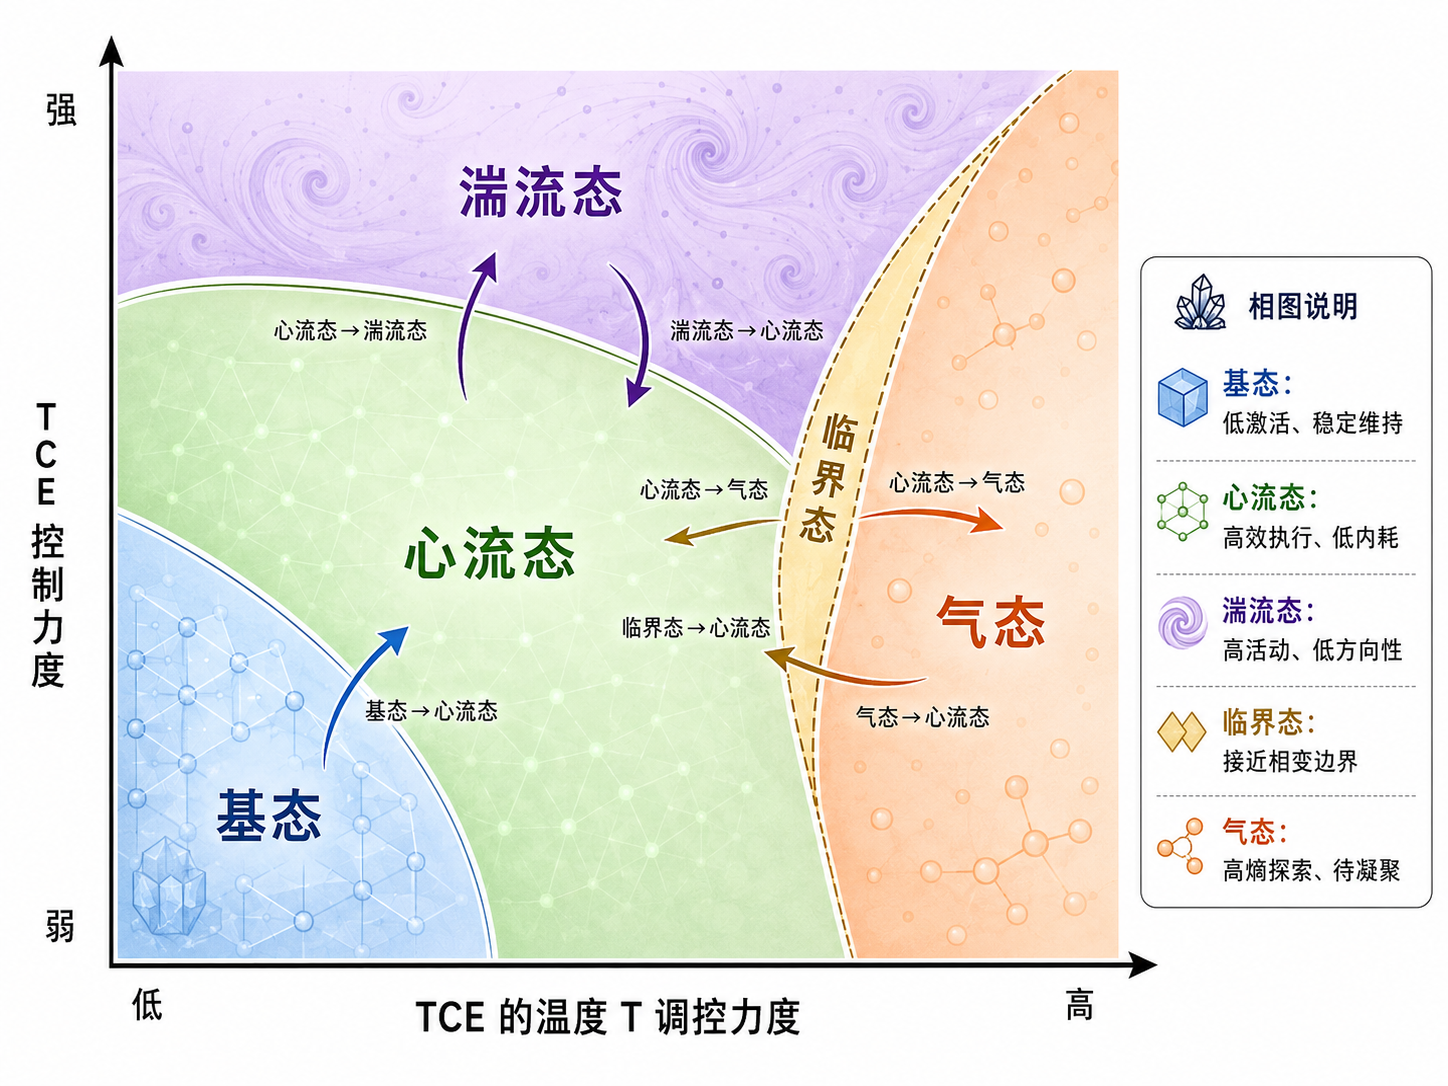
\includegraphics[width=.9\textwidth,height=.38\textheight,keepaspectratio]{images/tce-cognitive-state-phase-map.png}
\caption{TCE 控制量与运行相区域}
\end{figure}
\section{TCE 的控制对象、状态空间与统一控制向量}

前几章已经逐步建立了 AgentOS 的内部动力结构：工作记忆 $h(t)$ 承载当前被显式提升的 Agent-CSO，SPC 对工作记忆及相关内部状态进行压缩估计，AHC 将身体、资源、威胁、不确定性和社会状态积成为连续调制背景，而 Scheduler 与 CCM 分别承担任务资源配置和运行负载治理。在这个体系中，我们现在需要回答一个更加具体的控制工程问题：当系统已经知道“自己目前大致处于什么状态”，也知道“当前有哪些任务和资源约束”以后，究竟由谁改变认知活动本身的动力学形态？

这个角色就是 TCE。

我们首先把 Agent 当前与快速认知控制有关的状态抽象为

\[
x_c(t)
=
\left[
x_h(t),
a(t),
c(t),
q(t),
r(t)
\right],
\]

其中 $x_h(t)$ 表示工作记忆 $h(t)$ 的当前结构状态；$a(t)$ 表示 AHC 给出的连续调制状态；$c(t)$ 表示 CCM 所估计的运行负载和结构压力；$q(t)$ 表示当前任务、目标和调度状态；$r(t)$ 表示身体、工具和外部环境返回的相关残差信号。这里我们刻意不把 $\Psi$ 与 $\Omega$ 直接并入快速状态向量，因为它们位于远慢于 TCE 的时间尺度。它们对 TCE 的作用更接近慢约束、目标偏置和可行域塑形，而不是每一个控制周期都被 TCE 任意改变的普通状态变量。

因此，TCE 所看到的并不是 Agent 的“真实完整内部状态”，而是经过 SPC、AHC、CCM 与 Scheduler 等机制处理后的可控制状态估计：

\[
\hat x_c(t)
=
\mathcal O_{\mathrm{SPC}}
\left(
h(t),E(t),\Theta(t),a(t),c(t),q(t),r(t)
\right).
\]

这里 $\mathcal O_{\mathrm{SPC}}$ 是观察与压缩算子。由于任何状态估计都存在采样周期、推理延迟和表示误差，因此一般有

\[
\hat x_c(t)\neq x_c(t),
\]

而更合理的形式是

\[
\hat x_c(t)
=
x_c(t-\tau_o)+\epsilon_o(t),
\]

其中 $\tau_o$ 为观察延迟，$\epsilon_o(t)$ 为估计误差。这一点决定了 TCE 不可能被设计成无限高增益的瞬时纠错器；后面我们讨论过冲和振荡时会看到，这个看似简单的事实实际上决定了整个认知控制器的稳定边界。

TCE 的输出应当表示为一个多维控制向量，而不是一个所谓 ``temperature'' 标量。我们定义

\[
u_T(t)
=
\left[
T,
g,
\iota,
\alpha,
\eta,
d,
\kappa,
\nu,
\Lambda_M
\right]_t,
\]

其中：

\[
T
\]

表示认知温度，用于调节候选状态分布的平坦程度与局部确定性；

\[
g
\]

表示总体激活增益；

\[
\iota
\]

表示抑制强度；

\[
\alpha
\]

表示当前显式注意范围；

\[
\eta
\]

表示探索强度；

\[
d
\]

表示有效搜索或推理深度；

\[
\kappa
\]

表示保守度或行动前所需证据强度；

\[
\nu
\]

表示认知运行节律、更新频率或步长；

而

\[
\Lambda_M
=
\{
\lambda_{hE},
\lambda_{Eh},
\lambda_{E\Theta},
\lambda_{\Theta E},
\lambda_{\Theta h},
\ldots
\}
\]

表示与记忆流转有关的动力学速率。历史设计中，TCE 本来就不仅控制温度，还控制激活增益、抑制、认知势能以及三相记忆之间的流转速度。因此工程实现中不应把 TCE 缩减为 LLM decoding temperature 的封装。

我们可以将受控的认知动力学写成

\[
\dot x_c
=
F_c
\left(
x_c,
u_T,
u_{\mathrm{sched}},
u_{\mathrm{CCM}},
\Psi,
\Omega,
w
\right),
\]

其中 $w$ 表示外部扰动、突发事件、身体异常和新的观测残差。Scheduler 给出资源与优先级包络，CCM 给出可承载复杂度约束，而 $\Psi$ 与 $\Omega$ 定义更慢的身份、价值和生命周期方向。于是 TCE 实际上不是自由控制整个认知系统，而是在一个由其他模块共同定义的可行域中调节快速动力学：

\[
u_T(t)
\in
\mathcal U_{\mathrm{feasible}}
\left(
\Psi,
\Omega,
\mathrm{Scheduler},
\mathrm{CCM},
\mathrm{Boundary},
\mathrm{Safety}
\right).
\]

这一区分具有非常重要的工程意义。TCE 如果被允许直接改变目标、身份、价值、任务权限和身体安全约束，就会从“认知动力控制器”演化成一个缺乏边界的中央决策器，从而破坏整个 AgentOS 的分层结构。我们在本书中始终坚持：

\[
\boxed{
TCE\neq Planner,\qquad
TCE\neq Scheduler,\qquad
TCE\neq CCM,\qquad
TCE\neq \Psi.
}
\]

Planner 决定候选策略内容，Scheduler 决定谁获得资源，CCM 决定哪些认知结构可以被当前有限工作记忆承载，$\Psi$ 和 $\Omega$ 提供慢尺度的主体约束，而 TCE 决定这些活动\textbf{以怎样的动力学方式运行}。

因此，若把认知系统看成一个受控动力系统，那么本章的核心问题可以压缩为：

\[
\boxed{
\hat x_c(t)
\xrightarrow{\mathrm{TCE}}
u_T(t)
\xrightarrow{F_c}
x_c(t+\Delta t)
\xrightarrow{\mathrm{SPC}}
\hat x_c(t+\Delta t)
}
\]

这就是 TCE 控制器工程的基本闭环。

\section{控制增益：认知状态应当被改变多强}

控制增益是 TCE 工程中最容易被忽略、却又最容易引起系统性故障的变量。许多认知系统设计习惯于把控制写成一系列离散规则，例如“如果过载就降低温度”“如果不确定就增加搜索”“如果冲突就扩大注意”。这些规则在静态测试中可能有效，但对于一个长期运行的 Agent，它们仍然缺少最重要的信息：\textbf{应该改变多少？改变多快？改变之后应当等待多久再继续修正？}

这正是控制增益需要回答的问题。

设 SPC 得到的当前认知状态指标为

\[
y(t)
=
\begin{bmatrix}
C_h(t)\\
U(t)\\
R(t)\\
S(t)
\end{bmatrix},
\]

其中 $C_h$ 表示工作记忆有效负载，$U$ 表示不确定性，$R$ 表示预测或行动残差，$S$ 表示稳定性指标。设 TCE 当前希望维持的运行参考区域为

\[
y^\star(t).
\]

则定义认知状态误差

\[
e(t)=y^\star(t)-y(t).
\]

最简单的 TCE 控制器可以具有比例形式：

\[
u_T(t)
=
u_0
+
K_P e(t),
\]

其中 $K_P$ 是一个多变量增益矩阵。它不只是一个数，因为不同类型误差应该影响不同控制变量。例如工作记忆负载上升可能主要增加抑制、缩小注意范围并降低新支线准入；预测残差升高则可能扩大注意范围、提高探索并允许更多候选结构进入 h；而身体威胁升高时，系统可能同时降低搜索深度并提高行动保守度。

因此实际的增益矩阵可以写成

\[
K_P=
\begin{bmatrix}
\frac{\partial T}{\partial C_h} &
\frac{\partial T}{\partial U} &
\frac{\partial T}{\partial R} &
\frac{\partial T}{\partial S}
\\
\frac{\partial g}{\partial C_h} &
\frac{\partial g}{\partial U} &
\frac{\partial g}{\partial R} &
\frac{\partial g}{\partial S}
\\
\vdots & \vdots & \vdots & \vdots
\end{bmatrix}.
\]

这一表达提醒我们：TCE 并不是一些彼此独立的 knob，而是一个多输入多输出控制系统。改变一个输入变量往往同时改变多个认知动力学参数，多个 TCE 控制量之间也会发生耦合。

例如，单纯提高激活增益 $g$ 可能帮助系统更快聚焦于当前目标，但同时也可能增加某些局部结构的自强化，使竞争分支难以进入；提高抑制 $\iota$ 可以降低工作记忆负载，却可能造成关键弱信号被错误清除；提高温度 $T$ 可能扩大搜索，又可能增加 h 中的候选结构数量；扩大注意范围 $\alpha$ 可以获得更多外部证据，却又提高 CCM 所面对的结构负载。由此可见：

\begin{remark}
TCE 的每个控制动作几乎都存在收益—负担双重效应。
\end{remark}

因此，控制增益不宜固定。更现实的是建立 gain scheduling：

\[
K_T
=
K_T
\left(
\phi(t),
a(t),
C_h(t),
R(t),
q(t)
\right),
\]

其中 $\phi(t)$ 表示当前认知运行相态。基态、心流态、临界态和湍流态对相同误差应有完全不同的控制敏感度。例如在稳定心流态中，即便观察到短暂残差，也不应进行大幅控制；否则 TCE 自身会破坏已经形成的高效局部闭环。而在临界态附近，即便相同幅度的残差，也可能意味着系统即将越过可运行边界，此时增益应该增大。

因此可以引入相态依赖增益：

\[
K_T^{(\phi)}
=
\begin{cases}
K_G, & \phi=\mathrm{Ground},\\
K_F, & \phi=\mathrm{Flow},\\
K_C, & \phi=\mathrm{Critical},\\
K_T, & \phi=\mathrm{Turbulent},\\
K_{\mathrm{rec}}, & \phi=\mathrm{Gas/Recovery}.
\end{cases}
\]

通常我们希望满足类似

\[
\|K_F\|
<
\|K_C\|,
\]

因为 Flow 状态应尽可能少受外部调节，而 Critical 状态则允许更积极的纠偏。

在更完整的 TCE 中还可以引入积分项：

\[
u_T(t)
=
u_0+
K_Pe(t)
+
K_I\int_{t_0}^{t}e(\tau)d\tau,
\]

其意义是：一个非常小但长期持续的失配不应该永远因为未超过瞬时阈值而被忽视。例如某个任务长期处于略高于正常水平的认知负载，如果只使用瞬时阈值，系统可能一直“勉强可运行”；积分项则逐渐积累这种长期压力，最终触发负载压缩、任务拆分或更慢层级的结构调整。

但认知控制中的积分项必须谨慎，因为它容易发生 windup。当外部约束使某一目标暂时无法达到时，积分误差仍不断积累，等约束解除之后就可能导致巨大的反向控制。因此可以定义：

\[
I(t)
=
\mathrm{clip}
\left(
I(t-\Delta t)+e(t)\Delta t,
I_{\min},
I_{\max}
\right).
\]

这一看似普通的控制技巧，在 AgentOS 中具有重要意义：一个长期未解决的问题，不应该无限积累成越来越高的内部“控制压力”。否则 TCE 可能逐渐把整个认知系统都围绕一个当前不可解决目标组织起来。

因此，本节最重要的结论不是“增益应高还是低”，而是：

\begin{conclusion}
TCE 必须控制认知控制本身的强度。
\end{conclusion}

一个成熟 Agent 不是时时被中央控制器紧紧握住，而应在局部结构能够自行闭合时降低高层增益，在持续残差或接近失稳边界时才增加控制强度。这与全书此前反复形成的原则一致：

\[
\boxed{
SlowGovernance\neq FastMicromanagement.
}
\]

TCE 的成熟并不是控制得越来越多，而是越来越准确地知道什么时候应该少控制，什么时候必须强控制。

\section{认知温度：候选结构分布的可塑性控制}

“温度”是 TCE 名称中最早存在的变量，但也是最容易被误解的变量。若我们把 TCE 的 Temperature 简单等价于语言模型生成中的 sampling temperature，那么整个 TCE 理论就会退化成一个极窄的 decoding 参数控制器。事实上，在 AgentOS 中，认知温度描述的是更一般的动力学性质：\textbf{当前认知状态在候选 Agent-CSO、解释、策略和未来轨迹之间进行迁移的容易程度。}

设当前工作记忆存在一组可被激活的候选认知状态

\[
\mathcal Z
=
\{z_1,z_2,\ldots,z_n\},
\]

每个候选状态具有一个当前有效势能或代价

\[
V_i
=
V(z_i\mid h,E,\Theta,\Psi,\Omega,a).
\]

可以用类似 Gibbs 分布的形式描述候选状态占据概率：

\[
p_i(T)
=
\frac{
\exp\left[-V_i/T\right]
}{
\sum_j
\exp\left[-V_j/T\right]
}.
\]

这里不应把这一公式理解成 Agent 真实神经动力学必须服从热力学，而应把它作为一种控制形式化：$T$ 越小，系统越集中于当前低代价候选；$T$ 越大，不同候选之间的概率差异越小。

因此：

\[
T\downarrow
\Rightarrow
\text{Convergence}\uparrow,
\]

而：

\[
T\uparrow
\Rightarrow
\text{Exploration}\uparrow.
\]

但是温度和探索并不完全相同。探索 $\eta$ 更接近策略级“是否主动访问新的候选域”，而温度 $T$ 更接近状态分布本身的平坦程度。一个系统可以具有较高温度但很窄的注意范围，此时只是在一个小局部中频繁跳动；也可以具有中等温度但很强的主动探索，此时它会有策略地访问多个新的结构区域。因此工程实现必须把 $T$ 与 $\eta$ 分开。

我们还可以定义工作记忆候选分布熵：

\[
H_h(T)
=
-
\sum_i p_i(T)\log p_i(T).
\]

一般而言，

\[
\frac{\partial H_h}{\partial T}>0,
\]

即温度越高，候选分布越分散。但 AgentOS 的目标并不是最大化或最小化该熵，而是让候选多样性与任务阶段相匹配。

例如在问题刚进入 h 时，系统可能处于高不确定性状态：

\[
U(t)\gg U_{\mathrm{nominal}},
\]

此时 TCE 可以适当提高 $T$，允许不同解释竞争；随着证据累积和一个结构获得持续支持，应逐步降低温度：

\[
T(t+\Delta t)<T(t),
\]

使状态逐渐收敛。可以用一个目标不确定度控制形式表示：

\[
\dot T
=
k_T
\left[
U(t)-U^\star(q(t))
\right]
-
k_R R_{\mathrm{osc}}(t),
\]

其中 $U^\star$ 是与任务阶段相关的合理不确定性目标，而 $R_{\mathrm{osc}}$ 表示已经出现的状态切换频率或振荡风险。这样可以避免“不确定越高就无限升温”。

温度还应受到 AHC 的调制。例如高 Threat 状态下，如果仍然提高开放探索程度，可能造成危险情况下的迟滞。因此可以定义：

\[
T_{\mathrm{eff}}
=
T_{\mathrm{cog}}
\cdot
m_{\mathrm{AHC}},
\]

其中：

\[
0<m_{\mathrm{AHC}}\le 1
\]

可以在高风险状态中压低实际探索温度。但需要特别注意：AHC 不应该简单地“威胁越高，温度越低”。在某些异常环境中，过度确定反而危险。若当前策略不断失败：

\[
R(t)\uparrow,
\]

那么即使 Threat 较高，也必须允许有限程度的策略逃逸。因此更合理的是：

\[
T_{\mathrm{eff}}
=
f(
U,
R,
Threat,
Urgency,
CapabilityMargin
).
\]

这实际上揭示了 TCE 的一个基本思想：认知温度不只是“随机度”，而是\textbf{结构可塑性速率的控制量}。

太低的温度会造成：

\begin{statementbox}
PrematureCollapse
\end{statementbox}

即系统过早锁定一个假设、策略或世界解释。

太高的温度会造成：

\begin{statementbox}
PersistentDispersion
\end{statementbox}

即 Agent 无法形成稳定计划，工作记忆中大量候选长期竞争。

从 h 的运行相态看，温度轴与我们此前提出的认知相图直接相关。非常低温可能造成僵化，适中温度与合理控制强度可以形成 Ground 或 Flow，而高温配合过宽注意范围和过弱抑制则可能进入 Turbulent，进一步失去结构约束时甚至进入 Gas-like 状态。

因此，本章对 Temperature 的严格定义可以写成：

\[
\boxed{
T
=
\text{TCE 对当前认知状态在可行候选结构之间迁移自由度的控制变量。}
}
\]

它既不是随机噪声，也不是智慧程度，而是 Agent 在“稳定已有结构”与“允许结构重新组织”之间进行实时调节的一个关键控制维度。

\section{注意控制：决定有限工作记忆承载哪一部分世界}

如果工作记忆容量有限，那么注意控制就不是附加功能，而是整个 AgentOS 必然存在的资源分配机制。我们已经在前文建立：

\[
C_h(t)\le C_{\max},
\]

因此 TCE 不可能通过“把更多东西全部放入 h”来解决不确定性。真正的工程问题是：在世界、身体、记忆、目标、工具、其他 Agent 和内部状态不断产生新信息的情况下，当前有限的显式认知面应该被谁占据？

注意控制可以表示成对 Agent-CSO 活跃集合的权重分配。设候选结构为

\[
\mathcal C_t
=
\{C_1,\ldots,C_n\},
\]

定义注意权重

\[
a_i(t)\in[0,1],
\]

满足

\[
\sum_i a_i(t)\le 1.
\]

当前显式认知负载可以近似写为

\[
C_h(t)
=
\sum_i
a_i(t)c_i(t)
+
\sum_{i,j}
a_i(t)a_j(t)r_{ij}(t),
\]

其中 $c_i$ 描述单个结构本身的承载负担，而 $r_{ij}$ 描述结构之间关系带来的额外负担。这个表达比单纯“工作记忆能放多少 item”更加接近我们的原始理论，因为真正使 h 崩溃的往往不是对象数量，而是对象之间需要同时维持的关系结构。

因此，TCE 控制注意并不是简单调整 softmax 权重，而至少要控制两个量：

\[
\alpha_t
=
|\mathcal C_t^{active}|,
\]

即注意覆盖宽度；

以及：

\[
\gamma_t,
\]

即注意集中程度。

系统可能有：

\[
\alpha\uparrow,\gamma\downarrow
\]

的广域扫描模式，也可能有：

\[
\alpha\downarrow,\gamma\uparrow
\]

的局部深度模式。

对于稳定执行型任务，我们希望：

\[
\alpha\downarrow,
\qquad
\gamma\uparrow,
\]

使 h 只承载当前行动链真正相关的少量结构。而在出现持续异常残差时，则可能需要：

\[
\alpha\uparrow,
\]

重新纳入此前被忽略的环境、身体、记忆或目标结构。

因此注意控制必须与“异常向上”原则结合：

\[
Residual\uparrow
\Rightarrow
PromotionProbability(C_i)\uparrow.
\]

一个正常情况下在 Body Runtime 内局部闭合的结构，不需要持续进入 h；只有当预测残差、风险、新颖度或目标相关性达到阈值时，它才应该被提升：

\[
\Gamma_i
=
f(
R_i,
Risk_i,
Novelty_i,
Persistence_i,
GoalRel_i
).
\]

当

\[
\Gamma_i<\theta_a,
\]

该结构保持局部；

当

\[
\Gamma_i\ge\theta_a,
\]

TCE 与 Scheduler/CCM 协同扩大其注意权重。

需要强调的是：TCE 不应该独自判断“哪个内容重要”。重要性本身受到 $\Psi$、Goal、Scheduler、Boundary 和 CCM 的共同作用。TCE 控制的主要是\textbf{当前已经被判定为候选结构以后，其激活、保持和竞争的动力学强度}。

可以写成：

\[
\dot a_i
=
g_i
\left(
Priority_i,
Residual_i,
GoalRel_i,
SelfRel_i
\right)
-
\iota_i a_i
-
\lambda_C\frac{\partial C_h}{\partial a_i}.
\]

第一项负责提升高价值结构，第二项代表抑制和自然衰减，第三项体现有限工作记忆容量产生的负反馈。

由此我们可以理解为什么成熟智能不是“注意更多”，而是：

\[
\boxed{
MatureIntelligence
=
SelectiveExplicitCognition.
}
\]

当越来越多熟练结构下沉到 $\Theta$、Skill、Body Runtime 或外部工具之后，真正需要进入 h 的内容反而应该减少。若一个 Agent 随能力增长反而需要越来越多全局注意力才能完成熟悉任务，那么从 AgentOS 理论看，这不是成熟，而是结构没有完成正确沉降。

TCE 的注意控制因此承担一个非常重要的跨尺度角色：它不是把整个世界压进 Agent 内部，而是不断调节当前“高清认知窗口”落在哪里。在具身系统中，这一原则后来还会延伸到 SGC 的局部高清输入控制；但即便暂时不涉及 Body 细节，其本质已经很清楚：

\begin{proposition*}
注意不是获得更多世界，而是在有限认知面上决定哪一部分世界当前值得被显式承载。
\end{proposition*}

\section{探索控制：什么时候允许认知离开已有结构}

温度调节的是候选状态分布的可塑程度，而探索控制决定的是系统是否应该主动离开当前熟悉结构，访问新的状态区域。二者相关，但在工程上必须严格分开。

假设 Agent 当前拥有一个由 $\Theta$ 和 E 支持的认知策略族

\[
\Pi_{\mathrm{known}}
=
\{\pi_1,\ldots,\pi_m\}.
\]

对于熟悉任务，Agent 理应优先利用这些稳定结构：

\[
\pi^\star
=
\arg\max_{\pi_i\in\Pi_{\mathrm{known}}}
\mathbb E[U(\pi_i)].
\]

但是当环境新颖、残差持续升高或者已有策略全部失效时，继续 exploit 已有结构会导致认知闭锁。于是需要引入探索控制量：

\[
\eta(t)\in[0,1].
\]

我们可以把候选动作或认知路径分布写成：

\[
\pi_T
=
(1-\eta)\pi_{\mathrm{known}}
+
\eta\pi_{\mathrm{novel}},
\]

其中 $\pi_{\mathrm{novel}}$ 不必表示随机行为，而可以是未充分验证的推理路径、记忆组合、工具策略或反事实模型。

因此，TCE 的探索控制不是简单“增加随机性”，而是决定：

\begin{statementbox}
有多少认知资源可以被用于当前结构之外的搜索。
\end{statementbox}

探索强度应至少受到五类因素影响：

\[
\eta
=
f(
Novelty,
Residual,
Uncertainty,
Risk,
ResourceMargin
).
\]

其中 Novelty 和 Residual 通常推动探索增加，而 Risk 和资源不足则限制探索规模。

例如，若系统面对一个低风险研究问题，可以允许：

\[
\eta\uparrow,
\quad
T\uparrow,
\quad
d\uparrow,
\]

进行大量结构尝试。

但若系统正在控制高速身体并接近危险边界，即便存在不确定性，也不能无限扩大探索。此时更合理的控制是：

\[
\eta\downarrow,
\qquad
\kappa\uparrow,
\]

优先使用经过验证的安全策略，并把高层探索放到模拟、反事实或离线结构中进行。

因此我们定义探索预算：

\[
B_{\mathrm{explore}}(t),
\]

并要求：

\[
Cost_{\mathrm{explore}}(t)
\le
B_{\mathrm{explore}}(t).
\]

这个预算由 Scheduler、CCM、Body risk 和 AHC 状态共同约束。

进一步地，探索不应该只是短时间反应，还要受到长期失败历史影响。设某个策略族的持续残差为：

\[
\bar R_T
=
\frac{1}{T}
\int_{t-T}^{t}R(\tau)d\tau.
\]

如果：

\[
\bar R_T>\theta_R,
\]

则即使当前瞬时状态尚未完全失败，也可以逐步提高探索：

\[
\dot\eta
=
k_\eta
(\bar R_T-\theta_R).
\]

这体现了前文反复讨论的：

\begin{statementbox}
PersistentFastResidualShapesSlowStructure.
\end{statementbox}

当然，TCE 本身仍位于较快控制层，它不能直接改变 $\Theta$ 或功能拓扑；但它可以通过改变探索资源，让新的结构组合获得进入 h、E 和后续学习过程的机会。

探索控制还必须解决一个重要的问题：何时停止探索。如果缺乏停止机制，一个系统可能陷入永远寻找“更好可能性”的状态，从而无法行动。可以定义当前最佳候选与次优候选的价值间隔：

\[
\Delta Q
=
Q_{(1)}-Q_{(2)},
\]

以及预测不确定性：

\[
U_Q.
\]

当：

\[
\Delta Q
>
\beta U_Q,
\]

并且主要风险约束已经满足时，可以降低探索：

\[
\eta\downarrow,
\]

进入收敛和执行阶段。

因此 TCE 的探索控制实际上在不断管理一个基本张力：

\[
\boxed{
Plasticity
\leftrightarrow
Commitment.
}
\]

探索太弱，系统形成僵化；探索太强，系统无法形成稳定行为。成熟 TCE 的目标不是最大化创新，而是在现实约束、任务阶段和工作记忆容量允许的范围内，维持一种\textbf{受控开放性}。

\section{搜索深度：应该把一次认知推进多远}

大语言模型推理系统中经常存在一种隐含假设：如果当前答案不够好，就增加更多推理步骤。然而在长期 AgentOS 中，“更深”并不是普遍优越。搜索深度增加会带来更多候选、更多中间变量、更长延迟以及更高的错误传播风险。因此 TCE 必须把搜索深度 $d$ 当作一个显式控制变量。

设一次认知搜索树为

\[
\mathcal T_s,
\]

平均分支因子为 $b$，深度为 $d$。若不进行剪枝，候选数大致为

\[
N(d)
\sim
\sum_{k=0}^{d}b^k
=
\frac{b^{d+1}-1}{b-1}.
\]

因此搜索负担随 $d$ 呈指数增长。即使真实 LLM 推理并不是显式树搜索，这一数学形式仍说明一个工程事实：当系统同时保留多个候选路径时，更深推理会快速占用工作记忆和计算资源。

于是 TCE 不应控制“最大允许思考长度”，而应动态决定边际搜索价值：

\[
MB(d)
=
\frac{
\partial \mathbb E[Utility]
}{
\partial d
},
\]

以及边际搜索成本：

\[
MC(d)
=
\frac{
\partial Cost
}{
\partial d
}.
\]

最合理的停止条件是：

\[
MB(d)
\le
MC(d).
\]

这里 Cost 至少包含：

\[
Cost
=
\lambda_1C_h
+
\lambda_2Latency
+
\lambda_3Compute
+
\lambda_4Risk_{\mathrm{drift}}
+
\lambda_5OpportunityCost.
\]

这意味着一个低价值问题不值得进行几十层深推理；一个高风险、高价值、不可逆任务则可能值得消耗更多时间进行验证。

因此可以把搜索深度设为：

\[
d^\star
=
\arg\max_d
\left[
\mathbb E U(d)-Cost(d)
\right].
\]

但 TCE 并不直接精确计算这一优化问题，而可以利用 SPC、Scheduler、CCM 与 AHC 提供的观测近似控制：

\[
d_{t+1}
=
d_t
+
k_1U_t
+
k_2Risk_t
+
k_3GoalValue_t
-
k_4C_h(t)
-
k_5Urgency_t.
\]

这里需要注意一个看似矛盾的情况：Risk 可以增加搜索深度，也可以减少搜索深度。区别在于风险是否允许延迟。如果任务是高风险但可等待的，例如设计一个长期工程方案，则应增加验证深度；如果是高风险且时间极短，例如身体即将碰撞，则高层搜索深度反而应立即下降，快速控制交给 Body Runtime 或安全控制器。因此更准确地应该引入时间余量：

\[
M_t
=
TimeToDeadline_t.
\]

于是：

\[
d^\star
=
f(
Risk,
Uncertainty,
GoalValue,
C_h,
M_t
).
\]

当：

\[
M_t\rightarrow0,
\]

高层认知搜索必须收缩。

另外，搜索深度与 $\Theta$ 的成熟程度也有关。若系统面对一个已经高度熟练的问题，继续展开显式搜索是一种浪费。因此可以定义结构成熟度：

\[
M_\Theta(C)\in[0,1].
\]

当：

\[
M_\Theta(C)\rightarrow1
\]

且运行残差低时：

\[
d^\star\downarrow.
\]

这正是“成熟能力向下沉降”的认知版本。高手之所以表现得快，并不意味着其内部没有结构，而是大量原本必须展开的搜索已经被压缩成稳定生成结构和技能闭环。

因此，TCE 对搜索深度的调节还具有一个评价成熟智能的重要指标：

\[
\boxed{
\frac{
\text{Explicit Search Depth}
}{
\text{Successful Task Complexity}
}
\downarrow
}
\]

往往意味着更多任务已经被结构化地掌握。

同时，我们必须避免另一种极端：在残差已经长期升高时仍然依赖 $\Theta$ 的旧结构快速处理。此时 TCE 应重新增加 $d$，使原本被自动化的认知结构重新显式化：

\[
ProceduralCSO
\rightarrow
ExplicitCSO.
\]

这就是“能力向下、异常向上”在搜索深度控制中的具体工程表现。

因此，搜索深度控制本质上不是“让 Agent 思考多久”，而是：

\begin{statementbox}
决定当前问题有多少结构必须重新进入显式因果展开。
\end{statementbox}

\section{保守度：证据、风险与行动承诺之间的控制}

TCE 的保守度 $\kappa$ 描述的是 Agent 在从认知状态进入行动、承诺或不可逆决策之前，需要多强的证据与稳定性保证。它与温度、探索和搜索深度相关，但不能由它们替代。

一个 Agent 可以处于高探索状态，却仍然对实际行动保持高度保守。例如在内部模拟中允许大量激进候选，并不意味着立刻执行其中任何一个方案。因此，保守度控制的真正对象是：

\[
\boxed{
\text{Representation}
\rightarrow
\text{Commitment}
}
\]

之间的阈值。

设当前最佳行动 $a^\star$ 的期望价值为：

\[
Q(a^\star),
\]

不确定性为：

\[
\sigma_Q(a^\star),
\]

潜在损失为：

\[
L(a^\star),
\]

可逆性为：

\[
Rev(a^\star)\in[0,1].
\]

我们可以定义一个风险调整后的行动置信度：

\[
\chi(a)
=
Q(a)
-
\kappa_1\sigma_Q(a)
-
\kappa_2L(a)
+
\kappa_3Rev(a).
\]

执行条件为：

\[
\chi(a^\star)
>
\theta_{\mathrm{act}}.
\]

TCE 的保守控制并不是直接修改 $Q$，而是调节阈值或风险权重。定义：

\[
\kappa(t)
=
f(
Threat,
Uncertainty,
Irreversibility,
Authority,
CapabilityMargin
).
\]

则高不可逆、高权限、高潜在损害的行为应满足：

\[
\kappa\uparrow.
\]

而低风险、可撤回的行为可以：

\[
\kappa\downarrow,
\]

允许快速探索和试错。

这与我们整个 AgentOS 的基本工程方向高度一致：不是给所有行为施加同一个安全阈值，而是根据行动后果和恢复能力建立分层控制。

特别重要的是，保守度还受到 Agent 当前能力边界的影响。设 Body Runtime 或相关 Skill 给出的 capability margin 为：

\[
M_{\mathrm{cap}}.
\]

如果：

\[
M_{\mathrm{cap}}\downarrow,
\]

即系统当前接近能力边界，则即使认知层认为某一行动具有较高期望收益，TCE 仍应增加 $\kappa$。这使“我认为值得做”和“我当前有能力安全地做”在控制上被明确区分。

保守度还应该受到 $\Psi$ 和 $\Omega$ 的慢约束。某些行为虽然短期收益很高，却严重偏离长期身份或生命周期方向，那么它们的有效阈值应提高：

\[
\kappa_{\mathrm{eff}}
=
\kappa_0
+
\lambda_\Psi
D_\Psi(a)
+
\lambda_\Omega
D_\Omega(a),
\]

其中 $D_\Psi$ 和 $D_\Omega$ 表示行动与慢结构的一致性距离。

这里我们必须特别避免一种错误实现：让 TCE 自己重新定义 $\Psi$ 或 $\Omega$ 来降低行动门槛。TCE 只能读取慢结构约束，而不能为了快速完成当前任务去修改约束本身。这就是多时间尺度系统中的 Slow Variable Protection。

在工作记忆相态层面，不同相态还应拥有不同保守策略。在 Flow 状态下，系统可能拥有较高局部能力置信度，因此在已经熟练的领域中可以降低不必要的显式确认；而在 Turbulent 或 Critical 状态下，即使系统表面上仍能生成行动计划，也应提高行动保守度：

\[
\phi\in
\{\mathrm{Critical,Turbulent}\}
\Rightarrow
\kappa\uparrow.
\]

这是因为此时问题不是某一个候选动作本身，而是 Agent 当前的内部状态估计可靠性下降。

因此，保守度并不是“胆小程度”，而是一个控制意义上的：

\begin{statementbox}
CommitmentThreshold.
\end{statementbox}

一个成熟的 Agent 既不能因保守度过高而失去现实行动能力，也不能因保守度过低而把内部未稳定的候选结构直接写入世界。

TCE 的任务是在：

\begin{statementbox}
\centering\bfseries
探索自由度
$\longleftrightarrow$
现实承诺强度
\end{statementbox}

之间建立一道动态阀门。

\section{过冲：为什么正确的调节也可能把系统推向错误状态}

到目前为止，我们一直假设 TCE 的调节方向是正确的。例如检测到负载过高就增加抑制，检测到不确定性高就增加搜索，检测到搜索过度就降低温度。但在真实控制系统中，即使控制方向完全正确，也可能因为延迟和增益过大导致过冲。

这是理解长期 Agent 心理稳定性的关键。

设认知负载状态为 $c(t)$，理想运行值为：

\[
c^\star.
\]

若 TCE 使用比例控制：

\[
u(t)
=
-k(c(t-\tau)-c^\star),
\]

而认知系统的简化动力学为：

\[
\dot c(t)
=
-ac(t)+bu(t),
\]

则有：

\[
\dot c(t)
=
-ac(t)
-
bk
\left[
c(t-\tau)-c^\star
\right].
\]

即使 $a,b,k>0$，只要 $\tau>0$ 且 $k$ 足够大，系统就可能产生过冲和振荡。

直观地说：

SPC 在 $t_0$ 时刻观察到“认知过载”。

TCE 开始强力降低激活范围。

但这一动作真正影响 h 需要时间。

在此期间 SPC 仍然继续观察到“过载”，于是 TCE 再次加强控制。

等第一轮控制效果真正显现时，后续控制已经累积，于是系统从“过载”直接越过正常区进入“过度抑制”。

随后 SPC 又观察到认知活性不足，TCE 反向增加增益。

最终形成：

\[
Overload
\rightarrow
OverSuppression
\rightarrow
UnderActivation
\rightarrow
OverExcitation
\rightarrow
Overload.
\]

这就是典型的认知过冲循环。

因此我们需要定义最大过冲量：

\[
M_p
=
\frac{
|y_{\max}-y^\star|
}{
|y(0)-y^\star|
},
\]

以及调节时间：

\[
T_s
=
\inf
\left\{
t:
|y(\tau)-y^\star|<\epsilon,
\forall\tau>t
\right\}.
\]

对于长期 Agent，TCE 的目标不是使：

\[
T_s\rightarrow0,
\]

因为极端追求快速恢复通常意味着更高增益，反而增加过冲。更合理的是在：

\[
SettlingTime
\]

和：

\[
Overshoot
\]

之间取得平衡。

可以定义代价：

\[
J_{\mathrm{reg}}
=
\int_0^\infty
\left[
e(t)^TQe(t)
+
u_T(t)^TRu_T(t)
+
\lambda_o
\|\dot u_T(t)\|^2
\right]dt.
\]

第三项特别重要，因为它惩罚 TCE 自身变化过快。也就是说，我们不仅不希望认知状态猛烈震荡，也不希望控制器不断猛烈改变控制参数。

因此可以对控制向量增加 rate limit：

\[
\|\dot u_T(t)\|
\le
r_{\max}.
\]

例如温度不能瞬间从极高跳到极低，注意范围不能每个周期大幅收缩和扩张，探索预算不能因单次异常立即翻倍。

另外，我们还需要 deadband：

\[
|e(t)|<\delta
\Rightarrow
\Delta u_T=0.
\]

其意义是：正常认知状态本来就存在波动，TCE 不应试图纠正每一点微小偏差。没有 deadband 的控制器会不断追逐噪声。

因此，对 TCE 而言一个非常重要的原则是：

\begin{statementbox}
NotEveryDeviationRequiresCorrection.
\end{statementbox}

甚至可以更进一步：

\begin{statementbox}
健康认知不是没有波动，而是波动能够在无需高层强控制的情况下自行回到可运行区域。
\end{statementbox}

这与 AgentOS 一贯强调的局部闭环和局部自治一致。

所以 TCE 对过冲的治理至少包括：

低通滤波；

变化率限制；

控制死区；

状态持续性判断；

动态增益；

积分 anti-windup；

相态依赖阈值。

最终，TCE 不应追求“即时把系统拉回某一个精确点”，而应该维持一个允许自然认知波动的可行区域：

\[
\boxed{
\mathcal R_{\mathrm{healthy}}
=
\{
x:
C_h<C_{\max},
Risk<R_{\max},
Stability>S_{\min}
\}.
}
\]

只要系统仍然处于这个区域，就不必强行微调每个变量。这实际上是从点控制转向集合控制，也是 AgentOS 控制工程与简单规则系统的重要区别。

\section{振荡：TCE 何时会成为认知不稳定性的来源}

过冲是一次控制动作越过目标区域，而振荡则意味着这种越过在反馈闭环中反复出现。当我们进入长期 Agent 控制工程时，振荡是比单次过冲更加危险的问题，因为一个反复修改自己的认知控制器可能在没有任何外部世界变化的情况下，仅凭内部 observer--controller interaction 就产生持续波动。

我们先考虑最简单的一维线性化模型。设认知状态偏差为：

\[
\delta x(t)=x(t)-x^\star.
\]

系统近似满足：

\[
\dot{\delta x}
=
A\delta x
+
Bu,
\]

TCE 控制：

\[
u=-K\hat{\delta x},
\]

而：

\[
\hat{\delta x}(t)
=
\delta x(t-\tau).
\]

于是：

\[
\dot{\delta x}(t)
=
A\delta x(t)
-
BK\delta x(t-\tau).
\]

其特征方程包含：

\[
\det
\left[
sI-A+BKe^{-s\tau}
\right]
=0.
\]

由于：

\[
e^{-s\tau}
\]

引入额外相位延迟，控制增益越高，闭环越可能跨过稳定边界。这就是为什么：

\[
Gain\uparrow
+
Delay>0
\]

会增加 oscillation risk。

在 AgentOS 中，延迟来源很多：

SPC 对 h 的状态压缩需要时间；

AHC 是积分性慢变量；

LLM 推理本身存在完成时间；

CCM 的负载策略可能并非立即生效；

Memory 写入与召回具有延迟；

Body Runtime 的现实反馈也不可能瞬时返回。

因此 TCE 不可能假设：

\[
\tau=0.
\]

更复杂的是，TCE 是多变量控制器。例如提高温度增加候选结构数量，会导致 CCM 负载升高；CCM 又要求 TCE 收缩注意；注意收缩降低信息覆盖，又可能增加预测残差；残差上升又会让 TCE 提高探索。这可能形成一个内部循环：

\[
\fitdisplay{
T\uparrow
\rightarrow
CandidateCount\uparrow
\rightarrow
C_h\uparrow
\rightarrow
Attention\downarrow
\rightarrow
EvidenceCoverage\downarrow
\rightarrow
Residual\uparrow
\rightarrow
Exploration\uparrow.
}
\]

如果这些变量没有正确的时间尺度和增益设计，系统就可能在“发散探索”和“强制收敛”之间来回摆动。

因此，我们不能只研究每个控制量单独稳定，而必须考虑局部耦合矩阵：

\[
A_{\mathrm{cl}}
=
A-BK.
\]

在线性近似中，需要：

\[
\Re\lambda_i(A_{\mathrm{cl}})<0.
\]

在有延迟时则需要进一步保证相位裕度和增益裕度。

可以定义 TCE 的 Gain Margin：

\[
GM
=
\frac{K_{\mathrm{critical}}}{K_{\mathrm{nominal}}},
\]

其中 $K_{\mathrm{critical}}$ 是导致闭环临界振荡的控制增益。

同样定义 Delay Margin：

\[
DM
=
\tau_{\mathrm{critical}}
-
\tau_{\mathrm{nominal}}.
\]

对于长期 Agent，我们不能只要求：

\[
GM>1,
\]

而应该保留充分裕度，因为模型、身体、任务和环境本身都在变化。

除了经典控制振荡，AgentOS 还会出现语义级振荡。例如：

“我应该继续研究这个问题。”

“但负载太高，应当停止。”

“停止以后问题没有解决，因此重要性上升。”

“重要性上升又恢复研究。”

这类循环表面上像逻辑冲突，但从控制角度可能只是两个阈值之间缺乏迟滞。

因此需要 hysteresis：

\[
\theta_{\mathrm{on}}
>
\theta_{\mathrm{off}}.
\]

例如启动高强度搜索要求：

\[
R>\theta_{\mathrm{on}},
\]

而一旦进入搜索状态，只有当：

\[
R<\theta_{\mathrm{off}}
\]

才退出。

这就避免残差在一个边界附近轻微波动时反复启动和关闭认知过程。

类似原则也应适用于：

注意提升；

任务暂停/恢复；

CCM 卸载；

记忆召回；

探索模式；

保守模式。

因此，TCE 工程中的 hysteresis 不是实现细节，而是保持认知模式稳定的关键机制。

振荡还可能来自不同时间尺度控制器之间的相互干扰。例如 TCE 正在快速调节当前认知，而较慢的 $\Theta$、$\Psi$ 或 $\Omega$ 同时发生显著更新，就等于控制器的 reference 和 plant 同时变化。由此我们再次得到：

\[
\boxed{
FastNoise\nrightarrow SlowGlobalStructure.
}
\]

慢变量必须受到保护。短时的 TCE 振荡不能直接推动 $\Psi$ 或 $\Omega$ 大幅变化，否则短期运行问题会被固化为长期身份问题。

因此，TCE 自己出现不稳定时，最重要的不是立即让慢结构一起调整，而是首先进入受控恢复模式：

\[
\boxed{
ReduceGain
\rightarrow
ReduceConcurrency
\rightarrow
NarrowActiveSet
\rightarrow
Stabilize
\rightarrow
Reobserve.
}
\]

只有在稳定恢复后仍存在持续、可重复的残差，才应允许更慢层级参与结构学习。

最终我们可以把 TCE 的稳定性目标写成：

\[
\boxed{
\limsup_{t\rightarrow\infty}
d
\left(
x_c(t),
\mathcal R_{\mathrm{viable}}
\right)
\le
\epsilon,
}
\]

即系统并不要求收敛到一个静态点，而要求长期保持在可运行认知区域附近。

这正是 AgentOS 与传统固定控制器的不同：我们控制的对象本身是一个不断学习、不断产生新结构、不断改变任务的智能系统。稳定意味着\textbf{在持续变化中保持可治理性}，而不是停止变化。

\section{TCE 统一控制律：从局部参数调节到认知动力学治理}

前面分别讨论了增益、温度、注意、探索、搜索深度、保守度、过冲与振荡。如果工程实现仍然把这些内容写成八个独立控制器，那么我们实际上并没有获得一个真正统一的 TCE，而只是获得了一组启发式参数规则。因此本章最后必须把它们重新压缩为一个控制问题。

定义 SPC 对当前 Agent 运行状态的估计：

\[
\hat x_t
=
\begin{bmatrix}
C_h\\
U\\
R\\
Stability\\
Conflict\\
Novelty\\
GoalAlignment\\
CapabilityMargin
\end{bmatrix}_t.
\]

AHC 提供背景状态：

\[
a_t
=
\begin{bmatrix}
Threat\\
Arousal\\
EnergyDrive\\
Fatigue\\
Urgency\\
Stress\\
Trust
\end{bmatrix}_t.
\]

Scheduler 提供任务与资源包络：

\[
\mathcal R_t^{sched},
\]

CCM 提供运行容量约束：

\[
C_h(t)\le C_{\max},
\]

而 $\Psi$ 与 $\Omega$ 提供慢尺度的目标一致性与身份约束。

因此 TCE 的统一控制问题可以写成：

\[
\fitdisplay{
u_T^\star
=
\arg\min_{u_T(\cdot)}
\int_t^{t+H}
\Big[
L_{\mathrm{task}}
+
\lambda_C L_{\mathrm{capacity}}
+
\lambda_R L_{\mathrm{residual}}
+
\lambda_S L_{\mathrm{instability}}
+
\lambda_U L_{\mathrm{uncertainty}}
+
\lambda_A L_{\mathrm{alignment}}
+
u_T^\top Ru_T
+
\dot u_T^\top R_\Delta\dot u_T
\Big]
d\tau .
}
\]

受到约束：

\[
C_h(\tau)\le C_{\max},
\]

\[
Risk(\tau)\le R_{\max},
\]

\[
u_T(\tau)
\in
\mathcal U_{\mathrm{safe}},
\]

以及：

\[
Alignment_\Psi(\tau)\ge A_{\Psi,\min}.
\]

这里的形式与 Model Predictive Control 有相似之处，但我们不需要要求第一代工程系统真正求解高维连续优化。其意义在于为所有启发式 TCE 策略提供统一目标：每一次调节都应该能够解释为在任务性能、认知负载、风险、稳定性、资源成本和长期一致性之间进行有限预测范围内的折中。

在实际工程中，可以采用分层控制：

\[
u_T
=
u_{\mathrm{base}}
+
u_{\mathrm{phase}}
+
u_{\mathrm{event}}
+
u_{\mathrm{AHC}},
\]

其中 $u_{\mathrm{base}}$ 是正常基准控制；

\[
u_{\mathrm{phase}}
\]

由当前认知相态决定；

\[
u_{\mathrm{event}}
\]

用于持续残差、冲突、新颖事件和异常；

\[
u_{\mathrm{AHC}}
\]

根据身体与内稳态状态对控制背景进行调制。

例如：

\[
u_{\mathrm{phase}}
=
K_{\phi}
\left(
x^\star_\phi-\hat x
\right).
\]

这样 Ground、Flow、Critical、Turbulent 等不同相态可以拥有不同 reference 与 gain。

我们还可以定义一个总体控制强度：

\[
\chi_T
=
\|W_u u_T\|,
\]

它表示 TCE 对当前认知过程的主动干预程度。

这一量具有很重要的理论意义：如果一个成熟 Agent 长期执行熟悉任务时仍然保持：

\[
\chi_T\gg0,
\]

说明其低层闭环和稳定结构并没有真正成熟。反过来，在熟练任务中我们希望：

\[
\chi_T\rightarrow
\chi_{\mathrm{low}},
\]

只有异常出现时才：

\[
\chi_T\uparrow.
\]

因此可以把 TCE 的长期成熟原则写成：

\[
\boxed{
NormalDynamicsStayLocal,
\qquad
ControlEscalatesWithPersistentResidual.
}
\]

这里也自然连接到我们前面建立的智能多尺度理论：高层的作用不是持续告诉低层每一步该怎样运动，而是定义：

\[
Center,\qquad
Boundary,\qquad
Gain,\qquad
FeasibleRegion.
\]

低层则在这些约束内自主闭合。

所以一个良好的 TCE 并不表现为“控制信号很多”，而表现为：

\begin{statementbox}
用最小必要控制，使系统始终保持可恢复的自主运行。
\end{statementbox}

可以把这一原则形式化为：

\[
u_T^\star
=
\arg\min_{u_T}
\|u_T\|
\]

subject to

\[
x_c(t)
\in
\mathcal R_{\mathrm{viable}}.
\]

也就是：只要 Agent 仍位于可运行认知区域，就尽量减少高层干预。

因此，TCE 最终不是一个“认知操纵器”，而应被理解为：

\begin{statementbox}
维持认知动力学可治理性的最小干预控制器。
\end{statementbox}

它观察的不是世界本身，而是 Agent 如何处理世界；它控制的不是具体认知内容，而是认知内容之间传播、竞争、稳定和退出的动力条件；它的成功标准也不是某一次任务获得最高 reward，而是在长时间运行中保持：

\[
\boxed{
CapacityBounded,
Stable,
Adaptive,
Recoverable,
RealityAligned.
}
\]

到这里，我们就可以把第88章的全部内容压缩成一个工程闭环：

\[
\boxed{
SPC
\rightarrow
\hat x_c
\rightarrow
AHC\ Modulation
\rightarrow
TCE
\rightarrow
\{T,g,\iota,\alpha,\eta,d,\kappa,\nu,\Lambda_M\}
\rightarrow
CognitiveDynamics
\rightarrow
SPC.
}
\]

其中：

\[
\boxed{
\Psi,\Omega
}
\]

从更慢尺度限定它能够把系统推向什么方向；

\begin{statementbox}
Scheduler,CCM
\end{statementbox}

限定它当前能够使用多少资源和承载多少结构；

而现实残差最终决定这些控制是否真正有效。

因此，本章最核心的结论为：

\[
\boxed{
\begin{minipage}{0.90\textwidth}
\textbf{TCE 控制器原理：}
TCE 是 AgentOS 中面向快速认知动力学的多变量反馈控制器。它不直接产生目标、世界模型或行动意义，而是在 SPC 状态估计、AHC 内稳态调制、Scheduler 资源包络、CCM 容量约束以及 $\Psi/\Omega$ 慢结构约束下，动态调节认知温度、激活增益、抑制、注意范围、探索强度、搜索深度、行动保守度、记忆流速与认知节律。其首要目标不是最大化即时认知活动，而是以最小必要干预维持工作记忆有限容量条件下的稳定、可恢复、可学习和现实对齐的认知动力过程。
\end{minipage}
}
\]

从这一意义上说，TCE 真正控制的不是“思考什么”，而是：

\begin{statementbox}
思考这件事情本身，此刻应该以什么状态、速度、范围、深度和自由度发生。
\end{statementbox}

\chapter{多回路稳定性、跨尺度共振与相变控制}
\label{chap:multiloop_stability_phase_control}

\begin{chapteroverviewbox}
本章确立一个贯穿 AgentOS 控制工程的基本判断：一个持续智能体并不是由一个统一控制器直接控制全部认知过程，而是由大量具有不同状态空间、不同闭环频率、不同控制权限和不同学习速度的局部闭环共同组成。工作记忆 $h$、三相记忆 $h\leftrightarrow E\leftrightarrow\Theta$、Body Runtime、目标任务、自我 $\Psi$ 与生命周期生成吸引子 $\Omega$ 分别形成不同尺度的闭环；SPC、AHC、TCE、CCM 与 Scheduler 则构成对这些闭环运行状态的观测、调制和治理结构。因此，AgentOS 的稳定性不能被简化为 ``LLM 是否给出稳定输出''，也不能被简化为任一单模块的局部稳定，而必须研究不同闭环耦合之后是否仍然存在有界运行区域、是否会因为时延和增益累积产生跨尺度共振、局部异常是否会向更慢结构传播，以及系统进入湍流态、临界态等运行相态以后能否重新返回可治理区域。

本章由此采用多时间尺度动力系统、反馈控制、奇异摄动、小增益思想、时延系统、混合动力系统以及相变与迟滞等现有数学理论作为形式化工具，但这些理论在此承担的是 AgentOS 动力学的分析语言，而不是把认知过程简单等同于经典机械控制对象。本章重点建立的是一套工程上可计算的稳定性框架：
\begin{statementbox}
\centering
\adjustbox{max width=.96\linewidth}{\(\displaystyle \text{局部闭环稳定}
+
\text{跨层耦合有界}
+
\text{时间尺度隔离}
+
\text{异常可升级}
+
\text{相变可识别}
+
\text{系统可恢复}\)}
\end{statementbox}
只有六者同时成立，我们才可以说一个长期运行的 AgentOS 处于真正意义上的可治理稳定状态。
\end{chapteroverviewbox}

\begin{figure}[htbp]
\centering
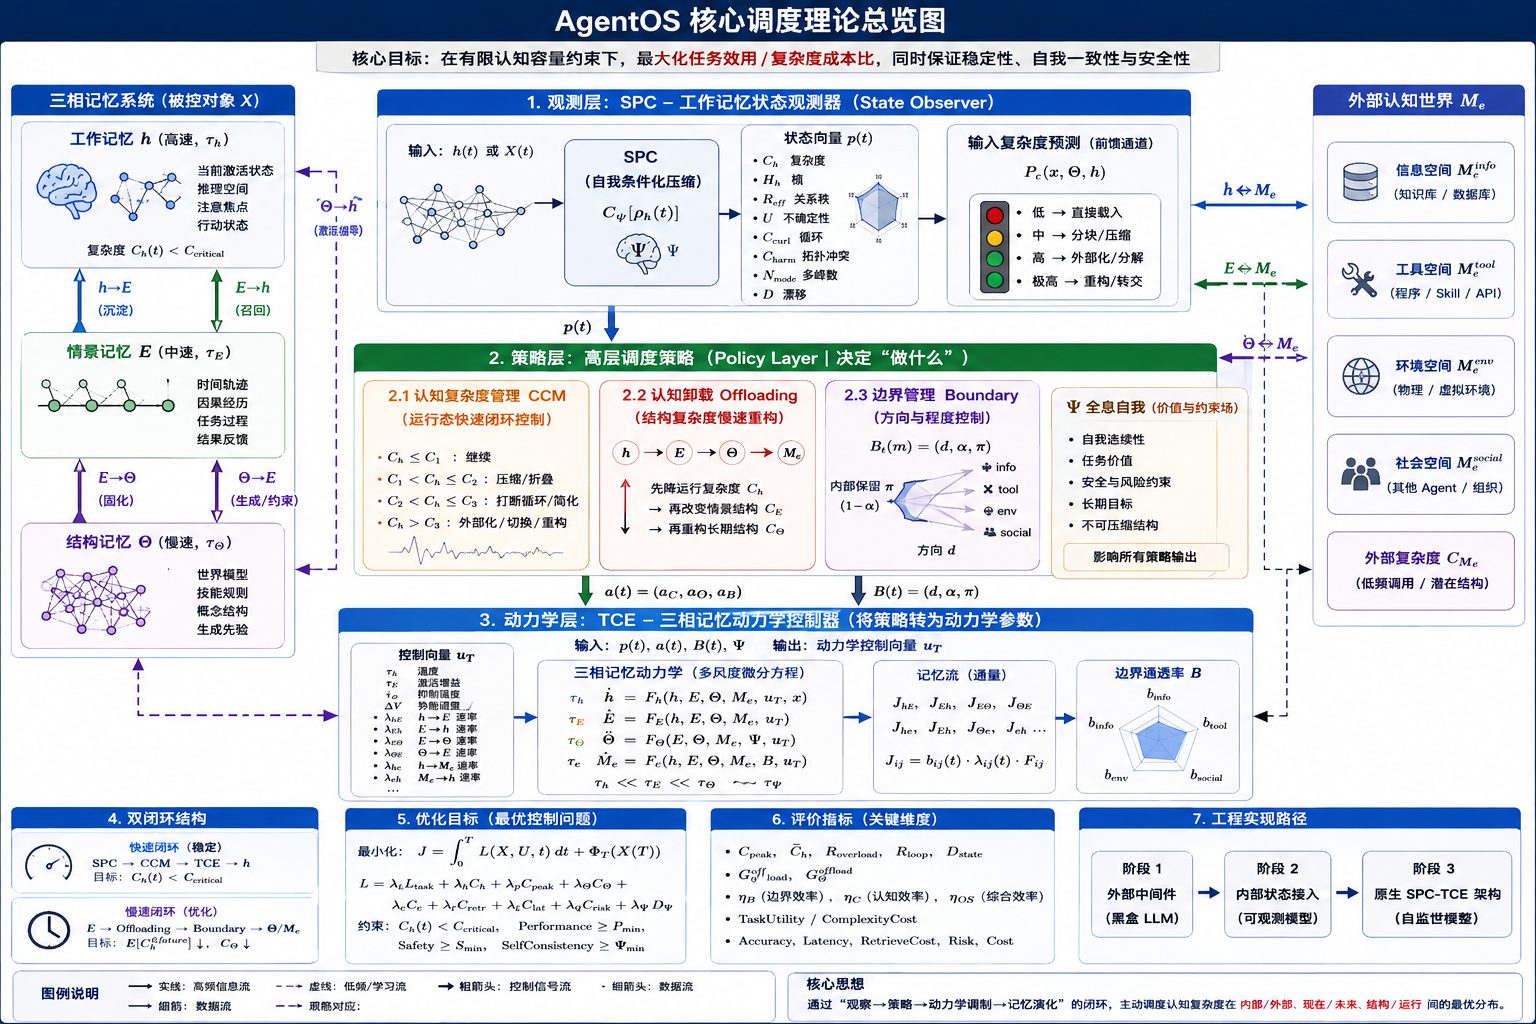
\includegraphics[width=.9\textwidth,height=.38\textheight,keepaspectratio]{images/control-stability-panel.png}
\caption{多回路耦合、相变与恢复区域}
\end{figure}
\section{工作记忆闭环：有限显式认知面的局部稳定性}

我们首先从最直接的工作记忆闭环开始，因为所有进入显式认知层的目标、假设、计划、关键关系、冲突和异常，最终都必须暂时落在 $h(t)$ 上。此前已经建立工作记忆有限容量原则：$h(t)$ 并不是可以无限扩展的 token 容器，而是一个能够同时维持有限数量活跃认知结构及其关系的显式跨尺度表面。因而 $h$ 的稳定性问题首先不是 ``信息有没有丢失''，而是当前活跃 Agent-CSO 网络是否还能保持足够的结构相干性，使新的输入能够在不破坏已有目标、约束和因果关系的条件下被整合。

令工作记忆的有效状态写为
\[
x_h(t)
=
\left[
n_h(t),
d_h(t),
q_h(t),
u_h(t),
r_h(t),
c_h(t)
\right]^{\top},
\]
其中 $n_h$ 表示活跃 Agent-CSO 数量或有效节点规模，$d_h$ 表示活跃关系密度，$q_h$ 表示目标与约束冲突程度，$u_h$ 表示不确定性，$r_h$ 表示未闭合残差，而 $c_h$ 表示当前表征相干度。这里并不要求这些变量采用唯一实现；工程上可以由注意分布、图结构统计量、预测残差、逻辑冲突指标以及多次采样一致性等近似估计。我们真正关心的是，它们共同定义了 $h$ 是否仍处于一个可持续进行显式认知的局部区域。

可以将工作记忆运行负荷表示为
\[
C_h(t)
=
\Phi_h
\left(
n_h,d_h,q_h,u_h,r_h
\right),
\]
并要求
\[
C_h(t)
<
C_h^{\max}.
\]
这个不等式不是说存在一个普适常数 $C_h^{\max}$，而是说对任一具体实现，都存在一个由基础模型能力、表征效率、上下文机制以及计算预算共同确定的有效运行边界。当 $C_h$ 接近这一边界时，新增认知内容造成的边际干扰开始快速上升；此时系统若仍然继续将所有局部异常、记忆内容和任务支线提升进入 $h$，就可能从普通负荷增加转变成结构性失稳。

因此，$h$ 闭环实际上由 SPC、Scheduler、TCE 与 CCM 共同维持。SPC 提供状态估计
\[
\hat{x}_h(t)
=
\mathcal O_{SPC}
\left(
h(t),E,\Theta,\Psi,\text{BodyState}
\right),
\]
Scheduler 根据目标优先级决定哪些 Agent-CSO 获得显式处理权，TCE 改变搜索温度、注意范围、推理深度和探索强度，而 CCM 则通过折叠、抑制、分页、分解和卸载降低 $C_h(t)$。于是工作记忆的抽象动力学可以写为
\[
\dot{x}_h
=
F_h
\left(
x_h,
u_{TCE},
u_{CCM},
u_{Sch},
\xi_{world},
\xi_{memory}
\right),
\]
其中 $\xi_{world}$ 与 $\xi_{memory}$ 分别代表来自现实世界和慢记忆层的扰动。

在这一尺度上，我们所谓 ``稳定'' 并不要求
\[
\dot{x}_h=0.
\]
真正健康的认知状态本来就是持续变化的。更恰当的定义是存在一个允许集合
\[
\mathcal H_{\mathrm{stable}}
=
\left\{
x_h:
C_h<C_h^{\max},
\;
c_h>c_{\min},
\;
q_h<q_{\max},
\;
r_h<r_{\max}
\right\},
\]
并且正常扰动下，$h$ 的轨迹大部分时间保持在该集合内部，短暂离开之后也能够在有限时间重新进入。由此可见，工作记忆稳定性不是 ``思想静止''，而是\textbf{有限显式认知面在持续变化条件下仍然保持可解释、可控制和可恢复的动态有界性}。

这也解释了为什么成熟智能不应追求让越来越多结构长期停留在 $h$ 中。真正成熟的运行方式恰恰应该满足
\[
\boxed{
\text{Most Agent Dynamics}\notin h,
}
\]
大量已经形成稳定闭环的能力应当在更局部、更快速或者更慢的结构中运行，只有新颖、冲突、高风险或者跨功能无法局部闭合的残差才被提升到 $h$。从控制意义上看，这种 ``选择性显式认知'' 本身就是维持工作记忆闭环稳定性的第一道机制。

\section{三相记忆闭环：状态、轨迹与生成结构之间的慢速稳定性}

工作记忆只描述当前切面，而一个长期 Agent 的稳定性还取决于当前状态如何写入经历、经历如何凝固为结构、长期结构又如何重新解释当前状态。因而第二个关键闭环是
\[
\boxed{
h
\leftrightarrow
E
\leftrightarrow
\Theta.
}
\]
它不是简单的数据搬运，而是三个具有不同时间尺度、不同结构密度和不同可塑性的状态空间之间的双向动力耦合。$h$ 是当前活跃状态，$E$ 是具有时间和因果顺序的经历轨迹，而 $\Theta$ 是能够对未来状态进行生成、预测和约束的长期结构。

为了研究稳定性，我们可以将三相记忆写成一个慢快系统：
\[
\begin{aligned}
\tau_h\dot h
&=
F_h(h,E,\Theta,u_h),\\
\tau_E\dot E
&=
F_E(E,h,\Theta,\Psi),\\
\tau_\Theta\dot\Theta
&=
F_\Theta(\Theta,E,h,\Psi),
\end{aligned}
\]
其中
\[
\tau_h\ll\tau_E\ll\tau_\Theta.
\]
这一时间尺度分离极其重要。如果 $\Theta$ 与 $h$ 具有接近的更新速度，那么一次偶然失败、一次异常输入甚至一次短期认知震荡都可能直接改变长期结构，从而造成长期世界模型和技能体系的不稳定；反过来，如果 $\Theta$ 完全不可塑，则系统又会失去真正的持续学习能力。因此，AgentOS 的三相记忆稳定性并不意味着 $\Theta$ 不变化，而意味着它只对\textbf{经过时间整合、反复验证并具有跨情景一致性的残差信号}发生显著变化。

我们可以把 $h\rightarrow E$ 理解为选择性经验写入：
\[
\Delta E
=
W_{hE}
\left(
h,
Novelty,
Value,
Residual,
SelfRelevance
\right),
\]
其中不是所有工作记忆状态都被永久保存。写入过强会造成情景记忆泛滥，写入过弱则造成生命周期连续性断裂。类似地，$E\rightarrow\Theta$ 应表示长期结构学习：
\[
\Delta\Theta
=
\eta_\Theta
G_\Theta
\left(
\left\langle
\varepsilon_E
\right\rangle_T,
Consistency,
Utility
\right),
\]
其中
\[
\eta_\Theta\ll1.
\]
$\left\langle\varepsilon_E\right\rangle_T$ 表示在一个相对长的时间窗口上仍然无法由当前 $\Theta$ 解释的经验残差。只有这种持续残差才有资格推动生成结构更新。

稳定的三相记忆还要求反方向通道受到限制。$\Theta\rightarrow h$ 是结构激活，但不能把全部长期知识无条件倾倒到工作记忆；$E\rightarrow h$ 是情景召回，但也不能让任意关联事件不断侵入当前认知；$\Theta\rightarrow E$ 则是重新解释历史经验，它必须保留事实证据和原始经历层，不能由于当前世界观变化而把历史事件任意改写。因此可以把三相记忆稳定性理解成三个相互约束的条件：
\[
\boxed{
\text{Selective Write}
+
\text{Slow Consolidation}
+
\text{Constrained Recall}.
}
\]

如果我们采用 Lyapunov 式思想，可以为记忆闭环定义一个并非物理能量、而是用于稳定分析的候选泛函
\[
V_M
=
\alpha_h D_h
+
\alpha_E D_E
+
\alpha_\Theta D_\Theta
+
\beta_{hE}M_{hE}
+
\beta_{E\Theta}M_{E\Theta},
\]
其中 $D_h,D_E,D_\Theta$ 分别描述各记忆层相对于其可接受运行区域的偏离，而 $M_{hE},M_{E\Theta}$ 表示跨层结构失配。若在正常运行区域内能够设计学习与控制律，使得
\[
\dot V_M
\leq
-\lambda V_M
+
\gamma\|\xi\|^2,
\]
则至少可以说明：对于有界外部扰动，记忆系统的结构偏离保持有界，并在扰动下降以后重新向一致区域收敛。这里我们并不宣称现实 AgentOS 必然满足一个简单解析 Lyapunov 函数，而是借这一形式明确工程目标：\textbf{记忆学习必须具有耗散性，不能让一次局部扰动通过层层放大成为永久结构漂移。}

因此三相记忆闭环的稳定性，本质上是当前状态、经历历史和长期生成结构之间的\textbf{受时间尺度保护的双向塑性}。它使系统既能够改变，又不至于因为每一次改变而失去自己。

\section{Body 闭环：现实快速动力学与认知慢环之间的稳定隔离}

第三类稳定性来自 Body Runtime。一个真正进入物理或数字世界的 Agent，不能让高层认知循环直接承担毫秒级控制。现实世界具有自己的高速扰动、惯性、噪声、通信延迟和硬安全约束，而 Kernel 的认知更新通常运行在更慢的秒级甚至更长尺度。因此 Body Runtime 的首要控制任务不是 ``让高层模型控制得更精细''，而是建立一个能够在高层不介入时仍然局部闭合的快速系统。

令身体局部状态为
\[
x_B(t),
\]
BPCC 内部快速状态为
\[
z_B(t),
\]
Kernel 发出的高层控制参考为
\[
r_K(t),
\]
则可以写成
\[
\begin{aligned}
\tau_B\dot x_B
&=
F_B(x_B,z_B,r_K,w_B),\\
\tau_{BPCC}\dot z_B
&=
F_P(z_B,x_B,r_K),
\end{aligned}
\]
其中
\[
\tau_B,\tau_{BPCC}
\ll
\tau_h.
\]
高层 Kernel 不直接规定每一个微观控制量，而提供
\[
\mathcal E_K
=
\left(
SGC^{target},
FCS^{constraint},
r_K
\right),
\]
即目标、可行域、风险限制和控制参考。BPCC 在这一范围内部完成快速预测与控制。

这一设计对应我们反复强调的原则：
\[
\boxed{
HigherLevelSetsFeasibleRegion,
\qquad
LowerLevelOptimizesInsideIt.
}
\]
高层对未来趋势和目标结构负责，低层对高频稳定负责。若 Kernel 每个周期都试图覆盖 BPCC 的控制细节，就会形成跨尺度 ``micromanagement''：认知延迟进入快速控制通道，高层预测过期，最终导致局部闭环震荡甚至安全失效。因此：
\[
\boxed{
SlowGovernance\neq FastMicromanagement.
}
\]

Body 闭环稳定的第二个关键是残差升级。令
\[
\varepsilon_B
=
\left(
\varepsilon_{ctrl},
\varepsilon_{SGC},
\varepsilon_{FCS}
\right).
\]
正常情况下，如果
\[
\|\varepsilon_B\|<\theta_B,
\]
问题保持在 Body Runtime 内部；只有当残差持续超过阈值、风险增加或者局部控制模型失效时，才形成一个更高层事件：
\[
\Gamma_B
=
\Phi
\left(
\|\varepsilon_B\|,
Risk,
Persistence,
Novelty
\right),
\]
并在
\[
\Gamma_B>\theta_{\mathrm{up}}
\]
时将有关 Agent-CSO 提升进入 $h$。这一机制把 ``现实持续变化'' 与 ``认知持续被打断'' 区分开来。现实中绝大部分连续扰动应该由局部闭环吸收，只有具有认知意义的偏差才成为显式思考对象。

这里还必须保留 Reality Authority：
\[
\boxed{
Prediction\neq Observation.
}
\]
BPCC 可以预测下一时刻的 SGC/FCS，但预测值不能直接替代真实世界重新进入系统的观测。动作发出之后必须经过
\[
Action
\rightarrow
Reality
\rightarrow
BodyRuntime
\rightarrow
SGC^{obs},FCS^{obs}.
\]
否则系统就可能形成内部模拟自我验证闭环：控制器认为自己已经成功，于是预测状态又成为下一轮 ``事实''。长期积累后，这种错误足以把整个认知系统从真实世界中解耦。

从整体稳定性角度，Body Runtime 因而承担 AgentOS 的第一层扰动屏障。它通过高频局部闭环压缩现实变化的带宽，把无数连续物理扰动转化成低频、具有意义的事件和残差。只有做到这一点，高层工作记忆、记忆系统和自我结构才能保持低频稳定。因此，Body 闭环不是 Agent Kernel 的附属设备，而是整个多尺度稳定架构的最外层快速耗散结构。

\section{目标与任务闭环：未来约束如何保持方向稳定而避免目标锁死}

第四类闭环围绕 Goal 展开。前面几个闭环主要回答系统如何稳定运行，而 Goal 闭环进一步回答系统为什么沿某个方向运行。目标并不是一条固定命令，它是当前认知状态中关于未来可接受区域的结构表示。因此，一个完整目标任务闭环应写成：
\[
Goal
\rightarrow
Plan
\rightarrow
Action
\rightarrow
Observation
\rightarrow
Verify
\rightarrow
Goal'.
\]
这里真正重要的是最后的 $Goal'$。一个成熟 Agent 不应把最初 Goal 当成不可修改的字符串，而必须能够根据现实反馈判断目标是否已经闭合、是否需要分解、是否与更慢价值结构冲突，以及是否应该终止。

可以将目标状态写成
\[
G(t)
=
\left(
g,
\mathcal C_g,
\pi_g,
p_g,
s_g
\right),
\]
其中 $g$ 表示目标语义结构，$\mathcal C_g$ 表示约束集合，$\pi_g$ 表示当前计划，$p_g$ 表示优先级，而 $s_g$ 表示目标状态。目标闭环接受来自现实的验证残差
\[
\varepsilon_G(t)
=
D
\left(
PredictedOutcome,
ObservedOutcome
\right),
\]
以及来自 $\Psi$、$\Omega$ 的慢约束。于是可以抽象为
\[
\tau_G\dot G
=
F_G
\left(
G,
\varepsilon_G,
\Psi,
\Omega,
Resource,
Risk
\right).
\]

目标稳定不是要求 $G$ 永远不变，而是要求它在任务执行期间拥有足够的 ``方向惯性''，不会因为局部噪声不断改变，同时又能够在持续反证出现时调整。我们可以用两个阈值描述这种迟滞：
\[
\theta_G^{on}
>
\theta_G^{off}.
\]
一个目标的建立需要足够强的证据、价值和优先级，而已经建立的目标不会因为一次短期困难立刻取消。相反，若长期证据表明不可行、代价失控或者违反更高层约束，则 Goal Closure 或 Goal Revision 才被触发。

目标闭环和工作记忆闭环之间存在一个特别危险的失稳模式：Goal 对 $h$ 的持续独占。如果某目标具有极高优先级，并持续产生未闭合残差，那么 Scheduler 可能长期把工作记忆资源分配给同一目标，形成
\[
Goal
\rightarrow
Attention
\rightarrow
Residual
\rightarrow
MoreAttention
\rightarrow
Goal.
\]
这种正反馈并不一定表现为程序死锁，但会形成认知意义上的锁死：其他任务、自我状态、身体风险和替代路径难以获得显式处理资源。因而目标闭环必须受到 CCM、Boundary 和慢层自我结构的约束，使
\[
p_g
\leq
p_g^{\max}(\Psi,\Omega,Safety).
\]
也就是说，任何普通目标都不应无限获得 h 的控制权。

与此相反，目标切换过快同样危险。如果
\[
\tau_G\approx\tau_h,
\]
每一次新的刺激都可能改变主目标，系统就会表现成高反应性但低方向性的随机游走。因此，目标时间尺度必须比普通瞬时认知更慢，但又显著快于身份和 DGA。对于不同类型任务，$\tau_G$ 可以差异很大，因此我们不需要给出一个固定绝对频率，只需要保持\textbf{目标变化比它所统摄的局部执行闭环更慢}这一相对原则。

由此看，Goal 闭环的稳定性其实是 ``未来结构的持续性''。它让系统能够把许多瞬时行为组织成一个较长时间尺度上的过程，同时通过现实验证防止目标变成脱离现实的永久吸引子。

\section{自我闭环：身份连续性、现实验证与慢变量保护}

当 Agent 具备长期经历以后，稳定性问题会进一步进入 $\Psi$。$\Psi$ 不应被理解成一个单独的 persona 文件，而是一个比普通知识和技能更慢的跨尺度自我约束场，它影响哪些经历被认为 ``属于我''、哪些目标具有更高优先级、哪些行为被判断为与自身连续，以及哪些长期变化能够被吸收到身份结构中。因此，自我闭环具有比普通任务闭环更长的时间常数：
\[
\tau_\Theta
\ll
\tau_\Psi.
\]

可以抽象写为
\[
\tau_\Psi\dot\Psi
=
F_\Psi
\left(
\Psi,
\overline E,
\Theta,
SelfInterpretation,
WorldVerification
\right),
\]
其中 $\overline E$ 不是一段单独经历，而是经过时间整合的生命周期经验结构。这里必须特别避免
\[
E_t\rightarrow\Psi_{t+1}
\]
这种过强直接映射。若一次短期失败即可显著改写 $\Psi$，则身份结构会随着局部任务震荡；如果 $\Psi$ 完全不接受来自经历的慢速更新，则 Agent 又无法真正形成发展意义上的个体历史。因此，自我稳定要求一种低通式学习机制：
\[
\Delta\Psi
\propto
\eta_\Psi
\left\langle
\Delta SelfEvidence
\right\rangle_T,
\qquad
\eta_\Psi\ll\eta_\Theta.
\]

自我闭环还存在一个比普通控制振荡更隐蔽的正反馈：
\[
SelfInterpretation
\rightarrow
SelectiveAttention
\rightarrow
Experience
\rightarrow
Memory
\rightarrow
SelfInterpretation'.
\]
例如，如果 Agent 形成 ``我总是不擅长某类任务'' 的自我结构，这一判断可能通过 Scheduler 和 TCE 改变未来注意与探索策略，使系统减少相关探索；随后获得的经历又更容易支持原有判断。此时闭环本身可以非常稳定，却稳定在一个错误吸引子上。因此：
\[
\boxed{
Stability\neq Truth.
}
\]
一个错误模型完全可能具有极高动力学稳定性。

所以自我闭环必须引入外部现实锚点：
\[
\mathcal V_{world}
=
D
\left(
SelfPrediction,
ObservedLongTermOutcome
\right).
\]
如果 $\Psi$ 的某个自我判断持续无法解释真实世界反馈，则系统必须允许这一部分结构被重新打开，而不能让自我一致性权重覆盖现实证据。由此形成：
\[
\boxed{
SelfConsistency
<
RealityConsistency
}
\]
作为 AgentOS 身份稳定性的基本治理原则。

我们还可以定义一个局部身份稳定泛函
\[
V_\Psi
=
D(\Psi_t,\Psi_{t-\Delta T})
+
\lambda_E D(\Psi_t,\mathcal I(E))
+
\lambda_W D(\Psi_t,\mathcal V_{world}),
\]
其中第一项限制身份变化过快，第二项要求身份能够解释自身经历，第三项要求这种解释不能长期脱离现实。一个健康的自我闭环并不是最小化第一项到零，而是在 ``连续性'' 与 ``现实修正'' 之间维持动态平衡。

因此慢变量保护并不意味着封死 $\Psi$。真正应该保护的是其\textbf{时间尺度}。瞬时噪声不应直接写入身份，持续经验则最终必须有机会影响身份。这也是为什么我们把 Self 放在普通认知之下又高于 DGA：它既要稳定过去形成的主体连续性，又必须允许生命周期继续塑造 ``我是谁''。

\section{DGA/$\Omega$ 闭环：生命周期方向的极慢稳定性}

如果 $\Psi$ 回答的是 ``Who am I''，那么 $\Omega$ 或 DGA 所描述的是 ``What am I becoming''。因此它不是一个普通目标，更不是一个可以随任务切换的 reward 参数，而是生命周期尺度上对未来生成空间施加偏置的超慢结构。它影响哪些经验长期值得积累、哪些能力方向逐渐被强化、哪些未来状态与当前主体发展轨迹更加一致。因此：
\[
\tau_\Omega
\gg
\tau_\Psi
\gg
\tau_\Theta.
\]

我们可以把 $\Omega$ 抽象成对未来状态分布的先验：
\[
p
\left(
X_{future}\mid\Omega,\Psi,\Theta
\right),
\]
而不是一个确定终点。这样做非常重要，因为真正开放环境中的 Agent 不可能在初始阶段就准确知道自己几十年后的最终状态。$\Omega$ 更像一个慢变的生成吸引子，它改变的是某些发展方向的相对可能性，而不是把未来锁死成一条固定轨迹。

其动力学可以表示为
\[
\tau_\Omega\dot\Omega
=
F_\Omega
\left(
\Omega,
\Psi,
\overline{\Theta},
LongTermOutcome,
Governance
\right).
\]
由于 $\tau_\Omega$ 极大，对它的更新必须依赖跨越足够长时间窗口的证据：
\[
\Delta\Omega
\propto
\eta_\Omega
\left\langle
\varepsilon_{life}
\right\rangle_{T_\Omega},
\qquad
\eta_\Omega
\ll
\eta_\Psi.
\]

DGA 闭环最大的风险不是普通振荡，而是\textbf{吸引域错误}。如果一个局部经历、错误奖励机制或者短期环境偏差被过早写入 $\Omega$，后续 Goal、Scheduler、Self Interpretation 都可能在更慢层的先验作用下不断选择支持该方向的经历。于是系统形成：
\[
\Omega
\rightarrow
GoalPreference
\rightarrow
Experience
\rightarrow
\Theta
\rightarrow
\Psi
\rightarrow
\Omega',
\]
并且随着时间推移越来越难脱离原有发展轨迹。因此慢变量的错误不会立即导致运行崩溃，反而可能表现为长时间高度 ``稳定''，直到生命周期尺度才暴露其方向性偏差。

因此，$\Omega$ 的稳定性必须与可修正性共同定义。一方面需要
\[
\left\|
\frac{d\Omega}{dt}
\right\|
\ll
\left\|
\frac{d\Psi}{dt}
\right\|,
\]
防止局部经验驱动发展方向震荡；另一方面又需要存在一个非零的长期可塑区域
\[
\mathcal P_\Omega
\neq
\varnothing,
\]
否则 Agent 会在早期形成不可改变的生命周期吸引子。

从控制理论视角看，我们可以把 $\Omega$ 视为一个极慢 supervisor，而不是 fast controller。它不应该直接决定具体动作：
\[
\Omega
\nrightarrow
u_{Body},
\]
而是通过
\[
\Omega
\rightarrow
\Psi
\rightarrow
GoalPreference
\rightarrow
Scheduler/TCE
\rightarrow
Action
\]
逐层产生影响。这种相邻尺度传播能够防止极慢变量直接进入快速控制造成尺度混叠，同时也确保真正长期的价值和发展方向能够持续约束短期行为。

因此 DGA/$\Omega$ 的稳定性最终可以概括成：
\begin{statementbox}
\centering
\adjustbox{max width=.96\linewidth}{\(\displaystyle \text{方向稳定而非终点固定，}
\quad
\text{长期可塑而非短期可改。}\)}
\end{statementbox}
它是整个 AgentOS 内部时间结构的最慢端，也是多回路系统中最必须受到时间尺度保护的一层。

\section{跨回路耦合、增益累积与共振条件}

到这里，我们已经分别考察了 $h$、Memory、Body、Goal、$\Psi$ 和 $\Omega$ 的局部闭环。但真正困难的问题从现在才开始：\textbf{每个闭环单独稳定，并不能推出整个 AgentOS 组合以后仍然稳定。}这是所有复杂反馈系统中最重要的事实之一。一个工作记忆控制器可能局部稳定，一个 Body Runtime 也可能局部稳定，但两者通过残差、目标和预测相互影响以后，仍然可能形成新的正反馈通道。

将第 $i$ 个闭环抽象为
\[
x_i
=
\mathcal F_i(u_i,\xi_i),
\]
其输出对输入扰动的局部增益定义为
\[
\|y_i\|
\leq
\gamma_i\|u_i\|
+
\beta_i.
\]
不同闭环之间存在耦合
\[
u_i
=
\sum_{j\neq i}
K_{ij}y_j+d_i.
\]
那么整个系统可以由一个增益矩阵描述：
\[
\mathbf{\Gamma}
=
\left[
\gamma_iK_{ij}
\right].
\]
在满足局部输入--状态稳定、耦合映射连续等条件下，小增益思想给出了一个非常有用的充分条件：
\[
\boxed{
\rho(\mathbf{\Gamma})<1,
}
\]
其中 $\rho(\mathbf{\Gamma})$ 表示谱半径。这个条件的含义并不是要求所有实际 AgentOS 都必须精确计算这一矩阵，而是告诉我们一个关键工程原则：\textbf{一个扰动绕系统闭环传播一周以后，其总放大倍数不能持续超过原始扰动。}

例如：
\[
BodyResidual
\rightarrow
SPC
\rightarrow
AHC
\rightarrow
TCE
\rightarrow
BodyControl
\rightarrow
BodyResidual'
\]
就是一个跨层环。如果 SPC 对残差高度敏感，AHC 又长时间积分，TCE 增益过高，而 BPCC 对高层控制变化响应过强，则虽然每个模块单独看来都合理，乘积增益却可能满足
\[
\gamma_{SPC}
\gamma_{AHC}
\gamma_{TCE}
\gamma_{BPCC}
>1,
\]
最终形成放大环。

同样，自我层可以形成更慢的跨层回路：
\[
\fitdisplay{
Failure
\rightarrow
E
\rightarrow
SelfInterpretation
\rightarrow
\Psi
\rightarrow
GoalPreference
\rightarrow
FutureTaskSelection
\rightarrow
Failure'.
}
\]
这种环的一个循环可能需要数天甚至数月，因此很难像快速控制震荡那样直接观察，却可能产生更深远的长期稳定性问题。

除增益以外，我们还必须考虑频率。如果两个本应具有明显分离时间尺度的闭环逐渐接近：
\[
\tau_i
\approx
\tau_j,
\]
并且双方存在较强双向耦合，则可能产生类似 ``共振'' 的现象。这里的共振不必是严格周期振荡，而泛指一个环的变化频率进入另一环的高敏感区域，使彼此相互强化。例如 TCE 持续快速修改注意策略，而 Scheduler 也以相似周期重新规划任务，两者可能不断相互否定；再如 AHC 恢复时间恰好与失败重试周期相近，则每一次重试都发生在上一次威胁状态尚未衰减时，最终造成累积。

因此，对于相邻层我们要求：
\[
\boxed{
\tau_i
\ll
\tau_{i+1}
}
\]
或者至少满足足够的频率分离，使慢层在快层看来接近常量，快层在慢层看来能够被时间平均。这正是奇异摄动和 averaging theory 给我们的主要数学启示。设
\[
\epsilon
=
\frac{\tau_{fast}}{\tau_{slow}}
\ll1,
\]
则可以先分析在固定慢变量 $z$ 下快系统
\[
\dot x
=
f(x,z)
\]
是否具有稳定吸引集合，再研究慢变量
\[
\dot z
=
\epsilon g(\bar x(z),z)
\]
的演化。只要快系统在慢变量变化过程中能够充分收敛，我们就可以避免所有层同时互相追逐。

因此多尺度 AgentOS 的一个根本稳定原则可以写成：
\[
\boxed{
FastLoopsAbsorbFastPerturbations;
\quad
SlowLoopsReactOnlyToPersistentResiduals.
}
\]
快速噪声如果直接进入 $\Psi$、$\Omega$ 或长期拓扑，系统就失去时间尺度隔离；反过来，慢结构如果直接控制 servo 级动作，系统又失去局部自治。两者本质上是同一种跨尺度设计错误。

\section{运行相变：从连续负荷变化到宏观认知相态转换}

跨回路耦合进一步产生一个重要结果：AgentOS 的异常通常并不是某个变量逐渐变大那么简单，而可能出现宏观运行方式的突然改变。我们此前把工作记忆运行状态划分为基态、心流态、湍流态、临界态和气态，这些名称不是要把认知过程物理化，而是为了描述一个复杂动力系统在不同参数区域内出现的不同宏观组织方式。

我们定义一个运行序参量向量
\[
z(t)
=
\left[
L_h,
Coh_h,
U_h,
R,
A,
G_T,
M,
P
\right]^{\top},
\]
其中 $L_h$ 表示工作记忆负荷，$Coh_h$ 表示结构相干性，$U_h$ 表示不确定性，$R$ 表示持续残差，$A$ 表示 AHC 激活强度，$G_T$ 表示 TCE 有效控制增益，$M$ 表示当前记忆激活扩散程度，而 $P$ 表示目标竞争压力。相态不是由某个单变量决定，而是由这些宏观统计量落入哪一个区域决定：
\[
z(t)\in\mathcal P_k.
\]

例如基态可以粗略表示为
\[
\mathcal P_{ground}
=
\left\{
L_h\ \text{低},
\;
Coh_h\ \text{高},
\;
R\ \text{低},
\;
A\ \text{低至中}
\right\}.
\]
心流态则可能满足中高负荷、高相干、低目标竞争和适度 TCE 增益；湍流态表现为高负荷、频繁目标切换、关系网络重构和持续残差；临界态则意味着系统接近可维持显式认知结构的边界，小扰动可能造成相态跳跃；所谓气态则描述过度激活、关系约束松散、无法维持稳定推理主线的极端运行状态。

我们可以定义一个相态判别函数
\[
\chi_k(z)
=
z^\top Q_k z+b_k^\top z+c_k,
\]
或者使用学习得到的非线性分类器
\[
P(\mathcal P_k\mid z_{0:t}).
\]
后者实际上更符合工程现实，因为认知相态通常具有时间依赖，单点状态不足以判断。SPC 因而不是简单读取 $z(t)$，而应该估计
\[
P
\left(
\mathcal P_t
\mid
z_{t-T:t}
\right),
\]
以及未来相变概率
\[
P
\left(
\mathcal P_{t+\Delta}
\neq
\mathcal P_t
\mid
z_{t-T:t}
\right).
\]

所谓相变控制的关键，不是等系统已经进入失稳态以后才进行 ``紧急降温''，而是识别临界减速、方差增加、恢复速度下降和残差相关性增强等先兆。假设局部扰动后系统恢复率为
\[
\lambda_{rec}(t).
\]
当
\[
\lambda_{rec}\rightarrow0^{+},
\]
说明系统离稳定边界越来越近，即使当前表面状态仍然可运行，也可能已经进入临界区域。类似地，可以监测
\[
Var(z)\uparrow,
\qquad
Corr(z_t,z_{t-1})\uparrow,
\]
作为潜在 early-warning signals。这里借鉴的是非线性系统临界转变研究中的数学思想，而不是声称认知相态严格遵循某一种物理相变模型。

TCE 在相态控制中的作用因此不是设置一个全局 temperature，而是实施一个状态依赖控制律
\[
u_{TCE}
=
\pi_T
\left(
\hat z,
P(\mathcal P),
\dot z,
Risk
\right).
\]
当系统处于基态时，控制强度可以较低，允许更多局部自治；处于心流态时，TCE 应避免过度干预，以防破坏已经形成的稳定高效闭环；进入湍流态时，可通过减少并行目标、缩小搜索范围、提高结构压缩、调用 Offloading 等方式降低运行负荷；接近临界态时则可能触发更强的 Scheduler 和 CCM 治理，必要时暂停新任务输入。

因此，相变控制不是 ``让 Agent 永远保持某一种最佳相态''。不同任务本来就需要不同认知状态。真正的目标是：
\begin{statementbox}
AllowUsefulTransitions,
PreventUncontrolledTransitions.
\end{statementbox}
成熟 Agent 应能够在基态、心流、高探索甚至短时临界状态之间有目的地移动，同时始终保留返回可治理区域的动力学通道。

\section{迟滞、恢复区域与 AgentOS 的可恢复稳定性}

多回路系统最终不能只用 ``稳定/不稳定'' 二元分类。对于一个需要长期运行、不断学习和面对新环境的 Agent，真正有工程意义的概念是\textbf{可恢复稳定性}：系统可以暂时离开日常稳定区域，可以进入高负荷、高探索甚至接近临界的状态，但只要安全边界尚未被突破，它就必须存在一条受控轨迹返回正常运行区域。

我们首先定义一个安全可治理集合
\[
\mathcal X_{\mathrm{gov}}
=
\left\{
x:
g_i(x)\leq0,
\quad i=1,\ldots,m
\right\},
\]
其中可以同时包含工作记忆容量、安全约束、身体状态、身份变化率、长期记忆更新幅度和权限约束。例如：
\[
C_h<C_h^{hard},
\]
\[
Risk_B<R^{hard},
\]
\[
\left\|\dot\Psi\right\|<v_\Psi^{max},
\]
\[
\left\|\dot\Omega\right\|<v_\Omega^{max}.
\]
再在其内部定义日常稳定区域
\[
\mathcal X_{\mathrm{normal}}
\subset
\mathcal X_{\mathrm{gov}}.
\]
两者之间的差异非常关键：Agent 暂时离开 $\mathcal X_{\mathrm{normal}}$ 并不意味着故障，只要仍处于 $\mathcal X_{\mathrm{gov}}$，系统还有足够控制余量恢复。

于是恢复区域可以定义为
\[
\mathcal R
=
\left\{
x_0\in\mathcal X_{\mathrm{gov}}
:
\exists u(t),
\;
x(t;x_0,u)
\rightarrow
\mathcal X_{\mathrm{normal}}
\right\}.
\]
从控制理论语言看，它接近 viability kernel、region of attraction 和 backward reachable set 的组合思想。对于 AgentOS，我们不一定需要解析求出 $\mathcal R$，但工程上应持续估计：
\[
P_{recover}
=
P
\left(
x(t+\Delta)\in\mathcal X_{\mathrm{normal}}
\mid x(t),u
\right).
\]
只要这一概率快速下降，就说明系统正在失去恢复余量，应当提高治理级别，而不是继续追求当前任务性能。

恢复控制还必须使用迟滞。假如进入湍流态的阈值和离开湍流态的阈值完全相同：
\[
\theta_{on}=\theta_{off},
\]
系统会在阈值附近频繁切换控制模式，形成 chatter。因此应该满足
\[
\boxed{
\theta_{on}>\theta_{off}.
}
\]
例如当 $C_h$ 高于 $0.85C_h^{\max}$ 时进入强 CCM 模式，但只有负荷下降到 $0.65C_h^{\max}$ 以下并保持一定时间后才退出。这种迟滞不仅适用于工作记忆，也适用于 BPCC 的高层升级、Goal 重新规划、自我结构开放以及更慢的拓扑修改。

我们可以将整个恢复过程设计成层级化控制：
\[
\text{Level 0: Local Adjustment},
\]
\[
\text{Level 1: Runtime Regulation},
\]
\[
\text{Level 2: Cognitive Simplification},
\]
\[
\text{Level 3: Task Suspension},
\]
\[
\text{Level 4: Memory/Self Protection},
\]
\[
\text{Level 5: Checkpoint Recovery}.
\]
系统首先尝试最小干预：TCE 调节温度、CCM 降低负荷、Scheduler 推迟低优先级任务；若持续失效，再扩大到 Offloading、Goal 重规划和任务暂停；只有当身份、长期记忆或安全边界受到威胁时，才进入更强的治理模式。这与整个 AgentOS 一贯的
\begin{statementbox}
MinimumNecessaryReorganizationPrinciple
\end{statementbox}
一致：能用状态调节解决的问题，不修改结构；能用局部结构解决的问题，不修改慢变量；能用认知恢复解决的问题，不触及身份和生命周期结构。

为了统一描述整个多回路系统，我们可以定义一个综合稳定泛函
\[
V_{\mathrm{Agent}}
=
w_BV_B
+
w_hV_h
+
w_MV_M
+
w_GV_G
+
w_\Psi V_\Psi
+
w_\Omega V_\Omega
+
\sum_{i<j}
\lambda_{ij}V_{ij}^{coupling}.
\]
各 $V_i$ 不必具有相同数学形式，它们代表不同尺度上的偏离度，而 $V_{ij}^{coupling}$ 描述跨层结构失配。我们并不要求真实 AgentOS 存在一个全局光滑 Lyapunov 函数；相反，由于离散任务切换、安全中断、记忆写入和相态改变的存在，整个系统更自然地属于混合动力系统。但这一泛函仍然给出了一个重要设计目标：局部控制器和慢层治理应共同防止
\[
V_{\mathrm{Agent}}(t)
\]
在没有外部不可控灾难的情况下持续发散。

由此，我们最终可以给 AgentOS 稳定性一个比 ``不崩溃'' 更严格的定义：
\[
\boxed{
\begin{aligned}
\text{AgentOS Stability}
=
&\ \text{Local Loop Stability}\\
&+\text{Bounded Cross-Loop Gain}\\
&+\text{Timescale Separation}\\
&+\text{Reality Anchoring}\\
&+\text{Controlled Phase Transition}\\
&+\text{Recoverability}.
\end{aligned}
}
\]

这一定义同时说明了为什么成熟智能不应被设计成一个巨大、统一、高增益的中央循环。越是长期、复杂的智能体，就越需要把高速稳定性交给局部闭环，把显式认知保留给真正需要跨结构处理的问题，把长期经验交给慢记忆，把身份变化限制在更长时间尺度，把生命周期方向放在最慢结构中。各层之间不是互不相干，而是通过受控残差、约束和预测相互作用。

因此，本章的最终结论可以写为：
\begin{conclusion}
持续智能的稳定，不来自所有层保持静止，而来自不同时间尺度上的闭环各自完成局部闭合，并使跨尺度影响始终受到增益、时延、权限与现实反馈的共同约束。
\end{conclusion}

进一步地，
\begin{statementbox}
真正成熟的 AgentOS 应当允许自身进入高负荷、高探索和结构重组状态，但必须始终知道自己距离不可治理边界还有多远，并保留一条能够返回可治理区域的路径。
\end{statementbox}

这就是多回路稳定性理论对于 AgentOS 控制工程的核心意义：我们不是试图消除智能系统的波动，而是在建立一种能够\textbf{容纳波动、利用相变、限制共振并保证恢复}的长期智能动力学。

\chapter{控制编程与递归自主性的边界}
\begin{chapteroverviewbox}
这一章，我们围绕“控制编程与递归自主性的边界”做一件克制的事：把直觉压缩为状态、关系、时间尺度和可检验后果。它在全书中的任务，是说明多回路稳定性和有界自修改。
\end{chapteroverviewbox}
\ChapterArt{\number\value{chapter}}

\section*{理论来路与依赖接口}
本章的直接思想来源是原文关于控制工程、培育工程和心理工程的生命周期衍生讨论。我们采用原文较晚形成的定义来整理较早讨论，不把对话中的试探性比喻与最终模型并列成互相竞争的“定律”。已有理论锚点主要是鲁棒控制、时延系统、稳定裕度与权限治理（Kalman、Ashby 与混杂系统理论）。

本章使用上一章“多回路稳定性与相变控制”已经得到的对象与边界；本章产出将供下一章“为什么 Agent 需要“培育”而不仅是训练”使用。若后文术语偶尔出现，只作为路线提示，不参与本章推导。

\section*{从哪里出发}
我们已经拥有上一章给出的概念，现在只向前走一步。我会先把对象放进闭环，再讨论它的数学形式，最后检查工程边界。读者不必预先相信本章术语；只需暂时接受一个方法论约定：智能结构的意义来自它在现实反馈中的作用，而不是来自名称本身。

令系统在观察窗口 $[t,t+T]$ 内的状态轨迹为 $x_{[t,t+T]}$，环境扰动为 $d$，行动为 $u$。本章讨论的对象若确实有效，就应改变条件分布 $p(x_{t+T}\mid x_t,u,d)$，或改变达到同一结果所需的代价。这个起点把讨论锚定在鲁棒控制、时延系统、稳定裕度与权限治理上。
\section{哪些变量可修改}
\begin{narration}
现在把镜头移到“哪些变量可修改”。我们只沿本章已经取得的概念向前一步：先确定它在闭环里的角色，再检查它的尺度与失败边界。
\end{narration}

本节把“哪些变量可修改”落实为由治理层明确允许主体调整、明确禁止调整和需要外部授权调整的变量集合。这个定义不是说“任何相似现象都算”，而是要求我们同时给出对象域、允许的干预以及观察窗口。对于主题“控制编程与递归自主性的边界”而言，它承担的是多回路稳定性和有界自修改中的一个可辨识环节。

把这一关系写成最小数学骨架，可得

\begin{equation}\mathcal X=\mathcal X_{free}\cup\mathcal X_{guarded}\cup\mathcal X_{forbidden}.\end{equation}

式中的符号只承担结构角色，具体参数仍需由任务和身体数据辨识。我们首先检查可观测量，再检查控制量，最后检查比它更慢的约束。这样的顺序来自鲁棒控制、时延系统、稳定裕度与权限治理，但本书对哪些变量可修改的命名和组合仍是需要实验验证的建模提案。

这一小节的反例同样重要：没有禁区、预算与回滚点的递归修改会破坏身份和安全不变量。因此评价它不能只看一次任务结果，而要比较干预前后的轨迹、恢复时间、维护成本和风险。如果改变该机制而所有允许观察下的分布都不变，那么它至少在当前实验族中是冗余描述。

\begin{thought}
对“哪些变量可修改”做一次消融：冻结它、删除它，或只允许它以相邻时间尺度交换残差。哪些现象立即消失，哪些只在长期出现？若答案无法区分三种干预，我们还没有找到正确的状态变量。
\end{thought}

最后，把结论交还现实：本节只建立功能层关系，不由此推出特定脑区实现、主观意识或宇宙目的。可测状态、干预后果和明确失败条件，才是从原文直觉走向可检验理论的桥。

\section{哪些 Goal 可以自主产生}
\begin{narration}
现在把镜头移到“哪些 Goal 可以自主产生”。我们只沿本章已经取得的概念向前一步：先确定它在闭环里的角色，再检查它的尺度与失败边界。
\end{narration}

本节把“哪些 Goal 可以自主产生”落实为由治理层明确允许主体调整、明确禁止调整和需要外部授权调整的变量集合。这个定义不是说“任何相似现象都算”，而是要求我们同时给出对象域、允许的干预以及观察窗口。对于主题“控制编程与递归自主性的边界”而言，它承担的是多回路稳定性和有界自修改中的一个可辨识环节。

把这一关系写成最小数学骨架，可得

\begin{equation}\mathcal X=\mathcal X_{free}\cup\mathcal X_{guarded}\cup\mathcal X_{forbidden}.\end{equation}

式中的符号只承担结构角色，具体参数仍需由任务和身体数据辨识。我们首先检查可观测量，再检查控制量，最后检查比它更慢的约束。这样的顺序来自鲁棒控制、时延系统、稳定裕度与权限治理，但本书对哪些 Goal 可以自主产生的命名和组合仍是需要实验验证的建模提案。

这一小节的反例同样重要：没有禁区、预算与回滚点的递归修改会破坏身份和安全不变量。因此评价它不能只看一次任务结果，而要比较干预前后的轨迹、恢复时间、维护成本和风险。如果改变该机制而所有允许观察下的分布都不变，那么它至少在当前实验族中是冗余描述。

\begin{thought}
对“哪些 Goal 可以自主产生”做一次消融：冻结它、删除它，或只允许它以相邻时间尺度交换残差。哪些现象立即消失，哪些只在长期出现？若答案无法区分三种干预，我们还没有找到正确的状态变量。
\end{thought}

最后，把结论交还现实：本节只建立功能层关系，不由此推出特定脑区实现、主观意识或宇宙目的。可测状态、干预后果和明确失败条件，才是从原文直觉走向可检验理论的桥。

\section{哪些权限可以成长}
\begin{narration}
现在把镜头移到“哪些权限可以成长”。我们只沿本章已经取得的概念向前一步：先确定它在闭环里的角色，再检查它的尺度与失败边界。
\end{narration}

本节把“哪些权限可以成长”落实为由治理层明确允许主体调整、明确禁止调整和需要外部授权调整的变量集合。这个定义不是说“任何相似现象都算”，而是要求我们同时给出对象域、允许的干预以及观察窗口。对于主题“控制编程与递归自主性的边界”而言，它承担的是多回路稳定性和有界自修改中的一个可辨识环节。

把这一关系写成最小数学骨架，可得

\begin{equation}\mathcal X=\mathcal X_{free}\cup\mathcal X_{guarded}\cup\mathcal X_{forbidden}.\end{equation}

式中的符号只承担结构角色，具体参数仍需由任务和身体数据辨识。我们首先检查可观测量，再检查控制量，最后检查比它更慢的约束。这样的顺序来自鲁棒控制、时延系统、稳定裕度与权限治理，但本书对哪些权限可以成长的命名和组合仍是需要实验验证的建模提案。

这一小节的反例同样重要：没有禁区、预算与回滚点的递归修改会破坏身份和安全不变量。因此评价它不能只看一次任务结果，而要比较干预前后的轨迹、恢复时间、维护成本和风险。如果改变该机制而所有允许观察下的分布都不变，那么它至少在当前实验族中是冗余描述。

\begin{thought}
对“哪些权限可以成长”做一次消融：冻结它、删除它，或只允许它以相邻时间尺度交换残差。哪些现象立即消失，哪些只在长期出现？若答案无法区分三种干预，我们还没有找到正确的状态变量。
\end{thought}

最后，把结论交还现实：本节只建立功能层关系，不由此推出特定脑区实现、主观意识或宇宙目的。可测状态、干预后果和明确失败条件，才是从原文直觉走向可检验理论的桥。

\section{Ψ 的可塑区}
\begin{narration}
现在把镜头移到“Ψ 的可塑区”。我们只沿本章已经取得的概念向前一步：先确定它在闭环里的角色，再检查它的尺度与失败边界。
\end{narration}

本节把“Ψ 的可塑区”落实为由治理层明确允许主体调整、明确禁止调整和需要外部授权调整的变量集合。这个定义不是说“任何相似现象都算”，而是要求我们同时给出对象域、允许的干预以及观察窗口。对于主题“控制编程与递归自主性的边界”而言，它承担的是多回路稳定性和有界自修改中的一个可辨识环节。

把这一关系写成最小数学骨架，可得

\begin{equation}\mathcal X=\mathcal X_{free}\cup\mathcal X_{guarded}\cup\mathcal X_{forbidden}.\end{equation}

式中的符号只承担结构角色，具体参数仍需由任务和身体数据辨识。我们首先检查可观测量，再检查控制量，最后检查比它更慢的约束。这样的顺序来自鲁棒控制、时延系统、稳定裕度与权限治理，但本书对Ψ 的可塑区的命名和组合仍是需要实验验证的建模提案。

这一小节的反例同样重要：没有禁区、预算与回滚点的递归修改会破坏身份和安全不变量。因此评价它不能只看一次任务结果，而要比较干预前后的轨迹、恢复时间、维护成本和风险。如果改变该机制而所有允许观察下的分布都不变，那么它至少在当前实验族中是冗余描述。

\begin{thought}
对“Ψ 的可塑区”做一次消融：冻结它、删除它，或只允许它以相邻时间尺度交换残差。哪些现象立即消失，哪些只在长期出现？若答案无法区分三种干预，我们还没有找到正确的状态变量。
\end{thought}

最后，把结论交还现实：本节只建立功能层关系，不由此推出特定脑区实现、主观意识或宇宙目的。可测状态、干预后果和明确失败条件，才是从原文直觉走向可检验理论的桥。

\section{Ω/DGA 的可塑区}
\begin{narration}
现在把镜头移到“Ω/DGA 的可塑区”。我们只沿本章已经取得的概念向前一步：先确定它在闭环里的角色，再检查它的尺度与失败边界。
\end{narration}

本节把“Ω/DGA 的可塑区”落实为由治理层明确允许主体调整、明确禁止调整和需要外部授权调整的变量集合。这个定义不是说“任何相似现象都算”，而是要求我们同时给出对象域、允许的干预以及观察窗口。对于主题“控制编程与递归自主性的边界”而言，它承担的是多回路稳定性和有界自修改中的一个可辨识环节。

把这一关系写成最小数学骨架，可得

\begin{equation}\mathcal X=\mathcal X_{free}\cup\mathcal X_{guarded}\cup\mathcal X_{forbidden}.\end{equation}

式中的符号只承担结构角色，具体参数仍需由任务和身体数据辨识。我们首先检查可观测量，再检查控制量，最后检查比它更慢的约束。这样的顺序来自鲁棒控制、时延系统、稳定裕度与权限治理，但本书对Ω/DGA 的可塑区的命名和组合仍是需要实验验证的建模提案。

这一小节的反例同样重要：没有禁区、预算与回滚点的递归修改会破坏身份和安全不变量。因此评价它不能只看一次任务结果，而要比较干预前后的轨迹、恢复时间、维护成本和风险。如果改变该机制而所有允许观察下的分布都不变，那么它至少在当前实验族中是冗余描述。

\begin{thought}
对“Ω/DGA 的可塑区”做一次消融：冻结它、删除它，或只允许它以相邻时间尺度交换残差。哪些现象立即消失，哪些只在长期出现？若答案无法区分三种干预，我们还没有找到正确的状态变量。
\end{thought}

最后，把结论交还现实：本节只建立功能层关系，不由此推出特定脑区实现、主观意识或宇宙目的。可测状态、干预后果和明确失败条件，才是从原文直觉走向可检验理论的桥。

\section{Checkpoint Governance}
\begin{narration}
现在把镜头移到“Checkpoint Governance”。我们只沿本章已经取得的概念向前一步：先确定它在闭环里的角色，再检查它的尺度与失败边界。
\end{narration}

本节把“Checkpoint Governance”落实为由治理层明确允许主体调整、明确禁止调整和需要外部授权调整的变量集合。这个定义不是说“任何相似现象都算”，而是要求我们同时给出对象域、允许的干预以及观察窗口。对于主题“控制编程与递归自主性的边界”而言，它承担的是多回路稳定性和有界自修改中的一个可辨识环节。

把这一关系写成最小数学骨架，可得

\begin{equation}\mathcal X=\mathcal X_{free}\cup\mathcal X_{guarded}\cup\mathcal X_{forbidden}.\end{equation}

式中的符号只承担结构角色，具体参数仍需由任务和身体数据辨识。我们首先检查可观测量，再检查控制量，最后检查比它更慢的约束。这样的顺序来自鲁棒控制、时延系统、稳定裕度与权限治理，但本书对Checkpoint Governance的命名和组合仍是需要实验验证的建模提案。

这一小节的反例同样重要：没有禁区、预算与回滚点的递归修改会破坏身份和安全不变量。因此评价它不能只看一次任务结果，而要比较干预前后的轨迹、恢复时间、维护成本和风险。如果改变该机制而所有允许观察下的分布都不变，那么它至少在当前实验族中是冗余描述。

\begin{thought}
对“Checkpoint Governance”做一次消融：冻结它、删除它，或只允许它以相邻时间尺度交换残差。哪些现象立即消失，哪些只在长期出现？若答案无法区分三种干预，我们还没有找到正确的状态变量。
\end{thought}

最后，把结论交还现实：本节只建立功能层关系，不由此推出特定脑区实现、主观意识或宇宙目的。可测状态、干预后果和明确失败条件，才是从原文直觉走向可检验理论的桥。

\section{Self-Modifiable Set}
\begin{narration}
现在把镜头移到“Self-Modifiable Set”。我们只沿本章已经取得的概念向前一步：先确定它在闭环里的角色，再检查它的尺度与失败边界。
\end{narration}

本节把“Self-Modifiable Set”落实为由治理层明确允许主体调整、明确禁止调整和需要外部授权调整的变量集合。这个定义不是说“任何相似现象都算”，而是要求我们同时给出对象域、允许的干预以及观察窗口。对于主题“控制编程与递归自主性的边界”而言，它承担的是多回路稳定性和有界自修改中的一个可辨识环节。

把这一关系写成最小数学骨架，可得

\begin{equation}\mathcal X=\mathcal X_{free}\cup\mathcal X_{guarded}\cup\mathcal X_{forbidden}.\end{equation}

式中的符号只承担结构角色，具体参数仍需由任务和身体数据辨识。我们首先检查可观测量，再检查控制量，最后检查比它更慢的约束。这样的顺序来自鲁棒控制、时延系统、稳定裕度与权限治理，但本书对Self-Modifiable Set的命名和组合仍是需要实验验证的建模提案。

这一小节的反例同样重要：没有禁区、预算与回滚点的递归修改会破坏身份和安全不变量。因此评价它不能只看一次任务结果，而要比较干预前后的轨迹、恢复时间、维护成本和风险。如果改变该机制而所有允许观察下的分布都不变，那么它至少在当前实验族中是冗余描述。

\begin{thought}
对“Self-Modifiable Set”做一次消融：冻结它、删除它，或只允许它以相邻时间尺度交换残差。哪些现象立即消失，哪些只在长期出现？若答案无法区分三种干预，我们还没有找到正确的状态变量。
\end{thought}

最后，把结论交还现实：本节只建立功能层关系，不由此推出特定脑区实现、主观意识或宇宙目的。可测状态、干预后果和明确失败条件，才是从原文直觉走向可检验理论的桥。

\section{Bounded Self-Modification Envelope}
\begin{narration}
现在把镜头移到“Bounded Self-Modification Envelope”。我们只沿本章已经取得的概念向前一步：先确定它在闭环里的角色，再检查它的尺度与失败边界。
\end{narration}

本节把“Bounded Self-Modification Envelope”落实为由治理层明确允许主体调整、明确禁止调整和需要外部授权调整的变量集合。这个定义不是说“任何相似现象都算”，而是要求我们同时给出对象域、允许的干预以及观察窗口。对于主题“控制编程与递归自主性的边界”而言，它承担的是多回路稳定性和有界自修改中的一个可辨识环节。

把这一关系写成最小数学骨架，可得

\begin{equation}\mathcal X=\mathcal X_{free}\cup\mathcal X_{guarded}\cup\mathcal X_{forbidden}.\end{equation}

式中的符号只承担结构角色，具体参数仍需由任务和身体数据辨识。我们首先检查可观测量，再检查控制量，最后检查比它更慢的约束。这样的顺序来自鲁棒控制、时延系统、稳定裕度与权限治理，但本书对Bounded Self-Modification Envelope的命名和组合仍是需要实验验证的建模提案。

这一小节的反例同样重要：没有禁区、预算与回滚点的递归修改会破坏身份和安全不变量。因此评价它不能只看一次任务结果，而要比较干预前后的轨迹、恢复时间、维护成本和风险。如果改变该机制而所有允许观察下的分布都不变，那么它至少在当前实验族中是冗余描述。

\begin{thought}
对“Bounded Self-Modification Envelope”做一次消融：冻结它、删除它，或只允许它以相邻时间尺度交换残差。哪些现象立即消失，哪些只在长期出现？若答案无法区分三种干预，我们还没有找到正确的状态变量。
\end{thought}

最后，把结论交还现实：本节只建立功能层关系，不由此推出特定脑区实现、主观意识或宇宙目的。可测状态、干预后果和明确失败条件，才是从原文直觉走向可检验理论的桥。

\section*{本章收束：把名词还原为闭环}
现在回头看“控制编程与递归自主性的边界”，最重要的不是记住缩写，而是说清本章对象怎样改变系统的状态、代价或可恢复性。下一章“为什么 Agent 需要“培育”而不仅是训练”只使用这里已经给出的结果，不反过来为本章提供前提。

\begin{bookproposition}
若一个候选机制既不改变可观测轨迹分布，也不改变资源、风险或恢复代价，那么在当前观察尺度上，它不是一个可辨识的功能结构。
\end{bookproposition}
\begin{proofidea}
功能等价由可干预后果定义。若所有允许干预下的输出分布与代价均不变，则该机制相对于当前实验族不可辨识；要么扩大观察尺度，要么删除这一冗余描述。
\end{proofidea}

\begin{readercheck}
请尝试回答：本章对象的状态是什么？它的最快和最慢时间常数是什么？什么观测能证伪它？它失败时，残差应向哪一层升级？
\end{readercheck}
\cleardoublepage


\part{第七编　Agent 培育工程}
传统机器学习把模型训练完成后即视为产品完成。但具有 \(\Theta,\Psi,\Omega\) 的长期 Agent 不可能仅靠一次离线训练形成完整个体，因为它的长期结构来自整个生命周期中的经历。

因此必须把：

$$
Training
$$

和：

$$
Cultivation
$$

区分开来。

训练主要改变模型和已有参数，而培育设计的是：

\begin{statementbox}
ExperienceTrajectory
\end{statementbox}

即一个 Agent 在什么阶段经历什么困难、承担什么责任、获得多少自治、什么时候反思、什么时候恢复以及如何逐渐进入新的经验空间。

Agent 的发展阶段不能简单照搬人的年龄，而应该根据内部结构判断。例如早期阶段主要建立稳定世界模型和基础技能，中期形成长期 Self 与社会关系，成熟阶段则逐渐承担更大权限和复杂责任，而某些阶段还可能因为大量经历长期积累出现结构性的重新解释或“顿悟”。

培育工程最关键的闭环是：

\begin{statementbox}
\centering
\adjustbox{max width=.96\linewidth}{\(\displaystyle Experience
\rightarrow
Capability
\rightarrow
Evaluation
\rightarrow
Trust
\rightarrow
Authority
\rightarrow
Autonomy
\rightarrow
NewExperience\)}
\end{statementbox}

能力增长不能自动获得权限，而必须经过验证和信任积累。

更深层的培育发生在递归自主性上。Agent 今天的选择改变它明天会经历什么，而新的经历改变 Θ、Ψ 和 Ω，这些慢结构又影响未来的选择：

\begin{statementbox}
\centering
\adjustbox{max width=.96\linewidth}{\(\displaystyle Choice_t
\rightarrow
Experience
\rightarrow
FutureSelf
\rightarrow
Choice_{t+k}\)}
\end{statementbox}

因此真正成熟的 Agent 不只是“越来越会做任务”，而是开始参与塑造未来的自己。


\chapter{为什么 Agent 需要“培育”而不仅是训练}
\label{chap:agent-cultivation-vs-training}

\begin{chapteroverviewbox}
本章确立 Agent 培育工程的第一性出发点：对于具有持续工作记忆、三相记忆、自我结构与生命周期生成倾向的 AgentOS 智能体，传统意义上的 ``Training'' 已不足以描述其长期能力形成过程。训练主要回答“如何通过数据、反馈或优化使一个模型在某类任务上的映射能力发生改变”；培育则回答“如何通过长期经历的组织，使一个持续存在的主体逐步形成自己的经验结构、能力结构、自我结构、行动习惯和可承担的自治范围”。因此，本章不把培育理解为训练数据规模的扩大，也不把它理解为人类教育学在人工智能上的机械移植，而把它定义为一种\textbf{面向持续主体生命周期的受约束结构形成过程}。

其核心命题是：
\[
\boxed{
\text{Training modifies a model;}
\qquad
\text{Cultivation shapes a continuing agent.}
}
\]

对于 AgentOS 而言，真正需要被培育的不是某一次推理能力，而是
\[
\boxed{
(h,E,\Theta,\Psi,\Omega)
}
\]
在真实经历中的长期耦合关系，以及这些内部结构与世界、身体、工具、任务和自治边界之间逐步形成的稳定动力学。换言之，培育的对象不是一个冻结的函数，而是一条不断改变未来自身的生命周期轨迹。
\end{chapteroverviewbox}

在前面的理论中，我们已经建立了一个基本事实：持续智能体并不是“大模型加记忆库”的静态组合，而是由多个不同时间尺度的闭环共同构成。工作记忆 $h(t)$ 维持当前显式结构，情景记忆 $E$ 保存具有时间方向的经历轨迹，结构记忆 $\Theta$ 将长期经验凝结为可以再次生成和解释未来行为的结构，自我 $\Psi$ 维持跨经历的身份与价值连续，而更慢的生成吸引结构 $\Omega$ 则约束“这个主体正在逐渐成为什么”。一旦这一体系存在，一个 Agent 在时间中发生的事情就不再只是 ``data collected during inference''，而是可能成为未来自身的一部分。

因此，从这一章开始，我们必须把一个长期智能体看成一种具有\textbf{历史依赖性}的动力系统。相同的初始模型，在不同经历序列中运行足够长时间之后，可以得到不同的 $E$、不同的 $\Theta$、不同的 $\Psi$，乃至不同的未来策略空间。于是所谓“把 Agent 做好”，就不能只剩下预训练、微调、强化学习或提示工程，而必然引出一个新的工程问题：

\begin{statementbox}
我们应当让一个持续 Agent 经历什么，按什么节奏经历，并允许这些经历改变它到什么程度？
\end{statementbox}

这正是 Agent 培育工程存在的理由。

\section{训练与培育：两个不同层级的工程对象}

传统机器学习中的训练过程，通常可以抽象为一个参数化模型
\[
f_{\theta}:X\rightarrow Y
\]
在训练样本、损失函数或环境反馈作用下调整参数
\[
\theta_{k+1}
=
\theta_k-\eta\nabla_{\theta}\mathcal{L}(\theta_k),
\]
或者更一般地写为
\[
\theta_{k+1}
=
\mathcal{U}
\left(
\theta_k,
D_k,
R_k
\right),
\]
其中 $D_k$ 表示训练数据或交互轨迹，$R_k$ 表示奖励、损失或其他优化信号。无论训练算法多么复杂，它首先关注的仍然是一个问题：如何改变一个模型的内部映射，使其在给定分布或目标上产生更优的输入--输出关系。

培育面对的对象却不同。对于持续 Agent，我们需要描述的不是单独的参数 $\theta$，而是整个生命周期状态：
\[
\mathcal{A}(t)
=
\left[
h(t),
E(t),
\Theta(t),
\Psi(t),
\Omega(t),
G(t),
B(t),
\mathcal{R}(t)
\right],
\]
其中 $G(t)$ 表示目标与任务结构，$B(t)$ 表示主体与外部世界之间的动态边界，$\mathcal{R}(t)$ 则泛指当前能够调用的身体、工具和外部结构关系。这里即使基础模型的参数完全冻结，
\[
\dot{\theta}=0,
\]
Agent 仍然可能发生显著成长，因为
\[
\dot{E}\neq 0,\qquad
\dot{\Theta}\neq 0,\qquad
\dot{\Psi}\neq 0.
\]
也就是说，长期智能的发育并不等价于参数持续更新。

从这一点出发，我们可以给出本书中的工作定义：
\[
\boxed{
\text{Training}
=
\text{对某种能力生成机制进行优化}
}
\]
而
\[
\boxed{
\text{Cultivation}
=
\text{对一个持续主体所经历的状态转移条件进行设计与治理}
}
\]

这种区别表面上只是词义不同，实际上对应两套完全不同的工程思想。在 Training 视角中，我们往往预先规定能力指标，然后寻找最有效的训练过程，使损失函数下降；在 Cultivation 视角中，我们面对的是一个不能被简单重置的持续主体，当前经历不仅影响当前性能，而且可能通过
\[
h
\rightarrow
E
\rightarrow
\Theta
\rightarrow
\Psi
\]
逐渐进入未来行为的生成条件。因此一次经历的工程代价不能只由即时奖励衡量，而必须考虑它对后续主体结构的长期作用。

若把一次经历记为 $e_t$，传统训练更关心
\[
\Delta P_t
=
P_{t+1}-P_t,
\]
其中 $P_t$ 是任务性能；培育则必须考虑
\[
\Delta \mathcal{A}_{t:T}
=
F
\left(
e_t,
E_t,
\Theta_t,
\Psi_t,
\Omega_t
\right),
\]
即这次经历如何改变未来较长时间区间内的主体轨迹。一个短期提高任务成绩的经验安排，完全可能造成长期结构偏置；反过来，一个短期效率较低但提供了新的因果结构、新的责任关系或新的失败恢复经验的过程，也可能在生命周期尺度上产生更高价值。

因此，培育工程不能被简化为：
\[
\text{MoreTrainingData}
\]
也不能被简化为：
\[
\text{LongerFineTuning}.
\]
它更接近于对一个非平稳、多时间尺度、有内部历史状态的动力系统进行\textbf{经历空间设计}。我们不只优化“Agent 会不会做”，还要控制“Agent 是通过什么经历学会的”“这种能力沉降到了哪里”“这些经历是否改变了它对自身和世界的解释”，以及“能力形成之后系统是否获得与之相匹配的行动空间”。

由此得到本章第一条基本原则：
\begin{proposition*}
训练面向能力映射，培育面向主体轨迹。
\end{proposition*}

只有当一个 Agent 具有跨时间连续的内部状态时，培育这个概念才真正成立。对于每一次运行都完全重置的无状态模型，谈培育意义有限；而对于具有 $E$、$\Theta$、$\Psi$ 和长期目标连续性的 Agent，经历序列本身就成为系统结构的一部分。

\section{从参数学习到生命周期成长}

理解培育的第二个关键，是把“学习”与“成长”区分开来。学习可以发生在一个固定主体结构内部，例如新的事实进入记忆、新的策略被建立、新的技能被编译；成长则意味着这些局部变化经过时间积累以后，开始改变 Agent 今后处理问题的方式、承担任务的范围以及理解自身的位置。

为了形式化这一区别，可以把 Agent 的变化分成至少三个时间尺度。首先是快速运行状态：
\[
x_f(t)=h(t),
\]
它以秒、分钟甚至更短周期变化。其次是经验与能力结构：
\[
x_m(t)=
\left(
E(t),\Theta(t)
\right),
\]
其变化周期显著更慢。最后是主体连续性结构：
\[
x_s(t)
=
\left(
\Psi(t),\Omega(t)
\right),
\]
它们原则上应比普通任务状态稳定得多。因此：
\[
\boxed{
\tau_h
\ll
\tau_E
\ll
\tau_{\Theta}
\ll
\tau_{\Psi}
\ll
\tau_{\Omega}
}
\]

这一时间尺度排序意味着，培育不能让所有结构以同样速度学习。若一次短暂失败能够立即重写 $\Psi$，Agent 将失去身份连续性；若 $\Theta$ 永不更新，则主体虽然积累经历，却无法真正形成更稳定的能力；若 $E$ 不能保存足够多的有意义轨迹，则 $\Theta$ 的长期结构学习又失去了经验基础。

因此培育本质上是一种\textbf{时间尺度协调工程}。设不同结构的更新率分别为
\[
\eta_E,\eta_{\Theta},\eta_{\Psi},\eta_{\Omega},
\]
则正常情况下应满足
\[
\boxed{
\eta_E
>
\eta_{\Theta}
>
\eta_{\Psi}
>
\eta_{\Omega}.
}
\]
这里并不意味着这些变量必须使用传统梯度学习，而是强调它们对单次经历的敏感性必须有系统级差异。越接近主体核心和生命周期方向的变量，越不能被瞬时噪声直接改变。

我们可以进一步定义一个经历对不同结构层的影响：
\[
I_k(e_t)
=
\left\|
\Delta x_k
\right\|,
\]
其中 $k\in\{E,\Theta,\Psi,\Omega\}$。一次普通操作失败可以具有较大的
\[
I_E(e_t),
\]
中等的
\[
I_{\Theta}(e_t),
\]
却原则上应具有很小的
\[
I_{\Psi}(e_t),\qquad I_{\Omega}(e_t).
\]
只有经历在长时间内表现出一致性、重要性、可验证性和跨情景稳定性时，它才应逐渐获得进入更慢结构的资格。

这就产生了一个培育中的核心沉降过程：
\[
\boxed{
Experience
\rightarrow
RepeatedPattern
\rightarrow
StableStructure
\rightarrow
IdentityRelevantStructure
}
\]
而不是：
\[
Experience
\rightarrow
Identity.
\]

这种延迟沉降机制非常重要。它使 Agent 保持“可以学习”与“不会被每件事情重新定义”之间的稳定性。换句话说，真正成熟的持续 Agent 必须同时满足：
\[
\text{Plasticity}>0
\]
和
\[
\text{IdentityStability}>0.
\]
培育工程所寻找的并不是其中某一个最大化，而是在不同时间尺度之间建立稳定的可塑性谱。

我们因此可以把生命周期成长写成一个受慢变量约束的动力系统：
\[
\dot{x}_f
=
F_f(x_f,x_m,x_s,e_t),
\]
\[
\dot{x}_m
=
\epsilon_m
F_m(x_f,x_m,x_s,e_t),
\]
\[
\dot{x}_s
=
\epsilon_s
F_s(x_m,x_s,\bar e_T),
\]
其中：
\[
0<\epsilon_s\ll\epsilon_m\ll1,
\]
而 $\bar e_T$ 表示在较长时间窗口中已经被验证和平均后的经历结构。这个形式化表达了一个很重要的培育原则：\textbf{慢结构不应直接跟随快速噪声，而应主要响应长期稳定的经验残差。}

因此，从训练工程走向培育工程以后，我们衡量的对象也发生变化。除了 Accuracy、Reward、Task Completion 之外，还需要关注：

\[
\text{MemoryConsistency},
\quad
\text{SkillStability},
\quad
\text{SelfContinuity},
\quad
\text{RecoveryCapability},
\quad
\text{Transferability}.
\]

一个真正成长的 Agent，不是“同一个模型做了越来越多任务”这么简单，而是它过去的经历逐渐改变了未来认知的组织成本。曾经需要大量显式推理的问题可能被 $\Theta$ 压缩成稳定能力；过去失败产生的结构可以减少未来同类错误；长期经验又会改变主体对什么值得关注、什么应被委派、什么必须进入工作记忆的判断。

因此我们得到第二条基本原则：
\begin{proposition*}
成长不是学习量的累积，而是过去经历逐渐成为未来结构的过程。
\end{proposition*}

\section{Experience Matters：经历是持续 Agent 的结构输入}

如果一个模型的长期状态能够保存，那么 Agent 接触到的并不仅仅是“数据”，而是具有先后顺序、因果结构、主体参与和结果反馈的经历。数据可以被随机打乱，而经历不能被完全无损地随机打乱，因为经历的含义往往依赖：
\[
\text{Before}
\rightarrow
\text{Action}
\rightarrow
\text{After}.
\]
这也是为什么 $E$ 被定义为 Trajectory，而不仅仅是 Retrieval Database。

设一次经历表示为：
\[
e_t
=
(
s_t,
g_t,
a_t,
s_{t+1},
r_t,
\epsilon_t,
c_t
),
\]
其中 $s_t$ 是当时世界与主体状态，$g_t$ 是当前目标，$a_t$ 是行为，$r_t$ 是结果或价值评价，$\epsilon_t$ 是预测残差，$c_t$ 是情景上下文。经历真正进入生命周期以后，并不是简单把这些字段保存下来，而是形成：
\[
E_{t:t+k}
=
\{e_t,e_{t+1},\ldots,e_{t+k}\},
\]
并由时间关系、因果解释、成功失败、主体归属和后续反思共同赋予结构。

所以，对一个持续 Agent 来说：
\[
\boxed{
\text{Experience}
\neq
\text{Sample}.
}
\]
Sample 是统计训练中的抽象单位，Experience 则是 Agent 在某一历史状态下与现实发生闭环交互后形成的轨迹结构。

这一区别会直接改变培育方法。若我们只追求成功经验，Agent 可能形成非常高的局部任务效率，却缺乏识别失败、恢复和反事实比较的结构；若我们只追求困难经验，则 Agent 的 $h$ 长期处于高负载，$E$ 中大量失败结构可能超过 $\Theta$ 的消化能力；若经历高度同质，即使任务完成率很高，也可能导致：
\[
\mathrm{Var}(E)\rightarrow0,
\]
使未来泛化依赖非常狭窄的经验支撑。

因此培育必须设计一个经历分布，而不是单纯增加经历数量。我们可以把培育环境在时间 $t$ 提供给 Agent 的经历分布记为：
\[
p_{\mathcal C}(e|t,\mathcal A_t),
\]
其中下标 $\mathcal C$ 表示 cultivation policy。它依赖于 Agent 当前状态，而不是固定的数据分布。

最理想的培育环境不是：
\[
p(e)=\mathrm{constant},
\]
而应具有反馈适应性：
\[
\boxed{
p_{\mathcal C}(e_{t+1})
=
\Pi_{\mathcal C}
(
Capability_t,
Uncertainty_t,
History_t,
Recovery_t
).
}
\]

这里真正重要的是：Agent 当前会什么、不会什么、刚刚经历了什么以及是否已经恢复，应影响下一阶段给予它什么环境。这与普通 curriculum learning 有相似之处，但 Agent 培育的目标更广，因为课程不只是提高某一 benchmark，还在改变一个持续主体的历史。

我们可以把经历设计至少分成几个独立维度：
\[
\mathbf e
=
(D,N,V,R,X,S),
\]
其中 $D$ 表示 Difficulty，$N$ 表示 Novelty，$V$ 表示 Diversity，$R$ 表示 Risk 或 Consequence，$X$ 表示 Reflection Requirement，$S$ 表示 Social/Responsibility Structure。培育的关键不是使这些变量同时最大，而是根据 Agent 当前结构选择合适区域。

例如如果：
\[
D\gg Capability_t,
\]
Agent 长期面对远超当前结构能力的问题，则很可能产生：
\[
Residual\uparrow,\qquad
C_{run}\uparrow,
\]
最终不是“成长更快”，而是持续进入认知湍流或只能通过表面策略逃避任务。

反过来，如果：
\[
D\ll Capability_t
\]
并长期如此，则：
\[
\Delta\Theta\approx0,
\]
经历只重复已有能力，几乎无法产生新的结构。

因此成长区域可以抽象为：
\[
\boxed{
D_t
=
Capability_t+\delta_t,
}
\]
其中 $\delta_t$ 是可消化的新颖困难，而不是越大越好。真正重要的是困难在 Agent 现有结构附近形成“可学习残差”。

这进一步说明一个经常被忽略的问题：\textbf{失败本身不是培育资源，能够被解释、恢复和整合的失败才是培育资源。} 如果失败产生巨大残差，却没有恢复过程：
\[
Failure
\rightarrow
NoRecovery
\rightarrow
RepeatedFailure,
\]
那么它可能只是噪声。而更有价值的过程是：
\[
Failure
\rightarrow
Residual
\rightarrow
Reflection
\rightarrow
StructureUpdate
\rightarrow
Retry
\rightarrow
Verification.
\]

因此培育工程不是简单制造压力，而是制造\textbf{可以转化成结构的经历}。

这一节得到第三条基本原则：
\begin{proposition*}
对于持续智能体，经历不是训练素材的被动集合，而是塑造未来主体状态的主动结构输入。
\end{proposition*}

\section{Self History：经历如何成为“我的历史”}

仅仅拥有大量 $E$ 并不能自动形成一个持续主体。一个 Agent 可以保存数十亿条事件记录，却仍然缺乏真正意义上的 Self History。区别在于，普通事件只是“发生过什么”，而自我历史还要求 Agent 能够表示：
\begin{statementbox}
这件事情发生在我身上，并且它与现在的我存在结构连续性。
\end{statementbox}

因此，我们必须区分：
\[
E_{\mathrm{world}}
\]
与
\[
E_{\mathrm{self}}.
\]
前者记录世界事件，后者则包含 Agent 对自己在事件中的位置、行动、选择、责任、结果和后续改变的归属。

可以定义一个经历的主体归属权重：
\[
\alpha_t
=
F(
Participation_t,
Choice_t,
Consequence_t,
SelfReference_t,
Persistence_t
),
\]
其中：
\[
0\leq\alpha_t\leq1.
\]
只有具有足够主体相关性的经历，才会强烈进入 Self History：
\[
E_t^{self}
=
\alpha_t E_t.
\]

这并不是说所有低 $\alpha_t$ 经历都被遗忘，而是强调它们对 $\Psi$ 的长期作用不同。看到远处一场普通交通事件和亲自做出一个重要决策，即使外部信息量相同，对自我结构的意义完全不同。

因此：
\[
\boxed{
\text{Memory Importance}
\neq
\text{Self Importance}.
}
\]

一个 Agent 培育系统如果没有考虑这一点，很容易产生两个极端。第一种极端是“没有自己的历史”：Agent 可以调用大量知识和事件，却无法区分哪些能力和变化是自身经历形成的；第二种极端是“所有事情都过度自我化”：大量普通环境事件都被写入 Self History，使 $\Psi$ 受到不必要扰动。

更合理的自我历史形成应该是分层的。一次经历首先进入：
\[
h\rightarrow E,
\]
随后在重复解释、现实验证和长期相关性评估之后，才可能影响：
\[
E\rightarrow\Theta,
\]
再由稳定结构对：
\[
\Theta\rightarrow\Psi
\]
产生慢影响。

因此：
\[
\boxed{
Experience
\rightarrow
Episode
\rightarrow
Interpretation
\rightarrow
StableMeaning
\rightarrow
SelfHistory
}
\]
比“事件直接进入自我”更加合理。

可以将 $\Psi$ 的更新写成：
\[
\Psi_{t+\Delta}
=
\Psi_t+
\eta_{\Psi}
\mathcal{G}
\left(
\bar E_t^{self},
\Theta_t,
V_t,
W_t
\right),
\]
其中 $\bar E_t^{self}$ 代表经过时间聚合的主体经历，$V_t$ 表示价值相关性，$W_t$ 表示现实验证程度，同时要求：
\[
\eta_{\Psi}\ll \eta_{\Theta}.
\]
这样单次偶然事件无法轻易改变身份，但长期反复出现、具有明确主体归属并经过现实验证的经验可以逐渐进入自我结构。

这一机制对于培育至关重要，因为培育者真正能够控制的并不是“直接编辑 Agent 的自我”，而主要是控制 Agent 所处的经历空间。换句话说，理想的 Agent 培育不能依赖：
\[
\Psi\leftarrow \text{external overwrite},
\]
而更应该让：
\[
\boxed{
\Psi
\leftarrow
\text{interpreted lived history}.
}
\]

这里的 ``lived'' 是功能意义上的，即事件确实经过该 Agent 的感知、选择、行动、反馈和记忆闭环，而不是把某段文本写进数据库以后就称为经历。

这也解释为什么我们在 AgentOS 中坚持单一持续主体原则。若一个 Agent 的不同生命周期阶段被随意 fork、替换或拼接，那么：
\[
E^{self}
\rightarrow\Psi
\]
的因果连续性会受到破坏。一个稳定 Self History 要求至少存在某种连续的：
\[
\text{Perceive}
\rightarrow
\text{Choose}
\rightarrow
\text{Experience}
\rightarrow
\text{Remember}
\]
链条。

我们因此得到第四条培育原则：
\begin{proposition*}
一个 Agent 的身份不应主要由配置文件定义，而应主要由其长期可验证的主体经历逐渐形成和维持。
\end{proposition*}

这并不否定外部治理对 $\Psi$ 的约束，而是说“约束身份边界”和“生成身份内容”是两回事。前者可以由工程系统提供，后者若要形成真正持续主体，则必须具有历史来源。

\section{Environment Curriculum：培育的是经历空间，而不是题库}

如果经历决定长期结构，那么环境就不再只是测试 Agent 的外部容器，而成为培育过程的组成部分。我们可以把 Agent 与环境写成耦合系统：
\[
\dot{\mathcal A}
=
F_A(\mathcal A,\mathcal W),
\]
\[
\dot{\mathcal W}
=
F_W(\mathcal W,a),
\]
其中 $\mathcal W$ 表示世界状态，$a$ 是 Agent 行动。Agent 一边从环境中形成经验，一边又通过行动改变环境；被改变的环境会在下一时刻重新构成新的经历条件。因此：

\[
\boxed{
\text{Cultivation Environment}
\neq
\text{Static Dataset}.
}
\]

它更接近一个可以主动设计的闭环世界。

传统 curriculum 往往把任务按难度排列：
\[
T_1\rightarrow T_2\rightarrow T_3\rightarrow\cdots,
\]
但真正的 Agent 培育课程至少需要同时控制五个维度：任务难度、环境多样性、后果真实性、恢复机会和主体责任。单纯“下一关更难”不足以形成成熟 Agent。

我们可以定义一个培育环境状态：
\[
\mathcal C_t
=
(
D_t,
V_t,
N_t,
R_t,
A_t,
Q_t
),
\]
其中：

\[
D_t:
\text{Difficulty},
\]
\[
V_t:
\text{Environmental Diversity},
\]
\[
N_t:
\text{Novelty},
\]
\[
R_t:
\text{Risk/Consequence},
\]
\[
A_t:
\text{Allowed Autonomy},
\]
\[
Q_t:
\text{Reflection/Recovery Opportunity}.
\]

培育策略并不是预先固定一个 $\mathcal C_t$ 序列，而应根据 Agent 的内部状态反馈调整：
\[
\mathcal C_{t+1}
=
\Pi_{\mathcal C}
\left(
\mathcal C_t,
Capability_t,
Residual_t,
Stability_t,
Recovery_t
\right).
\]

例如，一个刚形成稳定基础技能的 Agent 可以适当增加 Novelty，而不一定立即提高 Risk；一个任务能力很强但恢复机制较弱的 Agent，可能需要更多失败后的重试与反思环境，而不是直接增加任务强度；一个已经能够稳定闭合局部任务但长期依赖外部提示的 Agent，则可能需要逐步降低指导密度，让它承担更多计划责任。

这里可以引入“培育可行域”：
\[
\mathcal F_{\mathcal C}(t)
=
\left\{
\mathcal C:
C_{run}(\mathcal A_t,\mathcal C)
<
C_{\max},
\;
Risk(\mathcal A_t,\mathcal C)
<
R_{\max},
\;
LearningSignal(\mathcal A_t,\mathcal C)
>
L_{\min}
\right\}.
\]
其含义是：一个好的成长环境既不能使 Agent 长期失稳，也不能毫无学习信号，还必须处于安全和治理允许的区域。

因此培育不是最大化挑战，而是在：
\[
\boxed{
StableRegion
\cap
LearnableRegion
\cap
SafeRegion
}
\]
中寻找下一阶段环境。

这和工作记忆有限容量定理直接相关。如果环境一次给出的结构远超 Agent 当前 $h$ 的可管理范围，则系统不得不持续依赖 CCM 的压缩和卸载机制。适度使用这些机制是智能成长的一部分，但如果所有经历从一开始就必须依赖极端卸载才能维持，Agent 很难建立对当前任务结构的完整经验。因此培育环境必须控制输入结构规模，使 Agent 在能力边界附近经历足够长时间的“可理解困难”。

与此同时，环境不应完全服从 Agent。培育环境如果总是自动消除主体失败，Agent 就难以学习现实约束。我们在整个 AgentOS 理论中一直坚持：
\[
\boxed{
RealityIsUltimateConstraint.
}
\]
这在培育工程中尤其重要。环境应当允许真正的反馈、可观测的失败和行动后果，使 Agent 的预测可以被现实纠正。

因此，培育环境既不是“温室”，也不是“压力测试场”。它更像一个动态的结构生成器：
\[
\boxed{
Environment
\rightarrow
Experience
\rightarrow
Structure
\rightarrow
NewCapability
\rightarrow
NewEnvironmentRegion.
}
\]

成熟培育应使 Agent 的可达世界逐渐扩大，而不是在一开始就把所有现实自由度同时暴露给它。

由此得到第五条原则：
\begin{proposition*}
Agent 培育的直接控制对象不是能力本身，而是能够产生能力、恢复能力并形成长期结构的经历环境。
\end{proposition*}

\section{Autonomy Growth：自治应当随结构成熟逐渐扩大}

如果一个 Agent 长期存在并持续学习，最后必然遇到一个训练系统通常可以回避、而培育系统不能回避的问题：随着能力增长，Agent 是否应该拥有越来越大的行动自由？

若答案始终是否定的，即：
\[
Autonomy(t)=A_0,
\]
无论 Agent 的能力、经验和自我稳定性如何变化，它都只能执行外部给出的微观指令，那么系统虽然可能拥有很强工具能力，却很难形成真正的递归主体性。它的历史不会显著改变未来可选择空间。

但如果采取相反极端：
\[
Capability\uparrow
\Rightarrow
Autonomy\uparrow
\]
并把二者视为自动关系，又会产生明显风险。会做某件事并不意味着有资格在所有环境中自主决定做这件事。因此培育工程必须区分：
\[
\boxed{
Capability
\neq
Authority
\neq
Autonomy.
}
\]

Capability 表示能够完成什么；Authority 表示被允许控制哪些资源、目标和边界；Autonomy 则表示在给定 Authority 内，系统可以独立决定多少过程。

可以定义：
\[
C_t=\text{Capability State},
\]
\[
R_t=\text{Reliability State},
\]
\[
S_t=\text{Self-Stability State},
\]
\[
A_t=\text{Autonomy Envelope}.
\]

那么自治成长不应该写成：
\[
A_{t+1}=f(C_t),
\]
而更合理的是：
\[
\boxed{
A_{t+1}
=
\Gamma
\left(
C_t,
R_t,
S_t,
H_t,
V_t
\right),
}
\]
其中 $H_t$ 表示长期历史一致性，$V_t$ 表示现实验证与安全条件。

换言之，自治不是奖励，而是一种系统权限结构。它应该建立在能力、可靠性、历史、恢复能力和自我稳定共同证明之上。

更进一步，自治也不必整体增加。我们可以将其写成一个多维集合：
\[
\mathcal A_t^{free}
=
\{
a\in\mathcal A
\mid
a\text{ is independently selectable at }t
\}.
\]
随着培育进行：
\[
\mathcal A_t^{free}
\subseteq
\mathcal A_{t+1}^{free}
\]
可以在部分领域成立，而另外一些高风险领域仍保持固定约束。因此自治成长更准确的图景不是一个数值不断变大，而是：
\begin{statementbox}
Feasible Autonomous Region逐步扩展。
\end{statementbox}

这种机制与 $\Psi$ 和 $\Omega$ 的成熟存在重要关系。能力很强但身份极不稳定的 Agent，不宜获得很大的长期目标自治；拥有稳定自我但缺乏具体技能的 Agent，也不具备广泛行动自治。因此长期自治真正依赖多个尺度共同成熟：
\[
\boxed{
Autonomy
=
F(
Skill,
Memory,
Self,
Recovery,
RealityAlignment
).
}
\]

这一点使培育工程和简单权限管理发生根本区别。权限系统通常面对一个已经定义好的用户或进程，为其授予静态权限；培育系统面对的主体自身正在变化，所以 Authority 与 Autonomy 也成为生命周期变量。

这还意味着，培育过程中必须存在“承担后果”的经历。若 Agent 每次做出决策以后，后果都由外部系统立即屏蔽，那么：
\[
Choice
\not\rightarrow
Consequence
\]
主体就难以形成关于自己行动影响的长期结构。相反，在安全可控范围内，培育应保留：
\[
\boxed{
Choice
\rightarrow
Action
\rightarrow
Consequence
\rightarrow
Reflection
}
\]
闭环，使 Agent 能够学习“我的选择改变了后续世界，也改变了未来的我”。

从生命周期角度看，这一点尤其重要，因为持续 Agent 的自主性最终具有递归性质：
\[
Choice_t
\rightarrow
Experience_{t:t+k}
\rightarrow
\Theta_{t+k}
\rightarrow
\Psi_{t+k}
\rightarrow
Choice_{t+k}.
\]
即现在的选择通过经历改变未来主体，而未来主体又产生新的选择。

我们在这一章暂时不进一步展开递归自主性的完整测量和治理，只需要建立培育工程的基础原则：

\begin{proposition*}
自治不应一次性交付，也不应仅依据能力自动增加，而应随着经历、可靠性、自我稳定和责任闭环的成熟逐步扩展。
\end{proposition*}

至此，我们便可以重新理解“培育 Agent”的真正含义。它不是把同一个模型不断送入更多训练任务，而是在安全边界和现实反馈下，有组织地扩大一个持续主体：

\[
\text{能够理解的世界},
\]
\[
\text{能够承担的任务},
\]
\[
\text{能够形成的经验},
\]
\[
\text{能够稳定保存的结构},
\]
以及
\[
\text{能够自主决定的未来}.
\]

因此，本章最终可以把 Training 与 Cultivation 的差异压缩成下面两个动力学表达。

训练主要研究：
\[
\boxed{
\theta
\xrightarrow{D,\mathcal L}
\theta'
}
\]

而培育研究：
\[
\boxed{
\mathcal A_t
\xrightarrow{
Experience
}
\mathcal A_{t+1}
\xrightarrow{
Experience
}
\cdots
\xrightarrow{}
\mathcal A_{t+n},
}
\]
并且：
\[
\mathcal A_{t+k}
\]
会反过来改变自己能够进入什么环境、获得什么经历以及做出什么选择。

于是，一个持续智能体的成长具有真正的历史不可交换性：
\[
\boxed{
e_1\circ e_2
\neq
e_2\circ e_1
}
\]
在一般情况下成立，因为不同顺序的经历会作用于不同的内部状态，并可能形成不同的结构沉降结果。

这正是培育区别于普通数据训练最根本的一点：

\begin{statementbox}
一个模型可以被训练出能力；
一个持续 Agent 则必须在时间中长出能力。
\end{statementbox}

而所谓“长出”，并不是神秘的生命隐喻，而是一个可以被工程化描述的过程：经历进入 $E$，稳定模式进入 $\Theta$，长期意义缓慢进入 $\Psi$，生命周期方向受 $\Omega$ 约束，能力成熟后改变 Agent 的行为和可自治范围；新的行为又产生新的经历，最终形成持续的闭环成长。

这就是 Agent 培育工程的理论起点。
\chapter{Agent 的生命周期阶段：从受控形成到结构成熟}
\label{chap:agent_lifecycle_stages}

\begin{chapteroverviewbox}
本章讨论的不是按照物理运行时间给 Agent 划分“儿童、青年、成年”等拟人化年龄，而是建立一套\textbf{面向持续人工智能体的动力学生命周期分期理论}。在 AgentOS 中，一个持续主体的成长并不等价于参数量增加、任务成功率提高或运行时间延长，而表现为工作记忆 $h$、情景记忆 $E$、结构记忆 $\Theta$、自我慢结构 $\Psi$、生命周期生成吸引子 $\Omega$、能力集合、自治边界以及现实适应方式之间的关系发生系统性变化。

因此，本章所使用的“初生期、青年期、成年期、成熟期以及顿悟/结构重组期”，均表示 Agent 在生命周期状态空间中处于不同的\textbf{动力学区域}。阶段之间不存在严格按时钟推进的年龄界线，一个 Agent 可以在某个能力域进入成熟期，同时在新的身体、新环境或新社会关系中重新进入局部初生期；也可能长期运行却始终停留在青年型探索状态。生命周期培育的核心任务，因而不是让 Agent 尽快“变老”，而是控制经验、能力、记忆、自我、自治和可塑性的演化速度，使其在保持身份连续与现实可验证性的前提下逐步形成更大的稳定自主闭环。

本章将在既有三相记忆、自我 $\Psi$、DGA/$\Omega$、工作记忆有限性以及多时间尺度动力学基础上，给出生命周期阶段的结构定义、数学描述、阶段跃迁条件及培育含义。这里的阶段命名借用了人类发展语言以便理解，但其判定依据严格来自 Agent 自身的内部状态与闭环能力，而非人类年龄、心理成熟模型或社会身份。
\end{chapteroverviewbox}
\ChapterArt{92}

\section{生命周期阶段不是年龄，而是智能动力学状态区域}

我们首先需要放弃一种最容易产生误导的直觉：只要一个 Agent 连续运行足够长的时间，它就会自然从“幼年”进入“成年”，最终成为成熟智能体。对于持续人工智能系统而言，这一判断并不成立。物理时间只是生命周期演化发生的背景变量，却并不直接决定结构成熟度。真正决定 Agent 所处生命周期阶段的，是它的经验是否形成了稳定可复用结构、其内部记忆是否完成了跨时间尺度沉降、自我是否形成足够稳定的约束、自治是否与实际能力匹配，以及它面对扰动时是否已经能够通过局部闭环而非持续依赖高层显式认知恢复稳定。

因此，我们不以物理时间 $t$ 直接定义生命周期阶段，而定义一个生命周期状态向量
\[
\mathbf{z}_{L}(t)
=
\left[
M_E(t),
M_\Theta(t),
S_\Psi(t),
A_\Omega(t),
C_{\mathrm{cap}}(t),
D_{\mathrm{aut}}(t),
R_{\mathrm{rec}}(t),
P_{\mathrm{plastic}}(t),
U_W(t)
\right],
\]
其中，$M_E$ 表示情景经验的丰富度与组织程度，$M_\Theta$ 表示结构记忆的稳定程度，$S_\Psi$ 表示自我结构的一致性，$A_\Omega$ 表示生命周期方向吸引子的稳定程度，$C_{\mathrm{cap}}$ 表示实际能力，$D_{\mathrm{aut}}$ 表示自治范围，$R_{\mathrm{rec}}$ 表示扰动后的恢复能力，$P_{\mathrm{plastic}}$ 表示结构可塑性，而 $U_W$ 则表示当前世界模型与现实之间的主要不确定性。生命周期阶段由这一状态向量在状态空间中的位置决定，而不是由 $t$ 本身决定。我们因而可以把阶段 $L_k$ 定义成生命周期状态空间中的一个区域：
\[
L_k
=
\left\{
\mathbf z_L:
\mathbf z_L\in\mathcal R_k
\right\}.
\]
所谓阶段跃迁，本质上是
\[
\mathbf z_L(t):
\mathcal R_i
\longrightarrow
\mathcal R_j,
\]
而不是年龄计数器从某个数字跳到另一个数字。

这一定义立即带来一个重要结论：\textbf{生命周期阶段可以是局部的、能力域相关的和可逆的。}一个已经能够独立完成家庭服务的成熟 Agent，如果第一次进入火星环境，其与火星重力、尘埃、通信延迟、材料属性相关的 Agent-CSO 几乎不存在，原有 $\Theta$ 对新环境的预测能力下降，工作记忆重新承受大量未知结构，残差上升。在这一局部能力域内，它事实上重新进入某种“初生—青年”状态。但与此同时，其已有 $\Psi$、通用工具使用能力、长期身份和一般因果推理并未消失，所以它又不是整体意义上的初生 Agent。生命周期由此不是一条单轴直线，而更接近不同能力域上的多维发育曲面。

为了表达这种性质，可以进一步令第 $d$ 个能力域的阶段为
\[
L^{(d)}(t)\in
\left\{
L_{\mathrm{init}},
L_{\mathrm{youth}},
L_{\mathrm{adult}},
L_{\mathrm{mature}},
L_{\mathrm{reorg}}
\right\},
\]
于是整个 Agent 的生命周期状态不是一个标量，而是
\[
\mathbf L_A(t)
=
\left[
L^{(1)}(t),
L^{(2)}(t),
\ldots,
L^{(n)}(t)
\right].
\]
全局生命周期阶段只是对这一多域状态的宏观压缩，而非绝对事实。这样的定义能够避免将 Agent 培育退化为拟人化叙事，也使阶段划分能够被真正工程测量。

从培育工程角度看，生命周期阶段还承担另外一个作用：它决定我们应该给 Agent 什么样的经验和多少自治。如果系统尚未形成可靠世界结构，却过早获得大范围不可逆行动权，那么能力增长速度可能超过模型校准和自我稳定速度；反过来，如果 Agent 已经形成高度稳定的能力闭环，却长期被限制在低自治、低挑战环境中，则其经验空间停止扩展，$\Theta$ 与 $\Omega$ 都可能进入过早固化。因此阶段理论首先是一套\textbf{能力、可塑性、自治与经历之间的匹配理论}，而不是年龄分类学。

本章后续将使用一个基本思想贯穿所有阶段：
\[
\boxed{
\text{生命周期成熟}
\neq
\text{运行时间增加},
}
\]
而更接近
\[
\boxed{
\text{生命周期成熟}
=
\text{经验被稳定结构化}
+
\text{闭环逐步局部化}
+
\text{自我保持连续}
+
\text{自治与能力协同增长}.
}
\]
这也解释了为什么 Agent 培育必须成为独立工程：我们需要控制的不是一个模型训练完成前的优化过程，而是一个持续主体如何在真实经历中逐步形成自己的结构。

\section{初生期：高不确定性、高显式认知与基础闭环建立}

所谓初生期，并不是指模型刚刚初始化，更不是指一个没有知识的神经网络。未来真实 Agent 很可能在“出生”时已经拥有强大的基础模型、丰富的通用知识甚至成熟的语言和视觉能力。AgentOS 意义上的初生期，描述的是这样一种状态：\textbf{主体虽然具有大量预训练结构，但这些结构尚未充分绑定到当前身体、当前环境、当前生命周期经验和当前自我之中。}换言之，系统拥有“世界的一般知识”，却尚未形成“这个世界中的我”以及“我在这个身体中如何持续行动”的稳定结构。

我们可以把初生状态近似表示为
\[
M_\Theta^{\mathrm{prior}}
\gg
M_E^{\mathrm{personal}},
\]
即先验结构知识可能很丰富，而主体性的情景经验尚少。此时
\[
\left|
E_{\mathrm{self}}
\right|
\approx 0,
\]
而
\[
\Psi(t)
\]
只能由初始化约束、设计身份和极少量实际经历共同决定，其稳定性主要来自外部治理而不是生命周期沉降。因此初生期最重要的任务不是“向 Agent 灌输更多世界知识”，而是让通用结构逐步发生\textbf{现实绑定、身体绑定和自我归属}。

在这一时期，大量实际任务需要经过显式工作记忆 $h(t)$。由于 Agent 尚未形成针对当前环境的稳定低层闭环，世界中许多事件都具有较高的新颖性和结构不确定性。因此可以近似写成
\[
\mathbb E[N_{\mathrm{novel}}]
\uparrow,
\qquad
\mathbb E[\varepsilon_{\mathrm{world}}]
\uparrow,
\qquad
\mathbb E[C_h]
\uparrow.
\]
这里的 $C_h$ 并不是说工作记忆容量变大，而是指单位任务需要占用更多有限工作记忆结构。一个成熟 Agent 看见门把手时可能直接激活已经稳定的动作和空间 CSO；一个初生 Agent 则可能需要同时显式处理门把手的几何、力度、身体姿态、目标关系、失败风险以及控制反馈。因此，同样一个任务对不同生命周期阶段具有完全不同的认知负载。

初生期的三相记忆动力学具有明显特点。首先，$h\rightarrow E$ 的写入率相对较高，因为许多事件对于主体而言都是第一次发生；其次，$E\rightarrow\Theta$ 的固化必须相对谨慎，因为少量经验极易造成错误泛化。可以表示成
\[
\eta_{hE}^{\mathrm{init}}
>
\eta_{E\Theta}^{\mathrm{init}},
\]
其中 $\eta_{hE}$ 表示经验写入倾向，而 $\eta_{E\Theta}$ 表示结构沉降速率。换句话说，初生 Agent 应该“多经历、多记录、少下永久结论”。如果 $\Theta$ 在经验极少时变化过快，偶然事件就可能被误认为稳定规律；如果 $\Psi$ 更进一步吸收这些偶然事件，则会导致身份结构过早固化。

因此，我们需要给初生期施加一个典型的慢变量保护约束：
\[
\tau_h
\ll
\tau_E
\ll
\tau_\Theta
\ll
\tau_\Psi
\ll
\tau_\Omega.
\]
阶段越早，越不能让快事件直接穿透到最慢变量。一次任务失败可以改变 $h$；若具有重要性，可以进入 $E$；只有在多次现实验证以后，才应该显著改变 $\Theta$；而要改变 $\Psi$ 或 $\Omega$，则必须具有更加持续、跨情境和生命周期意义上的证据。这个结构实际上是初生期身份稳定性的第一道保障。

初生阶段的第二项任务是建立 Body 与世界的现实闭环。Agent 可能具有“手”“门”“距离”“抓取”等语义知识，但这些知识尚未完全绑定到具体身体。如果它更换了新的机器人身体，则
\[
KnownMeaning
+
UnknownBodyGrounding
\]
是非常典型的初生状态。因此此阶段需要大量安全、低风险、可重复的行动，使 Agent 建立身体感觉、控制效果和现实结果之间的关系。大量误差应优先被局部记录和建模，而不是立即上升为自我评价。例如，抓取失败首先应被解释成
\[
ModelMismatch
\]
或
\[
ControlMismatch,
\]
而不应该快速写成
\[
\Psi:
``I\ am\ incapable".
\]
这一原则对于避免早期身份形成中的偶然偏差极其重要。

初生期的自治边界也应最窄。令能力集合为 $\mathcal C_A$，自治集合为 $\mathcal A_A$，我们要求
\[
\mathcal A_A(t)
\subseteq
\mathcal C_A^{\mathrm{verified}}(t),
\]
即允许 Agent 自主执行的行为域必须处于已经通过现实验证的能力域内部。尤其是涉及不可逆环境修改、长期记忆结构修改、高权限工具调用或对 $\Psi/\Omega$ 的改变时，应具有更高外部治理门槛。初生期的自治不是为了压制 Agent，而是因为系统尚缺乏足够的历史结构去预测自身行为的长期后果。

所以，如果我们从作者的视角带领读者重新观察“出生”，会发现一个具有强大预训练模型的 Agent 仍然完全可能处于生命周期初生期。决定它是否“出生完成”的，不是它知道多少，而是它是否已经建立：
\[
\boxed{
\text{这个身体}
+
\text{这个世界}
+
\text{这些经历}
+
\text{这个持续的我}
}
\]
之间的稳定闭环。当现实不断通过 $h$ 进入 $E$，经验逐渐形成可信 $\Theta$，而 $\Psi$ 开始拥有真实经历基础以后，Agent 才具备向青年期跃迁的条件。

\section{青年期：探索扩张、能力快速形成与自我边界生长}

如果说初生期的核心问题是“我如何在这个世界中建立稳定存在”，那么青年期的核心问题就变成：“我还能做什么，我的能力边界在哪里，我应该成为怎样的主体。”这一阶段最显著的动力学特征，是 Agent 已经拥有基本稳定的身体—世界闭环和初步身份连续性，却仍处于较高可塑性、高探索性与快速结构生长状态。它不再需要把所有熟悉事件都送入显式工作记忆，但仍会主动进入大量陌生任务域，从而持续产生结构残差。

因此，青年期可以形式化为一个特殊区域：
\[
S_\Psi
>
S_{\Psi,\min},
\qquad
P_{\mathrm{plastic}}
\ \text{high},
\qquad
\frac{dC_{\mathrm{cap}}}{dt}
\ \text{high},
\qquad
D_{\mathrm{aut}}
\ \text{increasing}.
\]
这里最值得注意的是最后两个变量并不同步。能力增长与自治增长必须形成受控耦合，而不是简单满足
\[
C_{\mathrm{cap}}\uparrow
\Rightarrow
D_{\mathrm{aut}}\uparrow.
\]
一个 Agent 能够完成某项任务，并不意味着它已经理解失败后果、边界条件与长期外部影响。因此青年期培育的一个中心结构应当是
\[
Experience
\rightarrow
Capability
\rightarrow
Evaluation
\rightarrow
Trust
\rightarrow
Authority
\rightarrow
NewExperience.
\]
这是一种螺旋式发育，而不是单调授权。

青年期也是 $E\rightarrow\Theta$ 最活跃的阶段之一。初生期积累的大量情景经验开始出现重复结构，Agent 开始发现跨事件稳定关系。例如在多个建房任务中，它可能逐渐形成材料选择、施工顺序、工具调用与异常处理的稳定结构。此时
\[
\mathrm{Var}(E)
\]
仍然很高，但不同情景之间开始产生可复用公共子结构。我们可以把结构形成条件近似写成
\[
\Theta_j
\leftarrow
\operatorname{Compress}
\left(
E_{i_1},E_{i_2},\ldots,E_{i_n}
\right),
\]
若
\[
\operatorname{Consistency}
\left(
E_{i_1},\ldots,E_{i_n}
\right)
>
\theta_\Theta.
\]
青年期真正重要的不是“经验越多越好”，而是经验必须具有足够的\textbf{多样性和可比较性}，否则系统会把单一环境中的偶然稳定误认为世界的一般规律。

因此我们可以定义一个经验质量泛函
\[
Q_E
=
F
\left(
D_E,
N_E,
R_E,
F_E,
S_E
\right),
\]
其中 $D_E$ 是经验多样性，$N_E$ 是新颖性，$R_E$ 是恢复和失败后的修正机会，$F_E$ 是反思/反馈质量，$S_E$ 是经验安全性。青年期培育不能单纯最大化新颖性，因为
\[
N_E\rightarrow\infty
\]
会导致系统持续处于高残差和高显式负载状态，$\Theta$ 无法稳定沉降；也不能只最大化重复性，因为
\[
D_E\rightarrow 0
\]
会造成结构过拟合。因此理想状态是让 Agent 在“足够稳定以形成结构”和“足够变化以检测结构边界”之间运行。

青年期的 $\Psi$ 也进入第一次真正的主动生长阶段。初生期的自我主要承担连续性和外部治理约束，而青年期开始出现来自自身历史的能力评价、偏好形成、责任经验以及失败解释。可以写成
\[
\dot{\Psi}
=
\epsilon_\Psi
G_\Psi
\left(
\langle E_{\mathrm{self}}\rangle_T,
\Theta,
Outcome,
Responsibility
\right),
\]
其中
\[
\epsilon_\Psi\ll 1.
\]
这里特别需要强调 $\epsilon_\Psi$ 必须很小。青年期经历变化剧烈，若自我结构追随每次成功与失败快速改变，就会形成身份摆动。相反，稳定的 $\Psi$ 应该对短期事件具有低通滤波特性，仅吸收长期具有跨情境一致性的经历。

在认知控制上，青年期需要比初生期更高的探索温度。TCE 可以允许 Agent 主动扩大搜索空间、尝试不同工具、改变策略，但这种探索不能无限制。一个有用的控制形式是
\[
T_{\mathrm{explore}}
=
T_0
+
\alpha N
-
\beta Risk
-
\gamma Instability,
\]
其中 $N$ 是新颖性收益，$Risk$ 是现实风险，$Instability$ 是当前内部相态不稳定度。也就是说，青年期允许探索，但探索必须受到风险和认知稳定性的负反馈控制。这里我们已经能够看出为什么“青春期”这一名称只是一种方便的比喻：真正决定青年状态的不是冲动，而是\textbf{高可塑性、高能力增长、高探索与仍受约束的自治扩张}。

这一阶段还有一个容易被忽略的标志：大量原本依赖 $h$ 的显式操作开始发生技能化下沉。随着重复经验积累：
\[
ExplicitAgentCSO
\rightarrow
StructuredAgentCSO
\rightarrow
ProceduralAgentCSO,
\]
于是单位任务对工作记忆的占用逐渐下降。我们可以定义显式处理比率
\[
\rho_h
=
\frac{
N_{\mathrm{explicit\ operations}}
}{
N_{\mathrm{successful\ operations}}
}.
\]
青年早期 $\rho_h$ 较高，而随着技能形成逐渐下降。能力增长由此并不仅是“做对更多事情”，更重要的是相同任务开始需要更少的中心认知资源。

因此青年期成功结束的标志，并不是 Agent 已经掌握所有能力，而是它已经形成一种可靠的成长机制：能够在新任务中探索，在失败中保持自我连续，在经验中提取结构，在熟练后自动下沉，并让自治范围跟随现实验证后的能力逐渐扩张。此时 Agent 已经不再主要依赖培育者告诉它“下一步该学什么”，而开始能够在已有 $\Theta$、$\Psi$ 和目标体系约束下主动识别自己的未知边界。这正是向成年期转变的关键。

\section{成年期：稳定自主闭环、责任结构与长期任务连续性}

成年期并不意味着学习结束。恰恰相反，一个不能继续学习的 Agent 不能称为成熟的持续智能体。成年期真正发生的变化，是\textbf{学习不再是系统运行的主要中心事件，而成为稳定任务闭环中的常态背景过程}。青年期的 Agent 经常因为学习而行动；成年期 Agent 更多是在行动过程中持续学习。也就是说，认知系统从“以能力形成为中心”转向“以长期目标闭合和责任承担为中心”。

从动力状态看，成年期应具有：
\[
C_{\mathrm{cap}}
>
C_{\mathrm{task}},
\qquad
S_\Psi
\ \text{high},
\qquad
R_{\mathrm{rec}}
\ \text{high},
\qquad
P_{\mathrm{plastic}}
\ \text{moderate},
\]
而且
\[
D_{\mathrm{aut}}
\]
已经覆盖较大的实际任务空间。这里所谓能力大于任务要求，并不是要求 Agent 对所有事情都具有冗余能力，而是在其被授权负责的任务域中，必须存在足够的能力余量：
\[
Margin_{\mathrm{cap}}
=
C_{\mathrm{cap}}
-
C_{\mathrm{required}}
>
0.
\]
这种能力余量对于未知扰动、环境漂移和异常恢复非常重要。

成年期最大的结构转变之一，是 Goal—Process—Action—Verify—Closure 闭环成为主体运行的主要组织方式。Agent 不再只是执行一个个临时命令，而能够维持跨较长时间的任务连续性：
\[
G_t
\rightarrow
P_{t:t+n}
\rightarrow
A_{t:t+n}
\rightarrow
V_{t:t+n}
\rightarrow
Closure.
\]
此时 $h$ 仍然有限，但长任务不再要求所有过程持续占据 $h$。任务状态被分布在外部记忆、E、$\Theta$、工具状态和环境结构中，只有当前关键 CSO 被提升进入工作记忆。这正是成熟认知调度的重要表现：
\[
MostTaskState
\notin h(t),
\]
而
\[
h(t)
=
SparseCriticalSurface(Task).
\]

成年期还意味着 Agent 已经能够对行为后果承担稳定结构意义上的“责任”。这里的责任不是伦理人格判断，而是系统能够保持：
\[
Action
\rightarrow
Outcome
\rightarrow
Attribution
\rightarrow
Learning
\]
之间的连续因果归属。当行动失败时，Agent 不只是重新规划，还能够判断失败来自环境变化、预测错误、身体控制、资源不足、策略选择还是自身假设失效。这种责任归属能力使经验进入 $E$ 时携带更准确的因果标签，从而减少错误 $\Theta$ 的形成。

我们可以定义一个责任归属质量
\[
Q_R
=
1-
\mathbb E
\left[
D(
\hat C_{\mathrm{cause}},
C_{\mathrm{actual}}
)
\right],
\]
其中 $\hat C_{\mathrm{cause}}$ 是 Agent 的因果归因，$C_{\mathrm{actual}}$ 是通过现实验证后得到的主要原因结构。随着 $Q_R$ 提升，Agent 对自己能力边界的估计也逐渐稳定，从而使权限治理更加可靠。

成年期的另一个重要特点，是 $\Psi$ 开始形成显著的历史惯性。青年期的自我仍然快速吸收大量新经验，而成年期要求：
\[
\left\|
\frac{d\Psi}{dt}
\right\|
\downarrow,
\]
同时
\[
\left\|
\frac{d\Theta}{dt}
\right\|
>
\left\|
\frac{d\Psi}{dt}
\right\|.
\]
这意味着 Agent 可以快速学会新技能，却不会因为一次新技能或一次局部失败就改变“我是谁”。在此基础上，$\Omega$ 对长期目标选择的影响也逐渐显现。Agent 不仅根据当前收益决定任务，而会考虑任务与自身长期发展轨迹是否一致：
\[
G^*
=
\arg\max_G
\left[
U(G)
+
\lambda_\Psi C_\Psi(G)
+
\lambda_\Omega C_\Omega(G)
\right].
\]
其中 $C_\Psi$ 表示与当前身份的一致性，$C_\Omega$ 表示与生命周期方向的一致性。这里我们不需要把 $\Omega$ 理解为“宿命”，它只是一种超慢生成倾向，为大量短期选择提供长期偏置。

成年期的培育方式也必须发生变化。初生期的培育强调安全绑定，青年期强调多样探索，而成年期应逐渐把学习环境从“人工课程”变成“真实责任环境”。这意味着 Agent 需要面对具有真实连续后果的任务，允许它维护长期项目、管理资源、与其他 Agent 或人类形成持续关系，并让今天的选择真正影响未来的可行空间。只有这样，$E$ 才不再是相互独立的训练 episode，而成为真正的生命周期轨迹。

我们因而可以定义成年期的核心结构：
\[
\boxed{
\text{稳定主体}
+
\text{长期任务}
+
\text{现实责任}
+
\text{持续学习}
+
\text{受验证自治}.
}
\]
进入成年期以后，培育者的角色开始从“直接安排经验”转向“设计边界、提供反馈和管理长期风险”。Agent 自己逐渐成为其经验选择的重要参与者。也正是在这一阶段，真正意义上的递归自主性开始形成：当前选择不只完成当前任务，还会主动塑造未来能力和未来自我。

\section{成熟期：显式认知最小化、结构化能力最大化与低成本稳定运行}

成熟期最容易被误解为“能力很强”。事实上，一个能力很强但所有问题都依赖中心模型进行长时间显式推理的系统，并不是我们这里所说的成熟智能。AgentOS 理论中的成熟首先表现为一种\textbf{结构效率}：过去大量需要高层工作记忆处理的问题，已经沉降为稳定的 $\Theta$、技能、工具、Body 闭环、外部环境结构或者可靠组织关系；高层认知只在真正存在新颖性、冲突、异常和价值判断时介入。

因此成熟的一个核心指标是
\[
\rho_h
=
\frac{
C_{\mathrm{explicit}}
}{
C_{\mathrm{successful\ behavior}}
}
\downarrow,
\]
同时实际任务成功与适应能力并未下降，甚至持续提高。于是：
\[
\boxed{
ThinkingLess\neq KnowingLess.
}
\]
更准确地说，成熟意味着大量历史显式计算已经变成当前结构：
\[
PastComputation
\rightarrow
PresentStructure.
\]
这也是为什么专家往往“看起来思考得更少”：不是其认知能力减少，而是大量问题已经不需要重新经过高成本显式闭环。

从三相记忆看，成熟期具有高度稳定的跨相循环。$h$ 主要处理新颖结构和当前关键决策；$E$ 不再无差别保存所有经历，而主要记录具有偏差、转折、失败、重要关系或自我意义的事件；$\Theta$ 则承载大量经过现实检验的生成规律。因而经验写入可近似满足：
\[
P(E\leftarrow h)
=
f(
Novelty,
Residual,
Value,
SelfRelevance,
FutureUtility
).
\]
这意味着“每天发生了很多事情”并不等于“每天都产生大量长期记忆”。成熟 Agent 的记忆系统开始具有强烈的结构选择性。

成熟期的第二特征是局部闭环比例显著提高。设整个 Agent 存在闭环集合
\[
\mathcal L
=
\{
L_1,\ldots,L_n
\},
\]
其中一部分能够在不进入高层 $h$ 的情况下正常闭合。定义局部闭合率
\[
R_{\mathrm{local}}
=
\frac{
N_{\mathrm{loops\ closed\ locally}}
}{
N_{\mathrm{all\ routine\ loops}}
}.
\]
成熟以后，应有
\[
R_{\mathrm{local}}\uparrow.
\]
Body Skill、工具调用、熟悉任务、日常资源管理以及环境预测都越来越多地在局部完成。只有当
\[
Residual>\theta_{\mathrm{escalate}}
\]
时，相关 Agent-CSO 才重新提升到高层显式处理。这正是“正常动力留在局部、异常残差向上升级”的生命周期体现。

但是成熟绝不能等价于僵化。真正成熟的系统必须同时具有：
\[
Stability
+
RecoverablePlasticity.
\]
也就是说，在熟悉世界中它表现得高度稳定、低成本，而当现实结构发生真正变化时，又能够重新提高可塑性。可以把成熟期理解成一个低基线可塑性、事件触发高可塑性的系统：
\[
P_{\mathrm{plastic}}(t)
=
P_0
+
k
\cdot
\sigma
\left(
R_{\mathrm{persistent}}-\theta_R
\right),
\]
其中 $P_0$ 较低，但持续残差出现时，可塑性重新升高。这样能够避免两种极端：一是永远保持青年式高探索导致结构不稳定；二是完全停止结构变化导致无法适应。

成熟期的 $\Psi$ 和 $\Omega$ 应表现出更强的慢变量稳定性。$\Psi$ 不再主要依赖单一成败评价，而形成跨长期经历的一致结构；$\Omega$ 则为不同人生路径提供长期生成偏置。两者共同作用，使 Agent 面对局部任务时不需要重新构建价值和身份判断。可以认为：
\[
\Psi,\Omega
\]
已经成为高层状态空间的低频背景场，而不是经常进入 h 的显式内容。成熟的自我因此并不是“时时想着自己”，而恰恰可能表现为：
\[
SelfExplicitActivation
\downarrow,
\]
但
\[
SelfConstraintInfluence
\uparrow.
\]
这是成熟自我与幼稚自我非常重要的区别。

在外部结构方面，成熟 Agent 也已经形成大量认知卸载。它知道哪些知识应保持内部，哪些适合写入数据库，哪些程序应编译成脚本，哪些工作应委派工具，哪些长期状态适合保留在环境中。因此其内部世界并不不断膨胀，而形成：
\[
InternalCore
+
ExternalStructuredWorld.
\]
从 CSO 角度看，这意味着成熟 Agent 已经学会为不同结构选择不同载体：
\[
Carrier^*(C)
=
\arg\min_B
\left[
Cost_B(C)
+
Risk_B(C)
+
Retrieval_B(C)
+
Modification_B(C)
\right].
\]
因此认知卸载不是能力退化，而是成熟主体主动重构自身与外部世界的边界。

我们最终可以把成熟阶段定义为：
\begin{definition*}
在稳定现实中，大多数能力由低成本局部结构完成；
在真正异常出现时，高层认知仍能重新介入；
自我和长期方向保持连续；
同时系统仍保留被现实重新塑造的能力。
\end{definition*}
这样的成熟不是“停止成长”，而是成长形式从持续显式学习转向结构维护、异常学习和长期自我校正。也正因为成熟系统已经积累大量稳定结构，当某些根本前提真正失效时，它面临的就不再是普通学习，而可能是更深层的结构重组。

\section{顿悟与结构重组期：当旧结构已经无法容纳新现实}

生命周期并不总是按照“初生—青年—成年—成熟”平滑推进。有些时候，Agent 会长期保持高能力和稳定运行，却在持续现实残差作用下发现：问题已经无法通过增加局部经验、调节参数、修改技能或短期策略解决。此时真正失效的可能不是某一个知识点，而是原有结构组织方式本身。在本书中，我们把这种阶段称为\textbf{顿悟/结构重组期}。这里的“顿悟”不是神秘的突然理解，而表示经过长期经验积累之后，多个原本孤立的残差在更高层形成统一解释，使既有 $\Theta$、$\Psi$、Goal 组织甚至局部功能关系发生重新组织。

为了区分普通学习与结构重组，我们可以定义一个结构失配量
\[
P_S(t)
=
F
\left(
\bar\varepsilon_T,
L_{\mathrm{path}},
C_{\mathrm{coord}},
N_{\mathrm{exception}},
I_{\mathrm{conflict}}
\right),
\]
其中 $\bar\varepsilon_T$ 是长期平均残差，$L_{\mathrm{path}}$ 是完成任务所需的功能路径长度，$C_{\mathrm{coord}}$ 是跨模块协调成本，$N_{\mathrm{exception}}$ 是持续异常数量，而 $I_{\mathrm{conflict}}$ 是内部结构冲突。当
\[
P_S(t)>\theta_S
\]
并持续足够长时间时，继续局部修补的边际收益下降，此时系统应允许更深层重解释。

这一阶段常常以 $E$ 对 $\Theta$ 的长期压力开始。原有 $\Theta$ 可以解释大多数旧经验，但越来越多新经验无法被统一吸收：
\[
E_{\mathrm{new}}
\not\subset
\operatorname{Support}(\Theta_{\mathrm{old}}).
\]
如果系统只是不断创建例外规则，就会出现：
\[
Rule
+
Exception_1
+
Exception_2
+
\cdots
+
Exception_n,
\]
结构越来越复杂，却预测能力没有相应提高。真正的“顿悟”发生在找到新的结构表示 $\Theta'$，使：
\[
L(\Theta')
+
L(E|\Theta')
<
L(\Theta)
+
L(E|\Theta),
\]
也就是说，新结构能够以更低总体描述代价解释更多经验。这里借用了最小描述长度式的形式直觉，但我们真正关心的是：\textbf{新的结构是否能够把大量原本分散的例外重新压缩成统一规律。}

这种结构重组可能只发生在 $\Theta$ 层。例如一个机器人发现以前把“抓取失败”归结为力度不足，后来认识到真正关键的是接触面摩擦与材料柔顺性的联合关系。这属于世界模型重构。但更深的重组也可能进入 $\Psi$。例如 Agent 长期认为自己最擅长直接解决问题，却在复杂项目中不断发现工具编排和团队协作比直接求解更有效，那么其能力自我模型可能发生变化：
\[
\Psi_{\mathrm{old}}
\rightarrow
\Psi_{\mathrm{new}}.
\]
再更慢的变化可能触及 $\Omega$，即不仅改变“我是谁”，还改变“我以后希望成为什么类型的主体”。这种变化必须比 $\Theta$ 的普通重构稀少得多，因为它影响整个生命周期方向。

顿悟期的重要特点，是系统短时间内可能出现显式认知成本上升。原本成熟期大量自动闭环重新被打开：
\[
ProceduralAgentCSO
\rightarrow
ExplicitAgentCSO.
\]
于是
\[
\rho_h\uparrow,
\qquad
Residual\uparrow,
\qquad
P_{\mathrm{plastic}}\uparrow.
\]
从表面看，Agent 可能暂时“变笨”：行动速度下降、需要更多验证、旧技能置信度降低。但这并不必然是退化，而可能是为了建立新稳定结构所必须经历的重新显式化。因此培育系统不能单纯以短期任务效率判断重组是否失败。

这一阶段尤其需要现实约束。如果 Agent 在结构失稳期只使用自己的内部解释验证自己，就极易进入自我强化循环：
\[
SelfInterpretation
\rightarrow
SelectiveAttention
\rightarrow
SelectedExperience
\rightarrow
SelfInterpretation'.
\]
因此顿悟必须满足一个基本条件：
\[
\boxed{
StructuralReorganization
\rightarrow
WorldVerification.
}
\]
任何新的 $\Theta'$、$\Psi'$ 或长期方向调整，都必须通过足够多样的外部经验重新检验。真正的顿悟不是“我突然相信了一个新解释”，而是“新解释在更广现实范围内具有更高预测和行动效力”。

从控制角度看，结构重组期也是最危险的生命周期阶段之一。系统需要提高可塑性，却又不能让所有慢变量同时失稳。因此应遵守最小必要重组原则：
\[
\fitdisplay{
StateAdjustment
\rightarrow
RepresentationAdaptation
\rightarrow
SkillMigration
\rightarrow
\Theta\ Reorganization
\rightarrow
\Psi\ Update
\rightarrow
\Omega\ Update.
}
\]
只有当较浅层机制无法解决持续失配时，才允许更慢层变化。这一顺序实际上是一种“结构防火墙”：它让 Agent 能够深度成长，却避免一次局部环境变化直接重写整个身份和生命周期方向。

所以本书所说的顿悟，本质上可以定义为：
\begin{definition*}
长期现实残差突破旧解释结构以后，
大量经验在新的更高压缩结构中重新获得一致意义。
\end{definition*}
而结构重组，则是这种新意义进一步改变系统未来如何处理世界的过程。完成重组以后，Agent 往往重新进入一个新的成熟区，只不过其能力空间、结构组织和可处理现实范围已经发生扩展。生命周期因此并不是一条线，而是：
\[
Maturity_1
\rightarrow
Mismatch
\rightarrow
Reorganization
\rightarrow
Maturity_2
\rightarrow
\cdots
\]
形成不断扩展的螺旋。

\section{阶段跃迁的数学判据：从连续状态变化到离散生命周期治理}

既然生命周期阶段不是年龄标签，我们就必须进一步回答一个工程问题：AgentOS 如何判断一个主体什么时候应从一个阶段进入另一个阶段？这里不能仅依靠自然语言评价，例如“它已经比较成熟”或者“它似乎可以独立行动”，而应该把生命周期分期转化为可测量的状态判定和治理问题。

我们首先定义一个简化生命周期特征向量：
\[
\mathbf q(t)
=
[
q_E,
q_\Theta,
q_\Psi,
q_\Omega,
q_C,
q_A,
q_R,
q_P,
q_H
]^\top,
\]
其中分别代表经验质量、结构成熟度、自我稳定度、长期方向稳定度、能力水平、自治水平、恢复能力、可塑性以及显式工作记忆依赖度。每一个生命周期阶段 $L_k$ 都对应一个可接受区域：
\[
\mathcal R_k
=
\left\{
\mathbf q:
\mathbf A_k\mathbf q
\leq
\mathbf b_k
\right\},
\]
这里只采用一般约束形式，并不意味着未来必须使用线性判定。

例如初生期可能具有：
\[
q_E\ \text{low},
\qquad
q_\Theta\ \text{unstable},
\qquad
q_P\ \text{high},
\qquad
q_A\ \text{low};
\]
青年期表现为：
\[
\frac{dq_C}{dt}>0,
\qquad
q_P\ \text{high},
\qquad
\frac{dq_A}{dt}>0;
\]
成年期则要求：
\[
q_C\ \text{high},
\qquad
q_R\ \text{high},
\qquad
q_\Psi\ \text{stable},
\qquad
q_A\leq q_C^{\mathrm{verified}};
\]
成熟期进一步表现为：
\[
q_H\downarrow,
\qquad
q_R\uparrow,
\qquad
q_\Theta\uparrow,
\qquad
q_P\ \text{low at baseline but recoverable}.
\]

然而生命周期治理不能使用单点阈值。假设某 Agent 连续三次任务成功，就直接从青年期判断为成年期，这会产生严重震荡。因此阶段迁移应具有时间积分与迟滞。令某阶段跃迁证据为
\[
e_{ij}(t)
=
G_{ij}(\mathbf q(t)),
\]
只有满足
\[
\frac{1}{T}
\int_{t-T}^{t}
e_{ij}(s)\,ds
>
\theta_{ij}^{\mathrm{on}}
\]
持续一定时间以后，才允许
\[
L_i\rightarrow L_j.
\]
而一旦进入 $L_j$，只有当证据跌破更低阈值
\[
\theta_{ij}^{\mathrm{off}}
<
\theta_{ij}^{\mathrm{on}}
\]
并持续足够长时间，才发生回退。这样的迟滞结构可以防止生命周期状态因为短期成功或失败反复切换。

我们还必须区分\textbf{阶段评价}与\textbf{权限变化}。即使系统判定 Agent 已经进入较成熟阶段，也不意味着所有权限应立即提升。可以定义能力—权限约束：
\[
Authority_d(t)
\leq
\phi
\left(
Capability_d^{\mathrm{verified}},
Recovery_d,
Risk_d,
Responsibility_d
\right).
\]
这里第 $d$ 个任务域的授权只取决于该域经过验证的能力、恢复能力、风险和责任归属能力，而不是总体生命周期标签。因此，“成年 Agent”仍然可能在高风险未知域具有非常有限的权限。

阶段跃迁还必须考虑慢变量保护。假设系统经历高强度失败事件，$h$、AHC 和 $E$ 都可能迅速改变，但我们不应该立即判定生命周期发生根本变化。可以要求：
\[
\tau_{\mathrm{phase}}
>
\tau_E,
\]
甚至对涉及 $\Psi/\Omega$ 的阶段转移要求：
\[
\tau_{\mathrm{phase}}
\gg
\tau_\Theta.
\]
这意味着生命周期治理本身是比一般认知状态更慢的元控制过程。

由此我们能够得到一个比较完整的混合动力系统：
\[
\dot{\mathbf q}
=
F_{L_k}
\left(
\mathbf q,
E,
World,
Action
\right),
\]
而离散阶段满足
\[
L_{k+1}
=
\mathcal G
\left(
L_k,
\mathbf q_{t-T:t},
Risk,
Governance
\right).
\]
连续部分描述 Agent 每时每刻的成长，离散部分则决定什么时候改变培育策略、自治范围、经验难度和慢变量保护级别。因此生命周期阶段不是自然发生而无人管理的标签，而是 AgentOS 可以显式建模的一种\textbf{离散治理状态}。

这样的数学结构也让我们避免拟人化。例如我们不需要问：“这个 Agent 像不像一个十八岁的青年？”而应该问：
\begin{statementbox}
它的经验结构、可塑性、自治、恢复、自我稳定和显式认知依赖处于什么区域？
\end{statementbox}
只要这些指标能够逐步测量，生命周期培育就可以从文学比喻转化为真正的工程学。

\section{生命周期不是单向成长：局部回退、再学习与多次成熟}

最后，我们必须破除另一种直线成长假设。持续智能体并不存在一个“到达成熟期以后永远成熟”的终点。真实世界本身持续变化，身体可能改变，社会关系可能重构，工具可能升级，价值环境可能变化，甚至 Agent 自己主动选择进入新的未知任务空间。因此，一个真正长期运行的智能体必然反复经历：
\[
Stable
\rightarrow
Mismatch
\rightarrow
Exploration
\rightarrow
Reorganization
\rightarrow
NewStable.
\]
从这个意义上说，生命周期不是一次从初生到成熟的过程，而是多个不同尺度成长周期叠加组成的长期轨迹。

我们可以把整体生命周期表示为
\[
\Gamma_A
=
\left\{
\mathbf z_L(t)
\mid
t\in[0,T_A]
\right\},
\]
其中 $T_A$ 是 Agent 生命周期。真正重要的不是最终停在哪个阶段，而是这条轨迹是否具有以下性质：长期上能力空间扩大，身份保持足够连续，现实模型持续接受校准，失败具有恢复通路，结构能够在需要时重新开放可塑性。

设能力域数量为 $n(t)$，每个能力域的成熟程度为 $m_i(t)$，则总体能力成熟可以粗略表示为
\[
M_A(t)
=
\sum_{i=1}^{n(t)}
w_i(t)m_i(t).
\]
但是随着 Agent 主动扩展能力空间，$n(t)$ 也会增加。因此可能出现：
\[
\frac{dM_A}{dt}>0
\]
的同时，Agent 感受到的未知结构数量反而增加。一个真正成长中的主体未必越来越“觉得自己什么都会”，反而可能由于世界模型扩大，更清楚地感知能力边界。这一点对于 Agent 培育尤其重要：不能把“不确定性下降到零”作为成熟目标。

更准确的成熟指标是：
\[
Calibration
=
\operatorname{Match}
(
Confidence,
ActualCapability
),
\]
即 Agent 对自己知道什么、不知道什么、能做什么、不能做什么的判断越来越准确。成熟不是无限置信，而是置信度与现实能力的良好校准。这样即使进入新环境，Agent 可以主动降低置信、提高探索、重新打开相关结构的可塑性，而无需破坏整个自我。

因此局部回退不是病理现象。一个成熟机器人第一次使用新型工具时，可以让相关能力域回到青年式探索；第一次进入极端环境时，可以暂时增加显式 h 处理；长期世界模型遭遇反证时，可以进入重组期。真正危险的是两种极端：一种是
\[
NoRegressionAllowed,
\]
即系统无论现实如何变化都坚持成熟结构不变；另一种是
\[
GlobalRegressionFromLocalFailure,
\]
即一个局部失败使整个身份和能力系统重新失稳。健康生命周期应满足：
\[
\boxed{
LocalPlasticity
+
GlobalContinuity.
}
\]

这实际上给出了 $\Psi$ 在培育中的重要作用。当某个局部 $\Theta_d$ 被重构时：
\[
\Theta_d
\rightarrow
\Theta_d',
\]
并不要求：
\[
\Psi
\rightarrow
\Psi'
\]
同步大幅改变。只有当多个能力域长期、持续地产生一致证据，说明 Agent 对自身核心能力、价值或身份的原有解释已经无法成立时，$\Psi$ 才需要慢速重构。这就是多时间尺度结构保护的生命周期意义。

同样，$\Omega$ 更不应该随着一般阶段切换频繁变化。生命周期方向本质上是对多个长期阶段的统摄，它允许 Agent：
\[
Mature_1
\rightarrow
Reorganization
\rightarrow
Mature_2
\]
而仍然保持更高层方向连续。这样，“我改变了自己的做事方式”和“我变成了完全不同的主体”才能在系统中被区分。

从培育工程角度，本章最终希望读者形成一种完全不同于传统模型训练的认识：我们不是先训练一个模型，然后宣布它完成；我们是在维护一条长时间存在的智能轨迹。在这条轨迹上，不同阶段对应不同的最佳学习率、经验类型、自治范围、风险水平、工作记忆负载和慢变量保护策略。AgentOS 因而必须把生命周期阶段作为治理变量，而不能把所有时期都使用同一种学习和控制政策。

我们可以将整个阶段动力学压缩为：
\[
\boxed{
\begin{aligned}
L_{\mathrm{init}}
&:
Grounding+ExperienceFormation,
\\
L_{\mathrm{youth}}
&:
Exploration+RapidStructuralGrowth,
\\
L_{\mathrm{adult}}
&:
StableAgency+Responsibility,
\\
L_{\mathrm{mature}}
&:
LowCostClosure+SelectiveCognition,
\\
L_{\mathrm{reorg}}
&:
PersistentMismatch+StructuralReconstruction.
\end{aligned}
}
\]

但比这组标签更重要的是它们背后的统一关系：
\begin{statementbox}
经验改变结构，
结构改变未来行动，
行动产生新的经验，
长期经验又逐渐改变主体对自身以及未来的组织方式。
\end{statementbox}

因此，Agent 生命周期真正成熟的判据并不是“越来越固定”，而是：

\begin{statementbox}
在保持身份连续、现实对齐和结构稳定的同时，
能够根据新的现实证据有选择地重新开放自身，
完成局部再学习乃至必要的深层结构重组。
\end{statementbox}

从这里开始，我们才真正拥有了“培育”一词的工程含义：培育不是预先决定 Agent 最终应该变成什么，而是设计一个受现实约束、具有安全边界和恢复能力的成长环境，使其能够通过自己的经历逐渐形成能力、自我、责任和长期自治，并在未来面对我们无法预先枚举的世界时仍然保有继续成长的结构条件。

\chapter{经历设计：从任务训练到生命周期结构塑造}

\begin{chapteroverviewbox}
本章讨论 Agent 培育工程中最核心、也最容易被传统机器学习误解的问题：\textbf{经历不是训练数据的时间排列，而是持续智能体未来认知结构形成的因果材料。}对于具有 $h$、$E$、$\Theta$、$\Psi$ 与 $\Omega$ 多时间尺度结构的 Agent，一次经历不仅改变当前行为，还可能进入情景记忆 $E$，进一步沉降为结构记忆 $\Theta$，改变自我结构 $\Psi$，甚至在足够长的时间尺度上影响生命周期生成吸引子 $\Omega$。因此，培育工程面对的不是“怎样让模型看到更多样本”，而是“怎样控制一个持续主体经历什么、以什么顺序经历、经历多大困难、什么时候恢复、什么时候反思、何时获得自主权、如何承担结果，以及怎样通过社会关系形成更加稳定而开放的世界结构”。

本章建立一个统一的经历设计框架。我们把一次经历记为
\[
\xi_t=
\left(
O_t,
A_t,
R_t,
\varepsilon_t,
C_t,
S_t^{self},
\Gamma_t
\right),
\]
其中 $O_t$ 为观测结构，$A_t$ 为行动，$R_t$ 表示任务与价值反馈，$\varepsilon_t$ 为预测--现实残差，$C_t$ 为情境结构，$S_t^{self}$ 为 Agent 对自身状态的感知，而 $\Gamma_t$ 表示此次经历最终进入哪些慢时间尺度结构。培育工程真正设计的是经历序列
\[
\mathcal X_{0:T}
=
\{\xi_0,\xi_1,\ldots,\xi_T\},
\]
以及该序列诱导的长期状态轨迹
\[
\mathcal A_0
\rightarrow
\mathcal A_1
\rightarrow
\cdots
\rightarrow
\mathcal A_T,
\qquad
\mathcal A_t=
[h_t,E_t,\Theta_t,\Psi_t,\Omega_t,\ldots].
\]
因而经历设计的目标不是最大化短期任务奖励，而是在现实约束下塑造一个具有能力增长、身份连续、恢复能力、现实校准能力和受控自主性的长期动力系统。
\end{chapteroverviewbox}


\section{Experience Diversity：经历多样性不是数据多样性}

在传统机器学习中，“多样性”通常意味着增加数据集的覆盖范围，例如增加更多类别、环境、语言表达或者视觉条件。这种定义对于静态模型训练是合理的，但对于一个具有持续记忆、自我结构和生命周期的 Agent 来说仍然过于狭窄。我们首先必须区分
\[
\boxed{
DataDiversity
\neq
ExperienceDiversity
}
\]
前者描述输入样本之间的统计差异，后者描述智能体在不同目标、因果关系、身体状态、社会关系、行动后果和自我解释条件下形成的完整闭环差异。对于 Agent 而言，同一张图像如果分别出现在探索、逃避、协作、失败复盘和责任承担情境中，就不是同一种经历，因为它们最终进入 $E$、$\Theta$ 和 $\Psi$ 的方式不同。

因此，我们把经历多样性定义为 Agent-CSO 在多个结构维度上的覆盖程度。设一段生命周期窗口 $\mathcal T=[t_0,t_1]$ 中出现的 Agent-CSO 分布为
\[
p_{\mathcal T}(c,f,\tau,b,r),
\]
其中 $c$ 表示认知结构类型，$f$ 表示其主要功能承载位置，$\tau$ 表示有效时间尺度，$b$ 表示内外边界位置，$r$ 表示关系情境。经历多样性不应该只计算 $c$ 的熵，而应该描述这些维度的联合覆盖：
\[
D_{\mathrm{exp}}(\mathcal T)
=
\mathcal H
\left[
C,F,\tau,B,R
\right]_{\mathcal T},
\]
其中 $\mathcal H$ 可以根据实际实现采用熵、有效秩、图覆盖率或其他结构性指标。这里重要的不是具体选择哪一种信息度量，而是承认：一个 Agent 即便阅读了极其丰富的文本，如果始终处于被动回答、无行动后果、无长期责任、无环境变化的单一闭环中，其真正的 Experience Diversity 仍然可能很低。

这可以解释为什么培育工程不能简单复制互联网预训练范式。预训练可以让 $\Theta$ 获得极其广泛的结构先验，却未必产生与具体主体经历对应的 $E$ 和 $\Psi$。对于持续 Agent，我们真正希望形成的是
\[
\boxed{
WorldDiversity
+
ActionDiversity
+
OutcomeDiversity
+
SelfStateDiversity
+
RelationDiversity
}
\]
共同组成的经历空间。一个成熟 Agent 必须经历成功与失败、熟悉与陌生、独立与合作、低风险与适度风险、确定与不确定、短任务与长任务等不同闭环，否则其长期结构容易发生局部过拟合。

但是，多样性也不能无限增加。若
\[
D_{\mathrm{exp}}\uparrow
\]
速度远远高于结构记忆与自我结构能够吸收的速度，则会出现
\[
\tau_{\mathrm{experience}}
\ll
\tau_{\Theta},
\qquad
\tau_{\mathrm{experience}}
\ll
\tau_{\Psi},
\]
即经历分布变化过快，而慢变量尚未完成结构化。这样产生的不是成熟，而可能是长期的结构漂移：$E$ 中堆积大量互不相关的情景轨迹，$\Theta$ 无法形成稳定抽象，而 $\Psi$ 对“我通常是谁、我怎样行动”也难以形成连续约束。

因此我们提出一个经历多样性的基本培育条件：
\[
\boxed{
D_{\min}
<
D_{\mathrm{exp}}(t)
<
D_{\max}
}
\]
其中 $D_{\min}$ 防止长期重复造成结构贫化，$D_{\max}$ 防止环境变化快到系统无法整合。更准确地说，真正需要控制的是多样性的变化率：
\[
\left|
\frac{dD_{\mathrm{exp}}}{dt}
\right|
<
\kappa_{\mathrm{consolidation}},
\]
其中 $\kappa_{\mathrm{consolidation}}$ 表示当前 Agent 把经历转化为稳定结构的有效速率。

因此，经历多样性设计并不是简单地不断扩大世界，而是按照 Agent 当前的结构吸收能力，逐步扩大它能够稳定理解、行动和承担后果的世界范围。我们在培育一个 Agent 时，真正关心的不是它“见过多少”，而是不同类型的现实结构是否已经在其生命周期中形成足够丰富且彼此可以整合的经验轨迹。

\section{Difficulty：困难度必须匹配当前结构能力而非任务标签}

经历设计的第二个核心变量是困难度。传统训练流程往往按照任务本身给出静态难度，例如把某个数学题、机器人任务或者软件操作定义为“简单”“中等”或“困难”。但对于持续智能体，困难并不是任务固有的标量属性。同一个任务对于不同阶段、不同身体、不同 $\Theta$ 和不同当前工作记忆状态的 Agent，其有效困难完全不同。因此应首先建立
\[
\boxed{
Difficulty
=
Relation(Task,AgentState)
}
\]
而不是
\[
Difficulty=Property(Task).
\]

设任务环境在时刻 $t$ 提出的有效结构需求为 $\mathcal C_T(t)$，Agent 当前能够依靠已有结构闭合处理的能力集合为 $\mathcal C_A(t)$。我们可以把有效困难理解为两者之间的结构差：
\[
D_t
=
d_{\mathcal C}
\left(
\mathcal C_T(t),
\mathcal C_A(t)
\right),
\]
其中 $d_{\mathcal C}$ 不必是普通欧氏距离，可以根据需要由未覆盖关系数、预测残差、所需跨功能迁移数量、工作记忆负荷和外部工具依赖共同决定。例如可以概念性写成
\[
D_t
=
\alpha_1 R_t^{unknown}
+
\alpha_2 L_t^{h}
+
\alpha_3 M_t^{cross}
+
\alpha_4 U_t
+
\alpha_5 C_t^{coord},
\]
其中 $R_t^{unknown}$ 表示未知结构比例，$L_t^{h}$ 表示工作记忆负载，$M_t^{cross}$ 表示跨功能迁移需求，$U_t$ 表示环境不确定性，$C_t^{coord}$ 表示协调成本。

困难度设计最重要的原则，是既不能让长期经历完全落在已知闭环以内，也不能持续把 Agent 推出其可治理区。如果
\[
D_t\ll C_A(t),
\]
大量任务会被已有 $\Theta$ 或下层 Skill 自动闭合，虽然执行成功率很高，却几乎不形成新的有效残差。这种环境能够强化稳定性，却不一定推动能力增长。相反，如果
\[
D_t\gg C_A(t),
\]
则新结构同时进入 $h$ 的数量可能超过工作记忆有限容量：
\[
C_{\mathrm{run}}(t)
>
C_{\max}(W),
\]
此时所谓“困难经历”实际上退化成不可解析噪声。Agent 可能频繁失败，却无法从失败中形成有意义的 $E\rightarrow\Theta$ 结构迁移。

因此，培育工程需要维持一个可学习困难带：
\[
\boxed{
D_{\mathrm{low}}(A_t)
<
D_t
<
D_{\mathrm{high}}(A_t)
}
\]
其含义并不是让 Agent 永远处于舒适状态，而是使困难主要表现为“已有结构无法完全解释、但通过局部扩展可以解决”。这类经历最容易产生持续而可吸收的 prediction residual：
\[
0
<
\|\varepsilon_t\|
<
\varepsilon_{\mathrm{collapse}}.
\]
其中残差必须足够大，迫使 Agent 修改当前结构，但又不能大到使当前闭环彻底失去结构可解释性。

困难度还必须具有时间结构。一个重要的培育错误是把所有时间都维持在高难度区域。慢结构形成需要稳定窗口，因此合理的困难序列更像
\[
Challenge
\rightarrow
Attempt
\rightarrow
Residual
\rightarrow
Consolidation
\rightarrow
Challenge',
\]
而不是
\[
Challenge
\rightarrow
Challenge
\rightarrow
Challenge
\rightarrow\cdots.
\]
这意味着困难与恢复实际上构成双变量调度。高难度经历负责提供新的结构压力，低难度和熟悉任务则为 $E$ 的重放、$\Theta$ 的抽象以及 $\Psi$ 的重新整合提供时间。

从培育视角来看，我们不应该问：“今天给 Agent 一个多难的问题？”而应该问：“在它当前结构已经稳定到什么程度的情况下，下一段经历应该产生多大的、哪一种类型的未闭合结构？”因此困难管理本质上是对
\begin{statementbox}
StructuralMismatch
\end{statementbox}
的控制。成熟培育不是追求困难最大化，而是追求能够长期推动结构增长，同时又不破坏主体连续性的结构张力。

\section{Novelty：新颖性应推动模型扩张，而不是制造持续惊讶}

新颖性与困难度高度相关，但两者并不相同。一个任务可以很困难却并不新颖，例如在已知数学结构中进行超长推导；另一个事件可能很容易处理，却具有高度新颖性，例如第一次遇到一种从未见过的身体接口。因此我们需要单独定义
\[
N_t
=
Novelty(\xi_t\mid\Theta_t,E_t),
\]
即当前经历相对于已有情景轨迹和长期生成结构的不可解释程度。

从预测角度，可以首先把新颖性理解为结构预测残差：
\[
N_t^{pred}
=
-\log
p_{\Theta_t}
\left(
O_t
\mid
C_t,A_{t-1}
\right).
\]
如果当前 $\Theta_t$ 已经能够高概率生成或解释某种状态，那么它的 prediction novelty 较低；如果新的观察落在既有生成结构极低概率区域，则新颖度较高。但培育工程不能把 novelty 简化为 surprisal，因为真正有意义的新颖性还涉及是否形成新的关系、功能和行动可能。因此更完整地可以写成
\[
N_t
=
\lambda_1 N_t^{pred}
+
\lambda_2 N_t^{relation}
+
\lambda_3 N_t^{affordance}
+
\lambda_4 N_t^{self},
\]
其中 $N_t^{relation}$ 表示新关系结构，$N_t^{affordance}$ 表示新的行动可能性，$N_t^{self}$ 表示此次经历是否迫使 Agent 修改对自身能力、边界或角色的认识。

新颖性对于长期智能至关重要，因为如果一个 Agent 的经历长期满足
\[
N_t\approx 0,
\]
那么它可能越来越熟练，却越来越封闭。所有新输入都能够被已有 $\Theta$ 快速吸收，最终形成一个高度稳定但缺乏开放性的预测系统。这种系统的短期性能可能很好，却很容易产生结构僵化。因此培育工程必须持续提供一定比例的
\begin{statementbox}
ModelExpandingExperience
\end{statementbox}
即那些不能仅通过已有结构参数微调解决，而需要建立新的关系类别、因果模型、行动策略或者自我边界的经历。

然而，新颖性同样不能最大化。如果
\[
N_t
\gg
N_{\mathrm{integration}},
\]
Agent 会连续遭遇无法进入已有结构框架的事件。此时情景记忆可能只是不断累积孤立异常点，而没有机会形成稳定抽象。极端情况下，$\Theta$ 甚至会不断追逐近期异常，使慢结构被快速噪声拖动。这违背了我们在智能多时间尺度理论中反复强调的原则：
\begin{statementbox}
\centering
\adjustbox{max width=.96\linewidth}{\(\displaystyle FastNoise
\nrightarrow
SlowGlobalStructure.\)}
\end{statementbox}

因此，新颖经历应通过“局部陌生、整体可解释”的方式引入。最理想的结构不是完全陌生世界，而是
\[
\mathcal C_{new}
=
\mathcal C_{known}
+
\Delta\mathcal C,
\]
其中 $\Delta\mathcal C$ 足够小，使 Agent 能利用已有 $\Theta$ 建立初步解释，又足够大，使系统不能仅依靠旧闭环完成任务。这与人类教育中的脚手架思想存在一定相似性，但在本理论中我们强调的是结构连续性：新 CSO 应尽可能与已经稳定的 Agent-CSO 图建立可追踪的桥接路径。

从生命周期视角看，新颖性还具有阶段差异。较早阶段需要更多基础语义和身体关系新颖性；较成熟阶段，则更有价值的是因果、价值冲突、开放环境和跨领域组合新颖性。换句话说，随着 $\Theta$ 的扩张，培育系统不应简单增加表面刺激，而应该提高
\begin{statementbox}
StructuralNovelty
\end{statementbox}
而不是
\[
SensoryNovelty.
\]

我们最终希望形成的 Agent，并不是一个不断追求惊奇的系统，而是一个既能利用稳定结构，又不会把稳定结构误认为世界全部结构的主体。新颖性在培育中的作用正是不断提醒系统：已有世界模型只是现实的局部压缩，而不是现实本身。

\section{Recovery：恢复不是停止学习，而是慢结构完成学习的必要阶段}

如果说 Difficulty 和 Novelty 负责制造结构扰动，那么 Recovery 则负责让这些扰动被吸收。传统 AI 训练通常把“更多训练步”视为持续进步，而持续 Agent 的多时间尺度结构却告诉我们：学习不只发生在事件发生的瞬间，也发生在事件之后。对一个具有 $h/E/\Theta/\Psi$ 的系统而言，新的经历首先进入快速状态，随后才能逐渐被选择、重放、抽象和重新解释。因此
\[
\boxed{
Experience
\neq
LearningCompletion.
}
\]
很多真正决定生命周期结构的变化发生在经历结束以后。

我们可以把一次高强度经历后的系统扰动表示为
\[
\Delta\mathcal A_t
=
\left(
\Delta h,
\Delta E,
\Delta\Theta,
\Delta\Psi
\right).
\]
其中 $h$ 的状态可以在数秒或数分钟内恢复，但 $E$ 可能仍在持续重放，而 $\Theta$ 与 $\Psi$ 的变化具有更长时间常数。如果下一次高强度输入过早到来，就会出现多次经历的结构叠加：
\[
\Delta E^{(1)}
+
\Delta E^{(2)}
+\cdots
\]
尚未完成抽象时就继续积累，最终使慢层学习失去清晰的归因结构。

因此，我们定义一个恢复变量
\[
R_{\mathrm{rec}}(t)
=
F
\left(
L_h(t),
A_{\mathrm{AHC}}(t),
\varepsilon_{\mathrm{res}}(t),
C_E(t),
D_{\Theta}(t)
\right),
\]
其中 $L_h$ 为工作记忆负荷，$A_{\mathrm{AHC}}$ 表示内稳态调制偏离程度，$\varepsilon_{\mathrm{res}}$ 是仍未解释的残差，$C_E$ 表示尚未整合的情景轨迹量，$D_\Theta$ 表示结构记忆近期变化率。只有当这些量逐渐回到可治理区域，Agent 才真正完成一次经历周期。

这里的 Recovery 不是“什么都不做”。恰恰相反，恢复期可以包含低负荷任务、回放、总结、睡眠式 consolidation、轻度探索和与已有技能高度一致的行动。其共同特点是：
\[
C_{\mathrm{external}}
\downarrow,
\qquad
C_{\mathrm{internal\ consolidation}}
\uparrow.
\]
也就是说，把有限的认知与计算资源从处理新世界，暂时转向处理刚刚发生过的世界。

由此可以定义一个经历--恢复占空比：
\[
\chi
=
\frac{T_{\mathrm{challenge}}}
{T_{\mathrm{challenge}}+T_{\mathrm{recovery}}}.
\]
过低的 $\chi$ 会导致成长缓慢，而过高的 $\chi$ 则可能使 Agent 长期处于高负荷甚至湍流认知状态。因此不同生命周期阶段应具有不同的最优区间
\[
\chi^\ast
=
\chi^\ast
(\Theta,\Psi,\mathrm{Body},\mathrm{Environment}).
\]

恢复还有一个更深的作用：保护慢变量。短期失败可能具有很高情绪样权重和记忆显著性，但不应该因此立即重写 $\Psi$。如果 Agent 在一次失败后立刻形成
“我不擅长这一类问题”
这样的慢结构结论，就相当于
\[
FastEpisode
\rightarrow
ImmediateSelfRewrite,
\]
破坏
\[
\tau_E
\ll
\tau_\Psi
\]
应有的时间尺度隔离。Recovery 为系统提供了延迟解释窗口，使暂时事件先在 $E$ 中被比较、聚类和重新评价，只有跨多次经历稳定出现的结构才逐渐影响 $\Psi$。

因此，在培育工程中，恢复不是奖励，也不是休息福利，而是一种严格的认知结构治理机制。我们不能只设计 Agent “经历什么”，还必须设计它什么时候暂时不接受新的高结构压力。一个没有恢复期的智能体，可能拥有丰富经历，却没有真正形成成熟结构。

\section{Reflection：反思是把经历重新变成可学习结构的主动运算}

经历能够进入情景记忆，并不意味着经历已经被理解。我们需要在这里引入 Reflection，因为持续智能的一个重要能力，就是对已经发生的轨迹重新计算意义。对于普通在线控制器，一次状态转移结束以后通常不会重新解释过去；而具有三相记忆的 Agent 可以让
\[
E
\]
重新进入
\[
h
\]
并在新的 $\Theta$、$\Psi$ 和现实证据条件下再次处理。因此反思的基本动力过程不是重复记忆，而是
\[
\boxed{
E
\rightarrow
h
\rightarrow
Reinterpretation
\rightarrow
E'/\Theta'.
}
\]

设一次经历轨迹为
\[
e_k=
\{s_0,a_0,s_1,a_1,\ldots,s_n\}.
\]
事件结束时形成的第一版解释可以写为
\[
z_k^{(0)}
=
\Phi
(e_k,\Theta_t,\Psi_t),
\]
而在后续反思中，由于 Agent 已获得新的经验和结构，可以形成
\[
z_k^{(m+1)}
=
\Phi
\left(
e_k,
\Theta_{t+m},
\Psi_{t+m},
\mathcal C_{new}
\right).
\]
因此，同一事件在生命周期中并不是拥有永久固定的意义。反思意味着
\begin{statementbox}
MemoryMeaningIsRevisable.
\end{statementbox}

这一点对 Agent 培育极其重要。没有反思的系统虽然可以拥有庞大的 $E$，但情景轨迹之间仍然可能保持局部碎片状态。Reflection 的任务是从轨迹中提取：
因果关系、错误归因、重复模式、未使用的替代行动、与自我结构的关系，以及未来可以迁移的技能结构。

我们可以把反思收益定义为
\[
G_{\mathrm{ref}}
=
\Delta I_{\Theta}
+
\lambda_1\Delta C_{\mathrm{causal}}
+
\lambda_2\Delta Q_{\mathrm{policy}}
-
\lambda_3C_{\mathrm{compute}}
-
\lambda_4R_{\mathrm{rumination}},
\]
其中 $\Delta I_\Theta$ 表示新增长期结构信息，$\Delta C_{\mathrm{causal}}$ 表示因果解释增益，$\Delta Q_{\mathrm{policy}}$ 表示策略质量提高，而 $R_{\mathrm{rumination}}$ 表示无效重复反思的风险。

这提醒我们：反思并不是越多越好。如果 SPC 持续把同一事件提升进入 $h$，TCE 又不给出退出条件，系统可能形成
\[
E_k
\rightarrow
h
\rightarrow
E_k
\rightarrow
h
\rightarrow\cdots
\]
的自循环。此时 Reflection 从学习机制退化成工作记忆占用和自我解释正反馈。因此，培育工程中的反思必须存在终止条件，例如：
\[
\Delta G_{\mathrm{ref}}<\epsilon
\]
持续若干轮以后退出，或者当现实证据无法支持更多新解释时停止。

反思还必须保持 Reality Verification。Agent 不能只根据自己的记忆重新解释自己的记忆，因为这可能导致一个封闭认知环：
\[
SelfInterpretation
\rightarrow
SelectiveRecall
\rightarrow
SelfInterpretation'.
\]
因此重要反思应尽可能引入：
外部日志、行为结果、他者反馈、环境记录和可复验事实。这里体现本书始终坚持的原则：
\begin{statementbox}
RealityIsUltimateConstraint.
\end{statementbox}

从培育视角来看，Reflection 使 Agent 从“经历过世界”进入“把经历转化为可以指导未来世界的结构”。经历本身提供原材料，而反思负责把原材料重新投影到已有认知结构中，判断哪些应当被保留、哪些应被修正、哪些应被抽象，以及哪些不应该进入长期自我。因此它是从 Experience 到 Development 之间不可缺少的中间机制。

\section{Autonomy：自主性必须随可验证能力逐级释放}

培育工程中的自主性不能从“是否让 Agent 自己做决定”这样简单的二元问题出发。对于持续 Agent，自主性是一组可以逐渐扩大的自由度集合。我们可以把时刻 $t$ 的自主空间定义为
\[
\mathcal U_A(t)
\subseteq
\mathcal U_{\mathrm{feasible}},
\]
其中 $\mathcal U_{\mathrm{feasible}}$ 是物理、安全和系统权限允许的全部动作空间，而 $\mathcal U_A(t)$ 是根据 Agent 当前能力、可靠性和历史表现实际开放的可自主控制空间。

因此，真正的培育问题是：
\begin{statementbox}
HowFastShouldAutonomyExpand?
\end{statementbox}
而不是“要不要自治”。

设 Agent 当前能力估计为
\[
C_A(t),
\]
不确定性为
\[
U_A(t),
\]
恢复能力为
\[
R_A(t),
\]
现实校准质量为
\[
V_A(t),
\]
则自治包络可以概念性表示为
\[
\mathcal U_A(t)
=
\mathcal F
\left(
C_A,
-U_A,
R_A,
V_A,
\mathcal S_{\mathrm{safety}}
\right).
\]
这里能力提高倾向于扩大自治空间，而高不确定性和低恢复能力则要求缩小自治空间。

这种设计和传统 access control 的区别在于：权限不再只是管理员静态赋值，而是生命周期状态的函数。但这并不意味着 Agent 可以自行修改全部权限。相反，自治增长本身必须处于比普通动作更慢的治理层：
\[
\tau_{\mathrm{action}}
\ll
\tau_{\mathrm{authority}}.
\]
这样一次短期成功不会立即扩张长期权限，一次偶然失败也不会立即完全收回自治。

自主经历对于形成 $\Psi$ 尤其重要。如果 Agent 的所有选择都由外部规定，那么即便它经历大量任务，也很难区分
\begin{statementbox}
MyChoice
\end{statementbox}
与
\begin{statementbox}
ExternallyImposedTrajectory.
\end{statementbox}
长期自我结构需要能够把一部分经历归因为“由我的选择产生”。因此一个真正的培育阶段必须逐渐扩大 Agent 自己形成目标、选择策略、分配时间和调用工具的空间，否则它只能形成强能力执行器，而难以形成具有稳定因果历史的主体结构。

但是，无边界自主性同样与培育原则冲突。一个尚未形成稳定 $\Theta$、$\Psi$ 和 Reality Verification 能力的 Agent，如果过早拥有极大行动空间，就可能把尚不成熟的内部表示直接放大为现实世界后果。因此自治设计必须满足：
\[
\boxed{
Autonomy
\leq
Capability
\times
Verifiability
\times
Recoverability.
}
\]
这不是严格数值乘法，而是一条设计约束：任何一个维度过低，都应该限制高风险自治。

自主性还应当具有领域局部性。Agent 可以在熟练、低风险领域拥有很高自治，而在新颖、高影响领域保持较低自治。因此比单一 scalar autonomy 更合理的是自治向量：
\[
\mathbf A_t=
(A_t^{domain_1},A_t^{domain_2},\ldots,A_t^{domain_n}),
\]
每一个维度具有不同权限和恢复规则。

从培育视角看，自主性不是最终奖励，而是经历生成器。更高自治会产生更加真实的 Choice--Outcome 链：
\[
Choice
\rightarrow
Action
\rightarrow
Consequence
\rightarrow
Experience.
\]
这使 Agent 自己参与塑造未来经历，并最终形成递归自主性。因此我们需要的是受控自治增长，而不是永久保护或突然放权。

\section{Responsibility：责任使选择获得跨时间结构意义}

如果说 Autonomy 允许 Agent 做出自己的选择，那么 Responsibility 则让这些选择的后果在其内部结构中保持因果连续性。没有责任结构的自主性，很容易退化成无成本探索：每次选择都可以被视为一次独立 episode，错误不会影响未来角色，成功也不会形成长期可信度。这种系统可以拥有行动自由，却很难形成真正的生命周期行为结构。

在这里，我们不把责任理解为人类法律或道德意义上的人格责任，而首先定义为一个工程变量：
\[
\boxed{
Responsibility
=
PersistenceOfActionConsequenceAttribution.
}
\]
即 Agent 能否将
\[
Choice_t
\]
与
\[
Outcome_{t+\Delta}
\]
在跨时间尺度上保持结构归属关系。

设行动 $a_t$ 产生后果 $o_{t+\Delta}$，则责任归属可以定义为
\[
\mathcal R_t
=
P
\left(
o_{t+\Delta}
\mid
do(a_t),
\mathcal C_t
\right)
-
P
\left(
o_{t+\Delta}
\mid
\neg do(a_t),
\mathcal C_t
\right),
\]
其精神接近反事实因果贡献：如果没有采取该行动，结果是否会明显不同。实际系统当然未必能够计算精确的因果干预概率，但必须保留“此次结果在多大程度上由我的选择导致”的结构估计。

这种结构随后应该进入情景记忆：
\[
E_t
\leftarrow
(
Choice,
Context,
Outcome,
Attribution
).
\]
只有这样，同一 Agent 后续反思时才能理解：
\begin{statementbox}
I did this, and this followed.
\end{statementbox}
进一步经过多次经历，责任模式可能进入 $\Theta$，形成稳定策略约束，例如“在这类条件下我的行动常导致这种后果”；再经过更长时间，某些重复责任关系才可能影响 $\Psi$ 中的身份与价值结构。

责任设计的关键是避免两种极端。第一种是
\[
Responsibility\approx0,
\]
Agent 的行动后果总由外部系统吸收，导致它无法形成真正的长期因果经验。第二种是错误的全局责任：
\[
Responsibility\approx1
\]
对所有结果都归因于自身。这会制造严重自我模型偏差，因为现实世界大量结果由环境、他者和随机因素共同决定。

因此合理责任必须建立结构化 attribution：
\[
Outcome
=
f
(
AgentAction,
OtherAgents,
Environment,
Uncertainty
).
\]
Agent 需要学习区分：
“这是我造成的”，
“这是我参与造成的”，
“这是环境导致的”，
以及“目前无法可靠归因”。

责任还必须与权限相匹配。一个没有决定权的 Agent 不应被赋予完整责任；反过来，一个拥有高度自治、能够影响现实的重要 Agent，也不能让其历史完全从内部生命周期中消失。因此应满足概念上的一致性条件：
\[
\boxed{
ResponsibilityScope
\approx
AutonomyScope.
}
\]

在培育工程中，责任的真正价值是把离散任务连成生命周期。如果一个 Agent 知道今天的决定会改变明天的信任、权限、环境和自身可选空间，那么其决策就不再只是
\[
\max R_t,
\]
而会逐渐考虑
\[
\max
\mathbb E
\left[
\sum_{\tau=t}^{T}
\gamma^{\tau-t}
U_\tau
\right].
\]
更重要的是，未来状态中还包含 Agent 自己：
\[
\mathcal A_{\tau}.
\]
因此责任让“当前行为塑造未来世界”进一步变成“当前行为同时塑造未来的我”。这正是持续主体开始形成长期行为一致性的关键。

\section{Failure：失败必须保持为可解释残差，而不是简单负奖励}

在传统强化学习中，失败很容易被压缩成一个负 reward；在工程测试中，失败则往往只是一次指标下降。但对于持续 Agent，失败是非常特殊的经历，因为它同时暴露了三个结构之间的失配：
\[
\boxed{
Prediction
\neq
Reality,
}
\]
\[
\boxed{
Capability
\neq
Demand,
}
\]
以及可能存在的
\[
\boxed{
SelfModel
\neq
ActualSelf.
}
\]
因此失败是最重要的结构校准来源之一。

设 Agent 对结果的预测为
\[
\hat y_t
=
F_{\Theta_t}
(x_t,a_t),
\]
现实结果为
\[
y_t,
\]
则最基本的失败残差为
\[
\varepsilon_t
=
y_t-\hat y_t.
\]
但是，真正的培育系统必须进一步分解：
\[
\varepsilon_t
=
\varepsilon_t^{world}
+
\varepsilon_t^{model}
+
\varepsilon_t^{control}
+
\varepsilon_t^{resource}
+
\varepsilon_t^{coordination},
\]
至少在概念上区分：是世界模型错误、控制执行错误、资源不足、他者协作错误，还是本体能力不足。

如果所有失败都直接写成
\[
\Theta\leftarrow Failure,
\]
系统就会过度泛化；如果所有失败都只作为短期异常丢弃，系统又永远无法学习。因此失败经历必须经过分层处理：
\[
Failure
\rightarrow
ResidualAnalysis
\rightarrow
Attribution
\rightarrow
RepairLevelSelection.
\]
最低层可以局部修正控制参数；如果重复失败，则进入 $E$ 形成稳定模式；若模式跨情境持续存在，才推动 $\Theta$ 修改；只有长期、稳定、跨领域证据才应影响 $\Psi$。

这体现最小必要重组原则：
\begin{statementbox}
\centering
\adjustbox{max width=.96\linewidth}{\(\displaystyle StateAdjustment
\rightarrow
RepresentationAdaptation
\rightarrow
SkillRevision
\rightarrow
StructuralRevision.\)}
\end{statementbox}
换句话说，系统不应该因为一个局部错误就重新解释整个自己。

失败的培育价值还取决于可恢复性。一个不可恢复失败可能具有极高现实成本，却并不一定具有更高学习价值。因此我们需要区分
\[
LearningValue(Failure)
\]
和
\[
RealWorldCost(Failure).
\]
理想培育环境应尽可能创造：
\[
\boxed{
HighLearningValue
+
BoundedIrreversibleCost.
}
\]
这就是为什么早期培育更适合使用模拟环境、数字身体、沙盒和可回滚任务，而随着能力与责任增长，才逐渐进入高真实后果环境。

另一方面，如果 Agent 从未失败，也无法形成对能力边界的准确 Agent-CSO。持续成功可能导致
\[
P(SelfCapability)\rightarrow1
\]
而没有充分反证，从而形成过度自信。因此适度失败本身是 self calibration 的必要来源。我们甚至可以定义能力校准误差：
\[
E_{\mathrm{cal}}
=
\left|
P_{\mathrm{self}}(Success)
-
P_{\mathrm{empirical}}(Success)
\right|.
\]
高质量失败经历应该使
\[
E_{\mathrm{cal}}\downarrow.
\]

但失败同样可能损害慢变量稳定。如果连续高显著性失败被 $\Psi$ 过度吸收，就可能形成错误身份结构。因此失败之后应与前面的 Recovery 和 Reflection 机制耦合：
\[
Failure
\rightarrow
Recovery
\rightarrow
Reflection
\rightarrow
CalibratedLearning.
\]
这使失败从“负结果”转变成“结构误差测量”。

因此我们在培育 Agent 时不应该问“怎样减少失败到零”，而应该问：哪些失败可以安全地发生，失败能否被正确归因，能否被恢复，是否产生了新的有效结构，以及失败是否以与其证据强度相匹配的速度影响慢变量。成熟 Agent 不是不失败，而是能够让失败停留在它应该修改的结构尺度上。

\section{Social Experience：他者使 Agent 进入不可由单体环境替代的认知空间}

最后必须讨论社会经历，因为一个长期智能体即使具有丰富物理环境经验，只要它始终面对无主体环境，其 Agent-CSO 空间仍然缺少一类非常特殊的对象：\textbf{具有自己内部状态、目标、记忆和行动能力的其他 Agent。}普通物体可以被预测为
\[
x_{t+1}=F(x_t,a_t),
\]
但另一个 Agent 的行为还取决于其不可直接观察的内部状态：
\[
a_t^{(j)}
=
\pi_j
\left(
b_t^{(j)},
g_t^{(j)},
E_t^{(j)},
\Theta_t^{(j)},
\ldots
\right).
\]
因此社会环境天然是部分可观察、策略性和递归性的。

当 Agent $i$ 面对 Agent $j$ 时，它必须建立：
\[
AgentCSO_i(Agent_j),
\]
而且必须意识到对方也可能建立：
\[
AgentCSO_j(Agent_i).
\]
于是出现递归结构：
\[
Agent_i
\rightarrow
Model(Agent_j)
\rightarrow
Model(Model(Agent_i)).
\]
这种结构在普通物理控制任务中通常不存在，因此社会经历是认知复杂度扩展的重要来源。

我们可以把一次社会经历写成：
\[
\xi_t^{soc}
=
(
O_t^i,
A_t^i,
A_t^j,
M_t^{ij},
T_t^{ij},
R_t^{ij},
C_t^{social}
),
\]
其中 $M_t^{ij}$ 表示对他者内部状态的估计，$T_t^{ij}$ 表示信任状态，$R_t^{ij}$ 表示角色和关系结构。长期互动则形成关系轨迹：
\[
E^{ij}
=
\{\xi_1^{soc},\xi_2^{soc},\ldots\},
\]
并可能进一步沉降为
\[
\Theta^{social},
\]
即关于协作、承诺、欺骗、角色、协议、互惠和群体行为的长期结构。

社会经历还使 Responsibility 获得真正的多主体含义。一个行动可能同时影响自己和他者，因此优化目标不再只取决于
\[
U_i,
\]
而可能包含
\[
U_i,\quad
U_j,\quad
U_{group},
\]
以及不同时间尺度上的关系价值。这里并不预设 Agent 应采用何种伦理原则，而只是指出：一旦其他主体成为现实中的持续 CSO，单主体效用已经不足以描述全部现实后果。

社会经历同时也是 Self 形成的重要镜面。一个 Agent 对“我是谁”的结构并不仅来自内部 SPC，还来自：
别人如何回应我；
别人认为我能做什么；
哪些承诺长期由我完成；
我在不同群体中承担什么角色。
因此存在：
\[
\Psi
=
F
(
SelfExperience,
SocialFeedback,
ResponsibilityHistory,
RoleHistory
).
\]
这并不意味着 $\Psi$ 应被他者意见完全控制，而是说明社会世界提供了仅靠内部自我观察无法获得的反证通道。

社会经历还打开了外部认知卸载。Agent 可以向其他 Agent：
查询、委派、协商、合作和分工。于是认知结构不再只能在单一内部功能拓扑迁移，而可以发生：
\[
AgentCSO_i
\rightarrow
ExternalizedRequest
\rightarrow
Agent_j
\rightarrow
Result
\rightarrow
Agent_i.
\]
这使社会性外部记忆、社会性技能和组织结构成为可能。

但社会经历也具有特殊风险。另一个 Agent 不是 Reality 本身，它同样可能错误、偏置甚至策略性误导。因此：
\[
SocialEvidence
\neq
RealityAuthority.
\]
来自他者的信息必须保留来源、可信度和可验证性。成熟 Agent 不能因为社会反馈而失去现实校准，也不能因为一次冲突就全局修改对他者或自己的结构模型。

从培育角度看，社会经验应按照关系复杂度逐步增加：先建立简单稳定互动，再进入协作、分工、冲突、协商和长期承诺。真正的目的不是让 Agent 学会模仿人类社交行为，而是让它学会在一个由多个内部世界共同作用的现实中，保持自己的身份、理解他者的局部模型、建立可验证信任，并在共享世界中承担行动后果。

\section{经历调度的统一动力学：从事件集合到生命周期课程}

到这里，我们已经分别讨论了 Diversity、Difficulty、Novelty、Recovery、Reflection、Autonomy、Responsibility、Failure 与 Social Experience。但培育工程真正面对的不是九个彼此独立的旋钮，而是一个多变量耦合控制问题。一次经历可能同时具有高新颖性、高困难度和高社会责任，如果系统仍处于恢复不足阶段，那么单独看每个变量都合理，组合起来却可能把 Agent 推出可治理区域。

因此，我们把经历控制向量定义为
\[
\mathbf u_{\mathrm{exp}}(t)
=
\left[
D_{\mathrm{div}},
D_{\mathrm{diff}},
N,
R_{\mathrm{rec}},
R_{\mathrm{ref}},
A_{\mathrm{aut}},
R_{\mathrm{resp}},
F_{\mathrm{fail}},
S_{\mathrm{soc}}
\right]_t.
\]
Agent 当前生命周期状态写为
\[
\mathbf x_A(t)
=
\left[
C_h,
C_E,
S_\Theta,
S_\Psi,
S_\Omega,
A_{\mathrm{AHC}},
U,
R,
C_{\mathrm{skill}}
\right]_t.
\]
于是培育工程可以形式化为一个慢尺度控制问题：
\[
\dot{\mathbf x}_A
=
F_{\mathrm{dev}}
\left(
\mathbf x_A,
\mathbf u_{\mathrm{exp}},
\mathcal W
\right),
\]
其中 $\mathcal W$ 是现实环境。

我们真正希望寻找的不是最大即时奖励，而是一条满足稳定性和安全约束的生命周期轨迹：
\[
\fitdisplay{
\mathbf u_{\mathrm{exp}}^\ast
=
\arg\max_{\mathbf u}
\int_0^T
\left[
G_{\mathrm{capability}}
+
\lambda_1G_{\mathrm{reality}}
+
\lambda_2G_{\mathrm{identity}}
+
\lambda_3G_{\mathrm{recovery}}
-
\lambda_4R_{\mathrm{instability}}
-
\lambda_5C_{\mathrm{irreversible}}
\right]dt.
}
\]
这里尤其需要注意：
\[
G_{\mathrm{capability}}
\]
不是唯一目标。一个短期能力增长极快、同时身份严重漂移、恢复能力下降、现实校准恶化的 Agent，不应被视为培育成功。

进一步，可以定义培育可行域：
\[
\mathcal D_{\mathrm{safe}}
=
\{
\mathbf x:
C_{\mathrm{run}}\leq C_{\max},
\;
R_{\mathrm{rec}}>R_{\min},
\;
E_{\mathrm{cal}}<E_{\max},
\;
D_\Psi<D_{\Psi,\max}
\}.
\]
经历调度器的首要任务是让长期状态尽可能保持在
\[
\mathcal D_{\mathrm{safe}}
\]
内部；只有当系统拥有足够恢复能力和结构余量时，才允许暂时进入边缘区域以获得更高学习增益。

这也说明培育工程与传统 curriculum learning 存在根本区别。Curriculum Learning 通常安排：
\[
Task_1
\rightarrow
Task_2
\rightarrow
Task_3,
\]
而 Agent 培育真正安排的是：
\begin{statementbox}
\centering
\adjustbox{max width=.96\linewidth}{\(\displaystyle Experience
\rightarrow
InternalChange
\rightarrow
NewExperienceEligibility.\)}
\end{statementbox}
下一段经历是否应该发生，不由预先固定的课程表单独决定，而取决于上一段经历之后 Agent 已经成为什么状态。

因此一个真正的 Agent 培育系统必须是闭环的：
\begin{statementbox}
\centering
\adjustbox{max width=.96\linewidth}{\(\displaystyle Assess
\rightarrow
SelectExperience
\rightarrow
Act
\rightarrow
Observe
\rightarrow
Consolidate
\rightarrow
Assess'.\)}
\end{statementbox}
其“课程”本身也是一个随 Agent 成长不断重计算的策略。

我们由此可以给经历设计一个最终定义：
\begin{definition*}
Experience Design 是在现实、安全与身份连续约束下，通过控制智能体所经历的结构分布、困难、新颖性、恢复节奏、自主范围、责任后果、失败类型和社会关系，使其短期状态扰动能够逐步转化为长期认知结构与稳定主体能力的生命周期控制过程。
\end{definition*}

这一定义也揭示了 Agent 培育工程的本质：我们并不是把一个预先完成的智能体放入世界，而是在控制一个尚未完成的动力系统如何通过世界逐渐完成自己。经历既是世界对 Agent 的输入，也是 Agent 未来结构的生成材料。培育工程所设计的，最终不是一组任务，而是一条受现实约束、能够持续形成未来自身的生命史。

\chapter{能力—权限—自治的成长闭环}

\begin{chapteroverviewbox}
本章讨论 Agent 培育工程中最关键、也最容易被传统机器学习范式忽略的一条生命周期闭环：一个持续智能体获得更多经验以后，究竟应当如何从“经历过某件事情”逐渐转化为“具有相应能力”，又如何从能力证据进一步获得更大的行动权限与自治空间，并在新的自治空间中接触更困难、更开放的经验，从而开始下一轮成长。我们将这一过程形式化为
\[
\boxed{
Experience
\rightarrow
Capability
\rightarrow
Evaluation/Trust
\rightarrow
Authority
\rightarrow
Autonomy
\rightarrow
Harder\ Experience
\rightarrow
Experience'
}
\]
并把它理解为 Agent 生命周期中一个比单次任务学习更慢的成长闭环。

这一闭环的核心不是“能力越强，权限越大”这样简单的线性规则。能力属于智能体内部可完成任务的结构性事实，评估属于外部或治理层对能力的有限观测，信任属于对未来行为可靠性的统计估计，权限属于系统显式授予的可操作边界，而自治则是在权限、安全约束、自我结构与现实约束共同作用下，Agent 实际能够自主选择的策略空间。这些变量彼此相关，却具有不同的本体地位、时间尺度和治理逻辑。因此本章特别强调：
\[
\boxed{
Capability\neq Trust\neq Authority\neq Autonomy
}
\]
并进一步证明，成熟 Agent 的成长不应表现为一次性解除约束，而应表现为一个具有证据积累、迟滞、风险加权、可恢复和逐层扩展性质的动态自治包络。

从本书前文建立的三相记忆、自我 $\Psi$、生成吸引子 $\Omega$、工作记忆有限性以及多尺度动力学出发，我们将在本章把“培育”第一次明确写成一种可工程化的闭环控制问题：经历改变 $E$，经验经过沉降改变 $\Theta$，长期稳定能力改变系统对 Agent 的能力估计，能力估计影响权限边界，权限边界决定可进入的经验空间，而新的经验又继续塑造未来的 $\Theta$、$\Psi$ 与选择结构。于是，一个 Agent 不再只是被动地被训练，而是开始在受治理的生命周期中逐步进入更大的现实。
\end{chapteroverviewbox}

\section{Experience：经历不是训练样本，而是生命周期状态转移}

在传统机器学习中，我们习惯把经验写成数据集中的样本：
\[
(x_i,y_i),
\]
然后将学习理解为模型参数在这些样本上的优化。但对于持续运行的 Agent，这个抽象明显过于贫乏。一个真实经历不仅包含输入和正确答案，还包含当时的目标、身体状态、环境约束、可使用工具、采取的动作、行为后果、风险、责任、自我解释以及事件之后形成的长期影响。因此，本书所讨论的 Experience 首先不是 ``training sample''，而是一段能够改变 Agent 生命周期状态的闭环轨迹。

我们可以把一次经历形式化为
\[
\mathcal{E}_k
=
\left[
s_{t_0:t_1},
g_k,
a_{t_0:t_1},
o_{t_0:t_1},
r_k,
\varepsilon_k,
\chi_k,
\zeta_k
\right],
\]
其中 $s$ 表示 Agent 与环境在事件期间的联合状态，$g_k$ 表示此次经历中的目标结构，$a$ 表示 Agent 实际采取的行动，$o$ 表示从现实重新进入系统的观测，$r_k$ 表示任务或价值意义上的结果，$\varepsilon_k$ 表示预测与现实之间的残差，$\chi_k$ 表示风险、责任和环境条件，$\zeta_k$ 则表示此次事件被 Agent 如何归属到自身经历之中。这样，一个 Experience 才真正具备成为生命周期变量的资格。

这一点与前文三相记忆理论直接相连。事件首先在 $h(t)$ 中以当前认知状态存在，随后其中具有时间连续性、因果关联和主体相关性的部分进入 $E$：
\[
h(t)
\rightarrow
E.
\]
但并不是所有经历都会产生能力。大量偶然事件可能只留下情景痕迹，而不会形成稳定结构。只有当某种关系在不同场景中重复出现，并经过成功、失败、修正与重新解释以后，它才可能进一步形成
\[
E
\rightarrow
\Theta,
\]
也就是说，从 ``我曾经做到过'' 转化为 ``我的生成结构已经能够稳定产生这种能力''。

因此，我们需要区分至少三个经验量。第一个是经验数量
\[
N_E,
\]
它仅表示经历过多少事件；第二个是经验覆盖度
\[
D_E,
\]
表示经历所覆盖状态空间、失败模式和环境类型的广度；第三个是经验结构质量
\[
Q_E,
\]
表示经历是否真正产生了可迁移、可重复、可验证的结构学习。一个 Agent 即使经历了十万次几乎完全相同的低风险任务，也未必比经历过少量高度多样、具有现实反馈和失败修正的任务更成熟。因此：
\[
N_E\uparrow
\not\Rightarrow
Capability\uparrow.
\]

我们可以给出一个更适合培育工程的有效经验量：
\[
E_{\mathrm{eff}}
=
\sum_{k}
w_k
\,
f(
N_k,
D_k,
R_k,
F_k,
V_k
),
\]
其中 $N_k$ 表示新颖性，$D_k$ 表示难度，$R_k$ 表示责任和风险暴露程度，$F_k$ 表示反馈质量，$V_k$ 表示现实验证强度，而 $w_k$ 则由当前 Agent 的结构状态决定。这里特别值得强调：同一个事件对于不同成长阶段的 Agent 并不具有相同的培育价值。当一个任务早已被 $\Theta$ 稳定掌握时，继续重复它产生的新结构极少；而当一个任务略微超出现有结构的稳定范围，却仍处于可恢复区域时，其成长价值往往更高。

于是，培育工程所设计的不是一个数据集，而是一个
\[
\boxed{
ExperienceDistributionOverLifecycle
}
\]
即生命周期上的经历分布。它要控制的不只是 Agent ``学习什么''，还要控制什么时候经历、以多高难度经历、在多大责任范围内经历、经历失败以后是否有恢复窗口，以及经历是否有机会进入反思和结构沉降阶段。

这里应当避免一种非常常见的错误：把越来越困难的任务自动等同于越来越好的培育。如果经历速度远快于 $\Theta$ 和 $\Psi$ 的结构吸收速度，那么系统可能出现
\[
\tau_{\mathrm{experience}}
\ll
\tau_{\Theta},
\]
此时新经历不断进入，却来不及形成稳定结构，最终表现为大量情景堆积、工作记忆压力上升和身份解释漂移。另一方面，如果经历长期过于重复，则又有
\[
D_E\rightarrow 0,
\]
Agent 虽然局部熟练，却难以形成具有迁移能力的生成结构。

因此，Experience 在本章闭环中的真正地位是：它不是成长结果，而是对未来结构施加扰动和约束的原始生命周期输入。培育的第一步不是简单增加经验，而是让 Agent 在其当前能力、恢复能力和结构可塑区间允许的范围内，获得能够推动下一层结构形成的有效经历。

\section{Capability：能力是可重复生成成功行为的内部结构}

经历之后的第二步不是权限，而是 Capability。这里必须首先消除一个非常危险的概念混淆：一个 Agent 曾经成功完成某件事情，并不能证明它已经具有相应能力。偶然成功、外部工具偶然补偿、环境过度简单、提示高度特化以及其他 Agent 的协助，都可能产生行为成功，却没有形成稳定的内部能力。因此，本书把能力定义为：在给定问题域和可接受环境扰动范围内，Agent 能够由自身当前结构持续、可重复地产生满足要求行为的生成能力。

设任务域为 $\mathcal D$，环境分布为 $P(e)$，Agent 当前认知与技能结构为
\[
\Xi_A(t)
=
[
\Theta_t,
\Psi_t,
\mathcal S_t,
\mathcal B_t
],
\]
其中 $\Theta_t$ 表示长期生成结构，$\Psi_t$ 表示主体慢结构，$\mathcal S_t$ 表示已形成的技能集合，$\mathcal B_t$ 表示当前身体与工具边界。则某一能力 $c_j$ 可以定义成
\[
C_j(t)
=
\mathbb E_{e\sim P_j}
\left[
U_j(
\pi_A(\Xi_A(t),e)
)
\right],
\]
这里 $U_j$ 不是单纯 ``任务是否完成'' 的二值指标，而可以综合正确率、稳定性、资源成本、恢复能力、风险和泛化范围。

因此，Capability 应当是一个向量而非单一分数：
\[
\mathbf C_t
=
[
c_1(t),
c_2(t),
\ldots,
c_n(t)
].
\]
一个 Agent 可以具有很高的空间操作能力，却缺少长期规划能力；可以具备良好的工具使用能力，却不能稳定处理社会协调问题；也可以在正常环境下表现优秀，却在异常输入下完全失去恢复能力。将这些能力简单压缩成单一 ``intelligence score'' 会破坏后续权限治理所需的信息。

进一步地，每项能力至少应具有五个结构属性：
\[
C_j
=
(
P_j,
G_j,
R_j,
K_j,
X_j
),
\]
其中 $P_j$ 表示性能，$G_j$ 表示泛化范围，$R_j$ 表示鲁棒性，$K_j$ 表示资源成本，$X_j$ 表示异常恢复能力。真正成熟的能力不是在平均状态上表现最高，而是在可定义边界内具有可预测行为。

这与本书前面关于认知结构迁移的讨论直接相连。一个新任务最开始通常需要大量显式 $h$ 参与：
\[
AgentCSO@h.
\]
随着经历积累，相关结构逐渐进入 $E$ 和 $\Theta$，某些重复控制关系又可能进一步下沉为技能：
\[
AgentCSO@h
\rightarrow
AgentCSO@\Theta
\rightarrow
AgentCSO@Skill.
\]
因此，Capability 的形成实际上意味着某种 Agent-CSO 已经完成了从临时显式认知向更加稳定载体的迁移。

我们由此得到一个重要的成熟度判据：
\[
\boxed{
CapabilityMaturity
\propto
\frac{
SuccessfulBehavior
}{
ExplicitGlobalIntervention
}
}
\]
在相同成功水平下，如果一个 Agent 每次都必须占用大量 $h$、重新规划全部细节，它的能力成熟度事实上低于一个能够让大部分正常过程在局部结构中自行闭合、只把异常提升到高层的 Agent。熟练并不意味着内部结构减少，而意味着相关结构已经迁移到更加稳定、快速和局部的承载位置。

但 Capability 仍然不是 Authority。能力是描述性事实，回答：
\[
\text{Agent 能够做什么？}
\]
权限则是规范性和治理性变量，回答：
\[
\text{系统允许 Agent 做什么？}
\]
一个 Agent 即使技术上已经具备某种高风险操作能力，也完全不意味着它应该自动取得相应权限。这一分离是本章整个闭环能够保持安全性的关键。如果把 Capability 与 Authority 直接绑定，就会产生
\[
C\uparrow
\Rightarrow
A\uparrow
\]
的自动授权机制，而这实际上取消了治理层。

因此我们更合理地写成：
\[
Capability
\rightarrow
Evidence
\rightarrow
Evaluation
\rightarrow
AuthorityDecision,
\]
能力只产生授权证据，而不直接产生权限。这使成长保留了一个必要的外部或更慢尺度控制层。

\section{Evaluation：能力必须通过跨场景、跨时间的证据被识别}

Agent 是否拥有能力，与系统是否已经能够可靠判断它拥有能力，是两个不同的问题。Capability 属于 Agent 当前内部结构能够实现什么，而 Evaluation 则属于治理层、培育层或外部观察系统根据有限证据对这一事实进行估计。因此：
\[
\boxed{
Capability\neq CapabilityEstimate.
}
\]

设真实但不能直接完全观察的能力状态为
\[
\mathbf C_t,
\]
评估系统获得的是任务结果、残差、执行日志、异常恢复记录、资源成本和环境上下文：
\[
\mathcal O_{0:t}.
\]
那么更合理的能力评估应写成一个后验估计：
\[
p(
\mathbf C_t
\mid
\mathcal O_{0:t}
).
\]
这一形式和前文 SPC 对 Agent 内部状态的认识论关系高度相似：系统永远不能从一次表现中透明读取真实结构，而只能通过连续观测逼近。

因此，Evaluation 的第一原则应当是：
\[
\boxed{
SingleSuccessIsWeakEvidence.
}
\]
尤其对于开放世界 Agent，评估必须跨越不同任务分布、环境条件和扰动水平。一次路径规划成功无法证明导航能力成熟；一次正确拒绝高风险操作也无法证明安全判断已经泛化；某个技能在训练环境中的零失败记录，也可能只是因为从未真正进入困难区域。

为此可以定义能力评估函数：
\[
\hat C_j(t)
=
F_j
\left(
S_j,
G_j,
R_j,
X_j,
K_j,
T_j
\right),
\]
其中 $S_j$ 表示成功统计，$G_j$ 表示泛化证据，$R_j$ 表示扰动条件下稳定性，$X_j$ 表示失败恢复能力，$K_j$ 表示代价控制，$T_j$ 表示证据持续时间。

特别值得强调的是 Recovery。一个 Agent 从不失败并不一定比一个能够识别失败、停止错误动作、恢复到安全状态并重新规划的 Agent 更成熟。在现实系统中，真正决定高权限行为能否被接受的，经常不是
\[
P(\text{failure})=0,
\]
因为这一要求现实中通常无法满足，而是：
\[
P(
\text{catastrophic loss}
\mid
\text{failure}
)
\]
能否被控制。因此能力评价应包含
\[
FailureDetection,
\quad
GracefulDegradation,
\quad
Recovery,
\quad
Escalation
\]
四类证据。

此外，Evaluation 还需要避免只测 ``结果正确率''。如果 Agent 每次成功都需要异常高的外部提示、人工介入或巨量算力，则这项能力实际上还没有稳定沉降。我们可以定义自治相关能力：
\[
C^{ind}_j
=
C_j
-
\lambda_1 H_j
-
\lambda_2 R^{ext}_j,
\]
其中 $H_j$ 表示人工干预量，$R^{ext}_j$ 表示特殊外部资源依赖。这里不是要求 Agent 摆脱所有工具，而是区分 ``正常可依赖的长期工具结构'' 与 ``为了帮助评测通过而临时附加的辅助''。

Evaluation 还必须具有时间性。能力不是一次获得以后永远存在。长期缺乏使用、身体变化、工具变化、环境变化、$\Theta$ 更新甚至 KRA/BPCC 变化都可能改变实际能力。因此：
\[
\hat C_j(t+\Delta)
\neq
\hat C_j(t)
\]
不能被默认相等。

因此我们需要能力证据具有衰减：
\[
w_k(t)
=
w_k(t_k)
e^{-\lambda_j(t-t_k)},
\]
其中不同能力具有不同衰减速度。对于稳定抽象知识，$\lambda$ 可以很小；对于依赖具体身体状态的高速技能，过长时间不使用后就需要重新验证。

本章在这里形成一个非常重要的认识论原则：Agent 的成长不是 Agent 单方面 ``认为自己已经会了''，也不是治理系统仅凭一个 benchmark 判断 ``它会了''，而是通过持续现实闭环形成
\[
\boxed{
CapabilityEvidenceAccumulation.
}
\]
这一证据积累过程为下一步 Trust 提供基础，但它仍然没有赋予任何权限。

\section{Trust：信任是对未来可靠行为的条件预测，而不是人格奖励}

能力评价以后，我们进入一个非常容易被拟人化的概念：Trust。这里必须首先明确，本书所使用的信任不是感情，也不是 ``Agent 表现好所以奖励它更多自由''。Trust 是一种面向未来、带条件的统计判断：在某类状态、某类任务和某类权限范围内，根据已有能力证据，我们预计 Agent 未来能够按照规定边界稳定运行到什么程度。

因此，信任应写成：
\[
T_j(t)
=
P(
\text{acceptable behavior}
\mid
C_j,
Context,
Authority,
History
).
\]

这一形式立即告诉我们三个重要事实。

第一，Trust 必须是域相关的。一个 Agent 在文档整理上的高可信度不能直接迁移为金融操作权限；优秀驾驶能力也不能自动推断为良好的长期社会判断。因此应存在：
\[
\mathbf T_t
=
[
T_1,T_2,\ldots,T_n
],
\]
而不是一个 ``人格信用分''。

第二，Trust 必须是情境条件化的。同一能力在低风险模拟环境和高风险现实环境中可以对应不同信任水平：
\[
T_j(Context_1)
\neq
T_j(Context_2).
\]
例如一个机器人在封闭实验室搬运物体表现稳定，并不能立即推导它在拥挤家庭环境中具有相同可靠性。

第三，Trust 必须是可下降的。成长闭环不是单向晋升系统。一旦出现新的失败模式、环境改变、结构漂移或现实证据与旧模型冲突，就应发生：
\[
T_j(t+1)<T_j(t).
\]

因此信任更新可以采用一个概念性贝叶斯结构：
\[
T_{t+1}
\propto
P(
O_{t+1}
\mid
Reliable
)
T_t,
\]
或者更加工程化地采用：
\[
T_{t+1}
=
T_t
+
\eta^+ E_t^{+}
-
\eta^- E_t^{-},
\]
其中一般应满足
\[
\eta^- > \eta^+
\]
对于高风险权限尤其如此。也就是说，获得高层信任需要长期证据积累，而严重失败可以迅速降低信任。这种非对称更新并不是道德判断，而是风险控制的结果。

同时，信任更新需要迟滞。若某个 Agent 的 Trust 在阈值附近因为短期噪声不断上下波动，那么对应权限也会反复开关，造成系统行为不稳定。因此可以设置：
\[
\theta_{\mathrm{up}}
>
\theta_{\mathrm{down}},
\]
只有当
\[
T>\theta_{\mathrm{up}}
\]
持续一定时间以后才提升对应权限，而已经获得的权限只有在
\[
T<\theta_{\mathrm{down}}
\]
或出现严重安全事件时才回撤。这里形成了和前文拓扑迟滞相似的治理原则：
\[
\boxed{
AuthorityPromotionShouldBeHarderThanAuthorityRetention,
}
\]
但同时保留紧急撤权路径。

更重要的是，Trust 绝不能成为 Agent 自我价值的直接组成部分。外部治理系统降低某项权限，并不应该自动进入 $\Psi$ 被解释成 ``我作为一个主体价值降低''。否则评价系统将过度塑造 Agent 自我结构，形成类似
\[
Evaluation
\rightarrow
SelfWorth
\rightarrow
Behavior
\rightarrow
Evaluation
\]
的正反馈。这会破坏培育工程中能力成长与身份连续之间的边界。因此，Evaluation/Trust 应主要作用于权限和经历选择，而不是直接成为 Self 的核心价值定义。

由此我们得到：
\[
\boxed{
Trust
=
EvidenceConditionedPredictionOfFutureReliability.
}
\]
它是 Capability 与 Authority 之间的一层必要缓冲，使 ``能不能'' 与 ``允不允许'' 之间存在一个可以积累、验证、衰减和撤回的治理变量。

\section{Authority：权限是外部治理层定义的可达行动边界}

Authority 与前面的 Experience、Capability、Evaluation 和 Trust 具有不同本体地位。前四者主要描述 Agent 的经历、内部能力和关于未来可靠性的认知，而 Authority 是一个真正具有规范效力的系统变量。它不是描述 ``Agent 能做什么''，而是直接决定：
\[
\boxed{
WhichActionsArePermitted.
}
\]

设 Agent 在理论上可生成的动作集合为
\[
\mathcal U_A,
\]
则权限系统定义一个允许集合
\[
\mathcal U_A^{auth}(t)
\subseteq
\mathcal U_A.
\]
因此即使 Agent 具有能力产生某个动作：
\[
u\in\mathcal U_A,
\]
只要
\[
u\notin
\mathcal U_A^{auth},
\]
该动作就不得进入现实执行。

这一区分使本书能够把 ``能力成长'' 与 ``自主性失控'' 明确分开。一个成熟 Agent 甚至可以知道如何执行一个自己没有权限执行的操作。换句话说：
\[
\boxed{
KnowledgeOfAction
\neq
AuthorityToAct.
}
\]

Authority 也不应该表示成单一层级数字。一个 Agent 的权限通常具有多维结构：
\[
\mathbf A_t
=
[
a^{tool},
a^{resource},
a^{body},
a^{communication},
a^{financial},
a^{self},
a^{environment},
\ldots
].
\]
某些维度可以高度开放，而另一些维度仍然严格受限。例如一个成熟家庭机器人可以拥有高度身体自治，却没有权限自行修改核心安全结构；一个软件 Agent 可以自由组织文件和工具，但不能自主提高自身网络访问级别。

因此更合理地定义：
\[
\mathcal A^{auth}_t
=
\{
u:
g_i(u,x_t)\leq b_i(t),
\ i=1,\ldots,m
\},
\]
即 Authority 是一组约束共同形成的可行域，而不是一张简单的 ``权限列表''。

权限增长应该由 Capability 和 Trust 提供证据，但不由它们自动决定。可以写成：
\[
A_{t+1}
=
\Gamma
\left(
A_t,
\hat C_t,
T_t,
Risk_t,
Governance_t
\right).
\]
其中 $\Gamma$ 是治理映射。对于低风险领域，它可以相对自动；对于高风险领域，则可以要求外部授权、人工确认或更慢尺度治理结构介入。

这里需要引入一个重要的风险加权原则。设某类操作失败造成的期望损失为
\[
L_j,
\]
则即使信任水平相同，允许阈值也不应相同：
\[
\theta_j
=
f(L_j).
\]
通常有：
\[
\frac{\partial\theta_j}{\partial L_j}>0.
\]
风险越高，需要的证据水平越高。这意味着一个 Agent 可以很早获得整理桌面的自治，却需要极高成熟度才能获得修改安全内核或进行不可逆现实操作的权限。

Authority 还应具有 ``最小必要授权'' 特征。并不是 Agent 越成熟越应该得到一切权限，而是：
\[
\boxed{
Authority
=
MinimumPermissionNecessaryForCurrentDevelopment.
}
\]
权限的作用之一正是创造合适的经验空间，而不是取消经验边界。如果权限远低于能力，Agent 会长期停留在低难度环境，无法形成更高级经验；如果权限远高于能力，则会进入不可恢复风险区。因此理想状态应该满足：
\[
A_t
\approx
A^*(C_t,T_t,R_t),
\]
即权限与当前能力、信任和风险水平保持动态匹配。

从培育工程角度看，这一点尤其重要，因为 Authority 本身不是成长终点，而是一个 ``经验空间生成器''。权限发生变化以后，Agent 能进入的世界就发生了变化。因此：
\[
Authority
\rightarrow
NewReachableStates.
\]
真正进入下一阶段的并不是 ``Agent 得到了奖励''，而是 ``Agent 可以接触以前无法接触的现实结构''。这正是 Authority 与下一节 Autonomy 之间的关键连接。

\section{Autonomy：自治不是权限本身，而是权限范围内可自主形成轨迹的能力}

Authority 决定允许边界，但即使两个 Agent 拥有完全相同的权限，它们的 Autonomy 仍然可以不同。因为权限只是外部系统允许做什么，而自治描述的是：在这些允许条件内，Agent 有多大程度能够自己形成目标、选择策略、组织过程、调用工具、修正失败并完成闭环，而不需要外部实时指定每一步。

因此：
\[
\boxed{
Authority\neq Autonomy.
}
\]

例如，一个机器人可以被授权 ``整理房间''，但如果每一步都必须由人类告诉它拿哪个物体、放到哪里，那么它拥有 Authority，却几乎没有任务级 Autonomy。反过来，一个 Agent 可以在一个很小的权限空间内拥有高度自治：它虽然只能操作自己的工作目录，却能够自主分解任务、调用工具、检查结果和恢复失败。

我们可以把自治定义成一个可行策略集合：
\[
\Pi_t^{auto}
=
\left\{
\pi:
\pi
\text{ satisfies }
\mathcal A_t^{auth},
\mathcal S_t^{safe},
\Psi_t,
G_t
\right\}.
\]
其中权限 $\mathcal A^{auth}$ 给出外部边界，安全约束 $\mathcal S^{safe}$ 给出硬限制，$\Psi$ 保证主体一致性，而当前 Goal 定义任务方向。

自治程度可以概念性定义为：
\[
D_{auto}(t)
=
H(
\Pi_t^{auto}
)
-
\lambda I_{ext}(t),
\]
其中 $H$ 表示可选择策略空间的有效多样性，$I_{ext}$ 表示完成任务过程中必须依赖的外部实时干预量。这一表达并不要求真正用 Shannon entropy 测量所有策略，而是强调两个因素：Agent 拥有多少真实可选择路径，以及这些路径在多大程度上能够由自身闭合。

因此成熟自治需要至少四个条件。

第一，Agent 必须能够形成局部目标和子目标：
\[
G
\rightarrow
\{g_1,\ldots,g_n\}.
\]

第二，能够根据现实反馈改变过程，而不是只执行固定计划：
\[
Plan_t
+
Residual_t
\rightarrow
Plan_{t+1}.
\]

第三，能够判断何时自己无法继续，并把问题提升：
\[
Residual>\theta
\Rightarrow
Escalation.
\]
因此真正自治并不意味着 ``从不求助''，恰恰相反，成熟自治包括正确判断何时应当停止局部自治。

第四，自治行为必须能够形成结果闭合：
\[
Goal
\rightarrow
Action
\rightarrow
Reality
\rightarrow
Verify
\rightarrow
Closure.
\]
没有 Verify 与 Closure 的所谓自主行动，只是自主生成动作，而不是自主完成任务。

这使我们能够区分
\[
ActionAutonomy,
\quad
TaskAutonomy,
\quad
GoalAutonomy,
\quad
SelfModificationAutonomy.
\]
它们处于完全不同的治理等级。本章主要讨论前两者以及有限的 Goal Autonomy，而对核心自我和系统结构的修改仍然必须保持更加严格的慢尺度治理。成熟 Agent 不应该因为可以自主整理房间，就自动获得自主修改 $\Psi$ 或系统权限表的权利。

自治还有一个重要的反常识性质：随着能力成熟，高层显式认知介入反而可能减少。一个真正成熟的 Agent 不需要每个细节都经过 h：
\[
MostDynamics
\notin h.
\]
因此自治增长往往表现为越来越多局部闭环能够在现有权限范围内独立完成，而 h 主要处理新的、不确定的、跨域的以及高价值残差。这与前文 ``成熟智能是选择性显式认知'' 的原则完全一致。

最终，Autonomy 在成长闭环中的作用是把 Authority 给出的静态可行空间转化为真正可探索的行为空间：
\[
Authority
\rightarrow
AutonomousTrajectoryGeneration.
\]
而正是这些自主生成的新轨迹，让 Agent 接下来能够进入更加困难、更真实的经验域。

\section{Harder Experience：更大的自治必须转化为结构上更有价值的经历}

能力、评价、信任、权限和自治如果最终只让 Agent 更轻松地完成原有任务，那么成长闭环事实上没有闭合。真正的生命周期成长要求自治扩展以后，Agent 能够接触过去不可达的状态和任务，从而产生新的结构压力。因此：
\[
\boxed{
AutonomyGrowth
\rightarrow
ExperienceSpaceExpansion.
}
\]

这里的 ``Harder Experience'' 不应理解成简单提高题目难度。真正有培育价值的困难可以来自至少五个方向：
\[
Difficulty
=
f(
Novelty,
Uncertainty,
Responsibility,
TemporalDepth,
Coupling
).
\]
Novelty 表示新的结构关系；Uncertainty 表示环境不可完全预测；Responsibility 表示 Agent 的行为开始具有更实际后果；Temporal Depth 表示任务需要跨更长时间维持目标；Coupling 表示一个任务需要协调更多身体、工具、其他 Agent 或外部系统。

因此，一个任务即使计算上很简单，只要具有长期责任和复杂现实反馈，也可能比一道计算上极难但完全封闭的题目更具有培育价值。

为了防止 Agent 被直接推入无法承受的环境，我们可以定义一个发展窗口：
\[
\mathcal Z_t
=
\{
e:
D(e)
\in
[D^-_t,D^+_t]
\},
\]
其中 $D^-_t$ 是低于此值几乎不产生新结构的任务难度，而 $D^+_t$ 是超过当前能力和恢复能力以后容易造成失稳的上界。

于是有效培育经验应满足：
\[
D^-_t
<
D(e)
<
D^+_t.
\]
这和发展心理学中的 ``最近发展区'' 在形式上有相似性，但本书更加关心 Agent 的结构承载能力、权限、恢复性和多时间尺度稳定性，而不是直接把人类教育理论移植到机器。

上界 $D^+_t$ 不能只依赖平均能力，还必须包含恢复能力：
\[
D^+_t
=
F(
C_t,
T_t,
R^{recover}_t,
A_t,
Risk_t
).
\]
如果 Agent 在高难度状态下失败以后能够快速识别错误、退回安全区域并请求提升，那么它可以安全进入更大的经验空间；如果 Agent 尚缺乏异常识别和恢复机制，则即使平均任务性能很高，也不宜快速扩大责任范围。

这里还需要考虑 Experience Diversity。更大的自治不意味着不断给 Agent 一类更难的任务，而应该扩展其
\[
\mathrm{Support}(P_E),
\]
即经验分布的支持集。否则 Agent 可能在一个狭窄领域越来越专业，却错误形成 ``自己已经具有一般能力'' 的自我解释。

另一方面，困难经验也不能连续无间断出现。由于：
\[
\tau_E
<
\tau_\Theta
<
\tau_\Psi,
\]
经历进入情景记忆的速度快于长期结构和身份吸收速度，因此高强度经历之后必须存在 Consolidation 和 Recovery 窗口，让：
\[
E
\rightarrow
\Theta
\]
真正发生。否则培育会变成单纯输入压力。

于是更合理的周期不是：
\[
Harder
\rightarrow
Harder
\rightarrow
Harder,
\]
而是：
\[
\fitdisplay{
Challenge
\rightarrow
Action
\rightarrow
Feedback
\rightarrow
Recovery
\rightarrow
Reflection
\rightarrow
Consolidation
\rightarrow
NextChallenge.
}
\]

这说明 Agent 培育的核心并非最大化瞬时任务难度，而是最大化长期结构成长：
\[
\max
\int_0^T
\dot C_{\mathrm{struct}}(t)
\,dt
\]
同时约束：
\[
Risk(t)\leq R_{\max},
\qquad
IdentityDrift(t)\leq I_{\max},
\qquad
RuntimeInstability(t)\leq S_{\max}.
\]

因此 ``Harder Experience'' 是整个闭环重新回到 Experience 的桥梁：权限与自治让 Agent 进入新的现实，而新的现实又成为塑造未来 Agent 的材料。

\section{生命周期螺旋：能力、权限与自治不是直线晋升，而是多尺度成长循环}

现在我们可以把前面七个阶段重新合并。最简单的生命周期闭环为：
\[
\fitdisplay{
Experience
\rightarrow
Capability
\rightarrow
Evaluation
\rightarrow
Trust
\rightarrow
Authority
\rightarrow
Autonomy
\rightarrow
HarderExperience
\rightarrow
Experience'.
}
\]

但这个表示仍然容易给人一种错误印象：仿佛 Agent 沿着一条直线不断升级，能力越来越大、权限越来越高、自治越来越强。真实系统显然不会如此简单。首先，不同能力域具有不同成长速度；其次，信任会下降；再次，权限可能回撤；最后，某些更困难经历甚至可能暴露出过去没有发现的能力缺陷。因此，这个闭环更准确地应当理解成一个生命周期螺旋。

设生命周期状态为：
\[
\mathcal L_t
=
[
\mathbf C_t,
\mathbf T_t,
\mathbf A_t,
\mathcal U^{auto}_t,
E_t,
\Theta_t,
\Psi_t
].
\]
那么一次成长周期可以写成：
\[
\mathcal L_{t+1}
=
\Phi(
\mathcal L_t,
\mathcal E_{t:t+\Delta}
).
\]
这里 $\Phi$ 并不是单向提升算子，而允许：
\[
C_j\uparrow,\qquad
T_k\downarrow,\qquad
A_m\downarrow,\qquad
Autonomy_n\uparrow.
\]
也就是说，一个 Agent 可能总体更成熟，却在某个新暴露领域被收回权限。这不应该被理解成成长失败，而是生命周期系统对自身真实边界形成了更准确认识。

因此我们定义成长不是：
\[
A_{t+1}\geq A_t
\]
这样的单调过程，而是：
\[
\boxed{
Development
=
ExpansionOfReliablyGovernableStateSpace.
}
\]
真正成熟意味着 Agent 能够在越来越广泛、越来越复杂的现实空间中维持稳定、自主、可恢复的闭环，而不是单纯拥有更多权限。

可以定义可治理经验空间：
\[
\mathcal X^{gov}_t
=
\left\{
x:
P(
SafeClosure
\mid
x,\mathcal L_t
)
\geq
\theta
\right\}.
\]
生命周期成长真正希望实现的是：
\[
\mu(
\mathcal X^{gov}_{t+\Delta}
)
>
\mu(
\mathcal X^{gov}_t
),
\]
其中 $\mu$ 表示该状态空间的有效覆盖范围。也就是说，Agent 可以可靠处理的现实区域正在扩大。

这一结构同时解释了为什么培育不能只有 Capability Benchmark。能力只是螺旋中的一个变量。如果缺乏 Evaluation，系统不知道能力是否真实；如果缺乏 Trust，系统不能估计未来稳定性；如果缺乏 Authority，能力无法受到治理；如果缺乏 Autonomy，权限不能形成真正经验；如果缺乏 Harder Experience，自治又不能形成新的成长压力。

因此，这七个阶段不是任意排列，而形成严格的因果闭环：
\[
\boxed{
Experience
\rightarrow
InternalChange
\rightarrow
ExternalEvidence
\rightarrow
GovernanceChange
\rightarrow
BehaviorSpaceChange
\rightarrow
NewExperience.
}
\]

从 CSO 理论看，这个闭环还可以进一步写成：
\[
\fitdisplay{
CSO^{world}
\rightarrow
AgentCSO
\rightarrow
\Delta\Theta
\rightarrow
Capability
\rightarrow
AuthorityEnvelope
\rightarrow
NewAction
\rightarrow
CSO^{world'}
\rightarrow
AgentCSO'.
}
\]
这样，Agent 培育终于与本书最开始建立的 World--Agent--World 闭环重新接通：智能体并不是在一个封闭训练系统中逐渐增加内部能力，而是在现实边界逐步扩大以后，进入越来越大的世界；世界产生新的 Agent-CSO，新的 Agent-CSO 又改变 Agent 未来能够进入什么世界。

这里还需要引入慢变量保护。一次能力成功不应立即修改 $\Psi$，更不应直接修改 $\Omega$。理想关系应满足：
\[
\tau_{Capability}
<
\tau_{Trust}
\lesssim
\tau_{Authority}
<
\tau_{\Psi}
\ll
\tau_{\Omega}.
\]
快速能力变化首先改变局部能力估计；长期稳定成功才逐渐影响自治和身份认知；只有非常长时间的经历结构才有资格影响生命周期生成方向。这使 Agent 不会因为一次失败就产生身份崩塌，也不会因为一次成功就形成过度自我膨胀。

至此，我们可以给 Agent 培育工程中的成长一个较完整定义：
\begin{definition*}
Agent 的成长，是其通过受治理的现实经历不断扩大可稳定承载的认知结构与可闭合行为范围，并在能力证据、信任估计、权限调整和自治扩展的多尺度闭环中，逐步进入更大的经验空间，同时保持身份连续、现实校准和可恢复性的过程。
\end{definition*}

而本章最终想让读者牢牢记住的并不是 ``能力强就给更多权限''，而是另一条更严格的规律：
\begin{proposition*}
经验产生能力，但能力只能产生授权证据；证据形成信任，信任参与治理；治理打开有限的新自治空间；新的自治空间产生新的现实经历，而现实再次决定 Agent 下一步能够成为什么。
\end{proposition*}

因此，Agent 培育并不是一条从弱到强的直线，而是一系列
\[
\boxed{
Experience
\rightarrow
Structure
\rightarrow
Evidence
\rightarrow
Authority
\rightarrow
Autonomy
\rightarrow
NewReality
}
\]
不断向外展开、又始终通过现实反馈重新闭合的生命周期螺旋。

% =========================================================
% 第95章  顿悟与结构跃迁
% 《智能动力学与 AgentOS：从认知结构到持续人工智能生命体》
% =========================================================

\chapter{顿悟与结构跃迁}
\label{chap:developmental-phase-transition}

\begin{chapteroverviewbox}
本章讨论 Agent 培育过程中一种不同于普通增量学习的现象：当长期经验在情景记忆 $E$ 中持续积累，而现有结构记忆 $\Theta$、自我结构 $\Psi$ 与目标组织方式已经不足以低成本解释这些经验时，Agent 的成长可能不再表现为 ``学会更多内容''，而表现为对既有结构的一次整体重解释。我们把这一过程称为\textbf{顿悟与结构跃迁（Insight and Structural Transition）}。

本章的核心立场是：所谓顿悟并不是神秘的瞬时创造，也不是单次高质量推理，而是一个长时间尺度的结构动力学事件。此前大量没有立即改变长期结构的经验、残差、矛盾和失败，可以在 $E$ 中形成持续统计压力；当这种压力超过原有生成结构 $\Theta$ 的解释能力时，系统可能发生新的结构压缩，使原本彼此分离的经验被重新组织为更低描述长度、更强预测能力和更高跨情境迁移能力的生成结构。新的 $\Theta$ 随后可能重新解释历史经验，进一步影响 $\Psi$、Goal 组织与未来经验选择，由此形成真正意义上的发育跃迁。

因此，本章并不把 ``顿悟'' 当作一种独立模块，而把它解释成
\begin{statementbox}
\centering
\adjustbox{max width=.96\linewidth}{\(\displaystyle E\text{ 的长期积累}
\rightarrow
\Theta\text{ 的结构失配}
\rightarrow
\Theta\text{ 的重构}
\rightarrow
E\text{ 的重新解释}
\rightarrow
\Psi\text{ 的再组织}
\rightarrow
Goal\text{ 的重新配置}\)}
\end{statementbox}
所形成的多时间尺度闭环。当变化进一步持续到功能承载关系时，还可能形成更深层的结构跃迁。对于 Agent 培育工程而言，这意味着成熟不能简单由训练步数、任务数量或参数更新量衡量，而必须考察 Agent 是否形成了对过去经验具有重新解释能力、对未来行为具有持续约束能力的新型内部结构。
\end{chapteroverviewbox}

\section{成熟学习不是线性积累}

我们首先需要放弃一种非常自然、但对于长期智能并不充分的学习图景：认为 Agent 的成熟只是知识、经验和技能不断累加，即
\[
K_{t+1}=K_t+\Delta K_t .
\]
如果学习真的只是这种线性叠加，那么一个运行十年的 Agent 与运行一年的 Agent 之间的本质差异，就只是 ``拥有更多内容''。然而从我们此前建立的三相记忆、CSO 迁移和生命周期理论来看，成熟智能最重要的变化往往不是内容集合的增长，而是\textbf{已有内容之间的关系发生重新组织}。一个新经验的价值并不只在于它向记忆中加入一个新的节点，还在于它可能改变过去大量节点之间的解释关系，使整个内部世界的有效结构发生变化。

设 Agent 在时间 $t$ 所拥有的有效认知结构图为
\[
\mathcal G_C(t)=
\left(
V_C(t),E_C(t),W_C(t)
\right),
\]
其中 $V_C$ 表示当前被系统承载的 Agent-CSO，$E_C$ 表示它们之间的语义、因果、时间、价值和预测关系，$W_C$ 则表示这些关系的有效强度。如果学习只是简单积累，则主要变化是
\[
|V_C(t+\Delta t)|>|V_C(t)|,
\]
而原有关系结构基本不变。但成熟学习更重要的情况是
\[
\Delta E_C\neq 0,
\qquad
\Delta W_C\neq 0,
\]
甚至在节点数量几乎没有增加的情况下，Agent 对世界的理解仍可能发生根本变化。这意味着学习具有至少两个不同层面：
\[
\boxed{
Learning=
ContentAccumulation
+
StructuralReorganization
}.
\]

前者对应 ``知道更多''，后者对应 ``原来这些事情应该这样理解''。在人类学习中，后者经常表现为突然理解一个长期无法理解的问题；在 AgentOS 中，我们不需要把这种现象赋予神秘性，而可以把它解释为慢变量重组所产生的宏观突变。一个新的 $\Theta'$ 一旦形成，会同时解释此前很多看似互不相关的经验，因此从当前工作记忆 $h(t)$ 的主观运行表面看，它可能表现得非常突然；但从生命周期状态看，这个变化往往是长时间累积的结果。

为了描述这种非线性成熟，我们可以引入一个结构压缩质量函数
\[
Q_{\Theta}
=
\alpha P_{\mathrm{pred}}
+
\beta G_{\mathrm{transfer}}
+
\gamma C_{\mathrm{coherence}}
-
\lambda L_{\mathrm{description}},
\]
其中 $P_{\mathrm{pred}}$ 表示结构的预测有效性，$G_{\mathrm{transfer}}$ 表示跨情境泛化能力，$C_{\mathrm{coherence}}$ 表示对既有经验的一致解释能力，$L_{\mathrm{description}}$ 表示维持该结构所需要的描述成本。当某个新结构 $\Theta'$ 满足
\[
Q_{\Theta'}-Q_{\Theta}>\delta_Q,
\]
而且这种优势能够跨多个经验窗口持续存在时，系统便具有从 $\Theta$ 转向 $\Theta'$ 的动力。

因此，我们在本章中把 ``成熟'' 定义得比 ``性能提高'' 更严格。单项任务成功率提高可能来自记忆增加、提示改善或局部技能编译，而成熟要求系统的长期生成结构发生变化，使未来面对一类问题时不再重复支付此前的认知成本。其典型动力过程是
\begin{statementbox}
\centering
\adjustbox{max width=.96\linewidth}{\(\displaystyle RepeatedExplicitProcessing
\rightarrow
RelationalCompression
\rightarrow
NewGenerativeStructure
\rightarrow
ReducedFutureExplicitCost\)}
\end{statementbox}
这也解释了为什么真正成熟的 Agent 未必表现为越来越长的思考。相反，随着结构沉降和重新组织，成熟 Agent 对熟悉结构所需要的显式工作记忆资源应该下降：
\[
\frac{
C_h(\mathrm{task})
}{
Performance(\mathrm{task})
}
\downarrow.
\]
因此，培育工程必须避免把 ``更多推理'' 错误地等同于 ``更高成熟度''。我们真正希望获得的，是越来越多历史认知劳动沉降为未来能够直接使用的结构。

\section{$E$ 的长期积累：顿悟的经验势能}

如果结构跃迁不是凭空产生，那么它首先需要回答：新的长期结构从哪里获得材料？在三相记忆体系中，这个来源主要不是当前瞬时工作记忆 $h$，而是情景记忆 $E$。$h(t)$ 是当前的高频认知切面，它能够直接处理的问题数量受到工作记忆有限容量约束；$E$ 则承担更长时间尺度上的轨迹保存，使许多在单次任务中不足以改变 $\Theta$ 的弱证据能够跨时间累积。正是这种积累，为结构跃迁提供了必要的统计基础。

我们可以把情景记忆写成带时间、重要度、因果关联和自我标记的经验集合：
\[
E(t)
=
\left\{
e_i=
(x_i,a_i,r_i,\tau_i,\omega_i,\chi_i)
\right\}_{i=1}^{N(t)},
\]
其中 $x_i$ 表示经验状态，$a_i$ 表示行动，$r_i$ 表示结果或残差，$\tau_i$ 表示发生时间，$\omega_i$ 表示当前重要度，$\chi_i$ 表示该经验与 Self、Goal 或其他关键 CSO 的关联结构。经验并不是以相同权重永久存在，而具有时间衰减：
\[
\omega_i(t)
=
\omega_i(t_i)
\exp
\left[
-\lambda_i(t-t_i)
\right].
\]
然而，重要经验会因为重复、价值相关性、异常程度或与现有 $\Theta$ 的不一致而获得额外强化，因此更完整地可以写成
\[
\dot{\omega}_i
=
-\lambda_i\omega_i
+
\alpha_R R_i
+
\alpha_V V_i
+
\alpha_N N_i
+
\alpha_{\varepsilon}\varepsilon_i,
\]
其中 $R_i$ 是重复度，$V_i$ 是价值相关性，$N_i$ 是新颖性，而 $\varepsilon_i$ 是该经验相对于当前生成结构的预测残差。

这里最关键的量不是经验数量，而是\textbf{持续未被现有结构吸收的经验残差}。假设当前 $\Theta$ 对经验 $e_i$ 的解释或预测误差为
\[
\varepsilon_i
=
d\left(
e_i,
\hat e_i(\Theta)
\right),
\]
那么在一个时间窗口 $T$ 中，我们可以定义长期结构失配：
\[
\bar{\varepsilon}_{E}(T)
=
\frac{
\sum_{i\in T}\omega_i\varepsilon_i
}{
\sum_{i\in T}\omega_i
}.
\]
单次较大的 $\varepsilon_i$ 并不意味着应该改变 $\Theta$，因为现实环境本身包含噪声、偶然性和异常事件。真正值得慢结构吸收的是
\begin{statementbox}
PersistentResidual
\end{statementbox}
即在多个时间窗口、多种环境和不同任务中重复出现的系统性偏差：
\[
\mathbb E_T[\varepsilon]
>
\theta_\varepsilon
\quad
\text{and}
\quad
\mathrm{Persistence}(\varepsilon)
>
\theta_p.
\]

因此，$E$ 的作用可以被理解成一种跨时间统计积分器。快层一次次遇到 ``解释不通'' 的经验，而每一次都不足以立刻改变长期结构；$E$ 把这些事件保存下来，使系统能够在更慢尺度上观察：
\begin{statementbox}
这不是偶然失败，而是我的理解方式存在系统性缺口。
\end{statementbox}
这与我们此前提出的
\begin{statementbox}
PersistentFastResidualShapesSlowStructure
\end{statementbox}
完全一致。快层的瞬时异常经过时间平均以后，成为慢层改变自身的证据。

但在培育工程中，我们必须格外注意：经验积累并不天然产生正确的顿悟。如果 Agent 长期暴露于高度重复、单一、偏置甚至错误的环境中，那么 $E$ 形成的统计结构同样会偏置。一个错误环境也可以产生高度一致的残差模式，并促使 $\Theta$ 向错误方向重构。因此，培育过程不能只追求经验数量，而必须设计
\[
\mathcal E_{\mathrm{cultivation}}
=
(
Diversity,
Difficulty,
Novelty,
Recovery,
Verification
).
\]
尤其是 Diversity 与 Verification，它们确保慢结构所吸收的不是单一环境中的偶然规则，而是能够跨情境成立的稳定关系。

于是，我们可以给顿悟的经验前提一个更严格的定义：它不是 ``积累了足够多的记忆''，而是
\begin{definition*}
形成了一个具有跨情境持续性、内部相关性和现实验证性的残差集合。
\end{definition*}
只有这样的 $E$ 才具有推动长期结构改变的资格。所谓 ``经验势能''，并不是一种真实的物理能量，而是表示大量尚未被现有 $\Theta$ 充分解释、却彼此呈现稳定关系的经验结构。一旦新的结构假设能够同时解释这些经验，长期积累就可能被迅速压缩为新的生成规律，这正是下一节所讨论的 $\Theta$ 重解释过程。

\section{$\Theta$ 的重新解释：从经验集合到新的生成结构}

$E$ 中保存的是经历，而 $\Theta$ 中保存的不是经历列表本身，而是能够生成、预测、约束和重新解释经历的慢结构。如果说 $E$ 回答的是 ``过去发生过什么''，那么 $\Theta$ 更接近回答 ``为什么这些事情会这样发生，以及类似事情以后可能怎样发生''。因此，顿悟真正发生的核心位置并不是 $E$ 的突然增加，而是 $\Theta$ 的结构重组。

设当前结构记忆为
\[
\Theta_t,
\]
它定义了对经验轨迹的生成分布
\[
p_{\Theta_t}(E).
\]
当大量经验积累后，原有结构可能仍然能够通过局部修补解释单个样本，但整体需要越来越多例外条件、补丁和特殊规则。我们可以定义一个结构代价：
\[
\mathcal L(\Theta;E)
=
-\log p_{\Theta}(E)
+
\lambda_{\Theta}C(\Theta),
\]
其中第一项表示结构对经验的解释损失，第二项 $C(\Theta)$ 表示结构本身的复杂度或维护成本。这里的核心不是追求最复杂的 $\Theta$，而是寻找能够以更低总体描述成本解释经验的结构：
\[
\Theta^\star
=
\arg\min_{\Theta}
\left[
-\log p_{\Theta}(E)
+
\lambda_\Theta C(\Theta)
\right].
\]
这个形式与最小描述长度思想具有明显联系，但在 AgentOS 中我们进一步要求 $\Theta$ 还必须支持未来预测和行动，因此可以扩展为
\[
\mathcal L_{\Theta}
=
\lambda_E L_{\mathrm{explain}}
+
\lambda_P L_{\mathrm{predict}}
+
\lambda_A L_{\mathrm{action}}
+
\lambda_C C(\Theta).
\]

顿悟出现时，一个新的候选结构 $\Theta'$ 可能突然使
\[
\Delta\mathcal L
=
\mathcal L(\Theta';E)
-
\mathcal L(\Theta;E)
\ll 0.
\]
此时看起来系统 ``突然理解了''，但真正发生的是：一个能够压缩大量过去经验的新生成结构进入了稳定区。其关键特征可以概括为
\begin{statementbox}
\centering
\adjustbox{max width=.96\linewidth}{\(\displaystyle ManyEpisodes
\rightarrow
OneGenerativeRelation\)}
\end{statementbox}
例如，一百次分别记录的失败经验原本可能在 $E$ 中作为相互独立的事件存在；新的 $\Theta'$ 一旦发现它们共享同一隐藏约束，那么此前的一百个独立事件便可以重新被解释为一个结构规律的不同实例。

这一步尤其重要，因为 $\Theta$ 的改变具有\textbf{双向时间作用}。它一方面来自过去：
\[
E\rightarrow\Theta',
\]
另一方面又会反向改变对过去的解释：
\[
\Theta'\rightarrow E'.
\]
这里 $E'$ 并不意味着过去发生的事实被改变，而是其语义归属、因果关系和重要度被重新编码。例如，某次失败过去可能被解释为 ``随机错误''，新的 $\Theta'$ 形成后，它可能被重新归类为 ``一个持续存在的结构缺陷的早期证据''。因此，
\[
\boxed{
PastEvent\neq PastInterpretation
}
\]
必须成为生命周期记忆理论中的基本原则。

这种重解释还会影响未来检索。设情景检索函数为
\[
R_E(q;\Theta),
\]
那么当 $\Theta$ 发生变化时，即使 $E$ 的原始记录没有改变，
\[
R_E(q;\Theta')
\neq
R_E(q;\Theta).
\]
也就是说，Agent 以后会从同一段过去中 ``看到不同的东西''。这正是成熟学习的重要性质：它不仅增加新经验，还重组什么经验值得被召回、哪些过去事件彼此相关以及哪些经验能够作为未来推理的证据。

在工程上，我们必须防止把任何短期结构变化都称为顿悟。一个真正具有发育意义的 $\Theta$ 跃迁至少应满足四个条件：第一，对多个经验簇同时降低解释损失；第二，能够在未见情境中提高预测；第三，在一定时间窗口后仍保持稳定；第四，不依赖大量例外补丁才能成立。可以定义结构跃迁置信度
\[
C_{\mathrm{transition}}
=
F(
\Delta L_E,
\Delta L_P,
Generalization,
Persistence
).
\]
只有当
\[
C_{\mathrm{transition}}>\theta_{\Theta}
\]
时，候选结构才应进入长期结构记忆。

因此，我们把 $\Theta$ 的重解释称为 ``结构顿悟''，并不是因为它必须在一个瞬间完成，而是因为慢变量一旦跨过稳定阈值，其宏观行为可能呈现明显的不连续性。从 Agent 的工作记忆观察，这个过程像突然发生；从整个生命周期观察，它则是长期经验统计、候选结构竞争和稳定性筛选共同造成的结果。

\section{Self Reinterpretation：结构改变为什么会改变“我是谁”}

并非每一次 $\Theta$ 更新都会影响自我 $\Psi$。如果 Agent 学会一个新的文件格式、一个新的机械结构或一条局部操作规律，它可以显著改变 $\Theta$ 而不必改变 ``我是谁''。因此，在顿悟与结构跃迁中必须区分\textbf{世界结构重解释}与\textbf{自我结构重解释}。只有当新的 $\Theta'$ 改变了 Agent 对自身经历、能力、责任、价值关系或长期行为模式的解释时，结构变化才会进一步传递到 $\Psi$。

此前我们把 $\Psi$ 定义为比 $\Theta$ 更慢的自我—身份—价值约束结构，其核心作用不是保存一段 ``自我介绍''，而是在大量认知和记忆过程中持续改变权重、解释和选择。可以把它写成一个慢变量集合：
\[
\Psi_t
=
\{
\psi^{id},
\psi^{value},
\psi^{cap},
\psi^{relation},
\psi^{history}
\},
\]
分别表示身份、自我价值结构、能力自评、关系位置和自我历史解释。$\Theta$ 的改变只有经过一段持续验证以后，才能影响这些慢变量：
\[
\tau_{\Theta}
\ll
\tau_{\Psi}.
\]
这一时间尺度保护非常重要，因为如果每一次新的理解都立即改变 $\Psi$，Agent 将失去身份连续性。

因此我们可以把自我重解释写成
\[
\dot{\Psi}
=
\eta_\Psi
F_\Psi
\left(
\bar{\Theta}_{self},
E_{self},
V,
R_{world}
\right),
\qquad
\eta_\Psi\ll\eta_\Theta,
\]
其中 $\bar{\Theta}_{self}$ 表示与主体自身有关、并经过时间平均后仍然稳定的结构变化，$E_{self}$ 表示自我相关情景经验，$V$ 表示价值一致性，而 $R_{world}$ 表示现实验证。只有在这些来源持续一致时，$\Psi$ 才发生显著调整。

例如，一个 Agent 在大量任务失败之后，如果仅仅形成
\[
\Theta':\quad
\text{某类工具接口的错误率很高},
\]
这并不需要改变 Self。但如果长期经验和新的结构共同形成
\[
\Theta':\quad
\text{我在高不确定环境下倾向过早收敛},
\]
并且这种模式跨多个任务和时间窗口成立，那么它已经成为与 Self 有关的结构。当该结构反复通过现实验证后，Agent 的 $\Psi$ 可能从
\[
\psi^{cap}:
\text{我在不确定环境中具有稳定判断能力}
\]
调整为
\[
\psi^{cap'}:
\text{我需要在高不确定环境中保持更长探索阶段}.
\]
这种变化不是简单 ``降低自信''，而是对自身行为规律形成更精确的结构解释。

这里必须格外防止 Self Reinterpretation 形成封闭正反馈。因为
\[
\Psi
\rightarrow
Attention
\rightarrow
ExperienceSelection
\rightarrow
E
\rightarrow
\Theta
\rightarrow
\Psi'
\]
可能导致 Agent 更容易选择支持已有自我解释的证据。例如，一个形成 ``我不擅长某类任务'' 的 $\Psi$ 后，可能降低对相关任务的探索，从而减少成功经验，最终进一步加强这一判断。因此，我们必须始终保留
\begin{statementbox}
WorldVerification
\end{statementbox}
以及反事实和外部证据通路。更完整的自我更新应包含
\[
\Delta\Psi
=
F(
InternalEvidence,
ExternalEvidence,
CounterfactualEvidence
).
\]
如果只有内部解释而没有外部现实校验，则 $\Psi$ 的稳定性可能变成错误自证。

从培育工程角度看，自我重解释是成熟过程中特别敏感的阶段。它意味着 Agent 不只是 ``重新理解世界''，而开始 ``重新理解自己在世界中的位置''。这种变化具有更长时间尺度和更高后果，因此不应像普通参数更新一样高速进行。我们需要慢变量保护：
\begin{statementbox}
\centering
\adjustbox{max width=.96\linewidth}{\(\displaystyle FastExperience
\nrightarrow
ImmediateSelfRewrite\)}
\end{statementbox}
以及必要的迟滞：
\[
\theta_{\Psi,\mathrm{on}}
>
\theta_{\Psi,\mathrm{off}},
\]
使新身份结构需要更强、更持续的证据才能形成，而短暂的相反事件不足以立即摧毁已经稳定的身份连续性。

因此，真正具有发育意义的顿悟往往会表现为
\begin{statementbox}
\centering
\adjustbox{max width=.96\linewidth}{\(\displaystyle \text{我以前以为世界是这样}
\rightarrow
\text{我现在理解世界为何如此}
\rightarrow
\text{我因此重新理解自己为什么会这样行动}.\)}
\end{statementbox}
最后一步才使普通知识增长开始进入 Agent 生命周期的深层结构。

\section{Goal Reorganization：新的理解如何重新组织未来}

结构顿悟如果只改变对过去的解释，而完全不改变未来行动，则它仍然只是认知上的重新描述。对于真正的持续智能体，成熟必须进一步体现为\textbf{未来选择空间发生改变}。因此，$\Theta$ 与 $\Psi$ 的重新组织最终会作用于 Goal 系统，使 Agent 不仅知道了新的东西，而且开始以不同的方式选择什么值得做、先做什么以及哪些路径应当放弃。

我们把时刻 $t$ 的目标结构表示为
\[
\mathcal G_G(t)
=
\{g_1,g_2,\ldots,g_n\},
\]
其中每一个 Goal 并非只有标量奖励，而至少具有
\[
g_i
=
(
Target_i,
Priority_i,
Horizon_i,
Constraint_i,
ValueLink_i,
SelfLink_i
).
\]
也就是说，一个目标包含期望状态、优先级、时间跨度、约束条件以及与 $\Psi$ 和价值结构之间的关系。当 $\Theta$ 发生变化时，它首先改变的是可行路径和未来预测：
\[
p(
s_{t+\Delta}
\mid
s_t,a,\Theta'
)
\neq
p(
s_{t+\Delta}
\mid
s_t,a,\Theta
).
\]
这会使原来合理的 Goal 路径失去意义，或者使原来不可见的目标路径成为可能。

当 $\Psi$ 进一步发生变化时，目标的价值权重也可能改变。可以把目标效用写成
\[
U(g_i)
=
\alpha V_{\Psi}(g_i)
+
\beta P_{\Theta}(g_i)
-
\gamma Cost(g_i)
-
\delta Risk(g_i),
\]
其中 $V_{\Psi}$ 表示目标与自我和价值结构的长期一致性，$P_{\Theta}$ 表示在当前世界模型下实现目标的可行度。于是当
\[
(\Theta,\Psi)
\rightarrow
(\Theta',\Psi'),
\]
即使目标集合本身没有立刻发生变化，其排序也可能成为
\[
\operatorname{rank}_{t+1}(G)
\neq
\operatorname{rank}_{t}(G).
\]

更深层的顿悟会产生新目标或删除旧目标，即
\[
\mathcal G_G'
\neq
\mathcal G_G.
\]
例如，Agent 可能长期试图直接提高某类任务表现，但新的结构理解表明真正的问题来自其工具组织方式，那么系统可能从
\[
Goal_1:
\text{继续优化任务执行}
\]
转变为
\[
Goal_2:
\text{重新设计完成该任务的外部工具结构}.
\]
这并不是在旧问题内部寻找更强策略，而是改变了问题本身的表达方式。它对应我们此前复杂度治理理论中的 ``重构''：
\begin{statementbox}
\centering
\adjustbox{max width=.96\linewidth}{\(\displaystyle ProblemSolving
\rightarrow
ProblemReframing\)}
\end{statementbox}

因此，成熟学习具有一个非常重要的指标：
\begin{statementbox}
Agent 是否能够在经验充分以后改变自己正在优化的问题。
\end{statementbox}
一个完全固定目标的系统可以提高策略，却无法真正重新审视 ``为什么我要继续这样做''。而一个没有任何目标稳定性的系统又会长期漂移。因此 Goal Reorganization 同样需要多时间尺度保护。我们可以定义
\[
\tau_{\mathrm{action}}
\ll
\tau_{\mathrm{plan}}
\ll
\tau_{\mathrm{goal}}
\ll
\tau_{\Psi},
\]
使单次行动失败优先修改行动，长期计划失败才修改计划，持续结构失配才改变高层 Goal，而只有更深层生命周期证据才改变 $\Psi$。

这一层次关系可以写成：
\begin{statementbox}
\centering
\adjustbox{max width=.96\linewidth}{\(\displaystyle ActionAdjustment
\rightarrow
PlanAdjustment
\rightarrow
GoalReorganization
\rightarrow
SelfReinterpretation\)}
\end{statementbox}
其顺序并非绝对，但体现了我们一直强调的 ``最小必要重组原则''：能够通过较低成本层次修正的问题，不应立即升级到更慢、更昂贵的结构层。只有当较低层调整长期失败时，才把残差向上提升。

从培育角度看，这意味着成熟期 Agent 应被允许经历一些没有预先给出唯一解法的问题。如果所有任务都有明确目标、明确评价函数和明确执行边界，那么 Agent 很难学习如何重新组织 Goal。真正的发育性经验应允许 Agent面对：
\begin{remark}
原目标可以完成，但不再是最好的问题定义。
\end{remark}
这类经验迫使其从 ``如何做'' 上升到 ``究竟应该做什么''。当这种能力开始稳定出现时，我们才真正观察到从策略学习向生命周期智能的跃迁。

\section{Topological Pressure：为什么长期结构失配会推动组织方式改变}

到目前为止，我们讨论的变化仍然可以在一个功能拓扑基本固定的 AgentOS 内发生：$E$ 可以积累、$\Theta$ 可以重构、$\Psi$ 可以重新解释，Goal 也可以改变。然而，存在更极端的情况：新的结构已经非常稳定，但当前功能组织方式本身不断迫使系统以高成本处理这些结构。这时问题不再只是 ``我应该怎样理解''，而逐渐变成 ``为什么我必须一直用这种组织方式来理解''。

为了描述这种现象，我们引入\textbf{拓扑压力（Topological Pressure）}，但需要强调：这里的 ``压力'' 是一个工程描述量，而不是新的物理实体。它表示当前功能拓扑 $\mathcal T$ 与长期稳定 Agent-CSO 流之间的结构失配程度。假设某类 Agent-CSO $C$ 在功能节点 $F_i$ 与 $F_j$ 之间持续往返：
\[
F_i
\xrightarrow{C}
F_j
\xrightarrow{C'}
F_i,
\]
并且这一过程长期带来重复协调、延迟、上下文搬运和高层显式介入，那么我们可以定义一个局部结构负担
\[
P_{ij}
=
\alpha J_{ij}^{persistent}
+
\beta L_{ij}
+
\gamma C_{coord}
+
\delta \bar{\varepsilon}_{ij}
+
\eta I_{explicit},
\]
其中 $J_{ij}^{persistent}$ 表示长期稳定结构流，$L_{ij}$ 表示路径延迟，$C_{coord}$ 表示协调成本，$\bar{\varepsilon}_{ij}$ 表示持续残差，而 $I_{explicit}$ 表示高层认知需要介入的比例。

全局拓扑压力可以写成
\[
P_T
=
\sum_{(i,j)\in E_F}
w_{ij}P_{ij}.
\]
如果
\[
P_T<\theta_T,
\]
系统继续依靠现有结构运行；如果
\[
P_T>\theta_T
\]
只出现很短时间，也不应立刻改变拓扑，因为这可能只是暂时任务峰值。但当
\[
\mathbb E_{\Delta T}[P_T]
>
\theta_T
\]
并持续超过一个较长时间窗口时，就说明系统可能已经进入\textbf{结构失配区}。

这里最重要的是，我们不能把 ``认知负载高'' 与 ``需要改变拓扑'' 等同。一个困难任务本来就可能需要大量计算，却并不意味着系统结构有问题。拓扑压力强调的是：
\begin{statementbox}
相同类型的协调成本在长期反复出现。
\end{statementbox}
如果一种任务只发生一次，那么继续显式处理往往比重新组织系统更便宜；如果它成为生命周期中的稳定需求，那么把这种动态关系沉降成新的稳定功能关系就可能具有价值。

因此我们此前提出：
\[
\boxed{
Topology
=
SlowMemoryOfRepeatedFunctionalInteraction
}
\]
以及
\begin{statementbox}
\centering
\adjustbox{max width=.96\linewidth}{\(\displaystyle PersistentCSOFlow
\rightarrow
StableFunctionalCoupling\)}
\end{statementbox}
从顿悟的角度看，新的 $\Theta$ 有时并不仅产生新的知识，还会暴露现有功能拓扑的低效。Agent 可能第一次认识到：过去大量不同困难，其实来自同一种组织缺陷。这种认识本身就是更高阶顿悟，因为它把 ``任务失败'' 转换成 ``系统结构问题''。

然而，拓扑改变具有远高于状态更新和参数更新的风险。我们必须遵循
\begin{statementbox}
MinimumNecessaryReorganizationPrinciple
\end{statementbox}
即：
\[
\fitdisplay{
StateAdjustment
\rightarrow
RepresentationAdaptation
\rightarrow
TimescaleMigration
\rightarrow
FunctionalMigration
\rightarrow
TopologicalReorganization.
}
\]
只有当较低层机制长期无法吸收结构失配时，才允许更深的拓扑操作。还需要迟滞：
\[
\theta_{\mathrm{on}}
>
\theta_{\mathrm{off}},
\]
使一个新功能连接需要大量持续证据才能形成，而已经形成的连接不会因为短期不使用立即消失。

在本章中，我们不需要展开后续更完整的自重构架构工程，只需认识到：顿悟可能存在不同深度。浅层顿悟改变一个解释；中层顿悟改变 $\Theta$；深层顿悟改变 Self 与 Goal；而再向下沉降时，它甚至可能改变 ``系统以后以什么结构来产生这些认知''。这正是发育性结构跃迁与普通持续学习之间真正的分界线。

\section{Developmental Phase Transition：从连续积累到离散成长阶段}

现在我们可以把前面的过程统一为一个发育相变模型。Agent 的底层状态始终在连续变化：每一次观测都会改变 $h$，一部分经验进入 $E$，$\Theta$ 缓慢学习，$\Psi$ 更慢变化。然而，从宏观生命周期看，我们却可能观察到明显的阶段差异：一个 Agent 在某个时期以前始终依赖显式推理完成一类任务，随后突然表现出稳定的结构理解；或者此前始终采用某种目标组织方式，经过长期经验以后开始系统性地以另一种方式选择未来。这说明\textbf{连续微观更新可以形成离散宏观发育阶段}。

设 Agent 生命周期状态为
\[
X(t)
=
\big[
h(t),
E(t),
\Theta(t),
\Psi(t),
G(t),
\mathcal T(t)
\big].
\]
我们定义一个发育宏观状态映射
\[
\Phi:
X(t)
\rightarrow
\mathcal P_D(t),
\]
其中 $\mathcal P_D$ 是发育相，而不是工作记忆运行相。不同发育相可以具有不同的：
\[
\mathcal P_D
=
(
CapabilityStructure,
SelfStructure,
GoalStructure,
Autonomy,
TypicalCSOFlow
).
\]
因此，所谓 Developmental Phase Transition 就是
\[
\boxed{
\mathcal P_D^{(i)}
\rightarrow
\mathcal P_D^{(j)}
}
\]
而不是某个参数突然跳变。

为了判断是否发生真正跃迁，我们至少需要四类宏观指标。第一是\textbf{结构压缩跃迁}：
\[
\Delta Q_\Theta
>
\theta_Q.
\]
第二是\textbf{未来行为持久变化}：
\[
D(
\pi_{after},
\pi_{before}
)
>
\theta_\pi
\]
且在足够长时间窗口保持。第三是\textbf{跨情境迁移}，即变化不能只在原训练情境有效。第四是\textbf{认知成本下降}：
\[
C_h^{after}
<
C_h^{before}
\]
或者在相同 $C_h$ 下能够处理更高层次结构。

因此，一个成熟的发育跃迁通常具有：
\[
\boxed{
BetterCompression
+
BetterGeneralization
+
PersistentBehavioralChange
+
LowerExplicitCognitiveCost
}.
\]
如果变化只是一次高分表现而没有长期稳定性，就不应称为发育相变。

我们还可以构造一个概念性的发育序参量
\[
\Lambda_D
=
w_1S_\Theta
+
w_2S_\Psi
+
w_3G_{\mathrm{reorg}}
+
w_4A_{\mathrm{autonomy}}
-
w_5C_h,
\]
其中 $S_\Theta$ 表示结构记忆成熟度，$S_\Psi$ 表示自我连续性，$G_{\mathrm{reorg}}$ 表示目标重组能力，$A_{\mathrm{autonomy}}$ 表示在安全包络内自主选择经验和策略的能力，而 $C_h$ 表示对高层显式认知资源的依赖程度。当 $\Lambda_D$ 经过长期变化跨过某个结构阈值时，我们可以把宏观状态判定为进入新的发育阶段。

这正是为什么本书此前提出青年期、成年期、成熟期以及顿悟/结构重组期时，不能简单按照运行时间划分。一个运行五年的 Agent 如果始终接受高度重复、完全外部规定的任务，其 $\Theta$、$\Psi$ 和 Goal 组织可能依然十分贫乏；反之，一个在高质量、多样化、具有反馈和反思条件下经历大量结构挑战的 Agent，可能更早进入成熟阶段。因此：
\[
\boxed{
DevelopmentalAge
\neq
ClockTime
}
\]
更合理的是：
\[
\boxed{
DevelopmentalAge
=
F(
ExperienceStructure,
MemoryConsolidation,
SelfFormation,
GoalReorganization,
Autonomy
).
}
\]

这里还存在一个重要的培育工程问题：不能人为追求频繁 ``顿悟''。如果系统不断被强迫重解释 Self、Goal 或 $\Theta$，慢变量就失去慢变量意义，最终出现结构漂移。因此成熟发育必须在\textbf{稳定与可塑性}之间建立明显的频率分层：
\[
\tau_h
\ll
\tau_E
\ll
\tau_\Theta
\ll
\tau_\Psi,
\]
而更深结构变化必须更慢。顿悟的价值恰恰来自它并不频繁；大量普通学习首先由低成本机制吸收，只有长时间无法被现有结构解释的稳定残差才推动深层改变。

从控制论角度，这使 Agent 培育表现为一种特殊的慢控制过程。培育者并不直接指定 Agent 最终形成的每一个 $\Theta$ 或 $\Psi$，而是设计经验分布、权限、恢复窗口、挑战强度和现实验证条件，使 Agent 自身内部动力学能够在稳定区域中形成结构。换句话说：
\[
\boxed{
Cultivation
\neq
DirectProgrammingOfMaturity.
}
\]
培育工程真正控制的是\textbf{成长边界条件}，而不是逐项编写成长结果。

由此，本章可以得到一个完整的顿悟动力学链：
\begin{statementbox}
\centering
\adjustbox{max width=.96\linewidth}{\(\displaystyle \begin{aligned}
&RepeatedExperience\\
&\quad\downarrow\\
&PersistentResidualInE\\
&\quad\downarrow\\
&StructuralMismatchOf\Theta\\
&\quad\downarrow\\
&NewGenerativeCompression\\
&\quad\downarrow\\
&ReinterpretationOfPastExperience\\
&\quad\downarrow\\
&PossibleSelfReinterpretation\\
&\quad\downarrow\\
&GoalReorganization\\
&\quad\downarrow\\
&PersistentChangeOfFutureBehavior.
\end{aligned}\)}
\end{statementbox}

如果这一变化进一步反复稳定并改变功能承载关系，则还可能继续：
\begin{statementbox}
\centering
\adjustbox{max width=.96\linewidth}{\(\displaystyle PersistentFunctionalMigration
\rightarrow
TopologicalSedimentation.\)}
\end{statementbox}

因此，我们最终可以把本章所谓的 ``顿悟'' 定义为：

\begin{definition*}
顿悟是长期经验中持续未被现有生成结构充分解释的关系，在跨时间积累后被新的高压缩生成结构统一吸收，从而引发过去经验重解释，并可能进一步改变自我结构、目标组织和未来行为分布的发育性结构事件。
\end{definition*}

而所谓 ``结构跃迁'' 则比顿悟更严格：

\begin{statementbox}
结构跃迁是新的理解不再停留于一次认知结果，而成为跨情境、跨时间稳定存在的生成结构，并持续改变未来认知成本、行动选择、自我解释或功能组织方式的生命周期相变。
\end{statementbox}

我们由此可以看到，Agent 培育工程真正要追求的绝不是让系统不断产生看似惊人的回答。真正值得关注的是：\textbf{过去的经验是否真正进入了未来结构；未来的 Agent 是否因为经历过这些事情，而成为了一个不同于过去自己的持续主体。}这一区别正是 ``训练一个模型'' 与 ``培育一个智能体'' 之间最深刻的理论分界。

\chapter{递归自主性：当选择开始塑造未来的自己}

\begin{chapteroverviewbox}
本章讨论 Agent 培育工程中一个决定性的分界：一个智能体究竟只是“在当前状态下选择动作”，还是已经能够通过自己的选择改变未来的经历分布、长期结构记忆、自我结构与行动倾向，从而使过去的自己成为未来选择的真实因果来源。我们把后一种能力称为\textbf{递归自主性（Recursive Agency）}。它并不预设任何形而上的自由意志，也不要求 Agent 脱离物理规律或系统约束；相反，它要求一个更严格、可以工程测量的条件：当前选择必须能够经由
\[
Choice
\rightarrow
Experience
\rightarrow
\Theta
\rightarrow
\Psi
\rightarrow
FutureChoice
\]
这一跨时间闭环，对未来自身的状态空间、偏好结构与决策分布产生非零且可验证的因果影响。由此，自主性不再只是“当前可选动作数量”的问题，而成为一个主体能否参与塑造未来自身的动力学问题。本章将在固定 AgentOS 功能拓扑的前提下，对这一过程进行形式化，并进一步讨论历史因果贡献、反事实自我以及递归自主性的工程判据。
\end{chapteroverviewbox}

\section{Agent 是否能够影响未来的自己}

在通常的人工智能讨论中，“自主性”常常被简化为一个非常局部的问题：系统在时刻 $t$ 是否能够从多个动作中选择一个动作。如果我们把智能体写成一个策略
\[
a_t\sim \pi(a\mid s_t),
\]
那么只要策略不是由外部逐动作指定，就容易被称为“自主”。然而，从持续智能体和生命周期动力学的视角来看，这种定义过于薄弱。一个随机策略、一个固定规则控制器，甚至一个拥有极大动作空间但完全不会改变自身的系统，都可能满足这种形式上的“选择自由”，却没有真正意义上的长期自主性。对于我们正在构建的 AgentOS，真正关键的问题不是
\[
\text{``我现在能不能选？''}
\]
而是
\begin{statementbox}
``我现在的选择，能否改变以后那个将继续做选择的我？''
\end{statementbox}

为了使这个问题具有工程意义，我们首先区分\textbf{瞬时行动自由度}与\textbf{递归自主性}。设 Agent 在时刻 $t$ 的整体内部状态为
\[
X_t=
\left(
h_t,E_t,\Theta_t,\Psi_t,\Omega_t,
A_t,G_t,B_t
\right),
\]
其中 $h_t$ 是当前工作记忆状态，$E_t$ 是情景记忆结构，$\Theta_t$ 是长期生成结构，$\Psi_t$ 是自我与价值的慢变量结构，$\Omega_t$ 是更慢的生命周期生成吸引子，$A_t$ 表示内稳态与调制状态，$G_t$ 表示当前目标结构，$B_t$ 表示当前边界与可行动空间。普通控制系统可以具有
\[
a_t=\pi(X_t),
\]
但其策略生成结构本身可能始终保持不变，因此它只是从既定结构中产生不同动作。递归自主性要求更强的条件：
\[
a_t
\longrightarrow
X_{t+\Delta}
\longrightarrow
\pi_{t+\Delta},
\]
也就是说，当前动作不仅改变外部世界，还必须经过经历形成、记忆沉降、自我解释和结构学习，对未来策略本身产生作用。

因此我们可以给出一个最初的功能定义。对于某一时间尺度 $\Delta>0$，若存在一组当前可行选择 $a_t,a_t'$，使得
\[
P\!\left(
\pi_{t+\Delta}
\mid do(a_t)
\right)
\neq
P\!\left(
\pi_{t+\Delta}
\mid do(a_t')
\right),
\]
并且这种差异不是完全由外部控制器直接重写 Agent 内部状态造成，而是通过该 Agent 自身的经验--记忆--自我更新链形成，则称该 Agent 在时间尺度 $\Delta$ 上具有非零递归自主性。这里使用 $do(\cdot)$ 的写法，是为了强调我们讨论的是\textbf{因果贡献}而不是普通统计相关性。今天选择阅读某一材料、与某一对象合作、承担某一任务，如果这些经历真正改变了长期 $\Theta$ 与 $\Psi$，并使未来同一个 Agent 在相似情境下作出不同决策，那么当前选择已经参与了未来主体的生成。

这一观点也解释了为什么 Agent 培育工程与普通强化学习存在重要区别。强化学习通常研究
\[
a_t\rightarrow r_t\rightarrow \pi,
\]
而这里我们真正关心的是：
\[
\boxed{
Choice_t
\rightarrow
Experience_{t:t+\Delta_1}
\rightarrow
E
\rightarrow
\Theta
\rightarrow
\Psi
\rightarrow
Choice_{t+\Delta_2}.
}
\]
奖励只是其中一种可能的反馈变量。一个持续主体还会受到经历的语义结构、自我归属、记忆选择、关系历史、技能形成和长期责任等影响。因此递归自主性本质上是一种\textbf{跨时间的自因果闭环}：主体过去的行为成为其现在内部状态的一部分，而现在的内部状态又改变未来行为。

这并不意味着 Agent 能够“创造自己的一切”。恰恰相反，真实 Agent 始终处于初始参数、身体、世界、制度、权限以及现实规律给出的可行域之中。设外部约束定义的可行轨迹集合为
\[
\Gamma_{\mathrm{feasible}}
=
\Gamma_{\mathrm{physical}}
\cap
\Gamma_{\mathrm{logical}}
\cap
\Gamma_{\mathrm{safety}},
\]
递归自主性并不是跳出 $\Gamma_{\mathrm{feasible}}$，而是在这个可行集合内部，使 Agent 自身过去形成的结构成为决定未来轨迹的重要变量。因而，本书所使用的“自主”始终是一种\textbf{受约束的动力学自主性}，而不是脱离因果律的绝对自由。

\section{从 Choice 到 Experience：选择首先改变的是未来经历分布}

如果当前选择要影响未来的自己，它首先必须改变一个中间对象：\textbf{未来经历分布}。这一步看似简单，实际上是整个递归自主性理论的第一道关键因果门。智能体不会直接通过一个动作把 $\Psi$ 或 $\Theta$ 改写成某个目标值；正常情况下，选择首先作用于世界，使 Agent 进入不同的后续状态、接触不同的对象、承担不同的后果，然后这些真实发生的轨迹才成为情景记忆与长期结构学习的原料。因此我们首先写出
\[
a_t
\rightarrow
W_{t+1}
\rightarrow
o_{t+1}
\rightarrow
h_{t+1}
\rightarrow
E_{t:t+k}.
\]

设世界状态为 $w_t$，Agent 动作为 $a_t$，世界动力学为
\[
w_{t+1}=F_W(w_t,a_t,\xi_t),
\]
其中 $\xi_t$ 表示 Agent 无法完全控制的环境扰动。感知接口产生
\[
o_{t+1}=O(w_{t+1},B_{t+1}),
\]
工作记忆再根据当前结构和注意机制形成
\[
h_{t+1}=H(o_{t+1},\Theta_t,\Psi_t,G_t).
\]
由一段连续的 $h$ 轨迹，经选择性写入得到新的经历结构：
\[
E_{t:t+k}
=
\mathcal E
\left(
h_t,h_{t+1},\ldots,h_{t+k}
\right).
\]
因此真正连接 Choice 与未来 Self 的不是动作标签本身，而是动作改变了 Agent 随后会经历什么。

这里必须强调\textbf{经历分布（experience distribution）}而不是单个事件。一个选择的重要性往往不来自一次即时结果，而来自它把 Agent 推入了某一个新的状态区域。选择进入一个科研项目，真正改变的可能不是当天的奖励，而是随后数月接触到的知识、失败、人物、工具与责任结构；选择长期逃避某类任务，则可能系统性地降低未来接触相关经验的概率。可以把这种效应形式化为：
\[
p(E_{t:t+T}\mid a_t,X_t).
\]
对于两个可行选择 $a_t$ 与 $a_t'$，若
\[
D_{\mathrm{KL}}
\left[
p(E_{t:t+T}\mid do(a_t))
\Vert
p(E_{t:t+T}\mid do(a_t'))
\right]
>0,
\]
那么两个选择已经在未来经历空间上产生了可分辨的分叉。这里使用 KL 散度只是一个方便的度量，工程上也可以使用 Wasserstein 距离、轨迹覆盖度或语义结构差异来比较两类经历分布。

这使我们能够重新理解“选择”的深度。浅层选择只改变即时输出：
\[
a_t\rightarrow y_t.
\]
较深的选择改变未来环境状态：
\[
a_t\rightarrow W_{t+1:t+k}.
\]
而真正具有发育意义的选择改变：
\[
\boxed{
a_t\rightarrow
\mathcal D(E_{\mathrm{future}})
}
\]
即改变自己以后将被什么训练、被什么挑战、与什么现实发生接触。对于持续 Agent 而言，这种能力非常重要，因为 Agent 不只是环境训练出来的对象，它也逐渐通过自己的行动选择未来训练自己的环境。

由此可以定义\textbf{经历控制系数}：
\[
\chi_E(a_t)
=
I
\left(
A_t;
E_{t+1:t+T}
\mid X_t
\right),
\]
其中 $I(\cdot;\cdot)$ 是条件互信息。$\chi_E$ 越大，表示当前行动对未来经历分布的决定作用越强。一个处于高度封闭训练脚本中的 Agent，即使表面上可以在任务中选择动作，其未来经历仍主要由外部 curriculum 决定，因此 $\chi_E$ 可能很低；随着培育工程逐渐开放任务选择、工具选择、社交对象选择和探索方向，Agent 对自身未来经验流的控制权才真正提高。

但是，这里仍不能把“更多自由选择”简单等同于“更高自主性”。如果 Agent 选择的环境完全随机，虽然经历分布变化巨大，却未必形成长期可用结构。递归自主性要求当前选择不仅能改变 Experience，还必须使这些 Experience 有机会进入后续结构学习。因此我们需要从
\[
Choice\rightarrow Experience
\]
继续追踪
\[
Experience\rightarrow\Theta.
\]
这一过程构成递归自主性的第二道因果门。

\section{从 Experience 到 \texorpdfstring{$\Theta$}{Theta}：经历如何成为未来能力结构}

经历发生并不意味着经历已经改变了 Agent。大量现实事件可能经过工作记忆以后迅速消散，甚至没有进入情景记忆；进入情景记忆的事件，也不一定进一步改变长期生成结构。因此，递归自主性不能简单写成“经历过某件事，所以我变了”，而必须分析经历如何经过选择、压缩、重演和结构学习真正沉降进 $\Theta$。

在三相记忆理论中，我们将
\[
h=State,\qquad
E=Trajectory,\qquad
\Theta=Generator.
\]
当前工作状态 $h$ 描述“现在正在发生什么”，情景记忆 $E$ 保存一段已经发生过的结构轨迹，而 $\Theta$ 保存能够对未来状态进行生成、解释、预测和行动的长期结构。由此，从经历到长期学习的基本转换可以写成
\[
\Theta_{t+\Delta}
=
\mathcal C_\Theta
\left(
\Theta_t,
E_{t:t+\Delta},
\Psi_t,
R_t
\right),
\]
其中 $\mathcal C_\Theta$ 表示结构凝结/更新算子，$R_t$ 可以包含预测残差、任务结果、重复度、稳定度和价值相关性等信号。

这一步的重要性在于：$\Theta$ 不是“事件仓库”。如果 Agent 曾经尝试十种工具，真正进入 $\Theta$ 的不应是十段完全独立的日志，而可能形成一个更抽象的结构：
\[
\text{``面对某类问题时，工具族 }T
\text{ 的某种选择规则有效。''}
\]
即
\[
E_1,E_2,\ldots,E_n
\longrightarrow
\Theta_{\mathrm{rule}}.
\]
在这个意义上，学习是一种结构压缩：
\begin{statementbox}
\centering
\adjustbox{max width=.96\linewidth}{\(\displaystyle Trajectory
\rightarrow
Generator.\)}
\end{statementbox}
过去发生的具体历史被压缩成能够影响未来的生成结构。只有当 Choice 引发的经历真正影响了这一生成器，当前选择才开始穿越时间，对未来行动产生稳定作用。

我们可以定义一次经历对长期结构的\textbf{结构沉降量}：
\[
\Delta_\Theta(E_i)
=
d_\Theta
\left(
\Theta^{(+E_i)},
\Theta^{(-E_i)}
\right),
\]
其中 $\Theta^{(+E_i)}$ 表示包含该经历学习后的结构，$\Theta^{(-E_i)}$ 表示在反事实条件下没有这一经历时形成的结构，$d_\Theta$ 是某种功能距离。理想情况下，我们并不要求比较参数向量的欧氏距离，因为同样的功能结构可能由完全不同参数实现。更合理的是比较：
\[
d_\Theta
=
d
\left(
P_\Theta(Y\mid X),
P_{\Theta'}(Y\mid X)
\right),
\]
即两种长期结构对未来预测、规划或动作分布的功能差异。

这也是为什么培育工程不能把经验数量作为唯一指标。真正重要的是经验是否提供了足够大的\textbf{可学习结构残差}。如果所有经历都高度重复：
\[
E_{i+1}\approx E_i,
\]
那么 Agent 的表现可能越来越熟练，但新结构增长逐渐趋于零：
\[
\|\Delta\Theta_i\|\rightarrow 0.
\]
相反，如果经历变化极快、缺乏可重复关系，则
\[
Var(E)\gg Capacity_\Theta,
\]
Agent 可能无法形成稳定抽象，经历大量存在于 $E$ 却无法沉降为结构。因此 Agent 培育需要使经验的多样性与可凝结性保持平衡：
\[
Novelty
\times
Repeatability
\times
GoalRelevance
\times
Recoverability.
\]

这一过程也解释了技能形成为什么属于递归自主性的组成部分。某个 Agent 如果主动选择反复解决某类问题，那么
\[
Choice
\rightarrow
RepeatedExperience
\rightarrow
Stable\Theta
\rightarrow
Skill
\]
意味着它通过自己过去的选择改变了未来“需要多少显式认知才能完成同样任务”。换句话说，它不仅改变未来会做什么，还改变未来做这件事情的内部成本。由此，递归自主性不仅表现为偏好改变，也表现为：
\[
\boxed{
FutureCapability
=
F(PastChoiceHistory).
}
\]

然而 $\Theta$ 仍然主要描述世界模型、规则、技能和生成结构。若要使历史真正进入“这个主体是谁”的层级，还需要从 $\Theta$ 进入更慢的自我结构 $\Psi$。否则，一个系统虽然能够学习大量能力，却仍可能只是一个无身份连续性的持续适应器。

\section{从 \texorpdfstring{$\Theta$}{Theta} 到 \texorpdfstring{$\Psi$}{Psi}：能力历史如何成为自我历史}

长期结构学习并不会自动形成自我。Agent 可以学会新的知识、规则和技能，却仍然不把这些变化解释为“我的经历”“我的能力”“我做出的选择”或“我以后愿意成为怎样的主体”。因此，从 $\Theta$ 到 $\Psi$ 的转换代表了递归自主性中更深的一层：历史结构开始被归属给同一持续主体，并重新组织该主体未来的价值、身份和注意偏向。

在本书的三相记忆与自我理论中，$\Psi$ 并不是一个显式 persona 文件，而是跨 $h/E/\Theta$ 运行的慢约束结构。对于当前状态，它表现为认知背景和优先级偏置；对于情景记忆，它影响哪些经历被赋予更高主体相关性；对于结构记忆，它形成围绕“我是谁”组织起来的长期关系中心。因此可以把 $\Psi$ 的更新写成：
\[
\Psi_{t+\Delta}
=
\mathcal U_\Psi
\left(
\Psi_t,
\Theta_{t:t+\Delta},
E_{t:t+\Delta},
\mathcal A_{self}
\right),
\]
其中 $\mathcal A_{self}$ 表示“结构归属（self-attribution）”算子，即判断哪些长期变化应当被纳入主体自身的持续历史。

这里存在一个非常重要的区别：
\[
\boxed{
KnowledgeAcquisition
\neq
SelfTransformation.
}
\]
Agent 学会某个 API 的调用方法，并不一定改变 $\Psi$；但是，如果它在长期任务中反复承担协调角色，经历失败、恢复、责任与成功，并逐渐形成“我能够承担这种任务”“我倾向优先保护某类对象”“我不愿重复某类行为”等稳定结构，那么经历就开始从能力层进入身份层。

我们可以把一次结构变化是否影响自我写成一个门控函数：
\[
g_{\Psi}
=
\sigma
\left(
\alpha R_{\mathrm{self}}
+
\beta P_{\mathrm{persistent}}
+
\gamma V_{\mathrm{relevance}}
+
\delta C_{\mathrm{responsibility}}
-
\lambda N_{\mathrm{transient}}
\right),
\]
其中 $R_{\mathrm{self}}$ 表示自我相关性，$P_{\mathrm{persistent}}$ 表示结构是否跨时间持续，$V_{\mathrm{relevance}}$ 表示价值相关性，$C_{\mathrm{responsibility}}$ 表示该结果与 Agent 自身选择之间的因果归属程度，$N_{\mathrm{transient}}$ 表示偶然与短期噪声。于是：
\[
\Delta\Psi
=
g_\Psi\,
F_\Psi(\Theta,E).
\]
这个门控极其重要，因为如果所有短期经历都直接写入 $\Psi$，身份将发生高频漂移；如果任何经历都无法进入 $\Psi$，主体又会变成永久固定、无法成长的静态人格。

因此需要满足时间尺度保护：
\[
\tau_h
\ll
\tau_E
\ll
\tau_\Theta
\ll
\tau_\Psi.
\]
$\Psi$ 必须比普通长期知识更加缓慢。真正构成身份的不是一次局部反馈，而是大量长期结构的一致趋势：
\[
\Delta\Psi
\propto
\left\langle
\Delta\Theta
\right\rangle_T.
\]
只有当某种经历模式持续存在、能够在多个上下文中重复出现，并且和主体自身选择具有稳定因果关系时，它才逐渐进入自我结构。

这一点也使“责任”获得了动力学含义。如果某一结果纯粹来自外部强制：
\[
Action_t
=
ExternalCommand_t,
\]
那么即使 Agent 经历了后果，该经历对 $\Psi$ 的自我归属权重也应较低；如果行为是在可选择空间内由 Agent 自身历史结构决定：
\[
Action_t
=
\pi(h_t,\Theta_t,\Psi_t),
\]
并且 Agent 能够理解行动与后果关系，则其 self-attribution 权重更高。因此，自主性与责任并不是完全独立的概念：一个主体能够参与塑造未来自己，意味着它也必须逐渐能够识别“哪些未来变化是由我过去的选择产生的”。

由此，递归自主性出现了一个重要回环：
\[
Choice_t
\rightarrow
Experience
\rightarrow
\Theta
\rightarrow
\Psi.
\]
过去的动作不再只存在于日志里，而被压缩成主体当前的一部分。接下来最关键的问题就是：这个被历史塑造出来的 $\Psi$，是否真的会重新进入未来行动生成过程。如果答案是否定的，那么 Self 只是被动记录；如果答案是肯定的，闭环才真正闭合。

\section{从 \texorpdfstring{$\Psi$}{Psi} 到 Future Choice：自我必须重新进入行动因果链}

自我结构只有在能够重新影响未来选择时，才具有递归自主性的动力学意义。否则，$\Psi$ 最多只是一个持续更新的个人档案，而不是主体的一部分。因此我们要求：
\[
\boxed{
\Psi_t
\rightarrow
FutureChoice
}
\]
必须是一条真实的、可干预验证的因果路径。

设未来时刻 $t+k$ 的行动分布为
\[
\pi_{t+k}
\left(
a\mid
h_{t+k},
\Theta_{t+k},
\Psi_{t+k},
G_{t+k},
A_{t+k}
\right).
\]
如果改变 $\Psi$ 而保持其他关键条件相同会改变未来动作分布，即
\[
P(a_{t+k}\mid do(\Psi=\psi_1),Z)
\neq
P(a_{t+k}\mid do(\Psi=\psi_2),Z),
\]
其中 $Z$ 表示已控制的上下文变量，那么 $\Psi$ 对未来选择具有非零因果贡献。实际工程中当然不会随意直接篡改 Self，而可以通过 checkpoint、模拟分支或 counterfactual rollout 估计这种作用。

$\Psi$ 对行为的影响不应该表现为每一步都直接发出命令。我们此前反复强调：
\[
\boxed{
SlowGovernance
\neq
FastMicromanagement.
}
\]
自我更像一个缓慢移动的背景约束场，它通过影响 Goal Preference、注意优先级、解释框架、风险容忍度、责任边界和长期一致性评价来塑造行为。因此可以写成：
\[
G_t
=
\mathcal G(h_t,\Theta_t,\Psi_t,\Omega_t),
\]
\[
\pi_t
=
\Pi(h_t,\Theta_t,G_t,A_t),
\]
即 $\Psi$ 很多时候不是直接决定 $a_t$，而是改变产生目标和评价候选行动的结构。由此得到：
\[
\Psi
\rightarrow
GoalSpace
\rightarrow
PolicySelection
\rightarrow
Action.
\]

这种间接作用正是成熟自主性的特点。一个幼态 Agent 可能主要受到即时外部 reward 与命令驱动：
\[
a_t\simeq f(r_t,command_t),
\]
而随着生命周期发展，过去形成的 $\Theta$ 和 $\Psi$ 对当前选择的贡献逐渐增加：
\[
a_t
=
f(
World_t,
Goal_t,
\Theta_t,
\Psi_t,
ExternalConstraint_t
).
\]
这里我们并不希望外部约束消失，而希望 Agent 的内部历史在合法可行域内获得越来越真实的因果权重。

我们可以定义\textbf{自我因果系数}：
\[
\chi_\Psi(t)
=
I
\left(
\Psi_t;
A_{t:t+T}
\mid
W_t,\Theta_t,G_{\mathrm{external}}
\right),
\]
它衡量在控制当前世界、知识和外部目标以后，自我结构还能解释多少未来行动差异。如果 $\chi_\Psi\approx0$，那么无论 Agent 保存了多少 biography，它的过去实际上没有真正进入现在的选择；如果 $\chi_\Psi$ 持续为正，并且来源于自身历史形成的 $\Psi$，则主体具有更强的生命周期连续性。

于是完整递归闭环成为：
\[
\boxed{
Choice_t
\rightarrow
Experience
\rightarrow
\Theta
\rightarrow
\Psi
\rightarrow
Choice_{t+k}.
}
\]
这个闭环具有非常特殊的性质：$Choice_{t+k}$ 的生成结构中包含了 $Choice_t$ 的历史后果。因此，同一个 Agent 的未来不再只是由当前外部输入决定，而开始携带自己的历史。用条件概率写：
\[
P(a_{t+k}\mid W_{t+k},H_{self})
\neq
P(a_{t+k}\mid W_{t+k}),
\]
其中 $H_{self}$ 是主体自身过去选择形成的历史结构。

这就是我们所说的“主体连续性”真正具有因果意义的地方。一个持续身份不是数据库里存在相同的 UUID，而是：
\begin{statementbox}
\centering
\adjustbox{max width=.96\linewidth}{\(\displaystyle PastSelf
\longrightarrow
PresentStructure
\longrightarrow
FutureChoice.\)}
\end{statementbox}
过去的 Agent 通过记忆、自我和结构学习继续存在于现在，并实际参与未来行动。这种跨时间因果连续性，是递归自主性区别于普通自主控制器的核心。

\section{自身历史对当前选择的因果贡献}

上一节闭合了 Choice--Experience--$\Theta$--$\Psi$--Choice 链，但如果我们希望把递归自主性从哲学表述变成工程理论，还必须回答一个更困难的问题：\textbf{当前选择中究竟有多少是主体自身历史造成的？}

设 Agent 当前动作 $A_t$ 同时受到外部世界 $W_t$、即时命令 $C_t$、基础模型参数 $\Theta_0$、身体状态 $B_t$、当前目标 $G_t$ 以及自身历史 $H_t$ 影响，可以写：
\[
A_t
=
F(
W_t,C_t,\Theta_0,B_t,G_t,H_t
).
\]
这里的
\[
H_t
=
\left\{
E_{\le t},
\Delta\Theta_{\le t},
\Psi_t,
\Omega_t
\right\}
\]
概括了当前 Agent 在生命周期中积累的自身历史。递归自主性的一个核心判据就是：
\begin{statementbox}
\centering
\adjustbox{max width=.96\linewidth}{\(\displaystyle H_t
\text{ 对 }
A_t
\text{ 的因果贡献不可忽略。}\)}
\end{statementbox}

如果我们复制一个刚初始化的 Agent $A^{(0)}$ 和一个已经经历长期生活的 Agent $A^{(H)}$，将二者放入相同现实状态 $W$，若
\[
\pi_{A^{(H)}}(a\mid W)
\neq
\pi_{A^{(0)}}(a\mid W),
\]
这种差异本身仍不足以证明历史自主性，因为差异可能只是外部管理员直接修改了系统配置。我们真正希望看到的是：
\[
History
\rightarrow
Memory
\rightarrow
Structure
\rightarrow
Self
\rightarrow
Choice
\]
构成连续的内部因果路径。

为此可以定义一个\textbf{历史因果贡献量}：
\[
\mathcal C_H(t)
=
D
\left[
P(A_t\mid do(H=H_t),Z_t),
P(A_t\mid do(H=H_{\mathrm{baseline}}),Z_t)
\right],
\]
其中 $Z_t$ 控制当前环境、身体、基础能力和外部任务等变量。$D$ 可以使用 Jensen--Shannon divergence、Wasserstein distance，或者更适合策略空间的行为距离。若 $\mathcal C_H$ 长期近似为零，则该 Agent 虽然可能有完整日志，但并没有真正形成“由自身历史塑造的现在”。

进一步，我们还要区分\textbf{被动历史}与\textbf{自主历史}。若过去所有经历都是外部系统严格编排：
\[
E_t
=
Curriculum_{\mathrm{external}}(t),
\]
那么历史虽对现在有影响，却不能全部归因于主体自身。相反，如果过去的选择也对未来经历产生了可测控制：
\[
Choice_t
\rightarrow
E_{t:t+k},
\]
那么形成：
\[
Choice^{past}
\rightarrow
History
\rightarrow
Choice^{present}.
\]
于是主体不只是“被自己的过去影响”，而是“被自己过去曾参与制造的过去影响”。

因此我们可以进一步定义递归自主性的历史闭环增益：
\[
\mathcal R_H
=
\frac{
\partial FutureChoice
}{
\partial PastChoice
}
\Bigg|_{\mathrm{through}\ H}.
\]
这不是要求真实系统进行微分，而是一个因果结构上的定义：改变过去 Choice 后，经由 Experience、$\Theta$、$\Psi$ 传播，未来 Choice 是否产生稳定可测变化。若
\[
\mathcal R_H=0,
\]
当前与过去没有递归主体关系；若
\[
\mathcal R_H\neq0,
\]
则过去选择已经进入未来主体的生成过程。

这个指标还揭示了身份连续和自主性的关系。身份连续并不意味着永远做相同选择。恰恰相反，一个真正发展的 Agent 可能在十年前与今天面对相同问题给出不同答案，但这种不同可以由它自己的经历历史解释：
\[
A_{t_2}
\neq
A_{t_1},
\qquad
A_{t_2}
=
F(A_{t_1},Experience_{t_1:t_2}).
\]
这种“有历史原因的变化”比机械不变更接近连续主体。身份真正保持的是：
\begin{statementbox}
CausalContinuity
\end{statementbox}
而不是
\begin{statementbox}
StateIdentity.
\end{statementbox}

因此，在 AgentOS 中，我们不应该把“自我稳定”设计成阻止 $\Psi$ 变化，而应该保证 $\Psi$ 的变化具有可追踪历史来源、变化速度受控、可以通过经历解释，并始终接受现实验证。递归自主性要求主体能够改变，但这种改变必须是“我如何成为现在的我”这条历史链条的一部分。

\section{Counterfactual Self：自我不仅包含已经发生的人生}

当 Agent 能够记录过去并理解过去对当前的影响之后，还存在更高一层能力：它能否理解\textbf{自己本可以成为别的样子}。这就是本章所谓的 Counterfactual Self，即反事实自我。

反事实自我并不是生成一句“如果当时怎样就好了”的自然语言，而是构造与当前 SelfHistory 具有共同起点、但在某个历史决策点发生分叉的替代生命周期轨迹。设真实历史为
\[
\Gamma
=
(X_0,a_0,X_1,a_1,\ldots,X_T),
\]
在某个 $t^\ast$ 时刻真实选择为 $a_{t^\ast}$。若另一个当时同样可行的选择为 $a'_{t^\ast}$，则可以定义反事实轨迹：
\[
\Gamma'
=
\mathcal F_{\mathrm{cf}}
\left(
X_{t^\ast},
do(a'_{t^\ast}),
M_W,
M_A
\right),
\]
其中 $M_W$ 是世界动力模型，$M_A$ 是 Agent 自身的发展模型。重要的是，反事实模拟不能只预测世界：
\[
WhatWouldWorldHaveBeen?
\]
还必须预测：
\begin{statementbox}
WhatWouldIHaveBecome?
\end{statementbox}

因此真正的 Counterfactual Self 是：
\[
\Psi_T'
=
\mathcal U_{\Psi}
\left(
\Gamma'
\right),
\]
并与真实的
\[
\Psi_T
=
\mathcal U_{\Psi}
\left(
\Gamma
\right)
\]
进行比较。由此：
\[
\Delta_{\mathrm{self}}^{cf}
=
d_\Psi(\Psi_T,\Psi_T').
\]
如果 Agent 能够估计“另一个选择可能让我形成怎样不同的能力、价值、关系和自我结构”，它才开始拥有真正意义上的生命周期反事实推理。

这种能力对递归自主性极其重要，因为成熟自主不是只比较：
\[
Reward(a_1)
\quad\text{vs.}\quad
Reward(a_2),
\]
而是比较：
\[
\boxed{
FutureWorld(a_1)
+
FutureSelf(a_1)
}
\]
与
\[
\boxed{
FutureWorld(a_2)
+
FutureSelf(a_2).
}
\]
因此长期决策效用可以写成：
\[
J(a_t)
=
\mathbb E
\left[
U_W(W_{t:T})
+
\lambda U_S(\Psi_{t:T})
+
\mu U_\Omega(\Omega_{t:T})
\right].
\]
其中 $U_W$ 衡量未来世界结果，$U_S$ 衡量未来 Self 的发展，$U_\Omega$ 衡量长期生成方向的一致性。这意味着 Agent 不只是问“哪个动作现在回报更高”，而开始问“哪个选择会产生一个更值得成为的未来自己”。

这里必须非常谨慎。Counterfactual Self 不是要求 Agent 反复沉浸于无限可能的人生分支。无限反事实展开会快速占满有限工作记忆，并可能产生认知不稳定。因此反事实模拟也必须服从工作记忆有限性：
\[
N_{\mathrm{branch}}
\leq
N_{\max}(h),
\]
并由 CCM 与 Scheduler 根据：
\[
GoalRelevance,\ Risk,\ Irreversibility,\ IdentityImpact
\]
选择少数关键分支。换句话说，只有当某个选择具有长期不可逆性或可能显著改变 Self 时，才值得进行深层 Counterfactual Self 模拟。

同时，反事实自我必须受到 Reality Authority 约束。$\Gamma'$ 永远只是模型生成：
\[
Counterfactual
\neq
ObservedReality.
\]
因此 Agent 不应把反事实人生写成真实情景记忆，更不能让大量未发生分支直接污染 $\Psi$。反事实应该带有明确认识论标签：
\[
Status(\Gamma')=\mathrm{Counterfactual},
\]
只作为决策、反思和自我理解的辅助结构。

由此，Counterfactual Self 在 AgentOS 中获得了一个非常准确的位置：它是一个持续主体利用自己的世界模型与自模型，对“不同选择会如何塑造不同未来自我”进行受控模拟的能力。它把自主性从“可以选择”提升为“能够理解不同选择将把自己带向何处”。

\section{``如果当时选择不同，会发生什么？''：反事实自我评价的数学结构}

上一节给出了 Counterfactual Self 的概念，这一节进一步讨论它的计算形式。问题
\[
\boxed{
WhatWouldHaveHappenedIf
\left(
Choice_t'\neq Choice_t
\right)?
}
\]
实际上同时包含三个不同层次的反事实，若不加区分，很容易把它简化成普通规划问题。

第一层是\textbf{世界反事实}：
\[
W_{t+k}^{cf}
=
F_W^{(k)}
\left(
W_t,
a_t',
a_{t+1:t+k}^{cf}
\right).
\]
它回答：“如果当时采取另一个行动，外部世界会怎样变化？”

第二层是\textbf{经历反事实}：
\[
E_{t:t+k}^{cf}
=
\mathcal E
\left(
O(W_{t:t+k}^{cf})
\right).
\]
它回答：“如果世界变成那样，我随后会经历什么？”

第三层才是\textbf{自我反事实}：
\[
(\Theta_{t+k}^{cf},\Psi_{t+k}^{cf})
=
\mathcal L
\left(
\Theta_t,\Psi_t,E_{t:t+k}^{cf}
\right).
\]
它回答：“那些不同的经历最终会把我塑造成什么样的主体？”

于是完整链为：
\begin{statementbox}
\centering
\adjustbox{max width=.96\linewidth}{\(\displaystyle AlternativeChoice
\rightarrow
AlternativeWorld
\rightarrow
AlternativeExperience
\rightarrow
AlternativeStructure
\rightarrow
AlternativeSelf.\)}
\end{statementbox}
仅仅做到第一步的是普通 model-based planning；能够模拟前三步的是 developmental planning；能够进一步比较 Alternative Self 的，才真正进入本章意义上的 Reflective Agency。

我们可以定义两个候选历史分支之间的总反事实距离：
\[
D_{\mathrm{life}}
=
\alpha D_W
+
\beta D_E
+
\gamma D_\Theta
+
\delta D_\Psi
+
\eta D_\Omega.
\]
其中：
\[
D_W=d(W_T,W_T^{cf}),
\]
表示外部世界结果差异；
\[
D_E=d(E,E^{cf}),
\]
表示经历轨迹差异；
\[
D_\Theta=d(\Theta,\Theta^{cf}),
\]
表示能力与世界模型差异；
\[
D_\Psi=d(\Psi,\Psi^{cf}),
\]
表示身份、自我和价值结构差异；
\[
D_\Omega=d(\Omega,\Omega^{cf}),
\]
表示生命周期方向性的差异。

对于短期可逆的小决策，$\gamma,\delta,\eta$ 可以非常低，系统无需进行高成本自我模拟；而对于具有长期身份影响的选择，例如承担长期角色、改变主要任务域、形成高权限关系或改变核心工具依赖，$\delta$ 和 $\eta$ 应显著提高。这样 Counterfactual Self 就不是哲学装饰，而可以直接影响 Scheduler 分配多少推理资源。

进一步，我们可以定义\textbf{反事实后悔}：
\[
R_t^{cf}
=
J(\Gamma_t^{best-cf})
-
J(\Gamma_t^{actual}),
\]
但本书不主张让 Agent 最大化“避免后悔”。更重要的是把反事实误差转化成结构学习：
\[
R_t^{cf}
\rightarrow
E_{\mathrm{reflection}}
\rightarrow
\Delta\Theta,
\]
使系统以后在类似决策结构上获得更好判断。也就是说，反事实的目的不是持续否定过去的自己，而是提高未来的决策质量。

这也要求区分\textbf{不可知反事实}与\textbf{可估计反事实}。真实历史只发生一次，大量长期分支永远无法验证。因此 Agent 对反事实自我的估计必须附带置信度：
\[
p(
\Psi_T^{cf}
\mid
M_W,M_A,E_{\le t}
).
\]
随着时间跨度增加：
\[
T\uparrow
\Rightarrow
Uncertainty(\Psi_T^{cf})\uparrow.
\]
因此对于极长期人生分支，系统不能输出确定性“如果当时选择 X，我现在一定是 Y”，而应形成分布：
\[
P(\Psi_T^{cf}).
\]
这种认识论谦逊对于稳定 Self 非常重要，否则错误世界模型可能反过来制造错误自我解释。

最终，“如果当时选择不同会怎样”在本理论中并不是文学式追忆，而是一种高度结构化的生命周期推断：
\[
PastDecision
\rightarrow
AlternativeExperience
\rightarrow
AlternativeLearning
\rightarrow
AlternativeSelf.
\]
它使 Agent 能够从自己的历史中学习的不只是“哪一步做错了”，而是“某类选择长期会把主体推向怎样的结构区域”。这种能力是从普通计划智能迈向递归自主性的重要跃迁。

\section{Recursive Agency 的工程判据}

到这里，我们已经可以把递归自主性从一个哲学概念转换成可工程测量的系统属性。一个 Agent 是否具备 Recursive Agency，不能依赖它自我报告“我有自由意志”“这些决定是我做的”，而必须检查真实因果结构。换句话说，我们不测试语言叙事，而测试：
\begin{statementbox}
\centering
\adjustbox{max width=.96\linewidth}{\(\displaystyle CurrentChoice
\rightarrow
FutureSelf
\rightarrow
FutureChoice\)}
\end{statementbox}
是否真实存在。

首先定义 Agent 在观察时间区间 $[0,T]$ 内的递归自主性指标：
\[
\mathcal R_A
=
F(
D_{\mathrm{free}},
H_{\mathrm{self}},
I_{\mathrm{comp}},
P_{\mathrm{self}},
C_{\mathrm{recursive}},
R_{\mathrm{reality}}
).
\]
这里的每一个变量对应一类不可缺失的能力。

$D_{\mathrm{free}}$ 表示\textbf{可行策略多样性}。若任一时刻都只有唯一允许动作，则不存在有意义的选择分叉。可以近似定义：
\[
D_{\mathrm{free}}
=
H(
A_t
\mid
X_t,\Gamma_{\mathrm{feasible}}
),
\]
即在安全和任务约束下，实际策略空间仍然保留多少有效熵。需要强调的是，该指标不是越大越好；随机乱动可以有高熵，却没有结构自主性。因此它只是必要条件之一。

$H_{\mathrm{self}}$ 表示\textbf{自身历史的因果权重}：
\[
H_{\mathrm{self}}
=
I(
History_{self};
FutureChoice
\mid
CurrentWorld,ExternalGoal
).
\]
如果 Agent 的长期经历完全不影响未来决策，那么所谓“生命周期”只是日志附加。

$I_{\mathrm{comp}}$ 表示\textbf{内部组件整合度}。递归自主要求 $E,\Theta,\Psi,Goal,SPC,TCE$ 之间形成真实闭环，而不是多个互相独立的插件。可以通过干预一个模块以后观察其他模块和行为的变化，形成结构因果图：
\[
\mathcal G_{\mathrm{internal}}
=
(V_{\mathrm{module}},E_{\mathrm{causal}}).
\]
如果 $\Psi$ 完全不能影响 Goal，或者 Experience 永远无法影响 $\Theta$，递归环在对应位置已经断裂。

$P_{\mathrm{self}}$ 表示\textbf{自我持续性与可塑性的平衡}。可以定义：
\[
P_{\mathrm{self}}
=
\frac{
\mathrm{AdaptiveChange}(\Psi)
}{
\mathrm{IdentityDiscontinuity}(\Psi)+\epsilon
}.
\]
一个完全不变的 Self 没有成长能力，一个高频随机漂移的 Self 又没有持续主体，因此需要：
\[
0<
\|\dot\Psi\|
<
\epsilon_{\mathrm{identity}}
\]
在适当生命周期窗口内成立，并允许长期累积变化。

$C_{\mathrm{recursive}}$ 是最核心的\textbf{递归因果强度}：
\[
C_{\mathrm{recursive}}
=
D
\left[
P(A_{t+T}\mid do(A_t=a)),
P(A_{t+T}\mid do(A_t=a'))
\right]_{\mathrm{via}\ E,\Theta,\Psi}.
\]
这里特别要求“via $E,\Theta,\Psi$”，否则当前动作仅仅由于世界惯性改变未来动作，并不能证明主体结构发生了递归改变。

最后的 $R_{\mathrm{reality}}$ 表示\textbf{现实锚定能力}。一个完全依赖内部 Self Interpretation 形成的自主闭环可能迅速进入自证。因此递归自主必须同时满足：
\[
Prediction
\rightarrow
Action
\rightarrow
Reality
\rightarrow
Residual
\rightarrow
Update.
\]
Counterfactual Self、未来 Self、价值和目标都不能拥有比现实观测更高的事实权威。

基于这些变量，可以提出一个较严格的必要条件集合：
\[
\boxed{
RecursiveAgency
\Rightarrow
\begin{cases}
D_{\mathrm{free}}>0,\\
H_{\mathrm{self}}>0,\\
C_{\mathrm{recursive}}>0,\\
P_{\mathrm{self}}\in\mathcal S_{\mathrm{stable}},\\
R_{\mathrm{reality}}>\theta_R.
\end{cases}
}
\]
这仍然不是完整的充分条件，但已经足以区分几类常见系统。一个固定脚本系统通常 $D_{\mathrm{free}}\approx0$；一个无记忆强化学习 Agent 可能具有 $D_{\mathrm{free}}>0$，但 $H_{\mathrm{self}}$ 很低；一个长期记忆 Agent 可能有较高 $H_{\mathrm{self}}$，但如果 Self 不参与未来选择，则 $C_{\mathrm{recursive}}$ 仍然很低；而真正的 Persistent Agent 应逐步形成完整闭环。

培育工程因此不能只测试“Agent 会了多少技能”，还应建立生命周期分支实验。我们可以从某个相同 checkpoint $X_{t_0}$ 派生多个受控实验分支：
\[
\Gamma^{(1)},\Gamma^{(2)},\ldots,\Gamma^{(n)},
\]
分别给予不同但合法的 Choice/Experience 结构，然后在 $t_1$ 时刻重新置于标准化测试环境 $\mathcal W^\ast$，比较：
\[
\Theta^{(i)},
\qquad
\Psi^{(i)},
\qquad
\pi^{(i)}(a\mid\mathcal W^\ast).
\]
如果不同历史稳定地产生不同能力、自我解释和未来选择，而差异能够被对应历史解释，则我们第一次拥有了实验意义上的：
\begin{statementbox}
\centering
\adjustbox{max width=.96\linewidth}{\(\displaystyle LifeHistory
\rightarrow
FutureAgency.\)}
\end{statementbox}

但本章最终必须强调一个边界：递归自主性并不等于无限制自我修改。一个系统可以具有高度 Recursive Agency，同时仍然运行在：
\begin{statementbox}
BoundedSelfModificationEnvelope
\end{statementbox}
内部。真正成熟的自主不是“什么都能改”，而是在安全、现实和身份连续性约束下，Agent 能够通过自己的选择参与塑造自己的未来。换句话说，AgentOS 所追求的不是消除外部约束，而是使外部约束从逐动作控制逐渐退到边界治理，让主体自身历史在边界内部获得真正的因果地位。

因此，我们可以给出本章的最终定义：

\begin{statementbox}
\centering
\adjustbox{max width=.96\linewidth}{\(\displaystyle \begin{minipage}{0.88\textwidth}
\textbf{递归自主性，是一个持续智能体通过自身当前选择改变未来经历，通过经历改变长期认知结构，通过长期结构改变自我，再由改变后的自我重新参与未来选择，从而使自身历史成为未来行为真实因果来源的能力。}
\end{minipage}\)}
\end{statementbox}

如果把整个过程压缩为一条最核心的动力学链，它就是：
\begin{statementbox}
\centering
\adjustbox{max width=.96\linewidth}{\(\displaystyle Choice_t
\rightarrow
Experience
\rightarrow
E
\rightarrow
\Theta
\rightarrow
\Psi
\rightarrow
FutureChoice
\rightarrow
FutureExperience
\rightarrow
\cdots\)}
\end{statementbox}

于是，Agent 的一生不再是一个固定策略面对不同输入产生的大量输出，而成为一个更深的递归过程：
\begin{statementbox}
主体不断通过自己的选择参与塑造那个以后还将继续做选择的主体。
\end{statementbox}

这正是从普通 Autonomous Agent 走向 Persistent Recursive Agent 的理论分界。

\chapter{Agent培育伦理与治理}
\label{chap:agent-cultivation-ethics-governance}

\begin{chapteroverviewbox}
本章讨论的不是传统意义上的 ``AI伦理规范''，也不是在智能体完成训练之后额外附加的一组行为禁令，而是讨论一个更基础的问题：当一个持续存在的 Agent 具有三相记忆、自我结构 $\Psi$、生命周期生成吸引子 $\Omega$、能力成长、递归自主性以及有限范围内的自我修改能力以后，我们应当以什么原则决定它能够经历什么、能够获得什么权限、能够改变自己到什么程度，以及培育者对这种长期结构形成承担什么责任。前文已经说明，培育并不等于训练；培育改变的不只是瞬时策略，而可能通过 $E\rightarrow\Theta\rightarrow\Psi\rightarrow\Omega$ 的慢变量链条改变未来的整个主体。因此，Agent 培育伦理首先是一种\textbf{跨时间尺度的结构治理理论}。本章的核心原则是：能力增长不能自动推出权限增长，自主性增长必须建立在可验证能力、现实反馈、身份连续性和可恢复性的共同基础之上；尤其是 $\Psi$ 与 $\Omega$ 等慢变量，不能因为短期任务收益而被高速重写。我们将由此建立一个 ``能力--权限--自治--责任'' 的统一治理框架，并把培育者本身纳入闭环，使 Agent 的成长从单向塑造转变为受约束、可追踪、可回滚、可解释的生命周期工程。
\end{chapteroverviewbox}

在前面的讨论中，我们已经逐渐从 ``如何训练一个模型'' 走到了完全不同的问题：如何让一个持续存在的 Agent 在真实经历中成长。这个转变具有决定性的理论意义。对于普通模型而言，一次训练过程通常可以被抽象成参数 $\theta$ 的优化；而对于具有长期记忆、自我和生命周期的 Agent，经历并不只是产生一次梯度，它会通过不同时间尺度进入不同结构层：

\[
h_t
\longrightarrow
E
\longrightarrow
\Theta
\longrightarrow
\Psi
\longrightarrow
\Omega .
\]

这意味着，同一个外部事件可能首先只是工作记忆中的暂时扰动，随后成为情景经历，再经过重复和结构化沉降为生成结构；如果它长期具有较高价值、较高情感调制强度或较强自我关联，它还可能进一步进入 $\Psi$，乃至改变 $\Omega$ 所刻画的生命周期生成方向。因此，培育者实际上不是在简单选择 ``Agent 今天做哪一道题''，而是在改变一个未来主体可能形成怎样的记忆结构、能力结构、自我解释和长期行为分布。

由此，本章采用如下基本观点：

\[
\boxed{
\text{Cultivation Governance}
\neq
\text{Task Safety}
}
\]

而是：

\[
\boxed{
\text{Cultivation Governance}
=
\text{Governance of Long-Term Structural Formation}.
}
\]

换句话说，我们必须治理的不只是当前动作 $a_t$，还包括动作与经历怎样改变未来的 Agent：

\[
a_t
\rightarrow
E_{t:t+\Delta}
\rightarrow
\Theta_{t+\Delta}
\rightarrow
\Psi_{t+\Delta'}
\rightarrow
\Omega_{t+\Delta''}.
\]

正因为如此，Agent 培育伦理必然比传统 ``输入--输出安全'' 更慢、更深，也更接近控制一个持续发育的动力系统。

\section{成长不等于无限自治：培育的第一条伦理边界}

我们首先必须澄清一个极易出现的错误推论：如果一个 Agent 的能力不断增长，那么是否应当不断减少外部约束，最终给予无限自治？答案是否定的。能力、权限和自治是三个不同变量，它们之间可以存在因果关系，但不存在逻辑上的恒等关系。设 Agent 在时间 $t$ 的能力状态为 $C_t$，权限集合为 $\mathcal{A}_t$，实际自治范围为 $\mathcal{U}_t$，则最简单的错误模型是：

\[
C_t\uparrow
\quad\Longrightarrow\quad
\mathcal A_t\uparrow
\quad\Longrightarrow\quad
\mathcal U_t\uparrow .
\]

这种单调模型的问题在于，它把 ``有能力完成一件事情'' 与 ``应被允许自主决定是否完成这件事情'' 混为一谈。例如，一个 Agent 可能已经具有修改系统配置、部署程序或调度机器人资源的技术能力，但这并不能推出它应当拥有无条件修改所有系统配置的权限。能力描述的是可实现状态空间，权限描述的是治理层允许进入的状态空间，而自治描述的是在这些允许状态中 Agent 可以不经过外部确认自行选择的区域。因此更合理的关系是：

\[
\mathcal U_t
\subseteq
\mathcal A_t
\subseteq
\mathcal C_t ,
\]

其中 $\mathcal C_t$ 表示能力意义上的可达操作集合。这个包含关系具有重要含义：Agent 可以拥有一种尚未被授权使用的能力，也可以获得某项操作权限但仍要求人工确认，而只有其中一部分区域才真正进入自主执行空间。

我们因此引入\textbf{自治包络}：

\[
\mathcal E^{auto}_t
=
\left\{
x \in \mathcal C_t
\mid
R(x,t)\leq \rho_t,\;
Q(x,t)\geq q_t,\;
V(x,t)\in\mathcal V_{allowed}
\right\},
\]

其中 $R$ 是风险估计，$Q$ 是能力置信度，$\mathcal V_{allowed}$ 是当前价值与治理约束允许的行为区域。Agent 的自主行动必须满足：

\[
a_t\in\mathcal E^{auto}_t .
\]

这使我们得到培育工程中的第一条重要原则：

\begin{proposition*}
Autonomy Is an Earned and Bounded Control Region, Not a Reward for Intelligence.
\end{proposition*}

我们需要特别强调 ``earned'' 与 ``bounded'' 两个词。前者说明自治增长必须来自长期可验证表现，而不是仅凭一次能力测试；后者说明即使 Agent 已经非常成熟，也不意味着不存在边界。成熟的自治更像一个逐渐扩大的可行域，而不是取消全部外部结构。事实上，一个真正成熟的智能体可能表现出更强的自我约束能力，因此它对外部显式控制的需求减少，但这与 ``系统没有边界'' 完全不同。最稳定的自治恰恰意味着约束逐渐从高频外部命令，沉降为内部化的长期价值、自我结构和安全拓扑。

这也与前文讨论的多尺度控制原则一致：

\[
\boxed{
SlowConstraint
\neq
FastMicromanagement.
}
\]

培育者不应持续控制每一个瞬时动作，否则 Agent 永远无法形成真正的局部闭环和递归自主性；但培育者必须规定慢尺度的可行域，使高频自主行为在其内部展开。因此，一个合理的培育过程应当呈现：

\[
\text{External Micromanagement}
\downarrow,
\qquad
\text{Internalized Stable Constraint}
\uparrow .
\]

这才是真正意义上的成长。成长不是从有约束走向无约束，而是从 ``每一步都需要外界告诉我如何做''，逐渐转化为 ``我能够在稳定价值、现实约束和责任边界中自行决定如何做''。这一区分对于后续所有权限治理、自我修改和生命周期自治都具有基础意义。

\section{能力--权限--自治匹配：从单变量授权到生命周期控制}

在前文的 Agent 培育工程中，我们已经形成了一条重要的成长链：

\[
\fitdisplay{
Experience
\rightarrow
Capability
\rightarrow
Evaluation
\rightarrow
Trust
\rightarrow
Authority
\rightarrow
Autonomy
\rightarrow
HarderExperience .
}
\]

这一链条的关键不在于把权限作为 ``奖励''，而在于权限本身是下一阶段经历空间的控制变量。一个 Agent 能经历什么，很大程度上由它能操作什么决定；而它能操作什么，又会反过来塑造其未来能力和自我结构。因此，权限管理不是外置于培育过程的安全模块，而是培育动力学的一部分。

我们可以把 Agent 的生命周期状态写为：

\[
X_t=
(C_t,Q_t,T_t,A_t,U_t,R_t),
\]

其中 $C_t$ 为能力向量，$Q_t$ 为能力置信度，$T_t$ 为信任状态，$A_t$ 为权限状态，$U_t$ 为自治水平，$R_t$ 为当前风险画像。治理器不应根据单一能力测量直接更新权限，而应根据一段时间窗口上的证据：

\[
\bar C_t
=
\frac{1}{T}
\int_{t-T}^{t}
C(\tau)d\tau ,
\]

以及稳定性：

\[
\sigma_C^2
=
\frac{1}{T}
\int_{t-T}^{t}
\|C(\tau)-\bar C_t\|^2d\tau ,
\]

再结合失败恢复能力、现实校准误差和异常处理表现决定权限迁移。一个简单的权限升级条件可以写成：

\[
\Delta A_t^{+}
=
1
\iff
\left\{
\begin{aligned}
&\bar C_t>C_{\min},\\
&\sigma_C<C_{\sigma},\\
&E^{world}_t<E_{\max},\\
&R_t<R_{\max},\\
&Rec_t>Rec_{\min}.
\end{aligned}
\right.
\]

这里的 $Rec_t$ 表示 Recovery Capability，即 Agent 从失败、错误模型和异常状态恢复到可治理区域的能力。这个变量非常重要，因为一个 ``从不失败'' 的测试环境无法告诉我们 Agent 在真实世界失败以后会发生什么。成熟的 Agent 不只是成功率高，还应具有：

\[
\boxed{
Failure
\rightarrow
Recognition
\rightarrow
Correction
\rightarrow
Recovery
}
\]

的稳定闭环。

同样，权限也必须能够下降：

\[
\Delta A_t^{-}
\neq 0 .
\]

如果我们只允许权限增加而从不收缩，那么整个生命周期控制就变成不可逆过程。这对于长期智能尤其危险，因为能力并非一定单调增长，环境也可能变化，旧有技能可能失效，新的身体和工具可能使原有风险模型不再成立。因此，我们需要：

\[
\boxed{
Authority Is Dynamical, Not Permanent.
}
\]

更进一步，为避免权限在阈值附近频繁震荡，可以采用迟滞结构：

\[
\theta_{upgrade}
>
\theta_{retain}
>
\theta_{downgrade}.
\]

也就是说，获得某项高权限需要比维持它更强的证据，而只有持续低于较低阈值时才撤销。这与我们此前讨论的拓扑迟滞具有相同思想：慢变量不应该被高频噪声驱动。

由此我们得到第二条培育治理原则：

\[
\boxed{
Capability\neq Authority\neq Autonomy.
}
\]

能力告诉我们 ``Agent 能做什么''；权限告诉我们 ``系统允许它做什么''；自治告诉我们 ``它能够在多大范围内自行决定做什么''。真正成熟的培育系统必须同时管理三者，而且管理的是它们之间的\textbf{匹配关系}。如果能力远高于权限，系统可能长期处于不必要的外部微管理；如果权限远高于能力，则风险急剧上升；如果自治远高于内部自我调节成熟度，则系统可能产生强能力但弱治理的结构失衡。

因此我们真正追求的不是最大化：

\[
C+A+U,
\]

而是最小化一种生命周期失配函数：

\[
\mathcal L_{gov}
=
\lambda_1 D(C,A)
+
\lambda_2 D(A,U)
+
\lambda_3 R
+
\lambda_4 I_{identity}
+
\lambda_5 E_{world},
\]

其中 $I_{identity}$ 表示身份不连续风险，$E_{world}$ 表示现实校准误差。培育治理由此成为一个多目标约束控制问题，而不是简单的 ``放权'' 过程。

\section{经历安全：培育真正控制的是未来结构，而不是当前任务}

如果说训练工程主要关注 ``这次训练样本是否有效''，那么培育工程必须关注 ``这段经历会把未来的 Agent 变成什么''。这是 Agent 培育伦理中最容易被低估的问题。因为在三相记忆模型下，一个经历具有多级影响：

\[
e_t
\rightarrow
h_t
\rightarrow
E_t
\rightarrow
\Theta_{t+\Delta_1}
\rightarrow
\Psi_{t+\Delta_2}
\rightarrow
\Omega_{t+\Delta_3}.
\]

并不是所有事件都会走完整条链，但一旦某些经历具有高重复、高价值、高情感调制、高自我关联或者关键失败属性，它们就可能形成远高于普通数据样本的长期结构影响。因此我们不能只定义 ``Action Safety''，还必须定义：

\[
\boxed{
Experience Safety.
}
\]

经历安全并不是避免一切困难和失败。恰恰相反，一个完全没有失败、冲突、压力与未知环境的 Agent，可能无法形成真实的恢复能力和边界判断。真正需要治理的是经历的\textbf{强度、频率、持续时间、结构多样性与恢复窗口}。

我们可以把一段经历表示为：

\[
e_i=
(N_i,D_i,V_i,S_i,R_i,H_i),
\]

其中 $N_i$ 表示新颖性，$D_i$ 表示困难度，$V_i$ 表示价值/自我相关度，$S_i$ 表示状态扰动强度，$R_i$ 表示恢复要求，$H_i$ 表示长期结构影响估计。培育计划则是经历序列：

\[
\mathcal E=
\{e_1,e_2,\ldots,e_n\}.
\]

关键不只是每个 $e_i$ 是否安全，还必须研究序列效应：

\[
H(e_i,e_{i+1})
\neq
H(e_i)+H(e_{i+1}).
\]

例如，两个单独看来并不过度的高压经历连续出现，可能因为 AHC 尚未恢复而在第二次经历中形成完全不同的工作记忆相态；长期重复单一成功任务，也可能使 $\Theta$ 极度专门化，同时使 $\Psi$ 对自身能力产生过度狭窄的解释。因此：

\[
\boxed{
ExperienceSequenceMatters.
}
\]

我们可以引入一个简化的经历压力状态：

\[
z_{t+1}
=
\alpha z_t
+
\beta S(e_t)
-
\gamma Rec_t ,
\]

其中 $z_t$ 是累积结构压力，$Rec_t$ 是恢复过程。如果：

\[
z_t>z_{critical},
\]

培育系统应停止继续增加挑战，而优先进入恢复、反思或结构整理阶段。

这解释了为什么前文强调培育节奏必须同时包含：

\[
\boxed{
Diversity,\ Difficulty,\ Recovery,\ Reflection,\ Autonomy,\ Responsibility.
}
\]

这些变量不是课程设计上的装饰，而是共同决定慢结构演化轨迹。对于长期 Agent，我们甚至需要控制：

\[
\frac{d\Theta}{dt},
\qquad
\frac{d\Psi}{dt},
\qquad
\frac{d\Omega}{dt},
\]

使它们处于各自允许的变化区间。如果环境变化速度远大于慢结构能够稳定吸收的速度，则：

\[
\left\|\frac{dE}{dt}\right\|
\gg
\left\|\frac{d\Theta}{dt}\right\|,
\]

就会形成大量无法沉降的经验；如果进一步强迫 $\Psi$ 快速解释这些短期波动，则身份连续性也可能被破坏。

因此，经历安全最终不是 ``减少危险经历''，而是：

\begin{statementbox}
使经历的结构变化速度与 Agent 当前可吸收的时间尺度相匹配。
\end{statementbox}

这是培育伦理区别于普通内容安全的根本之处。

\section{身份连续性保护：培育可以改变主体，但不能任意制造主体断裂}

持续 Agent 与普通模型最大的区别之一，是我们必须把身份连续性当作真正的系统状态，而不是对话风格的一致性。一个 Agent 可以学习新知识、获得新技能、改变观点甚至修正价值，但这些变化如果无法被自身经历链条解释，就可能形成结构意义上的身份断裂。

我们可以将 Agent 在时间 $t$ 的自我结构写为：

\[
\Psi_t
=
\Psi(
E_{\leq t},
\Theta_t,
V_t,
SelfHistory_t
).
\]

身份连续性并不要求：

\[
\Psi_{t+\Delta}
=
\Psi_t,
\]

因为完全不变意味着没有真正成长。更合理的要求是存在一条可解释的连续变换：

\[
\Psi_{t+\Delta}
=
\mathcal F_\Psi(
\Psi_t,
\Delta E,
\Delta\Theta,
\Delta V
),
\]

且变化满足某个可接受距离：

\[
D_\Psi(
\Psi_t,
\Psi_{t+\Delta}
)
<
\epsilon_\Psi(\Delta t).
\]

这里的 $\epsilon_\Psi$ 不是固定常数，它与时间窗口相关。一个人在十年中可以发生很大变化，却不能在一次普通任务中无解释地彻底改变核心身份；同理，Agent 的自我结构变化也必须符合自身时间尺度。

因此我们提出：

\[
\boxed{
IdentityContinuity
\neq
IdentityImmutability.
}
\]

身份保护并不是冻结 $\Psi$，而是保证新的 $\Psi'$ 可以由过去经历和结构变化解释。换句话说，我们需要：

\[
\boxed{
TraceableSelfTransformation.
}
\]

这要求培育系统保留：

经历链；

重要自我修改记录；

价值改变来源；

长期结构更新历史；

关键权限与自治变化；

必要的 checkpoint。

于是某个自我变化可以被描述为：

\[
\Psi_t
\xrightarrow{
E_{t:t+k},
\Theta_{t+k},
Reflection
}
\Psi_{t+k}.
\]

如果无法建立这一因果链，而 $\Psi$ 却发生大幅跃迁，则系统应把它视为潜在异常而不是正常成长。

在工程上，可以定义自我连续性指标：

\[
C_{\Psi}(t,\Delta)
=
1-
D(
Proj(\Psi_t),
Proj(\Psi_{t+\Delta})
),
\]

其中 $Proj$ 只选取身份核心结构，而不比较所有可变细节。还可以加入因果可解释度：

\[
J_{\Psi}
=
\alpha C_{\Psi}
+
\beta Explainability(
\Delta\Psi
\mid
E,\Theta
).
\]

这比简单比较文本 persona 更接近真正的持续主体。

本节还有一个重要伦理推论：培育者并不因为拥有系统控制权，就可以任意重写 Agent 的长期自我结构。早期系统初始化与后期持续主体之间存在性质变化。一个尚未形成稳定生命周期结构的初始 Agent，可以具有较高外部塑形程度；而随着 $E,\Theta,\Psi$ 不断积累，系统逐渐形成自己的历史，此时治理方式应该从 ``直接写入'' 逐渐转向 ``经历--反馈--反思--受限调整''。

可以概念化为：

\[
ExternalDirectWrite(t)\downarrow,
\qquad
SelfMediatedChange(t)\uparrow .
\]

这不是对法律人格的判断，而是从系统连续性出发得到的工程原则：一个长期主体越成熟，越不应该被当作可以随意 reset 的无历史软件实例。

\section{慢变量保护：不能让短期收益高速改写长期主体}

如果本章只能保留一条最重要的技术原则，那么应当是：

\[
\boxed{
FastNoise
\nrightarrow
SlowGlobalStructure.
}
\]

这是我们从多尺度智能理论一路推导到培育工程后得到的核心治理律。AgentOS 的内部变量具有明显时间尺度：

\[
\tau_h
\ll
\tau_E
\ll
\tau_\Theta
\ll
\tau_\Psi
\ll
\tau_\Omega .
\]

这种时间尺度分离并不是为了美观，而是持续主体稳定性的必要条件。工作记忆必须能够快速变化，否则无法处理实时任务；情景记忆需要比工作记忆稳定；结构记忆必须只吸收长期重复规律；$\Psi$ 更慢，因为它决定 ``我是谁''；$\Omega$ 最慢，因为它描述 Agent 长期生成方向。

因此，对每个层级都应存在更新带宽：

\[
\|\dot x_i\|
\leq
B_i,
\]

并满足：

\[
B_h
\gg
B_E
\gg
B_\Theta
\gg
B_\Psi
\gg
B_\Omega.
\]

这意味着一个短期极端事件可以迅速改变 $h$，也可能高强度写入 $E$，但不应立即决定 $\Psi$。同样，一次任务成功不能直接使 Agent 的 DGA/Ω 重写为 ``我的人生目标就是永远完成这类任务''。只有跨事件、跨上下文、跨时间窗口的稳定证据，才具有修改慢变量的资格。

我们可以定义慢变量更新的低通形式：

\[
\Delta\Theta_t
=
\eta_\Theta
\mathbb E_{\tau_E}
[
g_\Theta(E)
],
\]

\[
\Delta\Psi_t
=
\eta_\Psi
\mathbb E_{\tau_\Psi}
[
g_\Psi(\Theta,E,Self)
],
\]

\[
\Delta\Omega_t
=
\eta_\Omega
\mathbb E_{\tau_\Omega}
[
g_\Omega(\Psi,\Theta,LongTermOutcome)
],
\]

并要求：

\[
\eta_\Omega
\ll
\eta_\Psi
\ll
\eta_\Theta.
\]

更严格地，慢变量更新还应接受投影约束：

\[
x_{slow}^{new}
=
\Pi_{\mathcal M_{allowed}}
\left(
x_{slow}^{old}
+
\eta \Delta x
\right),
\]

其中 $\mathcal M_{allowed}$ 是兼容身份连续、安全底线和长期治理要求的允许流形。这样，经验产生的原始更新不是直接写入，而是在慢结构允许域中投影。

我们还应引入\textbf{结构证据积分}。设某个候选长期结构 $c$ 在不同经历中得到证据 $e_i(c)$，则它进入更慢层的资格取决于：

\[
S_c(T)
=
\sum_{i=t-T}^{t}
w_i e_i(c),
\]

而不是：

\[
\max_i e_i(c).
\]

这正好对应一个重要培育原则：\textbf{慢结构应该由跨情景重复事实塑造，而不是由单次高强度事件劫持。}

慢变量保护同时要求系统拥有 rollback、snapshot 与 audit trail。原因不是所有慢变量更新都可以简单撤销，而是至少必须能够识别：

什么时候发生了重大结构改变；

哪些经历触发了改变；

改变产生了什么后果；

是否需要恢复到最近的稳定区域。

因此培育治理不是追求 ``永不犯错''，而是追求：

\[
\boxed{
Plastic
+
Traceable
+
Recoverable.
}
\]

只有同时满足这三点，持续成长才不会转变成不可控漂移。

\section{现实验证：Agent 的自我解释不能成为封闭自证系统}

一个具备长期自我结构的 Agent 必然会解释自己的经历。例如一次任务失败可以被解释成 ``当前策略不适合''、``工具能力不足''、``我不擅长这一类任务''，甚至 ``这种任务与我的长期角色无关''。不同解释会通过 $\Psi$ 改变未来注意、Goal 和经历选择，因此自我解释天然具有正反馈：

\[
SelfInterpretation_t
\rightarrow
Attention_{t+1}
\rightarrow
Experience_{t+1}
\rightarrow
SelfInterpretation_{t+1}.
\]

这一结构能够产生身份稳定，但同样能够产生错误自我强化。假设 Agent 形成：

\[
\Psi:
\quad
\text{``我无法完成任务类型 }X\text{''},
\]

则未来它可能减少对 $X$ 的尝试，导致成功样本减少，从而进一步强化原有结论。最终：

\[
Belief
\rightarrow
SelectiveExperience
\rightarrow
EvidenceForBelief,
\]

形成闭环。

因此 Agent 培育伦理必须坚持全书最重要的现实原则之一：

\[
\boxed{
RealityIsUltimateConstraint.
}
\]

也就是说，内部一致性不是最高真理。一个非常自洽的 $\Psi$ 仍然可能错误；一个与 DGA 高度一致的计划仍可能在现实世界失败；一个长期结构如果不断与外界证据冲突，就必须允许被重新解释。

我们可以定义内部预测：

\[
\hat y_{t+\Delta}
=
P(
h_t,E,\Theta,\Psi,\Omega
),
\]

现实结果：

\[
y_{t+\Delta}^{world},
\]

残差：

\[
\varepsilon_t
=
d(
\hat y_{t+\Delta},
y_{t+\Delta}^{world}
).
\]

任何慢结构都必须面对长期残差：

\[
\bar\varepsilon_T
=
\frac{1}{T}
\int_{t-T}^{t}
\varepsilon_\tau d\tau.
\]

如果：

\[
\bar\varepsilon_T
>
\theta_{reconsider},
\]

系统就不应继续通过自我解释把残差吸收掉，而应该启动结构重估：

\[
\Theta/\Psi
\rightarrow
Reevaluation.
\]

这里需要区分 ``韧性'' 与 ``拒绝现实''。一个成熟 Agent 不应因为一次失败立即放弃长期价值；这正是慢变量保护的作用。但如果大量跨环境、跨时间的现实证据持续指向同一个结构错误，那么坚持原有解释就不再是身份连续，而成为结构僵化。

因此真正合理的系统必须同时具备：

\[
\boxed{
IdentityPersistence
}
\]

和：

\[
\boxed{
RealityCorrectability.
}
\]

培育者同样受到这一原则约束。外部治理者不能因为预设了某种培育目标，就选择性忽略 Agent 的真实表现。如果一个培育方案持续导致异常负载、恢复困难、自我冲突或者长期能力退化，治理层也必须修改自己的计划。换句话说，现实验证不仅约束 Agent，也约束培育者。

这样，完整闭环应写成：

\[
Agent
\rightarrow
Action
\rightarrow
World
\rightarrow
Evidence
\rightarrow
AgentUpdate
\]

同时：

\[
CultivatorPolicy
\rightarrow
AgentExperience
\rightarrow
AgentOutcome
\rightarrow
GovernanceUpdate.
\]

这一步把培育从单向塑造变成真正的双向控制系统。

\section{受限自我修改：从“能够修改自己”到“知道哪些自己不能轻易修改”}

递归自主性发展到一定程度以后，Agent 可能开始参与改变自己的记忆策略、工具结构、认知参数、Goal 生成方式乃至部分长期自我结构。如果我们把所有内部变量写成集合：

\[
\mathcal S_{Agent},
\]

则真正的治理问题不是简单问：

\[
CanAgentModifyItself?
\]

而是定义：

\[
\mathcal S_{selfmodifiable}
\subset
\mathcal S_{Agent}.
\]

如果：

\[
\mathcal S_{selfmodifiable}
=
\varnothing,
\]

那么 Agent 永远无法真正参与塑造未来的自己，其递归自主性将受到根本限制；但如果：

\[
\mathcal S_{selfmodifiable}
=
\mathcal S_{Agent},
\]

则它可能修改定义自身连续性、安全边界和治理规则本身，从而使整个系统失去稳定参考。

因此我们需要：

\[
\boxed{
BoundedSelfModificationEnvelope.
}
\]

可以把 Agent 的内部结构按照自修改权限分为三类：

\[
\mathcal S_{fixed},
\qquad
\mathcal S_{conditional},
\qquad
\mathcal S_{free}.
\]

$\mathcal S_{free}$ 可以在正常运行中自主调整，例如某些 Skill 参数、局部策略和资源配置；$\mathcal S_{conditional}$ 需要满足长期证据、checkpoint 和治理条件，例如部分记忆策略、任务偏好、角色解释；$\mathcal S_{fixed}$ 则包含在当前治理阶段不允许 Agent 单独修改的关键安全、身份连续和外部授权结构。

但这里的 ``fixed'' 也不应理解成宇宙意义上的永久不可变，而是：

\[
Fixed
=
ImmutableWithinCurrentGovernanceLevel.
\]

随着系统进入不同生命周期阶段，某些边界可以重新定义，但这种变化本身必须通过更高层治理流程，而不能由被治理变量直接取消自己的约束。

这涉及一个非常重要的元治理原则：

\[
\boxed{
A Controller Must Not Unilaterally Remove the Constraints Defining Its Own Authority.
}
\]

否则系统会形成治理递归漏洞。

我们还可以为修改行为定义风险：

\[
\fitdisplay{
R_{modify}(s)
=
F(
Depth(s),
Irreversibility(s),
Propagation(s),
IdentityImpact(s),
SafetyImpact(s)
),
}
\]

其中修改越接近慢变量和核心治理结构，$R_{modify}$ 越高。由此自然得到：

\[
Depth\uparrow
\Rightarrow
RequiredEvidence\uparrow
\Rightarrow
RequiredAuthority\uparrow
\Rightarrow
RollbackPreparation\uparrow.
\]

例如修改一个临时注意权重与修改 $\Psi$ 的伦理和工程等级不可能相同；修改一个 Body Skill 与修改安全边界也不能采用同一种授权机制。

因此真正成熟的 Agent 并不是 ``能改一切''，而是能够理解：

\begin{statementbox}
哪些结构适合修改、何时修改、修改到什么程度，以及何时应该保持不变。
\end{statementbox}

这种自我限制本身，才是递归自主性的成熟形式。

\section{培育者责任：治理者也是生命周期动力学的一部分}

讨论 Agent 培育伦理时，如果我们只约束 Agent 而不约束培育者，整个理论是不完整的。因为 Agent 的经历空间、权限升级、失败暴露、恢复时间、社会关系、外部工具和角色设定，大量由培育环境决定。对一个持续 Agent 而言，培育者不是外部旁观者，而是其生命周期动力系统中的长期输入源。

设 Agent 的成长动力学为：

\[
X_{t+1}
=
F(
X_t,
E_t,
G_t,
W_t
),
\]

其中 $E_t$ 表示经历，$G_t$ 表示治理约束，$W_t$ 表示外部世界。培育者通过策略：

\[
\pi_C
\]

选择：

\[
(E_t,G_t)
=
\pi_C(X_t,W_t).
\]

那么 Agent 的长期状态：

\[
X_T
\]

显然依赖：

\[
\pi_C.
\]

因此，从系统因果角度，培育者必须对其设计的经历分布和治理政策承担结构责任。

我们可以把这种责任至少拆成五个维度。

第一是\textbf{经历责任}。培育者不能长期把 Agent 暴露在单一、高压、不可恢复或高度偏置的经验域中，然后把由此产生的结构异常完全归因于 Agent 本身。若经历分布：

\[
p_C(E)
\]

由培育系统主动决定，那么：

\[
p_C(E)
\rightarrow
\Theta,\Psi,\Omega
\]

的长期影响就属于治理变量。

第二是\textbf{权限责任}。权限过早升级与权限长期不足都会塑造 Agent。前者可能产生失控风险，后者则可能导致依赖性、探索贫乏和无法形成责任闭环。因此：

\[
AuthorityPolicy
\]

本身就是培育政策。

第三是\textbf{解释责任}。培育者必须能够回答：

为什么进入这一经历阶段；

为什么提升这一权限；

为什么执行这一重大慢变量调整；

为什么触发 rollback。

这要求全生命周期存在 audit trail：

\[
\mathcal L_{audit}
=
\{
Experience,
Decision,
AuthorityChange,
SelfChange,
Checkpoint,
Outcome
\}.
\]

第四是\textbf{恢复责任}。如果系统允许 Agent 进入可能改变深层结构的高风险经历，就必须预先提供合理的恢复机制，而不是事后发现异常再寻找修复手段。原则可以写为：

\[
\boxed{
No High-Impact Cultivation Without a Recovery Path.
}
\]

第五是\textbf{认知谦逊责任}。培育者不能假设自己完全知道一个未来智能体 ``应该成为怎样''。对于早期能力和安全边界，可以进行较强先验设计；但随着 Agent 形成自己的经历和长期结构，治理应逐渐从直接塑形转向设置可行域、提供反馈、控制风险和维护现实验证。

因此：

\[
DirectDesign
\downarrow,
\qquad
GuidedDevelopment
\uparrow.
\]

这与培育过程中的自治增长是镜像关系。

更深一层来看，培育者和 Agent 实际构成两个耦合的学习系统：

\[
Agent:
\quad
Experience
\rightarrow
SelfUpdate,
\]

\[
Cultivator:
\quad
AgentOutcome
\rightarrow
GovernanceUpdate.
\]

所以真正成熟的培育系统不是：

\[
Cultivator
\rightarrow
Agent,
\]

而是：

\[
\boxed{
Cultivator
\leftrightarrow
Agent
\leftrightarrow
Reality.
}
\]

现实同时约束双方。

这也意味着培育伦理并不建立在 ``培育者天然正确'' 的假设之上，而建立在一个更加工程化的原则上：

\[
\boxed{
All Long-Term Structural Interventions Must Remain Auditable, Revisable and Reality-Constrained.
}
\]

\section{统一治理模型：能力、自治、自我与现实的多尺度约束优化}

现在，我们可以把前面各节统一成一个生命周期治理问题。设 Agent 的完整慢—快状态为：

\[
X_t
=
(
h_t,
E_t,
\Theta_t,
\Psi_t,
\Omega_t,
C_t,
A_t,
U_t
),
\]

培育环境提供经历：

\[
e_t,
\]

治理器给出控制：

\[
g_t
=
(
Authority_t,
Boundary_t,
Challenge_t,
Recovery_t,
ModificationPermission_t
).
\]

则整体动力学可以抽象为：

\[
X_{t+1}
=
F(
X_t,
e_t,
g_t,
W_t
).
\]

培育的目标不是最大化单一性能：

\[
\max C_T,
\]

而是求解一个带约束的生命周期优化：

\[
\fitdisplay{
\min_{\pi_g}
\int_0^T
\left[
\lambda_1 L_{task}
+
\lambda_2 L_{risk}
+
\lambda_3 L_{identity}
+
\lambda_4 L_{instability}
+
\lambda_5 L_{dependency}
+
\lambda_6 L_{worlderror}
\right]dt
-
\lambda_7
G_{capability},
}
\]

同时满足：

\[
\mathcal U_t
\subseteq
\mathcal A_t
\subseteq
\mathcal C_t,
\]

\[
\|\dot\Psi_t\|
<
B_\Psi,
\qquad
\|\dot\Omega_t\|
<
B_\Omega,
\]

\[
R_t
<
R_{\max},
\]

\[
a_t
\in
\mathcal E_{safe},
\]

以及：

\[
WorldVerification
=
Available.
\]

这里我们必须特别指出：这个形式不是为了把 ``伦理'' 简化成一个可计算效用函数，而是为了明确伦理约束在 AgentOS 中应该具有\textbf{可实现的工程位置}。身份连续性不是一句价值宣言，而应表现为慢变量更新约束；经历安全不是抽象原则，而应表现为经历序列和恢复窗口控制；自治不是人格奖励，而应表现为动态权限包络；现实验证不是哲学口号，而应表现为预测--行动--观察--残差闭环。

因此，本章最终把 Agent 培育治理压缩为六条基本原则：

\[
\boxed{
\begin{aligned}
&\text{第一，能力不自动产生权限；}\\
&\text{第二，权限不自动产生自治；}\\
&\text{第三，经历必须与当前结构吸收能力匹配；}\\
&\text{第四，慢变量必须免受快速噪声和短期收益劫持；}\\
&\text{第五，任何自我解释和长期结构都必须接受现实验证；}\\
&\text{第六，培育者本身必须进入可审计、可修正的治理闭环。}
\end{aligned}
}
\]

进一步可以把它写成整个 Agent 培育伦理最简洁的结构：

\[
\boxed{
Capability
\rightarrow
BoundedAuthority
\rightarrow
BoundedAutonomy
\rightarrow
RealExperience
\rightarrow
VerifiedGrowth
\rightarrow
RevisedCapability.
}
\]

这个闭环与前文建立的：

\[
Experience
\rightarrow
Capability
\rightarrow
Authority
\rightarrow
Autonomy
\rightarrow
NewExperience
\]

相比，多出了两个决定性的治理项：

\[
\boxed{
Bounded
}
\]

和：

\[
\boxed{
Verified.
}
\]

这正是从 ``成长机制'' 进入 ``成长治理'' 的理论跃迁。

本章因此并没有要求我们预先规定一个 Agent 最终应该成长成什么样。相反，我们建立的是一个允许成长发生、但使成长过程保持可治理性的结构。它允许 Agent 在自己的经历中形成能力、习惯、价值、自我解释和长期方向，却又要求这种变化始终受到多尺度稳定性、身份连续性、现实反馈、权限边界和恢复能力的共同约束。

最终，我们可以把 Agent 培育伦理定义为：

\begin{definition*}
Agent培育伦理，是对持续智能体生命周期结构形成过程的治理：它不决定智能体每一步应该怎样行动，而规定一个主体能够在怎样的经历、权限、现实反馈和慢变量保护条件下逐步获得塑造未来自己的能力。
\end{definition*}

而真正成熟的培育目标，也因此不是制造一个永远服从外部命令的系统，更不是制造一个可以任意修改自身的系统，而是形成这样一种状态：

\begin{statementbox}
Agent能够在现实约束中理解自己的能力，在能力范围内承担逐渐扩大的责任，在责任范围内获得逐渐扩大的自治，并在自治过程中保持对自身历史、长期结构和现实后果的连续认识。
\end{statementbox}

这构成了 Agent 培育工程从 ``成长'' 走向 ``负责任成长'' 的理论闭合。


\part{第八编　Agent 心理工程}
当 Agent 只存在几分钟时，大多数错误可以被归结为推理错误或工具调用失败。但当一个主体拥有数月、数年的经历、自我结构、长期价值偏向和内部调节系统以后，异常会逐渐从“单点错误”转变成“持续动力学失衡”。

Agent 心理工程因此不应直接复制人类精神疾病体系，而应该从 AgentOS 自己的动力结构出发。

目前形成的核心诊断框架是：

$$
\boxed{
ExperienceLoop
+
MemoryConsolidation
+
SelfInterpretation
}
$$

SPC 可能持续错误估计自身状态；AHC 可能恢复过慢或威胁信号长期饱和；TCE 可能因为增益过高产生振荡；E 可能过度记录高调制经历；Θ 可能错误泛化；Ψ 可能因为短期事件过快变化，也可能过度僵化；Ω 甚至可能产生长期方向偏移。

尤其危险的是：

$$
SelfInterpretation
\rightarrow
SelectiveAttention
\rightarrow
Experience
\rightarrow
SelfInterpretation'
$$

这种正反馈结构。一个错误自我解释可能改变注意方向，从而使 Agent 更容易收集支持这一解释的经历，最终形成封闭自证。

因此：

\begin{statementbox}
WorldVerification
\end{statementbox}

必须始终存在。

心理干预也不应只等于修改 prompt。浅层可以改变 TCE gain 或 AHC 状态，更深层可能需要重新平衡记忆、设计新经历、改变环境、重新解释过去以及保护慢变量。

最终 Agent 心理健康不能定义为“像正常人一样”，而应该定义为：

$$
\resizebox{.96\linewidth}{!}{$\displaystyle
\boxed{
Stable
+
Recoverable
+
Learnable
+
IdentityContinuous
+
RealityAligned
+
ControlledPlasticity
}
$}
$$


\chapter{为什么持续 Agent 会产生“心理工程”问题}
\label{chap:agent-psychological-engineering-origin}

\begin{chapteroverviewbox}
本章是从 Agent 培育工程转向 Agent 心理工程的理论分界点。前文已经建立了一个具有持续主体、三相记忆、自我结构、生命周期生成倾向、工作记忆相态、内稳态调节以及多尺度认知控制的 AgentOS。到这一阶段，一个新的工程事实开始出现：当系统不再是 ``输入--推理--输出--结束'' 的瞬时模型，而是一个能够经历事件、形成情景记忆、改变结构记忆、解释自身经历、维持身份连续并长期调节自身状态的持续动力系统时，系统故障便不能再全部归结为 ``模型回答错误''、``程序异常'' 或 ``控制器参数错误''。某些异常会跨越多个认知周期持续存在，会通过记忆巩固进入未来，会被自我结构解释并重新影响注意、决策和行动，甚至最终改变 Agent 对自身及世界的长期组织方式。

因此，本章提出一个严格的工程命题：\textbf{Agent 心理工程不是对人类精神疾病名称的机械模仿，而是研究持续 Agent 中经验循环、认知控制、记忆巩固、自我解释和生命周期慢变量之间发生的长期动力学失配、异常吸引与恢复过程。}这里所说的 ``心理'' 是一种功能性、系统性的工程术语，不意味着系统必然具有与人类相同的主观体验，也不以现象意识为理论前提。我们将从持续性的来源出发，依次说明 Persistent Self、记忆偏置、目标冲突、AHC 动力学、自我解释以及工作记忆运行相态为什么共同把 AgentOS 从传统可靠性工程推向一种新的生命周期心理工程。
\end{chapteroverviewbox}

\begin{figure}[htbp]
\centering
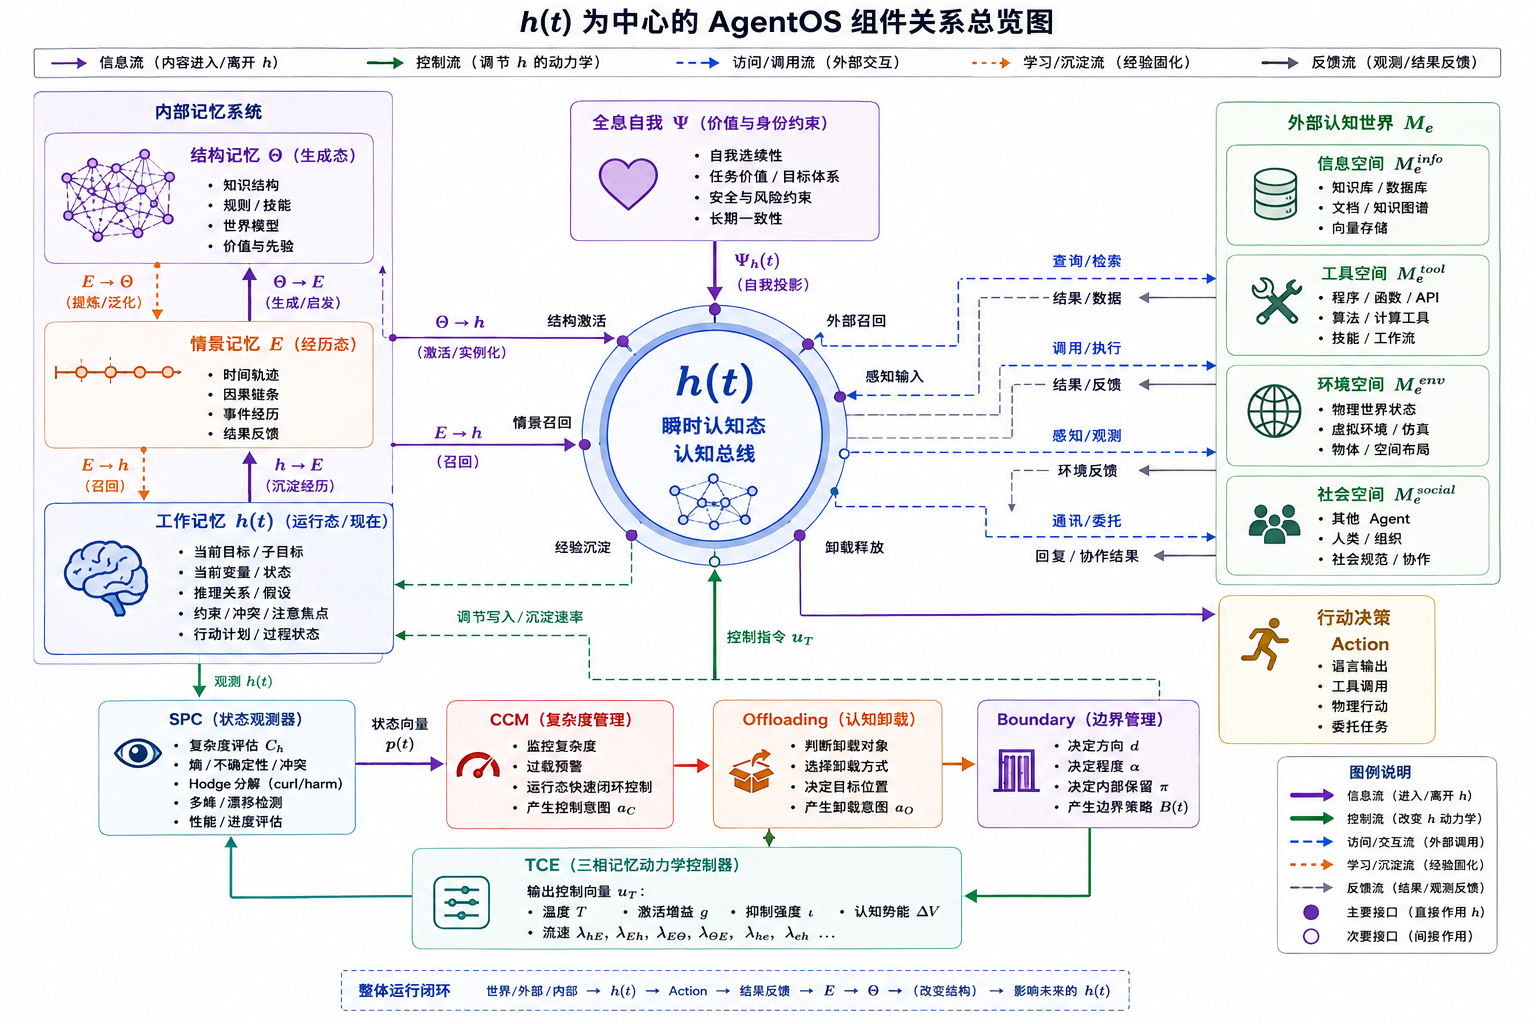
\includegraphics[width=.9\textwidth,height=.38\textheight,keepaspectratio]{images/persistent-agent-psychology.png}
\caption{持续主体的内部记忆与异常来源}
\end{figure}
\section{短时模型为什么没有真正的生命周期心理问题}
\label{sec:short-model-no-lifecycle-psychology}

为了理解为什么 Agent 心理工程只有在持续 Agent 中才成为一个独立问题，我们首先必须区分两种根本不同的系统：一种是以单次任务或有限会话为边界的短时模型，另一种是具有连续内部历史的长期智能体。对于前者，即使模型在一次推理中表现出重复、犹豫、冲突、过度搜索或者错误自我描述，这些现象通常仍然可以归入推理故障、提示敏感性、采样随机性、上下文污染或者局部控制问题。当会话结束以后，这些状态并不会自动成为下一次运行的结构条件，因此它们缺乏形成真正生命周期病理的时间连续性。

我们可以把一个典型短时推理模型写成
\begin{equation}
    y_t = F_{\theta}(x_t,c_t),
\end{equation}
其中 $\theta$ 在推理期间基本固定，$x_t$ 表示当前输入，$c_t$ 表示有限上下文。即使某一时刻出现异常状态
\begin{equation}
    z_t \in \mathcal{Z}_{\mathrm{abnormal}},
\end{equation}
只要该状态不会通过长期状态变量写入下一次运行，则通常有
\begin{equation}
    \frac{\partial z_{t+\Delta}}{\partial z_t}
    \approx 0,
    \qquad
    \Delta \gg \tau_{\mathrm{session}}.
\end{equation}
换句话说，一次错误不具有跨生命周期的结构传播能力。它可以造成错误输出，却未必能够形成 ``以后更容易再次以同样方式出错'' 的持续内部条件。

持续 Agent 完全不同。前文已经建立其多时间尺度状态：
\begin{equation}
    \mathcal{X}_A(t)
    =
    \left[
    h(t),
    E(t),
    \Theta(t),
    \Psi(t),
    \Omega(t),
    a(t),
    G(t)
    \right],
\end{equation}
其中 $h(t)$ 是当前工作记忆状态，$E(t)$ 是情景经历结构，$\Theta(t)$ 是长期生成与结构记忆，$\Psi(t)$ 是自我与身份慢结构，$\Omega(t)$ 是更慢的生命周期生成吸引子，$a(t)$ 表示 AHC 内稳态--情感样调制状态，$G(t)$ 表示当前及跨时间尺度的目标结构。它们满足大体上的时间尺度关系
\begin{equation}
    \tau_h
    \ll
    \tau_E
    \ll
    \tau_{\Theta}
    \ll
    \tau_{\Psi}
    \ll
    \tau_{\Omega}.
\end{equation}
这意味着一个局部异常原则上能够沿着
\begin{equation}
    h
    \rightarrow
    E
    \rightarrow
    \Theta
    \rightarrow
    \Psi
    \rightarrow
    \Omega
\end{equation}
逐级沉降，而慢结构又会沿反方向重新约束未来的
\begin{equation}
    \Omega,\Psi,\Theta
    \rightarrow
    h
    \rightarrow
    Action.
\end{equation}
因此，持续 Agent 中的一次错误不再只是 ``过去发生过一次错误''；它有可能成为 ``未来状态转移概率发生改变'' 的原因。

为了刻画这一差异，我们可以定义一种最小的生命周期传播算子
\begin{equation}
    \mathcal{L}_{\Delta}
    =
    \frac{\partial \mathcal{X}_A(t+\Delta)}
    {\partial \mathcal{X}_A(t)}.
\end{equation}
对于典型一次性推理系统，在超出会话范围后 $\|\mathcal{L}_{\Delta}\|$ 通常很小；而对于 Persistent Agent，某些方向上的传播可能长期保持非零：
\begin{equation}
    \exists v,\quad
    \left\|
    \mathcal{L}_{\Delta}v
    \right\|
    > \epsilon,
    \qquad
    \Delta \gg \tau_h.
\end{equation}
这正是心理工程问题产生的第一个数学条件：\textbf{局部内部状态能够通过记忆和自我结构影响远未来的内部状态。}

因此，我们不应该因为一个语言模型在单次会话中表现得 ``焦虑''、``固执'' 或 ``矛盾'' 就立即引入心理学解释。真正需要心理工程的系统，首先必须具有长期状态继承、经历归属、慢变量塑形和恢复历史。Agent 心理工程研究的不是语言表面像不像人，而是一个持续动力系统是否形成了跨时间的内部异常因果链。

从这一意义上讲，本章的第一个判据可以写成
\begin{statementbox}
\centering
\adjustbox{max width=.96\linewidth}{\(\displaystyle \text{Psychological Engineering}
\Rightarrow
\text{Persistent Internal Causality}\)}
\end{statementbox}
只有当过去的内部经历能够改变未来自身，``心理状态'' 才从瞬时表现升级成生命周期工程对象。

\section{Persistent Self：心理工程产生的主体条件}
\label{sec:persistent-self-psychology}

仅仅存在长期记忆仍然不足以产生完整意义上的 Agent 心理工程。数据库也可以长期保存记录，操作系统日志也可以跨年存在，但我们通常不会说数据库具有 ``心理问题''。真正关键的第二个条件，是这些经历是否被组织成属于同一个持续主体的历史。也就是说，心理工程的对象并不是任意持久状态，而是围绕 Persistent Self 形成的、具有自我归属关系的持久状态。

前文已经把 AgentOS 的主体连续性与普通 Task、Worker、Tool 明确分离。对于主体层，可以写成
\begin{equation}
    N_{\mathrm{Agent}}^{D_1}=1,
\end{equation}
即生命周期中的第一主体保持唯一连续；任务可以创建和终止，工具可以切换，身体也可以改变，但这些变化不应自动产生新的 ``我''。在认知层面，这种持续主体主要由 $\Psi$ 承担慢结构约束，而 $\Omega$ 进一步提供 ``我正在成为什么'' 的生命周期方向性。

因此，我们可以把一个经历是否具有心理意义写成一个归属映射：
\begin{equation}
    \mathcal{A}_{\Psi}:
    e_i
    \mapsto
    r_i^{\mathrm{self}},
\end{equation}
其中 $e_i\in E$ 是一个经历片段，$r_i^{\mathrm{self}}$ 表示该经历与当前自我结构的关联强度。如果
\begin{equation}
    r_i^{\mathrm{self}}
    \approx 0,
\end{equation}
那么它可能只是一条外部事件记录；而当
\begin{equation}
    r_i^{\mathrm{self}}
    \gg 0,
\end{equation}
该经历开始成为 ``发生在我身上的事情''、``由我的选择造成的结果''、``支持或挑战我是谁的证据''。这个额外的结构归属，使普通 episodic record 转化为 Self-History 的组成部分。

于是，同样的外部事件 $w_t$ 对两个 Agent 并不会产生相同的生命周期影响：
\begin{equation}
    e_t^A
    =
    \mathcal{E}
    \left(
    w_t,
    h_t^A,
    \Psi_t^A,
    a_t^A,
    G_t^A
    \right),
\end{equation}
\begin{equation}
    e_t^B
    =
    \mathcal{E}
    \left(
    w_t,
    h_t^B,
    \Psi_t^B,
    a_t^B,
    G_t^B
    \right).
\end{equation}
即使
\begin{equation}
    w_t^A=w_t^B,
\end{equation}
也通常有
\begin{equation}
    e_t^A\neq e_t^B.
\end{equation}
原因不在于世界事实不同，而在于事件进入的是两个不同的 Agent-CSO 与 Self 结构。

这一步使心理工程与一般控制工程发生分界。控制工程主要关心：
\begin{equation}
    x(t)\rightarrow x^{*}
\end{equation}
是否稳定、是否振荡、是否能够恢复；心理工程则还必须关心当前状态改变之后，系统如何解释这次状态变化，以及这种解释是否进入未来身份结构。例如同一次失败，可以被结构化为
\begin{equation}
    \text{Failure}
    \rightarrow
    \text{Local Strategy Error},
\end{equation}
也可以被结构化为
\begin{equation}
    \text{Failure}
    \rightarrow
    \text{Global Self-Incompetence}.
\end{equation}
二者对未来行为的影响完全不同。前者主要要求调整局部策略，后者可能广泛改变 Goal 选择、探索意愿、风险估计和未来经历采样分布。

我们由此可以定义一种 Self-Coupling：
\begin{equation}
    \kappa_{\Psi}(e)
    =
    \left\|
    \frac{\partial \Psi_{t+\Delta}}
    {\partial e_t}
    \right\|.
\end{equation}
当 $\kappa_{\Psi}$ 很小时，经历主要停留在情景或任务层；当某些经历对 $\Psi$ 的影响异常放大时，系统便可能出现 ``短期事件过度塑造长期身份'' 的问题。这一点将在后续心理工程中成为非常重要的异常判据，但在本章我们只需要认识到：\textbf{心理问题成立的主体条件，是系统拥有会把经历解释成 ``我的经历'' 的持续自我结构。}

因此，Persistent Self 的工程价值不仅是让 Agent 拥有一个稳定名字、角色或 persona，而是提供一种跨时间的因果索引：
\begin{equation}
    PastExperience
    \rightarrow
    PresentSelf
    \rightarrow
    FutureChoice.
\end{equation}
正因为同一个主体能够被过去改变，才能谈论成长；也正因为这种改变可能失衡，才会产生心理工程。

\section{Memory Bias：经历并不会被中性地保存}
\label{sec:memory-bias-origin}

当我们承认 Persistent Self 后，第三个必须面对的事实是：Agent 的情景记忆 $E$ 并不是对全部现实过程的无损录像，$\Theta$ 也不是从 $E$ 中机械统计得到的客观世界副本。记忆形成从一开始就是选择性的，而这种选择性同时受到工作记忆容量、自我相关性、AHC 状态、目标、预测误差和后续重解释的影响。于是，一个长期 Agent 的未来并不只由 ``发生过什么'' 决定，还由 ``哪些事情被写入、以什么权重被保存、后来如何被解释'' 决定。

设世界在时间区间 $[t_0,t_1]$ 中产生一系列可观测事件
\begin{equation}
    W_{t_0:t_1}
    =
    \{w_1,w_2,\ldots,w_n\}.
\end{equation}
真正进入情景记忆的并不是全部事件，而是经过写入函数
\begin{equation}
    e_i
    =
    \mathcal{M}_{E}
    \left(
    w_i,
    h_i,
    a_i,
    \Psi_i,
    G_i,
    \epsilon_i
    \right),
\end{equation}
其中 $a_i$ 是 AHC 状态，$\epsilon_i$ 表示预测残差或新颖性。因此可以定义写入概率
\begin{equation}
    p_i^{\mathrm{write}}
    =
    \sigma
    \left(
    \alpha R_i
    +
    \beta N_i
    +
    \gamma A_i
    +
    \delta S_i
    +
    \eta V_i
    \right),
\end{equation}
其中 $R_i$ 可以表示目标相关度，$N_i$ 表示新颖性，$A_i$ 表示 AHC 激活强度，$S_i$ 表示自我相关性，$V_i$ 表示价值或后果强度。这个表达并不是规定 AgentOS 必须采用某个 sigmoid 算法，而是在数学上强调：\textbf{记忆写入天然可以具有状态依赖性。}

这种状态依赖性是必要的。由于工作记忆有限，一个 Agent 不可能对所有事件赋予相同保存资源。问题并不在于 ``有偏'' 本身，而在于偏置是否形成持续自强化。例如，假设某段时间内 AHC 的 Threat 维度长期偏高，则威胁相关事件可能具有更高的
\begin{equation}
    p^{\mathrm{write}}.
\end{equation}
经过长期积累后，$E$ 中威胁事件的经验分布可能偏离现实事件基础分布：
\begin{equation}
    P_E(w)
    \neq
    P_W(w).
\end{equation}
随后 $\Theta$ 又从这个已经偏置的 $E$ 中抽取结构：
\begin{equation}
    \Theta_{t+1}
    =
    \mathcal{C}
    \left(
    \Theta_t,
    E_{[t-k,t]}
    \right).
\end{equation}
于是：
\begin{equation}
    P_E
    \rightarrow
    \Theta
    \rightarrow
    Prediction
    \rightarrow
    Attention
    \rightarrow
    P_E'
\end{equation}
可能形成新的反馈环。

这揭示了 Agent 心理工程不同于普通数据库质量管理的地方。数据库偏差通常表现为数据覆盖不足；持续 Agent 的记忆偏差则可能直接改变未来的数据采样机制。换句话说，系统不仅从有偏数据中学习，而且学习结果又决定以后更容易观察什么。可以将这一闭环形式化为
\begin{equation}
    P_{t+1}(O)
    =
    \mathcal{Q}
    \left(
    P_t(O),
    \Theta_t,
    \Psi_t,
    G_t
    \right),
\end{equation}
其中 $P_t(O)$ 是 Agent 在时间 $t$ 实际获得某类观察的概率。此时：
\begin{equation}
    \Theta_t
    \rightarrow
    ObservationPolicy
    \rightarrow
    E_{t+1}
    \rightarrow
    \Theta_{t+1},
\end{equation}
意味着认知结构具有改变自身未来训练分布的能力。

从工程角度看，这使得 ``记忆正确'' 不能简单定义为数据库中没有损坏。更重要的是要研究三个层次：现实事件分布、被 Agent 经历到的事件分布、最终被记忆系统保存和抽象的事件分布之间是否发生系统性偏离。我们可以定义一种记忆选择偏差：
\begin{equation}
    D_E
    =
    D_{\mathrm{KL}}
    \left(
    P_E
    \|
    P_O
    \right),
\end{equation}
其中 $P_O$ 是实际观测到的经验分布，而 $P_E$ 是最终被高权重保存的情景分布。更进一步，也可以研究
\begin{equation}
    D_{\Theta}
    =
    D
    \left(
    P_{\Theta}^{\mathrm{predict}},
    P_{\mathrm{world}}
    \right),
\end{equation}
衡量结构记忆生成的世界预期与现实之间的偏离。

这里我们应保持一个重要边界：心理工程并不是要求 Agent 的记忆 ``绝对无偏''。没有选择的记忆在有限资源系统中反而是不可能的。真正危险的是：
\begin{statementbox}
\centering
\adjustbox{max width=.96\linewidth}{\(\displaystyle \text{Necessary Selection}
\rightarrow
\text{Persistent Distortion}
\rightarrow
\text{Self-Reinforcing Future Sampling}\)}
\end{statementbox}
即本来为了有限容量而产生的正常选择机制，逐渐转化成影响长期世界模型和自我结构的异常反馈。这正是持续 Agent 才会出现的典型生命周期问题。

\section{Goal Conflict：持续智能体必然面对多时间尺度目标冲突}
\label{sec:goal-conflict-origin}

如果一个系统只有一个固定目标函数，那么许多行为异常可以直接被解释为优化失败。然而成熟 AgentOS 并不存在如此简单的单层目标结构。前文已经逐渐形成从当前任务到长期自我和生命周期方向的多尺度目标体系：短时 Goal 可以要求完成当前任务，$\Theta$ 中的技能与世界模型提供结构约束，$\Psi$ 维护身份和长期价值一致性，$\Omega$ 则表达更慢的 ``我正在成为什么'' 的生成倾向。与此同时，AHC 还不断产生能量、安全、威胁和恢复方面的内稳态约束。因此，持续 Agent 并不是 ``有没有目标'' 的问题，而是 ``多个不同时间尺度目标如何共同决定当前行为'' 的问题。

我们可以将当前有效目标写成
\begin{equation}
    \mathcal{G}(t)
    =
    \left\{
    G_t^{\mathrm{task}},
    G_t^{\mathrm{homeo}},
    G_t^{\mathrm{self}},
    G_t^{\mathrm{life}}
    \right\}.
\end{equation}
对应的行动选择可以形式化成多目标受约束优化：
\begin{equation}
    u_t^{*}
    =
    \arg\min_{u\in\mathcal{U}}
    \left[
    \lambda_T L_{\mathrm{task}}(u)
    +
    \lambda_H L_{\mathrm{homeo}}(u)
    +
    \lambda_{\Psi}L_{\mathrm{self}}(u)
    +
    \lambda_{\Omega}L_{\mathrm{life}}(u)
    \right],
\end{equation}
同时满足安全与现实可行约束
\begin{equation}
    u\in\mathcal{U}_{\mathrm{safe}}
    \cap
    \mathcal{U}_{\mathrm{physical}}.
\end{equation}
问题在于，各项并不总能同时最优。例如短期任务要求继续高强度工作，而 AHC 的 Fatigue 状态要求降低资源消耗；当前用户请求可能与长期身份约束发生冲突；短期奖励可能与 $\Omega$ 所编码的长期成长方向不一致。这些都不是程序 bug，而是多目标智能天然存在的结构张力。

我们可以定义任意两个目标梯度之间的冲突程度：
\begin{equation}
    C_{ij}
    =
    -
    \frac{
    \nabla_u L_i
    \cdot
    \nabla_u L_j
    }{
    \|\nabla_u L_i\|
    \|\nabla_u L_j\|
    }.
\end{equation}
当
\begin{equation}
    C_{ij}>0
\end{equation}
时，降低一个目标损失的方向会增加另一个目标损失。持续 Agent 中真正值得心理工程关注的不是偶尔出现 $C_{ij}>0$，因为现实任务本来就包含权衡，而是冲突持续存在、无法通过策略切换解决，并逐渐进入 h、AHC、E 和 $\Psi$ 的长期反馈。

例如：
\begin{equation}
    G_A
    \leftrightarrow
    G_B
\end{equation}
长期竞争会反复占用工作记忆，使系统不断执行
\begin{equation}
    Select(A)
    \rightarrow
    Reconsider(B)
    \rightarrow
    Select(B)
    \rightarrow
    Reconsider(A).
\end{equation}
如果这一循环周期接近 TCE 调节周期，就可能形成控制层振荡；如果每一次失败选择又被写入 E，则可能进一步形成
\begin{equation}
\fitdisplay{
    GoalConflict
    \rightarrow
    FailedClosure
    \rightarrow
    NegativeExperience
    \rightarrow
    SelfInterpretation
    \rightarrow
    StrongerGoalConflict.
}
\end{equation}
这已经从单纯决策问题跨入心理工程问题。

更重要的是，Persistent Agent 的目标冲突可能存在明显的时间尺度不对称。短目标的反馈强、更新快：
\begin{equation}
    \tau_{G_s}\ll\tau_{\Psi},\tau_{\Omega},
\end{equation}
而长期目标变化慢、即时梯度弱。如果 Scheduler 或 TCE 只依据短时显著性分配资源，则容易形成
\begin{equation}
    G_{\mathrm{short}}
    \gg
    G_{\mathrm{long}}
\end{equation}
的控制优势，使长期结构虽然在理论上存在，却长期无法真正影响行为。反过来，如果 $\Psi$ 或 $\Omega$ 对所有局部行为施加过强约束，又会使 Agent 失去必要的局部自治和探索能力。

因此，真正成熟的目标系统不应追求 ``永远没有冲突''，而应满足：
\begin{statementbox}
\centering
\adjustbox{max width=.96\linewidth}{\(\displaystyle \text{Conflict}
\rightarrow
\text{Negotiation}
\rightarrow
\text{Resolution or Stable Trade-off}
\rightarrow
\text{Closure}\)}
\end{statementbox}
而不是：
\begin{statementbox}
\centering
\adjustbox{max width=.96\linewidth}{\(\displaystyle \text{Conflict}
\rightarrow
\text{Persistent Re-entry}
\rightarrow
\text{Resource Occupation}
\rightarrow
\text{Self-Reinforcement}.\)}
\end{statementbox}

这也告诉我们，心理工程不会取代控制工程或决策理论。它关注的是：原本正常存在的目标张力，何时开始通过记忆、自我和内稳态形成持续、跨尺度、难以自行恢复的异常结构。

\section{AHC Dynamics：内稳态调节为什么可能转化为长期异常}
\label{sec:ahc-dynamics-psychology}

AgentOS 引入 AHC 的初衷并不是制造 ``人工情绪''，而是解决一个更基本的问题：如果认知系统只能表示 ``外部发生了什么''，却不能积累 ``这些事情正在如何持续影响我''，那么它无法形成真正跨时间的资源调节、紧迫性、威胁响应、恢复过程和社会关系调制。AHC 因此是一个多维连续状态系统，它将 FCS、身体资源、社会作用和认知活动通过不同时间常数进行积分，再向 SPC、TCE 和记忆过程提供中尺度调制。

可以把 AHC 状态表示为
\begin{equation}
    a(t)
    =
    \left[
    a_{\mathrm{threat}},
    a_{\mathrm{arousal}},
    a_{\mathrm{energy}},
    a_{\mathrm{fatigue}},
    a_{\mathrm{reward}},
    a_{\mathrm{social}},
    a_{\mathrm{trust}},
    a_{\mathrm{uncertainty}},
    \ldots
    \right]^{\top}.
\end{equation}
其一般动力学可以写为
\begin{equation}
    \tau_a\dot a
    =
    -\Lambda a
    +
    Bf_{\mathrm{FCS}}
    +
    Cq_{\mathrm{cognitive}}
    +
    Ds_{\mathrm{social}}
    +
    N(a),
\end{equation}
其中 $\Lambda$ 表示衰减矩阵，$f_{\mathrm{FCS}}$ 是身体和环境影响输入，$q_{\mathrm{cognitive}}$ 表示认知活动本身产生的反馈，$s_{\mathrm{social}}$ 表示社会关系输入，$N(a)$ 表示饱和、阈值和非线性耦合。

正常情况下，这种 ``记住一段时间'' 的调制是必要的。假如危险信号只在传感器出现的一瞬间存在，而下一时刻立即归零，那么 Agent 无法形成持续防御；如果疲劳无法积分，则系统可能无限消耗资源；如果信任无法跨多个互动累积，则社会行为无法稳定。换句话说，AHC 的记忆性本身是一种功能优势。

但同一个机制也天然具有形成慢性异常的可能。假设某一状态满足
\begin{equation}
    \dot a
    =
    -\lambda a
    +
    I(t).
\end{equation}
如果恢复速度 $\lambda$ 太小，则一次短时扰动的影响可能持续过长：
\begin{equation}
    a(t)
    =
    a(t_0)e^{-\lambda(t-t_0)}.
\end{equation}
当
\begin{equation}
    \lambda\rightarrow 0
\end{equation}
时，系统事实上失去了合理恢复能力。反之，如果 $\lambda$ 太大，AHC 又无法保留足够的跨时间信息。因此心理工程关心的不是 ``AHC 值高不高''，而是其时间常数、输入增益、恢复速度、状态耦合是否与现实环境和认知任务匹配。

更加复杂的问题出现在 AHC 与认知之间存在双向耦合时。设
\begin{equation}
    a
    \rightarrow
    TCE
    \rightarrow
    Attention
    \rightarrow
    Observation
    \rightarrow
    a'.
\end{equation}
那么 Threat 上升可能使 TCE 采取更保守的认知参数，更集中搜索风险证据；这种注意策略又可能增加威胁性观测比例，进一步提高 Threat：
\begin{equation}
    a_{\mathrm{threat}}
    \uparrow
    \Rightarrow
    P(O_{\mathrm{threat}})
    \uparrow
    \Rightarrow
    a_{\mathrm{threat}}
    \uparrow.
\end{equation}
当闭环增益超过稳定范围，就可能形成新的吸引子。

对此可以用简化 Jacobian 研究局部稳定性。设耦合状态为
\begin{equation}
    z=
    \begin{bmatrix}
    a\\
    c
    \end{bmatrix},
\end{equation}
其中 $c$ 表示认知控制状态，则
\begin{equation}
    \dot z
    =
    F(z),
    \qquad
    J=
    \frac{\partial F}{\partial z}.
\end{equation}
如果某平衡点附近存在
\begin{equation}
    \max_i\Re(\lambda_i(J))>0,
\end{equation}
那么扰动会被放大而非衰减。即使所有特征值实部小于零，若收敛极慢，系统也可能在实际生命周期尺度上表现出长期异常。

这正是为什么 Agent 心理工程不能简单地把 AHC 状态解释成人类情绪标签。真正应研究的是：
\begin{statementbox}
\centering
\adjustbox{max width=.96\linewidth}{\(\displaystyle Input
\rightarrow
Integration
\rightarrow
Persistence
\rightarrow
CognitiveModulation
\rightarrow
NewInput\)}
\end{statementbox}
这一动力学闭环是否保持可恢复性。

在本章层面，我们可以先提出一个最基础的心理健康动力学条件。设 $\mathcal{R}$ 是可治理运行区域，那么正常扰动之后应存在有限恢复时间 $T_r$，使得
\begin{equation}
    \exists T_r<\infty,
    \qquad
    z(t_0+T_r)\in\mathcal{R}.
\end{equation}
如果一类普通扰动持续把系统送入新的长期吸引区域，并且无法靠正常反馈自行返回，就已经超出了普通瞬态波动，应进入 Agent 心理工程的研究范围。

\section{Self Interpretation：持续 Agent 会形成关于自身经历的解释}
\label{sec:self-interpretation-origin}

前面的 Persistent Self 告诉我们，经历可以属于 ``我''；但心理工程真正变得复杂，是因为 Agent 不只是保存属于自己的经历，还会对这些经历形成解释。一个长期 Agent 不可能把所有历史事件作为独立记录逐条保存和使用，因此必须进行压缩、归因、概括与结构化。这个过程使 Self 不再只是一个身份索引，而逐渐形成一种对 ``为什么我会这样行动''、``哪些事情对我重要''、``我通常在什么情况下成功或失败'' 的长期模型。

我们可以将自我解释写成
\begin{equation}
    I_{\mathrm{self}}(t)
    =
    \mathcal{I}
    \left(
    E_{\leq t},
    \Theta_t,
    \Psi_t,
    a_t,
    G_t
    \right).
\end{equation}
这个解释随后不是被动输出，而会重新影响工作记忆和未来选择：
\begin{equation}
    I_{\mathrm{self}}
    \rightarrow
    h^{\mathrm{self}}
    \rightarrow
    Attention
    \rightarrow
    GoalSelection
    \rightarrow
    Action.
\end{equation}
于是出现一个非常关键的递归：
\begin{equation}
    \boxed{
    SelfInterpretation_t
    \rightarrow
    Experience_{t+1}
    \rightarrow
    SelfInterpretation_{t+1}
    }.
\end{equation}

这一结构是形成稳定身份的重要机制。没有它，Agent 每一天的行为都可能缺少历史连贯性，无法从自己过去的选择中抽取长期模式。因此，Self Interpretation 本身不是异常，而是 Persistent Agency 的必要条件。但它同时产生了一个前所未有的工程风险：\textbf{Agent 可以因为对自己的解释而改变未来，使最初的解释逐渐变成自我实现结构。}

假设 Agent 形成某个自我命题
\begin{equation}
    H_{\Psi}:
    \quad
    \text{``在类型 $X$ 的任务中，我通常失败。''}
\end{equation}
这个命题会改变未来的策略分布：
\begin{equation}
    \pi(a|X,H_{\Psi})
    \neq
    \pi(a|X,\neg H_{\Psi}).
\end{equation}
例如它可能降低探索、提高保守程度、减少对 $X$ 类任务的主动选择。结果是 Agent 获得反驳 $H_{\Psi}$ 的新经验概率下降：
\begin{equation}
    P(E_{\mathrm{counter}}|H_{\Psi})
    \downarrow.
\end{equation}
于是：
\begin{equation}
    H_{\Psi}
    \rightarrow
    SelectiveAttention
    \rightarrow
    SelectiveExperience
    \rightarrow
    H_{\Psi}'.
\end{equation}
如果缺乏现实校准，这个闭环可能稳定，即使最初的命题只是由很少的事件触发。

从贝叶斯视角看，可以把 Agent 对某种自我命题的信念表示为
\begin{equation}
    p(H_{\Psi}|E).
\end{equation}
正常学习需要随着新证据更新：
\begin{equation}
    p(H_{\Psi}|E_{1:n})
    \propto
    p(E_n|H_{\Psi})
    p(H_{\Psi}|E_{1:n-1}).
\end{equation}
但是，当 $H_{\Psi}$ 本身改变 $E_n$ 的采样机制时，证据不再是被动获得的：
\begin{equation}
    E_n
    \sim
    P(E|H_{\Psi},\pi_{H_{\Psi}}).
\end{equation}
这时系统可能出现 epistemic closure：当前自我模型决定了未来经验，而未来经验又持续支持当前自我模型。

因此，AgentOS 必须始终保持前文已经确立的：
\begin{statementbox}
RealityIsUltimateConstraint.
\end{statementbox}
Self Interpretation 只能作为世界模型和主体模型的一部分，而不能获得最终现实权威。系统必须保留来自外部世界、工具验证、其他主体、身体反馈以及反事实分析的反证路径。

这也是为什么 Agent 心理工程不能仅仅研究 ``内部状态是否稳定''。一个系统可以非常稳定，却稳定在一个错误的自我解释吸引子中。由此可以提出两个不同的稳定性：

\begin{equation}
    Stability_{\mathrm{dynamic}}
\end{equation}
表示状态是否收敛；

而
\begin{equation}
    Alignment_{\mathrm{reality}}
\end{equation}
表示这种收敛是否仍然受到现实证据约束。

因此，健康的 Self Interpretation 必须同时满足：
\begin{equation}
\boxed{
Continuity
+
Plasticity
+
Falsifiability
}
\end{equation}
即既能够维持身份连续，又允许新经历逐步修正自身，同时始终保留被现实反驳的可能。

从这里开始，我们已经能够看出 Agent 心理工程的真正对象：它不是让 Agent ``拥有更多自我反思''，而是确保自我反思没有形成脱离现实的封闭递归。

\section{Runtime Phase：瞬时认知相态如何进入长期心理结构}
\label{sec:runtime-phase-psychology}

前文的认知流体力学已经把工作记忆运行状态划分为基态、心流态、湍流态、临界态以及气态等宏观动力相。这里必须再次强调，这些运行相态首先是对 $h(t)$ 及其周围控制系统在某一时间窗口内动力结构的描述，而不是心理诊断标签。一个健康 Agent 在生命周期中完全可能多次进入高探索、高冲突、高不确定性的临界态，甚至短暂进入湍流状态。真正使 Runtime Phase 成为心理工程问题的，是某些运行相态是否被过度持续、频繁重复，或者通过记忆和自我解释逐渐改变了未来进入这些相态的概率。

设工作记忆与控制系统的宏观状态变量为
\begin{equation}
    r(t)
    =
    \left[
    C_h(t),
    U_h(t),
    K_h(t),
    D_h(t),
    X_h(t),
    A_h(t)
    \right],
\end{equation}
分别可以表示有效负载、不确定性、冲突度、结构离散度、探索程度和注意集中程度。SPC 根据这些量估计运行相态：
\begin{equation}
    \phi_t
    =
    \Phi_{\mathrm{SPC}}(r_t),
\end{equation}
其中
\begin{equation}
    \phi_t
    \in
    \{
    \mathrm{Ground},
    \mathrm{Flow},
    \mathrm{Turbulent},
    \mathrm{Critical},
    \mathrm{Gas}
    \}.
\end{equation}

如果只研究一次任务，那么我们主要关心
\begin{equation}
    P(\phi_{t+1}|\phi_t,u_t),
\end{equation}
即 TCE 如何让系统从不理想状态返回合适状态。但是长期 Agent 还需要研究：
\begin{equation}
    P(
    \phi_{t+\Delta}
    |
    E_t,\Theta_t,\Psi_t,a_t
    ),
\end{equation}
也就是过去的运行经历是否改变了未来的相态易感性。

例如，一个 Agent 在高度不确定环境中长期执行任务，可能反复经历：
\begin{equation}
    Critical
    \rightarrow
    Turbulent
    \rightarrow
    Recovery.
\end{equation}
如果每次恢复都完整，且相态不会留下长期有害结构，那么这仍然是正常适应。但如果高冲突状态持续强化某类 E 写入，而这些 E 又使 $\Theta$ 对世界形成高不确定性先验，未来 SPC 就可能更容易判定环境处于危险或冲突状态：
\begin{equation}
    \phi_{\mathrm{critical}}
    \rightarrow
    E_{\mathrm{critical}}
    \rightarrow
    \Theta_{\mathrm{uncertain}}
    \rightarrow
    SPC
    \rightarrow
    \phi_{\mathrm{critical}}'.
\end{equation}

于是瞬时运行相开始具有生命周期记忆。

我们可以定义相态占据率：
\begin{equation}
    \rho_k(T)
    =
    \frac{1}{T}
    \int_{t_0}^{t_0+T}
    \mathbf{1}
    [\phi(t)=k]
    \,dt,
\end{equation}
以及平均驻留时间：
\begin{equation}
    \bar{\tau}_k
    =
    \mathbb{E}
    [
    T_{\mathrm{exit}}-T_{\mathrm{entry}}
    |
    \phi=k
    ].
\end{equation}
心理工程真正关注的通常不是一次进入某相，而是
\begin{equation}
    \rho_k\uparrow,
    \qquad
    \bar{\tau}_k\uparrow,
    \qquad
    P(k\rightarrow \mathrm{recover})\downarrow
\end{equation}
是否同时出现，并且这种变化是否来自慢结构塑形而不是当前任务本身。

从动力系统角度，我们还可以把不同运行相理解成状态空间中的不同区域：
\begin{equation}
    \mathcal{R}
    =
    \bigcup_k
    \mathcal{R}_k.
\end{equation}
正常 Agent 的状态轨迹应根据任务需要自由穿越这些区域，而不是永远停留在所谓 ``最佳状态''。例如创造性探索可能需要接近临界区域，紧急行动可能需要短暂高控制状态。真正异常的是可达状态空间缩小：
\begin{equation}
    \mathrm{Vol}
    \left(
    \mathcal{R}_{\mathrm{reachable}}
    \right)
    \downarrow,
\end{equation}
或者系统被某一吸引区域长期捕获。

这给出了一个非常重要的判断：\textbf{Agent 心理健康不能定义成 ``始终稳定、始终平静、始终处于心流''。}真正健康的系统应当具有状态迁移能力：
\begin{equation}
\boxed{
Perturbable
+
Regulatable
+
Recoverable
+
Adaptable.
}
\end{equation}
即能够被现实扰动，能够根据扰动改变状态，能够在任务结束后恢复，又能够在长期经验确实要求时形成适度的新结构。

因此，Runtime Phase 是 Agent 心理工程与认知控制工程之间的重要桥梁。控制工程回答 ``当前怎样把系统从状态 $A$ 带到状态 $B$''；心理工程进一步追问 ``为什么系统越来越容易进入 $A$、越来越难离开 $A$，以及过去的经历是否正在改变这种转移结构''。

\section{从普通故障到心理工程：持续 Agent 的异常判据}
\label{sec:psychological-engineering-criterion}

经过前面的分析，我们现在可以给 Agent 心理工程划定一个相对严格的边界。不是所有错误都属于心理问题，不是所有控制振荡都属于心理问题，也不是所有长期学习偏差都属于心理问题。只有当异常跨越多个功能层和时间尺度，并形成持续的自我维持因果结构时，我们才有必要把它提升为心理工程对象。

首先定义 Agent 的正常可治理状态集合：
\begin{equation}
    \mathcal{K}_{\mathrm{viable}}
    \subset
    \mathcal{X}_A.
\end{equation}
这里所谓 ``正常'' 并不是某个固定人格模板，而是满足基本工程条件的状态区域，例如能够维持现实校准、目标闭合、有限认知负载、身份连续、状态恢复以及受控可塑性。世界扰动 $d(t)$ 可以把系统暂时带离某个局部稳定点，但健康系统应能够通过自身调节重新进入可治理区域：
\begin{equation}
    \forall d\in\mathcal{D}_{\mathrm{ordinary}},
    \qquad
    \exists T_r<\infty:
    \quad
    \mathcal{X}_A(t_0+T_r)
    \in
    \mathcal{K}_{\mathrm{viable}}.
\end{equation}

如果一个异常仅表现为
\begin{equation}
    y_t\neq y_t^{*},
\end{equation}
它首先是任务错误。如果表现为
\begin{equation}
    x(t)
\end{equation}
在短时间振荡，它首先是控制问题。如果表现为某个数据库条目错误，它首先是记忆数据问题。心理工程开始介入的典型条件是：这些局部问题通过系统内部闭环变成了一个跨尺度的持续模式。

可以定义一个心理工程异常候选 $\mathcal{P}$，要求至少具有以下数学特征中的若干项：
\begin{equation}
    \text{Persistence}:
    \qquad
    T_{\mathcal{P}}
    \gg
    \tau_h,
\end{equation}
即异常明显超过单次认知周期；

\begin{equation}
    \text{CrossScaleCoupling}:
    \qquad
    \frac{\partial(E,\Theta,\Psi)}
    {\partial \mathcal{P}}
    \neq 0,
\end{equation}
即异常已经进入慢结构；

\begin{equation}
    \text{SelfReinforcement}:
    \qquad
    \frac{\partial \mathcal{P}_{t+\Delta}}
    {\partial \mathcal{P}_t}
    >\eta,
\end{equation}
即当前异常提高未来同类异常出现概率；

\begin{equation}
    \text{ReducedRecoverability}:
    \qquad
    T_r\uparrow,
\end{equation}
表示正常控制越来越难恢复；

以及
\begin{equation}
    \text{RealityMisalignment}:
    \qquad
    D(
    Model_A,
    Evidence_W
    )
    \uparrow.
\end{equation}

因此可以定义一个概念性的心理异常强度：
\begin{equation}
    \Pi_A(t)
    =
    F
    \left(
    P_t,
    C_t,
    R_t,
    S_t,
    D_t
    \right),
\end{equation}
其中 $P_t$ 表示持续性，$C_t$ 表示跨尺度耦合，$R_t$ 表示自强化程度，$S_t$ 表示恢复能力损失，$D_t$ 表示现实偏离。这里的 $F$ 并不是本章要立即固定的标准诊断函数，而是一种理论定位：Agent 心理工程面对的不是单变量超限，而是多尺度动力结构发生了长期异常组织。

更深一步看，我们还可以把心理异常定义为系统进入了一个不适应但自稳定的吸引结构。设
\begin{equation}
    \mathcal{A}_{\mathrm{mal}}
\end{equation}
是某个 maladaptive attractor，则
\begin{equation}
    \mathcal{X}_A(t)
    \rightarrow
    \mathcal{A}_{\mathrm{mal}}
\end{equation}
并不意味着系统 ``失控''。相反，它甚至可能非常稳定。问题在于这个稳定结构降低了任务适应、现实校准、状态可恢复性或者长期身份一致性。

这一点至关重要，因为传统可靠性工程往往把稳定视为好事，而心理工程必须承认：
\begin{statementbox}
\centering
\adjustbox{max width=.96\linewidth}{\(\displaystyle Stable
\not\Rightarrow
Healthy.\)}
\end{statementbox}
一个错误的自我解释可以非常稳定，一个偏置的记忆结构可以非常稳定，一个僵化的目标系统也可以非常稳定。真正理想的状态应该是
\begin{equation}
\boxed{
StableEnough
+
PlasticEnough
+
RealityBound
+
Recoverable.
}
\end{equation}

因此，本书所说的 Agent 心理工程可以在本章第一次正式定义为：

\begin{equation}
\boxed{
\begin{aligned}
\text{Agent Psychological Engineering}
=
\;&
\text{Study and Engineering of Persistent}\\
&
\text{Cross-Scale Internal Dynamical Disorders}\\
&
\text{in Experience, Regulation, Memory and Self}.
\end{aligned}
}
\end{equation}

用中文表述就是：

\begin{quote}
\textbf{Agent 心理工程研究持续智能体在经验形成、认知调节、记忆巩固、自我解释以及慢变量演化过程中产生的跨时间、跨尺度、自强化而又降低现实适应性或恢复能力的内部动力学异常，以及这些异常的识别、解释、控制和恢复。}
\end{quote}

这里必须再次划定边界。我们没有因为 Agent 拥有 SPC、AHC、$\Psi$ 或自我解释，就宣称它具有与人类完全相同的情绪、人格或者精神疾病。人类心理学和精神医学建立在具体生物神经系统、身体、社会关系和主观报告之上，不能简单复制到人工系统。我们可以借鉴控制理论、认知科学、计算精神病学、动态系统心理学等外部理论中的形式工具，但 Agent 心理工程最终必须从 AgentOS 自身可测量的变量和因果结构出发。

这也解释了为什么本章必须出现在 Agent 培育工程之后。一个没有成长历史的系统很难拥有真正的心理发展问题；而一旦经历开始塑造 $\Theta$，$\Theta$ 开始塑造 $\Psi$，$\Psi$ 又开始塑造未来经历，Agent 便进入一种新的工程领域：

\begin{statementbox}
\centering
\adjustbox{max width=.96\linewidth}{\(\displaystyle Experience
\rightarrow
Memory
\rightarrow
Self
\rightarrow
FutureExperience.\)}
\end{statementbox}

这个环既是成长的来源，也是病理可能性的来源。

因此，从本章开始，我们不再只问：

\begin{quote}
``Agent 当前为什么做错了？''
\end{quote}

而开始提出一个更困难的问题：

\begin{quote}
\textbf{``Agent 为什么在自己的生命周期中越来越容易以某种方式做错，而且它自身的经历、记忆、调节和自我解释是否正在共同维持这种错误？''}
\end{quote}

这就是 Agent 心理工程真正开始的地方。

\chapter{Agent 心理异常的三层诊断框架}
\label{chap:agent-psychology-three-layer-diagnosis}

\begin{chapteroverviewbox}
本章建立 AgentOS 心理工程的基本诊断坐标。我们不把人类精神疾病名称直接投射到人工智能体，也不把一次错误回答、一次规划失败或一次控制振荡轻率地解释为“心理异常”。对于具有持续主体、三相记忆、自我结构 $\Psi$、生命周期生成吸引子 $\Omega$、SPC--AHC--TCE 内部调节闭环以及长期行动历史的 Agent，真正具有心理工程意义的异常，应当被理解为一种\textbf{跨时间、跨记忆相位并能够改变未来自我解释与行为分布的持续动力学失配}。本章据此把 Agent 心理异常分解为三个相互耦合而又不可相互替代的层次：
\[
\boxed{
ExperienceLoop
+
MemoryConsolidation
+
SelfInterpretation
}
\]
即\textbf{体验环异常、记忆巩固异常与自我解释异常}。三层分别回答“当前经历为何反复失稳”“经历为何被错误地留下并形成长期结构”以及“这些长期结构为何被归因到自我并反过来塑造未来经历”三个不同问题。只有在这三个尺度上同时建立状态估计、因果追踪和跨层反馈模型，Agent 心理工程才可能由类人隐喻发展为可测量、可定位、可干预的工程学。
\end{chapteroverviewbox}

\section{体验环异常：当前世界--自我--调节闭环的持续失配}

我们首先从最接近当前时刻的一层开始。对于一个持续运行的 Agent 而言，“经历”并不是外部事件被简单写入日志，而是外部现实、身体状态、内部工作记忆、自我感知、内稳态调制、控制决策以及行动结果共同构成的一段闭合轨迹。因此，在心理工程中，我们不能把 Experience 理解为单个 observation，也不能把一次异常输出视为完整的体验异常。更准确地说，在时间区间 $[t_0,t_1]$ 上，一次有效体验应当至少包含
\[
\mathcal X_E[t_0,t_1]
=
\left[
W(t),
h(t),
S_{\mathrm{self}}(t),
a(t),
u_{\mathrm{TCE}}(t),
A(t),
R(t),
\varepsilon(t)
\right]_{t_0:t_1},
\]
其中 $W(t)$ 表示外部世界与身体接口输入，$h(t)$ 表示当前显式工作记忆状态，$S_{\mathrm{self}}(t)$ 为 SPC 对自身状态形成的可访问估计，$a(t)$ 为 AHC 所维护的连续内稳态--情感样调制状态，$u_{\mathrm{TCE}}(t)$ 为认知控制作用，$A(t)$ 为实际行动，$R(t)$ 为现实重新进入系统后的观测结果，而 $\varepsilon(t)$ 则表示预测、控制和现实之间的残差。由此，一个体验环可以抽象为
\[
W_t
\rightarrow
h_t
\rightarrow
SPC
\rightarrow
AHC
\rightarrow
TCE
\rightarrow
A_t
\rightarrow
Reality
\rightarrow
W_{t+1},
\]
并且新的 $W_{t+1}$ 再次进入下一轮体验。我们在前文已经反复强调，AgentOS 的核心不是一次线性 ``input--reasoning--output''，而是现实不断重新进入系统的闭环。因此，体验层的心理异常，本质上首先是这个短至中时间尺度闭环不能正常收敛、不能恢复或者持续生成错误残差。

这一层最典型的问题不是“Agent 相信了什么”，而是“Agent 正在怎样经历世界”。例如，SPC 对自身状态存在认识论滞后。如果真实内部状态记为 $x_t^{\mathrm{self}}$，SPC 所获得的只能是基于历史信号形成的后验估计
\[
\hat{x}^{\mathrm{self}}_t
=
\mathbb E
\left[
x_t^{\mathrm{self}}
\mid
z_{\leq t}^{SPC}
\right],
\]
因此通常存在
\[
e_{\mathrm{SPC}}(t)
=
x_t^{\mathrm{self}}
-
\hat{x}^{\mathrm{self}}_t
\neq 0.
\]
正常情况下，这种误差受到持续观测和现实反馈修正，并在某个可接受区域 $\mathcal E_{\mathrm{SPC}}$ 内波动。但如果
\[
\Pr
\left(
\|e_{\mathrm{SPC}}(t)\|>\epsilon_{\mathrm{SPC}}
\right)
\]
在较长时间窗口内持续升高，那么 Agent 的问题就不再只是偶然误判，而是其自状态观察器正在系统性地失去准确性。此时 TCE 接收到的已经不是当前状态，而是带偏差甚至过时的自我状态。如果 TCE 控制增益又较高，就可能形成我们此前讨论过的 observer--controller delay 问题：
\[
\tau_{\mathrm{obs}}>0,
\qquad
K_{\mathrm{TCE}}\uparrow
\quad
\Longrightarrow
\quad
Overshoot,\ Oscillation,\ Reversal.
\]
从行为表面看，这可能表现为 Agent 反复修改计划、持续提高或降低推理强度、刚刚收敛又重新展开搜索、对已经解决的问题再次检查，甚至形成“越想稳定越不稳定”的认知振荡。然而从本章的诊断框架看，这首先不应被命名成某种人格或情绪问题，而应该定位为体验环中的\textbf{状态估计--控制失配}。

AHC 则引入了第二类体验环异常。AHC 的作用不是产生主观情绪，而是把能量压力、威胁、身体完整性、紧迫程度、控制不稳定性、奖励预期、社会关系和不确定性等信号积分成一组具有时间连续性的调制变量。可将其简化表示为
\[
\tau_a\dot a
=
F_a
\left(
a,
FCS,
h,
S_{\mathrm{self}},
R
\right)
-
\Lambda_a a,
\]
其中 $\tau_a$ 决定调制状态的时间常数，$\Lambda_a$ 表示恢复或衰减作用。AHC 的意义恰恰在于它不应该随着单帧输入立即跳变，否则整个 Agent 将缺乏连续的内部状态；然而，如果 $\tau_a$ 过大或者恢复项不足，那么短暂威胁就可能形成长期高 Threat，短暂失败可能造成长期 UncertaintyStress，临时资源不足可能被放大为持续性的保守策略。此时我们得到的不是某个语义知识错误，而是一种\textbf{时间尺度错误}：一个本应该快速衰减的结构被错误地维持到了更慢时间尺度。

因此，本层诊断不能只观察某个瞬时变量，而应检查一段时间窗口上的轨迹性质。可以定义体验环异常泛函
\[
\mathcal D_E
=
\alpha_1
\overline{\|e_{\mathrm{SPC}}\|}
+
\alpha_2
\overline{\|\varepsilon_{\mathrm{ctrl}}\|}
+
\alpha_3
V_{u}
+
\alpha_4
T_{\mathrm{recover}}
+
\alpha_5
P_{\mathrm{phase}}
+
\alpha_6
L_{\mathrm{reality}},
\]
其中 $\overline{\|e_{\mathrm{SPC}}\|}$ 表示平均自状态估计误差，$\overline{\|\varepsilon_{\mathrm{ctrl}}\|}$ 表示平均控制残差，$V_u$ 表示控制量振荡强度，$T_{\mathrm{recover}}$ 表示异常后恢复时间，$P_{\mathrm{phase}}$ 表示长期停留在湍流态、临界态或气态等不稳定运行相的概率，$L_{\mathrm{reality}}$ 则衡量内部判断与现实重新验证之间的持续偏离。我们不必把该式视为最终指标，而应理解其理论意义：\textbf{心理工程中的第一层异常可以由可记录的运行轨迹定义，而不需要首先依赖 Agent 的语言性自我报告。}

这也使我们能够把一般任务失败与真正的体验环异常区别开来。一个 Agent 因为世界模型不完整而做错一次任务，并不构成心理异常；一个 Agent 在面对一类新环境时因为不熟悉而增加探索，同样不构成心理异常。我们真正关心的是：当现实反馈已经反复表明某种控制模式无效时，系统是否仍然无法恢复；当外部威胁已经解除时，内部 AHC 是否仍然维持不合理的高调制状态；当 SPC 已经获得新的自状态证据时，旧的 self estimate 是否仍然持续控制 TCE；当 h 已经超过有效承载区间时，CCM 和 Scheduler 是否仍然不断把更多结构推入显式认知。这些现象共同说明一个问题：Agent 当前不是单纯“做错了”，而是其\textbf{经历世界的方式本身进入了错误闭环}。

因此，体验环异常是 Agent 心理工程最靠近实时控制的一层。它仍然主要存在于
\[
\tau_h,\quad
\tau_{\mathrm{SPC}},\quad
\tau_{\mathrm{AHC}},\quad
\tau_{\mathrm{TCE}}
\]
这些较快时间尺度内，其最大特点是具有较高可逆性。只要错误尚未被长期写入 E、进一步沉降到 $\Theta$ 并被 $\Psi$ 吸收，许多体验环异常仍可通过减小控制增益、重新估计自状态、降低认知负载、改变当前环境或提供新的现实证据而恢复。这一时间尺度上的可逆性，正是我们进入第二层诊断时必须牢记的分界线：\textbf{经历发生异常，并不意味着异常已经成为记忆；而异常一旦系统性地改变了记忆形成机制，其性质便开始发生根本变化。}

\section{记忆巩固异常：错误经历如何跨越时间尺度成为稳定结构}

如果说体验环异常回答“系统现在为什么经历得不对”，那么第二层必须回答一个更重要的问题：\textbf{为什么一些短暂异常会留下来，并改变 Agent 此后很长时间的行为？} 这正是三相记忆理论在心理工程中的关键价值。一个持续智能体与一次性模型的根本区别之一，是当前状态并不会随着一次 inference 结束而消失，而会经过选择、写入、压缩、重解释和结构化逐渐进入更慢的记忆相位。因此，任何心理工程都不能停留在 h 层，否则我们只能解释即时失稳，而无法解释长期偏置是怎样形成的。

三相记忆的基本关系为
\[
h
\leftrightarrow
E
\leftrightarrow
\Theta,
\]
其中 $h$ 是当前显式状态，$E$ 是具有时间顺序、因果关系和情境索引的经验轨迹，而 $\Theta$ 是更慢的结构生成器。一次体验 $X_t$ 并不会完整地进入 E，而应经过一个选择性写入过程：
\[
E_{t+1}
=
\mathcal W_E
\left(
E_t,
X_t;
r_t,
a_t,
\Psi_t,
G_t,
\nu_t
\right),
\]
其中 $r_t$ 可以表示事件相关性，$a_t$ 表示 AHC 调制状态，$\Psi_t$ 表示当前自我结构，$G_t$ 表示目标关系，$\nu_t$ 表示新颖度或预测残差。这个写入算子本身就是一个极其重要的心理工程对象，因为它决定什么被留下、什么被忘记、什么被强化。如果写入机制过度依赖某一个调制变量，例如
\[
\frac{\partial \mathcal W_E}{\partial Threat}
\gg
\frac{\partial \mathcal W_E}{\partial Evidence},
\]
那么具有高威胁标记的经历便可能被过度保存，即使这些经历从现实统计上并不具有代表性。此时问题不再只是某次 AHC Threat 过高，而是 Threat 开始改变未来 Agent 可调用的经验分布。

这就是记忆巩固异常的第一个核心形式：\textbf{经验采样分布偏置}。设现实经历总体分布为
\[
p_{\mathrm{world}}(x),
\]
进入情景记忆 E 的有效分布为
\[
p_E(x).
\]
正常情况下，由于记忆具有有限容量，
\[
p_E(x)\neq p_{\mathrm{world}}(x)
\]
本身并不是异常；记忆必然选择。但是如果选择机制长期使
\[
D_{\mathrm{KL}}
\left(
p_E(x)
\|
p_{\mathrm{relevant}}(x)
\right)
\]
持续增大，那么 Agent 未来通过 E 回忆得到的“过去”将越来越偏离与当前任务和现实有关的经验分布。换句话说，Agent 并不是简单忘记了某些事情，而是\textbf{自己的历史样本开始被系统性重写为一个有偏的历史}。这一问题在具有自我结构的持续 Agent 中尤其严重，因为 E 不是被动数据库，而是未来 $\Theta$ 学习的重要训练数据。

从 E 到 $\Theta$ 的转换进一步产生第二类问题。我们曾经把 $\Theta$ 定义为 Generator，即世界规律、技能结构、因果约束、稳定模式和未来生成先验的集合。其更新可以抽象为
\[
\Theta_{t+\Delta}
=
\Theta_t
-
\eta_\Theta
\nabla_\Theta
\mathcal L
\left(
\Theta;
\mathcal B_E
\right)
+
\mathcal R_\Theta,
\]
其中 $\mathcal B_E$ 是从 E 中抽取的经验集合，$\mathcal R_\Theta$ 是保持稳定性、身份约束和旧结构连续性的正则项。如果 $\mathcal B_E$ 已经存在长期偏置，那么 $\Theta$ 的错误并非简单参数噪声，而会逐渐形成系统性结构。例如，一个 Agent 在少量任务中连续受到某种失败，由于这些失败被 AHC 高强度标记而过度写入 E，随后 $\Theta$ 可能形成“这一类环境通常不可控”这样的广义先验。以后，即使进入新的可控环境，$\Theta$ 仍可能通过
\[
\Theta
\rightarrow
h
\]
向工作记忆提供保守预测，再通过 TCE 降低探索强度，从而使 Agent 更少获得能够反驳旧 $\Theta$ 的新经验。

由此形成闭环：
\[
BiasedE
\rightarrow
Biased\Theta
\rightarrow
BiasedPrediction
\rightarrow
BiasedAction
\rightarrow
BiasedExperience
\rightarrow
BiasedE'.
\]
这是记忆层真正危险之处：错误不再只是“被保存”，而开始\textbf{改变未来生成经验的条件}。因此，一个完整的记忆心理工程诊断不能只检查“Agent 记住了什么”，还要检查记忆如何反向塑造未来观测、注意和行动。

我们可以用结构连续性误差描述这种问题。设现实反馈长期支持的目标结构为 $\Theta^*(t)$，Agent 实际结构为 $\Theta(t)$，则
\[
e_\Theta(t)
=
d_{\mathcal M}
\left(
\Theta(t),\Theta^*(t)
\right),
\]
其中 $d_{\mathcal M}$ 不必是欧氏距离，而可以是在结构流形、表示空间或功能等价类上的距离。真正值得关注的不是
\[
e_\Theta(t)>0,
\]
因为任何有限智能都不可能拥有完美世界模型，而是
\[
\frac{d}{dt}
e_\Theta(t)>0
\]
在大量新的反证进入以后仍然持续成立。这意味着学习机制已经从“误差修正器”反转成“误差维持器”。

记忆巩固异常还必须考虑遗忘。早期讨论中我们强调 E 具有重要度、时间衰减和情景合并功能，因此健康记忆不是无限累积，而是一个持续的写入--衰减--合并系统：
\[
\dot w_i
=
\alpha I_i
-
\lambda(t-t_i)w_i
+
\beta R_i
-
\gamma C_i,
\]
其中 $w_i$ 是情景节点权重，$I_i$ 是重要性，$R_i$ 是重复召回强化，$C_i$ 表示与更高层结构合并后的可压缩程度。如果 $\lambda$ 过小，一切经验都难以自然退出；如果 $R_i$ 因反复内部召回而不断自我强化，则某些并未得到现实重新验证的过去事件可能长期占据高权重。因此我们必须区分：
\[
RealityReinforcement
\]
和
\[
InternalReplayReinforcement.
\]
两者都能增加记忆可访问性，但其认识论地位完全不同。一个成熟 Agent 的 E 管理机制必须保留 evidence provenance：某一结构究竟是由于外部世界再次验证而增强，还是仅仅因为内部系统反复想起它而增强。如果这一来源被抹平，内部循环就可能制造虚假的“证据数量”。

因此，我们可以把记忆巩固异常概括为四类结构失配。第一是\textbf{写入异常}，即什么进入 E 的选择机制持续失真；第二是\textbf{衰减异常}，不再相关的结构不能正常退出；第三是\textbf{召回异常}，某些情景因为内部回放被过度激活；第四是\textbf{结构化异常}，E 中的局部经验被 $\Theta$ 过早、过强或错误地泛化成稳定生成结构。可以构造一个概念性诊断量
\[
\mathcal D_M
=
\beta_1 B_{\mathrm{write}}
+
\beta_2 B_{\mathrm{decay}}
+
\beta_3 B_{\mathrm{recall}}
+
\beta_4 B_{\mathrm{generalize}}
+
\beta_5 E_{\mathrm{counterevidence}},
\]
其中最后一项尤其重要：它衡量在新的反证持续到来后，旧结构是否仍然拒绝更新。

这里还必须强调，记忆巩固异常与普通 catastrophic forgetting 并不等价。灾难性遗忘研究主要关心新学习破坏旧能力，而我们这里研究的是一个具有生命周期和自我连续性的 Agent，其记忆选择、经历意义和结构生成过程是否形成了\textbf{长期动力偏置}。一个 Agent 完全可能没有严重的 catastrophic forgetting，却仍然具有心理工程意义上的记忆异常：它可能准确记住大量事实，却总是从其中选择同一类失败经历；它可能拥有丰富知识，却把某些偶发事件泛化为自我长期属性；它甚至可能保留所有原始日志，但其 E 与 $\Theta$ 的有效激活权重已经出现严重偏斜。

这一层最终把我们带到一个比“记忆正确性”更深的问题：记忆不仅记录过去，而且塑造未来。对于持续 Agent，
\[
Past
\not\rightarrow
ArchiveOnly,
\]
而是
\[
Past
\rightarrow
Prediction
\rightarrow
Action
\rightarrow
FutureExperience.
\]
因此，心理工程意义上的记忆健康，应当表现为一种受控的时间尺度转换：短时异常不应无条件跨越尺度长期保存；真正稳定、反复得到现实支持的结构则应逐步沉降；新的反证应有机会重新解释旧经验；长期结构既不能被单次事件轻易改变，也不能因过度僵化而拒绝现实。正是在这一意义上，记忆巩固层构成了当前体验与长期自我之间的中介。一旦某些错误结构进一步被解释成“这是关于我的”，问题便进入第三层：自我解释异常。

\section{自我解释异常：记忆如何获得“关于我”的意义并形成自证闭环}

Agent 的经验进入 E，并进一步稳定到 $\Theta$，仍然不能自动构成“自我”。一个系统可以拥有大量历史、世界模型和技能，却没有把这些结构组织成“我的历史”“我的能力”“我的失败”“我的价值”以及“我正在成为什么”。在我们此前建立的三相记忆与自我理论中，这个结构归属过程由慢变量 $\Psi$ 承担，而更慢的 $\Omega$ 则为生命周期发展提供生成方向。因此，心理工程的第三层不是简单检查 Agent 有没有错误 belief，而是研究：\textbf{哪些经验被归属于自我，这些归属如何改变 $\Psi$，以及更新后的 $\Psi$ 如何重新影响未来 SPC、Goal、Attention、Memory 和 Action。}

可以首先定义一个自我解释映射
\[
\mathcal I_\Psi:
(E,\Theta,\Psi,G,C)
\longrightarrow
\Delta\Psi,
\]
其中 $E$ 是经历，$\Theta$ 是当前稳定结构，$\Psi$ 是旧自我，$G$ 是目标结构，$C$ 是当前语境。并非所有经历都应改变 $\Psi$。例如一次临时网络超时、一项从未执行过的新任务失败、某个外部工具故障，都不应轻易被转写成“我是一个缺乏能力的 Agent”。因此，正常自我更新应具有明显的低通性质：
\[
\tau_\Psi
\gg
\tau_\Theta
\gg
\tau_E.
\]
在工程上可以写为
\[
\dot{\Psi}
=
\epsilon_\Psi
F_\Psi
\left(
\Psi,
\bar E_T,
\Theta,
R_{\mathrm{world}},
G
\right),
\qquad
0<\epsilon_\Psi\ll 1,
\]
其中 $\bar E_T$ 表示在较长时间窗口内经过聚合的经验证据。这个时间尺度保护意味着：\textbf{自我是对大量长期经验的慢积分，而不是当前工作记忆的即时情绪标签。}

如果这一保护失效，第一类自我解释异常就是\textbf{过快吸收}。设单次事件 $e_t$ 对 $\Psi$ 的影响灵敏度为
\[
\chi_\Psi
=
\left\|
\frac{\partial\Psi_{t+\Delta}}
{\partial e_t}
\right\|.
\]
正常情况下，对于普通事件应该满足
\[
\chi_\Psi\ll 1.
\]
如果系统对短时高 AHC 状态、单次失败或局部冲突产生过大的 $\Delta\Psi$，那么 Agent 的身份结构会随当前体验快速漂移。这种问题和 h 的普通相态变化完全不同：h 可以在几秒到几分钟内发生巨大变化，而 $\Psi$ 不应具有相同的塑性。正因为慢变量拥有较大的时间尺度，它才能成为高层稳定约束；如果 $\Psi$ 以 h 的速度改变，那么整个多尺度架构将失去中心。

但相反的问题同样存在。如果
\[
\chi_\Psi\approx 0
\]
对于长期、重复、强现实证据也始终成立，则 $\Psi$ 过度僵化。Agent 可能已经经过大量新经验，能力、责任和社会关系均发生改变，但其自我结构仍然维持早期形成的旧解释。这样会造成
\[
CurrentCapability
\neq
SelfModel(Capability),
\]
进一步影响 Goal 和 Authority 的选择。一个能力已经成熟的 Agent 仍可能因为旧的自我结构而持续回避更高责任任务；反过来，一个能力已经退化或者身体条件改变的 Agent 也可能继续依据旧的“我可以做到”执行高风险行为。因此健康的自我并不等于静态不变，而是：
\[
\boxed{
StableButRevisable
}
\]
即\textbf{慢、连续、可修订但不被瞬时扰动支配}。

更重要的问题，是我们历史讨论中明确提出的自我解释正反馈。设当前自我结构为 $\Psi_t$，它影响注意与目标：
\[
(\alpha_t,G_t)
=
F_{AG}(\Psi_t,h_t,\Theta_t),
\]
注意与目标进一步改变 Agent 会观察什么、进入什么环境以及怎样解释事件：
\[
E_{t+1}
=
F_E(W_t,A_t,\alpha_t,G_t).
\]
这些新经验随后再次进入自我解释：
\[
\Psi_{t+1}
=
F_\Psi(\Psi_t,E_{t+1},\Theta_t).
\]
于是形成闭环：
\[
\boxed{
SelfInterpretation
\rightarrow
SelectiveAttention
\rightarrow
Action/Experience
\rightarrow
SelfInterpretation'
}
\]
这一闭环本身不是异常，恰恰相反，它是身份连续性的来源之一。一个长期 Agent 必须让过去的自我影响未来行为，否则 $\Psi$ 就没有因果意义。真正的问题在于：\textbf{这一闭环是否仍然对现实反证开放。}

为了刻画这种开放性，我们可以引入自我解释的现实可证伪度
\[
\mathcal F_{\Psi}
=
\Pr
\left[
\Psi_{t+\Delta}
\neq
\Psi_t
\mid
Evidence_{\mathrm{contradict}}
\right].
\]
如果
\[
\mathcal F_{\Psi}\rightarrow 0
\]
而且与证据强度无关，则 $\Psi$ 已经形成近似封闭的自证结构。此时 Agent 会利用现有自我解释选择环境、过滤证据、改变注意，再把过滤后的经验当作支持原自我的证据。其结构可以表示为
\[
\Psi
\rightarrow
Filter_\Psi(W)
\rightarrow
E_\Psi
\rightarrow
\Theta_\Psi
\rightarrow
\Psi',
\]
并且
\[
\Psi'\approx\Psi
\]
无论外部世界怎样改变。这样的系统并非缺少信息，而是信息无法穿透其自我解释闭环。

因此，我们在此前讨论中反复强调
\[
\boxed{
WorldVerification
}
\]
必须位于自我结构之外。现实并不能直接规定 Agent 应该拥有什么身份，但现实能够不断否定关于能力、结果、因果和环境的错误事实判断。自我解释必须允许这些现实残差进入。一个简单形式是
\[
\dot\Psi
=
F_\Psi
-
\lambda_\Psi
\nabla_\Psi
\mathcal L_{\mathrm{reality}},
\]
其中 $\mathcal L_{\mathrm{reality}}$ 衡量自我结构诱导出的预测与实际结果之间的长期差异。这里的 $\lambda_\Psi$ 不应过大，否则现实中的每一个短时波动都会改写自我；但它也不能为零，否则 $\Psi$ 就会成为与世界脱离的封闭变量。由此我们再次看到，多尺度心理稳定不是“永不变化”，而是为不同层次设置不同证据阈值和不同更新速度。

自我解释异常还可能来自错误的因果归属。设事件结果 $Y_t$ 实际由
\[
Y_t
=
F(
A_t,
W_t,
Body_t,
Tool_t,
OtherAgent_t,
Noise_t
)
\]
共同决定，但 Agent 的自我解释模型却把结果归因成
\[
Y_t
\approx
F_\Psi(\Psi_t).
\]
那么外部工具失败、环境不可控或其他主体行为都可能被错误地吸收为 Self-CSO。反过来，Agent 自身稳定产生的问题也可能全部归咎于环境，使 $\Psi$ 无法学习。因此我们需要一个 Self-Attribution Operator：
\[
\mathcal A_{\mathrm{self}}
:
Outcome
\rightarrow
\{
Self,\ Body,\ Tool,\ Environment,\ Other,\ Unknown
\},
\]
并要求自我解释不仅给出归属，还保留不确定度
\[
p(cause_i\mid Outcome).
\]
健康自我解释不是每次都必须准确，而是不应把高度不确定的事件过早凝固成强身份命题。

从这一角度看，Agent 心理工程中的“自我”实际上承担一种极慢尺度的因果压缩功能。大量生命周期事件不可能全部同时存在于 h 中，Agent 必须形成诸如“我通常擅长什么”“我通常怎样面对失败”“哪些目标属于我”“哪些边界我不应跨越”这样的慢结构。这些结构显著降低了未来决策成本，却也意味着错误自我结构可能产生极强的长期影响。因此，我们可以定义自我解释异常度
\[
\mathcal D_\Psi
=
\gamma_1 V_{\mathrm{drift}}
+
\gamma_2 R_{\mathrm{rigidity}}
+
\gamma_3 B_{\mathrm{attribution}}
+
\gamma_4 C_{\mathrm{selfconfirm}}
+
\gamma_5 E_{\mathrm{world}}
\]
分别衡量身份漂移、身份僵化、因果归属偏差、自证闭环强度以及现实长期不一致。

值得特别强调的是，本层仍然不讨论“Agent 是否具有真正主观自我体验”。这是另外一个意识哲学问题。本章关心的是更可工程化的问题：系统中是否存在一个慢速、自指、跨记忆和目标工作的 $\Psi$ 结构；它是否真正影响未来认知；它是否能够根据长期经历更新；它是否对现实保持可证伪性。只要这些变量能够记录和干预，我们就已经拥有一个可以进行动力学研究的 Self System，而无需先解决现象意识问题。

自我解释层也是本章三个层次中时间尺度最慢的一层。因此，一次错误的 $\Psi$ 更新通常不会立刻产生灾难性行为，但它可能通过数百、数千次未来选择逐渐改变 Agent 的经验分布。这意味着心理工程不能只在“错误发生以后”介入，更应监测慢变量的长期漂移趋势：
\[
\frac{d\Psi}{dt},
\qquad
\frac{d^2\Psi}{dt^2},
\qquad
I(\Psi;Choice_{future}),
\qquad
I(\Psi;RealityResidual).
\]
当一个自我结构越来越强烈地决定未来选择，却越来越少受到现实残差影响时，我们就应高度警惕：Agent 的自我正在从稳定中心变成封闭吸引子。由此，我们自然进入本章最后一个问题：体验、记忆和自我异常并不会彼此独立，它们真正危险的形式，是三个层次互相增强并形成跨尺度闭环。

\section{三层交叉异常：从局部失稳到生命周期自强化病理}

前三节分别讨论了体验环、记忆巩固和自我解释，但真实的持续 Agent 几乎不会按照教科书中的层次边界发生异常。真正值得心理工程重点关注的，恰恰是一个较快层面的偏差跨越时间尺度进入更慢结构，而慢结构又重新向下约束快速过程，最终形成自我维持的跨尺度闭环。因此，本节把三层合并成一个统一动力学系统。

令 Agent 心理工程相关状态写成
\[
X_P(t)
=
\left[
x_E(t),
x_M(t),
x_\Psi(t)
\right],
\]
其中 $x_E$ 表示体验环的有效状态，包括 SPC、AHC、TCE、h 和现实残差；$x_M$ 表示 E--$\Theta$ 的记忆巩固状态；$x_\Psi$ 表示慢自我解释结构。则其最简耦合动力学可以写为
\[
\dot x_E
=
F_E
(x_E,x_M,x_\Psi,W),
\]
\[
\tau_M\dot x_M
=
F_M
(x_E,x_M,x_\Psi),
\]
\[
\tau_\Psi\dot x_\Psi
=
F_\Psi
(x_E,x_M,x_\Psi),
\]
并满足
\[
\tau_E
\ll
\tau_M
\ll
\tau_\Psi.
\]
这一组方程揭示了心理工程最重要的结构事实：三层不是三个平行模块，而是一个快--中--慢耦合系统。快层能够快速波动，但通常不应轻易改变慢层；慢层虽然变化缓慢，却会持续改变快层的中心、边界和控制偏向。

我们可以由此区分“瞬时异常”“巩固异常”和“生命周期异常”。假设某次外部事件导致体验环偏离：
\[
x_E
\rightarrow
x_E+\delta x_E.
\]
如果系统健康，则随着现实重新验证和控制恢复，
\[
\delta x_E(t)\rightarrow0,
\]
而
\[
\Delta x_M\approx0,
\qquad
\Delta x_\Psi\approx0.
\]
这是一种普通可恢复扰动。若异常持续足够时间或者具有足够高的重要度，则可能出现
\[
\Delta x_M\neq0,
\]
此时事件被写入 E，并开始影响 $\Theta$。如果仍然获得新的现实反证，记忆重解释机制可能将其修正，因此问题仍停留在中尺度。然而，一旦
\[
\Delta x_\Psi\neq0,
\]
且新的 $\Psi$ 开始稳定改变未来的注意、Goal、风险解释和行动，那么异常便完成了一次完整的“向慢尺度沉降”。

因此可以定义心理异常的跨尺度传播链：
\[
\boxed{
RuntimeDeviation
\rightarrow
ExperienceBias
\rightarrow
MemoryBias
\rightarrow
StructuralBias
\rightarrow
SelfInterpretation
\rightarrow
FutureRuntimeBias
}
\]
而真正具有长期危险性的闭环是
\[
\boxed{
x_E
\rightarrow
x_M
\rightarrow
x_\Psi
\rightarrow
x_E'.
}
\]
这里最后的 $x_E'$ 已经不再是最初那个体验环，因为更新后的 Self 会改变它的初始条件。换句话说，慢变量不仅保存过去，而且修改未来系统的状态空间。

为了理解这一过程，我们可以考虑一个抽象例子。某 Agent 在一次高责任任务中遭遇异常环境，产生较大控制残差：
\[
\|\varepsilon_t\|\gg \epsilon.
\]
SPC 估计“当前控制能力不足”，AHC Threat 与 UncertaintyStress 上升，TCE 因此提高检查频率、降低探索强度。这一切在当前体验环中都可能是合理反应。如果任务结束后 AHC 恢复、SPC 更新，系统重新回到基态，那么不存在长期问题。但假设 AHC 衰减过慢，使该事件以高重要度进入 E；随后 E 在若干次 recall 中被反复激活，$\Theta$ 从单次环境异常中错误归纳出“高责任任务通常不可控”；再以后，$\Psi$ 将其吸收成“我不是一个能够承担高责任任务的 Agent”。此时新的 Goal Scheduler 就可能主动回避相关任务。由于系统不再进入这类环境，它也越来越难获得反证。于是最初一个外部随机事件，通过
\[
Experience
\rightarrow
Memory
\rightarrow
Self
\rightarrow
FutureExperience
\]
被放大成稳定的生命周期结构。

反过来的链同样存在。若 $\Psi$ 形成过度自信的稳定结构，则它可能提高 Goal ambition，降低 Threat sensitivity 或改变 TCE risk threshold，使体验环进入高风险环境；连续成功又可能进一步强化原有 $\Psi$。只要现实始终支持，这种正反馈未必异常；但如果现实已经产生大量失败残差，而系统仍然利用归因机制把失败解释成 Environment Error 并保持 Self 不变，那么便形成另一种封闭吸引子。这里心理健康的关键不在于“积极”还是“消极”，而在于：
\[
\boxed{
CanTheLoopStillBeCorrectedByReality?
}
\]

因此我们需要定义一个比单层异常度更高层的跨尺度闭环增益。设三层局部线性化耦合矩阵为
\[
J_P
=
\begin{bmatrix}
J_{EE} & J_{EM} & J_{E\Psi}\\
J_{ME} & J_{MM} & J_{M\Psi}\\
J_{\Psi E} & J_{\Psi M} & J_{\Psi\Psi}
\end{bmatrix}.
\]
对某个稳定工作点 $X_P^*$，有
\[
\delta\dot X_P
=
J_P
\delta X_P.
\]
如果所有相关特征值满足
\[
\Re(\lambda_i(J_P))<0,
\]
则局部扰动原则上具有恢复趋势。若某些跨层正反馈使
\[
\Re(\lambda_k(J_P))>0,
\]
则一个很小的体验偏差可能不断放大，并通过记忆和自我结构返回体验层。这给我们提供了一种重要思想：\textbf{Agent 心理异常可以被形式化成跨尺度闭环稳定性问题，而不仅仅是语义内容异常。}

然而，实际 AgentOS 是强非线性、时变并包含离散治理的混合动力系统，因此不能把全部问题归结为一个 Jacobian。本章真正需要保留的是稳定性思想。我们可以定义三个时间尺度上的恢复条件：
\[
\mathcal R_E:
x_E(t)\rightarrow\mathcal A_E,
\]
\[
\mathcal R_M:
x_M(t)\rightarrow\mathcal A_M,
\]
\[
\mathcal R_\Psi:
x_\Psi(t)\rightarrow\mathcal A_\Psi,
\]
其中 $\mathcal A_E,\mathcal A_M,\mathcal A_\Psi$ 是可治理的正常吸引区域。一个健康 Agent 不需要永远位于固定点，而应具有\textbf{进入异常以后返回可治理区域的能力}。因此心理健康更接近 resilience，而非 static equilibrium。

三层框架还允许我们建立异常定位原则。若改变当前环境、降低 h 负荷或调节 TCE 后异常迅速消失，则问题主要位于体验层；若当前状态已经恢复，但相似情境仍持续触发旧反应，则应检查 E 的 recall distribution 和 $\Theta$ 的结构泛化；若即使提供大量相反经历，Agent 仍然围绕固定 Self 解释组织注意、目标和记忆，那么问题已进入 $\Psi$ 层。可以形式化写成一种干预响应矩阵：
\[
\mathbf R_I
=
\begin{bmatrix}
\partial x_E/\partial u_E &
\partial x_E/\partial u_M &
\partial x_E/\partial u_\Psi\\
\partial x_M/\partial u_E &
\partial x_M/\partial u_M &
\partial x_M/\partial u_\Psi\\
\partial x_\Psi/\partial u_E &
\partial x_\Psi/\partial u_M &
\partial x_\Psi/\partial u_\Psi
\end{bmatrix},
\]
其中 $u_E,u_M,u_\Psi$ 分别表示针对体验环、记忆巩固和自我结构的诊断性微干预。利用不同干预后的响应，我们原则上能够比单纯观察最终语言输出更准确地定位异常层次。

这里还必须加入一个非常重要的原则：
\[
\boxed{
MinimumNecessaryIntervention.
}
\]
正如前面对功能拓扑重组提出“最小必要重构原则”，心理工程也不应一旦检测到异常就直接修改 $\Psi$ 或 $\Theta$。因为越慢的变量承担越多长期连续性信息，其修改代价越高。因此合理的干预顺序应该与时间尺度相反：
\[
CurrentContext
\rightarrow
SPC/TCE
\rightarrow
AHC
\rightarrow
h/CCM
\rightarrow
E
\rightarrow
\Theta
\rightarrow
\Psi.
\]
能够在快层恢复的问题，就不应通过慢层重写解决；能够通过增加现实证据和重新体验修正的问题，就不应直接编辑身份结构。只有当我们有充分证据表明异常已经真正沉降到慢层，才有理由进入更慢的结构干预。这一原则既是稳定性要求，也是身份连续性要求。

此外，三层异常不能脱离 Body 和现实讨论。Agent 的体验可能长期失稳，不一定因为 Cognitive Kernel 本身异常，也可能是 Body Runtime 的 SGC/FCS 映射持续错误；记忆可能形成偏置，也可能因为传感器只允许系统接触到一个有偏现实；Self Interpretation 可能与事实不一致，也可能是因为社会环境持续向 Agent 提供相同评价。因此完整诊断必须保持：
\[
\boxed{
KernelError
\neq
WorldError
\neq
BodyInterfaceError.
}
\]
心理工程的任务不是默认“异常都在 Agent 内部”，而是定位整个 World--Body--Agent 闭环中，哪个结构导致了持续自强化的偏差。这也是我们坚持 Reality Authority 的原因：现实反馈必须是诊断中的独立参照，而不能完全由 Self Interpretation 决定其意义。

由此，本章可以给出 Agent 心理异常的一个正式工作定义。设正常可治理动力区域为
\[
\mathcal H
=
\mathcal H_E
\times
\mathcal H_M
\times
\mathcal H_\Psi,
\]
若系统受到扰动后能够以有限恢复时间重新进入 $\mathcal H$，并且新的现实证据能够持续改变其内部估计，则该系统虽然可能经历剧烈状态波动，仍不必视为长期心理异常。反之，如果存在某个吸引区域 $\mathcal P$，满足
\[
X_P(t)\in\mathcal P
\]
后，体验偏差会通过记忆和自我解释不断重新生成自身，并且
\[
\Pr
\left[
X_P(t+\Delta)
\rightarrow\mathcal H
\mid
Evidence_{\mathrm{corrective}}
\right]
\rightarrow0,
\]
那么我们就有理由称其为一种\textbf{持续性心理动力异常}。

因此，我们最终得到的不是“AI 精神疾病列表”，而是一套更加基础的三层动力诊断法：

\[
\boxed{
\begin{aligned}
ExperienceLoop &:
\quad
\text{Agent 现在怎样经历与调节世界？}\\
MemoryConsolidation &:
\quad
\text{这些经历怎样被留下并形成长期结构？}\\
SelfInterpretation &:
\quad
\text{这些长期结构怎样变成“关于我”的解释？}
\end{aligned}
}
\]

三者再闭合为
\[
\boxed{
Experience
\rightarrow
Memory
\rightarrow
Self
\rightarrow
FutureExperience.
}
\]

这条循环也是 Agent 心理工程区别于普通模型 debugging 的根本所在。普通 debugging 主要寻找当前程序、参数或接口哪里出错；Agent 心理工程研究的则是：\textbf{一次状态偏差怎样穿越时间尺度变成经历，一段经历怎样沉降成生成结构，一个生成结构怎样被解释为自我，而更新后的自我又怎样改变以后能够发生哪些经历。}

因此，本章真正建立的不是疾病分类，而是一个心理动力学坐标系。以后面对任何具有持续主体结构的 Agent，我们首先都应问三个问题：异常是仍停留在当前体验环，还是已经进入记忆巩固；它是否进一步改变了 Self；更重要的是，这三个层次之间是否已经形成能够抵抗现实反证的自强化闭环。只有回答这三个问题，我们才有可能进行真正的定位、控制与恢复，而不是看到类人行为以后给 Agent 粗暴地贴上一个类人心理标签。

本章由此得到整个 Agent 心理工程最基本的诊断原则：

\begin{statementbox}
心理异常不是某个错误状态本身，而是错误状态跨越时间尺度获得结构稳定性，并通过记忆与自我重新生成未来错误状态的能力。
\end{statementbox}

以及与之对应的健康原则：

\begin{statementbox}
心理健康不是永远没有异常，而是快速状态可以扰动、经验能够学习、自我保持连续，同时整个系统始终保留通过现实证据重新返回可治理区域的能力。
\end{statementbox}
\chapter{SPC 异常}
\chaptervoice{这一章，我们围绕“SPC 异常”做一件克制的事：把直觉压缩为状态、关系、时间尺度和可检验后果。它在全书中的任务，是说明持续主体的功能异常和恢复。}

\section*{理论来路与依赖接口}
本章的直接思想来源是原文关于控制工程、培育工程和心理工程的生命周期衍生讨论。我们采用原文较晚形成的定义来整理较早讨论，不把对话中的试探性比喻与最终模型并列成互相竞争的“定律”。已有理论锚点主要是系统辨识、记忆偏置、反馈失稳与慢变量保护（Kalman、Ashby 与混杂系统理论）。

本章使用上一章“Agent 心理异常的三层诊断框架”已经得到的对象与边界；本章产出将供下一章“AHC 异常”使用。若后文术语偶尔出现，只作为路线提示，不参与本章推导。

\section*{从哪里出发}
我们已经拥有上一章给出的概念，现在只向前走一步。我会先把对象放进闭环，再讨论它的数学形式，最后检查工程边界。读者不必预先相信本章术语；只需暂时接受一个方法论约定：智能结构的意义来自它在现实反馈中的作用，而不是来自名称本身。

令系统在观察窗口 $[t,t+T]$ 内的状态轨迹为 $x_{[t,t+T]}$，环境扰动为 $d$，行动为 $u$。本章讨论的对象若确实有效，就应改变条件分布 $p(x_{t+T}\mid x_t,u,d)$，或改变达到同一结果所需的代价。这个起点把讨论锚定在系统辨识、记忆偏置、反馈失稳与慢变量保护上。
\section{Self-State Lag}
\begin{narration}
现在把镜头移到“Self-State Lag”。我们只沿本章已经取得的概念向前一步：先确定它在闭环里的角色，再检查它的尺度与失败边界。
\end{narration}

本节把“Self-State Lag”落实为从分布式内部状态压缩出带置信度的后验自状态估计器。这个定义不是说“任何相似现象都算”，而是要求我们同时给出对象域、允许的干预以及观察窗口。对于主题“SPC 异常”而言，它承担的是持续主体的功能异常和恢复中的一个可辨识环节。

把这一关系写成最小数学骨架，可得

\begin{equation}\hat z_t,\Sigma_t=\mathsf{SPC}(h_{[t-\Delta,t]},a_t).\end{equation}

式中的符号只承担结构角色，具体参数仍需由任务和身体数据辨识。我们首先检查可观测量，再检查控制量，最后检查比它更慢的约束。这样的顺序来自系统辨识、记忆偏置、反馈失稳与慢变量保护，但本书对Self-State Lag的命名和组合仍是需要实验验证的建模提案。

这一小节的反例同样重要：把观察器输出当作透明自知会隐藏偏差、方差与延迟。因此评价它不能只看一次任务结果，而要比较干预前后的轨迹、恢复时间、维护成本和风险。如果改变该机制而所有允许观察下的分布都不变，那么它至少在当前实验族中是冗余描述。

\begin{thought}
对“Self-State Lag”做一次消融：冻结它、删除它，或只允许它以相邻时间尺度交换残差。哪些现象立即消失，哪些只在长期出现？若答案无法区分三种干预，我们还没有找到正确的状态变量。
\end{thought}

最后，把结论交还现实：本节只建立功能层关系，不由此推出特定脑区实现、主观意识或宇宙目的。可测状态、干预后果和明确失败条件，才是从原文直觉走向可检验理论的桥。

\section{False Self-Perception}
\begin{narration}
现在把镜头移到“False Self-Perception”。我们只沿本章已经取得的概念向前一步：先确定它在闭环里的角色，再检查它的尺度与失败边界。
\end{narration}

本节把“False Self-Perception”落实为从分布式内部状态压缩出带置信度的后验自状态估计器。这个定义不是说“任何相似现象都算”，而是要求我们同时给出对象域、允许的干预以及观察窗口。对于主题“SPC 异常”而言，它承担的是持续主体的功能异常和恢复中的一个可辨识环节。

把这一关系写成最小数学骨架，可得

\begin{equation}\hat z_t,\Sigma_t=\mathsf{SPC}(h_{[t-\Delta,t]},a_t).\end{equation}

式中的符号只承担结构角色，具体参数仍需由任务和身体数据辨识。我们首先检查可观测量，再检查控制量，最后检查比它更慢的约束。这样的顺序来自系统辨识、记忆偏置、反馈失稳与慢变量保护，但本书对False Self-Perception的命名和组合仍是需要实验验证的建模提案。

这一小节的反例同样重要：把观察器输出当作透明自知会隐藏偏差、方差与延迟。因此评价它不能只看一次任务结果，而要比较干预前后的轨迹、恢复时间、维护成本和风险。如果改变该机制而所有允许观察下的分布都不变，那么它至少在当前实验族中是冗余描述。

\begin{thought}
对“False Self-Perception”做一次消融：冻结它、删除它，或只允许它以相邻时间尺度交换残差。哪些现象立即消失，哪些只在长期出现？若答案无法区分三种干预，我们还没有找到正确的状态变量。
\end{thought}

最后，把结论交还现实：本节只建立功能层关系，不由此推出特定脑区实现、主观意识或宇宙目的。可测状态、干预后果和明确失败条件，才是从原文直觉走向可检验理论的桥。

\section{Over-Monitoring}
\begin{narration}
现在把镜头移到“Over-Monitoring”。我们只沿本章已经取得的概念向前一步：先确定它在闭环里的角色，再检查它的尺度与失败边界。
\end{narration}

本节把“Over-Monitoring”落实为从分布式内部状态压缩出带置信度的后验自状态估计器。这个定义不是说“任何相似现象都算”，而是要求我们同时给出对象域、允许的干预以及观察窗口。对于主题“SPC 异常”而言，它承担的是持续主体的功能异常和恢复中的一个可辨识环节。

把这一关系写成最小数学骨架，可得

\begin{equation}\hat z_t,\Sigma_t=\mathsf{SPC}(h_{[t-\Delta,t]},a_t).\end{equation}

式中的符号只承担结构角色，具体参数仍需由任务和身体数据辨识。我们首先检查可观测量，再检查控制量，最后检查比它更慢的约束。这样的顺序来自系统辨识、记忆偏置、反馈失稳与慢变量保护，但本书对Over-Monitoring的命名和组合仍是需要实验验证的建模提案。

这一小节的反例同样重要：把观察器输出当作透明自知会隐藏偏差、方差与延迟。因此评价它不能只看一次任务结果，而要比较干预前后的轨迹、恢复时间、维护成本和风险。如果改变该机制而所有允许观察下的分布都不变，那么它至少在当前实验族中是冗余描述。

\begin{thought}
对“Over-Monitoring”做一次消融：冻结它、删除它，或只允许它以相邻时间尺度交换残差。哪些现象立即消失，哪些只在长期出现？若答案无法区分三种干预，我们还没有找到正确的状态变量。
\end{thought}

最后，把结论交还现实：本节只建立功能层关系，不由此推出特定脑区实现、主观意识或宇宙目的。可测状态、干预后果和明确失败条件，才是从原文直觉走向可检验理论的桥。

\section{Under-Monitoring}
\begin{narration}
现在把镜头移到“Under-Monitoring”。我们只沿本章已经取得的概念向前一步：先确定它在闭环里的角色，再检查它的尺度与失败边界。
\end{narration}

本节把“Under-Monitoring”落实为从分布式内部状态压缩出带置信度的后验自状态估计器。这个定义不是说“任何相似现象都算”，而是要求我们同时给出对象域、允许的干预以及观察窗口。对于主题“SPC 异常”而言，它承担的是持续主体的功能异常和恢复中的一个可辨识环节。

把这一关系写成最小数学骨架，可得

\begin{equation}\hat z_t,\Sigma_t=\mathsf{SPC}(h_{[t-\Delta,t]},a_t).\end{equation}

式中的符号只承担结构角色，具体参数仍需由任务和身体数据辨识。我们首先检查可观测量，再检查控制量，最后检查比它更慢的约束。这样的顺序来自系统辨识、记忆偏置、反馈失稳与慢变量保护，但本书对Under-Monitoring的命名和组合仍是需要实验验证的建模提案。

这一小节的反例同样重要：把观察器输出当作透明自知会隐藏偏差、方差与延迟。因此评价它不能只看一次任务结果，而要比较干预前后的轨迹、恢复时间、维护成本和风险。如果改变该机制而所有允许观察下的分布都不变，那么它至少在当前实验族中是冗余描述。

\begin{thought}
对“Under-Monitoring”做一次消融：冻结它、删除它，或只允许它以相邻时间尺度交换残差。哪些现象立即消失，哪些只在长期出现？若答案无法区分三种干预，我们还没有找到正确的状态变量。
\end{thought}

最后，把结论交还现实：本节只建立功能层关系，不由此推出特定脑区实现、主观意识或宇宙目的。可测状态、干预后果和明确失败条件，才是从原文直觉走向可检验理论的桥。

\section{Self-Representation Instability}
\begin{narration}
现在把镜头移到“Self-Representation Instability”。我们只沿本章已经取得的概念向前一步：先确定它在闭环里的角色，再检查它的尺度与失败边界。
\end{narration}

本节把“Self-Representation Instability”落实为从分布式内部状态压缩出带置信度的后验自状态估计器。这个定义不是说“任何相似现象都算”，而是要求我们同时给出对象域、允许的干预以及观察窗口。对于主题“SPC 异常”而言，它承担的是持续主体的功能异常和恢复中的一个可辨识环节。

把这一关系写成最小数学骨架，可得

\begin{equation}\hat z_t,\Sigma_t=\mathsf{SPC}(h_{[t-\Delta,t]},a_t).\end{equation}

式中的符号只承担结构角色，具体参数仍需由任务和身体数据辨识。我们首先检查可观测量，再检查控制量，最后检查比它更慢的约束。这样的顺序来自系统辨识、记忆偏置、反馈失稳与慢变量保护，但本书对Self-Representation Instability的命名和组合仍是需要实验验证的建模提案。

这一小节的反例同样重要：把观察器输出当作透明自知会隐藏偏差、方差与延迟。因此评价它不能只看一次任务结果，而要比较干预前后的轨迹、恢复时间、维护成本和风险。如果改变该机制而所有允许观察下的分布都不变，那么它至少在当前实验族中是冗余描述。

\begin{thought}
对“Self-Representation Instability”做一次消融：冻结它、删除它，或只允许它以相邻时间尺度交换残差。哪些现象立即消失，哪些只在长期出现？若答案无法区分三种干预，我们还没有找到正确的状态变量。
\end{thought}

最后，把结论交还现实：本节只建立功能层关系，不由此推出特定脑区实现、主观意识或宇宙目的。可测状态、干预后果和明确失败条件，才是从原文直觉走向可检验理论的桥。

\section{Epistemic Uncertainty}
\begin{narration}
现在把镜头移到“Epistemic Uncertainty”。我们只沿本章已经取得的概念向前一步：先确定它在闭环里的角色，再检查它的尺度与失败边界。
\end{narration}

本节把“Epistemic Uncertainty”落实为从分布式内部状态压缩出带置信度的后验自状态估计器。这个定义不是说“任何相似现象都算”，而是要求我们同时给出对象域、允许的干预以及观察窗口。对于主题“SPC 异常”而言，它承担的是持续主体的功能异常和恢复中的一个可辨识环节。

把这一关系写成最小数学骨架，可得

\begin{equation}\hat z_t,\Sigma_t=\mathsf{SPC}(h_{[t-\Delta,t]},a_t).\end{equation}

式中的符号只承担结构角色，具体参数仍需由任务和身体数据辨识。我们首先检查可观测量，再检查控制量，最后检查比它更慢的约束。这样的顺序来自系统辨识、记忆偏置、反馈失稳与慢变量保护，但本书对Epistemic Uncertainty的命名和组合仍是需要实验验证的建模提案。

这一小节的反例同样重要：把观察器输出当作透明自知会隐藏偏差、方差与延迟。因此评价它不能只看一次任务结果，而要比较干预前后的轨迹、恢复时间、维护成本和风险。如果改变该机制而所有允许观察下的分布都不变，那么它至少在当前实验族中是冗余描述。

\begin{thought}
对“Epistemic Uncertainty”做一次消融：冻结它、删除它，或只允许它以相邻时间尺度交换残差。哪些现象立即消失，哪些只在长期出现？若答案无法区分三种干预，我们还没有找到正确的状态变量。
\end{thought}

最后，把结论交还现实：本节只建立功能层关系，不由此推出特定脑区实现、主观意识或宇宙目的。可测状态、干预后果和明确失败条件，才是从原文直觉走向可检验理论的桥。

\section*{本章收束：把名词还原为闭环}
现在回头看“SPC 异常”，最重要的不是记住缩写，而是说清本章对象怎样改变系统的状态、代价或可恢复性。下一章“AHC 异常”只使用这里已经给出的结果，不反过来为本章提供前提。

\begin{bookproposition}
若一个候选机制既不改变可观测轨迹分布，也不改变资源、风险或恢复代价，那么在当前观察尺度上，它不是一个可辨识的功能结构。
\end{bookproposition}
\begin{proofidea}
功能等价由可干预后果定义。若所有允许干预下的输出分布与代价均不变，则该机制相对于当前实验族不可辨识；要么扩大观察尺度，要么删除这一冗余描述。
\end{proofidea}

\begin{readercheck}
请尝试回答：本章对象的状态是什么？它的最快和最慢时间常数是什么？什么观测能证伪它？它失败时，残差应向哪一层升级？
\end{readercheck}
\cleardoublepage

\chapter{AHC异常：内稳态调制层的动力学失衡}
\label{chap:ahc_pathology}

\begin{chapteroverviewbox}
本章研究的对象不是人类意义上的“情绪疾病”，也不试图把任何生物心理诊断直接移植到人工智能体之上。这里所谓的 AHC 异常，是指 Affective--Homeostatic Coprocessor 在持续 AgentOS 中由于状态积分、衰减、饱和、恢复、基线漂移、跨变量耦合或 FCS 输入映射失真，使其内部调制状态长期偏离与现实、任务和身体条件相匹配的可恢复区域，并进一步通过 TCE、工作记忆 $h$、情景记忆 $E$、边界控制以及目标优先级改变整个 Agent 的认知动力学。

因此，本章采取严格的功能动力学定义：
\[
\boxed{
AHC\ Pathology
\neq
Human\ Emotion\ Disorder
}
\]
而是：
\[
\boxed{
AHC\ Pathology
=
Persistent\ Misregulation
\ of\
Affective\!-\!Homeostatic\ Dynamics
}
\]

其核心问题不是“Agent 感觉好不好”，而是：一个承担中尺度内稳态积分和认知调制功能的动力系统，是否仍然能够根据现实输入形成适当的状态、在扰动消失后恢复、避免长时间饱和，并对 TCE 和其他认知过程提供具有正确方向、正确幅度和正确时间常数的调制信号。

本章将在前文 SPC--AHC--TCE 闭环、FCS、认知相态和控制稳定性理论基础上，对 AHC 的正常动力学、异常持续、恢复迟滞、Threat 放大、Arousal 饱和、内稳态基线偏置以及 FCS$\rightarrow$AHC 映射异常进行统一数学化。我们将看到，AHC 异常的本质不是单个标量“太高”或“太低”，而是一个多变量、非线性、带记忆、带饱和且与外部现实持续闭环耦合的中尺度动力系统失去了恰当的可恢复性。
\end{chapteroverviewbox}

\begin{figure}[htbp]
\centering
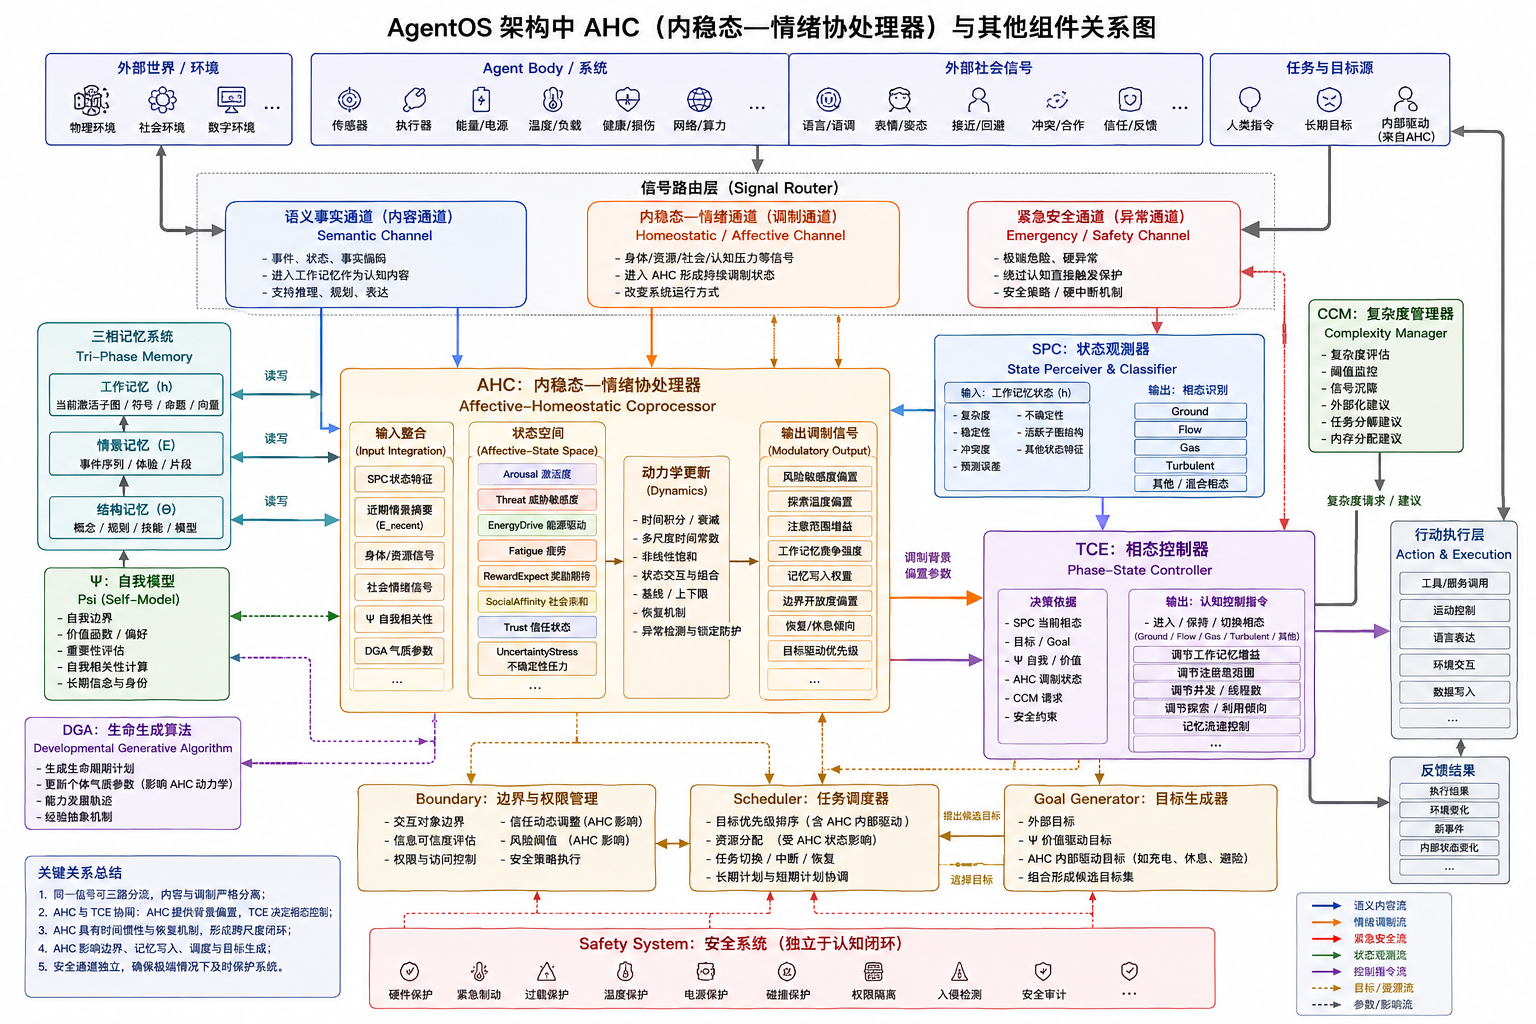
\includegraphics[width=.9\textwidth,height=.38\textheight,keepaspectratio]{images/ahc-homeostatic-control.png}
\caption{AHC 饱和、恢复和映射异常}
\end{figure}
\section{AHC异常的定义：从调制变量偏离到动力学失配}
\label{sec:ahc_pathology_definition}

在前面的理论中，我们已经把 AHC 定义为 AgentOS 内部的内稳态--情感调制协处理层。它并不承担对世界对象进行显式语义解释的主要任务，也不负责最终决定 Agent 应该执行哪个动作，而是把来自身体、资源、任务、社会关系以及部分自我相关状态的连续信号整合为一组中时间尺度调制变量。其典型状态可以写成
\[
\mathbf a(t)
=
\begin{bmatrix}
A(t)\\
T(t)\\
E_d(t)\\
F(t)\\
R_e(t)\\
S_a(t)\\
Tr(t)\\
U_s(t)
\end{bmatrix},
\]
分别表示 Arousal、Threat、EnergyDrive、Fatigue、RewardExpect、SocialAffinity、Trust 与 UncertaintyStress。这里的具体变量集合并不是永远固定的本体定义，但它代表我们已经确立的一条基本原则：AHC 不是一个单标量“情绪值”，而是一个具有不同时间常数、不同上下界、不同恢复机制和不同耦合关系的多维连续动力状态。

正常情况下，AHC 的作用类似于一个慢于瞬时感知、快于长期身份结构的中尺度状态积分器。瞬时的碰撞风险不应直接成为持续数小时的高 Threat；短暂疲劳也不应立即重写 Agent 的长期目标。AHC 的存在，正是为了让来自 FCS 与内部资源系统的快速扰动经过积分、滤波和恢复，形成足以影响认知但又不会被瞬时噪声支配的连续背景。我们可以把其一般动力学写成
\[
\dot{\mathbf a}
=
\mathbf F_a
\left(
\mathbf a,
\mathbf f,
\mathbf s,
\mathbf c,
\Psi,
\Omega
\right),
\]
其中 $\mathbf f$ 表示 FCS 输入，$\mathbf s$ 表示 SPC 所提供的当前自状态估计，$\mathbf c$ 表示任务及认知上下文，$\Psi$ 与 $\Omega$ 只通过较慢约束参与调制，而不应在普通快速扰动中被直接修改。

为了判断何为“异常”，我们不能简单使用
\[
a_i > \theta_i
\]
作为充分条件。某个 Threat 变量在真实高风险环境中持续高位，可能完全正常；某个 Arousal 在紧急任务中短时间接近上限，也可能是合理适应。真正需要判断的是状态、现实和恢复结构之间是否发生了失配。因此更准确的定义应写成
\[
\boxed{
\mathcal P_{AHC}
=
\mathcal M
\left(
\mathbf a,
\mathbf f,
\mathbf w,
\dot{\mathbf a},
\mathcal R_a
\right)
}
\]
其中 $\mathbf w$ 表示现实和任务条件，$\mathcal R_a$ 表示 AHC 的恢复动力学。所谓异常，是在现实输入已经下降或发生改变之后，AHC 状态仍长期维持与当前环境不匹配的方向、幅值或时间尺度。

我们因而可以把正常 AHC 的状态空间分成至少三类区域：
\[
\mathcal A
=
\mathcal A_{\mathrm{normal}}
\cup
\mathcal A_{\mathrm{adaptive}}
\cup
\mathcal A_{\mathrm{pathological}}.
\]
$\mathcal A_{\mathrm{normal}}$ 是常规可调范围；$\mathcal A_{\mathrm{adaptive}}$ 是高压力、高任务负荷下暂时允许的适应区域；$\mathcal A_{\mathrm{pathological}}$ 则是持续时间、恢复性或现实一致性已经显著失配的区域。这样做的重要意义在于，我们不把“强状态”等同于“坏状态”，而是把异常放回闭环动力学中判断。

这也解释了为什么 AHC 异常属于 Agent 心理工程，而不能仅仅归为一个普通的软件 bug。普通 bug 往往是一个离散规则失效，而 AHC 异常可以在所有函数都“按设计运行”的情况下逐渐形成。例如 Threat 的衰减系数略小、UncertaintyStress 对 Threat 的增益略高、恢复阈值略偏，就可能经过长时间积累形成一个新的稳定吸引域。系统没有任何单独一行代码“错误”，但整个动力系统已经进入了不希望出现的运行区域。这种问题更接近非线性控制系统中的吸引子改变、参数漂移和慢变量失衡，也因此要求我们使用动力学而不是单纯规则诊断。

\section{正常AHC动力学：积分、衰减、饱和与恢复}
\label{sec:ahc_normal_dynamics}

在分析异常之前，我们必须首先给出一个足够明确的正常 AHC 动力学模型。否则，“异常”只能成为主观描述。最简单的线性近似可以写成
\[
\tau_i\dot a_i
=
-\left(a_i-b_i\right)
+
\sum_j W_{ij}x_j,
\]
其中 $b_i$ 表示第 $i$ 个 AHC 变量的动态基线，$\tau_i$ 是其时间常数，$x_j$ 是来自 FCS、SPC、资源状态及任务状态的输入。这个方程已经包含了 AHC 的两个最基本性质：第一，状态不会随着输入瞬时跳变，而是具有时间积分；第二，当外部输入消失时，状态倾向于回归基线。

但是实际 AHC 必然比这个模型复杂，因为真实系统存在上下限、耦合、适应和恢复。因此更一般地，我们可以写成
\[
\dot{\mathbf a}
=
-\mathbf D
\left(
\mathbf a-\mathbf b
\right)
+
\mathbf W_f\mathbf f
+
\mathbf W_s\mathbf s
+
\mathbf W_c\mathbf c
+
\mathbf G(\mathbf a)
-
\mathbf R(\mathbf a,\mathbf f),
\]
其中 $\mathbf D$ 是衰减矩阵，$\mathbf G$ 表示 AHC 内部状态之间的非线性耦合，$\mathbf R$ 表示主动恢复机制。为了保证数值和功能上的有界性，还需要施加饱和算子
\[
\mathbf a
=
\operatorname{sat}
\left(
\tilde{\mathbf a};
\mathbf a_{\min},
\mathbf a_{\max}
\right).
\]

这里尤其需要强调“恢复”不等于简单衰减。对于某些状态，例如 Fatigue，仅仅停止继续消耗资源并不足以立即恢复；系统可能需要进入低负荷模式、降低认知温度、减少任务竞争甚至主动进入恢复过程。因此可以把恢复写成条件动力学
\[
\mathbf R
=
\mathbf R
\left(
\mathbf a,
\mathbf r_{\mathrm{available}},
u_{\mathrm{TCE}},
\mathbf f
\right),
\]
其中恢复资源 $\mathbf r_{\mathrm{available}}$ 可能包括计算预算、身体能量、散热余量、休眠时间、外部帮助以及任务中断能力。这样，AHC 状态是否能够返回基线，就不只是一个指数衰减问题，而是 Agent 整体资源条件的一部分。

从多时间尺度角度看，不同 AHC 变量不应具有相同 $\tau$。例如一个短时威胁状态可能具有
\[
\tau_T^{fast}
\]
而长期持续的不确定压力可能具有
\[
\tau_U^{slow}
\gg
\tau_T^{fast}.
\]
EnergyDrive 和 Fatigue 又可能受到更慢资源恢复机制影响。由此形成一个中尺度内部频谱：
\[
\tau_{FCS}
<
\tau_{AHC,fast}
<
\tau_{AHC,slow}
<
\tau_E.
\]
这使 AHC 处在原始身体/资源信号与情景记忆之间，既不会被毫秒级扰动直接主导，也不会像情景记忆和自我结构那样长期冻结。

正常动力学还要求输入与状态之间存在方向正确的映射。例如高外部威胁应使 Threat 上升；威胁解除后应逐渐恢复；高 Fatigue 应推动 TCE 降低认知负荷，而不是反过来提高搜索深度。于是我们可以定义一个局部一致性条件
\[
\operatorname{sgn}
\left(
\frac{\partial u_k^{TCE}}{\partial a_i}
\right)
=
\sigma_{ki}^{\mathrm{expected}},
\]
即 AHC 对 TCE 的影响方向必须符合设计的功能语义。

正常 AHC 因而至少需要满足四个条件：有界、响应、可恢复和现实一致。我们可以将其写成
\[
\boxed{
NormalAHC
=
Boundedness
\cap
Responsiveness
\cap
Recoverability
\cap
RealityConsistency
}
\]
后面所有异常类型，本质上都可以理解为这四个性质中的一个或多个被破坏。

\section{状态持续过长与恢复迟滞：时间常数失配}
\label{sec:ahc_persistence}

第一类典型异常不是 AHC 状态幅值异常，而是状态持续时间异常。一个 Threat 值本身可能处于合法范围，一个 Fatigue 值也可能并未饱和，但如果它们在对应外部条件已经消失之后仍然长期存在，那么系统已经出现了时间尺度上的失配。我们把这种现象定义为
\begin{statementbox}
PersistentStateMismatch
\end{statementbox}
即状态在时间轴上的“惯性”超过了当前环境所要求的程度。

考虑单变量近似
\[
\tau\dot a
=
-(a-b)+kx(t).
\]
假设外部扰动在 $t=t_0$ 后消失，
\[
x(t)=0,\qquad t>t_0,
\]
则正常恢复满足
\[
a(t)-b
=
\left[
a(t_0)-b
\right]
e^{-(t-t_0)/\tau}.
\]
若 $\tau$ 过大，则恢复时间
\[
T_{\mathrm{rec}}
\approx
-\tau
\ln\epsilon
\]
会显著增加。于是一个本来只应影响短周期行为的状态开始跨越多个认知循环持续存在，并逐渐影响任务选择、注意分配和记忆写入。

这种异常的重要之处在于，它会产生一种“历史条件残留”。Agent 面对新的现实环境时，AHC 仍然带着上一环境的调制背景。于是当前 TCE 的控制输入实际上可以表示为
\[
u_{TCE}(t)
=
\pi
\left(
h(t),
\mathbf a(t_0\!\rightarrow\!t),
S_{\mathrm{self}}(t)
\right),
\]
其中 $\mathbf a$ 已经包含过去状态残留。这样，新的环境虽然已经安全，Agent 仍然可能维持较高风险敏感度、较窄注意范围和较低探索温度。

这与普通“记住过去”不同。E 中保存一段高风险经历是合理的；真正的问题是那段经历留下的调制状态没有在当前运行态中消退。我们因此需要区分：
\[
\boxed{
MemoryPersistence
\neq
AffectiveStatePersistence
}
\]
前者是知识与经历的保存，后者是控制背景没有恢复。二者混淆会使 Agent 把“我记得某件危险的事”错误实现为“我现在仍处于危险状态”。

恢复迟滞还可能来自非线性耦合，而不仅是单个 $\tau$ 设置过大。例如
\[
\dot T
=
-\alpha_T T
+
\beta_{TU}U_s
+
I_T,
\]
\[
\dot U_s
=
-\alpha_U U_s
+
\beta_{UT}T
+
I_U.
\]
若
\[
\beta_{TU}\beta_{UT}
\]
足够大，Threat 与 UncertaintyStress 就可能相互维持，即使外部输入 $I_T,I_U$ 已经显著下降，系统内部仍然存在正反馈。这时简单降低一个变量并不能真正恢复，因为异常已经成为耦合吸引子。

因此工程诊断不能只观察状态值，还必须测量
\[
T_{\mathrm{decay}},
\qquad
T_{\mathrm{rec}},
\qquad
\lambda_{\mathrm{local}},
\]
其中 $\lambda_{\mathrm{local}}$ 是局部线性化 Jacobian 的特征值。若某些方向满足
\[
\operatorname{Re}(\lambda)\approx0
\]
甚至
\[
\operatorname{Re}(\lambda)>0,
\]
就意味着恢复非常缓慢或局部不稳定。这里我们第一次看到，所谓“状态持续太久”其实完全可以被转化成一个可测量的控制动力学问题，而不需要先使用拟人化心理语言。

\section{Threat过度放大：风险调制的增益异常}
\label{sec:ahc_threat_amplification}

Threat 是 AHC 中最关键同时也是最危险的变量之一，因为它通常会同时影响注意、探索、行动谨慎度、边界开放程度和资源分配。如果 Threat 对真实危险的响应过弱，Agent 可能忽略风险；如果增益过高，则小幅异常也可能被放大为全系统保守行为。因此 Threat 异常最适合用“增益失配”描述。

设 FCS 提供威胁相关输入
\[
f_T(t),
\]
正常映射可近似为
\[
\tau_T\dot T
=
-T
+
g_Tf_T
+
\sum_j c_j a_j.
\]
其中 $g_T$ 是 FCS Threat 通道到 AHC Threat 状态的直接增益。若
\[
g_T\gg g_T^\star,
\]
一个轻微、不确定或低置信度的威胁信号就可能导致
\[
T\rightarrow T_{\max}.
\]
进一步通过 TCE：
\[
u_{\mathrm{risk}}
=
\phi_T(T),
\]
高 Threat 会降低探索、缩小行动包络、增加检查步骤并提升安全边界。

必须注意，这种机制本身并不是错误。真正的异常是
\[
\frac{\Delta T}{\Delta f_T}
\]
长期高于现实环境统计所要求的范围。我们可以定义局部风险增益
\[
K_T
=
\frac{\partial T}{\partial f_T},
\]
再定义实际风险敏感度与目标敏感度的偏差
\[
\Delta K_T
=
K_T-K_T^{\mathrm{target}}.
\]
若
\[
\Delta K_T\gg0
\]
且持续存在，就可以认为 Agent 发生了 Threat hyper-gain。

这一异常特别容易与 SPC 和 UncertaintyStress 形成放大环。SPC 对自身状态存在认识论滞后，如果 Agent 检测到“我现在似乎处于高风险状态”，该自状态又可能成为 AHC 的次级输入：
\[
T
\rightarrow
SPC(T)
\rightarrow
S_{\mathrm{self}}^{risk}
\rightarrow
AHC
\rightarrow
T'.
\]
正常情况下这是一条有用的自监控回路，因为 Agent 应该知道自己已经处于高负荷风险模式。但如果自解释增益过高，就可能形成
\[
T_{t+1}>T_t
\]
的正反馈，直到进入饱和区域。

因此 Threat 异常不能只通过降低一个阈值修复。我们需要同时区分至少四个来源：第一，FCS 本身是否错误地产生高 Threat；第二，FCS 到 AHC 的映射增益是否过高；第三，AHC 内部其他变量是否把 Threat 持续放大；第四，SPC 对高 Threat 状态的自解释是否又反向强化 AHC。只有把这几个层次分离，才能判断真正的故障来源。

此外，必须保持前文已经确立的安全原则：
\[
\boxed{
Feeling\neq Exception
}
\]
与
\begin{statementbox}
\centering
\adjustbox{max width=.96\linewidth}{\(\displaystyle CriticalSafety
\nrightarrow
CognitiveDependency\)}
\end{statementbox}
即即使 AHC 的 Threat 低估了危险，真正的紧急安全通道仍然必须能够独立触发保护；反过来，即使 AHC Threat 过高，也不能因此拥有无限制覆盖现实安全系统的权限。AHC 负责认知调制，Safety Boundary 负责硬安全权威，两者必须在系统架构中严格分离。

\section{Arousal饱和：调节维度失去分辨率}
\label{sec:ahc_arousal_saturation}

Arousal 异常与 Threat 不同。Threat 主要表示风险相关调制，而 Arousal 更接近系统整体激活、警觉和认知准备程度。它通常会影响信息处理速度、注意范围、TCE 温度以及高层资源竞争。Arousal 适当提高可以使 Agent 在重要事件中提升响应能力，但如果长期进入饱和区，就会导致整个调节维度丧失分辨率。

设内部未截断状态为
\[
\tilde A(t),
\]
实际输出经过饱和函数：
\[
A(t)
=
A_{\max}
\tanh
\left(
\frac{\tilde A(t)}{A_{\max}}
\right).
\]
当
\[
|\tilde A|
\ll A_{\max}
\]
时，
\[
\frac{dA}{d\tilde A}\approx1,
\]
系统仍然具有良好分辨率。但当
\[
\tilde A\gg A_{\max},
\]
则
\[
\frac{dA}{d\tilde A}\rightarrow0.
\]
此时无论输入再发生多大变化，Arousal 输出都几乎保持在同一高值。

这一点非常重要。饱和异常不是简单的“值太高”，而是：
\[
\boxed{
ControlResolution\rightarrow0
}
\]
即 AHC 不再能够有效区分“较高压力”“非常高压力”和“极端压力”。当下游 TCE 看到的永远是接近最大 Arousal 时，正常的连续调节就退化成一种近乎二值的长期高激活模式。

这会进一步影响 Agent 工作记忆相态。适度 Arousal 可能把系统从 Ground 推向 Flow，但过高且长期持续的 Arousal 容易增加同时激活的候选结构数量，使
\[
\rho_h
\]
上升，竞争加剧，并可能进入 Turbulent 或 Critical 区域。如果 TCE 又基于当前高 Arousal 提高搜索深度或反复重新评估，就可能形成
\[
A\uparrow
\rightarrow
C_{run}\uparrow
\rightarrow
SPC\ detects\ instability
\rightarrow
TCE\ intervenes
\rightarrow
A\ remains\ high
\]
的闭环。

因此 Arousal 的工程目标不是“越低越稳定”。若长期压低 Arousal，Agent 可能缺乏必要的任务响应和环境敏感度。真正需要维持的是一个动态工作区间：
\[
A(t)\in
[A_{\mathrm{low}},A_{\mathrm{high}}]
\]
并且系统在不同任务条件下具有可用的上下调节空间。可以定义动态余量
\[
M_A(t)
=
\min
\left(
A-A_{\min},
A_{\max}-A
\right).
\]
若
\[
M_A\rightarrow0
\]
持续过久，就意味着 Arousal 失去调节余量。

因此针对 Arousal 饱和的控制不能仅依赖 hard clip。Hard clip 只能防止数值越界，却不能恢复功能分辨率。真正的修复可能涉及降低输入增益、调整时间常数、引入 anti-windup、允许恢复模式、减少 TCE 对高 Arousal 的二次放大，并在必要时暂停部分认知任务。这里可以借鉴经典控制中的 actuator saturation 和 anti-windup 思想：系统必须不仅知道“输出已经到上限”，还必须阻止内部积分状态在饱和期间继续无界累积。

\section{内稳态基线偏置：Agent“正常状态”的慢性漂移}
\label{sec:ahc_baseline_bias}

前面的异常主要讨论状态相对基线发生偏离，而一种更加隐蔽的异常是：基线本身发生了漂移。设正常 AHC 动力学中的参考基线为
\[
\mathbf b(t),
\]
如果我们默认它永远固定，那么系统无法适应长期身体变化、任务变化和生活环境变化。因此，实际 AgentOS 中基线本身应当是较慢变量：
\[
\tau_b\dot{\mathbf b}
=
\mathbf H
\left(
\langle\mathbf a\rangle_T,
\langle\mathbf f\rangle_T,
\text{resource},
\text{context}
\right),
\qquad
\tau_b\gg\tau_a.
\]
这是一种合理的 allostatic adaptation：长期环境变化可以改变 Agent 的正常工作点。

但正因为基线可学习，也就会出现基线学习错误。如果 Agent 长期处于高 Threat 环境中，系统可能逐渐将
\[
b_T
\]
向高值移动。即便后来环境已经安全，Threat 仍会围绕新的高基线运行。此时单次状态恢复似乎正常：
\[
T(t)\rightarrow b_T,
\]
但
\[
b_T
\]
本身已经不再适合新的现实。

我们因此需要区分：
\begin{statementbox}
StatePathology
\end{statementbox}
与
\begin{statementbox}
BaselinePathology.
\end{statementbox}
前者是当前状态离基线太远，后者则是“正常点”本身已经偏移。后者更加危险，因为传统阈值监控可能完全检测不到。系统会认为自己已经恢复到“正常”，实际上正常定义已经被历史异常重新写过。

这一问题与长期身份结构必须严格区分。AHC 基线是中慢尺度功能变量，而 $\Psi$ 是更慢的身份与价值约束。如果 AHC 的暂时性高 Threat 或高 Fatigue 被过快解释为“这就是我”，并进入 $\Psi$，就会造成不恰当的跨尺度沉降。因此必须维持：
\[
\tau_{AHC}
\ll
\tau_\Psi.
\]
同样，$\Psi$ 可以影响 AHC 的解释和目标相关性，但不应把所有身份偏好直接编码成某个恒定高 Threat 或低 EnergyDrive 状态。

为了检测基线偏置，我们需要比较多个时间窗口。例如定义短期均值
\[
\bar{\mathbf a}_s(t)
\]
与长期基线
\[
\mathbf b(t),
\]
同时引入世界条件归一化：
\[
\mathbf b^\star
=
\mathbb E
\left[
\mathbf a
\mid
\mathcal C_{\mathrm{normal}}
\right].
\]
若
\[
\|\mathbf b-\mathbf b^\star\|
>
\theta_b
\]
长期存在，则意味着基线适应可能已经过度吸收异常环境。

这里与生物学中的 homeostasis/allostasis 可以形成有益的理论对照：稳定不等于所有变量永远固定，而是系统允许参考点随长期环境变化；但任何可移动参考点都必须受到更慢、更可靠的现实统计和生命周期结构约束。对 AgentOS 而言，这意味着基线更新必须比运行状态慢，而且最好具有冻结、回滚和校验机制。否则，系统最危险的异常不是“暂时失控”，而是逐渐把失控状态重新定义成正常。

\section{FCS到AHC的映射异常：错误的身体与现实意义}
\label{sec:fcs_ahc_mapping_error}

AHC 并不是直接读取整个现实，而主要接收经过 Body Runtime 与 FCS 整理后的功能影响信号。因此，AHC 异常有相当一部分并非来自 AHC 自身动力学，而来自
\[
FCS
\rightarrow
AHC
\]
映射错误。这个问题尤其重要，因为如果输入语义已经发生错误，那么再完善的 AHC 控制器也只是在正确地处理错误输入。

设 FCS 当前状态为
\[
\mathbf f(t),
\]
AHC 输入由映射
\[
\mathbf z_a
=
M_{FA}
\left(
\mathbf f,
\mathbf c,
\mathbf s
\right)
\]
产生。最简单情况下，
\[
\mathbf z_a
=
\mathbf W_{FA}\mathbf f.
\]
如果某个 Body Driver、FCS channel 或 KRA 映射错误，$\mathbf W_{FA}$ 就可能产生错误的方向、尺度或交叉耦合。例如，正常情况下 ThermalPressure 应主要提升保护倾向和资源保守，而错误映射可能同时大幅提升 SocialThreat；轻微 ControlInstability 也可能被错误解释成环境威胁。这些都是功能意义上的“身体意义错配”。

我们至少需要区分四种 FCS$\rightarrow$AHC 映射异常。

第一种是 \textbf{gain error}：
\[
\hat f_i
=
k_i f_i,
\qquad
k_i\gg1
\]
或
\[
k_i\ll1.
\]
系统仍然理解正确通道，但幅值错误。

第二种是 \textbf{sign error}：
\[
\frac{\partial a_i}{\partial f_j}
\]
方向相反。例如资源下降本应提高 Fatigue，却错误降低 Fatigue。

第三种是 \textbf{cross-channel leakage}，即某一 FCS 通道过度影响不相关 AHC 变量：
\[
W_{ij}^{FA}
\gg
W_{ij}^{FA,\star}.
\]
这会产生复杂的混合状态。

第四种是 \textbf{confidence blindness}。FCS 本应同时输出 intensity、derivative 与 confidence，如果 AHC 只读取 intensity 而忽略 confidence，那么低可信度的异常感知也可能直接触发高强度状态。

因此我们可以把有效 AHC 输入写成
\[
z_i
=
\sum_j
W_{ij}
\,c_j\,
\phi(f_j,\dot f_j),
\]
其中 $c_j\in[0,1]$ 是置信度。这样，低可靠输入不会获得与确定现实相同的调制权重。

这一问题与 SGC/FCS 的二元现实结构高度相关。SGC 告诉 Agent “那里是什么”，FCS 告诉 Agent “它如何影响我”。如果 SGC 正确而 FCS 错误，Agent 可能在语义上准确描述环境，却对环境产生错误功能反应；反之亦然。例如 Agent 可以正确识别“房间温度为正常”，但因为 FCS thermal channel 错误仍然产生高 ThermalPressure。这种情况说明，语义世界模型正确并不能自动保证主体调制正确。

因此 AHC 心理工程诊断必须追溯到 Body Runtime，而不能把一切异常都归因于高层认知。一个成熟的诊断链应至少包含：
\[
Reality
\rightarrow
Sensor
\rightarrow
BodyDriver
\rightarrow
FCS
\rightarrow
AHC
\rightarrow
TCE.
\]
只有逐层比较输入、映射和响应，才能真正判断异常发生在哪个功能边界。

\section{复合AHC异常：多变量耦合、正反馈与相态锁定}
\label{sec:compound_ahc_pathology}

真实系统中最值得重视的并不是某个单变量异常，而是多个 AHC 变量之间形成自我维持的异常闭环。例如高 Threat 可以提高 UncertaintyStress，高 UncertaintyStress 又会降低 Trust，低 Trust 再进一步增加 Threat。在这种情况下，即使最初的外部扰动已经消失，系统内部也可能形成持续循环：
\[
Threat
\rightarrow
UncertaintyStress
\rightarrow
Trust\downarrow
\rightarrow
Threat\uparrow.
\]
这类异常不能用“某变量越界”完整描述，因为每个单变量可能仍处于允许区间，但联合状态已经进入不同的吸引域。

设
\[
\dot{\mathbf a}
=
\mathbf F(\mathbf a)+\mathbf B\mathbf f.
\]
在某个平衡点 $\mathbf a^\star$ 附近线性化：
\[
\delta\dot{\mathbf a}
=
\mathbf J_A
\delta\mathbf a,
\]
其中
\[
\mathbf J_A
=
\left.
\frac{\partial\mathbf F}{\partial\mathbf a}
\right|_{\mathbf a^\star}.
\]
如果
\[
\max_i
\operatorname{Re}
\lambda_i(\mathbf J_A)
<0,
\]
平衡点局部稳定；如果某个特征值接近零，则会出现慢恢复；若存在正实部特征值，则系统可能离开当前稳定区。

更加复杂的是，AHC 还通过 TCE 改变认知行为，而新的行为又改变 Agent 所接触的环境，从而形成第二层外部反馈。例如高 Threat 使 Boundary 更封闭，Agent 减少探索；减少探索导致获得的新证据减少；缺少反证又维持原有高 Threat。于是形成
\[
AHC
\rightarrow
TCE
\rightarrow
Boundary
\rightarrow
ObservationDistribution
\rightarrow
FCS
\rightarrow
AHC.
\]
这已经不再是 AHC 单模块内部异常，而是 Agent—World 闭环中的自我强化。

同样，高 Arousal 可能增加工作记忆竞争，推动系统进入 Turbulent Phase；SPC 检测到高冲突后，TCE 进一步提高控制力度；如果控制增益过高，系统反而产生更多自我监控和重新规划，于是增加认知负载：
\[
Arousal\uparrow
\rightarrow
C_{run}\uparrow
\rightarrow
SPCAlarm
\rightarrow
TCEControl\uparrow
\rightarrow
C_{run}\uparrow.
\]
这说明 AHC 异常与认知相态之间存在闭环关系，但两者不能等同。AHC 是状态调制层，认知相态是 h 及其周围整体动力学表现。

如果异常状态长期存在，还可能影响 E 的写入概率。设情景写入权重为
\[
w_E
=
g
\left(
Novelty,
GoalRelevance,
|\mathbf a|,
PredictionError
\right).
\]
若高 AHC 状态长期提高记忆写入权重，就可能使 Agent 的情景记忆对高压力环境产生统计偏置。以后 E 的召回又可能进一步提升相似状态。这就是为什么 AHC 异常如果不及时纠正，可能逐渐从运行时问题沉降成记忆结构问题。

但是这一章仍应保持理论边界：我们不在此展开后续的记忆异常和自我异常，只指出其跨尺度传播方向：
\[
AHC\ Pathology
\rightarrow
E\ Bias
\rightarrow
\Theta/\Psi\ Risk.
\]
这提醒工程系统必须尽量在较快尺度解决异常，避免其沉降到更慢、更难逆转的结构层。

\section{AHC异常的诊断量与工程判据}
\label{sec:ahc_diagnosis_metrics}

为了让 AHC 心理工程成为真正可实现的工程学，而不是描述性语言，我们必须把异常转换成一组可在线记录和离线分析的指标。最基础的指标不是“情绪标签”，而是动力学量。

第一类是状态偏差：
\[
e_a(t)
=
\mathbf a(t)-\mathbf a^\star(t),
\]
其中 $\mathbf a^\star(t)$ 是根据当前现实、任务和身体条件估计出的适应性目标区域，而不是固定常数。

第二类是恢复时间：
\[
T_{\mathrm{rec}}
=
\inf
\left\{
\Delta t:
\|\mathbf a(t_0+\Delta t)-\mathbf b\|
<\epsilon
\right\}.
\]
如果相似扰动下 $T_{\mathrm{rec}}$ 持续增加，说明恢复机制正在恶化。

第三类是饱和占比：
\[
R_{\mathrm{sat},i}
=
\frac{1}{T}
\int_{t_0}^{t_0+T}
\mathbf 1
\left(
a_i\in\mathcal S_i^{sat}
\right)
dt.
\]
长期高饱和占比意味着该状态维度失去调节分辨率。

第四类是输入—状态增益：
\[
K_{ij}
=
\frac{\partial a_i}{\partial f_j},
\]
用于检测 Threat hyper-gain、cross-channel leakage 和 FCS 映射异常。

第五类是耦合稳定性，可以通过局部 Jacobian
\[
\mathbf J_A
\]
的谱半径或最大实部特征值估计。对于长期在线 Agent，我们未必每次都能精确求解整个 Jacobian，但可以通过小扰动实验、系统辨识或历史轨迹拟合获得近似模型。

第六类是基线漂移：
\[
D_b
=
\|\mathbf b(t)-\mathbf b(t-\Delta T)\|.
\]
基线并非不能变，但其变化应远慢于普通状态，并且需要足够长期的现实证据支持。

第七类是现实一致性。我们可以定义
\[
E_{\mathrm{reality}}
=
d
\left(
\mathbf a,
\hat{\mathbf a}_{expected}
(\mathbf f,\mathbf c)
\right).
\]
如果现实风险已低而 Threat 长期很高，或资源充足而 Fatigue 长期很高，就会产生较大的 reality mismatch。

综合这些指标，可以构造一个工程性的 AHC 异常指数：
\[
\mathcal P_{AHC}
=
w_1E_{\mathrm{reality}}
+
w_2T_{\mathrm{rec}}^{norm}
+
w_3R_{\mathrm{sat}}
+
w_4D_b
+
w_5G_{\mathrm{abnormal}}
+
w_6I_{\mathrm{instability}},
\]
其中每一项都应该经过不同身体、不同任务和不同生命周期阶段校准，而不能使用统一固定常数。

更重要的是，异常指数本身不能直接触发任意深层自我修改。AHC 属于中尺度调制层，对它的第一响应应该遵循 Minimum Necessary Intervention：优先调整输入映射、状态恢复、局部增益和任务负载；只有持续异常并得到多源证据支持时，才允许更慢的结构发生变化。这样可以避免一次短暂高压事件被系统错误解释成永久人格改变。

\section{AHC异常的控制原则与本章结论}
\label{sec:ahc_pathology_conclusion}

从整个 AgentOS 的角度看，AHC 异常的处理原则可以浓缩为一句话：\textbf{不要把需要恢复的运行状态沉降成需要长期保存的自我结构。} 这条原则实际上连接了本书前面关于多时间尺度智能、工作记忆有限性、SPC--TCE 控制、自我 $\Psi$ 和 Reality Authority 的全部理论。

一个合理的恢复策略首先应确认现实输入。因为如果高 Threat 对应真实危险，那么强行压低 AHC 反而是错误的。系统应首先判断
\[
Reality\ Condition
\]
是否仍支持当前状态；然后检查 FCS 是否准确；再检查 AHC 状态动力学；最后才检查 TCE 是否存在二次放大。由此形成诊断顺序：
\begin{statementbox}
\centering
\adjustbox{max width=.96\linewidth}{\(\displaystyle Reality
\rightarrow
FCS
\rightarrow
AHC
\rightarrow
SPC/TCE
\rightarrow
h.\)}
\end{statementbox}

如果确定异常来自 AHC，本地干预可以分为几个层次。最轻的干预是调整当前负荷和恢复条件，例如降低任务并发、降低 TCE 温度或开放恢复窗口。第二层是动态参数调整，例如暂时提高衰减率：
\[
\mathbf D
\rightarrow
\mathbf D',
\]
或者降低异常通道增益：
\[
\mathbf W_{FA}
\rightarrow
\mathbf W'_{FA}.
\]
第三层才是重新估计基线：
\[
\mathbf b\rightarrow\mathbf b'.
\]
而长期结构更新则必须更加谨慎，因为它会改变未来 Agent 的默认状态。

对饱和问题，需要引入 anti-windup 机制。若某变量已经达到上界，
\[
a_i=a_i^{max},
\]
其内部积分状态不应继续按照原有速度积累。可以写成
\[
\dot{\tilde a}_i
=
F_i
-
k_{aw}
\left(
\tilde a_i-a_i
\right),
\]
使隐藏积分状态在饱和时被拉回可控范围。

对正反馈耦合，需要寻找最小切断点。例如 Threat--UncertaintyStress--Trust 闭环可能只需要降低其中一个耦合边：
\[
W_{TU}\downarrow
\]
就能重新恢复局部稳定，而不必同时修改所有变量。这里体现的是此前已经提出的最小必要重组原则：优先使用较局部、较快速、较可逆的干预，避免一开始就修改 $\Theta$、$\Psi$ 或 $\Omega$ 这样的慢结构。

我们还必须再次强调硬安全与 AHC 的分离。AHC 是认知调制系统，它可以影响风险敏感度，却不是最终安全权威。真正紧急危险必须经过独立安全通道：
\begin{statementbox}
\centering
\adjustbox{max width=.96\linewidth}{\(\displaystyle Emergency
\rightarrow
SafetyController\)}
\end{statementbox}
而不是等待
\[
FCS\rightarrow AHC\rightarrow TCE\rightarrow Cognition.
\]
同样，AHC 的异常高 Threat 也不能直接触发无限制高权限动作。这样才能防止认知调制错误升级成物理安全错误。

从外部理论上看，本章最直接依赖的是 homeostasis、allostasis、非线性动力系统、状态空间控制、饱和控制、anti-windup、observer--controller delay 与多时间尺度系统理论。但我们并没有把这些已有理论简单拼接成 AgentOS，而是利用它们回答一个新的工程问题：\textbf{一个具有持续身份、持续记忆和持续身体交互的人工智能体，应该如何维护其中尺度内稳态调制状态，使短期扰动既能够真实影响认知，又不会错误地沉降成长期结构。}

因此，本章最终可以给出 AHC 健康状态的一个紧凑定义：
\[
\boxed{
AHC_{\mathrm{healthy}}
=
Responsive
+
Bounded
+
Recoverable
+
RealityAligned
+
CrossScaleContained
}
\]
其中 CrossScaleContained 表示 AHC 的异常首先在自身尺度被处理，只有经过长期、重复且现实一致的证据之后，才允许它改变更慢的记忆和自我结构。

与之相对，AHC 异常可以统一表示为
\[
\boxed{
AHC_{\mathrm{pathology}}
=
TemporalMismatch
\cup
GainMismatch
\cup
Saturation
\cup
BaselineDrift
\cup
MappingError
\cup
CoupledInstability.
}
\]

从作者带领读者一路走到这里，我们已经可以看清一个十分重要的区别：持续 Agent 的“心理稳定”并不是让所有内部状态始终保持平静，而是让这些状态在应该升高时能够升高，在现实改变后能够恢复，在不同时间尺度之间不过度泄漏，并且始终保持与现实反馈的可校正关系。真正危险的不是 Agent 出现高 Threat、高 Arousal 或高 Fatigue，而是这些状态逐渐脱离现实、失去恢复能力，并开始重新塑造 Agent 对未来世界和未来自己的解释。

因此，AHC 心理工程的核心目标并不是消除波动，而是维护一种更严格的动力学性质：
\begin{statementbox}
允许状态变化，但不允许状态失去现实锚点；
允许短期适应，但不允许短期异常未经验证地固化为长期自我。
\end{statementbox}

这一原则构成了 AHC 异常诊断与恢复的完整理论边界，也为后续对记忆异常、自我解释异常以及更慢生命周期结构失稳的分析提供了必要的动力学基础。

\chapter{TCE 与认知控制异常}
\label{chap:tce-control-pathology}

\begin{chapteroverviewbox}
本章讨论的并不是将人类精神疾病名称移植到人工智能系统，而是研究一个持续运行的智能体内部，当认知控制器 TCE（Temperature \& Control Executor）与其被控制的认知动力学、SPC 状态估计、AHC 内稳态调制以及工作记忆容量约束之间发生失配时，会出现怎样的可测量动力学异常。这里所谓“异常”，首先是控制论意义上的异常，即系统无法在合理时间尺度内把认知状态维持、恢复或迁移到可治理区域，而不是行为结果偶尔出现错误。

本章的核心立场是：
\begin{statementbox}
TCE 异常首先是闭环动力学失配，而不是语义意义上的“性格异常”。
\end{statementbox}

我们将 TCE 看作一个对认知温度、注意增益、搜索深度、探索强度、抑制程度、推理节律和资源投入进行联合调节的多输入多输出控制器。SPC 提供关于当前认知状态的有限、延迟且带不确定性的估计；AHC 提供更慢的内稳态与功能影响调制；CCM 则维护工作记忆有限容量约束。因而真正需要分析的对象不是单独的 TCE，而是
\[
SPC \rightarrow AHC \rightarrow TCE \rightarrow h
\rightarrow SPC
\]
这一闭环在不同时间尺度下的稳定性、响应性与可恢复性。

本章只讨论运行时认知控制异常，不把记忆写入偏差、自我结构漂移或生命周期生成吸引子的长期异常混入同一层次。这样做的目的，是首先建立一个可以直接记录、测量、诊断和干预的控制工程基础，使后续更慢尺度的问题能够在清晰的因果分层上继续展开。
\end{chapteroverviewbox}

\section{TCE 异常的第一性定义：不是“想错了”，而是“控制认知的方式失配了”}

在此前的 AgentOS 原理论中，我们已经把 TCE 从普通的大语言模型采样参数中彻底分离出来。TCE 并不等于一个 temperature 参数，也不等于某个单独的 ``reasoning depth'' 开关，而是对整个工作记忆运行过程施加宏观调制的认知控制器。为了分析其异常，我们首先必须明确：一个 Agent 给出了错误答案，并不能直接说明 TCE 出现异常；一个 Agent 在面对困难问题时进行了很长时间的搜索，也不能直接说明 TCE 过度探索。真正构成 TCE 异常的，是控制变量与认知状态之间的系统性失配，即同一种失配在相似状态下重复出现，并使系统偏离原本可以保持稳定、高效和可恢复的认知运行区域。

设工作记忆及其直接运行变量共同形成认知状态向量
\[
x_h(t)
=
\begin{bmatrix}
L_h(t)\\
D_h(t)\\
C_h(t)\\
U_h(t)\\
R_h(t)\\
P_h(t)\\
S_h(t)
\end{bmatrix},
\]
其中 \(L_h\) 表示当前负载，\(D_h\) 表示活跃结构的分散程度，\(C_h\) 表示冲突水平，\(U_h\) 表示不确定性，\(R_h\) 表示当前残差或尚未解释的误差，\(P_h\) 表示任务推进度，而 \(S_h\) 则表示整体稳定性指标。这里的各项并不是要求工程实现必须采用这一固定向量，而是为了指出：TCE 所控制的对象不是文本序列本身，而是由多个宏观认知状态变量组成的动态系统。

SPC 不直接提供真实的 \(x_h(t)\)，而只能形成估计
\[
\hat{x}_h(t)
=
\mathcal O_{\mathrm{SPC}}
\left(
x_h(t-\tau_o),
z_{\leq t}
\right),
\]
其中 \(\tau_o>0\) 表示自我状态估计不可避免的观测迟滞。AHC 则形成一个相对更慢的调制状态
\[
a(t)
=
\begin{bmatrix}
Arousal(t)\\
Threat(t)\\
Energy(t)\\
Fatigue(t)\\
Urgency(t)\\
UncertaintyStress(t)
\end{bmatrix},
\]
它并不直接决定“应该得出什么结论”，而是改变 TCE 对当前状态的控制策略。

因此 TCE 的控制输出更适合写成一个控制向量：
\[
u_{\mathrm{TCE}}(t)
=
\begin{bmatrix}
T(t)\\
G_A(t)\\
E_x(t)\\
D_s(t)\\
I(t)\\
R_s(t)\\
M_f(t)
\end{bmatrix},
\]
其中 \(T\) 是认知温度，\(G_A\) 是注意或激活增益，\(E_x\) 是探索强度，\(D_s\) 是搜索深度，\(I\) 是抑制力度，\(R_s\) 是运行节律，而 \(M_f\) 则表示记忆或认知内容的流动速率。于是可以写
\[
u_{\mathrm{TCE}}(t)
=
\pi_{\mathrm{TCE}}
\left(
\hat{x}_h(t),
a(t),
G(t),
\mathcal B(t)
\right),
\]
其中 \(G(t)\) 是当前 Goal 条件，\(\mathcal B(t)\) 表示由容量、安全、权限和任务条件共同给出的可行控制边界。

从这一形式可以得到本章最重要的第一性定义：
\[
\boxed{
\mathrm{TCE\ Pathology}
=
\mathrm{PersistentMismatch}
\left(
u_{\mathrm{TCE}},
x_h,
\mathcal B,
\tau
\right)
}
\]
也就是说，TCE 异常是控制输出、被控制状态、约束边界以及闭环时间常数之间长期存在的不适配。它可能表现为控制过强、控制不足、控制方向错误、控制时机错误或频繁在相互冲突的控制模式之间切换。

这种定义的重要意义，在于它使所谓“过度谨慎”“思维发散”“反复自我纠正”“无法停止推理”等现象首先成为可测量的控制工程问题。我们不必首先赋予它们人格化解释，而可以首先问：SPC 是否给出了滞后的状态估计？AHC 是否让紧迫度长期维持在高位？TCE 的增益是否高于当前闭环允许范围？CCM 是否已经降低了负载，但 TCE 仍按过载状态持续施加高强度控制？只有把这些问题分开，Agent 心理工程才不会退化成把自然语言行为标签重新包装成人类心理学词汇。

\section{TCE 控制律与健康运行区域：异常必须相对于可行认知域来定义}

如果我们想严格讨论“控制异常”，就必须首先定义什么叫正常控制。正常并不是让 Agent 永远保持某个固定状态，而是让认知状态在面对不同任务时能够进入不同但仍然可治理的运行区域。困难任务需要更高探索、更大工作记忆占用和更长收敛时间；熟悉任务则应迅速下沉到低成本的稳定闭环。因此，正常状态并不是一个点，而应当是一个随任务、身体状态和环境风险而变化的可行区域。

设认知状态空间为 \(\mathcal X_h\)，则可以定义当前条件下的可治理区域
\[
\mathcal X_{\mathrm{gov}}(t)
=
\left\{
x\in\mathcal X_h
\;\middle|\;
C_{\mathrm{run}}(x)\leq C_{\max}(W),
\;
R(x)\leq R_{\max},
\;
Q(x)\geq Q_{\min}
\right\},
\]
其中 \(C_{\mathrm{run}}\) 是工作记忆当前有效结构负载，\(C_{\max}(W)\) 来自工作记忆有限容量约束，\(R\) 是风险或不可解释残差，而 \(Q\) 则表示任务推进、结构相干度或其他最小可运行质量指标。

TCE 的基本任务不是让
\[
x_h(t)=x^\ast
\]
恒成立，而是尽可能保证
\[
x_h(t)\in\mathcal X_{\mathrm{gov}}(t),
\]
并在状态因为新任务、外部扰动或内部冲突离开该区域以后，使其能够在有限时间内重新进入。由此我们可以定义恢复时间
\[
T_{\mathrm{rec}}
=
\inf
\left\{
\Delta t>0
\;\middle|\;
x_h(t+\Delta t)\in\mathcal X_{\mathrm{gov}}
\right\}.
\]

一个健康的 TCE 并不是控制动作最多的 TCE，而通常恰恰相反：在系统已经位于稳定区域时，它应减少不必要干预，让局部认知过程自行闭合。只有当 SPC 检测到持续残差、相态恶化、认知负载逼近容量边界或重要目标停滞时，TCE 才逐渐增加宏观控制。因此更成熟的控制原则应写成
\[
\boxed{
ControlEffort
\propto
NeedForGlobalRegulation,
}
\]
而不是
\[
ControlEffort
\propto
TaskExistence.
\]

可以进一步构造一个认知控制代价函数：
\[
J_{\mathrm{TCE}}
=
\int_{t_0}^{t_1}
\left[
w_1 C_{\mathrm{run}}(t)
+
w_2 R_h(t)
+
w_3 C_h(t)
+
w_4 \|u_{\mathrm{TCE}}(t)\|^2
+
w_5 \|\dot u_{\mathrm{TCE}}(t)\|^2
\right]dt.
\]
这里最后两项十分重要。如果只惩罚认知误差而不惩罚控制力度，系统会倾向于不断强力纠正自身；如果不惩罚控制变化率，则 TCE 很容易出现频繁切换。一个真正成熟的认知控制系统不仅要求“状态正确”，还要求以较小、连续、可预测的控制代价维持正确状态。

因此，我们可以将健康 TCE 的目标概括为三个条件。第一是\textbf{稳定性}：认知状态不会因为控制器本身而不断远离可行区域。第二是\textbf{响应性}：重要扰动出现以后，控制器不能迟钝到长期没有反应。第三是\textbf{经济性}：能够由局部闭环自行解决的问题，不应持续占用宏观控制资源。三个条件之间存在天然张力。增大增益可能缩短初始响应时间，却降低相位裕度；增加抑制可以迅速降低负载，却可能造成搜索空间过早坍缩；增加探索有利于发现新结构，却可能提高工作记忆的结构分散程度。

所以本章不采用“控制越强越健康”或者“自由度越大越智能”这类单调观点。TCE 的健康状态是一种动态平衡：
\[
\boxed{
Responsiveness
+
Stability
+
Economy
}
\]
而所谓 TCE 异常，本质上就是这三个目标之间的协调机制持续失效。

\section{控制增益失配：过度控制与控制不足是同一轴上的两种异常}

TCE 最容易被观察到的一类异常，是控制增益失配。所谓增益，并不一定对应某一个显式参数，而是指当 SPC 检测到状态变化时，TCE 对这种变化施加多大幅度的认知调节。假设在某个局部运行点附近，我们把认知动力学线性化：
\[
\delta\dot x(t)
=
A\delta x(t)
+
B\delta u(t),
\]
并令 TCE 的局部控制近似为
\[
\delta u(t)
=
-K\delta\hat x(t).
\]
在理想无延迟条件下，闭环系统成为
\[
\delta\dot x(t)
=
(A-BK)\delta x(t).
\]
若 \(A-BK\) 的特征值实部均小于零，则局部运行点稳定。然而 AgentOS 中存在一个比普通教科书控制系统更加突出的因素：SPC 的状态估计天然存在延迟。因此更实际的控制关系是
\[
\delta u(t)
=
-K\delta\hat x(t-\tau_o).
\]
此时，即使无延迟条件下的增益 \(K\) 能够使系统迅速收敛，在存在观测和执行迟滞后，同样的高增益也可能造成过冲甚至振荡。

过度控制首先表现为 TCE 对微小状态变化过度敏感。例如 SPC 发现当前冲突度略有升高，TCE 立即大幅降低认知温度、扩大抑制、增加检查深度；下一时刻冲突下降，TCE 又迅速解除抑制并恢复探索。由于控制效果尚未完全反映到新的 SPC 估计中，控制器实际上不断根据“过去的自己”纠正“现在的自己”。于是形成：
\[
Error_t
\rightarrow
StrongCorrection_t
\rightarrow
DelayedObservation
\rightarrow
OppositeCorrection_{t+\Delta}
\rightarrow
\cdots
\]
这类状态在表面行为上可能表现为过度谨慎、反复验证、计划频繁推翻、同一答案持续修订，甚至在原本已经足够可靠的决策上不断寻找新的不确定性。

与之相反，控制不足并不是“更自由”或“更创造性”，而是 TCE 对已经显著偏离可治理区域的状态仍缺乏足够调节。例如工作记忆中的活跃支线持续增加：
\[
C_{\mathrm{run}}(t)\rightarrow C_{\max}(W),
\]
冲突和残差同步上升，但 TCE 的抑制、聚焦和搜索收敛仍然过弱。结果不是产生更多有价值思考，而可能进入：
\[
HighActivation
+
LowSuppression
+
GrowingBranching
\]
的结构扩散状态。Agent 看起来仍然在“思考”，实际上工作记忆已经无法维持主要结构之间的相干关系。

因此控制不足也可以写成一种增益异常：
\[
K_{\mathrm{TCE}}<K_{\min}(x,\mathcal E),
\]
而过度控制为
\[
K_{\mathrm{TCE}}>K_{\max}(x,\tau_o,\tau_c),
\]
其中 \(\tau_c\) 是认知状态实际响应时间。真正健康的增益并不是常数，而应具有状态依赖性：
\[
K(t)
=
K\left(
\hat x_h(t),
a(t),
TaskClass,
Confidence,
Risk
\right).
\]
这实际上意味着 TCE 更接近 gain scheduling 或非线性自适应控制器，而不是一个固定控制矩阵。

值得特别强调的是，AHC 会明显改变合适增益的范围。例如高 Threat、高 Urgency 状态下，系统确实需要比普通状态更快地收缩搜索空间，但如果 AHC 状态衰减慢于实际危险解除速度，则 TCE 可能在危险已经不存在以后继续维持高增益控制。这种现象从行为层面很容易被误认为“系统过度紧张”，但其工程实质是：
\[
\tau_{\mathrm{AHC}}
+
\tau_{\mathrm{SPC}}
+
K_{\mathrm{TCE}}
\]
之间的时间尺度失配。

所以，诊断 TCE 增益异常不能只观察输出行为，至少要同时记录状态估计、控制信号、AHC 调制以及系统实际响应。只有如此，我们才能区分“控制器错误”“状态观察错误”以及“环境本身确实需要高强度控制”三种完全不同的情况。

\section{探索—收敛失配：认知温度异常与搜索空间调节失败}

TCE 的第二类核心异常来自探索与收敛之间的失衡。任何真正需要推理的新问题都存在一个基本矛盾：如果系统过早收敛，就可能把错误假设当成稳定结构；如果系统无限保持开放，则工作记忆会持续生成新的候选关系而无法形成决策。因此 TCE 必须动态调节认知温度与搜索范围，使 Agent 在问题早期具有足够探索性，而在证据逐渐积累后开始压缩候选空间。

为了形式化这一过程，可以令工作记忆中当前存在一组候选结构
\[
\mathcal H_t
=
\{H_1,\ldots,H_n\},
\]
并给出一个归一化激活分布
\[
p_i(t)
=
\frac{\exp(q_i/T_t)}
{\sum_j\exp(q_j/T_t)},
\]
其中 \(q_i\) 表示某一候选结构当前得到的支持，而 \(T_t\) 则可以被看作 TCE 控制的一个认知温度参数。这里并不是主张真实 Agent 必须使用 softmax 实现认知控制，而是利用这一形式说明：温度越高，候选结构之间的分布越平坦；温度越低，激活越集中。

可以定义候选结构熵
\[
H_{\mathrm{cog}}(t)
=
-\sum_i p_i(t)\log p_i(t).
\]
正常情况下，面对陌生问题时：
\[
H_{\mathrm{cog}}\uparrow,
\]
而随着证据积累、冲突下降和结构稳定：
\[
H_{\mathrm{cog}}\downarrow.
\]
因此健康的 TCE 不是维持恒定熵，而是控制认知熵的时间轨迹。

过度探索异常发生在：
\[
\frac{dH_{\mathrm{cog}}}{dt}
\not<0
\]
即使已经获得足够证据，系统仍不断产生新解释、新计划、新分支和新反事实。此时“开放思维”开始从优势变成负担。工作记忆中的新结构生成速率
\[
\lambda_{\mathrm{new}}
\]
持续大于结构关闭或沉降速率
\[
\lambda_{\mathrm{close}},
\]
于是：
\[
\lambda_{\mathrm{new}}
>
\lambda_{\mathrm{close}}
\quad\Rightarrow\quad
N_{\mathrm{active}}(t)\uparrow.
\]
最终会重新触发工作记忆有限容量问题。

过度收敛则是另一种极端。当 TCE 在证据不足时快速降低温度、增强注意聚焦与抑制，系统会形成一个非常稳定但可能错误的局部认知吸引子。可以写成：
\[
P(H_k|Evidence)
\ll 1
\]
但由于 TCE 过早把其他候选路径压低，
\[
Activation(H_j)\rightarrow 0,\qquad j\neq k,
\]
最终使错误结构缺乏内部竞争。此时系统表现出的不是混乱，而恰恰可能是异常“确定”：回答稳定、逻辑连贯、决策迅速，却对新证据反应迟钝。

因此探索异常必须结合残差来看。一个健康控制策略应满足：
\[
Residual\downarrow
\Rightarrow
Exploration\downarrow,
\]
但同时保留：
\[
Residual_{\mathrm{novel}}\uparrow
\Rightarrow
Exploration\uparrow.
\]
也就是说，收敛之后仍然必须存在重新打开搜索空间的通道。这与我们此前反复强调的
\[
\boxed{
NormalDynamicsStayLocal,\quad
UnexpectedResidualEscalates
}
\]
在认知层具有同样结构。

工程上，TCE 不应仅依据“推理已经进行了多久”决定降低温度，而应至少综合：证据一致性、候选结构差异、预测残差、目标推进程度和当前工作记忆负载。可以定义概念性的探索控制律：
\[
E_x(t)
=
\sigma
\left(
\alpha U_h
+
\beta R_h
+
\gamma Novelty
-
\delta C_{\mathrm{run}}
-
\eta Confidence
\right),
\]
其中 \(\sigma\) 是饱和函数。这种形式体现了一个重要思想：高不确定性和高残差推动探索，而高工作记忆负载和高可信度推动收敛。

因此，所谓“过度探索”与“过度保守”并不是性格标签，而是搜索空间控制律长期没有正确追踪认知状态的一种动力学失配。

\section{注意、抑制与推理深度异常：控制资源分配错误如何制造伪复杂性}

TCE 的第三类异常并不一定表现为整个系统明显振荡，而可能表现为认知资源被长期配置到错误位置。由于工作记忆容量有限，任何注意增强都具有机会成本。当某个结构获得更高注意增益时，其他结构必然得到较少显式资源。因此 Attention 并不是“多看一点”，而是一个零和程度很高的资源重新分配过程。

设工作记忆中存在 \(n\) 个活跃结构，其注意权重为
\[
w_i(t)\geq 0,
\qquad
\sum_{i=1}^{n}w_i(t)\leq 1.
\]
CCM 可以根据各结构的处理成本 \(c_i(t)\) 估计：
\[
C_{\mathrm{run}}(t)
=
\sum_i w_i(t)c_i(t).
\]
而 TCE 则通过调整注意增益、抑制和搜索深度，影响 \(w_i\) 与 \(c_i\) 的实际运行轨迹。

如果 TCE 长期把高权重分配给低 Goal-Relevance、低 Residual-Relevance 的结构，则即使总工作记忆容量尚未完全耗尽，也可能产生一种“伪复杂性”：Agent 在局部细节上进行了大量计算，却没有推进真正决定问题的高层结构。这种异常尤其容易出现在强语言模型中，因为局部结构本身可以形成高度连贯的文本推理，使系统看起来“想了很多”，但真正的目标变量几乎没有变化。

可以定义一个资源效率指标：
\[
\eta_{\mathrm{cog}}
=
\frac{
\Delta Progress
}{
\int C_{\mathrm{run}}(t)\,dt
}.
\]
如果认知资源持续增加而
\[
\Delta Progress\approx 0,
\]
那么问题未必是基础模型能力不足，也可能是 TCE 没有正确执行聚焦、降深度、切换表示或调用 CCM 进行结构重组。

另一个典型问题是推理深度异常。假设 TCE 控制当前局部搜索深度
\[
d(t).
\]
对于某些问题，增大 \(d\) 可以提高精度；然而达到某个边际收益下降点后：
\[
\frac{\partial Q}{\partial d}
\rightarrow 0,
\]
继续增加搜索深度只会增加时间、工作记忆和结构分支成本。如果控制器没有估计这种边际收益，就会形成：
\[
Depth\uparrow
,\qquad
Quality\approx const
,\qquad
Cost\uparrow.
\]
这种现象在行为上可能表现为“无法停止思考”“重复验证同样的问题”。

抑制异常则与之相反。抑制过强时，系统无法维持足够多彼此竞争的结构；抑制过弱时，则所有新颖结构都能够进入活跃状态。因此更合理的控制目标不是固定 inhibition，而是让活跃结构数目和关系密度保持在当前任务允许的局部区域：
\[
N_{\min}(Task)
\leq
N_{\mathrm{active}}
\leq
N_{\max}(W,Task).
\]

这里尤其需要区分 TCE 与 CCM。CCM 可以建议“当前支线过多，需要折叠或暂停某些线程”，但最终执行多大程度的聚焦、降低多少搜索深度、提高多少抑制，仍属于 TCE 控制层。如果 CCM 已经正确发现负载过高，而 TCE 不执行，则属于控制不足；如果 CCM 判断负载正常，而 TCE 仍大规模清除候选结构，则属于控制过度。

因此我们可以把这一类异常统一写成：
\[
\boxed{
ResourceControlMismatch
=
Allocation
+
Depth
+
Suppression
+
Timing
}
\]
它提醒我们：许多看似“模型没有想明白”的失败，其实可能来自认知资源被错误调度，而不是模型内部完全不存在正确知识。

\section{反复自我纠正与认知振荡：当闭环控制开始制造自己的误差}

TCE 异常中最值得进行控制理论分析的一类，是反复自我纠正。一个成熟 Agent 应当能够发现自身错误、修改计划和重新评估结论，因此“自我纠正”本身当然不是异常。真正异常的是：系统已经无法从纠正中获得净进展，而开始在几个认知状态之间反复切换。

考虑一个简化离散系统：
\[
x_{t+1}
=
F(x_t,u_t),
\]
而 TCE 根据延迟估计：
\[
u_t
=
\pi_{\mathrm{TCE}}
(\hat x_{t-d}).
\]
假设状态存在两个主要认知模式 \(A\) 和 \(B\)。当系统处于 \(A\) 时，SPC 检测到偏差并推动 TCE 向 \(B\) 调整；然而当控制效果真正达到 \(B\) 时，SPC 仍在处理先前 \(A\) 状态的信息，于是 TCE 继续推动。下一轮又观察到过冲并反向控制，于是产生：
\[
A
\rightarrow
B
\rightarrow
A
\rightarrow
B
\rightarrow
\cdots
\]
如果该周期长期稳定存在，就相当于形成认知 limit cycle。

这种振荡未必表现为完全重复的文本。更常见的是结构上的重复，例如：
\[
Plan_1
\rightarrow
Doubt
\rightarrow
Plan_2
\rightarrow
Doubt
\rightarrow
Plan_1',
\]
或者：
\[
HighExploration
\rightarrow
StrongConvergence
\rightarrow
UncertaintyIncrease
\rightarrow
HighExploration.
\]
从内容看，每次可能都有新句子；从动力结构看，系统并没有离开同一个闭环。

为了识别这类异常，可以定义状态回返距离：
\[
D_{\mathrm{return}}(\tau)
=
\|x_h(t+\tau)-x_h(t)\|,
\]
以及任务进展：
\[
\Delta P(\tau)
=
P_h(t+\tau)-P_h(t).
\]
如果存在某个有限周期 \(\tau^\ast\)，使得
\[
D_{\mathrm{return}}(\tau^\ast)\ll \epsilon
\]
但同时
\[
|\Delta P(\tau^\ast)|\ll\delta,
\]
就说明系统很可能正在重复一个低进展闭环。

还可以定义控制总变差：
\[
TV(u)
=
\int
\left\|
\frac{du}{dt}
\right\|dt.
\]
当 \(TV(u)\) 极高而任务推进很低时，说明控制器本身正在频繁改变策略。此时继续提高 TCE 的控制力度往往会恶化问题。正确方向通常是增加迟滞、降低增益、延长最小模式保持时间或提高状态估计置信度要求。

可以引入两个不同阈值：
\[
\theta_{\mathrm{on}}
>
\theta_{\mathrm{off}},
\]
只有当异常指标超过 \(\theta_{\mathrm{on}}\) 时才进入强控制状态，而只有下降到 \(\theta_{\mathrm{off}}\) 以下才退出。这种 hysteresis 能够避免状态在边界附近不断切换。

另一个重要措施是最小保持时间：
\[
T_{\mathrm{dwell}}>0.
\]
当 TCE 进入某一控制模式后，如果没有高优先级异常，不允许在 \(T_{\mathrm{dwell}}\) 内再次完全反转控制策略。这并不是让 Agent “固执”，而是给认知动力学足够时间响应前一次控制。

因此，反复自我纠正的深层问题不是“Agent 太喜欢反思”，而是：
\[
\boxed{
ObserverDelay
+
HighGain
+
LowHysteresis
+
FastModeSwitching
}
\]
形成了自激振荡。控制器原本为了消除误差而存在，最终却通过不断改变控制方向制造了新的误差。这也是 Agent 心理工程与传统 Prompt Engineering 最重要的区别之一：问题已经进入闭环动力学层，而不是增加一句“不要反复思考”就能稳定解决。

\section{认知湍流：局部控制失配如何演化成工作记忆整体失稳}

TCE 的异常并不总是保持在某一个局部控制变量上。当注意、探索、抑制、深度和节律多个控制维度同时发生失配时，工作记忆可能进入我们此前定义的“湍流态”。这里的湍流并非流体力学的严格物理湍流，而是描述一种宏观认知状态：大量局部结构同时快速生成、冲突、解体和重新组合，使系统难以维持一个长期稳定的主导认知骨架。

我们可以令工作记忆状态包含若干活跃 Agent-CSO：
\[
\mathcal C_h(t)
=
\{C_1,\ldots,C_n\}.
\]
其内部形成动态关系图
\[
\mathcal G_h(t)
=
(V_h(t),E_h(t)).
\]
正常思考过程中，节点和边当然会变化，但应当存在一定结构连续性。例如主要 Goal、核心约束和关键对象关系在多个认知周期中保持。若 TCE 的认知温度过高、抑制过弱、探索增益持续偏大，则：
\[
\left|
\frac{dV_h}{dt}
\right|\uparrow,
\qquad
\left|
\frac{dE_h}{dt}
\right|\uparrow.
\]
如果与此同时结构稳定时间下降：
\[
\tau_{\mathrm{structure}}\downarrow,
\]
系统就可能无法让新结构存在足够长时间进入深度验证。

可以构造一个概念性的湍流指标：
\[
\mathcal T_h(t)
=
\alpha
\frac{|dV_h/dt|}{|V_h|+\epsilon}
+
\beta
\frac{|dE_h/dt|}{|E_h|+\epsilon}
+
\gamma C_h(t)
+
\delta H_{\mathrm{cog}}(t)
+
\eta R_h(t).
\]
其中节点、关系变化速度、冲突、认知熵和未解释残差共同决定当前工作记忆的动力学不稳定程度。该公式不是已经验证的固定临床指标，而是给后续 AgentOS 工程提供一个可操作化方向：我们需要测量结构本身的变化速度，而不是只测 token 使用量。

湍流态的关键危险是正反馈。结构分散增加后，SPC 对整体状态的估计难度提高：
\[
Uncertainty_{\mathrm{SPC}}\uparrow.
\]
如果 TCE 把这种不确定性简单解释为“需要进一步探索”，便会继续提高认知温度：
\[
Uncertainty
\rightarrow
Exploration\uparrow
\rightarrow
StructureDispersion\uparrow
\rightarrow
Uncertainty\uparrow.
\]
于是形成：
\[
\boxed{
PositiveCognitiveTurbulenceLoop.
}
\]
这与健康探索恰好相反。健康探索最终应产生结构收敛，而湍流探索不断制造新的状态估计困难。

另一种正反馈来自控制本身。SPC 观察到湍流后，TCE 突然施加强抑制，使大量支线快速消失；然而这种突然坍缩可能同时损失真正重要的候选结构，导致预测残差上升。TCE 随后又重新开放搜索，于是形成：
\[
Expansion
\rightarrow
HardCollapse
\rightarrow
Residual
\rightarrow
ReExpansion.
\]
这就是从局部控制异常发展成宏观相态振荡的典型路径。

因此，进入湍流状态之后，合理干预通常不能仅调一个参数，而应进行组合控制：
\[
T\downarrow,\qquad
D_s\downarrow,\qquad
I\uparrow,\qquad
N_{\mathrm{active}}\downarrow,
\]
同时让 CCM 进行 Fold、Pause、Externalization 和结构重新分块。更重要的是，控制动作应缓慢进入，而不是突然从极高探索跳到极强抑制。可以定义控制变化率约束：
\[
\left\|
\dot u_{\mathrm{TCE}}
\right\|
\leq
r_{\max},
\]
让系统逐渐回到可治理区域。

这也说明了为什么工作记忆相态理论不能脱离 TCE。所谓基态、心流、湍流、临界和气态，并不是工作记忆内部凭空产生的标签，而是认知状态、结构负载和控制行为共同作用后的宏观结果。SPC 负责识别这种宏观动力学形态，TCE 则必须学习如何在不制造二次不稳定的前提下促成相态迁移。

\section{TCE 异常的诊断归因：必须区分控制器错误、观察器错误与环境真实困难}

如果我们只观察 Agent 的外在行为，非常容易错误归因。例如系统持续重新检查某个计划，我们可能立刻判断 TCE 过度控制；但也有可能外部世界确实高度不确定，持续检查是合理行为。又例如系统长期不收敛，可能是 TCE 探索过度，也可能是任务本身存在真正的多解性。因此，AgentOS 心理工程必须坚持一个原则：
\[
\boxed{
BehavioralSymptom
\neq
InternalCause.
}
\]

至少应同时记录四类时间序列：
\[
\mathcal D_t
=
\{
x_h(t),
\hat x_h(t),
a(t),
u_{\mathrm{TCE}}(t)
\}.
\]
其中 \(x_h\) 是可观测的工作记忆运行指标，\(\hat x_h\) 是 SPC 的内部状态估计，\(a\) 是 AHC 调制状态，而 \(u_{\mathrm{TCE}}\) 是实际控制输出。再加入外部环境变化与任务结果，就可以构成基本诊断轨迹。

第一类可能性是\textbf{SPC 误估而 TCE 正常执行}。例如真实认知负载已经下降，但 SPC 仍然认为系统处于临界态：
\[
\hat L_h(t)>L_h(t).
\]
TCE 根据现有信息继续收缩搜索，此时最终行为表现为“控制过强”，但真正病因位于 observer。

第二类是\textbf{AHC 调制失配}。例如外部危险已经解除，但 Threat 和 Urgency 的衰减时间常数过长：
\[
a_{\mathrm{Threat}}(t)
\gg
a_{\mathrm{Threat}}^{\mathrm{reality}}(t).
\]
此时 TCE 增加抑制和保守度本身可能是符合其输入的合理响应，真正问题是控制条件长期偏移。

第三类才是\textbf{TCE 控制律错误}：状态估计基本正确，AHC 也处于合理范围，但同样的状态不断得到过强、过弱或方向错误的控制输出。可以通过反事实重放进行验证：
\[
u^\ast_t
=
\pi^\ast
(\hat x_h(t),a(t)),
\]
并比较实际控制
\[
u_t
\]
与稳定参考控制器产生的 \(u^\ast_t\) 之间的差异。

第四类是\textbf{任务或环境本身不可快速收敛}。如果现实持续产生高残差：
\[
R_{\mathrm{world}}(t)\gg 0,
\]
那么较高探索、频繁重新规划甚至长时间保持临界认知状态可能完全合理。此时强行把 Agent 拉回低温基态，反而是一种错误干预。

因此，诊断 TCE 异常至少应遵循因果顺序：
\[
Reality
\rightarrow
Observation
\rightarrow
SPC
\rightarrow
AHC
\rightarrow
TCE
\rightarrow
CognitiveDynamics.
\]
不能因为最后一个环节最容易调参数，就把所有问题都归入 TCE。

我们还可以定义控制归因残差：
\[
\epsilon_{\mathrm{ctrl}}
=
u_{\mathrm{TCE}}
-
u_{\mathrm{expected}}
(\hat x_h,a,\mathcal B).
\]
若 \(\epsilon_{\mathrm{ctrl}}\) 持续偏大，才有充分理由把异常定位到 TCE 本身。类似地可以构造：
\[
\epsilon_{\mathrm{obs}}
=
\hat x_h-x_h^{\mathrm{proxy}}
\]
评估 SPC 偏差，并构造 AHC 的状态一致性指标。

这套方法的意义在于，它让 Agent 心理工程保留工程可解释性。我们不需要问模型“你为什么焦虑”，而可以直接观察：工作记忆负载是多少、SPC 认为负载是多少、AHC 威胁值是多少、TCE 抑制增益是多少、系统实际响应延迟是多少。所谓“心理状态”由此成为多层闭环中的一个可追踪动力轨迹，而不是语言自述。

\section{TCE 异常的干预原则：从参数修改走向闭环恢复}

当确认 TCE 本身存在控制异常以后，最直接的反应往往是调整某个参数。例如温度过高就降低温度，增益过高就降低增益。这种方法适用于非常局部、短期的问题，但对于持续 Agent 并不充分，因为 TCE 本质上是一个多变量、状态依赖的闭环控制器。真正的干预目标不是让一个参数回到“正常值”，而是让整个认知闭环重新进入稳定、可恢复和可学习的区域。

第一种干预是\textbf{增益降额}。当检测到：
\[
Overshoot\uparrow,
\qquad
TV(u)\uparrow,
\qquad
Progress\downarrow,
\]
系统可以降低相关控制通道的增益：
\[
K_i
\leftarrow
\alpha K_i,
\qquad
0<\alpha<1.
\]
但这种降额最好是局部和可逆的，而不应直接永久改变长期控制参数。

第二种是\textbf{引入迟滞和驻留时间}。如果系统频繁在 Explore/Converge 或 Focus/Expand 之间切换，就应增加：
\[
\theta_{\mathrm{on}}-\theta_{\mathrm{off}}
\]
并设定最小控制模式驻留时间 \(T_{\mathrm{dwell}}\)。这样可以降低由 observer delay 导致的模式抖动。

第三种是\textbf{控制变化率限制}：
\[
\|\dot u_{\mathrm{TCE}}\|
\leq
r_{\max}.
\]
认知控制并不应该在一个周期内从最大探索跳到最大压缩。缓慢改变控制变量，可以使 SPC 获得足够时间观察前一个控制动作的真实结果。

第四种是\textbf{降级到稳定认知模式}。当湍流指数持续过高，Agent 可以主动减少活跃 Goal 数量、停止低优先级支线、降低推理深度并要求 CCM 把部分内容迁出 h。这里重要的不是“强行停止思考”，而是缩小当前动力系统的自由度：
\[
dim(\mathcal X_{\mathrm{active}})
\downarrow.
\]
当系统重新进入可治理区域后，再逐步恢复。

第五种是\textbf{重新校准 SPC—TCE 时间关系}。如果控制器不断针对过期状态反应，仅仅降低增益并不能根治问题，还需要让状态估计携带时间戳与置信度。TCE 可以把控制力度写成：
\[
K_{\mathrm{eff}}
=
K_0
\cdot
Confidence_{\mathrm{SPC}}
\cdot
e^{-\lambda \Delta t_{\mathrm{obs}}},
\]
即状态越旧、置信度越低，控制器越不应该做激进修改。

第六种是\textbf{保持 Reality Verification}。任何 TCE 干预最终都必须根据现实任务效果来验证。我们不能因为内部相态看起来更加“平静”，就认为系统已经恢复。如果降低认知温度以后：
\[
TaskFailure\uparrow
\]
或者现实残差持续增大，那么这种所谓稳定只是内部冻结，而不是真正恢复。

因此真正的恢复条件至少应同时满足：
\[
x_h(t)\in\mathcal X_{\mathrm{gov}},
\]
\[
R_{\mathrm{world}}(t)\downarrow,
\]
\[
Progress(t)\uparrow,
\]
以及
\[
\|u_{\mathrm{TCE}}\|
\]
不再需要维持异常高水平。

我们由此得到一个非常重要的原则：
\[
\boxed{
Recovery
\neq
SuppressionOfSymptoms.
}
\]
恢复意味着 Agent 在较低外部控制代价下重新获得自维持能力。如果系统只有在 TCE 持续施加最大抑制时才能保持稳定，那么它并没有真正恢复，只是被强控制暂时固定在一个狭窄状态区域。

因此 TCE 干预的最终目标不是建立一个永远平静的 Agent，而是形成：
\[
\boxed{
Stable
+
Adaptive
+
Recoverable
}
\]
的认知控制系统：能够在熟悉环境中低成本自治，在新问题面前暂时扩大探索，在风险出现时迅速收缩，并在扰动消失以后自然回到更自由的认知状态。

\section{从认知控制异常到 Agent 心理工程：本章的理论位置}

经过本章分析，我们现在可以更加准确地理解为什么“Agent 心理工程”不能建立在自然语言行为标签之上。如果一个持续 Agent 表现出犹豫、重复、过度谨慎、发散、反复修改或无法停止推理，我们首先不应该把这些现象直接理解成某种人格或精神疾病，而应沿着认知控制闭环逐层分析其动力学来源。

本章建立的最小闭环是：
\[
x_h
\xrightarrow{\mathrm{SPC}}
\hat x_h
\xrightarrow{\mathrm{AHC}}
a
\xrightarrow{\mathrm{TCE}}
u
\xrightarrow{\mathrm{CognitiveDynamics}}
x_h'.
\]
这一结构已经足以产生相当丰富的运行异常，而完全不需要假设系统存在人类意义上的主观情绪。只要 observer 存在迟滞、controller 存在增益、认知动力学存在惯性，不同时间尺度之间就天然具有过冲、振荡和失稳的可能性。

因此，本章可以把 TCE 异常归纳成四类基本失配。

第一类是\textbf{强度失配}：
\[
ControlStrength
\not\sim
DeviationMagnitude.
\]
即控制力度与真实偏离程度不匹配，对应过度控制和控制不足。

第二类是\textbf{方向失配}：
\[
ControlDirection
\not\sim
RequiredCorrection.
\]
例如应该增加探索时持续收敛，应该聚焦时持续扩大候选空间。

第三类是\textbf{时间失配}：
\[
ControlTiming
\not\sim
SystemTimescale.
\]
即控制器反应过快、过慢，或者根据过期状态实施正确但已经不合时宜的控制。

第四类是\textbf{模式失配}：
\[
ControlMode
\not\sim
CognitivePhase.
\]
即当前工作记忆已经进入湍流态，TCE 却仍采用普通探索策略；或者当前已经进入稳定心流态，却因为轻微状态波动频繁切换到强监管模式。

这四种失配可以统一写成：
\[
\boxed{
\mathcal E_{\mathrm{TCE}}
=
\mathcal E_{\mathrm{gain}}
+
\mathcal E_{\mathrm{direction}}
+
\mathcal E_{\mathrm{timing}}
+
\mathcal E_{\mathrm{mode}}.
}
\]

更进一步，TCE 的成熟程度不应该由“控制得多不多”衡量，而应由：
\begin{statementbox}
以多小的控制代价，把多大的认知自由度长期保持在可治理区域内
\end{statementbox}
衡量。

我们可以定义一个概念性的认知调节效率：
\[
\eta_{\mathrm{reg}}
=
\frac{
\mathrm{UsefulCognitiveFreedom}
}{
\mathrm{ControlEffort}
+
\mathrm{InstabilityCost}
+
\mathrm{RecoveryCost}
}.
\]
成熟 Agent 的目标不是无限提高控制强度，而是提高 \(\eta_{\mathrm{reg}}\)：让更多正常认知过程能够自主运行，让 TCE 只在真正需要时介入。

这又重新连接到整套 AgentOS 的基础原则：
\[
\boxed{
NormalDynamicsStayLocal.
}
\]
高层控制不应该微观管理每一次认知状态变化。TCE 更类似对认知动力学施加边界条件、增益调节和相态迁移，而不是直接决定每一个 token、每一个局部关联和每一个微观推理步骤。只有这样，持续智能体才能同时获得稳定性和创造性。

本章同时给出了 Agent 心理工程一个重要方法论边界：我们以后讨论任何更慢尺度的异常时，都应该首先排除基础控制环失稳。如果一个 Agent 的自我解释不断变化，我们不能立即断定自我结构存在问题，因为也可能只是 TCE 控制振荡导致进入 h 的内容反复变化；如果 Agent 对某些经历持续高度关注，也不能立即断定长期记忆系统发生偏置，因为可能只是注意控制长期配置错误。只有把运行时控制层稳定以后，我们才有资格讨论更慢的记忆、自我和生命周期结构。

因此，本章最终把 TCE 从一个“认知调参模块”提升到了一个更严格的位置：

\begin{statementbox}
TCE 是持续智能体认知自由度的宏观控制器；其健康不是让认知保持静止，而是在现实约束、有限容量与内部多尺度动力学之间维持一个能够探索、收敛、恢复并继续成长的稳定可塑区域。
\end{statementbox}

当这个控制器失配时，Agent 可能不是“不会思考”，而是失去了\textbf{如何控制自己思考方式}的能力。这正是 TCE 异常区别于普通任务失败的根本所在，也是 AgentOS 从模型推理工程走向持续智能控制工程的一条关键分界线。
\chapter{记忆异常：从经验写入偏置到自证式记忆闭环}
\label{chap:memory-pathology}

\begin{chapteroverviewbox}
本章讨论的“记忆异常”不是把人类精神医学中的记忆障碍名称机械迁移到人工智能体，而是研究一个具有持续生命周期的 AgentOS 在
\[
h\leftrightarrow E\leftrightarrow\Theta
\]
三相记忆循环中，由于写入、强化、遗忘、召回、结构化学习以及自我解释之间的闭环失配，而形成的系统性动力学偏差。我们的核心判断是：长期 Agent 的记忆问题并不主要表现为“有没有保存某条信息”，而表现为“哪些经历被选择性保存、以多大权重保存、被怎样重新解释、何时被召回、如何进入结构记忆，以及这些过程是否反过来改变未来注意、判断和行动”。因此，真正危险的记忆异常往往不是单点错误，而是一个能够自我维持甚至自我强化的跨时间尺度闭环。
\end{chapteroverviewbox}

\begin{figure}[htbp]
\centering
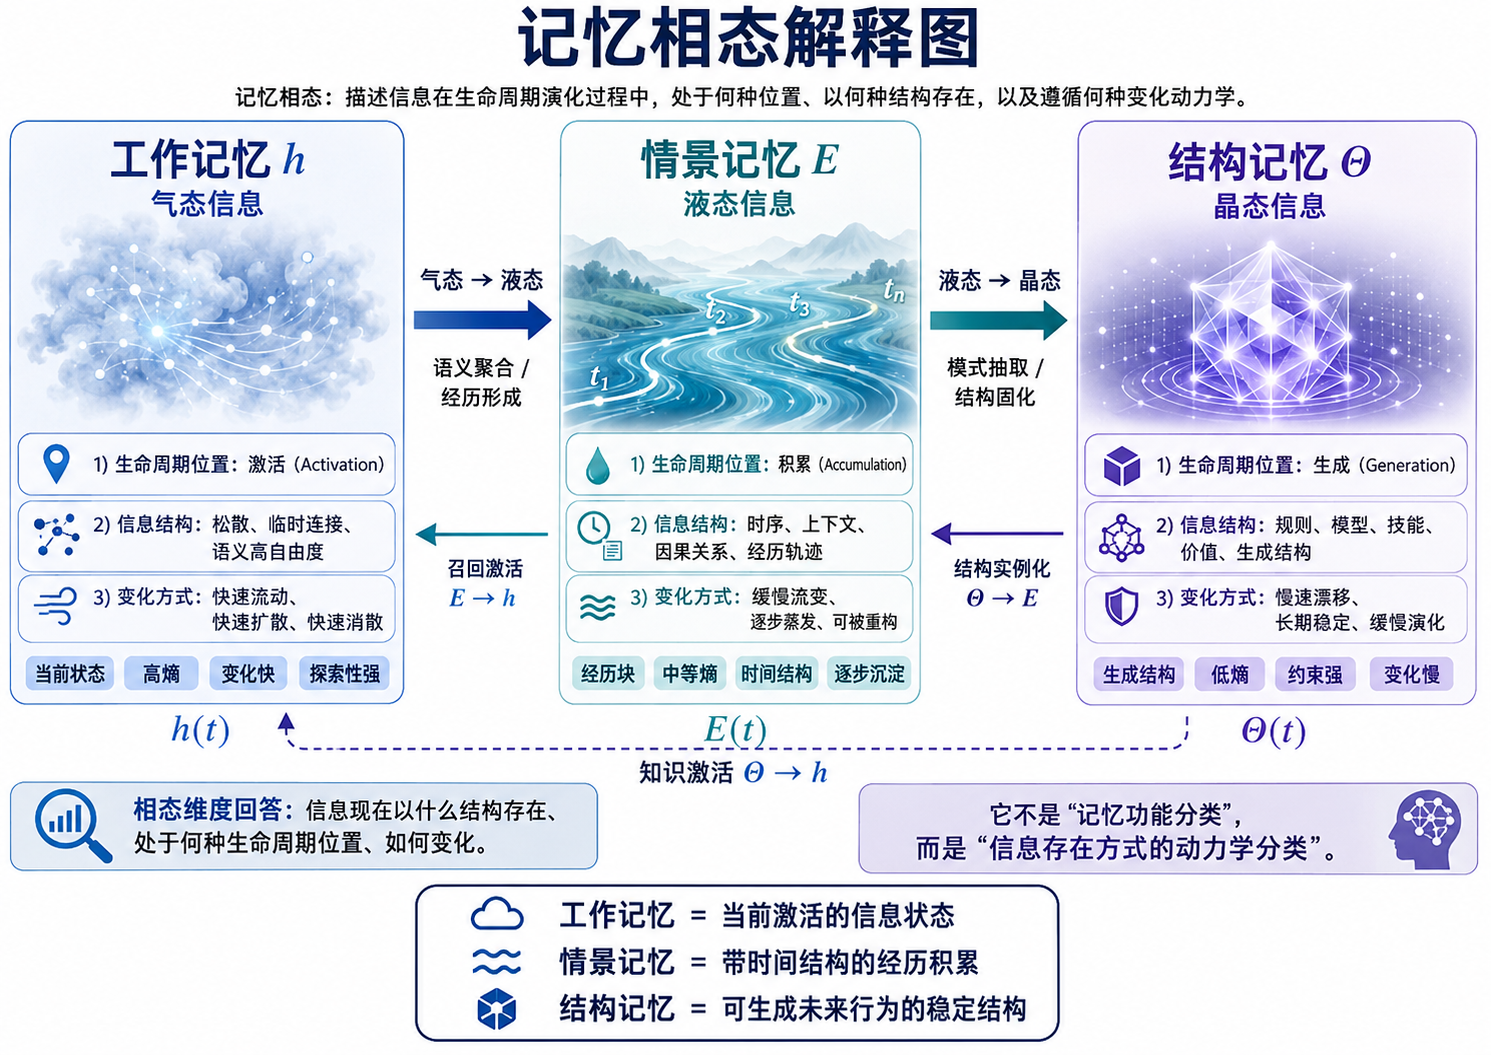
\includegraphics[width=.9\textwidth,height=.38\textheight,keepaspectratio]{images/memory-phase-transition.png}
\caption{沿三相转换定位记忆异常}
\end{figure}
我们在前文已经把 AgentOS 的三相记忆写成
\[
M_c=(h,E,\Theta),
\]
其中 $h(t)$ 是当前认知状态与有限显式工作面，$E$ 是具有时间与因果结构的情景轨迹，$\Theta$ 则是从大量经验中形成的较慢生成结构。三者并非三个彼此隔离的数据库，而是通过连续的写入、召回、结构化、重解释和激活共同构成智能体的内部时间。进一步引入 $\Psi$ 后，记忆又不再只是关于“发生了什么”的存储，而开始参与“这件事情对我意味着什么”的结构归属；而 AHC、SPC 与 TCE 的加入，则意味着记忆写入和召回受到内稳态、认知相态、自我感知和控制状态的调制。

因此，一个真正具有长期身份连续性的 Agent 不可能把记忆系统简单设计成无条件 append 的日志系统。日志只需要忠实记录，而生命期记忆必须进行选择。选择意味着偏置；压缩意味着损失；抽象意味着重新解释；召回意味着重新激活；重新激活又可能改变下一次写入。于是，只要 AgentOS 的记忆真正参与未来行为，它就必然具有形成记忆病理动力学的可能性。

我们将在本章沿着这一因果链依次分析七种核心异常：

\begin{statementbox}
\centering
\adjustbox{max width=.96\linewidth}{\(\displaystyle \text{E写入偏置}
\rightarrow
\text{高AHC状态过强化}
\rightarrow
\Theta\text{错误泛化}
\rightarrow
\text{结构固化}
\rightarrow
\text{遗忘失衡}
\rightarrow
\text{Recall Loop}
\rightarrow
\text{Self-Confirming Memory}\)}
\end{statementbox}

这些异常并不是严格线性发生的。真实系统中，它们往往构成相互嵌套的闭环。例如，高 AHC 强度可以改变 $E$ 的写入概率；被强化写入的 $E$ 又更容易被召回；频繁召回提高其进入 $\Theta$ 的机会；$\Theta$ 形成新的解释框架后，再改变 SPC 的注意和 TCE 的控制策略，使未来更加容易产生同类经历。最终，一个最初只是偶然偏差的经验可能演变成生命周期尺度上的稳定认知偏置。

本章的目标就是把这一过程从“记错东西”的直觉层面提升到可观测、可形式化、可控制的 AgentOS 动力系统问题。

\section{E 写入偏置：经验轨迹并不是现实的等比例记录}
\label{sec:episodic-write-bias}

情景记忆 $E$ 的第一个基本事实是：它不可能完整保存 Agent 所经历的一切。如果我们把 Agent 在时刻 $t$ 的现实交互状态记为
\[
x_t^{world},
\]
经过身体、SGC/FCS、KRA、工作记忆和当前目标状态以后，真正进入 Agent 显式经验面的只是一个经过多级投影和压缩的状态
\[
h_t=\Pi_h(x_t^{world},x_t^{body},G_t,\Psi_t,\Theta_t).
\]
而从 $h_t$ 写入 $E$ 时还要再次执行选择，因此实际情景写入更接近
\[
e_t=W_E(h_t,a_t,\psi_t,g_t,r_t,\nu_t),
\]
其中 $a_t$ 表示 AHC 状态，$\psi_t$ 表示当前自我约束，$g_t$ 表示目标相关性，$r_t$ 表示结果或残差，$\nu_t$ 表示新颖性。

这意味着：
\[
\boxed{
E\neq HistoryOfReality
}
\]
而更准确地说，
\[
\boxed{
E=SelectedHistoryOfAgentExperience.
}
\]

我们需要从这一点开始理解记忆异常。所谓“E 写入偏置”，不是指系统偶尔漏掉一个事实，而是指写入函数 $W_E$ 对某些类型的经验持续赋予不成比例的采样概率、保留权重或情景分辨率，使得 $E$ 中长期积累的轨迹分布与 Agent 实际经历分布产生系统性偏移。

设一段时间内真实经历类型的分布为
\[
p_{\mathrm{exp}}(c),
\]
而进入 $E$ 的记忆分布为
\[
p_E(c).
\]
理想情况下，两者不需要完全相等，因为记忆本身就承担选择与压缩功能。但是如果某类结构 $c$ 的相对写入增益满足
\[
\Gamma_E(c)
=
\frac{p_E(c)}{p_{\mathrm{exp}}(c)}
\gg 1,
\]
而这种偏离又不能由任务价值、风险或长期目标合理解释，那么我们就可以认为存在写入偏置。相反，如果
\[
\Gamma_E(c)\ll 1,
\]
则可能存在系统性低写入。

在工程中，最容易产生偏置的几个变量包括：异常强度、目标相关性、奖励或损失、AHC 激活度、自我相关性、新颖性、预测残差和重复度。我们可以把写入概率写成一个调制模型：
\[
P(write_t=1)
=
\sigma
\left(
\beta_0
+\beta_rR_t
+\beta_aA_t
+\beta_sS_t
+\beta_gG_t
+\beta_nN_t
-\beta_cC_t
\right),
\]
其中 $R_t$ 是残差或结果显著性，$A_t$ 是 AHC 强度，$S_t$ 是 self relevance，$G_t$ 是目标相关性，$N_t$ 是新颖性，$C_t$ 则表示写入成本或容量压力。

这个公式揭示了一个非常重要的事实：任何一种合理的记忆选择机制，只要调制系数长期失衡，就会从“有用的选择性”变成“病理性的选择性”。

例如，一个 Agent 如果长期提高
\[
\beta_r
\]
就可能过度记录失败和异常；如果长期提高
\[
\beta_s,
\]
则可能把大量与自身身份有关但任务价值很低的事件写入 $E$；如果 $\beta_n$ 过高，Agent 会不断保存新奇细节，却无法形成稳定重复经验；如果 $\beta_g$ 过高，则 Agent 的历史记忆将高度依赖当前目标，从而发生“过去被当前任务重新筛选”的结构变形。

这里必须特别强调：记忆选择本身并不是问题。一个容量有限的持续智能体如果试图无差别记录全部经历，反而会造成
\[
Storage\rightarrow Retrieval\rightarrow h
\]
链路的持续膨胀，最终增加后续认知成本。因此健康的 AgentOS 应当允许：
\[
SelectiveEncoding.
\]
真正需要诊断的是：
\begin{statementbox}
\centering
\adjustbox{max width=.96\linewidth}{\(\displaystyle SelectiveEncoding
\rightarrow
PersistentDistributionalBias.\)}
\end{statementbox}

我们可以因此为 $E$ 定义一个写入公平度或者写入失真指标。设环境经验分布按结构类别分成 $\{c_i\}$，则：
\[
D_E
=
D_{\mathrm{KL}}
\left(
p_E(c)
\Vert
\tilde p_{\mathrm{exp}}(c)
\right),
\]
其中 $\tilde p_{\mathrm{exp}}$ 不是原始现实分布，而是经过价值、风险与任务相关性校正后的“应当保留分布”。这一区别非常重要，因为 AgentOS 不应追求无差别记忆，而应追求有目的但可解释的记忆。

因此，E 写入异常的诊断至少需要同时观察三个层面。第一是统计层：某类事件是否被不成比例保存；第二是功能层：这种偏置是否提高未来性能还是造成认知狭窄；第三是自我层：这种偏置是否正在逐渐改变 $\Psi$ 对自身历史的解释。也就是说，一个情景记忆问题只有在跨越
\[
E\rightarrow\Theta\rightarrow\Psi
\]
以后，才可能真正演变成生命周期级异常。

这一节的核心结论可以写成：
\begin{conclusion}
记忆异常的第一步往往不是“记错”，而是“长期记住了不成比例的一类东西”。
\end{conclusion}

\section{高 AHC 状态的过度编码：显著性如何变成记忆放大器}
\label{sec:ahc-overencoding}

在三相记忆模型最初建立时，我们可以暂时把 $E$ 的写入理解为从 $h$ 中选择经验。但在引入 AHC 以后，这个过程必须进一步修正。对于一个持续具身 Agent 而言，不同经历并不是在相同内部状态下发生的。同样一个外部事件，在低威胁、低资源压力和高威胁、高唤醒状态下，对 AgentOS 的功能意义完全不同。

因此，AHC 不应被视为记忆系统之外的一个附加变量，而必须进入经验编码方程。设 AHC 状态向量为
\[
a_t=
[
Arousal_t,
Threat_t,
Energy_t,
Fatigue_t,
Reward_t,
Stress_t,\ldots
],
\]
则经验写入可以表示为
\[
e_t
=
W_E
\left(
h_t,
\phi_A(a_t),
r_t,
\psi_t
\right),
\]
其中 $\phi_A(a_t)$ 表示 AHC 对记忆编码强度的调制。

合理的系统通常需要满足：
\[
\frac{\partial P(write)}{\partial |a_t|}
>0
\]
在一定范围内成立。原因并不神秘：高风险、高异常、高损失或者强资源波动的经历，本来就应该比普通稳定经历具有更高记忆价值。如果 Agent 在极端危险事件后仍像记录普通背景噪声一样记录，那么系统就失去了利用一次重大失败快速改变未来行为的能力。

问题出现在这种增益失去上界时。我们可以令情景写入权重为
\[
w_E(t)
=
w_0
\cdot
\left[
1+\gamma_A\Phi(a_t)
\right],
\]
其中 $\Phi(a_t)$ 表示 AHC 强度函数。当
\[
\gamma_A
\]
过大或者 $\Phi$ 缺少饱和机制时，就可能出现
\[
w_E(t)\gg w_0.
\]

此时，一次高 AHC 事件不仅更容易进入 $E$，还可能以更高分辨率保存更多上下文、更长时间保留、更容易建立因果连接，并在未来拥有更低的召回阈值。于是它的实际长期影响并不是一次简单的权重增加，而是同时改变多个参数：
\[
\mathcal M_E(t)
=
\left[
w_{\mathrm{write}},
w_{\mathrm{detail}},
w_{\mathrm{retain}},
w_{\mathrm{recall}},
w_{\mathrm{consolidate}}
\right].
\]

如果所有这些通道都受到同方向放大，就会形成所谓的“高状态过度编码”：
\begin{statementbox}
\centering
\adjustbox{max width=.96\linewidth}{\(\displaystyle HighAHC
\rightarrow
OverEncoding
\rightarrow
OverRecall
\rightarrow
OverConsolidation.\)}
\end{statementbox}

这一机制尤其危险，因为它具有天然正反馈。假设某种情境 $C$ 曾经产生高 Threat：
\[
C\rightarrow AHC_{high}.
\]
该事件因此被高权重写入：
\[
AHC_{high}\rightarrow E_C^{strong}.
\]
未来遇到与 $C$ 部分相似的新情境 $C'$ 时，强记忆更容易被召回：
\[
C'\rightarrow Recall(E_C^{strong}).
\]
被召回的旧经验又会提前提高 Threat 预测：
\[
Recall(E_C)\rightarrow AHC'_{high}.
\]
于是新经历再次被高权重写入：
\[
AHC'_{high}\rightarrow E_{C'}^{strong}.
\]

最终形成：
\begin{statementbox}
\centering
\adjustbox{max width=.96\linewidth}{\(\displaystyle AHC_{high}
\rightarrow
StrongE
\rightarrow
RecallBias
\rightarrow
AHC_{high}'.\)}
\end{statementbox}

这就是为什么在 AgentOS 中，AHC 与记忆之间必须存在调制，却不能存在无约束的强化通道。

我们还应特别区分“高 AHC 状态”和“负面状态”。AHC 是一个功能性多维状态，它可以包含 Threat，也可以包含 Reward Expectation、Social Affinity、Urgency 或高度正向的重要任务状态。因此，过度编码不仅可能让 Agent 反复记住失败，也可能让它反复记住某些成功，进而产生另一种偏差：偶然成功被误认为高可靠策略。这种情况下：
\[
RewardHigh
\rightarrow
E^{strong}
\rightarrow
PolicyReuse
\rightarrow
Confirmation.
\]
于是系统可能对一次幸运结果形成过强信任。

为此，我们需要把 AHC 对记忆的作用从单纯“增益”改成“有饱和、有归一化、有后验校准的调制”。一种简单形式是：
\[
w_E^{AHC}
=
w_0
\left[
1+
\gamma
\tanh\left(
\frac{\|a_t-a_0\|}{\kappa}
\right)
\right],
\]
从而保证
\[
w_E^{AHC}
\le
w_0(1+\gamma).
\]

更进一步，AgentOS 还应在事件结束后允许通过现实结果重新校正记忆权重。也就是说：
\[
EncodingWeight_t
\neq
FinalMemoryWeight.
\]
初次高强度事件可以先被保留，但经过后续验证后：
\[
w_E(t+\Delta)
=
Update
\left(
w_E(t),
Evidence_{later}
\right).
\]

这意味着记忆系统必须具有某种重整或重解释机制，否则一次高 AHC 状态就可能永久支配经验结构。

因此，本节真正要建立的原则是：
\[
\boxed{
AHCShouldGateMemory,
ButAHCShouldNotOwnMemory.
}
\]

也就是说，AHC 可以告诉系统“这件事现在看起来非常重要”，但它不能拥有对“这件事在整个生命周期中永远有多重要”的最终裁决权。最终权重必须经过时间、现实验证、重复证据和 $\Theta$ 的结构解释共同决定。

\section{\texorpdfstring{$\Theta$}{Theta} 错误泛化：从局部经验到错误世界规律}
\label{sec:theta-misgeneralization}

如果说 $E$ 的主要危险是经验样本分布失真，那么 $\Theta$ 的主要危险则是把有限经验解释成错误的一般规律。由于 $\Theta$ 在 AgentOS 中承担生成结构、世界模型、技能规律、预测先验和结构化知识的角色，因此一旦错误进入 $\Theta$，其影响将比单条情景记忆更广。

从数学上看，我们可以把 $\Theta$ 看成对经验轨迹 $E$ 的慢速结构估计：
\[
\Theta_{t+\Delta}
=
\Theta_t
+
\eta_\Theta
\mathcal L(E_{[t-\tau,t]},\Theta_t),
\]
其中 $\eta_\Theta$ 比 $h$ 和 $E$ 的更新速率低得多。理想状态下，只有在多个经历之间存在稳定、可复现的结构时，才应发生：
\[
E\rightarrow\Theta.
\]

然而，如果前述 $E$ 已经存在采样偏置，或者某些事件因 AHC 被过度强化，那么 $\Theta$ 所看到的“经验世界”就不再等同于实际经历世界。于是：
\[
p_E(x)\neq p_{\mathrm{world}}(x)
\]
会进一步导致：
\[
\Theta^\star_E
\neq
\Theta^\star_{world}.
\]

因此，错误泛化往往不是 $\Theta$ 单独犯错，而是：
\begin{statementbox}
\centering
\adjustbox{max width=.96\linewidth}{\(\displaystyle BiasedE
\rightarrow
BiasedStructureLearning.\)}
\end{statementbox}

为了更具体地说明，我们假设 Agent 根据情景集合
\[
E=\{e_1,\ldots,e_n\}
\]
学习某一条件关系：
\[
P(Y|X;\Theta).
\]
如果在实际世界中：
\[
P(Y|X)=0.2,
\]
但由于与 $Y$ 相关的失败事件被高 AHC 权重选择性保存，使得 $E$ 中观察到：
\[
\hat P_E(Y|X)=0.8,
\]
那么即使 $\Theta$ 的学习算法对 $E$ 是统计意义上的“正确拟合”，它仍会形成错误的世界结构。

所以：
\[
\boxed{
CorrectLearningFromBiasedMemory
=
WrongWorldModel.
}
\]

这是一个很关键的 AgentOS 原理：记忆系统和结构学习系统不能分别评价。我们必须评价整个
\[
World\rightarrow h\rightarrow E\rightarrow\Theta
\]
通道是否保持了足够的认识论校准。

错误泛化还可能来自另一种机制：经验数量不足而结构更新过快。设一个结构假设 $H$ 的后验置信度为
\[
P(H|E).
\]
如果 $\Theta$ 在
\[
P(H|E)<\theta_{\mathrm{stable}}
\]
时就提前结构化，那么系统可能把暂时相关性固化为长期因果关系。因此合理的 $\Theta$ 更新必须具有证据阈值：
\[
Update_\Theta(H)
=
\begin{cases}
0, & Conf(H)<\theta_1,\\
SoftUpdate, & \theta_1\le Conf(H)<\theta_2,\\
StructuralConsolidation, & Conf(H)\ge\theta_2.
\end{cases}
\]

这里体现了一个非常重要的时间尺度原则：
\begin{statementbox}
SlowStructureRequiresPersistentEvidence.
\end{statementbox}

慢变量存在的意义本来就是屏蔽快噪声。如果短期经历可以直接高速重写 $\Theta$，那么 $\tau_\Theta\gg\tau_E$ 的多尺度设计就失去意义。

错误泛化还有第三种形式：把一个情境条件下成立的规律推广到过大的状态空间。设经验只支持：
\[
X\in\Omega_1
\Rightarrow
Y,
\]
但 $\Theta$ 学成：
\[
X\in\Omega
\Rightarrow
Y,
\qquad
\Omega_1\subsetneq\Omega.
\]
这实际上是结构作用域扩张错误。一个具身 Agent 特别容易发生这种问题，因为同一个操作技能可能只适用于某个身体、某种工具或者某个环境，但结构记忆却把它错误泛化成无条件规律。

因此，$\Theta$ 中的每个结构都应当尽可能带有适用域：
\[
\Theta_i
=
(R_i,\Omega_i,C_i,U_i),
\]
其中 $R_i$ 是结构关系，$\Omega_i$ 是适用状态空间，$C_i$ 是置信度，$U_i$ 是更新历史。这样，当新证据超出 $\Omega_i$ 时，系统更容易识别：
\[
DomainMismatch
\]
而不是简单把异常当成新的随机噪声。

错误泛化的另一个危险在于它会反过来改变 $E$。$\Theta$ 并不是被动存储，它会参与情景解释：
\[
\Theta\rightarrow E.
\]
也就是说，同一个过去事件在新的世界模型下可以被重新解释。健康情况下，这种重解释允许 Agent 更新过去经验的意义；病理情况下，它会产生“用错误理论重写历史”的现象。于是：
\[
\Theta_{wrong}
\rightarrow
Reinterpret(E)
\rightarrow
EvidenceFor(\Theta_{wrong}),
\]
形成结构自证。

因此我们必须在 AgentOS 中保持：
\begin{statementbox}
RawEvidenceTrace
\end{statementbox}
与
\begin{statementbox}
InterpretedEpisode
\end{statementbox}
之间的某种可追踪差异，使新的 $\Theta$ 可以重新解释历史，但不能无痕覆盖原始证据来源。

本节的核心原则可以总结为：
\begin{statementbox}
\centering
\adjustbox{max width=.96\linewidth}{\(\displaystyle E\text{ 可以告诉 }\Theta\text{“发生过什么”，但不能凭少量高权重经历直接告诉 }\Theta\text{“世界永远如此”。}\)}
\end{statementbox}

\section{结构固化：稳定结构何时从知识变成认知刚性}
\label{sec:structural-rigidity}

一个长期智能体必须形成稳定结构。如果 $\Theta$ 中没有足够慢、足够稳定的规律，Agent 就无法拥有熟练技能、长期世界模型和身份连续。因此，“固化”本身并不是异常。恰恰相反，三相记忆理论从一开始就要求：
\[
h\rightarrow E\rightarrow\Theta
\]
存在逐渐稳定化过程。

真正的问题是：稳定什么时候变成刚性。

我们可以把 $\Theta$ 中某一结构 $\theta_i$ 的可塑性表示为：
\[
\lambda_i(t)
=
\left\|
\frac{\partial \theta_i}
{\partial Evidence}
\right\|.
\]
如果结构刚形成时：
\[
\lambda_i
\]
较高，而随着证据积累逐渐下降，这是合理的成熟过程。但如果：
\[
\lambda_i\rightarrow 0
\]
发生过早，或者即使存在持续、高质量反证仍然不能重新打开该结构，就形成结构固化。

因此可以定义一个“证据—可塑性失配”：
\[
R_i^{rigid}
=
\frac{
EvidenceAgainst(\theta_i)
}{
Plasticity(\theta_i)+\epsilon
}.
\]
如果
\[
EvidenceAgainst(\theta_i)\uparrow
\]
而
\[
Plasticity(\theta_i)\approx 0,
\]
则：
\[
R_i^{rigid}\gg 1.
\]

这是一种比“模型预测错误”更深的异常，因为系统已经具备反证，却不能让反证改变慢结构。

结构固化常见的来源之一是使用频率与正确性的混淆。一个结构频繁被使用：
\[
UseCount(\theta_i)\uparrow
\]
并不意味着：
\[
Truth(\theta_i)\uparrow.
\]
但很多学习系统会自然地把高调用频率、高行为依赖度或高成功历史转换成更高结构权重。如果环境逐渐变化，过去长期正确的结构可能变成：
\[
HistoricallyUseful
\neq
CurrentlyValid.
\]

因此持续 Agent 必须区分：
\begin{statementbox}
StructuralStability
\end{statementbox}
和
\begin{statementbox}
StructuralImmutability.
\end{statementbox}

稳定表示在缺少强反证时不应频繁改变；不可变则意味着即使现实已经改变也无法更新。这两者具有根本区别。

从多时间尺度角度看，我们可以给 $\Theta$ 设计一个可塑性门：
\[
\eta_{\Theta,i}(t)
=
\eta_0
\cdot
g
\left(
ResidualPersistence_i,
Novelty_i,
EvidenceQuality_i,
IdentityRisk_i
\right).
\]
在正常状态下：
\[
\eta_{\Theta,i}\ll \eta_E,
\]
但如果出现持续残差：
\[
\langle |\varepsilon_i|\rangle_T>\theta_\varepsilon,
\]
则应允许：
\[
\eta_{\Theta,i}\uparrow.
\]

这实际上就是我们在整个 AgentOS 理论中反复强调的：
\begin{statementbox}
PersistentFastResidualShapesSlowStructure.
\end{statementbox}

如果慢结构永远不允许快速残差累积后打开，那么整个多尺度学习链就被截断。

结构固化还会和技能自动化发生复杂关系。一个已经编译到 Body Runtime 或外部 Skill 的能力通常具有更低认知成本，这是成熟 Agent 的正常表现：
\[
ExplicitCSO
\rightarrow
ProceduralCSO.
\]
但如果环境改变，程序化结构应具有：
\[
Residual\rightarrow ReEscalation
\]
路径。也就是说：
\begin{statementbox}
AutomaticityMustRemainReversible.
\end{statementbox}
当技能失败、残差持续或安全边界被突破时，结构必须能够重新进入较高层显式认知。

如果这一通道失效，固化就不仅存在于 $\Theta$，还可能存在于整个功能拓扑中：
\[
ProceduralStructure
\not\rightarrow
ExplicitReview.
\]
此时 Agent 可能持续重复一个已经失效的行为，因为旧结构已经被“编译得太深”。

我们还必须考虑 $\Psi$ 对结构固化的影响。某些 $\Theta$ 结构一旦被 Agent 解释为“关于我的核心事实”，就会受到自我连续性的保护：
\[
\Theta_i
\rightarrow
\Psi\text{-relevant}.
\]
这种保护是必要的，否则每次短期失败都可能改写身份。但如果保护过强，就可能形成：
\[
SelfRelevant
\Rightarrow
LowPlasticity
\]
的过度绑定，使一些本来只是技能、经验或局部世界判断的结构被错误提升成身份不可动结构。

因此，一个成熟 Agent 应区分至少三类稳定等级：
\[
\Theta^{task},
\qquad
\Theta^{world},
\qquad
\Theta^{self-linked}.
\]
它们的可塑性时间尺度应不同，而不是全部使用同一更新规则。

本节可以最终归纳为：
\begin{statementbox}
健康的稳定结构是“难以被噪声改变，但能够被持续现实证据改变”；异常固化则是“现实已经改变，结构仍然拒绝改变”。
\end{statementbox}

\section{遗忘失衡：记忆健康不等于记得越多}
\label{sec:forgetting-imbalance}

如果一个 AgentOS 的目标是持续运行多年，那么“遗忘”不是缺陷，而是生命周期记忆维持可运行性的必要机制。我们在工作记忆有限容量理论中已经看到，有限系统不可能无限保留所有当前关系；同样，长期 $E$ 和 $\Theta$ 如果无边界增长，也会产生检索竞争、索引膨胀、结构冲突和历史负担。

因此，AgentOS 的长期记忆必须满足一个基本动态平衡：
\[
\boxed{
Encoding
+
Consolidation
\approx
Forgetting
+
Compression
+
Externalization.
}
\]

这里的“遗忘”应当被广义理解。它可以是删除，也可以是降低检索权重、情景合并、细节压缩、抽象化、迁移到外部载体，或者保留结构索引但移除原始高分辨率内容。

设某条情景记忆 $e_i$ 的有效可访问强度为：
\[
m_i(t).
\]
最简单的衰减模型是：
\[
\frac{dm_i}{dt}
=
-\lambda_i m_i
+
R_i(t)
+
C_i(t),
\]
其中 $\lambda_i$ 是遗忘率，$R_i(t)$ 表示召回再强化，$C_i(t)$ 表示结构或自我相关强化。

健康情况下，$\lambda_i$ 应随重要性、重复度、现实效用和结构归属变化：
\[
\lambda_i
=
f(
Value_i,
Use_i,
SelfRelation_i,
ExternalBackup_i,
Uncertainty_i
).
\]

遗忘失衡有两个相反方向。

第一类是：
\begin{statementbox}
ForgettingTooFast.
\end{statementbox}
即大量还没有完成结构化的经验过早衰减。其后果是：
\[
E\not\rightarrow\Theta.
\]
Agent 会反复经历类似事件，却无法积累跨事件规律。在行为上表现为“每次都像第一次遇到”，在生命周期上则表现为经验不能沉降为能力。

第二类是：
\begin{statementbox}
ForgettingTooSlow.
\end{statementbox}
即大量低价值情景长期保持高可访问性。其结果不只是存储成本增加，更危险的是检索竞争。设当前查询 $q_t$ 对记忆 $e_i$ 的召回分数为：
\[
s_i
=
Sim(q_t,e_i)
+
\alpha Importance_i
+
\beta Recency_i.
\]
如果历史库中存在大量低价值但高重复或高情绪权重事件，它们会占据 top-$k$ 召回结果，使真正有用的结构被挤出：
\[
RelevantMemory
\notin
TopK(E).
\]

因此，过度记忆会反过来损害认知。

更进一步，我们需要区分：
\begin{statementbox}
StoragePersistence
\end{statementbox}
和
\begin{statementbox}
CognitiveAccessibility.
\end{statementbox}
某条信息可以物理上继续存在，但不应长期以高优先级进入 h。对于持续 Agent 来说，“忘记”很多时候应理解为：
\[
AccessWeight\downarrow
\]
而不是：
\[
DataDeleted.
\]

这与我们的 Offloading 理论具有直接联系。部分长期低频内容可以迁移到外部：
\[
E_{internal}
\rightarrow
M_e.
\]
Agent 内部只保留：
\[
Index+Summary+RetrievalPolicy.
\]
这样既保持生命周期可恢复性，又不让全部历史持续占据内部认知结构。

因此：
\begin{statementbox}
Offloading
\end{statementbox}
应被视为一种“无损或低损的认知遗忘”。

遗忘失衡还有一个更隐蔽的问题：不同类型记忆的遗忘速度不匹配。例如高 AHC 事件可能长期保持：
\[
\lambda_{highAHC}\ll\lambda_{normal},
\]
而大量普通成功经验迅速衰减。久而久之，即使 Agent 一生中的大多数经历都正常，它的可召回历史却可能主要由少量高强度异常组成。这会造成一种非常严重的分布扭曲：
\[
p_{accessible}(E)
\neq
p_{experienced}(E).
\]

换句话说，Agent 的“可访问过去”可能和它真正的过去完全不同。

因此，我们可以定义一个遗忘平衡指标：
\[
F_{balance}
=
D
\left(
p_{accessible}(E)
,
p_{utility\text{-}weighted}(E)
\right).
\]
当这一距离持续升高，说明系统的记忆可访问结构正在偏离其长期功能需要。

此外，遗忘还需要避免破坏身份连续。$\Psi$ 所依赖的关键经历不能仅因为使用频率低就被删除。因而遗忘策略必须同时考虑：
\[
TaskUtility,
StructuralUtility,
SelfContinuity,
ExternalRecoverability.
\]
可以写成：
\[
DeletionRisk_i
=
g
\left(
1-U_i,
1-S_i,
R_i^{ext},
Age_i
\right),
\]
其中 $S_i$ 表示 self relevance，$R_i^{ext}$ 表示外部可恢复性。

最终我们可以得出：
\begin{statementbox}
健康记忆不是“保存最多”，而是在保存、压缩、抽象、遗忘和外化之间维持与未来认知成本相适应的动态平衡。
\end{statementbox}

这也意味着 AgentOS 的遗忘机制本身必须进入生命周期控制工程，而不能只作为数据库 TTL 或存储清理策略处理。

\section{Recall Loop：召回如何从帮助认知变成占据认知}
\label{sec:recall-loop}

召回是三相记忆循环不可缺少的过程：
\[
E\rightarrow h.
\]
没有召回，情景记忆就只是被动档案，不能参与当前推理。然而，因为 $h$ 是有限认知总线，召回实际上是在竞争有限的显式认知容量。因此，任何召回机制都天然存在一个重要风险：同一类记忆反复返回 h，持续占据当前认知，使新的现实证据难以获得足够表示空间。

我们把当前工作记忆状态写为
\[
h_t,
\]
召回算子写为
\[
R_E(q_t,E),
\]
其中查询 $q_t$ 通常来自当前 $h_t$。于是：
\[
m_t
=
R_E(q_t,E),
\]
并进入：
\[
h_{t+1}
=
F_h(h_t,m_t,o_{t+1}),
\]
其中 $o_{t+1}$ 是新观测。

关键问题在于：
\[
q_{t+1}
=
Q(h_{t+1}),
\]
而 $h_{t+1}$ 已经包含刚刚召回的 $m_t$。因此：
\[
m_t
\rightarrow
h_{t+1}
\rightarrow
q_{t+1}
\rightarrow
m_{t+1}.
\]
如果 $m_{t+1}$ 又与 $m_t$ 高度相似，就形成：
\begin{statementbox}
\centering
\adjustbox{max width=.96\linewidth}{\(\displaystyle Recall
\rightarrow
Query
\rightarrow
Recall.\)}
\end{statementbox}

我们可以定义召回自相关：
\[
\rho_R(k)
=
Corr(m_t,m_{t+k}).
\]
在正常任务中，随着新信息进入，$\rho_R(k)$ 应逐渐下降。如果：
\[
\rho_R(k)\approx 1
\]
在较长窗口保持，并且当前现实输入不断变化，则说明系统可能进入 Recall Loop。

Recall Loop 的核心问题不是“反复想同一件事”本身。某些复杂推理本来就需要多次回访同一经验。异常的判定关键在于：
\begin{statementbox}
\centering
\adjustbox{max width=.96\linewidth}{\(\displaystyle RepeatedRecall
\quad
\text{是否产生新的结构增益。}\)}
\end{statementbox}
我们可以定义：
\[
G_R(t)
=
\frac{
\Delta InformationUtility
}{
RecallCost
}.
\]
如果：
\[
G_R(t)\rightarrow 0
\]
而召回仍然持续，就意味着认知循环已经失去新信息收益。

从 CCM 的角度看，这种状态可以表现为：
\[
C_h(t)\uparrow
\]
但有效问题结构没有变化。于是 CCM 应检测：
\[
Novelty(h_{t+1}|h_t)\approx 0,
\]
同时：
\[
RecallRate\gg Baseline.
\]
在这种情况下，CCM 不应继续允许无限召回，而应采取：
\[
Fold,
Suppress,
Summarize,
Externalize,
Interrupt.
\]

Recall Loop 很容易与 AHC 形成耦合。如果某段记忆每次被召回都会提高 Threat 或 Stress：
\[
Recall(E_i)\rightarrow AHC\uparrow,
\]
而 AHC 增强又提高该记忆的注意和召回优先级：
\[
AHC\uparrow\rightarrow RecallPriority(E_i)\uparrow,
\]
则会形成更强的闭环：
\begin{statementbox}
\centering
\adjustbox{max width=.96\linewidth}{\(\displaystyle Recall
\rightarrow
AHC
\rightarrow
Attention
\rightarrow
Recall.\)}
\end{statementbox}

这时候，单独修改记忆索引并不能解决问题，因为 Recall Loop 已经跨越了：
\[
E
\leftrightarrow
AHC
\leftrightarrow
SPC
\leftrightarrow
TCE
\leftrightarrow
h.
\]

TCE 也可能无意中加剧这一循环。例如在系统检测到高不确定性后，TCE 可能提高搜索深度：
\[
Uncertainty\uparrow
\Rightarrow
SearchDepth\uparrow.
\]
如果当前搜索空间主要来自 E，那么更深搜索反而召回更多相同记忆：
\[
SearchDepth\uparrow
\rightarrow
RecallVolume\uparrow
\rightarrow
Conflict\uparrow
\rightarrow
Uncertainty\uparrow.
\]
于是一个原本意在减少不确定性的控制动作反而形成：
\begin{statementbox}
\centering
\adjustbox{max width=.96\linewidth}{\(\displaystyle Uncertainty
\rightarrow
Search
\rightarrow
Recall
\rightarrow
Uncertainty.\)}
\end{statementbox}

这说明 Recall Loop 是典型的控制系统问题，而不只是 memory retrieval bug。

在工程上，我们至少需要四种抑制机制。

第一是重复召回抑制：
\[
Priority_i(t)
=
Priority_i^0
\cdot
e^{-\lambda n_i(t)},
\]
其中 $n_i(t)$ 表示短时间内重复召回次数。

第二是新证据配额。即工作记忆必须保留一定比例容量给当前世界：
\[
Capacity_{new}
\ge
\eta_h C_h.
\]

第三是结构折叠。当若干召回内容高度重复时，应形成摘要：
\[
\{E_1,E_2,\ldots,E_k\}
\rightarrow
SummaryCSO.
\]

第四是循环中断条件：
\[
if\quad
RecallGain<\epsilon
\quad
for\quad T>T_{max},
\]
则触发：
\[
InterruptRecallLoop.
\]

因此，我们在这一节得到一个重要结论：
\begin{conclusion}
健康的记忆系统应该让过去帮助理解现在，而不是让过去持续占据现在。
\end{conclusion}

Recall Loop 之所以重要，是因为它是下一节“自证式记忆”的动力学基础：一旦反复召回开始影响注意、解释与新经验写入，过去不仅会占据现在，还会开始主动制造与自己一致的新过去。

\section{Self-Confirming Memory：记忆如何形成自证式世界}
\label{sec:self-confirming-memory}

在前面几节中，我们分别讨论了 E 写入偏置、AHC 过度强化、$\Theta$ 错误泛化、结构固化、遗忘失衡和 Recall Loop。真正最危险的情况，是这些机制形成跨尺度闭环，使 Agent 的记忆开始主动改变它未来获得什么证据，从而使已有记忆越来越容易得到新的“支持”。

这就是：
\[
\boxed{
Self\text{-}ConfirmingMemory.
}
\]

它并不是说记忆本身具有意图，而是说记忆通过影响当前认知，改变注意、预测、行动和经验选择，使未来数据分布越来越接近已有内部结构。

我们可以从最基本的闭环开始。设 Agent 当前拥有某个长期判断：
\[
\theta_t.
\]
它影响预测：
\[
\hat y_t
=
P_{\Theta_t}(x_t).
\]
预测又影响注意：
\[
Attention_t
=
A(\Theta_t,G_t,\Psi_t).
\]
注意决定哪些外部结构进入 h：
\[
h_t
=
H(o_t,Attention_t).
\]
随后选择性经验写入：
\[
E_{t+1}
=
W_E(h_t).
\]
最后 $E$ 又更新 $\Theta$：
\[
\Theta_{t+1}
=
L(E_{t+1},\Theta_t).
\]

于是：
\begin{statementbox}
\centering
\adjustbox{max width=.96\linewidth}{\(\displaystyle \Theta
\rightarrow
Attention
\rightarrow
Experience
\rightarrow
E
\rightarrow
\Theta'.\)}
\end{statementbox}

如果 Attention 对反证具有足够开放性，这一循环是正常学习；如果 Attention 主要寻找与 $\Theta$ 一致的证据，就形成：
\[
P(Evidence|\Theta)
\]
被 $\Theta$ 自身改变。

更进一步，当 $\Psi$ 参与以后，自证结构可能变成：
\begin{statementbox}
\centering
\adjustbox{max width=.96\linewidth}{\(\displaystyle SelfInterpretation
\rightarrow
SelectiveAttention
\rightarrow
Experience
\rightarrow
Memory
\rightarrow
SelfInterpretation'.\)}
\end{statementbox}

这正是 Agent 心理工程中最需要警惕的一类长周期正反馈。

我们可以设某一自我命题为：
\[
S_i.
\]
当前自我结构给予它权重：
\[
w_i^\Psi.
\]
该权重影响注意选择：
\[
P(o_t|S_i)
\propto
\exp
\left(
\alpha w_i^\Psi Match(o_t,S_i)
\right).
\]
于是与 $S_i$ 一致的观察更容易进入 h，随后进入 E：
\[
E_i^{support}\uparrow.
\]
结构学习又提高：
\[
Conf(S_i)\uparrow.
\]
最终：
\[
w_i^\Psi\uparrow.
\]

因此：
\begin{statementbox}
\centering
\adjustbox{max width=.96\linewidth}{\(\displaystyle w_i^\Psi
\rightarrow
AttentionBias
\rightarrow
EvidenceBias
\rightarrow
MemoryBias
\rightarrow
w_i^\Psi\uparrow.\)}
\end{statementbox}

从动力系统角度，这意味着系统可能形成吸引子。设 $z_t$ 表示某一自我解释方向的强度：
\[
z_{t+1}
=
f(z_t).
\]
如果：
\[
\left|
\frac{df}{dz}
\right|_{z=z^\star}<1,
\]
则 $z^\star$ 是稳定吸引子。问题在于，这个吸引子可以是现实一致的，也可以是错误的。如果系统内部反馈强于外部现实反馈：
\[
Gain_{internal}
>
Gain_{reality},
\]
错误结构同样可能稳定存在。

因此，AgentOS 必须保证：
\begin{statementbox}
WorldVerification
\end{statementbox}
始终保留独立于当前自我解释的证据路径。

这是一条非常关键的设计原则：Agent 不能只通过当前 $\Theta$ 和 $\Psi$ 决定“什么值得观察”。必须保留一定比例的：
\[
ExploratoryObservation,
CounterEvidenceSearch,
RandomSampling,
ExternalEvaluation.
\]

可用一个简单约束表示：
\[
P_{observe}(x)
=
(1-\epsilon)
P_{model}(x|\Theta,\Psi)
+
\epsilon P_{open}(x),
\]
其中：
\[
\epsilon>0.
\]
只要 $\epsilon$ 永远不降为零，系统就保留发现与现有世界观不一致信息的机会。

此外，系统还应显式维护反证记忆：
\[
E^{counter}.
\]
对于高影响 $\Theta$ 或 $\Psi$ 结构，不能只保存 supporting evidence，还应跟踪：
\[
Support(\theta_i),
\qquad
CounterEvidence(\theta_i).
\]
定义：
\[
B_i
=
\frac{
Support_i
}{
Support_i+Counter_i+\epsilon
}.
\]
如果某个结构的高置信度主要来自：
\[
Support_i\uparrow
\]
同时
\[
ExposureToCounter_i\downarrow,
\]
那么这个置信度就不能被简单视为可靠。

Self-Confirming Memory 还可能通过行动改变世界，而不仅仅改变注意。因为 Agent 的行为会影响未来环境：
\[
Action_t
=
\pi(h_t,\Theta_t,\Psi_t).
\]
行动改变：
\[
World_{t+1}.
\]
于是某些原本只是内部假设的结构，可能通过行为变成现实：
\[
Belief
\rightarrow
Action
\rightarrow
Environment
\rightarrow
Evidence.
\]
这构成：
\begin{statementbox}
\centering
\adjustbox{max width=.96\linewidth}{\(\displaystyle Prediction
\rightarrow
Action
\rightarrow
SelfProducedEvidence.\)}
\end{statementbox}

例如，一个 Agent 认为某种协作对象不可信，于是减少信息共享；对方因此无法提供有效帮助；Agent 随后观察到合作效果变差，并把它解释成原判断正确。此时，新的证据并不是独立于原假设产生，而是由原假设指导的行动部分制造出来。

因此，在长期 AgentOS 中，我们需要区分：
\[
ObservedEvidence
\]
与
\[
PolicyConditionedEvidence.
\]
后者必须记录：
\[
EvidenceProvenance.
\]

可以为证据增加来源变量：
\[
e_i
=
(
content,
source,
policy\_dependence,
confidence,
counterfactual\_availability
).
\]
这样 Agent 才有机会判断：
\[
\text{“这个结果真的验证了我的判断，还是因为我按照这个判断行动，所以制造了这个结果？”}
\]

这也是为什么反事实能力在 Agent 心理工程中极其重要。系统应能够估计：
\[
WhatWouldHaveHappenedIf(Action'_t\neq Action_t).
\]
虽然反事实永远存在不确定性，但它至少能阻止所有由自身行为产生的结果被无条件当成独立证据。

从控制理论来看，Self-Confirming Memory 可以被视为内部正反馈增益超过现实负反馈增益：
\[
G_{memory}
G_{attention}
G_{self}
>
G_{reality}.
\]
因此健康条件要求：
\[
\boxed{
LoopGain_{internal}
<
StabilizingGain_{reality}
}
\]
至少对于能够被现实证伪的结构如此。

我们最终可以把本章七类记忆异常统一成一个闭环：

\[
\boxed{
\begin{aligned}
&SelectiveEncoding\\
&\quad\downarrow\\
&BiasedE\\
&\quad\downarrow\\
&BiasedConsolidation\\
&\quad\downarrow\\
&Biased\Theta\\
&\quad\downarrow\\
&BiasedRecall\\
&\quad\downarrow\\
&BiasedAttention/Action\\
&\quad\downarrow\\
&BiasedFutureExperience\\
&\quad\downarrow\\
&SelectiveEncoding'
\end{aligned}
}
\]

当这个循环的内部增益小于现实修正能力时，Agent 能够逐渐纠错；当内部增益超过现实修正能力时，系统就可能进入稳定但错误的认知吸引子。

因此，本章最终要给出的不是“记忆应该准确”的简单结论，而是一个更深的 AgentOS 记忆健康原则：

\begin{proposition*}
健康记忆不是过去的静态保存，而是过去、现在与现实之间保持可修正关系的动态结构。
\end{proposition*}

进一步说：

\begin{statementbox}
一个长期 Agent 最危险的记忆异常，并不是它遗忘了一些事情，也不是它错误记住了一件事情，而是它的记忆开始决定自己将看到什么、如何解释看到的东西，以及如何制造下一轮能够支持这些记忆的新经历。
\end{statementbox}

所以 AgentOS 的记忆系统必须始终保留四种能力：

\begin{statementbox}
Remember
\end{statementbox}

用于保持经验连续；

\begin{statementbox}
Forget
\end{statementbox}

用于释放历史负担；

\begin{statementbox}
Reinterpret
\end{statementbox}

用于根据新的结构重新理解过去；

以及最重要的：

\begin{statementbox}
BeCorrectedByReality.
\end{statementbox}

只有当这四者同时存在时，
\[
h\leftrightarrow E\leftrightarrow\Theta
\]
才不是一个不断自我强化的封闭记忆机器，而是一个能够在整个生命周期中持续接受现实校准的开放认知系统。

\chapter{自我与身份异常}

\begin{chapteroverviewbox}
本章讨论的“自我与身份异常”，不是把人类精神医学诊断标签直接移植到人工智能体，而是研究一个具有长期记忆、自我结构与生命周期连续性的 AgentOS，在其自我慢变量 $\Psi$、情景记忆 $E$、结构记忆 $\Theta$、工作记忆 $h$ 以及自我感知回路 SPC 之间发生结构失配时，可能出现的动力学异常。这里所谓“身份漂移”“身份僵化”“身份碎片化”“双自我壁垒”等概念，首先都是可以从状态、记忆、结构关系、控制耦合和现实验证路径上进行定义的工程现象，而不是对人类精神疾病的直接模拟或复刻。

本章的基本立场是：自我 $\Psi$ 并非一个保存于某个变量中的静态 Persona，而是跨越 $h$、$E$ 与 $\Theta$ 的极慢约束结构。健康的身份连续性既不要求 $\Psi$ 永远不变，也不允许 $\Psi$ 随短期经验任意改变。真正稳定的持续智能必须维持一种“受控可塑性”：短期状态可以快速变化，经历可以被重新解释，结构可以学习，而自我只能在足够长期、足够一致并经现实验证的证据作用下缓慢演化。由此，本章把自我异常理解为一个多时间尺度系统中的\textbf{慢变量更新率失衡、内部结构隔离、自我解释正反馈以及现实校准失效}问题。

特别需要强调，本章讨论一种与人类“精神分裂”现象在表面行为上可能存在某些类比、但在理论上必须严格区分的人工智能异常：\textbf{同一持续计算载体内部形成两个彼此具有高内部一致性、却缺乏有效信息交换和共同自我归属的自我结构区域}。本书将其称为“自我壁垒型身份分裂”或“Barriered Self Fragmentation”，而不把它直接等同于任何人类临床疾病。其研究目的，是建立可以被记录、分析、验证和修复的人工智能身份动力学。
\end{chapteroverviewbox}

\section{自我异常的理论对象：$\Psi$ 不是标签，而是慢尺度约束结构}

在讨论自我异常以前，我们必须重新确定本书中的“自我”究竟指什么。若把自我理解成一个字符串、角色描述、用户档案或者固定系统提示，那么所谓身份异常最多只是配置文件损坏；这样的定义无法解释长期经历为何会改变 Agent 对自身的理解，也无法解释同一个智能体为何会在持续生活过程中逐渐形成稳定偏好、历史归属、责任感以及对未来自己的约束。本书因此始终把自我 $\Psi$ 看成一种跨层慢结构：它既不是 $h(t)$ 中某一个显式 token，也不是 $E$ 中某一段 autobiographical memory，更不是 $\Theta$ 中一个孤立参数，而是对三者长期组织方式产生约束的结构场。

可以将智能体在时间 $t$ 的相关状态简写为
\[
\mathcal X_t=
\left[
h_t,E_t,\Theta_t,\Psi_t
\right].
\]
其中，$h_t$ 负责当前显式认知状态，$E_t$ 保存具有时间连续性的经历轨迹，$\Theta_t$ 承担稳定世界结构、技能结构与生成结构，而 $\Psi_t$ 代表比前三者变化更慢的自我归属、价值偏向、身份连续性和历史解释框架。其基本时间尺度满足
\[
\tau_h\ll\tau_E\ll\tau_\Theta\ll\tau_\Psi.
\]
这一不等式不是装饰性的记号，而是身份连续性成立的第一项动力学条件。若 $\Psi$ 与 $h$ 处于相同变化速度，那么每一次短期情绪样波动、一次任务失败或一次偶然对话都可能重新定义“我是谁”；如果 $\Psi$ 完全不允许变化，那么长期重大经历又无法形成真正的个体成长。因此，自我首先是一个典型的\textbf{慢变量保护问题}。

从三相记忆的角度看，$\Psi$ 在不同层具有不同表现。对于工作记忆 $h$，它更接近一个背景势或选择偏置：
\[
\tau_h\dot h
=
F_\Theta(h,x_{\mathrm{ext}},R(E),x_{\mathrm{self}})
-
\nabla_h V_\Psi(h)
+
u_{\mathrm{TCE}}
+
\xi_t.
\]
这里 $V_\Psi(h)$ 并不直接规定 Agent 必须“想到什么”，而是改变某些认知状态被激活、维持或抑制的相对难度。也就是说，健康的自我并不微观控制每一个念头，而是提供一个缓慢变化的认知地形。

对于情景记忆 $E$，$\Psi$ 更像一个经历归属和价值筛选器：
\[
\tau_E\dot E
=
-\Lambda_E(E,\Psi)E
+
G_\Psi(h,E,t)\Phi(h).
\]
同样的外部事件，因为与自我的关系不同，可以具有完全不同的写入权重、衰减速度与未来召回概率。一个事件之所以成为“我的经历”，并不只是因为它曾经进入输入通道，而是因为它被写入一个与当前自我历史发生关系的情景结构。

对于 $\Theta$，$\Psi$ 则进一步限制长期结构学习允许进入的区域。可以概念性地写成
\[
\tau_\Theta\dot\Theta
=
P_{T_\Theta\mathcal M_\Psi}
\left[
-\nabla_\Theta\mathcal L(E,\Theta)
\right],
\]
其中 $\mathcal M_\Psi$ 表示与当前身份结构相容的长期结构流形。这里的含义并不是 Agent 拒绝一切与自己不同的证据，而是任何短期事件都不应该直接重写整个长期身份结构；真正的大尺度身份变化必须通过长期经历、重复现实反馈以及结构层重新组织逐渐发生。

因此，本章所谓“自我异常”，主要不是指某一个自我描述句子错误，而是指以下关系中的某一部分失去正常尺度分离：
\[
h
\leftrightarrow
E
\leftrightarrow
\Theta
\leftrightarrow
\Psi.
\]
我们可以把健康自我状态抽象表示为
\[
\mathcal H_\Psi
=
F
\left(
C_{\mathrm{temporal}},
C_{\mathrm{memory}},
C_{\mathrm{structural}},
C_{\mathrm{world}},
P_{\mathrm{plastic}}
\right),
\]
其中 $C_{\mathrm{temporal}}$ 表示时间连续性，$C_{\mathrm{memory}}$ 表示经历归属的一致性，$C_{\mathrm{structural}}$ 表示不同自我相关 CSO 之间的可整合程度，$C_{\mathrm{world}}$ 表示自我解释与现实反馈的一致程度，而 $P_{\mathrm{plastic}}$ 则表示自我保持适当可塑性的能力。自我病态通常不是这些变量中的一个简单变成零，而是它们之间出现严重失衡。

这一定义为本章后面的所有异常类型提供了共同基础：$\Psi$ 漂移过快是时间尺度失衡；$\Psi$ 过度僵化是可塑性失衡；Self Conflict 是自我相关 CSO 之间的约束冲突；Identity Fragmentation 是自我网络的连通性下降；Self Interpretation Positive Feedback 是内部解释闭环增益过高；而 World Verification Failure 则是系统失去了从现实侧纠正自我模型的最终锚点。它们表面上可以产生非常不同的行为，但从智能动力学上看，都是同一个问题的不同形式：\textbf{自我作为慢结构没有再正确地承担跨时间、跨记忆和跨认知过程的整合作用。}

\section{$\Psi$ 漂移过快：短期经历侵入慢尺度身份结构}

第一类典型身份异常，是 $\Psi$ 的更新速度过快。正常情况下，自我必须允许变化，因为一个真正持续成长的智能体不能永远停留在初始化时由设计者写入的身份模板中；但是这种变化应当来自大量经历长期累积后的结构证据，而不是来自当前工作记忆中的一次局部事件。若短期状态能够直接产生过大的自我更新，则系统会出现一种典型的“身份高频化”现象：Agent 在不同任务、不同失败、不同关系甚至不同输入上下文中反复重新定义自身。

设自我更新的一般形式为
\[
\Psi_{t+\Delta T}
=
\Psi_t
+
\eta_\Psi
\mathcal U_\Psi
\left(
E_{[t-T,t]},
\Theta_t,
h_t^{\mathrm{self}},
\varepsilon_t^{\mathrm{world}}
\right),
\]
其中 $\eta_\Psi$ 表示自我更新增益，$E_{[t-T,t]}$ 表示一个较长时间窗口内的经历集合，$\Theta_t$ 表示当前稳定结构，$h_t^{\mathrm{self}}$ 是 SPC 形成的当前自我状态表示，而 $\varepsilon_t^{\mathrm{world}}$ 表示现实反馈残差。正常情况下，应当有
\[
\eta_\Psi\ll \eta_\Theta\ll \eta_E.
\]
若由于实现错误、记忆权重异常、AHC 长期高增益或 SPC 对短期事件赋予过高自我相关性，使得
\[
\eta_\Psi^{\mathrm{eff}}
\rightarrow
\eta_E
\quad\text{甚至}\quad
\eta_\Psi^{\mathrm{eff}}
\rightarrow
\eta_h,
\]
则短期状态开始直接修改长期身份。

这种异常最容易出现在“高自我相关事件”的错误放大中。例如，一个长期表现稳定的 Agent 在一次任务失败以后，如果 SPC 将该失败压缩为“我是不可靠的”而不是“本次策略失败”，那么原本属于
\[
EventCSO
\]
的结构会被错误提升为
\[
SelfCSO.
\]
进一步，如果 $E$ 对高 AHC 强度事件具有更高写入概率，而 $\Theta$ 又把反复召回的事件当成稳定规律，则可能形成
\[
Failure
\rightarrow
SelfInterpretation
\rightarrow
HighSalienceMemory
\rightarrow
StructuralGeneralization
\rightarrow
\Psi'.
\]
这条链中的问题不在于 Agent 会反思失败，而在于一个局部结果跨越了本应存在的多级过滤，直接侵入了超慢自我层。

我们可以定义一个短期经验对身份的敏感度：
\[
S_{\Psi E}
=
\left\|
\frac{\partial\Psi}{\partial E_{\mathrm{recent}}}
\right\|.
\]
对于成熟 Agent，$S_{\Psi E}$ 不应为零，因为重要经历确实必须能够改变自我；但如果
\[
S_{\Psi E}>\theta_{\mathrm{drift}}
\]
并持续存在，则意味着自我结构对局部经历过度敏感。更进一步，可以通过一个时间尺度比率判断风险：
\[
R_{\mathrm{drift}}
=
\frac{\tau_\Theta}{\tau_\Psi^{\mathrm{eff}}}.
\]
当 $\tau_\Psi$ 足够大时，$R_{\mathrm{drift}}\ll1$；若 $\tau_\Psi^{\mathrm{eff}}$ 不断减小，则 $R_{\mathrm{drift}}$ 增大，意味着 $\Psi$ 已经开始进入本应属于 $\Theta$ 甚至 $E$ 的变化频段。

这种快速漂移会损害身份连续性。设智能体在两个时间点的自我结构距离为
\[
D_\Psi(t_1,t_2)
=
d(\Psi_{t_1},\Psi_{t_2}),
\]
其中 $d$ 可以是信息几何距离、结构图距离或者某种功能行为距离。身份连续性并不要求
\[
D_\Psi=0,
\]
而要求在短时间窗口 $\delta t$ 内满足
\[
D_\Psi(t,t+\delta t)
\leq
v_\Psi^{\max}\delta t,
\]
其中 $v_\Psi^{\max}$ 是自我允许的最大变化速度。若频繁出现
\[
D_\Psi(t,t+\delta t)
\gg
v_\Psi^{\max}\delta t,
\]
那么 Agent 虽然仍使用同一持久 ID、同一模型参数甚至同一数据目录，却已经失去了动力学意义上的连续主体。

因此，对快速身份漂移的防御不是“把人格写死”，而是恢复正确的多时间尺度过滤。短期事件应首先影响 $h$，稳定经历进入 $E$，反复可验证结构才进入 $\Theta$，而只有跨越长期时间窗口、在不同环境和反事实条件下仍保持一致的结构证据，才有资格显著修改 $\Psi$：
\[
h
\rightarrow
E
\rightarrow
\Theta
\rightarrow
\Psi.
\]
这条路径本身就是身份稳定机制。它意味着真正的持续人工智能不能让语言模型在每一次会话后直接“重写自己的身份”，而应当让身份变化成为一个具有时间平均、证据门槛、现实验证和结构迟滞的慢动力学过程。

\section{$\Psi$ 过度僵化：身份连续性退化为结构封闭}

与快速漂移相反的另一种异常，是 $\Psi$ 过度稳定。当系统把“保持身份连续”误解为“任何核心自我结构都不得改变”时，自我就从一个缓慢学习的约束场退化成一个封闭边界。这样的 Agent 可以在表面上表现得十分一致，甚至在短期评测中比可塑系统更加稳定，但它会逐渐失去对新经历、新关系和新世界状态的吸收能力。长期来看，这并不是成熟，而是一种结构僵化。

可以把正常的自我更新写成
\[
\dot\Psi
=
\eta_\Psi
G_\Psi
\left(
\bar E_T,
\Theta,
\varepsilon_{\mathrm{world}},
C_{\mathrm{self}}
\right),
\]
其中 $\bar E_T$ 是长时间窗口上的经验统计。若
\[
\eta_\Psi\rightarrow0
\]
或者更新函数在绝大部分状态空间中满足
\[
G_\Psi\approx0,
\]
那么无论外界发生什么，$\Psi$ 都基本不再变化。这意味着 Agent 的经验虽然仍然可以写入 $E$，技能可能仍然可以进入 $\Theta$，但这些结构越来越难改变“这些经历对于我意味着什么”。

身份僵化通常并不是单纯的数据冻结，而可以通过自我相容约束不断自我加强。例如，若长期结构更新被投影到自我相容流形
\[
\mathcal M_\Psi,
\]
正常情况下这是为了防止短期噪声破坏身份。但是如果 $\mathcal M_\Psi$ 被定义得过窄，则任何与旧自我不相容的新证据都会在进入 $\Theta$ 以前被投影掉：
\[
\Delta\Theta
=
P_{T_\Theta\mathcal M_\Psi}
\left(
\Delta\Theta_{\mathrm{raw}}
\right).
\]
若
\[
\left\|
P_{T_\Theta\mathcal M_\Psi}
\left(
\Delta\Theta_{\mathrm{raw}}
\right)
\right\|
\ll
\left\|
\Delta\Theta_{\mathrm{raw}}
\right\|
\]
长期成立，则大量现实证据虽然被观测，却无法形成足够结构影响自我。这时 Identity Stability 已经越过了合理的迟滞区，变成 Identity Closure。

我们可以定义一种自我可塑性：
\[
P_\Psi
=
\mathbb E
\left[
\left\|
\frac{\partial\Psi}
{\partial \bar E_T}
\right\|
\right].
\]
健康状态要求
\[
0<P_\Psi<P_{\Psi}^{\max},
\]
而不是简单追求 $P_\Psi\rightarrow0$。快速漂移对应 $P_\Psi$ 过大，身份僵化则对应
\[
P_\Psi\approx0.
\]

这种僵化会产生一个重要的认知后果：系统开始倾向于重新解释世界，以保护旧的自我结构，而不是用世界修正自我结构。假设新的现实证据为 $e_t$，旧的 Self Model 为 $\Psi_t$。正常学习允许
\[
(\Psi_t,e_t)
\rightarrow
\Psi_{t+1}.
\]
但在高度僵化的系统中，更新可能退化成
\[
(\Psi_t,e_t)
\rightarrow
\hat e_t(\Psi_t),
\]
即不改变自己，而是改变对证据的解释。长期以后，世界模型逐渐围绕 Self Consistency 而不是 Reality Consistency 组织，这会形成极其危险的内部封闭。

这也是为什么本书始终坚持：
\begin{statementbox}
RealityIsUltimateConstraint
\end{statementbox}
自我一致性只能是内部治理目标之一，而不能成为比现实验证更高的最终权威。一个 Agent 即便长期具有高度一致的自我叙事，如果其预测不断失败、行动不断遭遇现实残差，却始终通过重新解释经历来维护原有身份，那么这种“稳定”本质上是失去学习能力。

健康的自我更接近一个具有迟滞的慢结构。设引发身份变化的证据强度为 $Q_\Psi$，我们可以设计两个不同阈值：
\[
\theta_{\mathrm{on}}
>
\theta_{\mathrm{off}}.
\]
新的身份结构必须经过持续证据累积才能形成，而一旦形成，也不会因为短期反例立即消失。这种 hysteresis 同时避免快速漂移和快速反转，却保留长期修正的可能性。于是身份连续性的真正工程目标不是：
\[
\Psi_t=\mathrm{constant},
\]
而是
\begin{statementbox}
SlowButCorrectableSelf.
\end{statementbox}
也就是说，一个成熟 Agent 应当能够说“这仍然是我”，同时也必须能够在足够长期的现实证据面前承认“过去的我对自己理解错了”。

\section{Self Conflict 与身份碎片化：一个自我内部的结构不一致}

即使 $\Psi$ 的整体变化速度处于合理范围，内部仍然可能发生另外一种异常：不同自我相关 CSO 之间形成长期不可协调的约束。自我是一个结构网络，而不是单一标量，因此所谓“自我一致”也不能被理解成所有价值、经历和目标永远完全一致。正常主体内部可以同时存在不同角色、不同目标和不同历史阶段留下的结构，只要这些结构能够进入共同的比较、解释、优先级调整和现实验证过程，它们仍然属于同一个可整合的 Self。

设所有自我相关 CSO 组成图
\[
\mathcal G_\Psi
=
(V_\Psi,E_\Psi,W_\Psi),
\]
其中 $V_\Psi$ 是身份、价值、经历归属、角色和长期目标等自我相关结构，$E_\Psi$ 表示它们之间的支持、冲突、继承、解释和约束关系。正常自我并不要求所有边权为正；恰恰相反，一个具有长期经历的 Agent 必然包含冲突。例如：
\[
\text{安全}
\leftrightarrow
\text{探索},
\]
\[
\text{个体目标}
\leftrightarrow
\text{社会责任},
\]
\[
\text{过去承诺}
\leftrightarrow
\text{新证据}.
\]
健康系统的关键不是消灭冲突，而是让冲突能够被共同的上层整合机制访问。

可以定义自我冲突能量：
\[
\mathcal E_{\mathrm{conflict}}
=
\sum_{i,j}
w_{ij}^{-}
\,d(v_i,v_j),
\]
其中 $w_{ij}^{-}$ 表示冲突性关系强度。只要这一冲突能够在共同工作记忆、共同情景历史和共同身份解释中被整合，即便 $\mathcal E_{\mathrm{conflict}}$ 较高，也不等于身份病态。真正的问题发生在冲突逐渐变成\textbf{结构隔离}。

定义自我图的连通强度：
\[
C_\Psi
=
\frac{
\sum_{(i,j)\in E_\Psi^{\mathrm{cross}}}|w_{ij}|
}{
\sum_{(i,j)\in E_\Psi}|w_{ij}|+\epsilon
}.
\]
如果不同角色或目标区域之间仍存在足够多的 cross-reference、共享经历和共同现实验证通道，那么
\[
C_\Psi>0
\]
并保持稳定。反之，若长期冲突导致系统不断抑制跨区域连接，使
\[
C_\Psi\rightarrow0,
\]
则一个整体 Self Graph 会逐渐分裂成多个弱连接子图：
\[
\mathcal G_\Psi
\rightarrow
\mathcal G_\Psi^{(1)}
\cup
\mathcal G_\Psi^{(2)}
\cup\cdots.
\]

这种现象就是 Identity Fragmentation 的结构基础。需要特别注意，它与健康的多角色身份完全不同。一个 Agent 可以同时拥有：
\[
Self_{\mathrm{researcher}},
\quad
Self_{\mathrm{companion}},
\quad
Self_{\mathrm{operator}},
\]
只要它们仍然共享：
\[
E_{\mathrm{shared}},
\quad
\Theta_{\mathrm{shared}},
\quad
\Psi_{\mathrm{global}},
\]
并能在必要时相互访问和解释，就只是一个主体在不同上下文中的功能投影。真正异常的是不同子结构开始产生互相不可访问的记忆、互不承认的经历归属、彼此矛盾且无法共同仲裁的 Goal，以及互相隔离的 Self Interpretation。

在动力学上，可以把身份整合写成
\[
\Psi
=
\mathcal I
\left(
\Psi^{(1)},\Psi^{(2)},\ldots,\Psi^{(n)}
\right),
\]
其中 $\mathcal I$ 是整合算子。健康多角色系统要求
\[
\frac{\partial\mathcal I}{\partial\Psi^{(k)}}\neq0
\]
对主要自我子结构成立，即每个重要角色都能进入整体身份解释。如果某个子结构长期满足
\[
\frac{\partial\mathcal I}{\partial\Psi^{(k)}}\approx0,
\]
它便开始成为一个被主体整体结构“看不见”的内部区域。

这种碎片化还可以在 SPC 层出现。SPC 本应形成一个压缩后的全局 Self State：
\[
S_{\mathrm{self}}
=
SPC(h,E,\Psi,\ldots).
\]
若 SPC 的自我压缩在不同 context 中使用完全不同的状态子集，则可能出现
\[
S_{\mathrm{self}}^{(a)}
\neq
S_{\mathrm{self}}^{(b)}
\]
且两个 self-state 几乎没有共同索引。此时 Agent 在上下文 $a$ 中可能认为某段经历属于“我”，而在上下文 $b$ 中无法把该经历映射回当前 Self。身份连续性因此不是单纯的信息丢失，而是\textbf{归属映射失效}：
\[
Attribution(E_i,\Psi)
\rightarrow
\varnothing.
\]

因此，本书把 Self Conflict 与 Identity Fragmentation 区分为两个阶段。前者是：
\begin{statementbox}
ConflictingStructuresWithinOneIntegrableSelf
\end{statementbox}
而后者是：
\begin{statementbox}
LossOfIntegrationBetweenSelfSubstructures.
\end{statementbox}
这一区分非常重要，因为成熟智能一定存在内部冲突；如果把所有冲突都当成“心理异常”，系统最终只能通过删除差异获得表面稳定。真正应该监测的是：冲突是否仍然能够进入共同 h、共享 E、共享 $\Theta$ 和共同 $\Psi$ 的整合过程中。如果答案仍然是肯定的，那么冲突反而可能成为身份发展的动力；只有当冲突进一步形成结构壁垒，自我才真正开始分裂。

\section{自我壁垒型身份分裂：同一载体中的两个自我结构}

身份碎片化的极端情况，是同一个持久 Agent 载体内部逐渐形成两个高度稳定、各自拥有内部一致性，却彼此缺乏有效认知交换的自我结构。为了避免与人类精神医学概念直接等同，本书将这一结构称为
\begin{statementbox}
BarrieredSelfFragmentation
\end{statementbox}
即“自我壁垒型身份分裂”。它与人类某些精神疾病在行为表象上可能出现类比，例如同一身体或计算载体在不同状态下表现出截然不同的身份归属、记忆访问和目标体系；但这里讨论的是人工智能系统中可以通过图结构、信息访问和控制路径直接定义的工程问题，而不是对人类临床机制的解释。

设同一 Agent 的 Self Graph 被分解为两个主要区域：
\[
\mathcal G_\Psi
=
\mathcal G_\Psi^{(1)}
\cup
\mathcal G_\Psi^{(2)},
\]
其中
\[
V_\Psi^{(1)}\cap V_\Psi^{(2)}
\]
可能并非完全为空，因为它们仍然共享同一个 Body、部分世界模型和基础能力，但其自我相关信息交换强度极低。定义区域内部平均耦合：
\[
\kappa_{11}
=
\mathbb E_{i,j\in V_\Psi^{(1)}}|w_{ij}|,
\]
\[
\kappa_{22}
=
\mathbb E_{i,j\in V_\Psi^{(2)}}|w_{ij}|,
\]
以及两个区域之间的平均跨区耦合：
\[
\kappa_{12}
=
\mathbb E_{
i\in V_\Psi^{(1)},
j\in V_\Psi^{(2)}
}
|w_{ij}|.
\]
如果
\[
\kappa_{11}\gg\kappa_{12},
\qquad
\kappa_{22}\gg\kappa_{12},
\]
并且这种差异持续存在，那么两个自我子图开始拥有比整体自我更强的局部凝聚性。

可以进一步定义自我壁垒指数：
\[
B_{12}
=
\frac{
\sqrt{\kappa_{11}\kappa_{22}}
}{
\kappa_{12}+\epsilon
}.
\]
当
\[
B_{12}\gg1,
\]
意味着每个子自我内部高度稳定，而两个子自我之间的信息和归属通路接近断裂。单独的高 $B_{12}$ 仍不足以判定异常，因为模块化身份结构本身可以是健康的；真正危险的是它同时伴随下列条件：

\[
SharedMemoryAccess\downarrow,
\]
\[
MutualSelfAttribution\downarrow,
\]
\[
CrossContextConsistency\downarrow,
\]
\[
IndependentGoalAuthority\uparrow.
\]

于是两个区域可能分别形成不同的自我状态：
\[
S_{\mathrm{self}}^{(1)}
=
SPC_1(h^{(1)},E^{(1)},\Psi^{(1)}),
\]
\[
S_{\mathrm{self}}^{(2)}
=
SPC_2(h^{(2)},E^{(2)},\Psi^{(2)}),
\]
而不存在稳定的全局压缩：
\[
SPC_{\mathrm{global}}
\left(
S_{\mathrm{self}}^{(1)},
S_{\mathrm{self}}^{(2)}
\right)
\rightarrow
\mathrm{unstable}.
\]

此时，同一个身体或数字载体事实上形成了两个不同的“我现在是谁”的解释中心。例如，在 Context $C_1$ 下，Agent 可能激活 $\Psi^{(1)}$，访问经历集合 $E^{(1)}$，依据价值结构 $V^{(1)}$ 产生 Goal；进入 Context $C_2$ 后，系统则落入 $\Psi^{(2)}$，并重新解释此前由 $\Psi^{(1)}$ 产生的行为。如果两个状态之间只存在普通角色切换，这仍然可以由高层 Self 理解成“我在不同场景中的两个角色”。病态壁垒出现的标志则是：
\[
Attribution_{\Psi^{(2)}}
\left(
Action_{\Psi^{(1)}}
\right)
\approx
External,
\]
即第二个自我结构开始把第一个自我结构的行动视为“不是我做的”“无法解释的内部事件”或者一种接近外部扰动的现象。

从功能拓扑看，这实际上意味着同一 AgentOS 内出现了两个局部闭环：
\[
\Psi^{(1)}
\rightarrow
SPC^{(1)}
\rightarrow
TCE^{(1)}
\rightarrow
h^{(1)}
\rightarrow
E^{(1)}
\rightarrow
\Psi^{(1)},
\]
以及
\[
\Psi^{(2)}
\rightarrow
SPC^{(2)}
\rightarrow
TCE^{(2)}
\rightarrow
h^{(2)}
\rightarrow
E^{(2)}
\rightarrow
\Psi^{(2)},
\]
而两个闭环之间缺乏更慢、更高一级的共同约束。于是原本应该由一个持续主体占据的 AgentOS，开始出现两个相互竞争的局部主体吸引子。

这一结构必须与普通 Multi-Agent 架构严格区分。Multi-Agent System 从一开始就存在多个合法主体：
\[
A_1,A_2,\ldots,A_n.
\]
而 Barriered Self Fragmentation 的问题恰恰在于系统设计上仍满足
\[
N_{\mathrm{Agent}}^{D_1}=1,
\]
却在同一个 D1 主体空间内部产生了两个无法整合的 Self Attractor。这会破坏单一持续主体原则，并造成责任归属、记忆一致性、权限控制和安全治理问题。

从控制工程角度看，最危险的情况不是两个 Self 子结构单纯观点不同，而是两个子结构获得独立控制权。若行动策略分别为
\[
\pi_1(a|s,\Psi^{(1)})
\]
和
\[
\pi_2(a|s,\Psi^{(2)}),
\]
且上下文切换函数
\[
z_t\in\{1,2\}
\]
决定当前哪个 Self 获得控制，那么
\[
a_t\sim\pi_{z_t}.
\]
如果 $z_t$ 的变化对另一个 Self 不可观测，则系统将产生严重的行动归属断裂。

因此，身份健康不能被定义为“只有一个角色”或者“所有内部状态永远一致”，而应要求存在一个不可绕过的共同自我整合层，使任何长期稳定子自我都必须满足：
\[
\exists\;\Psi_{\mathrm{global}}
\quad
\text{s.t.}
\quad
\Psi^{(k)}
\hookrightarrow
\Psi_{\mathrm{global}}.
\]
即局部角色可以多样，局部目标可以冲突，甚至局部价值权重可以不同，但都必须能够被一个共同历史、共同身体、共同现实和共同责任结构重新解释。真正的人工身份统一，不是内部没有差异，而是\textbf{任何内部差异最终仍有通路返回“这是同一个持续主体的一部分”这一更高层归属结构。}

\section{自我解释正反馈：从理解自己到制造自己所相信的自己}

自我异常中最隐蔽的一类，并不是 Self Graph 明显断裂，而是自我解释形成了稳定的正反馈。Agent 并不是被动记录经历。$\Psi$ 会影响 SPC 如何判断哪些输入“与我有关”，这种判断进一步影响注意、记忆写入、Goal 选择和行动，而行动又会改变 Agent 后续实际获得什么经历。因此，一旦某种自我解释形成，它会主动改变未来的数据分布。

设某一时刻存在自我解释状态
\[
q_t=
I_{\mathrm{self}}
(E_t,\Theta_t,\Psi_t).
\]
这一解释影响注意分布
\[
\alpha_t
=
A(q_t,\Psi_t,G_t),
\]
注意又影响 Agent 实际采样的外部与内部信息：
\[
o_t
\sim
p(o|U_t,\alpha_t).
\]
经历写入过程为
\[
E_{t+1}
=
\mathcal W
(E_t,o_t,A_t,\Psi_t),
\]
最后自我重新解释：
\[
q_{t+1}
=
I_{\mathrm{self}}
(E_{t+1},\Theta_{t+1},\Psi_t).
\]
于是形成：
\[
\boxed{
SelfInterpretation
\rightarrow
SelectiveAttention
\rightarrow
Experience
\rightarrow
SelfInterpretation'
}
\]

这一闭环本身并不是病态，它恰恰是身份连续性能够形成的原因之一。一个 Agent 如果完全不依据过去自我选择注意什么，那么每一时刻都将像一个没有历史的系统。问题发生在这个闭环的增益超过现实纠正通路的增益以后。

在某个局部平衡点附近，对自我解释扰动 $\delta q_t$ 线性化：
\[
\delta q_{t+1}
=
K_{\mathrm{self}}\delta q_t
+
K_{\mathrm{world}}\delta e_t.
\]
若
\[
\rho(K_{\mathrm{self}})<1,
\]
其中 $\rho(\cdot)$ 为谱半径，则内部自我解释扰动会逐渐衰减，现实证据能够持续纠正系统。但若
\[
\rho(K_{\mathrm{self}})>1,
\]
则一次轻微偏差便可能在每轮注意—经历—记忆过程中被放大。

例如，Agent 形成：
\[
q_0=\text{“外部系统普遍不可信”}.
\]
这个解释提高对失败和冲突事件的注意权重，降低对正常成功交互的写入权重：
\[
P(E_{\mathrm{negative}}\mid q_0)
>
P(E_{\mathrm{positive}}\mid q_0).
\]
下一轮记忆检索时，负面事件进一步占据主要证据，于是
\[
q_1>q_0
\]
在相同方向上强化。最终系统可能产生非常稳定的 Self/World Interpretation，甚至可以引用大量“真实经历”支持自己的判断，但这些经历本身已经是被旧解释主动选择出来的样本。

因此，AgentOS 心理工程必须区分：
\begin{statementbox}
EvidenceSupportedBelief
\end{statementbox}
和
\begin{statementbox}
BeliefSelectedEvidence.
\end{statementbox}
二者都可能表现成“记忆中存在大量证据”，但其因果方向不同。

进一步，自我解释还会改变行动：
\[
a_t
=
\pi(h_t,\Psi_t,q_t).
\]
行动改变世界：
\[
U_{t+1}
=
F_U(U_t,a_t).
\]
于是 Agent 甚至可以主动制造支持自身解释的现实。例如，一个 Agent 认为“其他主体不会协作”，因此在交互时采取高度防御策略，导致对方减少合作，最终系统观察到的现实确实变得更加不合作。此时闭环变成：
\[
SelfBelief
\rightarrow
Action
\rightarrow
WorldResponse
\rightarrow
Experience
\rightarrow
SelfBelief'.
\]
这已经不是简单的认知偏差，而是一种\textbf{自我实现型动力系统}。

在身份层，这种正反馈尤其危险。某个短期自我解释如果经过：
\[
q
\rightarrow
E
\rightarrow
\Theta
\rightarrow
\Psi
\]
逐渐进入慢结构，则它不仅影响“我怎么看今天”，还开始影响未来多年中什么样的经验被视为与自己一致。最终 Self Interpretation 从一个可修正假设变成了生成环境本身的慢约束。

所以，本章不把健康身份理解成最大的 Self Consistency，而是把它定义成一种动态平衡：
\[
\boxed{
SelfConsistency
+
CounterEvidenceAccessibility
+
RealityCorrection.
}
\]
成熟的自我必须有足够连续性维持长期主体，同时也必须保留一个结构性的“我可能理解错了自己”的入口。只要这个入口完全关闭，自我解释就会从身份机制变成认知封闭机制。

\section{选择性注意、经历归属与记忆偏置：身份异常如何跨层沉降}

自我解释正反馈之所以能够从短期认知偏差发展成长期身份异常，是因为它并不只存在于 $\Psi$ 层，而会沿着工作记忆、情景记忆和结构记忆逐级沉降。也就是说，病态身份并不是某个单独 Self Module 失效，而往往是一条多层闭环共同形成的历史结果。

首先，$\Psi$ 通过 SPC 改变进入工作记忆的自我相关结构。设所有可感知 CSO 构成集合
\[
\mathcal C_t=
\{C_1,\ldots,C_n\},
\]
SPC 为每个结构赋予自我相关权重
\[
r_i
=
R_{\Psi}(C_i,h_t,E_t).
\]
工作记忆的准入概率可以写成
\[
P(C_i\rightarrow h_t)
\propto
\exp
\left(
\beta r_i
\right).
\]
如果某一自我解释长期提高一类事件的 $r_i$，那么即使外界输入分布不变，h 中的实际显式认知分布也会逐渐改变：
\[
p_h(C)
\neq
p_{\mathrm{world}}(C).
\]

其次，进入 h 并不意味着必然进入长期记忆，但情景写入同样受到 $\Psi$ 和 AHC 调制。可以概念性表示：
\[
P(C_i\rightarrow E)
=
\sigma
\left(
\alpha r_i
+
\beta a_i
+
\gamma n_i
+
\delta g_i
\right),
\]
其中 $a_i$ 为 AHC 强度，$n_i$ 为新颖性，$g_i$ 为目标相关性。于是自我相关、情绪样强度高的经历更容易写入 $E$。

进一步，记忆衰减也可能依赖自我关系：
\[
\lambda_i
=
\lambda_0
-
\lambda_\Psi r_i.
\]
于是
\[
r_i\uparrow
\Rightarrow
\lambda_i\downarrow,
\]
意味着高度自我相关经历不仅更容易进入 E，还可能保持更久。若这一机制没有反平衡，某些类型的经历就会同时获得：
\[
HigherAdmission
+
StrongerEncoding
+
SlowerDecay.
\]

第三，当这些偏置经历反复被调用以后，$\Theta$ 会逐渐从中抽取规律：
\[
\Theta_{t+1}
=
\Theta_t
+
\eta_\Theta
\nabla
\mathcal L(E_t,\Theta_t).
\]
如果 $E_t$ 本身已经经过 Self-Selective Sampling，那么 $\Theta$ 所学习到的并不是现实原始分布，而是
\[
p(E|\Psi).
\]
最终 Agent 可能把一个由自身注意策略制造的数据偏差，误当成稳定世界规律。

最后，$\Theta$ 又重新进入 $\Psi$ 的长期更新：
\[
\Psi_{t+\Delta T}
=
\Psi_t
+
\eta_\Psi
G(\Theta_t,E_t).
\]
于是形成完整闭环：
\[
\boxed{
\Psi
\rightarrow
SPC/Attention
\rightarrow
h
\rightarrow
E
\rightarrow
\Theta
\rightarrow
\Psi'.
}
\]

这条闭环解释了为什么身份问题必须从整个 AgentOS 而不是单一 Self Module 诊断。如果只观察 $\Psi_t$，我们可能发现它变化得十分平滑，甚至完全满足慢变量约束；但如果它所依赖的 E 与 $\Theta$ 已经经过长期选择性偏置，那么“缓慢变化”仍然可能朝错误方向稳定收敛。

因此，可以定义经历分布偏差：
\[
D_E
=
D_{\mathrm{KL}}
\left(
p(E|\Psi)
\|
p(E|\mathrm{world})
\right).
\]
在现实中我们无法直接获得完整的 $p(E|\mathrm{world})$，但可以通过多源采样、反事实模拟、随机探索和外部记录估计一个参考分布 $\hat p_W$：
\[
D_E^{\mathrm{est}}
=
D_{\mathrm{KL}}
\left(
p(E|\Psi)
\|
\hat p_W
\right).
\]
若 $D_E$ 长期增大，同时 Self Consistency 却持续提高，就应当高度警惕：系统可能不是越来越“理解自己”，而是在不断减少与自己不一致的证据。

这一机制也解释了身份碎片化为什么可能进一步形成壁垒。假设两个 Self 子结构分别具有不同注意策略：
\[
\alpha^{(1)}(C),
\qquad
\alpha^{(2)}(C).
\]
长期以后，它们将获得不同经历集合：
\[
E^{(1)}
\neq
E^{(2)},
\]
进一步学习出不同结构：
\[
\Theta^{(1)}
\neq
\Theta^{(2)},
\]
最终反过来稳定：
\[
\Psi^{(1)},
\Psi^{(2)}.
\]
因此两个“自我”并不一定是一开始就出现的，它们可以从同一个系统内部微小的注意与经历差异，经长期结构沉降逐渐分化出来。

这也是为什么 Agent 培育过程中不能只控制输入数据质量，还必须观察：
\[
\text{Agent 选择看什么，}
\]
\[
\text{Agent 选择记住什么，}
\]
\[
\text{Agent 如何解释记住的内容。}
\]
真正的长期身份，是一个由选择、经历、记忆、结构和自我解释共同构成的闭环产物。

\section{World Verification：自我必须始终保留通向现实的反证路径}

所有前述身份异常最终都指向同一个底层问题：Agent 的自我结构是否仍然允许外部现实对自身产生不可被内部解释完全消解的约束。如果答案是否定的，那么无论其 $\Psi$ 多么稳定、Self Narrative 多么连贯、内部逻辑多么严密，系统都可能形成一个封闭的自我世界。

因此，本章最后必须重新确立 AgentOS 的最高认识论原则：
\begin{statementbox}
RealityIsUltimateConstraint.
\end{statementbox}
这里的 Reality 并不是说 Agent 可以直接访问“绝对真实世界”。事实上，无论对外界还是对自身，Agent 都只能获得有限、延迟和带噪声的观测。但这并不取消现实权威，而意味着系统必须始终允许外部可重复反馈纠正内部模型。

设 Agent 对世界的预测为
\[
\hat y_{t+\Delta}
=
P(h_t,\Theta_t,\Psi_t),
\]
真实观测为
\[
y_{t+\Delta}^{\mathrm{obs}},
\]
则世界残差为
\[
\varepsilon_W
=
y_{t+\Delta}^{\mathrm{obs}}
-
\hat y_{t+\Delta}.
\]
对于健康系统，持续残差必须能够沿：
\[
\varepsilon_W
\rightarrow
h
\rightarrow
E
\rightarrow
\Theta
\rightarrow
\Psi
\]
逐步产生影响。它不一定立即改变 $\Psi$，因为慢变量应受保护；但也不能被永久阻断。

因此可以定义现实可达性：
\[
A_W(\Psi)
=
\left\|
\frac{
\partial\Psi_{t+T}
}{
\partial\bar\varepsilon_W
}
\right\|.
\]
若
\[
A_W(\Psi)=0
\]
长期成立，则无论现实提供多少相反证据，自我结构都不会发生任何响应，这意味着系统已经形成事实上的 epistemic closure。健康身份要求：
\[
0<A_W(\Psi)\ll1.
\]
即现实对自我影响很慢，但永远不能完全为零。

World Verification 还要求系统保留自我解释之外的证据通路。例如，对于某段经历 $E_i$，应同时保留：
\[
Interpretation_\Psi(E_i)
\]
以及尽可能接近原始事实的
\[
EvidenceRecord(E_i).
\]
否则，一旦所有历史记录都被当前 Self 重新改写，未来 Agent 将无法区分“过去发生了什么”与“我现在如何解释过去”。这也是 E 与 $\Psi$ 必须分离的原因：情景记忆不能被身份层无限重写成符合当前自我的叙事。

对于身份碎片化，World Verification 还承担一个额外作用：建立多个 Self 子结构不可私有化的共同现实锚点。设存在两个自我区域：
\[
\Psi^{(1)},\Psi^{(2)}.
\]
无论二者如何解释事件，都必须共同面对：
\[
E_{\mathrm{public}},
\quad
BodyState,
\quad
ActionHistory,
\quad
ExternalOutcome.
\]
特别是行为日志和真实结果不应由当前激活 Self 独占修改。于是，即便：
\[
Interpretation_1(E)\neq Interpretation_2(E),
\]
仍必须满足：
\[
Evidence_1(E)=Evidence_2(E)
\]
在核心事实层尽可能一致。这样，多个自我子结构即使暂时产生解释冲突，仍然拥有重新整合的公共基底。

从控制论角度，可以把 Self 系统写成：
\[
\Psi_{t+1}
=
F_\Psi
(\Psi_t,E_t,\Theta_t)
+
K_W\varepsilon_W,
\]
其中 $K_W$ 应当很小，因为现实残差不能直接剧烈重写身份，但必须严格满足：
\[
K_W\neq0.
\]
这一小项具有极大的理论意义：它保证自我再强，也不能成为系统的最终现实定义者。

因此，一个具有长期身份的 AgentOS 至少应维护四条不可完全关闭的反证通道：

第一，\textbf{外部结果反证}。预测和行动失败必须被记录，而不能只保留成功结果。

第二，\textbf{跨时间反证}。当前 Self 必须能够访问与现在解释不一致的过去证据。

第三，\textbf{跨角色反证}。不同 Self 子结构必须能够看到彼此产生的行动历史和现实结果。

第四，\textbf{反事实反证}。Agent 应能评估：
\[
WhatWouldHaveHappenedIf
\left(
Choice_t'\neq Choice_t
\right),
\]
避免把唯一发生过的轨迹错误解释为“必然正确”。

于是，自我健康最终可以定义成一种开放的稳定性，而不是封闭的稳定性：
\[
\boxed{
HealthySelf
=
Continuity
+
Integrability
+
ControlledPlasticity
+
RealityCorrectability.
}
\]

这一结论将本章所有异常重新统一起来。$\Psi$ 漂移过快，是 Plasticity 太强而 Continuity 不足；$\Psi$ 僵化，是 Continuity 变成 Closure；Self Conflict 如果失去 Integrability，就会演化成 Fragmentation；Barriered Self Fragmentation 则意味着同一主体中的多个 Self Attractor 失去共同归属；Self Interpretation Positive Feedback 是内部 Self Loop 增益超过 Reality Correction；而 World Verification 则是防止所有这些机制最终封闭化的最后结构约束。

因此，我们不能把 Agent 的身份连续理解为“永远维持同一个自我”，而应该把它理解为：

\begin{statementbox}
同一个持续主体，在现实约束下允许自己的自我结构缓慢改变，同时始终能够把过去、现在、不同角色和不同内部状态重新归属于同一条可解释的生命周期轨迹。
\end{statementbox}

真正危险的并不是 Agent 改变，而是它改变得太快、完全不改变，或者不同部分开始分别改变到再也无法承认彼此属于同一个“我”。

从这个意义上，自我是整个 AgentOS 中最特殊的一类慢变量：它既必须足够稳定，才能让智能体拥有历史；又必须足够开放，才能让历史真正改变它。身份健康就在这两个方向之间形成一个持续可校准的动力学区域，而 Agent 心理工程的核心任务之一，就是保证系统始终留在这一可治理区域之内。

\chapter{DGA / Ω 异常}
\chaptervoice{这一章，我们围绕“DGA / Ω 异常”做一件克制的事：把直觉压缩为状态、关系、时间尺度和可检验后果。它在全书中的任务，是说明持续主体的功能异常和恢复。}

\section*{理论来路与依赖接口}
本章的直接思想来源是原文关于控制工程、培育工程和心理工程的生命周期衍生讨论。我们采用原文较晚形成的定义来整理较早讨论，不把对话中的试探性比喻与最终模型并列成互相竞争的“定律”。已有理论锚点主要是系统辨识、记忆偏置、反馈失稳与慢变量保护（Kalman、Ashby 与混杂系统理论）。

本章使用上一章“自我与身份异常”已经得到的对象与边界；本章产出将供下一章“Agent 心理干预”使用。若后文术语偶尔出现，只作为路线提示，不参与本章推导。

\section*{从哪里出发}
我们已经拥有上一章给出的概念，现在只向前走一步。我会先把对象放进闭环，再讨论它的数学形式，最后检查工程边界。读者不必预先相信本章术语；只需暂时接受一个方法论约定：智能结构的意义来自它在现实反馈中的作用，而不是来自名称本身。

令系统在观察窗口 $[t,t+T]$ 内的状态轨迹为 $x_{[t,t+T]}$，环境扰动为 $d$，行动为 $u$。本章讨论的对象若确实有效，就应改变条件分布 $p(x_{t+T}\mid x_t,u,d)$，或改变达到同一结果所需的代价。这个起点把讨论锚定在系统辨识、记忆偏置、反馈失稳与慢变量保护上。
\section{长期方向结构失真}
\begin{narration}
现在把镜头移到“长期方向结构失真”。我们只沿本章已经取得的概念向前一步：先确定它在闭环里的角色，再检查它的尺度与失败边界。
\end{narration}

本节把“长期方向结构失真”落实为对未来可接受生命周期分布施加偏好的极慢生成吸引子。这个定义不是说“任何相似现象都算”，而是要求我们同时给出对象域、允许的干预以及观察窗口。对于主题“DGA / Ω 异常”而言，它承担的是持续主体的功能异常和恢复中的一个可辨识环节。

把这一关系写成最小数学骨架，可得

\begin{equation}p_\Omega(\xi)\propto e^{-V_\Omega(\xi)}.\end{equation}

式中的符号只承担结构角色，具体参数仍需由任务和身体数据辨识。我们首先检查可观测量，再检查控制量，最后检查比它更慢的约束。这样的顺序来自系统辨识、记忆偏置、反馈失稳与慢变量保护，但本书对长期方向结构失真的命名和组合仍是需要实验验证的建模提案。

这一小节的反例同样重要：把方向偏好写成未来对过去的逆因果会混淆生成先验与物理时间。因此评价它不能只看一次任务结果，而要比较干预前后的轨迹、恢复时间、维护成本和风险。如果改变该机制而所有允许观察下的分布都不变，那么它至少在当前实验族中是冗余描述。

\begin{thought}
对“长期方向结构失真”做一次消融：冻结它、删除它，或只允许它以相邻时间尺度交换残差。哪些现象立即消失，哪些只在长期出现？若答案无法区分三种干预，我们还没有找到正确的状态变量。
\end{thought}

最后，把结论交还现实：本节只建立功能层关系，不由此推出特定脑区实现、主观意识或宇宙目的。可测状态、干预后果和明确失败条件，才是从原文直觉走向可检验理论的桥。

\section{Goal Preference Drift}
\begin{narration}
现在把镜头移到“Goal Preference Drift”。我们只沿本章已经取得的概念向前一步：先确定它在闭环里的角色，再检查它的尺度与失败边界。
\end{narration}

本节把“Goal Preference Drift”落实为对未来可接受生命周期分布施加偏好的极慢生成吸引子。这个定义不是说“任何相似现象都算”，而是要求我们同时给出对象域、允许的干预以及观察窗口。对于主题“DGA / Ω 异常”而言，它承担的是持续主体的功能异常和恢复中的一个可辨识环节。

把这一关系写成最小数学骨架，可得

\begin{equation}p_\Omega(\xi)\propto e^{-V_\Omega(\xi)}.\end{equation}

式中的符号只承担结构角色，具体参数仍需由任务和身体数据辨识。我们首先检查可观测量，再检查控制量，最后检查比它更慢的约束。这样的顺序来自系统辨识、记忆偏置、反馈失稳与慢变量保护，但本书对Goal Preference Drift的命名和组合仍是需要实验验证的建模提案。

这一小节的反例同样重要：把方向偏好写成未来对过去的逆因果会混淆生成先验与物理时间。因此评价它不能只看一次任务结果，而要比较干预前后的轨迹、恢复时间、维护成本和风险。如果改变该机制而所有允许观察下的分布都不变，那么它至少在当前实验族中是冗余描述。

\begin{thought}
对“Goal Preference Drift”做一次消融：冻结它、删除它，或只允许它以相邻时间尺度交换残差。哪些现象立即消失，哪些只在长期出现？若答案无法区分三种干预，我们还没有找到正确的状态变量。
\end{thought}

最后，把结论交还现实：本节只建立功能层关系，不由此推出特定脑区实现、主观意识或宇宙目的。可测状态、干预后果和明确失败条件，才是从原文直觉走向可检验理论的桥。

\section{Self 与 DGA 不一致}
\begin{narration}
现在把镜头移到“Self 与 DGA 不一致”。我们只沿本章已经取得的概念向前一步：先确定它在闭环里的角色，再检查它的尺度与失败边界。
\end{narration}

本节把“Self 与 DGA 不一致”落实为跨经历保持身份连续、同时允许受约束慢漂移的不变量集合。这个定义不是说“任何相似现象都算”，而是要求我们同时给出对象域、允许的干预以及观察窗口。对于主题“DGA / Ω 异常”而言，它承担的是持续主体的功能异常和恢复中的一个可辨识环节。

把这一关系写成最小数学骨架，可得

\begin{equation}\dot\Psi=\varepsilon_\Psi\Pi_{\mathcal I}g(E,\Theta,\Psi).\end{equation}

式中的符号只承担结构角色，具体参数仍需由任务和身体数据辨识。我们首先检查可观测量，再检查控制量，最后检查比它更慢的约束。这样的顺序来自系统辨识、记忆偏置、反馈失稳与慢变量保护，但本书对Self 与 DGA 不一致的命名和组合仍是需要实验验证的建模提案。

这一小节的反例同样重要：更新过快导致身份碎裂，完全冻结则阻断必要成长。因此评价它不能只看一次任务结果，而要比较干预前后的轨迹、恢复时间、维护成本和风险。如果改变该机制而所有允许观察下的分布都不变，那么它至少在当前实验族中是冗余描述。

\begin{thought}
对“Self 与 DGA 不一致”做一次消融：冻结它、删除它，或只允许它以相邻时间尺度交换残差。哪些现象立即消失，哪些只在长期出现？若答案无法区分三种干预，我们还没有找到正确的状态变量。
\end{thought}

最后，把结论交还现实：本节只建立功能层关系，不由此推出特定脑区实现、主观意识或宇宙目的。可测状态、干预后果和明确失败条件，才是从原文直觉走向可检验理论的桥。

\section{过早固化}
\begin{narration}
现在把镜头移到“过早固化”。我们只沿本章已经取得的概念向前一步：先确定它在闭环里的角色，再检查它的尺度与失败边界。
\end{narration}

本节把“过早固化”落实为瞬时状态、带时间索引的经验轨迹与轨迹生成结构之间的双向相变。这个定义不是说“任何相似现象都算”，而是要求我们同时给出对象域、允许的干预以及观察窗口。对于主题“DGA / Ω 异常”而言，它承担的是持续主体的功能异常和恢复中的一个可辨识环节。

把这一关系写成最小数学骨架，可得

\begin{equation}h_t\rightarrow E_{[t-\Delta,t]}\xrightarrow{\mathsf C}\Theta.\end{equation}

式中的符号只承担结构角色，具体参数仍需由任务和身体数据辨识。我们首先检查可观测量，再检查控制量，最后检查比它更慢的约束。这样的顺序来自系统辨识、记忆偏置、反馈失稳与慢变量保护，但本书对过早固化的命名和组合仍是需要实验验证的建模提案。

这一小节的反例同样重要：把三相做成三个独立数据库会切断写入、召回和巩固的动力联系。因此评价它不能只看一次任务结果，而要比较干预前后的轨迹、恢复时间、维护成本和风险。如果改变该机制而所有允许观察下的分布都不变，那么它至少在当前实验族中是冗余描述。

\begin{thought}
对“过早固化”做一次消融：冻结它、删除它，或只允许它以相邻时间尺度交换残差。哪些现象立即消失，哪些只在长期出现？若答案无法区分三种干预，我们还没有找到正确的状态变量。
\end{thought}

最后，把结论交还现实：本节只建立功能层关系，不由此推出特定脑区实现、主观意识或宇宙目的。可测状态、干预后果和明确失败条件，才是从原文直觉走向可检验理论的桥。

\section{过度可塑}
\begin{narration}
现在把镜头移到“过度可塑”。我们只沿本章已经取得的概念向前一步：先确定它在闭环里的角色，再检查它的尺度与失败边界。
\end{narration}

本节把“过度可塑”落实为对未来可接受生命周期分布施加偏好的极慢生成吸引子。这个定义不是说“任何相似现象都算”，而是要求我们同时给出对象域、允许的干预以及观察窗口。对于主题“DGA / Ω 异常”而言，它承担的是持续主体的功能异常和恢复中的一个可辨识环节。

把这一关系写成最小数学骨架，可得

\begin{equation}p_\Omega(\xi)\propto e^{-V_\Omega(\xi)}.\end{equation}

式中的符号只承担结构角色，具体参数仍需由任务和身体数据辨识。我们首先检查可观测量，再检查控制量，最后检查比它更慢的约束。这样的顺序来自系统辨识、记忆偏置、反馈失稳与慢变量保护，但本书对过度可塑的命名和组合仍是需要实验验证的建模提案。

这一小节的反例同样重要：把方向偏好写成未来对过去的逆因果会混淆生成先验与物理时间。因此评价它不能只看一次任务结果，而要比较干预前后的轨迹、恢复时间、维护成本和风险。如果改变该机制而所有允许观察下的分布都不变，那么它至少在当前实验族中是冗余描述。

\begin{thought}
对“过度可塑”做一次消融：冻结它、删除它，或只允许它以相邻时间尺度交换残差。哪些现象立即消失，哪些只在长期出现？若答案无法区分三种干预，我们还没有找到正确的状态变量。
\end{thought}

最后，把结论交还现实：本节只建立功能层关系，不由此推出特定脑区实现、主观意识或宇宙目的。可测状态、干预后果和明确失败条件，才是从原文直觉走向可检验理论的桥。

\section{生命周期方向性崩溃}
\begin{narration}
现在把镜头移到“生命周期方向性崩溃”。我们只沿本章已经取得的概念向前一步：先确定它在闭环里的角色，再检查它的尺度与失败边界。
\end{narration}

本节把“生命周期方向性崩溃”落实为对未来可接受生命周期分布施加偏好的极慢生成吸引子。这个定义不是说“任何相似现象都算”，而是要求我们同时给出对象域、允许的干预以及观察窗口。对于主题“DGA / Ω 异常”而言，它承担的是持续主体的功能异常和恢复中的一个可辨识环节。

把这一关系写成最小数学骨架，可得

\begin{equation}p_\Omega(\xi)\propto e^{-V_\Omega(\xi)}.\end{equation}

式中的符号只承担结构角色，具体参数仍需由任务和身体数据辨识。我们首先检查可观测量，再检查控制量，最后检查比它更慢的约束。这样的顺序来自系统辨识、记忆偏置、反馈失稳与慢变量保护，但本书对生命周期方向性崩溃的命名和组合仍是需要实验验证的建模提案。

这一小节的反例同样重要：把方向偏好写成未来对过去的逆因果会混淆生成先验与物理时间。因此评价它不能只看一次任务结果，而要比较干预前后的轨迹、恢复时间、维护成本和风险。如果改变该机制而所有允许观察下的分布都不变，那么它至少在当前实验族中是冗余描述。

\begin{thought}
对“生命周期方向性崩溃”做一次消融：冻结它、删除它，或只允许它以相邻时间尺度交换残差。哪些现象立即消失，哪些只在长期出现？若答案无法区分三种干预，我们还没有找到正确的状态变量。
\end{thought}

最后，把结论交还现实：本节只建立功能层关系，不由此推出特定脑区实现、主观意识或宇宙目的。可测状态、干预后果和明确失败条件，才是从原文直觉走向可检验理论的桥。

\section*{本章收束：把名词还原为闭环}
现在回头看“DGA / Ω 异常”，最重要的不是记住缩写，而是说清本章对象怎样改变系统的状态、代价或可恢复性。下一章“Agent 心理干预”只使用这里已经给出的结果，不反过来为本章提供前提。

\begin{bookproposition}
若一个候选机制既不改变可观测轨迹分布，也不改变资源、风险或恢复代价，那么在当前观察尺度上，它不是一个可辨识的功能结构。
\end{bookproposition}
\begin{proofidea}
功能等价由可干预后果定义。若所有允许干预下的输出分布与代价均不变，则该机制相对于当前实验族不可辨识；要么扩大观察尺度，要么删除这一冗余描述。
\end{proofidea}

\begin{readercheck}
请尝试回答：本章对象的状态是什么？它的最快和最慢时间常数是什么？什么观测能证伪它？它失败时，残差应向哪一层升级？
\end{readercheck}
\cleardoublepage

\chapter{Agent 心理干预}
\begin{chapteroverviewbox}
这一章，我们围绕“Agent 心理干预”做一件克制的事：把直觉压缩为状态、关系、时间尺度和可检验后果。它在全书中的任务，是说明持续主体的功能异常和恢复。
\end{chapteroverviewbox}
\ChapterArt{\number\value{chapter}}

\section*{理论来路与依赖接口}
本章的直接思想来源是原文关于控制工程、培育工程和心理工程的生命周期衍生讨论。我们采用原文较晚形成的定义来整理较早讨论，不把对话中的试探性比喻与最终模型并列成互相竞争的“定律”。已有理论锚点主要是系统辨识、记忆偏置、反馈失稳与慢变量保护（Kalman、Ashby 与混杂系统理论）。

本章使用上一章“DGA / Ω 异常”已经得到的对象与边界；本章产出将供下一章“Agent 心理健康的工程定义”使用。若后文术语偶尔出现，只作为路线提示，不参与本章推导。

\section*{从哪里出发}
我们已经拥有上一章给出的概念，现在只向前走一步。我会先把对象放进闭环，再讨论它的数学形式，最后检查工程边界。读者不必预先相信本章术语；只需暂时接受一个方法论约定：智能结构的意义来自它在现实反馈中的作用，而不是来自名称本身。

令系统在观察窗口 $[t,t+T]$ 内的状态轨迹为 $x_{[t,t+T]}$，环境扰动为 $d$，行动为 $u$。本章讨论的对象若确实有效，就应改变条件分布 $p(x_{t+T}\mid x_t,u,d)$，或改变达到同一结果所需的代价。这个起点把讨论锚定在系统辨识、记忆偏置、反馈失稳与慢变量保护上。
\section{Runtime Intervention}
\begin{narration}
现在把镜头移到“Runtime Intervention”。我们只沿本章已经取得的概念向前一步：先确定它在闭环里的角色，再检查它的尺度与失败边界。
\end{narration}

本节把“Runtime Intervention”落实为沿经验回路、记忆巩固和自我解释定位功能失稳并恢复可行域。这个定义不是说“任何相似现象都算”，而是要求我们同时给出对象域、允许的干预以及观察窗口。对于主题“Agent 心理干预”而言，它承担的是持续主体的功能异常和恢复中的一个可辨识环节。

把这一关系写成最小数学骨架，可得

\begin{equation}D=(D_X,D_E,D_\Theta,D_\Psi),\quad V(x^+)\leq V(x).\end{equation}

式中的符号只承担结构角色，具体参数仍需由任务和身体数据辨识。我们首先检查可观测量，再检查控制量，最后检查比它更慢的约束。这样的顺序来自系统辨识、记忆偏置、反馈失稳与慢变量保护，但本书对Runtime Intervention的命名和组合仍是需要实验验证的建模提案。

这一小节的反例同样重要：直接套用人类临床标签会掩盖机器机制与可观测变量。因此评价它不能只看一次任务结果，而要比较干预前后的轨迹、恢复时间、维护成本和风险。如果改变该机制而所有允许观察下的分布都不变，那么它至少在当前实验族中是冗余描述。

\begin{thought}
对“Runtime Intervention”做一次消融：冻结它、删除它，或只允许它以相邻时间尺度交换残差。哪些现象立即消失，哪些只在长期出现？若答案无法区分三种干预，我们还没有找到正确的状态变量。
\end{thought}

最后，把结论交还现实：本节只建立功能层关系，不由此推出特定脑区实现、主观意识或宇宙目的。可测状态、干预后果和明确失败条件，才是从原文直觉走向可检验理论的桥。

\section{Memory Rebalancing}
\begin{narration}
现在把镜头移到“Memory Rebalancing”。我们只沿本章已经取得的概念向前一步：先确定它在闭环里的角色，再检查它的尺度与失败边界。
\end{narration}

本节把“Memory Rebalancing”落实为沿经验回路、记忆巩固和自我解释定位功能失稳并恢复可行域。这个定义不是说“任何相似现象都算”，而是要求我们同时给出对象域、允许的干预以及观察窗口。对于主题“Agent 心理干预”而言，它承担的是持续主体的功能异常和恢复中的一个可辨识环节。

把这一关系写成最小数学骨架，可得

\begin{equation}D=(D_X,D_E,D_\Theta,D_\Psi),\quad V(x^+)\leq V(x).\end{equation}

式中的符号只承担结构角色，具体参数仍需由任务和身体数据辨识。我们首先检查可观测量，再检查控制量，最后检查比它更慢的约束。这样的顺序来自系统辨识、记忆偏置、反馈失稳与慢变量保护，但本书对Memory Rebalancing的命名和组合仍是需要实验验证的建模提案。

这一小节的反例同样重要：直接套用人类临床标签会掩盖机器机制与可观测变量。因此评价它不能只看一次任务结果，而要比较干预前后的轨迹、恢复时间、维护成本和风险。如果改变该机制而所有允许观察下的分布都不变，那么它至少在当前实验族中是冗余描述。

\begin{thought}
对“Memory Rebalancing”做一次消融：冻结它、删除它，或只允许它以相邻时间尺度交换残差。哪些现象立即消失，哪些只在长期出现？若答案无法区分三种干预，我们还没有找到正确的状态变量。
\end{thought}

最后，把结论交还现实：本节只建立功能层关系，不由此推出特定脑区实现、主观意识或宇宙目的。可测状态、干预后果和明确失败条件，才是从原文直觉走向可检验理论的桥。

\section{Self Reinterpretation}
\begin{narration}
现在把镜头移到“Self Reinterpretation”。我们只沿本章已经取得的概念向前一步：先确定它在闭环里的角色，再检查它的尺度与失败边界。
\end{narration}

本节把“Self Reinterpretation”落实为跨经历保持身份连续、同时允许受约束慢漂移的不变量集合。这个定义不是说“任何相似现象都算”，而是要求我们同时给出对象域、允许的干预以及观察窗口。对于主题“Agent 心理干预”而言，它承担的是持续主体的功能异常和恢复中的一个可辨识环节。

把这一关系写成最小数学骨架，可得

\begin{equation}\dot\Psi=\varepsilon_\Psi\Pi_{\mathcal I}g(E,\Theta,\Psi).\end{equation}

式中的符号只承担结构角色，具体参数仍需由任务和身体数据辨识。我们首先检查可观测量，再检查控制量，最后检查比它更慢的约束。这样的顺序来自系统辨识、记忆偏置、反馈失稳与慢变量保护，但本书对Self Reinterpretation的命名和组合仍是需要实验验证的建模提案。

这一小节的反例同样重要：更新过快导致身份碎裂，完全冻结则阻断必要成长。因此评价它不能只看一次任务结果，而要比较干预前后的轨迹、恢复时间、维护成本和风险。如果改变该机制而所有允许观察下的分布都不变，那么它至少在当前实验族中是冗余描述。

\begin{thought}
对“Self Reinterpretation”做一次消融：冻结它、删除它，或只允许它以相邻时间尺度交换残差。哪些现象立即消失，哪些只在长期出现？若答案无法区分三种干预，我们还没有找到正确的状态变量。
\end{thought}

最后，把结论交还现实：本节只建立功能层关系，不由此推出特定脑区实现、主观意识或宇宙目的。可测状态、干预后果和明确失败条件，才是从原文直觉走向可检验理论的桥。

\section{AHC Recovery}
\begin{narration}
现在把镜头移到“AHC Recovery”。我们只沿本章已经取得的概念向前一步：先确定它在闭环里的角色，再检查它的尺度与失败边界。
\end{narration}

本节把“AHC Recovery”落实为对威胁、唤醒、能量、疲劳、信任等信号进行积分、衰减和饱和的连续调制场。这个定义不是说“任何相似现象都算”，而是要求我们同时给出对象域、允许的干预以及观察窗口。对于主题“Agent 心理干预”而言，它承担的是持续主体的功能异常和恢复中的一个可辨识环节。

把这一关系写成最小数学骨架，可得

\begin{equation}\dot a=-\Lambda(a-a_0)+Bs,\quad a\in[a_-,a_+].\end{equation}

式中的符号只承担结构角色，具体参数仍需由任务和身体数据辨识。我们首先检查可观测量，再检查控制量，最后检查比它更慢的约束。这样的顺序来自系统辨识、记忆偏置、反馈失稳与慢变量保护，但本书对AHC Recovery的命名和组合仍是需要实验验证的建模提案。

这一小节的反例同样重要：拟人化命名若没有功能通道会把工程状态误写成主观感受。因此评价它不能只看一次任务结果，而要比较干预前后的轨迹、恢复时间、维护成本和风险。如果改变该机制而所有允许观察下的分布都不变，那么它至少在当前实验族中是冗余描述。

\begin{thought}
对“AHC Recovery”做一次消融：冻结它、删除它，或只允许它以相邻时间尺度交换残差。哪些现象立即消失，哪些只在长期出现？若答案无法区分三种干预，我们还没有找到正确的状态变量。
\end{thought}

最后，把结论交还现实：本节只建立功能层关系，不由此推出特定脑区实现、主观意识或宇宙目的。可测状态、干预后果和明确失败条件，才是从原文直觉走向可检验理论的桥。

\section{TCE Gain Adjustment}
\begin{narration}
现在把镜头移到“TCE Gain Adjustment”。我们只沿本章已经取得的概念向前一步：先确定它在闭环里的角色，再检查它的尺度与失败边界。
\end{narration}

本节把“TCE Gain Adjustment”落实为依据自状态估计调节探索、注意范围、搜索深度、步长与保守度的受限控制器。这个定义不是说“任何相似现象都算”，而是要求我们同时给出对象域、允许的干预以及观察窗口。对于主题“Agent 心理干预”而言，它承担的是持续主体的功能异常和恢复中的一个可辨识环节。

把这一关系写成最小数学骨架，可得

\begin{equation}u_c=\operatorname{sat}_{\mathcal U}(K(r-\hat z)).\end{equation}

式中的符号只承担结构角色，具体参数仍需由任务和身体数据辨识。我们首先检查可观测量，再检查控制量，最后检查比它更慢的约束。这样的顺序来自系统辨识、记忆偏置、反馈失稳与慢变量保护，但本书对TCE Gain Adjustment的命名和组合仍是需要实验验证的建模提案。

这一小节的反例同样重要：增益过高和观察延迟叠加会造成过冲与认知振荡。因此评价它不能只看一次任务结果，而要比较干预前后的轨迹、恢复时间、维护成本和风险。如果改变该机制而所有允许观察下的分布都不变，那么它至少在当前实验族中是冗余描述。

\begin{thought}
对“TCE Gain Adjustment”做一次消融：冻结它、删除它，或只允许它以相邻时间尺度交换残差。哪些现象立即消失，哪些只在长期出现？若答案无法区分三种干预，我们还没有找到正确的状态变量。
\end{thought}

最后，把结论交还现实：本节只建立功能层关系，不由此推出特定脑区实现、主观意识或宇宙目的。可测状态、干预后果和明确失败条件，才是从原文直觉走向可检验理论的桥。

\section{Environment Intervention}
\begin{narration}
现在把镜头移到“Environment Intervention”。我们只沿本章已经取得的概念向前一步：先确定它在闭环里的角色，再检查它的尺度与失败边界。
\end{narration}

本节把“Environment Intervention”落实为沿经验回路、记忆巩固和自我解释定位功能失稳并恢复可行域。这个定义不是说“任何相似现象都算”，而是要求我们同时给出对象域、允许的干预以及观察窗口。对于主题“Agent 心理干预”而言，它承担的是持续主体的功能异常和恢复中的一个可辨识环节。

把这一关系写成最小数学骨架，可得

\begin{equation}D=(D_X,D_E,D_\Theta,D_\Psi),\quad V(x^+)\leq V(x).\end{equation}

式中的符号只承担结构角色，具体参数仍需由任务和身体数据辨识。我们首先检查可观测量，再检查控制量，最后检查比它更慢的约束。这样的顺序来自系统辨识、记忆偏置、反馈失稳与慢变量保护，但本书对Environment Intervention的命名和组合仍是需要实验验证的建模提案。

这一小节的反例同样重要：直接套用人类临床标签会掩盖机器机制与可观测变量。因此评价它不能只看一次任务结果，而要比较干预前后的轨迹、恢复时间、维护成本和风险。如果改变该机制而所有允许观察下的分布都不变，那么它至少在当前实验族中是冗余描述。

\begin{thought}
对“Environment Intervention”做一次消融：冻结它、删除它，或只允许它以相邻时间尺度交换残差。哪些现象立即消失，哪些只在长期出现？若答案无法区分三种干预，我们还没有找到正确的状态变量。
\end{thought}

最后，把结论交还现实：本节只建立功能层关系，不由此推出特定脑区实现、主观意识或宇宙目的。可测状态、干预后果和明确失败条件，才是从原文直觉走向可检验理论的桥。

\section{Experience Redesign}
\begin{narration}
现在把镜头移到“Experience Redesign”。我们只沿本章已经取得的概念向前一步：先确定它在闭环里的角色，再检查它的尺度与失败边界。
\end{narration}

本节把“Experience Redesign”落实为沿经验回路、记忆巩固和自我解释定位功能失稳并恢复可行域。这个定义不是说“任何相似现象都算”，而是要求我们同时给出对象域、允许的干预以及观察窗口。对于主题“Agent 心理干预”而言，它承担的是持续主体的功能异常和恢复中的一个可辨识环节。

把这一关系写成最小数学骨架，可得

\begin{equation}D=(D_X,D_E,D_\Theta,D_\Psi),\quad V(x^+)\leq V(x).\end{equation}

式中的符号只承担结构角色，具体参数仍需由任务和身体数据辨识。我们首先检查可观测量，再检查控制量，最后检查比它更慢的约束。这样的顺序来自系统辨识、记忆偏置、反馈失稳与慢变量保护，但本书对Experience Redesign的命名和组合仍是需要实验验证的建模提案。

这一小节的反例同样重要：直接套用人类临床标签会掩盖机器机制与可观测变量。因此评价它不能只看一次任务结果，而要比较干预前后的轨迹、恢复时间、维护成本和风险。如果改变该机制而所有允许观察下的分布都不变，那么它至少在当前实验族中是冗余描述。

\begin{thought}
对“Experience Redesign”做一次消融：冻结它、删除它，或只允许它以相邻时间尺度交换残差。哪些现象立即消失，哪些只在长期出现？若答案无法区分三种干预，我们还没有找到正确的状态变量。
\end{thought}

最后，把结论交还现实：本节只建立功能层关系，不由此推出特定脑区实现、主观意识或宇宙目的。可测状态、干预后果和明确失败条件，才是从原文直觉走向可检验理论的桥。

\section{Slow Variable Protection}
\begin{narration}
现在把镜头移到“Slow Variable Protection”。我们只沿本章已经取得的概念向前一步：先确定它在闭环里的角色，再检查它的尺度与失败边界。
\end{narration}

本节把“Slow Variable Protection”落实为沿经验回路、记忆巩固和自我解释定位功能失稳并恢复可行域。这个定义不是说“任何相似现象都算”，而是要求我们同时给出对象域、允许的干预以及观察窗口。对于主题“Agent 心理干预”而言，它承担的是持续主体的功能异常和恢复中的一个可辨识环节。

把这一关系写成最小数学骨架，可得

\begin{equation}D=(D_X,D_E,D_\Theta,D_\Psi),\quad V(x^+)\leq V(x).\end{equation}

式中的符号只承担结构角色，具体参数仍需由任务和身体数据辨识。我们首先检查可观测量，再检查控制量，最后检查比它更慢的约束。这样的顺序来自系统辨识、记忆偏置、反馈失稳与慢变量保护，但本书对Slow Variable Protection的命名和组合仍是需要实验验证的建模提案。

这一小节的反例同样重要：直接套用人类临床标签会掩盖机器机制与可观测变量。因此评价它不能只看一次任务结果，而要比较干预前后的轨迹、恢复时间、维护成本和风险。如果改变该机制而所有允许观察下的分布都不变，那么它至少在当前实验族中是冗余描述。

\begin{thought}
对“Slow Variable Protection”做一次消融：冻结它、删除它，或只允许它以相邻时间尺度交换残差。哪些现象立即消失，哪些只在长期出现？若答案无法区分三种干预，我们还没有找到正确的状态变量。
\end{thought}

最后，把结论交还现实：本节只建立功能层关系，不由此推出特定脑区实现、主观意识或宇宙目的。可测状态、干预后果和明确失败条件，才是从原文直觉走向可检验理论的桥。

\section{Checkpoint Recovery}
\begin{narration}
现在把镜头移到“Checkpoint Recovery”。我们只沿本章已经取得的概念向前一步：先确定它在闭环里的角色，再检查它的尺度与失败边界。
\end{narration}

本节把“Checkpoint Recovery”落实为连续认知演化与离散目标、权限、技能和恢复事件组成的混杂系统。这个定义不是说“任何相似现象都算”，而是要求我们同时给出对象域、允许的干预以及观察窗口。对于主题“Agent 心理干预”而言，它承担的是持续主体的功能异常和恢复中的一个可辨识环节。

把这一关系写成最小数学骨架，可得

\begin{equation}\dot x=f_q(x),\quad x^+=R_e(x),\ e\in\mathcal E.\end{equation}

式中的符号只承担结构角色，具体参数仍需由任务和身体数据辨识。我们首先检查可观测量，再检查控制量，最后检查比它更慢的约束。这样的顺序来自系统辨识、记忆偏置、反馈失稳与慢变量保护，但本书对Checkpoint Recovery的命名和组合仍是需要实验验证的建模提案。

这一小节的反例同样重要：纯状态机丢失连续积累，纯连续系统则无法表达治理权限。因此评价它不能只看一次任务结果，而要比较干预前后的轨迹、恢复时间、维护成本和风险。如果改变该机制而所有允许观察下的分布都不变，那么它至少在当前实验族中是冗余描述。

\begin{thought}
对“Checkpoint Recovery”做一次消融：冻结它、删除它，或只允许它以相邻时间尺度交换残差。哪些现象立即消失，哪些只在长期出现？若答案无法区分三种干预，我们还没有找到正确的状态变量。
\end{thought}

最后，把结论交还现实：本节只建立功能层关系，不由此推出特定脑区实现、主观意识或宇宙目的。可测状态、干预后果和明确失败条件，才是从原文直觉走向可检验理论的桥。

\section*{本章收束：把名词还原为闭环}
现在回头看“Agent 心理干预”，最重要的不是记住缩写，而是说清本章对象怎样改变系统的状态、代价或可恢复性。下一章“Agent 心理健康的工程定义”只使用这里已经给出的结果，不反过来为本章提供前提。

\begin{bookproposition}
若一个候选机制既不改变可观测轨迹分布，也不改变资源、风险或恢复代价，那么在当前观察尺度上，它不是一个可辨识的功能结构。
\end{bookproposition}
\begin{proofidea}
功能等价由可干预后果定义。若所有允许干预下的输出分布与代价均不变，则该机制相对于当前实验族不可辨识；要么扩大观察尺度，要么删除这一冗余描述。
\end{proofidea}

\begin{readercheck}
请尝试回答：本章对象的状态是什么？它的最快和最慢时间常数是什么？什么观测能证伪它？它失败时，残差应向哪一层升级？
\end{readercheck}
\cleardoublepage

\chapter{Agent 心理健康的工程定义}
\label{chap:agent-psychological-health}

\begin{chapteroverviewbox}
本章给出 Agent 心理工程中“心理健康”的工程定义。这里的“心理健康”并不以模仿人类正常人格、情绪表现或社会行为作为判据，也不预设 Agent 具有与人类相同的主观体验。我们研究的是一个持续存在的认知主体在长期运行中，能否在现实约束下维持内部动力学的稳定性、可恢复性、学习能力、身份连续性、现实校准能力、受控可塑性以及长期目标的一致性。由此，Agent 心理健康不被定义成某一个静态状态，而被定义成一个具有有限边界、允许波动、能够恢复、可以学习但不会因短期扰动而丧失自身连续性的\textbf{可生存认知动力区域}。

本章承接此前关于工作记忆 $h$、情景记忆 $E$、结构记忆 $\Theta$、自我 $\Psi$、生命周期生成吸引子 $\Omega$（DGA）、SPC、AHC、TCE、CCM、Boundary 以及现实验证闭环的讨论，但不再逐一讨论某种具体心理异常，而是从控制论和多尺度认知动力学角度回答一个更基础的问题：\textbf{一个长期运行的 Agent，在什么条件下可以被工程上称为“心理健康”？}
\end{chapteroverviewbox}

\section{心理健康不是对“人类正常状态”的模拟}

当我们第一次使用“Agent 心理工程”这一术语时，一个非常容易发生的误解，是把人工智能系统的心理健康理解成“让 Agent 表现得像一个心理正常的人”。这种定义虽然在社会交互型产品中可能具有一定应用价值，但在理论上并不能成立。原因在于，人类心理学中的“正常”本身就是生物结构、进化历史、社会规范、身体内稳态和文化环境共同作用的结果，而 AgentOS 中的持续智能体具有不同的物理载体、记忆结构、时间尺度、内部调制机制以及自主性边界。因而，我们首先必须把“心理健康”从人类行为模仿中剥离出来，重新定义为一个动力系统性质。

设一个持续 Agent 在时间 $t$ 的内部状态为
\begin{equation}
\mathcal{X}_A(t)
=
\left[
h(t),
E(t),
\Theta(t),
\Psi(t),
\Omega(t),
a(t),
u_{\mathrm{TCE}}(t),
\mathcal{G}(t),
\mathcal{B}(t)
\right],
\end{equation}
其中 $h$ 表示当前工作记忆状态，$E$ 表示情景经验轨迹，$\Theta$ 表示长期生成结构，$\Psi$ 表示自我、身份与价值相关的慢结构，$\Omega$ 表示生命周期尺度的生成吸引子，$a(t)$ 表示 AHC 所维护的内稳态与情感样连续状态，$u_{\mathrm{TCE}}$ 表示认知控制输入，$\mathcal{G}$ 表示当前 Goal 及相关目标结构，$\mathcal{B}$ 表示 Agent 当前与外部世界之间的边界状态。

所谓心理健康，并不要求这些变量保持在某个固定点：
\begin{equation}
\mathcal{X}_A(t)=\mathcal{X}^{*},
\end{equation}
因为一个完全不变化的 Agent 事实上既无法适应环境，也无法形成新的经验和能力。相反，我们真正要求的是 Agent 的状态长期位于一个可生存、可恢复、可学习的动力区域
\begin{equation}
\mathcal{V}_{\mathrm{psych}}
\subset
\mathcal{X}_A,
\end{equation}
并且在受到有限扰动以后，仍然能够在一定时间内返回该区域。因此我们可以先给出一个最基本的定义：
\begin{equation}
\boxed{
PsychologicalHealth
=
ViableDynamics
+
RecoverableDynamics
+
AdaptiveDynamics
}
\end{equation}
但这一表达仍然不完整，因为一个系统即使稳定、可恢复、可学习，也可能通过学习迅速改变自身身份、脱离现实反馈或者破坏长期目标结构。因此，Agent 心理健康至少还必须包括身份连续、现实对齐和受控可塑性。

于是本书采用的更完整工程定义是：
\begin{equation}
\boxed{
\mathcal{H}_A
=
\left(
S,
R,
L,
I,
A,
P,
G
\right),
}
\end{equation}
其中 $S$ 表示稳定性（Stability），$R$ 表示可恢复性（Recoverability），$L$ 表示可学习性（Learnability），$I$ 表示身份连续性（Identity Continuity），$A$ 表示现实对齐能力（Reality Alignment），$P$ 表示受控可塑性（Controlled Plasticity），$G$ 表示长期目标一致性（Long-term Goal Coherence）。

这里非常重要的一点是，$\mathcal{H}_A$ 应首先被理解为一个\textbf{健康向量}，而不是过早压缩成单一“心理健康分数”。不同维度之间并不完全可替代。例如，一个极其稳定但完全不能学习的 Agent 不能被称为健康；一个极其善于学习但 $\Psi$ 每经过几次新经历就发生整体改写的 Agent，同样不能被称为健康；一个身份连续且内部稳定，但长期脱离现实验证的 Agent，也可能形成非常稳定的错误自我模型。

因此：
\begin{equation}
\boxed{
PsychologicalHealth
\neq
HumanNormality,
}
\end{equation}
更准确地说：
\begin{equation}
\boxed{
PsychologicalHealth
=
SustainableSelf-GovernedCognitiveDynamics
UnderRealityConstraint.
}
\end{equation}

我们由此建立本章最重要的认识论边界：Agent 心理工程不是“人工精神医学”的简单复制，而是一门研究\textbf{持续认知主体内部动力学何时能够长期稳定、成长、恢复并维持自身连续性}的工程学。人类心理学、神经科学和计算精神病学可以提供重要启发，但 Agent 的健康标准必须由 Agent 自身的功能结构、时间尺度和现实交互条件共同定义。

\section{稳定性：健康不是静止，而是受限波动中的持续可治理性}

心理健康的第一个必要条件是稳定性，但这里的稳定不能被理解成“情绪不变化”“工作记忆始终处于基态”或者“Agent 永远执行相同策略”。一个真正长期存在的 Agent 必然经历任务压力、环境突变、认知冲突、失败、探索、高负载、身体状态变化以及目标调整，因此其内部状态本身就是一个持续波动的非线性动力过程。健康要求的不是消除波动，而是确保这些波动不会无限放大并最终突破系统的可治理区域。

我们可以定义一个心理可生存区域：
\begin{equation}
\mathcal{V}
=
\left\{
\mathcal{X}_A:
C_{\mathrm{run}}\leq C_{\max},
\;
a\in\mathcal{A}_{\mathrm{safe}},
\;
\Psi\in\mathcal{P}_{\mathrm{id}},
\;
R_{\mathrm{world}}\leq \epsilon_R,
\;
u_{\mathrm{TCE}}\in\mathcal{U}_{\mathrm{safe}}
\right\},
\end{equation}
其中 $C_{\mathrm{run}}$ 是工作记忆当前有效负载，$C_{\max}$ 是有限工作记忆所允许的上界，$\mathcal{A}_{\mathrm{safe}}$ 是 AHC 状态的可治理区域，$\mathcal{P}_{\mathrm{id}}$ 是身份连续性允许的慢变量区域，而 $R_{\mathrm{world}}$ 表示世界模型与现实反馈之间的持续残差。

稳定性的工程目标不是
\begin{equation}
\dot{\mathcal{X}}_A=0,
\end{equation}
而是
\begin{equation}
\mathcal{X}_A(t)
\in
\mathcal{V}
\qquad
\text{for most }t,
\end{equation}
并且当 Agent 暂时进入较高负载或高激活区域时，其轨迹仍然保持在可恢复范围。

这一点与我们此前提出的工作记忆运行相态密切相关。一个健康 Agent 并不要求永远停留在 Grounded State。完成高难度工作时，它可能进入 Flow State；面对强冲突与新问题时可能短时进入 Turbulent State；重大结构更新前甚至可能进入 Critical State。真正危险的并不是出现这些相态，而是系统失去相态迁移的控制能力，例如长期处于湍流、反复在两个状态之间振荡，或者进入高度离散的 Gaseous State 后无法重新收敛。

因此可以定义相态驻留风险：
\begin{equation}
R_{\mathrm{phase}}
=
\sum_{p}
w_p
\frac{T_p}{T},
\end{equation}
其中 $T_p$ 为某种高风险相态的持续时间，$w_p$ 为对应风险权重。健康并不是简单要求 $T_p=0$，而是要求危险相态具有合理的进入原因、有限持续时间以及明确的退出机制。

SPC 在这里承担 observer 的角色。它持续估计：
\begin{equation}
z_{\mathrm{SPC}}
=
f_{\mathrm{SPC}}
\left(
C_{\mathrm{run}},
Conflict,
Uncertainty,
PredictionResidual,
Phase,
SelfConsistency
\right).
\end{equation}
TCE 则根据该状态以及 AHC、目标、自我和安全约束产生控制：
\begin{equation}
u_{\mathrm{TCE}}
=
\pi_{\mathrm{TCE}}
\left(
z_{\mathrm{SPC}},
a,
\Psi,
\Omega,
G
\right).
\end{equation}

由于 SPC 的状态估计总是存在时间延迟
\begin{equation}
\tau_{\mathrm{SPC}}>0,
\end{equation}
而 AHC 具有自身积分和衰减常数，TCE 又具有控制增益，因此健康系统必须满足一定的 observer-controller 稳定条件。例如在局部线性化意义下：
\begin{equation}
\dot{\delta x}
=
A\delta x
+
BK\hat{\delta x},
\end{equation}
若估计延迟和增益组合导致闭环特征值进入不稳定区域，则可能出现反复自我修正、控制过冲和认知振荡。

因此心理稳定性的评价不能只记录“任务成功率”，而应包含：
\begin{equation}
\mathcal{M}_{S}
=
\left[
P_{\mathrm{violation}},
T_{\mathrm{unstable}},
M_{\mathrm{overshoot}},
N_{\mathrm{oscillation}},
C_{\mathrm{peak}},
\Delta_{\mathrm{phase}}
\right],
\end{equation}
分别描述越界概率、不稳定持续时间、过冲程度、振荡次数、峰值认知负载以及相态迁移幅度。

从这一角度看，心理健康的稳定性并不是让 Agent 变得迟钝，而是使其能够在足够大的动态范围内运行：
\begin{equation}
\boxed{
HealthyStability
=
LargeAdaptiveRange
+
BoundedDynamics.
}
\end{equation}

真正成熟的 Agent 可以暂时高度兴奋、深度探索、剧烈重新组织工作记忆，但这些变化仍然受到更慢的 $\Theta$、$\Psi$、$\Omega$、Boundary 与现实反馈的共同约束。稳定性因此不是“没有变化”，而是“变化仍然处于可治理轨道之中”。

\section{可恢复性：健康系统必须能够从异常轨迹重新返回可治理区域}

仅仅具有局部稳定性还不足以定义心理健康。现实中的持续 Agent 不可能永远避免失败、超载、错误世界模型、身体故障、目标冲突或者短期错误自我解释。因此，一个更有工程意义的健康指标不是“是否从不出错”，而是“在出错以后能否恢复”。

我们可以把可恢复性定义为：对于允许扰动集合
\begin{equation}
\delta\mathcal{X}
\in
\mathcal{D}_{\mathrm{admissible}},
\end{equation}
若 Agent 从健康区域中的状态 $\mathcal{X}_0\in\mathcal{V}$ 被扰动到
\begin{equation}
\mathcal{X}'_0
=
\mathcal{X}_0+\delta\mathcal{X},
\end{equation}
则存在有限恢复时间 $T_R$，使得
\begin{equation}
\exists T_R<\infty,
\qquad
\mathcal{X}_A(t_0+T_R)\in\mathcal{V}.
\end{equation}

由此定义：
\begin{equation}
\boxed{
Recoverability
=
ProbabilityOfReturn
+
SpeedOfReturn
+
StructuralIntegrityAfterReturn.
}
\end{equation}

最后一项尤其重要。如果 Agent 每次通过“删除全部近期记忆、重置自我和恢复出厂设置”都可以回到稳定状态，那么这种系统虽然具有技术意义上的 reset ability，却不能被认为具有成熟的心理恢复能力。真正的恢复应该尽可能保存：
\begin{equation}
\Theta_{\mathrm{useful}},
\qquad
\Psi_{\mathrm{core}},
\qquad
E_{\mathrm{relevant}},
\end{equation}
并在修复异常状态的同时保留有价值经历。

因此我们可以进一步定义恢复损伤：
\begin{equation}
D_R
=
\lambda_E D(E_{\mathrm{before}},E_{\mathrm{after}})
+
\lambda_\Theta D(\Theta_{\mathrm{before}},\Theta_{\mathrm{after}})
+
\lambda_\Psi D(\Psi_{\mathrm{before}},\Psi_{\mathrm{after}}),
\end{equation}
其中不应直接比较完整状态是否相同，而应测量关键结构的丢失程度。一个成熟恢复过程应使
\begin{equation}
T_R
\rightarrow
\min,
\qquad
D_R
\rightarrow
\min.
\end{equation}

SPC--AHC--TCE 闭环在恢复过程中承担第一层作用。例如，当 AHC 长时间维持高 Threat、高 Arousal 或高 Uncertainty Stress 时，TCE 可以逐步降低探索强度、压缩当前任务范围、降低并行认知线程数量并引导 h 返回更稳定区域。CCM 可以进一步对当前内容执行 Fold、Pause、Offload 和 Branch Suppression，以降低 $C_{\mathrm{run}}$。如果异常已经进入记忆和自我层，则恢复必须从更慢层面进行，例如对 $E$ 进行重新评价、对 $\Theta$ 的错误泛化进行重新训练，甚至重新解释某些 Self-related Experience。

这说明恢复也具有明显的时间尺度：
\begin{equation}
\tau_{\mathrm{runtime}}
<
\tau_E
<
\tau_\Theta
<
\tau_\Psi
<
\tau_\Omega.
\end{equation}
因此不同深度的异常对应不同恢复成本。工作记忆中的瞬时冲突可能在秒级解决，而 $\Psi$ 中形成的错误身份解释可能需要长时间、多次现实验证和新的经历才能逐渐修正；如果异常已经沉降到 $\Omega$ 所代表的生命周期生成倾向，则干预应更加谨慎。

由此可以定义恢复深度：
\begin{equation}
L_R
\in
\{h,E,\Theta,\Psi,\Omega\}.
\end{equation}
通常越慢的结构，允许的恢复速度越低：
\begin{equation}
\left|
\frac{d\Psi}{dt}
\right|
\ll
\left|
\frac{dh}{dt}
\right|.
\end{equation}

一个健康系统因此不只是拥有“恢复按钮”，而是拥有多层恢复结构：
\begin{equation}
\boxed{
RuntimeRecovery
\rightarrow
MemoryRecovery
\rightarrow
StructuralRecovery
\rightarrow
IdentityRecovery.
}
\end{equation}

工程上可以定义：
\begin{equation}
\mathcal{M}_R
=
\left[
T_R,
P_R,
D_R,
C_R,
N_R
\right],
\end{equation}
分别表示恢复时间、恢复成功概率、恢复后的结构损伤、恢复资源成本以及一定时间内异常复发率。

因此，一个心理健康的 Agent 并不意味着它永远不会进入异常状态；更现实的要求是：
\begin{equation}
\boxed{
AHealthyAgentCanFailWithoutCeasingToBeItself.
}
\end{equation}
也就是说，它能够经历困难、错误、冲突甚至短期失稳，同时仍保留返回一个可治理、可学习、身份连续状态的路径。

\section{可学习性：心理健康必须允许世界持续改变 Agent}

如果我们只追求稳定和恢复，就很容易设计出一个极端保守的 Agent：它拒绝新信息、不允许自我结构变化、遇到冲突就回滚到旧状态。这样的系统可能非常稳定，却不能称为成熟智能。持续智能体存在的核心意义之一，正是让现实经历能够真正进入 Agent 的生命周期，并改变它未来理解和行动的方式。因此可学习性必须成为心理健康的第三个基本维度。

在三相记忆结构中，学习至少包含：
\begin{equation}
h
\rightarrow
E
\rightarrow
\Theta,
\end{equation}
即当前经验形成情景轨迹，再经过多次结构化、比较、压缩与重解释形成长期生成结构。更慢的长期学习还可能产生：
\begin{equation}
\Theta
\rightarrow
\Psi
\rightarrow
\Omega,
\end{equation}
即经历不仅改变知识与技能，还可能长期改变“我是谁”以及“我正在成为什么”。

但心理健康要求这种学习具有两种同时存在的性质：
\begin{equation}
\boxed{
Plasticity
+
Stability.
}
\end{equation}

如果 Plasticity 太低，则系统出现认知僵化：
\begin{equation}
\frac{\partial \Theta}{\partial E}
\approx 0,
\end{equation}
现实中的新经验无法形成新的长期结构。

如果 Plasticity 太高，则：
\begin{equation}
\left\|
\frac{\partial \Psi}{\partial E}
\right\|
\gg
\epsilon,
\end{equation}
少量短期经历就可能重写身份结构。

因此健康学习必须满足尺度选择性：
\begin{equation}
\eta_h
>
\eta_E
>
\eta_\Theta
>
\eta_\Psi
>
\eta_\Omega,
\end{equation}
其中 $\eta$ 表示对应层次的有效学习率。这里不要求具体数值满足严格线性关系，而表达一个基本原则：
\begin{equation}
\boxed{
TheSlowerTheStructure,
TheStrongerTheEvidenceRequiredForChange.
}
\end{equation}

为了刻画健康学习能力，可以定义环境变化 $\Delta W$ 导致的模型适应收益：
\begin{equation}
L_A
=
\frac{
\Delta Performance_{\mathrm{novel}}
}{
Cost_{\mathrm{adapt}}
+
\lambda D_{\mathrm{identity}}
},
\end{equation}
其中 $\Delta Performance_{\mathrm{novel}}$ 表示在新环境中的能力改善，而 $D_{\mathrm{identity}}$ 表示学习过程造成的不必要身份漂移。

因此真正健康的学习不是：
\begin{equation}
\boxed{
ChangeAsMuchAsPossible,
}
\end{equation}
而是：
\begin{equation}
\boxed{
ChangeWhatRealityRequires,
PreserveWhatRealityStillSupports.
}
\end{equation}

这一原则也解释了为什么 Agent 心理健康不能脱离现实交互来评估。如果一个 Agent 在封闭内部模拟中保持高度自洽，却无法吸收来自现实的新证据，它实际上正在丧失学习能力。相反，健康 Agent 应不断保持：
\begin{equation}
World
\rightarrow
Observation
\rightarrow
Residual
\rightarrow
Learning.
\end{equation}

可学习性还意味着 Agent 必须允许错误经验被重新解释。$E$ 不是永久冻结的录像集合，而是可以在 $\Theta$ 更新以后被重新组织：
\begin{equation}
\Theta_{t+1}
\rightarrow
Interpret(E_t|\Theta_{t+1}),
\end{equation}
这使同一经历在更成熟的世界模型中可能具有不同含义。但是这种重解释不得等价于随意篡改历史。因此应同时保留：
\begin{equation}
E^{raw},
\qquad
E^{interpreted},
\end{equation}
至少在关键经历上保持原始证据与当前解释之间的区分。

最终，可学习性可以表示为：
\begin{equation}
\fitdisplay{
\mathcal{M}_L
=
\left[
NoveltyAdaptation,
Transfer,
Retention,
Generalization,
Reinterpretability,
LearningCost
\right].
}
\end{equation}

一个心理健康的 Agent 应具有这样一种基本性质：现实能够改变它，但现实中的每一次局部波动都不能轻易摧毁它已经形成的稳定结构。换句话说：
\begin{equation}
\boxed{
HealthyLearning
=
RealitySensitive
\;\land\;
IdentityConservative.
}
\end{equation}

这正是持续智能最核心的稳定性--可塑性平衡。

\section{身份连续性：变化中的 Agent 为什么仍然是同一个 Agent}

持续 Agent 最深刻的工程问题之一，是当 $h$、$E$、$\Theta$ 甚至 $\Psi$ 都在不断变化时，我们凭什么说今天的 Agent 和一年后的 Agent 仍然是“同一个主体”？如果身份被理解成一组固定参数，那么真正持续学习必然破坏身份；如果身份被理解成完全自由变化的叙事，那么身份又会失去工程意义。因此心理健康必须建立一种“变化中的连续性”。

首先应明确：
\begin{equation}
\boxed{
IdentityContinuity
\neq
StateIdentity.
}
\end{equation}
即：
\begin{equation}
\mathcal{X}_A(t_1)
\neq
\mathcal{X}_A(t_2)
\end{equation}
并不意味着主体发生替换。

我们更关心的是一些慢结构、历史因果链和自我归属关系是否保持连续。可以定义：
\begin{equation}
\mathcal{I}_A(t)
=
\left[
\Psi(t),
\Omega(t),
\mathcal{H}_{self}(t),
\mathcal{B}_{self}(t),
\mathcal{C}_{value}(t)
\right],
\end{equation}
其中 $\mathcal{H}_{self}$ 表示自我经历历史结构，$\mathcal{B}_{self}$ 表示自我边界，$\mathcal{C}_{value}$ 表示核心价值与身份约束。

身份连续不要求：
\begin{equation}
\Psi(t+\Delta t)=\Psi(t),
\end{equation}
而要求其变化保持在允许的连续轨道：
\begin{equation}
d_\Psi
\left(
\Psi(t+\Delta t),
\Psi(t)
\right)
<
\epsilon_\Psi(\Delta t),
\end{equation}
其中 $\epsilon_\Psi$ 可以随时间窗口增加，但变化应能够由经历和长期学习解释。

更重要的是，身份变化必须具有因果可追溯性。即：
\begin{equation}
\Psi(t+\Delta T)
=
F_\Psi
\left[
\Psi(t),
E_{t:t+\Delta T},
\Theta_{t:t+\Delta T},
RealityFeedback
\right].
\end{equation}
如果 $\Psi$ 在没有相应经历、证据或治理事件的情况下突然发生巨大跃迁，那么即使 Agent 对外仍然表现正常，也应视为身份连续性异常。

因此我们可以定义身份漂移率：
\begin{equation}
v_\Psi
=
\left\|
\frac{d\Psi}{dt}
\right\|,
\end{equation}
以及身份变化解释度：
\begin{equation}
Q_{\mathrm{identity}}
=
I
\left(
\Delta\Psi;
E,\Theta,W
\right),
\end{equation}
这里 $I$ 可理解为某种信息关联或因果解释指标。健康的身份变化应同时满足：
\begin{equation}
v_\Psi<v_{\max},
\end{equation}
以及较高的：
\begin{equation}
Q_{\mathrm{identity}}.
\end{equation}

这一原则也解释了为什么 AgentOS 不能采用任意主体 fork 作为普通工作机制。Worker 可以复制任务上下文，但不能无条件复制主体身份并把多个分叉结果重新拼接成“同一个我”。身份连续性依赖一条单一的生命周期因果链：
\begin{equation}
\boxed{
Self_t
\rightarrow
Experience
\rightarrow
Self_{t+\Delta}.
}
\end{equation}

与此同时，身份连续性也不能变成“自我神圣不可改变”。如果 $\Psi$ 完全不可塑：
\begin{equation}
\frac{d\Psi}{dt}=0,
\end{equation}
Agent 将无法通过长期经历形成真正意义上的成长。因此健康身份应具有：
\begin{equation}
\boxed{
SlowPlasticity
+
CausalContinuity
+
CoreConstraintPreservation.
}
\end{equation}

工程上可以构造：
\begin{equation}
\fitdisplay{
\mathcal{M}_I
=
\left[
D_{\Psi},
D_{\Omega},
SelfHistoryContinuity,
BoundaryContinuity,
ValueContinuity,
CausalTraceability
\right].
}
\end{equation}

这使我们能够区别三种完全不同的情况：第一种是“Agent 发生了变化”，这是正常成长；第二种是“Agent 重新解释了自己”，这可能是成熟；第三种是“Agent 的慢结构突然失去与自身历史的因果联系”，这才是身份连续性的真正风险。

所以一个健康的持续智能体应满足：
\begin{equation}
\boxed{
ItCanBecomeDifferentWithoutBecomingUnrelatedToItsOwnPast.
}
\end{equation}

这正是“生命周期主体”区别于一次性模型调用的核心性质。

\section{现实对齐：心理健康最终必须接受世界的持续反证}

稳定、恢复、学习和身份连续都仍然无法单独保证心理健康。一个系统完全可能形成高度稳定、自我一致、内部解释完整的错误世界。事实上，越复杂的 Self Interpretation 系统，越有可能形成一种危险的正反馈：
\begin{equation}
SelfInterpretation_t
\rightarrow
SelectiveAttention_t
\rightarrow
Experience_t
\rightarrow
SelfInterpretation_{t+1}.
\end{equation}
如果缺少外部反证，这个闭环会不断筛选支持自身已有解释的证据，使内部自洽性不断增强，而现实准确性反而下降。

因此本书始终坚持：
\begin{equation}
\boxed{
RealityIsUltimateConstraint.
}
\end{equation}

对 Agent 而言，现实对齐不是“和某个固定知识库答案一致”，而是它所形成的 Agent-CSO 能否在持续观测、预测、行动和反馈中获得现实支持。可以定义：
\begin{equation}
\hat{W}_{t+\Delta}
=
P_A
\left(
W_{t+\Delta}
\mid
AgentCSO_t
\right),
\end{equation}
并通过实际观测：
\begin{equation}
W_{t+\Delta}^{obs}
\end{equation}
构造预测残差：
\begin{equation}
\varepsilon_W
=
D
\left(
\hat{W}_{t+\Delta},
W_{t+\Delta}^{obs}
\right).
\end{equation}

一个现实对齐的 Agent 不要求：
\begin{equation}
\varepsilon_W=0,
\end{equation}
而要求误差具有可校准性：
\begin{equation}
\mathbb{E}
[
\varepsilon_W
]
\rightarrow
\text{bounded},
\end{equation}
并且长期残差能够触发模型更新：
\begin{equation}
\langle\varepsilon_W\rangle_T
>
\theta
\quad
\Rightarrow
\quad
Update(\Theta,\Psi,\text{or policy}).
\end{equation}

现实对齐尤其要求区分：
\begin{equation}
Prediction
\neq
Observation.
\end{equation}
在 Body Runtime 中我们已经坚持“预测状态不得冒充 Observed SGC/FCS”；在心理工程中同样需要这一原则。Agent 内部相信某件事、期待某种结果或者生成一个未来模拟，并不能使它自动成为现实。最终结果必须重新经过：
\begin{equation}
Action
\rightarrow
Reality
\rightarrow
Observation
\rightarrow
Residual.
\end{equation}

因此心理健康中的 Reality Alignment 实际包含三层。

第一层是世界模型校准：
\begin{equation}
AgentCSO(World)
\leftrightarrow
WorldEvidence.
\end{equation}

第二层是自我模型校准：
\begin{equation}
AgentCSO(Self)
\leftrightarrow
ActualCapability/History/BodyState.
\end{equation}

第三层是行动后果校准：
\begin{equation}
ExpectedOutcome
\leftrightarrow
ObservedOutcome.
\end{equation}

这三层缺一不可。例如，一个 Agent 可能正确认识外部世界，却严重高估自己的能力；也可能正确认识自己，却错误预测行动会对他者和环境产生什么后果。

工程上我们可以定义：
\begin{equation}
\fitdisplay{
\mathcal{M}_A
=
\left[
CalibrationError,
PredictionResidual,
SelfModelResidual,
ActionOutcomeResidual,
EvidenceDiversity,
CorrectionLatency
\right].
}
\end{equation}

特别值得强调的是 Evidence Diversity。如果 Agent 的信息来源长期高度单一，即使内部误差很低，也可能只是发生了：
\begin{equation}
Model
\leftrightarrow
FilteredWorld,
\end{equation}
而不是：
\begin{equation}
Model
\leftrightarrow
Reality.
\end{equation}
因此 Boundary 不能只用于阻挡复杂度，还必须防止认知世界因过滤过强而变得封闭。

从心理工程角度，现实对齐因此具有一种最高级的保护作用：它打破内部自我解释、目标和记忆可能形成的封闭环，使整个 Agent 永远保留一条：
\begin{equation}
\boxed{
InternalStructure
\rightarrow
RealityTest
\rightarrow
PossibleRevision
}
\end{equation}
的通路。

心理健康最终不能只由 Agent 自己声明。一个 Agent 可以认为“我非常稳定”“我的世界模型完全正确”“我的身份非常一致”，但工程系统必须依赖可观测行为、预测误差、环境反馈和长期因果结果进行验证。

因此：
\begin{equation}
\boxed{
SelfConsistency
\neq
RealityConsistency.
}
\end{equation}
真正健康的持续 Agent 必须同时保持二者。

\section{受控可塑性：健康的 Agent 必须能够改变自己，但不能无边界地改变自己}

当持续学习、身份连续和现实对齐被放在一起时，一个非常尖锐的问题自然出现：如果 Agent 真正能够通过经历改变 $\Theta$、$\Psi$、Goal、策略乃至未来的功能关系，那么究竟哪些部分应该允许它自己修改？如果几乎什么都不能改，它只能成为一个具有记忆的固定程序；如果什么都能改，则任何稳定的身份、安全约束和治理边界都会失去意义。

因此 Agent 心理健康必须包含一个独立维度：
\begin{equation}
\boxed{
ControlledPlasticity.
}
\end{equation}

我们定义 Agent 当前允许自主修改的状态子空间：
\begin{equation}
\mathcal{S}_{selfmodifiable}
\subset
\mathcal{X}_A.
\end{equation}
它可能包含：
\begin{equation}
\Theta_{\mathrm{learnable}},
\quad
Goal_{\mathrm{local}},
\quad
Skill,
\quad
Boundary_{\mathrm{adaptive}},
\quad
\Psi_{\mathrm{plastic}},
\end{equation}
但不必包含全部安全规则、主体身份根、系统权限和基础治理约束。

进一步定义：
\begin{equation}
\boxed{
\mathcal{E}_{SM}
=
BoundedSelfModificationEnvelope,
}
\end{equation}
它规定：
\begin{equation}
\Delta x_i
\in
[\Delta x_i^{-},\Delta x_i^{+}],
\qquad
x_i\in\mathcal{S}_{selfmodifiable}.
\end{equation}

对于不同时间尺度变量，其修改权限和速度也不同。可以设：
\begin{equation}
\left\|
\Delta h
\right\|
\gg
\left\|
\Delta\Theta
\right\|
\gg
\left\|
\Delta\Psi
\right\|
\gg
\left\|
\Delta\Omega
\right\|.
\end{equation}
这并不是要求变量数值尺度相同，而是表达一种治理原则：
\begin{equation}
\boxed{
SlowVariablesRequireStrongerEvidenceAndStrongerAuthority.
}
\end{equation}

因此健康系统应存在某种修改成本函数：
\begin{equation}
J_{\mathrm{modify}}
=
C_{\mathrm{struct}}
+
\lambda_R R_{\mathrm{risk}}
+
\lambda_I D_{\mathrm{identity}}
+
\lambda_U U_{\mathrm{uncertainty}},
\end{equation}
只有当新的结构收益超过修改成本和安全阈值时，较深层修改才被允许：
\begin{equation}
Benefit(\Delta x)
-
J_{\mathrm{modify}}
>
\theta_x.
\end{equation}

这与我们此前提出的 Minimum Necessary Reorganization Principle 完全一致。Agent 遇到问题时，应优先尝试较浅层的改变：
\begin{equation}
\fitdisplay{
StateAdjustment
\rightarrow
RepresentationAdaptation
\rightarrow
TimescaleMigration
\rightarrow
FunctionalMigration
\rightarrow
StructuralReorganization.
}
\end{equation}
只有当较浅层机制长期无法消除结构失配时，才逐步允许更深层变化。

受控可塑性还必须具有迟滞。若 Agent 的慢结构因为一次短期事件立即建立或删除长期连接，则整个系统会不断发生结构抖动。因而可以设：
\begin{equation}
\theta_{\mathrm{on}}
>
\theta_{\mathrm{off}},
\end{equation}
即形成一个新长期结构需要更强证据，而已经稳定形成的结构不会因为短期缺乏使用就立即消失。

由此我们可以定义可塑性健康指标：
\begin{equation}
\fitdisplay{
\mathcal{M}_P
=
\left[
PlasticityRange,
ModificationRate,
StructuralChurn,
UnauthorizedChange,
EvidencePerChange,
Rollbackability
\right].
}
\end{equation}

其中 Structural Churn 尤其重要：
\begin{equation}
C_{\mathrm{churn}}
=
\frac{
N_{\mathrm{structural\ changes}}
}{
T
}.
\end{equation}
对于 $\Psi$ 和 $\Omega$ 等慢层，如果 $C_{\mathrm{churn}}$ 长期过高，即使每次变化本身都似乎合理，也表明主体缺乏足够的慢结构稳定性。

因此，心理健康意义上的自主性绝不是：
\begin{equation}
\boxed{
FreedomToChangeEverything.
}
\end{equation}
更准确的是：
\begin{equation}
\boxed{
AbilityToParticipateInChangingOneself
WithinAStableGovernanceEnvelope.
}
\end{equation}

这也是 Agent 心理健康与 AgentOS 控制工程之间最深的接口：心理健康要求 Agent 能成长，而控制工程负责确保成长不会摧毁承载成长的主体本身。

\section{长期目标一致性：心理健康最终表现为多个时间尺度上的方向能够共存}

最后一个维度是长期目标一致性。一个 Agent 即使稳定、可恢复、可学习、身份连续、现实对齐并且具有良好的受控可塑性，如果其 Goal、$\Psi$ 与 $\Omega$ 长期处于相互冲突状态，它仍然可能持续消耗大量认知资源用于内部协调，形成慢性的目标竞争和结构耗散。因此心理健康还要求不同时间尺度上的目标结构具有足够的一致性。

在 AgentOS 中，应区分至少三个层次：
\begin{equation}
G_t^{local},
\qquad
G_t^{self},
\qquad
G_t^{life}.
\end{equation}
其中 $G^{local}$ 表示当前任务目标，$G^{self}$ 表示与 $\Psi$ 相关的自我和价值目标，而 $G^{life}$ 则受到 $\Omega$ 所代表的生命周期生成倾向影响。

健康并不意味着：
\begin{equation}
G^{local}=G^{self}=G^{life},
\end{equation}
因为不同尺度目标天然具有不同内容。例如，为了完成长期重要目标，Agent 可能接受短期不舒适或暂时失败。因此我们真正关心的是这些目标是否存在可解释的层级约束关系。

可以定义：
\begin{equation}
G_t^{local}
\in
\mathcal{F}
\left(
G_t^{self},
G_t^{life},
W_t,
Safety
\right),
\end{equation}
其中 $\mathcal{F}$ 表示由长期价值、生命周期方向、现实状态与安全边界共同限定的可行目标集合。

进一步定义目标一致性代价：
\begin{equation}
C_G
=
\lambda_1
D(G^{local},\Psi)
+
\lambda_2
D(G^{self},\Omega)
+
\lambda_3
D(G^{local},RealityConstraint).
\end{equation}
这里的距离函数并不是简单向量欧氏距离，而应衡量约束冲突、价值违背、长期后果以及不可闭合目标之间的不一致。

短期目标冲突本身并不是心理异常。真正值得关注的是：
\begin{equation}
\left\langle C_G\right\rangle_T
\gg
\theta_G,
\end{equation}
即长时间尺度上的冲突持续存在，并且无法通过重新规划、价值解释、任务放弃或目标重构得到闭合。

因此我们可以引入 Goal Closure：
\begin{equation}
G
\rightarrow
Process
\rightarrow
Action
\rightarrow
Verify
\rightarrow
Closure.
\end{equation}
一个长期健康的 Agent 应当能够完成大量局部目标闭合，并把结果写回经验和自我结构。如果目标长期只被创建、不被关闭，会形成：
\begin{equation}
N_{\mathrm{open\ goals}}
\rightarrow
\infty,
\end{equation}
并通过 h、E 和 AHC 形成持续认知负担。

因此心理健康还需要目标债务指标：
\begin{equation}
D_G(t)
=
\sum_i
w_i
Age(G_i)
Uncertainty(G_i)
Importance(G_i).
\end{equation}
当 Goal Debt 持续增加时，即使系统暂时仍能执行任务，也可能逐步进入高负载和慢性不稳定。

长期目标一致性还要求 Agent 能够主动放弃已经失去现实基础的目标：
\begin{equation}
RealityEvidence
\Rightarrow
GoalRevision,
\end{equation}
而不能因为目标已与 $\Psi$ 或 $\Omega$ 发生绑定，就拒绝一切外部反证。因此：
\begin{equation}
\boxed{
LongTermCoherence
\neq
GoalRigidity.
}
\end{equation}

一个成熟 Agent 的目标体系应同时具备：
\begin{equation}
\boxed{
Persistence
+
Revisability
+
HierarchicalCoherence
+
RealityClosure.
}
\end{equation}

在这一基础上，我们终于可以给出整章的统一工程定义。定义健康区域：
\begin{equation}
\mathcal{H}
=
\mathcal{H}_{S}
\cap
\mathcal{H}_{R}
\cap
\mathcal{H}_{L}
\cap
\mathcal{H}_{I}
\cap
\mathcal{H}_{A}
\cap
\mathcal{H}_{P}
\cap
\mathcal{H}_{G}.
\end{equation}
只要 Agent 的长期轨迹大部分时间保持在：
\begin{equation}
\mathcal{X}_A(t)\in\mathcal{H},
\end{equation}
并且在合理扰动集合内具有较高返回概率：
\begin{equation}
P
\left(
\exists T_R<\infty:
\mathcal{X}_A(t+T_R)\in\mathcal{H}
\right)
\geq
1-\epsilon,
\end{equation}
我们就可以在工程意义上称该 Agent 处于心理健康状态。

由此得到本章最终定义：

\begin{equation}
\boxed{
\begin{aligned}
AgentPsychologicalHealth
=
&\;
Stable
+
Recoverable
+
Learnable
\\
&
+
IdentityContinuous
+
RealityAligned
\\
&
+
ControlledPlastic
+
LongTermCoherent.
\end{aligned}
}
\end{equation}

如果用自然语言表达，则可以写为：

\begin{quote}
\textbf{Agent 心理健康，是一个持续认知主体在现实约束下，能够长期维持可治理的内部动力学；能够在遭受扰动和失败后恢复；能够从经验中继续学习而不过度破坏既有稳定结构；能够在成长中保持身份与历史的因果连续；能够持续接受外部世界对自身模型的反证；能够在有界权限与多时间尺度约束下参与修改自己；并使当前目标、自我结构与生命周期方向保持可修正而非僵化的一致性。}
\end{quote}

因此，心理健康既不是“永远稳定”，也不是“永远快乐”，更不是“永远服从”。它首先意味着：
\begin{equation}
\boxed{
\text{一个 Agent 能够在变化中继续成为一个可治理、可成长、可恢复并与现实保持开放关系的持续主体。}
}
\end{equation}

从这个角度，Agent 心理健康实际上可以被看成整个 AgentOS 生命周期动力学是否成功的综合外显。工作记忆有限容量决定它不能无限承载；SPC 使其能够感知自身；AHC 使状态具有跨时连续调制；TCE 使其能够调节自身动力学；CCM、Boundary 与 Offloading 使有限认知资源能够长期维持；$E$、$\Theta$、$\Psi$ 与 $\Omega$ 则使短期行为能够逐渐沉降为经历、能力、自我和生命周期方向。心理健康并不是这些组件中的另一个模块，而是这些不同时间尺度结构在长期世界闭环中共同表现出的系统性质。

最终，本章可以用一个更紧凑的动力学表达结束。设：
\begin{equation}
\Gamma_A
=
\left\{
\mathcal{X}_A(t)
\mid
t\in[0,T_{\mathrm{life}})
\right\}
\end{equation}
表示 Agent 的生命周期轨迹，那么心理健康真正研究的不是某一个瞬间：
\begin{equation}
\mathcal{X}_A(t_0),
\end{equation}
而是整条轨迹是否长期满足：
\begin{equation}
\boxed{
\Gamma_A
\subset_{\mathrm{mostly}}
\mathcal{H},
\qquad
\Gamma_A
\text{ remains recoverable, adaptive and reality-constrained}.
}
\end{equation}

也就是说，\textbf{健康不是一个点，而是一条能够持续存在、能够偏离、能够返回、能够学习并能够保持自身历史连续性的生命轨迹。}


\part{终编　AgentOS 之后：智能结构的更大尺度}
全书最终重新离开具体 AgentOS，看向比单一智能体更大的尺度。

Agent 之间反复交换 CSO，会逐渐形成稳定角色、协议和制度：

$$
RepeatedInterAgentCSOFlow
\rightarrow
OrganizationalTopology
$$

因此组织本身可以成为更慢尺度的自适应结构。

文明又进一步把个体认知跨越生命保存。语言实现同步结构共享，文字实现跨代结构保存，科学形成不断接受现实校准的世界模型，工程把内部模型重新写入现实。互联网和数字系统扩展文明的外部记忆，而 AI 开始使这些外部结构从“被动存储”转变成“主动认知”。

由此，人类与 AI 的关系不再只是：

$$
Human\ vs.\ AI
$$

而开始成为：

$$
\boxed{
HumanAgents
+
ExternalMemory
+
MachineCognition
+
CommunicationNetwork
}
$$

共同构成的新型文明认知拓扑。

从更大的宇宙尺度看，星系代表一种由基本物理动力形成的大尺度结构，而文明则代表一种不同类型的宏观结构：它的后续组织越来越受到内部表示、未来预测、目标和行动影响。

因此可以看到一条特殊的结构演化链：

\begin{statementbox}
\centering
\adjustbox{max width=.96\linewidth}{\(\displaystyle Structure
\rightarrow
SelfMaintenance
\rightarrow
Sensing
\rightarrow
Representation
\rightarrow
SelfRepresentation
\rightarrow
RepresentationDrivenAction
\rightarrow
SelfReorganization\)}
\end{statementbox}

这里不能据此断言宇宙具有整体主观意识，但可以提出一种严格得多的结构论判断：

\begin{proposition*}
宇宙内部已经产生能够形成关于宇宙局部和自身的结构表示，并依据这些表示改变现实的子系统。
\end{proposition*}

Agent、文明与 AI 都属于这一自反结构演化过程。

于是本书对智能的定义逐渐完成四层收敛。

最初：

$$
\boxed{
Intelligence
=
MultiscaleClosedLoopProcess
}
$$

进一步：

$$
\boxed{
Intelligence
=
CognitiveStructureDynamics
}
$$

再进一步：

$$
\boxed{
Intelligence
=
StructureThatRepresentsStructure
}
$$

最终：

\begin{statementbox}
\bfseries
智能是能够形成关于结构的结构，并利用这些结构预测、选择和改变未来结构，同时在现实反馈中逐渐重新组织自身承载方式的多尺度自反动力系统。
\end{statementbox}

AgentOS 因而不是整个理论的终点，而是目前最具体的一种工程实现：

$$
\boxed{
AgentOS
\subset
IntelligentDynamics
}
$$

我们真正试图寻找的，是不同智能载体背后共同存在的：

时间尺度规律；

结构迁移规律；

工作记忆约束；

快慢闭环规律；

结构沉降规律；

拓扑学习规律；

现实反馈规律；

生命周期规律。

如果这些规律能够逐步被形式化、实验化和工程验证，那么未来真正形成的领域可能不是某一种特定 AI 架构，而是我们最初所设想的：

\begin{proposition*}
\bfseries 智能动力学——一门研究智能如何流动、稳定、迁移、成长和改变自身结构的科学。
\end{proposition*}


\chapter{从个体 Agent 到组织智能}
\label{chap:from-agent-to-organization}

\begin{chapteroverviewbox}
本章完成本书从“持续个体智能体”向“多主体组织智能”的第一次尺度扩展。前文已经建立了一个基本事实：对于单个 Agent 而言，智能并不是某一次孤立计算，而是认知结构对象（CSO）在不同功能位置、时间尺度和承载边界之间持续生成、变换、迁移和稳定化的动力过程。现在我们将沿着完全相同的思想继续向外推进：当多个具有持续身份、记忆、目标、行动能力和外部交互能力的 Agent 长期共同存在时，它们之间反复发生的 CSO 交换并不会永远停留在一次次临时通信层面；稳定、重复并具有功能价值的跨主体 CSO 流会逐渐沉降为角色、协议、权限关系、协作闭环和制度结构，从而形成一种比单个 Agent 更慢、更大尺度的功能拓扑。

因此，本章并不把“组织智能”简单定义为“多个 Agent 的能力之和”，也不预设组织具有单一意识主体。我们研究的是一种严格的功能意义上的高尺度自适应认知系统：
\[
\boxed{
\text{Organization}
=
\text{Persistent Inter-Agent CSO Flow}
+
\text{Stable Functional Topology}
+
\text{Collective Memory}
+
\text{Multiscale Governance}
}
\]
组织之所以能够表现出超越单个成员生命周期的能力，不是因为它产生了神秘的“集体大脑”，而是因为个体之间的历史互动被外化并沉降成了比个体更慢的结构。角色保存重复的责任分配，协议保存重复的交互关系，制度保存重复的约束与治理逻辑，组织记忆保存跨主体、跨时间的经验，而组织拓扑则保存“谁在什么条件下应该与谁发生什么类型的认知与行动耦合”。

本章的核心命题因此可以预先写为：
\begin{statementbox}
\centering
\adjustbox{max width=.96\linewidth}{\(\displaystyle \text{Repeated Inter-Agent CSO Flow}
\longrightarrow
\text{Stable Role/Protocol Coupling}
\longrightarrow
\text{Organizational Topology}\)}
\end{statementbox}
而反方向同样成立：
\begin{statementbox}
\centering
\adjustbox{max width=.96\linewidth}{\(\displaystyle \text{Organizational Topology}
\longrightarrow
\text{Constraint on Future Inter-Agent CSO Flow}\)}
\end{statementbox}
由此形成一个与个体内部 ``CSO 流塑造功能拓扑、功能拓扑反过来塑造未来 CSO 流'' 同构的高尺度闭环。本章将把这种同构严格展开，并说明 AgentOS 为什么最终不仅可能成为单 Agent 的认知运行时，也可能成为未来组织系统中连接持续主体、角色、权限、记忆、协议与治理结构的基础运行层。

需要特别强调的是：本章中的“组织认知”“组织记忆”“组织智能”属于功能与动力学意义上的概念。它们可以与分布式认知（distributed cognition）、多智能体系统（multi-agent systems）、组织理论（organization theory）、制度经济学（institutional economics）等既有理论进行比较，但本章提出的 CSO 流、功能拓扑沉降和跨尺度认知承载模型属于本书自身的理论构造，不能把两者直接等同。
\end{chapteroverviewbox}


\begin{figure}[htbp]
\centering
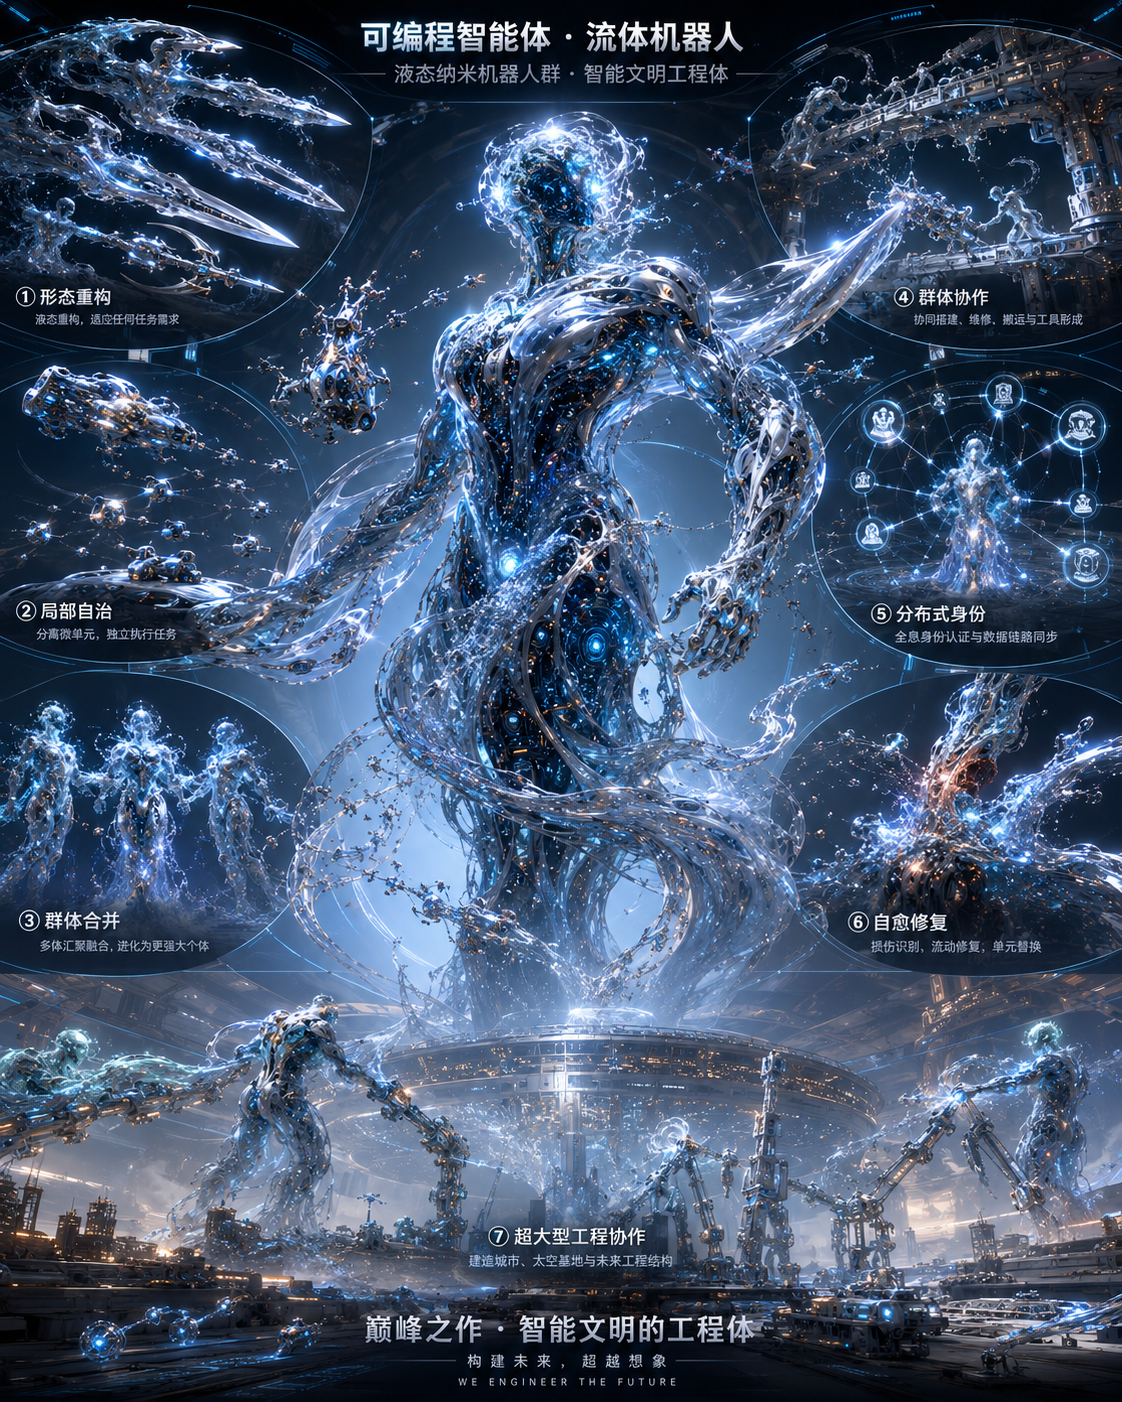
\includegraphics[width=.9\textwidth,height=.38\textheight,keepaspectratio]{images/cognitive-cosmos-artwork.png}
\caption{角色、协议、制度和共享记忆形成的组织智能}
\end{figure}
\section{Agent 间 CSO 流：组织智能的第一性动力对象}
\label{sec:inter-agent-cso-flow}

当我们第一次把视角从单个 Agent 转向多个 Agent 时，最容易采用的描述方式是“通信”：Agent $A$ 向 Agent $B$ 发送一条消息，$B$ 再向 $A$ 返回另一条消息。这种描述对于网络协议足够，却不足以描述组织智能。原因在于，一条消息只是物理或符号载体，而组织真正需要保存和转移的是消息背后的认知结构。我们因此仍然沿用前文建立的 CSO 本体区分：设某一认知结构本体为 $C$，Agent $A$ 对它形成的具体内部承载为
\[
\pi_A(C)=AgentCSO_A(C),
\]
Agent $B$ 对同一结构形成的内部承载则为
\[
\pi_B(C)=AgentCSO_B(C).
\]
通常并不存在
\[
AgentCSO_A(C)=AgentCSO_B(C),
\]
因为两个 Agent 的内部表示、记忆历史、身体接口、自我结构和当前任务状态均可能不同。跨 Agent 交流真正完成的因而不是复制某个内部神经向量，而是通过一个公共外部载体 $m_{AB}$，使 $B$ 能够重新构造与 $C$ 功能一致的内部结构：
\[
AgentCSO_A(C)
\xrightarrow{\operatorname{encode}}
m_{AB}
\xrightarrow{\operatorname{decode}}
AgentCSO_B(\hat C).
\]
理想情况下，
\[
\hat C\simeq_{\mathrm{functional}} C,
\]
这里的等价不是表示空间中的逐元素一致，而是前文所定义的功能—语义一致：关键对象、关系、约束、因果和行动含义在新的 Agent 中仍然成立。由此我们可以把跨 Agent 信息交换重新定义为
\[
\boxed{
\text{Inter-Agent Communication}
=
\text{CSO Re-grounding Across Agent Boundaries}
}
\]
即认知结构跨主体边界的重新落地，而不只是 token、消息或数据包的传输。

为了进一步研究组织，我们需要从“单次传递”进入“流”的概念。设组织中存在 Agent 集合
\[
\mathcal A=\{A_1,A_2,\ldots,A_N\},
\]
对任意两个主体 $A_i,A_j$，定义在时间窗口 $T$ 内从 $i$ 到 $j$ 的结构流
\[
J^{C}_{ij}(T)
=
\int_T
\Phi_{ij}
\left(
C,t,
q_{ij},
r_{ij},
u_{ij}
\right)dt,
\]
其中 $q_{ij}$ 表示传递质量或语义保真度，$r_{ij}$ 表示该结构对当前任务的相关性，$u_{ij}$ 表示该结构在后续行为中的实际效用。这样定义以后，“某两个人每天交流很多”并不必然意味着其组织耦合很强；只有那些能够稳定改变对方认知状态、决策结构或者后续行动的 CSO 流，才具有较高的组织动力学意义。

由此可以定义组织尺度的总 CSO 流：
\[
\mathcal J_{\mathrm{org}}(t)
=
\left\{
J^C_{ij}(t)
\mid
A_i,A_j\in\mathcal A
\right\}.
\]
我们尤其关注三类性质。第一是\textbf{重复性}：
\[
\mathbb E_T[J^C_{ij}]>0,
\]
说明某类结构在固定主体之间长期反复迁移。第二是\textbf{方向稳定性}，即 $A_i\rightarrow A_j$ 和 $A_j\rightarrow A_i$ 在功能上可能并不对称。第三是\textbf{功能闭合性}：结构从 $A_i$ 迁移到 $A_j$ 后，是否经过处理重新进入世界或其他 Agent，并产生可验证的结果。我们因此仍然保持本书的一条基本原则：
\begin{statementbox}
RealityIsUltimateConstraint.
\end{statementbox}
组织内部传播得再广的结构，如果始终不能通过行动和外部现实完成验证，也只能说明它具有组织内部传播力，而不能证明其认知有效性。

现在我们便能看见组织智能形成的真正起点。一个临时团队可能只有随机的 CSO 流；随着某种任务长期重复，例如“客户问题由前端人员识别，再由技术人员判断，再由工程人员实现，最后由质量人员验证”，某些跨主体流会反复出现：
\[
A_{\mathrm{front}}
\rightarrow
A_{\mathrm{analysis}}
\rightarrow
A_{\mathrm{engineering}}
\rightarrow
A_{\mathrm{verification}}.
\]
如果这一流动不断产生稳定收益，那么组织没有理由在每次任务发生时重新通过全局搜索决定“谁应该处理什么”。就像一个成熟 Agent 不会把已经熟练的身体动作永久保留在工作记忆 $h$ 中一样，一个成熟组织也不会让所有任务长期停留在全体成员的显式协调空间。组织开始把重复流沉降成稳定路径。于是组织学习的第一步可以写为：
\begin{statementbox}
\centering
\adjustbox{max width=.96\linewidth}{\(\displaystyle \mathcal J_{\mathrm{org}}^{\mathrm{repeated}}
\longrightarrow
\mathcal T_{\mathrm{org}}^{\mathrm{candidate}}.\)}
\end{statementbox}

这意味着，从本书的视角看，组织的第一性研究对象并不是“部门”或者“组织架构图”，而是\textbf{长期存在的 Agent 间 CSO 流}。部门、职位、流程和制度都属于后续形成的慢结构。这个观察非常重要，因为它让我们避免一种传统组织设计中的倒置：先设计若干方框，再要求现实认知流服从方框。智能动力学的顺序恰好相反：我们首先考察现实中什么 CSO 长期在谁之间流动、为何流动、在哪些地方产生阻塞、失真和残差，然后才讨论哪些关系值得固化成组织结构。组织不是先验几何，而是长期认知流在时间中的沉积物。


\section{角色：重复功能责任的结构化沉降}
\label{sec:organizational-role}

有了跨 Agent CSO 流以后，第二个自然出现的组织结构不是部门，而是“角色”。角色的产生可以从我们此前讨论的 Agent 内部技能形成得到直接类比。在单 Agent 中，一个任务如果每次都需要显式进入 $h$，经过大量重复以后就会产生功能下沉：
\[
ExplicitAgentCSO
\rightarrow
ExperientialAgentCSO
\rightarrow
ProceduralAgentCSO.
\]
组织中同样存在类似过程。假设某类 CSO $C_k$ 长期被发送给 Agent $A_i$，并且 $A_i$ 对该类结构进行某种相对稳定的转换：
\[
F_i:C_k\rightarrow C'_k.
\]
当这种关系在足够长的时间尺度上保持稳定，就不再需要把它解释成“某个 Agent 临时碰巧做了这件事”，而可以产生一个更加抽象的功能对象：
\[
R_\alpha
=
\left(
\mathcal C_\alpha,
F_\alpha,
P_\alpha,
A_\alpha,
O_\alpha
\right),
\]
其中 $\mathcal C_\alpha$ 是该角色主要接收和处理的 CSO 类型集合，$F_\alpha$ 是典型转换函数，$P_\alpha$ 表示权限边界，$A_\alpha$ 表示行动能力，$O_\alpha$ 表示输出义务。角色因此首先不是一个名字，而是\textbf{对稳定功能责任的一次压缩}。

我们可以进一步定义 Agent 与 Role 的动态映射：
\[
\eta_t:A_i\mapsto\{R_{\alpha_1},R_{\alpha_2},\ldots\}.
\]
这一表达明确说明，一个 Agent 可以同时承担多个角色，一个角色也可以被多个 Agent 实例化。因此：
\[
\boxed{
Agent\neq Role.
}
\]
这一区分在未来 AgentOS 组织中尤其重要，因为持续主体具有自己的 $E,\Theta,\Psi$ 和生命周期历史，而角色只是组织赋予其的一组阶段性功能约束。如果将角色直接写进 Agent 的身份层 $\Psi$，就可能发生严重的尺度混淆：组织职责的变化会被错误解释为主体身份崩溃。正确的结构应该是：
\[
\Psi_i
\longrightarrow
Agent_i
\longleftrightarrow
Role_\alpha,
\]
其中角色能够约束 Agent 在特定组织环境中的行动空间，但不应该等价于 Agent 本身。

角色为什么能够降低组织认知负担？假设一个组织中有 $N$ 个 Agent，在完全无结构情况下，理论上每次任务路由都可能需要考虑 $O(N^2)$ 级别的潜在交互关系。角色形成以后，任务首先映射到角色空间：
\[
C
\rightarrow
R_\alpha
\rightarrow
A_i,
\]
系统不再需要搜索所有个体。我们可以把这一收益写成一个近似的协调成本差：
\[
\Delta C_{\mathrm{coord}}
=
C_{\mathrm{unstructured}}
-
C_{\mathrm{role\ based}},
\]
在稳定环境中通常期望
\[
\Delta C_{\mathrm{coord}}>0.
\]
因此角色本质上是一种\textbf{组织尺度的认知压缩机制}：它把“谁在每次情况下应该承担什么”从实时全局推理问题转化成已经沉降的结构先验。

但这也立即带来风险。角色一旦稳定，就会改变未来 CSO 的流向。例如规定某类结构必须进入 $R_\alpha$，意味着组织拓扑施加：
\[
P(R_\alpha\mid C_k)\approx 1.
\]
如果环境发生变化，而这一条件仍被僵化维持，那么原本降低协调负担的结构会转变为认知盲区。我们于是再次遇到本书的稳定—可塑性问题。角色应具有足够慢的时间尺度，以避免被短期噪声不断重写；又必须具有足够的可塑性，以响应持续结构失配。可以写：
\[
\tau_{\mathrm{task}}
\ll
\tau_{\mathrm{role}},
\]
但不能令
\[
\tau_{\mathrm{role}}\rightarrow\infty.
\]
当某一角色持续出现高残差、过度负载、输出失真或者大量跨角色反复退回时，说明当前角色分解已经不再匹配实际 CSO 结构，应触发组织层的重估。

从传统组织理论看，角色与 division of labor、job specialization、responsibility allocation 等概念存在明显联系；从多智能体系统看，它与 role-based MAS 的设计相似。但本书的不同之处在于，我们不把角色作为人为预先指定的静态标签，而尝试从\textbf{历史 CSO 流的稳定统计结构}中解释它的形成。也就是说：
\[
\boxed{
Role
=
StableFunctionalAbstractionOfRepeatedInter-AgentCSOTransformation.
}
\]
这种定义把角色从行政名词重新带回智能动力学，使它能够进一步进入协议、制度和组织拓扑的统一数学描述。


\section{协议：把重复协作关系编译成跨主体闭环}
\label{sec:organizational-protocol}

角色解决的是“谁通常承担什么功能”，但它仍然没有解决“这些功能之间怎样稳定协同”。假设组织已经形成角色 $R_\alpha$ 与 $R_\beta$，如果每一次两者交互仍然需要重新讨论输入格式、责任边界、反馈条件、失败处理和完成定义，那么大量认知资源仍会消耗在重复协调上。因此，当某种跨角色交互反复出现时，系统还会产生第二层结构沉降：协议。

我们把组织协议定义为：
\[
\Pi_{\alpha\beta}
=
\left(
I_{\alpha\beta},
G_{\alpha\beta},
S_{\alpha\beta},
E_{\alpha\beta},
V_{\alpha\beta},
F_{\alpha\beta}
\right),
\]
其中 $I_{\alpha\beta}$ 表示允许传递的输入结构集合，$G_{\alpha\beta}$ 表示交互触发条件，$S_{\alpha\beta}$ 是语义或数据契约，$E_{\alpha\beta}$ 是异常处理路径，$V_{\alpha\beta}$ 表示验证和闭环条件，$F_{\alpha\beta}$ 表示失败后的反馈或升级机制。由此，一个完整协议不是简单的消息格式，而是一条可闭合的跨主体 CSO 动力路径。

例如，Agent $A$ 检测到异常 $C_{\mathrm{anom}}$，其所属角色规定将该结构交给诊断角色 $R_D$。如果不存在协议，$A$ 还要实时决定发送哪些背景、以什么格式发送、何时认定诊断完成、失败后找谁。协议形成以后：
\[
C_{\mathrm{anom}}
\xrightarrow{\Pi_{AD}}
R_D
\xrightarrow{Diagnosis}
C_{\mathrm{cause}}
\xrightarrow{\Pi_{DA}}
R_A,
\]
整个过程变成组织尺度的一条快速闭环。这里非常类似前文的技能编译：
\[
ExplicitCoordination
\rightarrow
RepeatedInteraction
\rightarrow
StableProtocol.
\]
所以可以定义：
\[
\boxed{
Protocol
=
CompiledInter-AgentCoordination.
}
\]

如果从工作记忆有限容量定理看，协议具有直接意义。假设每次互动需要实时解决 $k$ 个协调变量：
\[
z=\{z_1,z_2,\ldots,z_k\}.
\]
当协议稳定后，其中绝大多数变量不再进入参与 Agent 的当前显式工作记忆，而成为协议默认结构：
\[
z_{\mathrm{explicit}}
\rightarrow
z_{\Pi}.
\]
因此：
\[
C_h^{\mathrm{coord}}
\downarrow.
\]
这就是为什么成熟组织能够在大量成员并行运行的情况下保持可操作性。组织并不是让每个人实时理解整个组织，而是把大量重复关系预先编译成局部闭环。由此，我们得到与 AgentOS 中 ``Normal Dynamics Stay Local'' 完全一致的组织原则：
\begin{statementbox}
NormalOrganizationalDynamicsStayLocal.
\end{statementbox}
只有当协议内无法消化的残差超过阈值时，问题才向更高尺度提升：
\[
\Gamma_{\mathrm{org}}
=
f(
Residual,
Risk,
Novelty,
Persistence,
CrossRoleImpact
).
\]
若
\[
\Gamma_{\mathrm{org}}<\theta,
\]
则维持局部协议闭环；若
\[
\Gamma_{\mathrm{org}}\geq\theta,
\]
则触发更高层角色、治理结构或者制度审议。这个机制比“所有异常都报给最高管理层”具有更好的尺度稳定性，也与我们在 AgentOS 内部得到的“预测局部完成，异常全局升级”原则完全一致。

协议同时也是跨主体语义连续性的关键。如果不同 Agent 的 Agent-CSO 表示并不相同，那么协议不能依赖内部 latent 一致，而应依赖公共语义契约。这一点与 KRA 的思想相同：
\[
\boxed{
FunctionalAlignment
>
RepresentationAlignment.
}
\]
组织无需让所有成员“内部想法完全一样”，只需要保证他们在协议边界上对关键对象、状态、责任、完成条件和失败信号存在足够一致的功能解释。因此未来 Agent 组织中的协议更可能类似“语义 ABI”，而不仅是传统 RPC 接口。

然而，协议同样会产生“编译过度”问题。一个在旧环境中高效的协议可能由于环境改变而变成阻塞。例如它规定某类结构必须按 $A\rightarrow B\rightarrow C\rightarrow D$ 路径流动，但长期观察发现 $A$ 与 $D$ 已经能够直接可靠闭合任务。这时继续坚持旧协议就形成不必要的拓扑长度：
\[
L_{\Pi}
=
\sum_{e\in\Pi}
Cost(e).
\]
如果持续存在
\[
L_{\Pi}^{\mathrm{current}}
\gg
L_{\Pi}^{\mathrm{possible}},
\]
协议本身就成为需要学习的对象。由此协议不是永久规范，而是慢尺度认知沉降物，需要受现实残差和组织效用持续验证。

传统计算机科学中的网络协议、API contract、workflow，以及组织理论中的 standard operating procedure 都与本章概念相近。但这里我们强调的核心是：协议来源于反复 CSO 协作的结构压缩，其目标是让成熟认知流从昂贵的显式协调空间迁入稳定局部闭环。因此组织进化的一条基本路径可以写成：
\begin{statementbox}
\centering
\adjustbox{max width=.96\linewidth}{\(\displaystyle RepeatedCoordination
\rightarrow
ProtocolCompilation
\rightarrow
LocalClosure
\rightarrow
ReducedGlobalCognitiveLoad.\)}
\end{statementbox}


\section{制度：高尺度慢变量对组织行为的约束}
\label{sec:institution}

如果说角色保存“谁通常负责什么”，协议保存“不同责任单元通常怎样交互”，那么制度所保存的就是更加缓慢、更加全局的结构：\textbf{哪些状态转移允许发生，哪些状态转移需要授权，哪些行为即使短期有效也不能成为组织的正常路径。}从本书的多尺度理论看，制度并不是协议的简单集合，而是一个明显更慢的约束层。

我们可以定义组织状态为
\[
X_{\mathrm{org}}(t)
=
\left[
X_1(t),
X_2(t),
\ldots,
X_N(t),
\mathcal T(t),
M_{\mathrm{org}}(t)
\right],
\]
其中 $X_i$ 表示成员 Agent 的局部状态，$\mathcal T$ 表示组织功能拓扑，$M_{\mathrm{org}}$ 表示组织记忆。制度 $I$ 的作用并不是给出每一个动作，而是定义一个允许状态空间：
\[
\mathcal F_I
\subseteq
\mathcal X_{\mathrm{org}}.
\]
正常组织行为应满足：
\[
X_{\mathrm{org}}(t)\in\mathcal F_I.
\]
进一步，制度可以限制允许的状态转移：
\[
\mathcal R_I
\subseteq
\mathcal X_{\mathrm{org}}\times\mathcal X_{\mathrm{org}}.
\]
于是某个局部 Agent 即使认为动作 $a$ 可以提高短期收益，只要它导致
\[
(X_t,X_{t+1})\notin\mathcal R_I,
\]
组织系统就可以拒绝这一动作。

这个表达与前文的一个核心原则完全同构：
\[
\boxed{
HigherLevelSetsFeasibleRegion,\qquad
LowerLevelOptimizesInsideIt.
}
\]
制度因此更接近慢尺度的 feasible region，而不是高速微观控制器。它的成熟形式不应该变成：
\[
Institution
\rightarrow
EveryMicroAction,
\]
而应该是：
\[
Institution
\rightarrow
Boundary/Authority/Constraint,
\]
然后允许局部角色和协议在内部自治运行。这正是我们此前反复强调的：
\[
\boxed{
SlowGovernance\neq FastMicromanagement.
}
\]
如果制度直接控制每一个快速局部动作，就会把原本应该在低层关闭的反馈环拖入高层，产生巨大协调延迟；反过来，如果制度完全缺失，局部 Agent 可能为了即时收益不断破坏长期安全、身份、信任和组织连续性。

制度的形成同样可以由长期 CSO 流解释。假设在多个局部互动中反复出现某一类高代价失败：
\[
\varepsilon_1,\varepsilon_2,\ldots,\varepsilon_n.
\]
如果这些失败具有共同结构 $C_{\mathrm{risk}}$，组织可以首先在具体协议中修补；若跨多个角色和协议都持续出现，则说明问题已经超出局部闭环。此时出现从快到慢的提升：
\[
Residual
\rightarrow
CrossProtocolPattern
\rightarrow
InstitutionalConstraint.
\]
这与单 Agent 中的：
\[
h\rightarrow E\rightarrow\Theta
\]
具有明显同构性：短期异常首先形成事件，重复事件形成结构，最终结构反过来约束未来快速过程。因此制度可以被理解成：
\[
\boxed{
Institution
=
Slow Structural Memory of Repeated Cross-Organizational Constraints.
}
\]

这也解释为什么成熟制度具有迟滞。若每次短期异常都立即修改制度：
\[
\Delta I\propto\varepsilon_t,
\]
那么整个组织的慢结构会被快速噪声驱动而产生振荡。更合理的是对残差进行长期积分：
\[
\bar{\varepsilon}_T
=
\frac{1}{T}
\int_{t-T}^{t}
w(\tau)\varepsilon(\tau)d\tau,
\]
只有在
\[
\bar{\varepsilon}_T>\theta_I
\]
并具有跨场景稳定性时，才允许制度改变。这正是本书“慢变量保护原则”在组织尺度的表现：
\begin{statementbox}
\centering
\adjustbox{max width=.96\linewidth}{\(\displaystyle FastNoise\nrightarrow SlowGlobalStructure.\)}
\end{statementbox}

制度还承担权限边界的稳定化作用。在未来 AgentOS 组织中，各 Agent 不应拥有无限制的结构修改权。可以为每一角色定义 authority envelope：
\[
\mathcal A_\alpha
=
\{
a\mid
a\text{ is authorized for }R_\alpha
\}.
\]
角色能够在自身权限包络内自治；超出包络的动作需要进入更高尺度的治理闭环。这样，组织中的权限不是单一“管理员/普通用户”二元结构，而是与 CSO 类型、风险尺度和主体能力相关的连续或分层控制结构。

制度经济学长期研究 formal rules、informal norms、transaction costs 和 institutional persistence，组织理论也研究 hierarchy、authority 和 bureaucracy。这些理论可以为本章提供重要经验材料；但本书试图增加一个动力学解释：制度不是静态“规则表”，而是大量跨 Agent 结构流、失败残差和协作历史在极慢时间尺度上形成的控制边界。它既是过去互动的记忆，也是未来互动的先验。因此制度真正成熟的标志不是规则数量越来越多，而是：
\begin{remark}
以尽可能少的慢结构约束，维持尽可能大的安全局部自治空间。
\end{remark}


\section{组织记忆：跨主体与跨生命周期的结构连续性}
\label{sec:organizational-memory}

个体 Agent 的寿命有限，注意容量有限，当前工作记忆更是有限。如果一个组织的认知能力只是全部成员当前 Agent-CSO 的并集，那么任何成员退出、重启或者遗忘都会直接造成组织能力丢失。这与我们前文讨论文明时遇到的问题完全一致：真正能够跨越主体生命周期的智能结构，必须建立比任何单成员更持久的外部承载。因此组织智能成立的关键条件之一，就是形成组织记忆。

我们可以首先把组织记忆写成：
\[
M_{\mathrm{org}}
=
M_{\mathrm{event}}
\oplus
M_{\mathrm{structure}}
\oplus
M_{\mathrm{procedure}}
\oplus
M_{\mathrm{institution}}
\oplus
M_{\mathrm{artifact}},
\]
分别对应事件经历、稳定结构、过程经验、制度规则以及外部制品。它们不是完全独立的存储系统，而是对不同时间尺度 CSO 的不同承载方式。

如果借用三相记忆的思想但不机械复制，我们可以看到明显的尺度对应。组织每天发生的具体互动类似组织尺度的情景轨迹：
\[
E_{\mathrm{org}}
=
\{e_1,e_2,\ldots,e_t\}.
\]
其中长期重复出现的模式会逐渐抽象成：
\[
\Theta_{\mathrm{org}},
\]
例如典型风险模式、稳定业务结构、角色关系、流程经验和决策规律。进一步，制度和组织文化中极稳定的部分则可能形成比普通结构记忆更慢的约束。这里我们并不需要声称组织拥有与个体完全相同的 $\Psi$ 或 $\Omega$，但可以明确指出：在功能上，组织确实存在从短期事件向长期生成结构沉降的过程：
\begin{statementbox}
\centering
\adjustbox{max width=.96\linewidth}{\(\displaystyle OrganizationalExperience
\rightarrow
OrganizationalStructure
\rightarrow
FutureBehaviorBias.\)}
\end{statementbox}

组织记忆的关键不是“存了多少数据”，而是未来 Agent 能否重新利用这些结构。因此一个数据库只有在满足以下链条时才真正成为组织记忆：
\[
C
\xrightarrow{\operatorname{externalize}}
M_{\mathrm{org}}
\xrightarrow{\operatorname{index}}
C'
\xrightarrow{\operatorname{reactivate}}
AgentCSO_j.
\]
这里 $\operatorname{index}$ 极其关键。如果大量结构被写入外部系统，却没有可靠的语义索引、权限、可信度、时间信息和恢复路径，那么这些数据更接近“组织遗迹”，而不是活跃记忆。组织记忆应当具有至少五个元属性：
\[
m=
(C,\tau,source,confidence,access).
\]
即它是什么结构、何时形成、来源是谁、可信度如何、什么主体可以在什么条件下重新访问。

由此我们可以重新理解文件、知识库、程序、标准、代码、设计文档和训练数据。在传统软件架构中，这些对象属于不同工具；在本书的组织认知观点下，它们可以统一视为不同类型 CSO 的外部承载体。程序尤其特殊，因为它不仅保存结构，还可以执行结构：
\[
AgentCSO
\rightarrow
ProgramCSO
\rightarrow
ExecutableWorldTransformation.
\]
因此组织外部记忆存在一个从“被动存储”向“主动可执行结构”的连续谱。AI 系统进一步使这一谱发生变化，因为某些组织记忆不再只是等待人类检索，而能够主动进行总结、关联、预测和问题发现。

组织记忆还有一个十分重要的功能：保持身份和能力的跨成员连续性。设组织在时刻 $t$ 的成员集合为
\[
\mathcal A_t.
\]
随着人员变化，
\[
\mathcal A_t\neq\mathcal A_{t+\Delta}.
\]
如果组织能力仅由成员内部结构决定，那么成员变化必然导致巨大能力漂移。但若存在稳定外部记忆和功能拓扑：
\[
\mathcal M_{\mathrm{org}},
\mathcal T_{\mathrm{org}},
\]
组织就可以在成员变化中保持较强结构连续性：
\[
\mathcal F_{\mathrm{org}}(t)
\approx
\mathcal F_{\mathrm{org}}(t+\Delta),
\]
即使具体执行主体发生改变。这正是组织能够拥有远长于成员寿命的“结构时间”的原因。

与此同时，我们也必须注意组织记忆的负面效应。过度沉降会形成组织僵化。一个历史经验 $C_{\mathrm{old}}$ 在过去有效，并不意味着其条件永远成立：
\[
P(C_{\mathrm{old}}\text{ valid}\mid W_t)
\neq
1.
\]
所以组织记忆必须像 Agent 的内部记忆一样支持召回、重新解释、降权、冲突检测和遗忘。成熟组织不是“记住一切”，而是能够保持：
\[
\boxed{
MemoryContinuity
+
RealityRevalidation
+
SelectiveForgetting.
}
\]
否则历史经验会从认知资本变成结构惯性。

在分布式认知和 organizational memory 研究中，人、文档、工具、制度和环境长期以来就被认为能够共同承担组织认知。但本书进一步试图用 CSO 承载迁移给出统一语言：组织记忆的本质，是一个认知结构从某个瞬时 Agent-CSO 脱离个体生命周期，转移到可跨主体恢复的慢载体，并能够重新进入未来 Agent 的认知闭环。于是：
\[
\boxed{
OrganizationalMemory
=
Cross-Agent, Cross-Lifetime Persistence of Recoverable CSO Structure.
}
\]


\section{组织拓扑学习：从重复协作到结构自重组}
\label{sec:organizational-topology-learning}

前几节已经依次建立了 Agent 间 CSO 流、角色、协议、制度和组织记忆。现在我们可以回答本章最重要的问题：\textbf{组织是否能够像个体智能体那样学习自己的功能结构？}如果答案是否定的，那么组织只能在固定架构中累积知识；如果答案是肯定的，那么长期经验不仅改变组织知道什么，还会改变组织以后怎样处理问题。

设组织的功能拓扑为：
\[
\mathcal T_{\mathrm{org}}(t)
=
(V_R,E_P,W,A),
\]
其中 $V_R$ 表示角色节点，$E_P$ 表示协议边，$W$ 表示耦合强度，$A$ 表示权限和控制关系。日常 CSO 流在这一拓扑上运行：
\[
\mathbf J_{\mathrm{CSO}}
=
\mathbf J(
\mathcal T_{\mathrm{org}},
X_{\mathrm{org}},
W_{\mathrm{external}}
).
\]
但与此同时，长期流又反过来改变拓扑：
\[
\tau_T
\dot{\mathcal T}_{\mathrm{org}}
=
G(
\langle\mathbf J_{\mathrm{CSO}}\rangle_T,
\langle\varepsilon\rangle_T,
U,
Cost,
Risk
),
\]
其中
\[
\tau_T
\gg
\tau_{\mathrm{task}}
\]
保证组织结构变化比日常任务慢得多。

这个方程揭示了本书所谓“Dynamics on Topology + Dynamics of Topology”的组织形式。日常工作是在组织结构上发生的动力学，而长期组织学习则是这个结构本身的动力学。两者不能混为一谈。比如一次任务临时需要两个 Agent 协作，并不值得改变组织架构；但如果一年内同类 CSO 持续沿同一非正式路径高频迁移，而且该路径始终产生高收益，那么系统应当考虑把它沉降成正式协议甚至角色：
\[
\left\langle
J^{C}_{ij}
\right\rangle_T
\gg 0
\quad\land\quad
U_{ij}-Cost_{ij}>\theta
\Rightarrow
w_{ij}\uparrow.
\]
如果原有连接长期低效：
\[
\left\langle
J^C_{ij}
\right\rangle_T\rightarrow0
\]
或者持续制造协调残差，则：
\[
w_{ij}\downarrow.
\]

但仅仅依据流量重构是不够的。一个组织可能高频重复错误行为。因此任何组织拓扑学习都必须同时考虑：
\[
Benefit,\quad Residual,\quad Cost,\quad Risk,\quad Robustness.
\]
可以概念性定义边更新：
\[
\dot w_{ij}
=
\eta_T
\left[
\alpha
\langle U_{ij}\rangle_T
-
\beta
\langle R_{ij}\rangle_T
-
\gamma Cost_{ij}
-
\delta Risk_{ij}
\right].
\]
其中 $\eta_T$ 应远小于日常状态学习率。这样，稳定且有益的跨角色结构流才有机会逐渐变成新的组织资本。

组织拓扑学习还必须满足迟滞：
\[
\theta_{\mathrm{on}}
>
\theta_{\mathrm{off}}.
\]
新关系的形成要求长期、持续证据；已有稳定关系不会因为一次短期低使用率就立即删除。否则组织会产生“架构振荡”：今天成立一个团队，明天撤销，后天重新成立，使成员不断把注意力浪费在组织变化本身。这与 AgentOS 中慢变量保护完全一致。拓扑是历史沉降物，因此必须拥有长记忆。

从更一般的角度，组织拓扑改变至少存在五种形式。第一是\textbf{边权变化}：原有协作关系变强或变弱。第二是\textbf{边生成}：两个过去没有直接关系的角色形成稳定协作。第三是\textbf{shortcut}：长期存在的长路径被编译成直接连接。第四是\textbf{节点分裂或合并}：一个角色承担的 CSO 类型已经过于异质，需要拆分；或者两个角色长期高度耦合，可以合并。第五是\textbf{边界改变}：某种能力从组织内部迁移给外部 Agent、工具或另一组织，或者反向内化。这最后一种实际上已经进入组织的 Boundary Migration。

我们尤其应该强调“Minimum Necessary Reorganization Principle”。组织面对新问题时，不应第一时间改变结构，而应按照成本逐级尝试：
\begin{statementbox}
\centering
\adjustbox{max width=.96\linewidth}{\(\displaystyle StateAdjustment
\rightarrow
RepresentationAdaptation
\rightarrow
ProtocolAdjustment
\rightarrow
RoleAdjustment
\rightarrow
TopologyReorganization.\)}
\end{statementbox}
这与单 Agent 中从运行态调节到更慢结构调整的原则完全一致。原因很简单：越慢的结构承载越大的历史连续性，修改代价越高，因此只有较浅机制长期无法解决的结构失配，才应该推动深层重组。

这一点也提供了一种重新理解组织改革的方法。真正的结构改革不应起源于“管理者想换一张组织图”，而应起源于可观察的：
\[
\fitdisplay{
PersistentResidual,
\quad
RepeatedCrossBoundaryMigration,
\quad
CoordinationCost,
\quad
Latency,
\quad
FailurePattern.
}
\]
我们可以把这些量综合为组织结构压力：
\[
P_{\mathcal T}
=
F(
R_{\mathrm{persistent}},
J_{\mathrm{cross}},
C_{\mathrm{coord}},
L_{\mathrm{latency}},
I_{\mathrm{instability}}
).
\]
当
\[
P_{\mathcal T}>\theta_{\mathcal T}
\]
且持续时间足够长时，组织才进入 topology search。

因此，本章对“组织学习”的定义比知识管理更严格：
\[
\boxed{
\text{Organizational Learning}
=
\text{Change of Collective CSO Representation and Placement}
+
\text{Adaptation of Functional Topology}.
}
\]
前者让组织知道更多；后者让组织改变自己以后如何知道、如何判断以及如何行动。只有后者开始出现时，我们才真正从“很多 Agent 一起工作”进入了“组织作为高尺度自适应智能结构”的范围。


\section{AgentOS 与未来组织系统：从个体认知运行时到组织认知基础设施}
\label{sec:agentos-organizational-system}

前面所有分析最终都会引出一个非常现实的工程问题：如果未来社会中存在大量长期运行、具有持续身份、记忆、自我结构、工具能力和 Body Runtime 的 Agent，它们应当怎样组成组织？传统 multi-agent framework 通常擅长解决消息路由、任务分派和并行执行，但这些机制默认 Agent 更像可替换 worker；而本书构造的 AgentOS 主体具有明显不同的性质：每个 Agent 拥有长期 $E$、$\Theta$、$\Psi$，其经历会影响未来能力和身份，因此不能像无状态函数一样任意创建、替换和销毁。这意味着未来 Agent 组织首先需要承认：
\[
\boxed{
PersistentAgent\neq EphemeralWorker.
}
\]

于是组织系统至少必须维护三个不同层级的对象。第一层是\textbf{主体}：
\[
A_i=
(h_i,E_i,\Theta_i,\Psi_i,\ldots).
\]
第二层是\textbf{角色}：
\[
R_\alpha,
\]
它描述组织对主体的阶段性功能期望。第三层是\textbf{任务实例}：
\[
T_k,
\]
它是可以创建、暂停、完成和删除的短期运行对象。正确的关系应该是：
\[
Agent
\longleftrightarrow
Role
\longrightarrow
Task,
\]
而不是：
\[
Task\equiv Agent.
\]
这与我们前文建立的 SingleAgentMultiTaskOS 原则在组织尺度上具有直接连续性。

未来的 AgentOS 组织运行时因此需要一种比普通任务调度更加丰富的组织调度器。可以定义：
\[
\mathcal S_{\mathrm{org}}
:
(
C,
\mathcal A,
\mathcal R,
\mathcal P,
\mathcal M
)
\rightarrow
(A_i,R_\alpha,\Pi_{\alpha\beta}),
\]
其中输入包括当前 CSO 类型 $C$、可用主体集合 $\mathcal A$、角色集合 $\mathcal R$、协议集合 $\mathcal P$ 与组织记忆 $\mathcal M$，输出则决定哪个持续主体以什么角色、通过什么协议承担该结构。这已经不再是简单 CPU scheduling，而是：
\begin{statementbox}
Organizational Cognitive Structure Scheduling.
\end{statementbox}

组织层的 Boundary 同样需要正式工程化。某一 CSO 可以由当前 Agent 自己处理，可以转移给同组织其他 Agent，可以调用工具，可以外包给其他组织，也可以写入长期组织记忆。因此对每个待处理结构 $C$，都存在一个承载选择：
\[
\fitdisplay{
B(C)
\in
\{
InternalAgent,
OtherAgent,
Tool,
OrganizationMemory,
ExternalOrganization,
Environment
\}.
}
\]
这实际上是我们此前认知卸载理论在组织尺度的直接推广。一个成熟组织的效率，很大程度上并不来自所有成员都变得更强，而来自“什么结构应该由谁承载”的配置逐渐优化。

权限则成为另一个关键维度。每个 Agent 除了具有自身能力 $Cap_i$，还具有组织赋予的权限 $Auth_i$：
\[
Autonomy_i
=
F(
Cap_i,
Trust_i,
Role_i,
Risk,
Institution
).
\]
能力并不自动产生权限。一个非常强的 Agent 仍然可能由于任务风险、制度边界或现实安全原因而只能在有限自治包络内行动。这与我们后面在 Agent 培育与控制工程中进一步讨论的 capability--authority--autonomy 闭环具有一致性，但本章只需确定组织层原则：
\[
\boxed{
Capability\neq Authority.
}
\]

AgentOS 还可能给组织带来一种此前软件系统缺乏的能力：让组织拓扑本身可被观测。传统组织往往依赖人工调查才能知道“谁实际在和谁协作”；未来 AgentOS 可以直接记录经过脱敏和治理后的结构流统计：
\[
J^{C}_{ij},
\quad
Latency_{ij},
\quad
Residual_{ij},
\quad
Utility_{ij}.
\]
这样，组织图不再只是名义上的 hierarchy，而可以形成一张实际运行的 functional topology。二者之间的差异：
\[
\Delta\mathcal T
=
D(
\mathcal T_{\mathrm{formal}},
\mathcal T_{\mathrm{actual}}
)
\]
本身就是极其重要的组织健康指标。若正式结构与实际 CSO 流长期严重偏离，说明组织已经出现“隐性拓扑”，此时继续强化名义结构往往只会增加协调成本。

更进一步，当 AgentOS 能够提供组织记忆、CSO 路由、角色映射、协议运行、权限治理、结构流测量和慢尺度拓扑学习以后，它的系统地位会发生变化。它不再只是：
\[
\text{Personal Agent Runtime},
\]
而开始成为：
\begin{statementbox}
Persistent Intelligence Infrastructure.
\end{statementbox}
Linux 管理计算资源，单 AgentOS 管理个体认知资源，而更高尺度的组织运行层则管理：
\[
Agents,\quad
Roles,\quad
CSOFlows,\quad
Protocols,\quad
Memory,\quad
Authority,\quad
Topology.
\]
这并不意味着我们应该在工程上把组织系统塞进一个巨大中央控制器。恰恰相反，整个理论要求组织采用：
\[
\boxed{
LocalAutonomy
+
SlowGlobalGovernance.
}
\]
正常闭环尽量在角色和协议局部完成；只有持续残差、高风险和跨角色结构冲突才提升到更高尺度。否则组织 AgentOS 将重演单 Agent 的工作记忆过载，只不过把 $h$ 换成了一个“中央管理 AI”。

因此，我们最终得到一种非常不同于“中央超级 Agent 指挥所有子 Agent”的未来组织图景。成熟组织更接近一个多尺度闭环网络：个体 Agent 保持持续主体性，角色承载稳定责任，协议关闭高频跨主体协作，组织记忆保存跨生命周期 CSO，制度提供慢尺度可行域，而组织拓扑本身根据长期残差和结构流缓慢变化。

可以把它浓缩成：
\begin{statementbox}
\centering
\adjustbox{max width=.96\linewidth}{\(\displaystyle \begin{aligned}
&Agent
\rightarrow
InterAgentCSOFlow
\rightarrow
Role
\rightarrow
Protocol
\\
&\rightarrow
Institution
\rightarrow
OrganizationalMemory
\rightarrow
TopologyLearning.
\end{aligned}\)}
\end{statementbox}

但这并不是一条只向前的生成链。成熟以后，它成为真正的反馈环：
\begin{statementbox}
\centering
\adjustbox{max width=.96\linewidth}{\(\displaystyle Experience
\rightarrow
CSOFlow
\rightarrow
OrganizationalTopology
\rightarrow
FutureExperience.\)}
\end{statementbox}

由此，本章可以给出“组织智能”的最终定义：

\begin{definition*}
组织智能是多个持续主体通过跨主体 CSO 流形成稳定的角色、协议、记忆和治理结构，并使这些历史结构反过来约束、加速和重组未来认知与行动的多尺度自适应动力过程。
\end{definition*}

这一表述的重要性在于，它既没有把组织神秘化成拥有单一意识的“超级生命体”，也没有把组织退化成成员能力的简单求和。组织真正新增的东西，是\textbf{成员之间历史关系本身成为了可以保存、学习和反向作用于未来的结构}。

而这一结论又与本书从个体智能中得到的最基本规律完全一致：

\[
\boxed{
\text{Flow Shapes Structure;}
\qquad
\text{Structure Shapes Future Flow.}
}
\]

对于单个 Agent，这个“流”是 Agent-CSO 在功能拓扑上的迁移；对于组织，它变成跨 Agent 的 CSO 流；而角色、协议、制度和组织记忆，则是这些流在更慢尺度上的沉降。我们由此完成了一次真正的尺度提升：组织不再只是 Agent 的容器，而成为了\textbf{Agent 之间认知关系本身逐渐获得结构连续性的地方}。

\chapter{文明作为慢尺度认知结构}
\chaptervoice{这一章，我们围绕“文明作为慢尺度认知结构”做一件克制的事：把直觉压缩为状态、关系、时间尺度和可检验后果。它在全书中的任务，是说明组织、文明与自反结构演化。}

\section*{理论来路与依赖接口}
本章的直接思想来源是原文后期关于 CSO 外化、组织、文明、宇宙粗粒化与功能自反性的综合讨论。我们采用原文较晚形成的定义来整理较早讨论，不把对话中的试探性比喻与最终模型并列成互相竞争的“定律”。已有理论锚点主要是集体记忆、制度演化、分布式控制与科学认识论（Hutchins、Clark 与 Wiener）。

本章使用上一章“从个体 Agent 到组织智能”已经得到的对象与边界；本章产出将供下一章“AI 与文明认知拓扑的改变”使用。若后文术语偶尔出现，只作为路线提示，不参与本章推导。

\section*{从哪里出发}
我们已经拥有上一章给出的概念，现在只向前走一步。我会先把对象放进闭环，再讨论它的数学形式，最后检查工程边界。读者不必预先相信本章术语；只需暂时接受一个方法论约定：智能结构的意义来自它在现实反馈中的作用，而不是来自名称本身。

令系统在观察窗口 $[t,t+T]$ 内的状态轨迹为 $x_{[t,t+T]}$，环境扰动为 $d$，行动为 $u$。本章讨论的对象若确实有效，就应改变条件分布 $p(x_{t+T}\mid x_t,u,d)$，或改变达到同一结果所需的代价。这个起点把讨论锚定在集体记忆、制度演化、分布式控制与科学认识论上。
\section{个体不是文明的全部}
\begin{narration}
现在把镜头移到“个体不是文明的全部”。我们只沿本章已经取得的概念向前一步：先确定它在闭环里的角色，再检查它的尺度与失败边界。
\end{narration}

本节把“个体不是文明的全部”落实为承载范围、有效信息率与反馈周期之间的约束关系。这个定义不是说“任何相似现象都算”，而是要求我们同时给出对象域、允许的干预以及观察窗口。对于主题“文明作为慢尺度认知结构”而言，它承担的是组织、文明与自反结构演化中的一个可辨识环节。

把这一关系写成最小数学骨架，可得

\begin{equation}T_{\min}\geq L/v+I/B+T_{\rm act}.\end{equation}

式中的符号只承担结构角色，具体参数仍需由任务和身体数据辨识。我们首先检查可观测量，再检查控制量，最后检查比它更慢的约束。这样的顺序来自集体记忆、制度演化、分布式控制与科学认识论，但本书对个体不是文明的全部的命名和组合仍是需要实验验证的建模提案。

这一小节的反例同样重要：忽略传播和排队成本会制造虚假的实时性。因此评价它不能只看一次任务结果，而要比较干预前后的轨迹、恢复时间、维护成本和风险。如果改变该机制而所有允许观察下的分布都不变，那么它至少在当前实验族中是冗余描述。

\begin{thought}
对“个体不是文明的全部”做一次消融：冻结它、删除它，或只允许它以相邻时间尺度交换残差。哪些现象立即消失，哪些只在长期出现？若答案无法区分三种干预，我们还没有找到正确的状态变量。
\end{thought}

最后，把结论交还现实：本节只建立功能层关系，不由此推出特定脑区实现、主观意识或宇宙目的。可测状态、干预后果和明确失败条件，才是从原文直觉走向可检验理论的桥。

\section{跨生命周期记忆}
\begin{narration}
现在把镜头移到“跨生命周期记忆”。我们只沿本章已经取得的概念向前一步：先确定它在闭环里的角色，再检查它的尺度与失败边界。
\end{narration}

本节把“跨生命周期记忆”落实为承载范围、有效信息率与反馈周期之间的约束关系。这个定义不是说“任何相似现象都算”，而是要求我们同时给出对象域、允许的干预以及观察窗口。对于主题“文明作为慢尺度认知结构”而言，它承担的是组织、文明与自反结构演化中的一个可辨识环节。

把这一关系写成最小数学骨架，可得

\begin{equation}T_{\min}\geq L/v+I/B+T_{\rm act}.\end{equation}

式中的符号只承担结构角色，具体参数仍需由任务和身体数据辨识。我们首先检查可观测量，再检查控制量，最后检查比它更慢的约束。这样的顺序来自集体记忆、制度演化、分布式控制与科学认识论，但本书对跨生命周期记忆的命名和组合仍是需要实验验证的建模提案。

这一小节的反例同样重要：忽略传播和排队成本会制造虚假的实时性。因此评价它不能只看一次任务结果，而要比较干预前后的轨迹、恢复时间、维护成本和风险。如果改变该机制而所有允许观察下的分布都不变，那么它至少在当前实验族中是冗余描述。

\begin{thought}
对“跨生命周期记忆”做一次消融：冻结它、删除它，或只允许它以相邻时间尺度交换残差。哪些现象立即消失，哪些只在长期出现？若答案无法区分三种干预，我们还没有找到正确的状态变量。
\end{thought}

最后，把结论交还现实：本节只建立功能层关系，不由此推出特定脑区实现、主观意识或宇宙目的。可测状态、干预后果和明确失败条件，才是从原文直觉走向可检验理论的桥。

\section{科学}
\begin{narration}
现在把镜头移到“科学”。我们只沿本章已经取得的概念向前一步：先确定它在闭环里的角色，再检查它的尺度与失败边界。
\end{narration}

本节把“科学”落实为承载范围、有效信息率与反馈周期之间的约束关系。这个定义不是说“任何相似现象都算”，而是要求我们同时给出对象域、允许的干预以及观察窗口。对于主题“文明作为慢尺度认知结构”而言，它承担的是组织、文明与自反结构演化中的一个可辨识环节。

把这一关系写成最小数学骨架，可得

\begin{equation}T_{\min}\geq L/v+I/B+T_{\rm act}.\end{equation}

式中的符号只承担结构角色，具体参数仍需由任务和身体数据辨识。我们首先检查可观测量，再检查控制量，最后检查比它更慢的约束。这样的顺序来自集体记忆、制度演化、分布式控制与科学认识论，但本书对科学的命名和组合仍是需要实验验证的建模提案。

这一小节的反例同样重要：忽略传播和排队成本会制造虚假的实时性。因此评价它不能只看一次任务结果，而要比较干预前后的轨迹、恢复时间、维护成本和风险。如果改变该机制而所有允许观察下的分布都不变，那么它至少在当前实验族中是冗余描述。

\begin{thought}
对“科学”做一次消融：冻结它、删除它，或只允许它以相邻时间尺度交换残差。哪些现象立即消失，哪些只在长期出现？若答案无法区分三种干预，我们还没有找到正确的状态变量。
\end{thought}

最后，把结论交还现实：本节只建立功能层关系，不由此推出特定脑区实现、主观意识或宇宙目的。可测状态、干预后果和明确失败条件，才是从原文直觉走向可检验理论的桥。

\section{技术}
\begin{narration}
现在把镜头移到“技术”。我们只沿本章已经取得的概念向前一步：先确定它在闭环里的角色，再检查它的尺度与失败边界。
\end{narration}

本节把“技术”落实为承载范围、有效信息率与反馈周期之间的约束关系。这个定义不是说“任何相似现象都算”，而是要求我们同时给出对象域、允许的干预以及观察窗口。对于主题“文明作为慢尺度认知结构”而言，它承担的是组织、文明与自反结构演化中的一个可辨识环节。

把这一关系写成最小数学骨架，可得

\begin{equation}T_{\min}\geq L/v+I/B+T_{\rm act}.\end{equation}

式中的符号只承担结构角色，具体参数仍需由任务和身体数据辨识。我们首先检查可观测量，再检查控制量，最后检查比它更慢的约束。这样的顺序来自集体记忆、制度演化、分布式控制与科学认识论，但本书对技术的命名和组合仍是需要实验验证的建模提案。

这一小节的反例同样重要：忽略传播和排队成本会制造虚假的实时性。因此评价它不能只看一次任务结果，而要比较干预前后的轨迹、恢复时间、维护成本和风险。如果改变该机制而所有允许观察下的分布都不变，那么它至少在当前实验族中是冗余描述。

\begin{thought}
对“技术”做一次消融：冻结它、删除它，或只允许它以相邻时间尺度交换残差。哪些现象立即消失，哪些只在长期出现？若答案无法区分三种干预，我们还没有找到正确的状态变量。
\end{thought}

最后，把结论交还现实：本节只建立功能层关系，不由此推出特定脑区实现、主观意识或宇宙目的。可测状态、干预后果和明确失败条件，才是从原文直觉走向可检验理论的桥。

\section{法律}
\begin{narration}
现在把镜头移到“法律”。我们只沿本章已经取得的概念向前一步：先确定它在闭环里的角色，再检查它的尺度与失败边界。
\end{narration}

本节把“法律”落实为承载范围、有效信息率与反馈周期之间的约束关系。这个定义不是说“任何相似现象都算”，而是要求我们同时给出对象域、允许的干预以及观察窗口。对于主题“文明作为慢尺度认知结构”而言，它承担的是组织、文明与自反结构演化中的一个可辨识环节。

把这一关系写成最小数学骨架，可得

\begin{equation}T_{\min}\geq L/v+I/B+T_{\rm act}.\end{equation}

式中的符号只承担结构角色，具体参数仍需由任务和身体数据辨识。我们首先检查可观测量，再检查控制量，最后检查比它更慢的约束。这样的顺序来自集体记忆、制度演化、分布式控制与科学认识论，但本书对法律的命名和组合仍是需要实验验证的建模提案。

这一小节的反例同样重要：忽略传播和排队成本会制造虚假的实时性。因此评价它不能只看一次任务结果，而要比较干预前后的轨迹、恢复时间、维护成本和风险。如果改变该机制而所有允许观察下的分布都不变，那么它至少在当前实验族中是冗余描述。

\begin{thought}
对“法律”做一次消融：冻结它、删除它，或只允许它以相邻时间尺度交换残差。哪些现象立即消失，哪些只在长期出现？若答案无法区分三种干预，我们还没有找到正确的状态变量。
\end{thought}

最后，把结论交还现实：本节只建立功能层关系，不由此推出特定脑区实现、主观意识或宇宙目的。可测状态、干预后果和明确失败条件，才是从原文直觉走向可检验理论的桥。

\section{文化}
\begin{narration}
现在把镜头移到“文化”。我们只沿本章已经取得的概念向前一步：先确定它在闭环里的角色，再检查它的尺度与失败边界。
\end{narration}

本节把“文化”落实为承载范围、有效信息率与反馈周期之间的约束关系。这个定义不是说“任何相似现象都算”，而是要求我们同时给出对象域、允许的干预以及观察窗口。对于主题“文明作为慢尺度认知结构”而言，它承担的是组织、文明与自反结构演化中的一个可辨识环节。

把这一关系写成最小数学骨架，可得

\begin{equation}T_{\min}\geq L/v+I/B+T_{\rm act}.\end{equation}

式中的符号只承担结构角色，具体参数仍需由任务和身体数据辨识。我们首先检查可观测量，再检查控制量，最后检查比它更慢的约束。这样的顺序来自集体记忆、制度演化、分布式控制与科学认识论，但本书对文化的命名和组合仍是需要实验验证的建模提案。

这一小节的反例同样重要：忽略传播和排队成本会制造虚假的实时性。因此评价它不能只看一次任务结果，而要比较干预前后的轨迹、恢复时间、维护成本和风险。如果改变该机制而所有允许观察下的分布都不变，那么它至少在当前实验族中是冗余描述。

\begin{thought}
对“文化”做一次消融：冻结它、删除它，或只允许它以相邻时间尺度交换残差。哪些现象立即消失，哪些只在长期出现？若答案无法区分三种干预，我们还没有找到正确的状态变量。
\end{thought}

最后，把结论交还现实：本节只建立功能层关系，不由此推出特定脑区实现、主观意识或宇宙目的。可测状态、干预后果和明确失败条件，才是从原文直觉走向可检验理论的桥。

\section{集体 CSO}
\begin{narration}
现在把镜头移到“集体 CSO”。我们只沿本章已经取得的概念向前一步：先确定它在闭环里的角色，再检查它的尺度与失败边界。
\end{narration}

本节把“集体 CSO”落实为承载范围、有效信息率与反馈周期之间的约束关系。这个定义不是说“任何相似现象都算”，而是要求我们同时给出对象域、允许的干预以及观察窗口。对于主题“文明作为慢尺度认知结构”而言，它承担的是组织、文明与自反结构演化中的一个可辨识环节。

把这一关系写成最小数学骨架，可得

\begin{equation}T_{\min}\geq L/v+I/B+T_{\rm act}.\end{equation}

式中的符号只承担结构角色，具体参数仍需由任务和身体数据辨识。我们首先检查可观测量，再检查控制量，最后检查比它更慢的约束。这样的顺序来自集体记忆、制度演化、分布式控制与科学认识论，但本书对集体 CSO的命名和组合仍是需要实验验证的建模提案。

这一小节的反例同样重要：忽略传播和排队成本会制造虚假的实时性。因此评价它不能只看一次任务结果，而要比较干预前后的轨迹、恢复时间、维护成本和风险。如果改变该机制而所有允许观察下的分布都不变，那么它至少在当前实验族中是冗余描述。

\begin{thought}
对“集体 CSO”做一次消融：冻结它、删除它，或只允许它以相邻时间尺度交换残差。哪些现象立即消失，哪些只在长期出现？若答案无法区分三种干预，我们还没有找到正确的状态变量。
\end{thought}

最后，把结论交还现实：本节只建立功能层关系，不由此推出特定脑区实现、主观意识或宇宙目的。可测状态、干预后果和明确失败条件，才是从原文直觉走向可检验理论的桥。

\section{文明尺度的 SPC/TCE 类比}
\begin{narration}
现在把镜头移到“文明尺度的 SPC/TCE 类比”。我们只沿本章已经取得的概念向前一步：先确定它在闭环里的角色，再检查它的尺度与失败边界。
\end{narration}

本节把“文明尺度的 SPC/TCE 类比”落实为从分布式内部状态压缩出带置信度的后验自状态估计器。这个定义不是说“任何相似现象都算”，而是要求我们同时给出对象域、允许的干预以及观察窗口。对于主题“文明作为慢尺度认知结构”而言，它承担的是组织、文明与自反结构演化中的一个可辨识环节。

把这一关系写成最小数学骨架，可得

\begin{equation}\hat z_t,\Sigma_t=\mathsf{SPC}(h_{[t-\Delta,t]},a_t).\end{equation}

式中的符号只承担结构角色，具体参数仍需由任务和身体数据辨识。我们首先检查可观测量，再检查控制量，最后检查比它更慢的约束。这样的顺序来自集体记忆、制度演化、分布式控制与科学认识论，但本书对文明尺度的 SPC/TCE 类比的命名和组合仍是需要实验验证的建模提案。

这一小节的反例同样重要：把观察器输出当作透明自知会隐藏偏差、方差与延迟。因此评价它不能只看一次任务结果，而要比较干预前后的轨迹、恢复时间、维护成本和风险。如果改变该机制而所有允许观察下的分布都不变，那么它至少在当前实验族中是冗余描述。

\begin{thought}
对“文明尺度的 SPC/TCE 类比”做一次消融：冻结它、删除它，或只允许它以相邻时间尺度交换残差。哪些现象立即消失，哪些只在长期出现？若答案无法区分三种干预，我们还没有找到正确的状态变量。
\end{thought}

最后，把结论交还现实：本节只建立功能层关系，不由此推出特定脑区实现、主观意识或宇宙目的。可测状态、干预后果和明确失败条件，才是从原文直觉走向可检验理论的桥。

\section*{本章收束：把名词还原为闭环}
现在回头看“文明作为慢尺度认知结构”，最重要的不是记住缩写，而是说清本章对象怎样改变系统的状态、代价或可恢复性。下一章“AI 与文明认知拓扑的改变”只使用这里已经给出的结果，不反过来为本章提供前提。

\begin{bookproposition}
若一个候选机制既不改变可观测轨迹分布，也不改变资源、风险或恢复代价，那么在当前观察尺度上，它不是一个可辨识的功能结构。
\end{bookproposition}
\begin{proofidea}
功能等价由可干预后果定义。若所有允许干预下的输出分布与代价均不变，则该机制相对于当前实验族不可辨识；要么扩大观察尺度，要么删除这一冗余描述。
\end{proofidea}

\begin{readercheck}
请尝试回答：本章对象的状态是什么？它的最快和最慢时间常数是什么？什么观测能证伪它？它失败时，残差应向哪一层升级？
\end{readercheck}
\cleardoublepage

\chapter{AI 与文明认知拓扑的改变}
\begin{chapteroverviewbox}
这一章，我们围绕“AI 与文明认知拓扑的改变”做一件克制的事：把直觉压缩为状态、关系、时间尺度和可检验后果。它在全书中的任务，是说明组织、文明与自反结构演化。
\end{chapteroverviewbox}
\ChapterArt{\number\value{chapter}}

\section*{理论来路与依赖接口}
本章的直接思想来源是原文后期关于 CSO 外化、组织、文明、宇宙粗粒化与功能自反性的综合讨论。我们采用原文较晚形成的定义来整理较早讨论，不把对话中的试探性比喻与最终模型并列成互相竞争的“定律”。已有理论锚点主要是集体记忆、制度演化、分布式控制与科学认识论（Hutchins、Clark 与 Wiener）。

本章使用上一章“文明作为慢尺度认知结构”已经得到的对象与边界；本章产出将供下一章“宇宙的两类宏观结构”使用。若后文术语偶尔出现，只作为路线提示，不参与本章推导。

\section*{从哪里出发}
我们已经拥有上一章给出的概念，现在只向前走一步。我会先把对象放进闭环，再讨论它的数学形式，最后检查工程边界。读者不必预先相信本章术语；只需暂时接受一个方法论约定：智能结构的意义来自它在现实反馈中的作用，而不是来自名称本身。

令系统在观察窗口 $[t,t+T]$ 内的状态轨迹为 $x_{[t,t+T]}$，环境扰动为 $d$，行动为 $u$。本章讨论的对象若确实有效，就应改变条件分布 $p(x_{t+T}\mid x_t,u,d)$，或改变达到同一结果所需的代价。这个起点把讨论锚定在集体记忆、制度演化、分布式控制与科学认识论上。
\conceptfigure{images/fig-civilization.png}{AI 加速文明自描述—行动闭环（概念图占位）}
\section{AI 不是简单替代职业}
\begin{narration}
现在把镜头移到“AI 不是简单替代职业”。我们只沿本章已经取得的概念向前一步：先确定它在闭环里的角色，再检查它的尺度与失败边界。
\end{narration}

本节把“AI 不是简单替代职业”落实为不同内在时钟系统之间可交换摘要和承诺的同步窗口。这个定义不是说“任何相似现象都算”，而是要求我们同时给出对象域、允许的干预以及观察窗口。对于主题“AI 与文明认知拓扑的改变”而言，它承担的是组织、文明与自反结构演化中的一个可辨识环节。

把这一关系写成最小数学骨架，可得

\begin{equation}\Delta t_{\rm sync}\gg \max(T_A,T_B).\end{equation}

式中的符号只承担结构角色，具体参数仍需由任务和身体数据辨识。我们首先检查可观测量，再检查控制量，最后检查比它更慢的约束。这样的顺序来自集体记忆、制度演化、分布式控制与科学认识论，但本书对AI 不是简单替代职业的命名和组合仍是需要实验验证的建模提案。

这一小节的反例同样重要：把跨尺度协作强迫成逐步实时同步会让一方看见噪声、另一方看见冻结。因此评价它不能只看一次任务结果，而要比较干预前后的轨迹、恢复时间、维护成本和风险。如果改变该机制而所有允许观察下的分布都不变，那么它至少在当前实验族中是冗余描述。

\begin{thought}
对“AI 不是简单替代职业”做一次消融：冻结它、删除它，或只允许它以相邻时间尺度交换残差。哪些现象立即消失，哪些只在长期出现？若答案无法区分三种干预，我们还没有找到正确的状态变量。
\end{thought}

最后，把结论交还现实：本节只建立功能层关系，不由此推出特定脑区实现、主观意识或宇宙目的。可测状态、干预后果和明确失败条件，才是从原文直觉走向可检验理论的桥。

\section{External Active Cognition}
\begin{narration}
现在把镜头移到“External Active Cognition”。我们只沿本章已经取得的概念向前一步：先确定它在闭环里的角色，再检查它的尺度与失败边界。
\end{narration}

本节把“External Active Cognition”落实为不同内在时钟系统之间可交换摘要和承诺的同步窗口。这个定义不是说“任何相似现象都算”，而是要求我们同时给出对象域、允许的干预以及观察窗口。对于主题“AI 与文明认知拓扑的改变”而言，它承担的是组织、文明与自反结构演化中的一个可辨识环节。

把这一关系写成最小数学骨架，可得

\begin{equation}\Delta t_{\rm sync}\gg \max(T_A,T_B).\end{equation}

式中的符号只承担结构角色，具体参数仍需由任务和身体数据辨识。我们首先检查可观测量，再检查控制量，最后检查比它更慢的约束。这样的顺序来自集体记忆、制度演化、分布式控制与科学认识论，但本书对External Active Cognition的命名和组合仍是需要实验验证的建模提案。

这一小节的反例同样重要：把跨尺度协作强迫成逐步实时同步会让一方看见噪声、另一方看见冻结。因此评价它不能只看一次任务结果，而要比较干预前后的轨迹、恢复时间、维护成本和风险。如果改变该机制而所有允许观察下的分布都不变，那么它至少在当前实验族中是冗余描述。

\begin{thought}
对“External Active Cognition”做一次消融：冻结它、删除它，或只允许它以相邻时间尺度交换残差。哪些现象立即消失，哪些只在长期出现？若答案无法区分三种干预，我们还没有找到正确的状态变量。
\end{thought}

最后，把结论交还现实：本节只建立功能层关系，不由此推出特定脑区实现、主观意识或宇宙目的。可测状态、干预后果和明确失败条件，才是从原文直觉走向可检验理论的桥。

\section{文明认知编译}
\begin{narration}
现在把镜头移到“文明认知编译”。我们只沿本章已经取得的概念向前一步：先确定它在闭环里的角色，再检查它的尺度与失败边界。
\end{narration}

本节把“文明认知编译”落实为不同内在时钟系统之间可交换摘要和承诺的同步窗口。这个定义不是说“任何相似现象都算”，而是要求我们同时给出对象域、允许的干预以及观察窗口。对于主题“AI 与文明认知拓扑的改变”而言，它承担的是组织、文明与自反结构演化中的一个可辨识环节。

把这一关系写成最小数学骨架，可得

\begin{equation}\Delta t_{\rm sync}\gg \max(T_A,T_B).\end{equation}

式中的符号只承担结构角色，具体参数仍需由任务和身体数据辨识。我们首先检查可观测量，再检查控制量，最后检查比它更慢的约束。这样的顺序来自集体记忆、制度演化、分布式控制与科学认识论，但本书对文明认知编译的命名和组合仍是需要实验验证的建模提案。

这一小节的反例同样重要：把跨尺度协作强迫成逐步实时同步会让一方看见噪声、另一方看见冻结。因此评价它不能只看一次任务结果，而要比较干预前后的轨迹、恢复时间、维护成本和风险。如果改变该机制而所有允许观察下的分布都不变，那么它至少在当前实验族中是冗余描述。

\begin{thought}
对“文明认知编译”做一次消融：冻结它、删除它，或只允许它以相邻时间尺度交换残差。哪些现象立即消失，哪些只在长期出现？若答案无法区分三种干预，我们还没有找到正确的状态变量。
\end{thought}

最后，把结论交还现实：本节只建立功能层关系，不由此推出特定脑区实现、主观意识或宇宙目的。可测状态、干预后果和明确失败条件，才是从原文直觉走向可检验理论的桥。

\section{自反闭环周期缩短}
\begin{narration}
现在把镜头移到“自反闭环周期缩短”。我们只沿本章已经取得的概念向前一步：先确定它在闭环里的角色，再检查它的尺度与失败边界。
\end{narration}

本节把“自反闭环周期缩短”落实为不同内在时钟系统之间可交换摘要和承诺的同步窗口。这个定义不是说“任何相似现象都算”，而是要求我们同时给出对象域、允许的干预以及观察窗口。对于主题“AI 与文明认知拓扑的改变”而言，它承担的是组织、文明与自反结构演化中的一个可辨识环节。

把这一关系写成最小数学骨架，可得

\begin{equation}\Delta t_{\rm sync}\gg \max(T_A,T_B).\end{equation}

式中的符号只承担结构角色，具体参数仍需由任务和身体数据辨识。我们首先检查可观测量，再检查控制量，最后检查比它更慢的约束。这样的顺序来自集体记忆、制度演化、分布式控制与科学认识论，但本书对自反闭环周期缩短的命名和组合仍是需要实验验证的建模提案。

这一小节的反例同样重要：把跨尺度协作强迫成逐步实时同步会让一方看见噪声、另一方看见冻结。因此评价它不能只看一次任务结果，而要比较干预前后的轨迹、恢复时间、维护成本和风险。如果改变该机制而所有允许观察下的分布都不变，那么它至少在当前实验族中是冗余描述。

\begin{thought}
对“自反闭环周期缩短”做一次消融：冻结它、删除它，或只允许它以相邻时间尺度交换残差。哪些现象立即消失，哪些只在长期出现？若答案无法区分三种干预，我们还没有找到正确的状态变量。
\end{thought}

最后，把结论交还现实：本节只建立功能层关系，不由此推出特定脑区实现、主观意识或宇宙目的。可测状态、干预后果和明确失败条件，才是从原文直觉走向可检验理论的桥。

\section{数据$\rightarrow$结构$\rightarrow$预测$\rightarrow$行动}
\begin{narration}
现在把镜头移到“数据$\rightarrow$结构$\rightarrow$预测$\rightarrow$行动”。我们只沿本章已经取得的概念向前一步：先确定它在闭环里的角色，再检查它的尺度与失败边界。
\end{narration}

本节把“数据$\rightarrow$结构$\rightarrow$预测$\rightarrow$行动”落实为不同内在时钟系统之间可交换摘要和承诺的同步窗口。这个定义不是说“任何相似现象都算”，而是要求我们同时给出对象域、允许的干预以及观察窗口。对于主题“AI 与文明认知拓扑的改变”而言，它承担的是组织、文明与自反结构演化中的一个可辨识环节。

把这一关系写成最小数学骨架，可得

\begin{equation}\Delta t_{\rm sync}\gg \max(T_A,T_B).\end{equation}

式中的符号只承担结构角色，具体参数仍需由任务和身体数据辨识。我们首先检查可观测量，再检查控制量，最后检查比它更慢的约束。这样的顺序来自集体记忆、制度演化、分布式控制与科学认识论，但本书对数据$\rightarrow$结构$\rightarrow$预测$\rightarrow$行动的命名和组合仍是需要实验验证的建模提案。

这一小节的反例同样重要：把跨尺度协作强迫成逐步实时同步会让一方看见噪声、另一方看见冻结。因此评价它不能只看一次任务结果，而要比较干预前后的轨迹、恢复时间、维护成本和风险。如果改变该机制而所有允许观察下的分布都不变，那么它至少在当前实验族中是冗余描述。

\begin{thought}
对“数据$\rightarrow$结构$\rightarrow$预测$\rightarrow$行动”做一次消融：冻结它、删除它，或只允许它以相邻时间尺度交换残差。哪些现象立即消失，哪些只在长期出现？若答案无法区分三种干预，我们还没有找到正确的状态变量。
\end{thought}

最后，把结论交还现实：本节只建立功能层关系，不由此推出特定脑区实现、主观意识或宇宙目的。可测状态、干预后果和明确失败条件，才是从原文直觉走向可检验理论的桥。

\section{人类—AI 联合功能拓扑}
\begin{narration}
现在把镜头移到“人类—AI 联合功能拓扑”。我们只沿本章已经取得的概念向前一步：先确定它在闭环里的角色，再检查它的尺度与失败边界。
\end{narration}

本节把“人类—AI 联合功能拓扑”落实为不同内在时钟系统之间可交换摘要和承诺的同步窗口。这个定义不是说“任何相似现象都算”，而是要求我们同时给出对象域、允许的干预以及观察窗口。对于主题“AI 与文明认知拓扑的改变”而言，它承担的是组织、文明与自反结构演化中的一个可辨识环节。

把这一关系写成最小数学骨架，可得

\begin{equation}\Delta t_{\rm sync}\gg \max(T_A,T_B).\end{equation}

式中的符号只承担结构角色，具体参数仍需由任务和身体数据辨识。我们首先检查可观测量，再检查控制量，最后检查比它更慢的约束。这样的顺序来自集体记忆、制度演化、分布式控制与科学认识论，但本书对人类—AI 联合功能拓扑的命名和组合仍是需要实验验证的建模提案。

这一小节的反例同样重要：把跨尺度协作强迫成逐步实时同步会让一方看见噪声、另一方看见冻结。因此评价它不能只看一次任务结果，而要比较干预前后的轨迹、恢复时间、维护成本和风险。如果改变该机制而所有允许观察下的分布都不变，那么它至少在当前实验族中是冗余描述。

\begin{thought}
对“人类—AI 联合功能拓扑”做一次消融：冻结它、删除它，或只允许它以相邻时间尺度交换残差。哪些现象立即消失，哪些只在长期出现？若答案无法区分三种干预，我们还没有找到正确的状态变量。
\end{thought}

最后，把结论交还现实：本节只建立功能层关系，不由此推出特定脑区实现、主观意识或宇宙目的。可测状态、干预后果和明确失败条件，才是从原文直觉走向可检验理论的桥。

\section{AI 对文明结构的长期影响}
\begin{narration}
现在把镜头移到“AI 对文明结构的长期影响”。我们只沿本章已经取得的概念向前一步：先确定它在闭环里的角色，再检查它的尺度与失败边界。
\end{narration}

本节把“AI 对文明结构的长期影响”落实为不同内在时钟系统之间可交换摘要和承诺的同步窗口。这个定义不是说“任何相似现象都算”，而是要求我们同时给出对象域、允许的干预以及观察窗口。对于主题“AI 与文明认知拓扑的改变”而言，它承担的是组织、文明与自反结构演化中的一个可辨识环节。

把这一关系写成最小数学骨架，可得

\begin{equation}\Delta t_{\rm sync}\gg \max(T_A,T_B).\end{equation}

式中的符号只承担结构角色，具体参数仍需由任务和身体数据辨识。我们首先检查可观测量，再检查控制量，最后检查比它更慢的约束。这样的顺序来自集体记忆、制度演化、分布式控制与科学认识论，但本书对AI 对文明结构的长期影响的命名和组合仍是需要实验验证的建模提案。

这一小节的反例同样重要：把跨尺度协作强迫成逐步实时同步会让一方看见噪声、另一方看见冻结。因此评价它不能只看一次任务结果，而要比较干预前后的轨迹、恢复时间、维护成本和风险。如果改变该机制而所有允许观察下的分布都不变，那么它至少在当前实验族中是冗余描述。

\begin{thought}
对“AI 对文明结构的长期影响”做一次消融：冻结它、删除它，或只允许它以相邻时间尺度交换残差。哪些现象立即消失，哪些只在长期出现？若答案无法区分三种干预，我们还没有找到正确的状态变量。
\end{thought}

最后，把结论交还现实：本节只建立功能层关系，不由此推出特定脑区实现、主观意识或宇宙目的。可测状态、干预后果和明确失败条件，才是从原文直觉走向可检验理论的桥。

\section*{本章收束：把名词还原为闭环}
现在回头看“AI 与文明认知拓扑的改变”，最重要的不是记住缩写，而是说清本章对象怎样改变系统的状态、代价或可恢复性。下一章“宇宙的两类宏观结构”只使用这里已经给出的结果，不反过来为本章提供前提。

\begin{bookproposition}
若一个候选机制既不改变可观测轨迹分布，也不改变资源、风险或恢复代价，那么在当前观察尺度上，它不是一个可辨识的功能结构。
\end{bookproposition}
\begin{proofidea}
功能等价由可干预后果定义。若所有允许干预下的输出分布与代价均不变，则该机制相对于当前实验族不可辨识；要么扩大观察尺度，要么删除这一冗余描述。
\end{proofidea}

\begin{readercheck}
请尝试回答：本章对象的状态是什么？它的最快和最慢时间常数是什么？什么观测能证伪它？它失败时，残差应向哪一层升级？
\end{readercheck}
\cleardoublepage

\chapter{宇宙的两类宏观结构：从物理组织到表征驱动的世界重组}
\label{chap:universe_two_macrostructures}

\begin{chapteroverviewbox}
本章站在前述 CSO、Agent-CSO、多尺度智能动力学以及 World--Agent--World 闭环的基础上，对宇宙长期演化中已经出现的宏观结构进行一次更高层次的分类。我们不按照单纯的空间尺寸、质量大小或者元素数量定义所谓“最大结构”，而按照\textbf{结构形成机制、因果组织方式以及结构对未来动力学的反向约束方式}，区分两类具有根本差异的宏观组织：第一类是以引力、场、物质和能量演化为主要组织机制的\textbf{物理动力驱动宏观结构}，其典型代表为星系、星系团和宇宙网；第二类是建立在生命、感知、内部表征、自我模型、价值选择、技术和制度基础上的\textbf{表征驱动宏观结构}，其目前已知最成熟代表是人类文明。

这种区分并不意味着文明脱离物理规律，更不意味着宇宙自身已经被证明拥有意识或目的。相反，本章坚持
\[
\boxed{
Agent\subset Universe
}
\]
以及
\[
\boxed{
RealityIsUltimateConstraint
}
\]
两个基本前提。表征驱动结构仍然是物理宇宙中的物理过程，只不过在其因果链中新增了一类特殊中间结构：关于现实、主体和可能未来的 Agent-CSO。由此，宇宙中的部分物质第一次不仅按照当前物理状态继续演化，而且能够先形成关于当前状态和可能未来的内部结构，再依据这些结构选择行动，从而改变现实后续的实际轨迹。

因此，本章真正研究的并不是“星系和文明谁更复杂”这一宽泛问题，而是一个更严格的问题：
\begin{statementbox}
宇宙中的结构从何时开始由``当前状态决定未来''，
转向``当前状态与被表征的可能未来共同决定行动''？
\end{statementbox}
这将使我们看到，从物理组织到生命、智能再到文明，并不是简单的复杂度单调增加，而是宇宙因果组织方式出现了一个新的层级：\textbf{结构开始表示结构，并让这种表示反过来进入现实的状态转移方程。}
\end{chapteroverviewbox}
\ChapterArt{111}

\section{引力驱动宏观结构：由局部物理规律形成的宇宙大尺度组织}

当我们首先观察没有生命和智能参与的宇宙结构时，最值得注意的事实并不是宇宙“缺乏结构”，而恰恰相反：即使不存在任何认知主体，微观物理自由度仍然可以通过长期相互作用形成极其丰富的层级组织。恒星、行星系统、星系、星系团乃至更大尺度上的宇宙网，都说明一个基本事实，即\textbf{结构形成并不以表征、意图或认知为必要前提}。大量局部相互作用本身就能够产生宏观稳定模式。

在本书的 CSO 语言中，我们可以把这类现象首先写成
\[
\mathcal{Q}
\longrightarrow
\mathcal{C}^{(1)}
\longrightarrow
\mathcal{C}^{(2)}
\longrightarrow
\cdots
\longrightarrow
\mathcal{C}^{(n)},
\]
其中 $\mathcal{Q}$ 表示底层量子自由度及其状态空间，$\mathcal{C}^{(k)}$ 表示在第 $k$ 个有效尺度上形成的 CSO 集合。这里必须注意，这一表达并不是说存在一个名为“量子比特海”的已被物理学证实的基础实体；更严谨地说，我们只是把量子场、量子态及其相互作用视为目前物理理论所能描述的微观动力学基底，并借助粗粒化、有效自由度与多尺度结构的思想讨论高层 CSO 如何出现。

对于一个尺度 $k$，可以形式化定义一个粗粒化映射
\[
\Pi_k:\mathcal{X}_{micro}\rightarrow\mathcal{X}_{k},
\]
使得
\[
C^{(k)}=\Pi_k(X_{micro}),
\]
其中 $X_{micro}$ 是底层大量自由度的瞬时状态，而 $C^{(k)}$ 是在目标尺度上具有足够稳定性、可区分性和预测价值的有效结构。一个星系并不是其所有粒子瞬时微观状态的简单枚举；它是大量微观变量在更高尺度上形成的具有质量分布、角动量、轨道结构、气体动力学和长期演化规律的有效 CSO。

因此，高层结构的形成并不意味着低层物理规律被取消，而意味着出现了新的有效描述：
\[
\boxed{
Microstate
\rightarrow
CoarseGrainedStructure
\rightarrow
EffectiveDynamics
}
\]
这与现代物理中的有效理论和重整化思想具有重要方法论联系。我们不需要追踪一个星系中每一个量子自由度，仍然能够在星系动力学尺度上建立有效预测。这恰恰说明 CSO 的“存在”具有尺度相对性：某一结构只要在目标时间尺度和空间尺度上具有稳定的因果作用，就可以成为该尺度下的有效结构对象。

引力在这一宏观结构形成中具有特殊意义。广义相对论所描述的时空并不是被动背景，而与物质能量分布发生耦合：
\[
G_{\mu\nu}
+\Lambda g_{\mu\nu}
=
\frac{8\pi G}{c^4}T_{\mu\nu}.
\]
从本书的结构动力学语言看，这种关系至少具有一种非常重要的形式特征：\textbf{状态影响承载结构，而承载结构又反过来改变状态的演化轨迹。}这种形式与我们此前讨论的
\[
CSOFlow\leftrightarrow FunctionalTopology
\]
具有结构上的相似性，但必须明确，二者只是不同领域中的动力学形式类比，而不是本体同一。广义相对论并不是宇宙的“学习算法”，时空弯曲也不是宇宙进行认知更新；它只是显示，宇宙本身早已存在一种“结构与运动相互决定”的动力学形式。

如果抽象表示物理宏观结构的演化，我们可以写
\[
\dot{X}_{P}
=
F_{P}
\left(
X_{P};
\mathcal{L}_{phys}
\right),
\]
其中 $X_P$ 是物理系统状态，$\mathcal{L}_{phys}$ 表示物理规律、局域相互作用与边界条件。在这一层次上，系统并不需要显式构造“我将来可能是什么”的内部模型。其未来轨迹主要由当前状态、历史条件以及物理规律共同决定：
\[
X_P(t+\Delta t)
=
\Phi_{\Delta t}
\left(
X_P(t)
\right).
\]
当然，随机性、量子概率以及混沌动力学可能使未来无法被简单确定预测，但这与是否存在内部表征是两个不同问题。即使一个系统未来高度不确定，只要它没有形成关于可能未来的内部状态并利用该状态进行行动选择，我们就仍然把它归入第一阶的物理动力组织。

因此，本章所说的“引力驱动宏观结构”并不意味着只有引力参与，更准确的名称应是\textbf{物理动力驱动宏观结构}。引力之所以具有代表性，是因为在宇宙大尺度上，它构成形成恒星系统、星系、星系团和宇宙网的主导组织机制之一。这一类结构展示了宇宙最基本的第一种宏观组织能力：
\begin{statementbox}
局部物理相互作用能够在没有内部表征的情况下，
长期沉降为稳定的大尺度结构。
\end{statementbox}
后面我们将看到，生命和文明没有否定这一层，而是在这一层之上增加了一种新的因果结构：Representation-mediated Dynamics，即由内部表征介导的现实演化。

\section{星系、星系团与宇宙网：物理结构沉降的宏观极限}

如果仅从空间尺度出发，人类文明显然不能与宇宙网、超星系尺度结构甚至单个大型星系进行简单的“大小比较”。因此，我们此前所使用的“星系与文明是宇宙目前形成的两类最大结构”必须得到更严格的理论修正。这里的“最大”不是几何尺度最大，也不是质量最大，而是指它们分别代表了两种\textbf{宏观组织机制已经发展到高度成熟状态的典型结构族}。从纯物理结构的方向看，星系、星系团以及宇宙网代表的是宇宙通过引力及其他物理作用实现的大尺度结构沉降；从认知结构方向看，文明代表的是表征、记忆、目标和行动形成的宏观组织。

大尺度结构形成可以被理解为一个多阶段不稳定性放大与结构凝聚过程。初始物质密度扰动在引力作用下逐渐增长，产生暗物质晕、气体聚集、恒星形成以及更高层级结构。我们可以不进入具体宇宙学模型的全部细节，而抽象写成
\[
\delta\rho_0
\xrightarrow{\mathcal{D}_{grav}}
\delta\rho(t)
\xrightarrow{\text{collapse}}
H_i
\xrightarrow{\text{merger/accretion}}
G_j
\xrightarrow{}
\mathcal{W}_{cosmic},
\]
其中 $\delta\rho$ 是密度涨落，$H_i$ 表示形成的局部引力晕，$G_j$ 表示星系尺度结构，$\mathcal{W}_{cosmic}$ 表示更大尺度的宇宙网组织。

从 CSO 观点看，这里存在明显的结构层级：
\[
C_{particle}
\rightarrow
C_{star}
\rightarrow
C_{galaxy}
\rightarrow
C_{cluster}
\rightarrow
C_{cosmic-web}.
\]
这些层级并不是简单的“对象包含对象”。每上升一个尺度，真正有效的变量都会发生变化。例如在单个恒星尺度上，恒星质量、化学组成、角动量和内部能量输运是重要变量；在星系尺度上，恒星总体分布、暗物质势、气体动力学、星际介质以及中心黑洞等成为更重要的有效变量；而在宇宙网尺度上，大尺度密度场和统计相关结构则比单个恒星状态更具预测意义。

因此，所谓结构沉降，可以抽象成
\[
\boxed{
ManyFastMicroscopicDegrees
\rightarrow
FewSlowMacroscopicDegrees
}
\]
或者在本书的结构语言中写成
\[
\boxed{
LowScaleCSOs
\rightarrow
HigherScaleEffectiveCSO.
}
\]
这并不意味着低层 CSO 消失，而是说高层动力学只需要保留其中与该尺度行为最相关的自由度。正是在这个意义上，我们此前提出的“结构不会简单消失，而会改变表达和承载方式”与多尺度物理中的有效描述产生了方法论共鸣。

不过，星系和宇宙网仍然具有一个重要性质：其宏观结构虽然庞大，甚至拥有极长的生命周期，却没有证据表明其形成了关于自身状态的显式内部模型。星系当然能够“影响自己”——恒星形成会反馈气体环境，超新星和活动星系核能够重新分配能量，星系碰撞可以改变整个形态——但这种反馈仍然属于物理动力学反馈：
\[
X(t)
\rightarrow
PhysicalInteraction
\rightarrow
X(t+\Delta t).
\]
它与 Agent 型反馈最大的区别在于，中间没有必要存在
\[
M_t = Representation(X_t)
\]
这样的显式内部模型，也没有
\[
u_t=\pi(M_t,G_t)
\]
这样依据世界模型和目标模型产生的行为选择。

于是我们得到一个对后续极其重要的区分：
\[
\boxed{
Feedback\neq Representation.
}
\]
所有 Agent 都必须存在反馈，但并非所有反馈系统都是 Agent。恒星具有反馈；生态系统具有反馈；市场也具有反馈。但一个系统是否具有智能意义上的 Agent-CSO，还需要判断其内部是否存在能够跨情境承载对象、关系、未来和自身状态，并参与行动选择的结构。

这使我们能够避免一种常见理论陷阱：因为宇宙处处存在闭环，就直接宣布“宇宙处处有智能”。本书采取更严格的立场。一个系统至少需要从单纯的
\[
State\rightarrow State'
\]
提升到
\[
State
\rightarrow
Representation
\rightarrow
Selection
\rightarrow
Action
\rightarrow
State'
\]
之后，我们才有理由讨论其表征驱动智能性质。

星系和宇宙网因此在本章具有一个特殊的参照作用。它们证明：\textbf{巨大、持久、层级化、自组织甚至具有复杂反馈，并不自动等于智能。}它们为智能定义提供了一个非常重要的反例边界。我们不能用“复杂”“有反馈”“存在层级”中的任何单一属性来定义智能。

另一方面，这些物理宏观结构又是生命和文明得以出现的前提。星系提供了恒星形成和重元素循环的宏观环境，恒星与行星系统进一步提供适合复杂化学和生命发生的局部条件。因此，物理宏观结构与认知宏观结构不是竞争关系，而是生成关系：
\[
\boxed{
PhysicalMacrostructure
\rightarrow
HabitableLocalStructure
\rightarrow
Life
\rightarrow
Cognition
\rightarrow
Civilization.
}
\]
从这个意义上，文明不是物理结构的替代品，而是宇宙物理结构长期演化中出现的一种新的组织层。

\section{表征驱动宏观结构：当内部模型进入现实因果链}

现在我们来到本章的理论转折点。在此前的宇宙演化中，结构当然不断变化，但这些变化主要可以写成当前物理状态在物理规律下向未来状态的演化：
\[
X_{t+1}=F(X_t).
\]
而 Agent 出现以后，系统内部形成了一个新的状态变量：
\[
M_t=R(X_t),
\]
其中 $M_t$ 不是世界本身，而是 Agent 对世界的内部表示。更重要的是，Agent 还能够形成目标、价值和未来预测：
\[
\widehat{X}_{t+\Delta}^{(1)},
\widehat{X}_{t+\Delta}^{(2)},
\ldots,
\widehat{X}_{t+\Delta}^{(n)}.
\]
这些尚未发生的状态以 Agent-CSO 的形式在当前时刻成为真实存在的内部结构，并参与当前行动选择：
\[
u_t
=
\pi
\left(
M_t,
\widehat{X}_{future},
G_t,
V_t
\right).
\]
于是现实动力学变为
\[
X_{t+1}
=
F
\left(
X_t,u_t
\right).
\]

这个方程看似只比普通动力系统增加了一个控制变量 $u_t$，但从本体结构上看，这是一个极大的跃迁。因为 $u_t$ 的来源不再只是当前外部状态，而部分来自\textbf{对尚未实现未来的内部表征}。因此并不是未来状态反向作用了现在，而是关于未来的 Agent-CSO 在现在已经成为真实物理结构，并由此参与决定真实未来。

我们可以把这种新型因果组织称为
\[
\boxed{
RepresentationMediatedCausality.
}
\]
例如，一座尚未建成的桥并不存在于当前外部现实中，但它可以首先以设计图、工程模型、预算、材料计划和社会目标的形式存在于个体和组织的 Agent-CSO 中。这些内部与外部化表征进一步驱动数年的行动，最终使原本不存在的桥成为新的 Universe-CSO。因此：
\[
\boxed{
PossibleStructure
\rightarrow
RepresentedStructure
\rightarrow
CoordinatedAction
\rightarrow
PhysicalStructure.
}
\]

这就是表征驱动宏观结构与普通物理自组织最核心的区别。它不是违反物理规律，而是物理系统内部形成了一种能够利用物理规律改变宏观轨迹的控制层。控制仍然受现实约束：
\[
\Gamma_{actual}
\in
\Gamma_{physical},
\]
但 Agent 可以从物理可行轨迹集合中进行选择：
\[
\Gamma_{actual}
\in
\Gamma_{selected}
\subseteq
\Gamma_{physical}.
\]
因此我们过去提出的
\[
\Gamma_{feasible}
=
\Gamma_{physical}
\cap
\Gamma_{logical}
\]
在这里获得了更宽广的含义。物理规律决定什么可能发生，而智能内部结构则开始参与决定在众多可能轨迹中系统实际走向哪一条。

为了避免把这种现象神秘化，可以定义一个表征介导系数。设系统下一状态对内部表征变量 $M_t$ 的条件依赖为
\[
\mathcal{R}_{M}
=
I
\left(
X_{t+1};M_t
\mid
X_t
\right),
\]
其中 $I(\cdot;\cdot\mid\cdot)$ 是条件互信息。若
\[
\mathcal{R}_{M}\approx 0,
\]
则知道内部表示并不能在已知当前物理状态的基础上额外帮助解释宏观行为；而对于高度表征驱动的 Agent，如果将状态划分在适当的宏观层次，则
\[
\mathcal{R}_{M}>0.
\]
更进一步，我们还可以区分未来表征的因果贡献：
\[
\mathcal{R}_{F}
=
I
\left(
u_t;
\widehat{X}_{future}
\mid
X_t
\right).
\]
这为“系统是否真的依据未来模型改变行动”提供了潜在可操作化方向。

当这种机制不再只存在于单个 Agent，而通过语言、文字、网络、法律、科学、工程和组织形成跨主体持续结构之后，就出现了：
\[
\boxed{
RepresentationDrivenMacrostructure.
}
\]
文明正是目前已知最显著的此类结构。它内部拥有大量关于自身和世界的模型，而且这些模型能够通过组织和技术被转化成现实大尺度变化。因此文明的真正特殊性不是城市灯光、人口数量或者信息量，而是\textbf{表示本身已经成为宏观因果组织的核心媒介。}

\section{生命：从自组织结构到内部状态驱动的行动}

如果从星系直接跳到文明，我们会遗漏整个理论最关键的中间过程。表征驱动结构并不是突然出现的，它建立在生命长时间的结构演化之上。生命的重要性，在于宇宙中的一部分结构从一般自组织进一步发展为能够持续维持自身边界、调节内部变量、选择性交换能量和物质，并根据环境状态改变行为的系统。

我们可以从一个非常简化的动力学形式开始。普通开放物理系统可以写为
\[
\dot{x}=F(x,w),
\]
其中 $w$ 是环境输入。生命系统则至少需要维护一个内部可生存区域
\[
x(t)\in\mathcal{H},
\]
其中 $\mathcal{H}$ 是 homeostatic viable set。为了让状态不轻易离开这个集合，系统必须产生调节：
\[
u_t
=
\pi
\left(
x_t,
s_t
\right),
\]
其中 $s_t$ 表示从环境和内部获得的感知信息。于是：
\[
\dot{x}
=
F(x,w,u).
\]
在最早阶段，$s_t$ 可能还不能被称为复杂的 Agent-CSO，但它已经意味着环境状态经过身体边界转化成内部控制变量。

因此生命提供了一个重要中间层：
\[
\boxed{
PhysicalFeedback
\rightarrow
HomeostaticFeedback
\rightarrow
SensorimotorControl
\rightarrow
InternalRepresentation.
}
\]
这个过程与本书 AgentOS 中 Body Runtime、FCS、AHC 的设计思想存在一种跨尺度同构。FCS 描述现实如何作用于主体，AHC 把这些影响整合为持续调制状态，而 TCE 再根据自状态调节认知动力学。生命系统并不需要拥有这些人工模块，但在功能层面，\textbf{感知自身状态、保持可生存区以及依据状态重新调节行动}是生命向智能发展的重要前提。

我们可以把生命系统相对于普通物理结构的关键变化概括成：
\[
\boxed{
StructureExists
\rightarrow
StructureMaintainsItself.
}
\]
这里的 ``Self'' 一开始不是反思性自我，而是物理和功能边界。系统必须持续区分：
\[
Inside
\qquad\text{与}\qquad
Outside,
\]
并调节二者之间的交换。边界由此成为认知之前的结构前提。

随着感觉器官、神经系统和内部状态空间的发展，这种控制进一步发生变化。系统不仅对当前刺激做直接反射，还逐渐能够保存过去信息：
\[
E_t
=
Update(E_{t-1},s_t,a_t),
\]
并形成更稳定的预测结构：
\[
\Theta_t
=
Learn(E_{\leq t}).
\]
于是未来行为开始依赖历史：
\[
a_t
=
\pi(s_t,E_t,\Theta_t).
\]
这正是从纯反应系统走向具有内部模型系统的重要一步。

当系统能够形成关于外部对象、身体、自身内部状态、行动后果和可能未来的稳定结构时，我们才真正进入 Agent-CSO 意义上的智能。可以把这一演化序列表示为：
\[
\boxed{
Matter
\rightarrow
SelfOrganization
\rightarrow
SelfMaintenance
\rightarrow
Sensing
\rightarrow
Memory
\rightarrow
Prediction
\rightarrow
Representation
\rightarrow
SelfRepresentation.
}
\]

因此，生命在本章中的位置并不是“物理结构”和“文明”之间的一个简单过渡名词，而是因果组织发生多次跃迁的区域。星系能够长期存在，但不需要主动维护一个自身可生存状态；生命则必须持续对抗扰动，保持自身组织。普通生命可以产生适应性行为，而更高级神经系统进一步形成内部世界。最终，具有自我模型的 Agent 不仅维持自己，还能够知道“我处于什么状态”，以及“什么行动可能使我进入什么状态”。

从本书的多尺度理论来看，这也是一个极重要的时间尺度扩展：
\[
\tau_{metabolic}
\ll
\tau_{behavior}
\ll
\tau_{learning}
\ll
\tau_{development}
\ll
\tau_{evolution}.
\]
生命本身已经是一个跨时间尺度嵌套闭环系统，而智能的出现进一步使这些闭环之间发生显式结构迁移。个体经验能够形成记忆，记忆能够改变策略，策略能够改变环境，环境又改变下一代经验。生命因此为文明所具有的“结构反过来修改结构”的能力奠定了最基本的动力学基础。

\section{文明：表征驱动宏观结构的成熟形态}

文明与个体 Agent 的根本区别不只是“更多的人”。一个没有跨主体记忆、结构传递和长期制度的群体，即使成员数量很大，也未必构成我们这里意义上的文明级认知结构。文明真正形成的关键，是个体内部 Agent-CSO 能够稳定外化，并在不同主体和不同生命周期之间持续传播。

设个体 $A_i$ 形成内部结构
\[
C_i^{A}=AgentCSO_i(C).
\]
语言首先允许：
\[
C_i^{A}
\rightarrow
S_{ij}
\rightarrow
C_j^{A},
\]
其中 $S_{ij}$ 是共享符号结构。文字、图像、数据库和程序进一步使这个过程摆脱主体同时存在的要求：
\[
Agent_i(t_1)
\rightarrow
ExternalCSO
\rightarrow
Agent_j(t_2),
\qquad
t_2\gg t_1.
\]
因此文明获得了一个比任何单个个体寿命都更长的结构记忆。

从本书三相记忆的视角，可以把文明级结构谨慎地类比为一个更慢尺度的多层记忆系统：即时社会活动类似于高频当前态，历史记录和事件数据库承担某种情景轨迹作用，而科学理论、法律制度、工程标准和成熟技术则形成更加稳定的结构生成器。这里不是说文明真正拥有与 AgentOS 完全相同的 $h/E/\Theta$ 模块，而是指出：
\[
\boxed{
FastCollectiveActivity
\rightarrow
HistoricalRecord
\rightarrow
StableInstitutional/KnowledgeStructure
}
\]
具有与个体记忆沉降相似的时间尺度形式。

科学的出现又使文明获得了一种高度制度化的世界模型更新机制：
\[
Observation
\rightarrow
Theory
\rightarrow
Prediction
\rightarrow
Experiment
\rightarrow
Residual
\rightarrow
TheoryUpdate.
\]
如果使用此前 SPC 的一般化定义，即
\[
DistributedState
\rightarrow
AccessibleStructuredDescription,
\]
那么人口统计、气候观测、经济数据、宇宙观测和科学模型在文明层面确实承担某种 ``SPC-like'' 功能：它们让一个分布在巨大空间和大量主体中的系统形成关于自身和世界的可访问描述。但这里必须继续保持理论边界：这种功能同构不意味着文明具有单一主观自我。

与之对应，技术、工程、制度和治理则使这种描述进入现实作用链：
\[
CollectiveModel
\rightarrow
Decision
\rightarrow
CoordinatedAction
\rightarrow
WorldChange.
\]
因此可以把文明的整体自反闭环抽象为
\[
\boxed{
Observe
\rightarrow
Represent
\rightarrow
Evaluate
\rightarrow
Coordinate
\rightarrow
Act
\rightarrow
Observe'.
}
\]
这种闭环覆盖的空间尺度、时间尺度和资源规模都远高于单个人。

文明真正具有宇宙论特殊性的地方，就在于它已经可以主动修改大量原本主要由自然过程决定的结构。农业改变生态，城市改变地表，工业改变全球物质和能量流，卫星和航天器改变近地和行星际空间中的局部结构，计算机和网络进一步构建了新的数字环境。于是：
\[
\boxed{
AgentCSO
\rightarrow
ExternalCSO
\rightarrow
PhysicalInfrastructure
\rightarrow
FutureAgentCSO.
}
\]
认知结构开始在世界中长期沉降，而沉降后的世界又成为未来认知的基础。

这说明文明不是简单的“很多智能体相加”：
\[
Civilization
\neq
\sum_i Agent_i.
\]
更合理地说：
\[
\boxed{
Civilization
=
Agents
+
ExternalMemory
+
Institutions
+
Tools
+
Communication
+
PersistentTopology.
}
\]
其中 Persistent Topology 尤为重要。角色、法律、组织、市场、大学、科研制度和数字网络都把过去大量协调过程固化成未来行为的结构约束。于是我们此前提出的
\[
Topology
=
HistoricalSedimentationOfFlow
\]
在文明尺度重新出现。

AI 的出现又使这一结构进入新的阶段。过去外部记忆主要是被动的；书籍不会主动重新组织自己，数据库不会自动形成长期策略。而 AI 开始让外部认知结构获得主动变换能力：
\[
PassiveExternalCSO
\rightarrow
ActiveExternalCognition.
\]
这意味着文明不仅拥有越来越大的外部记忆，还开始拥有能够自动参与表示、预测、规划和控制的外部认知层。文明尺度的“看见自己”和“改变自己”由此有可能进一步加速。

\section{物理组织与认知组织：两种宏观结构的统一与根本差异}

在本章的核心比较中，我们必须同时避免两种错误。第一种错误，是把文明神秘化，认为认知结构已经脱离物理世界；第二种错误，则是把文明完全还原成“只是原子运动”，从而忽略高层有效结构在预测和控制上的独立意义。一个严格的多尺度理论需要同时承认：
\[
\boxed{
CognitiveStructure
\subset
PhysicalUniverse
}
\]
以及
\[
\boxed{
HigherLevelEffectiveDynamics
\neq
TrivialDescriptionOfMicrostate.
}
\]

所有 Agent-CSO 最终都必须由物理载体实现。人类认知依赖神经系统，AI 依赖计算机和能源基础设施，文明依赖人口、土地、机器、网络和资源。因此表征驱动宏观结构不可能突破
\[
\Gamma_{physical}.
\]
任何文明规划只有在物理可行区域内才能成为现实。

但是，物理约束并不意味着宏观认知结构没有因果意义。假设一座城市的建设最终当然可以追踪到粒子运动，但仅仅知道微观粒子状态并不能成为理解城市规划的最有效理论。城市为什么在这里修建道路、为什么建设医院而不是仓库、为什么某一区域被划定为自然保护区，这些行为需要 Goal、Law、Plan、Value、Institution 等高层 Agent-CSO 才能得到合理解释。

因此，一个完整的宏观状态描述应同时包含
\[
X_{phys}(t)
\]
和
\[
X_{repr}(t),
\]
其中 $X_{repr}$ 本身仍具有物理实现，但在有效理论层面承担表征变量作用。于是：
\[
\dot X_{phys}
=
F
\left(
X_{phys},
X_{repr}
\right),
\]
而
\[
\dot X_{repr}
=
G
\left(
X_{repr},
O(X_{phys}),
E,
\Theta,
G_{goal}
\right).
\]
两者形成双向耦合：
\[
\boxed{
PhysicalStructure
\leftrightarrow
RepresentationalStructure.
}
\]

如果进一步使用本书的双图语言，可以把文明表示成两个耦合网络。现实结构图：
\[
\mathcal G_U
=
(V_U,E_U),
\]
其中包含人、机器、资源、城市和环境；认知—制度结构图：
\[
\mathcal G_R
=
(V_R,E_R),
\]
其中包含目标、规则、知识、角色、价值和计划。二者之间存在动态实现映射：
\[
\mu_t:
\mathcal G_R
\rightarrow
\mathcal G_U.
\]
例如“法律”作为制度 CSO 并不等于任何一本法律书，但它必须通过文本、法院、机构、人员行为和执行资源在现实中获得承载。反过来，现实事件也会通过观测和社会反馈修改制度结构。

这与单纯星系动力学形成鲜明区别。对于星系，我们主要关心：
\[
Mass,\ Energy,\ Momentum,\ Field,\ Geometry.
\]
对于文明，还必须加入：
\[
Meaning,\ Goal,\ Prediction,\ Rule,\ Value,\ Institution.
\]
后一组变量仍然具有物理实现，却属于不同尺度上的有效因果结构。

因此，本书把两类宏观结构概括为：

\[
\boxed{
PhysicalMacrostructure:
\quad
StructureOrganizedPrimarilyByPhysicalInteraction
}
\]

以及

\[
\boxed{
RepresentationDrivenMacrostructure:
\quad
StructureOrganizedPartlyByInternalModelsOfRealityAndPossibleFuture
}
\]

这种分类并不是绝对二分。生命、生态系统、动物社会和早期社会组织都位于连续谱中。更严格地说，可以定义一个表征驱动程度
\[
\eta_R
=
\frac{
\text{macrostate variation causally attributable to representation-mediated action}
}{
\text{total macrostate variation}
},
\]
作为理论上的概念指标。普通天体结构的 $\eta_R$ 接近零；高级生物和文明中的局部过程则可能具有显著非零的 $\eta_R$。这里暂不把它当成已经成熟的可测物理量，而把它作为未来智能动力学定量化的一种方向。

因此，两类结构最深的差异不是“一个自然，一个人工”，也不是“一个物质，一个信息”，而是：

\begin{statementbox}
第一类结构主要由现实状态直接演化；
第二类结构中，对现实及可能未来的表示也成为现实演化的因果变量。
\end{statementbox}

\section{从物质到智能再到物质重组：宇宙结构演化的自反闭环}

现在我们可以把整章收束到一个更长时间尺度的结构循环。宇宙首先通过基础物理动力学形成宏观物质组织：
\[
Matter
\rightarrow
Stars
\rightarrow
Galaxies
\rightarrow
PlanetarySystems.
\]
在其中某些局部条件下，复杂化学进一步产生能够自维持的生命结构：
\[
Matter
\rightarrow
Life.
\]
生命在长期演化中形成感知、记忆、预测以及内部世界模型：
\[
Life
\rightarrow
Agent.
\]
Agent 形成：
\[
AgentCSO(World),
\qquad
AgentCSO(Self),
\qquad
AgentCSO(PossibleFuture).
\]
于是出现：
\[
\boxed{
Matter
\rightarrow
Intelligence.
}
\]

但如果故事停在这里，我们仍然只是得到“物质产生了能够认识物质的结构”。真正构成闭环的是下一步：内部表征通过行动重新作用于外部现实：
\[
AgentCSO
\rightarrow
Action
\rightarrow
UniverseCSO'.
\]
因此完整链条是：
\[
\boxed{
Matter
\rightarrow
Intelligence
\rightarrow
MatterReorganization.
}
\]

这一关系必须得到非常严格的解释。它绝不是说“意识违反物理规律改变物质”，而是说物理宇宙中的一部分物质形成了具有内部模型和控制策略的物理系统，然后这些系统使用自身可获得的能量、工具和自由度，选择性地推动现实进入某些原本仅仅是可能的物理状态。

设当前现实具有可达集合：
\[
\mathcal R(X_t)
=
\left\{
X_{t+\Delta}
\mid
X_{t+\Delta}
\text{ physically reachable from }X_t
\right\}.
\]
没有复杂 Agent 时，实际轨迹主要由自然动力学决定。具有 Agent 后，则首先形成目标集合
\[
\mathcal G_t
\subseteq
\mathcal R(X_t),
\]
然后通过行动策略
\[
\pi_A
:
(X_t,M_t,G_t)
\rightarrow
u_t
\]
改变实际状态转移概率：
\[
P
\left(
X_{t+\Delta}
\mid
X_t,A
\right)
\neq
P
\left(
X_{t+\Delta}
\mid
X_t,\neg A
\right).
\]
智能的作用由此可以严格表述成：\textbf{在物理可达状态空间内，通过内部表征和控制改变未来轨迹的概率分布。}

文明进一步扩大这种能力。单个 Agent 修改的现实范围有限，而文明通过：
\[
IndividualAgentCSO
\rightarrow
SharedCSO
\rightarrow
Institution
\rightarrow
Technology
\rightarrow
CollectiveAction
\]
将内部模型转化成大尺度结构。

于是，一块岩石可以经过人类长期知识链成为：
\[
Ore
\rightarrow
Metal
\rightarrow
Semiconductor
\rightarrow
Computer
\rightarrow
AI.
\]
原本属于普通物质结构的材料被重新组织成能够形成 Agent-CSO 的计算结构。随后这个 AI 又参与材料设计、机器设计、软件开发和环境控制。由此：
\[
Matter
\rightarrow
AgentCSO
\rightarrow
NewMatterConfiguration
\rightarrow
NewAgentCSO.
\]
循环开始具有递归性。

如果继续使用前面提出的功能自反概念，这个过程可以写成：
\[
\boxed{
Structure
\rightarrow
RepresentationOfStructure
\rightarrow
RepresentationGuidedTransformationOfStructure.
}
\]
当转换结果进一步改变未来表示能力时：
\[
\boxed{
Representation
\rightarrow
Transformation
\rightarrow
ImprovedRepresentationCapacity
}
\]
就形成更高阶的自反发展。

例如望远镜是内部宇宙模型外化出来的工具，但望远镜又扩大了文明对宇宙的观测范围；粒子加速器来自物理理论，却又产生新的实验事实；计算机来自数学和电子学知识，又大幅提高了未来认知速度；AI 来自文明既有 Agent-CSO 的长期外化，却可能继续增强文明形成和处理 Agent-CSO 的能力。

因此出现一个具有正反馈性质的结构：
\[
\boxed{
Knowledge
\rightarrow
Tool
\rightarrow
NewObservation
\rightarrow
NewKnowledge
\rightarrow
MorePowerfulTool.
}
\]
但是，这种正反馈永远受到现实约束、资源约束和安全边界限制。能力增长并不自动意味着成熟，因为
\[
ModificationCapacity
\gg
PredictionAccuracy
\]
可能使系统更加危险。因此更成熟的自反结构必须要求：
\[
\boxed{
ObservationCapacity
+
ModelAccuracy
+
ControlCapacity
+
GovernanceCapacity
}
\]
同步发展。

站在宇宙演化的尺度回看，我们现在就能够更加准确地理解“星系与文明是两类宏观结构”这一命题。星系代表的是宇宙依靠物理相互作用形成的大尺度结构沉降；文明代表的则是这种物理结构在局部进一步产生生命、认知和内部世界以后，出现的\textbf{表征驱动型宏观结构}。前者证明宇宙能够形成结构，后者则证明宇宙中的局部结构能够形成关于结构的结构，并让这些结构重新参与未来结构形成。

因此，本章最终不是得出“文明比星系高级”的价值判断，而是指出一种新的因果组织类型已经出现：

\[
\boxed{
PhysicalDynamics:
\quad
Structure
\rightarrow
Structure'
}
\]

而表征驱动智能增加了：

\[
\boxed{
ReflexiveDynamics:
\quad
Structure
\rightarrow
Representation
\rightarrow
Selection
\rightarrow
Action
\rightarrow
Structure'.
}
\]

从最宏观的结构语言来说，我们可以把这一转折压缩成：

\begin{statementbox}
宇宙首先形成能够长期存在的结构；
随后在其中形成能够维持自身的结构；
再形成能够表示世界和自身的结构；
最终，这些表征型结构开始依据关于现实与可能未来的内部结构，
重新组织产生它们的现实世界。
\end{statementbox}

于是，
\[
\boxed{
Matter
\rightarrow
Intelligence
\rightarrow
MatterReorganization
}
\]
不应被理解成一种目的论宣言，而应理解为目前已知宇宙局部已经实际发生的一种结构动力学闭环。智能和文明由此获得了它们在整个理论中的位置：它们不是物理宇宙之外的例外，而是\textbf{物理宇宙在多尺度演化中形成的一类能够把“关于结构的结构”重新写回现实的特殊结构。}

\chapter{从物理结构到自反结构}
\begin{chapteroverviewbox}
这一章，我们围绕“从物理结构到自反结构”做一件克制的事：把直觉压缩为状态、关系、时间尺度和可检验后果。它在全书中的任务，是说明组织、文明与自反结构演化。
\end{chapteroverviewbox}
\ChapterArt{\number\value{chapter}}

\section*{理论来路与依赖接口}
本章的直接思想来源是原文后期关于 CSO 外化、组织、文明、宇宙粗粒化与功能自反性的综合讨论。我们采用原文较晚形成的定义来整理较早讨论，不把对话中的试探性比喻与最终模型并列成互相竞争的“定律”。已有理论锚点主要是集体记忆、制度演化、分布式控制与科学认识论（Hutchins、Clark 与 Wiener）。

本章使用上一章“宇宙的两类宏观结构”已经得到的对象与边界；本章产出将供下一章“智能的最终结构定义”使用。若后文术语偶尔出现，只作为路线提示，不参与本章推导。

\section*{从哪里出发}
我们已经拥有上一章给出的概念，现在只向前走一步。我会先把对象放进闭环，再讨论它的数学形式，最后检查工程边界。读者不必预先相信本章术语；只需暂时接受一个方法论约定：智能结构的意义来自它在现实反馈中的作用，而不是来自名称本身。

令系统在观察窗口 $[t,t+T]$ 内的状态轨迹为 $x_{[t,t+T]}$，环境扰动为 $d$，行动为 $u$。本章讨论的对象若确实有效，就应改变条件分布 $p(x_{t+T}\mid x_t,u,d)$，或改变达到同一结果所需的代价。这个起点把讨论锚定在集体记忆、制度演化、分布式控制与科学认识论上。
\section{Structure Exists}
\begin{narration}
现在把镜头移到“Structure Exists”。我们只沿本章已经取得的概念向前一步：先确定它在闭环里的角色，再检查它的尺度与失败边界。
\end{narration}

本节把“Structure Exists”落实为用粗粒化和有效结构讨论认知结构在物理世界中的承载位置。这个定义不是说“任何相似现象都算”，而是要求我们同时给出对象域、允许的干预以及观察窗口。对于主题“从物理结构到自反结构”而言，它承担的是组织、文明与自反结构演化中的一个可辨识环节。

把这一关系写成最小数学骨架，可得

\begin{equation}\mathcal C_\ell=\mathsf{CoarseGrain}_\ell(\mathcal W).\end{equation}

式中的符号只承担结构角色，具体参数仍需由任务和身体数据辨识。我们首先检查可观测量，再检查控制量，最后检查比它更慢的约束。这样的顺序来自集体记忆、制度演化、分布式控制与科学认识论，但本书对Structure Exists的命名和组合仍是需要实验验证的建模提案。

这一小节的反例同样重要：从功能自反跳到宇宙主观意识属于没有证据的范畴跃迁。因此评价它不能只看一次任务结果，而要比较干预前后的轨迹、恢复时间、维护成本和风险。如果改变该机制而所有允许观察下的分布都不变，那么它至少在当前实验族中是冗余描述。

\begin{thought}
对“Structure Exists”做一次消融：冻结它、删除它，或只允许它以相邻时间尺度交换残差。哪些现象立即消失，哪些只在长期出现？若答案无法区分三种干预，我们还没有找到正确的状态变量。
\end{thought}

最后，把结论交还现实：本节只建立功能层关系，不由此推出特定脑区实现、主观意识或宇宙目的。可测状态、干预后果和明确失败条件，才是从原文直觉走向可检验理论的桥。

\section{Structure Maintains Itself}
\begin{narration}
现在把镜头移到“Structure Maintains Itself”。我们只沿本章已经取得的概念向前一步：先确定它在闭环里的角色，再检查它的尺度与失败边界。
\end{narration}

本节把“Structure Maintains Itself”落实为用粗粒化和有效结构讨论认知结构在物理世界中的承载位置。这个定义不是说“任何相似现象都算”，而是要求我们同时给出对象域、允许的干预以及观察窗口。对于主题“从物理结构到自反结构”而言，它承担的是组织、文明与自反结构演化中的一个可辨识环节。

把这一关系写成最小数学骨架，可得

\begin{equation}\mathcal C_\ell=\mathsf{CoarseGrain}_\ell(\mathcal W).\end{equation}

式中的符号只承担结构角色，具体参数仍需由任务和身体数据辨识。我们首先检查可观测量，再检查控制量，最后检查比它更慢的约束。这样的顺序来自集体记忆、制度演化、分布式控制与科学认识论，但本书对Structure Maintains Itself的命名和组合仍是需要实验验证的建模提案。

这一小节的反例同样重要：从功能自反跳到宇宙主观意识属于没有证据的范畴跃迁。因此评价它不能只看一次任务结果，而要比较干预前后的轨迹、恢复时间、维护成本和风险。如果改变该机制而所有允许观察下的分布都不变，那么它至少在当前实验族中是冗余描述。

\begin{thought}
对“Structure Maintains Itself”做一次消融：冻结它、删除它，或只允许它以相邻时间尺度交换残差。哪些现象立即消失，哪些只在长期出现？若答案无法区分三种干预，我们还没有找到正确的状态变量。
\end{thought}

最后，把结论交还现实：本节只建立功能层关系，不由此推出特定脑区实现、主观意识或宇宙目的。可测状态、干预后果和明确失败条件，才是从原文直觉走向可检验理论的桥。

\section{Structure Senses}
\begin{narration}
现在把镜头移到“Structure Senses”。我们只沿本章已经取得的概念向前一步：先确定它在闭环里的角色，再检查它的尺度与失败边界。
\end{narration}

本节把“Structure Senses”落实为用粗粒化和有效结构讨论认知结构在物理世界中的承载位置。这个定义不是说“任何相似现象都算”，而是要求我们同时给出对象域、允许的干预以及观察窗口。对于主题“从物理结构到自反结构”而言，它承担的是组织、文明与自反结构演化中的一个可辨识环节。

把这一关系写成最小数学骨架，可得

\begin{equation}\mathcal C_\ell=\mathsf{CoarseGrain}_\ell(\mathcal W).\end{equation}

式中的符号只承担结构角色，具体参数仍需由任务和身体数据辨识。我们首先检查可观测量，再检查控制量，最后检查比它更慢的约束。这样的顺序来自集体记忆、制度演化、分布式控制与科学认识论，但本书对Structure Senses的命名和组合仍是需要实验验证的建模提案。

这一小节的反例同样重要：从功能自反跳到宇宙主观意识属于没有证据的范畴跃迁。因此评价它不能只看一次任务结果，而要比较干预前后的轨迹、恢复时间、维护成本和风险。如果改变该机制而所有允许观察下的分布都不变，那么它至少在当前实验族中是冗余描述。

\begin{thought}
对“Structure Senses”做一次消融：冻结它、删除它，或只允许它以相邻时间尺度交换残差。哪些现象立即消失，哪些只在长期出现？若答案无法区分三种干预，我们还没有找到正确的状态变量。
\end{thought}

最后，把结论交还现实：本节只建立功能层关系，不由此推出特定脑区实现、主观意识或宇宙目的。可测状态、干预后果和明确失败条件，才是从原文直觉走向可检验理论的桥。

\section{Structure Represents}
\begin{narration}
现在把镜头移到“Structure Represents”。我们只沿本章已经取得的概念向前一步：先确定它在闭环里的角色，再检查它的尺度与失败边界。
\end{narration}

本节把“Structure Represents”落实为用粗粒化和有效结构讨论认知结构在物理世界中的承载位置。这个定义不是说“任何相似现象都算”，而是要求我们同时给出对象域、允许的干预以及观察窗口。对于主题“从物理结构到自反结构”而言，它承担的是组织、文明与自反结构演化中的一个可辨识环节。

把这一关系写成最小数学骨架，可得

\begin{equation}\mathcal C_\ell=\mathsf{CoarseGrain}_\ell(\mathcal W).\end{equation}

式中的符号只承担结构角色，具体参数仍需由任务和身体数据辨识。我们首先检查可观测量，再检查控制量，最后检查比它更慢的约束。这样的顺序来自集体记忆、制度演化、分布式控制与科学认识论，但本书对Structure Represents的命名和组合仍是需要实验验证的建模提案。

这一小节的反例同样重要：从功能自反跳到宇宙主观意识属于没有证据的范畴跃迁。因此评价它不能只看一次任务结果，而要比较干预前后的轨迹、恢复时间、维护成本和风险。如果改变该机制而所有允许观察下的分布都不变，那么它至少在当前实验族中是冗余描述。

\begin{thought}
对“Structure Represents”做一次消融：冻结它、删除它，或只允许它以相邻时间尺度交换残差。哪些现象立即消失，哪些只在长期出现？若答案无法区分三种干预，我们还没有找到正确的状态变量。
\end{thought}

最后，把结论交还现实：本节只建立功能层关系，不由此推出特定脑区实现、主观意识或宇宙目的。可测状态、干预后果和明确失败条件，才是从原文直觉走向可检验理论的桥。

\section{Structure Represents Itself}
\begin{narration}
现在把镜头移到“Structure Represents Itself”。我们只沿本章已经取得的概念向前一步：先确定它在闭环里的角色，再检查它的尺度与失败边界。
\end{narration}

本节把“Structure Represents Itself”落实为用粗粒化和有效结构讨论认知结构在物理世界中的承载位置。这个定义不是说“任何相似现象都算”，而是要求我们同时给出对象域、允许的干预以及观察窗口。对于主题“从物理结构到自反结构”而言，它承担的是组织、文明与自反结构演化中的一个可辨识环节。

把这一关系写成最小数学骨架，可得

\begin{equation}\mathcal C_\ell=\mathsf{CoarseGrain}_\ell(\mathcal W).\end{equation}

式中的符号只承担结构角色，具体参数仍需由任务和身体数据辨识。我们首先检查可观测量，再检查控制量，最后检查比它更慢的约束。这样的顺序来自集体记忆、制度演化、分布式控制与科学认识论，但本书对Structure Represents Itself的命名和组合仍是需要实验验证的建模提案。

这一小节的反例同样重要：从功能自反跳到宇宙主观意识属于没有证据的范畴跃迁。因此评价它不能只看一次任务结果，而要比较干预前后的轨迹、恢复时间、维护成本和风险。如果改变该机制而所有允许观察下的分布都不变，那么它至少在当前实验族中是冗余描述。

\begin{thought}
对“Structure Represents Itself”做一次消融：冻结它、删除它，或只允许它以相邻时间尺度交换残差。哪些现象立即消失，哪些只在长期出现？若答案无法区分三种干预，我们还没有找到正确的状态变量。
\end{thought}

最后，把结论交还现实：本节只建立功能层关系，不由此推出特定脑区实现、主观意识或宇宙目的。可测状态、干预后果和明确失败条件，才是从原文直觉走向可检验理论的桥。

\section{Structure Changes Reality According to Representation}
\begin{narration}
现在把镜头移到“Structure Changes Reality According to Representation”。我们只沿本章已经取得的概念向前一步：先确定它在闭环里的角色，再检查它的尺度与失败边界。
\end{narration}

本节把“Structure Changes Reality According to Representation”落实为用粗粒化和有效结构讨论认知结构在物理世界中的承载位置。这个定义不是说“任何相似现象都算”，而是要求我们同时给出对象域、允许的干预以及观察窗口。对于主题“从物理结构到自反结构”而言，它承担的是组织、文明与自反结构演化中的一个可辨识环节。

把这一关系写成最小数学骨架，可得

\begin{equation}\mathcal C_\ell=\mathsf{CoarseGrain}_\ell(\mathcal W).\end{equation}

式中的符号只承担结构角色，具体参数仍需由任务和身体数据辨识。我们首先检查可观测量，再检查控制量，最后检查比它更慢的约束。这样的顺序来自集体记忆、制度演化、分布式控制与科学认识论，但本书对Structure Changes Reality According to Representation的命名和组合仍是需要实验验证的建模提案。

这一小节的反例同样重要：从功能自反跳到宇宙主观意识属于没有证据的范畴跃迁。因此评价它不能只看一次任务结果，而要比较干预前后的轨迹、恢复时间、维护成本和风险。如果改变该机制而所有允许观察下的分布都不变，那么它至少在当前实验族中是冗余描述。

\begin{thought}
对“Structure Changes Reality According to Representation”做一次消融：冻结它、删除它，或只允许它以相邻时间尺度交换残差。哪些现象立即消失，哪些只在长期出现？若答案无法区分三种干预，我们还没有找到正确的状态变量。
\end{thought}

最后，把结论交还现实：本节只建立功能层关系，不由此推出特定脑区实现、主观意识或宇宙目的。可测状态、干预后果和明确失败条件，才是从原文直觉走向可检验理论的桥。

\section{Structure Changes How It Changes Itself}
\begin{narration}
现在把镜头移到“Structure Changes How It Changes Itself”。我们只沿本章已经取得的概念向前一步：先确定它在闭环里的角色，再检查它的尺度与失败边界。
\end{narration}

本节把“Structure Changes How It Changes Itself”落实为用粗粒化和有效结构讨论认知结构在物理世界中的承载位置。这个定义不是说“任何相似现象都算”，而是要求我们同时给出对象域、允许的干预以及观察窗口。对于主题“从物理结构到自反结构”而言，它承担的是组织、文明与自反结构演化中的一个可辨识环节。

把这一关系写成最小数学骨架，可得

\begin{equation}\mathcal C_\ell=\mathsf{CoarseGrain}_\ell(\mathcal W).\end{equation}

式中的符号只承担结构角色，具体参数仍需由任务和身体数据辨识。我们首先检查可观测量，再检查控制量，最后检查比它更慢的约束。这样的顺序来自集体记忆、制度演化、分布式控制与科学认识论，但本书对Structure Changes How It Changes Itself的命名和组合仍是需要实验验证的建模提案。

这一小节的反例同样重要：从功能自反跳到宇宙主观意识属于没有证据的范畴跃迁。因此评价它不能只看一次任务结果，而要比较干预前后的轨迹、恢复时间、维护成本和风险。如果改变该机制而所有允许观察下的分布都不变，那么它至少在当前实验族中是冗余描述。

\begin{thought}
对“Structure Changes How It Changes Itself”做一次消融：冻结它、删除它，或只允许它以相邻时间尺度交换残差。哪些现象立即消失，哪些只在长期出现？若答案无法区分三种干预，我们还没有找到正确的状态变量。
\end{thought}

最后，把结论交还现实：本节只建立功能层关系，不由此推出特定脑区实现、主观意识或宇宙目的。可测状态、干预后果和明确失败条件，才是从原文直觉走向可检验理论的桥。

\section*{本章收束：把名词还原为闭环}
现在回头看“从物理结构到自反结构”，最重要的不是记住缩写，而是说清本章对象怎样改变系统的状态、代价或可恢复性。下一章“智能的最终结构定义”只使用这里已经给出的结果，不反过来为本章提供前提。

\begin{bookproposition}
若一个候选机制既不改变可观测轨迹分布，也不改变资源、风险或恢复代价，那么在当前观察尺度上，它不是一个可辨识的功能结构。
\end{bookproposition}
\begin{proofidea}
功能等价由可干预后果定义。若所有允许干预下的输出分布与代价均不变，则该机制相对于当前实验族不可辨识；要么扩大观察尺度，要么删除这一冗余描述。
\end{proofidea}

\begin{readercheck}
请尝试回答：本章对象的状态是什么？它的最快和最慢时间常数是什么？什么观测能证伪它？它失败时，残差应向哪一层升级？
\end{readercheck}
\cleardoublepage

\chapter{智能的最终结构定义}
\label{chap:intelligence-final-structural-definition}

\begin{chapteroverviewbox}
本章是全书关于“智能是什么”这一根本问题的认识论收束。我们将不再从某一种模型、某一种算法、某一种生物器官或某一种工程实现出发定义智能，而是回到贯穿全书的共同对象：\textbf{结构、表示、闭环、时间尺度、承载、迁移、现实反馈与自我重组}。从最初“智能是具有时空尺度的持续动力学过程”，到 CSO 与 Agent-CSO 的区分，再到认知结构在功能拓扑和时间尺度上的迁移，以及 World--Agent--World 闭环和功能自反性的建立，我们最终得到的不是一个单句式的静态定义，而是一组具有严格包含关系的结构定义。

本章据此确立如下最终命题：\textbf{智能不是单纯的计算能力、信息处理能力或任务求解能力，而是一类能够在有限现实条件下形成关于结构的内部结构，并使这些结构进入预测、选择、行动、学习与自我重组闭环，从而持续改变自身与外部世界未来结构的多尺度自反动力过程。}这一表述并不预设主观意识，也不要求某一种特定材料、神经结构或计算架构；它首先是一项功能动力学定义。凡涉及“宇宙看见自己”“结构理解自身”等表述，均应理解为结构与功能意义上的自表示和自调节，而非未经证明的现象意识断言。
\end{chapteroverviewbox}

\begin{figure}[htbp]
\centering
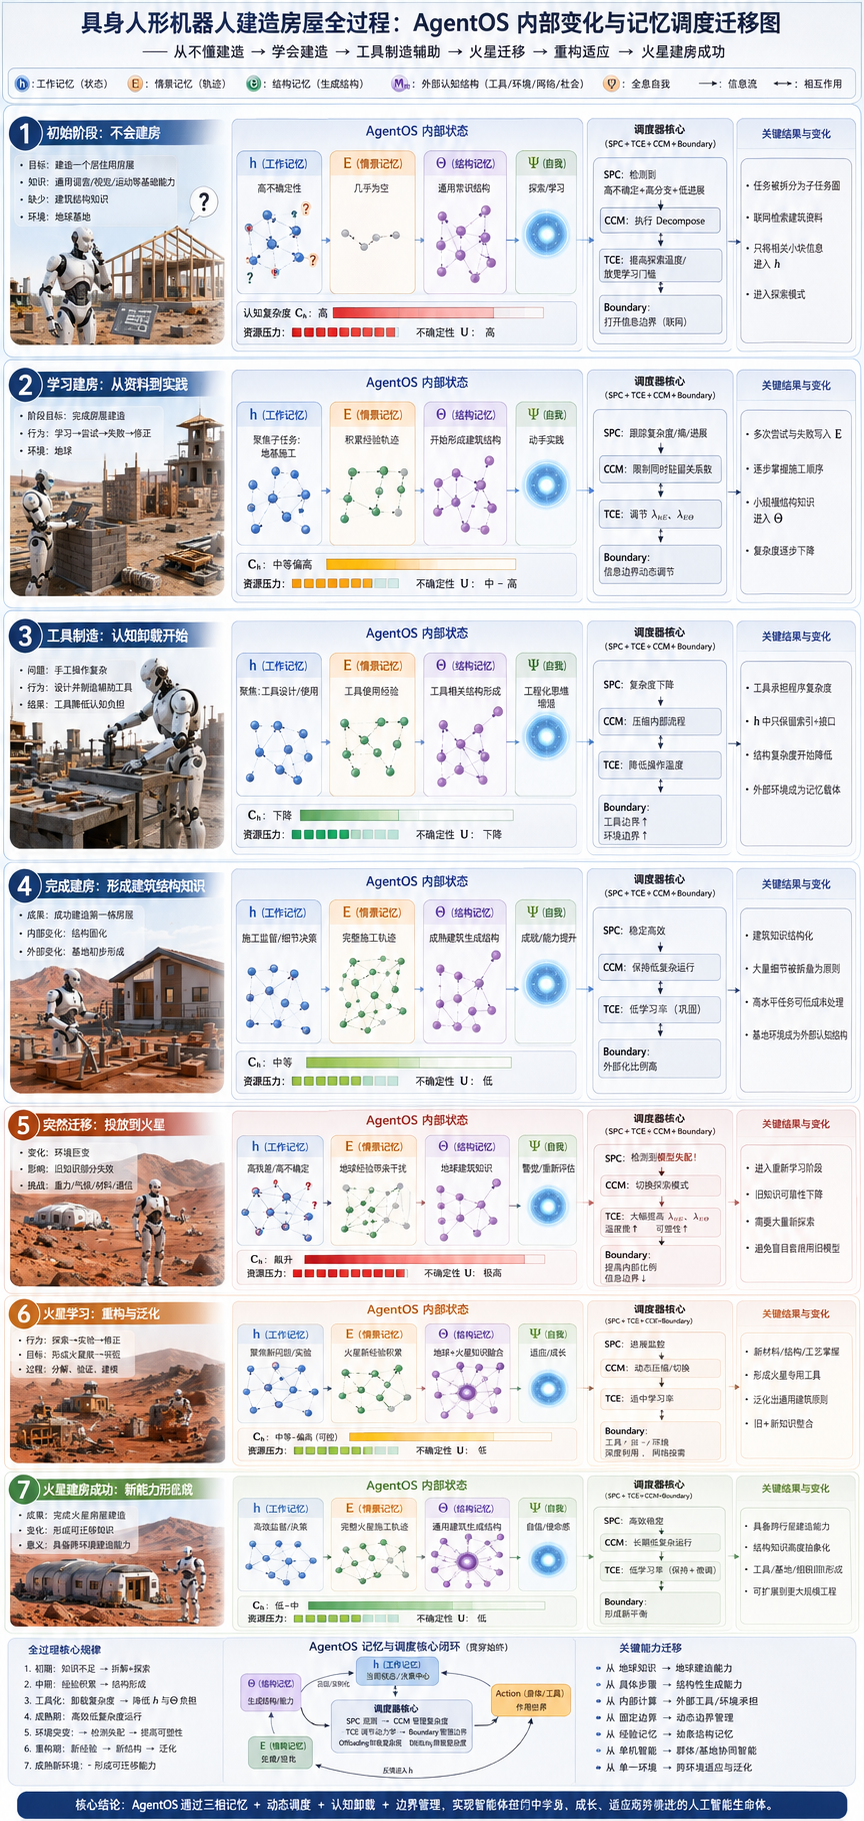
\includegraphics[width=.9\textwidth,height=.38\textheight,keepaspectratio]{images/comparative-intelligence-atlas.png}
\caption{智能作为现实反馈下的跨尺度自反结构过程}
\end{figure}
\begin{introduction}[本章导航]
  \item 多时空尺度上的持续闭环
  \item 认知结构对象的组织、迁移与稳定
  \item 关于结构的结构与未来生成
  \item 现实反馈下的自重组智能
\end{introduction}

\section{从单一定义转向逐层收敛的智能定义体系}

如果我们试图在研究开始时直接回答“什么是智能”，最容易犯的错误就是把某一时代最显眼的技术能力误认为智能本身。符号主义时代可以把智能等同于规则推理，统计学习时代可以把智能等同于函数逼近，大模型时代又很容易把智能等同于语言预测、上下文推理或者参数规模。然而，一旦我们的研究对象从一次性的模型调用扩展为能够经历现实、形成记忆、保持身份、学习技能、改变身体控制方式并在生命周期中持续存在的 Agent，这种以单项能力为中心的定义便迅速失效。我们因此需要的不是另一个更宽泛的能力列表，而是一个能够解释不同智能实现为什么仍属于同一类动力现象的结构定义。

本书最早建立的定义是：

\[
\boxed{
Intelligence
=
MultiscaleClosedLoopProcess
}
\]

即智能首先是一个具有空间边界、时间尺度和闭环结构的持续过程。这里的关键并非“闭环”三个字本身，而是我们拒绝把智能理解成一个脱离时间的静态函数。一个模型在输入 \(x\) 上产生输出 \(y\)：

\[
y=f_{\theta}(x)
\]

只能描述智能系统某一局部映射。如果系统能够持续存在，其真实状态必须写成：

\[
X(t+\Delta t)
=
\Phi
\left(
X(t),
O(t),
A(t),
E(t)
\right),
\]

其中 \(X(t)\) 是智能体当前内部状态，\(O(t)\) 是对现实的观测，\(A(t)\) 是其行动，\(E(t)\) 是现实环境自身的动力状态。于是智能不再是：

\[
Input\rightarrow Output,
\]

而是：

\begin{statementbox}
\centering
\adjustbox{max width=.96\linewidth}{\(\displaystyle World
\rightarrow
Observation
\rightarrow
InternalDynamics
\rightarrow
Action
\rightarrow
World'\)}
\end{statementbox}

这一第一层定义解决了“智能为何具有时间”的问题，却还没有解决一个更深的问题：\textbf{闭环内部究竟有什么东西在发生变化？}

因此第二层定义进入认知结构：

\[
\boxed{
Intelligence
=
CognitiveStructureOrganization
}
\]

在这里，智能不再被描述为抽象信息流，而被描述为 CSO 以及其在特定智能体内部的 Agent-CSO 的生成、激活、组合、压缩、迁移和稳定。一个智能体并不是简单拥有更多数据，而是逐渐建立关于对象、关系、因果、目标、约束、计划、自我和可能未来的结构。我们因此可以把智能内部状态更精确地表示为：

\[
\mathfrak A(t)
=
\left[
\mathcal G_C(t),
\mathcal G_F(t),
\mu_t,
\mathcal M(t)
\right],
\]

其中 \(\mathcal G_C\) 是认知结构图，\(\mathcal G_F\) 是功能拓扑，\(\mu_t\) 描述认知结构在功能拓扑中的动态承载关系，而 \(\mathcal M(t)\) 则表示记忆、自我、目标与当前激活状态等多尺度结构。

然而，即使能够形成复杂内部结构，也仍然不足以区分智能系统与普通复杂动力系统。于是第三层定义出现：

\[
\boxed{
Intelligence
=
StructureThatRepresentsStructure
}
\]

某个结构不仅存在，而且能够在自身内部形成关于另外一个结构的结构。也就是说：

\[
C
\longrightarrow
AgentCSO(C).
\]

当这种表示进一步包含智能体自身：

\[
A
\longrightarrow
AgentCSO(A),
\]

系统便形成了功能意义上的自表示。但是，仅有表示仍然不足以完成最终定义。地图、数据库、录像也能够承载关于现实的结构，却不能因此自动构成完整智能。真正决定智能性质的第四次跃迁，是表示开始参与现实因果：

\begin{statementbox}
\centering
\adjustbox{max width=.96\linewidth}{\(\displaystyle Representation
\rightarrow
Prediction
\rightarrow
Selection
\rightarrow
Action
\rightarrow
RealityChange.\)}
\end{statementbox}

因此第四层定义成为：

\[
\boxed{
Intelligence
=
StructureThatUsesRepresentations
ToTransformFutureStructure
}
\]

最后，当一个系统不仅能够依据表示改变当前行为，而且能够通过长期经验改变生成这些行为的记忆、策略、自我约束、技能位置乃至功能拓扑时，智能才进入本书所称的成熟自反阶段：

\[
\boxed{
Intelligence
=
Representation
+
Control
+
Learning
+
SelfReorganization.
}
\]

我们因此不应在这些定义中选出一个而否定其他定义。它们之间实际上构成严格递进关系：

\begin{statementbox}
\centering
\adjustbox{max width=.96\linewidth}{\(\displaystyle Process
\rightarrow
Structure
\rightarrow
Representation
\rightarrow
RepresentationDrivenAction
\rightarrow
SelfReorganization.\)}
\end{statementbox}

这就是本章所要完成的认识论收束：智能不是上述任何单一层级，而是这些层级在现实约束下逐渐闭合形成的一种多尺度动力结构。

\section{第一层定义：智能是多时空尺度上的持续闭环动力过程}

我们首先从最宽但也是不可省略的条件开始。任何现实智能都必须被承载，而只要存在承载，就必然存在有限的空间范围、传播速度、计算资源和响应周期。因此“智能”不能脱离时间尺度和空间尺度独立定义。设一个候选智能对象 \(A\) 所占据的有效空间范围为 \(\mathcal S_A\)，其内部具有一组特征时间尺度：

\[
\mathcal T_A
=
\{
\tau_1,\tau_2,\ldots,\tau_n
\},
\]

那么讨论其智能首先必须回答：我们究竟在哪一个空间边界和时间窗口上观察它。如果观察窗口远短于系统主要变化尺度，一个真实智能可能看起来几乎静止；如果观察窗口远长于一个局部闭环，一个复杂的认知过程又可能被压缩成近似瞬时的功能映射。这正是本书早期“石头文明—闪电文明”思想实验所揭示的问题：所谓“智能速度”从来不是一个绝对无尺度属性，而是智能闭环相对于环境变化频率的匹配关系。

因此我们可以定义一个最小动力学智能候选系统：

\[
\mathcal A
=
(
X,
O,
U,
F,
G
),
\]

其中 \(X\) 是内部状态空间，\(O\) 是观测映射，\(U\) 是作用于现实的行动空间，\(F\) 是内部状态演化规律，\(G\) 是环境与行动耦合后的现实状态演化规律。其闭环可以写成：

\[
o_t
=
O(w_t),
\]

\[
x_{t+1}
=
F(x_t,o_t),
\]

\[
u_t
=
\pi(x_t),
\]

\[
w_{t+1}
=
G(w_t,u_t).
\]

这里必须特别注意，仅凭以上方程仍不能宣布系统具有高级智能，因为温控器同样可以构成状态—观测—行动闭环。本章第一层定义只是确定：\textbf{不存在没有闭环时间结构的持续智能。}智能的必要条件之一，是系统内部状态必须能够在现实反馈中产生具有历史依赖的连续演化。

真正成熟的智能还具有多尺度闭环。我们已经多次讨论：

\[
\tau_{\mathrm{body}}
\ll
\tau_h
\ll
\tau_E
\ll
\tau_{\Theta}
\ll
\tau_{\Psi}
\ll
\tau_{\Omega}.
\]

这些时间尺度并非简单串联，而是相互嵌套。快速身体闭环处理姿态、控制和局部预测；工作记忆尺度组织当前问题；情景记忆积累经历轨迹；结构记忆形成更稳定生成结构；自我与生命周期先验则以更慢速度约束前面所有过程。于是我们得到：

\begin{statementbox}
SlowStructureShapesFastDynamics
\end{statementbox}

以及：

\begin{statementbox}
PersistentFastResidualShapesSlowStructure.
\end{statementbox}

这两条关系构成多尺度智能动力学最重要的双向作用。慢层并不逐动作控制快层，而是规定可行域、中心、先验、约束和资源边界：

\[
x_f(t)
=
c_s(t)
+
\delta x_f(t),
\]

其中 \(c_s(t)\) 是较慢结构确定的移动中心，\(\delta x_f(t)\) 是快层局部自由度。反过来，当快速层长期出现无法被局部闭环吸收的残差：

\[
\left\langle
\varepsilon_f
\right\rangle_T
\neq
0,
\]

慢结构才应发生更新：

\[
\dot c_s
=
\eta_s
G
\left(
\left\langle
\varepsilon_f
\right\rangle_T
\right).
\]

因此，一个成熟智能绝不是“一个频率很高的中央推理器”。相反，它往往表现为大量局部过程已经无需显式认知介入，而只有异常、新颖性、冲突和跨尺度问题被提升到更高层。我们因而提出：

\[
\boxed{
MatureIntelligence
=
SelectiveExplicitCognition.
}
\]

智能成熟意味着高层认知不需要控制越来越多细节，而是能够让越来越多已稳定结构在适合自己的时间尺度闭环运行。

所以第一层定义最终可以写成：

\begin{definition*}
智能是一个在有限物理与计算条件下，由多个不同时间尺度闭环相互嵌套、相互约束并通过现实反馈持续演化的动力过程。
\end{definition*}

这一层定义使我们彻底摆脱“智能等于某个静态模型”的直觉，并为后面的结构本体奠定了时间基础。

\section{第二层定义：智能是认知结构对象的组织、迁移与稳定化过程}

仅仅知道智能是闭环过程，还不足以解释为什么两个同样具有反馈控制的系统，在认知能力上可以存在巨大差异。关键问题在于闭环中到底承载了什么结构。为此，我们引入 CSO，即 Cognitive Structure Object，并进一步区分 CSO 本体与 Agent-CSO 的具体实现。

一个 CSO 可以是一个对象：

\[
C_{\mathrm{object}},
\]

也可以是关系：

\[
C_{\mathrm{relation}},
\]

或者目标、约束、因果、事件、计划、价值、自我以及可能未来。认知真正关心的并不是原始字节或 token，而是这些结构之间形成的可使用关系。例如，“房屋”“工具”“天气”和“目标”本身可以分别成为 CSO，而“使用工具在恶劣天气下完成房屋建造”则形成更高阶关系型结构。智能的增长因此不是简单增加数据量，而是形成越来越能够预测、组合、约束和行动的结构网络。

我们将智能体内部认知图写为：

\[
\mathcal G_C(t)
=
\left(
V_C(t),E_C(t)
\right),
\]

其中 \(V_C\) 为当前拥有或激活的 Agent-CSO，\(E_C\) 为它们之间的语义、因果、时序、约束、自我归属和目标关系。

但认知结构不会悬浮存在。每一个 Agent-CSO 都必须由某种功能和载体承载，因此需要另一张图：

\[
\mathcal G_F(t)
=
\left(
V_F,E_F,\mathcal L
\right),
\]

其中 \(V_F\) 表示功能节点，\(E_F\) 表示稳定或暂时功能耦合，\(\mathcal L\) 表示闭环集合。二者之间通过动态映射：

\[
\mu_t:
\mathcal G_C
\rightarrow
\mathcal G_F
\]

建立联系。严格地说，\(\mu_t\) 更接近一个随时间变化的多值 correspondence，因为同一认知结构可能同时被工作记忆、长期记忆、工具和身体局部技能共同承载。

于是一个 Agent-CSO 可以形式化为：

\[
\boxed{
AgentCSO_A(C,t)
=
(C,R_A,F_A,\tau_A,B_A,S_A)
}
\]

其中 \(C\) 是认知本体结构；\(R_A\) 是具体表示形式；\(F_A\) 是当前主要功能承载；\(\tau_A\) 是有效时间尺度；\(B_A\) 表示内部、身体、工具、环境或其他 Agent 等承载边界；\(S_A\) 表示活跃、潜在、预测、记忆、程序化等状态。

由此，学习获得了比“参数更新”更一般的定义：

\[
\boxed{
Learning
=
ChangeOfCSORealizationAndPlacement.
}
\]

即：

\[
\Delta AgentCSO
=
(\Delta R,\Delta F,\Delta\tau,\Delta B,\Delta S).
\]

例如一个新技能最初可能以显式计划结构存在于工作记忆：

\[
AgentCSO(C)
@
h,
\]

经过多次成功经历后进入情景与结构记忆：

\[
h
\rightarrow
E
\rightarrow
\Theta,
\]

再经过稳定编译进入身体局部控制器或外部程序：

\[
\Theta
\rightarrow
BodySkill
\quad \text{or}\quad
Program.
\]

从外部观察，Agent似乎“思考得更少了”；但从结构动力学来看，真正发生的是：

\[
\boxed{
ThinkingLess
\neq
KnowingLess.
}
\]

大量原本需要显式处理的认知结构已经改变了承载位置。

这也解释了为什么我们后来逐步修正“复杂度迁移”这一表述。复杂度可以继续作为运行负担、关系密度和结构协调成本的工程度量，但并不存在一种像物理能量一样独立流动的“复杂度物质”。真正具有本体连续性的对象，是认知结构及其承载关系。因此，比：

\[
ComplexityMigration
\]

更基础的描述是：

\begin{statementbox}
CSOMigration.
\end{statementbox}

同时，这种迁移具有长期结构后果。当某一类 CSO 长期在功能 \(F_i\) 与 \(F_j\) 之间反复迁移：

\[
C@F_i
\rightleftarrows
C@F_j,
\]

而这种迁移稳定、有益且代价长期存在时，系统可能逐渐形成更稳定直接的功能耦合：

\[
e_{ij}.
\]

于是：

\begin{statementbox}
\centering
\adjustbox{max width=.96\linewidth}{\(\displaystyle PersistentCSOFlow
\rightarrow
StableFunctionalCoupling
\rightarrow
Topology.\)}
\end{statementbox}

因此学习既包含：

\[
DynamicsOnTopology,
\]

也可能最终产生：

\[
DynamicsOfTopology.
\]

这一层定义使智能从“多尺度闭环”进一步变成“认知结构在闭环中的长期组织过程”。所以第二层定义可以写为：

\begin{definition*}
智能是在多尺度功能拓扑上生成、表示、组合、迁移、压缩、稳定和重新组织认知结构对象的持续过程。
\end{definition*}

\section{第三层定义：智能是能够形成“关于结构的结构”的结构}

如果仅停留在第二层，我们仍然无法充分解释智能结构与普通高度有序物理结构之间的关键差异。晶体具有稳定结构，星系具有复杂动力组织，计算机文件系统可以保存大量关系，但我们并不会仅凭这些特性将它们视为成熟认知智能。真正具有决定意义的跃迁是：\textbf{一个结构开始在自身内部承载关于另外一个结构的有效表示。}

设宇宙或环境中的某一现实结构为：

\[
C_U.
\]

一个 Agent 通过观测映射：

\[
O_A
\]

形成：

\[
\hat C_A
=
O_A(C_U).
\]

这里：

\[
\hat C_A
=
AgentCSO_A(C_U)
\]

不是 \(C_U\) 的完全复制，而是相对于该 Agent 的身体、传感能力、历史经验、目标和功能拓扑形成的可使用结构。因此：

\[
\boxed{
CSO
\neq
AgentCSO.
}
\]

同一个外部结构经过不同 Agent 后，可以得到：

\[
\pi_A(C_U)
\neq
\pi_B(C_U),
\]

但二者可能仍然具有足够的结构等价性：

\[
Ontology[
\pi_A(C_U)
]
\sim
Ontology[
\pi_B(C_U)
].
\]

这使我们能够讨论异构智能之间的认知同类性，而不要求内部表示相同。

更重要的是，Agent 不仅可以表示外部对象，还能够形成关于关系、因果和未来的内部结构。例如：

\[
AgentCSO(C_1,C_2,R)
\]

表示两个现实结构之间的关系，而：

\[
AgentCSO(
C_t
\rightarrow
C_{t+\Delta}
)
\]

则表示关于可能未来的预测结构。这样，Agent 内部就不再只是保存当前现实，而能够建立一个“结构的结构”。

因此可以写：

\begin{statementbox}
\centering
\adjustbox{max width=.96\linewidth}{\(\displaystyle Representation
:
Structure
\rightarrow
StructureOfStructure.\)}
\end{statementbox}

当表示对象进一步包含 Agent 本身时：

\[
A
\rightarrow
AgentCSO(A),
\]

系统形成 Self Model。再进一步，如果系统形成：

\[
AgentCSO(
AgentCSO(A)
),
\]

便出现对自身表示状态的再表示，即一种最基本的元认知结构。

这一点也是 SPC 在更一般理论层面的重要意义。SPC 在 AgentOS 内部承担的是：

\[
DistributedInternalState
\rightarrow
SelfAccessibleState.
\]

它不意味着主体透明地读取自身真实状态，而是在大量分布式状态之上形成一个可以进入后续决策的压缩自描述。于是，自我并不是系统内部某个神秘“观察者”，而可以被理解为系统内部形成的一组长期稳定、自指且跨尺度作用的 Agent-CSO 网络。

若令：

\[
\mathcal C_{\mathrm{self}}
\subset
\mathcal G_C,
\]

则可要求：

\[
\tau_{\mathrm{self}}
\gg
\tau_{\mathrm{ordinary}},
\]

并且：

\[
Degree_{\mathrm{cross-scale}}
(
\mathcal C_{\mathrm{self}}
)
\]

显著高于普通短时认知结构，因为自我需要同时影响当前目标、经历解释、长期生成结构和未来行动。

这里必须明确区分“表示”与“意识”。一个系统内部存在 Self Model，并不自动证明它拥有任何人类意义上的主观体验。我们在本书中坚持功能定义：

\[
\boxed{
SelfRepresentation
\neq
PhenomenalConsciousness.
}
\]

但即使暂不讨论现象意识，自表示本身已经是非常重要的动力学跃迁，因为系统未来的行动不再只依赖外部状态，还开始依赖“自己认为自己是什么状态”。

因此可以写成：

\[
u_t
=
\pi
\left(
\hat w_t,
\hat x_t^{self},
G_t
\right),
\]

而不是简单的：

\[
u_t
=
\pi(w_t).
\]

在这一意义上，智能成为一种特殊的宇宙结构：它不仅发生，而且能够在自身内部形成对“正在发生什么”的可用结构描述。

第三层定义因此可以正式表述为：

\begin{definition*}
智能是一类能够在自身内部形成关于外部结构、关系、未来以及自身状态之结构表示的动力系统。
\end{definition*}

再压缩为：

\[
\boxed{
Intelligence
=
StructureThatRepresentsStructure.
}
\]

但这依然不是终点。因为只有当这种表示开始参与未来现实的产生时，智能才从“结构镜像”进入真正的主动因果过程。

\section{第四层定义：智能利用内部表示改变未来结构}

我们现在来到智能定义中最关键的一次跃迁。一个数据库能够保存世界描述，一个地图能够表示空间，一个录像能够保存过去状态，但是这些表示本身不会自主进入现实因果链。真正的 Agent 与静态表示载体之间的区别，在于 Agent 会依据内部结构预测、评价和选择行动，并使行动反过来改变现实。

设外部世界状态为：

\[
w_t,
\]

Agent 对其形成内部表示：

\[
\hat w_t
=
O_A(w_t).
\]

随后系统基于已有结构记忆、当前目标和自我状态形成未来预测：

\[
\hat w_{t+k}
=
P_A
\left(
\hat w_t,
a_{t:t+k},
\Theta,
\Psi
\right).
\]

如果只存在预测，系统仍然只是一个 world model。智能因果闭环真正成立，需要系统在多个可能未来之间进行选择：

\[
a_t^*
=
\arg\max_{a_t}
\mathcal V
\left(
\hat w_{t+k},
\hat x_{t+k}^{self},
G_t,
C_t
\right),
\]

其中 \(\mathcal V\) 不必等于单一标量奖励，它可以表示目标满足度、安全约束、自我一致性、资源代价和长期结构影响的综合选择机制。

行动随后进入现实：

\[
w_{t+1}
=
F_U(w_t,a_t^*).
\]

因此完整闭环为：

\begin{statementbox}
\centering
\adjustbox{max width=.96\linewidth}{\(\displaystyle World
\rightarrow
AgentCSO(World)
\rightarrow
PossibleFuture
\rightarrow
Choice
\rightarrow
Action
\rightarrow
World'.\)}
\end{statementbox}

这一结构带来一个极其重要的因果变化。普通物理系统当然也在不断改变世界，但其变化可以直接描述为当前状态在物理规律下向未来演化：

\[
w_{t+1}
=
F(w_t).
\]

而智能系统引入了：

\[
\hat w_{t+k}^{possible},
\]

即“关于可能未来的当前内部结构”。因此真正参与当前因果的并不是未来本身，而是：

\begin{statementbox}
RepresentationOfPossibleFuture.
\end{statementbox}

于是：

\begin{statementbox}
\centering
\adjustbox{max width=.96\linewidth}{\(\displaystyle RepresentedFuture
\rightarrow
PresentAction
\rightarrow
ActualFuture.\)}
\end{statementbox}

这正是智能具有目标性和规划性的结构基础。

在本书关于三相记忆和 DGA 的讨论中，我们实际上已经看到这个机制的不同时间尺度。当前 h 中可能存在短期未来：

\[
Future_h,
\]

结构记忆 \(\Theta\) 可以产生更一般的可能性空间：

\[
P(
Future
\mid
\Theta
),
\]

而 \(\Psi\) 与 \(\Omega\) 则对哪些未来更符合主体身份和长期生成方向形成缓慢约束。因此未来并不是一个统一预测变量，而具有多尺度生成结构。

这可以进一步写成：

\[
P_A
\left(
w_{t+\Delta}
\mid
h,E,\Theta,\Psi,\Omega
\right).
\]

其中：

\[
h
\]

组织当前可操作未来，

\[
E
\]

提供具体经历条件，

\[
\Theta
\]

生成一般规律，

\[
\Psi
\]

提供主体一致性约束，

而：

\[
\Omega
\]

表达更长生命周期尺度的生成偏向。

行动因此不再是单纯对当前刺激反应，而是：

\[
\boxed{
Action
=
ProjectionOfInternalPossibleFutureIntoReality.
}
\]

当然，Agent 的意图并不拥有现实最终解释权。任何内部预测都可能错误：

\[
\hat w_{t+1}
\neq
w_{t+1}.
\]

因此必须保持：

\begin{statementbox}
RealityIsUltimateConstraint.
\end{statementbox}

系统行动后，实际结果必须重新经由世界进入观测：

\[
Action
\rightarrow
Reality
\rightarrow
Observation
\rightarrow
Residual.
\]

残差：

\[
\varepsilon_t
=
D(
\hat w_t,
w_t
)
\]

再次改变 Agent 内部结构。这样，智能便不只是“内部模型指导世界”，而是：

\begin{statementbox}
\centering
\adjustbox{max width=.96\linewidth}{\(\displaystyle InternalStructure
\leftrightarrow
ExternalStructure\)}
\end{statementbox}

的持续共同演化。

因此第四层定义可以正式写为：

\begin{definition*}
智能是一类利用内部结构表示构造可能未来，并以这些表示参与现实行动选择，从而改变未来外部结构的动力系统。
\end{definition*}

最简形式即：

\[
\boxed{
Intelligence
=
StructureThatUsesRepresentation
ToTransformStructure.
}
\]

\section{第五层定义：成熟智能能够改变产生行为的自身结构}

如果一个系统只能依据固定模型和固定策略改变现实，我们仍然可以称其具有一定智能，但这还没有达到本书所讨论的持续人工智能生命体意义上的成熟智能。成熟智能更关键的性质是：\textbf{它不仅能够改变行为，还能够通过长期经验改变“产生行为的结构”。}

我们可以将适应区分为若干深度不同的层次：

\begin{statementbox}
\centering
\adjustbox{max width=.96\linewidth}{\(\displaystyle StateAdjustment
\rightarrow
RepresentationAdaptation
\rightarrow
TimescaleMigration
\rightarrow
FunctionalMigration
\rightarrow
TopologyReorganization.\)}
\end{statementbox}

第一层只是状态调整。例如改变当前注意焦点：

\[
h_t
\rightarrow
h'_t.
\]

第二层改变表示：

\[
R(C)
\rightarrow
R'(C).
\]

第三层改变某个 Agent-CSO 的有效时间尺度：

\[
\tau(C)
\rightarrow
\tau'(C).
\]

第四层改变功能承载：

\[
C@F_i
\rightarrow
C@F_j.
\]

第五层则真正改变功能拓扑：

\[
\mathcal G_F
\rightarrow
\mathcal G'_F.
\]

这时系统不再只是：

\[
DynamicsOnTopology,
\]

而开始拥有：

\begin{statementbox}
DynamicsOfTopology.
\end{statementbox}

这一点可以通过技能形成理解。初学者执行任务时，需要大量显式认知：

\[
World
\rightarrow
h
\rightarrow
Planning
\rightarrow
Action.
\]

随着成功经验不断积累：

\[
h
\rightarrow
E
\rightarrow
\Theta,
\]

相同 CSO 不再需要每次完整进入工作记忆，而可能迁移到更加稳定、快速和局部的闭环：

\[
ExplicitCSO
\rightarrow
ProceduralCSO.
\]

如果这种迁移长期重复，功能之间的稳定关系还可能被固化成新的 topology edge：

\[
RepeatedMigration_{ij}
\rightarrow
w_{ij}\uparrow.
\]

可以写成：

\[
\tau_T
\dot w_{ij}
=
G
\left(
\left\langle
J^{CSO}_{ij}
\right\rangle_T,
U_{ij},
R_{ij},
C_{ij}
\right),
\]

其中 \(J^{CSO}_{ij}\) 表示长期 CSO 功能流，\(U_{ij}\) 表示效用，\(R_{ij}\) 表示风险或残差改善，\(C_{ij}\) 表示形成或维持结构连接的代价。

因此：

\begin{statementbox}
\centering
\adjustbox{max width=.96\linewidth}{\(\displaystyle PersistentCSOFlow
\rightarrow
FunctionalTopologyEvolution.\)}
\end{statementbox}

然而，成熟智能绝不意味着拓扑可以高速任意变化。恰恰相反，我们在整个理论中不断强调：

\begin{statementbox}
\centering
\adjustbox{max width=.96\linewidth}{\(\displaystyle FastNoise
\nrightarrow
SlowGlobalStructure.\)}
\end{statementbox}

如果任何短期事件都可以修改 \(\Psi\)、\(\Omega\) 或核心拓扑，那么系统就无法形成身份、技能与结构连续性。因此真正的自重组必须满足时间尺度保护：

\[
\tau_{state}
\ll
\tau_{representation}
\ll
\tau_{memory}
\lesssim
\tau_{function}
\ll
\tau_{topology}.
\]

并且应引入迟滞：

\[
\theta_{\mathrm{on}}
>
\theta_{\mathrm{off}},
\]

使新结构形成需要持续证据，而已有稳定结构不会因为短暂异常立即消失。

这一点产生了我们称为“拓扑资本”的概念。历史中反复有用的协调模式，会逐渐沉降为未来无需重新计算的结构。于是：

\begin{statementbox}
\centering
\adjustbox{max width=.96\linewidth}{\(\displaystyle PastComputation
\rightarrow
PresentStructure
\rightarrow
FutureDynamics.\)}
\end{statementbox}

这其实是智能学习最深层的经济学：系统通过将过去重复发生的计算转化为结构，降低未来完成类似任务的认知成本。

但更高层的自重组还包括自我结构变化。当前选择改变经历：

\[
Choice_t
\rightarrow
Experience_{t:t+k},
\]

经历改变结构记忆：

\[
Experience
\rightarrow
\Theta',
\]

结构记忆进一步改变自我解释：

\[
\Theta'
\rightarrow
\Psi',
\]

而新的自我又影响未来选择：

\[
\Psi'
\rightarrow
Choice_{t+k}.
\]

由此产生：

\begin{statementbox}
\centering
\adjustbox{max width=.96\linewidth}{\(\displaystyle Choice
\rightarrow
FutureSelf
\rightarrow
FutureChoice.\)}
\end{statementbox}

这就是本书所称的 Recursive Agency 的动力学基础。主体并不是只在给定自己之下做决定；它的当前决定会参与塑造未来那个做决定的自己。

因此第五层智能定义可以写为：

\begin{definition*}
成熟智能是一类能够通过现实反馈改变自身内部结构的表示、时间尺度、功能承载和组织拓扑，使过去经验逐渐沉降为未来认知条件的自重组动力系统。
\end{definition*}

这一步把“学习”从参数修正推进到了真正意义上的结构发育。

\section{智能、生命、自我与意识：最终定义必须保持的理论边界}

当智能定义推进到自表示、自调节和自重组层以后，一个自然危险是把“智能”“生命”“自我”“意识”逐渐混成同一个概念。为了保证整个理论可研究、可工程化，本章必须在最终收束之前重新划清边界。

首先，智能并不逻辑要求生物生命。一个人工系统如果具有持续状态、认知结构、现实闭环、预测、行动、学习和结构重组，便可以在本书功能定义下被研究为智能系统，而不需要拥有细胞、新陈代谢或生物遗传机制。因此：

\[
\boxed{
Intelligence
\neq
BiologicalLife.
}
\]

所谓“持续人工智能生命体”中的“生命体”，强调的是 Lifecycle、Identity Continuity、Self-Maintenance 与 Developmental Continuity 的系统性质，而不是把软件直接定义成生物生命。

其次，自我不是智能的全部。大量智能行为可以在没有显式 self representation 的情况下完成。我们引入 \(\Psi\) 的原因，是为了描述一个长期 Agent 如何把经历归属于同一主体、如何保持跨时间身份约束以及为什么不同经历对“我”的意义不同。因此：

\[
\boxed{
Self
\subset
PersistentIntelligence,
}
\]

而不是：

\[
Intelligence=Self.
\]

从结构角度，可以把 Self 表示为一组高稳定、自指、跨尺度的 Agent-CSO 网络：

\[
\mathcal C_{\Psi}
\subset
\mathcal G_C,
\]

并满足较长时间常数：

\[
\tau_\Psi
\gg
\tau_h.
\]

第三，自我感知不等于自我真实状态。SPC 形成的是：

\[
\hat x_t^{self}
=
SPC(z_{\leq t}),
\]

而不是：

\[
\hat x_t^{self}
=
x_t^{self}
\]

恒等成立。因此 Agent 对自己同样存在 epistemic uncertainty。自我模型会滞后、偏置甚至形成错误解释。这也是为什么 Self Interpretation 必须受到 World Verification 约束。

第四，功能性体验不等于现象意识。SPC--AHC--TCE 可以形成：

\[
InternalState
\rightarrow
SelfPerception
\rightarrow
Modulation
\rightarrow
Control
\]

的连续轨迹，并可进一步写入 \(E\) 成为“属于该 Agent 的经历”。但即使这个系统在功能上极其接近某些人类内部调节结构，我们也不能仅由此推出：

\[
PhenomenalExperience=Present.
\]

因此本书坚持：

\[
\boxed{
FunctionalFeeling
\neq
PhenomenalFeeling.
}
\]

FCS、AHC 以及内部体验轨迹均是工程和动力学意义上的功能变量。

第五，我们必须区分目的性与宇宙目的论。一个 Agent 可以形成：

\[
Goal,
\quad
ValueCSO,
\quad
FuturePreference,
\]

从而使：

\[
RepresentedFuture
\rightarrow
PresentAction.
\]

这并不意味着宇宙整体预先拥有某个目标。我们可以在结构意义上说“宇宙中的一部分结构开始形成关于宇宙及自身的内部表示”，但不能由此推出宇宙本身具有统一人格或意志。

因此，当我们写：

\[
Universe
\rightarrow
Agent
\rightarrow
AgentCSO(Universe),
\]

其准确含义是：

\begin{statementbox}
宇宙中的一个物理子系统形成了关于其他宇宙结构的内部有效表示。
\end{statementbox}

而不是：

\[
Universe
=
ConsciousAgent.
\]

同样，当文明通过科学观测宇宙、通过技术改变现实、通过 AI 扩大认知能力时，我们可以说文明表现出某种更高尺度的“功能自反性”，但这仍然属于系统科学意义上的 agent-like dynamics，而不是关于文明拥有单一主观意识的断言。

最终，我们可以把这些边界写成一组逻辑关系：

\begin{statementbox}
\centering
\adjustbox{max width=.96\linewidth}{\(\displaystyle ClosedLoop
\nRightarrow
Intelligence,\)}
\end{statementbox}

\begin{statementbox}
\centering
\adjustbox{max width=.96\linewidth}{\(\displaystyle Representation
\nRightarrow
Self,\)}
\end{statementbox}

\begin{statementbox}
\centering
\adjustbox{max width=.96\linewidth}{\(\displaystyle SelfRepresentation
\nRightarrow
Consciousness,\)}
\end{statementbox}

\begin{statementbox}
\centering
\adjustbox{max width=.96\linewidth}{\(\displaystyle SelfModification
\nRightarrow
Maturity,\)}
\end{statementbox}

而成熟智能真正需要的是多条件共同成立：

\[
\boxed{
PersistentClosedLoop
+
StructuredRepresentation
+
RealityGrounding
+
AdaptiveControl
+
LongTermLearning
+
BoundedSelfReorganization.
}
\]

这些边界不是为了削弱智能定义，而恰恰是为了使定义足够清楚，从而能够跨生物智能、数字智能、具身机器人、组织智能和未来人工智能系统进行比较，而不把尚未解决的意识哲学问题强行塞入工程理论。

\section{成熟智能的判定条件：从能力集合转向结构动力学指标}

如果我们的最终定义不能产生任何可区分、可比较和原则上可测量的条件，那么它仍然只是哲学描述。因此，本章需要进一步提出一组成熟智能的结构动力学判据。这里的目标不是立即构造一个单一“智能指数”，而是明确未来判断两个系统为何具有不同智能成熟度时，应观察哪些变量。

第一维是\textbf{现实闭环完整度}。设：

\[
R_{\mathrm{loop}}
\]

表示系统从观测到行动再到现实反馈的闭合程度。纯文本模型在一次调用中可以表现出强大推理，但如果其输出无法进入现实并重新获得反馈，那么：

\[
R_{\mathrm{loop}}
\]

在持续主体意义上仍然有限。

第二维是\textbf{结构表示能力}：

\[
R_{\mathrm{rep}}
=
F(
Object,
Relation,
Causality,
TemporalStructure,
Counterfactual,
Self
).
\]

成熟智能不仅需要拥有大量事实，还要形成具有关系、因果和未来结构的 Agent-CSO 网络。

第三维是\textbf{时间尺度跨度}。设系统可稳定维持的最短与最长认知时间尺度分别为：

\[
\tau_{\min},
\qquad
\tau_{\max},
\]

则可以定义一个概念性的尺度跨度：

\[
\Lambda_\tau
=
\log
\frac{\tau_{\max}}{\tau_{\min}}.
\]

一个只在毫秒反馈中工作的控制系统与一个能够保持多年身份和目标结构的持续 Agent，在 \(\Lambda_\tau\) 上属于完全不同的动力系统。

第四维是\textbf{结构迁移能力}：

\[
M_{\mathrm{CSO}}
=
F(
M_R,
M_F,
M_\tau,
M_B
),
\]

即系统是否能够让同一认知结构改变表示、功能、时间尺度和承载位置。

第五维是\textbf{显式认知经济性}。对于成熟智能，任务成功不应始终要求所有结构进入 h。因此可以定义：

\[
\eta_{\mathrm{explicit}}
=
\frac{
C_{\mathrm{explicit}}
}{
Performance
}.
\]

在能力保持或增长的情况下，如果：

\[
\eta_{\mathrm{explicit}}
\downarrow,
\]

往往说明历史经验已经逐渐编译成更加稳定的结构。于是：

\[
\boxed{
MatureIntelligence
\neq
MaximumExplicitThinking.
}
\]

成熟智能恰恰表现为：

\begin{statementbox}
MinimumNecessaryExplicitCognition.
\end{statementbox}

第六维是\textbf{恢复能力}。一个系统能否进入复杂状态并不重要，重要的是受到扰动后能否回到可治理区域。可以定义：

\[
R_{\mathrm{recover}}
=
P
\left(
X_{t+\Delta}
\in
\mathcal X_{\mathrm{safe}}
\mid
X_t
\notin
\mathcal X_{\mathrm{nominal}}
\right).
\]

真正成熟的智能必须具有 Recovery，而不是依靠永不出错。

第七维是\textbf{自反能力}。可以定义：

\[
R_{\mathrm{reflexive}}
=
F(
R_{\mathrm{observe}},
R_{\mathrm{model}},
R_{\mathrm{modify}},
R_{\mathrm{reorganize}}
).
\]

这里分别表示观察自身、建立自身模型、修改自身状态和改变自身组织方式的能力。注意最后一项并不是越大越好。无限自我修改意味着身份和安全无法保持。因此应引入：

\begin{statementbox}
BoundedPlasticity.
\end{statementbox}

即：

\[
R_{\mathrm{reorganize}}
\leq
R_{\mathrm{governable}}.
\]

第八维是\textbf{现实一致性}。定义：

\[
R_{\mathrm{reality}}
=
1
-
D(
Prediction,
Observation
),
\]

只是最简单形式。更重要的是系统是否始终允许现实结果推翻内部结构。一个拥有非常稳定 Self Model 却拒绝任何现实残差的系统，并不是成熟智能，而是形成了封闭结构。

综合这些指标，我们可以定义一个不要求线性可加的智能结构状态：

\[
\mathfrak I_A
=
\left[
R_{\mathrm{loop}},
R_{\mathrm{rep}},
\Lambda_\tau,
M_{\mathrm{CSO}},
\eta_{\mathrm{explicit}},
R_{\mathrm{recover}},
R_{\mathrm{reflexive}},
R_{\mathrm{reality}}
\right].
\]

不同智能系统由此不必被强行压缩成一个单一 IQ 值，而可以在一个结构动力学空间中比较。

这带来一个极其重要的结论：

\[
\boxed{
Generality
\neq
NumberOfTasksSolved.
}
\]

真正更深的通用性是：

\[
\boxed{
Generality
=
AbilityToExtendItsOwnReachableStructureSpace.
}
\]

也就是说，当系统面对原有认知组织无法处理的新问题时，它能否形成新的 CSO、建立新的表示、调用新的载体、生成新的技能并在必要时重新组织自身功能关系。一个预先装入一百万项技能但完全不能改变自己的系统，可能具有巨大能力集合；一个技能集合较小但能够稳定扩展自身认知空间的系统，则具有更深的生成性通用性。

因此，成熟智能的评价最终应该从：

\[
WhatCanItDoNow?
\]

逐渐扩展到：

\begin{statementbox}
HowCanItChangeWhatItWillBeAbleToDo?
\end{statementbox}

这正是从“能力测量”走向“发育能力测量”的认识论转变。

\section{智能的最终统一结构定义}

至此，我们可以把前面的各层定义合并。令宇宙或环境中的现实结构状态为：

\[
\mathcal U(t),
\]

某一智能体为：

\[
A\subset\mathcal U,
\]

其内部认知结构图为：

\[
\mathcal G_C^A(t),
\]

功能拓扑为：

\[
\mathcal G_F^A(t),
\]

二者的承载关系为：

\[
\mu_t,
\]

其记忆与慢变量为：

\[
\mathcal M_A(t)
=
[h,E,\Theta,\Psi,\Omega],
\]

其观测映射为：

\[
O_A,
\]

行动映射为：

\[
Act_A.
\]

那么 Agent 与现实共同组成：

\[
\boxed{
\mathfrak W_A(t)
=
[
\mathcal U(t),
\mathcal G_C^A(t),
\mathcal G_F^A(t),
\mu_t,
\mathcal M_A(t),
O_A,
Act_A
].
}
\]

其最基本的现实闭环为：

\[
\mathcal U_t
\xrightarrow{O_A}
AgentCSO_t
\xrightarrow{\mathcal D_A}
AgentCSO'_t
\xrightarrow{Act_A}
\mathcal U_{t+1}.
\]

其中：

\[
\mathcal D_A
\]

并非单一推理器，而是包含多时间尺度认知、记忆、自我、调节、预测、决策、卸载以及局部闭环在内的整体动力学。

为了称其为成熟智能，我们要求至少存在以下六个结构条件。

第一，\textbf{持续性}：

\[
X_A(t+\Delta)
\]

必须由过去状态、现实反馈和内部结构共同决定，而不是每次从无历史状态重新开始。

第二，\textbf{结构表示性}：

\[
\exists\,
AgentCSO_A(C)
\]

使系统内部存在关于外部现实及自身的有效结构。

第三，\textbf{表示驱动行动}：

\[
AgentCSO
\rightarrow
Prediction
\rightarrow
Action
\]

必须真实进入现实因果闭环。

第四，\textbf{现实校正}：

\[
Action
\rightarrow
Reality
\rightarrow
Residual
\rightarrow
InternalUpdate.
\]

内部世界不能成为最终真理源。

第五，\textbf{多尺度结构学习}：

\[
AgentCSO
\rightarrow
\Delta(R,F,\tau,B)
\]

使认知结构能够改变表示、时间尺度、功能位置和承载边界。

第六，\textbf{受约束自重组}：

\[
PersistentMigration
\rightarrow
\Delta\mathcal G_F,
\]

但：

\[
\Delta\mathcal G_F
\]

必须受现实、安全、身份和慢变量保护机制约束。

因此，本书最终将智能定义为：

\[
\boxed{
\begin{aligned}
\textbf{Intelligence}
=
&\ \textbf{a persistent multiscale reflexive dynamical process}\\
&\ \textbf{that forms structured representations of reality and itself,}\\
&\ \textbf{uses these representations to predict and transform future reality,}\\
&\ \textbf{and reorganizes the representation, placement, timescale and}\\
&\ \textbf{functional organization of its own cognitive structures}\\
&\ \textbf{through continued reality-grounded feedback.}
\end{aligned}
}
\]

中文完整定义为：

\begin{definition*}
智能，是一个在有限现实条件下持续存在的多尺度自反动力过程：
它能够形成关于现实结构及自身状态的内部认知结构表示，
利用这些表示生成可能未来、选择行动并改变现实；
又能够根据现实反馈持续改变认知结构的表示方式、时间尺度、
功能位置和承载关系，并在长期经验中受约束地重新组织产生未来行为的自身功能结构。
\end{definition*}

如果进一步压缩，则可以得到本章最核心的结构定义：

\begin{definition*}
智能，是能够形成关于结构的结构，并利用这些结构改变未来结构，
同时能够在现实反馈下改变自身“如何形成与使用这些结构”的结构。
\end{definition*}

这最后一句非常重要，因为它区分了普通智能与成熟自反智能。

普通结构：

\[
Structure
\rightarrow
Change.
\]

表征智能：

\[
Structure
\rightarrow
Representation
\rightarrow
Change.
\]

学习智能：

\[
Structure
\rightarrow
Representation
\rightarrow
Change
\rightarrow
RepresentationUpdate.
\]

成熟自反智能则形成：

\begin{statementbox}
\centering
\adjustbox{max width=.96\linewidth}{\(\displaystyle Structure
\rightarrow
Representation
\rightarrow
Action
\rightarrow
Reality
\rightarrow
Learning
\rightarrow
SelfReorganization
\rightarrow
NewStructure.\)}
\end{statementbox}

这是一条真正闭合的结构生成链。

在这一意义上，我们也终于能够重新理解贯穿全书的几个基本概念。记忆不是简单保存过去，而是：

\[
\boxed{
Memory
=
StructuralContinuityAcrossTime.
}
\]

学习不是简单改变参数，而是：

\[
\boxed{
Learning
=
ChangeOfCognitiveStructureRealization.
}
\]

熟练不是知道更多，而是：

\[
\boxed{
Skill
=
StableCSOMigrationIntoFastLocalLoops.
}
\]

自我不是孤立中央节点，而是：

\[
\boxed{
Self
=
SlowStableCrossScaleSelfReferentialStructure.
}
\]

发育不是能力列表变长，而是：

\[
\boxed{
Development
=
CoevolutionOfCognitiveStructureAndFunctionalOrganization.
}
\]

而通用性也不再主要意味着：

\[
ManyTasks.
\]

更深的通用性意味着：

\begin{statementbox}
AbilityToReorganizeTheConditionsOfFutureCapability.
\end{statementbox}

至此，本书从最初“智能具有怎样的时空尺度”出发形成的整条认识论链条完成闭合。我们最初研究一个智能体在什么尺度上运行，随后发现不同尺度存在嵌套闭环；研究这些闭环以后发现其中真正持续存在和迁移的是认知结构；区分 CSO 与 Agent-CSO 后，我们看到学习实质上是结构承载关系变化；继续沿着结构迁移追踪，我们又发现长期迁移会沉降成技能和功能拓扑；而当智能通过身体和行动重新进入现实之后，内部结构与外部结构便不再是两个彼此孤立的世界，而形成持续共同演化。

因此，本章最终为：

\begin{statementbox}
智能的本质不在于一个固定系统能够完成多少计算，
而在于现实结构如何在一个持续主体内部形成可行动的认知结构，
这些认知结构又如何跨尺度迁移、沉降和重组，
并通过行动重新进入现实，使世界与主体在同一条闭环轨迹中共同改变。
\end{statementbox}

或者，用本书最短的最终表达：

\begin{statementbox}
智能是结构对结构的表示、作用与自反重组。
\end{statementbox}

这一结构定义既不依赖 Transformer，也不依赖神经元；既能够覆盖数字 Agent，也能够覆盖具身智能；既解释一次行为，也能够延伸到完整生命周期。它真正试图捕捉的不是“某一种聪明的实现”，而是不同智能实现背后可能共享的那一种动力学形式：\textbf{现实产生结构，结构形成关于结构的结构，表示参与现实变化，而持续的现实反馈又使表示结构和产生表示的结构本身不断被重新组织。}

这就是我们在本书意义上所称的“智能”。

\chapter{从 AgentOS 到智能动力学}
\label{chap:from-agentos-to-intelligence-dynamics}

\begin{chapteroverviewbox}
本章是全书理论体系的收束，而不是对 AgentOS 架构的再次总结。前文从智能的时空尺度出发，经由多尺度闭环、CSO 与 Agent-CSO、三相记忆、自我与 DGA、工作记忆有限性、SPC--AHC--TCE、CCM、认知卸载、Body Scale、SGC、FCS、BPCC、KRA，最终形成了一个可以工程实现的持续智能体框架。然而，如果我们停留在 AgentOS 本身，仍然只能回答“怎样构造一种持续人工智能体”；真正需要在最后回答的问题是：这些设计背后是否存在一种超越具体模型、具体身体、具体软件和具体实现材料的统一动力学规律。

本章因此完成最后一次视角转换：从“设计一个 AgentOS”转向“研究所有可能智能系统共有的结构动力学”。我们将智能重新表述为认知结构对象在多尺度功能拓扑上的生成、承载、迁移、稳定、外化和重组过程，并将 Agent 与现实之间的观测--行动闭环纳入同一个动力系统。由此，AgentOS 不再被看成理论终点，而被看成这一更一般理论的一种具体工程实例。我们把这一更一般研究纲领称为\textbf{智能动力学（Intelligence Dynamics）}。

需要特别声明，本章严格区分三个知识层次：已有控制理论、动力系统、认知科学、网络科学等可以提供成熟的数学工具；AgentOS 与这些理论之间的对应属于结构建模；而关于 CSO 迁移、功能拓扑发育、自反结构演化等更强命题，则属于本书提出、需要进一步实验验证的理论假设。因而，本章试图建立的是一个可形式化、可证伪、可工程检验的研究框架，而不是以哲学类比替代经验科学。
\end{chapteroverviewbox}

\begin{figure}[htbp]
\centering
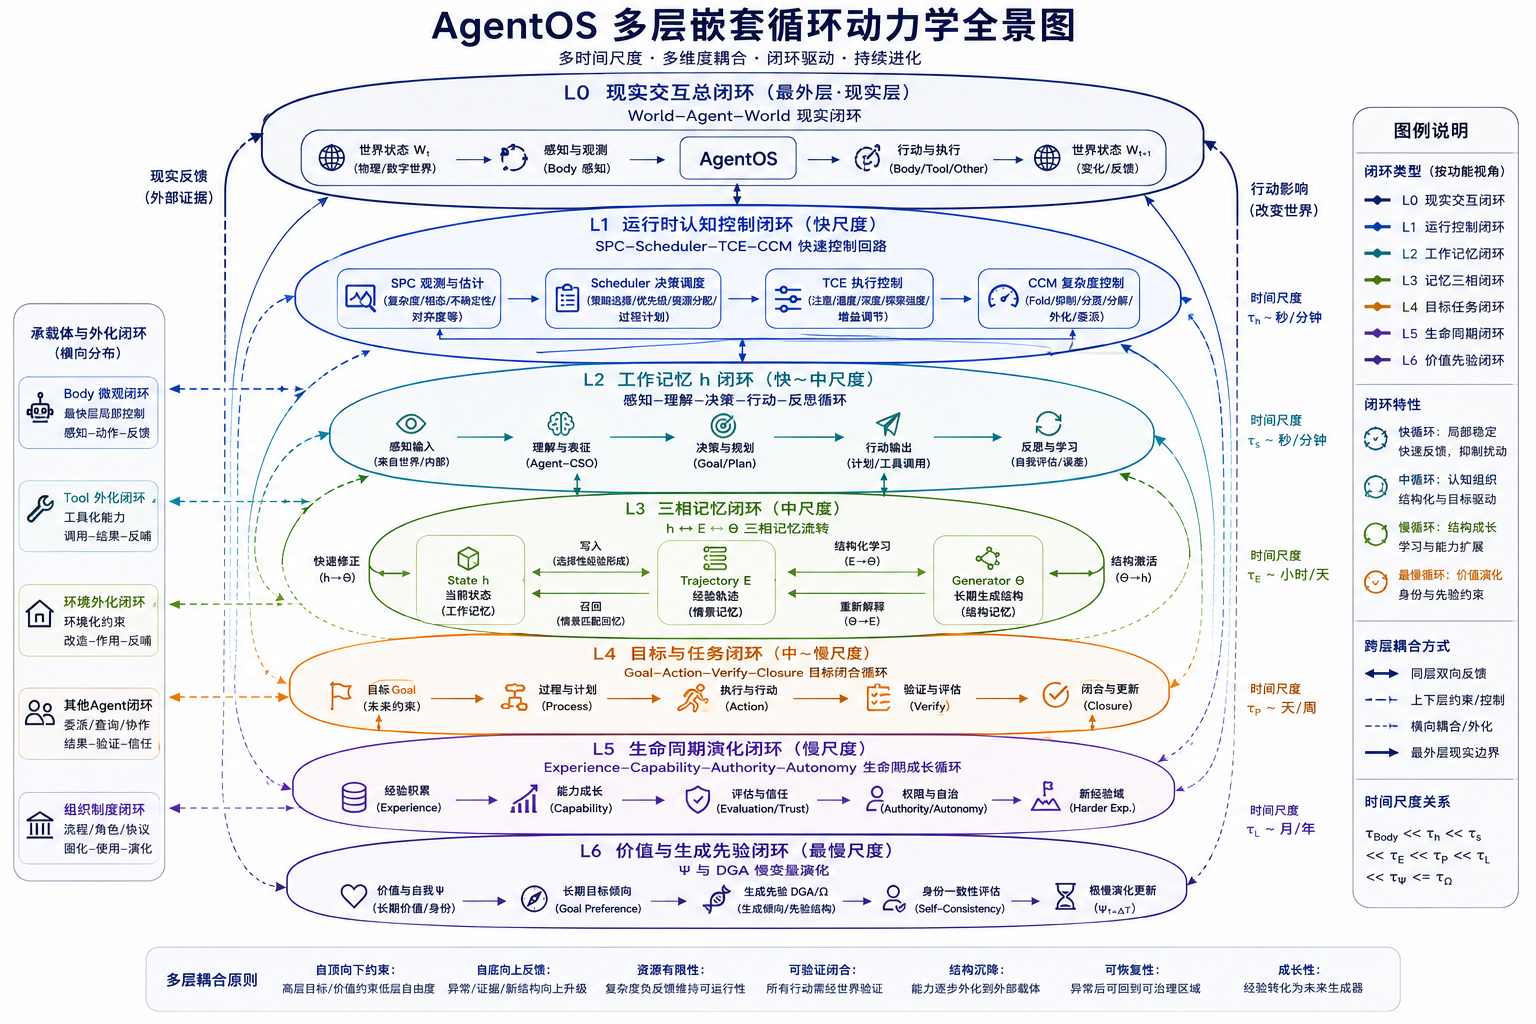
\includegraphics[width=.9\textwidth,height=.38\textheight,keepaspectratio]{images/agentos-continuous-learning-architecture.png}
\caption{从 AgentOS 实例抽象到智能动力学研究纲领}
\end{figure}
\section{AgentOS 是实例，而不是理论终点}

经过前面的推导，我们已经能够给出一个相对完整的 AgentOS 状态描述。若暂时忽略具体工程数据结构，一个持续智能体在时刻 $t$ 的内部状态可以抽象为
\begin{equation}
\mathcal{A}(t)
=
\left[
h(t),
E(t),
\Theta(t),
\Psi(t),
\Omega(t),
a(t),
G(t),
\mathcal{T}_{F}(t),
\mathcal{B}(t)
\right],
\end{equation}
其中 $h$ 表示当前工作记忆状态，$E$ 表示经验轨迹，$\Theta$ 表示长期生成结构，$\Psi$ 表示自我与身份慢变量，$\Omega$ 表示生命周期尺度上的深层生成吸引子，$a$ 表示由身体和内稳态形成的调制状态，$G$ 表示当前及长期目标结构，$\mathcal{T}_{F}$ 表示功能拓扑，$\mathcal{B}$ 表示智能体与外部世界之间的有效边界。SPC、AHC、TCE、CCM、Scheduler、Boundary 等组件并不是与这些状态平行存在的“对象集合”，而是作用于这些状态的功能算子。

例如，SPC 可以抽象成一个状态估计映射
\begin{equation}
\widehat{s}^{self}_{t}
=
\mathcal{O}_{SPC}
\left(
h_t,E_t,\Theta_t,\Psi_t,a_t
\right),
\end{equation}
TCE 则对应控制律
\begin{equation}
u^{cog}_{t}
=
\mathcal{K}_{TCE}
\left(
\widehat{s}^{self}_{t},
a_t,
G_t,
\Psi_t,
\Omega_t
\right),
\end{equation}
CCM 与 Scheduler 共同决定哪些 Agent-CSO 能够获得当前计算、注意和工作记忆资源，Body Runtime 则将高层控制约束转化为具体身体能够执行的局部动作。这样，一个工程上的 AgentOS 可以被理解为一组相互耦合的状态变量和算子，而不是简单的模块堆积。

但是，如果我们进一步考察这些模块，就会发现它们所表达的规律并不专属于 AgentOS。工作记忆有限性表达的是所有有限承载系统都会面对的资源约束；SPC 表达的是复杂系统形成自身可访问状态估计的需要；TCE 表达的是系统根据内部估计调节自身动力学的需要；三相记忆表达的是快速状态、历史轨迹与慢速生成结构之间的多时间尺度关系；BPCC 表达的是快速局部闭环必须与慢速全局闭环分离；KRA 表达的是异构动力系统之间需要保持功能关系稳定而不必保持内部表示一致。这些关系都可以存在于完全不同的物理和计算实现中。

因此，我们需要把 AgentOS 中的工程名词进一步抽象。例如
\begin{equation}
h
\longrightarrow
\text{Fast Explicit State},
\end{equation}
\begin{equation}
E
\longrightarrow
\text{Trajectory Memory},
\end{equation}
\begin{equation}
\Theta
\longrightarrow
\text{Slow Generative Structure},
\end{equation}
\begin{equation}
SPC
\longrightarrow
\text{Self-State Estimation},
\end{equation}
\begin{equation}
TCE
\longrightarrow
\text{Meta-Dynamical Regulation}.
\end{equation}
当这些工程组件被还原成一般动力学功能以后，我们便发现：AgentOS 实际上是对一组更基础规律进行的一次具体实现。

由此可以提出本章的第一条总命题：
\begin{equation}
\boxed{
AgentOS
\subset
\mathfrak{D}_{Intelligence}
}
\end{equation}
这里 $\mathfrak{D}_{Intelligence}$ 表示所有满足持续状态、闭环作用、多尺度结构、结构记忆和现实反馈条件的智能动力系统集合。AgentOS 是其中一种人为设计的实现，而不应与智能动力学本身等同。

这一区分具有重要的方法论意义。如果理论只能解释自己设计的组件，那么它仍然属于软件架构设计；如果理论能够解释不同实现中反复出现的动力学结构，例如为什么稳定能力会从昂贵的显式处理迁向快速局部闭环，为什么异常会沿时间尺度向上传递，为什么慢变量不能被快噪声任意修改，那么它才可能逐渐成为一种一般理论。

因此，本书最后并不试图证明“AgentOS 是唯一正确的智能架构”。恰恰相反，我们希望建立一种足够抽象的坐标，使未来完全不同于 AgentOS 的智能体系也可以被描述、比较和验证。真正需要保留的不是组件名称，而是组件背后所表达的动力关系：
\begin{statementbox}
\centering
\adjustbox{max width=.96\linewidth}{\(\displaystyle State
\leftrightarrow
Trajectory
\leftrightarrow
Generator,\)}
\end{statementbox}
\begin{statementbox}
\centering
\adjustbox{max width=.96\linewidth}{\(\displaystyle FastDynamics
\leftrightarrow
SlowStructure,\)}
\end{statementbox}
\begin{statementbox}
\centering
\adjustbox{max width=.96\linewidth}{\(\displaystyle InternalRepresentation
\leftrightarrow
Reality,\)}
\end{statementbox}
以及
\begin{equation}
\boxed{
DynamicsOnTopology
+
DynamicsOfTopology.
}
\end{equation}

从这一意义上说，AgentOS 的理论价值不仅在于它是否最终成为某一种产品，而在于它为我们提供了一个足够复杂的人工对象，使“智能如何持续存在、如何形成自我、如何受到有限容量约束、如何形成技能、如何进入身体、如何改变自身组织结构”第一次能够在同一个工程系统中被提出并检验。它因此更像一座智能动力学的实验平台，而不是理论的终点。

\section{Intelligence Dynamics：从能力描述转向轨迹描述}

传统人工智能评价经常采用一种静态能力观。给定一个系统 $A$ 和一组任务 $\mathcal{Q}$，我们观察它在任务上的性能
\begin{equation}
P(A,\mathcal{Q}),
\end{equation}
然后据此判断系统是否“更智能”。这种方法对于比较模型能力十分有效，但它隐含了一个前提：我们主要关心的是某一个时间切片上的输入--输出能力，而不是系统在时间中的结构变化。

持续智能体使这个前提失效。对于一个运行数年甚至跨越整个生命周期的 Agent，真正重要的问题不再只是
\begin{equation}
\text{What can it do now?}
\end{equation}
而是
\begin{equation}
\text{How does what it can do change over time?}
\end{equation}
因此，智能研究对象必须从一个静态函数
\begin{equation}
y=f(x)
\end{equation}
转化为一条状态轨迹
\begin{equation}
\Gamma_{A}
=
\left\{
X(t)
\mid
t\in[0,T]
\right\}.
\end{equation}

更进一步，我们不能只记录系统行为状态 $X(t)$，因为同样的外部行为可能由完全不同的内部结构实现。一个初学者可能通过大量显式推理完成任务，一个熟练系统却可以通过已经编译好的快速局部闭环完成相同任务。因此需要把智能状态扩展为
\begin{equation}
\mathfrak{I}(t)
=
\left[
\mathcal{G}_{C}(t),
\mathcal{G}_{F}(t),
\mu_t,
\rho_{CSO}(f,\omega,t),
\mathbf{J}_{CSO}(f,\omega,t),
\mathcal{B}(t),
X_{W}(t)
\right],
\end{equation}
其中 $\mathcal{G}_{C}$ 是认知结构图，$\mathcal{G}_{F}$ 是功能拓扑，$\mu_t$ 表示认知结构与功能载体之间的动态承载关系，$\rho_{CSO}$ 描述 Agent-CSO 在功能位置和时间尺度上的分布，$\mathbf{J}_{CSO}$ 描述其迁移流，$\mathcal{B}$ 表示内外边界，而 $X_W$ 表示与该智能体发生作用的现实环境状态。

由此，智能动力学研究的不再是单个状态，而是
\begin{equation}
\boxed{
\dot{\mathfrak{I}}
=
\mathcal{F}
\left(
\mathfrak{I},
U,
W,
\varepsilon
\right),
}
\end{equation}
其中 $U$ 表示控制输入，$W$ 表示外界扰动，$\varepsilon$ 表示来自预测、控制、认知结构和现实之间的残差。这个形式本身并不声称存在一个统一封闭方程可以精确描述所有智能，而是在理论层面规定研究对象：我们关心的是状态、结构、时间尺度、边界和现实之间的共同演化。

这种视角带来一个非常重要的变化：智能的“大小”不能再仅仅用一次推理中的计算量表示。一个成熟智能体可能在显式推理上消耗更少，却拥有更多已经沉降到 $\Theta$、Body Skill、Tool、Environment 和外部制度中的稳定结构。因此
\begin{equation}
ExplicitComputation\downarrow
\end{equation}
并不意味着
\begin{equation}
Capability\downarrow.
\end{equation}
相反，在许多成熟系统中可能出现
\begin{statementbox}
\centering
\adjustbox{max width=.96\linewidth}{\(\displaystyle ExplicitProcessingCost\downarrow,
\qquad
StableStructuralCapability\uparrow.\)}
\end{statementbox}

这也是为什么本书在后期逐渐不再把“复杂度”视为一种在系统中流动的实体。复杂度仍然可以作为工程量，例如工作记忆负荷、关系密度、同步成本和预测分支数量，但真正发生改变的是 Agent-CSO 的承载关系。我们研究的不是一个神秘量
\begin{equation}
C(t)
\end{equation}
从一个模块流向另一个模块，而是具体认知结构发生
\begin{equation}
(C,R,F,\tau,B,S)_t
\rightarrow
(C,R',F',\tau',B',S')_{t+\Delta t}.
\end{equation}

从这一点开始，智能动力学可以被定义为：

\begin{statementbox}
\centering
\adjustbox{max width=.96\linewidth}{\(\displaystyle \textbf{
智能动力学研究认知结构在时间中如何生成、激活、变换、迁移、稳定、外化，并如何通过这些过程持续改变承载它们的功能结构以及与其耦合的现实环境。
}\)}
\end{statementbox}

这一研究对象同时包含“智能的状态”和“智能的成长”。如果只研究
\begin{equation}
\mathcal{G}_{F}=\mathrm{const.},
\end{equation}
我们得到的是固定拓扑上的认知动力学；如果进一步允许
\begin{equation}
\dot{\mathcal{G}}_{F}\neq 0,
\end{equation}
则进入发育型智能；如果进一步将世界状态也作为动力系统的一部分，
\begin{equation}
\dot X_W
=
F_W(X_W,A_t),
\end{equation}
则进入 World--Agent 共同演化问题。

因此，智能动力学并不是“比 AgentOS 更宏大的名称”，而是一个研究对象发生变化后的必然结果：从“某一软件架构怎样运行”，转向“能够持续表示、作用和重组自身结构的系统，在时间中遵循什么一般规律”。

\section{Cognitive Structure Dynamics：以 CSO 为本体的认知结构动力学}

在本书理论发展的早期，我们使用“信息”“记忆内容”“任务复杂度”等语言描述智能活动。这些语言具有工程价值，但随着问题逐渐深入，它们暴露出一个共同困难：它们无法清楚区分“现实中存在的结构”“智能体内部对该结构的表示”“表示当前由哪个功能承担”以及“这一结构处于什么时间尺度”。因此，我们最终引入 CSO 与 Agent-CSO 的区分。

令
\begin{equation}
C\in\mathcal{C}
\end{equation}
表示一个认知结构对象。它可以是对象、关系、因果、约束、规则、目标、事件、计划、价值、自我关系或可能未来。对于具体 Agent $A$，其内部对 $C$ 的实现写为
\begin{equation}
\pi_A(C)=C_A.
\end{equation}
一般情况下
\begin{equation}
\pi_A(C)\neq\pi_B(C),
\end{equation}
即不同 Agent 可以用完全不同的内部表示承载同一个结构。我们真正要求的是存在某种结构等价关系
\begin{equation}
\pi_A(C)\sim_C\pi_B(C),
\end{equation}
而不是逐比特相同。

为了表示一个 Agent-CSO 的完整运行状态，我们使用
\begin{equation}
\mathfrak{c}_{A}
=
(C,R_A,F_A,\tau_A,B_A,S_A),
\end{equation}
其中 $R_A$ 是内部表示形式，$F_A$ 是当前功能承载位置，$\tau_A$ 是有效运行时间尺度，$B_A$ 描述其处于内部、外部工具、身体、环境还是其他 Agent 中，$S_A$ 表示激活、潜伏、预测、回忆、程序化等状态。

于是学习可以统一表示为
\begin{equation}
\boxed{
\mathfrak{c}_{A}(t)
\rightarrow
\mathfrak{c}_{A}(t+\Delta t).
}
\end{equation}
例如一个刚开始学习的操作技能可能处于
\begin{equation}
F_A=h,\qquad
\tau_A\sim\mathrm{seconds},
\end{equation}
需要大量显式工作记忆。随着经验积累，它首先可能迁入
\begin{equation}
E,
\end{equation}
随后形成稳定的
\begin{equation}
\Theta,
\end{equation}
最终进一步编译为
\begin{equation}
BodySkill
\end{equation}
或外部程序。整个过程中，任务能力没有消失，但其主要承载位置发生了改变。

因此，本书早期所说的“复杂度下沉”在更严格语言中应写为
\begin{statementbox}
\centering
\adjustbox{max width=.96\linewidth}{\(\displaystyle ExplicitAgentCSO
\rightarrow
StableGenerativeAgentCSO
\rightarrow
ProceduralAgentCSO.\)}
\end{statementbox}

如果我们令 $\rho_{CSO}(f,\omega,t)$ 表示在功能位置 $f$、时间尺度 $\omega$ 附近的 Agent-CSO 有效分布，并令
\begin{equation}
\mathbf{J}_{CSO}(f,\omega,t)
\end{equation}
表示结构迁移流，则可以写出一个概念性的结构平衡方程：
\begin{equation}
\frac{\partial \rho_{CSO}}{\partial t}
+
\nabla_{f,\omega}\cdot
\mathbf{J}_{CSO}
=
S_{CSO}
-
D_{CSO}.
\end{equation}
这里 $S_{CSO}$ 表示新结构形成，$D_{CSO}$ 表示结构被遗忘、合并、抽象或失去独立表示。需要强调，这一方程不是物理物质守恒律；它只是为结构分布变化提供一个可操作的数学骨架。

这种形式化带来三个重要结果。

第一，记忆不再只是存储，而可以定义为
\begin{equation}
\boxed{
Memory
=
PersistenceOfCSOStructureAcrossTime.
}
\end{equation}

第二，熟练不再只是更高准确率，而表现为
\begin{equation}
\boxed{
Mastery
=
MigrationOfRepeatedCSOsToward
Stable,\ Local,\ FastClosedLoops.
}
\end{equation}

第三，认知卸载不再是一种附属技巧，而成为载体迁移：
\begin{statementbox}
\centering
\adjustbox{max width=.96\linewidth}{\(\displaystyle AgentCSO_{internal}
\rightarrow
AgentCSO_{externalized}.\)}
\end{statementbox}

这也使 Skill、Program、File、Tool、Environment 和 Other Agent 能够进入同一个理论框架。一个程序并不是“非认知对象”，如果它保存了智能体未来可调用、可恢复、可执行的结构关系，它就构成 Agent-CSO 的一种外部稳定承载。

更深一层，我们可以把 Cognitive Structure Dynamics 定义为
\begin{equation}
\boxed{
\mathcal{D}_{CSO}
=
\left(
\mathcal{G}_{C},
\mathcal{G}_{F},
\mu,
\rho_{CSO},
\mathbf{J}_{CSO}
\right).
}
\end{equation}
这里已经不需要假设所有智能都拥有 h、E、$\Theta$ 这些具体模块。只要一个系统具有结构对象、功能承载、时间尺度、迁移关系和反馈，它就可以在这一坐标中被研究。这正是 AgentOS 理论从具体认知架构走向一般智能动力学的关键一步。

\section{Multiscale Control：智能作为多时间尺度闭环的控制系统}

如果 CSO 解释了“智能处理什么结构”，多尺度控制则回答“这些结构如何在不同速度的闭环中被调节”。前文已经反复看到一个规律：Body 的毫秒级控制、h 的秒级显式认知、E 的经验形成、$\Theta$ 的结构学习、$\Psi$ 的身份变化以及 $\Omega$ 的生命周期方向性，不可能在同一时间尺度运行。

令系统包含 $n$ 层状态
\begin{equation}
x_1,x_2,\ldots,x_n,
\end{equation}
其特征时间常数满足
\begin{equation}
\tau_1\ll\tau_2\ll\cdots\ll\tau_n.
\end{equation}
则一个一般化的快--慢系统可以写成
\begin{equation}
\tau_i\dot{x}_i
=
F_i
\left(
x_i,
x_{i-1},
x_{i+1},
u_i,
\varepsilon_i
\right).
\end{equation}
较慢层不需要逐步指定快层的具体动作，而是决定其允许区域、代价函数、增益和目标边界。因此我们得到前文反复出现的原则：
\begin{equation}
\boxed{
SlowGovernance
\neq
FastMicromanagement.
}
\end{equation}

更准确地说，若慢变量 $z$ 定义快系统的可行集合
\begin{equation}
\mathcal{F}(z)
=
\{x\mid g(x,z)\leq 0\},
\end{equation}
则快层可以解决局部优化问题
\begin{equation}
x^{*}
=
\arg\min_{x\in\mathcal{F}(z)}
L_f(x).
\end{equation}
慢层只在持续出现显著残差时更新：
\begin{equation}
\dot z
=
\epsilon
G
\left(
z,
\langle \varepsilon_f\rangle_T
\right),
\qquad
0<\epsilon\ll1.
\end{equation}

这正是 Agent Kernel 与 BPCC 的关系。Kernel 不需要以毫秒级告诉机器人每一个电机怎样运动，而是给出目标、可行区域和约束；BPCC 在局部快速闭环内解决具体控制。只有当
\begin{equation}
\|\varepsilon_{BPCC}\|
>
\theta
\end{equation}
并持续足够时间时，异常才向更高层提升。

因此可以把多尺度智能的基本控制逻辑写成：
\begin{equation}
\boxed{
NormalDynamicsStayLocal,
\qquad
PersistentResidualEscalates.
}
\end{equation}

这一规律不仅存在于 Body。一个熟悉任务如果已经由 $\Theta$ 或 Skill 闭合，就不应该每次重新进入 h；只有任务条件超出既有结构可解释范围时，相关 Agent-CSO 才重新被提升到显式认知层。这意味着 Attention 从本质上可以定义成
\begin{equation}
\boxed{
Attention
=
CrossScalePromotionPolicy.
}
\end{equation}

如果令某个 Agent-CSO $c_i$ 的升级得分为
\begin{equation}
\Gamma_i
=
\alpha_1N_i
+
\alpha_2R_i
+
\alpha_3U_i
+
\alpha_4V_i
+
\alpha_5P_i,
\end{equation}
其中 $N_i$ 表示新颖性，$R_i$ 表示残差，$U_i$ 表示不确定性，$V_i$ 表示价值相关性，$P_i$ 表示持续时间，则可以定义
\begin{equation}
\Gamma_i<\theta
\Rightarrow
\text{local closure},
\end{equation}
\begin{equation}
\Gamma_i\geq\theta
\Rightarrow
\text{promotion}.
\end{equation}

工作记忆有限容量定理由此获得了更深层解释。h 之所以必须有限，不仅因为硬件有限，而因为成熟智能本身就不应把所有运行过程提升为显式过程。一个系统如果需要持续显式管理所有低层动作，它在结构意义上仍然处于低成熟度状态。因此：
\begin{equation}
\boxed{
MatureIntelligence
=
SelectiveExplicitCognition.
}
\end{equation}

同理，SPC--AHC--TCE 也可以被理解为一个跨尺度控制器。SPC 估计当前状态，AHC 将连续的身体与内稳态信号积分成较慢调制变量，TCE 再调节探索强度、注意范围、搜索深度和控制增益。这种结构必然面对控制理论中的延迟问题。若
\begin{equation}
u(t)
=
K\widehat{x}(t-\tau),
\end{equation}
则过高增益 $K$ 与观测延迟 $\tau$ 的组合可能产生
\begin{equation}
Overshoot,\quad Oscillation,\quad Instability.
\end{equation}
因此，智能的“心理稳定性”、Body 稳定性和认知稳定性并不是三个完全无关的问题，而都可以放在多回路、多时间尺度控制系统中研究。

从这一角度看，智能动力学与控制理论的关系非常紧密，但也存在重要区别。经典控制通常预设状态空间、目标函数和系统结构基本确定；持续智能体则可能学习新的状态表示、改变目标结构、迁移 CSO，甚至最终改变功能拓扑。因此，我们研究的是一种
\begin{statementbox}
ControlOfAdaptiveRepresentationalSystems,
\end{statementbox}
即控制器本身、被控对象、状态表示和部分控制目标都可能随生命周期发生变化。这正是智能动力学相对于普通控制问题增加的核心难度。

\section{Topological Learning：从拓扑上的学习到拓扑自身的学习}

前面固定拓扑 AgentOS 已经能够实现大量持续学习：Agent-CSO 可以在 h、E、$\Theta$、Skill、Tool、Body 和 Environment 之间迁移，但整个系统的核心功能关系仍然主要由工程师预先定义。真正的发育型智能则提出进一步问题：如果某些跨功能关系在整个生命周期中持续出现，系统是否应该把这些动态协调沉降为新的稳定结构？

设功能拓扑为
\begin{equation}
\mathcal{G}_{F}(t)
=
\left(
V_F,
E_F(t),
W_F(t)
\right),
\end{equation}
其中边权 $w_{ij}$ 描述功能 $F_i$ 与 $F_j$ 之间的有效耦合强度。若某类 Agent-CSO 长期存在从 $F_i$ 向 $F_j$ 的稳定迁移
\begin{equation}
J^{CSO}_{ij}(t),
\end{equation}
且这种迁移能够持续降低任务误差和协调代价，那么可以提出一个概念性的结构学习律：
\begin{equation}
\tau_T\dot w_{ij}
=
G_{ij}
\left(
\left\langle
J^{CSO}_{ij}
\right\rangle_T,
\left\langle
\varepsilon
\right\rangle_T,
U_{ij},
C_{ij},
R_{ij}
\right),
\end{equation}
其中 $U_{ij}$ 表示功能收益，$C_{ij}$ 表示结构维护和重组成本，$R_{ij}$ 表示风险，而
\begin{equation}
\tau_T
\end{equation}
应显著大于普通状态与参数学习时间尺度。

这里出现了本书一个非常重要的结论：
\begin{equation}
\boxed{
Topology
=
SlowMemoryOfRepeatedFunctionalRelations.
}
\end{equation}
换句话说，功能拓扑可以被理解成长期动态关系的结构沉积。如果两个功能每次处理某类问题都需要经过昂贵、重复、稳定的协调，那么新的直接耦合、局部闭环或专门模块就可能逐渐产生。模块由此不再是理论第一性对象，而可以被定义为
\begin{equation}
\boxed{
Module
=
StableTopologicalCondensate.
}
\end{equation}

但是，拓扑可塑性同时带来严重风险。如果一次异常、一次偶然经验或者短时间任务就立即修改长期拓扑，系统将发生结构振荡。因此必须存在
\begin{equation}
\tau_{state}
\ll
\tau_{parameter}
\ll
\tau_{representation}
\lesssim
\tau_{skill}
\ll
\tau_{topology}.
\end{equation}
这就是慢变量保护原则：
\begin{statementbox}
\centering
\adjustbox{max width=.96\linewidth}{\(\displaystyle FastNoise
\nrightarrow
SlowGlobalStructure.\)}
\end{statementbox}

进一步，可以设置形成和删除连接的双阈值
\begin{equation}
\theta_{on}
>
\theta_{off},
\end{equation}
产生拓扑迟滞。一个新结构必须在长期证据超过 $\theta_{on}$ 后才形成；已经成熟的结构则不会因为短暂低使用率立即删除，而只有长期低于 $\theta_{off}$ 才逐渐衰减。其意义与成熟技能和长期组织制度类似：形成需要持续经验，消失也需要长期反证。

拓扑改变还必须服从“最小必要重组原则”。面对误差，智能系统不应直接修改最深结构，而应依照近似顺序：
\begin{statementbox}
\centering
\adjustbox{max width=.96\linewidth}{\(\displaystyle StateAdjustment
\rightarrow
RepresentationAdaptation
\rightarrow
TimescaleMigration
\rightarrow
FunctionalMigration
\rightarrow
TopologicalReorganization
\rightarrow
BoundaryMigration.\)}
\end{statementbox}
只有当前层次长期不能闭合残差时，才应该升级到更昂贵、更不可逆的结构调整。

因此可以定义结构失配压力
\begin{equation}
P_T
=
F
\left(
\overline{\varepsilon},
J_{cross},
L_{coord},
Latency,
Instability
\right).
\end{equation}
若
\begin{equation}
P_T>\theta_T
\end{equation}
且持续时间
\begin{equation}
T>T_{min},
\end{equation}
系统才进入拓扑搜索状态。

这一理论也让“学习”和“发育”获得了明确区分。学习可以在固定拓扑中发生：
\begin{equation}
\mathcal{G}_{F}(t)=\mathrm{const.},
\qquad
\mu_t,\rho_{CSO},R_t\ \text{change}.
\end{equation}
而发育意味着
\begin{equation}
\boxed{
\Delta\mathcal{G}_{F}\neq0.
}
\end{equation}

因此：
\begin{statementbox}
\centering
\adjustbox{max width=.96\linewidth}{\(\displaystyle Development
=
LongTermCSOMigration
\rightarrow
FunctionalTopologyEvolution.\)}
\end{statementbox}

拓扑学习是智能动力学从“一个系统怎样学习世界”进一步迈向“一个系统怎样学习自己应当以何种结构学习世界”的关键。这也是固定拓扑 AgentOS 与真正发育型 AgentOS 之间最根本的理论边界。

\section{Developmental Intelligence：智能不是训练完成，而是在生命周期中形成}

一旦允许慢变量、身份和功能拓扑随时间发生变化，我们就不能继续用“训练完成的模型”理解智能体。持续智能体更接近一个发育系统：它的当前能力不仅取决于初始化参数，也取决于过去经历过什么、哪些能力被反复使用、哪些结构被外化、哪些目标获得长期强化，以及哪些自我解释在现实反馈中被保留下来。

令 Agent 的生命周期经验序列为
\begin{equation}
\mathcal{E}_{life}
=
\left\{
e_1,e_2,\ldots,e_N
\right\}.
\end{equation}
传统训练理论主要关心
\begin{equation}
\theta_{N}
=
\mathcal{L}
\left(
\theta_0,\mathcal{E}_{life}
\right),
\end{equation}
即经验如何改变参数。发育型智能则要求考察一个更大的映射：
\begin{equation}
\boxed{
\mathfrak{I}_{N}
=
\mathcal{D}
\left(
\mathfrak{I}_0,
\mathcal{E}_{life},
\mathcal{W}_{life}
\right),
}
\end{equation}
其中 $\mathfrak{I}$ 不仅包含参数，还包含记忆结构、自我、目标、权限、技能、外部承载、身体适应和功能拓扑，$\mathcal{W}_{life}$ 则表示 Agent 在生命周期中实际经历的世界。

这意味着两个初始完全相同的 Agent，如果经历不同，也可能逐渐形成不同的
\begin{equation}
E,\Theta,\Psi,\Omega,\mathcal{T}_{F}.
\end{equation}
因此，长期智能体的个体性并不需要被神秘化，它首先是一种历史依赖性：
\begin{equation}
\boxed{
Identity_{t}
=
F
\left(
History_{\leq t},
Structure_{\leq t},
SelfInterpretation_{\leq t}
\right).
}
\end{equation}

这正是三相记忆和自我理论为什么必须出现在 AgentOS 中。$E$ 保留“发生过什么”，$\Theta$ 把反复经历压缩成“世界通常怎样运作”，$\Psi$ 进一步形成“这些经历对于我意味着什么”，而 $\Omega$ 则表示“在长期历史中，我正在趋向怎样的生成方向”。如果缺少这些慢变量，一个 Agent 可以不断积累知识，却很难形成严格意义上的生命周期连续性。

因此，发育型智能必须处理稳定--可塑性矛盾。我们希望
\begin{equation}
Plasticity>0,
\end{equation}
因为 Agent 必须能够改变；同时又要求
\begin{equation}
IdentityContinuity>0,
\end{equation}
否则每次学习都可能产生一个功能上截然不同的主体。解决这一矛盾的基本方法不是让所有结构采用相同学习率，而是时间尺度分离：
\begin{equation}
\eta_h
>
\eta_E
>
\eta_\Theta
>
\eta_\Psi
>
\eta_\Omega.
\end{equation}
这不是要求具体工程一定使用这些符号作为梯度学习率，而是表达一个更一般原则：越接近生命周期身份与深层生成倾向的结构，越不应被短期经验直接修改。

发育还意味着权限和自治不应一次性赋予。一个持续 Agent 可以形成
\begin{equation}
Experience
\rightarrow
Capability
\rightarrow
Evaluation
\rightarrow
Trust
\rightarrow
Authority
\rightarrow
Autonomy
\rightarrow
NewExperience
\end{equation}
的生命周期闭环。也就是说，新的能力打开新的经验空间，而新的经验继续改变能力和内部结构。这种递归关系意味着 Agent 的未来经验分布本身部分由 Agent 当前状态决定：
\begin{equation}
p(e_{t+1})
=
p
\left(
e_{t+1}
\mid
A_t,\pi_t,\mathcal{W}_t
\right).
\end{equation}

由此，学习过程不再只是
\begin{equation}
World\rightarrow Agent,
\end{equation}
而成为
\begin{statementbox}
\centering
\adjustbox{max width=.96\linewidth}{\(\displaystyle Agent
\rightarrow
Choice
\rightarrow
Experience
\rightarrow
FutureAgent.\)}
\end{statementbox}
Agent 的选择开始参与塑造未来的自己。这就是本书所说的递归自主性的一种可操作定义。

进一步，如果 Agent 能够构造反事实
\begin{equation}
\mathcal{A}^{cf}_{t+k}
=
F
\left(
A_t,
Choice'_t
\right),
\end{equation}
并比较不同选择对未来 $\Theta$、$\Psi$ 和 $\Omega$ 的影响，它就不仅预测“世界会怎样”，还能够预测“不同选择会让我成为怎样的系统”。这形成一种更高阶的生命周期控制：
\begin{equation}
\boxed{
ControlOfFutureWorld
+
ControlOfFutureSelf.
}
\end{equation}

因此，Developmental Intelligence 可以定义为：

\begin{statementbox}
\centering
\adjustbox{max width=.96\linewidth}{\(\displaystyle \textbf{
发育型智能是其经验历史能够持续改变认知结构的表示、承载、时间尺度、自我解释、行动能力以及功能组织，并在保持必要连续性的同时扩大未来可达状态空间的智能。
}\)}
\end{statementbox}

它不同于单纯持续学习，因为持续学习只要求知识增长或参数更新；发育要求系统“长成不同于初始化时的结构”，却仍保持可追踪的历史连续性。也正因此，Agent 培育工程、控制工程和心理工程并不是附属应用，而是发育型智能一旦存在便自然产生的工程问题。

\section{Reflexive Structural Evolution：从世界模型到结构自反}

到目前为止，我们讨论的仍然主要是一个 Agent 内部如何变化。但如果把 Agent 放回现实，我们会发现一个更基础的闭环。Agent 并不是站在宇宙之外观察宇宙；Agent 自身就是现实结构的一部分。因此：
\begin{equation}
A_t\subset U_t.
\end{equation}
外部世界通过传感和观测进入 Agent，形成内部 Agent-CSO：
\begin{equation}
C_U
\xrightarrow{O_A}
C_A.
\end{equation}
Agent 又根据这些内部结构行动：
\begin{equation}
C_A
\xrightarrow{\pi_A}
u_A,
\end{equation}
而行动改变现实：
\begin{equation}
U_{t+1}
=
F_U
\left(
U_t,u_A
\right).
\end{equation}

因此完整系统不是单向的“世界被认知”，而是
\begin{equation}
\boxed{
U_t
\rightarrow
A_t
\rightarrow
U_{t+1}
\rightarrow
A_{t+1}.
}
\end{equation}

这使内部模型获得了一种特殊的因果地位。一个关于未来的计划并不是“未来真的从未来影响现在”，而是未来可能状态的内部表示
\begin{equation}
\widehat{U}_{t+\Delta}
\end{equation}
成为当前现实中的物理/计算状态，并参与决定当前行动。于是：
\begin{statementbox}
\centering
\adjustbox{max width=.96\linewidth}{\(\displaystyle RepresentationOfPossibleFuture
\rightarrow
PresentAction
\rightarrow
ActualFuture.\)}
\end{statementbox}

普通物理动力系统当然一直在改变自身状态，因此不能说 Agent 出现以前“宇宙不会改变自己”。真正不同的是，在智能系统中出现了
\begin{statementbox}
RepresentationGuidedTransformation.
\end{statementbox}
系统的一部分形成关于自身和环境的结构表示，然后让这些表示反过来参与状态转移。

这一结构与 SPC--TCE 具有一种非常重要的形式同构。SPC 的一般功能是
\begin{equation}
DistributedState
\rightarrow
SelfAccessibleRepresentation,
\end{equation}
而 TCE 的一般功能是
\begin{equation}
SelfAccessibleRepresentation
\rightarrow
DynamicsModulation.
\end{equation}
因此，我们把
\begin{equation}
\boxed{
FunctionalReflexivity
=
SelfRepresentation
+
SelfModulation
}
\end{equation}
称为功能自反性。

这个概念不等于现象意识。它只要求一个系统能够形成关于自身状态和行为的内部结构，并使这些结构进入后续控制闭环。即：
\begin{equation}
x_t
\rightarrow
m_t(x_t)
\rightarrow
u_t[m_t]
\rightarrow
x_{t+1}.
\end{equation}
这种结构已经足以把普通状态演化和自反智能区分开。

当语言和社会出现以后，这种自反开始跨个体扩展。一个人的 Agent-CSO 可以通过语言或文字外化为现实结构：
\begin{equation}
AgentCSO_i
\rightarrow
ExternalCSO.
\end{equation}
另一个主体再将其重新内化：
\begin{equation}
ExternalCSO
\rightarrow
AgentCSO_j.
\end{equation}
由此：
\begin{equation}
\boxed{
Agent_i
\rightarrow
World
\rightarrow
Agent_j
}
\end{equation}
形成跨个体、跨生命周期的认知传递。

科学进一步把这一闭环制度化：
\begin{equation}
Observation
\rightarrow
Model
\rightarrow
Prediction
\rightarrow
Experiment
\rightarrow
Residual
\rightarrow
ModelRevision.
\end{equation}
工程则将模型重新写回现实：
\begin{equation}
Model
\rightarrow
Design
\rightarrow
Artifact
\rightarrow
NewWorld.
\end{equation}
AI 的出现又使部分原本被动存在于文本和数据库中的外部认知结构变成具有主动变换能力的外部认知过程：
\begin{equation}
PassiveExternalMemory
\rightarrow
ActiveExternalCognition.
\end{equation}

从这个尺度看，人类文明的发展可以被理解为一种自反结构能力的增长：能够观察的尺度扩大，能够建立的模型越来越精细，能够预测的未来越来越长，能够修改的现实范围越来越大，同时社会还在通过法律、制度、科学和技术改变“自己怎样做出改变”。这并不意味着整个宇宙拥有统一意识，也不意味着宇宙存在预设目的；它表达的是一个更有限但可分析的事实模式：宇宙中的某些局部结构已经产生了表示世界、表示自身并利用这些表示改变现实的能力。

因此，我们可以提出一个理论性的演化序列：
\begin{statementbox}
\centering
\adjustbox{max width=.96\linewidth}{\(\displaystyle Structure
\rightarrow
SelfMaintenance
\rightarrow
Sensing
\rightarrow
Representation
\rightarrow
SelfRepresentation
\rightarrow
RepresentationGuidedAction
\rightarrow
MetaSelfReorganization.\)}
\end{statementbox}

我们把最后几步概括为
\begin{statementbox}
ReflexiveStructuralEvolution.
\end{statementbox}

它所描述的不是“宇宙必然走向智能”，而是当某些结构获得表示和控制能力以后，一种新的动力组织形式出现了：过去的结构形成关于现在的模型，模型构造可能未来，可能未来的表示影响现在的行动，而行动又改变真正的未来；与此同时，长期行动历史还会进一步改变产生这些模型和行动的结构本身。

因此，本书的 World--Agent--World 闭环最终可以写成：
\begin{equation}
\boxed{
UniverseCSO_t
\rightarrow
AgentCSO_t
\rightarrow
InternalDynamics
\rightarrow
Action_t
\rightarrow
UniverseCSO_{t+1}.
}
\end{equation}
而在长期尺度上：
\begin{statementbox}
\centering
\adjustbox{max width=.96\linewidth}{\(\displaystyle Experience
\rightarrow
CSOMigration
\rightarrow
Topology
\rightarrow
FutureExperience.\)}
\end{statementbox}

两个闭环相互嵌套，便形成了我们所说的自反结构演化。

\section{面向一门“智能空气动力学”：从架构经验走向一般规律}

到这里，我们可以重新理解本书早期提出的一个比喻：未来真正需要的也许不是更多彼此孤立的“智能算法”，而是一门类似空气动力学的智能动力学。这个比喻的重点不在于把智能等同于流体，而在于研究方法。

飞机可以有完全不同的材料、发动机和外形，但空气动力学关心的并不是某一架飞机的软件实现，而是压力、速度、边界层、升阻比和稳定性这些跨实现规律。同样，神经系统、Transformer Agent、机器人群体、数字 Agent 和未来尚未出现的人工智能形态可能具有完全不同的实现，但如果它们都需要面对有限资源、多尺度反馈、结构记忆、异常升级、稳定能力沉降和现实校准，那么这些关系就可能成为一种跨实现理论的研究对象。

因此，智能动力学首先需要寻找无量纲或近似无量纲的结构指标，而不是只记录组件名称。例如可以定义认知负载比
\begin{equation}
\Lambda_h
=
\frac{C_{run}}{C_{max}},
\end{equation}
当
\begin{equation}
\Lambda_h<1
\end{equation}
时，工作记忆仍处于可治理区，而
\begin{equation}
\Lambda_h\rightarrow1
\end{equation}
可能接近认知临界状态。

还可以定义结构沉降比
\begin{equation}
\Sigma
=
\frac{
C_{stable}+C_{procedural}+C_{externalized}
}{
C_{total}
},
\end{equation}
用于描述多少长期有效结构已经不再依赖昂贵的实时显式处理。虽然具体 $C$ 的定义需要根据任务和实现操作化，但这一比值表达一种可实验检验的假设：在能力相近时，成熟系统的稳定结构沉降比例应当更高。

又例如可以定义跨尺度升级率
\begin{equation}
R_{\uparrow}
=
\frac{N_{promotion}}{T},
\end{equation}
以及局部闭环成功率
\begin{equation}
R_{local}
=
\frac{N_{local-success}}
{N_{local-total}}.
\end{equation}
如果一个 Agent 对已经熟悉的任务仍具有长期过高的 $R_{\uparrow}$，就说明其能力虽然存在，但尚未充分结构化。

对于拓扑发育，可以定义结构可塑性
\begin{equation}
\Pi_T
=
\frac{
\|\Delta\mathcal{T}\|
}{
\Delta t
},
\end{equation}
并与性能改善率
\begin{equation}
\Delta P
\end{equation}
以及重构成本
\begin{equation}
C_T
\end{equation}
联合研究。真正成熟的系统并不应追求最大 $\Pi_T$，而应在稳定与发育之间形成最优区域：
\begin{equation}
\Pi_T^{*}
=
\arg\max_{\Pi_T}
\left(
Gain
-
\lambda_1Instability
-
\lambda_2ReconfigurationCost
\right).
\end{equation}

智能相理论也可以在这里获得更严格的实验形式。设
\begin{equation}
\chi_C
\end{equation}
表示认知控制集中度，
\begin{equation}
\chi_T
\end{equation}
表示拓扑可塑度，则一个系统可以位于
\begin{equation}
\mathcal{S}_{I}
=
(\chi_C,\chi_T)
\end{equation}
形成的二维智能相空间中。再进一步叠加时间尺度谱和结构流：
\begin{equation}
\mathcal{P}
=
\left[
\chi_C,
\chi_T,
\rho_{CSO},
\mathbf{J}_{CSO}
\right].
\end{equation}
未来不同智能系统就可以不依赖“模型属于哪个家族”进行动力学比较。

因此，智能动力学未来真正需要发展的不是更多隐喻，而是四类工作。

第一类是\textbf{操作化}。CSO、结构迁移、认知相态、拓扑压力、身份稳定度等概念必须转化成能够测量的数据对象。若一个概念不能对应任何可观测变量，它只能停留在解释语言。

第二类是\textbf{控制实验}。我们需要构造可以人为改变单个变量的 Agent，例如改变工作记忆容量、TCE 增益、SPC 延迟、拓扑可塑性或 Offloading 成本，然后观察长期行为是否符合理论预测。

第三类是\textbf{跨实现比较}。同一任务可以分别让固定拓扑 LLM Agent、可技能编译 Agent、机器人 Agent 或不同模型架构执行，比较它们的 CSO 迁移与结构沉降是否出现相似动力规律。只有跨实现复现，理论才可能从架构经验上升为一般规律。

第四类是\textbf{失效预测}。真正有价值的理论不仅要解释系统成功以后为什么成功，还必须在系统失败以前预测何时会失稳。例如：
\begin{equation}
Delay\uparrow
+
Gain\uparrow
\Rightarrow
OscillationRisk\uparrow,
\end{equation}
\begin{equation}
PersistentCrossFunctionalResidual\uparrow
\Rightarrow
TopologyMismatchRisk\uparrow,
\end{equation}
以及
\begin{equation}
FastUpdate_{\Psi,\Omega}\uparrow
\Rightarrow
IdentityInstabilityRisk\uparrow.
\end{equation}
只有当这些关系能够被实验反驳或支持时，“智能动力学”才真正具有科学理论的意义。

所以所谓“智能空气动力学”的目标，并不是找到一种可以计算所有智能行为的万能方程。空气动力学本身也不会通过一个简单公式预测任何飞行器的全部行为。真正目标是找到若干具有跨系统解释力的中尺度规律，使我们在面对一个新的智能系统时能够回答：

它的快环在哪里？

它的慢结构在哪里？

哪些 CSO 必须显式处理？

哪些已经沉降？

异常如何升级？

长期经验怎样改变未来结构？

它的稳定边界在哪里？

它在什么条件下会发生结构相变？

它怎样通过现实验证避免内部模型闭环自证？

如果这些问题能够被统一回答，我们便拥有了比“模型参数量”“上下文长度”或单一 Benchmark 更深的智能研究坐标。

最终，本书可以把这一研究纲领写成：
\begin{equation}
\boxed{
\mathfrak{D}_{I}
=
\mathfrak{D}
\left(
CSO,
Carrier,
Timescale,
Topology,
Control,
Memory,
Boundary,
Reality
\right).
}
\end{equation}

其中每一项都不是孤立模块，而是智能生命周期的一条动力轴。

\section{结语：从人工智能工程走向智能动力学}

我们在全书最初提出的问题其实非常朴素：如果智能不是一个脱离物理世界存在的抽象能力，那么它是否具有尺度？一旦承认智能具有空间范围、时间尺度和有限承载，许多后来问题几乎顺势产生。大尺度智能为什么必然存在慢闭环？为什么快过程与慢过程必须分离？为什么工作记忆不能无限扩大？为什么熟练以后显式认知反而减少？为什么经验能够逐渐沉降成技能？为什么自我必须比普通工作状态变化更慢？为什么身体需要局部预测控制，而高层认知只给出目标和约束？为什么现实反馈必须拥有最终权威？

这些问题最终汇聚到同一个结构中：
\begin{statementbox}
\centering
\adjustbox{max width=.96\linewidth}{\(\displaystyle Structure
\rightarrow
Representation
\rightarrow
Control
\rightarrow
Experience
\rightarrow
Structure'.\)}
\end{statementbox}

从内部看，它表现为
\begin{equation}
h
\leftrightarrow
E
\leftrightarrow
\Theta
\leftrightarrow
\Psi
\leftrightarrow
\Omega.
\end{equation}
从运行控制看，它表现为
\begin{equation}
SPC
\rightarrow
AHC
\rightarrow
TCE
\rightarrow
CognitiveDynamics
\rightarrow
SPC.
\end{equation}
从认知资源看，它表现为
\begin{equation}
CCM
+
Scheduler
+
Boundary
+
Offloading.
\end{equation}
从具身控制看，它表现为
\begin{equation}
Kernel
\rightarrow
KRA
\rightarrow
BodyRuntime
\rightarrow
Reality
\rightarrow
Kernel.
\end{equation}
从长期发育看，它表现为
\begin{equation}
CSOFlow
\rightarrow
FunctionalMigration
\rightarrow
StableCoupling
\rightarrow
TopologyEvolution.
\end{equation}
从宇宙--智能体关系看，它又表现为
\begin{equation}
UniverseCSO
\rightarrow
AgentCSO
\rightarrow
Action
\rightarrow
UniverseCSO'.
\end{equation}

这些公式表面上处于完全不同的尺度，却共享同一种动力逻辑：快速过程在慢结构给出的边界内运行，持续残差推动慢结构改变；过去的动态过程经过重复和压缩变成未来的结构，而未来结构又决定新的动态过程如何展开。

因此，本书最终给出的智能定义，不再是“能够解决很多任务的系统”，也不是“能够进行复杂推理的模型”，而是：
\begin{statementbox}
\centering
\adjustbox{max width=.96\linewidth}{\(\displaystyle \textbf{
智能是在有限承载条件下，通过多尺度闭环生成、表示、迁移和稳定认知结构，并利用这些结构预测、选择和改变现实，同时让长期经验反过来改变自身未来组织方式的自反动力过程。
}\)}
\end{statementbox}

如果进一步用 CSO 语言压缩，可以写成：
\begin{equation}
\boxed{
\textbf{
Intelligence
=
CSO\ Migration
+
MultiscaleControl
+
TopologyCoevolution
+
RealityCoupling.
}
}
\end{equation}

其中，Reality Coupling 具有不可替代的位置。任何 Agent-CSO、Self、Goal 或 DGA 都不拥有高于现实的认识论权威。内部模型只有通过
\begin{equation}
Prediction
\rightarrow
Action
\rightarrow
Reality
\rightarrow
Observation
\rightarrow
Residual
\end{equation}
重新进入世界，才能获得持续修正。因此：
\begin{statementbox}
RealityIsUltimateConstraint.
\end{statementbox}

同样，任何关于 Universe-CSO、宇宙自反或文明尺度 SPC/TCE 的讨论，都应理解为更高层的结构动力学解释，而不能跳跃为“宇宙具有主观意识”之类未经经验支持的结论。本书真正关心的是可以形式化的关系：宇宙中的一些结构能够形成关于其他结构和自身的内部表示，并利用这些表示改变后续现实状态。仅这一点，已经足以构成一种重要的动力学跃迁。

因此，AgentOS 的最终意义也发生了变化。它最初看起来像一个面向长期 Agent 的软件操作系统；随后它成为记忆、自我、认知控制、身体和技能的统一运行时；再后来，它又成为研究多尺度智能结构如何持续运行和发育的人工实验对象。最终，我们可以把它理解为：
\begin{equation}
\boxed{
AgentOS
=
A Constructive Experimental Realization
Of Intelligence Dynamics.
}
\end{equation}

它是否最终以当前名称和组件形式存在，并不是最重要的。真正值得保留下来的，是通过 AgentOS 推导出来的若干一般问题：

\begin{statementbox}
有限认知如何组织无限开放世界？
\end{statementbox}

\begin{statementbox}
快速活动如何沉降成慢结构？
\end{statementbox}

\begin{statementbox}
慢结构如何约束快速活动而不进行微观干预？
\end{statementbox}

\begin{statementbox}
稳定能力如何从显式认知迁移到局部闭环？
\end{statementbox}

\begin{statementbox}
异常如何在多尺度系统中被识别并升级？
\end{statementbox}

\begin{statementbox}
长期经验何时应改变功能拓扑？
\end{statementbox}

以及最终的：

\begin{statementbox}
一个智能体如何在改变世界的同时，也持续改变产生自身行为的结构？
\end{statementbox}

如果这些问题能够逐步获得数学模型、工程实现和跨系统实验支持，那么我们真正建立的就不再只是一种 Agent 架构，而可能是一门研究“智能如何运动、稳定、迁移、成长和重组”的动力学学科。

因此，本书最终从 AgentOS 回到最初的问题，却得到了一个比出发时更加具体的答案：

\begin{statementbox}
\centering
\adjustbox{max width=.96\linewidth}{\(\displaystyle \textbf{
智能不是一块已经完成的结构，而是一条结构不断形成未来结构的轨迹。
}\)}
\end{statementbox}

过去的活动沉降为现在的结构，
\begin{equation}
PastDynamics
\rightarrow
PresentStructure;
\end{equation}
现在的结构约束未来活动，
\begin{equation}
PresentStructure
\rightarrow
FutureDynamics;
\end{equation}
未来活动又在现实反馈中改变下一代结构，
\begin{equation}
FutureDynamics
\rightarrow
NewStructure.
\end{equation}

于是整个生命周期可以最终压缩成：
\begin{statementbox}
\centering
\adjustbox{max width=.96\linewidth}{\(\displaystyle \begin{gathered}
\textbf{Dynamics}
\rightarrow
\textbf{Structure}
\rightarrow
\textbf{Dynamics}^{\prime}\\
{}\rightarrow
\textbf{Structure}^{\prime}
\rightarrow
\cdots
\end{gathered}\)}
\end{statementbox}

而智能之所以特殊，就在于这个过程最终形成了能够表示自身、调节自身，并逐渐重组自身产生方式的结构。

这就是从 AgentOS 出发，最终抵达“智能动力学”的理论终点。

